\documentclass[twoside]{book}

% Packages required by doxygen
\usepackage{fixltx2e}
\usepackage{calc}
\usepackage{doxygen}
\usepackage[export]{adjustbox} % also loads graphicx
\usepackage{graphicx}
\usepackage[utf8]{inputenc}
\usepackage{makeidx}
\usepackage{multicol}
\usepackage{multirow}
\PassOptionsToPackage{warn}{textcomp}
\usepackage{textcomp}
\usepackage[nointegrals]{wasysym}
\usepackage[table]{xcolor}

% Font selection
\usepackage[T1]{fontenc}
\usepackage[scaled=.90]{helvet}
\usepackage{courier}
\usepackage{amssymb}
\usepackage{sectsty}
\renewcommand{\familydefault}{\sfdefault}
\allsectionsfont{%
  \fontseries{bc}\selectfont%
  \color{darkgray}%
}
\renewcommand{\DoxyLabelFont}{%
  \fontseries{bc}\selectfont%
  \color{darkgray}%
}
\newcommand{\+}{\discretionary{\mbox{\scriptsize$\hookleftarrow$}}{}{}}

% Page & text layout
\usepackage{geometry}
\geometry{%
  a4paper,%
  top=2.5cm,%
  bottom=2.5cm,%
  left=2.5cm,%
  right=2.5cm%
}
\tolerance=750
\hfuzz=15pt
\hbadness=750
\setlength{\emergencystretch}{15pt}
\setlength{\parindent}{0cm}
\setlength{\parskip}{3ex plus 2ex minus 2ex}
\makeatletter
\renewcommand{\paragraph}{%
  \@startsection{paragraph}{4}{0ex}{-1.0ex}{1.0ex}{%
    \normalfont\normalsize\bfseries\SS@parafont%
  }%
}
\renewcommand{\subparagraph}{%
  \@startsection{subparagraph}{5}{0ex}{-1.0ex}{1.0ex}{%
    \normalfont\normalsize\bfseries\SS@subparafont%
  }%
}
\makeatother

% Headers & footers
\usepackage{fancyhdr}
\pagestyle{fancyplain}
\fancyhead[LE]{\fancyplain{}{\bfseries\thepage}}
\fancyhead[CE]{\fancyplain{}{}}
\fancyhead[RE]{\fancyplain{}{\bfseries\leftmark}}
\fancyhead[LO]{\fancyplain{}{\bfseries\rightmark}}
\fancyhead[CO]{\fancyplain{}{}}
\fancyhead[RO]{\fancyplain{}{\bfseries\thepage}}
\fancyfoot[LE]{\fancyplain{}{}}
\fancyfoot[CE]{\fancyplain{}{}}
\fancyfoot[RE]{\fancyplain{}{\bfseries\scriptsize Generated by Doxygen }}
\fancyfoot[LO]{\fancyplain{}{\bfseries\scriptsize Generated by Doxygen }}
\fancyfoot[CO]{\fancyplain{}{}}
\fancyfoot[RO]{\fancyplain{}{}}
\renewcommand{\footrulewidth}{0.4pt}
\renewcommand{\chaptermark}[1]{%
  \markboth{#1}{}%
}
\renewcommand{\sectionmark}[1]{%
  \markright{\thesection\ #1}%
}

% Indices & bibliography
\usepackage{natbib}
\usepackage[titles]{tocloft}
\setcounter{tocdepth}{3}
\setcounter{secnumdepth}{5}
\makeindex

% Packages requested by user
\usepackage{amsmath}
\usepackage{amsfonts}
\usepackage{amstext}
\usepackage{latexcustomcommands}

% Hyperlinks (required, but should be loaded last)
\usepackage{ifpdf}
\ifpdf
  \usepackage[pdftex,pagebackref=true]{hyperref}
\else
  \usepackage[ps2pdf,pagebackref=true]{hyperref}
\fi
\hypersetup{%
  colorlinks=true,%
  linkcolor=blue,%
  citecolor=blue,%
  unicode%
}

% Custom commands
\newcommand{\clearemptydoublepage}{%
  \newpage{\pagestyle{empty}\cleardoublepage}%
}

\usepackage{caption}
\captionsetup{labelsep=space,justification=centering,font={bf},singlelinecheck=off,skip=4pt,position=top}

%===== C O N T E N T S =====

\begin{document}

% Titlepage & ToC
\hypersetup{pageanchor=false,
             bookmarksnumbered=true,
             pdfencoding=unicode
            }
\pagenumbering{alph}
\begin{titlepage}
\vspace*{7cm}
\begin{center}%
{\Large ocra-\/recipes }\\
\vspace*{1cm}
{\large Generated by Doxygen 1.8.12}\\
\end{center}
\end{titlepage}
\clearemptydoublepage
\pagenumbering{roman}
\tableofcontents
\clearemptydoublepage
\pagenumbering{arabic}
\hypersetup{pageanchor=true}

%--- Begin generated contents ---
\chapter{ocra-\/recipes}
\label{index}\hypertarget{index}{}\paragraph*{Build Status}

\tabulinesep=1mm
\begin{longtabu} spread 0pt [c]{*{2}{|X[-1]}|}
\hline
\rowcolor{\tableheadbgcolor}\PBS\centering {\bf master }&\PBS\centering {\bf dev  }\\\cline{1-2}
\endfirsthead
\hline
\endfoot
\hline
\rowcolor{\tableheadbgcolor}\PBS\centering {\bf master }&\PBS\centering {\bf dev  }\\\cline{1-2}
\endhead
\PBS\centering \href{https://travis-ci.org/ocra-recipes/ocra-recipes}{\tt } &\PBS\centering \href{https://travis-ci.org/ocra-recipes/ocra-recipes}{\tt } \\\cline{1-2}
\end{longtabu}


\href{#Installation}{\tt Installation instructions}

\subsection*{Code Structure}

Give a description...


\begin{DoxyItemize}
\item ocra
\item wocra
\item gocra
\item hocra (coming soon)
\item solvers
\begin{DoxyItemize}
\item quadprog
\item qpoases
\end{DoxyItemize}
\end{DoxyItemize}

\subsubsection*{ocra}

(O.\+C.\+R.\+A.) Optimization-\/based Control for Robotics Applications

\subsubsection*{wocra}

(W.\+O.\+C.\+R.\+A.) Weighted Optimization-\/based Control for Robotics Applications

\subsubsection*{hocra}

(H.\+O.\+C.\+R.\+A.) Hierarchical Optimization-\/based Control for Robotics Applications

\subsubsection*{solvers}

Ultimately our goal is to implement the most recent convex solvers so we can mix and match control problem formulations with different solver algorithms. Right now we have only implemented a slightly modified version of Quad\+Prog.

\paragraph*{quadprog}

This library is a QP (Quadratic Program) based on the Quad\+Prog++ project (\href{http://quadprog.sourceforge.net/}{\tt http\+://quadprog.\+sourceforge.\+net/}) which has been slightly modified. In this version, vector and matrix classes are replaced by Eigen classes, in order to use the same definitions as the ocra libraries.

\paragraph*{qpoases}

Exploits the open-\/source C++ library qp\+O\+A\+S\+ES, which is an implementation of the recently proposed online active set strategy, which was inspired by important observations from the field of parametric quadratic programming (QP). It has several theoretical features that make it particularly suited for model predictive control (M\+PC) applications but also as a QP solver. \href{https://projects.coin-or.org/qpOASES}{\tt (ref)}

\subsection*{Dependencies}


\begin{DoxyItemize}
\item Boost ({\ttfamily filesystem})
\item Eigen 3.\+2.\+0 ({\itshape note\+:} We have issues with later versions of eigen so please do not use the current build -\/ install via apt-\/get.)
\item \href{https://github.com/ocra-recipes/eigen_lgsm}{\tt Eigen\+Lgsm}
\item Tiny\+X\+ML
\item Y\+A\+RP
\end{DoxyItemize}

{\bfseries Boost, Eigen 3.\+2.\+0 \& Tiny\+X\+ML} 
\begin{DoxyCode}
sudo apt-get install libboost-dev libtinyxml-dev libeigen3-dev
\end{DoxyCode}
 \href{https://github.com/ocra-recipes/eigen_lgsm}{\tt {\bfseries Eigen\+Lgsm}} 
\begin{DoxyCode}
git clone https://github.com/ocra-recipes/eigen\_lgsm.git
cd eigen\_lgsm
mkdir build
cd build
cmake ..
sudo make install
\end{DoxyCode}


\href{http://www.yarp.it}{\tt {\bfseries Y\+A\+RP}}

Please follow the instructions here\+: \href{http://www.yarp.it/install_yarp_linux.html}{\tt http\+://www.\+yarp.\+it/install\+\_\+yarp\+\_\+linux.\+html}

\subsection*{Installation}

{\bfseries W\+A\+R\+N\+I\+NG} {\itshape This is an experimental set of libs and there are no guarantees that they will not do damage to your computer. We take no responsibility for what happens if you install them. That being said, if you follow these instructions you should be fine.}

Okay that\textquotesingle{}s out of the way... phew!

{\bfseries Install to /usr/local} 
\begin{DoxyCode}
git clone https://github.com/ocra-recipes/ocra-recipes.git
cd ocra-recipes
mkdir build
cd build
cmake ..
sudo make install
\end{DoxyCode}


{\bfseries Install to custom location (example\+: /home/user/\+Install)} 
\begin{DoxyCode}
git clone https://github.com/ocra-recipes/ocra-recipes.git
cd ocra-recipes
mkdir build
cd build
cmake -DCMAKE\_INSTALL\_PREFIX=home/user/Install ..
make install
\end{DoxyCode}
 {\itshape Note\+:} If you do the install this way then you must update your environment variables in your {\ttfamily .bashrc} file.

{\bfseries In {\ttfamily .bashrc}} 
\begin{DoxyCode}
# ocra-recipes install
export OCRA\_INSTALL=/home/user/Install
export LD\_LIBRARY\_PATH=$\{LD\_LIBRARY\_PATH\}:$\{OCRA\_INSTALL\}/lib
export LIBRARY\_PATH=$\{LIBRARY\_PATH\}:$\{OCRA\_INSTALL\}/lib
export PATH=$\{PATH\}:$\{OCRA\_INSTALL\}/bin
\end{DoxyCode}


\subsubsection*{Tested OS\textquotesingle{}s}


\begin{DoxyItemize}
\item \mbox{[}x\mbox{]} Ubuntu 12.\+04
\item \mbox{[}x\mbox{]} Ubuntu 14.\+04
\item \mbox{[}x\mbox{]} Debian 7
\item \mbox{[}x\mbox{]} OS X
\end{DoxyItemize}

In theory any linux distro should work if the dependencies are met and don\textquotesingle{}t conflict with any system libs/headers. If you manage to build, install and use O\+C\+RA in any other platform please let us know and we can add it to the list with any helpful notes you provide along with it.

\subsubsection*{Enjoying your O\+C\+RA...}

Well now that you have {\ttfamily ocra-\/core} up and running, you probably want to try it out n\textquotesingle{}est pas? Well mosey on over to the \href{https://github.com/ocra-recipes/ocra-wbi-plugins}{\tt ocra-\/wbi-\/plugins} repo and follow the instructions.

Want to contribute? Maybe build a plugin or two? Read the \href{#Contributing}{\tt Contributing section} for details on how to interface with O\+C\+RA and use it for world domination.

\subsubsection*{Notes about OS X}

\+:warning\+: As a recent feature we added rpath support, therefore, by default the flag {\ttfamily O\+C\+R\+A\+\_\+\+I\+C\+U\+B\+\_\+\+E\+N\+A\+B\+L\+E\+\_\+\+R\+P\+A\+TH} is {\ttfamily O\+FF}. Change it by configuring {\ttfamily ocra-\/wbi-\/plugins} as\+: {\ttfamily cmake -\/\+D\+O\+C\+R\+A\+\_\+\+I\+C\+U\+B\+\_\+\+E\+N\+A\+B\+L\+E\+\_\+\+P\+A\+TH=ON ./}. Once we\textquotesingle{}re sure this \textquotesingle{}\textquotesingle{}always\textquotesingle{}\textquotesingle{} works it will be {\ttfamily ON} by default. Therefore, if you encounter error messages such as\+:


\begin{DoxyCode}
dyld library not loaded @rpath/libYarpMath.dylib
\end{DoxyCode}


Most likely this variable is still {\ttfamily O\+FF}.

\+:warning\+: When using X\+Code to debug your code, make sure you change your L\+L\+VM C++ Language settings manually to C++11, by heading to the {\ttfamily Build Settings} of your project, searching for {\ttfamily C++ Language Dialect} and changing it to {\ttfamily C++11 \mbox{[}-\/std=c++11\mbox{]}}

\subsubsection*{Contributing}

Give a description...

\subsubsection*{Generating the documentation}

To build the documentation for {\ttfamily orca-\/recipes} you will need \href{http://www.stack.nl/~dimitri/doxygen/index.html}{\tt {\ttfamily doxygen}}. To install {\ttfamily doxygen} on linux run {\ttfamily sudo apt-\/get install doxygen}.

In your {\ttfamily build/} directory (if you have already run {\ttfamily cmake ..} simply run\+: 
\begin{DoxyCode}
make doc
\end{DoxyCode}
 $\ast$$\ast$ If you run this right now you must ignore the latex errors due to the missing {\ttfamily .sty} files by just holding down {\ttfamily enter} until they are past. $\ast$$\ast$

H\+T\+ML and La\+TeX files will be generated in the {\ttfamily build/docs/} directory. Open the file, {\ttfamily index.\+html}.

\subsubsection*{Authors}

\paragraph*{current developers}


\begin{DoxyItemize}
\item \href{https://github.com/rlober}{\tt Ryan Lober}
\item \href{https://github.com/ahoarau}{\tt Antoine Hoarau}
\item \href{https://github.com/jeljaik}{\tt Jorhabib Eljaik}
\item \href{https://github.com/traversaro}{\tt Silvio Traversaro}
\end{DoxyItemize}

\paragraph*{past developers}


\begin{DoxyItemize}
\item \href{https://github.com/darwinlau}{\tt Darwin Lau}
\item \href{https://github.com/mingxing-liu}{\tt Mingxing Liu}
\item \href{https://github.com/salini}{\tt Joseph Salini}
\item \href{https://github.com/sovannara-hak}{\tt Hak Sovannara} 
\end{DoxyItemize}
\chapter{Todo List}
\label{todo}
\hypertarget{todo}{}

\begin{DoxyRefList}
\item[\label{todo__todo000004}%
\hypertarget{todo__todo000004}{}%
Member \hyperlink{classgocra_1_1GHCJTController_a28367b3b895eaa223581131258ef5d2d}{gocra\+:\+:G\+H\+C\+J\+T\+Controller\+:\+:do\+Add\+Contact\+Set} (const Contact\+Set \&contacts)]this method has not been implemented!!!  
\item[\label{todo__todo000005}%
\hypertarget{todo__todo000005}{}%
Member \hyperlink{classgocra_1_1GHCJTTask_a4966871ab447bff90495c057725e7122}{gocra\+:\+:G\+H\+C\+J\+T\+Task\+:\+:do\+Set\+Weight} ()]the {\bfseries \hyperlink{classocra_1_1Task_ae2b875972ff294578c1d65feddcf81ac}{get\+Weight()}} method of the task returns a matrix, but the {\bfseries \hyperlink{classocra_1_1Task_a857ee8b756c78d5a90cdc78ae6eb855e}{set\+Weight()}} method of the objective requires a double value. I don\textquotesingle{}t really know how to cope with this problem. For now the first value of the matrix is used.  
\item[\label{todo__todo000002}%
\hypertarget{todo__todo000002}{}%
Member \hyperlink{classocra_1_1ContactAvoidanceFunction_aed2f145f17ff9fd8dd646018376ea7e9}{ocra\+:\+:Contact\+Avoidance\+Function\+:\+:updateb} () const]It should be conform to the ocra framework, the computation of the vector should be here.  
\item[\label{todo__todo000001}%
\hypertarget{todo__todo000001}{}%
Member \hyperlink{classocra_1_1ContactAvoidanceFunction_aca72dc43ecd3d95bb917139ac6ae19c1}{ocra\+:\+:Contact\+Avoidance\+Function\+:\+:update\+Jacobian} () const]It should be conform to the ocra framework, the computation of the jacobian should be here.  
\item[\label{todo__todo000003}%
\hypertarget{todo__todo000003}{}%
Member \hyperlink{classwocra_1_1WocraController_a74d8fa3103ca3787add351620c5bcf73}{wocra\+:\+:Wocra\+Controller\+:\+:do\+Add\+Contact\+Set} (const Contact\+Set \&contacts)]this method has not been implemented!!!
\end{DoxyRefList}
\chapter{Module Index}
\section{Modules}
Here is a list of all modules\+:\begin{DoxyCompactList}
\item \contentsline{section}{Constraint}{\pageref{group__constraint}}{}
\item \contentsline{section}{Feature}{\pageref{group__feature}}{}
\item \contentsline{section}{Solver}{\pageref{group__solver}}{}
\item \contentsline{section}{Core}{\pageref{group__core}}{}
\item \contentsline{section}{Task}{\pageref{group__task}}{}
\end{DoxyCompactList}

\chapter{Namespace Index}
\section{Namespace List}
Here is a list of all namespaces with brief descriptions\+:\begin{DoxyCompactList}
\item\contentsline{section}{\hyperlink{namespaceocra__icub}{ocra\+\_\+icub} }{\pageref{namespaceocra__icub}}{}
\end{DoxyCompactList}

\chapter{Hierarchical Index}
\section{Class Hierarchy}
This inheritance list is sorted roughly, but not completely, alphabetically\+:\begin{DoxyCompactList}
\item \contentsline{section}{internal\+:\+:liegroup\+\_\+\+S\+E3\+\_\+base\+\_\+assign\+\_\+impl$<$ Other, Other\+Rows, Other\+Cols $>$}{\pageref{structinternal_1_1liegroup___s_e3__base__assign__impl}}{}
\item \contentsline{section}{internal\+:\+:liegroup\+\_\+\+S\+E3\+\_\+base\+\_\+assign\+\_\+impl$<$ Other, 3, 1 $>$}{\pageref{structinternal_1_1liegroup___s_e3__base__assign__impl_3_01_other_00_013_00_011_01_4}}{}
\item \contentsline{section}{internal\+:\+:liegroup\+\_\+\+S\+E3\+\_\+base\+\_\+assign\+\_\+impl$<$ Other, 4, 4 $>$}{\pageref{structinternal_1_1liegroup___s_e3__base__assign__impl_3_01_other_00_014_00_014_01_4}}{}
\item \contentsline{section}{Lie\+Group\+Base$<$ G, Derived $>$}{\pageref{class_lie_group_base}}{}
\item \contentsline{section}{Lie\+Group\+Base$<$ Array$<$ \+\_\+\+Scalar, 7, 1 $>$, Lie\+Group$<$ Array$<$ \+\_\+\+Scalar, 7, 1 $>$ $>$ $>$}{\pageref{class_lie_group_base}}{}
\begin{DoxyCompactList}
\item \contentsline{section}{Lie\+Group$<$ Array$<$ \+\_\+\+Scalar, 7, 1 $>$ $>$}{\pageref{class_lie_group_3_01_array_3_01___scalar_00_017_00_011_01_4_01_4}}{}
\end{DoxyCompactList}
\item \contentsline{section}{Lie\+Group\+Base$<$ Array$<$ internal\+:\+:traits$<$ Derived $>$\+:\+:Scalar, 7, 1 $>$, Derived $>$}{\pageref{class_lie_group_base}}{}
\begin{DoxyCompactList}
\item \contentsline{section}{Displacement\+Base$<$ Derived $>$}{\pageref{class_displacement_base}}{}
\end{DoxyCompactList}
\item \contentsline{section}{Lie\+Group\+Base$<$ Array$<$ internal\+:\+:traits$<$ Displacement$<$ \+\_\+\+Scalar $>$ $>$\+:\+:Scalar, 7, 1 $>$, Displacement$<$ \+\_\+\+Scalar $>$ $>$}{\pageref{class_lie_group_base}}{}
\begin{DoxyCompactList}
\item \contentsline{section}{Displacement\+Base$<$ Displacement$<$ \+\_\+\+Scalar $>$ $>$}{\pageref{class_displacement_base}}{}
\begin{DoxyCompactList}
\item \contentsline{section}{Displacement$<$ \+\_\+\+Scalar $>$}{\pageref{class_displacement}}{}
\end{DoxyCompactList}
\end{DoxyCompactList}
\item \contentsline{section}{Lie\+Group\+Base$<$ Array$<$ internal\+:\+:traits$<$ Displacement$<$ Scalar $>$ $>$\+:\+:Scalar, 7, 1 $>$, Displacement$<$ Scalar $>$ $>$}{\pageref{class_lie_group_base}}{}
\begin{DoxyCompactList}
\item \contentsline{section}{Displacement\+Base$<$ Displacement$<$ Scalar $>$ $>$}{\pageref{class_displacement_base}}{}
\begin{DoxyCompactList}
\item \contentsline{section}{Displacement$<$ Scalar $>$}{\pageref{class_displacement}}{}
\end{DoxyCompactList}
\end{DoxyCompactList}
\item \contentsline{section}{Lie\+Group\+Base$<$ Array$<$ internal\+:\+:traits$<$ Map$<$ Displacement$<$ \+\_\+\+Scalar $>$, Map\+Options, Stride\+Type $>$ $>$\+:\+:Scalar, 7, 1 $>$, Map$<$ Displacement$<$ \+\_\+\+Scalar $>$, Map\+Options, Stride\+Type $>$ $>$}{\pageref{class_lie_group_base}}{}
\begin{DoxyCompactList}
\item \contentsline{section}{Displacement\+Base$<$ Map$<$ Displacement$<$ \+\_\+\+Scalar $>$, Map\+Options, Stride\+Type $>$ $>$}{\pageref{class_displacement_base}}{}
\begin{DoxyCompactList}
\item \contentsline{section}{Map$<$ Displacement$<$ \+\_\+\+Scalar $>$, Map\+Options, Stride\+Type $>$}{\pageref{class_map_3_01_displacement_3_01___scalar_01_4_00_01_map_options_00_01_stride_type_01_4}}{}
\end{DoxyCompactList}
\end{DoxyCompactList}
\item \contentsline{section}{Lie\+Group\+Base$<$ Array$<$ typename internal\+:\+:traits$<$ Derived $>$\+:\+:Scalar, 7, 1 $>$, Derived $>$}{\pageref{class_lie_group_base_3_01_array_3_01typename_01internal_1_1traits_3_01_derived_01_4_1_1_scalar_0d6d4b5459662fc32c7117aee50362fb1}}{}
\item \contentsline{section}{Lie\+Group\+Base$<$ G, Lie\+Group$<$ G $>$ $>$}{\pageref{class_lie_group_base}}{}
\begin{DoxyCompactList}
\item \contentsline{section}{Lie\+Group$<$ G $>$}{\pageref{class_lie_group}}{}
\end{DoxyCompactList}
\item \contentsline{section}{Lie\+Group\+Base$<$ G, Map$<$ const Lie\+Group$<$ G $>$, Map\+Options, Stride\+Type $>$ $>$}{\pageref{class_lie_group_base}}{}
\begin{DoxyCompactList}
\item \contentsline{section}{Map$<$ const Lie\+Group$<$ G $>$, Map\+Options, Stride\+Type $>$}{\pageref{class_map_3_01const_01_lie_group_3_01_g_01_4_00_01_map_options_00_01_stride_type_01_4}}{}
\end{DoxyCompactList}
\item \contentsline{section}{Lie\+Group\+Base$<$ G, Map$<$ Lie\+Group$<$ G $>$, Map\+Options, Stride\+Type $>$ $>$}{\pageref{class_lie_group_base}}{}
\begin{DoxyCompactList}
\item \contentsline{section}{Map$<$ Lie\+Group$<$ G $>$, Map\+Options, Stride\+Type $>$}{\pageref{class_map_3_01_lie_group_3_01_g_01_4_00_01_map_options_00_01_stride_type_01_4}}{}
\end{DoxyCompactList}
\item \contentsline{section}{Lie\+Group\+Base$<$ Quaternion$<$ \+\_\+\+Scalar $>$, Lie\+Group$<$ Quaternion$<$ \+\_\+\+Scalar $>$ $>$ $>$}{\pageref{class_lie_group_base}}{}
\begin{DoxyCompactList}
\item \contentsline{section}{Lie\+Group$<$ Quaternion$<$ \+\_\+\+Scalar $>$ $>$}{\pageref{class_lie_group_3_01_quaternion_3_01___scalar_01_4_01_4}}{}
\end{DoxyCompactList}
\item \contentsline{section}{Lie\+Group\+Base$<$ Quaternion$<$ typename internal\+:\+:traits$<$ Derived $>$\+:\+:Scalar $>$, Derived $>$}{\pageref{class_lie_group_base_3_01_quaternion_3_01typename_01internal_1_1traits_3_01_derived_01_4_1_1_scalar_01_4_00_01_derived_01_4}}{}
\item Map\begin{DoxyCompactList}
\item \contentsline{section}{internal\+:\+:traits$<$ Map$<$ Displacement$<$ \+\_\+\+Scalar $>$, Map\+Options, Stride\+Type $>$ $>$}{\pageref{structinternal_1_1traits_3_01_map_3_01_displacement_3_01___scalar_01_4_00_01_map_options_00_01_stride_type_01_4_01_4}}{}
\end{DoxyCompactList}
\item Matrix\+Base\begin{DoxyCompactList}
\item \contentsline{section}{Lie\+Algebra\+Base$<$ A, Derived $>$}{\pageref{class_lie_algebra_base}}{}
\item \contentsline{section}{Lie\+Algebra\+Base$<$ A, Lie\+Algebra$<$ A $>$ $>$}{\pageref{class_lie_algebra_base}}{}
\begin{DoxyCompactList}
\item \contentsline{section}{Lie\+Algebra$<$ A $>$}{\pageref{class_lie_algebra}}{}
\end{DoxyCompactList}
\item \contentsline{section}{Lie\+Algebra\+Base$<$ A, Map$<$ const Lie\+Algebra$<$ A $>$, Map\+Options, Stride\+Type $>$ $>$}{\pageref{class_lie_algebra_base}}{}
\begin{DoxyCompactList}
\item \contentsline{section}{Map$<$ const Lie\+Algebra$<$ A $>$, Map\+Options, Stride\+Type $>$}{\pageref{class_map_3_01const_01_lie_algebra_3_01_a_01_4_00_01_map_options_00_01_stride_type_01_4}}{}
\end{DoxyCompactList}
\item \contentsline{section}{Lie\+Algebra\+Base$<$ A, Map$<$ Lie\+Algebra$<$ A $>$, Map\+Options, Stride\+Type $>$ $>$}{\pageref{class_lie_algebra_base}}{}
\begin{DoxyCompactList}
\item \contentsline{section}{Map$<$ Lie\+Algebra$<$ A $>$, Map\+Options, Stride\+Type $>$}{\pageref{class_map_3_01_lie_algebra_3_01_a_01_4_00_01_map_options_00_01_stride_type_01_4}}{}
\end{DoxyCompactList}
\item \contentsline{section}{Lie\+Algebra\+Base$<$ Matrix$<$ \+\_\+\+Scalar, 3, 1 $>$, Lie\+Algebra$<$ Matrix$<$ \+\_\+\+Scalar, 3, 1 $>$ $>$ $>$}{\pageref{class_lie_algebra_base}}{}
\begin{DoxyCompactList}
\item \contentsline{section}{Lie\+Algebra$<$ Matrix$<$ \+\_\+\+Scalar, 3, 1 $>$ $>$}{\pageref{class_lie_algebra_3_01_matrix_3_01___scalar_00_013_00_011_01_4_01_4}}{}
\end{DoxyCompactList}
\item \contentsline{section}{Lie\+Algebra\+Base$<$ Matrix$<$ \+\_\+\+Scalar, 6, 1 $>$, Lie\+Algebra$<$ Matrix$<$ \+\_\+\+Scalar, 6, 1 $>$ $>$ $>$}{\pageref{class_lie_algebra_base}}{}
\begin{DoxyCompactList}
\item \contentsline{section}{Lie\+Algebra$<$ Matrix$<$ \+\_\+\+Scalar, 6, 1 $>$ $>$}{\pageref{class_lie_algebra_3_01_matrix_3_01___scalar_00_016_00_011_01_4_01_4}}{}
\end{DoxyCompactList}
\item \contentsline{section}{Lie\+Algebra\+Base$<$ Matrix$<$ internal\+:\+:traits$<$ Derived $>$\+:\+:Scalar, 6, 1 $>$, Derived $>$}{\pageref{class_lie_algebra_base}}{}
\begin{DoxyCompactList}
\item \contentsline{section}{Twist\+Base$<$ Derived $>$}{\pageref{class_twist_base}}{}
\end{DoxyCompactList}
\item \contentsline{section}{Lie\+Algebra\+Base$<$ Matrix$<$ internal\+:\+:traits$<$ Map$<$ Twist$<$ \+\_\+\+Scalar $>$, Map\+Options, Stride\+Type $>$ $>$\+:\+:Scalar, 6, 1 $>$, Map$<$ Twist$<$ \+\_\+\+Scalar $>$, Map\+Options, Stride\+Type $>$ $>$}{\pageref{class_lie_algebra_base}}{}
\begin{DoxyCompactList}
\item \contentsline{section}{Twist\+Base$<$ Map$<$ Twist$<$ \+\_\+\+Scalar $>$, Map\+Options, Stride\+Type $>$ $>$}{\pageref{class_twist_base}}{}
\begin{DoxyCompactList}
\item \contentsline{section}{Map$<$ Twist$<$ \+\_\+\+Scalar $>$, Map\+Options, Stride\+Type $>$}{\pageref{class_map_3_01_twist_3_01___scalar_01_4_00_01_map_options_00_01_stride_type_01_4}}{}
\end{DoxyCompactList}
\end{DoxyCompactList}
\item \contentsline{section}{Lie\+Algebra\+Base$<$ Matrix$<$ internal\+:\+:traits$<$ Twist$<$ \+\_\+\+Scalar $>$ $>$\+:\+:Scalar, 6, 1 $>$, Twist$<$ \+\_\+\+Scalar $>$ $>$}{\pageref{class_lie_algebra_base}}{}
\begin{DoxyCompactList}
\item \contentsline{section}{Twist\+Base$<$ Twist$<$ \+\_\+\+Scalar $>$ $>$}{\pageref{class_twist_base}}{}
\begin{DoxyCompactList}
\item \contentsline{section}{Twist$<$ \+\_\+\+Scalar $>$}{\pageref{class_twist}}{}
\end{DoxyCompactList}
\end{DoxyCompactList}
\item \contentsline{section}{Lie\+Algebra\+Base$<$ Matrix$<$ typename internal\+:\+:traits$<$ Derived $>$\+:\+:Scalar, 3, 1 $>$, Derived $>$}{\pageref{class_lie_algebra_base_3_01_matrix_3_01typename_01internal_1_1traits_3_01_derived_01_4_1_1_scalabfa0bdce6d9781ee940346c3f6d91f4e}}{}
\item \contentsline{section}{Lie\+Algebra\+Base$<$ Matrix$<$ typename internal\+:\+:traits$<$ Derived $>$\+:\+:Scalar, 6, 1 $>$, Derived $>$}{\pageref{class_lie_algebra_base_3_01_matrix_3_01typename_01internal_1_1traits_3_01_derived_01_4_1_1_scala449314c781550590437697c4dc21a6d4}}{}
\item \contentsline{section}{Lie\+Algebra\+Dual\+Base$<$ A, Derived $>$}{\pageref{class_lie_algebra_dual_base}}{}
\item \contentsline{section}{Lie\+Algebra\+Dual\+Base$<$ A, Lie\+Algebra\+Dual$<$ A $>$ $>$}{\pageref{class_lie_algebra_dual_base}}{}
\begin{DoxyCompactList}
\item \contentsline{section}{Lie\+Algebra\+Dual$<$ A $>$}{\pageref{class_lie_algebra_dual}}{}
\end{DoxyCompactList}
\item \contentsline{section}{Lie\+Algebra\+Dual\+Base$<$ A, Map$<$ const Lie\+Algebra\+Dual$<$ A $>$, Map\+Options, Stride\+Type $>$ $>$}{\pageref{class_lie_algebra_dual_base}}{}
\begin{DoxyCompactList}
\item \contentsline{section}{Map$<$ const Lie\+Algebra\+Dual$<$ A $>$, Map\+Options, Stride\+Type $>$}{\pageref{class_map_3_01const_01_lie_algebra_dual_3_01_a_01_4_00_01_map_options_00_01_stride_type_01_4}}{}
\end{DoxyCompactList}
\item \contentsline{section}{Lie\+Algebra\+Dual\+Base$<$ A, Map$<$ Lie\+Algebra\+Dual$<$ A $>$, Map\+Options, Stride\+Type $>$ $>$}{\pageref{class_lie_algebra_dual_base}}{}
\begin{DoxyCompactList}
\item \contentsline{section}{Map$<$ Lie\+Algebra\+Dual$<$ A $>$, Map\+Options, Stride\+Type $>$}{\pageref{class_map_3_01_lie_algebra_dual_3_01_a_01_4_00_01_map_options_00_01_stride_type_01_4}}{}
\end{DoxyCompactList}
\item \contentsline{section}{Lie\+Algebra\+Dual\+Base$<$ Matrix$<$ \+\_\+\+Scalar, 3, 1 $>$, Lie\+Algebra\+Dual$<$ Matrix$<$ \+\_\+\+Scalar, 3, 1 $>$ $>$ $>$}{\pageref{class_lie_algebra_dual_base}}{}
\begin{DoxyCompactList}
\item \contentsline{section}{Lie\+Algebra\+Dual$<$ Matrix$<$ \+\_\+\+Scalar, 3, 1 $>$ $>$}{\pageref{class_lie_algebra_dual_3_01_matrix_3_01___scalar_00_013_00_011_01_4_01_4}}{}
\end{DoxyCompactList}
\item \contentsline{section}{Lie\+Algebra\+Dual\+Base$<$ Matrix$<$ \+\_\+\+Scalar, 6, 1 $>$, Lie\+Algebra\+Dual$<$ Matrix$<$ \+\_\+\+Scalar, 6, 1 $>$ $>$ $>$}{\pageref{class_lie_algebra_dual_base}}{}
\begin{DoxyCompactList}
\item \contentsline{section}{Lie\+Algebra\+Dual$<$ Matrix$<$ \+\_\+\+Scalar, 6, 1 $>$ $>$}{\pageref{class_lie_algebra_dual_3_01_matrix_3_01___scalar_00_016_00_011_01_4_01_4}}{}
\end{DoxyCompactList}
\item \contentsline{section}{Lie\+Algebra\+Dual\+Base$<$ Matrix$<$ internal\+:\+:traits$<$ Derived $>$\+:\+:Scalar, 6, 1 $>$, Derived $>$}{\pageref{class_lie_algebra_dual_base}}{}
\begin{DoxyCompactList}
\item \contentsline{section}{Wrench\+Base$<$ Derived $>$}{\pageref{class_wrench_base}}{}
\end{DoxyCompactList}
\item \contentsline{section}{Lie\+Algebra\+Dual\+Base$<$ Matrix$<$ internal\+:\+:traits$<$ Map$<$ Wrench$<$ \+\_\+\+Scalar $>$, Map\+Options, Stride\+Type $>$ $>$\+:\+:Scalar, 6, 1 $>$, Map$<$ Wrench$<$ \+\_\+\+Scalar $>$, Map\+Options, Stride\+Type $>$ $>$}{\pageref{class_lie_algebra_dual_base}}{}
\begin{DoxyCompactList}
\item \contentsline{section}{Wrench\+Base$<$ Map$<$ Wrench$<$ \+\_\+\+Scalar $>$, Map\+Options, Stride\+Type $>$ $>$}{\pageref{class_wrench_base}}{}
\begin{DoxyCompactList}
\item \contentsline{section}{Map$<$ Wrench$<$ \+\_\+\+Scalar $>$, Map\+Options, Stride\+Type $>$}{\pageref{class_map_3_01_wrench_3_01___scalar_01_4_00_01_map_options_00_01_stride_type_01_4}}{}
\end{DoxyCompactList}
\end{DoxyCompactList}
\item \contentsline{section}{Lie\+Algebra\+Dual\+Base$<$ Matrix$<$ internal\+:\+:traits$<$ Wrench$<$ \+\_\+\+Scalar $>$ $>$\+:\+:Scalar, 6, 1 $>$, Wrench$<$ \+\_\+\+Scalar $>$ $>$}{\pageref{class_lie_algebra_dual_base}}{}
\begin{DoxyCompactList}
\item \contentsline{section}{Wrench\+Base$<$ Wrench$<$ \+\_\+\+Scalar $>$ $>$}{\pageref{class_wrench_base}}{}
\begin{DoxyCompactList}
\item \contentsline{section}{Wrench$<$ \+\_\+\+Scalar $>$}{\pageref{class_wrench}}{}
\end{DoxyCompactList}
\end{DoxyCompactList}
\item \contentsline{section}{Lie\+Algebra\+Dual\+Base$<$ Matrix$<$ typename internal\+:\+:traits$<$ Derived $>$\+:\+:Scalar, 6, 1 $>$, Derived $>$}{\pageref{class_lie_algebra_dual_base_3_01_matrix_3_01typename_01internal_1_1traits_3_01_derived_01_4_1_1_7557dc73cbfcbc32e399b9855a977d47}}{}
\end{DoxyCompactList}
\item \contentsline{section}{S\+E3\+Cubic\+Interpolator$<$ Scalar $>$}{\pageref{class_s_e3_cubic_interpolator}}{}
\item traits\begin{DoxyCompactList}
\item \contentsline{section}{internal\+:\+:traits$<$ Displacement$<$ \+\_\+\+Scalar $>$ $>$}{\pageref{structinternal_1_1traits_3_01_displacement_3_01___scalar_01_4_01_4}}{}
\item \contentsline{section}{internal\+:\+:traits$<$ Lie\+Algebra$<$ A $>$ $>$}{\pageref{structinternal_1_1traits_3_01_lie_algebra_3_01_a_01_4_01_4}}{}
\item \contentsline{section}{internal\+:\+:traits$<$ Lie\+Algebra$<$ Matrix$<$ Scalar, 3, 1 $>$ $>$ $>$}{\pageref{structinternal_1_1traits_3_01_lie_algebra_3_01_matrix_3_01_scalar_00_013_00_011_01_4_01_4_01_4}}{}
\item \contentsline{section}{internal\+:\+:traits$<$ Lie\+Algebra$<$ Matrix$<$ Scalar, 6, 1 $>$ $>$ $>$}{\pageref{structinternal_1_1traits_3_01_lie_algebra_3_01_matrix_3_01_scalar_00_016_00_011_01_4_01_4_01_4}}{}
\begin{DoxyCompactList}
\item \contentsline{section}{internal\+:\+:traits$<$ Twist$<$ Scalar $>$ $>$}{\pageref{structinternal_1_1traits_3_01_twist_3_01_scalar_01_4_01_4}}{}
\end{DoxyCompactList}
\item \contentsline{section}{internal\+:\+:traits$<$ Lie\+Algebra\+Base$<$ A, Derived $>$ $>$}{\pageref{structinternal_1_1traits_3_01_lie_algebra_base_3_01_a_00_01_derived_01_4_01_4}}{}
\item \contentsline{section}{internal\+:\+:traits$<$ Lie\+Algebra\+Dual$<$ A $>$ $>$}{\pageref{structinternal_1_1traits_3_01_lie_algebra_dual_3_01_a_01_4_01_4}}{}
\item \contentsline{section}{internal\+:\+:traits$<$ Lie\+Algebra\+Dual$<$ Matrix$<$ Scalar, 3, 1 $>$ $>$ $>$}{\pageref{structinternal_1_1traits_3_01_lie_algebra_dual_3_01_matrix_3_01_scalar_00_013_00_011_01_4_01_4_01_4}}{}
\item \contentsline{section}{internal\+:\+:traits$<$ Lie\+Algebra\+Dual\+Base$<$ A, Derived $>$ $>$}{\pageref{structinternal_1_1traits_3_01_lie_algebra_dual_base_3_01_a_00_01_derived_01_4_01_4}}{}
\item \contentsline{section}{internal\+:\+:traits$<$ Lie\+Group$<$ G $>$ $>$}{\pageref{structinternal_1_1traits_3_01_lie_group_3_01_g_01_4_01_4}}{}
\item \contentsline{section}{internal\+:\+:traits$<$ Map$<$ const Lie\+Algebra$<$ A $>$, Map\+Options, Stride\+Type $>$ $>$}{\pageref{structinternal_1_1traits_3_01_map_3_01const_01_lie_algebra_3_01_a_01_4_00_01_map_options_00_01_stride_type_01_4_01_4}}{}
\item \contentsline{section}{internal\+:\+:traits$<$ Map$<$ const Lie\+Algebra$<$ Matrix$<$ Scalar, 3, 1 $>$ $>$, Options $>$ $>$}{\pageref{structinternal_1_1traits_3_01_map_3_01const_01_lie_algebra_3_01_matrix_3_01_scalar_00_013_00_011480673ebb2de2c070cfdb8edee3d7437}}{}
\item \contentsline{section}{internal\+:\+:traits$<$ Map$<$ const Lie\+Algebra$<$ Matrix$<$ Scalar, 6, 1 $>$ $>$, Options $>$ $>$}{\pageref{structinternal_1_1traits_3_01_map_3_01const_01_lie_algebra_3_01_matrix_3_01_scalar_00_016_00_011bdc50eba447989365acf4f3cfd5e5212}}{}
\item \contentsline{section}{internal\+:\+:traits$<$ Map$<$ const Lie\+Algebra\+Dual$<$ A $>$, Map\+Options, Stride\+Type $>$ $>$}{\pageref{structinternal_1_1traits_3_01_map_3_01const_01_lie_algebra_dual_3_01_a_01_4_00_01_map_options_00_01_stride_type_01_4_01_4}}{}
\item \contentsline{section}{internal\+:\+:traits$<$ Map$<$ const Lie\+Algebra\+Dual$<$ Matrix$<$ Scalar, 3, 1 $>$ $>$, Map\+Options $>$ $>$}{\pageref{structinternal_1_1traits_3_01_map_3_01const_01_lie_algebra_dual_3_01_matrix_3_01_scalar_00_013_0e77a233aa7e2f28dddf71e39df1dd866}}{}
\item \contentsline{section}{internal\+:\+:traits$<$ Map$<$ const Lie\+Group$<$ G $>$, Map\+Options, Stride\+Type $>$ $>$}{\pageref{structinternal_1_1traits_3_01_map_3_01const_01_lie_group_3_01_g_01_4_00_01_map_options_00_01_stride_type_01_4_01_4}}{}
\item \contentsline{section}{internal\+:\+:traits$<$ Map$<$ Lie\+Algebra$<$ A $>$, Map\+Options, Stride\+Type $>$ $>$}{\pageref{structinternal_1_1traits_3_01_map_3_01_lie_algebra_3_01_a_01_4_00_01_map_options_00_01_stride_type_01_4_01_4}}{}
\item \contentsline{section}{internal\+:\+:traits$<$ Map$<$ Lie\+Algebra$<$ Matrix$<$ Scalar, 3, 1 $>$ $>$, Options $>$ $>$}{\pageref{structinternal_1_1traits_3_01_map_3_01_lie_algebra_3_01_matrix_3_01_scalar_00_013_00_011_01_4_01_4_00_01_options_01_4_01_4}}{}
\item \contentsline{section}{internal\+:\+:traits$<$ Map$<$ Lie\+Algebra$<$ Matrix$<$ Scalar, 6, 1 $>$ $>$, Options $>$ $>$}{\pageref{structinternal_1_1traits_3_01_map_3_01_lie_algebra_3_01_matrix_3_01_scalar_00_016_00_011_01_4_01_4_00_01_options_01_4_01_4}}{}
\begin{DoxyCompactList}
\item \contentsline{section}{internal\+:\+:traits$<$ Map$<$ Twist$<$ Scalar $>$, Options $>$ $>$}{\pageref{structinternal_1_1traits_3_01_map_3_01_twist_3_01_scalar_01_4_00_01_options_01_4_01_4}}{}
\end{DoxyCompactList}
\item \contentsline{section}{internal\+:\+:traits$<$ Map$<$ Lie\+Algebra\+Dual$<$ A $>$, Map\+Options, Stride\+Type $>$ $>$}{\pageref{structinternal_1_1traits_3_01_map_3_01_lie_algebra_dual_3_01_a_01_4_00_01_map_options_00_01_stride_type_01_4_01_4}}{}
\item \contentsline{section}{internal\+:\+:traits$<$ Map$<$ Lie\+Algebra\+Dual$<$ Matrix$<$ Scalar, 3, 1 $>$ $>$, Map\+Options $>$ $>$}{\pageref{structinternal_1_1traits_3_01_map_3_01_lie_algebra_dual_3_01_matrix_3_01_scalar_00_013_00_011_01e8a24fa295b52ac8e6af43d3afd0f30d}}{}
\item \contentsline{section}{internal\+:\+:traits$<$ Map$<$ Lie\+Group$<$ G $>$, Map\+Options, Stride\+Type $>$ $>$}{\pageref{structinternal_1_1traits_3_01_map_3_01_lie_group_3_01_g_01_4_00_01_map_options_00_01_stride_type_01_4_01_4}}{}
\item \contentsline{section}{internal\+:\+:traits$<$ Map$<$ Wrench$<$ \+\_\+\+Scalar $>$, Map\+Options, Stride\+Type $>$ $>$}{\pageref{structinternal_1_1traits_3_01_map_3_01_wrench_3_01___scalar_01_4_00_01_map_options_00_01_stride_type_01_4_01_4}}{}
\item \contentsline{section}{internal\+:\+:traits$<$ Twist\+Base$<$ Derived $>$ $>$}{\pageref{structinternal_1_1traits_3_01_twist_base_3_01_derived_01_4_01_4}}{}
\item \contentsline{section}{internal\+:\+:traits$<$ Wrench$<$ \+\_\+\+Scalar $>$ $>$}{\pageref{structinternal_1_1traits_3_01_wrench_3_01___scalar_01_4_01_4}}{}
\item \contentsline{section}{internal\+:\+:traits$<$ Wrench\+Base$<$ Derived $>$ $>$}{\pageref{structinternal_1_1traits_3_01_wrench_base_3_01_derived_01_4_01_4}}{}
\end{DoxyCompactList}
\item \contentsline{section}{internal\+:\+:traits$<$ Lie\+Group\+Base$<$ G, Derived $>$ $>$}{\pageref{structinternal_1_1traits_3_01_lie_group_base_3_01_g_00_01_derived_01_4_01_4}}{}
\end{DoxyCompactList}

\chapter{Class Index}
\section{Class List}
Here are the classes, structs, unions and interfaces with brief descriptions\+:\begin{DoxyCompactList}
\item\contentsline{section}{\hyperlink{classocra_1_1AbilitySet}{ocra\+::\+Ability\+Set} }{\pageref{classocra_1_1AbilitySet}}{}
\item\contentsline{section}{\hyperlink{structocra_1_1utils_1_1add__functor}{ocra\+::utils\+::add\+\_\+functor$<$ T, U $>$} }{\pageref{structocra_1_1utils_1_1add__functor}}{}
\item\contentsline{section}{\hyperlink{structocra_1_1utils_1_1assign__functor}{ocra\+::utils\+::assign\+\_\+functor$<$ T, U $>$} }{\pageref{structocra_1_1utils_1_1assign__functor}}{}
\item\contentsline{section}{\hyperlink{classocra_1_1BaseVariable}{ocra\+::\+Base\+Variable} \\*Implements a basic variable }{\pageref{classocra_1_1BaseVariable}}{}
\item\contentsline{section}{\hyperlink{classocra_1_1BoundFunction}{ocra\+::\+Bound\+Function} \\*Bound\+Function class }{\pageref{classocra_1_1BoundFunction}}{}
\item\contentsline{section}{\hyperlink{classocra_1_1Buffer}{ocra\+::\+Buffer$<$ T $>$} }{\pageref{classocra_1_1Buffer}}{}
\item\contentsline{section}{\hyperlink{classocra_1_1CartesianTaskBuilder}{ocra\+::\+Cartesian\+Task\+Builder} }{\pageref{classocra_1_1CartesianTaskBuilder}}{}
\item\contentsline{section}{\hyperlink{classocra_1_1CascadeQP}{ocra\+::\+Cascade\+QP} \\*Cascade\+QP class }{\pageref{classocra_1_1CascadeQP}}{}
\item\contentsline{section}{\hyperlink{classocra_1_1CascadeQPSolver}{ocra\+::\+Cascade\+Q\+P\+Solver} \\*Cascade\+Q\+P\+Solver class }{\pageref{classocra_1_1CascadeQPSolver}}{}
\item\contentsline{section}{\hyperlink{structocra_1_1Parenthood_1_1childIs}{ocra\+::\+Parenthood$<$ Component\+Derived, Composite\+Derived, Parenthood\+Info $>$\+::child\+Is} }{\pageref{structocra_1_1Parenthood_1_1childIs}}{}
\item\contentsline{section}{\hyperlink{classocra_1_1CmlQuadraticSolver}{ocra\+::\+Cml\+Quadratic\+Solver} \\*Cml\+Quadratic\+Solver class }{\pageref{classocra_1_1CmlQuadraticSolver}}{}
\item\contentsline{section}{\hyperlink{classocra_1_1CoMFrame}{ocra\+::\+Co\+M\+Frame} \\*Creates a frame whose center is at the CoM of the model and whose axes are parallel to the axes of the world frame }{\pageref{classocra_1_1CoMFrame}}{}
\item\contentsline{section}{\hyperlink{classocra_1_1Component}{ocra\+::\+Component$<$ Component\+Derived, Composite\+Derived, Parenthood\+Info $>$} \\*Base class for the \hyperlink{classocra_1_1Component}{Component} class of the \hyperlink{classocra_1_1Composite}{Composite} pattern }{\pageref{classocra_1_1Component}}{}
\item\contentsline{section}{\hyperlink{classocra_1_1Composite}{ocra\+::\+Composite$<$ Component\+Derived, Composite\+Derived, Parenthood\+Info $>$} \\*Base class for the \hyperlink{classocra_1_1Composite}{Composite} class of the \hyperlink{classocra_1_1Composite}{Composite} pattern }{\pageref{classocra_1_1Composite}}{}
\item\contentsline{section}{\hyperlink{classocra_1_1CompositeVariable}{ocra\+::\+Composite\+Variable} \\*A concatenation of base variables and other composite variables }{\pageref{classocra_1_1CompositeVariable}}{}
\item\contentsline{section}{\hyperlink{classocra_1_1ComTaskBuilder}{ocra\+::\+Com\+Task\+Builder} }{\pageref{classocra_1_1ComTaskBuilder}}{}
\item\contentsline{section}{\hyperlink{classocra_1_1Constraint}{ocra\+::\+Constraint$<$ T $>$} \\*Constraint class }{\pageref{classocra_1_1Constraint}}{}
\item\contentsline{section}{\hyperlink{classocra_1_1Constraint_3_01Function_01_4}{ocra\+::\+Constraint$<$ Function $>$} }{\pageref{classocra_1_1Constraint_3_01Function_01_4}}{}
\item\contentsline{section}{\hyperlink{classocra_1_1ConstraintSet}{ocra\+::\+Constraint\+Set$<$ T $>$} \\*Constraint\+Set class }{\pageref{classocra_1_1ConstraintSet}}{}
\item\contentsline{section}{\hyperlink{classocra_1_1ConstraintSet_3_01Function_01_4}{ocra\+::\+Constraint\+Set$<$ Function $>$} }{\pageref{classocra_1_1ConstraintSet_3_01Function_01_4}}{}
\item\contentsline{section}{\hyperlink{classocra_1_1ContactAvoidanceConstraint}{ocra\+::\+Contact\+Avoidance\+Constraint} }{\pageref{classocra_1_1ContactAvoidanceConstraint}}{}
\item\contentsline{section}{\hyperlink{classocra_1_1ContactAvoidanceFunction}{ocra\+::\+Contact\+Avoidance\+Function} \\*Create a linear function that represents the joint limit function }{\pageref{classocra_1_1ContactAvoidanceFunction}}{}
\item\contentsline{section}{\hyperlink{classocra_1_1ContactConstraintFeature}{ocra\+::\+Contact\+Constraint\+Feature} \\*Used to build contact constraint tasks (null acceleration) }{\pageref{classocra_1_1ContactConstraintFeature}}{}
\item\contentsline{section}{\hyperlink{classocra_1_1ContactSet}{ocra\+::\+Contact\+Set} \\*Contact task factory }{\pageref{classocra_1_1ContactSet}}{}
\item\contentsline{section}{\hyperlink{classocra_1_1ControlConstraint}{ocra\+::\+Control\+Constraint} }{\pageref{classocra_1_1ControlConstraint}}{}
\item\contentsline{section}{\hyperlink{classocra_1_1ControlFrame}{ocra\+::\+Control\+Frame} \\*Generic representation of a frame\+: gives access to its position, velocity, jacobian.. }{\pageref{classocra_1_1ControlFrame}}{}
\item\contentsline{section}{\hyperlink{classocra_1_1TaskYarpInterface_1_1ControlInputCallback}{ocra\+::\+Task\+Yarp\+Interface\+::\+Control\+Input\+Callback} \\*Short description }{\pageref{classocra_1_1TaskYarpInterface_1_1ControlInputCallback}}{}
\item\contentsline{section}{\hyperlink{classocra_1_1Controller}{ocra\+::\+Controller} \\*Interface for controllers }{\pageref{classocra_1_1Controller}}{}
\item\contentsline{section}{\hyperlink{classocra_1_1CoupledInputOutputSize}{ocra\+::\+Coupled\+Input\+Output\+Size} }{\pageref{classocra_1_1CoupledInputOutputSize}}{}
\item\contentsline{section}{\hyperlink{classocra_1_1DiagonalLinearFunction}{ocra\+::\+Diagonal\+Linear\+Function} \\*Diagonal\+Linear\+Function class }{\pageref{classocra_1_1DiagonalLinearFunction}}{}
\item\contentsline{section}{\hyperlink{classocra_1_1DisplacementFeature}{ocra\+::\+Displacement\+Feature} \\*Used to build position/orientation tasks }{\pageref{classocra_1_1DisplacementFeature}}{}
\item\contentsline{section}{\hyperlink{classocra_1_1DotProductFunction}{ocra\+::\+Dot\+Product\+Function} \\*Dot\+Product\+Function class }{\pageref{classocra_1_1DotProductFunction}}{}
\item\contentsline{section}{\hyperlink{classocra_1_1DoubleDiagonalLinearFunction}{ocra\+::\+Double\+Diagonal\+Linear\+Function} \\*Double\+Diagonal\+Linear\+Function class }{\pageref{classocra_1_1DoubleDiagonalLinearFunction}}{}
\item\contentsline{section}{\hyperlink{classocra_1_1DynamicEquationFunction}{ocra\+::\+Dynamic\+Equation\+Function} \\*Dynamic\+Equation\+Function class }{\pageref{classocra_1_1DynamicEquationFunction}}{}
\item\contentsline{section}{\hyperlink{structocra_1_1NewtonSolver_1_1eNewtonInfo}{ocra\+::\+Newton\+Solver\+::e\+Newton\+Info} }{\pageref{structocra_1_1NewtonSolver_1_1eNewtonInfo}}{}
\item\contentsline{section}{\hyperlink{structocra_1_1EqualitiesConstraints}{ocra\+::\+Equalities\+Constraints} }{\pageref{structocra_1_1EqualitiesConstraints}}{}
\item\contentsline{section}{\hyperlink{classocra_1_1EqualZeroConstraintPtr}{ocra\+::\+Equal\+Zero\+Constraint\+Ptr$<$ T $>$} }{\pageref{classocra_1_1EqualZeroConstraintPtr}}{}
\item\contentsline{section}{\hyperlink{classocra_1_1Ex1Pb}{ocra\+::\+Ex1\+Pb} }{\pageref{classocra_1_1Ex1Pb}}{}
\item\contentsline{section}{\hyperlink{classocra_1_1Ex2Pb}{ocra\+::\+Ex2\+Pb} }{\pageref{classocra_1_1Ex2Pb}}{}
\item\contentsline{section}{\hyperlink{classocra_1_1Ex3Pb}{ocra\+::\+Ex3\+Pb} }{\pageref{classocra_1_1Ex3Pb}}{}
\item\contentsline{section}{\hyperlink{classocra_1_1Ex4Pb}{ocra\+::\+Ex4\+Pb} }{\pageref{classocra_1_1Ex4Pb}}{}
\item\contentsline{section}{\hyperlink{classocra_1_1Ex5Pb}{ocra\+::\+Ex5\+Pb} }{\pageref{classocra_1_1Ex5Pb}}{}
\item\contentsline{section}{\hyperlink{classocra_1_1ExperimentalTrajectory}{ocra\+::\+Experimental\+Trajectory} }{\pageref{classocra_1_1ExperimentalTrajectory}}{}
\item\contentsline{section}{\hyperlink{classocra_1_1FcQuadraticFunction}{ocra\+::\+Fc\+Quadratic\+Function} }{\pageref{classocra_1_1FcQuadraticFunction}}{}
\item\contentsline{section}{\hyperlink{classocra_1_1Feature}{ocra\+::\+Feature} \\*\hyperlink{classocra_1_1Feature}{Feature} interface, used by tasks to compute errors and jacobians }{\pageref{classocra_1_1Feature}}{}
\item\contentsline{section}{\hyperlink{structocra_1_1FinalSolution}{ocra\+::\+Final\+Solution} }{\pageref{structocra_1_1FinalSolution}}{}
\item\contentsline{section}{\hyperlink{classocra_1_1FSQPConstraintManager}{ocra\+::\+F\+S\+Q\+P\+Constraint\+Manager} \\*F\+S\+Q\+P\+Constraint\+Manager class }{\pageref{classocra_1_1FSQPConstraintManager}}{}
\item\contentsline{section}{\hyperlink{classocra_1_1FSQPSolver}{ocra\+::\+F\+S\+Q\+P\+Solver} \\*\hyperlink{classocra_1_1FSQPSolver}{F\+S\+Q\+P\+Solver} class }{\pageref{classocra_1_1FSQPSolver}}{}
\item\contentsline{section}{\hyperlink{classocra_1_1FullContactAvoidanceFunction}{ocra\+::\+Full\+Contact\+Avoidance\+Function} \\*Create a linear function that represents the contact avoidance function for the full formalism }{\pageref{classocra_1_1FullContactAvoidanceFunction}}{}
\item\contentsline{section}{\hyperlink{classocra_1_1FullDynamicEquationFunction}{ocra\+::\+Full\+Dynamic\+Equation\+Function} \\*Create a linear function that represents the dynamic equation of motion }{\pageref{classocra_1_1FullDynamicEquationFunction}}{}
\item\contentsline{section}{\hyperlink{classocra_1_1FullJointLimitFunction}{ocra\+::\+Full\+Joint\+Limit\+Function} \\*Create a linear function that represents the joint limit function for the full formalism }{\pageref{classocra_1_1FullJointLimitFunction}}{}
\item\contentsline{section}{\hyperlink{classocra_1_1FullModelState}{ocra\+::\+Full\+Model\+State} }{\pageref{classocra_1_1FullModelState}}{}
\item\contentsline{section}{\hyperlink{classocra_1_1FullPostureTaskBuilder}{ocra\+::\+Full\+Posture\+Task\+Builder} }{\pageref{classocra_1_1FullPostureTaskBuilder}}{}
\item\contentsline{section}{\hyperlink{classocra_1_1FullState}{ocra\+::\+Full\+State} }{\pageref{classocra_1_1FullState}}{}
\item\contentsline{section}{\hyperlink{classocra_1_1FullStateFeature}{ocra\+::\+Full\+State\+Feature} \\*Used to build tasks in the manikin configuration space }{\pageref{classocra_1_1FullStateFeature}}{}
\item\contentsline{section}{\hyperlink{classocra_1_1FullTargetState}{ocra\+::\+Full\+Target\+State} }{\pageref{classocra_1_1FullTargetState}}{}
\item\contentsline{section}{\hyperlink{classocra_1_1Function}{ocra\+::\+Function} \\*Function class }{\pageref{classocra_1_1Function}}{}
\item\contentsline{section}{\hyperlink{classFunction1}{Function1} }{\pageref{classFunction1}}{}
\item\contentsline{section}{\hyperlink{classFunction2}{Function2} }{\pageref{classFunction2}}{}
\item\contentsline{section}{\hyperlink{classFunction3}{Function3} }{\pageref{classFunction3}}{}
\item\contentsline{section}{\hyperlink{structocra_1_1FunctionInterfaceMapping}{ocra\+::\+Function\+Interface\+Mapping$<$ Derived $>$} }{\pageref{structocra_1_1FunctionInterfaceMapping}}{}
\item\contentsline{section}{\hyperlink{structocra_1_1FunctionInterfaceMapping_3_01X_3_01Function_01_4_01_4}{ocra\+::\+Function\+Interface\+Mapping$<$ X$<$ Function $>$ $>$} }{\pageref{structocra_1_1FunctionInterfaceMapping_3_01X_3_01Function_01_4_01_4}}{}
\item\contentsline{section}{\hyperlink{classocra_1_1GaussianProcessTrajectory}{ocra\+::\+Gaussian\+Process\+Trajectory} }{\pageref{classocra_1_1GaussianProcessTrajectory}}{}
\item\contentsline{section}{\hyperlink{classgocra_1_1GHCJTController}{gocra\+::\+G\+H\+C\+J\+T\+Controller} \\*G\+Ocra Controller based on L\+QP solver for the ocra framework }{\pageref{classgocra_1_1GHCJTController}}{}
\item\contentsline{section}{\hyperlink{classgocra_1_1GHCJTTask}{gocra\+::\+G\+H\+C\+J\+T\+Task} \\*A generic abstract task for the G\+H\+C\+JT controller }{\pageref{classgocra_1_1GHCJTTask}}{}
\item\contentsline{section}{\hyperlink{classgocra_1_1gOcraCoMTaskManager}{gocra\+::g\+Ocra\+Co\+M\+Task\+Manager} \\*Task Manager for the Center of Mass (CoM) task with the g\+Ocra Controller }{\pageref{classgocra_1_1gOcraCoMTaskManager}}{}
\item\contentsline{section}{\hyperlink{classgocra_1_1gOcraContactSetTaskManager}{gocra\+::g\+Ocra\+Contact\+Set\+Task\+Manager} \\*Task Manager for a set of contact tasks }{\pageref{classgocra_1_1gOcraContactSetTaskManager}}{}
\item\contentsline{section}{\hyperlink{classgocra_1_1gOcraContactTaskManager}{gocra\+::g\+Ocra\+Contact\+Task\+Manager} \\*Task Manager for a contact task }{\pageref{classgocra_1_1gOcraContactTaskManager}}{}
\item\contentsline{section}{\hyperlink{classgocra_1_1gOcraFullPostureTaskManager}{gocra\+::g\+Ocra\+Full\+Posture\+Task\+Manager} \\*G\+Ocra Task Manager for the joint space posture }{\pageref{classgocra_1_1gOcraFullPostureTaskManager}}{}
\item\contentsline{section}{\hyperlink{classgocra_1_1gOcraPartialPostureTaskManager}{gocra\+::g\+Ocra\+Partial\+Posture\+Task\+Manager} \\*Task Manager for partal joint posture task }{\pageref{classgocra_1_1gOcraPartialPostureTaskManager}}{}
\item\contentsline{section}{\hyperlink{classgocra_1_1gOcraSegCartesianTaskManager}{gocra\+::g\+Ocra\+Seg\+Cartesian\+Task\+Manager} \\*Task Manager for the cartesian position of a specified segment }{\pageref{classgocra_1_1gOcraSegCartesianTaskManager}}{}
\item\contentsline{section}{\hyperlink{classgocra_1_1gOcraSegOrientationTaskManager}{gocra\+::g\+Ocra\+Seg\+Orientation\+Task\+Manager} \\*Task Manager for the Center of Mass (CoM) task with the g\+Ocra Controller }{\pageref{classgocra_1_1gOcraSegOrientationTaskManager}}{}
\item\contentsline{section}{\hyperlink{classgocra_1_1gOcraSegPoseTaskManager}{gocra\+::g\+Ocra\+Seg\+Pose\+Task\+Manager} \\*Task Manager for a segment\textquotesingle{}s pose }{\pageref{classgocra_1_1gOcraSegPoseTaskManager}}{}
\item\contentsline{section}{\hyperlink{classgocra_1_1gOcraTaskManagerBase}{gocra\+::g\+Ocra\+Task\+Manager\+Base} \\*Task Manager for the Center of Mass (CoM) task with the g\+Ocra Controllers }{\pageref{classgocra_1_1gOcraTaskManagerBase}}{}
\item\contentsline{section}{\hyperlink{classgocra_1_1gOcraTaskManagerCollectionBase}{gocra\+::g\+Ocra\+Task\+Manager\+Collection\+Base} }{\pageref{classgocra_1_1gOcraTaskManagerCollectionBase}}{}
\item\contentsline{section}{\hyperlink{structocra_1_1fsqpDetails_1_1Grd}{ocra\+::fsqp\+Details\+::\+Grd} }{\pageref{structocra_1_1fsqpDetails_1_1Grd}}{}
\item\contentsline{section}{\hyperlink{classocra_1_1GreaterThanZeroConstraintPtr}{ocra\+::\+Greater\+Than\+Zero\+Constraint\+Ptr$<$ T $>$} }{\pageref{classocra_1_1GreaterThanZeroConstraintPtr}}{}
\item\contentsline{section}{\hyperlink{structocra_1_1HierarchyLevel}{ocra\+::\+Hierarchy\+Level} }{\pageref{structocra_1_1HierarchyLevel}}{}
\item\contentsline{section}{\hyperlink{structocra_1_1HierarchyLevel__barre}{ocra\+::\+Hierarchy\+Level\+\_\+barre} }{\pageref{structocra_1_1HierarchyLevel__barre}}{}
\item\contentsline{section}{\hyperlink{classocra_1_1IdentityFunction}{ocra\+::\+Identity\+Function} \\*Identity\+Function class }{\pageref{classocra_1_1IdentityFunction}}{}
\item\contentsline{section}{\hyperlink{classocra_1_1IFunction}{ocra\+::\+I\+Function$<$ Property $>$} \\*Computation ability of a ocra function }{\pageref{classocra_1_1IFunction}}{}
\item\contentsline{section}{\hyperlink{classocra_1_1IFunctionProperties}{ocra\+::\+I\+Function\+Properties} }{\pageref{classocra_1_1IFunctionProperties}}{}
\item\contentsline{section}{\hyperlink{structocra_1_1InequalitiesConstraints}{ocra\+::\+Inequalities\+Constraints} }{\pageref{structocra_1_1InequalitiesConstraints}}{}
\item\contentsline{section}{\hyperlink{structocra_1_1fsqpDetails_1_1Info}{ocra\+::fsqp\+Details\+::\+Info} }{\pageref{structocra_1_1fsqpDetails_1_1Info}}{}
\item\contentsline{section}{\hyperlink{classocra_1_1Invoker}{ocra\+::\+Invoker$<$ T, E\+V\+T, T\+\_\+is\+Derived\+From\+Observer\+Base $>$} }{\pageref{classocra_1_1Invoker}}{}
\item\contentsline{section}{\hyperlink{classocra_1_1Invoker_3_01T_00_01EVT_00_01false_01_4}{ocra\+::\+Invoker$<$ T, E\+V\+T, false $>$} }{\pageref{classocra_1_1Invoker_3_01T_00_01EVT_00_01false_01_4}}{}
\item\contentsline{section}{\hyperlink{classocra_1_1Invoker_3_01T_00_01EVT_00_01true_01_4}{ocra\+::\+Invoker$<$ T, E\+V\+T, true $>$} }{\pageref{classocra_1_1Invoker_3_01T_00_01EVT_00_01true_01_4}}{}
\item\contentsline{section}{\hyperlink{classocra_1_1Invoker_3_01void_00_01EVT_00_01false_01_4}{ocra\+::\+Invoker$<$ void, E\+V\+T, false $>$} }{\pageref{classocra_1_1Invoker_3_01void_00_01EVT_00_01false_01_4}}{}
\item\contentsline{section}{\hyperlink{classocra_1_1Invoker_3_01void_00_01EVT_00_01true_01_4}{ocra\+::\+Invoker$<$ void, E\+V\+T, true $>$} }{\pageref{classocra_1_1Invoker_3_01void_00_01EVT_00_01true_01_4}}{}
\item\contentsline{section}{\hyperlink{classocra_1_1InvokerBase}{ocra\+::\+Invoker\+Base$<$ E\+V\+T $>$} }{\pageref{classocra_1_1InvokerBase}}{}
\item\contentsline{section}{\hyperlink{classIsirDebugTrace}{Isir\+Debug\+Trace} }{\pageref{classIsirDebugTrace}}{}
\item\contentsline{section}{\hyperlink{classocra_1_1JointLimitConstraint}{ocra\+::\+Joint\+Limit\+Constraint} }{\pageref{classocra_1_1JointLimitConstraint}}{}
\item\contentsline{section}{\hyperlink{classocra_1_1JointLimitFunction}{ocra\+::\+Joint\+Limit\+Function} \\*Create a linear function that represents the joint limit function }{\pageref{classocra_1_1JointLimitFunction}}{}
\item\contentsline{section}{\hyperlink{classocra_1_1Leaf}{ocra\+::\+Leaf$<$ Leaf\+Derived $>$} \\*Base class for the \hyperlink{classocra_1_1Leaf}{Leaf} class of the \hyperlink{classocra_1_1Composite}{Composite} pattern }{\pageref{classocra_1_1Leaf}}{}
\item\contentsline{section}{\hyperlink{classocra_1_1LessThanZeroConstraintPtr}{ocra\+::\+Less\+Than\+Zero\+Constraint\+Ptr$<$ T $>$} }{\pageref{classocra_1_1LessThanZeroConstraintPtr}}{}
\item\contentsline{section}{\hyperlink{classocra_1_1LinearFunction}{ocra\+::\+Linear\+Function} \\*Linear\+Function class }{\pageref{classocra_1_1LinearFunction}}{}
\item\contentsline{section}{\hyperlink{classocra_1_1LinearInterpolationTrajectory}{ocra\+::\+Linear\+Interpolation\+Trajectory} }{\pageref{classocra_1_1LinearInterpolationTrajectory}}{}
\item\contentsline{section}{\hyperlink{classocra_1_1LinearizedCoulombFunction}{ocra\+::\+Linearized\+Coulomb\+Function} \\*Linearized\+Coulomb\+Function class }{\pageref{classocra_1_1LinearizedCoulombFunction}}{}
\item\contentsline{section}{\hyperlink{classocra_1_1LinearTask}{ocra\+::\+Linear\+Task} \\*Linear\+Task class }{\pageref{classocra_1_1LinearTask}}{}
\item\contentsline{section}{\hyperlink{structocra_1_1fsqpDetails_1_1Log}{ocra\+::fsqp\+Details\+::\+Log} }{\pageref{structocra_1_1fsqpDetails_1_1Log}}{}
\item\contentsline{section}{\hyperlink{structocra_1_1FSQPConstraintManager_1_1Mapping}{ocra\+::\+F\+S\+Q\+P\+Constraint\+Manager\+::\+Mapping} }{\pageref{structocra_1_1FSQPConstraintManager_1_1Mapping}}{}
\item\contentsline{section}{\hyperlink{structocra_1_1MatrixPQ}{ocra\+::\+Matrix\+PQ} }{\pageref{structocra_1_1MatrixPQ}}{}
\item\contentsline{section}{\hyperlink{structocra_1_1utils_1_1max__functor}{ocra\+::utils\+::max\+\_\+functor$<$ T, U $>$} }{\pageref{structocra_1_1utils_1_1max__functor}}{}
\item\contentsline{section}{\hyperlink{classocra_1_1MergedVariable}{ocra\+::\+Merged\+Variable} }{\pageref{classocra_1_1MergedVariable}}{}
\item\contentsline{section}{\hyperlink{structocra_1_1utils_1_1min__functor}{ocra\+::utils\+::min\+\_\+functor$<$ T, U $>$} }{\pageref{structocra_1_1utils_1_1min__functor}}{}
\item\contentsline{section}{\hyperlink{classocra_1_1MinimumJerkTrajectory}{ocra\+::\+Minimum\+Jerk\+Trajectory} }{\pageref{classocra_1_1MinimumJerkTrajectory}}{}
\item\contentsline{section}{\hyperlink{classModel3T}{Model3T} }{\pageref{classModel3T}}{}
\item\contentsline{section}{\hyperlink{classocra_1_1ModelContacts}{ocra\+::\+Model\+Contacts} \\*Model\+Contacts class }{\pageref{classocra_1_1ModelContacts}}{}
\item\contentsline{section}{\hyperlink{classMyFunction}{My\+Function} }{\pageref{classMyFunction}}{}
\item\contentsline{section}{\hyperlink{classocra_1_1NamedInstance}{ocra\+::\+Named\+Instance} }{\pageref{classocra_1_1NamedInstance}}{}
\item\contentsline{section}{\hyperlink{classocra_1_1NewtonSolver}{ocra\+::\+Newton\+Solver} \\*Newton\+Solver class }{\pageref{classocra_1_1NewtonSolver}}{}
\item\contentsline{section}{\hyperlink{structocra_1_1NoInfo}{ocra\+::\+No\+Info} \\*Empty information block to attach to a parenthood relationship between a \hyperlink{classocra_1_1Composite}{Composite} and a \hyperlink{classocra_1_1Component}{Component} }{\pageref{structocra_1_1NoInfo}}{}
\item\contentsline{section}{\hyperlink{classocra_1_1Objective}{ocra\+::\+Objective$<$ T $>$} \\*Objective class }{\pageref{classocra_1_1Objective}}{}
\item\contentsline{section}{\hyperlink{classocra_1_1Objective_3_01Function_01_4}{ocra\+::\+Objective$<$ Function $>$} }{\pageref{classocra_1_1Objective_3_01Function_01_4}}{}
\item\contentsline{section}{\hyperlink{classocra_1_1ObjectivePtr}{ocra\+::\+Objective\+Ptr$<$ T $>$} }{\pageref{classocra_1_1ObjectivePtr}}{}
\item\contentsline{section}{\hyperlink{classocra_1_1ObjQLD}{ocra\+::\+Obj\+Q\+LD} \\*Obj\+Q\+LD class }{\pageref{classocra_1_1ObjQLD}}{}
\item\contentsline{section}{\hyperlink{classocra_1_1Observer}{ocra\+::\+Observer} }{\pageref{classocra_1_1Observer}}{}
\item\contentsline{section}{\hyperlink{classocra_1_1ObserverBase}{ocra\+::\+Observer\+Base$<$ E\+V\+T $>$} \\*Base class for Observers with propagation system }{\pageref{classocra_1_1ObserverBase}}{}
\item\contentsline{section}{\hyperlink{classocra_1_1ObserverSubject}{ocra\+::\+Observer\+Subject} }{\pageref{classocra_1_1ObserverSubject}}{}
\item\contentsline{section}{\hyperlink{structocra__assertion__fired}{ocra\+\_\+assertion\+\_\+fired} }{\pageref{structocra__assertion__fired}}{}
\item\contentsline{section}{\hyperlink{structocra_1_1ocra__static__assert}{ocra\+::ocra\+\_\+static\+\_\+assert$<$ condition $>$} }{\pageref{structocra_1_1ocra__static__assert}}{}
\item\contentsline{section}{\hyperlink{structocra_1_1ocra__static__assert_3_01true_01_4}{ocra\+::ocra\+\_\+static\+\_\+assert$<$ true $>$} }{\pageref{structocra_1_1ocra__static__assert_3_01true_01_4}}{}
\item\contentsline{section}{\hyperlink{classocra_1_1OFSQP}{ocra\+::\+O\+F\+S\+QP} }{\pageref{classocra_1_1OFSQP}}{}
\item\contentsline{section}{\hyperlink{classocra_1_1OFSQPProblem}{ocra\+::\+O\+F\+S\+Q\+P\+Problem} }{\pageref{classocra_1_1OFSQPProblem}}{}
\item\contentsline{section}{\hyperlink{classocra_1_1OneLevelSolver}{ocra\+::\+One\+Level\+Solver} \\*A generic abstract class the solvers that can be used in the w\+Ocra \hyperlink{classocra_1_1Controller}{Controller} }{\pageref{classocra_1_1OneLevelSolver}}{}
\item\contentsline{section}{\hyperlink{classocra_1_1OneLevelSolverWithQLD}{ocra\+::\+One\+Level\+Solver\+With\+Q\+LD} \\*\hyperlink{classocra_1_1Solver}{Solver} class that only consider one level of importance for all tasks using Q\+LD }{\pageref{classocra_1_1OneLevelSolverWithQLD}}{}
\item\contentsline{section}{\hyperlink{classocra_1_1OneLevelSolverWithQPOASES}{ocra\+::\+One\+Level\+Solver\+With\+Q\+P\+O\+A\+S\+ES} \\*\hyperlink{classocra_1_1Solver}{Solver} class that only consider one level of importance for all tasks using Q\+P\+O\+A\+S\+ES }{\pageref{classocra_1_1OneLevelSolverWithQPOASES}}{}
\item\contentsline{section}{\hyperlink{classocra_1_1OneLevelSolverWithQuadProg}{ocra\+::\+One\+Level\+Solver\+With\+Quad\+Prog} \\*\hyperlink{classocra_1_1Solver}{Solver} class that only consider one level of importance for all tasks using Quadprog++ }{\pageref{classocra_1_1OneLevelSolverWithQuadProg}}{}
\item\contentsline{section}{\hyperlink{structocra_1_1OptimizationResult}{ocra\+::\+Optimization\+Result} }{\pageref{structocra_1_1OptimizationResult}}{}
\item\contentsline{section}{\hyperlink{classocra_1_1OrientationFeature}{ocra\+::\+Orientation\+Feature} \\*Used to build orientation tasks }{\pageref{classocra_1_1OrientationFeature}}{}
\item\contentsline{section}{\hyperlink{classocra_1_1OrientationTaskBuilder}{ocra\+::\+Orientation\+Task\+Builder} }{\pageref{classocra_1_1OrientationTaskBuilder}}{}
\item\contentsline{section}{\hyperlink{classgocra_1_1OrthonormalFamily}{gocra\+::\+Orthonormal\+Family} }{\pageref{classgocra_1_1OrthonormalFamily}}{}
\item\contentsline{section}{\hyperlink{classocra_1_1Parenthood}{ocra\+::\+Parenthood$<$ Component\+Derived, Composite\+Derived, Parenthood\+Info $>$} \\*Stores information about a Parent/\+Child relationship in the \hyperlink{classocra_1_1Composite}{Composite} design pattern }{\pageref{classocra_1_1Parenthood}}{}
\item\contentsline{section}{\hyperlink{structocra_1_1Parenthood_1_1parentIs}{ocra\+::\+Parenthood$<$ Component\+Derived, Composite\+Derived, Parenthood\+Info $>$\+::parent\+Is} \\*Functors to locate a parent or a child }{\pageref{structocra_1_1Parenthood_1_1parentIs}}{}
\item\contentsline{section}{\hyperlink{classocra_1_1PartialModelState}{ocra\+::\+Partial\+Model\+State} \\*A partial state of the model }{\pageref{classocra_1_1PartialModelState}}{}
\item\contentsline{section}{\hyperlink{classocra_1_1PartialPostureTaskBuilder}{ocra\+::\+Partial\+Posture\+Task\+Builder} }{\pageref{classocra_1_1PartialPostureTaskBuilder}}{}
\item\contentsline{section}{\hyperlink{classocra_1_1PartialState}{ocra\+::\+Partial\+State} \\*A abstract partial state }{\pageref{classocra_1_1PartialState}}{}
\item\contentsline{section}{\hyperlink{classocra_1_1PartialStateFeature}{ocra\+::\+Partial\+State\+Feature} \\*Used to build tasks in a partial configuration space }{\pageref{classocra_1_1PartialStateFeature}}{}
\item\contentsline{section}{\hyperlink{classocra_1_1PartialTargetState}{ocra\+::\+Partial\+Target\+State} \\*A target for a model partial state }{\pageref{classocra_1_1PartialTargetState}}{}
\item\contentsline{section}{\hyperlink{classocra_1_1Pb114G10}{ocra\+::\+Pb114\+G10} }{\pageref{classocra_1_1Pb114G10}}{}
\item\contentsline{section}{\hyperlink{classocra_1_1Pb114G11}{ocra\+::\+Pb114\+G11} }{\pageref{classocra_1_1Pb114G11}}{}
\item\contentsline{section}{\hyperlink{classocra_1_1Pb114G5}{ocra\+::\+Pb114\+G5} }{\pageref{classocra_1_1Pb114G5}}{}
\item\contentsline{section}{\hyperlink{classwocra_1_1PerformanceRecorder}{wocra\+::\+Performance\+Recorder} \\*To get and save time information to collect some data on performances }{\pageref{classwocra_1_1PerformanceRecorder}}{}
\item\contentsline{section}{\hyperlink{classgocra_1_1PerformanceRecorder}{gocra\+::\+Performance\+Recorder} \\*To get and save time information to collect some data on performances }{\pageref{classgocra_1_1PerformanceRecorder}}{}
\item\contentsline{section}{\hyperlink{structocra_1_1PositionFeature_1_1Pimpl}{ocra\+::\+Position\+Feature\+::\+Pimpl} }{\pageref{structocra_1_1PositionFeature_1_1Pimpl}}{}
\item\contentsline{section}{\hyperlink{structocra_1_1PartialStateFeature_1_1Pimpl}{ocra\+::\+Partial\+State\+Feature\+::\+Pimpl} }{\pageref{structocra_1_1PartialStateFeature_1_1Pimpl}}{}
\item\contentsline{section}{\hyperlink{structocra_1_1OrientationFeature_1_1Pimpl}{ocra\+::\+Orientation\+Feature\+::\+Pimpl} }{\pageref{structocra_1_1OrientationFeature_1_1Pimpl}}{}
\item\contentsline{section}{\hyperlink{structgocra_1_1GHCJTTask_1_1Pimpl}{gocra\+::\+G\+H\+C\+J\+T\+Task\+::\+Pimpl} }{\pageref{structgocra_1_1GHCJTTask_1_1Pimpl}}{}
\item\contentsline{section}{\hyperlink{structwocra_1_1WocraController_1_1Pimpl}{wocra\+::\+Wocra\+Controller\+::\+Pimpl} }{\pageref{structwocra_1_1WocraController_1_1Pimpl}}{}
\item\contentsline{section}{\hyperlink{structReducedContactAvoidanceFunction_1_1Pimpl}{ocra\+::\+Reduced\+Contact\+Avoidance\+Function\+::\+Pimpl} }{\pageref{structReducedContactAvoidanceFunction_1_1Pimpl}}{}
\item\contentsline{section}{\hyperlink{structocra_1_1TargetFrame_1_1Pimpl}{ocra\+::\+Target\+Frame\+::\+Pimpl} }{\pageref{structocra_1_1TargetFrame_1_1Pimpl}}{}
\item\contentsline{section}{\hyperlink{structocra_1_1SegmentFrame_1_1Pimpl}{ocra\+::\+Segment\+Frame\+::\+Pimpl} }{\pageref{structocra_1_1SegmentFrame_1_1Pimpl}}{}
\item\contentsline{section}{\hyperlink{structocra_1_1CoMFrame_1_1Pimpl}{ocra\+::\+Co\+M\+Frame\+::\+Pimpl} }{\pageref{structocra_1_1CoMFrame_1_1Pimpl}}{}
\item\contentsline{section}{\hyperlink{structocra_1_1Controller_1_1Pimpl}{ocra\+::\+Controller\+::\+Pimpl} }{\pageref{structocra_1_1Controller_1_1Pimpl}}{}
\item\contentsline{section}{\hyperlink{structocra_1_1PointContactFeature_1_1Pimpl}{ocra\+::\+Point\+Contact\+Feature\+::\+Pimpl} }{\pageref{structocra_1_1PointContactFeature_1_1Pimpl}}{}
\item\contentsline{section}{\hyperlink{structocra_1_1DisplacementFeature_1_1Pimpl}{ocra\+::\+Displacement\+Feature\+::\+Pimpl} }{\pageref{structocra_1_1DisplacementFeature_1_1Pimpl}}{}
\item\contentsline{section}{\hyperlink{structFullDynamicEquationFunction_1_1Pimpl}{ocra\+::\+Full\+Dynamic\+Equation\+Function\+::\+Pimpl} }{\pageref{structFullDynamicEquationFunction_1_1Pimpl}}{}
\item\contentsline{section}{\hyperlink{structocra_1_1FullModelState_1_1Pimpl}{ocra\+::\+Full\+Model\+State\+::\+Pimpl} }{\pageref{structocra_1_1FullModelState_1_1Pimpl}}{}
\item\contentsline{section}{\hyperlink{structFullJointLimitFunction_1_1Pimpl}{ocra\+::\+Full\+Joint\+Limit\+Function\+::\+Pimpl} }{\pageref{structFullJointLimitFunction_1_1Pimpl}}{}
\item\contentsline{section}{\hyperlink{structocra_1_1ModelContacts_1_1Pimpl}{ocra\+::\+Model\+Contacts\+::\+Pimpl} }{\pageref{structocra_1_1ModelContacts_1_1Pimpl}}{}
\item\contentsline{section}{\hyperlink{structocra_1_1Task_1_1Pimpl}{ocra\+::\+Task\+::\+Pimpl} }{\pageref{structocra_1_1Task_1_1Pimpl}}{}
\item\contentsline{section}{\hyperlink{structocra_1_1FullStateFeature_1_1Pimpl}{ocra\+::\+Full\+State\+Feature\+::\+Pimpl} }{\pageref{structocra_1_1FullStateFeature_1_1Pimpl}}{}
\item\contentsline{section}{\hyperlink{structocra_1_1PartialModelState_1_1Pimpl}{ocra\+::\+Partial\+Model\+State\+::\+Pimpl} }{\pageref{structocra_1_1PartialModelState_1_1Pimpl}}{}
\item\contentsline{section}{\hyperlink{structocra_1_1PartialTargetState_1_1Pimpl}{ocra\+::\+Partial\+Target\+State\+::\+Pimpl} }{\pageref{structocra_1_1PartialTargetState_1_1Pimpl}}{}
\item\contentsline{section}{\hyperlink{structocra_1_1FullTargetState_1_1Pimpl}{ocra\+::\+Full\+Target\+State\+::\+Pimpl} }{\pageref{structocra_1_1FullTargetState_1_1Pimpl}}{}
\item\contentsline{section}{\hyperlink{structModel3T_1_1Pimpl}{Model3\+T\+::\+Pimpl} }{\pageref{structModel3T_1_1Pimpl}}{}
\item\contentsline{section}{\hyperlink{structReducedJointLimitFunction_1_1Pimpl}{ocra\+::\+Reduced\+Joint\+Limit\+Function\+::\+Pimpl} }{\pageref{structReducedJointLimitFunction_1_1Pimpl}}{}
\item\contentsline{section}{\hyperlink{structocra_1_1PartialState_1_1Pimpl}{ocra\+::\+Partial\+State\+::\+Pimpl} }{\pageref{structocra_1_1PartialState_1_1Pimpl}}{}
\item\contentsline{section}{\hyperlink{structocra_1_1ContactConstraintFeature_1_1Pimpl}{ocra\+::\+Contact\+Constraint\+Feature\+::\+Pimpl} }{\pageref{structocra_1_1ContactConstraintFeature_1_1Pimpl}}{}
\item\contentsline{section}{\hyperlink{structgocra_1_1GHCJTController_1_1Pimpl}{gocra\+::\+G\+H\+C\+J\+T\+Controller\+::\+Pimpl} }{\pageref{structgocra_1_1GHCJTController_1_1Pimpl}}{}
\item\contentsline{section}{\hyperlink{structocra_1_1FullState_1_1Pimpl}{ocra\+::\+Full\+State\+::\+Pimpl} }{\pageref{structocra_1_1FullState_1_1Pimpl}}{}
\item\contentsline{section}{\hyperlink{classocra_1_1PointContactFeature}{ocra\+::\+Point\+Contact\+Feature} \\*Used to build point contact tasks }{\pageref{classocra_1_1PointContactFeature}}{}
\item\contentsline{section}{\hyperlink{classocra_1_1PointContactTaskBuilder}{ocra\+::\+Point\+Contact\+Task\+Builder} }{\pageref{classocra_1_1PointContactTaskBuilder}}{}
\item\contentsline{section}{\hyperlink{classocra_1_1PoseTaskBuilder}{ocra\+::\+Pose\+Task\+Builder} }{\pageref{classocra_1_1PoseTaskBuilder}}{}
\item\contentsline{section}{\hyperlink{classocra_1_1PositionFeature}{ocra\+::\+Position\+Feature} \\*Used to build positioning tasks }{\pageref{classocra_1_1PositionFeature}}{}
\item\contentsline{section}{\hyperlink{structocra_1_1fsqpDetails_1_1Prnt}{ocra\+::fsqp\+Details\+::\+Prnt} }{\pageref{structocra_1_1fsqpDetails_1_1Prnt}}{}
\item\contentsline{section}{\hyperlink{classocra_1_1QLDSolver}{ocra\+::\+Q\+L\+D\+Solver} \\*Q\+L\+D\+Solver class }{\pageref{classocra_1_1QLDSolver}}{}
\item\contentsline{section}{\hyperlink{classocra_1_1QuadraticFunction}{ocra\+::\+Quadratic\+Function} \\*Quadratic\+Function class }{\pageref{classocra_1_1QuadraticFunction}}{}
\item\contentsline{section}{\hyperlink{classocra_1_1QuadraticSolver}{ocra\+::\+Quadratic\+Solver} \\*Quadratic\+Solver class }{\pageref{classocra_1_1QuadraticSolver}}{}
\item\contentsline{section}{\hyperlink{classocra_1_1ReducedContactAvoidanceFunction}{ocra\+::\+Reduced\+Contact\+Avoidance\+Function} \\*Create a linear function that represents the contact avoidance function for the reduced formalism }{\pageref{classocra_1_1ReducedContactAvoidanceFunction}}{}
\item\contentsline{section}{\hyperlink{classocra_1_1ReducedJointLimitFunction}{ocra\+::\+Reduced\+Joint\+Limit\+Function} \\*Create a linear function that represents the joint limit function for the reduced formalism }{\pageref{classocra_1_1ReducedJointLimitFunction}}{}
\item\contentsline{section}{\hyperlink{structocra_1_1return__type__traits}{ocra\+::return\+\_\+type\+\_\+traits$<$ T $>$} \\*Type and function definitions for the return types }{\pageref{structocra_1_1return__type__traits}}{}
\item\contentsline{section}{\hyperlink{classocra_1_1RowFunction}{ocra\+::\+Row\+Function$<$ T $>$} \\*Row\+Function class }{\pageref{classocra_1_1RowFunction}}{}
\item\contentsline{section}{\hyperlink{classocra_1_1TaskYarpInterface_1_1RpcMessageCallback}{ocra\+::\+Task\+Yarp\+Interface\+::\+Rpc\+Message\+Callback} \\*Short description }{\pageref{classocra_1_1TaskYarpInterface_1_1RpcMessageCallback}}{}
\item\contentsline{section}{\hyperlink{classocra_1_1SecondOrderLinearTask}{ocra\+::\+Second\+Order\+Linear\+Task} \\*Second\+Order\+Linear\+Task class }{\pageref{classocra_1_1SecondOrderLinearTask}}{}
\item\contentsline{section}{\hyperlink{classocra_1_1SegmentFrame}{ocra\+::\+Segment\+Frame} \\*A frame attached to a segment of a model }{\pageref{classocra_1_1SegmentFrame}}{}
\item\contentsline{section}{\hyperlink{structocra_1_1Solution}{ocra\+::\+Solution} }{\pageref{structocra_1_1Solution}}{}
\item\contentsline{section}{\hyperlink{classocra_1_1Solver}{ocra\+::\+Solver} \\*Solver class }{\pageref{classocra_1_1Solver}}{}
\item\contentsline{section}{\hyperlink{structocra_1_1utils_1_1specialized__max}{ocra\+::utils\+::specialized\+\_\+max$<$ T, U $>$} }{\pageref{structocra_1_1utils_1_1specialized__max}}{}
\item\contentsline{section}{\hyperlink{structocra_1_1utils_1_1specialized__max_3_01double_00_01double_01_4}{ocra\+::utils\+::specialized\+\_\+max$<$ double, double $>$} }{\pageref{structocra_1_1utils_1_1specialized__max_3_01double_00_01double_01_4}}{}
\item\contentsline{section}{\hyperlink{structocra_1_1utils_1_1specialized__min}{ocra\+::utils\+::specialized\+\_\+min$<$ T, U $>$} }{\pageref{structocra_1_1utils_1_1specialized__min}}{}
\item\contentsline{section}{\hyperlink{structocra_1_1utils_1_1specialized__min_3_01double_00_01double_01_4}{ocra\+::utils\+::specialized\+\_\+min$<$ double, double $>$} }{\pageref{structocra_1_1utils_1_1specialized__min_3_01double_00_01double_01_4}}{}
\item\contentsline{section}{\hyperlink{classocra_1_1SquaredLinearFunction}{ocra\+::\+Squared\+Linear\+Function} \\*Squared\+Linear\+Function class }{\pageref{classocra_1_1SquaredLinearFunction}}{}
\item\contentsline{section}{\hyperlink{structocra_1_1CascadeQPSolver_1_1StandardObjectivesAndConstraints}{ocra\+::\+Cascade\+Q\+P\+Solver\+::\+Standard\+Objectives\+And\+Constraints} }{\pageref{structocra_1_1CascadeQPSolver_1_1StandardObjectivesAndConstraints}}{}
\item\contentsline{section}{\hyperlink{classocra_1_1TaskYarpInterface_1_1StateUpdateThread}{ocra\+::\+Task\+Yarp\+Interface\+::\+State\+Update\+Thread} \\*Short description }{\pageref{classocra_1_1TaskYarpInterface_1_1StateUpdateThread}}{}
\item\contentsline{section}{\hyperlink{classocra_1_1Subject}{ocra\+::\+Subject} }{\pageref{classocra_1_1Subject}}{}
\item\contentsline{section}{\hyperlink{classocra_1_1SubjectBase}{ocra\+::\+Subject\+Base$<$ E\+V\+T $>$} }{\pageref{classocra_1_1SubjectBase}}{}
\item\contentsline{section}{\hyperlink{structocra_1_1SubjectBaseTraits}{ocra\+::\+Subject\+Base\+Traits$<$ E\+V\+T, T $>$} }{\pageref{structocra_1_1SubjectBaseTraits}}{}
\item\contentsline{section}{\hyperlink{structocra_1_1SubjectBaseTraits_3_01EVT_00_01void_01_4}{ocra\+::\+Subject\+Base\+Traits$<$ E\+V\+T, void $>$} }{\pageref{structocra_1_1SubjectBaseTraits_3_01EVT_00_01void_01_4}}{}
\item\contentsline{section}{\hyperlink{structocra_1_1SubjectBaseTraitsBase}{ocra\+::\+Subject\+Base\+Traits\+Base$<$ E\+V\+T $>$} \\*Base class for objects who can raise events, }{\pageref{structocra_1_1SubjectBaseTraitsBase}}{}
\item\contentsline{section}{\hyperlink{classocra_1_1SubtractionFunction}{ocra\+::\+Subtraction\+Function} \\*Subtraction\+Function class }{\pageref{classocra_1_1SubtractionFunction}}{}
\item\contentsline{section}{\hyperlink{classocra_1_1SumOfLinearFunctions}{ocra\+::\+Sum\+Of\+Linear\+Functions} }{\pageref{classocra_1_1SumOfLinearFunctions}}{}
\item\contentsline{section}{\hyperlink{classocra_1_1TargetFrame}{ocra\+::\+Target\+Frame} \\*Represents a \textquotesingle{}target\textquotesingle{}, i.\+e. something that does not depend on a model but must match with another frame }{\pageref{classocra_1_1TargetFrame}}{}
\item\contentsline{section}{\hyperlink{classocra_1_1Task}{ocra\+::\+Task} }{\pageref{classocra_1_1Task}}{}
\item\contentsline{section}{\hyperlink{classocra_1_1TaskBuilder}{ocra\+::\+Task\+Builder} }{\pageref{classocra_1_1TaskBuilder}}{}
\item\contentsline{section}{\hyperlink{classTaskBuilderOptions}{Task\+Builder\+Options} \\*This class is used to store the \char`\"{}options\char`\"{} that characterize a particular. Examples of these options are Task name, Task type, Segment, kp, kd, weight, weights, axes, hierarchy\+Level, offset, joint\+Indexes and desired. More detailed descriptions are found in the class \hyperlink{classTaskConstructionManager}{Task\+Construction\+Manager}. For a few examples, please refer to ocra-\/wbi-\/plugins/ocra-\/icub-\/server/app/robots/icub\+Gazebo\+Sim/task\+Sets/ }{\pageref{classTaskBuilderOptions}}{}
\item\contentsline{section}{\hyperlink{classocra_1_1TaskBuilderOptions}{ocra\+::\+Task\+Builder\+Options} }{\pageref{classocra_1_1TaskBuilderOptions}}{}
\item\contentsline{section}{\hyperlink{classTaskConstructionManager}{Task\+Construction\+Manager} \\*This class is used to parse an X\+ML file with the description of a number of tasks. These tasks can be of type\+: fullposture, cartesian, com, orientation and pointcontact. For a few examples, please refer to ocra-\/wbi-\/plugins/ocra-\/icub-\/server/app/robots/icub\+Gazebo\+Sim/task\+Sets/ }{\pageref{classTaskConstructionManager}}{}
\item\contentsline{section}{\hyperlink{classocra_1_1TaskConstructionManager}{ocra\+::\+Task\+Construction\+Manager} }{\pageref{classocra_1_1TaskConstructionManager}}{}
\item\contentsline{section}{\hyperlink{classocra_1_1TaskMessageHandler}{ocra\+::\+Task\+Message\+Handler} }{\pageref{classocra_1_1TaskMessageHandler}}{}
\item\contentsline{section}{\hyperlink{classocra_1_1TaskState}{ocra\+::\+Task\+State} }{\pageref{classocra_1_1TaskState}}{}
\item\contentsline{section}{\hyperlink{classocra_1_1TaskYarpInterface}{ocra\+::\+Task\+Yarp\+Interface} }{\pageref{classocra_1_1TaskYarpInterface}}{}
\item\contentsline{section}{\hyperlink{classocra_1_1TimeOptimalTrajectory}{ocra\+::\+Time\+Optimal\+Trajectory} }{\pageref{classocra_1_1TimeOptimalTrajectory}}{}
\item\contentsline{section}{\hyperlink{classocra_1_1TorqueLimitConstraint}{ocra\+::\+Torque\+Limit\+Constraint} }{\pageref{classocra_1_1TorqueLimitConstraint}}{}
\item\contentsline{section}{\hyperlink{classocra_1_1TorqueLimitFunction}{ocra\+::\+Torque\+Limit\+Function} \\*Create a linear function that represents the torque limit function }{\pageref{classocra_1_1TorqueLimitFunction}}{}
\item\contentsline{section}{\hyperlink{classocra_1_1Trajectory}{ocra\+::\+Trajectory} }{\pageref{classocra_1_1Trajectory}}{}
\item\contentsline{section}{\hyperlink{structocra_1_1utils_1_1uncompress}{ocra\+::utils\+::uncompress$<$ Functor, Apply\+Mapping\+To\+Out $>$} }{\pageref{structocra_1_1utils_1_1uncompress}}{}
\item\contentsline{section}{\hyperlink{classocra_1_1Variable}{ocra\+::\+Variable} \\*This class represents a variable in a mathematical sense }{\pageref{classocra_1_1Variable}}{}
\item\contentsline{section}{\hyperlink{classocra_1_1VariableChiFunction}{ocra\+::\+Variable\+Chi\+Function} }{\pageref{classocra_1_1VariableChiFunction}}{}
\item\contentsline{section}{\hyperlink{classocra_1_1VariableHasRestrictedClassDerivation}{ocra\+::\+Variable\+Has\+Restricted\+Class\+Derivation} }{\pageref{classocra_1_1VariableHasRestrictedClassDerivation}}{}
\item\contentsline{section}{\hyperlink{classocra_1_1VariableMapping}{ocra\+::\+Variable\+Mapping} \\*A class to manage the relative mapping of a variable with respect to another one }{\pageref{classocra_1_1VariableMapping}}{}
\item\contentsline{section}{\hyperlink{structocra_1_1VariableParenthood}{ocra\+::\+Variable\+Parenthood} \\*This class stores information about a composite-\/component relationship }{\pageref{structocra_1_1VariableParenthood}}{}
\item\contentsline{section}{\hyperlink{classocra_1_1WeightedSquareDistanceFunction}{ocra\+::\+Weighted\+Square\+Distance\+Function} \\*Weighted\+Square\+Distance\+Function class }{\pageref{classocra_1_1WeightedSquareDistanceFunction}}{}
\item\contentsline{section}{\hyperlink{classwocra_1_1WocraController}{wocra\+::\+Wocra\+Controller} \\*Wocra Controller based on L\+QP solver for the ocra framework }{\pageref{classwocra_1_1WocraController}}{}
\item\contentsline{section}{\hyperlink{classWocraDebugTrace}{Wocra\+Debug\+Trace} }{\pageref{classWocraDebugTrace}}{}
\end{DoxyCompactList}

\chapter{File Index}
\section{File List}
Here is a list of all files with brief descriptions\+:\begin{DoxyCompactList}
\item\contentsline{section}{\hyperlink{AbilitySet_8h}{Ability\+Set.\+h} }{\pageref{AbilitySet_8h}}{}
\item\contentsline{section}{\hyperlink{BoundFunction_8cpp}{Bound\+Function.\+cpp} }{\pageref{BoundFunction_8cpp}}{}
\item\contentsline{section}{\hyperlink{BoundFunction_8h}{Bound\+Function.\+h} \\*Declaration file of the Bound\+Function class }{\pageref{BoundFunction_8h}}{}
\item\contentsline{section}{\hyperlink{Buffer_8h}{Buffer.\+h} }{\pageref{Buffer_8h}}{}
\item\contentsline{section}{\hyperlink{CartesianTaskBuilder_8cpp}{Cartesian\+Task\+Builder.\+cpp} }{\pageref{CartesianTaskBuilder_8cpp}}{}
\item\contentsline{section}{\hyperlink{CartesianTaskBuilder_8h}{Cartesian\+Task\+Builder.\+h} }{\pageref{CartesianTaskBuilder_8h}}{}
\item\contentsline{section}{\hyperlink{CascadeQP_8h}{Cascade\+Q\+P.\+h} \\*Declaration file of the Cascade\+QP class }{\pageref{CascadeQP_8h}}{}
\item\contentsline{section}{\hyperlink{CascadeQPSolver_8cpp}{Cascade\+Q\+P\+Solver.\+cpp} }{\pageref{CascadeQPSolver_8cpp}}{}
\item\contentsline{section}{\hyperlink{CascadeQPSolver_8h}{Cascade\+Q\+P\+Solver.\+h} \\*Declaration file of the Cascade\+Q\+P\+Solver class }{\pageref{CascadeQPSolver_8h}}{}
\item\contentsline{section}{\hyperlink{CascadeQPStructures_8h}{Cascade\+Q\+P\+Structures.\+h} \\*Declaration file of the structures needed in Cascade\+QP }{\pageref{CascadeQPStructures_8h}}{}
\item\contentsline{section}{\hyperlink{ClientCommunications_8cpp}{Client\+Communications.\+cpp} }{\pageref{ClientCommunications_8cpp}}{}
\item\contentsline{section}{\hyperlink{ClientCommunications_8h}{Client\+Communications.\+h} }{\pageref{ClientCommunications_8h}}{}
\item\contentsline{section}{\hyperlink{ClientManager_8cpp}{Client\+Manager.\+cpp} }{\pageref{ClientManager_8cpp}}{}
\item\contentsline{section}{\hyperlink{ClientManager_8h}{Client\+Manager.\+h} \\*Module class for the controller Client }{\pageref{ClientManager_8h}}{}
\item\contentsline{section}{\hyperlink{CmlQuadraticSolver_8cpp}{Cml\+Quadratic\+Solver.\+cpp} }{\pageref{CmlQuadraticSolver_8cpp}}{}
\item\contentsline{section}{\hyperlink{CmlQuadraticSolver_8h}{Cml\+Quadratic\+Solver.\+h} \\*Declaration file of the Cml\+Quadratic\+Solver class }{\pageref{CmlQuadraticSolver_8h}}{}
\item\contentsline{section}{\hyperlink{Composite_8h}{Composite.\+h} \\*Utility classes and functions to implement the Composite design pattern }{\pageref{Composite_8h}}{}
\item\contentsline{section}{\hyperlink{ComTaskBuilder_8cpp}{Com\+Task\+Builder.\+cpp} }{\pageref{ComTaskBuilder_8cpp}}{}
\item\contentsline{section}{\hyperlink{ComTaskBuilder_8h}{Com\+Task\+Builder.\+h} }{\pageref{ComTaskBuilder_8h}}{}
\item\contentsline{section}{\hyperlink{Constraint_8cpp}{Constraint.\+cpp} }{\pageref{Constraint_8cpp}}{}
\item\contentsline{section}{\hyperlink{Constraint_8h}{Constraint.\+h} \\*Declaration file of the Constraint class }{\pageref{Constraint_8h}}{}
\item\contentsline{section}{\hyperlink{ConstraintSet_8h}{Constraint\+Set.\+h} \\*Declaration file of the Constraint\+Set class }{\pageref{ConstraintSet_8h}}{}
\item\contentsline{section}{\hyperlink{ContactAvoidanceConstraint_8cpp}{Contact\+Avoidance\+Constraint.\+cpp} \\*Implement contact avoidance constraint for w\+Ocra controller }{\pageref{ContactAvoidanceConstraint_8cpp}}{}
\item\contentsline{section}{\hyperlink{ContactAvoidanceConstraint_8h}{Contact\+Avoidance\+Constraint.\+h} \\*Define contact avoidance constraint for w\+Ocra controller }{\pageref{ContactAvoidanceConstraint_8h}}{}
\item\contentsline{section}{\hyperlink{ContactSet_8cpp}{Contact\+Set.\+cpp} }{\pageref{ContactSet_8cpp}}{}
\item\contentsline{section}{\hyperlink{ContactSet_8h}{Contact\+Set.\+h} \\*Factory classes and functions to build sets of contact frames }{\pageref{ContactSet_8h}}{}
\item\contentsline{section}{\hyperlink{ControlConstraint_8h}{Control\+Constraint.\+h} \\*Define base class that can be used as constraints in w\+Ocra controller }{\pageref{ControlConstraint_8h}}{}
\item\contentsline{section}{\hyperlink{ControlEnum_8h}{Control\+Enum.\+h} \\*Some enumerations for the control }{\pageref{ControlEnum_8h}}{}
\item\contentsline{section}{\hyperlink{ControlFrame_8cpp}{Control\+Frame.\+cpp} }{\pageref{ControlFrame_8cpp}}{}
\item\contentsline{section}{\hyperlink{ControlFrame_8h}{Control\+Frame.\+h} \\*Classes that represent frames }{\pageref{ControlFrame_8h}}{}
\item\contentsline{section}{\hyperlink{Controller_8cpp}{Controller.\+cpp} }{\pageref{Controller_8cpp}}{}
\item\contentsline{section}{\hyperlink{Controller_8h}{Controller.\+h} \\*Controller interface }{\pageref{Controller_8h}}{}
\item\contentsline{section}{\hyperlink{ControllerClient_8cpp}{Controller\+Client.\+cpp} }{\pageref{ControllerClient_8cpp}}{}
\item\contentsline{section}{\hyperlink{ControllerClient_8h}{Controller\+Client.\+h} }{\pageref{ControllerClient_8h}}{}
\item\contentsline{section}{\hyperlink{ControllerServer_8cpp}{Controller\+Server.\+cpp} }{\pageref{ControllerServer_8cpp}}{}
\item\contentsline{section}{\hyperlink{ControllerServer_8h}{Controller\+Server.\+h} }{\pageref{ControllerServer_8h}}{}
\item\contentsline{section}{\hyperlink{ControlThread_8cpp}{Control\+Thread.\+cpp} \\*A class for launching generic control threads }{\pageref{ControlThread_8cpp}}{}
\item\contentsline{section}{\hyperlink{ControlThread_8h}{Control\+Thread.\+h} \\*A class for launching generic control threads }{\pageref{ControlThread_8h}}{}
\item\contentsline{section}{\hyperlink{controlUtils_8cpp}{control\+Utils.\+cpp} }{\pageref{controlUtils_8cpp}}{}
\item\contentsline{section}{\hyperlink{controlUtils_8h}{control\+Utils.\+h} \\*Control utility functions }{\pageref{controlUtils_8h}}{}
\item\contentsline{section}{\hyperlink{CoupledInputOutputSize_8h}{Coupled\+Input\+Output\+Size.\+h} }{\pageref{CoupledInputOutputSize_8h}}{}
\item\contentsline{section}{\hyperlink{DiagonalLinearFunction_8cpp}{Diagonal\+Linear\+Function.\+cpp} }{\pageref{DiagonalLinearFunction_8cpp}}{}
\item\contentsline{section}{\hyperlink{DiagonalLinearFunction_8h}{Diagonal\+Linear\+Function.\+h} \\*Declaration file of the Diagonal\+Linear\+Function class }{\pageref{DiagonalLinearFunction_8h}}{}
\item\contentsline{section}{\hyperlink{DotProductFunction_8cpp}{Dot\+Product\+Function.\+cpp} }{\pageref{DotProductFunction_8cpp}}{}
\item\contentsline{section}{\hyperlink{DotProductFunction_8h}{Dot\+Product\+Function.\+h} \\*Declaration file of the Dot\+Product\+Function class }{\pageref{DotProductFunction_8h}}{}
\item\contentsline{section}{\hyperlink{DoubleDiagonalLinearFunction_8cpp}{Double\+Diagonal\+Linear\+Function.\+cpp} }{\pageref{DoubleDiagonalLinearFunction_8cpp}}{}
\item\contentsline{section}{\hyperlink{DoubleDiagonalLinearFunction_8h}{Double\+Diagonal\+Linear\+Function.\+h} \\*Declaration file of the Double\+Diagonal\+Linear\+Function class }{\pageref{DoubleDiagonalLinearFunction_8h}}{}
\item\contentsline{section}{\hyperlink{DynamicEquationFunction_8cpp}{Dynamic\+Equation\+Function.\+cpp} }{\pageref{DynamicEquationFunction_8cpp}}{}
\item\contentsline{section}{\hyperlink{DynamicEquationFunction_8h}{Dynamic\+Equation\+Function.\+h} \\*Declaration file of the Dynamic\+Equation\+Function class }{\pageref{DynamicEquationFunction_8h}}{}
\item\contentsline{section}{\hyperlink{EigenUtilities_8h}{Eigen\+Utilities.\+h} }{\pageref{EigenUtilities_8h}}{}
\item\contentsline{section}{\hyperlink{ErrorsHelper_8h}{Errors\+Helper.\+h} }{\pageref{ErrorsHelper_8h}}{}
\item\contentsline{section}{\hyperlink{ExperimentalTrajectory_8cpp}{Experimental\+Trajectory.\+cpp} }{\pageref{ExperimentalTrajectory_8cpp}}{}
\item\contentsline{section}{\hyperlink{ExperimentalTrajectory_8h}{Experimental\+Trajectory.\+h} }{\pageref{ExperimentalTrajectory_8h}}{}
\item\contentsline{section}{\hyperlink{FcQuadraticFunction_8cpp}{Fc\+Quadratic\+Function.\+cpp} }{\pageref{FcQuadraticFunction_8cpp}}{}
\item\contentsline{section}{\hyperlink{FcQuadraticFunction_8h}{Fc\+Quadratic\+Function.\+h} }{\pageref{FcQuadraticFunction_8h}}{}
\item\contentsline{section}{\hyperlink{Feature_8cpp}{Feature.\+cpp} }{\pageref{Feature_8cpp}}{}
\item\contentsline{section}{\hyperlink{Feature_8h}{Feature.\+h} \\*A class hierarchy to compute task errors based on control frames }{\pageref{Feature_8h}}{}
\item\contentsline{section}{\hyperlink{FileOperations_8cpp}{File\+Operations.\+cpp} }{\pageref{FileOperations_8cpp}}{}
\item\contentsline{section}{\hyperlink{FileOperations_8h}{File\+Operations.\+h} \\*Some File\+Operations function for debbuging purpose }{\pageref{FileOperations_8h}}{}
\item\contentsline{section}{\hyperlink{FSQPConstraintManager_8cpp}{F\+S\+Q\+P\+Constraint\+Manager.\+cpp} }{\pageref{FSQPConstraintManager_8cpp}}{}
\item\contentsline{section}{\hyperlink{FSQPConstraintManager_8h}{F\+S\+Q\+P\+Constraint\+Manager.\+h} \\*Declaration file of the F\+S\+Q\+P\+Constraint\+Manager class }{\pageref{FSQPConstraintManager_8h}}{}
\item\contentsline{section}{\hyperlink{FSQPSolver_8cpp}{F\+S\+Q\+P\+Solver.\+cpp} }{\pageref{FSQPSolver_8cpp}}{}
\item\contentsline{section}{\hyperlink{FSQPSolver_8h}{F\+S\+Q\+P\+Solver.\+h} \\*Declaration file of the F\+S\+Q\+P\+Solver class }{\pageref{FSQPSolver_8h}}{}
\item\contentsline{section}{\hyperlink{FullDynamicEquationFunction_8cpp}{Full\+Dynamic\+Equation\+Function.\+cpp} \\*Implement base class that can be used as constraints in w\+Ocra controller }{\pageref{FullDynamicEquationFunction_8cpp}}{}
\item\contentsline{section}{\hyperlink{FullDynamicEquationFunction_8h}{Full\+Dynamic\+Equation\+Function.\+h} \\*Define base class that can be used as constraints in w\+Ocra controller }{\pageref{FullDynamicEquationFunction_8h}}{}
\item\contentsline{section}{\hyperlink{FullPostureTaskBuilder_8cpp}{Full\+Posture\+Task\+Builder.\+cpp} }{\pageref{FullPostureTaskBuilder_8cpp}}{}
\item\contentsline{section}{\hyperlink{FullPostureTaskBuilder_8h}{Full\+Posture\+Task\+Builder.\+h} }{\pageref{FullPostureTaskBuilder_8h}}{}
\item\contentsline{section}{\hyperlink{FullState_8cpp}{Full\+State.\+cpp} }{\pageref{FullState_8cpp}}{}
\item\contentsline{section}{\hyperlink{FullState_8h}{Full\+State.\+h} }{\pageref{FullState_8h}}{}
\item\contentsline{section}{\hyperlink{Function_8cpp}{Function.\+cpp} }{\pageref{Function_8cpp}}{}
\item\contentsline{section}{\hyperlink{Function_8h}{Function.\+h} \\*Declaration file of the Function class }{\pageref{Function_8h}}{}
\item\contentsline{section}{\hyperlink{FunctionHelpers_8h}{Function\+Helpers.\+h} }{\pageref{FunctionHelpers_8h}}{}
\item\contentsline{section}{\hyperlink{FunctionInterfaceMapping_8h}{Function\+Interface\+Mapping.\+h} \\*Declaration file of the Function\+Interface\+Mapping struct }{\pageref{FunctionInterfaceMapping_8h}}{}
\item\contentsline{section}{\hyperlink{FunctionUtilities_8cpp}{Function\+Utilities.\+cpp} }{\pageref{FunctionUtilities_8cpp}}{}
\item\contentsline{section}{\hyperlink{FunctionUtilities_8h}{Function\+Utilities.\+h} \\*Declaration file of the Function\+Properties class }{\pageref{FunctionUtilities_8h}}{}
\item\contentsline{section}{\hyperlink{GaussianProcessTrajectory_8cpp}{Gaussian\+Process\+Trajectory.\+cpp} }{\pageref{GaussianProcessTrajectory_8cpp}}{}
\item\contentsline{section}{\hyperlink{GaussianProcessTrajectory_8h}{Gaussian\+Process\+Trajectory.\+h} }{\pageref{GaussianProcessTrajectory_8h}}{}
\item\contentsline{section}{\hyperlink{GHCJTController_8cpp}{G\+H\+C\+J\+T\+Controller.\+cpp} \\*Implement the quasi-\/static Generalized Hierarchical Control based on Jacobian Transpose (G\+H\+C\+JT) }{\pageref{GHCJTController_8cpp}}{}
\item\contentsline{section}{\hyperlink{GHCJTController_8h}{G\+H\+C\+J\+T\+Controller.\+h} \\*Define the Generalized Hierarchical Controller based on Jacobian transpose (G\+H\+C\+JT) in quasi-\/static case }{\pageref{GHCJTController_8h}}{}
\item\contentsline{section}{\hyperlink{GHCJTTask_8cpp}{G\+H\+C\+J\+T\+Task.\+cpp} \\*Implement {\bfseries task} class for G\+H\+C\+JT controller. It inherits from the task class defined in the ocra framework }{\pageref{GHCJTTask_8cpp}}{}
\item\contentsline{section}{\hyperlink{GHCJTTask_8h}{G\+H\+C\+J\+T\+Task.\+h} \\*Define {\bfseries task} class for G\+H\+C\+JT controller. It inherits from the task class defined in the ocra framework }{\pageref{GHCJTTask_8h}}{}
\item\contentsline{section}{\hyperlink{gOcraCoMTaskManager_8cpp}{g\+Ocra\+Co\+M\+Task\+Manager.\+cpp} }{\pageref{gOcraCoMTaskManager_8cpp}}{}
\item\contentsline{section}{\hyperlink{gOcraCoMTaskManager_8h}{g\+Ocra\+Co\+M\+Task\+Manager.\+h} }{\pageref{gOcraCoMTaskManager_8h}}{}
\item\contentsline{section}{\hyperlink{gOcraContactSetTaskManager_8cpp}{g\+Ocra\+Contact\+Set\+Task\+Manager.\+cpp} }{\pageref{gOcraContactSetTaskManager_8cpp}}{}
\item\contentsline{section}{\hyperlink{gOcraContactSetTaskManager_8h}{g\+Ocra\+Contact\+Set\+Task\+Manager.\+h} }{\pageref{gOcraContactSetTaskManager_8h}}{}
\item\contentsline{section}{\hyperlink{gOcraContactTaskManager_8cpp}{g\+Ocra\+Contact\+Task\+Manager.\+cpp} }{\pageref{gOcraContactTaskManager_8cpp}}{}
\item\contentsline{section}{\hyperlink{gOcraContactTaskManager_8h}{g\+Ocra\+Contact\+Task\+Manager.\+h} }{\pageref{gOcraContactTaskManager_8h}}{}
\item\contentsline{section}{\hyperlink{gOcraDebug_8cpp}{g\+Ocra\+Debug.\+cpp} \\*Implementation to get debugging information }{\pageref{gOcraDebug_8cpp}}{}
\item\contentsline{section}{\hyperlink{gOcraDebug_8h}{g\+Ocra\+Debug.\+h} \\*Debug trace }{\pageref{gOcraDebug_8h}}{}
\item\contentsline{section}{\hyperlink{gOcraFullPostureTaskManager_8cpp}{g\+Ocra\+Full\+Posture\+Task\+Manager.\+cpp} }{\pageref{gOcraFullPostureTaskManager_8cpp}}{}
\item\contentsline{section}{\hyperlink{gOcraFullPostureTaskManager_8h}{g\+Ocra\+Full\+Posture\+Task\+Manager.\+h} }{\pageref{gOcraFullPostureTaskManager_8h}}{}
\item\contentsline{section}{\hyperlink{gOcraPartialPostureTaskManager_8cpp}{g\+Ocra\+Partial\+Posture\+Task\+Manager.\+cpp} }{\pageref{gOcraPartialPostureTaskManager_8cpp}}{}
\item\contentsline{section}{\hyperlink{gOcraPartialPostureTaskManager_8h}{g\+Ocra\+Partial\+Posture\+Task\+Manager.\+h} }{\pageref{gOcraPartialPostureTaskManager_8h}}{}
\item\contentsline{section}{\hyperlink{gOcraSegCartesianTaskManager_8cpp}{g\+Ocra\+Seg\+Cartesian\+Task\+Manager.\+cpp} }{\pageref{gOcraSegCartesianTaskManager_8cpp}}{}
\item\contentsline{section}{\hyperlink{gOcraSegCartesianTaskManager_8h}{g\+Ocra\+Seg\+Cartesian\+Task\+Manager.\+h} }{\pageref{gOcraSegCartesianTaskManager_8h}}{}
\item\contentsline{section}{\hyperlink{gOcraSegOrientationTaskManager_8cpp}{g\+Ocra\+Seg\+Orientation\+Task\+Manager.\+cpp} }{\pageref{gOcraSegOrientationTaskManager_8cpp}}{}
\item\contentsline{section}{\hyperlink{gOcraSegOrientationTaskManager_8h}{g\+Ocra\+Seg\+Orientation\+Task\+Manager.\+h} }{\pageref{gOcraSegOrientationTaskManager_8h}}{}
\item\contentsline{section}{\hyperlink{gOcraSegPoseTaskManager_8cpp}{g\+Ocra\+Seg\+Pose\+Task\+Manager.\+cpp} }{\pageref{gOcraSegPoseTaskManager_8cpp}}{}
\item\contentsline{section}{\hyperlink{gOcraSegPoseTaskManager_8h}{g\+Ocra\+Seg\+Pose\+Task\+Manager.\+h} }{\pageref{gOcraSegPoseTaskManager_8h}}{}
\item\contentsline{section}{\hyperlink{gOcraTaskManagerBase_8cpp}{g\+Ocra\+Task\+Manager\+Base.\+cpp} }{\pageref{gOcraTaskManagerBase_8cpp}}{}
\item\contentsline{section}{\hyperlink{gOcraTaskManagerBase_8h}{g\+Ocra\+Task\+Manager\+Base.\+h} }{\pageref{gOcraTaskManagerBase_8h}}{}
\item\contentsline{section}{\hyperlink{gOcraTaskManagerCollectionBase_8cpp}{g\+Ocra\+Task\+Manager\+Collection\+Base.\+cpp} }{\pageref{gOcraTaskManagerCollectionBase_8cpp}}{}
\item\contentsline{section}{\hyperlink{gOcraTaskManagerCollectionBase_8h}{g\+Ocra\+Task\+Manager\+Collection\+Base.\+h} }{\pageref{gOcraTaskManagerCollectionBase_8h}}{}
\item\contentsline{section}{\hyperlink{HocraController_8cpp}{Hocra\+Controller.\+cpp} }{\pageref{HocraController_8cpp}}{}
\item\contentsline{section}{\hyperlink{HocraController_8h}{Hocra\+Controller.\+h} }{\pageref{HocraController_8h}}{}
\item\contentsline{section}{\hyperlink{IdentityFunction_8cpp}{Identity\+Function.\+cpp} }{\pageref{IdentityFunction_8cpp}}{}
\item\contentsline{section}{\hyperlink{IdentityFunction_8h}{Identity\+Function.\+h} \\*Declaration file of the Identity\+Function class }{\pageref{IdentityFunction_8h}}{}
\item\contentsline{section}{\hyperlink{IFunction_8h}{I\+Function.\+h} \\*Declaration file of the I\+Function interface }{\pageref{IFunction_8h}}{}
\item\contentsline{section}{\hyperlink{IFunctionProperties_8cpp}{I\+Function\+Properties.\+cpp} }{\pageref{IFunctionProperties_8cpp}}{}
\item\contentsline{section}{\hyperlink{IFunctionProperties_8h}{I\+Function\+Properties.\+h} }{\pageref{IFunctionProperties_8h}}{}
\item\contentsline{section}{\hyperlink{JointLimitConstraint_8cpp}{Joint\+Limit\+Constraint.\+cpp} \\*Implement joint limit constraint for w\+Ocra controller }{\pageref{JointLimitConstraint_8cpp}}{}
\item\contentsline{section}{\hyperlink{JointLimitConstraint_8h}{Joint\+Limit\+Constraint.\+h} \\*Define joint limit constraint for w\+Ocra controller }{\pageref{JointLimitConstraint_8h}}{}
\item\contentsline{section}{\hyperlink{LinearFunction_8cpp}{Linear\+Function.\+cpp} }{\pageref{LinearFunction_8cpp}}{}
\item\contentsline{section}{\hyperlink{LinearFunction_8h}{Linear\+Function.\+h} \\*Declaration file of the Linear\+Function class }{\pageref{LinearFunction_8h}}{}
\item\contentsline{section}{\hyperlink{LinearInterpolationTrajectory_8cpp}{Linear\+Interpolation\+Trajectory.\+cpp} }{\pageref{LinearInterpolationTrajectory_8cpp}}{}
\item\contentsline{section}{\hyperlink{LinearInterpolationTrajectory_8h}{Linear\+Interpolation\+Trajectory.\+h} }{\pageref{LinearInterpolationTrajectory_8h}}{}
\item\contentsline{section}{\hyperlink{LinearizedCoulombFunction_8cpp}{Linearized\+Coulomb\+Function.\+cpp} }{\pageref{LinearizedCoulombFunction_8cpp}}{}
\item\contentsline{section}{\hyperlink{LinearizedCoulombFunction_8h}{Linearized\+Coulomb\+Function.\+h} \\*Declaration file of the Linearized\+Coulomb\+Function class }{\pageref{LinearizedCoulombFunction_8h}}{}
\item\contentsline{section}{\hyperlink{LinearTask_8cpp}{Linear\+Task.\+cpp} }{\pageref{LinearTask_8cpp}}{}
\item\contentsline{section}{\hyperlink{LinearTask_8h}{Linear\+Task.\+h} \\*Declaration file of the Linear\+Task class }{\pageref{LinearTask_8h}}{}
\item\contentsline{section}{\hyperlink{Macros_8h}{Macros.\+h} }{\pageref{Macros_8h}}{}
\item\contentsline{section}{\hyperlink{main_8cpp}{main.\+cpp} }{\pageref{main_8cpp}}{}
\item\contentsline{section}{\hyperlink{MathTypes_8h}{Math\+Types.\+h} \\*Declaration file of the Optimization\+Variable class }{\pageref{MathTypes_8h}}{}
\item\contentsline{section}{\hyperlink{MergedVariable_8cpp}{Merged\+Variable.\+cpp} }{\pageref{MergedVariable_8cpp}}{}
\item\contentsline{section}{\hyperlink{MergedVariable_8h}{Merged\+Variable.\+h} }{\pageref{MergedVariable_8h}}{}
\item\contentsline{section}{\hyperlink{MessageVocabulary_8h}{Message\+Vocabulary.\+h} }{\pageref{MessageVocabulary_8h}}{}
\item\contentsline{section}{\hyperlink{MinimumJerkTrajectory_8cpp}{Minimum\+Jerk\+Trajectory.\+cpp} }{\pageref{MinimumJerkTrajectory_8cpp}}{}
\item\contentsline{section}{\hyperlink{MinimumJerkTrajectory_8h}{Minimum\+Jerk\+Trajectory.\+h} }{\pageref{MinimumJerkTrajectory_8h}}{}
\item\contentsline{section}{\hyperlink{Model_8cpp}{Model.\+cpp} }{\pageref{Model_8cpp}}{}
\item\contentsline{section}{\hyperlink{Model_8h}{Model.\+h} \\*Declaration file of the Model class }{\pageref{Model_8h}}{}
\item\contentsline{section}{\hyperlink{Model3T_8cpp}{Model3\+T.\+cpp} }{\pageref{Model3T_8cpp}}{}
\item\contentsline{section}{\hyperlink{Model3T_8h}{Model3\+T.\+h} }{\pageref{Model3T_8h}}{}
\item\contentsline{section}{\hyperlink{ModelContacts_8cpp}{Model\+Contacts.\+cpp} }{\pageref{ModelContacts_8cpp}}{}
\item\contentsline{section}{\hyperlink{ModelContacts_8h}{Model\+Contacts.\+h} \\*Declaration file of the Model\+Contacts class }{\pageref{ModelContacts_8h}}{}
\item\contentsline{section}{\hyperlink{NamedInstance_8cpp}{Named\+Instance.\+cpp} }{\pageref{NamedInstance_8cpp}}{}
\item\contentsline{section}{\hyperlink{NamedInstance_8h}{Named\+Instance.\+h} }{\pageref{NamedInstance_8h}}{}
\item\contentsline{section}{\hyperlink{NewtonSolver_8cpp}{Newton\+Solver.\+cpp} }{\pageref{NewtonSolver_8cpp}}{}
\item\contentsline{section}{\hyperlink{NewtonSolver_8h}{Newton\+Solver.\+h} \\*Declaration file of the Newton\+Solver class }{\pageref{NewtonSolver_8h}}{}
\item\contentsline{section}{\hyperlink{Objective_8h}{Objective.\+h} \\*Declaration file of the Objective class }{\pageref{Objective_8h}}{}
\item\contentsline{section}{\hyperlink{ObjQLD_8cpp}{Obj\+Q\+L\+D.\+cpp} }{\pageref{ObjQLD_8cpp}}{}
\item\contentsline{section}{\hyperlink{ObjQLD_8h}{Obj\+Q\+L\+D.\+h} \\*Declaration file of the Obj\+Q\+LD class. This class should be merged with \hyperlink{classocra_1_1ObjQLD}{ocra\+::\+Obj\+Q\+LD}. It has been created to have a cml-\/free solver }{\pageref{ObjQLD_8h}}{}
\item\contentsline{section}{\hyperlink{ObserverSubject_8h}{Observer\+Subject.\+h} \\*Declaration file of the Observer, Subject and Observer\+Subject classes }{\pageref{ObserverSubject_8h}}{}
\item\contentsline{section}{\hyperlink{ObserverSubjectBase_8h}{Observer\+Subject\+Base.\+h} \\*Declaration file of the Observer and Subject base classes }{\pageref{ObserverSubjectBase_8h}}{}
\item\contentsline{section}{\hyperlink{ocra__assert_8h}{ocra\+\_\+assert.\+h} }{\pageref{ocra__assert_8h}}{}
\item\contentsline{section}{\hyperlink{ocra__events_8h}{ocra\+\_\+events.\+h} }{\pageref{ocra__events_8h}}{}
\item\contentsline{section}{\hyperlink{OFSQP_8cpp}{O\+F\+S\+Q\+P.\+cpp} }{\pageref{OFSQP_8cpp}}{}
\item\contentsline{section}{\hyperlink{OFSQP_8h}{O\+F\+S\+Q\+P.\+h} }{\pageref{OFSQP_8h}}{}
\item\contentsline{section}{\hyperlink{OneLevelSolver_8cpp}{One\+Level\+Solver.\+cpp} }{\pageref{OneLevelSolver_8cpp}}{}
\item\contentsline{section}{\hyperlink{OneLevelSolver_8h}{One\+Level\+Solver.\+h} \\*Define the internal solver class that can be used in the w\+Ocra controller }{\pageref{OneLevelSolver_8h}}{}
\item\contentsline{section}{\hyperlink{OrientationTaskBuilder_8cpp}{Orientation\+Task\+Builder.\+cpp} }{\pageref{OrientationTaskBuilder_8cpp}}{}
\item\contentsline{section}{\hyperlink{OrientationTaskBuilder_8h}{Orientation\+Task\+Builder.\+h} }{\pageref{OrientationTaskBuilder_8h}}{}
\item\contentsline{section}{\hyperlink{OrthonormalFamily_8cpp}{Orthonormal\+Family.\+cpp} \\*Orthonormal Family computation for Generalized Hierarchical Control (G\+HC) }{\pageref{OrthonormalFamily_8cpp}}{}
\item\contentsline{section}{\hyperlink{OrthonormalFamily_8h}{Orthonormal\+Family.\+h} }{\pageref{OrthonormalFamily_8h}}{}
\item\contentsline{section}{\hyperlink{PartialPostureTaskBuilder_8cpp}{Partial\+Posture\+Task\+Builder.\+cpp} }{\pageref{PartialPostureTaskBuilder_8cpp}}{}
\item\contentsline{section}{\hyperlink{PartialPostureTaskBuilder_8h}{Partial\+Posture\+Task\+Builder.\+h} }{\pageref{PartialPostureTaskBuilder_8h}}{}
\item\contentsline{section}{\hyperlink{PartialState_8cpp}{Partial\+State.\+cpp} \\*Implement partial state classes that can be used to control some joints of the robot }{\pageref{PartialState_8cpp}}{}
\item\contentsline{section}{\hyperlink{PartialState_8h}{Partial\+State.\+h} \\*Define partial state classes that can be used to control some joints of the robot }{\pageref{PartialState_8h}}{}
\item\contentsline{section}{\hyperlink{wocra_2include_2wocra_2Performances_8h}{wocra/include/wocra/\+Performances.\+h} }{\pageref{wocra_2include_2wocra_2Performances_8h}}{}
\item\contentsline{section}{\hyperlink{gocra_2include_2gocra_2Performances_8h}{gocra/include/gocra/\+Performances.\+h} }{\pageref{gocra_2include_2gocra_2Performances_8h}}{}
\item\contentsline{section}{\hyperlink{PointContactTaskBuilder_8cpp}{Point\+Contact\+Task\+Builder.\+cpp} }{\pageref{PointContactTaskBuilder_8cpp}}{}
\item\contentsline{section}{\hyperlink{PointContactTaskBuilder_8h}{Point\+Contact\+Task\+Builder.\+h} }{\pageref{PointContactTaskBuilder_8h}}{}
\item\contentsline{section}{\hyperlink{PoseTaskBuilder_8cpp}{Pose\+Task\+Builder.\+cpp} }{\pageref{PoseTaskBuilder_8cpp}}{}
\item\contentsline{section}{\hyperlink{PoseTaskBuilder_8h}{Pose\+Task\+Builder.\+h} }{\pageref{PoseTaskBuilder_8h}}{}
\item\contentsline{section}{\hyperlink{QLDSolver_8cpp}{Q\+L\+D\+Solver.\+cpp} }{\pageref{QLDSolver_8cpp}}{}
\item\contentsline{section}{\hyperlink{QLDSolver_8h}{Q\+L\+D\+Solver.\+h} \\*Declaration file of the Q\+L\+D\+Solver class }{\pageref{QLDSolver_8h}}{}
\item\contentsline{section}{\hyperlink{QuadProg_09_09_8cpp}{Quad\+Prog++.\+cpp} }{\pageref{QuadProg_09_09_8cpp}}{}
\item\contentsline{section}{\hyperlink{QuadProg_09_09_8h}{Quad\+Prog++.\+h} }{\pageref{QuadProg_09_09_8h}}{}
\item\contentsline{section}{\hyperlink{QuadraticFunction_8cpp}{Quadratic\+Function.\+cpp} }{\pageref{QuadraticFunction_8cpp}}{}
\item\contentsline{section}{\hyperlink{QuadraticFunction_8h}{Quadratic\+Function.\+h} \\*Declaration file of the Quadratic\+Function class }{\pageref{QuadraticFunction_8h}}{}
\item\contentsline{section}{\hyperlink{QuadraticSolver_8cpp}{Quadratic\+Solver.\+cpp} }{\pageref{QuadraticSolver_8cpp}}{}
\item\contentsline{section}{\hyperlink{QuadraticSolver_8h}{Quadratic\+Solver.\+h} \\*Declaration file of the Quadratic\+Solver class }{\pageref{QuadraticSolver_8h}}{}
\item\contentsline{section}{\hyperlink{RobotState_8cpp}{Robot\+State.\+cpp} }{\pageref{RobotState_8cpp}}{}
\item\contentsline{section}{\hyperlink{RobotState_8h}{Robot\+State.\+h} }{\pageref{RobotState_8h}}{}
\item\contentsline{section}{\hyperlink{RowFunction_8cpp}{Row\+Function.\+cpp} }{\pageref{RowFunction_8cpp}}{}
\item\contentsline{section}{\hyperlink{RowFunction_8h}{Row\+Function.\+h} \\*Declaration file of the Row\+Function class }{\pageref{RowFunction_8h}}{}
\item\contentsline{section}{\hyperlink{SecondOrderLinearTask_8cpp}{Second\+Order\+Linear\+Task.\+cpp} }{\pageref{SecondOrderLinearTask_8cpp}}{}
\item\contentsline{section}{\hyperlink{SecondOrderLinearTask_8h}{Second\+Order\+Linear\+Task.\+h} \\*Declaration file of the Second\+Order\+Linear\+Task class }{\pageref{SecondOrderLinearTask_8h}}{}
\item\contentsline{section}{\hyperlink{ServerCommunications_8cpp}{Server\+Communications.\+cpp} }{\pageref{ServerCommunications_8cpp}}{}
\item\contentsline{section}{\hyperlink{ServerCommunications_8h}{Server\+Communications.\+h} }{\pageref{ServerCommunications_8h}}{}
\item\contentsline{section}{\hyperlink{Solver_8cpp}{Solver.\+cpp} }{\pageref{Solver_8cpp}}{}
\item\contentsline{section}{\hyperlink{Solver_8h}{Solver.\+h} \\*Declaration file of the Solver class }{\pageref{Solver_8h}}{}
\item\contentsline{section}{\hyperlink{SolverUtilities_8cpp}{Solver\+Utilities.\+cpp} }{\pageref{SolverUtilities_8cpp}}{}
\item\contentsline{section}{\hyperlink{SolverUtilities_8h}{Solver\+Utilities.\+h} }{\pageref{SolverUtilities_8h}}{}
\item\contentsline{section}{\hyperlink{SolverUtilities_8hxx}{Solver\+Utilities.\+hxx} }{\pageref{SolverUtilities_8hxx}}{}
\item\contentsline{section}{\hyperlink{SquaredLinearFunction_8cpp}{Squared\+Linear\+Function.\+cpp} }{\pageref{SquaredLinearFunction_8cpp}}{}
\item\contentsline{section}{\hyperlink{SquaredLinearFunction_8h}{Squared\+Linear\+Function.\+h} \\*Declaration file of the Squared\+Linear\+Function class }{\pageref{SquaredLinearFunction_8h}}{}
\item\contentsline{section}{\hyperlink{StringUtilities_8h}{String\+Utilities.\+h} }{\pageref{StringUtilities_8h}}{}
\item\contentsline{section}{\hyperlink{SubtractionFunction_8cpp}{Subtraction\+Function.\+cpp} }{\pageref{SubtractionFunction_8cpp}}{}
\item\contentsline{section}{\hyperlink{SubtractionFunction_8h}{Subtraction\+Function.\+h} \\*Declaration file of the Subtraction\+Function class }{\pageref{SubtractionFunction_8h}}{}
\item\contentsline{section}{\hyperlink{SumOfLinearFunctions_8cpp}{Sum\+Of\+Linear\+Functions.\+cpp} }{\pageref{SumOfLinearFunctions_8cpp}}{}
\item\contentsline{section}{\hyperlink{SumOfLinearFunctions_8h}{Sum\+Of\+Linear\+Functions.\+h} }{\pageref{SumOfLinearFunctions_8h}}{}
\item\contentsline{section}{\hyperlink{Task_8cpp}{Task.\+cpp} }{\pageref{Task_8cpp}}{}
\item\contentsline{section}{\hyperlink{Task_8h}{Task.\+h} }{\pageref{Task_8h}}{}
\item\contentsline{section}{\hyperlink{TaskBuilder_8cpp}{Task\+Builder.\+cpp} }{\pageref{TaskBuilder_8cpp}}{}
\item\contentsline{section}{\hyperlink{TaskBuilder_8h}{Task\+Builder.\+h} }{\pageref{TaskBuilder_8h}}{}
\item\contentsline{section}{\hyperlink{TaskBuilderOptions_8cpp}{Task\+Builder\+Options.\+cpp} }{\pageref{TaskBuilderOptions_8cpp}}{}
\item\contentsline{section}{\hyperlink{TaskBuilderOptions_8h}{Task\+Builder\+Options.\+h} }{\pageref{TaskBuilderOptions_8h}}{}
\item\contentsline{section}{\hyperlink{TaskConnection_8cpp}{Task\+Connection.\+cpp} }{\pageref{TaskConnection_8cpp}}{}
\item\contentsline{section}{\hyperlink{TaskConnection_8h}{Task\+Connection.\+h} }{\pageref{TaskConnection_8h}}{}
\item\contentsline{section}{\hyperlink{TaskConstructionManager_8cpp}{Task\+Construction\+Manager.\+cpp} }{\pageref{TaskConstructionManager_8cpp}}{}
\item\contentsline{section}{\hyperlink{TaskConstructionManager_8h}{Task\+Construction\+Manager.\+h} }{\pageref{TaskConstructionManager_8h}}{}
\item\contentsline{section}{\hyperlink{TaskState_8cpp}{Task\+State.\+cpp} }{\pageref{TaskState_8cpp}}{}
\item\contentsline{section}{\hyperlink{TaskState_8h}{Task\+State.\+h} }{\pageref{TaskState_8h}}{}
\item\contentsline{section}{\hyperlink{TaskYarpInterface_8cpp}{Task\+Yarp\+Interface.\+cpp} }{\pageref{TaskYarpInterface_8cpp}}{}
\item\contentsline{section}{\hyperlink{TaskYarpInterface_8h}{Task\+Yarp\+Interface.\+h} }{\pageref{TaskYarpInterface_8h}}{}
\item\contentsline{section}{\hyperlink{TaskYarpInterfaceVocab_8cpp}{Task\+Yarp\+Interface\+Vocab.\+cpp} }{\pageref{TaskYarpInterfaceVocab_8cpp}}{}
\item\contentsline{section}{\hyperlink{TaskYarpInterfaceVocab_8h}{Task\+Yarp\+Interface\+Vocab.\+h} }{\pageref{TaskYarpInterfaceVocab_8h}}{}
\item\contentsline{section}{\hyperlink{TestFunction_8cpp}{Test\+Function.\+cpp} }{\pageref{TestFunction_8cpp}}{}
\item\contentsline{section}{\hyperlink{TestFunction_8h}{Test\+Function.\+h} \\*A set of tutorial/test for the Function class }{\pageref{TestFunction_8h}}{}
\item\contentsline{section}{\hyperlink{TimeOptimalTrajectory_8cpp}{Time\+Optimal\+Trajectory.\+cpp} }{\pageref{TimeOptimalTrajectory_8cpp}}{}
\item\contentsline{section}{\hyperlink{TimeOptimalTrajectory_8h}{Time\+Optimal\+Trajectory.\+h} }{\pageref{TimeOptimalTrajectory_8h}}{}
\item\contentsline{section}{\hyperlink{TorqueLimitConstraint_8cpp}{Torque\+Limit\+Constraint.\+cpp} \\*Implement torque limit constraint for w\+Ocra controller }{\pageref{TorqueLimitConstraint_8cpp}}{}
\item\contentsline{section}{\hyperlink{TorqueLimitConstraint_8h}{Torque\+Limit\+Constraint.\+h} \\*Define torque limit constraint for w\+Ocra controller }{\pageref{TorqueLimitConstraint_8h}}{}
\item\contentsline{section}{\hyperlink{Trajectories_8h}{Trajectories.\+h} }{\pageref{Trajectories_8h}}{}
\item\contentsline{section}{\hyperlink{Trajectory_8cpp}{Trajectory.\+cpp} }{\pageref{Trajectory_8cpp}}{}
\item\contentsline{section}{\hyperlink{Trajectory_8h}{Trajectory.\+h} }{\pageref{Trajectory_8h}}{}
\item\contentsline{section}{\hyperlink{TrajectoryThread_8cpp}{Trajectory\+Thread.\+cpp} \\*A thread for launching trajectory generators }{\pageref{TrajectoryThread_8cpp}}{}
\item\contentsline{section}{\hyperlink{TrajectoryThread_8h}{Trajectory\+Thread.\+h} \\*A thread for launching trajectory generators }{\pageref{TrajectoryThread_8h}}{}
\item\contentsline{section}{\hyperlink{uncompress_8h}{uncompress.\+h} }{\pageref{uncompress_8h}}{}
\item\contentsline{section}{\hyperlink{utilities_8cpp}{utilities.\+cpp} }{\pageref{utilities_8cpp}}{}
\item\contentsline{section}{\hyperlink{Variable_8cpp}{Variable.\+cpp} }{\pageref{Variable_8cpp}}{}
\item\contentsline{section}{\hyperlink{Variable_8h}{Variable.\+h} \\*Declaration file of the Variable class }{\pageref{Variable_8h}}{}
\item\contentsline{section}{\hyperlink{VariableChiFunction_8cpp}{Variable\+Chi\+Function.\+cpp} }{\pageref{VariableChiFunction_8cpp}}{}
\item\contentsline{section}{\hyperlink{VariableChiFunction_8h}{Variable\+Chi\+Function.\+h} }{\pageref{VariableChiFunction_8h}}{}
\item\contentsline{section}{\hyperlink{VariableMapping_8cpp}{Variable\+Mapping.\+cpp} }{\pageref{VariableMapping_8cpp}}{}
\item\contentsline{section}{\hyperlink{VariableMapping_8h}{Variable\+Mapping.\+h} \\*Declaration file of the Variable\+Mapping class }{\pageref{VariableMapping_8h}}{}
\item\contentsline{section}{\hyperlink{WeightedSquareDistanceFunction_8cpp}{Weighted\+Square\+Distance\+Function.\+cpp} }{\pageref{WeightedSquareDistanceFunction_8cpp}}{}
\item\contentsline{section}{\hyperlink{WeightedSquareDistanceFunction_8h}{Weighted\+Square\+Distance\+Function.\+h} \\*Declaration file of the Weighted\+Square\+Distance\+Function class }{\pageref{WeightedSquareDistanceFunction_8h}}{}
\item\contentsline{section}{\hyperlink{WocraController_8cpp}{Wocra\+Controller.\+cpp} \\*Implement the L\+Q\+P-\/based controller developped during my PhD thesis with ocra framework }{\pageref{WocraController_8cpp}}{}
\item\contentsline{section}{\hyperlink{WocraController_8h}{Wocra\+Controller.\+h} \\*Define the L\+Q\+P-\/based controller developped during my PhD thesis with ocra framework }{\pageref{WocraController_8h}}{}
\item\contentsline{section}{\hyperlink{WocraDebug_8cpp}{Wocra\+Debug.\+cpp} \\*Implementation to get debugging information }{\pageref{WocraDebug_8cpp}}{}
\item\contentsline{section}{\hyperlink{WocraDebug_8h}{Wocra\+Debug.\+h} \\*Debug trace }{\pageref{WocraDebug_8h}}{}
\item\contentsline{section}{\hyperlink{XmlUtilities_8h}{Xml\+Utilities.\+h} }{\pageref{XmlUtilities_8h}}{}
\item\contentsline{section}{\hyperlink{YarpUtilities_8h}{Yarp\+Utilities.\+h} }{\pageref{YarpUtilities_8h}}{}
\end{DoxyCompactList}

\chapter{Module Documentation}
\hypertarget{group__constraint}{}\section{Constraint}
\label{group__constraint}\index{Constraint@{Constraint}}
\subsection*{Classes}
\begin{DoxyCompactItemize}
\item 
class \hyperlink{classocra_1_1ContactAvoidanceFunction}{ocra\+::\+Contact\+Avoidance\+Function}
\begin{DoxyCompactList}\small\item\em Create a linear function that represents the joint limit function. \end{DoxyCompactList}\item 
class \hyperlink{classocra_1_1FullContactAvoidanceFunction}{ocra\+::\+Full\+Contact\+Avoidance\+Function}
\begin{DoxyCompactList}\small\item\em Create a linear function that represents the contact avoidance function for the full formalism. \end{DoxyCompactList}\item 
class \hyperlink{classocra_1_1ReducedContactAvoidanceFunction}{ocra\+::\+Reduced\+Contact\+Avoidance\+Function}
\begin{DoxyCompactList}\small\item\em Create a linear function that represents the contact avoidance function for the reduced formalism. \end{DoxyCompactList}\item 
class \hyperlink{classocra_1_1ContactAvoidanceConstraint}{ocra\+::\+Contact\+Avoidance\+Constraint}
\item 
class \hyperlink{classocra_1_1ControlConstraint}{ocra\+::\+Control\+Constraint}
\item 
class \hyperlink{classocra_1_1FullDynamicEquationFunction}{ocra\+::\+Full\+Dynamic\+Equation\+Function}
\begin{DoxyCompactList}\small\item\em Create a linear function that represents the dynamic equation of motion. \end{DoxyCompactList}\item 
class \hyperlink{classocra_1_1JointLimitFunction}{ocra\+::\+Joint\+Limit\+Function}
\begin{DoxyCompactList}\small\item\em Create a linear function that represents the joint limit function. \end{DoxyCompactList}\item 
class \hyperlink{classocra_1_1FullJointLimitFunction}{ocra\+::\+Full\+Joint\+Limit\+Function}
\begin{DoxyCompactList}\small\item\em Create a linear function that represents the joint limit function for the full formalism. \end{DoxyCompactList}\item 
class \hyperlink{classocra_1_1ReducedJointLimitFunction}{ocra\+::\+Reduced\+Joint\+Limit\+Function}
\begin{DoxyCompactList}\small\item\em Create a linear function that represents the joint limit function for the reduced formalism. \end{DoxyCompactList}\item 
class \hyperlink{classocra_1_1JointLimitConstraint}{ocra\+::\+Joint\+Limit\+Constraint}
\item 
class \hyperlink{classocra_1_1TorqueLimitFunction}{ocra\+::\+Torque\+Limit\+Function}
\begin{DoxyCompactList}\small\item\em Create a linear function that represents the torque limit function. \end{DoxyCompactList}\item 
class \hyperlink{classocra_1_1TorqueLimitConstraint}{ocra\+::\+Torque\+Limit\+Constraint}
\end{DoxyCompactItemize}
\subsection*{Typedefs}
\begin{DoxyCompactItemize}
\item 
typedef \hyperlink{classocra_1_1LinearFunction}{Linear\+Function} \hyperlink{group__constraint_ga3f72eb3c4529d2c19ef39928f5e57262}{ocra\+::\+Full\+Dynamic\+Equation\+Function\+::function\+Type\+\_\+t}
\end{DoxyCompactItemize}
\subsection*{Functions}
\begin{DoxyCompactItemize}
\item 
\hyperlink{group__constraint_ga778bffa6d85a494b3ee0c499400573a6}{ocra\+::\+Full\+Dynamic\+Equation\+Function\+::\+Full\+Dynamic\+Equation\+Function} (const Model \&model)
\item 
\hyperlink{group__constraint_gab3c2d35bef3c4d8733b7ab0e9ff48bfc}{ocra\+::\+Full\+Dynamic\+Equation\+Function\+::$\sim$\+Full\+Dynamic\+Equation\+Function} ()
\item 
void \hyperlink{group__constraint_ga673fd9a47a249d84ce527011a06417aa}{ocra\+::\+Full\+Dynamic\+Equation\+Function\+::take\+Into\+Account\+Gravity} (bool use\+Grav)
\item 
const Eigen\+::\+Matrix\+Xd \& \hyperlink{group__constraint_gaf2529ade8eb0c03afaaed34a4e82e144}{ocra\+::\+Full\+Dynamic\+Equation\+Function\+::get\+Inertia\+Matrix\+Inverse\+JchiT} () const
\item 
const Eigen\+::\+Vector\+Xd \& \hyperlink{group__constraint_ga6d0c4ebdceec4ea4569266155ca41172}{ocra\+::\+Full\+Dynamic\+Equation\+Function\+::get\+Inertia\+Matrix\+Inverse\+Lin\+Non\+Lin\+Grav} () const
\item 
\hyperlink{classocra_1_1Variable}{Variable} \& \hyperlink{group__constraint_gaa3c3057ca6a00bf88c372d0c467bed67}{ocra\+::\+Full\+Dynamic\+Equation\+Function\+::get\+Action\+Variable} () const
\item 
void \hyperlink{group__constraint_ga5b4ea2e9706cd848923c835e2df0eff5}{ocra\+::\+Full\+Dynamic\+Equation\+Function\+::update\+Jacobian} () const
\item 
void \hyperlink{group__constraint_gafab74164b55cd66d2b132915774b59f0}{ocra\+::\+Full\+Dynamic\+Equation\+Function\+::updateb} () const
\item 
void \hyperlink{group__constraint_ga19d9bbe4f78b4c396930388a70b8cd4b}{ocra\+::\+Full\+Dynamic\+Equation\+Function\+::buildA} ()
\item 
virtual void \hyperlink{group__constraint_gadbdce52af8ba057e93ea923db5a3ce04}{ocra\+::\+Full\+Dynamic\+Equation\+Function\+::do\+Update\+Input\+Size\+Begin} ()
\item 
virtual void \hyperlink{group__constraint_ga8c14a0ff3f87c32d030a3a1753b7a77e}{ocra\+::\+Full\+Dynamic\+Equation\+Function\+::do\+Update\+Input\+Size\+End} ()
\end{DoxyCompactItemize}


\subsection{Detailed Description}


\subsection{Typedef Documentation}
\hypertarget{group__constraint_ga3f72eb3c4529d2c19ef39928f5e57262}{}\label{group__constraint_ga3f72eb3c4529d2c19ef39928f5e57262} 
\index{Constraint@{Constraint}!function\+Type\+\_\+t@{function\+Type\+\_\+t}}
\index{function\+Type\+\_\+t@{function\+Type\+\_\+t}!Constraint@{Constraint}}
\subsubsection{\texorpdfstring{function\+Type\+\_\+t}{functionType\_t}}
{\footnotesize\ttfamily typedef \hyperlink{classocra_1_1LinearFunction}{Linear\+Function} \hyperlink{group__constraint_ga3f72eb3c4529d2c19ef39928f5e57262}{ocra\+::\+Full\+Dynamic\+Equation\+Function\+::function\+Type\+\_\+t}}



Definition at line 43 of file Full\+Dynamic\+Equation\+Function.\+h.



\subsection{Function Documentation}
\hypertarget{group__constraint_ga19d9bbe4f78b4c396930388a70b8cd4b}{}\label{group__constraint_ga19d9bbe4f78b4c396930388a70b8cd4b} 
\index{Constraint@{Constraint}!buildA@{buildA}}
\index{buildA@{buildA}!Constraint@{Constraint}}
\subsubsection{\texorpdfstring{build\+A()}{buildA()}}
{\footnotesize\ttfamily void Full\+Dynamic\+Equation\+Function\+::buildA (\begin{DoxyParamCaption}{ }\end{DoxyParamCaption})\hspace{0.3cm}{\ttfamily [protected]}}

Initialize the Jacobian matrix ( $ \A $) in the function.

It sets $ \A $ to 0 and computes $ S $ that is a constant matrix, So we obtain $ \A = \begin{bmatrix} 0 & -S & 0 \end{bmatrix} $. $ \M $ and $ \J_c $ are updated in \hyperlink{group__constraint_ga5b4ea2e9706cd848923c835e2df0eff5}{update\+Jacobian() const }. 

Definition at line 123 of file Full\+Dynamic\+Equation\+Function.\+cpp.

\hypertarget{group__constraint_gadbdce52af8ba057e93ea923db5a3ce04}{}\label{group__constraint_gadbdce52af8ba057e93ea923db5a3ce04} 
\index{Constraint@{Constraint}!do\+Update\+Input\+Size\+Begin@{do\+Update\+Input\+Size\+Begin}}
\index{do\+Update\+Input\+Size\+Begin@{do\+Update\+Input\+Size\+Begin}!Constraint@{Constraint}}
\subsubsection{\texorpdfstring{do\+Update\+Input\+Size\+Begin()}{doUpdateInputSizeBegin()}}
{\footnotesize\ttfamily void Full\+Dynamic\+Equation\+Function\+::do\+Update\+Input\+Size\+Begin (\begin{DoxyParamCaption}{ }\end{DoxyParamCaption})\hspace{0.3cm}{\ttfamily [protected]}, {\ttfamily [virtual]}}

Do when input size changes, before.

By overloading this function, it allows linear function modification when input size changes. It does nothing actually. 

Reimplemented from \hyperlink{classocra_1_1Function_a3f728f3758e6448aa59932853db5ddcc}{ocra\+::\+Function}.



Definition at line 173 of file Full\+Dynamic\+Equation\+Function.\+cpp.

\hypertarget{group__constraint_ga8c14a0ff3f87c32d030a3a1753b7a77e}{}\label{group__constraint_ga8c14a0ff3f87c32d030a3a1753b7a77e} 
\index{Constraint@{Constraint}!do\+Update\+Input\+Size\+End@{do\+Update\+Input\+Size\+End}}
\index{do\+Update\+Input\+Size\+End@{do\+Update\+Input\+Size\+End}!Constraint@{Constraint}}
\subsubsection{\texorpdfstring{do\+Update\+Input\+Size\+End()}{doUpdateInputSizeEnd()}}
{\footnotesize\ttfamily void Full\+Dynamic\+Equation\+Function\+::do\+Update\+Input\+Size\+End (\begin{DoxyParamCaption}\item[{void}]{ }\end{DoxyParamCaption})\hspace{0.3cm}{\ttfamily [protected]}, {\ttfamily [virtual]}}

Do when input size changes, after.

By overloading this function, it allows linear function modification when input size changes. It does nothing actually. 

Reimplemented from \hyperlink{classocra_1_1LinearFunction_ac6bdf62ad6634397778d5f4223ed6d82}{ocra\+::\+Linear\+Function}.



Definition at line 183 of file Full\+Dynamic\+Equation\+Function.\+cpp.

\hypertarget{group__constraint_ga778bffa6d85a494b3ee0c499400573a6}{}\label{group__constraint_ga778bffa6d85a494b3ee0c499400573a6} 
\index{Constraint@{Constraint}!Full\+Dynamic\+Equation\+Function@{Full\+Dynamic\+Equation\+Function}}
\index{Full\+Dynamic\+Equation\+Function@{Full\+Dynamic\+Equation\+Function}!Constraint@{Constraint}}
\subsubsection{\texorpdfstring{Full\+Dynamic\+Equation\+Function()}{FullDynamicEquationFunction()}}
{\footnotesize\ttfamily Full\+Dynamic\+Equation\+Function\+::\+Full\+Dynamic\+Equation\+Function (\begin{DoxyParamCaption}\item[{const Model \&}]{model }\end{DoxyParamCaption})}

Initialize a dynamic equation of motion function.


\begin{DoxyParams}{Parameters}
{\em model} & The Model on which we will update the dynamic parameters\\
\hline
\end{DoxyParams}
It is connected with the model on \char`\"{}\+E\+V\+T\+\_\+\+C\+H\+A\+N\+G\+E\+\_\+\+V\+A\+L\+U\+E\char`\"{}, meaning that a,y modification in the model will invalidate this linear function. 

Definition at line 62 of file Full\+Dynamic\+Equation\+Function.\+cpp.

\hypertarget{group__constraint_gaa3c3057ca6a00bf88c372d0c467bed67}{}\label{group__constraint_gaa3c3057ca6a00bf88c372d0c467bed67} 
\index{Constraint@{Constraint}!get\+Action\+Variable@{get\+Action\+Variable}}
\index{get\+Action\+Variable@{get\+Action\+Variable}!Constraint@{Constraint}}
\subsubsection{\texorpdfstring{get\+Action\+Variable()}{getActionVariable()}}
{\footnotesize\ttfamily \hyperlink{classocra_1_1Variable}{Variable} \& Full\+Dynamic\+Equation\+Function\+::get\+Action\+Variable (\begin{DoxyParamCaption}{ }\end{DoxyParamCaption}) const}



Definition at line 208 of file Full\+Dynamic\+Equation\+Function.\+cpp.

\hypertarget{group__constraint_gaf2529ade8eb0c03afaaed34a4e82e144}{}\label{group__constraint_gaf2529ade8eb0c03afaaed34a4e82e144} 
\index{Constraint@{Constraint}!get\+Inertia\+Matrix\+Inverse\+JchiT@{get\+Inertia\+Matrix\+Inverse\+JchiT}}
\index{get\+Inertia\+Matrix\+Inverse\+JchiT@{get\+Inertia\+Matrix\+Inverse\+JchiT}!Constraint@{Constraint}}
\subsubsection{\texorpdfstring{get\+Inertia\+Matrix\+Inverse\+Jchi\+T()}{getInertiaMatrixInverseJchiT()}}
{\footnotesize\ttfamily const Eigen\+::\+Matrix\+Xd \& Full\+Dynamic\+Equation\+Function\+::get\+Inertia\+Matrix\+Inverse\+JchiT (\begin{DoxyParamCaption}{ }\end{DoxyParamCaption}) const}



Definition at line 194 of file Full\+Dynamic\+Equation\+Function.\+cpp.

\hypertarget{group__constraint_ga6d0c4ebdceec4ea4569266155ca41172}{}\label{group__constraint_ga6d0c4ebdceec4ea4569266155ca41172} 
\index{Constraint@{Constraint}!get\+Inertia\+Matrix\+Inverse\+Lin\+Non\+Lin\+Grav@{get\+Inertia\+Matrix\+Inverse\+Lin\+Non\+Lin\+Grav}}
\index{get\+Inertia\+Matrix\+Inverse\+Lin\+Non\+Lin\+Grav@{get\+Inertia\+Matrix\+Inverse\+Lin\+Non\+Lin\+Grav}!Constraint@{Constraint}}
\subsubsection{\texorpdfstring{get\+Inertia\+Matrix\+Inverse\+Lin\+Non\+Lin\+Grav()}{getInertiaMatrixInverseLinNonLinGrav()}}
{\footnotesize\ttfamily const Eigen\+::\+Vector\+Xd \& Full\+Dynamic\+Equation\+Function\+::get\+Inertia\+Matrix\+Inverse\+Lin\+Non\+Lin\+Grav (\begin{DoxyParamCaption}{ }\end{DoxyParamCaption}) const}



Definition at line 201 of file Full\+Dynamic\+Equation\+Function.\+cpp.

\hypertarget{group__constraint_ga673fd9a47a249d84ce527011a06417aa}{}\label{group__constraint_ga673fd9a47a249d84ce527011a06417aa} 
\index{Constraint@{Constraint}!take\+Into\+Account\+Gravity@{take\+Into\+Account\+Gravity}}
\index{take\+Into\+Account\+Gravity@{take\+Into\+Account\+Gravity}!Constraint@{Constraint}}
\subsubsection{\texorpdfstring{take\+Into\+Account\+Gravity()}{takeIntoAccountGravity()}}
{\footnotesize\ttfamily void Full\+Dynamic\+Equation\+Function\+::take\+Into\+Account\+Gravity (\begin{DoxyParamCaption}\item[{bool}]{use\+Grav }\end{DoxyParamCaption})}



Definition at line 88 of file Full\+Dynamic\+Equation\+Function.\+cpp.

\hypertarget{group__constraint_gafab74164b55cd66d2b132915774b59f0}{}\label{group__constraint_gafab74164b55cd66d2b132915774b59f0} 
\index{Constraint@{Constraint}!updateb@{updateb}}
\index{updateb@{updateb}!Constraint@{Constraint}}
\subsubsection{\texorpdfstring{updateb()}{updateb()}}
{\footnotesize\ttfamily void Full\+Dynamic\+Equation\+Function\+::updateb (\begin{DoxyParamCaption}{ }\end{DoxyParamCaption}) const\hspace{0.3cm}{\ttfamily [protected]}, {\ttfamily [virtual]}}

Update the vector ( $ \b $) in the function.

It computes $ \b = \n + \g $ . 

Reimplemented from \hyperlink{classocra_1_1LinearFunction_a546454cd8d0909f99433ffc0e700c9e3}{ocra\+::\+Linear\+Function}.



Definition at line 110 of file Full\+Dynamic\+Equation\+Function.\+cpp.

\hypertarget{group__constraint_ga5b4ea2e9706cd848923c835e2df0eff5}{}\label{group__constraint_ga5b4ea2e9706cd848923c835e2df0eff5} 
\index{Constraint@{Constraint}!update\+Jacobian@{update\+Jacobian}}
\index{update\+Jacobian@{update\+Jacobian}!Constraint@{Constraint}}
\subsubsection{\texorpdfstring{update\+Jacobian()}{updateJacobian()}}
{\footnotesize\ttfamily void Full\+Dynamic\+Equation\+Function\+::update\+Jacobian (\begin{DoxyParamCaption}{ }\end{DoxyParamCaption}) const\hspace{0.3cm}{\ttfamily [protected]}, {\ttfamily [virtual]}}

Update the Jacobian matrix ( $ \A $) in the function.

Actually, it computes $ \A = \begin{bmatrix} \M & -S & \J_c\tp \end{bmatrix} $ by updating $ \M $ and $ \J_c $. $ S $ is constant and has been initialized in the constructor which calls \hyperlink{group__constraint_ga19d9bbe4f78b4c396930388a70b8cd4b}{build\+A()} 

Reimplemented from \hyperlink{classocra_1_1LinearFunction_a30926f977c0124a0b0f65b854ab39636}{ocra\+::\+Linear\+Function}.



Definition at line 100 of file Full\+Dynamic\+Equation\+Function.\+cpp.

\hypertarget{group__constraint_gab3c2d35bef3c4d8733b7ab0e9ff48bfc}{}\label{group__constraint_gab3c2d35bef3c4d8733b7ab0e9ff48bfc} 
\index{Constraint@{Constraint}!````~Full\+Dynamic\+Equation\+Function@{$\sim$\+Full\+Dynamic\+Equation\+Function}}
\index{````~Full\+Dynamic\+Equation\+Function@{$\sim$\+Full\+Dynamic\+Equation\+Function}!Constraint@{Constraint}}
\subsubsection{\texorpdfstring{$\sim$\+Full\+Dynamic\+Equation\+Function()}{~FullDynamicEquationFunction()}}
{\footnotesize\ttfamily Full\+Dynamic\+Equation\+Function\+::$\sim$\+Full\+Dynamic\+Equation\+Function (\begin{DoxyParamCaption}{ }\end{DoxyParamCaption})}

Destructor 

Definition at line 79 of file Full\+Dynamic\+Equation\+Function.\+cpp.


\hypertarget{group__feature}{}\section{Feature}
\label{group__feature}\index{Feature@{Feature}}
\subsection*{Classes}
\begin{DoxyCompactItemize}
\item 
class \hyperlink{classocra_1_1PartialState}{ocra\+::\+Partial\+State}
\begin{DoxyCompactList}\small\item\em A abstract partial state. \end{DoxyCompactList}\item 
class \hyperlink{classocra_1_1PartialModelState}{ocra\+::\+Partial\+Model\+State}
\begin{DoxyCompactList}\small\item\em A partial state of the model. \end{DoxyCompactList}\item 
class \hyperlink{classocra_1_1PartialTargetState}{ocra\+::\+Partial\+Target\+State}
\begin{DoxyCompactList}\small\item\em A target for a model partial state. \end{DoxyCompactList}\end{DoxyCompactItemize}


\subsection{Detailed Description}

\hypertarget{group__solver}{}\section{Solver}
\label{group__solver}\index{Solver@{Solver}}
\subsection*{Classes}
\begin{DoxyCompactItemize}
\item 
class \hyperlink{classocra_1_1OneLevelSolver}{ocra\+::\+One\+Level\+Solver}
\begin{DoxyCompactList}\small\item\em A generic abstract class the solvers that can be used in the w\+Ocra \hyperlink{classocra_1_1Controller}{Controller}. \end{DoxyCompactList}\item 
class \hyperlink{classocra_1_1OneLevelSolverWithQuadProg}{ocra\+::\+One\+Level\+Solver\+With\+Quad\+Prog}
\begin{DoxyCompactList}\small\item\em \hyperlink{classocra_1_1Solver}{Solver} class that only consider one level of importance for all tasks using Quadprog++. \end{DoxyCompactList}\item 
class \hyperlink{classocra_1_1OneLevelSolverWithQPOASES}{ocra\+::\+One\+Level\+Solver\+With\+Q\+P\+O\+A\+S\+ES}
\begin{DoxyCompactList}\small\item\em \hyperlink{classocra_1_1Solver}{Solver} class that only consider one level of importance for all tasks using Q\+P\+O\+A\+S\+ES. \end{DoxyCompactList}\item 
class \hyperlink{classocra_1_1OneLevelSolverWithQLD}{ocra\+::\+One\+Level\+Solver\+With\+Q\+LD}
\begin{DoxyCompactList}\small\item\em \hyperlink{classocra_1_1Solver}{Solver} class that only consider one level of importance for all tasks using Q\+LD. \end{DoxyCompactList}\end{DoxyCompactItemize}
\subsection*{Typedefs}
\begin{DoxyCompactItemize}
\item 
typedef Eigen\+::\+Map$<$ Eigen\+::\+Matrix\+Xd $>$ \hyperlink{group__solver_ga2890a4739c18700eeea0645d1e41b5f7}{ocra\+::\+Matrix\+Map}
\item 
typedef Eigen\+::\+Map$<$ Eigen\+::\+Vector\+Xd $>$ \hyperlink{group__solver_ga48f83fdb8879c800a49682c6f9c3f2e5}{ocra\+::\+Vector\+Map}
\item 
typedef Eigen\+::\+Matrix$<$ double, Eigen\+::\+Dynamic, Eigen\+::\+Dynamic, Eigen\+::\+Row\+Major $>$ \hyperlink{group__solver_ga70eb87299c2fc1db3c4aac05df67d889}{ocra\+::\+Matrix\+Xd\+Rm}
\end{DoxyCompactItemize}


\subsection{Detailed Description}


\subsection{Typedef Documentation}
\hypertarget{group__solver_ga2890a4739c18700eeea0645d1e41b5f7}{}\label{group__solver_ga2890a4739c18700eeea0645d1e41b5f7} 
\index{Solver@{Solver}!Matrix\+Map@{Matrix\+Map}}
\index{Matrix\+Map@{Matrix\+Map}!Solver@{Solver}}
\subsubsection{\texorpdfstring{Matrix\+Map}{MatrixMap}}
{\footnotesize\ttfamily typedef Eigen\+::\+Map$<$Eigen\+::\+Matrix\+Xd$>$ \hyperlink{group__solver_ga2890a4739c18700eeea0645d1e41b5f7}{ocra\+::\+Matrix\+Map}}



Definition at line 43 of file One\+Level\+Solver.\+h.

\hypertarget{group__solver_ga70eb87299c2fc1db3c4aac05df67d889}{}\label{group__solver_ga70eb87299c2fc1db3c4aac05df67d889} 
\index{Solver@{Solver}!Matrix\+Xd\+Rm@{Matrix\+Xd\+Rm}}
\index{Matrix\+Xd\+Rm@{Matrix\+Xd\+Rm}!Solver@{Solver}}
\subsubsection{\texorpdfstring{Matrix\+Xd\+Rm}{MatrixXdRm}}
{\footnotesize\ttfamily typedef Eigen\+::\+Matrix$<$double,Eigen\+::\+Dynamic,Eigen\+::\+Dynamic,Eigen\+::\+Row\+Major$>$ \hyperlink{group__solver_ga70eb87299c2fc1db3c4aac05df67d889}{ocra\+::\+Matrix\+Xd\+Rm}}



Definition at line 46 of file One\+Level\+Solver.\+h.

\hypertarget{group__solver_ga48f83fdb8879c800a49682c6f9c3f2e5}{}\label{group__solver_ga48f83fdb8879c800a49682c6f9c3f2e5} 
\index{Solver@{Solver}!Vector\+Map@{Vector\+Map}}
\index{Vector\+Map@{Vector\+Map}!Solver@{Solver}}
\subsubsection{\texorpdfstring{Vector\+Map}{VectorMap}}
{\footnotesize\ttfamily typedef Eigen\+::\+Map$<$Eigen\+::\+Vector\+Xd$>$ \hyperlink{group__solver_ga48f83fdb8879c800a49682c6f9c3f2e5}{ocra\+::\+Vector\+Map}}



Definition at line 44 of file One\+Level\+Solver.\+h.


\hypertarget{group__core}{}\section{Core}
\label{group__core}\index{Core@{Core}}
\subsection*{Classes}
\begin{DoxyCompactItemize}
\item 
class \hyperlink{classwocra_1_1PerformanceRecorder}{wocra\+::\+Performance\+Recorder}
\begin{DoxyCompactList}\small\item\em To get and save time information to collect some data on performances. \end{DoxyCompactList}\item 
class \hyperlink{classwocra_1_1WocraController}{wocra\+::\+Wocra\+Controller}
\begin{DoxyCompactList}\small\item\em Wocra Controller based on L\+QP solver for the ocra framework. \end{DoxyCompactList}\item 
class \hyperlink{classgocra_1_1GHCJTController}{gocra\+::\+G\+H\+C\+J\+T\+Controller}
\begin{DoxyCompactList}\small\item\em g\+Ocra Controller based on L\+QP solver for the ocra framework. \end{DoxyCompactList}\item 
class \hyperlink{classgocra_1_1PerformanceRecorder}{gocra\+::\+Performance\+Recorder}
\begin{DoxyCompactList}\small\item\em To get and save time information to collect some data on performances. \end{DoxyCompactList}\item 
class \hyperlink{classhocra_1_1HocraController}{hocra\+::\+Hocra\+Controller}
\begin{DoxyCompactList}\small\item\em Hocra Controller based on L\+QP solver for the ocra framework. \end{DoxyCompactList}\end{DoxyCompactItemize}


\subsection{Detailed Description}

\hypertarget{group__task}{}\section{Task}
\label{group__task}\index{Task@{Task}}
\subsection*{Classes}
\begin{DoxyCompactItemize}
\item 
class \hyperlink{classgocra_1_1GHCJTTask}{gocra\+::\+G\+H\+C\+J\+T\+Task}
\begin{DoxyCompactList}\small\item\em A generic abstract task for the G\+H\+C\+JT controller. \end{DoxyCompactList}\end{DoxyCompactItemize}


\subsection{Detailed Description}

\chapter{Namespace Documentation}
\hypertarget{namespacegocra}{}\section{gocra Namespace Reference}
\label{namespacegocra}\index{gocra@{gocra}}
\subsection*{Classes}
\begin{DoxyCompactItemize}
\item 
class \hyperlink{classgocra_1_1GHCJTController}{G\+H\+C\+J\+T\+Controller}
\begin{DoxyCompactList}\small\item\em g\+Ocra Controller based on L\+QP solver for the ocra framework. \end{DoxyCompactList}\item 
class \hyperlink{classgocra_1_1GHCJTTask}{G\+H\+C\+J\+T\+Task}
\begin{DoxyCompactList}\small\item\em A generic abstract task for the G\+H\+C\+JT controller. \end{DoxyCompactList}\item 
class \hyperlink{classgocra_1_1gOcraCoMTaskManager}{g\+Ocra\+Co\+M\+Task\+Manager}
\begin{DoxyCompactList}\small\item\em Task Manager for the Center of Mass (CoM) task with the g\+Ocra Controller. \end{DoxyCompactList}\item 
class \hyperlink{classgocra_1_1gOcraContactSetTaskManager}{g\+Ocra\+Contact\+Set\+Task\+Manager}
\begin{DoxyCompactList}\small\item\em Task Manager for a set of contact tasks. \end{DoxyCompactList}\item 
class \hyperlink{classgocra_1_1gOcraContactTaskManager}{g\+Ocra\+Contact\+Task\+Manager}
\begin{DoxyCompactList}\small\item\em Task Manager for a contact task. \end{DoxyCompactList}\item 
class \hyperlink{classgocra_1_1gOcraFullPostureTaskManager}{g\+Ocra\+Full\+Posture\+Task\+Manager}
\begin{DoxyCompactList}\small\item\em g\+Ocra Task Manager for the joint space posture \end{DoxyCompactList}\item 
class \hyperlink{classgocra_1_1gOcraPartialPostureTaskManager}{g\+Ocra\+Partial\+Posture\+Task\+Manager}
\begin{DoxyCompactList}\small\item\em Task Manager for partal joint posture task. \end{DoxyCompactList}\item 
class \hyperlink{classgocra_1_1gOcraSegCartesianTaskManager}{g\+Ocra\+Seg\+Cartesian\+Task\+Manager}
\begin{DoxyCompactList}\small\item\em Task Manager for the cartesian position of a specified segment. \end{DoxyCompactList}\item 
class \hyperlink{classgocra_1_1gOcraSegOrientationTaskManager}{g\+Ocra\+Seg\+Orientation\+Task\+Manager}
\begin{DoxyCompactList}\small\item\em Task Manager for the Center of Mass (CoM) task with the g\+Ocra Controller. \end{DoxyCompactList}\item 
class \hyperlink{classgocra_1_1gOcraSegPoseTaskManager}{g\+Ocra\+Seg\+Pose\+Task\+Manager}
\begin{DoxyCompactList}\small\item\em Task Manager for a segment\textquotesingle{}s pose. \end{DoxyCompactList}\item 
class \hyperlink{classgocra_1_1gOcraTaskManagerBase}{g\+Ocra\+Task\+Manager\+Base}
\begin{DoxyCompactList}\small\item\em Task Manager for the Center of Mass (CoM) task with the g\+Ocra Controllers. \end{DoxyCompactList}\item 
class \hyperlink{classgocra_1_1gOcraTaskManagerCollectionBase}{g\+Ocra\+Task\+Manager\+Collection\+Base}
\item 
class \hyperlink{classgocra_1_1OrthonormalFamily}{Orthonormal\+Family}
\item 
class \hyperlink{classgocra_1_1PerformanceRecorder}{Performance\+Recorder}
\begin{DoxyCompactList}\small\item\em To get and save time information to collect some data on performances. \end{DoxyCompactList}\end{DoxyCompactItemize}
\subsection*{Typedefs}
\begin{DoxyCompactItemize}
\item 
typedef std\+::map$<$ std\+::string, \hyperlink{classgocra_1_1gOcraTaskManagerBase}{g\+Ocra\+Task\+Manager\+Base} $\ast$ $>$ \hyperlink{namespacegocra_ad407175473be2e361f2937acf73ca06c}{Task\+Manager\+Dict}
\end{DoxyCompactItemize}


\subsection{Typedef Documentation}
\hypertarget{namespacegocra_ad407175473be2e361f2937acf73ca06c}{}\label{namespacegocra_ad407175473be2e361f2937acf73ca06c} 
\index{gocra@{gocra}!Task\+Manager\+Dict@{Task\+Manager\+Dict}}
\index{Task\+Manager\+Dict@{Task\+Manager\+Dict}!gocra@{gocra}}
\subsubsection{\texorpdfstring{Task\+Manager\+Dict}{TaskManagerDict}}
{\footnotesize\ttfamily typedef std\+::map$<$std\+::string, \hyperlink{classgocra_1_1gOcraTaskManagerBase}{g\+Ocra\+Task\+Manager\+Base}$\ast$$>$ \hyperlink{namespacegocra_ad407175473be2e361f2937acf73ca06c}{gocra\+::\+Task\+Manager\+Dict}}



Definition at line 20 of file g\+Ocra\+Task\+Manager\+Collection\+Base.\+h.


\hypertarget{namespacehocra}{}\section{hocra Namespace Reference}
\label{namespacehocra}\index{hocra@{hocra}}
\subsection*{Classes}
\begin{DoxyCompactItemize}
\item 
class \hyperlink{classhocra_1_1HocraController}{Hocra\+Controller}
\begin{DoxyCompactList}\small\item\em Hocra Controller based on L\+QP solver for the ocra framework. \end{DoxyCompactList}\end{DoxyCompactItemize}

\hypertarget{namespaceocra}{}\section{ocra Namespace Reference}
\label{namespaceocra}\index{ocra@{ocra}}


Optimization-\/based Robot \hyperlink{classocra_1_1Controller}{Controller} namespace. a library of classes to write and solve optimization problems dedicated to the control of multi-\/body systems.  


\subsection*{Namespaces}
\begin{DoxyCompactItemize}
\item 
 \hyperlink{namespaceocra_1_1fsqpDetails}{fsqp\+Details}
\item 
 \hyperlink{namespaceocra_1_1util}{util}
\item 
 \hyperlink{namespaceocra_1_1utils}{utils}
\end{DoxyCompactItemize}
\subsection*{Classes}
\begin{DoxyCompactItemize}
\item 
class \hyperlink{classocra_1_1AbilitySet}{Ability\+Set}
\item 
class \hyperlink{classocra_1_1BaseVariable}{Base\+Variable}
\begin{DoxyCompactList}\small\item\em Implements a basic variable. \end{DoxyCompactList}\item 
class \hyperlink{classocra_1_1BoundFunction}{Bound\+Function}
\begin{DoxyCompactList}\small\item\em Bound\+Function class. \end{DoxyCompactList}\item 
class \hyperlink{classocra_1_1Buffer}{Buffer}
\item 
class \hyperlink{classocra_1_1CartesianTaskBuilder}{Cartesian\+Task\+Builder}
\item 
class \hyperlink{classocra_1_1CascadeQP}{Cascade\+QP}
\begin{DoxyCompactList}\small\item\em Cascade\+QP class. \end{DoxyCompactList}\item 
class \hyperlink{classocra_1_1CascadeQPSolver}{Cascade\+Q\+P\+Solver}
\begin{DoxyCompactList}\small\item\em Cascade\+Q\+P\+Solver class. \end{DoxyCompactList}\item 
class \hyperlink{classocra_1_1CmlQuadraticSolver}{Cml\+Quadratic\+Solver}
\begin{DoxyCompactList}\small\item\em Cml\+Quadratic\+Solver class. \end{DoxyCompactList}\item 
class \hyperlink{classocra_1_1CoMFrame}{Co\+M\+Frame}
\begin{DoxyCompactList}\small\item\em Creates a frame whose center is at the CoM of the model and whose axes are parallel to the axes of the world frame. \end{DoxyCompactList}\item 
class \hyperlink{classocra_1_1Component}{Component}
\begin{DoxyCompactList}\small\item\em Base class for the \hyperlink{classocra_1_1Component}{Component} class of the \hyperlink{classocra_1_1Composite}{Composite} pattern. \end{DoxyCompactList}\item 
class \hyperlink{classocra_1_1Composite}{Composite}
\begin{DoxyCompactList}\small\item\em Base class for the \hyperlink{classocra_1_1Composite}{Composite} class of the \hyperlink{classocra_1_1Composite}{Composite} pattern. \end{DoxyCompactList}\item 
class \hyperlink{classocra_1_1CompositeVariable}{Composite\+Variable}
\begin{DoxyCompactList}\small\item\em A concatenation of base variables and other composite variables. \end{DoxyCompactList}\item 
class \hyperlink{classocra_1_1ComTaskBuilder}{Com\+Task\+Builder}
\item 
class \hyperlink{classocra_1_1Constraint}{Constraint}
\begin{DoxyCompactList}\small\item\em Constraint class. \end{DoxyCompactList}\item 
class \hyperlink{classocra_1_1Constraint_3_01Function_01_4}{Constraint$<$ Function $>$}
\item 
class \hyperlink{classocra_1_1ConstraintSet}{Constraint\+Set}
\begin{DoxyCompactList}\small\item\em Constraint\+Set class. \end{DoxyCompactList}\item 
class \hyperlink{classocra_1_1ConstraintSet_3_01Function_01_4}{Constraint\+Set$<$ Function $>$}
\item 
class \hyperlink{classocra_1_1ContactAvoidanceConstraint}{Contact\+Avoidance\+Constraint}
\item 
class \hyperlink{classocra_1_1ContactAvoidanceFunction}{Contact\+Avoidance\+Function}
\begin{DoxyCompactList}\small\item\em Create a linear function that represents the joint limit function. \end{DoxyCompactList}\item 
class \hyperlink{classocra_1_1ContactConstraintFeature}{Contact\+Constraint\+Feature}
\begin{DoxyCompactList}\small\item\em Used to build contact constraint tasks (null acceleration). \end{DoxyCompactList}\item 
class \hyperlink{classocra_1_1ContactSet}{Contact\+Set}
\begin{DoxyCompactList}\small\item\em Contact task factory. \end{DoxyCompactList}\item 
class \hyperlink{classocra_1_1ControlConstraint}{Control\+Constraint}
\item 
class \hyperlink{classocra_1_1ControlFrame}{Control\+Frame}
\begin{DoxyCompactList}\small\item\em Generic representation of a frame\+: gives access to its position, velocity, jacobian... \end{DoxyCompactList}\item 
class \hyperlink{classocra_1_1Controller}{Controller}
\begin{DoxyCompactList}\small\item\em Interface for controllers. \end{DoxyCompactList}\item 
class \hyperlink{classocra_1_1CoupledInputOutputSize}{Coupled\+Input\+Output\+Size}
\item 
class \hyperlink{classocra_1_1DiagonalLinearFunction}{Diagonal\+Linear\+Function}
\begin{DoxyCompactList}\small\item\em Diagonal\+Linear\+Function class. \end{DoxyCompactList}\item 
class \hyperlink{classocra_1_1DisplacementFeature}{Displacement\+Feature}
\begin{DoxyCompactList}\small\item\em Used to build position/orientation tasks. \end{DoxyCompactList}\item 
class \hyperlink{classocra_1_1DotProductFunction}{Dot\+Product\+Function}
\begin{DoxyCompactList}\small\item\em Dot\+Product\+Function class. \end{DoxyCompactList}\item 
class \hyperlink{classocra_1_1DoubleDiagonalLinearFunction}{Double\+Diagonal\+Linear\+Function}
\begin{DoxyCompactList}\small\item\em Double\+Diagonal\+Linear\+Function class. \end{DoxyCompactList}\item 
class \hyperlink{classocra_1_1DynamicEquationFunction}{Dynamic\+Equation\+Function}
\begin{DoxyCompactList}\small\item\em Dynamic\+Equation\+Function class. \end{DoxyCompactList}\item 
struct \hyperlink{structocra_1_1EqualitiesConstraints}{Equalities\+Constraints}
\item 
class \hyperlink{classocra_1_1EqualZeroConstraintPtr}{Equal\+Zero\+Constraint\+Ptr}
\item 
class \hyperlink{classocra_1_1Ex1Pb}{Ex1\+Pb}
\item 
class \hyperlink{classocra_1_1Ex2Pb}{Ex2\+Pb}
\item 
class \hyperlink{classocra_1_1Ex3Pb}{Ex3\+Pb}
\item 
class \hyperlink{classocra_1_1Ex4Pb}{Ex4\+Pb}
\item 
class \hyperlink{classocra_1_1Ex5Pb}{Ex5\+Pb}
\item 
class \hyperlink{classocra_1_1ExperimentalTrajectory}{Experimental\+Trajectory}
\item 
class \hyperlink{classocra_1_1FcQuadraticFunction}{Fc\+Quadratic\+Function}
\item 
class \hyperlink{classocra_1_1Feature}{Feature}
\begin{DoxyCompactList}\small\item\em \hyperlink{classocra_1_1Feature}{Feature} interface, used by tasks to compute errors and jacobians. \end{DoxyCompactList}\item 
struct \hyperlink{structocra_1_1FinalSolution}{Final\+Solution}
\item 
class \hyperlink{classocra_1_1FSQPConstraintManager}{F\+S\+Q\+P\+Constraint\+Manager}
\begin{DoxyCompactList}\small\item\em F\+S\+Q\+P\+Constraint\+Manager class. \end{DoxyCompactList}\item 
class \hyperlink{classocra_1_1FSQPSolver}{F\+S\+Q\+P\+Solver}
\begin{DoxyCompactList}\small\item\em \hyperlink{classocra_1_1FSQPSolver}{F\+S\+Q\+P\+Solver} class. \end{DoxyCompactList}\item 
class \hyperlink{classocra_1_1FullContactAvoidanceFunction}{Full\+Contact\+Avoidance\+Function}
\begin{DoxyCompactList}\small\item\em Create a linear function that represents the contact avoidance function for the full formalism. \end{DoxyCompactList}\item 
class \hyperlink{classocra_1_1FullDynamicEquationFunction}{Full\+Dynamic\+Equation\+Function}
\begin{DoxyCompactList}\small\item\em Create a linear function that represents the dynamic equation of motion. \end{DoxyCompactList}\item 
class \hyperlink{classocra_1_1FullJointLimitFunction}{Full\+Joint\+Limit\+Function}
\begin{DoxyCompactList}\small\item\em Create a linear function that represents the joint limit function for the full formalism. \end{DoxyCompactList}\item 
class \hyperlink{classocra_1_1FullModelState}{Full\+Model\+State}
\item 
class \hyperlink{classocra_1_1FullPostureTaskBuilder}{Full\+Posture\+Task\+Builder}
\item 
class \hyperlink{classocra_1_1FullState}{Full\+State}
\item 
class \hyperlink{classocra_1_1FullStateFeature}{Full\+State\+Feature}
\begin{DoxyCompactList}\small\item\em Used to build tasks in the manikin configuration space. \end{DoxyCompactList}\item 
class \hyperlink{classocra_1_1FullTargetState}{Full\+Target\+State}
\item 
class \hyperlink{classocra_1_1Function}{Function}
\begin{DoxyCompactList}\small\item\em Function class. \end{DoxyCompactList}\item 
struct \hyperlink{structocra_1_1FunctionInterfaceMapping}{Function\+Interface\+Mapping}
\item 
struct \hyperlink{structocra_1_1FunctionInterfaceMapping_3_01X_3_01Function_01_4_01_4}{Function\+Interface\+Mapping$<$ X$<$ Function $>$ $>$}
\item 
class \hyperlink{classocra_1_1GaussianProcessTrajectory}{Gaussian\+Process\+Trajectory}
\item 
class \hyperlink{classocra_1_1GreaterThanZeroConstraintPtr}{Greater\+Than\+Zero\+Constraint\+Ptr}
\item 
struct \hyperlink{structocra_1_1HierarchyLevel}{Hierarchy\+Level}
\item 
struct \hyperlink{structocra_1_1HierarchyLevel__barre}{Hierarchy\+Level\+\_\+barre}
\item 
class \hyperlink{classocra_1_1IdentityFunction}{Identity\+Function}
\begin{DoxyCompactList}\small\item\em Identity\+Function class. \end{DoxyCompactList}\item 
class \hyperlink{classocra_1_1IFunction}{I\+Function}
\begin{DoxyCompactList}\small\item\em Computation ability of a ocra function. \end{DoxyCompactList}\item 
class \hyperlink{classocra_1_1IFunctionProperties}{I\+Function\+Properties}
\item 
struct \hyperlink{structocra_1_1InequalitiesConstraints}{Inequalities\+Constraints}
\item 
class \hyperlink{classocra_1_1Invoker}{Invoker}
\item 
class \hyperlink{classocra_1_1Invoker_3_01T_00_01EVT_00_01false_01_4}{Invoker$<$ T, E\+V\+T, false $>$}
\item 
class \hyperlink{classocra_1_1Invoker_3_01T_00_01EVT_00_01true_01_4}{Invoker$<$ T, E\+V\+T, true $>$}
\item 
class \hyperlink{classocra_1_1Invoker_3_01void_00_01EVT_00_01false_01_4}{Invoker$<$ void, E\+V\+T, false $>$}
\item 
class \hyperlink{classocra_1_1Invoker_3_01void_00_01EVT_00_01true_01_4}{Invoker$<$ void, E\+V\+T, true $>$}
\item 
class \hyperlink{classocra_1_1InvokerBase}{Invoker\+Base}
\item 
class \hyperlink{classocra_1_1JointLimitConstraint}{Joint\+Limit\+Constraint}
\item 
class \hyperlink{classocra_1_1JointLimitFunction}{Joint\+Limit\+Function}
\begin{DoxyCompactList}\small\item\em Create a linear function that represents the joint limit function. \end{DoxyCompactList}\item 
class \hyperlink{classocra_1_1Leaf}{Leaf}
\begin{DoxyCompactList}\small\item\em Base class for the \hyperlink{classocra_1_1Leaf}{Leaf} class of the \hyperlink{classocra_1_1Composite}{Composite} pattern. \end{DoxyCompactList}\item 
class \hyperlink{classocra_1_1LessThanZeroConstraintPtr}{Less\+Than\+Zero\+Constraint\+Ptr}
\item 
class \hyperlink{classocra_1_1LinearFunction}{Linear\+Function}
\begin{DoxyCompactList}\small\item\em Linear\+Function class. \end{DoxyCompactList}\item 
class \hyperlink{classocra_1_1LinearInterpolationTrajectory}{Linear\+Interpolation\+Trajectory}
\item 
class \hyperlink{classocra_1_1LinearizedCoulombFunction}{Linearized\+Coulomb\+Function}
\begin{DoxyCompactList}\small\item\em Linearized\+Coulomb\+Function class. \end{DoxyCompactList}\item 
class \hyperlink{classocra_1_1LinearTask}{Linear\+Task}
\begin{DoxyCompactList}\small\item\em Linear\+Task class. \end{DoxyCompactList}\item 
struct \hyperlink{structocra_1_1MatrixPQ}{Matrix\+PQ}
\item 
class \hyperlink{classocra_1_1MergedVariable}{Merged\+Variable}
\item 
class \hyperlink{classocra_1_1MinimumJerkTrajectory}{Minimum\+Jerk\+Trajectory}
\item 
class \hyperlink{classocra_1_1ModelContacts}{Model\+Contacts}
\begin{DoxyCompactList}\small\item\em Model\+Contacts class. \end{DoxyCompactList}\item 
class \hyperlink{classocra_1_1NamedInstance}{Named\+Instance}
\item 
class \hyperlink{classocra_1_1NewtonSolver}{Newton\+Solver}
\begin{DoxyCompactList}\small\item\em Newton\+Solver class. \end{DoxyCompactList}\item 
struct \hyperlink{structocra_1_1NoInfo}{No\+Info}
\begin{DoxyCompactList}\small\item\em Empty information block to attach to a parenthood relationship between a \hyperlink{classocra_1_1Composite}{Composite} and a \hyperlink{classocra_1_1Component}{Component}. \end{DoxyCompactList}\item 
class \hyperlink{classocra_1_1Objective}{Objective}
\begin{DoxyCompactList}\small\item\em Objective class. \end{DoxyCompactList}\item 
class \hyperlink{classocra_1_1Objective_3_01Function_01_4}{Objective$<$ Function $>$}
\item 
class \hyperlink{classocra_1_1ObjectivePtr}{Objective\+Ptr}
\item 
class \hyperlink{classocra_1_1ObjQLD}{Obj\+Q\+LD}
\begin{DoxyCompactList}\small\item\em Obj\+Q\+LD class. \end{DoxyCompactList}\item 
class \hyperlink{classocra_1_1Observer}{Observer}
\item 
class \hyperlink{classocra_1_1ObserverBase}{Observer\+Base}
\begin{DoxyCompactList}\small\item\em Base class for Observers with propagation system. \end{DoxyCompactList}\item 
class \hyperlink{classocra_1_1ObserverSubject}{Observer\+Subject}
\item 
struct \hyperlink{structocra_1_1ocra__static__assert}{ocra\+\_\+static\+\_\+assert}
\item 
struct \hyperlink{structocra_1_1ocra__static__assert_3_01true_01_4}{ocra\+\_\+static\+\_\+assert$<$ true $>$}
\item 
class \hyperlink{classocra_1_1OFSQP}{O\+F\+S\+QP}
\item 
class \hyperlink{classocra_1_1OFSQPProblem}{O\+F\+S\+Q\+P\+Problem}
\item 
class \hyperlink{classocra_1_1OneLevelSolver}{One\+Level\+Solver}
\begin{DoxyCompactList}\small\item\em A generic abstract class the solvers that can be used in the w\+Ocra \hyperlink{classocra_1_1Controller}{Controller}. \end{DoxyCompactList}\item 
class \hyperlink{classocra_1_1OneLevelSolverWithQLD}{One\+Level\+Solver\+With\+Q\+LD}
\begin{DoxyCompactList}\small\item\em \hyperlink{classocra_1_1Solver}{Solver} class that only consider one level of importance for all tasks using Q\+LD. \end{DoxyCompactList}\item 
class \hyperlink{classocra_1_1OneLevelSolverWithQPOASES}{One\+Level\+Solver\+With\+Q\+P\+O\+A\+S\+ES}
\begin{DoxyCompactList}\small\item\em \hyperlink{classocra_1_1Solver}{Solver} class that only consider one level of importance for all tasks using Q\+P\+O\+A\+S\+ES. \end{DoxyCompactList}\item 
class \hyperlink{classocra_1_1OneLevelSolverWithQuadProg}{One\+Level\+Solver\+With\+Quad\+Prog}
\begin{DoxyCompactList}\small\item\em \hyperlink{classocra_1_1Solver}{Solver} class that only consider one level of importance for all tasks using Quadprog++. \end{DoxyCompactList}\item 
struct \hyperlink{structocra_1_1OptimizationResult}{Optimization\+Result}
\item 
class \hyperlink{classocra_1_1OrientationFeature}{Orientation\+Feature}
\begin{DoxyCompactList}\small\item\em Used to build orientation tasks. \end{DoxyCompactList}\item 
class \hyperlink{classocra_1_1OrientationTaskBuilder}{Orientation\+Task\+Builder}
\item 
class \hyperlink{classocra_1_1Parenthood}{Parenthood}
\begin{DoxyCompactList}\small\item\em Stores information about a Parent/\+Child relationship in the \hyperlink{classocra_1_1Composite}{Composite} design pattern. \end{DoxyCompactList}\item 
class \hyperlink{classocra_1_1PartialModelState}{Partial\+Model\+State}
\begin{DoxyCompactList}\small\item\em A partial state of the model. \end{DoxyCompactList}\item 
class \hyperlink{classocra_1_1PartialPostureTaskBuilder}{Partial\+Posture\+Task\+Builder}
\item 
class \hyperlink{classocra_1_1PartialState}{Partial\+State}
\begin{DoxyCompactList}\small\item\em A abstract partial state. \end{DoxyCompactList}\item 
class \hyperlink{classocra_1_1PartialStateFeature}{Partial\+State\+Feature}
\begin{DoxyCompactList}\small\item\em Used to build tasks in a partial configuration space. \end{DoxyCompactList}\item 
class \hyperlink{classocra_1_1PartialTargetState}{Partial\+Target\+State}
\begin{DoxyCompactList}\small\item\em A target for a model partial state. \end{DoxyCompactList}\item 
class \hyperlink{classocra_1_1Pb114G10}{Pb114\+G10}
\item 
class \hyperlink{classocra_1_1Pb114G11}{Pb114\+G11}
\item 
class \hyperlink{classocra_1_1Pb114G5}{Pb114\+G5}
\item 
class \hyperlink{classocra_1_1PointContactFeature}{Point\+Contact\+Feature}
\begin{DoxyCompactList}\small\item\em Used to build point contact tasks. \end{DoxyCompactList}\item 
class \hyperlink{classocra_1_1PointContactTaskBuilder}{Point\+Contact\+Task\+Builder}
\item 
class \hyperlink{classocra_1_1PoseTaskBuilder}{Pose\+Task\+Builder}
\item 
class \hyperlink{classocra_1_1PositionFeature}{Position\+Feature}
\begin{DoxyCompactList}\small\item\em Used to build positioning tasks. \end{DoxyCompactList}\item 
class \hyperlink{classocra_1_1QLDSolver}{Q\+L\+D\+Solver}
\begin{DoxyCompactList}\small\item\em Q\+L\+D\+Solver class. \end{DoxyCompactList}\item 
class \hyperlink{classocra_1_1QuadraticFunction}{Quadratic\+Function}
\begin{DoxyCompactList}\small\item\em Quadratic\+Function class. \end{DoxyCompactList}\item 
class \hyperlink{classocra_1_1QuadraticSolver}{Quadratic\+Solver}
\begin{DoxyCompactList}\small\item\em Quadratic\+Solver class. \end{DoxyCompactList}\item 
class \hyperlink{classocra_1_1ReducedContactAvoidanceFunction}{Reduced\+Contact\+Avoidance\+Function}
\begin{DoxyCompactList}\small\item\em Create a linear function that represents the contact avoidance function for the reduced formalism. \end{DoxyCompactList}\item 
class \hyperlink{classocra_1_1ReducedJointLimitFunction}{Reduced\+Joint\+Limit\+Function}
\begin{DoxyCompactList}\small\item\em Create a linear function that represents the joint limit function for the reduced formalism. \end{DoxyCompactList}\item 
struct \hyperlink{structocra_1_1return__type__traits}{return\+\_\+type\+\_\+traits}
\begin{DoxyCompactList}\small\item\em type and function definitions for the return types. \end{DoxyCompactList}\item 
class \hyperlink{classocra_1_1RowFunction}{Row\+Function}
\begin{DoxyCompactList}\small\item\em Row\+Function class. \end{DoxyCompactList}\item 
class \hyperlink{classocra_1_1SecondOrderLinearTask}{Second\+Order\+Linear\+Task}
\begin{DoxyCompactList}\small\item\em Second\+Order\+Linear\+Task class. \end{DoxyCompactList}\item 
class \hyperlink{classocra_1_1SegmentFrame}{Segment\+Frame}
\begin{DoxyCompactList}\small\item\em A frame attached to a segment of a model. \end{DoxyCompactList}\item 
struct \hyperlink{structocra_1_1Solution}{Solution}
\item 
class \hyperlink{classocra_1_1Solver}{Solver}
\begin{DoxyCompactList}\small\item\em Solver class. \end{DoxyCompactList}\item 
class \hyperlink{classocra_1_1SquaredLinearFunction}{Squared\+Linear\+Function}
\begin{DoxyCompactList}\small\item\em Squared\+Linear\+Function class. \end{DoxyCompactList}\item 
class \hyperlink{classocra_1_1Subject}{Subject}
\item 
class \hyperlink{classocra_1_1SubjectBase}{Subject\+Base}
\item 
struct \hyperlink{structocra_1_1SubjectBaseTraits}{Subject\+Base\+Traits}
\item 
struct \hyperlink{structocra_1_1SubjectBaseTraits_3_01EVT_00_01void_01_4}{Subject\+Base\+Traits$<$ E\+V\+T, void $>$}
\item 
struct \hyperlink{structocra_1_1SubjectBaseTraitsBase}{Subject\+Base\+Traits\+Base}
\begin{DoxyCompactList}\small\item\em Base class for objects who can raise events,. \end{DoxyCompactList}\item 
class \hyperlink{classocra_1_1SubtractionFunction}{Subtraction\+Function}
\begin{DoxyCompactList}\small\item\em Subtraction\+Function class. \end{DoxyCompactList}\item 
class \hyperlink{classocra_1_1SumOfLinearFunctions}{Sum\+Of\+Linear\+Functions}
\item 
class \hyperlink{classocra_1_1TargetFrame}{Target\+Frame}
\begin{DoxyCompactList}\small\item\em Represents a \textquotesingle{}target\textquotesingle{}, i.\+e. something that does not depend on a model but must match with another frame. \end{DoxyCompactList}\item 
class \hyperlink{classocra_1_1Task}{Task}
\item 
class \hyperlink{classocra_1_1TaskBuilder}{Task\+Builder}
\item 
class \hyperlink{classocra_1_1TaskBuilderOptions}{Task\+Builder\+Options}
\item 
class \hyperlink{classocra_1_1TaskConstructionManager}{Task\+Construction\+Manager}
\item 
class \hyperlink{classocra_1_1TaskMessageHandler}{Task\+Message\+Handler}
\item 
class \hyperlink{classocra_1_1TaskState}{Task\+State}
\item 
class \hyperlink{classocra_1_1TaskYarpInterface}{Task\+Yarp\+Interface}
\item 
class \hyperlink{classocra_1_1TimeOptimalTrajectory}{Time\+Optimal\+Trajectory}
\item 
class \hyperlink{classocra_1_1TorqueLimitConstraint}{Torque\+Limit\+Constraint}
\item 
class \hyperlink{classocra_1_1TorqueLimitFunction}{Torque\+Limit\+Function}
\begin{DoxyCompactList}\small\item\em Create a linear function that represents the torque limit function. \end{DoxyCompactList}\item 
class \hyperlink{classocra_1_1Trajectory}{Trajectory}
\item 
class \hyperlink{classocra_1_1Variable}{Variable}
\begin{DoxyCompactList}\small\item\em This class represents a variable in a mathematical sense. \end{DoxyCompactList}\item 
class \hyperlink{classocra_1_1VariableChiFunction}{Variable\+Chi\+Function}
\item 
class \hyperlink{classocra_1_1VariableHasRestrictedClassDerivation}{Variable\+Has\+Restricted\+Class\+Derivation}
\item 
class \hyperlink{classocra_1_1VariableMapping}{Variable\+Mapping}
\begin{DoxyCompactList}\small\item\em A class to manage the relative mapping of a variable with respect to another one. \end{DoxyCompactList}\item 
struct \hyperlink{structocra_1_1VariableParenthood}{Variable\+Parenthood}
\begin{DoxyCompactList}\small\item\em This class stores information about a composite-\/component relationship. \end{DoxyCompactList}\item 
class \hyperlink{classocra_1_1WeightedSquareDistanceFunction}{Weighted\+Square\+Distance\+Function}
\begin{DoxyCompactList}\small\item\em Weighted\+Square\+Distance\+Function class. \end{DoxyCompactList}\end{DoxyCompactItemize}
\subsection*{Typedefs}
\begin{DoxyCompactItemize}
\item 
typedef std\+::vector$<$ bool $>$ \hyperlink{namespaceocra_afaf4559cfedb560f8d1fe9bf6a21678f}{bool\+Vector}
\item 
typedef \hyperlink{classocra_1_1Constraint}{Constraint}$<$ \hyperlink{classocra_1_1Function}{Function} $>$ \hyperlink{namespaceocra_af10341108ce661566aad00908668e2b1}{Generic\+Constraint}
\item 
typedef \hyperlink{classocra_1_1Constraint}{Constraint}$<$ \hyperlink{classocra_1_1LinearFunction}{Linear\+Function} $>$ \hyperlink{namespaceocra_ae8b87cf4099be3efc3b410019ad2046e}{Linear\+Constraint}
\item 
typedef \hyperlink{classocra_1_1Constraint}{Constraint}$<$ \hyperlink{classocra_1_1BoundFunction}{Bound\+Function} $>$ \hyperlink{namespaceocra_a6e55fff77635080219964abc301abf18}{Bound\+Constraint}
\item 
typedef \hyperlink{classocra_1_1Constraint}{Constraint}$<$ \hyperlink{classocra_1_1IdentityFunction}{Identity\+Function} $>$ \hyperlink{namespaceocra_a5fc023ff4ef8f4b0cdf410e088090731}{Identity\+Constraint}
\item 
typedef \hyperlink{classocra_1_1Constraint}{Constraint}$<$ \hyperlink{classocra_1_1DiagonalLinearFunction}{Diagonal\+Linear\+Function} $>$ \hyperlink{namespaceocra_ab310e2c53f5e52ec3aba0a832f7dc79e}{Diagonal\+Linear\+Constraint}
\item 
typedef \hyperlink{classocra_1_1Objective}{Objective}$<$ \hyperlink{classocra_1_1Function}{Function} $>$ \hyperlink{namespaceocra_a37a91885f4fa5c523d22cb15d5673062}{Generic\+Objective}
\item 
typedef \hyperlink{classocra_1_1Objective}{Objective}$<$ \hyperlink{classocra_1_1LinearFunction}{Linear\+Function} $>$ \hyperlink{namespaceocra_a1dc9b2b863ed7542eb48b66c2fe5793a}{Linear\+Objective}
\item 
typedef \hyperlink{classocra_1_1Objective}{Objective}$<$ \hyperlink{classocra_1_1QuadraticFunction}{Quadratic\+Function} $>$ \hyperlink{namespaceocra_a0b50673710f087c0f1733aefd1a8e0f7}{Quadratic\+Objective}
\item 
typedef \hyperlink{classocra_1_1Objective}{Objective}$<$ \hyperlink{classocra_1_1SquaredLinearFunction}{Squared\+Linear\+Function} $>$ \hyperlink{namespaceocra_aa6eaed809f9ce42cd96ecd92ddc61f0a}{Squared\+Linear\+Objective}
\item 
typedef Eigen\+::\+Map$<$ Eigen\+::\+Matrix\+Xd $>$ \hyperlink{group__solver_ga2890a4739c18700eeea0645d1e41b5f7}{Matrix\+Map}
\item 
typedef Eigen\+::\+Map$<$ Eigen\+::\+Vector\+Xd $>$ \hyperlink{group__solver_ga48f83fdb8879c800a49682c6f9c3f2e5}{Vector\+Map}
\item 
typedef Eigen\+::\+Matrix$<$ double, Eigen\+::\+Dynamic, Eigen\+::\+Dynamic, Eigen\+::\+Row\+Major $>$ \hyperlink{group__solver_ga70eb87299c2fc1db3c4aac05df67d889}{Matrix\+Xd\+Rm}
\item 
typedef double \hyperlink{namespaceocra_af4478308ca113669e67d72f9a3050469}{real}
\item 
typedef Eigen\+::\+Dense\+Base$<$ Matrix\+Xd $>$\+::Const\+Row\+Xpr \hyperlink{namespaceocra_a608bf0522317ed1df3bbfc6a5753bc01}{Matrix\+Xd\+Row}
\item 
typedef Eigen\+::\+Matrix$<$ double, 6, 1 $>$ \hyperlink{namespaceocra_a72fe7d6cf8411efbfc475a3a78209867}{Vector6d}
\item 
typedef Eigen\+::\+Matrix$<$ double, 6, 6 $>$ \hyperlink{namespaceocra_a4ee053c9fed8722df857e4f8f4d6d334}{Matrix6d}
\item 
typedef Eigen\+::\+Matrix$<$ double, 3, Eigen\+::\+Dynamic $>$ \hyperlink{namespaceocra_a9d83c179b8710177bed2bbba41a12447}{Jacobian3d}
\item 
typedef Eigen\+::\+Matrix$<$ double, 6, Eigen\+::\+Dynamic $>$ \hyperlink{namespaceocra_ac73b015f9f7cb0c252c4d5c4800f559a}{Jacobian6d}
\end{DoxyCompactItemize}
\subsection*{Enumerations}
\begin{DoxyCompactItemize}
\item 
enum \hyperlink{namespaceocra_a436781c7059a0f76027df1c652126260}{E\+Cartesian\+Dof} \{ \newline
\hyperlink{namespaceocra_a436781c7059a0f76027df1c652126260a456e873fdd3f4c086fe423ad233392c4}{N\+O\+NE} =0, 
\hyperlink{namespaceocra_a436781c7059a0f76027df1c652126260a53f3cfeeb322946db40cd86dfebfb237}{X}, 
\hyperlink{namespaceocra_a436781c7059a0f76027df1c652126260a3f012261aad5ddc1adbe90406d2dd388}{Y}, 
\hyperlink{namespaceocra_a436781c7059a0f76027df1c652126260a04d12417315a0a1b02d6abb07b9ba4ea}{XY}, 
\newline
\hyperlink{namespaceocra_a436781c7059a0f76027df1c652126260a8f46999eafdd97465edef45c5353f8f0}{Z}, 
\hyperlink{namespaceocra_a436781c7059a0f76027df1c652126260a76215fbf855151f481cfad29d6c62438}{XZ}, 
\hyperlink{namespaceocra_a436781c7059a0f76027df1c652126260a70f8ab0a8fae1a50de0a2c4250c2a85a}{YZ}, 
\hyperlink{namespaceocra_a436781c7059a0f76027df1c652126260ac391bb1035f39278511d424f00f5e3f6}{X\+YZ}
 \}
\item 
enum \hyperlink{namespaceocra_a2ed783528071ed7ee7a57d923637595f}{T\+A\+S\+K\+\_\+\+M\+O\+DE} \{ \hyperlink{namespaceocra_a2ed783528071ed7ee7a57d923637595fa086654d2e2cafe228fdcc540c5fb253f}{T\+A\+S\+K\+\_\+\+A\+S\+\_\+\+O\+B\+J\+E\+C\+T\+I\+VE}, 
\hyperlink{namespaceocra_a2ed783528071ed7ee7a57d923637595facc8c343cec041cea691138acda51cfc7}{T\+A\+S\+K\+\_\+\+A\+S\+\_\+\+C\+O\+N\+S\+T\+R\+A\+I\+NT}, 
\hyperlink{namespaceocra_a2ed783528071ed7ee7a57d923637595fa316a03f6aa426232839267753d019c5e}{T\+A\+S\+K\+\_\+\+N\+O\+T\+\_\+\+D\+E\+F\+I\+N\+ED}
 \}\begin{DoxyCompactList}\small\item\em A basic enumeration for the different types of tasks we can have. \end{DoxyCompactList}
\item 
enum \hyperlink{namespaceocra_ae51761f3980546f5ee4cbc6ebe4216dd}{T\+A\+S\+K\+\_\+\+M\+E\+S\+S\+A\+GE} \{ \newline
\hyperlink{namespaceocra_ae51761f3980546f5ee4cbc6ebe4216ddaa9cb33f64a24c52cd191bdaa2634c341}{O\+C\+R\+A\+\_\+\+F\+A\+I\+L\+U\+RE} = 0, 
\hyperlink{namespaceocra_ae51761f3980546f5ee4cbc6ebe4216dda50a83b446115e623dd81f698e32f30f4}{O\+C\+R\+A\+\_\+\+S\+U\+C\+C\+E\+SS}, 
\hyperlink{namespaceocra_ae51761f3980546f5ee4cbc6ebe4216dda187e77df0298e28d4a41bac1b2803f1a}{O\+C\+R\+A\+\_\+\+W\+A\+R\+N\+I\+NG}, 
\hyperlink{namespaceocra_ae51761f3980546f5ee4cbc6ebe4216dda304b89c536487e57cd489114def30332}{G\+E\+T\+\_\+\+C\+U\+R\+R\+E\+N\+T\+\_\+\+S\+T\+A\+TE}, 
\newline
\hyperlink{namespaceocra_ae51761f3980546f5ee4cbc6ebe4216dda00870302f6d9fef375ccca58d693245b}{G\+E\+T\+\_\+\+S\+T\+I\+F\+F\+N\+E\+SS}, 
\hyperlink{namespaceocra_ae51761f3980546f5ee4cbc6ebe4216dda0263f815a5b0e4c4af90766674cc93fc}{G\+E\+T\+\_\+\+D\+A\+M\+P\+I\+NG}, 
\hyperlink{namespaceocra_ae51761f3980546f5ee4cbc6ebe4216dda2ec5e5ead8615e9578ce0c425242b2a8}{G\+E\+T\+\_\+\+W\+E\+I\+G\+H\+TS}, 
\hyperlink{namespaceocra_ae51761f3980546f5ee4cbc6ebe4216dda0f00b76df38826c9315e8e76d07c1d06}{G\+E\+T\+\_\+\+A\+C\+T\+I\+V\+I\+T\+Y\+\_\+\+S\+T\+A\+T\+US}, 
\newline
\hyperlink{namespaceocra_ae51761f3980546f5ee4cbc6ebe4216dda5ec63de49e94267ab2433aaa624fc0d8}{G\+E\+T\+\_\+\+D\+I\+M\+E\+N\+S\+I\+ON}, 
\hyperlink{namespaceocra_ae51761f3980546f5ee4cbc6ebe4216ddab832b31e328bb810d39cc5b96a6f66d4}{G\+E\+T\+\_\+\+T\+Y\+PE}, 
\hyperlink{namespaceocra_ae51761f3980546f5ee4cbc6ebe4216dda8ef928c50ace260497fcee69055fb1c0}{G\+E\+T\+\_\+\+T\+Y\+P\+E\+\_\+\+A\+S\+\_\+\+S\+T\+R\+I\+NG}, 
\hyperlink{namespaceocra_ae51761f3980546f5ee4cbc6ebe4216dda930c7052a4310e9461b31e260043ddec}{G\+E\+T\+\_\+\+N\+A\+ME}, 
\newline
\hyperlink{namespaceocra_ae51761f3980546f5ee4cbc6ebe4216dda7e6ab88132707eae37efe46660849c18}{G\+E\+T\+\_\+\+C\+O\+N\+T\+R\+O\+L\+\_\+\+P\+O\+R\+T\+\_\+\+N\+A\+M\+ES}, 
\hyperlink{namespaceocra_ae51761f3980546f5ee4cbc6ebe4216ddae156ba094082c07802eed5b0f9597ce8}{G\+E\+T\+\_\+\+T\+A\+S\+K\+\_\+\+P\+O\+R\+T\+\_\+\+N\+A\+ME}, 
\hyperlink{namespaceocra_ae51761f3980546f5ee4cbc6ebe4216dda51bc9c82fdbe1afb6fd9c17d6dbd57de}{G\+E\+T\+\_\+\+T\+A\+S\+K\+\_\+\+E\+R\+R\+OR}, 
\hyperlink{namespaceocra_ae51761f3980546f5ee4cbc6ebe4216dda31be446bada225e1bdc48becc15d2659}{G\+E\+T\+\_\+\+T\+A\+S\+K\+\_\+\+S\+T\+A\+TE}, 
\newline
\hyperlink{namespaceocra_ae51761f3980546f5ee4cbc6ebe4216dda5016d12db9cc693eb76128d4aedb3654}{G\+E\+T\+\_\+\+D\+E\+S\+I\+R\+E\+D\+\_\+\+T\+A\+S\+K\+\_\+\+S\+T\+A\+TE}, 
\hyperlink{namespaceocra_ae51761f3980546f5ee4cbc6ebe4216ddae92c2b3356e04d12fc40073d0451343c}{G\+E\+T\+\_\+\+T\+A\+S\+K\+\_\+\+P\+O\+S\+I\+T\+I\+ON}, 
\hyperlink{namespaceocra_ae51761f3980546f5ee4cbc6ebe4216ddaef157060128ea0f266cf656ce2d24e5b}{G\+E\+T\+\_\+\+D\+E\+S\+I\+R\+E\+D\+\_\+\+T\+A\+S\+K\+\_\+\+P\+O\+S\+I\+T\+I\+ON}, 
\hyperlink{namespaceocra_ae51761f3980546f5ee4cbc6ebe4216ddaee9b8fe73285b0e5643e49cce653869e}{S\+E\+T\+\_\+\+S\+T\+I\+F\+F\+N\+E\+SS}, 
\newline
\hyperlink{namespaceocra_ae51761f3980546f5ee4cbc6ebe4216dda86cf3f003113905c1cfd2fec661d9c44}{S\+E\+T\+\_\+\+S\+T\+I\+F\+F\+N\+E\+S\+S\+\_\+\+V\+E\+C\+T\+OR}, 
\hyperlink{namespaceocra_ae51761f3980546f5ee4cbc6ebe4216dda3c3e311379abb914f9063195fbbff2f6}{S\+E\+T\+\_\+\+S\+T\+I\+F\+F\+N\+E\+S\+S\+\_\+\+M\+A\+T\+R\+IX}, 
\hyperlink{namespaceocra_ae51761f3980546f5ee4cbc6ebe4216dda76582ebc912d3b8d98758ef0eb76bf30}{S\+E\+T\+\_\+\+D\+A\+M\+P\+I\+NG}, 
\hyperlink{namespaceocra_ae51761f3980546f5ee4cbc6ebe4216dda32c861983cd730bb41d564836522ff3c}{S\+E\+T\+\_\+\+D\+A\+M\+P\+I\+N\+G\+\_\+\+V\+E\+C\+T\+OR}, 
\newline
\hyperlink{namespaceocra_ae51761f3980546f5ee4cbc6ebe4216dda229579f3aa8b1213306ccf2b2f005340}{S\+E\+T\+\_\+\+D\+A\+M\+P\+I\+N\+G\+\_\+\+M\+A\+T\+R\+IX}, 
\hyperlink{namespaceocra_ae51761f3980546f5ee4cbc6ebe4216dda2a727ba5ad0bf20ab9329b7b6c01f1b3}{S\+E\+T\+\_\+\+W\+E\+I\+G\+HT}, 
\hyperlink{namespaceocra_ae51761f3980546f5ee4cbc6ebe4216dda32bb8a18cc2343ab5f12ecb437be9e91}{S\+E\+T\+\_\+\+W\+E\+I\+G\+H\+T\+\_\+\+V\+E\+C\+T\+OR}, 
\hyperlink{namespaceocra_ae51761f3980546f5ee4cbc6ebe4216ddaf0205a9edc1392e6b517916df0bbb91f}{S\+E\+T\+\_\+\+D\+E\+S\+I\+R\+E\+D\+\_\+\+T\+A\+S\+K\+\_\+\+S\+T\+A\+TE}, 
\newline
\hyperlink{namespaceocra_ae51761f3980546f5ee4cbc6ebe4216dda310b7be3d55cc24f06af0d553b8de283}{S\+E\+T\+\_\+\+D\+E\+S\+I\+R\+E\+D\+\_\+\+T\+A\+S\+K\+\_\+\+P\+O\+S\+I\+T\+I\+ON}, 
\hyperlink{namespaceocra_ae51761f3980546f5ee4cbc6ebe4216dda6bb000bc3baa0546f0b4a3fe1f75e9c3}{A\+C\+T\+I\+V\+A\+TE}, 
\hyperlink{namespaceocra_ae51761f3980546f5ee4cbc6ebe4216dda0f002e56b9ca368062e0fb2335b40e0f}{D\+E\+A\+C\+T\+I\+V\+A\+TE}, 
\hyperlink{namespaceocra_ae51761f3980546f5ee4cbc6ebe4216dda3ba7725b7888609ce1e4f7299a2dcaba}{T\+A\+S\+K\+\_\+\+I\+S\+\_\+\+A\+C\+T\+I\+V\+A\+T\+ED}, 
\newline
\hyperlink{namespaceocra_ae51761f3980546f5ee4cbc6ebe4216dda7ce6ebcd9220ff9a426b42612603b81d}{T\+A\+S\+K\+\_\+\+I\+S\+\_\+\+D\+E\+A\+C\+T\+I\+V\+A\+T\+ED}, 
\hyperlink{namespaceocra_ae51761f3980546f5ee4cbc6ebe4216ddadd9ce8911c5477aa387936e89b06fca2}{O\+P\+E\+N\+\_\+\+C\+O\+N\+T\+R\+O\+L\+\_\+\+P\+O\+R\+TS}, 
\hyperlink{namespaceocra_ae51761f3980546f5ee4cbc6ebe4216ddade9cd90476b62974254b4f257e99f89d}{C\+L\+O\+S\+E\+\_\+\+C\+O\+N\+T\+R\+O\+L\+\_\+\+P\+O\+R\+TS}, 
\hyperlink{namespaceocra_ae51761f3980546f5ee4cbc6ebe4216dda2c0c3df383085258b258cf99f0035aef}{H\+E\+LP}
 \}
\item 
enum \hyperlink{namespaceocra_ab3efdc117d9e5bcb0192640f5e7dc79b}{e\+Bound\+Type} \{ \hyperlink{namespaceocra_ab3efdc117d9e5bcb0192640f5e7dc79bac7dd70ebf0ff3f38096ffdc0ad87a8c9}{B\+O\+U\+N\+D\+\_\+\+T\+Y\+P\+E\+\_\+\+I\+N\+F\+E\+R\+I\+OR} = -\/1, 
\hyperlink{namespaceocra_ab3efdc117d9e5bcb0192640f5e7dc79ba4f07d457a95f88d73086896448538f0e}{B\+O\+U\+N\+D\+\_\+\+T\+Y\+P\+E\+\_\+\+S\+U\+P\+E\+R\+I\+OR} = 1
 \}
\item 
enum \hyperlink{namespaceocra_aedff92662043a7f15dc263363db7939b}{e\+Constraint\+Type} \{ \newline
\hyperlink{namespaceocra_aedff92662043a7f15dc263363db7939ba267dfa231e99fa27e51c96f7f254edeb}{C\+S\+T\+R\+\_\+\+E\+Q\+U\+A\+L\+\_\+\+Z\+E\+RO} =0, 
\hyperlink{namespaceocra_aedff92662043a7f15dc263363db7939ba3c53e336c7001d9e91cbab87fed6c617}{C\+S\+T\+R\+\_\+\+E\+Q\+U\+A\+L\+\_\+B}, 
\hyperlink{namespaceocra_aedff92662043a7f15dc263363db7939baaaef445573e3c2d9fef8c9cf8c2beedc}{C\+S\+T\+R\+\_\+\+L\+O\+W\+E\+R\+\_\+\+Z\+E\+RO}, 
\hyperlink{namespaceocra_aedff92662043a7f15dc263363db7939ba243df44f270fea35b7fc08565adf5e64}{C\+S\+T\+R\+\_\+\+L\+O\+W\+E\+R\+\_\+U}, 
\newline
\hyperlink{namespaceocra_aedff92662043a7f15dc263363db7939ba72ba216f8bf5c8482b450645f3c3985e}{C\+S\+T\+R\+\_\+\+G\+R\+E\+A\+T\+E\+R\+\_\+\+Z\+E\+RO}, 
\hyperlink{namespaceocra_aedff92662043a7f15dc263363db7939ba9e056f131217f1d13cde9b6a1b41f5de}{C\+S\+T\+R\+\_\+\+G\+R\+E\+A\+T\+E\+R\+\_\+L}, 
\hyperlink{namespaceocra_aedff92662043a7f15dc263363db7939bacde9128c1d54f28ad292f5e61a30d8d1}{C\+S\+T\+R\+\_\+\+L\+O\+W\+E\+R\+\_\+\+A\+N\+D\+\_\+\+G\+R\+E\+A\+T\+ER}
 \}
\item 
enum \hyperlink{namespaceocra_a40ddbec106a6034cd2047bba9945b568}{e\+Function\+Ability} \{ \newline
\hyperlink{namespaceocra_a40ddbec106a6034cd2047bba9945b568acfb47b20329993093d2022b017239bd8}{F\+U\+N\+\_\+\+V\+A\+L\+UE} = 0, 
\hyperlink{namespaceocra_a40ddbec106a6034cd2047bba9945b568a59fbb6697bc43c94e6e2842d89305b9c}{P\+A\+R\+T\+I\+A\+L\+\_\+X}, 
\hyperlink{namespaceocra_a40ddbec106a6034cd2047bba9945b568aad093a42d990b60ad0e74b89ab1697b1}{P\+A\+R\+T\+I\+A\+L\+\_\+T}, 
\hyperlink{namespaceocra_a40ddbec106a6034cd2047bba9945b568a11155229b7dd433fdf99a70d80415591}{F\+U\+N\+\_\+\+D\+OT}, 
\newline
\hyperlink{namespaceocra_a40ddbec106a6034cd2047bba9945b568afa9a6f174edaa6ff5736da6a2e542693}{P\+A\+R\+T\+I\+A\+L\+\_\+\+X\+\_\+\+D\+OT}, 
\hyperlink{namespaceocra_a40ddbec106a6034cd2047bba9945b568ad93cbdd745d07fcaa7f8b9f7909464a2}{P\+A\+R\+T\+I\+A\+L\+\_\+\+XX}, 
\hyperlink{namespaceocra_a40ddbec106a6034cd2047bba9945b568ad17fc6e996168c43ed995a3db244e9d5}{F\+U\+N\+\_\+\+D\+D\+OT}, 
\hyperlink{namespaceocra_a40ddbec106a6034cd2047bba9945b568ac6983b39fc5bff05d8cfbfe22077628e}{P\+A\+R\+T\+I\+A\+L\+\_\+\+TT}, 
\newline
\hyperlink{namespaceocra_a40ddbec106a6034cd2047bba9945b568a4b04a150f971ab6861dfc45470c66945}{P\+A\+R\+T\+I\+A\+L\+\_\+\+TX}, 
\hyperlink{namespaceocra_a40ddbec106a6034cd2047bba9945b568a66c63268a3ae1379cf55c6d7d14353de}{P\+A\+R\+T\+I\+A\+L\+\_\+\+XT}, 
\hyperlink{namespaceocra_a40ddbec106a6034cd2047bba9945b568a8636d1996b80fd5d53e2d2621dbf9ba6}{P\+A\+R\+T\+I\+A\+L\+\_\+\+T\+\_\+\+D\+OT}, 
\hyperlink{namespaceocra_a40ddbec106a6034cd2047bba9945b568a3ba52241c6443b7205f52eb7c7e3e04c}{P\+A\+R\+T\+I\+A\+L\+\_\+\+X\+\_\+\+D\+O\+T\+\_\+\+X\+\_\+\+D\+OT}, 
\newline
\hyperlink{namespaceocra_a40ddbec106a6034cd2047bba9945b568a30c41e6f401f8d92afda78d9bd2bd5f6}{P\+R\+O\+P\+\_\+\+N\+U\+M\+B\+ER}
 \}\begin{DoxyCompactList}\small\item\em Enumeration of the computation abilities of a ocra function. \end{DoxyCompactList}
\item 
enum \hyperlink{namespaceocra_ae5102ad1959d0c0dbf2eaa5610bbf728}{e\+Function\+Continuity} \{ \newline
\hyperlink{namespaceocra_ae5102ad1959d0c0dbf2eaa5610bbf728aa35715b615fb214077337dc60e2b0a06}{C\+O\+N\+T\+I\+N\+U\+I\+T\+Y\+\_\+\+C0} = 0, 
\hyperlink{namespaceocra_ae5102ad1959d0c0dbf2eaa5610bbf728a3e3799de8da1fc0c5581534bfa04a270}{C\+O\+N\+T\+I\+N\+U\+I\+T\+Y\+\_\+\+C1}, 
\hyperlink{namespaceocra_ae5102ad1959d0c0dbf2eaa5610bbf728a559e97f9a8b25ea1600e3c6cd30aedaf}{C\+O\+N\+T\+I\+N\+U\+I\+T\+Y\+\_\+\+C2}, 
\hyperlink{namespaceocra_ae5102ad1959d0c0dbf2eaa5610bbf728a7ebcab7f17f8f66d9ba39c2ccb60e06a}{C\+O\+N\+T\+I\+N\+U\+I\+T\+Y\+\_\+\+C3}, 
\newline
\hyperlink{namespaceocra_ae5102ad1959d0c0dbf2eaa5610bbf728ab249a95d357bbfc162b6d3587a931658}{C\+O\+N\+T\+I\+N\+U\+I\+T\+Y\+\_\+\+C4}, 
\hyperlink{namespaceocra_ae5102ad1959d0c0dbf2eaa5610bbf728a5b127ec3354ae315fbb184c46626935e}{C\+O\+N\+T\+I\+N\+U\+I\+T\+Y\+\_\+\+C\+I\+NF} = 0xfff-\/1, 
\hyperlink{namespaceocra_ae5102ad1959d0c0dbf2eaa5610bbf728ad66557aadcf8856f9f135ff26db1a862}{C\+O\+N\+T\+I\+N\+U\+I\+T\+Y\+\_\+\+U\+N\+K\+N\+O\+WN}
 \}
\item 
enum \hyperlink{namespaceocra_a87b525b5508b0f6e9d931f14c7c226ab}{e\+Function\+Linearity} \{ \newline
\hyperlink{namespaceocra_a87b525b5508b0f6e9d931f14c7c226aba92f4ddc0f51054b09df6d50a0a11b6e9}{L\+I\+N\+E\+A\+R\+I\+T\+Y\+\_\+\+C\+O\+N\+S\+T\+A\+NT}, 
\hyperlink{namespaceocra_a87b525b5508b0f6e9d931f14c7c226aba4fb6b9818c6054df420c36a6e11e8da0}{L\+I\+N\+E\+A\+R\+I\+T\+Y\+\_\+\+L\+I\+N\+E\+AR}, 
\hyperlink{namespaceocra_a87b525b5508b0f6e9d931f14c7c226aba37e8479960b9dec1230d0ce02255538f}{L\+I\+N\+E\+A\+R\+I\+T\+Y\+\_\+\+Q\+U\+A\+D\+R\+A\+T\+IC}, 
\hyperlink{namespaceocra_a87b525b5508b0f6e9d931f14c7c226aba9dc9e5c984ca79975e84195c66c76a71}{L\+I\+N\+E\+A\+R\+I\+T\+Y\+\_\+\+L\+I\+N\+E\+A\+R\+\_\+\+F\+R\+A\+C\+T\+I\+O\+N\+AL}, 
\newline
\hyperlink{namespaceocra_a87b525b5508b0f6e9d931f14c7c226abadd86a2dd3240e6df49a6e422b5abe075}{L\+I\+N\+E\+A\+R\+I\+T\+Y\+\_\+\+U\+N\+D\+E\+F\+I\+N\+ED}
 \}
\item 
enum \hyperlink{namespaceocra_ae6e8dca6121e9618486a449754876119}{e\+Function\+Convexity} \{ \newline
\hyperlink{namespaceocra_ae6e8dca6121e9618486a449754876119ad83c4106dc27c7a327602694babf3cbc}{C\+O\+N\+V\+E\+X\+I\+T\+Y\+\_\+\+C\+O\+N\+V\+EX}, 
\hyperlink{namespaceocra_ae6e8dca6121e9618486a449754876119ac378e6a073b712fbb321f8058372faab}{C\+O\+N\+V\+E\+X\+I\+T\+Y\+\_\+\+S\+T\+R\+I\+C\+T\+L\+Y\+\_\+\+C\+O\+N\+V\+EX}, 
\hyperlink{namespaceocra_ae6e8dca6121e9618486a449754876119a40ce55a6be9d45e5989afb904c540aca}{C\+O\+N\+V\+E\+X\+I\+T\+Y\+\_\+\+C\+O\+N\+C\+A\+VE}, 
\hyperlink{namespaceocra_ae6e8dca6121e9618486a449754876119ab097164819c473a03b5786afa0690a82}{C\+O\+N\+V\+E\+X\+I\+T\+Y\+\_\+\+S\+T\+R\+I\+C\+T\+L\+Y\+\_\+\+C\+O\+N\+C\+A\+VE}, 
\newline
\hyperlink{namespaceocra_ae6e8dca6121e9618486a449754876119aca6b09ce1bc4d2ffe4443c0e0a16039b}{C\+O\+N\+V\+E\+X\+I\+T\+Y\+\_\+\+C\+O\+N\+V\+E\+X\+\_\+\+A\+N\+D\+\_\+\+C\+O\+N\+C\+A\+VE}, 
\hyperlink{namespaceocra_ae6e8dca6121e9618486a449754876119ac5b48aef29943cba3b7e523ef316f024}{C\+O\+N\+V\+E\+X\+I\+T\+Y\+\_\+\+L\+O\+G\+\_\+\+C\+O\+N\+V\+EX}, 
\hyperlink{namespaceocra_ae6e8dca6121e9618486a449754876119a4e023021dd27411e1c654027b5d82281}{C\+O\+N\+V\+E\+X\+I\+T\+Y\+\_\+\+L\+O\+G\+\_\+\+C\+O\+N\+C\+A\+VE}, 
\hyperlink{namespaceocra_ae6e8dca6121e9618486a449754876119a964288abeca9cf9fdda87d8883da032e}{C\+O\+N\+V\+E\+X\+I\+T\+Y\+\_\+\+Q\+U\+A\+S\+I\+C\+O\+N\+V\+EX}, 
\newline
\hyperlink{namespaceocra_ae6e8dca6121e9618486a449754876119a8a2f51cb38e0ce4b3c6650758580ff6b}{C\+O\+N\+V\+E\+X\+I\+T\+Y\+\_\+\+Q\+U\+A\+S\+I\+C\+O\+N\+C\+A\+VE}, 
\hyperlink{namespaceocra_ae6e8dca6121e9618486a449754876119a5fb5994a1aa5253e9b0240f58d61c9e5}{C\+O\+N\+V\+E\+X\+I\+T\+Y\+\_\+\+Q\+U\+A\+S\+I\+L\+I\+N\+E\+AR}, 
\hyperlink{namespaceocra_ae6e8dca6121e9618486a449754876119a40aab88792841afe151808f879cfaa99}{C\+O\+N\+V\+E\+X\+I\+T\+Y\+\_\+\+U\+N\+D\+E\+F\+I\+N\+ED}
 \}
\item 
enum \{ \newline
\hyperlink{namespaceocra_a8187c7d0d2534546e0d40cec907fd2afaa1e5a7229a0919e8293186bc209feaca}{E\+V\+T\+\_\+\+R\+E\+S\+I\+ZE} = 0xffff, 
\hyperlink{namespaceocra_a8187c7d0d2534546e0d40cec907fd2afa80aa9b8c08be776fa6311d36fa4abae6}{E\+V\+T\+\_\+\+C\+H\+A\+N\+G\+E\+\_\+\+D\+E\+P\+E\+N\+D\+E\+N\+C\+I\+ES}, 
\hyperlink{namespaceocra_a8187c7d0d2534546e0d40cec907fd2afa0fa5a444737c2da3218185c3773c82ee}{E\+V\+T\+\_\+\+C\+H\+A\+N\+G\+E\+\_\+\+V\+A\+L\+UE}, 
\hyperlink{namespaceocra_a8187c7d0d2534546e0d40cec907fd2afa8fc3809ad64158601c1a7193d2e96cbe}{E\+V\+T\+\_\+\+I\+N\+V\+A\+L\+I\+D\+A\+TE}, 
\newline
\hyperlink{namespaceocra_a8187c7d0d2534546e0d40cec907fd2afa418e9564ea4db522807913b59f5656bb}{E\+V\+T\+\_\+\+C\+S\+T\+R\+\_\+\+C\+H\+A\+N\+G\+E\+\_\+\+B\+O\+U\+N\+D\+S\+\_\+\+N\+U\+M\+B\+ER}
 \}
\item 
enum \hyperlink{namespaceocra_aa1d873ac30cb0a0f79ba978745de294b}{e\+Return\+Info} \{ \newline
\hyperlink{namespaceocra_aa1d873ac30cb0a0f79ba978745de294ba6f454cdffb1de3687ef88c58b589b3f6}{R\+E\+T\+U\+R\+N\+\_\+\+S\+U\+C\+C\+E\+SS} = 0, 
\hyperlink{namespaceocra_aa1d873ac30cb0a0f79ba978745de294bac4551471e9999a6188cc9956eded36ca}{R\+E\+T\+U\+R\+N\+\_\+\+I\+N\+C\+O\+N\+S\+I\+S\+T\+E\+N\+T\+\_\+\+P\+R\+O\+B\+L\+EM}, 
\hyperlink{namespaceocra_aa1d873ac30cb0a0f79ba978745de294ba550a18591f136d331fb9aea56a9c6e44}{R\+E\+T\+U\+R\+N\+\_\+\+I\+N\+F\+E\+A\+S\+I\+B\+L\+E\+\_\+\+P\+R\+O\+B\+L\+EM}, 
\hyperlink{namespaceocra_aa1d873ac30cb0a0f79ba978745de294ba83f31480bfdb12ce0c8068849f8465cc}{R\+E\+T\+U\+R\+N\+\_\+\+M\+A\+X\+\_\+\+I\+T\+E\+R\+\_\+\+R\+E\+A\+C\+H\+ED}, 
\newline
\hyperlink{namespaceocra_aa1d873ac30cb0a0f79ba978745de294ba2ad934267c33a06b2b0ab939d6573657}{R\+E\+T\+U\+R\+N\+\_\+\+M\+A\+X\+\_\+\+T\+I\+M\+E\+\_\+\+R\+E\+A\+C\+H\+ED}, 
\hyperlink{namespaceocra_aa1d873ac30cb0a0f79ba978745de294bae948ae7318b9583ce4fe36c9c53a8b35}{R\+E\+T\+U\+R\+N\+\_\+\+M\+E\+M\+O\+R\+Y\+\_\+\+E\+R\+R\+OR}, 
\hyperlink{namespaceocra_aa1d873ac30cb0a0f79ba978745de294bac58b844581bd308fbf6c4766c216af7d}{R\+E\+T\+U\+R\+N\+\_\+\+N\+U\+M\+E\+R\+I\+C\+A\+L\+\_\+\+E\+R\+R\+OR}, 
\hyperlink{namespaceocra_aa1d873ac30cb0a0f79ba978745de294ba839fc54ee2fcde2a0a62f60c18bccd89}{R\+E\+T\+U\+R\+N\+\_\+\+E\+R\+R\+OR}
 \}
\item 
enum \hyperlink{namespaceocra_abc43c1cc74267805f1cc799c4ac27051}{e\+Constraint\+Output} \{ \newline
\hyperlink{namespaceocra_abc43c1cc74267805f1cc799c4ac27051af75636505b6b15f0a8b5f36c5f6f1fbc}{C\+S\+T\+R\+\_\+\+P\+L\+U\+S\+\_\+\+E\+Q\+U\+AL} =0, 
\hyperlink{namespaceocra_abc43c1cc74267805f1cc799c4ac27051a5b7f5e56f488e37b1eaae770e42df674}{C\+S\+T\+R\+\_\+\+M\+I\+N\+U\+S\+\_\+\+E\+Q\+U\+AL}, 
\hyperlink{namespaceocra_abc43c1cc74267805f1cc799c4ac27051ad2fecab8cb40010fe9ad1134fbe60af5}{C\+S\+T\+R\+\_\+\+P\+L\+U\+S\+\_\+\+L\+O\+W\+ER}, 
\hyperlink{namespaceocra_abc43c1cc74267805f1cc799c4ac27051a861f7b93ab8192b80eecfed319729593}{C\+S\+T\+R\+\_\+\+M\+I\+N\+U\+S\+\_\+\+L\+O\+W\+ER}, 
\newline
\hyperlink{namespaceocra_abc43c1cc74267805f1cc799c4ac27051a0f5ead1190980c358456d9ae00153fb5}{C\+S\+T\+R\+\_\+\+P\+L\+U\+S\+\_\+\+G\+R\+E\+A\+T\+ER}, 
\hyperlink{namespaceocra_abc43c1cc74267805f1cc799c4ac27051af030625753b8ae9dbbf90fbabc93ab99}{C\+S\+T\+R\+\_\+\+M\+I\+N\+U\+S\+\_\+\+G\+R\+E\+A\+T\+ER}, 
\hyperlink{namespaceocra_abc43c1cc74267805f1cc799c4ac27051a00de6af1d6e5abf183beb82894470ede}{C\+S\+T\+R\+\_\+\+D\+O\+U\+B\+L\+E\+\_\+\+B\+O\+U\+N\+DS}
 \}
\end{DoxyCompactItemize}
\subsection*{Functions}
\begin{DoxyCompactItemize}
\item 
\hyperlink{classocra_1_1AbilitySet}{Ability\+Set} \hyperlink{namespaceocra_aeb699d061b8c3d896eb0c1ce0e789817}{operator \&} (const \hyperlink{classocra_1_1AbilitySet}{Ability\+Set} a1, const \hyperlink{classocra_1_1AbilitySet}{Ability\+Set} a2)
\item 
\hyperlink{classocra_1_1AbilitySet}{Ability\+Set} \hyperlink{namespaceocra_ade6062205230e055930cc06015904895}{operator$\vert$} (const \hyperlink{classocra_1_1AbilitySet}{Ability\+Set} a1, const \hyperlink{classocra_1_1AbilitySet}{Ability\+Set} a2)
\item 
std\+::ostream \& \hyperlink{namespaceocra_a1a3b81827cc00a5d60d7b291760a2c24}{operator$<$$<$} (std\+::ostream \&out, const \hyperlink{structocra_1_1HierarchyLevel}{Hierarchy\+Level} \&h)
\item 
std\+::ostream \& \hyperlink{namespaceocra_a32e98e3aa2f08382b40856002969589e}{operator$<$$<$} (std\+::ostream \&out, const \hyperlink{structocra_1_1HierarchyLevel__barre}{Hierarchy\+Level\+\_\+barre} \&h)
\item 
std\+::ostream \& \hyperlink{namespaceocra_a8e1107e277e275155b0762fd2ab2fc98}{operator$<$$<$} (std\+::ostream \&out, const \hyperlink{structocra_1_1MatrixPQ}{Matrix\+PQ} \&m)
\item 
std\+::ostream \& \hyperlink{namespaceocra_ace0d689942bcbdba20f3b51269fe5b01}{operator$<$$<$} (std\+::ostream \&out, const \hyperlink{structocra_1_1EqualitiesConstraints}{Equalities\+Constraints} \&e)
\item 
std\+::ostream \& \hyperlink{namespaceocra_ab9f8bd4031efb0e66f55ecd7ddda5801}{operator$<$$<$} (std\+::ostream \&out, const \hyperlink{structocra_1_1InequalitiesConstraints}{Inequalities\+Constraints} \&ie)
\item 
std\+::ostream \& \hyperlink{namespaceocra_a26b4974314516fab1d057c935783e24b}{operator$<$$<$} (std\+::ostream \&out, const \hyperlink{structocra_1_1FinalSolution}{Final\+Solution} \&sf)
\item 
void \hyperlink{namespaceocra_a1622744f4ef36df9f5b67eab7c19078a}{test\+Solve\+Cml\+QP} (void)
\item 
void \hyperlink{namespaceocra_ac7bf5fa708df93404630542f6d1f0b34}{test\+Solve\+Cml\+Q\+P\+With\+Non\+Feasible\+Pb} (void)
\item 
void \hyperlink{namespaceocra_aca14a12e382291d2f3a2113ff1348432}{test\+Diagonal\+Linear\+Function} ()
\item 
void \hyperlink{namespaceocra_a8bf333a92a412aecd42bebe1b9befb93}{test\+Fsqp\+Mapping} ()
\item 
void \hyperlink{namespaceocra_a6841398f134f5638989988f887e7d529}{test\+F\+S\+Q\+P\+Solver01} ()
\item 
void \hyperlink{namespaceocra_a59323105067ef321d36ac86c6b4aaff8}{test\+F\+S\+Q\+P\+Solver02} ()
\item 
\hyperlink{namespaceocra_a1f55d05eac986f62fad9b7451d42159c}{D\+E\+C\+L\+A\+R\+E\+\_\+\+S\+U\+B\+T\+Y\+P\+E\+\_\+\+T\+R\+A\+I\+TS} (Vector\+Xd, double,, operator\mbox{[}$\,$\mbox{]})
\item 
\hyperlink{namespaceocra_a9122e70f2163c0c2400ac64524e21e34}{D\+E\+C\+L\+A\+R\+E\+\_\+\+S\+U\+B\+T\+Y\+P\+E\+\_\+\+T\+R\+A\+I\+TS} (Matrix\+Xd, \hyperlink{namespaceocra_a608bf0522317ed1df3bbfc6a5753bc01}{Matrix\+Xd\+Row},, row)
\item 
\hyperlink{namespaceocra_ae9616c1ac4732b558ee47b1191d9a4dd}{D\+E\+C\+L\+A\+R\+E\+\_\+\+S\+U\+B\+T\+Y\+P\+E\+\_\+\+T\+R\+A\+I\+TS} (std\+::vector$<$ Matrix\+Xd $\ast$$>$, const Matrix\+Xd \&, $\ast$, operator\mbox{[}$\,$\mbox{]})
\item 
\hyperlink{namespaceocra_a05e593130f943cba65d89cf9cbb1c890}{D\+E\+C\+L\+A\+R\+E\+\_\+\+F\+U\+N\+C\+T\+I\+O\+N\+\_\+\+T\+R\+A\+I\+TS} (\hyperlink{namespaceocra_a40ddbec106a6034cd2047bba9945b568}{e\+Function\+Ability} Property,, int, update\+Property, -\/1)
\item 
\hyperlink{namespaceocra_a824e1cafb06db3d3a54da47469c8e234}{D\+E\+C\+L\+A\+R\+E\+\_\+\+F\+U\+N\+C\+T\+I\+O\+N\+\_\+\+T\+R\+A\+I\+TS} (,$<$ \hyperlink{namespaceocra_a40ddbec106a6034cd2047bba9945b568acfb47b20329993093d2022b017239bd8}{F\+U\+N\+\_\+\+V\+A\+L\+UE} $>$, Vector\+Xd, update\+Value, \hyperlink{namespaceocra_a40ddbec106a6034cd2047bba9945b568acfb47b20329993093d2022b017239bd8}{F\+U\+N\+\_\+\+V\+A\+L\+UE})
\item 
\hyperlink{namespaceocra_af847bdc711cc6063b38424bb15f93af1}{D\+E\+C\+L\+A\+R\+E\+\_\+\+F\+U\+N\+C\+T\+I\+O\+N\+\_\+\+T\+R\+A\+I\+TS} (,$<$ \hyperlink{namespaceocra_a40ddbec106a6034cd2047bba9945b568a59fbb6697bc43c94e6e2842d89305b9c}{P\+A\+R\+T\+I\+A\+L\+\_\+X} $>$, Matrix\+Xd, update\+Jacobian, \hyperlink{namespaceocra_a40ddbec106a6034cd2047bba9945b568a59fbb6697bc43c94e6e2842d89305b9c}{P\+A\+R\+T\+I\+A\+L\+\_\+X})
\item 
\hyperlink{namespaceocra_a941058188be37876ac5416cc29f31e8b}{D\+E\+C\+L\+A\+R\+E\+\_\+\+F\+U\+N\+C\+T\+I\+O\+N\+\_\+\+T\+R\+A\+I\+TS} (,$<$ \hyperlink{namespaceocra_a40ddbec106a6034cd2047bba9945b568aad093a42d990b60ad0e74b89ab1697b1}{P\+A\+R\+T\+I\+A\+L\+\_\+T} $>$, Vector\+Xd, update\+PartialT, \hyperlink{namespaceocra_a40ddbec106a6034cd2047bba9945b568aad093a42d990b60ad0e74b89ab1697b1}{P\+A\+R\+T\+I\+A\+L\+\_\+T})
\item 
\hyperlink{namespaceocra_adceb125af80fd7dba02d9b96886ae95b}{D\+E\+C\+L\+A\+R\+E\+\_\+\+F\+U\+N\+C\+T\+I\+O\+N\+\_\+\+T\+R\+A\+I\+TS} (,$<$ \hyperlink{namespaceocra_a40ddbec106a6034cd2047bba9945b568a11155229b7dd433fdf99a70d80415591}{F\+U\+N\+\_\+\+D\+OT} $>$, Vector\+Xd, update\+Fdot, \hyperlink{namespaceocra_a40ddbec106a6034cd2047bba9945b568a11155229b7dd433fdf99a70d80415591}{F\+U\+N\+\_\+\+D\+OT})
\item 
\hyperlink{namespaceocra_a2cf1b357a75ff3e26c1107b704b858b4}{D\+E\+C\+L\+A\+R\+E\+\_\+\+F\+U\+N\+C\+T\+I\+O\+N\+\_\+\+T\+R\+A\+I\+TS} (,$<$ \hyperlink{namespaceocra_a40ddbec106a6034cd2047bba9945b568afa9a6f174edaa6ff5736da6a2e542693}{P\+A\+R\+T\+I\+A\+L\+\_\+\+X\+\_\+\+D\+OT} $>$, Matrix\+Xd, update\+Jdot, \hyperlink{namespaceocra_a40ddbec106a6034cd2047bba9945b568afa9a6f174edaa6ff5736da6a2e542693}{P\+A\+R\+T\+I\+A\+L\+\_\+\+X\+\_\+\+D\+OT})
\item 
\hyperlink{namespaceocra_a154e862e04a5a585771fbade331ff01e}{D\+E\+C\+L\+A\+R\+E\+\_\+\+F\+U\+N\+C\+T\+I\+O\+N\+\_\+\+T\+R\+A\+I\+TS} (,$<$ \hyperlink{namespaceocra_a40ddbec106a6034cd2047bba9945b568ad93cbdd745d07fcaa7f8b9f7909464a2}{P\+A\+R\+T\+I\+A\+L\+\_\+\+XX} $>$, std\+::vector$<$ Matrix\+Xd $\ast$$>$, update\+Hessian, \hyperlink{namespaceocra_a40ddbec106a6034cd2047bba9945b568ad93cbdd745d07fcaa7f8b9f7909464a2}{P\+A\+R\+T\+I\+A\+L\+\_\+\+XX})
\item 
\hyperlink{namespaceocra_a988768361450a5b18c6b2ffa33d4f106}{D\+E\+C\+L\+A\+R\+E\+\_\+\+F\+U\+N\+C\+T\+I\+O\+N\+\_\+\+T\+R\+A\+I\+TS} (,$<$ \hyperlink{namespaceocra_a40ddbec106a6034cd2047bba9945b568ad17fc6e996168c43ed995a3db244e9d5}{F\+U\+N\+\_\+\+D\+D\+OT} $>$, Vector\+Xd, update\+Fddot, \hyperlink{namespaceocra_a40ddbec106a6034cd2047bba9945b568ad17fc6e996168c43ed995a3db244e9d5}{F\+U\+N\+\_\+\+D\+D\+OT})
\item 
\hyperlink{namespaceocra_af019406ee65dbf790826d69afe7096ab}{D\+E\+C\+L\+A\+R\+E\+\_\+\+F\+U\+N\+C\+T\+I\+O\+N\+\_\+\+T\+R\+A\+I\+TS} (,$<$ \hyperlink{namespaceocra_a40ddbec106a6034cd2047bba9945b568ac6983b39fc5bff05d8cfbfe22077628e}{P\+A\+R\+T\+I\+A\+L\+\_\+\+TT} $>$, Vector\+Xd, update\+Partial\+TT, \hyperlink{namespaceocra_a40ddbec106a6034cd2047bba9945b568ac6983b39fc5bff05d8cfbfe22077628e}{P\+A\+R\+T\+I\+A\+L\+\_\+\+TT})
\item 
\hyperlink{namespaceocra_a80ed493e4bf4dcb03e9f101c72fcbacb}{D\+E\+C\+L\+A\+R\+E\+\_\+\+F\+U\+N\+C\+T\+I\+O\+N\+\_\+\+T\+R\+A\+I\+TS} (,$<$ \hyperlink{namespaceocra_a40ddbec106a6034cd2047bba9945b568a4b04a150f971ab6861dfc45470c66945}{P\+A\+R\+T\+I\+A\+L\+\_\+\+TX} $>$, Matrix\+Xd, update\+Partial\+TX, \hyperlink{namespaceocra_a40ddbec106a6034cd2047bba9945b568a4b04a150f971ab6861dfc45470c66945}{P\+A\+R\+T\+I\+A\+L\+\_\+\+TX})
\item 
\hyperlink{namespaceocra_a67f685d0a7fa29090f113f978c747179}{D\+E\+C\+L\+A\+R\+E\+\_\+\+F\+U\+N\+C\+T\+I\+O\+N\+\_\+\+T\+R\+A\+I\+TS} (,$<$ \hyperlink{namespaceocra_a40ddbec106a6034cd2047bba9945b568a66c63268a3ae1379cf55c6d7d14353de}{P\+A\+R\+T\+I\+A\+L\+\_\+\+XT} $>$, Matrix\+Xd, update\+Partial\+XT, \hyperlink{namespaceocra_a40ddbec106a6034cd2047bba9945b568a66c63268a3ae1379cf55c6d7d14353de}{P\+A\+R\+T\+I\+A\+L\+\_\+\+XT})
\item 
\hyperlink{namespaceocra_a14d77547fce68b12d71d570cc4e6740b}{D\+E\+C\+L\+A\+R\+E\+\_\+\+F\+U\+N\+C\+T\+I\+O\+N\+\_\+\+T\+R\+A\+I\+TS} (,$<$ \hyperlink{namespaceocra_a40ddbec106a6034cd2047bba9945b568a8636d1996b80fd5d53e2d2621dbf9ba6}{P\+A\+R\+T\+I\+A\+L\+\_\+\+T\+\_\+\+D\+OT} $>$, Vector\+Xd, update\+Partial\+Tdot, \hyperlink{namespaceocra_a40ddbec106a6034cd2047bba9945b568a8636d1996b80fd5d53e2d2621dbf9ba6}{P\+A\+R\+T\+I\+A\+L\+\_\+\+T\+\_\+\+D\+OT})
\item 
\hyperlink{namespaceocra_a4710be16a5cdd3678d4f26f155ce6774}{D\+E\+C\+L\+A\+R\+E\+\_\+\+F\+U\+N\+C\+T\+I\+O\+N\+\_\+\+T\+R\+A\+I\+TS} (,$<$ \hyperlink{namespaceocra_a40ddbec106a6034cd2047bba9945b568a3ba52241c6443b7205f52eb7c7e3e04c}{P\+A\+R\+T\+I\+A\+L\+\_\+\+X\+\_\+\+D\+O\+T\+\_\+\+X\+\_\+\+D\+OT} $>$, Vector\+Xd, update\+Jdot\+Xdot, \hyperlink{namespaceocra_a40ddbec106a6034cd2047bba9945b568a3ba52241c6443b7205f52eb7c7e3e04c}{P\+A\+R\+T\+I\+A\+L\+\_\+\+X\+\_\+\+D\+O\+T\+\_\+\+X\+\_\+\+D\+OT})
\item 
void \hyperlink{namespaceocra_a7341356a4b7a68447912171e62c727d3}{test\+Linear\+Function} ()
\item 
void \hyperlink{namespaceocra_a5973aff53b16d90407c82dcb6210c48e}{test\+Linear\+Coulomb} (void)
\item 
void \hyperlink{namespaceocra_ab690dbe78d926d15e444e73a6f67faf7}{test\+Linear\+Task} ()
\item 
void \hyperlink{namespaceocra_ae64acc62734a50a2f069755cca40191e}{test\+Newton\+Solver01} ()
\item 
void \hyperlink{namespaceocra_af7d2b78a380fe5aafe2b9a702e5a5347}{test\+Newton\+Solver02} ()
\item 
void \hyperlink{namespaceocra_a053cec45f4d336dc6425e24a2d8d4032}{test\+Obj\+Q\+LD} (void)
\item 
void \hyperlink{namespaceocra_ad44e7cce61ab6f95b66b751e6b223c9b}{test\+O\+F\+S\+Q\+P01} ()
\item 
void \hyperlink{namespaceocra_ac330f83952c8acdf4b4cb7dfcd513fc9}{test\+O\+F\+S\+Q\+P02a} ()
\item 
void \hyperlink{namespaceocra_a0f2585280436d8951c1eccbf804525ca}{test\+O\+F\+S\+Q\+P02b} ()
\item 
void \hyperlink{namespaceocra_a45bb08ad25674ac024effc1b52494538}{test\+O\+F\+S\+Q\+P03} ()
\item 
void \hyperlink{namespaceocra_acf7cfddec1df04bdc3e79218c23aa76b}{test\+O\+F\+S\+Q\+P04} ()
\item 
void \hyperlink{namespaceocra_a6f6693e777254b71f5a87a33173d7e90}{test\+O\+F\+S\+Q\+P05} ()
\item 
void \hyperlink{namespaceocra_a2510cb421dc6b566033e810223abdf05}{test\+Q\+L\+D\+Solver} ()
\item 
void \hyperlink{namespaceocra_a9b89d0c6904586983c85a015960bbc6d}{test\+Quadratic\+Function} ()
\item 
void \hyperlink{namespaceocra_a3dca8b5c0944fb95ccafa4b41d169d70}{test\+Utilities} ()
\item 
void \hyperlink{namespaceocra_a6af256e0684d15c6a7f8d485b3c78883}{test\+Squared\+Linear\+Function} ()
\item 
void \hyperlink{namespaceocra_a6bfd3e6e97c1117101ce2cc1c4f91536}{test\+Weighted\+Square\+Distance\+Function} ()
\item 
double \hyperlink{namespaceocra_aa770b1747e9ddd05361e291ad6e598e5}{deg2rad} (const double deg)
\item 
double \hyperlink{namespaceocra_a967dc05d7d0b50212fb79c109a16ace3}{rad2deg} (const double rad)
\item 
bool \hyperlink{namespaceocra_a604361203754e7d30fc3720d29f1c414}{operator$<$} (const \hyperlink{structocra_1_1FSQPConstraintManager_1_1Mapping}{F\+S\+Q\+P\+Constraint\+Manager\+::\+Mapping} \&m1, const \hyperlink{structocra_1_1FSQPConstraintManager_1_1Mapping}{F\+S\+Q\+P\+Constraint\+Manager\+::\+Mapping} \&m2)
\end{DoxyCompactItemize}


\subsection{Detailed Description}
Optimization-\/based Robot \hyperlink{classocra_1_1Controller}{Controller} namespace. a library of classes to write and solve optimization problems dedicated to the control of multi-\/body systems. 

\hyperlink{classocra_1_1QuadraticFunction}{Quadratic\+Function} dedicated to the minimization of the force of contact (fc) variable.

\subsection{Typedef Documentation}
\hypertarget{namespaceocra_afaf4559cfedb560f8d1fe9bf6a21678f}{}\label{namespaceocra_afaf4559cfedb560f8d1fe9bf6a21678f} 
\index{ocra@{ocra}!bool\+Vector@{bool\+Vector}}
\index{bool\+Vector@{bool\+Vector}!ocra@{ocra}}
\subsubsection{\texorpdfstring{bool\+Vector}{boolVector}}
{\footnotesize\ttfamily typedef std\+::vector$<$bool$>$ \hyperlink{namespaceocra_afaf4559cfedb560f8d1fe9bf6a21678f}{ocra\+::bool\+Vector}}



Definition at line 15 of file Gaussian\+Process\+Trajectory.\+h.

\hypertarget{namespaceocra_a6e55fff77635080219964abc301abf18}{}\label{namespaceocra_a6e55fff77635080219964abc301abf18} 
\index{ocra@{ocra}!Bound\+Constraint@{Bound\+Constraint}}
\index{Bound\+Constraint@{Bound\+Constraint}!ocra@{ocra}}
\subsubsection{\texorpdfstring{Bound\+Constraint}{BoundConstraint}}
{\footnotesize\ttfamily typedef \hyperlink{classocra_1_1Constraint}{Constraint}$<$\hyperlink{classocra_1_1BoundFunction}{Bound\+Function}$>$ \hyperlink{namespaceocra_a6e55fff77635080219964abc301abf18}{ocra\+::\+Bound\+Constraint}}



Definition at line 674 of file Constraint.\+h.

\hypertarget{namespaceocra_ab310e2c53f5e52ec3aba0a832f7dc79e}{}\label{namespaceocra_ab310e2c53f5e52ec3aba0a832f7dc79e} 
\index{ocra@{ocra}!Diagonal\+Linear\+Constraint@{Diagonal\+Linear\+Constraint}}
\index{Diagonal\+Linear\+Constraint@{Diagonal\+Linear\+Constraint}!ocra@{ocra}}
\subsubsection{\texorpdfstring{Diagonal\+Linear\+Constraint}{DiagonalLinearConstraint}}
{\footnotesize\ttfamily typedef \hyperlink{classocra_1_1Constraint}{Constraint}$<$\hyperlink{classocra_1_1DiagonalLinearFunction}{Diagonal\+Linear\+Function}$>$ \hyperlink{namespaceocra_ab310e2c53f5e52ec3aba0a832f7dc79e}{ocra\+::\+Diagonal\+Linear\+Constraint}}



Definition at line 676 of file Constraint.\+h.

\hypertarget{namespaceocra_af10341108ce661566aad00908668e2b1}{}\label{namespaceocra_af10341108ce661566aad00908668e2b1} 
\index{ocra@{ocra}!Generic\+Constraint@{Generic\+Constraint}}
\index{Generic\+Constraint@{Generic\+Constraint}!ocra@{ocra}}
\subsubsection{\texorpdfstring{Generic\+Constraint}{GenericConstraint}}
{\footnotesize\ttfamily typedef \hyperlink{classocra_1_1Constraint}{Constraint}$<$\hyperlink{classocra_1_1Function}{Function}$>$ \hyperlink{namespaceocra_af10341108ce661566aad00908668e2b1}{ocra\+::\+Generic\+Constraint}}



Definition at line 672 of file Constraint.\+h.

\hypertarget{namespaceocra_a37a91885f4fa5c523d22cb15d5673062}{}\label{namespaceocra_a37a91885f4fa5c523d22cb15d5673062} 
\index{ocra@{ocra}!Generic\+Objective@{Generic\+Objective}}
\index{Generic\+Objective@{Generic\+Objective}!ocra@{ocra}}
\subsubsection{\texorpdfstring{Generic\+Objective}{GenericObjective}}
{\footnotesize\ttfamily typedef \hyperlink{classocra_1_1Objective}{Objective}$<$\hyperlink{classocra_1_1Function}{Function}$>$ \hyperlink{namespaceocra_a37a91885f4fa5c523d22cb15d5673062}{ocra\+::\+Generic\+Objective}}



Definition at line 147 of file Objective.\+h.

\hypertarget{namespaceocra_a5fc023ff4ef8f4b0cdf410e088090731}{}\label{namespaceocra_a5fc023ff4ef8f4b0cdf410e088090731} 
\index{ocra@{ocra}!Identity\+Constraint@{Identity\+Constraint}}
\index{Identity\+Constraint@{Identity\+Constraint}!ocra@{ocra}}
\subsubsection{\texorpdfstring{Identity\+Constraint}{IdentityConstraint}}
{\footnotesize\ttfamily typedef \hyperlink{classocra_1_1Constraint}{Constraint}$<$\hyperlink{classocra_1_1IdentityFunction}{Identity\+Function}$>$ \hyperlink{namespaceocra_a5fc023ff4ef8f4b0cdf410e088090731}{ocra\+::\+Identity\+Constraint}}



Definition at line 675 of file Constraint.\+h.

\hypertarget{namespaceocra_a9d83c179b8710177bed2bbba41a12447}{}\label{namespaceocra_a9d83c179b8710177bed2bbba41a12447} 
\index{ocra@{ocra}!Jacobian3d@{Jacobian3d}}
\index{Jacobian3d@{Jacobian3d}!ocra@{ocra}}
\subsubsection{\texorpdfstring{Jacobian3d}{Jacobian3d}}
{\footnotesize\ttfamily typedef Eigen\+::\+Matrix$<$double,3,Eigen\+::\+Dynamic$>$ \hyperlink{namespaceocra_a9d83c179b8710177bed2bbba41a12447}{ocra\+::\+Jacobian3d}}



Definition at line 38 of file Math\+Types.\+h.

\hypertarget{namespaceocra_ac73b015f9f7cb0c252c4d5c4800f559a}{}\label{namespaceocra_ac73b015f9f7cb0c252c4d5c4800f559a} 
\index{ocra@{ocra}!Jacobian6d@{Jacobian6d}}
\index{Jacobian6d@{Jacobian6d}!ocra@{ocra}}
\subsubsection{\texorpdfstring{Jacobian6d}{Jacobian6d}}
{\footnotesize\ttfamily typedef Eigen\+::\+Matrix$<$double,6,Eigen\+::\+Dynamic$>$ \hyperlink{namespaceocra_ac73b015f9f7cb0c252c4d5c4800f559a}{ocra\+::\+Jacobian6d}}



Definition at line 39 of file Math\+Types.\+h.

\hypertarget{namespaceocra_ae8b87cf4099be3efc3b410019ad2046e}{}\label{namespaceocra_ae8b87cf4099be3efc3b410019ad2046e} 
\index{ocra@{ocra}!Linear\+Constraint@{Linear\+Constraint}}
\index{Linear\+Constraint@{Linear\+Constraint}!ocra@{ocra}}
\subsubsection{\texorpdfstring{Linear\+Constraint}{LinearConstraint}}
{\footnotesize\ttfamily typedef \hyperlink{classocra_1_1Constraint}{Constraint}$<$\hyperlink{classocra_1_1LinearFunction}{Linear\+Function}$>$ \hyperlink{namespaceocra_ae8b87cf4099be3efc3b410019ad2046e}{ocra\+::\+Linear\+Constraint}}



Definition at line 673 of file Constraint.\+h.

\hypertarget{namespaceocra_a1dc9b2b863ed7542eb48b66c2fe5793a}{}\label{namespaceocra_a1dc9b2b863ed7542eb48b66c2fe5793a} 
\index{ocra@{ocra}!Linear\+Objective@{Linear\+Objective}}
\index{Linear\+Objective@{Linear\+Objective}!ocra@{ocra}}
\subsubsection{\texorpdfstring{Linear\+Objective}{LinearObjective}}
{\footnotesize\ttfamily typedef \hyperlink{classocra_1_1Objective}{Objective}$<$\hyperlink{classocra_1_1LinearFunction}{Linear\+Function}$>$ \hyperlink{namespaceocra_a1dc9b2b863ed7542eb48b66c2fe5793a}{ocra\+::\+Linear\+Objective}}



Definition at line 148 of file Objective.\+h.

\hypertarget{namespaceocra_a4ee053c9fed8722df857e4f8f4d6d334}{}\label{namespaceocra_a4ee053c9fed8722df857e4f8f4d6d334} 
\index{ocra@{ocra}!Matrix6d@{Matrix6d}}
\index{Matrix6d@{Matrix6d}!ocra@{ocra}}
\subsubsection{\texorpdfstring{Matrix6d}{Matrix6d}}
{\footnotesize\ttfamily typedef Eigen\+::\+Matrix$<$double,6,6$>$ \hyperlink{namespaceocra_a4ee053c9fed8722df857e4f8f4d6d334}{ocra\+::\+Matrix6d}}



Definition at line 37 of file Math\+Types.\+h.

\hypertarget{namespaceocra_a608bf0522317ed1df3bbfc6a5753bc01}{}\label{namespaceocra_a608bf0522317ed1df3bbfc6a5753bc01} 
\index{ocra@{ocra}!Matrix\+Xd\+Row@{Matrix\+Xd\+Row}}
\index{Matrix\+Xd\+Row@{Matrix\+Xd\+Row}!ocra@{ocra}}
\subsubsection{\texorpdfstring{Matrix\+Xd\+Row}{MatrixXdRow}}
{\footnotesize\ttfamily typedef Eigen\+::\+Dense\+Base$<$Matrix\+Xd$>$\+::Const\+Row\+Xpr \hyperlink{namespaceocra_a608bf0522317ed1df3bbfc6a5753bc01}{ocra\+::\+Matrix\+Xd\+Row}}



Definition at line 29 of file Math\+Types.\+h.

\hypertarget{namespaceocra_a0b50673710f087c0f1733aefd1a8e0f7}{}\label{namespaceocra_a0b50673710f087c0f1733aefd1a8e0f7} 
\index{ocra@{ocra}!Quadratic\+Objective@{Quadratic\+Objective}}
\index{Quadratic\+Objective@{Quadratic\+Objective}!ocra@{ocra}}
\subsubsection{\texorpdfstring{Quadratic\+Objective}{QuadraticObjective}}
{\footnotesize\ttfamily typedef \hyperlink{classocra_1_1Objective}{Objective}$<$\hyperlink{classocra_1_1QuadraticFunction}{Quadratic\+Function}$>$ \hyperlink{namespaceocra_a0b50673710f087c0f1733aefd1a8e0f7}{ocra\+::\+Quadratic\+Objective}}



Definition at line 149 of file Objective.\+h.

\hypertarget{namespaceocra_af4478308ca113669e67d72f9a3050469}{}\label{namespaceocra_af4478308ca113669e67d72f9a3050469} 
\index{ocra@{ocra}!real@{real}}
\index{real@{real}!ocra@{ocra}}
\subsubsection{\texorpdfstring{real}{real}}
{\footnotesize\ttfamily typedef double \hyperlink{namespaceocra_af4478308ca113669e67d72f9a3050469}{ocra\+::real}}



Definition at line 27 of file Math\+Types.\+h.

\hypertarget{namespaceocra_aa6eaed809f9ce42cd96ecd92ddc61f0a}{}\label{namespaceocra_aa6eaed809f9ce42cd96ecd92ddc61f0a} 
\index{ocra@{ocra}!Squared\+Linear\+Objective@{Squared\+Linear\+Objective}}
\index{Squared\+Linear\+Objective@{Squared\+Linear\+Objective}!ocra@{ocra}}
\subsubsection{\texorpdfstring{Squared\+Linear\+Objective}{SquaredLinearObjective}}
{\footnotesize\ttfamily typedef \hyperlink{classocra_1_1Objective}{Objective}$<$\hyperlink{classocra_1_1SquaredLinearFunction}{Squared\+Linear\+Function}$>$ \hyperlink{namespaceocra_aa6eaed809f9ce42cd96ecd92ddc61f0a}{ocra\+::\+Squared\+Linear\+Objective}}



Definition at line 150 of file Objective.\+h.

\hypertarget{namespaceocra_a72fe7d6cf8411efbfc475a3a78209867}{}\label{namespaceocra_a72fe7d6cf8411efbfc475a3a78209867} 
\index{ocra@{ocra}!Vector6d@{Vector6d}}
\index{Vector6d@{Vector6d}!ocra@{ocra}}
\subsubsection{\texorpdfstring{Vector6d}{Vector6d}}
{\footnotesize\ttfamily typedef Eigen\+::\+Matrix$<$double,6,1$>$ \hyperlink{namespaceocra_a72fe7d6cf8411efbfc475a3a78209867}{ocra\+::\+Vector6d}}



Definition at line 36 of file Math\+Types.\+h.



\subsection{Enumeration Type Documentation}
\hypertarget{namespaceocra_a8187c7d0d2534546e0d40cec907fd2af}{}\label{namespaceocra_a8187c7d0d2534546e0d40cec907fd2af} 
\subsubsection{\texorpdfstring{anonymous enum}{anonymous enum}}
{\footnotesize\ttfamily anonymous enum}

a list of event used in ocra \begin{DoxyEnumFields}{Enumerator}
\raisebox{\heightof{T}}[0pt][0pt]{\index{E\+V\+T\+\_\+\+R\+E\+S\+I\+ZE@{E\+V\+T\+\_\+\+R\+E\+S\+I\+ZE}!ocra@{ocra}}\index{ocra@{ocra}!E\+V\+T\+\_\+\+R\+E\+S\+I\+ZE@{E\+V\+T\+\_\+\+R\+E\+S\+I\+ZE}}}\hypertarget{namespaceocra_a8187c7d0d2534546e0d40cec907fd2afaa1e5a7229a0919e8293186bc209feaca}{}\label{namespaceocra_a8187c7d0d2534546e0d40cec907fd2afaa1e5a7229a0919e8293186bc209feaca} 
E\+V\+T\+\_\+\+R\+E\+S\+I\+ZE&\\
\hline

\raisebox{\heightof{T}}[0pt][0pt]{\index{E\+V\+T\+\_\+\+C\+H\+A\+N\+G\+E\+\_\+\+D\+E\+P\+E\+N\+D\+E\+N\+C\+I\+ES@{E\+V\+T\+\_\+\+C\+H\+A\+N\+G\+E\+\_\+\+D\+E\+P\+E\+N\+D\+E\+N\+C\+I\+ES}!ocra@{ocra}}\index{ocra@{ocra}!E\+V\+T\+\_\+\+C\+H\+A\+N\+G\+E\+\_\+\+D\+E\+P\+E\+N\+D\+E\+N\+C\+I\+ES@{E\+V\+T\+\_\+\+C\+H\+A\+N\+G\+E\+\_\+\+D\+E\+P\+E\+N\+D\+E\+N\+C\+I\+ES}}}\hypertarget{namespaceocra_a8187c7d0d2534546e0d40cec907fd2afa80aa9b8c08be776fa6311d36fa4abae6}{}\label{namespaceocra_a8187c7d0d2534546e0d40cec907fd2afa80aa9b8c08be776fa6311d36fa4abae6} 
E\+V\+T\+\_\+\+C\+H\+A\+N\+G\+E\+\_\+\+D\+E\+P\+E\+N\+D\+E\+N\+C\+I\+ES&\\
\hline

\raisebox{\heightof{T}}[0pt][0pt]{\index{E\+V\+T\+\_\+\+C\+H\+A\+N\+G\+E\+\_\+\+V\+A\+L\+UE@{E\+V\+T\+\_\+\+C\+H\+A\+N\+G\+E\+\_\+\+V\+A\+L\+UE}!ocra@{ocra}}\index{ocra@{ocra}!E\+V\+T\+\_\+\+C\+H\+A\+N\+G\+E\+\_\+\+V\+A\+L\+UE@{E\+V\+T\+\_\+\+C\+H\+A\+N\+G\+E\+\_\+\+V\+A\+L\+UE}}}\hypertarget{namespaceocra_a8187c7d0d2534546e0d40cec907fd2afa0fa5a444737c2da3218185c3773c82ee}{}\label{namespaceocra_a8187c7d0d2534546e0d40cec907fd2afa0fa5a444737c2da3218185c3773c82ee} 
E\+V\+T\+\_\+\+C\+H\+A\+N\+G\+E\+\_\+\+V\+A\+L\+UE&\\
\hline

\raisebox{\heightof{T}}[0pt][0pt]{\index{E\+V\+T\+\_\+\+I\+N\+V\+A\+L\+I\+D\+A\+TE@{E\+V\+T\+\_\+\+I\+N\+V\+A\+L\+I\+D\+A\+TE}!ocra@{ocra}}\index{ocra@{ocra}!E\+V\+T\+\_\+\+I\+N\+V\+A\+L\+I\+D\+A\+TE@{E\+V\+T\+\_\+\+I\+N\+V\+A\+L\+I\+D\+A\+TE}}}\hypertarget{namespaceocra_a8187c7d0d2534546e0d40cec907fd2afa8fc3809ad64158601c1a7193d2e96cbe}{}\label{namespaceocra_a8187c7d0d2534546e0d40cec907fd2afa8fc3809ad64158601c1a7193d2e96cbe} 
E\+V\+T\+\_\+\+I\+N\+V\+A\+L\+I\+D\+A\+TE&\\
\hline

\raisebox{\heightof{T}}[0pt][0pt]{\index{E\+V\+T\+\_\+\+C\+S\+T\+R\+\_\+\+C\+H\+A\+N\+G\+E\+\_\+\+B\+O\+U\+N\+D\+S\+\_\+\+N\+U\+M\+B\+ER@{E\+V\+T\+\_\+\+C\+S\+T\+R\+\_\+\+C\+H\+A\+N\+G\+E\+\_\+\+B\+O\+U\+N\+D\+S\+\_\+\+N\+U\+M\+B\+ER}!ocra@{ocra}}\index{ocra@{ocra}!E\+V\+T\+\_\+\+C\+S\+T\+R\+\_\+\+C\+H\+A\+N\+G\+E\+\_\+\+B\+O\+U\+N\+D\+S\+\_\+\+N\+U\+M\+B\+ER@{E\+V\+T\+\_\+\+C\+S\+T\+R\+\_\+\+C\+H\+A\+N\+G\+E\+\_\+\+B\+O\+U\+N\+D\+S\+\_\+\+N\+U\+M\+B\+ER}}}\hypertarget{namespaceocra_a8187c7d0d2534546e0d40cec907fd2afa418e9564ea4db522807913b59f5656bb}{}\label{namespaceocra_a8187c7d0d2534546e0d40cec907fd2afa418e9564ea4db522807913b59f5656bb} 
E\+V\+T\+\_\+\+C\+S\+T\+R\+\_\+\+C\+H\+A\+N\+G\+E\+\_\+\+B\+O\+U\+N\+D\+S\+\_\+\+N\+U\+M\+B\+ER&\\
\hline

\end{DoxyEnumFields}


Definition at line 11 of file ocra\+\_\+events.\+h.

\hypertarget{namespaceocra_ab3efdc117d9e5bcb0192640f5e7dc79b}{}\label{namespaceocra_ab3efdc117d9e5bcb0192640f5e7dc79b} 
\index{ocra@{ocra}!e\+Bound\+Type@{e\+Bound\+Type}}
\index{e\+Bound\+Type@{e\+Bound\+Type}!ocra@{ocra}}
\subsubsection{\texorpdfstring{e\+Bound\+Type}{eBoundType}}
{\footnotesize\ttfamily enum \hyperlink{namespaceocra_ab3efdc117d9e5bcb0192640f5e7dc79b}{ocra\+::e\+Bound\+Type}}

Enumeration of the type of bounds. Value in the enum are important, they are used to perform computations. \begin{DoxyEnumFields}{Enumerator}
\raisebox{\heightof{T}}[0pt][0pt]{\index{B\+O\+U\+N\+D\+\_\+\+T\+Y\+P\+E\+\_\+\+I\+N\+F\+E\+R\+I\+OR@{B\+O\+U\+N\+D\+\_\+\+T\+Y\+P\+E\+\_\+\+I\+N\+F\+E\+R\+I\+OR}!ocra@{ocra}}\index{ocra@{ocra}!B\+O\+U\+N\+D\+\_\+\+T\+Y\+P\+E\+\_\+\+I\+N\+F\+E\+R\+I\+OR@{B\+O\+U\+N\+D\+\_\+\+T\+Y\+P\+E\+\_\+\+I\+N\+F\+E\+R\+I\+OR}}}\hypertarget{namespaceocra_ab3efdc117d9e5bcb0192640f5e7dc79bac7dd70ebf0ff3f38096ffdc0ad87a8c9}{}\label{namespaceocra_ab3efdc117d9e5bcb0192640f5e7dc79bac7dd70ebf0ff3f38096ffdc0ad87a8c9} 
B\+O\+U\+N\+D\+\_\+\+T\+Y\+P\+E\+\_\+\+I\+N\+F\+E\+R\+I\+OR&\\
\hline

\raisebox{\heightof{T}}[0pt][0pt]{\index{B\+O\+U\+N\+D\+\_\+\+T\+Y\+P\+E\+\_\+\+S\+U\+P\+E\+R\+I\+OR@{B\+O\+U\+N\+D\+\_\+\+T\+Y\+P\+E\+\_\+\+S\+U\+P\+E\+R\+I\+OR}!ocra@{ocra}}\index{ocra@{ocra}!B\+O\+U\+N\+D\+\_\+\+T\+Y\+P\+E\+\_\+\+S\+U\+P\+E\+R\+I\+OR@{B\+O\+U\+N\+D\+\_\+\+T\+Y\+P\+E\+\_\+\+S\+U\+P\+E\+R\+I\+OR}}}\hypertarget{namespaceocra_ab3efdc117d9e5bcb0192640f5e7dc79ba4f07d457a95f88d73086896448538f0e}{}\label{namespaceocra_ab3efdc117d9e5bcb0192640f5e7dc79ba4f07d457a95f88d73086896448538f0e} 
B\+O\+U\+N\+D\+\_\+\+T\+Y\+P\+E\+\_\+\+S\+U\+P\+E\+R\+I\+OR&\\
\hline

\end{DoxyEnumFields}


Definition at line 31 of file Bound\+Function.\+h.

\hypertarget{namespaceocra_a436781c7059a0f76027df1c652126260}{}\label{namespaceocra_a436781c7059a0f76027df1c652126260} 
\index{ocra@{ocra}!E\+Cartesian\+Dof@{E\+Cartesian\+Dof}}
\index{E\+Cartesian\+Dof@{E\+Cartesian\+Dof}!ocra@{ocra}}
\subsubsection{\texorpdfstring{E\+Cartesian\+Dof}{ECartesianDof}}
{\footnotesize\ttfamily enum \hyperlink{namespaceocra_a436781c7059a0f76027df1c652126260}{ocra\+::\+E\+Cartesian\+Dof}}

\begin{DoxyEnumFields}{Enumerator}
\raisebox{\heightof{T}}[0pt][0pt]{\index{N\+O\+NE@{N\+O\+NE}!ocra@{ocra}}\index{ocra@{ocra}!N\+O\+NE@{N\+O\+NE}}}\hypertarget{namespaceocra_a436781c7059a0f76027df1c652126260a456e873fdd3f4c086fe423ad233392c4}{}\label{namespaceocra_a436781c7059a0f76027df1c652126260a456e873fdd3f4c086fe423ad233392c4} 
N\+O\+NE&\\
\hline

\raisebox{\heightof{T}}[0pt][0pt]{\index{X@{X}!ocra@{ocra}}\index{ocra@{ocra}!X@{X}}}\hypertarget{namespaceocra_a436781c7059a0f76027df1c652126260a53f3cfeeb322946db40cd86dfebfb237}{}\label{namespaceocra_a436781c7059a0f76027df1c652126260a53f3cfeeb322946db40cd86dfebfb237} 
X&\\
\hline

\raisebox{\heightof{T}}[0pt][0pt]{\index{Y@{Y}!ocra@{ocra}}\index{ocra@{ocra}!Y@{Y}}}\hypertarget{namespaceocra_a436781c7059a0f76027df1c652126260a3f012261aad5ddc1adbe90406d2dd388}{}\label{namespaceocra_a436781c7059a0f76027df1c652126260a3f012261aad5ddc1adbe90406d2dd388} 
Y&\\
\hline

\raisebox{\heightof{T}}[0pt][0pt]{\index{XY@{XY}!ocra@{ocra}}\index{ocra@{ocra}!XY@{XY}}}\hypertarget{namespaceocra_a436781c7059a0f76027df1c652126260a04d12417315a0a1b02d6abb07b9ba4ea}{}\label{namespaceocra_a436781c7059a0f76027df1c652126260a04d12417315a0a1b02d6abb07b9ba4ea} 
XY&\\
\hline

\raisebox{\heightof{T}}[0pt][0pt]{\index{Z@{Z}!ocra@{ocra}}\index{ocra@{ocra}!Z@{Z}}}\hypertarget{namespaceocra_a436781c7059a0f76027df1c652126260a8f46999eafdd97465edef45c5353f8f0}{}\label{namespaceocra_a436781c7059a0f76027df1c652126260a8f46999eafdd97465edef45c5353f8f0} 
Z&\\
\hline

\raisebox{\heightof{T}}[0pt][0pt]{\index{XZ@{XZ}!ocra@{ocra}}\index{ocra@{ocra}!XZ@{XZ}}}\hypertarget{namespaceocra_a436781c7059a0f76027df1c652126260a76215fbf855151f481cfad29d6c62438}{}\label{namespaceocra_a436781c7059a0f76027df1c652126260a76215fbf855151f481cfad29d6c62438} 
XZ&\\
\hline

\raisebox{\heightof{T}}[0pt][0pt]{\index{YZ@{YZ}!ocra@{ocra}}\index{ocra@{ocra}!YZ@{YZ}}}\hypertarget{namespaceocra_a436781c7059a0f76027df1c652126260a70f8ab0a8fae1a50de0a2c4250c2a85a}{}\label{namespaceocra_a436781c7059a0f76027df1c652126260a70f8ab0a8fae1a50de0a2c4250c2a85a} 
YZ&\\
\hline

\raisebox{\heightof{T}}[0pt][0pt]{\index{X\+YZ@{X\+YZ}!ocra@{ocra}}\index{ocra@{ocra}!X\+YZ@{X\+YZ}}}\hypertarget{namespaceocra_a436781c7059a0f76027df1c652126260ac391bb1035f39278511d424f00f5e3f6}{}\label{namespaceocra_a436781c7059a0f76027df1c652126260ac391bb1035f39278511d424f00f5e3f6} 
X\+YZ&\\
\hline

\end{DoxyEnumFields}


Definition at line 18 of file Control\+Enum.\+h.

\hypertarget{namespaceocra_abc43c1cc74267805f1cc799c4ac27051}{}\label{namespaceocra_abc43c1cc74267805f1cc799c4ac27051} 
\index{ocra@{ocra}!e\+Constraint\+Output@{e\+Constraint\+Output}}
\index{e\+Constraint\+Output@{e\+Constraint\+Output}!ocra@{ocra}}
\subsubsection{\texorpdfstring{e\+Constraint\+Output}{eConstraintOutput}}
{\footnotesize\ttfamily enum \hyperlink{namespaceocra_abc43c1cc74267805f1cc799c4ac27051}{ocra\+::e\+Constraint\+Output}}

Enumerates the possible forms of a linear constraint \begin{DoxyEnumFields}{Enumerator}
\raisebox{\heightof{T}}[0pt][0pt]{\index{C\+S\+T\+R\+\_\+\+P\+L\+U\+S\+\_\+\+E\+Q\+U\+AL@{C\+S\+T\+R\+\_\+\+P\+L\+U\+S\+\_\+\+E\+Q\+U\+AL}!ocra@{ocra}}\index{ocra@{ocra}!C\+S\+T\+R\+\_\+\+P\+L\+U\+S\+\_\+\+E\+Q\+U\+AL@{C\+S\+T\+R\+\_\+\+P\+L\+U\+S\+\_\+\+E\+Q\+U\+AL}}}\hypertarget{namespaceocra_abc43c1cc74267805f1cc799c4ac27051af75636505b6b15f0a8b5f36c5f6f1fbc}{}\label{namespaceocra_abc43c1cc74267805f1cc799c4ac27051af75636505b6b15f0a8b5f36c5f6f1fbc} 
C\+S\+T\+R\+\_\+\+P\+L\+U\+S\+\_\+\+E\+Q\+U\+AL&\\
\hline

\raisebox{\heightof{T}}[0pt][0pt]{\index{C\+S\+T\+R\+\_\+\+M\+I\+N\+U\+S\+\_\+\+E\+Q\+U\+AL@{C\+S\+T\+R\+\_\+\+M\+I\+N\+U\+S\+\_\+\+E\+Q\+U\+AL}!ocra@{ocra}}\index{ocra@{ocra}!C\+S\+T\+R\+\_\+\+M\+I\+N\+U\+S\+\_\+\+E\+Q\+U\+AL@{C\+S\+T\+R\+\_\+\+M\+I\+N\+U\+S\+\_\+\+E\+Q\+U\+AL}}}\hypertarget{namespaceocra_abc43c1cc74267805f1cc799c4ac27051a5b7f5e56f488e37b1eaae770e42df674}{}\label{namespaceocra_abc43c1cc74267805f1cc799c4ac27051a5b7f5e56f488e37b1eaae770e42df674} 
C\+S\+T\+R\+\_\+\+M\+I\+N\+U\+S\+\_\+\+E\+Q\+U\+AL&\\
\hline

\raisebox{\heightof{T}}[0pt][0pt]{\index{C\+S\+T\+R\+\_\+\+P\+L\+U\+S\+\_\+\+L\+O\+W\+ER@{C\+S\+T\+R\+\_\+\+P\+L\+U\+S\+\_\+\+L\+O\+W\+ER}!ocra@{ocra}}\index{ocra@{ocra}!C\+S\+T\+R\+\_\+\+P\+L\+U\+S\+\_\+\+L\+O\+W\+ER@{C\+S\+T\+R\+\_\+\+P\+L\+U\+S\+\_\+\+L\+O\+W\+ER}}}\hypertarget{namespaceocra_abc43c1cc74267805f1cc799c4ac27051ad2fecab8cb40010fe9ad1134fbe60af5}{}\label{namespaceocra_abc43c1cc74267805f1cc799c4ac27051ad2fecab8cb40010fe9ad1134fbe60af5} 
C\+S\+T\+R\+\_\+\+P\+L\+U\+S\+\_\+\+L\+O\+W\+ER&\\
\hline

\raisebox{\heightof{T}}[0pt][0pt]{\index{C\+S\+T\+R\+\_\+\+M\+I\+N\+U\+S\+\_\+\+L\+O\+W\+ER@{C\+S\+T\+R\+\_\+\+M\+I\+N\+U\+S\+\_\+\+L\+O\+W\+ER}!ocra@{ocra}}\index{ocra@{ocra}!C\+S\+T\+R\+\_\+\+M\+I\+N\+U\+S\+\_\+\+L\+O\+W\+ER@{C\+S\+T\+R\+\_\+\+M\+I\+N\+U\+S\+\_\+\+L\+O\+W\+ER}}}\hypertarget{namespaceocra_abc43c1cc74267805f1cc799c4ac27051a861f7b93ab8192b80eecfed319729593}{}\label{namespaceocra_abc43c1cc74267805f1cc799c4ac27051a861f7b93ab8192b80eecfed319729593} 
C\+S\+T\+R\+\_\+\+M\+I\+N\+U\+S\+\_\+\+L\+O\+W\+ER&\\
\hline

\raisebox{\heightof{T}}[0pt][0pt]{\index{C\+S\+T\+R\+\_\+\+P\+L\+U\+S\+\_\+\+G\+R\+E\+A\+T\+ER@{C\+S\+T\+R\+\_\+\+P\+L\+U\+S\+\_\+\+G\+R\+E\+A\+T\+ER}!ocra@{ocra}}\index{ocra@{ocra}!C\+S\+T\+R\+\_\+\+P\+L\+U\+S\+\_\+\+G\+R\+E\+A\+T\+ER@{C\+S\+T\+R\+\_\+\+P\+L\+U\+S\+\_\+\+G\+R\+E\+A\+T\+ER}}}\hypertarget{namespaceocra_abc43c1cc74267805f1cc799c4ac27051a0f5ead1190980c358456d9ae00153fb5}{}\label{namespaceocra_abc43c1cc74267805f1cc799c4ac27051a0f5ead1190980c358456d9ae00153fb5} 
C\+S\+T\+R\+\_\+\+P\+L\+U\+S\+\_\+\+G\+R\+E\+A\+T\+ER&\\
\hline

\raisebox{\heightof{T}}[0pt][0pt]{\index{C\+S\+T\+R\+\_\+\+M\+I\+N\+U\+S\+\_\+\+G\+R\+E\+A\+T\+ER@{C\+S\+T\+R\+\_\+\+M\+I\+N\+U\+S\+\_\+\+G\+R\+E\+A\+T\+ER}!ocra@{ocra}}\index{ocra@{ocra}!C\+S\+T\+R\+\_\+\+M\+I\+N\+U\+S\+\_\+\+G\+R\+E\+A\+T\+ER@{C\+S\+T\+R\+\_\+\+M\+I\+N\+U\+S\+\_\+\+G\+R\+E\+A\+T\+ER}}}\hypertarget{namespaceocra_abc43c1cc74267805f1cc799c4ac27051af030625753b8ae9dbbf90fbabc93ab99}{}\label{namespaceocra_abc43c1cc74267805f1cc799c4ac27051af030625753b8ae9dbbf90fbabc93ab99} 
C\+S\+T\+R\+\_\+\+M\+I\+N\+U\+S\+\_\+\+G\+R\+E\+A\+T\+ER&\\
\hline

\raisebox{\heightof{T}}[0pt][0pt]{\index{C\+S\+T\+R\+\_\+\+D\+O\+U\+B\+L\+E\+\_\+\+B\+O\+U\+N\+DS@{C\+S\+T\+R\+\_\+\+D\+O\+U\+B\+L\+E\+\_\+\+B\+O\+U\+N\+DS}!ocra@{ocra}}\index{ocra@{ocra}!C\+S\+T\+R\+\_\+\+D\+O\+U\+B\+L\+E\+\_\+\+B\+O\+U\+N\+DS@{C\+S\+T\+R\+\_\+\+D\+O\+U\+B\+L\+E\+\_\+\+B\+O\+U\+N\+DS}}}\hypertarget{namespaceocra_abc43c1cc74267805f1cc799c4ac27051a00de6af1d6e5abf183beb82894470ede}{}\label{namespaceocra_abc43c1cc74267805f1cc799c4ac27051a00de6af1d6e5abf183beb82894470ede} 
C\+S\+T\+R\+\_\+\+D\+O\+U\+B\+L\+E\+\_\+\+B\+O\+U\+N\+DS&\\
\hline

\end{DoxyEnumFields}


Definition at line 42 of file Solver\+Utilities.\+h.

\hypertarget{namespaceocra_aedff92662043a7f15dc263363db7939b}{}\label{namespaceocra_aedff92662043a7f15dc263363db7939b} 
\index{ocra@{ocra}!e\+Constraint\+Type@{e\+Constraint\+Type}}
\index{e\+Constraint\+Type@{e\+Constraint\+Type}!ocra@{ocra}}
\subsubsection{\texorpdfstring{e\+Constraint\+Type}{eConstraintType}}
{\footnotesize\ttfamily enum \hyperlink{namespaceocra_aedff92662043a7f15dc263363db7939b}{ocra\+::e\+Constraint\+Type}}

Enumerate the different types of equality/inequality constraints \begin{DoxyEnumFields}{Enumerator}
\raisebox{\heightof{T}}[0pt][0pt]{\index{C\+S\+T\+R\+\_\+\+E\+Q\+U\+A\+L\+\_\+\+Z\+E\+RO@{C\+S\+T\+R\+\_\+\+E\+Q\+U\+A\+L\+\_\+\+Z\+E\+RO}!ocra@{ocra}}\index{ocra@{ocra}!C\+S\+T\+R\+\_\+\+E\+Q\+U\+A\+L\+\_\+\+Z\+E\+RO@{C\+S\+T\+R\+\_\+\+E\+Q\+U\+A\+L\+\_\+\+Z\+E\+RO}}}\hypertarget{namespaceocra_aedff92662043a7f15dc263363db7939ba267dfa231e99fa27e51c96f7f254edeb}{}\label{namespaceocra_aedff92662043a7f15dc263363db7939ba267dfa231e99fa27e51c96f7f254edeb} 
C\+S\+T\+R\+\_\+\+E\+Q\+U\+A\+L\+\_\+\+Z\+E\+RO&\\
\hline

\raisebox{\heightof{T}}[0pt][0pt]{\index{C\+S\+T\+R\+\_\+\+E\+Q\+U\+A\+L\+\_\+B@{C\+S\+T\+R\+\_\+\+E\+Q\+U\+A\+L\+\_\+B}!ocra@{ocra}}\index{ocra@{ocra}!C\+S\+T\+R\+\_\+\+E\+Q\+U\+A\+L\+\_\+B@{C\+S\+T\+R\+\_\+\+E\+Q\+U\+A\+L\+\_\+B}}}\hypertarget{namespaceocra_aedff92662043a7f15dc263363db7939ba3c53e336c7001d9e91cbab87fed6c617}{}\label{namespaceocra_aedff92662043a7f15dc263363db7939ba3c53e336c7001d9e91cbab87fed6c617} 
C\+S\+T\+R\+\_\+\+E\+Q\+U\+A\+L\+\_\+B&\\
\hline

\raisebox{\heightof{T}}[0pt][0pt]{\index{C\+S\+T\+R\+\_\+\+L\+O\+W\+E\+R\+\_\+\+Z\+E\+RO@{C\+S\+T\+R\+\_\+\+L\+O\+W\+E\+R\+\_\+\+Z\+E\+RO}!ocra@{ocra}}\index{ocra@{ocra}!C\+S\+T\+R\+\_\+\+L\+O\+W\+E\+R\+\_\+\+Z\+E\+RO@{C\+S\+T\+R\+\_\+\+L\+O\+W\+E\+R\+\_\+\+Z\+E\+RO}}}\hypertarget{namespaceocra_aedff92662043a7f15dc263363db7939baaaef445573e3c2d9fef8c9cf8c2beedc}{}\label{namespaceocra_aedff92662043a7f15dc263363db7939baaaef445573e3c2d9fef8c9cf8c2beedc} 
C\+S\+T\+R\+\_\+\+L\+O\+W\+E\+R\+\_\+\+Z\+E\+RO&\\
\hline

\raisebox{\heightof{T}}[0pt][0pt]{\index{C\+S\+T\+R\+\_\+\+L\+O\+W\+E\+R\+\_\+U@{C\+S\+T\+R\+\_\+\+L\+O\+W\+E\+R\+\_\+U}!ocra@{ocra}}\index{ocra@{ocra}!C\+S\+T\+R\+\_\+\+L\+O\+W\+E\+R\+\_\+U@{C\+S\+T\+R\+\_\+\+L\+O\+W\+E\+R\+\_\+U}}}\hypertarget{namespaceocra_aedff92662043a7f15dc263363db7939ba243df44f270fea35b7fc08565adf5e64}{}\label{namespaceocra_aedff92662043a7f15dc263363db7939ba243df44f270fea35b7fc08565adf5e64} 
C\+S\+T\+R\+\_\+\+L\+O\+W\+E\+R\+\_\+U&\\
\hline

\raisebox{\heightof{T}}[0pt][0pt]{\index{C\+S\+T\+R\+\_\+\+G\+R\+E\+A\+T\+E\+R\+\_\+\+Z\+E\+RO@{C\+S\+T\+R\+\_\+\+G\+R\+E\+A\+T\+E\+R\+\_\+\+Z\+E\+RO}!ocra@{ocra}}\index{ocra@{ocra}!C\+S\+T\+R\+\_\+\+G\+R\+E\+A\+T\+E\+R\+\_\+\+Z\+E\+RO@{C\+S\+T\+R\+\_\+\+G\+R\+E\+A\+T\+E\+R\+\_\+\+Z\+E\+RO}}}\hypertarget{namespaceocra_aedff92662043a7f15dc263363db7939ba72ba216f8bf5c8482b450645f3c3985e}{}\label{namespaceocra_aedff92662043a7f15dc263363db7939ba72ba216f8bf5c8482b450645f3c3985e} 
C\+S\+T\+R\+\_\+\+G\+R\+E\+A\+T\+E\+R\+\_\+\+Z\+E\+RO&\\
\hline

\raisebox{\heightof{T}}[0pt][0pt]{\index{C\+S\+T\+R\+\_\+\+G\+R\+E\+A\+T\+E\+R\+\_\+L@{C\+S\+T\+R\+\_\+\+G\+R\+E\+A\+T\+E\+R\+\_\+L}!ocra@{ocra}}\index{ocra@{ocra}!C\+S\+T\+R\+\_\+\+G\+R\+E\+A\+T\+E\+R\+\_\+L@{C\+S\+T\+R\+\_\+\+G\+R\+E\+A\+T\+E\+R\+\_\+L}}}\hypertarget{namespaceocra_aedff92662043a7f15dc263363db7939ba9e056f131217f1d13cde9b6a1b41f5de}{}\label{namespaceocra_aedff92662043a7f15dc263363db7939ba9e056f131217f1d13cde9b6a1b41f5de} 
C\+S\+T\+R\+\_\+\+G\+R\+E\+A\+T\+E\+R\+\_\+L&\\
\hline

\raisebox{\heightof{T}}[0pt][0pt]{\index{C\+S\+T\+R\+\_\+\+L\+O\+W\+E\+R\+\_\+\+A\+N\+D\+\_\+\+G\+R\+E\+A\+T\+ER@{C\+S\+T\+R\+\_\+\+L\+O\+W\+E\+R\+\_\+\+A\+N\+D\+\_\+\+G\+R\+E\+A\+T\+ER}!ocra@{ocra}}\index{ocra@{ocra}!C\+S\+T\+R\+\_\+\+L\+O\+W\+E\+R\+\_\+\+A\+N\+D\+\_\+\+G\+R\+E\+A\+T\+ER@{C\+S\+T\+R\+\_\+\+L\+O\+W\+E\+R\+\_\+\+A\+N\+D\+\_\+\+G\+R\+E\+A\+T\+ER}}}\hypertarget{namespaceocra_aedff92662043a7f15dc263363db7939bacde9128c1d54f28ad292f5e61a30d8d1}{}\label{namespaceocra_aedff92662043a7f15dc263363db7939bacde9128c1d54f28ad292f5e61a30d8d1} 
C\+S\+T\+R\+\_\+\+L\+O\+W\+E\+R\+\_\+\+A\+N\+D\+\_\+\+G\+R\+E\+A\+T\+ER&\\
\hline

\end{DoxyEnumFields}


Definition at line 49 of file Constraint.\+h.

\hypertarget{namespaceocra_a40ddbec106a6034cd2047bba9945b568}{}\label{namespaceocra_a40ddbec106a6034cd2047bba9945b568} 
\index{ocra@{ocra}!e\+Function\+Ability@{e\+Function\+Ability}}
\index{e\+Function\+Ability@{e\+Function\+Ability}!ocra@{ocra}}
\subsubsection{\texorpdfstring{e\+Function\+Ability}{eFunctionAbility}}
{\footnotesize\ttfamily enum \hyperlink{namespaceocra_a40ddbec106a6034cd2047bba9945b568}{ocra\+::e\+Function\+Ability}}



Enumeration of the computation abilities of a ocra function. 

\mbox{[}A\+D\+D-\/\+IN\mbox{]} if you wish to add an ability insert an element in this enumeration {\itshape before} P\+R\+O\+P\+\_\+\+N\+U\+M\+B\+ER \begin{DoxySeeAlso}{See also}
\hyperlink{classocra_1_1IFunction}{I\+Function} 
\end{DoxySeeAlso}
\begin{DoxyEnumFields}{Enumerator}
\raisebox{\heightof{T}}[0pt][0pt]{\index{F\+U\+N\+\_\+\+V\+A\+L\+UE@{F\+U\+N\+\_\+\+V\+A\+L\+UE}!ocra@{ocra}}\index{ocra@{ocra}!F\+U\+N\+\_\+\+V\+A\+L\+UE@{F\+U\+N\+\_\+\+V\+A\+L\+UE}}}\hypertarget{namespaceocra_a40ddbec106a6034cd2047bba9945b568acfb47b20329993093d2022b017239bd8}{}\label{namespaceocra_a40ddbec106a6034cd2047bba9945b568acfb47b20329993093d2022b017239bd8} 
F\+U\+N\+\_\+\+V\+A\+L\+UE&\\
\hline

\raisebox{\heightof{T}}[0pt][0pt]{\index{P\+A\+R\+T\+I\+A\+L\+\_\+X@{P\+A\+R\+T\+I\+A\+L\+\_\+X}!ocra@{ocra}}\index{ocra@{ocra}!P\+A\+R\+T\+I\+A\+L\+\_\+X@{P\+A\+R\+T\+I\+A\+L\+\_\+X}}}\hypertarget{namespaceocra_a40ddbec106a6034cd2047bba9945b568a59fbb6697bc43c94e6e2842d89305b9c}{}\label{namespaceocra_a40ddbec106a6034cd2047bba9945b568a59fbb6697bc43c94e6e2842d89305b9c} 
P\+A\+R\+T\+I\+A\+L\+\_\+X&\\
\hline

\raisebox{\heightof{T}}[0pt][0pt]{\index{P\+A\+R\+T\+I\+A\+L\+\_\+T@{P\+A\+R\+T\+I\+A\+L\+\_\+T}!ocra@{ocra}}\index{ocra@{ocra}!P\+A\+R\+T\+I\+A\+L\+\_\+T@{P\+A\+R\+T\+I\+A\+L\+\_\+T}}}\hypertarget{namespaceocra_a40ddbec106a6034cd2047bba9945b568aad093a42d990b60ad0e74b89ab1697b1}{}\label{namespaceocra_a40ddbec106a6034cd2047bba9945b568aad093a42d990b60ad0e74b89ab1697b1} 
P\+A\+R\+T\+I\+A\+L\+\_\+T&\\
\hline

\raisebox{\heightof{T}}[0pt][0pt]{\index{F\+U\+N\+\_\+\+D\+OT@{F\+U\+N\+\_\+\+D\+OT}!ocra@{ocra}}\index{ocra@{ocra}!F\+U\+N\+\_\+\+D\+OT@{F\+U\+N\+\_\+\+D\+OT}}}\hypertarget{namespaceocra_a40ddbec106a6034cd2047bba9945b568a11155229b7dd433fdf99a70d80415591}{}\label{namespaceocra_a40ddbec106a6034cd2047bba9945b568a11155229b7dd433fdf99a70d80415591} 
F\+U\+N\+\_\+\+D\+OT&\\
\hline

\raisebox{\heightof{T}}[0pt][0pt]{\index{P\+A\+R\+T\+I\+A\+L\+\_\+\+X\+\_\+\+D\+OT@{P\+A\+R\+T\+I\+A\+L\+\_\+\+X\+\_\+\+D\+OT}!ocra@{ocra}}\index{ocra@{ocra}!P\+A\+R\+T\+I\+A\+L\+\_\+\+X\+\_\+\+D\+OT@{P\+A\+R\+T\+I\+A\+L\+\_\+\+X\+\_\+\+D\+OT}}}\hypertarget{namespaceocra_a40ddbec106a6034cd2047bba9945b568afa9a6f174edaa6ff5736da6a2e542693}{}\label{namespaceocra_a40ddbec106a6034cd2047bba9945b568afa9a6f174edaa6ff5736da6a2e542693} 
P\+A\+R\+T\+I\+A\+L\+\_\+\+X\+\_\+\+D\+OT&\\
\hline

\raisebox{\heightof{T}}[0pt][0pt]{\index{P\+A\+R\+T\+I\+A\+L\+\_\+\+XX@{P\+A\+R\+T\+I\+A\+L\+\_\+\+XX}!ocra@{ocra}}\index{ocra@{ocra}!P\+A\+R\+T\+I\+A\+L\+\_\+\+XX@{P\+A\+R\+T\+I\+A\+L\+\_\+\+XX}}}\hypertarget{namespaceocra_a40ddbec106a6034cd2047bba9945b568ad93cbdd745d07fcaa7f8b9f7909464a2}{}\label{namespaceocra_a40ddbec106a6034cd2047bba9945b568ad93cbdd745d07fcaa7f8b9f7909464a2} 
P\+A\+R\+T\+I\+A\+L\+\_\+\+XX&\\
\hline

\raisebox{\heightof{T}}[0pt][0pt]{\index{F\+U\+N\+\_\+\+D\+D\+OT@{F\+U\+N\+\_\+\+D\+D\+OT}!ocra@{ocra}}\index{ocra@{ocra}!F\+U\+N\+\_\+\+D\+D\+OT@{F\+U\+N\+\_\+\+D\+D\+OT}}}\hypertarget{namespaceocra_a40ddbec106a6034cd2047bba9945b568ad17fc6e996168c43ed995a3db244e9d5}{}\label{namespaceocra_a40ddbec106a6034cd2047bba9945b568ad17fc6e996168c43ed995a3db244e9d5} 
F\+U\+N\+\_\+\+D\+D\+OT&\\
\hline

\raisebox{\heightof{T}}[0pt][0pt]{\index{P\+A\+R\+T\+I\+A\+L\+\_\+\+TT@{P\+A\+R\+T\+I\+A\+L\+\_\+\+TT}!ocra@{ocra}}\index{ocra@{ocra}!P\+A\+R\+T\+I\+A\+L\+\_\+\+TT@{P\+A\+R\+T\+I\+A\+L\+\_\+\+TT}}}\hypertarget{namespaceocra_a40ddbec106a6034cd2047bba9945b568ac6983b39fc5bff05d8cfbfe22077628e}{}\label{namespaceocra_a40ddbec106a6034cd2047bba9945b568ac6983b39fc5bff05d8cfbfe22077628e} 
P\+A\+R\+T\+I\+A\+L\+\_\+\+TT&\\
\hline

\raisebox{\heightof{T}}[0pt][0pt]{\index{P\+A\+R\+T\+I\+A\+L\+\_\+\+TX@{P\+A\+R\+T\+I\+A\+L\+\_\+\+TX}!ocra@{ocra}}\index{ocra@{ocra}!P\+A\+R\+T\+I\+A\+L\+\_\+\+TX@{P\+A\+R\+T\+I\+A\+L\+\_\+\+TX}}}\hypertarget{namespaceocra_a40ddbec106a6034cd2047bba9945b568a4b04a150f971ab6861dfc45470c66945}{}\label{namespaceocra_a40ddbec106a6034cd2047bba9945b568a4b04a150f971ab6861dfc45470c66945} 
P\+A\+R\+T\+I\+A\+L\+\_\+\+TX&\\
\hline

\raisebox{\heightof{T}}[0pt][0pt]{\index{P\+A\+R\+T\+I\+A\+L\+\_\+\+XT@{P\+A\+R\+T\+I\+A\+L\+\_\+\+XT}!ocra@{ocra}}\index{ocra@{ocra}!P\+A\+R\+T\+I\+A\+L\+\_\+\+XT@{P\+A\+R\+T\+I\+A\+L\+\_\+\+XT}}}\hypertarget{namespaceocra_a40ddbec106a6034cd2047bba9945b568a66c63268a3ae1379cf55c6d7d14353de}{}\label{namespaceocra_a40ddbec106a6034cd2047bba9945b568a66c63268a3ae1379cf55c6d7d14353de} 
P\+A\+R\+T\+I\+A\+L\+\_\+\+XT&\\
\hline

\raisebox{\heightof{T}}[0pt][0pt]{\index{P\+A\+R\+T\+I\+A\+L\+\_\+\+T\+\_\+\+D\+OT@{P\+A\+R\+T\+I\+A\+L\+\_\+\+T\+\_\+\+D\+OT}!ocra@{ocra}}\index{ocra@{ocra}!P\+A\+R\+T\+I\+A\+L\+\_\+\+T\+\_\+\+D\+OT@{P\+A\+R\+T\+I\+A\+L\+\_\+\+T\+\_\+\+D\+OT}}}\hypertarget{namespaceocra_a40ddbec106a6034cd2047bba9945b568a8636d1996b80fd5d53e2d2621dbf9ba6}{}\label{namespaceocra_a40ddbec106a6034cd2047bba9945b568a8636d1996b80fd5d53e2d2621dbf9ba6} 
P\+A\+R\+T\+I\+A\+L\+\_\+\+T\+\_\+\+D\+OT&\\
\hline

\raisebox{\heightof{T}}[0pt][0pt]{\index{P\+A\+R\+T\+I\+A\+L\+\_\+\+X\+\_\+\+D\+O\+T\+\_\+\+X\+\_\+\+D\+OT@{P\+A\+R\+T\+I\+A\+L\+\_\+\+X\+\_\+\+D\+O\+T\+\_\+\+X\+\_\+\+D\+OT}!ocra@{ocra}}\index{ocra@{ocra}!P\+A\+R\+T\+I\+A\+L\+\_\+\+X\+\_\+\+D\+O\+T\+\_\+\+X\+\_\+\+D\+OT@{P\+A\+R\+T\+I\+A\+L\+\_\+\+X\+\_\+\+D\+O\+T\+\_\+\+X\+\_\+\+D\+OT}}}\hypertarget{namespaceocra_a40ddbec106a6034cd2047bba9945b568a3ba52241c6443b7205f52eb7c7e3e04c}{}\label{namespaceocra_a40ddbec106a6034cd2047bba9945b568a3ba52241c6443b7205f52eb7c7e3e04c} 
P\+A\+R\+T\+I\+A\+L\+\_\+\+X\+\_\+\+D\+O\+T\+\_\+\+X\+\_\+\+D\+OT&\\
\hline

\raisebox{\heightof{T}}[0pt][0pt]{\index{P\+R\+O\+P\+\_\+\+N\+U\+M\+B\+ER@{P\+R\+O\+P\+\_\+\+N\+U\+M\+B\+ER}!ocra@{ocra}}\index{ocra@{ocra}!P\+R\+O\+P\+\_\+\+N\+U\+M\+B\+ER@{P\+R\+O\+P\+\_\+\+N\+U\+M\+B\+ER}}}\hypertarget{namespaceocra_a40ddbec106a6034cd2047bba9945b568a30c41e6f401f8d92afda78d9bd2bd5f6}{}\label{namespaceocra_a40ddbec106a6034cd2047bba9945b568a30c41e6f401f8d92afda78d9bd2bd5f6} 
P\+R\+O\+P\+\_\+\+N\+U\+M\+B\+ER&\\
\hline

\end{DoxyEnumFields}


Definition at line 64 of file I\+Function.\+h.

\hypertarget{namespaceocra_ae5102ad1959d0c0dbf2eaa5610bbf728}{}\label{namespaceocra_ae5102ad1959d0c0dbf2eaa5610bbf728} 
\index{ocra@{ocra}!e\+Function\+Continuity@{e\+Function\+Continuity}}
\index{e\+Function\+Continuity@{e\+Function\+Continuity}!ocra@{ocra}}
\subsubsection{\texorpdfstring{e\+Function\+Continuity}{eFunctionContinuity}}
{\footnotesize\ttfamily enum \hyperlink{namespaceocra_ae5102ad1959d0c0dbf2eaa5610bbf728}{ocra\+::e\+Function\+Continuity}}

Enumerates the different continuity level of a function \begin{DoxyEnumFields}{Enumerator}
\raisebox{\heightof{T}}[0pt][0pt]{\index{C\+O\+N\+T\+I\+N\+U\+I\+T\+Y\+\_\+\+C0@{C\+O\+N\+T\+I\+N\+U\+I\+T\+Y\+\_\+\+C0}!ocra@{ocra}}\index{ocra@{ocra}!C\+O\+N\+T\+I\+N\+U\+I\+T\+Y\+\_\+\+C0@{C\+O\+N\+T\+I\+N\+U\+I\+T\+Y\+\_\+\+C0}}}\hypertarget{namespaceocra_ae5102ad1959d0c0dbf2eaa5610bbf728aa35715b615fb214077337dc60e2b0a06}{}\label{namespaceocra_ae5102ad1959d0c0dbf2eaa5610bbf728aa35715b615fb214077337dc60e2b0a06} 
C\+O\+N\+T\+I\+N\+U\+I\+T\+Y\+\_\+\+C0&\\
\hline

\raisebox{\heightof{T}}[0pt][0pt]{\index{C\+O\+N\+T\+I\+N\+U\+I\+T\+Y\+\_\+\+C1@{C\+O\+N\+T\+I\+N\+U\+I\+T\+Y\+\_\+\+C1}!ocra@{ocra}}\index{ocra@{ocra}!C\+O\+N\+T\+I\+N\+U\+I\+T\+Y\+\_\+\+C1@{C\+O\+N\+T\+I\+N\+U\+I\+T\+Y\+\_\+\+C1}}}\hypertarget{namespaceocra_ae5102ad1959d0c0dbf2eaa5610bbf728a3e3799de8da1fc0c5581534bfa04a270}{}\label{namespaceocra_ae5102ad1959d0c0dbf2eaa5610bbf728a3e3799de8da1fc0c5581534bfa04a270} 
C\+O\+N\+T\+I\+N\+U\+I\+T\+Y\+\_\+\+C1&\\
\hline

\raisebox{\heightof{T}}[0pt][0pt]{\index{C\+O\+N\+T\+I\+N\+U\+I\+T\+Y\+\_\+\+C2@{C\+O\+N\+T\+I\+N\+U\+I\+T\+Y\+\_\+\+C2}!ocra@{ocra}}\index{ocra@{ocra}!C\+O\+N\+T\+I\+N\+U\+I\+T\+Y\+\_\+\+C2@{C\+O\+N\+T\+I\+N\+U\+I\+T\+Y\+\_\+\+C2}}}\hypertarget{namespaceocra_ae5102ad1959d0c0dbf2eaa5610bbf728a559e97f9a8b25ea1600e3c6cd30aedaf}{}\label{namespaceocra_ae5102ad1959d0c0dbf2eaa5610bbf728a559e97f9a8b25ea1600e3c6cd30aedaf} 
C\+O\+N\+T\+I\+N\+U\+I\+T\+Y\+\_\+\+C2&\\
\hline

\raisebox{\heightof{T}}[0pt][0pt]{\index{C\+O\+N\+T\+I\+N\+U\+I\+T\+Y\+\_\+\+C3@{C\+O\+N\+T\+I\+N\+U\+I\+T\+Y\+\_\+\+C3}!ocra@{ocra}}\index{ocra@{ocra}!C\+O\+N\+T\+I\+N\+U\+I\+T\+Y\+\_\+\+C3@{C\+O\+N\+T\+I\+N\+U\+I\+T\+Y\+\_\+\+C3}}}\hypertarget{namespaceocra_ae5102ad1959d0c0dbf2eaa5610bbf728a7ebcab7f17f8f66d9ba39c2ccb60e06a}{}\label{namespaceocra_ae5102ad1959d0c0dbf2eaa5610bbf728a7ebcab7f17f8f66d9ba39c2ccb60e06a} 
C\+O\+N\+T\+I\+N\+U\+I\+T\+Y\+\_\+\+C3&\\
\hline

\raisebox{\heightof{T}}[0pt][0pt]{\index{C\+O\+N\+T\+I\+N\+U\+I\+T\+Y\+\_\+\+C4@{C\+O\+N\+T\+I\+N\+U\+I\+T\+Y\+\_\+\+C4}!ocra@{ocra}}\index{ocra@{ocra}!C\+O\+N\+T\+I\+N\+U\+I\+T\+Y\+\_\+\+C4@{C\+O\+N\+T\+I\+N\+U\+I\+T\+Y\+\_\+\+C4}}}\hypertarget{namespaceocra_ae5102ad1959d0c0dbf2eaa5610bbf728ab249a95d357bbfc162b6d3587a931658}{}\label{namespaceocra_ae5102ad1959d0c0dbf2eaa5610bbf728ab249a95d357bbfc162b6d3587a931658} 
C\+O\+N\+T\+I\+N\+U\+I\+T\+Y\+\_\+\+C4&\\
\hline

\raisebox{\heightof{T}}[0pt][0pt]{\index{C\+O\+N\+T\+I\+N\+U\+I\+T\+Y\+\_\+\+C\+I\+NF@{C\+O\+N\+T\+I\+N\+U\+I\+T\+Y\+\_\+\+C\+I\+NF}!ocra@{ocra}}\index{ocra@{ocra}!C\+O\+N\+T\+I\+N\+U\+I\+T\+Y\+\_\+\+C\+I\+NF@{C\+O\+N\+T\+I\+N\+U\+I\+T\+Y\+\_\+\+C\+I\+NF}}}\hypertarget{namespaceocra_ae5102ad1959d0c0dbf2eaa5610bbf728a5b127ec3354ae315fbb184c46626935e}{}\label{namespaceocra_ae5102ad1959d0c0dbf2eaa5610bbf728a5b127ec3354ae315fbb184c46626935e} 
C\+O\+N\+T\+I\+N\+U\+I\+T\+Y\+\_\+\+C\+I\+NF&\\
\hline

\raisebox{\heightof{T}}[0pt][0pt]{\index{C\+O\+N\+T\+I\+N\+U\+I\+T\+Y\+\_\+\+U\+N\+K\+N\+O\+WN@{C\+O\+N\+T\+I\+N\+U\+I\+T\+Y\+\_\+\+U\+N\+K\+N\+O\+WN}!ocra@{ocra}}\index{ocra@{ocra}!C\+O\+N\+T\+I\+N\+U\+I\+T\+Y\+\_\+\+U\+N\+K\+N\+O\+WN@{C\+O\+N\+T\+I\+N\+U\+I\+T\+Y\+\_\+\+U\+N\+K\+N\+O\+WN}}}\hypertarget{namespaceocra_ae5102ad1959d0c0dbf2eaa5610bbf728ad66557aadcf8856f9f135ff26db1a862}{}\label{namespaceocra_ae5102ad1959d0c0dbf2eaa5610bbf728ad66557aadcf8856f9f135ff26db1a862} 
C\+O\+N\+T\+I\+N\+U\+I\+T\+Y\+\_\+\+U\+N\+K\+N\+O\+WN&\\
\hline

\end{DoxyEnumFields}


Definition at line 30 of file I\+Function\+Properties.\+h.

\hypertarget{namespaceocra_ae6e8dca6121e9618486a449754876119}{}\label{namespaceocra_ae6e8dca6121e9618486a449754876119} 
\index{ocra@{ocra}!e\+Function\+Convexity@{e\+Function\+Convexity}}
\index{e\+Function\+Convexity@{e\+Function\+Convexity}!ocra@{ocra}}
\subsubsection{\texorpdfstring{e\+Function\+Convexity}{eFunctionConvexity}}
{\footnotesize\ttfamily enum \hyperlink{namespaceocra_ae6e8dca6121e9618486a449754876119}{ocra\+::e\+Function\+Convexity}}

Enumerates the possible convexity properties of a function \begin{DoxyEnumFields}{Enumerator}
\raisebox{\heightof{T}}[0pt][0pt]{\index{C\+O\+N\+V\+E\+X\+I\+T\+Y\+\_\+\+C\+O\+N\+V\+EX@{C\+O\+N\+V\+E\+X\+I\+T\+Y\+\_\+\+C\+O\+N\+V\+EX}!ocra@{ocra}}\index{ocra@{ocra}!C\+O\+N\+V\+E\+X\+I\+T\+Y\+\_\+\+C\+O\+N\+V\+EX@{C\+O\+N\+V\+E\+X\+I\+T\+Y\+\_\+\+C\+O\+N\+V\+EX}}}\hypertarget{namespaceocra_ae6e8dca6121e9618486a449754876119ad83c4106dc27c7a327602694babf3cbc}{}\label{namespaceocra_ae6e8dca6121e9618486a449754876119ad83c4106dc27c7a327602694babf3cbc} 
C\+O\+N\+V\+E\+X\+I\+T\+Y\+\_\+\+C\+O\+N\+V\+EX&\\
\hline

\raisebox{\heightof{T}}[0pt][0pt]{\index{C\+O\+N\+V\+E\+X\+I\+T\+Y\+\_\+\+S\+T\+R\+I\+C\+T\+L\+Y\+\_\+\+C\+O\+N\+V\+EX@{C\+O\+N\+V\+E\+X\+I\+T\+Y\+\_\+\+S\+T\+R\+I\+C\+T\+L\+Y\+\_\+\+C\+O\+N\+V\+EX}!ocra@{ocra}}\index{ocra@{ocra}!C\+O\+N\+V\+E\+X\+I\+T\+Y\+\_\+\+S\+T\+R\+I\+C\+T\+L\+Y\+\_\+\+C\+O\+N\+V\+EX@{C\+O\+N\+V\+E\+X\+I\+T\+Y\+\_\+\+S\+T\+R\+I\+C\+T\+L\+Y\+\_\+\+C\+O\+N\+V\+EX}}}\hypertarget{namespaceocra_ae6e8dca6121e9618486a449754876119ac378e6a073b712fbb321f8058372faab}{}\label{namespaceocra_ae6e8dca6121e9618486a449754876119ac378e6a073b712fbb321f8058372faab} 
C\+O\+N\+V\+E\+X\+I\+T\+Y\+\_\+\+S\+T\+R\+I\+C\+T\+L\+Y\+\_\+\+C\+O\+N\+V\+EX&\\
\hline

\raisebox{\heightof{T}}[0pt][0pt]{\index{C\+O\+N\+V\+E\+X\+I\+T\+Y\+\_\+\+C\+O\+N\+C\+A\+VE@{C\+O\+N\+V\+E\+X\+I\+T\+Y\+\_\+\+C\+O\+N\+C\+A\+VE}!ocra@{ocra}}\index{ocra@{ocra}!C\+O\+N\+V\+E\+X\+I\+T\+Y\+\_\+\+C\+O\+N\+C\+A\+VE@{C\+O\+N\+V\+E\+X\+I\+T\+Y\+\_\+\+C\+O\+N\+C\+A\+VE}}}\hypertarget{namespaceocra_ae6e8dca6121e9618486a449754876119a40ce55a6be9d45e5989afb904c540aca}{}\label{namespaceocra_ae6e8dca6121e9618486a449754876119a40ce55a6be9d45e5989afb904c540aca} 
C\+O\+N\+V\+E\+X\+I\+T\+Y\+\_\+\+C\+O\+N\+C\+A\+VE&\\
\hline

\raisebox{\heightof{T}}[0pt][0pt]{\index{C\+O\+N\+V\+E\+X\+I\+T\+Y\+\_\+\+S\+T\+R\+I\+C\+T\+L\+Y\+\_\+\+C\+O\+N\+C\+A\+VE@{C\+O\+N\+V\+E\+X\+I\+T\+Y\+\_\+\+S\+T\+R\+I\+C\+T\+L\+Y\+\_\+\+C\+O\+N\+C\+A\+VE}!ocra@{ocra}}\index{ocra@{ocra}!C\+O\+N\+V\+E\+X\+I\+T\+Y\+\_\+\+S\+T\+R\+I\+C\+T\+L\+Y\+\_\+\+C\+O\+N\+C\+A\+VE@{C\+O\+N\+V\+E\+X\+I\+T\+Y\+\_\+\+S\+T\+R\+I\+C\+T\+L\+Y\+\_\+\+C\+O\+N\+C\+A\+VE}}}\hypertarget{namespaceocra_ae6e8dca6121e9618486a449754876119ab097164819c473a03b5786afa0690a82}{}\label{namespaceocra_ae6e8dca6121e9618486a449754876119ab097164819c473a03b5786afa0690a82} 
C\+O\+N\+V\+E\+X\+I\+T\+Y\+\_\+\+S\+T\+R\+I\+C\+T\+L\+Y\+\_\+\+C\+O\+N\+C\+A\+VE&\\
\hline

\raisebox{\heightof{T}}[0pt][0pt]{\index{C\+O\+N\+V\+E\+X\+I\+T\+Y\+\_\+\+C\+O\+N\+V\+E\+X\+\_\+\+A\+N\+D\+\_\+\+C\+O\+N\+C\+A\+VE@{C\+O\+N\+V\+E\+X\+I\+T\+Y\+\_\+\+C\+O\+N\+V\+E\+X\+\_\+\+A\+N\+D\+\_\+\+C\+O\+N\+C\+A\+VE}!ocra@{ocra}}\index{ocra@{ocra}!C\+O\+N\+V\+E\+X\+I\+T\+Y\+\_\+\+C\+O\+N\+V\+E\+X\+\_\+\+A\+N\+D\+\_\+\+C\+O\+N\+C\+A\+VE@{C\+O\+N\+V\+E\+X\+I\+T\+Y\+\_\+\+C\+O\+N\+V\+E\+X\+\_\+\+A\+N\+D\+\_\+\+C\+O\+N\+C\+A\+VE}}}\hypertarget{namespaceocra_ae6e8dca6121e9618486a449754876119aca6b09ce1bc4d2ffe4443c0e0a16039b}{}\label{namespaceocra_ae6e8dca6121e9618486a449754876119aca6b09ce1bc4d2ffe4443c0e0a16039b} 
C\+O\+N\+V\+E\+X\+I\+T\+Y\+\_\+\+C\+O\+N\+V\+E\+X\+\_\+\+A\+N\+D\+\_\+\+C\+O\+N\+C\+A\+VE&\\
\hline

\raisebox{\heightof{T}}[0pt][0pt]{\index{C\+O\+N\+V\+E\+X\+I\+T\+Y\+\_\+\+L\+O\+G\+\_\+\+C\+O\+N\+V\+EX@{C\+O\+N\+V\+E\+X\+I\+T\+Y\+\_\+\+L\+O\+G\+\_\+\+C\+O\+N\+V\+EX}!ocra@{ocra}}\index{ocra@{ocra}!C\+O\+N\+V\+E\+X\+I\+T\+Y\+\_\+\+L\+O\+G\+\_\+\+C\+O\+N\+V\+EX@{C\+O\+N\+V\+E\+X\+I\+T\+Y\+\_\+\+L\+O\+G\+\_\+\+C\+O\+N\+V\+EX}}}\hypertarget{namespaceocra_ae6e8dca6121e9618486a449754876119ac5b48aef29943cba3b7e523ef316f024}{}\label{namespaceocra_ae6e8dca6121e9618486a449754876119ac5b48aef29943cba3b7e523ef316f024} 
C\+O\+N\+V\+E\+X\+I\+T\+Y\+\_\+\+L\+O\+G\+\_\+\+C\+O\+N\+V\+EX&\\
\hline

\raisebox{\heightof{T}}[0pt][0pt]{\index{C\+O\+N\+V\+E\+X\+I\+T\+Y\+\_\+\+L\+O\+G\+\_\+\+C\+O\+N\+C\+A\+VE@{C\+O\+N\+V\+E\+X\+I\+T\+Y\+\_\+\+L\+O\+G\+\_\+\+C\+O\+N\+C\+A\+VE}!ocra@{ocra}}\index{ocra@{ocra}!C\+O\+N\+V\+E\+X\+I\+T\+Y\+\_\+\+L\+O\+G\+\_\+\+C\+O\+N\+C\+A\+VE@{C\+O\+N\+V\+E\+X\+I\+T\+Y\+\_\+\+L\+O\+G\+\_\+\+C\+O\+N\+C\+A\+VE}}}\hypertarget{namespaceocra_ae6e8dca6121e9618486a449754876119a4e023021dd27411e1c654027b5d82281}{}\label{namespaceocra_ae6e8dca6121e9618486a449754876119a4e023021dd27411e1c654027b5d82281} 
C\+O\+N\+V\+E\+X\+I\+T\+Y\+\_\+\+L\+O\+G\+\_\+\+C\+O\+N\+C\+A\+VE&\\
\hline

\raisebox{\heightof{T}}[0pt][0pt]{\index{C\+O\+N\+V\+E\+X\+I\+T\+Y\+\_\+\+Q\+U\+A\+S\+I\+C\+O\+N\+V\+EX@{C\+O\+N\+V\+E\+X\+I\+T\+Y\+\_\+\+Q\+U\+A\+S\+I\+C\+O\+N\+V\+EX}!ocra@{ocra}}\index{ocra@{ocra}!C\+O\+N\+V\+E\+X\+I\+T\+Y\+\_\+\+Q\+U\+A\+S\+I\+C\+O\+N\+V\+EX@{C\+O\+N\+V\+E\+X\+I\+T\+Y\+\_\+\+Q\+U\+A\+S\+I\+C\+O\+N\+V\+EX}}}\hypertarget{namespaceocra_ae6e8dca6121e9618486a449754876119a964288abeca9cf9fdda87d8883da032e}{}\label{namespaceocra_ae6e8dca6121e9618486a449754876119a964288abeca9cf9fdda87d8883da032e} 
C\+O\+N\+V\+E\+X\+I\+T\+Y\+\_\+\+Q\+U\+A\+S\+I\+C\+O\+N\+V\+EX&\\
\hline

\raisebox{\heightof{T}}[0pt][0pt]{\index{C\+O\+N\+V\+E\+X\+I\+T\+Y\+\_\+\+Q\+U\+A\+S\+I\+C\+O\+N\+C\+A\+VE@{C\+O\+N\+V\+E\+X\+I\+T\+Y\+\_\+\+Q\+U\+A\+S\+I\+C\+O\+N\+C\+A\+VE}!ocra@{ocra}}\index{ocra@{ocra}!C\+O\+N\+V\+E\+X\+I\+T\+Y\+\_\+\+Q\+U\+A\+S\+I\+C\+O\+N\+C\+A\+VE@{C\+O\+N\+V\+E\+X\+I\+T\+Y\+\_\+\+Q\+U\+A\+S\+I\+C\+O\+N\+C\+A\+VE}}}\hypertarget{namespaceocra_ae6e8dca6121e9618486a449754876119a8a2f51cb38e0ce4b3c6650758580ff6b}{}\label{namespaceocra_ae6e8dca6121e9618486a449754876119a8a2f51cb38e0ce4b3c6650758580ff6b} 
C\+O\+N\+V\+E\+X\+I\+T\+Y\+\_\+\+Q\+U\+A\+S\+I\+C\+O\+N\+C\+A\+VE&\\
\hline

\raisebox{\heightof{T}}[0pt][0pt]{\index{C\+O\+N\+V\+E\+X\+I\+T\+Y\+\_\+\+Q\+U\+A\+S\+I\+L\+I\+N\+E\+AR@{C\+O\+N\+V\+E\+X\+I\+T\+Y\+\_\+\+Q\+U\+A\+S\+I\+L\+I\+N\+E\+AR}!ocra@{ocra}}\index{ocra@{ocra}!C\+O\+N\+V\+E\+X\+I\+T\+Y\+\_\+\+Q\+U\+A\+S\+I\+L\+I\+N\+E\+AR@{C\+O\+N\+V\+E\+X\+I\+T\+Y\+\_\+\+Q\+U\+A\+S\+I\+L\+I\+N\+E\+AR}}}\hypertarget{namespaceocra_ae6e8dca6121e9618486a449754876119a5fb5994a1aa5253e9b0240f58d61c9e5}{}\label{namespaceocra_ae6e8dca6121e9618486a449754876119a5fb5994a1aa5253e9b0240f58d61c9e5} 
C\+O\+N\+V\+E\+X\+I\+T\+Y\+\_\+\+Q\+U\+A\+S\+I\+L\+I\+N\+E\+AR&\\
\hline

\raisebox{\heightof{T}}[0pt][0pt]{\index{C\+O\+N\+V\+E\+X\+I\+T\+Y\+\_\+\+U\+N\+D\+E\+F\+I\+N\+ED@{C\+O\+N\+V\+E\+X\+I\+T\+Y\+\_\+\+U\+N\+D\+E\+F\+I\+N\+ED}!ocra@{ocra}}\index{ocra@{ocra}!C\+O\+N\+V\+E\+X\+I\+T\+Y\+\_\+\+U\+N\+D\+E\+F\+I\+N\+ED@{C\+O\+N\+V\+E\+X\+I\+T\+Y\+\_\+\+U\+N\+D\+E\+F\+I\+N\+ED}}}\hypertarget{namespaceocra_ae6e8dca6121e9618486a449754876119a40aab88792841afe151808f879cfaa99}{}\label{namespaceocra_ae6e8dca6121e9618486a449754876119a40aab88792841afe151808f879cfaa99} 
C\+O\+N\+V\+E\+X\+I\+T\+Y\+\_\+\+U\+N\+D\+E\+F\+I\+N\+ED&\\
\hline

\end{DoxyEnumFields}


Definition at line 52 of file I\+Function\+Properties.\+h.

\hypertarget{namespaceocra_a87b525b5508b0f6e9d931f14c7c226ab}{}\label{namespaceocra_a87b525b5508b0f6e9d931f14c7c226ab} 
\index{ocra@{ocra}!e\+Function\+Linearity@{e\+Function\+Linearity}}
\index{e\+Function\+Linearity@{e\+Function\+Linearity}!ocra@{ocra}}
\subsubsection{\texorpdfstring{e\+Function\+Linearity}{eFunctionLinearity}}
{\footnotesize\ttfamily enum \hyperlink{namespaceocra_a87b525b5508b0f6e9d931f14c7c226ab}{ocra\+::e\+Function\+Linearity}}

Enumerates the possible linearity properties of a function \begin{DoxyEnumFields}{Enumerator}
\raisebox{\heightof{T}}[0pt][0pt]{\index{L\+I\+N\+E\+A\+R\+I\+T\+Y\+\_\+\+C\+O\+N\+S\+T\+A\+NT@{L\+I\+N\+E\+A\+R\+I\+T\+Y\+\_\+\+C\+O\+N\+S\+T\+A\+NT}!ocra@{ocra}}\index{ocra@{ocra}!L\+I\+N\+E\+A\+R\+I\+T\+Y\+\_\+\+C\+O\+N\+S\+T\+A\+NT@{L\+I\+N\+E\+A\+R\+I\+T\+Y\+\_\+\+C\+O\+N\+S\+T\+A\+NT}}}\hypertarget{namespaceocra_a87b525b5508b0f6e9d931f14c7c226aba92f4ddc0f51054b09df6d50a0a11b6e9}{}\label{namespaceocra_a87b525b5508b0f6e9d931f14c7c226aba92f4ddc0f51054b09df6d50a0a11b6e9} 
L\+I\+N\+E\+A\+R\+I\+T\+Y\+\_\+\+C\+O\+N\+S\+T\+A\+NT&\\
\hline

\raisebox{\heightof{T}}[0pt][0pt]{\index{L\+I\+N\+E\+A\+R\+I\+T\+Y\+\_\+\+L\+I\+N\+E\+AR@{L\+I\+N\+E\+A\+R\+I\+T\+Y\+\_\+\+L\+I\+N\+E\+AR}!ocra@{ocra}}\index{ocra@{ocra}!L\+I\+N\+E\+A\+R\+I\+T\+Y\+\_\+\+L\+I\+N\+E\+AR@{L\+I\+N\+E\+A\+R\+I\+T\+Y\+\_\+\+L\+I\+N\+E\+AR}}}\hypertarget{namespaceocra_a87b525b5508b0f6e9d931f14c7c226aba4fb6b9818c6054df420c36a6e11e8da0}{}\label{namespaceocra_a87b525b5508b0f6e9d931f14c7c226aba4fb6b9818c6054df420c36a6e11e8da0} 
L\+I\+N\+E\+A\+R\+I\+T\+Y\+\_\+\+L\+I\+N\+E\+AR&\\
\hline

\raisebox{\heightof{T}}[0pt][0pt]{\index{L\+I\+N\+E\+A\+R\+I\+T\+Y\+\_\+\+Q\+U\+A\+D\+R\+A\+T\+IC@{L\+I\+N\+E\+A\+R\+I\+T\+Y\+\_\+\+Q\+U\+A\+D\+R\+A\+T\+IC}!ocra@{ocra}}\index{ocra@{ocra}!L\+I\+N\+E\+A\+R\+I\+T\+Y\+\_\+\+Q\+U\+A\+D\+R\+A\+T\+IC@{L\+I\+N\+E\+A\+R\+I\+T\+Y\+\_\+\+Q\+U\+A\+D\+R\+A\+T\+IC}}}\hypertarget{namespaceocra_a87b525b5508b0f6e9d931f14c7c226aba37e8479960b9dec1230d0ce02255538f}{}\label{namespaceocra_a87b525b5508b0f6e9d931f14c7c226aba37e8479960b9dec1230d0ce02255538f} 
L\+I\+N\+E\+A\+R\+I\+T\+Y\+\_\+\+Q\+U\+A\+D\+R\+A\+T\+IC&\\
\hline

\raisebox{\heightof{T}}[0pt][0pt]{\index{L\+I\+N\+E\+A\+R\+I\+T\+Y\+\_\+\+L\+I\+N\+E\+A\+R\+\_\+\+F\+R\+A\+C\+T\+I\+O\+N\+AL@{L\+I\+N\+E\+A\+R\+I\+T\+Y\+\_\+\+L\+I\+N\+E\+A\+R\+\_\+\+F\+R\+A\+C\+T\+I\+O\+N\+AL}!ocra@{ocra}}\index{ocra@{ocra}!L\+I\+N\+E\+A\+R\+I\+T\+Y\+\_\+\+L\+I\+N\+E\+A\+R\+\_\+\+F\+R\+A\+C\+T\+I\+O\+N\+AL@{L\+I\+N\+E\+A\+R\+I\+T\+Y\+\_\+\+L\+I\+N\+E\+A\+R\+\_\+\+F\+R\+A\+C\+T\+I\+O\+N\+AL}}}\hypertarget{namespaceocra_a87b525b5508b0f6e9d931f14c7c226aba9dc9e5c984ca79975e84195c66c76a71}{}\label{namespaceocra_a87b525b5508b0f6e9d931f14c7c226aba9dc9e5c984ca79975e84195c66c76a71} 
L\+I\+N\+E\+A\+R\+I\+T\+Y\+\_\+\+L\+I\+N\+E\+A\+R\+\_\+\+F\+R\+A\+C\+T\+I\+O\+N\+AL&\\
\hline

\raisebox{\heightof{T}}[0pt][0pt]{\index{L\+I\+N\+E\+A\+R\+I\+T\+Y\+\_\+\+U\+N\+D\+E\+F\+I\+N\+ED@{L\+I\+N\+E\+A\+R\+I\+T\+Y\+\_\+\+U\+N\+D\+E\+F\+I\+N\+ED}!ocra@{ocra}}\index{ocra@{ocra}!L\+I\+N\+E\+A\+R\+I\+T\+Y\+\_\+\+U\+N\+D\+E\+F\+I\+N\+ED@{L\+I\+N\+E\+A\+R\+I\+T\+Y\+\_\+\+U\+N\+D\+E\+F\+I\+N\+ED}}}\hypertarget{namespaceocra_a87b525b5508b0f6e9d931f14c7c226abadd86a2dd3240e6df49a6e422b5abe075}{}\label{namespaceocra_a87b525b5508b0f6e9d931f14c7c226abadd86a2dd3240e6df49a6e422b5abe075} 
L\+I\+N\+E\+A\+R\+I\+T\+Y\+\_\+\+U\+N\+D\+E\+F\+I\+N\+ED&\\
\hline

\end{DoxyEnumFields}


Definition at line 42 of file I\+Function\+Properties.\+h.

\hypertarget{namespaceocra_aa1d873ac30cb0a0f79ba978745de294b}{}\label{namespaceocra_aa1d873ac30cb0a0f79ba978745de294b} 
\index{ocra@{ocra}!e\+Return\+Info@{e\+Return\+Info}}
\index{e\+Return\+Info@{e\+Return\+Info}!ocra@{ocra}}
\subsubsection{\texorpdfstring{e\+Return\+Info}{eReturnInfo}}
{\footnotesize\ttfamily enum \hyperlink{namespaceocra_aa1d873ac30cb0a0f79ba978745de294b}{ocra\+::e\+Return\+Info}}

\begin{DoxyEnumFields}{Enumerator}
\raisebox{\heightof{T}}[0pt][0pt]{\index{R\+E\+T\+U\+R\+N\+\_\+\+S\+U\+C\+C\+E\+SS@{R\+E\+T\+U\+R\+N\+\_\+\+S\+U\+C\+C\+E\+SS}!ocra@{ocra}}\index{ocra@{ocra}!R\+E\+T\+U\+R\+N\+\_\+\+S\+U\+C\+C\+E\+SS@{R\+E\+T\+U\+R\+N\+\_\+\+S\+U\+C\+C\+E\+SS}}}\hypertarget{namespaceocra_aa1d873ac30cb0a0f79ba978745de294ba6f454cdffb1de3687ef88c58b589b3f6}{}\label{namespaceocra_aa1d873ac30cb0a0f79ba978745de294ba6f454cdffb1de3687ef88c58b589b3f6} 
R\+E\+T\+U\+R\+N\+\_\+\+S\+U\+C\+C\+E\+SS&\\
\hline

\raisebox{\heightof{T}}[0pt][0pt]{\index{R\+E\+T\+U\+R\+N\+\_\+\+I\+N\+C\+O\+N\+S\+I\+S\+T\+E\+N\+T\+\_\+\+P\+R\+O\+B\+L\+EM@{R\+E\+T\+U\+R\+N\+\_\+\+I\+N\+C\+O\+N\+S\+I\+S\+T\+E\+N\+T\+\_\+\+P\+R\+O\+B\+L\+EM}!ocra@{ocra}}\index{ocra@{ocra}!R\+E\+T\+U\+R\+N\+\_\+\+I\+N\+C\+O\+N\+S\+I\+S\+T\+E\+N\+T\+\_\+\+P\+R\+O\+B\+L\+EM@{R\+E\+T\+U\+R\+N\+\_\+\+I\+N\+C\+O\+N\+S\+I\+S\+T\+E\+N\+T\+\_\+\+P\+R\+O\+B\+L\+EM}}}\hypertarget{namespaceocra_aa1d873ac30cb0a0f79ba978745de294bac4551471e9999a6188cc9956eded36ca}{}\label{namespaceocra_aa1d873ac30cb0a0f79ba978745de294bac4551471e9999a6188cc9956eded36ca} 
R\+E\+T\+U\+R\+N\+\_\+\+I\+N\+C\+O\+N\+S\+I\+S\+T\+E\+N\+T\+\_\+\+P\+R\+O\+B\+L\+EM&\\
\hline

\raisebox{\heightof{T}}[0pt][0pt]{\index{R\+E\+T\+U\+R\+N\+\_\+\+I\+N\+F\+E\+A\+S\+I\+B\+L\+E\+\_\+\+P\+R\+O\+B\+L\+EM@{R\+E\+T\+U\+R\+N\+\_\+\+I\+N\+F\+E\+A\+S\+I\+B\+L\+E\+\_\+\+P\+R\+O\+B\+L\+EM}!ocra@{ocra}}\index{ocra@{ocra}!R\+E\+T\+U\+R\+N\+\_\+\+I\+N\+F\+E\+A\+S\+I\+B\+L\+E\+\_\+\+P\+R\+O\+B\+L\+EM@{R\+E\+T\+U\+R\+N\+\_\+\+I\+N\+F\+E\+A\+S\+I\+B\+L\+E\+\_\+\+P\+R\+O\+B\+L\+EM}}}\hypertarget{namespaceocra_aa1d873ac30cb0a0f79ba978745de294ba550a18591f136d331fb9aea56a9c6e44}{}\label{namespaceocra_aa1d873ac30cb0a0f79ba978745de294ba550a18591f136d331fb9aea56a9c6e44} 
R\+E\+T\+U\+R\+N\+\_\+\+I\+N\+F\+E\+A\+S\+I\+B\+L\+E\+\_\+\+P\+R\+O\+B\+L\+EM&\\
\hline

\raisebox{\heightof{T}}[0pt][0pt]{\index{R\+E\+T\+U\+R\+N\+\_\+\+M\+A\+X\+\_\+\+I\+T\+E\+R\+\_\+\+R\+E\+A\+C\+H\+ED@{R\+E\+T\+U\+R\+N\+\_\+\+M\+A\+X\+\_\+\+I\+T\+E\+R\+\_\+\+R\+E\+A\+C\+H\+ED}!ocra@{ocra}}\index{ocra@{ocra}!R\+E\+T\+U\+R\+N\+\_\+\+M\+A\+X\+\_\+\+I\+T\+E\+R\+\_\+\+R\+E\+A\+C\+H\+ED@{R\+E\+T\+U\+R\+N\+\_\+\+M\+A\+X\+\_\+\+I\+T\+E\+R\+\_\+\+R\+E\+A\+C\+H\+ED}}}\hypertarget{namespaceocra_aa1d873ac30cb0a0f79ba978745de294ba83f31480bfdb12ce0c8068849f8465cc}{}\label{namespaceocra_aa1d873ac30cb0a0f79ba978745de294ba83f31480bfdb12ce0c8068849f8465cc} 
R\+E\+T\+U\+R\+N\+\_\+\+M\+A\+X\+\_\+\+I\+T\+E\+R\+\_\+\+R\+E\+A\+C\+H\+ED&\\
\hline

\raisebox{\heightof{T}}[0pt][0pt]{\index{R\+E\+T\+U\+R\+N\+\_\+\+M\+A\+X\+\_\+\+T\+I\+M\+E\+\_\+\+R\+E\+A\+C\+H\+ED@{R\+E\+T\+U\+R\+N\+\_\+\+M\+A\+X\+\_\+\+T\+I\+M\+E\+\_\+\+R\+E\+A\+C\+H\+ED}!ocra@{ocra}}\index{ocra@{ocra}!R\+E\+T\+U\+R\+N\+\_\+\+M\+A\+X\+\_\+\+T\+I\+M\+E\+\_\+\+R\+E\+A\+C\+H\+ED@{R\+E\+T\+U\+R\+N\+\_\+\+M\+A\+X\+\_\+\+T\+I\+M\+E\+\_\+\+R\+E\+A\+C\+H\+ED}}}\hypertarget{namespaceocra_aa1d873ac30cb0a0f79ba978745de294ba2ad934267c33a06b2b0ab939d6573657}{}\label{namespaceocra_aa1d873ac30cb0a0f79ba978745de294ba2ad934267c33a06b2b0ab939d6573657} 
R\+E\+T\+U\+R\+N\+\_\+\+M\+A\+X\+\_\+\+T\+I\+M\+E\+\_\+\+R\+E\+A\+C\+H\+ED&\\
\hline

\raisebox{\heightof{T}}[0pt][0pt]{\index{R\+E\+T\+U\+R\+N\+\_\+\+M\+E\+M\+O\+R\+Y\+\_\+\+E\+R\+R\+OR@{R\+E\+T\+U\+R\+N\+\_\+\+M\+E\+M\+O\+R\+Y\+\_\+\+E\+R\+R\+OR}!ocra@{ocra}}\index{ocra@{ocra}!R\+E\+T\+U\+R\+N\+\_\+\+M\+E\+M\+O\+R\+Y\+\_\+\+E\+R\+R\+OR@{R\+E\+T\+U\+R\+N\+\_\+\+M\+E\+M\+O\+R\+Y\+\_\+\+E\+R\+R\+OR}}}\hypertarget{namespaceocra_aa1d873ac30cb0a0f79ba978745de294bae948ae7318b9583ce4fe36c9c53a8b35}{}\label{namespaceocra_aa1d873ac30cb0a0f79ba978745de294bae948ae7318b9583ce4fe36c9c53a8b35} 
R\+E\+T\+U\+R\+N\+\_\+\+M\+E\+M\+O\+R\+Y\+\_\+\+E\+R\+R\+OR&\\
\hline

\raisebox{\heightof{T}}[0pt][0pt]{\index{R\+E\+T\+U\+R\+N\+\_\+\+N\+U\+M\+E\+R\+I\+C\+A\+L\+\_\+\+E\+R\+R\+OR@{R\+E\+T\+U\+R\+N\+\_\+\+N\+U\+M\+E\+R\+I\+C\+A\+L\+\_\+\+E\+R\+R\+OR}!ocra@{ocra}}\index{ocra@{ocra}!R\+E\+T\+U\+R\+N\+\_\+\+N\+U\+M\+E\+R\+I\+C\+A\+L\+\_\+\+E\+R\+R\+OR@{R\+E\+T\+U\+R\+N\+\_\+\+N\+U\+M\+E\+R\+I\+C\+A\+L\+\_\+\+E\+R\+R\+OR}}}\hypertarget{namespaceocra_aa1d873ac30cb0a0f79ba978745de294bac58b844581bd308fbf6c4766c216af7d}{}\label{namespaceocra_aa1d873ac30cb0a0f79ba978745de294bac58b844581bd308fbf6c4766c216af7d} 
R\+E\+T\+U\+R\+N\+\_\+\+N\+U\+M\+E\+R\+I\+C\+A\+L\+\_\+\+E\+R\+R\+OR&\\
\hline

\raisebox{\heightof{T}}[0pt][0pt]{\index{R\+E\+T\+U\+R\+N\+\_\+\+E\+R\+R\+OR@{R\+E\+T\+U\+R\+N\+\_\+\+E\+R\+R\+OR}!ocra@{ocra}}\index{ocra@{ocra}!R\+E\+T\+U\+R\+N\+\_\+\+E\+R\+R\+OR@{R\+E\+T\+U\+R\+N\+\_\+\+E\+R\+R\+OR}}}\hypertarget{namespaceocra_aa1d873ac30cb0a0f79ba978745de294ba839fc54ee2fcde2a0a62f60c18bccd89}{}\label{namespaceocra_aa1d873ac30cb0a0f79ba978745de294ba839fc54ee2fcde2a0a62f60c18bccd89} 
R\+E\+T\+U\+R\+N\+\_\+\+E\+R\+R\+OR&\\
\hline

\end{DoxyEnumFields}


Definition at line 21 of file Solver\+Utilities.\+h.

\hypertarget{namespaceocra_ae51761f3980546f5ee4cbc6ebe4216dd}{}\label{namespaceocra_ae51761f3980546f5ee4cbc6ebe4216dd} 
\index{ocra@{ocra}!T\+A\+S\+K\+\_\+\+M\+E\+S\+S\+A\+GE@{T\+A\+S\+K\+\_\+\+M\+E\+S\+S\+A\+GE}}
\index{T\+A\+S\+K\+\_\+\+M\+E\+S\+S\+A\+GE@{T\+A\+S\+K\+\_\+\+M\+E\+S\+S\+A\+GE}!ocra@{ocra}}
\subsubsection{\texorpdfstring{T\+A\+S\+K\+\_\+\+M\+E\+S\+S\+A\+GE}{TASK\_MESSAGE}}
{\footnotesize\ttfamily enum \hyperlink{namespaceocra_ae51761f3980546f5ee4cbc6ebe4216dd}{ocra\+::\+T\+A\+S\+K\+\_\+\+M\+E\+S\+S\+A\+GE}}

\begin{DoxyEnumFields}{Enumerator}
\raisebox{\heightof{T}}[0pt][0pt]{\index{O\+C\+R\+A\+\_\+\+F\+A\+I\+L\+U\+RE@{O\+C\+R\+A\+\_\+\+F\+A\+I\+L\+U\+RE}!ocra@{ocra}}\index{ocra@{ocra}!O\+C\+R\+A\+\_\+\+F\+A\+I\+L\+U\+RE@{O\+C\+R\+A\+\_\+\+F\+A\+I\+L\+U\+RE}}}\hypertarget{namespaceocra_ae51761f3980546f5ee4cbc6ebe4216ddaa9cb33f64a24c52cd191bdaa2634c341}{}\label{namespaceocra_ae51761f3980546f5ee4cbc6ebe4216ddaa9cb33f64a24c52cd191bdaa2634c341} 
O\+C\+R\+A\+\_\+\+F\+A\+I\+L\+U\+RE&\\
\hline

\raisebox{\heightof{T}}[0pt][0pt]{\index{O\+C\+R\+A\+\_\+\+S\+U\+C\+C\+E\+SS@{O\+C\+R\+A\+\_\+\+S\+U\+C\+C\+E\+SS}!ocra@{ocra}}\index{ocra@{ocra}!O\+C\+R\+A\+\_\+\+S\+U\+C\+C\+E\+SS@{O\+C\+R\+A\+\_\+\+S\+U\+C\+C\+E\+SS}}}\hypertarget{namespaceocra_ae51761f3980546f5ee4cbc6ebe4216dda50a83b446115e623dd81f698e32f30f4}{}\label{namespaceocra_ae51761f3980546f5ee4cbc6ebe4216dda50a83b446115e623dd81f698e32f30f4} 
O\+C\+R\+A\+\_\+\+S\+U\+C\+C\+E\+SS&\\
\hline

\raisebox{\heightof{T}}[0pt][0pt]{\index{O\+C\+R\+A\+\_\+\+W\+A\+R\+N\+I\+NG@{O\+C\+R\+A\+\_\+\+W\+A\+R\+N\+I\+NG}!ocra@{ocra}}\index{ocra@{ocra}!O\+C\+R\+A\+\_\+\+W\+A\+R\+N\+I\+NG@{O\+C\+R\+A\+\_\+\+W\+A\+R\+N\+I\+NG}}}\hypertarget{namespaceocra_ae51761f3980546f5ee4cbc6ebe4216dda187e77df0298e28d4a41bac1b2803f1a}{}\label{namespaceocra_ae51761f3980546f5ee4cbc6ebe4216dda187e77df0298e28d4a41bac1b2803f1a} 
O\+C\+R\+A\+\_\+\+W\+A\+R\+N\+I\+NG&\\
\hline

\raisebox{\heightof{T}}[0pt][0pt]{\index{G\+E\+T\+\_\+\+C\+U\+R\+R\+E\+N\+T\+\_\+\+S\+T\+A\+TE@{G\+E\+T\+\_\+\+C\+U\+R\+R\+E\+N\+T\+\_\+\+S\+T\+A\+TE}!ocra@{ocra}}\index{ocra@{ocra}!G\+E\+T\+\_\+\+C\+U\+R\+R\+E\+N\+T\+\_\+\+S\+T\+A\+TE@{G\+E\+T\+\_\+\+C\+U\+R\+R\+E\+N\+T\+\_\+\+S\+T\+A\+TE}}}\hypertarget{namespaceocra_ae51761f3980546f5ee4cbc6ebe4216dda304b89c536487e57cd489114def30332}{}\label{namespaceocra_ae51761f3980546f5ee4cbc6ebe4216dda304b89c536487e57cd489114def30332} 
G\+E\+T\+\_\+\+C\+U\+R\+R\+E\+N\+T\+\_\+\+S\+T\+A\+TE&\\
\hline

\raisebox{\heightof{T}}[0pt][0pt]{\index{G\+E\+T\+\_\+\+S\+T\+I\+F\+F\+N\+E\+SS@{G\+E\+T\+\_\+\+S\+T\+I\+F\+F\+N\+E\+SS}!ocra@{ocra}}\index{ocra@{ocra}!G\+E\+T\+\_\+\+S\+T\+I\+F\+F\+N\+E\+SS@{G\+E\+T\+\_\+\+S\+T\+I\+F\+F\+N\+E\+SS}}}\hypertarget{namespaceocra_ae51761f3980546f5ee4cbc6ebe4216dda00870302f6d9fef375ccca58d693245b}{}\label{namespaceocra_ae51761f3980546f5ee4cbc6ebe4216dda00870302f6d9fef375ccca58d693245b} 
G\+E\+T\+\_\+\+S\+T\+I\+F\+F\+N\+E\+SS&\\
\hline

\raisebox{\heightof{T}}[0pt][0pt]{\index{G\+E\+T\+\_\+\+D\+A\+M\+P\+I\+NG@{G\+E\+T\+\_\+\+D\+A\+M\+P\+I\+NG}!ocra@{ocra}}\index{ocra@{ocra}!G\+E\+T\+\_\+\+D\+A\+M\+P\+I\+NG@{G\+E\+T\+\_\+\+D\+A\+M\+P\+I\+NG}}}\hypertarget{namespaceocra_ae51761f3980546f5ee4cbc6ebe4216dda0263f815a5b0e4c4af90766674cc93fc}{}\label{namespaceocra_ae51761f3980546f5ee4cbc6ebe4216dda0263f815a5b0e4c4af90766674cc93fc} 
G\+E\+T\+\_\+\+D\+A\+M\+P\+I\+NG&\\
\hline

\raisebox{\heightof{T}}[0pt][0pt]{\index{G\+E\+T\+\_\+\+W\+E\+I\+G\+H\+TS@{G\+E\+T\+\_\+\+W\+E\+I\+G\+H\+TS}!ocra@{ocra}}\index{ocra@{ocra}!G\+E\+T\+\_\+\+W\+E\+I\+G\+H\+TS@{G\+E\+T\+\_\+\+W\+E\+I\+G\+H\+TS}}}\hypertarget{namespaceocra_ae51761f3980546f5ee4cbc6ebe4216dda2ec5e5ead8615e9578ce0c425242b2a8}{}\label{namespaceocra_ae51761f3980546f5ee4cbc6ebe4216dda2ec5e5ead8615e9578ce0c425242b2a8} 
G\+E\+T\+\_\+\+W\+E\+I\+G\+H\+TS&\\
\hline

\raisebox{\heightof{T}}[0pt][0pt]{\index{G\+E\+T\+\_\+\+A\+C\+T\+I\+V\+I\+T\+Y\+\_\+\+S\+T\+A\+T\+US@{G\+E\+T\+\_\+\+A\+C\+T\+I\+V\+I\+T\+Y\+\_\+\+S\+T\+A\+T\+US}!ocra@{ocra}}\index{ocra@{ocra}!G\+E\+T\+\_\+\+A\+C\+T\+I\+V\+I\+T\+Y\+\_\+\+S\+T\+A\+T\+US@{G\+E\+T\+\_\+\+A\+C\+T\+I\+V\+I\+T\+Y\+\_\+\+S\+T\+A\+T\+US}}}\hypertarget{namespaceocra_ae51761f3980546f5ee4cbc6ebe4216dda0f00b76df38826c9315e8e76d07c1d06}{}\label{namespaceocra_ae51761f3980546f5ee4cbc6ebe4216dda0f00b76df38826c9315e8e76d07c1d06} 
G\+E\+T\+\_\+\+A\+C\+T\+I\+V\+I\+T\+Y\+\_\+\+S\+T\+A\+T\+US&\\
\hline

\raisebox{\heightof{T}}[0pt][0pt]{\index{G\+E\+T\+\_\+\+D\+I\+M\+E\+N\+S\+I\+ON@{G\+E\+T\+\_\+\+D\+I\+M\+E\+N\+S\+I\+ON}!ocra@{ocra}}\index{ocra@{ocra}!G\+E\+T\+\_\+\+D\+I\+M\+E\+N\+S\+I\+ON@{G\+E\+T\+\_\+\+D\+I\+M\+E\+N\+S\+I\+ON}}}\hypertarget{namespaceocra_ae51761f3980546f5ee4cbc6ebe4216dda5ec63de49e94267ab2433aaa624fc0d8}{}\label{namespaceocra_ae51761f3980546f5ee4cbc6ebe4216dda5ec63de49e94267ab2433aaa624fc0d8} 
G\+E\+T\+\_\+\+D\+I\+M\+E\+N\+S\+I\+ON&\\
\hline

\raisebox{\heightof{T}}[0pt][0pt]{\index{G\+E\+T\+\_\+\+T\+Y\+PE@{G\+E\+T\+\_\+\+T\+Y\+PE}!ocra@{ocra}}\index{ocra@{ocra}!G\+E\+T\+\_\+\+T\+Y\+PE@{G\+E\+T\+\_\+\+T\+Y\+PE}}}\hypertarget{namespaceocra_ae51761f3980546f5ee4cbc6ebe4216ddab832b31e328bb810d39cc5b96a6f66d4}{}\label{namespaceocra_ae51761f3980546f5ee4cbc6ebe4216ddab832b31e328bb810d39cc5b96a6f66d4} 
G\+E\+T\+\_\+\+T\+Y\+PE&\\
\hline

\raisebox{\heightof{T}}[0pt][0pt]{\index{G\+E\+T\+\_\+\+T\+Y\+P\+E\+\_\+\+A\+S\+\_\+\+S\+T\+R\+I\+NG@{G\+E\+T\+\_\+\+T\+Y\+P\+E\+\_\+\+A\+S\+\_\+\+S\+T\+R\+I\+NG}!ocra@{ocra}}\index{ocra@{ocra}!G\+E\+T\+\_\+\+T\+Y\+P\+E\+\_\+\+A\+S\+\_\+\+S\+T\+R\+I\+NG@{G\+E\+T\+\_\+\+T\+Y\+P\+E\+\_\+\+A\+S\+\_\+\+S\+T\+R\+I\+NG}}}\hypertarget{namespaceocra_ae51761f3980546f5ee4cbc6ebe4216dda8ef928c50ace260497fcee69055fb1c0}{}\label{namespaceocra_ae51761f3980546f5ee4cbc6ebe4216dda8ef928c50ace260497fcee69055fb1c0} 
G\+E\+T\+\_\+\+T\+Y\+P\+E\+\_\+\+A\+S\+\_\+\+S\+T\+R\+I\+NG&\\
\hline

\raisebox{\heightof{T}}[0pt][0pt]{\index{G\+E\+T\+\_\+\+N\+A\+ME@{G\+E\+T\+\_\+\+N\+A\+ME}!ocra@{ocra}}\index{ocra@{ocra}!G\+E\+T\+\_\+\+N\+A\+ME@{G\+E\+T\+\_\+\+N\+A\+ME}}}\hypertarget{namespaceocra_ae51761f3980546f5ee4cbc6ebe4216dda930c7052a4310e9461b31e260043ddec}{}\label{namespaceocra_ae51761f3980546f5ee4cbc6ebe4216dda930c7052a4310e9461b31e260043ddec} 
G\+E\+T\+\_\+\+N\+A\+ME&\\
\hline

\raisebox{\heightof{T}}[0pt][0pt]{\index{G\+E\+T\+\_\+\+C\+O\+N\+T\+R\+O\+L\+\_\+\+P\+O\+R\+T\+\_\+\+N\+A\+M\+ES@{G\+E\+T\+\_\+\+C\+O\+N\+T\+R\+O\+L\+\_\+\+P\+O\+R\+T\+\_\+\+N\+A\+M\+ES}!ocra@{ocra}}\index{ocra@{ocra}!G\+E\+T\+\_\+\+C\+O\+N\+T\+R\+O\+L\+\_\+\+P\+O\+R\+T\+\_\+\+N\+A\+M\+ES@{G\+E\+T\+\_\+\+C\+O\+N\+T\+R\+O\+L\+\_\+\+P\+O\+R\+T\+\_\+\+N\+A\+M\+ES}}}\hypertarget{namespaceocra_ae51761f3980546f5ee4cbc6ebe4216dda7e6ab88132707eae37efe46660849c18}{}\label{namespaceocra_ae51761f3980546f5ee4cbc6ebe4216dda7e6ab88132707eae37efe46660849c18} 
G\+E\+T\+\_\+\+C\+O\+N\+T\+R\+O\+L\+\_\+\+P\+O\+R\+T\+\_\+\+N\+A\+M\+ES&\\
\hline

\raisebox{\heightof{T}}[0pt][0pt]{\index{G\+E\+T\+\_\+\+T\+A\+S\+K\+\_\+\+P\+O\+R\+T\+\_\+\+N\+A\+ME@{G\+E\+T\+\_\+\+T\+A\+S\+K\+\_\+\+P\+O\+R\+T\+\_\+\+N\+A\+ME}!ocra@{ocra}}\index{ocra@{ocra}!G\+E\+T\+\_\+\+T\+A\+S\+K\+\_\+\+P\+O\+R\+T\+\_\+\+N\+A\+ME@{G\+E\+T\+\_\+\+T\+A\+S\+K\+\_\+\+P\+O\+R\+T\+\_\+\+N\+A\+ME}}}\hypertarget{namespaceocra_ae51761f3980546f5ee4cbc6ebe4216ddae156ba094082c07802eed5b0f9597ce8}{}\label{namespaceocra_ae51761f3980546f5ee4cbc6ebe4216ddae156ba094082c07802eed5b0f9597ce8} 
G\+E\+T\+\_\+\+T\+A\+S\+K\+\_\+\+P\+O\+R\+T\+\_\+\+N\+A\+ME&\\
\hline

\raisebox{\heightof{T}}[0pt][0pt]{\index{G\+E\+T\+\_\+\+T\+A\+S\+K\+\_\+\+E\+R\+R\+OR@{G\+E\+T\+\_\+\+T\+A\+S\+K\+\_\+\+E\+R\+R\+OR}!ocra@{ocra}}\index{ocra@{ocra}!G\+E\+T\+\_\+\+T\+A\+S\+K\+\_\+\+E\+R\+R\+OR@{G\+E\+T\+\_\+\+T\+A\+S\+K\+\_\+\+E\+R\+R\+OR}}}\hypertarget{namespaceocra_ae51761f3980546f5ee4cbc6ebe4216dda51bc9c82fdbe1afb6fd9c17d6dbd57de}{}\label{namespaceocra_ae51761f3980546f5ee4cbc6ebe4216dda51bc9c82fdbe1afb6fd9c17d6dbd57de} 
G\+E\+T\+\_\+\+T\+A\+S\+K\+\_\+\+E\+R\+R\+OR&\\
\hline

\raisebox{\heightof{T}}[0pt][0pt]{\index{G\+E\+T\+\_\+\+T\+A\+S\+K\+\_\+\+S\+T\+A\+TE@{G\+E\+T\+\_\+\+T\+A\+S\+K\+\_\+\+S\+T\+A\+TE}!ocra@{ocra}}\index{ocra@{ocra}!G\+E\+T\+\_\+\+T\+A\+S\+K\+\_\+\+S\+T\+A\+TE@{G\+E\+T\+\_\+\+T\+A\+S\+K\+\_\+\+S\+T\+A\+TE}}}\hypertarget{namespaceocra_ae51761f3980546f5ee4cbc6ebe4216dda31be446bada225e1bdc48becc15d2659}{}\label{namespaceocra_ae51761f3980546f5ee4cbc6ebe4216dda31be446bada225e1bdc48becc15d2659} 
G\+E\+T\+\_\+\+T\+A\+S\+K\+\_\+\+S\+T\+A\+TE&\\
\hline

\raisebox{\heightof{T}}[0pt][0pt]{\index{G\+E\+T\+\_\+\+D\+E\+S\+I\+R\+E\+D\+\_\+\+T\+A\+S\+K\+\_\+\+S\+T\+A\+TE@{G\+E\+T\+\_\+\+D\+E\+S\+I\+R\+E\+D\+\_\+\+T\+A\+S\+K\+\_\+\+S\+T\+A\+TE}!ocra@{ocra}}\index{ocra@{ocra}!G\+E\+T\+\_\+\+D\+E\+S\+I\+R\+E\+D\+\_\+\+T\+A\+S\+K\+\_\+\+S\+T\+A\+TE@{G\+E\+T\+\_\+\+D\+E\+S\+I\+R\+E\+D\+\_\+\+T\+A\+S\+K\+\_\+\+S\+T\+A\+TE}}}\hypertarget{namespaceocra_ae51761f3980546f5ee4cbc6ebe4216dda5016d12db9cc693eb76128d4aedb3654}{}\label{namespaceocra_ae51761f3980546f5ee4cbc6ebe4216dda5016d12db9cc693eb76128d4aedb3654} 
G\+E\+T\+\_\+\+D\+E\+S\+I\+R\+E\+D\+\_\+\+T\+A\+S\+K\+\_\+\+S\+T\+A\+TE&\\
\hline

\raisebox{\heightof{T}}[0pt][0pt]{\index{G\+E\+T\+\_\+\+T\+A\+S\+K\+\_\+\+P\+O\+S\+I\+T\+I\+ON@{G\+E\+T\+\_\+\+T\+A\+S\+K\+\_\+\+P\+O\+S\+I\+T\+I\+ON}!ocra@{ocra}}\index{ocra@{ocra}!G\+E\+T\+\_\+\+T\+A\+S\+K\+\_\+\+P\+O\+S\+I\+T\+I\+ON@{G\+E\+T\+\_\+\+T\+A\+S\+K\+\_\+\+P\+O\+S\+I\+T\+I\+ON}}}\hypertarget{namespaceocra_ae51761f3980546f5ee4cbc6ebe4216ddae92c2b3356e04d12fc40073d0451343c}{}\label{namespaceocra_ae51761f3980546f5ee4cbc6ebe4216ddae92c2b3356e04d12fc40073d0451343c} 
G\+E\+T\+\_\+\+T\+A\+S\+K\+\_\+\+P\+O\+S\+I\+T\+I\+ON&\\
\hline

\raisebox{\heightof{T}}[0pt][0pt]{\index{G\+E\+T\+\_\+\+D\+E\+S\+I\+R\+E\+D\+\_\+\+T\+A\+S\+K\+\_\+\+P\+O\+S\+I\+T\+I\+ON@{G\+E\+T\+\_\+\+D\+E\+S\+I\+R\+E\+D\+\_\+\+T\+A\+S\+K\+\_\+\+P\+O\+S\+I\+T\+I\+ON}!ocra@{ocra}}\index{ocra@{ocra}!G\+E\+T\+\_\+\+D\+E\+S\+I\+R\+E\+D\+\_\+\+T\+A\+S\+K\+\_\+\+P\+O\+S\+I\+T\+I\+ON@{G\+E\+T\+\_\+\+D\+E\+S\+I\+R\+E\+D\+\_\+\+T\+A\+S\+K\+\_\+\+P\+O\+S\+I\+T\+I\+ON}}}\hypertarget{namespaceocra_ae51761f3980546f5ee4cbc6ebe4216ddaef157060128ea0f266cf656ce2d24e5b}{}\label{namespaceocra_ae51761f3980546f5ee4cbc6ebe4216ddaef157060128ea0f266cf656ce2d24e5b} 
G\+E\+T\+\_\+\+D\+E\+S\+I\+R\+E\+D\+\_\+\+T\+A\+S\+K\+\_\+\+P\+O\+S\+I\+T\+I\+ON&\\
\hline

\raisebox{\heightof{T}}[0pt][0pt]{\index{S\+E\+T\+\_\+\+S\+T\+I\+F\+F\+N\+E\+SS@{S\+E\+T\+\_\+\+S\+T\+I\+F\+F\+N\+E\+SS}!ocra@{ocra}}\index{ocra@{ocra}!S\+E\+T\+\_\+\+S\+T\+I\+F\+F\+N\+E\+SS@{S\+E\+T\+\_\+\+S\+T\+I\+F\+F\+N\+E\+SS}}}\hypertarget{namespaceocra_ae51761f3980546f5ee4cbc6ebe4216ddaee9b8fe73285b0e5643e49cce653869e}{}\label{namespaceocra_ae51761f3980546f5ee4cbc6ebe4216ddaee9b8fe73285b0e5643e49cce653869e} 
S\+E\+T\+\_\+\+S\+T\+I\+F\+F\+N\+E\+SS&\\
\hline

\raisebox{\heightof{T}}[0pt][0pt]{\index{S\+E\+T\+\_\+\+S\+T\+I\+F\+F\+N\+E\+S\+S\+\_\+\+V\+E\+C\+T\+OR@{S\+E\+T\+\_\+\+S\+T\+I\+F\+F\+N\+E\+S\+S\+\_\+\+V\+E\+C\+T\+OR}!ocra@{ocra}}\index{ocra@{ocra}!S\+E\+T\+\_\+\+S\+T\+I\+F\+F\+N\+E\+S\+S\+\_\+\+V\+E\+C\+T\+OR@{S\+E\+T\+\_\+\+S\+T\+I\+F\+F\+N\+E\+S\+S\+\_\+\+V\+E\+C\+T\+OR}}}\hypertarget{namespaceocra_ae51761f3980546f5ee4cbc6ebe4216dda86cf3f003113905c1cfd2fec661d9c44}{}\label{namespaceocra_ae51761f3980546f5ee4cbc6ebe4216dda86cf3f003113905c1cfd2fec661d9c44} 
S\+E\+T\+\_\+\+S\+T\+I\+F\+F\+N\+E\+S\+S\+\_\+\+V\+E\+C\+T\+OR&\\
\hline

\raisebox{\heightof{T}}[0pt][0pt]{\index{S\+E\+T\+\_\+\+S\+T\+I\+F\+F\+N\+E\+S\+S\+\_\+\+M\+A\+T\+R\+IX@{S\+E\+T\+\_\+\+S\+T\+I\+F\+F\+N\+E\+S\+S\+\_\+\+M\+A\+T\+R\+IX}!ocra@{ocra}}\index{ocra@{ocra}!S\+E\+T\+\_\+\+S\+T\+I\+F\+F\+N\+E\+S\+S\+\_\+\+M\+A\+T\+R\+IX@{S\+E\+T\+\_\+\+S\+T\+I\+F\+F\+N\+E\+S\+S\+\_\+\+M\+A\+T\+R\+IX}}}\hypertarget{namespaceocra_ae51761f3980546f5ee4cbc6ebe4216dda3c3e311379abb914f9063195fbbff2f6}{}\label{namespaceocra_ae51761f3980546f5ee4cbc6ebe4216dda3c3e311379abb914f9063195fbbff2f6} 
S\+E\+T\+\_\+\+S\+T\+I\+F\+F\+N\+E\+S\+S\+\_\+\+M\+A\+T\+R\+IX&\\
\hline

\raisebox{\heightof{T}}[0pt][0pt]{\index{S\+E\+T\+\_\+\+D\+A\+M\+P\+I\+NG@{S\+E\+T\+\_\+\+D\+A\+M\+P\+I\+NG}!ocra@{ocra}}\index{ocra@{ocra}!S\+E\+T\+\_\+\+D\+A\+M\+P\+I\+NG@{S\+E\+T\+\_\+\+D\+A\+M\+P\+I\+NG}}}\hypertarget{namespaceocra_ae51761f3980546f5ee4cbc6ebe4216dda76582ebc912d3b8d98758ef0eb76bf30}{}\label{namespaceocra_ae51761f3980546f5ee4cbc6ebe4216dda76582ebc912d3b8d98758ef0eb76bf30} 
S\+E\+T\+\_\+\+D\+A\+M\+P\+I\+NG&\\
\hline

\raisebox{\heightof{T}}[0pt][0pt]{\index{S\+E\+T\+\_\+\+D\+A\+M\+P\+I\+N\+G\+\_\+\+V\+E\+C\+T\+OR@{S\+E\+T\+\_\+\+D\+A\+M\+P\+I\+N\+G\+\_\+\+V\+E\+C\+T\+OR}!ocra@{ocra}}\index{ocra@{ocra}!S\+E\+T\+\_\+\+D\+A\+M\+P\+I\+N\+G\+\_\+\+V\+E\+C\+T\+OR@{S\+E\+T\+\_\+\+D\+A\+M\+P\+I\+N\+G\+\_\+\+V\+E\+C\+T\+OR}}}\hypertarget{namespaceocra_ae51761f3980546f5ee4cbc6ebe4216dda32c861983cd730bb41d564836522ff3c}{}\label{namespaceocra_ae51761f3980546f5ee4cbc6ebe4216dda32c861983cd730bb41d564836522ff3c} 
S\+E\+T\+\_\+\+D\+A\+M\+P\+I\+N\+G\+\_\+\+V\+E\+C\+T\+OR&\\
\hline

\raisebox{\heightof{T}}[0pt][0pt]{\index{S\+E\+T\+\_\+\+D\+A\+M\+P\+I\+N\+G\+\_\+\+M\+A\+T\+R\+IX@{S\+E\+T\+\_\+\+D\+A\+M\+P\+I\+N\+G\+\_\+\+M\+A\+T\+R\+IX}!ocra@{ocra}}\index{ocra@{ocra}!S\+E\+T\+\_\+\+D\+A\+M\+P\+I\+N\+G\+\_\+\+M\+A\+T\+R\+IX@{S\+E\+T\+\_\+\+D\+A\+M\+P\+I\+N\+G\+\_\+\+M\+A\+T\+R\+IX}}}\hypertarget{namespaceocra_ae51761f3980546f5ee4cbc6ebe4216dda229579f3aa8b1213306ccf2b2f005340}{}\label{namespaceocra_ae51761f3980546f5ee4cbc6ebe4216dda229579f3aa8b1213306ccf2b2f005340} 
S\+E\+T\+\_\+\+D\+A\+M\+P\+I\+N\+G\+\_\+\+M\+A\+T\+R\+IX&\\
\hline

\raisebox{\heightof{T}}[0pt][0pt]{\index{S\+E\+T\+\_\+\+W\+E\+I\+G\+HT@{S\+E\+T\+\_\+\+W\+E\+I\+G\+HT}!ocra@{ocra}}\index{ocra@{ocra}!S\+E\+T\+\_\+\+W\+E\+I\+G\+HT@{S\+E\+T\+\_\+\+W\+E\+I\+G\+HT}}}\hypertarget{namespaceocra_ae51761f3980546f5ee4cbc6ebe4216dda2a727ba5ad0bf20ab9329b7b6c01f1b3}{}\label{namespaceocra_ae51761f3980546f5ee4cbc6ebe4216dda2a727ba5ad0bf20ab9329b7b6c01f1b3} 
S\+E\+T\+\_\+\+W\+E\+I\+G\+HT&\\
\hline

\raisebox{\heightof{T}}[0pt][0pt]{\index{S\+E\+T\+\_\+\+W\+E\+I\+G\+H\+T\+\_\+\+V\+E\+C\+T\+OR@{S\+E\+T\+\_\+\+W\+E\+I\+G\+H\+T\+\_\+\+V\+E\+C\+T\+OR}!ocra@{ocra}}\index{ocra@{ocra}!S\+E\+T\+\_\+\+W\+E\+I\+G\+H\+T\+\_\+\+V\+E\+C\+T\+OR@{S\+E\+T\+\_\+\+W\+E\+I\+G\+H\+T\+\_\+\+V\+E\+C\+T\+OR}}}\hypertarget{namespaceocra_ae51761f3980546f5ee4cbc6ebe4216dda32bb8a18cc2343ab5f12ecb437be9e91}{}\label{namespaceocra_ae51761f3980546f5ee4cbc6ebe4216dda32bb8a18cc2343ab5f12ecb437be9e91} 
S\+E\+T\+\_\+\+W\+E\+I\+G\+H\+T\+\_\+\+V\+E\+C\+T\+OR&\\
\hline

\raisebox{\heightof{T}}[0pt][0pt]{\index{S\+E\+T\+\_\+\+D\+E\+S\+I\+R\+E\+D\+\_\+\+T\+A\+S\+K\+\_\+\+S\+T\+A\+TE@{S\+E\+T\+\_\+\+D\+E\+S\+I\+R\+E\+D\+\_\+\+T\+A\+S\+K\+\_\+\+S\+T\+A\+TE}!ocra@{ocra}}\index{ocra@{ocra}!S\+E\+T\+\_\+\+D\+E\+S\+I\+R\+E\+D\+\_\+\+T\+A\+S\+K\+\_\+\+S\+T\+A\+TE@{S\+E\+T\+\_\+\+D\+E\+S\+I\+R\+E\+D\+\_\+\+T\+A\+S\+K\+\_\+\+S\+T\+A\+TE}}}\hypertarget{namespaceocra_ae51761f3980546f5ee4cbc6ebe4216ddaf0205a9edc1392e6b517916df0bbb91f}{}\label{namespaceocra_ae51761f3980546f5ee4cbc6ebe4216ddaf0205a9edc1392e6b517916df0bbb91f} 
S\+E\+T\+\_\+\+D\+E\+S\+I\+R\+E\+D\+\_\+\+T\+A\+S\+K\+\_\+\+S\+T\+A\+TE&\\
\hline

\raisebox{\heightof{T}}[0pt][0pt]{\index{S\+E\+T\+\_\+\+D\+E\+S\+I\+R\+E\+D\+\_\+\+T\+A\+S\+K\+\_\+\+P\+O\+S\+I\+T\+I\+ON@{S\+E\+T\+\_\+\+D\+E\+S\+I\+R\+E\+D\+\_\+\+T\+A\+S\+K\+\_\+\+P\+O\+S\+I\+T\+I\+ON}!ocra@{ocra}}\index{ocra@{ocra}!S\+E\+T\+\_\+\+D\+E\+S\+I\+R\+E\+D\+\_\+\+T\+A\+S\+K\+\_\+\+P\+O\+S\+I\+T\+I\+ON@{S\+E\+T\+\_\+\+D\+E\+S\+I\+R\+E\+D\+\_\+\+T\+A\+S\+K\+\_\+\+P\+O\+S\+I\+T\+I\+ON}}}\hypertarget{namespaceocra_ae51761f3980546f5ee4cbc6ebe4216dda310b7be3d55cc24f06af0d553b8de283}{}\label{namespaceocra_ae51761f3980546f5ee4cbc6ebe4216dda310b7be3d55cc24f06af0d553b8de283} 
S\+E\+T\+\_\+\+D\+E\+S\+I\+R\+E\+D\+\_\+\+T\+A\+S\+K\+\_\+\+P\+O\+S\+I\+T\+I\+ON&\\
\hline

\raisebox{\heightof{T}}[0pt][0pt]{\index{A\+C\+T\+I\+V\+A\+TE@{A\+C\+T\+I\+V\+A\+TE}!ocra@{ocra}}\index{ocra@{ocra}!A\+C\+T\+I\+V\+A\+TE@{A\+C\+T\+I\+V\+A\+TE}}}\hypertarget{namespaceocra_ae51761f3980546f5ee4cbc6ebe4216dda6bb000bc3baa0546f0b4a3fe1f75e9c3}{}\label{namespaceocra_ae51761f3980546f5ee4cbc6ebe4216dda6bb000bc3baa0546f0b4a3fe1f75e9c3} 
A\+C\+T\+I\+V\+A\+TE&\\
\hline

\raisebox{\heightof{T}}[0pt][0pt]{\index{D\+E\+A\+C\+T\+I\+V\+A\+TE@{D\+E\+A\+C\+T\+I\+V\+A\+TE}!ocra@{ocra}}\index{ocra@{ocra}!D\+E\+A\+C\+T\+I\+V\+A\+TE@{D\+E\+A\+C\+T\+I\+V\+A\+TE}}}\hypertarget{namespaceocra_ae51761f3980546f5ee4cbc6ebe4216dda0f002e56b9ca368062e0fb2335b40e0f}{}\label{namespaceocra_ae51761f3980546f5ee4cbc6ebe4216dda0f002e56b9ca368062e0fb2335b40e0f} 
D\+E\+A\+C\+T\+I\+V\+A\+TE&\\
\hline

\raisebox{\heightof{T}}[0pt][0pt]{\index{T\+A\+S\+K\+\_\+\+I\+S\+\_\+\+A\+C\+T\+I\+V\+A\+T\+ED@{T\+A\+S\+K\+\_\+\+I\+S\+\_\+\+A\+C\+T\+I\+V\+A\+T\+ED}!ocra@{ocra}}\index{ocra@{ocra}!T\+A\+S\+K\+\_\+\+I\+S\+\_\+\+A\+C\+T\+I\+V\+A\+T\+ED@{T\+A\+S\+K\+\_\+\+I\+S\+\_\+\+A\+C\+T\+I\+V\+A\+T\+ED}}}\hypertarget{namespaceocra_ae51761f3980546f5ee4cbc6ebe4216dda3ba7725b7888609ce1e4f7299a2dcaba}{}\label{namespaceocra_ae51761f3980546f5ee4cbc6ebe4216dda3ba7725b7888609ce1e4f7299a2dcaba} 
T\+A\+S\+K\+\_\+\+I\+S\+\_\+\+A\+C\+T\+I\+V\+A\+T\+ED&\\
\hline

\raisebox{\heightof{T}}[0pt][0pt]{\index{T\+A\+S\+K\+\_\+\+I\+S\+\_\+\+D\+E\+A\+C\+T\+I\+V\+A\+T\+ED@{T\+A\+S\+K\+\_\+\+I\+S\+\_\+\+D\+E\+A\+C\+T\+I\+V\+A\+T\+ED}!ocra@{ocra}}\index{ocra@{ocra}!T\+A\+S\+K\+\_\+\+I\+S\+\_\+\+D\+E\+A\+C\+T\+I\+V\+A\+T\+ED@{T\+A\+S\+K\+\_\+\+I\+S\+\_\+\+D\+E\+A\+C\+T\+I\+V\+A\+T\+ED}}}\hypertarget{namespaceocra_ae51761f3980546f5ee4cbc6ebe4216dda7ce6ebcd9220ff9a426b42612603b81d}{}\label{namespaceocra_ae51761f3980546f5ee4cbc6ebe4216dda7ce6ebcd9220ff9a426b42612603b81d} 
T\+A\+S\+K\+\_\+\+I\+S\+\_\+\+D\+E\+A\+C\+T\+I\+V\+A\+T\+ED&\\
\hline

\raisebox{\heightof{T}}[0pt][0pt]{\index{O\+P\+E\+N\+\_\+\+C\+O\+N\+T\+R\+O\+L\+\_\+\+P\+O\+R\+TS@{O\+P\+E\+N\+\_\+\+C\+O\+N\+T\+R\+O\+L\+\_\+\+P\+O\+R\+TS}!ocra@{ocra}}\index{ocra@{ocra}!O\+P\+E\+N\+\_\+\+C\+O\+N\+T\+R\+O\+L\+\_\+\+P\+O\+R\+TS@{O\+P\+E\+N\+\_\+\+C\+O\+N\+T\+R\+O\+L\+\_\+\+P\+O\+R\+TS}}}\hypertarget{namespaceocra_ae51761f3980546f5ee4cbc6ebe4216ddadd9ce8911c5477aa387936e89b06fca2}{}\label{namespaceocra_ae51761f3980546f5ee4cbc6ebe4216ddadd9ce8911c5477aa387936e89b06fca2} 
O\+P\+E\+N\+\_\+\+C\+O\+N\+T\+R\+O\+L\+\_\+\+P\+O\+R\+TS&\\
\hline

\raisebox{\heightof{T}}[0pt][0pt]{\index{C\+L\+O\+S\+E\+\_\+\+C\+O\+N\+T\+R\+O\+L\+\_\+\+P\+O\+R\+TS@{C\+L\+O\+S\+E\+\_\+\+C\+O\+N\+T\+R\+O\+L\+\_\+\+P\+O\+R\+TS}!ocra@{ocra}}\index{ocra@{ocra}!C\+L\+O\+S\+E\+\_\+\+C\+O\+N\+T\+R\+O\+L\+\_\+\+P\+O\+R\+TS@{C\+L\+O\+S\+E\+\_\+\+C\+O\+N\+T\+R\+O\+L\+\_\+\+P\+O\+R\+TS}}}\hypertarget{namespaceocra_ae51761f3980546f5ee4cbc6ebe4216ddade9cd90476b62974254b4f257e99f89d}{}\label{namespaceocra_ae51761f3980546f5ee4cbc6ebe4216ddade9cd90476b62974254b4f257e99f89d} 
C\+L\+O\+S\+E\+\_\+\+C\+O\+N\+T\+R\+O\+L\+\_\+\+P\+O\+R\+TS&\\
\hline

\raisebox{\heightof{T}}[0pt][0pt]{\index{H\+E\+LP@{H\+E\+LP}!ocra@{ocra}}\index{ocra@{ocra}!H\+E\+LP@{H\+E\+LP}}}\hypertarget{namespaceocra_ae51761f3980546f5ee4cbc6ebe4216dda2c0c3df383085258b258cf99f0035aef}{}\label{namespaceocra_ae51761f3980546f5ee4cbc6ebe4216dda2c0c3df383085258b258cf99f0035aef} 
H\+E\+LP&\\
\hline

\end{DoxyEnumFields}


Definition at line 18 of file Task\+Yarp\+Interface\+Vocab.\+h.

\hypertarget{namespaceocra_a2ed783528071ed7ee7a57d923637595f}{}\label{namespaceocra_a2ed783528071ed7ee7a57d923637595f} 
\index{ocra@{ocra}!T\+A\+S\+K\+\_\+\+M\+O\+DE@{T\+A\+S\+K\+\_\+\+M\+O\+DE}}
\index{T\+A\+S\+K\+\_\+\+M\+O\+DE@{T\+A\+S\+K\+\_\+\+M\+O\+DE}!ocra@{ocra}}
\subsubsection{\texorpdfstring{T\+A\+S\+K\+\_\+\+M\+O\+DE}{TASK\_MODE}}
{\footnotesize\ttfamily enum \hyperlink{namespaceocra_a2ed783528071ed7ee7a57d923637595f}{ocra\+::\+T\+A\+S\+K\+\_\+\+M\+O\+DE}}



A basic enumeration for the different types of tasks we can have. 

\begin{DoxyEnumFields}{Enumerator}
\raisebox{\heightof{T}}[0pt][0pt]{\index{T\+A\+S\+K\+\_\+\+A\+S\+\_\+\+O\+B\+J\+E\+C\+T\+I\+VE@{T\+A\+S\+K\+\_\+\+A\+S\+\_\+\+O\+B\+J\+E\+C\+T\+I\+VE}!ocra@{ocra}}\index{ocra@{ocra}!T\+A\+S\+K\+\_\+\+A\+S\+\_\+\+O\+B\+J\+E\+C\+T\+I\+VE@{T\+A\+S\+K\+\_\+\+A\+S\+\_\+\+O\+B\+J\+E\+C\+T\+I\+VE}}}\hypertarget{namespaceocra_a2ed783528071ed7ee7a57d923637595fa086654d2e2cafe228fdcc540c5fb253f}{}\label{namespaceocra_a2ed783528071ed7ee7a57d923637595fa086654d2e2cafe228fdcc540c5fb253f} 
T\+A\+S\+K\+\_\+\+A\+S\+\_\+\+O\+B\+J\+E\+C\+T\+I\+VE&\\
\hline

\raisebox{\heightof{T}}[0pt][0pt]{\index{T\+A\+S\+K\+\_\+\+A\+S\+\_\+\+C\+O\+N\+S\+T\+R\+A\+I\+NT@{T\+A\+S\+K\+\_\+\+A\+S\+\_\+\+C\+O\+N\+S\+T\+R\+A\+I\+NT}!ocra@{ocra}}\index{ocra@{ocra}!T\+A\+S\+K\+\_\+\+A\+S\+\_\+\+C\+O\+N\+S\+T\+R\+A\+I\+NT@{T\+A\+S\+K\+\_\+\+A\+S\+\_\+\+C\+O\+N\+S\+T\+R\+A\+I\+NT}}}\hypertarget{namespaceocra_a2ed783528071ed7ee7a57d923637595facc8c343cec041cea691138acda51cfc7}{}\label{namespaceocra_a2ed783528071ed7ee7a57d923637595facc8c343cec041cea691138acda51cfc7} 
T\+A\+S\+K\+\_\+\+A\+S\+\_\+\+C\+O\+N\+S\+T\+R\+A\+I\+NT&\\
\hline

\raisebox{\heightof{T}}[0pt][0pt]{\index{T\+A\+S\+K\+\_\+\+N\+O\+T\+\_\+\+D\+E\+F\+I\+N\+ED@{T\+A\+S\+K\+\_\+\+N\+O\+T\+\_\+\+D\+E\+F\+I\+N\+ED}!ocra@{ocra}}\index{ocra@{ocra}!T\+A\+S\+K\+\_\+\+N\+O\+T\+\_\+\+D\+E\+F\+I\+N\+ED@{T\+A\+S\+K\+\_\+\+N\+O\+T\+\_\+\+D\+E\+F\+I\+N\+ED}}}\hypertarget{namespaceocra_a2ed783528071ed7ee7a57d923637595fa316a03f6aa426232839267753d019c5e}{}\label{namespaceocra_a2ed783528071ed7ee7a57d923637595fa316a03f6aa426232839267753d019c5e} 
T\+A\+S\+K\+\_\+\+N\+O\+T\+\_\+\+D\+E\+F\+I\+N\+ED&\\
\hline

\end{DoxyEnumFields}


Definition at line 29 of file Task\+Yarp\+Interface.\+h.



\subsection{Function Documentation}
\hypertarget{namespaceocra_a05e593130f943cba65d89cf9cbb1c890}{}\label{namespaceocra_a05e593130f943cba65d89cf9cbb1c890} 
\index{ocra@{ocra}!D\+E\+C\+L\+A\+R\+E\+\_\+\+F\+U\+N\+C\+T\+I\+O\+N\+\_\+\+T\+R\+A\+I\+TS@{D\+E\+C\+L\+A\+R\+E\+\_\+\+F\+U\+N\+C\+T\+I\+O\+N\+\_\+\+T\+R\+A\+I\+TS}}
\index{D\+E\+C\+L\+A\+R\+E\+\_\+\+F\+U\+N\+C\+T\+I\+O\+N\+\_\+\+T\+R\+A\+I\+TS@{D\+E\+C\+L\+A\+R\+E\+\_\+\+F\+U\+N\+C\+T\+I\+O\+N\+\_\+\+T\+R\+A\+I\+TS}!ocra@{ocra}}
\subsubsection{\texorpdfstring{D\+E\+C\+L\+A\+R\+E\+\_\+\+F\+U\+N\+C\+T\+I\+O\+N\+\_\+\+T\+R\+A\+I\+T\+S()}{DECLARE\_FUNCTION\_TRAITS()}\hspace{0.1cm}{\footnotesize\ttfamily [1/13]}}
{\footnotesize\ttfamily ocra\+::\+D\+E\+C\+L\+A\+R\+E\+\_\+\+F\+U\+N\+C\+T\+I\+O\+N\+\_\+\+T\+R\+A\+I\+TS (\begin{DoxyParamCaption}\item[{\hyperlink{namespaceocra_a40ddbec106a6034cd2047bba9945b568}{e\+Function\+Ability}}]{Property,  }\item[{int}]{,  }\item[{update\+Property}]{,  }\item[{-\/}]{1 }\end{DoxyParamCaption})}

\hypertarget{namespaceocra_a824e1cafb06db3d3a54da47469c8e234}{}\label{namespaceocra_a824e1cafb06db3d3a54da47469c8e234} 
\index{ocra@{ocra}!D\+E\+C\+L\+A\+R\+E\+\_\+\+F\+U\+N\+C\+T\+I\+O\+N\+\_\+\+T\+R\+A\+I\+TS@{D\+E\+C\+L\+A\+R\+E\+\_\+\+F\+U\+N\+C\+T\+I\+O\+N\+\_\+\+T\+R\+A\+I\+TS}}
\index{D\+E\+C\+L\+A\+R\+E\+\_\+\+F\+U\+N\+C\+T\+I\+O\+N\+\_\+\+T\+R\+A\+I\+TS@{D\+E\+C\+L\+A\+R\+E\+\_\+\+F\+U\+N\+C\+T\+I\+O\+N\+\_\+\+T\+R\+A\+I\+TS}!ocra@{ocra}}
\subsubsection{\texorpdfstring{D\+E\+C\+L\+A\+R\+E\+\_\+\+F\+U\+N\+C\+T\+I\+O\+N\+\_\+\+T\+R\+A\+I\+T\+S()}{DECLARE\_FUNCTION\_TRAITS()}\hspace{0.1cm}{\footnotesize\ttfamily [2/13]}}
{\footnotesize\ttfamily ocra\+::\+D\+E\+C\+L\+A\+R\+E\+\_\+\+F\+U\+N\+C\+T\+I\+O\+N\+\_\+\+T\+R\+A\+I\+TS (\begin{DoxyParamCaption}\item[{$<$ \hyperlink{namespaceocra_a40ddbec106a6034cd2047bba9945b568acfb47b20329993093d2022b017239bd8}{F\+U\+N\+\_\+\+V\+A\+L\+UE} $>$}]{,  }\item[{Vector\+Xd}]{,  }\item[{update\+Value}]{,  }\item[{\hyperlink{namespaceocra_a40ddbec106a6034cd2047bba9945b568acfb47b20329993093d2022b017239bd8}{F\+U\+N\+\_\+\+V\+A\+L\+UE}}]{ }\end{DoxyParamCaption})}

\hypertarget{namespaceocra_af847bdc711cc6063b38424bb15f93af1}{}\label{namespaceocra_af847bdc711cc6063b38424bb15f93af1} 
\index{ocra@{ocra}!D\+E\+C\+L\+A\+R\+E\+\_\+\+F\+U\+N\+C\+T\+I\+O\+N\+\_\+\+T\+R\+A\+I\+TS@{D\+E\+C\+L\+A\+R\+E\+\_\+\+F\+U\+N\+C\+T\+I\+O\+N\+\_\+\+T\+R\+A\+I\+TS}}
\index{D\+E\+C\+L\+A\+R\+E\+\_\+\+F\+U\+N\+C\+T\+I\+O\+N\+\_\+\+T\+R\+A\+I\+TS@{D\+E\+C\+L\+A\+R\+E\+\_\+\+F\+U\+N\+C\+T\+I\+O\+N\+\_\+\+T\+R\+A\+I\+TS}!ocra@{ocra}}
\subsubsection{\texorpdfstring{D\+E\+C\+L\+A\+R\+E\+\_\+\+F\+U\+N\+C\+T\+I\+O\+N\+\_\+\+T\+R\+A\+I\+T\+S()}{DECLARE\_FUNCTION\_TRAITS()}\hspace{0.1cm}{\footnotesize\ttfamily [3/13]}}
{\footnotesize\ttfamily ocra\+::\+D\+E\+C\+L\+A\+R\+E\+\_\+\+F\+U\+N\+C\+T\+I\+O\+N\+\_\+\+T\+R\+A\+I\+TS (\begin{DoxyParamCaption}\item[{$<$ \hyperlink{namespaceocra_a40ddbec106a6034cd2047bba9945b568a59fbb6697bc43c94e6e2842d89305b9c}{P\+A\+R\+T\+I\+A\+L\+\_\+X} $>$}]{,  }\item[{Matrix\+Xd}]{,  }\item[{update\+Jacobian}]{,  }\item[{\hyperlink{namespaceocra_a40ddbec106a6034cd2047bba9945b568a59fbb6697bc43c94e6e2842d89305b9c}{P\+A\+R\+T\+I\+A\+L\+\_\+X}}]{ }\end{DoxyParamCaption})}

\hypertarget{namespaceocra_a941058188be37876ac5416cc29f31e8b}{}\label{namespaceocra_a941058188be37876ac5416cc29f31e8b} 
\index{ocra@{ocra}!D\+E\+C\+L\+A\+R\+E\+\_\+\+F\+U\+N\+C\+T\+I\+O\+N\+\_\+\+T\+R\+A\+I\+TS@{D\+E\+C\+L\+A\+R\+E\+\_\+\+F\+U\+N\+C\+T\+I\+O\+N\+\_\+\+T\+R\+A\+I\+TS}}
\index{D\+E\+C\+L\+A\+R\+E\+\_\+\+F\+U\+N\+C\+T\+I\+O\+N\+\_\+\+T\+R\+A\+I\+TS@{D\+E\+C\+L\+A\+R\+E\+\_\+\+F\+U\+N\+C\+T\+I\+O\+N\+\_\+\+T\+R\+A\+I\+TS}!ocra@{ocra}}
\subsubsection{\texorpdfstring{D\+E\+C\+L\+A\+R\+E\+\_\+\+F\+U\+N\+C\+T\+I\+O\+N\+\_\+\+T\+R\+A\+I\+T\+S()}{DECLARE\_FUNCTION\_TRAITS()}\hspace{0.1cm}{\footnotesize\ttfamily [4/13]}}
{\footnotesize\ttfamily ocra\+::\+D\+E\+C\+L\+A\+R\+E\+\_\+\+F\+U\+N\+C\+T\+I\+O\+N\+\_\+\+T\+R\+A\+I\+TS (\begin{DoxyParamCaption}\item[{$<$ \hyperlink{namespaceocra_a40ddbec106a6034cd2047bba9945b568aad093a42d990b60ad0e74b89ab1697b1}{P\+A\+R\+T\+I\+A\+L\+\_\+T} $>$}]{,  }\item[{Vector\+Xd}]{,  }\item[{update\+PartialT}]{,  }\item[{\hyperlink{namespaceocra_a40ddbec106a6034cd2047bba9945b568aad093a42d990b60ad0e74b89ab1697b1}{P\+A\+R\+T\+I\+A\+L\+\_\+T}}]{ }\end{DoxyParamCaption})}

\hypertarget{namespaceocra_adceb125af80fd7dba02d9b96886ae95b}{}\label{namespaceocra_adceb125af80fd7dba02d9b96886ae95b} 
\index{ocra@{ocra}!D\+E\+C\+L\+A\+R\+E\+\_\+\+F\+U\+N\+C\+T\+I\+O\+N\+\_\+\+T\+R\+A\+I\+TS@{D\+E\+C\+L\+A\+R\+E\+\_\+\+F\+U\+N\+C\+T\+I\+O\+N\+\_\+\+T\+R\+A\+I\+TS}}
\index{D\+E\+C\+L\+A\+R\+E\+\_\+\+F\+U\+N\+C\+T\+I\+O\+N\+\_\+\+T\+R\+A\+I\+TS@{D\+E\+C\+L\+A\+R\+E\+\_\+\+F\+U\+N\+C\+T\+I\+O\+N\+\_\+\+T\+R\+A\+I\+TS}!ocra@{ocra}}
\subsubsection{\texorpdfstring{D\+E\+C\+L\+A\+R\+E\+\_\+\+F\+U\+N\+C\+T\+I\+O\+N\+\_\+\+T\+R\+A\+I\+T\+S()}{DECLARE\_FUNCTION\_TRAITS()}\hspace{0.1cm}{\footnotesize\ttfamily [5/13]}}
{\footnotesize\ttfamily ocra\+::\+D\+E\+C\+L\+A\+R\+E\+\_\+\+F\+U\+N\+C\+T\+I\+O\+N\+\_\+\+T\+R\+A\+I\+TS (\begin{DoxyParamCaption}\item[{$<$ \hyperlink{namespaceocra_a40ddbec106a6034cd2047bba9945b568a11155229b7dd433fdf99a70d80415591}{F\+U\+N\+\_\+\+D\+OT} $>$}]{,  }\item[{Vector\+Xd}]{,  }\item[{update\+Fdot}]{,  }\item[{\hyperlink{namespaceocra_a40ddbec106a6034cd2047bba9945b568a11155229b7dd433fdf99a70d80415591}{F\+U\+N\+\_\+\+D\+OT}}]{ }\end{DoxyParamCaption})}

\hypertarget{namespaceocra_a2cf1b357a75ff3e26c1107b704b858b4}{}\label{namespaceocra_a2cf1b357a75ff3e26c1107b704b858b4} 
\index{ocra@{ocra}!D\+E\+C\+L\+A\+R\+E\+\_\+\+F\+U\+N\+C\+T\+I\+O\+N\+\_\+\+T\+R\+A\+I\+TS@{D\+E\+C\+L\+A\+R\+E\+\_\+\+F\+U\+N\+C\+T\+I\+O\+N\+\_\+\+T\+R\+A\+I\+TS}}
\index{D\+E\+C\+L\+A\+R\+E\+\_\+\+F\+U\+N\+C\+T\+I\+O\+N\+\_\+\+T\+R\+A\+I\+TS@{D\+E\+C\+L\+A\+R\+E\+\_\+\+F\+U\+N\+C\+T\+I\+O\+N\+\_\+\+T\+R\+A\+I\+TS}!ocra@{ocra}}
\subsubsection{\texorpdfstring{D\+E\+C\+L\+A\+R\+E\+\_\+\+F\+U\+N\+C\+T\+I\+O\+N\+\_\+\+T\+R\+A\+I\+T\+S()}{DECLARE\_FUNCTION\_TRAITS()}\hspace{0.1cm}{\footnotesize\ttfamily [6/13]}}
{\footnotesize\ttfamily ocra\+::\+D\+E\+C\+L\+A\+R\+E\+\_\+\+F\+U\+N\+C\+T\+I\+O\+N\+\_\+\+T\+R\+A\+I\+TS (\begin{DoxyParamCaption}\item[{$<$ \hyperlink{namespaceocra_a40ddbec106a6034cd2047bba9945b568afa9a6f174edaa6ff5736da6a2e542693}{P\+A\+R\+T\+I\+A\+L\+\_\+\+X\+\_\+\+D\+OT} $>$}]{,  }\item[{Matrix\+Xd}]{,  }\item[{update\+Jdot}]{,  }\item[{\hyperlink{namespaceocra_a40ddbec106a6034cd2047bba9945b568afa9a6f174edaa6ff5736da6a2e542693}{P\+A\+R\+T\+I\+A\+L\+\_\+\+X\+\_\+\+D\+OT}}]{ }\end{DoxyParamCaption})}

\hypertarget{namespaceocra_a154e862e04a5a585771fbade331ff01e}{}\label{namespaceocra_a154e862e04a5a585771fbade331ff01e} 
\index{ocra@{ocra}!D\+E\+C\+L\+A\+R\+E\+\_\+\+F\+U\+N\+C\+T\+I\+O\+N\+\_\+\+T\+R\+A\+I\+TS@{D\+E\+C\+L\+A\+R\+E\+\_\+\+F\+U\+N\+C\+T\+I\+O\+N\+\_\+\+T\+R\+A\+I\+TS}}
\index{D\+E\+C\+L\+A\+R\+E\+\_\+\+F\+U\+N\+C\+T\+I\+O\+N\+\_\+\+T\+R\+A\+I\+TS@{D\+E\+C\+L\+A\+R\+E\+\_\+\+F\+U\+N\+C\+T\+I\+O\+N\+\_\+\+T\+R\+A\+I\+TS}!ocra@{ocra}}
\subsubsection{\texorpdfstring{D\+E\+C\+L\+A\+R\+E\+\_\+\+F\+U\+N\+C\+T\+I\+O\+N\+\_\+\+T\+R\+A\+I\+T\+S()}{DECLARE\_FUNCTION\_TRAITS()}\hspace{0.1cm}{\footnotesize\ttfamily [7/13]}}
{\footnotesize\ttfamily ocra\+::\+D\+E\+C\+L\+A\+R\+E\+\_\+\+F\+U\+N\+C\+T\+I\+O\+N\+\_\+\+T\+R\+A\+I\+TS (\begin{DoxyParamCaption}\item[{$<$ \hyperlink{namespaceocra_a40ddbec106a6034cd2047bba9945b568ad93cbdd745d07fcaa7f8b9f7909464a2}{P\+A\+R\+T\+I\+A\+L\+\_\+\+XX} $>$}]{,  }\item[{std\+::vector$<$ Matrix\+Xd $\ast$$>$}]{,  }\item[{update\+Hessian}]{,  }\item[{\hyperlink{namespaceocra_a40ddbec106a6034cd2047bba9945b568ad93cbdd745d07fcaa7f8b9f7909464a2}{P\+A\+R\+T\+I\+A\+L\+\_\+\+XX}}]{ }\end{DoxyParamCaption})}

\hypertarget{namespaceocra_a988768361450a5b18c6b2ffa33d4f106}{}\label{namespaceocra_a988768361450a5b18c6b2ffa33d4f106} 
\index{ocra@{ocra}!D\+E\+C\+L\+A\+R\+E\+\_\+\+F\+U\+N\+C\+T\+I\+O\+N\+\_\+\+T\+R\+A\+I\+TS@{D\+E\+C\+L\+A\+R\+E\+\_\+\+F\+U\+N\+C\+T\+I\+O\+N\+\_\+\+T\+R\+A\+I\+TS}}
\index{D\+E\+C\+L\+A\+R\+E\+\_\+\+F\+U\+N\+C\+T\+I\+O\+N\+\_\+\+T\+R\+A\+I\+TS@{D\+E\+C\+L\+A\+R\+E\+\_\+\+F\+U\+N\+C\+T\+I\+O\+N\+\_\+\+T\+R\+A\+I\+TS}!ocra@{ocra}}
\subsubsection{\texorpdfstring{D\+E\+C\+L\+A\+R\+E\+\_\+\+F\+U\+N\+C\+T\+I\+O\+N\+\_\+\+T\+R\+A\+I\+T\+S()}{DECLARE\_FUNCTION\_TRAITS()}\hspace{0.1cm}{\footnotesize\ttfamily [8/13]}}
{\footnotesize\ttfamily ocra\+::\+D\+E\+C\+L\+A\+R\+E\+\_\+\+F\+U\+N\+C\+T\+I\+O\+N\+\_\+\+T\+R\+A\+I\+TS (\begin{DoxyParamCaption}\item[{$<$ \hyperlink{namespaceocra_a40ddbec106a6034cd2047bba9945b568ad17fc6e996168c43ed995a3db244e9d5}{F\+U\+N\+\_\+\+D\+D\+OT} $>$}]{,  }\item[{Vector\+Xd}]{,  }\item[{update\+Fddot}]{,  }\item[{\hyperlink{namespaceocra_a40ddbec106a6034cd2047bba9945b568ad17fc6e996168c43ed995a3db244e9d5}{F\+U\+N\+\_\+\+D\+D\+OT}}]{ }\end{DoxyParamCaption})}

\hypertarget{namespaceocra_af019406ee65dbf790826d69afe7096ab}{}\label{namespaceocra_af019406ee65dbf790826d69afe7096ab} 
\index{ocra@{ocra}!D\+E\+C\+L\+A\+R\+E\+\_\+\+F\+U\+N\+C\+T\+I\+O\+N\+\_\+\+T\+R\+A\+I\+TS@{D\+E\+C\+L\+A\+R\+E\+\_\+\+F\+U\+N\+C\+T\+I\+O\+N\+\_\+\+T\+R\+A\+I\+TS}}
\index{D\+E\+C\+L\+A\+R\+E\+\_\+\+F\+U\+N\+C\+T\+I\+O\+N\+\_\+\+T\+R\+A\+I\+TS@{D\+E\+C\+L\+A\+R\+E\+\_\+\+F\+U\+N\+C\+T\+I\+O\+N\+\_\+\+T\+R\+A\+I\+TS}!ocra@{ocra}}
\subsubsection{\texorpdfstring{D\+E\+C\+L\+A\+R\+E\+\_\+\+F\+U\+N\+C\+T\+I\+O\+N\+\_\+\+T\+R\+A\+I\+T\+S()}{DECLARE\_FUNCTION\_TRAITS()}\hspace{0.1cm}{\footnotesize\ttfamily [9/13]}}
{\footnotesize\ttfamily ocra\+::\+D\+E\+C\+L\+A\+R\+E\+\_\+\+F\+U\+N\+C\+T\+I\+O\+N\+\_\+\+T\+R\+A\+I\+TS (\begin{DoxyParamCaption}\item[{$<$ \hyperlink{namespaceocra_a40ddbec106a6034cd2047bba9945b568ac6983b39fc5bff05d8cfbfe22077628e}{P\+A\+R\+T\+I\+A\+L\+\_\+\+TT} $>$}]{,  }\item[{Vector\+Xd}]{,  }\item[{update\+Partial\+TT}]{,  }\item[{\hyperlink{namespaceocra_a40ddbec106a6034cd2047bba9945b568ac6983b39fc5bff05d8cfbfe22077628e}{P\+A\+R\+T\+I\+A\+L\+\_\+\+TT}}]{ }\end{DoxyParamCaption})}

\hypertarget{namespaceocra_a80ed493e4bf4dcb03e9f101c72fcbacb}{}\label{namespaceocra_a80ed493e4bf4dcb03e9f101c72fcbacb} 
\index{ocra@{ocra}!D\+E\+C\+L\+A\+R\+E\+\_\+\+F\+U\+N\+C\+T\+I\+O\+N\+\_\+\+T\+R\+A\+I\+TS@{D\+E\+C\+L\+A\+R\+E\+\_\+\+F\+U\+N\+C\+T\+I\+O\+N\+\_\+\+T\+R\+A\+I\+TS}}
\index{D\+E\+C\+L\+A\+R\+E\+\_\+\+F\+U\+N\+C\+T\+I\+O\+N\+\_\+\+T\+R\+A\+I\+TS@{D\+E\+C\+L\+A\+R\+E\+\_\+\+F\+U\+N\+C\+T\+I\+O\+N\+\_\+\+T\+R\+A\+I\+TS}!ocra@{ocra}}
\subsubsection{\texorpdfstring{D\+E\+C\+L\+A\+R\+E\+\_\+\+F\+U\+N\+C\+T\+I\+O\+N\+\_\+\+T\+R\+A\+I\+T\+S()}{DECLARE\_FUNCTION\_TRAITS()}\hspace{0.1cm}{\footnotesize\ttfamily [10/13]}}
{\footnotesize\ttfamily ocra\+::\+D\+E\+C\+L\+A\+R\+E\+\_\+\+F\+U\+N\+C\+T\+I\+O\+N\+\_\+\+T\+R\+A\+I\+TS (\begin{DoxyParamCaption}\item[{$<$ \hyperlink{namespaceocra_a40ddbec106a6034cd2047bba9945b568a4b04a150f971ab6861dfc45470c66945}{P\+A\+R\+T\+I\+A\+L\+\_\+\+TX} $>$}]{,  }\item[{Matrix\+Xd}]{,  }\item[{update\+Partial\+TX}]{,  }\item[{\hyperlink{namespaceocra_a40ddbec106a6034cd2047bba9945b568a4b04a150f971ab6861dfc45470c66945}{P\+A\+R\+T\+I\+A\+L\+\_\+\+TX}}]{ }\end{DoxyParamCaption})}

\hypertarget{namespaceocra_a67f685d0a7fa29090f113f978c747179}{}\label{namespaceocra_a67f685d0a7fa29090f113f978c747179} 
\index{ocra@{ocra}!D\+E\+C\+L\+A\+R\+E\+\_\+\+F\+U\+N\+C\+T\+I\+O\+N\+\_\+\+T\+R\+A\+I\+TS@{D\+E\+C\+L\+A\+R\+E\+\_\+\+F\+U\+N\+C\+T\+I\+O\+N\+\_\+\+T\+R\+A\+I\+TS}}
\index{D\+E\+C\+L\+A\+R\+E\+\_\+\+F\+U\+N\+C\+T\+I\+O\+N\+\_\+\+T\+R\+A\+I\+TS@{D\+E\+C\+L\+A\+R\+E\+\_\+\+F\+U\+N\+C\+T\+I\+O\+N\+\_\+\+T\+R\+A\+I\+TS}!ocra@{ocra}}
\subsubsection{\texorpdfstring{D\+E\+C\+L\+A\+R\+E\+\_\+\+F\+U\+N\+C\+T\+I\+O\+N\+\_\+\+T\+R\+A\+I\+T\+S()}{DECLARE\_FUNCTION\_TRAITS()}\hspace{0.1cm}{\footnotesize\ttfamily [11/13]}}
{\footnotesize\ttfamily ocra\+::\+D\+E\+C\+L\+A\+R\+E\+\_\+\+F\+U\+N\+C\+T\+I\+O\+N\+\_\+\+T\+R\+A\+I\+TS (\begin{DoxyParamCaption}\item[{$<$ \hyperlink{namespaceocra_a40ddbec106a6034cd2047bba9945b568a66c63268a3ae1379cf55c6d7d14353de}{P\+A\+R\+T\+I\+A\+L\+\_\+\+XT} $>$}]{,  }\item[{Matrix\+Xd}]{,  }\item[{update\+Partial\+XT}]{,  }\item[{\hyperlink{namespaceocra_a40ddbec106a6034cd2047bba9945b568a66c63268a3ae1379cf55c6d7d14353de}{P\+A\+R\+T\+I\+A\+L\+\_\+\+XT}}]{ }\end{DoxyParamCaption})}

\hypertarget{namespaceocra_a14d77547fce68b12d71d570cc4e6740b}{}\label{namespaceocra_a14d77547fce68b12d71d570cc4e6740b} 
\index{ocra@{ocra}!D\+E\+C\+L\+A\+R\+E\+\_\+\+F\+U\+N\+C\+T\+I\+O\+N\+\_\+\+T\+R\+A\+I\+TS@{D\+E\+C\+L\+A\+R\+E\+\_\+\+F\+U\+N\+C\+T\+I\+O\+N\+\_\+\+T\+R\+A\+I\+TS}}
\index{D\+E\+C\+L\+A\+R\+E\+\_\+\+F\+U\+N\+C\+T\+I\+O\+N\+\_\+\+T\+R\+A\+I\+TS@{D\+E\+C\+L\+A\+R\+E\+\_\+\+F\+U\+N\+C\+T\+I\+O\+N\+\_\+\+T\+R\+A\+I\+TS}!ocra@{ocra}}
\subsubsection{\texorpdfstring{D\+E\+C\+L\+A\+R\+E\+\_\+\+F\+U\+N\+C\+T\+I\+O\+N\+\_\+\+T\+R\+A\+I\+T\+S()}{DECLARE\_FUNCTION\_TRAITS()}\hspace{0.1cm}{\footnotesize\ttfamily [12/13]}}
{\footnotesize\ttfamily ocra\+::\+D\+E\+C\+L\+A\+R\+E\+\_\+\+F\+U\+N\+C\+T\+I\+O\+N\+\_\+\+T\+R\+A\+I\+TS (\begin{DoxyParamCaption}\item[{$<$ \hyperlink{namespaceocra_a40ddbec106a6034cd2047bba9945b568a8636d1996b80fd5d53e2d2621dbf9ba6}{P\+A\+R\+T\+I\+A\+L\+\_\+\+T\+\_\+\+D\+OT} $>$}]{,  }\item[{Vector\+Xd}]{,  }\item[{update\+Partial\+Tdot}]{,  }\item[{\hyperlink{namespaceocra_a40ddbec106a6034cd2047bba9945b568a8636d1996b80fd5d53e2d2621dbf9ba6}{P\+A\+R\+T\+I\+A\+L\+\_\+\+T\+\_\+\+D\+OT}}]{ }\end{DoxyParamCaption})}

\hypertarget{namespaceocra_a4710be16a5cdd3678d4f26f155ce6774}{}\label{namespaceocra_a4710be16a5cdd3678d4f26f155ce6774} 
\index{ocra@{ocra}!D\+E\+C\+L\+A\+R\+E\+\_\+\+F\+U\+N\+C\+T\+I\+O\+N\+\_\+\+T\+R\+A\+I\+TS@{D\+E\+C\+L\+A\+R\+E\+\_\+\+F\+U\+N\+C\+T\+I\+O\+N\+\_\+\+T\+R\+A\+I\+TS}}
\index{D\+E\+C\+L\+A\+R\+E\+\_\+\+F\+U\+N\+C\+T\+I\+O\+N\+\_\+\+T\+R\+A\+I\+TS@{D\+E\+C\+L\+A\+R\+E\+\_\+\+F\+U\+N\+C\+T\+I\+O\+N\+\_\+\+T\+R\+A\+I\+TS}!ocra@{ocra}}
\subsubsection{\texorpdfstring{D\+E\+C\+L\+A\+R\+E\+\_\+\+F\+U\+N\+C\+T\+I\+O\+N\+\_\+\+T\+R\+A\+I\+T\+S()}{DECLARE\_FUNCTION\_TRAITS()}\hspace{0.1cm}{\footnotesize\ttfamily [13/13]}}
{\footnotesize\ttfamily ocra\+::\+D\+E\+C\+L\+A\+R\+E\+\_\+\+F\+U\+N\+C\+T\+I\+O\+N\+\_\+\+T\+R\+A\+I\+TS (\begin{DoxyParamCaption}\item[{$<$ \hyperlink{namespaceocra_a40ddbec106a6034cd2047bba9945b568a3ba52241c6443b7205f52eb7c7e3e04c}{P\+A\+R\+T\+I\+A\+L\+\_\+\+X\+\_\+\+D\+O\+T\+\_\+\+X\+\_\+\+D\+OT} $>$}]{,  }\item[{Vector\+Xd}]{,  }\item[{update\+Jdot\+Xdot}]{,  }\item[{\hyperlink{namespaceocra_a40ddbec106a6034cd2047bba9945b568a3ba52241c6443b7205f52eb7c7e3e04c}{P\+A\+R\+T\+I\+A\+L\+\_\+\+X\+\_\+\+D\+O\+T\+\_\+\+X\+\_\+\+D\+OT}}]{ }\end{DoxyParamCaption})}

\hypertarget{namespaceocra_a1f55d05eac986f62fad9b7451d42159c}{}\label{namespaceocra_a1f55d05eac986f62fad9b7451d42159c} 
\index{ocra@{ocra}!D\+E\+C\+L\+A\+R\+E\+\_\+\+S\+U\+B\+T\+Y\+P\+E\+\_\+\+T\+R\+A\+I\+TS@{D\+E\+C\+L\+A\+R\+E\+\_\+\+S\+U\+B\+T\+Y\+P\+E\+\_\+\+T\+R\+A\+I\+TS}}
\index{D\+E\+C\+L\+A\+R\+E\+\_\+\+S\+U\+B\+T\+Y\+P\+E\+\_\+\+T\+R\+A\+I\+TS@{D\+E\+C\+L\+A\+R\+E\+\_\+\+S\+U\+B\+T\+Y\+P\+E\+\_\+\+T\+R\+A\+I\+TS}!ocra@{ocra}}
\subsubsection{\texorpdfstring{D\+E\+C\+L\+A\+R\+E\+\_\+\+S\+U\+B\+T\+Y\+P\+E\+\_\+\+T\+R\+A\+I\+T\+S()}{DECLARE\_SUBTYPE\_TRAITS()}\hspace{0.1cm}{\footnotesize\ttfamily [1/3]}}
{\footnotesize\ttfamily ocra\+::\+D\+E\+C\+L\+A\+R\+E\+\_\+\+S\+U\+B\+T\+Y\+P\+E\+\_\+\+T\+R\+A\+I\+TS (\begin{DoxyParamCaption}\item[{Vector\+Xd}]{,  }\item[{double}]{,  }\item[{operator}]{\mbox{[}$\,$\mbox{]} }\end{DoxyParamCaption})}

\hypertarget{namespaceocra_a9122e70f2163c0c2400ac64524e21e34}{}\label{namespaceocra_a9122e70f2163c0c2400ac64524e21e34} 
\index{ocra@{ocra}!D\+E\+C\+L\+A\+R\+E\+\_\+\+S\+U\+B\+T\+Y\+P\+E\+\_\+\+T\+R\+A\+I\+TS@{D\+E\+C\+L\+A\+R\+E\+\_\+\+S\+U\+B\+T\+Y\+P\+E\+\_\+\+T\+R\+A\+I\+TS}}
\index{D\+E\+C\+L\+A\+R\+E\+\_\+\+S\+U\+B\+T\+Y\+P\+E\+\_\+\+T\+R\+A\+I\+TS@{D\+E\+C\+L\+A\+R\+E\+\_\+\+S\+U\+B\+T\+Y\+P\+E\+\_\+\+T\+R\+A\+I\+TS}!ocra@{ocra}}
\subsubsection{\texorpdfstring{D\+E\+C\+L\+A\+R\+E\+\_\+\+S\+U\+B\+T\+Y\+P\+E\+\_\+\+T\+R\+A\+I\+T\+S()}{DECLARE\_SUBTYPE\_TRAITS()}\hspace{0.1cm}{\footnotesize\ttfamily [2/3]}}
{\footnotesize\ttfamily ocra\+::\+D\+E\+C\+L\+A\+R\+E\+\_\+\+S\+U\+B\+T\+Y\+P\+E\+\_\+\+T\+R\+A\+I\+TS (\begin{DoxyParamCaption}\item[{Matrix\+Xd}]{,  }\item[{\hyperlink{namespaceocra_a608bf0522317ed1df3bbfc6a5753bc01}{Matrix\+Xd\+Row}}]{,  }\item[{row}]{ }\end{DoxyParamCaption})}

\hypertarget{namespaceocra_ae9616c1ac4732b558ee47b1191d9a4dd}{}\label{namespaceocra_ae9616c1ac4732b558ee47b1191d9a4dd} 
\index{ocra@{ocra}!D\+E\+C\+L\+A\+R\+E\+\_\+\+S\+U\+B\+T\+Y\+P\+E\+\_\+\+T\+R\+A\+I\+TS@{D\+E\+C\+L\+A\+R\+E\+\_\+\+S\+U\+B\+T\+Y\+P\+E\+\_\+\+T\+R\+A\+I\+TS}}
\index{D\+E\+C\+L\+A\+R\+E\+\_\+\+S\+U\+B\+T\+Y\+P\+E\+\_\+\+T\+R\+A\+I\+TS@{D\+E\+C\+L\+A\+R\+E\+\_\+\+S\+U\+B\+T\+Y\+P\+E\+\_\+\+T\+R\+A\+I\+TS}!ocra@{ocra}}
\subsubsection{\texorpdfstring{D\+E\+C\+L\+A\+R\+E\+\_\+\+S\+U\+B\+T\+Y\+P\+E\+\_\+\+T\+R\+A\+I\+T\+S()}{DECLARE\_SUBTYPE\_TRAITS()}\hspace{0.1cm}{\footnotesize\ttfamily [3/3]}}
{\footnotesize\ttfamily ocra\+::\+D\+E\+C\+L\+A\+R\+E\+\_\+\+S\+U\+B\+T\+Y\+P\+E\+\_\+\+T\+R\+A\+I\+TS (\begin{DoxyParamCaption}\item[{std\+::vector$<$ Matrix\+Xd $\ast$$>$}]{,  }\item[{const Matrix\+Xd \&}]{,  }\item[{$\ast$}]{,  }\item[{operator}]{\mbox{[}$\,$\mbox{]} }\end{DoxyParamCaption})}

\hypertarget{namespaceocra_aa770b1747e9ddd05361e291ad6e598e5}{}\label{namespaceocra_aa770b1747e9ddd05361e291ad6e598e5} 
\index{ocra@{ocra}!deg2rad@{deg2rad}}
\index{deg2rad@{deg2rad}!ocra@{ocra}}
\subsubsection{\texorpdfstring{deg2rad()}{deg2rad()}}
{\footnotesize\ttfamily double ocra\+::deg2rad (\begin{DoxyParamCaption}\item[{const double}]{deg }\end{DoxyParamCaption})\hspace{0.3cm}{\ttfamily [inline]}}



Definition at line 46 of file Math\+Types.\+h.

\hypertarget{namespaceocra_aeb699d061b8c3d896eb0c1ce0e789817}{}\label{namespaceocra_aeb699d061b8c3d896eb0c1ce0e789817} 
\index{ocra@{ocra}!operator \&@{operator \&}}
\index{operator \&@{operator \&}!ocra@{ocra}}
\subsubsection{\texorpdfstring{operator \&()}{operator \&()}}
{\footnotesize\ttfamily \hyperlink{classocra_1_1AbilitySet}{Ability\+Set} ocra\+::operator\& (\begin{DoxyParamCaption}\item[{const \hyperlink{classocra_1_1AbilitySet}{Ability\+Set}}]{a1,  }\item[{const \hyperlink{classocra_1_1AbilitySet}{Ability\+Set}}]{a2 }\end{DoxyParamCaption})\hspace{0.3cm}{\ttfamily [inline]}}

Element by element {\itshape and} and  of two \hyperlink{classocra_1_1AbilitySet}{Ability\+Set} 

Definition at line 119 of file Ability\+Set.\+h.

\hypertarget{namespaceocra_a604361203754e7d30fc3720d29f1c414}{}\label{namespaceocra_a604361203754e7d30fc3720d29f1c414} 
\index{ocra@{ocra}!operator$<$@{operator$<$}}
\index{operator$<$@{operator$<$}!ocra@{ocra}}
\subsubsection{\texorpdfstring{operator$<$()}{operator<()}}
{\footnotesize\ttfamily bool ocra\+::operator$<$ (\begin{DoxyParamCaption}\item[{const \hyperlink{structocra_1_1FSQPConstraintManager_1_1Mapping}{F\+S\+Q\+P\+Constraint\+Manager\+::\+Mapping} \&}]{m1,  }\item[{const \hyperlink{structocra_1_1FSQPConstraintManager_1_1Mapping}{F\+S\+Q\+P\+Constraint\+Manager\+::\+Mapping} \&}]{m2 }\end{DoxyParamCaption})}



Definition at line 17 of file F\+S\+Q\+P\+Constraint\+Manager.\+cpp.

\hypertarget{namespaceocra_a1a3b81827cc00a5d60d7b291760a2c24}{}\label{namespaceocra_a1a3b81827cc00a5d60d7b291760a2c24} 
\index{ocra@{ocra}!operator$<$$<$@{operator$<$$<$}}
\index{operator$<$$<$@{operator$<$$<$}!ocra@{ocra}}
\subsubsection{\texorpdfstring{operator$<$$<$()}{operator<<()}\hspace{0.1cm}{\footnotesize\ttfamily [1/6]}}
{\footnotesize\ttfamily std\+::ostream\& ocra\+::operator$<$$<$ (\begin{DoxyParamCaption}\item[{std\+::ostream \&}]{out,  }\item[{const \hyperlink{structocra_1_1HierarchyLevel}{Hierarchy\+Level} \&}]{h }\end{DoxyParamCaption})}

\hypertarget{namespaceocra_a32e98e3aa2f08382b40856002969589e}{}\label{namespaceocra_a32e98e3aa2f08382b40856002969589e} 
\index{ocra@{ocra}!operator$<$$<$@{operator$<$$<$}}
\index{operator$<$$<$@{operator$<$$<$}!ocra@{ocra}}
\subsubsection{\texorpdfstring{operator$<$$<$()}{operator<<()}\hspace{0.1cm}{\footnotesize\ttfamily [2/6]}}
{\footnotesize\ttfamily std\+::ostream\& ocra\+::operator$<$$<$ (\begin{DoxyParamCaption}\item[{std\+::ostream \&}]{out,  }\item[{const \hyperlink{structocra_1_1HierarchyLevel__barre}{Hierarchy\+Level\+\_\+barre} \&}]{h }\end{DoxyParamCaption})}

\hypertarget{namespaceocra_a8e1107e277e275155b0762fd2ab2fc98}{}\label{namespaceocra_a8e1107e277e275155b0762fd2ab2fc98} 
\index{ocra@{ocra}!operator$<$$<$@{operator$<$$<$}}
\index{operator$<$$<$@{operator$<$$<$}!ocra@{ocra}}
\subsubsection{\texorpdfstring{operator$<$$<$()}{operator<<()}\hspace{0.1cm}{\footnotesize\ttfamily [3/6]}}
{\footnotesize\ttfamily std\+::ostream\& ocra\+::operator$<$$<$ (\begin{DoxyParamCaption}\item[{std\+::ostream \&}]{out,  }\item[{const \hyperlink{structocra_1_1MatrixPQ}{Matrix\+PQ} \&}]{m }\end{DoxyParamCaption})}

\hypertarget{namespaceocra_ace0d689942bcbdba20f3b51269fe5b01}{}\label{namespaceocra_ace0d689942bcbdba20f3b51269fe5b01} 
\index{ocra@{ocra}!operator$<$$<$@{operator$<$$<$}}
\index{operator$<$$<$@{operator$<$$<$}!ocra@{ocra}}
\subsubsection{\texorpdfstring{operator$<$$<$()}{operator<<()}\hspace{0.1cm}{\footnotesize\ttfamily [4/6]}}
{\footnotesize\ttfamily std\+::ostream\& ocra\+::operator$<$$<$ (\begin{DoxyParamCaption}\item[{std\+::ostream \&}]{out,  }\item[{const \hyperlink{structocra_1_1EqualitiesConstraints}{Equalities\+Constraints} \&}]{e }\end{DoxyParamCaption})}

\hypertarget{namespaceocra_ab9f8bd4031efb0e66f55ecd7ddda5801}{}\label{namespaceocra_ab9f8bd4031efb0e66f55ecd7ddda5801} 
\index{ocra@{ocra}!operator$<$$<$@{operator$<$$<$}}
\index{operator$<$$<$@{operator$<$$<$}!ocra@{ocra}}
\subsubsection{\texorpdfstring{operator$<$$<$()}{operator<<()}\hspace{0.1cm}{\footnotesize\ttfamily [5/6]}}
{\footnotesize\ttfamily std\+::ostream\& ocra\+::operator$<$$<$ (\begin{DoxyParamCaption}\item[{std\+::ostream \&}]{out,  }\item[{const \hyperlink{structocra_1_1InequalitiesConstraints}{Inequalities\+Constraints} \&}]{ie }\end{DoxyParamCaption})}

\hypertarget{namespaceocra_a26b4974314516fab1d057c935783e24b}{}\label{namespaceocra_a26b4974314516fab1d057c935783e24b} 
\index{ocra@{ocra}!operator$<$$<$@{operator$<$$<$}}
\index{operator$<$$<$@{operator$<$$<$}!ocra@{ocra}}
\subsubsection{\texorpdfstring{operator$<$$<$()}{operator<<()}\hspace{0.1cm}{\footnotesize\ttfamily [6/6]}}
{\footnotesize\ttfamily std\+::ostream\& ocra\+::operator$<$$<$ (\begin{DoxyParamCaption}\item[{std\+::ostream \&}]{out,  }\item[{const \hyperlink{structocra_1_1FinalSolution}{Final\+Solution} \&}]{sf }\end{DoxyParamCaption})}

\hypertarget{namespaceocra_ade6062205230e055930cc06015904895}{}\label{namespaceocra_ade6062205230e055930cc06015904895} 
\index{ocra@{ocra}!operator\texttt{"|}@{operator\texttt{"|}}}
\index{operator\texttt{"|}@{operator\texttt{"|}}!ocra@{ocra}}
\subsubsection{\texorpdfstring{operator\texttt{"|}()}{operator|()}}
{\footnotesize\ttfamily \hyperlink{classocra_1_1AbilitySet}{Ability\+Set} ocra\+::operator$\vert$ (\begin{DoxyParamCaption}\item[{const \hyperlink{classocra_1_1AbilitySet}{Ability\+Set}}]{a1,  }\item[{const \hyperlink{classocra_1_1AbilitySet}{Ability\+Set}}]{a2 }\end{DoxyParamCaption})\hspace{0.3cm}{\ttfamily [inline]}}



Definition at line 130 of file Ability\+Set.\+h.

\hypertarget{namespaceocra_a967dc05d7d0b50212fb79c109a16ace3}{}\label{namespaceocra_a967dc05d7d0b50212fb79c109a16ace3} 
\index{ocra@{ocra}!rad2deg@{rad2deg}}
\index{rad2deg@{rad2deg}!ocra@{ocra}}
\subsubsection{\texorpdfstring{rad2deg()}{rad2deg()}}
{\footnotesize\ttfamily double ocra\+::rad2deg (\begin{DoxyParamCaption}\item[{const double}]{rad }\end{DoxyParamCaption})\hspace{0.3cm}{\ttfamily [inline]}}



Definition at line 47 of file Math\+Types.\+h.

\hypertarget{namespaceocra_aca14a12e382291d2f3a2113ff1348432}{}\label{namespaceocra_aca14a12e382291d2f3a2113ff1348432} 
\index{ocra@{ocra}!test\+Diagonal\+Linear\+Function@{test\+Diagonal\+Linear\+Function}}
\index{test\+Diagonal\+Linear\+Function@{test\+Diagonal\+Linear\+Function}!ocra@{ocra}}
\subsubsection{\texorpdfstring{test\+Diagonal\+Linear\+Function()}{testDiagonalLinearFunction()}}
{\footnotesize\ttfamily void ocra\+::test\+Diagonal\+Linear\+Function (\begin{DoxyParamCaption}{ }\end{DoxyParamCaption})}



Definition at line 162 of file Diagonal\+Linear\+Function.\+cpp.

\hypertarget{namespaceocra_a8bf333a92a412aecd42bebe1b9befb93}{}\label{namespaceocra_a8bf333a92a412aecd42bebe1b9befb93} 
\index{ocra@{ocra}!test\+Fsqp\+Mapping@{test\+Fsqp\+Mapping}}
\index{test\+Fsqp\+Mapping@{test\+Fsqp\+Mapping}!ocra@{ocra}}
\subsubsection{\texorpdfstring{test\+Fsqp\+Mapping()}{testFsqpMapping()}}
{\footnotesize\ttfamily void ocra\+::test\+Fsqp\+Mapping (\begin{DoxyParamCaption}{ }\end{DoxyParamCaption})}



Definition at line 235 of file F\+S\+Q\+P\+Constraint\+Manager.\+cpp.

\hypertarget{namespaceocra_a6841398f134f5638989988f887e7d529}{}\label{namespaceocra_a6841398f134f5638989988f887e7d529} 
\index{ocra@{ocra}!test\+F\+S\+Q\+P\+Solver01@{test\+F\+S\+Q\+P\+Solver01}}
\index{test\+F\+S\+Q\+P\+Solver01@{test\+F\+S\+Q\+P\+Solver01}!ocra@{ocra}}
\subsubsection{\texorpdfstring{test\+F\+S\+Q\+P\+Solver01()}{testFSQPSolver01()}}
{\footnotesize\ttfamily void ocra\+::test\+F\+S\+Q\+P\+Solver01 (\begin{DoxyParamCaption}{ }\end{DoxyParamCaption})}



Definition at line 493 of file F\+S\+Q\+P\+Solver.\+cpp.

\hypertarget{namespaceocra_a59323105067ef321d36ac86c6b4aaff8}{}\label{namespaceocra_a59323105067ef321d36ac86c6b4aaff8} 
\index{ocra@{ocra}!test\+F\+S\+Q\+P\+Solver02@{test\+F\+S\+Q\+P\+Solver02}}
\index{test\+F\+S\+Q\+P\+Solver02@{test\+F\+S\+Q\+P\+Solver02}!ocra@{ocra}}
\subsubsection{\texorpdfstring{test\+F\+S\+Q\+P\+Solver02()}{testFSQPSolver02()}}
{\footnotesize\ttfamily void ocra\+::test\+F\+S\+Q\+P\+Solver02 (\begin{DoxyParamCaption}{ }\end{DoxyParamCaption})}



Definition at line 652 of file F\+S\+Q\+P\+Solver.\+cpp.

\hypertarget{namespaceocra_a5973aff53b16d90407c82dcb6210c48e}{}\label{namespaceocra_a5973aff53b16d90407c82dcb6210c48e} 
\index{ocra@{ocra}!test\+Linear\+Coulomb@{test\+Linear\+Coulomb}}
\index{test\+Linear\+Coulomb@{test\+Linear\+Coulomb}!ocra@{ocra}}
\subsubsection{\texorpdfstring{test\+Linear\+Coulomb()}{testLinearCoulomb()}}
{\footnotesize\ttfamily void ocra\+::test\+Linear\+Coulomb (\begin{DoxyParamCaption}\item[{void}]{ }\end{DoxyParamCaption})}



Definition at line 117 of file Linearized\+Coulomb\+Function.\+cpp.

\hypertarget{namespaceocra_a7341356a4b7a68447912171e62c727d3}{}\label{namespaceocra_a7341356a4b7a68447912171e62c727d3} 
\index{ocra@{ocra}!test\+Linear\+Function@{test\+Linear\+Function}}
\index{test\+Linear\+Function@{test\+Linear\+Function}!ocra@{ocra}}
\subsubsection{\texorpdfstring{test\+Linear\+Function()}{testLinearFunction()}}
{\footnotesize\ttfamily void ocra\+::test\+Linear\+Function (\begin{DoxyParamCaption}{ }\end{DoxyParamCaption})}



Definition at line 114 of file Linear\+Function.\+cpp.

\hypertarget{namespaceocra_ab690dbe78d926d15e444e73a6f67faf7}{}\label{namespaceocra_ab690dbe78d926d15e444e73a6f67faf7} 
\index{ocra@{ocra}!test\+Linear\+Task@{test\+Linear\+Task}}
\index{test\+Linear\+Task@{test\+Linear\+Task}!ocra@{ocra}}
\subsubsection{\texorpdfstring{test\+Linear\+Task()}{testLinearTask()}}
{\footnotesize\ttfamily void ocra\+::test\+Linear\+Task (\begin{DoxyParamCaption}{ }\end{DoxyParamCaption})}



Definition at line 163 of file Linear\+Task.\+cpp.

\hypertarget{namespaceocra_ae64acc62734a50a2f069755cca40191e}{}\label{namespaceocra_ae64acc62734a50a2f069755cca40191e} 
\index{ocra@{ocra}!test\+Newton\+Solver01@{test\+Newton\+Solver01}}
\index{test\+Newton\+Solver01@{test\+Newton\+Solver01}!ocra@{ocra}}
\subsubsection{\texorpdfstring{test\+Newton\+Solver01()}{testNewtonSolver01()}}
{\footnotesize\ttfamily void ocra\+::test\+Newton\+Solver01 (\begin{DoxyParamCaption}{ }\end{DoxyParamCaption})}



Definition at line 253 of file Newton\+Solver.\+cpp.

\hypertarget{namespaceocra_af7d2b78a380fe5aafe2b9a702e5a5347}{}\label{namespaceocra_af7d2b78a380fe5aafe2b9a702e5a5347} 
\index{ocra@{ocra}!test\+Newton\+Solver02@{test\+Newton\+Solver02}}
\index{test\+Newton\+Solver02@{test\+Newton\+Solver02}!ocra@{ocra}}
\subsubsection{\texorpdfstring{test\+Newton\+Solver02()}{testNewtonSolver02()}}
{\footnotesize\ttfamily void ocra\+::test\+Newton\+Solver02 (\begin{DoxyParamCaption}{ }\end{DoxyParamCaption})}



Definition at line 293 of file Newton\+Solver.\+cpp.

\hypertarget{namespaceocra_a053cec45f4d336dc6425e24a2d8d4032}{}\label{namespaceocra_a053cec45f4d336dc6425e24a2d8d4032} 
\index{ocra@{ocra}!test\+Obj\+Q\+LD@{test\+Obj\+Q\+LD}}
\index{test\+Obj\+Q\+LD@{test\+Obj\+Q\+LD}!ocra@{ocra}}
\subsubsection{\texorpdfstring{test\+Obj\+Q\+L\+D()}{testObjQLD()}}
{\footnotesize\ttfamily void ocra\+::test\+Obj\+Q\+LD (\begin{DoxyParamCaption}\item[{void}]{ }\end{DoxyParamCaption})}

\hypertarget{namespaceocra_ad44e7cce61ab6f95b66b751e6b223c9b}{}\label{namespaceocra_ad44e7cce61ab6f95b66b751e6b223c9b} 
\index{ocra@{ocra}!test\+O\+F\+S\+Q\+P01@{test\+O\+F\+S\+Q\+P01}}
\index{test\+O\+F\+S\+Q\+P01@{test\+O\+F\+S\+Q\+P01}!ocra@{ocra}}
\subsubsection{\texorpdfstring{test\+O\+F\+S\+Q\+P01()}{testOFSQP01()}}
{\footnotesize\ttfamily void ocra\+::test\+O\+F\+S\+Q\+P01 (\begin{DoxyParamCaption}{ }\end{DoxyParamCaption})}



Definition at line 3722 of file O\+F\+S\+Q\+P.\+cpp.

\hypertarget{namespaceocra_ac330f83952c8acdf4b4cb7dfcd513fc9}{}\label{namespaceocra_ac330f83952c8acdf4b4cb7dfcd513fc9} 
\index{ocra@{ocra}!test\+O\+F\+S\+Q\+P02a@{test\+O\+F\+S\+Q\+P02a}}
\index{test\+O\+F\+S\+Q\+P02a@{test\+O\+F\+S\+Q\+P02a}!ocra@{ocra}}
\subsubsection{\texorpdfstring{test\+O\+F\+S\+Q\+P02a()}{testOFSQP02a()}}
{\footnotesize\ttfamily void ocra\+::test\+O\+F\+S\+Q\+P02a (\begin{DoxyParamCaption}{ }\end{DoxyParamCaption})}



Definition at line 3807 of file O\+F\+S\+Q\+P.\+cpp.

\hypertarget{namespaceocra_a0f2585280436d8951c1eccbf804525ca}{}\label{namespaceocra_a0f2585280436d8951c1eccbf804525ca} 
\index{ocra@{ocra}!test\+O\+F\+S\+Q\+P02b@{test\+O\+F\+S\+Q\+P02b}}
\index{test\+O\+F\+S\+Q\+P02b@{test\+O\+F\+S\+Q\+P02b}!ocra@{ocra}}
\subsubsection{\texorpdfstring{test\+O\+F\+S\+Q\+P02b()}{testOFSQP02b()}}
{\footnotesize\ttfamily void ocra\+::test\+O\+F\+S\+Q\+P02b (\begin{DoxyParamCaption}{ }\end{DoxyParamCaption})}



Definition at line 3859 of file O\+F\+S\+Q\+P.\+cpp.

\hypertarget{namespaceocra_a45bb08ad25674ac024effc1b52494538}{}\label{namespaceocra_a45bb08ad25674ac024effc1b52494538} 
\index{ocra@{ocra}!test\+O\+F\+S\+Q\+P03@{test\+O\+F\+S\+Q\+P03}}
\index{test\+O\+F\+S\+Q\+P03@{test\+O\+F\+S\+Q\+P03}!ocra@{ocra}}
\subsubsection{\texorpdfstring{test\+O\+F\+S\+Q\+P03()}{testOFSQP03()}}
{\footnotesize\ttfamily void ocra\+::test\+O\+F\+S\+Q\+P03 (\begin{DoxyParamCaption}{ }\end{DoxyParamCaption})}



Definition at line 3966 of file O\+F\+S\+Q\+P.\+cpp.

\hypertarget{namespaceocra_acf7cfddec1df04bdc3e79218c23aa76b}{}\label{namespaceocra_acf7cfddec1df04bdc3e79218c23aa76b} 
\index{ocra@{ocra}!test\+O\+F\+S\+Q\+P04@{test\+O\+F\+S\+Q\+P04}}
\index{test\+O\+F\+S\+Q\+P04@{test\+O\+F\+S\+Q\+P04}!ocra@{ocra}}
\subsubsection{\texorpdfstring{test\+O\+F\+S\+Q\+P04()}{testOFSQP04()}}
{\footnotesize\ttfamily void ocra\+::test\+O\+F\+S\+Q\+P04 (\begin{DoxyParamCaption}{ }\end{DoxyParamCaption})}



Definition at line 4077 of file O\+F\+S\+Q\+P.\+cpp.

\hypertarget{namespaceocra_a6f6693e777254b71f5a87a33173d7e90}{}\label{namespaceocra_a6f6693e777254b71f5a87a33173d7e90} 
\index{ocra@{ocra}!test\+O\+F\+S\+Q\+P05@{test\+O\+F\+S\+Q\+P05}}
\index{test\+O\+F\+S\+Q\+P05@{test\+O\+F\+S\+Q\+P05}!ocra@{ocra}}
\subsubsection{\texorpdfstring{test\+O\+F\+S\+Q\+P05()}{testOFSQP05()}}
{\footnotesize\ttfamily void ocra\+::test\+O\+F\+S\+Q\+P05 (\begin{DoxyParamCaption}{ }\end{DoxyParamCaption})}



Definition at line 4167 of file O\+F\+S\+Q\+P.\+cpp.

\hypertarget{namespaceocra_a2510cb421dc6b566033e810223abdf05}{}\label{namespaceocra_a2510cb421dc6b566033e810223abdf05} 
\index{ocra@{ocra}!test\+Q\+L\+D\+Solver@{test\+Q\+L\+D\+Solver}}
\index{test\+Q\+L\+D\+Solver@{test\+Q\+L\+D\+Solver}!ocra@{ocra}}
\subsubsection{\texorpdfstring{test\+Q\+L\+D\+Solver()}{testQLDSolver()}}
{\footnotesize\ttfamily void ocra\+::test\+Q\+L\+D\+Solver (\begin{DoxyParamCaption}{ }\end{DoxyParamCaption})}



Definition at line 377 of file Q\+L\+D\+Solver.\+cpp.

\hypertarget{namespaceocra_a9b89d0c6904586983c85a015960bbc6d}{}\label{namespaceocra_a9b89d0c6904586983c85a015960bbc6d} 
\index{ocra@{ocra}!test\+Quadratic\+Function@{test\+Quadratic\+Function}}
\index{test\+Quadratic\+Function@{test\+Quadratic\+Function}!ocra@{ocra}}
\subsubsection{\texorpdfstring{test\+Quadratic\+Function()}{testQuadraticFunction()}}
{\footnotesize\ttfamily void ocra\+::test\+Quadratic\+Function (\begin{DoxyParamCaption}{ }\end{DoxyParamCaption})}



Definition at line 169 of file Quadratic\+Function.\+cpp.

\hypertarget{namespaceocra_a1622744f4ef36df9f5b67eab7c19078a}{}\label{namespaceocra_a1622744f4ef36df9f5b67eab7c19078a} 
\index{ocra@{ocra}!test\+Solve\+Cml\+QP@{test\+Solve\+Cml\+QP}}
\index{test\+Solve\+Cml\+QP@{test\+Solve\+Cml\+QP}!ocra@{ocra}}
\subsubsection{\texorpdfstring{test\+Solve\+Cml\+Q\+P()}{testSolveCmlQP()}}
{\footnotesize\ttfamily void ocra\+::test\+Solve\+Cml\+QP (\begin{DoxyParamCaption}\item[{void}]{ }\end{DoxyParamCaption})}

\hypertarget{namespaceocra_ac7bf5fa708df93404630542f6d1f0b34}{}\label{namespaceocra_ac7bf5fa708df93404630542f6d1f0b34} 
\index{ocra@{ocra}!test\+Solve\+Cml\+Q\+P\+With\+Non\+Feasible\+Pb@{test\+Solve\+Cml\+Q\+P\+With\+Non\+Feasible\+Pb}}
\index{test\+Solve\+Cml\+Q\+P\+With\+Non\+Feasible\+Pb@{test\+Solve\+Cml\+Q\+P\+With\+Non\+Feasible\+Pb}!ocra@{ocra}}
\subsubsection{\texorpdfstring{test\+Solve\+Cml\+Q\+P\+With\+Non\+Feasible\+Pb()}{testSolveCmlQPWithNonFeasiblePb()}}
{\footnotesize\ttfamily void ocra\+::test\+Solve\+Cml\+Q\+P\+With\+Non\+Feasible\+Pb (\begin{DoxyParamCaption}\item[{void}]{ }\end{DoxyParamCaption})}

\hypertarget{namespaceocra_a6af256e0684d15c6a7f8d485b3c78883}{}\label{namespaceocra_a6af256e0684d15c6a7f8d485b3c78883} 
\index{ocra@{ocra}!test\+Squared\+Linear\+Function@{test\+Squared\+Linear\+Function}}
\index{test\+Squared\+Linear\+Function@{test\+Squared\+Linear\+Function}!ocra@{ocra}}
\subsubsection{\texorpdfstring{test\+Squared\+Linear\+Function()}{testSquaredLinearFunction()}}
{\footnotesize\ttfamily void ocra\+::test\+Squared\+Linear\+Function (\begin{DoxyParamCaption}{ }\end{DoxyParamCaption})}



Definition at line 107 of file Squared\+Linear\+Function.\+cpp.

\hypertarget{namespaceocra_a3dca8b5c0944fb95ccafa4b41d169d70}{}\label{namespaceocra_a3dca8b5c0944fb95ccafa4b41d169d70} 
\index{ocra@{ocra}!test\+Utilities@{test\+Utilities}}
\index{test\+Utilities@{test\+Utilities}!ocra@{ocra}}
\subsubsection{\texorpdfstring{test\+Utilities()}{testUtilities()}}
{\footnotesize\ttfamily void ocra\+::test\+Utilities (\begin{DoxyParamCaption}{ }\end{DoxyParamCaption})}



Definition at line 77 of file Solver\+Utilities.\+cpp.

\hypertarget{namespaceocra_a6bfd3e6e97c1117101ce2cc1c4f91536}{}\label{namespaceocra_a6bfd3e6e97c1117101ce2cc1c4f91536} 
\index{ocra@{ocra}!test\+Weighted\+Square\+Distance\+Function@{test\+Weighted\+Square\+Distance\+Function}}
\index{test\+Weighted\+Square\+Distance\+Function@{test\+Weighted\+Square\+Distance\+Function}!ocra@{ocra}}
\subsubsection{\texorpdfstring{test\+Weighted\+Square\+Distance\+Function()}{testWeightedSquareDistanceFunction()}}
{\footnotesize\ttfamily void ocra\+::test\+Weighted\+Square\+Distance\+Function (\begin{DoxyParamCaption}\item[{void}]{ }\end{DoxyParamCaption})}



Definition at line 120 of file Weighted\+Square\+Distance\+Function.\+cpp.


\hypertarget{namespaceocra_1_1fsqpDetails}{}\section{ocra\+:\+:fsqp\+Details Namespace Reference}
\label{namespaceocra_1_1fsqpDetails}\index{ocra\+::fsqp\+Details@{ocra\+::fsqp\+Details}}
\subsection*{Classes}
\begin{DoxyCompactItemize}
\item 
struct \hyperlink{structocra_1_1fsqpDetails_1_1Grd}{Grd}
\item 
struct \hyperlink{structocra_1_1fsqpDetails_1_1Info}{Info}
\item 
struct \hyperlink{structocra_1_1fsqpDetails_1_1Log}{Log}
\item 
struct \hyperlink{structocra_1_1fsqpDetails_1_1Prnt}{Prnt}
\end{DoxyCompactItemize}

\hypertarget{namespaceocra_1_1util}{}\section{ocra\+:\+:util Namespace Reference}
\label{namespaceocra_1_1util}\index{ocra\+::util@{ocra\+::util}}
\subsection*{Functions}
\begin{DoxyCompactItemize}
\item 
Eigen\+::\+Displacementd \hyperlink{namespaceocra_1_1util_a64b5072529ea69c67bc426e571972087}{eigen\+Vector\+To\+Displacementd} (const Eigen\+::\+Vector\+Xd \&eigen\+Vector)
\item 
std\+::vector$<$ Eigen\+::\+Displacementd $>$ \hyperlink{namespaceocra_1_1util_aa7cf44a7c937b97604d2765f2283e706}{eigen\+Vector\+To\+Displacementd} (const std\+::vector$<$ Eigen\+::\+Vector\+Xd $>$ \&eigen\+Vector)
\item 
Eigen\+::\+Twistd \hyperlink{namespaceocra_1_1util_acc4ef0218e3bb719ff6444afbed77c71}{eigen\+Vector\+To\+Twistd} (const Eigen\+::\+Vector\+Xd \&eigen\+Vector, bool linear\+Only=true, bool angular\+Only=false)
\item 
Eigen\+::\+Wrenchd \hyperlink{namespaceocra_1_1util_a16659a9542a5680a4704e4b9f8896b24}{eigen\+Vector\+To\+Wrenchd} (const Eigen\+::\+Vector\+Xd \&eigen\+Vector, bool linear\+Only=true, bool angular\+Only=false)
\item 
std\+::string \hyperlink{namespaceocra_1_1util_a52405129ed430671a96cedd22bbfbd07}{convert\+To\+Lower\+Case} (const std\+::string \&original\+String)
\item 
std\+::string \hyperlink{namespaceocra_1_1util_a98431f64f2119e4cb762c39e7959a531}{convert\+To\+Upper\+Case} (const std\+::string \&original\+String)
\item 
Eigen\+::\+Vector\+Xd \hyperlink{namespaceocra_1_1util_a34b1e831cf424dfc9bbd089e30f1ae32}{string\+To\+Vector\+Xd} (const char $\ast$value\+String)
\item 
Eigen\+::\+Vector\+Xi \hyperlink{namespaceocra_1_1util_a9ae02be8142f960af91a4db9bbf78820}{string\+To\+Vector\+Xi} (const char $\ast$value\+String)
\item 
std\+::string \hyperlink{namespaceocra_1_1util_a56277b8b7b0af28ba5eb7d5e952493e2}{get\+Displacement\+Args} (Ti\+Xml\+Element $\ast$xml\+Elem)
\item 
std\+::vector$<$ double $>$ \hyperlink{namespaceocra_1_1util_ae43554408032d294cf5486321de608ad}{pour\+Bottle\+Into\+Std\+Vector} (yarp\+::os\+::\+Bottle bottle, int \&indexes\+To\+Skip)
\item 
Eigen\+::\+Vector\+Xd \hyperlink{namespaceocra_1_1util_a3fd47a8322cedd8f4e6417af69c1b350}{pour\+Bottle\+Into\+Eigen\+Vector} (yarp\+::os\+::\+Bottle bottle, int \&indexes\+To\+Skip)
\item 
Eigen\+::\+Vector\+Xi \hyperlink{namespaceocra_1_1util_a2bdcb149a446d1048692192e2ce82e9d}{pour\+Bottle\+Into\+Eigen\+Vector\+Xi} (yarp\+::os\+::\+Bottle bottle, int \&indexes\+To\+Skip)
\item 
Eigen\+::\+Displacementd \hyperlink{namespaceocra_1_1util_a39b8fa7b650ca10472587a7cf02ef5bf}{pour\+Bottle\+Into\+Displacementd} (yarp\+::os\+::\+Bottle bottle, int \&indexes\+To\+Skip)
\item 
Eigen\+::\+Twistd \hyperlink{namespaceocra_1_1util_af97e92d4d6f71f03338183e6f5ea1188}{pour\+Bottle\+Into\+Twistd} (yarp\+::os\+::\+Bottle bottle, int \&indexes\+To\+Skip)
\item 
Eigen\+::\+Wrenchd \hyperlink{namespaceocra_1_1util_a68e8e18301fe4f4167e8dee988df2d3c}{pour\+Bottle\+Into\+Wrenchd} (yarp\+::os\+::\+Bottle bottle, int \&indexes\+To\+Skip)
\item 
Eigen\+::\+Matrix\+Xd \hyperlink{namespaceocra_1_1util_ac8a4000b730a87cee5e5806134090be4}{pour\+Bottle\+Into\+Eigen\+Matrix} (yarp\+::os\+::\+Bottle bottle, int \&indexes\+To\+Skip)
\item 
void \hyperlink{namespaceocra_1_1util_abe236d2f67284737d18ea3f5913aacab}{pour\+Std\+Vector\+Into\+Bottle} (const std\+::vector$<$ double $>$ \&vec, yarp\+::os\+::\+Bottle \&bottle)
\item 
void \hyperlink{namespaceocra_1_1util_a6010148e34dccf066481599d26c575c9}{pour\+Eigen\+Vector\+Into\+Bottle} (const Eigen\+::\+Vector\+Xd \&vec, yarp\+::os\+::\+Bottle \&bottle)
\item 
void \hyperlink{namespaceocra_1_1util_a8dd17e44dac9cc815cfc9f009afc8633}{pour\+Eigen\+Vector\+Xi\+Into\+Bottle} (const Eigen\+::\+Vector\+Xi \&vec, yarp\+::os\+::\+Bottle \&bottle)
\item 
void \hyperlink{namespaceocra_1_1util_ac6e4695aa2be35591a1dc78eaf557c60}{pour\+Eigen\+Matrix\+Into\+Bottle} (const Eigen\+::\+Matrix\+Xd \&mat, yarp\+::os\+::\+Bottle \&bottle)
\item 
void \hyperlink{namespaceocra_1_1util_aa823d67f5ccb816d579756460867720f}{pour\+Displacementd\+Into\+Bottle} (const Eigen\+::\+Displacementd \&disp, yarp\+::os\+::\+Bottle \&bottle)
\item 
void \hyperlink{namespaceocra_1_1util_abfc4d8245c114e3ac49b4cbffe90851c}{pour\+Twistd\+Into\+Bottle} (const Eigen\+::\+Twistd \&twist, yarp\+::os\+::\+Bottle \&bottle)
\item 
void \hyperlink{namespaceocra_1_1util_a139674d4658e91e350b4d8704f38ab42}{pour\+Wrenchd\+Into\+Bottle} (const Eigen\+::\+Wrenchd \&wrench, yarp\+::os\+::\+Bottle \&bottle)
\item 
yarp\+::os\+::\+Bottle \hyperlink{namespaceocra_1_1util_a1cf3abfc2f03c824eb23f3881acfc7de}{trim\+Bottle} (const yarp\+::os\+::\+Bottle \&bottle, int start\+Index, int end\+Index=-\/1)
\end{DoxyCompactItemize}


\subsection{Function Documentation}
\hypertarget{namespaceocra_1_1util_a52405129ed430671a96cedd22bbfbd07}{}\label{namespaceocra_1_1util_a52405129ed430671a96cedd22bbfbd07} 
\index{ocra\+::util@{ocra\+::util}!convert\+To\+Lower\+Case@{convert\+To\+Lower\+Case}}
\index{convert\+To\+Lower\+Case@{convert\+To\+Lower\+Case}!ocra\+::util@{ocra\+::util}}
\subsubsection{\texorpdfstring{convert\+To\+Lower\+Case()}{convertToLowerCase()}}
{\footnotesize\ttfamily std\+::string ocra\+::util\+::convert\+To\+Lower\+Case (\begin{DoxyParamCaption}\item[{const std\+::string \&}]{original\+String }\end{DoxyParamCaption})\hspace{0.3cm}{\ttfamily [inline]}}



Definition at line 13 of file String\+Utilities.\+h.

\hypertarget{namespaceocra_1_1util_a98431f64f2119e4cb762c39e7959a531}{}\label{namespaceocra_1_1util_a98431f64f2119e4cb762c39e7959a531} 
\index{ocra\+::util@{ocra\+::util}!convert\+To\+Upper\+Case@{convert\+To\+Upper\+Case}}
\index{convert\+To\+Upper\+Case@{convert\+To\+Upper\+Case}!ocra\+::util@{ocra\+::util}}
\subsubsection{\texorpdfstring{convert\+To\+Upper\+Case()}{convertToUpperCase()}}
{\footnotesize\ttfamily std\+::string ocra\+::util\+::convert\+To\+Upper\+Case (\begin{DoxyParamCaption}\item[{const std\+::string \&}]{original\+String }\end{DoxyParamCaption})\hspace{0.3cm}{\ttfamily [inline]}}



Definition at line 20 of file String\+Utilities.\+h.

\hypertarget{namespaceocra_1_1util_a64b5072529ea69c67bc426e571972087}{}\label{namespaceocra_1_1util_a64b5072529ea69c67bc426e571972087} 
\index{ocra\+::util@{ocra\+::util}!eigen\+Vector\+To\+Displacementd@{eigen\+Vector\+To\+Displacementd}}
\index{eigen\+Vector\+To\+Displacementd@{eigen\+Vector\+To\+Displacementd}!ocra\+::util@{ocra\+::util}}
\subsubsection{\texorpdfstring{eigen\+Vector\+To\+Displacementd()}{eigenVectorToDisplacementd()}\hspace{0.1cm}{\footnotesize\ttfamily [1/2]}}
{\footnotesize\ttfamily Eigen\+::\+Displacementd ocra\+::util\+::eigen\+Vector\+To\+Displacementd (\begin{DoxyParamCaption}\item[{const Eigen\+::\+Vector\+Xd \&}]{eigen\+Vector }\end{DoxyParamCaption})\hspace{0.3cm}{\ttfamily [inline]}}



Definition at line 12 of file Eigen\+Utilities.\+h.

\hypertarget{namespaceocra_1_1util_aa7cf44a7c937b97604d2765f2283e706}{}\label{namespaceocra_1_1util_aa7cf44a7c937b97604d2765f2283e706} 
\index{ocra\+::util@{ocra\+::util}!eigen\+Vector\+To\+Displacementd@{eigen\+Vector\+To\+Displacementd}}
\index{eigen\+Vector\+To\+Displacementd@{eigen\+Vector\+To\+Displacementd}!ocra\+::util@{ocra\+::util}}
\subsubsection{\texorpdfstring{eigen\+Vector\+To\+Displacementd()}{eigenVectorToDisplacementd()}\hspace{0.1cm}{\footnotesize\ttfamily [2/2]}}
{\footnotesize\ttfamily std\+::vector$<$Eigen\+::\+Displacementd$>$ ocra\+::util\+::eigen\+Vector\+To\+Displacementd (\begin{DoxyParamCaption}\item[{const std\+::vector$<$ Eigen\+::\+Vector\+Xd $>$ \&}]{eigen\+Vector }\end{DoxyParamCaption})\hspace{0.3cm}{\ttfamily [inline]}}



Definition at line 29 of file Eigen\+Utilities.\+h.

\hypertarget{namespaceocra_1_1util_acc4ef0218e3bb719ff6444afbed77c71}{}\label{namespaceocra_1_1util_acc4ef0218e3bb719ff6444afbed77c71} 
\index{ocra\+::util@{ocra\+::util}!eigen\+Vector\+To\+Twistd@{eigen\+Vector\+To\+Twistd}}
\index{eigen\+Vector\+To\+Twistd@{eigen\+Vector\+To\+Twistd}!ocra\+::util@{ocra\+::util}}
\subsubsection{\texorpdfstring{eigen\+Vector\+To\+Twistd()}{eigenVectorToTwistd()}}
{\footnotesize\ttfamily Eigen\+::\+Twistd ocra\+::util\+::eigen\+Vector\+To\+Twistd (\begin{DoxyParamCaption}\item[{const Eigen\+::\+Vector\+Xd \&}]{eigen\+Vector,  }\item[{bool}]{linear\+Only = {\ttfamily true},  }\item[{bool}]{angular\+Only = {\ttfamily false} }\end{DoxyParamCaption})\hspace{0.3cm}{\ttfamily [inline]}}



Definition at line 39 of file Eigen\+Utilities.\+h.

\hypertarget{namespaceocra_1_1util_a16659a9542a5680a4704e4b9f8896b24}{}\label{namespaceocra_1_1util_a16659a9542a5680a4704e4b9f8896b24} 
\index{ocra\+::util@{ocra\+::util}!eigen\+Vector\+To\+Wrenchd@{eigen\+Vector\+To\+Wrenchd}}
\index{eigen\+Vector\+To\+Wrenchd@{eigen\+Vector\+To\+Wrenchd}!ocra\+::util@{ocra\+::util}}
\subsubsection{\texorpdfstring{eigen\+Vector\+To\+Wrenchd()}{eigenVectorToWrenchd()}}
{\footnotesize\ttfamily Eigen\+::\+Wrenchd ocra\+::util\+::eigen\+Vector\+To\+Wrenchd (\begin{DoxyParamCaption}\item[{const Eigen\+::\+Vector\+Xd \&}]{eigen\+Vector,  }\item[{bool}]{linear\+Only = {\ttfamily true},  }\item[{bool}]{angular\+Only = {\ttfamily false} }\end{DoxyParamCaption})\hspace{0.3cm}{\ttfamily [inline]}}



Definition at line 54 of file Eigen\+Utilities.\+h.

\hypertarget{namespaceocra_1_1util_a56277b8b7b0af28ba5eb7d5e952493e2}{}\label{namespaceocra_1_1util_a56277b8b7b0af28ba5eb7d5e952493e2} 
\index{ocra\+::util@{ocra\+::util}!get\+Displacement\+Args@{get\+Displacement\+Args}}
\index{get\+Displacement\+Args@{get\+Displacement\+Args}!ocra\+::util@{ocra\+::util}}
\subsubsection{\texorpdfstring{get\+Displacement\+Args()}{getDisplacementArgs()}}
{\footnotesize\ttfamily std\+::string ocra\+::util\+::get\+Displacement\+Args (\begin{DoxyParamCaption}\item[{Ti\+Xml\+Element $\ast$}]{xml\+Elem }\end{DoxyParamCaption})\hspace{0.3cm}{\ttfamily [inline]}}



Definition at line 13 of file Xml\+Utilities.\+h.

\hypertarget{namespaceocra_1_1util_a39b8fa7b650ca10472587a7cf02ef5bf}{}\label{namespaceocra_1_1util_a39b8fa7b650ca10472587a7cf02ef5bf} 
\index{ocra\+::util@{ocra\+::util}!pour\+Bottle\+Into\+Displacementd@{pour\+Bottle\+Into\+Displacementd}}
\index{pour\+Bottle\+Into\+Displacementd@{pour\+Bottle\+Into\+Displacementd}!ocra\+::util@{ocra\+::util}}
\subsubsection{\texorpdfstring{pour\+Bottle\+Into\+Displacementd()}{pourBottleIntoDisplacementd()}}
{\footnotesize\ttfamily Eigen\+::\+Displacementd ocra\+::util\+::pour\+Bottle\+Into\+Displacementd (\begin{DoxyParamCaption}\item[{yarp\+::os\+::\+Bottle}]{bottle,  }\item[{int \&}]{indexes\+To\+Skip }\end{DoxyParamCaption})\hspace{0.3cm}{\ttfamily [inline]}}



Definition at line 49 of file Yarp\+Utilities.\+h.

\hypertarget{namespaceocra_1_1util_ac8a4000b730a87cee5e5806134090be4}{}\label{namespaceocra_1_1util_ac8a4000b730a87cee5e5806134090be4} 
\index{ocra\+::util@{ocra\+::util}!pour\+Bottle\+Into\+Eigen\+Matrix@{pour\+Bottle\+Into\+Eigen\+Matrix}}
\index{pour\+Bottle\+Into\+Eigen\+Matrix@{pour\+Bottle\+Into\+Eigen\+Matrix}!ocra\+::util@{ocra\+::util}}
\subsubsection{\texorpdfstring{pour\+Bottle\+Into\+Eigen\+Matrix()}{pourBottleIntoEigenMatrix()}}
{\footnotesize\ttfamily Eigen\+::\+Matrix\+Xd ocra\+::util\+::pour\+Bottle\+Into\+Eigen\+Matrix (\begin{DoxyParamCaption}\item[{yarp\+::os\+::\+Bottle}]{bottle,  }\item[{int \&}]{indexes\+To\+Skip }\end{DoxyParamCaption})\hspace{0.3cm}{\ttfamily [inline]}}



Definition at line 92 of file Yarp\+Utilities.\+h.

\hypertarget{namespaceocra_1_1util_a3fd47a8322cedd8f4e6417af69c1b350}{}\label{namespaceocra_1_1util_a3fd47a8322cedd8f4e6417af69c1b350} 
\index{ocra\+::util@{ocra\+::util}!pour\+Bottle\+Into\+Eigen\+Vector@{pour\+Bottle\+Into\+Eigen\+Vector}}
\index{pour\+Bottle\+Into\+Eigen\+Vector@{pour\+Bottle\+Into\+Eigen\+Vector}!ocra\+::util@{ocra\+::util}}
\subsubsection{\texorpdfstring{pour\+Bottle\+Into\+Eigen\+Vector()}{pourBottleIntoEigenVector()}}
{\footnotesize\ttfamily Eigen\+::\+Vector\+Xd ocra\+::util\+::pour\+Bottle\+Into\+Eigen\+Vector (\begin{DoxyParamCaption}\item[{yarp\+::os\+::\+Bottle}]{bottle,  }\item[{int \&}]{indexes\+To\+Skip }\end{DoxyParamCaption})\hspace{0.3cm}{\ttfamily [inline]}}



Definition at line 27 of file Yarp\+Utilities.\+h.

\hypertarget{namespaceocra_1_1util_a2bdcb149a446d1048692192e2ce82e9d}{}\label{namespaceocra_1_1util_a2bdcb149a446d1048692192e2ce82e9d} 
\index{ocra\+::util@{ocra\+::util}!pour\+Bottle\+Into\+Eigen\+Vector\+Xi@{pour\+Bottle\+Into\+Eigen\+Vector\+Xi}}
\index{pour\+Bottle\+Into\+Eigen\+Vector\+Xi@{pour\+Bottle\+Into\+Eigen\+Vector\+Xi}!ocra\+::util@{ocra\+::util}}
\subsubsection{\texorpdfstring{pour\+Bottle\+Into\+Eigen\+Vector\+Xi()}{pourBottleIntoEigenVectorXi()}}
{\footnotesize\ttfamily Eigen\+::\+Vector\+Xi ocra\+::util\+::pour\+Bottle\+Into\+Eigen\+Vector\+Xi (\begin{DoxyParamCaption}\item[{yarp\+::os\+::\+Bottle}]{bottle,  }\item[{int \&}]{indexes\+To\+Skip }\end{DoxyParamCaption})\hspace{0.3cm}{\ttfamily [inline]}}



Definition at line 38 of file Yarp\+Utilities.\+h.

\hypertarget{namespaceocra_1_1util_ae43554408032d294cf5486321de608ad}{}\label{namespaceocra_1_1util_ae43554408032d294cf5486321de608ad} 
\index{ocra\+::util@{ocra\+::util}!pour\+Bottle\+Into\+Std\+Vector@{pour\+Bottle\+Into\+Std\+Vector}}
\index{pour\+Bottle\+Into\+Std\+Vector@{pour\+Bottle\+Into\+Std\+Vector}!ocra\+::util@{ocra\+::util}}
\subsubsection{\texorpdfstring{pour\+Bottle\+Into\+Std\+Vector()}{pourBottleIntoStdVector()}}
{\footnotesize\ttfamily std\+::vector$<$double$>$ ocra\+::util\+::pour\+Bottle\+Into\+Std\+Vector (\begin{DoxyParamCaption}\item[{yarp\+::os\+::\+Bottle}]{bottle,  }\item[{int \&}]{indexes\+To\+Skip }\end{DoxyParamCaption})\hspace{0.3cm}{\ttfamily [inline]}}



Definition at line 16 of file Yarp\+Utilities.\+h.

\hypertarget{namespaceocra_1_1util_af97e92d4d6f71f03338183e6f5ea1188}{}\label{namespaceocra_1_1util_af97e92d4d6f71f03338183e6f5ea1188} 
\index{ocra\+::util@{ocra\+::util}!pour\+Bottle\+Into\+Twistd@{pour\+Bottle\+Into\+Twistd}}
\index{pour\+Bottle\+Into\+Twistd@{pour\+Bottle\+Into\+Twistd}!ocra\+::util@{ocra\+::util}}
\subsubsection{\texorpdfstring{pour\+Bottle\+Into\+Twistd()}{pourBottleIntoTwistd()}}
{\footnotesize\ttfamily Eigen\+::\+Twistd ocra\+::util\+::pour\+Bottle\+Into\+Twistd (\begin{DoxyParamCaption}\item[{yarp\+::os\+::\+Bottle}]{bottle,  }\item[{int \&}]{indexes\+To\+Skip }\end{DoxyParamCaption})\hspace{0.3cm}{\ttfamily [inline]}}



Definition at line 64 of file Yarp\+Utilities.\+h.

\hypertarget{namespaceocra_1_1util_a68e8e18301fe4f4167e8dee988df2d3c}{}\label{namespaceocra_1_1util_a68e8e18301fe4f4167e8dee988df2d3c} 
\index{ocra\+::util@{ocra\+::util}!pour\+Bottle\+Into\+Wrenchd@{pour\+Bottle\+Into\+Wrenchd}}
\index{pour\+Bottle\+Into\+Wrenchd@{pour\+Bottle\+Into\+Wrenchd}!ocra\+::util@{ocra\+::util}}
\subsubsection{\texorpdfstring{pour\+Bottle\+Into\+Wrenchd()}{pourBottleIntoWrenchd()}}
{\footnotesize\ttfamily Eigen\+::\+Wrenchd ocra\+::util\+::pour\+Bottle\+Into\+Wrenchd (\begin{DoxyParamCaption}\item[{yarp\+::os\+::\+Bottle}]{bottle,  }\item[{int \&}]{indexes\+To\+Skip }\end{DoxyParamCaption})\hspace{0.3cm}{\ttfamily [inline]}}



Definition at line 78 of file Yarp\+Utilities.\+h.

\hypertarget{namespaceocra_1_1util_aa823d67f5ccb816d579756460867720f}{}\label{namespaceocra_1_1util_aa823d67f5ccb816d579756460867720f} 
\index{ocra\+::util@{ocra\+::util}!pour\+Displacementd\+Into\+Bottle@{pour\+Displacementd\+Into\+Bottle}}
\index{pour\+Displacementd\+Into\+Bottle@{pour\+Displacementd\+Into\+Bottle}!ocra\+::util@{ocra\+::util}}
\subsubsection{\texorpdfstring{pour\+Displacementd\+Into\+Bottle()}{pourDisplacementdIntoBottle()}}
{\footnotesize\ttfamily void ocra\+::util\+::pour\+Displacementd\+Into\+Bottle (\begin{DoxyParamCaption}\item[{const Eigen\+::\+Displacementd \&}]{disp,  }\item[{yarp\+::os\+::\+Bottle \&}]{bottle }\end{DoxyParamCaption})\hspace{0.3cm}{\ttfamily [inline]}}



Definition at line 160 of file Yarp\+Utilities.\+h.

\hypertarget{namespaceocra_1_1util_ac6e4695aa2be35591a1dc78eaf557c60}{}\label{namespaceocra_1_1util_ac6e4695aa2be35591a1dc78eaf557c60} 
\index{ocra\+::util@{ocra\+::util}!pour\+Eigen\+Matrix\+Into\+Bottle@{pour\+Eigen\+Matrix\+Into\+Bottle}}
\index{pour\+Eigen\+Matrix\+Into\+Bottle@{pour\+Eigen\+Matrix\+Into\+Bottle}!ocra\+::util@{ocra\+::util}}
\subsubsection{\texorpdfstring{pour\+Eigen\+Matrix\+Into\+Bottle()}{pourEigenMatrixIntoBottle()}}
{\footnotesize\ttfamily void ocra\+::util\+::pour\+Eigen\+Matrix\+Into\+Bottle (\begin{DoxyParamCaption}\item[{const Eigen\+::\+Matrix\+Xd \&}]{mat,  }\item[{yarp\+::os\+::\+Bottle \&}]{bottle }\end{DoxyParamCaption})\hspace{0.3cm}{\ttfamily [inline]}}



Definition at line 145 of file Yarp\+Utilities.\+h.

\hypertarget{namespaceocra_1_1util_a6010148e34dccf066481599d26c575c9}{}\label{namespaceocra_1_1util_a6010148e34dccf066481599d26c575c9} 
\index{ocra\+::util@{ocra\+::util}!pour\+Eigen\+Vector\+Into\+Bottle@{pour\+Eigen\+Vector\+Into\+Bottle}}
\index{pour\+Eigen\+Vector\+Into\+Bottle@{pour\+Eigen\+Vector\+Into\+Bottle}!ocra\+::util@{ocra\+::util}}
\subsubsection{\texorpdfstring{pour\+Eigen\+Vector\+Into\+Bottle()}{pourEigenVectorIntoBottle()}}
{\footnotesize\ttfamily void ocra\+::util\+::pour\+Eigen\+Vector\+Into\+Bottle (\begin{DoxyParamCaption}\item[{const Eigen\+::\+Vector\+Xd \&}]{vec,  }\item[{yarp\+::os\+::\+Bottle \&}]{bottle }\end{DoxyParamCaption})\hspace{0.3cm}{\ttfamily [inline]}}



Definition at line 121 of file Yarp\+Utilities.\+h.

\hypertarget{namespaceocra_1_1util_a8dd17e44dac9cc815cfc9f009afc8633}{}\label{namespaceocra_1_1util_a8dd17e44dac9cc815cfc9f009afc8633} 
\index{ocra\+::util@{ocra\+::util}!pour\+Eigen\+Vector\+Xi\+Into\+Bottle@{pour\+Eigen\+Vector\+Xi\+Into\+Bottle}}
\index{pour\+Eigen\+Vector\+Xi\+Into\+Bottle@{pour\+Eigen\+Vector\+Xi\+Into\+Bottle}!ocra\+::util@{ocra\+::util}}
\subsubsection{\texorpdfstring{pour\+Eigen\+Vector\+Xi\+Into\+Bottle()}{pourEigenVectorXiIntoBottle()}}
{\footnotesize\ttfamily void ocra\+::util\+::pour\+Eigen\+Vector\+Xi\+Into\+Bottle (\begin{DoxyParamCaption}\item[{const Eigen\+::\+Vector\+Xi \&}]{vec,  }\item[{yarp\+::os\+::\+Bottle \&}]{bottle }\end{DoxyParamCaption})\hspace{0.3cm}{\ttfamily [inline]}}



Definition at line 133 of file Yarp\+Utilities.\+h.

\hypertarget{namespaceocra_1_1util_abe236d2f67284737d18ea3f5913aacab}{}\label{namespaceocra_1_1util_abe236d2f67284737d18ea3f5913aacab} 
\index{ocra\+::util@{ocra\+::util}!pour\+Std\+Vector\+Into\+Bottle@{pour\+Std\+Vector\+Into\+Bottle}}
\index{pour\+Std\+Vector\+Into\+Bottle@{pour\+Std\+Vector\+Into\+Bottle}!ocra\+::util@{ocra\+::util}}
\subsubsection{\texorpdfstring{pour\+Std\+Vector\+Into\+Bottle()}{pourStdVectorIntoBottle()}}
{\footnotesize\ttfamily void ocra\+::util\+::pour\+Std\+Vector\+Into\+Bottle (\begin{DoxyParamCaption}\item[{const std\+::vector$<$ double $>$ \&}]{vec,  }\item[{yarp\+::os\+::\+Bottle \&}]{bottle }\end{DoxyParamCaption})\hspace{0.3cm}{\ttfamily [inline]}}



Definition at line 109 of file Yarp\+Utilities.\+h.

\hypertarget{namespaceocra_1_1util_abfc4d8245c114e3ac49b4cbffe90851c}{}\label{namespaceocra_1_1util_abfc4d8245c114e3ac49b4cbffe90851c} 
\index{ocra\+::util@{ocra\+::util}!pour\+Twistd\+Into\+Bottle@{pour\+Twistd\+Into\+Bottle}}
\index{pour\+Twistd\+Into\+Bottle@{pour\+Twistd\+Into\+Bottle}!ocra\+::util@{ocra\+::util}}
\subsubsection{\texorpdfstring{pour\+Twistd\+Into\+Bottle()}{pourTwistdIntoBottle()}}
{\footnotesize\ttfamily void ocra\+::util\+::pour\+Twistd\+Into\+Bottle (\begin{DoxyParamCaption}\item[{const Eigen\+::\+Twistd \&}]{twist,  }\item[{yarp\+::os\+::\+Bottle \&}]{bottle }\end{DoxyParamCaption})\hspace{0.3cm}{\ttfamily [inline]}}



Definition at line 175 of file Yarp\+Utilities.\+h.

\hypertarget{namespaceocra_1_1util_a139674d4658e91e350b4d8704f38ab42}{}\label{namespaceocra_1_1util_a139674d4658e91e350b4d8704f38ab42} 
\index{ocra\+::util@{ocra\+::util}!pour\+Wrenchd\+Into\+Bottle@{pour\+Wrenchd\+Into\+Bottle}}
\index{pour\+Wrenchd\+Into\+Bottle@{pour\+Wrenchd\+Into\+Bottle}!ocra\+::util@{ocra\+::util}}
\subsubsection{\texorpdfstring{pour\+Wrenchd\+Into\+Bottle()}{pourWrenchdIntoBottle()}}
{\footnotesize\ttfamily void ocra\+::util\+::pour\+Wrenchd\+Into\+Bottle (\begin{DoxyParamCaption}\item[{const Eigen\+::\+Wrenchd \&}]{wrench,  }\item[{yarp\+::os\+::\+Bottle \&}]{bottle }\end{DoxyParamCaption})\hspace{0.3cm}{\ttfamily [inline]}}



Definition at line 188 of file Yarp\+Utilities.\+h.

\hypertarget{namespaceocra_1_1util_a34b1e831cf424dfc9bbd089e30f1ae32}{}\label{namespaceocra_1_1util_a34b1e831cf424dfc9bbd089e30f1ae32} 
\index{ocra\+::util@{ocra\+::util}!string\+To\+Vector\+Xd@{string\+To\+Vector\+Xd}}
\index{string\+To\+Vector\+Xd@{string\+To\+Vector\+Xd}!ocra\+::util@{ocra\+::util}}
\subsubsection{\texorpdfstring{string\+To\+Vector\+Xd()}{stringToVectorXd()}}
{\footnotesize\ttfamily Eigen\+::\+Vector\+Xd ocra\+::util\+::string\+To\+Vector\+Xd (\begin{DoxyParamCaption}\item[{const char $\ast$}]{value\+String }\end{DoxyParamCaption})\hspace{0.3cm}{\ttfamily [inline]}}



Definition at line 27 of file String\+Utilities.\+h.

\hypertarget{namespaceocra_1_1util_a9ae02be8142f960af91a4db9bbf78820}{}\label{namespaceocra_1_1util_a9ae02be8142f960af91a4db9bbf78820} 
\index{ocra\+::util@{ocra\+::util}!string\+To\+Vector\+Xi@{string\+To\+Vector\+Xi}}
\index{string\+To\+Vector\+Xi@{string\+To\+Vector\+Xi}!ocra\+::util@{ocra\+::util}}
\subsubsection{\texorpdfstring{string\+To\+Vector\+Xi()}{stringToVectorXi()}}
{\footnotesize\ttfamily Eigen\+::\+Vector\+Xi ocra\+::util\+::string\+To\+Vector\+Xi (\begin{DoxyParamCaption}\item[{const char $\ast$}]{value\+String }\end{DoxyParamCaption})\hspace{0.3cm}{\ttfamily [inline]}}



Definition at line 60 of file String\+Utilities.\+h.

\hypertarget{namespaceocra_1_1util_a1cf3abfc2f03c824eb23f3881acfc7de}{}\label{namespaceocra_1_1util_a1cf3abfc2f03c824eb23f3881acfc7de} 
\index{ocra\+::util@{ocra\+::util}!trim\+Bottle@{trim\+Bottle}}
\index{trim\+Bottle@{trim\+Bottle}!ocra\+::util@{ocra\+::util}}
\subsubsection{\texorpdfstring{trim\+Bottle()}{trimBottle()}}
{\footnotesize\ttfamily yarp\+::os\+::\+Bottle ocra\+::util\+::trim\+Bottle (\begin{DoxyParamCaption}\item[{const yarp\+::os\+::\+Bottle \&}]{bottle,  }\item[{int}]{start\+Index,  }\item[{int}]{end\+Index = {\ttfamily -\/1} }\end{DoxyParamCaption})\hspace{0.3cm}{\ttfamily [inline]}}



Definition at line 201 of file Yarp\+Utilities.\+h.


\hypertarget{namespaceocra_1_1utils}{}\section{ocra\+:\+:utils Namespace Reference}
\label{namespaceocra_1_1utils}\index{ocra\+::utils@{ocra\+::utils}}
\subsection*{Namespaces}
\begin{DoxyCompactItemize}
\item 
 \hyperlink{namespaceocra_1_1utils_1_1details}{details}
\end{DoxyCompactItemize}
\subsection*{Classes}
\begin{DoxyCompactItemize}
\item 
struct \hyperlink{structocra_1_1utils_1_1add__functor}{add\+\_\+functor}
\item 
struct \hyperlink{structocra_1_1utils_1_1assign__functor}{assign\+\_\+functor}
\item 
struct \hyperlink{structocra_1_1utils_1_1max__functor}{max\+\_\+functor}
\item 
struct \hyperlink{structocra_1_1utils_1_1min__functor}{min\+\_\+functor}
\item 
struct \hyperlink{structocra_1_1utils_1_1specialized__max}{specialized\+\_\+max}
\item 
struct \hyperlink{structocra_1_1utils_1_1specialized__max_3_01double_00_01double_01_4}{specialized\+\_\+max$<$ double, double $>$}
\item 
struct \hyperlink{structocra_1_1utils_1_1specialized__min}{specialized\+\_\+min}
\item 
struct \hyperlink{structocra_1_1utils_1_1specialized__min_3_01double_00_01double_01_4}{specialized\+\_\+min$<$ double, double $>$}
\item 
struct \hyperlink{structocra_1_1utils_1_1uncompress}{uncompress}
\end{DoxyCompactItemize}
\subsection*{Functions}
\begin{DoxyCompactItemize}
\item 
int \hyperlink{namespaceocra_1_1utils_abf6a0e8241cd263067cbf1c434952a01}{compute\+Dimension\+For} (\hyperlink{namespaceocra_a436781c7059a0f76027df1c652126260}{E\+Cartesian\+Dof} fixed\+Position, \hyperlink{namespaceocra_a436781c7059a0f76027df1c652126260}{E\+Cartesian\+Dof} fixed\+Orientation)
\begin{DoxyCompactList}\small\item\em Computes the number of directions specified by two E\+Cartesian\+Dof enums. \end{DoxyCompactList}\item 
int \hyperlink{namespaceocra_1_1utils_a27a97693df87c348850488eb7aeed12a}{compute\+Dimension\+For} (\hyperlink{namespaceocra_a436781c7059a0f76027df1c652126260}{E\+Cartesian\+Dof} c\+DoF)
\item 
\hyperlink{namespaceocra_a436781c7059a0f76027df1c652126260}{E\+Cartesian\+Dof} \hyperlink{namespaceocra_1_1utils_acfe425f7bacb0a3c69e868e7f368d99c}{cartesian\+Dof\+From\+String} (const std\+::string \&dof\+String)
\item 
std\+::string \hyperlink{namespaceocra_1_1utils_a5e098489ff3bc369635762ab1a208b0e}{cartesian\+Dof\+To\+String} (const \hyperlink{namespaceocra_a436781c7059a0f76027df1c652126260}{E\+Cartesian\+Dof} dof\+Enum)
\item 
Eigen\+::\+Matrix$<$ double, 6, 1 $>$ \hyperlink{namespaceocra_1_1utils_a2253567d0df64a629bad3bdb7e2bd30b}{cartesian\+P\+D\+Coupling} (const Eigen\+::\+Matrix$<$ double, 6, 1 $>$ \&kp, const Eigen\+::\+Displacementd \&Hdes, const Eigen\+::\+Displacementd \&H, const Eigen\+::\+Matrix$<$ double, 6, 1 $>$ \&kv, const Eigen\+::\+Twistd \&Tdes, const Eigen\+::\+Twistd \&T)
\item 
Eigen\+::\+Matrix$<$ double, 6, 1 $>$ \hyperlink{namespaceocra_1_1utils_aef5a7c74e8cfa9b803cd2a18d6401d1d}{cartesian\+P\+Coupling} (const Eigen\+::\+Matrix$<$ double, 6, 1 $>$ \&kp, const Eigen\+::\+Displacementd \&Hdes, const Eigen\+::\+Displacementd \&H)
\item 
Eigen\+::\+Matrix$<$ double, 6, 1 $>$ \hyperlink{namespaceocra_1_1utils_aea2b40d346ee7532a6cdb9392e7c5767}{cartesian\+D\+Coupling} (const Eigen\+::\+Matrix$<$ double, 6, 1 $>$ \&kv, const Eigen\+::\+Twistd \&Tdes, const Eigen\+::\+Twistd \&T)
\item 
Eigen\+::\+Vector\+Xd \hyperlink{namespaceocra_1_1utils_ad8e0359ef8aba5d4f7de70014e9ab324}{adapt\+K\+To\+Inertia} (const Eigen\+::\+Vector\+Xd \&K, const Model \&model, double scale=1.)
\item 
Eigen\+::\+Displacementd \hyperlink{namespaceocra_1_1utils_a9158ce8ea082d7620fd3204979c75c09}{compute\+\_\+\+H\+\_\+2\+\_\+in\+\_\+1} (const Eigen\+::\+Displacementd \&H\+\_\+1\+\_\+in\+\_\+ref, const Eigen\+::\+Displacementd \&H\+\_\+2\+\_\+in\+\_\+ref)
\item 
Eigen\+::\+Displacementd \hyperlink{namespaceocra_1_1utils_a54960ab215262788c23ca1eee8786b5a}{compute\+Ego\+Frame} (Model \&model, const Eigen\+::\+Vector3d \&fwd\+Direction\+\_\+in\+\_\+phantom)
\item 
Eigen\+::\+Displacementd \hyperlink{namespaceocra_1_1utils_a8d939e7ed429dffde760d84e41258940}{interpolate} (const Eigen\+::\+Displacementd \&Hstart, const Eigen\+::\+Displacementd \&Hend, double t)
\item 
Eigen\+::\+Displacementd \hyperlink{namespaceocra_1_1utils_a0c4be9b19e14fb7dfb9ae92650267dba}{project\+Rotation} (const Eigen\+::\+Displacementd \&H, const Eigen\+::\+Vector3d \&n, double \&theta)
\item 
int \hyperlink{namespaceocra_1_1utils_a71c5c6a8257c9a5bc5cc84e9a4fc2e68}{get\+Add\+Type} (const \hyperlink{classocra_1_1Function}{Function} \&f1, const \hyperlink{classocra_1_1Function}{Function} \&f2)
\item 
int \hyperlink{namespaceocra_1_1utils_a176daae05084971fbcba56c06170cb25}{get\+Add\+Continuity\+Property} (const \hyperlink{classocra_1_1Function}{Function} \&f1, const \hyperlink{classocra_1_1Function}{Function} \&f2)
\item 
bool \hyperlink{namespaceocra_1_1utils_a02a6c3a9f1fe61b2ae034dee1b75a795}{compute\+Gradient} (const \hyperlink{classocra_1_1Function}{Function} \&f1, const \hyperlink{classocra_1_1Function}{Function} \&f2)
\item 
bool \hyperlink{namespaceocra_1_1utils_a3fba5c6f77b54b0eee4cdd49f7991957}{compute\+Hessian} (const \hyperlink{classocra_1_1Function}{Function} \&f1, const \hyperlink{classocra_1_1Function}{Function} \&f2)
\item 
int \hyperlink{namespaceocra_1_1utils_a7a11f7cb798c473b72d7677b83ed859e}{get\+Opposite\+Convexity\+Property} (const \hyperlink{classocra_1_1Function}{Function} \&f)
\item 
\hyperlink{classocra_1_1Variable}{Variable} $\ast$ \hyperlink{namespaceocra_1_1utils_ab8a4ac5aa3bfae2c0732c7abd21a84c9}{create\+Output\+Variable} (\hyperlink{classocra_1_1Function}{Function} \&f)
\item 
{\footnotesize template$<$class Derived , class Vector\+Base $>$ }\\void \hyperlink{namespaceocra_1_1utils_aaf649f13f39cd8d32b0311ac2bfe2b4d}{print\+Linear\+Equation} (const Matrix\+Base$<$ Derived $>$ \&A, const Vector\+Base \&b, int space=9, int precision=3)
\item 
void \hyperlink{namespaceocra_1_1utils_aa928598a03da10c32b029f77c571788a}{print\+Solution} (const Vector\+Xd \&result, const \hyperlink{classocra_1_1Variable}{Variable} \&var, int space=9, int precision=3)
\item 
{\footnotesize template$<$class Derived , class Vector\+Base1 , class Vector\+Base2 $>$ }\\void \hyperlink{namespaceocra_1_1utils_a5d9dfa0a2dc2197c50ba35951f19586e}{convert} (const \hyperlink{namespaceocra_ae8b87cf4099be3efc3b410019ad2046e}{Linear\+Constraint} \&cstr, const std\+::vector$<$ int $>$ \&mapping, \hyperlink{namespaceocra_abc43c1cc74267805f1cc799c4ac27051}{e\+Constraint\+Output} type, Matrix\+Base$<$ Derived $>$ \&A, Vector\+Base1 \&b, Vector\+Base2 \&l, double infinity=0.)
\item 
{\footnotesize template$<$class Vector\+Base1 , class Vector\+Base2 $>$ }\\void \hyperlink{namespaceocra_1_1utils_aa835270370ca3a7f7b9e2858ef37dae0}{intersect\+Bounds} (const \hyperlink{namespaceocra_ab310e2c53f5e52ec3aba0a832f7dc79e}{Diagonal\+Linear\+Constraint} \&bounds, const std\+::vector$<$ int $>$ \&mapping, Vector\+Base1 \&bl, Vector\+Base2 \&bu)
\item 
{\footnotesize template$<$class Derived1 , class Derived2 $>$ }\\void \hyperlink{namespaceocra_1_1utils_adecf442a59dee26f5836a070533bcac4}{uncompress\+By\+Col} (const Matrix\+Base$<$ Derived1 $>$ \&in, Matrix\+Base$<$ Derived2 $>$ const \&\+\_\+out, const std\+::vector$<$ int $>$ \&mapping, double scale, bool reverse\+Mapping)
\item 
{\footnotesize template$<$class Derived1 , class Derived2 $>$ }\\void \hyperlink{namespaceocra_1_1utils_ae2055de35b65215e1f23b0988fe20705}{uncompress\+By\+Col} (const \hyperlink{classocra_1_1Variable}{Variable} \&base, const \hyperlink{classocra_1_1Variable}{Variable} \&rel, const Matrix\+Base$<$ Derived1 $>$ \&in, Matrix\+Base$<$ Derived2 $>$ const \&\+\_\+out, std\+::vector$<$ int $>$ \&mapping, double scale)
\item 
{\footnotesize template$<$class Derived1 , class Derived2 $>$ }\\void \hyperlink{namespaceocra_1_1utils_a151ee2cecba7ea9527fbdc8be061cd98}{uncompress\+By\+Row} (const Matrix\+Base$<$ Derived1 $>$ \&in, Matrix\+Base$<$ Derived2 $>$ const \&\+\_\+out, const std\+::vector$<$ int $>$ \&mapping, double scale, bool reverse\+Mapping)
\item 
{\footnotesize template$<$class Derived1 , class Derived2 $>$ }\\void \hyperlink{namespaceocra_1_1utils_aa1f9829f8b85e3b006b691a924b12e3f}{uncompress\+By\+Row} (const \hyperlink{classocra_1_1Variable}{Variable} \&base, const \hyperlink{classocra_1_1Variable}{Variable} \&rel, const Matrix\+Base$<$ Derived1 $>$ \&in, Matrix\+Base$<$ Derived2 $>$ const \&out, std\+::vector$<$ int $>$ \&mapping, double scale)
\item 
{\footnotesize template$<$class Derived1 , class Derived2 $>$ }\\void \hyperlink{namespaceocra_1_1utils_a6336653c4ed344718fdf1c888c668a58}{uncompress2d} (const Matrix\+Base$<$ Derived1 $>$ \&in, Matrix\+Base$<$ Derived2 $>$ const \&\+\_\+out, const std\+::vector$<$ int $>$ \&mapping, double scale, bool reverse\+Mapping)
\item 
{\footnotesize template$<$class Derived1 , class Derived2 $>$ }\\void \hyperlink{namespaceocra_1_1utils_a5189699a011acaa6413bd14c178254c3}{uncompress2d} (const \hyperlink{classocra_1_1Variable}{Variable} \&base, const \hyperlink{classocra_1_1Variable}{Variable} \&rel, const Matrix\+Base$<$ Derived1 $>$ \&in, Matrix\+Base$<$ Derived2 $>$ const \&out, std\+::vector$<$ int $>$ \&mapping, double scale)
\item 
{\footnotesize template$<$class Derived1 , class Derived2 $>$ }\\void \hyperlink{namespaceocra_1_1utils_a4a6965e28f8a5284f406ca2cea54a221}{add\+Compressed\+By\+Col} (const Matrix\+Base$<$ Derived1 $>$ \&in, Matrix\+Base$<$ Derived2 $>$ const \&\+\_\+out, const std\+::vector$<$ int $>$ \&mapping, double scale, bool reverse\+Mapping)
\item 
{\footnotesize template$<$class Derived1 , class Derived2 $>$ }\\void \hyperlink{namespaceocra_1_1utils_a8b6a78df5f205a61d8b4d29a2a82c864}{add\+Compressed\+By\+Col} (const \hyperlink{classocra_1_1Variable}{Variable} \&base, const \hyperlink{classocra_1_1Variable}{Variable} \&rel, const Matrix\+Base$<$ Derived1 $>$ \&in, Matrix\+Base$<$ Derived2 $>$ const \&out, std\+::vector$<$ int $>$ \&mapping, double scale)
\item 
{\footnotesize template$<$class Derived1 , class Derived2 $>$ }\\void \hyperlink{namespaceocra_1_1utils_a8256ba2ed6ce4d6066c03631e64e27f9}{add\+Compressed\+By\+Row} (const Matrix\+Base$<$ Derived1 $>$ \&in, Matrix\+Base$<$ Derived2 $>$ const \&\+\_\+out, const std\+::vector$<$ int $>$ \&mapping, double scale, bool reverse\+Mapping)
\item 
{\footnotesize template$<$class Derived1 , class Derived2 $>$ }\\void \hyperlink{namespaceocra_1_1utils_a0ca59cf5c0fd0b8e92a0aa53d85e0aca}{add\+Compressed\+By\+Row} (const \hyperlink{classocra_1_1Variable}{Variable} \&base, const \hyperlink{classocra_1_1Variable}{Variable} \&rel, const Matrix\+Base$<$ Derived1 $>$ \&in, Matrix\+Base$<$ Derived2 $>$ const \&out, std\+::vector$<$ int $>$ \&mapping, double scale)
\item 
{\footnotesize template$<$class Derived1 , class Derived2 $>$ }\\void \hyperlink{namespaceocra_1_1utils_ad4dfd96e7620a1cadabe53db0cdf969d}{add\+Compressed2d} (const Matrix\+Base$<$ Derived1 $>$ \&in, Matrix\+Base$<$ Derived2 $>$ const \&\+\_\+out, const std\+::vector$<$ int $>$ \&mapping, double scale, bool reverse\+Mapping)
\item 
{\footnotesize template$<$class Derived1 , class Derived2 $>$ }\\void \hyperlink{namespaceocra_1_1utils_af486ff6d7c311e33a0c7d647eb45bcd6}{add\+Compressed2d} (const \hyperlink{classocra_1_1Variable}{Variable} \&base, const \hyperlink{classocra_1_1Variable}{Variable} \&rel, const Matrix\+Base$<$ Derived1 $>$ \&in, Matrix\+Base$<$ Derived2 $>$ const \&\+\_\+out, std\+::vector$<$ int $>$ \&mapping, double scale)
\item 
{\footnotesize template$<$class Derived1 , class Derived2 $>$ }\\void \hyperlink{namespaceocra_1_1utils_ab527c3744d4c3ca93750164c91a9c3dd}{min\+Compressed\+By\+Col} (const Matrix\+Base$<$ Derived1 $>$ \&in, Matrix\+Base$<$ Derived2 $>$ const \&\+\_\+out, const std\+::vector$<$ int $>$ \&mapping, double scale, bool reverse\+Mapping)
\item 
{\footnotesize template$<$class Derived1 , class Derived2 $>$ }\\void \hyperlink{namespaceocra_1_1utils_aa4b4cd7a5d18ae426d5aa2fb46d20902}{min\+Compressed\+By\+Col} (const \hyperlink{classocra_1_1Variable}{Variable} \&base, const \hyperlink{classocra_1_1Variable}{Variable} \&rel, const Matrix\+Base$<$ Derived1 $>$ \&in, Matrix\+Base$<$ Derived2 $>$ const \&out, std\+::vector$<$ int $>$ \&mapping, double scale)
\item 
{\footnotesize template$<$class Derived1 , class Derived2 $>$ }\\void \hyperlink{namespaceocra_1_1utils_ae8dc2eb14db238a75ea0a8bf499e4902}{min\+Compressed\+By\+Row} (const Matrix\+Base$<$ Derived1 $>$ \&in, Matrix\+Base$<$ Derived2 $>$ const \&\+\_\+out, const std\+::vector$<$ int $>$ \&mapping, double scale, bool reverse\+Mapping)
\item 
{\footnotesize template$<$class Derived1 , class Derived2 $>$ }\\void \hyperlink{namespaceocra_1_1utils_af79aa2317a885467a28ba54e7b287ec8}{min\+Compressed\+By\+Row} (const \hyperlink{classocra_1_1Variable}{Variable} \&base, const \hyperlink{classocra_1_1Variable}{Variable} \&rel, const Matrix\+Base$<$ Derived1 $>$ \&in, Matrix\+Base$<$ Derived2 $>$ const \&out, std\+::vector$<$ int $>$ \&mapping, double scale)
\item 
{\footnotesize template$<$class Derived1 , class Derived2 $>$ }\\void \hyperlink{namespaceocra_1_1utils_aef09b232677b6a4a8d6177c04345f1d3}{min\+Compressed2d} (const Matrix\+Base$<$ Derived1 $>$ \&in, Matrix\+Base$<$ Derived2 $>$ const \&\+\_\+out, const std\+::vector$<$ int $>$ \&mapping, double scale, bool reverse\+Mapping)
\item 
{\footnotesize template$<$class Derived1 , class Derived2 $>$ }\\void \hyperlink{namespaceocra_1_1utils_a9b0fce276b5edf71568e40517bf567ac}{min\+Compressed2d} (const \hyperlink{classocra_1_1Variable}{Variable} \&base, const \hyperlink{classocra_1_1Variable}{Variable} \&rel, const Matrix\+Base$<$ Derived1 $>$ \&in, Matrix\+Base$<$ Derived2 $>$ const \&out, std\+::vector$<$ int $>$ \&mapping, double scale)
\item 
{\footnotesize template$<$class Derived1 , class Derived2 $>$ }\\void \hyperlink{namespaceocra_1_1utils_a9de6baf9d21a683ff798695ac099055a}{max\+Compressed\+By\+Col} (const Matrix\+Base$<$ Derived1 $>$ \&in, Matrix\+Base$<$ Derived2 $>$ const \&\+\_\+out, const std\+::vector$<$ int $>$ \&mapping, double scale, bool reverse\+Mapping)
\item 
{\footnotesize template$<$class Derived1 , class Derived2 $>$ }\\void \hyperlink{namespaceocra_1_1utils_a86da8040ccbcb2a583b7e628dc8265ea}{max\+Compressed\+By\+Col} (const \hyperlink{classocra_1_1Variable}{Variable} \&base, const \hyperlink{classocra_1_1Variable}{Variable} \&rel, const Matrix\+Base$<$ Derived1 $>$ \&in, Matrix\+Base$<$ Derived2 $>$ const \&out, std\+::vector$<$ int $>$ \&mapping, double scale)
\item 
{\footnotesize template$<$class Derived1 , class Derived2 $>$ }\\void \hyperlink{namespaceocra_1_1utils_a6216ad7fe2fb3ce0e894167f8f7d08b8}{max\+Compressed\+By\+Row} (const Matrix\+Base$<$ Derived1 $>$ \&in, Matrix\+Base$<$ Derived2 $>$ const \&\+\_\+out, const std\+::vector$<$ int $>$ \&mapping, double scale, bool reverse\+Mapping)
\item 
{\footnotesize template$<$class Derived1 , class Derived2 $>$ }\\void \hyperlink{namespaceocra_1_1utils_a0d2b985e493c0d62782921b92d0f92a9}{max\+Compressed\+By\+Row} (const \hyperlink{classocra_1_1Variable}{Variable} \&base, const \hyperlink{classocra_1_1Variable}{Variable} \&rel, const Matrix\+Base$<$ Derived1 $>$ \&in, Matrix\+Base$<$ Derived2 $>$ const \&out, std\+::vector$<$ int $>$ \&mapping, double scale)
\item 
{\footnotesize template$<$class Derived1 , class Derived2 $>$ }\\void \hyperlink{namespaceocra_1_1utils_ac4a24bd4a452b6c09129dcf5b7f620a2}{max\+Compressed2d} (const Matrix\+Base$<$ Derived1 $>$ \&in, Matrix\+Base$<$ Derived2 $>$ const \&\+\_\+out, const std\+::vector$<$ int $>$ \&mapping, double scale, bool reverse\+Mapping)
\item 
{\footnotesize template$<$class Derived1 , class Derived2 $>$ }\\void \hyperlink{namespaceocra_1_1utils_ab1811bfb0b7d5ab451e9fea88093027e}{max\+Compressed2d} (const \hyperlink{classocra_1_1Variable}{Variable} \&base, const \hyperlink{classocra_1_1Variable}{Variable} \&rel, const Matrix\+Base$<$ Derived1 $>$ \&in, Matrix\+Base$<$ Derived2 $>$ const \&out, std\+::vector$<$ int $>$ \&mapping, double scale)
\item 
{\footnotesize template$<$class Derived $>$ }\\void \hyperlink{namespaceocra_1_1utils_a3f12986cd4d4a40293f6003d9a86a45c}{write\+In\+File} (const Matrix\+Base$<$ Derived $>$ \&m, const std\+::string \&file\+Name, bool app=false)
\item 
{\footnotesize template$<$class Derived $>$ }\\std\+::ostream \& \hyperlink{namespaceocra_1_1utils_ac3e209e5a700c28cc6e38d79113017f2}{write\+In\+File} (std\+::ostream \&s, const Matrix\+Base$<$ Derived $>$ \&m, int precision=-\/1, const std\+::string \&coeff\+Separator=\char`\"{} \char`\"{}, const std\+::string \&row\+Separator=\char`\"{}\textbackslash{}, const std\+::string \&row\+Prefix=\char`\"{}\char`\"{}, const std\+::string \&row\+Suffix=\char`\"{}\char`\"{}, const std\+::string \&mat\+Prefix=\char`\"{}\char`\"{}, const std\+::string \&mat\+Suffix=\char`\"{}\char`\"{})
\item 
{\footnotesize template$<$class Derived $>$ }\\std\+::ostream \& \hyperlink{namespaceocra_1_1utils_af94bc08a67cf20092611bb37f4528b28}{write\+In\+File} (std\+::ostream \&s, const Matrix\+Base$<$ Derived $>$ \&v, int precision=-\/1, const std\+::string \&coeff\+Separator=\char`\"{} \char`\"{}, const std\+::string \&vect\+Prefix=\char`\"{}\char`\"{}, const std\+::string \&vect\+Suffix=\char`\"{}\char`\"{})
\item 
{\footnotesize template$<$class Derived $>$ }\\std\+::ostream \& \hyperlink{namespaceocra_1_1utils_a11933c4ad5ae5b9bdce3005941bdd433}{write\+In\+File\+For\+Scilab} (std\+::ostream \&s, const Matrix\+Base$<$ Derived $>$ \&m, int precision=-\/1)
\item 
Vector\+Xd \hyperlink{namespaceocra_1_1utils_acfdf52324cf9c44fbe5225d17d5ff926}{adapt\+K\+To\+Inertia} (const Vector\+Xd \&K, const Model \&model, double scale)
\item 
Eigen\+::\+Displacementd \hyperlink{namespaceocra_1_1utils_aaad3b464589711bcc5fecec8c8b9af76}{compute\+Ego\+Frame} (Model \&model, const Vector3d \&fwd\+Direction\+\_\+in\+\_\+phantom)
\item 
Eigen\+::\+Displacementd \hyperlink{namespaceocra_1_1utils_a07cf93b22e02458b2c184ddd5787a6b2}{project\+Rotation} (const Eigen\+::\+Displacementd \&H, const Vector3d \&n, double \&theta)
\end{DoxyCompactItemize}
\subsection*{Variables}
\begin{DoxyCompactItemize}
\item 
const \hyperlink{namespaceocra_1_1utils_1_1details_a617d399055aa54cfdf2d3199ca91c399}{details\+::e\+Convert\+Case} \hyperlink{namespaceocra_1_1utils_a4775079ee4f9f6c7620af882e8092c62}{conversion\+\_\+cases} \mbox{[}7\mbox{]}\mbox{[}7\mbox{]}
\end{DoxyCompactItemize}


\subsection{Function Documentation}
\hypertarget{namespaceocra_1_1utils_acfdf52324cf9c44fbe5225d17d5ff926}{}\label{namespaceocra_1_1utils_acfdf52324cf9c44fbe5225d17d5ff926} 
\index{ocra\+::utils@{ocra\+::utils}!adapt\+K\+To\+Inertia@{adapt\+K\+To\+Inertia}}
\index{adapt\+K\+To\+Inertia@{adapt\+K\+To\+Inertia}!ocra\+::utils@{ocra\+::utils}}
\subsubsection{\texorpdfstring{adapt\+K\+To\+Inertia()}{adaptKToInertia()}\hspace{0.1cm}{\footnotesize\ttfamily [1/2]}}
{\footnotesize\ttfamily Vector\+Xd ocra\+::utils\+::adapt\+K\+To\+Inertia (\begin{DoxyParamCaption}\item[{const Vector\+Xd \&}]{K,  }\item[{const Model \&}]{model,  }\item[{double}]{scale }\end{DoxyParamCaption})}



Definition at line 29 of file control\+Utils.\+cpp.

\hypertarget{namespaceocra_1_1utils_ad8e0359ef8aba5d4f7de70014e9ab324}{}\label{namespaceocra_1_1utils_ad8e0359ef8aba5d4f7de70014e9ab324} 
\index{ocra\+::utils@{ocra\+::utils}!adapt\+K\+To\+Inertia@{adapt\+K\+To\+Inertia}}
\index{adapt\+K\+To\+Inertia@{adapt\+K\+To\+Inertia}!ocra\+::utils@{ocra\+::utils}}
\subsubsection{\texorpdfstring{adapt\+K\+To\+Inertia()}{adaptKToInertia()}\hspace{0.1cm}{\footnotesize\ttfamily [2/2]}}
{\footnotesize\ttfamily Eigen\+::\+Vector\+Xd ocra\+::utils\+::adapt\+K\+To\+Inertia (\begin{DoxyParamCaption}\item[{const Eigen\+::\+Vector\+Xd \&}]{K,  }\item[{const Model \&}]{model,  }\item[{double}]{scale = {\ttfamily 1.} }\end{DoxyParamCaption})}

Multiply a vector of gains by the diagonal of an inertia matrix and a scale. \begin{DoxyReturn}{Returns}
v, where v(i) = K(i) $\ast$ model.\+get\+Inertia\+Matrix()(i, i) $\ast$ scale. 
\end{DoxyReturn}
\hypertarget{namespaceocra_1_1utils_ad4dfd96e7620a1cadabe53db0cdf969d}{}\label{namespaceocra_1_1utils_ad4dfd96e7620a1cadabe53db0cdf969d} 
\index{ocra\+::utils@{ocra\+::utils}!add\+Compressed2d@{add\+Compressed2d}}
\index{add\+Compressed2d@{add\+Compressed2d}!ocra\+::utils@{ocra\+::utils}}
\subsubsection{\texorpdfstring{add\+Compressed2d()}{addCompressed2d()}\hspace{0.1cm}{\footnotesize\ttfamily [1/2]}}
{\footnotesize\ttfamily template$<$class Derived1 , class Derived2 $>$ \\
void ocra\+::utils\+::add\+Compressed2d (\begin{DoxyParamCaption}\item[{const Matrix\+Base$<$ Derived1 $>$ \&}]{in,  }\item[{Matrix\+Base$<$ Derived2 $>$ const \&}]{\+\_\+out,  }\item[{const std\+::vector$<$ int $>$ \&}]{mapping,  }\item[{double}]{scale,  }\item[{bool}]{reverse\+Mapping }\end{DoxyParamCaption})\hspace{0.3cm}{\ttfamily [inline]}}



Definition at line 226 of file Solver\+Utilities.\+hxx.

\hypertarget{namespaceocra_1_1utils_af486ff6d7c311e33a0c7d647eb45bcd6}{}\label{namespaceocra_1_1utils_af486ff6d7c311e33a0c7d647eb45bcd6} 
\index{ocra\+::utils@{ocra\+::utils}!add\+Compressed2d@{add\+Compressed2d}}
\index{add\+Compressed2d@{add\+Compressed2d}!ocra\+::utils@{ocra\+::utils}}
\subsubsection{\texorpdfstring{add\+Compressed2d()}{addCompressed2d()}\hspace{0.1cm}{\footnotesize\ttfamily [2/2]}}
{\footnotesize\ttfamily template$<$class Derived1 , class Derived2 $>$ \\
void ocra\+::utils\+::add\+Compressed2d (\begin{DoxyParamCaption}\item[{const \hyperlink{classocra_1_1Variable}{Variable} \&}]{base,  }\item[{const \hyperlink{classocra_1_1Variable}{Variable} \&}]{rel,  }\item[{const Matrix\+Base$<$ Derived1 $>$ \&}]{in,  }\item[{Matrix\+Base$<$ Derived2 $>$ const \&}]{\+\_\+out,  }\item[{std\+::vector$<$ int $>$ \&}]{mapping,  }\item[{double}]{scale }\end{DoxyParamCaption})\hspace{0.3cm}{\ttfamily [inline]}}



Definition at line 237 of file Solver\+Utilities.\+hxx.

\hypertarget{namespaceocra_1_1utils_a4a6965e28f8a5284f406ca2cea54a221}{}\label{namespaceocra_1_1utils_a4a6965e28f8a5284f406ca2cea54a221} 
\index{ocra\+::utils@{ocra\+::utils}!add\+Compressed\+By\+Col@{add\+Compressed\+By\+Col}}
\index{add\+Compressed\+By\+Col@{add\+Compressed\+By\+Col}!ocra\+::utils@{ocra\+::utils}}
\subsubsection{\texorpdfstring{add\+Compressed\+By\+Col()}{addCompressedByCol()}\hspace{0.1cm}{\footnotesize\ttfamily [1/2]}}
{\footnotesize\ttfamily template$<$class Derived1 , class Derived2 $>$ \\
void ocra\+::utils\+::add\+Compressed\+By\+Col (\begin{DoxyParamCaption}\item[{const Matrix\+Base$<$ Derived1 $>$ \&}]{in,  }\item[{Matrix\+Base$<$ Derived2 $>$ const \&}]{\+\_\+out,  }\item[{const std\+::vector$<$ int $>$ \&}]{mapping,  }\item[{double}]{scale,  }\item[{bool}]{reverse\+Mapping }\end{DoxyParamCaption})\hspace{0.3cm}{\ttfamily [inline]}}



Definition at line 172 of file Solver\+Utilities.\+hxx.

\hypertarget{namespaceocra_1_1utils_a8b6a78df5f205a61d8b4d29a2a82c864}{}\label{namespaceocra_1_1utils_a8b6a78df5f205a61d8b4d29a2a82c864} 
\index{ocra\+::utils@{ocra\+::utils}!add\+Compressed\+By\+Col@{add\+Compressed\+By\+Col}}
\index{add\+Compressed\+By\+Col@{add\+Compressed\+By\+Col}!ocra\+::utils@{ocra\+::utils}}
\subsubsection{\texorpdfstring{add\+Compressed\+By\+Col()}{addCompressedByCol()}\hspace{0.1cm}{\footnotesize\ttfamily [2/2]}}
{\footnotesize\ttfamily template$<$class Derived1 , class Derived2 $>$ \\
void ocra\+::utils\+::add\+Compressed\+By\+Col (\begin{DoxyParamCaption}\item[{const \hyperlink{classocra_1_1Variable}{Variable} \&}]{base,  }\item[{const \hyperlink{classocra_1_1Variable}{Variable} \&}]{rel,  }\item[{const Matrix\+Base$<$ Derived1 $>$ \&}]{in,  }\item[{Matrix\+Base$<$ Derived2 $>$ const \&}]{out,  }\item[{std\+::vector$<$ int $>$ \&}]{mapping,  }\item[{double}]{scale }\end{DoxyParamCaption})\hspace{0.3cm}{\ttfamily [inline]}}



Definition at line 183 of file Solver\+Utilities.\+hxx.

\hypertarget{namespaceocra_1_1utils_a8256ba2ed6ce4d6066c03631e64e27f9}{}\label{namespaceocra_1_1utils_a8256ba2ed6ce4d6066c03631e64e27f9} 
\index{ocra\+::utils@{ocra\+::utils}!add\+Compressed\+By\+Row@{add\+Compressed\+By\+Row}}
\index{add\+Compressed\+By\+Row@{add\+Compressed\+By\+Row}!ocra\+::utils@{ocra\+::utils}}
\subsubsection{\texorpdfstring{add\+Compressed\+By\+Row()}{addCompressedByRow()}\hspace{0.1cm}{\footnotesize\ttfamily [1/2]}}
{\footnotesize\ttfamily template$<$class Derived1 , class Derived2 $>$ \\
void ocra\+::utils\+::add\+Compressed\+By\+Row (\begin{DoxyParamCaption}\item[{const Matrix\+Base$<$ Derived1 $>$ \&}]{in,  }\item[{Matrix\+Base$<$ Derived2 $>$ const \&}]{\+\_\+out,  }\item[{const std\+::vector$<$ int $>$ \&}]{mapping,  }\item[{double}]{scale,  }\item[{bool}]{reverse\+Mapping }\end{DoxyParamCaption})\hspace{0.3cm}{\ttfamily [inline]}}



Definition at line 199 of file Solver\+Utilities.\+hxx.

\hypertarget{namespaceocra_1_1utils_a0ca59cf5c0fd0b8e92a0aa53d85e0aca}{}\label{namespaceocra_1_1utils_a0ca59cf5c0fd0b8e92a0aa53d85e0aca} 
\index{ocra\+::utils@{ocra\+::utils}!add\+Compressed\+By\+Row@{add\+Compressed\+By\+Row}}
\index{add\+Compressed\+By\+Row@{add\+Compressed\+By\+Row}!ocra\+::utils@{ocra\+::utils}}
\subsubsection{\texorpdfstring{add\+Compressed\+By\+Row()}{addCompressedByRow()}\hspace{0.1cm}{\footnotesize\ttfamily [2/2]}}
{\footnotesize\ttfamily template$<$class Derived1 , class Derived2 $>$ \\
void ocra\+::utils\+::add\+Compressed\+By\+Row (\begin{DoxyParamCaption}\item[{const \hyperlink{classocra_1_1Variable}{Variable} \&}]{base,  }\item[{const \hyperlink{classocra_1_1Variable}{Variable} \&}]{rel,  }\item[{const Matrix\+Base$<$ Derived1 $>$ \&}]{in,  }\item[{Matrix\+Base$<$ Derived2 $>$ const \&}]{out,  }\item[{std\+::vector$<$ int $>$ \&}]{mapping,  }\item[{double}]{scale }\end{DoxyParamCaption})\hspace{0.3cm}{\ttfamily [inline]}}



Definition at line 210 of file Solver\+Utilities.\+hxx.

\hypertarget{namespaceocra_1_1utils_aea2b40d346ee7532a6cdb9392e7c5767}{}\label{namespaceocra_1_1utils_aea2b40d346ee7532a6cdb9392e7c5767} 
\index{ocra\+::utils@{ocra\+::utils}!cartesian\+D\+Coupling@{cartesian\+D\+Coupling}}
\index{cartesian\+D\+Coupling@{cartesian\+D\+Coupling}!ocra\+::utils@{ocra\+::utils}}
\subsubsection{\texorpdfstring{cartesian\+D\+Coupling()}{cartesianDCoupling()}}
{\footnotesize\ttfamily \hyperlink{namespaceocra_a72fe7d6cf8411efbfc475a3a78209867}{Vector6d} ocra\+::utils\+::cartesian\+D\+Coupling (\begin{DoxyParamCaption}\item[{const Eigen\+::\+Matrix$<$ double, 6, 1 $>$ \&}]{kv,  }\item[{const Eigen\+::\+Twistd \&}]{Tdes,  }\item[{const Eigen\+::\+Twistd \&}]{T }\end{DoxyParamCaption})}

Compute kv $\ast$  T where  T = Tdes-\/T where  p = pdes -\/ p and  r = log(\+Rdes$^\wedge$\+T$\ast$\+R) 

Definition at line 17 of file control\+Utils.\+cpp.

\hypertarget{namespaceocra_1_1utils_acfe425f7bacb0a3c69e868e7f368d99c}{}\label{namespaceocra_1_1utils_acfe425f7bacb0a3c69e868e7f368d99c} 
\index{ocra\+::utils@{ocra\+::utils}!cartesian\+Dof\+From\+String@{cartesian\+Dof\+From\+String}}
\index{cartesian\+Dof\+From\+String@{cartesian\+Dof\+From\+String}!ocra\+::utils@{ocra\+::utils}}
\subsubsection{\texorpdfstring{cartesian\+Dof\+From\+String()}{cartesianDofFromString()}}
{\footnotesize\ttfamily \hyperlink{namespaceocra_a436781c7059a0f76027df1c652126260}{E\+Cartesian\+Dof} ocra\+::utils\+::cartesian\+Dof\+From\+String (\begin{DoxyParamCaption}\item[{const std\+::string \&}]{dof\+String }\end{DoxyParamCaption})\hspace{0.3cm}{\ttfamily [inline]}}



Definition at line 58 of file Control\+Enum.\+h.

\hypertarget{namespaceocra_1_1utils_a5e098489ff3bc369635762ab1a208b0e}{}\label{namespaceocra_1_1utils_a5e098489ff3bc369635762ab1a208b0e} 
\index{ocra\+::utils@{ocra\+::utils}!cartesian\+Dof\+To\+String@{cartesian\+Dof\+To\+String}}
\index{cartesian\+Dof\+To\+String@{cartesian\+Dof\+To\+String}!ocra\+::utils@{ocra\+::utils}}
\subsubsection{\texorpdfstring{cartesian\+Dof\+To\+String()}{cartesianDofToString()}}
{\footnotesize\ttfamily std\+::string ocra\+::utils\+::cartesian\+Dof\+To\+String (\begin{DoxyParamCaption}\item[{const \hyperlink{namespaceocra_a436781c7059a0f76027df1c652126260}{E\+Cartesian\+Dof}}]{dof\+Enum }\end{DoxyParamCaption})\hspace{0.3cm}{\ttfamily [inline]}}



Definition at line 75 of file Control\+Enum.\+h.

\hypertarget{namespaceocra_1_1utils_aef5a7c74e8cfa9b803cd2a18d6401d1d}{}\label{namespaceocra_1_1utils_aef5a7c74e8cfa9b803cd2a18d6401d1d} 
\index{ocra\+::utils@{ocra\+::utils}!cartesian\+P\+Coupling@{cartesian\+P\+Coupling}}
\index{cartesian\+P\+Coupling@{cartesian\+P\+Coupling}!ocra\+::utils@{ocra\+::utils}}
\subsubsection{\texorpdfstring{cartesian\+P\+Coupling()}{cartesianPCoupling()}}
{\footnotesize\ttfamily \hyperlink{namespaceocra_a72fe7d6cf8411efbfc475a3a78209867}{Vector6d} ocra\+::utils\+::cartesian\+P\+Coupling (\begin{DoxyParamCaption}\item[{const Eigen\+::\+Matrix$<$ double, 6, 1 $>$ \&}]{kp,  }\item[{const Eigen\+::\+Displacementd \&}]{Hdes,  }\item[{const Eigen\+::\+Displacementd \&}]{H }\end{DoxyParamCaption})}

Compute kp$\ast$ H where  H = ( p  r)$^\wedge$T where  p = pdes -\/ p and  r = log(\+Rdes$^\wedge$\+T$\ast$\+R) 

Definition at line 7 of file control\+Utils.\+cpp.

\hypertarget{namespaceocra_1_1utils_a2253567d0df64a629bad3bdb7e2bd30b}{}\label{namespaceocra_1_1utils_a2253567d0df64a629bad3bdb7e2bd30b} 
\index{ocra\+::utils@{ocra\+::utils}!cartesian\+P\+D\+Coupling@{cartesian\+P\+D\+Coupling}}
\index{cartesian\+P\+D\+Coupling@{cartesian\+P\+D\+Coupling}!ocra\+::utils@{ocra\+::utils}}
\subsubsection{\texorpdfstring{cartesian\+P\+D\+Coupling()}{cartesianPDCoupling()}}
{\footnotesize\ttfamily \hyperlink{namespaceocra_a72fe7d6cf8411efbfc475a3a78209867}{Vector6d} ocra\+::utils\+::cartesian\+P\+D\+Coupling (\begin{DoxyParamCaption}\item[{const Eigen\+::\+Matrix$<$ double, 6, 1 $>$ \&}]{kp,  }\item[{const Eigen\+::\+Displacementd \&}]{Hdes,  }\item[{const Eigen\+::\+Displacementd \&}]{H,  }\item[{const Eigen\+::\+Matrix$<$ double, 6, 1 $>$ \&}]{kv,  }\item[{const Eigen\+::\+Twistd \&}]{Tdes,  }\item[{const Eigen\+::\+Twistd \&}]{T }\end{DoxyParamCaption})}

Compute kp$\ast$ H + kv $\ast$  T where  H = ( p  r)$^\wedge$T and  T = Tdes-\/T where  p = pdes -\/ p and  r = log(\+Rdes$^\wedge$\+T$\ast$\+R) 

Definition at line 23 of file control\+Utils.\+cpp.

\hypertarget{namespaceocra_1_1utils_a9158ce8ea082d7620fd3204979c75c09}{}\label{namespaceocra_1_1utils_a9158ce8ea082d7620fd3204979c75c09} 
\index{ocra\+::utils@{ocra\+::utils}!compute\+\_\+\+H\+\_\+2\+\_\+in\+\_\+1@{compute\+\_\+\+H\+\_\+2\+\_\+in\+\_\+1}}
\index{compute\+\_\+\+H\+\_\+2\+\_\+in\+\_\+1@{compute\+\_\+\+H\+\_\+2\+\_\+in\+\_\+1}!ocra\+::utils@{ocra\+::utils}}
\subsubsection{\texorpdfstring{compute\+\_\+\+H\+\_\+2\+\_\+in\+\_\+1()}{compute\_H\_2\_in\_1()}}
{\footnotesize\ttfamily Eigen\+::\+Displacementd ocra\+::utils\+::compute\+\_\+\+H\+\_\+2\+\_\+in\+\_\+1 (\begin{DoxyParamCaption}\item[{const Eigen\+::\+Displacementd \&}]{H\+\_\+1\+\_\+in\+\_\+ref,  }\item[{const Eigen\+::\+Displacementd \&}]{H\+\_\+2\+\_\+in\+\_\+ref }\end{DoxyParamCaption})}

\begin{DoxyWarning}{Warning}
This function is deprecated. This function is useful in scripts where Displacements were not completely bound. In such contexts, you cannot write H1.\+inverse() $\ast$ H2, so this function can do it for you. \mbox{[}T\+O\+DO\mbox{]} Remove this function. 
\end{DoxyWarning}


Definition at line 40 of file control\+Utils.\+cpp.

\hypertarget{namespaceocra_1_1utils_abf6a0e8241cd263067cbf1c434952a01}{}\label{namespaceocra_1_1utils_abf6a0e8241cd263067cbf1c434952a01} 
\index{ocra\+::utils@{ocra\+::utils}!compute\+Dimension\+For@{compute\+Dimension\+For}}
\index{compute\+Dimension\+For@{compute\+Dimension\+For}!ocra\+::utils@{ocra\+::utils}}
\subsubsection{\texorpdfstring{compute\+Dimension\+For()}{computeDimensionFor()}\hspace{0.1cm}{\footnotesize\ttfamily [1/2]}}
{\footnotesize\ttfamily int ocra\+::utils\+::compute\+Dimension\+For (\begin{DoxyParamCaption}\item[{\hyperlink{namespaceocra_a436781c7059a0f76027df1c652126260}{E\+Cartesian\+Dof}}]{fixed\+Position,  }\item[{\hyperlink{namespaceocra_a436781c7059a0f76027df1c652126260}{E\+Cartesian\+Dof}}]{fixed\+Orientation }\end{DoxyParamCaption})\hspace{0.3cm}{\ttfamily [inline]}}



Computes the number of directions specified by two E\+Cartesian\+Dof enums. 

Examples\+: compute\+Dimension\+For(\+N\+O\+N\+E, N\+O\+N\+E) == 0 compute\+Dimension\+For(\+X\+Y, X\+Y\+Z) == 5 compute\+Dimension\+For(\+Z, N\+O\+N\+E) == 1 

Definition at line 39 of file Control\+Enum.\+h.

\hypertarget{namespaceocra_1_1utils_a27a97693df87c348850488eb7aeed12a}{}\label{namespaceocra_1_1utils_a27a97693df87c348850488eb7aeed12a} 
\index{ocra\+::utils@{ocra\+::utils}!compute\+Dimension\+For@{compute\+Dimension\+For}}
\index{compute\+Dimension\+For@{compute\+Dimension\+For}!ocra\+::utils@{ocra\+::utils}}
\subsubsection{\texorpdfstring{compute\+Dimension\+For()}{computeDimensionFor()}\hspace{0.1cm}{\footnotesize\ttfamily [2/2]}}
{\footnotesize\ttfamily int ocra\+::utils\+::compute\+Dimension\+For (\begin{DoxyParamCaption}\item[{\hyperlink{namespaceocra_a436781c7059a0f76027df1c652126260}{E\+Cartesian\+Dof}}]{c\+DoF }\end{DoxyParamCaption})\hspace{0.3cm}{\ttfamily [inline]}}



Definition at line 45 of file Control\+Enum.\+h.

\hypertarget{namespaceocra_1_1utils_aaad3b464589711bcc5fecec8c8b9af76}{}\label{namespaceocra_1_1utils_aaad3b464589711bcc5fecec8c8b9af76} 
\index{ocra\+::utils@{ocra\+::utils}!compute\+Ego\+Frame@{compute\+Ego\+Frame}}
\index{compute\+Ego\+Frame@{compute\+Ego\+Frame}!ocra\+::utils@{ocra\+::utils}}
\subsubsection{\texorpdfstring{compute\+Ego\+Frame()}{computeEgoFrame()}\hspace{0.1cm}{\footnotesize\ttfamily [1/2]}}
{\footnotesize\ttfamily Eigen\+::\+Displacementd ocra\+::utils\+::compute\+Ego\+Frame (\begin{DoxyParamCaption}\item[{Model \&}]{model,  }\item[{const Vector3d \&}]{fwd\+Direction\+\_\+in\+\_\+phantom }\end{DoxyParamCaption})}



Definition at line 45 of file control\+Utils.\+cpp.

\hypertarget{namespaceocra_1_1utils_a54960ab215262788c23ca1eee8786b5a}{}\label{namespaceocra_1_1utils_a54960ab215262788c23ca1eee8786b5a} 
\index{ocra\+::utils@{ocra\+::utils}!compute\+Ego\+Frame@{compute\+Ego\+Frame}}
\index{compute\+Ego\+Frame@{compute\+Ego\+Frame}!ocra\+::utils@{ocra\+::utils}}
\subsubsection{\texorpdfstring{compute\+Ego\+Frame()}{computeEgoFrame()}\hspace{0.1cm}{\footnotesize\ttfamily [2/2]}}
{\footnotesize\ttfamily Eigen\+::\+Displacementd ocra\+::utils\+::compute\+Ego\+Frame (\begin{DoxyParamCaption}\item[{Model \&}]{model,  }\item[{const Eigen\+::\+Vector3d \&}]{fwd\+Direction\+\_\+in\+\_\+phantom }\end{DoxyParamCaption})}

Computes the displacement of an ego frame wrt the world frame for a manikin. The ego frame is built as follows\+: the x direction is defined by the user, by giving its coordinates in the root frame of the robot; this vector is supposed to represent the \textquotesingle{}forward\textquotesingle{} direction of the manikin. the z direction is the world frame z; y = z cross x. \hypertarget{namespaceocra_1_1utils_a02a6c3a9f1fe61b2ae034dee1b75a795}{}\label{namespaceocra_1_1utils_a02a6c3a9f1fe61b2ae034dee1b75a795} 
\index{ocra\+::utils@{ocra\+::utils}!compute\+Gradient@{compute\+Gradient}}
\index{compute\+Gradient@{compute\+Gradient}!ocra\+::utils@{ocra\+::utils}}
\subsubsection{\texorpdfstring{compute\+Gradient()}{computeGradient()}}
{\footnotesize\ttfamily bool ocra\+::utils\+::compute\+Gradient (\begin{DoxyParamCaption}\item[{const \hyperlink{classocra_1_1Function}{Function} \&}]{f1,  }\item[{const \hyperlink{classocra_1_1Function}{Function} \&}]{f2 }\end{DoxyParamCaption})}



Definition at line 53 of file Function\+Utilities.\+cpp.

\hypertarget{namespaceocra_1_1utils_a3fba5c6f77b54b0eee4cdd49f7991957}{}\label{namespaceocra_1_1utils_a3fba5c6f77b54b0eee4cdd49f7991957} 
\index{ocra\+::utils@{ocra\+::utils}!compute\+Hessian@{compute\+Hessian}}
\index{compute\+Hessian@{compute\+Hessian}!ocra\+::utils@{ocra\+::utils}}
\subsubsection{\texorpdfstring{compute\+Hessian()}{computeHessian()}}
{\footnotesize\ttfamily bool ocra\+::utils\+::compute\+Hessian (\begin{DoxyParamCaption}\item[{const \hyperlink{classocra_1_1Function}{Function} \&}]{f1,  }\item[{const \hyperlink{classocra_1_1Function}{Function} \&}]{f2 }\end{DoxyParamCaption})}



Definition at line 58 of file Function\+Utilities.\+cpp.

\hypertarget{namespaceocra_1_1utils_a5d9dfa0a2dc2197c50ba35951f19586e}{}\label{namespaceocra_1_1utils_a5d9dfa0a2dc2197c50ba35951f19586e} 
\index{ocra\+::utils@{ocra\+::utils}!convert@{convert}}
\index{convert@{convert}!ocra\+::utils@{ocra\+::utils}}
\subsubsection{\texorpdfstring{convert()}{convert()}}
{\footnotesize\ttfamily template$<$class Derived , class Vector\+Base1 , class Vector\+Base2 $>$ \\
void ocra\+::utils\+::convert (\begin{DoxyParamCaption}\item[{const \hyperlink{namespaceocra_ae8b87cf4099be3efc3b410019ad2046e}{Linear\+Constraint} \&}]{cstr,  }\item[{const std\+::vector$<$ int $>$ \&}]{mapping,  }\item[{\hyperlink{namespaceocra_abc43c1cc74267805f1cc799c4ac27051}{e\+Constraint\+Output}}]{type,  }\item[{Matrix\+Base$<$ Derived $>$ \&}]{A,  }\item[{Vector\+Base1 \&}]{b,  }\item[{Vector\+Base2 \&}]{l,  }\item[{double}]{infinity = {\ttfamily 0.} }\end{DoxyParamCaption})\hspace{0.3cm}{\ttfamily [inline]}}



Definition at line 478 of file Solver\+Utilities.\+hxx.

\hypertarget{namespaceocra_1_1utils_ab8a4ac5aa3bfae2c0732c7abd21a84c9}{}\label{namespaceocra_1_1utils_ab8a4ac5aa3bfae2c0732c7abd21a84c9} 
\index{ocra\+::utils@{ocra\+::utils}!create\+Output\+Variable@{create\+Output\+Variable}}
\index{create\+Output\+Variable@{create\+Output\+Variable}!ocra\+::utils@{ocra\+::utils}}
\subsubsection{\texorpdfstring{create\+Output\+Variable()}{createOutputVariable()}}
{\footnotesize\ttfamily \hyperlink{classocra_1_1Variable}{Variable} $\ast$ ocra\+::utils\+::create\+Output\+Variable (\begin{DoxyParamCaption}\item[{\hyperlink{classocra_1_1Function}{Function} \&}]{f }\end{DoxyParamCaption})}



Definition at line 115 of file Function\+Utilities.\+cpp.

\hypertarget{namespaceocra_1_1utils_a176daae05084971fbcba56c06170cb25}{}\label{namespaceocra_1_1utils_a176daae05084971fbcba56c06170cb25} 
\index{ocra\+::utils@{ocra\+::utils}!get\+Add\+Continuity\+Property@{get\+Add\+Continuity\+Property}}
\index{get\+Add\+Continuity\+Property@{get\+Add\+Continuity\+Property}!ocra\+::utils@{ocra\+::utils}}
\subsubsection{\texorpdfstring{get\+Add\+Continuity\+Property()}{getAddContinuityProperty()}}
{\footnotesize\ttfamily int ocra\+::utils\+::get\+Add\+Continuity\+Property (\begin{DoxyParamCaption}\item[{const \hyperlink{classocra_1_1Function}{Function} \&}]{f1,  }\item[{const \hyperlink{classocra_1_1Function}{Function} \&}]{f2 }\end{DoxyParamCaption})}



Definition at line 48 of file Function\+Utilities.\+cpp.

\hypertarget{namespaceocra_1_1utils_a71c5c6a8257c9a5bc5cc84e9a4fc2e68}{}\label{namespaceocra_1_1utils_a71c5c6a8257c9a5bc5cc84e9a4fc2e68} 
\index{ocra\+::utils@{ocra\+::utils}!get\+Add\+Type@{get\+Add\+Type}}
\index{get\+Add\+Type@{get\+Add\+Type}!ocra\+::utils@{ocra\+::utils}}
\subsubsection{\texorpdfstring{get\+Add\+Type()}{getAddType()}}
{\footnotesize\ttfamily int ocra\+::utils\+::get\+Add\+Type (\begin{DoxyParamCaption}\item[{const \hyperlink{classocra_1_1Function}{Function} \&}]{f1,  }\item[{const \hyperlink{classocra_1_1Function}{Function} \&}]{f2 }\end{DoxyParamCaption})}



Definition at line 10 of file Function\+Utilities.\+cpp.

\hypertarget{namespaceocra_1_1utils_a7a11f7cb798c473b72d7677b83ed859e}{}\label{namespaceocra_1_1utils_a7a11f7cb798c473b72d7677b83ed859e} 
\index{ocra\+::utils@{ocra\+::utils}!get\+Opposite\+Convexity\+Property@{get\+Opposite\+Convexity\+Property}}
\index{get\+Opposite\+Convexity\+Property@{get\+Opposite\+Convexity\+Property}!ocra\+::utils@{ocra\+::utils}}
\subsubsection{\texorpdfstring{get\+Opposite\+Convexity\+Property()}{getOppositeConvexityProperty()}}
{\footnotesize\ttfamily int ocra\+::utils\+::get\+Opposite\+Convexity\+Property (\begin{DoxyParamCaption}\item[{const \hyperlink{classocra_1_1Function}{Function} \&}]{f }\end{DoxyParamCaption})}



Definition at line 75 of file Function\+Utilities.\+cpp.

\hypertarget{namespaceocra_1_1utils_a8d939e7ed429dffde760d84e41258940}{}\label{namespaceocra_1_1utils_a8d939e7ed429dffde760d84e41258940} 
\index{ocra\+::utils@{ocra\+::utils}!interpolate@{interpolate}}
\index{interpolate@{interpolate}!ocra\+::utils@{ocra\+::utils}}
\subsubsection{\texorpdfstring{interpolate()}{interpolate()}}
{\footnotesize\ttfamily Eigen\+::\+Displacementd ocra\+::utils\+::interpolate (\begin{DoxyParamCaption}\item[{const Eigen\+::\+Displacementd \&}]{Hstart,  }\item[{const Eigen\+::\+Displacementd \&}]{Hend,  }\item[{double}]{t }\end{DoxyParamCaption})}

Spline interpolator. 

Definition at line 56 of file control\+Utils.\+cpp.

\hypertarget{namespaceocra_1_1utils_aa835270370ca3a7f7b9e2858ef37dae0}{}\label{namespaceocra_1_1utils_aa835270370ca3a7f7b9e2858ef37dae0} 
\index{ocra\+::utils@{ocra\+::utils}!intersect\+Bounds@{intersect\+Bounds}}
\index{intersect\+Bounds@{intersect\+Bounds}!ocra\+::utils@{ocra\+::utils}}
\subsubsection{\texorpdfstring{intersect\+Bounds()}{intersectBounds()}}
{\footnotesize\ttfamily template$<$class Vector\+Base1 , class Vector\+Base2 $>$ \\
void ocra\+::utils\+::intersect\+Bounds (\begin{DoxyParamCaption}\item[{const \hyperlink{namespaceocra_ab310e2c53f5e52ec3aba0a832f7dc79e}{Diagonal\+Linear\+Constraint} \&}]{bounds,  }\item[{const std\+::vector$<$ int $>$ \&}]{mapping,  }\item[{Vector\+Base1 \&}]{bl,  }\item[{Vector\+Base2 \&}]{bu }\end{DoxyParamCaption})\hspace{0.3cm}{\ttfamily [inline]}}

Intersects the set described by {\itshape bounds} with the one already described by {\itshape bl} and {\itshape bu} and put the result into {\itshape bl} and {\itshape bu}. {\itshape bounds} must be either a Identity\+Constraint or a Bound\+Constraint 

Definition at line 556 of file Solver\+Utilities.\+hxx.

\hypertarget{namespaceocra_1_1utils_ac4a24bd4a452b6c09129dcf5b7f620a2}{}\label{namespaceocra_1_1utils_ac4a24bd4a452b6c09129dcf5b7f620a2} 
\index{ocra\+::utils@{ocra\+::utils}!max\+Compressed2d@{max\+Compressed2d}}
\index{max\+Compressed2d@{max\+Compressed2d}!ocra\+::utils@{ocra\+::utils}}
\subsubsection{\texorpdfstring{max\+Compressed2d()}{maxCompressed2d()}\hspace{0.1cm}{\footnotesize\ttfamily [1/2]}}
{\footnotesize\ttfamily template$<$class Derived1 , class Derived2 $>$ \\
void ocra\+::utils\+::max\+Compressed2d (\begin{DoxyParamCaption}\item[{const Matrix\+Base$<$ Derived1 $>$ \&}]{in,  }\item[{Matrix\+Base$<$ Derived2 $>$ const \&}]{\+\_\+out,  }\item[{const std\+::vector$<$ int $>$ \&}]{mapping,  }\item[{double}]{scale,  }\item[{bool}]{reverse\+Mapping }\end{DoxyParamCaption})\hspace{0.3cm}{\ttfamily [inline]}}



Definition at line 398 of file Solver\+Utilities.\+hxx.

\hypertarget{namespaceocra_1_1utils_ab1811bfb0b7d5ab451e9fea88093027e}{}\label{namespaceocra_1_1utils_ab1811bfb0b7d5ab451e9fea88093027e} 
\index{ocra\+::utils@{ocra\+::utils}!max\+Compressed2d@{max\+Compressed2d}}
\index{max\+Compressed2d@{max\+Compressed2d}!ocra\+::utils@{ocra\+::utils}}
\subsubsection{\texorpdfstring{max\+Compressed2d()}{maxCompressed2d()}\hspace{0.1cm}{\footnotesize\ttfamily [2/2]}}
{\footnotesize\ttfamily template$<$class Derived1 , class Derived2 $>$ \\
void ocra\+::utils\+::max\+Compressed2d (\begin{DoxyParamCaption}\item[{const \hyperlink{classocra_1_1Variable}{Variable} \&}]{base,  }\item[{const \hyperlink{classocra_1_1Variable}{Variable} \&}]{rel,  }\item[{const Matrix\+Base$<$ Derived1 $>$ \&}]{in,  }\item[{Matrix\+Base$<$ Derived2 $>$ const \&}]{out,  }\item[{std\+::vector$<$ int $>$ \&}]{mapping,  }\item[{double}]{scale }\end{DoxyParamCaption})\hspace{0.3cm}{\ttfamily [inline]}}



Definition at line 409 of file Solver\+Utilities.\+hxx.

\hypertarget{namespaceocra_1_1utils_a9de6baf9d21a683ff798695ac099055a}{}\label{namespaceocra_1_1utils_a9de6baf9d21a683ff798695ac099055a} 
\index{ocra\+::utils@{ocra\+::utils}!max\+Compressed\+By\+Col@{max\+Compressed\+By\+Col}}
\index{max\+Compressed\+By\+Col@{max\+Compressed\+By\+Col}!ocra\+::utils@{ocra\+::utils}}
\subsubsection{\texorpdfstring{max\+Compressed\+By\+Col()}{maxCompressedByCol()}\hspace{0.1cm}{\footnotesize\ttfamily [1/2]}}
{\footnotesize\ttfamily template$<$class Derived1 , class Derived2 $>$ \\
void ocra\+::utils\+::max\+Compressed\+By\+Col (\begin{DoxyParamCaption}\item[{const Matrix\+Base$<$ Derived1 $>$ \&}]{in,  }\item[{Matrix\+Base$<$ Derived2 $>$ const \&}]{\+\_\+out,  }\item[{const std\+::vector$<$ int $>$ \&}]{mapping,  }\item[{double}]{scale,  }\item[{bool}]{reverse\+Mapping }\end{DoxyParamCaption})\hspace{0.3cm}{\ttfamily [inline]}}



Definition at line 344 of file Solver\+Utilities.\+hxx.

\hypertarget{namespaceocra_1_1utils_a86da8040ccbcb2a583b7e628dc8265ea}{}\label{namespaceocra_1_1utils_a86da8040ccbcb2a583b7e628dc8265ea} 
\index{ocra\+::utils@{ocra\+::utils}!max\+Compressed\+By\+Col@{max\+Compressed\+By\+Col}}
\index{max\+Compressed\+By\+Col@{max\+Compressed\+By\+Col}!ocra\+::utils@{ocra\+::utils}}
\subsubsection{\texorpdfstring{max\+Compressed\+By\+Col()}{maxCompressedByCol()}\hspace{0.1cm}{\footnotesize\ttfamily [2/2]}}
{\footnotesize\ttfamily template$<$class Derived1 , class Derived2 $>$ \\
void ocra\+::utils\+::max\+Compressed\+By\+Col (\begin{DoxyParamCaption}\item[{const \hyperlink{classocra_1_1Variable}{Variable} \&}]{base,  }\item[{const \hyperlink{classocra_1_1Variable}{Variable} \&}]{rel,  }\item[{const Matrix\+Base$<$ Derived1 $>$ \&}]{in,  }\item[{Matrix\+Base$<$ Derived2 $>$ const \&}]{out,  }\item[{std\+::vector$<$ int $>$ \&}]{mapping,  }\item[{double}]{scale }\end{DoxyParamCaption})\hspace{0.3cm}{\ttfamily [inline]}}



Definition at line 355 of file Solver\+Utilities.\+hxx.

\hypertarget{namespaceocra_1_1utils_a6216ad7fe2fb3ce0e894167f8f7d08b8}{}\label{namespaceocra_1_1utils_a6216ad7fe2fb3ce0e894167f8f7d08b8} 
\index{ocra\+::utils@{ocra\+::utils}!max\+Compressed\+By\+Row@{max\+Compressed\+By\+Row}}
\index{max\+Compressed\+By\+Row@{max\+Compressed\+By\+Row}!ocra\+::utils@{ocra\+::utils}}
\subsubsection{\texorpdfstring{max\+Compressed\+By\+Row()}{maxCompressedByRow()}\hspace{0.1cm}{\footnotesize\ttfamily [1/2]}}
{\footnotesize\ttfamily template$<$class Derived1 , class Derived2 $>$ \\
void ocra\+::utils\+::max\+Compressed\+By\+Row (\begin{DoxyParamCaption}\item[{const Matrix\+Base$<$ Derived1 $>$ \&}]{in,  }\item[{Matrix\+Base$<$ Derived2 $>$ const \&}]{\+\_\+out,  }\item[{const std\+::vector$<$ int $>$ \&}]{mapping,  }\item[{double}]{scale,  }\item[{bool}]{reverse\+Mapping }\end{DoxyParamCaption})\hspace{0.3cm}{\ttfamily [inline]}}



Definition at line 371 of file Solver\+Utilities.\+hxx.

\hypertarget{namespaceocra_1_1utils_a0d2b985e493c0d62782921b92d0f92a9}{}\label{namespaceocra_1_1utils_a0d2b985e493c0d62782921b92d0f92a9} 
\index{ocra\+::utils@{ocra\+::utils}!max\+Compressed\+By\+Row@{max\+Compressed\+By\+Row}}
\index{max\+Compressed\+By\+Row@{max\+Compressed\+By\+Row}!ocra\+::utils@{ocra\+::utils}}
\subsubsection{\texorpdfstring{max\+Compressed\+By\+Row()}{maxCompressedByRow()}\hspace{0.1cm}{\footnotesize\ttfamily [2/2]}}
{\footnotesize\ttfamily template$<$class Derived1 , class Derived2 $>$ \\
void ocra\+::utils\+::max\+Compressed\+By\+Row (\begin{DoxyParamCaption}\item[{const \hyperlink{classocra_1_1Variable}{Variable} \&}]{base,  }\item[{const \hyperlink{classocra_1_1Variable}{Variable} \&}]{rel,  }\item[{const Matrix\+Base$<$ Derived1 $>$ \&}]{in,  }\item[{Matrix\+Base$<$ Derived2 $>$ const \&}]{out,  }\item[{std\+::vector$<$ int $>$ \&}]{mapping,  }\item[{double}]{scale }\end{DoxyParamCaption})\hspace{0.3cm}{\ttfamily [inline]}}



Definition at line 382 of file Solver\+Utilities.\+hxx.

\hypertarget{namespaceocra_1_1utils_aef09b232677b6a4a8d6177c04345f1d3}{}\label{namespaceocra_1_1utils_aef09b232677b6a4a8d6177c04345f1d3} 
\index{ocra\+::utils@{ocra\+::utils}!min\+Compressed2d@{min\+Compressed2d}}
\index{min\+Compressed2d@{min\+Compressed2d}!ocra\+::utils@{ocra\+::utils}}
\subsubsection{\texorpdfstring{min\+Compressed2d()}{minCompressed2d()}\hspace{0.1cm}{\footnotesize\ttfamily [1/2]}}
{\footnotesize\ttfamily template$<$class Derived1 , class Derived2 $>$ \\
void ocra\+::utils\+::min\+Compressed2d (\begin{DoxyParamCaption}\item[{const Matrix\+Base$<$ Derived1 $>$ \&}]{in,  }\item[{Matrix\+Base$<$ Derived2 $>$ const \&}]{\+\_\+out,  }\item[{const std\+::vector$<$ int $>$ \&}]{mapping,  }\item[{double}]{scale,  }\item[{bool}]{reverse\+Mapping }\end{DoxyParamCaption})\hspace{0.3cm}{\ttfamily [inline]}}



Definition at line 313 of file Solver\+Utilities.\+hxx.

\hypertarget{namespaceocra_1_1utils_a9b0fce276b5edf71568e40517bf567ac}{}\label{namespaceocra_1_1utils_a9b0fce276b5edf71568e40517bf567ac} 
\index{ocra\+::utils@{ocra\+::utils}!min\+Compressed2d@{min\+Compressed2d}}
\index{min\+Compressed2d@{min\+Compressed2d}!ocra\+::utils@{ocra\+::utils}}
\subsubsection{\texorpdfstring{min\+Compressed2d()}{minCompressed2d()}\hspace{0.1cm}{\footnotesize\ttfamily [2/2]}}
{\footnotesize\ttfamily template$<$class Derived1 , class Derived2 $>$ \\
void ocra\+::utils\+::min\+Compressed2d (\begin{DoxyParamCaption}\item[{const \hyperlink{classocra_1_1Variable}{Variable} \&}]{base,  }\item[{const \hyperlink{classocra_1_1Variable}{Variable} \&}]{rel,  }\item[{const Matrix\+Base$<$ Derived1 $>$ \&}]{in,  }\item[{Matrix\+Base$<$ Derived2 $>$ const \&}]{out,  }\item[{std\+::vector$<$ int $>$ \&}]{mapping,  }\item[{double}]{scale }\end{DoxyParamCaption})\hspace{0.3cm}{\ttfamily [inline]}}



Definition at line 324 of file Solver\+Utilities.\+hxx.

\hypertarget{namespaceocra_1_1utils_ab527c3744d4c3ca93750164c91a9c3dd}{}\label{namespaceocra_1_1utils_ab527c3744d4c3ca93750164c91a9c3dd} 
\index{ocra\+::utils@{ocra\+::utils}!min\+Compressed\+By\+Col@{min\+Compressed\+By\+Col}}
\index{min\+Compressed\+By\+Col@{min\+Compressed\+By\+Col}!ocra\+::utils@{ocra\+::utils}}
\subsubsection{\texorpdfstring{min\+Compressed\+By\+Col()}{minCompressedByCol()}\hspace{0.1cm}{\footnotesize\ttfamily [1/2]}}
{\footnotesize\ttfamily template$<$class Derived1 , class Derived2 $>$ \\
void ocra\+::utils\+::min\+Compressed\+By\+Col (\begin{DoxyParamCaption}\item[{const Matrix\+Base$<$ Derived1 $>$ \&}]{in,  }\item[{Matrix\+Base$<$ Derived2 $>$ const \&}]{\+\_\+out,  }\item[{const std\+::vector$<$ int $>$ \&}]{mapping,  }\item[{double}]{scale,  }\item[{bool}]{reverse\+Mapping }\end{DoxyParamCaption})\hspace{0.3cm}{\ttfamily [inline]}}



Definition at line 259 of file Solver\+Utilities.\+hxx.

\hypertarget{namespaceocra_1_1utils_aa4b4cd7a5d18ae426d5aa2fb46d20902}{}\label{namespaceocra_1_1utils_aa4b4cd7a5d18ae426d5aa2fb46d20902} 
\index{ocra\+::utils@{ocra\+::utils}!min\+Compressed\+By\+Col@{min\+Compressed\+By\+Col}}
\index{min\+Compressed\+By\+Col@{min\+Compressed\+By\+Col}!ocra\+::utils@{ocra\+::utils}}
\subsubsection{\texorpdfstring{min\+Compressed\+By\+Col()}{minCompressedByCol()}\hspace{0.1cm}{\footnotesize\ttfamily [2/2]}}
{\footnotesize\ttfamily template$<$class Derived1 , class Derived2 $>$ \\
void ocra\+::utils\+::min\+Compressed\+By\+Col (\begin{DoxyParamCaption}\item[{const \hyperlink{classocra_1_1Variable}{Variable} \&}]{base,  }\item[{const \hyperlink{classocra_1_1Variable}{Variable} \&}]{rel,  }\item[{const Matrix\+Base$<$ Derived1 $>$ \&}]{in,  }\item[{Matrix\+Base$<$ Derived2 $>$ const \&}]{out,  }\item[{std\+::vector$<$ int $>$ \&}]{mapping,  }\item[{double}]{scale }\end{DoxyParamCaption})\hspace{0.3cm}{\ttfamily [inline]}}



Definition at line 270 of file Solver\+Utilities.\+hxx.

\hypertarget{namespaceocra_1_1utils_ae8dc2eb14db238a75ea0a8bf499e4902}{}\label{namespaceocra_1_1utils_ae8dc2eb14db238a75ea0a8bf499e4902} 
\index{ocra\+::utils@{ocra\+::utils}!min\+Compressed\+By\+Row@{min\+Compressed\+By\+Row}}
\index{min\+Compressed\+By\+Row@{min\+Compressed\+By\+Row}!ocra\+::utils@{ocra\+::utils}}
\subsubsection{\texorpdfstring{min\+Compressed\+By\+Row()}{minCompressedByRow()}\hspace{0.1cm}{\footnotesize\ttfamily [1/2]}}
{\footnotesize\ttfamily template$<$class Derived1 , class Derived2 $>$ \\
void ocra\+::utils\+::min\+Compressed\+By\+Row (\begin{DoxyParamCaption}\item[{const Matrix\+Base$<$ Derived1 $>$ \&}]{in,  }\item[{Matrix\+Base$<$ Derived2 $>$ const \&}]{\+\_\+out,  }\item[{const std\+::vector$<$ int $>$ \&}]{mapping,  }\item[{double}]{scale,  }\item[{bool}]{reverse\+Mapping }\end{DoxyParamCaption})\hspace{0.3cm}{\ttfamily [inline]}}



Definition at line 286 of file Solver\+Utilities.\+hxx.

\hypertarget{namespaceocra_1_1utils_af79aa2317a885467a28ba54e7b287ec8}{}\label{namespaceocra_1_1utils_af79aa2317a885467a28ba54e7b287ec8} 
\index{ocra\+::utils@{ocra\+::utils}!min\+Compressed\+By\+Row@{min\+Compressed\+By\+Row}}
\index{min\+Compressed\+By\+Row@{min\+Compressed\+By\+Row}!ocra\+::utils@{ocra\+::utils}}
\subsubsection{\texorpdfstring{min\+Compressed\+By\+Row()}{minCompressedByRow()}\hspace{0.1cm}{\footnotesize\ttfamily [2/2]}}
{\footnotesize\ttfamily template$<$class Derived1 , class Derived2 $>$ \\
void ocra\+::utils\+::min\+Compressed\+By\+Row (\begin{DoxyParamCaption}\item[{const \hyperlink{classocra_1_1Variable}{Variable} \&}]{base,  }\item[{const \hyperlink{classocra_1_1Variable}{Variable} \&}]{rel,  }\item[{const Matrix\+Base$<$ Derived1 $>$ \&}]{in,  }\item[{Matrix\+Base$<$ Derived2 $>$ const \&}]{out,  }\item[{std\+::vector$<$ int $>$ \&}]{mapping,  }\item[{double}]{scale }\end{DoxyParamCaption})\hspace{0.3cm}{\ttfamily [inline]}}



Definition at line 297 of file Solver\+Utilities.\+hxx.

\hypertarget{namespaceocra_1_1utils_aaf649f13f39cd8d32b0311ac2bfe2b4d}{}\label{namespaceocra_1_1utils_aaf649f13f39cd8d32b0311ac2bfe2b4d} 
\index{ocra\+::utils@{ocra\+::utils}!print\+Linear\+Equation@{print\+Linear\+Equation}}
\index{print\+Linear\+Equation@{print\+Linear\+Equation}!ocra\+::utils@{ocra\+::utils}}
\subsubsection{\texorpdfstring{print\+Linear\+Equation()}{printLinearEquation()}}
{\footnotesize\ttfamily template$<$class Derived , class Vector\+Base $>$ \\
void ocra\+::utils\+::print\+Linear\+Equation (\begin{DoxyParamCaption}\item[{const Matrix\+Base$<$ Derived $>$ \&}]{A,  }\item[{const Vector\+Base \&}]{b,  }\item[{int}]{space = {\ttfamily 9},  }\item[{int}]{precision = {\ttfamily 3} }\end{DoxyParamCaption})\hspace{0.3cm}{\ttfamily [inline]}}

Print in a formated way the coefficient of a linear equation described by {\itshape A} and {\itshape b} 

Definition at line 13 of file Solver\+Utilities.\+hxx.

\hypertarget{namespaceocra_1_1utils_aa928598a03da10c32b029f77c571788a}{}\label{namespaceocra_1_1utils_aa928598a03da10c32b029f77c571788a} 
\index{ocra\+::utils@{ocra\+::utils}!print\+Solution@{print\+Solution}}
\index{print\+Solution@{print\+Solution}!ocra\+::utils@{ocra\+::utils}}
\subsubsection{\texorpdfstring{print\+Solution()}{printSolution()}}
{\footnotesize\ttfamily void ocra\+::utils\+::print\+Solution (\begin{DoxyParamCaption}\item[{const Vector\+Xd \&}]{result,  }\item[{const \hyperlink{classocra_1_1Variable}{Variable} \&}]{var,  }\item[{int}]{space = {\ttfamily 9},  }\item[{int}]{precision = {\ttfamily 3} }\end{DoxyParamCaption})}

Print the solution stored in {\itshape result} according to the form of the variable {\itshape var} 

Definition at line 39 of file Solver\+Utilities.\+cpp.

\hypertarget{namespaceocra_1_1utils_a0c4be9b19e14fb7dfb9ae92650267dba}{}\label{namespaceocra_1_1utils_a0c4be9b19e14fb7dfb9ae92650267dba} 
\index{ocra\+::utils@{ocra\+::utils}!project\+Rotation@{project\+Rotation}}
\index{project\+Rotation@{project\+Rotation}!ocra\+::utils@{ocra\+::utils}}
\subsubsection{\texorpdfstring{project\+Rotation()}{projectRotation()}\hspace{0.1cm}{\footnotesize\ttfamily [1/2]}}
{\footnotesize\ttfamily Eigen\+::\+Displacementd ocra\+::utils\+::project\+Rotation (\begin{DoxyParamCaption}\item[{const Eigen\+::\+Displacementd \&}]{H,  }\item[{const Eigen\+::\+Vector3d \&}]{n,  }\item[{double \&}]{theta }\end{DoxyParamCaption})}

project the rotation R\+: Rp = I + sin(theta)\mbox{[}n\mbox{]} + (1-\/cos(theta))\mbox{[}n\mbox{]}$^\wedge$2 = sin(theta)\mbox{[}n\mbox{]} + (1-\/cos(theta))nn$^\wedge$t + cos(theta)$\ast$I theta minimize -\/tr(R$^\wedge$t$\ast$\+Rp) \hypertarget{namespaceocra_1_1utils_a07cf93b22e02458b2c184ddd5787a6b2}{}\label{namespaceocra_1_1utils_a07cf93b22e02458b2c184ddd5787a6b2} 
\index{ocra\+::utils@{ocra\+::utils}!project\+Rotation@{project\+Rotation}}
\index{project\+Rotation@{project\+Rotation}!ocra\+::utils@{ocra\+::utils}}
\subsubsection{\texorpdfstring{project\+Rotation()}{projectRotation()}\hspace{0.1cm}{\footnotesize\ttfamily [2/2]}}
{\footnotesize\ttfamily Eigen\+::\+Displacementd ocra\+::utils\+::project\+Rotation (\begin{DoxyParamCaption}\item[{const Eigen\+::\+Displacementd \&}]{H,  }\item[{const Vector3d \&}]{n,  }\item[{double \&}]{theta }\end{DoxyParamCaption})}



Definition at line 79 of file control\+Utils.\+cpp.

\hypertarget{namespaceocra_1_1utils_a6336653c4ed344718fdf1c888c668a58}{}\label{namespaceocra_1_1utils_a6336653c4ed344718fdf1c888c668a58} 
\index{ocra\+::utils@{ocra\+::utils}!uncompress2d@{uncompress2d}}
\index{uncompress2d@{uncompress2d}!ocra\+::utils@{ocra\+::utils}}
\subsubsection{\texorpdfstring{uncompress2d()}{uncompress2d()}\hspace{0.1cm}{\footnotesize\ttfamily [1/2]}}
{\footnotesize\ttfamily template$<$class Derived1 , class Derived2 $>$ \\
void ocra\+::utils\+::uncompress2d (\begin{DoxyParamCaption}\item[{const Matrix\+Base$<$ Derived1 $>$ \&}]{in,  }\item[{Matrix\+Base$<$ Derived2 $>$ const \&}]{\+\_\+out,  }\item[{const std\+::vector$<$ int $>$ \&}]{mapping,  }\item[{double}]{scale,  }\item[{bool}]{reverse\+Mapping }\end{DoxyParamCaption})\hspace{0.3cm}{\ttfamily [inline]}}



Definition at line 140 of file Solver\+Utilities.\+hxx.

\hypertarget{namespaceocra_1_1utils_a5189699a011acaa6413bd14c178254c3}{}\label{namespaceocra_1_1utils_a5189699a011acaa6413bd14c178254c3} 
\index{ocra\+::utils@{ocra\+::utils}!uncompress2d@{uncompress2d}}
\index{uncompress2d@{uncompress2d}!ocra\+::utils@{ocra\+::utils}}
\subsubsection{\texorpdfstring{uncompress2d()}{uncompress2d()}\hspace{0.1cm}{\footnotesize\ttfamily [2/2]}}
{\footnotesize\ttfamily template$<$class Derived1 , class Derived2 $>$ \\
void ocra\+::utils\+::uncompress2d (\begin{DoxyParamCaption}\item[{const \hyperlink{classocra_1_1Variable}{Variable} \&}]{base,  }\item[{const \hyperlink{classocra_1_1Variable}{Variable} \&}]{rel,  }\item[{const Matrix\+Base$<$ Derived1 $>$ \&}]{in,  }\item[{Matrix\+Base$<$ Derived2 $>$ const \&}]{out,  }\item[{std\+::vector$<$ int $>$ \&}]{mapping,  }\item[{double}]{scale }\end{DoxyParamCaption})\hspace{0.3cm}{\ttfamily [inline]}}



Definition at line 151 of file Solver\+Utilities.\+hxx.

\hypertarget{namespaceocra_1_1utils_adecf442a59dee26f5836a070533bcac4}{}\label{namespaceocra_1_1utils_adecf442a59dee26f5836a070533bcac4} 
\index{ocra\+::utils@{ocra\+::utils}!uncompress\+By\+Col@{uncompress\+By\+Col}}
\index{uncompress\+By\+Col@{uncompress\+By\+Col}!ocra\+::utils@{ocra\+::utils}}
\subsubsection{\texorpdfstring{uncompress\+By\+Col()}{uncompressByCol()}\hspace{0.1cm}{\footnotesize\ttfamily [1/2]}}
{\footnotesize\ttfamily template$<$class Derived1 , class Derived2 $>$ \\
void ocra\+::utils\+::uncompress\+By\+Col (\begin{DoxyParamCaption}\item[{const Matrix\+Base$<$ Derived1 $>$ \&}]{in,  }\item[{Matrix\+Base$<$ Derived2 $>$ const \&}]{\+\_\+out,  }\item[{const std\+::vector$<$ int $>$ \&}]{mapping,  }\item[{double}]{scale,  }\item[{bool}]{reverse\+Mapping }\end{DoxyParamCaption})\hspace{0.3cm}{\ttfamily [inline]}}



Definition at line 83 of file Solver\+Utilities.\+hxx.

\hypertarget{namespaceocra_1_1utils_ae2055de35b65215e1f23b0988fe20705}{}\label{namespaceocra_1_1utils_ae2055de35b65215e1f23b0988fe20705} 
\index{ocra\+::utils@{ocra\+::utils}!uncompress\+By\+Col@{uncompress\+By\+Col}}
\index{uncompress\+By\+Col@{uncompress\+By\+Col}!ocra\+::utils@{ocra\+::utils}}
\subsubsection{\texorpdfstring{uncompress\+By\+Col()}{uncompressByCol()}\hspace{0.1cm}{\footnotesize\ttfamily [2/2]}}
{\footnotesize\ttfamily template$<$class Derived1 , class Derived2 $>$ \\
void ocra\+::utils\+::uncompress\+By\+Col (\begin{DoxyParamCaption}\item[{const \hyperlink{classocra_1_1Variable}{Variable} \&}]{base,  }\item[{const \hyperlink{classocra_1_1Variable}{Variable} \&}]{rel,  }\item[{const Matrix\+Base$<$ Derived1 $>$ \&}]{in,  }\item[{Matrix\+Base$<$ Derived2 $>$ const \&}]{\+\_\+out,  }\item[{std\+::vector$<$ int $>$ \&}]{mapping,  }\item[{double}]{scale }\end{DoxyParamCaption})\hspace{0.3cm}{\ttfamily [inline]}}



Definition at line 96 of file Solver\+Utilities.\+hxx.

\hypertarget{namespaceocra_1_1utils_a151ee2cecba7ea9527fbdc8be061cd98}{}\label{namespaceocra_1_1utils_a151ee2cecba7ea9527fbdc8be061cd98} 
\index{ocra\+::utils@{ocra\+::utils}!uncompress\+By\+Row@{uncompress\+By\+Row}}
\index{uncompress\+By\+Row@{uncompress\+By\+Row}!ocra\+::utils@{ocra\+::utils}}
\subsubsection{\texorpdfstring{uncompress\+By\+Row()}{uncompressByRow()}\hspace{0.1cm}{\footnotesize\ttfamily [1/2]}}
{\footnotesize\ttfamily template$<$class Derived1 , class Derived2 $>$ \\
void ocra\+::utils\+::uncompress\+By\+Row (\begin{DoxyParamCaption}\item[{const Matrix\+Base$<$ Derived1 $>$ \&}]{in,  }\item[{Matrix\+Base$<$ Derived2 $>$ const \&}]{\+\_\+out,  }\item[{const std\+::vector$<$ int $>$ \&}]{mapping,  }\item[{double}]{scale,  }\item[{bool}]{reverse\+Mapping }\end{DoxyParamCaption})\hspace{0.3cm}{\ttfamily [inline]}}



Definition at line 113 of file Solver\+Utilities.\+hxx.

\hypertarget{namespaceocra_1_1utils_aa1f9829f8b85e3b006b691a924b12e3f}{}\label{namespaceocra_1_1utils_aa1f9829f8b85e3b006b691a924b12e3f} 
\index{ocra\+::utils@{ocra\+::utils}!uncompress\+By\+Row@{uncompress\+By\+Row}}
\index{uncompress\+By\+Row@{uncompress\+By\+Row}!ocra\+::utils@{ocra\+::utils}}
\subsubsection{\texorpdfstring{uncompress\+By\+Row()}{uncompressByRow()}\hspace{0.1cm}{\footnotesize\ttfamily [2/2]}}
{\footnotesize\ttfamily template$<$class Derived1 , class Derived2 $>$ \\
void ocra\+::utils\+::uncompress\+By\+Row (\begin{DoxyParamCaption}\item[{const \hyperlink{classocra_1_1Variable}{Variable} \&}]{base,  }\item[{const \hyperlink{classocra_1_1Variable}{Variable} \&}]{rel,  }\item[{const Matrix\+Base$<$ Derived1 $>$ \&}]{in,  }\item[{Matrix\+Base$<$ Derived2 $>$ const \&}]{out,  }\item[{std\+::vector$<$ int $>$ \&}]{mapping,  }\item[{double}]{scale }\end{DoxyParamCaption})\hspace{0.3cm}{\ttfamily [inline]}}



Definition at line 124 of file Solver\+Utilities.\+hxx.

\hypertarget{namespaceocra_1_1utils_a3f12986cd4d4a40293f6003d9a86a45c}{}\label{namespaceocra_1_1utils_a3f12986cd4d4a40293f6003d9a86a45c} 
\index{ocra\+::utils@{ocra\+::utils}!write\+In\+File@{write\+In\+File}}
\index{write\+In\+File@{write\+In\+File}!ocra\+::utils@{ocra\+::utils}}
\subsubsection{\texorpdfstring{write\+In\+File()}{writeInFile()}\hspace{0.1cm}{\footnotesize\ttfamily [1/3]}}
{\footnotesize\ttfamily template$<$class Derived $>$ \\
void ocra\+::utils\+::write\+In\+File (\begin{DoxyParamCaption}\item[{const Matrix\+Base$<$ Derived $>$ \&}]{m,  }\item[{const std\+::string \&}]{file\+Name,  }\item[{bool}]{app = {\ttfamily false} }\end{DoxyParamCaption})\hspace{0.3cm}{\ttfamily [inline]}}



Definition at line 27 of file File\+Operations.\+h.

\hypertarget{namespaceocra_1_1utils_ac3e209e5a700c28cc6e38d79113017f2}{}\label{namespaceocra_1_1utils_ac3e209e5a700c28cc6e38d79113017f2} 
\index{ocra\+::utils@{ocra\+::utils}!write\+In\+File@{write\+In\+File}}
\index{write\+In\+File@{write\+In\+File}!ocra\+::utils@{ocra\+::utils}}
\subsubsection{\texorpdfstring{write\+In\+File()}{writeInFile()}\hspace{0.1cm}{\footnotesize\ttfamily [2/3]}}
{\footnotesize\ttfamily template$<$class Derived $>$ \\
std\+::ostream\& ocra\+::utils\+::write\+In\+File (\begin{DoxyParamCaption}\item[{std\+::ostream \&}]{s,  }\item[{const Matrix\+Base$<$ Derived $>$ \&}]{m,  }\item[{int}]{precision = {\ttfamily -\/1},  }\item[{const std\+::string \&}]{coeff\+Separator = {\ttfamily \char`\"{}~\char`\"{}},  }\item[{const std\+::string \&}]{row\+Separator = {\ttfamily \char`\"{}\textbackslash{}n\char`\"{}},  }\item[{const std\+::string \&}]{row\+Prefix = {\ttfamily \char`\"{}\char`\"{}},  }\item[{const std\+::string \&}]{row\+Suffix = {\ttfamily \char`\"{}\char`\"{}},  }\item[{const std\+::string \&}]{mat\+Prefix = {\ttfamily \char`\"{}\char`\"{}},  }\item[{const std\+::string \&}]{mat\+Suffix = {\ttfamily \char`\"{}\char`\"{}} }\end{DoxyParamCaption})\hspace{0.3cm}{\ttfamily [inline]}}



Definition at line 50 of file File\+Operations.\+h.

\hypertarget{namespaceocra_1_1utils_af94bc08a67cf20092611bb37f4528b28}{}\label{namespaceocra_1_1utils_af94bc08a67cf20092611bb37f4528b28} 
\index{ocra\+::utils@{ocra\+::utils}!write\+In\+File@{write\+In\+File}}
\index{write\+In\+File@{write\+In\+File}!ocra\+::utils@{ocra\+::utils}}
\subsubsection{\texorpdfstring{write\+In\+File()}{writeInFile()}\hspace{0.1cm}{\footnotesize\ttfamily [3/3]}}
{\footnotesize\ttfamily template$<$class Derived $>$ \\
std\+::ostream\& ocra\+::utils\+::write\+In\+File (\begin{DoxyParamCaption}\item[{std\+::ostream \&}]{s,  }\item[{const Matrix\+Base$<$ Derived $>$ \&}]{v,  }\item[{int}]{precision = {\ttfamily -\/1},  }\item[{const std\+::string \&}]{coeff\+Separator = {\ttfamily \char`\"{}~\char`\"{}},  }\item[{const std\+::string \&}]{vect\+Prefix = {\ttfamily \char`\"{}\char`\"{}},  }\item[{const std\+::string \&}]{vect\+Suffix = {\ttfamily \char`\"{}\char`\"{}} }\end{DoxyParamCaption})\hspace{0.3cm}{\ttfamily [inline]}}

Overload for a vector 

Definition at line 88 of file File\+Operations.\+h.

\hypertarget{namespaceocra_1_1utils_a11933c4ad5ae5b9bdce3005941bdd433}{}\label{namespaceocra_1_1utils_a11933c4ad5ae5b9bdce3005941bdd433} 
\index{ocra\+::utils@{ocra\+::utils}!write\+In\+File\+For\+Scilab@{write\+In\+File\+For\+Scilab}}
\index{write\+In\+File\+For\+Scilab@{write\+In\+File\+For\+Scilab}!ocra\+::utils@{ocra\+::utils}}
\subsubsection{\texorpdfstring{write\+In\+File\+For\+Scilab()}{writeInFileForScilab()}}
{\footnotesize\ttfamily template$<$class Derived $>$ \\
std\+::ostream\& ocra\+::utils\+::write\+In\+File\+For\+Scilab (\begin{DoxyParamCaption}\item[{std\+::ostream \&}]{s,  }\item[{const Matrix\+Base$<$ Derived $>$ \&}]{m,  }\item[{int}]{precision = {\ttfamily -\/1} }\end{DoxyParamCaption})\hspace{0.3cm}{\ttfamily [inline]}}



Definition at line 107 of file File\+Operations.\+h.



\subsection{Variable Documentation}
\hypertarget{namespaceocra_1_1utils_a4775079ee4f9f6c7620af882e8092c62}{}\label{namespaceocra_1_1utils_a4775079ee4f9f6c7620af882e8092c62} 
\index{ocra\+::utils@{ocra\+::utils}!conversion\+\_\+cases@{conversion\+\_\+cases}}
\index{conversion\+\_\+cases@{conversion\+\_\+cases}!ocra\+::utils@{ocra\+::utils}}
\subsubsection{\texorpdfstring{conversion\+\_\+cases}{conversion\_cases}}
{\footnotesize\ttfamily const \hyperlink{namespaceocra_1_1utils_1_1details_a617d399055aa54cfdf2d3199ca91c399}{e\+Convert\+Case} ocra\+::utils\+::conversion\+\_\+cases}

{\bfseries Initial value\+:}
\begin{DoxyCode}
= \{
      \{\hyperlink{namespaceocra_1_1utils_1_1details_a617d399055aa54cfdf2d3199ca91c399a03eb35928d61fd2a957cf41c6c4578ca}{PLUS\_A\_PLUS\_B}  , \hyperlink{namespaceocra_1_1utils_1_1details_a617d399055aa54cfdf2d3199ca91c399a5c4183c0fd47b8c64276843dda690de7}{PLUS\_A\_PLUS\_BV} , 
      \hyperlink{namespaceocra_1_1utils_1_1details_a617d399055aa54cfdf2d3199ca91c399acaa13d6c21f24f969be8e5e53329d178}{IMPOSSIBLE\_CASE}, \hyperlink{namespaceocra_1_1utils_1_1details_a617d399055aa54cfdf2d3199ca91c399acaa13d6c21f24f969be8e5e53329d178}{IMPOSSIBLE\_CASE} , \hyperlink{namespaceocra_1_1utils_1_1details_a617d399055aa54cfdf2d3199ca91c399acaa13d6c21f24f969be8e5e53329d178}{IMPOSSIBLE\_CASE}, 
      \hyperlink{namespaceocra_1_1utils_1_1details_a617d399055aa54cfdf2d3199ca91c399acaa13d6c21f24f969be8e5e53329d178}{IMPOSSIBLE\_CASE} , IMPOSSIBLE\_CASE\},
      \{\hyperlink{namespaceocra_1_1utils_1_1details_a617d399055aa54cfdf2d3199ca91c399a4d0375804693ed7a4e1ff4e40b1d067b}{PLUS\_A\_MINUS\_B} , \hyperlink{namespaceocra_1_1utils_1_1details_a617d399055aa54cfdf2d3199ca91c399a78c37c659e4056c97d766ab9621e01ff}{PLUS\_A\_MINUS\_BV}, 
      \hyperlink{namespaceocra_1_1utils_1_1details_a617d399055aa54cfdf2d3199ca91c399acaa13d6c21f24f969be8e5e53329d178}{IMPOSSIBLE\_CASE}, \hyperlink{namespaceocra_1_1utils_1_1details_a617d399055aa54cfdf2d3199ca91c399acaa13d6c21f24f969be8e5e53329d178}{IMPOSSIBLE\_CASE} , \hyperlink{namespaceocra_1_1utils_1_1details_a617d399055aa54cfdf2d3199ca91c399acaa13d6c21f24f969be8e5e53329d178}{IMPOSSIBLE\_CASE}, 
      \hyperlink{namespaceocra_1_1utils_1_1details_a617d399055aa54cfdf2d3199ca91c399acaa13d6c21f24f969be8e5e53329d178}{IMPOSSIBLE\_CASE} , IMPOSSIBLE\_CASE\},
      \{\hyperlink{namespaceocra_1_1utils_1_1details_a617d399055aa54cfdf2d3199ca91c399acaa13d6c21f24f969be8e5e53329d178}{IMPOSSIBLE\_CASE}, \hyperlink{namespaceocra_1_1utils_1_1details_a617d399055aa54cfdf2d3199ca91c399acaa13d6c21f24f969be8e5e53329d178}{IMPOSSIBLE\_CASE}, 
      \hyperlink{namespaceocra_1_1utils_1_1details_a617d399055aa54cfdf2d3199ca91c399a03eb35928d61fd2a957cf41c6c4578ca}{PLUS\_A\_PLUS\_B}  , \hyperlink{namespaceocra_1_1utils_1_1details_a617d399055aa54cfdf2d3199ca91c399a5c4183c0fd47b8c64276843dda690de7}{PLUS\_A\_PLUS\_BV}  , \hyperlink{namespaceocra_1_1utils_1_1details_a617d399055aa54cfdf2d3199ca91c399afb7decc69a9b25a7b762f2084e9d52f0}{MINUS\_A\_MINUS\_B}, 
      \hyperlink{namespaceocra_1_1utils_1_1details_a617d399055aa54cfdf2d3199ca91c399a10d452d5d1cdb90b7216e1e49ad73b8e}{MINUS\_A\_MINUS\_BV}, \hyperlink{namespaceocra_1_1utils_1_1details_a617d399055aa54cfdf2d3199ca91c399ac32fdefb96f856fd13bfad381529309e}{SPECIAL\_CASE}   \},
      \{\hyperlink{namespaceocra_1_1utils_1_1details_a617d399055aa54cfdf2d3199ca91c399acaa13d6c21f24f969be8e5e53329d178}{IMPOSSIBLE\_CASE}, \hyperlink{namespaceocra_1_1utils_1_1details_a617d399055aa54cfdf2d3199ca91c399acaa13d6c21f24f969be8e5e53329d178}{IMPOSSIBLE\_CASE}, 
      \hyperlink{namespaceocra_1_1utils_1_1details_a617d399055aa54cfdf2d3199ca91c399a4d0375804693ed7a4e1ff4e40b1d067b}{PLUS\_A\_MINUS\_B} , \hyperlink{namespaceocra_1_1utils_1_1details_a617d399055aa54cfdf2d3199ca91c399a78c37c659e4056c97d766ab9621e01ff}{PLUS\_A\_MINUS\_BV} , \hyperlink{namespaceocra_1_1utils_1_1details_a617d399055aa54cfdf2d3199ca91c399aa51f84eadd7c02e17fcae444cd646c79}{MINUS\_A\_PLUS\_B} , 
      \hyperlink{namespaceocra_1_1utils_1_1details_a617d399055aa54cfdf2d3199ca91c399a6de905f897737b898a7c188c7d9c85b8}{MINUS\_A\_PLUS\_BV} , SPECIAL\_CASE   \},
      \{\hyperlink{namespaceocra_1_1utils_1_1details_a617d399055aa54cfdf2d3199ca91c399acaa13d6c21f24f969be8e5e53329d178}{IMPOSSIBLE\_CASE}, \hyperlink{namespaceocra_1_1utils_1_1details_a617d399055aa54cfdf2d3199ca91c399acaa13d6c21f24f969be8e5e53329d178}{IMPOSSIBLE\_CASE}, 
      \hyperlink{namespaceocra_1_1utils_1_1details_a617d399055aa54cfdf2d3199ca91c399afb7decc69a9b25a7b762f2084e9d52f0}{MINUS\_A\_MINUS\_B}, \hyperlink{namespaceocra_1_1utils_1_1details_a617d399055aa54cfdf2d3199ca91c399a10d452d5d1cdb90b7216e1e49ad73b8e}{MINUS\_A\_MINUS\_BV}, \hyperlink{namespaceocra_1_1utils_1_1details_a617d399055aa54cfdf2d3199ca91c399a03eb35928d61fd2a957cf41c6c4578ca}{PLUS\_A\_PLUS\_B}  , 
      \hyperlink{namespaceocra_1_1utils_1_1details_a617d399055aa54cfdf2d3199ca91c399a5c4183c0fd47b8c64276843dda690de7}{PLUS\_A\_PLUS\_BV}  , SPECIAL\_CASE   \},
      \{\hyperlink{namespaceocra_1_1utils_1_1details_a617d399055aa54cfdf2d3199ca91c399acaa13d6c21f24f969be8e5e53329d178}{IMPOSSIBLE\_CASE}, \hyperlink{namespaceocra_1_1utils_1_1details_a617d399055aa54cfdf2d3199ca91c399acaa13d6c21f24f969be8e5e53329d178}{IMPOSSIBLE\_CASE}, 
      \hyperlink{namespaceocra_1_1utils_1_1details_a617d399055aa54cfdf2d3199ca91c399aa51f84eadd7c02e17fcae444cd646c79}{MINUS\_A\_PLUS\_B} , \hyperlink{namespaceocra_1_1utils_1_1details_a617d399055aa54cfdf2d3199ca91c399a6de905f897737b898a7c188c7d9c85b8}{MINUS\_A\_PLUS\_BV} , \hyperlink{namespaceocra_1_1utils_1_1details_a617d399055aa54cfdf2d3199ca91c399a4d0375804693ed7a4e1ff4e40b1d067b}{PLUS\_A\_MINUS\_B} , 
      \hyperlink{namespaceocra_1_1utils_1_1details_a617d399055aa54cfdf2d3199ca91c399a78c37c659e4056c97d766ab9621e01ff}{PLUS\_A\_MINUS\_BV} , SPECIAL\_CASE   \},
      \{\hyperlink{namespaceocra_1_1utils_1_1details_a617d399055aa54cfdf2d3199ca91c399acaa13d6c21f24f969be8e5e53329d178}{IMPOSSIBLE\_CASE}, \hyperlink{namespaceocra_1_1utils_1_1details_a617d399055aa54cfdf2d3199ca91c399acaa13d6c21f24f969be8e5e53329d178}{IMPOSSIBLE\_CASE}, 
      \hyperlink{namespaceocra_1_1utils_1_1details_a617d399055aa54cfdf2d3199ca91c399a4d0375804693ed7a4e1ff4e40b1d067b}{PLUS\_A\_MINUS\_B} , \hyperlink{namespaceocra_1_1utils_1_1details_a617d399055aa54cfdf2d3199ca91c399a78c37c659e4056c97d766ab9621e01ff}{PLUS\_A\_MINUS\_BV} , \hyperlink{namespaceocra_1_1utils_1_1details_a617d399055aa54cfdf2d3199ca91c399a4d0375804693ed7a4e1ff4e40b1d067b}{PLUS\_A\_MINUS\_B} , 
      \hyperlink{namespaceocra_1_1utils_1_1details_a617d399055aa54cfdf2d3199ca91c399a78c37c659e4056c97d766ab9621e01ff}{PLUS\_A\_MINUS\_BV} , SPECIAL\_CASE   \}
    \}
\end{DoxyCode}


Definition at line 27 of file Solver\+Utilities.\+cpp.


\hypertarget{namespaceocra_1_1utils_1_1details}{}\section{ocra\+:\+:utils\+:\+:details Namespace Reference}
\label{namespaceocra_1_1utils_1_1details}\index{ocra\+::utils\+::details@{ocra\+::utils\+::details}}
\subsection*{Enumerations}
\begin{DoxyCompactItemize}
\item 
enum \hyperlink{namespaceocra_1_1utils_1_1details_a617d399055aa54cfdf2d3199ca91c399}{e\+Convert\+Case} \{ \newline
\hyperlink{namespaceocra_1_1utils_1_1details_a617d399055aa54cfdf2d3199ca91c399a03eb35928d61fd2a957cf41c6c4578ca}{P\+L\+U\+S\+\_\+\+A\+\_\+\+P\+L\+U\+S\+\_\+B} =0, 
\hyperlink{namespaceocra_1_1utils_1_1details_a617d399055aa54cfdf2d3199ca91c399a4d0375804693ed7a4e1ff4e40b1d067b}{P\+L\+U\+S\+\_\+\+A\+\_\+\+M\+I\+N\+U\+S\+\_\+B}, 
\hyperlink{namespaceocra_1_1utils_1_1details_a617d399055aa54cfdf2d3199ca91c399a5c4183c0fd47b8c64276843dda690de7}{P\+L\+U\+S\+\_\+\+A\+\_\+\+P\+L\+U\+S\+\_\+\+BV}, 
\hyperlink{namespaceocra_1_1utils_1_1details_a617d399055aa54cfdf2d3199ca91c399a78c37c659e4056c97d766ab9621e01ff}{P\+L\+U\+S\+\_\+\+A\+\_\+\+M\+I\+N\+U\+S\+\_\+\+BV}, 
\newline
\hyperlink{namespaceocra_1_1utils_1_1details_a617d399055aa54cfdf2d3199ca91c399aa51f84eadd7c02e17fcae444cd646c79}{M\+I\+N\+U\+S\+\_\+\+A\+\_\+\+P\+L\+U\+S\+\_\+B}, 
\hyperlink{namespaceocra_1_1utils_1_1details_a617d399055aa54cfdf2d3199ca91c399afb7decc69a9b25a7b762f2084e9d52f0}{M\+I\+N\+U\+S\+\_\+\+A\+\_\+\+M\+I\+N\+U\+S\+\_\+B}, 
\hyperlink{namespaceocra_1_1utils_1_1details_a617d399055aa54cfdf2d3199ca91c399a6de905f897737b898a7c188c7d9c85b8}{M\+I\+N\+U\+S\+\_\+\+A\+\_\+\+P\+L\+U\+S\+\_\+\+BV}, 
\hyperlink{namespaceocra_1_1utils_1_1details_a617d399055aa54cfdf2d3199ca91c399a10d452d5d1cdb90b7216e1e49ad73b8e}{M\+I\+N\+U\+S\+\_\+\+A\+\_\+\+M\+I\+N\+U\+S\+\_\+\+BV}, 
\newline
\hyperlink{namespaceocra_1_1utils_1_1details_a617d399055aa54cfdf2d3199ca91c399ac32fdefb96f856fd13bfad381529309e}{S\+P\+E\+C\+I\+A\+L\+\_\+\+C\+A\+SE}, 
\hyperlink{namespaceocra_1_1utils_1_1details_a617d399055aa54cfdf2d3199ca91c399acaa13d6c21f24f969be8e5e53329d178}{I\+M\+P\+O\+S\+S\+I\+B\+L\+E\+\_\+\+C\+A\+SE}
 \}
\end{DoxyCompactItemize}
\subsection*{Functions}
\begin{DoxyCompactItemize}
\item 
{\footnotesize template$<$class Derived , class Vector\+Derived $>$ }\\void \hyperlink{namespaceocra_1_1utils_1_1details_a47a75bc377ce3547c94c54c6d500fffb}{convert\+\_\+} (const \hyperlink{namespaceocra_ae8b87cf4099be3efc3b410019ad2046e}{Linear\+Constraint} \&cstr, \hyperlink{namespaceocra_aedff92662043a7f15dc263363db7939b}{e\+Constraint\+Type} apparent\+Type, const std\+::vector$<$ int $>$ \&mapping, \hyperlink{namespaceocra_1_1utils_1_1details_a617d399055aa54cfdf2d3199ca91c399}{e\+Convert\+Case} convert\+Case, Matrix\+Base$<$ Derived $>$ \&A, Matrix\+Base$<$ Vector\+Derived $>$ const \&\+\_\+b)
\item 
{\footnotesize template$<$class Derived\+In , class Vector\+Base\+In1 , class Vector\+Base\+In2 , class Derived\+Out , class Vector\+Base\+Out $>$ }\\void \hyperlink{namespaceocra_1_1utils_1_1details_a127392d7e9e17996ff887583037da190}{convert} (const Matrix\+Base$<$ Derived\+In $>$ \&M, const Vector\+Base\+In1 \&v1, const Vector\+Base\+In2 \&v2, Matrix\+Base$<$ Derived\+Out $>$ \&A, Vector\+Base\+Out \&b, const std\+::vector$<$ int $>$ \&mapping, \hyperlink{namespaceocra_1_1utils_1_1details_a617d399055aa54cfdf2d3199ca91c399}{details\+::e\+Convert\+Case} convert\+Case)
\end{DoxyCompactItemize}


\subsection{Enumeration Type Documentation}
\hypertarget{namespaceocra_1_1utils_1_1details_a617d399055aa54cfdf2d3199ca91c399}{}\label{namespaceocra_1_1utils_1_1details_a617d399055aa54cfdf2d3199ca91c399} 
\index{ocra\+::utils\+::details@{ocra\+::utils\+::details}!e\+Convert\+Case@{e\+Convert\+Case}}
\index{e\+Convert\+Case@{e\+Convert\+Case}!ocra\+::utils\+::details@{ocra\+::utils\+::details}}
\subsubsection{\texorpdfstring{e\+Convert\+Case}{eConvertCase}}
{\footnotesize\ttfamily enum \hyperlink{namespaceocra_1_1utils_1_1details_a617d399055aa54cfdf2d3199ca91c399}{ocra\+::utils\+::details\+::e\+Convert\+Case}}

\begin{DoxyEnumFields}{Enumerator}
\raisebox{\heightof{T}}[0pt][0pt]{\index{P\+L\+U\+S\+\_\+\+A\+\_\+\+P\+L\+U\+S\+\_\+B@{P\+L\+U\+S\+\_\+\+A\+\_\+\+P\+L\+U\+S\+\_\+B}!ocra\+::utils\+::details@{ocra\+::utils\+::details}}\index{ocra\+::utils\+::details@{ocra\+::utils\+::details}!P\+L\+U\+S\+\_\+\+A\+\_\+\+P\+L\+U\+S\+\_\+B@{P\+L\+U\+S\+\_\+\+A\+\_\+\+P\+L\+U\+S\+\_\+B}}}\hypertarget{namespaceocra_1_1utils_1_1details_a617d399055aa54cfdf2d3199ca91c399a03eb35928d61fd2a957cf41c6c4578ca}{}\label{namespaceocra_1_1utils_1_1details_a617d399055aa54cfdf2d3199ca91c399a03eb35928d61fd2a957cf41c6c4578ca} 
P\+L\+U\+S\+\_\+\+A\+\_\+\+P\+L\+U\+S\+\_\+B&\\
\hline

\raisebox{\heightof{T}}[0pt][0pt]{\index{P\+L\+U\+S\+\_\+\+A\+\_\+\+M\+I\+N\+U\+S\+\_\+B@{P\+L\+U\+S\+\_\+\+A\+\_\+\+M\+I\+N\+U\+S\+\_\+B}!ocra\+::utils\+::details@{ocra\+::utils\+::details}}\index{ocra\+::utils\+::details@{ocra\+::utils\+::details}!P\+L\+U\+S\+\_\+\+A\+\_\+\+M\+I\+N\+U\+S\+\_\+B@{P\+L\+U\+S\+\_\+\+A\+\_\+\+M\+I\+N\+U\+S\+\_\+B}}}\hypertarget{namespaceocra_1_1utils_1_1details_a617d399055aa54cfdf2d3199ca91c399a4d0375804693ed7a4e1ff4e40b1d067b}{}\label{namespaceocra_1_1utils_1_1details_a617d399055aa54cfdf2d3199ca91c399a4d0375804693ed7a4e1ff4e40b1d067b} 
P\+L\+U\+S\+\_\+\+A\+\_\+\+M\+I\+N\+U\+S\+\_\+B&\\
\hline

\raisebox{\heightof{T}}[0pt][0pt]{\index{P\+L\+U\+S\+\_\+\+A\+\_\+\+P\+L\+U\+S\+\_\+\+BV@{P\+L\+U\+S\+\_\+\+A\+\_\+\+P\+L\+U\+S\+\_\+\+BV}!ocra\+::utils\+::details@{ocra\+::utils\+::details}}\index{ocra\+::utils\+::details@{ocra\+::utils\+::details}!P\+L\+U\+S\+\_\+\+A\+\_\+\+P\+L\+U\+S\+\_\+\+BV@{P\+L\+U\+S\+\_\+\+A\+\_\+\+P\+L\+U\+S\+\_\+\+BV}}}\hypertarget{namespaceocra_1_1utils_1_1details_a617d399055aa54cfdf2d3199ca91c399a5c4183c0fd47b8c64276843dda690de7}{}\label{namespaceocra_1_1utils_1_1details_a617d399055aa54cfdf2d3199ca91c399a5c4183c0fd47b8c64276843dda690de7} 
P\+L\+U\+S\+\_\+\+A\+\_\+\+P\+L\+U\+S\+\_\+\+BV&\\
\hline

\raisebox{\heightof{T}}[0pt][0pt]{\index{P\+L\+U\+S\+\_\+\+A\+\_\+\+M\+I\+N\+U\+S\+\_\+\+BV@{P\+L\+U\+S\+\_\+\+A\+\_\+\+M\+I\+N\+U\+S\+\_\+\+BV}!ocra\+::utils\+::details@{ocra\+::utils\+::details}}\index{ocra\+::utils\+::details@{ocra\+::utils\+::details}!P\+L\+U\+S\+\_\+\+A\+\_\+\+M\+I\+N\+U\+S\+\_\+\+BV@{P\+L\+U\+S\+\_\+\+A\+\_\+\+M\+I\+N\+U\+S\+\_\+\+BV}}}\hypertarget{namespaceocra_1_1utils_1_1details_a617d399055aa54cfdf2d3199ca91c399a78c37c659e4056c97d766ab9621e01ff}{}\label{namespaceocra_1_1utils_1_1details_a617d399055aa54cfdf2d3199ca91c399a78c37c659e4056c97d766ab9621e01ff} 
P\+L\+U\+S\+\_\+\+A\+\_\+\+M\+I\+N\+U\+S\+\_\+\+BV&\\
\hline

\raisebox{\heightof{T}}[0pt][0pt]{\index{M\+I\+N\+U\+S\+\_\+\+A\+\_\+\+P\+L\+U\+S\+\_\+B@{M\+I\+N\+U\+S\+\_\+\+A\+\_\+\+P\+L\+U\+S\+\_\+B}!ocra\+::utils\+::details@{ocra\+::utils\+::details}}\index{ocra\+::utils\+::details@{ocra\+::utils\+::details}!M\+I\+N\+U\+S\+\_\+\+A\+\_\+\+P\+L\+U\+S\+\_\+B@{M\+I\+N\+U\+S\+\_\+\+A\+\_\+\+P\+L\+U\+S\+\_\+B}}}\hypertarget{namespaceocra_1_1utils_1_1details_a617d399055aa54cfdf2d3199ca91c399aa51f84eadd7c02e17fcae444cd646c79}{}\label{namespaceocra_1_1utils_1_1details_a617d399055aa54cfdf2d3199ca91c399aa51f84eadd7c02e17fcae444cd646c79} 
M\+I\+N\+U\+S\+\_\+\+A\+\_\+\+P\+L\+U\+S\+\_\+B&\\
\hline

\raisebox{\heightof{T}}[0pt][0pt]{\index{M\+I\+N\+U\+S\+\_\+\+A\+\_\+\+M\+I\+N\+U\+S\+\_\+B@{M\+I\+N\+U\+S\+\_\+\+A\+\_\+\+M\+I\+N\+U\+S\+\_\+B}!ocra\+::utils\+::details@{ocra\+::utils\+::details}}\index{ocra\+::utils\+::details@{ocra\+::utils\+::details}!M\+I\+N\+U\+S\+\_\+\+A\+\_\+\+M\+I\+N\+U\+S\+\_\+B@{M\+I\+N\+U\+S\+\_\+\+A\+\_\+\+M\+I\+N\+U\+S\+\_\+B}}}\hypertarget{namespaceocra_1_1utils_1_1details_a617d399055aa54cfdf2d3199ca91c399afb7decc69a9b25a7b762f2084e9d52f0}{}\label{namespaceocra_1_1utils_1_1details_a617d399055aa54cfdf2d3199ca91c399afb7decc69a9b25a7b762f2084e9d52f0} 
M\+I\+N\+U\+S\+\_\+\+A\+\_\+\+M\+I\+N\+U\+S\+\_\+B&\\
\hline

\raisebox{\heightof{T}}[0pt][0pt]{\index{M\+I\+N\+U\+S\+\_\+\+A\+\_\+\+P\+L\+U\+S\+\_\+\+BV@{M\+I\+N\+U\+S\+\_\+\+A\+\_\+\+P\+L\+U\+S\+\_\+\+BV}!ocra\+::utils\+::details@{ocra\+::utils\+::details}}\index{ocra\+::utils\+::details@{ocra\+::utils\+::details}!M\+I\+N\+U\+S\+\_\+\+A\+\_\+\+P\+L\+U\+S\+\_\+\+BV@{M\+I\+N\+U\+S\+\_\+\+A\+\_\+\+P\+L\+U\+S\+\_\+\+BV}}}\hypertarget{namespaceocra_1_1utils_1_1details_a617d399055aa54cfdf2d3199ca91c399a6de905f897737b898a7c188c7d9c85b8}{}\label{namespaceocra_1_1utils_1_1details_a617d399055aa54cfdf2d3199ca91c399a6de905f897737b898a7c188c7d9c85b8} 
M\+I\+N\+U\+S\+\_\+\+A\+\_\+\+P\+L\+U\+S\+\_\+\+BV&\\
\hline

\raisebox{\heightof{T}}[0pt][0pt]{\index{M\+I\+N\+U\+S\+\_\+\+A\+\_\+\+M\+I\+N\+U\+S\+\_\+\+BV@{M\+I\+N\+U\+S\+\_\+\+A\+\_\+\+M\+I\+N\+U\+S\+\_\+\+BV}!ocra\+::utils\+::details@{ocra\+::utils\+::details}}\index{ocra\+::utils\+::details@{ocra\+::utils\+::details}!M\+I\+N\+U\+S\+\_\+\+A\+\_\+\+M\+I\+N\+U\+S\+\_\+\+BV@{M\+I\+N\+U\+S\+\_\+\+A\+\_\+\+M\+I\+N\+U\+S\+\_\+\+BV}}}\hypertarget{namespaceocra_1_1utils_1_1details_a617d399055aa54cfdf2d3199ca91c399a10d452d5d1cdb90b7216e1e49ad73b8e}{}\label{namespaceocra_1_1utils_1_1details_a617d399055aa54cfdf2d3199ca91c399a10d452d5d1cdb90b7216e1e49ad73b8e} 
M\+I\+N\+U\+S\+\_\+\+A\+\_\+\+M\+I\+N\+U\+S\+\_\+\+BV&\\
\hline

\raisebox{\heightof{T}}[0pt][0pt]{\index{S\+P\+E\+C\+I\+A\+L\+\_\+\+C\+A\+SE@{S\+P\+E\+C\+I\+A\+L\+\_\+\+C\+A\+SE}!ocra\+::utils\+::details@{ocra\+::utils\+::details}}\index{ocra\+::utils\+::details@{ocra\+::utils\+::details}!S\+P\+E\+C\+I\+A\+L\+\_\+\+C\+A\+SE@{S\+P\+E\+C\+I\+A\+L\+\_\+\+C\+A\+SE}}}\hypertarget{namespaceocra_1_1utils_1_1details_a617d399055aa54cfdf2d3199ca91c399ac32fdefb96f856fd13bfad381529309e}{}\label{namespaceocra_1_1utils_1_1details_a617d399055aa54cfdf2d3199ca91c399ac32fdefb96f856fd13bfad381529309e} 
S\+P\+E\+C\+I\+A\+L\+\_\+\+C\+A\+SE&\\
\hline

\raisebox{\heightof{T}}[0pt][0pt]{\index{I\+M\+P\+O\+S\+S\+I\+B\+L\+E\+\_\+\+C\+A\+SE@{I\+M\+P\+O\+S\+S\+I\+B\+L\+E\+\_\+\+C\+A\+SE}!ocra\+::utils\+::details@{ocra\+::utils\+::details}}\index{ocra\+::utils\+::details@{ocra\+::utils\+::details}!I\+M\+P\+O\+S\+S\+I\+B\+L\+E\+\_\+\+C\+A\+SE@{I\+M\+P\+O\+S\+S\+I\+B\+L\+E\+\_\+\+C\+A\+SE}}}\hypertarget{namespaceocra_1_1utils_1_1details_a617d399055aa54cfdf2d3199ca91c399acaa13d6c21f24f969be8e5e53329d178}{}\label{namespaceocra_1_1utils_1_1details_a617d399055aa54cfdf2d3199ca91c399acaa13d6c21f24f969be8e5e53329d178} 
I\+M\+P\+O\+S\+S\+I\+B\+L\+E\+\_\+\+C\+A\+SE&\\
\hline

\end{DoxyEnumFields}


Definition at line 61 of file Solver\+Utilities.\+h.



\subsection{Function Documentation}
\hypertarget{namespaceocra_1_1utils_1_1details_a127392d7e9e17996ff887583037da190}{}\label{namespaceocra_1_1utils_1_1details_a127392d7e9e17996ff887583037da190} 
\index{ocra\+::utils\+::details@{ocra\+::utils\+::details}!convert@{convert}}
\index{convert@{convert}!ocra\+::utils\+::details@{ocra\+::utils\+::details}}
\subsubsection{\texorpdfstring{convert()}{convert()}}
{\footnotesize\ttfamily template$<$class Derived\+In , class Vector\+Base\+In1 , class Vector\+Base\+In2 , class Derived\+Out , class Vector\+Base\+Out $>$ \\
void ocra\+::utils\+::details\+::convert (\begin{DoxyParamCaption}\item[{const Matrix\+Base$<$ Derived\+In $>$ \&}]{M,  }\item[{const Vector\+Base\+In1 \&}]{v1,  }\item[{const Vector\+Base\+In2 \&}]{v2,  }\item[{Matrix\+Base$<$ Derived\+Out $>$ \&}]{A,  }\item[{Vector\+Base\+Out \&}]{b,  }\item[{const std\+::vector$<$ int $>$ \&}]{mapping,  }\item[{\hyperlink{namespaceocra_1_1utils_1_1details_a617d399055aa54cfdf2d3199ca91c399}{details\+::e\+Convert\+Case}}]{convert\+Case }\end{DoxyParamCaption})\hspace{0.3cm}{\ttfamily [inline]}}



Definition at line 448 of file Solver\+Utilities.\+hxx.

\hypertarget{namespaceocra_1_1utils_1_1details_a47a75bc377ce3547c94c54c6d500fffb}{}\label{namespaceocra_1_1utils_1_1details_a47a75bc377ce3547c94c54c6d500fffb} 
\index{ocra\+::utils\+::details@{ocra\+::utils\+::details}!convert\+\_\+@{convert\+\_\+}}
\index{convert\+\_\+@{convert\+\_\+}!ocra\+::utils\+::details@{ocra\+::utils\+::details}}
\subsubsection{\texorpdfstring{convert\+\_\+()}{convert\_()}}
{\footnotesize\ttfamily template$<$class Derived , class Vector\+Derived $>$ \\
void ocra\+::utils\+::details\+::convert\+\_\+ (\begin{DoxyParamCaption}\item[{const \hyperlink{namespaceocra_ae8b87cf4099be3efc3b410019ad2046e}{Linear\+Constraint} \&}]{cstr,  }\item[{\hyperlink{namespaceocra_aedff92662043a7f15dc263363db7939b}{e\+Constraint\+Type}}]{apparent\+Type,  }\item[{const std\+::vector$<$ int $>$ \&}]{mapping,  }\item[{\hyperlink{namespaceocra_1_1utils_1_1details_a617d399055aa54cfdf2d3199ca91c399}{e\+Convert\+Case}}]{convert\+Case,  }\item[{Matrix\+Base$<$ Derived $>$ \&}]{A,  }\item[{Matrix\+Base$<$ Vector\+Derived $>$ const \&}]{\+\_\+b }\end{DoxyParamCaption})}



Definition at line 428 of file Solver\+Utilities.\+hxx.


\hypertarget{namespaceocra__recipes}{}\section{ocra\+\_\+recipes Namespace Reference}
\label{namespaceocra__recipes}\index{ocra\+\_\+recipes@{ocra\+\_\+recipes}}
\subsection*{Classes}
\begin{DoxyCompactItemize}
\item 
class \hyperlink{classocra__recipes_1_1ClientCommunications}{Client\+Communications}
\item 
class \hyperlink{classocra__recipes_1_1ClientManager}{Client\+Manager}
\begin{DoxyCompactList}\small\item\em The controller module which launches the controller thread. \end{DoxyCompactList}\item 
class \hyperlink{classocra__recipes_1_1ControllerClient}{Controller\+Client}
\item 
class \hyperlink{classocra__recipes_1_1ControllerServer}{Controller\+Server}
\item 
class \hyperlink{classocra__recipes_1_1ControlThread}{Control\+Thread}
\item 
class \hyperlink{classocra__recipes_1_1RobotState}{Robot\+State}
\begin{DoxyCompactList}\small\item\em A portable class for sending robot state information over yarp. \end{DoxyCompactList}\item 
class \hyperlink{classocra__recipes_1_1ServerCommunications}{Server\+Communications}
\item 
class \hyperlink{classocra__recipes_1_1StateListener}{State\+Listener}
\begin{DoxyCompactList}\small\item\em A callback for a port listing to robot states. \end{DoxyCompactList}\item 
class \hyperlink{classocra__recipes_1_1TaskConnection}{Task\+Connection}
\item 
class \hyperlink{classocra__recipes_1_1TaskParameters}{Task\+Parameters}
\item 
class \hyperlink{classocra__recipes_1_1TrajectoryThread}{Trajectory\+Thread}
\end{DoxyCompactItemize}
\subsection*{Enumerations}
\begin{DoxyCompactItemize}
\item 
enum \hyperlink{namespaceocra__recipes_ae561cff4ea9a191b8b1ebb4e69a1a4ba}{C\+O\+N\+T\+R\+O\+L\+L\+E\+R\+\_\+\+T\+Y\+PE} \{ \hyperlink{namespaceocra__recipes_ae561cff4ea9a191b8b1ebb4e69a1a4baa9d39f7dcabab69f1d03e54a8254291fb}{W\+O\+C\+R\+A\+\_\+\+C\+O\+N\+T\+R\+O\+L\+L\+ER} = 1, 
\hyperlink{namespaceocra__recipes_ae561cff4ea9a191b8b1ebb4e69a1a4baa9612af31c188270166cbdb21adab42fc}{H\+O\+C\+R\+A\+\_\+\+C\+O\+N\+T\+R\+O\+L\+L\+ER}, 
\hyperlink{namespaceocra__recipes_ae561cff4ea9a191b8b1ebb4e69a1a4baa6014cceb8330febb4cd442856c460495}{G\+O\+C\+R\+A\+\_\+\+C\+O\+N\+T\+R\+O\+L\+L\+ER}
 \}
\item 
enum \hyperlink{namespaceocra__recipes_afb3bb4de56c2b9472c80d746eb13fed3}{S\+O\+L\+V\+E\+R\+\_\+\+T\+Y\+PE} \{ \hyperlink{namespaceocra__recipes_afb3bb4de56c2b9472c80d746eb13fed3a90d3b2bdfedd1f0be4ffc79a5b3dcdb5}{Q\+U\+A\+D\+P\+R\+OG} = 1, 
\hyperlink{namespaceocra__recipes_afb3bb4de56c2b9472c80d746eb13fed3a0790c9318f7541d21504bddf3143cbe1}{Q\+P\+O\+A\+S\+ES}
 \}
\item 
enum \hyperlink{namespaceocra__recipes_ae6246916f1927f7a201cc153ad76b07d}{S\+E\+R\+V\+E\+R\+\_\+\+C\+O\+M\+M\+U\+N\+I\+C\+A\+T\+I\+O\+N\+S\+\_\+\+M\+E\+S\+S\+A\+GE} \{ \newline
\hyperlink{namespaceocra__recipes_ae6246916f1927f7a201cc153ad76b07da00ae038d836c2649767b834c0f405204}{F\+A\+I\+L\+U\+RE} = 0, 
\hyperlink{namespaceocra__recipes_ae6246916f1927f7a201cc153ad76b07da23968fe831abcda2a77abe88038cfff7}{S\+U\+C\+C\+E\+SS}, 
\hyperlink{namespaceocra__recipes_ae6246916f1927f7a201cc153ad76b07da5cf6e524371db2109fb38c9cc9f4fc8d}{W\+A\+R\+N\+I\+NG}, 
\hyperlink{namespaceocra__recipes_ae6246916f1927f7a201cc153ad76b07da6fd78cb691327fe4967dd1f3e9f8f4be}{G\+E\+T\+\_\+\+C\+O\+N\+T\+R\+O\+L\+L\+E\+R\+\_\+\+S\+T\+A\+T\+US}, 
\newline
\hyperlink{namespaceocra__recipes_ae6246916f1927f7a201cc153ad76b07dac7e9258d84498472e5e12f11b72a4542}{G\+E\+T\+\_\+\+W\+B\+I\+\_\+\+C\+O\+N\+F\+I\+G\+\_\+\+F\+I\+L\+E\+\_\+\+P\+A\+TH}, 
\hyperlink{namespaceocra__recipes_ae6246916f1927f7a201cc153ad76b07dadf6e6966068944c9083d40c4c929ab98}{G\+E\+T\+\_\+\+R\+O\+B\+O\+T\+\_\+\+N\+A\+ME}, 
\hyperlink{namespaceocra__recipes_ae6246916f1927f7a201cc153ad76b07da150800dfe1a8258804ab5a85b8790fee}{G\+E\+T\+\_\+\+I\+S\+\_\+\+F\+L\+O\+A\+T\+I\+N\+G\+\_\+\+B\+A\+SE}, 
\hyperlink{namespaceocra__recipes_ae6246916f1927f7a201cc153ad76b07da7034f8fa152249ea5789d971ee1d92cc}{S\+T\+A\+R\+T\+\_\+\+C\+O\+N\+T\+R\+O\+L\+L\+ER}, 
\newline
\hyperlink{namespaceocra__recipes_ae6246916f1927f7a201cc153ad76b07daadcba7fed291f072b2f24f13f2fa8602}{S\+T\+O\+P\+\_\+\+C\+O\+N\+T\+R\+O\+L\+L\+ER}, 
\hyperlink{namespaceocra__recipes_ae6246916f1927f7a201cc153ad76b07da92878ac88aaa232d0b30cf4227eb15ac}{P\+A\+U\+S\+E\+\_\+\+C\+O\+N\+T\+R\+O\+L\+L\+ER}, 
\hyperlink{namespaceocra__recipes_ae6246916f1927f7a201cc153ad76b07da9ff36f5ac759601008228530d7615586}{C\+H\+A\+N\+G\+E\+\_\+\+F\+I\+X\+E\+D\+\_\+\+L\+I\+N\+K\+\_\+\+R\+I\+G\+HT}, 
\hyperlink{namespaceocra__recipes_ae6246916f1927f7a201cc153ad76b07da283ba63ffd2e66ae2fdd48134556e626}{C\+H\+A\+N\+G\+E\+\_\+\+F\+I\+X\+E\+D\+\_\+\+L\+I\+N\+K\+\_\+\+L\+E\+FT}, 
\newline
\hyperlink{namespaceocra__recipes_ae6246916f1927f7a201cc153ad76b07da3cb95fac9d37061336f2ad68b959734e}{F\+E\+E\+T\+\_\+\+C\+O\+N\+T\+A\+C\+T\+\_\+\+S\+T\+A\+TE}, 
\hyperlink{namespaceocra__recipes_ae6246916f1927f7a201cc153ad76b07da1ac2fc6a66f0094ce3c2ef1d9d840b3f}{C\+O\+N\+T\+R\+O\+L\+L\+E\+R\+\_\+\+R\+U\+N\+N\+I\+NG}, 
\hyperlink{namespaceocra__recipes_ae6246916f1927f7a201cc153ad76b07dadb7526c31cbb5f228bae6d56219eded1}{C\+O\+N\+T\+R\+O\+L\+L\+E\+R\+\_\+\+S\+T\+O\+P\+P\+ED}, 
\hyperlink{namespaceocra__recipes_ae6246916f1927f7a201cc153ad76b07da89715de500e2434d5e5191b3ba9f74f4}{C\+O\+N\+T\+R\+O\+L\+L\+E\+R\+\_\+\+P\+A\+U\+S\+ED}, 
\newline
\hyperlink{namespaceocra__recipes_ae6246916f1927f7a201cc153ad76b07daf7d019817eb1c8bc312918f900e4b994}{A\+D\+D\+\_\+\+T\+A\+S\+KS}, 
\hyperlink{namespaceocra__recipes_ae6246916f1927f7a201cc153ad76b07da544eec0ce1480a7555c859a6840cfe10}{A\+D\+D\+\_\+\+T\+A\+S\+K\+S\+\_\+\+F\+R\+O\+M\+\_\+\+F\+I\+LE}, 
\hyperlink{namespaceocra__recipes_ae6246916f1927f7a201cc153ad76b07da070487a88f3baca53e14344e52d213fb}{R\+E\+M\+O\+V\+E\+\_\+\+T\+A\+SK}, 
\hyperlink{namespaceocra__recipes_ae6246916f1927f7a201cc153ad76b07dacb673907ae75312cbc427f1a97c48989}{R\+E\+M\+O\+V\+E\+\_\+\+T\+A\+S\+KS}, 
\newline
\hyperlink{namespaceocra__recipes_ae6246916f1927f7a201cc153ad76b07dacba9981612f0910b8a982133430da96d}{R\+E\+M\+O\+V\+E\+\_\+\+T\+A\+S\+K\+\_\+\+P\+O\+RT}, 
\hyperlink{namespaceocra__recipes_ae6246916f1927f7a201cc153ad76b07da46d6f78612c006964e08e9af253ade87}{G\+E\+T\+\_\+\+T\+A\+S\+K\+\_\+\+L\+I\+ST}, 
\hyperlink{namespaceocra__recipes_ae6246916f1927f7a201cc153ad76b07daa6b41ce186d21b4593c06becced2e213}{G\+E\+T\+\_\+\+T\+A\+S\+K\+\_\+\+P\+O\+R\+T\+\_\+\+L\+I\+ST}, 
\hyperlink{namespaceocra__recipes_ae6246916f1927f7a201cc153ad76b07dacf9d25d6d53d40182f563929ec3b6901}{G\+E\+T\+\_\+\+T\+A\+S\+K\+\_\+\+P\+O\+R\+T\+\_\+\+N\+A\+ME}, 
\newline
\hyperlink{namespaceocra__recipes_ae6246916f1927f7a201cc153ad76b07daa4dfc76ea7f679e1569be5a980d30eac}{H\+E\+LP}
 \}
\item 
enum \hyperlink{namespaceocra__recipes_a729e1c8304e390d16219eda5f9756152}{T\+R\+A\+J\+E\+C\+T\+O\+R\+Y\+\_\+\+T\+Y\+PE} \{ \hyperlink{namespaceocra__recipes_a729e1c8304e390d16219eda5f9756152ad90eb95c7a6e37072c38d0f83980bff7}{M\+I\+N\+\_\+\+J\+E\+RK}, 
\hyperlink{namespaceocra__recipes_a729e1c8304e390d16219eda5f9756152a2879875d826e43011096daa086653776}{L\+I\+N\+\_\+\+I\+N\+T\+E\+RP}, 
\hyperlink{namespaceocra__recipes_a729e1c8304e390d16219eda5f9756152afa795ec3e664c6ba7108ce36c45fb350}{G\+A\+U\+S\+S\+I\+A\+N\+\_\+\+P\+R\+O\+C\+E\+SS}, 
\hyperlink{namespaceocra__recipes_a729e1c8304e390d16219eda5f9756152a1e1d06fce68382460f502ade76fdf4a4}{T\+I\+M\+E\+\_\+\+O\+P\+T\+I\+M\+AL}
 \}
\item 
enum \hyperlink{namespaceocra__recipes_afcf7ca623a6c39b246aa4bda629c7309}{T\+E\+R\+M\+I\+N\+A\+T\+I\+O\+N\+\_\+\+S\+T\+R\+A\+T\+E\+GY} \{ \newline
\hyperlink{namespaceocra__recipes_afcf7ca623a6c39b246aa4bda629c7309ac411461a6cfca45e9779a03a9916888e}{B\+A\+C\+K\+\_\+\+A\+N\+D\+\_\+\+F\+O\+R\+TH}, 
\hyperlink{namespaceocra__recipes_afcf7ca623a6c39b246aa4bda629c7309a468959a03833fa918bffd1c79b8ab2d6}{R\+E\+V\+E\+R\+SE}, 
\hyperlink{namespaceocra__recipes_afcf7ca623a6c39b246aa4bda629c7309aad0af957c445b2993cea58c80fa519ff}{R\+E\+V\+E\+R\+S\+E\+\_\+\+S\+T\+OP}, 
\hyperlink{namespaceocra__recipes_afcf7ca623a6c39b246aa4bda629c7309a39851fd1d704bc5bfaf8cdde6193e675}{R\+E\+V\+E\+R\+S\+E\+\_\+\+S\+T\+O\+P\+\_\+\+D\+E\+A\+C\+T\+I\+V\+A\+TE}, 
\newline
\hyperlink{namespaceocra__recipes_afcf7ca623a6c39b246aa4bda629c7309a0dc02a3e20f98a401113c91d7e6d4528}{S\+T\+O\+P\+\_\+\+T\+H\+R\+E\+AD}, 
\hyperlink{namespaceocra__recipes_afcf7ca623a6c39b246aa4bda629c7309a9c763ece154b02a26f9f049cf8dc3c6a}{W\+A\+IT}, 
\hyperlink{namespaceocra__recipes_afcf7ca623a6c39b246aa4bda629c7309a15282f27b6f0d750f44ca845d6094726}{S\+T\+O\+P\+\_\+\+T\+H\+R\+E\+A\+D\+\_\+\+D\+E\+A\+C\+T\+I\+V\+A\+TE}, 
\hyperlink{namespaceocra__recipes_afcf7ca623a6c39b246aa4bda629c7309ad1984f646b9229dbc9322fedb30274e0}{W\+A\+I\+T\+\_\+\+D\+E\+A\+C\+T\+I\+V\+A\+TE}, 
\newline
\hyperlink{namespaceocra__recipes_afcf7ca623a6c39b246aa4bda629c7309a0b946779781a3241dfaa365dcde084ca}{C\+Y\+C\+LE}
 \}
\end{DoxyCompactItemize}


\subsection{Enumeration Type Documentation}
\hypertarget{namespaceocra__recipes_ae561cff4ea9a191b8b1ebb4e69a1a4ba}{}\label{namespaceocra__recipes_ae561cff4ea9a191b8b1ebb4e69a1a4ba} 
\index{ocra\+\_\+recipes@{ocra\+\_\+recipes}!C\+O\+N\+T\+R\+O\+L\+L\+E\+R\+\_\+\+T\+Y\+PE@{C\+O\+N\+T\+R\+O\+L\+L\+E\+R\+\_\+\+T\+Y\+PE}}
\index{C\+O\+N\+T\+R\+O\+L\+L\+E\+R\+\_\+\+T\+Y\+PE@{C\+O\+N\+T\+R\+O\+L\+L\+E\+R\+\_\+\+T\+Y\+PE}!ocra\+\_\+recipes@{ocra\+\_\+recipes}}
\subsubsection{\texorpdfstring{C\+O\+N\+T\+R\+O\+L\+L\+E\+R\+\_\+\+T\+Y\+PE}{CONTROLLER\_TYPE}}
{\footnotesize\ttfamily enum \hyperlink{namespaceocra__recipes_ae561cff4ea9a191b8b1ebb4e69a1a4ba}{ocra\+\_\+recipes\+::\+C\+O\+N\+T\+R\+O\+L\+L\+E\+R\+\_\+\+T\+Y\+PE}}

\begin{DoxyEnumFields}{Enumerator}
\raisebox{\heightof{T}}[0pt][0pt]{\index{W\+O\+C\+R\+A\+\_\+\+C\+O\+N\+T\+R\+O\+L\+L\+ER@{W\+O\+C\+R\+A\+\_\+\+C\+O\+N\+T\+R\+O\+L\+L\+ER}!ocra\+\_\+recipes@{ocra\+\_\+recipes}}\index{ocra\+\_\+recipes@{ocra\+\_\+recipes}!W\+O\+C\+R\+A\+\_\+\+C\+O\+N\+T\+R\+O\+L\+L\+ER@{W\+O\+C\+R\+A\+\_\+\+C\+O\+N\+T\+R\+O\+L\+L\+ER}}}\hypertarget{namespaceocra__recipes_ae561cff4ea9a191b8b1ebb4e69a1a4baa9d39f7dcabab69f1d03e54a8254291fb}{}\label{namespaceocra__recipes_ae561cff4ea9a191b8b1ebb4e69a1a4baa9d39f7dcabab69f1d03e54a8254291fb} 
W\+O\+C\+R\+A\+\_\+\+C\+O\+N\+T\+R\+O\+L\+L\+ER&\\
\hline

\raisebox{\heightof{T}}[0pt][0pt]{\index{H\+O\+C\+R\+A\+\_\+\+C\+O\+N\+T\+R\+O\+L\+L\+ER@{H\+O\+C\+R\+A\+\_\+\+C\+O\+N\+T\+R\+O\+L\+L\+ER}!ocra\+\_\+recipes@{ocra\+\_\+recipes}}\index{ocra\+\_\+recipes@{ocra\+\_\+recipes}!H\+O\+C\+R\+A\+\_\+\+C\+O\+N\+T\+R\+O\+L\+L\+ER@{H\+O\+C\+R\+A\+\_\+\+C\+O\+N\+T\+R\+O\+L\+L\+ER}}}\hypertarget{namespaceocra__recipes_ae561cff4ea9a191b8b1ebb4e69a1a4baa9612af31c188270166cbdb21adab42fc}{}\label{namespaceocra__recipes_ae561cff4ea9a191b8b1ebb4e69a1a4baa9612af31c188270166cbdb21adab42fc} 
H\+O\+C\+R\+A\+\_\+\+C\+O\+N\+T\+R\+O\+L\+L\+ER&\\
\hline

\raisebox{\heightof{T}}[0pt][0pt]{\index{G\+O\+C\+R\+A\+\_\+\+C\+O\+N\+T\+R\+O\+L\+L\+ER@{G\+O\+C\+R\+A\+\_\+\+C\+O\+N\+T\+R\+O\+L\+L\+ER}!ocra\+\_\+recipes@{ocra\+\_\+recipes}}\index{ocra\+\_\+recipes@{ocra\+\_\+recipes}!G\+O\+C\+R\+A\+\_\+\+C\+O\+N\+T\+R\+O\+L\+L\+ER@{G\+O\+C\+R\+A\+\_\+\+C\+O\+N\+T\+R\+O\+L\+L\+ER}}}\hypertarget{namespaceocra__recipes_ae561cff4ea9a191b8b1ebb4e69a1a4baa6014cceb8330febb4cd442856c460495}{}\label{namespaceocra__recipes_ae561cff4ea9a191b8b1ebb4e69a1a4baa6014cceb8330febb4cd442856c460495} 
G\+O\+C\+R\+A\+\_\+\+C\+O\+N\+T\+R\+O\+L\+L\+ER&\\
\hline

\end{DoxyEnumFields}


Definition at line 31 of file Controller\+Server.\+h.

\hypertarget{namespaceocra__recipes_ae6246916f1927f7a201cc153ad76b07d}{}\label{namespaceocra__recipes_ae6246916f1927f7a201cc153ad76b07d} 
\index{ocra\+\_\+recipes@{ocra\+\_\+recipes}!S\+E\+R\+V\+E\+R\+\_\+\+C\+O\+M\+M\+U\+N\+I\+C\+A\+T\+I\+O\+N\+S\+\_\+\+M\+E\+S\+S\+A\+GE@{S\+E\+R\+V\+E\+R\+\_\+\+C\+O\+M\+M\+U\+N\+I\+C\+A\+T\+I\+O\+N\+S\+\_\+\+M\+E\+S\+S\+A\+GE}}
\index{S\+E\+R\+V\+E\+R\+\_\+\+C\+O\+M\+M\+U\+N\+I\+C\+A\+T\+I\+O\+N\+S\+\_\+\+M\+E\+S\+S\+A\+GE@{S\+E\+R\+V\+E\+R\+\_\+\+C\+O\+M\+M\+U\+N\+I\+C\+A\+T\+I\+O\+N\+S\+\_\+\+M\+E\+S\+S\+A\+GE}!ocra\+\_\+recipes@{ocra\+\_\+recipes}}
\subsubsection{\texorpdfstring{S\+E\+R\+V\+E\+R\+\_\+\+C\+O\+M\+M\+U\+N\+I\+C\+A\+T\+I\+O\+N\+S\+\_\+\+M\+E\+S\+S\+A\+GE}{SERVER\_COMMUNICATIONS\_MESSAGE}}
{\footnotesize\ttfamily enum \hyperlink{namespaceocra__recipes_ae6246916f1927f7a201cc153ad76b07d}{ocra\+\_\+recipes\+::\+S\+E\+R\+V\+E\+R\+\_\+\+C\+O\+M\+M\+U\+N\+I\+C\+A\+T\+I\+O\+N\+S\+\_\+\+M\+E\+S\+S\+A\+GE}}

\begin{DoxyEnumFields}{Enumerator}
\raisebox{\heightof{T}}[0pt][0pt]{\index{F\+A\+I\+L\+U\+RE@{F\+A\+I\+L\+U\+RE}!ocra\+\_\+recipes@{ocra\+\_\+recipes}}\index{ocra\+\_\+recipes@{ocra\+\_\+recipes}!F\+A\+I\+L\+U\+RE@{F\+A\+I\+L\+U\+RE}}}\hypertarget{namespaceocra__recipes_ae6246916f1927f7a201cc153ad76b07da00ae038d836c2649767b834c0f405204}{}\label{namespaceocra__recipes_ae6246916f1927f7a201cc153ad76b07da00ae038d836c2649767b834c0f405204} 
F\+A\+I\+L\+U\+RE&\\
\hline

\raisebox{\heightof{T}}[0pt][0pt]{\index{S\+U\+C\+C\+E\+SS@{S\+U\+C\+C\+E\+SS}!ocra\+\_\+recipes@{ocra\+\_\+recipes}}\index{ocra\+\_\+recipes@{ocra\+\_\+recipes}!S\+U\+C\+C\+E\+SS@{S\+U\+C\+C\+E\+SS}}}\hypertarget{namespaceocra__recipes_ae6246916f1927f7a201cc153ad76b07da23968fe831abcda2a77abe88038cfff7}{}\label{namespaceocra__recipes_ae6246916f1927f7a201cc153ad76b07da23968fe831abcda2a77abe88038cfff7} 
S\+U\+C\+C\+E\+SS&\\
\hline

\raisebox{\heightof{T}}[0pt][0pt]{\index{W\+A\+R\+N\+I\+NG@{W\+A\+R\+N\+I\+NG}!ocra\+\_\+recipes@{ocra\+\_\+recipes}}\index{ocra\+\_\+recipes@{ocra\+\_\+recipes}!W\+A\+R\+N\+I\+NG@{W\+A\+R\+N\+I\+NG}}}\hypertarget{namespaceocra__recipes_ae6246916f1927f7a201cc153ad76b07da5cf6e524371db2109fb38c9cc9f4fc8d}{}\label{namespaceocra__recipes_ae6246916f1927f7a201cc153ad76b07da5cf6e524371db2109fb38c9cc9f4fc8d} 
W\+A\+R\+N\+I\+NG&\\
\hline

\raisebox{\heightof{T}}[0pt][0pt]{\index{G\+E\+T\+\_\+\+C\+O\+N\+T\+R\+O\+L\+L\+E\+R\+\_\+\+S\+T\+A\+T\+US@{G\+E\+T\+\_\+\+C\+O\+N\+T\+R\+O\+L\+L\+E\+R\+\_\+\+S\+T\+A\+T\+US}!ocra\+\_\+recipes@{ocra\+\_\+recipes}}\index{ocra\+\_\+recipes@{ocra\+\_\+recipes}!G\+E\+T\+\_\+\+C\+O\+N\+T\+R\+O\+L\+L\+E\+R\+\_\+\+S\+T\+A\+T\+US@{G\+E\+T\+\_\+\+C\+O\+N\+T\+R\+O\+L\+L\+E\+R\+\_\+\+S\+T\+A\+T\+US}}}\hypertarget{namespaceocra__recipes_ae6246916f1927f7a201cc153ad76b07da6fd78cb691327fe4967dd1f3e9f8f4be}{}\label{namespaceocra__recipes_ae6246916f1927f7a201cc153ad76b07da6fd78cb691327fe4967dd1f3e9f8f4be} 
G\+E\+T\+\_\+\+C\+O\+N\+T\+R\+O\+L\+L\+E\+R\+\_\+\+S\+T\+A\+T\+US&\\
\hline

\raisebox{\heightof{T}}[0pt][0pt]{\index{G\+E\+T\+\_\+\+W\+B\+I\+\_\+\+C\+O\+N\+F\+I\+G\+\_\+\+F\+I\+L\+E\+\_\+\+P\+A\+TH@{G\+E\+T\+\_\+\+W\+B\+I\+\_\+\+C\+O\+N\+F\+I\+G\+\_\+\+F\+I\+L\+E\+\_\+\+P\+A\+TH}!ocra\+\_\+recipes@{ocra\+\_\+recipes}}\index{ocra\+\_\+recipes@{ocra\+\_\+recipes}!G\+E\+T\+\_\+\+W\+B\+I\+\_\+\+C\+O\+N\+F\+I\+G\+\_\+\+F\+I\+L\+E\+\_\+\+P\+A\+TH@{G\+E\+T\+\_\+\+W\+B\+I\+\_\+\+C\+O\+N\+F\+I\+G\+\_\+\+F\+I\+L\+E\+\_\+\+P\+A\+TH}}}\hypertarget{namespaceocra__recipes_ae6246916f1927f7a201cc153ad76b07dac7e9258d84498472e5e12f11b72a4542}{}\label{namespaceocra__recipes_ae6246916f1927f7a201cc153ad76b07dac7e9258d84498472e5e12f11b72a4542} 
G\+E\+T\+\_\+\+W\+B\+I\+\_\+\+C\+O\+N\+F\+I\+G\+\_\+\+F\+I\+L\+E\+\_\+\+P\+A\+TH&\\
\hline

\raisebox{\heightof{T}}[0pt][0pt]{\index{G\+E\+T\+\_\+\+R\+O\+B\+O\+T\+\_\+\+N\+A\+ME@{G\+E\+T\+\_\+\+R\+O\+B\+O\+T\+\_\+\+N\+A\+ME}!ocra\+\_\+recipes@{ocra\+\_\+recipes}}\index{ocra\+\_\+recipes@{ocra\+\_\+recipes}!G\+E\+T\+\_\+\+R\+O\+B\+O\+T\+\_\+\+N\+A\+ME@{G\+E\+T\+\_\+\+R\+O\+B\+O\+T\+\_\+\+N\+A\+ME}}}\hypertarget{namespaceocra__recipes_ae6246916f1927f7a201cc153ad76b07dadf6e6966068944c9083d40c4c929ab98}{}\label{namespaceocra__recipes_ae6246916f1927f7a201cc153ad76b07dadf6e6966068944c9083d40c4c929ab98} 
G\+E\+T\+\_\+\+R\+O\+B\+O\+T\+\_\+\+N\+A\+ME&\\
\hline

\raisebox{\heightof{T}}[0pt][0pt]{\index{G\+E\+T\+\_\+\+I\+S\+\_\+\+F\+L\+O\+A\+T\+I\+N\+G\+\_\+\+B\+A\+SE@{G\+E\+T\+\_\+\+I\+S\+\_\+\+F\+L\+O\+A\+T\+I\+N\+G\+\_\+\+B\+A\+SE}!ocra\+\_\+recipes@{ocra\+\_\+recipes}}\index{ocra\+\_\+recipes@{ocra\+\_\+recipes}!G\+E\+T\+\_\+\+I\+S\+\_\+\+F\+L\+O\+A\+T\+I\+N\+G\+\_\+\+B\+A\+SE@{G\+E\+T\+\_\+\+I\+S\+\_\+\+F\+L\+O\+A\+T\+I\+N\+G\+\_\+\+B\+A\+SE}}}\hypertarget{namespaceocra__recipes_ae6246916f1927f7a201cc153ad76b07da150800dfe1a8258804ab5a85b8790fee}{}\label{namespaceocra__recipes_ae6246916f1927f7a201cc153ad76b07da150800dfe1a8258804ab5a85b8790fee} 
G\+E\+T\+\_\+\+I\+S\+\_\+\+F\+L\+O\+A\+T\+I\+N\+G\+\_\+\+B\+A\+SE&\\
\hline

\raisebox{\heightof{T}}[0pt][0pt]{\index{S\+T\+A\+R\+T\+\_\+\+C\+O\+N\+T\+R\+O\+L\+L\+ER@{S\+T\+A\+R\+T\+\_\+\+C\+O\+N\+T\+R\+O\+L\+L\+ER}!ocra\+\_\+recipes@{ocra\+\_\+recipes}}\index{ocra\+\_\+recipes@{ocra\+\_\+recipes}!S\+T\+A\+R\+T\+\_\+\+C\+O\+N\+T\+R\+O\+L\+L\+ER@{S\+T\+A\+R\+T\+\_\+\+C\+O\+N\+T\+R\+O\+L\+L\+ER}}}\hypertarget{namespaceocra__recipes_ae6246916f1927f7a201cc153ad76b07da7034f8fa152249ea5789d971ee1d92cc}{}\label{namespaceocra__recipes_ae6246916f1927f7a201cc153ad76b07da7034f8fa152249ea5789d971ee1d92cc} 
S\+T\+A\+R\+T\+\_\+\+C\+O\+N\+T\+R\+O\+L\+L\+ER&\\
\hline

\raisebox{\heightof{T}}[0pt][0pt]{\index{S\+T\+O\+P\+\_\+\+C\+O\+N\+T\+R\+O\+L\+L\+ER@{S\+T\+O\+P\+\_\+\+C\+O\+N\+T\+R\+O\+L\+L\+ER}!ocra\+\_\+recipes@{ocra\+\_\+recipes}}\index{ocra\+\_\+recipes@{ocra\+\_\+recipes}!S\+T\+O\+P\+\_\+\+C\+O\+N\+T\+R\+O\+L\+L\+ER@{S\+T\+O\+P\+\_\+\+C\+O\+N\+T\+R\+O\+L\+L\+ER}}}\hypertarget{namespaceocra__recipes_ae6246916f1927f7a201cc153ad76b07daadcba7fed291f072b2f24f13f2fa8602}{}\label{namespaceocra__recipes_ae6246916f1927f7a201cc153ad76b07daadcba7fed291f072b2f24f13f2fa8602} 
S\+T\+O\+P\+\_\+\+C\+O\+N\+T\+R\+O\+L\+L\+ER&\\
\hline

\raisebox{\heightof{T}}[0pt][0pt]{\index{P\+A\+U\+S\+E\+\_\+\+C\+O\+N\+T\+R\+O\+L\+L\+ER@{P\+A\+U\+S\+E\+\_\+\+C\+O\+N\+T\+R\+O\+L\+L\+ER}!ocra\+\_\+recipes@{ocra\+\_\+recipes}}\index{ocra\+\_\+recipes@{ocra\+\_\+recipes}!P\+A\+U\+S\+E\+\_\+\+C\+O\+N\+T\+R\+O\+L\+L\+ER@{P\+A\+U\+S\+E\+\_\+\+C\+O\+N\+T\+R\+O\+L\+L\+ER}}}\hypertarget{namespaceocra__recipes_ae6246916f1927f7a201cc153ad76b07da92878ac88aaa232d0b30cf4227eb15ac}{}\label{namespaceocra__recipes_ae6246916f1927f7a201cc153ad76b07da92878ac88aaa232d0b30cf4227eb15ac} 
P\+A\+U\+S\+E\+\_\+\+C\+O\+N\+T\+R\+O\+L\+L\+ER&\\
\hline

\raisebox{\heightof{T}}[0pt][0pt]{\index{C\+H\+A\+N\+G\+E\+\_\+\+F\+I\+X\+E\+D\+\_\+\+L\+I\+N\+K\+\_\+\+R\+I\+G\+HT@{C\+H\+A\+N\+G\+E\+\_\+\+F\+I\+X\+E\+D\+\_\+\+L\+I\+N\+K\+\_\+\+R\+I\+G\+HT}!ocra\+\_\+recipes@{ocra\+\_\+recipes}}\index{ocra\+\_\+recipes@{ocra\+\_\+recipes}!C\+H\+A\+N\+G\+E\+\_\+\+F\+I\+X\+E\+D\+\_\+\+L\+I\+N\+K\+\_\+\+R\+I\+G\+HT@{C\+H\+A\+N\+G\+E\+\_\+\+F\+I\+X\+E\+D\+\_\+\+L\+I\+N\+K\+\_\+\+R\+I\+G\+HT}}}\hypertarget{namespaceocra__recipes_ae6246916f1927f7a201cc153ad76b07da9ff36f5ac759601008228530d7615586}{}\label{namespaceocra__recipes_ae6246916f1927f7a201cc153ad76b07da9ff36f5ac759601008228530d7615586} 
C\+H\+A\+N\+G\+E\+\_\+\+F\+I\+X\+E\+D\+\_\+\+L\+I\+N\+K\+\_\+\+R\+I\+G\+HT&\\
\hline

\raisebox{\heightof{T}}[0pt][0pt]{\index{C\+H\+A\+N\+G\+E\+\_\+\+F\+I\+X\+E\+D\+\_\+\+L\+I\+N\+K\+\_\+\+L\+E\+FT@{C\+H\+A\+N\+G\+E\+\_\+\+F\+I\+X\+E\+D\+\_\+\+L\+I\+N\+K\+\_\+\+L\+E\+FT}!ocra\+\_\+recipes@{ocra\+\_\+recipes}}\index{ocra\+\_\+recipes@{ocra\+\_\+recipes}!C\+H\+A\+N\+G\+E\+\_\+\+F\+I\+X\+E\+D\+\_\+\+L\+I\+N\+K\+\_\+\+L\+E\+FT@{C\+H\+A\+N\+G\+E\+\_\+\+F\+I\+X\+E\+D\+\_\+\+L\+I\+N\+K\+\_\+\+L\+E\+FT}}}\hypertarget{namespaceocra__recipes_ae6246916f1927f7a201cc153ad76b07da283ba63ffd2e66ae2fdd48134556e626}{}\label{namespaceocra__recipes_ae6246916f1927f7a201cc153ad76b07da283ba63ffd2e66ae2fdd48134556e626} 
C\+H\+A\+N\+G\+E\+\_\+\+F\+I\+X\+E\+D\+\_\+\+L\+I\+N\+K\+\_\+\+L\+E\+FT&\\
\hline

\raisebox{\heightof{T}}[0pt][0pt]{\index{F\+E\+E\+T\+\_\+\+C\+O\+N\+T\+A\+C\+T\+\_\+\+S\+T\+A\+TE@{F\+E\+E\+T\+\_\+\+C\+O\+N\+T\+A\+C\+T\+\_\+\+S\+T\+A\+TE}!ocra\+\_\+recipes@{ocra\+\_\+recipes}}\index{ocra\+\_\+recipes@{ocra\+\_\+recipes}!F\+E\+E\+T\+\_\+\+C\+O\+N\+T\+A\+C\+T\+\_\+\+S\+T\+A\+TE@{F\+E\+E\+T\+\_\+\+C\+O\+N\+T\+A\+C\+T\+\_\+\+S\+T\+A\+TE}}}\hypertarget{namespaceocra__recipes_ae6246916f1927f7a201cc153ad76b07da3cb95fac9d37061336f2ad68b959734e}{}\label{namespaceocra__recipes_ae6246916f1927f7a201cc153ad76b07da3cb95fac9d37061336f2ad68b959734e} 
F\+E\+E\+T\+\_\+\+C\+O\+N\+T\+A\+C\+T\+\_\+\+S\+T\+A\+TE&\\
\hline

\raisebox{\heightof{T}}[0pt][0pt]{\index{C\+O\+N\+T\+R\+O\+L\+L\+E\+R\+\_\+\+R\+U\+N\+N\+I\+NG@{C\+O\+N\+T\+R\+O\+L\+L\+E\+R\+\_\+\+R\+U\+N\+N\+I\+NG}!ocra\+\_\+recipes@{ocra\+\_\+recipes}}\index{ocra\+\_\+recipes@{ocra\+\_\+recipes}!C\+O\+N\+T\+R\+O\+L\+L\+E\+R\+\_\+\+R\+U\+N\+N\+I\+NG@{C\+O\+N\+T\+R\+O\+L\+L\+E\+R\+\_\+\+R\+U\+N\+N\+I\+NG}}}\hypertarget{namespaceocra__recipes_ae6246916f1927f7a201cc153ad76b07da1ac2fc6a66f0094ce3c2ef1d9d840b3f}{}\label{namespaceocra__recipes_ae6246916f1927f7a201cc153ad76b07da1ac2fc6a66f0094ce3c2ef1d9d840b3f} 
C\+O\+N\+T\+R\+O\+L\+L\+E\+R\+\_\+\+R\+U\+N\+N\+I\+NG&\\
\hline

\raisebox{\heightof{T}}[0pt][0pt]{\index{C\+O\+N\+T\+R\+O\+L\+L\+E\+R\+\_\+\+S\+T\+O\+P\+P\+ED@{C\+O\+N\+T\+R\+O\+L\+L\+E\+R\+\_\+\+S\+T\+O\+P\+P\+ED}!ocra\+\_\+recipes@{ocra\+\_\+recipes}}\index{ocra\+\_\+recipes@{ocra\+\_\+recipes}!C\+O\+N\+T\+R\+O\+L\+L\+E\+R\+\_\+\+S\+T\+O\+P\+P\+ED@{C\+O\+N\+T\+R\+O\+L\+L\+E\+R\+\_\+\+S\+T\+O\+P\+P\+ED}}}\hypertarget{namespaceocra__recipes_ae6246916f1927f7a201cc153ad76b07dadb7526c31cbb5f228bae6d56219eded1}{}\label{namespaceocra__recipes_ae6246916f1927f7a201cc153ad76b07dadb7526c31cbb5f228bae6d56219eded1} 
C\+O\+N\+T\+R\+O\+L\+L\+E\+R\+\_\+\+S\+T\+O\+P\+P\+ED&\\
\hline

\raisebox{\heightof{T}}[0pt][0pt]{\index{C\+O\+N\+T\+R\+O\+L\+L\+E\+R\+\_\+\+P\+A\+U\+S\+ED@{C\+O\+N\+T\+R\+O\+L\+L\+E\+R\+\_\+\+P\+A\+U\+S\+ED}!ocra\+\_\+recipes@{ocra\+\_\+recipes}}\index{ocra\+\_\+recipes@{ocra\+\_\+recipes}!C\+O\+N\+T\+R\+O\+L\+L\+E\+R\+\_\+\+P\+A\+U\+S\+ED@{C\+O\+N\+T\+R\+O\+L\+L\+E\+R\+\_\+\+P\+A\+U\+S\+ED}}}\hypertarget{namespaceocra__recipes_ae6246916f1927f7a201cc153ad76b07da89715de500e2434d5e5191b3ba9f74f4}{}\label{namespaceocra__recipes_ae6246916f1927f7a201cc153ad76b07da89715de500e2434d5e5191b3ba9f74f4} 
C\+O\+N\+T\+R\+O\+L\+L\+E\+R\+\_\+\+P\+A\+U\+S\+ED&\\
\hline

\raisebox{\heightof{T}}[0pt][0pt]{\index{A\+D\+D\+\_\+\+T\+A\+S\+KS@{A\+D\+D\+\_\+\+T\+A\+S\+KS}!ocra\+\_\+recipes@{ocra\+\_\+recipes}}\index{ocra\+\_\+recipes@{ocra\+\_\+recipes}!A\+D\+D\+\_\+\+T\+A\+S\+KS@{A\+D\+D\+\_\+\+T\+A\+S\+KS}}}\hypertarget{namespaceocra__recipes_ae6246916f1927f7a201cc153ad76b07daf7d019817eb1c8bc312918f900e4b994}{}\label{namespaceocra__recipes_ae6246916f1927f7a201cc153ad76b07daf7d019817eb1c8bc312918f900e4b994} 
A\+D\+D\+\_\+\+T\+A\+S\+KS&\\
\hline

\raisebox{\heightof{T}}[0pt][0pt]{\index{A\+D\+D\+\_\+\+T\+A\+S\+K\+S\+\_\+\+F\+R\+O\+M\+\_\+\+F\+I\+LE@{A\+D\+D\+\_\+\+T\+A\+S\+K\+S\+\_\+\+F\+R\+O\+M\+\_\+\+F\+I\+LE}!ocra\+\_\+recipes@{ocra\+\_\+recipes}}\index{ocra\+\_\+recipes@{ocra\+\_\+recipes}!A\+D\+D\+\_\+\+T\+A\+S\+K\+S\+\_\+\+F\+R\+O\+M\+\_\+\+F\+I\+LE@{A\+D\+D\+\_\+\+T\+A\+S\+K\+S\+\_\+\+F\+R\+O\+M\+\_\+\+F\+I\+LE}}}\hypertarget{namespaceocra__recipes_ae6246916f1927f7a201cc153ad76b07da544eec0ce1480a7555c859a6840cfe10}{}\label{namespaceocra__recipes_ae6246916f1927f7a201cc153ad76b07da544eec0ce1480a7555c859a6840cfe10} 
A\+D\+D\+\_\+\+T\+A\+S\+K\+S\+\_\+\+F\+R\+O\+M\+\_\+\+F\+I\+LE&\\
\hline

\raisebox{\heightof{T}}[0pt][0pt]{\index{R\+E\+M\+O\+V\+E\+\_\+\+T\+A\+SK@{R\+E\+M\+O\+V\+E\+\_\+\+T\+A\+SK}!ocra\+\_\+recipes@{ocra\+\_\+recipes}}\index{ocra\+\_\+recipes@{ocra\+\_\+recipes}!R\+E\+M\+O\+V\+E\+\_\+\+T\+A\+SK@{R\+E\+M\+O\+V\+E\+\_\+\+T\+A\+SK}}}\hypertarget{namespaceocra__recipes_ae6246916f1927f7a201cc153ad76b07da070487a88f3baca53e14344e52d213fb}{}\label{namespaceocra__recipes_ae6246916f1927f7a201cc153ad76b07da070487a88f3baca53e14344e52d213fb} 
R\+E\+M\+O\+V\+E\+\_\+\+T\+A\+SK&\\
\hline

\raisebox{\heightof{T}}[0pt][0pt]{\index{R\+E\+M\+O\+V\+E\+\_\+\+T\+A\+S\+KS@{R\+E\+M\+O\+V\+E\+\_\+\+T\+A\+S\+KS}!ocra\+\_\+recipes@{ocra\+\_\+recipes}}\index{ocra\+\_\+recipes@{ocra\+\_\+recipes}!R\+E\+M\+O\+V\+E\+\_\+\+T\+A\+S\+KS@{R\+E\+M\+O\+V\+E\+\_\+\+T\+A\+S\+KS}}}\hypertarget{namespaceocra__recipes_ae6246916f1927f7a201cc153ad76b07dacb673907ae75312cbc427f1a97c48989}{}\label{namespaceocra__recipes_ae6246916f1927f7a201cc153ad76b07dacb673907ae75312cbc427f1a97c48989} 
R\+E\+M\+O\+V\+E\+\_\+\+T\+A\+S\+KS&\\
\hline

\raisebox{\heightof{T}}[0pt][0pt]{\index{R\+E\+M\+O\+V\+E\+\_\+\+T\+A\+S\+K\+\_\+\+P\+O\+RT@{R\+E\+M\+O\+V\+E\+\_\+\+T\+A\+S\+K\+\_\+\+P\+O\+RT}!ocra\+\_\+recipes@{ocra\+\_\+recipes}}\index{ocra\+\_\+recipes@{ocra\+\_\+recipes}!R\+E\+M\+O\+V\+E\+\_\+\+T\+A\+S\+K\+\_\+\+P\+O\+RT@{R\+E\+M\+O\+V\+E\+\_\+\+T\+A\+S\+K\+\_\+\+P\+O\+RT}}}\hypertarget{namespaceocra__recipes_ae6246916f1927f7a201cc153ad76b07dacba9981612f0910b8a982133430da96d}{}\label{namespaceocra__recipes_ae6246916f1927f7a201cc153ad76b07dacba9981612f0910b8a982133430da96d} 
R\+E\+M\+O\+V\+E\+\_\+\+T\+A\+S\+K\+\_\+\+P\+O\+RT&\\
\hline

\raisebox{\heightof{T}}[0pt][0pt]{\index{G\+E\+T\+\_\+\+T\+A\+S\+K\+\_\+\+L\+I\+ST@{G\+E\+T\+\_\+\+T\+A\+S\+K\+\_\+\+L\+I\+ST}!ocra\+\_\+recipes@{ocra\+\_\+recipes}}\index{ocra\+\_\+recipes@{ocra\+\_\+recipes}!G\+E\+T\+\_\+\+T\+A\+S\+K\+\_\+\+L\+I\+ST@{G\+E\+T\+\_\+\+T\+A\+S\+K\+\_\+\+L\+I\+ST}}}\hypertarget{namespaceocra__recipes_ae6246916f1927f7a201cc153ad76b07da46d6f78612c006964e08e9af253ade87}{}\label{namespaceocra__recipes_ae6246916f1927f7a201cc153ad76b07da46d6f78612c006964e08e9af253ade87} 
G\+E\+T\+\_\+\+T\+A\+S\+K\+\_\+\+L\+I\+ST&\\
\hline

\raisebox{\heightof{T}}[0pt][0pt]{\index{G\+E\+T\+\_\+\+T\+A\+S\+K\+\_\+\+P\+O\+R\+T\+\_\+\+L\+I\+ST@{G\+E\+T\+\_\+\+T\+A\+S\+K\+\_\+\+P\+O\+R\+T\+\_\+\+L\+I\+ST}!ocra\+\_\+recipes@{ocra\+\_\+recipes}}\index{ocra\+\_\+recipes@{ocra\+\_\+recipes}!G\+E\+T\+\_\+\+T\+A\+S\+K\+\_\+\+P\+O\+R\+T\+\_\+\+L\+I\+ST@{G\+E\+T\+\_\+\+T\+A\+S\+K\+\_\+\+P\+O\+R\+T\+\_\+\+L\+I\+ST}}}\hypertarget{namespaceocra__recipes_ae6246916f1927f7a201cc153ad76b07daa6b41ce186d21b4593c06becced2e213}{}\label{namespaceocra__recipes_ae6246916f1927f7a201cc153ad76b07daa6b41ce186d21b4593c06becced2e213} 
G\+E\+T\+\_\+\+T\+A\+S\+K\+\_\+\+P\+O\+R\+T\+\_\+\+L\+I\+ST&\\
\hline

\raisebox{\heightof{T}}[0pt][0pt]{\index{G\+E\+T\+\_\+\+T\+A\+S\+K\+\_\+\+P\+O\+R\+T\+\_\+\+N\+A\+ME@{G\+E\+T\+\_\+\+T\+A\+S\+K\+\_\+\+P\+O\+R\+T\+\_\+\+N\+A\+ME}!ocra\+\_\+recipes@{ocra\+\_\+recipes}}\index{ocra\+\_\+recipes@{ocra\+\_\+recipes}!G\+E\+T\+\_\+\+T\+A\+S\+K\+\_\+\+P\+O\+R\+T\+\_\+\+N\+A\+ME@{G\+E\+T\+\_\+\+T\+A\+S\+K\+\_\+\+P\+O\+R\+T\+\_\+\+N\+A\+ME}}}\hypertarget{namespaceocra__recipes_ae6246916f1927f7a201cc153ad76b07dacf9d25d6d53d40182f563929ec3b6901}{}\label{namespaceocra__recipes_ae6246916f1927f7a201cc153ad76b07dacf9d25d6d53d40182f563929ec3b6901} 
G\+E\+T\+\_\+\+T\+A\+S\+K\+\_\+\+P\+O\+R\+T\+\_\+\+N\+A\+ME&\\
\hline

\raisebox{\heightof{T}}[0pt][0pt]{\index{H\+E\+LP@{H\+E\+LP}!ocra\+\_\+recipes@{ocra\+\_\+recipes}}\index{ocra\+\_\+recipes@{ocra\+\_\+recipes}!H\+E\+LP@{H\+E\+LP}}}\hypertarget{namespaceocra__recipes_ae6246916f1927f7a201cc153ad76b07daa4dfc76ea7f679e1569be5a980d30eac}{}\label{namespaceocra__recipes_ae6246916f1927f7a201cc153ad76b07daa4dfc76ea7f679e1569be5a980d30eac} 
H\+E\+LP&\\
\hline

\end{DoxyEnumFields}


Definition at line 9 of file Message\+Vocabulary.\+h.

\hypertarget{namespaceocra__recipes_afb3bb4de56c2b9472c80d746eb13fed3}{}\label{namespaceocra__recipes_afb3bb4de56c2b9472c80d746eb13fed3} 
\index{ocra\+\_\+recipes@{ocra\+\_\+recipes}!S\+O\+L\+V\+E\+R\+\_\+\+T\+Y\+PE@{S\+O\+L\+V\+E\+R\+\_\+\+T\+Y\+PE}}
\index{S\+O\+L\+V\+E\+R\+\_\+\+T\+Y\+PE@{S\+O\+L\+V\+E\+R\+\_\+\+T\+Y\+PE}!ocra\+\_\+recipes@{ocra\+\_\+recipes}}
\subsubsection{\texorpdfstring{S\+O\+L\+V\+E\+R\+\_\+\+T\+Y\+PE}{SOLVER\_TYPE}}
{\footnotesize\ttfamily enum \hyperlink{namespaceocra__recipes_afb3bb4de56c2b9472c80d746eb13fed3}{ocra\+\_\+recipes\+::\+S\+O\+L\+V\+E\+R\+\_\+\+T\+Y\+PE}}

\begin{DoxyEnumFields}{Enumerator}
\raisebox{\heightof{T}}[0pt][0pt]{\index{Q\+U\+A\+D\+P\+R\+OG@{Q\+U\+A\+D\+P\+R\+OG}!ocra\+\_\+recipes@{ocra\+\_\+recipes}}\index{ocra\+\_\+recipes@{ocra\+\_\+recipes}!Q\+U\+A\+D\+P\+R\+OG@{Q\+U\+A\+D\+P\+R\+OG}}}\hypertarget{namespaceocra__recipes_afb3bb4de56c2b9472c80d746eb13fed3a90d3b2bdfedd1f0be4ffc79a5b3dcdb5}{}\label{namespaceocra__recipes_afb3bb4de56c2b9472c80d746eb13fed3a90d3b2bdfedd1f0be4ffc79a5b3dcdb5} 
Q\+U\+A\+D\+P\+R\+OG&\\
\hline

\raisebox{\heightof{T}}[0pt][0pt]{\index{Q\+P\+O\+A\+S\+ES@{Q\+P\+O\+A\+S\+ES}!ocra\+\_\+recipes@{ocra\+\_\+recipes}}\index{ocra\+\_\+recipes@{ocra\+\_\+recipes}!Q\+P\+O\+A\+S\+ES@{Q\+P\+O\+A\+S\+ES}}}\hypertarget{namespaceocra__recipes_afb3bb4de56c2b9472c80d746eb13fed3a0790c9318f7541d21504bddf3143cbe1}{}\label{namespaceocra__recipes_afb3bb4de56c2b9472c80d746eb13fed3a0790c9318f7541d21504bddf3143cbe1} 
Q\+P\+O\+A\+S\+ES&\\
\hline

\end{DoxyEnumFields}


Definition at line 38 of file Controller\+Server.\+h.

\hypertarget{namespaceocra__recipes_afcf7ca623a6c39b246aa4bda629c7309}{}\label{namespaceocra__recipes_afcf7ca623a6c39b246aa4bda629c7309} 
\index{ocra\+\_\+recipes@{ocra\+\_\+recipes}!T\+E\+R\+M\+I\+N\+A\+T\+I\+O\+N\+\_\+\+S\+T\+R\+A\+T\+E\+GY@{T\+E\+R\+M\+I\+N\+A\+T\+I\+O\+N\+\_\+\+S\+T\+R\+A\+T\+E\+GY}}
\index{T\+E\+R\+M\+I\+N\+A\+T\+I\+O\+N\+\_\+\+S\+T\+R\+A\+T\+E\+GY@{T\+E\+R\+M\+I\+N\+A\+T\+I\+O\+N\+\_\+\+S\+T\+R\+A\+T\+E\+GY}!ocra\+\_\+recipes@{ocra\+\_\+recipes}}
\subsubsection{\texorpdfstring{T\+E\+R\+M\+I\+N\+A\+T\+I\+O\+N\+\_\+\+S\+T\+R\+A\+T\+E\+GY}{TERMINATION\_STRATEGY}}
{\footnotesize\ttfamily enum \hyperlink{namespaceocra__recipes_afcf7ca623a6c39b246aa4bda629c7309}{ocra\+\_\+recipes\+::\+T\+E\+R\+M\+I\+N\+A\+T\+I\+O\+N\+\_\+\+S\+T\+R\+A\+T\+E\+GY}}

\begin{DoxyEnumFields}{Enumerator}
\raisebox{\heightof{T}}[0pt][0pt]{\index{B\+A\+C\+K\+\_\+\+A\+N\+D\+\_\+\+F\+O\+R\+TH@{B\+A\+C\+K\+\_\+\+A\+N\+D\+\_\+\+F\+O\+R\+TH}!ocra\+\_\+recipes@{ocra\+\_\+recipes}}\index{ocra\+\_\+recipes@{ocra\+\_\+recipes}!B\+A\+C\+K\+\_\+\+A\+N\+D\+\_\+\+F\+O\+R\+TH@{B\+A\+C\+K\+\_\+\+A\+N\+D\+\_\+\+F\+O\+R\+TH}}}\hypertarget{namespaceocra__recipes_afcf7ca623a6c39b246aa4bda629c7309ac411461a6cfca45e9779a03a9916888e}{}\label{namespaceocra__recipes_afcf7ca623a6c39b246aa4bda629c7309ac411461a6cfca45e9779a03a9916888e} 
B\+A\+C\+K\+\_\+\+A\+N\+D\+\_\+\+F\+O\+R\+TH&\\
\hline

\raisebox{\heightof{T}}[0pt][0pt]{\index{R\+E\+V\+E\+R\+SE@{R\+E\+V\+E\+R\+SE}!ocra\+\_\+recipes@{ocra\+\_\+recipes}}\index{ocra\+\_\+recipes@{ocra\+\_\+recipes}!R\+E\+V\+E\+R\+SE@{R\+E\+V\+E\+R\+SE}}}\hypertarget{namespaceocra__recipes_afcf7ca623a6c39b246aa4bda629c7309a468959a03833fa918bffd1c79b8ab2d6}{}\label{namespaceocra__recipes_afcf7ca623a6c39b246aa4bda629c7309a468959a03833fa918bffd1c79b8ab2d6} 
R\+E\+V\+E\+R\+SE&\\
\hline

\raisebox{\heightof{T}}[0pt][0pt]{\index{R\+E\+V\+E\+R\+S\+E\+\_\+\+S\+T\+OP@{R\+E\+V\+E\+R\+S\+E\+\_\+\+S\+T\+OP}!ocra\+\_\+recipes@{ocra\+\_\+recipes}}\index{ocra\+\_\+recipes@{ocra\+\_\+recipes}!R\+E\+V\+E\+R\+S\+E\+\_\+\+S\+T\+OP@{R\+E\+V\+E\+R\+S\+E\+\_\+\+S\+T\+OP}}}\hypertarget{namespaceocra__recipes_afcf7ca623a6c39b246aa4bda629c7309aad0af957c445b2993cea58c80fa519ff}{}\label{namespaceocra__recipes_afcf7ca623a6c39b246aa4bda629c7309aad0af957c445b2993cea58c80fa519ff} 
R\+E\+V\+E\+R\+S\+E\+\_\+\+S\+T\+OP&\\
\hline

\raisebox{\heightof{T}}[0pt][0pt]{\index{R\+E\+V\+E\+R\+S\+E\+\_\+\+S\+T\+O\+P\+\_\+\+D\+E\+A\+C\+T\+I\+V\+A\+TE@{R\+E\+V\+E\+R\+S\+E\+\_\+\+S\+T\+O\+P\+\_\+\+D\+E\+A\+C\+T\+I\+V\+A\+TE}!ocra\+\_\+recipes@{ocra\+\_\+recipes}}\index{ocra\+\_\+recipes@{ocra\+\_\+recipes}!R\+E\+V\+E\+R\+S\+E\+\_\+\+S\+T\+O\+P\+\_\+\+D\+E\+A\+C\+T\+I\+V\+A\+TE@{R\+E\+V\+E\+R\+S\+E\+\_\+\+S\+T\+O\+P\+\_\+\+D\+E\+A\+C\+T\+I\+V\+A\+TE}}}\hypertarget{namespaceocra__recipes_afcf7ca623a6c39b246aa4bda629c7309a39851fd1d704bc5bfaf8cdde6193e675}{}\label{namespaceocra__recipes_afcf7ca623a6c39b246aa4bda629c7309a39851fd1d704bc5bfaf8cdde6193e675} 
R\+E\+V\+E\+R\+S\+E\+\_\+\+S\+T\+O\+P\+\_\+\+D\+E\+A\+C\+T\+I\+V\+A\+TE&\\
\hline

\raisebox{\heightof{T}}[0pt][0pt]{\index{S\+T\+O\+P\+\_\+\+T\+H\+R\+E\+AD@{S\+T\+O\+P\+\_\+\+T\+H\+R\+E\+AD}!ocra\+\_\+recipes@{ocra\+\_\+recipes}}\index{ocra\+\_\+recipes@{ocra\+\_\+recipes}!S\+T\+O\+P\+\_\+\+T\+H\+R\+E\+AD@{S\+T\+O\+P\+\_\+\+T\+H\+R\+E\+AD}}}\hypertarget{namespaceocra__recipes_afcf7ca623a6c39b246aa4bda629c7309a0dc02a3e20f98a401113c91d7e6d4528}{}\label{namespaceocra__recipes_afcf7ca623a6c39b246aa4bda629c7309a0dc02a3e20f98a401113c91d7e6d4528} 
S\+T\+O\+P\+\_\+\+T\+H\+R\+E\+AD&\\
\hline

\raisebox{\heightof{T}}[0pt][0pt]{\index{W\+A\+IT@{W\+A\+IT}!ocra\+\_\+recipes@{ocra\+\_\+recipes}}\index{ocra\+\_\+recipes@{ocra\+\_\+recipes}!W\+A\+IT@{W\+A\+IT}}}\hypertarget{namespaceocra__recipes_afcf7ca623a6c39b246aa4bda629c7309a9c763ece154b02a26f9f049cf8dc3c6a}{}\label{namespaceocra__recipes_afcf7ca623a6c39b246aa4bda629c7309a9c763ece154b02a26f9f049cf8dc3c6a} 
W\+A\+IT&\\
\hline

\raisebox{\heightof{T}}[0pt][0pt]{\index{S\+T\+O\+P\+\_\+\+T\+H\+R\+E\+A\+D\+\_\+\+D\+E\+A\+C\+T\+I\+V\+A\+TE@{S\+T\+O\+P\+\_\+\+T\+H\+R\+E\+A\+D\+\_\+\+D\+E\+A\+C\+T\+I\+V\+A\+TE}!ocra\+\_\+recipes@{ocra\+\_\+recipes}}\index{ocra\+\_\+recipes@{ocra\+\_\+recipes}!S\+T\+O\+P\+\_\+\+T\+H\+R\+E\+A\+D\+\_\+\+D\+E\+A\+C\+T\+I\+V\+A\+TE@{S\+T\+O\+P\+\_\+\+T\+H\+R\+E\+A\+D\+\_\+\+D\+E\+A\+C\+T\+I\+V\+A\+TE}}}\hypertarget{namespaceocra__recipes_afcf7ca623a6c39b246aa4bda629c7309a15282f27b6f0d750f44ca845d6094726}{}\label{namespaceocra__recipes_afcf7ca623a6c39b246aa4bda629c7309a15282f27b6f0d750f44ca845d6094726} 
S\+T\+O\+P\+\_\+\+T\+H\+R\+E\+A\+D\+\_\+\+D\+E\+A\+C\+T\+I\+V\+A\+TE&\\
\hline

\raisebox{\heightof{T}}[0pt][0pt]{\index{W\+A\+I\+T\+\_\+\+D\+E\+A\+C\+T\+I\+V\+A\+TE@{W\+A\+I\+T\+\_\+\+D\+E\+A\+C\+T\+I\+V\+A\+TE}!ocra\+\_\+recipes@{ocra\+\_\+recipes}}\index{ocra\+\_\+recipes@{ocra\+\_\+recipes}!W\+A\+I\+T\+\_\+\+D\+E\+A\+C\+T\+I\+V\+A\+TE@{W\+A\+I\+T\+\_\+\+D\+E\+A\+C\+T\+I\+V\+A\+TE}}}\hypertarget{namespaceocra__recipes_afcf7ca623a6c39b246aa4bda629c7309ad1984f646b9229dbc9322fedb30274e0}{}\label{namespaceocra__recipes_afcf7ca623a6c39b246aa4bda629c7309ad1984f646b9229dbc9322fedb30274e0} 
W\+A\+I\+T\+\_\+\+D\+E\+A\+C\+T\+I\+V\+A\+TE&\\
\hline

\raisebox{\heightof{T}}[0pt][0pt]{\index{C\+Y\+C\+LE@{C\+Y\+C\+LE}!ocra\+\_\+recipes@{ocra\+\_\+recipes}}\index{ocra\+\_\+recipes@{ocra\+\_\+recipes}!C\+Y\+C\+LE@{C\+Y\+C\+LE}}}\hypertarget{namespaceocra__recipes_afcf7ca623a6c39b246aa4bda629c7309a0b946779781a3241dfaa365dcde084ca}{}\label{namespaceocra__recipes_afcf7ca623a6c39b246aa4bda629c7309a0b946779781a3241dfaa365dcde084ca} 
C\+Y\+C\+LE&\\
\hline

\end{DoxyEnumFields}


Definition at line 55 of file Trajectory\+Thread.\+h.

\hypertarget{namespaceocra__recipes_a729e1c8304e390d16219eda5f9756152}{}\label{namespaceocra__recipes_a729e1c8304e390d16219eda5f9756152} 
\index{ocra\+\_\+recipes@{ocra\+\_\+recipes}!T\+R\+A\+J\+E\+C\+T\+O\+R\+Y\+\_\+\+T\+Y\+PE@{T\+R\+A\+J\+E\+C\+T\+O\+R\+Y\+\_\+\+T\+Y\+PE}}
\index{T\+R\+A\+J\+E\+C\+T\+O\+R\+Y\+\_\+\+T\+Y\+PE@{T\+R\+A\+J\+E\+C\+T\+O\+R\+Y\+\_\+\+T\+Y\+PE}!ocra\+\_\+recipes@{ocra\+\_\+recipes}}
\subsubsection{\texorpdfstring{T\+R\+A\+J\+E\+C\+T\+O\+R\+Y\+\_\+\+T\+Y\+PE}{TRAJECTORY\_TYPE}}
{\footnotesize\ttfamily enum \hyperlink{namespaceocra__recipes_a729e1c8304e390d16219eda5f9756152}{ocra\+\_\+recipes\+::\+T\+R\+A\+J\+E\+C\+T\+O\+R\+Y\+\_\+\+T\+Y\+PE}}

\begin{DoxyEnumFields}{Enumerator}
\raisebox{\heightof{T}}[0pt][0pt]{\index{M\+I\+N\+\_\+\+J\+E\+RK@{M\+I\+N\+\_\+\+J\+E\+RK}!ocra\+\_\+recipes@{ocra\+\_\+recipes}}\index{ocra\+\_\+recipes@{ocra\+\_\+recipes}!M\+I\+N\+\_\+\+J\+E\+RK@{M\+I\+N\+\_\+\+J\+E\+RK}}}\hypertarget{namespaceocra__recipes_a729e1c8304e390d16219eda5f9756152ad90eb95c7a6e37072c38d0f83980bff7}{}\label{namespaceocra__recipes_a729e1c8304e390d16219eda5f9756152ad90eb95c7a6e37072c38d0f83980bff7} 
M\+I\+N\+\_\+\+J\+E\+RK&\\
\hline

\raisebox{\heightof{T}}[0pt][0pt]{\index{L\+I\+N\+\_\+\+I\+N\+T\+E\+RP@{L\+I\+N\+\_\+\+I\+N\+T\+E\+RP}!ocra\+\_\+recipes@{ocra\+\_\+recipes}}\index{ocra\+\_\+recipes@{ocra\+\_\+recipes}!L\+I\+N\+\_\+\+I\+N\+T\+E\+RP@{L\+I\+N\+\_\+\+I\+N\+T\+E\+RP}}}\hypertarget{namespaceocra__recipes_a729e1c8304e390d16219eda5f9756152a2879875d826e43011096daa086653776}{}\label{namespaceocra__recipes_a729e1c8304e390d16219eda5f9756152a2879875d826e43011096daa086653776} 
L\+I\+N\+\_\+\+I\+N\+T\+E\+RP&\\
\hline

\raisebox{\heightof{T}}[0pt][0pt]{\index{G\+A\+U\+S\+S\+I\+A\+N\+\_\+\+P\+R\+O\+C\+E\+SS@{G\+A\+U\+S\+S\+I\+A\+N\+\_\+\+P\+R\+O\+C\+E\+SS}!ocra\+\_\+recipes@{ocra\+\_\+recipes}}\index{ocra\+\_\+recipes@{ocra\+\_\+recipes}!G\+A\+U\+S\+S\+I\+A\+N\+\_\+\+P\+R\+O\+C\+E\+SS@{G\+A\+U\+S\+S\+I\+A\+N\+\_\+\+P\+R\+O\+C\+E\+SS}}}\hypertarget{namespaceocra__recipes_a729e1c8304e390d16219eda5f9756152afa795ec3e664c6ba7108ce36c45fb350}{}\label{namespaceocra__recipes_a729e1c8304e390d16219eda5f9756152afa795ec3e664c6ba7108ce36c45fb350} 
G\+A\+U\+S\+S\+I\+A\+N\+\_\+\+P\+R\+O\+C\+E\+SS&\\
\hline

\raisebox{\heightof{T}}[0pt][0pt]{\index{T\+I\+M\+E\+\_\+\+O\+P\+T\+I\+M\+AL@{T\+I\+M\+E\+\_\+\+O\+P\+T\+I\+M\+AL}!ocra\+\_\+recipes@{ocra\+\_\+recipes}}\index{ocra\+\_\+recipes@{ocra\+\_\+recipes}!T\+I\+M\+E\+\_\+\+O\+P\+T\+I\+M\+AL@{T\+I\+M\+E\+\_\+\+O\+P\+T\+I\+M\+AL}}}\hypertarget{namespaceocra__recipes_a729e1c8304e390d16219eda5f9756152a1e1d06fce68382460f502ade76fdf4a4}{}\label{namespaceocra__recipes_a729e1c8304e390d16219eda5f9756152a1e1d06fce68382460f502ade76fdf4a4} 
T\+I\+M\+E\+\_\+\+O\+P\+T\+I\+M\+AL&\\
\hline

\end{DoxyEnumFields}


Definition at line 47 of file Trajectory\+Thread.\+h.


\hypertarget{namespaceQuadProgPP}{}\section{Quad\+Prog\+PP Namespace Reference}
\label{namespaceQuadProgPP}\index{Quad\+Prog\+PP@{Quad\+Prog\+PP}}
\subsection*{Functions}
\begin{DoxyCompactItemize}
\item 
double \hyperlink{namespaceQuadProgPP_a3660acf00652641e6b81b5106a44efbd}{solve\+\_\+quadprog} (const Eigen\+::\+Matrix\+Xd \&\+\_\+G, const Eigen\+::\+Vector\+Xd \&g0, const Eigen\+::\+Matrix\+Xd \&\+\_\+\+CE, const Eigen\+::\+Vector\+Xd \&ce0, const Eigen\+::\+Matrix\+Xd \&\+\_\+\+CI, const Eigen\+::\+Vector\+Xd \&ci0, Eigen\+::\+Vector\+Xd \&x)
\item 
void \hyperlink{namespaceQuadProgPP_aae5048e1bbd76bcc500c30288d1e3ee0}{compute\+\_\+d} (Eigen\+::\+Vector\+Xd \&d, const Eigen\+::\+Matrix\+Xd \&J, const Eigen\+::\+Vector\+Xd \&np)
\item 
void \hyperlink{namespaceQuadProgPP_ad1f10b211fb5b81828c9a8bb252ba732}{update\+\_\+z} (Eigen\+::\+Vector\+Xd \&z, const Eigen\+::\+Matrix\+Xd \&J, const Eigen\+::\+Vector\+Xd \&d, int iq)
\item 
void \hyperlink{namespaceQuadProgPP_a633fa931fb0b0d4cc2ba0dcb00cbf4b7}{update\+\_\+r} (const Eigen\+::\+Matrix\+Xd \&R, Eigen\+::\+Vector\+Xd \&r, const Eigen\+::\+Vector\+Xd \&d, int iq)
\item 
bool \hyperlink{namespaceQuadProgPP_a4096d7195aed4c795b80e5d923b43dc7}{add\+\_\+constraint} (Eigen\+::\+Matrix\+Xd \&R, Eigen\+::\+Matrix\+Xd \&J, Eigen\+::\+Vector\+Xd \&d, int \&iq, double \&rnorm)
\item 
void \hyperlink{namespaceQuadProgPP_aaec5402f2870ee1139e84ab41ef8a3e5}{delete\+\_\+constraint} (Eigen\+::\+Matrix\+Xd \&R, Eigen\+::\+Matrix\+Xd \&J, Eigen\+::\+Vector\+Xi \&A, Eigen\+::\+Vector\+Xd \&u, int n, int p, int \&iq, int l)
\item 
void \hyperlink{namespaceQuadProgPP_a4ef0115d81bd8076cbc5d7d7ca98f0d6}{cholesky\+\_\+decomposition} (Eigen\+::\+Matrix\+Xd \&A)
\item 
void \hyperlink{namespaceQuadProgPP_a63f00d297d24480490a750330a81e7ca}{cholesky\+\_\+solve} (const Eigen\+::\+Matrix\+Xd \&L, Eigen\+::\+Vector\+Xd \&x, const Eigen\+::\+Vector\+Xd \&b)
\item 
void \hyperlink{namespaceQuadProgPP_acabfedbcb7167f67f0bc97d5528589ee}{forward\+\_\+elimination} (const Eigen\+::\+Matrix\+Xd \&L, Eigen\+::\+Vector\+Xd \&y, const Eigen\+::\+Vector\+Xd \&b)
\item 
void \hyperlink{namespaceQuadProgPP_a2ff18ea1c11c56ab14a9e9db30a35e60}{backward\+\_\+elimination} (const Eigen\+::\+Matrix\+Xd \&U, Eigen\+::\+Vector\+Xd \&x, const Eigen\+::\+Vector\+Xd \&y)
\item 
double \hyperlink{namespaceQuadProgPP_ad183104d932d3764cc3223e89591c347}{scalar\+\_\+product} (const Eigen\+::\+Vector\+Xd \&x, const Eigen\+::\+Vector\+Xd \&y)
\item 
double \hyperlink{namespaceQuadProgPP_a02250c1dfa52b656b38147eeb1b3df48}{distance} (double a, double b)
\item 
void \hyperlink{namespaceQuadProgPP_affeed53f80844aaf2be84ac637cfd212}{print\+\_\+matrix} (const char $\ast$name, const Eigen\+::\+Matrix\+Xd \&A, int n=-\/1, int m=-\/1)
\item 
{\footnotesize template$<$typename T $>$ }\\void \hyperlink{namespaceQuadProgPP_a5a7e0a2f22b7bf72667010d6cff1dac2}{print\+\_\+vector} (const char $\ast$name, const Eigen\+::\+Matrix$<$ T, Eigen\+::\+Dynamic, 1 $>$ \&v, int n=-\/1)
\end{DoxyCompactItemize}


\subsection{Function Documentation}
\hypertarget{namespaceQuadProgPP_a4096d7195aed4c795b80e5d923b43dc7}{}\label{namespaceQuadProgPP_a4096d7195aed4c795b80e5d923b43dc7} 
\index{Quad\+Prog\+PP@{Quad\+Prog\+PP}!add\+\_\+constraint@{add\+\_\+constraint}}
\index{add\+\_\+constraint@{add\+\_\+constraint}!Quad\+Prog\+PP@{Quad\+Prog\+PP}}
\subsubsection{\texorpdfstring{add\+\_\+constraint()}{add\_constraint()}}
{\footnotesize\ttfamily bool Quad\+Prog\+P\+P\+::add\+\_\+constraint (\begin{DoxyParamCaption}\item[{Eigen\+::\+Matrix\+Xd \&}]{R,  }\item[{Eigen\+::\+Matrix\+Xd \&}]{J,  }\item[{Eigen\+::\+Vector\+Xd \&}]{d,  }\item[{int \&}]{iq,  }\item[{double \&}]{rnorm }\end{DoxyParamCaption})}



Definition at line 566 of file Quad\+Prog++.\+cpp.

\hypertarget{namespaceQuadProgPP_a2ff18ea1c11c56ab14a9e9db30a35e60}{}\label{namespaceQuadProgPP_a2ff18ea1c11c56ab14a9e9db30a35e60} 
\index{Quad\+Prog\+PP@{Quad\+Prog\+PP}!backward\+\_\+elimination@{backward\+\_\+elimination}}
\index{backward\+\_\+elimination@{backward\+\_\+elimination}!Quad\+Prog\+PP@{Quad\+Prog\+PP}}
\subsubsection{\texorpdfstring{backward\+\_\+elimination()}{backward\_elimination()}}
{\footnotesize\ttfamily void Quad\+Prog\+P\+P\+::backward\+\_\+elimination (\begin{DoxyParamCaption}\item[{const Eigen\+::\+Matrix\+Xd \&}]{U,  }\item[{Eigen\+::\+Vector\+Xd \&}]{x,  }\item[{const Eigen\+::\+Vector\+Xd \&}]{y }\end{DoxyParamCaption})\hspace{0.3cm}{\ttfamily [inline]}}



Definition at line 804 of file Quad\+Prog++.\+cpp.

\hypertarget{namespaceQuadProgPP_a4ef0115d81bd8076cbc5d7d7ca98f0d6}{}\label{namespaceQuadProgPP_a4ef0115d81bd8076cbc5d7d7ca98f0d6} 
\index{Quad\+Prog\+PP@{Quad\+Prog\+PP}!cholesky\+\_\+decomposition@{cholesky\+\_\+decomposition}}
\index{cholesky\+\_\+decomposition@{cholesky\+\_\+decomposition}!Quad\+Prog\+PP@{Quad\+Prog\+PP}}
\subsubsection{\texorpdfstring{cholesky\+\_\+decomposition()}{cholesky\_decomposition()}}
{\footnotesize\ttfamily void Quad\+Prog\+P\+P\+::cholesky\+\_\+decomposition (\begin{DoxyParamCaption}\item[{Eigen\+::\+Matrix\+Xd \&}]{A }\end{DoxyParamCaption})}



Definition at line 745 of file Quad\+Prog++.\+cpp.

\hypertarget{namespaceQuadProgPP_a63f00d297d24480490a750330a81e7ca}{}\label{namespaceQuadProgPP_a63f00d297d24480490a750330a81e7ca} 
\index{Quad\+Prog\+PP@{Quad\+Prog\+PP}!cholesky\+\_\+solve@{cholesky\+\_\+solve}}
\index{cholesky\+\_\+solve@{cholesky\+\_\+solve}!Quad\+Prog\+PP@{Quad\+Prog\+PP}}
\subsubsection{\texorpdfstring{cholesky\+\_\+solve()}{cholesky\_solve()}}
{\footnotesize\ttfamily void Quad\+Prog\+P\+P\+::cholesky\+\_\+solve (\begin{DoxyParamCaption}\item[{const Eigen\+::\+Matrix\+Xd \&}]{L,  }\item[{Eigen\+::\+Vector\+Xd \&}]{x,  }\item[{const Eigen\+::\+Vector\+Xd \&}]{b }\end{DoxyParamCaption})}



Definition at line 778 of file Quad\+Prog++.\+cpp.

\hypertarget{namespaceQuadProgPP_aae5048e1bbd76bcc500c30288d1e3ee0}{}\label{namespaceQuadProgPP_aae5048e1bbd76bcc500c30288d1e3ee0} 
\index{Quad\+Prog\+PP@{Quad\+Prog\+PP}!compute\+\_\+d@{compute\+\_\+d}}
\index{compute\+\_\+d@{compute\+\_\+d}!Quad\+Prog\+PP@{Quad\+Prog\+PP}}
\subsubsection{\texorpdfstring{compute\+\_\+d()}{compute\_d()}}
{\footnotesize\ttfamily void Quad\+Prog\+P\+P\+::compute\+\_\+d (\begin{DoxyParamCaption}\item[{Eigen\+::\+Vector\+Xd \&}]{d,  }\item[{const Eigen\+::\+Matrix\+Xd \&}]{J,  }\item[{const Eigen\+::\+Vector\+Xd \&}]{np }\end{DoxyParamCaption})\hspace{0.3cm}{\ttfamily [inline]}}



Definition at line 523 of file Quad\+Prog++.\+cpp.

\hypertarget{namespaceQuadProgPP_aaec5402f2870ee1139e84ab41ef8a3e5}{}\label{namespaceQuadProgPP_aaec5402f2870ee1139e84ab41ef8a3e5} 
\index{Quad\+Prog\+PP@{Quad\+Prog\+PP}!delete\+\_\+constraint@{delete\+\_\+constraint}}
\index{delete\+\_\+constraint@{delete\+\_\+constraint}!Quad\+Prog\+PP@{Quad\+Prog\+PP}}
\subsubsection{\texorpdfstring{delete\+\_\+constraint()}{delete\_constraint()}}
{\footnotesize\ttfamily void Quad\+Prog\+P\+P\+::delete\+\_\+constraint (\begin{DoxyParamCaption}\item[{Eigen\+::\+Matrix\+Xd \&}]{R,  }\item[{Eigen\+::\+Matrix\+Xd \&}]{J,  }\item[{Eigen\+::\+Vector\+Xi \&}]{A,  }\item[{Eigen\+::\+Vector\+Xd \&}]{u,  }\item[{int}]{n,  }\item[{int}]{p,  }\item[{int \&}]{iq,  }\item[{int}]{l }\end{DoxyParamCaption})}



Definition at line 637 of file Quad\+Prog++.\+cpp.

\hypertarget{namespaceQuadProgPP_a02250c1dfa52b656b38147eeb1b3df48}{}\label{namespaceQuadProgPP_a02250c1dfa52b656b38147eeb1b3df48} 
\index{Quad\+Prog\+PP@{Quad\+Prog\+PP}!distance@{distance}}
\index{distance@{distance}!Quad\+Prog\+PP@{Quad\+Prog\+PP}}
\subsubsection{\texorpdfstring{distance()}{distance()}}
{\footnotesize\ttfamily double Quad\+Prog\+P\+P\+::distance (\begin{DoxyParamCaption}\item[{double}]{a,  }\item[{double}]{b }\end{DoxyParamCaption})\hspace{0.3cm}{\ttfamily [inline]}}



Definition at line 714 of file Quad\+Prog++.\+cpp.

\hypertarget{namespaceQuadProgPP_acabfedbcb7167f67f0bc97d5528589ee}{}\label{namespaceQuadProgPP_acabfedbcb7167f67f0bc97d5528589ee} 
\index{Quad\+Prog\+PP@{Quad\+Prog\+PP}!forward\+\_\+elimination@{forward\+\_\+elimination}}
\index{forward\+\_\+elimination@{forward\+\_\+elimination}!Quad\+Prog\+PP@{Quad\+Prog\+PP}}
\subsubsection{\texorpdfstring{forward\+\_\+elimination()}{forward\_elimination()}}
{\footnotesize\ttfamily void Quad\+Prog\+P\+P\+::forward\+\_\+elimination (\begin{DoxyParamCaption}\item[{const Eigen\+::\+Matrix\+Xd \&}]{L,  }\item[{Eigen\+::\+Vector\+Xd \&}]{y,  }\item[{const Eigen\+::\+Vector\+Xd \&}]{b }\end{DoxyParamCaption})\hspace{0.3cm}{\ttfamily [inline]}}



Definition at line 790 of file Quad\+Prog++.\+cpp.

\hypertarget{namespaceQuadProgPP_affeed53f80844aaf2be84ac637cfd212}{}\label{namespaceQuadProgPP_affeed53f80844aaf2be84ac637cfd212} 
\index{Quad\+Prog\+PP@{Quad\+Prog\+PP}!print\+\_\+matrix@{print\+\_\+matrix}}
\index{print\+\_\+matrix@{print\+\_\+matrix}!Quad\+Prog\+PP@{Quad\+Prog\+PP}}
\subsubsection{\texorpdfstring{print\+\_\+matrix()}{print\_matrix()}}
{\footnotesize\ttfamily void Quad\+Prog\+P\+P\+::print\+\_\+matrix (\begin{DoxyParamCaption}\item[{const char $\ast$}]{name,  }\item[{const Eigen\+::\+Matrix\+Xd \&}]{A,  }\item[{int}]{n = {\ttfamily -\/1},  }\item[{int}]{m = {\ttfamily -\/1} }\end{DoxyParamCaption})}



Definition at line 818 of file Quad\+Prog++.\+cpp.

\hypertarget{namespaceQuadProgPP_a5a7e0a2f22b7bf72667010d6cff1dac2}{}\label{namespaceQuadProgPP_a5a7e0a2f22b7bf72667010d6cff1dac2} 
\index{Quad\+Prog\+PP@{Quad\+Prog\+PP}!print\+\_\+vector@{print\+\_\+vector}}
\index{print\+\_\+vector@{print\+\_\+vector}!Quad\+Prog\+PP@{Quad\+Prog\+PP}}
\subsubsection{\texorpdfstring{print\+\_\+vector()}{print\_vector()}}
{\footnotesize\ttfamily template$<$typename T $>$ \\
void Quad\+Prog\+P\+P\+::print\+\_\+vector (\begin{DoxyParamCaption}\item[{const char $\ast$}]{name,  }\item[{const Eigen\+::\+Matrix$<$ T, Eigen\+::\+Dynamic, 1 $>$ \&}]{v,  }\item[{int}]{n = {\ttfamily -\/1} }\end{DoxyParamCaption})}



Definition at line 842 of file Quad\+Prog++.\+cpp.

\hypertarget{namespaceQuadProgPP_ad183104d932d3764cc3223e89591c347}{}\label{namespaceQuadProgPP_ad183104d932d3764cc3223e89591c347} 
\index{Quad\+Prog\+PP@{Quad\+Prog\+PP}!scalar\+\_\+product@{scalar\+\_\+product}}
\index{scalar\+\_\+product@{scalar\+\_\+product}!Quad\+Prog\+PP@{Quad\+Prog\+PP}}
\subsubsection{\texorpdfstring{scalar\+\_\+product()}{scalar\_product()}}
{\footnotesize\ttfamily double Quad\+Prog\+P\+P\+::scalar\+\_\+product (\begin{DoxyParamCaption}\item[{const Eigen\+::\+Vector\+Xd \&}]{x,  }\item[{const Eigen\+::\+Vector\+Xd \&}]{y }\end{DoxyParamCaption})\hspace{0.3cm}{\ttfamily [inline]}}



Definition at line 734 of file Quad\+Prog++.\+cpp.

\hypertarget{namespaceQuadProgPP_a3660acf00652641e6b81b5106a44efbd}{}\label{namespaceQuadProgPP_a3660acf00652641e6b81b5106a44efbd} 
\index{Quad\+Prog\+PP@{Quad\+Prog\+PP}!solve\+\_\+quadprog@{solve\+\_\+quadprog}}
\index{solve\+\_\+quadprog@{solve\+\_\+quadprog}!Quad\+Prog\+PP@{Quad\+Prog\+PP}}
\subsubsection{\texorpdfstring{solve\+\_\+quadprog()}{solve\_quadprog()}}
{\footnotesize\ttfamily double Quad\+Prog\+P\+P\+::solve\+\_\+quadprog (\begin{DoxyParamCaption}\item[{const Eigen\+::\+Matrix\+Xd \&}]{\+\_\+G,  }\item[{const Eigen\+::\+Vector\+Xd \&}]{g0,  }\item[{const Eigen\+::\+Matrix\+Xd \&}]{\+\_\+\+CE,  }\item[{const Eigen\+::\+Vector\+Xd \&}]{ce0,  }\item[{const Eigen\+::\+Matrix\+Xd \&}]{\+\_\+\+CI,  }\item[{const Eigen\+::\+Vector\+Xd \&}]{ci0,  }\item[{Eigen\+::\+Vector\+Xd \&}]{x }\end{DoxyParamCaption})}



Definition at line 75 of file Quad\+Prog++.\+cpp.

\hypertarget{namespaceQuadProgPP_a633fa931fb0b0d4cc2ba0dcb00cbf4b7}{}\label{namespaceQuadProgPP_a633fa931fb0b0d4cc2ba0dcb00cbf4b7} 
\index{Quad\+Prog\+PP@{Quad\+Prog\+PP}!update\+\_\+r@{update\+\_\+r}}
\index{update\+\_\+r@{update\+\_\+r}!Quad\+Prog\+PP@{Quad\+Prog\+PP}}
\subsubsection{\texorpdfstring{update\+\_\+r()}{update\_r()}}
{\footnotesize\ttfamily void Quad\+Prog\+P\+P\+::update\+\_\+r (\begin{DoxyParamCaption}\item[{const Eigen\+::\+Matrix\+Xd \&}]{R,  }\item[{Eigen\+::\+Vector\+Xd \&}]{r,  }\item[{const Eigen\+::\+Vector\+Xd \&}]{d,  }\item[{int}]{iq }\end{DoxyParamCaption})\hspace{0.3cm}{\ttfamily [inline]}}



Definition at line 551 of file Quad\+Prog++.\+cpp.

\hypertarget{namespaceQuadProgPP_ad1f10b211fb5b81828c9a8bb252ba732}{}\label{namespaceQuadProgPP_ad1f10b211fb5b81828c9a8bb252ba732} 
\index{Quad\+Prog\+PP@{Quad\+Prog\+PP}!update\+\_\+z@{update\+\_\+z}}
\index{update\+\_\+z@{update\+\_\+z}!Quad\+Prog\+PP@{Quad\+Prog\+PP}}
\subsubsection{\texorpdfstring{update\+\_\+z()}{update\_z()}}
{\footnotesize\ttfamily void Quad\+Prog\+P\+P\+::update\+\_\+z (\begin{DoxyParamCaption}\item[{Eigen\+::\+Vector\+Xd \&}]{z,  }\item[{const Eigen\+::\+Matrix\+Xd \&}]{J,  }\item[{const Eigen\+::\+Vector\+Xd \&}]{d,  }\item[{int}]{iq }\end{DoxyParamCaption})\hspace{0.3cm}{\ttfamily [inline]}}



Definition at line 538 of file Quad\+Prog++.\+cpp.


\hypertarget{namespacewocra}{}\section{wocra Namespace Reference}
\label{namespacewocra}\index{wocra@{wocra}}


Contains all the abstract \& concrete classes for robotic control with optimization, based on the ocra framework.  


\subsection*{Classes}
\begin{DoxyCompactItemize}
\item 
class \hyperlink{classwocra_1_1PerformanceRecorder}{Performance\+Recorder}
\begin{DoxyCompactList}\small\item\em To get and save time information to collect some data on performances. \end{DoxyCompactList}\item 
class \hyperlink{classwocra_1_1WocraController}{Wocra\+Controller}
\begin{DoxyCompactList}\small\item\em Wocra Controller based on L\+QP solver for the ocra framework. \end{DoxyCompactList}\end{DoxyCompactItemize}


\subsection{Detailed Description}
Contains all the abstract \& concrete classes for robotic control with optimization, based on the ocra framework. 


\chapter{Class Documentation}
\hypertarget{classocra_1_1AbilitySet}{}\section{ocra\+:\+:Ability\+Set Class Reference}
\label{classocra_1_1AbilitySet}\index{ocra\+::\+Ability\+Set@{ocra\+::\+Ability\+Set}}


{\ttfamily \#include $<$Ability\+Set.\+h$>$}



Inheritance diagram for ocra\+:\+:Ability\+Set\+:\nopagebreak
\begin{figure}[H]
\begin{center}
\leavevmode
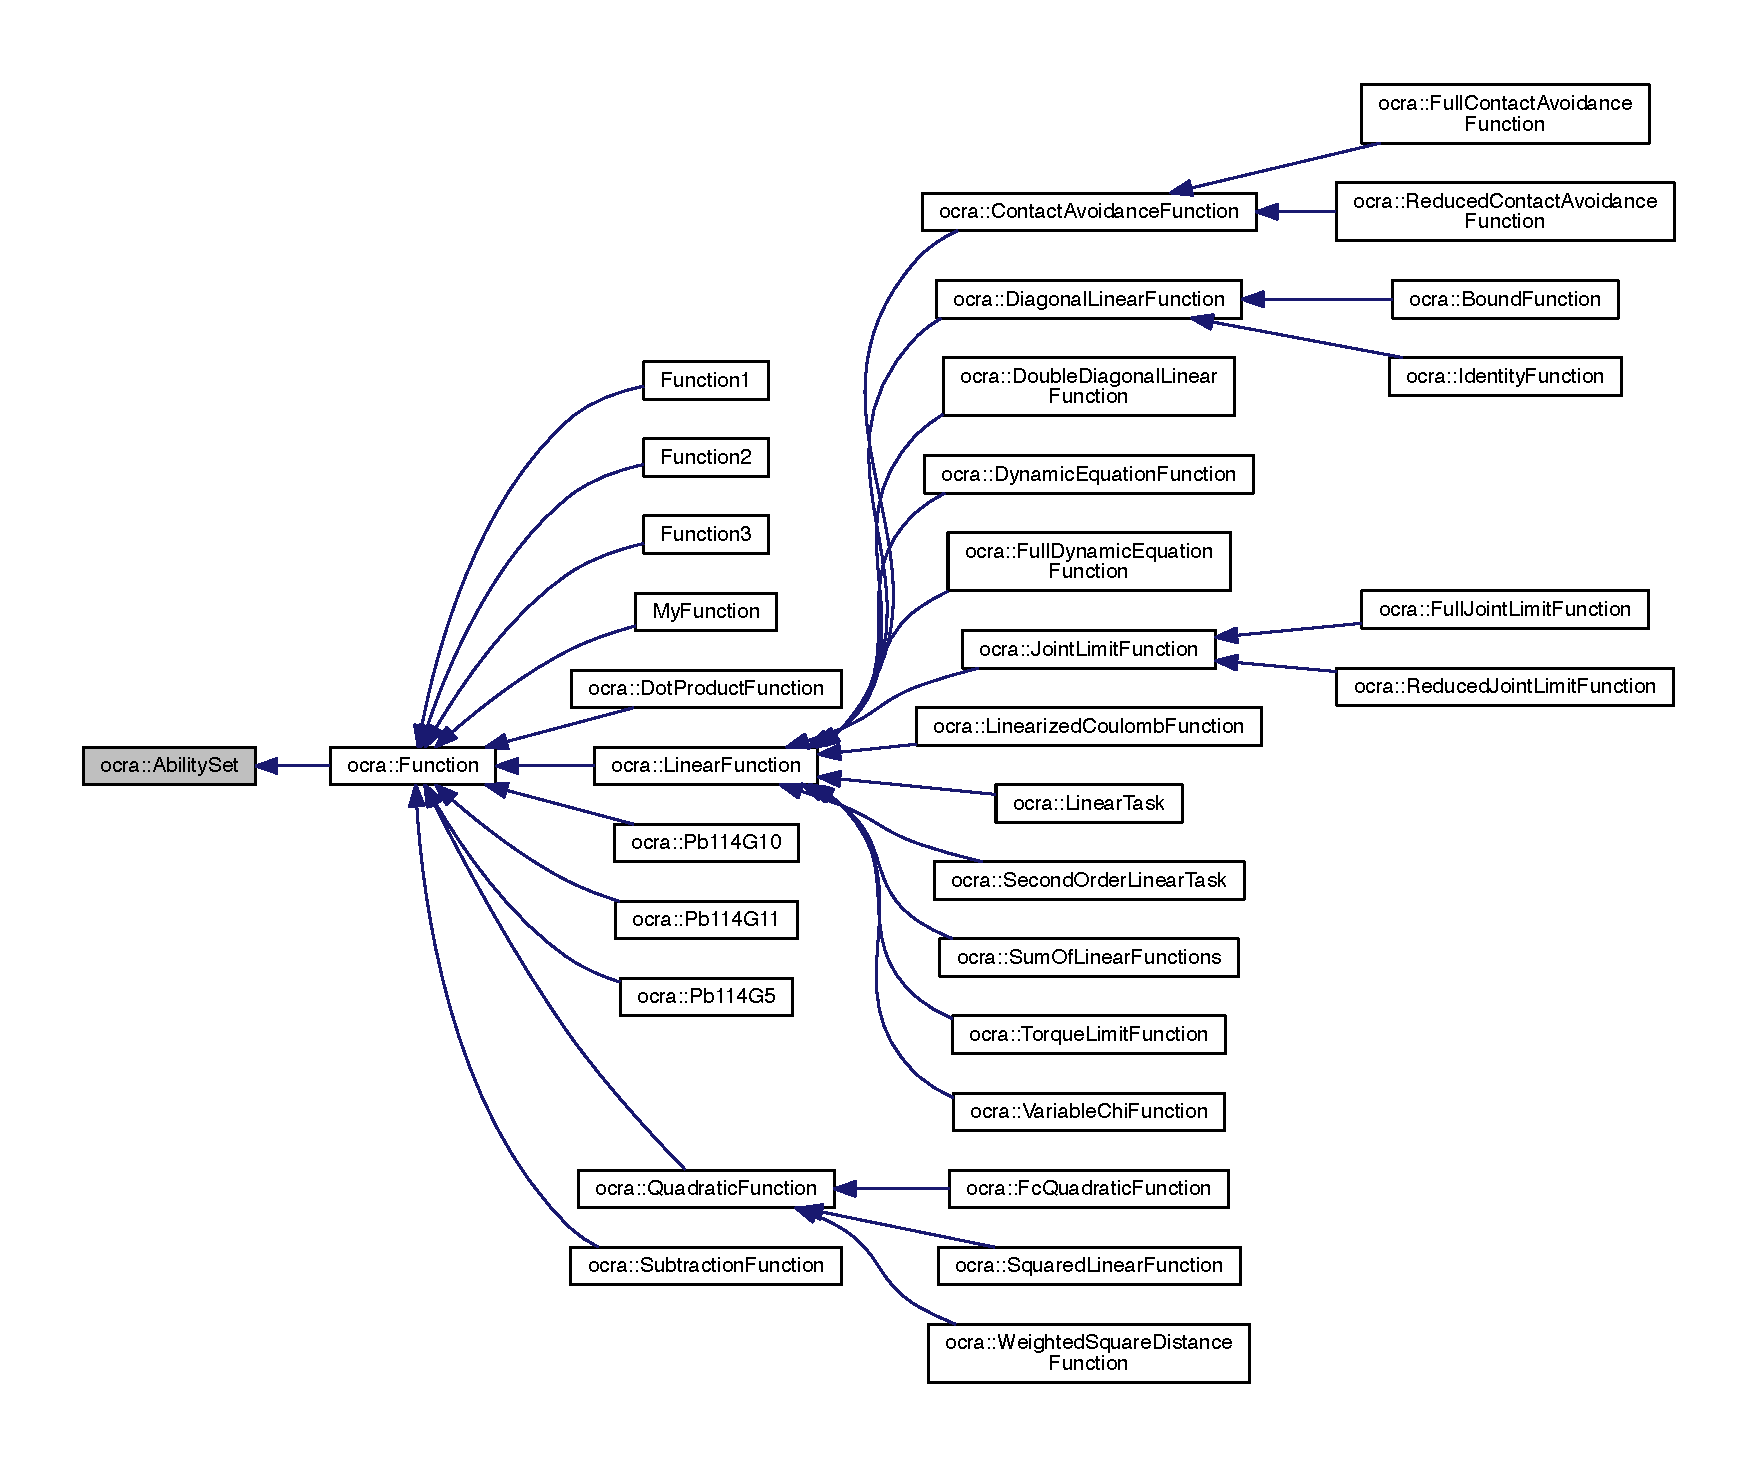
\includegraphics[width=350pt]{d4/d5b/classocra_1_1AbilitySet__inherit__graph}
\end{center}
\end{figure}
\subsection*{Public Member Functions}
\begin{DoxyCompactItemize}
\item 
\hyperlink{classocra_1_1AbilitySet}{Ability\+Set} \& \hyperlink{classocra_1_1AbilitySet_a4ce141c59ed38f812a4216730a0c4685}{add} (\hyperlink{namespaceocra_a40ddbec106a6034cd2047bba9945b568}{e\+Function\+Ability} prop)
\item 
\hyperlink{classocra_1_1AbilitySet}{Ability\+Set} \& \hyperlink{classocra_1_1AbilitySet_a093633f29e0d5e6a388d9b8cba9224c7}{remove} (\hyperlink{namespaceocra_a40ddbec106a6034cd2047bba9945b568}{e\+Function\+Ability} prop)
\end{DoxyCompactItemize}
\subsection*{Protected Member Functions}
\begin{DoxyCompactItemize}
\item 
\hyperlink{classocra_1_1AbilitySet_a0438cd73b840913711d2e7a768ff343a}{Ability\+Set} (const std\+::vector$<$ bool $>$ \&usage\+Set)
\item 
const std\+::vector$<$ bool $>$ \& \hyperlink{classocra_1_1AbilitySet_addb35b29c0ee151a0f93affde52a5570}{get\+Usage\+Set} () const
\end{DoxyCompactItemize}
{\bf }\par
\begin{DoxyCompactItemize}
\item 
\hyperlink{classocra_1_1AbilitySet_aec4a09919c73fc5e27aef8af05e7ebcf}{Ability\+Set} (\hyperlink{namespaceocra_a40ddbec106a6034cd2047bba9945b568}{e\+Function\+Ability} prop0=\hyperlink{namespaceocra_a40ddbec106a6034cd2047bba9945b568acfb47b20329993093d2022b017239bd8}{F\+U\+N\+\_\+\+V\+A\+L\+UE}, \hyperlink{namespaceocra_a40ddbec106a6034cd2047bba9945b568}{e\+Function\+Ability} prop1=\hyperlink{namespaceocra_a40ddbec106a6034cd2047bba9945b568acfb47b20329993093d2022b017239bd8}{F\+U\+N\+\_\+\+V\+A\+L\+UE})
\item 
\hyperlink{classocra_1_1AbilitySet_a7ac0f7bd650b04cef83728ea1d121015}{Ability\+Set} (\hyperlink{namespaceocra_a40ddbec106a6034cd2047bba9945b568}{e\+Function\+Ability} prop0, \hyperlink{namespaceocra_a40ddbec106a6034cd2047bba9945b568}{e\+Function\+Ability} prop1, \hyperlink{namespaceocra_a40ddbec106a6034cd2047bba9945b568}{e\+Function\+Ability} prop2, \hyperlink{namespaceocra_a40ddbec106a6034cd2047bba9945b568}{e\+Function\+Ability} prop3=\hyperlink{namespaceocra_a40ddbec106a6034cd2047bba9945b568acfb47b20329993093d2022b017239bd8}{F\+U\+N\+\_\+\+V\+A\+L\+UE}, \hyperlink{namespaceocra_a40ddbec106a6034cd2047bba9945b568}{e\+Function\+Ability} prop4=\hyperlink{namespaceocra_a40ddbec106a6034cd2047bba9945b568acfb47b20329993093d2022b017239bd8}{F\+U\+N\+\_\+\+V\+A\+L\+UE})
\item 
\hyperlink{classocra_1_1AbilitySet_a1383bb4705a010d46ccab36107a20985}{Ability\+Set} (\hyperlink{namespaceocra_a40ddbec106a6034cd2047bba9945b568}{e\+Function\+Ability} prop0, \hyperlink{namespaceocra_a40ddbec106a6034cd2047bba9945b568}{e\+Function\+Ability} prop1, \hyperlink{namespaceocra_a40ddbec106a6034cd2047bba9945b568}{e\+Function\+Ability} prop2, \hyperlink{namespaceocra_a40ddbec106a6034cd2047bba9945b568}{e\+Function\+Ability} prop3, \hyperlink{namespaceocra_a40ddbec106a6034cd2047bba9945b568}{e\+Function\+Ability} prop4, \hyperlink{namespaceocra_a40ddbec106a6034cd2047bba9945b568}{e\+Function\+Ability} prop5, \hyperlink{namespaceocra_a40ddbec106a6034cd2047bba9945b568}{e\+Function\+Ability} prop6=\hyperlink{namespaceocra_a40ddbec106a6034cd2047bba9945b568acfb47b20329993093d2022b017239bd8}{F\+U\+N\+\_\+\+V\+A\+L\+UE}, \hyperlink{namespaceocra_a40ddbec106a6034cd2047bba9945b568}{e\+Function\+Ability} prop7=\hyperlink{namespaceocra_a40ddbec106a6034cd2047bba9945b568acfb47b20329993093d2022b017239bd8}{F\+U\+N\+\_\+\+V\+A\+L\+UE}, \hyperlink{namespaceocra_a40ddbec106a6034cd2047bba9945b568}{e\+Function\+Ability} prop8=\hyperlink{namespaceocra_a40ddbec106a6034cd2047bba9945b568acfb47b20329993093d2022b017239bd8}{F\+U\+N\+\_\+\+V\+A\+L\+UE}, \hyperlink{namespaceocra_a40ddbec106a6034cd2047bba9945b568}{e\+Function\+Ability} prop9=\hyperlink{namespaceocra_a40ddbec106a6034cd2047bba9945b568acfb47b20329993093d2022b017239bd8}{F\+U\+N\+\_\+\+V\+A\+L\+UE})
\end{DoxyCompactItemize}

\subsection*{Friends}
{\bf }\par
\begin{DoxyCompactItemize}
\item 
\hyperlink{classocra_1_1AbilitySet}{Ability\+Set} \hyperlink{classocra_1_1AbilitySet_a186c9af3e53f43c03761eae7457a5502}{operator \&} (const \hyperlink{classocra_1_1AbilitySet}{Ability\+Set} a1, const \hyperlink{classocra_1_1AbilitySet}{Ability\+Set} a2)
\item 
\hyperlink{classocra_1_1AbilitySet}{Ability\+Set} \hyperlink{classocra_1_1AbilitySet_a31839dcdc5a95a8f78f786f2488618a6}{operator$\vert$} (const \hyperlink{classocra_1_1AbilitySet}{Ability\+Set} a1, const \hyperlink{classocra_1_1AbilitySet}{Ability\+Set} a2)
\end{DoxyCompactItemize}



\subsection{Detailed Description}
This class simply encapsulates a vector of boolean, one for each element of e\+Function\+Ability (except P\+R\+O\+P\+\_\+\+N\+U\+M\+B\+ER). The ith element of this vector is true when the corresponding ability has to be used.

This class is only meant to be a helper class to enumerate the abilities of a function at construction time. 

Definition at line 19 of file Ability\+Set.\+h.



\subsection{Constructor \& Destructor Documentation}
\hypertarget{classocra_1_1AbilitySet_a0438cd73b840913711d2e7a768ff343a}{}\label{classocra_1_1AbilitySet_a0438cd73b840913711d2e7a768ff343a} 
\index{ocra\+::\+Ability\+Set@{ocra\+::\+Ability\+Set}!Ability\+Set@{Ability\+Set}}
\index{Ability\+Set@{Ability\+Set}!ocra\+::\+Ability\+Set@{ocra\+::\+Ability\+Set}}
\subsubsection{\texorpdfstring{Ability\+Set()}{AbilitySet()}\hspace{0.1cm}{\footnotesize\ttfamily [1/4]}}
{\footnotesize\ttfamily ocra\+::\+Ability\+Set\+::\+Ability\+Set (\begin{DoxyParamCaption}\item[{const std\+::vector$<$ bool $>$ \&}]{usage\+Set }\end{DoxyParamCaption})\hspace{0.3cm}{\ttfamily [inline]}, {\ttfamily [protected]}}

Constructor with a given vector a bool, which needs to be of size P\+R\+O\+P\+\_\+\+N\+U\+M\+B\+ER 

Definition at line 23 of file Ability\+Set.\+h.

\hypertarget{classocra_1_1AbilitySet_aec4a09919c73fc5e27aef8af05e7ebcf}{}\label{classocra_1_1AbilitySet_aec4a09919c73fc5e27aef8af05e7ebcf} 
\index{ocra\+::\+Ability\+Set@{ocra\+::\+Ability\+Set}!Ability\+Set@{Ability\+Set}}
\index{Ability\+Set@{Ability\+Set}!ocra\+::\+Ability\+Set@{ocra\+::\+Ability\+Set}}
\subsubsection{\texorpdfstring{Ability\+Set()}{AbilitySet()}\hspace{0.1cm}{\footnotesize\ttfamily [2/4]}}
{\footnotesize\ttfamily ocra\+::\+Ability\+Set\+::\+Ability\+Set (\begin{DoxyParamCaption}\item[{\hyperlink{namespaceocra_a40ddbec106a6034cd2047bba9945b568}{e\+Function\+Ability}}]{prop0 = {\ttfamily \hyperlink{namespaceocra_a40ddbec106a6034cd2047bba9945b568acfb47b20329993093d2022b017239bd8}{F\+U\+N\+\_\+\+V\+A\+L\+UE}},  }\item[{\hyperlink{namespaceocra_a40ddbec106a6034cd2047bba9945b568}{e\+Function\+Ability}}]{prop1 = {\ttfamily \hyperlink{namespaceocra_a40ddbec106a6034cd2047bba9945b568acfb47b20329993093d2022b017239bd8}{F\+U\+N\+\_\+\+V\+A\+L\+UE}} }\end{DoxyParamCaption})\hspace{0.3cm}{\ttfamily [inline]}, {\ttfamily [protected]}}

A set of constructors to take 1 to 10 e\+Function\+Ability elements. Giving one element indicates the corresponding ability is to be used. For example, Ability\+Set(\+F\+U\+N\+\_\+\+V\+A\+L\+U\+E, P\+A\+R\+T\+I\+A\+L\+\_\+\+X, P\+A\+R\+T\+I\+A\+L\+\_\+\+T, F\+U\+N\+\_\+\+D\+O\+T) build an \hyperlink{classocra_1_1AbilitySet}{Ability\+Set} with the booleans for the abilities F\+U\+N\+\_\+\+V\+A\+L\+UE, P\+A\+R\+T\+I\+A\+L\+\_\+X, P\+A\+R\+T\+I\+A\+L\+\_\+T and F\+U\+N\+\_\+\+D\+OT set to true, and the others to false. 

Definition at line 37 of file Ability\+Set.\+h.

\hypertarget{classocra_1_1AbilitySet_a7ac0f7bd650b04cef83728ea1d121015}{}\label{classocra_1_1AbilitySet_a7ac0f7bd650b04cef83728ea1d121015} 
\index{ocra\+::\+Ability\+Set@{ocra\+::\+Ability\+Set}!Ability\+Set@{Ability\+Set}}
\index{Ability\+Set@{Ability\+Set}!ocra\+::\+Ability\+Set@{ocra\+::\+Ability\+Set}}
\subsubsection{\texorpdfstring{Ability\+Set()}{AbilitySet()}\hspace{0.1cm}{\footnotesize\ttfamily [3/4]}}
{\footnotesize\ttfamily ocra\+::\+Ability\+Set\+::\+Ability\+Set (\begin{DoxyParamCaption}\item[{\hyperlink{namespaceocra_a40ddbec106a6034cd2047bba9945b568}{e\+Function\+Ability}}]{prop0,  }\item[{\hyperlink{namespaceocra_a40ddbec106a6034cd2047bba9945b568}{e\+Function\+Ability}}]{prop1,  }\item[{\hyperlink{namespaceocra_a40ddbec106a6034cd2047bba9945b568}{e\+Function\+Ability}}]{prop2,  }\item[{\hyperlink{namespaceocra_a40ddbec106a6034cd2047bba9945b568}{e\+Function\+Ability}}]{prop3 = {\ttfamily \hyperlink{namespaceocra_a40ddbec106a6034cd2047bba9945b568acfb47b20329993093d2022b017239bd8}{F\+U\+N\+\_\+\+V\+A\+L\+UE}},  }\item[{\hyperlink{namespaceocra_a40ddbec106a6034cd2047bba9945b568}{e\+Function\+Ability}}]{prop4 = {\ttfamily \hyperlink{namespaceocra_a40ddbec106a6034cd2047bba9945b568acfb47b20329993093d2022b017239bd8}{F\+U\+N\+\_\+\+V\+A\+L\+UE}} }\end{DoxyParamCaption})\hspace{0.3cm}{\ttfamily [inline]}, {\ttfamily [protected]}}



Definition at line 49 of file Ability\+Set.\+h.

\hypertarget{classocra_1_1AbilitySet_a1383bb4705a010d46ccab36107a20985}{}\label{classocra_1_1AbilitySet_a1383bb4705a010d46ccab36107a20985} 
\index{ocra\+::\+Ability\+Set@{ocra\+::\+Ability\+Set}!Ability\+Set@{Ability\+Set}}
\index{Ability\+Set@{Ability\+Set}!ocra\+::\+Ability\+Set@{ocra\+::\+Ability\+Set}}
\subsubsection{\texorpdfstring{Ability\+Set()}{AbilitySet()}\hspace{0.1cm}{\footnotesize\ttfamily [4/4]}}
{\footnotesize\ttfamily ocra\+::\+Ability\+Set\+::\+Ability\+Set (\begin{DoxyParamCaption}\item[{\hyperlink{namespaceocra_a40ddbec106a6034cd2047bba9945b568}{e\+Function\+Ability}}]{prop0,  }\item[{\hyperlink{namespaceocra_a40ddbec106a6034cd2047bba9945b568}{e\+Function\+Ability}}]{prop1,  }\item[{\hyperlink{namespaceocra_a40ddbec106a6034cd2047bba9945b568}{e\+Function\+Ability}}]{prop2,  }\item[{\hyperlink{namespaceocra_a40ddbec106a6034cd2047bba9945b568}{e\+Function\+Ability}}]{prop3,  }\item[{\hyperlink{namespaceocra_a40ddbec106a6034cd2047bba9945b568}{e\+Function\+Ability}}]{prop4,  }\item[{\hyperlink{namespaceocra_a40ddbec106a6034cd2047bba9945b568}{e\+Function\+Ability}}]{prop5,  }\item[{\hyperlink{namespaceocra_a40ddbec106a6034cd2047bba9945b568}{e\+Function\+Ability}}]{prop6 = {\ttfamily \hyperlink{namespaceocra_a40ddbec106a6034cd2047bba9945b568acfb47b20329993093d2022b017239bd8}{F\+U\+N\+\_\+\+V\+A\+L\+UE}},  }\item[{\hyperlink{namespaceocra_a40ddbec106a6034cd2047bba9945b568}{e\+Function\+Ability}}]{prop7 = {\ttfamily \hyperlink{namespaceocra_a40ddbec106a6034cd2047bba9945b568acfb47b20329993093d2022b017239bd8}{F\+U\+N\+\_\+\+V\+A\+L\+UE}},  }\item[{\hyperlink{namespaceocra_a40ddbec106a6034cd2047bba9945b568}{e\+Function\+Ability}}]{prop8 = {\ttfamily \hyperlink{namespaceocra_a40ddbec106a6034cd2047bba9945b568acfb47b20329993093d2022b017239bd8}{F\+U\+N\+\_\+\+V\+A\+L\+UE}},  }\item[{\hyperlink{namespaceocra_a40ddbec106a6034cd2047bba9945b568}{e\+Function\+Ability}}]{prop9 = {\ttfamily \hyperlink{namespaceocra_a40ddbec106a6034cd2047bba9945b568acfb47b20329993093d2022b017239bd8}{F\+U\+N\+\_\+\+V\+A\+L\+UE}} }\end{DoxyParamCaption})\hspace{0.3cm}{\ttfamily [inline]}, {\ttfamily [protected]}}



Definition at line 65 of file Ability\+Set.\+h.



\subsection{Member Function Documentation}
\hypertarget{classocra_1_1AbilitySet_a4ce141c59ed38f812a4216730a0c4685}{}\label{classocra_1_1AbilitySet_a4ce141c59ed38f812a4216730a0c4685} 
\index{ocra\+::\+Ability\+Set@{ocra\+::\+Ability\+Set}!add@{add}}
\index{add@{add}!ocra\+::\+Ability\+Set@{ocra\+::\+Ability\+Set}}
\subsubsection{\texorpdfstring{add()}{add()}}
{\footnotesize\ttfamily \hyperlink{classocra_1_1AbilitySet}{Ability\+Set}\& ocra\+::\+Ability\+Set\+::add (\begin{DoxyParamCaption}\item[{\hyperlink{namespaceocra_a40ddbec106a6034cd2047bba9945b568}{e\+Function\+Ability}}]{prop }\end{DoxyParamCaption})\hspace{0.3cm}{\ttfamily [inline]}}

Add an Ability to the set. 

Definition at line 96 of file Ability\+Set.\+h.

\hypertarget{classocra_1_1AbilitySet_addb35b29c0ee151a0f93affde52a5570}{}\label{classocra_1_1AbilitySet_addb35b29c0ee151a0f93affde52a5570} 
\index{ocra\+::\+Ability\+Set@{ocra\+::\+Ability\+Set}!get\+Usage\+Set@{get\+Usage\+Set}}
\index{get\+Usage\+Set@{get\+Usage\+Set}!ocra\+::\+Ability\+Set@{ocra\+::\+Ability\+Set}}
\subsubsection{\texorpdfstring{get\+Usage\+Set()}{getUsageSet()}}
{\footnotesize\ttfamily const std\+::vector$<$bool$>$\& ocra\+::\+Ability\+Set\+::get\+Usage\+Set (\begin{DoxyParamCaption}{ }\end{DoxyParamCaption}) const\hspace{0.3cm}{\ttfamily [inline]}, {\ttfamily [protected]}}

Get the vector. 

Definition at line 89 of file Ability\+Set.\+h.

\hypertarget{classocra_1_1AbilitySet_a093633f29e0d5e6a388d9b8cba9224c7}{}\label{classocra_1_1AbilitySet_a093633f29e0d5e6a388d9b8cba9224c7} 
\index{ocra\+::\+Ability\+Set@{ocra\+::\+Ability\+Set}!remove@{remove}}
\index{remove@{remove}!ocra\+::\+Ability\+Set@{ocra\+::\+Ability\+Set}}
\subsubsection{\texorpdfstring{remove()}{remove()}}
{\footnotesize\ttfamily \hyperlink{classocra_1_1AbilitySet}{Ability\+Set}\& ocra\+::\+Ability\+Set\+::remove (\begin{DoxyParamCaption}\item[{\hyperlink{namespaceocra_a40ddbec106a6034cd2047bba9945b568}{e\+Function\+Ability}}]{prop }\end{DoxyParamCaption})\hspace{0.3cm}{\ttfamily [inline]}}

Remove the ability from the set. 

Definition at line 103 of file Ability\+Set.\+h.



\subsection{Friends And Related Function Documentation}
\hypertarget{classocra_1_1AbilitySet_a186c9af3e53f43c03761eae7457a5502}{}\label{classocra_1_1AbilitySet_a186c9af3e53f43c03761eae7457a5502} 
\index{ocra\+::\+Ability\+Set@{ocra\+::\+Ability\+Set}!operator \&@{operator \&}}
\index{operator \&@{operator \&}!ocra\+::\+Ability\+Set@{ocra\+::\+Ability\+Set}}
\subsubsection{\texorpdfstring{operator \&}{operator \&}}
{\footnotesize\ttfamily \hyperlink{classocra_1_1AbilitySet}{Ability\+Set} operator\& (\begin{DoxyParamCaption}\item[{const \hyperlink{classocra_1_1AbilitySet}{Ability\+Set}}]{a1,  }\item[{const \hyperlink{classocra_1_1AbilitySet}{Ability\+Set}}]{a2 }\end{DoxyParamCaption})\hspace{0.3cm}{\ttfamily [friend]}}

Element by element {\itshape and} and  of two \hyperlink{classocra_1_1AbilitySet}{Ability\+Set} 

Definition at line 119 of file Ability\+Set.\+h.

\hypertarget{classocra_1_1AbilitySet_a31839dcdc5a95a8f78f786f2488618a6}{}\label{classocra_1_1AbilitySet_a31839dcdc5a95a8f78f786f2488618a6} 
\index{ocra\+::\+Ability\+Set@{ocra\+::\+Ability\+Set}!operator\texttt{"|}@{operator\texttt{"|}}}
\index{operator\texttt{"|}@{operator\texttt{"|}}!ocra\+::\+Ability\+Set@{ocra\+::\+Ability\+Set}}
\subsubsection{\texorpdfstring{operator\texttt{"|}}{operator|}}
{\footnotesize\ttfamily \hyperlink{classocra_1_1AbilitySet}{Ability\+Set} operator$\vert$ (\begin{DoxyParamCaption}\item[{const \hyperlink{classocra_1_1AbilitySet}{Ability\+Set}}]{a1,  }\item[{const \hyperlink{classocra_1_1AbilitySet}{Ability\+Set}}]{a2 }\end{DoxyParamCaption})\hspace{0.3cm}{\ttfamily [friend]}}



Definition at line 130 of file Ability\+Set.\+h.



The documentation for this class was generated from the following file\+:\begin{DoxyCompactItemize}
\item 
\hyperlink{AbilitySet_8h}{Ability\+Set.\+h}\end{DoxyCompactItemize}

\hypertarget{structocra_1_1utils_1_1add__functor}{}\section{ocra\+:\+:utils\+:\+:add\+\_\+functor$<$ T, U $>$ Struct Template Reference}
\label{structocra_1_1utils_1_1add__functor}\index{ocra\+::utils\+::add\+\_\+functor$<$ T, U $>$@{ocra\+::utils\+::add\+\_\+functor$<$ T, U $>$}}


{\ttfamily \#include $<$uncompress.\+h$>$}

\subsection*{Static Public Member Functions}
\begin{DoxyCompactItemize}
\item 
static void \hyperlink{structocra_1_1utils_1_1add__functor_ae1b1954f668a3db199cd696da004e661}{run} (T \&out, const U \&in)
\item 
static void \hyperlink{structocra_1_1utils_1_1add__functor_a1a9206cb5192b4a1314d5e93afef9c27}{run} (T \&out, double alpha, const U \&in)
\end{DoxyCompactItemize}


\subsection{Detailed Description}
\subsubsection*{template$<$class T, class U$>$\newline
struct ocra\+::utils\+::add\+\_\+functor$<$ T, U $>$}



Definition at line 82 of file uncompress.\+h.



\subsection{Member Function Documentation}
\hypertarget{structocra_1_1utils_1_1add__functor_ae1b1954f668a3db199cd696da004e661}{}\label{structocra_1_1utils_1_1add__functor_ae1b1954f668a3db199cd696da004e661} 
\index{ocra\+::utils\+::add\+\_\+functor@{ocra\+::utils\+::add\+\_\+functor}!run@{run}}
\index{run@{run}!ocra\+::utils\+::add\+\_\+functor@{ocra\+::utils\+::add\+\_\+functor}}
\subsubsection{\texorpdfstring{run()}{run()}\hspace{0.1cm}{\footnotesize\ttfamily [1/2]}}
{\footnotesize\ttfamily template$<$class T , class U $>$ \\
static void \hyperlink{structocra_1_1utils_1_1add__functor}{ocra\+::utils\+::add\+\_\+functor}$<$ T, U $>$\+::run (\begin{DoxyParamCaption}\item[{T \&}]{out,  }\item[{const U \&}]{in }\end{DoxyParamCaption})\hspace{0.3cm}{\ttfamily [inline]}, {\ttfamily [static]}}



Definition at line 84 of file uncompress.\+h.

\hypertarget{structocra_1_1utils_1_1add__functor_a1a9206cb5192b4a1314d5e93afef9c27}{}\label{structocra_1_1utils_1_1add__functor_a1a9206cb5192b4a1314d5e93afef9c27} 
\index{ocra\+::utils\+::add\+\_\+functor@{ocra\+::utils\+::add\+\_\+functor}!run@{run}}
\index{run@{run}!ocra\+::utils\+::add\+\_\+functor@{ocra\+::utils\+::add\+\_\+functor}}
\subsubsection{\texorpdfstring{run()}{run()}\hspace{0.1cm}{\footnotesize\ttfamily [2/2]}}
{\footnotesize\ttfamily template$<$class T , class U $>$ \\
static void \hyperlink{structocra_1_1utils_1_1add__functor}{ocra\+::utils\+::add\+\_\+functor}$<$ T, U $>$\+::run (\begin{DoxyParamCaption}\item[{T \&}]{out,  }\item[{double}]{alpha,  }\item[{const U \&}]{in }\end{DoxyParamCaption})\hspace{0.3cm}{\ttfamily [inline]}, {\ttfamily [static]}}



Definition at line 85 of file uncompress.\+h.



The documentation for this struct was generated from the following file\+:\begin{DoxyCompactItemize}
\item 
\hyperlink{uncompress_8h}{uncompress.\+h}\end{DoxyCompactItemize}

\hypertarget{structocra_1_1utils_1_1assign__functor}{}\section{ocra\+:\+:utils\+:\+:assign\+\_\+functor$<$ T, U $>$ Struct Template Reference}
\label{structocra_1_1utils_1_1assign__functor}\index{ocra\+::utils\+::assign\+\_\+functor$<$ T, U $>$@{ocra\+::utils\+::assign\+\_\+functor$<$ T, U $>$}}


{\ttfamily \#include $<$uncompress.\+h$>$}

\subsection*{Static Public Member Functions}
\begin{DoxyCompactItemize}
\item 
static void \hyperlink{structocra_1_1utils_1_1assign__functor_a7062b68b69083283a00cdcf05331b5f0}{run} (T \&out, const U \&in)
\item 
static void \hyperlink{structocra_1_1utils_1_1assign__functor_a1fbc5042510c940d2968b51a9035cd75}{run} (T \&out, double alpha, const U \&in)
\end{DoxyCompactItemize}


\subsection{Detailed Description}
\subsubsection*{template$<$class T, class U$>$\newline
struct ocra\+::utils\+::assign\+\_\+functor$<$ T, U $>$}



Definition at line 75 of file uncompress.\+h.



\subsection{Member Function Documentation}
\hypertarget{structocra_1_1utils_1_1assign__functor_a7062b68b69083283a00cdcf05331b5f0}{}\label{structocra_1_1utils_1_1assign__functor_a7062b68b69083283a00cdcf05331b5f0} 
\index{ocra\+::utils\+::assign\+\_\+functor@{ocra\+::utils\+::assign\+\_\+functor}!run@{run}}
\index{run@{run}!ocra\+::utils\+::assign\+\_\+functor@{ocra\+::utils\+::assign\+\_\+functor}}
\subsubsection{\texorpdfstring{run()}{run()}\hspace{0.1cm}{\footnotesize\ttfamily [1/2]}}
{\footnotesize\ttfamily template$<$class T , class U $>$ \\
static void \hyperlink{structocra_1_1utils_1_1assign__functor}{ocra\+::utils\+::assign\+\_\+functor}$<$ T, U $>$\+::run (\begin{DoxyParamCaption}\item[{T \&}]{out,  }\item[{const U \&}]{in }\end{DoxyParamCaption})\hspace{0.3cm}{\ttfamily [inline]}, {\ttfamily [static]}}



Definition at line 77 of file uncompress.\+h.

\hypertarget{structocra_1_1utils_1_1assign__functor_a1fbc5042510c940d2968b51a9035cd75}{}\label{structocra_1_1utils_1_1assign__functor_a1fbc5042510c940d2968b51a9035cd75} 
\index{ocra\+::utils\+::assign\+\_\+functor@{ocra\+::utils\+::assign\+\_\+functor}!run@{run}}
\index{run@{run}!ocra\+::utils\+::assign\+\_\+functor@{ocra\+::utils\+::assign\+\_\+functor}}
\subsubsection{\texorpdfstring{run()}{run()}\hspace{0.1cm}{\footnotesize\ttfamily [2/2]}}
{\footnotesize\ttfamily template$<$class T , class U $>$ \\
static void \hyperlink{structocra_1_1utils_1_1assign__functor}{ocra\+::utils\+::assign\+\_\+functor}$<$ T, U $>$\+::run (\begin{DoxyParamCaption}\item[{T \&}]{out,  }\item[{double}]{alpha,  }\item[{const U \&}]{in }\end{DoxyParamCaption})\hspace{0.3cm}{\ttfamily [inline]}, {\ttfamily [static]}}



Definition at line 78 of file uncompress.\+h.



The documentation for this struct was generated from the following file\+:\begin{DoxyCompactItemize}
\item 
\hyperlink{uncompress_8h}{uncompress.\+h}\end{DoxyCompactItemize}

\hypertarget{classocra_1_1BaseVariable}{}\section{ocra\+:\+:Base\+Variable Class Reference}
\label{classocra_1_1BaseVariable}\index{ocra\+::\+Base\+Variable@{ocra\+::\+Base\+Variable}}


Implements a basic variable.  




{\ttfamily \#include $<$Variable.\+h$>$}



Inheritance diagram for ocra\+:\+:Base\+Variable\+:\nopagebreak
\begin{figure}[H]
\begin{center}
\leavevmode
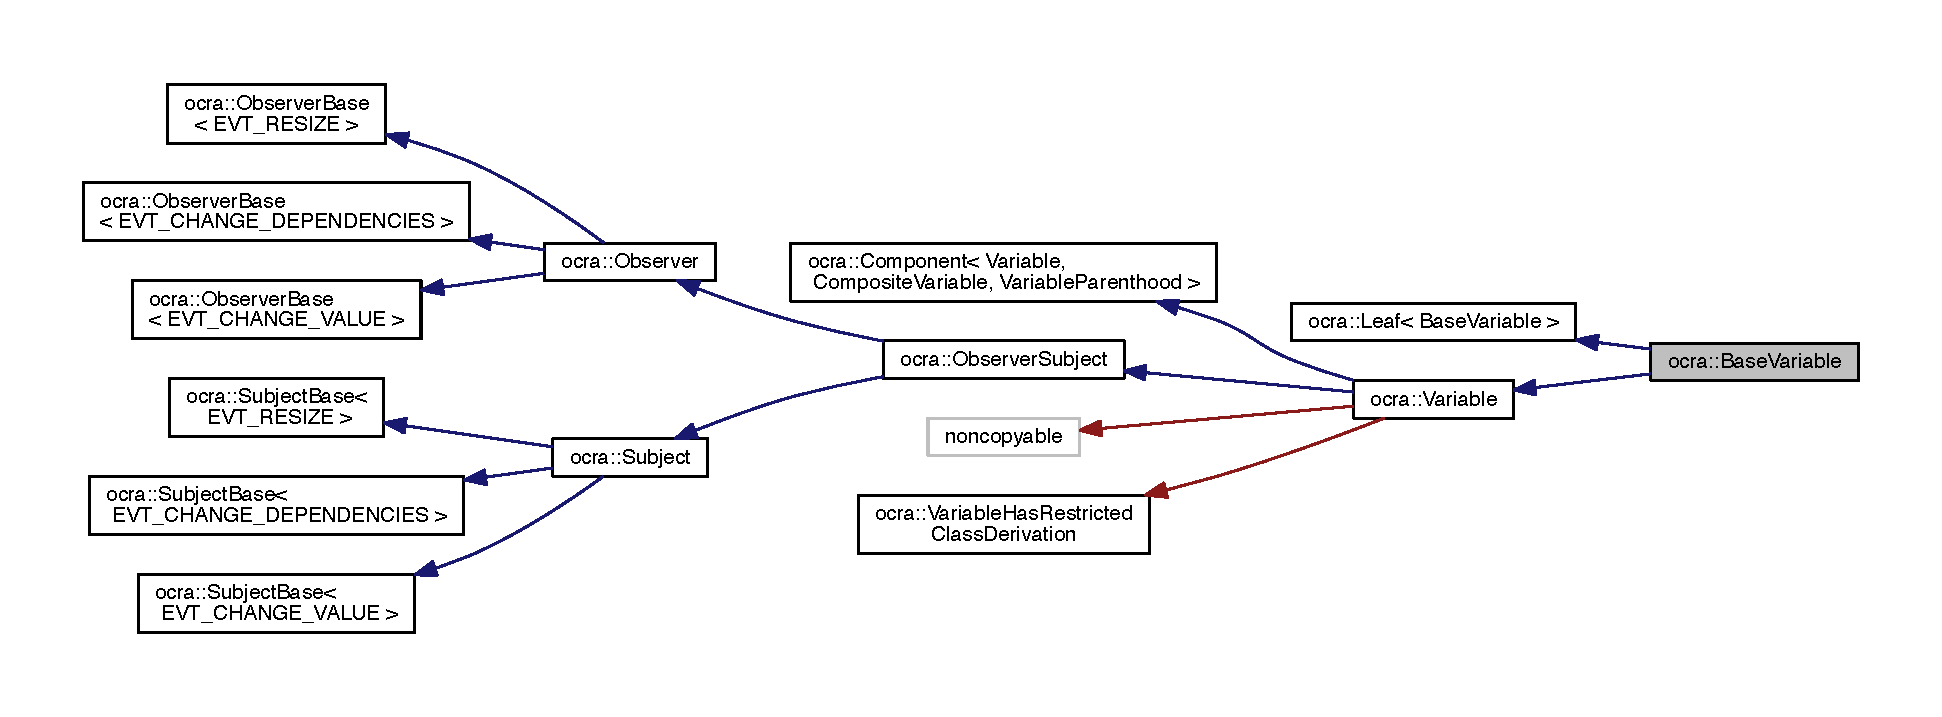
\includegraphics[width=350pt]{db/ddd/classocra_1_1BaseVariable__inherit__graph}
\end{center}
\end{figure}


Collaboration diagram for ocra\+:\+:Base\+Variable\+:\nopagebreak
\begin{figure}[H]
\begin{center}
\leavevmode
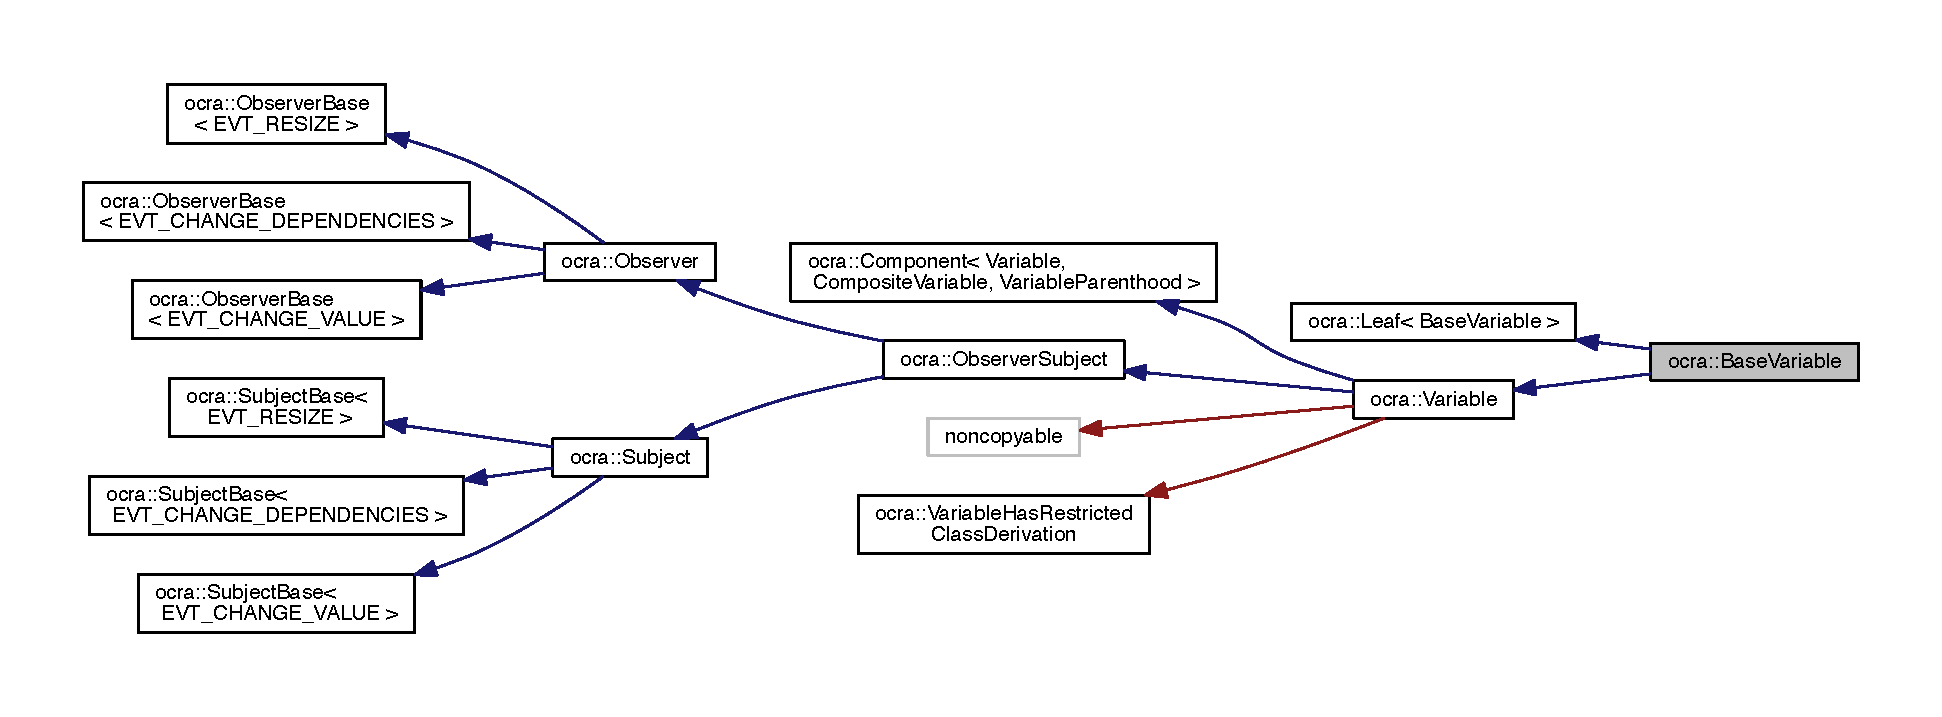
\includegraphics[width=350pt]{d1/d35/classocra_1_1BaseVariable__coll__graph}
\end{center}
\end{figure}
\subsection*{Public Member Functions}
\begin{DoxyCompactItemize}
\item 
\hyperlink{classocra_1_1BaseVariable_ae86fd20357d1b333c73d22b7a9a010f6}{Base\+Variable} (const std\+::string \&name, size\+\_\+t size)
\begin{DoxyCompactList}\small\item\em Builds a leaf variable, i.\+e. a variable that is not composed of other variables. \end{DoxyCompactList}\item 
bool \hyperlink{classocra_1_1BaseVariable_a454556cfc20026911bc687bc481ec95b}{is\+Base\+Variable} () const
\item 
void \hyperlink{classocra_1_1BaseVariable_a5d473eeb113e4751c27cf6af7af62919}{resize} (size\+\_\+t new\+Size)
\item 
\hyperlink{classocra_1_1BaseVariable}{Base\+Variable} \& \hyperlink{classocra_1_1BaseVariable_a79a86d7415d8b460ad9f526f685961dc}{get\+Time\+Derivative} ()
\begin{DoxyCompactList}\small\item\em Get the time derivative/primitive of the variable. \end{DoxyCompactList}\item 
\hyperlink{classocra_1_1BaseVariable}{Base\+Variable} \& \hyperlink{classocra_1_1BaseVariable_aa985b0703fc0a2edcd66a7c4c4ee05e4}{get\+Time\+Primitive} ()
\item 
int \hyperlink{classocra_1_1BaseVariable_a66d07236f4d060273f3f46632dc851ac}{is\+Ancestor\+Of} (const \hyperlink{classocra_1_1Variable}{Variable} \&var) const
\begin{DoxyCompactList}\small\item\em Returns the number of levels that separate the component from a potential child. \end{DoxyCompactList}\item 
void \hyperlink{classocra_1_1BaseVariable_a4058b1accad9ff7b3d8995bdf9285fbd}{print\+Sub\+Tree} (int depth, std\+::ostream \&os) const
\begin{DoxyCompactList}\small\item\em Overload in Component\+Derived and Composite\+Derived to simply call \hyperlink{classocra_1_1Leaf_aaf46f5b8cd9d9667b8080898b1d9138a}{print\+Tree\+\_\+impl()}. \end{DoxyCompactList}\end{DoxyCompactItemize}
\subsection*{Protected Member Functions}
\begin{DoxyCompactItemize}
\item 
void \hyperlink{classocra_1_1BaseVariable_a4f53b244e0efba4ca19f558113d29a9c}{do\+\_\+set\+Value} (const Vector\+Xd \&value)
\begin{DoxyCompactList}\small\item\em This method will attempt to assign a given value to the memory map. \end{DoxyCompactList}\item 
size\+\_\+t \hyperlink{classocra_1_1BaseVariable_abf5dc1c3eaa689663cc09e06b8f5b3a1}{do\+\_\+get\+Number\+Of\+Children} () const
\begin{DoxyCompactList}\small\item\em Always return 0. \end{DoxyCompactList}\end{DoxyCompactItemize}
{\bf }\par
\begin{DoxyCompactItemize}
\item 
\hyperlink{classocra_1_1Variable}{Variable} $\ast$ \hyperlink{classocra_1_1BaseVariable_a064b6501c110661e9fa12a0250d4de6b}{do\+\_\+create\+Time\+Derivative} (const std\+::string \&name)
\item 
\hyperlink{classocra_1_1Variable}{Variable} $\ast$ \hyperlink{classocra_1_1BaseVariable_ab010bd127ba34ff57168bf69182a78d5}{do\+\_\+create\+Time\+Primitive} (const std\+::string \&name)
\end{DoxyCompactItemize}

\subsection*{Additional Inherited Members}


\subsection{Detailed Description}
Implements a basic variable. 

Definition at line 304 of file Variable.\+h.



\subsection{Constructor \& Destructor Documentation}
\hypertarget{classocra_1_1BaseVariable_ae86fd20357d1b333c73d22b7a9a010f6}{}\label{classocra_1_1BaseVariable_ae86fd20357d1b333c73d22b7a9a010f6} 
\index{ocra\+::\+Base\+Variable@{ocra\+::\+Base\+Variable}!Base\+Variable@{Base\+Variable}}
\index{Base\+Variable@{Base\+Variable}!ocra\+::\+Base\+Variable@{ocra\+::\+Base\+Variable}}
\subsubsection{\texorpdfstring{Base\+Variable()}{BaseVariable()}}
{\footnotesize\ttfamily ocra\+::\+Base\+Variable\+::\+Base\+Variable (\begin{DoxyParamCaption}\item[{const std\+::string \&}]{name,  }\item[{size\+\_\+t}]{size }\end{DoxyParamCaption})}



Builds a leaf variable, i.\+e. a variable that is not composed of other variables. 



Definition at line 331 of file Variable.\+cpp.



\subsection{Member Function Documentation}
\hypertarget{classocra_1_1BaseVariable_a064b6501c110661e9fa12a0250d4de6b}{}\label{classocra_1_1BaseVariable_a064b6501c110661e9fa12a0250d4de6b} 
\index{ocra\+::\+Base\+Variable@{ocra\+::\+Base\+Variable}!do\+\_\+create\+Time\+Derivative@{do\+\_\+create\+Time\+Derivative}}
\index{do\+\_\+create\+Time\+Derivative@{do\+\_\+create\+Time\+Derivative}!ocra\+::\+Base\+Variable@{ocra\+::\+Base\+Variable}}
\subsubsection{\texorpdfstring{do\+\_\+create\+Time\+Derivative()}{do\_createTimeDerivative()}}
{\footnotesize\ttfamily \hyperlink{classocra_1_1Variable}{Variable} $\ast$ ocra\+::\+Base\+Variable\+::do\+\_\+create\+Time\+Derivative (\begin{DoxyParamCaption}\item[{const std\+::string \&}]{name }\end{DoxyParamCaption})\hspace{0.3cm}{\ttfamily [protected]}, {\ttfamily [virtual]}}

\begin{DoxySeeAlso}{See also}
class \hyperlink{classocra_1_1Variable}{ocra\+::\+Variable} 
\end{DoxySeeAlso}


Implements \hyperlink{classocra_1_1Variable_aaed3c9bb3258cc1120ae8f93722a12bb}{ocra\+::\+Variable}.



Definition at line 390 of file Variable.\+cpp.

\hypertarget{classocra_1_1BaseVariable_ab010bd127ba34ff57168bf69182a78d5}{}\label{classocra_1_1BaseVariable_ab010bd127ba34ff57168bf69182a78d5} 
\index{ocra\+::\+Base\+Variable@{ocra\+::\+Base\+Variable}!do\+\_\+create\+Time\+Primitive@{do\+\_\+create\+Time\+Primitive}}
\index{do\+\_\+create\+Time\+Primitive@{do\+\_\+create\+Time\+Primitive}!ocra\+::\+Base\+Variable@{ocra\+::\+Base\+Variable}}
\subsubsection{\texorpdfstring{do\+\_\+create\+Time\+Primitive()}{do\_createTimePrimitive()}}
{\footnotesize\ttfamily \hyperlink{classocra_1_1Variable}{Variable} $\ast$ ocra\+::\+Base\+Variable\+::do\+\_\+create\+Time\+Primitive (\begin{DoxyParamCaption}\item[{const std\+::string \&}]{name }\end{DoxyParamCaption})\hspace{0.3cm}{\ttfamily [protected]}, {\ttfamily [virtual]}}



Implements \hyperlink{classocra_1_1Variable_ae37610cbde7630dcda3dd6e09e251057}{ocra\+::\+Variable}.



Definition at line 395 of file Variable.\+cpp.

\hypertarget{classocra_1_1BaseVariable_abf5dc1c3eaa689663cc09e06b8f5b3a1}{}\label{classocra_1_1BaseVariable_abf5dc1c3eaa689663cc09e06b8f5b3a1} 
\index{ocra\+::\+Base\+Variable@{ocra\+::\+Base\+Variable}!do\+\_\+get\+Number\+Of\+Children@{do\+\_\+get\+Number\+Of\+Children}}
\index{do\+\_\+get\+Number\+Of\+Children@{do\+\_\+get\+Number\+Of\+Children}!ocra\+::\+Base\+Variable@{ocra\+::\+Base\+Variable}}
\subsubsection{\texorpdfstring{do\+\_\+get\+Number\+Of\+Children()}{do\_getNumberOfChildren()}}
{\footnotesize\ttfamily size\+\_\+t ocra\+::\+Base\+Variable\+::do\+\_\+get\+Number\+Of\+Children (\begin{DoxyParamCaption}{ }\end{DoxyParamCaption}) const\hspace{0.3cm}{\ttfamily [protected]}, {\ttfamily [virtual]}}



Always return 0. 



Implements \hyperlink{classocra_1_1Variable_a65de5b31613b74d83baab58f0eb43b35}{ocra\+::\+Variable}.



Definition at line 400 of file Variable.\+cpp.

\hypertarget{classocra_1_1BaseVariable_a4f53b244e0efba4ca19f558113d29a9c}{}\label{classocra_1_1BaseVariable_a4f53b244e0efba4ca19f558113d29a9c} 
\index{ocra\+::\+Base\+Variable@{ocra\+::\+Base\+Variable}!do\+\_\+set\+Value@{do\+\_\+set\+Value}}
\index{do\+\_\+set\+Value@{do\+\_\+set\+Value}!ocra\+::\+Base\+Variable@{ocra\+::\+Base\+Variable}}
\subsubsection{\texorpdfstring{do\+\_\+set\+Value()}{do\_setValue()}}
{\footnotesize\ttfamily void ocra\+::\+Base\+Variable\+::do\+\_\+set\+Value (\begin{DoxyParamCaption}\item[{const Vector\+Xd \&}]{value }\end{DoxyParamCaption})\hspace{0.3cm}{\ttfamily [protected]}, {\ttfamily [virtual]}}



This method will attempt to assign a given value to the memory map. 



Implements \hyperlink{classocra_1_1Variable_a73ff767d0a620f1803573b33f93c69f8}{ocra\+::\+Variable}.



Definition at line 361 of file Variable.\+cpp.

\hypertarget{classocra_1_1BaseVariable_a79a86d7415d8b460ad9f526f685961dc}{}\label{classocra_1_1BaseVariable_a79a86d7415d8b460ad9f526f685961dc} 
\index{ocra\+::\+Base\+Variable@{ocra\+::\+Base\+Variable}!get\+Time\+Derivative@{get\+Time\+Derivative}}
\index{get\+Time\+Derivative@{get\+Time\+Derivative}!ocra\+::\+Base\+Variable@{ocra\+::\+Base\+Variable}}
\subsubsection{\texorpdfstring{get\+Time\+Derivative()}{getTimeDerivative()}}
{\footnotesize\ttfamily \hyperlink{classocra_1_1BaseVariable}{Base\+Variable} \& ocra\+::\+Base\+Variable\+::get\+Time\+Derivative (\begin{DoxyParamCaption}{ }\end{DoxyParamCaption})\hspace{0.3cm}{\ttfamily [virtual]}}



Get the time derivative/primitive of the variable. 

If the derivative/primitive doesn\textquotesingle{}t exist, it will be created automatically at the first call to this method. 

Reimplemented from \hyperlink{classocra_1_1Variable_a06ee384364d5c6bd1ea4bc4b38d6268c}{ocra\+::\+Variable}.



Definition at line 370 of file Variable.\+cpp.

\hypertarget{classocra_1_1BaseVariable_aa985b0703fc0a2edcd66a7c4c4ee05e4}{}\label{classocra_1_1BaseVariable_aa985b0703fc0a2edcd66a7c4c4ee05e4} 
\index{ocra\+::\+Base\+Variable@{ocra\+::\+Base\+Variable}!get\+Time\+Primitive@{get\+Time\+Primitive}}
\index{get\+Time\+Primitive@{get\+Time\+Primitive}!ocra\+::\+Base\+Variable@{ocra\+::\+Base\+Variable}}
\subsubsection{\texorpdfstring{get\+Time\+Primitive()}{getTimePrimitive()}}
{\footnotesize\ttfamily \hyperlink{classocra_1_1BaseVariable}{Base\+Variable} \& ocra\+::\+Base\+Variable\+::get\+Time\+Primitive (\begin{DoxyParamCaption}{ }\end{DoxyParamCaption})\hspace{0.3cm}{\ttfamily [virtual]}}



Reimplemented from \hyperlink{classocra_1_1Variable_aca32d63e60dc79de340b2f122dad0dc5}{ocra\+::\+Variable}.



Definition at line 375 of file Variable.\+cpp.

\hypertarget{classocra_1_1BaseVariable_a66d07236f4d060273f3f46632dc851ac}{}\label{classocra_1_1BaseVariable_a66d07236f4d060273f3f46632dc851ac} 
\index{ocra\+::\+Base\+Variable@{ocra\+::\+Base\+Variable}!is\+Ancestor\+Of@{is\+Ancestor\+Of}}
\index{is\+Ancestor\+Of@{is\+Ancestor\+Of}!ocra\+::\+Base\+Variable@{ocra\+::\+Base\+Variable}}
\subsubsection{\texorpdfstring{is\+Ancestor\+Of()}{isAncestorOf()}}
{\footnotesize\ttfamily int ocra\+::\+Base\+Variable\+::is\+Ancestor\+Of (\begin{DoxyParamCaption}\item[{const \hyperlink{classocra_1_1Variable}{Variable} \&}]{node }\end{DoxyParamCaption}) const\hspace{0.3cm}{\ttfamily [virtual]}}



Returns the number of levels that separate the component from a potential child. 



Implements \hyperlink{classocra_1_1Component_a8a0e052f36c60889562e921751b02a37}{ocra\+::\+Component$<$ Variable, Composite\+Variable, Variable\+Parenthood $>$}.



Definition at line 380 of file Variable.\+cpp.

\hypertarget{classocra_1_1BaseVariable_a454556cfc20026911bc687bc481ec95b}{}\label{classocra_1_1BaseVariable_a454556cfc20026911bc687bc481ec95b} 
\index{ocra\+::\+Base\+Variable@{ocra\+::\+Base\+Variable}!is\+Base\+Variable@{is\+Base\+Variable}}
\index{is\+Base\+Variable@{is\+Base\+Variable}!ocra\+::\+Base\+Variable@{ocra\+::\+Base\+Variable}}
\subsubsection{\texorpdfstring{is\+Base\+Variable()}{isBaseVariable()}}
{\footnotesize\ttfamily bool ocra\+::\+Base\+Variable\+::is\+Base\+Variable (\begin{DoxyParamCaption}{ }\end{DoxyParamCaption}) const\hspace{0.3cm}{\ttfamily [virtual]}}

Return true if this variable is a base variable, false otherwise. 

Reimplemented from \hyperlink{classocra_1_1Variable_a34c1b66c4dcf6b14181523a516a26951}{ocra\+::\+Variable}.



Definition at line 339 of file Variable.\+cpp.

\hypertarget{classocra_1_1BaseVariable_a4058b1accad9ff7b3d8995bdf9285fbd}{}\label{classocra_1_1BaseVariable_a4058b1accad9ff7b3d8995bdf9285fbd} 
\index{ocra\+::\+Base\+Variable@{ocra\+::\+Base\+Variable}!print\+Sub\+Tree@{print\+Sub\+Tree}}
\index{print\+Sub\+Tree@{print\+Sub\+Tree}!ocra\+::\+Base\+Variable@{ocra\+::\+Base\+Variable}}
\subsubsection{\texorpdfstring{print\+Sub\+Tree()}{printSubTree()}}
{\footnotesize\ttfamily void ocra\+::\+Base\+Variable\+::print\+Sub\+Tree (\begin{DoxyParamCaption}\item[{int}]{depth,  }\item[{std\+::ostream \&}]{os }\end{DoxyParamCaption}) const\hspace{0.3cm}{\ttfamily [virtual]}}



Overload in Component\+Derived and Composite\+Derived to simply call \hyperlink{classocra_1_1Leaf_aaf46f5b8cd9d9667b8080898b1d9138a}{print\+Tree\+\_\+impl()}. 

You can also choose to reimplement the while function rather than calling the proposed print\+Tree\+\_\+impl method. 
\begin{DoxyParams}{Parameters}
{\em depth} & is the current depth of the node. \\
\hline
\end{DoxyParams}


Implements \hyperlink{classocra_1_1Component_a3687a02c1524694fc616893264ca8199}{ocra\+::\+Component$<$ Variable, Composite\+Variable, Variable\+Parenthood $>$}.



Definition at line 385 of file Variable.\+cpp.

\hypertarget{classocra_1_1BaseVariable_a5d473eeb113e4751c27cf6af7af62919}{}\label{classocra_1_1BaseVariable_a5d473eeb113e4751c27cf6af7af62919} 
\index{ocra\+::\+Base\+Variable@{ocra\+::\+Base\+Variable}!resize@{resize}}
\index{resize@{resize}!ocra\+::\+Base\+Variable@{ocra\+::\+Base\+Variable}}
\subsubsection{\texorpdfstring{resize()}{resize()}}
{\footnotesize\ttfamily void ocra\+::\+Base\+Variable\+::resize (\begin{DoxyParamCaption}\item[{size\+\_\+t}]{new\+Size }\end{DoxyParamCaption})}



Definition at line 344 of file Variable.\+cpp.



The documentation for this class was generated from the following files\+:\begin{DoxyCompactItemize}
\item 
\hyperlink{Variable_8h}{Variable.\+h}\item 
\hyperlink{Variable_8cpp}{Variable.\+cpp}\end{DoxyCompactItemize}

\hypertarget{classocra_1_1BoundFunction}{}\section{ocra\+:\+:Bound\+Function Class Reference}
\label{classocra_1_1BoundFunction}\index{ocra\+::\+Bound\+Function@{ocra\+::\+Bound\+Function}}


Bound\+Function class.  




{\ttfamily \#include $<$Bound\+Function.\+h$>$}



Inheritance diagram for ocra\+:\+:Bound\+Function\+:\nopagebreak
\begin{figure}[H]
\begin{center}
\leavevmode
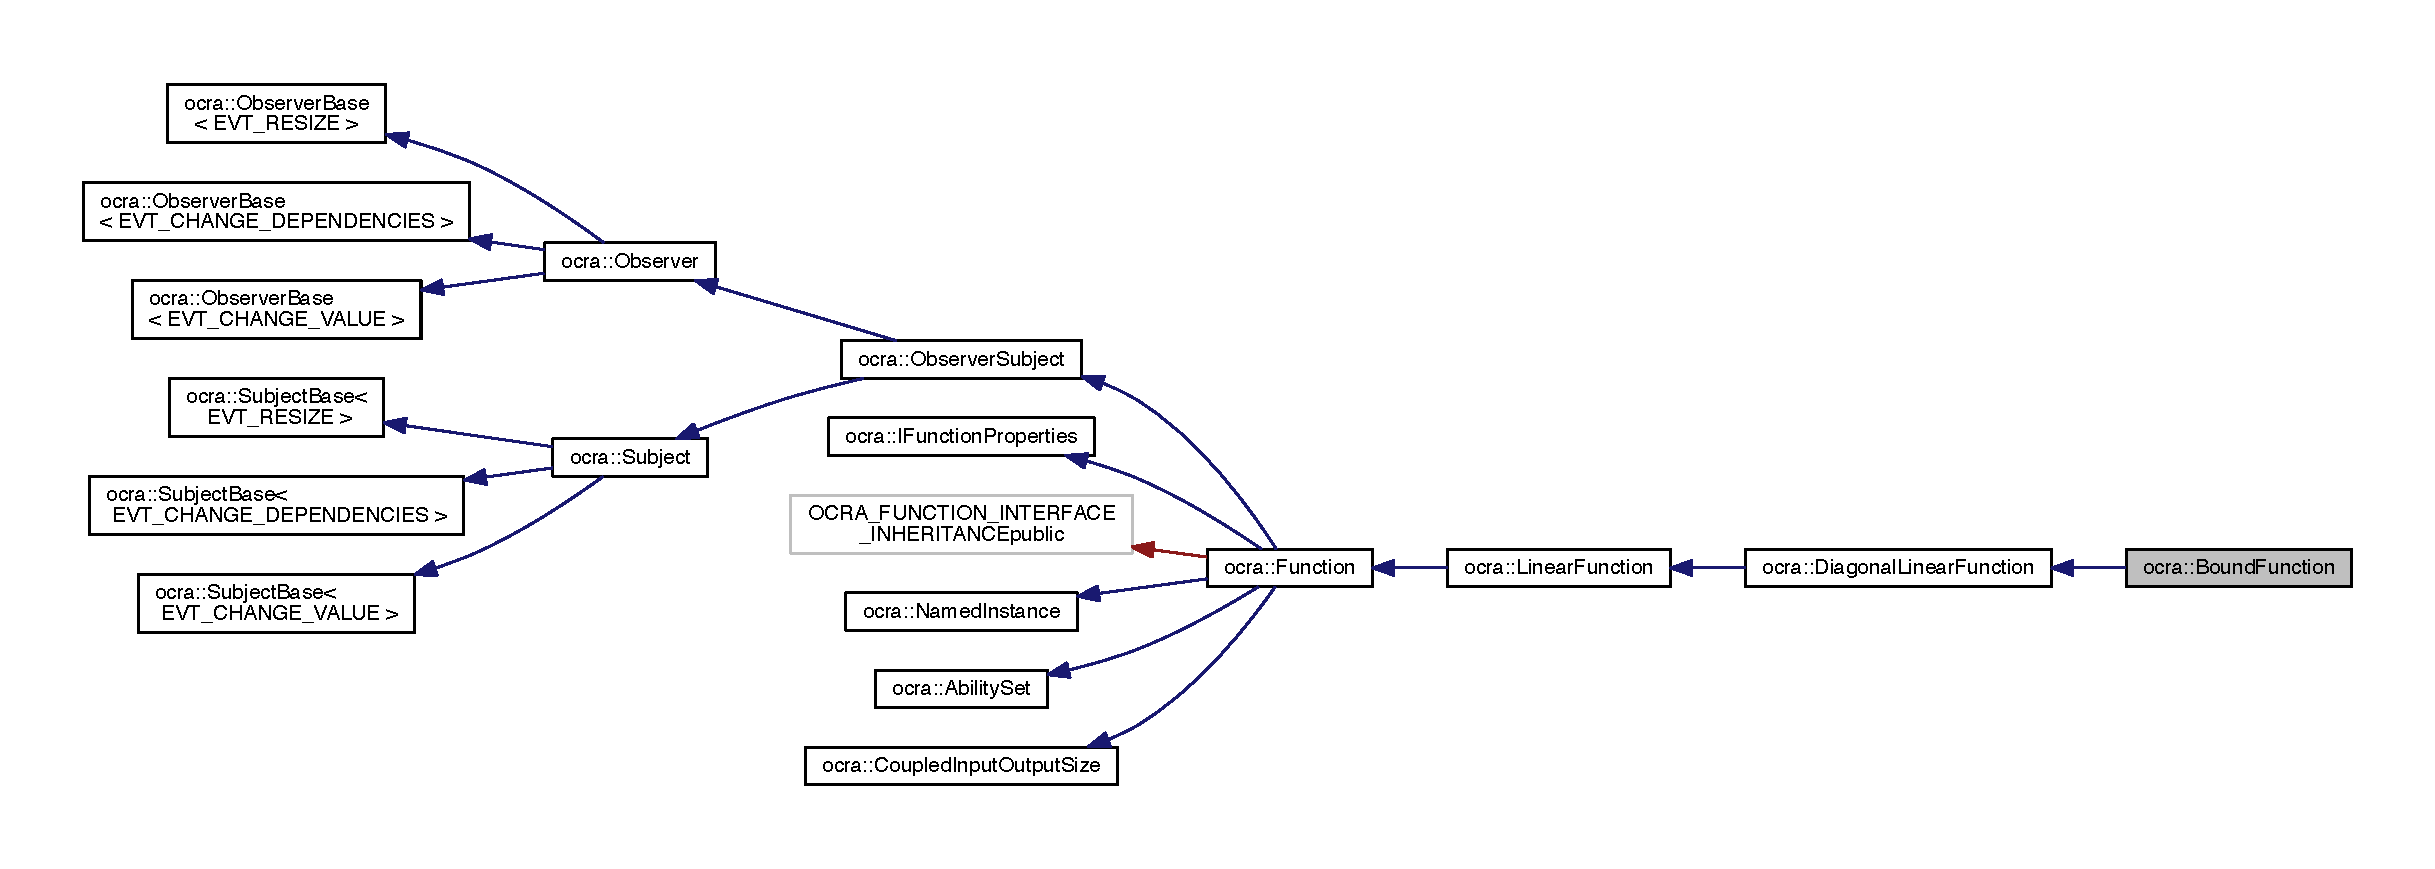
\includegraphics[width=350pt]{d3/ddd/classocra_1_1BoundFunction__inherit__graph}
\end{center}
\end{figure}


Collaboration diagram for ocra\+:\+:Bound\+Function\+:\nopagebreak
\begin{figure}[H]
\begin{center}
\leavevmode
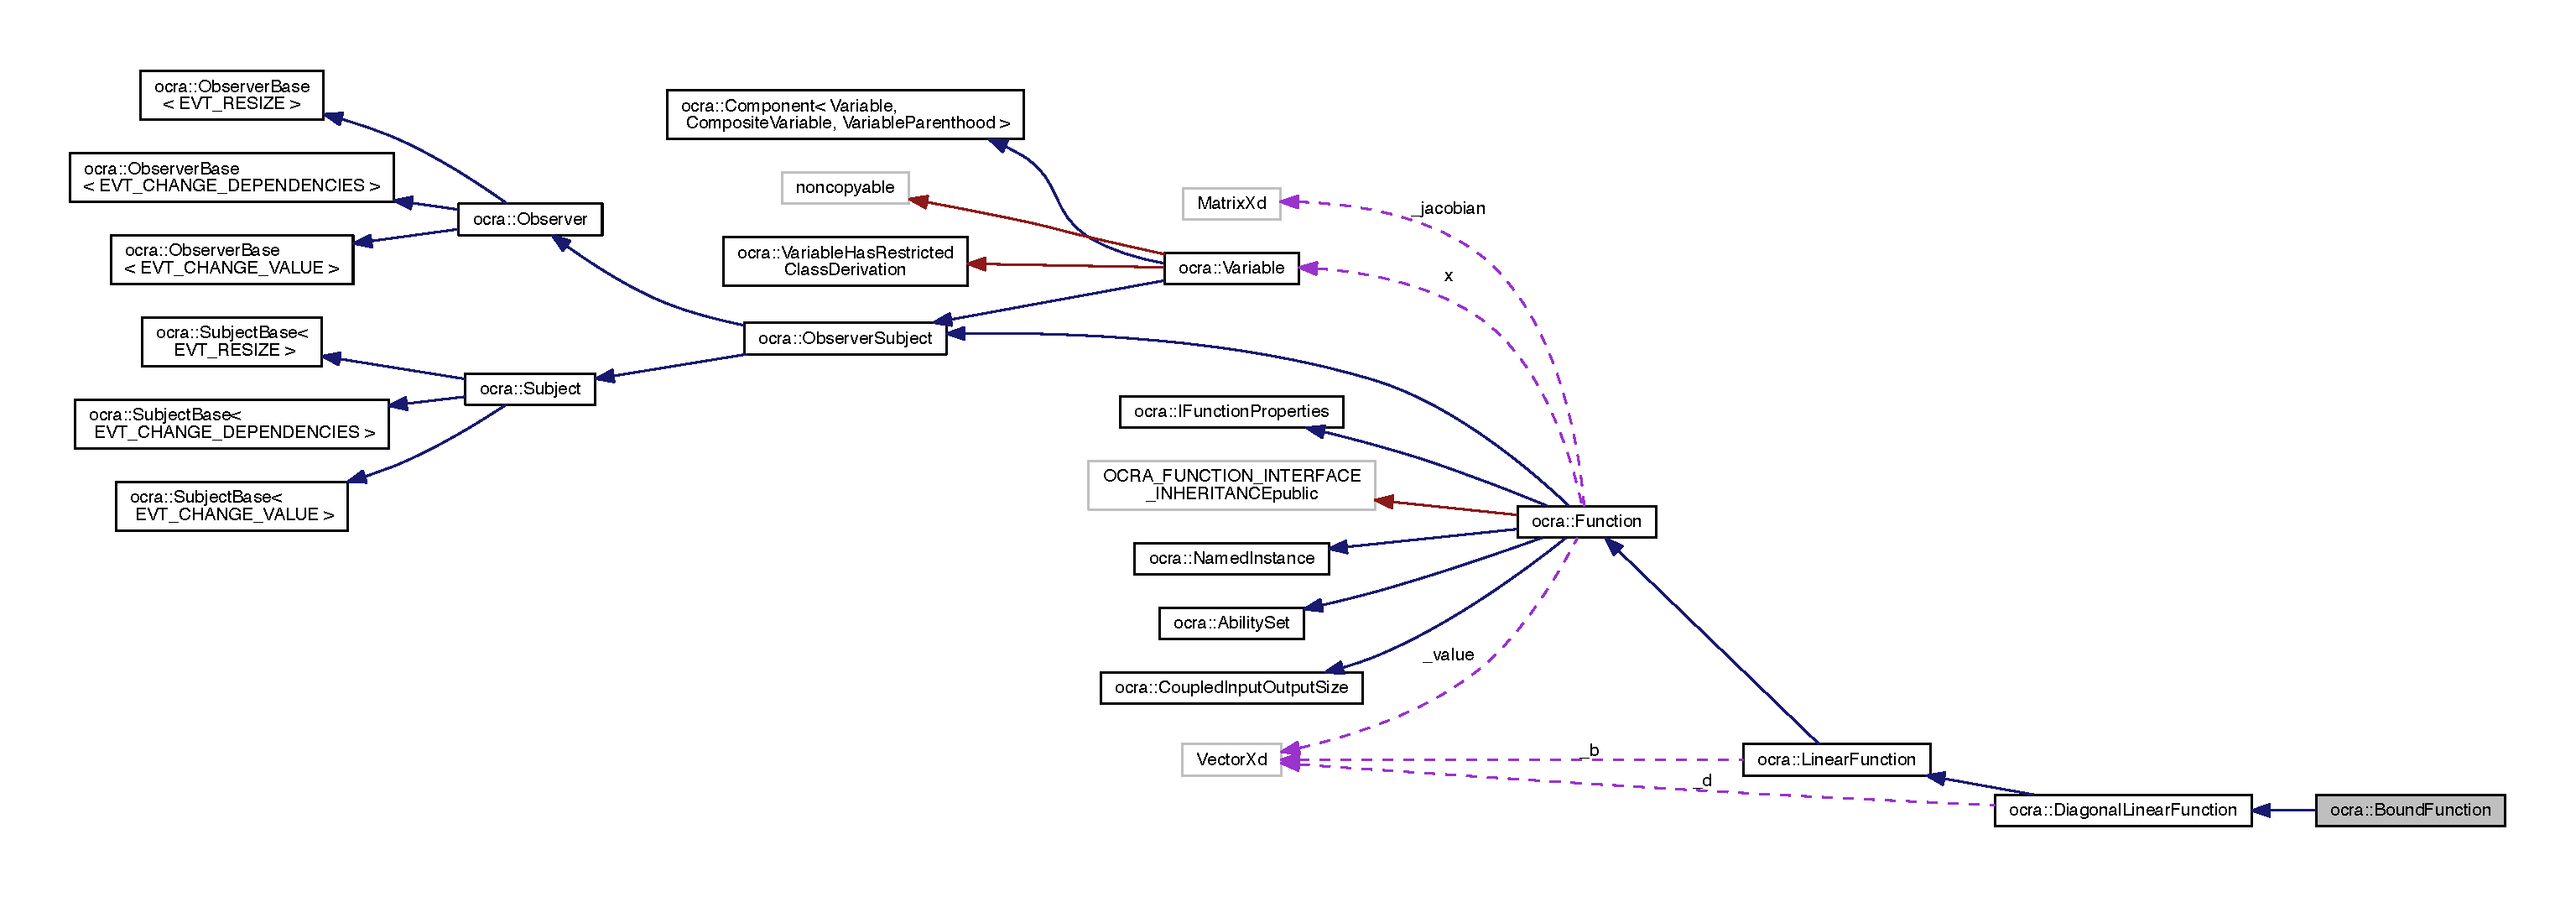
\includegraphics[width=350pt]{df/d41/classocra_1_1BoundFunction__coll__graph}
\end{center}
\end{figure}
\subsection*{Public Types}
\begin{DoxyCompactItemize}
\item 
typedef \hyperlink{classocra_1_1DiagonalLinearFunction}{Diagonal\+Linear\+Function} \hyperlink{classocra_1_1BoundFunction_acba2ac4d2f6caf04054590615a41ac21}{function\+Type\+\_\+t}
\end{DoxyCompactItemize}
\subsection*{Public Member Functions}
\begin{DoxyCompactItemize}
\item 
void \hyperlink{classocra_1_1BoundFunction_ad9a5cb9442e2129111d189e8063304ad}{change\+Ith\+Bound} (const int i, const double bound)
\end{DoxyCompactItemize}
{\bf }\par
\begin{DoxyCompactItemize}
\item 
\hyperlink{classocra_1_1BoundFunction_a7dc079453fdb607b46295246153481fd}{Bound\+Function} (\hyperlink{classocra_1_1Variable}{Variable} \&\hyperlink{classocra_1_1Function_a28825886d1f149c87b112ec2ec1dd486}{x}, const Vector\+Xd \&bound, \hyperlink{namespaceocra_ab3efdc117d9e5bcb0192640f5e7dc79b}{e\+Bound\+Type} type)
\item 
\hyperlink{classocra_1_1BoundFunction_afba908c0284f8ce9b2f7f1f8e5338cb5}{Bound\+Function} (\hyperlink{classocra_1_1Variable}{Variable} \&\hyperlink{classocra_1_1Function_a28825886d1f149c87b112ec2ec1dd486}{x}, const double bound, \hyperlink{namespaceocra_ab3efdc117d9e5bcb0192640f5e7dc79b}{e\+Bound\+Type} type)
\end{DoxyCompactItemize}

{\bf }\par
\begin{DoxyCompactItemize}
\item 
void \hyperlink{classocra_1_1BoundFunction_a205a73bb12f3255368d125ba0a6b4e58}{change\+Bounds} (const double bound)
\item 
void \hyperlink{classocra_1_1BoundFunction_aa69f4a52a46914e6ecbffb525e7d1314}{change\+Bounds} (const Vector\+Xd \&bounds)
\end{DoxyCompactItemize}

\subsection*{Protected Member Functions}
{\bf }\par
\begin{DoxyCompactItemize}
\item 
void \hyperlink{classocra_1_1BoundFunction_a95e8e97598f5ca779b9c171c56a7342a}{do\+Change\+Diagonal} (const Vector\+Xd \&d)
\item 
void \hyperlink{classocra_1_1BoundFunction_ac1a1b78b8b1796543b4c83ae5d8de755}{do\+Change\+Diagonal} (const double diagonal\+Element\+Value, const bool change\+Default=true)
\item 
void \hyperlink{classocra_1_1BoundFunction_af02c8fc499fb37596c758861d98cfbf6}{do\+Change\+Default\+Diagonal\+Value} (const double v)
\item 
void \hyperlink{classocra_1_1BoundFunction_aa861028f4a37e45b4fc68b7852d7e451}{do\+Change\+Defaultb\+Value} (const double v)
\end{DoxyCompactItemize}

\subsection*{Additional Inherited Members}


\subsection{Detailed Description}
Bound\+Function class. 

\begin{DoxyWarning}{Warning}
None
\end{DoxyWarning}
\hyperlink{classocra_1_1Function}{Function} to describe bound constraints $ x<x^+ $ or $ x>x^- $ so that the constraint can be written Ax+b$<$=0 

Definition at line 45 of file Bound\+Function.\+h.



\subsection{Member Typedef Documentation}
\hypertarget{classocra_1_1BoundFunction_acba2ac4d2f6caf04054590615a41ac21}{}\label{classocra_1_1BoundFunction_acba2ac4d2f6caf04054590615a41ac21} 
\index{ocra\+::\+Bound\+Function@{ocra\+::\+Bound\+Function}!function\+Type\+\_\+t@{function\+Type\+\_\+t}}
\index{function\+Type\+\_\+t@{function\+Type\+\_\+t}!ocra\+::\+Bound\+Function@{ocra\+::\+Bound\+Function}}
\subsubsection{\texorpdfstring{function\+Type\+\_\+t}{functionType\_t}}
{\footnotesize\ttfamily typedef \hyperlink{classocra_1_1DiagonalLinearFunction}{Diagonal\+Linear\+Function} \hyperlink{classocra_1_1BoundFunction_acba2ac4d2f6caf04054590615a41ac21}{ocra\+::\+Bound\+Function\+::function\+Type\+\_\+t}}



Definition at line 50 of file Bound\+Function.\+h.



\subsection{Constructor \& Destructor Documentation}
\hypertarget{classocra_1_1BoundFunction_a7dc079453fdb607b46295246153481fd}{}\label{classocra_1_1BoundFunction_a7dc079453fdb607b46295246153481fd} 
\index{ocra\+::\+Bound\+Function@{ocra\+::\+Bound\+Function}!Bound\+Function@{Bound\+Function}}
\index{Bound\+Function@{Bound\+Function}!ocra\+::\+Bound\+Function@{ocra\+::\+Bound\+Function}}
\subsubsection{\texorpdfstring{Bound\+Function()}{BoundFunction()}\hspace{0.1cm}{\footnotesize\ttfamily [1/2]}}
{\footnotesize\ttfamily ocra\+::\+Bound\+Function\+::\+Bound\+Function (\begin{DoxyParamCaption}\item[{\hyperlink{classocra_1_1Variable}{Variable} \&}]{x,  }\item[{const Vector\+Xd \&}]{bound,  }\item[{\hyperlink{namespaceocra_ab3efdc117d9e5bcb0192640f5e7dc79b}{e\+Bound\+Type}}]{type }\end{DoxyParamCaption})}

Constructors


\begin{DoxyParams}[1]{Parameters}
\mbox{\tt in}  & {\em x} & The variable on which to build the function. \\
\hline
\mbox{\tt in}  & {\em bound} & A vector or a double used to build a constant vector, representing bounds on the variable \\
\hline
\mbox{\tt in}  & {\em the} & type of the bound \\
\hline
\end{DoxyParams}


Definition at line 6 of file Bound\+Function.\+cpp.

\hypertarget{classocra_1_1BoundFunction_afba908c0284f8ce9b2f7f1f8e5338cb5}{}\label{classocra_1_1BoundFunction_afba908c0284f8ce9b2f7f1f8e5338cb5} 
\index{ocra\+::\+Bound\+Function@{ocra\+::\+Bound\+Function}!Bound\+Function@{Bound\+Function}}
\index{Bound\+Function@{Bound\+Function}!ocra\+::\+Bound\+Function@{ocra\+::\+Bound\+Function}}
\subsubsection{\texorpdfstring{Bound\+Function()}{BoundFunction()}\hspace{0.1cm}{\footnotesize\ttfamily [2/2]}}
{\footnotesize\ttfamily ocra\+::\+Bound\+Function\+::\+Bound\+Function (\begin{DoxyParamCaption}\item[{\hyperlink{classocra_1_1Variable}{Variable} \&}]{x,  }\item[{const double}]{bound,  }\item[{\hyperlink{namespaceocra_ab3efdc117d9e5bcb0192640f5e7dc79b}{e\+Bound\+Type}}]{type }\end{DoxyParamCaption})}



Definition at line 18 of file Bound\+Function.\+cpp.



\subsection{Member Function Documentation}
\hypertarget{classocra_1_1BoundFunction_a205a73bb12f3255368d125ba0a6b4e58}{}\label{classocra_1_1BoundFunction_a205a73bb12f3255368d125ba0a6b4e58} 
\index{ocra\+::\+Bound\+Function@{ocra\+::\+Bound\+Function}!change\+Bounds@{change\+Bounds}}
\index{change\+Bounds@{change\+Bounds}!ocra\+::\+Bound\+Function@{ocra\+::\+Bound\+Function}}
\subsubsection{\texorpdfstring{change\+Bounds()}{changeBounds()}\hspace{0.1cm}{\footnotesize\ttfamily [1/2]}}
{\footnotesize\ttfamily void ocra\+::\+Bound\+Function\+::change\+Bounds (\begin{DoxyParamCaption}\item[{const double}]{bound }\end{DoxyParamCaption})}

Change all the bounds to the given value(s) 

Definition at line 54 of file Bound\+Function.\+cpp.

\hypertarget{classocra_1_1BoundFunction_aa69f4a52a46914e6ecbffb525e7d1314}{}\label{classocra_1_1BoundFunction_aa69f4a52a46914e6ecbffb525e7d1314} 
\index{ocra\+::\+Bound\+Function@{ocra\+::\+Bound\+Function}!change\+Bounds@{change\+Bounds}}
\index{change\+Bounds@{change\+Bounds}!ocra\+::\+Bound\+Function@{ocra\+::\+Bound\+Function}}
\subsubsection{\texorpdfstring{change\+Bounds()}{changeBounds()}\hspace{0.1cm}{\footnotesize\ttfamily [2/2]}}
{\footnotesize\ttfamily void ocra\+::\+Bound\+Function\+::change\+Bounds (\begin{DoxyParamCaption}\item[{const Vector\+Xd \&}]{bounds }\end{DoxyParamCaption})}



Definition at line 63 of file Bound\+Function.\+cpp.

\hypertarget{classocra_1_1BoundFunction_ad9a5cb9442e2129111d189e8063304ad}{}\label{classocra_1_1BoundFunction_ad9a5cb9442e2129111d189e8063304ad} 
\index{ocra\+::\+Bound\+Function@{ocra\+::\+Bound\+Function}!change\+Ith\+Bound@{change\+Ith\+Bound}}
\index{change\+Ith\+Bound@{change\+Ith\+Bound}!ocra\+::\+Bound\+Function@{ocra\+::\+Bound\+Function}}
\subsubsection{\texorpdfstring{change\+Ith\+Bound()}{changeIthBound()}}
{\footnotesize\ttfamily void ocra\+::\+Bound\+Function\+::change\+Ith\+Bound (\begin{DoxyParamCaption}\item[{const int}]{i,  }\item[{const double}]{bound }\end{DoxyParamCaption})}

Change the ith bound to the given value 

Definition at line 71 of file Bound\+Function.\+cpp.

\hypertarget{classocra_1_1BoundFunction_aa861028f4a37e45b4fc68b7852d7e451}{}\label{classocra_1_1BoundFunction_aa861028f4a37e45b4fc68b7852d7e451} 
\index{ocra\+::\+Bound\+Function@{ocra\+::\+Bound\+Function}!do\+Change\+Defaultb\+Value@{do\+Change\+Defaultb\+Value}}
\index{do\+Change\+Defaultb\+Value@{do\+Change\+Defaultb\+Value}!ocra\+::\+Bound\+Function@{ocra\+::\+Bound\+Function}}
\subsubsection{\texorpdfstring{do\+Change\+Defaultb\+Value()}{doChangeDefaultbValue()}}
{\footnotesize\ttfamily void ocra\+::\+Bound\+Function\+::do\+Change\+Defaultb\+Value (\begin{DoxyParamCaption}\item[{const double}]{v }\end{DoxyParamCaption})\hspace{0.3cm}{\ttfamily [protected]}, {\ttfamily [virtual]}}



Reimplemented from \hyperlink{classocra_1_1DiagonalLinearFunction_a9995af94055dc443c10018869a393635}{ocra\+::\+Diagonal\+Linear\+Function}.



Definition at line 48 of file Bound\+Function.\+cpp.

\hypertarget{classocra_1_1BoundFunction_af02c8fc499fb37596c758861d98cfbf6}{}\label{classocra_1_1BoundFunction_af02c8fc499fb37596c758861d98cfbf6} 
\index{ocra\+::\+Bound\+Function@{ocra\+::\+Bound\+Function}!do\+Change\+Default\+Diagonal\+Value@{do\+Change\+Default\+Diagonal\+Value}}
\index{do\+Change\+Default\+Diagonal\+Value@{do\+Change\+Default\+Diagonal\+Value}!ocra\+::\+Bound\+Function@{ocra\+::\+Bound\+Function}}
\subsubsection{\texorpdfstring{do\+Change\+Default\+Diagonal\+Value()}{doChangeDefaultDiagonalValue()}}
{\footnotesize\ttfamily void ocra\+::\+Bound\+Function\+::do\+Change\+Default\+Diagonal\+Value (\begin{DoxyParamCaption}\item[{const double}]{v }\end{DoxyParamCaption})\hspace{0.3cm}{\ttfamily [protected]}, {\ttfamily [virtual]}}



Reimplemented from \hyperlink{classocra_1_1DiagonalLinearFunction_a81120f5a61cc53cc940f4e71b35174ff}{ocra\+::\+Diagonal\+Linear\+Function}.



Definition at line 42 of file Bound\+Function.\+cpp.

\hypertarget{classocra_1_1BoundFunction_a95e8e97598f5ca779b9c171c56a7342a}{}\label{classocra_1_1BoundFunction_a95e8e97598f5ca779b9c171c56a7342a} 
\index{ocra\+::\+Bound\+Function@{ocra\+::\+Bound\+Function}!do\+Change\+Diagonal@{do\+Change\+Diagonal}}
\index{do\+Change\+Diagonal@{do\+Change\+Diagonal}!ocra\+::\+Bound\+Function@{ocra\+::\+Bound\+Function}}
\subsubsection{\texorpdfstring{do\+Change\+Diagonal()}{doChangeDiagonal()}\hspace{0.1cm}{\footnotesize\ttfamily [1/2]}}
{\footnotesize\ttfamily void ocra\+::\+Bound\+Function\+::do\+Change\+Diagonal (\begin{DoxyParamCaption}\item[{const Vector\+Xd \&}]{d }\end{DoxyParamCaption})\hspace{0.3cm}{\ttfamily [protected]}, {\ttfamily [virtual]}}

Overloads of \hyperlink{classocra_1_1DiagonalLinearFunction}{Diagonal\+Linear\+Function} methods. All throw a runtime\+\_\+error\+: diagonal value are fixed for a \hyperlink{classocra_1_1BoundFunction}{Bound\+Function} and default value cannot be changed. 

Reimplemented from \hyperlink{classocra_1_1DiagonalLinearFunction_a5355515d58348a3eea92f36e35b1c7d5}{ocra\+::\+Diagonal\+Linear\+Function}.



Definition at line 30 of file Bound\+Function.\+cpp.

\hypertarget{classocra_1_1BoundFunction_ac1a1b78b8b1796543b4c83ae5d8de755}{}\label{classocra_1_1BoundFunction_ac1a1b78b8b1796543b4c83ae5d8de755} 
\index{ocra\+::\+Bound\+Function@{ocra\+::\+Bound\+Function}!do\+Change\+Diagonal@{do\+Change\+Diagonal}}
\index{do\+Change\+Diagonal@{do\+Change\+Diagonal}!ocra\+::\+Bound\+Function@{ocra\+::\+Bound\+Function}}
\subsubsection{\texorpdfstring{do\+Change\+Diagonal()}{doChangeDiagonal()}\hspace{0.1cm}{\footnotesize\ttfamily [2/2]}}
{\footnotesize\ttfamily void ocra\+::\+Bound\+Function\+::do\+Change\+Diagonal (\begin{DoxyParamCaption}\item[{const double}]{diagonal\+Element\+Value,  }\item[{const bool}]{change\+Default = {\ttfamily true} }\end{DoxyParamCaption})\hspace{0.3cm}{\ttfamily [protected]}, {\ttfamily [virtual]}}



Reimplemented from \hyperlink{classocra_1_1DiagonalLinearFunction_a0673bfe405d5637182c4749dd2737e95}{ocra\+::\+Diagonal\+Linear\+Function}.



Definition at line 36 of file Bound\+Function.\+cpp.



The documentation for this class was generated from the following files\+:\begin{DoxyCompactItemize}
\item 
\hyperlink{BoundFunction_8h}{Bound\+Function.\+h}\item 
\hyperlink{BoundFunction_8cpp}{Bound\+Function.\+cpp}\end{DoxyCompactItemize}

\hypertarget{classocra_1_1Buffer}{}\section{ocra\+:\+:Buffer$<$ T $>$ Class Template Reference}
\label{classocra_1_1Buffer}\index{ocra\+::\+Buffer$<$ T $>$@{ocra\+::\+Buffer$<$ T $>$}}


{\ttfamily \#include $<$Buffer.\+h$>$}

\subsection*{Public Types}
\begin{DoxyCompactItemize}
\item 
typedef T \hyperlink{classocra_1_1Buffer_ad03bef3764c265411b5b7726d94d8786}{value\+\_\+type}
\item 
typedef T $\ast$ \hyperlink{classocra_1_1Buffer_a26bf1dc373e2144eddd0dd8be4b37f84}{ptr\+\_\+type}
\end{DoxyCompactItemize}
\subsection*{Public Member Functions}
\begin{DoxyCompactItemize}
\item 
\hyperlink{classocra_1_1Buffer_a13b091b3f15fbdaadd00d87b89f0acd7}{Buffer} (size\+\_\+t \hyperlink{classocra_1_1Buffer_a181e8573c657bbc9a09a15628be00c4f}{size})
\item 
\hyperlink{classocra_1_1Buffer_ac7050b30073f9fbfbf580c1b57a34781}{$\sim$\+Buffer} ()
\item 
void \hyperlink{classocra_1_1Buffer_a171d3ec7b50688fd529c8ae3dff7b6d1}{resize} (size\+\_\+t \hyperlink{classocra_1_1Buffer_a181e8573c657bbc9a09a15628be00c4f}{size})
\item 
void \hyperlink{classocra_1_1Buffer_a3f6d6353bdb0e6eb2e577121be432f5f}{reset} ()
\item 
\hyperlink{classocra_1_1Buffer_a26bf1dc373e2144eddd0dd8be4b37f84}{ptr\+\_\+type} \hyperlink{classocra_1_1Buffer_a693db1946acad229a8e7ab84ac910301}{allocate} (size\+\_\+t n)
\item 
size\+\_\+t \hyperlink{classocra_1_1Buffer_a181e8573c657bbc9a09a15628be00c4f}{size} () const
\item 
size\+\_\+t \hyperlink{classocra_1_1Buffer_adf28f390748a3f97df43b08fb0574e6a}{free\+Size} () const
\end{DoxyCompactItemize}


\subsection{Detailed Description}
\subsubsection*{template$<$class T$>$\newline
class ocra\+::\+Buffer$<$ T $>$}

This class acts as a memory pool for objects of type {\itshape T}. Upon request it returns a pointer to an array of T of size specified by the caller, provided it owns enough memory for that. It allocates contiguous memory blocks and ensures memory release when resizing or dying. Thus, you need not free the memory obtained via this class.

\begin{DoxyWarning}{Warning}
Don\textquotesingle{}t trust other classes. Don\textquotesingle{}t give them the buffers you obtain here\+: \hyperlink{classocra_1_1Buffer_a171d3ec7b50688fd529c8ae3dff7b6d1}{resize()} invalidates them all. 
\end{DoxyWarning}


Definition at line 18 of file Buffer.\+h.



\subsection{Member Typedef Documentation}
\hypertarget{classocra_1_1Buffer_a26bf1dc373e2144eddd0dd8be4b37f84}{}\label{classocra_1_1Buffer_a26bf1dc373e2144eddd0dd8be4b37f84} 
\index{ocra\+::\+Buffer@{ocra\+::\+Buffer}!ptr\+\_\+type@{ptr\+\_\+type}}
\index{ptr\+\_\+type@{ptr\+\_\+type}!ocra\+::\+Buffer@{ocra\+::\+Buffer}}
\subsubsection{\texorpdfstring{ptr\+\_\+type}{ptr\_type}}
{\footnotesize\ttfamily template$<$class T$>$ \\
typedef T$\ast$ \hyperlink{classocra_1_1Buffer}{ocra\+::\+Buffer}$<$ T $>$\+::\hyperlink{classocra_1_1Buffer_a26bf1dc373e2144eddd0dd8be4b37f84}{ptr\+\_\+type}}



Definition at line 22 of file Buffer.\+h.

\hypertarget{classocra_1_1Buffer_ad03bef3764c265411b5b7726d94d8786}{}\label{classocra_1_1Buffer_ad03bef3764c265411b5b7726d94d8786} 
\index{ocra\+::\+Buffer@{ocra\+::\+Buffer}!value\+\_\+type@{value\+\_\+type}}
\index{value\+\_\+type@{value\+\_\+type}!ocra\+::\+Buffer@{ocra\+::\+Buffer}}
\subsubsection{\texorpdfstring{value\+\_\+type}{value\_type}}
{\footnotesize\ttfamily template$<$class T$>$ \\
typedef T \hyperlink{classocra_1_1Buffer}{ocra\+::\+Buffer}$<$ T $>$\+::\hyperlink{classocra_1_1Buffer_ad03bef3764c265411b5b7726d94d8786}{value\+\_\+type}}



Definition at line 21 of file Buffer.\+h.



\subsection{Constructor \& Destructor Documentation}
\hypertarget{classocra_1_1Buffer_a13b091b3f15fbdaadd00d87b89f0acd7}{}\label{classocra_1_1Buffer_a13b091b3f15fbdaadd00d87b89f0acd7} 
\index{ocra\+::\+Buffer@{ocra\+::\+Buffer}!Buffer@{Buffer}}
\index{Buffer@{Buffer}!ocra\+::\+Buffer@{ocra\+::\+Buffer}}
\subsubsection{\texorpdfstring{Buffer()}{Buffer()}}
{\footnotesize\ttfamily template$<$class T$>$ \\
\hyperlink{classocra_1_1Buffer}{ocra\+::\+Buffer}$<$ T $>$\+::\hyperlink{classocra_1_1Buffer}{Buffer} (\begin{DoxyParamCaption}\item[{size\+\_\+t}]{size }\end{DoxyParamCaption})\hspace{0.3cm}{\ttfamily [inline]}}

Build an instance of \hyperlink{classocra_1_1Buffer}{Buffer} with a memory buffer for {\itshape size} elements of type T 

Definition at line 33 of file Buffer.\+h.

\hypertarget{classocra_1_1Buffer_ac7050b30073f9fbfbf580c1b57a34781}{}\label{classocra_1_1Buffer_ac7050b30073f9fbfbf580c1b57a34781} 
\index{ocra\+::\+Buffer@{ocra\+::\+Buffer}!````~Buffer@{$\sim$\+Buffer}}
\index{````~Buffer@{$\sim$\+Buffer}!ocra\+::\+Buffer@{ocra\+::\+Buffer}}
\subsubsection{\texorpdfstring{$\sim$\+Buffer()}{~Buffer()}}
{\footnotesize\ttfamily template$<$class T$>$ \\
\hyperlink{classocra_1_1Buffer}{ocra\+::\+Buffer}$<$ T $>$\+::$\sim$\hyperlink{classocra_1_1Buffer}{Buffer} (\begin{DoxyParamCaption}{ }\end{DoxyParamCaption})\hspace{0.3cm}{\ttfamily [inline]}}



Definition at line 34 of file Buffer.\+h.



\subsection{Member Function Documentation}
\hypertarget{classocra_1_1Buffer_a693db1946acad229a8e7ab84ac910301}{}\label{classocra_1_1Buffer_a693db1946acad229a8e7ab84ac910301} 
\index{ocra\+::\+Buffer@{ocra\+::\+Buffer}!allocate@{allocate}}
\index{allocate@{allocate}!ocra\+::\+Buffer@{ocra\+::\+Buffer}}
\subsubsection{\texorpdfstring{allocate()}{allocate()}}
{\footnotesize\ttfamily template$<$class T$>$ \\
\hyperlink{classocra_1_1Buffer_a26bf1dc373e2144eddd0dd8be4b37f84}{ptr\+\_\+type} \hyperlink{classocra_1_1Buffer}{ocra\+::\+Buffer}$<$ T $>$\+::allocate (\begin{DoxyParamCaption}\item[{size\+\_\+t}]{n }\end{DoxyParamCaption})\hspace{0.3cm}{\ttfamily [inline]}}

Return the pointer on a free continuous memory block of size {\itshape n} 


\begin{DoxyExceptions}{Exceptions}
{\em a} & runtime\+\_\+error in case there is not enough memory reserved to fullfill this query. \\
\hline
\end{DoxyExceptions}


Definition at line 68 of file Buffer.\+h.

\hypertarget{classocra_1_1Buffer_adf28f390748a3f97df43b08fb0574e6a}{}\label{classocra_1_1Buffer_adf28f390748a3f97df43b08fb0574e6a} 
\index{ocra\+::\+Buffer@{ocra\+::\+Buffer}!free\+Size@{free\+Size}}
\index{free\+Size@{free\+Size}!ocra\+::\+Buffer@{ocra\+::\+Buffer}}
\subsubsection{\texorpdfstring{free\+Size()}{freeSize()}}
{\footnotesize\ttfamily template$<$class T$>$ \\
size\+\_\+t \hyperlink{classocra_1_1Buffer}{ocra\+::\+Buffer}$<$ T $>$\+::free\+Size (\begin{DoxyParamCaption}{ }\end{DoxyParamCaption}) const\hspace{0.3cm}{\ttfamily [inline]}}

Return the size of the reserved memory still free 

Definition at line 84 of file Buffer.\+h.

\hypertarget{classocra_1_1Buffer_a3f6d6353bdb0e6eb2e577121be432f5f}{}\label{classocra_1_1Buffer_a3f6d6353bdb0e6eb2e577121be432f5f} 
\index{ocra\+::\+Buffer@{ocra\+::\+Buffer}!reset@{reset}}
\index{reset@{reset}!ocra\+::\+Buffer@{ocra\+::\+Buffer}}
\subsubsection{\texorpdfstring{reset()}{reset()}}
{\footnotesize\ttfamily template$<$class T$>$ \\
void \hyperlink{classocra_1_1Buffer}{ocra\+::\+Buffer}$<$ T $>$\+::reset (\begin{DoxyParamCaption}{ }\end{DoxyParamCaption})\hspace{0.3cm}{\ttfamily [inline]}}

Tell the instance to give memory from the beginning of the pool again. All previously given buffers should be considered as invalid 

Definition at line 59 of file Buffer.\+h.

\hypertarget{classocra_1_1Buffer_a171d3ec7b50688fd529c8ae3dff7b6d1}{}\label{classocra_1_1Buffer_a171d3ec7b50688fd529c8ae3dff7b6d1} 
\index{ocra\+::\+Buffer@{ocra\+::\+Buffer}!resize@{resize}}
\index{resize@{resize}!ocra\+::\+Buffer@{ocra\+::\+Buffer}}
\subsubsection{\texorpdfstring{resize()}{resize()}}
{\footnotesize\ttfamily template$<$class T$>$ \\
void \hyperlink{classocra_1_1Buffer}{ocra\+::\+Buffer}$<$ T $>$\+::resize (\begin{DoxyParamCaption}\item[{size\+\_\+t}]{size }\end{DoxyParamCaption})\hspace{0.3cm}{\ttfamily [inline]}}

Resize the memory buffer to a size greater or equal to the parameter {\itshape size}. Wether there is really a buffer resizing or not, the previously returned buffer need to be considered as invalid, since calls to allocate subsequent to a resize will return buffers starting from the beginning of the memory pool again. 

Definition at line 40 of file Buffer.\+h.

\hypertarget{classocra_1_1Buffer_a181e8573c657bbc9a09a15628be00c4f}{}\label{classocra_1_1Buffer_a181e8573c657bbc9a09a15628be00c4f} 
\index{ocra\+::\+Buffer@{ocra\+::\+Buffer}!size@{size}}
\index{size@{size}!ocra\+::\+Buffer@{ocra\+::\+Buffer}}
\subsubsection{\texorpdfstring{size()}{size()}}
{\footnotesize\ttfamily template$<$class T$>$ \\
size\+\_\+t \hyperlink{classocra_1_1Buffer}{ocra\+::\+Buffer}$<$ T $>$\+::size (\begin{DoxyParamCaption}{ }\end{DoxyParamCaption}) const\hspace{0.3cm}{\ttfamily [inline]}}

Return the size of the reserved memory 

Definition at line 78 of file Buffer.\+h.



The documentation for this class was generated from the following file\+:\begin{DoxyCompactItemize}
\item 
\hyperlink{Buffer_8h}{Buffer.\+h}\end{DoxyCompactItemize}

\hypertarget{classocra_1_1CartesianTaskBuilder}{}\section{ocra\+:\+:Cartesian\+Task\+Builder Class Reference}
\label{classocra_1_1CartesianTaskBuilder}\index{ocra\+::\+Cartesian\+Task\+Builder@{ocra\+::\+Cartesian\+Task\+Builder}}


{\ttfamily \#include $<$Cartesian\+Task\+Builder.\+h$>$}



Inheritance diagram for ocra\+:\+:Cartesian\+Task\+Builder\+:\nopagebreak
\begin{figure}[H]
\begin{center}
\leavevmode
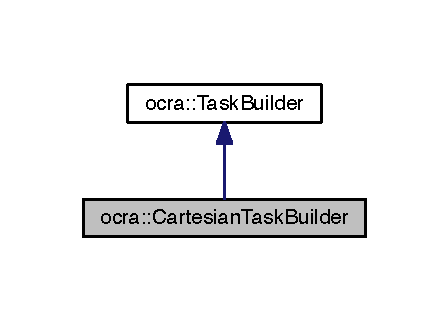
\includegraphics[width=215pt]{d0/d4d/classocra_1_1CartesianTaskBuilder__inherit__graph}
\end{center}
\end{figure}


Collaboration diagram for ocra\+:\+:Cartesian\+Task\+Builder\+:\nopagebreak
\begin{figure}[H]
\begin{center}
\leavevmode
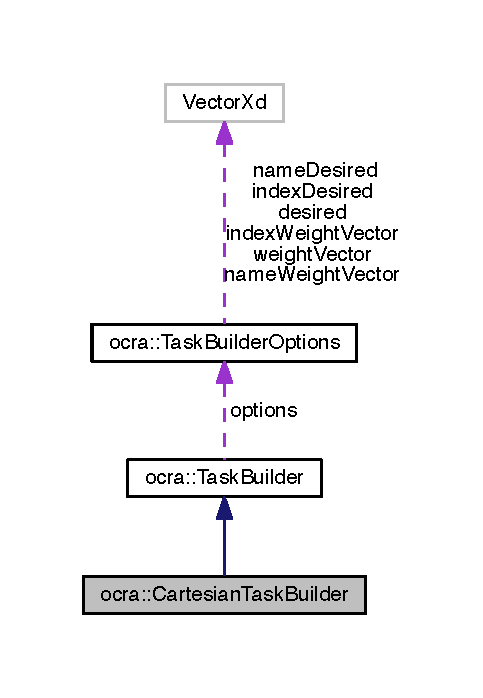
\includegraphics[width=232pt]{d9/d96/classocra_1_1CartesianTaskBuilder__coll__graph}
\end{center}
\end{figure}
\subsection*{Public Member Functions}
\begin{DoxyCompactItemize}
\item 
\hyperlink{classocra_1_1CartesianTaskBuilder_ad78453b86c3777783c94098967426bad}{Cartesian\+Task\+Builder} (const \hyperlink{classocra_1_1TaskBuilderOptions}{Task\+Builder\+Options} \&task\+Options, Model\+::\+Ptr model\+Ptr)
\item 
virtual \hyperlink{classocra_1_1CartesianTaskBuilder_aecc30a79dfbeaf935d302a3f1e2c3fac}{$\sim$\+Cartesian\+Task\+Builder} ()
\end{DoxyCompactItemize}
\subsection*{Protected Member Functions}
\begin{DoxyCompactItemize}
\item 
virtual void \hyperlink{classocra_1_1CartesianTaskBuilder_a679842b95d6f7296a466636fd21bbbb8}{set\+Task\+Type} ()
\item 
virtual void \hyperlink{classocra_1_1CartesianTaskBuilder_a9e3175e5792c5ed9a7e3febbe458d21c}{set\+Task\+State} ()
\item 
virtual Feature\+::\+Ptr \hyperlink{classocra_1_1CartesianTaskBuilder_a58c8e4a299db03180c058eefcd711052}{build\+Feature} ()
\item 
virtual Feature\+::\+Ptr \hyperlink{classocra_1_1CartesianTaskBuilder_a308b204435c4063991d8101c0a8c512c}{build\+Feature\+Desired} ()
\end{DoxyCompactItemize}
\subsection*{Additional Inherited Members}


\subsection{Detailed Description}


Definition at line 8 of file Cartesian\+Task\+Builder.\+h.



\subsection{Constructor \& Destructor Documentation}
\hypertarget{classocra_1_1CartesianTaskBuilder_ad78453b86c3777783c94098967426bad}{}\label{classocra_1_1CartesianTaskBuilder_ad78453b86c3777783c94098967426bad} 
\index{ocra\+::\+Cartesian\+Task\+Builder@{ocra\+::\+Cartesian\+Task\+Builder}!Cartesian\+Task\+Builder@{Cartesian\+Task\+Builder}}
\index{Cartesian\+Task\+Builder@{Cartesian\+Task\+Builder}!ocra\+::\+Cartesian\+Task\+Builder@{ocra\+::\+Cartesian\+Task\+Builder}}
\subsubsection{\texorpdfstring{Cartesian\+Task\+Builder()}{CartesianTaskBuilder()}}
{\footnotesize\ttfamily Cartesian\+Task\+Builder\+::\+Cartesian\+Task\+Builder (\begin{DoxyParamCaption}\item[{const \hyperlink{classocra_1_1TaskBuilderOptions}{Task\+Builder\+Options} \&}]{task\+Options,  }\item[{Model\+::\+Ptr}]{model\+Ptr }\end{DoxyParamCaption})}



Definition at line 5 of file Cartesian\+Task\+Builder.\+cpp.

\hypertarget{classocra_1_1CartesianTaskBuilder_aecc30a79dfbeaf935d302a3f1e2c3fac}{}\label{classocra_1_1CartesianTaskBuilder_aecc30a79dfbeaf935d302a3f1e2c3fac} 
\index{ocra\+::\+Cartesian\+Task\+Builder@{ocra\+::\+Cartesian\+Task\+Builder}!````~Cartesian\+Task\+Builder@{$\sim$\+Cartesian\+Task\+Builder}}
\index{````~Cartesian\+Task\+Builder@{$\sim$\+Cartesian\+Task\+Builder}!ocra\+::\+Cartesian\+Task\+Builder@{ocra\+::\+Cartesian\+Task\+Builder}}
\subsubsection{\texorpdfstring{$\sim$\+Cartesian\+Task\+Builder()}{~CartesianTaskBuilder()}}
{\footnotesize\ttfamily Cartesian\+Task\+Builder\+::$\sim$\+Cartesian\+Task\+Builder (\begin{DoxyParamCaption}{ }\end{DoxyParamCaption})\hspace{0.3cm}{\ttfamily [virtual]}}



Definition at line 11 of file Cartesian\+Task\+Builder.\+cpp.



\subsection{Member Function Documentation}
\hypertarget{classocra_1_1CartesianTaskBuilder_a58c8e4a299db03180c058eefcd711052}{}\label{classocra_1_1CartesianTaskBuilder_a58c8e4a299db03180c058eefcd711052} 
\index{ocra\+::\+Cartesian\+Task\+Builder@{ocra\+::\+Cartesian\+Task\+Builder}!build\+Feature@{build\+Feature}}
\index{build\+Feature@{build\+Feature}!ocra\+::\+Cartesian\+Task\+Builder@{ocra\+::\+Cartesian\+Task\+Builder}}
\subsubsection{\texorpdfstring{build\+Feature()}{buildFeature()}}
{\footnotesize\ttfamily Feature\+::\+Ptr Cartesian\+Task\+Builder\+::build\+Feature (\begin{DoxyParamCaption}{ }\end{DoxyParamCaption})\hspace{0.3cm}{\ttfamily [protected]}, {\ttfamily [virtual]}}



Implements \hyperlink{classocra_1_1TaskBuilder_a58c0dc416a9607a344a080248ee26ac2}{ocra\+::\+Task\+Builder}.



Definition at line 16 of file Cartesian\+Task\+Builder.\+cpp.

\hypertarget{classocra_1_1CartesianTaskBuilder_a308b204435c4063991d8101c0a8c512c}{}\label{classocra_1_1CartesianTaskBuilder_a308b204435c4063991d8101c0a8c512c} 
\index{ocra\+::\+Cartesian\+Task\+Builder@{ocra\+::\+Cartesian\+Task\+Builder}!build\+Feature\+Desired@{build\+Feature\+Desired}}
\index{build\+Feature\+Desired@{build\+Feature\+Desired}!ocra\+::\+Cartesian\+Task\+Builder@{ocra\+::\+Cartesian\+Task\+Builder}}
\subsubsection{\texorpdfstring{build\+Feature\+Desired()}{buildFeatureDesired()}}
{\footnotesize\ttfamily Feature\+::\+Ptr Cartesian\+Task\+Builder\+::build\+Feature\+Desired (\begin{DoxyParamCaption}{ }\end{DoxyParamCaption})\hspace{0.3cm}{\ttfamily [protected]}, {\ttfamily [virtual]}}



Implements \hyperlink{classocra_1_1TaskBuilder_a7a2c8bcc5d95160d0e48806a2648f1a5}{ocra\+::\+Task\+Builder}.



Definition at line 27 of file Cartesian\+Task\+Builder.\+cpp.

\hypertarget{classocra_1_1CartesianTaskBuilder_a9e3175e5792c5ed9a7e3febbe458d21c}{}\label{classocra_1_1CartesianTaskBuilder_a9e3175e5792c5ed9a7e3febbe458d21c} 
\index{ocra\+::\+Cartesian\+Task\+Builder@{ocra\+::\+Cartesian\+Task\+Builder}!set\+Task\+State@{set\+Task\+State}}
\index{set\+Task\+State@{set\+Task\+State}!ocra\+::\+Cartesian\+Task\+Builder@{ocra\+::\+Cartesian\+Task\+Builder}}
\subsubsection{\texorpdfstring{set\+Task\+State()}{setTaskState()}}
{\footnotesize\ttfamily void Cartesian\+Task\+Builder\+::set\+Task\+State (\begin{DoxyParamCaption}{ }\end{DoxyParamCaption})\hspace{0.3cm}{\ttfamily [protected]}, {\ttfamily [virtual]}}



Implements \hyperlink{classocra_1_1TaskBuilder_a7b44bfa101566ea4400e2d9bfdb9ff32}{ocra\+::\+Task\+Builder}.



Definition at line 37 of file Cartesian\+Task\+Builder.\+cpp.

\hypertarget{classocra_1_1CartesianTaskBuilder_a679842b95d6f7296a466636fd21bbbb8}{}\label{classocra_1_1CartesianTaskBuilder_a679842b95d6f7296a466636fd21bbbb8} 
\index{ocra\+::\+Cartesian\+Task\+Builder@{ocra\+::\+Cartesian\+Task\+Builder}!set\+Task\+Type@{set\+Task\+Type}}
\index{set\+Task\+Type@{set\+Task\+Type}!ocra\+::\+Cartesian\+Task\+Builder@{ocra\+::\+Cartesian\+Task\+Builder}}
\subsubsection{\texorpdfstring{set\+Task\+Type()}{setTaskType()}}
{\footnotesize\ttfamily void Cartesian\+Task\+Builder\+::set\+Task\+Type (\begin{DoxyParamCaption}{ }\end{DoxyParamCaption})\hspace{0.3cm}{\ttfamily [protected]}, {\ttfamily [virtual]}}



Implements \hyperlink{classocra_1_1TaskBuilder_a1a979fc495be6dc30483aa8fd0ff2650}{ocra\+::\+Task\+Builder}.



Definition at line 57 of file Cartesian\+Task\+Builder.\+cpp.



The documentation for this class was generated from the following files\+:\begin{DoxyCompactItemize}
\item 
\hyperlink{CartesianTaskBuilder_8h}{Cartesian\+Task\+Builder.\+h}\item 
\hyperlink{CartesianTaskBuilder_8cpp}{Cartesian\+Task\+Builder.\+cpp}\end{DoxyCompactItemize}

\hypertarget{classocra_1_1CascadeQP}{}\section{ocra\+:\+:Cascade\+QP Class Reference}
\label{classocra_1_1CascadeQP}\index{ocra\+::\+Cascade\+QP@{ocra\+::\+Cascade\+QP}}


Cascade\+QP class.  




{\ttfamily \#include $<$Cascade\+Q\+P.\+h$>$}



Collaboration diagram for ocra\+:\+:Cascade\+QP\+:\nopagebreak
\begin{figure}[H]
\begin{center}
\leavevmode
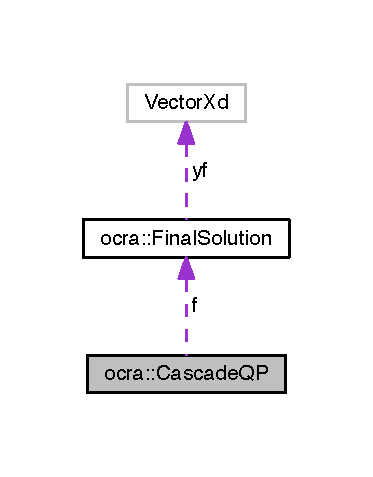
\includegraphics[width=179pt]{d6/d63/classocra_1_1CascadeQP__coll__graph}
\end{center}
\end{figure}
\subsection*{Public Member Functions}
\begin{DoxyCompactItemize}
\item 
\hyperlink{classocra_1_1CascadeQP_a545a3098762becf8a663eb8ab3bd4899}{Cascade\+QP} ()
\item 
virtual \hyperlink{classocra_1_1CascadeQP_a843673d4951f7a8e972598d0f361ad8d}{$\sim$\+Cascade\+QP} ()
\item 
std\+::size\+\_\+t \hyperlink{classocra_1_1CascadeQP_ab1ac4edfcf8e8c7567fc0a5ca5bd5f86}{add\+Hierarchy\+Level} (ocra\+::\+Hierarchy\+Level\+::\+Ptr h)
\item 
std\+::size\+\_\+t \hyperlink{classocra_1_1CascadeQP_a6415299f7159a36a75940e073f64b770}{add\+Hierarchy\+Level} (const std\+::vector$<$ Hierarchy\+Level\+::\+Ptr $>$ \&v)
\item 
void \hyperlink{classocra_1_1CascadeQP_a476d6af7b355fd8a3887e9708253cd1a}{clear} (void)
\item 
const \hyperlink{structocra_1_1FinalSolution}{Final\+Solution} \& \hyperlink{classocra_1_1CascadeQP_a11e01b608414badd9af6794076eb8b33}{solve\+Cascade\+QP} ()
\item 
const \hyperlink{structocra_1_1FinalSolution}{Final\+Solution} \& \hyperlink{classocra_1_1CascadeQP_af59591ea0fdc81da5866fa3b99fd9d67}{get\+Solution} () const
\item 
const Eigen\+::\+Vector\+Xd \& \hyperlink{classocra_1_1CascadeQP_ab897ead27cb45e35281f39d389e8ed87}{get\+Solution\+Of\+Level} (int i) const
\item 
Hierarchy\+Level\+::\+Ptr \hyperlink{classocra_1_1CascadeQP_a49b3ce4ed68507905755b63f878c1990}{get\+Hierarchy\+Level} (int i) const
\item 
std\+::size\+\_\+t \hyperlink{classocra_1_1CascadeQP_a1f714b8b6024d46a4e9545324a21e702}{get\+Number\+Of\+Hierarchy\+Level} () const
\end{DoxyCompactItemize}
\subsection*{Protected Member Functions}
\begin{DoxyCompactItemize}
\item 
void \hyperlink{classocra_1_1CascadeQP_ae4b95cc384e8fc057f94f05379782642}{add\+Hierarchy\+Level\+\_\+barre} (int i)
\item 
std\+::size\+\_\+t \hyperlink{classocra_1_1CascadeQP_af18be26b3ac162b19f830306b8703813}{initialize\+Hierarchy\+Level\+\_\+barre} ()
\item 
void \hyperlink{classocra_1_1CascadeQP_a7ce909a63e72212c4f3e97ca6c4b92e3}{compute\+Matrix\+PQ} (int i)
\item 
void \hyperlink{classocra_1_1CascadeQP_af402ea4556f12c7dfbbd6124d01543bb}{compute\+Equalities\+Constraints} (int i)
\item 
void \hyperlink{classocra_1_1CascadeQP_af5cf5a79077abf0b043f0d47c021599b}{compute\+Inequalities\+Constraints} (int i)
\item 
void \hyperlink{classocra_1_1CascadeQP_a25feb68d7077bf5a8545313ccfe67edc}{compute\+Hierarchy\+Level\+\_\+barre} (int i)
\end{DoxyCompactItemize}
\subsection*{Protected Attributes}
\begin{DoxyCompactItemize}
\item 
std\+::vector$<$ Solution\+::\+Ptr $>$ \hyperlink{classocra_1_1CascadeQP_ae8883fb4a62f072b2216304955e3e0b2}{all\+Solution}
\item 
std\+::vector$<$ Hierarchy\+Level\+::\+Ptr $>$ \hyperlink{classocra_1_1CascadeQP_add8c599dd93d116ae57c4c5d05cc2bc1}{all\+Hierarchy\+Level}
\item 
std\+::vector$<$ Hierarchy\+Level\+\_\+barre\+::\+Ptr $>$ \hyperlink{classocra_1_1CascadeQP_a83636f53370030bbb53359dae1e40833}{all\+Hierarchy\+Level\+\_\+barre}
\item 
std\+::vector$<$ Matrix\+P\+Q\+::\+Ptr $>$ \hyperlink{classocra_1_1CascadeQP_a9f444092058e2d94da26af59aca9b312}{all\+Matrix\+PQ}
\item 
std\+::vector$<$ Equalities\+Constraints\+::\+Ptr $>$ \hyperlink{classocra_1_1CascadeQP_a53b7452856aa410a83316214d3fe66ad}{all\+Equalities\+Constraints}
\item 
std\+::vector$<$ Inequalities\+Constraints\+::\+Ptr $>$ \hyperlink{classocra_1_1CascadeQP_a45c98a7eaf861a64c86a789ca524d550}{all\+Inequalities\+Constraints}
\item 
std\+::vector$<$ int $>$ \hyperlink{classocra_1_1CascadeQP_a7f6949ea468c0b2536fd97b8e1eb262f}{index\+Constraints\+Violated}
\item 
std\+::vector$<$ int $>$ \hyperlink{classocra_1_1CascadeQP_aff033d8c8c8804f1105d461e0ef7ed12}{index\+Constraints\+Not\+Violated}
\item 
\hyperlink{structocra_1_1FinalSolution}{Final\+Solution} \hyperlink{classocra_1_1CascadeQP_a0363a53bef69ce85777c3a2ce1c4c251}{f}
\end{DoxyCompactItemize}


\subsection{Detailed Description}
Cascade\+QP class. 

Definition at line 31 of file Cascade\+Q\+P.\+h.



\subsection{Constructor \& Destructor Documentation}
\hypertarget{classocra_1_1CascadeQP_a545a3098762becf8a663eb8ab3bd4899}{}\label{classocra_1_1CascadeQP_a545a3098762becf8a663eb8ab3bd4899} 
\index{ocra\+::\+Cascade\+QP@{ocra\+::\+Cascade\+QP}!Cascade\+QP@{Cascade\+QP}}
\index{Cascade\+QP@{Cascade\+QP}!ocra\+::\+Cascade\+QP@{ocra\+::\+Cascade\+QP}}
\subsubsection{\texorpdfstring{Cascade\+Q\+P()}{CascadeQP()}}
{\footnotesize\ttfamily ocra\+::\+Cascade\+Q\+P\+::\+Cascade\+QP (\begin{DoxyParamCaption}{ }\end{DoxyParamCaption})}

\hypertarget{classocra_1_1CascadeQP_a843673d4951f7a8e972598d0f361ad8d}{}\label{classocra_1_1CascadeQP_a843673d4951f7a8e972598d0f361ad8d} 
\index{ocra\+::\+Cascade\+QP@{ocra\+::\+Cascade\+QP}!````~Cascade\+QP@{$\sim$\+Cascade\+QP}}
\index{````~Cascade\+QP@{$\sim$\+Cascade\+QP}!ocra\+::\+Cascade\+QP@{ocra\+::\+Cascade\+QP}}
\subsubsection{\texorpdfstring{$\sim$\+Cascade\+Q\+P()}{~CascadeQP()}}
{\footnotesize\ttfamily virtual ocra\+::\+Cascade\+Q\+P\+::$\sim$\+Cascade\+QP (\begin{DoxyParamCaption}{ }\end{DoxyParamCaption})\hspace{0.3cm}{\ttfamily [virtual]}}



\subsection{Member Function Documentation}
\hypertarget{classocra_1_1CascadeQP_ab1ac4edfcf8e8c7567fc0a5ca5bd5f86}{}\label{classocra_1_1CascadeQP_ab1ac4edfcf8e8c7567fc0a5ca5bd5f86} 
\index{ocra\+::\+Cascade\+QP@{ocra\+::\+Cascade\+QP}!add\+Hierarchy\+Level@{add\+Hierarchy\+Level}}
\index{add\+Hierarchy\+Level@{add\+Hierarchy\+Level}!ocra\+::\+Cascade\+QP@{ocra\+::\+Cascade\+QP}}
\subsubsection{\texorpdfstring{add\+Hierarchy\+Level()}{addHierarchyLevel()}\hspace{0.1cm}{\footnotesize\ttfamily [1/2]}}
{\footnotesize\ttfamily std\+::size\+\_\+t ocra\+::\+Cascade\+Q\+P\+::add\+Hierarchy\+Level (\begin{DoxyParamCaption}\item[{ocra\+::\+Hierarchy\+Level\+::\+Ptr}]{h }\end{DoxyParamCaption})}

\hypertarget{classocra_1_1CascadeQP_a6415299f7159a36a75940e073f64b770}{}\label{classocra_1_1CascadeQP_a6415299f7159a36a75940e073f64b770} 
\index{ocra\+::\+Cascade\+QP@{ocra\+::\+Cascade\+QP}!add\+Hierarchy\+Level@{add\+Hierarchy\+Level}}
\index{add\+Hierarchy\+Level@{add\+Hierarchy\+Level}!ocra\+::\+Cascade\+QP@{ocra\+::\+Cascade\+QP}}
\subsubsection{\texorpdfstring{add\+Hierarchy\+Level()}{addHierarchyLevel()}\hspace{0.1cm}{\footnotesize\ttfamily [2/2]}}
{\footnotesize\ttfamily std\+::size\+\_\+t ocra\+::\+Cascade\+Q\+P\+::add\+Hierarchy\+Level (\begin{DoxyParamCaption}\item[{const std\+::vector$<$ Hierarchy\+Level\+::\+Ptr $>$ \&}]{v }\end{DoxyParamCaption})}

\hypertarget{classocra_1_1CascadeQP_ae4b95cc384e8fc057f94f05379782642}{}\label{classocra_1_1CascadeQP_ae4b95cc384e8fc057f94f05379782642} 
\index{ocra\+::\+Cascade\+QP@{ocra\+::\+Cascade\+QP}!add\+Hierarchy\+Level\+\_\+barre@{add\+Hierarchy\+Level\+\_\+barre}}
\index{add\+Hierarchy\+Level\+\_\+barre@{add\+Hierarchy\+Level\+\_\+barre}!ocra\+::\+Cascade\+QP@{ocra\+::\+Cascade\+QP}}
\subsubsection{\texorpdfstring{add\+Hierarchy\+Level\+\_\+barre()}{addHierarchyLevel\_barre()}}
{\footnotesize\ttfamily void ocra\+::\+Cascade\+Q\+P\+::add\+Hierarchy\+Level\+\_\+barre (\begin{DoxyParamCaption}\item[{int}]{i }\end{DoxyParamCaption})\hspace{0.3cm}{\ttfamily [protected]}}

\hypertarget{classocra_1_1CascadeQP_a476d6af7b355fd8a3887e9708253cd1a}{}\label{classocra_1_1CascadeQP_a476d6af7b355fd8a3887e9708253cd1a} 
\index{ocra\+::\+Cascade\+QP@{ocra\+::\+Cascade\+QP}!clear@{clear}}
\index{clear@{clear}!ocra\+::\+Cascade\+QP@{ocra\+::\+Cascade\+QP}}
\subsubsection{\texorpdfstring{clear()}{clear()}}
{\footnotesize\ttfamily void ocra\+::\+Cascade\+Q\+P\+::clear (\begin{DoxyParamCaption}\item[{void}]{ }\end{DoxyParamCaption})}

\hypertarget{classocra_1_1CascadeQP_af402ea4556f12c7dfbbd6124d01543bb}{}\label{classocra_1_1CascadeQP_af402ea4556f12c7dfbbd6124d01543bb} 
\index{ocra\+::\+Cascade\+QP@{ocra\+::\+Cascade\+QP}!compute\+Equalities\+Constraints@{compute\+Equalities\+Constraints}}
\index{compute\+Equalities\+Constraints@{compute\+Equalities\+Constraints}!ocra\+::\+Cascade\+QP@{ocra\+::\+Cascade\+QP}}
\subsubsection{\texorpdfstring{compute\+Equalities\+Constraints()}{computeEqualitiesConstraints()}}
{\footnotesize\ttfamily void ocra\+::\+Cascade\+Q\+P\+::compute\+Equalities\+Constraints (\begin{DoxyParamCaption}\item[{int}]{i }\end{DoxyParamCaption})\hspace{0.3cm}{\ttfamily [protected]}}

\hypertarget{classocra_1_1CascadeQP_a25feb68d7077bf5a8545313ccfe67edc}{}\label{classocra_1_1CascadeQP_a25feb68d7077bf5a8545313ccfe67edc} 
\index{ocra\+::\+Cascade\+QP@{ocra\+::\+Cascade\+QP}!compute\+Hierarchy\+Level\+\_\+barre@{compute\+Hierarchy\+Level\+\_\+barre}}
\index{compute\+Hierarchy\+Level\+\_\+barre@{compute\+Hierarchy\+Level\+\_\+barre}!ocra\+::\+Cascade\+QP@{ocra\+::\+Cascade\+QP}}
\subsubsection{\texorpdfstring{compute\+Hierarchy\+Level\+\_\+barre()}{computeHierarchyLevel\_barre()}}
{\footnotesize\ttfamily void ocra\+::\+Cascade\+Q\+P\+::compute\+Hierarchy\+Level\+\_\+barre (\begin{DoxyParamCaption}\item[{int}]{i }\end{DoxyParamCaption})\hspace{0.3cm}{\ttfamily [protected]}}

\hypertarget{classocra_1_1CascadeQP_af5cf5a79077abf0b043f0d47c021599b}{}\label{classocra_1_1CascadeQP_af5cf5a79077abf0b043f0d47c021599b} 
\index{ocra\+::\+Cascade\+QP@{ocra\+::\+Cascade\+QP}!compute\+Inequalities\+Constraints@{compute\+Inequalities\+Constraints}}
\index{compute\+Inequalities\+Constraints@{compute\+Inequalities\+Constraints}!ocra\+::\+Cascade\+QP@{ocra\+::\+Cascade\+QP}}
\subsubsection{\texorpdfstring{compute\+Inequalities\+Constraints()}{computeInequalitiesConstraints()}}
{\footnotesize\ttfamily void ocra\+::\+Cascade\+Q\+P\+::compute\+Inequalities\+Constraints (\begin{DoxyParamCaption}\item[{int}]{i }\end{DoxyParamCaption})\hspace{0.3cm}{\ttfamily [protected]}}

\hypertarget{classocra_1_1CascadeQP_a7ce909a63e72212c4f3e97ca6c4b92e3}{}\label{classocra_1_1CascadeQP_a7ce909a63e72212c4f3e97ca6c4b92e3} 
\index{ocra\+::\+Cascade\+QP@{ocra\+::\+Cascade\+QP}!compute\+Matrix\+PQ@{compute\+Matrix\+PQ}}
\index{compute\+Matrix\+PQ@{compute\+Matrix\+PQ}!ocra\+::\+Cascade\+QP@{ocra\+::\+Cascade\+QP}}
\subsubsection{\texorpdfstring{compute\+Matrix\+P\+Q()}{computeMatrixPQ()}}
{\footnotesize\ttfamily void ocra\+::\+Cascade\+Q\+P\+::compute\+Matrix\+PQ (\begin{DoxyParamCaption}\item[{int}]{i }\end{DoxyParamCaption})\hspace{0.3cm}{\ttfamily [protected]}}

\hypertarget{classocra_1_1CascadeQP_a49b3ce4ed68507905755b63f878c1990}{}\label{classocra_1_1CascadeQP_a49b3ce4ed68507905755b63f878c1990} 
\index{ocra\+::\+Cascade\+QP@{ocra\+::\+Cascade\+QP}!get\+Hierarchy\+Level@{get\+Hierarchy\+Level}}
\index{get\+Hierarchy\+Level@{get\+Hierarchy\+Level}!ocra\+::\+Cascade\+QP@{ocra\+::\+Cascade\+QP}}
\subsubsection{\texorpdfstring{get\+Hierarchy\+Level()}{getHierarchyLevel()}}
{\footnotesize\ttfamily Hierarchy\+Level\+::\+Ptr ocra\+::\+Cascade\+Q\+P\+::get\+Hierarchy\+Level (\begin{DoxyParamCaption}\item[{int}]{i }\end{DoxyParamCaption}) const}

\hypertarget{classocra_1_1CascadeQP_a1f714b8b6024d46a4e9545324a21e702}{}\label{classocra_1_1CascadeQP_a1f714b8b6024d46a4e9545324a21e702} 
\index{ocra\+::\+Cascade\+QP@{ocra\+::\+Cascade\+QP}!get\+Number\+Of\+Hierarchy\+Level@{get\+Number\+Of\+Hierarchy\+Level}}
\index{get\+Number\+Of\+Hierarchy\+Level@{get\+Number\+Of\+Hierarchy\+Level}!ocra\+::\+Cascade\+QP@{ocra\+::\+Cascade\+QP}}
\subsubsection{\texorpdfstring{get\+Number\+Of\+Hierarchy\+Level()}{getNumberOfHierarchyLevel()}}
{\footnotesize\ttfamily std\+::size\+\_\+t ocra\+::\+Cascade\+Q\+P\+::get\+Number\+Of\+Hierarchy\+Level (\begin{DoxyParamCaption}{ }\end{DoxyParamCaption}) const}

\hypertarget{classocra_1_1CascadeQP_af59591ea0fdc81da5866fa3b99fd9d67}{}\label{classocra_1_1CascadeQP_af59591ea0fdc81da5866fa3b99fd9d67} 
\index{ocra\+::\+Cascade\+QP@{ocra\+::\+Cascade\+QP}!get\+Solution@{get\+Solution}}
\index{get\+Solution@{get\+Solution}!ocra\+::\+Cascade\+QP@{ocra\+::\+Cascade\+QP}}
\subsubsection{\texorpdfstring{get\+Solution()}{getSolution()}}
{\footnotesize\ttfamily const \hyperlink{structocra_1_1FinalSolution}{Final\+Solution}\& ocra\+::\+Cascade\+Q\+P\+::get\+Solution (\begin{DoxyParamCaption}{ }\end{DoxyParamCaption}) const}

\hypertarget{classocra_1_1CascadeQP_ab897ead27cb45e35281f39d389e8ed87}{}\label{classocra_1_1CascadeQP_ab897ead27cb45e35281f39d389e8ed87} 
\index{ocra\+::\+Cascade\+QP@{ocra\+::\+Cascade\+QP}!get\+Solution\+Of\+Level@{get\+Solution\+Of\+Level}}
\index{get\+Solution\+Of\+Level@{get\+Solution\+Of\+Level}!ocra\+::\+Cascade\+QP@{ocra\+::\+Cascade\+QP}}
\subsubsection{\texorpdfstring{get\+Solution\+Of\+Level()}{getSolutionOfLevel()}}
{\footnotesize\ttfamily const Eigen\+::\+Vector\+Xd\& ocra\+::\+Cascade\+Q\+P\+::get\+Solution\+Of\+Level (\begin{DoxyParamCaption}\item[{int}]{i }\end{DoxyParamCaption}) const}

\hypertarget{classocra_1_1CascadeQP_af18be26b3ac162b19f830306b8703813}{}\label{classocra_1_1CascadeQP_af18be26b3ac162b19f830306b8703813} 
\index{ocra\+::\+Cascade\+QP@{ocra\+::\+Cascade\+QP}!initialize\+Hierarchy\+Level\+\_\+barre@{initialize\+Hierarchy\+Level\+\_\+barre}}
\index{initialize\+Hierarchy\+Level\+\_\+barre@{initialize\+Hierarchy\+Level\+\_\+barre}!ocra\+::\+Cascade\+QP@{ocra\+::\+Cascade\+QP}}
\subsubsection{\texorpdfstring{initialize\+Hierarchy\+Level\+\_\+barre()}{initializeHierarchyLevel\_barre()}}
{\footnotesize\ttfamily std\+::size\+\_\+t ocra\+::\+Cascade\+Q\+P\+::initialize\+Hierarchy\+Level\+\_\+barre (\begin{DoxyParamCaption}{ }\end{DoxyParamCaption})\hspace{0.3cm}{\ttfamily [protected]}}

\hypertarget{classocra_1_1CascadeQP_a11e01b608414badd9af6794076eb8b33}{}\label{classocra_1_1CascadeQP_a11e01b608414badd9af6794076eb8b33} 
\index{ocra\+::\+Cascade\+QP@{ocra\+::\+Cascade\+QP}!solve\+Cascade\+QP@{solve\+Cascade\+QP}}
\index{solve\+Cascade\+QP@{solve\+Cascade\+QP}!ocra\+::\+Cascade\+QP@{ocra\+::\+Cascade\+QP}}
\subsubsection{\texorpdfstring{solve\+Cascade\+Q\+P()}{solveCascadeQP()}}
{\footnotesize\ttfamily const \hyperlink{structocra_1_1FinalSolution}{Final\+Solution}\& ocra\+::\+Cascade\+Q\+P\+::solve\+Cascade\+QP (\begin{DoxyParamCaption}{ }\end{DoxyParamCaption})}



\subsection{Member Data Documentation}
\hypertarget{classocra_1_1CascadeQP_a53b7452856aa410a83316214d3fe66ad}{}\label{classocra_1_1CascadeQP_a53b7452856aa410a83316214d3fe66ad} 
\index{ocra\+::\+Cascade\+QP@{ocra\+::\+Cascade\+QP}!all\+Equalities\+Constraints@{all\+Equalities\+Constraints}}
\index{all\+Equalities\+Constraints@{all\+Equalities\+Constraints}!ocra\+::\+Cascade\+QP@{ocra\+::\+Cascade\+QP}}
\subsubsection{\texorpdfstring{all\+Equalities\+Constraints}{allEqualitiesConstraints}}
{\footnotesize\ttfamily std\+::vector$<$Equalities\+Constraints\+::\+Ptr$>$ ocra\+::\+Cascade\+Q\+P\+::all\+Equalities\+Constraints\hspace{0.3cm}{\ttfamily [protected]}}



Definition at line 64 of file Cascade\+Q\+P.\+h.

\hypertarget{classocra_1_1CascadeQP_add8c599dd93d116ae57c4c5d05cc2bc1}{}\label{classocra_1_1CascadeQP_add8c599dd93d116ae57c4c5d05cc2bc1} 
\index{ocra\+::\+Cascade\+QP@{ocra\+::\+Cascade\+QP}!all\+Hierarchy\+Level@{all\+Hierarchy\+Level}}
\index{all\+Hierarchy\+Level@{all\+Hierarchy\+Level}!ocra\+::\+Cascade\+QP@{ocra\+::\+Cascade\+QP}}
\subsubsection{\texorpdfstring{all\+Hierarchy\+Level}{allHierarchyLevel}}
{\footnotesize\ttfamily std\+::vector$<$Hierarchy\+Level\+::\+Ptr$>$ ocra\+::\+Cascade\+Q\+P\+::all\+Hierarchy\+Level\hspace{0.3cm}{\ttfamily [protected]}}



Definition at line 61 of file Cascade\+Q\+P.\+h.

\hypertarget{classocra_1_1CascadeQP_a83636f53370030bbb53359dae1e40833}{}\label{classocra_1_1CascadeQP_a83636f53370030bbb53359dae1e40833} 
\index{ocra\+::\+Cascade\+QP@{ocra\+::\+Cascade\+QP}!all\+Hierarchy\+Level\+\_\+barre@{all\+Hierarchy\+Level\+\_\+barre}}
\index{all\+Hierarchy\+Level\+\_\+barre@{all\+Hierarchy\+Level\+\_\+barre}!ocra\+::\+Cascade\+QP@{ocra\+::\+Cascade\+QP}}
\subsubsection{\texorpdfstring{all\+Hierarchy\+Level\+\_\+barre}{allHierarchyLevel\_barre}}
{\footnotesize\ttfamily std\+::vector$<$Hierarchy\+Level\+\_\+barre\+::\+Ptr$>$ ocra\+::\+Cascade\+Q\+P\+::all\+Hierarchy\+Level\+\_\+barre\hspace{0.3cm}{\ttfamily [protected]}}



Definition at line 62 of file Cascade\+Q\+P.\+h.

\hypertarget{classocra_1_1CascadeQP_a45c98a7eaf861a64c86a789ca524d550}{}\label{classocra_1_1CascadeQP_a45c98a7eaf861a64c86a789ca524d550} 
\index{ocra\+::\+Cascade\+QP@{ocra\+::\+Cascade\+QP}!all\+Inequalities\+Constraints@{all\+Inequalities\+Constraints}}
\index{all\+Inequalities\+Constraints@{all\+Inequalities\+Constraints}!ocra\+::\+Cascade\+QP@{ocra\+::\+Cascade\+QP}}
\subsubsection{\texorpdfstring{all\+Inequalities\+Constraints}{allInequalitiesConstraints}}
{\footnotesize\ttfamily std\+::vector$<$Inequalities\+Constraints\+::\+Ptr$>$ ocra\+::\+Cascade\+Q\+P\+::all\+Inequalities\+Constraints\hspace{0.3cm}{\ttfamily [protected]}}



Definition at line 65 of file Cascade\+Q\+P.\+h.

\hypertarget{classocra_1_1CascadeQP_a9f444092058e2d94da26af59aca9b312}{}\label{classocra_1_1CascadeQP_a9f444092058e2d94da26af59aca9b312} 
\index{ocra\+::\+Cascade\+QP@{ocra\+::\+Cascade\+QP}!all\+Matrix\+PQ@{all\+Matrix\+PQ}}
\index{all\+Matrix\+PQ@{all\+Matrix\+PQ}!ocra\+::\+Cascade\+QP@{ocra\+::\+Cascade\+QP}}
\subsubsection{\texorpdfstring{all\+Matrix\+PQ}{allMatrixPQ}}
{\footnotesize\ttfamily std\+::vector$<$Matrix\+P\+Q\+::\+Ptr$>$ ocra\+::\+Cascade\+Q\+P\+::all\+Matrix\+PQ\hspace{0.3cm}{\ttfamily [protected]}}



Definition at line 63 of file Cascade\+Q\+P.\+h.

\hypertarget{classocra_1_1CascadeQP_ae8883fb4a62f072b2216304955e3e0b2}{}\label{classocra_1_1CascadeQP_ae8883fb4a62f072b2216304955e3e0b2} 
\index{ocra\+::\+Cascade\+QP@{ocra\+::\+Cascade\+QP}!all\+Solution@{all\+Solution}}
\index{all\+Solution@{all\+Solution}!ocra\+::\+Cascade\+QP@{ocra\+::\+Cascade\+QP}}
\subsubsection{\texorpdfstring{all\+Solution}{allSolution}}
{\footnotesize\ttfamily std\+::vector$<$Solution\+::\+Ptr$>$ ocra\+::\+Cascade\+Q\+P\+::all\+Solution\hspace{0.3cm}{\ttfamily [protected]}}



Definition at line 60 of file Cascade\+Q\+P.\+h.

\hypertarget{classocra_1_1CascadeQP_a0363a53bef69ce85777c3a2ce1c4c251}{}\label{classocra_1_1CascadeQP_a0363a53bef69ce85777c3a2ce1c4c251} 
\index{ocra\+::\+Cascade\+QP@{ocra\+::\+Cascade\+QP}!f@{f}}
\index{f@{f}!ocra\+::\+Cascade\+QP@{ocra\+::\+Cascade\+QP}}
\subsubsection{\texorpdfstring{f}{f}}
{\footnotesize\ttfamily \hyperlink{structocra_1_1FinalSolution}{Final\+Solution} ocra\+::\+Cascade\+Q\+P\+::f\hspace{0.3cm}{\ttfamily [protected]}}



Definition at line 68 of file Cascade\+Q\+P.\+h.

\hypertarget{classocra_1_1CascadeQP_aff033d8c8c8804f1105d461e0ef7ed12}{}\label{classocra_1_1CascadeQP_aff033d8c8c8804f1105d461e0ef7ed12} 
\index{ocra\+::\+Cascade\+QP@{ocra\+::\+Cascade\+QP}!index\+Constraints\+Not\+Violated@{index\+Constraints\+Not\+Violated}}
\index{index\+Constraints\+Not\+Violated@{index\+Constraints\+Not\+Violated}!ocra\+::\+Cascade\+QP@{ocra\+::\+Cascade\+QP}}
\subsubsection{\texorpdfstring{index\+Constraints\+Not\+Violated}{indexConstraintsNotViolated}}
{\footnotesize\ttfamily std\+::vector$<$int$>$ ocra\+::\+Cascade\+Q\+P\+::index\+Constraints\+Not\+Violated\hspace{0.3cm}{\ttfamily [protected]}}



Definition at line 67 of file Cascade\+Q\+P.\+h.

\hypertarget{classocra_1_1CascadeQP_a7f6949ea468c0b2536fd97b8e1eb262f}{}\label{classocra_1_1CascadeQP_a7f6949ea468c0b2536fd97b8e1eb262f} 
\index{ocra\+::\+Cascade\+QP@{ocra\+::\+Cascade\+QP}!index\+Constraints\+Violated@{index\+Constraints\+Violated}}
\index{index\+Constraints\+Violated@{index\+Constraints\+Violated}!ocra\+::\+Cascade\+QP@{ocra\+::\+Cascade\+QP}}
\subsubsection{\texorpdfstring{index\+Constraints\+Violated}{indexConstraintsViolated}}
{\footnotesize\ttfamily std\+::vector$<$int$>$ ocra\+::\+Cascade\+Q\+P\+::index\+Constraints\+Violated\hspace{0.3cm}{\ttfamily [protected]}}



Definition at line 66 of file Cascade\+Q\+P.\+h.



The documentation for this class was generated from the following file\+:\begin{DoxyCompactItemize}
\item 
\hyperlink{CascadeQP_8h}{Cascade\+Q\+P.\+h}\end{DoxyCompactItemize}

\hypertarget{classocra_1_1CascadeQPSolver}{}\section{ocra\+:\+:Cascade\+Q\+P\+Solver Class Reference}
\label{classocra_1_1CascadeQPSolver}\index{ocra\+::\+Cascade\+Q\+P\+Solver@{ocra\+::\+Cascade\+Q\+P\+Solver}}


Cascade\+Q\+P\+Solver class.  




{\ttfamily \#include $<$Cascade\+Q\+P\+Solver.\+h$>$}

Inheritance diagram for ocra\+:\+:Cascade\+Q\+P\+Solver\+:\begin{figure}[H]
\begin{center}
\leavevmode
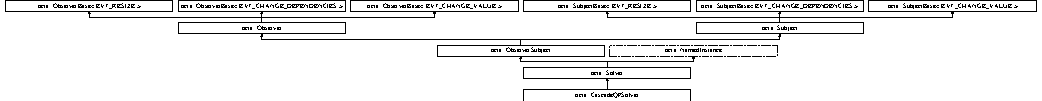
\includegraphics[height=1.352657cm]{d6/d35/classocra_1_1CascadeQPSolver}
\end{center}
\end{figure}
\subsection*{Classes}
\begin{DoxyCompactItemize}
\item 
struct \hyperlink{structocra_1_1CascadeQPSolver_1_1StandardObjectivesAndConstraints}{Standard\+Objectives\+And\+Constraints}
\end{DoxyCompactItemize}
\subsection*{Public Member Functions}
\begin{DoxyCompactItemize}
\item 
\hyperlink{classocra_1_1CascadeQPSolver_a85f1b7a863230a61f0bc3ce9ab93a908}{Cascade\+Q\+P\+Solver} (const std\+::string \&\+\_\+ctrl\+Name, Model\+::\+Ptr \+\_\+inner\+Model, One\+Level\+Solver\+::\+Ptr \+\_\+level\+Solver, bool \+\_\+use\+Reduced\+Problem)
\item 
void \hyperlink{classocra_1_1CascadeQPSolver_a42c413b6eeef99c2bdee577991f1e9a4}{add\+Task} (Task\+::\+Ptr task)
\item 
void \hyperlink{classocra_1_1CascadeQPSolver_af0c103a167f7c63adcfb28af29bae544}{add\+Solver} (One\+Level\+Solver\+::\+Ptr solver, int level)
\item 
One\+Level\+Solver\+::\+Ptr \hyperlink{classocra_1_1CascadeQPSolver_a7c0dff6ffa567d1bf6663bbc45fc22d4}{get\+Solver} (int level)
\item 
virtual std\+::string \hyperlink{classocra_1_1CascadeQPSolver_a411f14ee5770be6a3f04d665ac844e6c}{to\+String} ()
\item 
const std\+::map$<$ int, One\+Level\+Solver\+::\+Ptr $>$ \& \hyperlink{classocra_1_1CascadeQPSolver_a2f433d5b3029e998396c7d40fba6caa5}{get\+Solvers} ()
\item 
void \hyperlink{classocra_1_1CascadeQPSolver_afeca9e40c6424236d4527d4c1b97fe51}{update\+Hierarchical\+Contraints} (int level)
\item 
int \hyperlink{classocra_1_1CascadeQPSolver_aa943fac9f6ab708fc0d5d80977878d20}{get\+Number\+Of\+Levels\+Above} (int current\+\_\+level)
\end{DoxyCompactItemize}
\subsection*{Protected Member Functions}
\begin{DoxyCompactItemize}
\item 
virtual void \hyperlink{classocra_1_1CascadeQPSolver_aea57e3bc9dabe277161d742af5cd88dc}{do\+Solve} (void)
\item 
virtual void \hyperlink{classocra_1_1CascadeQPSolver_a2ccca21b47e23667be94cd215c890d5e}{do\+Prepare} (void)
\item 
virtual void \hyperlink{classocra_1_1CascadeQPSolver_af180fd8b7323b29246512af6109845d2}{do\+Conclude} ()
\item 
virtual void \hyperlink{classocra_1_1CascadeQPSolver_a1f4c5d709ce4545c596c864b1d99d08c}{print\+Values\+At\+Solution} ()
\item 
void \hyperlink{classocra_1_1CascadeQPSolver_a9308f8943177b4ea78e7f15a3ab55832}{exclude\+Objective} (int at\+\_\+level, const \hyperlink{namespaceocra_a37a91885f4fa5c523d22cb15d5673062}{ocra\+::\+Generic\+Objective} \&obj)
\end{DoxyCompactItemize}
\subsection*{Protected Attributes}
\begin{DoxyCompactItemize}
\item 
std\+::shared\+\_\+ptr$<$ \hyperlink{structocra_1_1CascadeQPSolver_1_1StandardObjectivesAndConstraints}{Standard\+Objectives\+And\+Constraints} $>$ \hyperlink{classocra_1_1CascadeQPSolver_aec6bf15caf1f29d7e1ec5aab696b1e7b}{own\+\_\+obj}
\item 
std\+::vector$<$ int $>$ \hyperlink{classocra_1_1CascadeQPSolver_a9d45b623d0012aae018b8eb8d4a66646}{solver\+Initialized}
\item 
std\+::map$<$ int, std\+::shared\+\_\+ptr$<$ \hyperlink{structocra_1_1CascadeQPSolver_1_1StandardObjectivesAndConstraints}{Standard\+Objectives\+And\+Constraints} $>$ $>$ \hyperlink{classocra_1_1CascadeQPSolver_aafe2d2d5226c421fc53880570a25a665}{std\+\_\+obj}
\item 
One\+Level\+Solver\+::\+Ptr \hyperlink{classocra_1_1CascadeQPSolver_a119ac44ca89426cddf6484577962726d}{level\+Solver}
\item 
bool \hyperlink{classocra_1_1CascadeQPSolver_a8703a516e8ce6adb088867d8b39dfa4d}{use\+Reduced\+Problem}
\item 
Model\+::\+Ptr \hyperlink{classocra_1_1CascadeQPSolver_a3a7c69b86a236e8b0ffc678be798109f}{inner\+Model}
\end{DoxyCompactItemize}
\subsection*{Additional Inherited Members}


\subsection{Detailed Description}
Cascade\+Q\+P\+Solver class. 

Hierarchical solver based on \hyperlink{classocra_1_1CascadeQP}{Cascade\+QP} 

Definition at line 57 of file Cascade\+Q\+P\+Solver.\+h.



\subsection{Constructor \& Destructor Documentation}
\hypertarget{classocra_1_1CascadeQPSolver_a85f1b7a863230a61f0bc3ce9ab93a908}{}\label{classocra_1_1CascadeQPSolver_a85f1b7a863230a61f0bc3ce9ab93a908} 
\index{ocra\+::\+Cascade\+Q\+P\+Solver@{ocra\+::\+Cascade\+Q\+P\+Solver}!Cascade\+Q\+P\+Solver@{Cascade\+Q\+P\+Solver}}
\index{Cascade\+Q\+P\+Solver@{Cascade\+Q\+P\+Solver}!ocra\+::\+Cascade\+Q\+P\+Solver@{ocra\+::\+Cascade\+Q\+P\+Solver}}
\subsubsection{\texorpdfstring{Cascade\+Q\+P\+Solver()}{CascadeQPSolver()}}
{\footnotesize\ttfamily ocra\+::\+Cascade\+Q\+P\+Solver\+::\+Cascade\+Q\+P\+Solver (\begin{DoxyParamCaption}\item[{const std\+::string \&}]{\+\_\+ctrl\+Name,  }\item[{Model\+::\+Ptr}]{\+\_\+inner\+Model,  }\item[{One\+Level\+Solver\+::\+Ptr}]{\+\_\+level\+Solver,  }\item[{bool}]{\+\_\+use\+Reduced\+Problem }\end{DoxyParamCaption})}



Definition at line 51 of file Cascade\+Q\+P\+Solver.\+cpp.



\subsection{Member Function Documentation}
\hypertarget{classocra_1_1CascadeQPSolver_af0c103a167f7c63adcfb28af29bae544}{}\label{classocra_1_1CascadeQPSolver_af0c103a167f7c63adcfb28af29bae544} 
\index{ocra\+::\+Cascade\+Q\+P\+Solver@{ocra\+::\+Cascade\+Q\+P\+Solver}!add\+Solver@{add\+Solver}}
\index{add\+Solver@{add\+Solver}!ocra\+::\+Cascade\+Q\+P\+Solver@{ocra\+::\+Cascade\+Q\+P\+Solver}}
\subsubsection{\texorpdfstring{add\+Solver()}{addSolver()}}
{\footnotesize\ttfamily void ocra\+::\+Cascade\+Q\+P\+Solver\+::add\+Solver (\begin{DoxyParamCaption}\item[{One\+Level\+Solver\+::\+Ptr}]{solver,  }\item[{int}]{level }\end{DoxyParamCaption})}



Definition at line 182 of file Cascade\+Q\+P\+Solver.\+cpp.

\hypertarget{classocra_1_1CascadeQPSolver_a42c413b6eeef99c2bdee577991f1e9a4}{}\label{classocra_1_1CascadeQPSolver_a42c413b6eeef99c2bdee577991f1e9a4} 
\index{ocra\+::\+Cascade\+Q\+P\+Solver@{ocra\+::\+Cascade\+Q\+P\+Solver}!add\+Task@{add\+Task}}
\index{add\+Task@{add\+Task}!ocra\+::\+Cascade\+Q\+P\+Solver@{ocra\+::\+Cascade\+Q\+P\+Solver}}
\subsubsection{\texorpdfstring{add\+Task()}{addTask()}}
{\footnotesize\ttfamily void ocra\+::\+Cascade\+Q\+P\+Solver\+::add\+Task (\begin{DoxyParamCaption}\item[{Task\+::\+Ptr}]{task }\end{DoxyParamCaption})}



Definition at line 232 of file Cascade\+Q\+P\+Solver.\+cpp.

\hypertarget{classocra_1_1CascadeQPSolver_af180fd8b7323b29246512af6109845d2}{}\label{classocra_1_1CascadeQPSolver_af180fd8b7323b29246512af6109845d2} 
\index{ocra\+::\+Cascade\+Q\+P\+Solver@{ocra\+::\+Cascade\+Q\+P\+Solver}!do\+Conclude@{do\+Conclude}}
\index{do\+Conclude@{do\+Conclude}!ocra\+::\+Cascade\+Q\+P\+Solver@{ocra\+::\+Cascade\+Q\+P\+Solver}}
\subsubsection{\texorpdfstring{do\+Conclude()}{doConclude()}}
{\footnotesize\ttfamily void ocra\+::\+Cascade\+Q\+P\+Solver\+::do\+Conclude (\begin{DoxyParamCaption}{ }\end{DoxyParamCaption})\hspace{0.3cm}{\ttfamily [protected]}, {\ttfamily [virtual]}}



Implements \hyperlink{classocra_1_1Solver_ac9d2d41d544b57a75e0d03db073d646e}{ocra\+::\+Solver}.



Definition at line 167 of file Cascade\+Q\+P\+Solver.\+cpp.

\hypertarget{classocra_1_1CascadeQPSolver_a2ccca21b47e23667be94cd215c890d5e}{}\label{classocra_1_1CascadeQPSolver_a2ccca21b47e23667be94cd215c890d5e} 
\index{ocra\+::\+Cascade\+Q\+P\+Solver@{ocra\+::\+Cascade\+Q\+P\+Solver}!do\+Prepare@{do\+Prepare}}
\index{do\+Prepare@{do\+Prepare}!ocra\+::\+Cascade\+Q\+P\+Solver@{ocra\+::\+Cascade\+Q\+P\+Solver}}
\subsubsection{\texorpdfstring{do\+Prepare()}{doPrepare()}}
{\footnotesize\ttfamily void ocra\+::\+Cascade\+Q\+P\+Solver\+::do\+Prepare (\begin{DoxyParamCaption}\item[{void}]{ }\end{DoxyParamCaption})\hspace{0.3cm}{\ttfamily [protected]}, {\ttfamily [virtual]}}



Implements \hyperlink{classocra_1_1Solver_a9ab90e87025e3da7239141c48d28ab4a}{ocra\+::\+Solver}.



Definition at line 161 of file Cascade\+Q\+P\+Solver.\+cpp.

\hypertarget{classocra_1_1CascadeQPSolver_aea57e3bc9dabe277161d742af5cd88dc}{}\label{classocra_1_1CascadeQPSolver_aea57e3bc9dabe277161d742af5cd88dc} 
\index{ocra\+::\+Cascade\+Q\+P\+Solver@{ocra\+::\+Cascade\+Q\+P\+Solver}!do\+Solve@{do\+Solve}}
\index{do\+Solve@{do\+Solve}!ocra\+::\+Cascade\+Q\+P\+Solver@{ocra\+::\+Cascade\+Q\+P\+Solver}}
\subsubsection{\texorpdfstring{do\+Solve()}{doSolve()}}
{\footnotesize\ttfamily void ocra\+::\+Cascade\+Q\+P\+Solver\+::do\+Solve (\begin{DoxyParamCaption}\item[{void}]{ }\end{DoxyParamCaption})\hspace{0.3cm}{\ttfamily [protected]}, {\ttfamily [virtual]}}



Implements \hyperlink{classocra_1_1Solver_ace2d7cfe741611de6dc87a0de7e7f3a9}{ocra\+::\+Solver}.



Definition at line 139 of file Cascade\+Q\+P\+Solver.\+cpp.

\hypertarget{classocra_1_1CascadeQPSolver_a9308f8943177b4ea78e7f15a3ab55832}{}\label{classocra_1_1CascadeQPSolver_a9308f8943177b4ea78e7f15a3ab55832} 
\index{ocra\+::\+Cascade\+Q\+P\+Solver@{ocra\+::\+Cascade\+Q\+P\+Solver}!exclude\+Objective@{exclude\+Objective}}
\index{exclude\+Objective@{exclude\+Objective}!ocra\+::\+Cascade\+Q\+P\+Solver@{ocra\+::\+Cascade\+Q\+P\+Solver}}
\subsubsection{\texorpdfstring{exclude\+Objective()}{excludeObjective()}}
{\footnotesize\ttfamily void ocra\+::\+Cascade\+Q\+P\+Solver\+::exclude\+Objective (\begin{DoxyParamCaption}\item[{int}]{at\+\_\+level,  }\item[{const \hyperlink{namespaceocra_a37a91885f4fa5c523d22cb15d5673062}{ocra\+::\+Generic\+Objective} \&}]{obj }\end{DoxyParamCaption})\hspace{0.3cm}{\ttfamily [protected]}}



Definition at line 218 of file Cascade\+Q\+P\+Solver.\+cpp.

\hypertarget{classocra_1_1CascadeQPSolver_aa943fac9f6ab708fc0d5d80977878d20}{}\label{classocra_1_1CascadeQPSolver_aa943fac9f6ab708fc0d5d80977878d20} 
\index{ocra\+::\+Cascade\+Q\+P\+Solver@{ocra\+::\+Cascade\+Q\+P\+Solver}!get\+Number\+Of\+Levels\+Above@{get\+Number\+Of\+Levels\+Above}}
\index{get\+Number\+Of\+Levels\+Above@{get\+Number\+Of\+Levels\+Above}!ocra\+::\+Cascade\+Q\+P\+Solver@{ocra\+::\+Cascade\+Q\+P\+Solver}}
\subsubsection{\texorpdfstring{get\+Number\+Of\+Levels\+Above()}{getNumberOfLevelsAbove()}}
{\footnotesize\ttfamily int ocra\+::\+Cascade\+Q\+P\+Solver\+::get\+Number\+Of\+Levels\+Above (\begin{DoxyParamCaption}\item[{int}]{current\+\_\+level }\end{DoxyParamCaption})}



Definition at line 128 of file Cascade\+Q\+P\+Solver.\+cpp.

\hypertarget{classocra_1_1CascadeQPSolver_a7c0dff6ffa567d1bf6663bbc45fc22d4}{}\label{classocra_1_1CascadeQPSolver_a7c0dff6ffa567d1bf6663bbc45fc22d4} 
\index{ocra\+::\+Cascade\+Q\+P\+Solver@{ocra\+::\+Cascade\+Q\+P\+Solver}!get\+Solver@{get\+Solver}}
\index{get\+Solver@{get\+Solver}!ocra\+::\+Cascade\+Q\+P\+Solver@{ocra\+::\+Cascade\+Q\+P\+Solver}}
\subsubsection{\texorpdfstring{get\+Solver()}{getSolver()}}
{\footnotesize\ttfamily One\+Level\+Solver\+::\+Ptr ocra\+::\+Cascade\+Q\+P\+Solver\+::get\+Solver (\begin{DoxyParamCaption}\item[{int}]{level }\end{DoxyParamCaption})}



Definition at line 214 of file Cascade\+Q\+P\+Solver.\+cpp.

\hypertarget{classocra_1_1CascadeQPSolver_a2f433d5b3029e998396c7d40fba6caa5}{}\label{classocra_1_1CascadeQPSolver_a2f433d5b3029e998396c7d40fba6caa5} 
\index{ocra\+::\+Cascade\+Q\+P\+Solver@{ocra\+::\+Cascade\+Q\+P\+Solver}!get\+Solvers@{get\+Solvers}}
\index{get\+Solvers@{get\+Solvers}!ocra\+::\+Cascade\+Q\+P\+Solver@{ocra\+::\+Cascade\+Q\+P\+Solver}}
\subsubsection{\texorpdfstring{get\+Solvers()}{getSolvers()}}
{\footnotesize\ttfamily const std\+::map$<$ int, One\+Level\+Solver\+::\+Ptr $>$ \& ocra\+::\+Cascade\+Q\+P\+Solver\+::get\+Solvers (\begin{DoxyParamCaption}{ }\end{DoxyParamCaption})}



Definition at line 177 of file Cascade\+Q\+P\+Solver.\+cpp.

\hypertarget{classocra_1_1CascadeQPSolver_a1f4c5d709ce4545c596c864b1d99d08c}{}\label{classocra_1_1CascadeQPSolver_a1f4c5d709ce4545c596c864b1d99d08c} 
\index{ocra\+::\+Cascade\+Q\+P\+Solver@{ocra\+::\+Cascade\+Q\+P\+Solver}!print\+Values\+At\+Solution@{print\+Values\+At\+Solution}}
\index{print\+Values\+At\+Solution@{print\+Values\+At\+Solution}!ocra\+::\+Cascade\+Q\+P\+Solver@{ocra\+::\+Cascade\+Q\+P\+Solver}}
\subsubsection{\texorpdfstring{print\+Values\+At\+Solution()}{printValuesAtSolution()}}
{\footnotesize\ttfamily void ocra\+::\+Cascade\+Q\+P\+Solver\+::print\+Values\+At\+Solution (\begin{DoxyParamCaption}\item[{void}]{ }\end{DoxyParamCaption})\hspace{0.3cm}{\ttfamily [protected]}, {\ttfamily [virtual]}}



Implements \hyperlink{classocra_1_1Solver_ab1903098e25c16a9f92c36d37967e8fa}{ocra\+::\+Solver}.



Definition at line 270 of file Cascade\+Q\+P\+Solver.\+cpp.

\hypertarget{classocra_1_1CascadeQPSolver_a411f14ee5770be6a3f04d665ac844e6c}{}\label{classocra_1_1CascadeQPSolver_a411f14ee5770be6a3f04d665ac844e6c} 
\index{ocra\+::\+Cascade\+Q\+P\+Solver@{ocra\+::\+Cascade\+Q\+P\+Solver}!to\+String@{to\+String}}
\index{to\+String@{to\+String}!ocra\+::\+Cascade\+Q\+P\+Solver@{ocra\+::\+Cascade\+Q\+P\+Solver}}
\subsubsection{\texorpdfstring{to\+String()}{toString()}}
{\footnotesize\ttfamily std\+::string ocra\+::\+Cascade\+Q\+P\+Solver\+::to\+String (\begin{DoxyParamCaption}{ }\end{DoxyParamCaption})\hspace{0.3cm}{\ttfamily [virtual]}}

Returns the state of the solver (e.\+g. matrices) as a string. 

Implements \hyperlink{classocra_1_1Solver_ab3783d1c208500bfb1daa3e1abf34146}{ocra\+::\+Solver}.



Definition at line 173 of file Cascade\+Q\+P\+Solver.\+cpp.

\hypertarget{classocra_1_1CascadeQPSolver_afeca9e40c6424236d4527d4c1b97fe51}{}\label{classocra_1_1CascadeQPSolver_afeca9e40c6424236d4527d4c1b97fe51} 
\index{ocra\+::\+Cascade\+Q\+P\+Solver@{ocra\+::\+Cascade\+Q\+P\+Solver}!update\+Hierarchical\+Contraints@{update\+Hierarchical\+Contraints}}
\index{update\+Hierarchical\+Contraints@{update\+Hierarchical\+Contraints}!ocra\+::\+Cascade\+Q\+P\+Solver@{ocra\+::\+Cascade\+Q\+P\+Solver}}
\subsubsection{\texorpdfstring{update\+Hierarchical\+Contraints()}{updateHierarchicalContraints()}}
{\footnotesize\ttfamily void ocra\+::\+Cascade\+Q\+P\+Solver\+::update\+Hierarchical\+Contraints (\begin{DoxyParamCaption}\item[{int}]{level }\end{DoxyParamCaption})}



Definition at line 71 of file Cascade\+Q\+P\+Solver.\+cpp.



\subsection{Member Data Documentation}
\hypertarget{classocra_1_1CascadeQPSolver_a3a7c69b86a236e8b0ffc678be798109f}{}\label{classocra_1_1CascadeQPSolver_a3a7c69b86a236e8b0ffc678be798109f} 
\index{ocra\+::\+Cascade\+Q\+P\+Solver@{ocra\+::\+Cascade\+Q\+P\+Solver}!inner\+Model@{inner\+Model}}
\index{inner\+Model@{inner\+Model}!ocra\+::\+Cascade\+Q\+P\+Solver@{ocra\+::\+Cascade\+Q\+P\+Solver}}
\subsubsection{\texorpdfstring{inner\+Model}{innerModel}}
{\footnotesize\ttfamily Model\+::\+Ptr ocra\+::\+Cascade\+Q\+P\+Solver\+::inner\+Model\hspace{0.3cm}{\ttfamily [protected]}}



Definition at line 91 of file Cascade\+Q\+P\+Solver.\+h.

\hypertarget{classocra_1_1CascadeQPSolver_a119ac44ca89426cddf6484577962726d}{}\label{classocra_1_1CascadeQPSolver_a119ac44ca89426cddf6484577962726d} 
\index{ocra\+::\+Cascade\+Q\+P\+Solver@{ocra\+::\+Cascade\+Q\+P\+Solver}!level\+Solver@{level\+Solver}}
\index{level\+Solver@{level\+Solver}!ocra\+::\+Cascade\+Q\+P\+Solver@{ocra\+::\+Cascade\+Q\+P\+Solver}}
\subsubsection{\texorpdfstring{level\+Solver}{levelSolver}}
{\footnotesize\ttfamily One\+Level\+Solver\+::\+Ptr ocra\+::\+Cascade\+Q\+P\+Solver\+::level\+Solver\hspace{0.3cm}{\ttfamily [protected]}}



Definition at line 89 of file Cascade\+Q\+P\+Solver.\+h.

\hypertarget{classocra_1_1CascadeQPSolver_aec6bf15caf1f29d7e1ec5aab696b1e7b}{}\label{classocra_1_1CascadeQPSolver_aec6bf15caf1f29d7e1ec5aab696b1e7b} 
\index{ocra\+::\+Cascade\+Q\+P\+Solver@{ocra\+::\+Cascade\+Q\+P\+Solver}!own\+\_\+obj@{own\+\_\+obj}}
\index{own\+\_\+obj@{own\+\_\+obj}!ocra\+::\+Cascade\+Q\+P\+Solver@{ocra\+::\+Cascade\+Q\+P\+Solver}}
\subsubsection{\texorpdfstring{own\+\_\+obj}{own\_obj}}
{\footnotesize\ttfamily std\+::shared\+\_\+ptr$<$\hyperlink{structocra_1_1CascadeQPSolver_1_1StandardObjectivesAndConstraints}{Standard\+Objectives\+And\+Constraints}$>$ ocra\+::\+Cascade\+Q\+P\+Solver\+::own\+\_\+obj\hspace{0.3cm}{\ttfamily [protected]}}



Definition at line 85 of file Cascade\+Q\+P\+Solver.\+h.

\hypertarget{classocra_1_1CascadeQPSolver_a9d45b623d0012aae018b8eb8d4a66646}{}\label{classocra_1_1CascadeQPSolver_a9d45b623d0012aae018b8eb8d4a66646} 
\index{ocra\+::\+Cascade\+Q\+P\+Solver@{ocra\+::\+Cascade\+Q\+P\+Solver}!solver\+Initialized@{solver\+Initialized}}
\index{solver\+Initialized@{solver\+Initialized}!ocra\+::\+Cascade\+Q\+P\+Solver@{ocra\+::\+Cascade\+Q\+P\+Solver}}
\subsubsection{\texorpdfstring{solver\+Initialized}{solverInitialized}}
{\footnotesize\ttfamily std\+::vector$<$int$>$ ocra\+::\+Cascade\+Q\+P\+Solver\+::solver\+Initialized\hspace{0.3cm}{\ttfamily [protected]}}



Definition at line 87 of file Cascade\+Q\+P\+Solver.\+h.

\hypertarget{classocra_1_1CascadeQPSolver_aafe2d2d5226c421fc53880570a25a665}{}\label{classocra_1_1CascadeQPSolver_aafe2d2d5226c421fc53880570a25a665} 
\index{ocra\+::\+Cascade\+Q\+P\+Solver@{ocra\+::\+Cascade\+Q\+P\+Solver}!std\+\_\+obj@{std\+\_\+obj}}
\index{std\+\_\+obj@{std\+\_\+obj}!ocra\+::\+Cascade\+Q\+P\+Solver@{ocra\+::\+Cascade\+Q\+P\+Solver}}
\subsubsection{\texorpdfstring{std\+\_\+obj}{std\_obj}}
{\footnotesize\ttfamily std\+::map$<$int,std\+::shared\+\_\+ptr$<$\hyperlink{structocra_1_1CascadeQPSolver_1_1StandardObjectivesAndConstraints}{Standard\+Objectives\+And\+Constraints}$>$ $>$ ocra\+::\+Cascade\+Q\+P\+Solver\+::std\+\_\+obj\hspace{0.3cm}{\ttfamily [protected]}}



Definition at line 88 of file Cascade\+Q\+P\+Solver.\+h.

\hypertarget{classocra_1_1CascadeQPSolver_a8703a516e8ce6adb088867d8b39dfa4d}{}\label{classocra_1_1CascadeQPSolver_a8703a516e8ce6adb088867d8b39dfa4d} 
\index{ocra\+::\+Cascade\+Q\+P\+Solver@{ocra\+::\+Cascade\+Q\+P\+Solver}!use\+Reduced\+Problem@{use\+Reduced\+Problem}}
\index{use\+Reduced\+Problem@{use\+Reduced\+Problem}!ocra\+::\+Cascade\+Q\+P\+Solver@{ocra\+::\+Cascade\+Q\+P\+Solver}}
\subsubsection{\texorpdfstring{use\+Reduced\+Problem}{useReducedProblem}}
{\footnotesize\ttfamily bool ocra\+::\+Cascade\+Q\+P\+Solver\+::use\+Reduced\+Problem\hspace{0.3cm}{\ttfamily [protected]}}



Definition at line 90 of file Cascade\+Q\+P\+Solver.\+h.



The documentation for this class was generated from the following files\+:\begin{DoxyCompactItemize}
\item 
\hyperlink{CascadeQPSolver_8h}{Cascade\+Q\+P\+Solver.\+h}\item 
\hyperlink{CascadeQPSolver_8cpp}{Cascade\+Q\+P\+Solver.\+cpp}\end{DoxyCompactItemize}

\hypertarget{structocra_1_1Parenthood_1_1childIs}{}\section{ocra\+:\+:Parenthood$<$ Component\+Derived, Composite\+Derived, Parenthood\+Info $>$\+:\+:child\+Is Struct Reference}
\label{structocra_1_1Parenthood_1_1childIs}\index{ocra\+::\+Parenthood$<$ Component\+Derived, Composite\+Derived, Parenthood\+Info $>$\+::child\+Is@{ocra\+::\+Parenthood$<$ Component\+Derived, Composite\+Derived, Parenthood\+Info $>$\+::child\+Is}}


{\ttfamily \#include $<$Composite.\+h$>$}

\subsection*{Public Member Functions}
\begin{DoxyCompactItemize}
\item 
bool \hyperlink{structocra_1_1Parenthood_1_1childIs_acc2f7b0a548c4420f5d7349c013417ba}{operator()} (const \hyperlink{classocra_1_1Parenthood_acdae20cb747190b5dc9dbe42290bde78}{parenthood\+\_\+t} $\ast$p) const
\item 
\hyperlink{structocra_1_1Parenthood_1_1childIs_a19d608fdf341bf6e8c98578a5d2e5221}{child\+Is} (const \hyperlink{classocra_1_1Parenthood_a44b601577125fe0fd1d1e5ae4f143349}{component\+\_\+t} $\ast$child)
\end{DoxyCompactItemize}
\subsection*{Public Attributes}
\begin{DoxyCompactItemize}
\item 
const \hyperlink{classocra_1_1Parenthood_a44b601577125fe0fd1d1e5ae4f143349}{component\+\_\+t} $\ast$ \hyperlink{structocra_1_1Parenthood_1_1childIs_a6e3329ea395bbb40d41caceecb1587b7}{child\+\_\+}
\end{DoxyCompactItemize}


\subsection{Detailed Description}
\subsubsection*{template$<$class Component\+Derived, class Composite\+Derived, class Parenthood\+Info = No\+Info$>$\newline
struct ocra\+::\+Parenthood$<$ Component\+Derived, Composite\+Derived, Parenthood\+Info $>$\+::child\+Is}



Definition at line 307 of file Composite.\+h.



\subsection{Constructor \& Destructor Documentation}
\hypertarget{structocra_1_1Parenthood_1_1childIs_a19d608fdf341bf6e8c98578a5d2e5221}{}\label{structocra_1_1Parenthood_1_1childIs_a19d608fdf341bf6e8c98578a5d2e5221} 
\index{ocra\+::\+Parenthood\+::child\+Is@{ocra\+::\+Parenthood\+::child\+Is}!child\+Is@{child\+Is}}
\index{child\+Is@{child\+Is}!ocra\+::\+Parenthood\+::child\+Is@{ocra\+::\+Parenthood\+::child\+Is}}
\subsubsection{\texorpdfstring{child\+Is()}{childIs()}}
{\footnotesize\ttfamily template$<$class Component\+Derived , class Composite\+Derived , class Parenthood\+Info  = No\+Info$>$ \\
\hyperlink{classocra_1_1Parenthood}{ocra\+::\+Parenthood}$<$ Component\+Derived, Composite\+Derived, Parenthood\+Info $>$\+::child\+Is\+::child\+Is (\begin{DoxyParamCaption}\item[{const \hyperlink{classocra_1_1Parenthood_a44b601577125fe0fd1d1e5ae4f143349}{component\+\_\+t} $\ast$}]{child }\end{DoxyParamCaption})\hspace{0.3cm}{\ttfamily [inline]}}



Definition at line 310 of file Composite.\+h.



\subsection{Member Function Documentation}
\hypertarget{structocra_1_1Parenthood_1_1childIs_acc2f7b0a548c4420f5d7349c013417ba}{}\label{structocra_1_1Parenthood_1_1childIs_acc2f7b0a548c4420f5d7349c013417ba} 
\index{ocra\+::\+Parenthood\+::child\+Is@{ocra\+::\+Parenthood\+::child\+Is}!operator()@{operator()}}
\index{operator()@{operator()}!ocra\+::\+Parenthood\+::child\+Is@{ocra\+::\+Parenthood\+::child\+Is}}
\subsubsection{\texorpdfstring{operator()()}{operator()()}}
{\footnotesize\ttfamily template$<$class Component\+Derived , class Composite\+Derived , class Parenthood\+Info  = No\+Info$>$ \\
bool \hyperlink{classocra_1_1Parenthood}{ocra\+::\+Parenthood}$<$ Component\+Derived, Composite\+Derived, Parenthood\+Info $>$\+::child\+Is\+::operator() (\begin{DoxyParamCaption}\item[{const \hyperlink{classocra_1_1Parenthood_acdae20cb747190b5dc9dbe42290bde78}{parenthood\+\_\+t} $\ast$}]{p }\end{DoxyParamCaption}) const\hspace{0.3cm}{\ttfamily [inline]}}



Definition at line 309 of file Composite.\+h.



\subsection{Member Data Documentation}
\hypertarget{structocra_1_1Parenthood_1_1childIs_a6e3329ea395bbb40d41caceecb1587b7}{}\label{structocra_1_1Parenthood_1_1childIs_a6e3329ea395bbb40d41caceecb1587b7} 
\index{ocra\+::\+Parenthood\+::child\+Is@{ocra\+::\+Parenthood\+::child\+Is}!child\+\_\+@{child\+\_\+}}
\index{child\+\_\+@{child\+\_\+}!ocra\+::\+Parenthood\+::child\+Is@{ocra\+::\+Parenthood\+::child\+Is}}
\subsubsection{\texorpdfstring{child\+\_\+}{child\_}}
{\footnotesize\ttfamily template$<$class Component\+Derived , class Composite\+Derived , class Parenthood\+Info  = No\+Info$>$ \\
const \hyperlink{classocra_1_1Parenthood_a44b601577125fe0fd1d1e5ae4f143349}{component\+\_\+t}$\ast$ \hyperlink{classocra_1_1Parenthood}{ocra\+::\+Parenthood}$<$ Component\+Derived, Composite\+Derived, Parenthood\+Info $>$\+::child\+Is\+::child\+\_\+}



Definition at line 311 of file Composite.\+h.



The documentation for this struct was generated from the following file\+:\begin{DoxyCompactItemize}
\item 
\hyperlink{Composite_8h}{Composite.\+h}\end{DoxyCompactItemize}

\hypertarget{classocra__recipes_1_1ClientCommunications}{}\section{ocra\+\_\+recipes\+:\+:Client\+Communications Class Reference}
\label{classocra__recipes_1_1ClientCommunications}\index{ocra\+\_\+recipes\+::\+Client\+Communications@{ocra\+\_\+recipes\+::\+Client\+Communications}}


{\ttfamily \#include $<$Client\+Communications.\+h$>$}



Inheritance diagram for ocra\+\_\+recipes\+:\+:Client\+Communications\+:\nopagebreak
\begin{figure}[H]
\begin{center}
\leavevmode
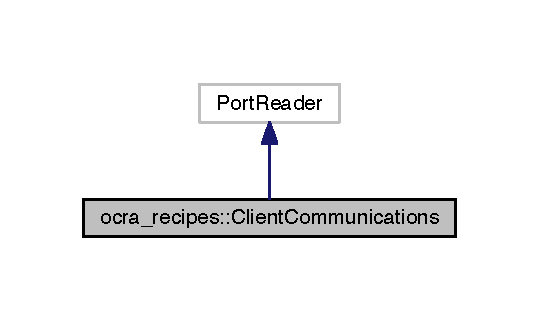
\includegraphics[width=259pt]{d5/d62/classocra__recipes_1_1ClientCommunications__inherit__graph}
\end{center}
\end{figure}


Collaboration diagram for ocra\+\_\+recipes\+:\+:Client\+Communications\+:\nopagebreak
\begin{figure}[H]
\begin{center}
\leavevmode
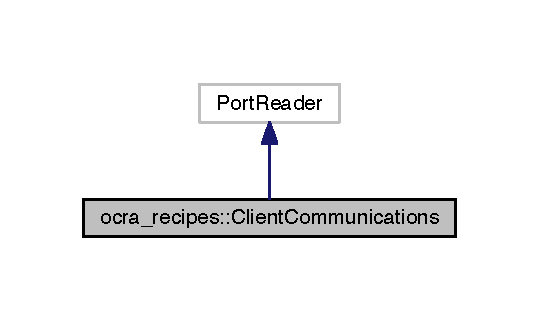
\includegraphics[width=259pt]{d9/dd7/classocra__recipes_1_1ClientCommunications__coll__graph}
\end{center}
\end{figure}
\subsection*{Classes}
\begin{DoxyCompactItemize}
\item 
class \hyperlink{classocra__recipes_1_1ClientCommunications_1_1InputCallback}{Input\+Callback}
\end{DoxyCompactItemize}
\subsection*{Public Member Functions}
\begin{DoxyCompactItemize}
\item 
\hyperlink{classocra__recipes_1_1ClientCommunications_a459f2b8ffc37223b303ac0596cccdfd4}{Client\+Communications} ()
\item 
virtual \hyperlink{classocra__recipes_1_1ClientCommunications_a20df5cf496f895e9235ad38730962360}{$\sim$\+Client\+Communications} ()
\item 
bool \hyperlink{classocra__recipes_1_1ClientCommunications_a5ef6606831f855ae97815f4a34e1e1a1}{open} (double timeout=20.\+0, bool connect\+To\+Tasks=true)
\item 
bool \hyperlink{classocra__recipes_1_1ClientCommunications_a1ac6b0ebabc5fabdb2bf006ddc48c606}{close} ()
\item 
void \hyperlink{classocra__recipes_1_1ClientCommunications_ac96c7e76603600459e94b8fa1a0b213e}{close} (const std\+::string \&task\+Name)
\item 
virtual bool \hyperlink{classocra__recipes_1_1ClientCommunications_afbca8bd430e14a0b9a8254a29b78d202}{read} (yarp\+::os\+::\+Connection\+Reader \&connection)
\item 
void \hyperlink{classocra__recipes_1_1ClientCommunications_a452774799b5d8448a8ffd3ab5d24aa22}{parse\+Message} (yarp\+::os\+::\+Bottle \&input)
\item 
std\+::vector$<$ std\+::string $>$ \hyperlink{classocra__recipes_1_1ClientCommunications_a0a7b2eeaa35d925e63ba4568be1e4919}{get\+Task\+Types} ()
\item 
yarp\+::os\+::\+Bottle \hyperlink{classocra__recipes_1_1ClientCommunications_a555bf79c855b3c08402a5ba4d6f9410c}{query\+Controller} (yarp\+::os\+::\+Bottle \&request\+Bottle)
\item 
yarp\+::os\+::\+Bottle \hyperlink{classocra__recipes_1_1ClientCommunications_acd90f49ce7b275b83a73a75b9b355109}{query\+Controller} (const \hyperlink{namespaceocra__recipes_ae6246916f1927f7a201cc153ad76b07d}{S\+E\+R\+V\+E\+R\+\_\+\+C\+O\+M\+M\+U\+N\+I\+C\+A\+T\+I\+O\+N\+S\+\_\+\+M\+E\+S\+S\+A\+GE} request)
\item 
yarp\+::os\+::\+Bottle \hyperlink{classocra__recipes_1_1ClientCommunications_a12e293ab0cd846cf44f20a1fc61f82dc}{query\+Controller} (const std\+::vector$<$ \hyperlink{namespaceocra__recipes_ae6246916f1927f7a201cc153ad76b07d}{S\+E\+R\+V\+E\+R\+\_\+\+C\+O\+M\+M\+U\+N\+I\+C\+A\+T\+I\+O\+N\+S\+\_\+\+M\+E\+S\+S\+A\+GE} $>$ request\+Vector)
\item 
std\+::vector$<$ std\+::string $>$ \hyperlink{classocra__recipes_1_1ClientCommunications_abff3747f063489056f41c99edb7e1e3b}{get\+Task\+Port\+Names} ()
\item 
std\+::string \hyperlink{classocra__recipes_1_1ClientCommunications_ab915047503c4cbddbd26c2036f8340ed}{get\+Task\+Port\+Name} (const std\+::string \&task\+Name)
\item 
std\+::vector$<$ std\+::string $>$ \hyperlink{classocra__recipes_1_1ClientCommunications_a821a74e8c4b20e1d3da18e1cf6b7e31d}{get\+Task\+Names} ()
\item 
std\+::shared\+\_\+ptr$<$ yarp\+::os\+::\+Rpc\+Client $>$ \hyperlink{classocra__recipes_1_1ClientCommunications_ad94eda2ba62336ea95b83622d0837543}{get\+Task\+Client} (const std\+::string \&task\+Name)
\item 
std\+::string \hyperlink{classocra__recipes_1_1ClientCommunications_aa6a6158593016b02b28122903022b0e6}{get\+Client\+Port\+Name} ()
\item 
bool \hyperlink{classocra__recipes_1_1ClientCommunications_ae1d3d48e76010741a8d6f3622191156c}{parse\+Input} (yarp\+::os\+::\+Bottle \&input)
\end{DoxyCompactItemize}


\subsection{Detailed Description}


Definition at line 30 of file Client\+Communications.\+h.



\subsection{Constructor \& Destructor Documentation}
\hypertarget{classocra__recipes_1_1ClientCommunications_a459f2b8ffc37223b303ac0596cccdfd4}{}\label{classocra__recipes_1_1ClientCommunications_a459f2b8ffc37223b303ac0596cccdfd4} 
\index{ocra\+\_\+recipes\+::\+Client\+Communications@{ocra\+\_\+recipes\+::\+Client\+Communications}!Client\+Communications@{Client\+Communications}}
\index{Client\+Communications@{Client\+Communications}!ocra\+\_\+recipes\+::\+Client\+Communications@{ocra\+\_\+recipes\+::\+Client\+Communications}}
\subsubsection{\texorpdfstring{Client\+Communications()}{ClientCommunications()}}
{\footnotesize\ttfamily Client\+Communications\+::\+Client\+Communications (\begin{DoxyParamCaption}{ }\end{DoxyParamCaption})}



Definition at line 9 of file Client\+Communications.\+cpp.

\hypertarget{classocra__recipes_1_1ClientCommunications_a20df5cf496f895e9235ad38730962360}{}\label{classocra__recipes_1_1ClientCommunications_a20df5cf496f895e9235ad38730962360} 
\index{ocra\+\_\+recipes\+::\+Client\+Communications@{ocra\+\_\+recipes\+::\+Client\+Communications}!````~Client\+Communications@{$\sim$\+Client\+Communications}}
\index{````~Client\+Communications@{$\sim$\+Client\+Communications}!ocra\+\_\+recipes\+::\+Client\+Communications@{ocra\+\_\+recipes\+::\+Client\+Communications}}
\subsubsection{\texorpdfstring{$\sim$\+Client\+Communications()}{~ClientCommunications()}}
{\footnotesize\ttfamily Client\+Communications\+::$\sim$\+Client\+Communications (\begin{DoxyParamCaption}{ }\end{DoxyParamCaption})\hspace{0.3cm}{\ttfamily [virtual]}}



Definition at line 23 of file Client\+Communications.\+cpp.



\subsection{Member Function Documentation}
\hypertarget{classocra__recipes_1_1ClientCommunications_a1ac6b0ebabc5fabdb2bf006ddc48c606}{}\label{classocra__recipes_1_1ClientCommunications_a1ac6b0ebabc5fabdb2bf006ddc48c606} 
\index{ocra\+\_\+recipes\+::\+Client\+Communications@{ocra\+\_\+recipes\+::\+Client\+Communications}!close@{close}}
\index{close@{close}!ocra\+\_\+recipes\+::\+Client\+Communications@{ocra\+\_\+recipes\+::\+Client\+Communications}}
\subsubsection{\texorpdfstring{close()}{close()}\hspace{0.1cm}{\footnotesize\ttfamily [1/2]}}
{\footnotesize\ttfamily bool Client\+Communications\+::close (\begin{DoxyParamCaption}{ }\end{DoxyParamCaption})}

Closes the R\+PC and input ports opened by this client.

\begin{DoxyReturn}{Returns}
True after all ports are closed. 
\end{DoxyReturn}


Definition at line 69 of file Client\+Communications.\+cpp.

\hypertarget{classocra__recipes_1_1ClientCommunications_ac96c7e76603600459e94b8fa1a0b213e}{}\label{classocra__recipes_1_1ClientCommunications_ac96c7e76603600459e94b8fa1a0b213e} 
\index{ocra\+\_\+recipes\+::\+Client\+Communications@{ocra\+\_\+recipes\+::\+Client\+Communications}!close@{close}}
\index{close@{close}!ocra\+\_\+recipes\+::\+Client\+Communications@{ocra\+\_\+recipes\+::\+Client\+Communications}}
\subsubsection{\texorpdfstring{close()}{close()}\hspace{0.1cm}{\footnotesize\ttfamily [2/2]}}
{\footnotesize\ttfamily void Client\+Communications\+::close (\begin{DoxyParamCaption}\item[{const std\+::string \&}]{task\+Name }\end{DoxyParamCaption})}

Closes the task-\/specific R\+PC ports and deletes this task from the list of current clients.


\begin{DoxyParams}{Parameters}
{\em task\+Name} & Name of the task. \\
\hline
\end{DoxyParams}


Definition at line 82 of file Client\+Communications.\+cpp.

\hypertarget{classocra__recipes_1_1ClientCommunications_aa6a6158593016b02b28122903022b0e6}{}\label{classocra__recipes_1_1ClientCommunications_aa6a6158593016b02b28122903022b0e6} 
\index{ocra\+\_\+recipes\+::\+Client\+Communications@{ocra\+\_\+recipes\+::\+Client\+Communications}!get\+Client\+Port\+Name@{get\+Client\+Port\+Name}}
\index{get\+Client\+Port\+Name@{get\+Client\+Port\+Name}!ocra\+\_\+recipes\+::\+Client\+Communications@{ocra\+\_\+recipes\+::\+Client\+Communications}}
\subsubsection{\texorpdfstring{get\+Client\+Port\+Name()}{getClientPortName()}}
{\footnotesize\ttfamily std\+::string ocra\+\_\+recipes\+::\+Client\+Communications\+::get\+Client\+Port\+Name (\begin{DoxyParamCaption}{ }\end{DoxyParamCaption})\hspace{0.3cm}{\ttfamily [inline]}}



Definition at line 127 of file Client\+Communications.\+h.

\hypertarget{classocra__recipes_1_1ClientCommunications_ad94eda2ba62336ea95b83622d0837543}{}\label{classocra__recipes_1_1ClientCommunications_ad94eda2ba62336ea95b83622d0837543} 
\index{ocra\+\_\+recipes\+::\+Client\+Communications@{ocra\+\_\+recipes\+::\+Client\+Communications}!get\+Task\+Client@{get\+Task\+Client}}
\index{get\+Task\+Client@{get\+Task\+Client}!ocra\+\_\+recipes\+::\+Client\+Communications@{ocra\+\_\+recipes\+::\+Client\+Communications}}
\subsubsection{\texorpdfstring{get\+Task\+Client()}{getTaskClient()}}
{\footnotesize\ttfamily std\+::shared\+\_\+ptr$<$ yarp\+::os\+::\+Rpc\+Client $>$ Client\+Communications\+::get\+Task\+Client (\begin{DoxyParamCaption}\item[{const std\+::string \&}]{task\+Name }\end{DoxyParamCaption})}



Definition at line 178 of file Client\+Communications.\+cpp.

\hypertarget{classocra__recipes_1_1ClientCommunications_a821a74e8c4b20e1d3da18e1cf6b7e31d}{}\label{classocra__recipes_1_1ClientCommunications_a821a74e8c4b20e1d3da18e1cf6b7e31d} 
\index{ocra\+\_\+recipes\+::\+Client\+Communications@{ocra\+\_\+recipes\+::\+Client\+Communications}!get\+Task\+Names@{get\+Task\+Names}}
\index{get\+Task\+Names@{get\+Task\+Names}!ocra\+\_\+recipes\+::\+Client\+Communications@{ocra\+\_\+recipes\+::\+Client\+Communications}}
\subsubsection{\texorpdfstring{get\+Task\+Names()}{getTaskNames()}}
{\footnotesize\ttfamily std\+::vector$<$ std\+::string $>$ Client\+Communications\+::get\+Task\+Names (\begin{DoxyParamCaption}{ }\end{DoxyParamCaption})}



Definition at line 165 of file Client\+Communications.\+cpp.

\hypertarget{classocra__recipes_1_1ClientCommunications_ab915047503c4cbddbd26c2036f8340ed}{}\label{classocra__recipes_1_1ClientCommunications_ab915047503c4cbddbd26c2036f8340ed} 
\index{ocra\+\_\+recipes\+::\+Client\+Communications@{ocra\+\_\+recipes\+::\+Client\+Communications}!get\+Task\+Port\+Name@{get\+Task\+Port\+Name}}
\index{get\+Task\+Port\+Name@{get\+Task\+Port\+Name}!ocra\+\_\+recipes\+::\+Client\+Communications@{ocra\+\_\+recipes\+::\+Client\+Communications}}
\subsubsection{\texorpdfstring{get\+Task\+Port\+Name()}{getTaskPortName()}}
{\footnotesize\ttfamily std\+::string Client\+Communications\+::get\+Task\+Port\+Name (\begin{DoxyParamCaption}\item[{const std\+::string \&}]{task\+Name }\end{DoxyParamCaption})}



Definition at line 151 of file Client\+Communications.\+cpp.

\hypertarget{classocra__recipes_1_1ClientCommunications_abff3747f063489056f41c99edb7e1e3b}{}\label{classocra__recipes_1_1ClientCommunications_abff3747f063489056f41c99edb7e1e3b} 
\index{ocra\+\_\+recipes\+::\+Client\+Communications@{ocra\+\_\+recipes\+::\+Client\+Communications}!get\+Task\+Port\+Names@{get\+Task\+Port\+Names}}
\index{get\+Task\+Port\+Names@{get\+Task\+Port\+Names}!ocra\+\_\+recipes\+::\+Client\+Communications@{ocra\+\_\+recipes\+::\+Client\+Communications}}
\subsubsection{\texorpdfstring{get\+Task\+Port\+Names()}{getTaskPortNames()}}
{\footnotesize\ttfamily std\+::vector$<$ std\+::string $>$ Client\+Communications\+::get\+Task\+Port\+Names (\begin{DoxyParamCaption}{ }\end{DoxyParamCaption})}



Definition at line 138 of file Client\+Communications.\+cpp.

\hypertarget{classocra__recipes_1_1ClientCommunications_a0a7b2eeaa35d925e63ba4568be1e4919}{}\label{classocra__recipes_1_1ClientCommunications_a0a7b2eeaa35d925e63ba4568be1e4919} 
\index{ocra\+\_\+recipes\+::\+Client\+Communications@{ocra\+\_\+recipes\+::\+Client\+Communications}!get\+Task\+Types@{get\+Task\+Types}}
\index{get\+Task\+Types@{get\+Task\+Types}!ocra\+\_\+recipes\+::\+Client\+Communications@{ocra\+\_\+recipes\+::\+Client\+Communications}}
\subsubsection{\texorpdfstring{get\+Task\+Types()}{getTaskTypes()}}
{\footnotesize\ttfamily std\+::vector$<$ std\+::string $>$ Client\+Communications\+::get\+Task\+Types (\begin{DoxyParamCaption}{ }\end{DoxyParamCaption})}

Queries the server for the task types as strings.

\begin{DoxyReturn}{Returns}
A vector of strings containint the task types sent by the server. 
\end{DoxyReturn}


Definition at line 56 of file Client\+Communications.\+cpp.

\hypertarget{classocra__recipes_1_1ClientCommunications_a5ef6606831f855ae97815f4a34e1e1a1}{}\label{classocra__recipes_1_1ClientCommunications_a5ef6606831f855ae97815f4a34e1e1a1} 
\index{ocra\+\_\+recipes\+::\+Client\+Communications@{ocra\+\_\+recipes\+::\+Client\+Communications}!open@{open}}
\index{open@{open}!ocra\+\_\+recipes\+::\+Client\+Communications@{ocra\+\_\+recipes\+::\+Client\+Communications}}
\subsubsection{\texorpdfstring{open()}{open()}}
{\footnotesize\ttfamily bool Client\+Communications\+::open (\begin{DoxyParamCaption}\item[{double}]{timeout = {\ttfamily 20.0},  }\item[{bool}]{connect\+To\+Tasks = {\ttfamily true} }\end{DoxyParamCaption})}

Opens an R\+PC port for the client with the format /\+Controller\+Client/$<$client-\/number$>$/rpc\+:o and an input one with the format /\+Controller\+Client/$<$client-\/number$>$/\+:i 
\begin{DoxyParams}[1]{Parameters}
\mbox{\tt in}  & {\em connect\+To\+Tasks} & True to automatically connect to task R\+PC ports. True by default. \\
\hline
\end{DoxyParams}
\begin{DoxyReturn}{Returns}
True when the conection to tasks is successful. 
\end{DoxyReturn}


Definition at line 29 of file Client\+Communications.\+cpp.

\hypertarget{classocra__recipes_1_1ClientCommunications_ae1d3d48e76010741a8d6f3622191156c}{}\label{classocra__recipes_1_1ClientCommunications_ae1d3d48e76010741a8d6f3622191156c} 
\index{ocra\+\_\+recipes\+::\+Client\+Communications@{ocra\+\_\+recipes\+::\+Client\+Communications}!parse\+Input@{parse\+Input}}
\index{parse\+Input@{parse\+Input}!ocra\+\_\+recipes\+::\+Client\+Communications@{ocra\+\_\+recipes\+::\+Client\+Communications}}
\subsubsection{\texorpdfstring{parse\+Input()}{parseInput()}}
{\footnotesize\ttfamily bool Client\+Communications\+::parse\+Input (\begin{DoxyParamCaption}\item[{yarp\+::os\+::\+Bottle \&}]{input }\end{DoxyParamCaption})}



Definition at line 285 of file Client\+Communications.\+cpp.

\hypertarget{classocra__recipes_1_1ClientCommunications_a452774799b5d8448a8ffd3ab5d24aa22}{}\label{classocra__recipes_1_1ClientCommunications_a452774799b5d8448a8ffd3ab5d24aa22} 
\index{ocra\+\_\+recipes\+::\+Client\+Communications@{ocra\+\_\+recipes\+::\+Client\+Communications}!parse\+Message@{parse\+Message}}
\index{parse\+Message@{parse\+Message}!ocra\+\_\+recipes\+::\+Client\+Communications@{ocra\+\_\+recipes\+::\+Client\+Communications}}
\subsubsection{\texorpdfstring{parse\+Message()}{parseMessage()}}
{\footnotesize\ttfamily void Client\+Communications\+::parse\+Message (\begin{DoxyParamCaption}\item[{yarp\+::os\+::\+Bottle \&}]{input }\end{DoxyParamCaption})}

The method that does the real parsing. The expected messages from the server are\+: R\+E\+M\+O\+V\+E\+\_\+\+T\+A\+S\+K\+\_\+\+P\+O\+RT or H\+E\+LP.


\begin{DoxyParams}{Parameters}
{\em input} & A bottle containing the message sent by the server. \\
\hline
\end{DoxyParams}


Definition at line 237 of file Client\+Communications.\+cpp.

\hypertarget{classocra__recipes_1_1ClientCommunications_a555bf79c855b3c08402a5ba4d6f9410c}{}\label{classocra__recipes_1_1ClientCommunications_a555bf79c855b3c08402a5ba4d6f9410c} 
\index{ocra\+\_\+recipes\+::\+Client\+Communications@{ocra\+\_\+recipes\+::\+Client\+Communications}!query\+Controller@{query\+Controller}}
\index{query\+Controller@{query\+Controller}!ocra\+\_\+recipes\+::\+Client\+Communications@{ocra\+\_\+recipes\+::\+Client\+Communications}}
\subsubsection{\texorpdfstring{query\+Controller()}{queryController()}\hspace{0.1cm}{\footnotesize\ttfamily [1/3]}}
{\footnotesize\ttfamily yarp\+::os\+::\+Bottle Client\+Communications\+::query\+Controller (\begin{DoxyParamCaption}\item[{yarp\+::os\+::\+Bottle \&}]{request\+Bottle }\end{DoxyParamCaption})}

Takes a bottled query from the client and sends it to the server via R\+PC.


\begin{DoxyParams}{Parameters}
{\em request\+Bottle} & Bottled query to be sent to the server.\\
\hline
\end{DoxyParams}
\begin{DoxyReturn}{Returns}
A bottled reply from the server. 
\end{DoxyReturn}


Definition at line 189 of file Client\+Communications.\+cpp.

\hypertarget{classocra__recipes_1_1ClientCommunications_acd90f49ce7b275b83a73a75b9b355109}{}\label{classocra__recipes_1_1ClientCommunications_acd90f49ce7b275b83a73a75b9b355109} 
\index{ocra\+\_\+recipes\+::\+Client\+Communications@{ocra\+\_\+recipes\+::\+Client\+Communications}!query\+Controller@{query\+Controller}}
\index{query\+Controller@{query\+Controller}!ocra\+\_\+recipes\+::\+Client\+Communications@{ocra\+\_\+recipes\+::\+Client\+Communications}}
\subsubsection{\texorpdfstring{query\+Controller()}{queryController()}\hspace{0.1cm}{\footnotesize\ttfamily [2/3]}}
{\footnotesize\ttfamily yarp\+::os\+::\+Bottle Client\+Communications\+::query\+Controller (\begin{DoxyParamCaption}\item[{const \hyperlink{namespaceocra__recipes_ae6246916f1927f7a201cc153ad76b07d}{S\+E\+R\+V\+E\+R\+\_\+\+C\+O\+M\+M\+U\+N\+I\+C\+A\+T\+I\+O\+N\+S\+\_\+\+M\+E\+S\+S\+A\+GE}}]{request }\end{DoxyParamCaption})}

Sends a request to the server among one of the predefined messages in \hyperlink{namespaceocra__recipes_ae6246916f1927f7a201cc153ad76b07d}{ocra\+\_\+recipes\+::\+S\+E\+R\+V\+E\+R\+\_\+\+C\+O\+M\+M\+U\+N\+I\+C\+A\+T\+I\+O\+N\+S\+\_\+\+M\+E\+S\+S\+A\+GE}.


\begin{DoxyParams}{Parameters}
{\em request} & These could be General indicators, controller requests, controller status indicators or task requests. See \hyperlink{namespaceocra__recipes_ae6246916f1927f7a201cc153ad76b07d}{ocra\+\_\+recipes\+::\+S\+E\+R\+V\+E\+R\+\_\+\+C\+O\+M\+M\+U\+N\+I\+C\+A\+T\+I\+O\+N\+S\+\_\+\+M\+E\+S\+S\+A\+GE} for more options.\\
\hline
\end{DoxyParams}
\begin{DoxyReturn}{Returns}
The reply of the server. 
\end{DoxyReturn}


Definition at line 196 of file Client\+Communications.\+cpp.

\hypertarget{classocra__recipes_1_1ClientCommunications_a12e293ab0cd846cf44f20a1fc61f82dc}{}\label{classocra__recipes_1_1ClientCommunications_a12e293ab0cd846cf44f20a1fc61f82dc} 
\index{ocra\+\_\+recipes\+::\+Client\+Communications@{ocra\+\_\+recipes\+::\+Client\+Communications}!query\+Controller@{query\+Controller}}
\index{query\+Controller@{query\+Controller}!ocra\+\_\+recipes\+::\+Client\+Communications@{ocra\+\_\+recipes\+::\+Client\+Communications}}
\subsubsection{\texorpdfstring{query\+Controller()}{queryController()}\hspace{0.1cm}{\footnotesize\ttfamily [3/3]}}
{\footnotesize\ttfamily yarp\+::os\+::\+Bottle Client\+Communications\+::query\+Controller (\begin{DoxyParamCaption}\item[{const std\+::vector$<$ \hyperlink{namespaceocra__recipes_ae6246916f1927f7a201cc153ad76b07d}{S\+E\+R\+V\+E\+R\+\_\+\+C\+O\+M\+M\+U\+N\+I\+C\+A\+T\+I\+O\+N\+S\+\_\+\+M\+E\+S\+S\+A\+GE} $>$}]{request\+Vector }\end{DoxyParamCaption})}

Allows to send a series of messages from \hyperlink{namespaceocra__recipes_ae6246916f1927f7a201cc153ad76b07d}{ocra\+\_\+recipes\+::\+S\+E\+R\+V\+E\+R\+\_\+\+C\+O\+M\+M\+U\+N\+I\+C\+A\+T\+I\+O\+N\+S\+\_\+\+M\+E\+S\+S\+A\+GE}.


\begin{DoxyParams}{Parameters}
{\em request\+Vector} & Vector of communication messages to be sent to the server.\\
\hline
\end{DoxyParams}
\begin{DoxyReturn}{Returns}
Bottled server reply. 
\end{DoxyReturn}


Definition at line 204 of file Client\+Communications.\+cpp.

\hypertarget{classocra__recipes_1_1ClientCommunications_afbca8bd430e14a0b9a8254a29b78d202}{}\label{classocra__recipes_1_1ClientCommunications_afbca8bd430e14a0b9a8254a29b78d202} 
\index{ocra\+\_\+recipes\+::\+Client\+Communications@{ocra\+\_\+recipes\+::\+Client\+Communications}!read@{read}}
\index{read@{read}!ocra\+\_\+recipes\+::\+Client\+Communications@{ocra\+\_\+recipes\+::\+Client\+Communications}}
\subsubsection{\texorpdfstring{read()}{read()}}
{\footnotesize\ttfamily bool Client\+Communications\+::read (\begin{DoxyParamCaption}\item[{yarp\+::os\+::\+Connection\+Reader \&}]{connection }\end{DoxyParamCaption})\hspace{0.3cm}{\ttfamily [virtual]}}

Reads and parses (\hyperlink{classocra__recipes_1_1ClientCommunications_a452774799b5d8448a8ffd3ab5d24aa22}{parse\+Message()}) a message sent by the server.


\begin{DoxyParams}{Parameters}
{\em connection} & Source of the message.\\
\hline
\end{DoxyParams}
\begin{DoxyReturn}{Returns}
True if the message is parsed succesfully, false otherwise. 
\end{DoxyReturn}


Definition at line 91 of file Client\+Communications.\+cpp.



The documentation for this class was generated from the following files\+:\begin{DoxyCompactItemize}
\item 
\hyperlink{ClientCommunications_8h}{Client\+Communications.\+h}\item 
\hyperlink{ClientCommunications_8cpp}{Client\+Communications.\+cpp}\end{DoxyCompactItemize}

\hypertarget{classocra__recipes_1_1ClientManager}{}\section{ocra\+\_\+recipes\+:\+:Client\+Manager Class Reference}
\label{classocra__recipes_1_1ClientManager}\index{ocra\+\_\+recipes\+::\+Client\+Manager@{ocra\+\_\+recipes\+::\+Client\+Manager}}


The controller module which launches the controller thread.  




{\ttfamily \#include $<$Client\+Manager.\+h$>$}

Inheritance diagram for ocra\+\_\+recipes\+:\+:Client\+Manager\+:\begin{figure}[H]
\begin{center}
\leavevmode
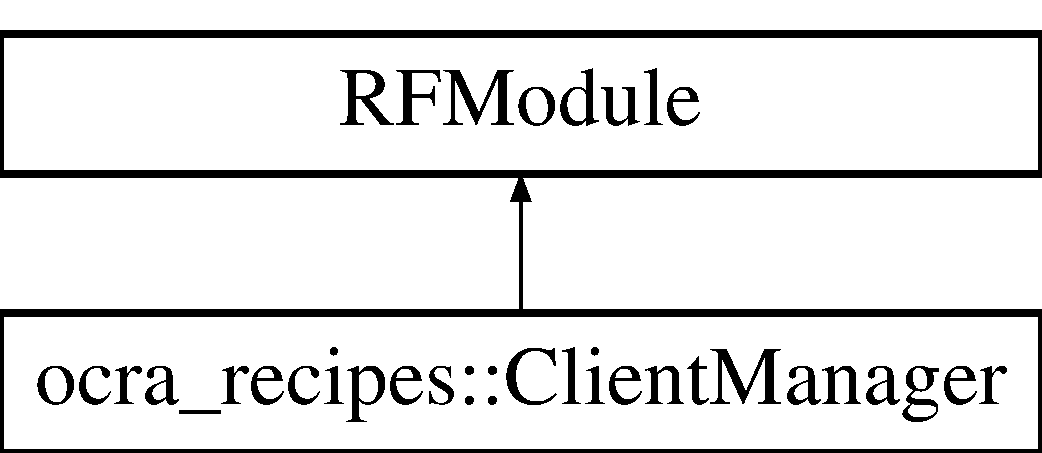
\includegraphics[height=2.000000cm]{dd/d05/classocra__recipes_1_1ClientManager}
\end{center}
\end{figure}
\subsection*{Classes}
\begin{DoxyCompactItemize}
\item 
class \hyperlink{classocra__recipes_1_1ClientManager_1_1moduleCallback}{module\+Callback}
\begin{DoxyCompactList}\small\item\em A callback function which binds the rpc server port opened in the contoller server module to the controller thread\textquotesingle{}s parsing function. \end{DoxyCompactList}\end{DoxyCompactItemize}
\subsection*{Public Member Functions}
\begin{DoxyCompactItemize}
\item 
\hyperlink{classocra__recipes_1_1ClientManager_ad5e77797451b303bf063ca6c1ebf8307}{Client\+Manager} (std\+::shared\+\_\+ptr$<$ \hyperlink{classocra__recipes_1_1ControllerClient}{Controller\+Client} $>$ custom\+Client)
\item 
\hyperlink{classocra__recipes_1_1ClientManager_af605d4fa9dab04b9874bf307277cd8a3}{$\sim$\+Client\+Manager} ()
\item 
bool \hyperlink{classocra__recipes_1_1ClientManager_a341d7c03d2c2b645f9b815f02baf323e}{configure} (yarp\+::os\+::\+Resource\+Finder \&rf)
\item 
int \hyperlink{classocra__recipes_1_1ClientManager_a443fb4edc4bac1c1e24e32f26a730519}{launch\+Client} ()
\item 
bool \hyperlink{classocra__recipes_1_1ClientManager_a3724b1ba55a2a0e81774aa674f567e34}{interrupt\+Module} ()
\item 
bool \hyperlink{classocra__recipes_1_1ClientManager_ace715a5dc663e956edc24d976cc7ad09}{close} ()
\item 
bool \hyperlink{classocra__recipes_1_1ClientManager_a2fb40c4d2440367c4f66ad5815e6b1f8}{update\+Module} ()
\item 
void \hyperlink{classocra__recipes_1_1ClientManager_aa935699ac8fe135a066ce69f7ebc6d0d}{print\+Help} ()
\item 
virtual std\+::string \hyperlink{classocra__recipes_1_1ClientManager_a3fd7aa39812c9ffdb32b732c4f854862}{get\+Manager\+Name} ()
\end{DoxyCompactItemize}
\subsection*{Protected Member Functions}
\begin{DoxyCompactItemize}
\item 
virtual void \hyperlink{classocra__recipes_1_1ClientManager_ab81a0bc48b6ac66b97988ef836df3cd6}{custom\+Callback\+Parser} (yarp\+::os\+::\+Bottle \&message, yarp\+::os\+::\+Bottle \&reply)
\item 
virtual bool \hyperlink{classocra__recipes_1_1ClientManager_a51e6fd902ad96b27c2c976305f7306fd}{custom\+Update\+Module} ()
\end{DoxyCompactItemize}


\subsection{Detailed Description}
The controller module which launches the controller thread. 

Basically all this does is parse the command line arguments and look for the various config and task set files. It then instantiates a W\+BI instance (yarp\+W\+BI specifically) and a Icub\+Controller\+Client instance. It launches these threads and then basically just waits till it gets a kill (ctrl+c) command to close them down. Does a little keeping track of time as well. 

Definition at line 48 of file Client\+Manager.\+h.



\subsection{Constructor \& Destructor Documentation}
\hypertarget{classocra__recipes_1_1ClientManager_ad5e77797451b303bf063ca6c1ebf8307}{}\label{classocra__recipes_1_1ClientManager_ad5e77797451b303bf063ca6c1ebf8307} 
\index{ocra\+\_\+recipes\+::\+Client\+Manager@{ocra\+\_\+recipes\+::\+Client\+Manager}!Client\+Manager@{Client\+Manager}}
\index{Client\+Manager@{Client\+Manager}!ocra\+\_\+recipes\+::\+Client\+Manager@{ocra\+\_\+recipes\+::\+Client\+Manager}}
\subsubsection{\texorpdfstring{Client\+Manager()}{ClientManager()}}
{\footnotesize\ttfamily Client\+Manager\+::\+Client\+Manager (\begin{DoxyParamCaption}\item[{std\+::shared\+\_\+ptr$<$ \hyperlink{classocra__recipes_1_1ControllerClient}{Controller\+Client} $>$}]{custom\+Client }\end{DoxyParamCaption})}

Constructor which essentially does nothing. 

Definition at line 33 of file Client\+Manager.\+cpp.

\hypertarget{classocra__recipes_1_1ClientManager_af605d4fa9dab04b9874bf307277cd8a3}{}\label{classocra__recipes_1_1ClientManager_af605d4fa9dab04b9874bf307277cd8a3} 
\index{ocra\+\_\+recipes\+::\+Client\+Manager@{ocra\+\_\+recipes\+::\+Client\+Manager}!````~Client\+Manager@{$\sim$\+Client\+Manager}}
\index{````~Client\+Manager@{$\sim$\+Client\+Manager}!ocra\+\_\+recipes\+::\+Client\+Manager@{ocra\+\_\+recipes\+::\+Client\+Manager}}
\subsubsection{\texorpdfstring{$\sim$\+Client\+Manager()}{~ClientManager()}}
{\footnotesize\ttfamily Client\+Manager\+::$\sim$\+Client\+Manager (\begin{DoxyParamCaption}{ }\end{DoxyParamCaption})}

Destructor which essentially does nothing. 

Definition at line 42 of file Client\+Manager.\+cpp.



\subsection{Member Function Documentation}
\hypertarget{classocra__recipes_1_1ClientManager_ace715a5dc663e956edc24d976cc7ad09}{}\label{classocra__recipes_1_1ClientManager_ace715a5dc663e956edc24d976cc7ad09} 
\index{ocra\+\_\+recipes\+::\+Client\+Manager@{ocra\+\_\+recipes\+::\+Client\+Manager}!close@{close}}
\index{close@{close}!ocra\+\_\+recipes\+::\+Client\+Manager@{ocra\+\_\+recipes\+::\+Client\+Manager}}
\subsubsection{\texorpdfstring{close()}{close()}}
{\footnotesize\ttfamily bool Client\+Manager\+::close (\begin{DoxyParamCaption}{ }\end{DoxyParamCaption})}

Closes the module. First shuts down the threads. 

Definition at line 71 of file Client\+Manager.\+cpp.

\hypertarget{classocra__recipes_1_1ClientManager_a341d7c03d2c2b645f9b815f02baf323e}{}\label{classocra__recipes_1_1ClientManager_a341d7c03d2c2b645f9b815f02baf323e} 
\index{ocra\+\_\+recipes\+::\+Client\+Manager@{ocra\+\_\+recipes\+::\+Client\+Manager}!configure@{configure}}
\index{configure@{configure}!ocra\+\_\+recipes\+::\+Client\+Manager@{ocra\+\_\+recipes\+::\+Client\+Manager}}
\subsubsection{\texorpdfstring{configure()}{configure()}}
{\footnotesize\ttfamily bool Client\+Manager\+::configure (\begin{DoxyParamCaption}\item[{yarp\+::os\+::\+Resource\+Finder \&}]{rf }\end{DoxyParamCaption})}

Configures the module by parsing the RF contents. Passes to client when done. 
\begin{DoxyParams}{Parameters}
{\em rf} & A resource finder instance which is initialized from the command line args.\\
\hline
\end{DoxyParams}
\begin{DoxyReturn}{Returns}
True or false if the configuration was successful. 
\end{DoxyReturn}


Definition at line 52 of file Client\+Manager.\+cpp.

\hypertarget{classocra__recipes_1_1ClientManager_ab81a0bc48b6ac66b97988ef836df3cd6}{}\label{classocra__recipes_1_1ClientManager_ab81a0bc48b6ac66b97988ef836df3cd6} 
\index{ocra\+\_\+recipes\+::\+Client\+Manager@{ocra\+\_\+recipes\+::\+Client\+Manager}!custom\+Callback\+Parser@{custom\+Callback\+Parser}}
\index{custom\+Callback\+Parser@{custom\+Callback\+Parser}!ocra\+\_\+recipes\+::\+Client\+Manager@{ocra\+\_\+recipes\+::\+Client\+Manager}}
\subsubsection{\texorpdfstring{custom\+Callback\+Parser()}{customCallbackParser()}}
{\footnotesize\ttfamily void Client\+Manager\+::custom\+Callback\+Parser (\begin{DoxyParamCaption}\item[{yarp\+::os\+::\+Bottle \&}]{message,  }\item[{yarp\+::os\+::\+Bottle \&}]{reply }\end{DoxyParamCaption})\hspace{0.3cm}{\ttfamily [protected]}, {\ttfamily [virtual]}}



Definition at line 123 of file Client\+Manager.\+cpp.

\hypertarget{classocra__recipes_1_1ClientManager_a51e6fd902ad96b27c2c976305f7306fd}{}\label{classocra__recipes_1_1ClientManager_a51e6fd902ad96b27c2c976305f7306fd} 
\index{ocra\+\_\+recipes\+::\+Client\+Manager@{ocra\+\_\+recipes\+::\+Client\+Manager}!custom\+Update\+Module@{custom\+Update\+Module}}
\index{custom\+Update\+Module@{custom\+Update\+Module}!ocra\+\_\+recipes\+::\+Client\+Manager@{ocra\+\_\+recipes\+::\+Client\+Manager}}
\subsubsection{\texorpdfstring{custom\+Update\+Module()}{customUpdateModule()}}
{\footnotesize\ttfamily bool Client\+Manager\+::custom\+Update\+Module (\begin{DoxyParamCaption}{ }\end{DoxyParamCaption})\hspace{0.3cm}{\ttfamily [protected]}, {\ttfamily [virtual]}}



Definition at line 127 of file Client\+Manager.\+cpp.

\hypertarget{classocra__recipes_1_1ClientManager_a3fd7aa39812c9ffdb32b732c4f854862}{}\label{classocra__recipes_1_1ClientManager_a3fd7aa39812c9ffdb32b732c4f854862} 
\index{ocra\+\_\+recipes\+::\+Client\+Manager@{ocra\+\_\+recipes\+::\+Client\+Manager}!get\+Manager\+Name@{get\+Manager\+Name}}
\index{get\+Manager\+Name@{get\+Manager\+Name}!ocra\+\_\+recipes\+::\+Client\+Manager@{ocra\+\_\+recipes\+::\+Client\+Manager}}
\subsubsection{\texorpdfstring{get\+Manager\+Name()}{getManagerName()}}
{\footnotesize\ttfamily std\+::string Client\+Manager\+::get\+Manager\+Name (\begin{DoxyParamCaption}{ }\end{DoxyParamCaption})\hspace{0.3cm}{\ttfamily [virtual]}}

Gets the name of the module. Override this function to set a different name. \begin{DoxyReturn}{Returns}
A string with the module name. 
\end{DoxyReturn}


Definition at line 47 of file Client\+Manager.\+cpp.

\hypertarget{classocra__recipes_1_1ClientManager_a3724b1ba55a2a0e81774aa674f567e34}{}\label{classocra__recipes_1_1ClientManager_a3724b1ba55a2a0e81774aa674f567e34} 
\index{ocra\+\_\+recipes\+::\+Client\+Manager@{ocra\+\_\+recipes\+::\+Client\+Manager}!interrupt\+Module@{interrupt\+Module}}
\index{interrupt\+Module@{interrupt\+Module}!ocra\+\_\+recipes\+::\+Client\+Manager@{ocra\+\_\+recipes\+::\+Client\+Manager}}
\subsubsection{\texorpdfstring{interrupt\+Module()}{interruptModule()}}
{\footnotesize\ttfamily bool Client\+Manager\+::interrupt\+Module (\begin{DoxyParamCaption}{ }\end{DoxyParamCaption})}

Interrupts the module execution and stops the control and wbi threads. 

Definition at line 63 of file Client\+Manager.\+cpp.

\hypertarget{classocra__recipes_1_1ClientManager_a443fb4edc4bac1c1e24e32f26a730519}{}\label{classocra__recipes_1_1ClientManager_a443fb4edc4bac1c1e24e32f26a730519} 
\index{ocra\+\_\+recipes\+::\+Client\+Manager@{ocra\+\_\+recipes\+::\+Client\+Manager}!launch\+Client@{launch\+Client}}
\index{launch\+Client@{launch\+Client}!ocra\+\_\+recipes\+::\+Client\+Manager@{ocra\+\_\+recipes\+::\+Client\+Manager}}
\subsubsection{\texorpdfstring{launch\+Client()}{launchClient()}}
{\footnotesize\ttfamily int Client\+Manager\+::launch\+Client (\begin{DoxyParamCaption}{ }\end{DoxyParamCaption})}

Simply calls client-\/$>$start() then run\+Module() 

Definition at line 57 of file Client\+Manager.\+cpp.

\hypertarget{classocra__recipes_1_1ClientManager_aa935699ac8fe135a066ce69f7ebc6d0d}{}\label{classocra__recipes_1_1ClientManager_aa935699ac8fe135a066ce69f7ebc6d0d} 
\index{ocra\+\_\+recipes\+::\+Client\+Manager@{ocra\+\_\+recipes\+::\+Client\+Manager}!print\+Help@{print\+Help}}
\index{print\+Help@{print\+Help}!ocra\+\_\+recipes\+::\+Client\+Manager@{ocra\+\_\+recipes\+::\+Client\+Manager}}
\subsubsection{\texorpdfstring{print\+Help()}{printHelp()}}
{\footnotesize\ttfamily void Client\+Manager\+::print\+Help (\begin{DoxyParamCaption}{ }\end{DoxyParamCaption})}

Prints all the command line args one could use. 

Definition at line 109 of file Client\+Manager.\+cpp.

\hypertarget{classocra__recipes_1_1ClientManager_a2fb40c4d2440367c4f66ad5815e6b1f8}{}\label{classocra__recipes_1_1ClientManager_a2fb40c4d2440367c4f66ad5815e6b1f8} 
\index{ocra\+\_\+recipes\+::\+Client\+Manager@{ocra\+\_\+recipes\+::\+Client\+Manager}!update\+Module@{update\+Module}}
\index{update\+Module@{update\+Module}!ocra\+\_\+recipes\+::\+Client\+Manager@{ocra\+\_\+recipes\+::\+Client\+Manager}}
\subsubsection{\texorpdfstring{update\+Module()}{updateModule()}}
{\footnotesize\ttfamily bool Client\+Manager\+::update\+Module (\begin{DoxyParamCaption}{ }\end{DoxyParamCaption})}

Updates the \hyperlink{classocra__recipes_1_1ClientManager}{Client\+Manager}. Basically just clocks the thread run() method. \begin{DoxyReturn}{Returns}
Whether or not the clocking functions worked. 
\end{DoxyReturn}


Definition at line 89 of file Client\+Manager.\+cpp.



The documentation for this class was generated from the following files\+:\begin{DoxyCompactItemize}
\item 
\hyperlink{ClientManager_8h}{Client\+Manager.\+h}\item 
\hyperlink{ClientManager_8cpp}{Client\+Manager.\+cpp}\end{DoxyCompactItemize}

\hypertarget{classocra_1_1CmlQuadraticSolver}{}\section{ocra\+:\+:Cml\+Quadratic\+Solver Class Reference}
\label{classocra_1_1CmlQuadraticSolver}\index{ocra\+::\+Cml\+Quadratic\+Solver@{ocra\+::\+Cml\+Quadratic\+Solver}}


Cml\+Quadratic\+Solver class.  




{\ttfamily \#include $<$Cml\+Quadratic\+Solver.\+h$>$}



Inheritance diagram for ocra\+:\+:Cml\+Quadratic\+Solver\+:\nopagebreak
\begin{figure}[H]
\begin{center}
\leavevmode
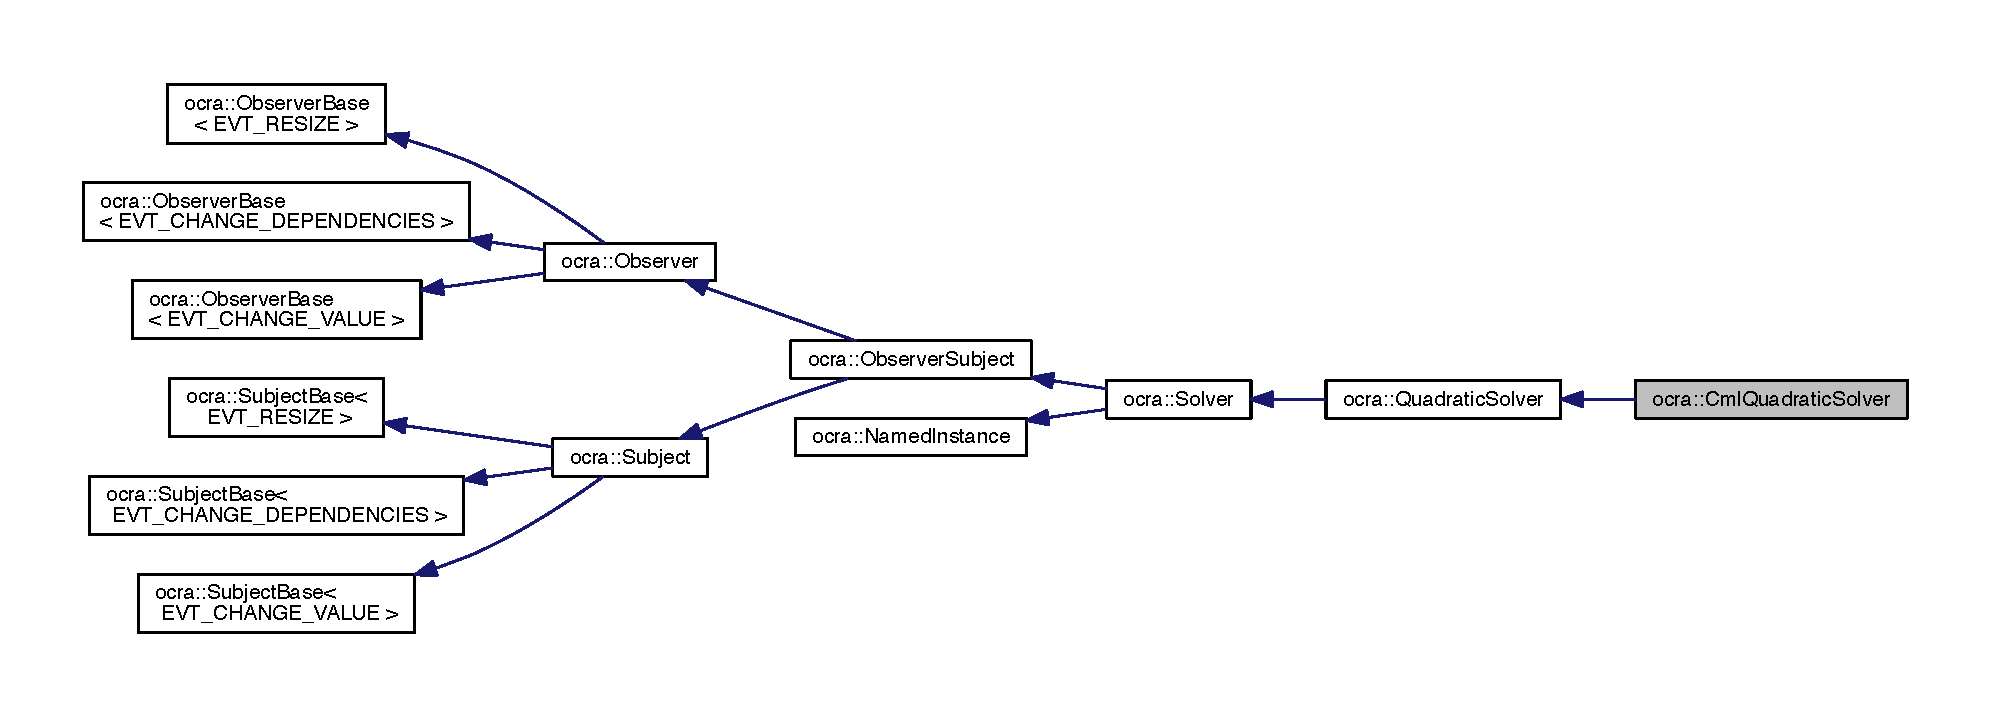
\includegraphics[width=350pt]{d9/d05/classocra_1_1CmlQuadraticSolver__inherit__graph}
\end{center}
\end{figure}


Collaboration diagram for ocra\+:\+:Cml\+Quadratic\+Solver\+:\nopagebreak
\begin{figure}[H]
\begin{center}
\leavevmode
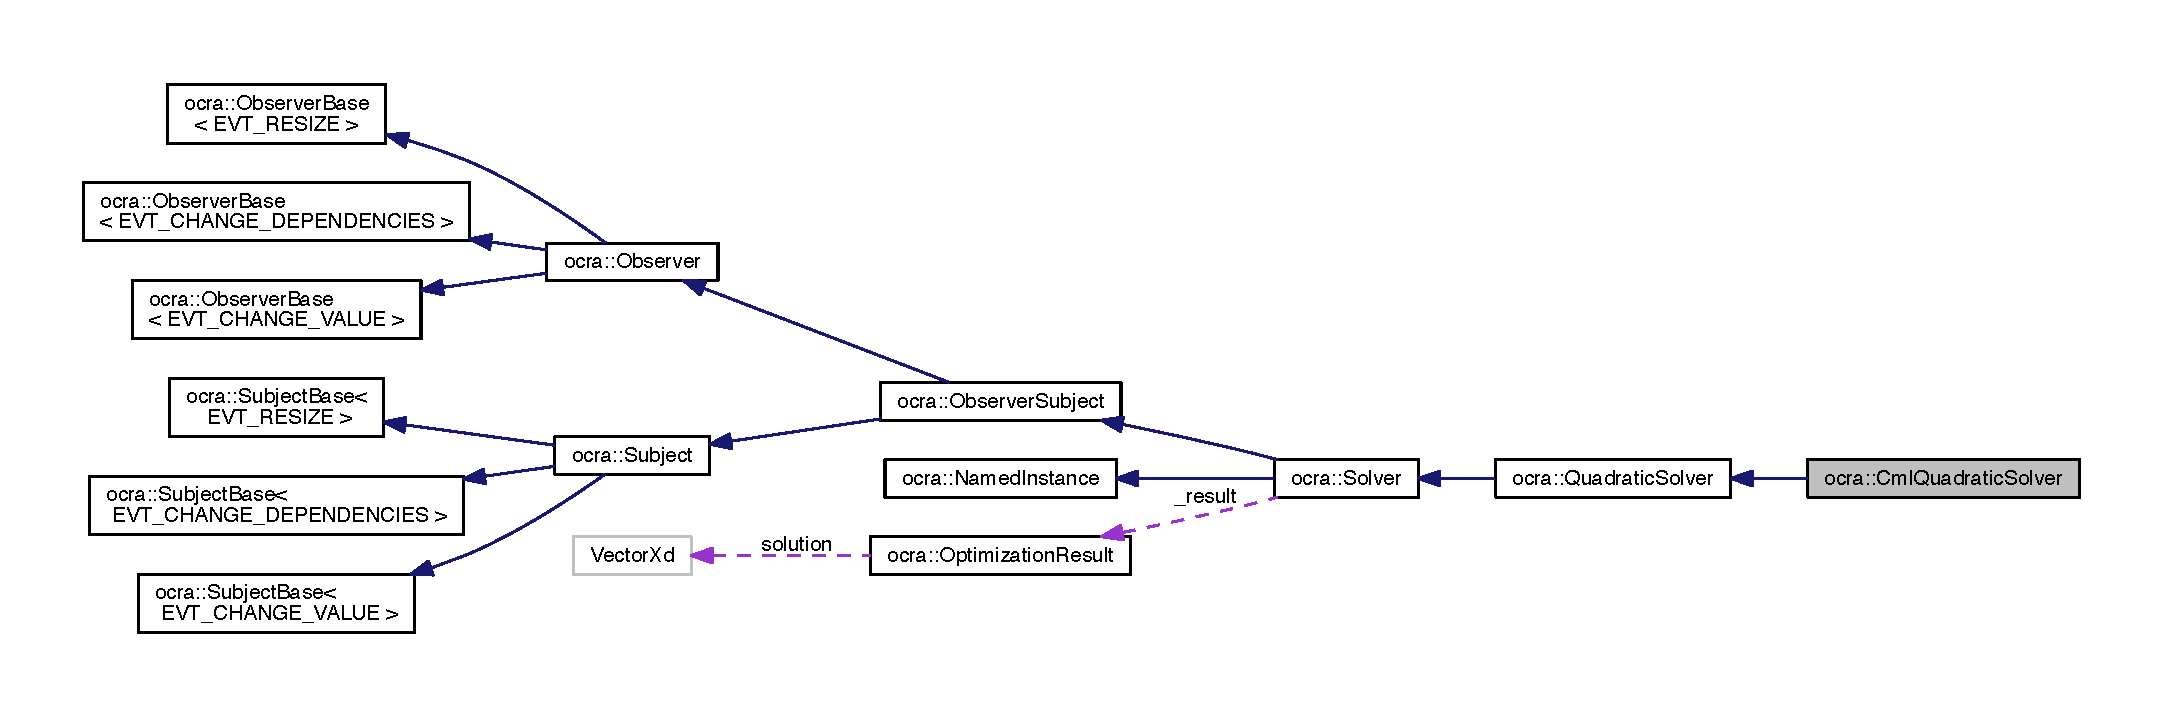
\includegraphics[width=350pt]{dd/d29/classocra_1_1CmlQuadraticSolver__coll__graph}
\end{center}
\end{figure}
\subsection*{Public Types}
\begin{DoxyCompactItemize}
\item 
enum \hyperlink{classocra_1_1CmlQuadraticSolver_a6d54dc2e4dac085099b002c88cb6d3df}{e\+Cml\+Q\+P\+Solver\+Type} \{ \hyperlink{classocra_1_1CmlQuadraticSolver_a6d54dc2e4dac085099b002c88cb6d3dfac7ab4857986d549d2c7ac2f4e7d834cc}{C\+M\+L\+Q\+P\+S\+O\+L\+V\+E\+R\+\_\+\+L\+E\+M\+KE}, 
\hyperlink{classocra_1_1CmlQuadraticSolver_a6d54dc2e4dac085099b002c88cb6d3dfa53afe853cc16e5023a4618d57cb082f1}{C\+M\+L\+Q\+P\+S\+O\+L\+V\+E\+R\+\_\+\+G\+A\+U\+S\+S\+\_\+\+S\+E\+I\+D\+EL}
 \}
\end{DoxyCompactItemize}
\subsection*{Public Member Functions}
\begin{DoxyCompactItemize}
\item 
\hyperlink{classocra_1_1CmlQuadraticSolver_a4ef339a5d511aff62bf4f6669fa894b8}{Cml\+Quadratic\+Solver} (int type=xde\+::cml\+Q\+P\+Solver\+::\+L\+E\+M\+K\+E\+\_\+\+S\+O\+L\+V\+ER)
\item 
void \hyperlink{classocra_1_1CmlQuadraticSolver_a6c508788b75053d2bbcc7a3fee4ba26e}{set\+Tolerance} (double epsilon)
\item 
void \hyperlink{classocra_1_1CmlQuadraticSolver_a47a17923b7fdf4d8137fb41e240831d6}{set\+Max\+Iteration} (cfl\+\_\+size\+\_\+t max\+Iter)
\item 
cfl\+\_\+size\+\_\+t \hyperlink{classocra_1_1CmlQuadraticSolver_a89d29bf8618e4d658f6234dd967165ad}{get\+Max\+Iteration} (void) const
\item 
virtual const std\+::string \& \hyperlink{classocra_1_1CmlQuadraticSolver_a95f1b52f24a43f9afc38b36fb7943e05}{get\+More\+Info} (void) const
\item 
virtual void \hyperlink{classocra_1_1CmlQuadraticSolver_afea0aeb47c39f7fb8b3ce068f3d09885}{add\+Linear\+Equality\+Constraint} (\hyperlink{namespaceocra_ae8b87cf4099be3efc3b410019ad2046e}{Linear\+Constraint} $\ast$constraint)
\item 
virtual void \hyperlink{classocra_1_1CmlQuadraticSolver_a5bbf7066fb72a418a174aece3ac65bf5}{add\+Linear\+Inequality\+Constraint} (\hyperlink{namespaceocra_ae8b87cf4099be3efc3b410019ad2046e}{Linear\+Constraint} $\ast$constraint)
\item 
virtual void \hyperlink{classocra_1_1CmlQuadraticSolver_a570e7be65f21d67e41a0f030d5134e4e}{remove\+Constraint} (\hyperlink{namespaceocra_ae8b87cf4099be3efc3b410019ad2046e}{Linear\+Constraint} $\ast$constraint)
\item 
virtual void \hyperlink{classocra_1_1CmlQuadraticSolver_ad286753e3e35fa17f4aef9f8a75bd5b1}{set\+Objective} (\hyperlink{classocra_1_1QuadraticFunction}{Quadratic\+Function} $\ast$obj, \hyperlink{namespaceocra_af4478308ca113669e67d72f9a3050469}{real} weight=1.)
\item 
virtual void \hyperlink{classocra_1_1CmlQuadraticSolver_a531381b1498b0ad4e460e5a2a75da9b4}{add\+Objective} (\hyperlink{classocra_1_1QuadraticFunction}{Quadratic\+Function} $\ast$obj, \hyperlink{namespaceocra_af4478308ca113669e67d72f9a3050469}{real} weight=1.)
\item 
virtual void \hyperlink{classocra_1_1CmlQuadraticSolver_a83d20013d6a9ff7c5855ee0ff2391190}{remove\+Objective} (\hyperlink{classocra_1_1QuadraticFunction}{Quadratic\+Function} $\ast$obj)
\item 
virtual void \hyperlink{classocra_1_1CmlQuadraticSolver_aed7554d599282ef5e8a7567b73b822b8}{print\+Values\+At\+Solution} (void)
\item 
bool \hyperlink{classocra_1_1CmlQuadraticSolver_a8077e7d9f2017f0f176324bb04cb5cd1}{check\+Constraints} (void)
\item 
virtual const Matrix\+Base \& \hyperlink{classocra_1_1CmlQuadraticSolver_a2d02c9af54a4456eac7e56803ee037f3}{getP} (void) const
\item 
virtual const Matrix\+Base \& \hyperlink{classocra_1_1CmlQuadraticSolver_a6bbc784066ced7a347a32de698069d07}{getA} (void) const
\item 
virtual const Matrix\+Base \& \hyperlink{classocra_1_1CmlQuadraticSolver_a94c170188e1f3d00aaee5628e2501a64}{getC} (void) const
\item 
virtual const Vector\+Base \& \hyperlink{classocra_1_1CmlQuadraticSolver_ac97f9655bd9a6d8564539cf7ec79c269}{getq} (void) const
\item 
virtual const Vector\+Base \& \hyperlink{classocra_1_1CmlQuadraticSolver_a1af1421b10bd780438cef59ac0293749}{getb} (void) const
\item 
virtual const Vector\+Base \& \hyperlink{classocra_1_1CmlQuadraticSolver_a0d3fd75da9a338208f7a5f5e1417346b}{getd} (void) const
\item 
virtual const Vector\+Base \& \hyperlink{classocra_1_1CmlQuadraticSolver_af674cde45f84730e2447d0e34a6e6918}{getu} (void) const
\item 
virtual const Vector\+Base \& \hyperlink{classocra_1_1CmlQuadraticSolver_a963b8e8e4f099e89003be3c9cb77fa90}{getl} (void) const
\end{DoxyCompactItemize}
\subsection*{Protected Member Functions}
\begin{DoxyCompactItemize}
\item 
virtual const Solver\+::\+Result \& \hyperlink{classocra_1_1CmlQuadraticSolver_aac5943e307225837253c470a931640ec}{do\+Solve} (void)
\item 
virtual void \hyperlink{classocra_1_1CmlQuadraticSolver_a6139c2cd572e403badc0451bf0ea9d90}{do\+Prepare} (void)
\item 
virtual void \hyperlink{classocra_1_1CmlQuadraticSolver_a2c2240bd0bcee4f0cd57030ed08baabd}{recompute\+Variable} (void)
\end{DoxyCompactItemize}
\subsection*{Additional Inherited Members}


\subsection{Detailed Description}
Cml\+Quadratic\+Solver class. 

\begin{DoxyWarning}{Warning}
None
\end{DoxyWarning}
Wrapping of the QP solver from cml 

Definition at line 37 of file Cml\+Quadratic\+Solver.\+h.



\subsection{Member Enumeration Documentation}
\hypertarget{classocra_1_1CmlQuadraticSolver_a6d54dc2e4dac085099b002c88cb6d3df}{}\label{classocra_1_1CmlQuadraticSolver_a6d54dc2e4dac085099b002c88cb6d3df} 
\index{ocra\+::\+Cml\+Quadratic\+Solver@{ocra\+::\+Cml\+Quadratic\+Solver}!e\+Cml\+Q\+P\+Solver\+Type@{e\+Cml\+Q\+P\+Solver\+Type}}
\index{e\+Cml\+Q\+P\+Solver\+Type@{e\+Cml\+Q\+P\+Solver\+Type}!ocra\+::\+Cml\+Quadratic\+Solver@{ocra\+::\+Cml\+Quadratic\+Solver}}
\subsubsection{\texorpdfstring{e\+Cml\+Q\+P\+Solver\+Type}{eCmlQPSolverType}}
{\footnotesize\ttfamily enum \hyperlink{classocra_1_1CmlQuadraticSolver_a6d54dc2e4dac085099b002c88cb6d3df}{ocra\+::\+Cml\+Quadratic\+Solver\+::e\+Cml\+Q\+P\+Solver\+Type}}

\begin{DoxyEnumFields}{Enumerator}
\raisebox{\heightof{T}}[0pt][0pt]{\index{C\+M\+L\+Q\+P\+S\+O\+L\+V\+E\+R\+\_\+\+L\+E\+M\+KE@{C\+M\+L\+Q\+P\+S\+O\+L\+V\+E\+R\+\_\+\+L\+E\+M\+KE}!ocra\+::\+Cml\+Quadratic\+Solver@{ocra\+::\+Cml\+Quadratic\+Solver}}\index{ocra\+::\+Cml\+Quadratic\+Solver@{ocra\+::\+Cml\+Quadratic\+Solver}!C\+M\+L\+Q\+P\+S\+O\+L\+V\+E\+R\+\_\+\+L\+E\+M\+KE@{C\+M\+L\+Q\+P\+S\+O\+L\+V\+E\+R\+\_\+\+L\+E\+M\+KE}}}\hypertarget{classocra_1_1CmlQuadraticSolver_a6d54dc2e4dac085099b002c88cb6d3dfac7ab4857986d549d2c7ac2f4e7d834cc}{}\label{classocra_1_1CmlQuadraticSolver_a6d54dc2e4dac085099b002c88cb6d3dfac7ab4857986d549d2c7ac2f4e7d834cc} 
C\+M\+L\+Q\+P\+S\+O\+L\+V\+E\+R\+\_\+\+L\+E\+M\+KE&\\
\hline

\raisebox{\heightof{T}}[0pt][0pt]{\index{C\+M\+L\+Q\+P\+S\+O\+L\+V\+E\+R\+\_\+\+G\+A\+U\+S\+S\+\_\+\+S\+E\+I\+D\+EL@{C\+M\+L\+Q\+P\+S\+O\+L\+V\+E\+R\+\_\+\+G\+A\+U\+S\+S\+\_\+\+S\+E\+I\+D\+EL}!ocra\+::\+Cml\+Quadratic\+Solver@{ocra\+::\+Cml\+Quadratic\+Solver}}\index{ocra\+::\+Cml\+Quadratic\+Solver@{ocra\+::\+Cml\+Quadratic\+Solver}!C\+M\+L\+Q\+P\+S\+O\+L\+V\+E\+R\+\_\+\+G\+A\+U\+S\+S\+\_\+\+S\+E\+I\+D\+EL@{C\+M\+L\+Q\+P\+S\+O\+L\+V\+E\+R\+\_\+\+G\+A\+U\+S\+S\+\_\+\+S\+E\+I\+D\+EL}}}\hypertarget{classocra_1_1CmlQuadraticSolver_a6d54dc2e4dac085099b002c88cb6d3dfa53afe853cc16e5023a4618d57cb082f1}{}\label{classocra_1_1CmlQuadraticSolver_a6d54dc2e4dac085099b002c88cb6d3dfa53afe853cc16e5023a4618d57cb082f1} 
C\+M\+L\+Q\+P\+S\+O\+L\+V\+E\+R\+\_\+\+G\+A\+U\+S\+S\+\_\+\+S\+E\+I\+D\+EL&\\
\hline

\end{DoxyEnumFields}


Definition at line 41 of file Cml\+Quadratic\+Solver.\+h.



\subsection{Constructor \& Destructor Documentation}
\hypertarget{classocra_1_1CmlQuadraticSolver_a4ef339a5d511aff62bf4f6669fa894b8}{}\label{classocra_1_1CmlQuadraticSolver_a4ef339a5d511aff62bf4f6669fa894b8} 
\index{ocra\+::\+Cml\+Quadratic\+Solver@{ocra\+::\+Cml\+Quadratic\+Solver}!Cml\+Quadratic\+Solver@{Cml\+Quadratic\+Solver}}
\index{Cml\+Quadratic\+Solver@{Cml\+Quadratic\+Solver}!ocra\+::\+Cml\+Quadratic\+Solver@{ocra\+::\+Cml\+Quadratic\+Solver}}
\subsubsection{\texorpdfstring{Cml\+Quadratic\+Solver()}{CmlQuadraticSolver()}}
{\footnotesize\ttfamily ocra\+::\+Cml\+Quadratic\+Solver\+::\+Cml\+Quadratic\+Solver (\begin{DoxyParamCaption}\item[{int}]{type = {\ttfamily xde\+:\+:cmlQPSolver\+:\+:LEMKE\+\_\+SOLVER} }\end{DoxyParamCaption})}



\subsection{Member Function Documentation}
\hypertarget{classocra_1_1CmlQuadraticSolver_afea0aeb47c39f7fb8b3ce068f3d09885}{}\label{classocra_1_1CmlQuadraticSolver_afea0aeb47c39f7fb8b3ce068f3d09885} 
\index{ocra\+::\+Cml\+Quadratic\+Solver@{ocra\+::\+Cml\+Quadratic\+Solver}!add\+Linear\+Equality\+Constraint@{add\+Linear\+Equality\+Constraint}}
\index{add\+Linear\+Equality\+Constraint@{add\+Linear\+Equality\+Constraint}!ocra\+::\+Cml\+Quadratic\+Solver@{ocra\+::\+Cml\+Quadratic\+Solver}}
\subsubsection{\texorpdfstring{add\+Linear\+Equality\+Constraint()}{addLinearEqualityConstraint()}}
{\footnotesize\ttfamily virtual void ocra\+::\+Cml\+Quadratic\+Solver\+::add\+Linear\+Equality\+Constraint (\begin{DoxyParamCaption}\item[{\hyperlink{namespaceocra_ae8b87cf4099be3efc3b410019ad2046e}{Linear\+Constraint} $\ast$}]{constraint }\end{DoxyParamCaption})\hspace{0.3cm}{\ttfamily [virtual]}}

\hypertarget{classocra_1_1CmlQuadraticSolver_a5bbf7066fb72a418a174aece3ac65bf5}{}\label{classocra_1_1CmlQuadraticSolver_a5bbf7066fb72a418a174aece3ac65bf5} 
\index{ocra\+::\+Cml\+Quadratic\+Solver@{ocra\+::\+Cml\+Quadratic\+Solver}!add\+Linear\+Inequality\+Constraint@{add\+Linear\+Inequality\+Constraint}}
\index{add\+Linear\+Inequality\+Constraint@{add\+Linear\+Inequality\+Constraint}!ocra\+::\+Cml\+Quadratic\+Solver@{ocra\+::\+Cml\+Quadratic\+Solver}}
\subsubsection{\texorpdfstring{add\+Linear\+Inequality\+Constraint()}{addLinearInequalityConstraint()}}
{\footnotesize\ttfamily virtual void ocra\+::\+Cml\+Quadratic\+Solver\+::add\+Linear\+Inequality\+Constraint (\begin{DoxyParamCaption}\item[{\hyperlink{namespaceocra_ae8b87cf4099be3efc3b410019ad2046e}{Linear\+Constraint} $\ast$}]{constraint }\end{DoxyParamCaption})\hspace{0.3cm}{\ttfamily [virtual]}}

\hypertarget{classocra_1_1CmlQuadraticSolver_a531381b1498b0ad4e460e5a2a75da9b4}{}\label{classocra_1_1CmlQuadraticSolver_a531381b1498b0ad4e460e5a2a75da9b4} 
\index{ocra\+::\+Cml\+Quadratic\+Solver@{ocra\+::\+Cml\+Quadratic\+Solver}!add\+Objective@{add\+Objective}}
\index{add\+Objective@{add\+Objective}!ocra\+::\+Cml\+Quadratic\+Solver@{ocra\+::\+Cml\+Quadratic\+Solver}}
\subsubsection{\texorpdfstring{add\+Objective()}{addObjective()}}
{\footnotesize\ttfamily virtual void ocra\+::\+Cml\+Quadratic\+Solver\+::add\+Objective (\begin{DoxyParamCaption}\item[{\hyperlink{classocra_1_1QuadraticFunction}{Quadratic\+Function} $\ast$}]{obj,  }\item[{\hyperlink{namespaceocra_af4478308ca113669e67d72f9a3050469}{real}}]{weight = {\ttfamily 1.} }\end{DoxyParamCaption})\hspace{0.3cm}{\ttfamily [virtual]}}

\hypertarget{classocra_1_1CmlQuadraticSolver_a8077e7d9f2017f0f176324bb04cb5cd1}{}\label{classocra_1_1CmlQuadraticSolver_a8077e7d9f2017f0f176324bb04cb5cd1} 
\index{ocra\+::\+Cml\+Quadratic\+Solver@{ocra\+::\+Cml\+Quadratic\+Solver}!check\+Constraints@{check\+Constraints}}
\index{check\+Constraints@{check\+Constraints}!ocra\+::\+Cml\+Quadratic\+Solver@{ocra\+::\+Cml\+Quadratic\+Solver}}
\subsubsection{\texorpdfstring{check\+Constraints()}{checkConstraints()}}
{\footnotesize\ttfamily bool ocra\+::\+Cml\+Quadratic\+Solver\+::check\+Constraints (\begin{DoxyParamCaption}\item[{void}]{ }\end{DoxyParamCaption})}

\hypertarget{classocra_1_1CmlQuadraticSolver_a6139c2cd572e403badc0451bf0ea9d90}{}\label{classocra_1_1CmlQuadraticSolver_a6139c2cd572e403badc0451bf0ea9d90} 
\index{ocra\+::\+Cml\+Quadratic\+Solver@{ocra\+::\+Cml\+Quadratic\+Solver}!do\+Prepare@{do\+Prepare}}
\index{do\+Prepare@{do\+Prepare}!ocra\+::\+Cml\+Quadratic\+Solver@{ocra\+::\+Cml\+Quadratic\+Solver}}
\subsubsection{\texorpdfstring{do\+Prepare()}{doPrepare()}}
{\footnotesize\ttfamily virtual void ocra\+::\+Cml\+Quadratic\+Solver\+::do\+Prepare (\begin{DoxyParamCaption}\item[{void}]{ }\end{DoxyParamCaption})\hspace{0.3cm}{\ttfamily [protected]}, {\ttfamily [virtual]}}



Implements \hyperlink{classocra_1_1Solver_a9ab90e87025e3da7239141c48d28ab4a}{ocra\+::\+Solver}.

\hypertarget{classocra_1_1CmlQuadraticSolver_aac5943e307225837253c470a931640ec}{}\label{classocra_1_1CmlQuadraticSolver_aac5943e307225837253c470a931640ec} 
\index{ocra\+::\+Cml\+Quadratic\+Solver@{ocra\+::\+Cml\+Quadratic\+Solver}!do\+Solve@{do\+Solve}}
\index{do\+Solve@{do\+Solve}!ocra\+::\+Cml\+Quadratic\+Solver@{ocra\+::\+Cml\+Quadratic\+Solver}}
\subsubsection{\texorpdfstring{do\+Solve()}{doSolve()}}
{\footnotesize\ttfamily virtual const Solver\+::\+Result\& ocra\+::\+Cml\+Quadratic\+Solver\+::do\+Solve (\begin{DoxyParamCaption}\item[{void}]{ }\end{DoxyParamCaption})\hspace{0.3cm}{\ttfamily [protected]}, {\ttfamily [virtual]}}



Implements \hyperlink{classocra_1_1Solver_ace2d7cfe741611de6dc87a0de7e7f3a9}{ocra\+::\+Solver}.

\hypertarget{classocra_1_1CmlQuadraticSolver_a6bbc784066ced7a347a32de698069d07}{}\label{classocra_1_1CmlQuadraticSolver_a6bbc784066ced7a347a32de698069d07} 
\index{ocra\+::\+Cml\+Quadratic\+Solver@{ocra\+::\+Cml\+Quadratic\+Solver}!getA@{getA}}
\index{getA@{getA}!ocra\+::\+Cml\+Quadratic\+Solver@{ocra\+::\+Cml\+Quadratic\+Solver}}
\subsubsection{\texorpdfstring{get\+A()}{getA()}}
{\footnotesize\ttfamily virtual const Matrix\+Base\& ocra\+::\+Cml\+Quadratic\+Solver\+::getA (\begin{DoxyParamCaption}\item[{void}]{ }\end{DoxyParamCaption}) const\hspace{0.3cm}{\ttfamily [virtual]}}



Implements \hyperlink{classocra_1_1QuadraticSolver_aa3904e85d74c7c88c3605a082741b8cd}{ocra\+::\+Quadratic\+Solver}.

\hypertarget{classocra_1_1CmlQuadraticSolver_a1af1421b10bd780438cef59ac0293749}{}\label{classocra_1_1CmlQuadraticSolver_a1af1421b10bd780438cef59ac0293749} 
\index{ocra\+::\+Cml\+Quadratic\+Solver@{ocra\+::\+Cml\+Quadratic\+Solver}!getb@{getb}}
\index{getb@{getb}!ocra\+::\+Cml\+Quadratic\+Solver@{ocra\+::\+Cml\+Quadratic\+Solver}}
\subsubsection{\texorpdfstring{getb()}{getb()}}
{\footnotesize\ttfamily virtual const Vector\+Base\& ocra\+::\+Cml\+Quadratic\+Solver\+::getb (\begin{DoxyParamCaption}\item[{void}]{ }\end{DoxyParamCaption}) const\hspace{0.3cm}{\ttfamily [virtual]}}



Implements \hyperlink{classocra_1_1QuadraticSolver_ac051c6a779ce6a6e6e6657cfd3e1f65f}{ocra\+::\+Quadratic\+Solver}.

\hypertarget{classocra_1_1CmlQuadraticSolver_a94c170188e1f3d00aaee5628e2501a64}{}\label{classocra_1_1CmlQuadraticSolver_a94c170188e1f3d00aaee5628e2501a64} 
\index{ocra\+::\+Cml\+Quadratic\+Solver@{ocra\+::\+Cml\+Quadratic\+Solver}!getC@{getC}}
\index{getC@{getC}!ocra\+::\+Cml\+Quadratic\+Solver@{ocra\+::\+Cml\+Quadratic\+Solver}}
\subsubsection{\texorpdfstring{get\+C()}{getC()}}
{\footnotesize\ttfamily virtual const Matrix\+Base\& ocra\+::\+Cml\+Quadratic\+Solver\+::getC (\begin{DoxyParamCaption}\item[{void}]{ }\end{DoxyParamCaption}) const\hspace{0.3cm}{\ttfamily [virtual]}}



Implements \hyperlink{classocra_1_1QuadraticSolver_a0babcde3ffe8770131b5f842da01c49c}{ocra\+::\+Quadratic\+Solver}.

\hypertarget{classocra_1_1CmlQuadraticSolver_a0d3fd75da9a338208f7a5f5e1417346b}{}\label{classocra_1_1CmlQuadraticSolver_a0d3fd75da9a338208f7a5f5e1417346b} 
\index{ocra\+::\+Cml\+Quadratic\+Solver@{ocra\+::\+Cml\+Quadratic\+Solver}!getd@{getd}}
\index{getd@{getd}!ocra\+::\+Cml\+Quadratic\+Solver@{ocra\+::\+Cml\+Quadratic\+Solver}}
\subsubsection{\texorpdfstring{getd()}{getd()}}
{\footnotesize\ttfamily virtual const Vector\+Base\& ocra\+::\+Cml\+Quadratic\+Solver\+::getd (\begin{DoxyParamCaption}\item[{void}]{ }\end{DoxyParamCaption}) const\hspace{0.3cm}{\ttfamily [virtual]}}



Implements \hyperlink{classocra_1_1QuadraticSolver_a7f15d5d3c28feac3204542c885d68586}{ocra\+::\+Quadratic\+Solver}.

\hypertarget{classocra_1_1CmlQuadraticSolver_a963b8e8e4f099e89003be3c9cb77fa90}{}\label{classocra_1_1CmlQuadraticSolver_a963b8e8e4f099e89003be3c9cb77fa90} 
\index{ocra\+::\+Cml\+Quadratic\+Solver@{ocra\+::\+Cml\+Quadratic\+Solver}!getl@{getl}}
\index{getl@{getl}!ocra\+::\+Cml\+Quadratic\+Solver@{ocra\+::\+Cml\+Quadratic\+Solver}}
\subsubsection{\texorpdfstring{getl()}{getl()}}
{\footnotesize\ttfamily virtual const Vector\+Base\& ocra\+::\+Cml\+Quadratic\+Solver\+::getl (\begin{DoxyParamCaption}\item[{void}]{ }\end{DoxyParamCaption}) const\hspace{0.3cm}{\ttfamily [virtual]}}



Implements \hyperlink{classocra_1_1QuadraticSolver_a13e3a471615ca667daadf490dedc18eb}{ocra\+::\+Quadratic\+Solver}.

\hypertarget{classocra_1_1CmlQuadraticSolver_a89d29bf8618e4d658f6234dd967165ad}{}\label{classocra_1_1CmlQuadraticSolver_a89d29bf8618e4d658f6234dd967165ad} 
\index{ocra\+::\+Cml\+Quadratic\+Solver@{ocra\+::\+Cml\+Quadratic\+Solver}!get\+Max\+Iteration@{get\+Max\+Iteration}}
\index{get\+Max\+Iteration@{get\+Max\+Iteration}!ocra\+::\+Cml\+Quadratic\+Solver@{ocra\+::\+Cml\+Quadratic\+Solver}}
\subsubsection{\texorpdfstring{get\+Max\+Iteration()}{getMaxIteration()}}
{\footnotesize\ttfamily cfl\+\_\+size\+\_\+t ocra\+::\+Cml\+Quadratic\+Solver\+::get\+Max\+Iteration (\begin{DoxyParamCaption}\item[{void}]{ }\end{DoxyParamCaption}) const}

\hypertarget{classocra_1_1CmlQuadraticSolver_a95f1b52f24a43f9afc38b36fb7943e05}{}\label{classocra_1_1CmlQuadraticSolver_a95f1b52f24a43f9afc38b36fb7943e05} 
\index{ocra\+::\+Cml\+Quadratic\+Solver@{ocra\+::\+Cml\+Quadratic\+Solver}!get\+More\+Info@{get\+More\+Info}}
\index{get\+More\+Info@{get\+More\+Info}!ocra\+::\+Cml\+Quadratic\+Solver@{ocra\+::\+Cml\+Quadratic\+Solver}}
\subsubsection{\texorpdfstring{get\+More\+Info()}{getMoreInfo()}}
{\footnotesize\ttfamily virtual const std\+::string\& ocra\+::\+Cml\+Quadratic\+Solver\+::get\+More\+Info (\begin{DoxyParamCaption}\item[{void}]{ }\end{DoxyParamCaption}) const\hspace{0.3cm}{\ttfamily [virtual]}}



Reimplemented from \hyperlink{classocra_1_1Solver_a3ebcf70ad5466cd31f27811ad6ccdfff}{ocra\+::\+Solver}.

\hypertarget{classocra_1_1CmlQuadraticSolver_a2d02c9af54a4456eac7e56803ee037f3}{}\label{classocra_1_1CmlQuadraticSolver_a2d02c9af54a4456eac7e56803ee037f3} 
\index{ocra\+::\+Cml\+Quadratic\+Solver@{ocra\+::\+Cml\+Quadratic\+Solver}!getP@{getP}}
\index{getP@{getP}!ocra\+::\+Cml\+Quadratic\+Solver@{ocra\+::\+Cml\+Quadratic\+Solver}}
\subsubsection{\texorpdfstring{get\+P()}{getP()}}
{\footnotesize\ttfamily virtual const Matrix\+Base\& ocra\+::\+Cml\+Quadratic\+Solver\+::getP (\begin{DoxyParamCaption}\item[{void}]{ }\end{DoxyParamCaption}) const\hspace{0.3cm}{\ttfamily [virtual]}}



Implements \hyperlink{classocra_1_1QuadraticSolver_a4dcc2768227c21262571d19c0d494935}{ocra\+::\+Quadratic\+Solver}.

\hypertarget{classocra_1_1CmlQuadraticSolver_ac97f9655bd9a6d8564539cf7ec79c269}{}\label{classocra_1_1CmlQuadraticSolver_ac97f9655bd9a6d8564539cf7ec79c269} 
\index{ocra\+::\+Cml\+Quadratic\+Solver@{ocra\+::\+Cml\+Quadratic\+Solver}!getq@{getq}}
\index{getq@{getq}!ocra\+::\+Cml\+Quadratic\+Solver@{ocra\+::\+Cml\+Quadratic\+Solver}}
\subsubsection{\texorpdfstring{getq()}{getq()}}
{\footnotesize\ttfamily virtual const Vector\+Base\& ocra\+::\+Cml\+Quadratic\+Solver\+::getq (\begin{DoxyParamCaption}\item[{void}]{ }\end{DoxyParamCaption}) const\hspace{0.3cm}{\ttfamily [virtual]}}



Implements \hyperlink{classocra_1_1QuadraticSolver_a2a907a3fc7c60a7bf9e6a3403c544dcc}{ocra\+::\+Quadratic\+Solver}.

\hypertarget{classocra_1_1CmlQuadraticSolver_af674cde45f84730e2447d0e34a6e6918}{}\label{classocra_1_1CmlQuadraticSolver_af674cde45f84730e2447d0e34a6e6918} 
\index{ocra\+::\+Cml\+Quadratic\+Solver@{ocra\+::\+Cml\+Quadratic\+Solver}!getu@{getu}}
\index{getu@{getu}!ocra\+::\+Cml\+Quadratic\+Solver@{ocra\+::\+Cml\+Quadratic\+Solver}}
\subsubsection{\texorpdfstring{getu()}{getu()}}
{\footnotesize\ttfamily virtual const Vector\+Base\& ocra\+::\+Cml\+Quadratic\+Solver\+::getu (\begin{DoxyParamCaption}\item[{void}]{ }\end{DoxyParamCaption}) const\hspace{0.3cm}{\ttfamily [virtual]}}



Implements \hyperlink{classocra_1_1QuadraticSolver_a6d5040842f155042064a33939aa60385}{ocra\+::\+Quadratic\+Solver}.

\hypertarget{classocra_1_1CmlQuadraticSolver_aed7554d599282ef5e8a7567b73b822b8}{}\label{classocra_1_1CmlQuadraticSolver_aed7554d599282ef5e8a7567b73b822b8} 
\index{ocra\+::\+Cml\+Quadratic\+Solver@{ocra\+::\+Cml\+Quadratic\+Solver}!print\+Values\+At\+Solution@{print\+Values\+At\+Solution}}
\index{print\+Values\+At\+Solution@{print\+Values\+At\+Solution}!ocra\+::\+Cml\+Quadratic\+Solver@{ocra\+::\+Cml\+Quadratic\+Solver}}
\subsubsection{\texorpdfstring{print\+Values\+At\+Solution()}{printValuesAtSolution()}}
{\footnotesize\ttfamily virtual void ocra\+::\+Cml\+Quadratic\+Solver\+::print\+Values\+At\+Solution (\begin{DoxyParamCaption}\item[{void}]{ }\end{DoxyParamCaption})\hspace{0.3cm}{\ttfamily [virtual]}}



Implements \hyperlink{classocra_1_1Solver_ab1903098e25c16a9f92c36d37967e8fa}{ocra\+::\+Solver}.

\hypertarget{classocra_1_1CmlQuadraticSolver_a2c2240bd0bcee4f0cd57030ed08baabd}{}\label{classocra_1_1CmlQuadraticSolver_a2c2240bd0bcee4f0cd57030ed08baabd} 
\index{ocra\+::\+Cml\+Quadratic\+Solver@{ocra\+::\+Cml\+Quadratic\+Solver}!recompute\+Variable@{recompute\+Variable}}
\index{recompute\+Variable@{recompute\+Variable}!ocra\+::\+Cml\+Quadratic\+Solver@{ocra\+::\+Cml\+Quadratic\+Solver}}
\subsubsection{\texorpdfstring{recompute\+Variable()}{recomputeVariable()}}
{\footnotesize\ttfamily virtual void ocra\+::\+Cml\+Quadratic\+Solver\+::recompute\+Variable (\begin{DoxyParamCaption}\item[{void}]{ }\end{DoxyParamCaption})\hspace{0.3cm}{\ttfamily [protected]}, {\ttfamily [virtual]}}

\hypertarget{classocra_1_1CmlQuadraticSolver_a570e7be65f21d67e41a0f030d5134e4e}{}\label{classocra_1_1CmlQuadraticSolver_a570e7be65f21d67e41a0f030d5134e4e} 
\index{ocra\+::\+Cml\+Quadratic\+Solver@{ocra\+::\+Cml\+Quadratic\+Solver}!remove\+Constraint@{remove\+Constraint}}
\index{remove\+Constraint@{remove\+Constraint}!ocra\+::\+Cml\+Quadratic\+Solver@{ocra\+::\+Cml\+Quadratic\+Solver}}
\subsubsection{\texorpdfstring{remove\+Constraint()}{removeConstraint()}}
{\footnotesize\ttfamily virtual void ocra\+::\+Cml\+Quadratic\+Solver\+::remove\+Constraint (\begin{DoxyParamCaption}\item[{\hyperlink{namespaceocra_ae8b87cf4099be3efc3b410019ad2046e}{Linear\+Constraint} $\ast$}]{constraint }\end{DoxyParamCaption})\hspace{0.3cm}{\ttfamily [virtual]}}

\hypertarget{classocra_1_1CmlQuadraticSolver_a83d20013d6a9ff7c5855ee0ff2391190}{}\label{classocra_1_1CmlQuadraticSolver_a83d20013d6a9ff7c5855ee0ff2391190} 
\index{ocra\+::\+Cml\+Quadratic\+Solver@{ocra\+::\+Cml\+Quadratic\+Solver}!remove\+Objective@{remove\+Objective}}
\index{remove\+Objective@{remove\+Objective}!ocra\+::\+Cml\+Quadratic\+Solver@{ocra\+::\+Cml\+Quadratic\+Solver}}
\subsubsection{\texorpdfstring{remove\+Objective()}{removeObjective()}}
{\footnotesize\ttfamily virtual void ocra\+::\+Cml\+Quadratic\+Solver\+::remove\+Objective (\begin{DoxyParamCaption}\item[{\hyperlink{classocra_1_1QuadraticFunction}{Quadratic\+Function} $\ast$}]{obj }\end{DoxyParamCaption})\hspace{0.3cm}{\ttfamily [virtual]}}

\hypertarget{classocra_1_1CmlQuadraticSolver_a47a17923b7fdf4d8137fb41e240831d6}{}\label{classocra_1_1CmlQuadraticSolver_a47a17923b7fdf4d8137fb41e240831d6} 
\index{ocra\+::\+Cml\+Quadratic\+Solver@{ocra\+::\+Cml\+Quadratic\+Solver}!set\+Max\+Iteration@{set\+Max\+Iteration}}
\index{set\+Max\+Iteration@{set\+Max\+Iteration}!ocra\+::\+Cml\+Quadratic\+Solver@{ocra\+::\+Cml\+Quadratic\+Solver}}
\subsubsection{\texorpdfstring{set\+Max\+Iteration()}{setMaxIteration()}}
{\footnotesize\ttfamily void ocra\+::\+Cml\+Quadratic\+Solver\+::set\+Max\+Iteration (\begin{DoxyParamCaption}\item[{cfl\+\_\+size\+\_\+t}]{max\+Iter }\end{DoxyParamCaption})}

\hypertarget{classocra_1_1CmlQuadraticSolver_ad286753e3e35fa17f4aef9f8a75bd5b1}{}\label{classocra_1_1CmlQuadraticSolver_ad286753e3e35fa17f4aef9f8a75bd5b1} 
\index{ocra\+::\+Cml\+Quadratic\+Solver@{ocra\+::\+Cml\+Quadratic\+Solver}!set\+Objective@{set\+Objective}}
\index{set\+Objective@{set\+Objective}!ocra\+::\+Cml\+Quadratic\+Solver@{ocra\+::\+Cml\+Quadratic\+Solver}}
\subsubsection{\texorpdfstring{set\+Objective()}{setObjective()}}
{\footnotesize\ttfamily virtual void ocra\+::\+Cml\+Quadratic\+Solver\+::set\+Objective (\begin{DoxyParamCaption}\item[{\hyperlink{classocra_1_1QuadraticFunction}{Quadratic\+Function} $\ast$}]{obj,  }\item[{\hyperlink{namespaceocra_af4478308ca113669e67d72f9a3050469}{real}}]{weight = {\ttfamily 1.} }\end{DoxyParamCaption})\hspace{0.3cm}{\ttfamily [virtual]}}

\hypertarget{classocra_1_1CmlQuadraticSolver_a6c508788b75053d2bbcc7a3fee4ba26e}{}\label{classocra_1_1CmlQuadraticSolver_a6c508788b75053d2bbcc7a3fee4ba26e} 
\index{ocra\+::\+Cml\+Quadratic\+Solver@{ocra\+::\+Cml\+Quadratic\+Solver}!set\+Tolerance@{set\+Tolerance}}
\index{set\+Tolerance@{set\+Tolerance}!ocra\+::\+Cml\+Quadratic\+Solver@{ocra\+::\+Cml\+Quadratic\+Solver}}
\subsubsection{\texorpdfstring{set\+Tolerance()}{setTolerance()}}
{\footnotesize\ttfamily void ocra\+::\+Cml\+Quadratic\+Solver\+::set\+Tolerance (\begin{DoxyParamCaption}\item[{double}]{epsilon }\end{DoxyParamCaption})}



The documentation for this class was generated from the following file\+:\begin{DoxyCompactItemize}
\item 
\hyperlink{CmlQuadraticSolver_8h}{Cml\+Quadratic\+Solver.\+h}\end{DoxyCompactItemize}

\hypertarget{classocra_1_1CoMFrame}{}\section{ocra\+:\+:Co\+M\+Frame Class Reference}
\label{classocra_1_1CoMFrame}\index{ocra\+::\+Co\+M\+Frame@{ocra\+::\+Co\+M\+Frame}}


Creates a frame whose center is at the CoM of the model and whose axes are parallel to the axes of the world frame.  




{\ttfamily \#include $<$Control\+Frame.\+h$>$}

Inheritance diagram for ocra\+:\+:Co\+M\+Frame\+:\begin{figure}[H]
\begin{center}
\leavevmode
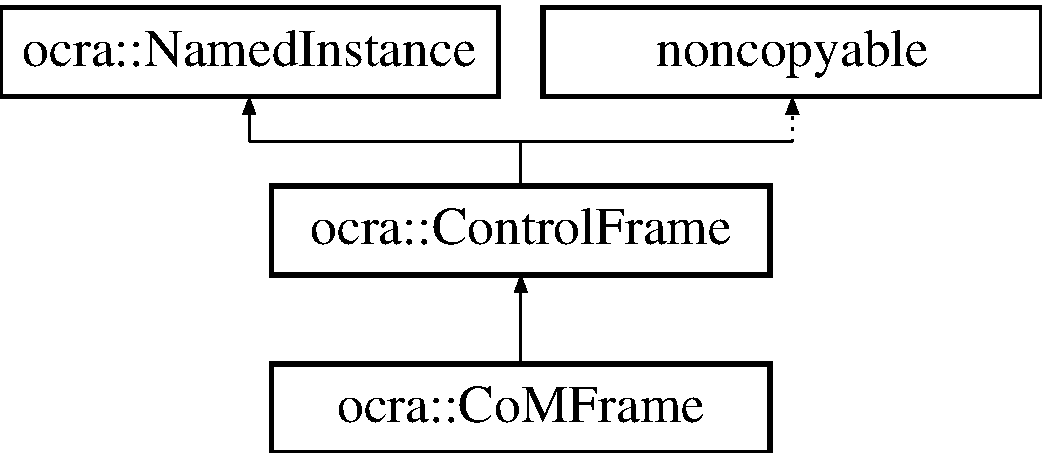
\includegraphics[height=3.000000cm]{d9/d52/classocra_1_1CoMFrame}
\end{center}
\end{figure}
\subsection*{Classes}
\begin{DoxyCompactItemize}
\item 
struct \hyperlink{structocra_1_1CoMFrame_1_1Pimpl}{Pimpl}
\end{DoxyCompactItemize}
\subsection*{Public Member Functions}
\begin{DoxyCompactItemize}
\item 
\hyperlink{classocra_1_1CoMFrame_a0b9177034d13b851238da7edfadcdf38}{Co\+M\+Frame} (const std\+::string \&name, const Model \&model)
\item 
Eigen\+::\+Displacementd \hyperlink{classocra_1_1CoMFrame_a809c05664b2e2abb489e930e27fbe2d4}{get\+Position} () const
\item 
Eigen\+::\+Twistd \hyperlink{classocra_1_1CoMFrame_a02be3e73c64903d67b1e7ada25c468c5}{get\+Velocity} () const
\item 
Eigen\+::\+Twistd \hyperlink{classocra_1_1CoMFrame_a9e59ca65720c553da5c75f484544829c}{get\+Acceleration} () const
\item 
Eigen\+::\+Wrenchd \hyperlink{classocra_1_1CoMFrame_a8e00462bbe13df6f595b7000d44240c6}{get\+Wrench} () const
\item 
Eigen\+::\+Matrix$<$ double, 6, Eigen\+::\+Dynamic $>$ \hyperlink{classocra_1_1CoMFrame_ab24f3400af3e8eb2a12d6597ff8a7a31}{get\+Jacobian} () const
\item 
bool \hyperlink{classocra_1_1CoMFrame_aaae3fd05da2f9e301dbe1c54b57fe624}{depends\+On\+Model\+Configuration} () const
\item 
const Model \& \hyperlink{classocra_1_1CoMFrame_afc280df9814e7eb2cf62f017f7bbfc2e}{get\+Model} () const
\end{DoxyCompactItemize}
\subsection*{Additional Inherited Members}


\subsection{Detailed Description}
Creates a frame whose center is at the CoM of the model and whose axes are parallel to the axes of the world frame. 

Definition at line 131 of file Control\+Frame.\+h.



\subsection{Constructor \& Destructor Documentation}
\hypertarget{classocra_1_1CoMFrame_a0b9177034d13b851238da7edfadcdf38}{}\label{classocra_1_1CoMFrame_a0b9177034d13b851238da7edfadcdf38} 
\index{ocra\+::\+Co\+M\+Frame@{ocra\+::\+Co\+M\+Frame}!Co\+M\+Frame@{Co\+M\+Frame}}
\index{Co\+M\+Frame@{Co\+M\+Frame}!ocra\+::\+Co\+M\+Frame@{ocra\+::\+Co\+M\+Frame}}
\subsubsection{\texorpdfstring{Co\+M\+Frame()}{CoMFrame()}}
{\footnotesize\ttfamily ocra\+::\+Co\+M\+Frame\+::\+Co\+M\+Frame (\begin{DoxyParamCaption}\item[{const std\+::string \&}]{name,  }\item[{const Model \&}]{model }\end{DoxyParamCaption})}



Definition at line 215 of file Control\+Frame.\+cpp.



\subsection{Member Function Documentation}
\hypertarget{classocra_1_1CoMFrame_aaae3fd05da2f9e301dbe1c54b57fe624}{}\label{classocra_1_1CoMFrame_aaae3fd05da2f9e301dbe1c54b57fe624} 
\index{ocra\+::\+Co\+M\+Frame@{ocra\+::\+Co\+M\+Frame}!depends\+On\+Model\+Configuration@{depends\+On\+Model\+Configuration}}
\index{depends\+On\+Model\+Configuration@{depends\+On\+Model\+Configuration}!ocra\+::\+Co\+M\+Frame@{ocra\+::\+Co\+M\+Frame}}
\subsubsection{\texorpdfstring{depends\+On\+Model\+Configuration()}{dependsOnModelConfiguration()}}
{\footnotesize\ttfamily bool ocra\+::\+Co\+M\+Frame\+::depends\+On\+Model\+Configuration (\begin{DoxyParamCaption}{ }\end{DoxyParamCaption}) const\hspace{0.3cm}{\ttfamily [virtual]}}



Implements \hyperlink{classocra_1_1ControlFrame_a65833d1f3f42bc8d452f8b1fb671e142}{ocra\+::\+Control\+Frame}.



Definition at line 249 of file Control\+Frame.\+cpp.

\hypertarget{classocra_1_1CoMFrame_a9e59ca65720c553da5c75f484544829c}{}\label{classocra_1_1CoMFrame_a9e59ca65720c553da5c75f484544829c} 
\index{ocra\+::\+Co\+M\+Frame@{ocra\+::\+Co\+M\+Frame}!get\+Acceleration@{get\+Acceleration}}
\index{get\+Acceleration@{get\+Acceleration}!ocra\+::\+Co\+M\+Frame@{ocra\+::\+Co\+M\+Frame}}
\subsubsection{\texorpdfstring{get\+Acceleration()}{getAcceleration()}}
{\footnotesize\ttfamily Eigen\+::\+Twistd ocra\+::\+Co\+M\+Frame\+::get\+Acceleration (\begin{DoxyParamCaption}{ }\end{DoxyParamCaption}) const\hspace{0.3cm}{\ttfamily [virtual]}}



Implements \hyperlink{classocra_1_1ControlFrame_a0ceb7cd7c3fe90fa0ef311b96a6f5c88}{ocra\+::\+Control\+Frame}.



Definition at line 231 of file Control\+Frame.\+cpp.

\hypertarget{classocra_1_1CoMFrame_ab24f3400af3e8eb2a12d6597ff8a7a31}{}\label{classocra_1_1CoMFrame_ab24f3400af3e8eb2a12d6597ff8a7a31} 
\index{ocra\+::\+Co\+M\+Frame@{ocra\+::\+Co\+M\+Frame}!get\+Jacobian@{get\+Jacobian}}
\index{get\+Jacobian@{get\+Jacobian}!ocra\+::\+Co\+M\+Frame@{ocra\+::\+Co\+M\+Frame}}
\subsubsection{\texorpdfstring{get\+Jacobian()}{getJacobian()}}
{\footnotesize\ttfamily \hyperlink{namespaceocra_ac73b015f9f7cb0c252c4d5c4800f559a}{Jacobian6d} ocra\+::\+Co\+M\+Frame\+::get\+Jacobian (\begin{DoxyParamCaption}{ }\end{DoxyParamCaption}) const\hspace{0.3cm}{\ttfamily [virtual]}}



Implements \hyperlink{classocra_1_1ControlFrame_a14e0b855979be5dbd360314f25191e77}{ocra\+::\+Control\+Frame}.



Definition at line 241 of file Control\+Frame.\+cpp.

\hypertarget{classocra_1_1CoMFrame_afc280df9814e7eb2cf62f017f7bbfc2e}{}\label{classocra_1_1CoMFrame_afc280df9814e7eb2cf62f017f7bbfc2e} 
\index{ocra\+::\+Co\+M\+Frame@{ocra\+::\+Co\+M\+Frame}!get\+Model@{get\+Model}}
\index{get\+Model@{get\+Model}!ocra\+::\+Co\+M\+Frame@{ocra\+::\+Co\+M\+Frame}}
\subsubsection{\texorpdfstring{get\+Model()}{getModel()}}
{\footnotesize\ttfamily const Model \& ocra\+::\+Co\+M\+Frame\+::get\+Model (\begin{DoxyParamCaption}{ }\end{DoxyParamCaption}) const\hspace{0.3cm}{\ttfamily [virtual]}}



Implements \hyperlink{classocra_1_1ControlFrame_ab8a1e5e3d96d7524112b4c88bf0bc5ee}{ocra\+::\+Control\+Frame}.



Definition at line 254 of file Control\+Frame.\+cpp.

\hypertarget{classocra_1_1CoMFrame_a809c05664b2e2abb489e930e27fbe2d4}{}\label{classocra_1_1CoMFrame_a809c05664b2e2abb489e930e27fbe2d4} 
\index{ocra\+::\+Co\+M\+Frame@{ocra\+::\+Co\+M\+Frame}!get\+Position@{get\+Position}}
\index{get\+Position@{get\+Position}!ocra\+::\+Co\+M\+Frame@{ocra\+::\+Co\+M\+Frame}}
\subsubsection{\texorpdfstring{get\+Position()}{getPosition()}}
{\footnotesize\ttfamily Eigen\+::\+Displacementd ocra\+::\+Co\+M\+Frame\+::get\+Position (\begin{DoxyParamCaption}{ }\end{DoxyParamCaption}) const\hspace{0.3cm}{\ttfamily [virtual]}}



Implements \hyperlink{classocra_1_1ControlFrame_aaadbbfbcdd5b8e197a0f181ffb2fdcbe}{ocra\+::\+Control\+Frame}.



Definition at line 221 of file Control\+Frame.\+cpp.

\hypertarget{classocra_1_1CoMFrame_a02be3e73c64903d67b1e7ada25c468c5}{}\label{classocra_1_1CoMFrame_a02be3e73c64903d67b1e7ada25c468c5} 
\index{ocra\+::\+Co\+M\+Frame@{ocra\+::\+Co\+M\+Frame}!get\+Velocity@{get\+Velocity}}
\index{get\+Velocity@{get\+Velocity}!ocra\+::\+Co\+M\+Frame@{ocra\+::\+Co\+M\+Frame}}
\subsubsection{\texorpdfstring{get\+Velocity()}{getVelocity()}}
{\footnotesize\ttfamily Eigen\+::\+Twistd ocra\+::\+Co\+M\+Frame\+::get\+Velocity (\begin{DoxyParamCaption}{ }\end{DoxyParamCaption}) const\hspace{0.3cm}{\ttfamily [virtual]}}



Implements \hyperlink{classocra_1_1ControlFrame_a398df839f75886867c86a8e70ac9bf24}{ocra\+::\+Control\+Frame}.



Definition at line 226 of file Control\+Frame.\+cpp.

\hypertarget{classocra_1_1CoMFrame_a8e00462bbe13df6f595b7000d44240c6}{}\label{classocra_1_1CoMFrame_a8e00462bbe13df6f595b7000d44240c6} 
\index{ocra\+::\+Co\+M\+Frame@{ocra\+::\+Co\+M\+Frame}!get\+Wrench@{get\+Wrench}}
\index{get\+Wrench@{get\+Wrench}!ocra\+::\+Co\+M\+Frame@{ocra\+::\+Co\+M\+Frame}}
\subsubsection{\texorpdfstring{get\+Wrench()}{getWrench()}}
{\footnotesize\ttfamily Eigen\+::\+Wrenchd ocra\+::\+Co\+M\+Frame\+::get\+Wrench (\begin{DoxyParamCaption}{ }\end{DoxyParamCaption}) const\hspace{0.3cm}{\ttfamily [virtual]}}



Implements \hyperlink{classocra_1_1ControlFrame_a069aaf1eab98598fbffee263fcde0c56}{ocra\+::\+Control\+Frame}.



Definition at line 236 of file Control\+Frame.\+cpp.



The documentation for this class was generated from the following files\+:\begin{DoxyCompactItemize}
\item 
\hyperlink{ControlFrame_8h}{Control\+Frame.\+h}\item 
\hyperlink{ControlFrame_8cpp}{Control\+Frame.\+cpp}\end{DoxyCompactItemize}

\hypertarget{classocra_1_1Component}{}\section{ocra\+:\+:Component$<$ Component\+Derived, Composite\+Derived, Parenthood\+Info $>$ Class Template Reference}
\label{classocra_1_1Component}\index{ocra\+::\+Component$<$ Component\+Derived, Composite\+Derived, Parenthood\+Info $>$@{ocra\+::\+Component$<$ Component\+Derived, Composite\+Derived, Parenthood\+Info $>$}}


Base class for the \hyperlink{classocra_1_1Component}{Component} class of the \hyperlink{classocra_1_1Composite}{Composite} pattern.  




{\ttfamily \#include $<$Composite.\+h$>$}

\subsection*{Public Types}
{\bf }\par
\begin{DoxyCompactItemize}
\item 
typedef Component\+Derived \hyperlink{classocra_1_1Component_aecb250aaac3aad8d82ba30303b10cf2a}{component\+\_\+t}
\begin{DoxyCompactList}\small\item\em Inherited typedefs. \end{DoxyCompactList}\item 
typedef Composite\+Derived \hyperlink{classocra_1_1Component_a2111c5ff33bd22310754dfd54c9e2a34}{parent\+\_\+t}
\item 
typedef \hyperlink{classocra_1_1Parenthood}{Parenthood}$<$ Component\+Derived, Composite\+Derived, Parenthood\+Info $>$ \hyperlink{classocra_1_1Component_a70fb7cda78934a9f017c7e46c1407953}{parenthood\+\_\+t}
\item 
typedef std\+::vector$<$ \hyperlink{classocra_1_1Component_a70fb7cda78934a9f017c7e46c1407953}{parenthood\+\_\+t} $\ast$ $>$\+::\hyperlink{classocra_1_1Component_a6271631f04d2911e4369d1288074eebb}{const\+\_\+iterator} \hyperlink{classocra_1_1Component_a6271631f04d2911e4369d1288074eebb}{const\+\_\+iterator}
\item 
typedef std\+::vector$<$ \hyperlink{classocra_1_1Component_a70fb7cda78934a9f017c7e46c1407953}{parenthood\+\_\+t} $\ast$ $>$\+::\hyperlink{classocra_1_1Component_a9b76b63c3248ec96dfdaca00d712c1c9}{iterator} \hyperlink{classocra_1_1Component_a9b76b63c3248ec96dfdaca00d712c1c9}{iterator}
\end{DoxyCompactItemize}

\subsection*{Public Member Functions}
\begin{DoxyCompactItemize}
\item 
bool \hyperlink{classocra_1_1Component_a77448d773b20fda6d8349d20691a8840}{is\+Child\+Of} (const Composite\+Derived \&node)
\item 
void \hyperlink{classocra_1_1Component_a9bc74f9a471df60ee9b1d49e7f55e04f}{print\+Tree} (std\+::ostream \&os)
\item 
virtual int \hyperlink{classocra_1_1Component_a8a0e052f36c60889562e921751b02a37}{is\+Ancestor\+Of} (const Component\+Derived \&node) const =0
\begin{DoxyCompactList}\small\item\em Returns the number of levels that separate the component from a potential child. \end{DoxyCompactList}\item 
virtual void \hyperlink{classocra_1_1Component_a3687a02c1524694fc616893264ca8199}{print\+Sub\+Tree} (int depth, std\+::ostream \&os) const =0
\begin{DoxyCompactList}\small\item\em Overload in Component\+Derived and Composite\+Derived to simply call print\+Tree\+\_\+impl(). \end{DoxyCompactList}\item 
virtual void \hyperlink{classocra_1_1Component_a61bb6d9557a6ba3d13f9bc083422d1a7}{print\+Node} (int depth, std\+::ostream \&os) const =0
\begin{DoxyCompactList}\small\item\em Overload in Component\+Derived and Composite\+Derived to print information about the tree node. \end{DoxyCompactList}\end{DoxyCompactItemize}
{\bf }\par
\begin{DoxyCompactItemize}
\item 
size\+\_\+t \hyperlink{classocra_1_1Component_abc5066cb5523dd4ee8782ab7f75a26d5}{get\+Num\+Parenthoods} () const
\begin{DoxyCompactList}\small\item\em Basic access to the parents. \end{DoxyCompactList}\item 
const \hyperlink{classocra_1_1Component_a70fb7cda78934a9f017c7e46c1407953}{parenthood\+\_\+t} \& \hyperlink{classocra_1_1Component_a368948e115852fa524f9a8da257aed1f}{get\+Parenthood} (size\+\_\+t i) const
\end{DoxyCompactItemize}

{\bf }\par
\begin{DoxyCompactItemize}
\item 
\hyperlink{classocra_1_1Component_a6271631f04d2911e4369d1288074eebb}{const\+\_\+iterator} \hyperlink{classocra_1_1Component_ad140927464e2afefd563ee52751bb09f}{parents\+\_\+begin} () const
\begin{DoxyCompactList}\small\item\em Iterator range on the set of parents. \end{DoxyCompactList}\item 
\hyperlink{classocra_1_1Component_a9b76b63c3248ec96dfdaca00d712c1c9}{iterator} \hyperlink{classocra_1_1Component_aaca1c77fdf2c7d090f43a3eefb671eae}{parents\+\_\+begin} ()
\item 
\hyperlink{classocra_1_1Component_a6271631f04d2911e4369d1288074eebb}{const\+\_\+iterator} \hyperlink{classocra_1_1Component_a3d7c4568dc83d08b014ae7b8d0119e70}{parents\+\_\+end} () const
\item 
\hyperlink{classocra_1_1Component_a9b76b63c3248ec96dfdaca00d712c1c9}{iterator} \hyperlink{classocra_1_1Component_a15dc70cd778a884fd6aa27771189d091}{parents\+\_\+end} ()
\end{DoxyCompactItemize}

{\bf }\par
\begin{DoxyCompactItemize}
\item 
int \hyperlink{classocra_1_1Component_a6ed1720bbd5d8f3ef0b10aed73c36f6e}{is\+Descendant\+Of} (const Composite\+Derived \&node) const
\begin{DoxyCompactList}\small\item\em Returns the number of levels that separates the component from a potential parent. \end{DoxyCompactList}\item 
int \hyperlink{classocra_1_1Component_a27fb70e09c4e981077d42ca196301cd3}{is\+Descendant\+Of} (const Component\+Derived \&node) const
\end{DoxyCompactItemize}

\subsection*{Protected Member Functions}
{\bf }\par
\begin{DoxyCompactItemize}
\item 
virtual void \hyperlink{classocra_1_1Component_aa59ac72499ba7d314d9602b081d0b475}{on\+Attached\+Parent} (const \hyperlink{classocra_1_1Component_a70fb7cda78934a9f017c7e46c1407953}{parenthood\+\_\+t} \&parent)
\begin{DoxyCompactList}\small\item\em Default implementation of the callbacks, to overload in class Component\+Derived. \end{DoxyCompactList}\item 
virtual void \hyperlink{classocra_1_1Component_a0dd26028434be8efbebccb088ddbec65}{on\+Detached\+Parent} (const \hyperlink{classocra_1_1Component_a70fb7cda78934a9f017c7e46c1407953}{parenthood\+\_\+t} \&parent)
\end{DoxyCompactItemize}

{\bf }\par
\begin{DoxyCompactItemize}
\item 
\hyperlink{classocra_1_1Component_a4c76a9060703e7f524c73f6b328bb3e1}{Component} ()
\item 
\hyperlink{classocra_1_1Component_a616d0b940599b102fa630107ec169e58}{$\sim$\+Component} ()
\end{DoxyCompactItemize}

\subsection*{Friends}
\begin{DoxyCompactItemize}
\item 
class \hyperlink{classocra_1_1Component_ad71e675afae5fce6263d2d784cd3907a}{Parenthood$<$ Component\+Derived, Composite\+Derived, Parenthood\+Info $>$}
\end{DoxyCompactItemize}


\subsection{Detailed Description}
\subsubsection*{template$<$class Component\+Derived, class Composite\+Derived, class Parenthood\+Info = No\+Info$>$\newline
class ocra\+::\+Component$<$ Component\+Derived, Composite\+Derived, Parenthood\+Info $>$}

Base class for the \hyperlink{classocra_1_1Component}{Component} class of the \hyperlink{classocra_1_1Composite}{Composite} pattern. 

\hyperlink{classocra_1_1Composite}{Composite} objects are built upon a tree of objects, whose nodes implement the type \hyperlink{classocra_1_1Component}{Component}. \hyperlink{classocra_1_1Component}{Component} is specialized in\+:
\begin{DoxyItemize}
\item \hyperlink{classocra_1_1Composite}{Composite}\+: \hyperlink{classocra_1_1Composite}{Composite} nodes have children
\item \hyperlink{classocra_1_1Leaf}{Leaf}.
\end{DoxyItemize}

See the wikipedia article about the \hyperlink{classocra_1_1Composite}{Composite} design pattern for more information.

This class can be used as a base class to implement a \hyperlink{classocra_1_1Composite}{Composite} pattern. To use it, you have to take the following steps\+:
\begin{DoxyEnumerate}
\item Create an interface or a base class for your component. This interface will be used to manipulate your objects without knowing whether they are one-\/piece objects or composite objects.
\item Derive two classes from it\+: one to implement the composite components, and the other one to implement the leaves (one-\/piece components).
\item Assuming the aformentionned classes are named My\+Component, My\+Composite and My\+Leaf, make them derive from respectively\+: Component$<$\+My\+Component, My\+Composite$>$, Composite$<$\+My\+Component, My\+Composite$>$, and Leaf$<$\+My\+Leaf$>$. An additional template parameter can be used for My\+Component and My\+Composite to specify additional information about the bonds between a \hyperlink{classocra_1_1Composite}{Composite} object and its children (see class \hyperlink{classocra_1_1Parenthood}{ocra\+::\+Parenthood}).
\item Implement is\+Ancestor\+Of and other abstract methods in My\+Composite and My\+Leaf (see the doc of is\+Ancestor\+Of or the example below); The methods to implement in your children classes are declared together in this class in a dedicated section so that you can easily spot them.
\item Implement your stuff.
\item Instantiate your objects and attach them to each other.
\end{DoxyEnumerate}

The following example illustrates the simpliest form of these steps. In your code, you will of course use classes instead of structs if necessary...  \#include \char`\"{}\+Composite.\+h\char`\"{}

struct Group\+Of\+Shapes;

struct Shape \+: public ocra\+::\+Component$<$\+Shape, Group\+Of\+Shapes$>$ \{ virtual void resize() = 0; \};

struct Single\+Shape \+: public Shape, public ocra\+::\+Leaf$<$\+Single\+Shape$>$ \{ void resize() \{\} int is\+Ancestor\+Of(const Shape\& shape) const \{ return 0; \} \};

struct Group\+Of\+Shapes \+: public Shape, public ocra\+::\+Composite$<$\+Shape, Group\+Of\+Shapes$>$ \{ void resize() \{\} int is\+Ancestor\+Of(const Shape\& shape) const \{ return is\+Ancestor\+Of\+\_\+impl(shape); \} \};

int \hyperlink{main_8cpp_a3c04138a5bfe5d72780bb7e82a18e627}{main()} \{ Single\+Shape leaf1; Single\+Shape leaf2; Group\+Of\+Shapes node; node.\+attach(leaf1); node.\+attach(leaf2); node.\+detach(leaf1); \} 

In this implementation, a node can be part of several trees and can therefore have several parents. However, cycles are forbidden.


\begin{DoxyTemplParams}{Template Parameters}
{\em Component\+Derived} & is the abstract type used to manipulate both nodes and leaves without knowledge of whether they are composite or not. \\
\hline
{\em Composite\+Derived} & is the type of the composite objects, i.\+e. objects that are composed of several subobjects. \\
\hline
{\em Parenthood\+Info} & is an additional type to associate additional information with a parenthood relationship. It must be default constructible with a default constructor (it can be the one defined by the compiler).\\
\hline
\end{DoxyTemplParams}
\begin{DoxyPrecond}{Precondition}
Composite\+Derived is a publicly derived class of Component\+Derived. 

Parenthood\+Info is default constructible with a no-\/throw default constructor. 

Component\+Derived publicly derives Component$<$\+Component\+Derived, Composite\+Derived, Parenthood\+Info$>$. 

Composite\+Derived publicly derives Composite$<$\+Component\+Derived, Composite\+Derived, Parenthood\+Info$>$.
\end{DoxyPrecond}
The preconditions on the template parameters will be enforced at compile-\/time by the \hyperlink{classocra_1_1Parenthood}{Parenthood} class. If a B\+O\+O\+S\+T\+\_\+\+S\+T\+A\+T\+I\+C\+\_\+\+A\+S\+S\+E\+RT is fired when compiling your composite classes, please have a look at the name of the parameter of the failing assertion\+: it will give you a hint about how to correct your code. 

Definition at line 37 of file Composite.\+h.



\subsection{Member Typedef Documentation}
\hypertarget{classocra_1_1Component_aecb250aaac3aad8d82ba30303b10cf2a}{}\label{classocra_1_1Component_aecb250aaac3aad8d82ba30303b10cf2a} 
\index{ocra\+::\+Component@{ocra\+::\+Component}!component\+\_\+t@{component\+\_\+t}}
\index{component\+\_\+t@{component\+\_\+t}!ocra\+::\+Component@{ocra\+::\+Component}}
\subsubsection{\texorpdfstring{component\+\_\+t}{component\_t}}
{\footnotesize\ttfamily template$<$class Component\+Derived, class Composite\+Derived, class Parenthood\+Info = No\+Info$>$ \\
typedef Component\+Derived \hyperlink{classocra_1_1Component}{ocra\+::\+Component}$<$ Component\+Derived, Composite\+Derived, Parenthood\+Info $>$\+::\hyperlink{classocra_1_1Component_aecb250aaac3aad8d82ba30303b10cf2a}{component\+\_\+t}}



Inherited typedefs. 



Definition at line 456 of file Composite.\+h.

\hypertarget{classocra_1_1Component_a6271631f04d2911e4369d1288074eebb}{}\label{classocra_1_1Component_a6271631f04d2911e4369d1288074eebb} 
\index{ocra\+::\+Component@{ocra\+::\+Component}!const\+\_\+iterator@{const\+\_\+iterator}}
\index{const\+\_\+iterator@{const\+\_\+iterator}!ocra\+::\+Component@{ocra\+::\+Component}}
\subsubsection{\texorpdfstring{const\+\_\+iterator}{const\_iterator}}
{\footnotesize\ttfamily template$<$class Component\+Derived, class Composite\+Derived, class Parenthood\+Info = No\+Info$>$ \\
typedef std\+::vector$<$\hyperlink{classocra_1_1Component_a70fb7cda78934a9f017c7e46c1407953}{parenthood\+\_\+t}$\ast$$>$\+::\hyperlink{classocra_1_1Component_a6271631f04d2911e4369d1288074eebb}{const\+\_\+iterator} \hyperlink{classocra_1_1Component}{ocra\+::\+Component}$<$ Component\+Derived, Composite\+Derived, Parenthood\+Info $>$\+::\hyperlink{classocra_1_1Component_a6271631f04d2911e4369d1288074eebb}{const\+\_\+iterator}}



Definition at line 459 of file Composite.\+h.

\hypertarget{classocra_1_1Component_a9b76b63c3248ec96dfdaca00d712c1c9}{}\label{classocra_1_1Component_a9b76b63c3248ec96dfdaca00d712c1c9} 
\index{ocra\+::\+Component@{ocra\+::\+Component}!iterator@{iterator}}
\index{iterator@{iterator}!ocra\+::\+Component@{ocra\+::\+Component}}
\subsubsection{\texorpdfstring{iterator}{iterator}}
{\footnotesize\ttfamily template$<$class Component\+Derived, class Composite\+Derived, class Parenthood\+Info = No\+Info$>$ \\
typedef std\+::vector$<$\hyperlink{classocra_1_1Component_a70fb7cda78934a9f017c7e46c1407953}{parenthood\+\_\+t}$\ast$$>$\+::\hyperlink{classocra_1_1Component_a9b76b63c3248ec96dfdaca00d712c1c9}{iterator} \hyperlink{classocra_1_1Component}{ocra\+::\+Component}$<$ Component\+Derived, Composite\+Derived, Parenthood\+Info $>$\+::\hyperlink{classocra_1_1Component_a9b76b63c3248ec96dfdaca00d712c1c9}{iterator}}



Definition at line 460 of file Composite.\+h.

\hypertarget{classocra_1_1Component_a2111c5ff33bd22310754dfd54c9e2a34}{}\label{classocra_1_1Component_a2111c5ff33bd22310754dfd54c9e2a34} 
\index{ocra\+::\+Component@{ocra\+::\+Component}!parent\+\_\+t@{parent\+\_\+t}}
\index{parent\+\_\+t@{parent\+\_\+t}!ocra\+::\+Component@{ocra\+::\+Component}}
\subsubsection{\texorpdfstring{parent\+\_\+t}{parent\_t}}
{\footnotesize\ttfamily template$<$class Component\+Derived, class Composite\+Derived, class Parenthood\+Info = No\+Info$>$ \\
typedef Composite\+Derived \hyperlink{classocra_1_1Component}{ocra\+::\+Component}$<$ Component\+Derived, Composite\+Derived, Parenthood\+Info $>$\+::\hyperlink{classocra_1_1Component_a2111c5ff33bd22310754dfd54c9e2a34}{parent\+\_\+t}}



Definition at line 457 of file Composite.\+h.

\hypertarget{classocra_1_1Component_a70fb7cda78934a9f017c7e46c1407953}{}\label{classocra_1_1Component_a70fb7cda78934a9f017c7e46c1407953} 
\index{ocra\+::\+Component@{ocra\+::\+Component}!parenthood\+\_\+t@{parenthood\+\_\+t}}
\index{parenthood\+\_\+t@{parenthood\+\_\+t}!ocra\+::\+Component@{ocra\+::\+Component}}
\subsubsection{\texorpdfstring{parenthood\+\_\+t}{parenthood\_t}}
{\footnotesize\ttfamily template$<$class Component\+Derived, class Composite\+Derived, class Parenthood\+Info = No\+Info$>$ \\
typedef \hyperlink{classocra_1_1Parenthood}{Parenthood}$<$Component\+Derived, Composite\+Derived, Parenthood\+Info$>$ \hyperlink{classocra_1_1Component}{ocra\+::\+Component}$<$ Component\+Derived, Composite\+Derived, Parenthood\+Info $>$\+::\hyperlink{classocra_1_1Component_a70fb7cda78934a9f017c7e46c1407953}{parenthood\+\_\+t}}



Definition at line 458 of file Composite.\+h.



\subsection{Constructor \& Destructor Documentation}
\hypertarget{classocra_1_1Component_a4c76a9060703e7f524c73f6b328bb3e1}{}\label{classocra_1_1Component_a4c76a9060703e7f524c73f6b328bb3e1} 
\index{ocra\+::\+Component@{ocra\+::\+Component}!Component@{Component}}
\index{Component@{Component}!ocra\+::\+Component@{ocra\+::\+Component}}
\subsubsection{\texorpdfstring{Component()}{Component()}}
{\footnotesize\ttfamily template$<$class Component\+Derived, class Composite\+Derived, class Parenthood\+Info = No\+Info$>$ \\
\hyperlink{classocra_1_1Component}{ocra\+::\+Component}$<$ Component\+Derived, Composite\+Derived, Parenthood\+Info $>$\+::\hyperlink{classocra_1_1Component}{Component} (\begin{DoxyParamCaption}{ }\end{DoxyParamCaption})\hspace{0.3cm}{\ttfamily [inline]}, {\ttfamily [protected]}}



Definition at line 548 of file Composite.\+h.

\hypertarget{classocra_1_1Component_a616d0b940599b102fa630107ec169e58}{}\label{classocra_1_1Component_a616d0b940599b102fa630107ec169e58} 
\index{ocra\+::\+Component@{ocra\+::\+Component}!````~Component@{$\sim$\+Component}}
\index{````~Component@{$\sim$\+Component}!ocra\+::\+Component@{ocra\+::\+Component}}
\subsubsection{\texorpdfstring{$\sim$\+Component()}{~Component()}}
{\footnotesize\ttfamily template$<$class Component\+Derived, class Composite\+Derived, class Parenthood\+Info = No\+Info$>$ \\
\hyperlink{classocra_1_1Component}{ocra\+::\+Component}$<$ Component\+Derived, Composite\+Derived, Parenthood\+Info $>$\+::$\sim$\hyperlink{classocra_1_1Component}{Component} (\begin{DoxyParamCaption}{ }\end{DoxyParamCaption})\hspace{0.3cm}{\ttfamily [inline]}, {\ttfamily [protected]}}



Definition at line 551 of file Composite.\+h.



\subsection{Member Function Documentation}
\hypertarget{classocra_1_1Component_abc5066cb5523dd4ee8782ab7f75a26d5}{}\label{classocra_1_1Component_abc5066cb5523dd4ee8782ab7f75a26d5} 
\index{ocra\+::\+Component@{ocra\+::\+Component}!get\+Num\+Parenthoods@{get\+Num\+Parenthoods}}
\index{get\+Num\+Parenthoods@{get\+Num\+Parenthoods}!ocra\+::\+Component@{ocra\+::\+Component}}
\subsubsection{\texorpdfstring{get\+Num\+Parenthoods()}{getNumParenthoods()}}
{\footnotesize\ttfamily template$<$class Component\+Derived, class Composite\+Derived, class Parenthood\+Info = No\+Info$>$ \\
size\+\_\+t \hyperlink{classocra_1_1Component}{ocra\+::\+Component}$<$ Component\+Derived, Composite\+Derived, Parenthood\+Info $>$\+::get\+Num\+Parenthoods (\begin{DoxyParamCaption}{ }\end{DoxyParamCaption}) const\hspace{0.3cm}{\ttfamily [inline]}}



Basic access to the parents. 



Definition at line 466 of file Composite.\+h.

\hypertarget{classocra_1_1Component_a368948e115852fa524f9a8da257aed1f}{}\label{classocra_1_1Component_a368948e115852fa524f9a8da257aed1f} 
\index{ocra\+::\+Component@{ocra\+::\+Component}!get\+Parenthood@{get\+Parenthood}}
\index{get\+Parenthood@{get\+Parenthood}!ocra\+::\+Component@{ocra\+::\+Component}}
\subsubsection{\texorpdfstring{get\+Parenthood()}{getParenthood()}}
{\footnotesize\ttfamily template$<$class Component\+Derived, class Composite\+Derived, class Parenthood\+Info = No\+Info$>$ \\
const \hyperlink{classocra_1_1Component_a70fb7cda78934a9f017c7e46c1407953}{parenthood\+\_\+t}\& \hyperlink{classocra_1_1Component}{ocra\+::\+Component}$<$ Component\+Derived, Composite\+Derived, Parenthood\+Info $>$\+::get\+Parenthood (\begin{DoxyParamCaption}\item[{size\+\_\+t}]{i }\end{DoxyParamCaption}) const\hspace{0.3cm}{\ttfamily [inline]}}



Definition at line 467 of file Composite.\+h.

\hypertarget{classocra_1_1Component_a8a0e052f36c60889562e921751b02a37}{}\label{classocra_1_1Component_a8a0e052f36c60889562e921751b02a37} 
\index{ocra\+::\+Component@{ocra\+::\+Component}!is\+Ancestor\+Of@{is\+Ancestor\+Of}}
\index{is\+Ancestor\+Of@{is\+Ancestor\+Of}!ocra\+::\+Component@{ocra\+::\+Component}}
\subsubsection{\texorpdfstring{is\+Ancestor\+Of()}{isAncestorOf()}}
{\footnotesize\ttfamily template$<$class Component\+Derived, class Composite\+Derived, class Parenthood\+Info = No\+Info$>$ \\
virtual int \hyperlink{classocra_1_1Component}{ocra\+::\+Component}$<$ Component\+Derived, Composite\+Derived, Parenthood\+Info $>$\+::is\+Ancestor\+Of (\begin{DoxyParamCaption}\item[{const Component\+Derived \&}]{node }\end{DoxyParamCaption}) const\hspace{0.3cm}{\ttfamily [pure virtual]}}



Returns the number of levels that separate the component from a potential child. 



Implemented in \hyperlink{classocra_1_1CompositeVariable_a6601ac71bdd683d06a7a6bfe4fa7252c}{ocra\+::\+Composite\+Variable}, and \hyperlink{classocra_1_1BaseVariable_a66d07236f4d060273f3f46632dc851ac}{ocra\+::\+Base\+Variable}.

\hypertarget{classocra_1_1Component_a77448d773b20fda6d8349d20691a8840}{}\label{classocra_1_1Component_a77448d773b20fda6d8349d20691a8840} 
\index{ocra\+::\+Component@{ocra\+::\+Component}!is\+Child\+Of@{is\+Child\+Of}}
\index{is\+Child\+Of@{is\+Child\+Of}!ocra\+::\+Component@{ocra\+::\+Component}}
\subsubsection{\texorpdfstring{is\+Child\+Of()}{isChildOf()}}
{\footnotesize\ttfamily template$<$class Component\+Derived, class Composite\+Derived, class Parenthood\+Info = No\+Info$>$ \\
bool \hyperlink{classocra_1_1Component}{ocra\+::\+Component}$<$ Component\+Derived, Composite\+Derived, Parenthood\+Info $>$\+::is\+Child\+Of (\begin{DoxyParamCaption}\item[{const Composite\+Derived \&}]{node }\end{DoxyParamCaption})\hspace{0.3cm}{\ttfamily [inline]}}



Definition at line 489 of file Composite.\+h.

\hypertarget{classocra_1_1Component_a6ed1720bbd5d8f3ef0b10aed73c36f6e}{}\label{classocra_1_1Component_a6ed1720bbd5d8f3ef0b10aed73c36f6e} 
\index{ocra\+::\+Component@{ocra\+::\+Component}!is\+Descendant\+Of@{is\+Descendant\+Of}}
\index{is\+Descendant\+Of@{is\+Descendant\+Of}!ocra\+::\+Component@{ocra\+::\+Component}}
\subsubsection{\texorpdfstring{is\+Descendant\+Of()}{isDescendantOf()}\hspace{0.1cm}{\footnotesize\ttfamily [1/2]}}
{\footnotesize\ttfamily template$<$class Component\+Derived, class Composite\+Derived, class Parenthood\+Info = No\+Info$>$ \\
int \hyperlink{classocra_1_1Component}{ocra\+::\+Component}$<$ Component\+Derived, Composite\+Derived, Parenthood\+Info $>$\+::is\+Descendant\+Of (\begin{DoxyParamCaption}\item[{const Composite\+Derived \&}]{node }\end{DoxyParamCaption}) const\hspace{0.3cm}{\ttfamily [inline]}}



Returns the number of levels that separates the component from a potential parent. 

If the object is not a descendant of node, returns 0. If it is a child of node, returns 1. If it is a grand-\/child, returns 2, and so on... 

Definition at line 485 of file Composite.\+h.

\hypertarget{classocra_1_1Component_a27fb70e09c4e981077d42ca196301cd3}{}\label{classocra_1_1Component_a27fb70e09c4e981077d42ca196301cd3} 
\index{ocra\+::\+Component@{ocra\+::\+Component}!is\+Descendant\+Of@{is\+Descendant\+Of}}
\index{is\+Descendant\+Of@{is\+Descendant\+Of}!ocra\+::\+Component@{ocra\+::\+Component}}
\subsubsection{\texorpdfstring{is\+Descendant\+Of()}{isDescendantOf()}\hspace{0.1cm}{\footnotesize\ttfamily [2/2]}}
{\footnotesize\ttfamily template$<$class Component\+Derived, class Composite\+Derived, class Parenthood\+Info = No\+Info$>$ \\
int \hyperlink{classocra_1_1Component}{ocra\+::\+Component}$<$ Component\+Derived, Composite\+Derived, Parenthood\+Info $>$\+::is\+Descendant\+Of (\begin{DoxyParamCaption}\item[{const Component\+Derived \&}]{node }\end{DoxyParamCaption}) const\hspace{0.3cm}{\ttfamily [inline]}}



Definition at line 486 of file Composite.\+h.

\hypertarget{classocra_1_1Component_aa59ac72499ba7d314d9602b081d0b475}{}\label{classocra_1_1Component_aa59ac72499ba7d314d9602b081d0b475} 
\index{ocra\+::\+Component@{ocra\+::\+Component}!on\+Attached\+Parent@{on\+Attached\+Parent}}
\index{on\+Attached\+Parent@{on\+Attached\+Parent}!ocra\+::\+Component@{ocra\+::\+Component}}
\subsubsection{\texorpdfstring{on\+Attached\+Parent()}{onAttachedParent()}}
{\footnotesize\ttfamily template$<$class Component\+Derived, class Composite\+Derived, class Parenthood\+Info = No\+Info$>$ \\
virtual void \hyperlink{classocra_1_1Component}{ocra\+::\+Component}$<$ Component\+Derived, Composite\+Derived, Parenthood\+Info $>$\+::on\+Attached\+Parent (\begin{DoxyParamCaption}\item[{const \hyperlink{classocra_1_1Component_a70fb7cda78934a9f017c7e46c1407953}{parenthood\+\_\+t} \&}]{parent }\end{DoxyParamCaption})\hspace{0.3cm}{\ttfamily [inline]}, {\ttfamily [protected]}, {\ttfamily [virtual]}}



Default implementation of the callbacks, to overload in class Component\+Derived. 

These callbacks are called once a parent and a child have been attached/detached. When the callback is called, the parenthood has already been registered/unregistered by the child and parent (this is guaranteed by the ocra\+::attach/ detach function). 

Definition at line 538 of file Composite.\+h.

\hypertarget{classocra_1_1Component_a0dd26028434be8efbebccb088ddbec65}{}\label{classocra_1_1Component_a0dd26028434be8efbebccb088ddbec65} 
\index{ocra\+::\+Component@{ocra\+::\+Component}!on\+Detached\+Parent@{on\+Detached\+Parent}}
\index{on\+Detached\+Parent@{on\+Detached\+Parent}!ocra\+::\+Component@{ocra\+::\+Component}}
\subsubsection{\texorpdfstring{on\+Detached\+Parent()}{onDetachedParent()}}
{\footnotesize\ttfamily template$<$class Component\+Derived, class Composite\+Derived, class Parenthood\+Info = No\+Info$>$ \\
virtual void \hyperlink{classocra_1_1Component}{ocra\+::\+Component}$<$ Component\+Derived, Composite\+Derived, Parenthood\+Info $>$\+::on\+Detached\+Parent (\begin{DoxyParamCaption}\item[{const \hyperlink{classocra_1_1Component_a70fb7cda78934a9f017c7e46c1407953}{parenthood\+\_\+t} \&}]{parent }\end{DoxyParamCaption})\hspace{0.3cm}{\ttfamily [inline]}, {\ttfamily [protected]}, {\ttfamily [virtual]}}



Definition at line 539 of file Composite.\+h.

\hypertarget{classocra_1_1Component_ad140927464e2afefd563ee52751bb09f}{}\label{classocra_1_1Component_ad140927464e2afefd563ee52751bb09f} 
\index{ocra\+::\+Component@{ocra\+::\+Component}!parents\+\_\+begin@{parents\+\_\+begin}}
\index{parents\+\_\+begin@{parents\+\_\+begin}!ocra\+::\+Component@{ocra\+::\+Component}}
\subsubsection{\texorpdfstring{parents\+\_\+begin()}{parents\_begin()}\hspace{0.1cm}{\footnotesize\ttfamily [1/2]}}
{\footnotesize\ttfamily template$<$class Component\+Derived, class Composite\+Derived, class Parenthood\+Info = No\+Info$>$ \\
\hyperlink{classocra_1_1Component_a6271631f04d2911e4369d1288074eebb}{const\+\_\+iterator} \hyperlink{classocra_1_1Component}{ocra\+::\+Component}$<$ Component\+Derived, Composite\+Derived, Parenthood\+Info $>$\+::parents\+\_\+begin (\begin{DoxyParamCaption}{ }\end{DoxyParamCaption}) const\hspace{0.3cm}{\ttfamily [inline]}}



Iterator range on the set of parents. 



Definition at line 472 of file Composite.\+h.

\hypertarget{classocra_1_1Component_aaca1c77fdf2c7d090f43a3eefb671eae}{}\label{classocra_1_1Component_aaca1c77fdf2c7d090f43a3eefb671eae} 
\index{ocra\+::\+Component@{ocra\+::\+Component}!parents\+\_\+begin@{parents\+\_\+begin}}
\index{parents\+\_\+begin@{parents\+\_\+begin}!ocra\+::\+Component@{ocra\+::\+Component}}
\subsubsection{\texorpdfstring{parents\+\_\+begin()}{parents\_begin()}\hspace{0.1cm}{\footnotesize\ttfamily [2/2]}}
{\footnotesize\ttfamily template$<$class Component\+Derived, class Composite\+Derived, class Parenthood\+Info = No\+Info$>$ \\
\hyperlink{classocra_1_1Component_a9b76b63c3248ec96dfdaca00d712c1c9}{iterator} \hyperlink{classocra_1_1Component}{ocra\+::\+Component}$<$ Component\+Derived, Composite\+Derived, Parenthood\+Info $>$\+::parents\+\_\+begin (\begin{DoxyParamCaption}{ }\end{DoxyParamCaption})\hspace{0.3cm}{\ttfamily [inline]}}



Definition at line 473 of file Composite.\+h.

\hypertarget{classocra_1_1Component_a3d7c4568dc83d08b014ae7b8d0119e70}{}\label{classocra_1_1Component_a3d7c4568dc83d08b014ae7b8d0119e70} 
\index{ocra\+::\+Component@{ocra\+::\+Component}!parents\+\_\+end@{parents\+\_\+end}}
\index{parents\+\_\+end@{parents\+\_\+end}!ocra\+::\+Component@{ocra\+::\+Component}}
\subsubsection{\texorpdfstring{parents\+\_\+end()}{parents\_end()}\hspace{0.1cm}{\footnotesize\ttfamily [1/2]}}
{\footnotesize\ttfamily template$<$class Component\+Derived, class Composite\+Derived, class Parenthood\+Info = No\+Info$>$ \\
\hyperlink{classocra_1_1Component_a6271631f04d2911e4369d1288074eebb}{const\+\_\+iterator} \hyperlink{classocra_1_1Component}{ocra\+::\+Component}$<$ Component\+Derived, Composite\+Derived, Parenthood\+Info $>$\+::parents\+\_\+end (\begin{DoxyParamCaption}{ }\end{DoxyParamCaption}) const\hspace{0.3cm}{\ttfamily [inline]}}



Definition at line 475 of file Composite.\+h.

\hypertarget{classocra_1_1Component_a15dc70cd778a884fd6aa27771189d091}{}\label{classocra_1_1Component_a15dc70cd778a884fd6aa27771189d091} 
\index{ocra\+::\+Component@{ocra\+::\+Component}!parents\+\_\+end@{parents\+\_\+end}}
\index{parents\+\_\+end@{parents\+\_\+end}!ocra\+::\+Component@{ocra\+::\+Component}}
\subsubsection{\texorpdfstring{parents\+\_\+end()}{parents\_end()}\hspace{0.1cm}{\footnotesize\ttfamily [2/2]}}
{\footnotesize\ttfamily template$<$class Component\+Derived, class Composite\+Derived, class Parenthood\+Info = No\+Info$>$ \\
\hyperlink{classocra_1_1Component_a9b76b63c3248ec96dfdaca00d712c1c9}{iterator} \hyperlink{classocra_1_1Component}{ocra\+::\+Component}$<$ Component\+Derived, Composite\+Derived, Parenthood\+Info $>$\+::parents\+\_\+end (\begin{DoxyParamCaption}{ }\end{DoxyParamCaption})\hspace{0.3cm}{\ttfamily [inline]}}



Definition at line 476 of file Composite.\+h.

\hypertarget{classocra_1_1Component_a61bb6d9557a6ba3d13f9bc083422d1a7}{}\label{classocra_1_1Component_a61bb6d9557a6ba3d13f9bc083422d1a7} 
\index{ocra\+::\+Component@{ocra\+::\+Component}!print\+Node@{print\+Node}}
\index{print\+Node@{print\+Node}!ocra\+::\+Component@{ocra\+::\+Component}}
\subsubsection{\texorpdfstring{print\+Node()}{printNode()}}
{\footnotesize\ttfamily template$<$class Component\+Derived, class Composite\+Derived, class Parenthood\+Info = No\+Info$>$ \\
virtual void \hyperlink{classocra_1_1Component}{ocra\+::\+Component}$<$ Component\+Derived, Composite\+Derived, Parenthood\+Info $>$\+::print\+Node (\begin{DoxyParamCaption}\item[{int}]{depth,  }\item[{std\+::ostream \&}]{os }\end{DoxyParamCaption}) const\hspace{0.3cm}{\ttfamily [pure virtual]}}



Overload in Component\+Derived and Composite\+Derived to print information about the tree node. 

The method must not attempt to print the tree; it must only print the current node and ignore parent and children. Printing the tree is the role of print\+Tree (a surprise, to be sure!). 
\begin{DoxyParams}{Parameters}
{\em depth} & is the current depth of the node. \\
\hline
\end{DoxyParams}


Implemented in \hyperlink{classocra_1_1Variable_a0c983344cab7d6ca593cc21e47780b19}{ocra\+::\+Variable}.

\hypertarget{classocra_1_1Component_a3687a02c1524694fc616893264ca8199}{}\label{classocra_1_1Component_a3687a02c1524694fc616893264ca8199} 
\index{ocra\+::\+Component@{ocra\+::\+Component}!print\+Sub\+Tree@{print\+Sub\+Tree}}
\index{print\+Sub\+Tree@{print\+Sub\+Tree}!ocra\+::\+Component@{ocra\+::\+Component}}
\subsubsection{\texorpdfstring{print\+Sub\+Tree()}{printSubTree()}}
{\footnotesize\ttfamily template$<$class Component\+Derived, class Composite\+Derived, class Parenthood\+Info = No\+Info$>$ \\
virtual void \hyperlink{classocra_1_1Component}{ocra\+::\+Component}$<$ Component\+Derived, Composite\+Derived, Parenthood\+Info $>$\+::print\+Sub\+Tree (\begin{DoxyParamCaption}\item[{int}]{depth,  }\item[{std\+::ostream \&}]{os }\end{DoxyParamCaption}) const\hspace{0.3cm}{\ttfamily [pure virtual]}}



Overload in Component\+Derived and Composite\+Derived to simply call print\+Tree\+\_\+impl(). 

You can also choose to reimplement the while function rather than calling the proposed print\+Tree\+\_\+impl method. 
\begin{DoxyParams}{Parameters}
{\em depth} & is the current depth of the node. \\
\hline
\end{DoxyParams}


Implemented in \hyperlink{classocra_1_1CompositeVariable_ac2015499d8f01ee39ef7bfbe33363a10}{ocra\+::\+Composite\+Variable}, and \hyperlink{classocra_1_1BaseVariable_a4058b1accad9ff7b3d8995bdf9285fbd}{ocra\+::\+Base\+Variable}.

\hypertarget{classocra_1_1Component_a9bc74f9a471df60ee9b1d49e7f55e04f}{}\label{classocra_1_1Component_a9bc74f9a471df60ee9b1d49e7f55e04f} 
\index{ocra\+::\+Component@{ocra\+::\+Component}!print\+Tree@{print\+Tree}}
\index{print\+Tree@{print\+Tree}!ocra\+::\+Component@{ocra\+::\+Component}}
\subsubsection{\texorpdfstring{print\+Tree()}{printTree()}}
{\footnotesize\ttfamily template$<$class Component\+Derived, class Composite\+Derived, class Parenthood\+Info = No\+Info$>$ \\
void \hyperlink{classocra_1_1Component}{ocra\+::\+Component}$<$ Component\+Derived, Composite\+Derived, Parenthood\+Info $>$\+::print\+Tree (\begin{DoxyParamCaption}\item[{std\+::ostream \&}]{os }\end{DoxyParamCaption})\hspace{0.3cm}{\ttfamily [inline]}}



Definition at line 497 of file Composite.\+h.



\subsection{Friends And Related Function Documentation}
\hypertarget{classocra_1_1Component_ad71e675afae5fce6263d2d784cd3907a}{}\label{classocra_1_1Component_ad71e675afae5fce6263d2d784cd3907a} 
\index{ocra\+::\+Component@{ocra\+::\+Component}!Parenthood$<$ Component\+Derived, Composite\+Derived, Parenthood\+Info $>$@{Parenthood$<$ Component\+Derived, Composite\+Derived, Parenthood\+Info $>$}}
\index{Parenthood$<$ Component\+Derived, Composite\+Derived, Parenthood\+Info $>$@{Parenthood$<$ Component\+Derived, Composite\+Derived, Parenthood\+Info $>$}!ocra\+::\+Component@{ocra\+::\+Component}}
\subsubsection{\texorpdfstring{Parenthood$<$ Component\+Derived, Composite\+Derived, Parenthood\+Info $>$}{Parenthood< ComponentDerived, CompositeDerived, ParenthoodInfo >}}
{\footnotesize\ttfamily template$<$class Component\+Derived, class Composite\+Derived, class Parenthood\+Info = No\+Info$>$ \\
friend class \hyperlink{classocra_1_1Parenthood}{Parenthood}$<$ Component\+Derived, Composite\+Derived, Parenthood\+Info $>$\hspace{0.3cm}{\ttfamily [friend]}}



Definition at line 604 of file Composite.\+h.



The documentation for this class was generated from the following file\+:\begin{DoxyCompactItemize}
\item 
\hyperlink{Composite_8h}{Composite.\+h}\end{DoxyCompactItemize}

\hypertarget{classocra_1_1Composite}{}\section{ocra\+:\+:Composite$<$ Component\+Derived, Composite\+Derived, Parenthood\+Info $>$ Class Template Reference}
\label{classocra_1_1Composite}\index{ocra\+::\+Composite$<$ Component\+Derived, Composite\+Derived, Parenthood\+Info $>$@{ocra\+::\+Composite$<$ Component\+Derived, Composite\+Derived, Parenthood\+Info $>$}}


Base class for the \hyperlink{classocra_1_1Composite}{Composite} class of the \hyperlink{classocra_1_1Composite}{Composite} pattern.  




{\ttfamily \#include $<$Composite.\+h$>$}

\subsection*{Public Member Functions}
\begin{DoxyCompactItemize}
\item 
bool \hyperlink{classocra_1_1Composite_a7d241ce8b7c6410c021a9314773fe7d3}{is\+Parent\+Of} (const Component\+Derived \&node)
\end{DoxyCompactItemize}
{\bf }\par
\begin{DoxyCompactItemize}
\item 
size\+\_\+t \hyperlink{classocra_1_1Composite_a6e086100cb4b206e9f398b90c39afa85}{get\+Num\+Childhoods} () const
\begin{DoxyCompactList}\small\item\em Basic access to the children. \end{DoxyCompactList}\item 
const \hyperlink{classocra_1_1Parenthood}{parenthood\+\_\+t\+\_\+} \& \hyperlink{classocra_1_1Composite_a89f12c8168afbe1da62b4c660e234c79}{get\+Childhood} (size\+\_\+t i) const
\end{DoxyCompactItemize}

{\bf }\par
\begin{DoxyCompactItemize}
\item 
const\+\_\+iterator\+\_\+ \hyperlink{classocra_1_1Composite_aa1e83d4f1a905bfdebfc9c670c1e819a}{children\+\_\+begin} () const
\begin{DoxyCompactList}\small\item\em Iterator range on the children. \end{DoxyCompactList}\item 
iterator\+\_\+ \hyperlink{classocra_1_1Composite_ab5ec766141bb1d85ad8c32fdafe5e041}{children\+\_\+begin} ()
\item 
const\+\_\+iterator\+\_\+ \hyperlink{classocra_1_1Composite_a1930b259df137386b64cd84e96b4d30e}{children\+\_\+end} () const
\item 
iterator\+\_\+ \hyperlink{classocra_1_1Composite_aea1639d5f852f80eb12266dcbb730a3b}{children\+\_\+end} ()
\end{DoxyCompactItemize}

{\bf }\par
\begin{DoxyCompactItemize}
\item 
virtual Composite\+Derived \& \hyperlink{classocra_1_1Composite_a6751fd4b421edc193c10c858b5f00a34}{add} (Component\+Derived \&child)
\begin{DoxyCompactList}\small\item\em Append and detach a child. \end{DoxyCompactList}\item 
virtual Composite\+Derived \& \hyperlink{classocra_1_1Composite_a93b8f85ae3267400fdddad9078945e07}{remove} (Component\+Derived \&child)
\end{DoxyCompactItemize}

\subsection*{Protected Member Functions}
\begin{DoxyCompactItemize}
\item 
\hyperlink{classocra_1_1Composite_a20b2ebe11c98b53d3d04dc7d1a7a1b60}{Composite} ()
\item 
\hyperlink{classocra_1_1Composite_add2839972d0072ced63b5a3a71fbf065}{$\sim$\+Composite} ()
\item 
void \hyperlink{classocra_1_1Composite_aad6fa3cad37014c0d7a09adf336aafa7}{attach} (Component\+Derived \&child)
\begin{DoxyCompactList}\small\item\em Attaches a \hyperlink{classocra_1_1Component}{Component} to a \hyperlink{classocra_1_1Composite}{Composite} by simply creating a \hyperlink{classocra_1_1Parenthood}{Parenthood} bond between them. \end{DoxyCompactList}\item 
void \hyperlink{classocra_1_1Composite_a6fed8be8a53ab9a5d3a3575a30ee70b9}{detach} (Component\+Derived \&child)
\begin{DoxyCompactList}\small\item\em Erases a \hyperlink{classocra_1_1Parenthood}{Parenthood} bond between a \hyperlink{classocra_1_1Composite}{Composite} and a \hyperlink{classocra_1_1Component}{Component}. \end{DoxyCompactList}\item 
int \hyperlink{classocra_1_1Composite_aec6dc98deb22fb10e21ce1cf1c0314a7}{is\+Ancestor\+Of\+\_\+impl} (const Component\+Derived \&node) const
\item 
void \hyperlink{classocra_1_1Composite_a99934c9b17849dd55075c4c773008dae}{print\+Tree\+\_\+impl} (int depth, std\+::ostream \&os) const
\end{DoxyCompactItemize}
{\bf }\par
\begin{DoxyCompactItemize}
\item 
virtual void \hyperlink{classocra_1_1Composite_a9937c32827a7c7f3caede800fbe7741e}{on\+Attached\+Child} (const \hyperlink{classocra_1_1Parenthood}{parenthood\+\_\+t\+\_\+} \&child)
\begin{DoxyCompactList}\small\item\em Default implementation of the callbacks, to overload in the private part of class Composite\+Derived. \end{DoxyCompactList}\item 
virtual void \hyperlink{classocra_1_1Composite_a94ec703ff5bf3c94f522648f117c8221}{on\+Detached\+Child} (const \hyperlink{classocra_1_1Parenthood}{parenthood\+\_\+t\+\_\+} \&child)
\end{DoxyCompactItemize}

\subsection*{Friends}
\begin{DoxyCompactItemize}
\item 
class \hyperlink{classocra_1_1Composite_ad71e675afae5fce6263d2d784cd3907a}{Parenthood$<$ Component\+Derived, Composite\+Derived, Parenthood\+Info $>$}
\end{DoxyCompactItemize}


\subsection{Detailed Description}
\subsubsection*{template$<$class Component\+Derived, class Composite\+Derived, class Parenthood\+Info = No\+Info$>$\newline
class ocra\+::\+Composite$<$ Component\+Derived, Composite\+Derived, Parenthood\+Info $>$}

Base class for the \hyperlink{classocra_1_1Composite}{Composite} class of the \hyperlink{classocra_1_1Composite}{Composite} pattern. 

See the wikipedia article about the \hyperlink{classocra_1_1Composite}{Composite} design pattern for more information. \begin{DoxySeeAlso}{See also}
class \hyperlink{classocra_1_1Component}{ocra\+::\+Component} 

class \hyperlink{classocra_1_1Leaf}{ocra\+::\+Leaf}
\end{DoxySeeAlso}

\begin{DoxyTemplParams}{Template Parameters}
{\em Component\+Derived} & is the abstract type used to manipulate both nodes and leaves without knowledge of whether they are composite or not. \\
\hline
{\em Composite\+Derived} & is the type of the composite objects, i.\+e. objects that are composed of several subobjects. \\
\hline
{\em Parenthood\+Info} & is an additional type to associate additional information with a parenthood relationship. It must be default constructible with a default constructor (it can be the one defined by the compiler).\\
\hline
\end{DoxyTemplParams}
\begin{DoxyPrecond}{Precondition}
Composite\+Derived is a publicly derived class of Component\+Derived. 

Parenthood\+Info is default constructible with a no-\/throw default constructor. 

Component\+Derived publicly derives Component$<$\+Component\+Derived, Composite\+Derived, Parenthood\+Info$>$. 

Composite\+Derived publicly derives Composite$<$\+Component\+Derived, Composite\+Derived, Parenthood\+Info$>$.
\end{DoxyPrecond}
The preconditions on the template parameters will be enforced at compile-\/time by the \hyperlink{classocra_1_1Parenthood}{Parenthood} class. If a B\+O\+O\+S\+T\+\_\+\+S\+T\+A\+T\+I\+C\+\_\+\+A\+S\+S\+E\+RT is fired when compiling your composite classes, please have a look at the name of the parameter of the failing assertion\+: it will give you a hint about how to correct your code. 

Definition at line 38 of file Composite.\+h.



\subsection{Constructor \& Destructor Documentation}
\hypertarget{classocra_1_1Composite_a20b2ebe11c98b53d3d04dc7d1a7a1b60}{}\label{classocra_1_1Composite_a20b2ebe11c98b53d3d04dc7d1a7a1b60} 
\index{ocra\+::\+Composite@{ocra\+::\+Composite}!Composite@{Composite}}
\index{Composite@{Composite}!ocra\+::\+Composite@{ocra\+::\+Composite}}
\subsubsection{\texorpdfstring{Composite()}{Composite()}}
{\footnotesize\ttfamily template$<$class Component\+Derived, class Composite\+Derived, class Parenthood\+Info = No\+Info$>$ \\
\hyperlink{classocra_1_1Composite}{ocra\+::\+Composite}$<$ Component\+Derived, Composite\+Derived, Parenthood\+Info $>$\+::\hyperlink{classocra_1_1Composite}{Composite} (\begin{DoxyParamCaption}{ }\end{DoxyParamCaption})\hspace{0.3cm}{\ttfamily [inline]}, {\ttfamily [protected]}}



Definition at line 694 of file Composite.\+h.

\hypertarget{classocra_1_1Composite_add2839972d0072ced63b5a3a71fbf065}{}\label{classocra_1_1Composite_add2839972d0072ced63b5a3a71fbf065} 
\index{ocra\+::\+Composite@{ocra\+::\+Composite}!````~Composite@{$\sim$\+Composite}}
\index{````~Composite@{$\sim$\+Composite}!ocra\+::\+Composite@{ocra\+::\+Composite}}
\subsubsection{\texorpdfstring{$\sim$\+Composite()}{~Composite()}}
{\footnotesize\ttfamily template$<$class Component\+Derived, class Composite\+Derived, class Parenthood\+Info = No\+Info$>$ \\
\hyperlink{classocra_1_1Composite}{ocra\+::\+Composite}$<$ Component\+Derived, Composite\+Derived, Parenthood\+Info $>$\+::$\sim$\hyperlink{classocra_1_1Composite}{Composite} (\begin{DoxyParamCaption}{ }\end{DoxyParamCaption})\hspace{0.3cm}{\ttfamily [inline]}, {\ttfamily [protected]}}



Definition at line 697 of file Composite.\+h.



\subsection{Member Function Documentation}
\hypertarget{classocra_1_1Composite_a6751fd4b421edc193c10c858b5f00a34}{}\label{classocra_1_1Composite_a6751fd4b421edc193c10c858b5f00a34} 
\index{ocra\+::\+Composite@{ocra\+::\+Composite}!add@{add}}
\index{add@{add}!ocra\+::\+Composite@{ocra\+::\+Composite}}
\subsubsection{\texorpdfstring{add()}{add()}}
{\footnotesize\ttfamily template$<$class Component\+Derived, class Composite\+Derived, class Parenthood\+Info = No\+Info$>$ \\
virtual Composite\+Derived\& \hyperlink{classocra_1_1Composite}{ocra\+::\+Composite}$<$ Component\+Derived, Composite\+Derived, Parenthood\+Info $>$\+::add (\begin{DoxyParamCaption}\item[{Component\+Derived \&}]{child }\end{DoxyParamCaption})\hspace{0.3cm}{\ttfamily [inline]}, {\ttfamily [virtual]}}



Append and detach a child. 

Default implementation forwards the call to the protected methods attach and detach; you can overload these methods to wrap attach and detach with precondition tests and additional operations. 

Reimplemented in \hyperlink{classocra_1_1CompositeVariable_a3915b8d93a37f7431ce682bdbf725758}{ocra\+::\+Composite\+Variable}.



Definition at line 677 of file Composite.\+h.

\hypertarget{classocra_1_1Composite_aad6fa3cad37014c0d7a09adf336aafa7}{}\label{classocra_1_1Composite_aad6fa3cad37014c0d7a09adf336aafa7} 
\index{ocra\+::\+Composite@{ocra\+::\+Composite}!attach@{attach}}
\index{attach@{attach}!ocra\+::\+Composite@{ocra\+::\+Composite}}
\subsubsection{\texorpdfstring{attach()}{attach()}}
{\footnotesize\ttfamily template$<$class Component\+Derived, class Composite\+Derived, class Parenthood\+Info = No\+Info$>$ \\
void \hyperlink{classocra_1_1Composite}{ocra\+::\+Composite}$<$ Component\+Derived, Composite\+Derived, Parenthood\+Info $>$\+::attach (\begin{DoxyParamCaption}\item[{Component\+Derived \&}]{child }\end{DoxyParamCaption})\hspace{0.3cm}{\ttfamily [inline]}, {\ttfamily [protected]}}



Attaches a \hyperlink{classocra_1_1Component}{Component} to a \hyperlink{classocra_1_1Composite}{Composite} by simply creating a \hyperlink{classocra_1_1Parenthood}{Parenthood} bond between them. 



Definition at line 706 of file Composite.\+h.

\hypertarget{classocra_1_1Composite_aa1e83d4f1a905bfdebfc9c670c1e819a}{}\label{classocra_1_1Composite_aa1e83d4f1a905bfdebfc9c670c1e819a} 
\index{ocra\+::\+Composite@{ocra\+::\+Composite}!children\+\_\+begin@{children\+\_\+begin}}
\index{children\+\_\+begin@{children\+\_\+begin}!ocra\+::\+Composite@{ocra\+::\+Composite}}
\subsubsection{\texorpdfstring{children\+\_\+begin()}{children\_begin()}\hspace{0.1cm}{\footnotesize\ttfamily [1/2]}}
{\footnotesize\ttfamily template$<$class Component\+Derived, class Composite\+Derived, class Parenthood\+Info = No\+Info$>$ \\
const\+\_\+iterator\+\_\+ \hyperlink{classocra_1_1Composite}{ocra\+::\+Composite}$<$ Component\+Derived, Composite\+Derived, Parenthood\+Info $>$\+::children\+\_\+begin (\begin{DoxyParamCaption}{ }\end{DoxyParamCaption}) const\hspace{0.3cm}{\ttfamily [inline]}}



Iterator range on the children. 



Definition at line 663 of file Composite.\+h.

\hypertarget{classocra_1_1Composite_ab5ec766141bb1d85ad8c32fdafe5e041}{}\label{classocra_1_1Composite_ab5ec766141bb1d85ad8c32fdafe5e041} 
\index{ocra\+::\+Composite@{ocra\+::\+Composite}!children\+\_\+begin@{children\+\_\+begin}}
\index{children\+\_\+begin@{children\+\_\+begin}!ocra\+::\+Composite@{ocra\+::\+Composite}}
\subsubsection{\texorpdfstring{children\+\_\+begin()}{children\_begin()}\hspace{0.1cm}{\footnotesize\ttfamily [2/2]}}
{\footnotesize\ttfamily template$<$class Component\+Derived, class Composite\+Derived, class Parenthood\+Info = No\+Info$>$ \\
iterator\+\_\+ \hyperlink{classocra_1_1Composite}{ocra\+::\+Composite}$<$ Component\+Derived, Composite\+Derived, Parenthood\+Info $>$\+::children\+\_\+begin (\begin{DoxyParamCaption}{ }\end{DoxyParamCaption})\hspace{0.3cm}{\ttfamily [inline]}}



Definition at line 664 of file Composite.\+h.

\hypertarget{classocra_1_1Composite_a1930b259df137386b64cd84e96b4d30e}{}\label{classocra_1_1Composite_a1930b259df137386b64cd84e96b4d30e} 
\index{ocra\+::\+Composite@{ocra\+::\+Composite}!children\+\_\+end@{children\+\_\+end}}
\index{children\+\_\+end@{children\+\_\+end}!ocra\+::\+Composite@{ocra\+::\+Composite}}
\subsubsection{\texorpdfstring{children\+\_\+end()}{children\_end()}\hspace{0.1cm}{\footnotesize\ttfamily [1/2]}}
{\footnotesize\ttfamily template$<$class Component\+Derived, class Composite\+Derived, class Parenthood\+Info = No\+Info$>$ \\
const\+\_\+iterator\+\_\+ \hyperlink{classocra_1_1Composite}{ocra\+::\+Composite}$<$ Component\+Derived, Composite\+Derived, Parenthood\+Info $>$\+::children\+\_\+end (\begin{DoxyParamCaption}{ }\end{DoxyParamCaption}) const\hspace{0.3cm}{\ttfamily [inline]}}



Definition at line 666 of file Composite.\+h.

\hypertarget{classocra_1_1Composite_aea1639d5f852f80eb12266dcbb730a3b}{}\label{classocra_1_1Composite_aea1639d5f852f80eb12266dcbb730a3b} 
\index{ocra\+::\+Composite@{ocra\+::\+Composite}!children\+\_\+end@{children\+\_\+end}}
\index{children\+\_\+end@{children\+\_\+end}!ocra\+::\+Composite@{ocra\+::\+Composite}}
\subsubsection{\texorpdfstring{children\+\_\+end()}{children\_end()}\hspace{0.1cm}{\footnotesize\ttfamily [2/2]}}
{\footnotesize\ttfamily template$<$class Component\+Derived, class Composite\+Derived, class Parenthood\+Info = No\+Info$>$ \\
iterator\+\_\+ \hyperlink{classocra_1_1Composite}{ocra\+::\+Composite}$<$ Component\+Derived, Composite\+Derived, Parenthood\+Info $>$\+::children\+\_\+end (\begin{DoxyParamCaption}{ }\end{DoxyParamCaption})\hspace{0.3cm}{\ttfamily [inline]}}



Definition at line 667 of file Composite.\+h.

\hypertarget{classocra_1_1Composite_a6fed8be8a53ab9a5d3a3575a30ee70b9}{}\label{classocra_1_1Composite_a6fed8be8a53ab9a5d3a3575a30ee70b9} 
\index{ocra\+::\+Composite@{ocra\+::\+Composite}!detach@{detach}}
\index{detach@{detach}!ocra\+::\+Composite@{ocra\+::\+Composite}}
\subsubsection{\texorpdfstring{detach()}{detach()}}
{\footnotesize\ttfamily template$<$class Component\+Derived, class Composite\+Derived, class Parenthood\+Info = No\+Info$>$ \\
void \hyperlink{classocra_1_1Composite}{ocra\+::\+Composite}$<$ Component\+Derived, Composite\+Derived, Parenthood\+Info $>$\+::detach (\begin{DoxyParamCaption}\item[{Component\+Derived \&}]{child }\end{DoxyParamCaption})\hspace{0.3cm}{\ttfamily [inline]}, {\ttfamily [protected]}}



Erases a \hyperlink{classocra_1_1Parenthood}{Parenthood} bond between a \hyperlink{classocra_1_1Composite}{Composite} and a \hyperlink{classocra_1_1Component}{Component}. 



Definition at line 712 of file Composite.\+h.

\hypertarget{classocra_1_1Composite_a89f12c8168afbe1da62b4c660e234c79}{}\label{classocra_1_1Composite_a89f12c8168afbe1da62b4c660e234c79} 
\index{ocra\+::\+Composite@{ocra\+::\+Composite}!get\+Childhood@{get\+Childhood}}
\index{get\+Childhood@{get\+Childhood}!ocra\+::\+Composite@{ocra\+::\+Composite}}
\subsubsection{\texorpdfstring{get\+Childhood()}{getChildhood()}}
{\footnotesize\ttfamily template$<$class Component\+Derived, class Composite\+Derived, class Parenthood\+Info = No\+Info$>$ \\
const \hyperlink{classocra_1_1Parenthood}{parenthood\+\_\+t\+\_\+}\& \hyperlink{classocra_1_1Composite}{ocra\+::\+Composite}$<$ Component\+Derived, Composite\+Derived, Parenthood\+Info $>$\+::get\+Childhood (\begin{DoxyParamCaption}\item[{size\+\_\+t}]{i }\end{DoxyParamCaption}) const\hspace{0.3cm}{\ttfamily [inline]}}



Definition at line 658 of file Composite.\+h.

\hypertarget{classocra_1_1Composite_a6e086100cb4b206e9f398b90c39afa85}{}\label{classocra_1_1Composite_a6e086100cb4b206e9f398b90c39afa85} 
\index{ocra\+::\+Composite@{ocra\+::\+Composite}!get\+Num\+Childhoods@{get\+Num\+Childhoods}}
\index{get\+Num\+Childhoods@{get\+Num\+Childhoods}!ocra\+::\+Composite@{ocra\+::\+Composite}}
\subsubsection{\texorpdfstring{get\+Num\+Childhoods()}{getNumChildhoods()}}
{\footnotesize\ttfamily template$<$class Component\+Derived, class Composite\+Derived, class Parenthood\+Info = No\+Info$>$ \\
size\+\_\+t \hyperlink{classocra_1_1Composite}{ocra\+::\+Composite}$<$ Component\+Derived, Composite\+Derived, Parenthood\+Info $>$\+::get\+Num\+Childhoods (\begin{DoxyParamCaption}{ }\end{DoxyParamCaption}) const\hspace{0.3cm}{\ttfamily [inline]}}



Basic access to the children. 



Definition at line 657 of file Composite.\+h.

\hypertarget{classocra_1_1Composite_aec6dc98deb22fb10e21ce1cf1c0314a7}{}\label{classocra_1_1Composite_aec6dc98deb22fb10e21ce1cf1c0314a7} 
\index{ocra\+::\+Composite@{ocra\+::\+Composite}!is\+Ancestor\+Of\+\_\+impl@{is\+Ancestor\+Of\+\_\+impl}}
\index{is\+Ancestor\+Of\+\_\+impl@{is\+Ancestor\+Of\+\_\+impl}!ocra\+::\+Composite@{ocra\+::\+Composite}}
\subsubsection{\texorpdfstring{is\+Ancestor\+Of\+\_\+impl()}{isAncestorOf\_impl()}}
{\footnotesize\ttfamily template$<$class Component\+Derived, class Composite\+Derived, class Parenthood\+Info = No\+Info$>$ \\
int \hyperlink{classocra_1_1Composite}{ocra\+::\+Composite}$<$ Component\+Derived, Composite\+Derived, Parenthood\+Info $>$\+::is\+Ancestor\+Of\+\_\+impl (\begin{DoxyParamCaption}\item[{const Component\+Derived \&}]{node }\end{DoxyParamCaption}) const\hspace{0.3cm}{\ttfamily [inline]}, {\ttfamily [protected]}}



Definition at line 723 of file Composite.\+h.

\hypertarget{classocra_1_1Composite_a7d241ce8b7c6410c021a9314773fe7d3}{}\label{classocra_1_1Composite_a7d241ce8b7c6410c021a9314773fe7d3} 
\index{ocra\+::\+Composite@{ocra\+::\+Composite}!is\+Parent\+Of@{is\+Parent\+Of}}
\index{is\+Parent\+Of@{is\+Parent\+Of}!ocra\+::\+Composite@{ocra\+::\+Composite}}
\subsubsection{\texorpdfstring{is\+Parent\+Of()}{isParentOf()}}
{\footnotesize\ttfamily template$<$class Component\+Derived, class Composite\+Derived, class Parenthood\+Info = No\+Info$>$ \\
bool \hyperlink{classocra_1_1Composite}{ocra\+::\+Composite}$<$ Component\+Derived, Composite\+Derived, Parenthood\+Info $>$\+::is\+Parent\+Of (\begin{DoxyParamCaption}\item[{const Component\+Derived \&}]{node }\end{DoxyParamCaption})\hspace{0.3cm}{\ttfamily [inline]}}



Definition at line 647 of file Composite.\+h.

\hypertarget{classocra_1_1Composite_a9937c32827a7c7f3caede800fbe7741e}{}\label{classocra_1_1Composite_a9937c32827a7c7f3caede800fbe7741e} 
\index{ocra\+::\+Composite@{ocra\+::\+Composite}!on\+Attached\+Child@{on\+Attached\+Child}}
\index{on\+Attached\+Child@{on\+Attached\+Child}!ocra\+::\+Composite@{ocra\+::\+Composite}}
\subsubsection{\texorpdfstring{on\+Attached\+Child()}{onAttachedChild()}}
{\footnotesize\ttfamily template$<$class Component\+Derived, class Composite\+Derived, class Parenthood\+Info = No\+Info$>$ \\
virtual void \hyperlink{classocra_1_1Composite}{ocra\+::\+Composite}$<$ Component\+Derived, Composite\+Derived, Parenthood\+Info $>$\+::on\+Attached\+Child (\begin{DoxyParamCaption}\item[{const \hyperlink{classocra_1_1Parenthood}{parenthood\+\_\+t\+\_\+} \&}]{child }\end{DoxyParamCaption})\hspace{0.3cm}{\ttfamily [inline]}, {\ttfamily [protected]}, {\ttfamily [virtual]}}



Default implementation of the callbacks, to overload in the private part of class Composite\+Derived. 

These callbacks are called once a parent and a child have been attached/detached. When the callback is called, the parenthood has already been registered/unregistered by the child and parent (this is guaranteed by the ocra\+::attach/ detach function). 

Definition at line 689 of file Composite.\+h.

\hypertarget{classocra_1_1Composite_a94ec703ff5bf3c94f522648f117c8221}{}\label{classocra_1_1Composite_a94ec703ff5bf3c94f522648f117c8221} 
\index{ocra\+::\+Composite@{ocra\+::\+Composite}!on\+Detached\+Child@{on\+Detached\+Child}}
\index{on\+Detached\+Child@{on\+Detached\+Child}!ocra\+::\+Composite@{ocra\+::\+Composite}}
\subsubsection{\texorpdfstring{on\+Detached\+Child()}{onDetachedChild()}}
{\footnotesize\ttfamily template$<$class Component\+Derived, class Composite\+Derived, class Parenthood\+Info = No\+Info$>$ \\
virtual void \hyperlink{classocra_1_1Composite}{ocra\+::\+Composite}$<$ Component\+Derived, Composite\+Derived, Parenthood\+Info $>$\+::on\+Detached\+Child (\begin{DoxyParamCaption}\item[{const \hyperlink{classocra_1_1Parenthood}{parenthood\+\_\+t\+\_\+} \&}]{child }\end{DoxyParamCaption})\hspace{0.3cm}{\ttfamily [inline]}, {\ttfamily [protected]}, {\ttfamily [virtual]}}



Definition at line 690 of file Composite.\+h.

\hypertarget{classocra_1_1Composite_a99934c9b17849dd55075c4c773008dae}{}\label{classocra_1_1Composite_a99934c9b17849dd55075c4c773008dae} 
\index{ocra\+::\+Composite@{ocra\+::\+Composite}!print\+Tree\+\_\+impl@{print\+Tree\+\_\+impl}}
\index{print\+Tree\+\_\+impl@{print\+Tree\+\_\+impl}!ocra\+::\+Composite@{ocra\+::\+Composite}}
\subsubsection{\texorpdfstring{print\+Tree\+\_\+impl()}{printTree\_impl()}}
{\footnotesize\ttfamily template$<$class Component\+Derived, class Composite\+Derived, class Parenthood\+Info = No\+Info$>$ \\
void \hyperlink{classocra_1_1Composite}{ocra\+::\+Composite}$<$ Component\+Derived, Composite\+Derived, Parenthood\+Info $>$\+::print\+Tree\+\_\+impl (\begin{DoxyParamCaption}\item[{int}]{depth,  }\item[{std\+::ostream \&}]{os }\end{DoxyParamCaption}) const\hspace{0.3cm}{\ttfamily [inline]}, {\ttfamily [protected]}}



Definition at line 725 of file Composite.\+h.

\hypertarget{classocra_1_1Composite_a93b8f85ae3267400fdddad9078945e07}{}\label{classocra_1_1Composite_a93b8f85ae3267400fdddad9078945e07} 
\index{ocra\+::\+Composite@{ocra\+::\+Composite}!remove@{remove}}
\index{remove@{remove}!ocra\+::\+Composite@{ocra\+::\+Composite}}
\subsubsection{\texorpdfstring{remove()}{remove()}}
{\footnotesize\ttfamily template$<$class Component\+Derived, class Composite\+Derived, class Parenthood\+Info = No\+Info$>$ \\
virtual Composite\+Derived\& \hyperlink{classocra_1_1Composite}{ocra\+::\+Composite}$<$ Component\+Derived, Composite\+Derived, Parenthood\+Info $>$\+::remove (\begin{DoxyParamCaption}\item[{Component\+Derived \&}]{child }\end{DoxyParamCaption})\hspace{0.3cm}{\ttfamily [inline]}, {\ttfamily [virtual]}}



Reimplemented in \hyperlink{classocra_1_1CompositeVariable_ada9e93c4f85c641e2ec8f1152c0b851a}{ocra\+::\+Composite\+Variable}.



Definition at line 678 of file Composite.\+h.



\subsection{Friends And Related Function Documentation}
\hypertarget{classocra_1_1Composite_ad71e675afae5fce6263d2d784cd3907a}{}\label{classocra_1_1Composite_ad71e675afae5fce6263d2d784cd3907a} 
\index{ocra\+::\+Composite@{ocra\+::\+Composite}!Parenthood$<$ Component\+Derived, Composite\+Derived, Parenthood\+Info $>$@{Parenthood$<$ Component\+Derived, Composite\+Derived, Parenthood\+Info $>$}}
\index{Parenthood$<$ Component\+Derived, Composite\+Derived, Parenthood\+Info $>$@{Parenthood$<$ Component\+Derived, Composite\+Derived, Parenthood\+Info $>$}!ocra\+::\+Composite@{ocra\+::\+Composite}}
\subsubsection{\texorpdfstring{Parenthood$<$ Component\+Derived, Composite\+Derived, Parenthood\+Info $>$}{Parenthood< ComponentDerived, CompositeDerived, ParenthoodInfo >}}
{\footnotesize\ttfamily template$<$class Component\+Derived, class Composite\+Derived, class Parenthood\+Info = No\+Info$>$ \\
friend class \hyperlink{classocra_1_1Parenthood}{Parenthood}$<$ Component\+Derived, Composite\+Derived, Parenthood\+Info $>$\hspace{0.3cm}{\ttfamily [friend]}}



Definition at line 753 of file Composite.\+h.



The documentation for this class was generated from the following file\+:\begin{DoxyCompactItemize}
\item 
\hyperlink{Composite_8h}{Composite.\+h}\end{DoxyCompactItemize}

\hypertarget{classocra_1_1CompositeVariable}{}\section{ocra\+:\+:Composite\+Variable Class Reference}
\label{classocra_1_1CompositeVariable}\index{ocra\+::\+Composite\+Variable@{ocra\+::\+Composite\+Variable}}


A concatenation of base variables and other composite variables.  




{\ttfamily \#include $<$Variable.\+h$>$}

Inheritance diagram for ocra\+:\+:Composite\+Variable\+:\begin{figure}[H]
\begin{center}
\leavevmode
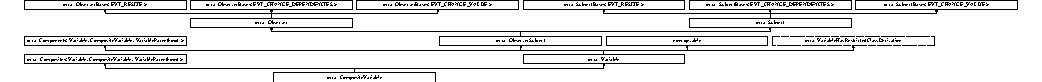
\includegraphics[height=1.100629cm]{d2/d7c/classocra_1_1CompositeVariable}
\end{center}
\end{figure}
\subsection*{Public Member Functions}
\begin{DoxyCompactItemize}
\item 
\hyperlink{classocra_1_1CompositeVariable_a1611f9c8b278c183ca68837e0b91f4f0}{Composite\+Variable} (const std\+::string \&name)
\item 
\hyperlink{classocra_1_1CompositeVariable_a131e1ee2f3b4dcd3439b8eb389777f81}{Composite\+Variable} (const std\+::string \&name, \hyperlink{classocra_1_1Variable}{Variable} \&var)
\item 
\hyperlink{classocra_1_1CompositeVariable_a7dce5cb02821d4da44f606a45407e0ae}{Composite\+Variable} (const std\+::string \&name, \hyperlink{classocra_1_1Variable}{Variable} \&var1, \hyperlink{classocra_1_1Variable}{Variable} \&var2)
\item 
\hyperlink{classocra_1_1CompositeVariable_a80c80db8037f36c9ac84a9b03171013f}{Composite\+Variable} (const std\+::string \&name, const std\+::vector$<$ \hyperlink{classocra_1_1Variable}{Variable} $\ast$$>$ \&vars)
\item 
void \hyperlink{classocra_1_1CompositeVariable_a64e6f462d217b4d3ab3d2b5364373ce8}{clear} ()
\begin{DoxyCompactList}\small\item\em Detaches all children. \end{DoxyCompactList}\item 
\hyperlink{classocra_1_1Variable}{Variable} \& \hyperlink{classocra_1_1CompositeVariable_a6cbd2ebea33e1fd523453b9448b3fde2}{operator()} (size\+\_\+t i)
\item 
\hyperlink{classocra_1_1CompositeVariable}{Composite\+Variable} \& \hyperlink{classocra_1_1CompositeVariable_a9b09f9bf88fd58fcdad695d762c11d13}{add\+By\+Merge} (\hyperlink{classocra_1_1Variable}{Variable} \&v)
\item 
\hyperlink{classocra_1_1CompositeVariable}{Composite\+Variable} \& \hyperlink{classocra_1_1CompositeVariable_ad4c753d254356c1b3686a3da04b0d499}{get\+Time\+Derivative} ()
\begin{DoxyCompactList}\small\item\em Get the time derivative/primitive of the variable. \end{DoxyCompactList}\item 
\hyperlink{classocra_1_1CompositeVariable}{Composite\+Variable} \& \hyperlink{classocra_1_1CompositeVariable_a7870c51e9904734593d7990033a7cca4}{get\+Time\+Primitive} ()
\item 
const \hyperlink{classocra_1_1Variable}{Variable} \& \hyperlink{classocra_1_1CompositeVariable_ae539d99db2156258b02f6cf4474f2d94}{operator()} (size\+\_\+t i) const
\item 
int \hyperlink{classocra_1_1CompositeVariable_a6601ac71bdd683d06a7a6bfe4fa7252c}{is\+Ancestor\+Of} (const \hyperlink{classocra_1_1Variable}{Variable} \&var) const
\begin{DoxyCompactList}\small\item\em Returns the number of levels that separate the component from a potential child. \end{DoxyCompactList}\item 
void \hyperlink{classocra_1_1CompositeVariable_ac2015499d8f01ee39ef7bfbe33363a10}{print\+Sub\+Tree} (int depth, std\+::ostream \&os) const
\begin{DoxyCompactList}\small\item\em Overload in Component\+Derived and Composite\+Derived to simply call \hyperlink{classocra_1_1Composite_a99934c9b17849dd55075c4c773008dae}{print\+Tree\+\_\+impl()}. \end{DoxyCompactList}\end{DoxyCompactItemize}
{\bf }\par
\begin{DoxyCompactItemize}
\item 
\hyperlink{classocra_1_1CompositeVariable}{Composite\+Variable} \& \hyperlink{classocra_1_1CompositeVariable_a3915b8d93a37f7431ce682bdbf725758}{add} (\hyperlink{classocra_1_1Variable}{Variable} \&child)
\begin{DoxyCompactList}\small\item\em Attach/detach the child to/from this node. \end{DoxyCompactList}\item 
\hyperlink{classocra_1_1CompositeVariable}{Composite\+Variable} \& \hyperlink{classocra_1_1CompositeVariable_ada9e93c4f85c641e2ec8f1152c0b851a}{remove} (\hyperlink{classocra_1_1Variable}{Variable} \&child)
\end{DoxyCompactItemize}

\subsection*{Protected Member Functions}
\begin{DoxyCompactItemize}
\item 
void \hyperlink{classocra_1_1CompositeVariable_aa2d9ca737bf529e2686ba9a3ee1126e5}{do\+\_\+set\+Value} (const Vector\+Xd \&value)
\begin{DoxyCompactList}\small\item\em This method will attempt to assign a given value to the memory map. \end{DoxyCompactList}\item 
size\+\_\+t \hyperlink{classocra_1_1CompositeVariable_aa61eea64fe90aea3ebccad355a9e8fb0}{do\+\_\+get\+Number\+Of\+Children} () const
\begin{DoxyCompactList}\small\item\em Always return get\+Num\+Childhoods. \end{DoxyCompactList}\end{DoxyCompactItemize}
{\bf }\par
\begin{DoxyCompactItemize}
\item 
void \hyperlink{classocra_1_1CompositeVariable_a995a870aa6b0a9933ebffd975ce6f6a5}{on\+Attached\+Child} (const \hyperlink{classocra_1_1Variable_a88444b2124cf5aab069f46734822f31f}{parenthood\+\_\+t} \&child)
\item 
void \hyperlink{classocra_1_1CompositeVariable_a76b21bf2425a09aded03b3d7a22c8db8}{on\+Detached\+Child} (const \hyperlink{classocra_1_1Variable_a88444b2124cf5aab069f46734822f31f}{parenthood\+\_\+t} \&child)
\end{DoxyCompactItemize}

{\bf }\par
\begin{DoxyCompactItemize}
\item 
\hyperlink{classocra_1_1Variable}{Variable} $\ast$ \hyperlink{classocra_1_1CompositeVariable_a4ac0f033cea1cb5e4bfdb414765c3743}{do\+\_\+create\+Time\+Derivative} (const std\+::string \&name)
\item 
\hyperlink{classocra_1_1Variable}{Variable} $\ast$ \hyperlink{classocra_1_1CompositeVariable_a09fb82df36205326b995aca1dd8f14ba}{do\+\_\+create\+Time\+Primitive} (const std\+::string \&name)
\end{DoxyCompactItemize}

\subsection*{Additional Inherited Members}


\subsection{Detailed Description}
A concatenation of base variables and other composite variables. 

Definition at line 357 of file Variable.\+h.



\subsection{Constructor \& Destructor Documentation}
\hypertarget{classocra_1_1CompositeVariable_a1611f9c8b278c183ca68837e0b91f4f0}{}\label{classocra_1_1CompositeVariable_a1611f9c8b278c183ca68837e0b91f4f0} 
\index{ocra\+::\+Composite\+Variable@{ocra\+::\+Composite\+Variable}!Composite\+Variable@{Composite\+Variable}}
\index{Composite\+Variable@{Composite\+Variable}!ocra\+::\+Composite\+Variable@{ocra\+::\+Composite\+Variable}}
\subsubsection{\texorpdfstring{Composite\+Variable()}{CompositeVariable()}\hspace{0.1cm}{\footnotesize\ttfamily [1/4]}}
{\footnotesize\ttfamily ocra\+::\+Composite\+Variable\+::\+Composite\+Variable (\begin{DoxyParamCaption}\item[{const std\+::string \&}]{name }\end{DoxyParamCaption})}



Definition at line 410 of file Variable.\+cpp.

\hypertarget{classocra_1_1CompositeVariable_a131e1ee2f3b4dcd3439b8eb389777f81}{}\label{classocra_1_1CompositeVariable_a131e1ee2f3b4dcd3439b8eb389777f81} 
\index{ocra\+::\+Composite\+Variable@{ocra\+::\+Composite\+Variable}!Composite\+Variable@{Composite\+Variable}}
\index{Composite\+Variable@{Composite\+Variable}!ocra\+::\+Composite\+Variable@{ocra\+::\+Composite\+Variable}}
\subsubsection{\texorpdfstring{Composite\+Variable()}{CompositeVariable()}\hspace{0.1cm}{\footnotesize\ttfamily [2/4]}}
{\footnotesize\ttfamily ocra\+::\+Composite\+Variable\+::\+Composite\+Variable (\begin{DoxyParamCaption}\item[{const std\+::string \&}]{name,  }\item[{\hyperlink{classocra_1_1Variable}{Variable} \&}]{var }\end{DoxyParamCaption})}



Definition at line 415 of file Variable.\+cpp.

\hypertarget{classocra_1_1CompositeVariable_a7dce5cb02821d4da44f606a45407e0ae}{}\label{classocra_1_1CompositeVariable_a7dce5cb02821d4da44f606a45407e0ae} 
\index{ocra\+::\+Composite\+Variable@{ocra\+::\+Composite\+Variable}!Composite\+Variable@{Composite\+Variable}}
\index{Composite\+Variable@{Composite\+Variable}!ocra\+::\+Composite\+Variable@{ocra\+::\+Composite\+Variable}}
\subsubsection{\texorpdfstring{Composite\+Variable()}{CompositeVariable()}\hspace{0.1cm}{\footnotesize\ttfamily [3/4]}}
{\footnotesize\ttfamily ocra\+::\+Composite\+Variable\+::\+Composite\+Variable (\begin{DoxyParamCaption}\item[{const std\+::string \&}]{name,  }\item[{\hyperlink{classocra_1_1Variable}{Variable} \&}]{var1,  }\item[{\hyperlink{classocra_1_1Variable}{Variable} \&}]{var2 }\end{DoxyParamCaption})}



Definition at line 421 of file Variable.\+cpp.

\hypertarget{classocra_1_1CompositeVariable_a80c80db8037f36c9ac84a9b03171013f}{}\label{classocra_1_1CompositeVariable_a80c80db8037f36c9ac84a9b03171013f} 
\index{ocra\+::\+Composite\+Variable@{ocra\+::\+Composite\+Variable}!Composite\+Variable@{Composite\+Variable}}
\index{Composite\+Variable@{Composite\+Variable}!ocra\+::\+Composite\+Variable@{ocra\+::\+Composite\+Variable}}
\subsubsection{\texorpdfstring{Composite\+Variable()}{CompositeVariable()}\hspace{0.1cm}{\footnotesize\ttfamily [4/4]}}
{\footnotesize\ttfamily ocra\+::\+Composite\+Variable\+::\+Composite\+Variable (\begin{DoxyParamCaption}\item[{const std\+::string \&}]{name,  }\item[{const std\+::vector$<$ \hyperlink{classocra_1_1Variable}{Variable} $\ast$$>$ \&}]{vars }\end{DoxyParamCaption})}



Definition at line 428 of file Variable.\+cpp.



\subsection{Member Function Documentation}
\hypertarget{classocra_1_1CompositeVariable_a3915b8d93a37f7431ce682bdbf725758}{}\label{classocra_1_1CompositeVariable_a3915b8d93a37f7431ce682bdbf725758} 
\index{ocra\+::\+Composite\+Variable@{ocra\+::\+Composite\+Variable}!add@{add}}
\index{add@{add}!ocra\+::\+Composite\+Variable@{ocra\+::\+Composite\+Variable}}
\subsubsection{\texorpdfstring{add()}{add()}}
{\footnotesize\ttfamily \hyperlink{classocra_1_1CompositeVariable}{Composite\+Variable} \& ocra\+::\+Composite\+Variable\+::add (\begin{DoxyParamCaption}\item[{\hyperlink{classocra_1_1Variable}{Variable} \&}]{child }\end{DoxyParamCaption})\hspace{0.3cm}{\ttfamily [virtual]}}



Attach/detach the child to/from this node. 



Reimplemented from \hyperlink{classocra_1_1Composite_a6751fd4b421edc193c10c858b5f00a34}{ocra\+::\+Composite$<$ Variable, Composite\+Variable, Variable\+Parenthood $>$}.



Definition at line 580 of file Variable.\+cpp.

\hypertarget{classocra_1_1CompositeVariable_a9b09f9bf88fd58fcdad695d762c11d13}{}\label{classocra_1_1CompositeVariable_a9b09f9bf88fd58fcdad695d762c11d13} 
\index{ocra\+::\+Composite\+Variable@{ocra\+::\+Composite\+Variable}!add\+By\+Merge@{add\+By\+Merge}}
\index{add\+By\+Merge@{add\+By\+Merge}!ocra\+::\+Composite\+Variable@{ocra\+::\+Composite\+Variable}}
\subsubsection{\texorpdfstring{add\+By\+Merge()}{addByMerge()}}
{\footnotesize\ttfamily \hyperlink{classocra_1_1CompositeVariable}{Composite\+Variable} \& ocra\+::\+Composite\+Variable\+::add\+By\+Merge (\begin{DoxyParamCaption}\item[{\hyperlink{classocra_1_1Variable}{Variable} \&}]{v }\end{DoxyParamCaption})}



Definition at line 475 of file Variable.\+cpp.

\hypertarget{classocra_1_1CompositeVariable_a64e6f462d217b4d3ab3d2b5364373ce8}{}\label{classocra_1_1CompositeVariable_a64e6f462d217b4d3ab3d2b5364373ce8} 
\index{ocra\+::\+Composite\+Variable@{ocra\+::\+Composite\+Variable}!clear@{clear}}
\index{clear@{clear}!ocra\+::\+Composite\+Variable@{ocra\+::\+Composite\+Variable}}
\subsubsection{\texorpdfstring{clear()}{clear()}}
{\footnotesize\ttfamily void ocra\+::\+Composite\+Variable\+::clear (\begin{DoxyParamCaption}\item[{void}]{ }\end{DoxyParamCaption})}



Detaches all children. 



Definition at line 435 of file Variable.\+cpp.

\hypertarget{classocra_1_1CompositeVariable_a4ac0f033cea1cb5e4bfdb414765c3743}{}\label{classocra_1_1CompositeVariable_a4ac0f033cea1cb5e4bfdb414765c3743} 
\index{ocra\+::\+Composite\+Variable@{ocra\+::\+Composite\+Variable}!do\+\_\+create\+Time\+Derivative@{do\+\_\+create\+Time\+Derivative}}
\index{do\+\_\+create\+Time\+Derivative@{do\+\_\+create\+Time\+Derivative}!ocra\+::\+Composite\+Variable@{ocra\+::\+Composite\+Variable}}
\subsubsection{\texorpdfstring{do\+\_\+create\+Time\+Derivative()}{do\_createTimeDerivative()}}
{\footnotesize\ttfamily \hyperlink{classocra_1_1Variable}{Variable} $\ast$ ocra\+::\+Composite\+Variable\+::do\+\_\+create\+Time\+Derivative (\begin{DoxyParamCaption}\item[{const std\+::string \&}]{name }\end{DoxyParamCaption})\hspace{0.3cm}{\ttfamily [protected]}, {\ttfamily [virtual]}}

\begin{DoxySeeAlso}{See also}
class \hyperlink{classocra_1_1Variable}{ocra\+::\+Variable} 
\end{DoxySeeAlso}


Implements \hyperlink{classocra_1_1Variable_aaed3c9bb3258cc1120ae8f93722a12bb}{ocra\+::\+Variable}.



Definition at line 519 of file Variable.\+cpp.

\hypertarget{classocra_1_1CompositeVariable_a09fb82df36205326b995aca1dd8f14ba}{}\label{classocra_1_1CompositeVariable_a09fb82df36205326b995aca1dd8f14ba} 
\index{ocra\+::\+Composite\+Variable@{ocra\+::\+Composite\+Variable}!do\+\_\+create\+Time\+Primitive@{do\+\_\+create\+Time\+Primitive}}
\index{do\+\_\+create\+Time\+Primitive@{do\+\_\+create\+Time\+Primitive}!ocra\+::\+Composite\+Variable@{ocra\+::\+Composite\+Variable}}
\subsubsection{\texorpdfstring{do\+\_\+create\+Time\+Primitive()}{do\_createTimePrimitive()}}
{\footnotesize\ttfamily \hyperlink{classocra_1_1Variable}{Variable} $\ast$ ocra\+::\+Composite\+Variable\+::do\+\_\+create\+Time\+Primitive (\begin{DoxyParamCaption}\item[{const std\+::string \&}]{name }\end{DoxyParamCaption})\hspace{0.3cm}{\ttfamily [protected]}, {\ttfamily [virtual]}}



Implements \hyperlink{classocra_1_1Variable_ae37610cbde7630dcda3dd6e09e251057}{ocra\+::\+Variable}.



Definition at line 551 of file Variable.\+cpp.

\hypertarget{classocra_1_1CompositeVariable_aa61eea64fe90aea3ebccad355a9e8fb0}{}\label{classocra_1_1CompositeVariable_aa61eea64fe90aea3ebccad355a9e8fb0} 
\index{ocra\+::\+Composite\+Variable@{ocra\+::\+Composite\+Variable}!do\+\_\+get\+Number\+Of\+Children@{do\+\_\+get\+Number\+Of\+Children}}
\index{do\+\_\+get\+Number\+Of\+Children@{do\+\_\+get\+Number\+Of\+Children}!ocra\+::\+Composite\+Variable@{ocra\+::\+Composite\+Variable}}
\subsubsection{\texorpdfstring{do\+\_\+get\+Number\+Of\+Children()}{do\_getNumberOfChildren()}}
{\footnotesize\ttfamily size\+\_\+t ocra\+::\+Composite\+Variable\+::do\+\_\+get\+Number\+Of\+Children (\begin{DoxyParamCaption}{ }\end{DoxyParamCaption}) const\hspace{0.3cm}{\ttfamily [protected]}, {\ttfamily [virtual]}}



Always return get\+Num\+Childhoods. 



Implements \hyperlink{classocra_1_1Variable_a65de5b31613b74d83baab58f0eb43b35}{ocra\+::\+Variable}.



Definition at line 641 of file Variable.\+cpp.

\hypertarget{classocra_1_1CompositeVariable_aa2d9ca737bf529e2686ba9a3ee1126e5}{}\label{classocra_1_1CompositeVariable_aa2d9ca737bf529e2686ba9a3ee1126e5} 
\index{ocra\+::\+Composite\+Variable@{ocra\+::\+Composite\+Variable}!do\+\_\+set\+Value@{do\+\_\+set\+Value}}
\index{do\+\_\+set\+Value@{do\+\_\+set\+Value}!ocra\+::\+Composite\+Variable@{ocra\+::\+Composite\+Variable}}
\subsubsection{\texorpdfstring{do\+\_\+set\+Value()}{do\_setValue()}}
{\footnotesize\ttfamily void ocra\+::\+Composite\+Variable\+::do\+\_\+set\+Value (\begin{DoxyParamCaption}\item[{const Vector\+Xd \&}]{value }\end{DoxyParamCaption})\hspace{0.3cm}{\ttfamily [protected]}, {\ttfamily [virtual]}}



This method will attempt to assign a given value to the memory map. 



Implements \hyperlink{classocra_1_1Variable_a73ff767d0a620f1803573b33f93c69f8}{ocra\+::\+Variable}.



Definition at line 441 of file Variable.\+cpp.

\hypertarget{classocra_1_1CompositeVariable_ad4c753d254356c1b3686a3da04b0d499}{}\label{classocra_1_1CompositeVariable_ad4c753d254356c1b3686a3da04b0d499} 
\index{ocra\+::\+Composite\+Variable@{ocra\+::\+Composite\+Variable}!get\+Time\+Derivative@{get\+Time\+Derivative}}
\index{get\+Time\+Derivative@{get\+Time\+Derivative}!ocra\+::\+Composite\+Variable@{ocra\+::\+Composite\+Variable}}
\subsubsection{\texorpdfstring{get\+Time\+Derivative()}{getTimeDerivative()}}
{\footnotesize\ttfamily \hyperlink{classocra_1_1CompositeVariable}{Composite\+Variable} \& ocra\+::\+Composite\+Variable\+::get\+Time\+Derivative (\begin{DoxyParamCaption}{ }\end{DoxyParamCaption})\hspace{0.3cm}{\ttfamily [virtual]}}



Get the time derivative/primitive of the variable. 

If the derivative/primitive doesn\textquotesingle{}t exist, it will be created automatically at the first call to this method. 

Reimplemented from \hyperlink{classocra_1_1Variable_a06ee384364d5c6bd1ea4bc4b38d6268c}{ocra\+::\+Variable}.



Definition at line 455 of file Variable.\+cpp.

\hypertarget{classocra_1_1CompositeVariable_a7870c51e9904734593d7990033a7cca4}{}\label{classocra_1_1CompositeVariable_a7870c51e9904734593d7990033a7cca4} 
\index{ocra\+::\+Composite\+Variable@{ocra\+::\+Composite\+Variable}!get\+Time\+Primitive@{get\+Time\+Primitive}}
\index{get\+Time\+Primitive@{get\+Time\+Primitive}!ocra\+::\+Composite\+Variable@{ocra\+::\+Composite\+Variable}}
\subsubsection{\texorpdfstring{get\+Time\+Primitive()}{getTimePrimitive()}}
{\footnotesize\ttfamily \hyperlink{classocra_1_1CompositeVariable}{Composite\+Variable} \& ocra\+::\+Composite\+Variable\+::get\+Time\+Primitive (\begin{DoxyParamCaption}{ }\end{DoxyParamCaption})\hspace{0.3cm}{\ttfamily [virtual]}}



Reimplemented from \hyperlink{classocra_1_1Variable_aca32d63e60dc79de340b2f122dad0dc5}{ocra\+::\+Variable}.



Definition at line 460 of file Variable.\+cpp.

\hypertarget{classocra_1_1CompositeVariable_a6601ac71bdd683d06a7a6bfe4fa7252c}{}\label{classocra_1_1CompositeVariable_a6601ac71bdd683d06a7a6bfe4fa7252c} 
\index{ocra\+::\+Composite\+Variable@{ocra\+::\+Composite\+Variable}!is\+Ancestor\+Of@{is\+Ancestor\+Of}}
\index{is\+Ancestor\+Of@{is\+Ancestor\+Of}!ocra\+::\+Composite\+Variable@{ocra\+::\+Composite\+Variable}}
\subsubsection{\texorpdfstring{is\+Ancestor\+Of()}{isAncestorOf()}}
{\footnotesize\ttfamily int ocra\+::\+Composite\+Variable\+::is\+Ancestor\+Of (\begin{DoxyParamCaption}\item[{const \hyperlink{classocra_1_1Variable}{Variable} \&}]{node }\end{DoxyParamCaption}) const\hspace{0.3cm}{\ttfamily [virtual]}}



Returns the number of levels that separate the component from a potential child. 



Implements \hyperlink{classocra_1_1Component_a8a0e052f36c60889562e921751b02a37}{ocra\+::\+Component$<$ Variable, Composite\+Variable, Variable\+Parenthood $>$}.



Definition at line 509 of file Variable.\+cpp.

\hypertarget{classocra_1_1CompositeVariable_a995a870aa6b0a9933ebffd975ce6f6a5}{}\label{classocra_1_1CompositeVariable_a995a870aa6b0a9933ebffd975ce6f6a5} 
\index{ocra\+::\+Composite\+Variable@{ocra\+::\+Composite\+Variable}!on\+Attached\+Child@{on\+Attached\+Child}}
\index{on\+Attached\+Child@{on\+Attached\+Child}!ocra\+::\+Composite\+Variable@{ocra\+::\+Composite\+Variable}}
\subsubsection{\texorpdfstring{on\+Attached\+Child()}{onAttachedChild()}}
{\footnotesize\ttfamily void ocra\+::\+Composite\+Variable\+::on\+Attached\+Child (\begin{DoxyParamCaption}\item[{const \hyperlink{classocra_1_1Variable_a88444b2124cf5aab069f46734822f31f}{parenthood\+\_\+t} \&}]{child }\end{DoxyParamCaption})\hspace{0.3cm}{\ttfamily [protected]}}



Definition at line 492 of file Variable.\+cpp.

\hypertarget{classocra_1_1CompositeVariable_a76b21bf2425a09aded03b3d7a22c8db8}{}\label{classocra_1_1CompositeVariable_a76b21bf2425a09aded03b3d7a22c8db8} 
\index{ocra\+::\+Composite\+Variable@{ocra\+::\+Composite\+Variable}!on\+Detached\+Child@{on\+Detached\+Child}}
\index{on\+Detached\+Child@{on\+Detached\+Child}!ocra\+::\+Composite\+Variable@{ocra\+::\+Composite\+Variable}}
\subsubsection{\texorpdfstring{on\+Detached\+Child()}{onDetachedChild()}}
{\footnotesize\ttfamily void ocra\+::\+Composite\+Variable\+::on\+Detached\+Child (\begin{DoxyParamCaption}\item[{const \hyperlink{classocra_1_1Variable_a88444b2124cf5aab069f46734822f31f}{parenthood\+\_\+t} \&}]{child }\end{DoxyParamCaption})\hspace{0.3cm}{\ttfamily [protected]}}



Definition at line 501 of file Variable.\+cpp.

\hypertarget{classocra_1_1CompositeVariable_a6cbd2ebea33e1fd523453b9448b3fde2}{}\label{classocra_1_1CompositeVariable_a6cbd2ebea33e1fd523453b9448b3fde2} 
\index{ocra\+::\+Composite\+Variable@{ocra\+::\+Composite\+Variable}!operator()@{operator()}}
\index{operator()@{operator()}!ocra\+::\+Composite\+Variable@{ocra\+::\+Composite\+Variable}}
\subsubsection{\texorpdfstring{operator()()}{operator()()}\hspace{0.1cm}{\footnotesize\ttfamily [1/2]}}
{\footnotesize\ttfamily \hyperlink{classocra_1_1Variable}{Variable} \& ocra\+::\+Composite\+Variable\+::operator() (\begin{DoxyParamCaption}\item[{size\+\_\+t}]{i }\end{DoxyParamCaption})}



Definition at line 465 of file Variable.\+cpp.

\hypertarget{classocra_1_1CompositeVariable_ae539d99db2156258b02f6cf4474f2d94}{}\label{classocra_1_1CompositeVariable_ae539d99db2156258b02f6cf4474f2d94} 
\index{ocra\+::\+Composite\+Variable@{ocra\+::\+Composite\+Variable}!operator()@{operator()}}
\index{operator()@{operator()}!ocra\+::\+Composite\+Variable@{ocra\+::\+Composite\+Variable}}
\subsubsection{\texorpdfstring{operator()()}{operator()()}\hspace{0.1cm}{\footnotesize\ttfamily [2/2]}}
{\footnotesize\ttfamily const \hyperlink{classocra_1_1Variable}{Variable} \& ocra\+::\+Composite\+Variable\+::operator() (\begin{DoxyParamCaption}\item[{size\+\_\+t}]{i }\end{DoxyParamCaption}) const}



Definition at line 470 of file Variable.\+cpp.

\hypertarget{classocra_1_1CompositeVariable_ac2015499d8f01ee39ef7bfbe33363a10}{}\label{classocra_1_1CompositeVariable_ac2015499d8f01ee39ef7bfbe33363a10} 
\index{ocra\+::\+Composite\+Variable@{ocra\+::\+Composite\+Variable}!print\+Sub\+Tree@{print\+Sub\+Tree}}
\index{print\+Sub\+Tree@{print\+Sub\+Tree}!ocra\+::\+Composite\+Variable@{ocra\+::\+Composite\+Variable}}
\subsubsection{\texorpdfstring{print\+Sub\+Tree()}{printSubTree()}}
{\footnotesize\ttfamily void ocra\+::\+Composite\+Variable\+::print\+Sub\+Tree (\begin{DoxyParamCaption}\item[{int}]{depth,  }\item[{std\+::ostream \&}]{os }\end{DoxyParamCaption}) const\hspace{0.3cm}{\ttfamily [virtual]}}



Overload in Component\+Derived and Composite\+Derived to simply call \hyperlink{classocra_1_1Composite_a99934c9b17849dd55075c4c773008dae}{print\+Tree\+\_\+impl()}. 

You can also choose to reimplement the while function rather than calling the proposed print\+Tree\+\_\+impl method. 
\begin{DoxyParams}{Parameters}
{\em depth} & is the current depth of the node. \\
\hline
\end{DoxyParams}


Implements \hyperlink{classocra_1_1Component_a3687a02c1524694fc616893264ca8199}{ocra\+::\+Component$<$ Variable, Composite\+Variable, Variable\+Parenthood $>$}.



Definition at line 514 of file Variable.\+cpp.

\hypertarget{classocra_1_1CompositeVariable_ada9e93c4f85c641e2ec8f1152c0b851a}{}\label{classocra_1_1CompositeVariable_ada9e93c4f85c641e2ec8f1152c0b851a} 
\index{ocra\+::\+Composite\+Variable@{ocra\+::\+Composite\+Variable}!remove@{remove}}
\index{remove@{remove}!ocra\+::\+Composite\+Variable@{ocra\+::\+Composite\+Variable}}
\subsubsection{\texorpdfstring{remove()}{remove()}}
{\footnotesize\ttfamily \hyperlink{classocra_1_1CompositeVariable}{Composite\+Variable} \& ocra\+::\+Composite\+Variable\+::remove (\begin{DoxyParamCaption}\item[{\hyperlink{classocra_1_1Variable}{Variable} \&}]{child }\end{DoxyParamCaption})\hspace{0.3cm}{\ttfamily [virtual]}}



Reimplemented from \hyperlink{classocra_1_1Composite_a93b8f85ae3267400fdddad9078945e07}{ocra\+::\+Composite$<$ Variable, Composite\+Variable, Variable\+Parenthood $>$}.



Definition at line 620 of file Variable.\+cpp.



The documentation for this class was generated from the following files\+:\begin{DoxyCompactItemize}
\item 
\hyperlink{Variable_8h}{Variable.\+h}\item 
\hyperlink{Variable_8cpp}{Variable.\+cpp}\end{DoxyCompactItemize}

\hypertarget{classocra_1_1ComTaskBuilder}{}\section{ocra\+:\+:Com\+Task\+Builder Class Reference}
\label{classocra_1_1ComTaskBuilder}\index{ocra\+::\+Com\+Task\+Builder@{ocra\+::\+Com\+Task\+Builder}}


{\ttfamily \#include $<$Com\+Task\+Builder.\+h$>$}

Inheritance diagram for ocra\+:\+:Com\+Task\+Builder\+:\begin{figure}[H]
\begin{center}
\leavevmode
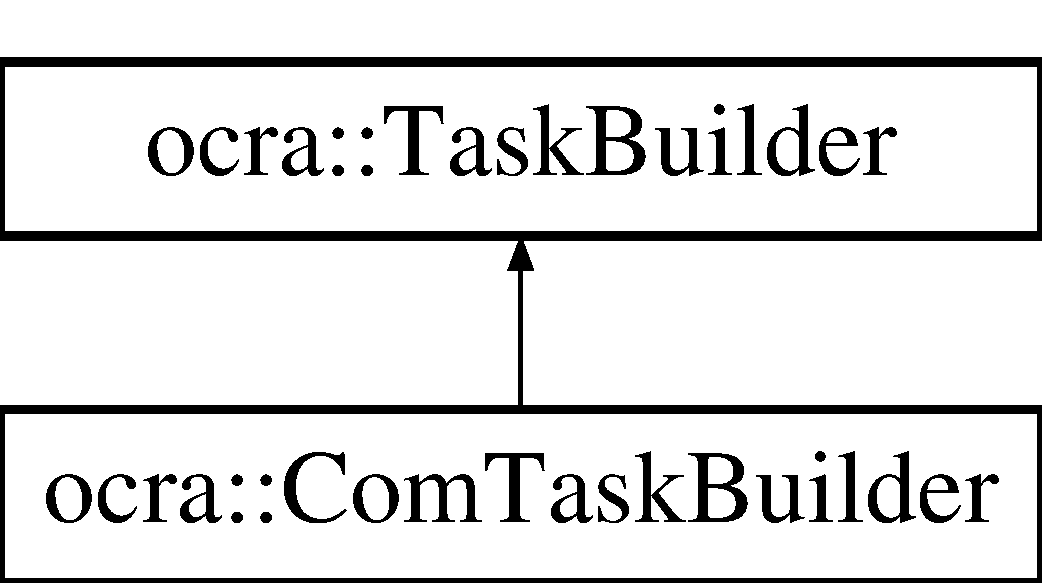
\includegraphics[height=2.000000cm]{d1/d14/classocra_1_1ComTaskBuilder}
\end{center}
\end{figure}
\subsection*{Public Member Functions}
\begin{DoxyCompactItemize}
\item 
\hyperlink{classocra_1_1ComTaskBuilder_aa3cffa7682c1122e7e5bfa533a66f9bc}{Com\+Task\+Builder} (const \hyperlink{classocra_1_1TaskBuilderOptions}{Task\+Builder\+Options} \&task\+Options, Model\+::\+Ptr model\+Ptr)
\item 
virtual \hyperlink{classocra_1_1ComTaskBuilder_a17a4747e20d9e37f734a9f27820d068d}{$\sim$\+Com\+Task\+Builder} ()
\end{DoxyCompactItemize}
\subsection*{Protected Member Functions}
\begin{DoxyCompactItemize}
\item 
virtual void \hyperlink{classocra_1_1ComTaskBuilder_af9cfac995156297324ccbee1900f891c}{set\+Task\+Type} ()
\item 
virtual void \hyperlink{classocra_1_1ComTaskBuilder_ab514d4644f7dfeec3ae84a5b0b8bbc34}{set\+Task\+State} ()
\item 
virtual Feature\+::\+Ptr \hyperlink{classocra_1_1ComTaskBuilder_aa4e0d21159da91788a1d2806ddca84da}{build\+Feature} ()
\item 
virtual Feature\+::\+Ptr \hyperlink{classocra_1_1ComTaskBuilder_abdd4c74539a37ff4c719c0ac78812bf4}{build\+Feature\+Desired} ()
\end{DoxyCompactItemize}
\subsection*{Additional Inherited Members}


\subsection{Detailed Description}


Definition at line 8 of file Com\+Task\+Builder.\+h.



\subsection{Constructor \& Destructor Documentation}
\hypertarget{classocra_1_1ComTaskBuilder_aa3cffa7682c1122e7e5bfa533a66f9bc}{}\label{classocra_1_1ComTaskBuilder_aa3cffa7682c1122e7e5bfa533a66f9bc} 
\index{ocra\+::\+Com\+Task\+Builder@{ocra\+::\+Com\+Task\+Builder}!Com\+Task\+Builder@{Com\+Task\+Builder}}
\index{Com\+Task\+Builder@{Com\+Task\+Builder}!ocra\+::\+Com\+Task\+Builder@{ocra\+::\+Com\+Task\+Builder}}
\subsubsection{\texorpdfstring{Com\+Task\+Builder()}{ComTaskBuilder()}}
{\footnotesize\ttfamily Com\+Task\+Builder\+::\+Com\+Task\+Builder (\begin{DoxyParamCaption}\item[{const \hyperlink{classocra_1_1TaskBuilderOptions}{Task\+Builder\+Options} \&}]{task\+Options,  }\item[{Model\+::\+Ptr}]{model\+Ptr }\end{DoxyParamCaption})}



Definition at line 5 of file Com\+Task\+Builder.\+cpp.

\hypertarget{classocra_1_1ComTaskBuilder_a17a4747e20d9e37f734a9f27820d068d}{}\label{classocra_1_1ComTaskBuilder_a17a4747e20d9e37f734a9f27820d068d} 
\index{ocra\+::\+Com\+Task\+Builder@{ocra\+::\+Com\+Task\+Builder}!````~Com\+Task\+Builder@{$\sim$\+Com\+Task\+Builder}}
\index{````~Com\+Task\+Builder@{$\sim$\+Com\+Task\+Builder}!ocra\+::\+Com\+Task\+Builder@{ocra\+::\+Com\+Task\+Builder}}
\subsubsection{\texorpdfstring{$\sim$\+Com\+Task\+Builder()}{~ComTaskBuilder()}}
{\footnotesize\ttfamily Com\+Task\+Builder\+::$\sim$\+Com\+Task\+Builder (\begin{DoxyParamCaption}{ }\end{DoxyParamCaption})\hspace{0.3cm}{\ttfamily [virtual]}}



Definition at line 11 of file Com\+Task\+Builder.\+cpp.



\subsection{Member Function Documentation}
\hypertarget{classocra_1_1ComTaskBuilder_aa4e0d21159da91788a1d2806ddca84da}{}\label{classocra_1_1ComTaskBuilder_aa4e0d21159da91788a1d2806ddca84da} 
\index{ocra\+::\+Com\+Task\+Builder@{ocra\+::\+Com\+Task\+Builder}!build\+Feature@{build\+Feature}}
\index{build\+Feature@{build\+Feature}!ocra\+::\+Com\+Task\+Builder@{ocra\+::\+Com\+Task\+Builder}}
\subsubsection{\texorpdfstring{build\+Feature()}{buildFeature()}}
{\footnotesize\ttfamily Feature\+::\+Ptr Com\+Task\+Builder\+::build\+Feature (\begin{DoxyParamCaption}{ }\end{DoxyParamCaption})\hspace{0.3cm}{\ttfamily [protected]}, {\ttfamily [virtual]}}



Implements \hyperlink{classocra_1_1TaskBuilder_a58c0dc416a9607a344a080248ee26ac2}{ocra\+::\+Task\+Builder}.



Definition at line 16 of file Com\+Task\+Builder.\+cpp.

\hypertarget{classocra_1_1ComTaskBuilder_abdd4c74539a37ff4c719c0ac78812bf4}{}\label{classocra_1_1ComTaskBuilder_abdd4c74539a37ff4c719c0ac78812bf4} 
\index{ocra\+::\+Com\+Task\+Builder@{ocra\+::\+Com\+Task\+Builder}!build\+Feature\+Desired@{build\+Feature\+Desired}}
\index{build\+Feature\+Desired@{build\+Feature\+Desired}!ocra\+::\+Com\+Task\+Builder@{ocra\+::\+Com\+Task\+Builder}}
\subsubsection{\texorpdfstring{build\+Feature\+Desired()}{buildFeatureDesired()}}
{\footnotesize\ttfamily Feature\+::\+Ptr Com\+Task\+Builder\+::build\+Feature\+Desired (\begin{DoxyParamCaption}{ }\end{DoxyParamCaption})\hspace{0.3cm}{\ttfamily [protected]}, {\ttfamily [virtual]}}



Implements \hyperlink{classocra_1_1TaskBuilder_a7a2c8bcc5d95160d0e48806a2648f1a5}{ocra\+::\+Task\+Builder}.



Definition at line 27 of file Com\+Task\+Builder.\+cpp.

\hypertarget{classocra_1_1ComTaskBuilder_ab514d4644f7dfeec3ae84a5b0b8bbc34}{}\label{classocra_1_1ComTaskBuilder_ab514d4644f7dfeec3ae84a5b0b8bbc34} 
\index{ocra\+::\+Com\+Task\+Builder@{ocra\+::\+Com\+Task\+Builder}!set\+Task\+State@{set\+Task\+State}}
\index{set\+Task\+State@{set\+Task\+State}!ocra\+::\+Com\+Task\+Builder@{ocra\+::\+Com\+Task\+Builder}}
\subsubsection{\texorpdfstring{set\+Task\+State()}{setTaskState()}}
{\footnotesize\ttfamily void Com\+Task\+Builder\+::set\+Task\+State (\begin{DoxyParamCaption}{ }\end{DoxyParamCaption})\hspace{0.3cm}{\ttfamily [protected]}, {\ttfamily [virtual]}}



Implements \hyperlink{classocra_1_1TaskBuilder_a7b44bfa101566ea4400e2d9bfdb9ff32}{ocra\+::\+Task\+Builder}.



Definition at line 37 of file Com\+Task\+Builder.\+cpp.

\hypertarget{classocra_1_1ComTaskBuilder_af9cfac995156297324ccbee1900f891c}{}\label{classocra_1_1ComTaskBuilder_af9cfac995156297324ccbee1900f891c} 
\index{ocra\+::\+Com\+Task\+Builder@{ocra\+::\+Com\+Task\+Builder}!set\+Task\+Type@{set\+Task\+Type}}
\index{set\+Task\+Type@{set\+Task\+Type}!ocra\+::\+Com\+Task\+Builder@{ocra\+::\+Com\+Task\+Builder}}
\subsubsection{\texorpdfstring{set\+Task\+Type()}{setTaskType()}}
{\footnotesize\ttfamily void Com\+Task\+Builder\+::set\+Task\+Type (\begin{DoxyParamCaption}{ }\end{DoxyParamCaption})\hspace{0.3cm}{\ttfamily [protected]}, {\ttfamily [virtual]}}



Implements \hyperlink{classocra_1_1TaskBuilder_a1a979fc495be6dc30483aa8fd0ff2650}{ocra\+::\+Task\+Builder}.



Definition at line 56 of file Com\+Task\+Builder.\+cpp.



The documentation for this class was generated from the following files\+:\begin{DoxyCompactItemize}
\item 
\hyperlink{ComTaskBuilder_8h}{Com\+Task\+Builder.\+h}\item 
\hyperlink{ComTaskBuilder_8cpp}{Com\+Task\+Builder.\+cpp}\end{DoxyCompactItemize}

\hypertarget{classocra_1_1Constraint}{}\section{ocra\+:\+:Constraint$<$ T $>$ Class Template Reference}
\label{classocra_1_1Constraint}\index{ocra\+::\+Constraint$<$ T $>$@{ocra\+::\+Constraint$<$ T $>$}}


Constraint class.  




{\ttfamily \#include $<$Constraint.\+h$>$}

Inheritance diagram for ocra\+:\+:Constraint$<$ T $>$\+:\begin{figure}[H]
\begin{center}
\leavevmode
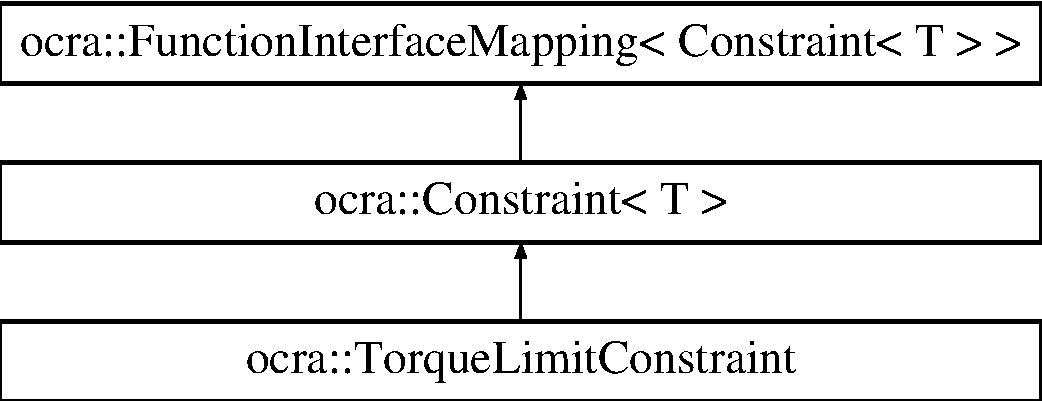
\includegraphics[height=3.000000cm]{dc/d5c/classocra_1_1Constraint}
\end{center}
\end{figure}
\subsection*{Public Member Functions}
\begin{DoxyCompactItemize}
\item 
\hyperlink{classocra_1_1Constraint_a73cc6c5b8e5c29ae3c1d8ed997c9e6e5}{Constraint} (T $\ast$function, bool equality, const Vector\+Xd \&v=Vector\+Xd())
\item 
\hyperlink{classocra_1_1Constraint_aca55ef9a5ea48fa91d846c53f4e30ad1}{Constraint} (T $\ast$function, const Vector\+Xd \&l=Vector\+Xd(), const Vector\+Xd \&u=Vector\+Xd())
\item 
\hyperlink{classocra_1_1Constraint_a4a0f49dbc4042347872429298f689091}{operator const T \&} ()
\end{DoxyCompactItemize}
{\bf }\par
\begin{DoxyCompactItemize}
\item 
virtual T \& \hyperlink{classocra_1_1Constraint_a6083fd05133e7aefae68fc84641149c1}{get\+Function} (void)
\item 
virtual const T \& \hyperlink{classocra_1_1Constraint_a2bda1f6319de9c803571a232d790f497}{get\+Function} (void) const
\end{DoxyCompactItemize}



\subsection{Detailed Description}
\subsubsection*{template$<$class T$>$\newline
class ocra\+::\+Constraint$<$ T $>$}

Constraint class. 

\begin{DoxyWarning}{Warning}
None
\end{DoxyWarning}
Given a function $ f $ over $ x \in R^n $ and possibly over the time $ t $, we can write a constraint whose most generic expression is $ l \le f(x,t) \le u $, with $ l $ and $ u $ two vectors of size $ m $ having their value in $ \left(R\cup\left\{-\infty,+\infty\right\}\right)^m $ and verifying $ l \le u $. This class is a C++ translation of this mathematical writing, but distinguishes some specific cases, for the ease of use, that are enumerated by e\+Constraint\+Type \+:
\begin{DoxyItemize}
\item $ l = u = b $, the constraint is treated as an equality to b (which can be 0)\+: C\+S\+T\+R\+\_\+\+E\+Q\+U\+A\+L\+\_\+\+Z\+E\+RO and C\+S\+T\+R\+\_\+\+E\+Q\+U\+A\+L\+\_\+B,
\item $ l = -\infty $ (resp. $ u = +\infty $), in which case the lower (resp. upper) bound is ignored. The remaining bound can be 0\+: C\+S\+T\+R\+\_\+\+L\+O\+W\+E\+R\+\_\+\+Z\+E\+RO, C\+S\+T\+R\+\_\+\+L\+O\+W\+E\+R\+\_\+U, C\+S\+T\+R\+\_\+\+G\+R\+E\+A\+T\+E\+R\+\_\+\+Z\+E\+RO and C\+S\+T\+R\+\_\+\+G\+R\+E\+A\+T\+E\+R\+\_\+L,
\item the general case\+: C\+S\+T\+R\+\_\+\+L\+O\+W\+E\+R\+\_\+\+A\+N\+D\+\_\+\+G\+R\+E\+A\+T\+ER.
\end{DoxyItemize}

The \hyperlink{classocra_1_1Constraint}{Constraint} class is templated by the type of the function on which the constraint is built. Provided the class definition of this function provides the good typedef function\+Type\+\_\+t, the hierarchy of the \hyperlink{classocra_1_1Function}{Function} classes is mimicked by \hyperlink{classocra_1_1Constraint}{Constraint}\+: if B is a class deriving of A and B\+::function\+Type\+\_\+t is A, then \hyperlink{classocra_1_1Constraint}{Constraint}{\bfseries  will automatically derived from \hyperlink{classocra_1_1Constraint}{Constraint}. As a concrete example, if \hyperlink{classocra_1_1DiagonalLinearFunction}{Diagonal\+Linear\+Function} derives from \hyperlink{classocra_1_1LinearFunction}{Linear\+Function} that derives from \hyperlink{classocra_1_1Function}{Function}, then Constraint$<$\+Diagonal\+Linear\+Function$>$ will derive from Constraint$<$\+Linear\+Function$>$ that will itself derive from \hyperlink{classocra_1_1Constraint_3_01Function_01_4}{Constraint$<$\+Function$>$}. Thus a Constraint$<$\+Diagonal\+Linear\+Function$>$ is also a Constraint$<$\+Linear\+Function$>$ for example.}

{\bfseries A \hyperlink{classocra_1_1Constraint}{Constraint} class inherits from \hyperlink{structocra_1_1FunctionInterfaceMapping}{Function\+Interface\+Mapping} of the interface of \hyperlink{classocra_1_1Function}{Function}, an instance of \hyperlink{classocra_1_1Constraint}{Constraint} can be treated as a \hyperlink{classocra_1_1Function}{Function}, to directly call methods of function on it. Constraint$<$\+T$>$ is however not deriving from \hyperlink{classocra_1_1Function}{Function}.}

{\bfseries \begin{DoxySeeAlso}{See also}
\hyperlink{structocra_1_1FunctionInterfaceMapping}{Function\+Interface\+Mapping} 
\end{DoxySeeAlso}
}

Definition at line 100 of file Constraint.\+h.



\subsection{Constructor \& Destructor Documentation}
\hypertarget{classocra_1_1Constraint_a73cc6c5b8e5c29ae3c1d8ed997c9e6e5}{}\label{classocra_1_1Constraint_a73cc6c5b8e5c29ae3c1d8ed997c9e6e5} 
\index{ocra\+::\+Constraint@{ocra\+::\+Constraint}!Constraint@{Constraint}}
\index{Constraint@{Constraint}!ocra\+::\+Constraint@{ocra\+::\+Constraint}}
\subsubsection{\texorpdfstring{Constraint()}{Constraint()}\hspace{0.1cm}{\footnotesize\ttfamily [1/2]}}
{\footnotesize\ttfamily template$<$class T $>$ \\
\hyperlink{classocra_1_1Constraint}{ocra\+::\+Constraint}$<$ T $>$\+::\hyperlink{classocra_1_1Constraint}{Constraint} (\begin{DoxyParamCaption}\item[{T $\ast$}]{function,  }\item[{bool}]{equality,  }\item[{const Vector\+Xd \&}]{v = {\ttfamily VectorXd()} }\end{DoxyParamCaption})\hspace{0.3cm}{\ttfamily [inline]}}

\hyperlink{classocra_1_1Constraint}{Constraint} constructor to build simple equality/inequality constraints


\begin{DoxyParams}[1]{Parameters}
\mbox{\tt in}  & {\em function} & A pointer to the function on which the constraint is imposed. \\
\hline
\mbox{\tt in}  & {\em equality} & True if the constraint is an equality, false if it is an inequality. \\
\hline
\mbox{\tt in}  & {\em v} & An optional vector to shift the constraint\\
\hline
\end{DoxyParams}
The following cases arise\+:
\begin{DoxyItemize}
\item Constraint(f, true)\+: the constraint describes $ f(x,t) = 0 $ (type C\+S\+T\+R\+\_\+\+E\+Q\+U\+A\+L\+\_\+\+Z\+E\+RO)
\item Constraint(f, false)\+: the constraint describes $ f(x,t) \le 0 $ (type C\+S\+T\+R\+\_\+\+L\+O\+W\+E\+R\+\_\+\+Z\+E\+RO)
\item Constraint(f, true, b)\+: the constraint describes $ f(x,t) = b $ (type C\+S\+T\+R\+\_\+\+E\+Q\+U\+A\+L\+\_\+B)
\item Constraint(f, false, u)\+: the constraint describes $ f(x,t) \le u $ (type C\+S\+T\+R\+\_\+\+L\+O\+W\+E\+R\+\_\+U)
\end{DoxyItemize}

\begin{DoxyPrecond}{Precondition}
If v is given (and non null), v.\+size() must be equal to function-\/$>$get\+Dimension() 
\end{DoxyPrecond}


Definition at line 576 of file Constraint.\+h.

\hypertarget{classocra_1_1Constraint_aca55ef9a5ea48fa91d846c53f4e30ad1}{}\label{classocra_1_1Constraint_aca55ef9a5ea48fa91d846c53f4e30ad1} 
\index{ocra\+::\+Constraint@{ocra\+::\+Constraint}!Constraint@{Constraint}}
\index{Constraint@{Constraint}!ocra\+::\+Constraint@{ocra\+::\+Constraint}}
\subsubsection{\texorpdfstring{Constraint()}{Constraint()}\hspace{0.1cm}{\footnotesize\ttfamily [2/2]}}
{\footnotesize\ttfamily template$<$class T $>$ \\
\hyperlink{classocra_1_1Constraint}{ocra\+::\+Constraint}$<$ T $>$\+::\hyperlink{classocra_1_1Constraint}{Constraint} (\begin{DoxyParamCaption}\item[{T $\ast$}]{function,  }\item[{const Vector\+Xd \&}]{l = {\ttfamily VectorXd()},  }\item[{const Vector\+Xd \&}]{u = {\ttfamily VectorXd()} }\end{DoxyParamCaption})\hspace{0.3cm}{\ttfamily [inline]}}

\hyperlink{classocra_1_1Constraint}{Constraint} constructor to build inequality constraints with possibly lower and upper bounds


\begin{DoxyParams}[1]{Parameters}
\mbox{\tt in}  & {\em function} & A pointer to the function on which the constraint is imposed. \\
\hline
\mbox{\tt in}  & {\em l} & Lower bound vector. \\
\hline
\mbox{\tt in}  & {\em u} & Lower bound vector.\\
\hline
\end{DoxyParams}
The following cases arise\+:
\begin{DoxyItemize}
\item Constraint(f)\+: the constraint describes $ f(x,t) \ge 0 $ (type C\+S\+T\+R\+\_\+\+G\+R\+E\+A\+T\+E\+R\+\_\+\+Z\+E\+RO)
\item Constraint(f, l)\+: the constraint describes $ f(x,t) \ge l $ (type C\+S\+T\+R\+\_\+\+G\+R\+E\+A\+T\+E\+R\+\_\+L)
\item Constraint(f, l, u)\+: the constraint describes $ l \le f(x,t) \le u $ (type C\+S\+T\+R\+\_\+\+L\+O\+W\+E\+R\+\_\+\+A\+N\+D\+\_\+\+G\+R\+E\+A\+T\+ER)
\item Constraint(f, l, u) with l==Vector\+Xd()\+: the constraint describes $ f(x,t) \le u $ (type C\+S\+T\+R\+\_\+\+L\+O\+W\+E\+R\+\_\+U)
\item Constraint(f, l, u) with l==u\+: the constraint describes $ f(x,t) = u $ (type C\+S\+T\+R\+\_\+\+E\+Q\+U\+A\+L\+\_\+B)
\end{DoxyItemize}

\begin{DoxyPrecond}{Precondition}
l$<$=u 

If l or u is given (and non null), their size must be equal to function-\/$>$get\+Dimension() 
\end{DoxyPrecond}


Definition at line 585 of file Constraint.\+h.



\subsection{Member Function Documentation}
\hypertarget{classocra_1_1Constraint_a6083fd05133e7aefae68fc84641149c1}{}\label{classocra_1_1Constraint_a6083fd05133e7aefae68fc84641149c1} 
\index{ocra\+::\+Constraint@{ocra\+::\+Constraint}!get\+Function@{get\+Function}}
\index{get\+Function@{get\+Function}!ocra\+::\+Constraint@{ocra\+::\+Constraint}}
\subsubsection{\texorpdfstring{get\+Function()}{getFunction()}\hspace{0.1cm}{\footnotesize\ttfamily [1/2]}}
{\footnotesize\ttfamily template$<$class T$>$ \\
virtual T\& \hyperlink{classocra_1_1Constraint}{ocra\+::\+Constraint}$<$ T $>$\+::get\+Function (\begin{DoxyParamCaption}\item[{void}]{ }\end{DoxyParamCaption})\hspace{0.3cm}{\ttfamily [inline]}, {\ttfamily [virtual]}}

getter on the function on which the constraint is built 

Definition at line 156 of file Constraint.\+h.

\hypertarget{classocra_1_1Constraint_a2bda1f6319de9c803571a232d790f497}{}\label{classocra_1_1Constraint_a2bda1f6319de9c803571a232d790f497} 
\index{ocra\+::\+Constraint@{ocra\+::\+Constraint}!get\+Function@{get\+Function}}
\index{get\+Function@{get\+Function}!ocra\+::\+Constraint@{ocra\+::\+Constraint}}
\subsubsection{\texorpdfstring{get\+Function()}{getFunction()}\hspace{0.1cm}{\footnotesize\ttfamily [2/2]}}
{\footnotesize\ttfamily template$<$class T$>$ \\
virtual const T\& \hyperlink{classocra_1_1Constraint}{ocra\+::\+Constraint}$<$ T $>$\+::get\+Function (\begin{DoxyParamCaption}\item[{void}]{ }\end{DoxyParamCaption}) const\hspace{0.3cm}{\ttfamily [inline]}, {\ttfamily [virtual]}}



Definition at line 157 of file Constraint.\+h.

\hypertarget{classocra_1_1Constraint_a4a0f49dbc4042347872429298f689091}{}\label{classocra_1_1Constraint_a4a0f49dbc4042347872429298f689091} 
\index{ocra\+::\+Constraint@{ocra\+::\+Constraint}!operator const T \&@{operator const T \&}}
\index{operator const T \&@{operator const T \&}!ocra\+::\+Constraint@{ocra\+::\+Constraint}}
\subsubsection{\texorpdfstring{operator const T \&()}{operator const T \&()}}
{\footnotesize\ttfamily template$<$class T$>$ \\
\hyperlink{classocra_1_1Constraint}{ocra\+::\+Constraint}$<$ T $>$\+::operator const T \& (\begin{DoxyParamCaption}{ }\end{DoxyParamCaption})\hspace{0.3cm}{\ttfamily [inline]}}

Conversion operator 

Definition at line 152 of file Constraint.\+h.



The documentation for this class was generated from the following file\+:\begin{DoxyCompactItemize}
\item 
\hyperlink{Constraint_8h}{Constraint.\+h}\end{DoxyCompactItemize}

\hypertarget{classocra_1_1Constraint_3_01Function_01_4}{}\section{ocra\+:\+:Constraint$<$ Function $>$ Class Template Reference}
\label{classocra_1_1Constraint_3_01Function_01_4}\index{ocra\+::\+Constraint$<$ Function $>$@{ocra\+::\+Constraint$<$ Function $>$}}


{\ttfamily \#include $<$Constraint.\+h$>$}

Inheritance diagram for ocra\+:\+:Constraint$<$ Function $>$\+:\begin{figure}[H]
\begin{center}
\leavevmode
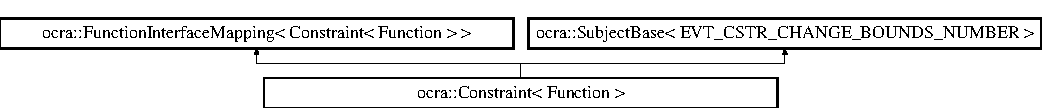
\includegraphics[height=1.447028cm]{de/d3b/classocra_1_1Constraint_3_01Function_01_4}
\end{center}
\end{figure}
\subsection*{Public Member Functions}
\begin{DoxyCompactItemize}
\item 
bool \hyperlink{classocra_1_1Constraint_3_01Function_01_4_a8406632b9e28804d9d8848a8e71ccbd8}{is\+Respected} (int index=-\/1) const
\end{DoxyCompactItemize}
{\bf }\par
\begin{DoxyCompactItemize}
\item 
\hyperlink{classocra_1_1Constraint_3_01Function_01_4_aefef89fd502e8f1fed23be307f71b508}{Constraint} (\hyperlink{classocra_1_1Function}{Function} $\ast$function, bool equality, const Vector\+Xd \&v=Vector\+Xd())
\item 
\hyperlink{classocra_1_1Constraint_3_01Function_01_4_a9b8a02fdfb62c2d3d774552baccd268b}{Constraint} (\hyperlink{classocra_1_1Function}{Function} $\ast$function, const Vector\+Xd \&l=Vector\+Xd(), const Vector\+Xd \&u=Vector\+Xd())
\end{DoxyCompactItemize}

{\bf }\par
\begin{DoxyCompactItemize}
\item 
virtual \hyperlink{classocra_1_1Function}{Function} \& \hyperlink{classocra_1_1Constraint_3_01Function_01_4_a81f1d8de34c0a123bc77d4798619fe9b}{get\+Function} ()
\item 
virtual const \hyperlink{classocra_1_1Function}{Function} \& \hyperlink{classocra_1_1Constraint_3_01Function_01_4_ad7f2ac6dfb90ed0231cc3e73ef592581}{get\+Function} () const
\end{DoxyCompactItemize}

{\bf }\par
\begin{DoxyCompactItemize}
\item 
bool \hyperlink{classocra_1_1Constraint_3_01Function_01_4_a3c7d085d888ef8937977129740d4c8a6}{is\+Equality} () const
\item 
bool \hyperlink{classocra_1_1Constraint_3_01Function_01_4_ab9083572de0c38297a7c20d88b82e183}{is\+Inequality} () const
\end{DoxyCompactItemize}

{\bf }\par
\begin{DoxyCompactItemize}
\item 
void \hyperlink{classocra_1_1Constraint_3_01Function_01_4_a14893e8b8e01e60f0369ef6c934ca6ab}{setB} (const Vector\+Xd \&b)
\item 
void \hyperlink{classocra_1_1Constraint_3_01Function_01_4_a9bfbc2cff3d9ad7099f8f51228b541c4}{setL} (const Vector\+Xd \&l)
\item 
void \hyperlink{classocra_1_1Constraint_3_01Function_01_4_a80c1536eb85f6913a8d80a36456aa90a}{setU} (const Vector\+Xd \&u)
\item 
void \hyperlink{classocra_1_1Constraint_3_01Function_01_4_adbf50d4faf459c8e6469937b0501b5e2}{set\+LandU} (const Vector\+Xd \&l, const Vector\+Xd \&u)
\end{DoxyCompactItemize}

{\bf }\par
\begin{DoxyCompactItemize}
\item 
\hyperlink{namespaceocra_aedff92662043a7f15dc263363db7939b}{e\+Constraint\+Type} \hyperlink{classocra_1_1Constraint_3_01Function_01_4_a05ee69ff17396c36c12dc6df6c7cc12e}{get\+Type} () const
\item 
const Vector\+Xd \& \hyperlink{classocra_1_1Constraint_3_01Function_01_4_a18ee02ca835269c8b648519be8a663ce}{getB} () const
\item 
const Vector\+Xd \& \hyperlink{classocra_1_1Constraint_3_01Function_01_4_a9539f6914fb118de1352f7558c3cb203}{getL} () const
\item 
const Vector\+Xd \& \hyperlink{classocra_1_1Constraint_3_01Function_01_4_aec8febaea23e49d7166a1aeafbcb3f23}{getU} () const
\end{DoxyCompactItemize}

{\bf }\par
\begin{DoxyCompactItemize}
\item 
void \hyperlink{classocra_1_1Constraint_3_01Function_01_4_ac87f7fc6513adba1044b8f53f3fd2f5d}{set\+Violation\+Tolerance} (double tol)
\item 
double \hyperlink{classocra_1_1Constraint_3_01Function_01_4_a72f3bc312073f4d431547261ff06387e}{get\+Violation\+Tolerance} () const
\end{DoxyCompactItemize}

\subsection*{Protected Attributes}
\begin{DoxyCompactItemize}
\item 
\hyperlink{classocra_1_1Function}{Function} \& \hyperlink{classocra_1_1Constraint_3_01Function_01_4_a51f8ef2f03da02c092aff7db27b325b6}{\+\_\+function}
\end{DoxyCompactItemize}
\subsection*{Additional Inherited Members}


\subsection{Detailed Description}
\subsubsection*{template$<$$>$\newline
class ocra\+::\+Constraint$<$ Function $>$}



Definition at line 174 of file Constraint.\+h.



\subsection{Constructor \& Destructor Documentation}
\hypertarget{classocra_1_1Constraint_3_01Function_01_4_aefef89fd502e8f1fed23be307f71b508}{}\label{classocra_1_1Constraint_3_01Function_01_4_aefef89fd502e8f1fed23be307f71b508} 
\index{ocra\+::\+Constraint$<$ Function $>$@{ocra\+::\+Constraint$<$ Function $>$}!Constraint@{Constraint}}
\index{Constraint@{Constraint}!ocra\+::\+Constraint$<$ Function $>$@{ocra\+::\+Constraint$<$ Function $>$}}
\subsubsection{\texorpdfstring{Constraint()}{Constraint()}\hspace{0.1cm}{\footnotesize\ttfamily [1/2]}}
{\footnotesize\ttfamily \hyperlink{classocra_1_1Constraint}{ocra\+::\+Constraint}$<$ \hyperlink{classocra_1_1Function}{Function} $>$\+::\hyperlink{classocra_1_1Constraint}{Constraint} (\begin{DoxyParamCaption}\item[{\hyperlink{classocra_1_1Function}{Function} $\ast$}]{function,  }\item[{bool}]{equality,  }\item[{const Vector\+Xd \&}]{v = {\ttfamily VectorXd()} }\end{DoxyParamCaption})\hspace{0.3cm}{\ttfamily [inline]}}

Specializations of the generic Constraint$<$\+T$>$ constructors 

Definition at line 593 of file Constraint.\+h.

\hypertarget{classocra_1_1Constraint_3_01Function_01_4_a9b8a02fdfb62c2d3d774552baccd268b}{}\label{classocra_1_1Constraint_3_01Function_01_4_a9b8a02fdfb62c2d3d774552baccd268b} 
\index{ocra\+::\+Constraint$<$ Function $>$@{ocra\+::\+Constraint$<$ Function $>$}!Constraint@{Constraint}}
\index{Constraint@{Constraint}!ocra\+::\+Constraint$<$ Function $>$@{ocra\+::\+Constraint$<$ Function $>$}}
\subsubsection{\texorpdfstring{Constraint()}{Constraint()}\hspace{0.1cm}{\footnotesize\ttfamily [2/2]}}
{\footnotesize\ttfamily \hyperlink{classocra_1_1Constraint}{ocra\+::\+Constraint}$<$ \hyperlink{classocra_1_1Function}{Function} $>$\+::\hyperlink{classocra_1_1Constraint}{Constraint} (\begin{DoxyParamCaption}\item[{\hyperlink{classocra_1_1Function}{Function} $\ast$}]{function,  }\item[{const Vector\+Xd \&}]{l = {\ttfamily VectorXd()},  }\item[{const Vector\+Xd \&}]{u = {\ttfamily VectorXd()} }\end{DoxyParamCaption})\hspace{0.3cm}{\ttfamily [inline]}}



Definition at line 618 of file Constraint.\+h.



\subsection{Member Function Documentation}
\hypertarget{classocra_1_1Constraint_3_01Function_01_4_a18ee02ca835269c8b648519be8a663ce}{}\label{classocra_1_1Constraint_3_01Function_01_4_a18ee02ca835269c8b648519be8a663ce} 
\index{ocra\+::\+Constraint$<$ Function $>$@{ocra\+::\+Constraint$<$ Function $>$}!getB@{getB}}
\index{getB@{getB}!ocra\+::\+Constraint$<$ Function $>$@{ocra\+::\+Constraint$<$ Function $>$}}
\subsubsection{\texorpdfstring{get\+B()}{getB()}}
{\footnotesize\ttfamily const Vector\+Xd \& \hyperlink{classocra_1_1Constraint}{ocra\+::\+Constraint}$<$ \hyperlink{classocra_1_1Function}{Function} $>$\+::getB (\begin{DoxyParamCaption}{ }\end{DoxyParamCaption}) const\hspace{0.3cm}{\ttfamily [inline]}}

Get the right member of an equality constraint.

\begin{DoxyPrecond}{Precondition}
\hyperlink{classocra_1_1Constraint_3_01Function_01_4_a3c7d085d888ef8937977129740d4c8a6}{is\+Equality()}==true. 
\end{DoxyPrecond}


Definition at line 543 of file Constraint.\+h.

\hypertarget{classocra_1_1Constraint_3_01Function_01_4_a81f1d8de34c0a123bc77d4798619fe9b}{}\label{classocra_1_1Constraint_3_01Function_01_4_a81f1d8de34c0a123bc77d4798619fe9b} 
\index{ocra\+::\+Constraint$<$ Function $>$@{ocra\+::\+Constraint$<$ Function $>$}!get\+Function@{get\+Function}}
\index{get\+Function@{get\+Function}!ocra\+::\+Constraint$<$ Function $>$@{ocra\+::\+Constraint$<$ Function $>$}}
\subsubsection{\texorpdfstring{get\+Function()}{getFunction()}\hspace{0.1cm}{\footnotesize\ttfamily [1/2]}}
{\footnotesize\ttfamily virtual \hyperlink{classocra_1_1Function}{Function}\& \hyperlink{classocra_1_1Constraint}{ocra\+::\+Constraint}$<$ \hyperlink{classocra_1_1Function}{Function} $>$\+::get\+Function (\begin{DoxyParamCaption}\item[{void}]{ }\end{DoxyParamCaption})\hspace{0.3cm}{\ttfamily [inline]}, {\ttfamily [virtual]}}

Returns the function associated with the constraint 

Definition at line 231 of file Constraint.\+h.

\hypertarget{classocra_1_1Constraint_3_01Function_01_4_ad7f2ac6dfb90ed0231cc3e73ef592581}{}\label{classocra_1_1Constraint_3_01Function_01_4_ad7f2ac6dfb90ed0231cc3e73ef592581} 
\index{ocra\+::\+Constraint$<$ Function $>$@{ocra\+::\+Constraint$<$ Function $>$}!get\+Function@{get\+Function}}
\index{get\+Function@{get\+Function}!ocra\+::\+Constraint$<$ Function $>$@{ocra\+::\+Constraint$<$ Function $>$}}
\subsubsection{\texorpdfstring{get\+Function()}{getFunction()}\hspace{0.1cm}{\footnotesize\ttfamily [2/2]}}
{\footnotesize\ttfamily virtual const \hyperlink{classocra_1_1Function}{Function}\& \hyperlink{classocra_1_1Constraint}{ocra\+::\+Constraint}$<$ \hyperlink{classocra_1_1Function}{Function} $>$\+::get\+Function (\begin{DoxyParamCaption}\item[{void}]{ }\end{DoxyParamCaption}) const\hspace{0.3cm}{\ttfamily [inline]}, {\ttfamily [virtual]}}



Definition at line 232 of file Constraint.\+h.

\hypertarget{classocra_1_1Constraint_3_01Function_01_4_a9539f6914fb118de1352f7558c3cb203}{}\label{classocra_1_1Constraint_3_01Function_01_4_a9539f6914fb118de1352f7558c3cb203} 
\index{ocra\+::\+Constraint$<$ Function $>$@{ocra\+::\+Constraint$<$ Function $>$}!getL@{getL}}
\index{getL@{getL}!ocra\+::\+Constraint$<$ Function $>$@{ocra\+::\+Constraint$<$ Function $>$}}
\subsubsection{\texorpdfstring{get\+L()}{getL()}}
{\footnotesize\ttfamily const Vector\+Xd \& \hyperlink{classocra_1_1Constraint}{ocra\+::\+Constraint}$<$ \hyperlink{classocra_1_1Function}{Function} $>$\+::getL (\begin{DoxyParamCaption}{ }\end{DoxyParamCaption}) const\hspace{0.3cm}{\ttfamily [inline]}}

Get the lower bound of an inequality constraint.

\begin{DoxyPrecond}{Precondition}
\hyperlink{classocra_1_1Constraint_3_01Function_01_4_a3c7d085d888ef8937977129740d4c8a6}{is\+Equality()}==false. 
\end{DoxyPrecond}


Definition at line 549 of file Constraint.\+h.

\hypertarget{classocra_1_1Constraint_3_01Function_01_4_a05ee69ff17396c36c12dc6df6c7cc12e}{}\label{classocra_1_1Constraint_3_01Function_01_4_a05ee69ff17396c36c12dc6df6c7cc12e} 
\index{ocra\+::\+Constraint$<$ Function $>$@{ocra\+::\+Constraint$<$ Function $>$}!get\+Type@{get\+Type}}
\index{get\+Type@{get\+Type}!ocra\+::\+Constraint$<$ Function $>$@{ocra\+::\+Constraint$<$ Function $>$}}
\subsubsection{\texorpdfstring{get\+Type()}{getType()}}
{\footnotesize\ttfamily \hyperlink{namespaceocra_aedff92662043a7f15dc263363db7939b}{e\+Constraint\+Type} \hyperlink{classocra_1_1Constraint}{ocra\+::\+Constraint}$<$ \hyperlink{classocra_1_1Function}{Function} $>$\+::get\+Type (\begin{DoxyParamCaption}{ }\end{DoxyParamCaption}) const\hspace{0.3cm}{\ttfamily [inline]}}

getters on the datas of \hyperlink{classocra_1_1Constraint}{Constraint} 

Definition at line 538 of file Constraint.\+h.

\hypertarget{classocra_1_1Constraint_3_01Function_01_4_aec8febaea23e49d7166a1aeafbcb3f23}{}\label{classocra_1_1Constraint_3_01Function_01_4_aec8febaea23e49d7166a1aeafbcb3f23} 
\index{ocra\+::\+Constraint$<$ Function $>$@{ocra\+::\+Constraint$<$ Function $>$}!getU@{getU}}
\index{getU@{getU}!ocra\+::\+Constraint$<$ Function $>$@{ocra\+::\+Constraint$<$ Function $>$}}
\subsubsection{\texorpdfstring{get\+U()}{getU()}}
{\footnotesize\ttfamily const Vector\+Xd \& \hyperlink{classocra_1_1Constraint}{ocra\+::\+Constraint}$<$ \hyperlink{classocra_1_1Function}{Function} $>$\+::getU (\begin{DoxyParamCaption}{ }\end{DoxyParamCaption}) const\hspace{0.3cm}{\ttfamily [inline]}}

Get the upper bound of an inequality constraint.

\begin{DoxyPrecond}{Precondition}
\hyperlink{classocra_1_1Constraint_3_01Function_01_4_a3c7d085d888ef8937977129740d4c8a6}{is\+Equality()}==false. 
\end{DoxyPrecond}


Definition at line 555 of file Constraint.\+h.

\hypertarget{classocra_1_1Constraint_3_01Function_01_4_a72f3bc312073f4d431547261ff06387e}{}\label{classocra_1_1Constraint_3_01Function_01_4_a72f3bc312073f4d431547261ff06387e} 
\index{ocra\+::\+Constraint$<$ Function $>$@{ocra\+::\+Constraint$<$ Function $>$}!get\+Violation\+Tolerance@{get\+Violation\+Tolerance}}
\index{get\+Violation\+Tolerance@{get\+Violation\+Tolerance}!ocra\+::\+Constraint$<$ Function $>$@{ocra\+::\+Constraint$<$ Function $>$}}
\subsubsection{\texorpdfstring{get\+Violation\+Tolerance()}{getViolationTolerance()}}
{\footnotesize\ttfamily double \hyperlink{classocra_1_1Constraint}{ocra\+::\+Constraint}$<$ \hyperlink{classocra_1_1Function}{Function} $>$\+::get\+Violation\+Tolerance (\begin{DoxyParamCaption}{ }\end{DoxyParamCaption}) const\hspace{0.3cm}{\ttfamily [inline]}}



Definition at line 567 of file Constraint.\+h.

\hypertarget{classocra_1_1Constraint_3_01Function_01_4_a3c7d085d888ef8937977129740d4c8a6}{}\label{classocra_1_1Constraint_3_01Function_01_4_a3c7d085d888ef8937977129740d4c8a6} 
\index{ocra\+::\+Constraint$<$ Function $>$@{ocra\+::\+Constraint$<$ Function $>$}!is\+Equality@{is\+Equality}}
\index{is\+Equality@{is\+Equality}!ocra\+::\+Constraint$<$ Function $>$@{ocra\+::\+Constraint$<$ Function $>$}}
\subsubsection{\texorpdfstring{is\+Equality()}{isEquality()}}
{\footnotesize\ttfamily bool \hyperlink{classocra_1_1Constraint}{ocra\+::\+Constraint}$<$ \hyperlink{classocra_1_1Function}{Function} $>$\+::is\+Equality (\begin{DoxyParamCaption}{ }\end{DoxyParamCaption}) const\hspace{0.3cm}{\ttfamily [inline]}}

Equality/\+Inequality property accessor 

Definition at line 396 of file Constraint.\+h.

\hypertarget{classocra_1_1Constraint_3_01Function_01_4_ab9083572de0c38297a7c20d88b82e183}{}\label{classocra_1_1Constraint_3_01Function_01_4_ab9083572de0c38297a7c20d88b82e183} 
\index{ocra\+::\+Constraint$<$ Function $>$@{ocra\+::\+Constraint$<$ Function $>$}!is\+Inequality@{is\+Inequality}}
\index{is\+Inequality@{is\+Inequality}!ocra\+::\+Constraint$<$ Function $>$@{ocra\+::\+Constraint$<$ Function $>$}}
\subsubsection{\texorpdfstring{is\+Inequality()}{isInequality()}}
{\footnotesize\ttfamily bool \hyperlink{classocra_1_1Constraint}{ocra\+::\+Constraint}$<$ \hyperlink{classocra_1_1Function}{Function} $>$\+::is\+Inequality (\begin{DoxyParamCaption}{ }\end{DoxyParamCaption}) const\hspace{0.3cm}{\ttfamily [inline]}}



Definition at line 401 of file Constraint.\+h.

\hypertarget{classocra_1_1Constraint_3_01Function_01_4_a8406632b9e28804d9d8848a8e71ccbd8}{}\label{classocra_1_1Constraint_3_01Function_01_4_a8406632b9e28804d9d8848a8e71ccbd8} 
\index{ocra\+::\+Constraint$<$ Function $>$@{ocra\+::\+Constraint$<$ Function $>$}!is\+Respected@{is\+Respected}}
\index{is\+Respected@{is\+Respected}!ocra\+::\+Constraint$<$ Function $>$@{ocra\+::\+Constraint$<$ Function $>$}}
\subsubsection{\texorpdfstring{is\+Respected()}{isRespected()}}
{\footnotesize\ttfamily bool \hyperlink{classocra_1_1Constraint}{ocra\+::\+Constraint}$<$ \hyperlink{classocra_1_1Function}{Function} $>$\+::is\+Respected (\begin{DoxyParamCaption}\item[{int}]{index = {\ttfamily -\/1} }\end{DoxyParamCaption}) const\hspace{0.3cm}{\ttfamily [inline]}}

Return true if the ith component of the constraint is valid for the actual value of its function, false otherwise. If the parameter is non-\/positive, it will check for the validity of all the components. Validity of a component is check with respect to the violation tolerance. This tolerance is 1.\+e-\/7 by default and can be changed with \hyperlink{classocra_1_1Constraint_3_01Function_01_4_ac87f7fc6513adba1044b8f53f3fd2f5d}{set\+Violation\+Tolerance()}


\begin{DoxyParams}[1]{Parameters}
\mbox{\tt in}  & {\em index.} & Index of the constraint component. If non-\/positive (as with the default value), all components will be considered \\
\hline
\end{DoxyParams}


Definition at line 360 of file Constraint.\+h.

\hypertarget{classocra_1_1Constraint_3_01Function_01_4_a14893e8b8e01e60f0369ef6c934ca6ab}{}\label{classocra_1_1Constraint_3_01Function_01_4_a14893e8b8e01e60f0369ef6c934ca6ab} 
\index{ocra\+::\+Constraint$<$ Function $>$@{ocra\+::\+Constraint$<$ Function $>$}!setB@{setB}}
\index{setB@{setB}!ocra\+::\+Constraint$<$ Function $>$@{ocra\+::\+Constraint$<$ Function $>$}}
\subsubsection{\texorpdfstring{set\+B()}{setB()}}
{\footnotesize\ttfamily void \hyperlink{classocra_1_1Constraint}{ocra\+::\+Constraint}$<$ \hyperlink{classocra_1_1Function}{Function} $>$\+::setB (\begin{DoxyParamCaption}\item[{const Vector\+Xd \&}]{b }\end{DoxyParamCaption})\hspace{0.3cm}{\ttfamily [inline]}}

All of the following methods do not change the equality/inequality property of the constraint. In particular, changing {\itshape l} and or {\itshape u} for an inequality constraint so as to have {\itshape l} = {\itshape u} will not make it become an equality constraint.\+Set the right member of an equality constraint. If {\itshape b} is null the constraint is considered as an equality to zero (type C\+S\+T\+R\+\_\+\+E\+Q\+U\+A\+L\+\_\+\+Z\+E\+RO). If not, it stays or becomes an equality to {\itshape b} (type C\+S\+T\+R\+\_\+\+E\+Q\+U\+A\+L\+\_\+B).

\begin{DoxyPrecond}{Precondition}
\hyperlink{classocra_1_1Constraint_3_01Function_01_4_a3c7d085d888ef8937977129740d4c8a6}{is\+Equality()}==true 

If b is not null then b.\+size==get\+Dimension() 
\end{DoxyPrecond}


Definition at line 406 of file Constraint.\+h.

\hypertarget{classocra_1_1Constraint_3_01Function_01_4_a9bfbc2cff3d9ad7099f8f51228b541c4}{}\label{classocra_1_1Constraint_3_01Function_01_4_a9bfbc2cff3d9ad7099f8f51228b541c4} 
\index{ocra\+::\+Constraint$<$ Function $>$@{ocra\+::\+Constraint$<$ Function $>$}!setL@{setL}}
\index{setL@{setL}!ocra\+::\+Constraint$<$ Function $>$@{ocra\+::\+Constraint$<$ Function $>$}}
\subsubsection{\texorpdfstring{set\+L()}{setL()}}
{\footnotesize\ttfamily void \hyperlink{classocra_1_1Constraint}{ocra\+::\+Constraint}$<$ \hyperlink{classocra_1_1Function}{Function} $>$\+::setL (\begin{DoxyParamCaption}\item[{const Vector\+Xd \&}]{l }\end{DoxyParamCaption})\hspace{0.3cm}{\ttfamily [inline]}}

Set the lower bound of an inequality constraint. If {\itshape l} is null, the lower bound of the contraint is removed (if applicable). In case the constraint only had a lower bound, this bound is set to zero. If {\itshape l} is not null, the lower bound is changed to the value of {\itshape l}. If the constraint had no lower bound it is created and set to {\itshape l}.

\begin{DoxyPrecond}{Precondition}
\hyperlink{classocra_1_1Constraint_3_01Function_01_4_ab9083572de0c38297a7c20d88b82e183}{is\+Inequality()}==true 

If l is not null then l.\+size==get\+Dimension() 

If l is not null, l$<$\+\_\+u 
\end{DoxyPrecond}


Definition at line 419 of file Constraint.\+h.

\hypertarget{classocra_1_1Constraint_3_01Function_01_4_adbf50d4faf459c8e6469937b0501b5e2}{}\label{classocra_1_1Constraint_3_01Function_01_4_adbf50d4faf459c8e6469937b0501b5e2} 
\index{ocra\+::\+Constraint$<$ Function $>$@{ocra\+::\+Constraint$<$ Function $>$}!set\+LandU@{set\+LandU}}
\index{set\+LandU@{set\+LandU}!ocra\+::\+Constraint$<$ Function $>$@{ocra\+::\+Constraint$<$ Function $>$}}
\subsubsection{\texorpdfstring{set\+Land\+U()}{setLandU()}}
{\footnotesize\ttfamily void \hyperlink{classocra_1_1Constraint}{ocra\+::\+Constraint}$<$ \hyperlink{classocra_1_1Function}{Function} $>$\+::set\+LandU (\begin{DoxyParamCaption}\item[{const Vector\+Xd \&}]{l,  }\item[{const Vector\+Xd \&}]{u }\end{DoxyParamCaption})\hspace{0.3cm}{\ttfamily [inline]}}

This method combines \hyperlink{classocra_1_1Constraint_3_01Function_01_4_a9bfbc2cff3d9ad7099f8f51228b541c4}{set\+L()} and \hyperlink{classocra_1_1Constraint_3_01Function_01_4_a80c1536eb85f6913a8d80a36456aa90a}{set\+U()}. It is provided to avoid breaking the precondition l$<$u of \hyperlink{classocra_1_1Constraint_3_01Function_01_4_a9bfbc2cff3d9ad7099f8f51228b541c4}{set\+L()} or \hyperlink{classocra_1_1Constraint_3_01Function_01_4_a80c1536eb85f6913a8d80a36456aa90a}{set\+U()}, which could happen by calling sequentially both methods while the new {\itshape l} and {\itshape u} are perfectly valid. In case {\itshape l} or {\itshape u} is null (including the case when both are null), the method calls \hyperlink{classocra_1_1Constraint_3_01Function_01_4_a9bfbc2cff3d9ad7099f8f51228b541c4}{set\+L()} and \hyperlink{classocra_1_1Constraint_3_01Function_01_4_a80c1536eb85f6913a8d80a36456aa90a}{set\+U()} in the proper order.

\begin{DoxyPrecond}{Precondition}
\hyperlink{classocra_1_1Constraint_3_01Function_01_4_ab9083572de0c38297a7c20d88b82e183}{is\+Inequality()}==true. 

If l and u are not null, l$<$u. 

If l or u is null, the precondition of \hyperlink{classocra_1_1Constraint_3_01Function_01_4_a9bfbc2cff3d9ad7099f8f51228b541c4}{set\+L()} and \hyperlink{classocra_1_1Constraint_3_01Function_01_4_a80c1536eb85f6913a8d80a36456aa90a}{set\+U()}.
\end{DoxyPrecond}
\begin{DoxySeeAlso}{See also}
\hyperlink{classocra_1_1Constraint_3_01Function_01_4_a9bfbc2cff3d9ad7099f8f51228b541c4}{set\+L()}, \hyperlink{classocra_1_1Constraint_3_01Function_01_4_a80c1536eb85f6913a8d80a36456aa90a}{set\+U()}. 
\end{DoxySeeAlso}


Definition at line 497 of file Constraint.\+h.

\hypertarget{classocra_1_1Constraint_3_01Function_01_4_a80c1536eb85f6913a8d80a36456aa90a}{}\label{classocra_1_1Constraint_3_01Function_01_4_a80c1536eb85f6913a8d80a36456aa90a} 
\index{ocra\+::\+Constraint$<$ Function $>$@{ocra\+::\+Constraint$<$ Function $>$}!setU@{setU}}
\index{setU@{setU}!ocra\+::\+Constraint$<$ Function $>$@{ocra\+::\+Constraint$<$ Function $>$}}
\subsubsection{\texorpdfstring{set\+U()}{setU()}}
{\footnotesize\ttfamily void \hyperlink{classocra_1_1Constraint}{ocra\+::\+Constraint}$<$ \hyperlink{classocra_1_1Function}{Function} $>$\+::setU (\begin{DoxyParamCaption}\item[{const Vector\+Xd \&}]{u }\end{DoxyParamCaption})\hspace{0.3cm}{\ttfamily [inline]}}

Set the upper bound of an inequality constraint. If {\itshape u} is null, the upper bound of the contraint is removed (if applicable). In case the constraint only had an upper bound, this bound is set to zero. If {\itshape u} is not null, the upper bound is changed to the value of {\itshape u}. If the constraint had no upper bound it is created and set to {\itshape u}.

\begin{DoxyPrecond}{Precondition}
\hyperlink{classocra_1_1Constraint_3_01Function_01_4_ab9083572de0c38297a7c20d88b82e183}{is\+Inequality()}==true 

If u is not null then u.\+size==get\+Dimension() 

If u is not null, \+\_\+l$<$u 
\end{DoxyPrecond}


Definition at line 458 of file Constraint.\+h.

\hypertarget{classocra_1_1Constraint_3_01Function_01_4_ac87f7fc6513adba1044b8f53f3fd2f5d}{}\label{classocra_1_1Constraint_3_01Function_01_4_ac87f7fc6513adba1044b8f53f3fd2f5d} 
\index{ocra\+::\+Constraint$<$ Function $>$@{ocra\+::\+Constraint$<$ Function $>$}!set\+Violation\+Tolerance@{set\+Violation\+Tolerance}}
\index{set\+Violation\+Tolerance@{set\+Violation\+Tolerance}!ocra\+::\+Constraint$<$ Function $>$@{ocra\+::\+Constraint$<$ Function $>$}}
\subsubsection{\texorpdfstring{set\+Violation\+Tolerance()}{setViolationTolerance()}}
{\footnotesize\ttfamily void \hyperlink{classocra_1_1Constraint}{ocra\+::\+Constraint}$<$ \hyperlink{classocra_1_1Function}{Function} $>$\+::set\+Violation\+Tolerance (\begin{DoxyParamCaption}\item[{double}]{tol }\end{DoxyParamCaption})\hspace{0.3cm}{\ttfamily [inline]}}

getter and setter for the constraint violation tolerance

\begin{DoxyPrecond}{Precondition}
tol$>$=0 
\end{DoxyPrecond}


Definition at line 561 of file Constraint.\+h.



\subsection{Member Data Documentation}
\hypertarget{classocra_1_1Constraint_3_01Function_01_4_a51f8ef2f03da02c092aff7db27b325b6}{}\label{classocra_1_1Constraint_3_01Function_01_4_a51f8ef2f03da02c092aff7db27b325b6} 
\index{ocra\+::\+Constraint$<$ Function $>$@{ocra\+::\+Constraint$<$ Function $>$}!\+\_\+function@{\+\_\+function}}
\index{\+\_\+function@{\+\_\+function}!ocra\+::\+Constraint$<$ Function $>$@{ocra\+::\+Constraint$<$ Function $>$}}
\subsubsection{\texorpdfstring{\+\_\+function}{\_function}}
{\footnotesize\ttfamily \hyperlink{classocra_1_1Function}{Function}\& \hyperlink{classocra_1_1Constraint}{ocra\+::\+Constraint}$<$ \hyperlink{classocra_1_1Function}{Function} $>$\+::\+\_\+function\hspace{0.3cm}{\ttfamily [protected]}}



Definition at line 342 of file Constraint.\+h.



The documentation for this class was generated from the following file\+:\begin{DoxyCompactItemize}
\item 
\hyperlink{Constraint_8h}{Constraint.\+h}\end{DoxyCompactItemize}

\hypertarget{classocra_1_1ConstraintSet}{}\section{ocra\+:\+:Constraint\+Set$<$ T $>$ Class Template Reference}
\label{classocra_1_1ConstraintSet}\index{ocra\+::\+Constraint\+Set$<$ T $>$@{ocra\+::\+Constraint\+Set$<$ T $>$}}


Constraint\+Set class.  




{\ttfamily \#include $<$Constraint\+Set.\+h$>$}

\subsection*{Public Member Functions}
\begin{DoxyCompactItemize}
\item 
\hyperlink{classocra_1_1ConstraintSet_ae571e7cc71dd7a2cfd3e8eeac028f65c}{Constraint\+Set} ()
\end{DoxyCompactItemize}
{\bf }\par
\begin{DoxyCompactItemize}
\item 
\hyperlink{classocra_1_1Constraint}{Constraint}$<$ T $>$ $\ast$ \hyperlink{classocra_1_1ConstraintSet_a5b7d67d57cc92ade65d84fe36d94bbe0}{get\+Ith\+Equality\+Constraint} (size\+\_\+t i)
\item 
\hyperlink{classocra_1_1Constraint}{Constraint}$<$ T $>$ $\ast$ \hyperlink{classocra_1_1ConstraintSet_af0de2bdd6267da2c53e7c9b3045dfb74}{get\+Ith\+Inequality\+Constraint} (size\+\_\+t i)
\item 
\hyperlink{classocra_1_1ConstraintSet}{Constraint\+Set}$<$ T $>$ \& \hyperlink{classocra_1_1ConstraintSet_a56204ca335c5e235629cfbc8d68397ac}{add} (\hyperlink{classocra_1_1Constraint}{Constraint}$<$ T $>$ $\ast$constraint)
\item 
\hyperlink{classocra_1_1ConstraintSet}{Constraint\+Set}$<$ T $>$ \& \hyperlink{classocra_1_1ConstraintSet_a4e0ff725278438f2f595ebc0a5de4389}{add} (\hyperlink{classocra_1_1ConstraintSet}{Constraint\+Set}$<$ T $>$ \&constraint\+Set)
\item 
\hyperlink{classocra_1_1ConstraintSet}{Constraint\+Set}$<$ T $>$ \& \hyperlink{classocra_1_1ConstraintSet_a6f0c43b34ff1ea60911a10186c66f294}{remove} (\hyperlink{classocra_1_1Constraint}{Constraint}$<$ T $>$ $\ast$constraint)
\item 
\hyperlink{classocra_1_1ConstraintSet}{Constraint\+Set}$<$ T $>$ \& \hyperlink{classocra_1_1ConstraintSet_a78f8d0f6f919734bb915bf6f63f5f058}{remove} (\hyperlink{classocra_1_1ConstraintSet}{Constraint\+Set}$<$ T $>$ \&constraint\+Set)
\item 
size\+\_\+t \hyperlink{classocra_1_1ConstraintSet_a95a113a808dfbf7a407c1ce000403941}{get\+Number\+Of\+Equality\+Constraints} () const
\item 
size\+\_\+t \hyperlink{classocra_1_1ConstraintSet_ae8c7be6697c295e051550e225f6fe85b}{get\+Number\+Of\+Inequality\+Constraints} () const
\item 
size\+\_\+t \hyperlink{classocra_1_1ConstraintSet_adc4069c30e8a497d88e930d68fc1ac57}{get\+Equality\+Dimension} () const
\item 
size\+\_\+t \hyperlink{classocra_1_1ConstraintSet_a3d0134190b555f7176a719424c0401eb}{get\+Inequality\+Dimension} () const
\end{DoxyCompactItemize}



\subsection{Detailed Description}
\subsubsection*{template$<$class T$>$\newline
class ocra\+::\+Constraint\+Set$<$ T $>$}

Constraint\+Set class. 

\begin{DoxyWarning}{Warning}
None
\end{DoxyWarning}
A set of constraint. This class is meant to be derived. \hyperlink{classocra_1_1ConstraintSet}{Constraint\+Set} mimics the hierarchy of \hyperlink{classocra_1_1Function}{Function}, in the same way \hyperlink{classocra_1_1Constraint}{Constraint} does. 

Definition at line 44 of file Constraint\+Set.\+h.



\subsection{Constructor \& Destructor Documentation}
\hypertarget{classocra_1_1ConstraintSet_ae571e7cc71dd7a2cfd3e8eeac028f65c}{}\label{classocra_1_1ConstraintSet_ae571e7cc71dd7a2cfd3e8eeac028f65c} 
\index{ocra\+::\+Constraint\+Set@{ocra\+::\+Constraint\+Set}!Constraint\+Set@{Constraint\+Set}}
\index{Constraint\+Set@{Constraint\+Set}!ocra\+::\+Constraint\+Set@{ocra\+::\+Constraint\+Set}}
\subsubsection{\texorpdfstring{Constraint\+Set()}{ConstraintSet()}}
{\footnotesize\ttfamily template$<$class T $>$ \\
\hyperlink{classocra_1_1ConstraintSet}{ocra\+::\+Constraint\+Set}$<$ T $>$\+::\hyperlink{classocra_1_1ConstraintSet}{Constraint\+Set} (\begin{DoxyParamCaption}{ }\end{DoxyParamCaption})\hspace{0.3cm}{\ttfamily [inline]}}



Definition at line 114 of file Constraint\+Set.\+h.



\subsection{Member Function Documentation}
\hypertarget{classocra_1_1ConstraintSet_a56204ca335c5e235629cfbc8d68397ac}{}\label{classocra_1_1ConstraintSet_a56204ca335c5e235629cfbc8d68397ac} 
\index{ocra\+::\+Constraint\+Set@{ocra\+::\+Constraint\+Set}!add@{add}}
\index{add@{add}!ocra\+::\+Constraint\+Set@{ocra\+::\+Constraint\+Set}}
\subsubsection{\texorpdfstring{add()}{add()}\hspace{0.1cm}{\footnotesize\ttfamily [1/2]}}
{\footnotesize\ttfamily template$<$class T $>$ \\
\hyperlink{classocra_1_1ConstraintSet}{Constraint\+Set}$<$ T $>$ \& \hyperlink{classocra_1_1ConstraintSet}{ocra\+::\+Constraint\+Set}$<$ T $>$\+::add (\begin{DoxyParamCaption}\item[{\hyperlink{classocra_1_1Constraint}{Constraint}$<$ T $>$ $\ast$}]{constraint }\end{DoxyParamCaption})\hspace{0.3cm}{\ttfamily [inline]}}



Definition at line 153 of file Constraint\+Set.\+h.

\hypertarget{classocra_1_1ConstraintSet_a4e0ff725278438f2f595ebc0a5de4389}{}\label{classocra_1_1ConstraintSet_a4e0ff725278438f2f595ebc0a5de4389} 
\index{ocra\+::\+Constraint\+Set@{ocra\+::\+Constraint\+Set}!add@{add}}
\index{add@{add}!ocra\+::\+Constraint\+Set@{ocra\+::\+Constraint\+Set}}
\subsubsection{\texorpdfstring{add()}{add()}\hspace{0.1cm}{\footnotesize\ttfamily [2/2]}}
{\footnotesize\ttfamily template$<$class T $>$ \\
\hyperlink{classocra_1_1ConstraintSet}{Constraint\+Set}$<$ T $>$ \& \hyperlink{classocra_1_1ConstraintSet}{ocra\+::\+Constraint\+Set}$<$ T $>$\+::add (\begin{DoxyParamCaption}\item[{\hyperlink{classocra_1_1ConstraintSet}{Constraint\+Set}$<$ T $>$ \&}]{constraint\+Set }\end{DoxyParamCaption})\hspace{0.3cm}{\ttfamily [inline]}}



Definition at line 177 of file Constraint\+Set.\+h.

\hypertarget{classocra_1_1ConstraintSet_adc4069c30e8a497d88e930d68fc1ac57}{}\label{classocra_1_1ConstraintSet_adc4069c30e8a497d88e930d68fc1ac57} 
\index{ocra\+::\+Constraint\+Set@{ocra\+::\+Constraint\+Set}!get\+Equality\+Dimension@{get\+Equality\+Dimension}}
\index{get\+Equality\+Dimension@{get\+Equality\+Dimension}!ocra\+::\+Constraint\+Set@{ocra\+::\+Constraint\+Set}}
\subsubsection{\texorpdfstring{get\+Equality\+Dimension()}{getEqualityDimension()}}
{\footnotesize\ttfamily template$<$class T $>$ \\
size\+\_\+t \hyperlink{classocra_1_1ConstraintSet}{ocra\+::\+Constraint\+Set}$<$ T $>$\+::get\+Equality\+Dimension (\begin{DoxyParamCaption}{ }\end{DoxyParamCaption}) const\hspace{0.3cm}{\ttfamily [inline]}}



Definition at line 269 of file Constraint\+Set.\+h.

\hypertarget{classocra_1_1ConstraintSet_a3d0134190b555f7176a719424c0401eb}{}\label{classocra_1_1ConstraintSet_a3d0134190b555f7176a719424c0401eb} 
\index{ocra\+::\+Constraint\+Set@{ocra\+::\+Constraint\+Set}!get\+Inequality\+Dimension@{get\+Inequality\+Dimension}}
\index{get\+Inequality\+Dimension@{get\+Inequality\+Dimension}!ocra\+::\+Constraint\+Set@{ocra\+::\+Constraint\+Set}}
\subsubsection{\texorpdfstring{get\+Inequality\+Dimension()}{getInequalityDimension()}}
{\footnotesize\ttfamily template$<$class T $>$ \\
size\+\_\+t \hyperlink{classocra_1_1ConstraintSet}{ocra\+::\+Constraint\+Set}$<$ T $>$\+::get\+Inequality\+Dimension (\begin{DoxyParamCaption}{ }\end{DoxyParamCaption}) const\hspace{0.3cm}{\ttfamily [inline]}}



Definition at line 282 of file Constraint\+Set.\+h.

\hypertarget{classocra_1_1ConstraintSet_a5b7d67d57cc92ade65d84fe36d94bbe0}{}\label{classocra_1_1ConstraintSet_a5b7d67d57cc92ade65d84fe36d94bbe0} 
\index{ocra\+::\+Constraint\+Set@{ocra\+::\+Constraint\+Set}!get\+Ith\+Equality\+Constraint@{get\+Ith\+Equality\+Constraint}}
\index{get\+Ith\+Equality\+Constraint@{get\+Ith\+Equality\+Constraint}!ocra\+::\+Constraint\+Set@{ocra\+::\+Constraint\+Set}}
\subsubsection{\texorpdfstring{get\+Ith\+Equality\+Constraint()}{getIthEqualityConstraint()}}
{\footnotesize\ttfamily template$<$class T $>$ \\
\hyperlink{classocra_1_1Constraint}{Constraint}$<$ T $>$ $\ast$ \hyperlink{classocra_1_1ConstraintSet}{ocra\+::\+Constraint\+Set}$<$ T $>$\+::get\+Ith\+Equality\+Constraint (\begin{DoxyParamCaption}\item[{size\+\_\+t}]{i }\end{DoxyParamCaption})\hspace{0.3cm}{\ttfamily [inline]}}

Does what it says. 

Definition at line 127 of file Constraint\+Set.\+h.

\hypertarget{classocra_1_1ConstraintSet_af0de2bdd6267da2c53e7c9b3045dfb74}{}\label{classocra_1_1ConstraintSet_af0de2bdd6267da2c53e7c9b3045dfb74} 
\index{ocra\+::\+Constraint\+Set@{ocra\+::\+Constraint\+Set}!get\+Ith\+Inequality\+Constraint@{get\+Ith\+Inequality\+Constraint}}
\index{get\+Ith\+Inequality\+Constraint@{get\+Ith\+Inequality\+Constraint}!ocra\+::\+Constraint\+Set@{ocra\+::\+Constraint\+Set}}
\subsubsection{\texorpdfstring{get\+Ith\+Inequality\+Constraint()}{getIthInequalityConstraint()}}
{\footnotesize\ttfamily template$<$class T $>$ \\
\hyperlink{classocra_1_1Constraint}{Constraint}$<$ T $>$ $\ast$ \hyperlink{classocra_1_1ConstraintSet}{ocra\+::\+Constraint\+Set}$<$ T $>$\+::get\+Ith\+Inequality\+Constraint (\begin{DoxyParamCaption}\item[{size\+\_\+t}]{i }\end{DoxyParamCaption})\hspace{0.3cm}{\ttfamily [inline]}}



Definition at line 140 of file Constraint\+Set.\+h.

\hypertarget{classocra_1_1ConstraintSet_a95a113a808dfbf7a407c1ce000403941}{}\label{classocra_1_1ConstraintSet_a95a113a808dfbf7a407c1ce000403941} 
\index{ocra\+::\+Constraint\+Set@{ocra\+::\+Constraint\+Set}!get\+Number\+Of\+Equality\+Constraints@{get\+Number\+Of\+Equality\+Constraints}}
\index{get\+Number\+Of\+Equality\+Constraints@{get\+Number\+Of\+Equality\+Constraints}!ocra\+::\+Constraint\+Set@{ocra\+::\+Constraint\+Set}}
\subsubsection{\texorpdfstring{get\+Number\+Of\+Equality\+Constraints()}{getNumberOfEqualityConstraints()}}
{\footnotesize\ttfamily template$<$class T $>$ \\
size\+\_\+t \hyperlink{classocra_1_1ConstraintSet}{ocra\+::\+Constraint\+Set}$<$ T $>$\+::get\+Number\+Of\+Equality\+Constraints (\begin{DoxyParamCaption}{ }\end{DoxyParamCaption}) const\hspace{0.3cm}{\ttfamily [inline]}}



Definition at line 243 of file Constraint\+Set.\+h.

\hypertarget{classocra_1_1ConstraintSet_ae8c7be6697c295e051550e225f6fe85b}{}\label{classocra_1_1ConstraintSet_ae8c7be6697c295e051550e225f6fe85b} 
\index{ocra\+::\+Constraint\+Set@{ocra\+::\+Constraint\+Set}!get\+Number\+Of\+Inequality\+Constraints@{get\+Number\+Of\+Inequality\+Constraints}}
\index{get\+Number\+Of\+Inequality\+Constraints@{get\+Number\+Of\+Inequality\+Constraints}!ocra\+::\+Constraint\+Set@{ocra\+::\+Constraint\+Set}}
\subsubsection{\texorpdfstring{get\+Number\+Of\+Inequality\+Constraints()}{getNumberOfInequalityConstraints()}}
{\footnotesize\ttfamily template$<$class T $>$ \\
size\+\_\+t \hyperlink{classocra_1_1ConstraintSet}{ocra\+::\+Constraint\+Set}$<$ T $>$\+::get\+Number\+Of\+Inequality\+Constraints (\begin{DoxyParamCaption}{ }\end{DoxyParamCaption}) const\hspace{0.3cm}{\ttfamily [inline]}}



Definition at line 256 of file Constraint\+Set.\+h.

\hypertarget{classocra_1_1ConstraintSet_a6f0c43b34ff1ea60911a10186c66f294}{}\label{classocra_1_1ConstraintSet_a6f0c43b34ff1ea60911a10186c66f294} 
\index{ocra\+::\+Constraint\+Set@{ocra\+::\+Constraint\+Set}!remove@{remove}}
\index{remove@{remove}!ocra\+::\+Constraint\+Set@{ocra\+::\+Constraint\+Set}}
\subsubsection{\texorpdfstring{remove()}{remove()}\hspace{0.1cm}{\footnotesize\ttfamily [1/2]}}
{\footnotesize\ttfamily template$<$class T $>$ \\
\hyperlink{classocra_1_1ConstraintSet}{Constraint\+Set}$<$ T $>$ \& \hyperlink{classocra_1_1ConstraintSet}{ocra\+::\+Constraint\+Set}$<$ T $>$\+::remove (\begin{DoxyParamCaption}\item[{\hyperlink{classocra_1_1Constraint}{Constraint}$<$ T $>$ $\ast$}]{constraint }\end{DoxyParamCaption})\hspace{0.3cm}{\ttfamily [inline]}}



Definition at line 195 of file Constraint\+Set.\+h.

\hypertarget{classocra_1_1ConstraintSet_a78f8d0f6f919734bb915bf6f63f5f058}{}\label{classocra_1_1ConstraintSet_a78f8d0f6f919734bb915bf6f63f5f058} 
\index{ocra\+::\+Constraint\+Set@{ocra\+::\+Constraint\+Set}!remove@{remove}}
\index{remove@{remove}!ocra\+::\+Constraint\+Set@{ocra\+::\+Constraint\+Set}}
\subsubsection{\texorpdfstring{remove()}{remove()}\hspace{0.1cm}{\footnotesize\ttfamily [2/2]}}
{\footnotesize\ttfamily template$<$class T $>$ \\
\hyperlink{classocra_1_1ConstraintSet}{Constraint\+Set}$<$ T $>$ \& \hyperlink{classocra_1_1ConstraintSet}{ocra\+::\+Constraint\+Set}$<$ T $>$\+::remove (\begin{DoxyParamCaption}\item[{\hyperlink{classocra_1_1ConstraintSet}{Constraint\+Set}$<$ T $>$ \&}]{constraint\+Set }\end{DoxyParamCaption})\hspace{0.3cm}{\ttfamily [inline]}}



Definition at line 226 of file Constraint\+Set.\+h.



The documentation for this class was generated from the following file\+:\begin{DoxyCompactItemize}
\item 
\hyperlink{ConstraintSet_8h}{Constraint\+Set.\+h}\end{DoxyCompactItemize}

\hypertarget{classocra_1_1ConstraintSet_3_01Function_01_4}{}\section{ocra\+:\+:Constraint\+Set$<$ Function $>$ Class Template Reference}
\label{classocra_1_1ConstraintSet_3_01Function_01_4}\index{ocra\+::\+Constraint\+Set$<$ Function $>$@{ocra\+::\+Constraint\+Set$<$ Function $>$}}


{\ttfamily \#include $<$Constraint\+Set.\+h$>$}

\subsection*{Public Member Functions}
\begin{DoxyCompactItemize}
\item 
\hyperlink{classocra_1_1ConstraintSet_3_01Function_01_4_ac79927faf3e3f795670ab85025b1e4a4}{Constraint\+Set} ()
\item 
\hyperlink{namespaceocra_af10341108ce661566aad00908668e2b1}{Generic\+Constraint} $\ast$ \hyperlink{classocra_1_1ConstraintSet_3_01Function_01_4_a376c4fe9b26afe70f176c2913fb870f0}{get\+Ith\+Equality\+Constraint} (size\+\_\+t i)
\item 
\hyperlink{namespaceocra_af10341108ce661566aad00908668e2b1}{Generic\+Constraint} $\ast$ \hyperlink{classocra_1_1ConstraintSet_3_01Function_01_4_ae105fbee1e6f91fd6b2f8657b72d2511}{get\+Ith\+Inequality\+Constraint} (size\+\_\+t i)
\item 
\hyperlink{classocra_1_1ConstraintSet}{Constraint\+Set}$<$ \hyperlink{classocra_1_1Function}{Function} $>$ \& \hyperlink{classocra_1_1ConstraintSet_3_01Function_01_4_a6a52d3b1aa1a8c30f6adbda59894e852}{add} (\hyperlink{namespaceocra_af10341108ce661566aad00908668e2b1}{Generic\+Constraint} $\ast$constraint)
\item 
\hyperlink{classocra_1_1ConstraintSet}{Constraint\+Set}$<$ \hyperlink{classocra_1_1Function}{Function} $>$ \& \hyperlink{classocra_1_1ConstraintSet_3_01Function_01_4_ae7914b97dc71ef0604e5f853dbe14162}{add} (\hyperlink{classocra_1_1ConstraintSet}{Constraint\+Set}$<$ \hyperlink{classocra_1_1Function}{Function} $>$ \&constraint\+Set)
\item 
\hyperlink{classocra_1_1ConstraintSet}{Constraint\+Set}$<$ \hyperlink{classocra_1_1Function}{Function} $>$ \& \hyperlink{classocra_1_1ConstraintSet_3_01Function_01_4_ab063f89bb8d35ae717a9d3dd7abe4582}{remove} (\hyperlink{namespaceocra_af10341108ce661566aad00908668e2b1}{Generic\+Constraint} $\ast$constraint)
\item 
\hyperlink{classocra_1_1ConstraintSet}{Constraint\+Set}$<$ \hyperlink{classocra_1_1Function}{Function} $>$ \& \hyperlink{classocra_1_1ConstraintSet_3_01Function_01_4_a9f745773b26cc27dc2f179392530529f}{remove} (\hyperlink{classocra_1_1ConstraintSet}{Constraint\+Set}$<$ \hyperlink{classocra_1_1Function}{Function} $>$ \&constraint\+Set)
\item 
size\+\_\+t \hyperlink{classocra_1_1ConstraintSet_3_01Function_01_4_a0266bb038c16c77959135d447ace07bd}{get\+Number\+Of\+Equality\+Constraints} () const
\item 
size\+\_\+t \hyperlink{classocra_1_1ConstraintSet_3_01Function_01_4_a61cb359fca1d6cfce9b6ac3b551c7f85}{get\+Number\+Of\+Inequality\+Constraints} () const
\item 
size\+\_\+t \hyperlink{classocra_1_1ConstraintSet_3_01Function_01_4_a28e616efa34ce7f07850557ff3cf96c1}{get\+Equality\+Dimension} () const
\item 
size\+\_\+t \hyperlink{classocra_1_1ConstraintSet_3_01Function_01_4_a3ee3679abafd62c5c860a812da46411c}{get\+Inequality\+Dimension} () const
\end{DoxyCompactItemize}


\subsection{Detailed Description}
\subsubsection*{template$<$$>$\newline
class ocra\+::\+Constraint\+Set$<$ Function $>$}



Definition at line 79 of file Constraint\+Set.\+h.



\subsection{Constructor \& Destructor Documentation}
\hypertarget{classocra_1_1ConstraintSet_3_01Function_01_4_ac79927faf3e3f795670ab85025b1e4a4}{}\label{classocra_1_1ConstraintSet_3_01Function_01_4_ac79927faf3e3f795670ab85025b1e4a4} 
\index{ocra\+::\+Constraint\+Set$<$ Function $>$@{ocra\+::\+Constraint\+Set$<$ Function $>$}!Constraint\+Set@{Constraint\+Set}}
\index{Constraint\+Set@{Constraint\+Set}!ocra\+::\+Constraint\+Set$<$ Function $>$@{ocra\+::\+Constraint\+Set$<$ Function $>$}}
\subsubsection{\texorpdfstring{Constraint\+Set()}{ConstraintSet()}}
{\footnotesize\ttfamily \hyperlink{classocra_1_1ConstraintSet}{ocra\+::\+Constraint\+Set}$<$ \hyperlink{classocra_1_1Function}{Function} $>$\+::\hyperlink{classocra_1_1ConstraintSet}{Constraint\+Set} (\begin{DoxyParamCaption}{ }\end{DoxyParamCaption})\hspace{0.3cm}{\ttfamily [inline]}}



Definition at line 120 of file Constraint\+Set.\+h.



\subsection{Member Function Documentation}
\hypertarget{classocra_1_1ConstraintSet_3_01Function_01_4_a6a52d3b1aa1a8c30f6adbda59894e852}{}\label{classocra_1_1ConstraintSet_3_01Function_01_4_a6a52d3b1aa1a8c30f6adbda59894e852} 
\index{ocra\+::\+Constraint\+Set$<$ Function $>$@{ocra\+::\+Constraint\+Set$<$ Function $>$}!add@{add}}
\index{add@{add}!ocra\+::\+Constraint\+Set$<$ Function $>$@{ocra\+::\+Constraint\+Set$<$ Function $>$}}
\subsubsection{\texorpdfstring{add()}{add()}\hspace{0.1cm}{\footnotesize\ttfamily [1/2]}}
{\footnotesize\ttfamily \hyperlink{classocra_1_1ConstraintSet}{Constraint\+Set}$<$ \hyperlink{classocra_1_1Function}{Function} $>$ \& \hyperlink{classocra_1_1ConstraintSet}{ocra\+::\+Constraint\+Set}$<$ \hyperlink{classocra_1_1Function}{Function} $>$\+::add (\begin{DoxyParamCaption}\item[{\hyperlink{namespaceocra_af10341108ce661566aad00908668e2b1}{Generic\+Constraint} $\ast$}]{constraint }\end{DoxyParamCaption})\hspace{0.3cm}{\ttfamily [inline]}}



Definition at line 160 of file Constraint\+Set.\+h.

\hypertarget{classocra_1_1ConstraintSet_3_01Function_01_4_ae7914b97dc71ef0604e5f853dbe14162}{}\label{classocra_1_1ConstraintSet_3_01Function_01_4_ae7914b97dc71ef0604e5f853dbe14162} 
\index{ocra\+::\+Constraint\+Set$<$ Function $>$@{ocra\+::\+Constraint\+Set$<$ Function $>$}!add@{add}}
\index{add@{add}!ocra\+::\+Constraint\+Set$<$ Function $>$@{ocra\+::\+Constraint\+Set$<$ Function $>$}}
\subsubsection{\texorpdfstring{add()}{add()}\hspace{0.1cm}{\footnotesize\ttfamily [2/2]}}
{\footnotesize\ttfamily \hyperlink{classocra_1_1ConstraintSet}{Constraint\+Set}$<$ \hyperlink{classocra_1_1Function}{Function} $>$ \& \hyperlink{classocra_1_1ConstraintSet}{ocra\+::\+Constraint\+Set}$<$ \hyperlink{classocra_1_1Function}{Function} $>$\+::add (\begin{DoxyParamCaption}\item[{\hyperlink{classocra_1_1ConstraintSet}{Constraint\+Set}$<$ \hyperlink{classocra_1_1Function}{Function} $>$ \&}]{constraint\+Set }\end{DoxyParamCaption})\hspace{0.3cm}{\ttfamily [inline]}}



Definition at line 184 of file Constraint\+Set.\+h.

\hypertarget{classocra_1_1ConstraintSet_3_01Function_01_4_a28e616efa34ce7f07850557ff3cf96c1}{}\label{classocra_1_1ConstraintSet_3_01Function_01_4_a28e616efa34ce7f07850557ff3cf96c1} 
\index{ocra\+::\+Constraint\+Set$<$ Function $>$@{ocra\+::\+Constraint\+Set$<$ Function $>$}!get\+Equality\+Dimension@{get\+Equality\+Dimension}}
\index{get\+Equality\+Dimension@{get\+Equality\+Dimension}!ocra\+::\+Constraint\+Set$<$ Function $>$@{ocra\+::\+Constraint\+Set$<$ Function $>$}}
\subsubsection{\texorpdfstring{get\+Equality\+Dimension()}{getEqualityDimension()}}
{\footnotesize\ttfamily size\+\_\+t \hyperlink{classocra_1_1ConstraintSet}{ocra\+::\+Constraint\+Set}$<$ \hyperlink{classocra_1_1Function}{Function} $>$\+::get\+Equality\+Dimension (\begin{DoxyParamCaption}{ }\end{DoxyParamCaption}) const\hspace{0.3cm}{\ttfamily [inline]}}



Definition at line 275 of file Constraint\+Set.\+h.

\hypertarget{classocra_1_1ConstraintSet_3_01Function_01_4_a3ee3679abafd62c5c860a812da46411c}{}\label{classocra_1_1ConstraintSet_3_01Function_01_4_a3ee3679abafd62c5c860a812da46411c} 
\index{ocra\+::\+Constraint\+Set$<$ Function $>$@{ocra\+::\+Constraint\+Set$<$ Function $>$}!get\+Inequality\+Dimension@{get\+Inequality\+Dimension}}
\index{get\+Inequality\+Dimension@{get\+Inequality\+Dimension}!ocra\+::\+Constraint\+Set$<$ Function $>$@{ocra\+::\+Constraint\+Set$<$ Function $>$}}
\subsubsection{\texorpdfstring{get\+Inequality\+Dimension()}{getInequalityDimension()}}
{\footnotesize\ttfamily size\+\_\+t \hyperlink{classocra_1_1ConstraintSet}{ocra\+::\+Constraint\+Set}$<$ \hyperlink{classocra_1_1Function}{Function} $>$\+::get\+Inequality\+Dimension (\begin{DoxyParamCaption}{ }\end{DoxyParamCaption}) const\hspace{0.3cm}{\ttfamily [inline]}}



Definition at line 288 of file Constraint\+Set.\+h.

\hypertarget{classocra_1_1ConstraintSet_3_01Function_01_4_a376c4fe9b26afe70f176c2913fb870f0}{}\label{classocra_1_1ConstraintSet_3_01Function_01_4_a376c4fe9b26afe70f176c2913fb870f0} 
\index{ocra\+::\+Constraint\+Set$<$ Function $>$@{ocra\+::\+Constraint\+Set$<$ Function $>$}!get\+Ith\+Equality\+Constraint@{get\+Ith\+Equality\+Constraint}}
\index{get\+Ith\+Equality\+Constraint@{get\+Ith\+Equality\+Constraint}!ocra\+::\+Constraint\+Set$<$ Function $>$@{ocra\+::\+Constraint\+Set$<$ Function $>$}}
\subsubsection{\texorpdfstring{get\+Ith\+Equality\+Constraint()}{getIthEqualityConstraint()}}
{\footnotesize\ttfamily \hyperlink{namespaceocra_af10341108ce661566aad00908668e2b1}{Generic\+Constraint} $\ast$ \hyperlink{classocra_1_1ConstraintSet}{ocra\+::\+Constraint\+Set}$<$ \hyperlink{classocra_1_1Function}{Function} $>$\+::get\+Ith\+Equality\+Constraint (\begin{DoxyParamCaption}\item[{size\+\_\+t}]{i }\end{DoxyParamCaption})\hspace{0.3cm}{\ttfamily [inline]}}



Definition at line 133 of file Constraint\+Set.\+h.

\hypertarget{classocra_1_1ConstraintSet_3_01Function_01_4_ae105fbee1e6f91fd6b2f8657b72d2511}{}\label{classocra_1_1ConstraintSet_3_01Function_01_4_ae105fbee1e6f91fd6b2f8657b72d2511} 
\index{ocra\+::\+Constraint\+Set$<$ Function $>$@{ocra\+::\+Constraint\+Set$<$ Function $>$}!get\+Ith\+Inequality\+Constraint@{get\+Ith\+Inequality\+Constraint}}
\index{get\+Ith\+Inequality\+Constraint@{get\+Ith\+Inequality\+Constraint}!ocra\+::\+Constraint\+Set$<$ Function $>$@{ocra\+::\+Constraint\+Set$<$ Function $>$}}
\subsubsection{\texorpdfstring{get\+Ith\+Inequality\+Constraint()}{getIthInequalityConstraint()}}
{\footnotesize\ttfamily \hyperlink{namespaceocra_af10341108ce661566aad00908668e2b1}{Generic\+Constraint} $\ast$ \hyperlink{classocra_1_1ConstraintSet}{ocra\+::\+Constraint\+Set}$<$ \hyperlink{classocra_1_1Function}{Function} $>$\+::get\+Ith\+Inequality\+Constraint (\begin{DoxyParamCaption}\item[{size\+\_\+t}]{i }\end{DoxyParamCaption})\hspace{0.3cm}{\ttfamily [inline]}}



Definition at line 146 of file Constraint\+Set.\+h.

\hypertarget{classocra_1_1ConstraintSet_3_01Function_01_4_a0266bb038c16c77959135d447ace07bd}{}\label{classocra_1_1ConstraintSet_3_01Function_01_4_a0266bb038c16c77959135d447ace07bd} 
\index{ocra\+::\+Constraint\+Set$<$ Function $>$@{ocra\+::\+Constraint\+Set$<$ Function $>$}!get\+Number\+Of\+Equality\+Constraints@{get\+Number\+Of\+Equality\+Constraints}}
\index{get\+Number\+Of\+Equality\+Constraints@{get\+Number\+Of\+Equality\+Constraints}!ocra\+::\+Constraint\+Set$<$ Function $>$@{ocra\+::\+Constraint\+Set$<$ Function $>$}}
\subsubsection{\texorpdfstring{get\+Number\+Of\+Equality\+Constraints()}{getNumberOfEqualityConstraints()}}
{\footnotesize\ttfamily size\+\_\+t \hyperlink{classocra_1_1ConstraintSet}{ocra\+::\+Constraint\+Set}$<$ \hyperlink{classocra_1_1Function}{Function} $>$\+::get\+Number\+Of\+Equality\+Constraints (\begin{DoxyParamCaption}{ }\end{DoxyParamCaption}) const\hspace{0.3cm}{\ttfamily [inline]}}



Definition at line 249 of file Constraint\+Set.\+h.

\hypertarget{classocra_1_1ConstraintSet_3_01Function_01_4_a61cb359fca1d6cfce9b6ac3b551c7f85}{}\label{classocra_1_1ConstraintSet_3_01Function_01_4_a61cb359fca1d6cfce9b6ac3b551c7f85} 
\index{ocra\+::\+Constraint\+Set$<$ Function $>$@{ocra\+::\+Constraint\+Set$<$ Function $>$}!get\+Number\+Of\+Inequality\+Constraints@{get\+Number\+Of\+Inequality\+Constraints}}
\index{get\+Number\+Of\+Inequality\+Constraints@{get\+Number\+Of\+Inequality\+Constraints}!ocra\+::\+Constraint\+Set$<$ Function $>$@{ocra\+::\+Constraint\+Set$<$ Function $>$}}
\subsubsection{\texorpdfstring{get\+Number\+Of\+Inequality\+Constraints()}{getNumberOfInequalityConstraints()}}
{\footnotesize\ttfamily size\+\_\+t \hyperlink{classocra_1_1ConstraintSet}{ocra\+::\+Constraint\+Set}$<$ \hyperlink{classocra_1_1Function}{Function} $>$\+::get\+Number\+Of\+Inequality\+Constraints (\begin{DoxyParamCaption}{ }\end{DoxyParamCaption}) const\hspace{0.3cm}{\ttfamily [inline]}}



Definition at line 262 of file Constraint\+Set.\+h.

\hypertarget{classocra_1_1ConstraintSet_3_01Function_01_4_ab063f89bb8d35ae717a9d3dd7abe4582}{}\label{classocra_1_1ConstraintSet_3_01Function_01_4_ab063f89bb8d35ae717a9d3dd7abe4582} 
\index{ocra\+::\+Constraint\+Set$<$ Function $>$@{ocra\+::\+Constraint\+Set$<$ Function $>$}!remove@{remove}}
\index{remove@{remove}!ocra\+::\+Constraint\+Set$<$ Function $>$@{ocra\+::\+Constraint\+Set$<$ Function $>$}}
\subsubsection{\texorpdfstring{remove()}{remove()}\hspace{0.1cm}{\footnotesize\ttfamily [1/2]}}
{\footnotesize\ttfamily \hyperlink{classocra_1_1ConstraintSet}{Constraint\+Set}$<$ \hyperlink{classocra_1_1Function}{Function} $>$ \& \hyperlink{classocra_1_1ConstraintSet}{ocra\+::\+Constraint\+Set}$<$ \hyperlink{classocra_1_1Function}{Function} $>$\+::remove (\begin{DoxyParamCaption}\item[{\hyperlink{namespaceocra_af10341108ce661566aad00908668e2b1}{Generic\+Constraint} $\ast$}]{constraint }\end{DoxyParamCaption})\hspace{0.3cm}{\ttfamily [inline]}}



Definition at line 201 of file Constraint\+Set.\+h.

\hypertarget{classocra_1_1ConstraintSet_3_01Function_01_4_a9f745773b26cc27dc2f179392530529f}{}\label{classocra_1_1ConstraintSet_3_01Function_01_4_a9f745773b26cc27dc2f179392530529f} 
\index{ocra\+::\+Constraint\+Set$<$ Function $>$@{ocra\+::\+Constraint\+Set$<$ Function $>$}!remove@{remove}}
\index{remove@{remove}!ocra\+::\+Constraint\+Set$<$ Function $>$@{ocra\+::\+Constraint\+Set$<$ Function $>$}}
\subsubsection{\texorpdfstring{remove()}{remove()}\hspace{0.1cm}{\footnotesize\ttfamily [2/2]}}
{\footnotesize\ttfamily \hyperlink{classocra_1_1ConstraintSet}{Constraint\+Set}$<$ \hyperlink{classocra_1_1Function}{Function} $>$ \& \hyperlink{classocra_1_1ConstraintSet}{ocra\+::\+Constraint\+Set}$<$ \hyperlink{classocra_1_1Function}{Function} $>$\+::remove (\begin{DoxyParamCaption}\item[{\hyperlink{classocra_1_1ConstraintSet}{Constraint\+Set}$<$ \hyperlink{classocra_1_1Function}{Function} $>$ \&}]{constraint\+Set }\end{DoxyParamCaption})\hspace{0.3cm}{\ttfamily [inline]}}



Definition at line 232 of file Constraint\+Set.\+h.



The documentation for this class was generated from the following file\+:\begin{DoxyCompactItemize}
\item 
\hyperlink{ConstraintSet_8h}{Constraint\+Set.\+h}\end{DoxyCompactItemize}

\hypertarget{classocra_1_1ContactAvoidanceConstraint}{}\section{ocra\+:\+:Contact\+Avoidance\+Constraint Class Reference}
\label{classocra_1_1ContactAvoidanceConstraint}\index{ocra\+::\+Contact\+Avoidance\+Constraint@{ocra\+::\+Contact\+Avoidance\+Constraint}}


{\ttfamily \#include $<$Contact\+Avoidance\+Constraint.\+h$>$}

Inheritance diagram for ocra\+:\+:Contact\+Avoidance\+Constraint\+:\begin{figure}[H]
\begin{center}
\leavevmode
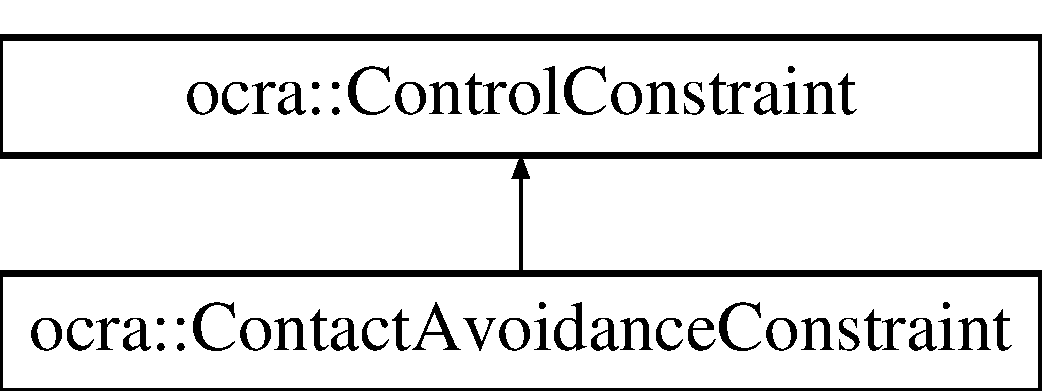
\includegraphics[height=2.000000cm]{d4/d90/classocra_1_1ContactAvoidanceConstraint}
\end{center}
\end{figure}
\subsection*{Public Member Functions}
\begin{DoxyCompactItemize}
\item 
\hyperlink{classocra_1_1ContactAvoidanceConstraint_a77ef6f814bddd8ff8eabb9cf1272b4a3}{Contact\+Avoidance\+Constraint} (const Model \&model, double hpos, double margin)
\item 
virtual \hyperlink{classocra_1_1ContactAvoidanceConstraint_a57650df61143b936321c20d582f2457f}{$\sim$\+Contact\+Avoidance\+Constraint} ()
\item 
double \hyperlink{classocra_1_1ContactAvoidanceConstraint_a1282e8f163c4b53da93b435cdd16501f}{get\+Horizon\+Of\+Prediction} () const
\item 
void \hyperlink{classocra_1_1ContactAvoidanceConstraint_a667de1446a83d166c7979b6066dd0720}{set\+Horizon\+Of\+Prediction} (double new\+Hpos)
\item 
double \hyperlink{classocra_1_1ContactAvoidanceConstraint_acb8dff3c7d62c30edc180e3526ee8f94}{get\+Margin} () const
\item 
void \hyperlink{classocra_1_1ContactAvoidanceConstraint_a3504dbfab2c8e829bb73960891f4dd01}{set\+Margin} (double new\+Margin)
\item 
void \hyperlink{classocra_1_1ContactAvoidanceConstraint_a3d44cd52a5de9bc2d69da19b29a5d7f7}{update\+Contact\+Information} (const Eigen\+::\+Matrix\+Xd \&\+\_\+\+J\+Obst, const Eigen\+::\+Vector\+Xd \&\+\_\+d\+Jdq\+Ost, const Eigen\+::\+Vector\+Xd \&\+\_\+dist\+Obst, const Eigen\+::\+Vector\+Xd \&\+\_\+vel\+Obst)
\end{DoxyCompactItemize}
\subsection*{Protected Member Functions}
\begin{DoxyCompactItemize}
\item 
virtual void \hyperlink{classocra_1_1ContactAvoidanceConstraint_a9beada2720203ab46265f271309a2ab5}{connect\+To\+Controller} (const \hyperlink{classocra_1_1FullDynamicEquationFunction}{Full\+Dynamic\+Equation\+Function} \&dynamic\+Equation, bool use\+Reduced\+Problem)
\item 
virtual void \hyperlink{classocra_1_1ContactAvoidanceConstraint_a884358568ff7f5510d26ff96915a4d8c}{disconnect\+From\+Controller} ()
\end{DoxyCompactItemize}
\subsection*{Additional Inherited Members}


\subsection{Detailed Description}


Definition at line 171 of file Contact\+Avoidance\+Constraint.\+h.



\subsection{Constructor \& Destructor Documentation}
\hypertarget{classocra_1_1ContactAvoidanceConstraint_a77ef6f814bddd8ff8eabb9cf1272b4a3}{}\label{classocra_1_1ContactAvoidanceConstraint_a77ef6f814bddd8ff8eabb9cf1272b4a3} 
\index{ocra\+::\+Contact\+Avoidance\+Constraint@{ocra\+::\+Contact\+Avoidance\+Constraint}!Contact\+Avoidance\+Constraint@{Contact\+Avoidance\+Constraint}}
\index{Contact\+Avoidance\+Constraint@{Contact\+Avoidance\+Constraint}!ocra\+::\+Contact\+Avoidance\+Constraint@{ocra\+::\+Contact\+Avoidance\+Constraint}}
\subsubsection{\texorpdfstring{Contact\+Avoidance\+Constraint()}{ContactAvoidanceConstraint()}}
{\footnotesize\ttfamily Contact\+Avoidance\+Constraint\+::\+Contact\+Avoidance\+Constraint (\begin{DoxyParamCaption}\item[{const Model \&}]{model,  }\item[{double}]{hpos,  }\item[{double}]{margin }\end{DoxyParamCaption})}



Definition at line 329 of file Contact\+Avoidance\+Constraint.\+cpp.

\hypertarget{classocra_1_1ContactAvoidanceConstraint_a57650df61143b936321c20d582f2457f}{}\label{classocra_1_1ContactAvoidanceConstraint_a57650df61143b936321c20d582f2457f} 
\index{ocra\+::\+Contact\+Avoidance\+Constraint@{ocra\+::\+Contact\+Avoidance\+Constraint}!````~Contact\+Avoidance\+Constraint@{$\sim$\+Contact\+Avoidance\+Constraint}}
\index{````~Contact\+Avoidance\+Constraint@{$\sim$\+Contact\+Avoidance\+Constraint}!ocra\+::\+Contact\+Avoidance\+Constraint@{ocra\+::\+Contact\+Avoidance\+Constraint}}
\subsubsection{\texorpdfstring{$\sim$\+Contact\+Avoidance\+Constraint()}{~ContactAvoidanceConstraint()}}
{\footnotesize\ttfamily virtual ocra\+::\+Contact\+Avoidance\+Constraint\+::$\sim$\+Contact\+Avoidance\+Constraint (\begin{DoxyParamCaption}{ }\end{DoxyParamCaption})\hspace{0.3cm}{\ttfamily [inline]}, {\ttfamily [virtual]}}



Definition at line 175 of file Contact\+Avoidance\+Constraint.\+h.



\subsection{Member Function Documentation}
\hypertarget{classocra_1_1ContactAvoidanceConstraint_a9beada2720203ab46265f271309a2ab5}{}\label{classocra_1_1ContactAvoidanceConstraint_a9beada2720203ab46265f271309a2ab5} 
\index{ocra\+::\+Contact\+Avoidance\+Constraint@{ocra\+::\+Contact\+Avoidance\+Constraint}!connect\+To\+Controller@{connect\+To\+Controller}}
\index{connect\+To\+Controller@{connect\+To\+Controller}!ocra\+::\+Contact\+Avoidance\+Constraint@{ocra\+::\+Contact\+Avoidance\+Constraint}}
\subsubsection{\texorpdfstring{connect\+To\+Controller()}{connectToController()}}
{\footnotesize\ttfamily void Contact\+Avoidance\+Constraint\+::connect\+To\+Controller (\begin{DoxyParamCaption}\item[{const \hyperlink{classocra_1_1FullDynamicEquationFunction}{Full\+Dynamic\+Equation\+Function} \&}]{dynamic\+Equation,  }\item[{bool}]{use\+Reduced\+Problem }\end{DoxyParamCaption})\hspace{0.3cm}{\ttfamily [protected]}, {\ttfamily [virtual]}}



Implements \hyperlink{classocra_1_1ControlConstraint_a04dabdc1c469146e7b3240dfe0a5172c}{ocra\+::\+Control\+Constraint}.



Definition at line 373 of file Contact\+Avoidance\+Constraint.\+cpp.

\hypertarget{classocra_1_1ContactAvoidanceConstraint_a884358568ff7f5510d26ff96915a4d8c}{}\label{classocra_1_1ContactAvoidanceConstraint_a884358568ff7f5510d26ff96915a4d8c} 
\index{ocra\+::\+Contact\+Avoidance\+Constraint@{ocra\+::\+Contact\+Avoidance\+Constraint}!disconnect\+From\+Controller@{disconnect\+From\+Controller}}
\index{disconnect\+From\+Controller@{disconnect\+From\+Controller}!ocra\+::\+Contact\+Avoidance\+Constraint@{ocra\+::\+Contact\+Avoidance\+Constraint}}
\subsubsection{\texorpdfstring{disconnect\+From\+Controller()}{disconnectFromController()}}
{\footnotesize\ttfamily void Contact\+Avoidance\+Constraint\+::disconnect\+From\+Controller (\begin{DoxyParamCaption}{ }\end{DoxyParamCaption})\hspace{0.3cm}{\ttfamily [protected]}, {\ttfamily [virtual]}}



Implements \hyperlink{classocra_1_1ControlConstraint_adbd15b36773c775a06a0b7bde46ec799}{ocra\+::\+Control\+Constraint}.



Definition at line 388 of file Contact\+Avoidance\+Constraint.\+cpp.

\hypertarget{classocra_1_1ContactAvoidanceConstraint_a1282e8f163c4b53da93b435cdd16501f}{}\label{classocra_1_1ContactAvoidanceConstraint_a1282e8f163c4b53da93b435cdd16501f} 
\index{ocra\+::\+Contact\+Avoidance\+Constraint@{ocra\+::\+Contact\+Avoidance\+Constraint}!get\+Horizon\+Of\+Prediction@{get\+Horizon\+Of\+Prediction}}
\index{get\+Horizon\+Of\+Prediction@{get\+Horizon\+Of\+Prediction}!ocra\+::\+Contact\+Avoidance\+Constraint@{ocra\+::\+Contact\+Avoidance\+Constraint}}
\subsubsection{\texorpdfstring{get\+Horizon\+Of\+Prediction()}{getHorizonOfPrediction()}}
{\footnotesize\ttfamily double Contact\+Avoidance\+Constraint\+::get\+Horizon\+Of\+Prediction (\begin{DoxyParamCaption}{ }\end{DoxyParamCaption}) const}



Definition at line 338 of file Contact\+Avoidance\+Constraint.\+cpp.

\hypertarget{classocra_1_1ContactAvoidanceConstraint_acb8dff3c7d62c30edc180e3526ee8f94}{}\label{classocra_1_1ContactAvoidanceConstraint_acb8dff3c7d62c30edc180e3526ee8f94} 
\index{ocra\+::\+Contact\+Avoidance\+Constraint@{ocra\+::\+Contact\+Avoidance\+Constraint}!get\+Margin@{get\+Margin}}
\index{get\+Margin@{get\+Margin}!ocra\+::\+Contact\+Avoidance\+Constraint@{ocra\+::\+Contact\+Avoidance\+Constraint}}
\subsubsection{\texorpdfstring{get\+Margin()}{getMargin()}}
{\footnotesize\ttfamily double Contact\+Avoidance\+Constraint\+::get\+Margin (\begin{DoxyParamCaption}{ }\end{DoxyParamCaption}) const}



Definition at line 351 of file Contact\+Avoidance\+Constraint.\+cpp.

\hypertarget{classocra_1_1ContactAvoidanceConstraint_a667de1446a83d166c7979b6066dd0720}{}\label{classocra_1_1ContactAvoidanceConstraint_a667de1446a83d166c7979b6066dd0720} 
\index{ocra\+::\+Contact\+Avoidance\+Constraint@{ocra\+::\+Contact\+Avoidance\+Constraint}!set\+Horizon\+Of\+Prediction@{set\+Horizon\+Of\+Prediction}}
\index{set\+Horizon\+Of\+Prediction@{set\+Horizon\+Of\+Prediction}!ocra\+::\+Contact\+Avoidance\+Constraint@{ocra\+::\+Contact\+Avoidance\+Constraint}}
\subsubsection{\texorpdfstring{set\+Horizon\+Of\+Prediction()}{setHorizonOfPrediction()}}
{\footnotesize\ttfamily void Contact\+Avoidance\+Constraint\+::set\+Horizon\+Of\+Prediction (\begin{DoxyParamCaption}\item[{double}]{new\+Hpos }\end{DoxyParamCaption})}



Definition at line 343 of file Contact\+Avoidance\+Constraint.\+cpp.

\hypertarget{classocra_1_1ContactAvoidanceConstraint_a3504dbfab2c8e829bb73960891f4dd01}{}\label{classocra_1_1ContactAvoidanceConstraint_a3504dbfab2c8e829bb73960891f4dd01} 
\index{ocra\+::\+Contact\+Avoidance\+Constraint@{ocra\+::\+Contact\+Avoidance\+Constraint}!set\+Margin@{set\+Margin}}
\index{set\+Margin@{set\+Margin}!ocra\+::\+Contact\+Avoidance\+Constraint@{ocra\+::\+Contact\+Avoidance\+Constraint}}
\subsubsection{\texorpdfstring{set\+Margin()}{setMargin()}}
{\footnotesize\ttfamily void Contact\+Avoidance\+Constraint\+::set\+Margin (\begin{DoxyParamCaption}\item[{double}]{new\+Margin }\end{DoxyParamCaption})}



Definition at line 356 of file Contact\+Avoidance\+Constraint.\+cpp.

\hypertarget{classocra_1_1ContactAvoidanceConstraint_a3d44cd52a5de9bc2d69da19b29a5d7f7}{}\label{classocra_1_1ContactAvoidanceConstraint_a3d44cd52a5de9bc2d69da19b29a5d7f7} 
\index{ocra\+::\+Contact\+Avoidance\+Constraint@{ocra\+::\+Contact\+Avoidance\+Constraint}!update\+Contact\+Information@{update\+Contact\+Information}}
\index{update\+Contact\+Information@{update\+Contact\+Information}!ocra\+::\+Contact\+Avoidance\+Constraint@{ocra\+::\+Contact\+Avoidance\+Constraint}}
\subsubsection{\texorpdfstring{update\+Contact\+Information()}{updateContactInformation()}}
{\footnotesize\ttfamily void Contact\+Avoidance\+Constraint\+::update\+Contact\+Information (\begin{DoxyParamCaption}\item[{const Eigen\+::\+Matrix\+Xd \&}]{\+\_\+\+J\+Obst,  }\item[{const Eigen\+::\+Vector\+Xd \&}]{\+\_\+d\+Jdq\+Ost,  }\item[{const Eigen\+::\+Vector\+Xd \&}]{\+\_\+dist\+Obst,  }\item[{const Eigen\+::\+Vector\+Xd \&}]{\+\_\+vel\+Obst }\end{DoxyParamCaption})}



Definition at line 364 of file Contact\+Avoidance\+Constraint.\+cpp.



The documentation for this class was generated from the following files\+:\begin{DoxyCompactItemize}
\item 
\hyperlink{ContactAvoidanceConstraint_8h}{Contact\+Avoidance\+Constraint.\+h}\item 
\hyperlink{ContactAvoidanceConstraint_8cpp}{Contact\+Avoidance\+Constraint.\+cpp}\end{DoxyCompactItemize}

\hypertarget{classocra_1_1ContactAvoidanceFunction}{}\section{ocra\+:\+:Contact\+Avoidance\+Function Class Reference}
\label{classocra_1_1ContactAvoidanceFunction}\index{ocra\+::\+Contact\+Avoidance\+Function@{ocra\+::\+Contact\+Avoidance\+Function}}


Create a linear function that represents the joint limit function.  




{\ttfamily \#include $<$Contact\+Avoidance\+Constraint.\+h$>$}



Inheritance diagram for ocra\+:\+:Contact\+Avoidance\+Function\+:\nopagebreak
\begin{figure}[H]
\begin{center}
\leavevmode
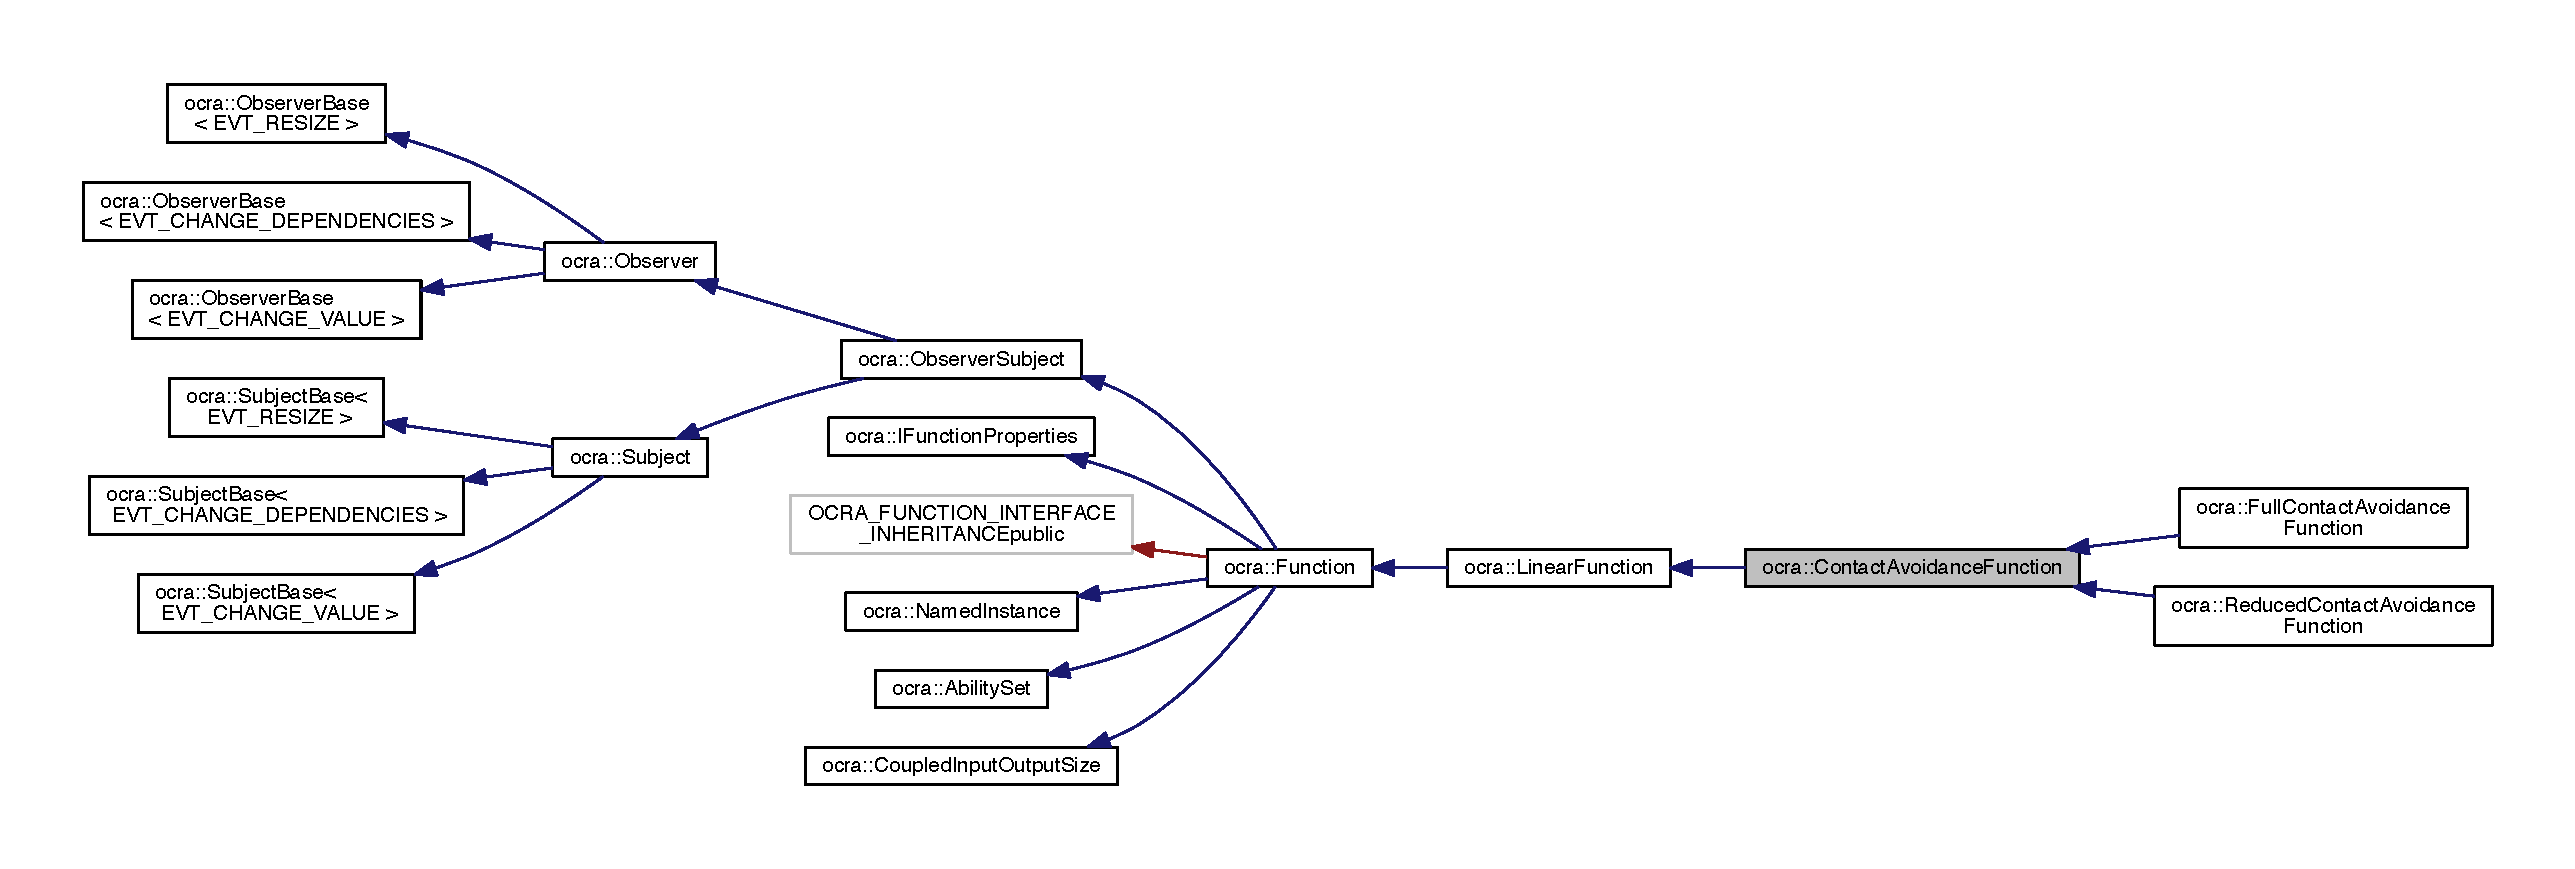
\includegraphics[width=350pt]{d5/d61/classocra_1_1ContactAvoidanceFunction__inherit__graph}
\end{center}
\end{figure}


Collaboration diagram for ocra\+:\+:Contact\+Avoidance\+Function\+:\nopagebreak
\begin{figure}[H]
\begin{center}
\leavevmode
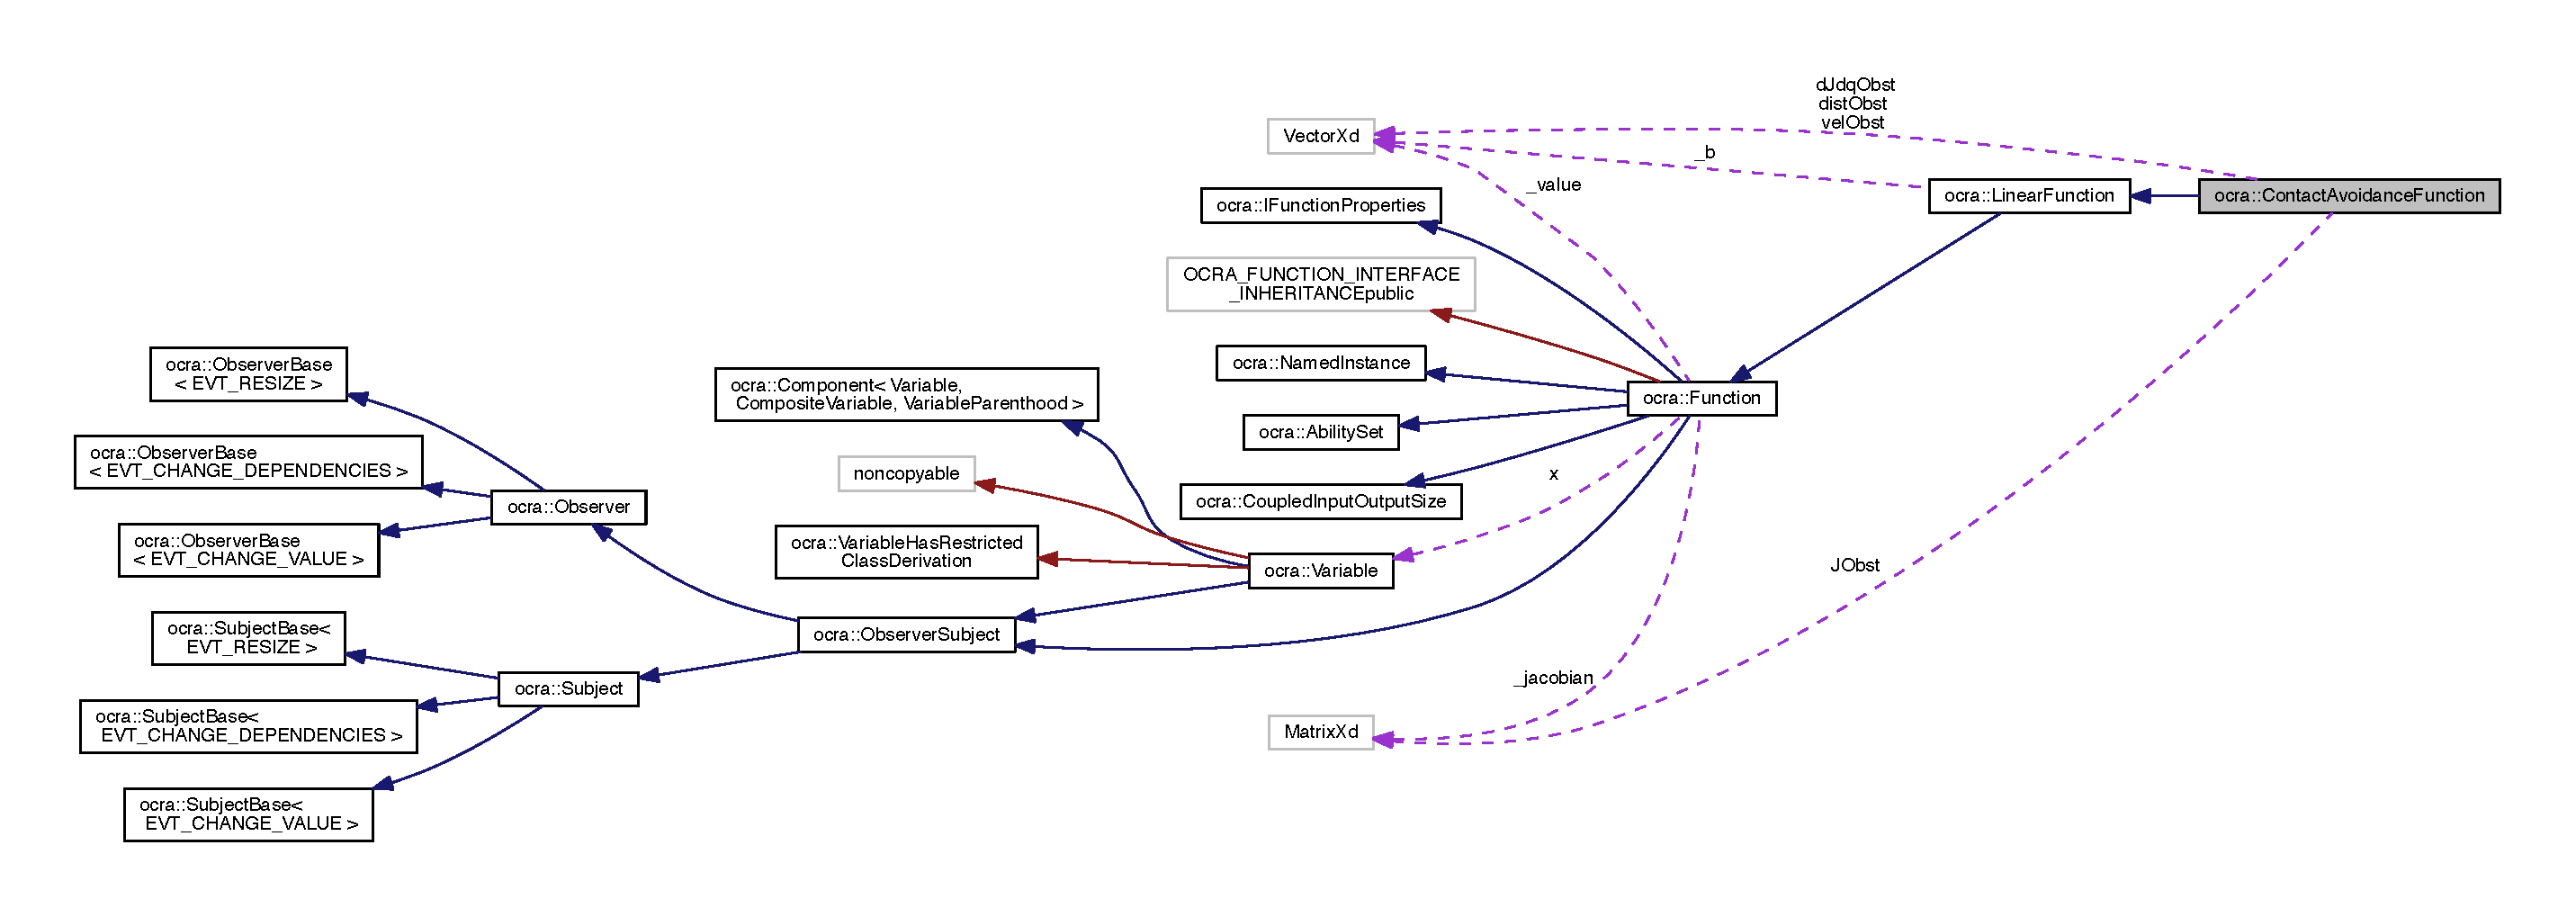
\includegraphics[width=350pt]{d3/d88/classocra_1_1ContactAvoidanceFunction__coll__graph}
\end{center}
\end{figure}
\subsection*{Public Types}
\begin{DoxyCompactItemize}
\item 
typedef \hyperlink{classocra_1_1LinearFunction}{Linear\+Function} \hyperlink{classocra_1_1ContactAvoidanceFunction_a15d14e0a9e8810d1a6990d5ab7e179ab}{function\+Type\+\_\+t}
\end{DoxyCompactItemize}
\subsection*{Public Member Functions}
\begin{DoxyCompactItemize}
\item 
\hyperlink{classocra_1_1ContactAvoidanceFunction_a7db869c24ac20e1aff021f95ccf7dcd8}{Contact\+Avoidance\+Function} (const \hyperlink{classocra_1_1Model}{Model} \&m, \hyperlink{classocra_1_1Variable}{Variable} \&var)
\item 
\hyperlink{classocra_1_1ContactAvoidanceFunction_a5309c1fd586ed0292ee5eebfafacef9b}{$\sim$\+Contact\+Avoidance\+Function} ()
\item 
double \hyperlink{classocra_1_1ContactAvoidanceFunction_aca5221cb617b3603e022040768974a20}{get\+Horizon\+Of\+Prediction} () const
\item 
void \hyperlink{classocra_1_1ContactAvoidanceFunction_abb04a99b523d82819d2b11bf9a7ea7f9}{set\+Horizon\+Of\+Prediction} (double new\+Hpos)
\item 
double \hyperlink{classocra_1_1ContactAvoidanceFunction_a666af8d0a23e115b2f139b048fe6b933}{get\+Margin} () const
\item 
void \hyperlink{classocra_1_1ContactAvoidanceFunction_a4ae90405d1464527310ce1d93df2e862}{set\+Margin} (double new\+Margin)
\item 
void \hyperlink{classocra_1_1ContactAvoidanceFunction_aee28a7fe69481db190d2e26b603659ea}{update\+Contact\+Information} (const Eigen\+::\+Matrix\+Xd \&\+\_\+\+J\+Obst, const Eigen\+::\+Vector\+Xd \&\+\_\+d\+Jdq\+Ost, const Eigen\+::\+Vector\+Xd \&\+\_\+dist\+Obst, const Eigen\+::\+Vector\+Xd \&\+\_\+vel\+Obst)
\end{DoxyCompactItemize}
\subsection*{Protected Member Functions}
\begin{DoxyCompactItemize}
\item 
void \hyperlink{classocra_1_1ContactAvoidanceFunction_aca72dc43ecd3d95bb917139ac6ae19c1}{update\+Jacobian} () const
\item 
void \hyperlink{classocra_1_1ContactAvoidanceFunction_aed2f145f17ff9fd8dd646018376ea7e9}{updateb} () const
\item 
virtual void \hyperlink{classocra_1_1ContactAvoidanceFunction_a4f33ca5589b08a96207be800b9f4bd57}{do\+Update\+Dimension\+Begin} (int new\+Dimension)
\item 
virtual void \hyperlink{classocra_1_1ContactAvoidanceFunction_ad81a7b03b0fb7e8b2a037bccf5faea84}{do\+Update\+Dimension\+End} (int old\+Dimension)
\item 
void \hyperlink{classocra_1_1ContactAvoidanceFunction_a59994d2c3f364575ecff7fb23b7e10ab}{compute\+Full\+Jacobian} (const Eigen\+::\+Matrix\+Xd \&\+\_\+\+J\+Obst, Eigen\+::\+Matrix\+Xd \&full\+Jacobian) const
\item 
void \hyperlink{classocra_1_1ContactAvoidanceFunction_a9afd02871f0d26321b526290f565d541}{compute\+Fullb} (const Eigen\+::\+Vector\+Xd \&\+\_\+d\+Jdq\+Obst, const Eigen\+::\+Vector\+Xd \&\+\_\+dist\+Obst, const Eigen\+::\+Vector\+Xd \&\+\_\+vel\+Obst, Eigen\+::\+Vector\+Xd \&fullb) const
\end{DoxyCompactItemize}
\subsection*{Protected Attributes}
\begin{DoxyCompactItemize}
\item 
double \hyperlink{classocra_1_1ContactAvoidanceFunction_a49e94dae2d7708e66cf11e737b1a4d6d}{hpos}
\item 
double \hyperlink{classocra_1_1ContactAvoidanceFunction_a5a4c2e4dae17aef6c4cf6fa1b3be093e}{margin}
\item 
Eigen\+::\+Matrix\+Xd \hyperlink{classocra_1_1ContactAvoidanceFunction_a233c509632182b45540a30b818254713}{J\+Obst}
\item 
Eigen\+::\+Vector\+Xd \hyperlink{classocra_1_1ContactAvoidanceFunction_a59c655299c8db310d3e06a47729f0780}{d\+Jdq\+Obst}
\item 
Eigen\+::\+Vector\+Xd \hyperlink{classocra_1_1ContactAvoidanceFunction_aa3d1b5f23d42c0936b1fa09ad7988732}{dist\+Obst}
\item 
Eigen\+::\+Vector\+Xd \hyperlink{classocra_1_1ContactAvoidanceFunction_a19eb96ace3a217e5ea1c80dec97eeeb2}{vel\+Obst}
\end{DoxyCompactItemize}
\subsection*{Additional Inherited Members}


\subsection{Detailed Description}
Create a linear function that represents the joint limit function. 

The contact avoidance constraint is written at first as\+: $ \vec{0} < \vec{d}_{oa} $ where $ \vec{d}_{oa} $ is the contatenation of the minimal distances between the couples of shapes that should not collide.



To relate this constraint with the dynamic variables, we constrain the estimated future distances to remain positive, as explained in w\+Joint\+Limit\+Function .

In this case, the constraint is expressed as follows\+:

\begin{align*} \vec{d}_{oa} - \vec{m} &> \vec{d}_{oa}(h) \quad \text{at instant h} \\ \vec{d}_{oa} - \vec{m} &> \dot{\vec{d}}_{oa} h + \ddot{\vec{d}}_{oa} \frac{h^2}{2} \\ \vec{d}_{oa} - \vec{m} &> \dot{\vec{d}}_{oa} h + \left( \J_{oa} \ddq + \dJ_{oa} \dq \right) \frac{h^2}{2} \end{align*}

where $ \vec{m} $ is a margin vector. So it becomes\+:

\begin{align*} \A \x + \b &> \vec{0} & &\Leftrightarrow & \begin{bmatrix} - \J_{oa} \end{bmatrix} \ddq + \begin{bmatrix} - \dJ_{oa} \dq + 2 \left( \vec{d}_{oa} - \vec{m} - \dot{\vec{d}}_{oa} h \right) / h^2 \end{bmatrix} & > \vec{0} \end{align*}

There is some similarity with the w\+Joint\+Limit\+Function because we constrain an estimated future state. The same issues arise (it only constrain the final point, no middle points), so it is interesting to look at the inflexion point. In the same manner, the time of inflexion for a constant acceleration such as the inflexion point is on 0 is computed as follows\+:

\begin{align*} t_{max} &= 2*(\vec{d}_{oa} - \vec{m}) / \dot{\vec{d}}_{oa} & & \text{(element-wise operations)} \end{align*}

For each dof (each line $ i $ ), we test where is the time of inflexion. If $ 0 < t_{max}[i] < h$, then the inflexion point is in the horizon of time, we should consider to constrain the motion of this contact avoidance\+:

\begin{align*} \ddot{\vec{d}}_{max}[i] &= \frac{ \dot{\vec{d}}_{oa}[i]^2 }{ 2( \vec{d}_{oa}[i] - \vec{m}[i] ) } & & \Rightarrow & \begin{bmatrix} - \J_{oa} \end{bmatrix} [i] \ddq + \ddot{\vec{d}}_{max}[i] > 0 \end{align*}

When all these constraints have been defined, we select the tightest ones for each dof. 

Definition at line 67 of file Contact\+Avoidance\+Constraint.\+h.



\subsection{Member Typedef Documentation}
\hypertarget{classocra_1_1ContactAvoidanceFunction_a15d14e0a9e8810d1a6990d5ab7e179ab}{}\label{classocra_1_1ContactAvoidanceFunction_a15d14e0a9e8810d1a6990d5ab7e179ab} 
\index{ocra\+::\+Contact\+Avoidance\+Function@{ocra\+::\+Contact\+Avoidance\+Function}!function\+Type\+\_\+t@{function\+Type\+\_\+t}}
\index{function\+Type\+\_\+t@{function\+Type\+\_\+t}!ocra\+::\+Contact\+Avoidance\+Function@{ocra\+::\+Contact\+Avoidance\+Function}}
\subsubsection{\texorpdfstring{function\+Type\+\_\+t}{functionType\_t}}
{\footnotesize\ttfamily typedef \hyperlink{classocra_1_1LinearFunction}{Linear\+Function} \hyperlink{classocra_1_1ContactAvoidanceFunction_a15d14e0a9e8810d1a6990d5ab7e179ab}{ocra\+::\+Contact\+Avoidance\+Function\+::function\+Type\+\_\+t}}



Definition at line 70 of file Contact\+Avoidance\+Constraint.\+h.



\subsection{Constructor \& Destructor Documentation}
\hypertarget{classocra_1_1ContactAvoidanceFunction_a7db869c24ac20e1aff021f95ccf7dcd8}{}\label{classocra_1_1ContactAvoidanceFunction_a7db869c24ac20e1aff021f95ccf7dcd8} 
\index{ocra\+::\+Contact\+Avoidance\+Function@{ocra\+::\+Contact\+Avoidance\+Function}!Contact\+Avoidance\+Function@{Contact\+Avoidance\+Function}}
\index{Contact\+Avoidance\+Function@{Contact\+Avoidance\+Function}!ocra\+::\+Contact\+Avoidance\+Function@{ocra\+::\+Contact\+Avoidance\+Function}}
\subsubsection{\texorpdfstring{Contact\+Avoidance\+Function()}{ContactAvoidanceFunction()}}
{\footnotesize\ttfamily Contact\+Avoidance\+Function\+::\+Contact\+Avoidance\+Function (\begin{DoxyParamCaption}\item[{const \hyperlink{classocra_1_1Model}{Model} \&}]{model,  }\item[{\hyperlink{classocra_1_1Variable}{Variable} \&}]{var }\end{DoxyParamCaption})}

Initialize the contact avoidance constraint function.


\begin{DoxyParams}{Parameters}
{\em model} & The \hyperlink{classocra_1_1Model}{Model} on which we will get the dynamic parameters \\
\hline
{\em var} & The problem variable that will be used to write this constraint\\
\hline
\end{DoxyParams}
This class is a generic class to compute matrices for the contact avoidance function, but {\bfseries it should not be used}. You would rather choose one of the following derivative classes, depending on the choosen formalism, either full $ \x = [ \ddq \; \torque \; \force_c ] $ or reduced $ \x = [ \torque \; \force_c ] $\+: \begin{DoxyVerb} - wFullContactAvoidanceFunction
 - wReducedContactAvoidanceFunction\end{DoxyVerb}
 

Definition at line 30 of file Contact\+Avoidance\+Constraint.\+cpp.

\hypertarget{classocra_1_1ContactAvoidanceFunction_a5309c1fd586ed0292ee5eebfafacef9b}{}\label{classocra_1_1ContactAvoidanceFunction_a5309c1fd586ed0292ee5eebfafacef9b} 
\index{ocra\+::\+Contact\+Avoidance\+Function@{ocra\+::\+Contact\+Avoidance\+Function}!````~Contact\+Avoidance\+Function@{$\sim$\+Contact\+Avoidance\+Function}}
\index{````~Contact\+Avoidance\+Function@{$\sim$\+Contact\+Avoidance\+Function}!ocra\+::\+Contact\+Avoidance\+Function@{ocra\+::\+Contact\+Avoidance\+Function}}
\subsubsection{\texorpdfstring{$\sim$\+Contact\+Avoidance\+Function()}{~ContactAvoidanceFunction()}}
{\footnotesize\ttfamily Contact\+Avoidance\+Function\+::$\sim$\+Contact\+Avoidance\+Function (\begin{DoxyParamCaption}{ }\end{DoxyParamCaption})}

Destructor 

Definition at line 46 of file Contact\+Avoidance\+Constraint.\+cpp.



\subsection{Member Function Documentation}
\hypertarget{classocra_1_1ContactAvoidanceFunction_a9afd02871f0d26321b526290f565d541}{}\label{classocra_1_1ContactAvoidanceFunction_a9afd02871f0d26321b526290f565d541} 
\index{ocra\+::\+Contact\+Avoidance\+Function@{ocra\+::\+Contact\+Avoidance\+Function}!compute\+Fullb@{compute\+Fullb}}
\index{compute\+Fullb@{compute\+Fullb}!ocra\+::\+Contact\+Avoidance\+Function@{ocra\+::\+Contact\+Avoidance\+Function}}
\subsubsection{\texorpdfstring{compute\+Fullb()}{computeFullb()}}
{\footnotesize\ttfamily void Contact\+Avoidance\+Function\+::compute\+Fullb (\begin{DoxyParamCaption}\item[{const Eigen\+::\+Vector\+Xd \&}]{\+\_\+d\+Jdq\+Obst,  }\item[{const Eigen\+::\+Vector\+Xd \&}]{\+\_\+dist\+Obst,  }\item[{const Eigen\+::\+Vector\+Xd \&}]{\+\_\+vel\+Obst,  }\item[{Eigen\+::\+Vector\+Xd \&}]{fullb }\end{DoxyParamCaption}) const\hspace{0.3cm}{\ttfamily [protected]}}

Compute the vector $ \b $ of the linear function for the collision avoidance constraint expressed in the full formalism.


\begin{DoxyParams}{Parameters}
{\em \+\_\+d\+Jdq\+Obst} & The derivative of the Jacobian of obstacle avoidance multiplied by generalized velocity $ = \dJ_{Obst} \dq $ \\
\hline
{\em \+\_\+dist\+Obst} & The relative distance of obstacle avoidance \\
\hline
{\em \+\_\+vel\+Obst} & The relative velocity of obstacle avoidance \\
\hline
{\em fullb} & The vector instance where to write the collision avoidance data in the full formalism \\
\hline
\end{DoxyParams}


Definition at line 121 of file Contact\+Avoidance\+Constraint.\+cpp.

\hypertarget{classocra_1_1ContactAvoidanceFunction_a59994d2c3f364575ecff7fb23b7e10ab}{}\label{classocra_1_1ContactAvoidanceFunction_a59994d2c3f364575ecff7fb23b7e10ab} 
\index{ocra\+::\+Contact\+Avoidance\+Function@{ocra\+::\+Contact\+Avoidance\+Function}!compute\+Full\+Jacobian@{compute\+Full\+Jacobian}}
\index{compute\+Full\+Jacobian@{compute\+Full\+Jacobian}!ocra\+::\+Contact\+Avoidance\+Function@{ocra\+::\+Contact\+Avoidance\+Function}}
\subsubsection{\texorpdfstring{compute\+Full\+Jacobian()}{computeFullJacobian()}}
{\footnotesize\ttfamily void Contact\+Avoidance\+Function\+::compute\+Full\+Jacobian (\begin{DoxyParamCaption}\item[{const Eigen\+::\+Matrix\+Xd \&}]{\+\_\+\+J\+Obst,  }\item[{Eigen\+::\+Matrix\+Xd \&}]{full\+Jacobian }\end{DoxyParamCaption}) const\hspace{0.3cm}{\ttfamily [protected]}}

Compute the Jacobian matrix $ \A $ of the linear function for the collision avoidance constraint expressed in the full formalism.


\begin{DoxyParams}{Parameters}
{\em \+\_\+\+J\+Obst} & The Jacobian of obstacle avoidance \\
\hline
{\em full\+Jacobian} & The matrix instance where to write the collision avoidance data in the full formalism \\
\hline
\end{DoxyParams}


Definition at line 109 of file Contact\+Avoidance\+Constraint.\+cpp.

\hypertarget{classocra_1_1ContactAvoidanceFunction_a4f33ca5589b08a96207be800b9f4bd57}{}\label{classocra_1_1ContactAvoidanceFunction_a4f33ca5589b08a96207be800b9f4bd57} 
\index{ocra\+::\+Contact\+Avoidance\+Function@{ocra\+::\+Contact\+Avoidance\+Function}!do\+Update\+Dimension\+Begin@{do\+Update\+Dimension\+Begin}}
\index{do\+Update\+Dimension\+Begin@{do\+Update\+Dimension\+Begin}!ocra\+::\+Contact\+Avoidance\+Function@{ocra\+::\+Contact\+Avoidance\+Function}}
\subsubsection{\texorpdfstring{do\+Update\+Dimension\+Begin()}{doUpdateDimensionBegin()}}
{\footnotesize\ttfamily void Contact\+Avoidance\+Function\+::do\+Update\+Dimension\+Begin (\begin{DoxyParamCaption}\item[{int}]{new\+Dimension }\end{DoxyParamCaption})\hspace{0.3cm}{\ttfamily [protected]}, {\ttfamily [virtual]}}

Do when linear function dimension changes, before.

By overloading this function, it allows linear function modification when function size changes. It does nothing actually. 

Reimplemented from \hyperlink{classocra_1_1Function_afdf98e9f43fde97a5256af88a50cbb39}{ocra\+::\+Function}.



Definition at line 167 of file Contact\+Avoidance\+Constraint.\+cpp.

\hypertarget{classocra_1_1ContactAvoidanceFunction_ad81a7b03b0fb7e8b2a037bccf5faea84}{}\label{classocra_1_1ContactAvoidanceFunction_ad81a7b03b0fb7e8b2a037bccf5faea84} 
\index{ocra\+::\+Contact\+Avoidance\+Function@{ocra\+::\+Contact\+Avoidance\+Function}!do\+Update\+Dimension\+End@{do\+Update\+Dimension\+End}}
\index{do\+Update\+Dimension\+End@{do\+Update\+Dimension\+End}!ocra\+::\+Contact\+Avoidance\+Function@{ocra\+::\+Contact\+Avoidance\+Function}}
\subsubsection{\texorpdfstring{do\+Update\+Dimension\+End()}{doUpdateDimensionEnd()}}
{\footnotesize\ttfamily void Contact\+Avoidance\+Function\+::do\+Update\+Dimension\+End (\begin{DoxyParamCaption}\item[{int}]{old\+Dimension }\end{DoxyParamCaption})\hspace{0.3cm}{\ttfamily [protected]}, {\ttfamily [virtual]}}

Do when linear function dimension changes, after.

By overloading this function, it allows linear function modification when function size changes. It does nothing actually. 

Reimplemented from \hyperlink{classocra_1_1Function_a17aa280f0e6eff4a7569edc373a5147d}{ocra\+::\+Function}.



Definition at line 177 of file Contact\+Avoidance\+Constraint.\+cpp.

\hypertarget{classocra_1_1ContactAvoidanceFunction_aca5221cb617b3603e022040768974a20}{}\label{classocra_1_1ContactAvoidanceFunction_aca5221cb617b3603e022040768974a20} 
\index{ocra\+::\+Contact\+Avoidance\+Function@{ocra\+::\+Contact\+Avoidance\+Function}!get\+Horizon\+Of\+Prediction@{get\+Horizon\+Of\+Prediction}}
\index{get\+Horizon\+Of\+Prediction@{get\+Horizon\+Of\+Prediction}!ocra\+::\+Contact\+Avoidance\+Function@{ocra\+::\+Contact\+Avoidance\+Function}}
\subsubsection{\texorpdfstring{get\+Horizon\+Of\+Prediction()}{getHorizonOfPrediction()}}
{\footnotesize\ttfamily double Contact\+Avoidance\+Function\+::get\+Horizon\+Of\+Prediction (\begin{DoxyParamCaption}{ }\end{DoxyParamCaption}) const}

Get the time horizon of prediction $ h $ for the contact avoidance function.

\begin{DoxyReturn}{Returns}
The time horizon (s) 
\end{DoxyReturn}


Definition at line 55 of file Contact\+Avoidance\+Constraint.\+cpp.

\hypertarget{classocra_1_1ContactAvoidanceFunction_a666af8d0a23e115b2f139b048fe6b933}{}\label{classocra_1_1ContactAvoidanceFunction_a666af8d0a23e115b2f139b048fe6b933} 
\index{ocra\+::\+Contact\+Avoidance\+Function@{ocra\+::\+Contact\+Avoidance\+Function}!get\+Margin@{get\+Margin}}
\index{get\+Margin@{get\+Margin}!ocra\+::\+Contact\+Avoidance\+Function@{ocra\+::\+Contact\+Avoidance\+Function}}
\subsubsection{\texorpdfstring{get\+Margin()}{getMargin()}}
{\footnotesize\ttfamily double Contact\+Avoidance\+Function\+::get\+Margin (\begin{DoxyParamCaption}{ }\end{DoxyParamCaption}) const}

Get the obstacle avoidance margin $ \vec{m} $.

\begin{DoxyReturn}{Returns}
The margin vector 
\end{DoxyReturn}


Definition at line 73 of file Contact\+Avoidance\+Constraint.\+cpp.

\hypertarget{classocra_1_1ContactAvoidanceFunction_abb04a99b523d82819d2b11bf9a7ea7f9}{}\label{classocra_1_1ContactAvoidanceFunction_abb04a99b523d82819d2b11bf9a7ea7f9} 
\index{ocra\+::\+Contact\+Avoidance\+Function@{ocra\+::\+Contact\+Avoidance\+Function}!set\+Horizon\+Of\+Prediction@{set\+Horizon\+Of\+Prediction}}
\index{set\+Horizon\+Of\+Prediction@{set\+Horizon\+Of\+Prediction}!ocra\+::\+Contact\+Avoidance\+Function@{ocra\+::\+Contact\+Avoidance\+Function}}
\subsubsection{\texorpdfstring{set\+Horizon\+Of\+Prediction()}{setHorizonOfPrediction()}}
{\footnotesize\ttfamily void Contact\+Avoidance\+Function\+::set\+Horizon\+Of\+Prediction (\begin{DoxyParamCaption}\item[{double}]{new\+Hpos }\end{DoxyParamCaption})}

Set the time horizon of prediction $ h $ for the contact avoidance function.


\begin{DoxyParams}{Parameters}
{\em new\+Hpos} & The new time horizon (s) \\
\hline
\end{DoxyParams}


Definition at line 64 of file Contact\+Avoidance\+Constraint.\+cpp.

\hypertarget{classocra_1_1ContactAvoidanceFunction_a4ae90405d1464527310ce1d93df2e862}{}\label{classocra_1_1ContactAvoidanceFunction_a4ae90405d1464527310ce1d93df2e862} 
\index{ocra\+::\+Contact\+Avoidance\+Function@{ocra\+::\+Contact\+Avoidance\+Function}!set\+Margin@{set\+Margin}}
\index{set\+Margin@{set\+Margin}!ocra\+::\+Contact\+Avoidance\+Function@{ocra\+::\+Contact\+Avoidance\+Function}}
\subsubsection{\texorpdfstring{set\+Margin()}{setMargin()}}
{\footnotesize\ttfamily void Contact\+Avoidance\+Function\+::set\+Margin (\begin{DoxyParamCaption}\item[{double}]{new\+Margin }\end{DoxyParamCaption})}

Set the obstacle avoidance margin $ \vec{m} $.


\begin{DoxyParams}{Parameters}
{\em new\+Margin} & The margin vector \\
\hline
\end{DoxyParams}


Definition at line 82 of file Contact\+Avoidance\+Constraint.\+cpp.

\hypertarget{classocra_1_1ContactAvoidanceFunction_aed2f145f17ff9fd8dd646018376ea7e9}{}\label{classocra_1_1ContactAvoidanceFunction_aed2f145f17ff9fd8dd646018376ea7e9} 
\index{ocra\+::\+Contact\+Avoidance\+Function@{ocra\+::\+Contact\+Avoidance\+Function}!updateb@{updateb}}
\index{updateb@{updateb}!ocra\+::\+Contact\+Avoidance\+Function@{ocra\+::\+Contact\+Avoidance\+Function}}
\subsubsection{\texorpdfstring{updateb()}{updateb()}}
{\footnotesize\ttfamily void Contact\+Avoidance\+Function\+::updateb (\begin{DoxyParamCaption}{ }\end{DoxyParamCaption}) const\hspace{0.3cm}{\ttfamily [protected]}, {\ttfamily [virtual]}}

update the vector $ \b $.

Does nothing.

\begin{DoxyRefDesc}{Todo}
\item[\hyperlink{todo__todo000002}{Todo}]It should be conform to the ocra framework, the computation of the vector should be here. \end{DoxyRefDesc}


Reimplemented from \hyperlink{classocra_1_1LinearFunction_a546454cd8d0909f99433ffc0e700c9e3}{ocra\+::\+Linear\+Function}.



Reimplemented in \hyperlink{classocra_1_1ReducedContactAvoidanceFunction_ac39227a19a650de28f4ae603511bfb73}{ocra\+::\+Reduced\+Contact\+Avoidance\+Function}, and \hyperlink{classocra_1_1FullContactAvoidanceFunction_ae24690ecd464eefd43936907e33c4cb9}{ocra\+::\+Full\+Contact\+Avoidance\+Function}.



Definition at line 157 of file Contact\+Avoidance\+Constraint.\+cpp.

\hypertarget{classocra_1_1ContactAvoidanceFunction_aee28a7fe69481db190d2e26b603659ea}{}\label{classocra_1_1ContactAvoidanceFunction_aee28a7fe69481db190d2e26b603659ea} 
\index{ocra\+::\+Contact\+Avoidance\+Function@{ocra\+::\+Contact\+Avoidance\+Function}!update\+Contact\+Information@{update\+Contact\+Information}}
\index{update\+Contact\+Information@{update\+Contact\+Information}!ocra\+::\+Contact\+Avoidance\+Function@{ocra\+::\+Contact\+Avoidance\+Function}}
\subsubsection{\texorpdfstring{update\+Contact\+Information()}{updateContactInformation()}}
{\footnotesize\ttfamily void Contact\+Avoidance\+Function\+::update\+Contact\+Information (\begin{DoxyParamCaption}\item[{const Eigen\+::\+Matrix\+Xd \&}]{\+\_\+\+J\+Obst,  }\item[{const Eigen\+::\+Vector\+Xd \&}]{\+\_\+d\+Jdq\+Obst,  }\item[{const Eigen\+::\+Vector\+Xd \&}]{\+\_\+dist\+Obst,  }\item[{const Eigen\+::\+Vector\+Xd \&}]{\+\_\+vel\+Obst }\end{DoxyParamCaption})}

Update contact information to compute obstacle avoidance function.


\begin{DoxyParams}{Parameters}
{\em \+\_\+\+J\+Obst} & The Jacobian of obstacle avoidance \\
\hline
{\em \+\_\+d\+Jdq\+Obst} & The derivative of the Jacobian of obstacle avoidance multiplied by generalized velocity $ = \dJ_{Obst} \dq $ \\
\hline
{\em \+\_\+dist\+Obst} & The relative distance of obstacle avoidance \\
\hline
{\em \+\_\+vel\+Obst} & The relative velocity of obstacle avoidance \\
\hline
\end{DoxyParams}


Definition at line 94 of file Contact\+Avoidance\+Constraint.\+cpp.

\hypertarget{classocra_1_1ContactAvoidanceFunction_aca72dc43ecd3d95bb917139ac6ae19c1}{}\label{classocra_1_1ContactAvoidanceFunction_aca72dc43ecd3d95bb917139ac6ae19c1} 
\index{ocra\+::\+Contact\+Avoidance\+Function@{ocra\+::\+Contact\+Avoidance\+Function}!update\+Jacobian@{update\+Jacobian}}
\index{update\+Jacobian@{update\+Jacobian}!ocra\+::\+Contact\+Avoidance\+Function@{ocra\+::\+Contact\+Avoidance\+Function}}
\subsubsection{\texorpdfstring{update\+Jacobian()}{updateJacobian()}}
{\footnotesize\ttfamily void Contact\+Avoidance\+Function\+::update\+Jacobian (\begin{DoxyParamCaption}{ }\end{DoxyParamCaption}) const\hspace{0.3cm}{\ttfamily [protected]}, {\ttfamily [virtual]}}

update the Jacobian matrix $ \A $.

Does nothing.

\begin{DoxyRefDesc}{Todo}
\item[\hyperlink{todo__todo000001}{Todo}]It should be conform to the ocra framework, the computation of the jacobian should be here. \end{DoxyRefDesc}


Reimplemented from \hyperlink{classocra_1_1LinearFunction_a30926f977c0124a0b0f65b854ab39636}{ocra\+::\+Linear\+Function}.



Reimplemented in \hyperlink{classocra_1_1FullContactAvoidanceFunction_a91b21004faed7ffa6a51e975abc93797}{ocra\+::\+Full\+Contact\+Avoidance\+Function}.



Definition at line 146 of file Contact\+Avoidance\+Constraint.\+cpp.



\subsection{Member Data Documentation}
\hypertarget{classocra_1_1ContactAvoidanceFunction_aa3d1b5f23d42c0936b1fa09ad7988732}{}\label{classocra_1_1ContactAvoidanceFunction_aa3d1b5f23d42c0936b1fa09ad7988732} 
\index{ocra\+::\+Contact\+Avoidance\+Function@{ocra\+::\+Contact\+Avoidance\+Function}!dist\+Obst@{dist\+Obst}}
\index{dist\+Obst@{dist\+Obst}!ocra\+::\+Contact\+Avoidance\+Function@{ocra\+::\+Contact\+Avoidance\+Function}}
\subsubsection{\texorpdfstring{dist\+Obst}{distObst}}
{\footnotesize\ttfamily Eigen\+::\+Vector\+Xd ocra\+::\+Contact\+Avoidance\+Function\+::dist\+Obst\hspace{0.3cm}{\ttfamily [protected]}}



Definition at line 107 of file Contact\+Avoidance\+Constraint.\+h.

\hypertarget{classocra_1_1ContactAvoidanceFunction_a59c655299c8db310d3e06a47729f0780}{}\label{classocra_1_1ContactAvoidanceFunction_a59c655299c8db310d3e06a47729f0780} 
\index{ocra\+::\+Contact\+Avoidance\+Function@{ocra\+::\+Contact\+Avoidance\+Function}!d\+Jdq\+Obst@{d\+Jdq\+Obst}}
\index{d\+Jdq\+Obst@{d\+Jdq\+Obst}!ocra\+::\+Contact\+Avoidance\+Function@{ocra\+::\+Contact\+Avoidance\+Function}}
\subsubsection{\texorpdfstring{d\+Jdq\+Obst}{dJdqObst}}
{\footnotesize\ttfamily Eigen\+::\+Vector\+Xd ocra\+::\+Contact\+Avoidance\+Function\+::d\+Jdq\+Obst\hspace{0.3cm}{\ttfamily [protected]}}



Definition at line 106 of file Contact\+Avoidance\+Constraint.\+h.

\hypertarget{classocra_1_1ContactAvoidanceFunction_a49e94dae2d7708e66cf11e737b1a4d6d}{}\label{classocra_1_1ContactAvoidanceFunction_a49e94dae2d7708e66cf11e737b1a4d6d} 
\index{ocra\+::\+Contact\+Avoidance\+Function@{ocra\+::\+Contact\+Avoidance\+Function}!hpos@{hpos}}
\index{hpos@{hpos}!ocra\+::\+Contact\+Avoidance\+Function@{ocra\+::\+Contact\+Avoidance\+Function}}
\subsubsection{\texorpdfstring{hpos}{hpos}}
{\footnotesize\ttfamily double ocra\+::\+Contact\+Avoidance\+Function\+::hpos\hspace{0.3cm}{\ttfamily [protected]}}



Definition at line 102 of file Contact\+Avoidance\+Constraint.\+h.

\hypertarget{classocra_1_1ContactAvoidanceFunction_a233c509632182b45540a30b818254713}{}\label{classocra_1_1ContactAvoidanceFunction_a233c509632182b45540a30b818254713} 
\index{ocra\+::\+Contact\+Avoidance\+Function@{ocra\+::\+Contact\+Avoidance\+Function}!J\+Obst@{J\+Obst}}
\index{J\+Obst@{J\+Obst}!ocra\+::\+Contact\+Avoidance\+Function@{ocra\+::\+Contact\+Avoidance\+Function}}
\subsubsection{\texorpdfstring{J\+Obst}{JObst}}
{\footnotesize\ttfamily Eigen\+::\+Matrix\+Xd ocra\+::\+Contact\+Avoidance\+Function\+::\+J\+Obst\hspace{0.3cm}{\ttfamily [protected]}}



Definition at line 105 of file Contact\+Avoidance\+Constraint.\+h.

\hypertarget{classocra_1_1ContactAvoidanceFunction_a5a4c2e4dae17aef6c4cf6fa1b3be093e}{}\label{classocra_1_1ContactAvoidanceFunction_a5a4c2e4dae17aef6c4cf6fa1b3be093e} 
\index{ocra\+::\+Contact\+Avoidance\+Function@{ocra\+::\+Contact\+Avoidance\+Function}!margin@{margin}}
\index{margin@{margin}!ocra\+::\+Contact\+Avoidance\+Function@{ocra\+::\+Contact\+Avoidance\+Function}}
\subsubsection{\texorpdfstring{margin}{margin}}
{\footnotesize\ttfamily double ocra\+::\+Contact\+Avoidance\+Function\+::margin\hspace{0.3cm}{\ttfamily [protected]}}



Definition at line 103 of file Contact\+Avoidance\+Constraint.\+h.

\hypertarget{classocra_1_1ContactAvoidanceFunction_a19eb96ace3a217e5ea1c80dec97eeeb2}{}\label{classocra_1_1ContactAvoidanceFunction_a19eb96ace3a217e5ea1c80dec97eeeb2} 
\index{ocra\+::\+Contact\+Avoidance\+Function@{ocra\+::\+Contact\+Avoidance\+Function}!vel\+Obst@{vel\+Obst}}
\index{vel\+Obst@{vel\+Obst}!ocra\+::\+Contact\+Avoidance\+Function@{ocra\+::\+Contact\+Avoidance\+Function}}
\subsubsection{\texorpdfstring{vel\+Obst}{velObst}}
{\footnotesize\ttfamily Eigen\+::\+Vector\+Xd ocra\+::\+Contact\+Avoidance\+Function\+::vel\+Obst\hspace{0.3cm}{\ttfamily [protected]}}



Definition at line 108 of file Contact\+Avoidance\+Constraint.\+h.



The documentation for this class was generated from the following files\+:\begin{DoxyCompactItemize}
\item 
\hyperlink{ContactAvoidanceConstraint_8h}{Contact\+Avoidance\+Constraint.\+h}\item 
\hyperlink{ContactAvoidanceConstraint_8cpp}{Contact\+Avoidance\+Constraint.\+cpp}\end{DoxyCompactItemize}

\hypertarget{classocra_1_1ContactConstraintFeature}{}\section{ocra\+:\+:Contact\+Constraint\+Feature Class Reference}
\label{classocra_1_1ContactConstraintFeature}\index{ocra\+::\+Contact\+Constraint\+Feature@{ocra\+::\+Contact\+Constraint\+Feature}}


Used to build contact constraint tasks (null acceleration).  




{\ttfamily \#include $<$Feature.\+h$>$}

Inheritance diagram for ocra\+:\+:Contact\+Constraint\+Feature\+:\begin{figure}[H]
\begin{center}
\leavevmode
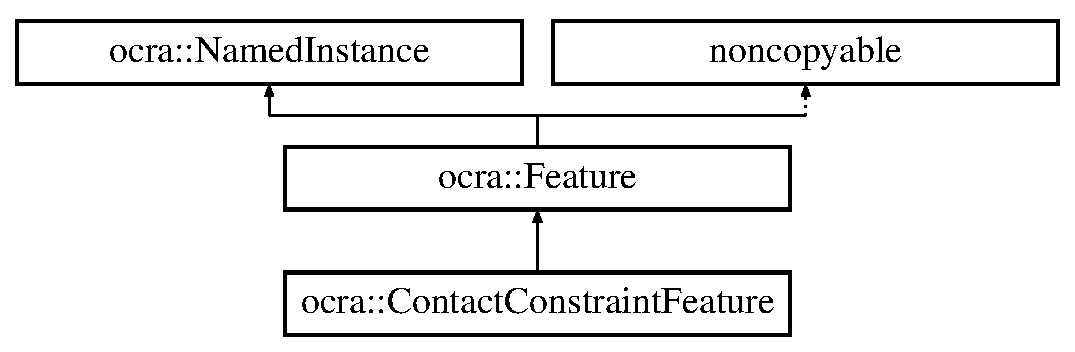
\includegraphics[height=3.000000cm]{d3/dd9/classocra_1_1ContactConstraintFeature}
\end{center}
\end{figure}
\subsection*{Classes}
\begin{DoxyCompactItemize}
\item 
struct \hyperlink{structocra_1_1ContactConstraintFeature_1_1Pimpl}{Pimpl}
\end{DoxyCompactItemize}
\subsection*{Public Member Functions}
\begin{DoxyCompactItemize}
\item 
\hyperlink{classocra_1_1ContactConstraintFeature_a2e4c6265bd194309b5e2304260d53bec}{Contact\+Constraint\+Feature} (const std\+::string \&name, Control\+Frame\+::\+Ptr frame)
\item 
int \hyperlink{classocra_1_1ContactConstraintFeature_ac498096b8df524b054f35b05d027f0f0}{get\+Dimension} () const
\item 
const Eigen\+::\+Matrix\+Xd \& \hyperlink{classocra_1_1ContactConstraintFeature_ac7f34721e72544d13e7030182b55f429}{get\+Space\+Transform} () const
\item 
const Eigen\+::\+Vector\+Xd \& \hyperlink{classocra_1_1ContactConstraintFeature_ab545e20b58d45b47a0e2f2a0a64f9c48}{compute\+Effort} (const \hyperlink{classocra_1_1Feature}{Feature} \&feature\+Des) const
\item 
const Eigen\+::\+Vector\+Xd \& \hyperlink{classocra_1_1ContactConstraintFeature_a81aeb9d50b198c49d0868ba8321bcfd7}{compute\+Acceleration} (const \hyperlink{classocra_1_1Feature}{Feature} \&feature\+Des) const
\item 
const Eigen\+::\+Vector\+Xd \& \hyperlink{classocra_1_1ContactConstraintFeature_a2d5b3c766e22c541e416ca52d14e78df}{compute\+Error} (const \hyperlink{classocra_1_1Feature}{Feature} \&feature\+Des) const
\item 
const Eigen\+::\+Vector\+Xd \& \hyperlink{classocra_1_1ContactConstraintFeature_a0be2debba15230d160957c15eb5afa97}{compute\+Error\+Dot} (const \hyperlink{classocra_1_1Feature}{Feature} \&feature\+Des) const
\item 
const Eigen\+::\+Matrix\+Xd \& \hyperlink{classocra_1_1ContactConstraintFeature_a7b0fc26f03104eb02a7ba565b99a41d7}{compute\+Jacobian} (const \hyperlink{classocra_1_1Feature}{Feature} \&feature\+Des) const
\item 
const Eigen\+::\+Matrix\+Xd \& \hyperlink{classocra_1_1ContactConstraintFeature_ac4dec3a5defe2c50e6084d49a1838883}{compute\+Projected\+Mass} (const \hyperlink{classocra_1_1Feature}{Feature} \&feature\+Des) const
\item 
const Eigen\+::\+Matrix\+Xd \& \hyperlink{classocra_1_1ContactConstraintFeature_a9bdfabb746abff207ff9cc3e9c968c81}{compute\+Projected\+Mass\+Inverse} (const \hyperlink{classocra_1_1Feature}{Feature} \&feature\+Des) const
\item 
const Eigen\+::\+Vector\+Xd \& \hyperlink{classocra_1_1ContactConstraintFeature_a84b467c5da2810bef8a76525e617ad2d}{compute\+Effort} () const
\item 
const Eigen\+::\+Vector\+Xd \& \hyperlink{classocra_1_1ContactConstraintFeature_a8537fa220270cf526014f0c4f5e6ea75}{compute\+Acceleration} () const
\item 
const Eigen\+::\+Vector\+Xd \& \hyperlink{classocra_1_1ContactConstraintFeature_ae846fba34c59502db6cf0a0dac0e6be3}{compute\+Error} () const
\item 
const Eigen\+::\+Vector\+Xd \& \hyperlink{classocra_1_1ContactConstraintFeature_afbe828f952c7583b690e394efd05423f}{compute\+Error\+Dot} () const
\item 
const Eigen\+::\+Matrix\+Xd \& \hyperlink{classocra_1_1ContactConstraintFeature_aa3c6131d9c4c815e9e9ec5ab50407b21}{compute\+Jacobian} () const
\item 
const Eigen\+::\+Matrix\+Xd \& \hyperlink{classocra_1_1ContactConstraintFeature_ab926340d6c6d00b1358ae99432e15398}{compute\+Projected\+Mass} () const
\item 
const Eigen\+::\+Matrix\+Xd \& \hyperlink{classocra_1_1ContactConstraintFeature_a78ba3452b7ad08dae7a266b0334aaa5d}{compute\+Projected\+Mass\+Inverse} () const
\item 
\hyperlink{classocra_1_1TaskState}{Task\+State} \hyperlink{classocra_1_1ContactConstraintFeature_a4a156de21fba41f54c2927232173d334}{get\+State} () const
\item 
void \hyperlink{classocra_1_1ContactConstraintFeature_a1bbc7ca568a64aed7704118b8eeaf6d1}{set\+State} (const \hyperlink{classocra_1_1TaskState}{Task\+State} \&new\+State)
\end{DoxyCompactItemize}
\subsection*{Additional Inherited Members}


\subsection{Detailed Description}
Used to build contact constraint tasks (null acceleration). 

These features is similar to a displacement feature, except all quantities are expressed in the controlled frame (space transform is identity). Desired features are irrelevant and compute\+X\+X\+X(const Feature\&) will throw. 

Definition at line 279 of file Feature.\+h.



\subsection{Constructor \& Destructor Documentation}
\hypertarget{classocra_1_1ContactConstraintFeature_a2e4c6265bd194309b5e2304260d53bec}{}\label{classocra_1_1ContactConstraintFeature_a2e4c6265bd194309b5e2304260d53bec} 
\index{ocra\+::\+Contact\+Constraint\+Feature@{ocra\+::\+Contact\+Constraint\+Feature}!Contact\+Constraint\+Feature@{Contact\+Constraint\+Feature}}
\index{Contact\+Constraint\+Feature@{Contact\+Constraint\+Feature}!ocra\+::\+Contact\+Constraint\+Feature@{ocra\+::\+Contact\+Constraint\+Feature}}
\subsubsection{\texorpdfstring{Contact\+Constraint\+Feature()}{ContactConstraintFeature()}}
{\footnotesize\ttfamily ocra\+::\+Contact\+Constraint\+Feature\+::\+Contact\+Constraint\+Feature (\begin{DoxyParamCaption}\item[{const std\+::string \&}]{name,  }\item[{Control\+Frame\+::\+Ptr}]{frame }\end{DoxyParamCaption})}



Definition at line 1028 of file Feature.\+cpp.



\subsection{Member Function Documentation}
\hypertarget{classocra_1_1ContactConstraintFeature_a81aeb9d50b198c49d0868ba8321bcfd7}{}\label{classocra_1_1ContactConstraintFeature_a81aeb9d50b198c49d0868ba8321bcfd7} 
\index{ocra\+::\+Contact\+Constraint\+Feature@{ocra\+::\+Contact\+Constraint\+Feature}!compute\+Acceleration@{compute\+Acceleration}}
\index{compute\+Acceleration@{compute\+Acceleration}!ocra\+::\+Contact\+Constraint\+Feature@{ocra\+::\+Contact\+Constraint\+Feature}}
\subsubsection{\texorpdfstring{compute\+Acceleration()}{computeAcceleration()}\hspace{0.1cm}{\footnotesize\ttfamily [1/2]}}
{\footnotesize\ttfamily const Vector\+Xd \& ocra\+::\+Contact\+Constraint\+Feature\+::compute\+Acceleration (\begin{DoxyParamCaption}\item[{const \hyperlink{classocra_1_1Feature}{Feature} \&}]{feature\+Des }\end{DoxyParamCaption}) const\hspace{0.3cm}{\ttfamily [virtual]}}



Implements \hyperlink{classocra_1_1Feature_a4a5973d27459d2dececec8dc73038df8}{ocra\+::\+Feature}.



Definition at line 1057 of file Feature.\+cpp.

\hypertarget{classocra_1_1ContactConstraintFeature_a8537fa220270cf526014f0c4f5e6ea75}{}\label{classocra_1_1ContactConstraintFeature_a8537fa220270cf526014f0c4f5e6ea75} 
\index{ocra\+::\+Contact\+Constraint\+Feature@{ocra\+::\+Contact\+Constraint\+Feature}!compute\+Acceleration@{compute\+Acceleration}}
\index{compute\+Acceleration@{compute\+Acceleration}!ocra\+::\+Contact\+Constraint\+Feature@{ocra\+::\+Contact\+Constraint\+Feature}}
\subsubsection{\texorpdfstring{compute\+Acceleration()}{computeAcceleration()}\hspace{0.1cm}{\footnotesize\ttfamily [2/2]}}
{\footnotesize\ttfamily const Vector\+Xd \& ocra\+::\+Contact\+Constraint\+Feature\+::compute\+Acceleration (\begin{DoxyParamCaption}{ }\end{DoxyParamCaption}) const\hspace{0.3cm}{\ttfamily [virtual]}}



Implements \hyperlink{classocra_1_1Feature_aa42b61d4255116caa92042d01ca36b79}{ocra\+::\+Feature}.



Definition at line 1062 of file Feature.\+cpp.

\hypertarget{classocra_1_1ContactConstraintFeature_ab545e20b58d45b47a0e2f2a0a64f9c48}{}\label{classocra_1_1ContactConstraintFeature_ab545e20b58d45b47a0e2f2a0a64f9c48} 
\index{ocra\+::\+Contact\+Constraint\+Feature@{ocra\+::\+Contact\+Constraint\+Feature}!compute\+Effort@{compute\+Effort}}
\index{compute\+Effort@{compute\+Effort}!ocra\+::\+Contact\+Constraint\+Feature@{ocra\+::\+Contact\+Constraint\+Feature}}
\subsubsection{\texorpdfstring{compute\+Effort()}{computeEffort()}\hspace{0.1cm}{\footnotesize\ttfamily [1/2]}}
{\footnotesize\ttfamily const Vector\+Xd \& ocra\+::\+Contact\+Constraint\+Feature\+::compute\+Effort (\begin{DoxyParamCaption}\item[{const \hyperlink{classocra_1_1Feature}{Feature} \&}]{feature\+Des }\end{DoxyParamCaption}) const\hspace{0.3cm}{\ttfamily [virtual]}}



Implements \hyperlink{classocra_1_1Feature_a19626a241666fdae253af1f7b6f2acd7}{ocra\+::\+Feature}.



Definition at line 1044 of file Feature.\+cpp.

\hypertarget{classocra_1_1ContactConstraintFeature_a84b467c5da2810bef8a76525e617ad2d}{}\label{classocra_1_1ContactConstraintFeature_a84b467c5da2810bef8a76525e617ad2d} 
\index{ocra\+::\+Contact\+Constraint\+Feature@{ocra\+::\+Contact\+Constraint\+Feature}!compute\+Effort@{compute\+Effort}}
\index{compute\+Effort@{compute\+Effort}!ocra\+::\+Contact\+Constraint\+Feature@{ocra\+::\+Contact\+Constraint\+Feature}}
\subsubsection{\texorpdfstring{compute\+Effort()}{computeEffort()}\hspace{0.1cm}{\footnotesize\ttfamily [2/2]}}
{\footnotesize\ttfamily const Vector\+Xd \& ocra\+::\+Contact\+Constraint\+Feature\+::compute\+Effort (\begin{DoxyParamCaption}{ }\end{DoxyParamCaption}) const\hspace{0.3cm}{\ttfamily [virtual]}}



Implements \hyperlink{classocra_1_1Feature_ae43f2ffc54862d6ddc0b02fd39431eb6}{ocra\+::\+Feature}.



Definition at line 1049 of file Feature.\+cpp.

\hypertarget{classocra_1_1ContactConstraintFeature_a2d5b3c766e22c541e416ca52d14e78df}{}\label{classocra_1_1ContactConstraintFeature_a2d5b3c766e22c541e416ca52d14e78df} 
\index{ocra\+::\+Contact\+Constraint\+Feature@{ocra\+::\+Contact\+Constraint\+Feature}!compute\+Error@{compute\+Error}}
\index{compute\+Error@{compute\+Error}!ocra\+::\+Contact\+Constraint\+Feature@{ocra\+::\+Contact\+Constraint\+Feature}}
\subsubsection{\texorpdfstring{compute\+Error()}{computeError()}\hspace{0.1cm}{\footnotesize\ttfamily [1/2]}}
{\footnotesize\ttfamily const Vector\+Xd \& ocra\+::\+Contact\+Constraint\+Feature\+::compute\+Error (\begin{DoxyParamCaption}\item[{const \hyperlink{classocra_1_1Feature}{Feature} \&}]{feature\+Des }\end{DoxyParamCaption}) const\hspace{0.3cm}{\ttfamily [virtual]}}



Implements \hyperlink{classocra_1_1Feature_aaa74d6869f7e574fcc39d443581ddf77}{ocra\+::\+Feature}.



Definition at line 1069 of file Feature.\+cpp.

\hypertarget{classocra_1_1ContactConstraintFeature_ae846fba34c59502db6cf0a0dac0e6be3}{}\label{classocra_1_1ContactConstraintFeature_ae846fba34c59502db6cf0a0dac0e6be3} 
\index{ocra\+::\+Contact\+Constraint\+Feature@{ocra\+::\+Contact\+Constraint\+Feature}!compute\+Error@{compute\+Error}}
\index{compute\+Error@{compute\+Error}!ocra\+::\+Contact\+Constraint\+Feature@{ocra\+::\+Contact\+Constraint\+Feature}}
\subsubsection{\texorpdfstring{compute\+Error()}{computeError()}\hspace{0.1cm}{\footnotesize\ttfamily [2/2]}}
{\footnotesize\ttfamily const Vector\+Xd \& ocra\+::\+Contact\+Constraint\+Feature\+::compute\+Error (\begin{DoxyParamCaption}{ }\end{DoxyParamCaption}) const\hspace{0.3cm}{\ttfamily [virtual]}}



Implements \hyperlink{classocra_1_1Feature_a88f87b496aedc7bf9f13b19bb8f9c7fa}{ocra\+::\+Feature}.



Definition at line 1074 of file Feature.\+cpp.

\hypertarget{classocra_1_1ContactConstraintFeature_a0be2debba15230d160957c15eb5afa97}{}\label{classocra_1_1ContactConstraintFeature_a0be2debba15230d160957c15eb5afa97} 
\index{ocra\+::\+Contact\+Constraint\+Feature@{ocra\+::\+Contact\+Constraint\+Feature}!compute\+Error\+Dot@{compute\+Error\+Dot}}
\index{compute\+Error\+Dot@{compute\+Error\+Dot}!ocra\+::\+Contact\+Constraint\+Feature@{ocra\+::\+Contact\+Constraint\+Feature}}
\subsubsection{\texorpdfstring{compute\+Error\+Dot()}{computeErrorDot()}\hspace{0.1cm}{\footnotesize\ttfamily [1/2]}}
{\footnotesize\ttfamily const Vector\+Xd \& ocra\+::\+Contact\+Constraint\+Feature\+::compute\+Error\+Dot (\begin{DoxyParamCaption}\item[{const \hyperlink{classocra_1_1Feature}{Feature} \&}]{feature\+Des }\end{DoxyParamCaption}) const\hspace{0.3cm}{\ttfamily [virtual]}}



Implements \hyperlink{classocra_1_1Feature_ac714181e1bb25f878349e299c4ba8c00}{ocra\+::\+Feature}.



Definition at line 1084 of file Feature.\+cpp.

\hypertarget{classocra_1_1ContactConstraintFeature_afbe828f952c7583b690e394efd05423f}{}\label{classocra_1_1ContactConstraintFeature_afbe828f952c7583b690e394efd05423f} 
\index{ocra\+::\+Contact\+Constraint\+Feature@{ocra\+::\+Contact\+Constraint\+Feature}!compute\+Error\+Dot@{compute\+Error\+Dot}}
\index{compute\+Error\+Dot@{compute\+Error\+Dot}!ocra\+::\+Contact\+Constraint\+Feature@{ocra\+::\+Contact\+Constraint\+Feature}}
\subsubsection{\texorpdfstring{compute\+Error\+Dot()}{computeErrorDot()}\hspace{0.1cm}{\footnotesize\ttfamily [2/2]}}
{\footnotesize\ttfamily const Vector\+Xd \& ocra\+::\+Contact\+Constraint\+Feature\+::compute\+Error\+Dot (\begin{DoxyParamCaption}{ }\end{DoxyParamCaption}) const\hspace{0.3cm}{\ttfamily [virtual]}}



Implements \hyperlink{classocra_1_1Feature_a01a4870418ba87d5b41d8f917c1255fc}{ocra\+::\+Feature}.



Definition at line 1089 of file Feature.\+cpp.

\hypertarget{classocra_1_1ContactConstraintFeature_a7b0fc26f03104eb02a7ba565b99a41d7}{}\label{classocra_1_1ContactConstraintFeature_a7b0fc26f03104eb02a7ba565b99a41d7} 
\index{ocra\+::\+Contact\+Constraint\+Feature@{ocra\+::\+Contact\+Constraint\+Feature}!compute\+Jacobian@{compute\+Jacobian}}
\index{compute\+Jacobian@{compute\+Jacobian}!ocra\+::\+Contact\+Constraint\+Feature@{ocra\+::\+Contact\+Constraint\+Feature}}
\subsubsection{\texorpdfstring{compute\+Jacobian()}{computeJacobian()}\hspace{0.1cm}{\footnotesize\ttfamily [1/2]}}
{\footnotesize\ttfamily const Matrix\+Xd \& ocra\+::\+Contact\+Constraint\+Feature\+::compute\+Jacobian (\begin{DoxyParamCaption}\item[{const \hyperlink{classocra_1_1Feature}{Feature} \&}]{feature\+Des }\end{DoxyParamCaption}) const\hspace{0.3cm}{\ttfamily [virtual]}}



Implements \hyperlink{classocra_1_1Feature_a4fb8eeeed978a1f727ec43cd1bd18d78}{ocra\+::\+Feature}.



Definition at line 1097 of file Feature.\+cpp.

\hypertarget{classocra_1_1ContactConstraintFeature_aa3c6131d9c4c815e9e9ec5ab50407b21}{}\label{classocra_1_1ContactConstraintFeature_aa3c6131d9c4c815e9e9ec5ab50407b21} 
\index{ocra\+::\+Contact\+Constraint\+Feature@{ocra\+::\+Contact\+Constraint\+Feature}!compute\+Jacobian@{compute\+Jacobian}}
\index{compute\+Jacobian@{compute\+Jacobian}!ocra\+::\+Contact\+Constraint\+Feature@{ocra\+::\+Contact\+Constraint\+Feature}}
\subsubsection{\texorpdfstring{compute\+Jacobian()}{computeJacobian()}\hspace{0.1cm}{\footnotesize\ttfamily [2/2]}}
{\footnotesize\ttfamily const Matrix\+Xd \& ocra\+::\+Contact\+Constraint\+Feature\+::compute\+Jacobian (\begin{DoxyParamCaption}{ }\end{DoxyParamCaption}) const\hspace{0.3cm}{\ttfamily [virtual]}}



Implements \hyperlink{classocra_1_1Feature_adbab3b388657555abb805bb971c2491f}{ocra\+::\+Feature}.



Definition at line 1102 of file Feature.\+cpp.

\hypertarget{classocra_1_1ContactConstraintFeature_ac4dec3a5defe2c50e6084d49a1838883}{}\label{classocra_1_1ContactConstraintFeature_ac4dec3a5defe2c50e6084d49a1838883} 
\index{ocra\+::\+Contact\+Constraint\+Feature@{ocra\+::\+Contact\+Constraint\+Feature}!compute\+Projected\+Mass@{compute\+Projected\+Mass}}
\index{compute\+Projected\+Mass@{compute\+Projected\+Mass}!ocra\+::\+Contact\+Constraint\+Feature@{ocra\+::\+Contact\+Constraint\+Feature}}
\subsubsection{\texorpdfstring{compute\+Projected\+Mass()}{computeProjectedMass()}\hspace{0.1cm}{\footnotesize\ttfamily [1/2]}}
{\footnotesize\ttfamily const Matrix\+Xd \& ocra\+::\+Contact\+Constraint\+Feature\+::compute\+Projected\+Mass (\begin{DoxyParamCaption}\item[{const \hyperlink{classocra_1_1Feature}{Feature} \&}]{feature\+Des }\end{DoxyParamCaption}) const\hspace{0.3cm}{\ttfamily [virtual]}}



Implements \hyperlink{classocra_1_1Feature_a44e11dd349e92971fefebff354e7214b}{ocra\+::\+Feature}.



Definition at line 1108 of file Feature.\+cpp.

\hypertarget{classocra_1_1ContactConstraintFeature_ab926340d6c6d00b1358ae99432e15398}{}\label{classocra_1_1ContactConstraintFeature_ab926340d6c6d00b1358ae99432e15398} 
\index{ocra\+::\+Contact\+Constraint\+Feature@{ocra\+::\+Contact\+Constraint\+Feature}!compute\+Projected\+Mass@{compute\+Projected\+Mass}}
\index{compute\+Projected\+Mass@{compute\+Projected\+Mass}!ocra\+::\+Contact\+Constraint\+Feature@{ocra\+::\+Contact\+Constraint\+Feature}}
\subsubsection{\texorpdfstring{compute\+Projected\+Mass()}{computeProjectedMass()}\hspace{0.1cm}{\footnotesize\ttfamily [2/2]}}
{\footnotesize\ttfamily const Matrix\+Xd \& ocra\+::\+Contact\+Constraint\+Feature\+::compute\+Projected\+Mass (\begin{DoxyParamCaption}{ }\end{DoxyParamCaption}) const\hspace{0.3cm}{\ttfamily [virtual]}}



Implements \hyperlink{classocra_1_1Feature_a99ac023809c0cf34b5d582537934b08c}{ocra\+::\+Feature}.



Definition at line 1113 of file Feature.\+cpp.

\hypertarget{classocra_1_1ContactConstraintFeature_a9bdfabb746abff207ff9cc3e9c968c81}{}\label{classocra_1_1ContactConstraintFeature_a9bdfabb746abff207ff9cc3e9c968c81} 
\index{ocra\+::\+Contact\+Constraint\+Feature@{ocra\+::\+Contact\+Constraint\+Feature}!compute\+Projected\+Mass\+Inverse@{compute\+Projected\+Mass\+Inverse}}
\index{compute\+Projected\+Mass\+Inverse@{compute\+Projected\+Mass\+Inverse}!ocra\+::\+Contact\+Constraint\+Feature@{ocra\+::\+Contact\+Constraint\+Feature}}
\subsubsection{\texorpdfstring{compute\+Projected\+Mass\+Inverse()}{computeProjectedMassInverse()}\hspace{0.1cm}{\footnotesize\ttfamily [1/2]}}
{\footnotesize\ttfamily const Matrix\+Xd \& ocra\+::\+Contact\+Constraint\+Feature\+::compute\+Projected\+Mass\+Inverse (\begin{DoxyParamCaption}\item[{const \hyperlink{classocra_1_1Feature}{Feature} \&}]{feature\+Des }\end{DoxyParamCaption}) const\hspace{0.3cm}{\ttfamily [virtual]}}



Implements \hyperlink{classocra_1_1Feature_ac529096b3fe8eba1ab88a56d8b042d37}{ocra\+::\+Feature}.



Definition at line 1123 of file Feature.\+cpp.

\hypertarget{classocra_1_1ContactConstraintFeature_a78ba3452b7ad08dae7a266b0334aaa5d}{}\label{classocra_1_1ContactConstraintFeature_a78ba3452b7ad08dae7a266b0334aaa5d} 
\index{ocra\+::\+Contact\+Constraint\+Feature@{ocra\+::\+Contact\+Constraint\+Feature}!compute\+Projected\+Mass\+Inverse@{compute\+Projected\+Mass\+Inverse}}
\index{compute\+Projected\+Mass\+Inverse@{compute\+Projected\+Mass\+Inverse}!ocra\+::\+Contact\+Constraint\+Feature@{ocra\+::\+Contact\+Constraint\+Feature}}
\subsubsection{\texorpdfstring{compute\+Projected\+Mass\+Inverse()}{computeProjectedMassInverse()}\hspace{0.1cm}{\footnotesize\ttfamily [2/2]}}
{\footnotesize\ttfamily const Matrix\+Xd \& ocra\+::\+Contact\+Constraint\+Feature\+::compute\+Projected\+Mass\+Inverse (\begin{DoxyParamCaption}{ }\end{DoxyParamCaption}) const\hspace{0.3cm}{\ttfamily [virtual]}}



Implements \hyperlink{classocra_1_1Feature_ac27bcbdbb8541e3b4e2c77a6d6f2ffc0}{ocra\+::\+Feature}.



Definition at line 1128 of file Feature.\+cpp.

\hypertarget{classocra_1_1ContactConstraintFeature_ac498096b8df524b054f35b05d027f0f0}{}\label{classocra_1_1ContactConstraintFeature_ac498096b8df524b054f35b05d027f0f0} 
\index{ocra\+::\+Contact\+Constraint\+Feature@{ocra\+::\+Contact\+Constraint\+Feature}!get\+Dimension@{get\+Dimension}}
\index{get\+Dimension@{get\+Dimension}!ocra\+::\+Contact\+Constraint\+Feature@{ocra\+::\+Contact\+Constraint\+Feature}}
\subsubsection{\texorpdfstring{get\+Dimension()}{getDimension()}}
{\footnotesize\ttfamily int ocra\+::\+Contact\+Constraint\+Feature\+::get\+Dimension (\begin{DoxyParamCaption}{ }\end{DoxyParamCaption}) const\hspace{0.3cm}{\ttfamily [virtual]}}



Implements \hyperlink{classocra_1_1Feature_aeda4c2a5ffe638c3de30f8b91a11450e}{ocra\+::\+Feature}.



Definition at line 1039 of file Feature.\+cpp.

\hypertarget{classocra_1_1ContactConstraintFeature_ac7f34721e72544d13e7030182b55f429}{}\label{classocra_1_1ContactConstraintFeature_ac7f34721e72544d13e7030182b55f429} 
\index{ocra\+::\+Contact\+Constraint\+Feature@{ocra\+::\+Contact\+Constraint\+Feature}!get\+Space\+Transform@{get\+Space\+Transform}}
\index{get\+Space\+Transform@{get\+Space\+Transform}!ocra\+::\+Contact\+Constraint\+Feature@{ocra\+::\+Contact\+Constraint\+Feature}}
\subsubsection{\texorpdfstring{get\+Space\+Transform()}{getSpaceTransform()}}
{\footnotesize\ttfamily const Matrix\+Xd \& ocra\+::\+Contact\+Constraint\+Feature\+::get\+Space\+Transform (\begin{DoxyParamCaption}{ }\end{DoxyParamCaption}) const\hspace{0.3cm}{\ttfamily [virtual]}}



Implements \hyperlink{classocra_1_1Feature_a77eb324fb4da91fd50d0e761d2453ff3}{ocra\+::\+Feature}.



Definition at line 1034 of file Feature.\+cpp.

\hypertarget{classocra_1_1ContactConstraintFeature_a4a156de21fba41f54c2927232173d334}{}\label{classocra_1_1ContactConstraintFeature_a4a156de21fba41f54c2927232173d334} 
\index{ocra\+::\+Contact\+Constraint\+Feature@{ocra\+::\+Contact\+Constraint\+Feature}!get\+State@{get\+State}}
\index{get\+State@{get\+State}!ocra\+::\+Contact\+Constraint\+Feature@{ocra\+::\+Contact\+Constraint\+Feature}}
\subsubsection{\texorpdfstring{get\+State()}{getState()}}
{\footnotesize\ttfamily \hyperlink{classocra_1_1TaskState}{Task\+State} ocra\+::\+Contact\+Constraint\+Feature\+::get\+State (\begin{DoxyParamCaption}{ }\end{DoxyParamCaption}) const\hspace{0.3cm}{\ttfamily [virtual]}}



Implements \hyperlink{classocra_1_1Feature_a792434ceb793f25874b8fe42ae24c475}{ocra\+::\+Feature}.



Definition at line 1139 of file Feature.\+cpp.

\hypertarget{classocra_1_1ContactConstraintFeature_a1bbc7ca568a64aed7704118b8eeaf6d1}{}\label{classocra_1_1ContactConstraintFeature_a1bbc7ca568a64aed7704118b8eeaf6d1} 
\index{ocra\+::\+Contact\+Constraint\+Feature@{ocra\+::\+Contact\+Constraint\+Feature}!set\+State@{set\+State}}
\index{set\+State@{set\+State}!ocra\+::\+Contact\+Constraint\+Feature@{ocra\+::\+Contact\+Constraint\+Feature}}
\subsubsection{\texorpdfstring{set\+State()}{setState()}}
{\footnotesize\ttfamily void ocra\+::\+Contact\+Constraint\+Feature\+::set\+State (\begin{DoxyParamCaption}\item[{const \hyperlink{classocra_1_1TaskState}{Task\+State} \&}]{new\+State }\end{DoxyParamCaption})\hspace{0.3cm}{\ttfamily [virtual]}}



Implements \hyperlink{classocra_1_1Feature_ad16d6b176b229280649ab405531e9a30}{ocra\+::\+Feature}.



Definition at line 1150 of file Feature.\+cpp.



The documentation for this class was generated from the following files\+:\begin{DoxyCompactItemize}
\item 
\hyperlink{Feature_8h}{Feature.\+h}\item 
\hyperlink{Feature_8cpp}{Feature.\+cpp}\end{DoxyCompactItemize}

\hypertarget{classocra_1_1ContactSet}{}\section{ocra\+:\+:Contact\+Set Class Reference}
\label{classocra_1_1ContactSet}\index{ocra\+::\+Contact\+Set@{ocra\+::\+Contact\+Set}}


Contact task factory.  




{\ttfamily \#include $<$Contact\+Set.\+h$>$}



Inheritance diagram for ocra\+:\+:Contact\+Set\+:\nopagebreak
\begin{figure}[H]
\begin{center}
\leavevmode
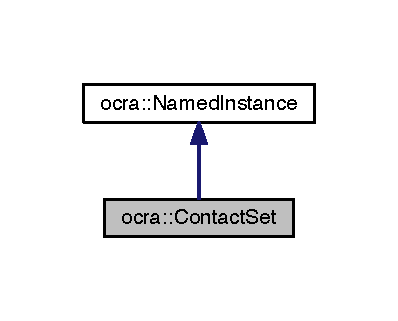
\includegraphics[width=191pt]{d5/de0/classocra_1_1ContactSet__inherit__graph}
\end{center}
\end{figure}


Collaboration diagram for ocra\+:\+:Contact\+Set\+:\nopagebreak
\begin{figure}[H]
\begin{center}
\leavevmode
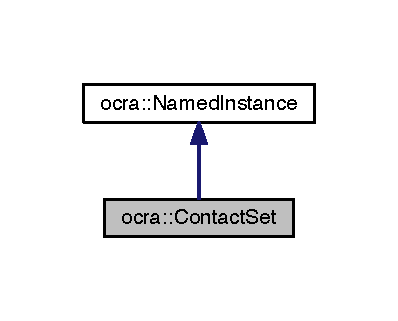
\includegraphics[width=191pt]{da/d52/classocra_1_1ContactSet__coll__graph}
\end{center}
\end{figure}
\subsection*{Public Member Functions}
\begin{DoxyCompactItemize}
\item 
\hyperlink{classocra_1_1ContactSet_aa1bc409bbd509f1b56ab6de851102435}{Contact\+Set} (const std\+::string \&name, const \hyperlink{classocra_1_1Controller}{Controller} \&factory, Segment\+Frame\+::\+Ptr body, double mu, double margin)
\item 
virtual \hyperlink{classocra_1_1ContactSet_ad41eb11994dbd12c9fc55997428e256f}{$\sim$\+Contact\+Set} ()
\item 
void \hyperlink{classocra_1_1ContactSet_ac6b33a6ece44daaa338cdf5a761b522a}{add\+Contact\+Frame} (const Eigen\+::\+Displacementd \&frame)
\item 
\hyperlink{classocra_1_1ContactConstraintFeature}{Contact\+Constraint\+Feature} \& \hyperlink{classocra_1_1ContactSet_a5b1374104097c642972daabe91b4b963}{get\+Body\+Feature} () const
\item 
std\+::shared\+\_\+ptr$<$ \hyperlink{classocra_1_1Task}{Task} $>$ \hyperlink{classocra_1_1ContactSet_a72517a1bde5c4d5e2f686803c9a1fe5d}{get\+Body\+Task} () const
\item 
const std\+::vector$<$ Segment\+Frame\+::\+Ptr $>$ \& \hyperlink{classocra_1_1ContactSet_ab0d2830d5710e02f1807033cbc9ba956}{get\+Points} () const
\item 
const std\+::vector$<$ Point\+Contact\+Feature\+::\+Ptr $>$ \& \hyperlink{classocra_1_1ContactSet_a8f5840a62ab7b1e0c6b938bc4b7b102b}{get\+Features} () const
\item 
const std\+::vector$<$ std\+::shared\+\_\+ptr$<$ \hyperlink{classocra_1_1Task}{Task} $>$ $>$ \& \hyperlink{classocra_1_1ContactSet_a5f3b18a88fc7fd4f0de7b0bb87e40c77}{get\+Tasks} () const
\item 
Segment\+Frame\+::\+Ptr \hyperlink{classocra_1_1ContactSet_ae0b5d92cc7baddf61eaebd45ffe20ba3}{get\+Body\+Frame} () const
\item 
double \hyperlink{classocra_1_1ContactSet_a8583db2b548f1fe3467115a1f2347c5f}{get\+Mu} () const
\item 
double \hyperlink{classocra_1_1ContactSet_a7f16dde129521e94ceb0fb091f5d840f}{get\+Margin} () const
\item 
int \hyperlink{classocra_1_1ContactSet_a0fa75dacb675c0133326ba27a63d4070}{get\+N\+Facets} () const
\item 
void \hyperlink{classocra_1_1ContactSet_a54d6c7d8c1266300f8a4f6d1be754630}{set\+Mu} (double mu)
\item 
void \hyperlink{classocra_1_1ContactSet_adb5aa2d4b3463d328d4687ca352b4c04}{set\+Margin} (double margin)
\item 
void \hyperlink{classocra_1_1ContactSet_a223ef9c14b40a257d026112af1a6b279}{set\+N\+Facets} (int n\+Facets)
\end{DoxyCompactItemize}


\subsection{Detailed Description}
Contact task factory. 

Creates a set of contact This object must be used as a factory. It does not manage its memory, so you have to delete the created frames yourself. 

Definition at line 59 of file Contact\+Set.\+h.



\subsection{Constructor \& Destructor Documentation}
\hypertarget{classocra_1_1ContactSet_aa1bc409bbd509f1b56ab6de851102435}{}\label{classocra_1_1ContactSet_aa1bc409bbd509f1b56ab6de851102435} 
\index{ocra\+::\+Contact\+Set@{ocra\+::\+Contact\+Set}!Contact\+Set@{Contact\+Set}}
\index{Contact\+Set@{Contact\+Set}!ocra\+::\+Contact\+Set@{ocra\+::\+Contact\+Set}}
\subsubsection{\texorpdfstring{Contact\+Set()}{ContactSet()}}
{\footnotesize\ttfamily ocra\+::\+Contact\+Set\+::\+Contact\+Set (\begin{DoxyParamCaption}\item[{const std\+::string \&}]{name,  }\item[{const \hyperlink{classocra_1_1Controller}{Controller} \&}]{factory,  }\item[{Segment\+Frame\+::\+Ptr}]{body,  }\item[{double}]{mu,  }\item[{double}]{margin }\end{DoxyParamCaption})}



Definition at line 7 of file Contact\+Set.\+cpp.

\hypertarget{classocra_1_1ContactSet_ad41eb11994dbd12c9fc55997428e256f}{}\label{classocra_1_1ContactSet_ad41eb11994dbd12c9fc55997428e256f} 
\index{ocra\+::\+Contact\+Set@{ocra\+::\+Contact\+Set}!````~Contact\+Set@{$\sim$\+Contact\+Set}}
\index{````~Contact\+Set@{$\sim$\+Contact\+Set}!ocra\+::\+Contact\+Set@{ocra\+::\+Contact\+Set}}
\subsubsection{\texorpdfstring{$\sim$\+Contact\+Set()}{~ContactSet()}}
{\footnotesize\ttfamily ocra\+::\+Contact\+Set\+::$\sim$\+Contact\+Set (\begin{DoxyParamCaption}{ }\end{DoxyParamCaption})\hspace{0.3cm}{\ttfamily [virtual]}}



Definition at line 21 of file Contact\+Set.\+cpp.



\subsection{Member Function Documentation}
\hypertarget{classocra_1_1ContactSet_ac6b33a6ece44daaa338cdf5a761b522a}{}\label{classocra_1_1ContactSet_ac6b33a6ece44daaa338cdf5a761b522a} 
\index{ocra\+::\+Contact\+Set@{ocra\+::\+Contact\+Set}!add\+Contact\+Frame@{add\+Contact\+Frame}}
\index{add\+Contact\+Frame@{add\+Contact\+Frame}!ocra\+::\+Contact\+Set@{ocra\+::\+Contact\+Set}}
\subsubsection{\texorpdfstring{add\+Contact\+Frame()}{addContactFrame()}}
{\footnotesize\ttfamily void ocra\+::\+Contact\+Set\+::add\+Contact\+Frame (\begin{DoxyParamCaption}\item[{const Eigen\+::\+Displacementd \&}]{frame }\end{DoxyParamCaption})}



Definition at line 25 of file Contact\+Set.\+cpp.

\hypertarget{classocra_1_1ContactSet_a5b1374104097c642972daabe91b4b963}{}\label{classocra_1_1ContactSet_a5b1374104097c642972daabe91b4b963} 
\index{ocra\+::\+Contact\+Set@{ocra\+::\+Contact\+Set}!get\+Body\+Feature@{get\+Body\+Feature}}
\index{get\+Body\+Feature@{get\+Body\+Feature}!ocra\+::\+Contact\+Set@{ocra\+::\+Contact\+Set}}
\subsubsection{\texorpdfstring{get\+Body\+Feature()}{getBodyFeature()}}
{\footnotesize\ttfamily \hyperlink{classocra_1_1ContactConstraintFeature}{Contact\+Constraint\+Feature} \& ocra\+::\+Contact\+Set\+::get\+Body\+Feature (\begin{DoxyParamCaption}{ }\end{DoxyParamCaption}) const}



Definition at line 45 of file Contact\+Set.\+cpp.

\hypertarget{classocra_1_1ContactSet_ae0b5d92cc7baddf61eaebd45ffe20ba3}{}\label{classocra_1_1ContactSet_ae0b5d92cc7baddf61eaebd45ffe20ba3} 
\index{ocra\+::\+Contact\+Set@{ocra\+::\+Contact\+Set}!get\+Body\+Frame@{get\+Body\+Frame}}
\index{get\+Body\+Frame@{get\+Body\+Frame}!ocra\+::\+Contact\+Set@{ocra\+::\+Contact\+Set}}
\subsubsection{\texorpdfstring{get\+Body\+Frame()}{getBodyFrame()}}
{\footnotesize\ttfamily Segment\+Frame\+::\+Ptr ocra\+::\+Contact\+Set\+::get\+Body\+Frame (\begin{DoxyParamCaption}{ }\end{DoxyParamCaption}) const}



Definition at line 40 of file Contact\+Set.\+cpp.

\hypertarget{classocra_1_1ContactSet_a72517a1bde5c4d5e2f686803c9a1fe5d}{}\label{classocra_1_1ContactSet_a72517a1bde5c4d5e2f686803c9a1fe5d} 
\index{ocra\+::\+Contact\+Set@{ocra\+::\+Contact\+Set}!get\+Body\+Task@{get\+Body\+Task}}
\index{get\+Body\+Task@{get\+Body\+Task}!ocra\+::\+Contact\+Set@{ocra\+::\+Contact\+Set}}
\subsubsection{\texorpdfstring{get\+Body\+Task()}{getBodyTask()}}
{\footnotesize\ttfamily std\+::shared\+\_\+ptr$<$ \hyperlink{classocra_1_1Task}{Task} $>$ ocra\+::\+Contact\+Set\+::get\+Body\+Task (\begin{DoxyParamCaption}{ }\end{DoxyParamCaption}) const}



Definition at line 50 of file Contact\+Set.\+cpp.

\hypertarget{classocra_1_1ContactSet_a8f5840a62ab7b1e0c6b938bc4b7b102b}{}\label{classocra_1_1ContactSet_a8f5840a62ab7b1e0c6b938bc4b7b102b} 
\index{ocra\+::\+Contact\+Set@{ocra\+::\+Contact\+Set}!get\+Features@{get\+Features}}
\index{get\+Features@{get\+Features}!ocra\+::\+Contact\+Set@{ocra\+::\+Contact\+Set}}
\subsubsection{\texorpdfstring{get\+Features()}{getFeatures()}}
{\footnotesize\ttfamily const std\+::vector$<$ Point\+Contact\+Feature\+::\+Ptr $>$ \& ocra\+::\+Contact\+Set\+::get\+Features (\begin{DoxyParamCaption}{ }\end{DoxyParamCaption}) const}



Definition at line 60 of file Contact\+Set.\+cpp.

\hypertarget{classocra_1_1ContactSet_a7f16dde129521e94ceb0fb091f5d840f}{}\label{classocra_1_1ContactSet_a7f16dde129521e94ceb0fb091f5d840f} 
\index{ocra\+::\+Contact\+Set@{ocra\+::\+Contact\+Set}!get\+Margin@{get\+Margin}}
\index{get\+Margin@{get\+Margin}!ocra\+::\+Contact\+Set@{ocra\+::\+Contact\+Set}}
\subsubsection{\texorpdfstring{get\+Margin()}{getMargin()}}
{\footnotesize\ttfamily double ocra\+::\+Contact\+Set\+::get\+Margin (\begin{DoxyParamCaption}{ }\end{DoxyParamCaption}) const}



Definition at line 85 of file Contact\+Set.\+cpp.

\hypertarget{classocra_1_1ContactSet_a8583db2b548f1fe3467115a1f2347c5f}{}\label{classocra_1_1ContactSet_a8583db2b548f1fe3467115a1f2347c5f} 
\index{ocra\+::\+Contact\+Set@{ocra\+::\+Contact\+Set}!get\+Mu@{get\+Mu}}
\index{get\+Mu@{get\+Mu}!ocra\+::\+Contact\+Set@{ocra\+::\+Contact\+Set}}
\subsubsection{\texorpdfstring{get\+Mu()}{getMu()}}
{\footnotesize\ttfamily double ocra\+::\+Contact\+Set\+::get\+Mu (\begin{DoxyParamCaption}{ }\end{DoxyParamCaption}) const}



Definition at line 75 of file Contact\+Set.\+cpp.

\hypertarget{classocra_1_1ContactSet_a0fa75dacb675c0133326ba27a63d4070}{}\label{classocra_1_1ContactSet_a0fa75dacb675c0133326ba27a63d4070} 
\index{ocra\+::\+Contact\+Set@{ocra\+::\+Contact\+Set}!get\+N\+Facets@{get\+N\+Facets}}
\index{get\+N\+Facets@{get\+N\+Facets}!ocra\+::\+Contact\+Set@{ocra\+::\+Contact\+Set}}
\subsubsection{\texorpdfstring{get\+N\+Facets()}{getNFacets()}}
{\footnotesize\ttfamily int ocra\+::\+Contact\+Set\+::get\+N\+Facets (\begin{DoxyParamCaption}{ }\end{DoxyParamCaption}) const}



Definition at line 95 of file Contact\+Set.\+cpp.

\hypertarget{classocra_1_1ContactSet_ab0d2830d5710e02f1807033cbc9ba956}{}\label{classocra_1_1ContactSet_ab0d2830d5710e02f1807033cbc9ba956} 
\index{ocra\+::\+Contact\+Set@{ocra\+::\+Contact\+Set}!get\+Points@{get\+Points}}
\index{get\+Points@{get\+Points}!ocra\+::\+Contact\+Set@{ocra\+::\+Contact\+Set}}
\subsubsection{\texorpdfstring{get\+Points()}{getPoints()}}
{\footnotesize\ttfamily const std\+::vector$<$ Segment\+Frame\+::\+Ptr $>$ \& ocra\+::\+Contact\+Set\+::get\+Points (\begin{DoxyParamCaption}{ }\end{DoxyParamCaption}) const}



Definition at line 55 of file Contact\+Set.\+cpp.

\hypertarget{classocra_1_1ContactSet_a5f3b18a88fc7fd4f0de7b0bb87e40c77}{}\label{classocra_1_1ContactSet_a5f3b18a88fc7fd4f0de7b0bb87e40c77} 
\index{ocra\+::\+Contact\+Set@{ocra\+::\+Contact\+Set}!get\+Tasks@{get\+Tasks}}
\index{get\+Tasks@{get\+Tasks}!ocra\+::\+Contact\+Set@{ocra\+::\+Contact\+Set}}
\subsubsection{\texorpdfstring{get\+Tasks()}{getTasks()}}
{\footnotesize\ttfamily const std\+::vector$<$ std\+::shared\+\_\+ptr$<$ \hyperlink{classocra_1_1Task}{Task} $>$ $>$ \& ocra\+::\+Contact\+Set\+::get\+Tasks (\begin{DoxyParamCaption}{ }\end{DoxyParamCaption}) const}



Definition at line 65 of file Contact\+Set.\+cpp.

\hypertarget{classocra_1_1ContactSet_adb5aa2d4b3463d328d4687ca352b4c04}{}\label{classocra_1_1ContactSet_adb5aa2d4b3463d328d4687ca352b4c04} 
\index{ocra\+::\+Contact\+Set@{ocra\+::\+Contact\+Set}!set\+Margin@{set\+Margin}}
\index{set\+Margin@{set\+Margin}!ocra\+::\+Contact\+Set@{ocra\+::\+Contact\+Set}}
\subsubsection{\texorpdfstring{set\+Margin()}{setMargin()}}
{\footnotesize\ttfamily void ocra\+::\+Contact\+Set\+::set\+Margin (\begin{DoxyParamCaption}\item[{double}]{margin }\end{DoxyParamCaption})}



Definition at line 80 of file Contact\+Set.\+cpp.

\hypertarget{classocra_1_1ContactSet_a54d6c7d8c1266300f8a4f6d1be754630}{}\label{classocra_1_1ContactSet_a54d6c7d8c1266300f8a4f6d1be754630} 
\index{ocra\+::\+Contact\+Set@{ocra\+::\+Contact\+Set}!set\+Mu@{set\+Mu}}
\index{set\+Mu@{set\+Mu}!ocra\+::\+Contact\+Set@{ocra\+::\+Contact\+Set}}
\subsubsection{\texorpdfstring{set\+Mu()}{setMu()}}
{\footnotesize\ttfamily void ocra\+::\+Contact\+Set\+::set\+Mu (\begin{DoxyParamCaption}\item[{double}]{mu }\end{DoxyParamCaption})}



Definition at line 70 of file Contact\+Set.\+cpp.

\hypertarget{classocra_1_1ContactSet_a223ef9c14b40a257d026112af1a6b279}{}\label{classocra_1_1ContactSet_a223ef9c14b40a257d026112af1a6b279} 
\index{ocra\+::\+Contact\+Set@{ocra\+::\+Contact\+Set}!set\+N\+Facets@{set\+N\+Facets}}
\index{set\+N\+Facets@{set\+N\+Facets}!ocra\+::\+Contact\+Set@{ocra\+::\+Contact\+Set}}
\subsubsection{\texorpdfstring{set\+N\+Facets()}{setNFacets()}}
{\footnotesize\ttfamily void ocra\+::\+Contact\+Set\+::set\+N\+Facets (\begin{DoxyParamCaption}\item[{int}]{n\+Facets }\end{DoxyParamCaption})}



Definition at line 90 of file Contact\+Set.\+cpp.



The documentation for this class was generated from the following files\+:\begin{DoxyCompactItemize}
\item 
\hyperlink{ContactSet_8h}{Contact\+Set.\+h}\item 
\hyperlink{ContactSet_8cpp}{Contact\+Set.\+cpp}\end{DoxyCompactItemize}

\hypertarget{classocra_1_1ControlConstraint}{}\section{ocra\+:\+:Control\+Constraint Class Reference}
\label{classocra_1_1ControlConstraint}\index{ocra\+::\+Control\+Constraint@{ocra\+::\+Control\+Constraint}}


{\ttfamily \#include $<$Control\+Constraint.\+h$>$}



Inheritance diagram for ocra\+:\+:Control\+Constraint\+:\nopagebreak
\begin{figure}[H]
\begin{center}
\leavevmode
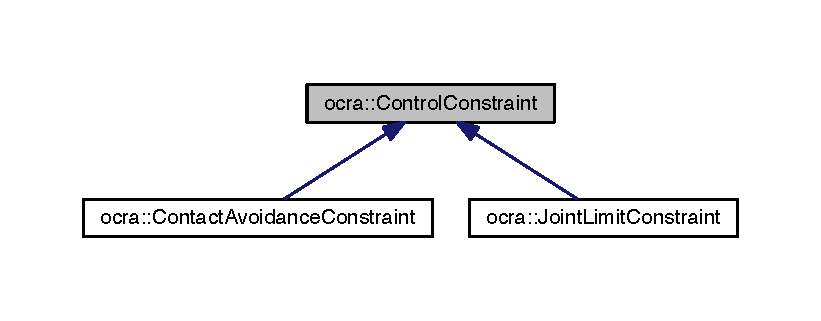
\includegraphics[width=350pt]{de/dd8/classocra_1_1ControlConstraint__inherit__graph}
\end{center}
\end{figure}
\subsection*{Public Member Functions}
\begin{DoxyCompactItemize}
\item 
\hyperlink{classocra_1_1ControlConstraint_a3d911f350d6a51009b670dcf061ab93e}{Control\+Constraint} ()
\item 
virtual \hyperlink{classocra_1_1ControlConstraint_a49f1eb50f143ef0e438d3af43db9eb31}{$\sim$\+Control\+Constraint} ()
\item 
\hyperlink{namespaceocra_ae8b87cf4099be3efc3b410019ad2046e}{Linear\+Constraint} \& \hyperlink{classocra_1_1ControlConstraint_a41b7568bc59441ca8d115e7ccf613658}{get\+Constraint} ()
\item 
virtual void \hyperlink{classocra_1_1ControlConstraint_a04dabdc1c469146e7b3240dfe0a5172c}{connect\+To\+Controller} (const \hyperlink{classocra_1_1FullDynamicEquationFunction}{Full\+Dynamic\+Equation\+Function} \&dynamic\+Equation, bool use\+Reduced\+Problem)=0
\item 
virtual void \hyperlink{classocra_1_1ControlConstraint_adbd15b36773c775a06a0b7bde46ec799}{disconnect\+From\+Controller} ()=0
\end{DoxyCompactItemize}
\subsection*{Protected Attributes}
\begin{DoxyCompactItemize}
\item 
boost\+::shared\+\_\+ptr$<$ \hyperlink{classocra_1_1Constraint}{Constraint}$<$ \hyperlink{classocra_1_1LinearFunction}{Linear\+Function} $>$ $>$ \hyperlink{classocra_1_1ControlConstraint_a47cebded91be870b03e1dddc7b0c215b}{\+\_\+constraint}
\end{DoxyCompactItemize}
\subsection*{Friends}
\begin{DoxyCompactItemize}
\item 
class \hyperlink{classocra_1_1ControlConstraint_ac3456fd331a58b288082abca310c7a99}{Controller}
\end{DoxyCompactItemize}


\subsection{Detailed Description}


Definition at line 26 of file Control\+Constraint.\+h.



\subsection{Constructor \& Destructor Documentation}
\hypertarget{classocra_1_1ControlConstraint_a3d911f350d6a51009b670dcf061ab93e}{}\label{classocra_1_1ControlConstraint_a3d911f350d6a51009b670dcf061ab93e} 
\index{ocra\+::\+Control\+Constraint@{ocra\+::\+Control\+Constraint}!Control\+Constraint@{Control\+Constraint}}
\index{Control\+Constraint@{Control\+Constraint}!ocra\+::\+Control\+Constraint@{ocra\+::\+Control\+Constraint}}
\subsubsection{\texorpdfstring{Control\+Constraint()}{ControlConstraint()}}
{\footnotesize\ttfamily ocra\+::\+Control\+Constraint\+::\+Control\+Constraint (\begin{DoxyParamCaption}{ }\end{DoxyParamCaption})\hspace{0.3cm}{\ttfamily [inline]}}



Definition at line 29 of file Control\+Constraint.\+h.

\hypertarget{classocra_1_1ControlConstraint_a49f1eb50f143ef0e438d3af43db9eb31}{}\label{classocra_1_1ControlConstraint_a49f1eb50f143ef0e438d3af43db9eb31} 
\index{ocra\+::\+Control\+Constraint@{ocra\+::\+Control\+Constraint}!````~Control\+Constraint@{$\sim$\+Control\+Constraint}}
\index{````~Control\+Constraint@{$\sim$\+Control\+Constraint}!ocra\+::\+Control\+Constraint@{ocra\+::\+Control\+Constraint}}
\subsubsection{\texorpdfstring{$\sim$\+Control\+Constraint()}{~ControlConstraint()}}
{\footnotesize\ttfamily virtual ocra\+::\+Control\+Constraint\+::$\sim$\+Control\+Constraint (\begin{DoxyParamCaption}{ }\end{DoxyParamCaption})\hspace{0.3cm}{\ttfamily [inline]}, {\ttfamily [virtual]}}



Definition at line 32 of file Control\+Constraint.\+h.



\subsection{Member Function Documentation}
\hypertarget{classocra_1_1ControlConstraint_a04dabdc1c469146e7b3240dfe0a5172c}{}\label{classocra_1_1ControlConstraint_a04dabdc1c469146e7b3240dfe0a5172c} 
\index{ocra\+::\+Control\+Constraint@{ocra\+::\+Control\+Constraint}!connect\+To\+Controller@{connect\+To\+Controller}}
\index{connect\+To\+Controller@{connect\+To\+Controller}!ocra\+::\+Control\+Constraint@{ocra\+::\+Control\+Constraint}}
\subsubsection{\texorpdfstring{connect\+To\+Controller()}{connectToController()}}
{\footnotesize\ttfamily virtual void ocra\+::\+Control\+Constraint\+::connect\+To\+Controller (\begin{DoxyParamCaption}\item[{const \hyperlink{classocra_1_1FullDynamicEquationFunction}{Full\+Dynamic\+Equation\+Function} \&}]{dynamic\+Equation,  }\item[{bool}]{use\+Reduced\+Problem }\end{DoxyParamCaption})\hspace{0.3cm}{\ttfamily [pure virtual]}}



Implemented in \hyperlink{classocra_1_1JointLimitConstraint_a71cfd04e493f270e44b79fb5a46c1601}{ocra\+::\+Joint\+Limit\+Constraint}, and \hyperlink{classocra_1_1ContactAvoidanceConstraint_a9beada2720203ab46265f271309a2ab5}{ocra\+::\+Contact\+Avoidance\+Constraint}.

\hypertarget{classocra_1_1ControlConstraint_adbd15b36773c775a06a0b7bde46ec799}{}\label{classocra_1_1ControlConstraint_adbd15b36773c775a06a0b7bde46ec799} 
\index{ocra\+::\+Control\+Constraint@{ocra\+::\+Control\+Constraint}!disconnect\+From\+Controller@{disconnect\+From\+Controller}}
\index{disconnect\+From\+Controller@{disconnect\+From\+Controller}!ocra\+::\+Control\+Constraint@{ocra\+::\+Control\+Constraint}}
\subsubsection{\texorpdfstring{disconnect\+From\+Controller()}{disconnectFromController()}}
{\footnotesize\ttfamily virtual void ocra\+::\+Control\+Constraint\+::disconnect\+From\+Controller (\begin{DoxyParamCaption}{ }\end{DoxyParamCaption})\hspace{0.3cm}{\ttfamily [pure virtual]}}



Implemented in \hyperlink{classocra_1_1JointLimitConstraint_a5f91d3b746f76f17f71a03b68de1f8ee}{ocra\+::\+Joint\+Limit\+Constraint}, and \hyperlink{classocra_1_1ContactAvoidanceConstraint_a884358568ff7f5510d26ff96915a4d8c}{ocra\+::\+Contact\+Avoidance\+Constraint}.

\hypertarget{classocra_1_1ControlConstraint_a41b7568bc59441ca8d115e7ccf613658}{}\label{classocra_1_1ControlConstraint_a41b7568bc59441ca8d115e7ccf613658} 
\index{ocra\+::\+Control\+Constraint@{ocra\+::\+Control\+Constraint}!get\+Constraint@{get\+Constraint}}
\index{get\+Constraint@{get\+Constraint}!ocra\+::\+Control\+Constraint@{ocra\+::\+Control\+Constraint}}
\subsubsection{\texorpdfstring{get\+Constraint()}{getConstraint()}}
{\footnotesize\ttfamily \hyperlink{namespaceocra_ae8b87cf4099be3efc3b410019ad2046e}{Linear\+Constraint}\& ocra\+::\+Control\+Constraint\+::get\+Constraint (\begin{DoxyParamCaption}{ }\end{DoxyParamCaption})\hspace{0.3cm}{\ttfamily [inline]}}



Definition at line 34 of file Control\+Constraint.\+h.



\subsection{Friends And Related Function Documentation}
\hypertarget{classocra_1_1ControlConstraint_ac3456fd331a58b288082abca310c7a99}{}\label{classocra_1_1ControlConstraint_ac3456fd331a58b288082abca310c7a99} 
\index{ocra\+::\+Control\+Constraint@{ocra\+::\+Control\+Constraint}!Controller@{Controller}}
\index{Controller@{Controller}!ocra\+::\+Control\+Constraint@{ocra\+::\+Control\+Constraint}}
\subsubsection{\texorpdfstring{Controller}{Controller}}
{\footnotesize\ttfamily friend class \hyperlink{classocra_1_1Controller}{Controller}\hspace{0.3cm}{\ttfamily [friend]}}



Definition at line 39 of file Control\+Constraint.\+h.



\subsection{Member Data Documentation}
\hypertarget{classocra_1_1ControlConstraint_a47cebded91be870b03e1dddc7b0c215b}{}\label{classocra_1_1ControlConstraint_a47cebded91be870b03e1dddc7b0c215b} 
\index{ocra\+::\+Control\+Constraint@{ocra\+::\+Control\+Constraint}!\+\_\+constraint@{\+\_\+constraint}}
\index{\+\_\+constraint@{\+\_\+constraint}!ocra\+::\+Control\+Constraint@{ocra\+::\+Control\+Constraint}}
\subsubsection{\texorpdfstring{\+\_\+constraint}{\_constraint}}
{\footnotesize\ttfamily boost\+::shared\+\_\+ptr$<$ \hyperlink{classocra_1_1Constraint}{Constraint}$<$\hyperlink{classocra_1_1LinearFunction}{Linear\+Function}$>$ $>$ ocra\+::\+Control\+Constraint\+::\+\_\+constraint\hspace{0.3cm}{\ttfamily [protected]}}



Definition at line 44 of file Control\+Constraint.\+h.



The documentation for this class was generated from the following file\+:\begin{DoxyCompactItemize}
\item 
\hyperlink{ControlConstraint_8h}{Control\+Constraint.\+h}\end{DoxyCompactItemize}

\hypertarget{classocra_1_1ControlFrame}{}\section{ocra\+:\+:Control\+Frame Class Reference}
\label{classocra_1_1ControlFrame}\index{ocra\+::\+Control\+Frame@{ocra\+::\+Control\+Frame}}


Generic representation of a frame\+: gives access to its position, velocity, jacobian...  




{\ttfamily \#include $<$Control\+Frame.\+h$>$}

Inheritance diagram for ocra\+:\+:Control\+Frame\+:\begin{figure}[H]
\begin{center}
\leavevmode
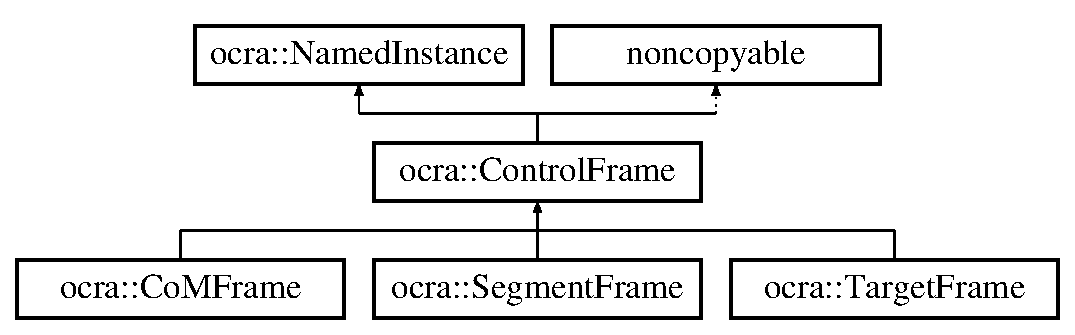
\includegraphics[height=3.000000cm]{db/d33/classocra_1_1ControlFrame}
\end{center}
\end{figure}
\subsection*{Public Member Functions}
\begin{DoxyCompactItemize}
\item 
virtual \hyperlink{classocra_1_1ControlFrame_abfbbf55462bf1b256f12316ae3abe357}{$\sim$\+Control\+Frame} ()=0
\item 
virtual Eigen\+::\+Displacementd \hyperlink{classocra_1_1ControlFrame_aaadbbfbcdd5b8e197a0f181ffb2fdcbe}{get\+Position} () const =0
\item 
virtual Eigen\+::\+Twistd \hyperlink{classocra_1_1ControlFrame_a398df839f75886867c86a8e70ac9bf24}{get\+Velocity} () const =0
\item 
virtual Eigen\+::\+Twistd \hyperlink{classocra_1_1ControlFrame_a0ceb7cd7c3fe90fa0ef311b96a6f5c88}{get\+Acceleration} () const =0
\item 
virtual Eigen\+::\+Wrenchd \hyperlink{classocra_1_1ControlFrame_a069aaf1eab98598fbffee263fcde0c56}{get\+Wrench} () const =0
\item 
virtual Eigen\+::\+Matrix$<$ double, 6, Eigen\+::\+Dynamic $>$ \hyperlink{classocra_1_1ControlFrame_a14e0b855979be5dbd360314f25191e77}{get\+Jacobian} () const =0
\item 
virtual bool \hyperlink{classocra_1_1ControlFrame_a65833d1f3f42bc8d452f8b1fb671e142}{depends\+On\+Model\+Configuration} () const =0
\item 
virtual const Model \& \hyperlink{classocra_1_1ControlFrame_ab8a1e5e3d96d7524112b4c88bf0bc5ee}{get\+Model} () const =0
\end{DoxyCompactItemize}
\subsection*{Protected Member Functions}
\begin{DoxyCompactItemize}
\item 
\hyperlink{classocra_1_1ControlFrame_a8ce978cbe6393c6baa232826c48aec55}{Control\+Frame} (const std\+::string \&name)
\end{DoxyCompactItemize}


\subsection{Detailed Description}
Generic representation of a frame\+: gives access to its position, velocity, jacobian... 

A frame is always associated to a manikin\textquotesingle{}s model. However, it does not always depend on its configuration. If it depends on the configuration of the manikin\textquotesingle{}s model, then the method Control\+Frame\+::sepends\+On\+Model\+Configuration will return true. Otherwise, this method returns false, and \hyperlink{classocra_1_1ControlFrame_a14e0b855979be5dbd360314f25191e77}{Control\+Frame\+::get\+Jacobian} will return a null matrix, whose size be 6 x \hyperlink{classocra_1_1ControlFrame_ab8a1e5e3d96d7524112b4c88bf0bc5ee}{get\+Model()}.nb\+Dofs(). 

Definition at line 42 of file Control\+Frame.\+h.



\subsection{Constructor \& Destructor Documentation}
\hypertarget{classocra_1_1ControlFrame_a8ce978cbe6393c6baa232826c48aec55}{}\label{classocra_1_1ControlFrame_a8ce978cbe6393c6baa232826c48aec55} 
\index{ocra\+::\+Control\+Frame@{ocra\+::\+Control\+Frame}!Control\+Frame@{Control\+Frame}}
\index{Control\+Frame@{Control\+Frame}!ocra\+::\+Control\+Frame@{ocra\+::\+Control\+Frame}}
\subsubsection{\texorpdfstring{Control\+Frame()}{ControlFrame()}}
{\footnotesize\ttfamily ocra\+::\+Control\+Frame\+::\+Control\+Frame (\begin{DoxyParamCaption}\item[{const std\+::string \&}]{name }\end{DoxyParamCaption})\hspace{0.3cm}{\ttfamily [protected]}}



Definition at line 10 of file Control\+Frame.\+cpp.

\hypertarget{classocra_1_1ControlFrame_abfbbf55462bf1b256f12316ae3abe357}{}\label{classocra_1_1ControlFrame_abfbbf55462bf1b256f12316ae3abe357} 
\index{ocra\+::\+Control\+Frame@{ocra\+::\+Control\+Frame}!````~Control\+Frame@{$\sim$\+Control\+Frame}}
\index{````~Control\+Frame@{$\sim$\+Control\+Frame}!ocra\+::\+Control\+Frame@{ocra\+::\+Control\+Frame}}
\subsubsection{\texorpdfstring{$\sim$\+Control\+Frame()}{~ControlFrame()}}
{\footnotesize\ttfamily ocra\+::\+Control\+Frame\+::$\sim$\+Control\+Frame (\begin{DoxyParamCaption}{ }\end{DoxyParamCaption})\hspace{0.3cm}{\ttfamily [pure virtual]}}



Definition at line 15 of file Control\+Frame.\+cpp.



\subsection{Member Function Documentation}
\hypertarget{classocra_1_1ControlFrame_a65833d1f3f42bc8d452f8b1fb671e142}{}\label{classocra_1_1ControlFrame_a65833d1f3f42bc8d452f8b1fb671e142} 
\index{ocra\+::\+Control\+Frame@{ocra\+::\+Control\+Frame}!depends\+On\+Model\+Configuration@{depends\+On\+Model\+Configuration}}
\index{depends\+On\+Model\+Configuration@{depends\+On\+Model\+Configuration}!ocra\+::\+Control\+Frame@{ocra\+::\+Control\+Frame}}
\subsubsection{\texorpdfstring{depends\+On\+Model\+Configuration()}{dependsOnModelConfiguration()}}
{\footnotesize\ttfamily virtual bool ocra\+::\+Control\+Frame\+::depends\+On\+Model\+Configuration (\begin{DoxyParamCaption}{ }\end{DoxyParamCaption}) const\hspace{0.3cm}{\ttfamily [pure virtual]}}



Implemented in \hyperlink{classocra_1_1CoMFrame_aaae3fd05da2f9e301dbe1c54b57fe624}{ocra\+::\+Co\+M\+Frame}, \hyperlink{classocra_1_1SegmentFrame_a68708b5ced24d192fbb0bfd9e3647925}{ocra\+::\+Segment\+Frame}, and \hyperlink{classocra_1_1TargetFrame_ab4512f64463c359090ffdbead9a9e349}{ocra\+::\+Target\+Frame}.

\hypertarget{classocra_1_1ControlFrame_a0ceb7cd7c3fe90fa0ef311b96a6f5c88}{}\label{classocra_1_1ControlFrame_a0ceb7cd7c3fe90fa0ef311b96a6f5c88} 
\index{ocra\+::\+Control\+Frame@{ocra\+::\+Control\+Frame}!get\+Acceleration@{get\+Acceleration}}
\index{get\+Acceleration@{get\+Acceleration}!ocra\+::\+Control\+Frame@{ocra\+::\+Control\+Frame}}
\subsubsection{\texorpdfstring{get\+Acceleration()}{getAcceleration()}}
{\footnotesize\ttfamily virtual Eigen\+::\+Twistd ocra\+::\+Control\+Frame\+::get\+Acceleration (\begin{DoxyParamCaption}{ }\end{DoxyParamCaption}) const\hspace{0.3cm}{\ttfamily [pure virtual]}}



Implemented in \hyperlink{classocra_1_1CoMFrame_a9e59ca65720c553da5c75f484544829c}{ocra\+::\+Co\+M\+Frame}, \hyperlink{classocra_1_1SegmentFrame_aa8f7f9544b59da591d94ac8e6a8a9e5d}{ocra\+::\+Segment\+Frame}, and \hyperlink{classocra_1_1TargetFrame_ab38d91f0d2f90b102259ec155a8a1245}{ocra\+::\+Target\+Frame}.

\hypertarget{classocra_1_1ControlFrame_a14e0b855979be5dbd360314f25191e77}{}\label{classocra_1_1ControlFrame_a14e0b855979be5dbd360314f25191e77} 
\index{ocra\+::\+Control\+Frame@{ocra\+::\+Control\+Frame}!get\+Jacobian@{get\+Jacobian}}
\index{get\+Jacobian@{get\+Jacobian}!ocra\+::\+Control\+Frame@{ocra\+::\+Control\+Frame}}
\subsubsection{\texorpdfstring{get\+Jacobian()}{getJacobian()}}
{\footnotesize\ttfamily virtual Eigen\+::\+Matrix$<$double,6,Eigen\+::\+Dynamic$>$ ocra\+::\+Control\+Frame\+::get\+Jacobian (\begin{DoxyParamCaption}{ }\end{DoxyParamCaption}) const\hspace{0.3cm}{\ttfamily [pure virtual]}}



Implemented in \hyperlink{classocra_1_1CoMFrame_ab24f3400af3e8eb2a12d6597ff8a7a31}{ocra\+::\+Co\+M\+Frame}, \hyperlink{classocra_1_1SegmentFrame_a1ece38dd51a3331dfe3de7911ad9291e}{ocra\+::\+Segment\+Frame}, and \hyperlink{classocra_1_1TargetFrame_a94d2746633b7112afae754370a3a3e1f}{ocra\+::\+Target\+Frame}.

\hypertarget{classocra_1_1ControlFrame_ab8a1e5e3d96d7524112b4c88bf0bc5ee}{}\label{classocra_1_1ControlFrame_ab8a1e5e3d96d7524112b4c88bf0bc5ee} 
\index{ocra\+::\+Control\+Frame@{ocra\+::\+Control\+Frame}!get\+Model@{get\+Model}}
\index{get\+Model@{get\+Model}!ocra\+::\+Control\+Frame@{ocra\+::\+Control\+Frame}}
\subsubsection{\texorpdfstring{get\+Model()}{getModel()}}
{\footnotesize\ttfamily virtual const Model\& ocra\+::\+Control\+Frame\+::get\+Model (\begin{DoxyParamCaption}{ }\end{DoxyParamCaption}) const\hspace{0.3cm}{\ttfamily [pure virtual]}}



Implemented in \hyperlink{classocra_1_1CoMFrame_afc280df9814e7eb2cf62f017f7bbfc2e}{ocra\+::\+Co\+M\+Frame}, \hyperlink{classocra_1_1SegmentFrame_a3a14b77753ad98507db9968b33c582e4}{ocra\+::\+Segment\+Frame}, and \hyperlink{classocra_1_1TargetFrame_acfd238567f0cfb9e6107cd17103ec6ea}{ocra\+::\+Target\+Frame}.

\hypertarget{classocra_1_1ControlFrame_aaadbbfbcdd5b8e197a0f181ffb2fdcbe}{}\label{classocra_1_1ControlFrame_aaadbbfbcdd5b8e197a0f181ffb2fdcbe} 
\index{ocra\+::\+Control\+Frame@{ocra\+::\+Control\+Frame}!get\+Position@{get\+Position}}
\index{get\+Position@{get\+Position}!ocra\+::\+Control\+Frame@{ocra\+::\+Control\+Frame}}
\subsubsection{\texorpdfstring{get\+Position()}{getPosition()}}
{\footnotesize\ttfamily virtual Eigen\+::\+Displacementd ocra\+::\+Control\+Frame\+::get\+Position (\begin{DoxyParamCaption}{ }\end{DoxyParamCaption}) const\hspace{0.3cm}{\ttfamily [pure virtual]}}



Implemented in \hyperlink{classocra_1_1CoMFrame_a809c05664b2e2abb489e930e27fbe2d4}{ocra\+::\+Co\+M\+Frame}, \hyperlink{classocra_1_1SegmentFrame_ad0c5aa3b15b384cd5a4774ddd534b32e}{ocra\+::\+Segment\+Frame}, and \hyperlink{classocra_1_1TargetFrame_ab2f3bd3f05be243a5d9e2123b943986d}{ocra\+::\+Target\+Frame}.

\hypertarget{classocra_1_1ControlFrame_a398df839f75886867c86a8e70ac9bf24}{}\label{classocra_1_1ControlFrame_a398df839f75886867c86a8e70ac9bf24} 
\index{ocra\+::\+Control\+Frame@{ocra\+::\+Control\+Frame}!get\+Velocity@{get\+Velocity}}
\index{get\+Velocity@{get\+Velocity}!ocra\+::\+Control\+Frame@{ocra\+::\+Control\+Frame}}
\subsubsection{\texorpdfstring{get\+Velocity()}{getVelocity()}}
{\footnotesize\ttfamily virtual Eigen\+::\+Twistd ocra\+::\+Control\+Frame\+::get\+Velocity (\begin{DoxyParamCaption}{ }\end{DoxyParamCaption}) const\hspace{0.3cm}{\ttfamily [pure virtual]}}



Implemented in \hyperlink{classocra_1_1CoMFrame_a02be3e73c64903d67b1e7ada25c468c5}{ocra\+::\+Co\+M\+Frame}, \hyperlink{classocra_1_1SegmentFrame_a6a45d4901408704ead9bbd1f5b99a666}{ocra\+::\+Segment\+Frame}, and \hyperlink{classocra_1_1TargetFrame_a5eeda88210d7002c3c73ba949139ed5b}{ocra\+::\+Target\+Frame}.

\hypertarget{classocra_1_1ControlFrame_a069aaf1eab98598fbffee263fcde0c56}{}\label{classocra_1_1ControlFrame_a069aaf1eab98598fbffee263fcde0c56} 
\index{ocra\+::\+Control\+Frame@{ocra\+::\+Control\+Frame}!get\+Wrench@{get\+Wrench}}
\index{get\+Wrench@{get\+Wrench}!ocra\+::\+Control\+Frame@{ocra\+::\+Control\+Frame}}
\subsubsection{\texorpdfstring{get\+Wrench()}{getWrench()}}
{\footnotesize\ttfamily virtual Eigen\+::\+Wrenchd ocra\+::\+Control\+Frame\+::get\+Wrench (\begin{DoxyParamCaption}{ }\end{DoxyParamCaption}) const\hspace{0.3cm}{\ttfamily [pure virtual]}}



Implemented in \hyperlink{classocra_1_1CoMFrame_a8e00462bbe13df6f595b7000d44240c6}{ocra\+::\+Co\+M\+Frame}, \hyperlink{classocra_1_1SegmentFrame_a47bebcb9817083395ab034fe8fb72a19}{ocra\+::\+Segment\+Frame}, and \hyperlink{classocra_1_1TargetFrame_a5e9ccc5e2e5ae8e52a37b5810a76115d}{ocra\+::\+Target\+Frame}.



The documentation for this class was generated from the following files\+:\begin{DoxyCompactItemize}
\item 
\hyperlink{ControlFrame_8h}{Control\+Frame.\+h}\item 
\hyperlink{ControlFrame_8cpp}{Control\+Frame.\+cpp}\end{DoxyCompactItemize}

\hypertarget{classocra_1_1TaskYarpInterface_1_1ControlInputCallback}{}\section{ocra\+:\+:Task\+Yarp\+Interface\+:\+:Control\+Input\+Callback Class Reference}
\label{classocra_1_1TaskYarpInterface_1_1ControlInputCallback}\index{ocra\+::\+Task\+Yarp\+Interface\+::\+Control\+Input\+Callback@{ocra\+::\+Task\+Yarp\+Interface\+::\+Control\+Input\+Callback}}


a short description  




{\ttfamily \#include $<$Task\+Yarp\+Interface.\+h$>$}



Inheritance diagram for ocra\+:\+:Task\+Yarp\+Interface\+:\+:Control\+Input\+Callback\+:\nopagebreak
\begin{figure}[H]
\begin{center}
\leavevmode
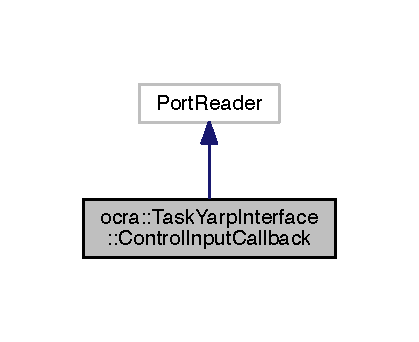
\includegraphics[width=201pt]{d8/da9/classocra_1_1TaskYarpInterface_1_1ControlInputCallback__inherit__graph}
\end{center}
\end{figure}


Collaboration diagram for ocra\+:\+:Task\+Yarp\+Interface\+:\+:Control\+Input\+Callback\+:\nopagebreak
\begin{figure}[H]
\begin{center}
\leavevmode
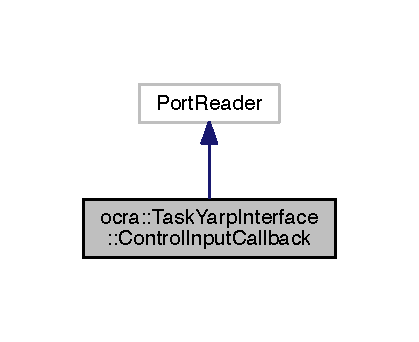
\includegraphics[width=201pt]{dc/d21/classocra_1_1TaskYarpInterface_1_1ControlInputCallback__coll__graph}
\end{center}
\end{figure}
\subsection*{Public Member Functions}
\begin{DoxyCompactItemize}
\item 
\hyperlink{classocra_1_1TaskYarpInterface_1_1ControlInputCallback_aab25b522726df43c6358ac435af4a502}{Control\+Input\+Callback} (\hyperlink{classocra_1_1TaskYarpInterface}{Task\+Yarp\+Interface} \&tm\+Base\+Ref)
\item 
virtual bool \hyperlink{classocra_1_1TaskYarpInterface_1_1ControlInputCallback_a6b2e8af58d4625a70ea6f8217287be07}{read} (yarp\+::os\+::\+Connection\+Reader \&connection)
\end{DoxyCompactItemize}


\subsection{Detailed Description}
a short description 

a long description 

Definition at line 240 of file Task\+Yarp\+Interface.\+h.



\subsection{Constructor \& Destructor Documentation}
\hypertarget{classocra_1_1TaskYarpInterface_1_1ControlInputCallback_aab25b522726df43c6358ac435af4a502}{}\label{classocra_1_1TaskYarpInterface_1_1ControlInputCallback_aab25b522726df43c6358ac435af4a502} 
\index{ocra\+::\+Task\+Yarp\+Interface\+::\+Control\+Input\+Callback@{ocra\+::\+Task\+Yarp\+Interface\+::\+Control\+Input\+Callback}!Control\+Input\+Callback@{Control\+Input\+Callback}}
\index{Control\+Input\+Callback@{Control\+Input\+Callback}!ocra\+::\+Task\+Yarp\+Interface\+::\+Control\+Input\+Callback@{ocra\+::\+Task\+Yarp\+Interface\+::\+Control\+Input\+Callback}}
\subsubsection{\texorpdfstring{Control\+Input\+Callback()}{ControlInputCallback()}}
{\footnotesize\ttfamily Task\+Yarp\+Interface\+::\+Control\+Input\+Callback\+::\+Control\+Input\+Callback (\begin{DoxyParamCaption}\item[{\hyperlink{classocra_1_1TaskYarpInterface}{Task\+Yarp\+Interface} \&}]{tm\+Base\+Ref }\end{DoxyParamCaption})}



Definition at line 452 of file Task\+Yarp\+Interface.\+cpp.



\subsection{Member Function Documentation}
\hypertarget{classocra_1_1TaskYarpInterface_1_1ControlInputCallback_a6b2e8af58d4625a70ea6f8217287be07}{}\label{classocra_1_1TaskYarpInterface_1_1ControlInputCallback_a6b2e8af58d4625a70ea6f8217287be07} 
\index{ocra\+::\+Task\+Yarp\+Interface\+::\+Control\+Input\+Callback@{ocra\+::\+Task\+Yarp\+Interface\+::\+Control\+Input\+Callback}!read@{read}}
\index{read@{read}!ocra\+::\+Task\+Yarp\+Interface\+::\+Control\+Input\+Callback@{ocra\+::\+Task\+Yarp\+Interface\+::\+Control\+Input\+Callback}}
\subsubsection{\texorpdfstring{read()}{read()}}
{\footnotesize\ttfamily bool Task\+Yarp\+Interface\+::\+Control\+Input\+Callback\+::read (\begin{DoxyParamCaption}\item[{yarp\+::os\+::\+Connection\+Reader \&}]{connection }\end{DoxyParamCaption})\hspace{0.3cm}{\ttfamily [virtual]}}



Definition at line 458 of file Task\+Yarp\+Interface.\+cpp.



The documentation for this class was generated from the following files\+:\begin{DoxyCompactItemize}
\item 
\hyperlink{TaskYarpInterface_8h}{Task\+Yarp\+Interface.\+h}\item 
\hyperlink{TaskYarpInterface_8cpp}{Task\+Yarp\+Interface.\+cpp}\end{DoxyCompactItemize}

\hypertarget{classControlInputCallback}{}\section{Control\+Input\+Callback Class Reference}
\label{classControlInputCallback}\index{Control\+Input\+Callback@{Control\+Input\+Callback}}


a short description  




{\ttfamily \#include $<$Client\+Communications.\+h$>$}



\subsection{Detailed Description}
a short description 

a long description 

The documentation for this class was generated from the following file\+:\begin{DoxyCompactItemize}
\item 
\hyperlink{ClientCommunications_8h}{Client\+Communications.\+h}\end{DoxyCompactItemize}

\hypertarget{classocra_1_1Controller}{}\section{ocra\+:\+:Controller Class Reference}
\label{classocra_1_1Controller}\index{ocra\+::\+Controller@{ocra\+::\+Controller}}


Interface for controllers.  




{\ttfamily \#include $<$Controller.\+h$>$}



Inheritance diagram for ocra\+:\+:Controller\+:\nopagebreak
\begin{figure}[H]
\begin{center}
\leavevmode
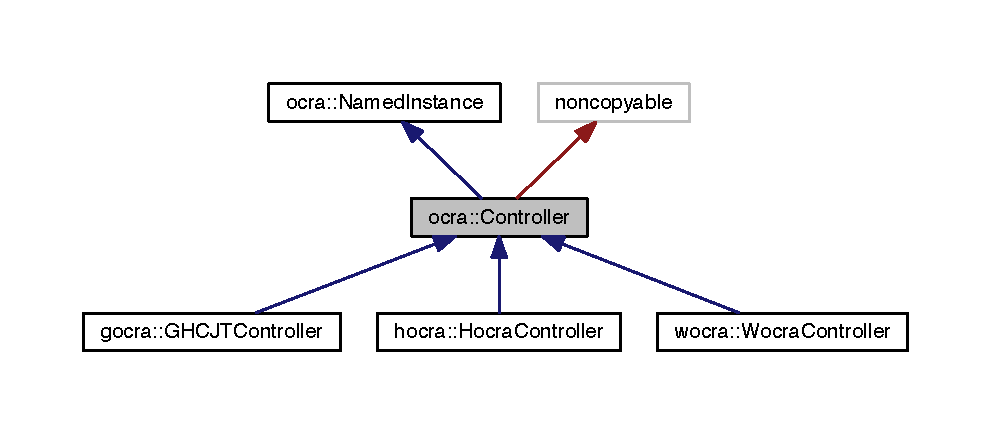
\includegraphics[width=350pt]{dc/d26/classocra_1_1Controller__inherit__graph}
\end{center}
\end{figure}


Collaboration diagram for ocra\+:\+:Controller\+:\nopagebreak
\begin{figure}[H]
\begin{center}
\leavevmode
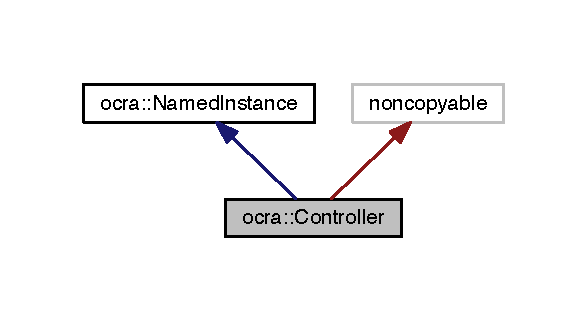
\includegraphics[width=282pt]{dc/dfe/classocra_1_1Controller__coll__graph}
\end{center}
\end{figure}
\subsection*{Classes}
\begin{DoxyCompactItemize}
\item 
struct \hyperlink{structocra_1_1Controller_1_1Pimpl}{Pimpl}
\end{DoxyCompactItemize}
\subsection*{Public Member Functions}
\begin{DoxyCompactItemize}
\item 
virtual \hyperlink{classocra_1_1Controller_a42bee636760563a73321de01ba972b6b}{$\sim$\+Controller} ()=0
\item 
void \hyperlink{classocra_1_1Controller_ad05741095a1e8f741cd3d4d67b40e239}{print\+Info} (int level, const std\+::string \&filename)
\item 
void \hyperlink{classocra_1_1Controller_a646510edd30c0fb5bc29e49917c32356}{set\+Max\+Joint\+Torques} (const Eigen\+::\+Vector\+Xd \&tau\+\_\+max)
\item 
const Eigen\+::\+Vector\+Xd \& \hyperlink{classocra_1_1Controller_a237b064c384ee45ff0a9152526c8818c}{get\+Max\+Joint\+Torques} () const
\item 
void \hyperlink{classocra_1_1Controller_a2135ac360027e8fcca02182055a7f714}{add\+Task} (std\+::shared\+\_\+ptr$<$ \hyperlink{classocra_1_1Task}{Task} $>$ task)
\item 
void \hyperlink{classocra_1_1Controller_a75755b3a9b346283e4343e15e6f83ddb}{add\+Tasks} (const std\+::vector$<$ std\+::shared\+\_\+ptr$<$ \hyperlink{classocra_1_1Task}{Task} $>$$>$ \&tasks)
\item 
void \hyperlink{classocra_1_1Controller_a0794b232fe416785b6bfb9e5e380424f}{remove\+Task} (const std\+::string \&task\+Name)
\item 
void \hyperlink{classocra_1_1Controller_ad0e1a54d26697be34348d8fb85b368d4}{remove\+Tasks} (const std\+::vector$<$ std\+::string $>$ tasks)
\item 
std\+::vector$<$ std\+::string $>$ \hyperlink{classocra_1_1Controller_abecbaf3846371383eb3c6e8b2fef031b}{get\+Task\+Names} ()
\item 
std\+::string \hyperlink{classocra_1_1Controller_ae037e3554152ec025fbb7df09fba3deb}{get\+Task\+Port\+Name} (const std\+::string \&task\+Name)
\item 
std\+::vector$<$ std\+::string $>$ \hyperlink{classocra_1_1Controller_aa18b2870c3099225050b4e95121cdd3f}{get\+Task\+Port\+Names} ()
\item 
void \hyperlink{classocra_1_1Controller_a51496c52fab832f53fe080a013f13a0e}{add\+Contact\+Set} (const \hyperlink{classocra_1_1ContactSet}{Contact\+Set} \&contacts)
\item 
std\+::shared\+\_\+ptr$<$ \hyperlink{classocra_1_1Task}{Task} $>$ \hyperlink{classocra_1_1Controller_ab5ffcbcc07bf4191d38b75ef10214acb}{get\+Task} (const std\+::string \&name)
\item 
const std\+::shared\+\_\+ptr$<$ \hyperlink{classocra_1_1Task}{Task} $>$ \hyperlink{classocra_1_1Controller_a239a353ebbc74bedd8ae56d084986211}{get\+Task} (const std\+::string \&name) const
\item 
const std\+::map$<$ std\+::string, std\+::shared\+\_\+ptr$<$ \hyperlink{classocra_1_1Task}{Task} $>$ $>$ \& \hyperlink{classocra_1_1Controller_a3bac43f145c2b75be26565fdcad7811e}{get\+Tasks} () const
\item 
void \hyperlink{classocra_1_1Controller_ada65e72ccb81a7020422268f36d944fe}{compute\+Output} (Eigen\+::\+Vector\+Xd \&tau)
\begin{DoxyCompactList}\small\item\em Computation of output torques based on the tasks added to the controller. \end{DoxyCompactList}\item 
const Eigen\+::\+Vector\+Xd \& \hyperlink{classocra_1_1Controller_a5d8c4178b4e9536187e355dc25f3739f}{compute\+Output} ()
\item 
std\+::shared\+\_\+ptr$<$ \hyperlink{classocra_1_1Task}{Task} $>$ \hyperlink{classocra_1_1Controller_af1d9bb73b939a5377a3dba072ce4c08a}{create\+Contact\+Task} (const std\+::string \&name, Point\+Contact\+Feature\+::\+Ptr feature, double mu, double margin) const
\begin{DoxyCompactList}\small\item\em Creates a contact task. \end{DoxyCompactList}\end{DoxyCompactItemize}
{\bf }\par
\begin{DoxyCompactItemize}
\item 
std\+::shared\+\_\+ptr$<$ \hyperlink{classocra_1_1Task}{Task} $>$ \hyperlink{classocra_1_1Controller_ae57beb4834bb1ed3a2ed292df5e8aedf}{create\+Task} (const std\+::string \&name, Feature\+::\+Ptr feature, Feature\+::\+Ptr feature\+Des) const
\begin{DoxyCompactList}\small\item\em Generic task creation. \end{DoxyCompactList}\item 
std\+::shared\+\_\+ptr$<$ \hyperlink{classocra_1_1Task}{Task} $>$ \hyperlink{classocra_1_1Controller_ae3546bd282b1bec068d416e06660722f}{create\+Task} (const std\+::string \&name, Feature\+::\+Ptr feature) const
\end{DoxyCompactItemize}

\subsection*{Protected Member Functions}
\begin{DoxyCompactItemize}
\item 
\hyperlink{classocra_1_1Controller_a9f72394baa089119cf0b60e3c7160283}{Controller} (const std\+::string \&name, \hyperlink{classocra_1_1Model}{Model} \&model)
\item 
const std\+::vector$<$ std\+::shared\+\_\+ptr$<$ \hyperlink{classocra_1_1Task}{Task} $>$ $>$ \& \hyperlink{classocra_1_1Controller_a47992af5b31c540f8bd7a828eb768276}{get\+Active\+Tasks} () const
\item 
void \hyperlink{classocra_1_1Controller_a36df4135749c17f6d4425fabed37d022}{set\+Error\+Flag} (int eflag)
\item 
void \hyperlink{classocra_1_1Controller_a3e8c327d25152d457172a65d826c84b4}{set\+Error\+Message} (const std\+::string \&msg)
\item 
virtual void \hyperlink{classocra_1_1Controller_a8ca85413067d948459afa5981b3dda32}{do\+Compute\+Output} (Eigen\+::\+Vector\+Xd \&tau)=0
\item 
virtual void \hyperlink{classocra_1_1Controller_ab3477822a9363553c99eefa58ff803eb}{do\+Add\+Task} (std\+::shared\+\_\+ptr$<$ \hyperlink{classocra_1_1Task}{Task} $>$ task)=0
\item 
virtual void \hyperlink{classocra_1_1Controller_acb11edc1ceaa89423c1e58f9cb38a9f7}{do\+Add\+Contact\+Set} (const \hyperlink{classocra_1_1ContactSet}{Contact\+Set} \&contacts)=0
\item 
virtual void \hyperlink{classocra_1_1Controller_a75d6419229980f6088a689fcafc1d224}{do\+Set\+Max\+Joint\+Torques} (const Eigen\+::\+Vector\+Xd \&tau\+Max)
\item 
virtual std\+::shared\+\_\+ptr$<$ \hyperlink{classocra_1_1Task}{Task} $>$ \hyperlink{classocra_1_1Controller_a05f6d757e4125a71bf766df7f069ac43}{do\+Create\+Task} (const std\+::string \&name, Feature\+::\+Ptr feature, Feature\+::\+Ptr feature\+Des) const =0
\item 
virtual std\+::shared\+\_\+ptr$<$ \hyperlink{classocra_1_1Task}{Task} $>$ \hyperlink{classocra_1_1Controller_a358a31c0b6b6bdcc0e6da5c49eb9fde5}{do\+Create\+Task} (const std\+::string \&name, Feature\+::\+Ptr feature) const =0
\item 
virtual std\+::shared\+\_\+ptr$<$ \hyperlink{classocra_1_1Task}{Task} $>$ \hyperlink{classocra_1_1Controller_a823933d261a12aac49f8a0ef56823ea4}{do\+Create\+Contact\+Task} (const std\+::string \&name, Point\+Contact\+Feature\+::\+Ptr feature, double mu, double margin) const =0
\end{DoxyCompactItemize}
\begin{DoxyCompactItemize}
\item 
enum \hyperlink{classocra_1_1Controller_abeaf3673abe2da79493638dcc49fcf6e}{Error\+Flag} \{ \newline
\hyperlink{classocra_1_1Controller_abeaf3673abe2da79493638dcc49fcf6eaf0c456fccd7111235e41d752e78d4e3d}{S\+U\+C\+C\+E\+SS} = 0, 
\hyperlink{classocra_1_1Controller_abeaf3673abe2da79493638dcc49fcf6eaa6ea1ed92f7f3f1278fb8bbf11a13d77}{C\+R\+I\+T\+I\+C\+A\+L\+\_\+\+E\+R\+R\+OR} = 1, 
\hyperlink{classocra_1_1Controller_abeaf3673abe2da79493638dcc49fcf6ea2c4995e7abb68ab3a51e2052609d0f46}{S\+T\+A\+T\+I\+C\+\_\+\+E\+Q\+\_\+\+L\+O\+SS} = 2, 
\hyperlink{classocra_1_1Controller_abeaf3673abe2da79493638dcc49fcf6eadb8ddca8cd6373851537d1c719f04c97}{D\+Y\+N\+\_\+\+E\+Q\+\_\+\+L\+O\+SS} = 4, 
\newline
\hyperlink{classocra_1_1Controller_abeaf3673abe2da79493638dcc49fcf6ea7dc3bcb2de72c9d94bdee2a99f5957d4}{I\+N\+S\+T\+A\+B\+I\+L\+I\+TY} = 8 + 1, 
\hyperlink{classocra_1_1Controller_abeaf3673abe2da79493638dcc49fcf6ea2a5f1f9e553eccf1b3f1a26c5979c0ef}{O\+T\+H\+ER} = 16
 \}\begin{DoxyCompactList}\small\item\em Error handling. \end{DoxyCompactList}
\item 
void \hyperlink{classocra_1_1Controller_a9f9773f34022d6f7b0abf95255088f70}{enable\+Error\+Handling} ()
\item 
void \hyperlink{classocra_1_1Controller_aad44e0db3e0039bf3d6eeb3a89a99752}{disable\+Error\+Handling} ()
\item 
bool \hyperlink{classocra_1_1Controller_aa9096ed0ee671ab256085156c1a2c276}{is\+Error\+Handling\+Enabled} () const
\item 
const std\+::string \& \hyperlink{classocra_1_1Controller_a63c3529263ba2cf24f56f5998fa882b3}{get\+Error\+Message} () const
\item 
void \hyperlink{classocra_1_1Controller_a18fe6c4ad06aa7b2254ab6e4e740d101}{clear\+Error\+Flag} ()
\item 
int \hyperlink{classocra_1_1Controller_a5fdf44f2acf693f69a68cc95ce4182b4}{get\+Error\+Flag} () const
\item 
void \hyperlink{classocra_1_1Controller_a80f0b90e59759bf79fc4ff8c85ca8d85}{set\+Max\+Joint\+Torque\+Norm} (double max\+Tau)
\item 
double \hyperlink{classocra_1_1Controller_ac9a605bf14c4f70d3ba8d1c61f5c1976}{get\+Max\+Joint\+Torque\+Norm} () const
\item 
void \hyperlink{classocra_1_1Controller_aac8c56f6b63bb3ae57ac7bf9c23018e8}{set\+Fixed\+Link\+For\+Odometry} (std\+::string new\+Fixed\+Link)
\item 
void \hyperlink{classocra_1_1Controller_a3f6a080793612b0b66e1ce7a26897646}{set\+Use\+Odometry} (bool use\+Odometry)
\item 
void \hyperlink{classocra_1_1Controller_ad134da18dc753e50e6f615373fbf9adf}{get\+Fixed\+Link\+For\+Odometry} (std\+::string \&current\+Fixed\+Link)
\item 
void \hyperlink{classocra_1_1Controller_aa0b365af3cab4a8dc1a3ba3af6a073f0}{set\+Contact\+State} (int is\+In\+Left\+Support, int is\+In\+Right\+Support)
\item 
void \hyperlink{classocra_1_1Controller_a41e0a7fb9fd30c5b58640dd49be10d44}{get\+Contact\+State} (int \&left\+Support, int \&right\+Support)
\end{DoxyCompactItemize}


\subsection{Detailed Description}
Interface for controllers. 

This class can be derived to implement control laws for a manikin. 

Definition at line 53 of file Controller.\+h.



\subsection{Member Enumeration Documentation}
\hypertarget{classocra_1_1Controller_abeaf3673abe2da79493638dcc49fcf6e}{}\label{classocra_1_1Controller_abeaf3673abe2da79493638dcc49fcf6e} 
\index{ocra\+::\+Controller@{ocra\+::\+Controller}!Error\+Flag@{Error\+Flag}}
\index{Error\+Flag@{Error\+Flag}!ocra\+::\+Controller@{ocra\+::\+Controller}}
\subsubsection{\texorpdfstring{Error\+Flag}{ErrorFlag}}
{\footnotesize\ttfamily enum \hyperlink{classocra_1_1Controller_abeaf3673abe2da79493638dcc49fcf6e}{ocra\+::\+Controller\+::\+Error\+Flag}}



Error handling. 

\begin{DoxyEnumFields}{Enumerator}
\raisebox{\heightof{T}}[0pt][0pt]{\index{S\+U\+C\+C\+E\+SS@{S\+U\+C\+C\+E\+SS}!ocra\+::\+Controller@{ocra\+::\+Controller}}\index{ocra\+::\+Controller@{ocra\+::\+Controller}!S\+U\+C\+C\+E\+SS@{S\+U\+C\+C\+E\+SS}}}\hypertarget{classocra_1_1Controller_abeaf3673abe2da79493638dcc49fcf6eaf0c456fccd7111235e41d752e78d4e3d}{}\label{classocra_1_1Controller_abeaf3673abe2da79493638dcc49fcf6eaf0c456fccd7111235e41d752e78d4e3d} 
S\+U\+C\+C\+E\+SS&\\
\hline

\raisebox{\heightof{T}}[0pt][0pt]{\index{C\+R\+I\+T\+I\+C\+A\+L\+\_\+\+E\+R\+R\+OR@{C\+R\+I\+T\+I\+C\+A\+L\+\_\+\+E\+R\+R\+OR}!ocra\+::\+Controller@{ocra\+::\+Controller}}\index{ocra\+::\+Controller@{ocra\+::\+Controller}!C\+R\+I\+T\+I\+C\+A\+L\+\_\+\+E\+R\+R\+OR@{C\+R\+I\+T\+I\+C\+A\+L\+\_\+\+E\+R\+R\+OR}}}\hypertarget{classocra_1_1Controller_abeaf3673abe2da79493638dcc49fcf6eaa6ea1ed92f7f3f1278fb8bbf11a13d77}{}\label{classocra_1_1Controller_abeaf3673abe2da79493638dcc49fcf6eaa6ea1ed92f7f3f1278fb8bbf11a13d77} 
C\+R\+I\+T\+I\+C\+A\+L\+\_\+\+E\+R\+R\+OR&\\
\hline

\raisebox{\heightof{T}}[0pt][0pt]{\index{S\+T\+A\+T\+I\+C\+\_\+\+E\+Q\+\_\+\+L\+O\+SS@{S\+T\+A\+T\+I\+C\+\_\+\+E\+Q\+\_\+\+L\+O\+SS}!ocra\+::\+Controller@{ocra\+::\+Controller}}\index{ocra\+::\+Controller@{ocra\+::\+Controller}!S\+T\+A\+T\+I\+C\+\_\+\+E\+Q\+\_\+\+L\+O\+SS@{S\+T\+A\+T\+I\+C\+\_\+\+E\+Q\+\_\+\+L\+O\+SS}}}\hypertarget{classocra_1_1Controller_abeaf3673abe2da79493638dcc49fcf6ea2c4995e7abb68ab3a51e2052609d0f46}{}\label{classocra_1_1Controller_abeaf3673abe2da79493638dcc49fcf6ea2c4995e7abb68ab3a51e2052609d0f46} 
S\+T\+A\+T\+I\+C\+\_\+\+E\+Q\+\_\+\+L\+O\+SS&\\
\hline

\raisebox{\heightof{T}}[0pt][0pt]{\index{D\+Y\+N\+\_\+\+E\+Q\+\_\+\+L\+O\+SS@{D\+Y\+N\+\_\+\+E\+Q\+\_\+\+L\+O\+SS}!ocra\+::\+Controller@{ocra\+::\+Controller}}\index{ocra\+::\+Controller@{ocra\+::\+Controller}!D\+Y\+N\+\_\+\+E\+Q\+\_\+\+L\+O\+SS@{D\+Y\+N\+\_\+\+E\+Q\+\_\+\+L\+O\+SS}}}\hypertarget{classocra_1_1Controller_abeaf3673abe2da79493638dcc49fcf6eadb8ddca8cd6373851537d1c719f04c97}{}\label{classocra_1_1Controller_abeaf3673abe2da79493638dcc49fcf6eadb8ddca8cd6373851537d1c719f04c97} 
D\+Y\+N\+\_\+\+E\+Q\+\_\+\+L\+O\+SS&\\
\hline

\raisebox{\heightof{T}}[0pt][0pt]{\index{I\+N\+S\+T\+A\+B\+I\+L\+I\+TY@{I\+N\+S\+T\+A\+B\+I\+L\+I\+TY}!ocra\+::\+Controller@{ocra\+::\+Controller}}\index{ocra\+::\+Controller@{ocra\+::\+Controller}!I\+N\+S\+T\+A\+B\+I\+L\+I\+TY@{I\+N\+S\+T\+A\+B\+I\+L\+I\+TY}}}\hypertarget{classocra_1_1Controller_abeaf3673abe2da79493638dcc49fcf6ea7dc3bcb2de72c9d94bdee2a99f5957d4}{}\label{classocra_1_1Controller_abeaf3673abe2da79493638dcc49fcf6ea7dc3bcb2de72c9d94bdee2a99f5957d4} 
I\+N\+S\+T\+A\+B\+I\+L\+I\+TY&\\
\hline

\raisebox{\heightof{T}}[0pt][0pt]{\index{O\+T\+H\+ER@{O\+T\+H\+ER}!ocra\+::\+Controller@{ocra\+::\+Controller}}\index{ocra\+::\+Controller@{ocra\+::\+Controller}!O\+T\+H\+ER@{O\+T\+H\+ER}}}\hypertarget{classocra_1_1Controller_abeaf3673abe2da79493638dcc49fcf6ea2a5f1f9e553eccf1b3f1a26c5979c0ef}{}\label{classocra_1_1Controller_abeaf3673abe2da79493638dcc49fcf6ea2a5f1f9e553eccf1b3f1a26c5979c0ef} 
O\+T\+H\+ER&\\
\hline

\end{DoxyEnumFields}


Definition at line 95 of file Controller.\+h.



\subsection{Constructor \& Destructor Documentation}
\hypertarget{classocra_1_1Controller_a9f72394baa089119cf0b60e3c7160283}{}\label{classocra_1_1Controller_a9f72394baa089119cf0b60e3c7160283} 
\index{ocra\+::\+Controller@{ocra\+::\+Controller}!Controller@{Controller}}
\index{Controller@{Controller}!ocra\+::\+Controller@{ocra\+::\+Controller}}
\subsubsection{\texorpdfstring{Controller()}{Controller()}}
{\footnotesize\ttfamily ocra\+::\+Controller\+::\+Controller (\begin{DoxyParamCaption}\item[{const std\+::string \&}]{name,  }\item[{\hyperlink{classocra_1_1Model}{Model} \&}]{model }\end{DoxyParamCaption})\hspace{0.3cm}{\ttfamily [protected]}}



Definition at line 106 of file Controller.\+cpp.

\hypertarget{classocra_1_1Controller_a42bee636760563a73321de01ba972b6b}{}\label{classocra_1_1Controller_a42bee636760563a73321de01ba972b6b} 
\index{ocra\+::\+Controller@{ocra\+::\+Controller}!````~Controller@{$\sim$\+Controller}}
\index{````~Controller@{$\sim$\+Controller}!ocra\+::\+Controller@{ocra\+::\+Controller}}
\subsubsection{\texorpdfstring{$\sim$\+Controller()}{~Controller()}}
{\footnotesize\ttfamily ocra\+::\+Controller\+::$\sim$\+Controller (\begin{DoxyParamCaption}{ }\end{DoxyParamCaption})\hspace{0.3cm}{\ttfamily [pure virtual]}}



Definition at line 115 of file Controller.\+cpp.



\subsection{Member Function Documentation}
\hypertarget{classocra_1_1Controller_a51496c52fab832f53fe080a013f13a0e}{}\label{classocra_1_1Controller_a51496c52fab832f53fe080a013f13a0e} 
\index{ocra\+::\+Controller@{ocra\+::\+Controller}!add\+Contact\+Set@{add\+Contact\+Set}}
\index{add\+Contact\+Set@{add\+Contact\+Set}!ocra\+::\+Controller@{ocra\+::\+Controller}}
\subsubsection{\texorpdfstring{add\+Contact\+Set()}{addContactSet()}}
{\footnotesize\ttfamily void ocra\+::\+Controller\+::add\+Contact\+Set (\begin{DoxyParamCaption}\item[{const \hyperlink{classocra_1_1ContactSet}{Contact\+Set} \&}]{contacts }\end{DoxyParamCaption})}



Definition at line 209 of file Controller.\+cpp.

\hypertarget{classocra_1_1Controller_a2135ac360027e8fcca02182055a7f714}{}\label{classocra_1_1Controller_a2135ac360027e8fcca02182055a7f714} 
\index{ocra\+::\+Controller@{ocra\+::\+Controller}!add\+Task@{add\+Task}}
\index{add\+Task@{add\+Task}!ocra\+::\+Controller@{ocra\+::\+Controller}}
\subsubsection{\texorpdfstring{add\+Task()}{addTask()}}
{\footnotesize\ttfamily void ocra\+::\+Controller\+::add\+Task (\begin{DoxyParamCaption}\item[{std\+::shared\+\_\+ptr$<$ \hyperlink{classocra_1_1Task}{Task} $>$}]{task }\end{DoxyParamCaption})}



Definition at line 184 of file Controller.\+cpp.

\hypertarget{classocra_1_1Controller_a75755b3a9b346283e4343e15e6f83ddb}{}\label{classocra_1_1Controller_a75755b3a9b346283e4343e15e6f83ddb} 
\index{ocra\+::\+Controller@{ocra\+::\+Controller}!add\+Tasks@{add\+Tasks}}
\index{add\+Tasks@{add\+Tasks}!ocra\+::\+Controller@{ocra\+::\+Controller}}
\subsubsection{\texorpdfstring{add\+Tasks()}{addTasks()}}
{\footnotesize\ttfamily void ocra\+::\+Controller\+::add\+Tasks (\begin{DoxyParamCaption}\item[{const std\+::vector$<$ std\+::shared\+\_\+ptr$<$ \hyperlink{classocra_1_1Task}{Task} $>$$>$ \&}]{tasks }\end{DoxyParamCaption})}



Definition at line 191 of file Controller.\+cpp.

\hypertarget{classocra_1_1Controller_a18fe6c4ad06aa7b2254ab6e4e740d101}{}\label{classocra_1_1Controller_a18fe6c4ad06aa7b2254ab6e4e740d101} 
\index{ocra\+::\+Controller@{ocra\+::\+Controller}!clear\+Error\+Flag@{clear\+Error\+Flag}}
\index{clear\+Error\+Flag@{clear\+Error\+Flag}!ocra\+::\+Controller@{ocra\+::\+Controller}}
\subsubsection{\texorpdfstring{clear\+Error\+Flag()}{clearErrorFlag()}}
{\footnotesize\ttfamily void ocra\+::\+Controller\+::clear\+Error\+Flag (\begin{DoxyParamCaption}{ }\end{DoxyParamCaption})}



Definition at line 333 of file Controller.\+cpp.

\hypertarget{classocra_1_1Controller_ada65e72ccb81a7020422268f36d944fe}{}\label{classocra_1_1Controller_ada65e72ccb81a7020422268f36d944fe} 
\index{ocra\+::\+Controller@{ocra\+::\+Controller}!compute\+Output@{compute\+Output}}
\index{compute\+Output@{compute\+Output}!ocra\+::\+Controller@{ocra\+::\+Controller}}
\subsubsection{\texorpdfstring{compute\+Output()}{computeOutput()}\hspace{0.1cm}{\footnotesize\ttfamily [1/2]}}
{\footnotesize\ttfamily void ocra\+::\+Controller\+::compute\+Output (\begin{DoxyParamCaption}\item[{Eigen\+::\+Vector\+Xd \&}]{tau }\end{DoxyParamCaption})}



Computation of output torques based on the tasks added to the controller. 

Calls the method do\+Compute\+Output, which can be overloaded to implement specific control laws to realize the added tasks. 

Definition at line 258 of file Controller.\+cpp.

\hypertarget{classocra_1_1Controller_a5d8c4178b4e9536187e355dc25f3739f}{}\label{classocra_1_1Controller_a5d8c4178b4e9536187e355dc25f3739f} 
\index{ocra\+::\+Controller@{ocra\+::\+Controller}!compute\+Output@{compute\+Output}}
\index{compute\+Output@{compute\+Output}!ocra\+::\+Controller@{ocra\+::\+Controller}}
\subsubsection{\texorpdfstring{compute\+Output()}{computeOutput()}\hspace{0.1cm}{\footnotesize\ttfamily [2/2]}}
{\footnotesize\ttfamily const Eigen\+::\+Vector\+Xd \& ocra\+::\+Controller\+::compute\+Output (\begin{DoxyParamCaption}{ }\end{DoxyParamCaption})}



Definition at line 252 of file Controller.\+cpp.

\hypertarget{classocra_1_1Controller_af1d9bb73b939a5377a3dba072ce4c08a}{}\label{classocra_1_1Controller_af1d9bb73b939a5377a3dba072ce4c08a} 
\index{ocra\+::\+Controller@{ocra\+::\+Controller}!create\+Contact\+Task@{create\+Contact\+Task}}
\index{create\+Contact\+Task@{create\+Contact\+Task}!ocra\+::\+Controller@{ocra\+::\+Controller}}
\subsubsection{\texorpdfstring{create\+Contact\+Task()}{createContactTask()}}
{\footnotesize\ttfamily std\+::shared\+\_\+ptr$<$ \hyperlink{classocra_1_1Task}{Task} $>$ ocra\+::\+Controller\+::create\+Contact\+Task (\begin{DoxyParamCaption}\item[{const std\+::string \&}]{name,  }\item[{Point\+Contact\+Feature\+::\+Ptr}]{feature,  }\item[{double}]{mu,  }\item[{double}]{margin }\end{DoxyParamCaption}) const}



Creates a contact task. 

The parameters describe the friction cone parameters for the force applied by the manikin on the environment. 

Definition at line 378 of file Controller.\+cpp.

\hypertarget{classocra_1_1Controller_ae57beb4834bb1ed3a2ed292df5e8aedf}{}\label{classocra_1_1Controller_ae57beb4834bb1ed3a2ed292df5e8aedf} 
\index{ocra\+::\+Controller@{ocra\+::\+Controller}!create\+Task@{create\+Task}}
\index{create\+Task@{create\+Task}!ocra\+::\+Controller@{ocra\+::\+Controller}}
\subsubsection{\texorpdfstring{create\+Task()}{createTask()}\hspace{0.1cm}{\footnotesize\ttfamily [1/2]}}
{\footnotesize\ttfamily std\+::shared\+\_\+ptr$<$ \hyperlink{classocra_1_1Task}{Task} $>$ ocra\+::\+Controller\+::create\+Task (\begin{DoxyParamCaption}\item[{const std\+::string \&}]{name,  }\item[{Feature\+::\+Ptr}]{feature,  }\item[{Feature\+::\+Ptr}]{feature\+Des }\end{DoxyParamCaption}) const}



Generic task creation. 



Definition at line 354 of file Controller.\+cpp.

\hypertarget{classocra_1_1Controller_ae3546bd282b1bec068d416e06660722f}{}\label{classocra_1_1Controller_ae3546bd282b1bec068d416e06660722f} 
\index{ocra\+::\+Controller@{ocra\+::\+Controller}!create\+Task@{create\+Task}}
\index{create\+Task@{create\+Task}!ocra\+::\+Controller@{ocra\+::\+Controller}}
\subsubsection{\texorpdfstring{create\+Task()}{createTask()}\hspace{0.1cm}{\footnotesize\ttfamily [2/2]}}
{\footnotesize\ttfamily std\+::shared\+\_\+ptr$<$ \hyperlink{classocra_1_1Task}{Task} $>$ ocra\+::\+Controller\+::create\+Task (\begin{DoxyParamCaption}\item[{const std\+::string \&}]{name,  }\item[{Feature\+::\+Ptr}]{feature }\end{DoxyParamCaption}) const}



Definition at line 365 of file Controller.\+cpp.

\hypertarget{classocra_1_1Controller_aad44e0db3e0039bf3d6eeb3a89a99752}{}\label{classocra_1_1Controller_aad44e0db3e0039bf3d6eeb3a89a99752} 
\index{ocra\+::\+Controller@{ocra\+::\+Controller}!disable\+Error\+Handling@{disable\+Error\+Handling}}
\index{disable\+Error\+Handling@{disable\+Error\+Handling}!ocra\+::\+Controller@{ocra\+::\+Controller}}
\subsubsection{\texorpdfstring{disable\+Error\+Handling()}{disableErrorHandling()}}
{\footnotesize\ttfamily void ocra\+::\+Controller\+::disable\+Error\+Handling (\begin{DoxyParamCaption}{ }\end{DoxyParamCaption})}



Definition at line 318 of file Controller.\+cpp.

\hypertarget{classocra_1_1Controller_acb11edc1ceaa89423c1e58f9cb38a9f7}{}\label{classocra_1_1Controller_acb11edc1ceaa89423c1e58f9cb38a9f7} 
\index{ocra\+::\+Controller@{ocra\+::\+Controller}!do\+Add\+Contact\+Set@{do\+Add\+Contact\+Set}}
\index{do\+Add\+Contact\+Set@{do\+Add\+Contact\+Set}!ocra\+::\+Controller@{ocra\+::\+Controller}}
\subsubsection{\texorpdfstring{do\+Add\+Contact\+Set()}{doAddContactSet()}}
{\footnotesize\ttfamily virtual void ocra\+::\+Controller\+::do\+Add\+Contact\+Set (\begin{DoxyParamCaption}\item[{const \hyperlink{classocra_1_1ContactSet}{Contact\+Set} \&}]{contacts }\end{DoxyParamCaption})\hspace{0.3cm}{\ttfamily [protected]}, {\ttfamily [pure virtual]}}



Implemented in \hyperlink{classwocra_1_1WocraController_a74d8fa3103ca3787add351620c5bcf73}{wocra\+::\+Wocra\+Controller}, \hyperlink{classgocra_1_1GHCJTController_a28367b3b895eaa223581131258ef5d2d}{gocra\+::\+G\+H\+C\+J\+T\+Controller}, and \hyperlink{classhocra_1_1HocraController_a6292f35dbfe7f2292f018c51d492ace2}{hocra\+::\+Hocra\+Controller}.

\hypertarget{classocra_1_1Controller_ab3477822a9363553c99eefa58ff803eb}{}\label{classocra_1_1Controller_ab3477822a9363553c99eefa58ff803eb} 
\index{ocra\+::\+Controller@{ocra\+::\+Controller}!do\+Add\+Task@{do\+Add\+Task}}
\index{do\+Add\+Task@{do\+Add\+Task}!ocra\+::\+Controller@{ocra\+::\+Controller}}
\subsubsection{\texorpdfstring{do\+Add\+Task()}{doAddTask()}}
{\footnotesize\ttfamily virtual void ocra\+::\+Controller\+::do\+Add\+Task (\begin{DoxyParamCaption}\item[{std\+::shared\+\_\+ptr$<$ \hyperlink{classocra_1_1Task}{Task} $>$}]{task }\end{DoxyParamCaption})\hspace{0.3cm}{\ttfamily [protected]}, {\ttfamily [pure virtual]}}



Implemented in \hyperlink{classwocra_1_1WocraController_aa9a681aa5c0f043638d4d2956c2913c1}{wocra\+::\+Wocra\+Controller}.

\hypertarget{classocra_1_1Controller_a8ca85413067d948459afa5981b3dda32}{}\label{classocra_1_1Controller_a8ca85413067d948459afa5981b3dda32} 
\index{ocra\+::\+Controller@{ocra\+::\+Controller}!do\+Compute\+Output@{do\+Compute\+Output}}
\index{do\+Compute\+Output@{do\+Compute\+Output}!ocra\+::\+Controller@{ocra\+::\+Controller}}
\subsubsection{\texorpdfstring{do\+Compute\+Output()}{doComputeOutput()}}
{\footnotesize\ttfamily virtual void ocra\+::\+Controller\+::do\+Compute\+Output (\begin{DoxyParamCaption}\item[{Eigen\+::\+Vector\+Xd \&}]{tau }\end{DoxyParamCaption})\hspace{0.3cm}{\ttfamily [protected]}, {\ttfamily [pure virtual]}}



Implemented in \hyperlink{classwocra_1_1WocraController_aaf750c45d062220e3f78ccb1c8a41d07}{wocra\+::\+Wocra\+Controller}, and \hyperlink{classgocra_1_1GHCJTController_a0f2412763e005e9e18b9129e460411bd}{gocra\+::\+G\+H\+C\+J\+T\+Controller}.

\hypertarget{classocra_1_1Controller_a823933d261a12aac49f8a0ef56823ea4}{}\label{classocra_1_1Controller_a823933d261a12aac49f8a0ef56823ea4} 
\index{ocra\+::\+Controller@{ocra\+::\+Controller}!do\+Create\+Contact\+Task@{do\+Create\+Contact\+Task}}
\index{do\+Create\+Contact\+Task@{do\+Create\+Contact\+Task}!ocra\+::\+Controller@{ocra\+::\+Controller}}
\subsubsection{\texorpdfstring{do\+Create\+Contact\+Task()}{doCreateContactTask()}}
{\footnotesize\ttfamily virtual std\+::shared\+\_\+ptr$<$\hyperlink{classocra_1_1Task}{Task}$>$ ocra\+::\+Controller\+::do\+Create\+Contact\+Task (\begin{DoxyParamCaption}\item[{const std\+::string \&}]{name,  }\item[{Point\+Contact\+Feature\+::\+Ptr}]{feature,  }\item[{double}]{mu,  }\item[{double}]{margin }\end{DoxyParamCaption}) const\hspace{0.3cm}{\ttfamily [protected]}, {\ttfamily [pure virtual]}}



Implemented in \hyperlink{classwocra_1_1WocraController_a60caf0250523856f915785efde7d2368}{wocra\+::\+Wocra\+Controller}, and \hyperlink{classgocra_1_1GHCJTController_a2bee2520ee73a43496cf155eb1c77548}{gocra\+::\+G\+H\+C\+J\+T\+Controller}.

\hypertarget{classocra_1_1Controller_a05f6d757e4125a71bf766df7f069ac43}{}\label{classocra_1_1Controller_a05f6d757e4125a71bf766df7f069ac43} 
\index{ocra\+::\+Controller@{ocra\+::\+Controller}!do\+Create\+Task@{do\+Create\+Task}}
\index{do\+Create\+Task@{do\+Create\+Task}!ocra\+::\+Controller@{ocra\+::\+Controller}}
\subsubsection{\texorpdfstring{do\+Create\+Task()}{doCreateTask()}\hspace{0.1cm}{\footnotesize\ttfamily [1/2]}}
{\footnotesize\ttfamily virtual std\+::shared\+\_\+ptr$<$\hyperlink{classocra_1_1Task}{Task}$>$ ocra\+::\+Controller\+::do\+Create\+Task (\begin{DoxyParamCaption}\item[{const std\+::string \&}]{name,  }\item[{Feature\+::\+Ptr}]{feature,  }\item[{Feature\+::\+Ptr}]{feature\+Des }\end{DoxyParamCaption}) const\hspace{0.3cm}{\ttfamily [protected]}, {\ttfamily [pure virtual]}}



Implemented in \hyperlink{classwocra_1_1WocraController_a4ce73b9a7b7026427e8abf44f54155af}{wocra\+::\+Wocra\+Controller}, and \hyperlink{classgocra_1_1GHCJTController_a989588cb4fa067230026394434c7a901}{gocra\+::\+G\+H\+C\+J\+T\+Controller}.

\hypertarget{classocra_1_1Controller_a358a31c0b6b6bdcc0e6da5c49eb9fde5}{}\label{classocra_1_1Controller_a358a31c0b6b6bdcc0e6da5c49eb9fde5} 
\index{ocra\+::\+Controller@{ocra\+::\+Controller}!do\+Create\+Task@{do\+Create\+Task}}
\index{do\+Create\+Task@{do\+Create\+Task}!ocra\+::\+Controller@{ocra\+::\+Controller}}
\subsubsection{\texorpdfstring{do\+Create\+Task()}{doCreateTask()}\hspace{0.1cm}{\footnotesize\ttfamily [2/2]}}
{\footnotesize\ttfamily virtual std\+::shared\+\_\+ptr$<$\hyperlink{classocra_1_1Task}{Task}$>$ ocra\+::\+Controller\+::do\+Create\+Task (\begin{DoxyParamCaption}\item[{const std\+::string \&}]{name,  }\item[{Feature\+::\+Ptr}]{feature }\end{DoxyParamCaption}) const\hspace{0.3cm}{\ttfamily [protected]}, {\ttfamily [pure virtual]}}



Implemented in \hyperlink{classwocra_1_1WocraController_a1dec71e9c2fb5b2d6fab0bcd230e9c00}{wocra\+::\+Wocra\+Controller}, and \hyperlink{classgocra_1_1GHCJTController_af7c9e356c0991eff488e110fa4ecea5b}{gocra\+::\+G\+H\+C\+J\+T\+Controller}.

\hypertarget{classocra_1_1Controller_a75d6419229980f6088a689fcafc1d224}{}\label{classocra_1_1Controller_a75d6419229980f6088a689fcafc1d224} 
\index{ocra\+::\+Controller@{ocra\+::\+Controller}!do\+Set\+Max\+Joint\+Torques@{do\+Set\+Max\+Joint\+Torques}}
\index{do\+Set\+Max\+Joint\+Torques@{do\+Set\+Max\+Joint\+Torques}!ocra\+::\+Controller@{ocra\+::\+Controller}}
\subsubsection{\texorpdfstring{do\+Set\+Max\+Joint\+Torques()}{doSetMaxJointTorques()}}
{\footnotesize\ttfamily void ocra\+::\+Controller\+::do\+Set\+Max\+Joint\+Torques (\begin{DoxyParamCaption}\item[{const Eigen\+::\+Vector\+Xd \&}]{tau\+Max }\end{DoxyParamCaption})\hspace{0.3cm}{\ttfamily [protected]}, {\ttfamily [virtual]}}



Definition at line 177 of file Controller.\+cpp.

\hypertarget{classocra_1_1Controller_a9f9773f34022d6f7b0abf95255088f70}{}\label{classocra_1_1Controller_a9f9773f34022d6f7b0abf95255088f70} 
\index{ocra\+::\+Controller@{ocra\+::\+Controller}!enable\+Error\+Handling@{enable\+Error\+Handling}}
\index{enable\+Error\+Handling@{enable\+Error\+Handling}!ocra\+::\+Controller@{ocra\+::\+Controller}}
\subsubsection{\texorpdfstring{enable\+Error\+Handling()}{enableErrorHandling()}}
{\footnotesize\ttfamily void ocra\+::\+Controller\+::enable\+Error\+Handling (\begin{DoxyParamCaption}{ }\end{DoxyParamCaption})}



Definition at line 313 of file Controller.\+cpp.

\hypertarget{classocra_1_1Controller_a47992af5b31c540f8bd7a828eb768276}{}\label{classocra_1_1Controller_a47992af5b31c540f8bd7a828eb768276} 
\index{ocra\+::\+Controller@{ocra\+::\+Controller}!get\+Active\+Tasks@{get\+Active\+Tasks}}
\index{get\+Active\+Tasks@{get\+Active\+Tasks}!ocra\+::\+Controller@{ocra\+::\+Controller}}
\subsubsection{\texorpdfstring{get\+Active\+Tasks()}{getActiveTasks()}}
{\footnotesize\ttfamily const std\+::vector$<$ std\+::shared\+\_\+ptr$<$ \hyperlink{classocra_1_1Task}{Task} $>$ $>$ \& ocra\+::\+Controller\+::get\+Active\+Tasks (\begin{DoxyParamCaption}{ }\end{DoxyParamCaption}) const\hspace{0.3cm}{\ttfamily [protected]}}



Definition at line 394 of file Controller.\+cpp.

\hypertarget{classocra_1_1Controller_a41e0a7fb9fd30c5b58640dd49be10d44}{}\label{classocra_1_1Controller_a41e0a7fb9fd30c5b58640dd49be10d44} 
\index{ocra\+::\+Controller@{ocra\+::\+Controller}!get\+Contact\+State@{get\+Contact\+State}}
\index{get\+Contact\+State@{get\+Contact\+State}!ocra\+::\+Controller@{ocra\+::\+Controller}}
\subsubsection{\texorpdfstring{get\+Contact\+State()}{getContactState()}}
{\footnotesize\ttfamily void ocra\+::\+Controller\+::get\+Contact\+State (\begin{DoxyParamCaption}\item[{int \&}]{left\+Support,  }\item[{int \&}]{right\+Support }\end{DoxyParamCaption})}



Definition at line 306 of file Controller.\+cpp.

\hypertarget{classocra_1_1Controller_a5fdf44f2acf693f69a68cc95ce4182b4}{}\label{classocra_1_1Controller_a5fdf44f2acf693f69a68cc95ce4182b4} 
\index{ocra\+::\+Controller@{ocra\+::\+Controller}!get\+Error\+Flag@{get\+Error\+Flag}}
\index{get\+Error\+Flag@{get\+Error\+Flag}!ocra\+::\+Controller@{ocra\+::\+Controller}}
\subsubsection{\texorpdfstring{get\+Error\+Flag()}{getErrorFlag()}}
{\footnotesize\ttfamily int ocra\+::\+Controller\+::get\+Error\+Flag (\begin{DoxyParamCaption}{ }\end{DoxyParamCaption}) const}



Definition at line 339 of file Controller.\+cpp.

\hypertarget{classocra_1_1Controller_a63c3529263ba2cf24f56f5998fa882b3}{}\label{classocra_1_1Controller_a63c3529263ba2cf24f56f5998fa882b3} 
\index{ocra\+::\+Controller@{ocra\+::\+Controller}!get\+Error\+Message@{get\+Error\+Message}}
\index{get\+Error\+Message@{get\+Error\+Message}!ocra\+::\+Controller@{ocra\+::\+Controller}}
\subsubsection{\texorpdfstring{get\+Error\+Message()}{getErrorMessage()}}
{\footnotesize\ttfamily const std\+::string \& ocra\+::\+Controller\+::get\+Error\+Message (\begin{DoxyParamCaption}{ }\end{DoxyParamCaption}) const}



Definition at line 328 of file Controller.\+cpp.

\hypertarget{classocra_1_1Controller_ad134da18dc753e50e6f615373fbf9adf}{}\label{classocra_1_1Controller_ad134da18dc753e50e6f615373fbf9adf} 
\index{ocra\+::\+Controller@{ocra\+::\+Controller}!get\+Fixed\+Link\+For\+Odometry@{get\+Fixed\+Link\+For\+Odometry}}
\index{get\+Fixed\+Link\+For\+Odometry@{get\+Fixed\+Link\+For\+Odometry}!ocra\+::\+Controller@{ocra\+::\+Controller}}
\subsubsection{\texorpdfstring{get\+Fixed\+Link\+For\+Odometry()}{getFixedLinkForOdometry()}}
{\footnotesize\ttfamily void ocra\+::\+Controller\+::get\+Fixed\+Link\+For\+Odometry (\begin{DoxyParamCaption}\item[{std\+::string \&}]{current\+Fixed\+Link }\end{DoxyParamCaption})\hspace{0.3cm}{\ttfamily [inline]}}



Definition at line 115 of file Controller.\+h.

\hypertarget{classocra_1_1Controller_ac9a605bf14c4f70d3ba8d1c61f5c1976}{}\label{classocra_1_1Controller_ac9a605bf14c4f70d3ba8d1c61f5c1976} 
\index{ocra\+::\+Controller@{ocra\+::\+Controller}!get\+Max\+Joint\+Torque\+Norm@{get\+Max\+Joint\+Torque\+Norm}}
\index{get\+Max\+Joint\+Torque\+Norm@{get\+Max\+Joint\+Torque\+Norm}!ocra\+::\+Controller@{ocra\+::\+Controller}}
\subsubsection{\texorpdfstring{get\+Max\+Joint\+Torque\+Norm()}{getMaxJointTorqueNorm()}}
{\footnotesize\ttfamily double ocra\+::\+Controller\+::get\+Max\+Joint\+Torque\+Norm (\begin{DoxyParamCaption}{ }\end{DoxyParamCaption}) const}



Definition at line 349 of file Controller.\+cpp.

\hypertarget{classocra_1_1Controller_a237b064c384ee45ff0a9152526c8818c}{}\label{classocra_1_1Controller_a237b064c384ee45ff0a9152526c8818c} 
\index{ocra\+::\+Controller@{ocra\+::\+Controller}!get\+Max\+Joint\+Torques@{get\+Max\+Joint\+Torques}}
\index{get\+Max\+Joint\+Torques@{get\+Max\+Joint\+Torques}!ocra\+::\+Controller@{ocra\+::\+Controller}}
\subsubsection{\texorpdfstring{get\+Max\+Joint\+Torques()}{getMaxJointTorques()}}
{\footnotesize\ttfamily const Vector\+Xd \& ocra\+::\+Controller\+::get\+Max\+Joint\+Torques (\begin{DoxyParamCaption}{ }\end{DoxyParamCaption}) const}



Definition at line 179 of file Controller.\+cpp.

\hypertarget{classocra_1_1Controller_ab5ffcbcc07bf4191d38b75ef10214acb}{}\label{classocra_1_1Controller_ab5ffcbcc07bf4191d38b75ef10214acb} 
\index{ocra\+::\+Controller@{ocra\+::\+Controller}!get\+Task@{get\+Task}}
\index{get\+Task@{get\+Task}!ocra\+::\+Controller@{ocra\+::\+Controller}}
\subsubsection{\texorpdfstring{get\+Task()}{getTask()}\hspace{0.1cm}{\footnotesize\ttfamily [1/2]}}
{\footnotesize\ttfamily std\+::shared\+\_\+ptr$<$ \hyperlink{classocra_1_1Task}{Task} $>$ ocra\+::\+Controller\+::get\+Task (\begin{DoxyParamCaption}\item[{const std\+::string \&}]{name }\end{DoxyParamCaption})}



Definition at line 214 of file Controller.\+cpp.

\hypertarget{classocra_1_1Controller_a239a353ebbc74bedd8ae56d084986211}{}\label{classocra_1_1Controller_a239a353ebbc74bedd8ae56d084986211} 
\index{ocra\+::\+Controller@{ocra\+::\+Controller}!get\+Task@{get\+Task}}
\index{get\+Task@{get\+Task}!ocra\+::\+Controller@{ocra\+::\+Controller}}
\subsubsection{\texorpdfstring{get\+Task()}{getTask()}\hspace{0.1cm}{\footnotesize\ttfamily [2/2]}}
{\footnotesize\ttfamily const std\+::shared\+\_\+ptr$<$ \hyperlink{classocra_1_1Task}{Task} $>$ ocra\+::\+Controller\+::get\+Task (\begin{DoxyParamCaption}\item[{const std\+::string \&}]{name }\end{DoxyParamCaption}) const}



Definition at line 247 of file Controller.\+cpp.

\hypertarget{classocra_1_1Controller_abecbaf3846371383eb3c6e8b2fef031b}{}\label{classocra_1_1Controller_abecbaf3846371383eb3c6e8b2fef031b} 
\index{ocra\+::\+Controller@{ocra\+::\+Controller}!get\+Task\+Names@{get\+Task\+Names}}
\index{get\+Task\+Names@{get\+Task\+Names}!ocra\+::\+Controller@{ocra\+::\+Controller}}
\subsubsection{\texorpdfstring{get\+Task\+Names()}{getTaskNames()}}
{\footnotesize\ttfamily std\+::vector$<$ std\+::string $>$ ocra\+::\+Controller\+::get\+Task\+Names (\begin{DoxyParamCaption}{ }\end{DoxyParamCaption})}



Definition at line 219 of file Controller.\+cpp.

\hypertarget{classocra_1_1Controller_ae037e3554152ec025fbb7df09fba3deb}{}\label{classocra_1_1Controller_ae037e3554152ec025fbb7df09fba3deb} 
\index{ocra\+::\+Controller@{ocra\+::\+Controller}!get\+Task\+Port\+Name@{get\+Task\+Port\+Name}}
\index{get\+Task\+Port\+Name@{get\+Task\+Port\+Name}!ocra\+::\+Controller@{ocra\+::\+Controller}}
\subsubsection{\texorpdfstring{get\+Task\+Port\+Name()}{getTaskPortName()}}
{\footnotesize\ttfamily std\+::string ocra\+::\+Controller\+::get\+Task\+Port\+Name (\begin{DoxyParamCaption}\item[{const std\+::string \&}]{task\+Name }\end{DoxyParamCaption})}



Definition at line 228 of file Controller.\+cpp.

\hypertarget{classocra_1_1Controller_aa18b2870c3099225050b4e95121cdd3f}{}\label{classocra_1_1Controller_aa18b2870c3099225050b4e95121cdd3f} 
\index{ocra\+::\+Controller@{ocra\+::\+Controller}!get\+Task\+Port\+Names@{get\+Task\+Port\+Names}}
\index{get\+Task\+Port\+Names@{get\+Task\+Port\+Names}!ocra\+::\+Controller@{ocra\+::\+Controller}}
\subsubsection{\texorpdfstring{get\+Task\+Port\+Names()}{getTaskPortNames()}}
{\footnotesize\ttfamily std\+::vector$<$ std\+::string $>$ ocra\+::\+Controller\+::get\+Task\+Port\+Names (\begin{DoxyParamCaption}{ }\end{DoxyParamCaption})}



Definition at line 238 of file Controller.\+cpp.

\hypertarget{classocra_1_1Controller_a3bac43f145c2b75be26565fdcad7811e}{}\label{classocra_1_1Controller_a3bac43f145c2b75be26565fdcad7811e} 
\index{ocra\+::\+Controller@{ocra\+::\+Controller}!get\+Tasks@{get\+Tasks}}
\index{get\+Tasks@{get\+Tasks}!ocra\+::\+Controller@{ocra\+::\+Controller}}
\subsubsection{\texorpdfstring{get\+Tasks()}{getTasks()}}
{\footnotesize\ttfamily const std\+::map$<$ std\+::string, std\+::shared\+\_\+ptr$<$ \hyperlink{classocra_1_1Task}{Task} $>$ $>$ \& ocra\+::\+Controller\+::get\+Tasks (\begin{DoxyParamCaption}{ }\end{DoxyParamCaption}) const}



Definition at line 411 of file Controller.\+cpp.

\hypertarget{classocra_1_1Controller_aa9096ed0ee671ab256085156c1a2c276}{}\label{classocra_1_1Controller_aa9096ed0ee671ab256085156c1a2c276} 
\index{ocra\+::\+Controller@{ocra\+::\+Controller}!is\+Error\+Handling\+Enabled@{is\+Error\+Handling\+Enabled}}
\index{is\+Error\+Handling\+Enabled@{is\+Error\+Handling\+Enabled}!ocra\+::\+Controller@{ocra\+::\+Controller}}
\subsubsection{\texorpdfstring{is\+Error\+Handling\+Enabled()}{isErrorHandlingEnabled()}}
{\footnotesize\ttfamily bool ocra\+::\+Controller\+::is\+Error\+Handling\+Enabled (\begin{DoxyParamCaption}{ }\end{DoxyParamCaption}) const}



Definition at line 323 of file Controller.\+cpp.

\hypertarget{classocra_1_1Controller_ad05741095a1e8f741cd3d4d67b40e239}{}\label{classocra_1_1Controller_ad05741095a1e8f741cd3d4d67b40e239} 
\index{ocra\+::\+Controller@{ocra\+::\+Controller}!print\+Info@{print\+Info}}
\index{print\+Info@{print\+Info}!ocra\+::\+Controller@{ocra\+::\+Controller}}
\subsubsection{\texorpdfstring{print\+Info()}{printInfo()}}
{\footnotesize\ttfamily void ocra\+::\+Controller\+::print\+Info (\begin{DoxyParamCaption}\item[{int}]{level,  }\item[{const std\+::string \&}]{filename }\end{DoxyParamCaption})}



Definition at line 119 of file Controller.\+cpp.

\hypertarget{classocra_1_1Controller_a0794b232fe416785b6bfb9e5e380424f}{}\label{classocra_1_1Controller_a0794b232fe416785b6bfb9e5e380424f} 
\index{ocra\+::\+Controller@{ocra\+::\+Controller}!remove\+Task@{remove\+Task}}
\index{remove\+Task@{remove\+Task}!ocra\+::\+Controller@{ocra\+::\+Controller}}
\subsubsection{\texorpdfstring{remove\+Task()}{removeTask()}}
{\footnotesize\ttfamily void ocra\+::\+Controller\+::remove\+Task (\begin{DoxyParamCaption}\item[{const std\+::string \&}]{task\+Name }\end{DoxyParamCaption})}



Definition at line 197 of file Controller.\+cpp.

\hypertarget{classocra_1_1Controller_ad0e1a54d26697be34348d8fb85b368d4}{}\label{classocra_1_1Controller_ad0e1a54d26697be34348d8fb85b368d4} 
\index{ocra\+::\+Controller@{ocra\+::\+Controller}!remove\+Tasks@{remove\+Tasks}}
\index{remove\+Tasks@{remove\+Tasks}!ocra\+::\+Controller@{ocra\+::\+Controller}}
\subsubsection{\texorpdfstring{remove\+Tasks()}{removeTasks()}}
{\footnotesize\ttfamily void ocra\+::\+Controller\+::remove\+Tasks (\begin{DoxyParamCaption}\item[{const std\+::vector$<$ std\+::string $>$}]{tasks }\end{DoxyParamCaption})}



Definition at line 203 of file Controller.\+cpp.

\hypertarget{classocra_1_1Controller_aa0b365af3cab4a8dc1a3ba3af6a073f0}{}\label{classocra_1_1Controller_aa0b365af3cab4a8dc1a3ba3af6a073f0} 
\index{ocra\+::\+Controller@{ocra\+::\+Controller}!set\+Contact\+State@{set\+Contact\+State}}
\index{set\+Contact\+State@{set\+Contact\+State}!ocra\+::\+Controller@{ocra\+::\+Controller}}
\subsubsection{\texorpdfstring{set\+Contact\+State()}{setContactState()}}
{\footnotesize\ttfamily void ocra\+::\+Controller\+::set\+Contact\+State (\begin{DoxyParamCaption}\item[{int}]{is\+In\+Left\+Support,  }\item[{int}]{is\+In\+Right\+Support }\end{DoxyParamCaption})\hspace{0.3cm}{\ttfamily [inline]}}



Definition at line 116 of file Controller.\+h.

\hypertarget{classocra_1_1Controller_a36df4135749c17f6d4425fabed37d022}{}\label{classocra_1_1Controller_a36df4135749c17f6d4425fabed37d022} 
\index{ocra\+::\+Controller@{ocra\+::\+Controller}!set\+Error\+Flag@{set\+Error\+Flag}}
\index{set\+Error\+Flag@{set\+Error\+Flag}!ocra\+::\+Controller@{ocra\+::\+Controller}}
\subsubsection{\texorpdfstring{set\+Error\+Flag()}{setErrorFlag()}}
{\footnotesize\ttfamily void ocra\+::\+Controller\+::set\+Error\+Flag (\begin{DoxyParamCaption}\item[{int}]{eflag }\end{DoxyParamCaption})\hspace{0.3cm}{\ttfamily [protected]}}



Definition at line 401 of file Controller.\+cpp.

\hypertarget{classocra_1_1Controller_a3e8c327d25152d457172a65d826c84b4}{}\label{classocra_1_1Controller_a3e8c327d25152d457172a65d826c84b4} 
\index{ocra\+::\+Controller@{ocra\+::\+Controller}!set\+Error\+Message@{set\+Error\+Message}}
\index{set\+Error\+Message@{set\+Error\+Message}!ocra\+::\+Controller@{ocra\+::\+Controller}}
\subsubsection{\texorpdfstring{set\+Error\+Message()}{setErrorMessage()}}
{\footnotesize\ttfamily void ocra\+::\+Controller\+::set\+Error\+Message (\begin{DoxyParamCaption}\item[{const std\+::string \&}]{msg }\end{DoxyParamCaption})\hspace{0.3cm}{\ttfamily [protected]}}



Definition at line 406 of file Controller.\+cpp.

\hypertarget{classocra_1_1Controller_aac8c56f6b63bb3ae57ac7bf9c23018e8}{}\label{classocra_1_1Controller_aac8c56f6b63bb3ae57ac7bf9c23018e8} 
\index{ocra\+::\+Controller@{ocra\+::\+Controller}!set\+Fixed\+Link\+For\+Odometry@{set\+Fixed\+Link\+For\+Odometry}}
\index{set\+Fixed\+Link\+For\+Odometry@{set\+Fixed\+Link\+For\+Odometry}!ocra\+::\+Controller@{ocra\+::\+Controller}}
\subsubsection{\texorpdfstring{set\+Fixed\+Link\+For\+Odometry()}{setFixedLinkForOdometry()}}
{\footnotesize\ttfamily void ocra\+::\+Controller\+::set\+Fixed\+Link\+For\+Odometry (\begin{DoxyParamCaption}\item[{std\+::string}]{new\+Fixed\+Link }\end{DoxyParamCaption})}



Definition at line 300 of file Controller.\+cpp.

\hypertarget{classocra_1_1Controller_a80f0b90e59759bf79fc4ff8c85ca8d85}{}\label{classocra_1_1Controller_a80f0b90e59759bf79fc4ff8c85ca8d85} 
\index{ocra\+::\+Controller@{ocra\+::\+Controller}!set\+Max\+Joint\+Torque\+Norm@{set\+Max\+Joint\+Torque\+Norm}}
\index{set\+Max\+Joint\+Torque\+Norm@{set\+Max\+Joint\+Torque\+Norm}!ocra\+::\+Controller@{ocra\+::\+Controller}}
\subsubsection{\texorpdfstring{set\+Max\+Joint\+Torque\+Norm()}{setMaxJointTorqueNorm()}}
{\footnotesize\ttfamily void ocra\+::\+Controller\+::set\+Max\+Joint\+Torque\+Norm (\begin{DoxyParamCaption}\item[{double}]{max\+Tau }\end{DoxyParamCaption})}



Definition at line 344 of file Controller.\+cpp.

\hypertarget{classocra_1_1Controller_a646510edd30c0fb5bc29e49917c32356}{}\label{classocra_1_1Controller_a646510edd30c0fb5bc29e49917c32356} 
\index{ocra\+::\+Controller@{ocra\+::\+Controller}!set\+Max\+Joint\+Torques@{set\+Max\+Joint\+Torques}}
\index{set\+Max\+Joint\+Torques@{set\+Max\+Joint\+Torques}!ocra\+::\+Controller@{ocra\+::\+Controller}}
\subsubsection{\texorpdfstring{set\+Max\+Joint\+Torques()}{setMaxJointTorques()}}
{\footnotesize\ttfamily void ocra\+::\+Controller\+::set\+Max\+Joint\+Torques (\begin{DoxyParamCaption}\item[{const Eigen\+::\+Vector\+Xd \&}]{tau\+\_\+max }\end{DoxyParamCaption})}



Definition at line 172 of file Controller.\+cpp.

\hypertarget{classocra_1_1Controller_a3f6a080793612b0b66e1ce7a26897646}{}\label{classocra_1_1Controller_a3f6a080793612b0b66e1ce7a26897646} 
\index{ocra\+::\+Controller@{ocra\+::\+Controller}!set\+Use\+Odometry@{set\+Use\+Odometry}}
\index{set\+Use\+Odometry@{set\+Use\+Odometry}!ocra\+::\+Controller@{ocra\+::\+Controller}}
\subsubsection{\texorpdfstring{set\+Use\+Odometry()}{setUseOdometry()}}
{\footnotesize\ttfamily void ocra\+::\+Controller\+::set\+Use\+Odometry (\begin{DoxyParamCaption}\item[{bool}]{use\+Odometry }\end{DoxyParamCaption})\hspace{0.3cm}{\ttfamily [inline]}}



Definition at line 114 of file Controller.\+h.



The documentation for this class was generated from the following files\+:\begin{DoxyCompactItemize}
\item 
\hyperlink{Controller_8h}{Controller.\+h}\item 
\hyperlink{Controller_8cpp}{Controller.\+cpp}\end{DoxyCompactItemize}

\hypertarget{classocra__recipes_1_1ControllerClient}{}\section{ocra\+\_\+recipes\+:\+:Controller\+Client Class Reference}
\label{classocra__recipes_1_1ControllerClient}\index{ocra\+\_\+recipes\+::\+Controller\+Client@{ocra\+\_\+recipes\+::\+Controller\+Client}}


{\ttfamily \#include $<$Controller\+Client.\+h$>$}



Inheritance diagram for ocra\+\_\+recipes\+:\+:Controller\+Client\+:\nopagebreak
\begin{figure}[H]
\begin{center}
\leavevmode
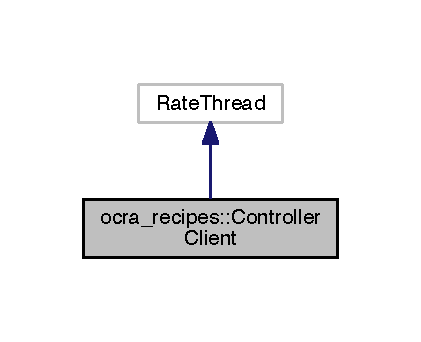
\includegraphics[width=202pt]{db/d0d/classocra__recipes_1_1ControllerClient__inherit__graph}
\end{center}
\end{figure}


Collaboration diagram for ocra\+\_\+recipes\+:\+:Controller\+Client\+:\nopagebreak
\begin{figure}[H]
\begin{center}
\leavevmode
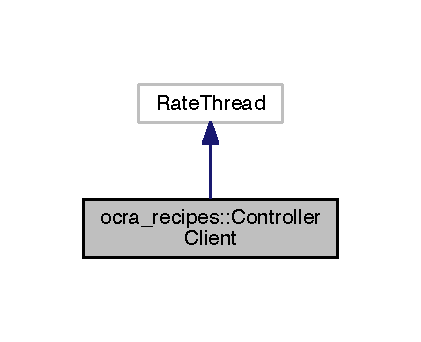
\includegraphics[width=202pt]{db/d24/classocra__recipes_1_1ControllerClient__coll__graph}
\end{center}
\end{figure}
\subsection*{Public Member Functions}
\begin{DoxyCompactItemize}
\item 
\hyperlink{classocra__recipes_1_1ControllerClient_acbddf372a61ee0cd20aa417527a56606}{Controller\+Client} ()
\item 
\hyperlink{classocra__recipes_1_1ControllerClient_acece74d9360b3f5508d26479f49fc3c2}{Controller\+Client} (ocra\+::\+Model\+::\+Ptr derived\+Model\+Ptr, const int loop\+Period=D\+E\+F\+A\+U\+L\+T\+\_\+\+L\+O\+O\+P\+\_\+\+P\+E\+R\+I\+OD)
\item 
virtual \hyperlink{classocra__recipes_1_1ControllerClient_a75faf6691be6c622deba404514c7ed70}{$\sim$\+Controller\+Client} ()
\item 
virtual bool \hyperlink{classocra__recipes_1_1ControllerClient_aceef962c9a3cd42dc9defcaa356d6275}{thread\+Init} ()
\item 
virtual void \hyperlink{classocra__recipes_1_1ControllerClient_ac42b7aad0b833f173475ed2a552ec159}{thread\+Release} ()
\item 
virtual void \hyperlink{classocra__recipes_1_1ControllerClient_a4a17a6233a5d824ee58115003b332c18}{run} ()
\item 
virtual void \hyperlink{classocra__recipes_1_1ControllerClient_a6bb943c2525cdc0fe82c83380c4f8900}{print\+Help} ()
\item 
int \hyperlink{classocra__recipes_1_1ControllerClient_a7ac35bd9a5eeeeb287d28e4d04c45766}{get\+Expected\+Period} ()
\item 
virtual bool \hyperlink{classocra__recipes_1_1ControllerClient_a51b18252578788100852a711d9d8f93a}{configure} (yarp\+::os\+::\+Resource\+Finder \&rf)
\item 
void \hyperlink{classocra__recipes_1_1ControllerClient_a4e86ce713e96089dd2b53aec1d8ff3e3}{add\+Tasks} (const std\+::string \&path\+To\+Xml\+File, bool overwrite)
\item 
void \hyperlink{classocra__recipes_1_1ControllerClient_a1f08768f37915c62b88e29d8db1ba27c}{add\+Task} (\hyperlink{classocra_1_1TaskBuilderOptions}{ocra\+::\+Task\+Builder\+Options} \&tm\+Opts, bool overwrite)
\item 
bool \hyperlink{classocra__recipes_1_1ControllerClient_aea41250cfe35937fc49f7261b0f356a3}{check\+If\+Task\+Exists} (\hyperlink{classocra_1_1TaskBuilderOptions}{ocra\+::\+Task\+Builder\+Options} \&tm\+Opts)
\item 
std\+::vector$<$ std\+::string $>$ \hyperlink{classocra__recipes_1_1ControllerClient_a53b0b53fc4c46f195c9f6dd2d1a6506c}{get\+Task\+Types} ()
\item 
std\+::vector$<$ std\+::string $>$ \hyperlink{classocra__recipes_1_1ControllerClient_a96ece5fcbcdffcd43c93905ffce5f54a}{get\+Task\+Names} ()
\item 
bool \hyperlink{classocra__recipes_1_1ControllerClient_a6666247713cb0e1db55b51b9a5ae49a1}{remove\+Task} (const std\+::string \&task\+Name)
\item 
bool \hyperlink{classocra__recipes_1_1ControllerClient_a7e72d409c511f201201292e8c123e771}{remove\+Tasks} (const std\+::vector$<$ std\+::string $>$ \&task\+Name\+Vector)
\item 
bool \hyperlink{classocra__recipes_1_1ControllerClient_a8c83005b1be831bc230d5a441f88980d}{has\+Been\+Released} ()
\item 
bool \hyperlink{classocra__recipes_1_1ControllerClient_ac4619242e809fa326f25f073d18feb50}{change\+Fixed\+Link} (std\+::string new\+Fixed\+Link, int is\+In\+Left\+Support, int is\+In\+Right\+Support)
\end{DoxyCompactItemize}
\subsection*{Protected Member Functions}
\begin{DoxyCompactItemize}
\item 
virtual bool \hyperlink{classocra__recipes_1_1ControllerClient_a8ac06cc5d7d6b0e078e1cb377a998c25}{initialize} ()
\item 
virtual void \hyperlink{classocra__recipes_1_1ControllerClient_a181c868d0165b06b9b10a9e40127bc69}{release} ()
\item 
virtual void \hyperlink{classocra__recipes_1_1ControllerClient_ac6d28be8e314dd2a034cfcb512e29ee3}{loop} ()=0
\end{DoxyCompactItemize}
\subsection*{Protected Attributes}
\begin{DoxyCompactItemize}
\item 
Client\+Communications\+::\+Ptr \hyperlink{classocra__recipes_1_1ControllerClient_aced7fa4d435e58cc2832abdbad1e4cbd}{client\+Coms}
\item 
ocra\+::\+Model\+::\+Ptr \hyperlink{classocra__recipes_1_1ControllerClient_a7eab32e91df97360c4de86f968a943e6}{model}
\end{DoxyCompactItemize}


\subsection{Detailed Description}


Definition at line 24 of file Controller\+Client.\+h.



\subsection{Constructor \& Destructor Documentation}
\hypertarget{classocra__recipes_1_1ControllerClient_acbddf372a61ee0cd20aa417527a56606}{}\label{classocra__recipes_1_1ControllerClient_acbddf372a61ee0cd20aa417527a56606} 
\index{ocra\+\_\+recipes\+::\+Controller\+Client@{ocra\+\_\+recipes\+::\+Controller\+Client}!Controller\+Client@{Controller\+Client}}
\index{Controller\+Client@{Controller\+Client}!ocra\+\_\+recipes\+::\+Controller\+Client@{ocra\+\_\+recipes\+::\+Controller\+Client}}
\subsubsection{\texorpdfstring{Controller\+Client()}{ControllerClient()}\hspace{0.1cm}{\footnotesize\ttfamily [1/2]}}
{\footnotesize\ttfamily Controller\+Client\+::\+Controller\+Client (\begin{DoxyParamCaption}{ }\end{DoxyParamCaption})}



Definition at line 7 of file Controller\+Client.\+cpp.

\hypertarget{classocra__recipes_1_1ControllerClient_acece74d9360b3f5508d26479f49fc3c2}{}\label{classocra__recipes_1_1ControllerClient_acece74d9360b3f5508d26479f49fc3c2} 
\index{ocra\+\_\+recipes\+::\+Controller\+Client@{ocra\+\_\+recipes\+::\+Controller\+Client}!Controller\+Client@{Controller\+Client}}
\index{Controller\+Client@{Controller\+Client}!ocra\+\_\+recipes\+::\+Controller\+Client@{ocra\+\_\+recipes\+::\+Controller\+Client}}
\subsubsection{\texorpdfstring{Controller\+Client()}{ControllerClient()}\hspace{0.1cm}{\footnotesize\ttfamily [2/2]}}
{\footnotesize\ttfamily Controller\+Client\+::\+Controller\+Client (\begin{DoxyParamCaption}\item[{ocra\+::\+Model\+::\+Ptr}]{derived\+Model\+Ptr,  }\item[{const int}]{loop\+Period = {\ttfamily DEFAULT\+\_\+LOOP\+\_\+PERIOD} }\end{DoxyParamCaption})}



Definition at line 15 of file Controller\+Client.\+cpp.

\hypertarget{classocra__recipes_1_1ControllerClient_a75faf6691be6c622deba404514c7ed70}{}\label{classocra__recipes_1_1ControllerClient_a75faf6691be6c622deba404514c7ed70} 
\index{ocra\+\_\+recipes\+::\+Controller\+Client@{ocra\+\_\+recipes\+::\+Controller\+Client}!````~Controller\+Client@{$\sim$\+Controller\+Client}}
\index{````~Controller\+Client@{$\sim$\+Controller\+Client}!ocra\+\_\+recipes\+::\+Controller\+Client@{ocra\+\_\+recipes\+::\+Controller\+Client}}
\subsubsection{\texorpdfstring{$\sim$\+Controller\+Client()}{~ControllerClient()}}
{\footnotesize\ttfamily Controller\+Client\+::$\sim$\+Controller\+Client (\begin{DoxyParamCaption}{ }\end{DoxyParamCaption})\hspace{0.3cm}{\ttfamily [virtual]}}



Definition at line 38 of file Controller\+Client.\+cpp.



\subsection{Member Function Documentation}
\hypertarget{classocra__recipes_1_1ControllerClient_a1f08768f37915c62b88e29d8db1ba27c}{}\label{classocra__recipes_1_1ControllerClient_a1f08768f37915c62b88e29d8db1ba27c} 
\index{ocra\+\_\+recipes\+::\+Controller\+Client@{ocra\+\_\+recipes\+::\+Controller\+Client}!add\+Task@{add\+Task}}
\index{add\+Task@{add\+Task}!ocra\+\_\+recipes\+::\+Controller\+Client@{ocra\+\_\+recipes\+::\+Controller\+Client}}
\subsubsection{\texorpdfstring{add\+Task()}{addTask()}}
{\footnotesize\ttfamily void ocra\+\_\+recipes\+::\+Controller\+Client\+::add\+Task (\begin{DoxyParamCaption}\item[{\hyperlink{classocra_1_1TaskBuilderOptions}{ocra\+::\+Task\+Builder\+Options} \&}]{tm\+Opts,  }\item[{bool}]{overwrite }\end{DoxyParamCaption})}

\hypertarget{classocra__recipes_1_1ControllerClient_a4e86ce713e96089dd2b53aec1d8ff3e3}{}\label{classocra__recipes_1_1ControllerClient_a4e86ce713e96089dd2b53aec1d8ff3e3} 
\index{ocra\+\_\+recipes\+::\+Controller\+Client@{ocra\+\_\+recipes\+::\+Controller\+Client}!add\+Tasks@{add\+Tasks}}
\index{add\+Tasks@{add\+Tasks}!ocra\+\_\+recipes\+::\+Controller\+Client@{ocra\+\_\+recipes\+::\+Controller\+Client}}
\subsubsection{\texorpdfstring{add\+Tasks()}{addTasks()}}
{\footnotesize\ttfamily void Controller\+Client\+::add\+Tasks (\begin{DoxyParamCaption}\item[{const std\+::string \&}]{path\+To\+Xml\+File,  }\item[{bool}]{overwrite }\end{DoxyParamCaption})}



Definition at line 78 of file Controller\+Client.\+cpp.

\hypertarget{classocra__recipes_1_1ControllerClient_ac4619242e809fa326f25f073d18feb50}{}\label{classocra__recipes_1_1ControllerClient_ac4619242e809fa326f25f073d18feb50} 
\index{ocra\+\_\+recipes\+::\+Controller\+Client@{ocra\+\_\+recipes\+::\+Controller\+Client}!change\+Fixed\+Link@{change\+Fixed\+Link}}
\index{change\+Fixed\+Link@{change\+Fixed\+Link}!ocra\+\_\+recipes\+::\+Controller\+Client@{ocra\+\_\+recipes\+::\+Controller\+Client}}
\subsubsection{\texorpdfstring{change\+Fixed\+Link()}{changeFixedLink()}}
{\footnotesize\ttfamily bool Controller\+Client\+::change\+Fixed\+Link (\begin{DoxyParamCaption}\item[{std\+::string}]{new\+Fixed\+Link,  }\item[{int}]{is\+In\+Left\+Support,  }\item[{int}]{is\+In\+Right\+Support }\end{DoxyParamCaption})}



Definition at line 138 of file Controller\+Client.\+cpp.

\hypertarget{classocra__recipes_1_1ControllerClient_aea41250cfe35937fc49f7261b0f356a3}{}\label{classocra__recipes_1_1ControllerClient_aea41250cfe35937fc49f7261b0f356a3} 
\index{ocra\+\_\+recipes\+::\+Controller\+Client@{ocra\+\_\+recipes\+::\+Controller\+Client}!check\+If\+Task\+Exists@{check\+If\+Task\+Exists}}
\index{check\+If\+Task\+Exists@{check\+If\+Task\+Exists}!ocra\+\_\+recipes\+::\+Controller\+Client@{ocra\+\_\+recipes\+::\+Controller\+Client}}
\subsubsection{\texorpdfstring{check\+If\+Task\+Exists()}{checkIfTaskExists()}}
{\footnotesize\ttfamily bool Controller\+Client\+::check\+If\+Task\+Exists (\begin{DoxyParamCaption}\item[{\hyperlink{classocra_1_1TaskBuilderOptions}{ocra\+::\+Task\+Builder\+Options} \&}]{tm\+Opts }\end{DoxyParamCaption})}



Definition at line 108 of file Controller\+Client.\+cpp.

\hypertarget{classocra__recipes_1_1ControllerClient_a51b18252578788100852a711d9d8f93a}{}\label{classocra__recipes_1_1ControllerClient_a51b18252578788100852a711d9d8f93a} 
\index{ocra\+\_\+recipes\+::\+Controller\+Client@{ocra\+\_\+recipes\+::\+Controller\+Client}!configure@{configure}}
\index{configure@{configure}!ocra\+\_\+recipes\+::\+Controller\+Client@{ocra\+\_\+recipes\+::\+Controller\+Client}}
\subsubsection{\texorpdfstring{configure()}{configure()}}
{\footnotesize\ttfamily virtual bool ocra\+\_\+recipes\+::\+Controller\+Client\+::configure (\begin{DoxyParamCaption}\item[{yarp\+::os\+::\+Resource\+Finder \&}]{rf }\end{DoxyParamCaption})\hspace{0.3cm}{\ttfamily [inline]}, {\ttfamily [virtual]}}

Configures the module by parsing the RF contents. 
\begin{DoxyParams}{Parameters}
{\em rf} & A resource finder instance which is initialized from the command line args.\\
\hline
\end{DoxyParams}
\begin{DoxyReturn}{Returns}
True or false if the configuration was successful. 
\end{DoxyReturn}


Definition at line 47 of file Controller\+Client.\+h.

\hypertarget{classocra__recipes_1_1ControllerClient_a7ac35bd9a5eeeeb287d28e4d04c45766}{}\label{classocra__recipes_1_1ControllerClient_a7ac35bd9a5eeeeb287d28e4d04c45766} 
\index{ocra\+\_\+recipes\+::\+Controller\+Client@{ocra\+\_\+recipes\+::\+Controller\+Client}!get\+Expected\+Period@{get\+Expected\+Period}}
\index{get\+Expected\+Period@{get\+Expected\+Period}!ocra\+\_\+recipes\+::\+Controller\+Client@{ocra\+\_\+recipes\+::\+Controller\+Client}}
\subsubsection{\texorpdfstring{get\+Expected\+Period()}{getExpectedPeriod()}}
{\footnotesize\ttfamily int ocra\+\_\+recipes\+::\+Controller\+Client\+::get\+Expected\+Period (\begin{DoxyParamCaption}{ }\end{DoxyParamCaption})\hspace{0.3cm}{\ttfamily [inline]}}



Definition at line 40 of file Controller\+Client.\+h.

\hypertarget{classocra__recipes_1_1ControllerClient_a96ece5fcbcdffcd43c93905ffce5f54a}{}\label{classocra__recipes_1_1ControllerClient_a96ece5fcbcdffcd43c93905ffce5f54a} 
\index{ocra\+\_\+recipes\+::\+Controller\+Client@{ocra\+\_\+recipes\+::\+Controller\+Client}!get\+Task\+Names@{get\+Task\+Names}}
\index{get\+Task\+Names@{get\+Task\+Names}!ocra\+\_\+recipes\+::\+Controller\+Client@{ocra\+\_\+recipes\+::\+Controller\+Client}}
\subsubsection{\texorpdfstring{get\+Task\+Names()}{getTaskNames()}}
{\footnotesize\ttfamily std\+::vector$<$ std\+::string $>$ Controller\+Client\+::get\+Task\+Names (\begin{DoxyParamCaption}{ }\end{DoxyParamCaption})}



Definition at line 133 of file Controller\+Client.\+cpp.

\hypertarget{classocra__recipes_1_1ControllerClient_a53b0b53fc4c46f195c9f6dd2d1a6506c}{}\label{classocra__recipes_1_1ControllerClient_a53b0b53fc4c46f195c9f6dd2d1a6506c} 
\index{ocra\+\_\+recipes\+::\+Controller\+Client@{ocra\+\_\+recipes\+::\+Controller\+Client}!get\+Task\+Types@{get\+Task\+Types}}
\index{get\+Task\+Types@{get\+Task\+Types}!ocra\+\_\+recipes\+::\+Controller\+Client@{ocra\+\_\+recipes\+::\+Controller\+Client}}
\subsubsection{\texorpdfstring{get\+Task\+Types()}{getTaskTypes()}}
{\footnotesize\ttfamily std\+::vector$<$ std\+::string $>$ Controller\+Client\+::get\+Task\+Types (\begin{DoxyParamCaption}{ }\end{DoxyParamCaption})}



Definition at line 128 of file Controller\+Client.\+cpp.

\hypertarget{classocra__recipes_1_1ControllerClient_a8c83005b1be831bc230d5a441f88980d}{}\label{classocra__recipes_1_1ControllerClient_a8c83005b1be831bc230d5a441f88980d} 
\index{ocra\+\_\+recipes\+::\+Controller\+Client@{ocra\+\_\+recipes\+::\+Controller\+Client}!has\+Been\+Released@{has\+Been\+Released}}
\index{has\+Been\+Released@{has\+Been\+Released}!ocra\+\_\+recipes\+::\+Controller\+Client@{ocra\+\_\+recipes\+::\+Controller\+Client}}
\subsubsection{\texorpdfstring{has\+Been\+Released()}{hasBeenReleased()}}
{\footnotesize\ttfamily bool ocra\+\_\+recipes\+::\+Controller\+Client\+::has\+Been\+Released (\begin{DoxyParamCaption}{ }\end{DoxyParamCaption})\hspace{0.3cm}{\ttfamily [inline]}}



Definition at line 59 of file Controller\+Client.\+h.

\hypertarget{classocra__recipes_1_1ControllerClient_a8ac06cc5d7d6b0e078e1cb377a998c25}{}\label{classocra__recipes_1_1ControllerClient_a8ac06cc5d7d6b0e078e1cb377a998c25} 
\index{ocra\+\_\+recipes\+::\+Controller\+Client@{ocra\+\_\+recipes\+::\+Controller\+Client}!initialize@{initialize}}
\index{initialize@{initialize}!ocra\+\_\+recipes\+::\+Controller\+Client@{ocra\+\_\+recipes\+::\+Controller\+Client}}
\subsubsection{\texorpdfstring{initialize()}{initialize()}}
{\footnotesize\ttfamily virtual bool ocra\+\_\+recipes\+::\+Controller\+Client\+::initialize (\begin{DoxyParamCaption}{ }\end{DoxyParamCaption})\hspace{0.3cm}{\ttfamily [inline]}, {\ttfamily [protected]}, {\ttfamily [virtual]}}



Definition at line 64 of file Controller\+Client.\+h.

\hypertarget{classocra__recipes_1_1ControllerClient_ac6d28be8e314dd2a034cfcb512e29ee3}{}\label{classocra__recipes_1_1ControllerClient_ac6d28be8e314dd2a034cfcb512e29ee3} 
\index{ocra\+\_\+recipes\+::\+Controller\+Client@{ocra\+\_\+recipes\+::\+Controller\+Client}!loop@{loop}}
\index{loop@{loop}!ocra\+\_\+recipes\+::\+Controller\+Client@{ocra\+\_\+recipes\+::\+Controller\+Client}}
\subsubsection{\texorpdfstring{loop()}{loop()}}
{\footnotesize\ttfamily virtual void ocra\+\_\+recipes\+::\+Controller\+Client\+::loop (\begin{DoxyParamCaption}{ }\end{DoxyParamCaption})\hspace{0.3cm}{\ttfamily [protected]}, {\ttfamily [pure virtual]}}

\hypertarget{classocra__recipes_1_1ControllerClient_a6bb943c2525cdc0fe82c83380c4f8900}{}\label{classocra__recipes_1_1ControllerClient_a6bb943c2525cdc0fe82c83380c4f8900} 
\index{ocra\+\_\+recipes\+::\+Controller\+Client@{ocra\+\_\+recipes\+::\+Controller\+Client}!print\+Help@{print\+Help}}
\index{print\+Help@{print\+Help}!ocra\+\_\+recipes\+::\+Controller\+Client@{ocra\+\_\+recipes\+::\+Controller\+Client}}
\subsubsection{\texorpdfstring{print\+Help()}{printHelp()}}
{\footnotesize\ttfamily virtual void ocra\+\_\+recipes\+::\+Controller\+Client\+::print\+Help (\begin{DoxyParamCaption}{ }\end{DoxyParamCaption})\hspace{0.3cm}{\ttfamily [inline]}, {\ttfamily [virtual]}}



Definition at line 38 of file Controller\+Client.\+h.

\hypertarget{classocra__recipes_1_1ControllerClient_a181c868d0165b06b9b10a9e40127bc69}{}\label{classocra__recipes_1_1ControllerClient_a181c868d0165b06b9b10a9e40127bc69} 
\index{ocra\+\_\+recipes\+::\+Controller\+Client@{ocra\+\_\+recipes\+::\+Controller\+Client}!release@{release}}
\index{release@{release}!ocra\+\_\+recipes\+::\+Controller\+Client@{ocra\+\_\+recipes\+::\+Controller\+Client}}
\subsubsection{\texorpdfstring{release()}{release()}}
{\footnotesize\ttfamily virtual void ocra\+\_\+recipes\+::\+Controller\+Client\+::release (\begin{DoxyParamCaption}{ }\end{DoxyParamCaption})\hspace{0.3cm}{\ttfamily [inline]}, {\ttfamily [protected]}, {\ttfamily [virtual]}}



Definition at line 65 of file Controller\+Client.\+h.

\hypertarget{classocra__recipes_1_1ControllerClient_a6666247713cb0e1db55b51b9a5ae49a1}{}\label{classocra__recipes_1_1ControllerClient_a6666247713cb0e1db55b51b9a5ae49a1} 
\index{ocra\+\_\+recipes\+::\+Controller\+Client@{ocra\+\_\+recipes\+::\+Controller\+Client}!remove\+Task@{remove\+Task}}
\index{remove\+Task@{remove\+Task}!ocra\+\_\+recipes\+::\+Controller\+Client@{ocra\+\_\+recipes\+::\+Controller\+Client}}
\subsubsection{\texorpdfstring{remove\+Task()}{removeTask()}}
{\footnotesize\ttfamily bool Controller\+Client\+::remove\+Task (\begin{DoxyParamCaption}\item[{const std\+::string \&}]{task\+Name }\end{DoxyParamCaption})}



Definition at line 63 of file Controller\+Client.\+cpp.

\hypertarget{classocra__recipes_1_1ControllerClient_a7e72d409c511f201201292e8c123e771}{}\label{classocra__recipes_1_1ControllerClient_a7e72d409c511f201201292e8c123e771} 
\index{ocra\+\_\+recipes\+::\+Controller\+Client@{ocra\+\_\+recipes\+::\+Controller\+Client}!remove\+Tasks@{remove\+Tasks}}
\index{remove\+Tasks@{remove\+Tasks}!ocra\+\_\+recipes\+::\+Controller\+Client@{ocra\+\_\+recipes\+::\+Controller\+Client}}
\subsubsection{\texorpdfstring{remove\+Tasks()}{removeTasks()}}
{\footnotesize\ttfamily bool Controller\+Client\+::remove\+Tasks (\begin{DoxyParamCaption}\item[{const std\+::vector$<$ std\+::string $>$ \&}]{task\+Name\+Vector }\end{DoxyParamCaption})}



Definition at line 72 of file Controller\+Client.\+cpp.

\hypertarget{classocra__recipes_1_1ControllerClient_a4a17a6233a5d824ee58115003b332c18}{}\label{classocra__recipes_1_1ControllerClient_a4a17a6233a5d824ee58115003b332c18} 
\index{ocra\+\_\+recipes\+::\+Controller\+Client@{ocra\+\_\+recipes\+::\+Controller\+Client}!run@{run}}
\index{run@{run}!ocra\+\_\+recipes\+::\+Controller\+Client@{ocra\+\_\+recipes\+::\+Controller\+Client}}
\subsubsection{\texorpdfstring{run()}{run()}}
{\footnotesize\ttfamily void Controller\+Client\+::run (\begin{DoxyParamCaption}{ }\end{DoxyParamCaption})\hspace{0.3cm}{\ttfamily [virtual]}}



Definition at line 52 of file Controller\+Client.\+cpp.

\hypertarget{classocra__recipes_1_1ControllerClient_aceef962c9a3cd42dc9defcaa356d6275}{}\label{classocra__recipes_1_1ControllerClient_aceef962c9a3cd42dc9defcaa356d6275} 
\index{ocra\+\_\+recipes\+::\+Controller\+Client@{ocra\+\_\+recipes\+::\+Controller\+Client}!thread\+Init@{thread\+Init}}
\index{thread\+Init@{thread\+Init}!ocra\+\_\+recipes\+::\+Controller\+Client@{ocra\+\_\+recipes\+::\+Controller\+Client}}
\subsubsection{\texorpdfstring{thread\+Init()}{threadInit()}}
{\footnotesize\ttfamily bool Controller\+Client\+::thread\+Init (\begin{DoxyParamCaption}{ }\end{DoxyParamCaption})\hspace{0.3cm}{\ttfamily [virtual]}}



Definition at line 43 of file Controller\+Client.\+cpp.

\hypertarget{classocra__recipes_1_1ControllerClient_ac42b7aad0b833f173475ed2a552ec159}{}\label{classocra__recipes_1_1ControllerClient_ac42b7aad0b833f173475ed2a552ec159} 
\index{ocra\+\_\+recipes\+::\+Controller\+Client@{ocra\+\_\+recipes\+::\+Controller\+Client}!thread\+Release@{thread\+Release}}
\index{thread\+Release@{thread\+Release}!ocra\+\_\+recipes\+::\+Controller\+Client@{ocra\+\_\+recipes\+::\+Controller\+Client}}
\subsubsection{\texorpdfstring{thread\+Release()}{threadRelease()}}
{\footnotesize\ttfamily void Controller\+Client\+::thread\+Release (\begin{DoxyParamCaption}{ }\end{DoxyParamCaption})\hspace{0.3cm}{\ttfamily [virtual]}}



Definition at line 57 of file Controller\+Client.\+cpp.



\subsection{Member Data Documentation}
\hypertarget{classocra__recipes_1_1ControllerClient_aced7fa4d435e58cc2832abdbad1e4cbd}{}\label{classocra__recipes_1_1ControllerClient_aced7fa4d435e58cc2832abdbad1e4cbd} 
\index{ocra\+\_\+recipes\+::\+Controller\+Client@{ocra\+\_\+recipes\+::\+Controller\+Client}!client\+Coms@{client\+Coms}}
\index{client\+Coms@{client\+Coms}!ocra\+\_\+recipes\+::\+Controller\+Client@{ocra\+\_\+recipes\+::\+Controller\+Client}}
\subsubsection{\texorpdfstring{client\+Coms}{clientComs}}
{\footnotesize\ttfamily Client\+Communications\+::\+Ptr ocra\+\_\+recipes\+::\+Controller\+Client\+::client\+Coms\hspace{0.3cm}{\ttfamily [protected]}}



Definition at line 68 of file Controller\+Client.\+h.

\hypertarget{classocra__recipes_1_1ControllerClient_a7eab32e91df97360c4de86f968a943e6}{}\label{classocra__recipes_1_1ControllerClient_a7eab32e91df97360c4de86f968a943e6} 
\index{ocra\+\_\+recipes\+::\+Controller\+Client@{ocra\+\_\+recipes\+::\+Controller\+Client}!model@{model}}
\index{model@{model}!ocra\+\_\+recipes\+::\+Controller\+Client@{ocra\+\_\+recipes\+::\+Controller\+Client}}
\subsubsection{\texorpdfstring{model}{model}}
{\footnotesize\ttfamily ocra\+::\+Model\+::\+Ptr ocra\+\_\+recipes\+::\+Controller\+Client\+::model\hspace{0.3cm}{\ttfamily [protected]}}



Definition at line 69 of file Controller\+Client.\+h.



The documentation for this class was generated from the following files\+:\begin{DoxyCompactItemize}
\item 
\hyperlink{ControllerClient_8h}{Controller\+Client.\+h}\item 
\hyperlink{ControllerClient_8cpp}{Controller\+Client.\+cpp}\end{DoxyCompactItemize}

\hypertarget{classocra__recipes_1_1ControllerServer}{}\section{ocra\+\_\+recipes\+:\+:Controller\+Server Class Reference}
\label{classocra__recipes_1_1ControllerServer}\index{ocra\+\_\+recipes\+::\+Controller\+Server@{ocra\+\_\+recipes\+::\+Controller\+Server}}


{\ttfamily \#include $<$Controller\+Server.\+h$>$}



Collaboration diagram for ocra\+\_\+recipes\+:\+:Controller\+Server\+:\nopagebreak
\begin{figure}[H]
\begin{center}
\leavevmode
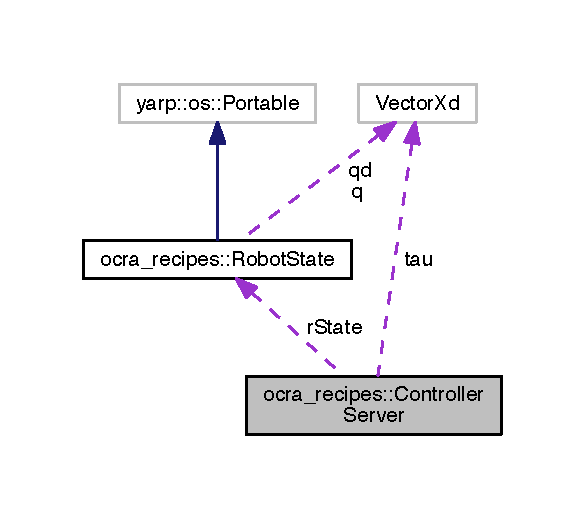
\includegraphics[width=280pt]{d7/d59/classocra__recipes_1_1ControllerServer__coll__graph}
\end{center}
\end{figure}
\subsection*{Public Member Functions}
\begin{DoxyCompactItemize}
\item 
\hyperlink{classocra__recipes_1_1ControllerServer_a78cc49b2b2a3f9daecc0662051b5644d}{Controller\+Server} (\hyperlink{namespaceocra__recipes_ae561cff4ea9a191b8b1ebb4e69a1a4ba}{C\+O\+N\+T\+R\+O\+L\+L\+E\+R\+\_\+\+T\+Y\+PE} ctrl\+Type, \hyperlink{namespaceocra__recipes_afb3bb4de56c2b9472c80d746eb13fed3}{S\+O\+L\+V\+E\+R\+\_\+\+T\+Y\+PE} solver, bool using\+Interprocess\+Communication=true, bool use\+Odometry=false)
\item 
virtual \hyperlink{classocra__recipes_1_1ControllerServer_a02157f0e6432dae6d8ebf3126c335444}{$\sim$\+Controller\+Server} ()
\item 
bool \hyperlink{classocra__recipes_1_1ControllerServer_af51ea42acb8c1adc3db4cc2a256f1f46}{initialize} ()
\item 
const Eigen\+::\+Vector\+Xd \& \hyperlink{classocra__recipes_1_1ControllerServer_a4b4c825748bc85f200f4b82cbffb8e0d}{compute\+Torques} ()
\item 
void \hyperlink{classocra__recipes_1_1ControllerServer_a925d4de1de73f0ac18e50f0f3c4cd0a4}{compute\+Torques} (Eigen\+::\+Vector\+Xd \&torques)
\item 
const std\+::shared\+\_\+ptr$<$ \hyperlink{classocra_1_1Controller}{ocra\+::\+Controller} $>$ \hyperlink{classocra__recipes_1_1ControllerServer_a40bc86b6d9a4140441320c88bfc77652}{get\+Controller} ()
\item 
const std\+::shared\+\_\+ptr$<$ ocra\+::\+Model $>$ \hyperlink{classocra__recipes_1_1ControllerServer_ab83e5cc59e33d26cedbea43afae25e1e}{get\+Robot\+Model} ()
\item 
bool \hyperlink{classocra__recipes_1_1ControllerServer_ad2ca7fafa8c7fff009581df869f65d85}{add\+Tasks\+From\+Xml\+File} (const std\+::string \&file\+Path)
\item 
bool \hyperlink{classocra__recipes_1_1ControllerServer_ad78efdf5d90308b0dc8e88d6d0720c5f}{add\+Tasks} (std\+::vector$<$ \hyperlink{classocra_1_1TaskBuilderOptions}{ocra\+::\+Task\+Builder\+Options} $>$ \&tm\+Opts)
\item 
bool \hyperlink{classocra__recipes_1_1ControllerServer_a441016519ed42fee35c1fd9ae458d874}{initialize\+Odometry} ()
\item 
void \hyperlink{classocra__recipes_1_1ControllerServer_a83755d02be88fa3805d770d964995fb0}{update\+Model} ()
\end{DoxyCompactItemize}
\subsection*{Protected Member Functions}
\begin{DoxyCompactItemize}
\item 
virtual std\+::shared\+\_\+ptr$<$ Model $>$ \hyperlink{classocra__recipes_1_1ControllerServer_a50715d81293d3ec5f0d6a60710008510}{load\+Robot\+Model} ()=0
\item 
virtual void \hyperlink{classocra__recipes_1_1ControllerServer_a93ec150bea9b2a7a03aac1cc048d5484}{get\+Robot\+State} (Eigen\+::\+Vector\+Xd \&q, Eigen\+::\+Vector\+Xd \&qd, Eigen\+::\+Displacementd \&H\+\_\+root, Eigen\+::\+Twistd \&T\+\_\+root)=0
\end{DoxyCompactItemize}
\subsection*{Protected Attributes}
\begin{DoxyCompactItemize}
\item 
ocra\+::\+Model\+::\+Ptr \hyperlink{classocra__recipes_1_1ControllerServer_ab239e92da81b48afa2211ef9b25672f3}{model}
\item 
ocra\+::\+Controller\+::\+Ptr \hyperlink{classocra__recipes_1_1ControllerServer_a8e452bd0a8dce47b6fd289599e7ce210}{controller}
\item 
ocra\+::\+Solver\+::\+Ptr \hyperlink{classocra__recipes_1_1ControllerServer_a46e53b5a5bf9f7d55af477f85cb21522}{internal\+Solver}
\item 
Server\+Communications\+::\+Ptr \hyperlink{classocra__recipes_1_1ControllerServer_af01dc7be410bfebebefedc5f4bb27d1b}{server\+Coms}
\item 
Eigen\+::\+Vector\+Xd \hyperlink{classocra__recipes_1_1ControllerServer_a07e10b62b84a999c14843662a378ec0f}{tau}
\item 
\hyperlink{classocra__recipes_1_1RobotState}{Robot\+State} \hyperlink{classocra__recipes_1_1ControllerServer_a5c565a9ec45e5fad7b56e9a48609ef3d}{r\+State}
\item 
\hyperlink{namespaceocra__recipes_ae561cff4ea9a191b8b1ebb4e69a1a4ba}{C\+O\+N\+T\+R\+O\+L\+L\+E\+R\+\_\+\+T\+Y\+PE} \hyperlink{classocra__recipes_1_1ControllerServer_aaf53114a96960a3cb81577378c179411}{controller\+Type}
\item 
\hyperlink{namespaceocra__recipes_afb3bb4de56c2b9472c80d746eb13fed3}{S\+O\+L\+V\+E\+R\+\_\+\+T\+Y\+PE} \hyperlink{classocra__recipes_1_1ControllerServer_a7c7d1eda2c96085709f0c3a28fd998a4}{solver\+Type}
\item 
bool \hyperlink{classocra__recipes_1_1ControllerServer_a7f7559e938ca0e3cfff4833d86ef5b54}{using\+Coms}
\item 
bool \hyperlink{classocra__recipes_1_1ControllerServer_afd126a8b289e29213468fe9e9a800dd2}{using\+Odometry}
\item 
yarp\+::os\+::\+Bottle \hyperlink{classocra__recipes_1_1ControllerServer_a587f8ef2bc028bf845b1713955def5a1}{states\+Bottle}
\item 
yarp\+::os\+::\+Port \hyperlink{classocra__recipes_1_1ControllerServer_a1d314027131262206280be3e728bf59f}{states\+Port}
\item 
std\+::string \hyperlink{classocra__recipes_1_1ControllerServer_ab077706b924eed4ac5c50e9ade36acf4}{model\+File}
\item 
std\+::string \hyperlink{classocra__recipes_1_1ControllerServer_a93ffe0eff924223989db0ae6fcafaca2}{initial\+Fixed\+Frame}
\end{DoxyCompactItemize}


\subsection{Detailed Description}


Definition at line 44 of file Controller\+Server.\+h.



\subsection{Constructor \& Destructor Documentation}
\hypertarget{classocra__recipes_1_1ControllerServer_a78cc49b2b2a3f9daecc0662051b5644d}{}\label{classocra__recipes_1_1ControllerServer_a78cc49b2b2a3f9daecc0662051b5644d} 
\index{ocra\+\_\+recipes\+::\+Controller\+Server@{ocra\+\_\+recipes\+::\+Controller\+Server}!Controller\+Server@{Controller\+Server}}
\index{Controller\+Server@{Controller\+Server}!ocra\+\_\+recipes\+::\+Controller\+Server@{ocra\+\_\+recipes\+::\+Controller\+Server}}
\subsubsection{\texorpdfstring{Controller\+Server()}{ControllerServer()}}
{\footnotesize\ttfamily Controller\+Server\+::\+Controller\+Server (\begin{DoxyParamCaption}\item[{\hyperlink{namespaceocra__recipes_ae561cff4ea9a191b8b1ebb4e69a1a4ba}{C\+O\+N\+T\+R\+O\+L\+L\+E\+R\+\_\+\+T\+Y\+PE}}]{ctrl\+Type,  }\item[{\hyperlink{namespaceocra__recipes_afb3bb4de56c2b9472c80d746eb13fed3}{S\+O\+L\+V\+E\+R\+\_\+\+T\+Y\+PE}}]{solver,  }\item[{bool}]{using\+Interprocess\+Communication = {\ttfamily true},  }\item[{bool}]{use\+Odometry = {\ttfamily false} }\end{DoxyParamCaption})}



Definition at line 5 of file Controller\+Server.\+cpp.

\hypertarget{classocra__recipes_1_1ControllerServer_a02157f0e6432dae6d8ebf3126c335444}{}\label{classocra__recipes_1_1ControllerServer_a02157f0e6432dae6d8ebf3126c335444} 
\index{ocra\+\_\+recipes\+::\+Controller\+Server@{ocra\+\_\+recipes\+::\+Controller\+Server}!````~Controller\+Server@{$\sim$\+Controller\+Server}}
\index{````~Controller\+Server@{$\sim$\+Controller\+Server}!ocra\+\_\+recipes\+::\+Controller\+Server@{ocra\+\_\+recipes\+::\+Controller\+Server}}
\subsubsection{\texorpdfstring{$\sim$\+Controller\+Server()}{~ControllerServer()}}
{\footnotesize\ttfamily Controller\+Server\+::$\sim$\+Controller\+Server (\begin{DoxyParamCaption}{ }\end{DoxyParamCaption})\hspace{0.3cm}{\ttfamily [virtual]}}



Definition at line 16 of file Controller\+Server.\+cpp.



\subsection{Member Function Documentation}
\hypertarget{classocra__recipes_1_1ControllerServer_ad78efdf5d90308b0dc8e88d6d0720c5f}{}\label{classocra__recipes_1_1ControllerServer_ad78efdf5d90308b0dc8e88d6d0720c5f} 
\index{ocra\+\_\+recipes\+::\+Controller\+Server@{ocra\+\_\+recipes\+::\+Controller\+Server}!add\+Tasks@{add\+Tasks}}
\index{add\+Tasks@{add\+Tasks}!ocra\+\_\+recipes\+::\+Controller\+Server@{ocra\+\_\+recipes\+::\+Controller\+Server}}
\subsubsection{\texorpdfstring{add\+Tasks()}{addTasks()}}
{\footnotesize\ttfamily bool Controller\+Server\+::add\+Tasks (\begin{DoxyParamCaption}\item[{std\+::vector$<$ \hyperlink{classocra_1_1TaskBuilderOptions}{ocra\+::\+Task\+Builder\+Options} $>$ \&}]{tm\+Opts }\end{DoxyParamCaption})}



Definition at line 130 of file Controller\+Server.\+cpp.

\hypertarget{classocra__recipes_1_1ControllerServer_ad2ca7fafa8c7fff009581df869f65d85}{}\label{classocra__recipes_1_1ControllerServer_ad2ca7fafa8c7fff009581df869f65d85} 
\index{ocra\+\_\+recipes\+::\+Controller\+Server@{ocra\+\_\+recipes\+::\+Controller\+Server}!add\+Tasks\+From\+Xml\+File@{add\+Tasks\+From\+Xml\+File}}
\index{add\+Tasks\+From\+Xml\+File@{add\+Tasks\+From\+Xml\+File}!ocra\+\_\+recipes\+::\+Controller\+Server@{ocra\+\_\+recipes\+::\+Controller\+Server}}
\subsubsection{\texorpdfstring{add\+Tasks\+From\+Xml\+File()}{addTasksFromXmlFile()}}
{\footnotesize\ttfamily bool Controller\+Server\+::add\+Tasks\+From\+Xml\+File (\begin{DoxyParamCaption}\item[{const std\+::string \&}]{file\+Path }\end{DoxyParamCaption})}



Definition at line 124 of file Controller\+Server.\+cpp.

\hypertarget{classocra__recipes_1_1ControllerServer_a4b4c825748bc85f200f4b82cbffb8e0d}{}\label{classocra__recipes_1_1ControllerServer_a4b4c825748bc85f200f4b82cbffb8e0d} 
\index{ocra\+\_\+recipes\+::\+Controller\+Server@{ocra\+\_\+recipes\+::\+Controller\+Server}!compute\+Torques@{compute\+Torques}}
\index{compute\+Torques@{compute\+Torques}!ocra\+\_\+recipes\+::\+Controller\+Server@{ocra\+\_\+recipes\+::\+Controller\+Server}}
\subsubsection{\texorpdfstring{compute\+Torques()}{computeTorques()}\hspace{0.1cm}{\footnotesize\ttfamily [1/2]}}
{\footnotesize\ttfamily const Eigen\+::\+Vector\+Xd \& Controller\+Server\+::compute\+Torques (\begin{DoxyParamCaption}{ }\end{DoxyParamCaption})}



Definition at line 98 of file Controller\+Server.\+cpp.

\hypertarget{classocra__recipes_1_1ControllerServer_a925d4de1de73f0ac18e50f0f3c4cd0a4}{}\label{classocra__recipes_1_1ControllerServer_a925d4de1de73f0ac18e50f0f3c4cd0a4} 
\index{ocra\+\_\+recipes\+::\+Controller\+Server@{ocra\+\_\+recipes\+::\+Controller\+Server}!compute\+Torques@{compute\+Torques}}
\index{compute\+Torques@{compute\+Torques}!ocra\+\_\+recipes\+::\+Controller\+Server@{ocra\+\_\+recipes\+::\+Controller\+Server}}
\subsubsection{\texorpdfstring{compute\+Torques()}{computeTorques()}\hspace{0.1cm}{\footnotesize\ttfamily [2/2]}}
{\footnotesize\ttfamily void Controller\+Server\+::compute\+Torques (\begin{DoxyParamCaption}\item[{Eigen\+::\+Vector\+Xd \&}]{torques }\end{DoxyParamCaption})}



Definition at line 105 of file Controller\+Server.\+cpp.

\hypertarget{classocra__recipes_1_1ControllerServer_a40bc86b6d9a4140441320c88bfc77652}{}\label{classocra__recipes_1_1ControllerServer_a40bc86b6d9a4140441320c88bfc77652} 
\index{ocra\+\_\+recipes\+::\+Controller\+Server@{ocra\+\_\+recipes\+::\+Controller\+Server}!get\+Controller@{get\+Controller}}
\index{get\+Controller@{get\+Controller}!ocra\+\_\+recipes\+::\+Controller\+Server@{ocra\+\_\+recipes\+::\+Controller\+Server}}
\subsubsection{\texorpdfstring{get\+Controller()}{getController()}}
{\footnotesize\ttfamily const std\+::shared\+\_\+ptr$<$\hyperlink{classocra_1_1Controller}{ocra\+::\+Controller}$>$ ocra\+\_\+recipes\+::\+Controller\+Server\+::get\+Controller (\begin{DoxyParamCaption}{ }\end{DoxyParamCaption})\hspace{0.3cm}{\ttfamily [inline]}}



Definition at line 64 of file Controller\+Server.\+h.

\hypertarget{classocra__recipes_1_1ControllerServer_ab83e5cc59e33d26cedbea43afae25e1e}{}\label{classocra__recipes_1_1ControllerServer_ab83e5cc59e33d26cedbea43afae25e1e} 
\index{ocra\+\_\+recipes\+::\+Controller\+Server@{ocra\+\_\+recipes\+::\+Controller\+Server}!get\+Robot\+Model@{get\+Robot\+Model}}
\index{get\+Robot\+Model@{get\+Robot\+Model}!ocra\+\_\+recipes\+::\+Controller\+Server@{ocra\+\_\+recipes\+::\+Controller\+Server}}
\subsubsection{\texorpdfstring{get\+Robot\+Model()}{getRobotModel()}}
{\footnotesize\ttfamily const std\+::shared\+\_\+ptr$<$ocra\+::\+Model$>$ ocra\+\_\+recipes\+::\+Controller\+Server\+::get\+Robot\+Model (\begin{DoxyParamCaption}{ }\end{DoxyParamCaption})\hspace{0.3cm}{\ttfamily [inline]}}



Definition at line 65 of file Controller\+Server.\+h.

\hypertarget{classocra__recipes_1_1ControllerServer_a93ec150bea9b2a7a03aac1cc048d5484}{}\label{classocra__recipes_1_1ControllerServer_a93ec150bea9b2a7a03aac1cc048d5484} 
\index{ocra\+\_\+recipes\+::\+Controller\+Server@{ocra\+\_\+recipes\+::\+Controller\+Server}!get\+Robot\+State@{get\+Robot\+State}}
\index{get\+Robot\+State@{get\+Robot\+State}!ocra\+\_\+recipes\+::\+Controller\+Server@{ocra\+\_\+recipes\+::\+Controller\+Server}}
\subsubsection{\texorpdfstring{get\+Robot\+State()}{getRobotState()}}
{\footnotesize\ttfamily virtual void ocra\+\_\+recipes\+::\+Controller\+Server\+::get\+Robot\+State (\begin{DoxyParamCaption}\item[{Eigen\+::\+Vector\+Xd \&}]{q,  }\item[{Eigen\+::\+Vector\+Xd \&}]{qd,  }\item[{Eigen\+::\+Displacementd \&}]{H\+\_\+root,  }\item[{Eigen\+::\+Twistd \&}]{T\+\_\+root }\end{DoxyParamCaption})\hspace{0.3cm}{\ttfamily [protected]}, {\ttfamily [pure virtual]}}

\hypertarget{classocra__recipes_1_1ControllerServer_af51ea42acb8c1adc3db4cc2a256f1f46}{}\label{classocra__recipes_1_1ControllerServer_af51ea42acb8c1adc3db4cc2a256f1f46} 
\index{ocra\+\_\+recipes\+::\+Controller\+Server@{ocra\+\_\+recipes\+::\+Controller\+Server}!initialize@{initialize}}
\index{initialize@{initialize}!ocra\+\_\+recipes\+::\+Controller\+Server@{ocra\+\_\+recipes\+::\+Controller\+Server}}
\subsubsection{\texorpdfstring{initialize()}{initialize()}}
{\footnotesize\ttfamily bool Controller\+Server\+::initialize (\begin{DoxyParamCaption}{ }\end{DoxyParamCaption})}



Definition at line 22 of file Controller\+Server.\+cpp.

\hypertarget{classocra__recipes_1_1ControllerServer_a441016519ed42fee35c1fd9ae458d874}{}\label{classocra__recipes_1_1ControllerServer_a441016519ed42fee35c1fd9ae458d874} 
\index{ocra\+\_\+recipes\+::\+Controller\+Server@{ocra\+\_\+recipes\+::\+Controller\+Server}!initialize\+Odometry@{initialize\+Odometry}}
\index{initialize\+Odometry@{initialize\+Odometry}!ocra\+\_\+recipes\+::\+Controller\+Server@{ocra\+\_\+recipes\+::\+Controller\+Server}}
\subsubsection{\texorpdfstring{initialize\+Odometry()}{initializeOdometry()}}
{\footnotesize\ttfamily bool ocra\+\_\+recipes\+::\+Controller\+Server\+::initialize\+Odometry (\begin{DoxyParamCaption}{ }\end{DoxyParamCaption})}

If the use\+Odometry flag is passed to the server, odometry is computed.


\begin{DoxyItemize}
\item returns\+: True if properly initialized, false otherwise. 
\end{DoxyItemize}\hypertarget{classocra__recipes_1_1ControllerServer_a50715d81293d3ec5f0d6a60710008510}{}\label{classocra__recipes_1_1ControllerServer_a50715d81293d3ec5f0d6a60710008510} 
\index{ocra\+\_\+recipes\+::\+Controller\+Server@{ocra\+\_\+recipes\+::\+Controller\+Server}!load\+Robot\+Model@{load\+Robot\+Model}}
\index{load\+Robot\+Model@{load\+Robot\+Model}!ocra\+\_\+recipes\+::\+Controller\+Server@{ocra\+\_\+recipes\+::\+Controller\+Server}}
\subsubsection{\texorpdfstring{load\+Robot\+Model()}{loadRobotModel()}}
{\footnotesize\ttfamily virtual std\+::shared\+\_\+ptr$<$Model$>$ ocra\+\_\+recipes\+::\+Controller\+Server\+::load\+Robot\+Model (\begin{DoxyParamCaption}{ }\end{DoxyParamCaption})\hspace{0.3cm}{\ttfamily [protected]}, {\ttfamily [pure virtual]}}

\hypertarget{classocra__recipes_1_1ControllerServer_a83755d02be88fa3805d770d964995fb0}{}\label{classocra__recipes_1_1ControllerServer_a83755d02be88fa3805d770d964995fb0} 
\index{ocra\+\_\+recipes\+::\+Controller\+Server@{ocra\+\_\+recipes\+::\+Controller\+Server}!update\+Model@{update\+Model}}
\index{update\+Model@{update\+Model}!ocra\+\_\+recipes\+::\+Controller\+Server@{ocra\+\_\+recipes\+::\+Controller\+Server}}
\subsubsection{\texorpdfstring{update\+Model()}{updateModel()}}
{\footnotesize\ttfamily void Controller\+Server\+::update\+Model (\begin{DoxyParamCaption}{ }\end{DoxyParamCaption})}



Definition at line 111 of file Controller\+Server.\+cpp.



\subsection{Member Data Documentation}
\hypertarget{classocra__recipes_1_1ControllerServer_a8e452bd0a8dce47b6fd289599e7ce210}{}\label{classocra__recipes_1_1ControllerServer_a8e452bd0a8dce47b6fd289599e7ce210} 
\index{ocra\+\_\+recipes\+::\+Controller\+Server@{ocra\+\_\+recipes\+::\+Controller\+Server}!controller@{controller}}
\index{controller@{controller}!ocra\+\_\+recipes\+::\+Controller\+Server@{ocra\+\_\+recipes\+::\+Controller\+Server}}
\subsubsection{\texorpdfstring{controller}{controller}}
{\footnotesize\ttfamily ocra\+::\+Controller\+::\+Ptr ocra\+\_\+recipes\+::\+Controller\+Server\+::controller\hspace{0.3cm}{\ttfamily [protected]}}



Definition at line 81 of file Controller\+Server.\+h.

\hypertarget{classocra__recipes_1_1ControllerServer_aaf53114a96960a3cb81577378c179411}{}\label{classocra__recipes_1_1ControllerServer_aaf53114a96960a3cb81577378c179411} 
\index{ocra\+\_\+recipes\+::\+Controller\+Server@{ocra\+\_\+recipes\+::\+Controller\+Server}!controller\+Type@{controller\+Type}}
\index{controller\+Type@{controller\+Type}!ocra\+\_\+recipes\+::\+Controller\+Server@{ocra\+\_\+recipes\+::\+Controller\+Server}}
\subsubsection{\texorpdfstring{controller\+Type}{controllerType}}
{\footnotesize\ttfamily \hyperlink{namespaceocra__recipes_ae561cff4ea9a191b8b1ebb4e69a1a4ba}{C\+O\+N\+T\+R\+O\+L\+L\+E\+R\+\_\+\+T\+Y\+PE} ocra\+\_\+recipes\+::\+Controller\+Server\+::controller\+Type\hspace{0.3cm}{\ttfamily [protected]}}



Definition at line 93 of file Controller\+Server.\+h.

\hypertarget{classocra__recipes_1_1ControllerServer_a93ffe0eff924223989db0ae6fcafaca2}{}\label{classocra__recipes_1_1ControllerServer_a93ffe0eff924223989db0ae6fcafaca2} 
\index{ocra\+\_\+recipes\+::\+Controller\+Server@{ocra\+\_\+recipes\+::\+Controller\+Server}!initial\+Fixed\+Frame@{initial\+Fixed\+Frame}}
\index{initial\+Fixed\+Frame@{initial\+Fixed\+Frame}!ocra\+\_\+recipes\+::\+Controller\+Server@{ocra\+\_\+recipes\+::\+Controller\+Server}}
\subsubsection{\texorpdfstring{initial\+Fixed\+Frame}{initialFixedFrame}}
{\footnotesize\ttfamily std\+::string ocra\+\_\+recipes\+::\+Controller\+Server\+::initial\+Fixed\+Frame\hspace{0.3cm}{\ttfamily [protected]}}



Definition at line 103 of file Controller\+Server.\+h.

\hypertarget{classocra__recipes_1_1ControllerServer_a46e53b5a5bf9f7d55af477f85cb21522}{}\label{classocra__recipes_1_1ControllerServer_a46e53b5a5bf9f7d55af477f85cb21522} 
\index{ocra\+\_\+recipes\+::\+Controller\+Server@{ocra\+\_\+recipes\+::\+Controller\+Server}!internal\+Solver@{internal\+Solver}}
\index{internal\+Solver@{internal\+Solver}!ocra\+\_\+recipes\+::\+Controller\+Server@{ocra\+\_\+recipes\+::\+Controller\+Server}}
\subsubsection{\texorpdfstring{internal\+Solver}{internalSolver}}
{\footnotesize\ttfamily ocra\+::\+Solver\+::\+Ptr ocra\+\_\+recipes\+::\+Controller\+Server\+::internal\+Solver\hspace{0.3cm}{\ttfamily [protected]}}



Definition at line 82 of file Controller\+Server.\+h.

\hypertarget{classocra__recipes_1_1ControllerServer_ab239e92da81b48afa2211ef9b25672f3}{}\label{classocra__recipes_1_1ControllerServer_ab239e92da81b48afa2211ef9b25672f3} 
\index{ocra\+\_\+recipes\+::\+Controller\+Server@{ocra\+\_\+recipes\+::\+Controller\+Server}!model@{model}}
\index{model@{model}!ocra\+\_\+recipes\+::\+Controller\+Server@{ocra\+\_\+recipes\+::\+Controller\+Server}}
\subsubsection{\texorpdfstring{model}{model}}
{\footnotesize\ttfamily ocra\+::\+Model\+::\+Ptr ocra\+\_\+recipes\+::\+Controller\+Server\+::model\hspace{0.3cm}{\ttfamily [protected]}}



Definition at line 80 of file Controller\+Server.\+h.

\hypertarget{classocra__recipes_1_1ControllerServer_ab077706b924eed4ac5c50e9ade36acf4}{}\label{classocra__recipes_1_1ControllerServer_ab077706b924eed4ac5c50e9ade36acf4} 
\index{ocra\+\_\+recipes\+::\+Controller\+Server@{ocra\+\_\+recipes\+::\+Controller\+Server}!model\+File@{model\+File}}
\index{model\+File@{model\+File}!ocra\+\_\+recipes\+::\+Controller\+Server@{ocra\+\_\+recipes\+::\+Controller\+Server}}
\subsubsection{\texorpdfstring{model\+File}{modelFile}}
{\footnotesize\ttfamily std\+::string ocra\+\_\+recipes\+::\+Controller\+Server\+::model\+File\hspace{0.3cm}{\ttfamily [protected]}}



Definition at line 102 of file Controller\+Server.\+h.

\hypertarget{classocra__recipes_1_1ControllerServer_a5c565a9ec45e5fad7b56e9a48609ef3d}{}\label{classocra__recipes_1_1ControllerServer_a5c565a9ec45e5fad7b56e9a48609ef3d} 
\index{ocra\+\_\+recipes\+::\+Controller\+Server@{ocra\+\_\+recipes\+::\+Controller\+Server}!r\+State@{r\+State}}
\index{r\+State@{r\+State}!ocra\+\_\+recipes\+::\+Controller\+Server@{ocra\+\_\+recipes\+::\+Controller\+Server}}
\subsubsection{\texorpdfstring{r\+State}{rState}}
{\footnotesize\ttfamily \hyperlink{classocra__recipes_1_1RobotState}{Robot\+State} ocra\+\_\+recipes\+::\+Controller\+Server\+::r\+State\hspace{0.3cm}{\ttfamily [protected]}}



Definition at line 87 of file Controller\+Server.\+h.

\hypertarget{classocra__recipes_1_1ControllerServer_af01dc7be410bfebebefedc5f4bb27d1b}{}\label{classocra__recipes_1_1ControllerServer_af01dc7be410bfebebefedc5f4bb27d1b} 
\index{ocra\+\_\+recipes\+::\+Controller\+Server@{ocra\+\_\+recipes\+::\+Controller\+Server}!server\+Coms@{server\+Coms}}
\index{server\+Coms@{server\+Coms}!ocra\+\_\+recipes\+::\+Controller\+Server@{ocra\+\_\+recipes\+::\+Controller\+Server}}
\subsubsection{\texorpdfstring{server\+Coms}{serverComs}}
{\footnotesize\ttfamily Server\+Communications\+::\+Ptr ocra\+\_\+recipes\+::\+Controller\+Server\+::server\+Coms\hspace{0.3cm}{\ttfamily [protected]}}



Definition at line 84 of file Controller\+Server.\+h.

\hypertarget{classocra__recipes_1_1ControllerServer_a7c7d1eda2c96085709f0c3a28fd998a4}{}\label{classocra__recipes_1_1ControllerServer_a7c7d1eda2c96085709f0c3a28fd998a4} 
\index{ocra\+\_\+recipes\+::\+Controller\+Server@{ocra\+\_\+recipes\+::\+Controller\+Server}!solver\+Type@{solver\+Type}}
\index{solver\+Type@{solver\+Type}!ocra\+\_\+recipes\+::\+Controller\+Server@{ocra\+\_\+recipes\+::\+Controller\+Server}}
\subsubsection{\texorpdfstring{solver\+Type}{solverType}}
{\footnotesize\ttfamily \hyperlink{namespaceocra__recipes_afb3bb4de56c2b9472c80d746eb13fed3}{S\+O\+L\+V\+E\+R\+\_\+\+T\+Y\+PE} ocra\+\_\+recipes\+::\+Controller\+Server\+::solver\+Type\hspace{0.3cm}{\ttfamily [protected]}}



Definition at line 94 of file Controller\+Server.\+h.

\hypertarget{classocra__recipes_1_1ControllerServer_a587f8ef2bc028bf845b1713955def5a1}{}\label{classocra__recipes_1_1ControllerServer_a587f8ef2bc028bf845b1713955def5a1} 
\index{ocra\+\_\+recipes\+::\+Controller\+Server@{ocra\+\_\+recipes\+::\+Controller\+Server}!states\+Bottle@{states\+Bottle}}
\index{states\+Bottle@{states\+Bottle}!ocra\+\_\+recipes\+::\+Controller\+Server@{ocra\+\_\+recipes\+::\+Controller\+Server}}
\subsubsection{\texorpdfstring{states\+Bottle}{statesBottle}}
{\footnotesize\ttfamily yarp\+::os\+::\+Bottle ocra\+\_\+recipes\+::\+Controller\+Server\+::states\+Bottle\hspace{0.3cm}{\ttfamily [protected]}}



Definition at line 98 of file Controller\+Server.\+h.

\hypertarget{classocra__recipes_1_1ControllerServer_a1d314027131262206280be3e728bf59f}{}\label{classocra__recipes_1_1ControllerServer_a1d314027131262206280be3e728bf59f} 
\index{ocra\+\_\+recipes\+::\+Controller\+Server@{ocra\+\_\+recipes\+::\+Controller\+Server}!states\+Port@{states\+Port}}
\index{states\+Port@{states\+Port}!ocra\+\_\+recipes\+::\+Controller\+Server@{ocra\+\_\+recipes\+::\+Controller\+Server}}
\subsubsection{\texorpdfstring{states\+Port}{statesPort}}
{\footnotesize\ttfamily yarp\+::os\+::\+Port ocra\+\_\+recipes\+::\+Controller\+Server\+::states\+Port\hspace{0.3cm}{\ttfamily [protected]}}



Definition at line 99 of file Controller\+Server.\+h.

\hypertarget{classocra__recipes_1_1ControllerServer_a07e10b62b84a999c14843662a378ec0f}{}\label{classocra__recipes_1_1ControllerServer_a07e10b62b84a999c14843662a378ec0f} 
\index{ocra\+\_\+recipes\+::\+Controller\+Server@{ocra\+\_\+recipes\+::\+Controller\+Server}!tau@{tau}}
\index{tau@{tau}!ocra\+\_\+recipes\+::\+Controller\+Server@{ocra\+\_\+recipes\+::\+Controller\+Server}}
\subsubsection{\texorpdfstring{tau}{tau}}
{\footnotesize\ttfamily Eigen\+::\+Vector\+Xd ocra\+\_\+recipes\+::\+Controller\+Server\+::tau\hspace{0.3cm}{\ttfamily [protected]}}



Definition at line 86 of file Controller\+Server.\+h.

\hypertarget{classocra__recipes_1_1ControllerServer_a7f7559e938ca0e3cfff4833d86ef5b54}{}\label{classocra__recipes_1_1ControllerServer_a7f7559e938ca0e3cfff4833d86ef5b54} 
\index{ocra\+\_\+recipes\+::\+Controller\+Server@{ocra\+\_\+recipes\+::\+Controller\+Server}!using\+Coms@{using\+Coms}}
\index{using\+Coms@{using\+Coms}!ocra\+\_\+recipes\+::\+Controller\+Server@{ocra\+\_\+recipes\+::\+Controller\+Server}}
\subsubsection{\texorpdfstring{using\+Coms}{usingComs}}
{\footnotesize\ttfamily bool ocra\+\_\+recipes\+::\+Controller\+Server\+::using\+Coms\hspace{0.3cm}{\ttfamily [protected]}}



Definition at line 95 of file Controller\+Server.\+h.

\hypertarget{classocra__recipes_1_1ControllerServer_afd126a8b289e29213468fe9e9a800dd2}{}\label{classocra__recipes_1_1ControllerServer_afd126a8b289e29213468fe9e9a800dd2} 
\index{ocra\+\_\+recipes\+::\+Controller\+Server@{ocra\+\_\+recipes\+::\+Controller\+Server}!using\+Odometry@{using\+Odometry}}
\index{using\+Odometry@{using\+Odometry}!ocra\+\_\+recipes\+::\+Controller\+Server@{ocra\+\_\+recipes\+::\+Controller\+Server}}
\subsubsection{\texorpdfstring{using\+Odometry}{usingOdometry}}
{\footnotesize\ttfamily bool ocra\+\_\+recipes\+::\+Controller\+Server\+::using\+Odometry\hspace{0.3cm}{\ttfamily [protected]}}



Definition at line 96 of file Controller\+Server.\+h.



The documentation for this class was generated from the following files\+:\begin{DoxyCompactItemize}
\item 
\hyperlink{ControllerServer_8h}{Controller\+Server.\+h}\item 
\hyperlink{ControllerServer_8cpp}{Controller\+Server.\+cpp}\end{DoxyCompactItemize}

\hypertarget{classocra__recipes_1_1ControlThread}{}\section{ocra\+\_\+recipes\+:\+:Control\+Thread Class Reference}
\label{classocra__recipes_1_1ControlThread}\index{ocra\+\_\+recipes\+::\+Control\+Thread@{ocra\+\_\+recipes\+::\+Control\+Thread}}


{\ttfamily \#include $<$Control\+Thread.\+h$>$}

Inheritance diagram for ocra\+\_\+recipes\+:\+:Control\+Thread\+:\begin{figure}[H]
\begin{center}
\leavevmode
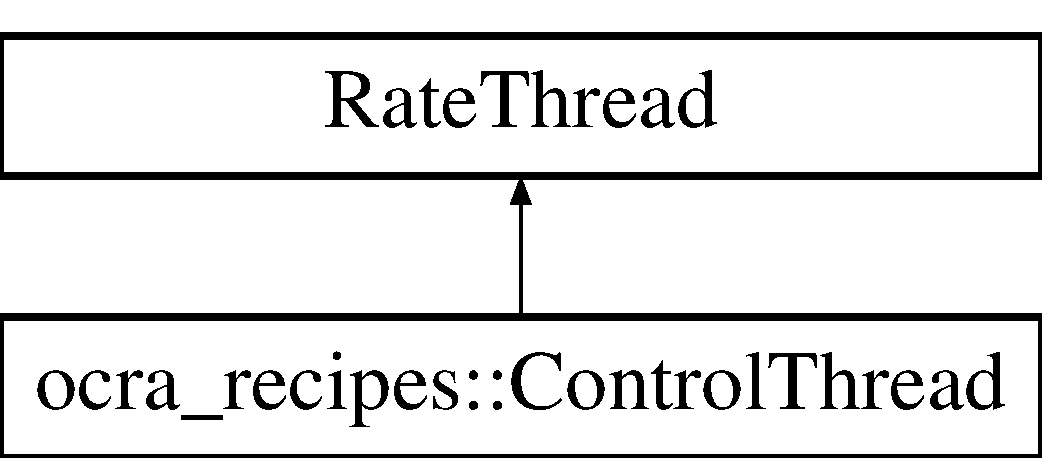
\includegraphics[height=2.000000cm]{d5/d2f/classocra__recipes_1_1ControlThread}
\end{center}
\end{figure}
\subsection*{Classes}
\begin{DoxyCompactItemize}
\item 
class \hyperlink{classocra__recipes_1_1ControlThread_1_1inputCallback}{input\+Callback}
\end{DoxyCompactItemize}
\subsection*{Public Member Functions}
\begin{DoxyCompactItemize}
\item 
\hyperlink{classocra__recipes_1_1ControlThread_a9cbd7d52df2dc070365a14d8c0c800f3}{Control\+Thread} (int period, const std\+::string \&task\+Rpc\+Port\+Name)
\item 
\hyperlink{classocra__recipes_1_1ControlThread_ae1dbbb5ec386b01a88e10ad37f3675bd}{$\sim$\+Control\+Thread} ()
\item 
virtual bool \hyperlink{classocra__recipes_1_1ControlThread_ad4a51369f70181e22a3ee4980a5abd13}{thread\+Init} ()
\item 
virtual void \hyperlink{classocra__recipes_1_1ControlThread_a62c6401278b62bd291722d7652ace6af}{thread\+Release} ()
\item 
virtual void \hyperlink{classocra__recipes_1_1ControlThread_aa86fb4137489b8bd8bd2ac32b737b58f}{run} ()
\item 
virtual bool \hyperlink{classocra__recipes_1_1ControlThread_a4b2471a82ae344ea4c9e96943604cb94}{ct\+\_\+thread\+Init} ()=0
\item 
virtual void \hyperlink{classocra__recipes_1_1ControlThread_ade246d31ff5f81978e3920b7fb1b6abb}{ct\+\_\+thread\+Release} ()=0
\item 
virtual void \hyperlink{classocra__recipes_1_1ControlThread_a2890887a72bdae6d16af762455eb3d3f}{ct\+\_\+run} ()=0
\item 
std\+::string \hyperlink{classocra__recipes_1_1ControlThread_ac7552b020cf2009d5ceff8c67e0a2037}{get\+Thread\+Type} ()
\item 
bool \hyperlink{classocra__recipes_1_1ControlThread_a994fe44acbacf847cdf5a692c59f347a}{deactivate\+Task} ()
\item 
bool \hyperlink{classocra__recipes_1_1ControlThread_a68b22022240de911c5131b642a9eff1a}{activate\+Task} ()
\item 
std\+::string \hyperlink{classocra__recipes_1_1ControlThread_a7d60403bfe70275c84d556985faac038}{get\+Output\+Port\+Name} ()
\item 
std\+::string \hyperlink{classocra__recipes_1_1ControlThread_a1082fa50dfacb28ffc37f8daf6417649}{get\+Input\+Port\+Name} ()
\end{DoxyCompactItemize}
\subsection*{Public Attributes}
\begin{DoxyCompactItemize}
\item 
int \hyperlink{classocra__recipes_1_1ControlThread_abbcc309053e54da8531c77bac2dd1656}{thread\+Id}
\end{DoxyCompactItemize}
\subsection*{Static Public Attributes}
\begin{DoxyCompactItemize}
\item 
static int \hyperlink{classocra__recipes_1_1ControlThread_af77b19fbb04fcf73374045928d3fef12}{C\+O\+N\+T\+R\+O\+L\+\_\+\+T\+H\+R\+E\+A\+D\+\_\+\+C\+O\+U\+NT} = 0
\end{DoxyCompactItemize}
\subsection*{Protected Member Functions}
\begin{DoxyCompactItemize}
\item 
void \hyperlink{classocra__recipes_1_1ControlThread_a62d882d2bad8a2468cbc080cad101a1f}{set\+Thread\+Type} (const std\+::string \&\+\_\+thread\+Type=\char`\"{}Control\+Thread\char`\"{})
\item 
bool \hyperlink{classocra__recipes_1_1ControlThread_af7612ae9f2da601a24df863f4ff6e2a5}{open\+Control\+Ports} ()
\item 
bool \hyperlink{classocra__recipes_1_1ControlThread_a12bc9c3976f83aaf281f31d225740bd2}{connect\+Control\+Ports} ()
\item 
bool \hyperlink{classocra__recipes_1_1ControlThread_a1e13b4ab213e0f72b65aa17095d001fb}{parse\+Input} (yarp\+::os\+::\+Bottle $\ast$input)
\item 
Eigen\+::\+Vector\+Xd \hyperlink{classocra__recipes_1_1ControlThread_abcb1ddc1f244b60899c028bb16b4cc07}{get\+Current\+State} ()
\item 
void \hyperlink{classocra__recipes_1_1ControlThread_a53191169bc860dc92314fe65bab83c97}{send\+Get\+State\+Message} ()
\item 
bool \hyperlink{classocra__recipes_1_1ControlThread_aa7f0d827de6315ad83948620efc1630e}{get\+Task\+Dimensions} ()
\item 
bool \hyperlink{classocra__recipes_1_1ControlThread_a487dd1d0b2c718ef7d8a78e638c6cefd}{get\+Task\+Parameters} (\hyperlink{classocra__recipes_1_1TaskParameters}{Task\+Parameters} \&TP)
\end{DoxyCompactItemize}
\subsection*{Protected Attributes}
\begin{DoxyCompactItemize}
\item 
std\+::string \hyperlink{classocra__recipes_1_1ControlThread_aa8c8f3c06e3e2f22a0d46814f067ec79}{control\+Thread\+Type}
\item 
std\+::string \hyperlink{classocra__recipes_1_1ControlThread_a4979cfd87cd758473a2ec367f47be17f}{input\+Port\+Name}
\item 
std\+::string \hyperlink{classocra__recipes_1_1ControlThread_a150b524cf8af131ac4d7a497777a2d87}{output\+Port\+Name}
\item 
yarp\+::os\+::\+Port \hyperlink{classocra__recipes_1_1ControlThread_a3c6a392da512677af0b6c20f5ed357c1}{input\+Port}
\item 
yarp\+::os\+::\+Port \hyperlink{classocra__recipes_1_1ControlThread_acf573eaf6f1d78918b95cabfb110bbaa}{output\+Port}
\item 
std\+::string \hyperlink{classocra__recipes_1_1ControlThread_abbc082e54db816a3298c3e5ae5d3f9ef}{task\+Rpc\+Server\+Name}
\item 
std\+::string \hyperlink{classocra__recipes_1_1ControlThread_af9d8abd531163281ac938eeb0ba51979}{thread\+Rpc\+Client\+Name}
\item 
yarp\+::os\+::\+Rpc\+Client \hyperlink{classocra__recipes_1_1ControlThread_a7c63f87c66ca64787e6f798a7db28e20}{thread\+Rpc\+Client}
\item 
yarp\+::os\+::\+Network \hyperlink{classocra__recipes_1_1ControlThread_ab256274135229afc7017b088424b5b3b}{yarp}
\item 
bool \hyperlink{classocra__recipes_1_1ControlThread_ae459f7c503830d9ae1c0015d8613ea87}{is\+First\+Input\+Bottle}
\item 
\hyperlink{classocra__recipes_1_1ControlThread_1_1inputCallback}{input\+Callback} $\ast$ \hyperlink{classocra__recipes_1_1ControlThread_af8da6d1e1079de5d0b53dc6bbad75055}{inp\+Callback}
\item 
Eigen\+::\+Vector\+Xd \hyperlink{classocra__recipes_1_1ControlThread_afa7f90785f2768cc74b5043044d09912}{current\+State\+Vector}
\item 
bool \hyperlink{classocra__recipes_1_1ControlThread_aaef2c765c3900ebc72125f7a8fd4240e}{waiting\+For\+First\+State\+Message}
\item 
double \hyperlink{classocra__recipes_1_1ControlThread_affbc4af946e3c2eabd2ce1cf30376bf2}{control\+Thread\+Period}
\item 
\hyperlink{classocra__recipes_1_1TaskParameters}{Task\+Parameters} \hyperlink{classocra__recipes_1_1ControlThread_a352038d00d429ce8e1ef5defb88005cd}{original\+Task\+Params}
\item 
\hyperlink{classocra__recipes_1_1TaskParameters}{Task\+Parameters} \hyperlink{classocra__recipes_1_1ControlThread_ad2f5b157570bbcb6298d667cc264fc26}{current\+Task\+Params}
\item 
int \hyperlink{classocra__recipes_1_1ControlThread_a7499733b7dd28f8ff0168e206c5b325b}{weight\+Dimension}
\item 
int \hyperlink{classocra__recipes_1_1ControlThread_a1ab9aaa641766b8bf29812925701a52f}{state\+Dimension}
\item 
double \hyperlink{classocra__recipes_1_1ControlThread_a31d18ca1b7ac0c1dfd4a285bfd1fb7f7}{close\+Port\+Timeout}
\end{DoxyCompactItemize}


\subsection{Detailed Description}


Definition at line 77 of file Control\+Thread.\+h.



\subsection{Constructor \& Destructor Documentation}
\hypertarget{classocra__recipes_1_1ControlThread_a9cbd7d52df2dc070365a14d8c0c800f3}{}\label{classocra__recipes_1_1ControlThread_a9cbd7d52df2dc070365a14d8c0c800f3} 
\index{ocra\+\_\+recipes\+::\+Control\+Thread@{ocra\+\_\+recipes\+::\+Control\+Thread}!Control\+Thread@{Control\+Thread}}
\index{Control\+Thread@{Control\+Thread}!ocra\+\_\+recipes\+::\+Control\+Thread@{ocra\+\_\+recipes\+::\+Control\+Thread}}
\subsubsection{\texorpdfstring{Control\+Thread()}{ControlThread()}}
{\footnotesize\ttfamily Control\+Thread\+::\+Control\+Thread (\begin{DoxyParamCaption}\item[{int}]{period,  }\item[{const std\+::string \&}]{task\+Rpc\+Port\+Name }\end{DoxyParamCaption})}



Definition at line 35 of file Control\+Thread.\+cpp.

\hypertarget{classocra__recipes_1_1ControlThread_ae1dbbb5ec386b01a88e10ad37f3675bd}{}\label{classocra__recipes_1_1ControlThread_ae1dbbb5ec386b01a88e10ad37f3675bd} 
\index{ocra\+\_\+recipes\+::\+Control\+Thread@{ocra\+\_\+recipes\+::\+Control\+Thread}!````~Control\+Thread@{$\sim$\+Control\+Thread}}
\index{````~Control\+Thread@{$\sim$\+Control\+Thread}!ocra\+\_\+recipes\+::\+Control\+Thread@{ocra\+\_\+recipes\+::\+Control\+Thread}}
\subsubsection{\texorpdfstring{$\sim$\+Control\+Thread()}{~ControlThread()}}
{\footnotesize\ttfamily Control\+Thread\+::$\sim$\+Control\+Thread (\begin{DoxyParamCaption}{ }\end{DoxyParamCaption})}



Definition at line 46 of file Control\+Thread.\+cpp.



\subsection{Member Function Documentation}
\hypertarget{classocra__recipes_1_1ControlThread_a68b22022240de911c5131b642a9eff1a}{}\label{classocra__recipes_1_1ControlThread_a68b22022240de911c5131b642a9eff1a} 
\index{ocra\+\_\+recipes\+::\+Control\+Thread@{ocra\+\_\+recipes\+::\+Control\+Thread}!activate\+Task@{activate\+Task}}
\index{activate\+Task@{activate\+Task}!ocra\+\_\+recipes\+::\+Control\+Thread@{ocra\+\_\+recipes\+::\+Control\+Thread}}
\subsubsection{\texorpdfstring{activate\+Task()}{activateTask()}}
{\footnotesize\ttfamily bool Control\+Thread\+::activate\+Task (\begin{DoxyParamCaption}{ }\end{DoxyParamCaption})}



Definition at line 242 of file Control\+Thread.\+cpp.

\hypertarget{classocra__recipes_1_1ControlThread_a12bc9c3976f83aaf281f31d225740bd2}{}\label{classocra__recipes_1_1ControlThread_a12bc9c3976f83aaf281f31d225740bd2} 
\index{ocra\+\_\+recipes\+::\+Control\+Thread@{ocra\+\_\+recipes\+::\+Control\+Thread}!connect\+Control\+Ports@{connect\+Control\+Ports}}
\index{connect\+Control\+Ports@{connect\+Control\+Ports}!ocra\+\_\+recipes\+::\+Control\+Thread@{ocra\+\_\+recipes\+::\+Control\+Thread}}
\subsubsection{\texorpdfstring{connect\+Control\+Ports()}{connectControlPorts()}}
{\footnotesize\ttfamily bool Control\+Thread\+::connect\+Control\+Ports (\begin{DoxyParamCaption}{ }\end{DoxyParamCaption})\hspace{0.3cm}{\ttfamily [protected]}}



Definition at line 141 of file Control\+Thread.\+cpp.

\hypertarget{classocra__recipes_1_1ControlThread_a2890887a72bdae6d16af762455eb3d3f}{}\label{classocra__recipes_1_1ControlThread_a2890887a72bdae6d16af762455eb3d3f} 
\index{ocra\+\_\+recipes\+::\+Control\+Thread@{ocra\+\_\+recipes\+::\+Control\+Thread}!ct\+\_\+run@{ct\+\_\+run}}
\index{ct\+\_\+run@{ct\+\_\+run}!ocra\+\_\+recipes\+::\+Control\+Thread@{ocra\+\_\+recipes\+::\+Control\+Thread}}
\subsubsection{\texorpdfstring{ct\+\_\+run()}{ct\_run()}}
{\footnotesize\ttfamily virtual void ocra\+\_\+recipes\+::\+Control\+Thread\+::ct\+\_\+run (\begin{DoxyParamCaption}{ }\end{DoxyParamCaption})\hspace{0.3cm}{\ttfamily [pure virtual]}}

\hypertarget{classocra__recipes_1_1ControlThread_a4b2471a82ae344ea4c9e96943604cb94}{}\label{classocra__recipes_1_1ControlThread_a4b2471a82ae344ea4c9e96943604cb94} 
\index{ocra\+\_\+recipes\+::\+Control\+Thread@{ocra\+\_\+recipes\+::\+Control\+Thread}!ct\+\_\+thread\+Init@{ct\+\_\+thread\+Init}}
\index{ct\+\_\+thread\+Init@{ct\+\_\+thread\+Init}!ocra\+\_\+recipes\+::\+Control\+Thread@{ocra\+\_\+recipes\+::\+Control\+Thread}}
\subsubsection{\texorpdfstring{ct\+\_\+thread\+Init()}{ct\_threadInit()}}
{\footnotesize\ttfamily virtual bool ocra\+\_\+recipes\+::\+Control\+Thread\+::ct\+\_\+thread\+Init (\begin{DoxyParamCaption}{ }\end{DoxyParamCaption})\hspace{0.3cm}{\ttfamily [pure virtual]}}

\hypertarget{classocra__recipes_1_1ControlThread_ade246d31ff5f81978e3920b7fb1b6abb}{}\label{classocra__recipes_1_1ControlThread_ade246d31ff5f81978e3920b7fb1b6abb} 
\index{ocra\+\_\+recipes\+::\+Control\+Thread@{ocra\+\_\+recipes\+::\+Control\+Thread}!ct\+\_\+thread\+Release@{ct\+\_\+thread\+Release}}
\index{ct\+\_\+thread\+Release@{ct\+\_\+thread\+Release}!ocra\+\_\+recipes\+::\+Control\+Thread@{ocra\+\_\+recipes\+::\+Control\+Thread}}
\subsubsection{\texorpdfstring{ct\+\_\+thread\+Release()}{ct\_threadRelease()}}
{\footnotesize\ttfamily virtual void ocra\+\_\+recipes\+::\+Control\+Thread\+::ct\+\_\+thread\+Release (\begin{DoxyParamCaption}{ }\end{DoxyParamCaption})\hspace{0.3cm}{\ttfamily [pure virtual]}}

\hypertarget{classocra__recipes_1_1ControlThread_a994fe44acbacf847cdf5a692c59f347a}{}\label{classocra__recipes_1_1ControlThread_a994fe44acbacf847cdf5a692c59f347a} 
\index{ocra\+\_\+recipes\+::\+Control\+Thread@{ocra\+\_\+recipes\+::\+Control\+Thread}!deactivate\+Task@{deactivate\+Task}}
\index{deactivate\+Task@{deactivate\+Task}!ocra\+\_\+recipes\+::\+Control\+Thread@{ocra\+\_\+recipes\+::\+Control\+Thread}}
\subsubsection{\texorpdfstring{deactivate\+Task()}{deactivateTask()}}
{\footnotesize\ttfamily bool Control\+Thread\+::deactivate\+Task (\begin{DoxyParamCaption}{ }\end{DoxyParamCaption})}



Definition at line 229 of file Control\+Thread.\+cpp.

\hypertarget{classocra__recipes_1_1ControlThread_abcb1ddc1f244b60899c028bb16b4cc07}{}\label{classocra__recipes_1_1ControlThread_abcb1ddc1f244b60899c028bb16b4cc07} 
\index{ocra\+\_\+recipes\+::\+Control\+Thread@{ocra\+\_\+recipes\+::\+Control\+Thread}!get\+Current\+State@{get\+Current\+State}}
\index{get\+Current\+State@{get\+Current\+State}!ocra\+\_\+recipes\+::\+Control\+Thread@{ocra\+\_\+recipes\+::\+Control\+Thread}}
\subsubsection{\texorpdfstring{get\+Current\+State()}{getCurrentState()}}
{\footnotesize\ttfamily Eigen\+::\+Vector\+Xd Control\+Thread\+::get\+Current\+State (\begin{DoxyParamCaption}{ }\end{DoxyParamCaption})\hspace{0.3cm}{\ttfamily [protected]}}



Definition at line 217 of file Control\+Thread.\+cpp.

\hypertarget{classocra__recipes_1_1ControlThread_a1082fa50dfacb28ffc37f8daf6417649}{}\label{classocra__recipes_1_1ControlThread_a1082fa50dfacb28ffc37f8daf6417649} 
\index{ocra\+\_\+recipes\+::\+Control\+Thread@{ocra\+\_\+recipes\+::\+Control\+Thread}!get\+Input\+Port\+Name@{get\+Input\+Port\+Name}}
\index{get\+Input\+Port\+Name@{get\+Input\+Port\+Name}!ocra\+\_\+recipes\+::\+Control\+Thread@{ocra\+\_\+recipes\+::\+Control\+Thread}}
\subsubsection{\texorpdfstring{get\+Input\+Port\+Name()}{getInputPortName()}}
{\footnotesize\ttfamily std\+::string ocra\+\_\+recipes\+::\+Control\+Thread\+::get\+Input\+Port\+Name (\begin{DoxyParamCaption}{ }\end{DoxyParamCaption})\hspace{0.3cm}{\ttfamily [inline]}}



Definition at line 105 of file Control\+Thread.\+h.

\hypertarget{classocra__recipes_1_1ControlThread_a7d60403bfe70275c84d556985faac038}{}\label{classocra__recipes_1_1ControlThread_a7d60403bfe70275c84d556985faac038} 
\index{ocra\+\_\+recipes\+::\+Control\+Thread@{ocra\+\_\+recipes\+::\+Control\+Thread}!get\+Output\+Port\+Name@{get\+Output\+Port\+Name}}
\index{get\+Output\+Port\+Name@{get\+Output\+Port\+Name}!ocra\+\_\+recipes\+::\+Control\+Thread@{ocra\+\_\+recipes\+::\+Control\+Thread}}
\subsubsection{\texorpdfstring{get\+Output\+Port\+Name()}{getOutputPortName()}}
{\footnotesize\ttfamily std\+::string ocra\+\_\+recipes\+::\+Control\+Thread\+::get\+Output\+Port\+Name (\begin{DoxyParamCaption}{ }\end{DoxyParamCaption})\hspace{0.3cm}{\ttfamily [inline]}}



Definition at line 104 of file Control\+Thread.\+h.

\hypertarget{classocra__recipes_1_1ControlThread_aa7f0d827de6315ad83948620efc1630e}{}\label{classocra__recipes_1_1ControlThread_aa7f0d827de6315ad83948620efc1630e} 
\index{ocra\+\_\+recipes\+::\+Control\+Thread@{ocra\+\_\+recipes\+::\+Control\+Thread}!get\+Task\+Dimensions@{get\+Task\+Dimensions}}
\index{get\+Task\+Dimensions@{get\+Task\+Dimensions}!ocra\+\_\+recipes\+::\+Control\+Thread@{ocra\+\_\+recipes\+::\+Control\+Thread}}
\subsubsection{\texorpdfstring{get\+Task\+Dimensions()}{getTaskDimensions()}}
{\footnotesize\ttfamily bool Control\+Thread\+::get\+Task\+Dimensions (\begin{DoxyParamCaption}{ }\end{DoxyParamCaption})\hspace{0.3cm}{\ttfamily [protected]}}



Definition at line 255 of file Control\+Thread.\+cpp.

\hypertarget{classocra__recipes_1_1ControlThread_a487dd1d0b2c718ef7d8a78e638c6cefd}{}\label{classocra__recipes_1_1ControlThread_a487dd1d0b2c718ef7d8a78e638c6cefd} 
\index{ocra\+\_\+recipes\+::\+Control\+Thread@{ocra\+\_\+recipes\+::\+Control\+Thread}!get\+Task\+Parameters@{get\+Task\+Parameters}}
\index{get\+Task\+Parameters@{get\+Task\+Parameters}!ocra\+\_\+recipes\+::\+Control\+Thread@{ocra\+\_\+recipes\+::\+Control\+Thread}}
\subsubsection{\texorpdfstring{get\+Task\+Parameters()}{getTaskParameters()}}
{\footnotesize\ttfamily bool Control\+Thread\+::get\+Task\+Parameters (\begin{DoxyParamCaption}\item[{\hyperlink{classocra__recipes_1_1TaskParameters}{Task\+Parameters} \&}]{TP }\end{DoxyParamCaption})\hspace{0.3cm}{\ttfamily [protected]}}



Definition at line 280 of file Control\+Thread.\+cpp.

\hypertarget{classocra__recipes_1_1ControlThread_ac7552b020cf2009d5ceff8c67e0a2037}{}\label{classocra__recipes_1_1ControlThread_ac7552b020cf2009d5ceff8c67e0a2037} 
\index{ocra\+\_\+recipes\+::\+Control\+Thread@{ocra\+\_\+recipes\+::\+Control\+Thread}!get\+Thread\+Type@{get\+Thread\+Type}}
\index{get\+Thread\+Type@{get\+Thread\+Type}!ocra\+\_\+recipes\+::\+Control\+Thread@{ocra\+\_\+recipes\+::\+Control\+Thread}}
\subsubsection{\texorpdfstring{get\+Thread\+Type()}{getThreadType()}}
{\footnotesize\ttfamily std\+::string ocra\+\_\+recipes\+::\+Control\+Thread\+::get\+Thread\+Type (\begin{DoxyParamCaption}{ }\end{DoxyParamCaption})\hspace{0.3cm}{\ttfamily [inline]}}



Definition at line 100 of file Control\+Thread.\+h.

\hypertarget{classocra__recipes_1_1ControlThread_af7612ae9f2da601a24df863f4ff6e2a5}{}\label{classocra__recipes_1_1ControlThread_af7612ae9f2da601a24df863f4ff6e2a5} 
\index{ocra\+\_\+recipes\+::\+Control\+Thread@{ocra\+\_\+recipes\+::\+Control\+Thread}!open\+Control\+Ports@{open\+Control\+Ports}}
\index{open\+Control\+Ports@{open\+Control\+Ports}!ocra\+\_\+recipes\+::\+Control\+Thread@{ocra\+\_\+recipes\+::\+Control\+Thread}}
\subsubsection{\texorpdfstring{open\+Control\+Ports()}{openControlPorts()}}
{\footnotesize\ttfamily bool Control\+Thread\+::open\+Control\+Ports (\begin{DoxyParamCaption}{ }\end{DoxyParamCaption})\hspace{0.3cm}{\ttfamily [protected]}}



Definition at line 105 of file Control\+Thread.\+cpp.

\hypertarget{classocra__recipes_1_1ControlThread_a1e13b4ab213e0f72b65aa17095d001fb}{}\label{classocra__recipes_1_1ControlThread_a1e13b4ab213e0f72b65aa17095d001fb} 
\index{ocra\+\_\+recipes\+::\+Control\+Thread@{ocra\+\_\+recipes\+::\+Control\+Thread}!parse\+Input@{parse\+Input}}
\index{parse\+Input@{parse\+Input}!ocra\+\_\+recipes\+::\+Control\+Thread@{ocra\+\_\+recipes\+::\+Control\+Thread}}
\subsubsection{\texorpdfstring{parse\+Input()}{parseInput()}}
{\footnotesize\ttfamily bool Control\+Thread\+::parse\+Input (\begin{DoxyParamCaption}\item[{yarp\+::os\+::\+Bottle $\ast$}]{input }\end{DoxyParamCaption})\hspace{0.3cm}{\ttfamily [protected]}}



Definition at line 180 of file Control\+Thread.\+cpp.

\hypertarget{classocra__recipes_1_1ControlThread_aa86fb4137489b8bd8bd2ac32b737b58f}{}\label{classocra__recipes_1_1ControlThread_aa86fb4137489b8bd8bd2ac32b737b58f} 
\index{ocra\+\_\+recipes\+::\+Control\+Thread@{ocra\+\_\+recipes\+::\+Control\+Thread}!run@{run}}
\index{run@{run}!ocra\+\_\+recipes\+::\+Control\+Thread@{ocra\+\_\+recipes\+::\+Control\+Thread}}
\subsubsection{\texorpdfstring{run()}{run()}}
{\footnotesize\ttfamily void Control\+Thread\+::run (\begin{DoxyParamCaption}{ }\end{DoxyParamCaption})\hspace{0.3cm}{\ttfamily [virtual]}}



Definition at line 97 of file Control\+Thread.\+cpp.

\hypertarget{classocra__recipes_1_1ControlThread_a53191169bc860dc92314fe65bab83c97}{}\label{classocra__recipes_1_1ControlThread_a53191169bc860dc92314fe65bab83c97} 
\index{ocra\+\_\+recipes\+::\+Control\+Thread@{ocra\+\_\+recipes\+::\+Control\+Thread}!send\+Get\+State\+Message@{send\+Get\+State\+Message}}
\index{send\+Get\+State\+Message@{send\+Get\+State\+Message}!ocra\+\_\+recipes\+::\+Control\+Thread@{ocra\+\_\+recipes\+::\+Control\+Thread}}
\subsubsection{\texorpdfstring{send\+Get\+State\+Message()}{sendGetStateMessage()}}
{\footnotesize\ttfamily void Control\+Thread\+::send\+Get\+State\+Message (\begin{DoxyParamCaption}{ }\end{DoxyParamCaption})\hspace{0.3cm}{\ttfamily [protected]}}



Definition at line 222 of file Control\+Thread.\+cpp.

\hypertarget{classocra__recipes_1_1ControlThread_a62d882d2bad8a2468cbc080cad101a1f}{}\label{classocra__recipes_1_1ControlThread_a62d882d2bad8a2468cbc080cad101a1f} 
\index{ocra\+\_\+recipes\+::\+Control\+Thread@{ocra\+\_\+recipes\+::\+Control\+Thread}!set\+Thread\+Type@{set\+Thread\+Type}}
\index{set\+Thread\+Type@{set\+Thread\+Type}!ocra\+\_\+recipes\+::\+Control\+Thread@{ocra\+\_\+recipes\+::\+Control\+Thread}}
\subsubsection{\texorpdfstring{set\+Thread\+Type()}{setThreadType()}}
{\footnotesize\ttfamily void ocra\+\_\+recipes\+::\+Control\+Thread\+::set\+Thread\+Type (\begin{DoxyParamCaption}\item[{const std\+::string \&}]{\+\_\+thread\+Type = {\ttfamily \char`\"{}ControlThread\char`\"{}} }\end{DoxyParamCaption})\hspace{0.3cm}{\ttfamily [inline]}, {\ttfamily [protected]}}



Definition at line 122 of file Control\+Thread.\+h.

\hypertarget{classocra__recipes_1_1ControlThread_ad4a51369f70181e22a3ee4980a5abd13}{}\label{classocra__recipes_1_1ControlThread_ad4a51369f70181e22a3ee4980a5abd13} 
\index{ocra\+\_\+recipes\+::\+Control\+Thread@{ocra\+\_\+recipes\+::\+Control\+Thread}!thread\+Init@{thread\+Init}}
\index{thread\+Init@{thread\+Init}!ocra\+\_\+recipes\+::\+Control\+Thread@{ocra\+\_\+recipes\+::\+Control\+Thread}}
\subsubsection{\texorpdfstring{thread\+Init()}{threadInit()}}
{\footnotesize\ttfamily bool Control\+Thread\+::thread\+Init (\begin{DoxyParamCaption}{ }\end{DoxyParamCaption})\hspace{0.3cm}{\ttfamily [virtual]}}



Definition at line 52 of file Control\+Thread.\+cpp.

\hypertarget{classocra__recipes_1_1ControlThread_a62c6401278b62bd291722d7652ace6af}{}\label{classocra__recipes_1_1ControlThread_a62c6401278b62bd291722d7652ace6af} 
\index{ocra\+\_\+recipes\+::\+Control\+Thread@{ocra\+\_\+recipes\+::\+Control\+Thread}!thread\+Release@{thread\+Release}}
\index{thread\+Release@{thread\+Release}!ocra\+\_\+recipes\+::\+Control\+Thread@{ocra\+\_\+recipes\+::\+Control\+Thread}}
\subsubsection{\texorpdfstring{thread\+Release()}{threadRelease()}}
{\footnotesize\ttfamily void Control\+Thread\+::thread\+Release (\begin{DoxyParamCaption}{ }\end{DoxyParamCaption})\hspace{0.3cm}{\ttfamily [virtual]}}



Definition at line 69 of file Control\+Thread.\+cpp.



\subsection{Member Data Documentation}
\hypertarget{classocra__recipes_1_1ControlThread_a31d18ca1b7ac0c1dfd4a285bfd1fb7f7}{}\label{classocra__recipes_1_1ControlThread_a31d18ca1b7ac0c1dfd4a285bfd1fb7f7} 
\index{ocra\+\_\+recipes\+::\+Control\+Thread@{ocra\+\_\+recipes\+::\+Control\+Thread}!close\+Port\+Timeout@{close\+Port\+Timeout}}
\index{close\+Port\+Timeout@{close\+Port\+Timeout}!ocra\+\_\+recipes\+::\+Control\+Thread@{ocra\+\_\+recipes\+::\+Control\+Thread}}
\subsubsection{\texorpdfstring{close\+Port\+Timeout}{closePortTimeout}}
{\footnotesize\ttfamily double ocra\+\_\+recipes\+::\+Control\+Thread\+::close\+Port\+Timeout\hspace{0.3cm}{\ttfamily [protected]}}



Definition at line 161 of file Control\+Thread.\+h.

\hypertarget{classocra__recipes_1_1ControlThread_af77b19fbb04fcf73374045928d3fef12}{}\label{classocra__recipes_1_1ControlThread_af77b19fbb04fcf73374045928d3fef12} 
\index{ocra\+\_\+recipes\+::\+Control\+Thread@{ocra\+\_\+recipes\+::\+Control\+Thread}!C\+O\+N\+T\+R\+O\+L\+\_\+\+T\+H\+R\+E\+A\+D\+\_\+\+C\+O\+U\+NT@{C\+O\+N\+T\+R\+O\+L\+\_\+\+T\+H\+R\+E\+A\+D\+\_\+\+C\+O\+U\+NT}}
\index{C\+O\+N\+T\+R\+O\+L\+\_\+\+T\+H\+R\+E\+A\+D\+\_\+\+C\+O\+U\+NT@{C\+O\+N\+T\+R\+O\+L\+\_\+\+T\+H\+R\+E\+A\+D\+\_\+\+C\+O\+U\+NT}!ocra\+\_\+recipes\+::\+Control\+Thread@{ocra\+\_\+recipes\+::\+Control\+Thread}}
\subsubsection{\texorpdfstring{C\+O\+N\+T\+R\+O\+L\+\_\+\+T\+H\+R\+E\+A\+D\+\_\+\+C\+O\+U\+NT}{CONTROL\_THREAD\_COUNT}}
{\footnotesize\ttfamily int Control\+Thread\+::\+C\+O\+N\+T\+R\+O\+L\+\_\+\+T\+H\+R\+E\+A\+D\+\_\+\+C\+O\+U\+NT = 0\hspace{0.3cm}{\ttfamily [static]}}



Definition at line 87 of file Control\+Thread.\+h.

\hypertarget{classocra__recipes_1_1ControlThread_affbc4af946e3c2eabd2ce1cf30376bf2}{}\label{classocra__recipes_1_1ControlThread_affbc4af946e3c2eabd2ce1cf30376bf2} 
\index{ocra\+\_\+recipes\+::\+Control\+Thread@{ocra\+\_\+recipes\+::\+Control\+Thread}!control\+Thread\+Period@{control\+Thread\+Period}}
\index{control\+Thread\+Period@{control\+Thread\+Period}!ocra\+\_\+recipes\+::\+Control\+Thread@{ocra\+\_\+recipes\+::\+Control\+Thread}}
\subsubsection{\texorpdfstring{control\+Thread\+Period}{controlThreadPeriod}}
{\footnotesize\ttfamily double ocra\+\_\+recipes\+::\+Control\+Thread\+::control\+Thread\+Period\hspace{0.3cm}{\ttfamily [protected]}}



Definition at line 149 of file Control\+Thread.\+h.

\hypertarget{classocra__recipes_1_1ControlThread_aa8c8f3c06e3e2f22a0d46814f067ec79}{}\label{classocra__recipes_1_1ControlThread_aa8c8f3c06e3e2f22a0d46814f067ec79} 
\index{ocra\+\_\+recipes\+::\+Control\+Thread@{ocra\+\_\+recipes\+::\+Control\+Thread}!control\+Thread\+Type@{control\+Thread\+Type}}
\index{control\+Thread\+Type@{control\+Thread\+Type}!ocra\+\_\+recipes\+::\+Control\+Thread@{ocra\+\_\+recipes\+::\+Control\+Thread}}
\subsubsection{\texorpdfstring{control\+Thread\+Type}{controlThreadType}}
{\footnotesize\ttfamily std\+::string ocra\+\_\+recipes\+::\+Control\+Thread\+::control\+Thread\+Type\hspace{0.3cm}{\ttfamily [protected]}}



Definition at line 124 of file Control\+Thread.\+h.

\hypertarget{classocra__recipes_1_1ControlThread_afa7f90785f2768cc74b5043044d09912}{}\label{classocra__recipes_1_1ControlThread_afa7f90785f2768cc74b5043044d09912} 
\index{ocra\+\_\+recipes\+::\+Control\+Thread@{ocra\+\_\+recipes\+::\+Control\+Thread}!current\+State\+Vector@{current\+State\+Vector}}
\index{current\+State\+Vector@{current\+State\+Vector}!ocra\+\_\+recipes\+::\+Control\+Thread@{ocra\+\_\+recipes\+::\+Control\+Thread}}
\subsubsection{\texorpdfstring{current\+State\+Vector}{currentStateVector}}
{\footnotesize\ttfamily Eigen\+::\+Vector\+Xd ocra\+\_\+recipes\+::\+Control\+Thread\+::current\+State\+Vector\hspace{0.3cm}{\ttfamily [protected]}}



Definition at line 142 of file Control\+Thread.\+h.

\hypertarget{classocra__recipes_1_1ControlThread_ad2f5b157570bbcb6298d667cc264fc26}{}\label{classocra__recipes_1_1ControlThread_ad2f5b157570bbcb6298d667cc264fc26} 
\index{ocra\+\_\+recipes\+::\+Control\+Thread@{ocra\+\_\+recipes\+::\+Control\+Thread}!current\+Task\+Params@{current\+Task\+Params}}
\index{current\+Task\+Params@{current\+Task\+Params}!ocra\+\_\+recipes\+::\+Control\+Thread@{ocra\+\_\+recipes\+::\+Control\+Thread}}
\subsubsection{\texorpdfstring{current\+Task\+Params}{currentTaskParams}}
{\footnotesize\ttfamily \hyperlink{classocra__recipes_1_1TaskParameters}{Task\+Parameters} ocra\+\_\+recipes\+::\+Control\+Thread\+::current\+Task\+Params\hspace{0.3cm}{\ttfamily [protected]}}



Definition at line 152 of file Control\+Thread.\+h.

\hypertarget{classocra__recipes_1_1ControlThread_af8da6d1e1079de5d0b53dc6bbad75055}{}\label{classocra__recipes_1_1ControlThread_af8da6d1e1079de5d0b53dc6bbad75055} 
\index{ocra\+\_\+recipes\+::\+Control\+Thread@{ocra\+\_\+recipes\+::\+Control\+Thread}!inp\+Callback@{inp\+Callback}}
\index{inp\+Callback@{inp\+Callback}!ocra\+\_\+recipes\+::\+Control\+Thread@{ocra\+\_\+recipes\+::\+Control\+Thread}}
\subsubsection{\texorpdfstring{inp\+Callback}{inpCallback}}
{\footnotesize\ttfamily \hyperlink{classocra__recipes_1_1ControlThread_1_1inputCallback}{input\+Callback}$\ast$ ocra\+\_\+recipes\+::\+Control\+Thread\+::inp\+Callback\hspace{0.3cm}{\ttfamily [protected]}}



Definition at line 141 of file Control\+Thread.\+h.

\hypertarget{classocra__recipes_1_1ControlThread_a3c6a392da512677af0b6c20f5ed357c1}{}\label{classocra__recipes_1_1ControlThread_a3c6a392da512677af0b6c20f5ed357c1} 
\index{ocra\+\_\+recipes\+::\+Control\+Thread@{ocra\+\_\+recipes\+::\+Control\+Thread}!input\+Port@{input\+Port}}
\index{input\+Port@{input\+Port}!ocra\+\_\+recipes\+::\+Control\+Thread@{ocra\+\_\+recipes\+::\+Control\+Thread}}
\subsubsection{\texorpdfstring{input\+Port}{inputPort}}
{\footnotesize\ttfamily yarp\+::os\+::\+Port ocra\+\_\+recipes\+::\+Control\+Thread\+::input\+Port\hspace{0.3cm}{\ttfamily [protected]}}



Definition at line 128 of file Control\+Thread.\+h.

\hypertarget{classocra__recipes_1_1ControlThread_a4979cfd87cd758473a2ec367f47be17f}{}\label{classocra__recipes_1_1ControlThread_a4979cfd87cd758473a2ec367f47be17f} 
\index{ocra\+\_\+recipes\+::\+Control\+Thread@{ocra\+\_\+recipes\+::\+Control\+Thread}!input\+Port\+Name@{input\+Port\+Name}}
\index{input\+Port\+Name@{input\+Port\+Name}!ocra\+\_\+recipes\+::\+Control\+Thread@{ocra\+\_\+recipes\+::\+Control\+Thread}}
\subsubsection{\texorpdfstring{input\+Port\+Name}{inputPortName}}
{\footnotesize\ttfamily std\+::string ocra\+\_\+recipes\+::\+Control\+Thread\+::input\+Port\+Name\hspace{0.3cm}{\ttfamily [protected]}}



Definition at line 127 of file Control\+Thread.\+h.

\hypertarget{classocra__recipes_1_1ControlThread_ae459f7c503830d9ae1c0015d8613ea87}{}\label{classocra__recipes_1_1ControlThread_ae459f7c503830d9ae1c0015d8613ea87} 
\index{ocra\+\_\+recipes\+::\+Control\+Thread@{ocra\+\_\+recipes\+::\+Control\+Thread}!is\+First\+Input\+Bottle@{is\+First\+Input\+Bottle}}
\index{is\+First\+Input\+Bottle@{is\+First\+Input\+Bottle}!ocra\+\_\+recipes\+::\+Control\+Thread@{ocra\+\_\+recipes\+::\+Control\+Thread}}
\subsubsection{\texorpdfstring{is\+First\+Input\+Bottle}{isFirstInputBottle}}
{\footnotesize\ttfamily bool ocra\+\_\+recipes\+::\+Control\+Thread\+::is\+First\+Input\+Bottle\hspace{0.3cm}{\ttfamily [protected]}}



Definition at line 140 of file Control\+Thread.\+h.

\hypertarget{classocra__recipes_1_1ControlThread_a352038d00d429ce8e1ef5defb88005cd}{}\label{classocra__recipes_1_1ControlThread_a352038d00d429ce8e1ef5defb88005cd} 
\index{ocra\+\_\+recipes\+::\+Control\+Thread@{ocra\+\_\+recipes\+::\+Control\+Thread}!original\+Task\+Params@{original\+Task\+Params}}
\index{original\+Task\+Params@{original\+Task\+Params}!ocra\+\_\+recipes\+::\+Control\+Thread@{ocra\+\_\+recipes\+::\+Control\+Thread}}
\subsubsection{\texorpdfstring{original\+Task\+Params}{originalTaskParams}}
{\footnotesize\ttfamily \hyperlink{classocra__recipes_1_1TaskParameters}{Task\+Parameters} ocra\+\_\+recipes\+::\+Control\+Thread\+::original\+Task\+Params\hspace{0.3cm}{\ttfamily [protected]}}



Definition at line 151 of file Control\+Thread.\+h.

\hypertarget{classocra__recipes_1_1ControlThread_acf573eaf6f1d78918b95cabfb110bbaa}{}\label{classocra__recipes_1_1ControlThread_acf573eaf6f1d78918b95cabfb110bbaa} 
\index{ocra\+\_\+recipes\+::\+Control\+Thread@{ocra\+\_\+recipes\+::\+Control\+Thread}!output\+Port@{output\+Port}}
\index{output\+Port@{output\+Port}!ocra\+\_\+recipes\+::\+Control\+Thread@{ocra\+\_\+recipes\+::\+Control\+Thread}}
\subsubsection{\texorpdfstring{output\+Port}{outputPort}}
{\footnotesize\ttfamily yarp\+::os\+::\+Port ocra\+\_\+recipes\+::\+Control\+Thread\+::output\+Port\hspace{0.3cm}{\ttfamily [protected]}}



Definition at line 128 of file Control\+Thread.\+h.

\hypertarget{classocra__recipes_1_1ControlThread_a150b524cf8af131ac4d7a497777a2d87}{}\label{classocra__recipes_1_1ControlThread_a150b524cf8af131ac4d7a497777a2d87} 
\index{ocra\+\_\+recipes\+::\+Control\+Thread@{ocra\+\_\+recipes\+::\+Control\+Thread}!output\+Port\+Name@{output\+Port\+Name}}
\index{output\+Port\+Name@{output\+Port\+Name}!ocra\+\_\+recipes\+::\+Control\+Thread@{ocra\+\_\+recipes\+::\+Control\+Thread}}
\subsubsection{\texorpdfstring{output\+Port\+Name}{outputPortName}}
{\footnotesize\ttfamily std\+::string ocra\+\_\+recipes\+::\+Control\+Thread\+::output\+Port\+Name\hspace{0.3cm}{\ttfamily [protected]}}



Definition at line 127 of file Control\+Thread.\+h.

\hypertarget{classocra__recipes_1_1ControlThread_a1ab9aaa641766b8bf29812925701a52f}{}\label{classocra__recipes_1_1ControlThread_a1ab9aaa641766b8bf29812925701a52f} 
\index{ocra\+\_\+recipes\+::\+Control\+Thread@{ocra\+\_\+recipes\+::\+Control\+Thread}!state\+Dimension@{state\+Dimension}}
\index{state\+Dimension@{state\+Dimension}!ocra\+\_\+recipes\+::\+Control\+Thread@{ocra\+\_\+recipes\+::\+Control\+Thread}}
\subsubsection{\texorpdfstring{state\+Dimension}{stateDimension}}
{\footnotesize\ttfamily int ocra\+\_\+recipes\+::\+Control\+Thread\+::state\+Dimension\hspace{0.3cm}{\ttfamily [protected]}}



Definition at line 155 of file Control\+Thread.\+h.

\hypertarget{classocra__recipes_1_1ControlThread_abbc082e54db816a3298c3e5ae5d3f9ef}{}\label{classocra__recipes_1_1ControlThread_abbc082e54db816a3298c3e5ae5d3f9ef} 
\index{ocra\+\_\+recipes\+::\+Control\+Thread@{ocra\+\_\+recipes\+::\+Control\+Thread}!task\+Rpc\+Server\+Name@{task\+Rpc\+Server\+Name}}
\index{task\+Rpc\+Server\+Name@{task\+Rpc\+Server\+Name}!ocra\+\_\+recipes\+::\+Control\+Thread@{ocra\+\_\+recipes\+::\+Control\+Thread}}
\subsubsection{\texorpdfstring{task\+Rpc\+Server\+Name}{taskRpcServerName}}
{\footnotesize\ttfamily std\+::string ocra\+\_\+recipes\+::\+Control\+Thread\+::task\+Rpc\+Server\+Name\hspace{0.3cm}{\ttfamily [protected]}}



Definition at line 131 of file Control\+Thread.\+h.

\hypertarget{classocra__recipes_1_1ControlThread_abbcc309053e54da8531c77bac2dd1656}{}\label{classocra__recipes_1_1ControlThread_abbcc309053e54da8531c77bac2dd1656} 
\index{ocra\+\_\+recipes\+::\+Control\+Thread@{ocra\+\_\+recipes\+::\+Control\+Thread}!thread\+Id@{thread\+Id}}
\index{thread\+Id@{thread\+Id}!ocra\+\_\+recipes\+::\+Control\+Thread@{ocra\+\_\+recipes\+::\+Control\+Thread}}
\subsubsection{\texorpdfstring{thread\+Id}{threadId}}
{\footnotesize\ttfamily int ocra\+\_\+recipes\+::\+Control\+Thread\+::thread\+Id}



Definition at line 86 of file Control\+Thread.\+h.

\hypertarget{classocra__recipes_1_1ControlThread_a7c63f87c66ca64787e6f798a7db28e20}{}\label{classocra__recipes_1_1ControlThread_a7c63f87c66ca64787e6f798a7db28e20} 
\index{ocra\+\_\+recipes\+::\+Control\+Thread@{ocra\+\_\+recipes\+::\+Control\+Thread}!thread\+Rpc\+Client@{thread\+Rpc\+Client}}
\index{thread\+Rpc\+Client@{thread\+Rpc\+Client}!ocra\+\_\+recipes\+::\+Control\+Thread@{ocra\+\_\+recipes\+::\+Control\+Thread}}
\subsubsection{\texorpdfstring{thread\+Rpc\+Client}{threadRpcClient}}
{\footnotesize\ttfamily yarp\+::os\+::\+Rpc\+Client ocra\+\_\+recipes\+::\+Control\+Thread\+::thread\+Rpc\+Client\hspace{0.3cm}{\ttfamily [protected]}}



Definition at line 132 of file Control\+Thread.\+h.

\hypertarget{classocra__recipes_1_1ControlThread_af9d8abd531163281ac938eeb0ba51979}{}\label{classocra__recipes_1_1ControlThread_af9d8abd531163281ac938eeb0ba51979} 
\index{ocra\+\_\+recipes\+::\+Control\+Thread@{ocra\+\_\+recipes\+::\+Control\+Thread}!thread\+Rpc\+Client\+Name@{thread\+Rpc\+Client\+Name}}
\index{thread\+Rpc\+Client\+Name@{thread\+Rpc\+Client\+Name}!ocra\+\_\+recipes\+::\+Control\+Thread@{ocra\+\_\+recipes\+::\+Control\+Thread}}
\subsubsection{\texorpdfstring{thread\+Rpc\+Client\+Name}{threadRpcClientName}}
{\footnotesize\ttfamily std\+::string ocra\+\_\+recipes\+::\+Control\+Thread\+::thread\+Rpc\+Client\+Name\hspace{0.3cm}{\ttfamily [protected]}}



Definition at line 131 of file Control\+Thread.\+h.

\hypertarget{classocra__recipes_1_1ControlThread_aaef2c765c3900ebc72125f7a8fd4240e}{}\label{classocra__recipes_1_1ControlThread_aaef2c765c3900ebc72125f7a8fd4240e} 
\index{ocra\+\_\+recipes\+::\+Control\+Thread@{ocra\+\_\+recipes\+::\+Control\+Thread}!waiting\+For\+First\+State\+Message@{waiting\+For\+First\+State\+Message}}
\index{waiting\+For\+First\+State\+Message@{waiting\+For\+First\+State\+Message}!ocra\+\_\+recipes\+::\+Control\+Thread@{ocra\+\_\+recipes\+::\+Control\+Thread}}
\subsubsection{\texorpdfstring{waiting\+For\+First\+State\+Message}{waitingForFirstStateMessage}}
{\footnotesize\ttfamily bool ocra\+\_\+recipes\+::\+Control\+Thread\+::waiting\+For\+First\+State\+Message\hspace{0.3cm}{\ttfamily [protected]}}



Definition at line 146 of file Control\+Thread.\+h.

\hypertarget{classocra__recipes_1_1ControlThread_a7499733b7dd28f8ff0168e206c5b325b}{}\label{classocra__recipes_1_1ControlThread_a7499733b7dd28f8ff0168e206c5b325b} 
\index{ocra\+\_\+recipes\+::\+Control\+Thread@{ocra\+\_\+recipes\+::\+Control\+Thread}!weight\+Dimension@{weight\+Dimension}}
\index{weight\+Dimension@{weight\+Dimension}!ocra\+\_\+recipes\+::\+Control\+Thread@{ocra\+\_\+recipes\+::\+Control\+Thread}}
\subsubsection{\texorpdfstring{weight\+Dimension}{weightDimension}}
{\footnotesize\ttfamily int ocra\+\_\+recipes\+::\+Control\+Thread\+::weight\+Dimension\hspace{0.3cm}{\ttfamily [protected]}}



Definition at line 154 of file Control\+Thread.\+h.

\hypertarget{classocra__recipes_1_1ControlThread_ab256274135229afc7017b088424b5b3b}{}\label{classocra__recipes_1_1ControlThread_ab256274135229afc7017b088424b5b3b} 
\index{ocra\+\_\+recipes\+::\+Control\+Thread@{ocra\+\_\+recipes\+::\+Control\+Thread}!yarp@{yarp}}
\index{yarp@{yarp}!ocra\+\_\+recipes\+::\+Control\+Thread@{ocra\+\_\+recipes\+::\+Control\+Thread}}
\subsubsection{\texorpdfstring{yarp}{yarp}}
{\footnotesize\ttfamily yarp\+::os\+::\+Network ocra\+\_\+recipes\+::\+Control\+Thread\+::yarp\hspace{0.3cm}{\ttfamily [protected]}}



Definition at line 135 of file Control\+Thread.\+h.



The documentation for this class was generated from the following files\+:\begin{DoxyCompactItemize}
\item 
\hyperlink{ControlThread_8h}{Control\+Thread.\+h}\item 
\hyperlink{ControlThread_8cpp}{Control\+Thread.\+cpp}\end{DoxyCompactItemize}

\hypertarget{classocra_1_1CoupledInputOutputSize}{}\section{ocra\+:\+:Coupled\+Input\+Output\+Size Class Reference}
\label{classocra_1_1CoupledInputOutputSize}\index{ocra\+::\+Coupled\+Input\+Output\+Size@{ocra\+::\+Coupled\+Input\+Output\+Size}}


{\ttfamily \#include $<$Coupled\+Input\+Output\+Size.\+h$>$}



Inheritance diagram for ocra\+:\+:Coupled\+Input\+Output\+Size\+:\nopagebreak
\begin{figure}[H]
\begin{center}
\leavevmode
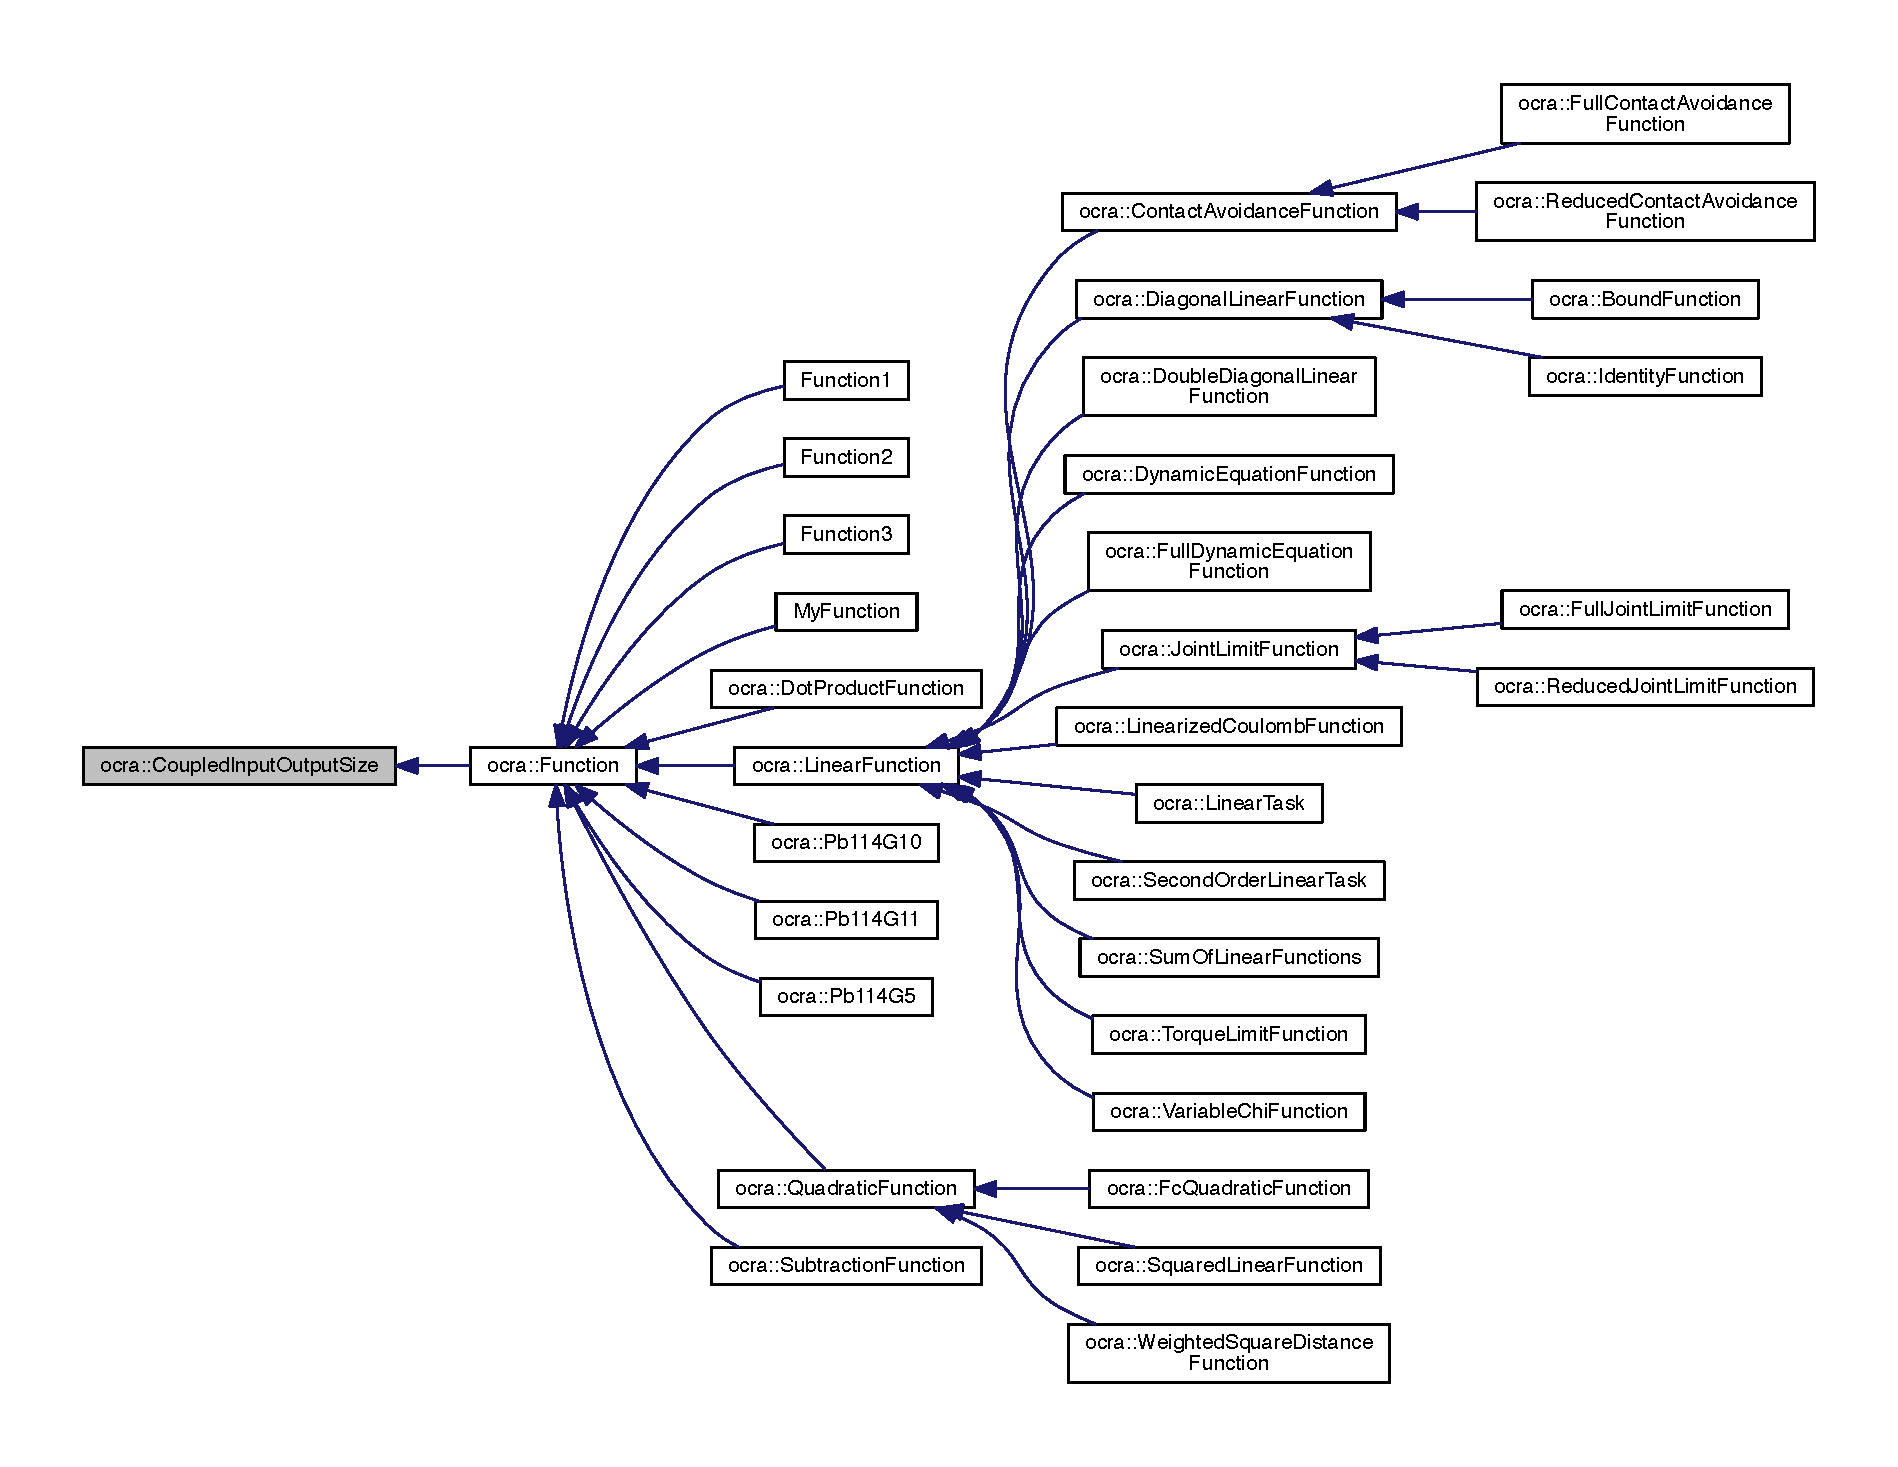
\includegraphics[width=350pt]{db/d0d/classocra_1_1CoupledInputOutputSize__inherit__graph}
\end{center}
\end{figure}
\subsection*{Protected Member Functions}
\begin{DoxyCompactItemize}
\item 
\hyperlink{classocra_1_1CoupledInputOutputSize_a464c947e199233598a248ff6409ab93d}{Coupled\+Input\+Output\+Size} (bool coupled\+Input\+Output\+Size)
\item 
bool \hyperlink{classocra_1_1CoupledInputOutputSize_a10e82ae3bbe410a29f7ed5a54ac105b0}{input\+And\+Output\+Sizes\+Are\+Coupled} () const
\end{DoxyCompactItemize}


\subsection{Detailed Description}
A trivial class with a single bool member.

Within ocra, this class is meant to be used as a {\itshape virtual} base class to force classes deriving from \hyperlink{classocra_1_1Function}{Function} to declare if their dimension is depending of the size of the input variable. 

Definition at line 17 of file Coupled\+Input\+Output\+Size.\+h.



\subsection{Constructor \& Destructor Documentation}
\hypertarget{classocra_1_1CoupledInputOutputSize_a464c947e199233598a248ff6409ab93d}{}\label{classocra_1_1CoupledInputOutputSize_a464c947e199233598a248ff6409ab93d} 
\index{ocra\+::\+Coupled\+Input\+Output\+Size@{ocra\+::\+Coupled\+Input\+Output\+Size}!Coupled\+Input\+Output\+Size@{Coupled\+Input\+Output\+Size}}
\index{Coupled\+Input\+Output\+Size@{Coupled\+Input\+Output\+Size}!ocra\+::\+Coupled\+Input\+Output\+Size@{ocra\+::\+Coupled\+Input\+Output\+Size}}
\subsubsection{\texorpdfstring{Coupled\+Input\+Output\+Size()}{CoupledInputOutputSize()}}
{\footnotesize\ttfamily ocra\+::\+Coupled\+Input\+Output\+Size\+::\+Coupled\+Input\+Output\+Size (\begin{DoxyParamCaption}\item[{bool}]{coupled\+Input\+Output\+Size }\end{DoxyParamCaption})\hspace{0.3cm}{\ttfamily [inline]}, {\ttfamily [protected]}}



Definition at line 20 of file Coupled\+Input\+Output\+Size.\+h.



\subsection{Member Function Documentation}
\hypertarget{classocra_1_1CoupledInputOutputSize_a10e82ae3bbe410a29f7ed5a54ac105b0}{}\label{classocra_1_1CoupledInputOutputSize_a10e82ae3bbe410a29f7ed5a54ac105b0} 
\index{ocra\+::\+Coupled\+Input\+Output\+Size@{ocra\+::\+Coupled\+Input\+Output\+Size}!input\+And\+Output\+Sizes\+Are\+Coupled@{input\+And\+Output\+Sizes\+Are\+Coupled}}
\index{input\+And\+Output\+Sizes\+Are\+Coupled@{input\+And\+Output\+Sizes\+Are\+Coupled}!ocra\+::\+Coupled\+Input\+Output\+Size@{ocra\+::\+Coupled\+Input\+Output\+Size}}
\subsubsection{\texorpdfstring{input\+And\+Output\+Sizes\+Are\+Coupled()}{inputAndOutputSizesAreCoupled()}}
{\footnotesize\ttfamily bool ocra\+::\+Coupled\+Input\+Output\+Size\+::input\+And\+Output\+Sizes\+Are\+Coupled (\begin{DoxyParamCaption}{ }\end{DoxyParamCaption}) const\hspace{0.3cm}{\ttfamily [inline]}, {\ttfamily [protected]}}



Definition at line 25 of file Coupled\+Input\+Output\+Size.\+h.



The documentation for this class was generated from the following file\+:\begin{DoxyCompactItemize}
\item 
\hyperlink{CoupledInputOutputSize_8h}{Coupled\+Input\+Output\+Size.\+h}\end{DoxyCompactItemize}

\hypertarget{classocra_1_1DiagonalLinearFunction}{}\section{ocra\+:\+:Diagonal\+Linear\+Function Class Reference}
\label{classocra_1_1DiagonalLinearFunction}\index{ocra\+::\+Diagonal\+Linear\+Function@{ocra\+::\+Diagonal\+Linear\+Function}}


Diagonal\+Linear\+Function class.  




{\ttfamily \#include $<$Diagonal\+Linear\+Function.\+h$>$}

Inheritance diagram for ocra\+:\+:Diagonal\+Linear\+Function\+:\begin{figure}[H]
\begin{center}
\leavevmode
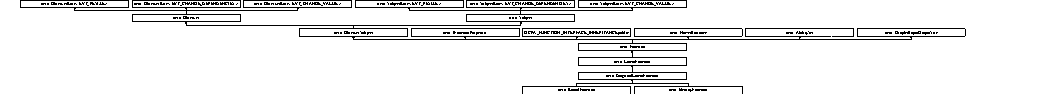
\includegraphics[height=1.262480cm]{d3/d89/classocra_1_1DiagonalLinearFunction}
\end{center}
\end{figure}
\subsection*{Public Types}
\begin{DoxyCompactItemize}
\item 
typedef \hyperlink{classocra_1_1LinearFunction}{Linear\+Function} \hyperlink{classocra_1_1DiagonalLinearFunction_ab1d33ba63aea16f86fa88bf574333a39}{function\+Type\+\_\+t}
\end{DoxyCompactItemize}
\subsection*{Public Member Functions}
\begin{DoxyCompactItemize}
\item 
void \hyperlink{classocra_1_1DiagonalLinearFunction_a0ef4d3d73af4c8e884d799024887d1ae}{change\+Diagonal} (const Vector\+Xd \&d)
\item 
void \hyperlink{classocra_1_1DiagonalLinearFunction_ac17d245b02f9388fea8bf1a724ec0106}{change\+Diagonal} (const double diagonal\+Element\+Value, const bool change\+Default=true)
\item 
void \hyperlink{classocra_1_1DiagonalLinearFunction_a8912906e227dc8ebce7339eceb09e72e}{change\+Default\+Diagonal\+Value} (const double v)
\item 
void \hyperlink{classocra_1_1DiagonalLinearFunction_a728b7f4b453ad06f385601b736290979}{change\+Defaultb\+Value} (const double v)
\end{DoxyCompactItemize}
{\bf }\par
\begin{DoxyCompactItemize}
\item 
{\footnotesize template$<$class Vector\+Base1 , class Vector\+Base2 $>$ }\\\hyperlink{classocra_1_1DiagonalLinearFunction_ab96ebb7bcf93104dad806f1ac47a2e8f}{Diagonal\+Linear\+Function} (\hyperlink{classocra_1_1Variable}{Variable} \&\hyperlink{classocra_1_1Function_a28825886d1f149c87b112ec2ec1dd486}{x}, const Vector\+Base1 \&d, const Vector\+Base2 \&b, const bool use\+Default\+Value=false, const double default\+Diag\+Value=1., const double defaultb\+Value=0.)
\item 
{\footnotesize template$<$class Vector\+Base $>$ }\\\hyperlink{classocra_1_1DiagonalLinearFunction_af144cecdab815f972418891a35f8ee2c}{Diagonal\+Linear\+Function} (\hyperlink{classocra_1_1Variable}{Variable} \&\hyperlink{classocra_1_1Function_a28825886d1f149c87b112ec2ec1dd486}{x}, const double diagonal\+Element\+Value, const Vector\+Base \&b, const bool use\+Default\+Value=false, const double defaultb\+Value=0.)
\item 
{\footnotesize template$<$class Vector\+Base $>$ }\\\hyperlink{classocra_1_1DiagonalLinearFunction_a4cd597044d6af815e1c6cec976958c54}{Diagonal\+Linear\+Function} (\hyperlink{classocra_1_1Variable}{Variable} \&\hyperlink{classocra_1_1Function_a28825886d1f149c87b112ec2ec1dd486}{x}, const Vector\+Base \&d, const double vector\+Element\+Value, const bool use\+Default\+Value=false, const double default\+Diag\+Value=1.)
\item 
\hyperlink{classocra_1_1DiagonalLinearFunction_a363e6ca5190cedaf2bbce516d27127f9}{Diagonal\+Linear\+Function} (\hyperlink{classocra_1_1Variable}{Variable} \&\hyperlink{classocra_1_1Function_a28825886d1f149c87b112ec2ec1dd486}{x}, const double diagonal\+Element\+Value, const double vector\+Element\+Value, const bool use\+Default\+Value=false)
\end{DoxyCompactItemize}

{\bf }\par
\begin{DoxyCompactItemize}
\item 
const Vector\+Xd \& \hyperlink{classocra_1_1DiagonalLinearFunction_a1b2acc7225716b75ef0cf9995a49406b}{get\+Diagonal} () const
\item 
double \hyperlink{classocra_1_1DiagonalLinearFunction_a01a923080ce21e1328503c29b1b57c6e}{get\+Default\+Diagonal\+Value} () const
\item 
double \hyperlink{classocra_1_1DiagonalLinearFunction_afc676bfa2611945421d73b18e2740bd0}{get\+Defaultb\+Value} () const
\item 
bool \hyperlink{classocra_1_1DiagonalLinearFunction_a8cca25ae530e9af992acf44e3b95da2a}{is\+Using\+Default\+Value} () const
\end{DoxyCompactItemize}

\subsection*{Protected Member Functions}
\begin{DoxyCompactItemize}
\item 
\hyperlink{classocra_1_1DiagonalLinearFunction_ac2c460e4eedb9feba5a74ec967719654}{Diagonal\+Linear\+Function} (\hyperlink{classocra_1_1Variable}{Variable} \&\hyperlink{classocra_1_1Function_a28825886d1f149c87b112ec2ec1dd486}{x})
\item 
virtual void \hyperlink{classocra_1_1DiagonalLinearFunction_a69523347749429dae6ae041326e40d43}{update\+Value} () const
\item 
virtual void \hyperlink{classocra_1_1DiagonalLinearFunction_a2071e4c52785c88119917460b94773cb}{do\+Update\+Input\+Size\+Begin} ()
\item 
virtual void \hyperlink{classocra_1_1DiagonalLinearFunction_a8a51d23c302c9bad9579b95e29481f55}{do\+Update\+Input\+Size\+End} ()
\item 
virtual void \hyperlink{classocra_1_1DiagonalLinearFunction_a5355515d58348a3eea92f36e35b1c7d5}{do\+Change\+Diagonal} (const Vector\+Xd \&d)
\item 
virtual void \hyperlink{classocra_1_1DiagonalLinearFunction_a0673bfe405d5637182c4749dd2737e95}{do\+Change\+Diagonal} (const double diagonal\+Element\+Value, const bool change\+Default=true)
\item 
virtual void \hyperlink{classocra_1_1DiagonalLinearFunction_a81120f5a61cc53cc940f4e71b35174ff}{do\+Change\+Default\+Diagonal\+Value} (const double v)
\item 
virtual void \hyperlink{classocra_1_1DiagonalLinearFunction_a9995af94055dc443c10018869a393635}{do\+Change\+Defaultb\+Value} (const double v)
\item 
virtual void \hyperlink{classocra_1_1DiagonalLinearFunction_addc4f984a5a71b170137788f15e2d12c}{do\+ChangeA} (const Matrix\+Xd \&A)
\item 
int \hyperlink{classocra_1_1DiagonalLinearFunction_af41faa708f35e39c2f797f70ae7ce695}{compute\+Dimension\+From\+Input\+Size} () const
\item 
void \hyperlink{classocra_1_1DiagonalLinearFunction_a86b326e3578c8405806eab4ec6522ab2}{do\+Update\+Dimension\+Begin} (int new\+Dimension)
\end{DoxyCompactItemize}
\subsection*{Protected Attributes}
\begin{DoxyCompactItemize}
\item 
Vector\+Xd \hyperlink{classocra_1_1DiagonalLinearFunction_adf9d157af394f4322d71720bea545f00}{\+\_\+d}
\item 
double \hyperlink{classocra_1_1DiagonalLinearFunction_aa7150368fce9c7c6c3724b801f498749}{\+\_\+default\+Diagonal\+Value}
\item 
double \hyperlink{classocra_1_1DiagonalLinearFunction_ab004421a9f01bd2c3fa5b97b7532c6c2}{\+\_\+defaultb\+Value}
\item 
bool \hyperlink{classocra_1_1DiagonalLinearFunction_a27e25618f0812c42967b363ad3f77fd6}{\+\_\+use\+Default\+Value}
\end{DoxyCompactItemize}
\subsection*{Additional Inherited Members}


\subsection{Detailed Description}
Diagonal\+Linear\+Function class. 

\begin{DoxyWarning}{Warning}
None
\end{DoxyWarning}
Implements a function of the type $ Dx+b $ with $ D=diag(d) $ a diagonal matrix whose diagonal is given by the vector $ d $. It is possible to specify a default value for the new diagonal elements in case the size of the variable, and thus the dimension of the function, change. Note that the values of the last diagonal elements are lost when the dimension decreases. Thus going from dimension n to dimension n\textquotesingle{}$<$n then back to n will set the last n-\/n\textquotesingle{} diagonal elements to the default value. 

Definition at line 40 of file Diagonal\+Linear\+Function.\+h.



\subsection{Member Typedef Documentation}
\hypertarget{classocra_1_1DiagonalLinearFunction_ab1d33ba63aea16f86fa88bf574333a39}{}\label{classocra_1_1DiagonalLinearFunction_ab1d33ba63aea16f86fa88bf574333a39} 
\index{ocra\+::\+Diagonal\+Linear\+Function@{ocra\+::\+Diagonal\+Linear\+Function}!function\+Type\+\_\+t@{function\+Type\+\_\+t}}
\index{function\+Type\+\_\+t@{function\+Type\+\_\+t}!ocra\+::\+Diagonal\+Linear\+Function@{ocra\+::\+Diagonal\+Linear\+Function}}
\subsubsection{\texorpdfstring{function\+Type\+\_\+t}{functionType\_t}}
{\footnotesize\ttfamily typedef \hyperlink{classocra_1_1LinearFunction}{Linear\+Function} \hyperlink{classocra_1_1DiagonalLinearFunction_ab1d33ba63aea16f86fa88bf574333a39}{ocra\+::\+Diagonal\+Linear\+Function\+::function\+Type\+\_\+t}}



Definition at line 44 of file Diagonal\+Linear\+Function.\+h.



\subsection{Constructor \& Destructor Documentation}
\hypertarget{classocra_1_1DiagonalLinearFunction_ab96ebb7bcf93104dad806f1ac47a2e8f}{}\label{classocra_1_1DiagonalLinearFunction_ab96ebb7bcf93104dad806f1ac47a2e8f} 
\index{ocra\+::\+Diagonal\+Linear\+Function@{ocra\+::\+Diagonal\+Linear\+Function}!Diagonal\+Linear\+Function@{Diagonal\+Linear\+Function}}
\index{Diagonal\+Linear\+Function@{Diagonal\+Linear\+Function}!ocra\+::\+Diagonal\+Linear\+Function@{ocra\+::\+Diagonal\+Linear\+Function}}
\subsubsection{\texorpdfstring{Diagonal\+Linear\+Function()}{DiagonalLinearFunction()}\hspace{0.1cm}{\footnotesize\ttfamily [1/5]}}
{\footnotesize\ttfamily template$<$class Vector\+Base1 , class Vector\+Base2 $>$ \\
ocra\+::\+Diagonal\+Linear\+Function\+::\+Diagonal\+Linear\+Function (\begin{DoxyParamCaption}\item[{\hyperlink{classocra_1_1Variable}{Variable} \&}]{x,  }\item[{const Vector\+Base1 \&}]{d,  }\item[{const Vector\+Base2 \&}]{b,  }\item[{const bool}]{use\+Default\+Value = {\ttfamily false},  }\item[{const double}]{default\+Diag\+Value = {\ttfamily 1.},  }\item[{const double}]{defaultb\+Value = {\ttfamily 0.} }\end{DoxyParamCaption})\hspace{0.3cm}{\ttfamily [inline]}}

A set of constructors where {\itshape d} and {\itshape b} are specified either by a vector or by a double.


\begin{DoxyParams}[1]{Parameters}
\mbox{\tt in}  & {\em x} & The variable on which to build the function. \\
\hline
\mbox{\tt in}  & {\em d} & The value of d. \\
\hline
\mbox{\tt in}  & {\em b} & The value of b. \\
\hline
\mbox{\tt in}  & {\em diagonal\+Element\+Value} & The value of each element of d. \\
\hline
\mbox{\tt in}  & {\em vector\+Element\+Value} & The value of each element of b. \\
\hline
\mbox{\tt in}  & {\em use\+Default\+Value} & true if the function can use a default value when resizing to a bigger dimension. Note that if use\+Default\+Value is false, the function can still be downsized. \\
\hline
\mbox{\tt in}  & {\em default\+Diag\+Value} & The default value for the last value of d when resizing to a bigger dimension. \\
\hline
\mbox{\tt in}  & {\em defaultb\+Value} & The default value for the last value of b when resizing to a bigger dimension.\\
\hline
\end{DoxyParams}
\begin{DoxyWarning}{Warning}
You need to put {\itshape real} double for diagonal\+Element\+Value and vector\+Element\+Value. All other type will be considered as Vector\+Base and will trigger the static assertion on th Vector\+Base type. For example, Diagonal\+Linear\+Function(x, 1, b), where x is a variable and b is a vector, is not valid. The correct way to write it is \hyperlink{classocra_1_1DiagonalLinearFunction}{Diagonal\+Linear\+Function}(x, 1., b), because 1. is a double, but 1 is an int so the compiler will not try to cast it into a double and call the wrong constructor. 
\end{DoxyWarning}


Definition at line 156 of file Diagonal\+Linear\+Function.\+h.

\hypertarget{classocra_1_1DiagonalLinearFunction_af144cecdab815f972418891a35f8ee2c}{}\label{classocra_1_1DiagonalLinearFunction_af144cecdab815f972418891a35f8ee2c} 
\index{ocra\+::\+Diagonal\+Linear\+Function@{ocra\+::\+Diagonal\+Linear\+Function}!Diagonal\+Linear\+Function@{Diagonal\+Linear\+Function}}
\index{Diagonal\+Linear\+Function@{Diagonal\+Linear\+Function}!ocra\+::\+Diagonal\+Linear\+Function@{ocra\+::\+Diagonal\+Linear\+Function}}
\subsubsection{\texorpdfstring{Diagonal\+Linear\+Function()}{DiagonalLinearFunction()}\hspace{0.1cm}{\footnotesize\ttfamily [2/5]}}
{\footnotesize\ttfamily template$<$class Vector\+Base $>$ \\
ocra\+::\+Diagonal\+Linear\+Function\+::\+Diagonal\+Linear\+Function (\begin{DoxyParamCaption}\item[{\hyperlink{classocra_1_1Variable}{Variable} \&}]{x,  }\item[{const double}]{diagonal\+Element\+Value,  }\item[{const Vector\+Base \&}]{b,  }\item[{const bool}]{use\+Default\+Value = {\ttfamily false},  }\item[{const double}]{defaultb\+Value = {\ttfamily 0.} }\end{DoxyParamCaption})\hspace{0.3cm}{\ttfamily [inline]}}



Definition at line 183 of file Diagonal\+Linear\+Function.\+h.

\hypertarget{classocra_1_1DiagonalLinearFunction_a4cd597044d6af815e1c6cec976958c54}{}\label{classocra_1_1DiagonalLinearFunction_a4cd597044d6af815e1c6cec976958c54} 
\index{ocra\+::\+Diagonal\+Linear\+Function@{ocra\+::\+Diagonal\+Linear\+Function}!Diagonal\+Linear\+Function@{Diagonal\+Linear\+Function}}
\index{Diagonal\+Linear\+Function@{Diagonal\+Linear\+Function}!ocra\+::\+Diagonal\+Linear\+Function@{ocra\+::\+Diagonal\+Linear\+Function}}
\subsubsection{\texorpdfstring{Diagonal\+Linear\+Function()}{DiagonalLinearFunction()}\hspace{0.1cm}{\footnotesize\ttfamily [3/5]}}
{\footnotesize\ttfamily template$<$class Vector\+Base $>$ \\
ocra\+::\+Diagonal\+Linear\+Function\+::\+Diagonal\+Linear\+Function (\begin{DoxyParamCaption}\item[{\hyperlink{classocra_1_1Variable}{Variable} \&}]{x,  }\item[{const Vector\+Base \&}]{d,  }\item[{const double}]{vector\+Element\+Value,  }\item[{const bool}]{use\+Default\+Value = {\ttfamily false},  }\item[{const double}]{default\+Diag\+Value = {\ttfamily 1.} }\end{DoxyParamCaption})\hspace{0.3cm}{\ttfamily [inline]}}



Definition at line 205 of file Diagonal\+Linear\+Function.\+h.

\hypertarget{classocra_1_1DiagonalLinearFunction_a363e6ca5190cedaf2bbce516d27127f9}{}\label{classocra_1_1DiagonalLinearFunction_a363e6ca5190cedaf2bbce516d27127f9} 
\index{ocra\+::\+Diagonal\+Linear\+Function@{ocra\+::\+Diagonal\+Linear\+Function}!Diagonal\+Linear\+Function@{Diagonal\+Linear\+Function}}
\index{Diagonal\+Linear\+Function@{Diagonal\+Linear\+Function}!ocra\+::\+Diagonal\+Linear\+Function@{ocra\+::\+Diagonal\+Linear\+Function}}
\subsubsection{\texorpdfstring{Diagonal\+Linear\+Function()}{DiagonalLinearFunction()}\hspace{0.1cm}{\footnotesize\ttfamily [4/5]}}
{\footnotesize\ttfamily ocra\+::\+Diagonal\+Linear\+Function\+::\+Diagonal\+Linear\+Function (\begin{DoxyParamCaption}\item[{\hyperlink{classocra_1_1Variable}{Variable} \&}]{x,  }\item[{const double}]{diagonal\+Element\+Value,  }\item[{const double}]{vector\+Element\+Value,  }\item[{const bool}]{use\+Default\+Value = {\ttfamily false} }\end{DoxyParamCaption})}



Definition at line 7 of file Diagonal\+Linear\+Function.\+cpp.

\hypertarget{classocra_1_1DiagonalLinearFunction_ac2c460e4eedb9feba5a74ec967719654}{}\label{classocra_1_1DiagonalLinearFunction_ac2c460e4eedb9feba5a74ec967719654} 
\index{ocra\+::\+Diagonal\+Linear\+Function@{ocra\+::\+Diagonal\+Linear\+Function}!Diagonal\+Linear\+Function@{Diagonal\+Linear\+Function}}
\index{Diagonal\+Linear\+Function@{Diagonal\+Linear\+Function}!ocra\+::\+Diagonal\+Linear\+Function@{ocra\+::\+Diagonal\+Linear\+Function}}
\subsubsection{\texorpdfstring{Diagonal\+Linear\+Function()}{DiagonalLinearFunction()}\hspace{0.1cm}{\footnotesize\ttfamily [5/5]}}
{\footnotesize\ttfamily ocra\+::\+Diagonal\+Linear\+Function\+::\+Diagonal\+Linear\+Function (\begin{DoxyParamCaption}\item[{\hyperlink{classocra_1_1Variable}{Variable} \&}]{x }\end{DoxyParamCaption})\hspace{0.3cm}{\ttfamily [protected]}}

A light constructor for derived class 

Definition at line 25 of file Diagonal\+Linear\+Function.\+cpp.



\subsection{Member Function Documentation}
\hypertarget{classocra_1_1DiagonalLinearFunction_a728b7f4b453ad06f385601b736290979}{}\label{classocra_1_1DiagonalLinearFunction_a728b7f4b453ad06f385601b736290979} 
\index{ocra\+::\+Diagonal\+Linear\+Function@{ocra\+::\+Diagonal\+Linear\+Function}!change\+Defaultb\+Value@{change\+Defaultb\+Value}}
\index{change\+Defaultb\+Value@{change\+Defaultb\+Value}!ocra\+::\+Diagonal\+Linear\+Function@{ocra\+::\+Diagonal\+Linear\+Function}}
\subsubsection{\texorpdfstring{change\+Defaultb\+Value()}{changeDefaultbValue()}}
{\footnotesize\ttfamily void ocra\+::\+Diagonal\+Linear\+Function\+::change\+Defaultb\+Value (\begin{DoxyParamCaption}\item[{const double}]{v }\end{DoxyParamCaption})}

Set the default value for b to {\itshape v}. (To change b, a method is directly accessible on \hyperlink{classocra_1_1LinearFunction}{Linear\+Function}) 

Definition at line 58 of file Diagonal\+Linear\+Function.\+cpp.

\hypertarget{classocra_1_1DiagonalLinearFunction_a8912906e227dc8ebce7339eceb09e72e}{}\label{classocra_1_1DiagonalLinearFunction_a8912906e227dc8ebce7339eceb09e72e} 
\index{ocra\+::\+Diagonal\+Linear\+Function@{ocra\+::\+Diagonal\+Linear\+Function}!change\+Default\+Diagonal\+Value@{change\+Default\+Diagonal\+Value}}
\index{change\+Default\+Diagonal\+Value@{change\+Default\+Diagonal\+Value}!ocra\+::\+Diagonal\+Linear\+Function@{ocra\+::\+Diagonal\+Linear\+Function}}
\subsubsection{\texorpdfstring{change\+Default\+Diagonal\+Value()}{changeDefaultDiagonalValue()}}
{\footnotesize\ttfamily void ocra\+::\+Diagonal\+Linear\+Function\+::change\+Default\+Diagonal\+Value (\begin{DoxyParamCaption}\item[{const double}]{v }\end{DoxyParamCaption})}

Change only the diagonal default value 

Definition at line 52 of file Diagonal\+Linear\+Function.\+cpp.

\hypertarget{classocra_1_1DiagonalLinearFunction_a0ef4d3d73af4c8e884d799024887d1ae}{}\label{classocra_1_1DiagonalLinearFunction_a0ef4d3d73af4c8e884d799024887d1ae} 
\index{ocra\+::\+Diagonal\+Linear\+Function@{ocra\+::\+Diagonal\+Linear\+Function}!change\+Diagonal@{change\+Diagonal}}
\index{change\+Diagonal@{change\+Diagonal}!ocra\+::\+Diagonal\+Linear\+Function@{ocra\+::\+Diagonal\+Linear\+Function}}
\subsubsection{\texorpdfstring{change\+Diagonal()}{changeDiagonal()}\hspace{0.1cm}{\footnotesize\ttfamily [1/2]}}
{\footnotesize\ttfamily void ocra\+::\+Diagonal\+Linear\+Function\+::change\+Diagonal (\begin{DoxyParamCaption}\item[{const Vector\+Xd \&}]{d }\end{DoxyParamCaption})}

Set the diagonal to {\itshape d} \begin{DoxyPrecond}{Precondition}
d.\+size() == \+\_\+dim Calls buildA which triggers a E\+V\+T\+\_\+\+C\+H\+A\+N\+G\+E\+\_\+\+V\+A\+L\+UE event. 
\end{DoxyPrecond}


Definition at line 37 of file Diagonal\+Linear\+Function.\+cpp.

\hypertarget{classocra_1_1DiagonalLinearFunction_ac17d245b02f9388fea8bf1a724ec0106}{}\label{classocra_1_1DiagonalLinearFunction_ac17d245b02f9388fea8bf1a724ec0106} 
\index{ocra\+::\+Diagonal\+Linear\+Function@{ocra\+::\+Diagonal\+Linear\+Function}!change\+Diagonal@{change\+Diagonal}}
\index{change\+Diagonal@{change\+Diagonal}!ocra\+::\+Diagonal\+Linear\+Function@{ocra\+::\+Diagonal\+Linear\+Function}}
\subsubsection{\texorpdfstring{change\+Diagonal()}{changeDiagonal()}\hspace{0.1cm}{\footnotesize\ttfamily [2/2]}}
{\footnotesize\ttfamily void ocra\+::\+Diagonal\+Linear\+Function\+::change\+Diagonal (\begin{DoxyParamCaption}\item[{const double}]{diagonal\+Element\+Value,  }\item[{const bool}]{change\+Default = {\ttfamily true} }\end{DoxyParamCaption})}

Set the diagonal to {\itshape diagonal\+Element\+Value} and the default diagonal value to the same value if change\+Default is true. Calls buildA which triggers a E\+V\+T\+\_\+\+C\+H\+A\+N\+G\+E\+\_\+\+V\+A\+L\+UE event. 

Definition at line 45 of file Diagonal\+Linear\+Function.\+cpp.

\hypertarget{classocra_1_1DiagonalLinearFunction_af41faa708f35e39c2f797f70ae7ce695}{}\label{classocra_1_1DiagonalLinearFunction_af41faa708f35e39c2f797f70ae7ce695} 
\index{ocra\+::\+Diagonal\+Linear\+Function@{ocra\+::\+Diagonal\+Linear\+Function}!compute\+Dimension\+From\+Input\+Size@{compute\+Dimension\+From\+Input\+Size}}
\index{compute\+Dimension\+From\+Input\+Size@{compute\+Dimension\+From\+Input\+Size}!ocra\+::\+Diagonal\+Linear\+Function@{ocra\+::\+Diagonal\+Linear\+Function}}
\subsubsection{\texorpdfstring{compute\+Dimension\+From\+Input\+Size()}{computeDimensionFromInputSize()}}
{\footnotesize\ttfamily int ocra\+::\+Diagonal\+Linear\+Function\+::compute\+Dimension\+From\+Input\+Size (\begin{DoxyParamCaption}{ }\end{DoxyParamCaption}) const\hspace{0.3cm}{\ttfamily [protected]}, {\ttfamily [virtual]}}

Does what it tells... 

Reimplemented from \hyperlink{classocra_1_1Function_a95241fd426f887c5eb3add3f1e55a09c}{ocra\+::\+Function}.



Definition at line 150 of file Diagonal\+Linear\+Function.\+cpp.

\hypertarget{classocra_1_1DiagonalLinearFunction_addc4f984a5a71b170137788f15e2d12c}{}\label{classocra_1_1DiagonalLinearFunction_addc4f984a5a71b170137788f15e2d12c} 
\index{ocra\+::\+Diagonal\+Linear\+Function@{ocra\+::\+Diagonal\+Linear\+Function}!do\+ChangeA@{do\+ChangeA}}
\index{do\+ChangeA@{do\+ChangeA}!ocra\+::\+Diagonal\+Linear\+Function@{ocra\+::\+Diagonal\+Linear\+Function}}
\subsubsection{\texorpdfstring{do\+Change\+A()}{doChangeA()}}
{\footnotesize\ttfamily void ocra\+::\+Diagonal\+Linear\+Function\+::do\+ChangeA (\begin{DoxyParamCaption}\item[{const Matrix\+Xd \&}]{A }\end{DoxyParamCaption})\hspace{0.3cm}{\ttfamily [protected]}, {\ttfamily [virtual]}}

Methods to be called in ChangeA and Change b 

Reimplemented from \hyperlink{classocra_1_1LinearFunction_ab573c2f615d2edefb647979d3cc3cf46}{ocra\+::\+Linear\+Function}.



Reimplemented in \hyperlink{classocra_1_1IdentityFunction_aa1a9f42b9b1b62182d99ea32dae6e815}{ocra\+::\+Identity\+Function}.



Definition at line 91 of file Diagonal\+Linear\+Function.\+cpp.

\hypertarget{classocra_1_1DiagonalLinearFunction_a9995af94055dc443c10018869a393635}{}\label{classocra_1_1DiagonalLinearFunction_a9995af94055dc443c10018869a393635} 
\index{ocra\+::\+Diagonal\+Linear\+Function@{ocra\+::\+Diagonal\+Linear\+Function}!do\+Change\+Defaultb\+Value@{do\+Change\+Defaultb\+Value}}
\index{do\+Change\+Defaultb\+Value@{do\+Change\+Defaultb\+Value}!ocra\+::\+Diagonal\+Linear\+Function@{ocra\+::\+Diagonal\+Linear\+Function}}
\subsubsection{\texorpdfstring{do\+Change\+Defaultb\+Value()}{doChangeDefaultbValue()}}
{\footnotesize\ttfamily void ocra\+::\+Diagonal\+Linear\+Function\+::do\+Change\+Defaultb\+Value (\begin{DoxyParamCaption}\item[{const double}]{v }\end{DoxyParamCaption})\hspace{0.3cm}{\ttfamily [protected]}, {\ttfamily [virtual]}}



Reimplemented in \hyperlink{classocra_1_1BoundFunction_aa861028f4a37e45b4fc68b7852d7e451}{ocra\+::\+Bound\+Function}, and \hyperlink{classocra_1_1IdentityFunction_a989f91f6ec4e2e00aa5ac3cc8b6a2b66}{ocra\+::\+Identity\+Function}.



Definition at line 84 of file Diagonal\+Linear\+Function.\+cpp.

\hypertarget{classocra_1_1DiagonalLinearFunction_a81120f5a61cc53cc940f4e71b35174ff}{}\label{classocra_1_1DiagonalLinearFunction_a81120f5a61cc53cc940f4e71b35174ff} 
\index{ocra\+::\+Diagonal\+Linear\+Function@{ocra\+::\+Diagonal\+Linear\+Function}!do\+Change\+Default\+Diagonal\+Value@{do\+Change\+Default\+Diagonal\+Value}}
\index{do\+Change\+Default\+Diagonal\+Value@{do\+Change\+Default\+Diagonal\+Value}!ocra\+::\+Diagonal\+Linear\+Function@{ocra\+::\+Diagonal\+Linear\+Function}}
\subsubsection{\texorpdfstring{do\+Change\+Default\+Diagonal\+Value()}{doChangeDefaultDiagonalValue()}}
{\footnotesize\ttfamily void ocra\+::\+Diagonal\+Linear\+Function\+::do\+Change\+Default\+Diagonal\+Value (\begin{DoxyParamCaption}\item[{const double}]{v }\end{DoxyParamCaption})\hspace{0.3cm}{\ttfamily [protected]}, {\ttfamily [virtual]}}



Reimplemented in \hyperlink{classocra_1_1BoundFunction_af02c8fc499fb37596c758861d98cfbf6}{ocra\+::\+Bound\+Function}, and \hyperlink{classocra_1_1IdentityFunction_ad54cf6c0b28f6d4955f15ebd53c6ca1f}{ocra\+::\+Identity\+Function}.



Definition at line 78 of file Diagonal\+Linear\+Function.\+cpp.

\hypertarget{classocra_1_1DiagonalLinearFunction_a5355515d58348a3eea92f36e35b1c7d5}{}\label{classocra_1_1DiagonalLinearFunction_a5355515d58348a3eea92f36e35b1c7d5} 
\index{ocra\+::\+Diagonal\+Linear\+Function@{ocra\+::\+Diagonal\+Linear\+Function}!do\+Change\+Diagonal@{do\+Change\+Diagonal}}
\index{do\+Change\+Diagonal@{do\+Change\+Diagonal}!ocra\+::\+Diagonal\+Linear\+Function@{ocra\+::\+Diagonal\+Linear\+Function}}
\subsubsection{\texorpdfstring{do\+Change\+Diagonal()}{doChangeDiagonal()}\hspace{0.1cm}{\footnotesize\ttfamily [1/2]}}
{\footnotesize\ttfamily void ocra\+::\+Diagonal\+Linear\+Function\+::do\+Change\+Diagonal (\begin{DoxyParamCaption}\item[{const Vector\+Xd \&}]{d }\end{DoxyParamCaption})\hspace{0.3cm}{\ttfamily [protected]}, {\ttfamily [virtual]}}



Reimplemented in \hyperlink{classocra_1_1BoundFunction_a95e8e97598f5ca779b9c171c56a7342a}{ocra\+::\+Bound\+Function}, and \hyperlink{classocra_1_1IdentityFunction_aea94175430c2c785dbb9d551922be9ad}{ocra\+::\+Identity\+Function}.



Definition at line 64 of file Diagonal\+Linear\+Function.\+cpp.

\hypertarget{classocra_1_1DiagonalLinearFunction_a0673bfe405d5637182c4749dd2737e95}{}\label{classocra_1_1DiagonalLinearFunction_a0673bfe405d5637182c4749dd2737e95} 
\index{ocra\+::\+Diagonal\+Linear\+Function@{ocra\+::\+Diagonal\+Linear\+Function}!do\+Change\+Diagonal@{do\+Change\+Diagonal}}
\index{do\+Change\+Diagonal@{do\+Change\+Diagonal}!ocra\+::\+Diagonal\+Linear\+Function@{ocra\+::\+Diagonal\+Linear\+Function}}
\subsubsection{\texorpdfstring{do\+Change\+Diagonal()}{doChangeDiagonal()}\hspace{0.1cm}{\footnotesize\ttfamily [2/2]}}
{\footnotesize\ttfamily void ocra\+::\+Diagonal\+Linear\+Function\+::do\+Change\+Diagonal (\begin{DoxyParamCaption}\item[{const double}]{diagonal\+Element\+Value,  }\item[{const bool}]{change\+Default = {\ttfamily true} }\end{DoxyParamCaption})\hspace{0.3cm}{\ttfamily [protected]}, {\ttfamily [virtual]}}



Reimplemented in \hyperlink{classocra_1_1BoundFunction_ac1a1b78b8b1796543b4c83ae5d8de755}{ocra\+::\+Bound\+Function}, and \hyperlink{classocra_1_1IdentityFunction_ac6350bcc2107b56e96642cacbbee2404}{ocra\+::\+Identity\+Function}.



Definition at line 70 of file Diagonal\+Linear\+Function.\+cpp.

\hypertarget{classocra_1_1DiagonalLinearFunction_a86b326e3578c8405806eab4ec6522ab2}{}\label{classocra_1_1DiagonalLinearFunction_a86b326e3578c8405806eab4ec6522ab2} 
\index{ocra\+::\+Diagonal\+Linear\+Function@{ocra\+::\+Diagonal\+Linear\+Function}!do\+Update\+Dimension\+Begin@{do\+Update\+Dimension\+Begin}}
\index{do\+Update\+Dimension\+Begin@{do\+Update\+Dimension\+Begin}!ocra\+::\+Diagonal\+Linear\+Function@{ocra\+::\+Diagonal\+Linear\+Function}}
\subsubsection{\texorpdfstring{do\+Update\+Dimension\+Begin()}{doUpdateDimensionBegin()}}
{\footnotesize\ttfamily void ocra\+::\+Diagonal\+Linear\+Function\+::do\+Update\+Dimension\+Begin (\begin{DoxyParamCaption}\item[{int}]{new\+Dimension }\end{DoxyParamCaption})\hspace{0.3cm}{\ttfamily [protected]}, {\ttfamily [virtual]}}

Methods for pre and post update in case the dimension of the function has changed. Default implementation of do\+Update\+Dimension\+End does nothing, do\+Update\+Dimension\+Begin throws an exception. These methods might throw exceptions when overloaded. Furthermore, {\ttfamily \hyperlink{classocra_1_1Function_a17aa280f0e6eff4a7569edc373a5147d}{do\+Update\+Dimension\+End()}} must comply with the post condition of {\ttfamily update\+Dimension()}, i.\+e. let the values of each ability invalidated. 

Reimplemented from \hyperlink{classocra_1_1Function_afdf98e9f43fde97a5256af88a50cbb39}{ocra\+::\+Function}.



Definition at line 155 of file Diagonal\+Linear\+Function.\+cpp.

\hypertarget{classocra_1_1DiagonalLinearFunction_a2071e4c52785c88119917460b94773cb}{}\label{classocra_1_1DiagonalLinearFunction_a2071e4c52785c88119917460b94773cb} 
\index{ocra\+::\+Diagonal\+Linear\+Function@{ocra\+::\+Diagonal\+Linear\+Function}!do\+Update\+Input\+Size\+Begin@{do\+Update\+Input\+Size\+Begin}}
\index{do\+Update\+Input\+Size\+Begin@{do\+Update\+Input\+Size\+Begin}!ocra\+::\+Diagonal\+Linear\+Function@{ocra\+::\+Diagonal\+Linear\+Function}}
\subsubsection{\texorpdfstring{do\+Update\+Input\+Size\+Begin()}{doUpdateInputSizeBegin()}}
{\footnotesize\ttfamily void ocra\+::\+Diagonal\+Linear\+Function\+::do\+Update\+Input\+Size\+Begin (\begin{DoxyParamCaption}{ }\end{DoxyParamCaption})\hspace{0.3cm}{\ttfamily [protected]}, {\ttfamily [virtual]}}

Methods for pre and post update in case the variable size has changed. Default implementation of do\+Update\+Input\+Size\+End does nothing, do\+Update\+Input\+Size\+Begin throws an exception. These methods might throw exceptions when overloaded. Furthermore, {\ttfamily \hyperlink{classocra_1_1DiagonalLinearFunction_a8a51d23c302c9bad9579b95e29481f55}{do\+Update\+Input\+Size\+End()}} must comply with the post condition of {\ttfamily \hyperlink{classocra_1_1Function_a3a5b9e6ae296339acc87ab2cbf97ef98}{update\+Input\+Size()}}, i.\+e. let the values of each ability invalidated. 

Reimplemented from \hyperlink{classocra_1_1Function_a3f728f3758e6448aa59932853db5ddcc}{ocra\+::\+Function}.



Reimplemented in \hyperlink{classocra_1_1IdentityFunction_aa8d5ff0e25422b3b5a4a2a8621120790}{ocra\+::\+Identity\+Function}.



Definition at line 105 of file Diagonal\+Linear\+Function.\+cpp.

\hypertarget{classocra_1_1DiagonalLinearFunction_a8a51d23c302c9bad9579b95e29481f55}{}\label{classocra_1_1DiagonalLinearFunction_a8a51d23c302c9bad9579b95e29481f55} 
\index{ocra\+::\+Diagonal\+Linear\+Function@{ocra\+::\+Diagonal\+Linear\+Function}!do\+Update\+Input\+Size\+End@{do\+Update\+Input\+Size\+End}}
\index{do\+Update\+Input\+Size\+End@{do\+Update\+Input\+Size\+End}!ocra\+::\+Diagonal\+Linear\+Function@{ocra\+::\+Diagonal\+Linear\+Function}}
\subsubsection{\texorpdfstring{do\+Update\+Input\+Size\+End()}{doUpdateInputSizeEnd()}}
{\footnotesize\ttfamily void ocra\+::\+Diagonal\+Linear\+Function\+::do\+Update\+Input\+Size\+End (\begin{DoxyParamCaption}\item[{void}]{ }\end{DoxyParamCaption})\hspace{0.3cm}{\ttfamily [protected]}, {\ttfamily [virtual]}}

This methods ensures \+\_\+b has the good size at the end of a resize, yet it will not be called in \hyperlink{classocra_1_1LinearFunction}{Linear\+Function} itself because the class does not overload \hyperlink{classocra_1_1DiagonalLinearFunction_a2071e4c52785c88119917460b94773cb}{do\+Update\+Input\+Size\+Begin()} which throws an runtime\+\_\+error by default. 

Reimplemented from \hyperlink{classocra_1_1LinearFunction_ac6bdf62ad6634397778d5f4223ed6d82}{ocra\+::\+Linear\+Function}.



Reimplemented in \hyperlink{classocra_1_1IdentityFunction_adcfa8a32491113a590e7066f0062fbc6}{ocra\+::\+Identity\+Function}.



Definition at line 136 of file Diagonal\+Linear\+Function.\+cpp.

\hypertarget{classocra_1_1DiagonalLinearFunction_afc676bfa2611945421d73b18e2740bd0}{}\label{classocra_1_1DiagonalLinearFunction_afc676bfa2611945421d73b18e2740bd0} 
\index{ocra\+::\+Diagonal\+Linear\+Function@{ocra\+::\+Diagonal\+Linear\+Function}!get\+Defaultb\+Value@{get\+Defaultb\+Value}}
\index{get\+Defaultb\+Value@{get\+Defaultb\+Value}!ocra\+::\+Diagonal\+Linear\+Function@{ocra\+::\+Diagonal\+Linear\+Function}}
\subsubsection{\texorpdfstring{get\+Defaultb\+Value()}{getDefaultbValue()}}
{\footnotesize\ttfamily double ocra\+::\+Diagonal\+Linear\+Function\+::get\+Defaultb\+Value (\begin{DoxyParamCaption}{ }\end{DoxyParamCaption}) const\hspace{0.3cm}{\ttfamily [inline]}}



Definition at line 239 of file Diagonal\+Linear\+Function.\+h.

\hypertarget{classocra_1_1DiagonalLinearFunction_a01a923080ce21e1328503c29b1b57c6e}{}\label{classocra_1_1DiagonalLinearFunction_a01a923080ce21e1328503c29b1b57c6e} 
\index{ocra\+::\+Diagonal\+Linear\+Function@{ocra\+::\+Diagonal\+Linear\+Function}!get\+Default\+Diagonal\+Value@{get\+Default\+Diagonal\+Value}}
\index{get\+Default\+Diagonal\+Value@{get\+Default\+Diagonal\+Value}!ocra\+::\+Diagonal\+Linear\+Function@{ocra\+::\+Diagonal\+Linear\+Function}}
\subsubsection{\texorpdfstring{get\+Default\+Diagonal\+Value()}{getDefaultDiagonalValue()}}
{\footnotesize\ttfamily double ocra\+::\+Diagonal\+Linear\+Function\+::get\+Default\+Diagonal\+Value (\begin{DoxyParamCaption}{ }\end{DoxyParamCaption}) const\hspace{0.3cm}{\ttfamily [inline]}}



Definition at line 233 of file Diagonal\+Linear\+Function.\+h.

\hypertarget{classocra_1_1DiagonalLinearFunction_a1b2acc7225716b75ef0cf9995a49406b}{}\label{classocra_1_1DiagonalLinearFunction_a1b2acc7225716b75ef0cf9995a49406b} 
\index{ocra\+::\+Diagonal\+Linear\+Function@{ocra\+::\+Diagonal\+Linear\+Function}!get\+Diagonal@{get\+Diagonal}}
\index{get\+Diagonal@{get\+Diagonal}!ocra\+::\+Diagonal\+Linear\+Function@{ocra\+::\+Diagonal\+Linear\+Function}}
\subsubsection{\texorpdfstring{get\+Diagonal()}{getDiagonal()}}
{\footnotesize\ttfamily const Vector\+Xd \& ocra\+::\+Diagonal\+Linear\+Function\+::get\+Diagonal (\begin{DoxyParamCaption}{ }\end{DoxyParamCaption}) const\hspace{0.3cm}{\ttfamily [inline]}}

Trivial getters. 

Definition at line 227 of file Diagonal\+Linear\+Function.\+h.

\hypertarget{classocra_1_1DiagonalLinearFunction_a8cca25ae530e9af992acf44e3b95da2a}{}\label{classocra_1_1DiagonalLinearFunction_a8cca25ae530e9af992acf44e3b95da2a} 
\index{ocra\+::\+Diagonal\+Linear\+Function@{ocra\+::\+Diagonal\+Linear\+Function}!is\+Using\+Default\+Value@{is\+Using\+Default\+Value}}
\index{is\+Using\+Default\+Value@{is\+Using\+Default\+Value}!ocra\+::\+Diagonal\+Linear\+Function@{ocra\+::\+Diagonal\+Linear\+Function}}
\subsubsection{\texorpdfstring{is\+Using\+Default\+Value()}{isUsingDefaultValue()}}
{\footnotesize\ttfamily bool ocra\+::\+Diagonal\+Linear\+Function\+::is\+Using\+Default\+Value (\begin{DoxyParamCaption}{ }\end{DoxyParamCaption}) const\hspace{0.3cm}{\ttfamily [inline]}}



Definition at line 245 of file Diagonal\+Linear\+Function.\+h.

\hypertarget{classocra_1_1DiagonalLinearFunction_a69523347749429dae6ae041326e40d43}{}\label{classocra_1_1DiagonalLinearFunction_a69523347749429dae6ae041326e40d43} 
\index{ocra\+::\+Diagonal\+Linear\+Function@{ocra\+::\+Diagonal\+Linear\+Function}!update\+Value@{update\+Value}}
\index{update\+Value@{update\+Value}!ocra\+::\+Diagonal\+Linear\+Function@{ocra\+::\+Diagonal\+Linear\+Function}}
\subsubsection{\texorpdfstring{update\+Value()}{updateValue()}}
{\footnotesize\ttfamily void ocra\+::\+Diagonal\+Linear\+Function\+::update\+Value (\begin{DoxyParamCaption}{ }\end{DoxyParamCaption}) const\hspace{0.3cm}{\ttfamily [protected]}, {\ttfamily [virtual]}}

Overloads of the \hyperlink{classocra_1_1Function}{Function} methods 

Reimplemented from \hyperlink{classocra_1_1LinearFunction_a1b9fd7a03a8630055c117d19e0ff019a}{ocra\+::\+Linear\+Function}.



Reimplemented in \hyperlink{classocra_1_1IdentityFunction_afd77529674b7b6db3db2542aaeedbb16}{ocra\+::\+Identity\+Function}.



Definition at line 99 of file Diagonal\+Linear\+Function.\+cpp.



\subsection{Member Data Documentation}
\hypertarget{classocra_1_1DiagonalLinearFunction_adf9d157af394f4322d71720bea545f00}{}\label{classocra_1_1DiagonalLinearFunction_adf9d157af394f4322d71720bea545f00} 
\index{ocra\+::\+Diagonal\+Linear\+Function@{ocra\+::\+Diagonal\+Linear\+Function}!\+\_\+d@{\+\_\+d}}
\index{\+\_\+d@{\+\_\+d}!ocra\+::\+Diagonal\+Linear\+Function@{ocra\+::\+Diagonal\+Linear\+Function}}
\subsubsection{\texorpdfstring{\+\_\+d}{\_d}}
{\footnotesize\ttfamily Vector\+Xd ocra\+::\+Diagonal\+Linear\+Function\+::\+\_\+d\hspace{0.3cm}{\ttfamily [protected]}}



Definition at line 148 of file Diagonal\+Linear\+Function.\+h.

\hypertarget{classocra_1_1DiagonalLinearFunction_ab004421a9f01bd2c3fa5b97b7532c6c2}{}\label{classocra_1_1DiagonalLinearFunction_ab004421a9f01bd2c3fa5b97b7532c6c2} 
\index{ocra\+::\+Diagonal\+Linear\+Function@{ocra\+::\+Diagonal\+Linear\+Function}!\+\_\+defaultb\+Value@{\+\_\+defaultb\+Value}}
\index{\+\_\+defaultb\+Value@{\+\_\+defaultb\+Value}!ocra\+::\+Diagonal\+Linear\+Function@{ocra\+::\+Diagonal\+Linear\+Function}}
\subsubsection{\texorpdfstring{\+\_\+defaultb\+Value}{\_defaultbValue}}
{\footnotesize\ttfamily double ocra\+::\+Diagonal\+Linear\+Function\+::\+\_\+defaultb\+Value\hspace{0.3cm}{\ttfamily [protected]}}



Definition at line 150 of file Diagonal\+Linear\+Function.\+h.

\hypertarget{classocra_1_1DiagonalLinearFunction_aa7150368fce9c7c6c3724b801f498749}{}\label{classocra_1_1DiagonalLinearFunction_aa7150368fce9c7c6c3724b801f498749} 
\index{ocra\+::\+Diagonal\+Linear\+Function@{ocra\+::\+Diagonal\+Linear\+Function}!\+\_\+default\+Diagonal\+Value@{\+\_\+default\+Diagonal\+Value}}
\index{\+\_\+default\+Diagonal\+Value@{\+\_\+default\+Diagonal\+Value}!ocra\+::\+Diagonal\+Linear\+Function@{ocra\+::\+Diagonal\+Linear\+Function}}
\subsubsection{\texorpdfstring{\+\_\+default\+Diagonal\+Value}{\_defaultDiagonalValue}}
{\footnotesize\ttfamily double ocra\+::\+Diagonal\+Linear\+Function\+::\+\_\+default\+Diagonal\+Value\hspace{0.3cm}{\ttfamily [protected]}}



Definition at line 149 of file Diagonal\+Linear\+Function.\+h.

\hypertarget{classocra_1_1DiagonalLinearFunction_a27e25618f0812c42967b363ad3f77fd6}{}\label{classocra_1_1DiagonalLinearFunction_a27e25618f0812c42967b363ad3f77fd6} 
\index{ocra\+::\+Diagonal\+Linear\+Function@{ocra\+::\+Diagonal\+Linear\+Function}!\+\_\+use\+Default\+Value@{\+\_\+use\+Default\+Value}}
\index{\+\_\+use\+Default\+Value@{\+\_\+use\+Default\+Value}!ocra\+::\+Diagonal\+Linear\+Function@{ocra\+::\+Diagonal\+Linear\+Function}}
\subsubsection{\texorpdfstring{\+\_\+use\+Default\+Value}{\_useDefaultValue}}
{\footnotesize\ttfamily bool ocra\+::\+Diagonal\+Linear\+Function\+::\+\_\+use\+Default\+Value\hspace{0.3cm}{\ttfamily [protected]}}



Definition at line 151 of file Diagonal\+Linear\+Function.\+h.



The documentation for this class was generated from the following files\+:\begin{DoxyCompactItemize}
\item 
\hyperlink{DiagonalLinearFunction_8h}{Diagonal\+Linear\+Function.\+h}\item 
\hyperlink{DiagonalLinearFunction_8cpp}{Diagonal\+Linear\+Function.\+cpp}\end{DoxyCompactItemize}

\hypertarget{classocra_1_1DisplacementFeature}{}\section{ocra\+:\+:Displacement\+Feature Class Reference}
\label{classocra_1_1DisplacementFeature}\index{ocra\+::\+Displacement\+Feature@{ocra\+::\+Displacement\+Feature}}


Used to build position/orientation tasks.  




{\ttfamily \#include $<$Feature.\+h$>$}



Inheritance diagram for ocra\+:\+:Displacement\+Feature\+:\nopagebreak
\begin{figure}[H]
\begin{center}
\leavevmode
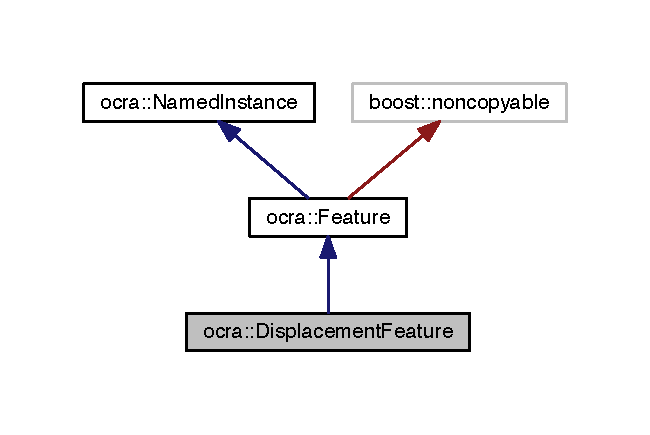
\includegraphics[width=312pt]{d3/d4f/classocra_1_1DisplacementFeature__inherit__graph}
\end{center}
\end{figure}


Collaboration diagram for ocra\+:\+:Displacement\+Feature\+:\nopagebreak
\begin{figure}[H]
\begin{center}
\leavevmode
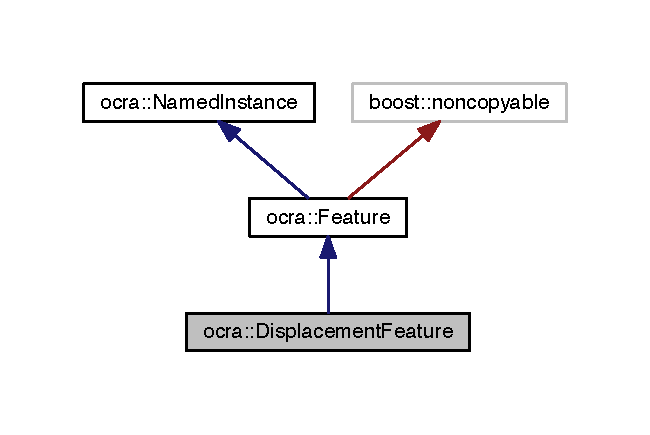
\includegraphics[width=312pt]{da/d53/classocra_1_1DisplacementFeature__coll__graph}
\end{center}
\end{figure}
\subsection*{Classes}
\begin{DoxyCompactItemize}
\item 
struct \hyperlink{structocra_1_1DisplacementFeature_1_1Pimpl}{Pimpl}
\end{DoxyCompactItemize}
\subsection*{Public Member Functions}
\begin{DoxyCompactItemize}
\item 
\hyperlink{classocra_1_1DisplacementFeature_a9c48bb5ac5d4a856df9c2d879bc4b072}{Displacement\+Feature} (const std\+::string \&name, Control\+Frame\+::\+Ptr frame, \hyperlink{namespaceocra_a436781c7059a0f76027df1c652126260}{E\+Cartesian\+Dof} axes)
\item 
int \hyperlink{classocra_1_1DisplacementFeature_a5d6548c921c2ce61374d3f76114b7881}{get\+Dimension} () const
\item 
const Eigen\+::\+Matrix\+Xd \& \hyperlink{classocra_1_1DisplacementFeature_ad27f4aa83abea99ef893de6043b0bf68}{get\+Space\+Transform} () const
\item 
const Eigen\+::\+Vector\+Xd \& \hyperlink{classocra_1_1DisplacementFeature_a328fae77ec8a9942881e42226250a11b}{compute\+Effort} (const \hyperlink{classocra_1_1Feature}{Feature} \&feature\+Des) const
\item 
const Eigen\+::\+Vector\+Xd \& \hyperlink{classocra_1_1DisplacementFeature_a622cd1b7305b26fbbb2f78784fd0ebf0}{compute\+Acceleration} (const \hyperlink{classocra_1_1Feature}{Feature} \&feature\+Des) const
\item 
const Eigen\+::\+Vector\+Xd \& \hyperlink{classocra_1_1DisplacementFeature_a61d1caacf56e60bb3f33d2c91d5b89f2}{compute\+Error} (const \hyperlink{classocra_1_1Feature}{Feature} \&feature\+Des) const
\item 
const Eigen\+::\+Vector\+Xd \& \hyperlink{classocra_1_1DisplacementFeature_afd5e272957274c46a6331c2a3d3324df}{compute\+Error\+Dot} (const \hyperlink{classocra_1_1Feature}{Feature} \&feature\+Des) const
\item 
const Eigen\+::\+Matrix\+Xd \& \hyperlink{classocra_1_1DisplacementFeature_a87b3ef89ea6711a3f953f94e5cdf7e4d}{compute\+Jacobian} (const \hyperlink{classocra_1_1Feature}{Feature} \&feature\+Des) const
\item 
const Eigen\+::\+Matrix\+Xd \& \hyperlink{classocra_1_1DisplacementFeature_a3c72ecae0cb33a812c66b0770baf09bf}{compute\+Projected\+Mass} (const \hyperlink{classocra_1_1Feature}{Feature} \&feature\+Des) const
\item 
const Eigen\+::\+Matrix\+Xd \& \hyperlink{classocra_1_1DisplacementFeature_a4b2e46d41b46c9af72f21f6dcdeec5f5}{compute\+Projected\+Mass\+Inverse} (const \hyperlink{classocra_1_1Feature}{Feature} \&feature\+Des) const
\item 
const Eigen\+::\+Vector\+Xd \& \hyperlink{classocra_1_1DisplacementFeature_aee1c2f5af98c28e8d6ab3dbeb5c3c297}{compute\+Effort} () const
\item 
const Eigen\+::\+Vector\+Xd \& \hyperlink{classocra_1_1DisplacementFeature_a1f2fa6644359c3897ac8d3e4e06c5f81}{compute\+Acceleration} () const
\item 
const Eigen\+::\+Vector\+Xd \& \hyperlink{classocra_1_1DisplacementFeature_ac0520f1a870558227ba6d5339a243414}{compute\+Error} () const
\item 
const Eigen\+::\+Vector\+Xd \& \hyperlink{classocra_1_1DisplacementFeature_a684821d2a83945c63661eacdf4bcd262}{compute\+Error\+Dot} () const
\item 
const Eigen\+::\+Matrix\+Xd \& \hyperlink{classocra_1_1DisplacementFeature_a87e2abee5d1072e142dcab99193699da}{compute\+Jacobian} () const
\item 
const Eigen\+::\+Matrix\+Xd \& \hyperlink{classocra_1_1DisplacementFeature_a31902186d804823eea5ba0177ed85ced}{compute\+Projected\+Mass} () const
\item 
const Eigen\+::\+Matrix\+Xd \& \hyperlink{classocra_1_1DisplacementFeature_a3639d72ab7b85ac4b9533ed6498c0c03}{compute\+Projected\+Mass\+Inverse} () const
\item 
\hyperlink{classocra_1_1TaskState}{Task\+State} \hyperlink{classocra_1_1DisplacementFeature_a3940d5c27ee1845c65f4be6ad3a27e50}{get\+State} () const
\item 
void \hyperlink{classocra_1_1DisplacementFeature_a7a99c7e57d512ec2d6094fc10388e033}{set\+State} (const \hyperlink{classocra_1_1TaskState}{Task\+State} \&new\+State)
\end{DoxyCompactItemize}
\subsection*{Additional Inherited Members}


\subsection{Detailed Description}
Used to build position/orientation tasks. 

These features combine position and orientation features, to control both the position and orientation of a control frame. See the documentation of \hyperlink{classocra_1_1PositionFeature}{Position\+Feature} and \hyperlink{classocra_1_1OrientationFeature}{Orientation\+Feature}. 

Definition at line 235 of file Feature.\+h.



\subsection{Constructor \& Destructor Documentation}
\hypertarget{classocra_1_1DisplacementFeature_a9c48bb5ac5d4a856df9c2d879bc4b072}{}\label{classocra_1_1DisplacementFeature_a9c48bb5ac5d4a856df9c2d879bc4b072} 
\index{ocra\+::\+Displacement\+Feature@{ocra\+::\+Displacement\+Feature}!Displacement\+Feature@{Displacement\+Feature}}
\index{Displacement\+Feature@{Displacement\+Feature}!ocra\+::\+Displacement\+Feature@{ocra\+::\+Displacement\+Feature}}
\subsubsection{\texorpdfstring{Displacement\+Feature()}{DisplacementFeature()}}
{\footnotesize\ttfamily ocra\+::\+Displacement\+Feature\+::\+Displacement\+Feature (\begin{DoxyParamCaption}\item[{const std\+::string \&}]{name,  }\item[{Control\+Frame\+::\+Ptr}]{frame,  }\item[{\hyperlink{namespaceocra_a436781c7059a0f76027df1c652126260}{E\+Cartesian\+Dof}}]{axes }\end{DoxyParamCaption})}



Definition at line 722 of file Feature.\+cpp.



\subsection{Member Function Documentation}
\hypertarget{classocra_1_1DisplacementFeature_a622cd1b7305b26fbbb2f78784fd0ebf0}{}\label{classocra_1_1DisplacementFeature_a622cd1b7305b26fbbb2f78784fd0ebf0} 
\index{ocra\+::\+Displacement\+Feature@{ocra\+::\+Displacement\+Feature}!compute\+Acceleration@{compute\+Acceleration}}
\index{compute\+Acceleration@{compute\+Acceleration}!ocra\+::\+Displacement\+Feature@{ocra\+::\+Displacement\+Feature}}
\subsubsection{\texorpdfstring{compute\+Acceleration()}{computeAcceleration()}\hspace{0.1cm}{\footnotesize\ttfamily [1/2]}}
{\footnotesize\ttfamily const Vector\+Xd \& ocra\+::\+Displacement\+Feature\+::compute\+Acceleration (\begin{DoxyParamCaption}\item[{const \hyperlink{classocra_1_1Feature}{Feature} \&}]{feature\+Des }\end{DoxyParamCaption}) const\hspace{0.3cm}{\ttfamily [virtual]}}



Implements \hyperlink{classocra_1_1Feature_a4a5973d27459d2dececec8dc73038df8}{ocra\+::\+Feature}.



Definition at line 775 of file Feature.\+cpp.

\hypertarget{classocra_1_1DisplacementFeature_a1f2fa6644359c3897ac8d3e4e06c5f81}{}\label{classocra_1_1DisplacementFeature_a1f2fa6644359c3897ac8d3e4e06c5f81} 
\index{ocra\+::\+Displacement\+Feature@{ocra\+::\+Displacement\+Feature}!compute\+Acceleration@{compute\+Acceleration}}
\index{compute\+Acceleration@{compute\+Acceleration}!ocra\+::\+Displacement\+Feature@{ocra\+::\+Displacement\+Feature}}
\subsubsection{\texorpdfstring{compute\+Acceleration()}{computeAcceleration()}\hspace{0.1cm}{\footnotesize\ttfamily [2/2]}}
{\footnotesize\ttfamily const Vector\+Xd \& ocra\+::\+Displacement\+Feature\+::compute\+Acceleration (\begin{DoxyParamCaption}{ }\end{DoxyParamCaption}) const\hspace{0.3cm}{\ttfamily [virtual]}}



Implements \hyperlink{classocra_1_1Feature_aa42b61d4255116caa92042d01ca36b79}{ocra\+::\+Feature}.



Definition at line 801 of file Feature.\+cpp.

\hypertarget{classocra_1_1DisplacementFeature_a328fae77ec8a9942881e42226250a11b}{}\label{classocra_1_1DisplacementFeature_a328fae77ec8a9942881e42226250a11b} 
\index{ocra\+::\+Displacement\+Feature@{ocra\+::\+Displacement\+Feature}!compute\+Effort@{compute\+Effort}}
\index{compute\+Effort@{compute\+Effort}!ocra\+::\+Displacement\+Feature@{ocra\+::\+Displacement\+Feature}}
\subsubsection{\texorpdfstring{compute\+Effort()}{computeEffort()}\hspace{0.1cm}{\footnotesize\ttfamily [1/2]}}
{\footnotesize\ttfamily const Vector\+Xd \& ocra\+::\+Displacement\+Feature\+::compute\+Effort (\begin{DoxyParamCaption}\item[{const \hyperlink{classocra_1_1Feature}{Feature} \&}]{feature\+Des }\end{DoxyParamCaption}) const\hspace{0.3cm}{\ttfamily [virtual]}}



Implements \hyperlink{classocra_1_1Feature_a19626a241666fdae253af1f7b6f2acd7}{ocra\+::\+Feature}.



Definition at line 743 of file Feature.\+cpp.

\hypertarget{classocra_1_1DisplacementFeature_aee1c2f5af98c28e8d6ab3dbeb5c3c297}{}\label{classocra_1_1DisplacementFeature_aee1c2f5af98c28e8d6ab3dbeb5c3c297} 
\index{ocra\+::\+Displacement\+Feature@{ocra\+::\+Displacement\+Feature}!compute\+Effort@{compute\+Effort}}
\index{compute\+Effort@{compute\+Effort}!ocra\+::\+Displacement\+Feature@{ocra\+::\+Displacement\+Feature}}
\subsubsection{\texorpdfstring{compute\+Effort()}{computeEffort()}\hspace{0.1cm}{\footnotesize\ttfamily [2/2]}}
{\footnotesize\ttfamily const Vector\+Xd \& ocra\+::\+Displacement\+Feature\+::compute\+Effort (\begin{DoxyParamCaption}{ }\end{DoxyParamCaption}) const\hspace{0.3cm}{\ttfamily [virtual]}}



Implements \hyperlink{classocra_1_1Feature_ae43f2ffc54862d6ddc0b02fd39431eb6}{ocra\+::\+Feature}.



Definition at line 761 of file Feature.\+cpp.

\hypertarget{classocra_1_1DisplacementFeature_a61d1caacf56e60bb3f33d2c91d5b89f2}{}\label{classocra_1_1DisplacementFeature_a61d1caacf56e60bb3f33d2c91d5b89f2} 
\index{ocra\+::\+Displacement\+Feature@{ocra\+::\+Displacement\+Feature}!compute\+Error@{compute\+Error}}
\index{compute\+Error@{compute\+Error}!ocra\+::\+Displacement\+Feature@{ocra\+::\+Displacement\+Feature}}
\subsubsection{\texorpdfstring{compute\+Error()}{computeError()}\hspace{0.1cm}{\footnotesize\ttfamily [1/2]}}
{\footnotesize\ttfamily const Vector\+Xd \& ocra\+::\+Displacement\+Feature\+::compute\+Error (\begin{DoxyParamCaption}\item[{const \hyperlink{classocra_1_1Feature}{Feature} \&}]{feature\+Des }\end{DoxyParamCaption}) const\hspace{0.3cm}{\ttfamily [virtual]}}



Implements \hyperlink{classocra_1_1Feature_aaa74d6869f7e574fcc39d443581ddf77}{ocra\+::\+Feature}.



Definition at line 816 of file Feature.\+cpp.

\hypertarget{classocra_1_1DisplacementFeature_ac0520f1a870558227ba6d5339a243414}{}\label{classocra_1_1DisplacementFeature_ac0520f1a870558227ba6d5339a243414} 
\index{ocra\+::\+Displacement\+Feature@{ocra\+::\+Displacement\+Feature}!compute\+Error@{compute\+Error}}
\index{compute\+Error@{compute\+Error}!ocra\+::\+Displacement\+Feature@{ocra\+::\+Displacement\+Feature}}
\subsubsection{\texorpdfstring{compute\+Error()}{computeError()}\hspace{0.1cm}{\footnotesize\ttfamily [2/2]}}
{\footnotesize\ttfamily const Vector\+Xd \& ocra\+::\+Displacement\+Feature\+::compute\+Error (\begin{DoxyParamCaption}{ }\end{DoxyParamCaption}) const\hspace{0.3cm}{\ttfamily [virtual]}}



Implements \hyperlink{classocra_1_1Feature_a88f87b496aedc7bf9f13b19bb8f9c7fa}{ocra\+::\+Feature}.



Definition at line 836 of file Feature.\+cpp.

\hypertarget{classocra_1_1DisplacementFeature_afd5e272957274c46a6331c2a3d3324df}{}\label{classocra_1_1DisplacementFeature_afd5e272957274c46a6331c2a3d3324df} 
\index{ocra\+::\+Displacement\+Feature@{ocra\+::\+Displacement\+Feature}!compute\+Error\+Dot@{compute\+Error\+Dot}}
\index{compute\+Error\+Dot@{compute\+Error\+Dot}!ocra\+::\+Displacement\+Feature@{ocra\+::\+Displacement\+Feature}}
\subsubsection{\texorpdfstring{compute\+Error\+Dot()}{computeErrorDot()}\hspace{0.1cm}{\footnotesize\ttfamily [1/2]}}
{\footnotesize\ttfamily const Vector\+Xd \& ocra\+::\+Displacement\+Feature\+::compute\+Error\+Dot (\begin{DoxyParamCaption}\item[{const \hyperlink{classocra_1_1Feature}{Feature} \&}]{feature\+Des }\end{DoxyParamCaption}) const\hspace{0.3cm}{\ttfamily [virtual]}}



Implements \hyperlink{classocra_1_1Feature_ac714181e1bb25f878349e299c4ba8c00}{ocra\+::\+Feature}.



Definition at line 851 of file Feature.\+cpp.

\hypertarget{classocra_1_1DisplacementFeature_a684821d2a83945c63661eacdf4bcd262}{}\label{classocra_1_1DisplacementFeature_a684821d2a83945c63661eacdf4bcd262} 
\index{ocra\+::\+Displacement\+Feature@{ocra\+::\+Displacement\+Feature}!compute\+Error\+Dot@{compute\+Error\+Dot}}
\index{compute\+Error\+Dot@{compute\+Error\+Dot}!ocra\+::\+Displacement\+Feature@{ocra\+::\+Displacement\+Feature}}
\subsubsection{\texorpdfstring{compute\+Error\+Dot()}{computeErrorDot()}\hspace{0.1cm}{\footnotesize\ttfamily [2/2]}}
{\footnotesize\ttfamily const Vector\+Xd \& ocra\+::\+Displacement\+Feature\+::compute\+Error\+Dot (\begin{DoxyParamCaption}{ }\end{DoxyParamCaption}) const\hspace{0.3cm}{\ttfamily [virtual]}}



Implements \hyperlink{classocra_1_1Feature_a01a4870418ba87d5b41d8f917c1255fc}{ocra\+::\+Feature}.



Definition at line 873 of file Feature.\+cpp.

\hypertarget{classocra_1_1DisplacementFeature_a87b3ef89ea6711a3f953f94e5cdf7e4d}{}\label{classocra_1_1DisplacementFeature_a87b3ef89ea6711a3f953f94e5cdf7e4d} 
\index{ocra\+::\+Displacement\+Feature@{ocra\+::\+Displacement\+Feature}!compute\+Jacobian@{compute\+Jacobian}}
\index{compute\+Jacobian@{compute\+Jacobian}!ocra\+::\+Displacement\+Feature@{ocra\+::\+Displacement\+Feature}}
\subsubsection{\texorpdfstring{compute\+Jacobian()}{computeJacobian()}\hspace{0.1cm}{\footnotesize\ttfamily [1/2]}}
{\footnotesize\ttfamily const Matrix\+Xd \& ocra\+::\+Displacement\+Feature\+::compute\+Jacobian (\begin{DoxyParamCaption}\item[{const \hyperlink{classocra_1_1Feature}{Feature} \&}]{feature\+Des }\end{DoxyParamCaption}) const\hspace{0.3cm}{\ttfamily [virtual]}}



Implements \hyperlink{classocra_1_1Feature_a4fb8eeeed978a1f727ec43cd1bd18d78}{ocra\+::\+Feature}.



Definition at line 890 of file Feature.\+cpp.

\hypertarget{classocra_1_1DisplacementFeature_a87e2abee5d1072e142dcab99193699da}{}\label{classocra_1_1DisplacementFeature_a87e2abee5d1072e142dcab99193699da} 
\index{ocra\+::\+Displacement\+Feature@{ocra\+::\+Displacement\+Feature}!compute\+Jacobian@{compute\+Jacobian}}
\index{compute\+Jacobian@{compute\+Jacobian}!ocra\+::\+Displacement\+Feature@{ocra\+::\+Displacement\+Feature}}
\subsubsection{\texorpdfstring{compute\+Jacobian()}{computeJacobian()}\hspace{0.1cm}{\footnotesize\ttfamily [2/2]}}
{\footnotesize\ttfamily const Matrix\+Xd \& ocra\+::\+Displacement\+Feature\+::compute\+Jacobian (\begin{DoxyParamCaption}{ }\end{DoxyParamCaption}) const\hspace{0.3cm}{\ttfamily [virtual]}}



Implements \hyperlink{classocra_1_1Feature_adbab3b388657555abb805bb971c2491f}{ocra\+::\+Feature}.



Definition at line 911 of file Feature.\+cpp.

\hypertarget{classocra_1_1DisplacementFeature_a3c72ecae0cb33a812c66b0770baf09bf}{}\label{classocra_1_1DisplacementFeature_a3c72ecae0cb33a812c66b0770baf09bf} 
\index{ocra\+::\+Displacement\+Feature@{ocra\+::\+Displacement\+Feature}!compute\+Projected\+Mass@{compute\+Projected\+Mass}}
\index{compute\+Projected\+Mass@{compute\+Projected\+Mass}!ocra\+::\+Displacement\+Feature@{ocra\+::\+Displacement\+Feature}}
\subsubsection{\texorpdfstring{compute\+Projected\+Mass()}{computeProjectedMass()}\hspace{0.1cm}{\footnotesize\ttfamily [1/2]}}
{\footnotesize\ttfamily const Matrix\+Xd \& ocra\+::\+Displacement\+Feature\+::compute\+Projected\+Mass (\begin{DoxyParamCaption}\item[{const \hyperlink{classocra_1_1Feature}{Feature} \&}]{feature\+Des }\end{DoxyParamCaption}) const\hspace{0.3cm}{\ttfamily [virtual]}}



Implements \hyperlink{classocra_1_1Feature_a44e11dd349e92971fefebff354e7214b}{ocra\+::\+Feature}.



Definition at line 927 of file Feature.\+cpp.

\hypertarget{classocra_1_1DisplacementFeature_a31902186d804823eea5ba0177ed85ced}{}\label{classocra_1_1DisplacementFeature_a31902186d804823eea5ba0177ed85ced} 
\index{ocra\+::\+Displacement\+Feature@{ocra\+::\+Displacement\+Feature}!compute\+Projected\+Mass@{compute\+Projected\+Mass}}
\index{compute\+Projected\+Mass@{compute\+Projected\+Mass}!ocra\+::\+Displacement\+Feature@{ocra\+::\+Displacement\+Feature}}
\subsubsection{\texorpdfstring{compute\+Projected\+Mass()}{computeProjectedMass()}\hspace{0.1cm}{\footnotesize\ttfamily [2/2]}}
{\footnotesize\ttfamily const Matrix\+Xd \& ocra\+::\+Displacement\+Feature\+::compute\+Projected\+Mass (\begin{DoxyParamCaption}{ }\end{DoxyParamCaption}) const\hspace{0.3cm}{\ttfamily [virtual]}}



Implements \hyperlink{classocra_1_1Feature_a99ac023809c0cf34b5d582537934b08c}{ocra\+::\+Feature}.



Definition at line 937 of file Feature.\+cpp.

\hypertarget{classocra_1_1DisplacementFeature_a4b2e46d41b46c9af72f21f6dcdeec5f5}{}\label{classocra_1_1DisplacementFeature_a4b2e46d41b46c9af72f21f6dcdeec5f5} 
\index{ocra\+::\+Displacement\+Feature@{ocra\+::\+Displacement\+Feature}!compute\+Projected\+Mass\+Inverse@{compute\+Projected\+Mass\+Inverse}}
\index{compute\+Projected\+Mass\+Inverse@{compute\+Projected\+Mass\+Inverse}!ocra\+::\+Displacement\+Feature@{ocra\+::\+Displacement\+Feature}}
\subsubsection{\texorpdfstring{compute\+Projected\+Mass\+Inverse()}{computeProjectedMassInverse()}\hspace{0.1cm}{\footnotesize\ttfamily [1/2]}}
{\footnotesize\ttfamily const Matrix\+Xd \& ocra\+::\+Displacement\+Feature\+::compute\+Projected\+Mass\+Inverse (\begin{DoxyParamCaption}\item[{const \hyperlink{classocra_1_1Feature}{Feature} \&}]{feature\+Des }\end{DoxyParamCaption}) const\hspace{0.3cm}{\ttfamily [virtual]}}



Implements \hyperlink{classocra_1_1Feature_ac529096b3fe8eba1ab88a56d8b042d37}{ocra\+::\+Feature}.



Definition at line 947 of file Feature.\+cpp.

\hypertarget{classocra_1_1DisplacementFeature_a3639d72ab7b85ac4b9533ed6498c0c03}{}\label{classocra_1_1DisplacementFeature_a3639d72ab7b85ac4b9533ed6498c0c03} 
\index{ocra\+::\+Displacement\+Feature@{ocra\+::\+Displacement\+Feature}!compute\+Projected\+Mass\+Inverse@{compute\+Projected\+Mass\+Inverse}}
\index{compute\+Projected\+Mass\+Inverse@{compute\+Projected\+Mass\+Inverse}!ocra\+::\+Displacement\+Feature@{ocra\+::\+Displacement\+Feature}}
\subsubsection{\texorpdfstring{compute\+Projected\+Mass\+Inverse()}{computeProjectedMassInverse()}\hspace{0.1cm}{\footnotesize\ttfamily [2/2]}}
{\footnotesize\ttfamily const Matrix\+Xd \& ocra\+::\+Displacement\+Feature\+::compute\+Projected\+Mass\+Inverse (\begin{DoxyParamCaption}{ }\end{DoxyParamCaption}) const\hspace{0.3cm}{\ttfamily [virtual]}}



Implements \hyperlink{classocra_1_1Feature_ac27bcbdbb8541e3b4e2c77a6d6f2ffc0}{ocra\+::\+Feature}.



Definition at line 959 of file Feature.\+cpp.

\hypertarget{classocra_1_1DisplacementFeature_a5d6548c921c2ce61374d3f76114b7881}{}\label{classocra_1_1DisplacementFeature_a5d6548c921c2ce61374d3f76114b7881} 
\index{ocra\+::\+Displacement\+Feature@{ocra\+::\+Displacement\+Feature}!get\+Dimension@{get\+Dimension}}
\index{get\+Dimension@{get\+Dimension}!ocra\+::\+Displacement\+Feature@{ocra\+::\+Displacement\+Feature}}
\subsubsection{\texorpdfstring{get\+Dimension()}{getDimension()}}
{\footnotesize\ttfamily int ocra\+::\+Displacement\+Feature\+::get\+Dimension (\begin{DoxyParamCaption}{ }\end{DoxyParamCaption}) const\hspace{0.3cm}{\ttfamily [virtual]}}



Implements \hyperlink{classocra_1_1Feature_aeda4c2a5ffe638c3de30f8b91a11450e}{ocra\+::\+Feature}.



Definition at line 738 of file Feature.\+cpp.

\hypertarget{classocra_1_1DisplacementFeature_ad27f4aa83abea99ef893de6043b0bf68}{}\label{classocra_1_1DisplacementFeature_ad27f4aa83abea99ef893de6043b0bf68} 
\index{ocra\+::\+Displacement\+Feature@{ocra\+::\+Displacement\+Feature}!get\+Space\+Transform@{get\+Space\+Transform}}
\index{get\+Space\+Transform@{get\+Space\+Transform}!ocra\+::\+Displacement\+Feature@{ocra\+::\+Displacement\+Feature}}
\subsubsection{\texorpdfstring{get\+Space\+Transform()}{getSpaceTransform()}}
{\footnotesize\ttfamily const Matrix\+Xd \& ocra\+::\+Displacement\+Feature\+::get\+Space\+Transform (\begin{DoxyParamCaption}{ }\end{DoxyParamCaption}) const\hspace{0.3cm}{\ttfamily [virtual]}}



Implements \hyperlink{classocra_1_1Feature_a77eb324fb4da91fd50d0e761d2453ff3}{ocra\+::\+Feature}.



Definition at line 728 of file Feature.\+cpp.

\hypertarget{classocra_1_1DisplacementFeature_a3940d5c27ee1845c65f4be6ad3a27e50}{}\label{classocra_1_1DisplacementFeature_a3940d5c27ee1845c65f4be6ad3a27e50} 
\index{ocra\+::\+Displacement\+Feature@{ocra\+::\+Displacement\+Feature}!get\+State@{get\+State}}
\index{get\+State@{get\+State}!ocra\+::\+Displacement\+Feature@{ocra\+::\+Displacement\+Feature}}
\subsubsection{\texorpdfstring{get\+State()}{getState()}}
{\footnotesize\ttfamily \hyperlink{classocra_1_1TaskState}{Task\+State} ocra\+::\+Displacement\+Feature\+::get\+State (\begin{DoxyParamCaption}{ }\end{DoxyParamCaption}) const\hspace{0.3cm}{\ttfamily [virtual]}}



Implements \hyperlink{classocra_1_1Feature_a792434ceb793f25874b8fe42ae24c475}{ocra\+::\+Feature}.



Definition at line 970 of file Feature.\+cpp.

\hypertarget{classocra_1_1DisplacementFeature_a7a99c7e57d512ec2d6094fc10388e033}{}\label{classocra_1_1DisplacementFeature_a7a99c7e57d512ec2d6094fc10388e033} 
\index{ocra\+::\+Displacement\+Feature@{ocra\+::\+Displacement\+Feature}!set\+State@{set\+State}}
\index{set\+State@{set\+State}!ocra\+::\+Displacement\+Feature@{ocra\+::\+Displacement\+Feature}}
\subsubsection{\texorpdfstring{set\+State()}{setState()}}
{\footnotesize\ttfamily void ocra\+::\+Displacement\+Feature\+::set\+State (\begin{DoxyParamCaption}\item[{const \hyperlink{classocra_1_1TaskState}{Task\+State} \&}]{new\+State }\end{DoxyParamCaption})\hspace{0.3cm}{\ttfamily [virtual]}}



Implements \hyperlink{classocra_1_1Feature_ad16d6b176b229280649ab405531e9a30}{ocra\+::\+Feature}.



Definition at line 981 of file Feature.\+cpp.



The documentation for this class was generated from the following files\+:\begin{DoxyCompactItemize}
\item 
\hyperlink{Feature_8h}{Feature.\+h}\item 
\hyperlink{Feature_8cpp}{Feature.\+cpp}\end{DoxyCompactItemize}

\hypertarget{classocra_1_1DotProductFunction}{}\section{ocra\+:\+:Dot\+Product\+Function Class Reference}
\label{classocra_1_1DotProductFunction}\index{ocra\+::\+Dot\+Product\+Function@{ocra\+::\+Dot\+Product\+Function}}


Dot\+Product\+Function class.  




{\ttfamily \#include $<$Dot\+Product\+Function.\+h$>$}

Inheritance diagram for ocra\+:\+:Dot\+Product\+Function\+:\begin{figure}[H]
\begin{center}
\leavevmode
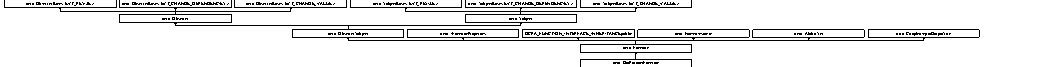
\includegraphics[height=0.901771cm]{db/da4/classocra_1_1DotProductFunction}
\end{center}
\end{figure}
\subsection*{Public Types}
\begin{DoxyCompactItemize}
\item 
typedef \hyperlink{classocra_1_1Function}{Function} \hyperlink{classocra_1_1DotProductFunction_abdc60b6380ffedc075792224bd908c48}{function\+Type\+\_\+t}
\end{DoxyCompactItemize}
\subsection*{Public Member Functions}
\begin{DoxyCompactItemize}
\item 
\hyperlink{classocra_1_1DotProductFunction_a70f7d2b9c9fefba0203fbee84607c9e9}{Dot\+Product\+Function} (\hyperlink{classocra_1_1Function}{Function} $\ast$f1, \hyperlink{classocra_1_1Function}{Function} $\ast$f2)
\item 
\hyperlink{classocra_1_1DotProductFunction_a369a245fec0cfe2d4f72bfd577ab7ad0}{Dot\+Product\+Function} (\hyperlink{classocra_1_1Function}{Function} $\ast$f, const Vector \&v)
\item 
void \hyperlink{classocra_1_1DotProductFunction_a2c7c65e80d7fb5ac1da43421a792f77b}{changeV} (const Vector \&v)
\end{DoxyCompactItemize}
\subsection*{Protected Member Functions}
\begin{DoxyCompactItemize}
\item 
virtual void \hyperlink{classocra_1_1DotProductFunction_ac0dcd9911e638ebcd8e9594dbf0fa9ed}{compute\+Value} (void) const
\item 
virtual void \hyperlink{classocra_1_1DotProductFunction_af088997b35bf792a1f1c9c6fb78c0fe1}{compute\+Gradient} (void) const
\item 
virtual void \hyperlink{classocra_1_1DotProductFunction_a97dcdd721c76f80cb20e257aca4f8a58}{compute\+Hessian} (void) const
\item 
virtual void \hyperlink{classocra_1_1DotProductFunction_a707474c43d42fad3a8c5bbd896ca8f4b}{compute\+Jdot} (void) const
\item 
virtual void \hyperlink{classocra_1_1DotProductFunction_a07f6a0a7e676a8849732f3469d70bcae}{compute\+Jdot\+Xdot} (void) const
\item 
virtual void \hyperlink{classocra_1_1DotProductFunction_af943f9e456e44b3cbe108a964697f239}{do\+Update\+Size} (void)
\end{DoxyCompactItemize}
\subsection*{Protected Attributes}
\begin{DoxyCompactItemize}
\item 
bool \hyperlink{classocra_1_1DotProductFunction_a8450996eff9607045cf57a4502ff0944}{\+\_\+two\+Functions}
\item 
\hyperlink{classocra_1_1Function}{Function} $\ast$ \hyperlink{classocra_1_1DotProductFunction_a3e39a9ce09fc27131afbe8e7a6758681}{\+\_\+f1}
\item 
\hyperlink{classocra_1_1Function}{Function} $\ast$ \hyperlink{classocra_1_1DotProductFunction_a7de350aefad539fdd84453b11019e936}{\+\_\+f2}
\item 
Vector \hyperlink{classocra_1_1DotProductFunction_a6405d1f78159e5fc16801bd73eb32a68}{\+\_\+v}
\item 
Vector \hyperlink{classocra_1_1DotProductFunction_a82d2cb16e4b9b6d50e59fabfb25fc222}{\+\_\+tmp}
\end{DoxyCompactItemize}
\subsection*{Additional Inherited Members}


\subsection{Detailed Description}
Dot\+Product\+Function class. 

\begin{DoxyWarning}{Warning}
None
\end{DoxyWarning}
scalar product between two vectors that can either be \hyperlink{classocra_1_1Function}{Function} output or contant 

Definition at line 29 of file Dot\+Product\+Function.\+h.



\subsection{Member Typedef Documentation}
\hypertarget{classocra_1_1DotProductFunction_abdc60b6380ffedc075792224bd908c48}{}\label{classocra_1_1DotProductFunction_abdc60b6380ffedc075792224bd908c48} 
\index{ocra\+::\+Dot\+Product\+Function@{ocra\+::\+Dot\+Product\+Function}!function\+Type\+\_\+t@{function\+Type\+\_\+t}}
\index{function\+Type\+\_\+t@{function\+Type\+\_\+t}!ocra\+::\+Dot\+Product\+Function@{ocra\+::\+Dot\+Product\+Function}}
\subsubsection{\texorpdfstring{function\+Type\+\_\+t}{functionType\_t}}
{\footnotesize\ttfamily typedef \hyperlink{classocra_1_1Function}{Function} \hyperlink{classocra_1_1DotProductFunction_abdc60b6380ffedc075792224bd908c48}{ocra\+::\+Dot\+Product\+Function\+::function\+Type\+\_\+t}}



Definition at line 33 of file Dot\+Product\+Function.\+h.



\subsection{Constructor \& Destructor Documentation}
\hypertarget{classocra_1_1DotProductFunction_a70f7d2b9c9fefba0203fbee84607c9e9}{}\label{classocra_1_1DotProductFunction_a70f7d2b9c9fefba0203fbee84607c9e9} 
\index{ocra\+::\+Dot\+Product\+Function@{ocra\+::\+Dot\+Product\+Function}!Dot\+Product\+Function@{Dot\+Product\+Function}}
\index{Dot\+Product\+Function@{Dot\+Product\+Function}!ocra\+::\+Dot\+Product\+Function@{ocra\+::\+Dot\+Product\+Function}}
\subsubsection{\texorpdfstring{Dot\+Product\+Function()}{DotProductFunction()}\hspace{0.1cm}{\footnotesize\ttfamily [1/2]}}
{\footnotesize\ttfamily ocra\+::\+Dot\+Product\+Function\+::\+Dot\+Product\+Function (\begin{DoxyParamCaption}\item[{\hyperlink{classocra_1_1Function}{Function} $\ast$}]{f1,  }\item[{\hyperlink{classocra_1_1Function}{Function} $\ast$}]{f2 }\end{DoxyParamCaption})}

\hypertarget{classocra_1_1DotProductFunction_a369a245fec0cfe2d4f72bfd577ab7ad0}{}\label{classocra_1_1DotProductFunction_a369a245fec0cfe2d4f72bfd577ab7ad0} 
\index{ocra\+::\+Dot\+Product\+Function@{ocra\+::\+Dot\+Product\+Function}!Dot\+Product\+Function@{Dot\+Product\+Function}}
\index{Dot\+Product\+Function@{Dot\+Product\+Function}!ocra\+::\+Dot\+Product\+Function@{ocra\+::\+Dot\+Product\+Function}}
\subsubsection{\texorpdfstring{Dot\+Product\+Function()}{DotProductFunction()}\hspace{0.1cm}{\footnotesize\ttfamily [2/2]}}
{\footnotesize\ttfamily ocra\+::\+Dot\+Product\+Function\+::\+Dot\+Product\+Function (\begin{DoxyParamCaption}\item[{\hyperlink{classocra_1_1Function}{Function} $\ast$}]{f,  }\item[{const Vector \&}]{v }\end{DoxyParamCaption})}



\subsection{Member Function Documentation}
\hypertarget{classocra_1_1DotProductFunction_a2c7c65e80d7fb5ac1da43421a792f77b}{}\label{classocra_1_1DotProductFunction_a2c7c65e80d7fb5ac1da43421a792f77b} 
\index{ocra\+::\+Dot\+Product\+Function@{ocra\+::\+Dot\+Product\+Function}!changeV@{changeV}}
\index{changeV@{changeV}!ocra\+::\+Dot\+Product\+Function@{ocra\+::\+Dot\+Product\+Function}}
\subsubsection{\texorpdfstring{change\+V()}{changeV()}}
{\footnotesize\ttfamily void ocra\+::\+Dot\+Product\+Function\+::changeV (\begin{DoxyParamCaption}\item[{const Vector \&}]{v }\end{DoxyParamCaption})}

\hypertarget{classocra_1_1DotProductFunction_af088997b35bf792a1f1c9c6fb78c0fe1}{}\label{classocra_1_1DotProductFunction_af088997b35bf792a1f1c9c6fb78c0fe1} 
\index{ocra\+::\+Dot\+Product\+Function@{ocra\+::\+Dot\+Product\+Function}!compute\+Gradient@{compute\+Gradient}}
\index{compute\+Gradient@{compute\+Gradient}!ocra\+::\+Dot\+Product\+Function@{ocra\+::\+Dot\+Product\+Function}}
\subsubsection{\texorpdfstring{compute\+Gradient()}{computeGradient()}}
{\footnotesize\ttfamily virtual void ocra\+::\+Dot\+Product\+Function\+::compute\+Gradient (\begin{DoxyParamCaption}\item[{void}]{ }\end{DoxyParamCaption}) const\hspace{0.3cm}{\ttfamily [protected]}, {\ttfamily [virtual]}}

\hypertarget{classocra_1_1DotProductFunction_a97dcdd721c76f80cb20e257aca4f8a58}{}\label{classocra_1_1DotProductFunction_a97dcdd721c76f80cb20e257aca4f8a58} 
\index{ocra\+::\+Dot\+Product\+Function@{ocra\+::\+Dot\+Product\+Function}!compute\+Hessian@{compute\+Hessian}}
\index{compute\+Hessian@{compute\+Hessian}!ocra\+::\+Dot\+Product\+Function@{ocra\+::\+Dot\+Product\+Function}}
\subsubsection{\texorpdfstring{compute\+Hessian()}{computeHessian()}}
{\footnotesize\ttfamily virtual void ocra\+::\+Dot\+Product\+Function\+::compute\+Hessian (\begin{DoxyParamCaption}\item[{void}]{ }\end{DoxyParamCaption}) const\hspace{0.3cm}{\ttfamily [protected]}, {\ttfamily [virtual]}}

\hypertarget{classocra_1_1DotProductFunction_a707474c43d42fad3a8c5bbd896ca8f4b}{}\label{classocra_1_1DotProductFunction_a707474c43d42fad3a8c5bbd896ca8f4b} 
\index{ocra\+::\+Dot\+Product\+Function@{ocra\+::\+Dot\+Product\+Function}!compute\+Jdot@{compute\+Jdot}}
\index{compute\+Jdot@{compute\+Jdot}!ocra\+::\+Dot\+Product\+Function@{ocra\+::\+Dot\+Product\+Function}}
\subsubsection{\texorpdfstring{compute\+Jdot()}{computeJdot()}}
{\footnotesize\ttfamily virtual void ocra\+::\+Dot\+Product\+Function\+::compute\+Jdot (\begin{DoxyParamCaption}\item[{void}]{ }\end{DoxyParamCaption}) const\hspace{0.3cm}{\ttfamily [protected]}, {\ttfamily [virtual]}}

\hypertarget{classocra_1_1DotProductFunction_a07f6a0a7e676a8849732f3469d70bcae}{}\label{classocra_1_1DotProductFunction_a07f6a0a7e676a8849732f3469d70bcae} 
\index{ocra\+::\+Dot\+Product\+Function@{ocra\+::\+Dot\+Product\+Function}!compute\+Jdot\+Xdot@{compute\+Jdot\+Xdot}}
\index{compute\+Jdot\+Xdot@{compute\+Jdot\+Xdot}!ocra\+::\+Dot\+Product\+Function@{ocra\+::\+Dot\+Product\+Function}}
\subsubsection{\texorpdfstring{compute\+Jdot\+Xdot()}{computeJdotXdot()}}
{\footnotesize\ttfamily virtual void ocra\+::\+Dot\+Product\+Function\+::compute\+Jdot\+Xdot (\begin{DoxyParamCaption}\item[{void}]{ }\end{DoxyParamCaption}) const\hspace{0.3cm}{\ttfamily [protected]}, {\ttfamily [virtual]}}

\hypertarget{classocra_1_1DotProductFunction_ac0dcd9911e638ebcd8e9594dbf0fa9ed}{}\label{classocra_1_1DotProductFunction_ac0dcd9911e638ebcd8e9594dbf0fa9ed} 
\index{ocra\+::\+Dot\+Product\+Function@{ocra\+::\+Dot\+Product\+Function}!compute\+Value@{compute\+Value}}
\index{compute\+Value@{compute\+Value}!ocra\+::\+Dot\+Product\+Function@{ocra\+::\+Dot\+Product\+Function}}
\subsubsection{\texorpdfstring{compute\+Value()}{computeValue()}}
{\footnotesize\ttfamily virtual void ocra\+::\+Dot\+Product\+Function\+::compute\+Value (\begin{DoxyParamCaption}\item[{void}]{ }\end{DoxyParamCaption}) const\hspace{0.3cm}{\ttfamily [protected]}, {\ttfamily [virtual]}}

\hypertarget{classocra_1_1DotProductFunction_af943f9e456e44b3cbe108a964697f239}{}\label{classocra_1_1DotProductFunction_af943f9e456e44b3cbe108a964697f239} 
\index{ocra\+::\+Dot\+Product\+Function@{ocra\+::\+Dot\+Product\+Function}!do\+Update\+Size@{do\+Update\+Size}}
\index{do\+Update\+Size@{do\+Update\+Size}!ocra\+::\+Dot\+Product\+Function@{ocra\+::\+Dot\+Product\+Function}}
\subsubsection{\texorpdfstring{do\+Update\+Size()}{doUpdateSize()}}
{\footnotesize\ttfamily virtual void ocra\+::\+Dot\+Product\+Function\+::do\+Update\+Size (\begin{DoxyParamCaption}\item[{void}]{ }\end{DoxyParamCaption})\hspace{0.3cm}{\ttfamily [protected]}, {\ttfamily [virtual]}}



\subsection{Member Data Documentation}
\hypertarget{classocra_1_1DotProductFunction_a3e39a9ce09fc27131afbe8e7a6758681}{}\label{classocra_1_1DotProductFunction_a3e39a9ce09fc27131afbe8e7a6758681} 
\index{ocra\+::\+Dot\+Product\+Function@{ocra\+::\+Dot\+Product\+Function}!\+\_\+f1@{\+\_\+f1}}
\index{\+\_\+f1@{\+\_\+f1}!ocra\+::\+Dot\+Product\+Function@{ocra\+::\+Dot\+Product\+Function}}
\subsubsection{\texorpdfstring{\+\_\+f1}{\_f1}}
{\footnotesize\ttfamily \hyperlink{classocra_1_1Function}{Function}$\ast$ ocra\+::\+Dot\+Product\+Function\+::\+\_\+f1\hspace{0.3cm}{\ttfamily [protected]}}



Definition at line 82 of file Dot\+Product\+Function.\+h.

\hypertarget{classocra_1_1DotProductFunction_a7de350aefad539fdd84453b11019e936}{}\label{classocra_1_1DotProductFunction_a7de350aefad539fdd84453b11019e936} 
\index{ocra\+::\+Dot\+Product\+Function@{ocra\+::\+Dot\+Product\+Function}!\+\_\+f2@{\+\_\+f2}}
\index{\+\_\+f2@{\+\_\+f2}!ocra\+::\+Dot\+Product\+Function@{ocra\+::\+Dot\+Product\+Function}}
\subsubsection{\texorpdfstring{\+\_\+f2}{\_f2}}
{\footnotesize\ttfamily \hyperlink{classocra_1_1Function}{Function}$\ast$ ocra\+::\+Dot\+Product\+Function\+::\+\_\+f2\hspace{0.3cm}{\ttfamily [protected]}}



Definition at line 83 of file Dot\+Product\+Function.\+h.

\hypertarget{classocra_1_1DotProductFunction_a82d2cb16e4b9b6d50e59fabfb25fc222}{}\label{classocra_1_1DotProductFunction_a82d2cb16e4b9b6d50e59fabfb25fc222} 
\index{ocra\+::\+Dot\+Product\+Function@{ocra\+::\+Dot\+Product\+Function}!\+\_\+tmp@{\+\_\+tmp}}
\index{\+\_\+tmp@{\+\_\+tmp}!ocra\+::\+Dot\+Product\+Function@{ocra\+::\+Dot\+Product\+Function}}
\subsubsection{\texorpdfstring{\+\_\+tmp}{\_tmp}}
{\footnotesize\ttfamily Vector ocra\+::\+Dot\+Product\+Function\+::\+\_\+tmp\hspace{0.3cm}{\ttfamily [mutable]}, {\ttfamily [protected]}}



Definition at line 85 of file Dot\+Product\+Function.\+h.

\hypertarget{classocra_1_1DotProductFunction_a8450996eff9607045cf57a4502ff0944}{}\label{classocra_1_1DotProductFunction_a8450996eff9607045cf57a4502ff0944} 
\index{ocra\+::\+Dot\+Product\+Function@{ocra\+::\+Dot\+Product\+Function}!\+\_\+two\+Functions@{\+\_\+two\+Functions}}
\index{\+\_\+two\+Functions@{\+\_\+two\+Functions}!ocra\+::\+Dot\+Product\+Function@{ocra\+::\+Dot\+Product\+Function}}
\subsubsection{\texorpdfstring{\+\_\+two\+Functions}{\_twoFunctions}}
{\footnotesize\ttfamily bool ocra\+::\+Dot\+Product\+Function\+::\+\_\+two\+Functions\hspace{0.3cm}{\ttfamily [protected]}}



Definition at line 81 of file Dot\+Product\+Function.\+h.

\hypertarget{classocra_1_1DotProductFunction_a6405d1f78159e5fc16801bd73eb32a68}{}\label{classocra_1_1DotProductFunction_a6405d1f78159e5fc16801bd73eb32a68} 
\index{ocra\+::\+Dot\+Product\+Function@{ocra\+::\+Dot\+Product\+Function}!\+\_\+v@{\+\_\+v}}
\index{\+\_\+v@{\+\_\+v}!ocra\+::\+Dot\+Product\+Function@{ocra\+::\+Dot\+Product\+Function}}
\subsubsection{\texorpdfstring{\+\_\+v}{\_v}}
{\footnotesize\ttfamily Vector ocra\+::\+Dot\+Product\+Function\+::\+\_\+v\hspace{0.3cm}{\ttfamily [protected]}}



Definition at line 84 of file Dot\+Product\+Function.\+h.



The documentation for this class was generated from the following file\+:\begin{DoxyCompactItemize}
\item 
\hyperlink{DotProductFunction_8h}{Dot\+Product\+Function.\+h}\end{DoxyCompactItemize}

\hypertarget{classocra_1_1DoubleDiagonalLinearFunction}{}\section{ocra\+:\+:Double\+Diagonal\+Linear\+Function Class Reference}
\label{classocra_1_1DoubleDiagonalLinearFunction}\index{ocra\+::\+Double\+Diagonal\+Linear\+Function@{ocra\+::\+Double\+Diagonal\+Linear\+Function}}


Double\+Diagonal\+Linear\+Function class.  




{\ttfamily \#include $<$Double\+Diagonal\+Linear\+Function.\+h$>$}

Inheritance diagram for ocra\+:\+:Double\+Diagonal\+Linear\+Function\+:\begin{figure}[H]
\begin{center}
\leavevmode
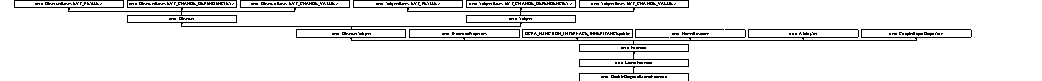
\includegraphics[height=1.082126cm]{d4/d5c/classocra_1_1DoubleDiagonalLinearFunction}
\end{center}
\end{figure}
\subsection*{Public Types}
\begin{DoxyCompactItemize}
\item 
typedef \hyperlink{classocra_1_1LinearFunction}{Linear\+Function} \hyperlink{classocra_1_1DoubleDiagonalLinearFunction_a69a17b7aa1e34b31ac1cc18cca3a3b38}{function\+Type\+\_\+t}
\end{DoxyCompactItemize}
\subsection*{Public Member Functions}
\begin{DoxyCompactItemize}
\item 
{\footnotesize template$<$class Vector\+Base1 , class Vector\+Base2 , class Vector\+Base3 $>$ }\\\hyperlink{classocra_1_1DoubleDiagonalLinearFunction_a790df03af5df25353682965f7a556aec}{Double\+Diagonal\+Linear\+Function} (\hyperlink{classocra_1_1Variable}{Variable} \&\hyperlink{classocra_1_1Function_a28825886d1f149c87b112ec2ec1dd486}{x}, const Vector\+Base1 \&d1, const Vector\+Base2 \&d2, const Vector\+Base3 \&b, const bool use\+Default\+Value=false, const double default\+Diag\+Value1=1., const double default\+Diag\+Value2=1., const double defaultb\+Value=0.)
\item 
{\footnotesize template$<$class Vector\+Base $>$ }\\\hyperlink{classocra_1_1DoubleDiagonalLinearFunction_a96c59d997d8ec798745389d98c2d5e63}{Double\+Diagonal\+Linear\+Function} (\hyperlink{classocra_1_1Variable}{Variable} \&\hyperlink{classocra_1_1Function_a28825886d1f149c87b112ec2ec1dd486}{x}, const double diagonal\+Element\+Value1, const double diagonal\+Element\+Value2, const Vector\+Base \&b, const bool use\+Default\+Value=false, const double defaultb\+Value=0.)
\item 
{\footnotesize template$<$class Vector\+Base1 , class Vector\+Base2 $>$ }\\\hyperlink{classocra_1_1DoubleDiagonalLinearFunction_a7403903ccd31cec18bf665aefd1f4900}{Double\+Diagonal\+Linear\+Function} (\hyperlink{classocra_1_1Variable}{Variable} \&\hyperlink{classocra_1_1Function_a28825886d1f149c87b112ec2ec1dd486}{x}, const Vector\+Base1 \&d1, const Vector\+Base2 \&d2, const double vector\+Element\+Value, const bool use\+Default\+Value=false, const double default\+Value1=1., const double default\+Value2=1.)
\item 
\hyperlink{classocra_1_1DoubleDiagonalLinearFunction_aa46fa50d5728569eb834438dfd3a9228}{Double\+Diagonal\+Linear\+Function} (\hyperlink{classocra_1_1Variable}{Variable} \&\hyperlink{classocra_1_1Function_a28825886d1f149c87b112ec2ec1dd486}{x}, const double diagonal\+Element\+Value1, const double diagonal\+Element\+Value2, const double vector\+Element\+Value, const bool use\+Default\+Value=false)
\item 
const Vector\+Xd \& \hyperlink{classocra_1_1DoubleDiagonalLinearFunction_a7d1cea2c8b94bc70854377779b49c966}{get\+Diagonal1} () const
\item 
const Vector\+Xd \& \hyperlink{classocra_1_1DoubleDiagonalLinearFunction_a764b18fae37fa4dd6ecff2240c583a90}{get\+Diagonal2} () const
\item 
double \hyperlink{classocra_1_1DoubleDiagonalLinearFunction_a9093eef2a34b3c96b9510794b91279cc}{get\+Default\+Diagonal\+Value1} () const
\item 
double \hyperlink{classocra_1_1DoubleDiagonalLinearFunction_a3593bb0fc409844b8d30e4785565c389}{get\+Default\+Diagonal\+Value2} () const
\item 
double \hyperlink{classocra_1_1DoubleDiagonalLinearFunction_a51c22f2f4a7ae45bf61d5ee36345acb4}{get\+Defaultb\+Value} () const
\item 
bool \hyperlink{classocra_1_1DoubleDiagonalLinearFunction_a8a20ef8ec7347cdd86b630c33eed3e9e}{is\+Using\+Default\+Value} () const
\item 
virtual void \hyperlink{classocra_1_1DoubleDiagonalLinearFunction_aa49e6964582aa9da6c02bacb68937e4d}{change\+Diagonal1} (const Vector\+Xd \&d)
\item 
virtual void \hyperlink{classocra_1_1DoubleDiagonalLinearFunction_aa6ec35d1e7abf6300e7ba37e42c3b467}{change\+Diagonal2} (const Vector\+Xd \&d)
\item 
virtual void \hyperlink{classocra_1_1DoubleDiagonalLinearFunction_ace71385fd62acf0749cbcf96a0477868}{change\+Diagonal1} (const double diagonal\+Element\+Value, const bool change\+Default=true)
\item 
virtual void \hyperlink{classocra_1_1DoubleDiagonalLinearFunction_a1a9ec0f7bb11ae2f1ddd6dffceea8921}{change\+Diagonal2} (const double diagonal\+Element\+Value, const bool change\+Default=true)
\item 
virtual void \hyperlink{classocra_1_1DoubleDiagonalLinearFunction_a982adc5313b550ac6fa3b420051a9505}{change\+Default\+Diagonal\+Value1} (const double v)
\item 
virtual void \hyperlink{classocra_1_1DoubleDiagonalLinearFunction_a1380c4f6f99af312d2eae2b0355be4cc}{change\+Default\+Diagonal\+Value2} (const double v)
\item 
virtual void \hyperlink{classocra_1_1DoubleDiagonalLinearFunction_a8af650affad3759e7a069d0cabcd4c2e}{change\+Defaultb\+Value} (const double v)
\end{DoxyCompactItemize}
\subsection*{Protected Member Functions}
\begin{DoxyCompactItemize}
\item 
virtual void \hyperlink{classocra_1_1DoubleDiagonalLinearFunction_aee6f818b93d5832a21aa439f13510a49}{update\+Value} () const
\item 
virtual void \hyperlink{classocra_1_1DoubleDiagonalLinearFunction_a91fd529bf34bffd327fcd545035bec67}{do\+Update\+Input\+Size\+Begin} ()
\item 
virtual void \hyperlink{classocra_1_1DoubleDiagonalLinearFunction_a89070f8f2b068d8b6b3e216433e50538}{do\+Update\+Input\+Size\+End} ()
\item 
virtual void \hyperlink{classocra_1_1DoubleDiagonalLinearFunction_a55bd813c1f86402eea01bb403c6257bb}{do\+ChangeA} (const Matrix\+Xd \&A)
\item 
int \hyperlink{classocra_1_1DoubleDiagonalLinearFunction_af449f5bb219672d4f316a0d626436ec8}{compute\+Dimension\+From\+Input\+Size} () const
\item 
void \hyperlink{classocra_1_1DoubleDiagonalLinearFunction_af834599e9b414f8778e0618efc552661}{do\+Update\+Dimension\+Begin} (int new\+Dimension)
\end{DoxyCompactItemize}
\subsection*{Protected Attributes}
\begin{DoxyCompactItemize}
\item 
Vector\+Xd \hyperlink{classocra_1_1DoubleDiagonalLinearFunction_aff7e6eb0c3c53e0799909ab76d279d0a}{\+\_\+d1}
\item 
Vector\+Xd \hyperlink{classocra_1_1DoubleDiagonalLinearFunction_a043b9a5dba8b0d42b00deed8898c1843}{\+\_\+d2}
\item 
double \hyperlink{classocra_1_1DoubleDiagonalLinearFunction_a7e4daebabaa357edeb050b1a2e08868f}{\+\_\+default\+Diagonal\+Value1}
\item 
double \hyperlink{classocra_1_1DoubleDiagonalLinearFunction_ac94bc900b6847f9203adcde9d96c20d9}{\+\_\+default\+Diagonal\+Value2}
\item 
double \hyperlink{classocra_1_1DoubleDiagonalLinearFunction_a24ebbdd1093941e346c6931f23d3193f}{\+\_\+defaultb\+Value}
\item 
bool \hyperlink{classocra_1_1DoubleDiagonalLinearFunction_afbb8120fd4b8bda14ee829c78b6cc817}{\+\_\+use\+Default\+Value}
\end{DoxyCompactItemize}
\subsection*{Additional Inherited Members}


\subsection{Detailed Description}
Double\+Diagonal\+Linear\+Function class. 

\begin{DoxyWarning}{Warning}
None
\end{DoxyWarning}
Equivalent as two \hyperlink{classocra_1_1DiagonalLinearFunction}{Diagonal\+Linear\+Function} side by side 

Definition at line 32 of file Double\+Diagonal\+Linear\+Function.\+h.



\subsection{Member Typedef Documentation}
\hypertarget{classocra_1_1DoubleDiagonalLinearFunction_a69a17b7aa1e34b31ac1cc18cca3a3b38}{}\label{classocra_1_1DoubleDiagonalLinearFunction_a69a17b7aa1e34b31ac1cc18cca3a3b38} 
\index{ocra\+::\+Double\+Diagonal\+Linear\+Function@{ocra\+::\+Double\+Diagonal\+Linear\+Function}!function\+Type\+\_\+t@{function\+Type\+\_\+t}}
\index{function\+Type\+\_\+t@{function\+Type\+\_\+t}!ocra\+::\+Double\+Diagonal\+Linear\+Function@{ocra\+::\+Double\+Diagonal\+Linear\+Function}}
\subsubsection{\texorpdfstring{function\+Type\+\_\+t}{functionType\_t}}
{\footnotesize\ttfamily typedef \hyperlink{classocra_1_1LinearFunction}{Linear\+Function} \hyperlink{classocra_1_1DoubleDiagonalLinearFunction_a69a17b7aa1e34b31ac1cc18cca3a3b38}{ocra\+::\+Double\+Diagonal\+Linear\+Function\+::function\+Type\+\_\+t}}



Definition at line 36 of file Double\+Diagonal\+Linear\+Function.\+h.



\subsection{Constructor \& Destructor Documentation}
\hypertarget{classocra_1_1DoubleDiagonalLinearFunction_a790df03af5df25353682965f7a556aec}{}\label{classocra_1_1DoubleDiagonalLinearFunction_a790df03af5df25353682965f7a556aec} 
\index{ocra\+::\+Double\+Diagonal\+Linear\+Function@{ocra\+::\+Double\+Diagonal\+Linear\+Function}!Double\+Diagonal\+Linear\+Function@{Double\+Diagonal\+Linear\+Function}}
\index{Double\+Diagonal\+Linear\+Function@{Double\+Diagonal\+Linear\+Function}!ocra\+::\+Double\+Diagonal\+Linear\+Function@{ocra\+::\+Double\+Diagonal\+Linear\+Function}}
\subsubsection{\texorpdfstring{Double\+Diagonal\+Linear\+Function()}{DoubleDiagonalLinearFunction()}\hspace{0.1cm}{\footnotesize\ttfamily [1/4]}}
{\footnotesize\ttfamily template$<$class Vector\+Base1 , class Vector\+Base2 , class Vector\+Base3 $>$ \\
ocra\+::\+Double\+Diagonal\+Linear\+Function\+::\+Double\+Diagonal\+Linear\+Function (\begin{DoxyParamCaption}\item[{\hyperlink{classocra_1_1Variable}{Variable} \&}]{x,  }\item[{const Vector\+Base1 \&}]{d1,  }\item[{const Vector\+Base2 \&}]{d2,  }\item[{const Vector\+Base3 \&}]{b,  }\item[{const bool}]{use\+Default\+Value = {\ttfamily false},  }\item[{const double}]{default\+Diag\+Value1 = {\ttfamily 1.},  }\item[{const double}]{default\+Diag\+Value2 = {\ttfamily 1.},  }\item[{const double}]{defaultb\+Value = {\ttfamily 0.} }\end{DoxyParamCaption})\hspace{0.3cm}{\ttfamily [inline]}}



Definition at line 107 of file Double\+Diagonal\+Linear\+Function.\+h.

\hypertarget{classocra_1_1DoubleDiagonalLinearFunction_a96c59d997d8ec798745389d98c2d5e63}{}\label{classocra_1_1DoubleDiagonalLinearFunction_a96c59d997d8ec798745389d98c2d5e63} 
\index{ocra\+::\+Double\+Diagonal\+Linear\+Function@{ocra\+::\+Double\+Diagonal\+Linear\+Function}!Double\+Diagonal\+Linear\+Function@{Double\+Diagonal\+Linear\+Function}}
\index{Double\+Diagonal\+Linear\+Function@{Double\+Diagonal\+Linear\+Function}!ocra\+::\+Double\+Diagonal\+Linear\+Function@{ocra\+::\+Double\+Diagonal\+Linear\+Function}}
\subsubsection{\texorpdfstring{Double\+Diagonal\+Linear\+Function()}{DoubleDiagonalLinearFunction()}\hspace{0.1cm}{\footnotesize\ttfamily [2/4]}}
{\footnotesize\ttfamily template$<$class Vector\+Base $>$ \\
ocra\+::\+Double\+Diagonal\+Linear\+Function\+::\+Double\+Diagonal\+Linear\+Function (\begin{DoxyParamCaption}\item[{\hyperlink{classocra_1_1Variable}{Variable} \&}]{x,  }\item[{const double}]{diagonal\+Element\+Value1,  }\item[{const double}]{diagonal\+Element\+Value2,  }\item[{const Vector\+Base \&}]{b,  }\item[{const bool}]{use\+Default\+Value = {\ttfamily false},  }\item[{const double}]{defaultb\+Value = {\ttfamily 0.} }\end{DoxyParamCaption})\hspace{0.3cm}{\ttfamily [inline]}}



Definition at line 144 of file Double\+Diagonal\+Linear\+Function.\+h.

\hypertarget{classocra_1_1DoubleDiagonalLinearFunction_a7403903ccd31cec18bf665aefd1f4900}{}\label{classocra_1_1DoubleDiagonalLinearFunction_a7403903ccd31cec18bf665aefd1f4900} 
\index{ocra\+::\+Double\+Diagonal\+Linear\+Function@{ocra\+::\+Double\+Diagonal\+Linear\+Function}!Double\+Diagonal\+Linear\+Function@{Double\+Diagonal\+Linear\+Function}}
\index{Double\+Diagonal\+Linear\+Function@{Double\+Diagonal\+Linear\+Function}!ocra\+::\+Double\+Diagonal\+Linear\+Function@{ocra\+::\+Double\+Diagonal\+Linear\+Function}}
\subsubsection{\texorpdfstring{Double\+Diagonal\+Linear\+Function()}{DoubleDiagonalLinearFunction()}\hspace{0.1cm}{\footnotesize\ttfamily [3/4]}}
{\footnotesize\ttfamily template$<$class Vector\+Base1 , class Vector\+Base2 $>$ \\
ocra\+::\+Double\+Diagonal\+Linear\+Function\+::\+Double\+Diagonal\+Linear\+Function (\begin{DoxyParamCaption}\item[{\hyperlink{classocra_1_1Variable}{Variable} \&}]{x,  }\item[{const Vector\+Base1 \&}]{d1,  }\item[{const Vector\+Base2 \&}]{d2,  }\item[{const double}]{vector\+Element\+Value,  }\item[{const bool}]{use\+Default\+Value = {\ttfamily false},  }\item[{const double}]{default\+Value1 = {\ttfamily 1.},  }\item[{const double}]{default\+Value2 = {\ttfamily 1.} }\end{DoxyParamCaption})\hspace{0.3cm}{\ttfamily [inline]}}



Definition at line 172 of file Double\+Diagonal\+Linear\+Function.\+h.

\hypertarget{classocra_1_1DoubleDiagonalLinearFunction_aa46fa50d5728569eb834438dfd3a9228}{}\label{classocra_1_1DoubleDiagonalLinearFunction_aa46fa50d5728569eb834438dfd3a9228} 
\index{ocra\+::\+Double\+Diagonal\+Linear\+Function@{ocra\+::\+Double\+Diagonal\+Linear\+Function}!Double\+Diagonal\+Linear\+Function@{Double\+Diagonal\+Linear\+Function}}
\index{Double\+Diagonal\+Linear\+Function@{Double\+Diagonal\+Linear\+Function}!ocra\+::\+Double\+Diagonal\+Linear\+Function@{ocra\+::\+Double\+Diagonal\+Linear\+Function}}
\subsubsection{\texorpdfstring{Double\+Diagonal\+Linear\+Function()}{DoubleDiagonalLinearFunction()}\hspace{0.1cm}{\footnotesize\ttfamily [4/4]}}
{\footnotesize\ttfamily ocra\+::\+Double\+Diagonal\+Linear\+Function\+::\+Double\+Diagonal\+Linear\+Function (\begin{DoxyParamCaption}\item[{\hyperlink{classocra_1_1Variable}{Variable} \&}]{x,  }\item[{const double}]{diagonal\+Element\+Value1,  }\item[{const double}]{diagonal\+Element\+Value2,  }\item[{const double}]{vector\+Element\+Value,  }\item[{const bool}]{use\+Default\+Value = {\ttfamily false} }\end{DoxyParamCaption})}



Definition at line 5 of file Double\+Diagonal\+Linear\+Function.\+cpp.



\subsection{Member Function Documentation}
\hypertarget{classocra_1_1DoubleDiagonalLinearFunction_a8af650affad3759e7a069d0cabcd4c2e}{}\label{classocra_1_1DoubleDiagonalLinearFunction_a8af650affad3759e7a069d0cabcd4c2e} 
\index{ocra\+::\+Double\+Diagonal\+Linear\+Function@{ocra\+::\+Double\+Diagonal\+Linear\+Function}!change\+Defaultb\+Value@{change\+Defaultb\+Value}}
\index{change\+Defaultb\+Value@{change\+Defaultb\+Value}!ocra\+::\+Double\+Diagonal\+Linear\+Function@{ocra\+::\+Double\+Diagonal\+Linear\+Function}}
\subsubsection{\texorpdfstring{change\+Defaultb\+Value()}{changeDefaultbValue()}}
{\footnotesize\ttfamily void ocra\+::\+Double\+Diagonal\+Linear\+Function\+::change\+Defaultb\+Value (\begin{DoxyParamCaption}\item[{const double}]{v }\end{DoxyParamCaption})\hspace{0.3cm}{\ttfamily [virtual]}}



Definition at line 69 of file Double\+Diagonal\+Linear\+Function.\+cpp.

\hypertarget{classocra_1_1DoubleDiagonalLinearFunction_a982adc5313b550ac6fa3b420051a9505}{}\label{classocra_1_1DoubleDiagonalLinearFunction_a982adc5313b550ac6fa3b420051a9505} 
\index{ocra\+::\+Double\+Diagonal\+Linear\+Function@{ocra\+::\+Double\+Diagonal\+Linear\+Function}!change\+Default\+Diagonal\+Value1@{change\+Default\+Diagonal\+Value1}}
\index{change\+Default\+Diagonal\+Value1@{change\+Default\+Diagonal\+Value1}!ocra\+::\+Double\+Diagonal\+Linear\+Function@{ocra\+::\+Double\+Diagonal\+Linear\+Function}}
\subsubsection{\texorpdfstring{change\+Default\+Diagonal\+Value1()}{changeDefaultDiagonalValue1()}}
{\footnotesize\ttfamily void ocra\+::\+Double\+Diagonal\+Linear\+Function\+::change\+Default\+Diagonal\+Value1 (\begin{DoxyParamCaption}\item[{const double}]{v }\end{DoxyParamCaption})\hspace{0.3cm}{\ttfamily [virtual]}}



Definition at line 59 of file Double\+Diagonal\+Linear\+Function.\+cpp.

\hypertarget{classocra_1_1DoubleDiagonalLinearFunction_a1380c4f6f99af312d2eae2b0355be4cc}{}\label{classocra_1_1DoubleDiagonalLinearFunction_a1380c4f6f99af312d2eae2b0355be4cc} 
\index{ocra\+::\+Double\+Diagonal\+Linear\+Function@{ocra\+::\+Double\+Diagonal\+Linear\+Function}!change\+Default\+Diagonal\+Value2@{change\+Default\+Diagonal\+Value2}}
\index{change\+Default\+Diagonal\+Value2@{change\+Default\+Diagonal\+Value2}!ocra\+::\+Double\+Diagonal\+Linear\+Function@{ocra\+::\+Double\+Diagonal\+Linear\+Function}}
\subsubsection{\texorpdfstring{change\+Default\+Diagonal\+Value2()}{changeDefaultDiagonalValue2()}}
{\footnotesize\ttfamily void ocra\+::\+Double\+Diagonal\+Linear\+Function\+::change\+Default\+Diagonal\+Value2 (\begin{DoxyParamCaption}\item[{const double}]{v }\end{DoxyParamCaption})\hspace{0.3cm}{\ttfamily [virtual]}}



Definition at line 64 of file Double\+Diagonal\+Linear\+Function.\+cpp.

\hypertarget{classocra_1_1DoubleDiagonalLinearFunction_aa49e6964582aa9da6c02bacb68937e4d}{}\label{classocra_1_1DoubleDiagonalLinearFunction_aa49e6964582aa9da6c02bacb68937e4d} 
\index{ocra\+::\+Double\+Diagonal\+Linear\+Function@{ocra\+::\+Double\+Diagonal\+Linear\+Function}!change\+Diagonal1@{change\+Diagonal1}}
\index{change\+Diagonal1@{change\+Diagonal1}!ocra\+::\+Double\+Diagonal\+Linear\+Function@{ocra\+::\+Double\+Diagonal\+Linear\+Function}}
\subsubsection{\texorpdfstring{change\+Diagonal1()}{changeDiagonal1()}\hspace{0.1cm}{\footnotesize\ttfamily [1/2]}}
{\footnotesize\ttfamily void ocra\+::\+Double\+Diagonal\+Linear\+Function\+::change\+Diagonal1 (\begin{DoxyParamCaption}\item[{const Vector\+Xd \&}]{d }\end{DoxyParamCaption})\hspace{0.3cm}{\ttfamily [virtual]}}



Definition at line 27 of file Double\+Diagonal\+Linear\+Function.\+cpp.

\hypertarget{classocra_1_1DoubleDiagonalLinearFunction_ace71385fd62acf0749cbcf96a0477868}{}\label{classocra_1_1DoubleDiagonalLinearFunction_ace71385fd62acf0749cbcf96a0477868} 
\index{ocra\+::\+Double\+Diagonal\+Linear\+Function@{ocra\+::\+Double\+Diagonal\+Linear\+Function}!change\+Diagonal1@{change\+Diagonal1}}
\index{change\+Diagonal1@{change\+Diagonal1}!ocra\+::\+Double\+Diagonal\+Linear\+Function@{ocra\+::\+Double\+Diagonal\+Linear\+Function}}
\subsubsection{\texorpdfstring{change\+Diagonal1()}{changeDiagonal1()}\hspace{0.1cm}{\footnotesize\ttfamily [2/2]}}
{\footnotesize\ttfamily void ocra\+::\+Double\+Diagonal\+Linear\+Function\+::change\+Diagonal1 (\begin{DoxyParamCaption}\item[{const double}]{diagonal\+Element\+Value,  }\item[{const bool}]{change\+Default = {\ttfamily true} }\end{DoxyParamCaption})\hspace{0.3cm}{\ttfamily [virtual]}}



Definition at line 43 of file Double\+Diagonal\+Linear\+Function.\+cpp.

\hypertarget{classocra_1_1DoubleDiagonalLinearFunction_aa6ec35d1e7abf6300e7ba37e42c3b467}{}\label{classocra_1_1DoubleDiagonalLinearFunction_aa6ec35d1e7abf6300e7ba37e42c3b467} 
\index{ocra\+::\+Double\+Diagonal\+Linear\+Function@{ocra\+::\+Double\+Diagonal\+Linear\+Function}!change\+Diagonal2@{change\+Diagonal2}}
\index{change\+Diagonal2@{change\+Diagonal2}!ocra\+::\+Double\+Diagonal\+Linear\+Function@{ocra\+::\+Double\+Diagonal\+Linear\+Function}}
\subsubsection{\texorpdfstring{change\+Diagonal2()}{changeDiagonal2()}\hspace{0.1cm}{\footnotesize\ttfamily [1/2]}}
{\footnotesize\ttfamily void ocra\+::\+Double\+Diagonal\+Linear\+Function\+::change\+Diagonal2 (\begin{DoxyParamCaption}\item[{const Vector\+Xd \&}]{d }\end{DoxyParamCaption})\hspace{0.3cm}{\ttfamily [virtual]}}



Definition at line 35 of file Double\+Diagonal\+Linear\+Function.\+cpp.

\hypertarget{classocra_1_1DoubleDiagonalLinearFunction_a1a9ec0f7bb11ae2f1ddd6dffceea8921}{}\label{classocra_1_1DoubleDiagonalLinearFunction_a1a9ec0f7bb11ae2f1ddd6dffceea8921} 
\index{ocra\+::\+Double\+Diagonal\+Linear\+Function@{ocra\+::\+Double\+Diagonal\+Linear\+Function}!change\+Diagonal2@{change\+Diagonal2}}
\index{change\+Diagonal2@{change\+Diagonal2}!ocra\+::\+Double\+Diagonal\+Linear\+Function@{ocra\+::\+Double\+Diagonal\+Linear\+Function}}
\subsubsection{\texorpdfstring{change\+Diagonal2()}{changeDiagonal2()}\hspace{0.1cm}{\footnotesize\ttfamily [2/2]}}
{\footnotesize\ttfamily void ocra\+::\+Double\+Diagonal\+Linear\+Function\+::change\+Diagonal2 (\begin{DoxyParamCaption}\item[{const double}]{diagonal\+Element\+Value,  }\item[{const bool}]{change\+Default = {\ttfamily true} }\end{DoxyParamCaption})\hspace{0.3cm}{\ttfamily [virtual]}}



Definition at line 51 of file Double\+Diagonal\+Linear\+Function.\+cpp.

\hypertarget{classocra_1_1DoubleDiagonalLinearFunction_af449f5bb219672d4f316a0d626436ec8}{}\label{classocra_1_1DoubleDiagonalLinearFunction_af449f5bb219672d4f316a0d626436ec8} 
\index{ocra\+::\+Double\+Diagonal\+Linear\+Function@{ocra\+::\+Double\+Diagonal\+Linear\+Function}!compute\+Dimension\+From\+Input\+Size@{compute\+Dimension\+From\+Input\+Size}}
\index{compute\+Dimension\+From\+Input\+Size@{compute\+Dimension\+From\+Input\+Size}!ocra\+::\+Double\+Diagonal\+Linear\+Function@{ocra\+::\+Double\+Diagonal\+Linear\+Function}}
\subsubsection{\texorpdfstring{compute\+Dimension\+From\+Input\+Size()}{computeDimensionFromInputSize()}}
{\footnotesize\ttfamily int ocra\+::\+Double\+Diagonal\+Linear\+Function\+::compute\+Dimension\+From\+Input\+Size (\begin{DoxyParamCaption}{ }\end{DoxyParamCaption}) const\hspace{0.3cm}{\ttfamily [protected]}, {\ttfamily [virtual]}}

Does what it tells... 

Reimplemented from \hyperlink{classocra_1_1Function_a95241fd426f887c5eb3add3f1e55a09c}{ocra\+::\+Function}.



Definition at line 131 of file Double\+Diagonal\+Linear\+Function.\+cpp.

\hypertarget{classocra_1_1DoubleDiagonalLinearFunction_a55bd813c1f86402eea01bb403c6257bb}{}\label{classocra_1_1DoubleDiagonalLinearFunction_a55bd813c1f86402eea01bb403c6257bb} 
\index{ocra\+::\+Double\+Diagonal\+Linear\+Function@{ocra\+::\+Double\+Diagonal\+Linear\+Function}!do\+ChangeA@{do\+ChangeA}}
\index{do\+ChangeA@{do\+ChangeA}!ocra\+::\+Double\+Diagonal\+Linear\+Function@{ocra\+::\+Double\+Diagonal\+Linear\+Function}}
\subsubsection{\texorpdfstring{do\+Change\+A()}{doChangeA()}}
{\footnotesize\ttfamily void ocra\+::\+Double\+Diagonal\+Linear\+Function\+::do\+ChangeA (\begin{DoxyParamCaption}\item[{const Matrix\+Xd \&}]{A }\end{DoxyParamCaption})\hspace{0.3cm}{\ttfamily [protected]}, {\ttfamily [virtual]}}

Methods to be called in ChangeA and Change b 

Reimplemented from \hyperlink{classocra_1_1LinearFunction_ab573c2f615d2edefb647979d3cc3cf46}{ocra\+::\+Linear\+Function}.



Definition at line 74 of file Double\+Diagonal\+Linear\+Function.\+cpp.

\hypertarget{classocra_1_1DoubleDiagonalLinearFunction_af834599e9b414f8778e0618efc552661}{}\label{classocra_1_1DoubleDiagonalLinearFunction_af834599e9b414f8778e0618efc552661} 
\index{ocra\+::\+Double\+Diagonal\+Linear\+Function@{ocra\+::\+Double\+Diagonal\+Linear\+Function}!do\+Update\+Dimension\+Begin@{do\+Update\+Dimension\+Begin}}
\index{do\+Update\+Dimension\+Begin@{do\+Update\+Dimension\+Begin}!ocra\+::\+Double\+Diagonal\+Linear\+Function@{ocra\+::\+Double\+Diagonal\+Linear\+Function}}
\subsubsection{\texorpdfstring{do\+Update\+Dimension\+Begin()}{doUpdateDimensionBegin()}}
{\footnotesize\ttfamily void ocra\+::\+Double\+Diagonal\+Linear\+Function\+::do\+Update\+Dimension\+Begin (\begin{DoxyParamCaption}\item[{int}]{new\+Dimension }\end{DoxyParamCaption})\hspace{0.3cm}{\ttfamily [protected]}, {\ttfamily [virtual]}}

Methods for pre and post update in case the dimension of the function has changed. Default implementation of do\+Update\+Dimension\+End does nothing, do\+Update\+Dimension\+Begin throws an exception. These methods might throw exceptions when overloaded. Furthermore, {\ttfamily \hyperlink{classocra_1_1Function_a17aa280f0e6eff4a7569edc373a5147d}{do\+Update\+Dimension\+End()}} must comply with the post condition of {\ttfamily update\+Dimension()}, i.\+e. let the values of each ability invalidated. 

Reimplemented from \hyperlink{classocra_1_1Function_afdf98e9f43fde97a5256af88a50cbb39}{ocra\+::\+Function}.



Definition at line 137 of file Double\+Diagonal\+Linear\+Function.\+cpp.

\hypertarget{classocra_1_1DoubleDiagonalLinearFunction_a91fd529bf34bffd327fcd545035bec67}{}\label{classocra_1_1DoubleDiagonalLinearFunction_a91fd529bf34bffd327fcd545035bec67} 
\index{ocra\+::\+Double\+Diagonal\+Linear\+Function@{ocra\+::\+Double\+Diagonal\+Linear\+Function}!do\+Update\+Input\+Size\+Begin@{do\+Update\+Input\+Size\+Begin}}
\index{do\+Update\+Input\+Size\+Begin@{do\+Update\+Input\+Size\+Begin}!ocra\+::\+Double\+Diagonal\+Linear\+Function@{ocra\+::\+Double\+Diagonal\+Linear\+Function}}
\subsubsection{\texorpdfstring{do\+Update\+Input\+Size\+Begin()}{doUpdateInputSizeBegin()}}
{\footnotesize\ttfamily void ocra\+::\+Double\+Diagonal\+Linear\+Function\+::do\+Update\+Input\+Size\+Begin (\begin{DoxyParamCaption}{ }\end{DoxyParamCaption})\hspace{0.3cm}{\ttfamily [protected]}, {\ttfamily [virtual]}}

Methods for pre and post update in case the variable size has changed. Default implementation of do\+Update\+Input\+Size\+End does nothing, do\+Update\+Input\+Size\+Begin throws an exception. These methods might throw exceptions when overloaded. Furthermore, {\ttfamily \hyperlink{classocra_1_1DoubleDiagonalLinearFunction_a89070f8f2b068d8b6b3e216433e50538}{do\+Update\+Input\+Size\+End()}} must comply with the post condition of {\ttfamily \hyperlink{classocra_1_1Function_a3a5b9e6ae296339acc87ab2cbf97ef98}{update\+Input\+Size()}}, i.\+e. let the values of each ability invalidated. 

Reimplemented from \hyperlink{classocra_1_1Function_a3f728f3758e6448aa59932853db5ddcc}{ocra\+::\+Function}.



Definition at line 90 of file Double\+Diagonal\+Linear\+Function.\+cpp.

\hypertarget{classocra_1_1DoubleDiagonalLinearFunction_a89070f8f2b068d8b6b3e216433e50538}{}\label{classocra_1_1DoubleDiagonalLinearFunction_a89070f8f2b068d8b6b3e216433e50538} 
\index{ocra\+::\+Double\+Diagonal\+Linear\+Function@{ocra\+::\+Double\+Diagonal\+Linear\+Function}!do\+Update\+Input\+Size\+End@{do\+Update\+Input\+Size\+End}}
\index{do\+Update\+Input\+Size\+End@{do\+Update\+Input\+Size\+End}!ocra\+::\+Double\+Diagonal\+Linear\+Function@{ocra\+::\+Double\+Diagonal\+Linear\+Function}}
\subsubsection{\texorpdfstring{do\+Update\+Input\+Size\+End()}{doUpdateInputSizeEnd()}}
{\footnotesize\ttfamily void ocra\+::\+Double\+Diagonal\+Linear\+Function\+::do\+Update\+Input\+Size\+End (\begin{DoxyParamCaption}\item[{void}]{ }\end{DoxyParamCaption})\hspace{0.3cm}{\ttfamily [protected]}, {\ttfamily [virtual]}}

This methods ensures \+\_\+b has the good size at the end of a resize, yet it will not be called in \hyperlink{classocra_1_1LinearFunction}{Linear\+Function} itself because the class does not overload \hyperlink{classocra_1_1DoubleDiagonalLinearFunction_a91fd529bf34bffd327fcd545035bec67}{do\+Update\+Input\+Size\+Begin()} which throws an runtime\+\_\+error by default. 

Reimplemented from \hyperlink{classocra_1_1LinearFunction_ac6bdf62ad6634397778d5f4223ed6d82}{ocra\+::\+Linear\+Function}.



Definition at line 126 of file Double\+Diagonal\+Linear\+Function.\+cpp.

\hypertarget{classocra_1_1DoubleDiagonalLinearFunction_a51c22f2f4a7ae45bf61d5ee36345acb4}{}\label{classocra_1_1DoubleDiagonalLinearFunction_a51c22f2f4a7ae45bf61d5ee36345acb4} 
\index{ocra\+::\+Double\+Diagonal\+Linear\+Function@{ocra\+::\+Double\+Diagonal\+Linear\+Function}!get\+Defaultb\+Value@{get\+Defaultb\+Value}}
\index{get\+Defaultb\+Value@{get\+Defaultb\+Value}!ocra\+::\+Double\+Diagonal\+Linear\+Function@{ocra\+::\+Double\+Diagonal\+Linear\+Function}}
\subsubsection{\texorpdfstring{get\+Defaultb\+Value()}{getDefaultbValue()}}
{\footnotesize\ttfamily double ocra\+::\+Double\+Diagonal\+Linear\+Function\+::get\+Defaultb\+Value (\begin{DoxyParamCaption}{ }\end{DoxyParamCaption}) const\hspace{0.3cm}{\ttfamily [inline]}}



Definition at line 222 of file Double\+Diagonal\+Linear\+Function.\+h.

\hypertarget{classocra_1_1DoubleDiagonalLinearFunction_a9093eef2a34b3c96b9510794b91279cc}{}\label{classocra_1_1DoubleDiagonalLinearFunction_a9093eef2a34b3c96b9510794b91279cc} 
\index{ocra\+::\+Double\+Diagonal\+Linear\+Function@{ocra\+::\+Double\+Diagonal\+Linear\+Function}!get\+Default\+Diagonal\+Value1@{get\+Default\+Diagonal\+Value1}}
\index{get\+Default\+Diagonal\+Value1@{get\+Default\+Diagonal\+Value1}!ocra\+::\+Double\+Diagonal\+Linear\+Function@{ocra\+::\+Double\+Diagonal\+Linear\+Function}}
\subsubsection{\texorpdfstring{get\+Default\+Diagonal\+Value1()}{getDefaultDiagonalValue1()}}
{\footnotesize\ttfamily double ocra\+::\+Double\+Diagonal\+Linear\+Function\+::get\+Default\+Diagonal\+Value1 (\begin{DoxyParamCaption}{ }\end{DoxyParamCaption}) const\hspace{0.3cm}{\ttfamily [inline]}}



Definition at line 212 of file Double\+Diagonal\+Linear\+Function.\+h.

\hypertarget{classocra_1_1DoubleDiagonalLinearFunction_a3593bb0fc409844b8d30e4785565c389}{}\label{classocra_1_1DoubleDiagonalLinearFunction_a3593bb0fc409844b8d30e4785565c389} 
\index{ocra\+::\+Double\+Diagonal\+Linear\+Function@{ocra\+::\+Double\+Diagonal\+Linear\+Function}!get\+Default\+Diagonal\+Value2@{get\+Default\+Diagonal\+Value2}}
\index{get\+Default\+Diagonal\+Value2@{get\+Default\+Diagonal\+Value2}!ocra\+::\+Double\+Diagonal\+Linear\+Function@{ocra\+::\+Double\+Diagonal\+Linear\+Function}}
\subsubsection{\texorpdfstring{get\+Default\+Diagonal\+Value2()}{getDefaultDiagonalValue2()}}
{\footnotesize\ttfamily double ocra\+::\+Double\+Diagonal\+Linear\+Function\+::get\+Default\+Diagonal\+Value2 (\begin{DoxyParamCaption}{ }\end{DoxyParamCaption}) const\hspace{0.3cm}{\ttfamily [inline]}}



Definition at line 217 of file Double\+Diagonal\+Linear\+Function.\+h.

\hypertarget{classocra_1_1DoubleDiagonalLinearFunction_a7d1cea2c8b94bc70854377779b49c966}{}\label{classocra_1_1DoubleDiagonalLinearFunction_a7d1cea2c8b94bc70854377779b49c966} 
\index{ocra\+::\+Double\+Diagonal\+Linear\+Function@{ocra\+::\+Double\+Diagonal\+Linear\+Function}!get\+Diagonal1@{get\+Diagonal1}}
\index{get\+Diagonal1@{get\+Diagonal1}!ocra\+::\+Double\+Diagonal\+Linear\+Function@{ocra\+::\+Double\+Diagonal\+Linear\+Function}}
\subsubsection{\texorpdfstring{get\+Diagonal1()}{getDiagonal1()}}
{\footnotesize\ttfamily const Vector\+Xd \& ocra\+::\+Double\+Diagonal\+Linear\+Function\+::get\+Diagonal1 (\begin{DoxyParamCaption}{ }\end{DoxyParamCaption}) const\hspace{0.3cm}{\ttfamily [inline]}}



Definition at line 202 of file Double\+Diagonal\+Linear\+Function.\+h.

\hypertarget{classocra_1_1DoubleDiagonalLinearFunction_a764b18fae37fa4dd6ecff2240c583a90}{}\label{classocra_1_1DoubleDiagonalLinearFunction_a764b18fae37fa4dd6ecff2240c583a90} 
\index{ocra\+::\+Double\+Diagonal\+Linear\+Function@{ocra\+::\+Double\+Diagonal\+Linear\+Function}!get\+Diagonal2@{get\+Diagonal2}}
\index{get\+Diagonal2@{get\+Diagonal2}!ocra\+::\+Double\+Diagonal\+Linear\+Function@{ocra\+::\+Double\+Diagonal\+Linear\+Function}}
\subsubsection{\texorpdfstring{get\+Diagonal2()}{getDiagonal2()}}
{\footnotesize\ttfamily const Vector\+Xd \& ocra\+::\+Double\+Diagonal\+Linear\+Function\+::get\+Diagonal2 (\begin{DoxyParamCaption}{ }\end{DoxyParamCaption}) const\hspace{0.3cm}{\ttfamily [inline]}}



Definition at line 207 of file Double\+Diagonal\+Linear\+Function.\+h.

\hypertarget{classocra_1_1DoubleDiagonalLinearFunction_a8a20ef8ec7347cdd86b630c33eed3e9e}{}\label{classocra_1_1DoubleDiagonalLinearFunction_a8a20ef8ec7347cdd86b630c33eed3e9e} 
\index{ocra\+::\+Double\+Diagonal\+Linear\+Function@{ocra\+::\+Double\+Diagonal\+Linear\+Function}!is\+Using\+Default\+Value@{is\+Using\+Default\+Value}}
\index{is\+Using\+Default\+Value@{is\+Using\+Default\+Value}!ocra\+::\+Double\+Diagonal\+Linear\+Function@{ocra\+::\+Double\+Diagonal\+Linear\+Function}}
\subsubsection{\texorpdfstring{is\+Using\+Default\+Value()}{isUsingDefaultValue()}}
{\footnotesize\ttfamily bool ocra\+::\+Double\+Diagonal\+Linear\+Function\+::is\+Using\+Default\+Value (\begin{DoxyParamCaption}{ }\end{DoxyParamCaption}) const\hspace{0.3cm}{\ttfamily [inline]}}



Definition at line 227 of file Double\+Diagonal\+Linear\+Function.\+h.

\hypertarget{classocra_1_1DoubleDiagonalLinearFunction_aee6f818b93d5832a21aa439f13510a49}{}\label{classocra_1_1DoubleDiagonalLinearFunction_aee6f818b93d5832a21aa439f13510a49} 
\index{ocra\+::\+Double\+Diagonal\+Linear\+Function@{ocra\+::\+Double\+Diagonal\+Linear\+Function}!update\+Value@{update\+Value}}
\index{update\+Value@{update\+Value}!ocra\+::\+Double\+Diagonal\+Linear\+Function@{ocra\+::\+Double\+Diagonal\+Linear\+Function}}
\subsubsection{\texorpdfstring{update\+Value()}{updateValue()}}
{\footnotesize\ttfamily void ocra\+::\+Double\+Diagonal\+Linear\+Function\+::update\+Value (\begin{DoxyParamCaption}{ }\end{DoxyParamCaption}) const\hspace{0.3cm}{\ttfamily [protected]}, {\ttfamily [virtual]}}

Overloads of the \hyperlink{classocra_1_1Function}{Function} methods 

Reimplemented from \hyperlink{classocra_1_1LinearFunction_a1b9fd7a03a8630055c117d19e0ff019a}{ocra\+::\+Linear\+Function}.



Definition at line 84 of file Double\+Diagonal\+Linear\+Function.\+cpp.



\subsection{Member Data Documentation}
\hypertarget{classocra_1_1DoubleDiagonalLinearFunction_aff7e6eb0c3c53e0799909ab76d279d0a}{}\label{classocra_1_1DoubleDiagonalLinearFunction_aff7e6eb0c3c53e0799909ab76d279d0a} 
\index{ocra\+::\+Double\+Diagonal\+Linear\+Function@{ocra\+::\+Double\+Diagonal\+Linear\+Function}!\+\_\+d1@{\+\_\+d1}}
\index{\+\_\+d1@{\+\_\+d1}!ocra\+::\+Double\+Diagonal\+Linear\+Function@{ocra\+::\+Double\+Diagonal\+Linear\+Function}}
\subsubsection{\texorpdfstring{\+\_\+d1}{\_d1}}
{\footnotesize\ttfamily Vector\+Xd ocra\+::\+Double\+Diagonal\+Linear\+Function\+::\+\_\+d1\hspace{0.3cm}{\ttfamily [protected]}}



Definition at line 96 of file Double\+Diagonal\+Linear\+Function.\+h.

\hypertarget{classocra_1_1DoubleDiagonalLinearFunction_a043b9a5dba8b0d42b00deed8898c1843}{}\label{classocra_1_1DoubleDiagonalLinearFunction_a043b9a5dba8b0d42b00deed8898c1843} 
\index{ocra\+::\+Double\+Diagonal\+Linear\+Function@{ocra\+::\+Double\+Diagonal\+Linear\+Function}!\+\_\+d2@{\+\_\+d2}}
\index{\+\_\+d2@{\+\_\+d2}!ocra\+::\+Double\+Diagonal\+Linear\+Function@{ocra\+::\+Double\+Diagonal\+Linear\+Function}}
\subsubsection{\texorpdfstring{\+\_\+d2}{\_d2}}
{\footnotesize\ttfamily Vector\+Xd ocra\+::\+Double\+Diagonal\+Linear\+Function\+::\+\_\+d2\hspace{0.3cm}{\ttfamily [protected]}}



Definition at line 97 of file Double\+Diagonal\+Linear\+Function.\+h.

\hypertarget{classocra_1_1DoubleDiagonalLinearFunction_a24ebbdd1093941e346c6931f23d3193f}{}\label{classocra_1_1DoubleDiagonalLinearFunction_a24ebbdd1093941e346c6931f23d3193f} 
\index{ocra\+::\+Double\+Diagonal\+Linear\+Function@{ocra\+::\+Double\+Diagonal\+Linear\+Function}!\+\_\+defaultb\+Value@{\+\_\+defaultb\+Value}}
\index{\+\_\+defaultb\+Value@{\+\_\+defaultb\+Value}!ocra\+::\+Double\+Diagonal\+Linear\+Function@{ocra\+::\+Double\+Diagonal\+Linear\+Function}}
\subsubsection{\texorpdfstring{\+\_\+defaultb\+Value}{\_defaultbValue}}
{\footnotesize\ttfamily double ocra\+::\+Double\+Diagonal\+Linear\+Function\+::\+\_\+defaultb\+Value\hspace{0.3cm}{\ttfamily [protected]}}



Definition at line 100 of file Double\+Diagonal\+Linear\+Function.\+h.

\hypertarget{classocra_1_1DoubleDiagonalLinearFunction_a7e4daebabaa357edeb050b1a2e08868f}{}\label{classocra_1_1DoubleDiagonalLinearFunction_a7e4daebabaa357edeb050b1a2e08868f} 
\index{ocra\+::\+Double\+Diagonal\+Linear\+Function@{ocra\+::\+Double\+Diagonal\+Linear\+Function}!\+\_\+default\+Diagonal\+Value1@{\+\_\+default\+Diagonal\+Value1}}
\index{\+\_\+default\+Diagonal\+Value1@{\+\_\+default\+Diagonal\+Value1}!ocra\+::\+Double\+Diagonal\+Linear\+Function@{ocra\+::\+Double\+Diagonal\+Linear\+Function}}
\subsubsection{\texorpdfstring{\+\_\+default\+Diagonal\+Value1}{\_defaultDiagonalValue1}}
{\footnotesize\ttfamily double ocra\+::\+Double\+Diagonal\+Linear\+Function\+::\+\_\+default\+Diagonal\+Value1\hspace{0.3cm}{\ttfamily [protected]}}



Definition at line 98 of file Double\+Diagonal\+Linear\+Function.\+h.

\hypertarget{classocra_1_1DoubleDiagonalLinearFunction_ac94bc900b6847f9203adcde9d96c20d9}{}\label{classocra_1_1DoubleDiagonalLinearFunction_ac94bc900b6847f9203adcde9d96c20d9} 
\index{ocra\+::\+Double\+Diagonal\+Linear\+Function@{ocra\+::\+Double\+Diagonal\+Linear\+Function}!\+\_\+default\+Diagonal\+Value2@{\+\_\+default\+Diagonal\+Value2}}
\index{\+\_\+default\+Diagonal\+Value2@{\+\_\+default\+Diagonal\+Value2}!ocra\+::\+Double\+Diagonal\+Linear\+Function@{ocra\+::\+Double\+Diagonal\+Linear\+Function}}
\subsubsection{\texorpdfstring{\+\_\+default\+Diagonal\+Value2}{\_defaultDiagonalValue2}}
{\footnotesize\ttfamily double ocra\+::\+Double\+Diagonal\+Linear\+Function\+::\+\_\+default\+Diagonal\+Value2\hspace{0.3cm}{\ttfamily [protected]}}



Definition at line 99 of file Double\+Diagonal\+Linear\+Function.\+h.

\hypertarget{classocra_1_1DoubleDiagonalLinearFunction_afbb8120fd4b8bda14ee829c78b6cc817}{}\label{classocra_1_1DoubleDiagonalLinearFunction_afbb8120fd4b8bda14ee829c78b6cc817} 
\index{ocra\+::\+Double\+Diagonal\+Linear\+Function@{ocra\+::\+Double\+Diagonal\+Linear\+Function}!\+\_\+use\+Default\+Value@{\+\_\+use\+Default\+Value}}
\index{\+\_\+use\+Default\+Value@{\+\_\+use\+Default\+Value}!ocra\+::\+Double\+Diagonal\+Linear\+Function@{ocra\+::\+Double\+Diagonal\+Linear\+Function}}
\subsubsection{\texorpdfstring{\+\_\+use\+Default\+Value}{\_useDefaultValue}}
{\footnotesize\ttfamily bool ocra\+::\+Double\+Diagonal\+Linear\+Function\+::\+\_\+use\+Default\+Value\hspace{0.3cm}{\ttfamily [protected]}}



Definition at line 101 of file Double\+Diagonal\+Linear\+Function.\+h.



The documentation for this class was generated from the following files\+:\begin{DoxyCompactItemize}
\item 
\hyperlink{DoubleDiagonalLinearFunction_8h}{Double\+Diagonal\+Linear\+Function.\+h}\item 
\hyperlink{DoubleDiagonalLinearFunction_8cpp}{Double\+Diagonal\+Linear\+Function.\+cpp}\end{DoxyCompactItemize}

\hypertarget{classocra_1_1DynamicEquationFunction}{}\section{ocra\+:\+:Dynamic\+Equation\+Function Class Reference}
\label{classocra_1_1DynamicEquationFunction}\index{ocra\+::\+Dynamic\+Equation\+Function@{ocra\+::\+Dynamic\+Equation\+Function}}


Dynamic\+Equation\+Function class.  




{\ttfamily \#include $<$Dynamic\+Equation\+Function.\+h$>$}

Inheritance diagram for ocra\+:\+:Dynamic\+Equation\+Function\+:\begin{figure}[H]
\begin{center}
\leavevmode
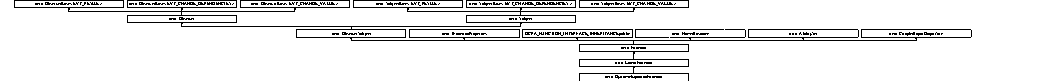
\includegraphics[height=1.082126cm]{d9/da6/classocra_1_1DynamicEquationFunction}
\end{center}
\end{figure}
\subsection*{Public Types}
\begin{DoxyCompactItemize}
\item 
typedef \hyperlink{classocra_1_1LinearFunction}{Linear\+Function} \hyperlink{classocra_1_1DynamicEquationFunction_a2c8c76bfd66285d63895ec34219175b4}{function\+Type\+\_\+t}
\end{DoxyCompactItemize}
\subsection*{Public Member Functions}
\begin{DoxyCompactItemize}
\item 
\hyperlink{classocra_1_1DynamicEquationFunction_ab6a38098b1aac7db298e0f3a93955624}{Dynamic\+Equation\+Function} (const Model \&model)
\item 
\hyperlink{classocra_1_1DynamicEquationFunction_a84c82f21c1564aaca6b5aa703ecae73e}{$\sim$\+Dynamic\+Equation\+Function} ()
\end{DoxyCompactItemize}
\subsection*{Protected Member Functions}
\begin{DoxyCompactItemize}
\item 
void \hyperlink{classocra_1_1DynamicEquationFunction_a81d71c87d0f52b3d321614c6219022ad}{update\+Jacobian} () const
\item 
void \hyperlink{classocra_1_1DynamicEquationFunction_ae1fe835a481f5f0bde6c8b0fa8ea09b2}{updateb} () const
\item 
void \hyperlink{classocra_1_1DynamicEquationFunction_a6fc52fcd947fa303e55729dbb286b92c}{do\+Update\+Input\+Size\+Begin} ()
\item 
void \hyperlink{classocra_1_1DynamicEquationFunction_a8d20f6ed1e3983d1fddf648729eba955}{do\+Update\+Input\+Size\+End} ()
\end{DoxyCompactItemize}
\subsection*{Protected Attributes}
\begin{DoxyCompactItemize}
\item 
const Model \& \hyperlink{classocra_1_1DynamicEquationFunction_ad0c5d639974a97aa3ed3f0bbe0f8189d}{\+\_\+model}
\item 
\hyperlink{classocra_1_1Variable}{Variable} \& \hyperlink{classocra_1_1DynamicEquationFunction_a8a6dfb64fcca3c42a9e7ad637706a6cc}{\+\_\+q\+\_\+ddot}
\item 
\hyperlink{classocra_1_1Variable}{Variable} \& \hyperlink{classocra_1_1DynamicEquationFunction_a60ba636a9028046969c5491ec7ed2f9e}{\+\_\+tau}
\item 
\hyperlink{classocra_1_1Variable}{Variable} \& \hyperlink{classocra_1_1DynamicEquationFunction_a70499af5c86e68836acb7251b37ab668}{\+\_\+f}
\end{DoxyCompactItemize}
\subsection*{Additional Inherited Members}


\subsection{Detailed Description}
Dynamic\+Equation\+Function class. 

\begin{DoxyWarning}{Warning}
None
\end{DoxyWarning}
M Tdot + N T + G -\/ L tau + Jt f, where f is the force applied by the model on the environment. The variable is the concatenation of Tdot, tau and f. 

Definition at line 38 of file Dynamic\+Equation\+Function.\+h.



\subsection{Member Typedef Documentation}
\hypertarget{classocra_1_1DynamicEquationFunction_a2c8c76bfd66285d63895ec34219175b4}{}\label{classocra_1_1DynamicEquationFunction_a2c8c76bfd66285d63895ec34219175b4} 
\index{ocra\+::\+Dynamic\+Equation\+Function@{ocra\+::\+Dynamic\+Equation\+Function}!function\+Type\+\_\+t@{function\+Type\+\_\+t}}
\index{function\+Type\+\_\+t@{function\+Type\+\_\+t}!ocra\+::\+Dynamic\+Equation\+Function@{ocra\+::\+Dynamic\+Equation\+Function}}
\subsubsection{\texorpdfstring{function\+Type\+\_\+t}{functionType\_t}}
{\footnotesize\ttfamily typedef \hyperlink{classocra_1_1LinearFunction}{Linear\+Function} \hyperlink{classocra_1_1DynamicEquationFunction_a2c8c76bfd66285d63895ec34219175b4}{ocra\+::\+Dynamic\+Equation\+Function\+::function\+Type\+\_\+t}}



Definition at line 42 of file Dynamic\+Equation\+Function.\+h.



\subsection{Constructor \& Destructor Documentation}
\hypertarget{classocra_1_1DynamicEquationFunction_ab6a38098b1aac7db298e0f3a93955624}{}\label{classocra_1_1DynamicEquationFunction_ab6a38098b1aac7db298e0f3a93955624} 
\index{ocra\+::\+Dynamic\+Equation\+Function@{ocra\+::\+Dynamic\+Equation\+Function}!Dynamic\+Equation\+Function@{Dynamic\+Equation\+Function}}
\index{Dynamic\+Equation\+Function@{Dynamic\+Equation\+Function}!ocra\+::\+Dynamic\+Equation\+Function@{ocra\+::\+Dynamic\+Equation\+Function}}
\subsubsection{\texorpdfstring{Dynamic\+Equation\+Function()}{DynamicEquationFunction()}}
{\footnotesize\ttfamily ocra\+::\+Dynamic\+Equation\+Function\+::\+Dynamic\+Equation\+Function (\begin{DoxyParamCaption}\item[{const Model \&}]{model }\end{DoxyParamCaption})}



Definition at line 8 of file Dynamic\+Equation\+Function.\+cpp.

\hypertarget{classocra_1_1DynamicEquationFunction_a84c82f21c1564aaca6b5aa703ecae73e}{}\label{classocra_1_1DynamicEquationFunction_a84c82f21c1564aaca6b5aa703ecae73e} 
\index{ocra\+::\+Dynamic\+Equation\+Function@{ocra\+::\+Dynamic\+Equation\+Function}!````~Dynamic\+Equation\+Function@{$\sim$\+Dynamic\+Equation\+Function}}
\index{````~Dynamic\+Equation\+Function@{$\sim$\+Dynamic\+Equation\+Function}!ocra\+::\+Dynamic\+Equation\+Function@{ocra\+::\+Dynamic\+Equation\+Function}}
\subsubsection{\texorpdfstring{$\sim$\+Dynamic\+Equation\+Function()}{~DynamicEquationFunction()}}
{\footnotesize\ttfamily ocra\+::\+Dynamic\+Equation\+Function\+::$\sim$\+Dynamic\+Equation\+Function (\begin{DoxyParamCaption}{ }\end{DoxyParamCaption})}



Definition at line 22 of file Dynamic\+Equation\+Function.\+cpp.



\subsection{Member Function Documentation}
\hypertarget{classocra_1_1DynamicEquationFunction_a6fc52fcd947fa303e55729dbb286b92c}{}\label{classocra_1_1DynamicEquationFunction_a6fc52fcd947fa303e55729dbb286b92c} 
\index{ocra\+::\+Dynamic\+Equation\+Function@{ocra\+::\+Dynamic\+Equation\+Function}!do\+Update\+Input\+Size\+Begin@{do\+Update\+Input\+Size\+Begin}}
\index{do\+Update\+Input\+Size\+Begin@{do\+Update\+Input\+Size\+Begin}!ocra\+::\+Dynamic\+Equation\+Function@{ocra\+::\+Dynamic\+Equation\+Function}}
\subsubsection{\texorpdfstring{do\+Update\+Input\+Size\+Begin()}{doUpdateInputSizeBegin()}}
{\footnotesize\ttfamily void ocra\+::\+Dynamic\+Equation\+Function\+::do\+Update\+Input\+Size\+Begin (\begin{DoxyParamCaption}{ }\end{DoxyParamCaption})\hspace{0.3cm}{\ttfamily [protected]}, {\ttfamily [virtual]}}

Methods for pre and post update in case the variable size has changed. Default implementation of do\+Update\+Input\+Size\+End does nothing, do\+Update\+Input\+Size\+Begin throws an exception. These methods might throw exceptions when overloaded. Furthermore, {\ttfamily \hyperlink{classocra_1_1DynamicEquationFunction_a8d20f6ed1e3983d1fddf648729eba955}{do\+Update\+Input\+Size\+End()}} must comply with the post condition of {\ttfamily \hyperlink{classocra_1_1Function_a3a5b9e6ae296339acc87ab2cbf97ef98}{update\+Input\+Size()}}, i.\+e. let the values of each ability invalidated. 

Reimplemented from \hyperlink{classocra_1_1Function_a3f728f3758e6448aa59932853db5ddcc}{ocra\+::\+Function}.



Definition at line 61 of file Dynamic\+Equation\+Function.\+cpp.

\hypertarget{classocra_1_1DynamicEquationFunction_a8d20f6ed1e3983d1fddf648729eba955}{}\label{classocra_1_1DynamicEquationFunction_a8d20f6ed1e3983d1fddf648729eba955} 
\index{ocra\+::\+Dynamic\+Equation\+Function@{ocra\+::\+Dynamic\+Equation\+Function}!do\+Update\+Input\+Size\+End@{do\+Update\+Input\+Size\+End}}
\index{do\+Update\+Input\+Size\+End@{do\+Update\+Input\+Size\+End}!ocra\+::\+Dynamic\+Equation\+Function@{ocra\+::\+Dynamic\+Equation\+Function}}
\subsubsection{\texorpdfstring{do\+Update\+Input\+Size\+End()}{doUpdateInputSizeEnd()}}
{\footnotesize\ttfamily void ocra\+::\+Dynamic\+Equation\+Function\+::do\+Update\+Input\+Size\+End (\begin{DoxyParamCaption}\item[{void}]{ }\end{DoxyParamCaption})\hspace{0.3cm}{\ttfamily [protected]}, {\ttfamily [virtual]}}

This methods ensures \+\_\+b has the good size at the end of a resize, yet it will not be called in \hyperlink{classocra_1_1LinearFunction}{Linear\+Function} itself because the class does not overload \hyperlink{classocra_1_1DynamicEquationFunction_a6fc52fcd947fa303e55729dbb286b92c}{do\+Update\+Input\+Size\+Begin()} which throws an runtime\+\_\+error by default. 

Reimplemented from \hyperlink{classocra_1_1LinearFunction_ac6bdf62ad6634397778d5f4223ed6d82}{ocra\+::\+Linear\+Function}.



Definition at line 66 of file Dynamic\+Equation\+Function.\+cpp.

\hypertarget{classocra_1_1DynamicEquationFunction_ae1fe835a481f5f0bde6c8b0fa8ea09b2}{}\label{classocra_1_1DynamicEquationFunction_ae1fe835a481f5f0bde6c8b0fa8ea09b2} 
\index{ocra\+::\+Dynamic\+Equation\+Function@{ocra\+::\+Dynamic\+Equation\+Function}!updateb@{updateb}}
\index{updateb@{updateb}!ocra\+::\+Dynamic\+Equation\+Function@{ocra\+::\+Dynamic\+Equation\+Function}}
\subsubsection{\texorpdfstring{updateb()}{updateb()}}
{\footnotesize\ttfamily void ocra\+::\+Dynamic\+Equation\+Function\+::updateb (\begin{DoxyParamCaption}{ }\end{DoxyParamCaption}) const\hspace{0.3cm}{\ttfamily [protected]}, {\ttfamily [virtual]}}

Update the value of b. Does nothing in \hyperlink{classocra_1_1LinearFunction}{Linear\+Function}. It is provided so that derived class may overload it. 

Reimplemented from \hyperlink{classocra_1_1LinearFunction_a546454cd8d0909f99433ffc0e700c9e3}{ocra\+::\+Linear\+Function}.



Definition at line 40 of file Dynamic\+Equation\+Function.\+cpp.

\hypertarget{classocra_1_1DynamicEquationFunction_a81d71c87d0f52b3d321614c6219022ad}{}\label{classocra_1_1DynamicEquationFunction_a81d71c87d0f52b3d321614c6219022ad} 
\index{ocra\+::\+Dynamic\+Equation\+Function@{ocra\+::\+Dynamic\+Equation\+Function}!update\+Jacobian@{update\+Jacobian}}
\index{update\+Jacobian@{update\+Jacobian}!ocra\+::\+Dynamic\+Equation\+Function@{ocra\+::\+Dynamic\+Equation\+Function}}
\subsubsection{\texorpdfstring{update\+Jacobian()}{updateJacobian()}}
{\footnotesize\ttfamily void ocra\+::\+Dynamic\+Equation\+Function\+::update\+Jacobian (\begin{DoxyParamCaption}{ }\end{DoxyParamCaption}) const\hspace{0.3cm}{\ttfamily [protected]}, {\ttfamily [virtual]}}



Reimplemented from \hyperlink{classocra_1_1LinearFunction_a30926f977c0124a0b0f65b854ab39636}{ocra\+::\+Linear\+Function}.



Definition at line 45 of file Dynamic\+Equation\+Function.\+cpp.



\subsection{Member Data Documentation}
\hypertarget{classocra_1_1DynamicEquationFunction_a70499af5c86e68836acb7251b37ab668}{}\label{classocra_1_1DynamicEquationFunction_a70499af5c86e68836acb7251b37ab668} 
\index{ocra\+::\+Dynamic\+Equation\+Function@{ocra\+::\+Dynamic\+Equation\+Function}!\+\_\+f@{\+\_\+f}}
\index{\+\_\+f@{\+\_\+f}!ocra\+::\+Dynamic\+Equation\+Function@{ocra\+::\+Dynamic\+Equation\+Function}}
\subsubsection{\texorpdfstring{\+\_\+f}{\_f}}
{\footnotesize\ttfamily \hyperlink{classocra_1_1Variable}{Variable}\& ocra\+::\+Dynamic\+Equation\+Function\+::\+\_\+f\hspace{0.3cm}{\ttfamily [protected]}}



Definition at line 67 of file Dynamic\+Equation\+Function.\+h.

\hypertarget{classocra_1_1DynamicEquationFunction_ad0c5d639974a97aa3ed3f0bbe0f8189d}{}\label{classocra_1_1DynamicEquationFunction_ad0c5d639974a97aa3ed3f0bbe0f8189d} 
\index{ocra\+::\+Dynamic\+Equation\+Function@{ocra\+::\+Dynamic\+Equation\+Function}!\+\_\+model@{\+\_\+model}}
\index{\+\_\+model@{\+\_\+model}!ocra\+::\+Dynamic\+Equation\+Function@{ocra\+::\+Dynamic\+Equation\+Function}}
\subsubsection{\texorpdfstring{\+\_\+model}{\_model}}
{\footnotesize\ttfamily const Model\& ocra\+::\+Dynamic\+Equation\+Function\+::\+\_\+model\hspace{0.3cm}{\ttfamily [protected]}}



Definition at line 64 of file Dynamic\+Equation\+Function.\+h.

\hypertarget{classocra_1_1DynamicEquationFunction_a8a6dfb64fcca3c42a9e7ad637706a6cc}{}\label{classocra_1_1DynamicEquationFunction_a8a6dfb64fcca3c42a9e7ad637706a6cc} 
\index{ocra\+::\+Dynamic\+Equation\+Function@{ocra\+::\+Dynamic\+Equation\+Function}!\+\_\+q\+\_\+ddot@{\+\_\+q\+\_\+ddot}}
\index{\+\_\+q\+\_\+ddot@{\+\_\+q\+\_\+ddot}!ocra\+::\+Dynamic\+Equation\+Function@{ocra\+::\+Dynamic\+Equation\+Function}}
\subsubsection{\texorpdfstring{\+\_\+q\+\_\+ddot}{\_q\_ddot}}
{\footnotesize\ttfamily \hyperlink{classocra_1_1Variable}{Variable}\& ocra\+::\+Dynamic\+Equation\+Function\+::\+\_\+q\+\_\+ddot\hspace{0.3cm}{\ttfamily [protected]}}



Definition at line 65 of file Dynamic\+Equation\+Function.\+h.

\hypertarget{classocra_1_1DynamicEquationFunction_a60ba636a9028046969c5491ec7ed2f9e}{}\label{classocra_1_1DynamicEquationFunction_a60ba636a9028046969c5491ec7ed2f9e} 
\index{ocra\+::\+Dynamic\+Equation\+Function@{ocra\+::\+Dynamic\+Equation\+Function}!\+\_\+tau@{\+\_\+tau}}
\index{\+\_\+tau@{\+\_\+tau}!ocra\+::\+Dynamic\+Equation\+Function@{ocra\+::\+Dynamic\+Equation\+Function}}
\subsubsection{\texorpdfstring{\+\_\+tau}{\_tau}}
{\footnotesize\ttfamily \hyperlink{classocra_1_1Variable}{Variable}\& ocra\+::\+Dynamic\+Equation\+Function\+::\+\_\+tau\hspace{0.3cm}{\ttfamily [protected]}}



Definition at line 66 of file Dynamic\+Equation\+Function.\+h.



The documentation for this class was generated from the following files\+:\begin{DoxyCompactItemize}
\item 
\hyperlink{DynamicEquationFunction_8h}{Dynamic\+Equation\+Function.\+h}\item 
\hyperlink{DynamicEquationFunction_8cpp}{Dynamic\+Equation\+Function.\+cpp}\end{DoxyCompactItemize}

\hypertarget{structocra_1_1NewtonSolver_1_1eNewtonInfo}{}\section{ocra\+:\+:Newton\+Solver\+:\+:e\+Newton\+Info Struct Reference}
\label{structocra_1_1NewtonSolver_1_1eNewtonInfo}\index{ocra\+::\+Newton\+Solver\+::e\+Newton\+Info@{ocra\+::\+Newton\+Solver\+::e\+Newton\+Info}}


{\ttfamily \#include $<$Newton\+Solver.\+h$>$}

\subsection*{Public Attributes}
\begin{DoxyCompactItemize}
\item 
bool \hyperlink{structocra_1_1NewtonSolver_1_1eNewtonInfo_ad3fb93c95fbe6e760caffc64fa1739cb}{success}
\item 
bool \hyperlink{structocra_1_1NewtonSolver_1_1eNewtonInfo_a088723d14881333ae7fcc9576c7142d0}{non\+PositiveH}
\item 
bool \hyperlink{structocra_1_1NewtonSolver_1_1eNewtonInfo_a210ebc2859be22918cc378fc16a5cf88}{used\+Default\+Guess}
\item 
bool \hyperlink{structocra_1_1NewtonSolver_1_1eNewtonInfo_a034b326acca364d57a7bdeea79849625}{small\+Alpha}
\item 
int \hyperlink{structocra_1_1NewtonSolver_1_1eNewtonInfo_a3ec8816b36812a608542479168a9c18d}{iter}
\item 
double \hyperlink{structocra_1_1NewtonSolver_1_1eNewtonInfo_a5b0d53fdf4347e5bc6f4d1af784eb517}{residual}
\end{DoxyCompactItemize}


\subsection{Detailed Description}


Definition at line 58 of file Newton\+Solver.\+h.



\subsection{Member Data Documentation}
\hypertarget{structocra_1_1NewtonSolver_1_1eNewtonInfo_a3ec8816b36812a608542479168a9c18d}{}\label{structocra_1_1NewtonSolver_1_1eNewtonInfo_a3ec8816b36812a608542479168a9c18d} 
\index{ocra\+::\+Newton\+Solver\+::e\+Newton\+Info@{ocra\+::\+Newton\+Solver\+::e\+Newton\+Info}!iter@{iter}}
\index{iter@{iter}!ocra\+::\+Newton\+Solver\+::e\+Newton\+Info@{ocra\+::\+Newton\+Solver\+::e\+Newton\+Info}}
\subsubsection{\texorpdfstring{iter}{iter}}
{\footnotesize\ttfamily int ocra\+::\+Newton\+Solver\+::e\+Newton\+Info\+::iter}



Definition at line 64 of file Newton\+Solver.\+h.

\hypertarget{structocra_1_1NewtonSolver_1_1eNewtonInfo_a088723d14881333ae7fcc9576c7142d0}{}\label{structocra_1_1NewtonSolver_1_1eNewtonInfo_a088723d14881333ae7fcc9576c7142d0} 
\index{ocra\+::\+Newton\+Solver\+::e\+Newton\+Info@{ocra\+::\+Newton\+Solver\+::e\+Newton\+Info}!non\+PositiveH@{non\+PositiveH}}
\index{non\+PositiveH@{non\+PositiveH}!ocra\+::\+Newton\+Solver\+::e\+Newton\+Info@{ocra\+::\+Newton\+Solver\+::e\+Newton\+Info}}
\subsubsection{\texorpdfstring{non\+PositiveH}{nonPositiveH}}
{\footnotesize\ttfamily bool ocra\+::\+Newton\+Solver\+::e\+Newton\+Info\+::non\+PositiveH}



Definition at line 61 of file Newton\+Solver.\+h.

\hypertarget{structocra_1_1NewtonSolver_1_1eNewtonInfo_a5b0d53fdf4347e5bc6f4d1af784eb517}{}\label{structocra_1_1NewtonSolver_1_1eNewtonInfo_a5b0d53fdf4347e5bc6f4d1af784eb517} 
\index{ocra\+::\+Newton\+Solver\+::e\+Newton\+Info@{ocra\+::\+Newton\+Solver\+::e\+Newton\+Info}!residual@{residual}}
\index{residual@{residual}!ocra\+::\+Newton\+Solver\+::e\+Newton\+Info@{ocra\+::\+Newton\+Solver\+::e\+Newton\+Info}}
\subsubsection{\texorpdfstring{residual}{residual}}
{\footnotesize\ttfamily double ocra\+::\+Newton\+Solver\+::e\+Newton\+Info\+::residual}



Definition at line 65 of file Newton\+Solver.\+h.

\hypertarget{structocra_1_1NewtonSolver_1_1eNewtonInfo_a034b326acca364d57a7bdeea79849625}{}\label{structocra_1_1NewtonSolver_1_1eNewtonInfo_a034b326acca364d57a7bdeea79849625} 
\index{ocra\+::\+Newton\+Solver\+::e\+Newton\+Info@{ocra\+::\+Newton\+Solver\+::e\+Newton\+Info}!small\+Alpha@{small\+Alpha}}
\index{small\+Alpha@{small\+Alpha}!ocra\+::\+Newton\+Solver\+::e\+Newton\+Info@{ocra\+::\+Newton\+Solver\+::e\+Newton\+Info}}
\subsubsection{\texorpdfstring{small\+Alpha}{smallAlpha}}
{\footnotesize\ttfamily bool ocra\+::\+Newton\+Solver\+::e\+Newton\+Info\+::small\+Alpha}



Definition at line 63 of file Newton\+Solver.\+h.

\hypertarget{structocra_1_1NewtonSolver_1_1eNewtonInfo_ad3fb93c95fbe6e760caffc64fa1739cb}{}\label{structocra_1_1NewtonSolver_1_1eNewtonInfo_ad3fb93c95fbe6e760caffc64fa1739cb} 
\index{ocra\+::\+Newton\+Solver\+::e\+Newton\+Info@{ocra\+::\+Newton\+Solver\+::e\+Newton\+Info}!success@{success}}
\index{success@{success}!ocra\+::\+Newton\+Solver\+::e\+Newton\+Info@{ocra\+::\+Newton\+Solver\+::e\+Newton\+Info}}
\subsubsection{\texorpdfstring{success}{success}}
{\footnotesize\ttfamily bool ocra\+::\+Newton\+Solver\+::e\+Newton\+Info\+::success}



Definition at line 60 of file Newton\+Solver.\+h.

\hypertarget{structocra_1_1NewtonSolver_1_1eNewtonInfo_a210ebc2859be22918cc378fc16a5cf88}{}\label{structocra_1_1NewtonSolver_1_1eNewtonInfo_a210ebc2859be22918cc378fc16a5cf88} 
\index{ocra\+::\+Newton\+Solver\+::e\+Newton\+Info@{ocra\+::\+Newton\+Solver\+::e\+Newton\+Info}!used\+Default\+Guess@{used\+Default\+Guess}}
\index{used\+Default\+Guess@{used\+Default\+Guess}!ocra\+::\+Newton\+Solver\+::e\+Newton\+Info@{ocra\+::\+Newton\+Solver\+::e\+Newton\+Info}}
\subsubsection{\texorpdfstring{used\+Default\+Guess}{usedDefaultGuess}}
{\footnotesize\ttfamily bool ocra\+::\+Newton\+Solver\+::e\+Newton\+Info\+::used\+Default\+Guess}



Definition at line 62 of file Newton\+Solver.\+h.



The documentation for this struct was generated from the following file\+:\begin{DoxyCompactItemize}
\item 
\hyperlink{NewtonSolver_8h}{Newton\+Solver.\+h}\end{DoxyCompactItemize}

\hypertarget{structocra_1_1EqualitiesConstraints}{}\section{ocra\+:\+:Equalities\+Constraints Struct Reference}
\label{structocra_1_1EqualitiesConstraints}\index{ocra\+::\+Equalities\+Constraints@{ocra\+::\+Equalities\+Constraints}}


{\ttfamily \#include $<$Cascade\+Q\+P\+Structures.\+h$>$}

\subsection*{Public Attributes}
\begin{DoxyCompactItemize}
\item 
Eigen\+::\+Matrix\+Xd \hyperlink{structocra_1_1EqualitiesConstraints_a948420ad39defa889f402d30041a3521}{M}
\item 
Eigen\+::\+Vector\+Xd \hyperlink{structocra_1_1EqualitiesConstraints_a03425f2d5d16dbb6a0c7da036a2fee77}{n}
\end{DoxyCompactItemize}


\subsection{Detailed Description}


Definition at line 51 of file Cascade\+Q\+P\+Structures.\+h.



\subsection{Member Data Documentation}
\hypertarget{structocra_1_1EqualitiesConstraints_a948420ad39defa889f402d30041a3521}{}\label{structocra_1_1EqualitiesConstraints_a948420ad39defa889f402d30041a3521} 
\index{ocra\+::\+Equalities\+Constraints@{ocra\+::\+Equalities\+Constraints}!M@{M}}
\index{M@{M}!ocra\+::\+Equalities\+Constraints@{ocra\+::\+Equalities\+Constraints}}
\subsubsection{\texorpdfstring{M}{M}}
{\footnotesize\ttfamily Eigen\+::\+Matrix\+Xd ocra\+::\+Equalities\+Constraints\+::M}



Definition at line 54 of file Cascade\+Q\+P\+Structures.\+h.

\hypertarget{structocra_1_1EqualitiesConstraints_a03425f2d5d16dbb6a0c7da036a2fee77}{}\label{structocra_1_1EqualitiesConstraints_a03425f2d5d16dbb6a0c7da036a2fee77} 
\index{ocra\+::\+Equalities\+Constraints@{ocra\+::\+Equalities\+Constraints}!n@{n}}
\index{n@{n}!ocra\+::\+Equalities\+Constraints@{ocra\+::\+Equalities\+Constraints}}
\subsubsection{\texorpdfstring{n}{n}}
{\footnotesize\ttfamily Eigen\+::\+Vector\+Xd ocra\+::\+Equalities\+Constraints\+::n}



Definition at line 55 of file Cascade\+Q\+P\+Structures.\+h.



The documentation for this struct was generated from the following file\+:\begin{DoxyCompactItemize}
\item 
\hyperlink{CascadeQPStructures_8h}{Cascade\+Q\+P\+Structures.\+h}\end{DoxyCompactItemize}

\hypertarget{classocra_1_1EqualZeroConstraintPtr}{}\section{ocra\+:\+:Equal\+Zero\+Constraint\+Ptr$<$ T $>$ Class Template Reference}
\label{classocra_1_1EqualZeroConstraintPtr}\index{ocra\+::\+Equal\+Zero\+Constraint\+Ptr$<$ T $>$@{ocra\+::\+Equal\+Zero\+Constraint\+Ptr$<$ T $>$}}


{\ttfamily \#include $<$Function\+Helpers.\+h$>$}

\subsection*{Public Member Functions}
\begin{DoxyCompactItemize}
\item 
\hyperlink{classocra_1_1EqualZeroConstraintPtr_a3c2ba882cedf01952626c420b3020b8f}{Equal\+Zero\+Constraint\+Ptr} ()
\item 
\hyperlink{classocra_1_1EqualZeroConstraintPtr_a6a3937dc3d22626cb3aaf3536256aee8}{Equal\+Zero\+Constraint\+Ptr} (T $\ast$f)
\item 
\hyperlink{classocra_1_1EqualZeroConstraintPtr_a46f26ad15e3bccb5d1566873f7389e5c}{operator Constraint$<$ T $>$ \&} ()
\item 
\hyperlink{classocra_1_1EqualZeroConstraintPtr_a8b8ad981759d5531f699ee2faf687c91}{operator const Constraint$<$ T $>$ \&} () const
\item 
\hyperlink{classocra_1_1EqualZeroConstraintPtr_a3fbdf66eb7ef747912865e054e61cef6}{operator T \&} ()
\item 
\hyperlink{classocra_1_1EqualZeroConstraintPtr_a19b57497dcdc5241f3f0980bc6ed93e8}{operator const T \&} () const
\item 
void \hyperlink{classocra_1_1EqualZeroConstraintPtr_a3157efd4dbc5db4141fa688fd8032b78}{set} (T $\ast$f)
\item 
T \& \hyperlink{classocra_1_1EqualZeroConstraintPtr_a995f545eace80eb54d79dfcb48d724bd}{get\+Function} ()
\item 
const T \& \hyperlink{classocra_1_1EqualZeroConstraintPtr_a1bda9fdd004966597bca96f60e4c5b91}{get\+Function} () const
\item 
\hyperlink{classocra_1_1Constraint}{Constraint}$<$ T $>$ \& \hyperlink{classocra_1_1EqualZeroConstraintPtr_a4d9b786f79ed2b84fac88e57f3d00404}{get\+Constraint} ()
\item 
const \hyperlink{classocra_1_1Constraint}{Constraint}$<$ T $>$ \& \hyperlink{classocra_1_1EqualZeroConstraintPtr_a0fe913c6749ffdb91e86df3a5b4822a5}{get\+Constraint} () const
\end{DoxyCompactItemize}


\subsection{Detailed Description}
\subsubsection*{template$<$class T$>$\newline
class ocra\+::\+Equal\+Zero\+Constraint\+Ptr$<$ T $>$}



Definition at line 79 of file Function\+Helpers.\+h.



\subsection{Constructor \& Destructor Documentation}
\hypertarget{classocra_1_1EqualZeroConstraintPtr_a3c2ba882cedf01952626c420b3020b8f}{}\label{classocra_1_1EqualZeroConstraintPtr_a3c2ba882cedf01952626c420b3020b8f} 
\index{ocra\+::\+Equal\+Zero\+Constraint\+Ptr@{ocra\+::\+Equal\+Zero\+Constraint\+Ptr}!Equal\+Zero\+Constraint\+Ptr@{Equal\+Zero\+Constraint\+Ptr}}
\index{Equal\+Zero\+Constraint\+Ptr@{Equal\+Zero\+Constraint\+Ptr}!ocra\+::\+Equal\+Zero\+Constraint\+Ptr@{ocra\+::\+Equal\+Zero\+Constraint\+Ptr}}
\subsubsection{\texorpdfstring{Equal\+Zero\+Constraint\+Ptr()}{EqualZeroConstraintPtr()}\hspace{0.1cm}{\footnotesize\ttfamily [1/2]}}
{\footnotesize\ttfamily template$<$class T$>$ \\
\hyperlink{classocra_1_1EqualZeroConstraintPtr}{ocra\+::\+Equal\+Zero\+Constraint\+Ptr}$<$ T $>$\+::\hyperlink{classocra_1_1EqualZeroConstraintPtr}{Equal\+Zero\+Constraint\+Ptr} (\begin{DoxyParamCaption}{ }\end{DoxyParamCaption})\hspace{0.3cm}{\ttfamily [inline]}}



Definition at line 82 of file Function\+Helpers.\+h.

\hypertarget{classocra_1_1EqualZeroConstraintPtr_a6a3937dc3d22626cb3aaf3536256aee8}{}\label{classocra_1_1EqualZeroConstraintPtr_a6a3937dc3d22626cb3aaf3536256aee8} 
\index{ocra\+::\+Equal\+Zero\+Constraint\+Ptr@{ocra\+::\+Equal\+Zero\+Constraint\+Ptr}!Equal\+Zero\+Constraint\+Ptr@{Equal\+Zero\+Constraint\+Ptr}}
\index{Equal\+Zero\+Constraint\+Ptr@{Equal\+Zero\+Constraint\+Ptr}!ocra\+::\+Equal\+Zero\+Constraint\+Ptr@{ocra\+::\+Equal\+Zero\+Constraint\+Ptr}}
\subsubsection{\texorpdfstring{Equal\+Zero\+Constraint\+Ptr()}{EqualZeroConstraintPtr()}\hspace{0.1cm}{\footnotesize\ttfamily [2/2]}}
{\footnotesize\ttfamily template$<$class T$>$ \\
\hyperlink{classocra_1_1EqualZeroConstraintPtr}{ocra\+::\+Equal\+Zero\+Constraint\+Ptr}$<$ T $>$\+::\hyperlink{classocra_1_1EqualZeroConstraintPtr}{Equal\+Zero\+Constraint\+Ptr} (\begin{DoxyParamCaption}\item[{T $\ast$}]{f }\end{DoxyParamCaption})\hspace{0.3cm}{\ttfamily [inline]}}



Definition at line 88 of file Function\+Helpers.\+h.



\subsection{Member Function Documentation}
\hypertarget{classocra_1_1EqualZeroConstraintPtr_a4d9b786f79ed2b84fac88e57f3d00404}{}\label{classocra_1_1EqualZeroConstraintPtr_a4d9b786f79ed2b84fac88e57f3d00404} 
\index{ocra\+::\+Equal\+Zero\+Constraint\+Ptr@{ocra\+::\+Equal\+Zero\+Constraint\+Ptr}!get\+Constraint@{get\+Constraint}}
\index{get\+Constraint@{get\+Constraint}!ocra\+::\+Equal\+Zero\+Constraint\+Ptr@{ocra\+::\+Equal\+Zero\+Constraint\+Ptr}}
\subsubsection{\texorpdfstring{get\+Constraint()}{getConstraint()}\hspace{0.1cm}{\footnotesize\ttfamily [1/2]}}
{\footnotesize\ttfamily template$<$class T$>$ \\
\hyperlink{classocra_1_1Constraint}{Constraint}$<$T$>$\& \hyperlink{classocra_1_1EqualZeroConstraintPtr}{ocra\+::\+Equal\+Zero\+Constraint\+Ptr}$<$ T $>$\+::get\+Constraint (\begin{DoxyParamCaption}{ }\end{DoxyParamCaption})\hspace{0.3cm}{\ttfamily [inline]}}



Definition at line 120 of file Function\+Helpers.\+h.

\hypertarget{classocra_1_1EqualZeroConstraintPtr_a0fe913c6749ffdb91e86df3a5b4822a5}{}\label{classocra_1_1EqualZeroConstraintPtr_a0fe913c6749ffdb91e86df3a5b4822a5} 
\index{ocra\+::\+Equal\+Zero\+Constraint\+Ptr@{ocra\+::\+Equal\+Zero\+Constraint\+Ptr}!get\+Constraint@{get\+Constraint}}
\index{get\+Constraint@{get\+Constraint}!ocra\+::\+Equal\+Zero\+Constraint\+Ptr@{ocra\+::\+Equal\+Zero\+Constraint\+Ptr}}
\subsubsection{\texorpdfstring{get\+Constraint()}{getConstraint()}\hspace{0.1cm}{\footnotesize\ttfamily [2/2]}}
{\footnotesize\ttfamily template$<$class T$>$ \\
const \hyperlink{classocra_1_1Constraint}{Constraint}$<$T$>$\& \hyperlink{classocra_1_1EqualZeroConstraintPtr}{ocra\+::\+Equal\+Zero\+Constraint\+Ptr}$<$ T $>$\+::get\+Constraint (\begin{DoxyParamCaption}{ }\end{DoxyParamCaption}) const\hspace{0.3cm}{\ttfamily [inline]}}



Definition at line 127 of file Function\+Helpers.\+h.

\hypertarget{classocra_1_1EqualZeroConstraintPtr_a995f545eace80eb54d79dfcb48d724bd}{}\label{classocra_1_1EqualZeroConstraintPtr_a995f545eace80eb54d79dfcb48d724bd} 
\index{ocra\+::\+Equal\+Zero\+Constraint\+Ptr@{ocra\+::\+Equal\+Zero\+Constraint\+Ptr}!get\+Function@{get\+Function}}
\index{get\+Function@{get\+Function}!ocra\+::\+Equal\+Zero\+Constraint\+Ptr@{ocra\+::\+Equal\+Zero\+Constraint\+Ptr}}
\subsubsection{\texorpdfstring{get\+Function()}{getFunction()}\hspace{0.1cm}{\footnotesize\ttfamily [1/2]}}
{\footnotesize\ttfamily template$<$class T$>$ \\
T\& \hyperlink{classocra_1_1EqualZeroConstraintPtr}{ocra\+::\+Equal\+Zero\+Constraint\+Ptr}$<$ T $>$\+::get\+Function (\begin{DoxyParamCaption}\item[{void}]{ }\end{DoxyParamCaption})\hspace{0.3cm}{\ttfamily [inline]}}



Definition at line 106 of file Function\+Helpers.\+h.

\hypertarget{classocra_1_1EqualZeroConstraintPtr_a1bda9fdd004966597bca96f60e4c5b91}{}\label{classocra_1_1EqualZeroConstraintPtr_a1bda9fdd004966597bca96f60e4c5b91} 
\index{ocra\+::\+Equal\+Zero\+Constraint\+Ptr@{ocra\+::\+Equal\+Zero\+Constraint\+Ptr}!get\+Function@{get\+Function}}
\index{get\+Function@{get\+Function}!ocra\+::\+Equal\+Zero\+Constraint\+Ptr@{ocra\+::\+Equal\+Zero\+Constraint\+Ptr}}
\subsubsection{\texorpdfstring{get\+Function()}{getFunction()}\hspace{0.1cm}{\footnotesize\ttfamily [2/2]}}
{\footnotesize\ttfamily template$<$class T$>$ \\
const T\& \hyperlink{classocra_1_1EqualZeroConstraintPtr}{ocra\+::\+Equal\+Zero\+Constraint\+Ptr}$<$ T $>$\+::get\+Function (\begin{DoxyParamCaption}\item[{void}]{ }\end{DoxyParamCaption}) const\hspace{0.3cm}{\ttfamily [inline]}}



Definition at line 113 of file Function\+Helpers.\+h.

\hypertarget{classocra_1_1EqualZeroConstraintPtr_a8b8ad981759d5531f699ee2faf687c91}{}\label{classocra_1_1EqualZeroConstraintPtr_a8b8ad981759d5531f699ee2faf687c91} 
\index{ocra\+::\+Equal\+Zero\+Constraint\+Ptr@{ocra\+::\+Equal\+Zero\+Constraint\+Ptr}!operator const Constraint$<$ T $>$ \&@{operator const Constraint$<$ T $>$ \&}}
\index{operator const Constraint$<$ T $>$ \&@{operator const Constraint$<$ T $>$ \&}!ocra\+::\+Equal\+Zero\+Constraint\+Ptr@{ocra\+::\+Equal\+Zero\+Constraint\+Ptr}}
\subsubsection{\texorpdfstring{operator const Constraint$<$ T $>$ \&()}{operator const Constraint< T > \&()}}
{\footnotesize\ttfamily template$<$class T$>$ \\
\hyperlink{classocra_1_1EqualZeroConstraintPtr}{ocra\+::\+Equal\+Zero\+Constraint\+Ptr}$<$ T $>$\+::operator const \hyperlink{classocra_1_1Constraint}{Constraint}$<$ T $>$ \& (\begin{DoxyParamCaption}{ }\end{DoxyParamCaption}) const\hspace{0.3cm}{\ttfamily [inline]}}



Definition at line 95 of file Function\+Helpers.\+h.

\hypertarget{classocra_1_1EqualZeroConstraintPtr_a19b57497dcdc5241f3f0980bc6ed93e8}{}\label{classocra_1_1EqualZeroConstraintPtr_a19b57497dcdc5241f3f0980bc6ed93e8} 
\index{ocra\+::\+Equal\+Zero\+Constraint\+Ptr@{ocra\+::\+Equal\+Zero\+Constraint\+Ptr}!operator const T \&@{operator const T \&}}
\index{operator const T \&@{operator const T \&}!ocra\+::\+Equal\+Zero\+Constraint\+Ptr@{ocra\+::\+Equal\+Zero\+Constraint\+Ptr}}
\subsubsection{\texorpdfstring{operator const T \&()}{operator const T \&()}}
{\footnotesize\ttfamily template$<$class T$>$ \\
\hyperlink{classocra_1_1EqualZeroConstraintPtr}{ocra\+::\+Equal\+Zero\+Constraint\+Ptr}$<$ T $>$\+::operator const T \& (\begin{DoxyParamCaption}{ }\end{DoxyParamCaption}) const\hspace{0.3cm}{\ttfamily [inline]}}



Definition at line 98 of file Function\+Helpers.\+h.

\hypertarget{classocra_1_1EqualZeroConstraintPtr_a46f26ad15e3bccb5d1566873f7389e5c}{}\label{classocra_1_1EqualZeroConstraintPtr_a46f26ad15e3bccb5d1566873f7389e5c} 
\index{ocra\+::\+Equal\+Zero\+Constraint\+Ptr@{ocra\+::\+Equal\+Zero\+Constraint\+Ptr}!operator Constraint$<$ T $>$ \&@{operator Constraint$<$ T $>$ \&}}
\index{operator Constraint$<$ T $>$ \&@{operator Constraint$<$ T $>$ \&}!ocra\+::\+Equal\+Zero\+Constraint\+Ptr@{ocra\+::\+Equal\+Zero\+Constraint\+Ptr}}
\subsubsection{\texorpdfstring{operator Constraint$<$ T $>$ \&()}{operator Constraint< T > \&()}}
{\footnotesize\ttfamily template$<$class T$>$ \\
\hyperlink{classocra_1_1EqualZeroConstraintPtr}{ocra\+::\+Equal\+Zero\+Constraint\+Ptr}$<$ T $>$\+::operator \hyperlink{classocra_1_1Constraint}{Constraint}$<$ T $>$ \& (\begin{DoxyParamCaption}{ }\end{DoxyParamCaption})\hspace{0.3cm}{\ttfamily [inline]}}



Definition at line 94 of file Function\+Helpers.\+h.

\hypertarget{classocra_1_1EqualZeroConstraintPtr_a3fbdf66eb7ef747912865e054e61cef6}{}\label{classocra_1_1EqualZeroConstraintPtr_a3fbdf66eb7ef747912865e054e61cef6} 
\index{ocra\+::\+Equal\+Zero\+Constraint\+Ptr@{ocra\+::\+Equal\+Zero\+Constraint\+Ptr}!operator T \&@{operator T \&}}
\index{operator T \&@{operator T \&}!ocra\+::\+Equal\+Zero\+Constraint\+Ptr@{ocra\+::\+Equal\+Zero\+Constraint\+Ptr}}
\subsubsection{\texorpdfstring{operator T \&()}{operator T \&()}}
{\footnotesize\ttfamily template$<$class T$>$ \\
\hyperlink{classocra_1_1EqualZeroConstraintPtr}{ocra\+::\+Equal\+Zero\+Constraint\+Ptr}$<$ T $>$\+::operator T\& (\begin{DoxyParamCaption}{ }\end{DoxyParamCaption})\hspace{0.3cm}{\ttfamily [inline]}}



Definition at line 97 of file Function\+Helpers.\+h.

\hypertarget{classocra_1_1EqualZeroConstraintPtr_a3157efd4dbc5db4141fa688fd8032b78}{}\label{classocra_1_1EqualZeroConstraintPtr_a3157efd4dbc5db4141fa688fd8032b78} 
\index{ocra\+::\+Equal\+Zero\+Constraint\+Ptr@{ocra\+::\+Equal\+Zero\+Constraint\+Ptr}!set@{set}}
\index{set@{set}!ocra\+::\+Equal\+Zero\+Constraint\+Ptr@{ocra\+::\+Equal\+Zero\+Constraint\+Ptr}}
\subsubsection{\texorpdfstring{set()}{set()}}
{\footnotesize\ttfamily template$<$class T$>$ \\
void \hyperlink{classocra_1_1EqualZeroConstraintPtr}{ocra\+::\+Equal\+Zero\+Constraint\+Ptr}$<$ T $>$\+::set (\begin{DoxyParamCaption}\item[{T $\ast$}]{f }\end{DoxyParamCaption})\hspace{0.3cm}{\ttfamily [inline]}}



Definition at line 100 of file Function\+Helpers.\+h.



The documentation for this class was generated from the following file\+:\begin{DoxyCompactItemize}
\item 
\hyperlink{FunctionHelpers_8h}{Function\+Helpers.\+h}\end{DoxyCompactItemize}

\hypertarget{classocra_1_1Ex1Pb}{}\section{ocra\+:\+:Ex1\+Pb Class Reference}
\label{classocra_1_1Ex1Pb}\index{ocra\+::\+Ex1\+Pb@{ocra\+::\+Ex1\+Pb}}
Inheritance diagram for ocra\+:\+:Ex1\+Pb\+:\begin{figure}[H]
\begin{center}
\leavevmode
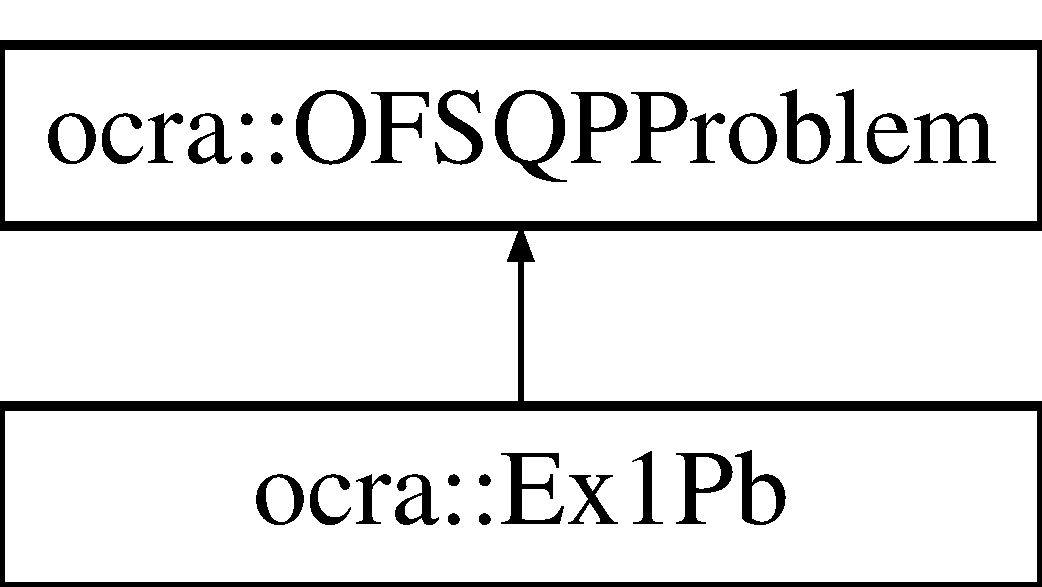
\includegraphics[height=2.000000cm]{d5/d80/classocra_1_1Ex1Pb}
\end{center}
\end{figure}
\subsection*{Additional Inherited Members}


\subsection{Detailed Description}


Definition at line 3672 of file O\+F\+S\+Q\+P.\+cpp.



The documentation for this class was generated from the following file\+:\begin{DoxyCompactItemize}
\item 
\hyperlink{OFSQP_8cpp}{O\+F\+S\+Q\+P.\+cpp}\end{DoxyCompactItemize}

\hypertarget{classocra_1_1Ex2Pb}{}\section{ocra\+:\+:Ex2\+Pb Class Reference}
\label{classocra_1_1Ex2Pb}\index{ocra\+::\+Ex2\+Pb@{ocra\+::\+Ex2\+Pb}}


Inheritance diagram for ocra\+:\+:Ex2\+Pb\+:\nopagebreak
\begin{figure}[H]
\begin{center}
\leavevmode
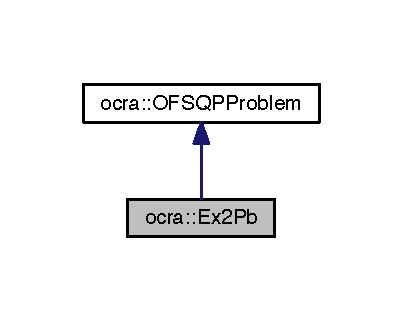
\includegraphics[width=193pt]{dc/de6/classocra_1_1Ex2Pb__inherit__graph}
\end{center}
\end{figure}


Collaboration diagram for ocra\+:\+:Ex2\+Pb\+:\nopagebreak
\begin{figure}[H]
\begin{center}
\leavevmode
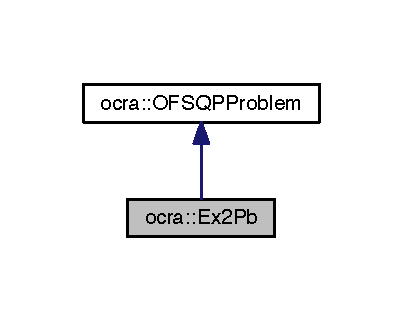
\includegraphics[width=193pt]{da/d9a/classocra_1_1Ex2Pb__coll__graph}
\end{center}
\end{figure}
\subsection*{Additional Inherited Members}


\subsection{Detailed Description}


Definition at line 3775 of file O\+F\+S\+Q\+P.\+cpp.



The documentation for this class was generated from the following file\+:\begin{DoxyCompactItemize}
\item 
\hyperlink{OFSQP_8cpp}{O\+F\+S\+Q\+P.\+cpp}\end{DoxyCompactItemize}

\hypertarget{classocra_1_1Ex3Pb}{}\section{ocra\+:\+:Ex3\+Pb Class Reference}
\label{classocra_1_1Ex3Pb}\index{ocra\+::\+Ex3\+Pb@{ocra\+::\+Ex3\+Pb}}


Inheritance diagram for ocra\+:\+:Ex3\+Pb\+:\nopagebreak
\begin{figure}[H]
\begin{center}
\leavevmode
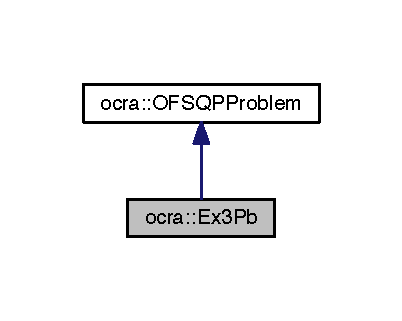
\includegraphics[width=193pt]{d5/d4e/classocra_1_1Ex3Pb__inherit__graph}
\end{center}
\end{figure}


Collaboration diagram for ocra\+:\+:Ex3\+Pb\+:\nopagebreak
\begin{figure}[H]
\begin{center}
\leavevmode
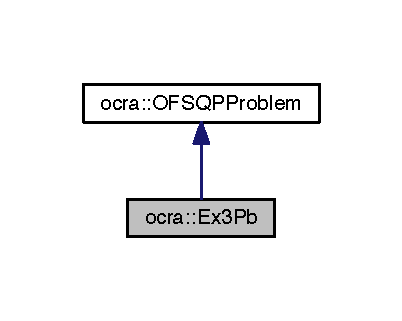
\includegraphics[width=193pt]{d2/d8b/classocra_1_1Ex3Pb__coll__graph}
\end{center}
\end{figure}
\subsection*{Additional Inherited Members}


\subsection{Detailed Description}


Definition at line 3916 of file O\+F\+S\+Q\+P.\+cpp.



The documentation for this class was generated from the following file\+:\begin{DoxyCompactItemize}
\item 
\hyperlink{OFSQP_8cpp}{O\+F\+S\+Q\+P.\+cpp}\end{DoxyCompactItemize}

\hypertarget{classocra_1_1Ex4Pb}{}\section{ocra\+:\+:Ex4\+Pb Class Reference}
\label{classocra_1_1Ex4Pb}\index{ocra\+::\+Ex4\+Pb@{ocra\+::\+Ex4\+Pb}}


Inheritance diagram for ocra\+:\+:Ex4\+Pb\+:\nopagebreak
\begin{figure}[H]
\begin{center}
\leavevmode
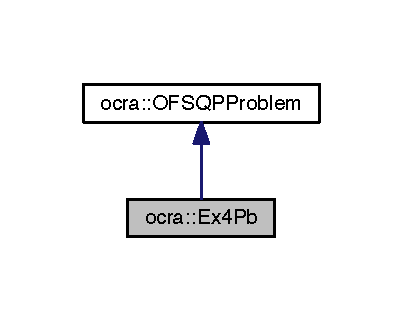
\includegraphics[width=193pt]{d1/d91/classocra_1_1Ex4Pb__inherit__graph}
\end{center}
\end{figure}


Collaboration diagram for ocra\+:\+:Ex4\+Pb\+:\nopagebreak
\begin{figure}[H]
\begin{center}
\leavevmode
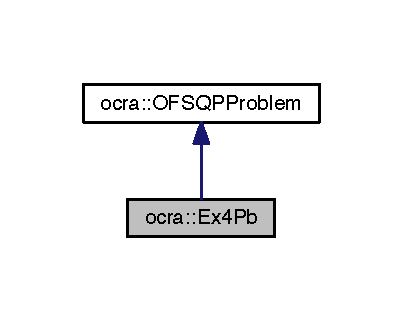
\includegraphics[width=193pt]{df/d37/classocra_1_1Ex4Pb__coll__graph}
\end{center}
\end{figure}
\subsection*{Additional Inherited Members}


\subsection{Detailed Description}


Definition at line 4019 of file O\+F\+S\+Q\+P.\+cpp.



The documentation for this class was generated from the following file\+:\begin{DoxyCompactItemize}
\item 
\hyperlink{OFSQP_8cpp}{O\+F\+S\+Q\+P.\+cpp}\end{DoxyCompactItemize}

\hypertarget{classocra_1_1Ex5Pb}{}\section{ocra\+:\+:Ex5\+Pb Class Reference}
\label{classocra_1_1Ex5Pb}\index{ocra\+::\+Ex5\+Pb@{ocra\+::\+Ex5\+Pb}}
Inheritance diagram for ocra\+:\+:Ex5\+Pb\+:\begin{figure}[H]
\begin{center}
\leavevmode
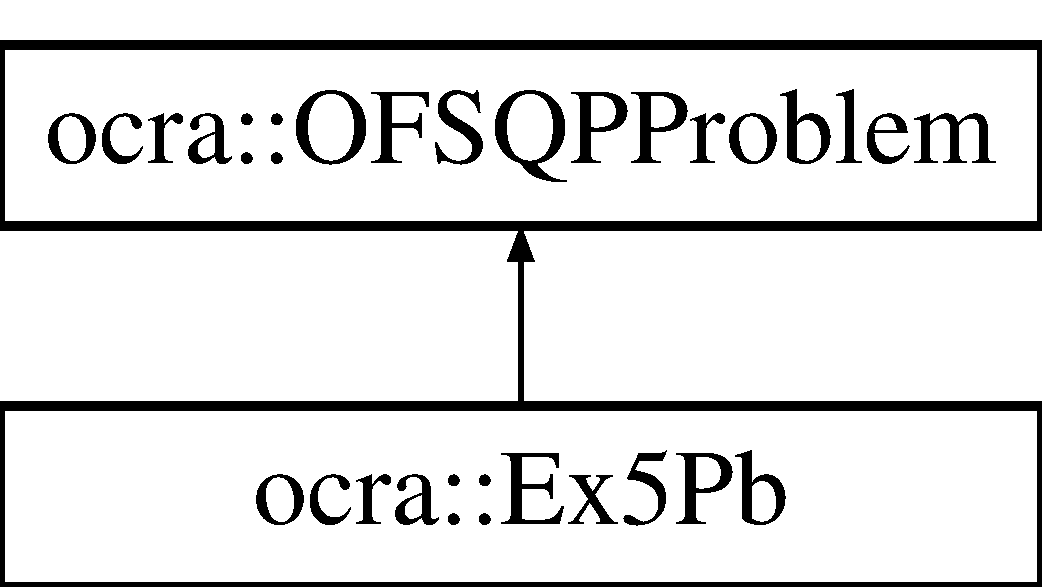
\includegraphics[height=2.000000cm]{dd/ddf/classocra_1_1Ex5Pb}
\end{center}
\end{figure}
\subsection*{Additional Inherited Members}


\subsection{Detailed Description}


Definition at line 4131 of file O\+F\+S\+Q\+P.\+cpp.



The documentation for this class was generated from the following file\+:\begin{DoxyCompactItemize}
\item 
\hyperlink{OFSQP_8cpp}{O\+F\+S\+Q\+P.\+cpp}\end{DoxyCompactItemize}

\hypertarget{classocra_1_1ExperimentalTrajectory}{}\section{ocra\+:\+:Experimental\+Trajectory Class Reference}
\label{classocra_1_1ExperimentalTrajectory}\index{ocra\+::\+Experimental\+Trajectory@{ocra\+::\+Experimental\+Trajectory}}


{\ttfamily \#include $<$Experimental\+Trajectory.\+h$>$}

Inheritance diagram for ocra\+:\+:Experimental\+Trajectory\+:\begin{figure}[H]
\begin{center}
\leavevmode
\includegraphics[height=2.000000cm]{d5/d74/classocra_1_1ExperimentalTrajectory}
\end{center}
\end{figure}
\subsection*{Public Member Functions}
\begin{DoxyCompactItemize}
\item 
void \hyperlink{classocra_1_1ExperimentalTrajectory_a227d08649657b7951248c0b626808d9e}{calculate\+Variance\+Parameters} ()
\item 
Eigen\+::\+Matrix\+Xd \hyperlink{classocra_1_1ExperimentalTrajectory_a9b9ed4d7b7a96c9a2b33624b5fc1ecf6}{get\+Desired\+Values} (double time)
\item 
Eigen\+::\+Vector\+Xd \hyperlink{classocra_1_1ExperimentalTrajectory_a1c3d421e3b08e2332747c6c3559d8b2d}{get\+Variance} (double time)
\item 
void \hyperlink{classocra_1_1ExperimentalTrajectory_a8d0b41849d2e99a13dd2ef1ae0b0eb46}{get\+Desired\+Values} (double time, Eigen\+::\+Matrix\+Xd \&desired\+Values, Eigen\+::\+Vector\+Xd \&variance)
\item 
void \hyperlink{classocra_1_1ExperimentalTrajectory_a8f920fd57e5207ac784411ba3a2594a3}{get\+Desired\+Values} (double time, Eigen\+::\+Displacementd \&position, Eigen\+::\+Twistd \&velocity, Eigen\+::\+Twistd \&acceleration)
\item 
double \hyperlink{classocra_1_1ExperimentalTrajectory_a76f4aa686308735dec24eec98d4c0ab8}{get\+Max\+Variance} ()
\item 
Eigen\+::\+Matrix\+Xd \hyperlink{classocra_1_1ExperimentalTrajectory_a5a70f13ad9c0a6c8716972dcbe29b2b0}{get\+Waypoint\+Data} ()
\item 
void \hyperlink{classocra_1_1ExperimentalTrajectory_a5bd433112f5712a77e857636ed2dd11b}{add\+New\+Waypoint} (Eigen\+::\+Vector\+Xd new\+Waypoint, double waypoint\+Time)
\item 
void \hyperlink{classocra_1_1ExperimentalTrajectory_a64e0ded52fdbe54ccb85f32c67824d3a}{remove\+Youngest\+Waypoint} ()
\item 
void \hyperlink{classocra_1_1ExperimentalTrajectory_a6b5cdffc1575ca98a73251d6214521a3}{remove\+Waypoint} (int index)
\item 
Eigen\+::\+Matrix\+Xd \hyperlink{classocra_1_1ExperimentalTrajectory_ae3a97f92f11c74f9ffc42c33a8a95149}{get\+Rbfn\+Kernel\+Curves} ()
\end{DoxyCompactItemize}
\subsection*{Protected Member Functions}
\begin{DoxyCompactItemize}
\item 
virtual void \hyperlink{classocra_1_1ExperimentalTrajectory_a4e214517be9848835a63641578e3269d}{initialize\+Trajectory} ()
\end{DoxyCompactItemize}
\subsection*{Protected Attributes}
\begin{DoxyCompactItemize}
\item 
double \hyperlink{classocra_1_1ExperimentalTrajectory_a56b5a0d236891f5087b81cda85aae0be}{t0}
\item 
double \hyperlink{classocra_1_1ExperimentalTrajectory_a90502f229cbccfd19bd884d7b87f734d}{t0\+\_\+variance}
\item 
bool \hyperlink{classocra_1_1ExperimentalTrajectory_ab10b037615b07e20b0d6f81c48b7fd23}{variance\+Start\+Trigger}
\end{DoxyCompactItemize}


\subsection{Detailed Description}


Definition at line 11 of file Experimental\+Trajectory.\+h.



\subsection{Member Function Documentation}
\hypertarget{classocra_1_1ExperimentalTrajectory_a5bd433112f5712a77e857636ed2dd11b}{}\label{classocra_1_1ExperimentalTrajectory_a5bd433112f5712a77e857636ed2dd11b} 
\index{ocra\+::\+Experimental\+Trajectory@{ocra\+::\+Experimental\+Trajectory}!add\+New\+Waypoint@{add\+New\+Waypoint}}
\index{add\+New\+Waypoint@{add\+New\+Waypoint}!ocra\+::\+Experimental\+Trajectory@{ocra\+::\+Experimental\+Trajectory}}
\subsubsection{\texorpdfstring{add\+New\+Waypoint()}{addNewWaypoint()}}
{\footnotesize\ttfamily void ocra\+::\+Experimental\+Trajectory\+::add\+New\+Waypoint (\begin{DoxyParamCaption}\item[{Eigen\+::\+Vector\+Xd}]{new\+Waypoint,  }\item[{double}]{waypoint\+Time }\end{DoxyParamCaption})}



Definition at line 327 of file Experimental\+Trajectory.\+cpp.

\hypertarget{classocra_1_1ExperimentalTrajectory_a227d08649657b7951248c0b626808d9e}{}\label{classocra_1_1ExperimentalTrajectory_a227d08649657b7951248c0b626808d9e} 
\index{ocra\+::\+Experimental\+Trajectory@{ocra\+::\+Experimental\+Trajectory}!calculate\+Variance\+Parameters@{calculate\+Variance\+Parameters}}
\index{calculate\+Variance\+Parameters@{calculate\+Variance\+Parameters}!ocra\+::\+Experimental\+Trajectory@{ocra\+::\+Experimental\+Trajectory}}
\subsubsection{\texorpdfstring{calculate\+Variance\+Parameters()}{calculateVarianceParameters()}}
{\footnotesize\ttfamily void ocra\+::\+Experimental\+Trajectory\+::calculate\+Variance\+Parameters (\begin{DoxyParamCaption}{ }\end{DoxyParamCaption})}



Definition at line 12 of file Experimental\+Trajectory.\+cpp.

\hypertarget{classocra_1_1ExperimentalTrajectory_a9b9ed4d7b7a96c9a2b33624b5fc1ecf6}{}\label{classocra_1_1ExperimentalTrajectory_a9b9ed4d7b7a96c9a2b33624b5fc1ecf6} 
\index{ocra\+::\+Experimental\+Trajectory@{ocra\+::\+Experimental\+Trajectory}!get\+Desired\+Values@{get\+Desired\+Values}}
\index{get\+Desired\+Values@{get\+Desired\+Values}!ocra\+::\+Experimental\+Trajectory@{ocra\+::\+Experimental\+Trajectory}}
\subsubsection{\texorpdfstring{get\+Desired\+Values()}{getDesiredValues()}\hspace{0.1cm}{\footnotesize\ttfamily [1/3]}}
{\footnotesize\ttfamily Eigen\+::\+Matrix\+Xd ocra\+::\+Experimental\+Trajectory\+::get\+Desired\+Values (\begin{DoxyParamCaption}\item[{double}]{time }\end{DoxyParamCaption})\hspace{0.3cm}{\ttfamily [virtual]}}

For details on the analytical point to point min-\/jerk formulation see\+: \href{http://www.jneurosci.org/content/5/7/1688.full.pdf}{\tt http\+://www.\+jneurosci.\+org/content/5/7/1688.\+full.\+pdf} \href{http://shadmehrlab.org/book/minimum_jerk/minimumjerk.htm}{\tt http\+://shadmehrlab.\+org/book/minimum\+\_\+jerk/minimumjerk.\+htm}

Reimplemented from \hyperlink{classocra_1_1Trajectory_a2102a829e6dad497f7c773c346d499b7}{ocra\+::\+Trajectory}.



Definition at line 175 of file Experimental\+Trajectory.\+cpp.

\hypertarget{classocra_1_1ExperimentalTrajectory_a8d0b41849d2e99a13dd2ef1ae0b0eb46}{}\label{classocra_1_1ExperimentalTrajectory_a8d0b41849d2e99a13dd2ef1ae0b0eb46} 
\index{ocra\+::\+Experimental\+Trajectory@{ocra\+::\+Experimental\+Trajectory}!get\+Desired\+Values@{get\+Desired\+Values}}
\index{get\+Desired\+Values@{get\+Desired\+Values}!ocra\+::\+Experimental\+Trajectory@{ocra\+::\+Experimental\+Trajectory}}
\subsubsection{\texorpdfstring{get\+Desired\+Values()}{getDesiredValues()}\hspace{0.1cm}{\footnotesize\ttfamily [2/3]}}
{\footnotesize\ttfamily void ocra\+::\+Experimental\+Trajectory\+::get\+Desired\+Values (\begin{DoxyParamCaption}\item[{double}]{time,  }\item[{Eigen\+::\+Matrix\+Xd \&}]{desired\+Values,  }\item[{Eigen\+::\+Vector\+Xd \&}]{variance }\end{DoxyParamCaption})\hspace{0.3cm}{\ttfamily [virtual]}}



Reimplemented from \hyperlink{classocra_1_1Trajectory_aab6869cf5bc4a7c44eac36a0e49255b9}{ocra\+::\+Trajectory}.



Definition at line 253 of file Experimental\+Trajectory.\+cpp.

\hypertarget{classocra_1_1ExperimentalTrajectory_a8f920fd57e5207ac784411ba3a2594a3}{}\label{classocra_1_1ExperimentalTrajectory_a8f920fd57e5207ac784411ba3a2594a3} 
\index{ocra\+::\+Experimental\+Trajectory@{ocra\+::\+Experimental\+Trajectory}!get\+Desired\+Values@{get\+Desired\+Values}}
\index{get\+Desired\+Values@{get\+Desired\+Values}!ocra\+::\+Experimental\+Trajectory@{ocra\+::\+Experimental\+Trajectory}}
\subsubsection{\texorpdfstring{get\+Desired\+Values()}{getDesiredValues()}\hspace{0.1cm}{\footnotesize\ttfamily [3/3]}}
{\footnotesize\ttfamily void ocra\+::\+Experimental\+Trajectory\+::get\+Desired\+Values (\begin{DoxyParamCaption}\item[{double}]{time,  }\item[{Eigen\+::\+Displacementd \&}]{position,  }\item[{Eigen\+::\+Twistd \&}]{velocity,  }\item[{Eigen\+::\+Twistd \&}]{acceleration }\end{DoxyParamCaption})}



Definition at line 260 of file Experimental\+Trajectory.\+cpp.

\hypertarget{classocra_1_1ExperimentalTrajectory_a76f4aa686308735dec24eec98d4c0ab8}{}\label{classocra_1_1ExperimentalTrajectory_a76f4aa686308735dec24eec98d4c0ab8} 
\index{ocra\+::\+Experimental\+Trajectory@{ocra\+::\+Experimental\+Trajectory}!get\+Max\+Variance@{get\+Max\+Variance}}
\index{get\+Max\+Variance@{get\+Max\+Variance}!ocra\+::\+Experimental\+Trajectory@{ocra\+::\+Experimental\+Trajectory}}
\subsubsection{\texorpdfstring{get\+Max\+Variance()}{getMaxVariance()}}
{\footnotesize\ttfamily double ocra\+::\+Experimental\+Trajectory\+::get\+Max\+Variance (\begin{DoxyParamCaption}{ }\end{DoxyParamCaption})}



Definition at line 309 of file Experimental\+Trajectory.\+cpp.

\hypertarget{classocra_1_1ExperimentalTrajectory_ae3a97f92f11c74f9ffc42c33a8a95149}{}\label{classocra_1_1ExperimentalTrajectory_ae3a97f92f11c74f9ffc42c33a8a95149} 
\index{ocra\+::\+Experimental\+Trajectory@{ocra\+::\+Experimental\+Trajectory}!get\+Rbfn\+Kernel\+Curves@{get\+Rbfn\+Kernel\+Curves}}
\index{get\+Rbfn\+Kernel\+Curves@{get\+Rbfn\+Kernel\+Curves}!ocra\+::\+Experimental\+Trajectory@{ocra\+::\+Experimental\+Trajectory}}
\subsubsection{\texorpdfstring{get\+Rbfn\+Kernel\+Curves()}{getRbfnKernelCurves()}}
{\footnotesize\ttfamily Eigen\+::\+Matrix\+Xd ocra\+::\+Experimental\+Trajectory\+::get\+Rbfn\+Kernel\+Curves (\begin{DoxyParamCaption}{ }\end{DoxyParamCaption})}



Definition at line 421 of file Experimental\+Trajectory.\+cpp.

\hypertarget{classocra_1_1ExperimentalTrajectory_a1c3d421e3b08e2332747c6c3559d8b2d}{}\label{classocra_1_1ExperimentalTrajectory_a1c3d421e3b08e2332747c6c3559d8b2d} 
\index{ocra\+::\+Experimental\+Trajectory@{ocra\+::\+Experimental\+Trajectory}!get\+Variance@{get\+Variance}}
\index{get\+Variance@{get\+Variance}!ocra\+::\+Experimental\+Trajectory@{ocra\+::\+Experimental\+Trajectory}}
\subsubsection{\texorpdfstring{get\+Variance()}{getVariance()}}
{\footnotesize\ttfamily Eigen\+::\+Vector\+Xd ocra\+::\+Experimental\+Trajectory\+::get\+Variance (\begin{DoxyParamCaption}\item[{double}]{time }\end{DoxyParamCaption})}



Definition at line 229 of file Experimental\+Trajectory.\+cpp.

\hypertarget{classocra_1_1ExperimentalTrajectory_a5a70f13ad9c0a6c8716972dcbe29b2b0}{}\label{classocra_1_1ExperimentalTrajectory_a5a70f13ad9c0a6c8716972dcbe29b2b0} 
\index{ocra\+::\+Experimental\+Trajectory@{ocra\+::\+Experimental\+Trajectory}!get\+Waypoint\+Data@{get\+Waypoint\+Data}}
\index{get\+Waypoint\+Data@{get\+Waypoint\+Data}!ocra\+::\+Experimental\+Trajectory@{ocra\+::\+Experimental\+Trajectory}}
\subsubsection{\texorpdfstring{get\+Waypoint\+Data()}{getWaypointData()}}
{\footnotesize\ttfamily Eigen\+::\+Matrix\+Xd ocra\+::\+Experimental\+Trajectory\+::get\+Waypoint\+Data (\begin{DoxyParamCaption}{ }\end{DoxyParamCaption})}



Definition at line 39 of file Experimental\+Trajectory.\+cpp.

\hypertarget{classocra_1_1ExperimentalTrajectory_a4e214517be9848835a63641578e3269d}{}\label{classocra_1_1ExperimentalTrajectory_a4e214517be9848835a63641578e3269d} 
\index{ocra\+::\+Experimental\+Trajectory@{ocra\+::\+Experimental\+Trajectory}!initialize\+Trajectory@{initialize\+Trajectory}}
\index{initialize\+Trajectory@{initialize\+Trajectory}!ocra\+::\+Experimental\+Trajectory@{ocra\+::\+Experimental\+Trajectory}}
\subsubsection{\texorpdfstring{initialize\+Trajectory()}{initializeTrajectory()}}
{\footnotesize\ttfamily void ocra\+::\+Experimental\+Trajectory\+::initialize\+Trajectory (\begin{DoxyParamCaption}{ }\end{DoxyParamCaption})\hspace{0.3cm}{\ttfamily [protected]}, {\ttfamily [virtual]}}



Reimplemented from \hyperlink{classocra_1_1Trajectory_aa49b123abf79be71f131c138ff2a88b2}{ocra\+::\+Trajectory}.



Definition at line 267 of file Experimental\+Trajectory.\+cpp.

\hypertarget{classocra_1_1ExperimentalTrajectory_a6b5cdffc1575ca98a73251d6214521a3}{}\label{classocra_1_1ExperimentalTrajectory_a6b5cdffc1575ca98a73251d6214521a3} 
\index{ocra\+::\+Experimental\+Trajectory@{ocra\+::\+Experimental\+Trajectory}!remove\+Waypoint@{remove\+Waypoint}}
\index{remove\+Waypoint@{remove\+Waypoint}!ocra\+::\+Experimental\+Trajectory@{ocra\+::\+Experimental\+Trajectory}}
\subsubsection{\texorpdfstring{remove\+Waypoint()}{removeWaypoint()}}
{\footnotesize\ttfamily void ocra\+::\+Experimental\+Trajectory\+::remove\+Waypoint (\begin{DoxyParamCaption}\item[{int}]{index }\end{DoxyParamCaption})}



Definition at line 388 of file Experimental\+Trajectory.\+cpp.

\hypertarget{classocra_1_1ExperimentalTrajectory_a64e0ded52fdbe54ccb85f32c67824d3a}{}\label{classocra_1_1ExperimentalTrajectory_a64e0ded52fdbe54ccb85f32c67824d3a} 
\index{ocra\+::\+Experimental\+Trajectory@{ocra\+::\+Experimental\+Trajectory}!remove\+Youngest\+Waypoint@{remove\+Youngest\+Waypoint}}
\index{remove\+Youngest\+Waypoint@{remove\+Youngest\+Waypoint}!ocra\+::\+Experimental\+Trajectory@{ocra\+::\+Experimental\+Trajectory}}
\subsubsection{\texorpdfstring{remove\+Youngest\+Waypoint()}{removeYoungestWaypoint()}}
{\footnotesize\ttfamily void ocra\+::\+Experimental\+Trajectory\+::remove\+Youngest\+Waypoint (\begin{DoxyParamCaption}{ }\end{DoxyParamCaption})}



Definition at line 383 of file Experimental\+Trajectory.\+cpp.



\subsection{Member Data Documentation}
\hypertarget{classocra_1_1ExperimentalTrajectory_a56b5a0d236891f5087b81cda85aae0be}{}\label{classocra_1_1ExperimentalTrajectory_a56b5a0d236891f5087b81cda85aae0be} 
\index{ocra\+::\+Experimental\+Trajectory@{ocra\+::\+Experimental\+Trajectory}!t0@{t0}}
\index{t0@{t0}!ocra\+::\+Experimental\+Trajectory@{ocra\+::\+Experimental\+Trajectory}}
\subsubsection{\texorpdfstring{t0}{t0}}
{\footnotesize\ttfamily double ocra\+::\+Experimental\+Trajectory\+::t0\hspace{0.3cm}{\ttfamily [protected]}}



Definition at line 38 of file Experimental\+Trajectory.\+h.

\hypertarget{classocra_1_1ExperimentalTrajectory_a90502f229cbccfd19bd884d7b87f734d}{}\label{classocra_1_1ExperimentalTrajectory_a90502f229cbccfd19bd884d7b87f734d} 
\index{ocra\+::\+Experimental\+Trajectory@{ocra\+::\+Experimental\+Trajectory}!t0\+\_\+variance@{t0\+\_\+variance}}
\index{t0\+\_\+variance@{t0\+\_\+variance}!ocra\+::\+Experimental\+Trajectory@{ocra\+::\+Experimental\+Trajectory}}
\subsubsection{\texorpdfstring{t0\+\_\+variance}{t0\_variance}}
{\footnotesize\ttfamily double ocra\+::\+Experimental\+Trajectory\+::t0\+\_\+variance\hspace{0.3cm}{\ttfamily [protected]}}



Definition at line 38 of file Experimental\+Trajectory.\+h.

\hypertarget{classocra_1_1ExperimentalTrajectory_ab10b037615b07e20b0d6f81c48b7fd23}{}\label{classocra_1_1ExperimentalTrajectory_ab10b037615b07e20b0d6f81c48b7fd23} 
\index{ocra\+::\+Experimental\+Trajectory@{ocra\+::\+Experimental\+Trajectory}!variance\+Start\+Trigger@{variance\+Start\+Trigger}}
\index{variance\+Start\+Trigger@{variance\+Start\+Trigger}!ocra\+::\+Experimental\+Trajectory@{ocra\+::\+Experimental\+Trajectory}}
\subsubsection{\texorpdfstring{variance\+Start\+Trigger}{varianceStartTrigger}}
{\footnotesize\ttfamily bool ocra\+::\+Experimental\+Trajectory\+::variance\+Start\+Trigger\hspace{0.3cm}{\ttfamily [protected]}}



Definition at line 39 of file Experimental\+Trajectory.\+h.



The documentation for this class was generated from the following files\+:\begin{DoxyCompactItemize}
\item 
\hyperlink{ExperimentalTrajectory_8h}{Experimental\+Trajectory.\+h}\item 
\hyperlink{ExperimentalTrajectory_8cpp}{Experimental\+Trajectory.\+cpp}\end{DoxyCompactItemize}

\hypertarget{classocra_1_1FcQuadraticFunction}{}\section{ocra\+:\+:Fc\+Quadratic\+Function Class Reference}
\label{classocra_1_1FcQuadraticFunction}\index{ocra\+::\+Fc\+Quadratic\+Function@{ocra\+::\+Fc\+Quadratic\+Function}}


{\ttfamily \#include $<$Fc\+Quadratic\+Function.\+h$>$}



Inheritance diagram for ocra\+:\+:Fc\+Quadratic\+Function\+:\nopagebreak
\begin{figure}[H]
\begin{center}
\leavevmode
\includegraphics[width=350pt]{d0/d8a/classocra_1_1FcQuadraticFunction__inherit__graph}
\end{center}
\end{figure}


Collaboration diagram for ocra\+:\+:Fc\+Quadratic\+Function\+:\nopagebreak
\begin{figure}[H]
\begin{center}
\leavevmode
\includegraphics[width=350pt]{d3/dbd/classocra_1_1FcQuadraticFunction__coll__graph}
\end{center}
\end{figure}
\subsection*{Public Member Functions}
\begin{DoxyCompactItemize}
\item 
\hyperlink{classocra_1_1FcQuadraticFunction_a85ee0d84a43b16353b1d44740cc3769b}{Fc\+Quadratic\+Function} (\hyperlink{classocra_1_1Variable}{ocra\+::\+Variable} \&\hyperlink{classocra_1_1Function_a28825886d1f149c87b112ec2ec1dd486}{x})
\item 
virtual \hyperlink{classocra_1_1FcQuadraticFunction_a1eef85d7638d6bfc0c2bb3bc9dab8d63}{$\sim$\+Fc\+Quadratic\+Function} ()
\item 
void \hyperlink{classocra_1_1FcQuadraticFunction_a1e350f138eb82cfe3e8cf049942e626c}{do\+Update\+Input\+Size\+Begin} ()
\item 
void \hyperlink{classocra_1_1FcQuadraticFunction_aef068bc86027f29c0fbfaa9d53441cd4}{update\+Hessian} () const
\item 
void \hyperlink{classocra_1_1FcQuadraticFunction_ac6bcfaccbe16a821e0f1d7c29744d138}{updateq} () const
\item 
void \hyperlink{classocra_1_1FcQuadraticFunction_aab41d4b011590ad42766e66df34305da}{updater} () const
\end{DoxyCompactItemize}
\subsection*{Additional Inherited Members}


\subsection{Detailed Description}


Definition at line 16 of file Fc\+Quadratic\+Function.\+h.



\subsection{Constructor \& Destructor Documentation}
\hypertarget{classocra_1_1FcQuadraticFunction_a85ee0d84a43b16353b1d44740cc3769b}{}\label{classocra_1_1FcQuadraticFunction_a85ee0d84a43b16353b1d44740cc3769b} 
\index{ocra\+::\+Fc\+Quadratic\+Function@{ocra\+::\+Fc\+Quadratic\+Function}!Fc\+Quadratic\+Function@{Fc\+Quadratic\+Function}}
\index{Fc\+Quadratic\+Function@{Fc\+Quadratic\+Function}!ocra\+::\+Fc\+Quadratic\+Function@{ocra\+::\+Fc\+Quadratic\+Function}}
\subsubsection{\texorpdfstring{Fc\+Quadratic\+Function()}{FcQuadraticFunction()}}
{\footnotesize\ttfamily Fc\+Quadratic\+Function\+::\+Fc\+Quadratic\+Function (\begin{DoxyParamCaption}\item[{\hyperlink{classocra_1_1Variable}{ocra\+::\+Variable} \&}]{x }\end{DoxyParamCaption})}



Definition at line 6 of file Fc\+Quadratic\+Function.\+cpp.

\hypertarget{classocra_1_1FcQuadraticFunction_a1eef85d7638d6bfc0c2bb3bc9dab8d63}{}\label{classocra_1_1FcQuadraticFunction_a1eef85d7638d6bfc0c2bb3bc9dab8d63} 
\index{ocra\+::\+Fc\+Quadratic\+Function@{ocra\+::\+Fc\+Quadratic\+Function}!````~Fc\+Quadratic\+Function@{$\sim$\+Fc\+Quadratic\+Function}}
\index{````~Fc\+Quadratic\+Function@{$\sim$\+Fc\+Quadratic\+Function}!ocra\+::\+Fc\+Quadratic\+Function@{ocra\+::\+Fc\+Quadratic\+Function}}
\subsubsection{\texorpdfstring{$\sim$\+Fc\+Quadratic\+Function()}{~FcQuadraticFunction()}}
{\footnotesize\ttfamily Fc\+Quadratic\+Function\+::$\sim$\+Fc\+Quadratic\+Function (\begin{DoxyParamCaption}{ }\end{DoxyParamCaption})\hspace{0.3cm}{\ttfamily [virtual]}}



Definition at line 15 of file Fc\+Quadratic\+Function.\+cpp.



\subsection{Member Function Documentation}
\hypertarget{classocra_1_1FcQuadraticFunction_a1e350f138eb82cfe3e8cf049942e626c}{}\label{classocra_1_1FcQuadraticFunction_a1e350f138eb82cfe3e8cf049942e626c} 
\index{ocra\+::\+Fc\+Quadratic\+Function@{ocra\+::\+Fc\+Quadratic\+Function}!do\+Update\+Input\+Size\+Begin@{do\+Update\+Input\+Size\+Begin}}
\index{do\+Update\+Input\+Size\+Begin@{do\+Update\+Input\+Size\+Begin}!ocra\+::\+Fc\+Quadratic\+Function@{ocra\+::\+Fc\+Quadratic\+Function}}
\subsubsection{\texorpdfstring{do\+Update\+Input\+Size\+Begin()}{doUpdateInputSizeBegin()}}
{\footnotesize\ttfamily void Fc\+Quadratic\+Function\+::do\+Update\+Input\+Size\+Begin (\begin{DoxyParamCaption}{ }\end{DoxyParamCaption})\hspace{0.3cm}{\ttfamily [virtual]}}

Methods for pre and post update in case the variable size has changed. Default implementation of do\+Update\+Input\+Size\+End does nothing, do\+Update\+Input\+Size\+Begin throws an exception. These methods might throw exceptions when overloaded. Furthermore, {\ttfamily \hyperlink{classocra_1_1QuadraticFunction_ab3d5478fd8ded343453e0489c595e580}{do\+Update\+Input\+Size\+End()}} must comply with the post condition of {\ttfamily \hyperlink{classocra_1_1Function_a3a5b9e6ae296339acc87ab2cbf97ef98}{update\+Input\+Size()}}, i.\+e. let the values of each ability invalidated. 

Reimplemented from \hyperlink{classocra_1_1Function_a3f728f3758e6448aa59932853db5ddcc}{ocra\+::\+Function}.



Definition at line 20 of file Fc\+Quadratic\+Function.\+cpp.

\hypertarget{classocra_1_1FcQuadraticFunction_aef068bc86027f29c0fbfaa9d53441cd4}{}\label{classocra_1_1FcQuadraticFunction_aef068bc86027f29c0fbfaa9d53441cd4} 
\index{ocra\+::\+Fc\+Quadratic\+Function@{ocra\+::\+Fc\+Quadratic\+Function}!update\+Hessian@{update\+Hessian}}
\index{update\+Hessian@{update\+Hessian}!ocra\+::\+Fc\+Quadratic\+Function@{ocra\+::\+Fc\+Quadratic\+Function}}
\subsubsection{\texorpdfstring{update\+Hessian()}{updateHessian()}}
{\footnotesize\ttfamily void Fc\+Quadratic\+Function\+::update\+Hessian (\begin{DoxyParamCaption}{ }\end{DoxyParamCaption}) const\hspace{0.3cm}{\ttfamily [virtual]}}



Reimplemented from \hyperlink{classocra_1_1QuadraticFunction_a342ea525685ddc2c414a49e7480a7a4c}{ocra\+::\+Quadratic\+Function}.



Definition at line 25 of file Fc\+Quadratic\+Function.\+cpp.

\hypertarget{classocra_1_1FcQuadraticFunction_ac6bcfaccbe16a821e0f1d7c29744d138}{}\label{classocra_1_1FcQuadraticFunction_ac6bcfaccbe16a821e0f1d7c29744d138} 
\index{ocra\+::\+Fc\+Quadratic\+Function@{ocra\+::\+Fc\+Quadratic\+Function}!updateq@{updateq}}
\index{updateq@{updateq}!ocra\+::\+Fc\+Quadratic\+Function@{ocra\+::\+Fc\+Quadratic\+Function}}
\subsubsection{\texorpdfstring{updateq()}{updateq()}}
{\footnotesize\ttfamily void Fc\+Quadratic\+Function\+::updateq (\begin{DoxyParamCaption}{ }\end{DoxyParamCaption}) const\hspace{0.3cm}{\ttfamily [virtual]}}



Reimplemented from \hyperlink{classocra_1_1QuadraticFunction_ae68e94211c94e8c32da2220132baf248}{ocra\+::\+Quadratic\+Function}.



Definition at line 30 of file Fc\+Quadratic\+Function.\+cpp.

\hypertarget{classocra_1_1FcQuadraticFunction_aab41d4b011590ad42766e66df34305da}{}\label{classocra_1_1FcQuadraticFunction_aab41d4b011590ad42766e66df34305da} 
\index{ocra\+::\+Fc\+Quadratic\+Function@{ocra\+::\+Fc\+Quadratic\+Function}!updater@{updater}}
\index{updater@{updater}!ocra\+::\+Fc\+Quadratic\+Function@{ocra\+::\+Fc\+Quadratic\+Function}}
\subsubsection{\texorpdfstring{updater()}{updater()}}
{\footnotesize\ttfamily void Fc\+Quadratic\+Function\+::updater (\begin{DoxyParamCaption}{ }\end{DoxyParamCaption}) const\hspace{0.3cm}{\ttfamily [virtual]}}



Reimplemented from \hyperlink{classocra_1_1QuadraticFunction_aeaa560b1771f4024755753236fd69779}{ocra\+::\+Quadratic\+Function}.



Definition at line 35 of file Fc\+Quadratic\+Function.\+cpp.



The documentation for this class was generated from the following files\+:\begin{DoxyCompactItemize}
\item 
\hyperlink{FcQuadraticFunction_8h}{Fc\+Quadratic\+Function.\+h}\item 
\hyperlink{FcQuadraticFunction_8cpp}{Fc\+Quadratic\+Function.\+cpp}\end{DoxyCompactItemize}

\hypertarget{classocra_1_1Feature}{}\section{ocra\+:\+:Feature Class Reference}
\label{classocra_1_1Feature}\index{ocra\+::\+Feature@{ocra\+::\+Feature}}


\hyperlink{classocra_1_1Feature}{Feature} interface, used by tasks to compute errors and jacobians.  




{\ttfamily \#include $<$Feature.\+h$>$}



Inheritance diagram for ocra\+:\+:Feature\+:\nopagebreak
\begin{figure}[H]
\begin{center}
\leavevmode
\includegraphics[width=350pt]{d8/daa/classocra_1_1Feature__inherit__graph}
\end{center}
\end{figure}


Collaboration diagram for ocra\+:\+:Feature\+:\nopagebreak
\begin{figure}[H]
\begin{center}
\leavevmode
\includegraphics[width=312pt]{df/da1/classocra_1_1Feature__coll__graph}
\end{center}
\end{figure}
\subsection*{Public Member Functions}
\begin{DoxyCompactItemize}
\item 
virtual \hyperlink{classocra_1_1Feature_ac586ef442048720b70662fed9bdf3e82}{$\sim$\+Feature} ()=0
\item 
virtual int \hyperlink{classocra_1_1Feature_aeda4c2a5ffe638c3de30f8b91a11450e}{get\+Dimension} () const =0
\item 
virtual const Eigen\+::\+Matrix\+Xd \& \hyperlink{classocra_1_1Feature_a77eb324fb4da91fd50d0e761d2453ff3}{get\+Space\+Transform} () const =0
\item 
virtual const Eigen\+::\+Vector\+Xd \& \hyperlink{classocra_1_1Feature_a19626a241666fdae253af1f7b6f2acd7}{compute\+Effort} (const \hyperlink{classocra_1_1Feature}{Feature} \&feature\+Des) const =0
\item 
virtual const Eigen\+::\+Vector\+Xd \& \hyperlink{classocra_1_1Feature_a4a5973d27459d2dececec8dc73038df8}{compute\+Acceleration} (const \hyperlink{classocra_1_1Feature}{Feature} \&feature\+Des) const =0
\item 
virtual const Eigen\+::\+Vector\+Xd \& \hyperlink{classocra_1_1Feature_aaa74d6869f7e574fcc39d443581ddf77}{compute\+Error} (const \hyperlink{classocra_1_1Feature}{Feature} \&feature\+Des) const =0
\item 
virtual const Eigen\+::\+Vector\+Xd \& \hyperlink{classocra_1_1Feature_ac714181e1bb25f878349e299c4ba8c00}{compute\+Error\+Dot} (const \hyperlink{classocra_1_1Feature}{Feature} \&feature\+Des) const =0
\item 
virtual const Eigen\+::\+Matrix\+Xd \& \hyperlink{classocra_1_1Feature_a4fb8eeeed978a1f727ec43cd1bd18d78}{compute\+Jacobian} (const \hyperlink{classocra_1_1Feature}{Feature} \&feature\+Des) const =0
\item 
virtual const Eigen\+::\+Matrix\+Xd \& \hyperlink{classocra_1_1Feature_a44e11dd349e92971fefebff354e7214b}{compute\+Projected\+Mass} (const \hyperlink{classocra_1_1Feature}{Feature} \&feature\+Des) const =0
\item 
virtual const Eigen\+::\+Matrix\+Xd \& \hyperlink{classocra_1_1Feature_ac529096b3fe8eba1ab88a56d8b042d37}{compute\+Projected\+Mass\+Inverse} (const \hyperlink{classocra_1_1Feature}{Feature} \&feature\+Des) const =0
\item 
virtual const Eigen\+::\+Vector\+Xd \& \hyperlink{classocra_1_1Feature_ae43f2ffc54862d6ddc0b02fd39431eb6}{compute\+Effort} () const =0
\item 
virtual const Eigen\+::\+Vector\+Xd \& \hyperlink{classocra_1_1Feature_aa42b61d4255116caa92042d01ca36b79}{compute\+Acceleration} () const =0
\item 
virtual const Eigen\+::\+Vector\+Xd \& \hyperlink{classocra_1_1Feature_a88f87b496aedc7bf9f13b19bb8f9c7fa}{compute\+Error} () const =0
\item 
virtual const Eigen\+::\+Vector\+Xd \& \hyperlink{classocra_1_1Feature_a01a4870418ba87d5b41d8f917c1255fc}{compute\+Error\+Dot} () const =0
\item 
virtual const Eigen\+::\+Matrix\+Xd \& \hyperlink{classocra_1_1Feature_adbab3b388657555abb805bb971c2491f}{compute\+Jacobian} () const =0
\item 
virtual const Eigen\+::\+Matrix\+Xd \& \hyperlink{classocra_1_1Feature_a99ac023809c0cf34b5d582537934b08c}{compute\+Projected\+Mass} () const =0
\item 
virtual const Eigen\+::\+Matrix\+Xd \& \hyperlink{classocra_1_1Feature_ac27bcbdbb8541e3b4e2c77a6d6f2ffc0}{compute\+Projected\+Mass\+Inverse} () const =0
\item 
virtual \hyperlink{classocra_1_1TaskState}{Task\+State} \hyperlink{classocra_1_1Feature_a792434ceb793f25874b8fe42ae24c475}{get\+State} () const =0
\item 
virtual void \hyperlink{classocra_1_1Feature_ad16d6b176b229280649ab405531e9a30}{set\+State} (const \hyperlink{classocra_1_1TaskState}{Task\+State} \&new\+State)=0
\end{DoxyCompactItemize}
\subsection*{Protected Member Functions}
\begin{DoxyCompactItemize}
\item 
\hyperlink{classocra_1_1Feature_ad0c940337cd0716bd8f45b63b03dd704}{Feature} (const std\+::string \&name)
\end{DoxyCompactItemize}


\subsection{Detailed Description}
\hyperlink{classocra_1_1Feature}{Feature} interface, used by tasks to compute errors and jacobians. 

A feature is associated with a control frame, and computes errors and jacobians related to the frame, or to the \textquotesingle{}difference\textquotesingle{} between the frame and a frame associated to another feature, denoted \textquotesingle{}desired feature\textquotesingle{}. An task can be defined as the error between a feature and a desired feature, and features are therefore key objects to build instances of the \hyperlink{classocra_1_1Task}{Task} class.

See the children classes to know the different tasks that can be built.

Concurrent call of compute\+X\+X\+X() and compute\+X\+X\+X(\+Feature\+Des) are not thread-\/safe by default (most implementations use the same cache). 

Definition at line 55 of file Feature.\+h.



\subsection{Constructor \& Destructor Documentation}
\hypertarget{classocra_1_1Feature_ad0c940337cd0716bd8f45b63b03dd704}{}\label{classocra_1_1Feature_ad0c940337cd0716bd8f45b63b03dd704} 
\index{ocra\+::\+Feature@{ocra\+::\+Feature}!Feature@{Feature}}
\index{Feature@{Feature}!ocra\+::\+Feature@{ocra\+::\+Feature}}
\subsubsection{\texorpdfstring{Feature()}{Feature()}}
{\footnotesize\ttfamily ocra\+::\+Feature\+::\+Feature (\begin{DoxyParamCaption}\item[{const std\+::string \&}]{name }\end{DoxyParamCaption})\hspace{0.3cm}{\ttfamily [protected]}}



Definition at line 12 of file Feature.\+cpp.

\hypertarget{classocra_1_1Feature_ac586ef442048720b70662fed9bdf3e82}{}\label{classocra_1_1Feature_ac586ef442048720b70662fed9bdf3e82} 
\index{ocra\+::\+Feature@{ocra\+::\+Feature}!````~Feature@{$\sim$\+Feature}}
\index{````~Feature@{$\sim$\+Feature}!ocra\+::\+Feature@{ocra\+::\+Feature}}
\subsubsection{\texorpdfstring{$\sim$\+Feature()}{~Feature()}}
{\footnotesize\ttfamily ocra\+::\+Feature\+::$\sim$\+Feature (\begin{DoxyParamCaption}{ }\end{DoxyParamCaption})\hspace{0.3cm}{\ttfamily [pure virtual]}}



Definition at line 17 of file Feature.\+cpp.



\subsection{Member Function Documentation}
\hypertarget{classocra_1_1Feature_a4a5973d27459d2dececec8dc73038df8}{}\label{classocra_1_1Feature_a4a5973d27459d2dececec8dc73038df8} 
\index{ocra\+::\+Feature@{ocra\+::\+Feature}!compute\+Acceleration@{compute\+Acceleration}}
\index{compute\+Acceleration@{compute\+Acceleration}!ocra\+::\+Feature@{ocra\+::\+Feature}}
\subsubsection{\texorpdfstring{compute\+Acceleration()}{computeAcceleration()}\hspace{0.1cm}{\footnotesize\ttfamily [1/2]}}
{\footnotesize\ttfamily virtual const Eigen\+::\+Vector\+Xd\& ocra\+::\+Feature\+::compute\+Acceleration (\begin{DoxyParamCaption}\item[{const \hyperlink{classocra_1_1Feature}{Feature} \&}]{feature\+Des }\end{DoxyParamCaption}) const\hspace{0.3cm}{\ttfamily [pure virtual]}}



Implemented in \hyperlink{classocra_1_1PartialStateFeature_a42af1ac22fc5d9832e134f507a77bfad}{ocra\+::\+Partial\+State\+Feature}, \hyperlink{classocra_1_1FullStateFeature_a1ca39e66ea07182b46ba7e60477efb17}{ocra\+::\+Full\+State\+Feature}, \hyperlink{classocra_1_1ContactConstraintFeature_a81aeb9d50b198c49d0868ba8321bcfd7}{ocra\+::\+Contact\+Constraint\+Feature}, \hyperlink{classocra_1_1DisplacementFeature_a622cd1b7305b26fbbb2f78784fd0ebf0}{ocra\+::\+Displacement\+Feature}, \hyperlink{classocra_1_1OrientationFeature_af5ccb1a3d72b23bc0498c357303fe0e2}{ocra\+::\+Orientation\+Feature}, \hyperlink{classocra_1_1PointContactFeature_ab8f6f7f395e2dc59d74c0676206b12bb}{ocra\+::\+Point\+Contact\+Feature}, and \hyperlink{classocra_1_1PositionFeature_aeff255bf903c24bd898b3d0e4fd9a14c}{ocra\+::\+Position\+Feature}.

\hypertarget{classocra_1_1Feature_aa42b61d4255116caa92042d01ca36b79}{}\label{classocra_1_1Feature_aa42b61d4255116caa92042d01ca36b79} 
\index{ocra\+::\+Feature@{ocra\+::\+Feature}!compute\+Acceleration@{compute\+Acceleration}}
\index{compute\+Acceleration@{compute\+Acceleration}!ocra\+::\+Feature@{ocra\+::\+Feature}}
\subsubsection{\texorpdfstring{compute\+Acceleration()}{computeAcceleration()}\hspace{0.1cm}{\footnotesize\ttfamily [2/2]}}
{\footnotesize\ttfamily virtual const Eigen\+::\+Vector\+Xd\& ocra\+::\+Feature\+::compute\+Acceleration (\begin{DoxyParamCaption}{ }\end{DoxyParamCaption}) const\hspace{0.3cm}{\ttfamily [pure virtual]}}



Implemented in \hyperlink{classocra_1_1PartialStateFeature_a7ed5a87165deed25a91f073e348c53a3}{ocra\+::\+Partial\+State\+Feature}, \hyperlink{classocra_1_1FullStateFeature_a7e668c7fa50e2ee6947c2f97dcd18e4e}{ocra\+::\+Full\+State\+Feature}, \hyperlink{classocra_1_1ContactConstraintFeature_a8537fa220270cf526014f0c4f5e6ea75}{ocra\+::\+Contact\+Constraint\+Feature}, \hyperlink{classocra_1_1DisplacementFeature_a1f2fa6644359c3897ac8d3e4e06c5f81}{ocra\+::\+Displacement\+Feature}, \hyperlink{classocra_1_1OrientationFeature_a948340f06a913d3c56fb306f65c3ad81}{ocra\+::\+Orientation\+Feature}, \hyperlink{classocra_1_1PointContactFeature_a4266a665917b98bb507c4047c9bf6c0c}{ocra\+::\+Point\+Contact\+Feature}, and \hyperlink{classocra_1_1PositionFeature_ad8cc562d88824f58ee21a1b1476edd4b}{ocra\+::\+Position\+Feature}.

\hypertarget{classocra_1_1Feature_a19626a241666fdae253af1f7b6f2acd7}{}\label{classocra_1_1Feature_a19626a241666fdae253af1f7b6f2acd7} 
\index{ocra\+::\+Feature@{ocra\+::\+Feature}!compute\+Effort@{compute\+Effort}}
\index{compute\+Effort@{compute\+Effort}!ocra\+::\+Feature@{ocra\+::\+Feature}}
\subsubsection{\texorpdfstring{compute\+Effort()}{computeEffort()}\hspace{0.1cm}{\footnotesize\ttfamily [1/2]}}
{\footnotesize\ttfamily virtual const Eigen\+::\+Vector\+Xd\& ocra\+::\+Feature\+::compute\+Effort (\begin{DoxyParamCaption}\item[{const \hyperlink{classocra_1_1Feature}{Feature} \&}]{feature\+Des }\end{DoxyParamCaption}) const\hspace{0.3cm}{\ttfamily [pure virtual]}}



Implemented in \hyperlink{classocra_1_1PartialStateFeature_a96de4c58baceb9430a1845c4db6ecdfc}{ocra\+::\+Partial\+State\+Feature}, \hyperlink{classocra_1_1FullStateFeature_aac81e14af36ee0fb2ff24f991a1915eb}{ocra\+::\+Full\+State\+Feature}, \hyperlink{classocra_1_1ContactConstraintFeature_ab545e20b58d45b47a0e2f2a0a64f9c48}{ocra\+::\+Contact\+Constraint\+Feature}, \hyperlink{classocra_1_1DisplacementFeature_a328fae77ec8a9942881e42226250a11b}{ocra\+::\+Displacement\+Feature}, \hyperlink{classocra_1_1OrientationFeature_a3aef6b9e83419882a81792804d8da00e}{ocra\+::\+Orientation\+Feature}, \hyperlink{classocra_1_1PointContactFeature_a081fc445440857623f3df1b272a80871}{ocra\+::\+Point\+Contact\+Feature}, and \hyperlink{classocra_1_1PositionFeature_a9cb07e0db4d84c5faa228676712e9120}{ocra\+::\+Position\+Feature}.

\hypertarget{classocra_1_1Feature_ae43f2ffc54862d6ddc0b02fd39431eb6}{}\label{classocra_1_1Feature_ae43f2ffc54862d6ddc0b02fd39431eb6} 
\index{ocra\+::\+Feature@{ocra\+::\+Feature}!compute\+Effort@{compute\+Effort}}
\index{compute\+Effort@{compute\+Effort}!ocra\+::\+Feature@{ocra\+::\+Feature}}
\subsubsection{\texorpdfstring{compute\+Effort()}{computeEffort()}\hspace{0.1cm}{\footnotesize\ttfamily [2/2]}}
{\footnotesize\ttfamily virtual const Eigen\+::\+Vector\+Xd\& ocra\+::\+Feature\+::compute\+Effort (\begin{DoxyParamCaption}{ }\end{DoxyParamCaption}) const\hspace{0.3cm}{\ttfamily [pure virtual]}}



Implemented in \hyperlink{classocra_1_1PartialStateFeature_abc447a46a7bb1b4480af965119d23214}{ocra\+::\+Partial\+State\+Feature}, \hyperlink{classocra_1_1FullStateFeature_a65b58a3fac72eab7f9bd18cb20775798}{ocra\+::\+Full\+State\+Feature}, \hyperlink{classocra_1_1ContactConstraintFeature_a84b467c5da2810bef8a76525e617ad2d}{ocra\+::\+Contact\+Constraint\+Feature}, \hyperlink{classocra_1_1DisplacementFeature_aee1c2f5af98c28e8d6ab3dbeb5c3c297}{ocra\+::\+Displacement\+Feature}, \hyperlink{classocra_1_1OrientationFeature_aa2d2bee82d7c9bef9f565e328204a2f2}{ocra\+::\+Orientation\+Feature}, \hyperlink{classocra_1_1PointContactFeature_ad925987e17dcfa0f8157deff33b9d311}{ocra\+::\+Point\+Contact\+Feature}, and \hyperlink{classocra_1_1PositionFeature_a31fda0cc674bf08b067c12af39c5fbdd}{ocra\+::\+Position\+Feature}.

\hypertarget{classocra_1_1Feature_aaa74d6869f7e574fcc39d443581ddf77}{}\label{classocra_1_1Feature_aaa74d6869f7e574fcc39d443581ddf77} 
\index{ocra\+::\+Feature@{ocra\+::\+Feature}!compute\+Error@{compute\+Error}}
\index{compute\+Error@{compute\+Error}!ocra\+::\+Feature@{ocra\+::\+Feature}}
\subsubsection{\texorpdfstring{compute\+Error()}{computeError()}\hspace{0.1cm}{\footnotesize\ttfamily [1/2]}}
{\footnotesize\ttfamily virtual const Eigen\+::\+Vector\+Xd\& ocra\+::\+Feature\+::compute\+Error (\begin{DoxyParamCaption}\item[{const \hyperlink{classocra_1_1Feature}{Feature} \&}]{feature\+Des }\end{DoxyParamCaption}) const\hspace{0.3cm}{\ttfamily [pure virtual]}}



Implemented in \hyperlink{classocra_1_1PartialStateFeature_af109d0d3c367db31f45f46fcc7c669c8}{ocra\+::\+Partial\+State\+Feature}, \hyperlink{classocra_1_1FullStateFeature_ab1b5ffc62eba180926f7b90e6318ee6f}{ocra\+::\+Full\+State\+Feature}, \hyperlink{classocra_1_1ContactConstraintFeature_a2d5b3c766e22c541e416ca52d14e78df}{ocra\+::\+Contact\+Constraint\+Feature}, \hyperlink{classocra_1_1DisplacementFeature_a61d1caacf56e60bb3f33d2c91d5b89f2}{ocra\+::\+Displacement\+Feature}, \hyperlink{classocra_1_1OrientationFeature_a013b77e19c995ce9eaf8b76463b8edc7}{ocra\+::\+Orientation\+Feature}, \hyperlink{classocra_1_1PointContactFeature_a6d9c92bc50784f7ecd8dda683d32b7aa}{ocra\+::\+Point\+Contact\+Feature}, and \hyperlink{classocra_1_1PositionFeature_af347aeca5c5f531f8cae97311515814e}{ocra\+::\+Position\+Feature}.

\hypertarget{classocra_1_1Feature_a88f87b496aedc7bf9f13b19bb8f9c7fa}{}\label{classocra_1_1Feature_a88f87b496aedc7bf9f13b19bb8f9c7fa} 
\index{ocra\+::\+Feature@{ocra\+::\+Feature}!compute\+Error@{compute\+Error}}
\index{compute\+Error@{compute\+Error}!ocra\+::\+Feature@{ocra\+::\+Feature}}
\subsubsection{\texorpdfstring{compute\+Error()}{computeError()}\hspace{0.1cm}{\footnotesize\ttfamily [2/2]}}
{\footnotesize\ttfamily virtual const Eigen\+::\+Vector\+Xd\& ocra\+::\+Feature\+::compute\+Error (\begin{DoxyParamCaption}{ }\end{DoxyParamCaption}) const\hspace{0.3cm}{\ttfamily [pure virtual]}}



Implemented in \hyperlink{classocra_1_1PartialStateFeature_a7d412f45a1ae3ce72a82cee84cdddc7e}{ocra\+::\+Partial\+State\+Feature}, \hyperlink{classocra_1_1FullStateFeature_a8a8e1a72f3aa7b417b5d347eaee69ebb}{ocra\+::\+Full\+State\+Feature}, \hyperlink{classocra_1_1ContactConstraintFeature_ae846fba34c59502db6cf0a0dac0e6be3}{ocra\+::\+Contact\+Constraint\+Feature}, \hyperlink{classocra_1_1DisplacementFeature_ac0520f1a870558227ba6d5339a243414}{ocra\+::\+Displacement\+Feature}, \hyperlink{classocra_1_1OrientationFeature_a0663495ff0bd6a9b01330ce4372b56ab}{ocra\+::\+Orientation\+Feature}, \hyperlink{classocra_1_1PointContactFeature_ab8504be30483fdcbeb25f9003a34471b}{ocra\+::\+Point\+Contact\+Feature}, and \hyperlink{classocra_1_1PositionFeature_a5f89935f4b2f1b420e1dec19ed6692b5}{ocra\+::\+Position\+Feature}.

\hypertarget{classocra_1_1Feature_ac714181e1bb25f878349e299c4ba8c00}{}\label{classocra_1_1Feature_ac714181e1bb25f878349e299c4ba8c00} 
\index{ocra\+::\+Feature@{ocra\+::\+Feature}!compute\+Error\+Dot@{compute\+Error\+Dot}}
\index{compute\+Error\+Dot@{compute\+Error\+Dot}!ocra\+::\+Feature@{ocra\+::\+Feature}}
\subsubsection{\texorpdfstring{compute\+Error\+Dot()}{computeErrorDot()}\hspace{0.1cm}{\footnotesize\ttfamily [1/2]}}
{\footnotesize\ttfamily virtual const Eigen\+::\+Vector\+Xd\& ocra\+::\+Feature\+::compute\+Error\+Dot (\begin{DoxyParamCaption}\item[{const \hyperlink{classocra_1_1Feature}{Feature} \&}]{feature\+Des }\end{DoxyParamCaption}) const\hspace{0.3cm}{\ttfamily [pure virtual]}}



Implemented in \hyperlink{classocra_1_1PartialStateFeature_a5abaab0eb99ac60f0150c4137960ee14}{ocra\+::\+Partial\+State\+Feature}, \hyperlink{classocra_1_1FullStateFeature_a0d3e5b76bdcae8e06df07c7f525ad690}{ocra\+::\+Full\+State\+Feature}, \hyperlink{classocra_1_1ContactConstraintFeature_a0be2debba15230d160957c15eb5afa97}{ocra\+::\+Contact\+Constraint\+Feature}, \hyperlink{classocra_1_1DisplacementFeature_afd5e272957274c46a6331c2a3d3324df}{ocra\+::\+Displacement\+Feature}, \hyperlink{classocra_1_1OrientationFeature_a49fd73d3b8dd5eb2f26c32c3c4440644}{ocra\+::\+Orientation\+Feature}, \hyperlink{classocra_1_1PointContactFeature_a73527a8f55f6a693d975b7a4bf3bf422}{ocra\+::\+Point\+Contact\+Feature}, and \hyperlink{classocra_1_1PositionFeature_a76887c9a378e9527e0afe6afad1e782b}{ocra\+::\+Position\+Feature}.

\hypertarget{classocra_1_1Feature_a01a4870418ba87d5b41d8f917c1255fc}{}\label{classocra_1_1Feature_a01a4870418ba87d5b41d8f917c1255fc} 
\index{ocra\+::\+Feature@{ocra\+::\+Feature}!compute\+Error\+Dot@{compute\+Error\+Dot}}
\index{compute\+Error\+Dot@{compute\+Error\+Dot}!ocra\+::\+Feature@{ocra\+::\+Feature}}
\subsubsection{\texorpdfstring{compute\+Error\+Dot()}{computeErrorDot()}\hspace{0.1cm}{\footnotesize\ttfamily [2/2]}}
{\footnotesize\ttfamily virtual const Eigen\+::\+Vector\+Xd\& ocra\+::\+Feature\+::compute\+Error\+Dot (\begin{DoxyParamCaption}{ }\end{DoxyParamCaption}) const\hspace{0.3cm}{\ttfamily [pure virtual]}}



Implemented in \hyperlink{classocra_1_1PartialStateFeature_a946499ed311c24cb0cd9953b51b7d170}{ocra\+::\+Partial\+State\+Feature}, \hyperlink{classocra_1_1FullStateFeature_af5d860acbb9dc600a432fcba952f95a7}{ocra\+::\+Full\+State\+Feature}, \hyperlink{classocra_1_1ContactConstraintFeature_afbe828f952c7583b690e394efd05423f}{ocra\+::\+Contact\+Constraint\+Feature}, \hyperlink{classocra_1_1DisplacementFeature_a684821d2a83945c63661eacdf4bcd262}{ocra\+::\+Displacement\+Feature}, \hyperlink{classocra_1_1OrientationFeature_abf35648fec0b8744710cfd9da704cbbf}{ocra\+::\+Orientation\+Feature}, \hyperlink{classocra_1_1PointContactFeature_a536bd532919a1a7f37a97aed625112b1}{ocra\+::\+Point\+Contact\+Feature}, and \hyperlink{classocra_1_1PositionFeature_a3bf7b70beb60e5e2a4975a157f7b6c19}{ocra\+::\+Position\+Feature}.

\hypertarget{classocra_1_1Feature_a4fb8eeeed978a1f727ec43cd1bd18d78}{}\label{classocra_1_1Feature_a4fb8eeeed978a1f727ec43cd1bd18d78} 
\index{ocra\+::\+Feature@{ocra\+::\+Feature}!compute\+Jacobian@{compute\+Jacobian}}
\index{compute\+Jacobian@{compute\+Jacobian}!ocra\+::\+Feature@{ocra\+::\+Feature}}
\subsubsection{\texorpdfstring{compute\+Jacobian()}{computeJacobian()}\hspace{0.1cm}{\footnotesize\ttfamily [1/2]}}
{\footnotesize\ttfamily virtual const Eigen\+::\+Matrix\+Xd\& ocra\+::\+Feature\+::compute\+Jacobian (\begin{DoxyParamCaption}\item[{const \hyperlink{classocra_1_1Feature}{Feature} \&}]{feature\+Des }\end{DoxyParamCaption}) const\hspace{0.3cm}{\ttfamily [pure virtual]}}



Implemented in \hyperlink{classocra_1_1PartialStateFeature_a8b70dbff8a1a06f16621d34b3e8bc5cf}{ocra\+::\+Partial\+State\+Feature}, \hyperlink{classocra_1_1FullStateFeature_abcd0254d7836bea5531d49afff872d20}{ocra\+::\+Full\+State\+Feature}, \hyperlink{classocra_1_1ContactConstraintFeature_a7b0fc26f03104eb02a7ba565b99a41d7}{ocra\+::\+Contact\+Constraint\+Feature}, \hyperlink{classocra_1_1DisplacementFeature_a87b3ef89ea6711a3f953f94e5cdf7e4d}{ocra\+::\+Displacement\+Feature}, \hyperlink{classocra_1_1OrientationFeature_a14327a30bae8c06ea241aeeb19a48631}{ocra\+::\+Orientation\+Feature}, \hyperlink{classocra_1_1PointContactFeature_a68a3025a23aa9ff8bec2aeb0c966c352}{ocra\+::\+Point\+Contact\+Feature}, and \hyperlink{classocra_1_1PositionFeature_a9e609b86dcc917313b34853547738ca5}{ocra\+::\+Position\+Feature}.

\hypertarget{classocra_1_1Feature_adbab3b388657555abb805bb971c2491f}{}\label{classocra_1_1Feature_adbab3b388657555abb805bb971c2491f} 
\index{ocra\+::\+Feature@{ocra\+::\+Feature}!compute\+Jacobian@{compute\+Jacobian}}
\index{compute\+Jacobian@{compute\+Jacobian}!ocra\+::\+Feature@{ocra\+::\+Feature}}
\subsubsection{\texorpdfstring{compute\+Jacobian()}{computeJacobian()}\hspace{0.1cm}{\footnotesize\ttfamily [2/2]}}
{\footnotesize\ttfamily virtual const Eigen\+::\+Matrix\+Xd\& ocra\+::\+Feature\+::compute\+Jacobian (\begin{DoxyParamCaption}{ }\end{DoxyParamCaption}) const\hspace{0.3cm}{\ttfamily [pure virtual]}}



Implemented in \hyperlink{classocra_1_1PartialStateFeature_a134ada6399c8f4bda311844c79cd5467}{ocra\+::\+Partial\+State\+Feature}, \hyperlink{classocra_1_1FullStateFeature_a9f1b50d69d0a5220286e9a7c3fb54835}{ocra\+::\+Full\+State\+Feature}, \hyperlink{classocra_1_1ContactConstraintFeature_aa3c6131d9c4c815e9e9ec5ab50407b21}{ocra\+::\+Contact\+Constraint\+Feature}, \hyperlink{classocra_1_1DisplacementFeature_a87e2abee5d1072e142dcab99193699da}{ocra\+::\+Displacement\+Feature}, \hyperlink{classocra_1_1OrientationFeature_abcbc478b32843cc055c3b7002ce91e7c}{ocra\+::\+Orientation\+Feature}, \hyperlink{classocra_1_1PointContactFeature_a969bbe345edbcf6abecdd863630faa3f}{ocra\+::\+Point\+Contact\+Feature}, and \hyperlink{classocra_1_1PositionFeature_a15ec85661a0c18620f9214a375066cdd}{ocra\+::\+Position\+Feature}.

\hypertarget{classocra_1_1Feature_a44e11dd349e92971fefebff354e7214b}{}\label{classocra_1_1Feature_a44e11dd349e92971fefebff354e7214b} 
\index{ocra\+::\+Feature@{ocra\+::\+Feature}!compute\+Projected\+Mass@{compute\+Projected\+Mass}}
\index{compute\+Projected\+Mass@{compute\+Projected\+Mass}!ocra\+::\+Feature@{ocra\+::\+Feature}}
\subsubsection{\texorpdfstring{compute\+Projected\+Mass()}{computeProjectedMass()}\hspace{0.1cm}{\footnotesize\ttfamily [1/2]}}
{\footnotesize\ttfamily virtual const Eigen\+::\+Matrix\+Xd\& ocra\+::\+Feature\+::compute\+Projected\+Mass (\begin{DoxyParamCaption}\item[{const \hyperlink{classocra_1_1Feature}{Feature} \&}]{feature\+Des }\end{DoxyParamCaption}) const\hspace{0.3cm}{\ttfamily [pure virtual]}}



Implemented in \hyperlink{classocra_1_1PartialStateFeature_a9554341f9015361e4c7dc544f6415470}{ocra\+::\+Partial\+State\+Feature}, \hyperlink{classocra_1_1FullStateFeature_a40f68dad4e231a19b6566fa6829b8f90}{ocra\+::\+Full\+State\+Feature}, \hyperlink{classocra_1_1ContactConstraintFeature_ac4dec3a5defe2c50e6084d49a1838883}{ocra\+::\+Contact\+Constraint\+Feature}, \hyperlink{classocra_1_1DisplacementFeature_a3c72ecae0cb33a812c66b0770baf09bf}{ocra\+::\+Displacement\+Feature}, \hyperlink{classocra_1_1OrientationFeature_ae30a255a7e0edf9704c0c8e2dbd5447f}{ocra\+::\+Orientation\+Feature}, \hyperlink{classocra_1_1PointContactFeature_a3798f3cd3649bf2360876610f7a4cf7a}{ocra\+::\+Point\+Contact\+Feature}, and \hyperlink{classocra_1_1PositionFeature_a093701bd80310d92ea3d3f81c9ea629a}{ocra\+::\+Position\+Feature}.

\hypertarget{classocra_1_1Feature_a99ac023809c0cf34b5d582537934b08c}{}\label{classocra_1_1Feature_a99ac023809c0cf34b5d582537934b08c} 
\index{ocra\+::\+Feature@{ocra\+::\+Feature}!compute\+Projected\+Mass@{compute\+Projected\+Mass}}
\index{compute\+Projected\+Mass@{compute\+Projected\+Mass}!ocra\+::\+Feature@{ocra\+::\+Feature}}
\subsubsection{\texorpdfstring{compute\+Projected\+Mass()}{computeProjectedMass()}\hspace{0.1cm}{\footnotesize\ttfamily [2/2]}}
{\footnotesize\ttfamily virtual const Eigen\+::\+Matrix\+Xd\& ocra\+::\+Feature\+::compute\+Projected\+Mass (\begin{DoxyParamCaption}{ }\end{DoxyParamCaption}) const\hspace{0.3cm}{\ttfamily [pure virtual]}}



Implemented in \hyperlink{classocra_1_1PartialStateFeature_a984c0fd5400ff69faaab55d81cf8320b}{ocra\+::\+Partial\+State\+Feature}, \hyperlink{classocra_1_1FullStateFeature_a5f2a243a7df81e7843bc258bef9cfae8}{ocra\+::\+Full\+State\+Feature}, \hyperlink{classocra_1_1ContactConstraintFeature_ab926340d6c6d00b1358ae99432e15398}{ocra\+::\+Contact\+Constraint\+Feature}, \hyperlink{classocra_1_1DisplacementFeature_a31902186d804823eea5ba0177ed85ced}{ocra\+::\+Displacement\+Feature}, \hyperlink{classocra_1_1OrientationFeature_a6db043f4cce0767fe530c2e14aa9f48a}{ocra\+::\+Orientation\+Feature}, \hyperlink{classocra_1_1PointContactFeature_a04933fcbcc63eee1d7dbf926a0cbca8a}{ocra\+::\+Point\+Contact\+Feature}, and \hyperlink{classocra_1_1PositionFeature_aed6469ba39dae7d5ed76ee6f78ee8b5e}{ocra\+::\+Position\+Feature}.

\hypertarget{classocra_1_1Feature_ac529096b3fe8eba1ab88a56d8b042d37}{}\label{classocra_1_1Feature_ac529096b3fe8eba1ab88a56d8b042d37} 
\index{ocra\+::\+Feature@{ocra\+::\+Feature}!compute\+Projected\+Mass\+Inverse@{compute\+Projected\+Mass\+Inverse}}
\index{compute\+Projected\+Mass\+Inverse@{compute\+Projected\+Mass\+Inverse}!ocra\+::\+Feature@{ocra\+::\+Feature}}
\subsubsection{\texorpdfstring{compute\+Projected\+Mass\+Inverse()}{computeProjectedMassInverse()}\hspace{0.1cm}{\footnotesize\ttfamily [1/2]}}
{\footnotesize\ttfamily virtual const Eigen\+::\+Matrix\+Xd\& ocra\+::\+Feature\+::compute\+Projected\+Mass\+Inverse (\begin{DoxyParamCaption}\item[{const \hyperlink{classocra_1_1Feature}{Feature} \&}]{feature\+Des }\end{DoxyParamCaption}) const\hspace{0.3cm}{\ttfamily [pure virtual]}}



Implemented in \hyperlink{classocra_1_1PartialStateFeature_acebec8dd4cadc55641a9286fb3685674}{ocra\+::\+Partial\+State\+Feature}, \hyperlink{classocra_1_1FullStateFeature_a53b841962a372665dbd0ec7a94c4cd74}{ocra\+::\+Full\+State\+Feature}, \hyperlink{classocra_1_1ContactConstraintFeature_a9bdfabb746abff207ff9cc3e9c968c81}{ocra\+::\+Contact\+Constraint\+Feature}, \hyperlink{classocra_1_1DisplacementFeature_a4b2e46d41b46c9af72f21f6dcdeec5f5}{ocra\+::\+Displacement\+Feature}, \hyperlink{classocra_1_1OrientationFeature_ae5b32433e22fcea36c62b13811f8b5a0}{ocra\+::\+Orientation\+Feature}, \hyperlink{classocra_1_1PointContactFeature_a5425d1c3dfd4148e7adf6213e80291ba}{ocra\+::\+Point\+Contact\+Feature}, and \hyperlink{classocra_1_1PositionFeature_a30163c57355643a81bd119cd23a46cc1}{ocra\+::\+Position\+Feature}.

\hypertarget{classocra_1_1Feature_ac27bcbdbb8541e3b4e2c77a6d6f2ffc0}{}\label{classocra_1_1Feature_ac27bcbdbb8541e3b4e2c77a6d6f2ffc0} 
\index{ocra\+::\+Feature@{ocra\+::\+Feature}!compute\+Projected\+Mass\+Inverse@{compute\+Projected\+Mass\+Inverse}}
\index{compute\+Projected\+Mass\+Inverse@{compute\+Projected\+Mass\+Inverse}!ocra\+::\+Feature@{ocra\+::\+Feature}}
\subsubsection{\texorpdfstring{compute\+Projected\+Mass\+Inverse()}{computeProjectedMassInverse()}\hspace{0.1cm}{\footnotesize\ttfamily [2/2]}}
{\footnotesize\ttfamily virtual const Eigen\+::\+Matrix\+Xd\& ocra\+::\+Feature\+::compute\+Projected\+Mass\+Inverse (\begin{DoxyParamCaption}{ }\end{DoxyParamCaption}) const\hspace{0.3cm}{\ttfamily [pure virtual]}}



Implemented in \hyperlink{classocra_1_1PartialStateFeature_a1e1a569e8472551e91845e585c30c4ca}{ocra\+::\+Partial\+State\+Feature}, \hyperlink{classocra_1_1FullStateFeature_a1b3231544c745efacc3665f567bb4402}{ocra\+::\+Full\+State\+Feature}, \hyperlink{classocra_1_1ContactConstraintFeature_a78ba3452b7ad08dae7a266b0334aaa5d}{ocra\+::\+Contact\+Constraint\+Feature}, \hyperlink{classocra_1_1DisplacementFeature_a3639d72ab7b85ac4b9533ed6498c0c03}{ocra\+::\+Displacement\+Feature}, \hyperlink{classocra_1_1OrientationFeature_a56caa1399bd0f474a91da570c8be57bb}{ocra\+::\+Orientation\+Feature}, \hyperlink{classocra_1_1PointContactFeature_abb683382f022909cc02396e50be9328f}{ocra\+::\+Point\+Contact\+Feature}, and \hyperlink{classocra_1_1PositionFeature_a376ba3d167f5937ce97ccec0a27e2adf}{ocra\+::\+Position\+Feature}.

\hypertarget{classocra_1_1Feature_aeda4c2a5ffe638c3de30f8b91a11450e}{}\label{classocra_1_1Feature_aeda4c2a5ffe638c3de30f8b91a11450e} 
\index{ocra\+::\+Feature@{ocra\+::\+Feature}!get\+Dimension@{get\+Dimension}}
\index{get\+Dimension@{get\+Dimension}!ocra\+::\+Feature@{ocra\+::\+Feature}}
\subsubsection{\texorpdfstring{get\+Dimension()}{getDimension()}}
{\footnotesize\ttfamily virtual int ocra\+::\+Feature\+::get\+Dimension (\begin{DoxyParamCaption}{ }\end{DoxyParamCaption}) const\hspace{0.3cm}{\ttfamily [pure virtual]}}



Implemented in \hyperlink{classocra_1_1PartialStateFeature_a15b65bc093b9578fc60c04490e0dd73d}{ocra\+::\+Partial\+State\+Feature}, \hyperlink{classocra_1_1FullStateFeature_a62b4a9dd7055ab47105c8aefaa45611a}{ocra\+::\+Full\+State\+Feature}, \hyperlink{classocra_1_1ContactConstraintFeature_ac498096b8df524b054f35b05d027f0f0}{ocra\+::\+Contact\+Constraint\+Feature}, \hyperlink{classocra_1_1DisplacementFeature_a5d6548c921c2ce61374d3f76114b7881}{ocra\+::\+Displacement\+Feature}, \hyperlink{classocra_1_1OrientationFeature_a20e61cf1de83429db026d162fc5d459e}{ocra\+::\+Orientation\+Feature}, \hyperlink{classocra_1_1PointContactFeature_aa2621ee588c9b593a68ace1a167d4418}{ocra\+::\+Point\+Contact\+Feature}, and \hyperlink{classocra_1_1PositionFeature_a1fa18a892139ae4e962f189cedd699c0}{ocra\+::\+Position\+Feature}.

\hypertarget{classocra_1_1Feature_a77eb324fb4da91fd50d0e761d2453ff3}{}\label{classocra_1_1Feature_a77eb324fb4da91fd50d0e761d2453ff3} 
\index{ocra\+::\+Feature@{ocra\+::\+Feature}!get\+Space\+Transform@{get\+Space\+Transform}}
\index{get\+Space\+Transform@{get\+Space\+Transform}!ocra\+::\+Feature@{ocra\+::\+Feature}}
\subsubsection{\texorpdfstring{get\+Space\+Transform()}{getSpaceTransform()}}
{\footnotesize\ttfamily virtual const Eigen\+::\+Matrix\+Xd\& ocra\+::\+Feature\+::get\+Space\+Transform (\begin{DoxyParamCaption}{ }\end{DoxyParamCaption}) const\hspace{0.3cm}{\ttfamily [pure virtual]}}



Implemented in \hyperlink{classocra_1_1PartialStateFeature_ac22525347f868a352d4fa2cab69a12d6}{ocra\+::\+Partial\+State\+Feature}, \hyperlink{classocra_1_1FullStateFeature_a2f6672c0d5a13df8fc4f38f011c8c32e}{ocra\+::\+Full\+State\+Feature}, \hyperlink{classocra_1_1ContactConstraintFeature_ac7f34721e72544d13e7030182b55f429}{ocra\+::\+Contact\+Constraint\+Feature}, \hyperlink{classocra_1_1DisplacementFeature_ad27f4aa83abea99ef893de6043b0bf68}{ocra\+::\+Displacement\+Feature}, \hyperlink{classocra_1_1OrientationFeature_ae820bfe2017c670eac6717fda7408c67}{ocra\+::\+Orientation\+Feature}, \hyperlink{classocra_1_1PointContactFeature_afb64d5566b4e57c7121e88799c15bac6}{ocra\+::\+Point\+Contact\+Feature}, and \hyperlink{classocra_1_1PositionFeature_a5ac98c0865a46c55d30fd7ab9738245c}{ocra\+::\+Position\+Feature}.

\hypertarget{classocra_1_1Feature_a792434ceb793f25874b8fe42ae24c475}{}\label{classocra_1_1Feature_a792434ceb793f25874b8fe42ae24c475} 
\index{ocra\+::\+Feature@{ocra\+::\+Feature}!get\+State@{get\+State}}
\index{get\+State@{get\+State}!ocra\+::\+Feature@{ocra\+::\+Feature}}
\subsubsection{\texorpdfstring{get\+State()}{getState()}}
{\footnotesize\ttfamily virtual \hyperlink{classocra_1_1TaskState}{Task\+State} ocra\+::\+Feature\+::get\+State (\begin{DoxyParamCaption}{ }\end{DoxyParamCaption}) const\hspace{0.3cm}{\ttfamily [pure virtual]}}



Implemented in \hyperlink{classocra_1_1PartialStateFeature_abb71a3727198affb3d250e6942fb6eee}{ocra\+::\+Partial\+State\+Feature}, \hyperlink{classocra_1_1FullStateFeature_aa0e23c8feabb2e6855404cd90032ffbc}{ocra\+::\+Full\+State\+Feature}, \hyperlink{classocra_1_1ContactConstraintFeature_a4a156de21fba41f54c2927232173d334}{ocra\+::\+Contact\+Constraint\+Feature}, \hyperlink{classocra_1_1DisplacementFeature_a3940d5c27ee1845c65f4be6ad3a27e50}{ocra\+::\+Displacement\+Feature}, \hyperlink{classocra_1_1OrientationFeature_a586d036d6676d9ff17d33db2dcc11cae}{ocra\+::\+Orientation\+Feature}, \hyperlink{classocra_1_1PointContactFeature_a314df3ffae28a0be71d75317e1f56ab8}{ocra\+::\+Point\+Contact\+Feature}, and \hyperlink{classocra_1_1PositionFeature_a4727a1538487e8194789bc8d38807ea0}{ocra\+::\+Position\+Feature}.

\hypertarget{classocra_1_1Feature_ad16d6b176b229280649ab405531e9a30}{}\label{classocra_1_1Feature_ad16d6b176b229280649ab405531e9a30} 
\index{ocra\+::\+Feature@{ocra\+::\+Feature}!set\+State@{set\+State}}
\index{set\+State@{set\+State}!ocra\+::\+Feature@{ocra\+::\+Feature}}
\subsubsection{\texorpdfstring{set\+State()}{setState()}}
{\footnotesize\ttfamily virtual void ocra\+::\+Feature\+::set\+State (\begin{DoxyParamCaption}\item[{const \hyperlink{classocra_1_1TaskState}{Task\+State} \&}]{new\+State }\end{DoxyParamCaption})\hspace{0.3cm}{\ttfamily [pure virtual]}}



Implemented in \hyperlink{classocra_1_1PartialStateFeature_a89e830a1d3bea028431c4ae0844a6d95}{ocra\+::\+Partial\+State\+Feature}, \hyperlink{classocra_1_1FullStateFeature_a77263aff16d7078ac19dc2eb6a196a65}{ocra\+::\+Full\+State\+Feature}, \hyperlink{classocra_1_1ContactConstraintFeature_a1bbc7ca568a64aed7704118b8eeaf6d1}{ocra\+::\+Contact\+Constraint\+Feature}, \hyperlink{classocra_1_1DisplacementFeature_a7a99c7e57d512ec2d6094fc10388e033}{ocra\+::\+Displacement\+Feature}, \hyperlink{classocra_1_1OrientationFeature_a2a3b8eb5334d6dcd8f3b2fc40aac46ad}{ocra\+::\+Orientation\+Feature}, \hyperlink{classocra_1_1PointContactFeature_ae51b5ff581c698fd63048fbbd964c567}{ocra\+::\+Point\+Contact\+Feature}, and \hyperlink{classocra_1_1PositionFeature_a59ca48f39003aeba08dd8a6e8eec686c}{ocra\+::\+Position\+Feature}.



The documentation for this class was generated from the following files\+:\begin{DoxyCompactItemize}
\item 
\hyperlink{Feature_8h}{Feature.\+h}\item 
\hyperlink{Feature_8cpp}{Feature.\+cpp}\end{DoxyCompactItemize}

\hypertarget{structocra_1_1FinalSolution}{}\section{ocra\+:\+:Final\+Solution Struct Reference}
\label{structocra_1_1FinalSolution}\index{ocra\+::\+Final\+Solution@{ocra\+::\+Final\+Solution}}


{\ttfamily \#include $<$Cascade\+Q\+P\+Structures.\+h$>$}

\subsection*{Public Attributes}
\begin{DoxyCompactItemize}
\item 
Eigen\+::\+Vector\+Xd \hyperlink{structocra_1_1FinalSolution_a10e9bf5b4c17125d9f3b8b807c627347}{yf}
\item 
int \hyperlink{structocra_1_1FinalSolution_a5d1585ffcc8f9352521c2607a4c119a3}{r}
\end{DoxyCompactItemize}


\subsection{Detailed Description}


Definition at line 71 of file Cascade\+Q\+P\+Structures.\+h.



\subsection{Member Data Documentation}
\hypertarget{structocra_1_1FinalSolution_a5d1585ffcc8f9352521c2607a4c119a3}{}\label{structocra_1_1FinalSolution_a5d1585ffcc8f9352521c2607a4c119a3} 
\index{ocra\+::\+Final\+Solution@{ocra\+::\+Final\+Solution}!r@{r}}
\index{r@{r}!ocra\+::\+Final\+Solution@{ocra\+::\+Final\+Solution}}
\subsubsection{\texorpdfstring{r}{r}}
{\footnotesize\ttfamily int ocra\+::\+Final\+Solution\+::r}



Definition at line 75 of file Cascade\+Q\+P\+Structures.\+h.

\hypertarget{structocra_1_1FinalSolution_a10e9bf5b4c17125d9f3b8b807c627347}{}\label{structocra_1_1FinalSolution_a10e9bf5b4c17125d9f3b8b807c627347} 
\index{ocra\+::\+Final\+Solution@{ocra\+::\+Final\+Solution}!yf@{yf}}
\index{yf@{yf}!ocra\+::\+Final\+Solution@{ocra\+::\+Final\+Solution}}
\subsubsection{\texorpdfstring{yf}{yf}}
{\footnotesize\ttfamily Eigen\+::\+Vector\+Xd ocra\+::\+Final\+Solution\+::yf}



Definition at line 74 of file Cascade\+Q\+P\+Structures.\+h.



The documentation for this struct was generated from the following file\+:\begin{DoxyCompactItemize}
\item 
\hyperlink{CascadeQPStructures_8h}{Cascade\+Q\+P\+Structures.\+h}\end{DoxyCompactItemize}

\hypertarget{classocra_1_1FSQPConstraintManager}{}\section{ocra\+:\+:F\+S\+Q\+P\+Constraint\+Manager Class Reference}
\label{classocra_1_1FSQPConstraintManager}\index{ocra\+::\+F\+S\+Q\+P\+Constraint\+Manager@{ocra\+::\+F\+S\+Q\+P\+Constraint\+Manager}}


F\+S\+Q\+P\+Constraint\+Manager class.  




{\ttfamily \#include $<$F\+S\+Q\+P\+Constraint\+Manager.\+h$>$}

\subsection*{Classes}
\begin{DoxyCompactItemize}
\item 
struct \hyperlink{structocra_1_1FSQPConstraintManager_1_1Mapping}{Mapping}
\end{DoxyCompactItemize}
\subsection*{Public Types}
\begin{DoxyCompactItemize}
\item 
typedef Cwise\+Unary\+Op$<$ internal\+::scalar\+\_\+multiple\+\_\+op$<$ double $>$, \hyperlink{namespaceocra_a608bf0522317ed1df3bbfc6a5753bc01}{Matrix\+Xd\+Row} $>$ \hyperlink{classocra_1_1FSQPConstraintManager_abe1cf7412d42b4a1b7158936a24ae6fb}{Scalar\+Mult\+Matrix\+Xd\+Row}
\end{DoxyCompactItemize}
\subsection*{Public Member Functions}
\begin{DoxyCompactItemize}
\item 
\hyperlink{classocra_1_1FSQPConstraintManager_adce56c9faf54d60f6a2a01db9db36310}{F\+S\+Q\+P\+Constraint\+Manager} ()
\item 
void \hyperlink{classocra_1_1FSQPConstraintManager_a17e4f4d67bd1cda3e88003e3409ea747}{add\+Constraint} (\hyperlink{namespaceocra_ae8b87cf4099be3efc3b410019ad2046e}{Linear\+Constraint} \&constraint)
\item 
void \hyperlink{classocra_1_1FSQPConstraintManager_ad85f524f15572eb08e324024c293d46c}{add\+Constraint} (\hyperlink{namespaceocra_af10341108ce661566aad00908668e2b1}{Generic\+Constraint} \&constraint)
\item 
void \hyperlink{classocra_1_1FSQPConstraintManager_ad32235da282d8a388d350410534877e0}{remove\+Constraint} (\hyperlink{namespaceocra_ae8b87cf4099be3efc3b410019ad2046e}{Linear\+Constraint} \&constraint)
\item 
void \hyperlink{classocra_1_1FSQPConstraintManager_a5632e44ca4824c5d07d40a942623397b}{remove\+Constraint} (\hyperlink{namespaceocra_af10341108ce661566aad00908668e2b1}{Generic\+Constraint} \&constraint)
\item 
double \hyperlink{classocra_1_1FSQPConstraintManager_a9c69a25d5d3980d98ffbad6d9174a605}{get\+Value} (int i) const
\item 
const \hyperlink{classocra_1_1FSQPConstraintManager_abe1cf7412d42b4a1b7158936a24ae6fb}{Scalar\+Mult\+Matrix\+Xd\+Row} \hyperlink{classocra_1_1FSQPConstraintManager_ac8d03a1dc767bba113bee013dd6e79b6}{get\+Gradient} (int i) const
\item 
const \hyperlink{classocra_1_1FSQPConstraintManager_abe1cf7412d42b4a1b7158936a24ae6fb}{Scalar\+Mult\+Matrix\+Xd\+Row} \hyperlink{classocra_1_1FSQPConstraintManager_a87f72691e71e37524c2e834192874da1}{get\+Gradient} (const std\+::pair$<$ \hyperlink{namespaceocra_af10341108ce661566aad00908668e2b1}{Generic\+Constraint} $\ast$, int $>$ \&p) const
\item 
int \hyperlink{classocra_1_1FSQPConstraintManager_a0e045890da8fece584fef4a5f72d90ad}{nineqn} () const
\item 
int \hyperlink{classocra_1_1FSQPConstraintManager_a83034f5a9b248cd6079f926038c14708}{nineq} () const
\item 
int \hyperlink{classocra_1_1FSQPConstraintManager_a926e1a8a27fe1fcfe17cc0c79617f736}{neqn} () const
\item 
int \hyperlink{classocra_1_1FSQPConstraintManager_a409c77e57544db480b0420acdfc7a1d6}{neq} () const
\item 
void \hyperlink{classocra_1_1FSQPConstraintManager_a1476ee24e4852fcc7f328b7aa3486c14}{update\+Mapping} () const
\item 
void \hyperlink{classocra_1_1FSQPConstraintManager_a54f055c7be78852480dbd3f5ba66656e}{invalidate\+Mapping} ()
\item 
std\+::pair$<$ \hyperlink{namespaceocra_af10341108ce661566aad00908668e2b1}{Generic\+Constraint} $\ast$, int $>$ \hyperlink{classocra_1_1FSQPConstraintManager_ac83ac27b5edd34aed935061ca72925eb}{operator\mbox{[}$\,$\mbox{]}} (int i) const
\end{DoxyCompactItemize}


\subsection{Detailed Description}
F\+S\+Q\+P\+Constraint\+Manager class. 

\begin{DoxyWarning}{Warning}
None
\end{DoxyWarning}
The aim of this class is to maintain a mapping between indices and couple (constraint, line of this constraint) that is coherent with fsqp requirement\+: an ocra constraint is considered as a set of monodimensional constraints and all this \textquotesingle{}atomic\textquotesingle{} constraints are sorted according to their type. Non-\/linear inequalities come first, then linear inequalities, non-\/linear equalities, and finally linear equalities. This mapping is available with the \mbox{[}\mbox{]} operator. manager\mbox{[}i\mbox{]} returns a couple (c,j) such that the ith constraint for fsqp is the jth line of the constraint c. If the constraint is of the type C\+S\+T\+R\+\_\+\+L\+O\+W\+E\+R\+\_\+\+A\+N\+D\+\_\+\+G\+R\+E\+A\+T\+ER, the index j will range from 0 to 2d-\/1 included, where d is the dimension of the function the constraint is based upon. The indices from 0 to d-\/1 correspond to the \char`\"{}greater than\char`\"{} part of the constraint, those from d to 2d-\/1 correspond to to the lower part. 

Definition at line 34 of file F\+S\+Q\+P\+Constraint\+Manager.\+h.



\subsection{Member Typedef Documentation}
\hypertarget{classocra_1_1FSQPConstraintManager_abe1cf7412d42b4a1b7158936a24ae6fb}{}\label{classocra_1_1FSQPConstraintManager_abe1cf7412d42b4a1b7158936a24ae6fb} 
\index{ocra\+::\+F\+S\+Q\+P\+Constraint\+Manager@{ocra\+::\+F\+S\+Q\+P\+Constraint\+Manager}!Scalar\+Mult\+Matrix\+Xd\+Row@{Scalar\+Mult\+Matrix\+Xd\+Row}}
\index{Scalar\+Mult\+Matrix\+Xd\+Row@{Scalar\+Mult\+Matrix\+Xd\+Row}!ocra\+::\+F\+S\+Q\+P\+Constraint\+Manager@{ocra\+::\+F\+S\+Q\+P\+Constraint\+Manager}}
\subsubsection{\texorpdfstring{Scalar\+Mult\+Matrix\+Xd\+Row}{ScalarMultMatrixXdRow}}
{\footnotesize\ttfamily typedef Cwise\+Unary\+Op$<$internal\+::scalar\+\_\+multiple\+\_\+op$<$double$>$, \hyperlink{namespaceocra_a608bf0522317ed1df3bbfc6a5753bc01}{Matrix\+Xd\+Row}$>$ \hyperlink{classocra_1_1FSQPConstraintManager_abe1cf7412d42b4a1b7158936a24ae6fb}{ocra\+::\+F\+S\+Q\+P\+Constraint\+Manager\+::\+Scalar\+Mult\+Matrix\+Xd\+Row}}



Definition at line 38 of file F\+S\+Q\+P\+Constraint\+Manager.\+h.



\subsection{Constructor \& Destructor Documentation}
\hypertarget{classocra_1_1FSQPConstraintManager_adce56c9faf54d60f6a2a01db9db36310}{}\label{classocra_1_1FSQPConstraintManager_adce56c9faf54d60f6a2a01db9db36310} 
\index{ocra\+::\+F\+S\+Q\+P\+Constraint\+Manager@{ocra\+::\+F\+S\+Q\+P\+Constraint\+Manager}!F\+S\+Q\+P\+Constraint\+Manager@{F\+S\+Q\+P\+Constraint\+Manager}}
\index{F\+S\+Q\+P\+Constraint\+Manager@{F\+S\+Q\+P\+Constraint\+Manager}!ocra\+::\+F\+S\+Q\+P\+Constraint\+Manager@{ocra\+::\+F\+S\+Q\+P\+Constraint\+Manager}}
\subsubsection{\texorpdfstring{F\+S\+Q\+P\+Constraint\+Manager()}{FSQPConstraintManager()}}
{\footnotesize\ttfamily ocra\+::\+F\+S\+Q\+P\+Constraint\+Manager\+::\+F\+S\+Q\+P\+Constraint\+Manager (\begin{DoxyParamCaption}{ }\end{DoxyParamCaption})}



Definition at line 22 of file F\+S\+Q\+P\+Constraint\+Manager.\+cpp.



\subsection{Member Function Documentation}
\hypertarget{classocra_1_1FSQPConstraintManager_a17e4f4d67bd1cda3e88003e3409ea747}{}\label{classocra_1_1FSQPConstraintManager_a17e4f4d67bd1cda3e88003e3409ea747} 
\index{ocra\+::\+F\+S\+Q\+P\+Constraint\+Manager@{ocra\+::\+F\+S\+Q\+P\+Constraint\+Manager}!add\+Constraint@{add\+Constraint}}
\index{add\+Constraint@{add\+Constraint}!ocra\+::\+F\+S\+Q\+P\+Constraint\+Manager@{ocra\+::\+F\+S\+Q\+P\+Constraint\+Manager}}
\subsubsection{\texorpdfstring{add\+Constraint()}{addConstraint()}\hspace{0.1cm}{\footnotesize\ttfamily [1/2]}}
{\footnotesize\ttfamily void ocra\+::\+F\+S\+Q\+P\+Constraint\+Manager\+::add\+Constraint (\begin{DoxyParamCaption}\item[{\hyperlink{namespaceocra_ae8b87cf4099be3efc3b410019ad2046e}{Linear\+Constraint} \&}]{constraint }\end{DoxyParamCaption})}



Definition at line 32 of file F\+S\+Q\+P\+Constraint\+Manager.\+cpp.

\hypertarget{classocra_1_1FSQPConstraintManager_ad85f524f15572eb08e324024c293d46c}{}\label{classocra_1_1FSQPConstraintManager_ad85f524f15572eb08e324024c293d46c} 
\index{ocra\+::\+F\+S\+Q\+P\+Constraint\+Manager@{ocra\+::\+F\+S\+Q\+P\+Constraint\+Manager}!add\+Constraint@{add\+Constraint}}
\index{add\+Constraint@{add\+Constraint}!ocra\+::\+F\+S\+Q\+P\+Constraint\+Manager@{ocra\+::\+F\+S\+Q\+P\+Constraint\+Manager}}
\subsubsection{\texorpdfstring{add\+Constraint()}{addConstraint()}\hspace{0.1cm}{\footnotesize\ttfamily [2/2]}}
{\footnotesize\ttfamily void ocra\+::\+F\+S\+Q\+P\+Constraint\+Manager\+::add\+Constraint (\begin{DoxyParamCaption}\item[{\hyperlink{namespaceocra_af10341108ce661566aad00908668e2b1}{Generic\+Constraint} \&}]{constraint }\end{DoxyParamCaption})}



Definition at line 47 of file F\+S\+Q\+P\+Constraint\+Manager.\+cpp.

\hypertarget{classocra_1_1FSQPConstraintManager_ac8d03a1dc767bba113bee013dd6e79b6}{}\label{classocra_1_1FSQPConstraintManager_ac8d03a1dc767bba113bee013dd6e79b6} 
\index{ocra\+::\+F\+S\+Q\+P\+Constraint\+Manager@{ocra\+::\+F\+S\+Q\+P\+Constraint\+Manager}!get\+Gradient@{get\+Gradient}}
\index{get\+Gradient@{get\+Gradient}!ocra\+::\+F\+S\+Q\+P\+Constraint\+Manager@{ocra\+::\+F\+S\+Q\+P\+Constraint\+Manager}}
\subsubsection{\texorpdfstring{get\+Gradient()}{getGradient()}\hspace{0.1cm}{\footnotesize\ttfamily [1/2]}}
{\footnotesize\ttfamily const \hyperlink{classocra_1_1FSQPConstraintManager_abe1cf7412d42b4a1b7158936a24ae6fb}{F\+S\+Q\+P\+Constraint\+Manager\+::\+Scalar\+Mult\+Matrix\+Xd\+Row} ocra\+::\+F\+S\+Q\+P\+Constraint\+Manager\+::get\+Gradient (\begin{DoxyParamCaption}\item[{int}]{i }\end{DoxyParamCaption}) const}



Definition at line 199 of file F\+S\+Q\+P\+Constraint\+Manager.\+cpp.

\hypertarget{classocra_1_1FSQPConstraintManager_a87f72691e71e37524c2e834192874da1}{}\label{classocra_1_1FSQPConstraintManager_a87f72691e71e37524c2e834192874da1} 
\index{ocra\+::\+F\+S\+Q\+P\+Constraint\+Manager@{ocra\+::\+F\+S\+Q\+P\+Constraint\+Manager}!get\+Gradient@{get\+Gradient}}
\index{get\+Gradient@{get\+Gradient}!ocra\+::\+F\+S\+Q\+P\+Constraint\+Manager@{ocra\+::\+F\+S\+Q\+P\+Constraint\+Manager}}
\subsubsection{\texorpdfstring{get\+Gradient()}{getGradient()}\hspace{0.1cm}{\footnotesize\ttfamily [2/2]}}
{\footnotesize\ttfamily const \hyperlink{classocra_1_1FSQPConstraintManager_abe1cf7412d42b4a1b7158936a24ae6fb}{F\+S\+Q\+P\+Constraint\+Manager\+::\+Scalar\+Mult\+Matrix\+Xd\+Row} ocra\+::\+F\+S\+Q\+P\+Constraint\+Manager\+::get\+Gradient (\begin{DoxyParamCaption}\item[{const std\+::pair$<$ \hyperlink{namespaceocra_af10341108ce661566aad00908668e2b1}{Generic\+Constraint} $\ast$, int $>$ \&}]{p }\end{DoxyParamCaption}) const}



Definition at line 205 of file F\+S\+Q\+P\+Constraint\+Manager.\+cpp.

\hypertarget{classocra_1_1FSQPConstraintManager_a9c69a25d5d3980d98ffbad6d9174a605}{}\label{classocra_1_1FSQPConstraintManager_a9c69a25d5d3980d98ffbad6d9174a605} 
\index{ocra\+::\+F\+S\+Q\+P\+Constraint\+Manager@{ocra\+::\+F\+S\+Q\+P\+Constraint\+Manager}!get\+Value@{get\+Value}}
\index{get\+Value@{get\+Value}!ocra\+::\+F\+S\+Q\+P\+Constraint\+Manager@{ocra\+::\+F\+S\+Q\+P\+Constraint\+Manager}}
\subsubsection{\texorpdfstring{get\+Value()}{getValue()}}
{\footnotesize\ttfamily double ocra\+::\+F\+S\+Q\+P\+Constraint\+Manager\+::get\+Value (\begin{DoxyParamCaption}\item[{int}]{i }\end{DoxyParamCaption}) const}



Definition at line 172 of file F\+S\+Q\+P\+Constraint\+Manager.\+cpp.

\hypertarget{classocra_1_1FSQPConstraintManager_a54f055c7be78852480dbd3f5ba66656e}{}\label{classocra_1_1FSQPConstraintManager_a54f055c7be78852480dbd3f5ba66656e} 
\index{ocra\+::\+F\+S\+Q\+P\+Constraint\+Manager@{ocra\+::\+F\+S\+Q\+P\+Constraint\+Manager}!invalidate\+Mapping@{invalidate\+Mapping}}
\index{invalidate\+Mapping@{invalidate\+Mapping}!ocra\+::\+F\+S\+Q\+P\+Constraint\+Manager@{ocra\+::\+F\+S\+Q\+P\+Constraint\+Manager}}
\subsubsection{\texorpdfstring{invalidate\+Mapping()}{invalidateMapping()}}
{\footnotesize\ttfamily void ocra\+::\+F\+S\+Q\+P\+Constraint\+Manager\+::invalidate\+Mapping (\begin{DoxyParamCaption}{ }\end{DoxyParamCaption})}



Definition at line 143 of file F\+S\+Q\+P\+Constraint\+Manager.\+cpp.

\hypertarget{classocra_1_1FSQPConstraintManager_a409c77e57544db480b0420acdfc7a1d6}{}\label{classocra_1_1FSQPConstraintManager_a409c77e57544db480b0420acdfc7a1d6} 
\index{ocra\+::\+F\+S\+Q\+P\+Constraint\+Manager@{ocra\+::\+F\+S\+Q\+P\+Constraint\+Manager}!neq@{neq}}
\index{neq@{neq}!ocra\+::\+F\+S\+Q\+P\+Constraint\+Manager@{ocra\+::\+F\+S\+Q\+P\+Constraint\+Manager}}
\subsubsection{\texorpdfstring{neq()}{neq()}}
{\footnotesize\ttfamily int ocra\+::\+F\+S\+Q\+P\+Constraint\+Manager\+::neq (\begin{DoxyParamCaption}{ }\end{DoxyParamCaption}) const\hspace{0.3cm}{\ttfamily [inline]}}



Definition at line 72 of file F\+S\+Q\+P\+Constraint\+Manager.\+h.

\hypertarget{classocra_1_1FSQPConstraintManager_a926e1a8a27fe1fcfe17cc0c79617f736}{}\label{classocra_1_1FSQPConstraintManager_a926e1a8a27fe1fcfe17cc0c79617f736} 
\index{ocra\+::\+F\+S\+Q\+P\+Constraint\+Manager@{ocra\+::\+F\+S\+Q\+P\+Constraint\+Manager}!neqn@{neqn}}
\index{neqn@{neqn}!ocra\+::\+F\+S\+Q\+P\+Constraint\+Manager@{ocra\+::\+F\+S\+Q\+P\+Constraint\+Manager}}
\subsubsection{\texorpdfstring{neqn()}{neqn()}}
{\footnotesize\ttfamily int ocra\+::\+F\+S\+Q\+P\+Constraint\+Manager\+::neqn (\begin{DoxyParamCaption}{ }\end{DoxyParamCaption}) const\hspace{0.3cm}{\ttfamily [inline]}}



Definition at line 71 of file F\+S\+Q\+P\+Constraint\+Manager.\+h.

\hypertarget{classocra_1_1FSQPConstraintManager_a83034f5a9b248cd6079f926038c14708}{}\label{classocra_1_1FSQPConstraintManager_a83034f5a9b248cd6079f926038c14708} 
\index{ocra\+::\+F\+S\+Q\+P\+Constraint\+Manager@{ocra\+::\+F\+S\+Q\+P\+Constraint\+Manager}!nineq@{nineq}}
\index{nineq@{nineq}!ocra\+::\+F\+S\+Q\+P\+Constraint\+Manager@{ocra\+::\+F\+S\+Q\+P\+Constraint\+Manager}}
\subsubsection{\texorpdfstring{nineq()}{nineq()}}
{\footnotesize\ttfamily int ocra\+::\+F\+S\+Q\+P\+Constraint\+Manager\+::nineq (\begin{DoxyParamCaption}{ }\end{DoxyParamCaption}) const\hspace{0.3cm}{\ttfamily [inline]}}



Definition at line 70 of file F\+S\+Q\+P\+Constraint\+Manager.\+h.

\hypertarget{classocra_1_1FSQPConstraintManager_a0e045890da8fece584fef4a5f72d90ad}{}\label{classocra_1_1FSQPConstraintManager_a0e045890da8fece584fef4a5f72d90ad} 
\index{ocra\+::\+F\+S\+Q\+P\+Constraint\+Manager@{ocra\+::\+F\+S\+Q\+P\+Constraint\+Manager}!nineqn@{nineqn}}
\index{nineqn@{nineqn}!ocra\+::\+F\+S\+Q\+P\+Constraint\+Manager@{ocra\+::\+F\+S\+Q\+P\+Constraint\+Manager}}
\subsubsection{\texorpdfstring{nineqn()}{nineqn()}}
{\footnotesize\ttfamily int ocra\+::\+F\+S\+Q\+P\+Constraint\+Manager\+::nineqn (\begin{DoxyParamCaption}{ }\end{DoxyParamCaption}) const\hspace{0.3cm}{\ttfamily [inline]}}



Definition at line 69 of file F\+S\+Q\+P\+Constraint\+Manager.\+h.

\hypertarget{classocra_1_1FSQPConstraintManager_ac83ac27b5edd34aed935061ca72925eb}{}\label{classocra_1_1FSQPConstraintManager_ac83ac27b5edd34aed935061ca72925eb} 
\index{ocra\+::\+F\+S\+Q\+P\+Constraint\+Manager@{ocra\+::\+F\+S\+Q\+P\+Constraint\+Manager}!operator\mbox{[}\mbox{]}@{operator[]}}
\index{operator\mbox{[}\mbox{]}@{operator[]}!ocra\+::\+F\+S\+Q\+P\+Constraint\+Manager@{ocra\+::\+F\+S\+Q\+P\+Constraint\+Manager}}
\subsubsection{\texorpdfstring{operator[]()}{operator[]()}}
{\footnotesize\ttfamily std\+::pair$<$ \hyperlink{namespaceocra_af10341108ce661566aad00908668e2b1}{Generic\+Constraint} $\ast$, int $>$ ocra\+::\+F\+S\+Q\+P\+Constraint\+Manager\+::operator\mbox{[}$\,$\mbox{]} (\begin{DoxyParamCaption}\item[{int}]{i }\end{DoxyParamCaption}) const}



Definition at line 148 of file F\+S\+Q\+P\+Constraint\+Manager.\+cpp.

\hypertarget{classocra_1_1FSQPConstraintManager_ad32235da282d8a388d350410534877e0}{}\label{classocra_1_1FSQPConstraintManager_ad32235da282d8a388d350410534877e0} 
\index{ocra\+::\+F\+S\+Q\+P\+Constraint\+Manager@{ocra\+::\+F\+S\+Q\+P\+Constraint\+Manager}!remove\+Constraint@{remove\+Constraint}}
\index{remove\+Constraint@{remove\+Constraint}!ocra\+::\+F\+S\+Q\+P\+Constraint\+Manager@{ocra\+::\+F\+S\+Q\+P\+Constraint\+Manager}}
\subsubsection{\texorpdfstring{remove\+Constraint()}{removeConstraint()}\hspace{0.1cm}{\footnotesize\ttfamily [1/2]}}
{\footnotesize\ttfamily void ocra\+::\+F\+S\+Q\+P\+Constraint\+Manager\+::remove\+Constraint (\begin{DoxyParamCaption}\item[{\hyperlink{namespaceocra_ae8b87cf4099be3efc3b410019ad2046e}{Linear\+Constraint} \&}]{constraint }\end{DoxyParamCaption})}



Definition at line 61 of file F\+S\+Q\+P\+Constraint\+Manager.\+cpp.

\hypertarget{classocra_1_1FSQPConstraintManager_a5632e44ca4824c5d07d40a942623397b}{}\label{classocra_1_1FSQPConstraintManager_a5632e44ca4824c5d07d40a942623397b} 
\index{ocra\+::\+F\+S\+Q\+P\+Constraint\+Manager@{ocra\+::\+F\+S\+Q\+P\+Constraint\+Manager}!remove\+Constraint@{remove\+Constraint}}
\index{remove\+Constraint@{remove\+Constraint}!ocra\+::\+F\+S\+Q\+P\+Constraint\+Manager@{ocra\+::\+F\+S\+Q\+P\+Constraint\+Manager}}
\subsubsection{\texorpdfstring{remove\+Constraint()}{removeConstraint()}\hspace{0.1cm}{\footnotesize\ttfamily [2/2]}}
{\footnotesize\ttfamily void ocra\+::\+F\+S\+Q\+P\+Constraint\+Manager\+::remove\+Constraint (\begin{DoxyParamCaption}\item[{\hyperlink{namespaceocra_af10341108ce661566aad00908668e2b1}{Generic\+Constraint} \&}]{constraint }\end{DoxyParamCaption})}



Definition at line 83 of file F\+S\+Q\+P\+Constraint\+Manager.\+cpp.

\hypertarget{classocra_1_1FSQPConstraintManager_a1476ee24e4852fcc7f328b7aa3486c14}{}\label{classocra_1_1FSQPConstraintManager_a1476ee24e4852fcc7f328b7aa3486c14} 
\index{ocra\+::\+F\+S\+Q\+P\+Constraint\+Manager@{ocra\+::\+F\+S\+Q\+P\+Constraint\+Manager}!update\+Mapping@{update\+Mapping}}
\index{update\+Mapping@{update\+Mapping}!ocra\+::\+F\+S\+Q\+P\+Constraint\+Manager@{ocra\+::\+F\+S\+Q\+P\+Constraint\+Manager}}
\subsubsection{\texorpdfstring{update\+Mapping()}{updateMapping()}}
{\footnotesize\ttfamily void ocra\+::\+F\+S\+Q\+P\+Constraint\+Manager\+::update\+Mapping (\begin{DoxyParamCaption}{ }\end{DoxyParamCaption}) const}



Definition at line 105 of file F\+S\+Q\+P\+Constraint\+Manager.\+cpp.



The documentation for this class was generated from the following files\+:\begin{DoxyCompactItemize}
\item 
\hyperlink{FSQPConstraintManager_8h}{F\+S\+Q\+P\+Constraint\+Manager.\+h}\item 
\hyperlink{FSQPConstraintManager_8cpp}{F\+S\+Q\+P\+Constraint\+Manager.\+cpp}\end{DoxyCompactItemize}

\hypertarget{classocra_1_1FSQPSolver}{}\section{ocra\+:\+:F\+S\+Q\+P\+Solver Class Reference}
\label{classocra_1_1FSQPSolver}\index{ocra\+::\+F\+S\+Q\+P\+Solver@{ocra\+::\+F\+S\+Q\+P\+Solver}}


\hyperlink{classocra_1_1FSQPSolver}{F\+S\+Q\+P\+Solver} class.  




{\ttfamily \#include $<$F\+S\+Q\+P\+Solver.\+h$>$}



Inheritance diagram for ocra\+:\+:F\+S\+Q\+P\+Solver\+:\nopagebreak
\begin{figure}[H]
\begin{center}
\leavevmode
\includegraphics[width=350pt]{d6/d20/classocra_1_1FSQPSolver__inherit__graph}
\end{center}
\end{figure}


Collaboration diagram for ocra\+:\+:F\+S\+Q\+P\+Solver\+:\nopagebreak
\begin{figure}[H]
\begin{center}
\leavevmode
\includegraphics[width=350pt]{dd/df0/classocra_1_1FSQPSolver__coll__graph}
\end{center}
\end{figure}
\subsection*{Public Types}
\begin{DoxyCompactItemize}
\item 
enum \hyperlink{classocra_1_1FSQPSolver_a1a9c37974603d734acab0d75bc9462ac}{e\+Fsqp\+Problem\+Type} \{ \hyperlink{classocra_1_1FSQPSolver_a1a9c37974603d734acab0d75bc9462acacd159960544cc4516017ccc5a9cb7f03}{N\+O\+R\+M\+A\+L\+\_\+\+PB} =0, 
\hyperlink{classocra_1_1FSQPSolver_a1a9c37974603d734acab0d75bc9462aca5cf174ae93fdf71512308b3a2d501b87}{I\+N\+F\+I\+N\+I\+T\+E\+\_\+\+PB}
 \}
\item 
enum \hyperlink{classocra_1_1FSQPSolver_ad43d4e2dae6954df05123077cea0b7f5}{e\+Fsqp\+Algo} \{ \hyperlink{classocra_1_1FSQPSolver_ad43d4e2dae6954df05123077cea0b7f5aa3acfd90b159b9e093ee3cce0c93aaf8}{AL} =0, 
\hyperlink{classocra_1_1FSQPSolver_ad43d4e2dae6954df05123077cea0b7f5a6aa754c3fb42f49994523f0d4ec2e6e9}{NL}
 \}
\item 
enum \hyperlink{classocra_1_1FSQPSolver_a0569ab06022ffef1bd6d97599a5e4279}{e\+Fsqp\+Evaluation\+Domain\+Policy} \{ \hyperlink{classocra_1_1FSQPSolver_a0569ab06022ffef1bd6d97599a5e4279ad22600e0f988d5ad7e121f1d7eef6377}{L\+O\+O\+SE} =1, 
\hyperlink{classocra_1_1FSQPSolver_a0569ab06022ffef1bd6d97599a5e4279ad1a225aa6f5e79bf61c5489ff6a4e9ce}{S\+T\+R\+I\+CT}
 \}
\item 
enum \hyperlink{classocra_1_1FSQPSolver_a4bb0d1e3b6b82bd9f683c6c7393f062d}{e\+Fsqp\+Print\+Option} \{ \hyperlink{classocra_1_1FSQPSolver_a4bb0d1e3b6b82bd9f683c6c7393f062da456b96ca91ffad1c0267030dc7b90b65}{N\+O\+NE}, 
\hyperlink{classocra_1_1FSQPSolver_a4bb0d1e3b6b82bd9f683c6c7393f062da5363ef2245b94458322650e2e07db39d}{F\+I\+N\+AL}, 
\hyperlink{classocra_1_1FSQPSolver_a4bb0d1e3b6b82bd9f683c6c7393f062da90dcd611b3be1673872d22e2be941e2b}{E\+A\+CH}, 
\hyperlink{classocra_1_1FSQPSolver_a4bb0d1e3b6b82bd9f683c6c7393f062da746f7d0328f714929f4d292e423ca5cf}{F\+U\+LL}
 \}
\item 
typedef Map$<$ Vector\+Xd $>$ \hyperlink{classocra_1_1FSQPSolver_ac6ad3dde7fc6c45be397240743e4cd9b}{Vector\+Map}
\item 
typedef Map$<$ Matrix\+Xd $>$ \hyperlink{classocra_1_1FSQPSolver_afe309d10ad5c6be082994d6df67e8be1}{Matrix\+Map}
\end{DoxyCompactItemize}
\subsection*{Public Member Functions}
\begin{DoxyCompactItemize}
\item 
\hyperlink{classocra_1_1FSQPSolver_a8eeae2b05133e4f5e134fc1ee11ccb49}{F\+S\+Q\+P\+Solver} ()
\item 
void \hyperlink{classocra_1_1FSQPSolver_a17f6a88734d636c6e1af46d15d4b3e96}{set\+\_\+x0} (const Vector\+Xd \&x0, const \hyperlink{classocra_1_1Variable}{Variable} \&ref)
\item 
\hyperlink{classocra_1_1FSQPSolver_a1a9c37974603d734acab0d75bc9462ac}{e\+Fsqp\+Problem\+Type} \hyperlink{classocra_1_1FSQPSolver_ad059d844347c7939b6376e29b8b60cf2}{getA} () const
\item 
\hyperlink{classocra_1_1FSQPSolver_ad43d4e2dae6954df05123077cea0b7f5}{e\+Fsqp\+Algo} \hyperlink{classocra_1_1FSQPSolver_af5f7b99450125e07eba99edaaf1ab372}{getB} () const
\item 
\hyperlink{classocra_1_1FSQPSolver_a0569ab06022ffef1bd6d97599a5e4279}{e\+Fsqp\+Evaluation\+Domain\+Policy} \hyperlink{classocra_1_1FSQPSolver_a0eb5fe693fc9a34039e69945e9fdf484}{getC} () const
\item 
int \hyperlink{classocra_1_1FSQPSolver_a2ac151a7e6e43884a470dd9a373fadb9}{get\+Mode} () const
\item 
\hyperlink{classocra_1_1FSQPSolver_a4bb0d1e3b6b82bd9f683c6c7393f062d}{e\+Fsqp\+Print\+Option} \hyperlink{classocra_1_1FSQPSolver_a1511084f712ea3030b38cb6ce626118d}{get\+Print\+Mode} () const
\item 
int \hyperlink{classocra_1_1FSQPSolver_a6ef85f729aa01a38d87da2ed98ee72c2}{get\+Print\+Step} () const
\item 
int \hyperlink{classocra_1_1FSQPSolver_a1be56f4f2dba807d78869a5e18e2f467}{get\+Print\+Option} () const
\item 
int \hyperlink{classocra_1_1FSQPSolver_a8eddfbb44147ea2ea7ee98479a81a2d1}{get\+Max\+Iter} () const
\item 
double \hyperlink{classocra_1_1FSQPSolver_a8ee2a33cb9ec5991ac7fce0802e26c6b}{get\+Infinity} () const
\item 
double \hyperlink{classocra_1_1FSQPSolver_a47b2d328e1407acd9c9fabe0c361592c}{set\+Eps} () const
\item 
double \hyperlink{classocra_1_1FSQPSolver_a667a47f3565538d614750a07dc6d2ed9}{set\+Eqn\+Viol} () const
\item 
double \hyperlink{classocra_1_1FSQPSolver_ac7b6382beb8d6426376322257e2c8393}{set\+U\+Delta} () const
\item 
void \hyperlink{classocra_1_1FSQPSolver_ad41514dc166b19fca4812b5521777f0a}{print\+Values\+At\+Solution} ()
\item 
std\+::string \hyperlink{classocra_1_1FSQPSolver_a3edc67c5c989d020ac8a77bf08946d14}{to\+String} ()
\item 
void \hyperlink{classocra_1_1FSQPSolver_a1275a02361629480cc18d44ce46d915c}{obj} (int nparam, int j, double $\ast$x, double $\ast$fj, void $\ast$cd)
\item 
void \hyperlink{classocra_1_1FSQPSolver_ae989c0c32f87ea5e4e5a85e11683fcff}{constr} (int nparam, int j, double $\ast$x, double $\ast$gj, void $\ast$cd)
\item 
void \hyperlink{classocra_1_1FSQPSolver_ac88cddc691c4bf9862f9d6f30599a098}{gradob} (int nparam, int j, double $\ast$x, double $\ast$gradfj, void $\ast$cd)
\item 
void \hyperlink{classocra_1_1FSQPSolver_aea97ea5c3c2480976ad27c190b60077d}{gradcn} (int nparam, int j, double $\ast$x, double $\ast$gradgj, void $\ast$cd)
\end{DoxyCompactItemize}
{\bf }\par
\begin{DoxyCompactItemize}
\item 
void \hyperlink{classocra_1_1FSQPSolver_a22838ed156e3b4742e2a72ff128b8a4b}{add\+Objective} (\hyperlink{namespaceocra_a37a91885f4fa5c523d22cb15d5673062}{Generic\+Objective} \&\hyperlink{classocra_1_1FSQPSolver_a1275a02361629480cc18d44ce46d915c}{obj})
\item 
void \hyperlink{classocra_1_1FSQPSolver_a4c49fc6031becd57ed9710ecb7f4d3f8}{remove\+Objective} (\hyperlink{classocra_1_1Function}{Function} \&\hyperlink{classocra_1_1FSQPSolver_a1275a02361629480cc18d44ce46d915c}{obj})
\item 
void \hyperlink{classocra_1_1FSQPSolver_aeb5031b31d2b3f9a303f234aa8418754}{remove\+Objective} (\hyperlink{namespaceocra_a37a91885f4fa5c523d22cb15d5673062}{Generic\+Objective} \&\hyperlink{classocra_1_1FSQPSolver_a1275a02361629480cc18d44ce46d915c}{obj})
\end{DoxyCompactItemize}

{\bf }\par
\begin{DoxyCompactItemize}
\item 
void \hyperlink{classocra_1_1FSQPSolver_a086d7ebf9d84c60347303237e3896266}{add\+Constraint} (\hyperlink{namespaceocra_ae8b87cf4099be3efc3b410019ad2046e}{Linear\+Constraint} \&constraint)
\item 
void \hyperlink{classocra_1_1FSQPSolver_afefe2d2f4e3cbc39c22971adfe475c75}{add\+Constraint} (\hyperlink{namespaceocra_af10341108ce661566aad00908668e2b1}{Generic\+Constraint} \&constraint)
\item 
void \hyperlink{classocra_1_1FSQPSolver_a80df07f05ec30a6a6f38997149806273}{remove\+Constraint} (\hyperlink{namespaceocra_ae8b87cf4099be3efc3b410019ad2046e}{Linear\+Constraint} \&constraint)
\item 
void \hyperlink{classocra_1_1FSQPSolver_a80d729cccff0221d1afb8781c89bbc55}{remove\+Constraint} (\hyperlink{namespaceocra_af10341108ce661566aad00908668e2b1}{Generic\+Constraint} \&constraint)
\end{DoxyCompactItemize}

{\bf }\par
\begin{DoxyCompactItemize}
\item 
void \hyperlink{classocra_1_1FSQPSolver_abad7c2c61aab4511990533b4ae9a32ad}{add\+Bounds} (\hyperlink{namespaceocra_a6e55fff77635080219964abc301abf18}{Bound\+Constraint} \&constraint)
\item 
void \hyperlink{classocra_1_1FSQPSolver_ae51e651fc7b6bfb3b805c5d51279bc47}{add\+Bounds} (\hyperlink{namespaceocra_a5fc023ff4ef8f4b0cdf410e088090731}{Identity\+Constraint} \&constraint)
\item 
void \hyperlink{classocra_1_1FSQPSolver_a4dae031d10c7c4be13cd48de8588e69a}{remove\+Bounds} (\hyperlink{namespaceocra_a6e55fff77635080219964abc301abf18}{Bound\+Constraint} \&constraint)
\item 
void \hyperlink{classocra_1_1FSQPSolver_a71f05cbd4b27427250eaa8207f42974f}{remove\+Bounds} (\hyperlink{namespaceocra_a5fc023ff4ef8f4b0cdf410e088090731}{Identity\+Constraint} \&constraint)
\end{DoxyCompactItemize}

{\bf }\par
\begin{DoxyCompactItemize}
\item 
void \hyperlink{classocra_1_1FSQPSolver_a7ee778eb0dc102d86d119dcb852f0cfd}{clear\+Objectives} ()
\item 
void \hyperlink{classocra_1_1FSQPSolver_ad74bdd1aa05a475e0d6b5895541ed55e}{clear\+Constraints} ()
\item 
void \hyperlink{classocra_1_1FSQPSolver_af03bfb0f28ff313b79c9d65986a443b1}{clear\+Equality\+Constraints} ()
\item 
void \hyperlink{classocra_1_1FSQPSolver_a9220b29b0887196a700b38b95d7c67e9}{clear\+Non\+Linear\+Equality\+Constraints} ()
\item 
void \hyperlink{classocra_1_1FSQPSolver_a41a84fdd4c110d93043da6cf524beb31}{clear\+Linear\+Equality\+Constraints} ()
\item 
void \hyperlink{classocra_1_1FSQPSolver_a45e3e41dfac944a74e85191078e979b4}{clear\+Inequality\+Constraints} ()
\item 
void \hyperlink{classocra_1_1FSQPSolver_a873b6761f0cf4efd61ba3bc04cc88897}{clear\+Non\+Linear\+Inequality\+Constraints} ()
\item 
void \hyperlink{classocra_1_1FSQPSolver_a9658de4e998f7d3a5a65cad0288de4c3}{clear\+Linear\+Inequality\+Constraints} ()
\item 
void \hyperlink{classocra_1_1FSQPSolver_abf1583232819707717f59a6d26604d48}{clear\+Bounds} ()
\end{DoxyCompactItemize}

{\bf }\par
\begin{DoxyCompactItemize}
\item 
void \hyperlink{classocra_1_1FSQPSolver_a573fda5efbfac9ca2d99b10958160a86}{setA} (\hyperlink{classocra_1_1FSQPSolver_a1a9c37974603d734acab0d75bc9462ac}{e\+Fsqp\+Problem\+Type} type)
\item 
void \hyperlink{classocra_1_1FSQPSolver_ac3919237e155ce38812e392347abe654}{setB} (\hyperlink{classocra_1_1FSQPSolver_ad43d4e2dae6954df05123077cea0b7f5}{e\+Fsqp\+Algo} type)
\item 
void \hyperlink{classocra_1_1FSQPSolver_a452ec55df7f57747876dbfe99d8595e1}{setC} (\hyperlink{classocra_1_1FSQPSolver_a0569ab06022ffef1bd6d97599a5e4279}{e\+Fsqp\+Evaluation\+Domain\+Policy} type)
\item 
void \hyperlink{classocra_1_1FSQPSolver_a543877c4c3022dfa4af88a38a40a08bd}{set\+Mode} (int m)
\item 
void \hyperlink{classocra_1_1FSQPSolver_a02fd3ada48b6e18ab224fca60a05c525}{set\+Print\+Mode} (\hyperlink{classocra_1_1FSQPSolver_a4bb0d1e3b6b82bd9f683c6c7393f062d}{e\+Fsqp\+Print\+Option} m)
\item 
void \hyperlink{classocra_1_1FSQPSolver_a8ee31d7850b3984133df21c5a2687825}{set\+Print\+Step} (int N)
\item 
void \hyperlink{classocra_1_1FSQPSolver_a301b6055f9d7a24b94822858786bcbc5}{set\+Print\+Option} (int option)
\item 
void \hyperlink{classocra_1_1FSQPSolver_ab900ccf49e2e757fe67567a6da577675}{set\+Max\+Iter} (int \hyperlink{classocra_1_1Solver_a63e73904de66df69372ed91c6b9d058b}{n})
\item 
void \hyperlink{classocra_1_1FSQPSolver_a4fc0a343b2163f6100e2b3abee17ab46}{set\+Infinity} (double infinity)
\item 
void \hyperlink{classocra_1_1FSQPSolver_aba76d5017ed117ec8314f801eb3dd348}{set\+Eps} (double eps)
\item 
void \hyperlink{classocra_1_1FSQPSolver_a734027ea08acaa0d3b1b1b0b6ee9a12d}{set\+Eqn\+Viol} (double eps)
\item 
void \hyperlink{classocra_1_1FSQPSolver_aab6991e031ab120683b646968a5e8c91}{set\+U\+Delta} (double udelta)
\end{DoxyCompactItemize}

\subsection*{Protected Member Functions}
\begin{DoxyCompactItemize}
\item 
void \hyperlink{classocra_1_1FSQPSolver_a94faaa47095bc05870c1b834621cf232}{do\+Prepare} ()
\item 
void \hyperlink{classocra_1_1FSQPSolver_a72c34e448c726e68ce441b634150b115}{do\+Solve} ()
\item 
void \hyperlink{classocra_1_1FSQPSolver_a792dc111362746ea36b2789a5442100c}{do\+Conclude} ()
\item 
virtual void \hyperlink{classocra_1_1FSQPSolver_a4bee18cc63de9aabefe747e052662351}{on\+Constraint\+Resize} (int timestamp)
\item 
virtual void \hyperlink{classocra_1_1FSQPSolver_a87f59b841b1101fd552f7f9de3d3d99d}{on\+Objective\+Resize} (int timestamp)
\end{DoxyCompactItemize}
\subsection*{Additional Inherited Members}


\subsection{Detailed Description}
\hyperlink{classocra_1_1FSQPSolver}{F\+S\+Q\+P\+Solver} class. 

\begin{DoxyWarning}{Warning}
None
\end{DoxyWarning}
This class offers an O\+C\+RA interface for a simple subset of the F\+S\+QP solver possiblities. The problem solved here is\+: min. sum f\+\_\+i s.\+t. g\+\_\+j$<$=0 h\+\_\+k=0 l$<$=x$<$=u where the function f\+\_\+i are real-\/valued functions while the functions g\+\_\+j and h\+\_\+k can have an output space of dimension greater than one. The sets of indices for i, j and k might be empty. In particular, having an objective function is not mandatory. All functions need to be at least C$^\wedge$1 (at least close to the optimum), but they do not need to provide their gradient. In case they don\textquotesingle{}t, the gradient will be evaluate by finite differences. This approximation can however be costly and poor, so it is advised that each function provides its gradient.

Compared to all the possibilities described in fsqp manual, this implementation does not handle\+:
\begin{DoxyItemize}
\item minimizing the max of several objectives
\item related objective or constraints function 
\end{DoxyItemize}

Definition at line 45 of file F\+S\+Q\+P\+Solver.\+h.



\subsection{Member Typedef Documentation}
\hypertarget{classocra_1_1FSQPSolver_afe309d10ad5c6be082994d6df67e8be1}{}\label{classocra_1_1FSQPSolver_afe309d10ad5c6be082994d6df67e8be1} 
\index{ocra\+::\+F\+S\+Q\+P\+Solver@{ocra\+::\+F\+S\+Q\+P\+Solver}!Matrix\+Map@{Matrix\+Map}}
\index{Matrix\+Map@{Matrix\+Map}!ocra\+::\+F\+S\+Q\+P\+Solver@{ocra\+::\+F\+S\+Q\+P\+Solver}}
\subsubsection{\texorpdfstring{Matrix\+Map}{MatrixMap}}
{\footnotesize\ttfamily typedef Map$<$Matrix\+Xd$>$ \hyperlink{classocra_1_1FSQPSolver_afe309d10ad5c6be082994d6df67e8be1}{ocra\+::\+F\+S\+Q\+P\+Solver\+::\+Matrix\+Map}}



Definition at line 50 of file F\+S\+Q\+P\+Solver.\+h.

\hypertarget{classocra_1_1FSQPSolver_ac6ad3dde7fc6c45be397240743e4cd9b}{}\label{classocra_1_1FSQPSolver_ac6ad3dde7fc6c45be397240743e4cd9b} 
\index{ocra\+::\+F\+S\+Q\+P\+Solver@{ocra\+::\+F\+S\+Q\+P\+Solver}!Vector\+Map@{Vector\+Map}}
\index{Vector\+Map@{Vector\+Map}!ocra\+::\+F\+S\+Q\+P\+Solver@{ocra\+::\+F\+S\+Q\+P\+Solver}}
\subsubsection{\texorpdfstring{Vector\+Map}{VectorMap}}
{\footnotesize\ttfamily typedef Map$<$Vector\+Xd$>$ \hyperlink{classocra_1_1FSQPSolver_ac6ad3dde7fc6c45be397240743e4cd9b}{ocra\+::\+F\+S\+Q\+P\+Solver\+::\+Vector\+Map}}



Definition at line 49 of file F\+S\+Q\+P\+Solver.\+h.



\subsection{Member Enumeration Documentation}
\hypertarget{classocra_1_1FSQPSolver_ad43d4e2dae6954df05123077cea0b7f5}{}\label{classocra_1_1FSQPSolver_ad43d4e2dae6954df05123077cea0b7f5} 
\index{ocra\+::\+F\+S\+Q\+P\+Solver@{ocra\+::\+F\+S\+Q\+P\+Solver}!e\+Fsqp\+Algo@{e\+Fsqp\+Algo}}
\index{e\+Fsqp\+Algo@{e\+Fsqp\+Algo}!ocra\+::\+F\+S\+Q\+P\+Solver@{ocra\+::\+F\+S\+Q\+P\+Solver}}
\subsubsection{\texorpdfstring{e\+Fsqp\+Algo}{eFsqpAlgo}}
{\footnotesize\ttfamily enum \hyperlink{classocra_1_1FSQPSolver_ad43d4e2dae6954df05123077cea0b7f5}{ocra\+::\+F\+S\+Q\+P\+Solver\+::e\+Fsqp\+Algo}}

\begin{DoxyEnumFields}{Enumerator}
\raisebox{\heightof{T}}[0pt][0pt]{\index{AL@{AL}!ocra\+::\+F\+S\+Q\+P\+Solver@{ocra\+::\+F\+S\+Q\+P\+Solver}}\index{ocra\+::\+F\+S\+Q\+P\+Solver@{ocra\+::\+F\+S\+Q\+P\+Solver}!AL@{AL}}}\hypertarget{classocra_1_1FSQPSolver_ad43d4e2dae6954df05123077cea0b7f5aa3acfd90b159b9e093ee3cce0c93aaf8}{}\label{classocra_1_1FSQPSolver_ad43d4e2dae6954df05123077cea0b7f5aa3acfd90b159b9e093ee3cce0c93aaf8} 
AL&\\
\hline

\raisebox{\heightof{T}}[0pt][0pt]{\index{NL@{NL}!ocra\+::\+F\+S\+Q\+P\+Solver@{ocra\+::\+F\+S\+Q\+P\+Solver}}\index{ocra\+::\+F\+S\+Q\+P\+Solver@{ocra\+::\+F\+S\+Q\+P\+Solver}!NL@{NL}}}\hypertarget{classocra_1_1FSQPSolver_ad43d4e2dae6954df05123077cea0b7f5a6aa754c3fb42f49994523f0d4ec2e6e9}{}\label{classocra_1_1FSQPSolver_ad43d4e2dae6954df05123077cea0b7f5a6aa754c3fb42f49994523f0d4ec2e6e9} 
NL&\\
\hline

\end{DoxyEnumFields}


Definition at line 59 of file F\+S\+Q\+P\+Solver.\+h.

\hypertarget{classocra_1_1FSQPSolver_a0569ab06022ffef1bd6d97599a5e4279}{}\label{classocra_1_1FSQPSolver_a0569ab06022ffef1bd6d97599a5e4279} 
\index{ocra\+::\+F\+S\+Q\+P\+Solver@{ocra\+::\+F\+S\+Q\+P\+Solver}!e\+Fsqp\+Evaluation\+Domain\+Policy@{e\+Fsqp\+Evaluation\+Domain\+Policy}}
\index{e\+Fsqp\+Evaluation\+Domain\+Policy@{e\+Fsqp\+Evaluation\+Domain\+Policy}!ocra\+::\+F\+S\+Q\+P\+Solver@{ocra\+::\+F\+S\+Q\+P\+Solver}}
\subsubsection{\texorpdfstring{e\+Fsqp\+Evaluation\+Domain\+Policy}{eFsqpEvaluationDomainPolicy}}
{\footnotesize\ttfamily enum \hyperlink{classocra_1_1FSQPSolver_a0569ab06022ffef1bd6d97599a5e4279}{ocra\+::\+F\+S\+Q\+P\+Solver\+::e\+Fsqp\+Evaluation\+Domain\+Policy}}

\begin{DoxyEnumFields}{Enumerator}
\raisebox{\heightof{T}}[0pt][0pt]{\index{L\+O\+O\+SE@{L\+O\+O\+SE}!ocra\+::\+F\+S\+Q\+P\+Solver@{ocra\+::\+F\+S\+Q\+P\+Solver}}\index{ocra\+::\+F\+S\+Q\+P\+Solver@{ocra\+::\+F\+S\+Q\+P\+Solver}!L\+O\+O\+SE@{L\+O\+O\+SE}}}\hypertarget{classocra_1_1FSQPSolver_a0569ab06022ffef1bd6d97599a5e4279ad22600e0f988d5ad7e121f1d7eef6377}{}\label{classocra_1_1FSQPSolver_a0569ab06022ffef1bd6d97599a5e4279ad22600e0f988d5ad7e121f1d7eef6377} 
L\+O\+O\+SE&\\
\hline

\raisebox{\heightof{T}}[0pt][0pt]{\index{S\+T\+R\+I\+CT@{S\+T\+R\+I\+CT}!ocra\+::\+F\+S\+Q\+P\+Solver@{ocra\+::\+F\+S\+Q\+P\+Solver}}\index{ocra\+::\+F\+S\+Q\+P\+Solver@{ocra\+::\+F\+S\+Q\+P\+Solver}!S\+T\+R\+I\+CT@{S\+T\+R\+I\+CT}}}\hypertarget{classocra_1_1FSQPSolver_a0569ab06022ffef1bd6d97599a5e4279ad1a225aa6f5e79bf61c5489ff6a4e9ce}{}\label{classocra_1_1FSQPSolver_a0569ab06022ffef1bd6d97599a5e4279ad1a225aa6f5e79bf61c5489ff6a4e9ce} 
S\+T\+R\+I\+CT&\\
\hline

\end{DoxyEnumFields}


Definition at line 65 of file F\+S\+Q\+P\+Solver.\+h.

\hypertarget{classocra_1_1FSQPSolver_a4bb0d1e3b6b82bd9f683c6c7393f062d}{}\label{classocra_1_1FSQPSolver_a4bb0d1e3b6b82bd9f683c6c7393f062d} 
\index{ocra\+::\+F\+S\+Q\+P\+Solver@{ocra\+::\+F\+S\+Q\+P\+Solver}!e\+Fsqp\+Print\+Option@{e\+Fsqp\+Print\+Option}}
\index{e\+Fsqp\+Print\+Option@{e\+Fsqp\+Print\+Option}!ocra\+::\+F\+S\+Q\+P\+Solver@{ocra\+::\+F\+S\+Q\+P\+Solver}}
\subsubsection{\texorpdfstring{e\+Fsqp\+Print\+Option}{eFsqpPrintOption}}
{\footnotesize\ttfamily enum \hyperlink{classocra_1_1FSQPSolver_a4bb0d1e3b6b82bd9f683c6c7393f062d}{ocra\+::\+F\+S\+Q\+P\+Solver\+::e\+Fsqp\+Print\+Option}}

\begin{DoxyEnumFields}{Enumerator}
\raisebox{\heightof{T}}[0pt][0pt]{\index{N\+O\+NE@{N\+O\+NE}!ocra\+::\+F\+S\+Q\+P\+Solver@{ocra\+::\+F\+S\+Q\+P\+Solver}}\index{ocra\+::\+F\+S\+Q\+P\+Solver@{ocra\+::\+F\+S\+Q\+P\+Solver}!N\+O\+NE@{N\+O\+NE}}}\hypertarget{classocra_1_1FSQPSolver_a4bb0d1e3b6b82bd9f683c6c7393f062da456b96ca91ffad1c0267030dc7b90b65}{}\label{classocra_1_1FSQPSolver_a4bb0d1e3b6b82bd9f683c6c7393f062da456b96ca91ffad1c0267030dc7b90b65} 
N\+O\+NE&\\
\hline

\raisebox{\heightof{T}}[0pt][0pt]{\index{F\+I\+N\+AL@{F\+I\+N\+AL}!ocra\+::\+F\+S\+Q\+P\+Solver@{ocra\+::\+F\+S\+Q\+P\+Solver}}\index{ocra\+::\+F\+S\+Q\+P\+Solver@{ocra\+::\+F\+S\+Q\+P\+Solver}!F\+I\+N\+AL@{F\+I\+N\+AL}}}\hypertarget{classocra_1_1FSQPSolver_a4bb0d1e3b6b82bd9f683c6c7393f062da5363ef2245b94458322650e2e07db39d}{}\label{classocra_1_1FSQPSolver_a4bb0d1e3b6b82bd9f683c6c7393f062da5363ef2245b94458322650e2e07db39d} 
F\+I\+N\+AL&\\
\hline

\raisebox{\heightof{T}}[0pt][0pt]{\index{E\+A\+CH@{E\+A\+CH}!ocra\+::\+F\+S\+Q\+P\+Solver@{ocra\+::\+F\+S\+Q\+P\+Solver}}\index{ocra\+::\+F\+S\+Q\+P\+Solver@{ocra\+::\+F\+S\+Q\+P\+Solver}!E\+A\+CH@{E\+A\+CH}}}\hypertarget{classocra_1_1FSQPSolver_a4bb0d1e3b6b82bd9f683c6c7393f062da90dcd611b3be1673872d22e2be941e2b}{}\label{classocra_1_1FSQPSolver_a4bb0d1e3b6b82bd9f683c6c7393f062da90dcd611b3be1673872d22e2be941e2b} 
E\+A\+CH&\\
\hline

\raisebox{\heightof{T}}[0pt][0pt]{\index{F\+U\+LL@{F\+U\+LL}!ocra\+::\+F\+S\+Q\+P\+Solver@{ocra\+::\+F\+S\+Q\+P\+Solver}}\index{ocra\+::\+F\+S\+Q\+P\+Solver@{ocra\+::\+F\+S\+Q\+P\+Solver}!F\+U\+LL@{F\+U\+LL}}}\hypertarget{classocra_1_1FSQPSolver_a4bb0d1e3b6b82bd9f683c6c7393f062da746f7d0328f714929f4d292e423ca5cf}{}\label{classocra_1_1FSQPSolver_a4bb0d1e3b6b82bd9f683c6c7393f062da746f7d0328f714929f4d292e423ca5cf} 
F\+U\+LL&\\
\hline

\end{DoxyEnumFields}


Definition at line 71 of file F\+S\+Q\+P\+Solver.\+h.

\hypertarget{classocra_1_1FSQPSolver_a1a9c37974603d734acab0d75bc9462ac}{}\label{classocra_1_1FSQPSolver_a1a9c37974603d734acab0d75bc9462ac} 
\index{ocra\+::\+F\+S\+Q\+P\+Solver@{ocra\+::\+F\+S\+Q\+P\+Solver}!e\+Fsqp\+Problem\+Type@{e\+Fsqp\+Problem\+Type}}
\index{e\+Fsqp\+Problem\+Type@{e\+Fsqp\+Problem\+Type}!ocra\+::\+F\+S\+Q\+P\+Solver@{ocra\+::\+F\+S\+Q\+P\+Solver}}
\subsubsection{\texorpdfstring{e\+Fsqp\+Problem\+Type}{eFsqpProblemType}}
{\footnotesize\ttfamily enum \hyperlink{classocra_1_1FSQPSolver_a1a9c37974603d734acab0d75bc9462ac}{ocra\+::\+F\+S\+Q\+P\+Solver\+::e\+Fsqp\+Problem\+Type}}

\begin{DoxyEnumFields}{Enumerator}
\raisebox{\heightof{T}}[0pt][0pt]{\index{N\+O\+R\+M\+A\+L\+\_\+\+PB@{N\+O\+R\+M\+A\+L\+\_\+\+PB}!ocra\+::\+F\+S\+Q\+P\+Solver@{ocra\+::\+F\+S\+Q\+P\+Solver}}\index{ocra\+::\+F\+S\+Q\+P\+Solver@{ocra\+::\+F\+S\+Q\+P\+Solver}!N\+O\+R\+M\+A\+L\+\_\+\+PB@{N\+O\+R\+M\+A\+L\+\_\+\+PB}}}\hypertarget{classocra_1_1FSQPSolver_a1a9c37974603d734acab0d75bc9462acacd159960544cc4516017ccc5a9cb7f03}{}\label{classocra_1_1FSQPSolver_a1a9c37974603d734acab0d75bc9462acacd159960544cc4516017ccc5a9cb7f03} 
N\+O\+R\+M\+A\+L\+\_\+\+PB&\\
\hline

\raisebox{\heightof{T}}[0pt][0pt]{\index{I\+N\+F\+I\+N\+I\+T\+E\+\_\+\+PB@{I\+N\+F\+I\+N\+I\+T\+E\+\_\+\+PB}!ocra\+::\+F\+S\+Q\+P\+Solver@{ocra\+::\+F\+S\+Q\+P\+Solver}}\index{ocra\+::\+F\+S\+Q\+P\+Solver@{ocra\+::\+F\+S\+Q\+P\+Solver}!I\+N\+F\+I\+N\+I\+T\+E\+\_\+\+PB@{I\+N\+F\+I\+N\+I\+T\+E\+\_\+\+PB}}}\hypertarget{classocra_1_1FSQPSolver_a1a9c37974603d734acab0d75bc9462aca5cf174ae93fdf71512308b3a2d501b87}{}\label{classocra_1_1FSQPSolver_a1a9c37974603d734acab0d75bc9462aca5cf174ae93fdf71512308b3a2d501b87} 
I\+N\+F\+I\+N\+I\+T\+E\+\_\+\+PB&\\
\hline

\end{DoxyEnumFields}


Definition at line 53 of file F\+S\+Q\+P\+Solver.\+h.



\subsection{Constructor \& Destructor Documentation}
\hypertarget{classocra_1_1FSQPSolver_a8eeae2b05133e4f5e134fc1ee11ccb49}{}\label{classocra_1_1FSQPSolver_a8eeae2b05133e4f5e134fc1ee11ccb49} 
\index{ocra\+::\+F\+S\+Q\+P\+Solver@{ocra\+::\+F\+S\+Q\+P\+Solver}!F\+S\+Q\+P\+Solver@{F\+S\+Q\+P\+Solver}}
\index{F\+S\+Q\+P\+Solver@{F\+S\+Q\+P\+Solver}!ocra\+::\+F\+S\+Q\+P\+Solver@{ocra\+::\+F\+S\+Q\+P\+Solver}}
\subsubsection{\texorpdfstring{F\+S\+Q\+P\+Solver()}{FSQPSolver()}}
{\footnotesize\ttfamily ocra\+::\+F\+S\+Q\+P\+Solver\+::\+F\+S\+Q\+P\+Solver (\begin{DoxyParamCaption}{ }\end{DoxyParamCaption})}



Definition at line 5 of file F\+S\+Q\+P\+Solver.\+cpp.



\subsection{Member Function Documentation}
\hypertarget{classocra_1_1FSQPSolver_abad7c2c61aab4511990533b4ae9a32ad}{}\label{classocra_1_1FSQPSolver_abad7c2c61aab4511990533b4ae9a32ad} 
\index{ocra\+::\+F\+S\+Q\+P\+Solver@{ocra\+::\+F\+S\+Q\+P\+Solver}!add\+Bounds@{add\+Bounds}}
\index{add\+Bounds@{add\+Bounds}!ocra\+::\+F\+S\+Q\+P\+Solver@{ocra\+::\+F\+S\+Q\+P\+Solver}}
\subsubsection{\texorpdfstring{add\+Bounds()}{addBounds()}\hspace{0.1cm}{\footnotesize\ttfamily [1/2]}}
{\footnotesize\ttfamily void ocra\+::\+F\+S\+Q\+P\+Solver\+::add\+Bounds (\begin{DoxyParamCaption}\item[{\hyperlink{namespaceocra_a6e55fff77635080219964abc301abf18}{Bound\+Constraint} \&}]{constraint }\end{DoxyParamCaption})}

Add/remove a bound. Will throw a runtime\+\_\+error for similar reasons as add/remove\+Objective. 

Definition at line 86 of file F\+S\+Q\+P\+Solver.\+cpp.

\hypertarget{classocra_1_1FSQPSolver_ae51e651fc7b6bfb3b805c5d51279bc47}{}\label{classocra_1_1FSQPSolver_ae51e651fc7b6bfb3b805c5d51279bc47} 
\index{ocra\+::\+F\+S\+Q\+P\+Solver@{ocra\+::\+F\+S\+Q\+P\+Solver}!add\+Bounds@{add\+Bounds}}
\index{add\+Bounds@{add\+Bounds}!ocra\+::\+F\+S\+Q\+P\+Solver@{ocra\+::\+F\+S\+Q\+P\+Solver}}
\subsubsection{\texorpdfstring{add\+Bounds()}{addBounds()}\hspace{0.1cm}{\footnotesize\ttfamily [2/2]}}
{\footnotesize\ttfamily void ocra\+::\+F\+S\+Q\+P\+Solver\+::add\+Bounds (\begin{DoxyParamCaption}\item[{\hyperlink{namespaceocra_a5fc023ff4ef8f4b0cdf410e088090731}{Identity\+Constraint} \&}]{constraint }\end{DoxyParamCaption})}



Definition at line 91 of file F\+S\+Q\+P\+Solver.\+cpp.

\hypertarget{classocra_1_1FSQPSolver_a086d7ebf9d84c60347303237e3896266}{}\label{classocra_1_1FSQPSolver_a086d7ebf9d84c60347303237e3896266} 
\index{ocra\+::\+F\+S\+Q\+P\+Solver@{ocra\+::\+F\+S\+Q\+P\+Solver}!add\+Constraint@{add\+Constraint}}
\index{add\+Constraint@{add\+Constraint}!ocra\+::\+F\+S\+Q\+P\+Solver@{ocra\+::\+F\+S\+Q\+P\+Solver}}
\subsubsection{\texorpdfstring{add\+Constraint()}{addConstraint()}\hspace{0.1cm}{\footnotesize\ttfamily [1/2]}}
{\footnotesize\ttfamily void ocra\+::\+F\+S\+Q\+P\+Solver\+::add\+Constraint (\begin{DoxyParamCaption}\item[{\hyperlink{namespaceocra_ae8b87cf4099be3efc3b410019ad2046e}{Linear\+Constraint} \&}]{constraint }\end{DoxyParamCaption})}

Add/remove a constraint. Will throw a runtime\+\_\+error for similar reasons as add/remove\+Objective. 

Definition at line 61 of file F\+S\+Q\+P\+Solver.\+cpp.

\hypertarget{classocra_1_1FSQPSolver_afefe2d2f4e3cbc39c22971adfe475c75}{}\label{classocra_1_1FSQPSolver_afefe2d2f4e3cbc39c22971adfe475c75} 
\index{ocra\+::\+F\+S\+Q\+P\+Solver@{ocra\+::\+F\+S\+Q\+P\+Solver}!add\+Constraint@{add\+Constraint}}
\index{add\+Constraint@{add\+Constraint}!ocra\+::\+F\+S\+Q\+P\+Solver@{ocra\+::\+F\+S\+Q\+P\+Solver}}
\subsubsection{\texorpdfstring{add\+Constraint()}{addConstraint()}\hspace{0.1cm}{\footnotesize\ttfamily [2/2]}}
{\footnotesize\ttfamily void ocra\+::\+F\+S\+Q\+P\+Solver\+::add\+Constraint (\begin{DoxyParamCaption}\item[{\hyperlink{namespaceocra_af10341108ce661566aad00908668e2b1}{Generic\+Constraint} \&}]{constraint }\end{DoxyParamCaption})}



Definition at line 67 of file F\+S\+Q\+P\+Solver.\+cpp.

\hypertarget{classocra_1_1FSQPSolver_a22838ed156e3b4742e2a72ff128b8a4b}{}\label{classocra_1_1FSQPSolver_a22838ed156e3b4742e2a72ff128b8a4b} 
\index{ocra\+::\+F\+S\+Q\+P\+Solver@{ocra\+::\+F\+S\+Q\+P\+Solver}!add\+Objective@{add\+Objective}}
\index{add\+Objective@{add\+Objective}!ocra\+::\+F\+S\+Q\+P\+Solver@{ocra\+::\+F\+S\+Q\+P\+Solver}}
\subsubsection{\texorpdfstring{add\+Objective()}{addObjective()}}
{\footnotesize\ttfamily void ocra\+::\+F\+S\+Q\+P\+Solver\+::add\+Objective (\begin{DoxyParamCaption}\item[{\hyperlink{namespaceocra_a37a91885f4fa5c523d22cb15d5673062}{Generic\+Objective} \&}]{obj }\end{DoxyParamCaption})}

Add/remove an objective. Will throw a runtime\+\_\+error in case {\itshape obj} already exist and is added again, or if one tries to remove {\itshape obj} and {\itshape obj} does not appear in the problem. 

Definition at line 29 of file F\+S\+Q\+P\+Solver.\+cpp.

\hypertarget{classocra_1_1FSQPSolver_abf1583232819707717f59a6d26604d48}{}\label{classocra_1_1FSQPSolver_abf1583232819707717f59a6d26604d48} 
\index{ocra\+::\+F\+S\+Q\+P\+Solver@{ocra\+::\+F\+S\+Q\+P\+Solver}!clear\+Bounds@{clear\+Bounds}}
\index{clear\+Bounds@{clear\+Bounds}!ocra\+::\+F\+S\+Q\+P\+Solver@{ocra\+::\+F\+S\+Q\+P\+Solver}}
\subsubsection{\texorpdfstring{clear\+Bounds()}{clearBounds()}}
{\footnotesize\ttfamily void ocra\+::\+F\+S\+Q\+P\+Solver\+::clear\+Bounds (\begin{DoxyParamCaption}{ }\end{DoxyParamCaption})}



Definition at line 163 of file F\+S\+Q\+P\+Solver.\+cpp.

\hypertarget{classocra_1_1FSQPSolver_ad74bdd1aa05a475e0d6b5895541ed55e}{}\label{classocra_1_1FSQPSolver_ad74bdd1aa05a475e0d6b5895541ed55e} 
\index{ocra\+::\+F\+S\+Q\+P\+Solver@{ocra\+::\+F\+S\+Q\+P\+Solver}!clear\+Constraints@{clear\+Constraints}}
\index{clear\+Constraints@{clear\+Constraints}!ocra\+::\+F\+S\+Q\+P\+Solver@{ocra\+::\+F\+S\+Q\+P\+Solver}}
\subsubsection{\texorpdfstring{clear\+Constraints()}{clearConstraints()}}
{\footnotesize\ttfamily void ocra\+::\+F\+S\+Q\+P\+Solver\+::clear\+Constraints (\begin{DoxyParamCaption}{ }\end{DoxyParamCaption})}



Definition at line 125 of file F\+S\+Q\+P\+Solver.\+cpp.

\hypertarget{classocra_1_1FSQPSolver_af03bfb0f28ff313b79c9d65986a443b1}{}\label{classocra_1_1FSQPSolver_af03bfb0f28ff313b79c9d65986a443b1} 
\index{ocra\+::\+F\+S\+Q\+P\+Solver@{ocra\+::\+F\+S\+Q\+P\+Solver}!clear\+Equality\+Constraints@{clear\+Equality\+Constraints}}
\index{clear\+Equality\+Constraints@{clear\+Equality\+Constraints}!ocra\+::\+F\+S\+Q\+P\+Solver@{ocra\+::\+F\+S\+Q\+P\+Solver}}
\subsubsection{\texorpdfstring{clear\+Equality\+Constraints()}{clearEqualityConstraints()}}
{\footnotesize\ttfamily void ocra\+::\+F\+S\+Q\+P\+Solver\+::clear\+Equality\+Constraints (\begin{DoxyParamCaption}{ }\end{DoxyParamCaption})}



Definition at line 131 of file F\+S\+Q\+P\+Solver.\+cpp.

\hypertarget{classocra_1_1FSQPSolver_a45e3e41dfac944a74e85191078e979b4}{}\label{classocra_1_1FSQPSolver_a45e3e41dfac944a74e85191078e979b4} 
\index{ocra\+::\+F\+S\+Q\+P\+Solver@{ocra\+::\+F\+S\+Q\+P\+Solver}!clear\+Inequality\+Constraints@{clear\+Inequality\+Constraints}}
\index{clear\+Inequality\+Constraints@{clear\+Inequality\+Constraints}!ocra\+::\+F\+S\+Q\+P\+Solver@{ocra\+::\+F\+S\+Q\+P\+Solver}}
\subsubsection{\texorpdfstring{clear\+Inequality\+Constraints()}{clearInequalityConstraints()}}
{\footnotesize\ttfamily void ocra\+::\+F\+S\+Q\+P\+Solver\+::clear\+Inequality\+Constraints (\begin{DoxyParamCaption}{ }\end{DoxyParamCaption})}



Definition at line 147 of file F\+S\+Q\+P\+Solver.\+cpp.

\hypertarget{classocra_1_1FSQPSolver_a41a84fdd4c110d93043da6cf524beb31}{}\label{classocra_1_1FSQPSolver_a41a84fdd4c110d93043da6cf524beb31} 
\index{ocra\+::\+F\+S\+Q\+P\+Solver@{ocra\+::\+F\+S\+Q\+P\+Solver}!clear\+Linear\+Equality\+Constraints@{clear\+Linear\+Equality\+Constraints}}
\index{clear\+Linear\+Equality\+Constraints@{clear\+Linear\+Equality\+Constraints}!ocra\+::\+F\+S\+Q\+P\+Solver@{ocra\+::\+F\+S\+Q\+P\+Solver}}
\subsubsection{\texorpdfstring{clear\+Linear\+Equality\+Constraints()}{clearLinearEqualityConstraints()}}
{\footnotesize\ttfamily void ocra\+::\+F\+S\+Q\+P\+Solver\+::clear\+Linear\+Equality\+Constraints (\begin{DoxyParamCaption}{ }\end{DoxyParamCaption})}



Definition at line 142 of file F\+S\+Q\+P\+Solver.\+cpp.

\hypertarget{classocra_1_1FSQPSolver_a9658de4e998f7d3a5a65cad0288de4c3}{}\label{classocra_1_1FSQPSolver_a9658de4e998f7d3a5a65cad0288de4c3} 
\index{ocra\+::\+F\+S\+Q\+P\+Solver@{ocra\+::\+F\+S\+Q\+P\+Solver}!clear\+Linear\+Inequality\+Constraints@{clear\+Linear\+Inequality\+Constraints}}
\index{clear\+Linear\+Inequality\+Constraints@{clear\+Linear\+Inequality\+Constraints}!ocra\+::\+F\+S\+Q\+P\+Solver@{ocra\+::\+F\+S\+Q\+P\+Solver}}
\subsubsection{\texorpdfstring{clear\+Linear\+Inequality\+Constraints()}{clearLinearInequalityConstraints()}}
{\footnotesize\ttfamily void ocra\+::\+F\+S\+Q\+P\+Solver\+::clear\+Linear\+Inequality\+Constraints (\begin{DoxyParamCaption}{ }\end{DoxyParamCaption})}



Definition at line 158 of file F\+S\+Q\+P\+Solver.\+cpp.

\hypertarget{classocra_1_1FSQPSolver_a9220b29b0887196a700b38b95d7c67e9}{}\label{classocra_1_1FSQPSolver_a9220b29b0887196a700b38b95d7c67e9} 
\index{ocra\+::\+F\+S\+Q\+P\+Solver@{ocra\+::\+F\+S\+Q\+P\+Solver}!clear\+Non\+Linear\+Equality\+Constraints@{clear\+Non\+Linear\+Equality\+Constraints}}
\index{clear\+Non\+Linear\+Equality\+Constraints@{clear\+Non\+Linear\+Equality\+Constraints}!ocra\+::\+F\+S\+Q\+P\+Solver@{ocra\+::\+F\+S\+Q\+P\+Solver}}
\subsubsection{\texorpdfstring{clear\+Non\+Linear\+Equality\+Constraints()}{clearNonLinearEqualityConstraints()}}
{\footnotesize\ttfamily void ocra\+::\+F\+S\+Q\+P\+Solver\+::clear\+Non\+Linear\+Equality\+Constraints (\begin{DoxyParamCaption}{ }\end{DoxyParamCaption})}



Definition at line 137 of file F\+S\+Q\+P\+Solver.\+cpp.

\hypertarget{classocra_1_1FSQPSolver_a873b6761f0cf4efd61ba3bc04cc88897}{}\label{classocra_1_1FSQPSolver_a873b6761f0cf4efd61ba3bc04cc88897} 
\index{ocra\+::\+F\+S\+Q\+P\+Solver@{ocra\+::\+F\+S\+Q\+P\+Solver}!clear\+Non\+Linear\+Inequality\+Constraints@{clear\+Non\+Linear\+Inequality\+Constraints}}
\index{clear\+Non\+Linear\+Inequality\+Constraints@{clear\+Non\+Linear\+Inequality\+Constraints}!ocra\+::\+F\+S\+Q\+P\+Solver@{ocra\+::\+F\+S\+Q\+P\+Solver}}
\subsubsection{\texorpdfstring{clear\+Non\+Linear\+Inequality\+Constraints()}{clearNonLinearInequalityConstraints()}}
{\footnotesize\ttfamily void ocra\+::\+F\+S\+Q\+P\+Solver\+::clear\+Non\+Linear\+Inequality\+Constraints (\begin{DoxyParamCaption}{ }\end{DoxyParamCaption})}



Definition at line 153 of file F\+S\+Q\+P\+Solver.\+cpp.

\hypertarget{classocra_1_1FSQPSolver_a7ee778eb0dc102d86d119dcb852f0cfd}{}\label{classocra_1_1FSQPSolver_a7ee778eb0dc102d86d119dcb852f0cfd} 
\index{ocra\+::\+F\+S\+Q\+P\+Solver@{ocra\+::\+F\+S\+Q\+P\+Solver}!clear\+Objectives@{clear\+Objectives}}
\index{clear\+Objectives@{clear\+Objectives}!ocra\+::\+F\+S\+Q\+P\+Solver@{ocra\+::\+F\+S\+Q\+P\+Solver}}
\subsubsection{\texorpdfstring{clear\+Objectives()}{clearObjectives()}}
{\footnotesize\ttfamily void ocra\+::\+F\+S\+Q\+P\+Solver\+::clear\+Objectives (\begin{DoxyParamCaption}{ }\end{DoxyParamCaption})}

Clear all the corresponding data of the problem. Equivalent to call remove() one by one for each of them 

Definition at line 120 of file F\+S\+Q\+P\+Solver.\+cpp.

\hypertarget{classocra_1_1FSQPSolver_ae989c0c32f87ea5e4e5a85e11683fcff}{}\label{classocra_1_1FSQPSolver_ae989c0c32f87ea5e4e5a85e11683fcff} 
\index{ocra\+::\+F\+S\+Q\+P\+Solver@{ocra\+::\+F\+S\+Q\+P\+Solver}!constr@{constr}}
\index{constr@{constr}!ocra\+::\+F\+S\+Q\+P\+Solver@{ocra\+::\+F\+S\+Q\+P\+Solver}}
\subsubsection{\texorpdfstring{constr()}{constr()}}
{\footnotesize\ttfamily void ocra\+::\+F\+S\+Q\+P\+Solver\+::constr (\begin{DoxyParamCaption}\item[{int}]{nparam,  }\item[{int}]{j,  }\item[{double $\ast$}]{x,  }\item[{double $\ast$}]{gj,  }\item[{void $\ast$}]{cd }\end{DoxyParamCaption})\hspace{0.3cm}{\ttfamily [virtual]}}



Implements \hyperlink{classocra_1_1OFSQPProblem_a2049a97008ac6eaa306c3cb05ef7d394}{ocra\+::\+O\+F\+S\+Q\+P\+Problem}.



Definition at line 341 of file F\+S\+Q\+P\+Solver.\+cpp.

\hypertarget{classocra_1_1FSQPSolver_a792dc111362746ea36b2789a5442100c}{}\label{classocra_1_1FSQPSolver_a792dc111362746ea36b2789a5442100c} 
\index{ocra\+::\+F\+S\+Q\+P\+Solver@{ocra\+::\+F\+S\+Q\+P\+Solver}!do\+Conclude@{do\+Conclude}}
\index{do\+Conclude@{do\+Conclude}!ocra\+::\+F\+S\+Q\+P\+Solver@{ocra\+::\+F\+S\+Q\+P\+Solver}}
\subsubsection{\texorpdfstring{do\+Conclude()}{doConclude()}}
{\footnotesize\ttfamily void ocra\+::\+F\+S\+Q\+P\+Solver\+::do\+Conclude (\begin{DoxyParamCaption}{ }\end{DoxyParamCaption})\hspace{0.3cm}{\ttfamily [protected]}, {\ttfamily [virtual]}}



Implements \hyperlink{classocra_1_1Solver_ac9d2d41d544b57a75e0d03db073d646e}{ocra\+::\+Solver}.



Definition at line 416 of file F\+S\+Q\+P\+Solver.\+cpp.

\hypertarget{classocra_1_1FSQPSolver_a94faaa47095bc05870c1b834621cf232}{}\label{classocra_1_1FSQPSolver_a94faaa47095bc05870c1b834621cf232} 
\index{ocra\+::\+F\+S\+Q\+P\+Solver@{ocra\+::\+F\+S\+Q\+P\+Solver}!do\+Prepare@{do\+Prepare}}
\index{do\+Prepare@{do\+Prepare}!ocra\+::\+F\+S\+Q\+P\+Solver@{ocra\+::\+F\+S\+Q\+P\+Solver}}
\subsubsection{\texorpdfstring{do\+Prepare()}{doPrepare()}}
{\footnotesize\ttfamily void ocra\+::\+F\+S\+Q\+P\+Solver\+::do\+Prepare (\begin{DoxyParamCaption}\item[{void}]{ }\end{DoxyParamCaption})\hspace{0.3cm}{\ttfamily [protected]}, {\ttfamily [virtual]}}



Implements \hyperlink{classocra_1_1Solver_a9ab90e87025e3da7239141c48d28ab4a}{ocra\+::\+Solver}.



Definition at line 376 of file F\+S\+Q\+P\+Solver.\+cpp.

\hypertarget{classocra_1_1FSQPSolver_a72c34e448c726e68ce441b634150b115}{}\label{classocra_1_1FSQPSolver_a72c34e448c726e68ce441b634150b115} 
\index{ocra\+::\+F\+S\+Q\+P\+Solver@{ocra\+::\+F\+S\+Q\+P\+Solver}!do\+Solve@{do\+Solve}}
\index{do\+Solve@{do\+Solve}!ocra\+::\+F\+S\+Q\+P\+Solver@{ocra\+::\+F\+S\+Q\+P\+Solver}}
\subsubsection{\texorpdfstring{do\+Solve()}{doSolve()}}
{\footnotesize\ttfamily void ocra\+::\+F\+S\+Q\+P\+Solver\+::do\+Solve (\begin{DoxyParamCaption}\item[{void}]{ }\end{DoxyParamCaption})\hspace{0.3cm}{\ttfamily [protected]}, {\ttfamily [virtual]}}



Implements \hyperlink{classocra_1_1Solver_ace2d7cfe741611de6dc87a0de7e7f3a9}{ocra\+::\+Solver}.



Definition at line 386 of file F\+S\+Q\+P\+Solver.\+cpp.

\hypertarget{classocra_1_1FSQPSolver_ad059d844347c7939b6376e29b8b60cf2}{}\label{classocra_1_1FSQPSolver_ad059d844347c7939b6376e29b8b60cf2} 
\index{ocra\+::\+F\+S\+Q\+P\+Solver@{ocra\+::\+F\+S\+Q\+P\+Solver}!getA@{getA}}
\index{getA@{getA}!ocra\+::\+F\+S\+Q\+P\+Solver@{ocra\+::\+F\+S\+Q\+P\+Solver}}
\subsubsection{\texorpdfstring{get\+A()}{getA()}}
{\footnotesize\ttfamily \hyperlink{classocra_1_1FSQPSolver_a1a9c37974603d734acab0d75bc9462ac}{F\+S\+Q\+P\+Solver\+::e\+Fsqp\+Problem\+Type} ocra\+::\+F\+S\+Q\+P\+Solver\+::getA (\begin{DoxyParamCaption}\item[{void}]{ }\end{DoxyParamCaption}) const}



Definition at line 261 of file F\+S\+Q\+P\+Solver.\+cpp.

\hypertarget{classocra_1_1FSQPSolver_af5f7b99450125e07eba99edaaf1ab372}{}\label{classocra_1_1FSQPSolver_af5f7b99450125e07eba99edaaf1ab372} 
\index{ocra\+::\+F\+S\+Q\+P\+Solver@{ocra\+::\+F\+S\+Q\+P\+Solver}!getB@{getB}}
\index{getB@{getB}!ocra\+::\+F\+S\+Q\+P\+Solver@{ocra\+::\+F\+S\+Q\+P\+Solver}}
\subsubsection{\texorpdfstring{get\+B()}{getB()}}
{\footnotesize\ttfamily \hyperlink{classocra_1_1FSQPSolver_ad43d4e2dae6954df05123077cea0b7f5}{F\+S\+Q\+P\+Solver\+::e\+Fsqp\+Algo} ocra\+::\+F\+S\+Q\+P\+Solver\+::getB (\begin{DoxyParamCaption}{ }\end{DoxyParamCaption}) const}



Definition at line 266 of file F\+S\+Q\+P\+Solver.\+cpp.

\hypertarget{classocra_1_1FSQPSolver_a0eb5fe693fc9a34039e69945e9fdf484}{}\label{classocra_1_1FSQPSolver_a0eb5fe693fc9a34039e69945e9fdf484} 
\index{ocra\+::\+F\+S\+Q\+P\+Solver@{ocra\+::\+F\+S\+Q\+P\+Solver}!getC@{getC}}
\index{getC@{getC}!ocra\+::\+F\+S\+Q\+P\+Solver@{ocra\+::\+F\+S\+Q\+P\+Solver}}
\subsubsection{\texorpdfstring{get\+C()}{getC()}}
{\footnotesize\ttfamily \hyperlink{classocra_1_1FSQPSolver_a0569ab06022ffef1bd6d97599a5e4279}{F\+S\+Q\+P\+Solver\+::e\+Fsqp\+Evaluation\+Domain\+Policy} ocra\+::\+F\+S\+Q\+P\+Solver\+::getC (\begin{DoxyParamCaption}\item[{void}]{ }\end{DoxyParamCaption}) const}



Definition at line 271 of file F\+S\+Q\+P\+Solver.\+cpp.

\hypertarget{classocra_1_1FSQPSolver_a8ee2a33cb9ec5991ac7fce0802e26c6b}{}\label{classocra_1_1FSQPSolver_a8ee2a33cb9ec5991ac7fce0802e26c6b} 
\index{ocra\+::\+F\+S\+Q\+P\+Solver@{ocra\+::\+F\+S\+Q\+P\+Solver}!get\+Infinity@{get\+Infinity}}
\index{get\+Infinity@{get\+Infinity}!ocra\+::\+F\+S\+Q\+P\+Solver@{ocra\+::\+F\+S\+Q\+P\+Solver}}
\subsubsection{\texorpdfstring{get\+Infinity()}{getInfinity()}}
{\footnotesize\ttfamily double ocra\+::\+F\+S\+Q\+P\+Solver\+::get\+Infinity (\begin{DoxyParamCaption}{ }\end{DoxyParamCaption}) const}



Definition at line 301 of file F\+S\+Q\+P\+Solver.\+cpp.

\hypertarget{classocra_1_1FSQPSolver_a8eddfbb44147ea2ea7ee98479a81a2d1}{}\label{classocra_1_1FSQPSolver_a8eddfbb44147ea2ea7ee98479a81a2d1} 
\index{ocra\+::\+F\+S\+Q\+P\+Solver@{ocra\+::\+F\+S\+Q\+P\+Solver}!get\+Max\+Iter@{get\+Max\+Iter}}
\index{get\+Max\+Iter@{get\+Max\+Iter}!ocra\+::\+F\+S\+Q\+P\+Solver@{ocra\+::\+F\+S\+Q\+P\+Solver}}
\subsubsection{\texorpdfstring{get\+Max\+Iter()}{getMaxIter()}}
{\footnotesize\ttfamily int ocra\+::\+F\+S\+Q\+P\+Solver\+::get\+Max\+Iter (\begin{DoxyParamCaption}{ }\end{DoxyParamCaption}) const}



Definition at line 296 of file F\+S\+Q\+P\+Solver.\+cpp.

\hypertarget{classocra_1_1FSQPSolver_a2ac151a7e6e43884a470dd9a373fadb9}{}\label{classocra_1_1FSQPSolver_a2ac151a7e6e43884a470dd9a373fadb9} 
\index{ocra\+::\+F\+S\+Q\+P\+Solver@{ocra\+::\+F\+S\+Q\+P\+Solver}!get\+Mode@{get\+Mode}}
\index{get\+Mode@{get\+Mode}!ocra\+::\+F\+S\+Q\+P\+Solver@{ocra\+::\+F\+S\+Q\+P\+Solver}}
\subsubsection{\texorpdfstring{get\+Mode()}{getMode()}}
{\footnotesize\ttfamily int ocra\+::\+F\+S\+Q\+P\+Solver\+::get\+Mode (\begin{DoxyParamCaption}{ }\end{DoxyParamCaption}) const}



Definition at line 276 of file F\+S\+Q\+P\+Solver.\+cpp.

\hypertarget{classocra_1_1FSQPSolver_a1511084f712ea3030b38cb6ce626118d}{}\label{classocra_1_1FSQPSolver_a1511084f712ea3030b38cb6ce626118d} 
\index{ocra\+::\+F\+S\+Q\+P\+Solver@{ocra\+::\+F\+S\+Q\+P\+Solver}!get\+Print\+Mode@{get\+Print\+Mode}}
\index{get\+Print\+Mode@{get\+Print\+Mode}!ocra\+::\+F\+S\+Q\+P\+Solver@{ocra\+::\+F\+S\+Q\+P\+Solver}}
\subsubsection{\texorpdfstring{get\+Print\+Mode()}{getPrintMode()}}
{\footnotesize\ttfamily \hyperlink{classocra_1_1FSQPSolver_a4bb0d1e3b6b82bd9f683c6c7393f062d}{F\+S\+Q\+P\+Solver\+::e\+Fsqp\+Print\+Option} ocra\+::\+F\+S\+Q\+P\+Solver\+::get\+Print\+Mode (\begin{DoxyParamCaption}{ }\end{DoxyParamCaption}) const}



Definition at line 281 of file F\+S\+Q\+P\+Solver.\+cpp.

\hypertarget{classocra_1_1FSQPSolver_a1be56f4f2dba807d78869a5e18e2f467}{}\label{classocra_1_1FSQPSolver_a1be56f4f2dba807d78869a5e18e2f467} 
\index{ocra\+::\+F\+S\+Q\+P\+Solver@{ocra\+::\+F\+S\+Q\+P\+Solver}!get\+Print\+Option@{get\+Print\+Option}}
\index{get\+Print\+Option@{get\+Print\+Option}!ocra\+::\+F\+S\+Q\+P\+Solver@{ocra\+::\+F\+S\+Q\+P\+Solver}}
\subsubsection{\texorpdfstring{get\+Print\+Option()}{getPrintOption()}}
{\footnotesize\ttfamily int ocra\+::\+F\+S\+Q\+P\+Solver\+::get\+Print\+Option (\begin{DoxyParamCaption}{ }\end{DoxyParamCaption}) const}



Definition at line 291 of file F\+S\+Q\+P\+Solver.\+cpp.

\hypertarget{classocra_1_1FSQPSolver_a6ef85f729aa01a38d87da2ed98ee72c2}{}\label{classocra_1_1FSQPSolver_a6ef85f729aa01a38d87da2ed98ee72c2} 
\index{ocra\+::\+F\+S\+Q\+P\+Solver@{ocra\+::\+F\+S\+Q\+P\+Solver}!get\+Print\+Step@{get\+Print\+Step}}
\index{get\+Print\+Step@{get\+Print\+Step}!ocra\+::\+F\+S\+Q\+P\+Solver@{ocra\+::\+F\+S\+Q\+P\+Solver}}
\subsubsection{\texorpdfstring{get\+Print\+Step()}{getPrintStep()}}
{\footnotesize\ttfamily int ocra\+::\+F\+S\+Q\+P\+Solver\+::get\+Print\+Step (\begin{DoxyParamCaption}{ }\end{DoxyParamCaption}) const}



Definition at line 286 of file F\+S\+Q\+P\+Solver.\+cpp.

\hypertarget{classocra_1_1FSQPSolver_aea97ea5c3c2480976ad27c190b60077d}{}\label{classocra_1_1FSQPSolver_aea97ea5c3c2480976ad27c190b60077d} 
\index{ocra\+::\+F\+S\+Q\+P\+Solver@{ocra\+::\+F\+S\+Q\+P\+Solver}!gradcn@{gradcn}}
\index{gradcn@{gradcn}!ocra\+::\+F\+S\+Q\+P\+Solver@{ocra\+::\+F\+S\+Q\+P\+Solver}}
\subsubsection{\texorpdfstring{gradcn()}{gradcn()}}
{\footnotesize\ttfamily void ocra\+::\+F\+S\+Q\+P\+Solver\+::gradcn (\begin{DoxyParamCaption}\item[{int}]{nparam,  }\item[{int}]{j,  }\item[{double $\ast$}]{x,  }\item[{double $\ast$}]{gradgj,  }\item[{void $\ast$}]{cd }\end{DoxyParamCaption})\hspace{0.3cm}{\ttfamily [virtual]}}



Reimplemented from \hyperlink{classocra_1_1OFSQPProblem_ab89eefbaf9b86a89a0ceede0b4b61284}{ocra\+::\+O\+F\+S\+Q\+P\+Problem}.



Definition at line 362 of file F\+S\+Q\+P\+Solver.\+cpp.

\hypertarget{classocra_1_1FSQPSolver_ac88cddc691c4bf9862f9d6f30599a098}{}\label{classocra_1_1FSQPSolver_ac88cddc691c4bf9862f9d6f30599a098} 
\index{ocra\+::\+F\+S\+Q\+P\+Solver@{ocra\+::\+F\+S\+Q\+P\+Solver}!gradob@{gradob}}
\index{gradob@{gradob}!ocra\+::\+F\+S\+Q\+P\+Solver@{ocra\+::\+F\+S\+Q\+P\+Solver}}
\subsubsection{\texorpdfstring{gradob()}{gradob()}}
{\footnotesize\ttfamily void ocra\+::\+F\+S\+Q\+P\+Solver\+::gradob (\begin{DoxyParamCaption}\item[{int}]{nparam,  }\item[{int}]{j,  }\item[{double $\ast$}]{x,  }\item[{double $\ast$}]{gradfj,  }\item[{void $\ast$}]{cd }\end{DoxyParamCaption})\hspace{0.3cm}{\ttfamily [virtual]}}



Reimplemented from \hyperlink{classocra_1_1OFSQPProblem_a1300d237d9b87df1f71db7129c38458a}{ocra\+::\+O\+F\+S\+Q\+P\+Problem}.



Definition at line 347 of file F\+S\+Q\+P\+Solver.\+cpp.

\hypertarget{classocra_1_1FSQPSolver_a1275a02361629480cc18d44ce46d915c}{}\label{classocra_1_1FSQPSolver_a1275a02361629480cc18d44ce46d915c} 
\index{ocra\+::\+F\+S\+Q\+P\+Solver@{ocra\+::\+F\+S\+Q\+P\+Solver}!obj@{obj}}
\index{obj@{obj}!ocra\+::\+F\+S\+Q\+P\+Solver@{ocra\+::\+F\+S\+Q\+P\+Solver}}
\subsubsection{\texorpdfstring{obj()}{obj()}}
{\footnotesize\ttfamily void ocra\+::\+F\+S\+Q\+P\+Solver\+::obj (\begin{DoxyParamCaption}\item[{int}]{nparam,  }\item[{int}]{j,  }\item[{double $\ast$}]{x,  }\item[{double $\ast$}]{fj,  }\item[{void $\ast$}]{cd }\end{DoxyParamCaption})\hspace{0.3cm}{\ttfamily [virtual]}}



Implements \hyperlink{classocra_1_1OFSQPProblem_adca0c224eb1b9f6e0c2d17f07277a899}{ocra\+::\+O\+F\+S\+Q\+P\+Problem}.



Definition at line 332 of file F\+S\+Q\+P\+Solver.\+cpp.

\hypertarget{classocra_1_1FSQPSolver_a4bee18cc63de9aabefe747e052662351}{}\label{classocra_1_1FSQPSolver_a4bee18cc63de9aabefe747e052662351} 
\index{ocra\+::\+F\+S\+Q\+P\+Solver@{ocra\+::\+F\+S\+Q\+P\+Solver}!on\+Constraint\+Resize@{on\+Constraint\+Resize}}
\index{on\+Constraint\+Resize@{on\+Constraint\+Resize}!ocra\+::\+F\+S\+Q\+P\+Solver@{ocra\+::\+F\+S\+Q\+P\+Solver}}
\subsubsection{\texorpdfstring{on\+Constraint\+Resize()}{onConstraintResize()}}
{\footnotesize\ttfamily void ocra\+::\+F\+S\+Q\+P\+Solver\+::on\+Constraint\+Resize (\begin{DoxyParamCaption}\item[{int}]{timestamp }\end{DoxyParamCaption})\hspace{0.3cm}{\ttfamily [protected]}, {\ttfamily [virtual]}}

Callback method to be invoked when the function of a constraint indicates an E\+V\+T\+\_\+\+R\+E\+S\+I\+ZE, or the constraint itself triggers an E\+V\+T\+\_\+\+C\+H\+A\+N\+G\+E\+\_\+\+B\+O\+U\+N\+D\+S\+\_\+\+N\+U\+M\+B\+ER event.


\begin{DoxyParams}{Parameters}
{\em timestamp} & Time stamp. \\
\hline
\end{DoxyParams}


Reimplemented from \hyperlink{classocra_1_1Solver_ad74c2f36dcee107636675bb6ff16e26a}{ocra\+::\+Solver}.



Definition at line 422 of file F\+S\+Q\+P\+Solver.\+cpp.

\hypertarget{classocra_1_1FSQPSolver_a87f59b841b1101fd552f7f9de3d3d99d}{}\label{classocra_1_1FSQPSolver_a87f59b841b1101fd552f7f9de3d3d99d} 
\index{ocra\+::\+F\+S\+Q\+P\+Solver@{ocra\+::\+F\+S\+Q\+P\+Solver}!on\+Objective\+Resize@{on\+Objective\+Resize}}
\index{on\+Objective\+Resize@{on\+Objective\+Resize}!ocra\+::\+F\+S\+Q\+P\+Solver@{ocra\+::\+F\+S\+Q\+P\+Solver}}
\subsubsection{\texorpdfstring{on\+Objective\+Resize()}{onObjectiveResize()}}
{\footnotesize\ttfamily void ocra\+::\+F\+S\+Q\+P\+Solver\+::on\+Objective\+Resize (\begin{DoxyParamCaption}\item[{int}]{timestamp }\end{DoxyParamCaption})\hspace{0.3cm}{\ttfamily [protected]}, {\ttfamily [virtual]}}

Callback method to be invoked when the function of an objective triggers a E\+V\+T\+\_\+\+R\+E\+S\+I\+ZE event


\begin{DoxyParams}{Parameters}
{\em timestamp} & Time stamp. \\
\hline
\end{DoxyParams}


Reimplemented from \hyperlink{classocra_1_1Solver_a7d45f67599edfa5ba8373b115378de5c}{ocra\+::\+Solver}.



Definition at line 427 of file F\+S\+Q\+P\+Solver.\+cpp.

\hypertarget{classocra_1_1FSQPSolver_ad41514dc166b19fca4812b5521777f0a}{}\label{classocra_1_1FSQPSolver_ad41514dc166b19fca4812b5521777f0a} 
\index{ocra\+::\+F\+S\+Q\+P\+Solver@{ocra\+::\+F\+S\+Q\+P\+Solver}!print\+Values\+At\+Solution@{print\+Values\+At\+Solution}}
\index{print\+Values\+At\+Solution@{print\+Values\+At\+Solution}!ocra\+::\+F\+S\+Q\+P\+Solver@{ocra\+::\+F\+S\+Q\+P\+Solver}}
\subsubsection{\texorpdfstring{print\+Values\+At\+Solution()}{printValuesAtSolution()}}
{\footnotesize\ttfamily void ocra\+::\+F\+S\+Q\+P\+Solver\+::print\+Values\+At\+Solution (\begin{DoxyParamCaption}\item[{void}]{ }\end{DoxyParamCaption})\hspace{0.3cm}{\ttfamily [virtual]}}



Implements \hyperlink{classocra_1_1Solver_ab1903098e25c16a9f92c36d37967e8fa}{ocra\+::\+Solver}.



Definition at line 321 of file F\+S\+Q\+P\+Solver.\+cpp.

\hypertarget{classocra_1_1FSQPSolver_a4dae031d10c7c4be13cd48de8588e69a}{}\label{classocra_1_1FSQPSolver_a4dae031d10c7c4be13cd48de8588e69a} 
\index{ocra\+::\+F\+S\+Q\+P\+Solver@{ocra\+::\+F\+S\+Q\+P\+Solver}!remove\+Bounds@{remove\+Bounds}}
\index{remove\+Bounds@{remove\+Bounds}!ocra\+::\+F\+S\+Q\+P\+Solver@{ocra\+::\+F\+S\+Q\+P\+Solver}}
\subsubsection{\texorpdfstring{remove\+Bounds()}{removeBounds()}\hspace{0.1cm}{\footnotesize\ttfamily [1/2]}}
{\footnotesize\ttfamily void ocra\+::\+F\+S\+Q\+P\+Solver\+::remove\+Bounds (\begin{DoxyParamCaption}\item[{\hyperlink{namespaceocra_a6e55fff77635080219964abc301abf18}{Bound\+Constraint} \&}]{constraint }\end{DoxyParamCaption})}



Definition at line 103 of file F\+S\+Q\+P\+Solver.\+cpp.

\hypertarget{classocra_1_1FSQPSolver_a71f05cbd4b27427250eaa8207f42974f}{}\label{classocra_1_1FSQPSolver_a71f05cbd4b27427250eaa8207f42974f} 
\index{ocra\+::\+F\+S\+Q\+P\+Solver@{ocra\+::\+F\+S\+Q\+P\+Solver}!remove\+Bounds@{remove\+Bounds}}
\index{remove\+Bounds@{remove\+Bounds}!ocra\+::\+F\+S\+Q\+P\+Solver@{ocra\+::\+F\+S\+Q\+P\+Solver}}
\subsubsection{\texorpdfstring{remove\+Bounds()}{removeBounds()}\hspace{0.1cm}{\footnotesize\ttfamily [2/2]}}
{\footnotesize\ttfamily void ocra\+::\+F\+S\+Q\+P\+Solver\+::remove\+Bounds (\begin{DoxyParamCaption}\item[{\hyperlink{namespaceocra_a5fc023ff4ef8f4b0cdf410e088090731}{Identity\+Constraint} \&}]{constraint }\end{DoxyParamCaption})}



Definition at line 108 of file F\+S\+Q\+P\+Solver.\+cpp.

\hypertarget{classocra_1_1FSQPSolver_a80df07f05ec30a6a6f38997149806273}{}\label{classocra_1_1FSQPSolver_a80df07f05ec30a6a6f38997149806273} 
\index{ocra\+::\+F\+S\+Q\+P\+Solver@{ocra\+::\+F\+S\+Q\+P\+Solver}!remove\+Constraint@{remove\+Constraint}}
\index{remove\+Constraint@{remove\+Constraint}!ocra\+::\+F\+S\+Q\+P\+Solver@{ocra\+::\+F\+S\+Q\+P\+Solver}}
\subsubsection{\texorpdfstring{remove\+Constraint()}{removeConstraint()}\hspace{0.1cm}{\footnotesize\ttfamily [1/2]}}
{\footnotesize\ttfamily void ocra\+::\+F\+S\+Q\+P\+Solver\+::remove\+Constraint (\begin{DoxyParamCaption}\item[{\hyperlink{namespaceocra_ae8b87cf4099be3efc3b410019ad2046e}{Linear\+Constraint} \&}]{constraint }\end{DoxyParamCaption})}



Definition at line 73 of file F\+S\+Q\+P\+Solver.\+cpp.

\hypertarget{classocra_1_1FSQPSolver_a80d729cccff0221d1afb8781c89bbc55}{}\label{classocra_1_1FSQPSolver_a80d729cccff0221d1afb8781c89bbc55} 
\index{ocra\+::\+F\+S\+Q\+P\+Solver@{ocra\+::\+F\+S\+Q\+P\+Solver}!remove\+Constraint@{remove\+Constraint}}
\index{remove\+Constraint@{remove\+Constraint}!ocra\+::\+F\+S\+Q\+P\+Solver@{ocra\+::\+F\+S\+Q\+P\+Solver}}
\subsubsection{\texorpdfstring{remove\+Constraint()}{removeConstraint()}\hspace{0.1cm}{\footnotesize\ttfamily [2/2]}}
{\footnotesize\ttfamily void ocra\+::\+F\+S\+Q\+P\+Solver\+::remove\+Constraint (\begin{DoxyParamCaption}\item[{\hyperlink{namespaceocra_af10341108ce661566aad00908668e2b1}{Generic\+Constraint} \&}]{constraint }\end{DoxyParamCaption})}



Definition at line 79 of file F\+S\+Q\+P\+Solver.\+cpp.

\hypertarget{classocra_1_1FSQPSolver_a4c49fc6031becd57ed9710ecb7f4d3f8}{}\label{classocra_1_1FSQPSolver_a4c49fc6031becd57ed9710ecb7f4d3f8} 
\index{ocra\+::\+F\+S\+Q\+P\+Solver@{ocra\+::\+F\+S\+Q\+P\+Solver}!remove\+Objective@{remove\+Objective}}
\index{remove\+Objective@{remove\+Objective}!ocra\+::\+F\+S\+Q\+P\+Solver@{ocra\+::\+F\+S\+Q\+P\+Solver}}
\subsubsection{\texorpdfstring{remove\+Objective()}{removeObjective()}\hspace{0.1cm}{\footnotesize\ttfamily [1/2]}}
{\footnotesize\ttfamily void ocra\+::\+F\+S\+Q\+P\+Solver\+::remove\+Objective (\begin{DoxyParamCaption}\item[{\hyperlink{classocra_1_1Function}{Function} \&}]{obj }\end{DoxyParamCaption})}



Definition at line 38 of file F\+S\+Q\+P\+Solver.\+cpp.

\hypertarget{classocra_1_1FSQPSolver_aeb5031b31d2b3f9a303f234aa8418754}{}\label{classocra_1_1FSQPSolver_aeb5031b31d2b3f9a303f234aa8418754} 
\index{ocra\+::\+F\+S\+Q\+P\+Solver@{ocra\+::\+F\+S\+Q\+P\+Solver}!remove\+Objective@{remove\+Objective}}
\index{remove\+Objective@{remove\+Objective}!ocra\+::\+F\+S\+Q\+P\+Solver@{ocra\+::\+F\+S\+Q\+P\+Solver}}
\subsubsection{\texorpdfstring{remove\+Objective()}{removeObjective()}\hspace{0.1cm}{\footnotesize\ttfamily [2/2]}}
{\footnotesize\ttfamily void ocra\+::\+F\+S\+Q\+P\+Solver\+::remove\+Objective (\begin{DoxyParamCaption}\item[{\hyperlink{namespaceocra_a37a91885f4fa5c523d22cb15d5673062}{Generic\+Objective} \&}]{obj }\end{DoxyParamCaption})}



Definition at line 50 of file F\+S\+Q\+P\+Solver.\+cpp.

\hypertarget{classocra_1_1FSQPSolver_a17f6a88734d636c6e1af46d15d4b3e96}{}\label{classocra_1_1FSQPSolver_a17f6a88734d636c6e1af46d15d4b3e96} 
\index{ocra\+::\+F\+S\+Q\+P\+Solver@{ocra\+::\+F\+S\+Q\+P\+Solver}!set\+\_\+x0@{set\+\_\+x0}}
\index{set\+\_\+x0@{set\+\_\+x0}!ocra\+::\+F\+S\+Q\+P\+Solver@{ocra\+::\+F\+S\+Q\+P\+Solver}}
\subsubsection{\texorpdfstring{set\+\_\+x0()}{set\_x0()}}
{\footnotesize\ttfamily void ocra\+::\+F\+S\+Q\+P\+Solver\+::set\+\_\+x0 (\begin{DoxyParamCaption}\item[{const Vector\+Xd \&}]{x0,  }\item[{const \hyperlink{classocra_1_1Variable}{Variable} \&}]{ref }\end{DoxyParamCaption})}

Set the initial guess. The order of {\itshape x0} is done w.\+r.\+t. to the order of the \hyperlink{classocra_1_1Variable}{Variable} {\itshape ref} 

Definition at line 169 of file F\+S\+Q\+P\+Solver.\+cpp.

\hypertarget{classocra_1_1FSQPSolver_a573fda5efbfac9ca2d99b10958160a86}{}\label{classocra_1_1FSQPSolver_a573fda5efbfac9ca2d99b10958160a86} 
\index{ocra\+::\+F\+S\+Q\+P\+Solver@{ocra\+::\+F\+S\+Q\+P\+Solver}!setA@{setA}}
\index{setA@{setA}!ocra\+::\+F\+S\+Q\+P\+Solver@{ocra\+::\+F\+S\+Q\+P\+Solver}}
\subsubsection{\texorpdfstring{set\+A()}{setA()}}
{\footnotesize\ttfamily void ocra\+::\+F\+S\+Q\+P\+Solver\+::setA (\begin{DoxyParamCaption}\item[{\hyperlink{classocra_1_1FSQPSolver_a1a9c37974603d734acab0d75bc9462ac}{e\+Fsqp\+Problem\+Type}}]{type }\end{DoxyParamCaption})}

Set options 

Definition at line 186 of file F\+S\+Q\+P\+Solver.\+cpp.

\hypertarget{classocra_1_1FSQPSolver_ac3919237e155ce38812e392347abe654}{}\label{classocra_1_1FSQPSolver_ac3919237e155ce38812e392347abe654} 
\index{ocra\+::\+F\+S\+Q\+P\+Solver@{ocra\+::\+F\+S\+Q\+P\+Solver}!setB@{setB}}
\index{setB@{setB}!ocra\+::\+F\+S\+Q\+P\+Solver@{ocra\+::\+F\+S\+Q\+P\+Solver}}
\subsubsection{\texorpdfstring{set\+B()}{setB()}}
{\footnotesize\ttfamily void ocra\+::\+F\+S\+Q\+P\+Solver\+::setB (\begin{DoxyParamCaption}\item[{\hyperlink{classocra_1_1FSQPSolver_ad43d4e2dae6954df05123077cea0b7f5}{e\+Fsqp\+Algo}}]{type }\end{DoxyParamCaption})}



Definition at line 191 of file F\+S\+Q\+P\+Solver.\+cpp.

\hypertarget{classocra_1_1FSQPSolver_a452ec55df7f57747876dbfe99d8595e1}{}\label{classocra_1_1FSQPSolver_a452ec55df7f57747876dbfe99d8595e1} 
\index{ocra\+::\+F\+S\+Q\+P\+Solver@{ocra\+::\+F\+S\+Q\+P\+Solver}!setC@{setC}}
\index{setC@{setC}!ocra\+::\+F\+S\+Q\+P\+Solver@{ocra\+::\+F\+S\+Q\+P\+Solver}}
\subsubsection{\texorpdfstring{set\+C()}{setC()}}
{\footnotesize\ttfamily void ocra\+::\+F\+S\+Q\+P\+Solver\+::setC (\begin{DoxyParamCaption}\item[{\hyperlink{classocra_1_1FSQPSolver_a0569ab06022ffef1bd6d97599a5e4279}{e\+Fsqp\+Evaluation\+Domain\+Policy}}]{type }\end{DoxyParamCaption})}



Definition at line 197 of file F\+S\+Q\+P\+Solver.\+cpp.

\hypertarget{classocra_1_1FSQPSolver_aba76d5017ed117ec8314f801eb3dd348}{}\label{classocra_1_1FSQPSolver_aba76d5017ed117ec8314f801eb3dd348} 
\index{ocra\+::\+F\+S\+Q\+P\+Solver@{ocra\+::\+F\+S\+Q\+P\+Solver}!set\+Eps@{set\+Eps}}
\index{set\+Eps@{set\+Eps}!ocra\+::\+F\+S\+Q\+P\+Solver@{ocra\+::\+F\+S\+Q\+P\+Solver}}
\subsubsection{\texorpdfstring{set\+Eps()}{setEps()}\hspace{0.1cm}{\footnotesize\ttfamily [1/2]}}
{\footnotesize\ttfamily void ocra\+::\+F\+S\+Q\+P\+Solver\+::set\+Eps (\begin{DoxyParamCaption}\item[{double}]{eps }\end{DoxyParamCaption})}



Definition at line 243 of file F\+S\+Q\+P\+Solver.\+cpp.

\hypertarget{classocra_1_1FSQPSolver_a47b2d328e1407acd9c9fabe0c361592c}{}\label{classocra_1_1FSQPSolver_a47b2d328e1407acd9c9fabe0c361592c} 
\index{ocra\+::\+F\+S\+Q\+P\+Solver@{ocra\+::\+F\+S\+Q\+P\+Solver}!set\+Eps@{set\+Eps}}
\index{set\+Eps@{set\+Eps}!ocra\+::\+F\+S\+Q\+P\+Solver@{ocra\+::\+F\+S\+Q\+P\+Solver}}
\subsubsection{\texorpdfstring{set\+Eps()}{setEps()}\hspace{0.1cm}{\footnotesize\ttfamily [2/2]}}
{\footnotesize\ttfamily double ocra\+::\+F\+S\+Q\+P\+Solver\+::set\+Eps (\begin{DoxyParamCaption}{ }\end{DoxyParamCaption}) const}



Definition at line 306 of file F\+S\+Q\+P\+Solver.\+cpp.

\hypertarget{classocra_1_1FSQPSolver_a734027ea08acaa0d3b1b1b0b6ee9a12d}{}\label{classocra_1_1FSQPSolver_a734027ea08acaa0d3b1b1b0b6ee9a12d} 
\index{ocra\+::\+F\+S\+Q\+P\+Solver@{ocra\+::\+F\+S\+Q\+P\+Solver}!set\+Eqn\+Viol@{set\+Eqn\+Viol}}
\index{set\+Eqn\+Viol@{set\+Eqn\+Viol}!ocra\+::\+F\+S\+Q\+P\+Solver@{ocra\+::\+F\+S\+Q\+P\+Solver}}
\subsubsection{\texorpdfstring{set\+Eqn\+Viol()}{setEqnViol()}\hspace{0.1cm}{\footnotesize\ttfamily [1/2]}}
{\footnotesize\ttfamily void ocra\+::\+F\+S\+Q\+P\+Solver\+::set\+Eqn\+Viol (\begin{DoxyParamCaption}\item[{double}]{eps }\end{DoxyParamCaption})}



Definition at line 249 of file F\+S\+Q\+P\+Solver.\+cpp.

\hypertarget{classocra_1_1FSQPSolver_a667a47f3565538d614750a07dc6d2ed9}{}\label{classocra_1_1FSQPSolver_a667a47f3565538d614750a07dc6d2ed9} 
\index{ocra\+::\+F\+S\+Q\+P\+Solver@{ocra\+::\+F\+S\+Q\+P\+Solver}!set\+Eqn\+Viol@{set\+Eqn\+Viol}}
\index{set\+Eqn\+Viol@{set\+Eqn\+Viol}!ocra\+::\+F\+S\+Q\+P\+Solver@{ocra\+::\+F\+S\+Q\+P\+Solver}}
\subsubsection{\texorpdfstring{set\+Eqn\+Viol()}{setEqnViol()}\hspace{0.1cm}{\footnotesize\ttfamily [2/2]}}
{\footnotesize\ttfamily double ocra\+::\+F\+S\+Q\+P\+Solver\+::set\+Eqn\+Viol (\begin{DoxyParamCaption}{ }\end{DoxyParamCaption}) const}



Definition at line 311 of file F\+S\+Q\+P\+Solver.\+cpp.

\hypertarget{classocra_1_1FSQPSolver_a4fc0a343b2163f6100e2b3abee17ab46}{}\label{classocra_1_1FSQPSolver_a4fc0a343b2163f6100e2b3abee17ab46} 
\index{ocra\+::\+F\+S\+Q\+P\+Solver@{ocra\+::\+F\+S\+Q\+P\+Solver}!set\+Infinity@{set\+Infinity}}
\index{set\+Infinity@{set\+Infinity}!ocra\+::\+F\+S\+Q\+P\+Solver@{ocra\+::\+F\+S\+Q\+P\+Solver}}
\subsubsection{\texorpdfstring{set\+Infinity()}{setInfinity()}}
{\footnotesize\ttfamily void ocra\+::\+F\+S\+Q\+P\+Solver\+::set\+Infinity (\begin{DoxyParamCaption}\item[{double}]{infinity }\end{DoxyParamCaption})}



Definition at line 237 of file F\+S\+Q\+P\+Solver.\+cpp.

\hypertarget{classocra_1_1FSQPSolver_ab900ccf49e2e757fe67567a6da577675}{}\label{classocra_1_1FSQPSolver_ab900ccf49e2e757fe67567a6da577675} 
\index{ocra\+::\+F\+S\+Q\+P\+Solver@{ocra\+::\+F\+S\+Q\+P\+Solver}!set\+Max\+Iter@{set\+Max\+Iter}}
\index{set\+Max\+Iter@{set\+Max\+Iter}!ocra\+::\+F\+S\+Q\+P\+Solver@{ocra\+::\+F\+S\+Q\+P\+Solver}}
\subsubsection{\texorpdfstring{set\+Max\+Iter()}{setMaxIter()}}
{\footnotesize\ttfamily void ocra\+::\+F\+S\+Q\+P\+Solver\+::set\+Max\+Iter (\begin{DoxyParamCaption}\item[{int}]{n }\end{DoxyParamCaption})}



Definition at line 231 of file F\+S\+Q\+P\+Solver.\+cpp.

\hypertarget{classocra_1_1FSQPSolver_a543877c4c3022dfa4af88a38a40a08bd}{}\label{classocra_1_1FSQPSolver_a543877c4c3022dfa4af88a38a40a08bd} 
\index{ocra\+::\+F\+S\+Q\+P\+Solver@{ocra\+::\+F\+S\+Q\+P\+Solver}!set\+Mode@{set\+Mode}}
\index{set\+Mode@{set\+Mode}!ocra\+::\+F\+S\+Q\+P\+Solver@{ocra\+::\+F\+S\+Q\+P\+Solver}}
\subsubsection{\texorpdfstring{set\+Mode()}{setMode()}}
{\footnotesize\ttfamily void ocra\+::\+F\+S\+Q\+P\+Solver\+::set\+Mode (\begin{DoxyParamCaption}\item[{int}]{m }\end{DoxyParamCaption})}



Definition at line 203 of file F\+S\+Q\+P\+Solver.\+cpp.

\hypertarget{classocra_1_1FSQPSolver_a02fd3ada48b6e18ab224fca60a05c525}{}\label{classocra_1_1FSQPSolver_a02fd3ada48b6e18ab224fca60a05c525} 
\index{ocra\+::\+F\+S\+Q\+P\+Solver@{ocra\+::\+F\+S\+Q\+P\+Solver}!set\+Print\+Mode@{set\+Print\+Mode}}
\index{set\+Print\+Mode@{set\+Print\+Mode}!ocra\+::\+F\+S\+Q\+P\+Solver@{ocra\+::\+F\+S\+Q\+P\+Solver}}
\subsubsection{\texorpdfstring{set\+Print\+Mode()}{setPrintMode()}}
{\footnotesize\ttfamily void ocra\+::\+F\+S\+Q\+P\+Solver\+::set\+Print\+Mode (\begin{DoxyParamCaption}\item[{\hyperlink{classocra_1_1FSQPSolver_a4bb0d1e3b6b82bd9f683c6c7393f062d}{e\+Fsqp\+Print\+Option}}]{m }\end{DoxyParamCaption})}



Definition at line 209 of file F\+S\+Q\+P\+Solver.\+cpp.

\hypertarget{classocra_1_1FSQPSolver_a301b6055f9d7a24b94822858786bcbc5}{}\label{classocra_1_1FSQPSolver_a301b6055f9d7a24b94822858786bcbc5} 
\index{ocra\+::\+F\+S\+Q\+P\+Solver@{ocra\+::\+F\+S\+Q\+P\+Solver}!set\+Print\+Option@{set\+Print\+Option}}
\index{set\+Print\+Option@{set\+Print\+Option}!ocra\+::\+F\+S\+Q\+P\+Solver@{ocra\+::\+F\+S\+Q\+P\+Solver}}
\subsubsection{\texorpdfstring{set\+Print\+Option()}{setPrintOption()}}
{\footnotesize\ttfamily void ocra\+::\+F\+S\+Q\+P\+Solver\+::set\+Print\+Option (\begin{DoxyParamCaption}\item[{int}]{option }\end{DoxyParamCaption})}



Definition at line 224 of file F\+S\+Q\+P\+Solver.\+cpp.

\hypertarget{classocra_1_1FSQPSolver_a8ee31d7850b3984133df21c5a2687825}{}\label{classocra_1_1FSQPSolver_a8ee31d7850b3984133df21c5a2687825} 
\index{ocra\+::\+F\+S\+Q\+P\+Solver@{ocra\+::\+F\+S\+Q\+P\+Solver}!set\+Print\+Step@{set\+Print\+Step}}
\index{set\+Print\+Step@{set\+Print\+Step}!ocra\+::\+F\+S\+Q\+P\+Solver@{ocra\+::\+F\+S\+Q\+P\+Solver}}
\subsubsection{\texorpdfstring{set\+Print\+Step()}{setPrintStep()}}
{\footnotesize\ttfamily void ocra\+::\+F\+S\+Q\+P\+Solver\+::set\+Print\+Step (\begin{DoxyParamCaption}\item[{int}]{N }\end{DoxyParamCaption})}



Definition at line 217 of file F\+S\+Q\+P\+Solver.\+cpp.

\hypertarget{classocra_1_1FSQPSolver_aab6991e031ab120683b646968a5e8c91}{}\label{classocra_1_1FSQPSolver_aab6991e031ab120683b646968a5e8c91} 
\index{ocra\+::\+F\+S\+Q\+P\+Solver@{ocra\+::\+F\+S\+Q\+P\+Solver}!set\+U\+Delta@{set\+U\+Delta}}
\index{set\+U\+Delta@{set\+U\+Delta}!ocra\+::\+F\+S\+Q\+P\+Solver@{ocra\+::\+F\+S\+Q\+P\+Solver}}
\subsubsection{\texorpdfstring{set\+U\+Delta()}{setUDelta()}\hspace{0.1cm}{\footnotesize\ttfamily [1/2]}}
{\footnotesize\ttfamily void ocra\+::\+F\+S\+Q\+P\+Solver\+::set\+U\+Delta (\begin{DoxyParamCaption}\item[{double}]{udelta }\end{DoxyParamCaption})}



Definition at line 255 of file F\+S\+Q\+P\+Solver.\+cpp.

\hypertarget{classocra_1_1FSQPSolver_ac7b6382beb8d6426376322257e2c8393}{}\label{classocra_1_1FSQPSolver_ac7b6382beb8d6426376322257e2c8393} 
\index{ocra\+::\+F\+S\+Q\+P\+Solver@{ocra\+::\+F\+S\+Q\+P\+Solver}!set\+U\+Delta@{set\+U\+Delta}}
\index{set\+U\+Delta@{set\+U\+Delta}!ocra\+::\+F\+S\+Q\+P\+Solver@{ocra\+::\+F\+S\+Q\+P\+Solver}}
\subsubsection{\texorpdfstring{set\+U\+Delta()}{setUDelta()}\hspace{0.1cm}{\footnotesize\ttfamily [2/2]}}
{\footnotesize\ttfamily double ocra\+::\+F\+S\+Q\+P\+Solver\+::set\+U\+Delta (\begin{DoxyParamCaption}{ }\end{DoxyParamCaption}) const}



Definition at line 316 of file F\+S\+Q\+P\+Solver.\+cpp.

\hypertarget{classocra_1_1FSQPSolver_a3edc67c5c989d020ac8a77bf08946d14}{}\label{classocra_1_1FSQPSolver_a3edc67c5c989d020ac8a77bf08946d14} 
\index{ocra\+::\+F\+S\+Q\+P\+Solver@{ocra\+::\+F\+S\+Q\+P\+Solver}!to\+String@{to\+String}}
\index{to\+String@{to\+String}!ocra\+::\+F\+S\+Q\+P\+Solver@{ocra\+::\+F\+S\+Q\+P\+Solver}}
\subsubsection{\texorpdfstring{to\+String()}{toString()}}
{\footnotesize\ttfamily std\+::string ocra\+::\+F\+S\+Q\+P\+Solver\+::to\+String (\begin{DoxyParamCaption}{ }\end{DoxyParamCaption})\hspace{0.3cm}{\ttfamily [virtual]}}

Returns the state of the solver (e.\+g. matrices) as a string. 

Implements \hyperlink{classocra_1_1Solver_ab3783d1c208500bfb1daa3e1abf34146}{ocra\+::\+Solver}.



Definition at line 326 of file F\+S\+Q\+P\+Solver.\+cpp.



The documentation for this class was generated from the following files\+:\begin{DoxyCompactItemize}
\item 
\hyperlink{FSQPSolver_8h}{F\+S\+Q\+P\+Solver.\+h}\item 
\hyperlink{FSQPSolver_8cpp}{F\+S\+Q\+P\+Solver.\+cpp}\end{DoxyCompactItemize}

\hypertarget{classocra_1_1FullContactAvoidanceFunction}{}\section{ocra\+:\+:Full\+Contact\+Avoidance\+Function Class Reference}
\label{classocra_1_1FullContactAvoidanceFunction}\index{ocra\+::\+Full\+Contact\+Avoidance\+Function@{ocra\+::\+Full\+Contact\+Avoidance\+Function}}


Create a linear function that represents the contact avoidance function for the full formalism.  




{\ttfamily \#include $<$Contact\+Avoidance\+Constraint.\+h$>$}



Inheritance diagram for ocra\+:\+:Full\+Contact\+Avoidance\+Function\+:\nopagebreak
\begin{figure}[H]
\begin{center}
\leavevmode
\includegraphics[width=350pt]{dc/d7e/classocra_1_1FullContactAvoidanceFunction__inherit__graph}
\end{center}
\end{figure}


Collaboration diagram for ocra\+:\+:Full\+Contact\+Avoidance\+Function\+:\nopagebreak
\begin{figure}[H]
\begin{center}
\leavevmode
\includegraphics[width=350pt]{da/dbd/classocra_1_1FullContactAvoidanceFunction__coll__graph}
\end{center}
\end{figure}
\subsection*{Public Types}
\begin{DoxyCompactItemize}
\item 
typedef \hyperlink{classocra_1_1LinearFunction}{Linear\+Function} \hyperlink{classocra_1_1FullContactAvoidanceFunction_a9b59cb139be82095188084893d70b996}{function\+Type\+\_\+t}
\end{DoxyCompactItemize}
\subsection*{Public Member Functions}
\begin{DoxyCompactItemize}
\item 
\hyperlink{classocra_1_1FullContactAvoidanceFunction_aa1632bec7158003ab2da17f71aa134e0}{Full\+Contact\+Avoidance\+Function} (const Model \&model)
\item 
\hyperlink{classocra_1_1FullContactAvoidanceFunction_abf414a050f3b16c4a095049937335c96}{$\sim$\+Full\+Contact\+Avoidance\+Function} ()
\end{DoxyCompactItemize}
\subsection*{Protected Member Functions}
\begin{DoxyCompactItemize}
\item 
virtual void \hyperlink{classocra_1_1FullContactAvoidanceFunction_a91b21004faed7ffa6a51e975abc93797}{update\+Jacobian} () const
\item 
virtual void \hyperlink{classocra_1_1FullContactAvoidanceFunction_ae24690ecd464eefd43936907e33c4cb9}{updateb} () const
\end{DoxyCompactItemize}
\subsection*{Additional Inherited Members}


\subsection{Detailed Description}
Create a linear function that represents the contact avoidance function for the full formalism. 

See w\+Contact\+Avoidance\+Function for more information. 

Definition at line 124 of file Contact\+Avoidance\+Constraint.\+h.



\subsection{Member Typedef Documentation}
\hypertarget{classocra_1_1FullContactAvoidanceFunction_a9b59cb139be82095188084893d70b996}{}\label{classocra_1_1FullContactAvoidanceFunction_a9b59cb139be82095188084893d70b996} 
\index{ocra\+::\+Full\+Contact\+Avoidance\+Function@{ocra\+::\+Full\+Contact\+Avoidance\+Function}!function\+Type\+\_\+t@{function\+Type\+\_\+t}}
\index{function\+Type\+\_\+t@{function\+Type\+\_\+t}!ocra\+::\+Full\+Contact\+Avoidance\+Function@{ocra\+::\+Full\+Contact\+Avoidance\+Function}}
\subsubsection{\texorpdfstring{function\+Type\+\_\+t}{functionType\_t}}
{\footnotesize\ttfamily typedef \hyperlink{classocra_1_1LinearFunction}{Linear\+Function} \hyperlink{classocra_1_1FullContactAvoidanceFunction_a9b59cb139be82095188084893d70b996}{ocra\+::\+Full\+Contact\+Avoidance\+Function\+::function\+Type\+\_\+t}}



Definition at line 127 of file Contact\+Avoidance\+Constraint.\+h.



\subsection{Constructor \& Destructor Documentation}
\hypertarget{classocra_1_1FullContactAvoidanceFunction_aa1632bec7158003ab2da17f71aa134e0}{}\label{classocra_1_1FullContactAvoidanceFunction_aa1632bec7158003ab2da17f71aa134e0} 
\index{ocra\+::\+Full\+Contact\+Avoidance\+Function@{ocra\+::\+Full\+Contact\+Avoidance\+Function}!Full\+Contact\+Avoidance\+Function@{Full\+Contact\+Avoidance\+Function}}
\index{Full\+Contact\+Avoidance\+Function@{Full\+Contact\+Avoidance\+Function}!ocra\+::\+Full\+Contact\+Avoidance\+Function@{ocra\+::\+Full\+Contact\+Avoidance\+Function}}
\subsubsection{\texorpdfstring{Full\+Contact\+Avoidance\+Function()}{FullContactAvoidanceFunction()}}
{\footnotesize\ttfamily Full\+Contact\+Avoidance\+Function\+::\+Full\+Contact\+Avoidance\+Function (\begin{DoxyParamCaption}\item[{const Model \&}]{model }\end{DoxyParamCaption})}

Initialize a contact avoidance function designed for the full formalism.


\begin{DoxyParams}{Parameters}
{\em model} & The Model on which we will update the dynamic parameters \\
\hline
\end{DoxyParams}


Definition at line 197 of file Contact\+Avoidance\+Constraint.\+cpp.

\hypertarget{classocra_1_1FullContactAvoidanceFunction_abf414a050f3b16c4a095049937335c96}{}\label{classocra_1_1FullContactAvoidanceFunction_abf414a050f3b16c4a095049937335c96} 
\index{ocra\+::\+Full\+Contact\+Avoidance\+Function@{ocra\+::\+Full\+Contact\+Avoidance\+Function}!````~Full\+Contact\+Avoidance\+Function@{$\sim$\+Full\+Contact\+Avoidance\+Function}}
\index{````~Full\+Contact\+Avoidance\+Function@{$\sim$\+Full\+Contact\+Avoidance\+Function}!ocra\+::\+Full\+Contact\+Avoidance\+Function@{ocra\+::\+Full\+Contact\+Avoidance\+Function}}
\subsubsection{\texorpdfstring{$\sim$\+Full\+Contact\+Avoidance\+Function()}{~FullContactAvoidanceFunction()}}
{\footnotesize\ttfamily Full\+Contact\+Avoidance\+Function\+::$\sim$\+Full\+Contact\+Avoidance\+Function (\begin{DoxyParamCaption}{ }\end{DoxyParamCaption})}

Destructor 

Definition at line 210 of file Contact\+Avoidance\+Constraint.\+cpp.



\subsection{Member Function Documentation}
\hypertarget{classocra_1_1FullContactAvoidanceFunction_ae24690ecd464eefd43936907e33c4cb9}{}\label{classocra_1_1FullContactAvoidanceFunction_ae24690ecd464eefd43936907e33c4cb9} 
\index{ocra\+::\+Full\+Contact\+Avoidance\+Function@{ocra\+::\+Full\+Contact\+Avoidance\+Function}!updateb@{updateb}}
\index{updateb@{updateb}!ocra\+::\+Full\+Contact\+Avoidance\+Function@{ocra\+::\+Full\+Contact\+Avoidance\+Function}}
\subsubsection{\texorpdfstring{updateb()}{updateb()}}
{\footnotesize\ttfamily void Full\+Contact\+Avoidance\+Function\+::updateb (\begin{DoxyParamCaption}{ }\end{DoxyParamCaption}) const\hspace{0.3cm}{\ttfamily [protected]}, {\ttfamily [virtual]}}

Update the vector $ \b $ for the linear function.

It calls \hyperlink{classocra_1_1ContactAvoidanceFunction_a9afd02871f0d26321b526290f565d541}{compute\+Fullb(const Eigen\+::\+Vector\+Xd\&, const Eigen\+::\+Vector\+Xd\&, const Eigen\+::\+Vector\+Xd\&, Eigen\+::\+Vector\+Xd\&) const}. 

Reimplemented from \hyperlink{classocra_1_1ContactAvoidanceFunction_aed2f145f17ff9fd8dd646018376ea7e9}{ocra\+::\+Contact\+Avoidance\+Function}.



Definition at line 228 of file Contact\+Avoidance\+Constraint.\+cpp.

\hypertarget{classocra_1_1FullContactAvoidanceFunction_a91b21004faed7ffa6a51e975abc93797}{}\label{classocra_1_1FullContactAvoidanceFunction_a91b21004faed7ffa6a51e975abc93797} 
\index{ocra\+::\+Full\+Contact\+Avoidance\+Function@{ocra\+::\+Full\+Contact\+Avoidance\+Function}!update\+Jacobian@{update\+Jacobian}}
\index{update\+Jacobian@{update\+Jacobian}!ocra\+::\+Full\+Contact\+Avoidance\+Function@{ocra\+::\+Full\+Contact\+Avoidance\+Function}}
\subsubsection{\texorpdfstring{update\+Jacobian()}{updateJacobian()}}
{\footnotesize\ttfamily void Full\+Contact\+Avoidance\+Function\+::update\+Jacobian (\begin{DoxyParamCaption}{ }\end{DoxyParamCaption}) const\hspace{0.3cm}{\ttfamily [protected]}, {\ttfamily [virtual]}}

Update the Jacobian matrix $ \A $ for the linear function.

It calls \hyperlink{classocra_1_1ContactAvoidanceFunction_a59994d2c3f364575ecff7fb23b7e10ab}{compute\+Full\+Jacobian(const Eigen\+::\+Matrix\+Xd\&, Eigen\+::\+Matrix\+Xd\&) const}. 

Reimplemented from \hyperlink{classocra_1_1ContactAvoidanceFunction_aca72dc43ecd3d95bb917139ac6ae19c1}{ocra\+::\+Contact\+Avoidance\+Function}.



Definition at line 219 of file Contact\+Avoidance\+Constraint.\+cpp.



The documentation for this class was generated from the following files\+:\begin{DoxyCompactItemize}
\item 
\hyperlink{ContactAvoidanceConstraint_8h}{Contact\+Avoidance\+Constraint.\+h}\item 
\hyperlink{ContactAvoidanceConstraint_8cpp}{Contact\+Avoidance\+Constraint.\+cpp}\end{DoxyCompactItemize}

\hypertarget{classocra_1_1FullDynamicEquationFunction}{}\section{ocra\+:\+:Full\+Dynamic\+Equation\+Function Class Reference}
\label{classocra_1_1FullDynamicEquationFunction}\index{ocra\+::\+Full\+Dynamic\+Equation\+Function@{ocra\+::\+Full\+Dynamic\+Equation\+Function}}


Create a linear function that represents the dynamic equation of motion.  




{\ttfamily \#include $<$Full\+Dynamic\+Equation\+Function.\+h$>$}



Inheritance diagram for ocra\+:\+:Full\+Dynamic\+Equation\+Function\+:\nopagebreak
\begin{figure}[H]
\begin{center}
\leavevmode
\includegraphics[width=350pt]{da/d36/classocra_1_1FullDynamicEquationFunction__inherit__graph}
\end{center}
\end{figure}


Collaboration diagram for ocra\+:\+:Full\+Dynamic\+Equation\+Function\+:\nopagebreak
\begin{figure}[H]
\begin{center}
\leavevmode
\includegraphics[width=350pt]{d3/d0e/classocra_1_1FullDynamicEquationFunction__coll__graph}
\end{center}
\end{figure}
\subsection*{Classes}
\begin{DoxyCompactItemize}
\item 
struct \hyperlink{structFullDynamicEquationFunction_1_1Pimpl}{Pimpl}
\end{DoxyCompactItemize}
\subsection*{Public Types}
\begin{DoxyCompactItemize}
\item 
typedef \hyperlink{classocra_1_1LinearFunction}{Linear\+Function} \hyperlink{group__constraint_ga3f72eb3c4529d2c19ef39928f5e57262}{function\+Type\+\_\+t}
\end{DoxyCompactItemize}
\subsection*{Public Member Functions}
\begin{DoxyCompactItemize}
\item 
\hyperlink{group__constraint_ga778bffa6d85a494b3ee0c499400573a6}{Full\+Dynamic\+Equation\+Function} (const Model \&model)
\item 
\hyperlink{group__constraint_gab3c2d35bef3c4d8733b7ab0e9ff48bfc}{$\sim$\+Full\+Dynamic\+Equation\+Function} ()
\item 
void \hyperlink{group__constraint_ga673fd9a47a249d84ce527011a06417aa}{take\+Into\+Account\+Gravity} (bool use\+Grav)
\item 
const Eigen\+::\+Matrix\+Xd \& \hyperlink{group__constraint_gaf2529ade8eb0c03afaaed34a4e82e144}{get\+Inertia\+Matrix\+Inverse\+JchiT} () const
\item 
const Eigen\+::\+Vector\+Xd \& \hyperlink{group__constraint_ga6d0c4ebdceec4ea4569266155ca41172}{get\+Inertia\+Matrix\+Inverse\+Lin\+Non\+Lin\+Grav} () const
\item 
\hyperlink{classocra_1_1Variable}{Variable} \& \hyperlink{group__constraint_gaa3c3057ca6a00bf88c372d0c467bed67}{get\+Action\+Variable} () const
\end{DoxyCompactItemize}
\subsection*{Protected Member Functions}
\begin{DoxyCompactItemize}
\item 
void \hyperlink{group__constraint_ga5b4ea2e9706cd848923c835e2df0eff5}{update\+Jacobian} () const
\item 
void \hyperlink{group__constraint_gafab74164b55cd66d2b132915774b59f0}{updateb} () const
\item 
void \hyperlink{group__constraint_ga19d9bbe4f78b4c396930388a70b8cd4b}{buildA} ()
\item 
virtual void \hyperlink{group__constraint_gadbdce52af8ba057e93ea923db5a3ce04}{do\+Update\+Input\+Size\+Begin} ()
\item 
virtual void \hyperlink{group__constraint_ga8c14a0ff3f87c32d030a3a1753b7a77e}{do\+Update\+Input\+Size\+End} ()
\end{DoxyCompactItemize}
\subsection*{Additional Inherited Members}


\subsection{Detailed Description}
Create a linear function that represents the dynamic equation of motion. 

The equation of motion is\+: \[ \M \ddq + \n + \g = S \torque - \J_c\tp \force_c \]

So given the variable of our problem $ \x = \begin{bmatrix} \ddq\tp & \torque\tp & \force_c\tp\end{bmatrix}\tp $ It returns an equation of the form\+:

\begin{align*} \A \x + \b &= \vec{0} & &\Leftrightarrow & \begin{bmatrix} \M & -S & \J_c\tp \end{bmatrix} . \begin{bmatrix} \ddq \\ \torque \\ \force_c\end{bmatrix} + [ \n + \g ] = \vec{0} \end{align*} 

Definition at line 40 of file Full\+Dynamic\+Equation\+Function.\+h.



The documentation for this class was generated from the following files\+:\begin{DoxyCompactItemize}
\item 
\hyperlink{FullDynamicEquationFunction_8h}{Full\+Dynamic\+Equation\+Function.\+h}\item 
\hyperlink{FullDynamicEquationFunction_8cpp}{Full\+Dynamic\+Equation\+Function.\+cpp}\end{DoxyCompactItemize}

\hypertarget{classocra_1_1FullJointLimitFunction}{}\section{ocra\+:\+:Full\+Joint\+Limit\+Function Class Reference}
\label{classocra_1_1FullJointLimitFunction}\index{ocra\+::\+Full\+Joint\+Limit\+Function@{ocra\+::\+Full\+Joint\+Limit\+Function}}


Create a linear function that represents the joint limit function for the full formalism.  




{\ttfamily \#include $<$Joint\+Limit\+Constraint.\+h$>$}



Inheritance diagram for ocra\+:\+:Full\+Joint\+Limit\+Function\+:\nopagebreak
\begin{figure}[H]
\begin{center}
\leavevmode
\includegraphics[width=350pt]{df/d87/classocra_1_1FullJointLimitFunction__inherit__graph}
\end{center}
\end{figure}


Collaboration diagram for ocra\+:\+:Full\+Joint\+Limit\+Function\+:\nopagebreak
\begin{figure}[H]
\begin{center}
\leavevmode
\includegraphics[width=350pt]{db/d17/classocra_1_1FullJointLimitFunction__coll__graph}
\end{center}
\end{figure}
\subsection*{Classes}
\begin{DoxyCompactItemize}
\item 
struct \hyperlink{structFullJointLimitFunction_1_1Pimpl}{Pimpl}
\end{DoxyCompactItemize}
\subsection*{Public Types}
\begin{DoxyCompactItemize}
\item 
typedef \hyperlink{classocra_1_1LinearFunction}{Linear\+Function} \hyperlink{classocra_1_1FullJointLimitFunction_a3ae743a316981d67933248a9d58f58fb}{function\+Type\+\_\+t}
\end{DoxyCompactItemize}
\subsection*{Public Member Functions}
\begin{DoxyCompactItemize}
\item 
\hyperlink{classocra_1_1FullJointLimitFunction_af49c77d067fe584cf6d3884eb33b2ed0}{Full\+Joint\+Limit\+Function} (const \hyperlink{classocra_1_1Model}{Model} \&model)
\item 
\hyperlink{classocra_1_1FullJointLimitFunction_a84cc9b5e7efdf78fe9a279ef5940871b}{$\sim$\+Full\+Joint\+Limit\+Function} ()
\end{DoxyCompactItemize}
\subsection*{Protected Member Functions}
\begin{DoxyCompactItemize}
\item 
virtual void \hyperlink{classocra_1_1FullJointLimitFunction_a3c9bcab2026535cc5f2c0176552d449d}{updateb} () const
\end{DoxyCompactItemize}
\subsection*{Additional Inherited Members}


\subsection{Detailed Description}
Create a linear function that represents the joint limit function for the full formalism. 

See w\+Joint\+Limit\+Function ofr more information. 

Definition at line 120 of file Joint\+Limit\+Constraint.\+h.



\subsection{Member Typedef Documentation}
\hypertarget{classocra_1_1FullJointLimitFunction_a3ae743a316981d67933248a9d58f58fb}{}\label{classocra_1_1FullJointLimitFunction_a3ae743a316981d67933248a9d58f58fb} 
\index{ocra\+::\+Full\+Joint\+Limit\+Function@{ocra\+::\+Full\+Joint\+Limit\+Function}!function\+Type\+\_\+t@{function\+Type\+\_\+t}}
\index{function\+Type\+\_\+t@{function\+Type\+\_\+t}!ocra\+::\+Full\+Joint\+Limit\+Function@{ocra\+::\+Full\+Joint\+Limit\+Function}}
\subsubsection{\texorpdfstring{function\+Type\+\_\+t}{functionType\_t}}
{\footnotesize\ttfamily typedef \hyperlink{classocra_1_1LinearFunction}{Linear\+Function} \hyperlink{classocra_1_1FullJointLimitFunction_a3ae743a316981d67933248a9d58f58fb}{ocra\+::\+Full\+Joint\+Limit\+Function\+::function\+Type\+\_\+t}}



Definition at line 123 of file Joint\+Limit\+Constraint.\+h.



\subsection{Constructor \& Destructor Documentation}
\hypertarget{classocra_1_1FullJointLimitFunction_af49c77d067fe584cf6d3884eb33b2ed0}{}\label{classocra_1_1FullJointLimitFunction_af49c77d067fe584cf6d3884eb33b2ed0} 
\index{ocra\+::\+Full\+Joint\+Limit\+Function@{ocra\+::\+Full\+Joint\+Limit\+Function}!Full\+Joint\+Limit\+Function@{Full\+Joint\+Limit\+Function}}
\index{Full\+Joint\+Limit\+Function@{Full\+Joint\+Limit\+Function}!ocra\+::\+Full\+Joint\+Limit\+Function@{ocra\+::\+Full\+Joint\+Limit\+Function}}
\subsubsection{\texorpdfstring{Full\+Joint\+Limit\+Function()}{FullJointLimitFunction()}}
{\footnotesize\ttfamily Full\+Joint\+Limit\+Function\+::\+Full\+Joint\+Limit\+Function (\begin{DoxyParamCaption}\item[{const \hyperlink{classocra_1_1Model}{Model} \&}]{model }\end{DoxyParamCaption})}

Initialize a joint limits function designed for the full formalism.


\begin{DoxyParams}{Parameters}
{\em model} & The \hyperlink{classocra_1_1Model}{Model} on which we will update the dynamic parameters\\
\hline
\end{DoxyParams}
It is connected with the model and invalidates $ \b $ when E\+V\+T\+\_\+\+C\+H\+A\+N\+G\+E\+\_\+\+V\+A\+L\+UE is raised. Furthermore, it computes the Jacobian matrix $ \A $ which is constant. 

Definition at line 297 of file Joint\+Limit\+Constraint.\+cpp.

\hypertarget{classocra_1_1FullJointLimitFunction_a84cc9b5e7efdf78fe9a279ef5940871b}{}\label{classocra_1_1FullJointLimitFunction_a84cc9b5e7efdf78fe9a279ef5940871b} 
\index{ocra\+::\+Full\+Joint\+Limit\+Function@{ocra\+::\+Full\+Joint\+Limit\+Function}!````~Full\+Joint\+Limit\+Function@{$\sim$\+Full\+Joint\+Limit\+Function}}
\index{````~Full\+Joint\+Limit\+Function@{$\sim$\+Full\+Joint\+Limit\+Function}!ocra\+::\+Full\+Joint\+Limit\+Function@{ocra\+::\+Full\+Joint\+Limit\+Function}}
\subsubsection{\texorpdfstring{$\sim$\+Full\+Joint\+Limit\+Function()}{~FullJointLimitFunction()}}
{\footnotesize\ttfamily Full\+Joint\+Limit\+Function\+::$\sim$\+Full\+Joint\+Limit\+Function (\begin{DoxyParamCaption}{ }\end{DoxyParamCaption})}

Destructor

It is disconnected from the model. 

Definition at line 317 of file Joint\+Limit\+Constraint.\+cpp.



\subsection{Member Function Documentation}
\hypertarget{classocra_1_1FullJointLimitFunction_a3c9bcab2026535cc5f2c0176552d449d}{}\label{classocra_1_1FullJointLimitFunction_a3c9bcab2026535cc5f2c0176552d449d} 
\index{ocra\+::\+Full\+Joint\+Limit\+Function@{ocra\+::\+Full\+Joint\+Limit\+Function}!updateb@{updateb}}
\index{updateb@{updateb}!ocra\+::\+Full\+Joint\+Limit\+Function@{ocra\+::\+Full\+Joint\+Limit\+Function}}
\subsubsection{\texorpdfstring{updateb()}{updateb()}}
{\footnotesize\ttfamily void Full\+Joint\+Limit\+Function\+::updateb (\begin{DoxyParamCaption}{ }\end{DoxyParamCaption}) const\hspace{0.3cm}{\ttfamily [protected]}, {\ttfamily [virtual]}}

Update the vector $ \b $ for the full formalism.

It calls \hyperlink{classocra_1_1JointLimitFunction_a254ef5b5095410a802976c95f04fe0a4}{compute\+Fullb(const Eigen\+::\+Vector\+Xd\&, const Eigen\+::\+Vector\+Xd\&, Eigen\+::\+Vector\+Xd\&) const}. 

Reimplemented from \hyperlink{classocra_1_1LinearFunction_a546454cd8d0909f99433ffc0e700c9e3}{ocra\+::\+Linear\+Function}.



Definition at line 327 of file Joint\+Limit\+Constraint.\+cpp.



The documentation for this class was generated from the following files\+:\begin{DoxyCompactItemize}
\item 
\hyperlink{JointLimitConstraint_8h}{Joint\+Limit\+Constraint.\+h}\item 
\hyperlink{JointLimitConstraint_8cpp}{Joint\+Limit\+Constraint.\+cpp}\end{DoxyCompactItemize}

\hypertarget{classocra_1_1FullModelState}{}\section{ocra\+:\+:Full\+Model\+State Class Reference}
\label{classocra_1_1FullModelState}\index{ocra\+::\+Full\+Model\+State@{ocra\+::\+Full\+Model\+State}}


{\ttfamily \#include $<$Full\+State.\+h$>$}

Inheritance diagram for ocra\+:\+:Full\+Model\+State\+:\begin{figure}[H]
\begin{center}
\leavevmode
\includegraphics[height=3.000000cm]{dd/d54/classocra_1_1FullModelState}
\end{center}
\end{figure}
\subsection*{Classes}
\begin{DoxyCompactItemize}
\item 
struct \hyperlink{structocra_1_1FullModelState_1_1Pimpl}{Pimpl}
\end{DoxyCompactItemize}
\subsection*{Public Member Functions}
\begin{DoxyCompactItemize}
\item 
\hyperlink{classocra_1_1FullModelState_a2fc326508bd940f338c614c18549a7ba}{Full\+Model\+State} (const std\+::string \&name, const Model \&model, int \hyperlink{classocra_1_1FullState_a75ec7c039df8cb8608ebf34f7b779be5}{which\+Part})
\item 
const Eigen\+::\+Matrix\+Xd \& \hyperlink{classocra_1_1FullModelState_a988dec9567fd2b083ecfb6f3348d9a09}{get\+Inertia\+Matrix} () const
\item 
const Eigen\+::\+Matrix\+Xd \& \hyperlink{classocra_1_1FullModelState_adf7ce7128a112c3f2b6367b6c0f6b9a2}{get\+Inertia\+Matrix\+Inverse} () const
\item 
const Eigen\+::\+Vector\+Xd \& \hyperlink{classocra_1_1FullModelState_a3a560064b1be8bd1579382aa08686904}{q} () const
\item 
const Eigen\+::\+Vector\+Xd \& \hyperlink{classocra_1_1FullModelState_a034c567bae39a29f391f6462f52b0834}{qdot} () const
\item 
const Eigen\+::\+Vector\+Xd \& \hyperlink{classocra_1_1FullModelState_a2578e15742268c14fb4ce5f26033256e}{qddot} () const
\item 
const Eigen\+::\+Vector\+Xd \& \hyperlink{classocra_1_1FullModelState_aa774cf6a9a50ed4b50c037ae981d2c7b}{tau} () const
\end{DoxyCompactItemize}
\subsection*{Additional Inherited Members}


\subsection{Detailed Description}


Definition at line 52 of file Full\+State.\+h.



\subsection{Constructor \& Destructor Documentation}
\hypertarget{classocra_1_1FullModelState_a2fc326508bd940f338c614c18549a7ba}{}\label{classocra_1_1FullModelState_a2fc326508bd940f338c614c18549a7ba} 
\index{ocra\+::\+Full\+Model\+State@{ocra\+::\+Full\+Model\+State}!Full\+Model\+State@{Full\+Model\+State}}
\index{Full\+Model\+State@{Full\+Model\+State}!ocra\+::\+Full\+Model\+State@{ocra\+::\+Full\+Model\+State}}
\subsubsection{\texorpdfstring{Full\+Model\+State()}{FullModelState()}}
{\footnotesize\ttfamily ocra\+::\+Full\+Model\+State\+::\+Full\+Model\+State (\begin{DoxyParamCaption}\item[{const std\+::string \&}]{name,  }\item[{const Model \&}]{model,  }\item[{int}]{which\+Part }\end{DoxyParamCaption})}



Definition at line 81 of file Full\+State.\+cpp.



\subsection{Member Function Documentation}
\hypertarget{classocra_1_1FullModelState_a988dec9567fd2b083ecfb6f3348d9a09}{}\label{classocra_1_1FullModelState_a988dec9567fd2b083ecfb6f3348d9a09} 
\index{ocra\+::\+Full\+Model\+State@{ocra\+::\+Full\+Model\+State}!get\+Inertia\+Matrix@{get\+Inertia\+Matrix}}
\index{get\+Inertia\+Matrix@{get\+Inertia\+Matrix}!ocra\+::\+Full\+Model\+State@{ocra\+::\+Full\+Model\+State}}
\subsubsection{\texorpdfstring{get\+Inertia\+Matrix()}{getInertiaMatrix()}}
{\footnotesize\ttfamily const Matrix\+Xd \& ocra\+::\+Full\+Model\+State\+::get\+Inertia\+Matrix (\begin{DoxyParamCaption}{ }\end{DoxyParamCaption}) const\hspace{0.3cm}{\ttfamily [virtual]}}



Implements \hyperlink{classocra_1_1FullState_a5d5c2ddfaf4868f78b4621d27b500784}{ocra\+::\+Full\+State}.



Definition at line 129 of file Full\+State.\+cpp.

\hypertarget{classocra_1_1FullModelState_adf7ce7128a112c3f2b6367b6c0f6b9a2}{}\label{classocra_1_1FullModelState_adf7ce7128a112c3f2b6367b6c0f6b9a2} 
\index{ocra\+::\+Full\+Model\+State@{ocra\+::\+Full\+Model\+State}!get\+Inertia\+Matrix\+Inverse@{get\+Inertia\+Matrix\+Inverse}}
\index{get\+Inertia\+Matrix\+Inverse@{get\+Inertia\+Matrix\+Inverse}!ocra\+::\+Full\+Model\+State@{ocra\+::\+Full\+Model\+State}}
\subsubsection{\texorpdfstring{get\+Inertia\+Matrix\+Inverse()}{getInertiaMatrixInverse()}}
{\footnotesize\ttfamily const Matrix\+Xd \& ocra\+::\+Full\+Model\+State\+::get\+Inertia\+Matrix\+Inverse (\begin{DoxyParamCaption}{ }\end{DoxyParamCaption}) const\hspace{0.3cm}{\ttfamily [virtual]}}



Implements \hyperlink{classocra_1_1FullState_a10f3a888554035bf13b3f636ce4b4edc}{ocra\+::\+Full\+State}.



Definition at line 146 of file Full\+State.\+cpp.

\hypertarget{classocra_1_1FullModelState_a3a560064b1be8bd1579382aa08686904}{}\label{classocra_1_1FullModelState_a3a560064b1be8bd1579382aa08686904} 
\index{ocra\+::\+Full\+Model\+State@{ocra\+::\+Full\+Model\+State}!q@{q}}
\index{q@{q}!ocra\+::\+Full\+Model\+State@{ocra\+::\+Full\+Model\+State}}
\subsubsection{\texorpdfstring{q()}{q()}}
{\footnotesize\ttfamily const Eigen\+::\+Vector\+Xd \& ocra\+::\+Full\+Model\+State\+::q (\begin{DoxyParamCaption}{ }\end{DoxyParamCaption}) const\hspace{0.3cm}{\ttfamily [virtual]}}



Implements \hyperlink{classocra_1_1FullState_a3bb03b513d7cb3a5447d1d4eb2d643b0}{ocra\+::\+Full\+State}.



Definition at line 89 of file Full\+State.\+cpp.

\hypertarget{classocra_1_1FullModelState_a2578e15742268c14fb4ce5f26033256e}{}\label{classocra_1_1FullModelState_a2578e15742268c14fb4ce5f26033256e} 
\index{ocra\+::\+Full\+Model\+State@{ocra\+::\+Full\+Model\+State}!qddot@{qddot}}
\index{qddot@{qddot}!ocra\+::\+Full\+Model\+State@{ocra\+::\+Full\+Model\+State}}
\subsubsection{\texorpdfstring{qddot()}{qddot()}}
{\footnotesize\ttfamily const Eigen\+::\+Vector\+Xd \& ocra\+::\+Full\+Model\+State\+::qddot (\begin{DoxyParamCaption}{ }\end{DoxyParamCaption}) const\hspace{0.3cm}{\ttfamily [virtual]}}



Implements \hyperlink{classocra_1_1FullState_a5882a53273cd9d3baae36b5850deadae}{ocra\+::\+Full\+State}.



Definition at line 119 of file Full\+State.\+cpp.

\hypertarget{classocra_1_1FullModelState_a034c567bae39a29f391f6462f52b0834}{}\label{classocra_1_1FullModelState_a034c567bae39a29f391f6462f52b0834} 
\index{ocra\+::\+Full\+Model\+State@{ocra\+::\+Full\+Model\+State}!qdot@{qdot}}
\index{qdot@{qdot}!ocra\+::\+Full\+Model\+State@{ocra\+::\+Full\+Model\+State}}
\subsubsection{\texorpdfstring{qdot()}{qdot()}}
{\footnotesize\ttfamily const Eigen\+::\+Vector\+Xd \& ocra\+::\+Full\+Model\+State\+::qdot (\begin{DoxyParamCaption}{ }\end{DoxyParamCaption}) const\hspace{0.3cm}{\ttfamily [virtual]}}



Implements \hyperlink{classocra_1_1FullState_a7018fe03dc3c8b3ec95d3c2015ae60e6}{ocra\+::\+Full\+State}.



Definition at line 104 of file Full\+State.\+cpp.

\hypertarget{classocra_1_1FullModelState_aa774cf6a9a50ed4b50c037ae981d2c7b}{}\label{classocra_1_1FullModelState_aa774cf6a9a50ed4b50c037ae981d2c7b} 
\index{ocra\+::\+Full\+Model\+State@{ocra\+::\+Full\+Model\+State}!tau@{tau}}
\index{tau@{tau}!ocra\+::\+Full\+Model\+State@{ocra\+::\+Full\+Model\+State}}
\subsubsection{\texorpdfstring{tau()}{tau()}}
{\footnotesize\ttfamily const Eigen\+::\+Vector\+Xd \& ocra\+::\+Full\+Model\+State\+::tau (\begin{DoxyParamCaption}{ }\end{DoxyParamCaption}) const\hspace{0.3cm}{\ttfamily [virtual]}}



Implements \hyperlink{classocra_1_1FullState_a24723b4a382c2bf51e6c32cbd1bd7b06}{ocra\+::\+Full\+State}.



Definition at line 124 of file Full\+State.\+cpp.



The documentation for this class was generated from the following files\+:\begin{DoxyCompactItemize}
\item 
\hyperlink{FullState_8h}{Full\+State.\+h}\item 
\hyperlink{FullState_8cpp}{Full\+State.\+cpp}\end{DoxyCompactItemize}

\hypertarget{classocra_1_1FullPostureTaskBuilder}{}\section{ocra\+:\+:Full\+Posture\+Task\+Builder Class Reference}
\label{classocra_1_1FullPostureTaskBuilder}\index{ocra\+::\+Full\+Posture\+Task\+Builder@{ocra\+::\+Full\+Posture\+Task\+Builder}}


{\ttfamily \#include $<$Full\+Posture\+Task\+Builder.\+h$>$}

Inheritance diagram for ocra\+:\+:Full\+Posture\+Task\+Builder\+:\begin{figure}[H]
\begin{center}
\leavevmode
\includegraphics[height=2.000000cm]{d7/d9e/classocra_1_1FullPostureTaskBuilder}
\end{center}
\end{figure}
\subsection*{Public Member Functions}
\begin{DoxyCompactItemize}
\item 
\hyperlink{classocra_1_1FullPostureTaskBuilder_a0b26fe3e55fe1c9881844d34651decea}{Full\+Posture\+Task\+Builder} (const \hyperlink{classocra_1_1TaskBuilderOptions}{Task\+Builder\+Options} \&task\+Options, Model\+::\+Ptr model\+Ptr)
\item 
virtual \hyperlink{classocra_1_1FullPostureTaskBuilder_a4829af35d08e67294aad90e19c70c916}{$\sim$\+Full\+Posture\+Task\+Builder} ()
\end{DoxyCompactItemize}
\subsection*{Protected Member Functions}
\begin{DoxyCompactItemize}
\item 
virtual void \hyperlink{classocra_1_1FullPostureTaskBuilder_a5bae08175fd730b46004ddfccc9a1d8b}{set\+Task\+Type} ()
\item 
virtual void \hyperlink{classocra_1_1FullPostureTaskBuilder_a0f3852057b316baa402806fb320d257b}{set\+Task\+State} ()
\item 
virtual Feature\+::\+Ptr \hyperlink{classocra_1_1FullPostureTaskBuilder_a7651ca4fd2ef7c8096a399b128981122}{build\+Feature} ()
\item 
virtual Feature\+::\+Ptr \hyperlink{classocra_1_1FullPostureTaskBuilder_ac9ea83ee3f872995c6dc214e91fc28a0}{build\+Feature\+Desired} ()
\end{DoxyCompactItemize}
\subsection*{Additional Inherited Members}


\subsection{Detailed Description}


Definition at line 8 of file Full\+Posture\+Task\+Builder.\+h.



\subsection{Constructor \& Destructor Documentation}
\hypertarget{classocra_1_1FullPostureTaskBuilder_a0b26fe3e55fe1c9881844d34651decea}{}\label{classocra_1_1FullPostureTaskBuilder_a0b26fe3e55fe1c9881844d34651decea} 
\index{ocra\+::\+Full\+Posture\+Task\+Builder@{ocra\+::\+Full\+Posture\+Task\+Builder}!Full\+Posture\+Task\+Builder@{Full\+Posture\+Task\+Builder}}
\index{Full\+Posture\+Task\+Builder@{Full\+Posture\+Task\+Builder}!ocra\+::\+Full\+Posture\+Task\+Builder@{ocra\+::\+Full\+Posture\+Task\+Builder}}
\subsubsection{\texorpdfstring{Full\+Posture\+Task\+Builder()}{FullPostureTaskBuilder()}}
{\footnotesize\ttfamily Full\+Posture\+Task\+Builder\+::\+Full\+Posture\+Task\+Builder (\begin{DoxyParamCaption}\item[{const \hyperlink{classocra_1_1TaskBuilderOptions}{Task\+Builder\+Options} \&}]{task\+Options,  }\item[{Model\+::\+Ptr}]{model\+Ptr }\end{DoxyParamCaption})}



Definition at line 5 of file Full\+Posture\+Task\+Builder.\+cpp.

\hypertarget{classocra_1_1FullPostureTaskBuilder_a4829af35d08e67294aad90e19c70c916}{}\label{classocra_1_1FullPostureTaskBuilder_a4829af35d08e67294aad90e19c70c916} 
\index{ocra\+::\+Full\+Posture\+Task\+Builder@{ocra\+::\+Full\+Posture\+Task\+Builder}!````~Full\+Posture\+Task\+Builder@{$\sim$\+Full\+Posture\+Task\+Builder}}
\index{````~Full\+Posture\+Task\+Builder@{$\sim$\+Full\+Posture\+Task\+Builder}!ocra\+::\+Full\+Posture\+Task\+Builder@{ocra\+::\+Full\+Posture\+Task\+Builder}}
\subsubsection{\texorpdfstring{$\sim$\+Full\+Posture\+Task\+Builder()}{~FullPostureTaskBuilder()}}
{\footnotesize\ttfamily Full\+Posture\+Task\+Builder\+::$\sim$\+Full\+Posture\+Task\+Builder (\begin{DoxyParamCaption}{ }\end{DoxyParamCaption})\hspace{0.3cm}{\ttfamily [virtual]}}



Definition at line 17 of file Full\+Posture\+Task\+Builder.\+cpp.



\subsection{Member Function Documentation}
\hypertarget{classocra_1_1FullPostureTaskBuilder_a7651ca4fd2ef7c8096a399b128981122}{}\label{classocra_1_1FullPostureTaskBuilder_a7651ca4fd2ef7c8096a399b128981122} 
\index{ocra\+::\+Full\+Posture\+Task\+Builder@{ocra\+::\+Full\+Posture\+Task\+Builder}!build\+Feature@{build\+Feature}}
\index{build\+Feature@{build\+Feature}!ocra\+::\+Full\+Posture\+Task\+Builder@{ocra\+::\+Full\+Posture\+Task\+Builder}}
\subsubsection{\texorpdfstring{build\+Feature()}{buildFeature()}}
{\footnotesize\ttfamily Feature\+::\+Ptr Full\+Posture\+Task\+Builder\+::build\+Feature (\begin{DoxyParamCaption}{ }\end{DoxyParamCaption})\hspace{0.3cm}{\ttfamily [protected]}, {\ttfamily [virtual]}}



Implements \hyperlink{classocra_1_1TaskBuilder_a58c0dc416a9607a344a080248ee26ac2}{ocra\+::\+Task\+Builder}.



Definition at line 21 of file Full\+Posture\+Task\+Builder.\+cpp.

\hypertarget{classocra_1_1FullPostureTaskBuilder_ac9ea83ee3f872995c6dc214e91fc28a0}{}\label{classocra_1_1FullPostureTaskBuilder_ac9ea83ee3f872995c6dc214e91fc28a0} 
\index{ocra\+::\+Full\+Posture\+Task\+Builder@{ocra\+::\+Full\+Posture\+Task\+Builder}!build\+Feature\+Desired@{build\+Feature\+Desired}}
\index{build\+Feature\+Desired@{build\+Feature\+Desired}!ocra\+::\+Full\+Posture\+Task\+Builder@{ocra\+::\+Full\+Posture\+Task\+Builder}}
\subsubsection{\texorpdfstring{build\+Feature\+Desired()}{buildFeatureDesired()}}
{\footnotesize\ttfamily Feature\+::\+Ptr Full\+Posture\+Task\+Builder\+::build\+Feature\+Desired (\begin{DoxyParamCaption}{ }\end{DoxyParamCaption})\hspace{0.3cm}{\ttfamily [protected]}, {\ttfamily [virtual]}}



Implements \hyperlink{classocra_1_1TaskBuilder_a7a2c8bcc5d95160d0e48806a2648f1a5}{ocra\+::\+Task\+Builder}.



Definition at line 31 of file Full\+Posture\+Task\+Builder.\+cpp.

\hypertarget{classocra_1_1FullPostureTaskBuilder_a0f3852057b316baa402806fb320d257b}{}\label{classocra_1_1FullPostureTaskBuilder_a0f3852057b316baa402806fb320d257b} 
\index{ocra\+::\+Full\+Posture\+Task\+Builder@{ocra\+::\+Full\+Posture\+Task\+Builder}!set\+Task\+State@{set\+Task\+State}}
\index{set\+Task\+State@{set\+Task\+State}!ocra\+::\+Full\+Posture\+Task\+Builder@{ocra\+::\+Full\+Posture\+Task\+Builder}}
\subsubsection{\texorpdfstring{set\+Task\+State()}{setTaskState()}}
{\footnotesize\ttfamily void Full\+Posture\+Task\+Builder\+::set\+Task\+State (\begin{DoxyParamCaption}{ }\end{DoxyParamCaption})\hspace{0.3cm}{\ttfamily [protected]}, {\ttfamily [virtual]}}



Implements \hyperlink{classocra_1_1TaskBuilder_a7b44bfa101566ea4400e2d9bfdb9ff32}{ocra\+::\+Task\+Builder}.



Definition at line 41 of file Full\+Posture\+Task\+Builder.\+cpp.

\hypertarget{classocra_1_1FullPostureTaskBuilder_a5bae08175fd730b46004ddfccc9a1d8b}{}\label{classocra_1_1FullPostureTaskBuilder_a5bae08175fd730b46004ddfccc9a1d8b} 
\index{ocra\+::\+Full\+Posture\+Task\+Builder@{ocra\+::\+Full\+Posture\+Task\+Builder}!set\+Task\+Type@{set\+Task\+Type}}
\index{set\+Task\+Type@{set\+Task\+Type}!ocra\+::\+Full\+Posture\+Task\+Builder@{ocra\+::\+Full\+Posture\+Task\+Builder}}
\subsubsection{\texorpdfstring{set\+Task\+Type()}{setTaskType()}}
{\footnotesize\ttfamily void Full\+Posture\+Task\+Builder\+::set\+Task\+Type (\begin{DoxyParamCaption}{ }\end{DoxyParamCaption})\hspace{0.3cm}{\ttfamily [protected]}, {\ttfamily [virtual]}}



Implements \hyperlink{classocra_1_1TaskBuilder_a1a979fc495be6dc30483aa8fd0ff2650}{ocra\+::\+Task\+Builder}.



Definition at line 62 of file Full\+Posture\+Task\+Builder.\+cpp.



The documentation for this class was generated from the following files\+:\begin{DoxyCompactItemize}
\item 
\hyperlink{FullPostureTaskBuilder_8h}{Full\+Posture\+Task\+Builder.\+h}\item 
\hyperlink{FullPostureTaskBuilder_8cpp}{Full\+Posture\+Task\+Builder.\+cpp}\end{DoxyCompactItemize}

\hypertarget{classocra_1_1FullState}{}\section{ocra\+:\+:Full\+State Class Reference}
\label{classocra_1_1FullState}\index{ocra\+::\+Full\+State@{ocra\+::\+Full\+State}}


{\ttfamily \#include $<$Full\+State.\+h$>$}

Inheritance diagram for ocra\+:\+:Full\+State\+:\begin{figure}[H]
\begin{center}
\leavevmode
\includegraphics[height=3.000000cm]{d2/d99/classocra_1_1FullState}
\end{center}
\end{figure}
\subsection*{Classes}
\begin{DoxyCompactItemize}
\item 
struct \hyperlink{structocra_1_1FullState_1_1Pimpl}{Pimpl}
\end{DoxyCompactItemize}
\subsection*{Public Types}
\begin{DoxyCompactItemize}
\item 
enum \{ \hyperlink{classocra_1_1FullState_a8623fb06b8930505d950f7651e75b519af5d38d391c1a3c23006d51e6db4adea8}{F\+U\+L\+L\+\_\+\+S\+T\+A\+TE}, 
\hyperlink{classocra_1_1FullState_a8623fb06b8930505d950f7651e75b519a2b23349d3727ddf8b0d10a6c06dfcc31}{F\+R\+E\+E\+\_\+\+F\+L\+Y\+ER}, 
\hyperlink{classocra_1_1FullState_a8623fb06b8930505d950f7651e75b519a6c76abe0ec381b256a1e2429308126a5}{I\+N\+T\+E\+R\+N\+AL}
 \}
\end{DoxyCompactItemize}
\subsection*{Public Member Functions}
\begin{DoxyCompactItemize}
\item 
\hyperlink{classocra_1_1FullState_ae30ccfdd99c72531c1218b270d00c5df}{Full\+State} (const std\+::string \&name, const Model \&model, int \hyperlink{classocra_1_1FullState_a75ec7c039df8cb8608ebf34f7b779be5}{which\+Part})
\item 
virtual \hyperlink{classocra_1_1FullState_a7392bab88e107fe2862c01eb9c9bc1a4}{$\sim$\+Full\+State} ()=0
\item 
const Model \& \hyperlink{classocra_1_1FullState_a97f2718a0f72e69c829d67db4514af68}{get\+Model} () const
\item 
int \hyperlink{classocra_1_1FullState_a64f03f9385b36840d23e06de18a40112}{get\+Size} () const
\item 
const Eigen\+::\+Matrix\+Xd \& \hyperlink{classocra_1_1FullState_ada4a4e3af758b4af2ba95516eaad74e1}{get\+Jacobian} () const
\item 
virtual const Eigen\+::\+Matrix\+Xd \& \hyperlink{classocra_1_1FullState_a5d5c2ddfaf4868f78b4621d27b500784}{get\+Inertia\+Matrix} () const =0
\item 
virtual const Eigen\+::\+Matrix\+Xd \& \hyperlink{classocra_1_1FullState_a10f3a888554035bf13b3f636ce4b4edc}{get\+Inertia\+Matrix\+Inverse} () const =0
\item 
virtual const Eigen\+::\+Vector\+Xd \& \hyperlink{classocra_1_1FullState_a3bb03b513d7cb3a5447d1d4eb2d643b0}{q} () const =0
\item 
virtual const Eigen\+::\+Vector\+Xd \& \hyperlink{classocra_1_1FullState_a7018fe03dc3c8b3ec95d3c2015ae60e6}{qdot} () const =0
\item 
virtual const Eigen\+::\+Vector\+Xd \& \hyperlink{classocra_1_1FullState_a5882a53273cd9d3baae36b5850deadae}{qddot} () const =0
\item 
virtual const Eigen\+::\+Vector\+Xd \& \hyperlink{classocra_1_1FullState_a24723b4a382c2bf51e6c32cbd1bd7b06}{tau} () const =0
\end{DoxyCompactItemize}
\subsection*{Protected Member Functions}
\begin{DoxyCompactItemize}
\item 
int \hyperlink{classocra_1_1FullState_a75ec7c039df8cb8608ebf34f7b779be5}{which\+Part} () const
\end{DoxyCompactItemize}


\subsection{Detailed Description}


Definition at line 16 of file Full\+State.\+h.



\subsection{Member Enumeration Documentation}
\hypertarget{classocra_1_1FullState_a8623fb06b8930505d950f7651e75b519}{}\label{classocra_1_1FullState_a8623fb06b8930505d950f7651e75b519} 
\subsubsection{\texorpdfstring{anonymous enum}{anonymous enum}}
{\footnotesize\ttfamily anonymous enum}

\begin{DoxyEnumFields}{Enumerator}
\raisebox{\heightof{T}}[0pt][0pt]{\index{F\+U\+L\+L\+\_\+\+S\+T\+A\+TE@{F\+U\+L\+L\+\_\+\+S\+T\+A\+TE}!ocra\+::\+Full\+State@{ocra\+::\+Full\+State}}\index{ocra\+::\+Full\+State@{ocra\+::\+Full\+State}!F\+U\+L\+L\+\_\+\+S\+T\+A\+TE@{F\+U\+L\+L\+\_\+\+S\+T\+A\+TE}}}\hypertarget{classocra_1_1FullState_a8623fb06b8930505d950f7651e75b519af5d38d391c1a3c23006d51e6db4adea8}{}\label{classocra_1_1FullState_a8623fb06b8930505d950f7651e75b519af5d38d391c1a3c23006d51e6db4adea8} 
F\+U\+L\+L\+\_\+\+S\+T\+A\+TE&\\
\hline

\raisebox{\heightof{T}}[0pt][0pt]{\index{F\+R\+E\+E\+\_\+\+F\+L\+Y\+ER@{F\+R\+E\+E\+\_\+\+F\+L\+Y\+ER}!ocra\+::\+Full\+State@{ocra\+::\+Full\+State}}\index{ocra\+::\+Full\+State@{ocra\+::\+Full\+State}!F\+R\+E\+E\+\_\+\+F\+L\+Y\+ER@{F\+R\+E\+E\+\_\+\+F\+L\+Y\+ER}}}\hypertarget{classocra_1_1FullState_a8623fb06b8930505d950f7651e75b519a2b23349d3727ddf8b0d10a6c06dfcc31}{}\label{classocra_1_1FullState_a8623fb06b8930505d950f7651e75b519a2b23349d3727ddf8b0d10a6c06dfcc31} 
F\+R\+E\+E\+\_\+\+F\+L\+Y\+ER&\\
\hline

\raisebox{\heightof{T}}[0pt][0pt]{\index{I\+N\+T\+E\+R\+N\+AL@{I\+N\+T\+E\+R\+N\+AL}!ocra\+::\+Full\+State@{ocra\+::\+Full\+State}}\index{ocra\+::\+Full\+State@{ocra\+::\+Full\+State}!I\+N\+T\+E\+R\+N\+AL@{I\+N\+T\+E\+R\+N\+AL}}}\hypertarget{classocra_1_1FullState_a8623fb06b8930505d950f7651e75b519a6c76abe0ec381b256a1e2429308126a5}{}\label{classocra_1_1FullState_a8623fb06b8930505d950f7651e75b519a6c76abe0ec381b256a1e2429308126a5} 
I\+N\+T\+E\+R\+N\+AL&\\
\hline

\end{DoxyEnumFields}


Definition at line 21 of file Full\+State.\+h.



\subsection{Constructor \& Destructor Documentation}
\hypertarget{classocra_1_1FullState_ae30ccfdd99c72531c1218b270d00c5df}{}\label{classocra_1_1FullState_ae30ccfdd99c72531c1218b270d00c5df} 
\index{ocra\+::\+Full\+State@{ocra\+::\+Full\+State}!Full\+State@{Full\+State}}
\index{Full\+State@{Full\+State}!ocra\+::\+Full\+State@{ocra\+::\+Full\+State}}
\subsubsection{\texorpdfstring{Full\+State()}{FullState()}}
{\footnotesize\ttfamily ocra\+::\+Full\+State\+::\+Full\+State (\begin{DoxyParamCaption}\item[{const std\+::string \&}]{name,  }\item[{const Model \&}]{model,  }\item[{int}]{which\+Part }\end{DoxyParamCaption})}



Definition at line 41 of file Full\+State.\+cpp.

\hypertarget{classocra_1_1FullState_a7392bab88e107fe2862c01eb9c9bc1a4}{}\label{classocra_1_1FullState_a7392bab88e107fe2862c01eb9c9bc1a4} 
\index{ocra\+::\+Full\+State@{ocra\+::\+Full\+State}!````~Full\+State@{$\sim$\+Full\+State}}
\index{````~Full\+State@{$\sim$\+Full\+State}!ocra\+::\+Full\+State@{ocra\+::\+Full\+State}}
\subsubsection{\texorpdfstring{$\sim$\+Full\+State()}{~FullState()}}
{\footnotesize\ttfamily ocra\+::\+Full\+State\+::$\sim$\+Full\+State (\begin{DoxyParamCaption}{ }\end{DoxyParamCaption})\hspace{0.3cm}{\ttfamily [pure virtual]}}



Definition at line 47 of file Full\+State.\+cpp.



\subsection{Member Function Documentation}
\hypertarget{classocra_1_1FullState_a5d5c2ddfaf4868f78b4621d27b500784}{}\label{classocra_1_1FullState_a5d5c2ddfaf4868f78b4621d27b500784} 
\index{ocra\+::\+Full\+State@{ocra\+::\+Full\+State}!get\+Inertia\+Matrix@{get\+Inertia\+Matrix}}
\index{get\+Inertia\+Matrix@{get\+Inertia\+Matrix}!ocra\+::\+Full\+State@{ocra\+::\+Full\+State}}
\subsubsection{\texorpdfstring{get\+Inertia\+Matrix()}{getInertiaMatrix()}}
{\footnotesize\ttfamily virtual const Eigen\+::\+Matrix\+Xd\& ocra\+::\+Full\+State\+::get\+Inertia\+Matrix (\begin{DoxyParamCaption}{ }\end{DoxyParamCaption}) const\hspace{0.3cm}{\ttfamily [pure virtual]}}



Implemented in \hyperlink{classocra_1_1FullTargetState_ad7a1b06462ba3cc348e5634e1a0db0b2}{ocra\+::\+Full\+Target\+State}, and \hyperlink{classocra_1_1FullModelState_a988dec9567fd2b083ecfb6f3348d9a09}{ocra\+::\+Full\+Model\+State}.

\hypertarget{classocra_1_1FullState_a10f3a888554035bf13b3f636ce4b4edc}{}\label{classocra_1_1FullState_a10f3a888554035bf13b3f636ce4b4edc} 
\index{ocra\+::\+Full\+State@{ocra\+::\+Full\+State}!get\+Inertia\+Matrix\+Inverse@{get\+Inertia\+Matrix\+Inverse}}
\index{get\+Inertia\+Matrix\+Inverse@{get\+Inertia\+Matrix\+Inverse}!ocra\+::\+Full\+State@{ocra\+::\+Full\+State}}
\subsubsection{\texorpdfstring{get\+Inertia\+Matrix\+Inverse()}{getInertiaMatrixInverse()}}
{\footnotesize\ttfamily virtual const Eigen\+::\+Matrix\+Xd\& ocra\+::\+Full\+State\+::get\+Inertia\+Matrix\+Inverse (\begin{DoxyParamCaption}{ }\end{DoxyParamCaption}) const\hspace{0.3cm}{\ttfamily [pure virtual]}}



Implemented in \hyperlink{classocra_1_1FullTargetState_a55194b2f5683696eeee538cb93f3403a}{ocra\+::\+Full\+Target\+State}, and \hyperlink{classocra_1_1FullModelState_adf7ce7128a112c3f2b6367b6c0f6b9a2}{ocra\+::\+Full\+Model\+State}.

\hypertarget{classocra_1_1FullState_ada4a4e3af758b4af2ba95516eaad74e1}{}\label{classocra_1_1FullState_ada4a4e3af758b4af2ba95516eaad74e1} 
\index{ocra\+::\+Full\+State@{ocra\+::\+Full\+State}!get\+Jacobian@{get\+Jacobian}}
\index{get\+Jacobian@{get\+Jacobian}!ocra\+::\+Full\+State@{ocra\+::\+Full\+State}}
\subsubsection{\texorpdfstring{get\+Jacobian()}{getJacobian()}}
{\footnotesize\ttfamily const Matrix\+Xd \& ocra\+::\+Full\+State\+::get\+Jacobian (\begin{DoxyParamCaption}{ }\end{DoxyParamCaption}) const}



Definition at line 61 of file Full\+State.\+cpp.

\hypertarget{classocra_1_1FullState_a97f2718a0f72e69c829d67db4514af68}{}\label{classocra_1_1FullState_a97f2718a0f72e69c829d67db4514af68} 
\index{ocra\+::\+Full\+State@{ocra\+::\+Full\+State}!get\+Model@{get\+Model}}
\index{get\+Model@{get\+Model}!ocra\+::\+Full\+State@{ocra\+::\+Full\+State}}
\subsubsection{\texorpdfstring{get\+Model()}{getModel()}}
{\footnotesize\ttfamily const Model \& ocra\+::\+Full\+State\+::get\+Model (\begin{DoxyParamCaption}{ }\end{DoxyParamCaption}) const}



Definition at line 51 of file Full\+State.\+cpp.

\hypertarget{classocra_1_1FullState_a64f03f9385b36840d23e06de18a40112}{}\label{classocra_1_1FullState_a64f03f9385b36840d23e06de18a40112} 
\index{ocra\+::\+Full\+State@{ocra\+::\+Full\+State}!get\+Size@{get\+Size}}
\index{get\+Size@{get\+Size}!ocra\+::\+Full\+State@{ocra\+::\+Full\+State}}
\subsubsection{\texorpdfstring{get\+Size()}{getSize()}}
{\footnotesize\ttfamily int ocra\+::\+Full\+State\+::get\+Size (\begin{DoxyParamCaption}{ }\end{DoxyParamCaption}) const}



Definition at line 56 of file Full\+State.\+cpp.

\hypertarget{classocra_1_1FullState_a3bb03b513d7cb3a5447d1d4eb2d643b0}{}\label{classocra_1_1FullState_a3bb03b513d7cb3a5447d1d4eb2d643b0} 
\index{ocra\+::\+Full\+State@{ocra\+::\+Full\+State}!q@{q}}
\index{q@{q}!ocra\+::\+Full\+State@{ocra\+::\+Full\+State}}
\subsubsection{\texorpdfstring{q()}{q()}}
{\footnotesize\ttfamily virtual const Eigen\+::\+Vector\+Xd\& ocra\+::\+Full\+State\+::q (\begin{DoxyParamCaption}{ }\end{DoxyParamCaption}) const\hspace{0.3cm}{\ttfamily [pure virtual]}}



Implemented in \hyperlink{classocra_1_1FullTargetState_a0f246232828d53c497924b95d2b97004}{ocra\+::\+Full\+Target\+State}, and \hyperlink{classocra_1_1FullModelState_a3a560064b1be8bd1579382aa08686904}{ocra\+::\+Full\+Model\+State}.

\hypertarget{classocra_1_1FullState_a5882a53273cd9d3baae36b5850deadae}{}\label{classocra_1_1FullState_a5882a53273cd9d3baae36b5850deadae} 
\index{ocra\+::\+Full\+State@{ocra\+::\+Full\+State}!qddot@{qddot}}
\index{qddot@{qddot}!ocra\+::\+Full\+State@{ocra\+::\+Full\+State}}
\subsubsection{\texorpdfstring{qddot()}{qddot()}}
{\footnotesize\ttfamily virtual const Eigen\+::\+Vector\+Xd\& ocra\+::\+Full\+State\+::qddot (\begin{DoxyParamCaption}{ }\end{DoxyParamCaption}) const\hspace{0.3cm}{\ttfamily [pure virtual]}}



Implemented in \hyperlink{classocra_1_1FullTargetState_a1436b42b01d2857e4dc5c53a233f0e69}{ocra\+::\+Full\+Target\+State}, and \hyperlink{classocra_1_1FullModelState_a2578e15742268c14fb4ce5f26033256e}{ocra\+::\+Full\+Model\+State}.

\hypertarget{classocra_1_1FullState_a7018fe03dc3c8b3ec95d3c2015ae60e6}{}\label{classocra_1_1FullState_a7018fe03dc3c8b3ec95d3c2015ae60e6} 
\index{ocra\+::\+Full\+State@{ocra\+::\+Full\+State}!qdot@{qdot}}
\index{qdot@{qdot}!ocra\+::\+Full\+State@{ocra\+::\+Full\+State}}
\subsubsection{\texorpdfstring{qdot()}{qdot()}}
{\footnotesize\ttfamily virtual const Eigen\+::\+Vector\+Xd\& ocra\+::\+Full\+State\+::qdot (\begin{DoxyParamCaption}{ }\end{DoxyParamCaption}) const\hspace{0.3cm}{\ttfamily [pure virtual]}}



Implemented in \hyperlink{classocra_1_1FullTargetState_a2ada581270803a39e8c690f8c9354644}{ocra\+::\+Full\+Target\+State}, and \hyperlink{classocra_1_1FullModelState_a034c567bae39a29f391f6462f52b0834}{ocra\+::\+Full\+Model\+State}.

\hypertarget{classocra_1_1FullState_a24723b4a382c2bf51e6c32cbd1bd7b06}{}\label{classocra_1_1FullState_a24723b4a382c2bf51e6c32cbd1bd7b06} 
\index{ocra\+::\+Full\+State@{ocra\+::\+Full\+State}!tau@{tau}}
\index{tau@{tau}!ocra\+::\+Full\+State@{ocra\+::\+Full\+State}}
\subsubsection{\texorpdfstring{tau()}{tau()}}
{\footnotesize\ttfamily virtual const Eigen\+::\+Vector\+Xd\& ocra\+::\+Full\+State\+::tau (\begin{DoxyParamCaption}{ }\end{DoxyParamCaption}) const\hspace{0.3cm}{\ttfamily [pure virtual]}}



Implemented in \hyperlink{classocra_1_1FullTargetState_a56855f5d42e84f456a89fd259c4b7edb}{ocra\+::\+Full\+Target\+State}, and \hyperlink{classocra_1_1FullModelState_aa774cf6a9a50ed4b50c037ae981d2c7b}{ocra\+::\+Full\+Model\+State}.

\hypertarget{classocra_1_1FullState_a75ec7c039df8cb8608ebf34f7b779be5}{}\label{classocra_1_1FullState_a75ec7c039df8cb8608ebf34f7b779be5} 
\index{ocra\+::\+Full\+State@{ocra\+::\+Full\+State}!which\+Part@{which\+Part}}
\index{which\+Part@{which\+Part}!ocra\+::\+Full\+State@{ocra\+::\+Full\+State}}
\subsubsection{\texorpdfstring{which\+Part()}{whichPart()}}
{\footnotesize\ttfamily int ocra\+::\+Full\+State\+::which\+Part (\begin{DoxyParamCaption}{ }\end{DoxyParamCaption}) const\hspace{0.3cm}{\ttfamily [protected]}}



Definition at line 66 of file Full\+State.\+cpp.



The documentation for this class was generated from the following files\+:\begin{DoxyCompactItemize}
\item 
\hyperlink{FullState_8h}{Full\+State.\+h}\item 
\hyperlink{FullState_8cpp}{Full\+State.\+cpp}\end{DoxyCompactItemize}

\hypertarget{classocra_1_1FullStateFeature}{}\section{ocra\+:\+:Full\+State\+Feature Class Reference}
\label{classocra_1_1FullStateFeature}\index{ocra\+::\+Full\+State\+Feature@{ocra\+::\+Full\+State\+Feature}}


Used to build tasks in the manikin configuration space.  




{\ttfamily \#include $<$Feature.\+h$>$}

Inheritance diagram for ocra\+:\+:Full\+State\+Feature\+:\begin{figure}[H]
\begin{center}
\leavevmode
\includegraphics[height=3.000000cm]{d4/d65/classocra_1_1FullStateFeature}
\end{center}
\end{figure}
\subsection*{Classes}
\begin{DoxyCompactItemize}
\item 
struct \hyperlink{structocra_1_1FullStateFeature_1_1Pimpl}{Pimpl}
\end{DoxyCompactItemize}
\subsection*{Public Member Functions}
\begin{DoxyCompactItemize}
\item 
\hyperlink{classocra_1_1FullStateFeature_a58460a5615fefc0b12b5a04767ea2386}{Full\+State\+Feature} (const std\+::string \&name, Full\+State\+::\+Ptr state)
\item 
int \hyperlink{classocra_1_1FullStateFeature_a62b4a9dd7055ab47105c8aefaa45611a}{get\+Dimension} () const
\item 
const Eigen\+::\+Matrix\+Xd \& \hyperlink{classocra_1_1FullStateFeature_a2f6672c0d5a13df8fc4f38f011c8c32e}{get\+Space\+Transform} () const
\item 
const Eigen\+::\+Vector\+Xd \& \hyperlink{classocra_1_1FullStateFeature_aac81e14af36ee0fb2ff24f991a1915eb}{compute\+Effort} (const \hyperlink{classocra_1_1Feature}{Feature} \&feature\+Des) const
\item 
const Eigen\+::\+Vector\+Xd \& \hyperlink{classocra_1_1FullStateFeature_a1ca39e66ea07182b46ba7e60477efb17}{compute\+Acceleration} (const \hyperlink{classocra_1_1Feature}{Feature} \&feature\+Des) const
\item 
const Eigen\+::\+Vector\+Xd \& \hyperlink{classocra_1_1FullStateFeature_ab1b5ffc62eba180926f7b90e6318ee6f}{compute\+Error} (const \hyperlink{classocra_1_1Feature}{Feature} \&feature\+Des) const
\item 
const Eigen\+::\+Vector\+Xd \& \hyperlink{classocra_1_1FullStateFeature_a0d3e5b76bdcae8e06df07c7f525ad690}{compute\+Error\+Dot} (const \hyperlink{classocra_1_1Feature}{Feature} \&feature\+Des) const
\item 
const Eigen\+::\+Matrix\+Xd \& \hyperlink{classocra_1_1FullStateFeature_abcd0254d7836bea5531d49afff872d20}{compute\+Jacobian} (const \hyperlink{classocra_1_1Feature}{Feature} \&feature\+Des) const
\item 
const Eigen\+::\+Matrix\+Xd \& \hyperlink{classocra_1_1FullStateFeature_a40f68dad4e231a19b6566fa6829b8f90}{compute\+Projected\+Mass} (const \hyperlink{classocra_1_1Feature}{Feature} \&feature\+Des) const
\item 
const Eigen\+::\+Matrix\+Xd \& \hyperlink{classocra_1_1FullStateFeature_a53b841962a372665dbd0ec7a94c4cd74}{compute\+Projected\+Mass\+Inverse} (const \hyperlink{classocra_1_1Feature}{Feature} \&feature\+Des) const
\item 
const Eigen\+::\+Vector\+Xd \& \hyperlink{classocra_1_1FullStateFeature_a65b58a3fac72eab7f9bd18cb20775798}{compute\+Effort} () const
\item 
const Eigen\+::\+Vector\+Xd \& \hyperlink{classocra_1_1FullStateFeature_a7e668c7fa50e2ee6947c2f97dcd18e4e}{compute\+Acceleration} () const
\item 
const Eigen\+::\+Vector\+Xd \& \hyperlink{classocra_1_1FullStateFeature_a8a8e1a72f3aa7b417b5d347eaee69ebb}{compute\+Error} () const
\item 
const Eigen\+::\+Vector\+Xd \& \hyperlink{classocra_1_1FullStateFeature_af5d860acbb9dc600a432fcba952f95a7}{compute\+Error\+Dot} () const
\item 
const Eigen\+::\+Matrix\+Xd \& \hyperlink{classocra_1_1FullStateFeature_a9f1b50d69d0a5220286e9a7c3fb54835}{compute\+Jacobian} () const
\item 
const Eigen\+::\+Matrix\+Xd \& \hyperlink{classocra_1_1FullStateFeature_a5f2a243a7df81e7843bc258bef9cfae8}{compute\+Projected\+Mass} () const
\item 
const Eigen\+::\+Matrix\+Xd \& \hyperlink{classocra_1_1FullStateFeature_a1b3231544c745efacc3665f567bb4402}{compute\+Projected\+Mass\+Inverse} () const
\item 
\hyperlink{classocra_1_1TaskState}{Task\+State} \hyperlink{classocra_1_1FullStateFeature_aa0e23c8feabb2e6855404cd90032ffbc}{get\+State} () const
\item 
void \hyperlink{classocra_1_1FullStateFeature_a77263aff16d7078ac19dc2eb6a196a65}{set\+State} (const \hyperlink{classocra_1_1TaskState}{Task\+State} \&new\+State)
\end{DoxyCompactItemize}
\subsection*{Additional Inherited Members}


\subsection{Detailed Description}
Used to build tasks in the manikin configuration space. 

Can be used e.\+g. for Joint PD control. 

Definition at line 326 of file Feature.\+h.



\subsection{Constructor \& Destructor Documentation}
\hypertarget{classocra_1_1FullStateFeature_a58460a5615fefc0b12b5a04767ea2386}{}\label{classocra_1_1FullStateFeature_a58460a5615fefc0b12b5a04767ea2386} 
\index{ocra\+::\+Full\+State\+Feature@{ocra\+::\+Full\+State\+Feature}!Full\+State\+Feature@{Full\+State\+Feature}}
\index{Full\+State\+Feature@{Full\+State\+Feature}!ocra\+::\+Full\+State\+Feature@{ocra\+::\+Full\+State\+Feature}}
\subsubsection{\texorpdfstring{Full\+State\+Feature()}{FullStateFeature()}}
{\footnotesize\ttfamily ocra\+::\+Full\+State\+Feature\+::\+Full\+State\+Feature (\begin{DoxyParamCaption}\item[{const std\+::string \&}]{name,  }\item[{Full\+State\+::\+Ptr}]{state }\end{DoxyParamCaption})}



Definition at line 1195 of file Feature.\+cpp.



\subsection{Member Function Documentation}
\hypertarget{classocra_1_1FullStateFeature_a1ca39e66ea07182b46ba7e60477efb17}{}\label{classocra_1_1FullStateFeature_a1ca39e66ea07182b46ba7e60477efb17} 
\index{ocra\+::\+Full\+State\+Feature@{ocra\+::\+Full\+State\+Feature}!compute\+Acceleration@{compute\+Acceleration}}
\index{compute\+Acceleration@{compute\+Acceleration}!ocra\+::\+Full\+State\+Feature@{ocra\+::\+Full\+State\+Feature}}
\subsubsection{\texorpdfstring{compute\+Acceleration()}{computeAcceleration()}\hspace{0.1cm}{\footnotesize\ttfamily [1/2]}}
{\footnotesize\ttfamily const Vector\+Xd \& ocra\+::\+Full\+State\+Feature\+::compute\+Acceleration (\begin{DoxyParamCaption}\item[{const \hyperlink{classocra_1_1Feature}{Feature} \&}]{feature\+Des }\end{DoxyParamCaption}) const\hspace{0.3cm}{\ttfamily [virtual]}}



Implements \hyperlink{classocra_1_1Feature_a4a5973d27459d2dececec8dc73038df8}{ocra\+::\+Feature}.



Definition at line 1224 of file Feature.\+cpp.

\hypertarget{classocra_1_1FullStateFeature_a7e668c7fa50e2ee6947c2f97dcd18e4e}{}\label{classocra_1_1FullStateFeature_a7e668c7fa50e2ee6947c2f97dcd18e4e} 
\index{ocra\+::\+Full\+State\+Feature@{ocra\+::\+Full\+State\+Feature}!compute\+Acceleration@{compute\+Acceleration}}
\index{compute\+Acceleration@{compute\+Acceleration}!ocra\+::\+Full\+State\+Feature@{ocra\+::\+Full\+State\+Feature}}
\subsubsection{\texorpdfstring{compute\+Acceleration()}{computeAcceleration()}\hspace{0.1cm}{\footnotesize\ttfamily [2/2]}}
{\footnotesize\ttfamily const Vector\+Xd \& ocra\+::\+Full\+State\+Feature\+::compute\+Acceleration (\begin{DoxyParamCaption}{ }\end{DoxyParamCaption}) const\hspace{0.3cm}{\ttfamily [virtual]}}



Implements \hyperlink{classocra_1_1Feature_aa42b61d4255116caa92042d01ca36b79}{ocra\+::\+Feature}.



Definition at line 1231 of file Feature.\+cpp.

\hypertarget{classocra_1_1FullStateFeature_aac81e14af36ee0fb2ff24f991a1915eb}{}\label{classocra_1_1FullStateFeature_aac81e14af36ee0fb2ff24f991a1915eb} 
\index{ocra\+::\+Full\+State\+Feature@{ocra\+::\+Full\+State\+Feature}!compute\+Effort@{compute\+Effort}}
\index{compute\+Effort@{compute\+Effort}!ocra\+::\+Full\+State\+Feature@{ocra\+::\+Full\+State\+Feature}}
\subsubsection{\texorpdfstring{compute\+Effort()}{computeEffort()}\hspace{0.1cm}{\footnotesize\ttfamily [1/2]}}
{\footnotesize\ttfamily const Vector\+Xd \& ocra\+::\+Full\+State\+Feature\+::compute\+Effort (\begin{DoxyParamCaption}\item[{const \hyperlink{classocra_1_1Feature}{Feature} \&}]{feature\+Des }\end{DoxyParamCaption}) const\hspace{0.3cm}{\ttfamily [virtual]}}



Implements \hyperlink{classocra_1_1Feature_a19626a241666fdae253af1f7b6f2acd7}{ocra\+::\+Feature}.



Definition at line 1211 of file Feature.\+cpp.

\hypertarget{classocra_1_1FullStateFeature_a65b58a3fac72eab7f9bd18cb20775798}{}\label{classocra_1_1FullStateFeature_a65b58a3fac72eab7f9bd18cb20775798} 
\index{ocra\+::\+Full\+State\+Feature@{ocra\+::\+Full\+State\+Feature}!compute\+Effort@{compute\+Effort}}
\index{compute\+Effort@{compute\+Effort}!ocra\+::\+Full\+State\+Feature@{ocra\+::\+Full\+State\+Feature}}
\subsubsection{\texorpdfstring{compute\+Effort()}{computeEffort()}\hspace{0.1cm}{\footnotesize\ttfamily [2/2]}}
{\footnotesize\ttfamily const Vector\+Xd \& ocra\+::\+Full\+State\+Feature\+::compute\+Effort (\begin{DoxyParamCaption}{ }\end{DoxyParamCaption}) const\hspace{0.3cm}{\ttfamily [virtual]}}



Implements \hyperlink{classocra_1_1Feature_ae43f2ffc54862d6ddc0b02fd39431eb6}{ocra\+::\+Feature}.



Definition at line 1218 of file Feature.\+cpp.

\hypertarget{classocra_1_1FullStateFeature_ab1b5ffc62eba180926f7b90e6318ee6f}{}\label{classocra_1_1FullStateFeature_ab1b5ffc62eba180926f7b90e6318ee6f} 
\index{ocra\+::\+Full\+State\+Feature@{ocra\+::\+Full\+State\+Feature}!compute\+Error@{compute\+Error}}
\index{compute\+Error@{compute\+Error}!ocra\+::\+Full\+State\+Feature@{ocra\+::\+Full\+State\+Feature}}
\subsubsection{\texorpdfstring{compute\+Error()}{computeError()}\hspace{0.1cm}{\footnotesize\ttfamily [1/2]}}
{\footnotesize\ttfamily const Vector\+Xd \& ocra\+::\+Full\+State\+Feature\+::compute\+Error (\begin{DoxyParamCaption}\item[{const \hyperlink{classocra_1_1Feature}{Feature} \&}]{feature\+Des }\end{DoxyParamCaption}) const\hspace{0.3cm}{\ttfamily [virtual]}}



Implements \hyperlink{classocra_1_1Feature_aaa74d6869f7e574fcc39d443581ddf77}{ocra\+::\+Feature}.



Definition at line 1237 of file Feature.\+cpp.

\hypertarget{classocra_1_1FullStateFeature_a8a8e1a72f3aa7b417b5d347eaee69ebb}{}\label{classocra_1_1FullStateFeature_a8a8e1a72f3aa7b417b5d347eaee69ebb} 
\index{ocra\+::\+Full\+State\+Feature@{ocra\+::\+Full\+State\+Feature}!compute\+Error@{compute\+Error}}
\index{compute\+Error@{compute\+Error}!ocra\+::\+Full\+State\+Feature@{ocra\+::\+Full\+State\+Feature}}
\subsubsection{\texorpdfstring{compute\+Error()}{computeError()}\hspace{0.1cm}{\footnotesize\ttfamily [2/2]}}
{\footnotesize\ttfamily const Vector\+Xd \& ocra\+::\+Full\+State\+Feature\+::compute\+Error (\begin{DoxyParamCaption}{ }\end{DoxyParamCaption}) const\hspace{0.3cm}{\ttfamily [virtual]}}



Implements \hyperlink{classocra_1_1Feature_a88f87b496aedc7bf9f13b19bb8f9c7fa}{ocra\+::\+Feature}.



Definition at line 1244 of file Feature.\+cpp.

\hypertarget{classocra_1_1FullStateFeature_a0d3e5b76bdcae8e06df07c7f525ad690}{}\label{classocra_1_1FullStateFeature_a0d3e5b76bdcae8e06df07c7f525ad690} 
\index{ocra\+::\+Full\+State\+Feature@{ocra\+::\+Full\+State\+Feature}!compute\+Error\+Dot@{compute\+Error\+Dot}}
\index{compute\+Error\+Dot@{compute\+Error\+Dot}!ocra\+::\+Full\+State\+Feature@{ocra\+::\+Full\+State\+Feature}}
\subsubsection{\texorpdfstring{compute\+Error\+Dot()}{computeErrorDot()}\hspace{0.1cm}{\footnotesize\ttfamily [1/2]}}
{\footnotesize\ttfamily const Vector\+Xd \& ocra\+::\+Full\+State\+Feature\+::compute\+Error\+Dot (\begin{DoxyParamCaption}\item[{const \hyperlink{classocra_1_1Feature}{Feature} \&}]{feature\+Des }\end{DoxyParamCaption}) const\hspace{0.3cm}{\ttfamily [virtual]}}



Implements \hyperlink{classocra_1_1Feature_ac714181e1bb25f878349e299c4ba8c00}{ocra\+::\+Feature}.



Definition at line 1250 of file Feature.\+cpp.

\hypertarget{classocra_1_1FullStateFeature_af5d860acbb9dc600a432fcba952f95a7}{}\label{classocra_1_1FullStateFeature_af5d860acbb9dc600a432fcba952f95a7} 
\index{ocra\+::\+Full\+State\+Feature@{ocra\+::\+Full\+State\+Feature}!compute\+Error\+Dot@{compute\+Error\+Dot}}
\index{compute\+Error\+Dot@{compute\+Error\+Dot}!ocra\+::\+Full\+State\+Feature@{ocra\+::\+Full\+State\+Feature}}
\subsubsection{\texorpdfstring{compute\+Error\+Dot()}{computeErrorDot()}\hspace{0.1cm}{\footnotesize\ttfamily [2/2]}}
{\footnotesize\ttfamily const Vector\+Xd \& ocra\+::\+Full\+State\+Feature\+::compute\+Error\+Dot (\begin{DoxyParamCaption}{ }\end{DoxyParamCaption}) const\hspace{0.3cm}{\ttfamily [virtual]}}



Implements \hyperlink{classocra_1_1Feature_a01a4870418ba87d5b41d8f917c1255fc}{ocra\+::\+Feature}.



Definition at line 1257 of file Feature.\+cpp.

\hypertarget{classocra_1_1FullStateFeature_abcd0254d7836bea5531d49afff872d20}{}\label{classocra_1_1FullStateFeature_abcd0254d7836bea5531d49afff872d20} 
\index{ocra\+::\+Full\+State\+Feature@{ocra\+::\+Full\+State\+Feature}!compute\+Jacobian@{compute\+Jacobian}}
\index{compute\+Jacobian@{compute\+Jacobian}!ocra\+::\+Full\+State\+Feature@{ocra\+::\+Full\+State\+Feature}}
\subsubsection{\texorpdfstring{compute\+Jacobian()}{computeJacobian()}\hspace{0.1cm}{\footnotesize\ttfamily [1/2]}}
{\footnotesize\ttfamily const Matrix\+Xd \& ocra\+::\+Full\+State\+Feature\+::compute\+Jacobian (\begin{DoxyParamCaption}\item[{const \hyperlink{classocra_1_1Feature}{Feature} \&}]{feature\+Des }\end{DoxyParamCaption}) const\hspace{0.3cm}{\ttfamily [virtual]}}



Implements \hyperlink{classocra_1_1Feature_a4fb8eeeed978a1f727ec43cd1bd18d78}{ocra\+::\+Feature}.



Definition at line 1263 of file Feature.\+cpp.

\hypertarget{classocra_1_1FullStateFeature_a9f1b50d69d0a5220286e9a7c3fb54835}{}\label{classocra_1_1FullStateFeature_a9f1b50d69d0a5220286e9a7c3fb54835} 
\index{ocra\+::\+Full\+State\+Feature@{ocra\+::\+Full\+State\+Feature}!compute\+Jacobian@{compute\+Jacobian}}
\index{compute\+Jacobian@{compute\+Jacobian}!ocra\+::\+Full\+State\+Feature@{ocra\+::\+Full\+State\+Feature}}
\subsubsection{\texorpdfstring{compute\+Jacobian()}{computeJacobian()}\hspace{0.1cm}{\footnotesize\ttfamily [2/2]}}
{\footnotesize\ttfamily const Matrix\+Xd \& ocra\+::\+Full\+State\+Feature\+::compute\+Jacobian (\begin{DoxyParamCaption}{ }\end{DoxyParamCaption}) const\hspace{0.3cm}{\ttfamily [virtual]}}



Implements \hyperlink{classocra_1_1Feature_adbab3b388657555abb805bb971c2491f}{ocra\+::\+Feature}.



Definition at line 1270 of file Feature.\+cpp.

\hypertarget{classocra_1_1FullStateFeature_a40f68dad4e231a19b6566fa6829b8f90}{}\label{classocra_1_1FullStateFeature_a40f68dad4e231a19b6566fa6829b8f90} 
\index{ocra\+::\+Full\+State\+Feature@{ocra\+::\+Full\+State\+Feature}!compute\+Projected\+Mass@{compute\+Projected\+Mass}}
\index{compute\+Projected\+Mass@{compute\+Projected\+Mass}!ocra\+::\+Full\+State\+Feature@{ocra\+::\+Full\+State\+Feature}}
\subsubsection{\texorpdfstring{compute\+Projected\+Mass()}{computeProjectedMass()}\hspace{0.1cm}{\footnotesize\ttfamily [1/2]}}
{\footnotesize\ttfamily const Matrix\+Xd \& ocra\+::\+Full\+State\+Feature\+::compute\+Projected\+Mass (\begin{DoxyParamCaption}\item[{const \hyperlink{classocra_1_1Feature}{Feature} \&}]{feature\+Des }\end{DoxyParamCaption}) const\hspace{0.3cm}{\ttfamily [virtual]}}



Implements \hyperlink{classocra_1_1Feature_a44e11dd349e92971fefebff354e7214b}{ocra\+::\+Feature}.



Definition at line 1276 of file Feature.\+cpp.

\hypertarget{classocra_1_1FullStateFeature_a5f2a243a7df81e7843bc258bef9cfae8}{}\label{classocra_1_1FullStateFeature_a5f2a243a7df81e7843bc258bef9cfae8} 
\index{ocra\+::\+Full\+State\+Feature@{ocra\+::\+Full\+State\+Feature}!compute\+Projected\+Mass@{compute\+Projected\+Mass}}
\index{compute\+Projected\+Mass@{compute\+Projected\+Mass}!ocra\+::\+Full\+State\+Feature@{ocra\+::\+Full\+State\+Feature}}
\subsubsection{\texorpdfstring{compute\+Projected\+Mass()}{computeProjectedMass()}\hspace{0.1cm}{\footnotesize\ttfamily [2/2]}}
{\footnotesize\ttfamily const Matrix\+Xd \& ocra\+::\+Full\+State\+Feature\+::compute\+Projected\+Mass (\begin{DoxyParamCaption}{ }\end{DoxyParamCaption}) const\hspace{0.3cm}{\ttfamily [virtual]}}



Implements \hyperlink{classocra_1_1Feature_a99ac023809c0cf34b5d582537934b08c}{ocra\+::\+Feature}.



Definition at line 1283 of file Feature.\+cpp.

\hypertarget{classocra_1_1FullStateFeature_a53b841962a372665dbd0ec7a94c4cd74}{}\label{classocra_1_1FullStateFeature_a53b841962a372665dbd0ec7a94c4cd74} 
\index{ocra\+::\+Full\+State\+Feature@{ocra\+::\+Full\+State\+Feature}!compute\+Projected\+Mass\+Inverse@{compute\+Projected\+Mass\+Inverse}}
\index{compute\+Projected\+Mass\+Inverse@{compute\+Projected\+Mass\+Inverse}!ocra\+::\+Full\+State\+Feature@{ocra\+::\+Full\+State\+Feature}}
\subsubsection{\texorpdfstring{compute\+Projected\+Mass\+Inverse()}{computeProjectedMassInverse()}\hspace{0.1cm}{\footnotesize\ttfamily [1/2]}}
{\footnotesize\ttfamily const Matrix\+Xd \& ocra\+::\+Full\+State\+Feature\+::compute\+Projected\+Mass\+Inverse (\begin{DoxyParamCaption}\item[{const \hyperlink{classocra_1_1Feature}{Feature} \&}]{feature\+Des }\end{DoxyParamCaption}) const\hspace{0.3cm}{\ttfamily [virtual]}}



Implements \hyperlink{classocra_1_1Feature_ac529096b3fe8eba1ab88a56d8b042d37}{ocra\+::\+Feature}.



Definition at line 1289 of file Feature.\+cpp.

\hypertarget{classocra_1_1FullStateFeature_a1b3231544c745efacc3665f567bb4402}{}\label{classocra_1_1FullStateFeature_a1b3231544c745efacc3665f567bb4402} 
\index{ocra\+::\+Full\+State\+Feature@{ocra\+::\+Full\+State\+Feature}!compute\+Projected\+Mass\+Inverse@{compute\+Projected\+Mass\+Inverse}}
\index{compute\+Projected\+Mass\+Inverse@{compute\+Projected\+Mass\+Inverse}!ocra\+::\+Full\+State\+Feature@{ocra\+::\+Full\+State\+Feature}}
\subsubsection{\texorpdfstring{compute\+Projected\+Mass\+Inverse()}{computeProjectedMassInverse()}\hspace{0.1cm}{\footnotesize\ttfamily [2/2]}}
{\footnotesize\ttfamily const Matrix\+Xd \& ocra\+::\+Full\+State\+Feature\+::compute\+Projected\+Mass\+Inverse (\begin{DoxyParamCaption}{ }\end{DoxyParamCaption}) const\hspace{0.3cm}{\ttfamily [virtual]}}



Implements \hyperlink{classocra_1_1Feature_ac27bcbdbb8541e3b4e2c77a6d6f2ffc0}{ocra\+::\+Feature}.



Definition at line 1296 of file Feature.\+cpp.

\hypertarget{classocra_1_1FullStateFeature_a62b4a9dd7055ab47105c8aefaa45611a}{}\label{classocra_1_1FullStateFeature_a62b4a9dd7055ab47105c8aefaa45611a} 
\index{ocra\+::\+Full\+State\+Feature@{ocra\+::\+Full\+State\+Feature}!get\+Dimension@{get\+Dimension}}
\index{get\+Dimension@{get\+Dimension}!ocra\+::\+Full\+State\+Feature@{ocra\+::\+Full\+State\+Feature}}
\subsubsection{\texorpdfstring{get\+Dimension()}{getDimension()}}
{\footnotesize\ttfamily int ocra\+::\+Full\+State\+Feature\+::get\+Dimension (\begin{DoxyParamCaption}{ }\end{DoxyParamCaption}) const\hspace{0.3cm}{\ttfamily [virtual]}}



Implements \hyperlink{classocra_1_1Feature_aeda4c2a5ffe638c3de30f8b91a11450e}{ocra\+::\+Feature}.



Definition at line 1206 of file Feature.\+cpp.

\hypertarget{classocra_1_1FullStateFeature_a2f6672c0d5a13df8fc4f38f011c8c32e}{}\label{classocra_1_1FullStateFeature_a2f6672c0d5a13df8fc4f38f011c8c32e} 
\index{ocra\+::\+Full\+State\+Feature@{ocra\+::\+Full\+State\+Feature}!get\+Space\+Transform@{get\+Space\+Transform}}
\index{get\+Space\+Transform@{get\+Space\+Transform}!ocra\+::\+Full\+State\+Feature@{ocra\+::\+Full\+State\+Feature}}
\subsubsection{\texorpdfstring{get\+Space\+Transform()}{getSpaceTransform()}}
{\footnotesize\ttfamily const Matrix\+Xd \& ocra\+::\+Full\+State\+Feature\+::get\+Space\+Transform (\begin{DoxyParamCaption}{ }\end{DoxyParamCaption}) const\hspace{0.3cm}{\ttfamily [virtual]}}



Implements \hyperlink{classocra_1_1Feature_a77eb324fb4da91fd50d0e761d2453ff3}{ocra\+::\+Feature}.



Definition at line 1201 of file Feature.\+cpp.

\hypertarget{classocra_1_1FullStateFeature_aa0e23c8feabb2e6855404cd90032ffbc}{}\label{classocra_1_1FullStateFeature_aa0e23c8feabb2e6855404cd90032ffbc} 
\index{ocra\+::\+Full\+State\+Feature@{ocra\+::\+Full\+State\+Feature}!get\+State@{get\+State}}
\index{get\+State@{get\+State}!ocra\+::\+Full\+State\+Feature@{ocra\+::\+Full\+State\+Feature}}
\subsubsection{\texorpdfstring{get\+State()}{getState()}}
{\footnotesize\ttfamily \hyperlink{classocra_1_1TaskState}{Task\+State} ocra\+::\+Full\+State\+Feature\+::get\+State (\begin{DoxyParamCaption}{ }\end{DoxyParamCaption}) const\hspace{0.3cm}{\ttfamily [virtual]}}



Implements \hyperlink{classocra_1_1Feature_a792434ceb793f25874b8fe42ae24c475}{ocra\+::\+Feature}.



Definition at line 1302 of file Feature.\+cpp.

\hypertarget{classocra_1_1FullStateFeature_a77263aff16d7078ac19dc2eb6a196a65}{}\label{classocra_1_1FullStateFeature_a77263aff16d7078ac19dc2eb6a196a65} 
\index{ocra\+::\+Full\+State\+Feature@{ocra\+::\+Full\+State\+Feature}!set\+State@{set\+State}}
\index{set\+State@{set\+State}!ocra\+::\+Full\+State\+Feature@{ocra\+::\+Full\+State\+Feature}}
\subsubsection{\texorpdfstring{set\+State()}{setState()}}
{\footnotesize\ttfamily void ocra\+::\+Full\+State\+Feature\+::set\+State (\begin{DoxyParamCaption}\item[{const \hyperlink{classocra_1_1TaskState}{Task\+State} \&}]{new\+State }\end{DoxyParamCaption})\hspace{0.3cm}{\ttfamily [virtual]}}



Implements \hyperlink{classocra_1_1Feature_ad16d6b176b229280649ab405531e9a30}{ocra\+::\+Feature}.



Definition at line 1312 of file Feature.\+cpp.



The documentation for this class was generated from the following files\+:\begin{DoxyCompactItemize}
\item 
\hyperlink{Feature_8h}{Feature.\+h}\item 
\hyperlink{Feature_8cpp}{Feature.\+cpp}\end{DoxyCompactItemize}

\hypertarget{classocra_1_1FullTargetState}{}\section{ocra\+:\+:Full\+Target\+State Class Reference}
\label{classocra_1_1FullTargetState}\index{ocra\+::\+Full\+Target\+State@{ocra\+::\+Full\+Target\+State}}


{\ttfamily \#include $<$Full\+State.\+h$>$}



Inheritance diagram for ocra\+:\+:Full\+Target\+State\+:\nopagebreak
\begin{figure}[H]
\begin{center}
\leavevmode
\includegraphics[width=191pt]{d7/d42/classocra_1_1FullTargetState__inherit__graph}
\end{center}
\end{figure}


Collaboration diagram for ocra\+:\+:Full\+Target\+State\+:\nopagebreak
\begin{figure}[H]
\begin{center}
\leavevmode
\includegraphics[width=191pt]{de/df8/classocra_1_1FullTargetState__coll__graph}
\end{center}
\end{figure}
\subsection*{Classes}
\begin{DoxyCompactItemize}
\item 
struct \hyperlink{structocra_1_1FullTargetState_1_1Pimpl}{Pimpl}
\end{DoxyCompactItemize}
\subsection*{Public Member Functions}
\begin{DoxyCompactItemize}
\item 
\hyperlink{classocra_1_1FullTargetState_a8164de6021f986fb82022b2fed1e0402}{Full\+Target\+State} (const std\+::string \&name, const Model \&model, int \hyperlink{classocra_1_1FullState_a75ec7c039df8cb8608ebf34f7b779be5}{which\+Part})
\item 
const Eigen\+::\+Matrix\+Xd \& \hyperlink{classocra_1_1FullTargetState_ad7a1b06462ba3cc348e5634e1a0db0b2}{get\+Inertia\+Matrix} () const
\item 
const Eigen\+::\+Matrix\+Xd \& \hyperlink{classocra_1_1FullTargetState_a55194b2f5683696eeee538cb93f3403a}{get\+Inertia\+Matrix\+Inverse} () const
\item 
const Eigen\+::\+Vector\+Xd \& \hyperlink{classocra_1_1FullTargetState_a0f246232828d53c497924b95d2b97004}{q} () const
\item 
const Eigen\+::\+Vector\+Xd \& \hyperlink{classocra_1_1FullTargetState_a2ada581270803a39e8c690f8c9354644}{qdot} () const
\item 
const Eigen\+::\+Vector\+Xd \& \hyperlink{classocra_1_1FullTargetState_a1436b42b01d2857e4dc5c53a233f0e69}{qddot} () const
\item 
const Eigen\+::\+Vector\+Xd \& \hyperlink{classocra_1_1FullTargetState_a56855f5d42e84f456a89fd259c4b7edb}{tau} () const
\item 
void \hyperlink{classocra_1_1FullTargetState_a902f4f9662d53b930073cab837ab7835}{set\+\_\+q} (const Eigen\+::\+Vector\+Xd \&\hyperlink{classocra_1_1FullTargetState_a0f246232828d53c497924b95d2b97004}{q})
\item 
void \hyperlink{classocra_1_1FullTargetState_afdaa12a27a353e3aca61212fa1313c5b}{set\+\_\+qdot} (const Eigen\+::\+Vector\+Xd \&\hyperlink{classocra_1_1FullTargetState_a2ada581270803a39e8c690f8c9354644}{qdot})
\item 
void \hyperlink{classocra_1_1FullTargetState_a462f462af7480759f251cc2087c747e7}{set\+\_\+qddot} (const Eigen\+::\+Vector\+Xd \&\hyperlink{classocra_1_1FullTargetState_a1436b42b01d2857e4dc5c53a233f0e69}{qddot})
\item 
void \hyperlink{classocra_1_1FullTargetState_a351cd0cf06d81362558128b0d8d4149a}{set\+\_\+tau} (const Eigen\+::\+Vector\+Xd \&\hyperlink{classocra_1_1FullTargetState_a56855f5d42e84f456a89fd259c4b7edb}{tau})
\end{DoxyCompactItemize}
\subsection*{Additional Inherited Members}


\subsection{Detailed Description}


Definition at line 72 of file Full\+State.\+h.



\subsection{Constructor \& Destructor Documentation}
\hypertarget{classocra_1_1FullTargetState_a8164de6021f986fb82022b2fed1e0402}{}\label{classocra_1_1FullTargetState_a8164de6021f986fb82022b2fed1e0402} 
\index{ocra\+::\+Full\+Target\+State@{ocra\+::\+Full\+Target\+State}!Full\+Target\+State@{Full\+Target\+State}}
\index{Full\+Target\+State@{Full\+Target\+State}!ocra\+::\+Full\+Target\+State@{ocra\+::\+Full\+Target\+State}}
\subsubsection{\texorpdfstring{Full\+Target\+State()}{FullTargetState()}}
{\footnotesize\ttfamily ocra\+::\+Full\+Target\+State\+::\+Full\+Target\+State (\begin{DoxyParamCaption}\item[{const std\+::string \&}]{name,  }\item[{const Model \&}]{model,  }\item[{int}]{which\+Part }\end{DoxyParamCaption})}



Definition at line 177 of file Full\+State.\+cpp.



\subsection{Member Function Documentation}
\hypertarget{classocra_1_1FullTargetState_ad7a1b06462ba3cc348e5634e1a0db0b2}{}\label{classocra_1_1FullTargetState_ad7a1b06462ba3cc348e5634e1a0db0b2} 
\index{ocra\+::\+Full\+Target\+State@{ocra\+::\+Full\+Target\+State}!get\+Inertia\+Matrix@{get\+Inertia\+Matrix}}
\index{get\+Inertia\+Matrix@{get\+Inertia\+Matrix}!ocra\+::\+Full\+Target\+State@{ocra\+::\+Full\+Target\+State}}
\subsubsection{\texorpdfstring{get\+Inertia\+Matrix()}{getInertiaMatrix()}}
{\footnotesize\ttfamily const Matrix\+Xd \& ocra\+::\+Full\+Target\+State\+::get\+Inertia\+Matrix (\begin{DoxyParamCaption}{ }\end{DoxyParamCaption}) const\hspace{0.3cm}{\ttfamily [virtual]}}



Implements \hyperlink{classocra_1_1FullState_a5d5c2ddfaf4868f78b4621d27b500784}{ocra\+::\+Full\+State}.



Definition at line 228 of file Full\+State.\+cpp.

\hypertarget{classocra_1_1FullTargetState_a55194b2f5683696eeee538cb93f3403a}{}\label{classocra_1_1FullTargetState_a55194b2f5683696eeee538cb93f3403a} 
\index{ocra\+::\+Full\+Target\+State@{ocra\+::\+Full\+Target\+State}!get\+Inertia\+Matrix\+Inverse@{get\+Inertia\+Matrix\+Inverse}}
\index{get\+Inertia\+Matrix\+Inverse@{get\+Inertia\+Matrix\+Inverse}!ocra\+::\+Full\+Target\+State@{ocra\+::\+Full\+Target\+State}}
\subsubsection{\texorpdfstring{get\+Inertia\+Matrix\+Inverse()}{getInertiaMatrixInverse()}}
{\footnotesize\ttfamily const Matrix\+Xd \& ocra\+::\+Full\+Target\+State\+::get\+Inertia\+Matrix\+Inverse (\begin{DoxyParamCaption}{ }\end{DoxyParamCaption}) const\hspace{0.3cm}{\ttfamily [virtual]}}



Implements \hyperlink{classocra_1_1FullState_a10f3a888554035bf13b3f636ce4b4edc}{ocra\+::\+Full\+State}.



Definition at line 233 of file Full\+State.\+cpp.

\hypertarget{classocra_1_1FullTargetState_a0f246232828d53c497924b95d2b97004}{}\label{classocra_1_1FullTargetState_a0f246232828d53c497924b95d2b97004} 
\index{ocra\+::\+Full\+Target\+State@{ocra\+::\+Full\+Target\+State}!q@{q}}
\index{q@{q}!ocra\+::\+Full\+Target\+State@{ocra\+::\+Full\+Target\+State}}
\subsubsection{\texorpdfstring{q()}{q()}}
{\footnotesize\ttfamily const Eigen\+::\+Vector\+Xd \& ocra\+::\+Full\+Target\+State\+::q (\begin{DoxyParamCaption}{ }\end{DoxyParamCaption}) const\hspace{0.3cm}{\ttfamily [virtual]}}



Implements \hyperlink{classocra_1_1FullState_a3bb03b513d7cb3a5447d1d4eb2d643b0}{ocra\+::\+Full\+State}.



Definition at line 188 of file Full\+State.\+cpp.

\hypertarget{classocra_1_1FullTargetState_a1436b42b01d2857e4dc5c53a233f0e69}{}\label{classocra_1_1FullTargetState_a1436b42b01d2857e4dc5c53a233f0e69} 
\index{ocra\+::\+Full\+Target\+State@{ocra\+::\+Full\+Target\+State}!qddot@{qddot}}
\index{qddot@{qddot}!ocra\+::\+Full\+Target\+State@{ocra\+::\+Full\+Target\+State}}
\subsubsection{\texorpdfstring{qddot()}{qddot()}}
{\footnotesize\ttfamily const Eigen\+::\+Vector\+Xd \& ocra\+::\+Full\+Target\+State\+::qddot (\begin{DoxyParamCaption}{ }\end{DoxyParamCaption}) const\hspace{0.3cm}{\ttfamily [virtual]}}



Implements \hyperlink{classocra_1_1FullState_a5882a53273cd9d3baae36b5850deadae}{ocra\+::\+Full\+State}.



Definition at line 198 of file Full\+State.\+cpp.

\hypertarget{classocra_1_1FullTargetState_a2ada581270803a39e8c690f8c9354644}{}\label{classocra_1_1FullTargetState_a2ada581270803a39e8c690f8c9354644} 
\index{ocra\+::\+Full\+Target\+State@{ocra\+::\+Full\+Target\+State}!qdot@{qdot}}
\index{qdot@{qdot}!ocra\+::\+Full\+Target\+State@{ocra\+::\+Full\+Target\+State}}
\subsubsection{\texorpdfstring{qdot()}{qdot()}}
{\footnotesize\ttfamily const Eigen\+::\+Vector\+Xd \& ocra\+::\+Full\+Target\+State\+::qdot (\begin{DoxyParamCaption}{ }\end{DoxyParamCaption}) const\hspace{0.3cm}{\ttfamily [virtual]}}



Implements \hyperlink{classocra_1_1FullState_a7018fe03dc3c8b3ec95d3c2015ae60e6}{ocra\+::\+Full\+State}.



Definition at line 193 of file Full\+State.\+cpp.

\hypertarget{classocra_1_1FullTargetState_a902f4f9662d53b930073cab837ab7835}{}\label{classocra_1_1FullTargetState_a902f4f9662d53b930073cab837ab7835} 
\index{ocra\+::\+Full\+Target\+State@{ocra\+::\+Full\+Target\+State}!set\+\_\+q@{set\+\_\+q}}
\index{set\+\_\+q@{set\+\_\+q}!ocra\+::\+Full\+Target\+State@{ocra\+::\+Full\+Target\+State}}
\subsubsection{\texorpdfstring{set\+\_\+q()}{set\_q()}}
{\footnotesize\ttfamily void ocra\+::\+Full\+Target\+State\+::set\+\_\+q (\begin{DoxyParamCaption}\item[{const Eigen\+::\+Vector\+Xd \&}]{q }\end{DoxyParamCaption})}



Definition at line 208 of file Full\+State.\+cpp.

\hypertarget{classocra_1_1FullTargetState_a462f462af7480759f251cc2087c747e7}{}\label{classocra_1_1FullTargetState_a462f462af7480759f251cc2087c747e7} 
\index{ocra\+::\+Full\+Target\+State@{ocra\+::\+Full\+Target\+State}!set\+\_\+qddot@{set\+\_\+qddot}}
\index{set\+\_\+qddot@{set\+\_\+qddot}!ocra\+::\+Full\+Target\+State@{ocra\+::\+Full\+Target\+State}}
\subsubsection{\texorpdfstring{set\+\_\+qddot()}{set\_qddot()}}
{\footnotesize\ttfamily void ocra\+::\+Full\+Target\+State\+::set\+\_\+qddot (\begin{DoxyParamCaption}\item[{const Eigen\+::\+Vector\+Xd \&}]{qddot }\end{DoxyParamCaption})}



Definition at line 218 of file Full\+State.\+cpp.

\hypertarget{classocra_1_1FullTargetState_afdaa12a27a353e3aca61212fa1313c5b}{}\label{classocra_1_1FullTargetState_afdaa12a27a353e3aca61212fa1313c5b} 
\index{ocra\+::\+Full\+Target\+State@{ocra\+::\+Full\+Target\+State}!set\+\_\+qdot@{set\+\_\+qdot}}
\index{set\+\_\+qdot@{set\+\_\+qdot}!ocra\+::\+Full\+Target\+State@{ocra\+::\+Full\+Target\+State}}
\subsubsection{\texorpdfstring{set\+\_\+qdot()}{set\_qdot()}}
{\footnotesize\ttfamily void ocra\+::\+Full\+Target\+State\+::set\+\_\+qdot (\begin{DoxyParamCaption}\item[{const Eigen\+::\+Vector\+Xd \&}]{qdot }\end{DoxyParamCaption})}



Definition at line 213 of file Full\+State.\+cpp.

\hypertarget{classocra_1_1FullTargetState_a351cd0cf06d81362558128b0d8d4149a}{}\label{classocra_1_1FullTargetState_a351cd0cf06d81362558128b0d8d4149a} 
\index{ocra\+::\+Full\+Target\+State@{ocra\+::\+Full\+Target\+State}!set\+\_\+tau@{set\+\_\+tau}}
\index{set\+\_\+tau@{set\+\_\+tau}!ocra\+::\+Full\+Target\+State@{ocra\+::\+Full\+Target\+State}}
\subsubsection{\texorpdfstring{set\+\_\+tau()}{set\_tau()}}
{\footnotesize\ttfamily void ocra\+::\+Full\+Target\+State\+::set\+\_\+tau (\begin{DoxyParamCaption}\item[{const Eigen\+::\+Vector\+Xd \&}]{tau }\end{DoxyParamCaption})}



Definition at line 223 of file Full\+State.\+cpp.

\hypertarget{classocra_1_1FullTargetState_a56855f5d42e84f456a89fd259c4b7edb}{}\label{classocra_1_1FullTargetState_a56855f5d42e84f456a89fd259c4b7edb} 
\index{ocra\+::\+Full\+Target\+State@{ocra\+::\+Full\+Target\+State}!tau@{tau}}
\index{tau@{tau}!ocra\+::\+Full\+Target\+State@{ocra\+::\+Full\+Target\+State}}
\subsubsection{\texorpdfstring{tau()}{tau()}}
{\footnotesize\ttfamily const Eigen\+::\+Vector\+Xd \& ocra\+::\+Full\+Target\+State\+::tau (\begin{DoxyParamCaption}{ }\end{DoxyParamCaption}) const\hspace{0.3cm}{\ttfamily [virtual]}}



Implements \hyperlink{classocra_1_1FullState_a24723b4a382c2bf51e6c32cbd1bd7b06}{ocra\+::\+Full\+State}.



Definition at line 203 of file Full\+State.\+cpp.



The documentation for this class was generated from the following files\+:\begin{DoxyCompactItemize}
\item 
\hyperlink{FullState_8h}{Full\+State.\+h}\item 
\hyperlink{FullState_8cpp}{Full\+State.\+cpp}\end{DoxyCompactItemize}

\hypertarget{classocra_1_1Function}{}\section{ocra\+:\+:Function Class Reference}
\label{classocra_1_1Function}\index{ocra\+::\+Function@{ocra\+::\+Function}}


Function class.  




{\ttfamily \#include $<$Function.\+h$>$}



Inheritance diagram for ocra\+:\+:Function\+:\nopagebreak
\begin{figure}[H]
\begin{center}
\leavevmode
\includegraphics[width=350pt]{da/d72/classocra_1_1Function__inherit__graph}
\end{center}
\end{figure}


Collaboration diagram for ocra\+:\+:Function\+:\nopagebreak
\begin{figure}[H]
\begin{center}
\leavevmode
\includegraphics[width=350pt]{d5/d4a/classocra_1_1Function__coll__graph}
\end{center}
\end{figure}
\subsection*{Public Member Functions}
\begin{DoxyCompactItemize}
\item 
virtual \hyperlink{classocra_1_1Function_a1889abdbc50386e4b4710912dbba89bd}{$\sim$\+Function} ()
\item 
int \hyperlink{classocra_1_1Function_a85da5fba27502737b0c7027c24cc6170}{get\+Dimension} () const
\item 
virtual void \hyperlink{classocra_1_1Function_a2f09ce859333f22fdd527ff08aee6e6e}{update\+Fdot} () const
\item 
virtual void \hyperlink{classocra_1_1Function_a81490edf4f79b4dc730c5647e542231c}{update\+Fddot} () const
\item 
virtual void \hyperlink{classocra_1_1Function_a5b3356ce1094f19f4af6e38b319fdfe3}{update\+Jdot\+Xdot} () const
\end{DoxyCompactItemize}
{\bf }\par
\begin{DoxyCompactItemize}
\item 
const \hyperlink{classocra_1_1Variable}{Variable} \& \hyperlink{classocra_1_1Function_a6748e5c8a2bb40655bf574baac33dfdd}{get\+Variable} () const
\item 
\hyperlink{classocra_1_1Variable}{Variable} \& \hyperlink{classocra_1_1Function_a2528d95d06e21e60eff14bb3ee484345}{get\+Variable} ()
\item 
{\footnotesize template$<$e\+Function\+Ability Ability$>$ }\\void \hyperlink{classocra_1_1Function_aa66bc14ed8c17e88224fa2469d7d3a7e}{invalidate} ()
\item 
void \hyperlink{classocra_1_1Function_ae33c94ee0c807b05869609f7a166ff82}{invalidate\+All} (int timestamp)
\item 
void \hyperlink{classocra_1_1Function_a2ebd8ade069fc19b03e6ab9cef2c09c3}{invalidate\+All} ()
\item 
{\footnotesize template$<$e\+Function\+Ability Ability$>$ }\\bool \hyperlink{classocra_1_1Function_a277bdd8c1ece035f5ab5fc2b996ddced}{is\+Valid} () const
\item 
{\footnotesize template$<$e\+Function\+Ability Ability$>$ }\\bool \hyperlink{classocra_1_1Function_a9483d0d23002c7e1a20033e6ea224e2d}{can\+Compute} () const
\item 
{\footnotesize template$<$e\+Function\+Ability Ability$>$ }\\const \hyperlink{classocra_1_1IFunction}{I\+Function}$<$ Ability $>$\+::return\+\_\+type \& \hyperlink{classocra_1_1Function_a244404069d9ab169fbb23309785693b8}{get} () const
\item 
{\footnotesize template$<$e\+Function\+Ability Ability$>$ }\\\hyperlink{classocra_1_1IFunction}{I\+Function}$<$ Ability $>$\+::return\+\_\+sub\+\_\+type \hyperlink{classocra_1_1Function_add7bf02dbd416bd2f9fab547566fc6ed}{get} (int index) const
\item 
const Vector\+Xd \& \hyperlink{classocra_1_1Function_a0b8c9f91088218ca55e73679e8c56e87}{get\+Value} () const
\item 
double \hyperlink{classocra_1_1Function_a4447b2e6194552d6536f37f0156b9c29}{get\+Value} (int index) const
\item 
const Matrix\+Xd \& \hyperlink{classocra_1_1Function_a14d855bebcf8a03878c0ff7857b27d37}{get\+Jacobian} () const
\item 
\hyperlink{namespaceocra_a608bf0522317ed1df3bbfc6a5753bc01}{Matrix\+Xd\+Row} \hyperlink{classocra_1_1Function_a1e0bdc0fd8b5aa7e7a29076858a5d28c}{get\+Jacobian} (int index) const
\end{DoxyCompactItemize}

\subsection*{Protected Member Functions}
\begin{DoxyCompactItemize}
\item 
\hyperlink{classocra_1_1Function_a34f827361369b0e38802fbc93a055014}{Function} (\hyperlink{classocra_1_1Variable}{Variable} \&\hyperlink{classocra_1_1Function_a28825886d1f149c87b112ec2ec1dd486}{x}, int dimension, \hyperlink{namespaceocra_a87b525b5508b0f6e9d931f14c7c226ab}{e\+Function\+Linearity} linearity=\hyperlink{namespaceocra_a87b525b5508b0f6e9d931f14c7c226abadd86a2dd3240e6df49a6e422b5abe075}{L\+I\+N\+E\+A\+R\+I\+T\+Y\+\_\+\+U\+N\+D\+E\+F\+I\+N\+ED}, \hyperlink{namespaceocra_ae6e8dca6121e9618486a449754876119}{e\+Function\+Convexity} convexity=\hyperlink{namespaceocra_ae6e8dca6121e9618486a449754876119a40aab88792841afe151808f879cfaa99}{C\+O\+N\+V\+E\+X\+I\+T\+Y\+\_\+\+U\+N\+D\+E\+F\+I\+N\+ED}, int continuity=\hyperlink{namespaceocra_ae5102ad1959d0c0dbf2eaa5610bbf728ad66557aadcf8856f9f135ff26db1a862}{C\+O\+N\+T\+I\+N\+U\+I\+T\+Y\+\_\+\+U\+N\+K\+N\+O\+WN}, bool explicitly\+Time\+Dependant=false, bool separable\+Time\+Dependancy=true)
\begin{DoxyCompactList}\small\item\em \hyperlink{classocra_1_1Function}{Function} Constructor. \end{DoxyCompactList}\item 
void \hyperlink{classocra_1_1Function_a0b0f0b2bf97e25130b51ed7b6c62c357}{disconnect\+Variable} ()
\item 
void \hyperlink{classocra_1_1Function_ad9800654d8a33fd91d7ea52038c2fb94}{change\+Function\+Dimension} (int new\+Dimension)
\item 
void \hyperlink{classocra_1_1Function_a3a5b9e6ae296339acc87ab2cbf97ef98}{update\+Input\+Size} (int timestamp)
\item 
void \hyperlink{classocra_1_1Function_aa59cd6d7965f6b2222261ef460d4899c}{resize} ()
\item 
virtual int \hyperlink{classocra_1_1Function_a95241fd426f887c5eb3add3f1e55a09c}{compute\+Dimension\+From\+Input\+Size} () const
\end{DoxyCompactItemize}
{\bf }\par
\begin{DoxyCompactItemize}
\item 
virtual void \hyperlink{classocra_1_1Function_a3f728f3758e6448aa59932853db5ddcc}{do\+Update\+Input\+Size\+Begin} ()
\item 
virtual void \hyperlink{classocra_1_1Function_a39f6d91b72eff2d32da7e4a85ee79f7d}{do\+Update\+Input\+Size\+End} ()
\end{DoxyCompactItemize}

{\bf }\par
\begin{DoxyCompactItemize}
\item 
virtual void \hyperlink{classocra_1_1Function_afdf98e9f43fde97a5256af88a50cbb39}{do\+Update\+Dimension\+Begin} (int new\+Dimension)
\item 
virtual void \hyperlink{classocra_1_1Function_a17aa280f0e6eff4a7569edc373a5147d}{do\+Update\+Dimension\+End} (int old\+Dimension)
\end{DoxyCompactItemize}

\subsection*{Protected Attributes}
\begin{DoxyCompactItemize}
\item 
\hyperlink{classocra_1_1Variable}{Variable} \& \hyperlink{classocra_1_1Function_a28825886d1f149c87b112ec2ec1dd486}{x}
\item 
Vector\+Xd \& \hyperlink{classocra_1_1Function_adf9ae8a4ca631a787c99c4b499bea094}{\+\_\+value}
\item 
Matrix\+Xd \& \hyperlink{classocra_1_1Function_ade18c5f3f678fe0245dfc397e99112dc}{\+\_\+jacobian}
\item 
const int \& \hyperlink{classocra_1_1Function_a1b5d0dcebb8b435c7a5e70f8e6fbafcc}{\+\_\+dim}
\end{DoxyCompactItemize}
\subsection*{Additional Inherited Members}


\subsection{Detailed Description}
Function class. 

\begin{DoxyAuthor}{Author}
Escande Adrien 
\end{DoxyAuthor}
\begin{DoxyWarning}{Warning}
None
\end{DoxyWarning}
Base class for a function $ f_A $ defined as follows\+: $x$ is time-\/dependant n-\/dimensional variable living in $R^n$, A is a set of (possibly changing) parameters. $ f_A $ is a function of $x$ with a possible explicit time dependency. Thus we have $ f_A : R^n \times R \rightarrow R^m $, with $ f_A(x,t) = (f_{1_A}(x,t), \cdots, f_{m_A}(x,t))^T $ The set of parameters is considered to be constant with respect to the time on a mathematical point of view, yet the user can change it anytime. Although $ f $ might be explicitly time-\/dependant, no interfaces are given at this level to specify the value of variable $ t $. This responsibility is transfered to the derived classes.

\hyperlink{classocra_1_1Function}{Function} inherits from several \hyperlink{classocra_1_1IFunction}{I\+Function}, each of which comes with a virtual method that need to be overloaded if the corresponding ability is {\itshape used}. Below is the list of abilities with the corresponding methods and return types. In case of doubt or out-\/of-\/date documentation, please see the use of the macro D\+E\+C\+L\+A\+R\+E\+\_\+\+F\+U\+N\+C\+T\+I\+O\+N\+\_\+\+T\+R\+A\+I\+TS in \hyperlink{IFunction_8h}{I\+Function.\+h}. For the most usual abilities, some shortcuts are implemented to ease both programming and reading.

Ability return type virtual update method buffer alias getter alias F\+U\+N\+\_\+\+V\+A\+L\+UE Vector\+Xd update\+Value \+\_\+value get\+Value P\+A\+R\+T\+I\+A\+L\+\_\+X Matrix\+Xd update\+Jacobian \+\_\+jacobian get\+Jacobian P\+A\+R\+T\+I\+A\+L\+\_\+T Vector\+Xd update\+PartialT F\+U\+N\+\_\+\+D\+OT Vector\+Xd update\+Fdot P\+A\+R\+T\+I\+A\+L\+\_\+\+X\+\_\+\+D\+OT Matrix\+Xd update\+Jdot P\+A\+R\+T\+I\+A\+L\+\_\+\+XX std\+::vector$<$\+Matrix\+Xd$\ast$$>$ update\+Hessian F\+U\+N\+\_\+\+D\+D\+OT Vector\+Xd update\+Fddot P\+A\+R\+T\+I\+A\+L\+\_\+\+TT Vector\+Xd update\+Partial\+TT P\+A\+R\+T\+I\+A\+L\+\_\+\+TX Matrix\+Xd update\+Partial\+TX P\+A\+R\+T\+I\+A\+L\+\_\+\+XT Matrix\+Xd update\+Partial\+XT P\+A\+R\+T\+I\+A\+L\+\_\+\+T\+\_\+\+D\+OT Vector\+Xd update\+Partial\+Tdot P\+A\+R\+T\+I\+A\+L\+\_\+\+X\+\_\+\+D\+O\+T\+\_\+\+X\+\_\+\+D\+OT Vector\+Xd update\+Jdot\+Xdot

\mbox{[}Please U\+P\+D\+A\+TE if you add abilities\mbox{]}

\hyperlink{classocra_1_1Function}{Function} also inherits from \hyperlink{classocra_1_1IFunctionProperties}{I\+Function\+Properties} and as such is given an interface of trivial getters and setters which don\textquotesingle{}t appear here. \begin{DoxySeeAlso}{See also}
I\+Function\+Property 
\end{DoxySeeAlso}


Definition at line 77 of file Function.\+h.



\subsection{Constructor \& Destructor Documentation}
\hypertarget{classocra_1_1Function_a34f827361369b0e38802fbc93a055014}{}\label{classocra_1_1Function_a34f827361369b0e38802fbc93a055014} 
\index{ocra\+::\+Function@{ocra\+::\+Function}!Function@{Function}}
\index{Function@{Function}!ocra\+::\+Function@{ocra\+::\+Function}}
\subsubsection{\texorpdfstring{Function()}{Function()}}
{\footnotesize\ttfamily ocra\+::\+Function\+::\+Function (\begin{DoxyParamCaption}\item[{\hyperlink{classocra_1_1Variable}{Variable} \&}]{x,  }\item[{int}]{dimension,  }\item[{\hyperlink{namespaceocra_a87b525b5508b0f6e9d931f14c7c226ab}{e\+Function\+Linearity}}]{linearity = {\ttfamily \hyperlink{namespaceocra_a87b525b5508b0f6e9d931f14c7c226abadd86a2dd3240e6df49a6e422b5abe075}{L\+I\+N\+E\+A\+R\+I\+T\+Y\+\_\+\+U\+N\+D\+E\+F\+I\+N\+ED}},  }\item[{\hyperlink{namespaceocra_ae6e8dca6121e9618486a449754876119}{e\+Function\+Convexity}}]{convexity = {\ttfamily \hyperlink{namespaceocra_ae6e8dca6121e9618486a449754876119a40aab88792841afe151808f879cfaa99}{C\+O\+N\+V\+E\+X\+I\+T\+Y\+\_\+\+U\+N\+D\+E\+F\+I\+N\+ED}},  }\item[{int}]{continuity = {\ttfamily \hyperlink{namespaceocra_ae5102ad1959d0c0dbf2eaa5610bbf728ad66557aadcf8856f9f135ff26db1a862}{C\+O\+N\+T\+I\+N\+U\+I\+T\+Y\+\_\+\+U\+N\+K\+N\+O\+WN}},  }\item[{bool}]{explicitly\+Time\+Dependant = {\ttfamily false},  }\item[{bool}]{separable\+Time\+Dependancy = {\ttfamily true} }\end{DoxyParamCaption})\hspace{0.3cm}{\ttfamily [protected]}}



\hyperlink{classocra_1_1Function}{Function} Constructor. 


\begin{DoxyParams}[1]{Parameters}
\mbox{\tt in}  & {\em x} & The time-\/dependant variable on which f is defined. \\
\hline
\mbox{\tt in}  & {\em dimension} & The dimension of the output space, {\itshape m} in the description of the class. \\
\hline
\mbox{\tt in}  & {\em linearity} & Linearity property of the function. \\
\hline
\mbox{\tt in}  & {\em convexity} & Convexity property of the function. \\
\hline
\mbox{\tt in}  & {\em continuity} & Continuity property of the function. \\
\hline
\mbox{\tt in}  & {\em explicitly\+Time\+Dependant} & \\
\hline
\mbox{\tt in}  & {\em separable\+Time\+Dependancy} & \\
\hline
\mbox{\tt in}  & {\em use\mbox{[}\+Some\+Ability\mbox{]}} & Indicates wether the function must perform memory allocation and computation for the corresponding ability.\\
\hline
\end{DoxyParams}
\begin{DoxyPrecond}{Precondition}
(continuity==C\+O\+N\+T\+I\+N\+U\+I\+T\+Y\+\_\+\+U\+N\+K\+N\+O\+WN) $\vert$$\vert$ (continuity$>$0 \&\& continuity$<$=C\+O\+N\+T\+I\+N\+U\+I\+T\+Y\+\_\+\+C\+I\+NF) 
\end{DoxyPrecond}


Definition at line 6 of file Function.\+cpp.

\hypertarget{classocra_1_1Function_a1889abdbc50386e4b4710912dbba89bd}{}\label{classocra_1_1Function_a1889abdbc50386e4b4710912dbba89bd} 
\index{ocra\+::\+Function@{ocra\+::\+Function}!````~Function@{$\sim$\+Function}}
\index{````~Function@{$\sim$\+Function}!ocra\+::\+Function@{ocra\+::\+Function}}
\subsubsection{\texorpdfstring{$\sim$\+Function()}{~Function()}}
{\footnotesize\ttfamily ocra\+::\+Function\+::$\sim$\+Function (\begin{DoxyParamCaption}{ }\end{DoxyParamCaption})\hspace{0.3cm}{\ttfamily [virtual]}}



Definition at line 27 of file Function.\+cpp.



\subsection{Member Function Documentation}
\hypertarget{classocra_1_1Function_a9483d0d23002c7e1a20033e6ea224e2d}{}\label{classocra_1_1Function_a9483d0d23002c7e1a20033e6ea224e2d} 
\index{ocra\+::\+Function@{ocra\+::\+Function}!can\+Compute@{can\+Compute}}
\index{can\+Compute@{can\+Compute}!ocra\+::\+Function@{ocra\+::\+Function}}
\subsubsection{\texorpdfstring{can\+Compute()}{canCompute()}}
{\footnotesize\ttfamily template$<$e\+Function\+Ability Ability$>$ \\
bool ocra\+::\+Function\+::can\+Compute (\begin{DoxyParamCaption}{ }\end{DoxyParamCaption}) const\hspace{0.3cm}{\ttfamily [inline]}}

return true if the corresponding ability is enabled 

Definition at line 347 of file Function.\+h.

\hypertarget{classocra_1_1Function_ad9800654d8a33fd91d7ea52038c2fb94}{}\label{classocra_1_1Function_ad9800654d8a33fd91d7ea52038c2fb94} 
\index{ocra\+::\+Function@{ocra\+::\+Function}!change\+Function\+Dimension@{change\+Function\+Dimension}}
\index{change\+Function\+Dimension@{change\+Function\+Dimension}!ocra\+::\+Function@{ocra\+::\+Function}}
\subsubsection{\texorpdfstring{change\+Function\+Dimension()}{changeFunctionDimension()}}
{\footnotesize\ttfamily void ocra\+::\+Function\+::change\+Function\+Dimension (\begin{DoxyParamCaption}\item[{int}]{new\+Dimension }\end{DoxyParamCaption})\hspace{0.3cm}{\ttfamily [protected]}}

Changes the dimension of the function to {\itshape new\+Dimension}. This changes the value of \+\_\+dimension by performing the following actions\+:
\begin{DoxyItemize}
\item calls change\+Function\+Dimension\+Impl which (i) invokes \hyperlink{classocra_1_1Function_afdf98e9f43fde97a5256af88a50cbb39}{do\+Update\+Dimension\+Begin()}, (ii) set \+\_\+dimension to its new value (iii) calls \hyperlink{classocra_1_1Function_aa59cd6d7965f6b2222261ef460d4899c}{resize()}, (iv) and calls \hyperlink{classocra_1_1Function_a17aa280f0e6eff4a7569edc373a5147d}{do\+Update\+Dimension\+End()} in that order
\item fires a E\+V\+T\+\_\+\+R\+E\+S\+I\+ZE.
\end{DoxyItemize}

This method calls {\ttfamily do\+Update\+Dimension\+Begin} before executing its core and do\+Update\+Dimension\+End after. These virtual methods might throw exceptions depending on their overloaded implementation. By default, do\+Update\+Size\+Begin throws a runtime\+\_\+error\+: the programmer of a new function needs to overloaded it if his/her function supports function resizing.

\begin{DoxyPostcond}{Postcondition}
Each I\+Function$<$\+Ability$>$\+::\+\_\+validated must be false. 
\end{DoxyPostcond}


Definition at line 56 of file Function.\+cpp.

\hypertarget{classocra_1_1Function_a95241fd426f887c5eb3add3f1e55a09c}{}\label{classocra_1_1Function_a95241fd426f887c5eb3add3f1e55a09c} 
\index{ocra\+::\+Function@{ocra\+::\+Function}!compute\+Dimension\+From\+Input\+Size@{compute\+Dimension\+From\+Input\+Size}}
\index{compute\+Dimension\+From\+Input\+Size@{compute\+Dimension\+From\+Input\+Size}!ocra\+::\+Function@{ocra\+::\+Function}}
\subsubsection{\texorpdfstring{compute\+Dimension\+From\+Input\+Size()}{computeDimensionFromInputSize()}}
{\footnotesize\ttfamily int ocra\+::\+Function\+::compute\+Dimension\+From\+Input\+Size (\begin{DoxyParamCaption}{ }\end{DoxyParamCaption}) const\hspace{0.3cm}{\ttfamily [protected]}, {\ttfamily [virtual]}}

Does what it tells... 

Reimplemented in \hyperlink{classocra_1_1DiagonalLinearFunction_af41faa708f35e39c2f797f70ae7ce695}{ocra\+::\+Diagonal\+Linear\+Function}, and \hyperlink{classocra_1_1DoubleDiagonalLinearFunction_af449f5bb219672d4f316a0d626436ec8}{ocra\+::\+Double\+Diagonal\+Linear\+Function}.



Definition at line 103 of file Function.\+cpp.

\hypertarget{classocra_1_1Function_a0b0f0b2bf97e25130b51ed7b6c62c357}{}\label{classocra_1_1Function_a0b0f0b2bf97e25130b51ed7b6c62c357} 
\index{ocra\+::\+Function@{ocra\+::\+Function}!disconnect\+Variable@{disconnect\+Variable}}
\index{disconnect\+Variable@{disconnect\+Variable}!ocra\+::\+Function@{ocra\+::\+Function}}
\subsubsection{\texorpdfstring{disconnect\+Variable()}{disconnectVariable()}}
{\footnotesize\ttfamily void ocra\+::\+Function\+::disconnect\+Variable (\begin{DoxyParamCaption}{ }\end{DoxyParamCaption})\hspace{0.3cm}{\ttfamily [protected]}}

Call this method before deleting, if needed, the variable \&x in any child classes. Else it\textquotesingle{}s automatically called in $\sim$\+Function. Error prone design inside(tm) 

Definition at line 31 of file Function.\+cpp.

\hypertarget{classocra_1_1Function_afdf98e9f43fde97a5256af88a50cbb39}{}\label{classocra_1_1Function_afdf98e9f43fde97a5256af88a50cbb39} 
\index{ocra\+::\+Function@{ocra\+::\+Function}!do\+Update\+Dimension\+Begin@{do\+Update\+Dimension\+Begin}}
\index{do\+Update\+Dimension\+Begin@{do\+Update\+Dimension\+Begin}!ocra\+::\+Function@{ocra\+::\+Function}}
\subsubsection{\texorpdfstring{do\+Update\+Dimension\+Begin()}{doUpdateDimensionBegin()}}
{\footnotesize\ttfamily void ocra\+::\+Function\+::do\+Update\+Dimension\+Begin (\begin{DoxyParamCaption}\item[{int}]{new\+Dimension }\end{DoxyParamCaption})\hspace{0.3cm}{\ttfamily [protected]}, {\ttfamily [virtual]}}

Methods for pre and post update in case the dimension of the function has changed. Default implementation of do\+Update\+Dimension\+End does nothing, do\+Update\+Dimension\+Begin throws an exception. These methods might throw exceptions when overloaded. Furthermore, {\ttfamily \hyperlink{classocra_1_1Function_a17aa280f0e6eff4a7569edc373a5147d}{do\+Update\+Dimension\+End()}} must comply with the post condition of {\ttfamily update\+Dimension()}, i.\+e. let the values of each ability invalidated. 

Reimplemented in \hyperlink{classocra_1_1DiagonalLinearFunction_a86b326e3578c8405806eab4ec6522ab2}{ocra\+::\+Diagonal\+Linear\+Function}, \hyperlink{classocra_1_1ContactAvoidanceFunction_a4f33ca5589b08a96207be800b9f4bd57}{ocra\+::\+Contact\+Avoidance\+Function}, \hyperlink{classocra_1_1DoubleDiagonalLinearFunction_af834599e9b414f8778e0618efc552661}{ocra\+::\+Double\+Diagonal\+Linear\+Function}, and \hyperlink{classocra_1_1LinearTask_a31c1140426b2f327e6a126fd917b04cd}{ocra\+::\+Linear\+Task}.



Definition at line 109 of file Function.\+cpp.

\hypertarget{classocra_1_1Function_a17aa280f0e6eff4a7569edc373a5147d}{}\label{classocra_1_1Function_a17aa280f0e6eff4a7569edc373a5147d} 
\index{ocra\+::\+Function@{ocra\+::\+Function}!do\+Update\+Dimension\+End@{do\+Update\+Dimension\+End}}
\index{do\+Update\+Dimension\+End@{do\+Update\+Dimension\+End}!ocra\+::\+Function@{ocra\+::\+Function}}
\subsubsection{\texorpdfstring{do\+Update\+Dimension\+End()}{doUpdateDimensionEnd()}}
{\footnotesize\ttfamily void ocra\+::\+Function\+::do\+Update\+Dimension\+End (\begin{DoxyParamCaption}\item[{int}]{old\+Dimension }\end{DoxyParamCaption})\hspace{0.3cm}{\ttfamily [protected]}, {\ttfamily [virtual]}}



Reimplemented in \hyperlink{classocra_1_1ContactAvoidanceFunction_ad81a7b03b0fb7e8b2a037bccf5faea84}{ocra\+::\+Contact\+Avoidance\+Function}, \hyperlink{classocra_1_1QuadraticFunction_ad9b92a56e1c91c33630a5ba3f118c7b9}{ocra\+::\+Quadratic\+Function}, and \hyperlink{classocra_1_1LinearTask_aab97e5a858909e724ae8426f141c319b}{ocra\+::\+Linear\+Task}.



Definition at line 114 of file Function.\+cpp.

\hypertarget{classocra_1_1Function_a3f728f3758e6448aa59932853db5ddcc}{}\label{classocra_1_1Function_a3f728f3758e6448aa59932853db5ddcc} 
\index{ocra\+::\+Function@{ocra\+::\+Function}!do\+Update\+Input\+Size\+Begin@{do\+Update\+Input\+Size\+Begin}}
\index{do\+Update\+Input\+Size\+Begin@{do\+Update\+Input\+Size\+Begin}!ocra\+::\+Function@{ocra\+::\+Function}}
\subsubsection{\texorpdfstring{do\+Update\+Input\+Size\+Begin()}{doUpdateInputSizeBegin()}}
{\footnotesize\ttfamily void ocra\+::\+Function\+::do\+Update\+Input\+Size\+Begin (\begin{DoxyParamCaption}{ }\end{DoxyParamCaption})\hspace{0.3cm}{\ttfamily [protected]}, {\ttfamily [virtual]}}

Methods for pre and post update in case the variable size has changed. Default implementation of do\+Update\+Input\+Size\+End does nothing, do\+Update\+Input\+Size\+Begin throws an exception. These methods might throw exceptions when overloaded. Furthermore, {\ttfamily \hyperlink{classocra_1_1Function_a39f6d91b72eff2d32da7e4a85ee79f7d}{do\+Update\+Input\+Size\+End()}} must comply with the post condition of {\ttfamily \hyperlink{classocra_1_1Function_a3a5b9e6ae296339acc87ab2cbf97ef98}{update\+Input\+Size()}}, i.\+e. let the values of each ability invalidated. 

Reimplemented in \hyperlink{classFunction3_a00a1ea6f2a0fdc5df66004e23038fff0}{Function3}, \hyperlink{classFunction2_ab05887e9f8995782cdc3f9399c476c4e}{Function2}, \hyperlink{classocra_1_1DiagonalLinearFunction_a2071e4c52785c88119917460b94773cb}{ocra\+::\+Diagonal\+Linear\+Function}, \hyperlink{classocra_1_1DoubleDiagonalLinearFunction_a91fd529bf34bffd327fcd545035bec67}{ocra\+::\+Double\+Diagonal\+Linear\+Function}, \hyperlink{classocra_1_1LinearTask_a9db869913d96b6917b2d40211761c019}{ocra\+::\+Linear\+Task}, \hyperlink{classocra_1_1WeightedSquareDistanceFunction_aff6adfc9daa9242233f58a8c2c16ba7d}{ocra\+::\+Weighted\+Square\+Distance\+Function}, \hyperlink{classocra_1_1SquaredLinearFunction_a95faea59867ec734fbdb46d936067d77}{ocra\+::\+Squared\+Linear\+Function}, \hyperlink{classFunction1_aec0bc51f050a1bd32cece26e524e5c97}{Function1}, \hyperlink{group__constraint_gadbdce52af8ba057e93ea923db5a3ce04}{ocra\+::\+Full\+Dynamic\+Equation\+Function}, \hyperlink{classocra_1_1DynamicEquationFunction_a6fc52fcd947fa303e55729dbb286b92c}{ocra\+::\+Dynamic\+Equation\+Function}, \hyperlink{classocra_1_1IdentityFunction_aa8d5ff0e25422b3b5a4a2a8621120790}{ocra\+::\+Identity\+Function}, \hyperlink{classocra_1_1SumOfLinearFunctions_a7cfc7b9339509922c2ea6173d4d4d141}{ocra\+::\+Sum\+Of\+Linear\+Functions}, \hyperlink{classocra_1_1FcQuadraticFunction_a1e350f138eb82cfe3e8cf049942e626c}{ocra\+::\+Fc\+Quadratic\+Function}, and \hyperlink{classocra_1_1VariableChiFunction_ad58b8fbb68e8cb27aab585f40875918f}{ocra\+::\+Variable\+Chi\+Function}.



Definition at line 93 of file Function.\+cpp.

\hypertarget{classocra_1_1Function_a39f6d91b72eff2d32da7e4a85ee79f7d}{}\label{classocra_1_1Function_a39f6d91b72eff2d32da7e4a85ee79f7d} 
\index{ocra\+::\+Function@{ocra\+::\+Function}!do\+Update\+Input\+Size\+End@{do\+Update\+Input\+Size\+End}}
\index{do\+Update\+Input\+Size\+End@{do\+Update\+Input\+Size\+End}!ocra\+::\+Function@{ocra\+::\+Function}}
\subsubsection{\texorpdfstring{do\+Update\+Input\+Size\+End()}{doUpdateInputSizeEnd()}}
{\footnotesize\ttfamily void ocra\+::\+Function\+::do\+Update\+Input\+Size\+End (\begin{DoxyParamCaption}\item[{void}]{ }\end{DoxyParamCaption})\hspace{0.3cm}{\ttfamily [protected]}, {\ttfamily [virtual]}}



Reimplemented in \hyperlink{classFunction2_a6a875214e7fa8b07f064cd699ac29ff6}{Function2}, \hyperlink{classocra_1_1DiagonalLinearFunction_a8a51d23c302c9bad9579b95e29481f55}{ocra\+::\+Diagonal\+Linear\+Function}, \hyperlink{classocra_1_1LinearFunction_ac6bdf62ad6634397778d5f4223ed6d82}{ocra\+::\+Linear\+Function}, \hyperlink{classocra_1_1QuadraticFunction_ab3d5478fd8ded343453e0489c595e580}{ocra\+::\+Quadratic\+Function}, \hyperlink{classocra_1_1DoubleDiagonalLinearFunction_a89070f8f2b068d8b6b3e216433e50538}{ocra\+::\+Double\+Diagonal\+Linear\+Function}, \hyperlink{classocra_1_1WeightedSquareDistanceFunction_ab05ab6021a40ed308b7e0d67b5a55b82}{ocra\+::\+Weighted\+Square\+Distance\+Function}, \hyperlink{group__constraint_ga8c14a0ff3f87c32d030a3a1753b7a77e}{ocra\+::\+Full\+Dynamic\+Equation\+Function}, \hyperlink{classocra_1_1IdentityFunction_adcfa8a32491113a590e7066f0062fbc6}{ocra\+::\+Identity\+Function}, \hyperlink{classocra_1_1DynamicEquationFunction_a8d20f6ed1e3983d1fddf648729eba955}{ocra\+::\+Dynamic\+Equation\+Function}, and \hyperlink{classocra_1_1VariableChiFunction_adbc1bb06d86e8ef65e8cdeb55db15353}{ocra\+::\+Variable\+Chi\+Function}.



Definition at line 98 of file Function.\+cpp.

\hypertarget{classocra_1_1Function_a244404069d9ab169fbb23309785693b8}{}\label{classocra_1_1Function_a244404069d9ab169fbb23309785693b8} 
\index{ocra\+::\+Function@{ocra\+::\+Function}!get@{get}}
\index{get@{get}!ocra\+::\+Function@{ocra\+::\+Function}}
\subsubsection{\texorpdfstring{get()}{get()}\hspace{0.1cm}{\footnotesize\ttfamily [1/2]}}
{\footnotesize\ttfamily template$<$e\+Function\+Ability Ability$>$ \\
const \hyperlink{classocra_1_1IFunction}{I\+Function}$<$ Ability $>$\+::return\+\_\+type \& ocra\+::\+Function\+::get (\begin{DoxyParamCaption}{ }\end{DoxyParamCaption}) const\hspace{0.3cm}{\ttfamily [inline]}}

Get the value of the quantity corresponding to the function ability specified by {\itshape Ability}. This value is recomputed if needed in a transparent way for the user.


\begin{DoxyTemplParams}{Template Parameters}
{\em Ability} & The label of the ability\\
\hline
\end{DoxyTemplParams}
\begin{DoxyPrecond}{Precondition}
\hyperlink{classocra_1_1IFunction_a18703c0b7573f9a1629236c9e10150d9}{I\+Function$<$\+Ability$>$\+::can\+Be\+Computed()}==true. If this is not the case, no physical memory is allocated for the corresponding memory buffer and computation will fail or worse result in a buffer overflow.
\end{DoxyPrecond}
Throws std\+::runtime\+\_\+error if the virtual update method has not been overloaded for this ability.

For performance reasons, no exceptions are thrown when this method is called for an ability which is not used. A high-\/level usage should make its own check by calling first {\ttfamily \hyperlink{classocra_1_1IFunction_a18703c0b7573f9a1629236c9e10150d9}{I\+Function$<$\+Ability$>$\+::can\+Be\+Computed}}.

For example, \hyperlink{classocra_1_1Function_a244404069d9ab169fbb23309785693b8}{get$<$\+P\+A\+R\+T\+I\+A\+L\+\_\+\+T\+X$>$()} returns $ \frac{\partial^2 f}{\partial t \partial x}$ computed at the current (x,t).

For some abilities, there exist aliases. \begin{DoxySeeAlso}{See also}
\hyperlink{classocra_1_1Function_a0b8c9f91088218ca55e73679e8c56e87}{get\+Value()}, \hyperlink{classocra_1_1Function_a14d855bebcf8a03878c0ff7857b27d37}{get\+Jacobian()} 
\end{DoxySeeAlso}


Definition at line 353 of file Function.\+h.

\hypertarget{classocra_1_1Function_add7bf02dbd416bd2f9fab547566fc6ed}{}\label{classocra_1_1Function_add7bf02dbd416bd2f9fab547566fc6ed} 
\index{ocra\+::\+Function@{ocra\+::\+Function}!get@{get}}
\index{get@{get}!ocra\+::\+Function@{ocra\+::\+Function}}
\subsubsection{\texorpdfstring{get()}{get()}\hspace{0.1cm}{\footnotesize\ttfamily [2/2]}}
{\footnotesize\ttfamily template$<$e\+Function\+Ability Ability$>$ \\
\hyperlink{classocra_1_1IFunction}{I\+Function}$<$ Ability $>$\+::return\+\_\+sub\+\_\+type ocra\+::\+Function\+::get (\begin{DoxyParamCaption}\item[{int}]{index }\end{DoxyParamCaption}) const\hspace{0.3cm}{\ttfamily [inline]}}

Get a subpart of the value of the quantity corresponding to the function ability specified by {\itshape Ability}. This value is recomputed if needed in a transparent way for the user.


\begin{DoxyTemplParams}{Template Parameters}
{\em Ability} & The label of the ability. \\
\hline
\end{DoxyTemplParams}

\begin{DoxyParams}[1]{Parameters}
\mbox{\tt in}  & {\em index} & The index of the subpart of the value (corresponding to f\+\_\+index).\\
\hline
\end{DoxyParams}
For example, get$<$\+P\+A\+R\+T\+I\+A\+L\+\_\+\+X$>$(i) returns $ \frac{\partial f_i}{\partial x}$ computed at the current (x,t).

\begin{DoxySeeAlso}{See also}
\hyperlink{classocra_1_1Function_a244404069d9ab169fbb23309785693b8}{get()} 
\end{DoxySeeAlso}


Definition at line 359 of file Function.\+h.

\hypertarget{classocra_1_1Function_a85da5fba27502737b0c7027c24cc6170}{}\label{classocra_1_1Function_a85da5fba27502737b0c7027c24cc6170} 
\index{ocra\+::\+Function@{ocra\+::\+Function}!get\+Dimension@{get\+Dimension}}
\index{get\+Dimension@{get\+Dimension}!ocra\+::\+Function@{ocra\+::\+Function}}
\subsubsection{\texorpdfstring{get\+Dimension()}{getDimension()}}
{\footnotesize\ttfamily int ocra\+::\+Function\+::get\+Dimension (\begin{DoxyParamCaption}{ }\end{DoxyParamCaption}) const}

get the dimension m of the output space 

Definition at line 41 of file Function.\+cpp.

\hypertarget{classocra_1_1Function_a14d855bebcf8a03878c0ff7857b27d37}{}\label{classocra_1_1Function_a14d855bebcf8a03878c0ff7857b27d37} 
\index{ocra\+::\+Function@{ocra\+::\+Function}!get\+Jacobian@{get\+Jacobian}}
\index{get\+Jacobian@{get\+Jacobian}!ocra\+::\+Function@{ocra\+::\+Function}}
\subsubsection{\texorpdfstring{get\+Jacobian()}{getJacobian()}\hspace{0.1cm}{\footnotesize\ttfamily [1/2]}}
{\footnotesize\ttfamily const Matrix\+Xd \& ocra\+::\+Function\+::get\+Jacobian (\begin{DoxyParamCaption}{ }\end{DoxyParamCaption}) const\hspace{0.3cm}{\ttfamily [inline]}}

return the jacobian of the function at the current (x,t). Synonym for \hyperlink{classocra_1_1Function_a244404069d9ab169fbb23309785693b8}{get$<$\+P\+A\+R\+T\+I\+A\+L\+\_\+\+X$>$()} 

Definition at line 375 of file Function.\+h.

\hypertarget{classocra_1_1Function_a1e0bdc0fd8b5aa7e7a29076858a5d28c}{}\label{classocra_1_1Function_a1e0bdc0fd8b5aa7e7a29076858a5d28c} 
\index{ocra\+::\+Function@{ocra\+::\+Function}!get\+Jacobian@{get\+Jacobian}}
\index{get\+Jacobian@{get\+Jacobian}!ocra\+::\+Function@{ocra\+::\+Function}}
\subsubsection{\texorpdfstring{get\+Jacobian()}{getJacobian()}\hspace{0.1cm}{\footnotesize\ttfamily [2/2]}}
{\footnotesize\ttfamily \hyperlink{namespaceocra_a608bf0522317ed1df3bbfc6a5753bc01}{Matrix\+Xd\+Row} ocra\+::\+Function\+::get\+Jacobian (\begin{DoxyParamCaption}\item[{int}]{index }\end{DoxyParamCaption}) const\hspace{0.3cm}{\ttfamily [inline]}}

return the ith component of the jacobian of the function at the current (x,t). Synonym for get$<$\+P\+A\+R\+T\+I\+A\+L\+\_\+\+X$>$(index) 

Definition at line 380 of file Function.\+h.

\hypertarget{classocra_1_1Function_a0b8c9f91088218ca55e73679e8c56e87}{}\label{classocra_1_1Function_a0b8c9f91088218ca55e73679e8c56e87} 
\index{ocra\+::\+Function@{ocra\+::\+Function}!get\+Value@{get\+Value}}
\index{get\+Value@{get\+Value}!ocra\+::\+Function@{ocra\+::\+Function}}
\subsubsection{\texorpdfstring{get\+Value()}{getValue()}\hspace{0.1cm}{\footnotesize\ttfamily [1/2]}}
{\footnotesize\ttfamily const Vector\+Xd \& ocra\+::\+Function\+::get\+Value (\begin{DoxyParamCaption}{ }\end{DoxyParamCaption}) const\hspace{0.3cm}{\ttfamily [inline]}}

aliases return the value of the function at the current (x,t). Synonym for \hyperlink{classocra_1_1Function_a244404069d9ab169fbb23309785693b8}{get$<$\+F\+U\+N\+\_\+\+V\+A\+L\+U\+E$>$()} 

Definition at line 365 of file Function.\+h.

\hypertarget{classocra_1_1Function_a4447b2e6194552d6536f37f0156b9c29}{}\label{classocra_1_1Function_a4447b2e6194552d6536f37f0156b9c29} 
\index{ocra\+::\+Function@{ocra\+::\+Function}!get\+Value@{get\+Value}}
\index{get\+Value@{get\+Value}!ocra\+::\+Function@{ocra\+::\+Function}}
\subsubsection{\texorpdfstring{get\+Value()}{getValue()}\hspace{0.1cm}{\footnotesize\ttfamily [2/2]}}
{\footnotesize\ttfamily double ocra\+::\+Function\+::get\+Value (\begin{DoxyParamCaption}\item[{int}]{index }\end{DoxyParamCaption}) const\hspace{0.3cm}{\ttfamily [inline]}}

return the ith component of the value of the function at the current (x,t). Synonym for get$<$\+F\+U\+N\+\_\+\+V\+A\+L\+U\+E$>$(index) 

Definition at line 370 of file Function.\+h.

\hypertarget{classocra_1_1Function_a6748e5c8a2bb40655bf574baac33dfdd}{}\label{classocra_1_1Function_a6748e5c8a2bb40655bf574baac33dfdd} 
\index{ocra\+::\+Function@{ocra\+::\+Function}!get\+Variable@{get\+Variable}}
\index{get\+Variable@{get\+Variable}!ocra\+::\+Function@{ocra\+::\+Function}}
\subsubsection{\texorpdfstring{get\+Variable()}{getVariable()}\hspace{0.1cm}{\footnotesize\ttfamily [1/2]}}
{\footnotesize\ttfamily const \hyperlink{classocra_1_1Variable}{Variable} \& ocra\+::\+Function\+::get\+Variable (\begin{DoxyParamCaption}{ }\end{DoxyParamCaption}) const}

get the variable {\itshape x} on which the function is defined 

Definition at line 46 of file Function.\+cpp.

\hypertarget{classocra_1_1Function_a2528d95d06e21e60eff14bb3ee484345}{}\label{classocra_1_1Function_a2528d95d06e21e60eff14bb3ee484345} 
\index{ocra\+::\+Function@{ocra\+::\+Function}!get\+Variable@{get\+Variable}}
\index{get\+Variable@{get\+Variable}!ocra\+::\+Function@{ocra\+::\+Function}}
\subsubsection{\texorpdfstring{get\+Variable()}{getVariable()}\hspace{0.1cm}{\footnotesize\ttfamily [2/2]}}
{\footnotesize\ttfamily \hyperlink{classocra_1_1Variable}{Variable} \& ocra\+::\+Function\+::get\+Variable (\begin{DoxyParamCaption}{ }\end{DoxyParamCaption})}



Definition at line 51 of file Function.\+cpp.

\hypertarget{classocra_1_1Function_aa66bc14ed8c17e88224fa2469d7d3a7e}{}\label{classocra_1_1Function_aa66bc14ed8c17e88224fa2469d7d3a7e} 
\index{ocra\+::\+Function@{ocra\+::\+Function}!invalidate@{invalidate}}
\index{invalidate@{invalidate}!ocra\+::\+Function@{ocra\+::\+Function}}
\subsubsection{\texorpdfstring{invalidate()}{invalidate()}}
{\footnotesize\ttfamily template$<$e\+Function\+Ability Ability$>$ \\
void ocra\+::\+Function\+::invalidate (\begin{DoxyParamCaption}{ }\end{DoxyParamCaption})\hspace{0.3cm}{\ttfamily [inline]}}

invalidate the value of the corresponding ability 

Definition at line 325 of file Function.\+h.

\hypertarget{classocra_1_1Function_ae33c94ee0c807b05869609f7a166ff82}{}\label{classocra_1_1Function_ae33c94ee0c807b05869609f7a166ff82} 
\index{ocra\+::\+Function@{ocra\+::\+Function}!invalidate\+All@{invalidate\+All}}
\index{invalidate\+All@{invalidate\+All}!ocra\+::\+Function@{ocra\+::\+Function}}
\subsubsection{\texorpdfstring{invalidate\+All()}{invalidateAll()}\hspace{0.1cm}{\footnotesize\ttfamily [1/2]}}
{\footnotesize\ttfamily void ocra\+::\+Function\+::invalidate\+All (\begin{DoxyParamCaption}\item[{int}]{timestamp }\end{DoxyParamCaption})\hspace{0.3cm}{\ttfamily [inline]}}

invalidate the value of each ability 

Definition at line 335 of file Function.\+h.

\hypertarget{classocra_1_1Function_a2ebd8ade069fc19b03e6ab9cef2c09c3}{}\label{classocra_1_1Function_a2ebd8ade069fc19b03e6ab9cef2c09c3} 
\index{ocra\+::\+Function@{ocra\+::\+Function}!invalidate\+All@{invalidate\+All}}
\index{invalidate\+All@{invalidate\+All}!ocra\+::\+Function@{ocra\+::\+Function}}
\subsubsection{\texorpdfstring{invalidate\+All()}{invalidateAll()}\hspace{0.1cm}{\footnotesize\ttfamily [2/2]}}
{\footnotesize\ttfamily void ocra\+::\+Function\+::invalidate\+All (\begin{DoxyParamCaption}{ }\end{DoxyParamCaption})\hspace{0.3cm}{\ttfamily [inline]}}



Definition at line 330 of file Function.\+h.

\hypertarget{classocra_1_1Function_a277bdd8c1ece035f5ab5fc2b996ddced}{}\label{classocra_1_1Function_a277bdd8c1ece035f5ab5fc2b996ddced} 
\index{ocra\+::\+Function@{ocra\+::\+Function}!is\+Valid@{is\+Valid}}
\index{is\+Valid@{is\+Valid}!ocra\+::\+Function@{ocra\+::\+Function}}
\subsubsection{\texorpdfstring{is\+Valid()}{isValid()}}
{\footnotesize\ttfamily template$<$e\+Function\+Ability Ability$>$ \\
bool ocra\+::\+Function\+::is\+Valid (\begin{DoxyParamCaption}{ }\end{DoxyParamCaption}) const\hspace{0.3cm}{\ttfamily [inline]}}

check the validity of the value of the corresponding ability 

Definition at line 341 of file Function.\+h.

\hypertarget{classocra_1_1Function_aa59cd6d7965f6b2222261ef460d4899c}{}\label{classocra_1_1Function_aa59cd6d7965f6b2222261ef460d4899c} 
\index{ocra\+::\+Function@{ocra\+::\+Function}!resize@{resize}}
\index{resize@{resize}!ocra\+::\+Function@{ocra\+::\+Function}}
\subsubsection{\texorpdfstring{resize()}{resize()}}
{\footnotesize\ttfamily void ocra\+::\+Function\+::resize (\begin{DoxyParamCaption}{ }\end{DoxyParamCaption})\hspace{0.3cm}{\ttfamily [protected]}}

Core of {\ttfamily \hyperlink{classocra_1_1Function_a3a5b9e6ae296339acc87ab2cbf97ef98}{update\+Input\+Size()}} and Update the size of the memory buffers according to the size of the input variable and the dimension {\itshape m} of the function. Only the buffers corresponding to used ability are resized. This implies that their values are invalidated. 

Definition at line 86 of file Function.\+cpp.

\hypertarget{classocra_1_1Function_a81490edf4f79b4dc730c5647e542231c}{}\label{classocra_1_1Function_a81490edf4f79b4dc730c5647e542231c} 
\index{ocra\+::\+Function@{ocra\+::\+Function}!update\+Fddot@{update\+Fddot}}
\index{update\+Fddot@{update\+Fddot}!ocra\+::\+Function@{ocra\+::\+Function}}
\subsubsection{\texorpdfstring{update\+Fddot()}{updateFddot()}}
{\footnotesize\ttfamily void ocra\+::\+Function\+::update\+Fddot (\begin{DoxyParamCaption}{ }\end{DoxyParamCaption}) const\hspace{0.3cm}{\ttfamily [virtual]}}

Generic implentation of update\+Fddot.

\begin{DoxyPrecond}{Precondition}
The first and second time-\/derivative of the variable exist. 

Values partial\+\_\+X and partial\+\_\+\+X\+\_\+\+D\+OT needs to be computable. 

Values partial\+\_\+\+XT and partial\+TT needs to be computable if the function depends explicitly on time.
\end{DoxyPrecond}
This is not an optimal implementation in case it is known wether the function depends explicitly on time or not. A test is indeed performed at runtime to decide which computations need to be done. 

Definition at line 130 of file Function.\+cpp.

\hypertarget{classocra_1_1Function_a2f09ce859333f22fdd527ff08aee6e6e}{}\label{classocra_1_1Function_a2f09ce859333f22fdd527ff08aee6e6e} 
\index{ocra\+::\+Function@{ocra\+::\+Function}!update\+Fdot@{update\+Fdot}}
\index{update\+Fdot@{update\+Fdot}!ocra\+::\+Function@{ocra\+::\+Function}}
\subsubsection{\texorpdfstring{update\+Fdot()}{updateFdot()}}
{\footnotesize\ttfamily void ocra\+::\+Function\+::update\+Fdot (\begin{DoxyParamCaption}{ }\end{DoxyParamCaption}) const\hspace{0.3cm}{\ttfamily [virtual]}}

Generic implementation of update\+Fdot.

\begin{DoxyPrecond}{Precondition}
The first time derivative of the variable exists. 

Value partial\+\_\+X needs to be computable. 

Value partial\+\_\+T needs to be computable if the function depends explicitly on time.
\end{DoxyPrecond}
This is not an optimal implementation in case it is known wether the function depends explicitly on the time or not. A test is indeed performed at runtime to decide which computations need to be done. 

Reimplemented in \hyperlink{classMyFunction_af0219da97114570582c6a02cf072a7db}{My\+Function}.



Definition at line 119 of file Function.\+cpp.

\hypertarget{classocra_1_1Function_a3a5b9e6ae296339acc87ab2cbf97ef98}{}\label{classocra_1_1Function_a3a5b9e6ae296339acc87ab2cbf97ef98} 
\index{ocra\+::\+Function@{ocra\+::\+Function}!update\+Input\+Size@{update\+Input\+Size}}
\index{update\+Input\+Size@{update\+Input\+Size}!ocra\+::\+Function@{ocra\+::\+Function}}
\subsubsection{\texorpdfstring{update\+Input\+Size()}{updateInputSize()}}
{\footnotesize\ttfamily void ocra\+::\+Function\+::update\+Input\+Size (\begin{DoxyParamCaption}\item[{int}]{timestamp }\end{DoxyParamCaption})\hspace{0.3cm}{\ttfamily [protected]}}

Update the size of the memory buffers according to the size of the input variable and the current dimension {\itshape m} of the function. Only the buffers corresponding to used abilities are resized. This implies that their values are invalidated. This method is automaticaly invoked when the function variable {\ttfamily x} is resized.

This method calls {\ttfamily do\+Update\+Size\+Begin} before executing its core and do\+Update\+Size\+End after. These virtual methods might throw exceptions depending on their overloaded implementation. By default, do\+Update\+Size\+Begin throws a runtime\+\_\+error\+: the programmer of a new function needs to overloaded it if his/her function supports variable resizing.

\begin{DoxyPostcond}{Postcondition}
Each I\+Function$<$\+Ability$>$\+::\+\_\+validated must be false. 
\end{DoxyPostcond}


Definition at line 71 of file Function.\+cpp.

\hypertarget{classocra_1_1Function_a5b3356ce1094f19f4af6e38b319fdfe3}{}\label{classocra_1_1Function_a5b3356ce1094f19f4af6e38b319fdfe3} 
\index{ocra\+::\+Function@{ocra\+::\+Function}!update\+Jdot\+Xdot@{update\+Jdot\+Xdot}}
\index{update\+Jdot\+Xdot@{update\+Jdot\+Xdot}!ocra\+::\+Function@{ocra\+::\+Function}}
\subsubsection{\texorpdfstring{update\+Jdot\+Xdot()}{updateJdotXdot()}}
{\footnotesize\ttfamily void ocra\+::\+Function\+::update\+Jdot\+Xdot (\begin{DoxyParamCaption}{ }\end{DoxyParamCaption}) const\hspace{0.3cm}{\ttfamily [virtual]}}

Generic implementation of update\+Jdot\+Xdot.

\begin{DoxyPrecond}{Precondition}
The first time derivative of the variable exists. 

Value partial\+\_\+\+X\+\_\+\+D\+OT needs to be computable. 
\end{DoxyPrecond}


Definition at line 145 of file Function.\+cpp.



\subsection{Member Data Documentation}
\hypertarget{classocra_1_1Function_a1b5d0dcebb8b435c7a5e70f8e6fbafcc}{}\label{classocra_1_1Function_a1b5d0dcebb8b435c7a5e70f8e6fbafcc} 
\index{ocra\+::\+Function@{ocra\+::\+Function}!\+\_\+dim@{\+\_\+dim}}
\index{\+\_\+dim@{\+\_\+dim}!ocra\+::\+Function@{ocra\+::\+Function}}
\subsubsection{\texorpdfstring{\+\_\+dim}{\_dim}}
{\footnotesize\ttfamily const int\& ocra\+::\+Function\+::\+\_\+dim\hspace{0.3cm}{\ttfamily [protected]}}



Definition at line 320 of file Function.\+h.

\hypertarget{classocra_1_1Function_ade18c5f3f678fe0245dfc397e99112dc}{}\label{classocra_1_1Function_ade18c5f3f678fe0245dfc397e99112dc} 
\index{ocra\+::\+Function@{ocra\+::\+Function}!\+\_\+jacobian@{\+\_\+jacobian}}
\index{\+\_\+jacobian@{\+\_\+jacobian}!ocra\+::\+Function@{ocra\+::\+Function}}
\subsubsection{\texorpdfstring{\+\_\+jacobian}{\_jacobian}}
{\footnotesize\ttfamily Matrix\+Xd\& ocra\+::\+Function\+::\+\_\+jacobian\hspace{0.3cm}{\ttfamily [protected]}}



Definition at line 313 of file Function.\+h.

\hypertarget{classocra_1_1Function_adf9ae8a4ca631a787c99c4b499bea094}{}\label{classocra_1_1Function_adf9ae8a4ca631a787c99c4b499bea094} 
\index{ocra\+::\+Function@{ocra\+::\+Function}!\+\_\+value@{\+\_\+value}}
\index{\+\_\+value@{\+\_\+value}!ocra\+::\+Function@{ocra\+::\+Function}}
\subsubsection{\texorpdfstring{\+\_\+value}{\_value}}
{\footnotesize\ttfamily Vector\+Xd\& ocra\+::\+Function\+::\+\_\+value\hspace{0.3cm}{\ttfamily [protected]}}



Definition at line 312 of file Function.\+h.

\hypertarget{classocra_1_1Function_a28825886d1f149c87b112ec2ec1dd486}{}\label{classocra_1_1Function_a28825886d1f149c87b112ec2ec1dd486} 
\index{ocra\+::\+Function@{ocra\+::\+Function}!x@{x}}
\index{x@{x}!ocra\+::\+Function@{ocra\+::\+Function}}
\subsubsection{\texorpdfstring{x}{x}}
{\footnotesize\ttfamily \hyperlink{classocra_1_1Variable}{Variable}\& ocra\+::\+Function\+::x\hspace{0.3cm}{\ttfamily [protected]}}



Definition at line 309 of file Function.\+h.



The documentation for this class was generated from the following files\+:\begin{DoxyCompactItemize}
\item 
\hyperlink{Function_8h}{Function.\+h}\item 
\hyperlink{Function_8cpp}{Function.\+cpp}\end{DoxyCompactItemize}

\hypertarget{classFunction1}{}\section{Function1 Class Reference}
\label{classFunction1}\index{Function1@{Function1}}
Inheritance diagram for Function1\+:\begin{figure}[H]
\begin{center}
\leavevmode
\includegraphics[height=0.901771cm]{d1/d44/classFunction1}
\end{center}
\end{figure}
\subsection*{Public Types}
\begin{DoxyCompactItemize}
\item 
typedef \hyperlink{classocra_1_1Function}{Function} \hyperlink{classFunction1_a3248b79eedbe37ed0e285db564a530fe}{function\+Type\+\_\+t}
\end{DoxyCompactItemize}
\subsection*{Public Member Functions}
\begin{DoxyCompactItemize}
\item 
\hyperlink{classFunction1_a6b618d85fab472effe2624a8384c1674}{Function1} (\hyperlink{classocra_1_1Variable}{Variable} \&\hyperlink{classocra_1_1Function_a28825886d1f149c87b112ec2ec1dd486}{x})
\end{DoxyCompactItemize}
\subsection*{Protected Member Functions}
\begin{DoxyCompactItemize}
\item 
void \hyperlink{classFunction1_a95bc8ed2b08882cda37512e8f13fcba1}{update\+Value} () const
\item 
void \hyperlink{classFunction1_aff45595ff1b5fb4108e5313b31d3d774}{update\+Jacobian} () const
\item 
void \hyperlink{classFunction1_a1d88a2ebb5ad3cb35f7d40ab002b71f0}{update\+Hessian} () const
\item 
void \hyperlink{classFunction1_aec0bc51f050a1bd32cece26e524e5c97}{do\+Update\+Input\+Size\+Begin} ()
\end{DoxyCompactItemize}
\subsection*{Additional Inherited Members}


\subsection{Detailed Description}
The first example is a simple function $ R^3 \rightarrow R $, $ f(x,y,z) = 3x^2y+2\frac{\sqrt{z}}{x}$

We gives an implementation that computes the value, jacbian and hessian of the function. 

Definition at line 12 of file Test\+Function.\+cpp.



\subsection{Member Typedef Documentation}
\hypertarget{classFunction1_a3248b79eedbe37ed0e285db564a530fe}{}\label{classFunction1_a3248b79eedbe37ed0e285db564a530fe} 
\index{Function1@{Function1}!function\+Type\+\_\+t@{function\+Type\+\_\+t}}
\index{function\+Type\+\_\+t@{function\+Type\+\_\+t}!Function1@{Function1}}
\subsubsection{\texorpdfstring{function\+Type\+\_\+t}{functionType\_t}}
{\footnotesize\ttfamily typedef \hyperlink{classocra_1_1Function}{Function} \hyperlink{classFunction1_a3248b79eedbe37ed0e285db564a530fe}{Function1\+::function\+Type\+\_\+t}}



Definition at line 15 of file Test\+Function.\+cpp.



\subsection{Constructor \& Destructor Documentation}
\hypertarget{classFunction1_a6b618d85fab472effe2624a8384c1674}{}\label{classFunction1_a6b618d85fab472effe2624a8384c1674} 
\index{Function1@{Function1}!Function1@{Function1}}
\index{Function1@{Function1}!Function1@{Function1}}
\subsubsection{\texorpdfstring{Function1()}{Function1()}}
{\footnotesize\ttfamily Function1\+::\+Function1 (\begin{DoxyParamCaption}\item[{\hyperlink{classocra_1_1Variable}{Variable} \&}]{x }\end{DoxyParamCaption})\hspace{0.3cm}{\ttfamily [inline]}}



Definition at line 17 of file Test\+Function.\+cpp.



\subsection{Member Function Documentation}
\hypertarget{classFunction1_aec0bc51f050a1bd32cece26e524e5c97}{}\label{classFunction1_aec0bc51f050a1bd32cece26e524e5c97} 
\index{Function1@{Function1}!do\+Update\+Input\+Size\+Begin@{do\+Update\+Input\+Size\+Begin}}
\index{do\+Update\+Input\+Size\+Begin@{do\+Update\+Input\+Size\+Begin}!Function1@{Function1}}
\subsubsection{\texorpdfstring{do\+Update\+Input\+Size\+Begin()}{doUpdateInputSizeBegin()}}
{\footnotesize\ttfamily void Function1\+::do\+Update\+Input\+Size\+Begin (\begin{DoxyParamCaption}{ }\end{DoxyParamCaption})\hspace{0.3cm}{\ttfamily [inline]}, {\ttfamily [protected]}, {\ttfamily [virtual]}}

as a precondition to resize, we check that the size of the variable didn\textquotesingle{}t change 

Reimplemented from \hyperlink{classocra_1_1Function_a3f728f3758e6448aa59932853db5ddcc}{ocra\+::\+Function}.



Definition at line 60 of file Test\+Function.\+cpp.

\hypertarget{classFunction1_a1d88a2ebb5ad3cb35f7d40ab002b71f0}{}\label{classFunction1_a1d88a2ebb5ad3cb35f7d40ab002b71f0} 
\index{Function1@{Function1}!update\+Hessian@{update\+Hessian}}
\index{update\+Hessian@{update\+Hessian}!Function1@{Function1}}
\subsubsection{\texorpdfstring{update\+Hessian()}{updateHessian()}}
{\footnotesize\ttfamily void Function1\+::update\+Hessian (\begin{DoxyParamCaption}{ }\end{DoxyParamCaption}) const\hspace{0.3cm}{\ttfamily [inline]}, {\ttfamily [protected]}}

Compute the Hessian\+: $ H(x,y,z) = \left(\begin{array}{lcr} 6y + 4\frac{\sqrt{z}}{x^3} & 6x & -\frac{1}{x^2 \sqrt{z}} \\ 6x & 0 & 0 \\ -\frac{1}{x^2 \sqrt{z}} & 0 & -\frac{1}{2xz \sqrt{z}} \end{array}\right) $ 

Definition at line 48 of file Test\+Function.\+cpp.

\hypertarget{classFunction1_aff45595ff1b5fb4108e5313b31d3d774}{}\label{classFunction1_aff45595ff1b5fb4108e5313b31d3d774} 
\index{Function1@{Function1}!update\+Jacobian@{update\+Jacobian}}
\index{update\+Jacobian@{update\+Jacobian}!Function1@{Function1}}
\subsubsection{\texorpdfstring{update\+Jacobian()}{updateJacobian()}}
{\footnotesize\ttfamily void Function1\+::update\+Jacobian (\begin{DoxyParamCaption}{ }\end{DoxyParamCaption}) const\hspace{0.3cm}{\ttfamily [inline]}, {\ttfamily [protected]}}

Compute the jacobian\+: $J(x,y,z) = \begin{array}{lcr} 6xy - 2 \frac{\sqrt{z}}{x^2} & 3x^2 & \frac{1}{x \sqrt{z}} \end{array} $ 

Definition at line 34 of file Test\+Function.\+cpp.

\hypertarget{classFunction1_a95bc8ed2b08882cda37512e8f13fcba1}{}\label{classFunction1_a95bc8ed2b08882cda37512e8f13fcba1} 
\index{Function1@{Function1}!update\+Value@{update\+Value}}
\index{update\+Value@{update\+Value}!Function1@{Function1}}
\subsubsection{\texorpdfstring{update\+Value()}{updateValue()}}
{\footnotesize\ttfamily void Function1\+::update\+Value (\begin{DoxyParamCaption}{ }\end{DoxyParamCaption}) const\hspace{0.3cm}{\ttfamily [inline]}, {\ttfamily [protected]}}

Compute the value of the function\+: $ f(x,y,z) = 3x^2y+2\frac{z}{x}$ 

Definition at line 28 of file Test\+Function.\+cpp.



The documentation for this class was generated from the following file\+:\begin{DoxyCompactItemize}
\item 
\hyperlink{TestFunction_8cpp}{Test\+Function.\+cpp}\end{DoxyCompactItemize}

\hypertarget{classFunction2}{}\section{Function2 Class Reference}
\label{classFunction2}\index{Function2@{Function2}}


Inheritance diagram for Function2\+:\nopagebreak
\begin{figure}[H]
\begin{center}
\leavevmode
\includegraphics[width=350pt]{d3/dd4/classFunction2__inherit__graph}
\end{center}
\end{figure}


Collaboration diagram for Function2\+:\nopagebreak
\begin{figure}[H]
\begin{center}
\leavevmode
\includegraphics[width=350pt]{dc/dc4/classFunction2__coll__graph}
\end{center}
\end{figure}
\subsection*{Public Member Functions}
\begin{DoxyCompactItemize}
\item 
\hyperlink{classFunction2_ad907d2408853a2d278f87293abfcdf47}{Function2} (\hyperlink{classocra_1_1Variable}{Variable} \&\hyperlink{classocra_1_1Function_a28825886d1f149c87b112ec2ec1dd486}{x})
\end{DoxyCompactItemize}
\subsection*{Protected Member Functions}
\begin{DoxyCompactItemize}
\item 
void \hyperlink{classFunction2_ae491a20ff42d37d6512bc5b45b1a2566}{update\+Value} () const
\item 
void \hyperlink{classFunction2_aed704dcbe5332636a56a49d91f40d65f}{update\+Jacobian} () const
\item 
void \hyperlink{classFunction2_ac5152db91aedd2eddb4b69e6bd446659}{update\+PartialT} () const
\item 
void \hyperlink{classFunction2_ad1ba3ed750cfec23435dcd9f37c10eec}{set\+Zero\+Values} ()
\item 
void \hyperlink{classFunction2_a134ead37ced770c93bbce1ef656564bb}{update\+Jdot} () const
\item 
void \hyperlink{classFunction2_a79440b2c9d2e8f80abe1d35352f49a1c}{update\+Hessian} () const
\item 
void \hyperlink{classFunction2_ab05887e9f8995782cdc3f9399c476c4e}{do\+Update\+Input\+Size\+Begin} ()
\item 
void \hyperlink{classFunction2_a6a875214e7fa8b07f064cd699ac29ff6}{do\+Update\+Input\+Size\+End} ()
\end{DoxyCompactItemize}
\subsection*{Additional Inherited Members}


\subsection{Detailed Description}
Another real-\/valued function with some additional properties and abilities\+: the geometric mean function $ f: R^n \rightarrow R $ with $ f(x) = \left(\prod_{i=1}^n x_i\right)^(1/n) $. This function is concave and we consider x as a function of the time. It demonstrates a more generic use of Function with a variable of generic size. 

Definition at line 114 of file Test\+Function.\+cpp.



\subsection{Constructor \& Destructor Documentation}
\hypertarget{classFunction2_ad907d2408853a2d278f87293abfcdf47}{}\label{classFunction2_ad907d2408853a2d278f87293abfcdf47} 
\index{Function2@{Function2}!Function2@{Function2}}
\index{Function2@{Function2}!Function2@{Function2}}
\subsubsection{\texorpdfstring{Function2()}{Function2()}}
{\footnotesize\ttfamily Function2\+::\+Function2 (\begin{DoxyParamCaption}\item[{\hyperlink{classocra_1_1Variable}{Variable} \&}]{x }\end{DoxyParamCaption})\hspace{0.3cm}{\ttfamily [inline]}}



Definition at line 117 of file Test\+Function.\+cpp.



\subsection{Member Function Documentation}
\hypertarget{classFunction2_ab05887e9f8995782cdc3f9399c476c4e}{}\label{classFunction2_ab05887e9f8995782cdc3f9399c476c4e} 
\index{Function2@{Function2}!do\+Update\+Input\+Size\+Begin@{do\+Update\+Input\+Size\+Begin}}
\index{do\+Update\+Input\+Size\+Begin@{do\+Update\+Input\+Size\+Begin}!Function2@{Function2}}
\subsubsection{\texorpdfstring{do\+Update\+Input\+Size\+Begin()}{doUpdateInputSizeBegin()}}
{\footnotesize\ttfamily void Function2\+::do\+Update\+Input\+Size\+Begin (\begin{DoxyParamCaption}{ }\end{DoxyParamCaption})\hspace{0.3cm}{\ttfamily [inline]}, {\ttfamily [protected]}, {\ttfamily [virtual]}}

Methods for pre and post update in case the variable size has changed. Default implementation of do\+Update\+Input\+Size\+End does nothing, do\+Update\+Input\+Size\+Begin throws an exception. These methods might throw exceptions when overloaded. Furthermore, {\ttfamily \hyperlink{classFunction2_a6a875214e7fa8b07f064cd699ac29ff6}{do\+Update\+Input\+Size\+End()}} must comply with the post condition of {\ttfamily \hyperlink{classocra_1_1Function_a3a5b9e6ae296339acc87ab2cbf97ef98}{update\+Input\+Size()}}, i.\+e. let the values of each ability invalidated. 

Reimplemented from \hyperlink{classocra_1_1Function_a3f728f3758e6448aa59932853db5ddcc}{ocra\+::\+Function}.



Definition at line 177 of file Test\+Function.\+cpp.

\hypertarget{classFunction2_a6a875214e7fa8b07f064cd699ac29ff6}{}\label{classFunction2_a6a875214e7fa8b07f064cd699ac29ff6} 
\index{Function2@{Function2}!do\+Update\+Input\+Size\+End@{do\+Update\+Input\+Size\+End}}
\index{do\+Update\+Input\+Size\+End@{do\+Update\+Input\+Size\+End}!Function2@{Function2}}
\subsubsection{\texorpdfstring{do\+Update\+Input\+Size\+End()}{doUpdateInputSizeEnd()}}
{\footnotesize\ttfamily void Function2\+::do\+Update\+Input\+Size\+End (\begin{DoxyParamCaption}\item[{void}]{ }\end{DoxyParamCaption})\hspace{0.3cm}{\ttfamily [inline]}, {\ttfamily [protected]}, {\ttfamily [virtual]}}

The buffer of abilities has been changed, we need to reset the constant ones 

Reimplemented from \hyperlink{classocra_1_1Function_a39f6d91b72eff2d32da7e4a85ee79f7d}{ocra\+::\+Function}.



Definition at line 183 of file Test\+Function.\+cpp.

\hypertarget{classFunction2_ad1ba3ed750cfec23435dcd9f37c10eec}{}\label{classFunction2_ad1ba3ed750cfec23435dcd9f37c10eec} 
\index{Function2@{Function2}!set\+Zero\+Values@{set\+Zero\+Values}}
\index{set\+Zero\+Values@{set\+Zero\+Values}!Function2@{Function2}}
\subsubsection{\texorpdfstring{set\+Zero\+Values()}{setZeroValues()}}
{\footnotesize\ttfamily void Function2\+::set\+Zero\+Values (\begin{DoxyParamCaption}{ }\end{DoxyParamCaption})\hspace{0.3cm}{\ttfamily [inline]}, {\ttfamily [protected]}}

Set to zero the \+\_\+values of abilities that are constant and null. 

Definition at line 149 of file Test\+Function.\+cpp.

\hypertarget{classFunction2_a79440b2c9d2e8f80abe1d35352f49a1c}{}\label{classFunction2_a79440b2c9d2e8f80abe1d35352f49a1c} 
\index{Function2@{Function2}!update\+Hessian@{update\+Hessian}}
\index{update\+Hessian@{update\+Hessian}!Function2@{Function2}}
\subsubsection{\texorpdfstring{update\+Hessian()}{updateHessian()}}
{\footnotesize\ttfamily void Function2\+::update\+Hessian (\begin{DoxyParamCaption}{ }\end{DoxyParamCaption}) const\hspace{0.3cm}{\ttfamily [inline]}, {\ttfamily [protected]}}



Definition at line 168 of file Test\+Function.\+cpp.

\hypertarget{classFunction2_aed704dcbe5332636a56a49d91f40d65f}{}\label{classFunction2_aed704dcbe5332636a56a49d91f40d65f} 
\index{Function2@{Function2}!update\+Jacobian@{update\+Jacobian}}
\index{update\+Jacobian@{update\+Jacobian}!Function2@{Function2}}
\subsubsection{\texorpdfstring{update\+Jacobian()}{updateJacobian()}}
{\footnotesize\ttfamily void Function2\+::update\+Jacobian (\begin{DoxyParamCaption}{ }\end{DoxyParamCaption}) const\hspace{0.3cm}{\ttfamily [inline]}, {\ttfamily [protected]}}



Definition at line 136 of file Test\+Function.\+cpp.

\hypertarget{classFunction2_a134ead37ced770c93bbce1ef656564bb}{}\label{classFunction2_a134ead37ced770c93bbce1ef656564bb} 
\index{Function2@{Function2}!update\+Jdot@{update\+Jdot}}
\index{update\+Jdot@{update\+Jdot}!Function2@{Function2}}
\subsubsection{\texorpdfstring{update\+Jdot()}{updateJdot()}}
{\footnotesize\ttfamily void Function2\+::update\+Jdot (\begin{DoxyParamCaption}{ }\end{DoxyParamCaption}) const\hspace{0.3cm}{\ttfamily [inline]}, {\ttfamily [protected]}}



Definition at line 155 of file Test\+Function.\+cpp.

\hypertarget{classFunction2_ac5152db91aedd2eddb4b69e6bd446659}{}\label{classFunction2_ac5152db91aedd2eddb4b69e6bd446659} 
\index{Function2@{Function2}!update\+PartialT@{update\+PartialT}}
\index{update\+PartialT@{update\+PartialT}!Function2@{Function2}}
\subsubsection{\texorpdfstring{update\+Partial\+T()}{updatePartialT()}}
{\footnotesize\ttfamily void Function2\+::update\+PartialT (\begin{DoxyParamCaption}{ }\end{DoxyParamCaption}) const\hspace{0.3cm}{\ttfamily [inline]}, {\ttfamily [protected]}}



Definition at line 143 of file Test\+Function.\+cpp.

\hypertarget{classFunction2_ae491a20ff42d37d6512bc5b45b1a2566}{}\label{classFunction2_ae491a20ff42d37d6512bc5b45b1a2566} 
\index{Function2@{Function2}!update\+Value@{update\+Value}}
\index{update\+Value@{update\+Value}!Function2@{Function2}}
\subsubsection{\texorpdfstring{update\+Value()}{updateValue()}}
{\footnotesize\ttfamily void Function2\+::update\+Value (\begin{DoxyParamCaption}{ }\end{DoxyParamCaption}) const\hspace{0.3cm}{\ttfamily [inline]}, {\ttfamily [protected]}}



Definition at line 127 of file Test\+Function.\+cpp.



The documentation for this class was generated from the following file\+:\begin{DoxyCompactItemize}
\item 
\hyperlink{TestFunction_8cpp}{Test\+Function.\+cpp}\end{DoxyCompactItemize}

\hypertarget{classFunction3}{}\section{Function3 Class Reference}
\label{classFunction3}\index{Function3@{Function3}}


Inheritance diagram for Function3\+:\nopagebreak
\begin{figure}[H]
\begin{center}
\leavevmode
\includegraphics[width=350pt]{d0/dce/classFunction3__inherit__graph}
\end{center}
\end{figure}


Collaboration diagram for Function3\+:\nopagebreak
\begin{figure}[H]
\begin{center}
\leavevmode
\includegraphics[width=350pt]{df/d1b/classFunction3__coll__graph}
\end{center}
\end{figure}
\subsection*{Public Member Functions}
\begin{DoxyCompactItemize}
\item 
\hyperlink{classFunction3_a57fce7c38791ee3c72951a4d0ac510e5}{Function3} (\hyperlink{classocra_1_1Variable}{Variable} \&\hyperlink{classocra_1_1Function_a28825886d1f149c87b112ec2ec1dd486}{x})
\item 
void \hyperlink{classFunction3_a239a319d61236aa9b9375a595bf2beb9}{change\+Initial\+State} (double t0, const Vector3d \&stateX, const Vector3d \&stateY, const Vector3d \&stateZ)
\item 
void \hyperlink{classFunction3_ade56597de44f5cdd047aa9aa9e29a129}{set\+Time} (double t)
\end{DoxyCompactItemize}
\subsection*{Protected Member Functions}
\begin{DoxyCompactItemize}
\item 
void \hyperlink{classFunction3_a61a81957c58f90042f8df6e10974d6ef}{update\+Value} () const
\item 
void \hyperlink{classFunction3_a6e94cc5951344e5a44f830d7040100b1}{update\+Jacobian} () const
\item 
void \hyperlink{classFunction3_a6592fadecc793ba578475ed791c657e7}{update\+PartialT} () const
\item 
void \hyperlink{classFunction3_a416607e3c9ac711bf693b1dbf57e7b8b}{update\+Jdot} () const
\item 
void \hyperlink{classFunction3_a9255f1b3b5e85def42c228a6dec43317}{update\+Hessian} () const
\item 
void \hyperlink{classFunction3_a0e88a8fab26e4eb4fd30e6dd27c5a1b2}{update\+Partial\+TT} () const
\item 
void \hyperlink{classFunction3_a9e969d761e7694eef0c5695cb198f0cd}{update\+Partial\+TX} () const
\item 
void \hyperlink{classFunction3_ac363f9786af5a5bf700943b558ecbe92}{update\+Partial\+XT} () const
\item 
void \hyperlink{classFunction3_af8933a1d41481c599995d64519a69a33}{update\+Partial\+Tdot} () const
\item 
void \hyperlink{classFunction3_a00a1ea6f2a0fdc5df66004e23038fff0}{do\+Update\+Input\+Size\+Begin} ()
\end{DoxyCompactItemize}
\subsection*{Additional Inherited Members}


\subsection{Detailed Description}
An example of function with parameters. We consider the function $ f_A:R^3 \rightarrow R $ with $ A = \left(t_0, x_0, \dot{x}_0, \ddot{x}_0, y_0, \dot{y}_0, \ddot{y}_0, z_0, \dot{z}_0, \ddot{z}_0 \right) $ and $ f_A(u_x,u_y,u_z) = \left(\begin{array}{c c c} x_0 & \dot{x}_0 & \ddot{x}_0 \\ y_0 & \dot{y}_0 & \ddot{y}_0 \\ z_0 & \dot{z}_0 & \ddot{z}_0 \end{array}\right) \left(\begin{array}{c} 1 \\ (t-t_0) \\ (t-t_0)^2/2 \end{array}\right) + \frac{(t-t_0)^3}{6} \left(\begin{array}{c} u_x \\ u_y \\ u_z \end{array}\right) $ 

Definition at line 267 of file Test\+Function.\+cpp.



\subsection{Constructor \& Destructor Documentation}
\hypertarget{classFunction3_a57fce7c38791ee3c72951a4d0ac510e5}{}\label{classFunction3_a57fce7c38791ee3c72951a4d0ac510e5} 
\index{Function3@{Function3}!Function3@{Function3}}
\index{Function3@{Function3}!Function3@{Function3}}
\subsubsection{\texorpdfstring{Function3()}{Function3()}}
{\footnotesize\ttfamily Function3\+::\+Function3 (\begin{DoxyParamCaption}\item[{\hyperlink{classocra_1_1Variable}{Variable} \&}]{x }\end{DoxyParamCaption})\hspace{0.3cm}{\ttfamily [inline]}}



Definition at line 273 of file Test\+Function.\+cpp.



\subsection{Member Function Documentation}
\hypertarget{classFunction3_a239a319d61236aa9b9375a595bf2beb9}{}\label{classFunction3_a239a319d61236aa9b9375a595bf2beb9} 
\index{Function3@{Function3}!change\+Initial\+State@{change\+Initial\+State}}
\index{change\+Initial\+State@{change\+Initial\+State}!Function3@{Function3}}
\subsubsection{\texorpdfstring{change\+Initial\+State()}{changeInitialState()}}
{\footnotesize\ttfamily void Function3\+::change\+Initial\+State (\begin{DoxyParamCaption}\item[{double}]{t0,  }\item[{const Vector3d \&}]{stateX,  }\item[{const Vector3d \&}]{stateY,  }\item[{const Vector3d \&}]{stateZ }\end{DoxyParamCaption})\hspace{0.3cm}{\ttfamily [inline]}}



Definition at line 288 of file Test\+Function.\+cpp.

\hypertarget{classFunction3_a00a1ea6f2a0fdc5df66004e23038fff0}{}\label{classFunction3_a00a1ea6f2a0fdc5df66004e23038fff0} 
\index{Function3@{Function3}!do\+Update\+Input\+Size\+Begin@{do\+Update\+Input\+Size\+Begin}}
\index{do\+Update\+Input\+Size\+Begin@{do\+Update\+Input\+Size\+Begin}!Function3@{Function3}}
\subsubsection{\texorpdfstring{do\+Update\+Input\+Size\+Begin()}{doUpdateInputSizeBegin()}}
{\footnotesize\ttfamily void Function3\+::do\+Update\+Input\+Size\+Begin (\begin{DoxyParamCaption}{ }\end{DoxyParamCaption})\hspace{0.3cm}{\ttfamily [inline]}, {\ttfamily [protected]}, {\ttfamily [virtual]}}

Methods for pre and post update in case the variable size has changed. Default implementation of do\+Update\+Input\+Size\+End does nothing, do\+Update\+Input\+Size\+Begin throws an exception. These methods might throw exceptions when overloaded. Furthermore, {\ttfamily \hyperlink{classocra_1_1Function_a39f6d91b72eff2d32da7e4a85ee79f7d}{do\+Update\+Input\+Size\+End()}} must comply with the post condition of {\ttfamily \hyperlink{classocra_1_1Function_a3a5b9e6ae296339acc87ab2cbf97ef98}{update\+Input\+Size()}}, i.\+e. let the values of each ability invalidated. 

Reimplemented from \hyperlink{classocra_1_1Function_a3f728f3758e6448aa59932853db5ddcc}{ocra\+::\+Function}.



Definition at line 370 of file Test\+Function.\+cpp.

\hypertarget{classFunction3_ade56597de44f5cdd047aa9aa9e29a129}{}\label{classFunction3_ade56597de44f5cdd047aa9aa9e29a129} 
\index{Function3@{Function3}!set\+Time@{set\+Time}}
\index{set\+Time@{set\+Time}!Function3@{Function3}}
\subsubsection{\texorpdfstring{set\+Time()}{setTime()}}
{\footnotesize\ttfamily void Function3\+::set\+Time (\begin{DoxyParamCaption}\item[{double}]{t }\end{DoxyParamCaption})\hspace{0.3cm}{\ttfamily [inline]}}



Definition at line 297 of file Test\+Function.\+cpp.

\hypertarget{classFunction3_a9255f1b3b5e85def42c228a6dec43317}{}\label{classFunction3_a9255f1b3b5e85def42c228a6dec43317} 
\index{Function3@{Function3}!update\+Hessian@{update\+Hessian}}
\index{update\+Hessian@{update\+Hessian}!Function3@{Function3}}
\subsubsection{\texorpdfstring{update\+Hessian()}{updateHessian()}}
{\footnotesize\ttfamily void Function3\+::update\+Hessian (\begin{DoxyParamCaption}{ }\end{DoxyParamCaption}) const\hspace{0.3cm}{\ttfamily [inline]}, {\ttfamily [protected]}}



Definition at line 338 of file Test\+Function.\+cpp.

\hypertarget{classFunction3_a6e94cc5951344e5a44f830d7040100b1}{}\label{classFunction3_a6e94cc5951344e5a44f830d7040100b1} 
\index{Function3@{Function3}!update\+Jacobian@{update\+Jacobian}}
\index{update\+Jacobian@{update\+Jacobian}!Function3@{Function3}}
\subsubsection{\texorpdfstring{update\+Jacobian()}{updateJacobian()}}
{\footnotesize\ttfamily void Function3\+::update\+Jacobian (\begin{DoxyParamCaption}{ }\end{DoxyParamCaption}) const\hspace{0.3cm}{\ttfamily [inline]}, {\ttfamily [protected]}}



Definition at line 313 of file Test\+Function.\+cpp.

\hypertarget{classFunction3_a416607e3c9ac711bf693b1dbf57e7b8b}{}\label{classFunction3_a416607e3c9ac711bf693b1dbf57e7b8b} 
\index{Function3@{Function3}!update\+Jdot@{update\+Jdot}}
\index{update\+Jdot@{update\+Jdot}!Function3@{Function3}}
\subsubsection{\texorpdfstring{update\+Jdot()}{updateJdot()}}
{\footnotesize\ttfamily void Function3\+::update\+Jdot (\begin{DoxyParamCaption}{ }\end{DoxyParamCaption}) const\hspace{0.3cm}{\ttfamily [inline]}, {\ttfamily [protected]}}



Definition at line 330 of file Test\+Function.\+cpp.

\hypertarget{classFunction3_a6592fadecc793ba578475ed791c657e7}{}\label{classFunction3_a6592fadecc793ba578475ed791c657e7} 
\index{Function3@{Function3}!update\+PartialT@{update\+PartialT}}
\index{update\+PartialT@{update\+PartialT}!Function3@{Function3}}
\subsubsection{\texorpdfstring{update\+Partial\+T()}{updatePartialT()}}
{\footnotesize\ttfamily void Function3\+::update\+PartialT (\begin{DoxyParamCaption}{ }\end{DoxyParamCaption}) const\hspace{0.3cm}{\ttfamily [inline]}, {\ttfamily [protected]}}



Definition at line 321 of file Test\+Function.\+cpp.

\hypertarget{classFunction3_af8933a1d41481c599995d64519a69a33}{}\label{classFunction3_af8933a1d41481c599995d64519a69a33} 
\index{Function3@{Function3}!update\+Partial\+Tdot@{update\+Partial\+Tdot}}
\index{update\+Partial\+Tdot@{update\+Partial\+Tdot}!Function3@{Function3}}
\subsubsection{\texorpdfstring{update\+Partial\+Tdot()}{updatePartialTdot()}}
{\footnotesize\ttfamily void Function3\+::update\+Partial\+Tdot (\begin{DoxyParamCaption}{ }\end{DoxyParamCaption}) const\hspace{0.3cm}{\ttfamily [inline]}, {\ttfamily [protected]}}



Definition at line 361 of file Test\+Function.\+cpp.

\hypertarget{classFunction3_a0e88a8fab26e4eb4fd30e6dd27c5a1b2}{}\label{classFunction3_a0e88a8fab26e4eb4fd30e6dd27c5a1b2} 
\index{Function3@{Function3}!update\+Partial\+TT@{update\+Partial\+TT}}
\index{update\+Partial\+TT@{update\+Partial\+TT}!Function3@{Function3}}
\subsubsection{\texorpdfstring{update\+Partial\+T\+T()}{updatePartialTT()}}
{\footnotesize\ttfamily void Function3\+::update\+Partial\+TT (\begin{DoxyParamCaption}{ }\end{DoxyParamCaption}) const\hspace{0.3cm}{\ttfamily [inline]}, {\ttfamily [protected]}}



Definition at line 343 of file Test\+Function.\+cpp.

\hypertarget{classFunction3_a9e969d761e7694eef0c5695cb198f0cd}{}\label{classFunction3_a9e969d761e7694eef0c5695cb198f0cd} 
\index{Function3@{Function3}!update\+Partial\+TX@{update\+Partial\+TX}}
\index{update\+Partial\+TX@{update\+Partial\+TX}!Function3@{Function3}}
\subsubsection{\texorpdfstring{update\+Partial\+T\+X()}{updatePartialTX()}}
{\footnotesize\ttfamily void Function3\+::update\+Partial\+TX (\begin{DoxyParamCaption}{ }\end{DoxyParamCaption}) const\hspace{0.3cm}{\ttfamily [inline]}, {\ttfamily [protected]}}



Definition at line 351 of file Test\+Function.\+cpp.

\hypertarget{classFunction3_ac363f9786af5a5bf700943b558ecbe92}{}\label{classFunction3_ac363f9786af5a5bf700943b558ecbe92} 
\index{Function3@{Function3}!update\+Partial\+XT@{update\+Partial\+XT}}
\index{update\+Partial\+XT@{update\+Partial\+XT}!Function3@{Function3}}
\subsubsection{\texorpdfstring{update\+Partial\+X\+T()}{updatePartialXT()}}
{\footnotesize\ttfamily void Function3\+::update\+Partial\+XT (\begin{DoxyParamCaption}{ }\end{DoxyParamCaption}) const\hspace{0.3cm}{\ttfamily [inline]}, {\ttfamily [protected]}}



Definition at line 356 of file Test\+Function.\+cpp.

\hypertarget{classFunction3_a61a81957c58f90042f8df6e10974d6ef}{}\label{classFunction3_a61a81957c58f90042f8df6e10974d6ef} 
\index{Function3@{Function3}!update\+Value@{update\+Value}}
\index{update\+Value@{update\+Value}!Function3@{Function3}}
\subsubsection{\texorpdfstring{update\+Value()}{updateValue()}}
{\footnotesize\ttfamily void Function3\+::update\+Value (\begin{DoxyParamCaption}{ }\end{DoxyParamCaption}) const\hspace{0.3cm}{\ttfamily [inline]}, {\ttfamily [protected]}}



Definition at line 303 of file Test\+Function.\+cpp.



The documentation for this class was generated from the following file\+:\begin{DoxyCompactItemize}
\item 
\hyperlink{TestFunction_8cpp}{Test\+Function.\+cpp}\end{DoxyCompactItemize}

\hypertarget{structocra_1_1FunctionInterfaceMapping}{}\section{ocra\+:\+:Function\+Interface\+Mapping$<$ Derived $>$ Struct Template Reference}
\label{structocra_1_1FunctionInterfaceMapping}\index{ocra\+::\+Function\+Interface\+Mapping$<$ Derived $>$@{ocra\+::\+Function\+Interface\+Mapping$<$ Derived $>$}}


{\ttfamily \#include $<$Function\+Interface\+Mapping.\+h$>$}



\subsection{Detailed Description}
\subsubsection*{template$<$class Derived$>$\newline
struct ocra\+::\+Function\+Interface\+Mapping$<$ Derived $>$}

This structure is meant to be use jointly with the \hyperlink{classocra_1_1Constraint}{Constraint} class through a C\+R\+TP mechanism to access the protected members of \hyperlink{classocra_1_1Constraint}{Constraint} or \hyperlink{classocra_1_1Objective}{Objective} and replicate their interfaces. The generic structure is completly empty so as to induce no memory cost when used as a base class in the common case. It must be specialized for values of the template parameter Derived. 

Definition at line 24 of file Function\+Interface\+Mapping.\+h.



The documentation for this struct was generated from the following file\+:\begin{DoxyCompactItemize}
\item 
\hyperlink{FunctionInterfaceMapping_8h}{Function\+Interface\+Mapping.\+h}\end{DoxyCompactItemize}

\hypertarget{structocra_1_1FunctionInterfaceMapping_3_01X_3_01Function_01_4_01_4}{}\section{ocra\+:\+:Function\+Interface\+Mapping$<$ X$<$ Function $>$ $>$ Struct Template Reference}
\label{structocra_1_1FunctionInterfaceMapping_3_01X_3_01Function_01_4_01_4}\index{ocra\+::\+Function\+Interface\+Mapping$<$ X$<$ Function $>$ $>$@{ocra\+::\+Function\+Interface\+Mapping$<$ X$<$ Function $>$ $>$}}


{\ttfamily \#include $<$Function\+Interface\+Mapping.\+h$>$}

\subsection*{Public Member Functions}
\begin{DoxyCompactItemize}
\item 
int \hyperlink{structocra_1_1FunctionInterfaceMapping_3_01X_3_01Function_01_4_01_4_aa9a3b67499ae7d460a55a83aa3731c73}{get\+Dimension} () const
\item 
void \hyperlink{structocra_1_1FunctionInterfaceMapping_3_01X_3_01Function_01_4_01_4_aebf253ed862abb394f5586709002252e}{change\+Dimension} (int new\+Dimension)
\item 
const std\+::string \& \hyperlink{structocra_1_1FunctionInterfaceMapping_3_01X_3_01Function_01_4_01_4_af2bb88848088abbb7ddb9dccb267fd0d}{get\+Name} () const
\item 
const \hyperlink{classocra_1_1Variable}{Variable} \& \hyperlink{structocra_1_1FunctionInterfaceMapping_3_01X_3_01Function_01_4_01_4_a9058e43e7454b244cb55433205ecc163}{get\+Variable} () const
\item 
\hyperlink{classocra_1_1Variable}{Variable} \& \hyperlink{structocra_1_1FunctionInterfaceMapping_3_01X_3_01Function_01_4_01_4_a799447e899dab515b46d322223e8b2cf}{get\+Variable} ()
\item 
{\footnotesize template$<$e\+Function\+Ability Ability$>$ }\\void \hyperlink{structocra_1_1FunctionInterfaceMapping_3_01X_3_01Function_01_4_01_4_ac4e31f7faf096831c52691ef361054b1}{invalidate} ()
\item 
void \hyperlink{structocra_1_1FunctionInterfaceMapping_3_01X_3_01Function_01_4_01_4_a1c8b1fac294850b4b70641761acc2542}{invalidate\+All} ()
\item 
{\footnotesize template$<$e\+Function\+Ability Ability$>$ }\\bool \hyperlink{structocra_1_1FunctionInterfaceMapping_3_01X_3_01Function_01_4_01_4_af951c325ee8497589c3f79b9fcdf003e}{is\+Valid} () const
\item 
{\footnotesize template$<$e\+Function\+Ability Ability$>$ }\\bool \hyperlink{structocra_1_1FunctionInterfaceMapping_3_01X_3_01Function_01_4_01_4_a0e4d65bb9b0548cf131585fcb1a2a17f}{can\+Compute} () const
\item 
{\footnotesize template$<$e\+Function\+Ability Ability$>$ }\\const \hyperlink{classocra_1_1IFunction}{I\+Function}$<$ Ability $>$\+::return\+\_\+type \& \hyperlink{structocra_1_1FunctionInterfaceMapping_3_01X_3_01Function_01_4_01_4_af42a6175afbf22787ab4dd7dab5b0152}{get} () const
\item 
{\footnotesize template$<$e\+Function\+Ability Ability$>$ }\\\hyperlink{classocra_1_1IFunction}{I\+Function}$<$ Ability $>$\+::return\+\_\+sub\+\_\+type \hyperlink{structocra_1_1FunctionInterfaceMapping_3_01X_3_01Function_01_4_01_4_a6212b1a19d132697be6950665075208e}{get} (int index) const
\item 
const Vector\+Xd \& \hyperlink{structocra_1_1FunctionInterfaceMapping_3_01X_3_01Function_01_4_01_4_a80402679b788ec002d7fa16a2c36838f}{get\+Value} () const
\item 
double \hyperlink{structocra_1_1FunctionInterfaceMapping_3_01X_3_01Function_01_4_01_4_a97e745dc7e7a8a2af03e57d71aefa31c}{get\+Value} (int index) const
\item 
const Matrix\+Xd \& \hyperlink{structocra_1_1FunctionInterfaceMapping_3_01X_3_01Function_01_4_01_4_a273e455d6ab21d57da6c7f37d9d4a7cb}{get\+Jacobian} () const
\item 
\hyperlink{namespaceocra_a608bf0522317ed1df3bbfc6a5753bc01}{Matrix\+Xd\+Row} \hyperlink{structocra_1_1FunctionInterfaceMapping_3_01X_3_01Function_01_4_01_4_a65d422e9ec5829299f0485e78391d4b6}{get\+Jacobian} (int index) const
\item 
\hyperlink{namespaceocra_a87b525b5508b0f6e9d931f14c7c226ab}{e\+Function\+Linearity} \hyperlink{structocra_1_1FunctionInterfaceMapping_3_01X_3_01Function_01_4_01_4_aa94a871947504091aa69bd1b704d5120}{get\+Type} (void) const
\item 
\hyperlink{namespaceocra_ae6e8dca6121e9618486a449754876119}{e\+Function\+Convexity} \hyperlink{structocra_1_1FunctionInterfaceMapping_3_01X_3_01Function_01_4_01_4_a35d5a52fad803ab14e8840201b99badb}{get\+Convexity\+Property} (void) const
\item 
int \hyperlink{structocra_1_1FunctionInterfaceMapping_3_01X_3_01Function_01_4_01_4_a4fa10e2380f7b0933e8a68bdd51d97c7}{get\+Continuity\+Property} (void) const
\item 
const std\+::string \& \hyperlink{structocra_1_1FunctionInterfaceMapping_3_01X_3_01Function_01_4_01_4_a88001c322d25b358b7a88662268ccd12}{get\+Property} (int i) const
\item 
int \hyperlink{structocra_1_1FunctionInterfaceMapping_3_01X_3_01Function_01_4_01_4_a2b76f1e86519c85c2e6f8147356f2139}{get\+Number\+Of\+Properties} (void) const
\item 
bool \hyperlink{structocra_1_1FunctionInterfaceMapping_3_01X_3_01Function_01_4_01_4_a8fbc174cf47fff622585a56db6444286}{has\+Property} (const std\+::string \&function\+Property) const
\item 
bool \hyperlink{structocra_1_1FunctionInterfaceMapping_3_01X_3_01Function_01_4_01_4_a7fb5dac6a6f5657491398e5df37a4d66}{is\+Explicitly\+Time\+Dependant} (void) const
\item 
bool \hyperlink{structocra_1_1FunctionInterfaceMapping_3_01X_3_01Function_01_4_01_4_a42c4de44a91e30e07db6934ed81ead09}{has\+Separable\+Time\+Dependancy} (void) const
\end{DoxyCompactItemize}


\subsection{Detailed Description}
\subsubsection*{template$<$template$<$ class $>$ class X$>$\newline
struct ocra\+::\+Function\+Interface\+Mapping$<$ X$<$ Function $>$ $>$}



Definition at line 37 of file Function\+Interface\+Mapping.\+h.



\subsection{Member Function Documentation}
\hypertarget{structocra_1_1FunctionInterfaceMapping_3_01X_3_01Function_01_4_01_4_a0e4d65bb9b0548cf131585fcb1a2a17f}{}\label{structocra_1_1FunctionInterfaceMapping_3_01X_3_01Function_01_4_01_4_a0e4d65bb9b0548cf131585fcb1a2a17f} 
\index{ocra\+::\+Function\+Interface\+Mapping$<$ X$<$ Function $>$ $>$@{ocra\+::\+Function\+Interface\+Mapping$<$ X$<$ Function $>$ $>$}!can\+Compute@{can\+Compute}}
\index{can\+Compute@{can\+Compute}!ocra\+::\+Function\+Interface\+Mapping$<$ X$<$ Function $>$ $>$@{ocra\+::\+Function\+Interface\+Mapping$<$ X$<$ Function $>$ $>$}}
\subsubsection{\texorpdfstring{can\+Compute()}{canCompute()}}
{\footnotesize\ttfamily template$<$template$<$ class $>$ class X$>$ \\
template$<$e\+Function\+Ability Ability$>$ \\
bool \hyperlink{structocra_1_1FunctionInterfaceMapping}{ocra\+::\+Function\+Interface\+Mapping}$<$ \hyperlink{namespaceocra_a436781c7059a0f76027df1c652126260a53f3cfeeb322946db40cd86dfebfb237}{X}$<$ \hyperlink{classocra_1_1Function}{Function} $>$ $>$\+::can\+Compute (\begin{DoxyParamCaption}{ }\end{DoxyParamCaption}) const\hspace{0.3cm}{\ttfamily [inline]}}



Definition at line 50 of file Function\+Interface\+Mapping.\+h.

\hypertarget{structocra_1_1FunctionInterfaceMapping_3_01X_3_01Function_01_4_01_4_aebf253ed862abb394f5586709002252e}{}\label{structocra_1_1FunctionInterfaceMapping_3_01X_3_01Function_01_4_01_4_aebf253ed862abb394f5586709002252e} 
\index{ocra\+::\+Function\+Interface\+Mapping$<$ X$<$ Function $>$ $>$@{ocra\+::\+Function\+Interface\+Mapping$<$ X$<$ Function $>$ $>$}!change\+Dimension@{change\+Dimension}}
\index{change\+Dimension@{change\+Dimension}!ocra\+::\+Function\+Interface\+Mapping$<$ X$<$ Function $>$ $>$@{ocra\+::\+Function\+Interface\+Mapping$<$ X$<$ Function $>$ $>$}}
\subsubsection{\texorpdfstring{change\+Dimension()}{changeDimension()}}
{\footnotesize\ttfamily template$<$template$<$ class $>$ class X$>$ \\
void \hyperlink{structocra_1_1FunctionInterfaceMapping}{ocra\+::\+Function\+Interface\+Mapping}$<$ \hyperlink{namespaceocra_a436781c7059a0f76027df1c652126260a53f3cfeeb322946db40cd86dfebfb237}{X}$<$ \hyperlink{classocra_1_1Function}{Function} $>$ $>$\+::change\+Dimension (\begin{DoxyParamCaption}\item[{int}]{new\+Dimension }\end{DoxyParamCaption})\hspace{0.3cm}{\ttfamily [inline]}}



Definition at line 40 of file Function\+Interface\+Mapping.\+h.

\hypertarget{structocra_1_1FunctionInterfaceMapping_3_01X_3_01Function_01_4_01_4_af42a6175afbf22787ab4dd7dab5b0152}{}\label{structocra_1_1FunctionInterfaceMapping_3_01X_3_01Function_01_4_01_4_af42a6175afbf22787ab4dd7dab5b0152} 
\index{ocra\+::\+Function\+Interface\+Mapping$<$ X$<$ Function $>$ $>$@{ocra\+::\+Function\+Interface\+Mapping$<$ X$<$ Function $>$ $>$}!get@{get}}
\index{get@{get}!ocra\+::\+Function\+Interface\+Mapping$<$ X$<$ Function $>$ $>$@{ocra\+::\+Function\+Interface\+Mapping$<$ X$<$ Function $>$ $>$}}
\subsubsection{\texorpdfstring{get()}{get()}\hspace{0.1cm}{\footnotesize\ttfamily [1/2]}}
{\footnotesize\ttfamily template$<$template$<$ class $>$ class X$>$ \\
template$<$e\+Function\+Ability Ability$>$ \\
const \hyperlink{classocra_1_1IFunction}{I\+Function}$<$Ability$>$\+::return\+\_\+type\& \hyperlink{structocra_1_1FunctionInterfaceMapping}{ocra\+::\+Function\+Interface\+Mapping}$<$ \hyperlink{namespaceocra_a436781c7059a0f76027df1c652126260a53f3cfeeb322946db40cd86dfebfb237}{X}$<$ \hyperlink{classocra_1_1Function}{Function} $>$ $>$\+::get (\begin{DoxyParamCaption}{ }\end{DoxyParamCaption}) const\hspace{0.3cm}{\ttfamily [inline]}}



Definition at line 52 of file Function\+Interface\+Mapping.\+h.

\hypertarget{structocra_1_1FunctionInterfaceMapping_3_01X_3_01Function_01_4_01_4_a6212b1a19d132697be6950665075208e}{}\label{structocra_1_1FunctionInterfaceMapping_3_01X_3_01Function_01_4_01_4_a6212b1a19d132697be6950665075208e} 
\index{ocra\+::\+Function\+Interface\+Mapping$<$ X$<$ Function $>$ $>$@{ocra\+::\+Function\+Interface\+Mapping$<$ X$<$ Function $>$ $>$}!get@{get}}
\index{get@{get}!ocra\+::\+Function\+Interface\+Mapping$<$ X$<$ Function $>$ $>$@{ocra\+::\+Function\+Interface\+Mapping$<$ X$<$ Function $>$ $>$}}
\subsubsection{\texorpdfstring{get()}{get()}\hspace{0.1cm}{\footnotesize\ttfamily [2/2]}}
{\footnotesize\ttfamily template$<$template$<$ class $>$ class X$>$ \\
template$<$e\+Function\+Ability Ability$>$ \\
\hyperlink{classocra_1_1IFunction}{I\+Function}$<$Ability$>$\+::return\+\_\+sub\+\_\+type \hyperlink{structocra_1_1FunctionInterfaceMapping}{ocra\+::\+Function\+Interface\+Mapping}$<$ \hyperlink{namespaceocra_a436781c7059a0f76027df1c652126260a53f3cfeeb322946db40cd86dfebfb237}{X}$<$ \hyperlink{classocra_1_1Function}{Function} $>$ $>$\+::get (\begin{DoxyParamCaption}\item[{int}]{index }\end{DoxyParamCaption}) const\hspace{0.3cm}{\ttfamily [inline]}}



Definition at line 54 of file Function\+Interface\+Mapping.\+h.

\hypertarget{structocra_1_1FunctionInterfaceMapping_3_01X_3_01Function_01_4_01_4_a4fa10e2380f7b0933e8a68bdd51d97c7}{}\label{structocra_1_1FunctionInterfaceMapping_3_01X_3_01Function_01_4_01_4_a4fa10e2380f7b0933e8a68bdd51d97c7} 
\index{ocra\+::\+Function\+Interface\+Mapping$<$ X$<$ Function $>$ $>$@{ocra\+::\+Function\+Interface\+Mapping$<$ X$<$ Function $>$ $>$}!get\+Continuity\+Property@{get\+Continuity\+Property}}
\index{get\+Continuity\+Property@{get\+Continuity\+Property}!ocra\+::\+Function\+Interface\+Mapping$<$ X$<$ Function $>$ $>$@{ocra\+::\+Function\+Interface\+Mapping$<$ X$<$ Function $>$ $>$}}
\subsubsection{\texorpdfstring{get\+Continuity\+Property()}{getContinuityProperty()}}
{\footnotesize\ttfamily template$<$template$<$ class $>$ class X$>$ \\
int \hyperlink{structocra_1_1FunctionInterfaceMapping}{ocra\+::\+Function\+Interface\+Mapping}$<$ \hyperlink{namespaceocra_a436781c7059a0f76027df1c652126260a53f3cfeeb322946db40cd86dfebfb237}{X}$<$ \hyperlink{classocra_1_1Function}{Function} $>$ $>$\+::get\+Continuity\+Property (\begin{DoxyParamCaption}\item[{void}]{ }\end{DoxyParamCaption}) const\hspace{0.3cm}{\ttfamily [inline]}}



Definition at line 63 of file Function\+Interface\+Mapping.\+h.

\hypertarget{structocra_1_1FunctionInterfaceMapping_3_01X_3_01Function_01_4_01_4_a35d5a52fad803ab14e8840201b99badb}{}\label{structocra_1_1FunctionInterfaceMapping_3_01X_3_01Function_01_4_01_4_a35d5a52fad803ab14e8840201b99badb} 
\index{ocra\+::\+Function\+Interface\+Mapping$<$ X$<$ Function $>$ $>$@{ocra\+::\+Function\+Interface\+Mapping$<$ X$<$ Function $>$ $>$}!get\+Convexity\+Property@{get\+Convexity\+Property}}
\index{get\+Convexity\+Property@{get\+Convexity\+Property}!ocra\+::\+Function\+Interface\+Mapping$<$ X$<$ Function $>$ $>$@{ocra\+::\+Function\+Interface\+Mapping$<$ X$<$ Function $>$ $>$}}
\subsubsection{\texorpdfstring{get\+Convexity\+Property()}{getConvexityProperty()}}
{\footnotesize\ttfamily template$<$template$<$ class $>$ class X$>$ \\
\hyperlink{namespaceocra_ae6e8dca6121e9618486a449754876119}{e\+Function\+Convexity} \hyperlink{structocra_1_1FunctionInterfaceMapping}{ocra\+::\+Function\+Interface\+Mapping}$<$ \hyperlink{namespaceocra_a436781c7059a0f76027df1c652126260a53f3cfeeb322946db40cd86dfebfb237}{X}$<$ \hyperlink{classocra_1_1Function}{Function} $>$ $>$\+::get\+Convexity\+Property (\begin{DoxyParamCaption}\item[{void}]{ }\end{DoxyParamCaption}) const\hspace{0.3cm}{\ttfamily [inline]}}



Definition at line 62 of file Function\+Interface\+Mapping.\+h.

\hypertarget{structocra_1_1FunctionInterfaceMapping_3_01X_3_01Function_01_4_01_4_aa9a3b67499ae7d460a55a83aa3731c73}{}\label{structocra_1_1FunctionInterfaceMapping_3_01X_3_01Function_01_4_01_4_aa9a3b67499ae7d460a55a83aa3731c73} 
\index{ocra\+::\+Function\+Interface\+Mapping$<$ X$<$ Function $>$ $>$@{ocra\+::\+Function\+Interface\+Mapping$<$ X$<$ Function $>$ $>$}!get\+Dimension@{get\+Dimension}}
\index{get\+Dimension@{get\+Dimension}!ocra\+::\+Function\+Interface\+Mapping$<$ X$<$ Function $>$ $>$@{ocra\+::\+Function\+Interface\+Mapping$<$ X$<$ Function $>$ $>$}}
\subsubsection{\texorpdfstring{get\+Dimension()}{getDimension()}}
{\footnotesize\ttfamily template$<$template$<$ class $>$ class X$>$ \\
int \hyperlink{structocra_1_1FunctionInterfaceMapping}{ocra\+::\+Function\+Interface\+Mapping}$<$ \hyperlink{namespaceocra_a436781c7059a0f76027df1c652126260a53f3cfeeb322946db40cd86dfebfb237}{X}$<$ \hyperlink{classocra_1_1Function}{Function} $>$ $>$\+::get\+Dimension (\begin{DoxyParamCaption}{ }\end{DoxyParamCaption}) const\hspace{0.3cm}{\ttfamily [inline]}}



Definition at line 39 of file Function\+Interface\+Mapping.\+h.

\hypertarget{structocra_1_1FunctionInterfaceMapping_3_01X_3_01Function_01_4_01_4_a273e455d6ab21d57da6c7f37d9d4a7cb}{}\label{structocra_1_1FunctionInterfaceMapping_3_01X_3_01Function_01_4_01_4_a273e455d6ab21d57da6c7f37d9d4a7cb} 
\index{ocra\+::\+Function\+Interface\+Mapping$<$ X$<$ Function $>$ $>$@{ocra\+::\+Function\+Interface\+Mapping$<$ X$<$ Function $>$ $>$}!get\+Jacobian@{get\+Jacobian}}
\index{get\+Jacobian@{get\+Jacobian}!ocra\+::\+Function\+Interface\+Mapping$<$ X$<$ Function $>$ $>$@{ocra\+::\+Function\+Interface\+Mapping$<$ X$<$ Function $>$ $>$}}
\subsubsection{\texorpdfstring{get\+Jacobian()}{getJacobian()}\hspace{0.1cm}{\footnotesize\ttfamily [1/2]}}
{\footnotesize\ttfamily template$<$template$<$ class $>$ class X$>$ \\
const Matrix\+Xd\& \hyperlink{structocra_1_1FunctionInterfaceMapping}{ocra\+::\+Function\+Interface\+Mapping}$<$ \hyperlink{namespaceocra_a436781c7059a0f76027df1c652126260a53f3cfeeb322946db40cd86dfebfb237}{X}$<$ \hyperlink{classocra_1_1Function}{Function} $>$ $>$\+::get\+Jacobian (\begin{DoxyParamCaption}{ }\end{DoxyParamCaption}) const\hspace{0.3cm}{\ttfamily [inline]}}



Definition at line 57 of file Function\+Interface\+Mapping.\+h.

\hypertarget{structocra_1_1FunctionInterfaceMapping_3_01X_3_01Function_01_4_01_4_a65d422e9ec5829299f0485e78391d4b6}{}\label{structocra_1_1FunctionInterfaceMapping_3_01X_3_01Function_01_4_01_4_a65d422e9ec5829299f0485e78391d4b6} 
\index{ocra\+::\+Function\+Interface\+Mapping$<$ X$<$ Function $>$ $>$@{ocra\+::\+Function\+Interface\+Mapping$<$ X$<$ Function $>$ $>$}!get\+Jacobian@{get\+Jacobian}}
\index{get\+Jacobian@{get\+Jacobian}!ocra\+::\+Function\+Interface\+Mapping$<$ X$<$ Function $>$ $>$@{ocra\+::\+Function\+Interface\+Mapping$<$ X$<$ Function $>$ $>$}}
\subsubsection{\texorpdfstring{get\+Jacobian()}{getJacobian()}\hspace{0.1cm}{\footnotesize\ttfamily [2/2]}}
{\footnotesize\ttfamily template$<$template$<$ class $>$ class X$>$ \\
\hyperlink{namespaceocra_a608bf0522317ed1df3bbfc6a5753bc01}{Matrix\+Xd\+Row} \hyperlink{structocra_1_1FunctionInterfaceMapping}{ocra\+::\+Function\+Interface\+Mapping}$<$ \hyperlink{namespaceocra_a436781c7059a0f76027df1c652126260a53f3cfeeb322946db40cd86dfebfb237}{X}$<$ \hyperlink{classocra_1_1Function}{Function} $>$ $>$\+::get\+Jacobian (\begin{DoxyParamCaption}\item[{int}]{index }\end{DoxyParamCaption}) const\hspace{0.3cm}{\ttfamily [inline]}}



Definition at line 58 of file Function\+Interface\+Mapping.\+h.

\hypertarget{structocra_1_1FunctionInterfaceMapping_3_01X_3_01Function_01_4_01_4_af2bb88848088abbb7ddb9dccb267fd0d}{}\label{structocra_1_1FunctionInterfaceMapping_3_01X_3_01Function_01_4_01_4_af2bb88848088abbb7ddb9dccb267fd0d} 
\index{ocra\+::\+Function\+Interface\+Mapping$<$ X$<$ Function $>$ $>$@{ocra\+::\+Function\+Interface\+Mapping$<$ X$<$ Function $>$ $>$}!get\+Name@{get\+Name}}
\index{get\+Name@{get\+Name}!ocra\+::\+Function\+Interface\+Mapping$<$ X$<$ Function $>$ $>$@{ocra\+::\+Function\+Interface\+Mapping$<$ X$<$ Function $>$ $>$}}
\subsubsection{\texorpdfstring{get\+Name()}{getName()}}
{\footnotesize\ttfamily template$<$template$<$ class $>$ class X$>$ \\
const std\+::string\& \hyperlink{structocra_1_1FunctionInterfaceMapping}{ocra\+::\+Function\+Interface\+Mapping}$<$ \hyperlink{namespaceocra_a436781c7059a0f76027df1c652126260a53f3cfeeb322946db40cd86dfebfb237}{X}$<$ \hyperlink{classocra_1_1Function}{Function} $>$ $>$\+::get\+Name (\begin{DoxyParamCaption}{ }\end{DoxyParamCaption}) const\hspace{0.3cm}{\ttfamily [inline]}}



Definition at line 41 of file Function\+Interface\+Mapping.\+h.

\hypertarget{structocra_1_1FunctionInterfaceMapping_3_01X_3_01Function_01_4_01_4_a2b76f1e86519c85c2e6f8147356f2139}{}\label{structocra_1_1FunctionInterfaceMapping_3_01X_3_01Function_01_4_01_4_a2b76f1e86519c85c2e6f8147356f2139} 
\index{ocra\+::\+Function\+Interface\+Mapping$<$ X$<$ Function $>$ $>$@{ocra\+::\+Function\+Interface\+Mapping$<$ X$<$ Function $>$ $>$}!get\+Number\+Of\+Properties@{get\+Number\+Of\+Properties}}
\index{get\+Number\+Of\+Properties@{get\+Number\+Of\+Properties}!ocra\+::\+Function\+Interface\+Mapping$<$ X$<$ Function $>$ $>$@{ocra\+::\+Function\+Interface\+Mapping$<$ X$<$ Function $>$ $>$}}
\subsubsection{\texorpdfstring{get\+Number\+Of\+Properties()}{getNumberOfProperties()}}
{\footnotesize\ttfamily template$<$template$<$ class $>$ class X$>$ \\
int \hyperlink{structocra_1_1FunctionInterfaceMapping}{ocra\+::\+Function\+Interface\+Mapping}$<$ \hyperlink{namespaceocra_a436781c7059a0f76027df1c652126260a53f3cfeeb322946db40cd86dfebfb237}{X}$<$ \hyperlink{classocra_1_1Function}{Function} $>$ $>$\+::get\+Number\+Of\+Properties (\begin{DoxyParamCaption}\item[{void}]{ }\end{DoxyParamCaption}) const\hspace{0.3cm}{\ttfamily [inline]}}



Definition at line 65 of file Function\+Interface\+Mapping.\+h.

\hypertarget{structocra_1_1FunctionInterfaceMapping_3_01X_3_01Function_01_4_01_4_a88001c322d25b358b7a88662268ccd12}{}\label{structocra_1_1FunctionInterfaceMapping_3_01X_3_01Function_01_4_01_4_a88001c322d25b358b7a88662268ccd12} 
\index{ocra\+::\+Function\+Interface\+Mapping$<$ X$<$ Function $>$ $>$@{ocra\+::\+Function\+Interface\+Mapping$<$ X$<$ Function $>$ $>$}!get\+Property@{get\+Property}}
\index{get\+Property@{get\+Property}!ocra\+::\+Function\+Interface\+Mapping$<$ X$<$ Function $>$ $>$@{ocra\+::\+Function\+Interface\+Mapping$<$ X$<$ Function $>$ $>$}}
\subsubsection{\texorpdfstring{get\+Property()}{getProperty()}}
{\footnotesize\ttfamily template$<$template$<$ class $>$ class X$>$ \\
const std\+::string\& \hyperlink{structocra_1_1FunctionInterfaceMapping}{ocra\+::\+Function\+Interface\+Mapping}$<$ \hyperlink{namespaceocra_a436781c7059a0f76027df1c652126260a53f3cfeeb322946db40cd86dfebfb237}{X}$<$ \hyperlink{classocra_1_1Function}{Function} $>$ $>$\+::get\+Property (\begin{DoxyParamCaption}\item[{int}]{i }\end{DoxyParamCaption}) const\hspace{0.3cm}{\ttfamily [inline]}}



Definition at line 64 of file Function\+Interface\+Mapping.\+h.

\hypertarget{structocra_1_1FunctionInterfaceMapping_3_01X_3_01Function_01_4_01_4_aa94a871947504091aa69bd1b704d5120}{}\label{structocra_1_1FunctionInterfaceMapping_3_01X_3_01Function_01_4_01_4_aa94a871947504091aa69bd1b704d5120} 
\index{ocra\+::\+Function\+Interface\+Mapping$<$ X$<$ Function $>$ $>$@{ocra\+::\+Function\+Interface\+Mapping$<$ X$<$ Function $>$ $>$}!get\+Type@{get\+Type}}
\index{get\+Type@{get\+Type}!ocra\+::\+Function\+Interface\+Mapping$<$ X$<$ Function $>$ $>$@{ocra\+::\+Function\+Interface\+Mapping$<$ X$<$ Function $>$ $>$}}
\subsubsection{\texorpdfstring{get\+Type()}{getType()}}
{\footnotesize\ttfamily template$<$template$<$ class $>$ class X$>$ \\
\hyperlink{namespaceocra_a87b525b5508b0f6e9d931f14c7c226ab}{e\+Function\+Linearity} \hyperlink{structocra_1_1FunctionInterfaceMapping}{ocra\+::\+Function\+Interface\+Mapping}$<$ \hyperlink{namespaceocra_a436781c7059a0f76027df1c652126260a53f3cfeeb322946db40cd86dfebfb237}{X}$<$ \hyperlink{classocra_1_1Function}{Function} $>$ $>$\+::get\+Type (\begin{DoxyParamCaption}\item[{void}]{ }\end{DoxyParamCaption}) const\hspace{0.3cm}{\ttfamily [inline]}}



Definition at line 61 of file Function\+Interface\+Mapping.\+h.

\hypertarget{structocra_1_1FunctionInterfaceMapping_3_01X_3_01Function_01_4_01_4_a80402679b788ec002d7fa16a2c36838f}{}\label{structocra_1_1FunctionInterfaceMapping_3_01X_3_01Function_01_4_01_4_a80402679b788ec002d7fa16a2c36838f} 
\index{ocra\+::\+Function\+Interface\+Mapping$<$ X$<$ Function $>$ $>$@{ocra\+::\+Function\+Interface\+Mapping$<$ X$<$ Function $>$ $>$}!get\+Value@{get\+Value}}
\index{get\+Value@{get\+Value}!ocra\+::\+Function\+Interface\+Mapping$<$ X$<$ Function $>$ $>$@{ocra\+::\+Function\+Interface\+Mapping$<$ X$<$ Function $>$ $>$}}
\subsubsection{\texorpdfstring{get\+Value()}{getValue()}\hspace{0.1cm}{\footnotesize\ttfamily [1/2]}}
{\footnotesize\ttfamily template$<$template$<$ class $>$ class X$>$ \\
const Vector\+Xd\& \hyperlink{structocra_1_1FunctionInterfaceMapping}{ocra\+::\+Function\+Interface\+Mapping}$<$ \hyperlink{namespaceocra_a436781c7059a0f76027df1c652126260a53f3cfeeb322946db40cd86dfebfb237}{X}$<$ \hyperlink{classocra_1_1Function}{Function} $>$ $>$\+::get\+Value (\begin{DoxyParamCaption}{ }\end{DoxyParamCaption}) const\hspace{0.3cm}{\ttfamily [inline]}}



Definition at line 55 of file Function\+Interface\+Mapping.\+h.

\hypertarget{structocra_1_1FunctionInterfaceMapping_3_01X_3_01Function_01_4_01_4_a97e745dc7e7a8a2af03e57d71aefa31c}{}\label{structocra_1_1FunctionInterfaceMapping_3_01X_3_01Function_01_4_01_4_a97e745dc7e7a8a2af03e57d71aefa31c} 
\index{ocra\+::\+Function\+Interface\+Mapping$<$ X$<$ Function $>$ $>$@{ocra\+::\+Function\+Interface\+Mapping$<$ X$<$ Function $>$ $>$}!get\+Value@{get\+Value}}
\index{get\+Value@{get\+Value}!ocra\+::\+Function\+Interface\+Mapping$<$ X$<$ Function $>$ $>$@{ocra\+::\+Function\+Interface\+Mapping$<$ X$<$ Function $>$ $>$}}
\subsubsection{\texorpdfstring{get\+Value()}{getValue()}\hspace{0.1cm}{\footnotesize\ttfamily [2/2]}}
{\footnotesize\ttfamily template$<$template$<$ class $>$ class X$>$ \\
double \hyperlink{structocra_1_1FunctionInterfaceMapping}{ocra\+::\+Function\+Interface\+Mapping}$<$ \hyperlink{namespaceocra_a436781c7059a0f76027df1c652126260a53f3cfeeb322946db40cd86dfebfb237}{X}$<$ \hyperlink{classocra_1_1Function}{Function} $>$ $>$\+::get\+Value (\begin{DoxyParamCaption}\item[{int}]{index }\end{DoxyParamCaption}) const\hspace{0.3cm}{\ttfamily [inline]}}



Definition at line 56 of file Function\+Interface\+Mapping.\+h.

\hypertarget{structocra_1_1FunctionInterfaceMapping_3_01X_3_01Function_01_4_01_4_a9058e43e7454b244cb55433205ecc163}{}\label{structocra_1_1FunctionInterfaceMapping_3_01X_3_01Function_01_4_01_4_a9058e43e7454b244cb55433205ecc163} 
\index{ocra\+::\+Function\+Interface\+Mapping$<$ X$<$ Function $>$ $>$@{ocra\+::\+Function\+Interface\+Mapping$<$ X$<$ Function $>$ $>$}!get\+Variable@{get\+Variable}}
\index{get\+Variable@{get\+Variable}!ocra\+::\+Function\+Interface\+Mapping$<$ X$<$ Function $>$ $>$@{ocra\+::\+Function\+Interface\+Mapping$<$ X$<$ Function $>$ $>$}}
\subsubsection{\texorpdfstring{get\+Variable()}{getVariable()}\hspace{0.1cm}{\footnotesize\ttfamily [1/2]}}
{\footnotesize\ttfamily template$<$template$<$ class $>$ class X$>$ \\
const \hyperlink{classocra_1_1Variable}{Variable}\& \hyperlink{structocra_1_1FunctionInterfaceMapping}{ocra\+::\+Function\+Interface\+Mapping}$<$ \hyperlink{namespaceocra_a436781c7059a0f76027df1c652126260a53f3cfeeb322946db40cd86dfebfb237}{X}$<$ \hyperlink{classocra_1_1Function}{Function} $>$ $>$\+::get\+Variable (\begin{DoxyParamCaption}{ }\end{DoxyParamCaption}) const\hspace{0.3cm}{\ttfamily [inline]}}



Definition at line 42 of file Function\+Interface\+Mapping.\+h.

\hypertarget{structocra_1_1FunctionInterfaceMapping_3_01X_3_01Function_01_4_01_4_a799447e899dab515b46d322223e8b2cf}{}\label{structocra_1_1FunctionInterfaceMapping_3_01X_3_01Function_01_4_01_4_a799447e899dab515b46d322223e8b2cf} 
\index{ocra\+::\+Function\+Interface\+Mapping$<$ X$<$ Function $>$ $>$@{ocra\+::\+Function\+Interface\+Mapping$<$ X$<$ Function $>$ $>$}!get\+Variable@{get\+Variable}}
\index{get\+Variable@{get\+Variable}!ocra\+::\+Function\+Interface\+Mapping$<$ X$<$ Function $>$ $>$@{ocra\+::\+Function\+Interface\+Mapping$<$ X$<$ Function $>$ $>$}}
\subsubsection{\texorpdfstring{get\+Variable()}{getVariable()}\hspace{0.1cm}{\footnotesize\ttfamily [2/2]}}
{\footnotesize\ttfamily template$<$template$<$ class $>$ class X$>$ \\
\hyperlink{classocra_1_1Variable}{Variable}\& \hyperlink{structocra_1_1FunctionInterfaceMapping}{ocra\+::\+Function\+Interface\+Mapping}$<$ \hyperlink{namespaceocra_a436781c7059a0f76027df1c652126260a53f3cfeeb322946db40cd86dfebfb237}{X}$<$ \hyperlink{classocra_1_1Function}{Function} $>$ $>$\+::get\+Variable (\begin{DoxyParamCaption}{ }\end{DoxyParamCaption})\hspace{0.3cm}{\ttfamily [inline]}}



Definition at line 43 of file Function\+Interface\+Mapping.\+h.

\hypertarget{structocra_1_1FunctionInterfaceMapping_3_01X_3_01Function_01_4_01_4_a8fbc174cf47fff622585a56db6444286}{}\label{structocra_1_1FunctionInterfaceMapping_3_01X_3_01Function_01_4_01_4_a8fbc174cf47fff622585a56db6444286} 
\index{ocra\+::\+Function\+Interface\+Mapping$<$ X$<$ Function $>$ $>$@{ocra\+::\+Function\+Interface\+Mapping$<$ X$<$ Function $>$ $>$}!has\+Property@{has\+Property}}
\index{has\+Property@{has\+Property}!ocra\+::\+Function\+Interface\+Mapping$<$ X$<$ Function $>$ $>$@{ocra\+::\+Function\+Interface\+Mapping$<$ X$<$ Function $>$ $>$}}
\subsubsection{\texorpdfstring{has\+Property()}{hasProperty()}}
{\footnotesize\ttfamily template$<$template$<$ class $>$ class X$>$ \\
bool \hyperlink{structocra_1_1FunctionInterfaceMapping}{ocra\+::\+Function\+Interface\+Mapping}$<$ \hyperlink{namespaceocra_a436781c7059a0f76027df1c652126260a53f3cfeeb322946db40cd86dfebfb237}{X}$<$ \hyperlink{classocra_1_1Function}{Function} $>$ $>$\+::has\+Property (\begin{DoxyParamCaption}\item[{const std\+::string \&}]{function\+Property }\end{DoxyParamCaption}) const\hspace{0.3cm}{\ttfamily [inline]}}



Definition at line 66 of file Function\+Interface\+Mapping.\+h.

\hypertarget{structocra_1_1FunctionInterfaceMapping_3_01X_3_01Function_01_4_01_4_a42c4de44a91e30e07db6934ed81ead09}{}\label{structocra_1_1FunctionInterfaceMapping_3_01X_3_01Function_01_4_01_4_a42c4de44a91e30e07db6934ed81ead09} 
\index{ocra\+::\+Function\+Interface\+Mapping$<$ X$<$ Function $>$ $>$@{ocra\+::\+Function\+Interface\+Mapping$<$ X$<$ Function $>$ $>$}!has\+Separable\+Time\+Dependancy@{has\+Separable\+Time\+Dependancy}}
\index{has\+Separable\+Time\+Dependancy@{has\+Separable\+Time\+Dependancy}!ocra\+::\+Function\+Interface\+Mapping$<$ X$<$ Function $>$ $>$@{ocra\+::\+Function\+Interface\+Mapping$<$ X$<$ Function $>$ $>$}}
\subsubsection{\texorpdfstring{has\+Separable\+Time\+Dependancy()}{hasSeparableTimeDependancy()}}
{\footnotesize\ttfamily template$<$template$<$ class $>$ class X$>$ \\
bool \hyperlink{structocra_1_1FunctionInterfaceMapping}{ocra\+::\+Function\+Interface\+Mapping}$<$ \hyperlink{namespaceocra_a436781c7059a0f76027df1c652126260a53f3cfeeb322946db40cd86dfebfb237}{X}$<$ \hyperlink{classocra_1_1Function}{Function} $>$ $>$\+::has\+Separable\+Time\+Dependancy (\begin{DoxyParamCaption}\item[{void}]{ }\end{DoxyParamCaption}) const\hspace{0.3cm}{\ttfamily [inline]}}



Definition at line 68 of file Function\+Interface\+Mapping.\+h.

\hypertarget{structocra_1_1FunctionInterfaceMapping_3_01X_3_01Function_01_4_01_4_ac4e31f7faf096831c52691ef361054b1}{}\label{structocra_1_1FunctionInterfaceMapping_3_01X_3_01Function_01_4_01_4_ac4e31f7faf096831c52691ef361054b1} 
\index{ocra\+::\+Function\+Interface\+Mapping$<$ X$<$ Function $>$ $>$@{ocra\+::\+Function\+Interface\+Mapping$<$ X$<$ Function $>$ $>$}!invalidate@{invalidate}}
\index{invalidate@{invalidate}!ocra\+::\+Function\+Interface\+Mapping$<$ X$<$ Function $>$ $>$@{ocra\+::\+Function\+Interface\+Mapping$<$ X$<$ Function $>$ $>$}}
\subsubsection{\texorpdfstring{invalidate()}{invalidate()}}
{\footnotesize\ttfamily template$<$template$<$ class $>$ class X$>$ \\
template$<$e\+Function\+Ability Ability$>$ \\
void \hyperlink{structocra_1_1FunctionInterfaceMapping}{ocra\+::\+Function\+Interface\+Mapping}$<$ \hyperlink{namespaceocra_a436781c7059a0f76027df1c652126260a53f3cfeeb322946db40cd86dfebfb237}{X}$<$ \hyperlink{classocra_1_1Function}{Function} $>$ $>$\+::invalidate (\begin{DoxyParamCaption}{ }\end{DoxyParamCaption})\hspace{0.3cm}{\ttfamily [inline]}}



Definition at line 45 of file Function\+Interface\+Mapping.\+h.

\hypertarget{structocra_1_1FunctionInterfaceMapping_3_01X_3_01Function_01_4_01_4_a1c8b1fac294850b4b70641761acc2542}{}\label{structocra_1_1FunctionInterfaceMapping_3_01X_3_01Function_01_4_01_4_a1c8b1fac294850b4b70641761acc2542} 
\index{ocra\+::\+Function\+Interface\+Mapping$<$ X$<$ Function $>$ $>$@{ocra\+::\+Function\+Interface\+Mapping$<$ X$<$ Function $>$ $>$}!invalidate\+All@{invalidate\+All}}
\index{invalidate\+All@{invalidate\+All}!ocra\+::\+Function\+Interface\+Mapping$<$ X$<$ Function $>$ $>$@{ocra\+::\+Function\+Interface\+Mapping$<$ X$<$ Function $>$ $>$}}
\subsubsection{\texorpdfstring{invalidate\+All()}{invalidateAll()}}
{\footnotesize\ttfamily template$<$template$<$ class $>$ class X$>$ \\
void \hyperlink{structocra_1_1FunctionInterfaceMapping}{ocra\+::\+Function\+Interface\+Mapping}$<$ \hyperlink{namespaceocra_a436781c7059a0f76027df1c652126260a53f3cfeeb322946db40cd86dfebfb237}{X}$<$ \hyperlink{classocra_1_1Function}{Function} $>$ $>$\+::invalidate\+All (\begin{DoxyParamCaption}{ }\end{DoxyParamCaption})\hspace{0.3cm}{\ttfamily [inline]}}



Definition at line 46 of file Function\+Interface\+Mapping.\+h.

\hypertarget{structocra_1_1FunctionInterfaceMapping_3_01X_3_01Function_01_4_01_4_a7fb5dac6a6f5657491398e5df37a4d66}{}\label{structocra_1_1FunctionInterfaceMapping_3_01X_3_01Function_01_4_01_4_a7fb5dac6a6f5657491398e5df37a4d66} 
\index{ocra\+::\+Function\+Interface\+Mapping$<$ X$<$ Function $>$ $>$@{ocra\+::\+Function\+Interface\+Mapping$<$ X$<$ Function $>$ $>$}!is\+Explicitly\+Time\+Dependant@{is\+Explicitly\+Time\+Dependant}}
\index{is\+Explicitly\+Time\+Dependant@{is\+Explicitly\+Time\+Dependant}!ocra\+::\+Function\+Interface\+Mapping$<$ X$<$ Function $>$ $>$@{ocra\+::\+Function\+Interface\+Mapping$<$ X$<$ Function $>$ $>$}}
\subsubsection{\texorpdfstring{is\+Explicitly\+Time\+Dependant()}{isExplicitlyTimeDependant()}}
{\footnotesize\ttfamily template$<$template$<$ class $>$ class X$>$ \\
bool \hyperlink{structocra_1_1FunctionInterfaceMapping}{ocra\+::\+Function\+Interface\+Mapping}$<$ \hyperlink{namespaceocra_a436781c7059a0f76027df1c652126260a53f3cfeeb322946db40cd86dfebfb237}{X}$<$ \hyperlink{classocra_1_1Function}{Function} $>$ $>$\+::is\+Explicitly\+Time\+Dependant (\begin{DoxyParamCaption}\item[{void}]{ }\end{DoxyParamCaption}) const\hspace{0.3cm}{\ttfamily [inline]}}



Definition at line 67 of file Function\+Interface\+Mapping.\+h.

\hypertarget{structocra_1_1FunctionInterfaceMapping_3_01X_3_01Function_01_4_01_4_af951c325ee8497589c3f79b9fcdf003e}{}\label{structocra_1_1FunctionInterfaceMapping_3_01X_3_01Function_01_4_01_4_af951c325ee8497589c3f79b9fcdf003e} 
\index{ocra\+::\+Function\+Interface\+Mapping$<$ X$<$ Function $>$ $>$@{ocra\+::\+Function\+Interface\+Mapping$<$ X$<$ Function $>$ $>$}!is\+Valid@{is\+Valid}}
\index{is\+Valid@{is\+Valid}!ocra\+::\+Function\+Interface\+Mapping$<$ X$<$ Function $>$ $>$@{ocra\+::\+Function\+Interface\+Mapping$<$ X$<$ Function $>$ $>$}}
\subsubsection{\texorpdfstring{is\+Valid()}{isValid()}}
{\footnotesize\ttfamily template$<$template$<$ class $>$ class X$>$ \\
template$<$e\+Function\+Ability Ability$>$ \\
bool \hyperlink{structocra_1_1FunctionInterfaceMapping}{ocra\+::\+Function\+Interface\+Mapping}$<$ \hyperlink{namespaceocra_a436781c7059a0f76027df1c652126260a53f3cfeeb322946db40cd86dfebfb237}{X}$<$ \hyperlink{classocra_1_1Function}{Function} $>$ $>$\+::is\+Valid (\begin{DoxyParamCaption}{ }\end{DoxyParamCaption}) const\hspace{0.3cm}{\ttfamily [inline]}}



Definition at line 48 of file Function\+Interface\+Mapping.\+h.



The documentation for this struct was generated from the following file\+:\begin{DoxyCompactItemize}
\item 
\hyperlink{FunctionInterfaceMapping_8h}{Function\+Interface\+Mapping.\+h}\end{DoxyCompactItemize}

\hypertarget{classocra_1_1GaussianProcessTrajectory}{}\section{ocra\+:\+:Gaussian\+Process\+Trajectory Class Reference}
\label{classocra_1_1GaussianProcessTrajectory}\index{ocra\+::\+Gaussian\+Process\+Trajectory@{ocra\+::\+Gaussian\+Process\+Trajectory}}


{\ttfamily \#include $<$Gaussian\+Process\+Trajectory.\+h$>$}

Inheritance diagram for ocra\+:\+:Gaussian\+Process\+Trajectory\+:\begin{figure}[H]
\begin{center}
\leavevmode
\includegraphics[height=2.000000cm]{d9/d69/classocra_1_1GaussianProcessTrajectory}
\end{center}
\end{figure}
\subsection*{Public Member Functions}
\begin{DoxyCompactItemize}
\item 
Eigen\+::\+Matrix\+Xd \hyperlink{classocra_1_1GaussianProcessTrajectory_a629f8e01ed88d4aa69e0a2ed9a442bda}{get\+Desired\+Values} (double time)
\item 
Eigen\+::\+Vector\+Xd \hyperlink{classocra_1_1GaussianProcessTrajectory_ac90c0664984dabfb530aa0437ec0a740}{get\+Variance} (double time)
\item 
void \hyperlink{classocra_1_1GaussianProcessTrajectory_a5ae11f8f2525d4b92236b1df20b1a9d7}{get\+Desired\+Values} (double time, Eigen\+::\+Matrix\+Xd \&desired\+Values, Eigen\+::\+Vector\+Xd \&variance)
\item 
void \hyperlink{classocra_1_1GaussianProcessTrajectory_af5b02e851e386e189b64038b429d37c6}{add\+Waypoint} (const Eigen\+::\+Vector\+Xd new\+Waypoint, const double waypoint\+Time)
\item 
void \hyperlink{classocra_1_1GaussianProcessTrajectory_ae6f9369c9494f40790e08c572c3e2bba}{add\+Waypoint} (const Eigen\+::\+Vector\+Xd new\+Waypoint, const double waypoint\+Time, const Eigen\+::\+Vector\+Xi \&dof\+To\+Opt, const bool use\+For\+Mean=true, const bool use\+For\+Var=true, const bool use\+For\+Opt=true)
\item 
void \hyperlink{classocra_1_1GaussianProcessTrajectory_a56de119b85b7646942cb85f434be7e43}{remove\+Waypoint} (int index)
\item 
bool \hyperlink{classocra_1_1GaussianProcessTrajectory_abdafe69c3db6d514bbe8ae5f560cf466}{set\+Mean\+Waypoints} (\hyperlink{namespaceocra_afaf4559cfedb560f8d1fe9bf6a21678f}{bool\+Vector} \&b\+Mean\+Vec)
\item 
bool \hyperlink{classocra_1_1GaussianProcessTrajectory_ae41d4aadfdc7cf0da1cb5e141fdaad96}{set\+Variance\+Waypoints} (\hyperlink{namespaceocra_afaf4559cfedb560f8d1fe9bf6a21678f}{bool\+Vector} \&b\+Var\+Vec)
\item 
bool \hyperlink{classocra_1_1GaussianProcessTrajectory_a422e7c21958eded0e101ea9a0198e2f6}{set\+Optimization\+Waypoints} (\hyperlink{namespaceocra_afaf4559cfedb560f8d1fe9bf6a21678f}{bool\+Vector} \&b\+Opt\+Vec)
\item 
bool \hyperlink{classocra_1_1GaussianProcessTrajectory_ade78792c6b17174f77c0e0c60d4d4755}{set\+Dof\+To\+Optimize} (std\+::vector$<$ Eigen\+::\+Vector\+Xi $>$ \&dof\+To\+Opt\+Vec)
\item 
void \hyperlink{classocra_1_1GaussianProcessTrajectory_a9bc3e80de07b90f2fc13bd8442fb7d02}{print\+Waypoint\+Data} ()
\item 
Eigen\+::\+Matrix\+Xd \hyperlink{classocra_1_1GaussianProcessTrajectory_af345fbbe285d7758c7a4bab7d83b0f02}{get\+Waypoint\+Data} ()
\item 
Eigen\+::\+Matrix\+Xd \hyperlink{classocra_1_1GaussianProcessTrajectory_a3fcbdcde2ce99b1bbf1835b2d90e7627}{get\+Mean\+G\+P\+Data} ()
\item 
Eigen\+::\+Matrix\+Xd \hyperlink{classocra_1_1GaussianProcessTrajectory_ae48f9f25299cf749a973e4b4341ec909}{get\+Var\+G\+P\+Data} ()
\item 
Eigen\+::\+Vector\+Xd \hyperlink{classocra_1_1GaussianProcessTrajectory_af2815cd9e07b8470a5850474dd19e708}{get\+Bopt\+Variables} (const int extra\+Points\+To\+Add=0, std\+::vector$<$ Eigen\+::\+Vector\+Xi $>$ dof\+To\+Opt\+Vec=std\+::vector$<$ Eigen\+::\+Vector\+Xi $>$())
\item 
Eigen\+::\+Matrix\+Xd \hyperlink{classocra_1_1GaussianProcessTrajectory_ae5e2bdca5a250cbce6af8e38898a61c8}{get\+Bopt\+Covariance\+Matrix} ()
\item 
Eigen\+::\+Vector\+Xd \hyperlink{classocra_1_1GaussianProcessTrajectory_a4678cb03e8523c8c5d489c91623a6ce4}{get\+Bopt\+Search\+Space\+Min\+Bound} ()
\item 
Eigen\+::\+Vector\+Xd \hyperlink{classocra_1_1GaussianProcessTrajectory_a82a83fb9fd6351253f5d317747edf12c}{get\+Bopt\+Search\+Space\+Max\+Bound} ()
\item 
bool \hyperlink{classocra_1_1GaussianProcessTrajectory_a96001abecd8f8bb1303acc1a327a485e}{set\+Bopt\+Variables} (const Eigen\+::\+Vector\+Xd \&new\+Opt\+Variables)
\item 
void \hyperlink{classocra_1_1GaussianProcessTrajectory_ad7fc4b5e2163353090d6d34bd5040961}{save\+Trajectory\+To\+File} (const std\+::string dir\+Path=\char`\"{}./\char`\"{})
\item 
void \hyperlink{classocra_1_1GaussianProcessTrajectory_a386f928a68ec125b184d6a4f9801ab1e}{save\+Waypoint\+Data\+To\+File} (const std\+::string dir\+Path=\char`\"{}./\char`\"{})
\item 
double \hyperlink{classocra_1_1GaussianProcessTrajectory_af5d0a9c6d68d74e60ffa0a6290f4cd6a}{get\+Max\+Variance} ()
\item 
Eigen\+::\+Vector\+Xd \hyperlink{classocra_1_1GaussianProcessTrajectory_a87864b7a3a7fd6b0384b28ad7d58a3c2}{get\+Max\+Covariance\+Vector} ()
\item 
double \hyperlink{classocra_1_1GaussianProcessTrajectory_a7292af0c33589a01c7152f2316362c15}{get\+Variance\+Length\+Parameter} ()
\item 
double \hyperlink{classocra_1_1GaussianProcessTrajectory_af8cc8748b3d59d41a9af05549cb02228}{get\+Mean\+Time} ()
\item 
double \hyperlink{classocra_1_1GaussianProcessTrajectory_a03444da89e14a8b77f76800c96d3bab2}{get\+Duration} ()
\end{DoxyCompactItemize}
\subsection*{Protected Member Functions}
\begin{DoxyCompactItemize}
\item 
virtual void \hyperlink{classocra_1_1GaussianProcessTrajectory_aee26ead179583530615422b05c5e2081}{initialize\+Trajectory} ()
\end{DoxyCompactItemize}
\subsection*{Additional Inherited Members}


\subsection{Detailed Description}


Definition at line 18 of file Gaussian\+Process\+Trajectory.\+h.



\subsection{Member Function Documentation}
\hypertarget{classocra_1_1GaussianProcessTrajectory_af5b02e851e386e189b64038b429d37c6}{}\label{classocra_1_1GaussianProcessTrajectory_af5b02e851e386e189b64038b429d37c6} 
\index{ocra\+::\+Gaussian\+Process\+Trajectory@{ocra\+::\+Gaussian\+Process\+Trajectory}!add\+Waypoint@{add\+Waypoint}}
\index{add\+Waypoint@{add\+Waypoint}!ocra\+::\+Gaussian\+Process\+Trajectory@{ocra\+::\+Gaussian\+Process\+Trajectory}}
\subsubsection{\texorpdfstring{add\+Waypoint()}{addWaypoint()}\hspace{0.1cm}{\footnotesize\ttfamily [1/2]}}
{\footnotesize\ttfamily void ocra\+::\+Gaussian\+Process\+Trajectory\+::add\+Waypoint (\begin{DoxyParamCaption}\item[{const Eigen\+::\+Vector\+Xd}]{new\+Waypoint,  }\item[{const double}]{waypoint\+Time }\end{DoxyParamCaption})}



Definition at line 422 of file Gaussian\+Process\+Trajectory.\+cpp.

\hypertarget{classocra_1_1GaussianProcessTrajectory_ae6f9369c9494f40790e08c572c3e2bba}{}\label{classocra_1_1GaussianProcessTrajectory_ae6f9369c9494f40790e08c572c3e2bba} 
\index{ocra\+::\+Gaussian\+Process\+Trajectory@{ocra\+::\+Gaussian\+Process\+Trajectory}!add\+Waypoint@{add\+Waypoint}}
\index{add\+Waypoint@{add\+Waypoint}!ocra\+::\+Gaussian\+Process\+Trajectory@{ocra\+::\+Gaussian\+Process\+Trajectory}}
\subsubsection{\texorpdfstring{add\+Waypoint()}{addWaypoint()}\hspace{0.1cm}{\footnotesize\ttfamily [2/2]}}
{\footnotesize\ttfamily void ocra\+::\+Gaussian\+Process\+Trajectory\+::add\+Waypoint (\begin{DoxyParamCaption}\item[{const Eigen\+::\+Vector\+Xd}]{new\+Waypoint,  }\item[{const double}]{waypoint\+Time,  }\item[{const Eigen\+::\+Vector\+Xi \&}]{dof\+To\+Opt,  }\item[{const bool}]{use\+For\+Mean = {\ttfamily true},  }\item[{const bool}]{use\+For\+Var = {\ttfamily true},  }\item[{const bool}]{use\+For\+Opt = {\ttfamily true} }\end{DoxyParamCaption})}



Definition at line 427 of file Gaussian\+Process\+Trajectory.\+cpp.

\hypertarget{classocra_1_1GaussianProcessTrajectory_ae5e2bdca5a250cbce6af8e38898a61c8}{}\label{classocra_1_1GaussianProcessTrajectory_ae5e2bdca5a250cbce6af8e38898a61c8} 
\index{ocra\+::\+Gaussian\+Process\+Trajectory@{ocra\+::\+Gaussian\+Process\+Trajectory}!get\+Bopt\+Covariance\+Matrix@{get\+Bopt\+Covariance\+Matrix}}
\index{get\+Bopt\+Covariance\+Matrix@{get\+Bopt\+Covariance\+Matrix}!ocra\+::\+Gaussian\+Process\+Trajectory@{ocra\+::\+Gaussian\+Process\+Trajectory}}
\subsubsection{\texorpdfstring{get\+Bopt\+Covariance\+Matrix()}{getBoptCovarianceMatrix()}}
{\footnotesize\ttfamily Eigen\+::\+Matrix\+Xd ocra\+::\+Gaussian\+Process\+Trajectory\+::get\+Bopt\+Covariance\+Matrix (\begin{DoxyParamCaption}{ }\end{DoxyParamCaption})}



Definition at line 489 of file Gaussian\+Process\+Trajectory.\+cpp.

\hypertarget{classocra_1_1GaussianProcessTrajectory_a82a83fb9fd6351253f5d317747edf12c}{}\label{classocra_1_1GaussianProcessTrajectory_a82a83fb9fd6351253f5d317747edf12c} 
\index{ocra\+::\+Gaussian\+Process\+Trajectory@{ocra\+::\+Gaussian\+Process\+Trajectory}!get\+Bopt\+Search\+Space\+Max\+Bound@{get\+Bopt\+Search\+Space\+Max\+Bound}}
\index{get\+Bopt\+Search\+Space\+Max\+Bound@{get\+Bopt\+Search\+Space\+Max\+Bound}!ocra\+::\+Gaussian\+Process\+Trajectory@{ocra\+::\+Gaussian\+Process\+Trajectory}}
\subsubsection{\texorpdfstring{get\+Bopt\+Search\+Space\+Max\+Bound()}{getBoptSearchSpaceMaxBound()}}
{\footnotesize\ttfamily Eigen\+::\+Vector\+Xd ocra\+::\+Gaussian\+Process\+Trajectory\+::get\+Bopt\+Search\+Space\+Max\+Bound (\begin{DoxyParamCaption}{ }\end{DoxyParamCaption})}



Definition at line 582 of file Gaussian\+Process\+Trajectory.\+cpp.

\hypertarget{classocra_1_1GaussianProcessTrajectory_a4678cb03e8523c8c5d489c91623a6ce4}{}\label{classocra_1_1GaussianProcessTrajectory_a4678cb03e8523c8c5d489c91623a6ce4} 
\index{ocra\+::\+Gaussian\+Process\+Trajectory@{ocra\+::\+Gaussian\+Process\+Trajectory}!get\+Bopt\+Search\+Space\+Min\+Bound@{get\+Bopt\+Search\+Space\+Min\+Bound}}
\index{get\+Bopt\+Search\+Space\+Min\+Bound@{get\+Bopt\+Search\+Space\+Min\+Bound}!ocra\+::\+Gaussian\+Process\+Trajectory@{ocra\+::\+Gaussian\+Process\+Trajectory}}
\subsubsection{\texorpdfstring{get\+Bopt\+Search\+Space\+Min\+Bound()}{getBoptSearchSpaceMinBound()}}
{\footnotesize\ttfamily Eigen\+::\+Vector\+Xd ocra\+::\+Gaussian\+Process\+Trajectory\+::get\+Bopt\+Search\+Space\+Min\+Bound (\begin{DoxyParamCaption}{ }\end{DoxyParamCaption})}



Definition at line 534 of file Gaussian\+Process\+Trajectory.\+cpp.

\hypertarget{classocra_1_1GaussianProcessTrajectory_af2815cd9e07b8470a5850474dd19e708}{}\label{classocra_1_1GaussianProcessTrajectory_af2815cd9e07b8470a5850474dd19e708} 
\index{ocra\+::\+Gaussian\+Process\+Trajectory@{ocra\+::\+Gaussian\+Process\+Trajectory}!get\+Bopt\+Variables@{get\+Bopt\+Variables}}
\index{get\+Bopt\+Variables@{get\+Bopt\+Variables}!ocra\+::\+Gaussian\+Process\+Trajectory@{ocra\+::\+Gaussian\+Process\+Trajectory}}
\subsubsection{\texorpdfstring{get\+Bopt\+Variables()}{getBoptVariables()}}
{\footnotesize\ttfamily Eigen\+::\+Vector\+Xd ocra\+::\+Gaussian\+Process\+Trajectory\+::get\+Bopt\+Variables (\begin{DoxyParamCaption}\item[{const int}]{extra\+Points\+To\+Add = {\ttfamily 0},  }\item[{std\+::vector$<$ Eigen\+::\+Vector\+Xi $>$}]{dof\+To\+Opt\+Vec = {\ttfamily std\+:\+:vector$<$Eigen\+:\+:VectorXi$>$()} }\end{DoxyParamCaption})}



Definition at line 632 of file Gaussian\+Process\+Trajectory.\+cpp.

\hypertarget{classocra_1_1GaussianProcessTrajectory_a629f8e01ed88d4aa69e0a2ed9a442bda}{}\label{classocra_1_1GaussianProcessTrajectory_a629f8e01ed88d4aa69e0a2ed9a442bda} 
\index{ocra\+::\+Gaussian\+Process\+Trajectory@{ocra\+::\+Gaussian\+Process\+Trajectory}!get\+Desired\+Values@{get\+Desired\+Values}}
\index{get\+Desired\+Values@{get\+Desired\+Values}!ocra\+::\+Gaussian\+Process\+Trajectory@{ocra\+::\+Gaussian\+Process\+Trajectory}}
\subsubsection{\texorpdfstring{get\+Desired\+Values()}{getDesiredValues()}\hspace{0.1cm}{\footnotesize\ttfamily [1/2]}}
{\footnotesize\ttfamily Eigen\+::\+Matrix\+Xd ocra\+::\+Gaussian\+Process\+Trajectory\+::get\+Desired\+Values (\begin{DoxyParamCaption}\item[{double}]{time }\end{DoxyParamCaption})\hspace{0.3cm}{\ttfamily [virtual]}}

For details on the analytical point to point min-\/jerk formulation see\+: \href{http://www.jneurosci.org/content/5/7/1688.full.pdf}{\tt http\+://www.\+jneurosci.\+org/content/5/7/1688.\+full.\+pdf} \href{http://shadmehrlab.org/book/minimum_jerk/minimumjerk.htm}{\tt http\+://shadmehrlab.\+org/book/minimum\+\_\+jerk/minimumjerk.\+htm}

Reimplemented from \hyperlink{classocra_1_1Trajectory_a2102a829e6dad497f7c773c346d499b7}{ocra\+::\+Trajectory}.



Definition at line 300 of file Gaussian\+Process\+Trajectory.\+cpp.

\hypertarget{classocra_1_1GaussianProcessTrajectory_a5ae11f8f2525d4b92236b1df20b1a9d7}{}\label{classocra_1_1GaussianProcessTrajectory_a5ae11f8f2525d4b92236b1df20b1a9d7} 
\index{ocra\+::\+Gaussian\+Process\+Trajectory@{ocra\+::\+Gaussian\+Process\+Trajectory}!get\+Desired\+Values@{get\+Desired\+Values}}
\index{get\+Desired\+Values@{get\+Desired\+Values}!ocra\+::\+Gaussian\+Process\+Trajectory@{ocra\+::\+Gaussian\+Process\+Trajectory}}
\subsubsection{\texorpdfstring{get\+Desired\+Values()}{getDesiredValues()}\hspace{0.1cm}{\footnotesize\ttfamily [2/2]}}
{\footnotesize\ttfamily void ocra\+::\+Gaussian\+Process\+Trajectory\+::get\+Desired\+Values (\begin{DoxyParamCaption}\item[{double}]{time,  }\item[{Eigen\+::\+Matrix\+Xd \&}]{desired\+Values,  }\item[{Eigen\+::\+Vector\+Xd \&}]{variance }\end{DoxyParamCaption})\hspace{0.3cm}{\ttfamily [virtual]}}



Reimplemented from \hyperlink{classocra_1_1Trajectory_aab6869cf5bc4a7c44eac36a0e49255b9}{ocra\+::\+Trajectory}.



Definition at line 385 of file Gaussian\+Process\+Trajectory.\+cpp.

\hypertarget{classocra_1_1GaussianProcessTrajectory_a03444da89e14a8b77f76800c96d3bab2}{}\label{classocra_1_1GaussianProcessTrajectory_a03444da89e14a8b77f76800c96d3bab2} 
\index{ocra\+::\+Gaussian\+Process\+Trajectory@{ocra\+::\+Gaussian\+Process\+Trajectory}!get\+Duration@{get\+Duration}}
\index{get\+Duration@{get\+Duration}!ocra\+::\+Gaussian\+Process\+Trajectory@{ocra\+::\+Gaussian\+Process\+Trajectory}}
\subsubsection{\texorpdfstring{get\+Duration()}{getDuration()}}
{\footnotesize\ttfamily double ocra\+::\+Gaussian\+Process\+Trajectory\+::get\+Duration (\begin{DoxyParamCaption}{ }\end{DoxyParamCaption})\hspace{0.3cm}{\ttfamily [inline]}, {\ttfamily [virtual]}}



Reimplemented from \hyperlink{classocra_1_1Trajectory_ad65e4ce63f33d79d7880742035a64d6c}{ocra\+::\+Trajectory}.



Definition at line 62 of file Gaussian\+Process\+Trajectory.\+h.

\hypertarget{classocra_1_1GaussianProcessTrajectory_a87864b7a3a7fd6b0384b28ad7d58a3c2}{}\label{classocra_1_1GaussianProcessTrajectory_a87864b7a3a7fd6b0384b28ad7d58a3c2} 
\index{ocra\+::\+Gaussian\+Process\+Trajectory@{ocra\+::\+Gaussian\+Process\+Trajectory}!get\+Max\+Covariance\+Vector@{get\+Max\+Covariance\+Vector}}
\index{get\+Max\+Covariance\+Vector@{get\+Max\+Covariance\+Vector}!ocra\+::\+Gaussian\+Process\+Trajectory@{ocra\+::\+Gaussian\+Process\+Trajectory}}
\subsubsection{\texorpdfstring{get\+Max\+Covariance\+Vector()}{getMaxCovarianceVector()}}
{\footnotesize\ttfamily Eigen\+::\+Vector\+Xd ocra\+::\+Gaussian\+Process\+Trajectory\+::get\+Max\+Covariance\+Vector (\begin{DoxyParamCaption}{ }\end{DoxyParamCaption})\hspace{0.3cm}{\ttfamily [inline]}}



Definition at line 59 of file Gaussian\+Process\+Trajectory.\+h.

\hypertarget{classocra_1_1GaussianProcessTrajectory_af5d0a9c6d68d74e60ffa0a6290f4cd6a}{}\label{classocra_1_1GaussianProcessTrajectory_af5d0a9c6d68d74e60ffa0a6290f4cd6a} 
\index{ocra\+::\+Gaussian\+Process\+Trajectory@{ocra\+::\+Gaussian\+Process\+Trajectory}!get\+Max\+Variance@{get\+Max\+Variance}}
\index{get\+Max\+Variance@{get\+Max\+Variance}!ocra\+::\+Gaussian\+Process\+Trajectory@{ocra\+::\+Gaussian\+Process\+Trajectory}}
\subsubsection{\texorpdfstring{get\+Max\+Variance()}{getMaxVariance()}}
{\footnotesize\ttfamily double ocra\+::\+Gaussian\+Process\+Trajectory\+::get\+Max\+Variance (\begin{DoxyParamCaption}{ }\end{DoxyParamCaption})\hspace{0.3cm}{\ttfamily [inline]}}



Definition at line 58 of file Gaussian\+Process\+Trajectory.\+h.

\hypertarget{classocra_1_1GaussianProcessTrajectory_a3fcbdcde2ce99b1bbf1835b2d90e7627}{}\label{classocra_1_1GaussianProcessTrajectory_a3fcbdcde2ce99b1bbf1835b2d90e7627} 
\index{ocra\+::\+Gaussian\+Process\+Trajectory@{ocra\+::\+Gaussian\+Process\+Trajectory}!get\+Mean\+G\+P\+Data@{get\+Mean\+G\+P\+Data}}
\index{get\+Mean\+G\+P\+Data@{get\+Mean\+G\+P\+Data}!ocra\+::\+Gaussian\+Process\+Trajectory@{ocra\+::\+Gaussian\+Process\+Trajectory}}
\subsubsection{\texorpdfstring{get\+Mean\+G\+P\+Data()}{getMeanGPData()}}
{\footnotesize\ttfamily Eigen\+::\+Matrix\+Xd ocra\+::\+Gaussian\+Process\+Trajectory\+::get\+Mean\+G\+P\+Data (\begin{DoxyParamCaption}{ }\end{DoxyParamCaption})}



Definition at line 402 of file Gaussian\+Process\+Trajectory.\+cpp.

\hypertarget{classocra_1_1GaussianProcessTrajectory_af8cc8748b3d59d41a9af05549cb02228}{}\label{classocra_1_1GaussianProcessTrajectory_af8cc8748b3d59d41a9af05549cb02228} 
\index{ocra\+::\+Gaussian\+Process\+Trajectory@{ocra\+::\+Gaussian\+Process\+Trajectory}!get\+Mean\+Time@{get\+Mean\+Time}}
\index{get\+Mean\+Time@{get\+Mean\+Time}!ocra\+::\+Gaussian\+Process\+Trajectory@{ocra\+::\+Gaussian\+Process\+Trajectory}}
\subsubsection{\texorpdfstring{get\+Mean\+Time()}{getMeanTime()}}
{\footnotesize\ttfamily double ocra\+::\+Gaussian\+Process\+Trajectory\+::get\+Mean\+Time (\begin{DoxyParamCaption}{ }\end{DoxyParamCaption})\hspace{0.3cm}{\ttfamily [inline]}}



Definition at line 61 of file Gaussian\+Process\+Trajectory.\+h.

\hypertarget{classocra_1_1GaussianProcessTrajectory_ae48f9f25299cf749a973e4b4341ec909}{}\label{classocra_1_1GaussianProcessTrajectory_ae48f9f25299cf749a973e4b4341ec909} 
\index{ocra\+::\+Gaussian\+Process\+Trajectory@{ocra\+::\+Gaussian\+Process\+Trajectory}!get\+Var\+G\+P\+Data@{get\+Var\+G\+P\+Data}}
\index{get\+Var\+G\+P\+Data@{get\+Var\+G\+P\+Data}!ocra\+::\+Gaussian\+Process\+Trajectory@{ocra\+::\+Gaussian\+Process\+Trajectory}}
\subsubsection{\texorpdfstring{get\+Var\+G\+P\+Data()}{getVarGPData()}}
{\footnotesize\ttfamily Eigen\+::\+Matrix\+Xd ocra\+::\+Gaussian\+Process\+Trajectory\+::get\+Var\+G\+P\+Data (\begin{DoxyParamCaption}{ }\end{DoxyParamCaption})}



Definition at line 412 of file Gaussian\+Process\+Trajectory.\+cpp.

\hypertarget{classocra_1_1GaussianProcessTrajectory_ac90c0664984dabfb530aa0437ec0a740}{}\label{classocra_1_1GaussianProcessTrajectory_ac90c0664984dabfb530aa0437ec0a740} 
\index{ocra\+::\+Gaussian\+Process\+Trajectory@{ocra\+::\+Gaussian\+Process\+Trajectory}!get\+Variance@{get\+Variance}}
\index{get\+Variance@{get\+Variance}!ocra\+::\+Gaussian\+Process\+Trajectory@{ocra\+::\+Gaussian\+Process\+Trajectory}}
\subsubsection{\texorpdfstring{get\+Variance()}{getVariance()}}
{\footnotesize\ttfamily Eigen\+::\+Vector\+Xd ocra\+::\+Gaussian\+Process\+Trajectory\+::get\+Variance (\begin{DoxyParamCaption}\item[{double}]{time }\end{DoxyParamCaption})}



Definition at line 358 of file Gaussian\+Process\+Trajectory.\+cpp.

\hypertarget{classocra_1_1GaussianProcessTrajectory_a7292af0c33589a01c7152f2316362c15}{}\label{classocra_1_1GaussianProcessTrajectory_a7292af0c33589a01c7152f2316362c15} 
\index{ocra\+::\+Gaussian\+Process\+Trajectory@{ocra\+::\+Gaussian\+Process\+Trajectory}!get\+Variance\+Length\+Parameter@{get\+Variance\+Length\+Parameter}}
\index{get\+Variance\+Length\+Parameter@{get\+Variance\+Length\+Parameter}!ocra\+::\+Gaussian\+Process\+Trajectory@{ocra\+::\+Gaussian\+Process\+Trajectory}}
\subsubsection{\texorpdfstring{get\+Variance\+Length\+Parameter()}{getVarianceLengthParameter()}}
{\footnotesize\ttfamily double ocra\+::\+Gaussian\+Process\+Trajectory\+::get\+Variance\+Length\+Parameter (\begin{DoxyParamCaption}{ }\end{DoxyParamCaption})\hspace{0.3cm}{\ttfamily [inline]}}



Definition at line 60 of file Gaussian\+Process\+Trajectory.\+h.

\hypertarget{classocra_1_1GaussianProcessTrajectory_af345fbbe285d7758c7a4bab7d83b0f02}{}\label{classocra_1_1GaussianProcessTrajectory_af345fbbe285d7758c7a4bab7d83b0f02} 
\index{ocra\+::\+Gaussian\+Process\+Trajectory@{ocra\+::\+Gaussian\+Process\+Trajectory}!get\+Waypoint\+Data@{get\+Waypoint\+Data}}
\index{get\+Waypoint\+Data@{get\+Waypoint\+Data}!ocra\+::\+Gaussian\+Process\+Trajectory@{ocra\+::\+Gaussian\+Process\+Trajectory}}
\subsubsection{\texorpdfstring{get\+Waypoint\+Data()}{getWaypointData()}}
{\footnotesize\ttfamily Eigen\+::\+Matrix\+Xd ocra\+::\+Gaussian\+Process\+Trajectory\+::get\+Waypoint\+Data (\begin{DoxyParamCaption}{ }\end{DoxyParamCaption})}



Definition at line 392 of file Gaussian\+Process\+Trajectory.\+cpp.

\hypertarget{classocra_1_1GaussianProcessTrajectory_aee26ead179583530615422b05c5e2081}{}\label{classocra_1_1GaussianProcessTrajectory_aee26ead179583530615422b05c5e2081} 
\index{ocra\+::\+Gaussian\+Process\+Trajectory@{ocra\+::\+Gaussian\+Process\+Trajectory}!initialize\+Trajectory@{initialize\+Trajectory}}
\index{initialize\+Trajectory@{initialize\+Trajectory}!ocra\+::\+Gaussian\+Process\+Trajectory@{ocra\+::\+Gaussian\+Process\+Trajectory}}
\subsubsection{\texorpdfstring{initialize\+Trajectory()}{initializeTrajectory()}}
{\footnotesize\ttfamily void ocra\+::\+Gaussian\+Process\+Trajectory\+::initialize\+Trajectory (\begin{DoxyParamCaption}{ }\end{DoxyParamCaption})\hspace{0.3cm}{\ttfamily [protected]}, {\ttfamily [virtual]}}



Reimplemented from \hyperlink{classocra_1_1Trajectory_aa49b123abf79be71f131c138ff2a88b2}{ocra\+::\+Trajectory}.



Definition at line 18 of file Gaussian\+Process\+Trajectory.\+cpp.

\hypertarget{classocra_1_1GaussianProcessTrajectory_a9bc3e80de07b90f2fc13bd8442fb7d02}{}\label{classocra_1_1GaussianProcessTrajectory_a9bc3e80de07b90f2fc13bd8442fb7d02} 
\index{ocra\+::\+Gaussian\+Process\+Trajectory@{ocra\+::\+Gaussian\+Process\+Trajectory}!print\+Waypoint\+Data@{print\+Waypoint\+Data}}
\index{print\+Waypoint\+Data@{print\+Waypoint\+Data}!ocra\+::\+Gaussian\+Process\+Trajectory@{ocra\+::\+Gaussian\+Process\+Trajectory}}
\subsubsection{\texorpdfstring{print\+Waypoint\+Data()}{printWaypointData()}}
{\footnotesize\ttfamily void ocra\+::\+Gaussian\+Process\+Trajectory\+::print\+Waypoint\+Data (\begin{DoxyParamCaption}{ }\end{DoxyParamCaption})}



Definition at line 51 of file Gaussian\+Process\+Trajectory.\+cpp.

\hypertarget{classocra_1_1GaussianProcessTrajectory_a56de119b85b7646942cb85f434be7e43}{}\label{classocra_1_1GaussianProcessTrajectory_a56de119b85b7646942cb85f434be7e43} 
\index{ocra\+::\+Gaussian\+Process\+Trajectory@{ocra\+::\+Gaussian\+Process\+Trajectory}!remove\+Waypoint@{remove\+Waypoint}}
\index{remove\+Waypoint@{remove\+Waypoint}!ocra\+::\+Gaussian\+Process\+Trajectory@{ocra\+::\+Gaussian\+Process\+Trajectory}}
\subsubsection{\texorpdfstring{remove\+Waypoint()}{removeWaypoint()}}
{\footnotesize\ttfamily void ocra\+::\+Gaussian\+Process\+Trajectory\+::remove\+Waypoint (\begin{DoxyParamCaption}\item[{int}]{index }\end{DoxyParamCaption})}



Definition at line 464 of file Gaussian\+Process\+Trajectory.\+cpp.

\hypertarget{classocra_1_1GaussianProcessTrajectory_ad7fc4b5e2163353090d6d34bd5040961}{}\label{classocra_1_1GaussianProcessTrajectory_ad7fc4b5e2163353090d6d34bd5040961} 
\index{ocra\+::\+Gaussian\+Process\+Trajectory@{ocra\+::\+Gaussian\+Process\+Trajectory}!save\+Trajectory\+To\+File@{save\+Trajectory\+To\+File}}
\index{save\+Trajectory\+To\+File@{save\+Trajectory\+To\+File}!ocra\+::\+Gaussian\+Process\+Trajectory@{ocra\+::\+Gaussian\+Process\+Trajectory}}
\subsubsection{\texorpdfstring{save\+Trajectory\+To\+File()}{saveTrajectoryToFile()}}
{\footnotesize\ttfamily void ocra\+::\+Gaussian\+Process\+Trajectory\+::save\+Trajectory\+To\+File (\begin{DoxyParamCaption}\item[{const std\+::string}]{dir\+Path = {\ttfamily \char`\"{}./\char`\"{}} }\end{DoxyParamCaption})}



Definition at line 815 of file Gaussian\+Process\+Trajectory.\+cpp.

\hypertarget{classocra_1_1GaussianProcessTrajectory_a386f928a68ec125b184d6a4f9801ab1e}{}\label{classocra_1_1GaussianProcessTrajectory_a386f928a68ec125b184d6a4f9801ab1e} 
\index{ocra\+::\+Gaussian\+Process\+Trajectory@{ocra\+::\+Gaussian\+Process\+Trajectory}!save\+Waypoint\+Data\+To\+File@{save\+Waypoint\+Data\+To\+File}}
\index{save\+Waypoint\+Data\+To\+File@{save\+Waypoint\+Data\+To\+File}!ocra\+::\+Gaussian\+Process\+Trajectory@{ocra\+::\+Gaussian\+Process\+Trajectory}}
\subsubsection{\texorpdfstring{save\+Waypoint\+Data\+To\+File()}{saveWaypointDataToFile()}}
{\footnotesize\ttfamily void ocra\+::\+Gaussian\+Process\+Trajectory\+::save\+Waypoint\+Data\+To\+File (\begin{DoxyParamCaption}\item[{const std\+::string}]{dir\+Path = {\ttfamily \char`\"{}./\char`\"{}} }\end{DoxyParamCaption})}



Definition at line 841 of file Gaussian\+Process\+Trajectory.\+cpp.

\hypertarget{classocra_1_1GaussianProcessTrajectory_a96001abecd8f8bb1303acc1a327a485e}{}\label{classocra_1_1GaussianProcessTrajectory_a96001abecd8f8bb1303acc1a327a485e} 
\index{ocra\+::\+Gaussian\+Process\+Trajectory@{ocra\+::\+Gaussian\+Process\+Trajectory}!set\+Bopt\+Variables@{set\+Bopt\+Variables}}
\index{set\+Bopt\+Variables@{set\+Bopt\+Variables}!ocra\+::\+Gaussian\+Process\+Trajectory@{ocra\+::\+Gaussian\+Process\+Trajectory}}
\subsubsection{\texorpdfstring{set\+Bopt\+Variables()}{setBoptVariables()}}
{\footnotesize\ttfamily bool ocra\+::\+Gaussian\+Process\+Trajectory\+::set\+Bopt\+Variables (\begin{DoxyParamCaption}\item[{const Eigen\+::\+Vector\+Xd \&}]{new\+Opt\+Variables }\end{DoxyParamCaption})}



Definition at line 703 of file Gaussian\+Process\+Trajectory.\+cpp.

\hypertarget{classocra_1_1GaussianProcessTrajectory_ade78792c6b17174f77c0e0c60d4d4755}{}\label{classocra_1_1GaussianProcessTrajectory_ade78792c6b17174f77c0e0c60d4d4755} 
\index{ocra\+::\+Gaussian\+Process\+Trajectory@{ocra\+::\+Gaussian\+Process\+Trajectory}!set\+Dof\+To\+Optimize@{set\+Dof\+To\+Optimize}}
\index{set\+Dof\+To\+Optimize@{set\+Dof\+To\+Optimize}!ocra\+::\+Gaussian\+Process\+Trajectory@{ocra\+::\+Gaussian\+Process\+Trajectory}}
\subsubsection{\texorpdfstring{set\+Dof\+To\+Optimize()}{setDofToOptimize()}}
{\footnotesize\ttfamily bool ocra\+::\+Gaussian\+Process\+Trajectory\+::set\+Dof\+To\+Optimize (\begin{DoxyParamCaption}\item[{std\+::vector$<$ Eigen\+::\+Vector\+Xi $>$ \&}]{dof\+To\+Opt\+Vec }\end{DoxyParamCaption})}



Definition at line 161 of file Gaussian\+Process\+Trajectory.\+cpp.

\hypertarget{classocra_1_1GaussianProcessTrajectory_abdafe69c3db6d514bbe8ae5f560cf466}{}\label{classocra_1_1GaussianProcessTrajectory_abdafe69c3db6d514bbe8ae5f560cf466} 
\index{ocra\+::\+Gaussian\+Process\+Trajectory@{ocra\+::\+Gaussian\+Process\+Trajectory}!set\+Mean\+Waypoints@{set\+Mean\+Waypoints}}
\index{set\+Mean\+Waypoints@{set\+Mean\+Waypoints}!ocra\+::\+Gaussian\+Process\+Trajectory@{ocra\+::\+Gaussian\+Process\+Trajectory}}
\subsubsection{\texorpdfstring{set\+Mean\+Waypoints()}{setMeanWaypoints()}}
{\footnotesize\ttfamily bool ocra\+::\+Gaussian\+Process\+Trajectory\+::set\+Mean\+Waypoints (\begin{DoxyParamCaption}\item[{\hyperlink{namespaceocra_afaf4559cfedb560f8d1fe9bf6a21678f}{bool\+Vector} \&}]{b\+Mean\+Vec }\end{DoxyParamCaption})}



Definition at line 87 of file Gaussian\+Process\+Trajectory.\+cpp.

\hypertarget{classocra_1_1GaussianProcessTrajectory_a422e7c21958eded0e101ea9a0198e2f6}{}\label{classocra_1_1GaussianProcessTrajectory_a422e7c21958eded0e101ea9a0198e2f6} 
\index{ocra\+::\+Gaussian\+Process\+Trajectory@{ocra\+::\+Gaussian\+Process\+Trajectory}!set\+Optimization\+Waypoints@{set\+Optimization\+Waypoints}}
\index{set\+Optimization\+Waypoints@{set\+Optimization\+Waypoints}!ocra\+::\+Gaussian\+Process\+Trajectory@{ocra\+::\+Gaussian\+Process\+Trajectory}}
\subsubsection{\texorpdfstring{set\+Optimization\+Waypoints()}{setOptimizationWaypoints()}}
{\footnotesize\ttfamily bool ocra\+::\+Gaussian\+Process\+Trajectory\+::set\+Optimization\+Waypoints (\begin{DoxyParamCaption}\item[{\hyperlink{namespaceocra_afaf4559cfedb560f8d1fe9bf6a21678f}{bool\+Vector} \&}]{b\+Opt\+Vec }\end{DoxyParamCaption})}



Definition at line 140 of file Gaussian\+Process\+Trajectory.\+cpp.

\hypertarget{classocra_1_1GaussianProcessTrajectory_ae41d4aadfdc7cf0da1cb5e141fdaad96}{}\label{classocra_1_1GaussianProcessTrajectory_ae41d4aadfdc7cf0da1cb5e141fdaad96} 
\index{ocra\+::\+Gaussian\+Process\+Trajectory@{ocra\+::\+Gaussian\+Process\+Trajectory}!set\+Variance\+Waypoints@{set\+Variance\+Waypoints}}
\index{set\+Variance\+Waypoints@{set\+Variance\+Waypoints}!ocra\+::\+Gaussian\+Process\+Trajectory@{ocra\+::\+Gaussian\+Process\+Trajectory}}
\subsubsection{\texorpdfstring{set\+Variance\+Waypoints()}{setVarianceWaypoints()}}
{\footnotesize\ttfamily bool ocra\+::\+Gaussian\+Process\+Trajectory\+::set\+Variance\+Waypoints (\begin{DoxyParamCaption}\item[{\hyperlink{namespaceocra_afaf4559cfedb560f8d1fe9bf6a21678f}{bool\+Vector} \&}]{b\+Var\+Vec }\end{DoxyParamCaption})}



Definition at line 113 of file Gaussian\+Process\+Trajectory.\+cpp.



The documentation for this class was generated from the following files\+:\begin{DoxyCompactItemize}
\item 
\hyperlink{GaussianProcessTrajectory_8h}{Gaussian\+Process\+Trajectory.\+h}\item 
\hyperlink{GaussianProcessTrajectory_8cpp}{Gaussian\+Process\+Trajectory.\+cpp}\end{DoxyCompactItemize}

\hypertarget{classgocra_1_1GHCJTController}{}\section{gocra\+:\+:G\+H\+C\+J\+T\+Controller Class Reference}
\label{classgocra_1_1GHCJTController}\index{gocra\+::\+G\+H\+C\+J\+T\+Controller@{gocra\+::\+G\+H\+C\+J\+T\+Controller}}


g\+Ocra Controller based on L\+QP solver for the ocra framework.  




{\ttfamily \#include $<$G\+H\+C\+J\+T\+Controller.\+h$>$}



Inheritance diagram for gocra\+:\+:G\+H\+C\+J\+T\+Controller\+:\nopagebreak
\begin{figure}[H]
\begin{center}
\leavevmode
\includegraphics[width=282pt]{dd/d8e/classgocra_1_1GHCJTController__inherit__graph}
\end{center}
\end{figure}


Collaboration diagram for gocra\+:\+:G\+H\+C\+J\+T\+Controller\+:\nopagebreak
\begin{figure}[H]
\begin{center}
\leavevmode
\includegraphics[width=282pt]{dd/d5b/classgocra_1_1GHCJTController__coll__graph}
\end{center}
\end{figure}
\subsection*{Classes}
\begin{DoxyCompactItemize}
\item 
struct \hyperlink{structgocra_1_1GHCJTController_1_1Pimpl}{Pimpl}
\end{DoxyCompactItemize}
\subsection*{Public Member Functions}
\begin{DoxyCompactItemize}
\item 
\hyperlink{classgocra_1_1GHCJTController_a0a9898a818ddf6e52da7d63616bd73f6}{G\+H\+C\+J\+T\+Controller} (const std\+::string \&ctrl\+Name, \hyperlink{classocra_1_1Model}{Model} \&inner\+Model, \hyperlink{classocra_1_1OneLevelSolver}{ocra\+::\+One\+Level\+Solver} \&inner\+Solver, bool use\+Grav)
\item 
virtual \hyperlink{classgocra_1_1GHCJTController_ab20678c55e42d6f844b11e044f258e4b}{$\sim$\+G\+H\+C\+J\+T\+Controller} ()
\item 
\hyperlink{classocra_1_1Model}{Model} \& \hyperlink{classgocra_1_1GHCJTController_ac687ebab107bcd79828564b0adad2e10}{get\+Model} ()
\item 
\hyperlink{classocra_1_1OneLevelSolver}{ocra\+::\+One\+Level\+Solver} \& \hyperlink{classgocra_1_1GHCJTController_a25b8ce2edaa3fccc38dfa81900353856}{get\+Solver} ()
\item 
void \hyperlink{classgocra_1_1GHCJTController_a755394cc7a6c038f517583faa47e7f62}{take\+Into\+Account\+Gravity} (bool use\+Grav)
\item 
void \hyperlink{classgocra_1_1GHCJTController_a71c44a633f39e843d97fc7f97dddfce4}{write\+Performance\+In\+Stream} (std\+::ostream \&my\+Ostream, bool add\+Comma\+At\+End) const
\item 
std\+::string \hyperlink{classgocra_1_1GHCJTController_add50119553cb0f5de3f5639523968939}{get\+Performances} () const
\item 
void \hyperlink{classgocra_1_1GHCJTController_a04da6a1642a2f6e79c2a6cf375ff703c}{add\+Constraint} (\hyperlink{namespaceocra_ae8b87cf4099be3efc3b410019ad2046e}{ocra\+::\+Linear\+Constraint} \&constraint) const
\item 
void \hyperlink{classgocra_1_1GHCJTController_a1ca094d27af8fe35e4196647eb5aeb4e}{remove\+Constraint} (\hyperlink{namespaceocra_ae8b87cf4099be3efc3b410019ad2046e}{ocra\+::\+Linear\+Constraint} \&constraint) const
\item 
\hyperlink{classgocra_1_1GHCJTTask}{G\+H\+C\+J\+T\+Task} \& \hyperlink{classgocra_1_1GHCJTController_a609068ec5ce8fe8afc2f8931aa116c0a}{create\+G\+H\+C\+J\+T\+Task} (const std\+::string \&name, Feature\+::\+Ptr feature, Feature\+::\+Ptr feature\+Des) const
\item 
\hyperlink{classgocra_1_1GHCJTTask}{G\+H\+C\+J\+T\+Task} \& \hyperlink{classgocra_1_1GHCJTController_a07f86a1549a1c14050b25a81c7cec210}{create\+G\+H\+C\+J\+T\+Task} (const std\+::string \&name, Feature\+::\+Ptr feature) const
\item 
\hyperlink{classgocra_1_1GHCJTTask}{G\+H\+C\+J\+T\+Task} \& \hyperlink{classgocra_1_1GHCJTController_aefa4677e1ee240157074bfc166d030c1}{create\+G\+H\+C\+J\+T\+Contact\+Task} (const std\+::string \&name, Point\+Contact\+Feature\+::\+Ptr feature, double mu, double margin) const
\item 
void \hyperlink{classgocra_1_1GHCJTController_aaee75cf0731450ec268d0dbcfb3504c3}{set\+Active\+Task\+Vector} ()
\item 
void \hyperlink{classgocra_1_1GHCJTController_ad15bf75052d51753ba0454e040dac8dc}{do\+Update\+Augmented\+Jacobian} ()
\item 
void \hyperlink{classgocra_1_1GHCJTController_a5d54c1726d3b72f04f0a1e9cffd91bde}{do\+Update\+Projector} ()
\item 
std\+::vector$<$ \hyperlink{classgocra_1_1GHCJTTask}{G\+H\+C\+J\+T\+Task} $\ast$$>$ \& \hyperlink{classgocra_1_1GHCJTController_a159c5708a2da97b1b8669a6dc586f8bf}{get\+Active\+Task} ()
\item 
int \hyperlink{classgocra_1_1GHCJTController_a9c72545e3995937ae9448428ccce210b}{get\+Nb\+Active\+Task} () const
\item 
int \hyperlink{classgocra_1_1GHCJTController_a7089de05269c8d2ded61640d3ae485b1}{get\+Total\+Active\+Task\+Dimensions} () const
\item 
void \hyperlink{classgocra_1_1GHCJTController_a259208518d68271b441369d1538fe362}{init\+Priority\+Matrix} ()
\item 
std\+::pair$<$ Eigen\+::\+Vector\+Xd, Eigen\+::\+Matrix\+Xd $>$ \hyperlink{classgocra_1_1GHCJTController_a5ef80e1ba5c3b2d14352fe06ba7b20e4}{sort\+Rows} (const Eigen\+::\+Matrix\+Xd \&C, const Eigen\+::\+Matrix\+Xd \&J)
\item 
void \hyperlink{classgocra_1_1GHCJTController_ab06ee2982ac337cdad4d11fe2a570e94}{compute\+Projector} (const Eigen\+::\+Matrix\+Xd \&C, const Eigen\+::\+Matrix\+Xd \&J, Eigen\+::\+Matrix\+Xd \&projector)
\item 
void \hyperlink{classgocra_1_1GHCJTController_a7c544e46be7f415675f68f3c4fe6be93}{compute\+Taski\+Projector} (const Eigen\+::\+Matrix\+Xd \&J, Eigen\+::\+Matrix\+Xd \&projector)
\item 
void \hyperlink{classgocra_1_1GHCJTController_a517d7603b3506a09ec7c5ed9b22bd7a9}{set\+Task\+Projectors} (Eigen\+::\+Matrix\+Xd \&param)
\end{DoxyCompactItemize}
\subsection*{Protected Member Functions}
\begin{DoxyCompactItemize}
\item 
virtual void \hyperlink{classgocra_1_1GHCJTController_a0f2412763e005e9e18b9129e460411bd}{do\+Compute\+Output} (Eigen\+::\+Vector\+Xd \&tau)
\item 
virtual void \hyperlink{classgocra_1_1GHCJTController_a9d25d23ba6abca6870e9a435ab3d2993}{do\+Add\+Task} (\hyperlink{classocra_1_1Task}{Task} \&task)
\item 
virtual void \hyperlink{classgocra_1_1GHCJTController_a28367b3b895eaa223581131258ef5d2d}{do\+Add\+Contact\+Set} (const \hyperlink{classocra_1_1ContactSet}{Contact\+Set} \&contacts)
\item 
virtual \hyperlink{classocra_1_1Task}{Task} $\ast$ \hyperlink{classgocra_1_1GHCJTController_a989588cb4fa067230026394434c7a901}{do\+Create\+Task} (const std\+::string \&name, Feature\+::\+Ptr feature, Feature\+::\+Ptr feature\+Des) const
\item 
virtual \hyperlink{classocra_1_1Task}{Task} $\ast$ \hyperlink{classgocra_1_1GHCJTController_af7c9e356c0991eff488e110fa4ecea5b}{do\+Create\+Task} (const std\+::string \&name, Feature\+::\+Ptr feature) const
\item 
virtual \hyperlink{classocra_1_1Task}{Task} $\ast$ \hyperlink{classgocra_1_1GHCJTController_a2bee2520ee73a43496cf155eb1c77548}{do\+Create\+Contact\+Task} (const std\+::string \&name, Point\+Contact\+Feature\+::\+Ptr feature, double mu, double margin) const
\end{DoxyCompactItemize}
\subsection*{Additional Inherited Members}


\subsection{Detailed Description}
g\+Ocra Controller based on L\+QP solver for the ocra framework. 



Definition at line 40 of file G\+H\+C\+J\+T\+Controller.\+h.



\subsection{Constructor \& Destructor Documentation}
\hypertarget{classgocra_1_1GHCJTController_a0a9898a818ddf6e52da7d63616bd73f6}{}\label{classgocra_1_1GHCJTController_a0a9898a818ddf6e52da7d63616bd73f6} 
\index{gocra\+::\+G\+H\+C\+J\+T\+Controller@{gocra\+::\+G\+H\+C\+J\+T\+Controller}!G\+H\+C\+J\+T\+Controller@{G\+H\+C\+J\+T\+Controller}}
\index{G\+H\+C\+J\+T\+Controller@{G\+H\+C\+J\+T\+Controller}!gocra\+::\+G\+H\+C\+J\+T\+Controller@{gocra\+::\+G\+H\+C\+J\+T\+Controller}}
\subsubsection{\texorpdfstring{G\+H\+C\+J\+T\+Controller()}{GHCJTController()}}
{\footnotesize\ttfamily gocra\+::\+G\+H\+C\+J\+T\+Controller\+::\+G\+H\+C\+J\+T\+Controller (\begin{DoxyParamCaption}\item[{const std\+::string \&}]{ctrl\+Name,  }\item[{\hyperlink{classocra_1_1Model}{Model} \&}]{inner\+Model,  }\item[{\hyperlink{classocra_1_1OneLevelSolver}{ocra\+::\+One\+Level\+Solver} \&}]{inner\+Solver,  }\item[{bool}]{use\+Grav }\end{DoxyParamCaption})}

Initialize G\+H\+C\+JT controller.


\begin{DoxyParams}{Parameters}
{\em ctrl\+Name} & The name of the controller \\
\hline
{\em inner\+Model} & The internal model of the robot one wants to control \\
\hline
{\em inner\+Solver} & The internal solver one wants to use to make the quadratic optimization \\
\hline
{\em use\+Grav} & Whether to activate gravity compensation or not \\
\hline
\end{DoxyParams}


Definition at line 85 of file G\+H\+C\+J\+T\+Controller.\+cpp.

\hypertarget{classgocra_1_1GHCJTController_ab20678c55e42d6f844b11e044f258e4b}{}\label{classgocra_1_1GHCJTController_ab20678c55e42d6f844b11e044f258e4b} 
\index{gocra\+::\+G\+H\+C\+J\+T\+Controller@{gocra\+::\+G\+H\+C\+J\+T\+Controller}!````~G\+H\+C\+J\+T\+Controller@{$\sim$\+G\+H\+C\+J\+T\+Controller}}
\index{````~G\+H\+C\+J\+T\+Controller@{$\sim$\+G\+H\+C\+J\+T\+Controller}!gocra\+::\+G\+H\+C\+J\+T\+Controller@{gocra\+::\+G\+H\+C\+J\+T\+Controller}}
\subsubsection{\texorpdfstring{$\sim$\+G\+H\+C\+J\+T\+Controller()}{~GHCJTController()}}
{\footnotesize\ttfamily gocra\+::\+G\+H\+C\+J\+T\+Controller\+::$\sim$\+G\+H\+C\+J\+T\+Controller (\begin{DoxyParamCaption}{ }\end{DoxyParamCaption})\hspace{0.3cm}{\ttfamily [virtual]}}

Destructor 

Definition at line 95 of file G\+H\+C\+J\+T\+Controller.\+cpp.



\subsection{Member Function Documentation}
\hypertarget{classgocra_1_1GHCJTController_a04da6a1642a2f6e79c2a6cf375ff703c}{}\label{classgocra_1_1GHCJTController_a04da6a1642a2f6e79c2a6cf375ff703c} 
\index{gocra\+::\+G\+H\+C\+J\+T\+Controller@{gocra\+::\+G\+H\+C\+J\+T\+Controller}!add\+Constraint@{add\+Constraint}}
\index{add\+Constraint@{add\+Constraint}!gocra\+::\+G\+H\+C\+J\+T\+Controller@{gocra\+::\+G\+H\+C\+J\+T\+Controller}}
\subsubsection{\texorpdfstring{add\+Constraint()}{addConstraint()}}
{\footnotesize\ttfamily void gocra\+::\+G\+H\+C\+J\+T\+Controller\+::add\+Constraint (\begin{DoxyParamCaption}\item[{\hyperlink{namespaceocra_ae8b87cf4099be3efc3b410019ad2046e}{ocra\+::\+Linear\+Constraint} \&}]{constraint }\end{DoxyParamCaption}) const}



Definition at line 134 of file G\+H\+C\+J\+T\+Controller.\+cpp.

\hypertarget{classgocra_1_1GHCJTController_ab06ee2982ac337cdad4d11fe2a570e94}{}\label{classgocra_1_1GHCJTController_ab06ee2982ac337cdad4d11fe2a570e94} 
\index{gocra\+::\+G\+H\+C\+J\+T\+Controller@{gocra\+::\+G\+H\+C\+J\+T\+Controller}!compute\+Projector@{compute\+Projector}}
\index{compute\+Projector@{compute\+Projector}!gocra\+::\+G\+H\+C\+J\+T\+Controller@{gocra\+::\+G\+H\+C\+J\+T\+Controller}}
\subsubsection{\texorpdfstring{compute\+Projector()}{computeProjector()}}
{\footnotesize\ttfamily void gocra\+::\+G\+H\+C\+J\+T\+Controller\+::compute\+Projector (\begin{DoxyParamCaption}\item[{const Eigen\+::\+Matrix\+Xd \&}]{C,  }\item[{const Eigen\+::\+Matrix\+Xd \&}]{J,  }\item[{Eigen\+::\+Matrix\+Xd \&}]{projector }\end{DoxyParamCaption})}



Definition at line 494 of file G\+H\+C\+J\+T\+Controller.\+cpp.

\hypertarget{classgocra_1_1GHCJTController_a7c544e46be7f415675f68f3c4fe6be93}{}\label{classgocra_1_1GHCJTController_a7c544e46be7f415675f68f3c4fe6be93} 
\index{gocra\+::\+G\+H\+C\+J\+T\+Controller@{gocra\+::\+G\+H\+C\+J\+T\+Controller}!compute\+Taski\+Projector@{compute\+Taski\+Projector}}
\index{compute\+Taski\+Projector@{compute\+Taski\+Projector}!gocra\+::\+G\+H\+C\+J\+T\+Controller@{gocra\+::\+G\+H\+C\+J\+T\+Controller}}
\subsubsection{\texorpdfstring{compute\+Taski\+Projector()}{computeTaskiProjector()}}
{\footnotesize\ttfamily void gocra\+::\+G\+H\+C\+J\+T\+Controller\+::compute\+Taski\+Projector (\begin{DoxyParamCaption}\item[{const Eigen\+::\+Matrix\+Xd \&}]{J,  }\item[{Eigen\+::\+Matrix\+Xd \&}]{projector }\end{DoxyParamCaption})}



Definition at line 532 of file G\+H\+C\+J\+T\+Controller.\+cpp.

\hypertarget{classgocra_1_1GHCJTController_aefa4677e1ee240157074bfc166d030c1}{}\label{classgocra_1_1GHCJTController_aefa4677e1ee240157074bfc166d030c1} 
\index{gocra\+::\+G\+H\+C\+J\+T\+Controller@{gocra\+::\+G\+H\+C\+J\+T\+Controller}!create\+G\+H\+C\+J\+T\+Contact\+Task@{create\+G\+H\+C\+J\+T\+Contact\+Task}}
\index{create\+G\+H\+C\+J\+T\+Contact\+Task@{create\+G\+H\+C\+J\+T\+Contact\+Task}!gocra\+::\+G\+H\+C\+J\+T\+Controller@{gocra\+::\+G\+H\+C\+J\+T\+Controller}}
\subsubsection{\texorpdfstring{create\+G\+H\+C\+J\+T\+Contact\+Task()}{createGHCJTContactTask()}}
{\footnotesize\ttfamily \hyperlink{classgocra_1_1GHCJTTask}{G\+H\+C\+J\+T\+Task} \& gocra\+::\+G\+H\+C\+J\+T\+Controller\+::create\+G\+H\+C\+J\+T\+Contact\+Task (\begin{DoxyParamCaption}\item[{const std\+::string \&}]{name,  }\item[{Point\+Contact\+Feature\+::\+Ptr}]{feature,  }\item[{double}]{mu,  }\item[{double}]{margin }\end{DoxyParamCaption}) const}



Definition at line 200 of file G\+H\+C\+J\+T\+Controller.\+cpp.

\hypertarget{classgocra_1_1GHCJTController_a609068ec5ce8fe8afc2f8931aa116c0a}{}\label{classgocra_1_1GHCJTController_a609068ec5ce8fe8afc2f8931aa116c0a} 
\index{gocra\+::\+G\+H\+C\+J\+T\+Controller@{gocra\+::\+G\+H\+C\+J\+T\+Controller}!create\+G\+H\+C\+J\+T\+Task@{create\+G\+H\+C\+J\+T\+Task}}
\index{create\+G\+H\+C\+J\+T\+Task@{create\+G\+H\+C\+J\+T\+Task}!gocra\+::\+G\+H\+C\+J\+T\+Controller@{gocra\+::\+G\+H\+C\+J\+T\+Controller}}
\subsubsection{\texorpdfstring{create\+G\+H\+C\+J\+T\+Task()}{createGHCJTTask()}\hspace{0.1cm}{\footnotesize\ttfamily [1/2]}}
{\footnotesize\ttfamily \hyperlink{classgocra_1_1GHCJTTask}{G\+H\+C\+J\+T\+Task} \& gocra\+::\+G\+H\+C\+J\+T\+Controller\+::create\+G\+H\+C\+J\+T\+Task (\begin{DoxyParamCaption}\item[{const std\+::string \&}]{name,  }\item[{Feature\+::\+Ptr}]{feature,  }\item[{Feature\+::\+Ptr}]{feature\+Des }\end{DoxyParamCaption}) const}



Definition at line 188 of file G\+H\+C\+J\+T\+Controller.\+cpp.

\hypertarget{classgocra_1_1GHCJTController_a07f86a1549a1c14050b25a81c7cec210}{}\label{classgocra_1_1GHCJTController_a07f86a1549a1c14050b25a81c7cec210} 
\index{gocra\+::\+G\+H\+C\+J\+T\+Controller@{gocra\+::\+G\+H\+C\+J\+T\+Controller}!create\+G\+H\+C\+J\+T\+Task@{create\+G\+H\+C\+J\+T\+Task}}
\index{create\+G\+H\+C\+J\+T\+Task@{create\+G\+H\+C\+J\+T\+Task}!gocra\+::\+G\+H\+C\+J\+T\+Controller@{gocra\+::\+G\+H\+C\+J\+T\+Controller}}
\subsubsection{\texorpdfstring{create\+G\+H\+C\+J\+T\+Task()}{createGHCJTTask()}\hspace{0.1cm}{\footnotesize\ttfamily [2/2]}}
{\footnotesize\ttfamily \hyperlink{classgocra_1_1GHCJTTask}{G\+H\+C\+J\+T\+Task} \& gocra\+::\+G\+H\+C\+J\+T\+Controller\+::create\+G\+H\+C\+J\+T\+Task (\begin{DoxyParamCaption}\item[{const std\+::string \&}]{name,  }\item[{Feature\+::\+Ptr}]{feature }\end{DoxyParamCaption}) const}



Definition at line 194 of file G\+H\+C\+J\+T\+Controller.\+cpp.

\hypertarget{classgocra_1_1GHCJTController_a28367b3b895eaa223581131258ef5d2d}{}\label{classgocra_1_1GHCJTController_a28367b3b895eaa223581131258ef5d2d} 
\index{gocra\+::\+G\+H\+C\+J\+T\+Controller@{gocra\+::\+G\+H\+C\+J\+T\+Controller}!do\+Add\+Contact\+Set@{do\+Add\+Contact\+Set}}
\index{do\+Add\+Contact\+Set@{do\+Add\+Contact\+Set}!gocra\+::\+G\+H\+C\+J\+T\+Controller@{gocra\+::\+G\+H\+C\+J\+T\+Controller}}
\subsubsection{\texorpdfstring{do\+Add\+Contact\+Set()}{doAddContactSet()}}
{\footnotesize\ttfamily void gocra\+::\+G\+H\+C\+J\+T\+Controller\+::do\+Add\+Contact\+Set (\begin{DoxyParamCaption}\item[{const \hyperlink{classocra_1_1ContactSet}{Contact\+Set} \&}]{contacts }\end{DoxyParamCaption})\hspace{0.3cm}{\ttfamily [protected]}, {\ttfamily [virtual]}}

Internal implementation inside the add\+Contact\+Set method.


\begin{DoxyParams}{Parameters}
{\em contacts} & The contact set to add in the controller \\
\hline
\end{DoxyParams}
\begin{DoxyRefDesc}{Todo}
\item[\hyperlink{todo__todo000004}{Todo}]this method has not been implemented!!! \end{DoxyRefDesc}


Implements \hyperlink{classocra_1_1Controller_acb11edc1ceaa89423c1e58f9cb38a9f7}{ocra\+::\+Controller}.



Definition at line 180 of file G\+H\+C\+J\+T\+Controller.\+cpp.

\hypertarget{classgocra_1_1GHCJTController_a9d25d23ba6abca6870e9a435ab3d2993}{}\label{classgocra_1_1GHCJTController_a9d25d23ba6abca6870e9a435ab3d2993} 
\index{gocra\+::\+G\+H\+C\+J\+T\+Controller@{gocra\+::\+G\+H\+C\+J\+T\+Controller}!do\+Add\+Task@{do\+Add\+Task}}
\index{do\+Add\+Task@{do\+Add\+Task}!gocra\+::\+G\+H\+C\+J\+T\+Controller@{gocra\+::\+G\+H\+C\+J\+T\+Controller}}
\subsubsection{\texorpdfstring{do\+Add\+Task()}{doAddTask()}}
{\footnotesize\ttfamily void gocra\+::\+G\+H\+C\+J\+T\+Controller\+::do\+Add\+Task (\begin{DoxyParamCaption}\item[{\hyperlink{classocra_1_1Task}{Task} \&}]{task }\end{DoxyParamCaption})\hspace{0.3cm}{\ttfamily [protected]}, {\ttfamily [virtual]}}

Internal implementation inside the add\+Task method.


\begin{DoxyParams}{Parameters}
{\em task} & The task to add in the controller \\
\hline
\end{DoxyParams}


Definition at line 163 of file G\+H\+C\+J\+T\+Controller.\+cpp.

\hypertarget{classgocra_1_1GHCJTController_a0f2412763e005e9e18b9129e460411bd}{}\label{classgocra_1_1GHCJTController_a0f2412763e005e9e18b9129e460411bd} 
\index{gocra\+::\+G\+H\+C\+J\+T\+Controller@{gocra\+::\+G\+H\+C\+J\+T\+Controller}!do\+Compute\+Output@{do\+Compute\+Output}}
\index{do\+Compute\+Output@{do\+Compute\+Output}!gocra\+::\+G\+H\+C\+J\+T\+Controller@{gocra\+::\+G\+H\+C\+J\+T\+Controller}}
\subsubsection{\texorpdfstring{do\+Compute\+Output()}{doComputeOutput()}}
{\footnotesize\ttfamily void gocra\+::\+G\+H\+C\+J\+T\+Controller\+::do\+Compute\+Output (\begin{DoxyParamCaption}\item[{Eigen\+::\+Vector\+Xd \&}]{tau }\end{DoxyParamCaption})\hspace{0.3cm}{\ttfamily [protected]}, {\ttfamily [virtual]}}

Compute the output of the controller.


\begin{DoxyParams}{Parameters}
{\em tau} & The joint torques, which is the output of our problem\\
\hline
\end{DoxyParams}
Here, the controller solves the optimization problem depending on the tasks and constraints, and the result is set in the variable of the problem $ \force_c $. The torque $ \tau $ is computed using $ \force_c $, and it is finally applied to the robot. 

Implements \hyperlink{classocra_1_1Controller_a8ca85413067d948459afa5981b3dda32}{ocra\+::\+Controller}.



Definition at line 272 of file G\+H\+C\+J\+T\+Controller.\+cpp.

\hypertarget{classgocra_1_1GHCJTController_a2bee2520ee73a43496cf155eb1c77548}{}\label{classgocra_1_1GHCJTController_a2bee2520ee73a43496cf155eb1c77548} 
\index{gocra\+::\+G\+H\+C\+J\+T\+Controller@{gocra\+::\+G\+H\+C\+J\+T\+Controller}!do\+Create\+Contact\+Task@{do\+Create\+Contact\+Task}}
\index{do\+Create\+Contact\+Task@{do\+Create\+Contact\+Task}!gocra\+::\+G\+H\+C\+J\+T\+Controller@{gocra\+::\+G\+H\+C\+J\+T\+Controller}}
\subsubsection{\texorpdfstring{do\+Create\+Contact\+Task()}{doCreateContactTask()}}
{\footnotesize\ttfamily \hyperlink{classocra_1_1Task}{Task} $\ast$ gocra\+::\+G\+H\+C\+J\+T\+Controller\+::do\+Create\+Contact\+Task (\begin{DoxyParamCaption}\item[{const std\+::string \&}]{name,  }\item[{Point\+Contact\+Feature\+::\+Ptr}]{feature,  }\item[{double}]{mu,  }\item[{double}]{margin }\end{DoxyParamCaption}) const\hspace{0.3cm}{\ttfamily [protected]}, {\ttfamily [virtual]}}

Internal implementation inside the create\+Contact\+Task method.


\begin{DoxyParams}{Parameters}
{\em name} & The task name, a unique identifier \\
\hline
{\em feature} & The contact point feature of the robot one wants to control \\
\hline
{\em mu} & The friction cone coefficient $ \mu $ such as $ \Vert \force_t \Vert < \mu \force_n $ \\
\hline
{\em margin} & The margin inside the friction cone \\
\hline
\end{DoxyParams}
\begin{DoxyReturn}{Returns}
The pointer to the new created contact task
\end{DoxyReturn}
This method is called by the higher level methods \#create\+G\+H\+C\+J\+T\+Contact\+Task(const std\+::string\&, Point\+Contact\+Feature\+::\+Ptr, , double, double, int, double) const and is the concrete implementation required by the xde Controller class. 

Implements \hyperlink{classocra_1_1Controller_a823933d261a12aac49f8a0ef56823ea4}{ocra\+::\+Controller}.



Definition at line 254 of file G\+H\+C\+J\+T\+Controller.\+cpp.

\hypertarget{classgocra_1_1GHCJTController_a989588cb4fa067230026394434c7a901}{}\label{classgocra_1_1GHCJTController_a989588cb4fa067230026394434c7a901} 
\index{gocra\+::\+G\+H\+C\+J\+T\+Controller@{gocra\+::\+G\+H\+C\+J\+T\+Controller}!do\+Create\+Task@{do\+Create\+Task}}
\index{do\+Create\+Task@{do\+Create\+Task}!gocra\+::\+G\+H\+C\+J\+T\+Controller@{gocra\+::\+G\+H\+C\+J\+T\+Controller}}
\subsubsection{\texorpdfstring{do\+Create\+Task()}{doCreateTask()}\hspace{0.1cm}{\footnotesize\ttfamily [1/2]}}
{\footnotesize\ttfamily \hyperlink{classocra_1_1Task}{Task} $\ast$ gocra\+::\+G\+H\+C\+J\+T\+Controller\+::do\+Create\+Task (\begin{DoxyParamCaption}\item[{const std\+::string \&}]{name,  }\item[{Feature\+::\+Ptr}]{feature,  }\item[{Feature\+::\+Ptr}]{feature\+Des }\end{DoxyParamCaption}) const\hspace{0.3cm}{\ttfamily [protected]}, {\ttfamily [virtual]}}

Internal implementation inside the create\+Task method.


\begin{DoxyParams}{Parameters}
{\em name} & The task name, a unique identifier \\
\hline
{\em feature} & The part of the robot one wants to control (full state, frame, CoM,...) \\
\hline
{\em feature\+Des} & The desired state one wants to reach, depends on the {\itshape feature} argument \\
\hline
\end{DoxyParams}
\begin{DoxyReturn}{Returns}
The pointer to the new created task
\end{DoxyReturn}
This method is called by the higher level methods \#create\+G\+H\+C\+J\+T\+Task(const std\+::string\&, const Feature\&, const Feature\&, int, double) const and \#create\+G\+H\+C\+J\+T\+Task(const std\+::string\&, const Feature\&, int, double) const and is the concrete implementation required by the xde Controller class. 

Implements \hyperlink{classocra_1_1Controller_a05f6d757e4125a71bf766df7f069ac43}{ocra\+::\+Controller}.



Definition at line 220 of file G\+H\+C\+J\+T\+Controller.\+cpp.

\hypertarget{classgocra_1_1GHCJTController_af7c9e356c0991eff488e110fa4ecea5b}{}\label{classgocra_1_1GHCJTController_af7c9e356c0991eff488e110fa4ecea5b} 
\index{gocra\+::\+G\+H\+C\+J\+T\+Controller@{gocra\+::\+G\+H\+C\+J\+T\+Controller}!do\+Create\+Task@{do\+Create\+Task}}
\index{do\+Create\+Task@{do\+Create\+Task}!gocra\+::\+G\+H\+C\+J\+T\+Controller@{gocra\+::\+G\+H\+C\+J\+T\+Controller}}
\subsubsection{\texorpdfstring{do\+Create\+Task()}{doCreateTask()}\hspace{0.1cm}{\footnotesize\ttfamily [2/2]}}
{\footnotesize\ttfamily \hyperlink{classocra_1_1Task}{Task} $\ast$ gocra\+::\+G\+H\+C\+J\+T\+Controller\+::do\+Create\+Task (\begin{DoxyParamCaption}\item[{const std\+::string \&}]{name,  }\item[{Feature\+::\+Ptr}]{feature }\end{DoxyParamCaption}) const\hspace{0.3cm}{\ttfamily [protected]}, {\ttfamily [virtual]}}

Internal implementation inside the create\+Task method.


\begin{DoxyParams}{Parameters}
{\em name} & The task name, a unique identifier \\
\hline
{\em feature} & The part of the robot one wants to control (full state, frame, CoM,...) \\
\hline
\end{DoxyParams}
\begin{DoxyReturn}{Returns}
The pointer to the new created task
\end{DoxyReturn}
This method is called by the higher level methods \#create\+G\+H\+C\+J\+T\+Task(const std\+::string\&, const Feature\&, const Feature\&, int, double) const and \#create\+G\+H\+C\+J\+T\+Task(const std\+::string\&, const Feature\&, int, double) const and is the concrete implementation required by the xde Controller class. 

Implements \hyperlink{classocra_1_1Controller_a358a31c0b6b6bdcc0e6da5c49eb9fde5}{ocra\+::\+Controller}.



Definition at line 236 of file G\+H\+C\+J\+T\+Controller.\+cpp.

\hypertarget{classgocra_1_1GHCJTController_ad15bf75052d51753ba0454e040dac8dc}{}\label{classgocra_1_1GHCJTController_ad15bf75052d51753ba0454e040dac8dc} 
\index{gocra\+::\+G\+H\+C\+J\+T\+Controller@{gocra\+::\+G\+H\+C\+J\+T\+Controller}!do\+Update\+Augmented\+Jacobian@{do\+Update\+Augmented\+Jacobian}}
\index{do\+Update\+Augmented\+Jacobian@{do\+Update\+Augmented\+Jacobian}!gocra\+::\+G\+H\+C\+J\+T\+Controller@{gocra\+::\+G\+H\+C\+J\+T\+Controller}}
\subsubsection{\texorpdfstring{do\+Update\+Augmented\+Jacobian()}{doUpdateAugmentedJacobian()}}
{\footnotesize\ttfamily void gocra\+::\+G\+H\+C\+J\+T\+Controller\+::do\+Update\+Augmented\+Jacobian (\begin{DoxyParamCaption}{ }\end{DoxyParamCaption})}



Definition at line 405 of file G\+H\+C\+J\+T\+Controller.\+cpp.

\hypertarget{classgocra_1_1GHCJTController_a5d54c1726d3b72f04f0a1e9cffd91bde}{}\label{classgocra_1_1GHCJTController_a5d54c1726d3b72f04f0a1e9cffd91bde} 
\index{gocra\+::\+G\+H\+C\+J\+T\+Controller@{gocra\+::\+G\+H\+C\+J\+T\+Controller}!do\+Update\+Projector@{do\+Update\+Projector}}
\index{do\+Update\+Projector@{do\+Update\+Projector}!gocra\+::\+G\+H\+C\+J\+T\+Controller@{gocra\+::\+G\+H\+C\+J\+T\+Controller}}
\subsubsection{\texorpdfstring{do\+Update\+Projector()}{doUpdateProjector()}}
{\footnotesize\ttfamily void gocra\+::\+G\+H\+C\+J\+T\+Controller\+::do\+Update\+Projector (\begin{DoxyParamCaption}{ }\end{DoxyParamCaption})}



Definition at line 422 of file G\+H\+C\+J\+T\+Controller.\+cpp.

\hypertarget{classgocra_1_1GHCJTController_a159c5708a2da97b1b8669a6dc586f8bf}{}\label{classgocra_1_1GHCJTController_a159c5708a2da97b1b8669a6dc586f8bf} 
\index{gocra\+::\+G\+H\+C\+J\+T\+Controller@{gocra\+::\+G\+H\+C\+J\+T\+Controller}!get\+Active\+Task@{get\+Active\+Task}}
\index{get\+Active\+Task@{get\+Active\+Task}!gocra\+::\+G\+H\+C\+J\+T\+Controller@{gocra\+::\+G\+H\+C\+J\+T\+Controller}}
\subsubsection{\texorpdfstring{get\+Active\+Task()}{getActiveTask()}}
{\footnotesize\ttfamily std\+::vector$<$ \hyperlink{classgocra_1_1GHCJTTask}{G\+H\+C\+J\+T\+Task} $\ast$$>$ \& gocra\+::\+G\+H\+C\+J\+T\+Controller\+::get\+Active\+Task (\begin{DoxyParamCaption}{ }\end{DoxyParamCaption})}



Definition at line 437 of file G\+H\+C\+J\+T\+Controller.\+cpp.

\hypertarget{classgocra_1_1GHCJTController_ac687ebab107bcd79828564b0adad2e10}{}\label{classgocra_1_1GHCJTController_ac687ebab107bcd79828564b0adad2e10} 
\index{gocra\+::\+G\+H\+C\+J\+T\+Controller@{gocra\+::\+G\+H\+C\+J\+T\+Controller}!get\+Model@{get\+Model}}
\index{get\+Model@{get\+Model}!gocra\+::\+G\+H\+C\+J\+T\+Controller@{gocra\+::\+G\+H\+C\+J\+T\+Controller}}
\subsubsection{\texorpdfstring{get\+Model()}{getModel()}}
{\footnotesize\ttfamily \hyperlink{classocra_1_1Model}{Model} \& gocra\+::\+G\+H\+C\+J\+T\+Controller\+::get\+Model (\begin{DoxyParamCaption}{ }\end{DoxyParamCaption})}

\begin{DoxyReturn}{Returns}
the inner model used to construct this controller instance 
\end{DoxyReturn}


Definition at line 113 of file G\+H\+C\+J\+T\+Controller.\+cpp.

\hypertarget{classgocra_1_1GHCJTController_a9c72545e3995937ae9448428ccce210b}{}\label{classgocra_1_1GHCJTController_a9c72545e3995937ae9448428ccce210b} 
\index{gocra\+::\+G\+H\+C\+J\+T\+Controller@{gocra\+::\+G\+H\+C\+J\+T\+Controller}!get\+Nb\+Active\+Task@{get\+Nb\+Active\+Task}}
\index{get\+Nb\+Active\+Task@{get\+Nb\+Active\+Task}!gocra\+::\+G\+H\+C\+J\+T\+Controller@{gocra\+::\+G\+H\+C\+J\+T\+Controller}}
\subsubsection{\texorpdfstring{get\+Nb\+Active\+Task()}{getNbActiveTask()}}
{\footnotesize\ttfamily int gocra\+::\+G\+H\+C\+J\+T\+Controller\+::get\+Nb\+Active\+Task (\begin{DoxyParamCaption}{ }\end{DoxyParamCaption}) const}



Definition at line 442 of file G\+H\+C\+J\+T\+Controller.\+cpp.

\hypertarget{classgocra_1_1GHCJTController_add50119553cb0f5de3f5639523968939}{}\label{classgocra_1_1GHCJTController_add50119553cb0f5de3f5639523968939} 
\index{gocra\+::\+G\+H\+C\+J\+T\+Controller@{gocra\+::\+G\+H\+C\+J\+T\+Controller}!get\+Performances@{get\+Performances}}
\index{get\+Performances@{get\+Performances}!gocra\+::\+G\+H\+C\+J\+T\+Controller@{gocra\+::\+G\+H\+C\+J\+T\+Controller}}
\subsubsection{\texorpdfstring{get\+Performances()}{getPerformances()}}
{\footnotesize\ttfamily std\+::string gocra\+::\+G\+H\+C\+J\+T\+Controller\+::get\+Performances (\begin{DoxyParamCaption}{ }\end{DoxyParamCaption}) const}

Get information about performances through a string.

Information are saved in a J\+S\+ON way (\href{http://www.json.org/}{\tt http\+://www.\+json.\+org/}). It returns a of dictionnary on the form\+:


\begin{DoxyCode}
\{
   \textcolor{stringliteral}{"performance\_info\_1"}: [0.01, 0.02, 0.01, ... , 0.03, 0.01],
   ...
   \textcolor{stringliteral}{"performance\_info\_n"}: [0.01, 0.02, 0.01, ... , 0.03, 0.01]
\}
\end{DoxyCode}


where performance\+\_\+info are\+:


\begin{DoxyItemize}
\item controller\+\_\+update\+\_\+tasks
\item controller\+\_\+solve\+\_\+problem
\item solver\+\_\+prepare
\item solver\+\_\+solve
\end{DoxyItemize}

See gocra\+::\+G\+H\+C\+J\+T\+Controller\+::write\+Performance\+In\+Stream(std\+::ostream\&, bool) and gocra\+::ocra\+::\+One\+Level\+Solver\+::write\+Performance\+In\+Stream(std\+::ostream\&, bool). 

Definition at line 371 of file G\+H\+C\+J\+T\+Controller.\+cpp.

\hypertarget{classgocra_1_1GHCJTController_a25b8ce2edaa3fccc38dfa81900353856}{}\label{classgocra_1_1GHCJTController_a25b8ce2edaa3fccc38dfa81900353856} 
\index{gocra\+::\+G\+H\+C\+J\+T\+Controller@{gocra\+::\+G\+H\+C\+J\+T\+Controller}!get\+Solver@{get\+Solver}}
\index{get\+Solver@{get\+Solver}!gocra\+::\+G\+H\+C\+J\+T\+Controller@{gocra\+::\+G\+H\+C\+J\+T\+Controller}}
\subsubsection{\texorpdfstring{get\+Solver()}{getSolver()}}
{\footnotesize\ttfamily \hyperlink{classocra_1_1OneLevelSolver}{ocra\+::\+One\+Level\+Solver} \& gocra\+::\+G\+H\+C\+J\+T\+Controller\+::get\+Solver (\begin{DoxyParamCaption}{ }\end{DoxyParamCaption})}

\begin{DoxyReturn}{Returns}
the inner solver used to construct this controller instance 
\end{DoxyReturn}


Definition at line 121 of file G\+H\+C\+J\+T\+Controller.\+cpp.

\hypertarget{classgocra_1_1GHCJTController_a7089de05269c8d2ded61640d3ae485b1}{}\label{classgocra_1_1GHCJTController_a7089de05269c8d2ded61640d3ae485b1} 
\index{gocra\+::\+G\+H\+C\+J\+T\+Controller@{gocra\+::\+G\+H\+C\+J\+T\+Controller}!get\+Total\+Active\+Task\+Dimensions@{get\+Total\+Active\+Task\+Dimensions}}
\index{get\+Total\+Active\+Task\+Dimensions@{get\+Total\+Active\+Task\+Dimensions}!gocra\+::\+G\+H\+C\+J\+T\+Controller@{gocra\+::\+G\+H\+C\+J\+T\+Controller}}
\subsubsection{\texorpdfstring{get\+Total\+Active\+Task\+Dimensions()}{getTotalActiveTaskDimensions()}}
{\footnotesize\ttfamily int gocra\+::\+G\+H\+C\+J\+T\+Controller\+::get\+Total\+Active\+Task\+Dimensions (\begin{DoxyParamCaption}{ }\end{DoxyParamCaption}) const}



Definition at line 447 of file G\+H\+C\+J\+T\+Controller.\+cpp.

\hypertarget{classgocra_1_1GHCJTController_a259208518d68271b441369d1538fe362}{}\label{classgocra_1_1GHCJTController_a259208518d68271b441369d1538fe362} 
\index{gocra\+::\+G\+H\+C\+J\+T\+Controller@{gocra\+::\+G\+H\+C\+J\+T\+Controller}!init\+Priority\+Matrix@{init\+Priority\+Matrix}}
\index{init\+Priority\+Matrix@{init\+Priority\+Matrix}!gocra\+::\+G\+H\+C\+J\+T\+Controller@{gocra\+::\+G\+H\+C\+J\+T\+Controller}}
\subsubsection{\texorpdfstring{init\+Priority\+Matrix()}{initPriorityMatrix()}}
{\footnotesize\ttfamily void gocra\+::\+G\+H\+C\+J\+T\+Controller\+::init\+Priority\+Matrix (\begin{DoxyParamCaption}{ }\end{DoxyParamCaption})}



Definition at line 452 of file G\+H\+C\+J\+T\+Controller.\+cpp.

\hypertarget{classgocra_1_1GHCJTController_a1ca094d27af8fe35e4196647eb5aeb4e}{}\label{classgocra_1_1GHCJTController_a1ca094d27af8fe35e4196647eb5aeb4e} 
\index{gocra\+::\+G\+H\+C\+J\+T\+Controller@{gocra\+::\+G\+H\+C\+J\+T\+Controller}!remove\+Constraint@{remove\+Constraint}}
\index{remove\+Constraint@{remove\+Constraint}!gocra\+::\+G\+H\+C\+J\+T\+Controller@{gocra\+::\+G\+H\+C\+J\+T\+Controller}}
\subsubsection{\texorpdfstring{remove\+Constraint()}{removeConstraint()}}
{\footnotesize\ttfamily void gocra\+::\+G\+H\+C\+J\+T\+Controller\+::remove\+Constraint (\begin{DoxyParamCaption}\item[{\hyperlink{namespaceocra_ae8b87cf4099be3efc3b410019ad2046e}{ocra\+::\+Linear\+Constraint} \&}]{constraint }\end{DoxyParamCaption}) const}



Definition at line 140 of file G\+H\+C\+J\+T\+Controller.\+cpp.

\hypertarget{classgocra_1_1GHCJTController_aaee75cf0731450ec268d0dbcfb3504c3}{}\label{classgocra_1_1GHCJTController_aaee75cf0731450ec268d0dbcfb3504c3} 
\index{gocra\+::\+G\+H\+C\+J\+T\+Controller@{gocra\+::\+G\+H\+C\+J\+T\+Controller}!set\+Active\+Task\+Vector@{set\+Active\+Task\+Vector}}
\index{set\+Active\+Task\+Vector@{set\+Active\+Task\+Vector}!gocra\+::\+G\+H\+C\+J\+T\+Controller@{gocra\+::\+G\+H\+C\+J\+T\+Controller}}
\subsubsection{\texorpdfstring{set\+Active\+Task\+Vector()}{setActiveTaskVector()}}
{\footnotesize\ttfamily void gocra\+::\+G\+H\+C\+J\+T\+Controller\+::set\+Active\+Task\+Vector (\begin{DoxyParamCaption}{ }\end{DoxyParamCaption})}



Definition at line 381 of file G\+H\+C\+J\+T\+Controller.\+cpp.

\hypertarget{classgocra_1_1GHCJTController_a517d7603b3506a09ec7c5ed9b22bd7a9}{}\label{classgocra_1_1GHCJTController_a517d7603b3506a09ec7c5ed9b22bd7a9} 
\index{gocra\+::\+G\+H\+C\+J\+T\+Controller@{gocra\+::\+G\+H\+C\+J\+T\+Controller}!set\+Task\+Projectors@{set\+Task\+Projectors}}
\index{set\+Task\+Projectors@{set\+Task\+Projectors}!gocra\+::\+G\+H\+C\+J\+T\+Controller@{gocra\+::\+G\+H\+C\+J\+T\+Controller}}
\subsubsection{\texorpdfstring{set\+Task\+Projectors()}{setTaskProjectors()}}
{\footnotesize\ttfamily void gocra\+::\+G\+H\+C\+J\+T\+Controller\+::set\+Task\+Projectors (\begin{DoxyParamCaption}\item[{Eigen\+::\+Matrix\+Xd \&}]{param }\end{DoxyParamCaption})}



Definition at line 544 of file G\+H\+C\+J\+T\+Controller.\+cpp.

\hypertarget{classgocra_1_1GHCJTController_a5ef80e1ba5c3b2d14352fe06ba7b20e4}{}\label{classgocra_1_1GHCJTController_a5ef80e1ba5c3b2d14352fe06ba7b20e4} 
\index{gocra\+::\+G\+H\+C\+J\+T\+Controller@{gocra\+::\+G\+H\+C\+J\+T\+Controller}!sort\+Rows@{sort\+Rows}}
\index{sort\+Rows@{sort\+Rows}!gocra\+::\+G\+H\+C\+J\+T\+Controller@{gocra\+::\+G\+H\+C\+J\+T\+Controller}}
\subsubsection{\texorpdfstring{sort\+Rows()}{sortRows()}}
{\footnotesize\ttfamily std\+::pair$<$ Vector\+Xd, Matrix\+Xd $>$ gocra\+::\+G\+H\+C\+J\+T\+Controller\+::sort\+Rows (\begin{DoxyParamCaption}\item[{const Eigen\+::\+Matrix\+Xd \&}]{C,  }\item[{const Eigen\+::\+Matrix\+Xd \&}]{J }\end{DoxyParamCaption})}



Definition at line 467 of file G\+H\+C\+J\+T\+Controller.\+cpp.

\hypertarget{classgocra_1_1GHCJTController_a755394cc7a6c038f517583faa47e7f62}{}\label{classgocra_1_1GHCJTController_a755394cc7a6c038f517583faa47e7f62} 
\index{gocra\+::\+G\+H\+C\+J\+T\+Controller@{gocra\+::\+G\+H\+C\+J\+T\+Controller}!take\+Into\+Account\+Gravity@{take\+Into\+Account\+Gravity}}
\index{take\+Into\+Account\+Gravity@{take\+Into\+Account\+Gravity}!gocra\+::\+G\+H\+C\+J\+T\+Controller@{gocra\+::\+G\+H\+C\+J\+T\+Controller}}
\subsubsection{\texorpdfstring{take\+Into\+Account\+Gravity()}{takeIntoAccountGravity()}}
{\footnotesize\ttfamily void gocra\+::\+G\+H\+C\+J\+T\+Controller\+::take\+Into\+Account\+Gravity (\begin{DoxyParamCaption}\item[{bool}]{use\+Grav }\end{DoxyParamCaption})}



Definition at line 127 of file G\+H\+C\+J\+T\+Controller.\+cpp.

\hypertarget{classgocra_1_1GHCJTController_a71c44a633f39e843d97fc7f97dddfce4}{}\label{classgocra_1_1GHCJTController_a71c44a633f39e843d97fc7f97dddfce4} 
\index{gocra\+::\+G\+H\+C\+J\+T\+Controller@{gocra\+::\+G\+H\+C\+J\+T\+Controller}!write\+Performance\+In\+Stream@{write\+Performance\+In\+Stream}}
\index{write\+Performance\+In\+Stream@{write\+Performance\+In\+Stream}!gocra\+::\+G\+H\+C\+J\+T\+Controller@{gocra\+::\+G\+H\+C\+J\+T\+Controller}}
\subsubsection{\texorpdfstring{write\+Performance\+In\+Stream()}{writePerformanceInStream()}}
{\footnotesize\ttfamily void gocra\+::\+G\+H\+C\+J\+T\+Controller\+::write\+Performance\+In\+Stream (\begin{DoxyParamCaption}\item[{std\+::ostream \&}]{outstream,  }\item[{bool}]{add\+Comma\+At\+End }\end{DoxyParamCaption}) const}

Write information about controller performances in a string stream.


\begin{DoxyParams}{Parameters}
{\em outstream} & the output stream where to write the performances information \\
\hline
{\em add\+Comma\+At\+End} & If true, add a comma at the end of the stream. If false, it means that this is the end of the json file, nothing will be added after that, no comma is added.\\
\hline
\end{DoxyParams}
See \hyperlink{classgocra_1_1GHCJTController_add50119553cb0f5de3f5639523968939}{gocra\+::\+G\+H\+C\+J\+T\+Controller\+::get\+Performances()} to know more. Here it saves\+:


\begin{DoxyItemize}
\item controller\+\_\+update\+\_\+tasks
\item controller\+\_\+solve\+\_\+problem 
\end{DoxyItemize}

Definition at line 341 of file G\+H\+C\+J\+T\+Controller.\+cpp.



The documentation for this class was generated from the following files\+:\begin{DoxyCompactItemize}
\item 
\hyperlink{GHCJTController_8h}{G\+H\+C\+J\+T\+Controller.\+h}\item 
\hyperlink{GHCJTController_8cpp}{G\+H\+C\+J\+T\+Controller.\+cpp}\end{DoxyCompactItemize}

\hypertarget{classgocra_1_1GHCJTTask}{}\section{gocra\+:\+:G\+H\+C\+J\+T\+Task Class Reference}
\label{classgocra_1_1GHCJTTask}\index{gocra\+::\+G\+H\+C\+J\+T\+Task@{gocra\+::\+G\+H\+C\+J\+T\+Task}}


A generic abstract task for the G\+H\+C\+JT controller.  




{\ttfamily \#include $<$G\+H\+C\+J\+T\+Task.\+h$>$}

Inheritance diagram for gocra\+:\+:G\+H\+C\+J\+T\+Task\+:\begin{figure}[H]
\begin{center}
\leavevmode
\includegraphics[height=3.000000cm]{d2/d46/classgocra_1_1GHCJTTask}
\end{center}
\end{figure}
\subsection*{Classes}
\begin{DoxyCompactItemize}
\item 
struct \hyperlink{structgocra_1_1GHCJTTask_1_1Pimpl}{Pimpl}
\end{DoxyCompactItemize}
\subsection*{Public Member Functions}
\begin{DoxyCompactItemize}
\item 
\hyperlink{classgocra_1_1GHCJTTask_a9161a72cfe5261e5a3580fba578ef23f}{G\+H\+C\+J\+T\+Task} (const std\+::string \&task\+Name, const Model \&inner\+Model, Feature\+::\+Ptr feature, Feature\+::\+Ptr feature\+Des)
\item 
\hyperlink{classgocra_1_1GHCJTTask_a45a0f844d1e8e3a2d500da01a6606a03}{G\+H\+C\+J\+T\+Task} (const std\+::string \&task\+Name, const Model \&inner\+Model, Feature\+::\+Ptr feature)
\item 
virtual \hyperlink{classgocra_1_1GHCJTTask_a258ac19e0b4a3aab26b4aebfeb2c26d8}{$\sim$\+G\+H\+C\+J\+T\+Task} ()
\item 
const Eigen\+::\+Vector\+Xd \& \hyperlink{classgocra_1_1GHCJTTask_a088d67ee49cbdc57ad2b77e2d89afae0}{get\+Computed\+Force} () const
\item 
const Eigen\+::\+Matrix\+Xd \& \hyperlink{classgocra_1_1GHCJTTask_a3f9898bd47735158641a52ac36be2801}{get\+Priority} () const
\item 
void \hyperlink{classgocra_1_1GHCJTTask_a5dce074858a320d3277eb5e0c8fc1d0c}{set\+Priority} (Eigen\+::\+Matrix\+Xd \&alpha)
\item 
int \hyperlink{classgocra_1_1GHCJTTask_a7c7f6781003d4ecad41e65fd417ddf48}{get\+Task\+Dimension} () const
\item 
const std\+::string \& \hyperlink{classgocra_1_1GHCJTTask_ac382ad3227454bc831ce5930c7a7519a}{get\+Task\+Name} () const
\item 
void \hyperlink{classgocra_1_1GHCJTTask_adb7d719214756cc13927b3587b4e6219}{set\+Index\+Begin} (int index)
\item 
int \hyperlink{classgocra_1_1GHCJTTask_ab7732146f0db17c8a7b0f1c2d7c163a1}{get\+Index\+Begin} () const
\item 
void \hyperlink{classgocra_1_1GHCJTTask_a26739b301ace2b23b7217f5aa18afd5e}{set\+Index\+End} (int index)
\item 
int \hyperlink{classgocra_1_1GHCJTTask_a4a6c3086e34d30638dae944de48dcde1}{get\+Index\+End} () const
\item 
void \hyperlink{classgocra_1_1GHCJTTask_a391580beeeb10e00c4cd88e9fe241a2c}{set\+Projector} (Eigen\+::\+Matrix\+Xd \&proj)
\item 
void \hyperlink{classgocra_1_1GHCJTTask_a8a6eff40a7476c8715a4cfbac756655e}{set\+Taski\+Projector} (Eigen\+::\+Matrix\+Xd \&proj)
\item 
const Eigen\+::\+Matrix\+Xd \& \hyperlink{classgocra_1_1GHCJTTask_a666a371b1f2d20dcfd7d85a131c2c2df}{get\+Projector} () const
\item 
const Eigen\+::\+Matrix\+Xd \& \hyperlink{classgocra_1_1GHCJTTask_afb71d62a6e57292529af427c09f92465}{get\+Taski\+Projector} () const
\item 
\hyperlink{classocra_1_1LinearFunction}{Linear\+Function} $\ast$ \hyperlink{classgocra_1_1GHCJTTask_af38e11377a98b3adcdb9b4e47d55fae0}{get\+Inner\+Objective\+Function} () const
\item 
const \hyperlink{classocra_1_1Variable}{Variable} \& \hyperlink{classgocra_1_1GHCJTTask_a9ba33bc965fe2d39a7758bca2d41005a}{get\+Variable} () const
\end{DoxyCompactItemize}
\subsection*{Protected Member Functions}
\begin{DoxyCompactItemize}
\item 
void \hyperlink{classgocra_1_1GHCJTTask_a021f21b19d0d9de1c067192166f852e6}{connect\+To\+Controller} (\hyperlink{classocra_1_1OneLevelSolver}{ocra\+::\+One\+Level\+Solver} \&\+\_\+solver, \hyperlink{classocra_1_1SumOfLinearFunctions}{Sum\+Of\+Linear\+Functions} \&se\+Constraint)
\item 
void \hyperlink{classgocra_1_1GHCJTTask_a5caec6472d19926a2448779fa629c9d8}{disconnect\+From\+Controller} ()
\item 
void \hyperlink{classgocra_1_1GHCJTTask_a5c2a49cb14720321fdfb91c899f87dac}{update} ()
\item 
virtual void \hyperlink{classgocra_1_1GHCJTTask_a9f2cd769e33b12a5885ecd7b78a41185}{do\+Get\+Output} (Eigen\+::\+Vector\+Xd \&output) const
\item 
void \hyperlink{classgocra_1_1GHCJTTask_aee61104908f043c77611e2b3b573d103}{add\+Contact\+Point\+In\+Model} ()
\item 
void \hyperlink{classgocra_1_1GHCJTTask_a818c6077d8325b963e3c72e41a03fe86}{remove\+Contact\+Point\+In\+Model} ()
\item 
virtual void \hyperlink{classgocra_1_1GHCJTTask_a22fe7a1bd0de44d7f51a250baf7796a8}{do\+Activate\+Contact\+Mode} ()
\item 
virtual void \hyperlink{classgocra_1_1GHCJTTask_a20b391cbb8d62237216624db57d0f634}{do\+Deactivate\+Contact\+Mode} ()
\item 
virtual void \hyperlink{classgocra_1_1GHCJTTask_ab05c45917bde9d97f166356f96ee7f95}{do\+Set\+Friction\+Coeff} ()
\item 
virtual void \hyperlink{classgocra_1_1GHCJTTask_ab2a09a00c8e1a2ffef7bd80b40aaeee1}{do\+Set\+Margin} ()
\item 
virtual void \hyperlink{classgocra_1_1GHCJTTask_a4966871ab447bff90495c057725e7122}{do\+Set\+Weight} ()
\item 
virtual void \hyperlink{classgocra_1_1GHCJTTask_a81a6df22509e5e98902e5ac33a43dfed}{do\+Activate\+As\+Objective} ()
\item 
virtual void \hyperlink{classgocra_1_1GHCJTTask_a65593378b928021c5506e2eb6dc9a9c5}{do\+Deactivate\+As\+Objective} ()
\item 
virtual void \hyperlink{classgocra_1_1GHCJTTask_a3fbf21222cf652bb5563b72416a97cda}{do\+Activate\+As\+Constraint} ()
\item 
virtual void \hyperlink{classgocra_1_1GHCJTTask_a2274fda92c62d88a6b4b35286606c41c}{do\+Deactivate\+As\+Constraint} ()
\item 
void \hyperlink{classgocra_1_1GHCJTTask_a70e6514d810197ee94af36959061982e}{check\+If\+Connected\+To\+Controller} () const
\end{DoxyCompactItemize}
\subsection*{Friends}
\begin{DoxyCompactItemize}
\item 
class \hyperlink{classgocra_1_1GHCJTTask_ad38e451271fa3f064d99a850190a56e7}{G\+H\+C\+J\+T\+Controller}
\end{DoxyCompactItemize}
\subsection*{Additional Inherited Members}


\subsection{Detailed Description}
A generic abstract task for the G\+H\+C\+JT controller. 



Definition at line 41 of file G\+H\+C\+J\+T\+Task.\+h.



\subsection{Constructor \& Destructor Documentation}
\hypertarget{classgocra_1_1GHCJTTask_a9161a72cfe5261e5a3580fba578ef23f}{}\label{classgocra_1_1GHCJTTask_a9161a72cfe5261e5a3580fba578ef23f} 
\index{gocra\+::\+G\+H\+C\+J\+T\+Task@{gocra\+::\+G\+H\+C\+J\+T\+Task}!G\+H\+C\+J\+T\+Task@{G\+H\+C\+J\+T\+Task}}
\index{G\+H\+C\+J\+T\+Task@{G\+H\+C\+J\+T\+Task}!gocra\+::\+G\+H\+C\+J\+T\+Task@{gocra\+::\+G\+H\+C\+J\+T\+Task}}
\subsubsection{\texorpdfstring{G\+H\+C\+J\+T\+Task()}{GHCJTTask()}\hspace{0.1cm}{\footnotesize\ttfamily [1/2]}}
{\footnotesize\ttfamily gocra\+::\+G\+H\+C\+J\+T\+Task\+::\+G\+H\+C\+J\+T\+Task (\begin{DoxyParamCaption}\item[{const std\+::string \&}]{task\+Name,  }\item[{const Model \&}]{inner\+Model,  }\item[{Feature\+::\+Ptr}]{feature,  }\item[{Feature\+::\+Ptr}]{feature\+Des }\end{DoxyParamCaption})}

Initialize a new G\+H\+C\+JT Task.


\begin{DoxyParams}{Parameters}
{\em name} & The name of the task \\
\hline
{\em model} & The ocr\+::\+Model on which we will update the dynamic parameters \\
\hline
{\em feature} & The task feature, meaning what we want to control \\
\hline
{\em feature\+Des} & The desired task feature, meaning the goal we want to reach with the {\itshape feature} \\
\hline
\end{DoxyParams}


Definition at line 144 of file G\+H\+C\+J\+T\+Task.\+cpp.

\hypertarget{classgocra_1_1GHCJTTask_a45a0f844d1e8e3a2d500da01a6606a03}{}\label{classgocra_1_1GHCJTTask_a45a0f844d1e8e3a2d500da01a6606a03} 
\index{gocra\+::\+G\+H\+C\+J\+T\+Task@{gocra\+::\+G\+H\+C\+J\+T\+Task}!G\+H\+C\+J\+T\+Task@{G\+H\+C\+J\+T\+Task}}
\index{G\+H\+C\+J\+T\+Task@{G\+H\+C\+J\+T\+Task}!gocra\+::\+G\+H\+C\+J\+T\+Task@{gocra\+::\+G\+H\+C\+J\+T\+Task}}
\subsubsection{\texorpdfstring{G\+H\+C\+J\+T\+Task()}{GHCJTTask()}\hspace{0.1cm}{\footnotesize\ttfamily [2/2]}}
{\footnotesize\ttfamily gocra\+::\+G\+H\+C\+J\+T\+Task\+::\+G\+H\+C\+J\+T\+Task (\begin{DoxyParamCaption}\item[{const std\+::string \&}]{task\+Name,  }\item[{const Model \&}]{inner\+Model,  }\item[{Feature\+::\+Ptr}]{feature }\end{DoxyParamCaption})}

Initialize a new G\+H\+C\+JT Task.


\begin{DoxyParams}{Parameters}
{\em name} & The name of the task \\
\hline
{\em model} & The ocra\+::\+Model on which we will update the dynamic parameters \\
\hline
{\em feature} & The task feature, meaning what we want to control \\
\hline
\end{DoxyParams}


Definition at line 157 of file G\+H\+C\+J\+T\+Task.\+cpp.

\hypertarget{classgocra_1_1GHCJTTask_a258ac19e0b4a3aab26b4aebfeb2c26d8}{}\label{classgocra_1_1GHCJTTask_a258ac19e0b4a3aab26b4aebfeb2c26d8} 
\index{gocra\+::\+G\+H\+C\+J\+T\+Task@{gocra\+::\+G\+H\+C\+J\+T\+Task}!````~G\+H\+C\+J\+T\+Task@{$\sim$\+G\+H\+C\+J\+T\+Task}}
\index{````~G\+H\+C\+J\+T\+Task@{$\sim$\+G\+H\+C\+J\+T\+Task}!gocra\+::\+G\+H\+C\+J\+T\+Task@{gocra\+::\+G\+H\+C\+J\+T\+Task}}
\subsubsection{\texorpdfstring{$\sim$\+G\+H\+C\+J\+T\+Task()}{~GHCJTTask()}}
{\footnotesize\ttfamily gocra\+::\+G\+H\+C\+J\+T\+Task\+::$\sim$\+G\+H\+C\+J\+T\+Task (\begin{DoxyParamCaption}{ }\end{DoxyParamCaption})\hspace{0.3cm}{\ttfamily [virtual]}}



Definition at line 165 of file G\+H\+C\+J\+T\+Task.\+cpp.



\subsection{Member Function Documentation}
\hypertarget{classgocra_1_1GHCJTTask_aee61104908f043c77611e2b3b573d103}{}\label{classgocra_1_1GHCJTTask_aee61104908f043c77611e2b3b573d103} 
\index{gocra\+::\+G\+H\+C\+J\+T\+Task@{gocra\+::\+G\+H\+C\+J\+T\+Task}!add\+Contact\+Point\+In\+Model@{add\+Contact\+Point\+In\+Model}}
\index{add\+Contact\+Point\+In\+Model@{add\+Contact\+Point\+In\+Model}!gocra\+::\+G\+H\+C\+J\+T\+Task@{gocra\+::\+G\+H\+C\+J\+T\+Task}}
\subsubsection{\texorpdfstring{add\+Contact\+Point\+In\+Model()}{addContactPointInModel()}}
{\footnotesize\ttfamily void gocra\+::\+G\+H\+C\+J\+T\+Task\+::add\+Contact\+Point\+In\+Model (\begin{DoxyParamCaption}{ }\end{DoxyParamCaption})\hspace{0.3cm}{\ttfamily [protected]}}



Definition at line 223 of file G\+H\+C\+J\+T\+Task.\+cpp.

\hypertarget{classgocra_1_1GHCJTTask_a70e6514d810197ee94af36959061982e}{}\label{classgocra_1_1GHCJTTask_a70e6514d810197ee94af36959061982e} 
\index{gocra\+::\+G\+H\+C\+J\+T\+Task@{gocra\+::\+G\+H\+C\+J\+T\+Task}!check\+If\+Connected\+To\+Controller@{check\+If\+Connected\+To\+Controller}}
\index{check\+If\+Connected\+To\+Controller@{check\+If\+Connected\+To\+Controller}!gocra\+::\+G\+H\+C\+J\+T\+Task@{gocra\+::\+G\+H\+C\+J\+T\+Task}}
\subsubsection{\texorpdfstring{check\+If\+Connected\+To\+Controller()}{checkIfConnectedToController()}}
{\footnotesize\ttfamily void gocra\+::\+G\+H\+C\+J\+T\+Task\+::check\+If\+Connected\+To\+Controller (\begin{DoxyParamCaption}{ }\end{DoxyParamCaption}) const\hspace{0.3cm}{\ttfamily [protected]}}



Definition at line 441 of file G\+H\+C\+J\+T\+Task.\+cpp.

\hypertarget{classgocra_1_1GHCJTTask_a021f21b19d0d9de1c067192166f852e6}{}\label{classgocra_1_1GHCJTTask_a021f21b19d0d9de1c067192166f852e6} 
\index{gocra\+::\+G\+H\+C\+J\+T\+Task@{gocra\+::\+G\+H\+C\+J\+T\+Task}!connect\+To\+Controller@{connect\+To\+Controller}}
\index{connect\+To\+Controller@{connect\+To\+Controller}!gocra\+::\+G\+H\+C\+J\+T\+Task@{gocra\+::\+G\+H\+C\+J\+T\+Task}}
\subsubsection{\texorpdfstring{connect\+To\+Controller()}{connectToController()}}
{\footnotesize\ttfamily void gocra\+::\+G\+H\+C\+J\+T\+Task\+::connect\+To\+Controller (\begin{DoxyParamCaption}\item[{\hyperlink{classocra_1_1OneLevelSolver}{ocra\+::\+One\+Level\+Solver} \&}]{\+\_\+solver,  }\item[{\hyperlink{classocra_1_1SumOfLinearFunctions}{Sum\+Of\+Linear\+Functions} \&}]{se\+Constraint }\end{DoxyParamCaption})\hspace{0.3cm}{\ttfamily [protected]}}



Definition at line 171 of file G\+H\+C\+J\+T\+Task.\+cpp.

\hypertarget{classgocra_1_1GHCJTTask_a5caec6472d19926a2448779fa629c9d8}{}\label{classgocra_1_1GHCJTTask_a5caec6472d19926a2448779fa629c9d8} 
\index{gocra\+::\+G\+H\+C\+J\+T\+Task@{gocra\+::\+G\+H\+C\+J\+T\+Task}!disconnect\+From\+Controller@{disconnect\+From\+Controller}}
\index{disconnect\+From\+Controller@{disconnect\+From\+Controller}!gocra\+::\+G\+H\+C\+J\+T\+Task@{gocra\+::\+G\+H\+C\+J\+T\+Task}}
\subsubsection{\texorpdfstring{disconnect\+From\+Controller()}{disconnectFromController()}}
{\footnotesize\ttfamily void gocra\+::\+G\+H\+C\+J\+T\+Task\+::disconnect\+From\+Controller (\begin{DoxyParamCaption}{ }\end{DoxyParamCaption})\hspace{0.3cm}{\ttfamily [protected]}}



Definition at line 185 of file G\+H\+C\+J\+T\+Task.\+cpp.

\hypertarget{classgocra_1_1GHCJTTask_a3fbf21222cf652bb5563b72416a97cda}{}\label{classgocra_1_1GHCJTTask_a3fbf21222cf652bb5563b72416a97cda} 
\index{gocra\+::\+G\+H\+C\+J\+T\+Task@{gocra\+::\+G\+H\+C\+J\+T\+Task}!do\+Activate\+As\+Constraint@{do\+Activate\+As\+Constraint}}
\index{do\+Activate\+As\+Constraint@{do\+Activate\+As\+Constraint}!gocra\+::\+G\+H\+C\+J\+T\+Task@{gocra\+::\+G\+H\+C\+J\+T\+Task}}
\subsubsection{\texorpdfstring{do\+Activate\+As\+Constraint()}{doActivateAsConstraint()}}
{\footnotesize\ttfamily void gocra\+::\+G\+H\+C\+J\+T\+Task\+::do\+Activate\+As\+Constraint (\begin{DoxyParamCaption}{ }\end{DoxyParamCaption})\hspace{0.3cm}{\ttfamily [protected]}, {\ttfamily [virtual]}}

Do activation of task as a constraint.

It means that the task should be full completed and no error may occur. Be aware that stong constraints may lead to system instability (very \char`\"{}sharp\char`\"{} solution that requires lot of energy). 

Definition at line 345 of file G\+H\+C\+J\+T\+Task.\+cpp.

\hypertarget{classgocra_1_1GHCJTTask_a81a6df22509e5e98902e5ac33a43dfed}{}\label{classgocra_1_1GHCJTTask_a81a6df22509e5e98902e5ac33a43dfed} 
\index{gocra\+::\+G\+H\+C\+J\+T\+Task@{gocra\+::\+G\+H\+C\+J\+T\+Task}!do\+Activate\+As\+Objective@{do\+Activate\+As\+Objective}}
\index{do\+Activate\+As\+Objective@{do\+Activate\+As\+Objective}!gocra\+::\+G\+H\+C\+J\+T\+Task@{gocra\+::\+G\+H\+C\+J\+T\+Task}}
\subsubsection{\texorpdfstring{do\+Activate\+As\+Objective()}{doActivateAsObjective()}}
{\footnotesize\ttfamily void gocra\+::\+G\+H\+C\+J\+T\+Task\+::do\+Activate\+As\+Objective (\begin{DoxyParamCaption}{ }\end{DoxyParamCaption})\hspace{0.3cm}{\ttfamily [protected]}, {\ttfamily [virtual]}}

Do activation of task as an objective.

It means that the task is not fully completed and a little error may occur. 

Definition at line 309 of file G\+H\+C\+J\+T\+Task.\+cpp.

\hypertarget{classgocra_1_1GHCJTTask_a22fe7a1bd0de44d7f51a250baf7796a8}{}\label{classgocra_1_1GHCJTTask_a22fe7a1bd0de44d7f51a250baf7796a8} 
\index{gocra\+::\+G\+H\+C\+J\+T\+Task@{gocra\+::\+G\+H\+C\+J\+T\+Task}!do\+Activate\+Contact\+Mode@{do\+Activate\+Contact\+Mode}}
\index{do\+Activate\+Contact\+Mode@{do\+Activate\+Contact\+Mode}!gocra\+::\+G\+H\+C\+J\+T\+Task@{gocra\+::\+G\+H\+C\+J\+T\+Task}}
\subsubsection{\texorpdfstring{do\+Activate\+Contact\+Mode()}{doActivateContactMode()}}
{\footnotesize\ttfamily void gocra\+::\+G\+H\+C\+J\+T\+Task\+::do\+Activate\+Contact\+Mode (\begin{DoxyParamCaption}{ }\end{DoxyParamCaption})\hspace{0.3cm}{\ttfamily [protected]}, {\ttfamily [virtual]}}

Do task activation when it is a contact task.

When this function is called, it adds a contact point in the model of contact contained in the xde Model instance, and it adds in the solver an inequality constraint that represents the limitation of the contact force that must remain inside the cone of friction. 

Definition at line 256 of file G\+H\+C\+J\+T\+Task.\+cpp.

\hypertarget{classgocra_1_1GHCJTTask_a2274fda92c62d88a6b4b35286606c41c}{}\label{classgocra_1_1GHCJTTask_a2274fda92c62d88a6b4b35286606c41c} 
\index{gocra\+::\+G\+H\+C\+J\+T\+Task@{gocra\+::\+G\+H\+C\+J\+T\+Task}!do\+Deactivate\+As\+Constraint@{do\+Deactivate\+As\+Constraint}}
\index{do\+Deactivate\+As\+Constraint@{do\+Deactivate\+As\+Constraint}!gocra\+::\+G\+H\+C\+J\+T\+Task@{gocra\+::\+G\+H\+C\+J\+T\+Task}}
\subsubsection{\texorpdfstring{do\+Deactivate\+As\+Constraint()}{doDeactivateAsConstraint()}}
{\footnotesize\ttfamily void gocra\+::\+G\+H\+C\+J\+T\+Task\+::do\+Deactivate\+As\+Constraint (\begin{DoxyParamCaption}{ }\end{DoxyParamCaption})\hspace{0.3cm}{\ttfamily [protected]}, {\ttfamily [virtual]}}

Do deactivation of task as a constraint.

objective is no more considered. 

Definition at line 362 of file G\+H\+C\+J\+T\+Task.\+cpp.

\hypertarget{classgocra_1_1GHCJTTask_a65593378b928021c5506e2eb6dc9a9c5}{}\label{classgocra_1_1GHCJTTask_a65593378b928021c5506e2eb6dc9a9c5} 
\index{gocra\+::\+G\+H\+C\+J\+T\+Task@{gocra\+::\+G\+H\+C\+J\+T\+Task}!do\+Deactivate\+As\+Objective@{do\+Deactivate\+As\+Objective}}
\index{do\+Deactivate\+As\+Objective@{do\+Deactivate\+As\+Objective}!gocra\+::\+G\+H\+C\+J\+T\+Task@{gocra\+::\+G\+H\+C\+J\+T\+Task}}
\subsubsection{\texorpdfstring{do\+Deactivate\+As\+Objective()}{doDeactivateAsObjective()}}
{\footnotesize\ttfamily void gocra\+::\+G\+H\+C\+J\+T\+Task\+::do\+Deactivate\+As\+Objective (\begin{DoxyParamCaption}{ }\end{DoxyParamCaption})\hspace{0.3cm}{\ttfamily [protected]}, {\ttfamily [virtual]}}

Do deactivation of task as an objective.

objective is no more considered. 

Definition at line 327 of file G\+H\+C\+J\+T\+Task.\+cpp.

\hypertarget{classgocra_1_1GHCJTTask_a20b391cbb8d62237216624db57d0f634}{}\label{classgocra_1_1GHCJTTask_a20b391cbb8d62237216624db57d0f634} 
\index{gocra\+::\+G\+H\+C\+J\+T\+Task@{gocra\+::\+G\+H\+C\+J\+T\+Task}!do\+Deactivate\+Contact\+Mode@{do\+Deactivate\+Contact\+Mode}}
\index{do\+Deactivate\+Contact\+Mode@{do\+Deactivate\+Contact\+Mode}!gocra\+::\+G\+H\+C\+J\+T\+Task@{gocra\+::\+G\+H\+C\+J\+T\+Task}}
\subsubsection{\texorpdfstring{do\+Deactivate\+Contact\+Mode()}{doDeactivateContactMode()}}
{\footnotesize\ttfamily void gocra\+::\+G\+H\+C\+J\+T\+Task\+::do\+Deactivate\+Contact\+Mode (\begin{DoxyParamCaption}{ }\end{DoxyParamCaption})\hspace{0.3cm}{\ttfamily [protected]}, {\ttfamily [virtual]}}

Do task deactivation when it is a contact task.

When this function is called, it removes the contact point in the model of contact, and it removes from the solver the friction cone inequality constraint. 

Definition at line 274 of file G\+H\+C\+J\+T\+Task.\+cpp.

\hypertarget{classgocra_1_1GHCJTTask_a9f2cd769e33b12a5885ecd7b78a41185}{}\label{classgocra_1_1GHCJTTask_a9f2cd769e33b12a5885ecd7b78a41185} 
\index{gocra\+::\+G\+H\+C\+J\+T\+Task@{gocra\+::\+G\+H\+C\+J\+T\+Task}!do\+Get\+Output@{do\+Get\+Output}}
\index{do\+Get\+Output@{do\+Get\+Output}!gocra\+::\+G\+H\+C\+J\+T\+Task@{gocra\+::\+G\+H\+C\+J\+T\+Task}}
\subsubsection{\texorpdfstring{do\+Get\+Output()}{doGetOutput()}}
{\footnotesize\ttfamily void gocra\+::\+G\+H\+C\+J\+T\+Task\+::do\+Get\+Output (\begin{DoxyParamCaption}\item[{Eigen\+::\+Vector\+Xd \&}]{output }\end{DoxyParamCaption}) const\hspace{0.3cm}{\ttfamily [protected]}, {\ttfamily [virtual]}}



Definition at line 216 of file G\+H\+C\+J\+T\+Task.\+cpp.

\hypertarget{classgocra_1_1GHCJTTask_ab05c45917bde9d97f166356f96ee7f95}{}\label{classgocra_1_1GHCJTTask_ab05c45917bde9d97f166356f96ee7f95} 
\index{gocra\+::\+G\+H\+C\+J\+T\+Task@{gocra\+::\+G\+H\+C\+J\+T\+Task}!do\+Set\+Friction\+Coeff@{do\+Set\+Friction\+Coeff}}
\index{do\+Set\+Friction\+Coeff@{do\+Set\+Friction\+Coeff}!gocra\+::\+G\+H\+C\+J\+T\+Task@{gocra\+::\+G\+H\+C\+J\+T\+Task}}
\subsubsection{\texorpdfstring{do\+Set\+Friction\+Coeff()}{doSetFrictionCoeff()}}
{\footnotesize\ttfamily void gocra\+::\+G\+H\+C\+J\+T\+Task\+::do\+Set\+Friction\+Coeff (\begin{DoxyParamCaption}{ }\end{DoxyParamCaption})\hspace{0.3cm}{\ttfamily [protected]}, {\ttfamily [virtual]}}

For contact task, do the setting of the coefficient of friction.

The cone of friction constraint is modified to represent a cone with this new coefficient of friction. 

Definition at line 290 of file G\+H\+C\+J\+T\+Task.\+cpp.

\hypertarget{classgocra_1_1GHCJTTask_ab2a09a00c8e1a2ffef7bd80b40aaeee1}{}\label{classgocra_1_1GHCJTTask_ab2a09a00c8e1a2ffef7bd80b40aaeee1} 
\index{gocra\+::\+G\+H\+C\+J\+T\+Task@{gocra\+::\+G\+H\+C\+J\+T\+Task}!do\+Set\+Margin@{do\+Set\+Margin}}
\index{do\+Set\+Margin@{do\+Set\+Margin}!gocra\+::\+G\+H\+C\+J\+T\+Task@{gocra\+::\+G\+H\+C\+J\+T\+Task}}
\subsubsection{\texorpdfstring{do\+Set\+Margin()}{doSetMargin()}}
{\footnotesize\ttfamily void gocra\+::\+G\+H\+C\+J\+T\+Task\+::do\+Set\+Margin (\begin{DoxyParamCaption}{ }\end{DoxyParamCaption})\hspace{0.3cm}{\ttfamily [protected]}, {\ttfamily [virtual]}}

For contact task, do the setting of the friction margin.

The cone of friction constraint is modified to represent a friction cone with this new margin. 

Definition at line 299 of file G\+H\+C\+J\+T\+Task.\+cpp.

\hypertarget{classgocra_1_1GHCJTTask_a4966871ab447bff90495c057725e7122}{}\label{classgocra_1_1GHCJTTask_a4966871ab447bff90495c057725e7122} 
\index{gocra\+::\+G\+H\+C\+J\+T\+Task@{gocra\+::\+G\+H\+C\+J\+T\+Task}!do\+Set\+Weight@{do\+Set\+Weight}}
\index{do\+Set\+Weight@{do\+Set\+Weight}!gocra\+::\+G\+H\+C\+J\+T\+Task@{gocra\+::\+G\+H\+C\+J\+T\+Task}}
\subsubsection{\texorpdfstring{do\+Set\+Weight()}{doSetWeight()}}
{\footnotesize\ttfamily void gocra\+::\+G\+H\+C\+J\+T\+Task\+::do\+Set\+Weight (\begin{DoxyParamCaption}{ }\end{DoxyParamCaption})\hspace{0.3cm}{\ttfamily [protected]}, {\ttfamily [virtual]}}

Do set the weight of the task.

The weight in the objective function is modified.

\begin{DoxyRefDesc}{Todo}
\item[\hyperlink{todo__todo000005}{Todo}]the {\bfseries \hyperlink{classocra_1_1Task_ae2b875972ff294578c1d65feddcf81ac}{get\+Weight()}} method of the task returns a matrix, but the {\bfseries \hyperlink{classocra_1_1Task_a857ee8b756c78d5a90cdc78ae6eb855e}{set\+Weight()}} method of the objective requires a double value. I don\textquotesingle{}t really know how to cope with this problem. For now the first value of the matrix is used. \end{DoxyRefDesc}


Definition at line 383 of file G\+H\+C\+J\+T\+Task.\+cpp.

\hypertarget{classgocra_1_1GHCJTTask_a088d67ee49cbdc57ad2b77e2d89afae0}{}\label{classgocra_1_1GHCJTTask_a088d67ee49cbdc57ad2b77e2d89afae0} 
\index{gocra\+::\+G\+H\+C\+J\+T\+Task@{gocra\+::\+G\+H\+C\+J\+T\+Task}!get\+Computed\+Force@{get\+Computed\+Force}}
\index{get\+Computed\+Force@{get\+Computed\+Force}!gocra\+::\+G\+H\+C\+J\+T\+Task@{gocra\+::\+G\+H\+C\+J\+T\+Task}}
\subsubsection{\texorpdfstring{get\+Computed\+Force()}{getComputedForce()}}
{\footnotesize\ttfamily const Eigen\+::\+Vector\+Xd \& gocra\+::\+G\+H\+C\+J\+T\+Task\+::get\+Computed\+Force (\begin{DoxyParamCaption}{ }\end{DoxyParamCaption}) const}



Definition at line 210 of file G\+H\+C\+J\+T\+Task.\+cpp.

\hypertarget{classgocra_1_1GHCJTTask_ab7732146f0db17c8a7b0f1c2d7c163a1}{}\label{classgocra_1_1GHCJTTask_ab7732146f0db17c8a7b0f1c2d7c163a1} 
\index{gocra\+::\+G\+H\+C\+J\+T\+Task@{gocra\+::\+G\+H\+C\+J\+T\+Task}!get\+Index\+Begin@{get\+Index\+Begin}}
\index{get\+Index\+Begin@{get\+Index\+Begin}!gocra\+::\+G\+H\+C\+J\+T\+Task@{gocra\+::\+G\+H\+C\+J\+T\+Task}}
\subsubsection{\texorpdfstring{get\+Index\+Begin()}{getIndexBegin()}}
{\footnotesize\ttfamily int gocra\+::\+G\+H\+C\+J\+T\+Task\+::get\+Index\+Begin (\begin{DoxyParamCaption}{ }\end{DoxyParamCaption}) const}



Definition at line 478 of file G\+H\+C\+J\+T\+Task.\+cpp.

\hypertarget{classgocra_1_1GHCJTTask_a4a6c3086e34d30638dae944de48dcde1}{}\label{classgocra_1_1GHCJTTask_a4a6c3086e34d30638dae944de48dcde1} 
\index{gocra\+::\+G\+H\+C\+J\+T\+Task@{gocra\+::\+G\+H\+C\+J\+T\+Task}!get\+Index\+End@{get\+Index\+End}}
\index{get\+Index\+End@{get\+Index\+End}!gocra\+::\+G\+H\+C\+J\+T\+Task@{gocra\+::\+G\+H\+C\+J\+T\+Task}}
\subsubsection{\texorpdfstring{get\+Index\+End()}{getIndexEnd()}}
{\footnotesize\ttfamily int gocra\+::\+G\+H\+C\+J\+T\+Task\+::get\+Index\+End (\begin{DoxyParamCaption}{ }\end{DoxyParamCaption}) const}



Definition at line 488 of file G\+H\+C\+J\+T\+Task.\+cpp.

\hypertarget{classgocra_1_1GHCJTTask_af38e11377a98b3adcdb9b4e47d55fae0}{}\label{classgocra_1_1GHCJTTask_af38e11377a98b3adcdb9b4e47d55fae0} 
\index{gocra\+::\+G\+H\+C\+J\+T\+Task@{gocra\+::\+G\+H\+C\+J\+T\+Task}!get\+Inner\+Objective\+Function@{get\+Inner\+Objective\+Function}}
\index{get\+Inner\+Objective\+Function@{get\+Inner\+Objective\+Function}!gocra\+::\+G\+H\+C\+J\+T\+Task@{gocra\+::\+G\+H\+C\+J\+T\+Task}}
\subsubsection{\texorpdfstring{get\+Inner\+Objective\+Function()}{getInnerObjectiveFunction()}}
{\footnotesize\ttfamily \hyperlink{classocra_1_1LinearFunction}{Linear\+Function} $\ast$ gocra\+::\+G\+H\+C\+J\+T\+Task\+::get\+Inner\+Objective\+Function (\begin{DoxyParamCaption}{ }\end{DoxyParamCaption}) const}



Definition at line 513 of file G\+H\+C\+J\+T\+Task.\+cpp.

\hypertarget{classgocra_1_1GHCJTTask_a3f9898bd47735158641a52ac36be2801}{}\label{classgocra_1_1GHCJTTask_a3f9898bd47735158641a52ac36be2801} 
\index{gocra\+::\+G\+H\+C\+J\+T\+Task@{gocra\+::\+G\+H\+C\+J\+T\+Task}!get\+Priority@{get\+Priority}}
\index{get\+Priority@{get\+Priority}!gocra\+::\+G\+H\+C\+J\+T\+Task@{gocra\+::\+G\+H\+C\+J\+T\+Task}}
\subsubsection{\texorpdfstring{get\+Priority()}{getPriority()}}
{\footnotesize\ttfamily const Matrix\+Xd \& gocra\+::\+G\+H\+C\+J\+T\+Task\+::get\+Priority (\begin{DoxyParamCaption}{ }\end{DoxyParamCaption}) const}



Definition at line 451 of file G\+H\+C\+J\+T\+Task.\+cpp.

\hypertarget{classgocra_1_1GHCJTTask_a666a371b1f2d20dcfd7d85a131c2c2df}{}\label{classgocra_1_1GHCJTTask_a666a371b1f2d20dcfd7d85a131c2c2df} 
\index{gocra\+::\+G\+H\+C\+J\+T\+Task@{gocra\+::\+G\+H\+C\+J\+T\+Task}!get\+Projector@{get\+Projector}}
\index{get\+Projector@{get\+Projector}!gocra\+::\+G\+H\+C\+J\+T\+Task@{gocra\+::\+G\+H\+C\+J\+T\+Task}}
\subsubsection{\texorpdfstring{get\+Projector()}{getProjector()}}
{\footnotesize\ttfamily const Matrix\+Xd \& gocra\+::\+G\+H\+C\+J\+T\+Task\+::get\+Projector (\begin{DoxyParamCaption}{ }\end{DoxyParamCaption}) const}



Definition at line 498 of file G\+H\+C\+J\+T\+Task.\+cpp.

\hypertarget{classgocra_1_1GHCJTTask_a7c7f6781003d4ecad41e65fd417ddf48}{}\label{classgocra_1_1GHCJTTask_a7c7f6781003d4ecad41e65fd417ddf48} 
\index{gocra\+::\+G\+H\+C\+J\+T\+Task@{gocra\+::\+G\+H\+C\+J\+T\+Task}!get\+Task\+Dimension@{get\+Task\+Dimension}}
\index{get\+Task\+Dimension@{get\+Task\+Dimension}!gocra\+::\+G\+H\+C\+J\+T\+Task@{gocra\+::\+G\+H\+C\+J\+T\+Task}}
\subsubsection{\texorpdfstring{get\+Task\+Dimension()}{getTaskDimension()}}
{\footnotesize\ttfamily int gocra\+::\+G\+H\+C\+J\+T\+Task\+::get\+Task\+Dimension (\begin{DoxyParamCaption}{ }\end{DoxyParamCaption}) const}



Definition at line 463 of file G\+H\+C\+J\+T\+Task.\+cpp.

\hypertarget{classgocra_1_1GHCJTTask_afb71d62a6e57292529af427c09f92465}{}\label{classgocra_1_1GHCJTTask_afb71d62a6e57292529af427c09f92465} 
\index{gocra\+::\+G\+H\+C\+J\+T\+Task@{gocra\+::\+G\+H\+C\+J\+T\+Task}!get\+Taski\+Projector@{get\+Taski\+Projector}}
\index{get\+Taski\+Projector@{get\+Taski\+Projector}!gocra\+::\+G\+H\+C\+J\+T\+Task@{gocra\+::\+G\+H\+C\+J\+T\+Task}}
\subsubsection{\texorpdfstring{get\+Taski\+Projector()}{getTaskiProjector()}}
{\footnotesize\ttfamily const Matrix\+Xd \& gocra\+::\+G\+H\+C\+J\+T\+Task\+::get\+Taski\+Projector (\begin{DoxyParamCaption}{ }\end{DoxyParamCaption}) const}



Definition at line 508 of file G\+H\+C\+J\+T\+Task.\+cpp.

\hypertarget{classgocra_1_1GHCJTTask_ac382ad3227454bc831ce5930c7a7519a}{}\label{classgocra_1_1GHCJTTask_ac382ad3227454bc831ce5930c7a7519a} 
\index{gocra\+::\+G\+H\+C\+J\+T\+Task@{gocra\+::\+G\+H\+C\+J\+T\+Task}!get\+Task\+Name@{get\+Task\+Name}}
\index{get\+Task\+Name@{get\+Task\+Name}!gocra\+::\+G\+H\+C\+J\+T\+Task@{gocra\+::\+G\+H\+C\+J\+T\+Task}}
\subsubsection{\texorpdfstring{get\+Task\+Name()}{getTaskName()}}
{\footnotesize\ttfamily const std\+::string \& gocra\+::\+G\+H\+C\+J\+T\+Task\+::get\+Task\+Name (\begin{DoxyParamCaption}{ }\end{DoxyParamCaption}) const}



Definition at line 468 of file G\+H\+C\+J\+T\+Task.\+cpp.

\hypertarget{classgocra_1_1GHCJTTask_a9ba33bc965fe2d39a7758bca2d41005a}{}\label{classgocra_1_1GHCJTTask_a9ba33bc965fe2d39a7758bca2d41005a} 
\index{gocra\+::\+G\+H\+C\+J\+T\+Task@{gocra\+::\+G\+H\+C\+J\+T\+Task}!get\+Variable@{get\+Variable}}
\index{get\+Variable@{get\+Variable}!gocra\+::\+G\+H\+C\+J\+T\+Task@{gocra\+::\+G\+H\+C\+J\+T\+Task}}
\subsubsection{\texorpdfstring{get\+Variable()}{getVariable()}}
{\footnotesize\ttfamily const \hyperlink{classocra_1_1Variable}{Variable} \& gocra\+::\+G\+H\+C\+J\+T\+Task\+::get\+Variable (\begin{DoxyParamCaption}{ }\end{DoxyParamCaption}) const}



Definition at line 518 of file G\+H\+C\+J\+T\+Task.\+cpp.

\hypertarget{classgocra_1_1GHCJTTask_a818c6077d8325b963e3c72e41a03fe86}{}\label{classgocra_1_1GHCJTTask_a818c6077d8325b963e3c72e41a03fe86} 
\index{gocra\+::\+G\+H\+C\+J\+T\+Task@{gocra\+::\+G\+H\+C\+J\+T\+Task}!remove\+Contact\+Point\+In\+Model@{remove\+Contact\+Point\+In\+Model}}
\index{remove\+Contact\+Point\+In\+Model@{remove\+Contact\+Point\+In\+Model}!gocra\+::\+G\+H\+C\+J\+T\+Task@{gocra\+::\+G\+H\+C\+J\+T\+Task}}
\subsubsection{\texorpdfstring{remove\+Contact\+Point\+In\+Model()}{removeContactPointInModel()}}
{\footnotesize\ttfamily void gocra\+::\+G\+H\+C\+J\+T\+Task\+::remove\+Contact\+Point\+In\+Model (\begin{DoxyParamCaption}{ }\end{DoxyParamCaption})\hspace{0.3cm}{\ttfamily [protected]}}



Definition at line 235 of file G\+H\+C\+J\+T\+Task.\+cpp.

\hypertarget{classgocra_1_1GHCJTTask_adb7d719214756cc13927b3587b4e6219}{}\label{classgocra_1_1GHCJTTask_adb7d719214756cc13927b3587b4e6219} 
\index{gocra\+::\+G\+H\+C\+J\+T\+Task@{gocra\+::\+G\+H\+C\+J\+T\+Task}!set\+Index\+Begin@{set\+Index\+Begin}}
\index{set\+Index\+Begin@{set\+Index\+Begin}!gocra\+::\+G\+H\+C\+J\+T\+Task@{gocra\+::\+G\+H\+C\+J\+T\+Task}}
\subsubsection{\texorpdfstring{set\+Index\+Begin()}{setIndexBegin()}}
{\footnotesize\ttfamily void gocra\+::\+G\+H\+C\+J\+T\+Task\+::set\+Index\+Begin (\begin{DoxyParamCaption}\item[{int}]{index }\end{DoxyParamCaption})}



Definition at line 473 of file G\+H\+C\+J\+T\+Task.\+cpp.

\hypertarget{classgocra_1_1GHCJTTask_a26739b301ace2b23b7217f5aa18afd5e}{}\label{classgocra_1_1GHCJTTask_a26739b301ace2b23b7217f5aa18afd5e} 
\index{gocra\+::\+G\+H\+C\+J\+T\+Task@{gocra\+::\+G\+H\+C\+J\+T\+Task}!set\+Index\+End@{set\+Index\+End}}
\index{set\+Index\+End@{set\+Index\+End}!gocra\+::\+G\+H\+C\+J\+T\+Task@{gocra\+::\+G\+H\+C\+J\+T\+Task}}
\subsubsection{\texorpdfstring{set\+Index\+End()}{setIndexEnd()}}
{\footnotesize\ttfamily void gocra\+::\+G\+H\+C\+J\+T\+Task\+::set\+Index\+End (\begin{DoxyParamCaption}\item[{int}]{index }\end{DoxyParamCaption})}



Definition at line 483 of file G\+H\+C\+J\+T\+Task.\+cpp.

\hypertarget{classgocra_1_1GHCJTTask_a5dce074858a320d3277eb5e0c8fc1d0c}{}\label{classgocra_1_1GHCJTTask_a5dce074858a320d3277eb5e0c8fc1d0c} 
\index{gocra\+::\+G\+H\+C\+J\+T\+Task@{gocra\+::\+G\+H\+C\+J\+T\+Task}!set\+Priority@{set\+Priority}}
\index{set\+Priority@{set\+Priority}!gocra\+::\+G\+H\+C\+J\+T\+Task@{gocra\+::\+G\+H\+C\+J\+T\+Task}}
\subsubsection{\texorpdfstring{set\+Priority()}{setPriority()}}
{\footnotesize\ttfamily void gocra\+::\+G\+H\+C\+J\+T\+Task\+::set\+Priority (\begin{DoxyParamCaption}\item[{Eigen\+::\+Matrix\+Xd \&}]{alpha }\end{DoxyParamCaption})}



Definition at line 457 of file G\+H\+C\+J\+T\+Task.\+cpp.

\hypertarget{classgocra_1_1GHCJTTask_a391580beeeb10e00c4cd88e9fe241a2c}{}\label{classgocra_1_1GHCJTTask_a391580beeeb10e00c4cd88e9fe241a2c} 
\index{gocra\+::\+G\+H\+C\+J\+T\+Task@{gocra\+::\+G\+H\+C\+J\+T\+Task}!set\+Projector@{set\+Projector}}
\index{set\+Projector@{set\+Projector}!gocra\+::\+G\+H\+C\+J\+T\+Task@{gocra\+::\+G\+H\+C\+J\+T\+Task}}
\subsubsection{\texorpdfstring{set\+Projector()}{setProjector()}}
{\footnotesize\ttfamily void gocra\+::\+G\+H\+C\+J\+T\+Task\+::set\+Projector (\begin{DoxyParamCaption}\item[{Eigen\+::\+Matrix\+Xd \&}]{proj }\end{DoxyParamCaption})}



Definition at line 493 of file G\+H\+C\+J\+T\+Task.\+cpp.

\hypertarget{classgocra_1_1GHCJTTask_a8a6eff40a7476c8715a4cfbac756655e}{}\label{classgocra_1_1GHCJTTask_a8a6eff40a7476c8715a4cfbac756655e} 
\index{gocra\+::\+G\+H\+C\+J\+T\+Task@{gocra\+::\+G\+H\+C\+J\+T\+Task}!set\+Taski\+Projector@{set\+Taski\+Projector}}
\index{set\+Taski\+Projector@{set\+Taski\+Projector}!gocra\+::\+G\+H\+C\+J\+T\+Task@{gocra\+::\+G\+H\+C\+J\+T\+Task}}
\subsubsection{\texorpdfstring{set\+Taski\+Projector()}{setTaskiProjector()}}
{\footnotesize\ttfamily void gocra\+::\+G\+H\+C\+J\+T\+Task\+::set\+Taski\+Projector (\begin{DoxyParamCaption}\item[{Eigen\+::\+Matrix\+Xd \&}]{proj }\end{DoxyParamCaption})}



Definition at line 503 of file G\+H\+C\+J\+T\+Task.\+cpp.

\hypertarget{classgocra_1_1GHCJTTask_a5c2a49cb14720321fdfb91c899f87dac}{}\label{classgocra_1_1GHCJTTask_a5c2a49cb14720321fdfb91c899f87dac} 
\index{gocra\+::\+G\+H\+C\+J\+T\+Task@{gocra\+::\+G\+H\+C\+J\+T\+Task}!update@{update}}
\index{update@{update}!gocra\+::\+G\+H\+C\+J\+T\+Task@{gocra\+::\+G\+H\+C\+J\+T\+Task}}
\subsubsection{\texorpdfstring{update()}{update()}}
{\footnotesize\ttfamily void gocra\+::\+G\+H\+C\+J\+T\+Task\+::update (\begin{DoxyParamCaption}{ }\end{DoxyParamCaption})\hspace{0.3cm}{\ttfamily [protected]}}



Definition at line 396 of file G\+H\+C\+J\+T\+Task.\+cpp.



\subsection{Friends And Related Function Documentation}
\hypertarget{classgocra_1_1GHCJTTask_ad38e451271fa3f064d99a850190a56e7}{}\label{classgocra_1_1GHCJTTask_ad38e451271fa3f064d99a850190a56e7} 
\index{gocra\+::\+G\+H\+C\+J\+T\+Task@{gocra\+::\+G\+H\+C\+J\+T\+Task}!G\+H\+C\+J\+T\+Controller@{G\+H\+C\+J\+T\+Controller}}
\index{G\+H\+C\+J\+T\+Controller@{G\+H\+C\+J\+T\+Controller}!gocra\+::\+G\+H\+C\+J\+T\+Task@{gocra\+::\+G\+H\+C\+J\+T\+Task}}
\subsubsection{\texorpdfstring{G\+H\+C\+J\+T\+Controller}{GHCJTController}}
{\footnotesize\ttfamily friend class \hyperlink{classgocra_1_1GHCJTController}{G\+H\+C\+J\+T\+Controller}\hspace{0.3cm}{\ttfamily [friend]}}



Definition at line 71 of file G\+H\+C\+J\+T\+Task.\+h.



The documentation for this class was generated from the following files\+:\begin{DoxyCompactItemize}
\item 
\hyperlink{GHCJTTask_8h}{G\+H\+C\+J\+T\+Task.\+h}\item 
\hyperlink{GHCJTTask_8cpp}{G\+H\+C\+J\+T\+Task.\+cpp}\end{DoxyCompactItemize}

\hypertarget{classgocra_1_1gOcraCoMTaskManager}{}\section{gocra\+:\+:g\+Ocra\+Co\+M\+Task\+Manager Class Reference}
\label{classgocra_1_1gOcraCoMTaskManager}\index{gocra\+::g\+Ocra\+Co\+M\+Task\+Manager@{gocra\+::g\+Ocra\+Co\+M\+Task\+Manager}}


Task Manager for the Center of Mass (CoM) task with the g\+Ocra Controller.  




{\ttfamily \#include $<$g\+Ocra\+Co\+M\+Task\+Manager.\+h$>$}



Inheritance diagram for gocra\+:\+:g\+Ocra\+Co\+M\+Task\+Manager\+:\nopagebreak
\begin{figure}[H]
\begin{center}
\leavevmode
\includegraphics[width=237pt]{df/d4a/classgocra_1_1gOcraCoMTaskManager__inherit__graph}
\end{center}
\end{figure}


Collaboration diagram for gocra\+:\+:g\+Ocra\+Co\+M\+Task\+Manager\+:\nopagebreak
\begin{figure}[H]
\begin{center}
\leavevmode
\includegraphics[width=350pt]{da/db3/classgocra_1_1gOcraCoMTaskManager__coll__graph}
\end{center}
\end{figure}
\subsection*{Public Member Functions}
\begin{DoxyCompactItemize}
\item 
\hyperlink{classgocra_1_1gOcraCoMTaskManager_a7e9edb0004e6c63e689fcc3f260bdf96}{g\+Ocra\+Co\+M\+Task\+Manager} (\hyperlink{classgocra_1_1GHCJTController}{G\+H\+C\+J\+T\+Controller} \&\hyperlink{classgocra_1_1gOcraTaskManagerBase_a52d76d9b54d92f3d31faeaafda99e4c7}{ctrl}, const \hyperlink{classocra_1_1Model}{ocra\+::\+Model} \&\hyperlink{classgocra_1_1gOcraTaskManagerBase_adc439e7170f7120611fc6d009d06404e}{model}, const std\+::string \&task\+Name, \hyperlink{namespaceocra_a436781c7059a0f76027df1c652126260}{ocra\+::\+E\+Cartesian\+Dof} axes, double stiffness, double damping)
\item 
\hyperlink{classgocra_1_1gOcraCoMTaskManager_a13a282eaeb3edb57adee2b5973f9ad71}{g\+Ocra\+Co\+M\+Task\+Manager} (\hyperlink{classgocra_1_1GHCJTController}{G\+H\+C\+J\+T\+Controller} \&\hyperlink{classgocra_1_1gOcraTaskManagerBase_a52d76d9b54d92f3d31faeaafda99e4c7}{ctrl}, const \hyperlink{classocra_1_1Model}{ocra\+::\+Model} \&\hyperlink{classgocra_1_1gOcraTaskManagerBase_adc439e7170f7120611fc6d009d06404e}{model}, const std\+::string \&task\+Name, \hyperlink{namespaceocra_a436781c7059a0f76027df1c652126260}{ocra\+::\+E\+Cartesian\+Dof} axes, double stiffness, double damping, Eigen\+::\+Vector3d pos\+Des)
\item 
\hyperlink{classgocra_1_1gOcraCoMTaskManager_a4088d516f4de3db74ccef3bb4560f3fa}{g\+Ocra\+Co\+M\+Task\+Manager} (\hyperlink{classgocra_1_1GHCJTController}{G\+H\+C\+J\+T\+Controller} \&\hyperlink{classgocra_1_1gOcraTaskManagerBase_a52d76d9b54d92f3d31faeaafda99e4c7}{ctrl}, const \hyperlink{classocra_1_1Model}{ocra\+::\+Model} \&\hyperlink{classgocra_1_1gOcraTaskManagerBase_adc439e7170f7120611fc6d009d06404e}{model}, const std\+::string \&task\+Name, \hyperlink{namespaceocra_a436781c7059a0f76027df1c652126260}{ocra\+::\+E\+Cartesian\+Dof} axes, double stiffness, double damping, Eigen\+::\+Vector3d pos\+Des, Eigen\+::\+Vector3d vel\+Des, Eigen\+::\+Vector3d acc\+Des)
\item 
\hyperlink{classgocra_1_1gOcraCoMTaskManager_ae1de7bee1de0ccd0b904baccdd4ca9c0}{$\sim$g\+Ocra\+Co\+M\+Task\+Manager} ()
\item 
void \hyperlink{classgocra_1_1gOcraCoMTaskManager_a413a7722455a89c99c4efd11e8226104}{set\+State} (const Eigen\+::\+Vector3d \&position)
\item 
void \hyperlink{classgocra_1_1gOcraCoMTaskManager_a652fe54cce0b1e88aba3ed0b07da1bc4}{set\+State} (const Eigen\+::\+Vector3d \&position, const Eigen\+::\+Vector3d \&velocity, const Eigen\+::\+Vector3d \&acceleration)
\item 
void \hyperlink{classgocra_1_1gOcraCoMTaskManager_a0a2649bf8ce377a8af44e13a3571f670}{activate} ()
\item 
void \hyperlink{classgocra_1_1gOcraCoMTaskManager_aec4b5fefd71eabb7ec71d0801a5bbf5f}{deactivate} ()
\item 
void \hyperlink{classgocra_1_1gOcraCoMTaskManager_a27aec28ef1c0f7cc3e49e431c87ffe70}{set\+Stiffness} (double stiffness)
\item 
double \hyperlink{classgocra_1_1gOcraCoMTaskManager_afc838311dae748d89ef76749192b2153}{get\+Stiffness} ()
\item 
void \hyperlink{classgocra_1_1gOcraCoMTaskManager_afe1e6ca547d469d3b504fccad7a9567d}{set\+Damping} (double damping)
\item 
double \hyperlink{classgocra_1_1gOcraCoMTaskManager_a9df173026478a08d1afa64f32fab2c01}{get\+Damping} ()
\item 
Eigen\+::\+Vector\+Xd \hyperlink{classgocra_1_1gOcraCoMTaskManager_a48cd88dc2fa3db834d3d4a17d39a8c30}{get\+Task\+Error} ()
\end{DoxyCompactItemize}
\subsection*{Additional Inherited Members}


\subsection{Detailed Description}
Task Manager for the Center of Mass (CoM) task with the g\+Ocra Controller. 



Definition at line 17 of file g\+Ocra\+Co\+M\+Task\+Manager.\+h.



\subsection{Constructor \& Destructor Documentation}
\hypertarget{classgocra_1_1gOcraCoMTaskManager_a7e9edb0004e6c63e689fcc3f260bdf96}{}\label{classgocra_1_1gOcraCoMTaskManager_a7e9edb0004e6c63e689fcc3f260bdf96} 
\index{gocra\+::g\+Ocra\+Co\+M\+Task\+Manager@{gocra\+::g\+Ocra\+Co\+M\+Task\+Manager}!g\+Ocra\+Co\+M\+Task\+Manager@{g\+Ocra\+Co\+M\+Task\+Manager}}
\index{g\+Ocra\+Co\+M\+Task\+Manager@{g\+Ocra\+Co\+M\+Task\+Manager}!gocra\+::g\+Ocra\+Co\+M\+Task\+Manager@{gocra\+::g\+Ocra\+Co\+M\+Task\+Manager}}
\subsubsection{\texorpdfstring{g\+Ocra\+Co\+M\+Task\+Manager()}{gOcraCoMTaskManager()}\hspace{0.1cm}{\footnotesize\ttfamily [1/3]}}
{\footnotesize\ttfamily gocra\+::g\+Ocra\+Co\+M\+Task\+Manager\+::g\+Ocra\+Co\+M\+Task\+Manager (\begin{DoxyParamCaption}\item[{\hyperlink{classgocra_1_1GHCJTController}{G\+H\+C\+J\+T\+Controller} \&}]{\+\_\+ctrl,  }\item[{const \hyperlink{classocra_1_1Model}{ocra\+::\+Model} \&}]{\+\_\+model,  }\item[{const std\+::string \&}]{\+\_\+task\+Name,  }\item[{\hyperlink{namespaceocra_a436781c7059a0f76027df1c652126260}{ocra\+::\+E\+Cartesian\+Dof}}]{\+\_\+axes,  }\item[{double}]{\+\_\+stiffness,  }\item[{double}]{\+\_\+damping }\end{DoxyParamCaption})}

Base constructor


\begin{DoxyParams}{Parameters}
{\em \+\_\+ctrl} & \hyperlink{classgocra_1_1GHCJTController}{G\+H\+C\+J\+T\+Controller} to connect to \\
\hline
{\em \+\_\+model} & ocra model to setup the task \\
\hline
{\em \+\_\+task\+Name} & Name of the task \\
\hline
{\em \+\_\+stiffness} & Stiffness constant for task \\
\hline
{\em \+\_\+damping} & Damping constant for task \\
\hline
\end{DoxyParams}


Definition at line 14 of file g\+Ocra\+Co\+M\+Task\+Manager.\+cpp.

\hypertarget{classgocra_1_1gOcraCoMTaskManager_a13a282eaeb3edb57adee2b5973f9ad71}{}\label{classgocra_1_1gOcraCoMTaskManager_a13a282eaeb3edb57adee2b5973f9ad71} 
\index{gocra\+::g\+Ocra\+Co\+M\+Task\+Manager@{gocra\+::g\+Ocra\+Co\+M\+Task\+Manager}!g\+Ocra\+Co\+M\+Task\+Manager@{g\+Ocra\+Co\+M\+Task\+Manager}}
\index{g\+Ocra\+Co\+M\+Task\+Manager@{g\+Ocra\+Co\+M\+Task\+Manager}!gocra\+::g\+Ocra\+Co\+M\+Task\+Manager@{gocra\+::g\+Ocra\+Co\+M\+Task\+Manager}}
\subsubsection{\texorpdfstring{g\+Ocra\+Co\+M\+Task\+Manager()}{gOcraCoMTaskManager()}\hspace{0.1cm}{\footnotesize\ttfamily [2/3]}}
{\footnotesize\ttfamily gocra\+::g\+Ocra\+Co\+M\+Task\+Manager\+::g\+Ocra\+Co\+M\+Task\+Manager (\begin{DoxyParamCaption}\item[{\hyperlink{classgocra_1_1GHCJTController}{G\+H\+C\+J\+T\+Controller} \&}]{\+\_\+ctrl,  }\item[{const \hyperlink{classocra_1_1Model}{ocra\+::\+Model} \&}]{\+\_\+model,  }\item[{const std\+::string \&}]{\+\_\+task\+Name,  }\item[{\hyperlink{namespaceocra_a436781c7059a0f76027df1c652126260}{ocra\+::\+E\+Cartesian\+Dof}}]{\+\_\+axes,  }\item[{double}]{\+\_\+stiffness,  }\item[{double}]{\+\_\+damping,  }\item[{Eigen\+::\+Vector3d}]{\+\_\+pos\+Des }\end{DoxyParamCaption})}

Constructor with initial desired position (in 3D cartesian space)


\begin{DoxyParams}{Parameters}
{\em \+\_\+ctrl} & \hyperlink{classgocra_1_1GHCJTController}{G\+H\+C\+J\+T\+Controller} to connect to \\
\hline
{\em \+\_\+model} & ocra model to setup the task \\
\hline
{\em \+\_\+task\+Name} & Name of the task \\
\hline
{\em \+\_\+stiffness} & Stiffness constant for task \\
\hline
{\em \+\_\+damping} & Damping constant for task \\
\hline
{\em \+\_\+pos\+Des} & Vector for desired position \\
\hline
\end{DoxyParams}


Definition at line 29 of file g\+Ocra\+Co\+M\+Task\+Manager.\+cpp.

\hypertarget{classgocra_1_1gOcraCoMTaskManager_a4088d516f4de3db74ccef3bb4560f3fa}{}\label{classgocra_1_1gOcraCoMTaskManager_a4088d516f4de3db74ccef3bb4560f3fa} 
\index{gocra\+::g\+Ocra\+Co\+M\+Task\+Manager@{gocra\+::g\+Ocra\+Co\+M\+Task\+Manager}!g\+Ocra\+Co\+M\+Task\+Manager@{g\+Ocra\+Co\+M\+Task\+Manager}}
\index{g\+Ocra\+Co\+M\+Task\+Manager@{g\+Ocra\+Co\+M\+Task\+Manager}!gocra\+::g\+Ocra\+Co\+M\+Task\+Manager@{gocra\+::g\+Ocra\+Co\+M\+Task\+Manager}}
\subsubsection{\texorpdfstring{g\+Ocra\+Co\+M\+Task\+Manager()}{gOcraCoMTaskManager()}\hspace{0.1cm}{\footnotesize\ttfamily [3/3]}}
{\footnotesize\ttfamily gocra\+::g\+Ocra\+Co\+M\+Task\+Manager\+::g\+Ocra\+Co\+M\+Task\+Manager (\begin{DoxyParamCaption}\item[{\hyperlink{classgocra_1_1GHCJTController}{G\+H\+C\+J\+T\+Controller} \&}]{ctrl,  }\item[{const \hyperlink{classocra_1_1Model}{ocra\+::\+Model} \&}]{model,  }\item[{const std\+::string \&}]{task\+Name,  }\item[{\hyperlink{namespaceocra_a436781c7059a0f76027df1c652126260}{ocra\+::\+E\+Cartesian\+Dof}}]{axes,  }\item[{double}]{stiffness,  }\item[{double}]{damping,  }\item[{Eigen\+::\+Vector3d}]{pos\+Des,  }\item[{Eigen\+::\+Vector3d}]{vel\+Des,  }\item[{Eigen\+::\+Vector3d}]{acc\+Des }\end{DoxyParamCaption})}

\hypertarget{classgocra_1_1gOcraCoMTaskManager_ae1de7bee1de0ccd0b904baccdd4ca9c0}{}\label{classgocra_1_1gOcraCoMTaskManager_ae1de7bee1de0ccd0b904baccdd4ca9c0} 
\index{gocra\+::g\+Ocra\+Co\+M\+Task\+Manager@{gocra\+::g\+Ocra\+Co\+M\+Task\+Manager}!````~g\+Ocra\+Co\+M\+Task\+Manager@{$\sim$g\+Ocra\+Co\+M\+Task\+Manager}}
\index{````~g\+Ocra\+Co\+M\+Task\+Manager@{$\sim$g\+Ocra\+Co\+M\+Task\+Manager}!gocra\+::g\+Ocra\+Co\+M\+Task\+Manager@{gocra\+::g\+Ocra\+Co\+M\+Task\+Manager}}
\subsubsection{\texorpdfstring{$\sim$g\+Ocra\+Co\+M\+Task\+Manager()}{~gOcraCoMTaskManager()}}
{\footnotesize\ttfamily gocra\+::g\+Ocra\+Co\+M\+Task\+Manager\+::$\sim$g\+Ocra\+Co\+M\+Task\+Manager (\begin{DoxyParamCaption}{ }\end{DoxyParamCaption})}



\subsection{Member Function Documentation}
\hypertarget{classgocra_1_1gOcraCoMTaskManager_a0a2649bf8ce377a8af44e13a3571f670}{}\label{classgocra_1_1gOcraCoMTaskManager_a0a2649bf8ce377a8af44e13a3571f670} 
\index{gocra\+::g\+Ocra\+Co\+M\+Task\+Manager@{gocra\+::g\+Ocra\+Co\+M\+Task\+Manager}!activate@{activate}}
\index{activate@{activate}!gocra\+::g\+Ocra\+Co\+M\+Task\+Manager@{gocra\+::g\+Ocra\+Co\+M\+Task\+Manager}}
\subsubsection{\texorpdfstring{activate()}{activate()}}
{\footnotesize\ttfamily void gocra\+::g\+Ocra\+Co\+M\+Task\+Manager\+::activate (\begin{DoxyParamCaption}{ }\end{DoxyParamCaption})\hspace{0.3cm}{\ttfamily [virtual]}}

Activates the task 

Implements \hyperlink{classgocra_1_1gOcraTaskManagerBase_a50cf1c408749d6e9dcfaf50bcab77dee}{gocra\+::g\+Ocra\+Task\+Manager\+Base}.



Definition at line 140 of file g\+Ocra\+Co\+M\+Task\+Manager.\+cpp.

\hypertarget{classgocra_1_1gOcraCoMTaskManager_aec4b5fefd71eabb7ec71d0801a5bbf5f}{}\label{classgocra_1_1gOcraCoMTaskManager_aec4b5fefd71eabb7ec71d0801a5bbf5f} 
\index{gocra\+::g\+Ocra\+Co\+M\+Task\+Manager@{gocra\+::g\+Ocra\+Co\+M\+Task\+Manager}!deactivate@{deactivate}}
\index{deactivate@{deactivate}!gocra\+::g\+Ocra\+Co\+M\+Task\+Manager@{gocra\+::g\+Ocra\+Co\+M\+Task\+Manager}}
\subsubsection{\texorpdfstring{deactivate()}{deactivate()}}
{\footnotesize\ttfamily void gocra\+::g\+Ocra\+Co\+M\+Task\+Manager\+::deactivate (\begin{DoxyParamCaption}{ }\end{DoxyParamCaption})\hspace{0.3cm}{\ttfamily [virtual]}}

Deactivates the task 

Implements \hyperlink{classgocra_1_1gOcraTaskManagerBase_a7cf9111e69aee47a39fe0f2976a20d6c}{gocra\+::g\+Ocra\+Task\+Manager\+Base}.



Definition at line 148 of file g\+Ocra\+Co\+M\+Task\+Manager.\+cpp.

\hypertarget{classgocra_1_1gOcraCoMTaskManager_a9df173026478a08d1afa64f32fab2c01}{}\label{classgocra_1_1gOcraCoMTaskManager_a9df173026478a08d1afa64f32fab2c01} 
\index{gocra\+::g\+Ocra\+Co\+M\+Task\+Manager@{gocra\+::g\+Ocra\+Co\+M\+Task\+Manager}!get\+Damping@{get\+Damping}}
\index{get\+Damping@{get\+Damping}!gocra\+::g\+Ocra\+Co\+M\+Task\+Manager@{gocra\+::g\+Ocra\+Co\+M\+Task\+Manager}}
\subsubsection{\texorpdfstring{get\+Damping()}{getDamping()}}
{\footnotesize\ttfamily double gocra\+::g\+Ocra\+Co\+M\+Task\+Manager\+::get\+Damping (\begin{DoxyParamCaption}{ }\end{DoxyParamCaption})}

Gets the damping constant for this task

\begin{DoxyReturn}{Returns}
The damping for this task 
\end{DoxyReturn}


Definition at line 131 of file g\+Ocra\+Co\+M\+Task\+Manager.\+cpp.

\hypertarget{classgocra_1_1gOcraCoMTaskManager_afc838311dae748d89ef76749192b2153}{}\label{classgocra_1_1gOcraCoMTaskManager_afc838311dae748d89ef76749192b2153} 
\index{gocra\+::g\+Ocra\+Co\+M\+Task\+Manager@{gocra\+::g\+Ocra\+Co\+M\+Task\+Manager}!get\+Stiffness@{get\+Stiffness}}
\index{get\+Stiffness@{get\+Stiffness}!gocra\+::g\+Ocra\+Co\+M\+Task\+Manager@{gocra\+::g\+Ocra\+Co\+M\+Task\+Manager}}
\subsubsection{\texorpdfstring{get\+Stiffness()}{getStiffness()}}
{\footnotesize\ttfamily double gocra\+::g\+Ocra\+Co\+M\+Task\+Manager\+::get\+Stiffness (\begin{DoxyParamCaption}{ }\end{DoxyParamCaption})}

Gets the stiffness constant for this task

\begin{DoxyReturn}{Returns}
The stiffness for this task 
\end{DoxyReturn}


Definition at line 112 of file g\+Ocra\+Co\+M\+Task\+Manager.\+cpp.

\hypertarget{classgocra_1_1gOcraCoMTaskManager_a48cd88dc2fa3db834d3d4a17d39a8c30}{}\label{classgocra_1_1gOcraCoMTaskManager_a48cd88dc2fa3db834d3d4a17d39a8c30} 
\index{gocra\+::g\+Ocra\+Co\+M\+Task\+Manager@{gocra\+::g\+Ocra\+Co\+M\+Task\+Manager}!get\+Task\+Error@{get\+Task\+Error}}
\index{get\+Task\+Error@{get\+Task\+Error}!gocra\+::g\+Ocra\+Co\+M\+Task\+Manager@{gocra\+::g\+Ocra\+Co\+M\+Task\+Manager}}
\subsubsection{\texorpdfstring{get\+Task\+Error()}{getTaskError()}}
{\footnotesize\ttfamily Eigen\+::\+Vector\+Xd gocra\+::g\+Ocra\+Co\+M\+Task\+Manager\+::get\+Task\+Error (\begin{DoxyParamCaption}{ }\end{DoxyParamCaption})\hspace{0.3cm}{\ttfamily [virtual]}}

Gets the error for this task (C\+OM position error) 

Reimplemented from \hyperlink{classgocra_1_1gOcraTaskManagerBase_a5c40a14b3a1d5a6519da422310d28f97}{gocra\+::g\+Ocra\+Task\+Manager\+Base}.



Definition at line 156 of file g\+Ocra\+Co\+M\+Task\+Manager.\+cpp.

\hypertarget{classgocra_1_1gOcraCoMTaskManager_afe1e6ca547d469d3b504fccad7a9567d}{}\label{classgocra_1_1gOcraCoMTaskManager_afe1e6ca547d469d3b504fccad7a9567d} 
\index{gocra\+::g\+Ocra\+Co\+M\+Task\+Manager@{gocra\+::g\+Ocra\+Co\+M\+Task\+Manager}!set\+Damping@{set\+Damping}}
\index{set\+Damping@{set\+Damping}!gocra\+::g\+Ocra\+Co\+M\+Task\+Manager@{gocra\+::g\+Ocra\+Co\+M\+Task\+Manager}}
\subsubsection{\texorpdfstring{set\+Damping()}{setDamping()}}
{\footnotesize\ttfamily void gocra\+::g\+Ocra\+Co\+M\+Task\+Manager\+::set\+Damping (\begin{DoxyParamCaption}\item[{double}]{damping }\end{DoxyParamCaption})}

Sets the damping for this task


\begin{DoxyParams}{Parameters}
{\em damping} & Desired damping \\
\hline
\end{DoxyParams}


Definition at line 122 of file g\+Ocra\+Co\+M\+Task\+Manager.\+cpp.

\hypertarget{classgocra_1_1gOcraCoMTaskManager_a413a7722455a89c99c4efd11e8226104}{}\label{classgocra_1_1gOcraCoMTaskManager_a413a7722455a89c99c4efd11e8226104} 
\index{gocra\+::g\+Ocra\+Co\+M\+Task\+Manager@{gocra\+::g\+Ocra\+Co\+M\+Task\+Manager}!set\+State@{set\+State}}
\index{set\+State@{set\+State}!gocra\+::g\+Ocra\+Co\+M\+Task\+Manager@{gocra\+::g\+Ocra\+Co\+M\+Task\+Manager}}
\subsubsection{\texorpdfstring{set\+State()}{setState()}\hspace{0.1cm}{\footnotesize\ttfamily [1/2]}}
{\footnotesize\ttfamily void gocra\+::g\+Ocra\+Co\+M\+Task\+Manager\+::set\+State (\begin{DoxyParamCaption}\item[{const Eigen\+::\+Vector3d \&}]{position }\end{DoxyParamCaption})}

Sets the position for the task, only the translational position


\begin{DoxyParams}{Parameters}
{\em position} & Vector for desired position \\
\hline
\end{DoxyParams}


Definition at line 79 of file g\+Ocra\+Co\+M\+Task\+Manager.\+cpp.

\hypertarget{classgocra_1_1gOcraCoMTaskManager_a652fe54cce0b1e88aba3ed0b07da1bc4}{}\label{classgocra_1_1gOcraCoMTaskManager_a652fe54cce0b1e88aba3ed0b07da1bc4} 
\index{gocra\+::g\+Ocra\+Co\+M\+Task\+Manager@{gocra\+::g\+Ocra\+Co\+M\+Task\+Manager}!set\+State@{set\+State}}
\index{set\+State@{set\+State}!gocra\+::g\+Ocra\+Co\+M\+Task\+Manager@{gocra\+::g\+Ocra\+Co\+M\+Task\+Manager}}
\subsubsection{\texorpdfstring{set\+State()}{setState()}\hspace{0.1cm}{\footnotesize\ttfamily [2/2]}}
{\footnotesize\ttfamily void gocra\+::g\+Ocra\+Co\+M\+Task\+Manager\+::set\+State (\begin{DoxyParamCaption}\item[{const Eigen\+::\+Vector3d \&}]{position,  }\item[{const Eigen\+::\+Vector3d \&}]{velocity,  }\item[{const Eigen\+::\+Vector3d \&}]{acceleration }\end{DoxyParamCaption})}

Sets the position, linear velocity and linear acceleration for the task


\begin{DoxyParams}{Parameters}
{\em position} & Vector for desired position \\
\hline
{\em velocity} & Vector for desired linear velocity \\
\hline
{\em acceleration} & Vector for desired linear acceleration \\
\hline
\end{DoxyParams}


Definition at line 90 of file g\+Ocra\+Co\+M\+Task\+Manager.\+cpp.

\hypertarget{classgocra_1_1gOcraCoMTaskManager_a27aec28ef1c0f7cc3e49e431c87ffe70}{}\label{classgocra_1_1gOcraCoMTaskManager_a27aec28ef1c0f7cc3e49e431c87ffe70} 
\index{gocra\+::g\+Ocra\+Co\+M\+Task\+Manager@{gocra\+::g\+Ocra\+Co\+M\+Task\+Manager}!set\+Stiffness@{set\+Stiffness}}
\index{set\+Stiffness@{set\+Stiffness}!gocra\+::g\+Ocra\+Co\+M\+Task\+Manager@{gocra\+::g\+Ocra\+Co\+M\+Task\+Manager}}
\subsubsection{\texorpdfstring{set\+Stiffness()}{setStiffness()}}
{\footnotesize\ttfamily void gocra\+::g\+Ocra\+Co\+M\+Task\+Manager\+::set\+Stiffness (\begin{DoxyParamCaption}\item[{double}]{stiffness }\end{DoxyParamCaption})}

Sets the stiffness for this task


\begin{DoxyParams}{Parameters}
{\em stiffness} & Desired stiffness \\
\hline
\end{DoxyParams}


Definition at line 103 of file g\+Ocra\+Co\+M\+Task\+Manager.\+cpp.



The documentation for this class was generated from the following files\+:\begin{DoxyCompactItemize}
\item 
\hyperlink{gOcraCoMTaskManager_8h}{g\+Ocra\+Co\+M\+Task\+Manager.\+h}\item 
\hyperlink{gOcraCoMTaskManager_8cpp}{g\+Ocra\+Co\+M\+Task\+Manager.\+cpp}\end{DoxyCompactItemize}

\hypertarget{classgocra_1_1gOcraContactSetTaskManager}{}\section{gocra\+:\+:g\+Ocra\+Contact\+Set\+Task\+Manager Class Reference}
\label{classgocra_1_1gOcraContactSetTaskManager}\index{gocra\+::g\+Ocra\+Contact\+Set\+Task\+Manager@{gocra\+::g\+Ocra\+Contact\+Set\+Task\+Manager}}


Task Manager for a set of contact tasks.  




{\ttfamily \#include $<$g\+Ocra\+Contact\+Set\+Task\+Manager.\+h$>$}



Inheritance diagram for gocra\+:\+:g\+Ocra\+Contact\+Set\+Task\+Manager\+:\nopagebreak
\begin{figure}[H]
\begin{center}
\leavevmode
\includegraphics[width=237pt]{d7/d57/classgocra_1_1gOcraContactSetTaskManager__inherit__graph}
\end{center}
\end{figure}


Collaboration diagram for gocra\+:\+:g\+Ocra\+Contact\+Set\+Task\+Manager\+:
\nopagebreak
\begin{figure}[H]
\begin{center}
\leavevmode
\includegraphics[width=350pt]{d7/d15/classgocra_1_1gOcraContactSetTaskManager__coll__graph}
\end{center}
\end{figure}
\subsection*{Public Member Functions}
\begin{DoxyCompactItemize}
\item 
\hyperlink{classgocra_1_1gOcraContactSetTaskManager_a4ff54810c8e8497f59a62b1a87e2c001}{g\+Ocra\+Contact\+Set\+Task\+Manager} (\hyperlink{classgocra_1_1GHCJTController}{G\+H\+C\+J\+T\+Controller} \&\hyperlink{classgocra_1_1gOcraTaskManagerBase_a52d76d9b54d92f3d31faeaafda99e4c7}{ctrl}, const \hyperlink{classocra_1_1Model}{ocra\+::\+Model} \&\hyperlink{classgocra_1_1gOcraTaskManagerBase_adc439e7170f7120611fc6d009d06404e}{model}, const std\+::string \&task\+Name, const std\+::string \&segment\+Name, Eigen\+::\+Displacementd H\+\_\+segment\+\_\+frame\mbox{[}$\,$\mbox{]}, int num\+Contacts, double mu, double margin)
\item 
\hyperlink{classgocra_1_1gOcraContactSetTaskManager_a26033fec662f654121f63ea627a0f5d7}{$\sim$g\+Ocra\+Contact\+Set\+Task\+Manager} ()
\item 
void \hyperlink{classgocra_1_1gOcraContactSetTaskManager_a0fb5ccaae21c77073a6d0f310fe543a4}{activate} ()
\item 
void \hyperlink{classgocra_1_1gOcraContactSetTaskManager_ad9f3b44b46253e5539e658cf3fd8ca37}{deactivate} ()
\item 
Vector\+Xd \hyperlink{classgocra_1_1gOcraContactSetTaskManager_aa0136e8702029873ba4d82c0edc7c571}{get\+Task\+Error} ()
\item 
double \hyperlink{classgocra_1_1gOcraContactSetTaskManager_ac46c258f0b2762bce969b373baad110a}{get\+Task\+Error\+Norm} ()
\end{DoxyCompactItemize}
\subsection*{Additional Inherited Members}


\subsection{Detailed Description}
Task Manager for a set of contact tasks. 

This class eases the activation and deactivation for a set of contact tasks (no need to write a loop remembering the task indices to activate and deactivate) 

Definition at line 19 of file g\+Ocra\+Contact\+Set\+Task\+Manager.\+h.



\subsection{Constructor \& Destructor Documentation}
\hypertarget{classgocra_1_1gOcraContactSetTaskManager_a4ff54810c8e8497f59a62b1a87e2c001}{}\label{classgocra_1_1gOcraContactSetTaskManager_a4ff54810c8e8497f59a62b1a87e2c001} 
\index{gocra\+::g\+Ocra\+Contact\+Set\+Task\+Manager@{gocra\+::g\+Ocra\+Contact\+Set\+Task\+Manager}!g\+Ocra\+Contact\+Set\+Task\+Manager@{g\+Ocra\+Contact\+Set\+Task\+Manager}}
\index{g\+Ocra\+Contact\+Set\+Task\+Manager@{g\+Ocra\+Contact\+Set\+Task\+Manager}!gocra\+::g\+Ocra\+Contact\+Set\+Task\+Manager@{gocra\+::g\+Ocra\+Contact\+Set\+Task\+Manager}}
\subsubsection{\texorpdfstring{g\+Ocra\+Contact\+Set\+Task\+Manager()}{gOcraContactSetTaskManager()}}
{\footnotesize\ttfamily gocra\+::g\+Ocra\+Contact\+Set\+Task\+Manager\+::g\+Ocra\+Contact\+Set\+Task\+Manager (\begin{DoxyParamCaption}\item[{\hyperlink{classgocra_1_1GHCJTController}{G\+H\+C\+J\+T\+Controller} \&}]{\+\_\+ctrl,  }\item[{const \hyperlink{classocra_1_1Model}{ocra\+::\+Model} \&}]{\+\_\+model,  }\item[{const std\+::string \&}]{\+\_\+task\+Name,  }\item[{const std\+::string \&}]{\+\_\+segment\+Name,  }\item[{Eigen\+::\+Displacementd}]{\+\_\+\+H\+\_\+segment\+\_\+frame\mbox{[}$\,$\mbox{]},  }\item[{int}]{\+\_\+num\+Contacts,  }\item[{double}]{\+\_\+mu,  }\item[{double}]{\+\_\+margin }\end{DoxyParamCaption})}

Base constructor


\begin{DoxyParams}{Parameters}
{\em \+\_\+ctrl} & \hyperlink{classgocra_1_1GHCJTController}{G\+H\+C\+J\+T\+Controller} to connect to \\
\hline
{\em \+\_\+model} & ocra model to setup the task \\
\hline
{\em \+\_\+task\+Name} & Name of the tasks (prefix for the set of tasks) \\
\hline
{\em \+\_\+segment\+Name} & Name of segment that the contacts are attached to \\
\hline
{\em \+\_\+\+H\+\_\+segment\+\_\+frame} & Array of contact points local to the segment \\
\hline
{\em \+\_\+num\+Contacts} & Number of contact points in this set \\
\hline
{\em \+\_\+mu} & Coefficient of friction \\
\hline
{\em \+\_\+margin} & Margin inside the friction cone \\
\hline
\end{DoxyParams}


Definition at line 18 of file g\+Ocra\+Contact\+Set\+Task\+Manager.\+cpp.

\hypertarget{classgocra_1_1gOcraContactSetTaskManager_a26033fec662f654121f63ea627a0f5d7}{}\label{classgocra_1_1gOcraContactSetTaskManager_a26033fec662f654121f63ea627a0f5d7} 
\index{gocra\+::g\+Ocra\+Contact\+Set\+Task\+Manager@{gocra\+::g\+Ocra\+Contact\+Set\+Task\+Manager}!````~g\+Ocra\+Contact\+Set\+Task\+Manager@{$\sim$g\+Ocra\+Contact\+Set\+Task\+Manager}}
\index{````~g\+Ocra\+Contact\+Set\+Task\+Manager@{$\sim$g\+Ocra\+Contact\+Set\+Task\+Manager}!gocra\+::g\+Ocra\+Contact\+Set\+Task\+Manager@{gocra\+::g\+Ocra\+Contact\+Set\+Task\+Manager}}
\subsubsection{\texorpdfstring{$\sim$g\+Ocra\+Contact\+Set\+Task\+Manager()}{~gOcraContactSetTaskManager()}}
{\footnotesize\ttfamily gocra\+::g\+Ocra\+Contact\+Set\+Task\+Manager\+::$\sim$g\+Ocra\+Contact\+Set\+Task\+Manager (\begin{DoxyParamCaption}{ }\end{DoxyParamCaption})}



\subsection{Member Function Documentation}
\hypertarget{classgocra_1_1gOcraContactSetTaskManager_a0fb5ccaae21c77073a6d0f310fe543a4}{}\label{classgocra_1_1gOcraContactSetTaskManager_a0fb5ccaae21c77073a6d0f310fe543a4} 
\index{gocra\+::g\+Ocra\+Contact\+Set\+Task\+Manager@{gocra\+::g\+Ocra\+Contact\+Set\+Task\+Manager}!activate@{activate}}
\index{activate@{activate}!gocra\+::g\+Ocra\+Contact\+Set\+Task\+Manager@{gocra\+::g\+Ocra\+Contact\+Set\+Task\+Manager}}
\subsubsection{\texorpdfstring{activate()}{activate()}}
{\footnotesize\ttfamily void gocra\+::g\+Ocra\+Contact\+Set\+Task\+Manager\+::activate (\begin{DoxyParamCaption}{ }\end{DoxyParamCaption})\hspace{0.3cm}{\ttfamily [virtual]}}

Activate function

Activates all the constraints (as constraints) 

Implements \hyperlink{classgocra_1_1gOcraTaskManagerBase_a50cf1c408749d6e9dcfaf50bcab77dee}{gocra\+::g\+Ocra\+Task\+Manager\+Base}.



Definition at line 47 of file g\+Ocra\+Contact\+Set\+Task\+Manager.\+cpp.

\hypertarget{classgocra_1_1gOcraContactSetTaskManager_ad9f3b44b46253e5539e658cf3fd8ca37}{}\label{classgocra_1_1gOcraContactSetTaskManager_ad9f3b44b46253e5539e658cf3fd8ca37} 
\index{gocra\+::g\+Ocra\+Contact\+Set\+Task\+Manager@{gocra\+::g\+Ocra\+Contact\+Set\+Task\+Manager}!deactivate@{deactivate}}
\index{deactivate@{deactivate}!gocra\+::g\+Ocra\+Contact\+Set\+Task\+Manager@{gocra\+::g\+Ocra\+Contact\+Set\+Task\+Manager}}
\subsubsection{\texorpdfstring{deactivate()}{deactivate()}}
{\footnotesize\ttfamily void gocra\+::g\+Ocra\+Contact\+Set\+Task\+Manager\+::deactivate (\begin{DoxyParamCaption}{ }\end{DoxyParamCaption})\hspace{0.3cm}{\ttfamily [virtual]}}

Deactivate function

Deactivates all the constraints 

Implements \hyperlink{classgocra_1_1gOcraTaskManagerBase_a7cf9111e69aee47a39fe0f2976a20d6c}{gocra\+::g\+Ocra\+Task\+Manager\+Base}.



Definition at line 59 of file g\+Ocra\+Contact\+Set\+Task\+Manager.\+cpp.

\hypertarget{classgocra_1_1gOcraContactSetTaskManager_aa0136e8702029873ba4d82c0edc7c571}{}\label{classgocra_1_1gOcraContactSetTaskManager_aa0136e8702029873ba4d82c0edc7c571} 
\index{gocra\+::g\+Ocra\+Contact\+Set\+Task\+Manager@{gocra\+::g\+Ocra\+Contact\+Set\+Task\+Manager}!get\+Task\+Error@{get\+Task\+Error}}
\index{get\+Task\+Error@{get\+Task\+Error}!gocra\+::g\+Ocra\+Contact\+Set\+Task\+Manager@{gocra\+::g\+Ocra\+Contact\+Set\+Task\+Manager}}
\subsubsection{\texorpdfstring{get\+Task\+Error()}{getTaskError()}}
{\footnotesize\ttfamily Vector\+Xd gocra\+::g\+Ocra\+Contact\+Set\+Task\+Manager\+::get\+Task\+Error (\begin{DoxyParamCaption}{ }\end{DoxyParamCaption})\hspace{0.3cm}{\ttfamily [virtual]}}

Returns the error vector of the task

If the derived child class does not have a meaningful error, it should override this function to throw an error 

Reimplemented from \hyperlink{classgocra_1_1gOcraTaskManagerBase_a5c40a14b3a1d5a6519da422310d28f97}{gocra\+::g\+Ocra\+Task\+Manager\+Base}.



Definition at line 68 of file g\+Ocra\+Contact\+Set\+Task\+Manager.\+cpp.

\hypertarget{classgocra_1_1gOcraContactSetTaskManager_ac46c258f0b2762bce969b373baad110a}{}\label{classgocra_1_1gOcraContactSetTaskManager_ac46c258f0b2762bce969b373baad110a} 
\index{gocra\+::g\+Ocra\+Contact\+Set\+Task\+Manager@{gocra\+::g\+Ocra\+Contact\+Set\+Task\+Manager}!get\+Task\+Error\+Norm@{get\+Task\+Error\+Norm}}
\index{get\+Task\+Error\+Norm@{get\+Task\+Error\+Norm}!gocra\+::g\+Ocra\+Contact\+Set\+Task\+Manager@{gocra\+::g\+Ocra\+Contact\+Set\+Task\+Manager}}
\subsubsection{\texorpdfstring{get\+Task\+Error\+Norm()}{getTaskErrorNorm()}}
{\footnotesize\ttfamily double gocra\+::g\+Ocra\+Contact\+Set\+Task\+Manager\+::get\+Task\+Error\+Norm (\begin{DoxyParamCaption}{ }\end{DoxyParamCaption})}



Definition at line 74 of file g\+Ocra\+Contact\+Set\+Task\+Manager.\+cpp.



The documentation for this class was generated from the following files\+:\begin{DoxyCompactItemize}
\item 
\hyperlink{gOcraContactSetTaskManager_8h}{g\+Ocra\+Contact\+Set\+Task\+Manager.\+h}\item 
\hyperlink{gOcraContactSetTaskManager_8cpp}{g\+Ocra\+Contact\+Set\+Task\+Manager.\+cpp}\end{DoxyCompactItemize}

\hypertarget{classgocra_1_1gOcraContactTaskManager}{}\section{gocra\+:\+:g\+Ocra\+Contact\+Task\+Manager Class Reference}
\label{classgocra_1_1gOcraContactTaskManager}\index{gocra\+::g\+Ocra\+Contact\+Task\+Manager@{gocra\+::g\+Ocra\+Contact\+Task\+Manager}}


Task Manager for a contact task.  




{\ttfamily \#include $<$g\+Ocra\+Contact\+Task\+Manager.\+h$>$}



Inheritance diagram for gocra\+:\+:g\+Ocra\+Contact\+Task\+Manager\+:\nopagebreak
\begin{figure}[H]
\begin{center}
\leavevmode
\includegraphics[width=248pt]{d3/d01/classgocra_1_1gOcraContactTaskManager__inherit__graph}
\end{center}
\end{figure}


Collaboration diagram for gocra\+:\+:g\+Ocra\+Contact\+Task\+Manager\+:\nopagebreak
\begin{figure}[H]
\begin{center}
\leavevmode
\includegraphics[width=282pt]{dd/d38/classgocra_1_1gOcraContactTaskManager__coll__graph}
\end{center}
\end{figure}
\subsection*{Public Member Functions}
\begin{DoxyCompactItemize}
\item 
\hyperlink{classgocra_1_1gOcraContactTaskManager_aa35eda0ee0b427b7da1aca284f6da5a8}{g\+Ocra\+Contact\+Task\+Manager} (\hyperlink{classgocra_1_1GHCJTController}{G\+H\+C\+J\+T\+Controller} \&\hyperlink{classgocra_1_1gOcraTaskManagerBase_a52d76d9b54d92f3d31faeaafda99e4c7}{ctrl}, const ocra\+::\+Model \&\hyperlink{classgocra_1_1gOcraTaskManagerBase_adc439e7170f7120611fc6d009d06404e}{model}, const std\+::string \&task\+Name, const std\+::string \&segment\+Name, Eigen\+::\+Displacementd H\+\_\+segment\+\_\+frame, double mu, double margin)
\item 
\hyperlink{classgocra_1_1gOcraContactTaskManager_a196591b3cc42be1aafcaa134c9f21200}{$\sim$g\+Ocra\+Contact\+Task\+Manager} ()
\item 
void \hyperlink{classgocra_1_1gOcraContactTaskManager_a51eef1bcdf87285b5b731356c6b46727}{activate} ()
\item 
void \hyperlink{classgocra_1_1gOcraContactTaskManager_adf02de85b4a661c70cd7e2031c1b7500}{deactivate} ()
\item 
Vector\+Xd \hyperlink{classgocra_1_1gOcraContactTaskManager_a50ef70ceb95ced6818a5990fa6615d6a}{get\+Task\+Error} ()
\item 
double \hyperlink{classgocra_1_1gOcraContactTaskManager_af7865eaf5c86bca10e8911a23cceaf2a}{get\+Task\+Error\+Norm} ()
\end{DoxyCompactItemize}
\subsection*{Additional Inherited Members}


\subsection{Detailed Description}
Task Manager for a contact task. 



Definition at line 18 of file g\+Ocra\+Contact\+Task\+Manager.\+h.



\subsection{Constructor \& Destructor Documentation}
\hypertarget{classgocra_1_1gOcraContactTaskManager_aa35eda0ee0b427b7da1aca284f6da5a8}{}\label{classgocra_1_1gOcraContactTaskManager_aa35eda0ee0b427b7da1aca284f6da5a8} 
\index{gocra\+::g\+Ocra\+Contact\+Task\+Manager@{gocra\+::g\+Ocra\+Contact\+Task\+Manager}!g\+Ocra\+Contact\+Task\+Manager@{g\+Ocra\+Contact\+Task\+Manager}}
\index{g\+Ocra\+Contact\+Task\+Manager@{g\+Ocra\+Contact\+Task\+Manager}!gocra\+::g\+Ocra\+Contact\+Task\+Manager@{gocra\+::g\+Ocra\+Contact\+Task\+Manager}}
\subsubsection{\texorpdfstring{g\+Ocra\+Contact\+Task\+Manager()}{gOcraContactTaskManager()}}
{\footnotesize\ttfamily gocra\+::g\+Ocra\+Contact\+Task\+Manager\+::g\+Ocra\+Contact\+Task\+Manager (\begin{DoxyParamCaption}\item[{\hyperlink{classgocra_1_1GHCJTController}{G\+H\+C\+J\+T\+Controller} \&}]{\+\_\+ctrl,  }\item[{const ocra\+::\+Model \&}]{\+\_\+model,  }\item[{const std\+::string \&}]{\+\_\+task\+Name,  }\item[{const std\+::string \&}]{\+\_\+segment\+Name,  }\item[{Eigen\+::\+Displacementd}]{\+\_\+\+H\+\_\+segment\+\_\+frame,  }\item[{double}]{\+\_\+mu,  }\item[{double}]{\+\_\+margin }\end{DoxyParamCaption})}

Base constructor


\begin{DoxyParams}{Parameters}
{\em \+\_\+ctrl} & \hyperlink{classgocra_1_1GHCJTController}{G\+H\+C\+J\+T\+Controller} to connect to \\
\hline
{\em \+\_\+model} & ocra model to setup the task \\
\hline
{\em \+\_\+task\+Name} & Name of the tasks (prefix for the set of tasks) \\
\hline
{\em \+\_\+segment\+Name} & Name of segment that the contacts are attached to \\
\hline
{\em \+\_\+\+H\+\_\+segment\+\_\+frame} & Contact point local to the segment \\
\hline
{\em \+\_\+mu} & Coefficient of friction \\
\hline
{\em \+\_\+margin} & Margin inside the friction cone \\
\hline
\end{DoxyParams}


Definition at line 16 of file g\+Ocra\+Contact\+Task\+Manager.\+cpp.

\hypertarget{classgocra_1_1gOcraContactTaskManager_a196591b3cc42be1aafcaa134c9f21200}{}\label{classgocra_1_1gOcraContactTaskManager_a196591b3cc42be1aafcaa134c9f21200} 
\index{gocra\+::g\+Ocra\+Contact\+Task\+Manager@{gocra\+::g\+Ocra\+Contact\+Task\+Manager}!````~g\+Ocra\+Contact\+Task\+Manager@{$\sim$g\+Ocra\+Contact\+Task\+Manager}}
\index{````~g\+Ocra\+Contact\+Task\+Manager@{$\sim$g\+Ocra\+Contact\+Task\+Manager}!gocra\+::g\+Ocra\+Contact\+Task\+Manager@{gocra\+::g\+Ocra\+Contact\+Task\+Manager}}
\subsubsection{\texorpdfstring{$\sim$g\+Ocra\+Contact\+Task\+Manager()}{~gOcraContactTaskManager()}}
{\footnotesize\ttfamily gocra\+::g\+Ocra\+Contact\+Task\+Manager\+::$\sim$g\+Ocra\+Contact\+Task\+Manager (\begin{DoxyParamCaption}{ }\end{DoxyParamCaption})}



\subsection{Member Function Documentation}
\hypertarget{classgocra_1_1gOcraContactTaskManager_a51eef1bcdf87285b5b731356c6b46727}{}\label{classgocra_1_1gOcraContactTaskManager_a51eef1bcdf87285b5b731356c6b46727} 
\index{gocra\+::g\+Ocra\+Contact\+Task\+Manager@{gocra\+::g\+Ocra\+Contact\+Task\+Manager}!activate@{activate}}
\index{activate@{activate}!gocra\+::g\+Ocra\+Contact\+Task\+Manager@{gocra\+::g\+Ocra\+Contact\+Task\+Manager}}
\subsubsection{\texorpdfstring{activate()}{activate()}}
{\footnotesize\ttfamily void gocra\+::g\+Ocra\+Contact\+Task\+Manager\+::activate (\begin{DoxyParamCaption}{ }\end{DoxyParamCaption})\hspace{0.3cm}{\ttfamily [virtual]}}

Activate function

Activates the constraint 

Implements \hyperlink{classgocra_1_1gOcraTaskManagerBase_a50cf1c408749d6e9dcfaf50bcab77dee}{gocra\+::g\+Ocra\+Task\+Manager\+Base}.



Definition at line 33 of file g\+Ocra\+Contact\+Task\+Manager.\+cpp.

\hypertarget{classgocra_1_1gOcraContactTaskManager_adf02de85b4a661c70cd7e2031c1b7500}{}\label{classgocra_1_1gOcraContactTaskManager_adf02de85b4a661c70cd7e2031c1b7500} 
\index{gocra\+::g\+Ocra\+Contact\+Task\+Manager@{gocra\+::g\+Ocra\+Contact\+Task\+Manager}!deactivate@{deactivate}}
\index{deactivate@{deactivate}!gocra\+::g\+Ocra\+Contact\+Task\+Manager@{gocra\+::g\+Ocra\+Contact\+Task\+Manager}}
\subsubsection{\texorpdfstring{deactivate()}{deactivate()}}
{\footnotesize\ttfamily void gocra\+::g\+Ocra\+Contact\+Task\+Manager\+::deactivate (\begin{DoxyParamCaption}{ }\end{DoxyParamCaption})\hspace{0.3cm}{\ttfamily [virtual]}}

Deactivate function

Deactivates the constraint 

Implements \hyperlink{classgocra_1_1gOcraTaskManagerBase_a7cf9111e69aee47a39fe0f2976a20d6c}{gocra\+::g\+Ocra\+Task\+Manager\+Base}.



Definition at line 42 of file g\+Ocra\+Contact\+Task\+Manager.\+cpp.

\hypertarget{classgocra_1_1gOcraContactTaskManager_a50ef70ceb95ced6818a5990fa6615d6a}{}\label{classgocra_1_1gOcraContactTaskManager_a50ef70ceb95ced6818a5990fa6615d6a} 
\index{gocra\+::g\+Ocra\+Contact\+Task\+Manager@{gocra\+::g\+Ocra\+Contact\+Task\+Manager}!get\+Task\+Error@{get\+Task\+Error}}
\index{get\+Task\+Error@{get\+Task\+Error}!gocra\+::g\+Ocra\+Contact\+Task\+Manager@{gocra\+::g\+Ocra\+Contact\+Task\+Manager}}
\subsubsection{\texorpdfstring{get\+Task\+Error()}{getTaskError()}}
{\footnotesize\ttfamily Vector\+Xd gocra\+::g\+Ocra\+Contact\+Task\+Manager\+::get\+Task\+Error (\begin{DoxyParamCaption}{ }\end{DoxyParamCaption})\hspace{0.3cm}{\ttfamily [virtual]}}

Returns the error vector of the task

If the derived child class does not have a meaningful error, it should override this function to throw an error 

Reimplemented from \hyperlink{classgocra_1_1gOcraTaskManagerBase_a5c40a14b3a1d5a6519da422310d28f97}{gocra\+::g\+Ocra\+Task\+Manager\+Base}.



Definition at line 48 of file g\+Ocra\+Contact\+Task\+Manager.\+cpp.

\hypertarget{classgocra_1_1gOcraContactTaskManager_af7865eaf5c86bca10e8911a23cceaf2a}{}\label{classgocra_1_1gOcraContactTaskManager_af7865eaf5c86bca10e8911a23cceaf2a} 
\index{gocra\+::g\+Ocra\+Contact\+Task\+Manager@{gocra\+::g\+Ocra\+Contact\+Task\+Manager}!get\+Task\+Error\+Norm@{get\+Task\+Error\+Norm}}
\index{get\+Task\+Error\+Norm@{get\+Task\+Error\+Norm}!gocra\+::g\+Ocra\+Contact\+Task\+Manager@{gocra\+::g\+Ocra\+Contact\+Task\+Manager}}
\subsubsection{\texorpdfstring{get\+Task\+Error\+Norm()}{getTaskErrorNorm()}}
{\footnotesize\ttfamily double gocra\+::g\+Ocra\+Contact\+Task\+Manager\+::get\+Task\+Error\+Norm (\begin{DoxyParamCaption}{ }\end{DoxyParamCaption})}



Definition at line 54 of file g\+Ocra\+Contact\+Task\+Manager.\+cpp.



The documentation for this class was generated from the following files\+:\begin{DoxyCompactItemize}
\item 
\hyperlink{gOcraContactTaskManager_8h}{g\+Ocra\+Contact\+Task\+Manager.\+h}\item 
\hyperlink{gOcraContactTaskManager_8cpp}{g\+Ocra\+Contact\+Task\+Manager.\+cpp}\end{DoxyCompactItemize}

\hypertarget{classgocra_1_1gOcraFullPostureTaskManager}{}\section{gocra\+:\+:g\+Ocra\+Full\+Posture\+Task\+Manager Class Reference}
\label{classgocra_1_1gOcraFullPostureTaskManager}\index{gocra\+::g\+Ocra\+Full\+Posture\+Task\+Manager@{gocra\+::g\+Ocra\+Full\+Posture\+Task\+Manager}}


g\+Ocra Task Manager for the joint space posture  




{\ttfamily \#include $<$g\+Ocra\+Full\+Posture\+Task\+Manager.\+h$>$}

Inheritance diagram for gocra\+:\+:g\+Ocra\+Full\+Posture\+Task\+Manager\+:\begin{figure}[H]
\begin{center}
\leavevmode
\includegraphics[height=2.000000cm]{d5/db1/classgocra_1_1gOcraFullPostureTaskManager}
\end{center}
\end{figure}
\subsection*{Public Member Functions}
\begin{DoxyCompactItemize}
\item 
\hyperlink{classgocra_1_1gOcraFullPostureTaskManager_a71c039da046e968235f40e53838018c0}{g\+Ocra\+Full\+Posture\+Task\+Manager} (\hyperlink{classgocra_1_1GHCJTController}{G\+H\+C\+J\+T\+Controller} \&\hyperlink{classgocra_1_1gOcraTaskManagerBase_a52d76d9b54d92f3d31faeaafda99e4c7}{ctrl}, const ocra\+::\+Model \&\hyperlink{classgocra_1_1gOcraTaskManagerBase_adc439e7170f7120611fc6d009d06404e}{model}, const std\+::string \&task\+Name, int full\+State\+Type, double stiffness, double damping)
\item 
\hyperlink{classgocra_1_1gOcraFullPostureTaskManager_a29b20652dfa8665e85cf88a75b1e681f}{g\+Ocra\+Full\+Posture\+Task\+Manager} (\hyperlink{classgocra_1_1GHCJTController}{G\+H\+C\+J\+T\+Controller} \&\hyperlink{classgocra_1_1gOcraTaskManagerBase_a52d76d9b54d92f3d31faeaafda99e4c7}{ctrl}, const ocra\+::\+Model \&\hyperlink{classgocra_1_1gOcraTaskManagerBase_adc439e7170f7120611fc6d009d06404e}{model}, const std\+::string \&task\+Name, int full\+State\+Type, double stiffness, double damping, const Eigen\+::\+Vector\+Xd \&init\+\_\+q)
\item 
\hyperlink{classgocra_1_1gOcraFullPostureTaskManager_a20b181dde0293c33ed654036e9dcdbc0}{$\sim$g\+Ocra\+Full\+Posture\+Task\+Manager} ()
\item 
void \hyperlink{classgocra_1_1gOcraFullPostureTaskManager_a24c2b63ff065c8d7b056ccadddf55b59}{activate} ()
\item 
void \hyperlink{classgocra_1_1gOcraFullPostureTaskManager_aa53994ddf44ba5d9768ea3d3e5ba9931}{deactivate} ()
\item 
void \hyperlink{classgocra_1_1gOcraFullPostureTaskManager_a80bcb1334e7a9bb8604c8b091e32933d}{set\+Posture} (const Eigen\+::\+Vector\+Xd \&q)
\item 
void \hyperlink{classgocra_1_1gOcraFullPostureTaskManager_a86952f16b120b50f85fa75ce3ccd4ad0}{set\+Posture} (const Eigen\+::\+Vector\+Xd \&q, const Eigen\+::\+Vector\+Xd \&qdot, const Eigen\+::\+Vector\+Xd \&qddot)
\item 
void \hyperlink{classgocra_1_1gOcraFullPostureTaskManager_a30df8f38f4084c0404337f168ad741dc}{set\+Stiffness} (double stiffness)
\item 
double \hyperlink{classgocra_1_1gOcraFullPostureTaskManager_a34270c93e3c25b35c54e618d5af964d0}{get\+Stiffness} ()
\item 
void \hyperlink{classgocra_1_1gOcraFullPostureTaskManager_a0080d88c68d85320d0f0f68baf0260ad}{set\+Damping} (double damping)
\item 
double \hyperlink{classgocra_1_1gOcraFullPostureTaskManager_a946558f7ec0b0c58cbb3b83d19c4aad1}{get\+Damping} ()
\item 
Eigen\+::\+Vector\+Xd \hyperlink{classgocra_1_1gOcraFullPostureTaskManager_a8be4aac1fe7ec4f68e31f72a8aab6af8}{get\+Task\+Error} ()
\end{DoxyCompactItemize}
\subsection*{Additional Inherited Members}


\subsection{Detailed Description}
g\+Ocra Task Manager for the joint space posture 



Definition at line 18 of file g\+Ocra\+Full\+Posture\+Task\+Manager.\+h.



\subsection{Constructor \& Destructor Documentation}
\hypertarget{classgocra_1_1gOcraFullPostureTaskManager_a71c039da046e968235f40e53838018c0}{}\label{classgocra_1_1gOcraFullPostureTaskManager_a71c039da046e968235f40e53838018c0} 
\index{gocra\+::g\+Ocra\+Full\+Posture\+Task\+Manager@{gocra\+::g\+Ocra\+Full\+Posture\+Task\+Manager}!g\+Ocra\+Full\+Posture\+Task\+Manager@{g\+Ocra\+Full\+Posture\+Task\+Manager}}
\index{g\+Ocra\+Full\+Posture\+Task\+Manager@{g\+Ocra\+Full\+Posture\+Task\+Manager}!gocra\+::g\+Ocra\+Full\+Posture\+Task\+Manager@{gocra\+::g\+Ocra\+Full\+Posture\+Task\+Manager}}
\subsubsection{\texorpdfstring{g\+Ocra\+Full\+Posture\+Task\+Manager()}{gOcraFullPostureTaskManager()}\hspace{0.1cm}{\footnotesize\ttfamily [1/2]}}
{\footnotesize\ttfamily gocra\+::g\+Ocra\+Full\+Posture\+Task\+Manager\+::g\+Ocra\+Full\+Posture\+Task\+Manager (\begin{DoxyParamCaption}\item[{\hyperlink{classgocra_1_1GHCJTController}{G\+H\+C\+J\+T\+Controller} \&}]{\+\_\+ctrl,  }\item[{const ocra\+::\+Model \&}]{\+\_\+model,  }\item[{const std\+::string \&}]{\+\_\+task\+Name,  }\item[{int}]{\+\_\+full\+State\+Type,  }\item[{double}]{\+\_\+stiffness,  }\item[{double}]{\+\_\+damping }\end{DoxyParamCaption})}

Base constructor


\begin{DoxyParams}{Parameters}
{\em \+\_\+ctrl} & \hyperlink{classgocra_1_1GHCJTController}{G\+H\+C\+J\+T\+Controller} to connect to \\
\hline
{\em \+\_\+model} & ocra model to setup the task \\
\hline
{\em \+\_\+task\+Name} & Name of the task \\
\hline
{\em \+\_\+full\+State\+Type} & \hyperlink{classocra_1_1FullState}{ocra\+::\+Full\+State} enum specifying between (\hyperlink{classocra_1_1FullState_a8623fb06b8930505d950f7651e75b519af5d38d391c1a3c23006d51e6db4adea8}{ocra\+::\+Full\+State\+::\+F\+U\+L\+L\+\_\+\+S\+T\+A\+TE}, \hyperlink{classocra_1_1FullState_a8623fb06b8930505d950f7651e75b519a2b23349d3727ddf8b0d10a6c06dfcc31}{ocra\+::\+Full\+State\+::\+F\+R\+E\+E\+\_\+\+F\+L\+Y\+ER}, \hyperlink{classocra_1_1FullState_a8623fb06b8930505d950f7651e75b519a6c76abe0ec381b256a1e2429308126a5}{ocra\+::\+Full\+State\+::\+I\+N\+T\+E\+R\+N\+AL}) \\
\hline
{\em \+\_\+stiffness} & Stiffness constant for task \\
\hline
{\em \+\_\+damping} & Damping constant for task \\
\hline
\end{DoxyParams}


Definition at line 15 of file g\+Ocra\+Full\+Posture\+Task\+Manager.\+cpp.

\hypertarget{classgocra_1_1gOcraFullPostureTaskManager_a29b20652dfa8665e85cf88a75b1e681f}{}\label{classgocra_1_1gOcraFullPostureTaskManager_a29b20652dfa8665e85cf88a75b1e681f} 
\index{gocra\+::g\+Ocra\+Full\+Posture\+Task\+Manager@{gocra\+::g\+Ocra\+Full\+Posture\+Task\+Manager}!g\+Ocra\+Full\+Posture\+Task\+Manager@{g\+Ocra\+Full\+Posture\+Task\+Manager}}
\index{g\+Ocra\+Full\+Posture\+Task\+Manager@{g\+Ocra\+Full\+Posture\+Task\+Manager}!gocra\+::g\+Ocra\+Full\+Posture\+Task\+Manager@{gocra\+::g\+Ocra\+Full\+Posture\+Task\+Manager}}
\subsubsection{\texorpdfstring{g\+Ocra\+Full\+Posture\+Task\+Manager()}{gOcraFullPostureTaskManager()}\hspace{0.1cm}{\footnotesize\ttfamily [2/2]}}
{\footnotesize\ttfamily gocra\+::g\+Ocra\+Full\+Posture\+Task\+Manager\+::g\+Ocra\+Full\+Posture\+Task\+Manager (\begin{DoxyParamCaption}\item[{\hyperlink{classgocra_1_1GHCJTController}{G\+H\+C\+J\+T\+Controller} \&}]{\+\_\+ctrl,  }\item[{const ocra\+::\+Model \&}]{\+\_\+model,  }\item[{const std\+::string \&}]{\+\_\+task\+Name,  }\item[{int}]{\+\_\+full\+State\+Type,  }\item[{double}]{\+\_\+stiffness,  }\item[{double}]{\+\_\+damping,  }\item[{const Eigen\+::\+Vector\+Xd \&}]{\+\_\+init\+\_\+q }\end{DoxyParamCaption})}

Constructor with desired joint space posture


\begin{DoxyParams}{Parameters}
{\em \+\_\+ctrl} & \hyperlink{classgocra_1_1GHCJTController}{G\+H\+C\+J\+T\+Controller} to connect to \\
\hline
{\em \+\_\+model} & ocra model to setup the task \\
\hline
{\em \+\_\+task\+Name} & Name of the task \\
\hline
{\em \+\_\+full\+State\+Type} & \hyperlink{classocra_1_1FullState}{ocra\+::\+Full\+State} enum specifying between (\hyperlink{classocra_1_1FullState_a8623fb06b8930505d950f7651e75b519af5d38d391c1a3c23006d51e6db4adea8}{ocra\+::\+Full\+State\+::\+F\+U\+L\+L\+\_\+\+S\+T\+A\+TE}, \hyperlink{classocra_1_1FullState_a8623fb06b8930505d950f7651e75b519a2b23349d3727ddf8b0d10a6c06dfcc31}{ocra\+::\+Full\+State\+::\+F\+R\+E\+E\+\_\+\+F\+L\+Y\+ER}, \hyperlink{classocra_1_1FullState_a8623fb06b8930505d950f7651e75b519a6c76abe0ec381b256a1e2429308126a5}{ocra\+::\+Full\+State\+::\+I\+N\+T\+E\+R\+N\+AL}) \\
\hline
{\em \+\_\+stiffness} & Stiffness constant for task \\
\hline
{\em \+\_\+damping} & Damping constant for task \\
\hline
{\em \+\_\+init\+\_\+q} & Initial posture \\
\hline
\end{DoxyParams}


Definition at line 31 of file g\+Ocra\+Full\+Posture\+Task\+Manager.\+cpp.

\hypertarget{classgocra_1_1gOcraFullPostureTaskManager_a20b181dde0293c33ed654036e9dcdbc0}{}\label{classgocra_1_1gOcraFullPostureTaskManager_a20b181dde0293c33ed654036e9dcdbc0} 
\index{gocra\+::g\+Ocra\+Full\+Posture\+Task\+Manager@{gocra\+::g\+Ocra\+Full\+Posture\+Task\+Manager}!````~g\+Ocra\+Full\+Posture\+Task\+Manager@{$\sim$g\+Ocra\+Full\+Posture\+Task\+Manager}}
\index{````~g\+Ocra\+Full\+Posture\+Task\+Manager@{$\sim$g\+Ocra\+Full\+Posture\+Task\+Manager}!gocra\+::g\+Ocra\+Full\+Posture\+Task\+Manager@{gocra\+::g\+Ocra\+Full\+Posture\+Task\+Manager}}
\subsubsection{\texorpdfstring{$\sim$g\+Ocra\+Full\+Posture\+Task\+Manager()}{~gOcraFullPostureTaskManager()}}
{\footnotesize\ttfamily gocra\+::g\+Ocra\+Full\+Posture\+Task\+Manager\+::$\sim$g\+Ocra\+Full\+Posture\+Task\+Manager (\begin{DoxyParamCaption}{ }\end{DoxyParamCaption})}



\subsection{Member Function Documentation}
\hypertarget{classgocra_1_1gOcraFullPostureTaskManager_a24c2b63ff065c8d7b056ccadddf55b59}{}\label{classgocra_1_1gOcraFullPostureTaskManager_a24c2b63ff065c8d7b056ccadddf55b59} 
\index{gocra\+::g\+Ocra\+Full\+Posture\+Task\+Manager@{gocra\+::g\+Ocra\+Full\+Posture\+Task\+Manager}!activate@{activate}}
\index{activate@{activate}!gocra\+::g\+Ocra\+Full\+Posture\+Task\+Manager@{gocra\+::g\+Ocra\+Full\+Posture\+Task\+Manager}}
\subsubsection{\texorpdfstring{activate()}{activate()}}
{\footnotesize\ttfamily void gocra\+::g\+Ocra\+Full\+Posture\+Task\+Manager\+::activate (\begin{DoxyParamCaption}{ }\end{DoxyParamCaption})\hspace{0.3cm}{\ttfamily [virtual]}}

Activate function 

Implements \hyperlink{classgocra_1_1gOcraTaskManagerBase_a50cf1c408749d6e9dcfaf50bcab77dee}{gocra\+::g\+Ocra\+Task\+Manager\+Base}.



Definition at line 135 of file g\+Ocra\+Full\+Posture\+Task\+Manager.\+cpp.

\hypertarget{classgocra_1_1gOcraFullPostureTaskManager_aa53994ddf44ba5d9768ea3d3e5ba9931}{}\label{classgocra_1_1gOcraFullPostureTaskManager_aa53994ddf44ba5d9768ea3d3e5ba9931} 
\index{gocra\+::g\+Ocra\+Full\+Posture\+Task\+Manager@{gocra\+::g\+Ocra\+Full\+Posture\+Task\+Manager}!deactivate@{deactivate}}
\index{deactivate@{deactivate}!gocra\+::g\+Ocra\+Full\+Posture\+Task\+Manager@{gocra\+::g\+Ocra\+Full\+Posture\+Task\+Manager}}
\subsubsection{\texorpdfstring{deactivate()}{deactivate()}}
{\footnotesize\ttfamily void gocra\+::g\+Ocra\+Full\+Posture\+Task\+Manager\+::deactivate (\begin{DoxyParamCaption}{ }\end{DoxyParamCaption})\hspace{0.3cm}{\ttfamily [virtual]}}

Deactivate function 

Implements \hyperlink{classgocra_1_1gOcraTaskManagerBase_a7cf9111e69aee47a39fe0f2976a20d6c}{gocra\+::g\+Ocra\+Task\+Manager\+Base}.



Definition at line 143 of file g\+Ocra\+Full\+Posture\+Task\+Manager.\+cpp.

\hypertarget{classgocra_1_1gOcraFullPostureTaskManager_a946558f7ec0b0c58cbb3b83d19c4aad1}{}\label{classgocra_1_1gOcraFullPostureTaskManager_a946558f7ec0b0c58cbb3b83d19c4aad1} 
\index{gocra\+::g\+Ocra\+Full\+Posture\+Task\+Manager@{gocra\+::g\+Ocra\+Full\+Posture\+Task\+Manager}!get\+Damping@{get\+Damping}}
\index{get\+Damping@{get\+Damping}!gocra\+::g\+Ocra\+Full\+Posture\+Task\+Manager@{gocra\+::g\+Ocra\+Full\+Posture\+Task\+Manager}}
\subsubsection{\texorpdfstring{get\+Damping()}{getDamping()}}
{\footnotesize\ttfamily double gocra\+::g\+Ocra\+Full\+Posture\+Task\+Manager\+::get\+Damping (\begin{DoxyParamCaption}{ }\end{DoxyParamCaption})}

Gets the damping constant for this task

\begin{DoxyReturn}{Returns}
The damping for this task 
\end{DoxyReturn}


Definition at line 126 of file g\+Ocra\+Full\+Posture\+Task\+Manager.\+cpp.

\hypertarget{classgocra_1_1gOcraFullPostureTaskManager_a34270c93e3c25b35c54e618d5af964d0}{}\label{classgocra_1_1gOcraFullPostureTaskManager_a34270c93e3c25b35c54e618d5af964d0} 
\index{gocra\+::g\+Ocra\+Full\+Posture\+Task\+Manager@{gocra\+::g\+Ocra\+Full\+Posture\+Task\+Manager}!get\+Stiffness@{get\+Stiffness}}
\index{get\+Stiffness@{get\+Stiffness}!gocra\+::g\+Ocra\+Full\+Posture\+Task\+Manager@{gocra\+::g\+Ocra\+Full\+Posture\+Task\+Manager}}
\subsubsection{\texorpdfstring{get\+Stiffness()}{getStiffness()}}
{\footnotesize\ttfamily double gocra\+::g\+Ocra\+Full\+Posture\+Task\+Manager\+::get\+Stiffness (\begin{DoxyParamCaption}{ }\end{DoxyParamCaption})}

Gets the stiffness constant for this task

\begin{DoxyReturn}{Returns}
The stiffness for this task 
\end{DoxyReturn}


Definition at line 107 of file g\+Ocra\+Full\+Posture\+Task\+Manager.\+cpp.

\hypertarget{classgocra_1_1gOcraFullPostureTaskManager_a8be4aac1fe7ec4f68e31f72a8aab6af8}{}\label{classgocra_1_1gOcraFullPostureTaskManager_a8be4aac1fe7ec4f68e31f72a8aab6af8} 
\index{gocra\+::g\+Ocra\+Full\+Posture\+Task\+Manager@{gocra\+::g\+Ocra\+Full\+Posture\+Task\+Manager}!get\+Task\+Error@{get\+Task\+Error}}
\index{get\+Task\+Error@{get\+Task\+Error}!gocra\+::g\+Ocra\+Full\+Posture\+Task\+Manager@{gocra\+::g\+Ocra\+Full\+Posture\+Task\+Manager}}
\subsubsection{\texorpdfstring{get\+Task\+Error()}{getTaskError()}}
{\footnotesize\ttfamily Eigen\+::\+Vector\+Xd gocra\+::g\+Ocra\+Full\+Posture\+Task\+Manager\+::get\+Task\+Error (\begin{DoxyParamCaption}{ }\end{DoxyParamCaption})\hspace{0.3cm}{\ttfamily [virtual]}}

Gets the error for this task (posture error) 

Reimplemented from \hyperlink{classgocra_1_1gOcraTaskManagerBase_a5c40a14b3a1d5a6519da422310d28f97}{gocra\+::g\+Ocra\+Task\+Manager\+Base}.



Definition at line 151 of file g\+Ocra\+Full\+Posture\+Task\+Manager.\+cpp.

\hypertarget{classgocra_1_1gOcraFullPostureTaskManager_a0080d88c68d85320d0f0f68baf0260ad}{}\label{classgocra_1_1gOcraFullPostureTaskManager_a0080d88c68d85320d0f0f68baf0260ad} 
\index{gocra\+::g\+Ocra\+Full\+Posture\+Task\+Manager@{gocra\+::g\+Ocra\+Full\+Posture\+Task\+Manager}!set\+Damping@{set\+Damping}}
\index{set\+Damping@{set\+Damping}!gocra\+::g\+Ocra\+Full\+Posture\+Task\+Manager@{gocra\+::g\+Ocra\+Full\+Posture\+Task\+Manager}}
\subsubsection{\texorpdfstring{set\+Damping()}{setDamping()}}
{\footnotesize\ttfamily void gocra\+::g\+Ocra\+Full\+Posture\+Task\+Manager\+::set\+Damping (\begin{DoxyParamCaption}\item[{double}]{damping }\end{DoxyParamCaption})}

Sets the damping for this task


\begin{DoxyParams}{Parameters}
{\em damping} & Desired damping \\
\hline
\end{DoxyParams}


Definition at line 117 of file g\+Ocra\+Full\+Posture\+Task\+Manager.\+cpp.

\hypertarget{classgocra_1_1gOcraFullPostureTaskManager_a80bcb1334e7a9bb8604c8b091e32933d}{}\label{classgocra_1_1gOcraFullPostureTaskManager_a80bcb1334e7a9bb8604c8b091e32933d} 
\index{gocra\+::g\+Ocra\+Full\+Posture\+Task\+Manager@{gocra\+::g\+Ocra\+Full\+Posture\+Task\+Manager}!set\+Posture@{set\+Posture}}
\index{set\+Posture@{set\+Posture}!gocra\+::g\+Ocra\+Full\+Posture\+Task\+Manager@{gocra\+::g\+Ocra\+Full\+Posture\+Task\+Manager}}
\subsubsection{\texorpdfstring{set\+Posture()}{setPosture()}\hspace{0.1cm}{\footnotesize\ttfamily [1/2]}}
{\footnotesize\ttfamily void gocra\+::g\+Ocra\+Full\+Posture\+Task\+Manager\+::set\+Posture (\begin{DoxyParamCaption}\item[{const Eigen\+::\+Vector\+Xd \&}]{q }\end{DoxyParamCaption})}

Sets the full joint space posture for the task 

Definition at line 63 of file g\+Ocra\+Full\+Posture\+Task\+Manager.\+cpp.

\hypertarget{classgocra_1_1gOcraFullPostureTaskManager_a86952f16b120b50f85fa75ce3ccd4ad0}{}\label{classgocra_1_1gOcraFullPostureTaskManager_a86952f16b120b50f85fa75ce3ccd4ad0} 
\index{gocra\+::g\+Ocra\+Full\+Posture\+Task\+Manager@{gocra\+::g\+Ocra\+Full\+Posture\+Task\+Manager}!set\+Posture@{set\+Posture}}
\index{set\+Posture@{set\+Posture}!gocra\+::g\+Ocra\+Full\+Posture\+Task\+Manager@{gocra\+::g\+Ocra\+Full\+Posture\+Task\+Manager}}
\subsubsection{\texorpdfstring{set\+Posture()}{setPosture()}\hspace{0.1cm}{\footnotesize\ttfamily [2/2]}}
{\footnotesize\ttfamily void gocra\+::g\+Ocra\+Full\+Posture\+Task\+Manager\+::set\+Posture (\begin{DoxyParamCaption}\item[{const Eigen\+::\+Vector\+Xd \&}]{q,  }\item[{const Eigen\+::\+Vector\+Xd \&}]{qdot,  }\item[{const Eigen\+::\+Vector\+Xd \&}]{qddot }\end{DoxyParamCaption})}

Sets the full joint space posture, velocity and acceleration for the task 

Definition at line 71 of file g\+Ocra\+Full\+Posture\+Task\+Manager.\+cpp.

\hypertarget{classgocra_1_1gOcraFullPostureTaskManager_a30df8f38f4084c0404337f168ad741dc}{}\label{classgocra_1_1gOcraFullPostureTaskManager_a30df8f38f4084c0404337f168ad741dc} 
\index{gocra\+::g\+Ocra\+Full\+Posture\+Task\+Manager@{gocra\+::g\+Ocra\+Full\+Posture\+Task\+Manager}!set\+Stiffness@{set\+Stiffness}}
\index{set\+Stiffness@{set\+Stiffness}!gocra\+::g\+Ocra\+Full\+Posture\+Task\+Manager@{gocra\+::g\+Ocra\+Full\+Posture\+Task\+Manager}}
\subsubsection{\texorpdfstring{set\+Stiffness()}{setStiffness()}}
{\footnotesize\ttfamily void gocra\+::g\+Ocra\+Full\+Posture\+Task\+Manager\+::set\+Stiffness (\begin{DoxyParamCaption}\item[{double}]{stiffness }\end{DoxyParamCaption})}

Sets the stiffness for this task


\begin{DoxyParams}{Parameters}
{\em stiffness} & Desired stiffness \\
\hline
\end{DoxyParams}


Definition at line 98 of file g\+Ocra\+Full\+Posture\+Task\+Manager.\+cpp.



The documentation for this class was generated from the following files\+:\begin{DoxyCompactItemize}
\item 
\hyperlink{gOcraFullPostureTaskManager_8h}{g\+Ocra\+Full\+Posture\+Task\+Manager.\+h}\item 
\hyperlink{gOcraFullPostureTaskManager_8cpp}{g\+Ocra\+Full\+Posture\+Task\+Manager.\+cpp}\end{DoxyCompactItemize}

\hypertarget{classgocra_1_1gOcraPartialPostureTaskManager}{}\section{gocra\+:\+:g\+Ocra\+Partial\+Posture\+Task\+Manager Class Reference}
\label{classgocra_1_1gOcraPartialPostureTaskManager}\index{gocra\+::g\+Ocra\+Partial\+Posture\+Task\+Manager@{gocra\+::g\+Ocra\+Partial\+Posture\+Task\+Manager}}


Task Manager for partal joint posture task.  




{\ttfamily \#include $<$g\+Ocra\+Partial\+Posture\+Task\+Manager.\+h$>$}



Inheritance diagram for gocra\+:\+:g\+Ocra\+Partial\+Posture\+Task\+Manager\+:\nopagebreak
\begin{figure}[H]
\begin{center}
\leavevmode
\includegraphics[width=237pt]{d1/d79/classgocra_1_1gOcraPartialPostureTaskManager__inherit__graph}
\end{center}
\end{figure}


Collaboration diagram for gocra\+:\+:g\+Ocra\+Partial\+Posture\+Task\+Manager\+:\nopagebreak
\begin{figure}[H]
\begin{center}
\leavevmode
\includegraphics[width=282pt]{de/d94/classgocra_1_1gOcraPartialPostureTaskManager__coll__graph}
\end{center}
\end{figure}
\subsection*{Public Member Functions}
\begin{DoxyCompactItemize}
\item 
\hyperlink{classgocra_1_1gOcraPartialPostureTaskManager_afd597f38d4ee2dfb05606959bf90757f}{g\+Ocra\+Partial\+Posture\+Task\+Manager} (\hyperlink{classgocra_1_1GHCJTController}{G\+H\+C\+J\+T\+Controller} \&\hyperlink{classgocra_1_1gOcraTaskManagerBase_a52d76d9b54d92f3d31faeaafda99e4c7}{ctrl}, const ocra\+::\+Model \&\hyperlink{classgocra_1_1gOcraTaskManagerBase_adc439e7170f7120611fc6d009d06404e}{model}, const std\+::string \&task\+Name, int full\+State\+Type, Eigen\+::\+Vector\+Xi \&dof\+Indices, double stiffness, double damping)
\item 
\hyperlink{classgocra_1_1gOcraPartialPostureTaskManager_a2dd620f693ca7ad7492e298a6a081b7d}{g\+Ocra\+Partial\+Posture\+Task\+Manager} (\hyperlink{classgocra_1_1GHCJTController}{G\+H\+C\+J\+T\+Controller} \&\hyperlink{classgocra_1_1gOcraTaskManagerBase_a52d76d9b54d92f3d31faeaafda99e4c7}{ctrl}, const ocra\+::\+Model \&\hyperlink{classgocra_1_1gOcraTaskManagerBase_adc439e7170f7120611fc6d009d06404e}{model}, const std\+::string \&task\+Name, int full\+State\+Type, Eigen\+::\+Vector\+Xi \&dof\+Indices, double stiffness, double damping, Eigen\+::\+Vector\+Xd \&init\+\_\+q)
\item 
\hyperlink{classgocra_1_1gOcraPartialPostureTaskManager_af34bf754f071b3212c850c3b11b3a6b2}{$\sim$g\+Ocra\+Partial\+Posture\+Task\+Manager} ()
\item 
void \hyperlink{classgocra_1_1gOcraPartialPostureTaskManager_ac2fc6522b441a12831abd768ee8b591e}{set\+Posture} (Eigen\+::\+Vector\+Xd \&q)
\item 
void \hyperlink{classgocra_1_1gOcraPartialPostureTaskManager_a98a6312d1705dbc7ae682bf7fb98a28c}{set\+Posture} (Eigen\+::\+Vector\+Xd \&q, Eigen\+::\+Vector\+Xd \&qdot, Eigen\+::\+Vector\+Xd \&qddot)
\item 
void \hyperlink{classgocra_1_1gOcraPartialPostureTaskManager_ad33a136127d9cdb480748954dc0fd038}{activate} ()
\item 
void \hyperlink{classgocra_1_1gOcraPartialPostureTaskManager_a393b7f72db340b4d2bed172fd3f3ae1d}{deactivate} ()
\end{DoxyCompactItemize}
\subsection*{Additional Inherited Members}


\subsection{Detailed Description}
Task Manager for partal joint posture task. 



Definition at line 18 of file g\+Ocra\+Partial\+Posture\+Task\+Manager.\+h.



\subsection{Constructor \& Destructor Documentation}
\hypertarget{classgocra_1_1gOcraPartialPostureTaskManager_afd597f38d4ee2dfb05606959bf90757f}{}\label{classgocra_1_1gOcraPartialPostureTaskManager_afd597f38d4ee2dfb05606959bf90757f} 
\index{gocra\+::g\+Ocra\+Partial\+Posture\+Task\+Manager@{gocra\+::g\+Ocra\+Partial\+Posture\+Task\+Manager}!g\+Ocra\+Partial\+Posture\+Task\+Manager@{g\+Ocra\+Partial\+Posture\+Task\+Manager}}
\index{g\+Ocra\+Partial\+Posture\+Task\+Manager@{g\+Ocra\+Partial\+Posture\+Task\+Manager}!gocra\+::g\+Ocra\+Partial\+Posture\+Task\+Manager@{gocra\+::g\+Ocra\+Partial\+Posture\+Task\+Manager}}
\subsubsection{\texorpdfstring{g\+Ocra\+Partial\+Posture\+Task\+Manager()}{gOcraPartialPostureTaskManager()}\hspace{0.1cm}{\footnotesize\ttfamily [1/2]}}
{\footnotesize\ttfamily gocra\+::g\+Ocra\+Partial\+Posture\+Task\+Manager\+::g\+Ocra\+Partial\+Posture\+Task\+Manager (\begin{DoxyParamCaption}\item[{\hyperlink{classgocra_1_1GHCJTController}{G\+H\+C\+J\+T\+Controller} \&}]{\+\_\+ctrl,  }\item[{const ocra\+::\+Model \&}]{\+\_\+model,  }\item[{const std\+::string \&}]{\+\_\+task\+Name,  }\item[{int}]{\+\_\+full\+State\+Type,  }\item[{Eigen\+::\+Vector\+Xi \&}]{\+\_\+dof\+Indices,  }\item[{double}]{\+\_\+stiffness,  }\item[{double}]{\+\_\+damping }\end{DoxyParamCaption})}

Base constructor


\begin{DoxyParams}{Parameters}
{\em ctrl} & \hyperlink{classgocra_1_1GHCJTController}{G\+H\+C\+J\+T\+Controller} to connect to \\
\hline
{\em model} & ocra model to setup the task \\
\hline
{\em task\+Name} & Name of the task \\
\hline
{\em full\+State\+Type} & \hyperlink{classocra_1_1FullState}{ocra\+::\+Full\+State} enum specifying between (\hyperlink{classocra_1_1FullState_a8623fb06b8930505d950f7651e75b519af5d38d391c1a3c23006d51e6db4adea8}{ocra\+::\+Full\+State\+::\+F\+U\+L\+L\+\_\+\+S\+T\+A\+TE}, \hyperlink{classocra_1_1FullState_a8623fb06b8930505d950f7651e75b519a2b23349d3727ddf8b0d10a6c06dfcc31}{ocra\+::\+Full\+State\+::\+F\+R\+E\+E\+\_\+\+F\+L\+Y\+ER}, \hyperlink{classocra_1_1FullState_a8623fb06b8930505d950f7651e75b519a6c76abe0ec381b256a1e2429308126a5}{ocra\+::\+Full\+State\+::\+I\+N\+T\+E\+R\+N\+AL}) \\
\hline
{\em dof\+Indices} & Vector of indices for the D\+O\+Fs to control \\
\hline
{\em stiffness} & Stiffness constant for task \\
\hline
{\em damping} & Damping constant for task \\
\hline
\end{DoxyParams}


Definition at line 16 of file g\+Ocra\+Partial\+Posture\+Task\+Manager.\+cpp.

\hypertarget{classgocra_1_1gOcraPartialPostureTaskManager_a2dd620f693ca7ad7492e298a6a081b7d}{}\label{classgocra_1_1gOcraPartialPostureTaskManager_a2dd620f693ca7ad7492e298a6a081b7d} 
\index{gocra\+::g\+Ocra\+Partial\+Posture\+Task\+Manager@{gocra\+::g\+Ocra\+Partial\+Posture\+Task\+Manager}!g\+Ocra\+Partial\+Posture\+Task\+Manager@{g\+Ocra\+Partial\+Posture\+Task\+Manager}}
\index{g\+Ocra\+Partial\+Posture\+Task\+Manager@{g\+Ocra\+Partial\+Posture\+Task\+Manager}!gocra\+::g\+Ocra\+Partial\+Posture\+Task\+Manager@{gocra\+::g\+Ocra\+Partial\+Posture\+Task\+Manager}}
\subsubsection{\texorpdfstring{g\+Ocra\+Partial\+Posture\+Task\+Manager()}{gOcraPartialPostureTaskManager()}\hspace{0.1cm}{\footnotesize\ttfamily [2/2]}}
{\footnotesize\ttfamily gocra\+::g\+Ocra\+Partial\+Posture\+Task\+Manager\+::g\+Ocra\+Partial\+Posture\+Task\+Manager (\begin{DoxyParamCaption}\item[{\hyperlink{classgocra_1_1GHCJTController}{G\+H\+C\+J\+T\+Controller} \&}]{\+\_\+ctrl,  }\item[{const ocra\+::\+Model \&}]{\+\_\+model,  }\item[{const std\+::string \&}]{\+\_\+task\+Name,  }\item[{int}]{\+\_\+full\+State\+Type,  }\item[{Eigen\+::\+Vector\+Xi \&}]{\+\_\+dof\+Indices,  }\item[{double}]{\+\_\+stiffness,  }\item[{double}]{\+\_\+damping,  }\item[{Eigen\+::\+Vector\+Xd \&}]{\+\_\+init\+\_\+q }\end{DoxyParamCaption})}

Constructor with desired initial position


\begin{DoxyParams}{Parameters}
{\em ctrl} & \hyperlink{classgocra_1_1GHCJTController}{G\+H\+C\+J\+T\+Controller} to connect to \\
\hline
{\em model} & ocra model to setup the task \\
\hline
{\em task\+Name} & Name of the task \\
\hline
{\em full\+State\+Type} & \hyperlink{classocra_1_1FullState}{ocra\+::\+Full\+State} enum specifying between (\hyperlink{classocra_1_1FullState_a8623fb06b8930505d950f7651e75b519af5d38d391c1a3c23006d51e6db4adea8}{ocra\+::\+Full\+State\+::\+F\+U\+L\+L\+\_\+\+S\+T\+A\+TE}, \hyperlink{classocra_1_1FullState_a8623fb06b8930505d950f7651e75b519a2b23349d3727ddf8b0d10a6c06dfcc31}{ocra\+::\+Full\+State\+::\+F\+R\+E\+E\+\_\+\+F\+L\+Y\+ER}, \hyperlink{classocra_1_1FullState_a8623fb06b8930505d950f7651e75b519a6c76abe0ec381b256a1e2429308126a5}{ocra\+::\+Full\+State\+::\+I\+N\+T\+E\+R\+N\+AL}) \\
\hline
{\em dof\+Indices} & Vector of indices for the D\+O\+Fs to control \\
\hline
{\em stiffness} & Stiffness constant for task \\
\hline
{\em damping} & Damping constant for task \\
\hline
{\em init\+\_\+q} & Initial posture \\
\hline
\end{DoxyParams}


Definition at line 33 of file g\+Ocra\+Partial\+Posture\+Task\+Manager.\+cpp.

\hypertarget{classgocra_1_1gOcraPartialPostureTaskManager_af34bf754f071b3212c850c3b11b3a6b2}{}\label{classgocra_1_1gOcraPartialPostureTaskManager_af34bf754f071b3212c850c3b11b3a6b2} 
\index{gocra\+::g\+Ocra\+Partial\+Posture\+Task\+Manager@{gocra\+::g\+Ocra\+Partial\+Posture\+Task\+Manager}!````~g\+Ocra\+Partial\+Posture\+Task\+Manager@{$\sim$g\+Ocra\+Partial\+Posture\+Task\+Manager}}
\index{````~g\+Ocra\+Partial\+Posture\+Task\+Manager@{$\sim$g\+Ocra\+Partial\+Posture\+Task\+Manager}!gocra\+::g\+Ocra\+Partial\+Posture\+Task\+Manager@{gocra\+::g\+Ocra\+Partial\+Posture\+Task\+Manager}}
\subsubsection{\texorpdfstring{$\sim$g\+Ocra\+Partial\+Posture\+Task\+Manager()}{~gOcraPartialPostureTaskManager()}}
{\footnotesize\ttfamily gocra\+::g\+Ocra\+Partial\+Posture\+Task\+Manager\+::$\sim$g\+Ocra\+Partial\+Posture\+Task\+Manager (\begin{DoxyParamCaption}{ }\end{DoxyParamCaption})}



\subsection{Member Function Documentation}
\hypertarget{classgocra_1_1gOcraPartialPostureTaskManager_ad33a136127d9cdb480748954dc0fd038}{}\label{classgocra_1_1gOcraPartialPostureTaskManager_ad33a136127d9cdb480748954dc0fd038} 
\index{gocra\+::g\+Ocra\+Partial\+Posture\+Task\+Manager@{gocra\+::g\+Ocra\+Partial\+Posture\+Task\+Manager}!activate@{activate}}
\index{activate@{activate}!gocra\+::g\+Ocra\+Partial\+Posture\+Task\+Manager@{gocra\+::g\+Ocra\+Partial\+Posture\+Task\+Manager}}
\subsubsection{\texorpdfstring{activate()}{activate()}}
{\footnotesize\ttfamily void gocra\+::g\+Ocra\+Partial\+Posture\+Task\+Manager\+::activate (\begin{DoxyParamCaption}{ }\end{DoxyParamCaption})\hspace{0.3cm}{\ttfamily [virtual]}}

Activate function 

Implements \hyperlink{classgocra_1_1gOcraTaskManagerBase_a50cf1c408749d6e9dcfaf50bcab77dee}{gocra\+::g\+Ocra\+Task\+Manager\+Base}.



Definition at line 105 of file g\+Ocra\+Partial\+Posture\+Task\+Manager.\+cpp.

\hypertarget{classgocra_1_1gOcraPartialPostureTaskManager_a393b7f72db340b4d2bed172fd3f3ae1d}{}\label{classgocra_1_1gOcraPartialPostureTaskManager_a393b7f72db340b4d2bed172fd3f3ae1d} 
\index{gocra\+::g\+Ocra\+Partial\+Posture\+Task\+Manager@{gocra\+::g\+Ocra\+Partial\+Posture\+Task\+Manager}!deactivate@{deactivate}}
\index{deactivate@{deactivate}!gocra\+::g\+Ocra\+Partial\+Posture\+Task\+Manager@{gocra\+::g\+Ocra\+Partial\+Posture\+Task\+Manager}}
\subsubsection{\texorpdfstring{deactivate()}{deactivate()}}
{\footnotesize\ttfamily void gocra\+::g\+Ocra\+Partial\+Posture\+Task\+Manager\+::deactivate (\begin{DoxyParamCaption}{ }\end{DoxyParamCaption})\hspace{0.3cm}{\ttfamily [virtual]}}

Deactivate function 

Implements \hyperlink{classgocra_1_1gOcraTaskManagerBase_a7cf9111e69aee47a39fe0f2976a20d6c}{gocra\+::g\+Ocra\+Task\+Manager\+Base}.



Definition at line 113 of file g\+Ocra\+Partial\+Posture\+Task\+Manager.\+cpp.

\hypertarget{classgocra_1_1gOcraPartialPostureTaskManager_ac2fc6522b441a12831abd768ee8b591e}{}\label{classgocra_1_1gOcraPartialPostureTaskManager_ac2fc6522b441a12831abd768ee8b591e} 
\index{gocra\+::g\+Ocra\+Partial\+Posture\+Task\+Manager@{gocra\+::g\+Ocra\+Partial\+Posture\+Task\+Manager}!set\+Posture@{set\+Posture}}
\index{set\+Posture@{set\+Posture}!gocra\+::g\+Ocra\+Partial\+Posture\+Task\+Manager@{gocra\+::g\+Ocra\+Partial\+Posture\+Task\+Manager}}
\subsubsection{\texorpdfstring{set\+Posture()}{setPosture()}\hspace{0.1cm}{\footnotesize\ttfamily [1/2]}}
{\footnotesize\ttfamily void gocra\+::g\+Ocra\+Partial\+Posture\+Task\+Manager\+::set\+Posture (\begin{DoxyParamCaption}\item[{Eigen\+::\+Vector\+Xd \&}]{q }\end{DoxyParamCaption})}

Sets the partial joint space posture for the task 

Definition at line 65 of file g\+Ocra\+Partial\+Posture\+Task\+Manager.\+cpp.

\hypertarget{classgocra_1_1gOcraPartialPostureTaskManager_a98a6312d1705dbc7ae682bf7fb98a28c}{}\label{classgocra_1_1gOcraPartialPostureTaskManager_a98a6312d1705dbc7ae682bf7fb98a28c} 
\index{gocra\+::g\+Ocra\+Partial\+Posture\+Task\+Manager@{gocra\+::g\+Ocra\+Partial\+Posture\+Task\+Manager}!set\+Posture@{set\+Posture}}
\index{set\+Posture@{set\+Posture}!gocra\+::g\+Ocra\+Partial\+Posture\+Task\+Manager@{gocra\+::g\+Ocra\+Partial\+Posture\+Task\+Manager}}
\subsubsection{\texorpdfstring{set\+Posture()}{setPosture()}\hspace{0.1cm}{\footnotesize\ttfamily [2/2]}}
{\footnotesize\ttfamily void gocra\+::g\+Ocra\+Partial\+Posture\+Task\+Manager\+::set\+Posture (\begin{DoxyParamCaption}\item[{Eigen\+::\+Vector\+Xd \&}]{q,  }\item[{Eigen\+::\+Vector\+Xd \&}]{qdot,  }\item[{Eigen\+::\+Vector\+Xd \&}]{qddot }\end{DoxyParamCaption})}

Sets the partial joint space posture, velocity and acceleration for the task 

Definition at line 80 of file g\+Ocra\+Partial\+Posture\+Task\+Manager.\+cpp.



The documentation for this class was generated from the following files\+:\begin{DoxyCompactItemize}
\item 
\hyperlink{gOcraPartialPostureTaskManager_8h}{g\+Ocra\+Partial\+Posture\+Task\+Manager.\+h}\item 
\hyperlink{gOcraPartialPostureTaskManager_8cpp}{g\+Ocra\+Partial\+Posture\+Task\+Manager.\+cpp}\end{DoxyCompactItemize}

\hypertarget{classgocra_1_1gOcraSegCartesianTaskManager}{}\section{gocra\+:\+:g\+Ocra\+Seg\+Cartesian\+Task\+Manager Class Reference}
\label{classgocra_1_1gOcraSegCartesianTaskManager}\index{gocra\+::g\+Ocra\+Seg\+Cartesian\+Task\+Manager@{gocra\+::g\+Ocra\+Seg\+Cartesian\+Task\+Manager}}


Task Manager for the cartesian position of a specified segment.  




{\ttfamily \#include $<$g\+Ocra\+Seg\+Cartesian\+Task\+Manager.\+h$>$}



Inheritance diagram for gocra\+:\+:g\+Ocra\+Seg\+Cartesian\+Task\+Manager\+:\nopagebreak
\begin{figure}[H]
\begin{center}
\leavevmode
\includegraphics[width=237pt]{db/dfa/classgocra_1_1gOcraSegCartesianTaskManager__inherit__graph}
\end{center}
\end{figure}


Collaboration diagram for gocra\+:\+:g\+Ocra\+Seg\+Cartesian\+Task\+Manager\+:
\nopagebreak
\begin{figure}[H]
\begin{center}
\leavevmode
\includegraphics[width=350pt]{d6/d7e/classgocra_1_1gOcraSegCartesianTaskManager__coll__graph}
\end{center}
\end{figure}
\subsection*{Public Member Functions}
\begin{DoxyCompactItemize}
\item 
\hyperlink{classgocra_1_1gOcraSegCartesianTaskManager_adea9d716dfc3751b4ce088e8f5617fcd}{g\+Ocra\+Seg\+Cartesian\+Task\+Manager} (\hyperlink{classgocra_1_1GHCJTController}{G\+H\+C\+J\+T\+Controller} \&\hyperlink{classgocra_1_1gOcraTaskManagerBase_a52d76d9b54d92f3d31faeaafda99e4c7}{ctrl}, const \hyperlink{classocra_1_1Model}{ocra\+::\+Model} \&\hyperlink{classgocra_1_1gOcraTaskManagerBase_adc439e7170f7120611fc6d009d06404e}{model}, const std\+::string \&task\+Name, const std\+::string \&segment\+Name, \hyperlink{namespaceocra_a436781c7059a0f76027df1c652126260}{ocra\+::\+E\+Cartesian\+Dof} axes, double stiffness, double damping)
\item 
\hyperlink{classgocra_1_1gOcraSegCartesianTaskManager_a33e6727a735de2c8564442f0cb5a3976}{g\+Ocra\+Seg\+Cartesian\+Task\+Manager} (\hyperlink{classgocra_1_1GHCJTController}{G\+H\+C\+J\+T\+Controller} \&\hyperlink{classgocra_1_1gOcraTaskManagerBase_a52d76d9b54d92f3d31faeaafda99e4c7}{ctrl}, const \hyperlink{classocra_1_1Model}{ocra\+::\+Model} \&\hyperlink{classgocra_1_1gOcraTaskManagerBase_adc439e7170f7120611fc6d009d06404e}{model}, const std\+::string \&task\+Name, const std\+::string \&segment\+Name, const Eigen\+::\+Vector3d \&seg\+Point\+\_\+\+Local, \hyperlink{namespaceocra_a436781c7059a0f76027df1c652126260}{ocra\+::\+E\+Cartesian\+Dof} axes, double stiffness, double damping)
\item 
\hyperlink{classgocra_1_1gOcraSegCartesianTaskManager_ad67e87ee2d9ee4337bbe322f3bc34e19}{g\+Ocra\+Seg\+Cartesian\+Task\+Manager} (\hyperlink{classgocra_1_1GHCJTController}{G\+H\+C\+J\+T\+Controller} \&\hyperlink{classgocra_1_1gOcraTaskManagerBase_a52d76d9b54d92f3d31faeaafda99e4c7}{ctrl}, const \hyperlink{classocra_1_1Model}{ocra\+::\+Model} \&\hyperlink{classgocra_1_1gOcraTaskManagerBase_adc439e7170f7120611fc6d009d06404e}{model}, const std\+::string \&task\+Name, const std\+::string \&segment\+Name, \hyperlink{namespaceocra_a436781c7059a0f76027df1c652126260}{ocra\+::\+E\+Cartesian\+Dof} axes, double stiffness, double damping, const Eigen\+::\+Vector3d \&target\+Pose)
\item 
\hyperlink{classgocra_1_1gOcraSegCartesianTaskManager_a14780eadde3c5c3c9d3d92b011e0003b}{g\+Ocra\+Seg\+Cartesian\+Task\+Manager} (\hyperlink{classgocra_1_1GHCJTController}{G\+H\+C\+J\+T\+Controller} \&\hyperlink{classgocra_1_1gOcraTaskManagerBase_a52d76d9b54d92f3d31faeaafda99e4c7}{ctrl}, const \hyperlink{classocra_1_1Model}{ocra\+::\+Model} \&\hyperlink{classgocra_1_1gOcraTaskManagerBase_adc439e7170f7120611fc6d009d06404e}{model}, const std\+::string \&task\+Name, const std\+::string \&segment\+Name, const Eigen\+::\+Vector3d \&seg\+Point\+\_\+\+Local, \hyperlink{namespaceocra_a436781c7059a0f76027df1c652126260}{ocra\+::\+E\+Cartesian\+Dof} axes, double stiffness, double damping, const Eigen\+::\+Vector3d \&target\+Pose)
\item 
\hyperlink{classgocra_1_1gOcraSegCartesianTaskManager_a859cbd42a2beb4eff0e68ee014d9009f}{$\sim$g\+Ocra\+Seg\+Cartesian\+Task\+Manager} ()
\item 
void \hyperlink{classgocra_1_1gOcraSegCartesianTaskManager_ab10bcbbedc2c7a0fb1d97067e33bd2d7}{set\+State} (const Eigen\+::\+Vector3d \&position)
\item 
void \hyperlink{classgocra_1_1gOcraSegCartesianTaskManager_a32f465f4fd6dbb427296557d681b736e}{set\+State} (const Eigen\+::\+Vector3d \&position, const Eigen\+::\+Vector3d \&velocity, const Eigen\+::\+Vector3d \&acceleration)
\item 
void \hyperlink{classgocra_1_1gOcraSegCartesianTaskManager_ad10f6192fd628de724bd923770bd632e}{activate} ()
\item 
void \hyperlink{classgocra_1_1gOcraSegCartesianTaskManager_a0d74a81a6ba05ccbd509aa3362ae59aa}{deactivate} ()
\item 
void \hyperlink{classgocra_1_1gOcraSegCartesianTaskManager_ac5f2b4e56649e16d87955c21ae2fd46f}{set\+Stiffness} (double stiffness)
\item 
double \hyperlink{classgocra_1_1gOcraSegCartesianTaskManager_ab94deae9c9d90f78bf706d7bdc2fe5cb}{get\+Stiffness} ()
\item 
void \hyperlink{classgocra_1_1gOcraSegCartesianTaskManager_a96d208274095c39ddcdb0861290168ab}{set\+Damping} (double damping)
\item 
double \hyperlink{classgocra_1_1gOcraSegCartesianTaskManager_a67ab6c84e7b6739b777f53bf31c88fb1}{get\+Damping} ()
\item 
Eigen\+::\+Vector\+Xd \hyperlink{classgocra_1_1gOcraSegCartesianTaskManager_a12418bbcfafcc5f7aab8b6f8013880a4}{get\+Task\+Error} ()
\end{DoxyCompactItemize}
\subsection*{Additional Inherited Members}


\subsection{Detailed Description}
Task Manager for the cartesian position of a specified segment. 



Definition at line 17 of file g\+Ocra\+Seg\+Cartesian\+Task\+Manager.\+h.



\subsection{Constructor \& Destructor Documentation}
\hypertarget{classgocra_1_1gOcraSegCartesianTaskManager_adea9d716dfc3751b4ce088e8f5617fcd}{}\label{classgocra_1_1gOcraSegCartesianTaskManager_adea9d716dfc3751b4ce088e8f5617fcd} 
\index{gocra\+::g\+Ocra\+Seg\+Cartesian\+Task\+Manager@{gocra\+::g\+Ocra\+Seg\+Cartesian\+Task\+Manager}!g\+Ocra\+Seg\+Cartesian\+Task\+Manager@{g\+Ocra\+Seg\+Cartesian\+Task\+Manager}}
\index{g\+Ocra\+Seg\+Cartesian\+Task\+Manager@{g\+Ocra\+Seg\+Cartesian\+Task\+Manager}!gocra\+::g\+Ocra\+Seg\+Cartesian\+Task\+Manager@{gocra\+::g\+Ocra\+Seg\+Cartesian\+Task\+Manager}}
\subsubsection{\texorpdfstring{g\+Ocra\+Seg\+Cartesian\+Task\+Manager()}{gOcraSegCartesianTaskManager()}\hspace{0.1cm}{\footnotesize\ttfamily [1/4]}}
{\footnotesize\ttfamily gocra\+::g\+Ocra\+Seg\+Cartesian\+Task\+Manager\+::g\+Ocra\+Seg\+Cartesian\+Task\+Manager (\begin{DoxyParamCaption}\item[{\hyperlink{classgocra_1_1GHCJTController}{G\+H\+C\+J\+T\+Controller} \&}]{\+\_\+ctrl,  }\item[{const \hyperlink{classocra_1_1Model}{ocra\+::\+Model} \&}]{\+\_\+model,  }\item[{const std\+::string \&}]{\+\_\+task\+Name,  }\item[{const std\+::string \&}]{\+\_\+segment\+Name,  }\item[{\hyperlink{namespaceocra_a436781c7059a0f76027df1c652126260}{ocra\+::\+E\+Cartesian\+Dof}}]{\+\_\+axes,  }\item[{double}]{\+\_\+stiffness,  }\item[{double}]{\+\_\+damping }\end{DoxyParamCaption})}

Base constructor


\begin{DoxyParams}{Parameters}
{\em \+\_\+ctrl} & \hyperlink{classgocra_1_1GHCJTController}{G\+H\+C\+J\+T\+Controller} to connect to \\
\hline
{\em \+\_\+model} & ocra model to setup the task \\
\hline
{\em \+\_\+task\+Name} & Name of the task \\
\hline
{\em \+\_\+segment\+Name} & Name of the segment for the task \\
\hline
{\em \+\_\+axes} & The axes used for the task \\
\hline
{\em \+\_\+stiffness} & Stiffness constant for task \\
\hline
{\em \+\_\+damping} & Damping constant for task \\
\hline
\end{DoxyParams}


Definition at line 16 of file g\+Ocra\+Seg\+Cartesian\+Task\+Manager.\+cpp.

\hypertarget{classgocra_1_1gOcraSegCartesianTaskManager_a33e6727a735de2c8564442f0cb5a3976}{}\label{classgocra_1_1gOcraSegCartesianTaskManager_a33e6727a735de2c8564442f0cb5a3976} 
\index{gocra\+::g\+Ocra\+Seg\+Cartesian\+Task\+Manager@{gocra\+::g\+Ocra\+Seg\+Cartesian\+Task\+Manager}!g\+Ocra\+Seg\+Cartesian\+Task\+Manager@{g\+Ocra\+Seg\+Cartesian\+Task\+Manager}}
\index{g\+Ocra\+Seg\+Cartesian\+Task\+Manager@{g\+Ocra\+Seg\+Cartesian\+Task\+Manager}!gocra\+::g\+Ocra\+Seg\+Cartesian\+Task\+Manager@{gocra\+::g\+Ocra\+Seg\+Cartesian\+Task\+Manager}}
\subsubsection{\texorpdfstring{g\+Ocra\+Seg\+Cartesian\+Task\+Manager()}{gOcraSegCartesianTaskManager()}\hspace{0.1cm}{\footnotesize\ttfamily [2/4]}}
{\footnotesize\ttfamily gocra\+::g\+Ocra\+Seg\+Cartesian\+Task\+Manager\+::g\+Ocra\+Seg\+Cartesian\+Task\+Manager (\begin{DoxyParamCaption}\item[{\hyperlink{classgocra_1_1GHCJTController}{G\+H\+C\+J\+T\+Controller} \&}]{\+\_\+ctrl,  }\item[{const \hyperlink{classocra_1_1Model}{ocra\+::\+Model} \&}]{\+\_\+model,  }\item[{const std\+::string \&}]{\+\_\+task\+Name,  }\item[{const std\+::string \&}]{\+\_\+segment\+Name,  }\item[{const Eigen\+::\+Vector3d \&}]{\+\_\+seg\+Point\+\_\+\+Local,  }\item[{\hyperlink{namespaceocra_a436781c7059a0f76027df1c652126260}{ocra\+::\+E\+Cartesian\+Dof}}]{\+\_\+axes,  }\item[{double}]{\+\_\+stiffness,  }\item[{double}]{\+\_\+damping }\end{DoxyParamCaption})}

Constructor with the specifying the point of reference on the segment to track


\begin{DoxyParams}{Parameters}
{\em \+\_\+ctrl} & \hyperlink{classgocra_1_1GHCJTController}{G\+H\+C\+J\+T\+Controller} to connect to \\
\hline
{\em \+\_\+model} & ocra model to setup the task \\
\hline
{\em \+\_\+task\+Name} & Name of the task \\
\hline
{\em \+\_\+segment\+Name} & Name of the segment for the task \\
\hline
{\em \+\_\+seg\+Point\+\_\+\+Local} & The point to track the task in local frame \\
\hline
{\em \+\_\+axes} & The axes used for the task \\
\hline
{\em \+\_\+stiffness} & Stiffness constant for task \\
\hline
{\em \+\_\+damping} & Damping constant for task \\
\hline
\end{DoxyParams}


Definition at line 33 of file g\+Ocra\+Seg\+Cartesian\+Task\+Manager.\+cpp.

\hypertarget{classgocra_1_1gOcraSegCartesianTaskManager_ad67e87ee2d9ee4337bbe322f3bc34e19}{}\label{classgocra_1_1gOcraSegCartesianTaskManager_ad67e87ee2d9ee4337bbe322f3bc34e19} 
\index{gocra\+::g\+Ocra\+Seg\+Cartesian\+Task\+Manager@{gocra\+::g\+Ocra\+Seg\+Cartesian\+Task\+Manager}!g\+Ocra\+Seg\+Cartesian\+Task\+Manager@{g\+Ocra\+Seg\+Cartesian\+Task\+Manager}}
\index{g\+Ocra\+Seg\+Cartesian\+Task\+Manager@{g\+Ocra\+Seg\+Cartesian\+Task\+Manager}!gocra\+::g\+Ocra\+Seg\+Cartesian\+Task\+Manager@{gocra\+::g\+Ocra\+Seg\+Cartesian\+Task\+Manager}}
\subsubsection{\texorpdfstring{g\+Ocra\+Seg\+Cartesian\+Task\+Manager()}{gOcraSegCartesianTaskManager()}\hspace{0.1cm}{\footnotesize\ttfamily [3/4]}}
{\footnotesize\ttfamily gocra\+::g\+Ocra\+Seg\+Cartesian\+Task\+Manager\+::g\+Ocra\+Seg\+Cartesian\+Task\+Manager (\begin{DoxyParamCaption}\item[{\hyperlink{classgocra_1_1GHCJTController}{G\+H\+C\+J\+T\+Controller} \&}]{\+\_\+ctrl,  }\item[{const \hyperlink{classocra_1_1Model}{ocra\+::\+Model} \&}]{\+\_\+model,  }\item[{const std\+::string \&}]{\+\_\+task\+Name,  }\item[{const std\+::string \&}]{\+\_\+segment\+Name,  }\item[{\hyperlink{namespaceocra_a436781c7059a0f76027df1c652126260}{ocra\+::\+E\+Cartesian\+Dof}}]{\+\_\+axes,  }\item[{double}]{\+\_\+stiffness,  }\item[{double}]{\+\_\+damping,  }\item[{const Eigen\+::\+Vector3d \&}]{\+\_\+pose\+Des }\end{DoxyParamCaption})}

Constructor with desired pose


\begin{DoxyParams}{Parameters}
{\em \+\_\+ctrl} & \hyperlink{classgocra_1_1GHCJTController}{G\+H\+C\+J\+T\+Controller} to connect to \\
\hline
{\em \+\_\+model} & ocra model to setup the task \\
\hline
{\em \+\_\+task\+Name} & Name of the task \\
\hline
{\em \+\_\+segment\+Name} & Name of the segment for the task \\
\hline
{\em \+\_\+axes} & The axes used for the task \\
\hline
{\em \+\_\+stiffness} & Stiffness constant for task \\
\hline
{\em \+\_\+damping} & Damping constant for task \\
\hline
{\em \+\_\+pose\+Des} & Initial pose (cartesian) for task \\
\hline
\end{DoxyParams}


Definition at line 50 of file g\+Ocra\+Seg\+Cartesian\+Task\+Manager.\+cpp.

\hypertarget{classgocra_1_1gOcraSegCartesianTaskManager_a14780eadde3c5c3c9d3d92b011e0003b}{}\label{classgocra_1_1gOcraSegCartesianTaskManager_a14780eadde3c5c3c9d3d92b011e0003b} 
\index{gocra\+::g\+Ocra\+Seg\+Cartesian\+Task\+Manager@{gocra\+::g\+Ocra\+Seg\+Cartesian\+Task\+Manager}!g\+Ocra\+Seg\+Cartesian\+Task\+Manager@{g\+Ocra\+Seg\+Cartesian\+Task\+Manager}}
\index{g\+Ocra\+Seg\+Cartesian\+Task\+Manager@{g\+Ocra\+Seg\+Cartesian\+Task\+Manager}!gocra\+::g\+Ocra\+Seg\+Cartesian\+Task\+Manager@{gocra\+::g\+Ocra\+Seg\+Cartesian\+Task\+Manager}}
\subsubsection{\texorpdfstring{g\+Ocra\+Seg\+Cartesian\+Task\+Manager()}{gOcraSegCartesianTaskManager()}\hspace{0.1cm}{\footnotesize\ttfamily [4/4]}}
{\footnotesize\ttfamily gocra\+::g\+Ocra\+Seg\+Cartesian\+Task\+Manager\+::g\+Ocra\+Seg\+Cartesian\+Task\+Manager (\begin{DoxyParamCaption}\item[{\hyperlink{classgocra_1_1GHCJTController}{G\+H\+C\+J\+T\+Controller} \&}]{ctrl,  }\item[{const \hyperlink{classocra_1_1Model}{ocra\+::\+Model} \&}]{model,  }\item[{const std\+::string \&}]{task\+Name,  }\item[{const std\+::string \&}]{segment\+Name,  }\item[{const Eigen\+::\+Vector3d \&}]{seg\+Point\+\_\+\+Local,  }\item[{\hyperlink{namespaceocra_a436781c7059a0f76027df1c652126260}{ocra\+::\+E\+Cartesian\+Dof}}]{axes,  }\item[{double}]{stiffness,  }\item[{double}]{damping,  }\item[{const Eigen\+::\+Vector3d \&}]{target\+Pose }\end{DoxyParamCaption})}

\hypertarget{classgocra_1_1gOcraSegCartesianTaskManager_a859cbd42a2beb4eff0e68ee014d9009f}{}\label{classgocra_1_1gOcraSegCartesianTaskManager_a859cbd42a2beb4eff0e68ee014d9009f} 
\index{gocra\+::g\+Ocra\+Seg\+Cartesian\+Task\+Manager@{gocra\+::g\+Ocra\+Seg\+Cartesian\+Task\+Manager}!````~g\+Ocra\+Seg\+Cartesian\+Task\+Manager@{$\sim$g\+Ocra\+Seg\+Cartesian\+Task\+Manager}}
\index{````~g\+Ocra\+Seg\+Cartesian\+Task\+Manager@{$\sim$g\+Ocra\+Seg\+Cartesian\+Task\+Manager}!gocra\+::g\+Ocra\+Seg\+Cartesian\+Task\+Manager@{gocra\+::g\+Ocra\+Seg\+Cartesian\+Task\+Manager}}
\subsubsection{\texorpdfstring{$\sim$g\+Ocra\+Seg\+Cartesian\+Task\+Manager()}{~gOcraSegCartesianTaskManager()}}
{\footnotesize\ttfamily gocra\+::g\+Ocra\+Seg\+Cartesian\+Task\+Manager\+::$\sim$g\+Ocra\+Seg\+Cartesian\+Task\+Manager (\begin{DoxyParamCaption}{ }\end{DoxyParamCaption})}



\subsection{Member Function Documentation}
\hypertarget{classgocra_1_1gOcraSegCartesianTaskManager_ad10f6192fd628de724bd923770bd632e}{}\label{classgocra_1_1gOcraSegCartesianTaskManager_ad10f6192fd628de724bd923770bd632e} 
\index{gocra\+::g\+Ocra\+Seg\+Cartesian\+Task\+Manager@{gocra\+::g\+Ocra\+Seg\+Cartesian\+Task\+Manager}!activate@{activate}}
\index{activate@{activate}!gocra\+::g\+Ocra\+Seg\+Cartesian\+Task\+Manager@{gocra\+::g\+Ocra\+Seg\+Cartesian\+Task\+Manager}}
\subsubsection{\texorpdfstring{activate()}{activate()}}
{\footnotesize\ttfamily void gocra\+::g\+Ocra\+Seg\+Cartesian\+Task\+Manager\+::activate (\begin{DoxyParamCaption}{ }\end{DoxyParamCaption})\hspace{0.3cm}{\ttfamily [virtual]}}

Activates the task 

Implements \hyperlink{classgocra_1_1gOcraTaskManagerBase_a50cf1c408749d6e9dcfaf50bcab77dee}{gocra\+::g\+Ocra\+Task\+Manager\+Base}.



Definition at line 165 of file g\+Ocra\+Seg\+Cartesian\+Task\+Manager.\+cpp.

\hypertarget{classgocra_1_1gOcraSegCartesianTaskManager_a0d74a81a6ba05ccbd509aa3362ae59aa}{}\label{classgocra_1_1gOcraSegCartesianTaskManager_a0d74a81a6ba05ccbd509aa3362ae59aa} 
\index{gocra\+::g\+Ocra\+Seg\+Cartesian\+Task\+Manager@{gocra\+::g\+Ocra\+Seg\+Cartesian\+Task\+Manager}!deactivate@{deactivate}}
\index{deactivate@{deactivate}!gocra\+::g\+Ocra\+Seg\+Cartesian\+Task\+Manager@{gocra\+::g\+Ocra\+Seg\+Cartesian\+Task\+Manager}}
\subsubsection{\texorpdfstring{deactivate()}{deactivate()}}
{\footnotesize\ttfamily void gocra\+::g\+Ocra\+Seg\+Cartesian\+Task\+Manager\+::deactivate (\begin{DoxyParamCaption}{ }\end{DoxyParamCaption})\hspace{0.3cm}{\ttfamily [virtual]}}

Deactivates the task 

Implements \hyperlink{classgocra_1_1gOcraTaskManagerBase_a7cf9111e69aee47a39fe0f2976a20d6c}{gocra\+::g\+Ocra\+Task\+Manager\+Base}.



Definition at line 173 of file g\+Ocra\+Seg\+Cartesian\+Task\+Manager.\+cpp.

\hypertarget{classgocra_1_1gOcraSegCartesianTaskManager_a67ab6c84e7b6739b777f53bf31c88fb1}{}\label{classgocra_1_1gOcraSegCartesianTaskManager_a67ab6c84e7b6739b777f53bf31c88fb1} 
\index{gocra\+::g\+Ocra\+Seg\+Cartesian\+Task\+Manager@{gocra\+::g\+Ocra\+Seg\+Cartesian\+Task\+Manager}!get\+Damping@{get\+Damping}}
\index{get\+Damping@{get\+Damping}!gocra\+::g\+Ocra\+Seg\+Cartesian\+Task\+Manager@{gocra\+::g\+Ocra\+Seg\+Cartesian\+Task\+Manager}}
\subsubsection{\texorpdfstring{get\+Damping()}{getDamping()}}
{\footnotesize\ttfamily double gocra\+::g\+Ocra\+Seg\+Cartesian\+Task\+Manager\+::get\+Damping (\begin{DoxyParamCaption}{ }\end{DoxyParamCaption})}

Gets the damping constant for this task

\begin{DoxyReturn}{Returns}
The damping for this task 
\end{DoxyReturn}


Definition at line 156 of file g\+Ocra\+Seg\+Cartesian\+Task\+Manager.\+cpp.

\hypertarget{classgocra_1_1gOcraSegCartesianTaskManager_ab94deae9c9d90f78bf706d7bdc2fe5cb}{}\label{classgocra_1_1gOcraSegCartesianTaskManager_ab94deae9c9d90f78bf706d7bdc2fe5cb} 
\index{gocra\+::g\+Ocra\+Seg\+Cartesian\+Task\+Manager@{gocra\+::g\+Ocra\+Seg\+Cartesian\+Task\+Manager}!get\+Stiffness@{get\+Stiffness}}
\index{get\+Stiffness@{get\+Stiffness}!gocra\+::g\+Ocra\+Seg\+Cartesian\+Task\+Manager@{gocra\+::g\+Ocra\+Seg\+Cartesian\+Task\+Manager}}
\subsubsection{\texorpdfstring{get\+Stiffness()}{getStiffness()}}
{\footnotesize\ttfamily double gocra\+::g\+Ocra\+Seg\+Cartesian\+Task\+Manager\+::get\+Stiffness (\begin{DoxyParamCaption}{ }\end{DoxyParamCaption})}

Gets the stiffness constant for this task

\begin{DoxyReturn}{Returns}
The stiffness for this task 
\end{DoxyReturn}


Definition at line 137 of file g\+Ocra\+Seg\+Cartesian\+Task\+Manager.\+cpp.

\hypertarget{classgocra_1_1gOcraSegCartesianTaskManager_a12418bbcfafcc5f7aab8b6f8013880a4}{}\label{classgocra_1_1gOcraSegCartesianTaskManager_a12418bbcfafcc5f7aab8b6f8013880a4} 
\index{gocra\+::g\+Ocra\+Seg\+Cartesian\+Task\+Manager@{gocra\+::g\+Ocra\+Seg\+Cartesian\+Task\+Manager}!get\+Task\+Error@{get\+Task\+Error}}
\index{get\+Task\+Error@{get\+Task\+Error}!gocra\+::g\+Ocra\+Seg\+Cartesian\+Task\+Manager@{gocra\+::g\+Ocra\+Seg\+Cartesian\+Task\+Manager}}
\subsubsection{\texorpdfstring{get\+Task\+Error()}{getTaskError()}}
{\footnotesize\ttfamily Eigen\+::\+Vector\+Xd gocra\+::g\+Ocra\+Seg\+Cartesian\+Task\+Manager\+::get\+Task\+Error (\begin{DoxyParamCaption}{ }\end{DoxyParamCaption})\hspace{0.3cm}{\ttfamily [virtual]}}

Gets the error for this task (Cartesian error) 

Reimplemented from \hyperlink{classgocra_1_1gOcraTaskManagerBase_a5c40a14b3a1d5a6519da422310d28f97}{gocra\+::g\+Ocra\+Task\+Manager\+Base}.



Definition at line 181 of file g\+Ocra\+Seg\+Cartesian\+Task\+Manager.\+cpp.

\hypertarget{classgocra_1_1gOcraSegCartesianTaskManager_a96d208274095c39ddcdb0861290168ab}{}\label{classgocra_1_1gOcraSegCartesianTaskManager_a96d208274095c39ddcdb0861290168ab} 
\index{gocra\+::g\+Ocra\+Seg\+Cartesian\+Task\+Manager@{gocra\+::g\+Ocra\+Seg\+Cartesian\+Task\+Manager}!set\+Damping@{set\+Damping}}
\index{set\+Damping@{set\+Damping}!gocra\+::g\+Ocra\+Seg\+Cartesian\+Task\+Manager@{gocra\+::g\+Ocra\+Seg\+Cartesian\+Task\+Manager}}
\subsubsection{\texorpdfstring{set\+Damping()}{setDamping()}}
{\footnotesize\ttfamily void gocra\+::g\+Ocra\+Seg\+Cartesian\+Task\+Manager\+::set\+Damping (\begin{DoxyParamCaption}\item[{double}]{damping }\end{DoxyParamCaption})}

Sets the damping for this task


\begin{DoxyParams}{Parameters}
{\em damping} & Desired damping \\
\hline
\end{DoxyParams}


Definition at line 147 of file g\+Ocra\+Seg\+Cartesian\+Task\+Manager.\+cpp.

\hypertarget{classgocra_1_1gOcraSegCartesianTaskManager_ab10bcbbedc2c7a0fb1d97067e33bd2d7}{}\label{classgocra_1_1gOcraSegCartesianTaskManager_ab10bcbbedc2c7a0fb1d97067e33bd2d7} 
\index{gocra\+::g\+Ocra\+Seg\+Cartesian\+Task\+Manager@{gocra\+::g\+Ocra\+Seg\+Cartesian\+Task\+Manager}!set\+State@{set\+State}}
\index{set\+State@{set\+State}!gocra\+::g\+Ocra\+Seg\+Cartesian\+Task\+Manager@{gocra\+::g\+Ocra\+Seg\+Cartesian\+Task\+Manager}}
\subsubsection{\texorpdfstring{set\+State()}{setState()}\hspace{0.1cm}{\footnotesize\ttfamily [1/2]}}
{\footnotesize\ttfamily void gocra\+::g\+Ocra\+Seg\+Cartesian\+Task\+Manager\+::set\+State (\begin{DoxyParamCaption}\item[{const Eigen\+::\+Vector3d \&}]{position }\end{DoxyParamCaption})}

Sets the position for the task, only the translational position


\begin{DoxyParams}{Parameters}
{\em position} & Vector for desired position \\
\hline
\end{DoxyParams}


Definition at line 105 of file g\+Ocra\+Seg\+Cartesian\+Task\+Manager.\+cpp.

\hypertarget{classgocra_1_1gOcraSegCartesianTaskManager_a32f465f4fd6dbb427296557d681b736e}{}\label{classgocra_1_1gOcraSegCartesianTaskManager_a32f465f4fd6dbb427296557d681b736e} 
\index{gocra\+::g\+Ocra\+Seg\+Cartesian\+Task\+Manager@{gocra\+::g\+Ocra\+Seg\+Cartesian\+Task\+Manager}!set\+State@{set\+State}}
\index{set\+State@{set\+State}!gocra\+::g\+Ocra\+Seg\+Cartesian\+Task\+Manager@{gocra\+::g\+Ocra\+Seg\+Cartesian\+Task\+Manager}}
\subsubsection{\texorpdfstring{set\+State()}{setState()}\hspace{0.1cm}{\footnotesize\ttfamily [2/2]}}
{\footnotesize\ttfamily void gocra\+::g\+Ocra\+Seg\+Cartesian\+Task\+Manager\+::set\+State (\begin{DoxyParamCaption}\item[{const Eigen\+::\+Vector3d \&}]{position,  }\item[{const Eigen\+::\+Vector3d \&}]{velocity,  }\item[{const Eigen\+::\+Vector3d \&}]{acceleration }\end{DoxyParamCaption})}

Sets the position, linear velocity and linear acceleration for the task


\begin{DoxyParams}{Parameters}
{\em position} & Vector for desired position \\
\hline
{\em velocity} & Vector for desired linear velocity \\
\hline
{\em acceleration} & Vector for desired linear acceleration \\
\hline
\end{DoxyParams}


Definition at line 116 of file g\+Ocra\+Seg\+Cartesian\+Task\+Manager.\+cpp.

\hypertarget{classgocra_1_1gOcraSegCartesianTaskManager_ac5f2b4e56649e16d87955c21ae2fd46f}{}\label{classgocra_1_1gOcraSegCartesianTaskManager_ac5f2b4e56649e16d87955c21ae2fd46f} 
\index{gocra\+::g\+Ocra\+Seg\+Cartesian\+Task\+Manager@{gocra\+::g\+Ocra\+Seg\+Cartesian\+Task\+Manager}!set\+Stiffness@{set\+Stiffness}}
\index{set\+Stiffness@{set\+Stiffness}!gocra\+::g\+Ocra\+Seg\+Cartesian\+Task\+Manager@{gocra\+::g\+Ocra\+Seg\+Cartesian\+Task\+Manager}}
\subsubsection{\texorpdfstring{set\+Stiffness()}{setStiffness()}}
{\footnotesize\ttfamily void gocra\+::g\+Ocra\+Seg\+Cartesian\+Task\+Manager\+::set\+Stiffness (\begin{DoxyParamCaption}\item[{double}]{stiffness }\end{DoxyParamCaption})}

Sets the stiffness for this task


\begin{DoxyParams}{Parameters}
{\em stiffness} & Desired stiffness \\
\hline
\end{DoxyParams}


Definition at line 128 of file g\+Ocra\+Seg\+Cartesian\+Task\+Manager.\+cpp.



The documentation for this class was generated from the following files\+:\begin{DoxyCompactItemize}
\item 
\hyperlink{gOcraSegCartesianTaskManager_8h}{g\+Ocra\+Seg\+Cartesian\+Task\+Manager.\+h}\item 
\hyperlink{gOcraSegCartesianTaskManager_8cpp}{g\+Ocra\+Seg\+Cartesian\+Task\+Manager.\+cpp}\end{DoxyCompactItemize}

\hypertarget{classgocra_1_1gOcraSegOrientationTaskManager}{}\section{gocra\+:\+:g\+Ocra\+Seg\+Orientation\+Task\+Manager Class Reference}
\label{classgocra_1_1gOcraSegOrientationTaskManager}\index{gocra\+::g\+Ocra\+Seg\+Orientation\+Task\+Manager@{gocra\+::g\+Ocra\+Seg\+Orientation\+Task\+Manager}}


Task Manager for the Center of Mass (CoM) task with the g\+Ocra Controller.  




{\ttfamily \#include $<$g\+Ocra\+Seg\+Orientation\+Task\+Manager.\+h$>$}



Inheritance diagram for gocra\+:\+:g\+Ocra\+Seg\+Orientation\+Task\+Manager\+:\nopagebreak
\begin{figure}[H]
\begin{center}
\leavevmode
\includegraphics[width=237pt]{d0/d24/classgocra_1_1gOcraSegOrientationTaskManager__inherit__graph}
\end{center}
\end{figure}


Collaboration diagram for gocra\+:\+:g\+Ocra\+Seg\+Orientation\+Task\+Manager\+:\nopagebreak
\begin{figure}[H]
\begin{center}
\leavevmode
\includegraphics[width=282pt]{de/d46/classgocra_1_1gOcraSegOrientationTaskManager__coll__graph}
\end{center}
\end{figure}
\subsection*{Public Member Functions}
\begin{DoxyCompactItemize}
\item 
\hyperlink{classgocra_1_1gOcraSegOrientationTaskManager_a4d14922b755ae527247c7c82b1c99cdb}{g\+Ocra\+Seg\+Orientation\+Task\+Manager} (\hyperlink{classgocra_1_1GHCJTController}{G\+H\+C\+J\+T\+Controller} \&\hyperlink{classgocra_1_1gOcraTaskManagerBase_a52d76d9b54d92f3d31faeaafda99e4c7}{ctrl}, const ocra\+::\+Model \&\hyperlink{classgocra_1_1gOcraTaskManagerBase_adc439e7170f7120611fc6d009d06404e}{model}, const std\+::string \&task\+Name, const std\+::string \&segment\+Name, double stiffness, double damping)
\item 
\hyperlink{classgocra_1_1gOcraSegOrientationTaskManager_abdf3dc20892fc1308806b72b9976461e}{g\+Ocra\+Seg\+Orientation\+Task\+Manager} (\hyperlink{classgocra_1_1GHCJTController}{G\+H\+C\+J\+T\+Controller} \&\hyperlink{classgocra_1_1gOcraTaskManagerBase_a52d76d9b54d92f3d31faeaafda99e4c7}{ctrl}, const ocra\+::\+Model \&\hyperlink{classgocra_1_1gOcraTaskManagerBase_adc439e7170f7120611fc6d009d06404e}{model}, const std\+::string \&task\+Name, const std\+::string \&segment\+Name, double stiffness, double damping, const Eigen\+::\+Rotation3d \&target\+Pose)
\item 
\hyperlink{classgocra_1_1gOcraSegOrientationTaskManager_a24289f538bb64660dc9e294fcab261ae}{$\sim$g\+Ocra\+Seg\+Orientation\+Task\+Manager} ()
\item 
void \hyperlink{classgocra_1_1gOcraSegOrientationTaskManager_a3e0d8d41f14d2368777b5b84e0ef5d4f}{set\+Orientation} (const Eigen\+::\+Rotation3d \&pos)
\item 
void \hyperlink{classgocra_1_1gOcraSegOrientationTaskManager_aafe5bc35406c5d99288d05d6468e041f}{activate} ()
\item 
void \hyperlink{classgocra_1_1gOcraSegOrientationTaskManager_a5ebf0c1a5813c6a2895965d973f77539}{deactivate} ()
\item 
void \hyperlink{classgocra_1_1gOcraSegOrientationTaskManager_abca07f3d06e8731757a9946b5255a20c}{set\+Stiffness} (double stiffness)
\item 
double \hyperlink{classgocra_1_1gOcraSegOrientationTaskManager_a4003635cf40005d447614d2759280145}{get\+Stiffness} ()
\item 
void \hyperlink{classgocra_1_1gOcraSegOrientationTaskManager_acca4be597440e5da0e3ded3d78116c18}{set\+Damping} (double damping)
\item 
double \hyperlink{classgocra_1_1gOcraSegOrientationTaskManager_aa702c1703f667054e3d84e9a6791d15f}{get\+Damping} ()
\item 
Eigen\+::\+Vector\+Xd \hyperlink{classgocra_1_1gOcraSegOrientationTaskManager_a37aa69c90bd5d3d0318de77aa56cd4dd}{get\+Task\+Error} ()
\end{DoxyCompactItemize}
\subsection*{Additional Inherited Members}


\subsection{Detailed Description}
Task Manager for the Center of Mass (CoM) task with the g\+Ocra Controller. 



Definition at line 17 of file g\+Ocra\+Seg\+Orientation\+Task\+Manager.\+h.



\subsection{Constructor \& Destructor Documentation}
\hypertarget{classgocra_1_1gOcraSegOrientationTaskManager_a4d14922b755ae527247c7c82b1c99cdb}{}\label{classgocra_1_1gOcraSegOrientationTaskManager_a4d14922b755ae527247c7c82b1c99cdb} 
\index{gocra\+::g\+Ocra\+Seg\+Orientation\+Task\+Manager@{gocra\+::g\+Ocra\+Seg\+Orientation\+Task\+Manager}!g\+Ocra\+Seg\+Orientation\+Task\+Manager@{g\+Ocra\+Seg\+Orientation\+Task\+Manager}}
\index{g\+Ocra\+Seg\+Orientation\+Task\+Manager@{g\+Ocra\+Seg\+Orientation\+Task\+Manager}!gocra\+::g\+Ocra\+Seg\+Orientation\+Task\+Manager@{gocra\+::g\+Ocra\+Seg\+Orientation\+Task\+Manager}}
\subsubsection{\texorpdfstring{g\+Ocra\+Seg\+Orientation\+Task\+Manager()}{gOcraSegOrientationTaskManager()}\hspace{0.1cm}{\footnotesize\ttfamily [1/2]}}
{\footnotesize\ttfamily gocra\+::g\+Ocra\+Seg\+Orientation\+Task\+Manager\+::g\+Ocra\+Seg\+Orientation\+Task\+Manager (\begin{DoxyParamCaption}\item[{\hyperlink{classgocra_1_1GHCJTController}{G\+H\+C\+J\+T\+Controller} \&}]{\+\_\+ctrl,  }\item[{const ocra\+::\+Model \&}]{\+\_\+model,  }\item[{const std\+::string \&}]{\+\_\+task\+Name,  }\item[{const std\+::string \&}]{\+\_\+segment\+Name,  }\item[{double}]{\+\_\+stiffness,  }\item[{double}]{\+\_\+damping }\end{DoxyParamCaption})}

Base constructor


\begin{DoxyParams}{Parameters}
{\em \+\_\+ctrl} & \hyperlink{classgocra_1_1GHCJTController}{G\+H\+C\+J\+T\+Controller} to connect to \\
\hline
{\em \+\_\+model} & ocra model to setup the task \\
\hline
{\em \+\_\+task\+Name} & Name of the task \\
\hline
{\em \+\_\+segment\+Name} & Name of the segment for the task \\
\hline
{\em \+\_\+stiffness} & Stiffness constant for task \\
\hline
{\em \+\_\+damping} & Damping constant for task \\
\hline
\end{DoxyParams}


Definition at line 15 of file g\+Ocra\+Seg\+Orientation\+Task\+Manager.\+cpp.

\hypertarget{classgocra_1_1gOcraSegOrientationTaskManager_abdf3dc20892fc1308806b72b9976461e}{}\label{classgocra_1_1gOcraSegOrientationTaskManager_abdf3dc20892fc1308806b72b9976461e} 
\index{gocra\+::g\+Ocra\+Seg\+Orientation\+Task\+Manager@{gocra\+::g\+Ocra\+Seg\+Orientation\+Task\+Manager}!g\+Ocra\+Seg\+Orientation\+Task\+Manager@{g\+Ocra\+Seg\+Orientation\+Task\+Manager}}
\index{g\+Ocra\+Seg\+Orientation\+Task\+Manager@{g\+Ocra\+Seg\+Orientation\+Task\+Manager}!gocra\+::g\+Ocra\+Seg\+Orientation\+Task\+Manager@{gocra\+::g\+Ocra\+Seg\+Orientation\+Task\+Manager}}
\subsubsection{\texorpdfstring{g\+Ocra\+Seg\+Orientation\+Task\+Manager()}{gOcraSegOrientationTaskManager()}\hspace{0.1cm}{\footnotesize\ttfamily [2/2]}}
{\footnotesize\ttfamily gocra\+::g\+Ocra\+Seg\+Orientation\+Task\+Manager\+::g\+Ocra\+Seg\+Orientation\+Task\+Manager (\begin{DoxyParamCaption}\item[{\hyperlink{classgocra_1_1GHCJTController}{G\+H\+C\+J\+T\+Controller} \&}]{\+\_\+ctrl,  }\item[{const ocra\+::\+Model \&}]{\+\_\+model,  }\item[{const std\+::string \&}]{\+\_\+task\+Name,  }\item[{const std\+::string \&}]{\+\_\+segment\+Name,  }\item[{double}]{\+\_\+stiffness,  }\item[{double}]{\+\_\+damping,  }\item[{const Eigen\+::\+Rotation3d \&}]{\+\_\+orientation\+Des }\end{DoxyParamCaption})}

Constructor with desired pose


\begin{DoxyParams}{Parameters}
{\em \+\_\+ctrl} & \hyperlink{classgocra_1_1GHCJTController}{G\+H\+C\+J\+T\+Controller} to connect to \\
\hline
{\em \+\_\+model} & ocra model to setup the task \\
\hline
{\em \+\_\+task\+Name} & Name of the task \\
\hline
{\em \+\_\+segment\+Name} & Name of the segment for the task \\
\hline
{\em \+\_\+stiffness} & Stiffness constant for task \\
\hline
{\em \+\_\+damping} & Damping constant for task \\
\hline
{\em \+\_\+orientation\+Des} & Initial orientation for task \\
\hline
\end{DoxyParams}


Definition at line 31 of file g\+Ocra\+Seg\+Orientation\+Task\+Manager.\+cpp.

\hypertarget{classgocra_1_1gOcraSegOrientationTaskManager_a24289f538bb64660dc9e294fcab261ae}{}\label{classgocra_1_1gOcraSegOrientationTaskManager_a24289f538bb64660dc9e294fcab261ae} 
\index{gocra\+::g\+Ocra\+Seg\+Orientation\+Task\+Manager@{gocra\+::g\+Ocra\+Seg\+Orientation\+Task\+Manager}!````~g\+Ocra\+Seg\+Orientation\+Task\+Manager@{$\sim$g\+Ocra\+Seg\+Orientation\+Task\+Manager}}
\index{````~g\+Ocra\+Seg\+Orientation\+Task\+Manager@{$\sim$g\+Ocra\+Seg\+Orientation\+Task\+Manager}!gocra\+::g\+Ocra\+Seg\+Orientation\+Task\+Manager@{gocra\+::g\+Ocra\+Seg\+Orientation\+Task\+Manager}}
\subsubsection{\texorpdfstring{$\sim$g\+Ocra\+Seg\+Orientation\+Task\+Manager()}{~gOcraSegOrientationTaskManager()}}
{\footnotesize\ttfamily gocra\+::g\+Ocra\+Seg\+Orientation\+Task\+Manager\+::$\sim$g\+Ocra\+Seg\+Orientation\+Task\+Manager (\begin{DoxyParamCaption}{ }\end{DoxyParamCaption})}



\subsection{Member Function Documentation}
\hypertarget{classgocra_1_1gOcraSegOrientationTaskManager_aafe5bc35406c5d99288d05d6468e041f}{}\label{classgocra_1_1gOcraSegOrientationTaskManager_aafe5bc35406c5d99288d05d6468e041f} 
\index{gocra\+::g\+Ocra\+Seg\+Orientation\+Task\+Manager@{gocra\+::g\+Ocra\+Seg\+Orientation\+Task\+Manager}!activate@{activate}}
\index{activate@{activate}!gocra\+::g\+Ocra\+Seg\+Orientation\+Task\+Manager@{gocra\+::g\+Ocra\+Seg\+Orientation\+Task\+Manager}}
\subsubsection{\texorpdfstring{activate()}{activate()}}
{\footnotesize\ttfamily void gocra\+::g\+Ocra\+Seg\+Orientation\+Task\+Manager\+::activate (\begin{DoxyParamCaption}{ }\end{DoxyParamCaption})\hspace{0.3cm}{\ttfamily [virtual]}}

Activates the task 

Implements \hyperlink{classgocra_1_1gOcraTaskManagerBase_a50cf1c408749d6e9dcfaf50bcab77dee}{gocra\+::g\+Ocra\+Task\+Manager\+Base}.



Definition at line 115 of file g\+Ocra\+Seg\+Orientation\+Task\+Manager.\+cpp.

\hypertarget{classgocra_1_1gOcraSegOrientationTaskManager_a5ebf0c1a5813c6a2895965d973f77539}{}\label{classgocra_1_1gOcraSegOrientationTaskManager_a5ebf0c1a5813c6a2895965d973f77539} 
\index{gocra\+::g\+Ocra\+Seg\+Orientation\+Task\+Manager@{gocra\+::g\+Ocra\+Seg\+Orientation\+Task\+Manager}!deactivate@{deactivate}}
\index{deactivate@{deactivate}!gocra\+::g\+Ocra\+Seg\+Orientation\+Task\+Manager@{gocra\+::g\+Ocra\+Seg\+Orientation\+Task\+Manager}}
\subsubsection{\texorpdfstring{deactivate()}{deactivate()}}
{\footnotesize\ttfamily void gocra\+::g\+Ocra\+Seg\+Orientation\+Task\+Manager\+::deactivate (\begin{DoxyParamCaption}{ }\end{DoxyParamCaption})\hspace{0.3cm}{\ttfamily [virtual]}}

Deactivates the task 

Implements \hyperlink{classgocra_1_1gOcraTaskManagerBase_a7cf9111e69aee47a39fe0f2976a20d6c}{gocra\+::g\+Ocra\+Task\+Manager\+Base}.



Definition at line 123 of file g\+Ocra\+Seg\+Orientation\+Task\+Manager.\+cpp.

\hypertarget{classgocra_1_1gOcraSegOrientationTaskManager_aa702c1703f667054e3d84e9a6791d15f}{}\label{classgocra_1_1gOcraSegOrientationTaskManager_aa702c1703f667054e3d84e9a6791d15f} 
\index{gocra\+::g\+Ocra\+Seg\+Orientation\+Task\+Manager@{gocra\+::g\+Ocra\+Seg\+Orientation\+Task\+Manager}!get\+Damping@{get\+Damping}}
\index{get\+Damping@{get\+Damping}!gocra\+::g\+Ocra\+Seg\+Orientation\+Task\+Manager@{gocra\+::g\+Ocra\+Seg\+Orientation\+Task\+Manager}}
\subsubsection{\texorpdfstring{get\+Damping()}{getDamping()}}
{\footnotesize\ttfamily double gocra\+::g\+Ocra\+Seg\+Orientation\+Task\+Manager\+::get\+Damping (\begin{DoxyParamCaption}{ }\end{DoxyParamCaption})}

Gets the damping constant for this task

\begin{DoxyReturn}{Returns}
The damping for this task 
\end{DoxyReturn}


Definition at line 106 of file g\+Ocra\+Seg\+Orientation\+Task\+Manager.\+cpp.

\hypertarget{classgocra_1_1gOcraSegOrientationTaskManager_a4003635cf40005d447614d2759280145}{}\label{classgocra_1_1gOcraSegOrientationTaskManager_a4003635cf40005d447614d2759280145} 
\index{gocra\+::g\+Ocra\+Seg\+Orientation\+Task\+Manager@{gocra\+::g\+Ocra\+Seg\+Orientation\+Task\+Manager}!get\+Stiffness@{get\+Stiffness}}
\index{get\+Stiffness@{get\+Stiffness}!gocra\+::g\+Ocra\+Seg\+Orientation\+Task\+Manager@{gocra\+::g\+Ocra\+Seg\+Orientation\+Task\+Manager}}
\subsubsection{\texorpdfstring{get\+Stiffness()}{getStiffness()}}
{\footnotesize\ttfamily double gocra\+::g\+Ocra\+Seg\+Orientation\+Task\+Manager\+::get\+Stiffness (\begin{DoxyParamCaption}{ }\end{DoxyParamCaption})}

Gets the stiffness constant for this task

\begin{DoxyReturn}{Returns}
The stiffness for this task 
\end{DoxyReturn}


Definition at line 87 of file g\+Ocra\+Seg\+Orientation\+Task\+Manager.\+cpp.

\hypertarget{classgocra_1_1gOcraSegOrientationTaskManager_a37aa69c90bd5d3d0318de77aa56cd4dd}{}\label{classgocra_1_1gOcraSegOrientationTaskManager_a37aa69c90bd5d3d0318de77aa56cd4dd} 
\index{gocra\+::g\+Ocra\+Seg\+Orientation\+Task\+Manager@{gocra\+::g\+Ocra\+Seg\+Orientation\+Task\+Manager}!get\+Task\+Error@{get\+Task\+Error}}
\index{get\+Task\+Error@{get\+Task\+Error}!gocra\+::g\+Ocra\+Seg\+Orientation\+Task\+Manager@{gocra\+::g\+Ocra\+Seg\+Orientation\+Task\+Manager}}
\subsubsection{\texorpdfstring{get\+Task\+Error()}{getTaskError()}}
{\footnotesize\ttfamily Eigen\+::\+Vector\+Xd gocra\+::g\+Ocra\+Seg\+Orientation\+Task\+Manager\+::get\+Task\+Error (\begin{DoxyParamCaption}{ }\end{DoxyParamCaption})\hspace{0.3cm}{\ttfamily [virtual]}}

Gets the error for this task (C\+OM position error) 

Reimplemented from \hyperlink{classgocra_1_1gOcraTaskManagerBase_a5c40a14b3a1d5a6519da422310d28f97}{gocra\+::g\+Ocra\+Task\+Manager\+Base}.



Definition at line 131 of file g\+Ocra\+Seg\+Orientation\+Task\+Manager.\+cpp.

\hypertarget{classgocra_1_1gOcraSegOrientationTaskManager_acca4be597440e5da0e3ded3d78116c18}{}\label{classgocra_1_1gOcraSegOrientationTaskManager_acca4be597440e5da0e3ded3d78116c18} 
\index{gocra\+::g\+Ocra\+Seg\+Orientation\+Task\+Manager@{gocra\+::g\+Ocra\+Seg\+Orientation\+Task\+Manager}!set\+Damping@{set\+Damping}}
\index{set\+Damping@{set\+Damping}!gocra\+::g\+Ocra\+Seg\+Orientation\+Task\+Manager@{gocra\+::g\+Ocra\+Seg\+Orientation\+Task\+Manager}}
\subsubsection{\texorpdfstring{set\+Damping()}{setDamping()}}
{\footnotesize\ttfamily void gocra\+::g\+Ocra\+Seg\+Orientation\+Task\+Manager\+::set\+Damping (\begin{DoxyParamCaption}\item[{double}]{damping }\end{DoxyParamCaption})}

Sets the damping for this task


\begin{DoxyParams}{Parameters}
{\em damping} & Desired damping \\
\hline
\end{DoxyParams}


Definition at line 97 of file g\+Ocra\+Seg\+Orientation\+Task\+Manager.\+cpp.

\hypertarget{classgocra_1_1gOcraSegOrientationTaskManager_a3e0d8d41f14d2368777b5b84e0ef5d4f}{}\label{classgocra_1_1gOcraSegOrientationTaskManager_a3e0d8d41f14d2368777b5b84e0ef5d4f} 
\index{gocra\+::g\+Ocra\+Seg\+Orientation\+Task\+Manager@{gocra\+::g\+Ocra\+Seg\+Orientation\+Task\+Manager}!set\+Orientation@{set\+Orientation}}
\index{set\+Orientation@{set\+Orientation}!gocra\+::g\+Ocra\+Seg\+Orientation\+Task\+Manager@{gocra\+::g\+Ocra\+Seg\+Orientation\+Task\+Manager}}
\subsubsection{\texorpdfstring{set\+Orientation()}{setOrientation()}}
{\footnotesize\ttfamily void gocra\+::g\+Ocra\+Seg\+Orientation\+Task\+Manager\+::set\+Orientation (\begin{DoxyParamCaption}\item[{const Eigen\+::\+Rotation3d \&}]{orientation }\end{DoxyParamCaption})}

Sets the orientation for the task, only the rotational pose


\begin{DoxyParams}{Parameters}
{\em orientation} & Desired orientation \\
\hline
\end{DoxyParams}


Definition at line 65 of file g\+Ocra\+Seg\+Orientation\+Task\+Manager.\+cpp.

\hypertarget{classgocra_1_1gOcraSegOrientationTaskManager_abca07f3d06e8731757a9946b5255a20c}{}\label{classgocra_1_1gOcraSegOrientationTaskManager_abca07f3d06e8731757a9946b5255a20c} 
\index{gocra\+::g\+Ocra\+Seg\+Orientation\+Task\+Manager@{gocra\+::g\+Ocra\+Seg\+Orientation\+Task\+Manager}!set\+Stiffness@{set\+Stiffness}}
\index{set\+Stiffness@{set\+Stiffness}!gocra\+::g\+Ocra\+Seg\+Orientation\+Task\+Manager@{gocra\+::g\+Ocra\+Seg\+Orientation\+Task\+Manager}}
\subsubsection{\texorpdfstring{set\+Stiffness()}{setStiffness()}}
{\footnotesize\ttfamily void gocra\+::g\+Ocra\+Seg\+Orientation\+Task\+Manager\+::set\+Stiffness (\begin{DoxyParamCaption}\item[{double}]{stiffness }\end{DoxyParamCaption})}

Sets the stiffness for this task


\begin{DoxyParams}{Parameters}
{\em stiffness} & Desired stiffness \\
\hline
\end{DoxyParams}


Definition at line 78 of file g\+Ocra\+Seg\+Orientation\+Task\+Manager.\+cpp.



The documentation for this class was generated from the following files\+:\begin{DoxyCompactItemize}
\item 
\hyperlink{gOcraSegOrientationTaskManager_8h}{g\+Ocra\+Seg\+Orientation\+Task\+Manager.\+h}\item 
\hyperlink{gOcraSegOrientationTaskManager_8cpp}{g\+Ocra\+Seg\+Orientation\+Task\+Manager.\+cpp}\end{DoxyCompactItemize}

\hypertarget{classgocra_1_1gOcraSegPoseTaskManager}{}\section{gocra\+:\+:g\+Ocra\+Seg\+Pose\+Task\+Manager Class Reference}
\label{classgocra_1_1gOcraSegPoseTaskManager}\index{gocra\+::g\+Ocra\+Seg\+Pose\+Task\+Manager@{gocra\+::g\+Ocra\+Seg\+Pose\+Task\+Manager}}


Task Manager for a segment\textquotesingle{}s pose.  




{\ttfamily \#include $<$g\+Ocra\+Seg\+Pose\+Task\+Manager.\+h$>$}



Inheritance diagram for gocra\+:\+:g\+Ocra\+Seg\+Pose\+Task\+Manager\+:\nopagebreak
\begin{figure}[H]
\begin{center}
\leavevmode
\includegraphics[width=254pt]{da/df2/classgocra_1_1gOcraSegPoseTaskManager__inherit__graph}
\end{center}
\end{figure}


Collaboration diagram for gocra\+:\+:g\+Ocra\+Seg\+Pose\+Task\+Manager\+:\nopagebreak
\begin{figure}[H]
\begin{center}
\leavevmode
\includegraphics[width=282pt]{d2/ddc/classgocra_1_1gOcraSegPoseTaskManager__coll__graph}
\end{center}
\end{figure}
\subsection*{Public Member Functions}
\begin{DoxyCompactItemize}
\item 
\hyperlink{classgocra_1_1gOcraSegPoseTaskManager_a9756a704f7ac1b45084ed1aa44ffc805}{g\+Ocra\+Seg\+Pose\+Task\+Manager} (\hyperlink{classgocra_1_1GHCJTController}{G\+H\+C\+J\+T\+Controller} \&\hyperlink{classgocra_1_1gOcraTaskManagerBase_a52d76d9b54d92f3d31faeaafda99e4c7}{ctrl}, const ocra\+::\+Model \&\hyperlink{classgocra_1_1gOcraTaskManagerBase_adc439e7170f7120611fc6d009d06404e}{model}, const std\+::string \&task\+Name, const std\+::string \&segment\+Name, \hyperlink{namespaceocra_a436781c7059a0f76027df1c652126260}{ocra\+::\+E\+Cartesian\+Dof} axes, double stiffness, double damping)
\item 
\hyperlink{classgocra_1_1gOcraSegPoseTaskManager_a5bf1af63ef4741f8ac30ce2a042dc9b2}{g\+Ocra\+Seg\+Pose\+Task\+Manager} (\hyperlink{classgocra_1_1GHCJTController}{G\+H\+C\+J\+T\+Controller} \&\hyperlink{classgocra_1_1gOcraTaskManagerBase_a52d76d9b54d92f3d31faeaafda99e4c7}{ctrl}, const ocra\+::\+Model \&\hyperlink{classgocra_1_1gOcraTaskManagerBase_adc439e7170f7120611fc6d009d06404e}{model}, const std\+::string \&task\+Name, const std\+::string \&segment\+Name, \hyperlink{namespaceocra_a436781c7059a0f76027df1c652126260}{ocra\+::\+E\+Cartesian\+Dof} axes, double stiffness, double damping, const Eigen\+::\+Displacementd \&target\+Pose)
\item 
\hyperlink{classgocra_1_1gOcraSegPoseTaskManager_a0873a055633adab861365426676d3fe3}{$\sim$g\+Ocra\+Seg\+Pose\+Task\+Manager} ()
\item 
void \hyperlink{classgocra_1_1gOcraSegPoseTaskManager_a555cdc369d151ba153bcd681461cde24}{set\+State} (const Eigen\+::\+Displacementd \&pose)
\item 
void \hyperlink{classgocra_1_1gOcraSegPoseTaskManager_a1e1f6ca0ab0e5d174e4810f8123664c3}{set\+State} (const Eigen\+::\+Displacementd \&pose, const Eigen\+::\+Twistd \&velocity, const Eigen\+::\+Twistd \&acceleration)
\item 
void \hyperlink{classgocra_1_1gOcraSegPoseTaskManager_a0fdbbb5fc40c89253fa9d9c83e8aaecc}{activate} ()
\item 
void \hyperlink{classgocra_1_1gOcraSegPoseTaskManager_ab544efb740604150c99b020a5e1f04de}{deactivate} ()
\item 
void \hyperlink{classgocra_1_1gOcraSegPoseTaskManager_aee63dd2df0da89a98c844245abd87297}{set\+Stiffness} (double stiffness)
\item 
double \hyperlink{classgocra_1_1gOcraSegPoseTaskManager_a1fabad2f6aef0f4e3088225ba71555a5}{get\+Stiffness} ()
\item 
void \hyperlink{classgocra_1_1gOcraSegPoseTaskManager_af1c9cd4b30f956ef607c19a7756c71f9}{set\+Damping} (double damping)
\item 
double \hyperlink{classgocra_1_1gOcraSegPoseTaskManager_af8a42a3b2f546377095c6c7a5849ef58}{get\+Damping} ()
\item 
Eigen\+::\+Vector\+Xd \hyperlink{classgocra_1_1gOcraSegPoseTaskManager_a059b69af0a960110bb14863f0179b1cd}{get\+Task\+Error} ()
\end{DoxyCompactItemize}
\subsection*{Additional Inherited Members}


\subsection{Detailed Description}
Task Manager for a segment\textquotesingle{}s pose. 



Definition at line 17 of file g\+Ocra\+Seg\+Pose\+Task\+Manager.\+h.



\subsection{Constructor \& Destructor Documentation}
\hypertarget{classgocra_1_1gOcraSegPoseTaskManager_a9756a704f7ac1b45084ed1aa44ffc805}{}\label{classgocra_1_1gOcraSegPoseTaskManager_a9756a704f7ac1b45084ed1aa44ffc805} 
\index{gocra\+::g\+Ocra\+Seg\+Pose\+Task\+Manager@{gocra\+::g\+Ocra\+Seg\+Pose\+Task\+Manager}!g\+Ocra\+Seg\+Pose\+Task\+Manager@{g\+Ocra\+Seg\+Pose\+Task\+Manager}}
\index{g\+Ocra\+Seg\+Pose\+Task\+Manager@{g\+Ocra\+Seg\+Pose\+Task\+Manager}!gocra\+::g\+Ocra\+Seg\+Pose\+Task\+Manager@{gocra\+::g\+Ocra\+Seg\+Pose\+Task\+Manager}}
\subsubsection{\texorpdfstring{g\+Ocra\+Seg\+Pose\+Task\+Manager()}{gOcraSegPoseTaskManager()}\hspace{0.1cm}{\footnotesize\ttfamily [1/2]}}
{\footnotesize\ttfamily gocra\+::g\+Ocra\+Seg\+Pose\+Task\+Manager\+::g\+Ocra\+Seg\+Pose\+Task\+Manager (\begin{DoxyParamCaption}\item[{\hyperlink{classgocra_1_1GHCJTController}{G\+H\+C\+J\+T\+Controller} \&}]{\+\_\+ctrl,  }\item[{const ocra\+::\+Model \&}]{\+\_\+model,  }\item[{const std\+::string \&}]{\+\_\+task\+Name,  }\item[{const std\+::string \&}]{\+\_\+segment\+Name,  }\item[{\hyperlink{namespaceocra_a436781c7059a0f76027df1c652126260}{ocra\+::\+E\+Cartesian\+Dof}}]{\+\_\+axes,  }\item[{double}]{\+\_\+stiffness,  }\item[{double}]{\+\_\+damping }\end{DoxyParamCaption})}

Base constructor


\begin{DoxyParams}{Parameters}
{\em \+\_\+ctrl} & \hyperlink{classgocra_1_1GHCJTController}{G\+H\+C\+J\+T\+Controller} to connect to \\
\hline
{\em \+\_\+model} & ocra model to setup the task \\
\hline
{\em \+\_\+task\+Name} & Name of the task \\
\hline
{\em \+\_\+segment\+Name} & Name of the segment for the task \\
\hline
{\em \+\_\+axes} & The axes used for the task \\
\hline
{\em \+\_\+stiffness} & Stiffness constant for task \\
\hline
{\em \+\_\+damping} & Damping constant for task \\
\hline
\end{DoxyParams}


Definition at line 16 of file g\+Ocra\+Seg\+Pose\+Task\+Manager.\+cpp.

\hypertarget{classgocra_1_1gOcraSegPoseTaskManager_a5bf1af63ef4741f8ac30ce2a042dc9b2}{}\label{classgocra_1_1gOcraSegPoseTaskManager_a5bf1af63ef4741f8ac30ce2a042dc9b2} 
\index{gocra\+::g\+Ocra\+Seg\+Pose\+Task\+Manager@{gocra\+::g\+Ocra\+Seg\+Pose\+Task\+Manager}!g\+Ocra\+Seg\+Pose\+Task\+Manager@{g\+Ocra\+Seg\+Pose\+Task\+Manager}}
\index{g\+Ocra\+Seg\+Pose\+Task\+Manager@{g\+Ocra\+Seg\+Pose\+Task\+Manager}!gocra\+::g\+Ocra\+Seg\+Pose\+Task\+Manager@{gocra\+::g\+Ocra\+Seg\+Pose\+Task\+Manager}}
\subsubsection{\texorpdfstring{g\+Ocra\+Seg\+Pose\+Task\+Manager()}{gOcraSegPoseTaskManager()}\hspace{0.1cm}{\footnotesize\ttfamily [2/2]}}
{\footnotesize\ttfamily gocra\+::g\+Ocra\+Seg\+Pose\+Task\+Manager\+::g\+Ocra\+Seg\+Pose\+Task\+Manager (\begin{DoxyParamCaption}\item[{\hyperlink{classgocra_1_1GHCJTController}{G\+H\+C\+J\+T\+Controller} \&}]{\+\_\+ctrl,  }\item[{const ocra\+::\+Model \&}]{\+\_\+model,  }\item[{const std\+::string \&}]{\+\_\+task\+Name,  }\item[{const std\+::string \&}]{\+\_\+segment\+Name,  }\item[{\hyperlink{namespaceocra_a436781c7059a0f76027df1c652126260}{ocra\+::\+E\+Cartesian\+Dof}}]{\+\_\+axes,  }\item[{double}]{\+\_\+stiffness,  }\item[{double}]{\+\_\+damping,  }\item[{const Eigen\+::\+Displacementd \&}]{\+\_\+pose\+Des }\end{DoxyParamCaption})}

Constructor with desired pose


\begin{DoxyParams}{Parameters}
{\em \+\_\+ctrl} & \hyperlink{classgocra_1_1GHCJTController}{G\+H\+C\+J\+T\+Controller} to connect to \\
\hline
{\em \+\_\+model} & ocra model to setup the task \\
\hline
{\em \+\_\+task\+Name} & Name of the task \\
\hline
{\em \+\_\+segment\+Name} & Name of the segment for the task \\
\hline
{\em \+\_\+axes} & The axes used for the task \\
\hline
{\em \+\_\+stiffness} & Stiffness constant for task \\
\hline
{\em \+\_\+damping} & Damping constant for task \\
\hline
{\em \+\_\+pose\+Des} & Initial pose for task \\
\hline
\end{DoxyParams}


Definition at line 33 of file g\+Ocra\+Seg\+Pose\+Task\+Manager.\+cpp.

\hypertarget{classgocra_1_1gOcraSegPoseTaskManager_a0873a055633adab861365426676d3fe3}{}\label{classgocra_1_1gOcraSegPoseTaskManager_a0873a055633adab861365426676d3fe3} 
\index{gocra\+::g\+Ocra\+Seg\+Pose\+Task\+Manager@{gocra\+::g\+Ocra\+Seg\+Pose\+Task\+Manager}!````~g\+Ocra\+Seg\+Pose\+Task\+Manager@{$\sim$g\+Ocra\+Seg\+Pose\+Task\+Manager}}
\index{````~g\+Ocra\+Seg\+Pose\+Task\+Manager@{$\sim$g\+Ocra\+Seg\+Pose\+Task\+Manager}!gocra\+::g\+Ocra\+Seg\+Pose\+Task\+Manager@{gocra\+::g\+Ocra\+Seg\+Pose\+Task\+Manager}}
\subsubsection{\texorpdfstring{$\sim$g\+Ocra\+Seg\+Pose\+Task\+Manager()}{~gOcraSegPoseTaskManager()}}
{\footnotesize\ttfamily gocra\+::g\+Ocra\+Seg\+Pose\+Task\+Manager\+::$\sim$g\+Ocra\+Seg\+Pose\+Task\+Manager (\begin{DoxyParamCaption}{ }\end{DoxyParamCaption})}



\subsection{Member Function Documentation}
\hypertarget{classgocra_1_1gOcraSegPoseTaskManager_a0fdbbb5fc40c89253fa9d9c83e8aaecc}{}\label{classgocra_1_1gOcraSegPoseTaskManager_a0fdbbb5fc40c89253fa9d9c83e8aaecc} 
\index{gocra\+::g\+Ocra\+Seg\+Pose\+Task\+Manager@{gocra\+::g\+Ocra\+Seg\+Pose\+Task\+Manager}!activate@{activate}}
\index{activate@{activate}!gocra\+::g\+Ocra\+Seg\+Pose\+Task\+Manager@{gocra\+::g\+Ocra\+Seg\+Pose\+Task\+Manager}}
\subsubsection{\texorpdfstring{activate()}{activate()}}
{\footnotesize\ttfamily void gocra\+::g\+Ocra\+Seg\+Pose\+Task\+Manager\+::activate (\begin{DoxyParamCaption}{ }\end{DoxyParamCaption})\hspace{0.3cm}{\ttfamily [virtual]}}

Activates the task 

Implements \hyperlink{classgocra_1_1gOcraTaskManagerBase_a50cf1c408749d6e9dcfaf50bcab77dee}{gocra\+::g\+Ocra\+Task\+Manager\+Base}.



Definition at line 140 of file g\+Ocra\+Seg\+Pose\+Task\+Manager.\+cpp.

\hypertarget{classgocra_1_1gOcraSegPoseTaskManager_ab544efb740604150c99b020a5e1f04de}{}\label{classgocra_1_1gOcraSegPoseTaskManager_ab544efb740604150c99b020a5e1f04de} 
\index{gocra\+::g\+Ocra\+Seg\+Pose\+Task\+Manager@{gocra\+::g\+Ocra\+Seg\+Pose\+Task\+Manager}!deactivate@{deactivate}}
\index{deactivate@{deactivate}!gocra\+::g\+Ocra\+Seg\+Pose\+Task\+Manager@{gocra\+::g\+Ocra\+Seg\+Pose\+Task\+Manager}}
\subsubsection{\texorpdfstring{deactivate()}{deactivate()}}
{\footnotesize\ttfamily void gocra\+::g\+Ocra\+Seg\+Pose\+Task\+Manager\+::deactivate (\begin{DoxyParamCaption}{ }\end{DoxyParamCaption})\hspace{0.3cm}{\ttfamily [virtual]}}

Deactivates the task 

Implements \hyperlink{classgocra_1_1gOcraTaskManagerBase_a7cf9111e69aee47a39fe0f2976a20d6c}{gocra\+::g\+Ocra\+Task\+Manager\+Base}.



Definition at line 148 of file g\+Ocra\+Seg\+Pose\+Task\+Manager.\+cpp.

\hypertarget{classgocra_1_1gOcraSegPoseTaskManager_af8a42a3b2f546377095c6c7a5849ef58}{}\label{classgocra_1_1gOcraSegPoseTaskManager_af8a42a3b2f546377095c6c7a5849ef58} 
\index{gocra\+::g\+Ocra\+Seg\+Pose\+Task\+Manager@{gocra\+::g\+Ocra\+Seg\+Pose\+Task\+Manager}!get\+Damping@{get\+Damping}}
\index{get\+Damping@{get\+Damping}!gocra\+::g\+Ocra\+Seg\+Pose\+Task\+Manager@{gocra\+::g\+Ocra\+Seg\+Pose\+Task\+Manager}}
\subsubsection{\texorpdfstring{get\+Damping()}{getDamping()}}
{\footnotesize\ttfamily double gocra\+::g\+Ocra\+Seg\+Pose\+Task\+Manager\+::get\+Damping (\begin{DoxyParamCaption}{ }\end{DoxyParamCaption})}

Gets the damping constant for this task

\begin{DoxyReturn}{Returns}
The damping for this task 
\end{DoxyReturn}


Definition at line 122 of file g\+Ocra\+Seg\+Pose\+Task\+Manager.\+cpp.

\hypertarget{classgocra_1_1gOcraSegPoseTaskManager_a1fabad2f6aef0f4e3088225ba71555a5}{}\label{classgocra_1_1gOcraSegPoseTaskManager_a1fabad2f6aef0f4e3088225ba71555a5} 
\index{gocra\+::g\+Ocra\+Seg\+Pose\+Task\+Manager@{gocra\+::g\+Ocra\+Seg\+Pose\+Task\+Manager}!get\+Stiffness@{get\+Stiffness}}
\index{get\+Stiffness@{get\+Stiffness}!gocra\+::g\+Ocra\+Seg\+Pose\+Task\+Manager@{gocra\+::g\+Ocra\+Seg\+Pose\+Task\+Manager}}
\subsubsection{\texorpdfstring{get\+Stiffness()}{getStiffness()}}
{\footnotesize\ttfamily double gocra\+::g\+Ocra\+Seg\+Pose\+Task\+Manager\+::get\+Stiffness (\begin{DoxyParamCaption}{ }\end{DoxyParamCaption})}

Gets the stiffness constant for this task

\begin{DoxyReturn}{Returns}
The stiffness for this task 
\end{DoxyReturn}


Definition at line 103 of file g\+Ocra\+Seg\+Pose\+Task\+Manager.\+cpp.

\hypertarget{classgocra_1_1gOcraSegPoseTaskManager_a059b69af0a960110bb14863f0179b1cd}{}\label{classgocra_1_1gOcraSegPoseTaskManager_a059b69af0a960110bb14863f0179b1cd} 
\index{gocra\+::g\+Ocra\+Seg\+Pose\+Task\+Manager@{gocra\+::g\+Ocra\+Seg\+Pose\+Task\+Manager}!get\+Task\+Error@{get\+Task\+Error}}
\index{get\+Task\+Error@{get\+Task\+Error}!gocra\+::g\+Ocra\+Seg\+Pose\+Task\+Manager@{gocra\+::g\+Ocra\+Seg\+Pose\+Task\+Manager}}
\subsubsection{\texorpdfstring{get\+Task\+Error()}{getTaskError()}}
{\footnotesize\ttfamily Eigen\+::\+Vector\+Xd gocra\+::g\+Ocra\+Seg\+Pose\+Task\+Manager\+::get\+Task\+Error (\begin{DoxyParamCaption}{ }\end{DoxyParamCaption})\hspace{0.3cm}{\ttfamily [virtual]}}

Gets the error for this task (C\+OM position error) 

Reimplemented from \hyperlink{classgocra_1_1gOcraTaskManagerBase_a5c40a14b3a1d5a6519da422310d28f97}{gocra\+::g\+Ocra\+Task\+Manager\+Base}.



Definition at line 131 of file g\+Ocra\+Seg\+Pose\+Task\+Manager.\+cpp.

\hypertarget{classgocra_1_1gOcraSegPoseTaskManager_af1c9cd4b30f956ef607c19a7756c71f9}{}\label{classgocra_1_1gOcraSegPoseTaskManager_af1c9cd4b30f956ef607c19a7756c71f9} 
\index{gocra\+::g\+Ocra\+Seg\+Pose\+Task\+Manager@{gocra\+::g\+Ocra\+Seg\+Pose\+Task\+Manager}!set\+Damping@{set\+Damping}}
\index{set\+Damping@{set\+Damping}!gocra\+::g\+Ocra\+Seg\+Pose\+Task\+Manager@{gocra\+::g\+Ocra\+Seg\+Pose\+Task\+Manager}}
\subsubsection{\texorpdfstring{set\+Damping()}{setDamping()}}
{\footnotesize\ttfamily void gocra\+::g\+Ocra\+Seg\+Pose\+Task\+Manager\+::set\+Damping (\begin{DoxyParamCaption}\item[{double}]{damping }\end{DoxyParamCaption})}

Sets the damping for this task


\begin{DoxyParams}{Parameters}
{\em damping} & Desired damping \\
\hline
\end{DoxyParams}


Definition at line 113 of file g\+Ocra\+Seg\+Pose\+Task\+Manager.\+cpp.

\hypertarget{classgocra_1_1gOcraSegPoseTaskManager_a555cdc369d151ba153bcd681461cde24}{}\label{classgocra_1_1gOcraSegPoseTaskManager_a555cdc369d151ba153bcd681461cde24} 
\index{gocra\+::g\+Ocra\+Seg\+Pose\+Task\+Manager@{gocra\+::g\+Ocra\+Seg\+Pose\+Task\+Manager}!set\+State@{set\+State}}
\index{set\+State@{set\+State}!gocra\+::g\+Ocra\+Seg\+Pose\+Task\+Manager@{gocra\+::g\+Ocra\+Seg\+Pose\+Task\+Manager}}
\subsubsection{\texorpdfstring{set\+State()}{setState()}\hspace{0.1cm}{\footnotesize\ttfamily [1/2]}}
{\footnotesize\ttfamily void gocra\+::g\+Ocra\+Seg\+Pose\+Task\+Manager\+::set\+State (\begin{DoxyParamCaption}\item[{const Eigen\+::\+Displacementd \&}]{pose }\end{DoxyParamCaption})}

Sets the pose for the task, both the translational and rotational components


\begin{DoxyParams}{Parameters}
{\em pose} & Vector for desired position \\
\hline
\end{DoxyParams}


Definition at line 71 of file g\+Ocra\+Seg\+Pose\+Task\+Manager.\+cpp.

\hypertarget{classgocra_1_1gOcraSegPoseTaskManager_a1e1f6ca0ab0e5d174e4810f8123664c3}{}\label{classgocra_1_1gOcraSegPoseTaskManager_a1e1f6ca0ab0e5d174e4810f8123664c3} 
\index{gocra\+::g\+Ocra\+Seg\+Pose\+Task\+Manager@{gocra\+::g\+Ocra\+Seg\+Pose\+Task\+Manager}!set\+State@{set\+State}}
\index{set\+State@{set\+State}!gocra\+::g\+Ocra\+Seg\+Pose\+Task\+Manager@{gocra\+::g\+Ocra\+Seg\+Pose\+Task\+Manager}}
\subsubsection{\texorpdfstring{set\+State()}{setState()}\hspace{0.1cm}{\footnotesize\ttfamily [2/2]}}
{\footnotesize\ttfamily void gocra\+::g\+Ocra\+Seg\+Pose\+Task\+Manager\+::set\+State (\begin{DoxyParamCaption}\item[{const Eigen\+::\+Displacementd \&}]{pose,  }\item[{const Eigen\+::\+Twistd \&}]{velocity,  }\item[{const Eigen\+::\+Twistd \&}]{acceleration }\end{DoxyParamCaption})}

Sets the pose, velocity and acceleration for the task, both the translational and rotational components


\begin{DoxyParams}{Parameters}
{\em pose} & Desired pose \\
\hline
{\em velocity} & Desired velocity \\
\hline
{\em acceleration} & Desired acceleration \\
\hline
\end{DoxyParams}


Definition at line 82 of file g\+Ocra\+Seg\+Pose\+Task\+Manager.\+cpp.

\hypertarget{classgocra_1_1gOcraSegPoseTaskManager_aee63dd2df0da89a98c844245abd87297}{}\label{classgocra_1_1gOcraSegPoseTaskManager_aee63dd2df0da89a98c844245abd87297} 
\index{gocra\+::g\+Ocra\+Seg\+Pose\+Task\+Manager@{gocra\+::g\+Ocra\+Seg\+Pose\+Task\+Manager}!set\+Stiffness@{set\+Stiffness}}
\index{set\+Stiffness@{set\+Stiffness}!gocra\+::g\+Ocra\+Seg\+Pose\+Task\+Manager@{gocra\+::g\+Ocra\+Seg\+Pose\+Task\+Manager}}
\subsubsection{\texorpdfstring{set\+Stiffness()}{setStiffness()}}
{\footnotesize\ttfamily void gocra\+::g\+Ocra\+Seg\+Pose\+Task\+Manager\+::set\+Stiffness (\begin{DoxyParamCaption}\item[{double}]{stiffness }\end{DoxyParamCaption})}

Sets the stiffness for this task


\begin{DoxyParams}{Parameters}
{\em stiffness} & Desired stiffness \\
\hline
\end{DoxyParams}


Definition at line 94 of file g\+Ocra\+Seg\+Pose\+Task\+Manager.\+cpp.



The documentation for this class was generated from the following files\+:\begin{DoxyCompactItemize}
\item 
\hyperlink{gOcraSegPoseTaskManager_8h}{g\+Ocra\+Seg\+Pose\+Task\+Manager.\+h}\item 
\hyperlink{gOcraSegPoseTaskManager_8cpp}{g\+Ocra\+Seg\+Pose\+Task\+Manager.\+cpp}\end{DoxyCompactItemize}

\hypertarget{classgocra_1_1gOcraTaskManagerBase}{}\section{gocra\+:\+:g\+Ocra\+Task\+Manager\+Base Class Reference}
\label{classgocra_1_1gOcraTaskManagerBase}\index{gocra\+::g\+Ocra\+Task\+Manager\+Base@{gocra\+::g\+Ocra\+Task\+Manager\+Base}}


Task Manager for the Center of Mass (CoM) task with the g\+Ocra Controllers.  




{\ttfamily \#include $<$g\+Ocra\+Task\+Manager\+Base.\+h$>$}



Inheritance diagram for gocra\+:\+:g\+Ocra\+Task\+Manager\+Base\+:\nopagebreak
\begin{figure}[H]
\begin{center}
\leavevmode
\includegraphics[width=350pt]{da/dd1/classgocra_1_1gOcraTaskManagerBase__inherit__graph}
\end{center}
\end{figure}


Collaboration diagram for gocra\+:\+:g\+Ocra\+Task\+Manager\+Base\+:\nopagebreak
\begin{figure}[H]
\begin{center}
\leavevmode
\includegraphics[width=282pt]{da/d7b/classgocra_1_1gOcraTaskManagerBase__coll__graph}
\end{center}
\end{figure}
\subsection*{Public Member Functions}
\begin{DoxyCompactItemize}
\item 
\hyperlink{classgocra_1_1gOcraTaskManagerBase_aeb3bde0cba73fbf7cf261f5293133f54}{g\+Ocra\+Task\+Manager\+Base} (\hyperlink{classgocra_1_1GHCJTController}{gocra\+::\+G\+H\+C\+J\+T\+Controller} \&\hyperlink{classgocra_1_1gOcraTaskManagerBase_a52d76d9b54d92f3d31faeaafda99e4c7}{ctrl}, const ocra\+::\+Model \&\hyperlink{classgocra_1_1gOcraTaskManagerBase_adc439e7170f7120611fc6d009d06404e}{model}, const std\+::string \&\hyperlink{classgocra_1_1gOcraTaskManagerBase_adfda0d31ecfa9afea1380f076a472f37}{name})
\item 
virtual void \hyperlink{classgocra_1_1gOcraTaskManagerBase_a50cf1c408749d6e9dcfaf50bcab77dee}{activate} ()=0
\item 
virtual void \hyperlink{classgocra_1_1gOcraTaskManagerBase_a7cf9111e69aee47a39fe0f2976a20d6c}{deactivate} ()=0
\item 
virtual Vector\+Xd \hyperlink{classgocra_1_1gOcraTaskManagerBase_a5c40a14b3a1d5a6519da422310d28f97}{get\+Task\+Error} ()
\item 
double \hyperlink{classgocra_1_1gOcraTaskManagerBase_ab38cda0adc96728270cc881d83644fda}{get\+Task\+Error\+Norm} ()
\end{DoxyCompactItemize}
\subsection*{Protected Attributes}
\begin{DoxyCompactItemize}
\item 
\hyperlink{classgocra_1_1GHCJTController}{gocra\+::\+G\+H\+C\+J\+T\+Controller} \& \hyperlink{classgocra_1_1gOcraTaskManagerBase_a52d76d9b54d92f3d31faeaafda99e4c7}{ctrl}
\item 
const ocra\+::\+Model \& \hyperlink{classgocra_1_1gOcraTaskManagerBase_adc439e7170f7120611fc6d009d06404e}{model}
\item 
const std\+::string \& \hyperlink{classgocra_1_1gOcraTaskManagerBase_adfda0d31ecfa9afea1380f076a472f37}{name}
\end{DoxyCompactItemize}


\subsection{Detailed Description}
Task Manager for the Center of Mass (CoM) task with the g\+Ocra Controllers. 



Definition at line 15 of file g\+Ocra\+Task\+Manager\+Base.\+h.



\subsection{Constructor \& Destructor Documentation}
\hypertarget{classgocra_1_1gOcraTaskManagerBase_aeb3bde0cba73fbf7cf261f5293133f54}{}\label{classgocra_1_1gOcraTaskManagerBase_aeb3bde0cba73fbf7cf261f5293133f54} 
\index{gocra\+::g\+Ocra\+Task\+Manager\+Base@{gocra\+::g\+Ocra\+Task\+Manager\+Base}!g\+Ocra\+Task\+Manager\+Base@{g\+Ocra\+Task\+Manager\+Base}}
\index{g\+Ocra\+Task\+Manager\+Base@{g\+Ocra\+Task\+Manager\+Base}!gocra\+::g\+Ocra\+Task\+Manager\+Base@{gocra\+::g\+Ocra\+Task\+Manager\+Base}}
\subsubsection{\texorpdfstring{g\+Ocra\+Task\+Manager\+Base()}{gOcraTaskManagerBase()}}
{\footnotesize\ttfamily gocra\+::g\+Ocra\+Task\+Manager\+Base\+::g\+Ocra\+Task\+Manager\+Base (\begin{DoxyParamCaption}\item[{\hyperlink{classgocra_1_1GHCJTController}{gocra\+::\+G\+H\+C\+J\+T\+Controller} \&}]{ctrl,  }\item[{const ocra\+::\+Model \&}]{\+\_\+model,  }\item[{const std\+::string \&}]{\+\_\+task\+Name }\end{DoxyParamCaption})}

base constructor


\begin{DoxyParams}{Parameters}
{\em ctrl} & \hyperlink{classgocra_1_1GHCJTController}{G\+H\+C\+J\+T\+Controller} to connect to \\
\hline
{\em model} & ocra model to setup the task \\
\hline
{\em task\+Name} & Name of the task \\
\hline
\end{DoxyParams}


Definition at line 12 of file g\+Ocra\+Task\+Manager\+Base.\+cpp.



\subsection{Member Function Documentation}
\hypertarget{classgocra_1_1gOcraTaskManagerBase_a50cf1c408749d6e9dcfaf50bcab77dee}{}\label{classgocra_1_1gOcraTaskManagerBase_a50cf1c408749d6e9dcfaf50bcab77dee} 
\index{gocra\+::g\+Ocra\+Task\+Manager\+Base@{gocra\+::g\+Ocra\+Task\+Manager\+Base}!activate@{activate}}
\index{activate@{activate}!gocra\+::g\+Ocra\+Task\+Manager\+Base@{gocra\+::g\+Ocra\+Task\+Manager\+Base}}
\subsubsection{\texorpdfstring{activate()}{activate()}}
{\footnotesize\ttfamily virtual void gocra\+::g\+Ocra\+Task\+Manager\+Base\+::activate (\begin{DoxyParamCaption}{ }\end{DoxyParamCaption})\hspace{0.3cm}{\ttfamily [pure virtual]}}



Implemented in \hyperlink{classgocra_1_1gOcraCoMTaskManager_a0a2649bf8ce377a8af44e13a3571f670}{gocra\+::g\+Ocra\+Co\+M\+Task\+Manager}, \hyperlink{classgocra_1_1gOcraSegCartesianTaskManager_ad10f6192fd628de724bd923770bd632e}{gocra\+::g\+Ocra\+Seg\+Cartesian\+Task\+Manager}, \hyperlink{classgocra_1_1gOcraPartialPostureTaskManager_ad33a136127d9cdb480748954dc0fd038}{gocra\+::g\+Ocra\+Partial\+Posture\+Task\+Manager}, \hyperlink{classgocra_1_1gOcraSegPoseTaskManager_a0fdbbb5fc40c89253fa9d9c83e8aaecc}{gocra\+::g\+Ocra\+Seg\+Pose\+Task\+Manager}, \hyperlink{classgocra_1_1gOcraSegOrientationTaskManager_aafe5bc35406c5d99288d05d6468e041f}{gocra\+::g\+Ocra\+Seg\+Orientation\+Task\+Manager}, \hyperlink{classgocra_1_1gOcraFullPostureTaskManager_a24c2b63ff065c8d7b056ccadddf55b59}{gocra\+::g\+Ocra\+Full\+Posture\+Task\+Manager}, \hyperlink{classgocra_1_1gOcraContactSetTaskManager_a0fb5ccaae21c77073a6d0f310fe543a4}{gocra\+::g\+Ocra\+Contact\+Set\+Task\+Manager}, and \hyperlink{classgocra_1_1gOcraContactTaskManager_a51eef1bcdf87285b5b731356c6b46727}{gocra\+::g\+Ocra\+Contact\+Task\+Manager}.

\hypertarget{classgocra_1_1gOcraTaskManagerBase_a7cf9111e69aee47a39fe0f2976a20d6c}{}\label{classgocra_1_1gOcraTaskManagerBase_a7cf9111e69aee47a39fe0f2976a20d6c} 
\index{gocra\+::g\+Ocra\+Task\+Manager\+Base@{gocra\+::g\+Ocra\+Task\+Manager\+Base}!deactivate@{deactivate}}
\index{deactivate@{deactivate}!gocra\+::g\+Ocra\+Task\+Manager\+Base@{gocra\+::g\+Ocra\+Task\+Manager\+Base}}
\subsubsection{\texorpdfstring{deactivate()}{deactivate()}}
{\footnotesize\ttfamily virtual void gocra\+::g\+Ocra\+Task\+Manager\+Base\+::deactivate (\begin{DoxyParamCaption}{ }\end{DoxyParamCaption})\hspace{0.3cm}{\ttfamily [pure virtual]}}



Implemented in \hyperlink{classgocra_1_1gOcraCoMTaskManager_aec4b5fefd71eabb7ec71d0801a5bbf5f}{gocra\+::g\+Ocra\+Co\+M\+Task\+Manager}, \hyperlink{classgocra_1_1gOcraSegCartesianTaskManager_a0d74a81a6ba05ccbd509aa3362ae59aa}{gocra\+::g\+Ocra\+Seg\+Cartesian\+Task\+Manager}, \hyperlink{classgocra_1_1gOcraPartialPostureTaskManager_a393b7f72db340b4d2bed172fd3f3ae1d}{gocra\+::g\+Ocra\+Partial\+Posture\+Task\+Manager}, \hyperlink{classgocra_1_1gOcraSegPoseTaskManager_ab544efb740604150c99b020a5e1f04de}{gocra\+::g\+Ocra\+Seg\+Pose\+Task\+Manager}, \hyperlink{classgocra_1_1gOcraSegOrientationTaskManager_a5ebf0c1a5813c6a2895965d973f77539}{gocra\+::g\+Ocra\+Seg\+Orientation\+Task\+Manager}, \hyperlink{classgocra_1_1gOcraFullPostureTaskManager_aa53994ddf44ba5d9768ea3d3e5ba9931}{gocra\+::g\+Ocra\+Full\+Posture\+Task\+Manager}, \hyperlink{classgocra_1_1gOcraContactSetTaskManager_ad9f3b44b46253e5539e658cf3fd8ca37}{gocra\+::g\+Ocra\+Contact\+Set\+Task\+Manager}, and \hyperlink{classgocra_1_1gOcraContactTaskManager_adf02de85b4a661c70cd7e2031c1b7500}{gocra\+::g\+Ocra\+Contact\+Task\+Manager}.

\hypertarget{classgocra_1_1gOcraTaskManagerBase_a5c40a14b3a1d5a6519da422310d28f97}{}\label{classgocra_1_1gOcraTaskManagerBase_a5c40a14b3a1d5a6519da422310d28f97} 
\index{gocra\+::g\+Ocra\+Task\+Manager\+Base@{gocra\+::g\+Ocra\+Task\+Manager\+Base}!get\+Task\+Error@{get\+Task\+Error}}
\index{get\+Task\+Error@{get\+Task\+Error}!gocra\+::g\+Ocra\+Task\+Manager\+Base@{gocra\+::g\+Ocra\+Task\+Manager\+Base}}
\subsubsection{\texorpdfstring{get\+Task\+Error()}{getTaskError()}}
{\footnotesize\ttfamily Eigen\+::\+Vector\+Xd gocra\+::g\+Ocra\+Task\+Manager\+Base\+::get\+Task\+Error (\begin{DoxyParamCaption}{ }\end{DoxyParamCaption})\hspace{0.3cm}{\ttfamily [virtual]}}

Returns the error vector of the task

If the derived child class does not have a meaningful error, it should override this function to throw an error 

Reimplemented in \hyperlink{classgocra_1_1gOcraCoMTaskManager_a48cd88dc2fa3db834d3d4a17d39a8c30}{gocra\+::g\+Ocra\+Co\+M\+Task\+Manager}, \hyperlink{classgocra_1_1gOcraSegCartesianTaskManager_a12418bbcfafcc5f7aab8b6f8013880a4}{gocra\+::g\+Ocra\+Seg\+Cartesian\+Task\+Manager}, \hyperlink{classgocra_1_1gOcraFullPostureTaskManager_a8be4aac1fe7ec4f68e31f72a8aab6af8}{gocra\+::g\+Ocra\+Full\+Posture\+Task\+Manager}, \hyperlink{classgocra_1_1gOcraSegOrientationTaskManager_a37aa69c90bd5d3d0318de77aa56cd4dd}{gocra\+::g\+Ocra\+Seg\+Orientation\+Task\+Manager}, \hyperlink{classgocra_1_1gOcraSegPoseTaskManager_a059b69af0a960110bb14863f0179b1cd}{gocra\+::g\+Ocra\+Seg\+Pose\+Task\+Manager}, \hyperlink{classgocra_1_1gOcraContactSetTaskManager_aa0136e8702029873ba4d82c0edc7c571}{gocra\+::g\+Ocra\+Contact\+Set\+Task\+Manager}, and \hyperlink{classgocra_1_1gOcraContactTaskManager_a50ef70ceb95ced6818a5990fa6615d6a}{gocra\+::g\+Ocra\+Contact\+Task\+Manager}.



Definition at line 21 of file g\+Ocra\+Task\+Manager\+Base.\+cpp.

\hypertarget{classgocra_1_1gOcraTaskManagerBase_ab38cda0adc96728270cc881d83644fda}{}\label{classgocra_1_1gOcraTaskManagerBase_ab38cda0adc96728270cc881d83644fda} 
\index{gocra\+::g\+Ocra\+Task\+Manager\+Base@{gocra\+::g\+Ocra\+Task\+Manager\+Base}!get\+Task\+Error\+Norm@{get\+Task\+Error\+Norm}}
\index{get\+Task\+Error\+Norm@{get\+Task\+Error\+Norm}!gocra\+::g\+Ocra\+Task\+Manager\+Base@{gocra\+::g\+Ocra\+Task\+Manager\+Base}}
\subsubsection{\texorpdfstring{get\+Task\+Error\+Norm()}{getTaskErrorNorm()}}
{\footnotesize\ttfamily double gocra\+::g\+Ocra\+Task\+Manager\+Base\+::get\+Task\+Error\+Norm (\begin{DoxyParamCaption}{ }\end{DoxyParamCaption})}

Returns the norm of the error vector

If the derived child class does not have a meaningful error, it should override this function to throw an error 

Definition at line 30 of file g\+Ocra\+Task\+Manager\+Base.\+cpp.



\subsection{Member Data Documentation}
\hypertarget{classgocra_1_1gOcraTaskManagerBase_a52d76d9b54d92f3d31faeaafda99e4c7}{}\label{classgocra_1_1gOcraTaskManagerBase_a52d76d9b54d92f3d31faeaafda99e4c7} 
\index{gocra\+::g\+Ocra\+Task\+Manager\+Base@{gocra\+::g\+Ocra\+Task\+Manager\+Base}!ctrl@{ctrl}}
\index{ctrl@{ctrl}!gocra\+::g\+Ocra\+Task\+Manager\+Base@{gocra\+::g\+Ocra\+Task\+Manager\+Base}}
\subsubsection{\texorpdfstring{ctrl}{ctrl}}
{\footnotesize\ttfamily \hyperlink{classgocra_1_1GHCJTController}{gocra\+::\+G\+H\+C\+J\+T\+Controller}\& gocra\+::g\+Ocra\+Task\+Manager\+Base\+::ctrl\hspace{0.3cm}{\ttfamily [protected]}}



Definition at line 27 of file g\+Ocra\+Task\+Manager\+Base.\+h.

\hypertarget{classgocra_1_1gOcraTaskManagerBase_adc439e7170f7120611fc6d009d06404e}{}\label{classgocra_1_1gOcraTaskManagerBase_adc439e7170f7120611fc6d009d06404e} 
\index{gocra\+::g\+Ocra\+Task\+Manager\+Base@{gocra\+::g\+Ocra\+Task\+Manager\+Base}!model@{model}}
\index{model@{model}!gocra\+::g\+Ocra\+Task\+Manager\+Base@{gocra\+::g\+Ocra\+Task\+Manager\+Base}}
\subsubsection{\texorpdfstring{model}{model}}
{\footnotesize\ttfamily const ocra\+::\+Model\& gocra\+::g\+Ocra\+Task\+Manager\+Base\+::model\hspace{0.3cm}{\ttfamily [protected]}}



Definition at line 28 of file g\+Ocra\+Task\+Manager\+Base.\+h.

\hypertarget{classgocra_1_1gOcraTaskManagerBase_adfda0d31ecfa9afea1380f076a472f37}{}\label{classgocra_1_1gOcraTaskManagerBase_adfda0d31ecfa9afea1380f076a472f37} 
\index{gocra\+::g\+Ocra\+Task\+Manager\+Base@{gocra\+::g\+Ocra\+Task\+Manager\+Base}!name@{name}}
\index{name@{name}!gocra\+::g\+Ocra\+Task\+Manager\+Base@{gocra\+::g\+Ocra\+Task\+Manager\+Base}}
\subsubsection{\texorpdfstring{name}{name}}
{\footnotesize\ttfamily const std\+::string\& gocra\+::g\+Ocra\+Task\+Manager\+Base\+::name\hspace{0.3cm}{\ttfamily [protected]}}



Definition at line 29 of file g\+Ocra\+Task\+Manager\+Base.\+h.



The documentation for this class was generated from the following files\+:\begin{DoxyCompactItemize}
\item 
\hyperlink{gOcraTaskManagerBase_8h}{g\+Ocra\+Task\+Manager\+Base.\+h}\item 
\hyperlink{gOcraTaskManagerBase_8cpp}{g\+Ocra\+Task\+Manager\+Base.\+cpp}\end{DoxyCompactItemize}

\hypertarget{classgocra_1_1gOcraTaskManagerCollectionBase}{}\section{gocra\+:\+:g\+Ocra\+Task\+Manager\+Collection\+Base Class Reference}
\label{classgocra_1_1gOcraTaskManagerCollectionBase}\index{gocra\+::g\+Ocra\+Task\+Manager\+Collection\+Base@{gocra\+::g\+Ocra\+Task\+Manager\+Collection\+Base}}


{\ttfamily \#include $<$g\+Ocra\+Task\+Manager\+Collection\+Base.\+h$>$}

\subsection*{Public Member Functions}
\begin{DoxyCompactItemize}
\item 
virtual \hyperlink{classgocra_1_1gOcraTaskManagerCollectionBase_afe4a8d100c2a8aae6263249145a2d941}{$\sim$g\+Ocra\+Task\+Manager\+Collection\+Base} ()
\item 
void \hyperlink{classgocra_1_1gOcraTaskManagerCollectionBase_ae962f18a286bc706ee867eede15822b6}{init} (\hyperlink{classgocra_1_1GHCJTController}{gocra\+::\+G\+H\+C\+J\+T\+Controller} \&ctrl, \hyperlink{classocra_1_1Model}{ocra\+::\+Model} \&model)
\item 
void \hyperlink{classgocra_1_1gOcraTaskManagerCollectionBase_a08764673857307135233d7a69ad49a69}{update} (double time, \hyperlink{classocra_1_1Model}{ocra\+::\+Model} \&state, void $\ast$$\ast$args)
\end{DoxyCompactItemize}
\subsection*{Protected Member Functions}
\begin{DoxyCompactItemize}
\item 
virtual void \hyperlink{classgocra_1_1gOcraTaskManagerCollectionBase_a81b68fbc3c26897cb4c971bd53199b78}{do\+Init} (\hyperlink{classgocra_1_1GHCJTController}{gocra\+::\+G\+H\+C\+J\+T\+Controller} \&ctrl, \hyperlink{classocra_1_1Model}{ocra\+::\+Model} \&model)=0
\item 
virtual void \hyperlink{classgocra_1_1gOcraTaskManagerCollectionBase_a42f29543b66d4ff1e297225e0f5c6501}{do\+Update} (double time, \hyperlink{classocra_1_1Model}{ocra\+::\+Model} \&state, void $\ast$$\ast$args)=0
\end{DoxyCompactItemize}
\subsection*{Protected Attributes}
\begin{DoxyCompactItemize}
\item 
\hyperlink{namespacegocra_ad407175473be2e361f2937acf73ca06c}{Task\+Manager\+Dict} \hyperlink{classgocra_1_1gOcraTaskManagerCollectionBase_a247b32be87662be87239195b726fabca}{task\+Managers}
\end{DoxyCompactItemize}


\subsection{Detailed Description}


Definition at line 22 of file g\+Ocra\+Task\+Manager\+Collection\+Base.\+h.



\subsection{Constructor \& Destructor Documentation}
\hypertarget{classgocra_1_1gOcraTaskManagerCollectionBase_afe4a8d100c2a8aae6263249145a2d941}{}\label{classgocra_1_1gOcraTaskManagerCollectionBase_afe4a8d100c2a8aae6263249145a2d941} 
\index{gocra\+::g\+Ocra\+Task\+Manager\+Collection\+Base@{gocra\+::g\+Ocra\+Task\+Manager\+Collection\+Base}!````~g\+Ocra\+Task\+Manager\+Collection\+Base@{$\sim$g\+Ocra\+Task\+Manager\+Collection\+Base}}
\index{````~g\+Ocra\+Task\+Manager\+Collection\+Base@{$\sim$g\+Ocra\+Task\+Manager\+Collection\+Base}!gocra\+::g\+Ocra\+Task\+Manager\+Collection\+Base@{gocra\+::g\+Ocra\+Task\+Manager\+Collection\+Base}}
\subsubsection{\texorpdfstring{$\sim$g\+Ocra\+Task\+Manager\+Collection\+Base()}{~gOcraTaskManagerCollectionBase()}}
{\footnotesize\ttfamily gocra\+::g\+Ocra\+Task\+Manager\+Collection\+Base\+::$\sim$g\+Ocra\+Task\+Manager\+Collection\+Base (\begin{DoxyParamCaption}{ }\end{DoxyParamCaption})\hspace{0.3cm}{\ttfamily [virtual]}}



Definition at line 6 of file g\+Ocra\+Task\+Manager\+Collection\+Base.\+cpp.



\subsection{Member Function Documentation}
\hypertarget{classgocra_1_1gOcraTaskManagerCollectionBase_a81b68fbc3c26897cb4c971bd53199b78}{}\label{classgocra_1_1gOcraTaskManagerCollectionBase_a81b68fbc3c26897cb4c971bd53199b78} 
\index{gocra\+::g\+Ocra\+Task\+Manager\+Collection\+Base@{gocra\+::g\+Ocra\+Task\+Manager\+Collection\+Base}!do\+Init@{do\+Init}}
\index{do\+Init@{do\+Init}!gocra\+::g\+Ocra\+Task\+Manager\+Collection\+Base@{gocra\+::g\+Ocra\+Task\+Manager\+Collection\+Base}}
\subsubsection{\texorpdfstring{do\+Init()}{doInit()}}
{\footnotesize\ttfamily virtual void gocra\+::g\+Ocra\+Task\+Manager\+Collection\+Base\+::do\+Init (\begin{DoxyParamCaption}\item[{\hyperlink{classgocra_1_1GHCJTController}{gocra\+::\+G\+H\+C\+J\+T\+Controller} \&}]{ctrl,  }\item[{\hyperlink{classocra_1_1Model}{ocra\+::\+Model} \&}]{model }\end{DoxyParamCaption})\hspace{0.3cm}{\ttfamily [protected]}, {\ttfamily [pure virtual]}}

\hypertarget{classgocra_1_1gOcraTaskManagerCollectionBase_a42f29543b66d4ff1e297225e0f5c6501}{}\label{classgocra_1_1gOcraTaskManagerCollectionBase_a42f29543b66d4ff1e297225e0f5c6501} 
\index{gocra\+::g\+Ocra\+Task\+Manager\+Collection\+Base@{gocra\+::g\+Ocra\+Task\+Manager\+Collection\+Base}!do\+Update@{do\+Update}}
\index{do\+Update@{do\+Update}!gocra\+::g\+Ocra\+Task\+Manager\+Collection\+Base@{gocra\+::g\+Ocra\+Task\+Manager\+Collection\+Base}}
\subsubsection{\texorpdfstring{do\+Update()}{doUpdate()}}
{\footnotesize\ttfamily virtual void gocra\+::g\+Ocra\+Task\+Manager\+Collection\+Base\+::do\+Update (\begin{DoxyParamCaption}\item[{double}]{time,  }\item[{\hyperlink{classocra_1_1Model}{ocra\+::\+Model} \&}]{state,  }\item[{void $\ast$$\ast$}]{args }\end{DoxyParamCaption})\hspace{0.3cm}{\ttfamily [protected]}, {\ttfamily [pure virtual]}}

\hypertarget{classgocra_1_1gOcraTaskManagerCollectionBase_ae962f18a286bc706ee867eede15822b6}{}\label{classgocra_1_1gOcraTaskManagerCollectionBase_ae962f18a286bc706ee867eede15822b6} 
\index{gocra\+::g\+Ocra\+Task\+Manager\+Collection\+Base@{gocra\+::g\+Ocra\+Task\+Manager\+Collection\+Base}!init@{init}}
\index{init@{init}!gocra\+::g\+Ocra\+Task\+Manager\+Collection\+Base@{gocra\+::g\+Ocra\+Task\+Manager\+Collection\+Base}}
\subsubsection{\texorpdfstring{init()}{init()}}
{\footnotesize\ttfamily void gocra\+::g\+Ocra\+Task\+Manager\+Collection\+Base\+::init (\begin{DoxyParamCaption}\item[{\hyperlink{classgocra_1_1GHCJTController}{gocra\+::\+G\+H\+C\+J\+T\+Controller} \&}]{ctrl,  }\item[{\hyperlink{classocra_1_1Model}{ocra\+::\+Model} \&}]{model }\end{DoxyParamCaption})}



Definition at line 10 of file g\+Ocra\+Task\+Manager\+Collection\+Base.\+cpp.

\hypertarget{classgocra_1_1gOcraTaskManagerCollectionBase_a08764673857307135233d7a69ad49a69}{}\label{classgocra_1_1gOcraTaskManagerCollectionBase_a08764673857307135233d7a69ad49a69} 
\index{gocra\+::g\+Ocra\+Task\+Manager\+Collection\+Base@{gocra\+::g\+Ocra\+Task\+Manager\+Collection\+Base}!update@{update}}
\index{update@{update}!gocra\+::g\+Ocra\+Task\+Manager\+Collection\+Base@{gocra\+::g\+Ocra\+Task\+Manager\+Collection\+Base}}
\subsubsection{\texorpdfstring{update()}{update()}}
{\footnotesize\ttfamily void gocra\+::g\+Ocra\+Task\+Manager\+Collection\+Base\+::update (\begin{DoxyParamCaption}\item[{double}]{time,  }\item[{\hyperlink{classocra_1_1Model}{ocra\+::\+Model} \&}]{state,  }\item[{void $\ast$$\ast$}]{args }\end{DoxyParamCaption})}



Definition at line 15 of file g\+Ocra\+Task\+Manager\+Collection\+Base.\+cpp.



\subsection{Member Data Documentation}
\hypertarget{classgocra_1_1gOcraTaskManagerCollectionBase_a247b32be87662be87239195b726fabca}{}\label{classgocra_1_1gOcraTaskManagerCollectionBase_a247b32be87662be87239195b726fabca} 
\index{gocra\+::g\+Ocra\+Task\+Manager\+Collection\+Base@{gocra\+::g\+Ocra\+Task\+Manager\+Collection\+Base}!task\+Managers@{task\+Managers}}
\index{task\+Managers@{task\+Managers}!gocra\+::g\+Ocra\+Task\+Manager\+Collection\+Base@{gocra\+::g\+Ocra\+Task\+Manager\+Collection\+Base}}
\subsubsection{\texorpdfstring{task\+Managers}{taskManagers}}
{\footnotesize\ttfamily \hyperlink{namespacegocra_ad407175473be2e361f2937acf73ca06c}{Task\+Manager\+Dict} gocra\+::g\+Ocra\+Task\+Manager\+Collection\+Base\+::task\+Managers\hspace{0.3cm}{\ttfamily [protected]}}



Definition at line 32 of file g\+Ocra\+Task\+Manager\+Collection\+Base.\+h.



The documentation for this class was generated from the following files\+:\begin{DoxyCompactItemize}
\item 
\hyperlink{gOcraTaskManagerCollectionBase_8h}{g\+Ocra\+Task\+Manager\+Collection\+Base.\+h}\item 
\hyperlink{gOcraTaskManagerCollectionBase_8cpp}{g\+Ocra\+Task\+Manager\+Collection\+Base.\+cpp}\end{DoxyCompactItemize}

\hypertarget{structocra_1_1fsqpDetails_1_1Grd}{}\section{ocra\+:\+:fsqp\+Details\+:\+:Grd Struct Reference}
\label{structocra_1_1fsqpDetails_1_1Grd}\index{ocra\+::fsqp\+Details\+::\+Grd@{ocra\+::fsqp\+Details\+::\+Grd}}


{\ttfamily \#include $<$O\+F\+S\+Q\+P.\+h$>$}

\subsection*{Public Attributes}
\begin{DoxyCompactItemize}
\item 
double \hyperlink{structocra_1_1fsqpDetails_1_1Grd_ac683dea891e814e3f8dbb8e7e7ee513a}{epsmac}
\item 
double \hyperlink{structocra_1_1fsqpDetails_1_1Grd_ae0d611f0b701559540811d37c36dba6a}{rteps}
\item 
double \hyperlink{structocra_1_1fsqpDetails_1_1Grd_aa1e099590097141f48dc6445cbefd5b1}{udelta}
\item 
double \hyperlink{structocra_1_1fsqpDetails_1_1Grd_ab59ae66f9f4318da4a7b071ff2c9740a}{valnom}
\end{DoxyCompactItemize}


\subsection{Detailed Description}


Definition at line 27 of file O\+F\+S\+Q\+P.\+h.



\subsection{Member Data Documentation}
\hypertarget{structocra_1_1fsqpDetails_1_1Grd_ac683dea891e814e3f8dbb8e7e7ee513a}{}\label{structocra_1_1fsqpDetails_1_1Grd_ac683dea891e814e3f8dbb8e7e7ee513a} 
\index{ocra\+::fsqp\+Details\+::\+Grd@{ocra\+::fsqp\+Details\+::\+Grd}!epsmac@{epsmac}}
\index{epsmac@{epsmac}!ocra\+::fsqp\+Details\+::\+Grd@{ocra\+::fsqp\+Details\+::\+Grd}}
\subsubsection{\texorpdfstring{epsmac}{epsmac}}
{\footnotesize\ttfamily double ocra\+::fsqp\+Details\+::\+Grd\+::epsmac}



Definition at line 29 of file O\+F\+S\+Q\+P.\+h.

\hypertarget{structocra_1_1fsqpDetails_1_1Grd_ae0d611f0b701559540811d37c36dba6a}{}\label{structocra_1_1fsqpDetails_1_1Grd_ae0d611f0b701559540811d37c36dba6a} 
\index{ocra\+::fsqp\+Details\+::\+Grd@{ocra\+::fsqp\+Details\+::\+Grd}!rteps@{rteps}}
\index{rteps@{rteps}!ocra\+::fsqp\+Details\+::\+Grd@{ocra\+::fsqp\+Details\+::\+Grd}}
\subsubsection{\texorpdfstring{rteps}{rteps}}
{\footnotesize\ttfamily double ocra\+::fsqp\+Details\+::\+Grd\+::rteps}



Definition at line 29 of file O\+F\+S\+Q\+P.\+h.

\hypertarget{structocra_1_1fsqpDetails_1_1Grd_aa1e099590097141f48dc6445cbefd5b1}{}\label{structocra_1_1fsqpDetails_1_1Grd_aa1e099590097141f48dc6445cbefd5b1} 
\index{ocra\+::fsqp\+Details\+::\+Grd@{ocra\+::fsqp\+Details\+::\+Grd}!udelta@{udelta}}
\index{udelta@{udelta}!ocra\+::fsqp\+Details\+::\+Grd@{ocra\+::fsqp\+Details\+::\+Grd}}
\subsubsection{\texorpdfstring{udelta}{udelta}}
{\footnotesize\ttfamily double ocra\+::fsqp\+Details\+::\+Grd\+::udelta}



Definition at line 29 of file O\+F\+S\+Q\+P.\+h.

\hypertarget{structocra_1_1fsqpDetails_1_1Grd_ab59ae66f9f4318da4a7b071ff2c9740a}{}\label{structocra_1_1fsqpDetails_1_1Grd_ab59ae66f9f4318da4a7b071ff2c9740a} 
\index{ocra\+::fsqp\+Details\+::\+Grd@{ocra\+::fsqp\+Details\+::\+Grd}!valnom@{valnom}}
\index{valnom@{valnom}!ocra\+::fsqp\+Details\+::\+Grd@{ocra\+::fsqp\+Details\+::\+Grd}}
\subsubsection{\texorpdfstring{valnom}{valnom}}
{\footnotesize\ttfamily double ocra\+::fsqp\+Details\+::\+Grd\+::valnom}



Definition at line 29 of file O\+F\+S\+Q\+P.\+h.



The documentation for this struct was generated from the following file\+:\begin{DoxyCompactItemize}
\item 
\hyperlink{OFSQP_8h}{O\+F\+S\+Q\+P.\+h}\end{DoxyCompactItemize}

\hypertarget{classocra_1_1GreaterThanZeroConstraintPtr}{}\section{ocra\+:\+:Greater\+Than\+Zero\+Constraint\+Ptr$<$ T $>$ Class Template Reference}
\label{classocra_1_1GreaterThanZeroConstraintPtr}\index{ocra\+::\+Greater\+Than\+Zero\+Constraint\+Ptr$<$ T $>$@{ocra\+::\+Greater\+Than\+Zero\+Constraint\+Ptr$<$ T $>$}}


{\ttfamily \#include $<$Function\+Helpers.\+h$>$}

\subsection*{Public Member Functions}
\begin{DoxyCompactItemize}
\item 
\hyperlink{classocra_1_1GreaterThanZeroConstraintPtr_a37dc1b390edf7f0bbc3d3a8774edff12}{Greater\+Than\+Zero\+Constraint\+Ptr} ()
\item 
\hyperlink{classocra_1_1GreaterThanZeroConstraintPtr_ac1a017fafc95dfc3ac4c814125a5bfac}{Greater\+Than\+Zero\+Constraint\+Ptr} (T $\ast$f)
\item 
\hyperlink{classocra_1_1GreaterThanZeroConstraintPtr_a276bed22a9049cfee41cb189a1956838}{operator Constraint$<$ T $>$ \&} ()
\item 
\hyperlink{classocra_1_1GreaterThanZeroConstraintPtr_a3f9e5f168f83714aae4f725cdfadac67}{operator const Constraint$<$ T $>$ \&} () const
\item 
\hyperlink{classocra_1_1GreaterThanZeroConstraintPtr_a4f84335bff8491be942a23fbf70cc9f8}{operator T \&} ()
\item 
\hyperlink{classocra_1_1GreaterThanZeroConstraintPtr_ad503d58867d41ae403fc1a34d7b844cf}{operator const T \&} () const
\item 
void \hyperlink{classocra_1_1GreaterThanZeroConstraintPtr_a3c6c6625ab65691ed326a0a17b0d9e27}{set} (T $\ast$f)
\item 
T \& \hyperlink{classocra_1_1GreaterThanZeroConstraintPtr_a08864214cedd5b05f5318f29a941693d}{get\+Function} ()
\item 
const T \& \hyperlink{classocra_1_1GreaterThanZeroConstraintPtr_a582cf60ccca16e05849f356592d0efa2}{get\+Function} () const
\item 
\hyperlink{classocra_1_1Constraint}{Constraint}$<$ T $>$ \& \hyperlink{classocra_1_1GreaterThanZeroConstraintPtr_a9ef54456b60a13c1bd518969fc7f3f8b}{get\+Constraint} ()
\item 
const \hyperlink{classocra_1_1Constraint}{Constraint}$<$ T $>$ \& \hyperlink{classocra_1_1GreaterThanZeroConstraintPtr_ab664e8f3cc1d697efbb97d3306ace309}{get\+Constraint} () const
\end{DoxyCompactItemize}


\subsection{Detailed Description}
\subsubsection*{template$<$class T$>$\newline
class ocra\+::\+Greater\+Than\+Zero\+Constraint\+Ptr$<$ T $>$}



Definition at line 207 of file Function\+Helpers.\+h.



\subsection{Constructor \& Destructor Documentation}
\hypertarget{classocra_1_1GreaterThanZeroConstraintPtr_a37dc1b390edf7f0bbc3d3a8774edff12}{}\label{classocra_1_1GreaterThanZeroConstraintPtr_a37dc1b390edf7f0bbc3d3a8774edff12} 
\index{ocra\+::\+Greater\+Than\+Zero\+Constraint\+Ptr@{ocra\+::\+Greater\+Than\+Zero\+Constraint\+Ptr}!Greater\+Than\+Zero\+Constraint\+Ptr@{Greater\+Than\+Zero\+Constraint\+Ptr}}
\index{Greater\+Than\+Zero\+Constraint\+Ptr@{Greater\+Than\+Zero\+Constraint\+Ptr}!ocra\+::\+Greater\+Than\+Zero\+Constraint\+Ptr@{ocra\+::\+Greater\+Than\+Zero\+Constraint\+Ptr}}
\subsubsection{\texorpdfstring{Greater\+Than\+Zero\+Constraint\+Ptr()}{GreaterThanZeroConstraintPtr()}\hspace{0.1cm}{\footnotesize\ttfamily [1/2]}}
{\footnotesize\ttfamily template$<$class T$>$ \\
\hyperlink{classocra_1_1GreaterThanZeroConstraintPtr}{ocra\+::\+Greater\+Than\+Zero\+Constraint\+Ptr}$<$ T $>$\+::\hyperlink{classocra_1_1GreaterThanZeroConstraintPtr}{Greater\+Than\+Zero\+Constraint\+Ptr} (\begin{DoxyParamCaption}{ }\end{DoxyParamCaption})\hspace{0.3cm}{\ttfamily [inline]}}



Definition at line 210 of file Function\+Helpers.\+h.

\hypertarget{classocra_1_1GreaterThanZeroConstraintPtr_ac1a017fafc95dfc3ac4c814125a5bfac}{}\label{classocra_1_1GreaterThanZeroConstraintPtr_ac1a017fafc95dfc3ac4c814125a5bfac} 
\index{ocra\+::\+Greater\+Than\+Zero\+Constraint\+Ptr@{ocra\+::\+Greater\+Than\+Zero\+Constraint\+Ptr}!Greater\+Than\+Zero\+Constraint\+Ptr@{Greater\+Than\+Zero\+Constraint\+Ptr}}
\index{Greater\+Than\+Zero\+Constraint\+Ptr@{Greater\+Than\+Zero\+Constraint\+Ptr}!ocra\+::\+Greater\+Than\+Zero\+Constraint\+Ptr@{ocra\+::\+Greater\+Than\+Zero\+Constraint\+Ptr}}
\subsubsection{\texorpdfstring{Greater\+Than\+Zero\+Constraint\+Ptr()}{GreaterThanZeroConstraintPtr()}\hspace{0.1cm}{\footnotesize\ttfamily [2/2]}}
{\footnotesize\ttfamily template$<$class T$>$ \\
\hyperlink{classocra_1_1GreaterThanZeroConstraintPtr}{ocra\+::\+Greater\+Than\+Zero\+Constraint\+Ptr}$<$ T $>$\+::\hyperlink{classocra_1_1GreaterThanZeroConstraintPtr}{Greater\+Than\+Zero\+Constraint\+Ptr} (\begin{DoxyParamCaption}\item[{T $\ast$}]{f }\end{DoxyParamCaption})\hspace{0.3cm}{\ttfamily [inline]}}



Definition at line 216 of file Function\+Helpers.\+h.



\subsection{Member Function Documentation}
\hypertarget{classocra_1_1GreaterThanZeroConstraintPtr_a9ef54456b60a13c1bd518969fc7f3f8b}{}\label{classocra_1_1GreaterThanZeroConstraintPtr_a9ef54456b60a13c1bd518969fc7f3f8b} 
\index{ocra\+::\+Greater\+Than\+Zero\+Constraint\+Ptr@{ocra\+::\+Greater\+Than\+Zero\+Constraint\+Ptr}!get\+Constraint@{get\+Constraint}}
\index{get\+Constraint@{get\+Constraint}!ocra\+::\+Greater\+Than\+Zero\+Constraint\+Ptr@{ocra\+::\+Greater\+Than\+Zero\+Constraint\+Ptr}}
\subsubsection{\texorpdfstring{get\+Constraint()}{getConstraint()}\hspace{0.1cm}{\footnotesize\ttfamily [1/2]}}
{\footnotesize\ttfamily template$<$class T$>$ \\
\hyperlink{classocra_1_1Constraint}{Constraint}$<$T$>$\& \hyperlink{classocra_1_1GreaterThanZeroConstraintPtr}{ocra\+::\+Greater\+Than\+Zero\+Constraint\+Ptr}$<$ T $>$\+::get\+Constraint (\begin{DoxyParamCaption}{ }\end{DoxyParamCaption})\hspace{0.3cm}{\ttfamily [inline]}}



Definition at line 248 of file Function\+Helpers.\+h.

\hypertarget{classocra_1_1GreaterThanZeroConstraintPtr_ab664e8f3cc1d697efbb97d3306ace309}{}\label{classocra_1_1GreaterThanZeroConstraintPtr_ab664e8f3cc1d697efbb97d3306ace309} 
\index{ocra\+::\+Greater\+Than\+Zero\+Constraint\+Ptr@{ocra\+::\+Greater\+Than\+Zero\+Constraint\+Ptr}!get\+Constraint@{get\+Constraint}}
\index{get\+Constraint@{get\+Constraint}!ocra\+::\+Greater\+Than\+Zero\+Constraint\+Ptr@{ocra\+::\+Greater\+Than\+Zero\+Constraint\+Ptr}}
\subsubsection{\texorpdfstring{get\+Constraint()}{getConstraint()}\hspace{0.1cm}{\footnotesize\ttfamily [2/2]}}
{\footnotesize\ttfamily template$<$class T$>$ \\
const \hyperlink{classocra_1_1Constraint}{Constraint}$<$T$>$\& \hyperlink{classocra_1_1GreaterThanZeroConstraintPtr}{ocra\+::\+Greater\+Than\+Zero\+Constraint\+Ptr}$<$ T $>$\+::get\+Constraint (\begin{DoxyParamCaption}{ }\end{DoxyParamCaption}) const\hspace{0.3cm}{\ttfamily [inline]}}



Definition at line 255 of file Function\+Helpers.\+h.

\hypertarget{classocra_1_1GreaterThanZeroConstraintPtr_a08864214cedd5b05f5318f29a941693d}{}\label{classocra_1_1GreaterThanZeroConstraintPtr_a08864214cedd5b05f5318f29a941693d} 
\index{ocra\+::\+Greater\+Than\+Zero\+Constraint\+Ptr@{ocra\+::\+Greater\+Than\+Zero\+Constraint\+Ptr}!get\+Function@{get\+Function}}
\index{get\+Function@{get\+Function}!ocra\+::\+Greater\+Than\+Zero\+Constraint\+Ptr@{ocra\+::\+Greater\+Than\+Zero\+Constraint\+Ptr}}
\subsubsection{\texorpdfstring{get\+Function()}{getFunction()}\hspace{0.1cm}{\footnotesize\ttfamily [1/2]}}
{\footnotesize\ttfamily template$<$class T$>$ \\
T\& \hyperlink{classocra_1_1GreaterThanZeroConstraintPtr}{ocra\+::\+Greater\+Than\+Zero\+Constraint\+Ptr}$<$ T $>$\+::get\+Function (\begin{DoxyParamCaption}\item[{void}]{ }\end{DoxyParamCaption})\hspace{0.3cm}{\ttfamily [inline]}}



Definition at line 234 of file Function\+Helpers.\+h.

\hypertarget{classocra_1_1GreaterThanZeroConstraintPtr_a582cf60ccca16e05849f356592d0efa2}{}\label{classocra_1_1GreaterThanZeroConstraintPtr_a582cf60ccca16e05849f356592d0efa2} 
\index{ocra\+::\+Greater\+Than\+Zero\+Constraint\+Ptr@{ocra\+::\+Greater\+Than\+Zero\+Constraint\+Ptr}!get\+Function@{get\+Function}}
\index{get\+Function@{get\+Function}!ocra\+::\+Greater\+Than\+Zero\+Constraint\+Ptr@{ocra\+::\+Greater\+Than\+Zero\+Constraint\+Ptr}}
\subsubsection{\texorpdfstring{get\+Function()}{getFunction()}\hspace{0.1cm}{\footnotesize\ttfamily [2/2]}}
{\footnotesize\ttfamily template$<$class T$>$ \\
const T\& \hyperlink{classocra_1_1GreaterThanZeroConstraintPtr}{ocra\+::\+Greater\+Than\+Zero\+Constraint\+Ptr}$<$ T $>$\+::get\+Function (\begin{DoxyParamCaption}\item[{void}]{ }\end{DoxyParamCaption}) const\hspace{0.3cm}{\ttfamily [inline]}}



Definition at line 241 of file Function\+Helpers.\+h.

\hypertarget{classocra_1_1GreaterThanZeroConstraintPtr_a3f9e5f168f83714aae4f725cdfadac67}{}\label{classocra_1_1GreaterThanZeroConstraintPtr_a3f9e5f168f83714aae4f725cdfadac67} 
\index{ocra\+::\+Greater\+Than\+Zero\+Constraint\+Ptr@{ocra\+::\+Greater\+Than\+Zero\+Constraint\+Ptr}!operator const Constraint$<$ T $>$ \&@{operator const Constraint$<$ T $>$ \&}}
\index{operator const Constraint$<$ T $>$ \&@{operator const Constraint$<$ T $>$ \&}!ocra\+::\+Greater\+Than\+Zero\+Constraint\+Ptr@{ocra\+::\+Greater\+Than\+Zero\+Constraint\+Ptr}}
\subsubsection{\texorpdfstring{operator const Constraint$<$ T $>$ \&()}{operator const Constraint< T > \&()}}
{\footnotesize\ttfamily template$<$class T$>$ \\
\hyperlink{classocra_1_1GreaterThanZeroConstraintPtr}{ocra\+::\+Greater\+Than\+Zero\+Constraint\+Ptr}$<$ T $>$\+::operator const \hyperlink{classocra_1_1Constraint}{Constraint}$<$ T $>$ \& (\begin{DoxyParamCaption}{ }\end{DoxyParamCaption}) const\hspace{0.3cm}{\ttfamily [inline]}}



Definition at line 223 of file Function\+Helpers.\+h.

\hypertarget{classocra_1_1GreaterThanZeroConstraintPtr_ad503d58867d41ae403fc1a34d7b844cf}{}\label{classocra_1_1GreaterThanZeroConstraintPtr_ad503d58867d41ae403fc1a34d7b844cf} 
\index{ocra\+::\+Greater\+Than\+Zero\+Constraint\+Ptr@{ocra\+::\+Greater\+Than\+Zero\+Constraint\+Ptr}!operator const T \&@{operator const T \&}}
\index{operator const T \&@{operator const T \&}!ocra\+::\+Greater\+Than\+Zero\+Constraint\+Ptr@{ocra\+::\+Greater\+Than\+Zero\+Constraint\+Ptr}}
\subsubsection{\texorpdfstring{operator const T \&()}{operator const T \&()}}
{\footnotesize\ttfamily template$<$class T$>$ \\
\hyperlink{classocra_1_1GreaterThanZeroConstraintPtr}{ocra\+::\+Greater\+Than\+Zero\+Constraint\+Ptr}$<$ T $>$\+::operator const T \& (\begin{DoxyParamCaption}{ }\end{DoxyParamCaption}) const\hspace{0.3cm}{\ttfamily [inline]}}



Definition at line 226 of file Function\+Helpers.\+h.

\hypertarget{classocra_1_1GreaterThanZeroConstraintPtr_a276bed22a9049cfee41cb189a1956838}{}\label{classocra_1_1GreaterThanZeroConstraintPtr_a276bed22a9049cfee41cb189a1956838} 
\index{ocra\+::\+Greater\+Than\+Zero\+Constraint\+Ptr@{ocra\+::\+Greater\+Than\+Zero\+Constraint\+Ptr}!operator Constraint$<$ T $>$ \&@{operator Constraint$<$ T $>$ \&}}
\index{operator Constraint$<$ T $>$ \&@{operator Constraint$<$ T $>$ \&}!ocra\+::\+Greater\+Than\+Zero\+Constraint\+Ptr@{ocra\+::\+Greater\+Than\+Zero\+Constraint\+Ptr}}
\subsubsection{\texorpdfstring{operator Constraint$<$ T $>$ \&()}{operator Constraint< T > \&()}}
{\footnotesize\ttfamily template$<$class T$>$ \\
\hyperlink{classocra_1_1GreaterThanZeroConstraintPtr}{ocra\+::\+Greater\+Than\+Zero\+Constraint\+Ptr}$<$ T $>$\+::operator \hyperlink{classocra_1_1Constraint}{Constraint}$<$ T $>$ \& (\begin{DoxyParamCaption}{ }\end{DoxyParamCaption})\hspace{0.3cm}{\ttfamily [inline]}}



Definition at line 222 of file Function\+Helpers.\+h.

\hypertarget{classocra_1_1GreaterThanZeroConstraintPtr_a4f84335bff8491be942a23fbf70cc9f8}{}\label{classocra_1_1GreaterThanZeroConstraintPtr_a4f84335bff8491be942a23fbf70cc9f8} 
\index{ocra\+::\+Greater\+Than\+Zero\+Constraint\+Ptr@{ocra\+::\+Greater\+Than\+Zero\+Constraint\+Ptr}!operator T \&@{operator T \&}}
\index{operator T \&@{operator T \&}!ocra\+::\+Greater\+Than\+Zero\+Constraint\+Ptr@{ocra\+::\+Greater\+Than\+Zero\+Constraint\+Ptr}}
\subsubsection{\texorpdfstring{operator T \&()}{operator T \&()}}
{\footnotesize\ttfamily template$<$class T$>$ \\
\hyperlink{classocra_1_1GreaterThanZeroConstraintPtr}{ocra\+::\+Greater\+Than\+Zero\+Constraint\+Ptr}$<$ T $>$\+::operator T\& (\begin{DoxyParamCaption}{ }\end{DoxyParamCaption})\hspace{0.3cm}{\ttfamily [inline]}}



Definition at line 225 of file Function\+Helpers.\+h.

\hypertarget{classocra_1_1GreaterThanZeroConstraintPtr_a3c6c6625ab65691ed326a0a17b0d9e27}{}\label{classocra_1_1GreaterThanZeroConstraintPtr_a3c6c6625ab65691ed326a0a17b0d9e27} 
\index{ocra\+::\+Greater\+Than\+Zero\+Constraint\+Ptr@{ocra\+::\+Greater\+Than\+Zero\+Constraint\+Ptr}!set@{set}}
\index{set@{set}!ocra\+::\+Greater\+Than\+Zero\+Constraint\+Ptr@{ocra\+::\+Greater\+Than\+Zero\+Constraint\+Ptr}}
\subsubsection{\texorpdfstring{set()}{set()}}
{\footnotesize\ttfamily template$<$class T$>$ \\
void \hyperlink{classocra_1_1GreaterThanZeroConstraintPtr}{ocra\+::\+Greater\+Than\+Zero\+Constraint\+Ptr}$<$ T $>$\+::set (\begin{DoxyParamCaption}\item[{T $\ast$}]{f }\end{DoxyParamCaption})\hspace{0.3cm}{\ttfamily [inline]}}



Definition at line 228 of file Function\+Helpers.\+h.



The documentation for this class was generated from the following file\+:\begin{DoxyCompactItemize}
\item 
\hyperlink{FunctionHelpers_8h}{Function\+Helpers.\+h}\end{DoxyCompactItemize}

\hypertarget{structocra_1_1HierarchyLevel}{}\section{ocra\+:\+:Hierarchy\+Level Struct Reference}
\label{structocra_1_1HierarchyLevel}\index{ocra\+::\+Hierarchy\+Level@{ocra\+::\+Hierarchy\+Level}}


{\ttfamily \#include $<$Cascade\+Q\+P\+Structures.\+h$>$}



Collaboration diagram for ocra\+:\+:Hierarchy\+Level\+:\nopagebreak
\begin{figure}[H]
\begin{center}
\leavevmode
\includegraphics[width=210pt]{d4/d30/structocra_1_1HierarchyLevel__coll__graph}
\end{center}
\end{figure}
\subsection*{Public Attributes}
\begin{DoxyCompactItemize}
\item 
Eigen\+::\+Matrix\+Xd \hyperlink{structocra_1_1HierarchyLevel_a19bc3f9c063348621857c7bcc5c391c7}{A}
\item 
Eigen\+::\+Vector\+Xd \hyperlink{structocra_1_1HierarchyLevel_aedcf136bbf54aa0ff910b3a3ce3d43be}{b}
\item 
Eigen\+::\+Matrix\+Xd \hyperlink{structocra_1_1HierarchyLevel_ad33118f78c391492062c6b3687c2e20d}{C}
\item 
Eigen\+::\+Vector\+Xd \hyperlink{structocra_1_1HierarchyLevel_ad1c6f525af33862743514fd5cf3e8c76}{d}
\end{DoxyCompactItemize}


\subsection{Detailed Description}


Definition at line 25 of file Cascade\+Q\+P\+Structures.\+h.



\subsection{Member Data Documentation}
\hypertarget{structocra_1_1HierarchyLevel_a19bc3f9c063348621857c7bcc5c391c7}{}\label{structocra_1_1HierarchyLevel_a19bc3f9c063348621857c7bcc5c391c7} 
\index{ocra\+::\+Hierarchy\+Level@{ocra\+::\+Hierarchy\+Level}!A@{A}}
\index{A@{A}!ocra\+::\+Hierarchy\+Level@{ocra\+::\+Hierarchy\+Level}}
\subsubsection{\texorpdfstring{A}{A}}
{\footnotesize\ttfamily Eigen\+::\+Matrix\+Xd ocra\+::\+Hierarchy\+Level\+::A}



Definition at line 28 of file Cascade\+Q\+P\+Structures.\+h.

\hypertarget{structocra_1_1HierarchyLevel_aedcf136bbf54aa0ff910b3a3ce3d43be}{}\label{structocra_1_1HierarchyLevel_aedcf136bbf54aa0ff910b3a3ce3d43be} 
\index{ocra\+::\+Hierarchy\+Level@{ocra\+::\+Hierarchy\+Level}!b@{b}}
\index{b@{b}!ocra\+::\+Hierarchy\+Level@{ocra\+::\+Hierarchy\+Level}}
\subsubsection{\texorpdfstring{b}{b}}
{\footnotesize\ttfamily Eigen\+::\+Vector\+Xd ocra\+::\+Hierarchy\+Level\+::b}



Definition at line 29 of file Cascade\+Q\+P\+Structures.\+h.

\hypertarget{structocra_1_1HierarchyLevel_ad33118f78c391492062c6b3687c2e20d}{}\label{structocra_1_1HierarchyLevel_ad33118f78c391492062c6b3687c2e20d} 
\index{ocra\+::\+Hierarchy\+Level@{ocra\+::\+Hierarchy\+Level}!C@{C}}
\index{C@{C}!ocra\+::\+Hierarchy\+Level@{ocra\+::\+Hierarchy\+Level}}
\subsubsection{\texorpdfstring{C}{C}}
{\footnotesize\ttfamily Eigen\+::\+Matrix\+Xd ocra\+::\+Hierarchy\+Level\+::C}



Definition at line 30 of file Cascade\+Q\+P\+Structures.\+h.

\hypertarget{structocra_1_1HierarchyLevel_ad1c6f525af33862743514fd5cf3e8c76}{}\label{structocra_1_1HierarchyLevel_ad1c6f525af33862743514fd5cf3e8c76} 
\index{ocra\+::\+Hierarchy\+Level@{ocra\+::\+Hierarchy\+Level}!d@{d}}
\index{d@{d}!ocra\+::\+Hierarchy\+Level@{ocra\+::\+Hierarchy\+Level}}
\subsubsection{\texorpdfstring{d}{d}}
{\footnotesize\ttfamily Eigen\+::\+Vector\+Xd ocra\+::\+Hierarchy\+Level\+::d}



Definition at line 31 of file Cascade\+Q\+P\+Structures.\+h.



The documentation for this struct was generated from the following file\+:\begin{DoxyCompactItemize}
\item 
\hyperlink{CascadeQPStructures_8h}{Cascade\+Q\+P\+Structures.\+h}\end{DoxyCompactItemize}

\hypertarget{structocra_1_1HierarchyLevel__barre}{}\section{ocra\+:\+:Hierarchy\+Level\+\_\+barre Struct Reference}
\label{structocra_1_1HierarchyLevel__barre}\index{ocra\+::\+Hierarchy\+Level\+\_\+barre@{ocra\+::\+Hierarchy\+Level\+\_\+barre}}


{\ttfamily \#include $<$Cascade\+Q\+P\+Structures.\+h$>$}



Collaboration diagram for ocra\+:\+:Hierarchy\+Level\+\_\+barre\+:\nopagebreak
\begin{figure}[H]
\begin{center}
\leavevmode
\includegraphics[width=210pt]{d4/d3c/structocra_1_1HierarchyLevel__barre__coll__graph}
\end{center}
\end{figure}
\subsection*{Public Attributes}
\begin{DoxyCompactItemize}
\item 
Eigen\+::\+Matrix\+Xd \hyperlink{structocra_1_1HierarchyLevel__barre_a9e0797af20a5547e4c7b88d648e9a152}{A\+\_\+barre}
\item 
Eigen\+::\+Vector\+Xd \hyperlink{structocra_1_1HierarchyLevel__barre_a4b34116dea6da686e3b491a673adabde}{b\+\_\+barre}
\item 
Eigen\+::\+Matrix\+Xd \hyperlink{structocra_1_1HierarchyLevel__barre_a3d60346fbdc2ff5c366b6b5f7b802af1}{C\+\_\+barre}
\item 
Eigen\+::\+Vector\+Xd \hyperlink{structocra_1_1HierarchyLevel__barre_a65cc4a8fa90c825809493c2bbc921a3d}{d\+\_\+barre}
\end{DoxyCompactItemize}


\subsection{Detailed Description}


Definition at line 34 of file Cascade\+Q\+P\+Structures.\+h.



\subsection{Member Data Documentation}
\hypertarget{structocra_1_1HierarchyLevel__barre_a9e0797af20a5547e4c7b88d648e9a152}{}\label{structocra_1_1HierarchyLevel__barre_a9e0797af20a5547e4c7b88d648e9a152} 
\index{ocra\+::\+Hierarchy\+Level\+\_\+barre@{ocra\+::\+Hierarchy\+Level\+\_\+barre}!A\+\_\+barre@{A\+\_\+barre}}
\index{A\+\_\+barre@{A\+\_\+barre}!ocra\+::\+Hierarchy\+Level\+\_\+barre@{ocra\+::\+Hierarchy\+Level\+\_\+barre}}
\subsubsection{\texorpdfstring{A\+\_\+barre}{A\_barre}}
{\footnotesize\ttfamily Eigen\+::\+Matrix\+Xd ocra\+::\+Hierarchy\+Level\+\_\+barre\+::\+A\+\_\+barre}



Definition at line 37 of file Cascade\+Q\+P\+Structures.\+h.

\hypertarget{structocra_1_1HierarchyLevel__barre_a4b34116dea6da686e3b491a673adabde}{}\label{structocra_1_1HierarchyLevel__barre_a4b34116dea6da686e3b491a673adabde} 
\index{ocra\+::\+Hierarchy\+Level\+\_\+barre@{ocra\+::\+Hierarchy\+Level\+\_\+barre}!b\+\_\+barre@{b\+\_\+barre}}
\index{b\+\_\+barre@{b\+\_\+barre}!ocra\+::\+Hierarchy\+Level\+\_\+barre@{ocra\+::\+Hierarchy\+Level\+\_\+barre}}
\subsubsection{\texorpdfstring{b\+\_\+barre}{b\_barre}}
{\footnotesize\ttfamily Eigen\+::\+Vector\+Xd ocra\+::\+Hierarchy\+Level\+\_\+barre\+::b\+\_\+barre}



Definition at line 38 of file Cascade\+Q\+P\+Structures.\+h.

\hypertarget{structocra_1_1HierarchyLevel__barre_a3d60346fbdc2ff5c366b6b5f7b802af1}{}\label{structocra_1_1HierarchyLevel__barre_a3d60346fbdc2ff5c366b6b5f7b802af1} 
\index{ocra\+::\+Hierarchy\+Level\+\_\+barre@{ocra\+::\+Hierarchy\+Level\+\_\+barre}!C\+\_\+barre@{C\+\_\+barre}}
\index{C\+\_\+barre@{C\+\_\+barre}!ocra\+::\+Hierarchy\+Level\+\_\+barre@{ocra\+::\+Hierarchy\+Level\+\_\+barre}}
\subsubsection{\texorpdfstring{C\+\_\+barre}{C\_barre}}
{\footnotesize\ttfamily Eigen\+::\+Matrix\+Xd ocra\+::\+Hierarchy\+Level\+\_\+barre\+::\+C\+\_\+barre}



Definition at line 39 of file Cascade\+Q\+P\+Structures.\+h.

\hypertarget{structocra_1_1HierarchyLevel__barre_a65cc4a8fa90c825809493c2bbc921a3d}{}\label{structocra_1_1HierarchyLevel__barre_a65cc4a8fa90c825809493c2bbc921a3d} 
\index{ocra\+::\+Hierarchy\+Level\+\_\+barre@{ocra\+::\+Hierarchy\+Level\+\_\+barre}!d\+\_\+barre@{d\+\_\+barre}}
\index{d\+\_\+barre@{d\+\_\+barre}!ocra\+::\+Hierarchy\+Level\+\_\+barre@{ocra\+::\+Hierarchy\+Level\+\_\+barre}}
\subsubsection{\texorpdfstring{d\+\_\+barre}{d\_barre}}
{\footnotesize\ttfamily Eigen\+::\+Vector\+Xd ocra\+::\+Hierarchy\+Level\+\_\+barre\+::d\+\_\+barre}



Definition at line 40 of file Cascade\+Q\+P\+Structures.\+h.



The documentation for this struct was generated from the following file\+:\begin{DoxyCompactItemize}
\item 
\hyperlink{CascadeQPStructures_8h}{Cascade\+Q\+P\+Structures.\+h}\end{DoxyCompactItemize}

\hypertarget{classhocra_1_1HocraController}{}\section{hocra\+:\+:Hocra\+Controller Class Reference}
\label{classhocra_1_1HocraController}\index{hocra\+::\+Hocra\+Controller@{hocra\+::\+Hocra\+Controller}}


Hocra Controller based on L\+QP solver for the ocra framework.  




{\ttfamily \#include $<$Hocra\+Controller.\+h$>$}

Inheritance diagram for hocra\+:\+:Hocra\+Controller\+:\begin{figure}[H]
\begin{center}
\leavevmode
\includegraphics[height=3.000000cm]{d1/d6a/classhocra_1_1HocraController}
\end{center}
\end{figure}
\subsection*{Public Member Functions}
\begin{DoxyCompactItemize}
\item 
\hyperlink{classhocra_1_1HocraController_a8f54b0542d7024b2c8c5e47d93c36523}{Hocra\+Controller} (const std\+::string \&ctrl\+Name, Model\+::\+Ptr inner\+Model, One\+Level\+Solver\+::\+Ptr inner\+Solver, bool use\+Reduced\+Problem)
\item 
virtual void \hyperlink{classhocra_1_1HocraController_a6292f35dbfe7f2292f018c51d492ace2}{do\+Add\+Contact\+Set} (const \hyperlink{classocra_1_1ContactSet}{Contact\+Set} \&contacts)
\item 
virtual void \hyperlink{classhocra_1_1HocraController_a441fa7669cab7fb1c43c8544ea4b7e5f}{do\+Add\+Task} (Task\+::\+Ptr task)
\item 
virtual void \hyperlink{classhocra_1_1HocraController_a6308767c1f7c9110f030ea44e05e9862}{do\+Compute\+Output} (Vector\+Xd \&tau)
\item 
Task\+::\+Ptr \hyperlink{classhocra_1_1HocraController_af300fdf6fb442e4313a472a127fdebef}{do\+Create\+Contact\+Task} (const std\+::string \&name, ocra\+::\+Point\+Contact\+Feature\+::\+Ptr feature, double mu, double margin) const
\item 
Task\+::\+Ptr \hyperlink{classhocra_1_1HocraController_a3e308f54d5b535a67a51d60454ea35b0}{do\+Create\+Task} (const std\+::string \&name, ocra\+::\+Feature\+::\+Ptr feature) const
\item 
Task\+::\+Ptr \hyperlink{classhocra_1_1HocraController_a939752a2863f29c7d8be81aed6bac673}{do\+Create\+Task} (const std\+::string \&name, ocra\+::\+Feature\+::\+Ptr feature, ocra\+::\+Feature\+::\+Ptr feature\+Des) const
\item 
virtual \hyperlink{classhocra_1_1HocraController_aa87972322a67e8c7d3326e023aae44d0}{$\sim$\+Hocra\+Controller} ()
\end{DoxyCompactItemize}
\subsection*{Additional Inherited Members}


\subsection{Detailed Description}
Hocra Controller based on L\+QP solver for the ocra framework. 



Definition at line 35 of file Hocra\+Controller.\+h.



\subsection{Constructor \& Destructor Documentation}
\hypertarget{classhocra_1_1HocraController_a8f54b0542d7024b2c8c5e47d93c36523}{}\label{classhocra_1_1HocraController_a8f54b0542d7024b2c8c5e47d93c36523} 
\index{hocra\+::\+Hocra\+Controller@{hocra\+::\+Hocra\+Controller}!Hocra\+Controller@{Hocra\+Controller}}
\index{Hocra\+Controller@{Hocra\+Controller}!hocra\+::\+Hocra\+Controller@{hocra\+::\+Hocra\+Controller}}
\subsubsection{\texorpdfstring{Hocra\+Controller()}{HocraController()}}
{\footnotesize\ttfamily hocra\+::\+Hocra\+Controller\+::\+Hocra\+Controller (\begin{DoxyParamCaption}\item[{const std\+::string \&}]{ctrl\+Name,  }\item[{Model\+::\+Ptr}]{inner\+Model,  }\item[{One\+Level\+Solver\+::\+Ptr}]{inner\+Solver,  }\item[{bool}]{use\+Reduced\+Problem }\end{DoxyParamCaption})}



Definition at line 9 of file Hocra\+Controller.\+cpp.

\hypertarget{classhocra_1_1HocraController_aa87972322a67e8c7d3326e023aae44d0}{}\label{classhocra_1_1HocraController_aa87972322a67e8c7d3326e023aae44d0} 
\index{hocra\+::\+Hocra\+Controller@{hocra\+::\+Hocra\+Controller}!````~Hocra\+Controller@{$\sim$\+Hocra\+Controller}}
\index{````~Hocra\+Controller@{$\sim$\+Hocra\+Controller}!hocra\+::\+Hocra\+Controller@{hocra\+::\+Hocra\+Controller}}
\subsubsection{\texorpdfstring{$\sim$\+Hocra\+Controller()}{~HocraController()}}
{\footnotesize\ttfamily virtual hocra\+::\+Hocra\+Controller\+::$\sim$\+Hocra\+Controller (\begin{DoxyParamCaption}{ }\end{DoxyParamCaption})\hspace{0.3cm}{\ttfamily [inline]}, {\ttfamily [virtual]}}



Definition at line 48 of file Hocra\+Controller.\+h.



\subsection{Member Function Documentation}
\hypertarget{classhocra_1_1HocraController_a6292f35dbfe7f2292f018c51d492ace2}{}\label{classhocra_1_1HocraController_a6292f35dbfe7f2292f018c51d492ace2} 
\index{hocra\+::\+Hocra\+Controller@{hocra\+::\+Hocra\+Controller}!do\+Add\+Contact\+Set@{do\+Add\+Contact\+Set}}
\index{do\+Add\+Contact\+Set@{do\+Add\+Contact\+Set}!hocra\+::\+Hocra\+Controller@{hocra\+::\+Hocra\+Controller}}
\subsubsection{\texorpdfstring{do\+Add\+Contact\+Set()}{doAddContactSet()}}
{\footnotesize\ttfamily void hocra\+::\+Hocra\+Controller\+::do\+Add\+Contact\+Set (\begin{DoxyParamCaption}\item[{const \hyperlink{classocra_1_1ContactSet}{Contact\+Set} \&}]{contacts }\end{DoxyParamCaption})\hspace{0.3cm}{\ttfamily [virtual]}}



Implements \hyperlink{classocra_1_1Controller_acb11edc1ceaa89423c1e58f9cb38a9f7}{ocra\+::\+Controller}.



Definition at line 20 of file Hocra\+Controller.\+cpp.

\hypertarget{classhocra_1_1HocraController_a441fa7669cab7fb1c43c8544ea4b7e5f}{}\label{classhocra_1_1HocraController_a441fa7669cab7fb1c43c8544ea4b7e5f} 
\index{hocra\+::\+Hocra\+Controller@{hocra\+::\+Hocra\+Controller}!do\+Add\+Task@{do\+Add\+Task}}
\index{do\+Add\+Task@{do\+Add\+Task}!hocra\+::\+Hocra\+Controller@{hocra\+::\+Hocra\+Controller}}
\subsubsection{\texorpdfstring{do\+Add\+Task()}{doAddTask()}}
{\footnotesize\ttfamily void hocra\+::\+Hocra\+Controller\+::do\+Add\+Task (\begin{DoxyParamCaption}\item[{Task\+::\+Ptr}]{task }\end{DoxyParamCaption})\hspace{0.3cm}{\ttfamily [virtual]}}



Definition at line 24 of file Hocra\+Controller.\+cpp.

\hypertarget{classhocra_1_1HocraController_a6308767c1f7c9110f030ea44e05e9862}{}\label{classhocra_1_1HocraController_a6308767c1f7c9110f030ea44e05e9862} 
\index{hocra\+::\+Hocra\+Controller@{hocra\+::\+Hocra\+Controller}!do\+Compute\+Output@{do\+Compute\+Output}}
\index{do\+Compute\+Output@{do\+Compute\+Output}!hocra\+::\+Hocra\+Controller@{hocra\+::\+Hocra\+Controller}}
\subsubsection{\texorpdfstring{do\+Compute\+Output()}{doComputeOutput()}}
{\footnotesize\ttfamily void hocra\+::\+Hocra\+Controller\+::do\+Compute\+Output (\begin{DoxyParamCaption}\item[{Vector\+Xd \&}]{tau }\end{DoxyParamCaption})\hspace{0.3cm}{\ttfamily [virtual]}}



Definition at line 30 of file Hocra\+Controller.\+cpp.

\hypertarget{classhocra_1_1HocraController_af300fdf6fb442e4313a472a127fdebef}{}\label{classhocra_1_1HocraController_af300fdf6fb442e4313a472a127fdebef} 
\index{hocra\+::\+Hocra\+Controller@{hocra\+::\+Hocra\+Controller}!do\+Create\+Contact\+Task@{do\+Create\+Contact\+Task}}
\index{do\+Create\+Contact\+Task@{do\+Create\+Contact\+Task}!hocra\+::\+Hocra\+Controller@{hocra\+::\+Hocra\+Controller}}
\subsubsection{\texorpdfstring{do\+Create\+Contact\+Task()}{doCreateContactTask()}}
{\footnotesize\ttfamily Task\+::\+Ptr hocra\+::\+Hocra\+Controller\+::do\+Create\+Contact\+Task (\begin{DoxyParamCaption}\item[{const std\+::string \&}]{name,  }\item[{ocra\+::\+Point\+Contact\+Feature\+::\+Ptr}]{feature,  }\item[{double}]{mu,  }\item[{double}]{margin }\end{DoxyParamCaption}) const}



Definition at line 48 of file Hocra\+Controller.\+cpp.

\hypertarget{classhocra_1_1HocraController_a3e308f54d5b535a67a51d60454ea35b0}{}\label{classhocra_1_1HocraController_a3e308f54d5b535a67a51d60454ea35b0} 
\index{hocra\+::\+Hocra\+Controller@{hocra\+::\+Hocra\+Controller}!do\+Create\+Task@{do\+Create\+Task}}
\index{do\+Create\+Task@{do\+Create\+Task}!hocra\+::\+Hocra\+Controller@{hocra\+::\+Hocra\+Controller}}
\subsubsection{\texorpdfstring{do\+Create\+Task()}{doCreateTask()}\hspace{0.1cm}{\footnotesize\ttfamily [1/2]}}
{\footnotesize\ttfamily Task\+::\+Ptr hocra\+::\+Hocra\+Controller\+::do\+Create\+Task (\begin{DoxyParamCaption}\item[{const std\+::string \&}]{name,  }\item[{ocra\+::\+Feature\+::\+Ptr}]{feature }\end{DoxyParamCaption}) const}

\hypertarget{classhocra_1_1HocraController_a939752a2863f29c7d8be81aed6bac673}{}\label{classhocra_1_1HocraController_a939752a2863f29c7d8be81aed6bac673} 
\index{hocra\+::\+Hocra\+Controller@{hocra\+::\+Hocra\+Controller}!do\+Create\+Task@{do\+Create\+Task}}
\index{do\+Create\+Task@{do\+Create\+Task}!hocra\+::\+Hocra\+Controller@{hocra\+::\+Hocra\+Controller}}
\subsubsection{\texorpdfstring{do\+Create\+Task()}{doCreateTask()}\hspace{0.1cm}{\footnotesize\ttfamily [2/2]}}
{\footnotesize\ttfamily Task\+::\+Ptr hocra\+::\+Hocra\+Controller\+::do\+Create\+Task (\begin{DoxyParamCaption}\item[{const std\+::string \&}]{name,  }\item[{ocra\+::\+Feature\+::\+Ptr}]{feature,  }\item[{ocra\+::\+Feature\+::\+Ptr}]{feature\+Des }\end{DoxyParamCaption}) const}



The documentation for this class was generated from the following files\+:\begin{DoxyCompactItemize}
\item 
\hyperlink{HocraController_8h}{Hocra\+Controller.\+h}\item 
\hyperlink{HocraController_8cpp}{Hocra\+Controller.\+cpp}\end{DoxyCompactItemize}

\hypertarget{classocra_1_1IdentityFunction}{}\section{ocra\+:\+:Identity\+Function Class Reference}
\label{classocra_1_1IdentityFunction}\index{ocra\+::\+Identity\+Function@{ocra\+::\+Identity\+Function}}


Identity\+Function class.  




{\ttfamily \#include $<$Identity\+Function.\+h$>$}

Inheritance diagram for ocra\+:\+:Identity\+Function\+:\begin{figure}[H]
\begin{center}
\leavevmode
\includegraphics[height=1.262480cm]{d4/d58/classocra_1_1IdentityFunction}
\end{center}
\end{figure}
\subsection*{Public Types}
\begin{DoxyCompactItemize}
\item 
typedef \hyperlink{classocra_1_1DiagonalLinearFunction}{Diagonal\+Linear\+Function} \hyperlink{classocra_1_1IdentityFunction_a4598384746d901d0a13b712666288894}{function\+Type\+\_\+t}
\end{DoxyCompactItemize}
\subsection*{Public Member Functions}
\begin{DoxyCompactItemize}
\item 
\hyperlink{classocra_1_1IdentityFunction_a65a20f4b0036a5a6ca7b0e92e34dc1b0}{Identity\+Function} (\hyperlink{classocra_1_1Variable}{Variable} \&\hyperlink{classocra_1_1Function_a28825886d1f149c87b112ec2ec1dd486}{x}, bool resizable=true)
\item 
bool \hyperlink{classocra_1_1IdentityFunction_aa468e3e90c544e901ed2d81f6d0eb9f3}{is\+Resizable} () const
\end{DoxyCompactItemize}
\subsection*{Protected Member Functions}
\begin{DoxyCompactItemize}
\item 
virtual void \hyperlink{classocra_1_1IdentityFunction_afd77529674b7b6db3db2542aaeedbb16}{update\+Value} () const
\item 
virtual void \hyperlink{classocra_1_1IdentityFunction_aa8d5ff0e25422b3b5a4a2a8621120790}{do\+Update\+Input\+Size\+Begin} ()
\item 
virtual void \hyperlink{classocra_1_1IdentityFunction_adcfa8a32491113a590e7066f0062fbc6}{do\+Update\+Input\+Size\+End} ()
\item 
virtual void \hyperlink{classocra_1_1IdentityFunction_aa1a9f42b9b1b62182d99ea32dae6e815}{do\+ChangeA} (const Matrix\+Xd \&A)
\end{DoxyCompactItemize}
{\bf }\par
\begin{DoxyCompactItemize}
\item 
virtual void \hyperlink{classocra_1_1IdentityFunction_aea94175430c2c785dbb9d551922be9ad}{do\+Change\+Diagonal} (const Vector\+Xd \&d)
\item 
virtual void \hyperlink{classocra_1_1IdentityFunction_ac6350bcc2107b56e96642cacbbee2404}{do\+Change\+Diagonal} (const double diagonal\+Element\+Value, const bool change\+Default=true)
\item 
virtual void \hyperlink{classocra_1_1IdentityFunction_ad54cf6c0b28f6d4955f15ebd53c6ca1f}{do\+Change\+Default\+Diagonal\+Value} (const double v)
\item 
virtual void \hyperlink{classocra_1_1IdentityFunction_a989f91f6ec4e2e00aa5ac3cc8b6a2b66}{do\+Change\+Defaultb\+Value} (const double v)
\end{DoxyCompactItemize}

\subsection*{Additional Inherited Members}


\subsection{Detailed Description}
Identity\+Function class. 

\begin{DoxyWarning}{Warning}
None
\end{DoxyWarning}
Identity function 

Definition at line 27 of file Identity\+Function.\+h.



\subsection{Member Typedef Documentation}
\hypertarget{classocra_1_1IdentityFunction_a4598384746d901d0a13b712666288894}{}\label{classocra_1_1IdentityFunction_a4598384746d901d0a13b712666288894} 
\index{ocra\+::\+Identity\+Function@{ocra\+::\+Identity\+Function}!function\+Type\+\_\+t@{function\+Type\+\_\+t}}
\index{function\+Type\+\_\+t@{function\+Type\+\_\+t}!ocra\+::\+Identity\+Function@{ocra\+::\+Identity\+Function}}
\subsubsection{\texorpdfstring{function\+Type\+\_\+t}{functionType\_t}}
{\footnotesize\ttfamily typedef \hyperlink{classocra_1_1DiagonalLinearFunction}{Diagonal\+Linear\+Function} \hyperlink{classocra_1_1IdentityFunction_a4598384746d901d0a13b712666288894}{ocra\+::\+Identity\+Function\+::function\+Type\+\_\+t}}



Definition at line 31 of file Identity\+Function.\+h.



\subsection{Constructor \& Destructor Documentation}
\hypertarget{classocra_1_1IdentityFunction_a65a20f4b0036a5a6ca7b0e92e34dc1b0}{}\label{classocra_1_1IdentityFunction_a65a20f4b0036a5a6ca7b0e92e34dc1b0} 
\index{ocra\+::\+Identity\+Function@{ocra\+::\+Identity\+Function}!Identity\+Function@{Identity\+Function}}
\index{Identity\+Function@{Identity\+Function}!ocra\+::\+Identity\+Function@{ocra\+::\+Identity\+Function}}
\subsubsection{\texorpdfstring{Identity\+Function()}{IdentityFunction()}}
{\footnotesize\ttfamily ocra\+::\+Identity\+Function\+::\+Identity\+Function (\begin{DoxyParamCaption}\item[{\hyperlink{classocra_1_1Variable}{Variable} \&}]{x,  }\item[{bool}]{resizable = {\ttfamily true} }\end{DoxyParamCaption})}

Trivial constructor. If resizable is false, a runtime\+\_\+error will be thrown upon resizing. 

Definition at line 6 of file Identity\+Function.\+cpp.



\subsection{Member Function Documentation}
\hypertarget{classocra_1_1IdentityFunction_aa1a9f42b9b1b62182d99ea32dae6e815}{}\label{classocra_1_1IdentityFunction_aa1a9f42b9b1b62182d99ea32dae6e815} 
\index{ocra\+::\+Identity\+Function@{ocra\+::\+Identity\+Function}!do\+ChangeA@{do\+ChangeA}}
\index{do\+ChangeA@{do\+ChangeA}!ocra\+::\+Identity\+Function@{ocra\+::\+Identity\+Function}}
\subsubsection{\texorpdfstring{do\+Change\+A()}{doChangeA()}}
{\footnotesize\ttfamily void ocra\+::\+Identity\+Function\+::do\+ChangeA (\begin{DoxyParamCaption}\item[{const Matrix\+Xd \&}]{A }\end{DoxyParamCaption})\hspace{0.3cm}{\ttfamily [protected]}, {\ttfamily [virtual]}}

Overload checking if {\itshape A} is a diagonal matrix. It is here just in case, changing A on a Identity is not very helpfull... 

Reimplemented from \hyperlink{classocra_1_1DiagonalLinearFunction_addc4f984a5a71b170137788f15e2d12c}{ocra\+::\+Diagonal\+Linear\+Function}.



Definition at line 62 of file Identity\+Function.\+cpp.

\hypertarget{classocra_1_1IdentityFunction_a989f91f6ec4e2e00aa5ac3cc8b6a2b66}{}\label{classocra_1_1IdentityFunction_a989f91f6ec4e2e00aa5ac3cc8b6a2b66} 
\index{ocra\+::\+Identity\+Function@{ocra\+::\+Identity\+Function}!do\+Change\+Defaultb\+Value@{do\+Change\+Defaultb\+Value}}
\index{do\+Change\+Defaultb\+Value@{do\+Change\+Defaultb\+Value}!ocra\+::\+Identity\+Function@{ocra\+::\+Identity\+Function}}
\subsubsection{\texorpdfstring{do\+Change\+Defaultb\+Value()}{doChangeDefaultbValue()}}
{\footnotesize\ttfamily void ocra\+::\+Identity\+Function\+::do\+Change\+Defaultb\+Value (\begin{DoxyParamCaption}\item[{const double}]{v }\end{DoxyParamCaption})\hspace{0.3cm}{\ttfamily [protected]}, {\ttfamily [virtual]}}



Reimplemented from \hyperlink{classocra_1_1DiagonalLinearFunction_a9995af94055dc443c10018869a393635}{ocra\+::\+Diagonal\+Linear\+Function}.



Definition at line 56 of file Identity\+Function.\+cpp.

\hypertarget{classocra_1_1IdentityFunction_ad54cf6c0b28f6d4955f15ebd53c6ca1f}{}\label{classocra_1_1IdentityFunction_ad54cf6c0b28f6d4955f15ebd53c6ca1f} 
\index{ocra\+::\+Identity\+Function@{ocra\+::\+Identity\+Function}!do\+Change\+Default\+Diagonal\+Value@{do\+Change\+Default\+Diagonal\+Value}}
\index{do\+Change\+Default\+Diagonal\+Value@{do\+Change\+Default\+Diagonal\+Value}!ocra\+::\+Identity\+Function@{ocra\+::\+Identity\+Function}}
\subsubsection{\texorpdfstring{do\+Change\+Default\+Diagonal\+Value()}{doChangeDefaultDiagonalValue()}}
{\footnotesize\ttfamily void ocra\+::\+Identity\+Function\+::do\+Change\+Default\+Diagonal\+Value (\begin{DoxyParamCaption}\item[{const double}]{v }\end{DoxyParamCaption})\hspace{0.3cm}{\ttfamily [protected]}, {\ttfamily [virtual]}}



Reimplemented from \hyperlink{classocra_1_1DiagonalLinearFunction_a81120f5a61cc53cc940f4e71b35174ff}{ocra\+::\+Diagonal\+Linear\+Function}.



Definition at line 50 of file Identity\+Function.\+cpp.

\hypertarget{classocra_1_1IdentityFunction_aea94175430c2c785dbb9d551922be9ad}{}\label{classocra_1_1IdentityFunction_aea94175430c2c785dbb9d551922be9ad} 
\index{ocra\+::\+Identity\+Function@{ocra\+::\+Identity\+Function}!do\+Change\+Diagonal@{do\+Change\+Diagonal}}
\index{do\+Change\+Diagonal@{do\+Change\+Diagonal}!ocra\+::\+Identity\+Function@{ocra\+::\+Identity\+Function}}
\subsubsection{\texorpdfstring{do\+Change\+Diagonal()}{doChangeDiagonal()}\hspace{0.1cm}{\footnotesize\ttfamily [1/2]}}
{\footnotesize\ttfamily void ocra\+::\+Identity\+Function\+::do\+Change\+Diagonal (\begin{DoxyParamCaption}\item[{const Vector\+Xd \&}]{d }\end{DoxyParamCaption})\hspace{0.3cm}{\ttfamily [protected]}, {\ttfamily [virtual]}}

This methods throw a runtime\+\_\+error because diagonal and default value can\textquotesingle{}t be changed for a Indentity\+Function 

Reimplemented from \hyperlink{classocra_1_1DiagonalLinearFunction_a5355515d58348a3eea92f36e35b1c7d5}{ocra\+::\+Diagonal\+Linear\+Function}.



Definition at line 38 of file Identity\+Function.\+cpp.

\hypertarget{classocra_1_1IdentityFunction_ac6350bcc2107b56e96642cacbbee2404}{}\label{classocra_1_1IdentityFunction_ac6350bcc2107b56e96642cacbbee2404} 
\index{ocra\+::\+Identity\+Function@{ocra\+::\+Identity\+Function}!do\+Change\+Diagonal@{do\+Change\+Diagonal}}
\index{do\+Change\+Diagonal@{do\+Change\+Diagonal}!ocra\+::\+Identity\+Function@{ocra\+::\+Identity\+Function}}
\subsubsection{\texorpdfstring{do\+Change\+Diagonal()}{doChangeDiagonal()}\hspace{0.1cm}{\footnotesize\ttfamily [2/2]}}
{\footnotesize\ttfamily void ocra\+::\+Identity\+Function\+::do\+Change\+Diagonal (\begin{DoxyParamCaption}\item[{const double}]{diagonal\+Element\+Value,  }\item[{const bool}]{change\+Default = {\ttfamily true} }\end{DoxyParamCaption})\hspace{0.3cm}{\ttfamily [protected]}, {\ttfamily [virtual]}}



Reimplemented from \hyperlink{classocra_1_1DiagonalLinearFunction_a0673bfe405d5637182c4749dd2737e95}{ocra\+::\+Diagonal\+Linear\+Function}.



Definition at line 44 of file Identity\+Function.\+cpp.

\hypertarget{classocra_1_1IdentityFunction_aa8d5ff0e25422b3b5a4a2a8621120790}{}\label{classocra_1_1IdentityFunction_aa8d5ff0e25422b3b5a4a2a8621120790} 
\index{ocra\+::\+Identity\+Function@{ocra\+::\+Identity\+Function}!do\+Update\+Input\+Size\+Begin@{do\+Update\+Input\+Size\+Begin}}
\index{do\+Update\+Input\+Size\+Begin@{do\+Update\+Input\+Size\+Begin}!ocra\+::\+Identity\+Function@{ocra\+::\+Identity\+Function}}
\subsubsection{\texorpdfstring{do\+Update\+Input\+Size\+Begin()}{doUpdateInputSizeBegin()}}
{\footnotesize\ttfamily void ocra\+::\+Identity\+Function\+::do\+Update\+Input\+Size\+Begin (\begin{DoxyParamCaption}{ }\end{DoxyParamCaption})\hspace{0.3cm}{\ttfamily [protected]}, {\ttfamily [virtual]}}

Throw a runtime\+\_\+error if this function is not resizable 

Reimplemented from \hyperlink{classocra_1_1DiagonalLinearFunction_a2071e4c52785c88119917460b94773cb}{ocra\+::\+Diagonal\+Linear\+Function}.



Definition at line 27 of file Identity\+Function.\+cpp.

\hypertarget{classocra_1_1IdentityFunction_adcfa8a32491113a590e7066f0062fbc6}{}\label{classocra_1_1IdentityFunction_adcfa8a32491113a590e7066f0062fbc6} 
\index{ocra\+::\+Identity\+Function@{ocra\+::\+Identity\+Function}!do\+Update\+Input\+Size\+End@{do\+Update\+Input\+Size\+End}}
\index{do\+Update\+Input\+Size\+End@{do\+Update\+Input\+Size\+End}!ocra\+::\+Identity\+Function@{ocra\+::\+Identity\+Function}}
\subsubsection{\texorpdfstring{do\+Update\+Input\+Size\+End()}{doUpdateInputSizeEnd()}}
{\footnotesize\ttfamily void ocra\+::\+Identity\+Function\+::do\+Update\+Input\+Size\+End (\begin{DoxyParamCaption}\item[{void}]{ }\end{DoxyParamCaption})\hspace{0.3cm}{\ttfamily [protected]}, {\ttfamily [virtual]}}

Rebuild the jacobian and b 

Reimplemented from \hyperlink{classocra_1_1DiagonalLinearFunction_a8a51d23c302c9bad9579b95e29481f55}{ocra\+::\+Diagonal\+Linear\+Function}.



Definition at line 33 of file Identity\+Function.\+cpp.

\hypertarget{classocra_1_1IdentityFunction_aa468e3e90c544e901ed2d81f6d0eb9f3}{}\label{classocra_1_1IdentityFunction_aa468e3e90c544e901ed2d81f6d0eb9f3} 
\index{ocra\+::\+Identity\+Function@{ocra\+::\+Identity\+Function}!is\+Resizable@{is\+Resizable}}
\index{is\+Resizable@{is\+Resizable}!ocra\+::\+Identity\+Function@{ocra\+::\+Identity\+Function}}
\subsubsection{\texorpdfstring{is\+Resizable()}{isResizable()}}
{\footnotesize\ttfamily bool ocra\+::\+Identity\+Function\+::is\+Resizable (\begin{DoxyParamCaption}{ }\end{DoxyParamCaption}) const}

Trivial getter 

Definition at line 17 of file Identity\+Function.\+cpp.

\hypertarget{classocra_1_1IdentityFunction_afd77529674b7b6db3db2542aaeedbb16}{}\label{classocra_1_1IdentityFunction_afd77529674b7b6db3db2542aaeedbb16} 
\index{ocra\+::\+Identity\+Function@{ocra\+::\+Identity\+Function}!update\+Value@{update\+Value}}
\index{update\+Value@{update\+Value}!ocra\+::\+Identity\+Function@{ocra\+::\+Identity\+Function}}
\subsubsection{\texorpdfstring{update\+Value()}{updateValue()}}
{\footnotesize\ttfamily void ocra\+::\+Identity\+Function\+::update\+Value (\begin{DoxyParamCaption}{ }\end{DoxyParamCaption}) const\hspace{0.3cm}{\ttfamily [protected]}, {\ttfamily [virtual]}}

Overloads of the \hyperlink{classocra_1_1Function}{Function} methods 

Reimplemented from \hyperlink{classocra_1_1DiagonalLinearFunction_a69523347749429dae6ae041326e40d43}{ocra\+::\+Diagonal\+Linear\+Function}.



Definition at line 22 of file Identity\+Function.\+cpp.



The documentation for this class was generated from the following files\+:\begin{DoxyCompactItemize}
\item 
\hyperlink{IdentityFunction_8h}{Identity\+Function.\+h}\item 
\hyperlink{IdentityFunction_8cpp}{Identity\+Function.\+cpp}\end{DoxyCompactItemize}

\hypertarget{classocra_1_1IFunction}{}\section{ocra\+:\+:I\+Function$<$ Property $>$ Class Template Reference}
\label{classocra_1_1IFunction}\index{ocra\+::\+I\+Function$<$ Property $>$@{ocra\+::\+I\+Function$<$ Property $>$}}


Computation ability of a ocra function.  




{\ttfamily \#include $<$I\+Function.\+h$>$}

Inheritance diagram for ocra\+:\+:I\+Function$<$ Property $>$\+:\begin{figure}[H]
\begin{center}
\leavevmode
\includegraphics[height=2.000000cm]{d1/d71/classocra_1_1IFunction}
\end{center}
\end{figure}
\subsection*{Public Types}
{\bf }\par
\begin{DoxyCompactItemize}
\item 
typedef ocra\+\_\+function\+\_\+traits$<$ Property $>$\+::type\+\_\+t \hyperlink{classocra_1_1IFunction_a04d351c2f938d01046328b54fb7e6525}{return\+\_\+type}
\item 
typedef ocra\+\_\+function\+\_\+traits$<$ Property $>$\+::sub\+\_\+type\+\_\+t \hyperlink{classocra_1_1IFunction_ac6604adbd04613e1f545fb522cedbe3d}{return\+\_\+sub\+\_\+type}
\end{DoxyCompactItemize}

\subsection*{Protected Member Functions}
\begin{DoxyCompactItemize}
\item 
\hyperlink{classocra_1_1IFunction_a6aa2340376a035f9b80c747b09e701fa}{I\+Function} (const std\+::vector$<$ bool $>$ \&props)
\begin{DoxyCompactList}\small\item\em \hyperlink{classocra_1_1IFunction}{I\+Function} Constructor. \end{DoxyCompactList}\item 
\hyperlink{classocra_1_1IFunction_a60204ea5f57d3f369915022c9e431e32}{$\sim$\+I\+Function} ()
\item 
void \hyperlink{classocra_1_1IFunction_ae7cc0015416e006ad5682e7980f9c3d8}{invalidate} ()
\item 
bool \hyperlink{classocra_1_1IFunction_a22c891e865fd6a72ba1b3241010b4ecf}{is\+Valid} () const
\item 
bool \hyperlink{classocra_1_1IFunction_a18703c0b7573f9a1629236c9e10150d9}{can\+Be\+Computed} () const
\item 
{\footnotesize template$<$class Function\+Type $>$ }\\const \hyperlink{classocra_1_1IFunction_a04d351c2f938d01046328b54fb7e6525}{return\+\_\+type} \& \hyperlink{classocra_1_1IFunction_a0f7422af163eedba66749b79b9a70787}{get} (Function\+Type \&data) const
\item 
{\footnotesize template$<$class Function\+Type $>$ }\\\hyperlink{classocra_1_1IFunction_ac6604adbd04613e1f545fb522cedbe3d}{return\+\_\+sub\+\_\+type} \hyperlink{classocra_1_1IFunction_a53aa631366a527facee4f587ff8f7e09}{get} (Function\+Type \&data, int index) const
\item 
void \hyperlink{classocra_1_1IFunction_aab980c69fa11a61cbd49dad56dddca76}{resize\+Data} (int m, int n)
\end{DoxyCompactItemize}
\subsection*{Protected Attributes}
\begin{DoxyCompactItemize}
\item 
\hyperlink{classocra_1_1IFunction_a04d351c2f938d01046328b54fb7e6525}{return\+\_\+type} \hyperlink{classocra_1_1IFunction_a0796c853731943530bc6c772035dca0a}{\+\_\+val}
\end{DoxyCompactItemize}


\subsection{Detailed Description}
\subsubsection*{template$<$e\+Function\+Ability Property$>$\newline
class ocra\+::\+I\+Function$<$ Property $>$}

Computation ability of a ocra function. 

This class provides a generic way to implement the function ability to compute some mathematical quantity (typical example are its value or some derivatives at a point). This computation is done by the method {\itshape update} which is inherited from ocra\+\_\+function\+\_\+traits and its result is accessed by {\itshape get}. \hyperlink{classocra_1_1IFunction}{I\+Function} provides an update mechanism around the {\itshape update} method to avoid computing several time the same quantity. To do so it uses a memory {\itshape \+\_\+val} whose type ({\itshape return\+\_\+type}) is derived from the value of the template parameter {\itshape Property} to cache the computation result and a boolean to flag the current value as valid or not. This update mechanism requires from the user to overload the virtual function called in {\itshape update}, and to inform of the invalidation of the value. The part where it is decide wether to recompute the value or not and call update if needed is transparent to the user.

{\itshape \hyperlink{classocra_1_1IFunction}{I\+Function}} is only meant to be derived and as such does not offer public constructors.

\begin{DoxyWarning}{Warning}
\+: the buffer {\itshape \+\_\+val} is accessible from the derived classes. It is the responsibilty of those classes to invalidate the gradient computation (with the {\ttfamily \hyperlink{classocra_1_1IFunction_ae7cc0015416e006ad5682e7980f9c3d8}{invalidate()}} method) and if necessary the computations of others abilities, whenever they change the value of {\itshape \+\_\+val}. 
\end{DoxyWarning}


Definition at line 243 of file I\+Function.\+h.



\subsection{Member Typedef Documentation}
\hypertarget{classocra_1_1IFunction_ac6604adbd04613e1f545fb522cedbe3d}{}\label{classocra_1_1IFunction_ac6604adbd04613e1f545fb522cedbe3d} 
\index{ocra\+::\+I\+Function@{ocra\+::\+I\+Function}!return\+\_\+sub\+\_\+type@{return\+\_\+sub\+\_\+type}}
\index{return\+\_\+sub\+\_\+type@{return\+\_\+sub\+\_\+type}!ocra\+::\+I\+Function@{ocra\+::\+I\+Function}}
\subsubsection{\texorpdfstring{return\+\_\+sub\+\_\+type}{return\_sub\_type}}
{\footnotesize\ttfamily template$<$e\+Function\+Ability Property$>$ \\
typedef ocra\+\_\+function\+\_\+traits$<$Property$>$\+::sub\+\_\+type\+\_\+t \hyperlink{classocra_1_1IFunction}{ocra\+::\+I\+Function}$<$ Property $>$\+::\hyperlink{classocra_1_1IFunction_ac6604adbd04613e1f545fb522cedbe3d}{return\+\_\+sub\+\_\+type}}



Definition at line 282 of file I\+Function.\+h.

\hypertarget{classocra_1_1IFunction_a04d351c2f938d01046328b54fb7e6525}{}\label{classocra_1_1IFunction_a04d351c2f938d01046328b54fb7e6525} 
\index{ocra\+::\+I\+Function@{ocra\+::\+I\+Function}!return\+\_\+type@{return\+\_\+type}}
\index{return\+\_\+type@{return\+\_\+type}!ocra\+::\+I\+Function@{ocra\+::\+I\+Function}}
\subsubsection{\texorpdfstring{return\+\_\+type}{return\_type}}
{\footnotesize\ttfamily template$<$e\+Function\+Ability Property$>$ \\
typedef ocra\+\_\+function\+\_\+traits$<$Property$>$\+::type\+\_\+t \hyperlink{classocra_1_1IFunction}{ocra\+::\+I\+Function}$<$ Property $>$\+::\hyperlink{classocra_1_1IFunction_a04d351c2f938d01046328b54fb7e6525}{return\+\_\+type}}

Definition of the type of the quantity computed in this class and its subtype. The type is derived from the template parameter of the class. /sa ocra\+\_\+function\+\_\+traits, \hyperlink{structocra_1_1return__type__traits}{return\+\_\+type\+\_\+traits} 

Definition at line 281 of file I\+Function.\+h.



\subsection{Constructor \& Destructor Documentation}
\hypertarget{classocra_1_1IFunction_a6aa2340376a035f9b80c747b09e701fa}{}\label{classocra_1_1IFunction_a6aa2340376a035f9b80c747b09e701fa} 
\index{ocra\+::\+I\+Function@{ocra\+::\+I\+Function}!I\+Function@{I\+Function}}
\index{I\+Function@{I\+Function}!ocra\+::\+I\+Function@{ocra\+::\+I\+Function}}
\subsubsection{\texorpdfstring{I\+Function()}{IFunction()}}
{\footnotesize\ttfamily template$<$e\+Function\+Ability Property$>$ \\
\hyperlink{classocra_1_1IFunction}{ocra\+::\+I\+Function}$<$ Property $>$\+::\hyperlink{classocra_1_1IFunction}{I\+Function} (\begin{DoxyParamCaption}\item[{const std\+::vector$<$ bool $>$ \&}]{props }\end{DoxyParamCaption})\hspace{0.3cm}{\ttfamily [inline]}, {\ttfamily [protected]}}



\hyperlink{classocra_1_1IFunction}{I\+Function} Constructor. 


\begin{DoxyParams}[1]{Parameters}
\mbox{\tt in}  & {\em props} & A vector of bool whose element numbered {\itshape Property} indicates wether to use or not this function ability. \\
\hline
\end{DoxyParams}


Definition at line 256 of file I\+Function.\+h.

\hypertarget{classocra_1_1IFunction_a60204ea5f57d3f369915022c9e431e32}{}\label{classocra_1_1IFunction_a60204ea5f57d3f369915022c9e431e32} 
\index{ocra\+::\+I\+Function@{ocra\+::\+I\+Function}!````~I\+Function@{$\sim$\+I\+Function}}
\index{````~I\+Function@{$\sim$\+I\+Function}!ocra\+::\+I\+Function@{ocra\+::\+I\+Function}}
\subsubsection{\texorpdfstring{$\sim$\+I\+Function()}{~IFunction()}}
{\footnotesize\ttfamily template$<$e\+Function\+Ability Property$>$ \\
\hyperlink{classocra_1_1IFunction}{ocra\+::\+I\+Function}$<$ Property $>$\+::$\sim$\hyperlink{classocra_1_1IFunction}{I\+Function} (\begin{DoxyParamCaption}{ }\end{DoxyParamCaption})\hspace{0.3cm}{\ttfamily [inline]}, {\ttfamily [protected]}}



Definition at line 263 of file I\+Function.\+h.



\subsection{Member Function Documentation}
\hypertarget{classocra_1_1IFunction_a18703c0b7573f9a1629236c9e10150d9}{}\label{classocra_1_1IFunction_a18703c0b7573f9a1629236c9e10150d9} 
\index{ocra\+::\+I\+Function@{ocra\+::\+I\+Function}!can\+Be\+Computed@{can\+Be\+Computed}}
\index{can\+Be\+Computed@{can\+Be\+Computed}!ocra\+::\+I\+Function@{ocra\+::\+I\+Function}}
\subsubsection{\texorpdfstring{can\+Be\+Computed()}{canBeComputed()}}
{\footnotesize\ttfamily template$<$e\+Function\+Ability Property$>$ \\
bool \hyperlink{classocra_1_1IFunction}{ocra\+::\+I\+Function}$<$ Property $>$\+::can\+Be\+Computed (\begin{DoxyParamCaption}{ }\end{DoxyParamCaption}) const\hspace{0.3cm}{\ttfamily [inline]}, {\ttfamily [protected]}}

\begin{DoxyReturn}{Returns}
{\itshape true} if this function ability is used, {\itshape false} otherwise. 
\end{DoxyReturn}


Definition at line 293 of file I\+Function.\+h.

\hypertarget{classocra_1_1IFunction_a0f7422af163eedba66749b79b9a70787}{}\label{classocra_1_1IFunction_a0f7422af163eedba66749b79b9a70787} 
\index{ocra\+::\+I\+Function@{ocra\+::\+I\+Function}!get@{get}}
\index{get@{get}!ocra\+::\+I\+Function@{ocra\+::\+I\+Function}}
\subsubsection{\texorpdfstring{get()}{get()}\hspace{0.1cm}{\footnotesize\ttfamily [1/2]}}
{\footnotesize\ttfamily template$<$e\+Function\+Ability Property$>$ \\
template$<$class Function\+Type $>$ \\
const \hyperlink{classocra_1_1IFunction_a04d351c2f938d01046328b54fb7e6525}{return\+\_\+type}\& \hyperlink{classocra_1_1IFunction}{ocra\+::\+I\+Function}$<$ Property $>$\+::get (\begin{DoxyParamCaption}\item[{Function\+Type \&}]{data }\end{DoxyParamCaption}) const\hspace{0.3cm}{\ttfamily [inline]}, {\ttfamily [protected]}}

Get the quantity computed by this function ability. The quantity is recomputed if needed in a transparent way for the user.


\begin{DoxyParams}[1]{Parameters}
\mbox{\tt in}  & {\em data} & The actual class instance on which to call the update function. It should be {\ttfamily $\ast$this}.\\
\hline
\end{DoxyParams}
\begin{DoxyReturn}{Returns}
the value of the quantity.
\end{DoxyReturn}
\begin{DoxyPrecond}{Precondition}
\+\_\+used==true. If this is not the case, no physical memory is allocated for the buffer and computation will fail or worse result in a buffer overflow.
\end{DoxyPrecond}
\begin{DoxyWarning}{Warning}
Since there are no exeption throws in case the precondition is violated, a high-\/level usage should make its own check by calling first {\itshape can\+Be\+Computed}. 
\end{DoxyWarning}


Definition at line 322 of file I\+Function.\+h.

\hypertarget{classocra_1_1IFunction_a53aa631366a527facee4f587ff8f7e09}{}\label{classocra_1_1IFunction_a53aa631366a527facee4f587ff8f7e09} 
\index{ocra\+::\+I\+Function@{ocra\+::\+I\+Function}!get@{get}}
\index{get@{get}!ocra\+::\+I\+Function@{ocra\+::\+I\+Function}}
\subsubsection{\texorpdfstring{get()}{get()}\hspace{0.1cm}{\footnotesize\ttfamily [2/2]}}
{\footnotesize\ttfamily template$<$e\+Function\+Ability Property$>$ \\
template$<$class Function\+Type $>$ \\
\hyperlink{classocra_1_1IFunction_ac6604adbd04613e1f545fb522cedbe3d}{return\+\_\+sub\+\_\+type} \hyperlink{classocra_1_1IFunction}{ocra\+::\+I\+Function}$<$ Property $>$\+::get (\begin{DoxyParamCaption}\item[{Function\+Type \&}]{data,  }\item[{int}]{index }\end{DoxyParamCaption}) const\hspace{0.3cm}{\ttfamily [inline]}, {\ttfamily [protected]}}

Get a subpart of the quantity.


\begin{DoxyParams}[1]{Parameters}
\mbox{\tt in}  & {\em data} & The actual class instance on which to call the update function. It should be {\ttfamily $\ast$this}. \\
\hline
\mbox{\tt in}  & {\em index} & The index of the subpart we\textquotesingle{}re interested in.\\
\hline
\end{DoxyParams}
\begin{DoxyReturn}{Returns}
the subvalue of the quantity with index .
\end{DoxyReturn}
\begin{DoxySeeAlso}{See also}
get(\+Function\+Type\&) 
\end{DoxySeeAlso}


Definition at line 343 of file I\+Function.\+h.

\hypertarget{classocra_1_1IFunction_ae7cc0015416e006ad5682e7980f9c3d8}{}\label{classocra_1_1IFunction_ae7cc0015416e006ad5682e7980f9c3d8} 
\index{ocra\+::\+I\+Function@{ocra\+::\+I\+Function}!invalidate@{invalidate}}
\index{invalidate@{invalidate}!ocra\+::\+I\+Function@{ocra\+::\+I\+Function}}
\subsubsection{\texorpdfstring{invalidate()}{invalidate()}}
{\footnotesize\ttfamily template$<$e\+Function\+Ability Property$>$ \\
void \hyperlink{classocra_1_1IFunction}{ocra\+::\+I\+Function}$<$ Property $>$\+::invalidate (\begin{DoxyParamCaption}{ }\end{DoxyParamCaption})\hspace{0.3cm}{\ttfamily [inline]}, {\ttfamily [protected]}}

Flags the cached value {\itshape \+\_\+val} as invalid, indicating to the {\itshape get} methods the need for recomputation. 

Definition at line 287 of file I\+Function.\+h.

\hypertarget{classocra_1_1IFunction_a22c891e865fd6a72ba1b3241010b4ecf}{}\label{classocra_1_1IFunction_a22c891e865fd6a72ba1b3241010b4ecf} 
\index{ocra\+::\+I\+Function@{ocra\+::\+I\+Function}!is\+Valid@{is\+Valid}}
\index{is\+Valid@{is\+Valid}!ocra\+::\+I\+Function@{ocra\+::\+I\+Function}}
\subsubsection{\texorpdfstring{is\+Valid()}{isValid()}}
{\footnotesize\ttfamily template$<$e\+Function\+Ability Property$>$ \\
bool \hyperlink{classocra_1_1IFunction}{ocra\+::\+I\+Function}$<$ Property $>$\+::is\+Valid (\begin{DoxyParamCaption}{ }\end{DoxyParamCaption}) const\hspace{0.3cm}{\ttfamily [inline]}, {\ttfamily [protected]}}

Return the validity of the actual value. 

Definition at line 290 of file I\+Function.\+h.

\hypertarget{classocra_1_1IFunction_aab980c69fa11a61cbd49dad56dddca76}{}\label{classocra_1_1IFunction_aab980c69fa11a61cbd49dad56dddca76} 
\index{ocra\+::\+I\+Function@{ocra\+::\+I\+Function}!resize\+Data@{resize\+Data}}
\index{resize\+Data@{resize\+Data}!ocra\+::\+I\+Function@{ocra\+::\+I\+Function}}
\subsubsection{\texorpdfstring{resize\+Data()}{resizeData()}}
{\footnotesize\ttfamily template$<$e\+Function\+Ability Property$>$ \\
void \hyperlink{classocra_1_1IFunction}{ocra\+::\+I\+Function}$<$ Property $>$\+::resize\+Data (\begin{DoxyParamCaption}\item[{int}]{m,  }\item[{int}]{n }\end{DoxyParamCaption})\hspace{0.3cm}{\ttfamily [inline]}, {\ttfamily [protected]}}

Resizes {\ttfamily \+\_\+val} according to the size of the function


\begin{DoxyParams}[1]{Parameters}
\mbox{\tt in}  & {\em m} & dimension of the output space of the function \\
\hline
\mbox{\tt in}  & {\em n} & dimension of the input space of the function \\
\hline
\end{DoxyParams}


Definition at line 354 of file I\+Function.\+h.



\subsection{Member Data Documentation}
\hypertarget{classocra_1_1IFunction_a0796c853731943530bc6c772035dca0a}{}\label{classocra_1_1IFunction_a0796c853731943530bc6c772035dca0a} 
\index{ocra\+::\+I\+Function@{ocra\+::\+I\+Function}!\+\_\+val@{\+\_\+val}}
\index{\+\_\+val@{\+\_\+val}!ocra\+::\+I\+Function@{ocra\+::\+I\+Function}}
\subsubsection{\texorpdfstring{\+\_\+val}{\_val}}
{\footnotesize\ttfamily template$<$e\+Function\+Ability Property$>$ \\
\hyperlink{classocra_1_1IFunction_a04d351c2f938d01046328b54fb7e6525}{return\+\_\+type} \hyperlink{classocra_1_1IFunction}{ocra\+::\+I\+Function}$<$ Property $>$\+::\+\_\+val\hspace{0.3cm}{\ttfamily [mutable]}, {\ttfamily [protected]}}



Definition at line 363 of file I\+Function.\+h.



The documentation for this class was generated from the following file\+:\begin{DoxyCompactItemize}
\item 
\hyperlink{IFunction_8h}{I\+Function.\+h}\end{DoxyCompactItemize}

\hypertarget{classocra_1_1IFunctionProperties}{}\section{ocra\+:\+:I\+Function\+Properties Class Reference}
\label{classocra_1_1IFunctionProperties}\index{ocra\+::\+I\+Function\+Properties@{ocra\+::\+I\+Function\+Properties}}


{\ttfamily \#include $<$I\+Function\+Properties.\+h$>$}

Inheritance diagram for ocra\+:\+:I\+Function\+Properties\+:\begin{figure}[H]
\begin{center}
\leavevmode
\includegraphics[height=12.000000cm]{dd/d68/classocra_1_1IFunctionProperties}
\end{center}
\end{figure}
\subsection*{Public Member Functions}
\begin{DoxyCompactItemize}
\item 
bool \hyperlink{classocra_1_1IFunctionProperties_abc723a9def6656293c2e9ffeef133d65}{has\+Separable\+Time\+Dependancy} (void) const
\end{DoxyCompactItemize}
{\bf }\par
\begin{DoxyCompactItemize}
\item 
\hyperlink{namespaceocra_a87b525b5508b0f6e9d931f14c7c226ab}{e\+Function\+Linearity} \hyperlink{classocra_1_1IFunctionProperties_a247de3887681fa72014273d131a2e090}{get\+Type} (void) const
\item 
\hyperlink{namespaceocra_ae6e8dca6121e9618486a449754876119}{e\+Function\+Convexity} \hyperlink{classocra_1_1IFunctionProperties_a53e39be08b8883d55193c87168743e3e}{get\+Convexity\+Property} (void) const
\item 
int \hyperlink{classocra_1_1IFunctionProperties_a2b999c6d608ee84135d7daf56a86420f}{get\+Continuity\+Property} (void) const
\item 
const std\+::string \& \hyperlink{classocra_1_1IFunctionProperties_a80d578a7679e4f87594322f963974ef9}{get\+Property} (int i) const
\item 
int \hyperlink{classocra_1_1IFunctionProperties_ae0290dc1f3be7295512af731ede8c981}{get\+Number\+Of\+Properties} (void) const
\item 
bool \hyperlink{classocra_1_1IFunctionProperties_a9484dcc696cc2425ae1e1e10fa79b5ba}{has\+Property} (const std\+::string \&function\+Property) const
\item 
bool \hyperlink{classocra_1_1IFunctionProperties_a02751762b878ab2ccefb36f2bec696e5}{is\+Explicitly\+Time\+Dependant} (void) const
\end{DoxyCompactItemize}

\subsection*{Protected Member Functions}
\begin{DoxyCompactItemize}
\item 
\hyperlink{classocra_1_1IFunctionProperties_aee18136916b7dea9df2573cea45464ca}{I\+Function\+Properties} (\hyperlink{namespaceocra_a87b525b5508b0f6e9d931f14c7c226ab}{e\+Function\+Linearity} linearity=\hyperlink{namespaceocra_a87b525b5508b0f6e9d931f14c7c226abadd86a2dd3240e6df49a6e422b5abe075}{L\+I\+N\+E\+A\+R\+I\+T\+Y\+\_\+\+U\+N\+D\+E\+F\+I\+N\+ED}, \hyperlink{namespaceocra_ae6e8dca6121e9618486a449754876119}{e\+Function\+Convexity} convexity=\hyperlink{namespaceocra_ae6e8dca6121e9618486a449754876119a40aab88792841afe151808f879cfaa99}{C\+O\+N\+V\+E\+X\+I\+T\+Y\+\_\+\+U\+N\+D\+E\+F\+I\+N\+ED}, int continuity=\hyperlink{namespaceocra_ae5102ad1959d0c0dbf2eaa5610bbf728ad66557aadcf8856f9f135ff26db1a862}{C\+O\+N\+T\+I\+N\+U\+I\+T\+Y\+\_\+\+U\+N\+K\+N\+O\+WN}, bool explicitly\+Time\+Dependant=false, bool separable\+Time\+Dependancy=true)
\begin{DoxyCompactList}\small\item\em \hyperlink{classocra_1_1IFunctionProperties}{I\+Function\+Properties} Constructor. \end{DoxyCompactList}\item 
void \hyperlink{classocra_1_1IFunctionProperties_a49eb26106db8a6db9f3fbe87a641f433}{change\+Type} (\hyperlink{namespaceocra_a87b525b5508b0f6e9d931f14c7c226ab}{e\+Function\+Linearity} new\+Type)
\item 
void \hyperlink{classocra_1_1IFunctionProperties_a95fa18db8916e8671fed59cfdb40026c}{change\+Convexity\+Property} (\hyperlink{namespaceocra_ae6e8dca6121e9618486a449754876119}{e\+Function\+Convexity} new\+Property)
\item 
void \hyperlink{classocra_1_1IFunctionProperties_aba0abe2bbb7a6670b5af4fceaf7cce12}{change\+Continuity\+Property} (int new\+Property)
\item 
void \hyperlink{classocra_1_1IFunctionProperties_a2443a62c2cf3f5bc39f4fab1ddb1c66e}{add\+Property} (const std\+::string \&function\+Property)
\item 
void \hyperlink{classocra_1_1IFunctionProperties_a87bba6ce19795439ea768f148fb47391}{remove\+Property} (const std\+::string \&function\+Property)
\item 
void \hyperlink{classocra_1_1IFunctionProperties_a9081aa3e1561cb63c598e19d6e03797f}{change\+Explicit\+Time\+Dependancy} (bool b)
\item 
void \hyperlink{classocra_1_1IFunctionProperties_a2277e7388dcfac99b5722a8155deb793}{change\+Separable\+Time\+Dependancy} (bool b)
\end{DoxyCompactItemize}


\subsection{Detailed Description}
This class groups the properties a function can have. The usual properties used by an optimization software are described by the use of the enumerations e\+Function\+Continuity, e\+Function\+Linearity and e\+Function\+Continuity. Furthermore two flags are used to indicate wether the function has an explicit time-\/dependancy and if it is the case if this time dependancy is separable from the variable dependancy\+: $ f(x,t) = g(x)+h(t)$ Additionnal properties can be added with the help of strings. 

Definition at line 74 of file I\+Function\+Properties.\+h.



\subsection{Constructor \& Destructor Documentation}
\hypertarget{classocra_1_1IFunctionProperties_aee18136916b7dea9df2573cea45464ca}{}\label{classocra_1_1IFunctionProperties_aee18136916b7dea9df2573cea45464ca} 
\index{ocra\+::\+I\+Function\+Properties@{ocra\+::\+I\+Function\+Properties}!I\+Function\+Properties@{I\+Function\+Properties}}
\index{I\+Function\+Properties@{I\+Function\+Properties}!ocra\+::\+I\+Function\+Properties@{ocra\+::\+I\+Function\+Properties}}
\subsubsection{\texorpdfstring{I\+Function\+Properties()}{IFunctionProperties()}}
{\footnotesize\ttfamily ocra\+::\+I\+Function\+Properties\+::\+I\+Function\+Properties (\begin{DoxyParamCaption}\item[{\hyperlink{namespaceocra_a87b525b5508b0f6e9d931f14c7c226ab}{e\+Function\+Linearity}}]{linearity = {\ttfamily \hyperlink{namespaceocra_a87b525b5508b0f6e9d931f14c7c226abadd86a2dd3240e6df49a6e422b5abe075}{L\+I\+N\+E\+A\+R\+I\+T\+Y\+\_\+\+U\+N\+D\+E\+F\+I\+N\+ED}},  }\item[{\hyperlink{namespaceocra_ae6e8dca6121e9618486a449754876119}{e\+Function\+Convexity}}]{convexity = {\ttfamily \hyperlink{namespaceocra_ae6e8dca6121e9618486a449754876119a40aab88792841afe151808f879cfaa99}{C\+O\+N\+V\+E\+X\+I\+T\+Y\+\_\+\+U\+N\+D\+E\+F\+I\+N\+ED}},  }\item[{int}]{continuity = {\ttfamily \hyperlink{namespaceocra_ae5102ad1959d0c0dbf2eaa5610bbf728ad66557aadcf8856f9f135ff26db1a862}{C\+O\+N\+T\+I\+N\+U\+I\+T\+Y\+\_\+\+U\+N\+K\+N\+O\+WN}},  }\item[{bool}]{explicitly\+Time\+Dependant = {\ttfamily false},  }\item[{bool}]{separable\+Time\+Dependancy = {\ttfamily true} }\end{DoxyParamCaption})\hspace{0.3cm}{\ttfamily [protected]}}



\hyperlink{classocra_1_1IFunctionProperties}{I\+Function\+Properties} Constructor. 


\begin{DoxyParams}[1]{Parameters}
\mbox{\tt in}  & {\em linearity} & Linearity property of the function. \\
\hline
\mbox{\tt in}  & {\em convexity} & Convexity property of the function. \\
\hline
\mbox{\tt in}  & {\em continuity} & Continuity property of the function.\\
\hline
\end{DoxyParams}
\begin{DoxyPrecond}{Precondition}
(continuity==C\+O\+N\+T\+I\+N\+U\+I\+T\+Y\+\_\+\+U\+N\+K\+N\+O\+WN) $\vert$$\vert$ (continuity$>$0 \&\& continuity$<$=C\+O\+N\+T\+I\+N\+U\+I\+T\+Y\+\_\+\+C\+I\+NF) 
\end{DoxyPrecond}


Definition at line 8 of file I\+Function\+Properties.\+cpp.



\subsection{Member Function Documentation}
\hypertarget{classocra_1_1IFunctionProperties_a2443a62c2cf3f5bc39f4fab1ddb1c66e}{}\label{classocra_1_1IFunctionProperties_a2443a62c2cf3f5bc39f4fab1ddb1c66e} 
\index{ocra\+::\+I\+Function\+Properties@{ocra\+::\+I\+Function\+Properties}!add\+Property@{add\+Property}}
\index{add\+Property@{add\+Property}!ocra\+::\+I\+Function\+Properties@{ocra\+::\+I\+Function\+Properties}}
\subsubsection{\texorpdfstring{add\+Property()}{addProperty()}}
{\footnotesize\ttfamily void ocra\+::\+I\+Function\+Properties\+::add\+Property (\begin{DoxyParamCaption}\item[{const std\+::string \&}]{function\+Property }\end{DoxyParamCaption})\hspace{0.3cm}{\ttfamily [protected]}}

add a property to the function If the property already exist for the function, it will not be added again 

Definition at line 51 of file I\+Function\+Properties.\+cpp.

\hypertarget{classocra_1_1IFunctionProperties_aba0abe2bbb7a6670b5af4fceaf7cce12}{}\label{classocra_1_1IFunctionProperties_aba0abe2bbb7a6670b5af4fceaf7cce12} 
\index{ocra\+::\+I\+Function\+Properties@{ocra\+::\+I\+Function\+Properties}!change\+Continuity\+Property@{change\+Continuity\+Property}}
\index{change\+Continuity\+Property@{change\+Continuity\+Property}!ocra\+::\+I\+Function\+Properties@{ocra\+::\+I\+Function\+Properties}}
\subsubsection{\texorpdfstring{change\+Continuity\+Property()}{changeContinuityProperty()}}
{\footnotesize\ttfamily void ocra\+::\+I\+Function\+Properties\+::change\+Continuity\+Property (\begin{DoxyParamCaption}\item[{int}]{new\+Property }\end{DoxyParamCaption})\hspace{0.3cm}{\ttfamily [protected]}}

change the continuity property of the function to {\itshape new\+Property} 

\begin{DoxyPrecond}{Precondition}
(new\+Property==C\+O\+N\+T\+I\+N\+U\+I\+T\+Y\+\_\+\+U\+N\+K\+N\+O\+WN) $\vert$$\vert$ (new\+Property$>$0 \&\& new\+Property$<$=C\+O\+N\+T\+I\+N\+U\+I\+T\+Y\+\_\+\+C\+I\+NF) 
\end{DoxyPrecond}


Definition at line 45 of file I\+Function\+Properties.\+cpp.

\hypertarget{classocra_1_1IFunctionProperties_a95fa18db8916e8671fed59cfdb40026c}{}\label{classocra_1_1IFunctionProperties_a95fa18db8916e8671fed59cfdb40026c} 
\index{ocra\+::\+I\+Function\+Properties@{ocra\+::\+I\+Function\+Properties}!change\+Convexity\+Property@{change\+Convexity\+Property}}
\index{change\+Convexity\+Property@{change\+Convexity\+Property}!ocra\+::\+I\+Function\+Properties@{ocra\+::\+I\+Function\+Properties}}
\subsubsection{\texorpdfstring{change\+Convexity\+Property()}{changeConvexityProperty()}}
{\footnotesize\ttfamily void ocra\+::\+I\+Function\+Properties\+::change\+Convexity\+Property (\begin{DoxyParamCaption}\item[{\hyperlink{namespaceocra_ae6e8dca6121e9618486a449754876119}{e\+Function\+Convexity}}]{new\+Property }\end{DoxyParamCaption})\hspace{0.3cm}{\ttfamily [protected]}}

change the convexity property of the function to {\itshape new\+Property} 

Definition at line 40 of file I\+Function\+Properties.\+cpp.

\hypertarget{classocra_1_1IFunctionProperties_a9081aa3e1561cb63c598e19d6e03797f}{}\label{classocra_1_1IFunctionProperties_a9081aa3e1561cb63c598e19d6e03797f} 
\index{ocra\+::\+I\+Function\+Properties@{ocra\+::\+I\+Function\+Properties}!change\+Explicit\+Time\+Dependancy@{change\+Explicit\+Time\+Dependancy}}
\index{change\+Explicit\+Time\+Dependancy@{change\+Explicit\+Time\+Dependancy}!ocra\+::\+I\+Function\+Properties@{ocra\+::\+I\+Function\+Properties}}
\subsubsection{\texorpdfstring{change\+Explicit\+Time\+Dependancy()}{changeExplicitTimeDependancy()}}
{\footnotesize\ttfamily void ocra\+::\+I\+Function\+Properties\+::change\+Explicit\+Time\+Dependancy (\begin{DoxyParamCaption}\item[{bool}]{b }\end{DoxyParamCaption})\hspace{0.3cm}{\ttfamily [protected]}}

set the explicit time dependancy property to {\itshape b} 

Definition at line 93 of file I\+Function\+Properties.\+cpp.

\hypertarget{classocra_1_1IFunctionProperties_a2277e7388dcfac99b5722a8155deb793}{}\label{classocra_1_1IFunctionProperties_a2277e7388dcfac99b5722a8155deb793} 
\index{ocra\+::\+I\+Function\+Properties@{ocra\+::\+I\+Function\+Properties}!change\+Separable\+Time\+Dependancy@{change\+Separable\+Time\+Dependancy}}
\index{change\+Separable\+Time\+Dependancy@{change\+Separable\+Time\+Dependancy}!ocra\+::\+I\+Function\+Properties@{ocra\+::\+I\+Function\+Properties}}
\subsubsection{\texorpdfstring{change\+Separable\+Time\+Dependancy()}{changeSeparableTimeDependancy()}}
{\footnotesize\ttfamily void ocra\+::\+I\+Function\+Properties\+::change\+Separable\+Time\+Dependancy (\begin{DoxyParamCaption}\item[{bool}]{b }\end{DoxyParamCaption})\hspace{0.3cm}{\ttfamily [protected]}}

set the separable time dependancy property to {\itshape b} However, has\+Separable\+Time\+Dependancy will always return true, if there is no explicit time dependancy. 

Definition at line 98 of file I\+Function\+Properties.\+cpp.

\hypertarget{classocra_1_1IFunctionProperties_a49eb26106db8a6db9f3fbe87a641f433}{}\label{classocra_1_1IFunctionProperties_a49eb26106db8a6db9f3fbe87a641f433} 
\index{ocra\+::\+I\+Function\+Properties@{ocra\+::\+I\+Function\+Properties}!change\+Type@{change\+Type}}
\index{change\+Type@{change\+Type}!ocra\+::\+I\+Function\+Properties@{ocra\+::\+I\+Function\+Properties}}
\subsubsection{\texorpdfstring{change\+Type()}{changeType()}}
{\footnotesize\ttfamily void ocra\+::\+I\+Function\+Properties\+::change\+Type (\begin{DoxyParamCaption}\item[{\hyperlink{namespaceocra_a87b525b5508b0f6e9d931f14c7c226ab}{e\+Function\+Linearity}}]{new\+Type }\end{DoxyParamCaption})\hspace{0.3cm}{\ttfamily [protected]}}

change the linearity property of the function to {\itshape new\+Type} 

Definition at line 35 of file I\+Function\+Properties.\+cpp.

\hypertarget{classocra_1_1IFunctionProperties_a2b999c6d608ee84135d7daf56a86420f}{}\label{classocra_1_1IFunctionProperties_a2b999c6d608ee84135d7daf56a86420f} 
\index{ocra\+::\+I\+Function\+Properties@{ocra\+::\+I\+Function\+Properties}!get\+Continuity\+Property@{get\+Continuity\+Property}}
\index{get\+Continuity\+Property@{get\+Continuity\+Property}!ocra\+::\+I\+Function\+Properties@{ocra\+::\+I\+Function\+Properties}}
\subsubsection{\texorpdfstring{get\+Continuity\+Property()}{getContinuityProperty()}}
{\footnotesize\ttfamily int ocra\+::\+I\+Function\+Properties\+::get\+Continuity\+Property (\begin{DoxyParamCaption}\item[{void}]{ }\end{DoxyParamCaption}) const}



Definition at line 30 of file I\+Function\+Properties.\+cpp.

\hypertarget{classocra_1_1IFunctionProperties_a53e39be08b8883d55193c87168743e3e}{}\label{classocra_1_1IFunctionProperties_a53e39be08b8883d55193c87168743e3e} 
\index{ocra\+::\+I\+Function\+Properties@{ocra\+::\+I\+Function\+Properties}!get\+Convexity\+Property@{get\+Convexity\+Property}}
\index{get\+Convexity\+Property@{get\+Convexity\+Property}!ocra\+::\+I\+Function\+Properties@{ocra\+::\+I\+Function\+Properties}}
\subsubsection{\texorpdfstring{get\+Convexity\+Property()}{getConvexityProperty()}}
{\footnotesize\ttfamily \hyperlink{namespaceocra_ae6e8dca6121e9618486a449754876119}{e\+Function\+Convexity} ocra\+::\+I\+Function\+Properties\+::get\+Convexity\+Property (\begin{DoxyParamCaption}\item[{void}]{ }\end{DoxyParamCaption}) const}



Definition at line 25 of file I\+Function\+Properties.\+cpp.

\hypertarget{classocra_1_1IFunctionProperties_ae0290dc1f3be7295512af731ede8c981}{}\label{classocra_1_1IFunctionProperties_ae0290dc1f3be7295512af731ede8c981} 
\index{ocra\+::\+I\+Function\+Properties@{ocra\+::\+I\+Function\+Properties}!get\+Number\+Of\+Properties@{get\+Number\+Of\+Properties}}
\index{get\+Number\+Of\+Properties@{get\+Number\+Of\+Properties}!ocra\+::\+I\+Function\+Properties@{ocra\+::\+I\+Function\+Properties}}
\subsubsection{\texorpdfstring{get\+Number\+Of\+Properties()}{getNumberOfProperties()}}
{\footnotesize\ttfamily int ocra\+::\+I\+Function\+Properties\+::get\+Number\+Of\+Properties (\begin{DoxyParamCaption}\item[{void}]{ }\end{DoxyParamCaption}) const}



Definition at line 72 of file I\+Function\+Properties.\+cpp.

\hypertarget{classocra_1_1IFunctionProperties_a80d578a7679e4f87594322f963974ef9}{}\label{classocra_1_1IFunctionProperties_a80d578a7679e4f87594322f963974ef9} 
\index{ocra\+::\+I\+Function\+Properties@{ocra\+::\+I\+Function\+Properties}!get\+Property@{get\+Property}}
\index{get\+Property@{get\+Property}!ocra\+::\+I\+Function\+Properties@{ocra\+::\+I\+Function\+Properties}}
\subsubsection{\texorpdfstring{get\+Property()}{getProperty()}}
{\footnotesize\ttfamily const std\+::string \& ocra\+::\+I\+Function\+Properties\+::get\+Property (\begin{DoxyParamCaption}\item[{int}]{i }\end{DoxyParamCaption}) const}



Definition at line 67 of file I\+Function\+Properties.\+cpp.

\hypertarget{classocra_1_1IFunctionProperties_a247de3887681fa72014273d131a2e090}{}\label{classocra_1_1IFunctionProperties_a247de3887681fa72014273d131a2e090} 
\index{ocra\+::\+I\+Function\+Properties@{ocra\+::\+I\+Function\+Properties}!get\+Type@{get\+Type}}
\index{get\+Type@{get\+Type}!ocra\+::\+I\+Function\+Properties@{ocra\+::\+I\+Function\+Properties}}
\subsubsection{\texorpdfstring{get\+Type()}{getType()}}
{\footnotesize\ttfamily \hyperlink{namespaceocra_a87b525b5508b0f6e9d931f14c7c226ab}{e\+Function\+Linearity} ocra\+::\+I\+Function\+Properties\+::get\+Type (\begin{DoxyParamCaption}\item[{void}]{ }\end{DoxyParamCaption}) const}

Accessors 

Definition at line 20 of file I\+Function\+Properties.\+cpp.

\hypertarget{classocra_1_1IFunctionProperties_a9484dcc696cc2425ae1e1e10fa79b5ba}{}\label{classocra_1_1IFunctionProperties_a9484dcc696cc2425ae1e1e10fa79b5ba} 
\index{ocra\+::\+I\+Function\+Properties@{ocra\+::\+I\+Function\+Properties}!has\+Property@{has\+Property}}
\index{has\+Property@{has\+Property}!ocra\+::\+I\+Function\+Properties@{ocra\+::\+I\+Function\+Properties}}
\subsubsection{\texorpdfstring{has\+Property()}{hasProperty()}}
{\footnotesize\ttfamily bool ocra\+::\+I\+Function\+Properties\+::has\+Property (\begin{DoxyParamCaption}\item[{const std\+::string \&}]{function\+Property }\end{DoxyParamCaption}) const}



Definition at line 77 of file I\+Function\+Properties.\+cpp.

\hypertarget{classocra_1_1IFunctionProperties_abc723a9def6656293c2e9ffeef133d65}{}\label{classocra_1_1IFunctionProperties_abc723a9def6656293c2e9ffeef133d65} 
\index{ocra\+::\+I\+Function\+Properties@{ocra\+::\+I\+Function\+Properties}!has\+Separable\+Time\+Dependancy@{has\+Separable\+Time\+Dependancy}}
\index{has\+Separable\+Time\+Dependancy@{has\+Separable\+Time\+Dependancy}!ocra\+::\+I\+Function\+Properties@{ocra\+::\+I\+Function\+Properties}}
\subsubsection{\texorpdfstring{has\+Separable\+Time\+Dependancy()}{hasSeparableTimeDependancy()}}
{\footnotesize\ttfamily bool ocra\+::\+I\+Function\+Properties\+::has\+Separable\+Time\+Dependancy (\begin{DoxyParamCaption}\item[{void}]{ }\end{DoxyParamCaption}) const}

Return true if f(x,t) can be written g(x)+h(t). It includes the case when there is no explicit time dependancy since in that case g(x) = f(x,t) and h(t)=0. 

Definition at line 88 of file I\+Function\+Properties.\+cpp.

\hypertarget{classocra_1_1IFunctionProperties_a02751762b878ab2ccefb36f2bec696e5}{}\label{classocra_1_1IFunctionProperties_a02751762b878ab2ccefb36f2bec696e5} 
\index{ocra\+::\+I\+Function\+Properties@{ocra\+::\+I\+Function\+Properties}!is\+Explicitly\+Time\+Dependant@{is\+Explicitly\+Time\+Dependant}}
\index{is\+Explicitly\+Time\+Dependant@{is\+Explicitly\+Time\+Dependant}!ocra\+::\+I\+Function\+Properties@{ocra\+::\+I\+Function\+Properties}}
\subsubsection{\texorpdfstring{is\+Explicitly\+Time\+Dependant()}{isExplicitlyTimeDependant()}}
{\footnotesize\ttfamily bool ocra\+::\+I\+Function\+Properties\+::is\+Explicitly\+Time\+Dependant (\begin{DoxyParamCaption}\item[{void}]{ }\end{DoxyParamCaption}) const}



Definition at line 83 of file I\+Function\+Properties.\+cpp.

\hypertarget{classocra_1_1IFunctionProperties_a87bba6ce19795439ea768f148fb47391}{}\label{classocra_1_1IFunctionProperties_a87bba6ce19795439ea768f148fb47391} 
\index{ocra\+::\+I\+Function\+Properties@{ocra\+::\+I\+Function\+Properties}!remove\+Property@{remove\+Property}}
\index{remove\+Property@{remove\+Property}!ocra\+::\+I\+Function\+Properties@{ocra\+::\+I\+Function\+Properties}}
\subsubsection{\texorpdfstring{remove\+Property()}{removeProperty()}}
{\footnotesize\ttfamily void ocra\+::\+I\+Function\+Properties\+::remove\+Property (\begin{DoxyParamCaption}\item[{const std\+::string \&}]{function\+Property }\end{DoxyParamCaption})\hspace{0.3cm}{\ttfamily [protected]}}

remove a property from the function If the property doesn\textquotesingle{}t exist for this function, nothing happens.

\begin{DoxyPostcond}{Postcondition}
function\+Property doesn\textquotesingle{}t appear anymore in the function properties 
\end{DoxyPostcond}


Definition at line 58 of file I\+Function\+Properties.\+cpp.



The documentation for this class was generated from the following files\+:\begin{DoxyCompactItemize}
\item 
\hyperlink{IFunctionProperties_8h}{I\+Function\+Properties.\+h}\item 
\hyperlink{IFunctionProperties_8cpp}{I\+Function\+Properties.\+cpp}\end{DoxyCompactItemize}

\hypertarget{structocra_1_1InequalitiesConstraints}{}\section{ocra\+:\+:Inequalities\+Constraints Struct Reference}
\label{structocra_1_1InequalitiesConstraints}\index{ocra\+::\+Inequalities\+Constraints@{ocra\+::\+Inequalities\+Constraints}}


{\ttfamily \#include $<$Cascade\+Q\+P\+Structures.\+h$>$}

\subsection*{Public Attributes}
\begin{DoxyCompactItemize}
\item 
Eigen\+::\+Matrix\+Xd \hyperlink{structocra_1_1InequalitiesConstraints_a855a07da37932011602005e3af25aa76}{R}
\item 
Eigen\+::\+Vector\+Xd \hyperlink{structocra_1_1InequalitiesConstraints_a26db4bbe606a537c1dedbc30a2ca8f36}{s}
\end{DoxyCompactItemize}


\subsection{Detailed Description}


Definition at line 58 of file Cascade\+Q\+P\+Structures.\+h.



\subsection{Member Data Documentation}
\hypertarget{structocra_1_1InequalitiesConstraints_a855a07da37932011602005e3af25aa76}{}\label{structocra_1_1InequalitiesConstraints_a855a07da37932011602005e3af25aa76} 
\index{ocra\+::\+Inequalities\+Constraints@{ocra\+::\+Inequalities\+Constraints}!R@{R}}
\index{R@{R}!ocra\+::\+Inequalities\+Constraints@{ocra\+::\+Inequalities\+Constraints}}
\subsubsection{\texorpdfstring{R}{R}}
{\footnotesize\ttfamily Eigen\+::\+Matrix\+Xd ocra\+::\+Inequalities\+Constraints\+::R}



Definition at line 61 of file Cascade\+Q\+P\+Structures.\+h.

\hypertarget{structocra_1_1InequalitiesConstraints_a26db4bbe606a537c1dedbc30a2ca8f36}{}\label{structocra_1_1InequalitiesConstraints_a26db4bbe606a537c1dedbc30a2ca8f36} 
\index{ocra\+::\+Inequalities\+Constraints@{ocra\+::\+Inequalities\+Constraints}!s@{s}}
\index{s@{s}!ocra\+::\+Inequalities\+Constraints@{ocra\+::\+Inequalities\+Constraints}}
\subsubsection{\texorpdfstring{s}{s}}
{\footnotesize\ttfamily Eigen\+::\+Vector\+Xd ocra\+::\+Inequalities\+Constraints\+::s}



Definition at line 62 of file Cascade\+Q\+P\+Structures.\+h.



The documentation for this struct was generated from the following file\+:\begin{DoxyCompactItemize}
\item 
\hyperlink{CascadeQPStructures_8h}{Cascade\+Q\+P\+Structures.\+h}\end{DoxyCompactItemize}

\hypertarget{structocra_1_1fsqpDetails_1_1Info}{}\section{ocra\+:\+:fsqp\+Details\+:\+:Info Struct Reference}
\label{structocra_1_1fsqpDetails_1_1Info}\index{ocra\+::fsqp\+Details\+::\+Info@{ocra\+::fsqp\+Details\+::\+Info}}


{\ttfamily \#include $<$O\+F\+S\+Q\+P.\+h$>$}

\subsection*{Public Attributes}
\begin{DoxyCompactItemize}
\item 
int \hyperlink{structocra_1_1fsqpDetails_1_1Info_a572f15458f6c3b8b81f924c678696ec6}{nnineq}
\item 
int \hyperlink{structocra_1_1fsqpDetails_1_1Info_af5d1d58f36a31a7f870b0d8cefcc538d}{M}
\item 
int \hyperlink{structocra_1_1fsqpDetails_1_1Info_a53623f945a6059656f89d4f1d35edf56}{ncallg}
\item 
int \hyperlink{structocra_1_1fsqpDetails_1_1Info_a81009ab1566b4f6ee06d6b3872750bd7}{ncallf}
\item 
int \hyperlink{structocra_1_1fsqpDetails_1_1Info_a67a52237ba860d5bc9d28240d454d8a0}{mode}
\item 
int \hyperlink{structocra_1_1fsqpDetails_1_1Info_a62dcde0a7a324e41c4a6aa12ae7b7c8b}{modec}
\item 
int \hyperlink{structocra_1_1fsqpDetails_1_1Info_aecb279d743b3d3e18eadbea7c0998a94}{tot\+\_\+actf\+\_\+sip}
\item 
int \hyperlink{structocra_1_1fsqpDetails_1_1Info_ae08ce33371d07fc406b18a9d7b58dabc}{tot\+\_\+actg\+\_\+sip}
\item 
int \hyperlink{structocra_1_1fsqpDetails_1_1Info_a309b89a12115813b86319bb50d44280a}{nfsip}
\item 
int \hyperlink{structocra_1_1fsqpDetails_1_1Info_a169344170f74a68e9dc33bbe6dfa2b46}{ncsipl}
\item 
int \hyperlink{structocra_1_1fsqpDetails_1_1Info_a42af0d47184a8148d96a911bde48a540}{ncsipn}
\end{DoxyCompactItemize}


\subsection{Detailed Description}


Definition at line 15 of file O\+F\+S\+Q\+P.\+h.



\subsection{Member Data Documentation}
\hypertarget{structocra_1_1fsqpDetails_1_1Info_af5d1d58f36a31a7f870b0d8cefcc538d}{}\label{structocra_1_1fsqpDetails_1_1Info_af5d1d58f36a31a7f870b0d8cefcc538d} 
\index{ocra\+::fsqp\+Details\+::\+Info@{ocra\+::fsqp\+Details\+::\+Info}!M@{M}}
\index{M@{M}!ocra\+::fsqp\+Details\+::\+Info@{ocra\+::fsqp\+Details\+::\+Info}}
\subsubsection{\texorpdfstring{M}{M}}
{\footnotesize\ttfamily int ocra\+::fsqp\+Details\+::\+Info\+::M}



Definition at line 17 of file O\+F\+S\+Q\+P.\+h.

\hypertarget{structocra_1_1fsqpDetails_1_1Info_a67a52237ba860d5bc9d28240d454d8a0}{}\label{structocra_1_1fsqpDetails_1_1Info_a67a52237ba860d5bc9d28240d454d8a0} 
\index{ocra\+::fsqp\+Details\+::\+Info@{ocra\+::fsqp\+Details\+::\+Info}!mode@{mode}}
\index{mode@{mode}!ocra\+::fsqp\+Details\+::\+Info@{ocra\+::fsqp\+Details\+::\+Info}}
\subsubsection{\texorpdfstring{mode}{mode}}
{\footnotesize\ttfamily int ocra\+::fsqp\+Details\+::\+Info\+::mode}



Definition at line 17 of file O\+F\+S\+Q\+P.\+h.

\hypertarget{structocra_1_1fsqpDetails_1_1Info_a62dcde0a7a324e41c4a6aa12ae7b7c8b}{}\label{structocra_1_1fsqpDetails_1_1Info_a62dcde0a7a324e41c4a6aa12ae7b7c8b} 
\index{ocra\+::fsqp\+Details\+::\+Info@{ocra\+::fsqp\+Details\+::\+Info}!modec@{modec}}
\index{modec@{modec}!ocra\+::fsqp\+Details\+::\+Info@{ocra\+::fsqp\+Details\+::\+Info}}
\subsubsection{\texorpdfstring{modec}{modec}}
{\footnotesize\ttfamily int ocra\+::fsqp\+Details\+::\+Info\+::modec}



Definition at line 17 of file O\+F\+S\+Q\+P.\+h.

\hypertarget{structocra_1_1fsqpDetails_1_1Info_a81009ab1566b4f6ee06d6b3872750bd7}{}\label{structocra_1_1fsqpDetails_1_1Info_a81009ab1566b4f6ee06d6b3872750bd7} 
\index{ocra\+::fsqp\+Details\+::\+Info@{ocra\+::fsqp\+Details\+::\+Info}!ncallf@{ncallf}}
\index{ncallf@{ncallf}!ocra\+::fsqp\+Details\+::\+Info@{ocra\+::fsqp\+Details\+::\+Info}}
\subsubsection{\texorpdfstring{ncallf}{ncallf}}
{\footnotesize\ttfamily int ocra\+::fsqp\+Details\+::\+Info\+::ncallf}



Definition at line 17 of file O\+F\+S\+Q\+P.\+h.

\hypertarget{structocra_1_1fsqpDetails_1_1Info_a53623f945a6059656f89d4f1d35edf56}{}\label{structocra_1_1fsqpDetails_1_1Info_a53623f945a6059656f89d4f1d35edf56} 
\index{ocra\+::fsqp\+Details\+::\+Info@{ocra\+::fsqp\+Details\+::\+Info}!ncallg@{ncallg}}
\index{ncallg@{ncallg}!ocra\+::fsqp\+Details\+::\+Info@{ocra\+::fsqp\+Details\+::\+Info}}
\subsubsection{\texorpdfstring{ncallg}{ncallg}}
{\footnotesize\ttfamily int ocra\+::fsqp\+Details\+::\+Info\+::ncallg}



Definition at line 17 of file O\+F\+S\+Q\+P.\+h.

\hypertarget{structocra_1_1fsqpDetails_1_1Info_a169344170f74a68e9dc33bbe6dfa2b46}{}\label{structocra_1_1fsqpDetails_1_1Info_a169344170f74a68e9dc33bbe6dfa2b46} 
\index{ocra\+::fsqp\+Details\+::\+Info@{ocra\+::fsqp\+Details\+::\+Info}!ncsipl@{ncsipl}}
\index{ncsipl@{ncsipl}!ocra\+::fsqp\+Details\+::\+Info@{ocra\+::fsqp\+Details\+::\+Info}}
\subsubsection{\texorpdfstring{ncsipl}{ncsipl}}
{\footnotesize\ttfamily int ocra\+::fsqp\+Details\+::\+Info\+::ncsipl}



Definition at line 18 of file O\+F\+S\+Q\+P.\+h.

\hypertarget{structocra_1_1fsqpDetails_1_1Info_a42af0d47184a8148d96a911bde48a540}{}\label{structocra_1_1fsqpDetails_1_1Info_a42af0d47184a8148d96a911bde48a540} 
\index{ocra\+::fsqp\+Details\+::\+Info@{ocra\+::fsqp\+Details\+::\+Info}!ncsipn@{ncsipn}}
\index{ncsipn@{ncsipn}!ocra\+::fsqp\+Details\+::\+Info@{ocra\+::fsqp\+Details\+::\+Info}}
\subsubsection{\texorpdfstring{ncsipn}{ncsipn}}
{\footnotesize\ttfamily int ocra\+::fsqp\+Details\+::\+Info\+::ncsipn}



Definition at line 18 of file O\+F\+S\+Q\+P.\+h.

\hypertarget{structocra_1_1fsqpDetails_1_1Info_a309b89a12115813b86319bb50d44280a}{}\label{structocra_1_1fsqpDetails_1_1Info_a309b89a12115813b86319bb50d44280a} 
\index{ocra\+::fsqp\+Details\+::\+Info@{ocra\+::fsqp\+Details\+::\+Info}!nfsip@{nfsip}}
\index{nfsip@{nfsip}!ocra\+::fsqp\+Details\+::\+Info@{ocra\+::fsqp\+Details\+::\+Info}}
\subsubsection{\texorpdfstring{nfsip}{nfsip}}
{\footnotesize\ttfamily int ocra\+::fsqp\+Details\+::\+Info\+::nfsip}



Definition at line 18 of file O\+F\+S\+Q\+P.\+h.

\hypertarget{structocra_1_1fsqpDetails_1_1Info_a572f15458f6c3b8b81f924c678696ec6}{}\label{structocra_1_1fsqpDetails_1_1Info_a572f15458f6c3b8b81f924c678696ec6} 
\index{ocra\+::fsqp\+Details\+::\+Info@{ocra\+::fsqp\+Details\+::\+Info}!nnineq@{nnineq}}
\index{nnineq@{nnineq}!ocra\+::fsqp\+Details\+::\+Info@{ocra\+::fsqp\+Details\+::\+Info}}
\subsubsection{\texorpdfstring{nnineq}{nnineq}}
{\footnotesize\ttfamily int ocra\+::fsqp\+Details\+::\+Info\+::nnineq}



Definition at line 17 of file O\+F\+S\+Q\+P.\+h.

\hypertarget{structocra_1_1fsqpDetails_1_1Info_aecb279d743b3d3e18eadbea7c0998a94}{}\label{structocra_1_1fsqpDetails_1_1Info_aecb279d743b3d3e18eadbea7c0998a94} 
\index{ocra\+::fsqp\+Details\+::\+Info@{ocra\+::fsqp\+Details\+::\+Info}!tot\+\_\+actf\+\_\+sip@{tot\+\_\+actf\+\_\+sip}}
\index{tot\+\_\+actf\+\_\+sip@{tot\+\_\+actf\+\_\+sip}!ocra\+::fsqp\+Details\+::\+Info@{ocra\+::fsqp\+Details\+::\+Info}}
\subsubsection{\texorpdfstring{tot\+\_\+actf\+\_\+sip}{tot\_actf\_sip}}
{\footnotesize\ttfamily int ocra\+::fsqp\+Details\+::\+Info\+::tot\+\_\+actf\+\_\+sip}



Definition at line 18 of file O\+F\+S\+Q\+P.\+h.

\hypertarget{structocra_1_1fsqpDetails_1_1Info_ae08ce33371d07fc406b18a9d7b58dabc}{}\label{structocra_1_1fsqpDetails_1_1Info_ae08ce33371d07fc406b18a9d7b58dabc} 
\index{ocra\+::fsqp\+Details\+::\+Info@{ocra\+::fsqp\+Details\+::\+Info}!tot\+\_\+actg\+\_\+sip@{tot\+\_\+actg\+\_\+sip}}
\index{tot\+\_\+actg\+\_\+sip@{tot\+\_\+actg\+\_\+sip}!ocra\+::fsqp\+Details\+::\+Info@{ocra\+::fsqp\+Details\+::\+Info}}
\subsubsection{\texorpdfstring{tot\+\_\+actg\+\_\+sip}{tot\_actg\_sip}}
{\footnotesize\ttfamily int ocra\+::fsqp\+Details\+::\+Info\+::tot\+\_\+actg\+\_\+sip}



Definition at line 18 of file O\+F\+S\+Q\+P.\+h.



The documentation for this struct was generated from the following file\+:\begin{DoxyCompactItemize}
\item 
\hyperlink{OFSQP_8h}{O\+F\+S\+Q\+P.\+h}\end{DoxyCompactItemize}

\hypertarget{classocra__recipes_1_1ClientCommunications_1_1InputCallback}{}\section{ocra\+\_\+recipes\+:\+:Client\+Communications\+:\+:Input\+Callback Class Reference}
\label{classocra__recipes_1_1ClientCommunications_1_1InputCallback}\index{ocra\+\_\+recipes\+::\+Client\+Communications\+::\+Input\+Callback@{ocra\+\_\+recipes\+::\+Client\+Communications\+::\+Input\+Callback}}


{\ttfamily \#include $<$Client\+Communications.\+h$>$}



Inheritance diagram for ocra\+\_\+recipes\+:\+:Client\+Communications\+:\+:Input\+Callback\+:\nopagebreak
\begin{figure}[H]
\begin{center}
\leavevmode
\includegraphics[width=259pt]{d7/daf/classocra__recipes_1_1ClientCommunications_1_1InputCallback__inherit__graph}
\end{center}
\end{figure}


Collaboration diagram for ocra\+\_\+recipes\+:\+:Client\+Communications\+:\+:Input\+Callback\+:\nopagebreak
\begin{figure}[H]
\begin{center}
\leavevmode
\includegraphics[width=259pt]{dd/d35/classocra__recipes_1_1ClientCommunications_1_1InputCallback__coll__graph}
\end{center}
\end{figure}
\subsection*{Public Member Functions}
\begin{DoxyCompactItemize}
\item 
\hyperlink{classocra__recipes_1_1ClientCommunications_1_1InputCallback_aa5c33ecb3827af045af9b4206a0bfb31}{Input\+Callback} (\hyperlink{classocra__recipes_1_1ClientCommunications}{Client\+Communications} \&coms\+Ref)
\item 
virtual bool \hyperlink{classocra__recipes_1_1ClientCommunications_1_1InputCallback_ac35b3e10d832570b5559afd89d1a58c5}{read} (yarp\+::os\+::\+Connection\+Reader \&connection)
\end{DoxyCompactItemize}


\subsection{Detailed Description}


Definition at line 138 of file Client\+Communications.\+h.



\subsection{Constructor \& Destructor Documentation}
\hypertarget{classocra__recipes_1_1ClientCommunications_1_1InputCallback_aa5c33ecb3827af045af9b4206a0bfb31}{}\label{classocra__recipes_1_1ClientCommunications_1_1InputCallback_aa5c33ecb3827af045af9b4206a0bfb31} 
\index{ocra\+\_\+recipes\+::\+Client\+Communications\+::\+Input\+Callback@{ocra\+\_\+recipes\+::\+Client\+Communications\+::\+Input\+Callback}!Input\+Callback@{Input\+Callback}}
\index{Input\+Callback@{Input\+Callback}!ocra\+\_\+recipes\+::\+Client\+Communications\+::\+Input\+Callback@{ocra\+\_\+recipes\+::\+Client\+Communications\+::\+Input\+Callback}}
\subsubsection{\texorpdfstring{Input\+Callback()}{InputCallback()}}
{\footnotesize\ttfamily Client\+Communications\+::\+Input\+Callback\+::\+Input\+Callback (\begin{DoxyParamCaption}\item[{\hyperlink{classocra__recipes_1_1ClientCommunications}{Client\+Communications} \&}]{coms\+Ref }\end{DoxyParamCaption})}



Definition at line 268 of file Client\+Communications.\+cpp.



\subsection{Member Function Documentation}
\hypertarget{classocra__recipes_1_1ClientCommunications_1_1InputCallback_ac35b3e10d832570b5559afd89d1a58c5}{}\label{classocra__recipes_1_1ClientCommunications_1_1InputCallback_ac35b3e10d832570b5559afd89d1a58c5} 
\index{ocra\+\_\+recipes\+::\+Client\+Communications\+::\+Input\+Callback@{ocra\+\_\+recipes\+::\+Client\+Communications\+::\+Input\+Callback}!read@{read}}
\index{read@{read}!ocra\+\_\+recipes\+::\+Client\+Communications\+::\+Input\+Callback@{ocra\+\_\+recipes\+::\+Client\+Communications\+::\+Input\+Callback}}
\subsubsection{\texorpdfstring{read()}{read()}}
{\footnotesize\ttfamily bool Client\+Communications\+::\+Input\+Callback\+::read (\begin{DoxyParamCaption}\item[{yarp\+::os\+::\+Connection\+Reader \&}]{connection }\end{DoxyParamCaption})\hspace{0.3cm}{\ttfamily [virtual]}}



Definition at line 274 of file Client\+Communications.\+cpp.



The documentation for this class was generated from the following files\+:\begin{DoxyCompactItemize}
\item 
\hyperlink{ClientCommunications_8h}{Client\+Communications.\+h}\item 
\hyperlink{ClientCommunications_8cpp}{Client\+Communications.\+cpp}\end{DoxyCompactItemize}

\hypertarget{classocra__recipes_1_1ControlThread_1_1inputCallback}{}\section{ocra\+\_\+recipes\+:\+:Control\+Thread\+:\+:input\+Callback Class Reference}
\label{classocra__recipes_1_1ControlThread_1_1inputCallback}\index{ocra\+\_\+recipes\+::\+Control\+Thread\+::input\+Callback@{ocra\+\_\+recipes\+::\+Control\+Thread\+::input\+Callback}}


{\ttfamily \#include $<$Control\+Thread.\+h$>$}



Inheritance diagram for ocra\+\_\+recipes\+:\+:Control\+Thread\+:\+:input\+Callback\+:\nopagebreak
\begin{figure}[H]
\begin{center}
\leavevmode
\includegraphics[width=223pt]{dd/dec/classocra__recipes_1_1ControlThread_1_1inputCallback__inherit__graph}
\end{center}
\end{figure}


Collaboration diagram for ocra\+\_\+recipes\+:\+:Control\+Thread\+:\+:input\+Callback\+:\nopagebreak
\begin{figure}[H]
\begin{center}
\leavevmode
\includegraphics[width=223pt]{d5/d6b/classocra__recipes_1_1ControlThread_1_1inputCallback__coll__graph}
\end{center}
\end{figure}
\subsection*{Public Member Functions}
\begin{DoxyCompactItemize}
\item 
\hyperlink{classocra__recipes_1_1ControlThread_1_1inputCallback_a6dc341ad369c4c24c17932d525b98399}{input\+Callback} (\hyperlink{classocra__recipes_1_1ControlThread}{Control\+Thread} \&ct\+Base\+Ref)
\item 
virtual bool \hyperlink{classocra__recipes_1_1ControlThread_1_1inputCallback_a8c41c2ec6a86539d8bc0653fe79e3bec}{read} (yarp\+::os\+::\+Connection\+Reader \&connection)
\end{DoxyCompactItemize}


\subsection{Detailed Description}


Definition at line 109 of file Control\+Thread.\+h.



\subsection{Constructor \& Destructor Documentation}
\hypertarget{classocra__recipes_1_1ControlThread_1_1inputCallback_a6dc341ad369c4c24c17932d525b98399}{}\label{classocra__recipes_1_1ControlThread_1_1inputCallback_a6dc341ad369c4c24c17932d525b98399} 
\index{ocra\+\_\+recipes\+::\+Control\+Thread\+::input\+Callback@{ocra\+\_\+recipes\+::\+Control\+Thread\+::input\+Callback}!input\+Callback@{input\+Callback}}
\index{input\+Callback@{input\+Callback}!ocra\+\_\+recipes\+::\+Control\+Thread\+::input\+Callback@{ocra\+\_\+recipes\+::\+Control\+Thread\+::input\+Callback}}
\subsubsection{\texorpdfstring{input\+Callback()}{inputCallback()}}
{\footnotesize\ttfamily Control\+Thread\+::input\+Callback\+::input\+Callback (\begin{DoxyParamCaption}\item[{\hyperlink{classocra__recipes_1_1ControlThread}{Control\+Thread} \&}]{ct\+Base\+Ref }\end{DoxyParamCaption})}



Definition at line 197 of file Control\+Thread.\+cpp.



\subsection{Member Function Documentation}
\hypertarget{classocra__recipes_1_1ControlThread_1_1inputCallback_a8c41c2ec6a86539d8bc0653fe79e3bec}{}\label{classocra__recipes_1_1ControlThread_1_1inputCallback_a8c41c2ec6a86539d8bc0653fe79e3bec} 
\index{ocra\+\_\+recipes\+::\+Control\+Thread\+::input\+Callback@{ocra\+\_\+recipes\+::\+Control\+Thread\+::input\+Callback}!read@{read}}
\index{read@{read}!ocra\+\_\+recipes\+::\+Control\+Thread\+::input\+Callback@{ocra\+\_\+recipes\+::\+Control\+Thread\+::input\+Callback}}
\subsubsection{\texorpdfstring{read()}{read()}}
{\footnotesize\ttfamily bool Control\+Thread\+::input\+Callback\+::read (\begin{DoxyParamCaption}\item[{yarp\+::os\+::\+Connection\+Reader \&}]{connection }\end{DoxyParamCaption})\hspace{0.3cm}{\ttfamily [virtual]}}



Definition at line 202 of file Control\+Thread.\+cpp.



The documentation for this class was generated from the following files\+:\begin{DoxyCompactItemize}
\item 
\hyperlink{ControlThread_8h}{Control\+Thread.\+h}\item 
\hyperlink{ControlThread_8cpp}{Control\+Thread.\+cpp}\end{DoxyCompactItemize}

\hypertarget{classocra__recipes_1_1TaskConnection_1_1inputCallback}{}\section{ocra\+\_\+recipes\+:\+:Task\+Connection\+:\+:input\+Callback Class Reference}
\label{classocra__recipes_1_1TaskConnection_1_1inputCallback}\index{ocra\+\_\+recipes\+::\+Task\+Connection\+::input\+Callback@{ocra\+\_\+recipes\+::\+Task\+Connection\+::input\+Callback}}


{\ttfamily \#include $<$Task\+Connection.\+h$>$}



Inheritance diagram for ocra\+\_\+recipes\+:\+:Task\+Connection\+:\+:input\+Callback\+:\nopagebreak
\begin{figure}[H]
\begin{center}
\leavevmode
\includegraphics[width=230pt]{d1/dd9/classocra__recipes_1_1TaskConnection_1_1inputCallback__inherit__graph}
\end{center}
\end{figure}


Collaboration diagram for ocra\+\_\+recipes\+:\+:Task\+Connection\+:\+:input\+Callback\+:\nopagebreak
\begin{figure}[H]
\begin{center}
\leavevmode
\includegraphics[width=230pt]{d1/dd4/classocra__recipes_1_1TaskConnection_1_1inputCallback__coll__graph}
\end{center}
\end{figure}
\subsection*{Public Member Functions}
\begin{DoxyCompactItemize}
\item 
\hyperlink{classocra__recipes_1_1TaskConnection_1_1inputCallback_a98ccd226e21cf3e6547689739bc88c8d}{input\+Callback} (\hyperlink{classocra__recipes_1_1TaskConnection}{Task\+Connection} \&\+\_\+tc\+Ref)
\item 
virtual bool \hyperlink{classocra__recipes_1_1TaskConnection_1_1inputCallback_a6572ca3aa11c347ecd414ea760ae89bc}{read} (yarp\+::os\+::\+Connection\+Reader \&connection)
\end{DoxyCompactItemize}


\subsection{Detailed Description}


Definition at line 227 of file Task\+Connection.\+h.



\subsection{Constructor \& Destructor Documentation}
\hypertarget{classocra__recipes_1_1TaskConnection_1_1inputCallback_a98ccd226e21cf3e6547689739bc88c8d}{}\label{classocra__recipes_1_1TaskConnection_1_1inputCallback_a98ccd226e21cf3e6547689739bc88c8d} 
\index{ocra\+\_\+recipes\+::\+Task\+Connection\+::input\+Callback@{ocra\+\_\+recipes\+::\+Task\+Connection\+::input\+Callback}!input\+Callback@{input\+Callback}}
\index{input\+Callback@{input\+Callback}!ocra\+\_\+recipes\+::\+Task\+Connection\+::input\+Callback@{ocra\+\_\+recipes\+::\+Task\+Connection\+::input\+Callback}}
\subsubsection{\texorpdfstring{input\+Callback()}{inputCallback()}}
{\footnotesize\ttfamily Task\+Connection\+::input\+Callback\+::input\+Callback (\begin{DoxyParamCaption}\item[{\hyperlink{classocra__recipes_1_1TaskConnection}{Task\+Connection} \&}]{\+\_\+tc\+Ref }\end{DoxyParamCaption})}



Definition at line 473 of file Task\+Connection.\+cpp.



\subsection{Member Function Documentation}
\hypertarget{classocra__recipes_1_1TaskConnection_1_1inputCallback_a6572ca3aa11c347ecd414ea760ae89bc}{}\label{classocra__recipes_1_1TaskConnection_1_1inputCallback_a6572ca3aa11c347ecd414ea760ae89bc} 
\index{ocra\+\_\+recipes\+::\+Task\+Connection\+::input\+Callback@{ocra\+\_\+recipes\+::\+Task\+Connection\+::input\+Callback}!read@{read}}
\index{read@{read}!ocra\+\_\+recipes\+::\+Task\+Connection\+::input\+Callback@{ocra\+\_\+recipes\+::\+Task\+Connection\+::input\+Callback}}
\subsubsection{\texorpdfstring{read()}{read()}}
{\footnotesize\ttfamily bool Task\+Connection\+::input\+Callback\+::read (\begin{DoxyParamCaption}\item[{yarp\+::os\+::\+Connection\+Reader \&}]{connection }\end{DoxyParamCaption})\hspace{0.3cm}{\ttfamily [virtual]}}



Definition at line 479 of file Task\+Connection.\+cpp.



The documentation for this class was generated from the following files\+:\begin{DoxyCompactItemize}
\item 
\hyperlink{TaskConnection_8h}{Task\+Connection.\+h}\item 
\hyperlink{TaskConnection_8cpp}{Task\+Connection.\+cpp}\end{DoxyCompactItemize}

\hypertarget{classocra_1_1Invoker}{}\section{ocra\+:\+:Invoker$<$ T, E\+VT, T\+\_\+is\+Derived\+From\+Observer\+Base $>$ Class Template Reference}
\label{classocra_1_1Invoker}\index{ocra\+::\+Invoker$<$ T, E\+V\+T, T\+\_\+is\+Derived\+From\+Observer\+Base $>$@{ocra\+::\+Invoker$<$ T, E\+V\+T, T\+\_\+is\+Derived\+From\+Observer\+Base $>$}}


{\ttfamily \#include $<$Observer\+Subject\+Base.\+h$>$}



\subsection{Detailed Description}
\subsubsection*{template$<$class T, int E\+VT, bool T\+\_\+is\+Derived\+From\+Observer\+Base$>$\newline
class ocra\+::\+Invoker$<$ T, E\+V\+T, T\+\_\+is\+Derived\+From\+Observer\+Base $>$}



Definition at line 109 of file Observer\+Subject\+Base.\+h.



The documentation for this class was generated from the following file\+:\begin{DoxyCompactItemize}
\item 
\hyperlink{ObserverSubjectBase_8h}{Observer\+Subject\+Base.\+h}\end{DoxyCompactItemize}

\hypertarget{classocra_1_1Invoker_3_01T_00_01EVT_00_01false_01_4}{}\section{ocra\+:\+:Invoker$<$ T, E\+VT, false $>$ Class Template Reference}
\label{classocra_1_1Invoker_3_01T_00_01EVT_00_01false_01_4}\index{ocra\+::\+Invoker$<$ T, E\+V\+T, false $>$@{ocra\+::\+Invoker$<$ T, E\+V\+T, false $>$}}


{\ttfamily \#include $<$Observer\+Subject\+Base.\+h$>$}

Inheritance diagram for ocra\+:\+:Invoker$<$ T, E\+VT, false $>$\+:\begin{figure}[H]
\begin{center}
\leavevmode
\includegraphics[height=2.000000cm]{d6/d77/classocra_1_1Invoker_3_01T_00_01EVT_00_01false_01_4}
\end{center}
\end{figure}
\subsection*{Public Member Functions}
\begin{DoxyCompactItemize}
\item 
\hyperlink{classocra_1_1Invoker_3_01T_00_01EVT_00_01false_01_4_a913ba3411bdcdb4fa509673eb91de808}{Invoker} (T \&object, void(T\+::$\ast$callback)(int))
\item 
void \hyperlink{classocra_1_1Invoker_3_01T_00_01EVT_00_01false_01_4_a740261f9f9c3278c9668d192eae56c2a}{trigger} (int timestamp)
\end{DoxyCompactItemize}
\subsection*{Protected Member Functions}
\begin{DoxyCompactItemize}
\item 
boost\+::any \hyperlink{classocra_1_1Invoker_3_01T_00_01EVT_00_01false_01_4_a459bd95f3eae2d06b9167fd98c1c7e22}{get\+Callback} ()
\item 
void $\ast$ \hyperlink{classocra_1_1Invoker_3_01T_00_01EVT_00_01false_01_4_ad77a4342ddfd1b1e1387065276c54246}{get\+Object} ()
\end{DoxyCompactItemize}
\subsection*{Additional Inherited Members}


\subsection{Detailed Description}
\subsubsection*{template$<$class T, int E\+VT$>$\newline
class ocra\+::\+Invoker$<$ T, E\+V\+T, false $>$}



Definition at line 144 of file Observer\+Subject\+Base.\+h.



\subsection{Constructor \& Destructor Documentation}
\hypertarget{classocra_1_1Invoker_3_01T_00_01EVT_00_01false_01_4_a913ba3411bdcdb4fa509673eb91de808}{}\label{classocra_1_1Invoker_3_01T_00_01EVT_00_01false_01_4_a913ba3411bdcdb4fa509673eb91de808} 
\index{ocra\+::\+Invoker$<$ T, E\+V\+T, false $>$@{ocra\+::\+Invoker$<$ T, E\+V\+T, false $>$}!Invoker@{Invoker}}
\index{Invoker@{Invoker}!ocra\+::\+Invoker$<$ T, E\+V\+T, false $>$@{ocra\+::\+Invoker$<$ T, E\+V\+T, false $>$}}
\subsubsection{\texorpdfstring{Invoker()}{Invoker()}}
{\footnotesize\ttfamily template$<$class T , int E\+VT$>$ \\
\hyperlink{classocra_1_1Invoker}{ocra\+::\+Invoker}$<$ T, E\+VT, false $>$\+::\hyperlink{classocra_1_1Invoker}{Invoker} (\begin{DoxyParamCaption}\item[{T \&}]{object,  }\item[{void(T\+::$\ast$)(int)}]{callback }\end{DoxyParamCaption})\hspace{0.3cm}{\ttfamily [inline]}}



Definition at line 148 of file Observer\+Subject\+Base.\+h.



\subsection{Member Function Documentation}
\hypertarget{classocra_1_1Invoker_3_01T_00_01EVT_00_01false_01_4_a459bd95f3eae2d06b9167fd98c1c7e22}{}\label{classocra_1_1Invoker_3_01T_00_01EVT_00_01false_01_4_a459bd95f3eae2d06b9167fd98c1c7e22} 
\index{ocra\+::\+Invoker$<$ T, E\+V\+T, false $>$@{ocra\+::\+Invoker$<$ T, E\+V\+T, false $>$}!get\+Callback@{get\+Callback}}
\index{get\+Callback@{get\+Callback}!ocra\+::\+Invoker$<$ T, E\+V\+T, false $>$@{ocra\+::\+Invoker$<$ T, E\+V\+T, false $>$}}
\subsubsection{\texorpdfstring{get\+Callback()}{getCallback()}}
{\footnotesize\ttfamily template$<$class T , int E\+VT$>$ \\
boost\+::any \hyperlink{classocra_1_1Invoker}{ocra\+::\+Invoker}$<$ T, E\+VT, false $>$\+::get\+Callback (\begin{DoxyParamCaption}{ }\end{DoxyParamCaption})\hspace{0.3cm}{\ttfamily [inline]}, {\ttfamily [protected]}, {\ttfamily [virtual]}}



Implements \hyperlink{classocra_1_1InvokerBase_aab9488dbb26120ccfa7c77be11c01ba9}{ocra\+::\+Invoker\+Base$<$ E\+V\+T $>$}.



Definition at line 153 of file Observer\+Subject\+Base.\+h.

\hypertarget{classocra_1_1Invoker_3_01T_00_01EVT_00_01false_01_4_ad77a4342ddfd1b1e1387065276c54246}{}\label{classocra_1_1Invoker_3_01T_00_01EVT_00_01false_01_4_ad77a4342ddfd1b1e1387065276c54246} 
\index{ocra\+::\+Invoker$<$ T, E\+V\+T, false $>$@{ocra\+::\+Invoker$<$ T, E\+V\+T, false $>$}!get\+Object@{get\+Object}}
\index{get\+Object@{get\+Object}!ocra\+::\+Invoker$<$ T, E\+V\+T, false $>$@{ocra\+::\+Invoker$<$ T, E\+V\+T, false $>$}}
\subsubsection{\texorpdfstring{get\+Object()}{getObject()}}
{\footnotesize\ttfamily template$<$class T , int E\+VT$>$ \\
void$\ast$ \hyperlink{classocra_1_1Invoker}{ocra\+::\+Invoker}$<$ T, E\+VT, false $>$\+::get\+Object (\begin{DoxyParamCaption}{ }\end{DoxyParamCaption})\hspace{0.3cm}{\ttfamily [inline]}, {\ttfamily [protected]}, {\ttfamily [virtual]}}



Implements \hyperlink{classocra_1_1InvokerBase_a90d81926209cb3119933412f742bc245}{ocra\+::\+Invoker\+Base$<$ E\+V\+T $>$}.



Definition at line 154 of file Observer\+Subject\+Base.\+h.

\hypertarget{classocra_1_1Invoker_3_01T_00_01EVT_00_01false_01_4_a740261f9f9c3278c9668d192eae56c2a}{}\label{classocra_1_1Invoker_3_01T_00_01EVT_00_01false_01_4_a740261f9f9c3278c9668d192eae56c2a} 
\index{ocra\+::\+Invoker$<$ T, E\+V\+T, false $>$@{ocra\+::\+Invoker$<$ T, E\+V\+T, false $>$}!trigger@{trigger}}
\index{trigger@{trigger}!ocra\+::\+Invoker$<$ T, E\+V\+T, false $>$@{ocra\+::\+Invoker$<$ T, E\+V\+T, false $>$}}
\subsubsection{\texorpdfstring{trigger()}{trigger()}}
{\footnotesize\ttfamily template$<$class T , int E\+VT$>$ \\
void \hyperlink{classocra_1_1Invoker}{ocra\+::\+Invoker}$<$ T, E\+VT, false $>$\+::trigger (\begin{DoxyParamCaption}\item[{int}]{timestamp }\end{DoxyParamCaption})\hspace{0.3cm}{\ttfamily [inline]}, {\ttfamily [virtual]}}

If the wrapped callback is a method of a derived class of \hyperlink{classocra_1_1ObserverBase}{Observer\+Base}, forwards the call to \hyperlink{classocra_1_1ObserverBase}{Observer\+Base} so that the propagation mechanism is properly invoked. Else simply invokes the callback. \begin{DoxySeeAlso}{See also}
\hyperlink{classocra_1_1ObserverBase}{ocra\+::\+Observer\+Base}. 
\end{DoxySeeAlso}


Implements \hyperlink{classocra_1_1InvokerBase_ae4d7537a1b2c0aa9b5188c5da8423289}{ocra\+::\+Invoker\+Base$<$ E\+V\+T $>$}.



Definition at line 150 of file Observer\+Subject\+Base.\+h.



The documentation for this class was generated from the following file\+:\begin{DoxyCompactItemize}
\item 
\hyperlink{ObserverSubjectBase_8h}{Observer\+Subject\+Base.\+h}\end{DoxyCompactItemize}

\hypertarget{classocra_1_1Invoker_3_01T_00_01EVT_00_01true_01_4}{}\section{ocra\+:\+:Invoker$<$ T, E\+VT, true $>$ Class Template Reference}
\label{classocra_1_1Invoker_3_01T_00_01EVT_00_01true_01_4}\index{ocra\+::\+Invoker$<$ T, E\+V\+T, true $>$@{ocra\+::\+Invoker$<$ T, E\+V\+T, true $>$}}


{\ttfamily \#include $<$Observer\+Subject\+Base.\+h$>$}



Inheritance diagram for ocra\+:\+:Invoker$<$ T, E\+VT, true $>$\+:\nopagebreak
\begin{figure}[H]
\begin{center}
\leavevmode
\includegraphics[width=194pt]{d6/d68/classocra_1_1Invoker_3_01T_00_01EVT_00_01true_01_4__inherit__graph}
\end{center}
\end{figure}


Collaboration diagram for ocra\+:\+:Invoker$<$ T, E\+VT, true $>$\+:\nopagebreak
\begin{figure}[H]
\begin{center}
\leavevmode
\includegraphics[width=194pt]{d5/dd3/classocra_1_1Invoker_3_01T_00_01EVT_00_01true_01_4__coll__graph}
\end{center}
\end{figure}
\subsection*{Public Member Functions}
\begin{DoxyCompactItemize}
\item 
\hyperlink{classocra_1_1Invoker_3_01T_00_01EVT_00_01true_01_4_afba0606d59375568cb88fe02023c962e}{Invoker} (T \&object, void(T\+::$\ast$callback)(int))
\item 
void \hyperlink{classocra_1_1Invoker_3_01T_00_01EVT_00_01true_01_4_a9b6283c07e6477a21c4b82b17940d832}{trigger} (int timestamp)
\end{DoxyCompactItemize}
\subsection*{Protected Member Functions}
\begin{DoxyCompactItemize}
\item 
boost\+::any \hyperlink{classocra_1_1Invoker_3_01T_00_01EVT_00_01true_01_4_a902cb0e1084dc60929920a56631c8586}{get\+Callback} ()
\item 
void $\ast$ \hyperlink{classocra_1_1Invoker_3_01T_00_01EVT_00_01true_01_4_ab187a80065f38c9a650e0a5b35185153}{get\+Object} ()
\end{DoxyCompactItemize}
\subsection*{Additional Inherited Members}


\subsection{Detailed Description}
\subsubsection*{template$<$class T, int E\+VT$>$\newline
class ocra\+::\+Invoker$<$ T, E\+V\+T, true $>$}



Definition at line 118 of file Observer\+Subject\+Base.\+h.



\subsection{Constructor \& Destructor Documentation}
\hypertarget{classocra_1_1Invoker_3_01T_00_01EVT_00_01true_01_4_afba0606d59375568cb88fe02023c962e}{}\label{classocra_1_1Invoker_3_01T_00_01EVT_00_01true_01_4_afba0606d59375568cb88fe02023c962e} 
\index{ocra\+::\+Invoker$<$ T, E\+V\+T, true $>$@{ocra\+::\+Invoker$<$ T, E\+V\+T, true $>$}!Invoker@{Invoker}}
\index{Invoker@{Invoker}!ocra\+::\+Invoker$<$ T, E\+V\+T, true $>$@{ocra\+::\+Invoker$<$ T, E\+V\+T, true $>$}}
\subsubsection{\texorpdfstring{Invoker()}{Invoker()}}
{\footnotesize\ttfamily template$<$class T , int E\+VT$>$ \\
\hyperlink{classocra_1_1Invoker}{ocra\+::\+Invoker}$<$ T, E\+VT, true $>$\+::\hyperlink{classocra_1_1Invoker}{Invoker} (\begin{DoxyParamCaption}\item[{T \&}]{object,  }\item[{void(T\+::$\ast$)(int)}]{callback }\end{DoxyParamCaption})\hspace{0.3cm}{\ttfamily [inline]}}



Definition at line 122 of file Observer\+Subject\+Base.\+h.



\subsection{Member Function Documentation}
\hypertarget{classocra_1_1Invoker_3_01T_00_01EVT_00_01true_01_4_a902cb0e1084dc60929920a56631c8586}{}\label{classocra_1_1Invoker_3_01T_00_01EVT_00_01true_01_4_a902cb0e1084dc60929920a56631c8586} 
\index{ocra\+::\+Invoker$<$ T, E\+V\+T, true $>$@{ocra\+::\+Invoker$<$ T, E\+V\+T, true $>$}!get\+Callback@{get\+Callback}}
\index{get\+Callback@{get\+Callback}!ocra\+::\+Invoker$<$ T, E\+V\+T, true $>$@{ocra\+::\+Invoker$<$ T, E\+V\+T, true $>$}}
\subsubsection{\texorpdfstring{get\+Callback()}{getCallback()}}
{\footnotesize\ttfamily template$<$class T , int E\+VT$>$ \\
boost\+::any \hyperlink{classocra_1_1Invoker}{ocra\+::\+Invoker}$<$ T, E\+VT, true $>$\+::get\+Callback (\begin{DoxyParamCaption}{ }\end{DoxyParamCaption})\hspace{0.3cm}{\ttfamily [inline]}, {\ttfamily [protected]}, {\ttfamily [virtual]}}



Implements \hyperlink{classocra_1_1InvokerBase_aab9488dbb26120ccfa7c77be11c01ba9}{ocra\+::\+Invoker\+Base$<$ E\+V\+T $>$}.



Definition at line 130 of file Observer\+Subject\+Base.\+h.

\hypertarget{classocra_1_1Invoker_3_01T_00_01EVT_00_01true_01_4_ab187a80065f38c9a650e0a5b35185153}{}\label{classocra_1_1Invoker_3_01T_00_01EVT_00_01true_01_4_ab187a80065f38c9a650e0a5b35185153} 
\index{ocra\+::\+Invoker$<$ T, E\+V\+T, true $>$@{ocra\+::\+Invoker$<$ T, E\+V\+T, true $>$}!get\+Object@{get\+Object}}
\index{get\+Object@{get\+Object}!ocra\+::\+Invoker$<$ T, E\+V\+T, true $>$@{ocra\+::\+Invoker$<$ T, E\+V\+T, true $>$}}
\subsubsection{\texorpdfstring{get\+Object()}{getObject()}}
{\footnotesize\ttfamily template$<$class T , int E\+VT$>$ \\
void$\ast$ \hyperlink{classocra_1_1Invoker}{ocra\+::\+Invoker}$<$ T, E\+VT, true $>$\+::get\+Object (\begin{DoxyParamCaption}{ }\end{DoxyParamCaption})\hspace{0.3cm}{\ttfamily [inline]}, {\ttfamily [protected]}, {\ttfamily [virtual]}}



Implements \hyperlink{classocra_1_1InvokerBase_a90d81926209cb3119933412f742bc245}{ocra\+::\+Invoker\+Base$<$ E\+V\+T $>$}.



Definition at line 131 of file Observer\+Subject\+Base.\+h.

\hypertarget{classocra_1_1Invoker_3_01T_00_01EVT_00_01true_01_4_a9b6283c07e6477a21c4b82b17940d832}{}\label{classocra_1_1Invoker_3_01T_00_01EVT_00_01true_01_4_a9b6283c07e6477a21c4b82b17940d832} 
\index{ocra\+::\+Invoker$<$ T, E\+V\+T, true $>$@{ocra\+::\+Invoker$<$ T, E\+V\+T, true $>$}!trigger@{trigger}}
\index{trigger@{trigger}!ocra\+::\+Invoker$<$ T, E\+V\+T, true $>$@{ocra\+::\+Invoker$<$ T, E\+V\+T, true $>$}}
\subsubsection{\texorpdfstring{trigger()}{trigger()}}
{\footnotesize\ttfamily template$<$class T , int E\+VT$>$ \\
void \hyperlink{classocra_1_1Invoker}{ocra\+::\+Invoker}$<$ T, E\+VT, true $>$\+::trigger (\begin{DoxyParamCaption}\item[{int}]{timestamp }\end{DoxyParamCaption})\hspace{0.3cm}{\ttfamily [inline]}, {\ttfamily [virtual]}}

If the wrapped callback is a method of a derived class of \hyperlink{classocra_1_1ObserverBase}{Observer\+Base}, forwards the call to \hyperlink{classocra_1_1ObserverBase}{Observer\+Base} so that the propagation mechanism is properly invoked. Else simply invokes the callback. \begin{DoxySeeAlso}{See also}
\hyperlink{classocra_1_1ObserverBase}{ocra\+::\+Observer\+Base}. 
\end{DoxySeeAlso}


Implements \hyperlink{classocra_1_1InvokerBase_ae4d7537a1b2c0aa9b5188c5da8423289}{ocra\+::\+Invoker\+Base$<$ E\+V\+T $>$}.



Definition at line 124 of file Observer\+Subject\+Base.\+h.



The documentation for this class was generated from the following file\+:\begin{DoxyCompactItemize}
\item 
\hyperlink{ObserverSubjectBase_8h}{Observer\+Subject\+Base.\+h}\end{DoxyCompactItemize}

\hypertarget{classocra_1_1Invoker_3_01void_00_01EVT_00_01false_01_4}{}\section{ocra\+:\+:Invoker$<$ void, E\+VT, false $>$ Class Template Reference}
\label{classocra_1_1Invoker_3_01void_00_01EVT_00_01false_01_4}\index{ocra\+::\+Invoker$<$ void, E\+V\+T, false $>$@{ocra\+::\+Invoker$<$ void, E\+V\+T, false $>$}}


{\ttfamily \#include $<$Observer\+Subject\+Base.\+h$>$}

Inheritance diagram for ocra\+:\+:Invoker$<$ void, E\+VT, false $>$\+:\begin{figure}[H]
\begin{center}
\leavevmode
\includegraphics[height=2.000000cm]{d2/d1a/classocra_1_1Invoker_3_01void_00_01EVT_00_01false_01_4}
\end{center}
\end{figure}
\subsection*{Public Member Functions}
\begin{DoxyCompactItemize}
\item 
\hyperlink{classocra_1_1Invoker_3_01void_00_01EVT_00_01false_01_4_adbb4357c33d4e320a3a21916fd76fd80}{Invoker} (void($\ast$callback)(int))
\item 
void \hyperlink{classocra_1_1Invoker_3_01void_00_01EVT_00_01false_01_4_a483d45eb6e668e5c97b9861840f4d6ea}{trigger} (int timestamp)
\end{DoxyCompactItemize}
\subsection*{Protected Member Functions}
\begin{DoxyCompactItemize}
\item 
boost\+::any \hyperlink{classocra_1_1Invoker_3_01void_00_01EVT_00_01false_01_4_a28f6e1841ccdb09d1bfefbb529d51f79}{get\+Callback} ()
\item 
void $\ast$ \hyperlink{classocra_1_1Invoker_3_01void_00_01EVT_00_01false_01_4_a2d32f4dcaca9ae526b89e28cf2a3fc70}{get\+Object} ()
\end{DoxyCompactItemize}
\subsection*{Additional Inherited Members}


\subsection{Detailed Description}
\subsubsection*{template$<$int E\+VT$>$\newline
class ocra\+::\+Invoker$<$ void, E\+V\+T, false $>$}



Definition at line 166 of file Observer\+Subject\+Base.\+h.



\subsection{Constructor \& Destructor Documentation}
\hypertarget{classocra_1_1Invoker_3_01void_00_01EVT_00_01false_01_4_adbb4357c33d4e320a3a21916fd76fd80}{}\label{classocra_1_1Invoker_3_01void_00_01EVT_00_01false_01_4_adbb4357c33d4e320a3a21916fd76fd80} 
\index{ocra\+::\+Invoker$<$ void, E\+V\+T, false $>$@{ocra\+::\+Invoker$<$ void, E\+V\+T, false $>$}!Invoker@{Invoker}}
\index{Invoker@{Invoker}!ocra\+::\+Invoker$<$ void, E\+V\+T, false $>$@{ocra\+::\+Invoker$<$ void, E\+V\+T, false $>$}}
\subsubsection{\texorpdfstring{Invoker()}{Invoker()}}
{\footnotesize\ttfamily template$<$int E\+VT$>$ \\
\hyperlink{classocra_1_1Invoker}{ocra\+::\+Invoker}$<$ void, E\+VT, false $>$\+::\hyperlink{classocra_1_1Invoker}{Invoker} (\begin{DoxyParamCaption}\item[{void($\ast$)(int)}]{callback }\end{DoxyParamCaption})\hspace{0.3cm}{\ttfamily [inline]}}



Definition at line 170 of file Observer\+Subject\+Base.\+h.



\subsection{Member Function Documentation}
\hypertarget{classocra_1_1Invoker_3_01void_00_01EVT_00_01false_01_4_a28f6e1841ccdb09d1bfefbb529d51f79}{}\label{classocra_1_1Invoker_3_01void_00_01EVT_00_01false_01_4_a28f6e1841ccdb09d1bfefbb529d51f79} 
\index{ocra\+::\+Invoker$<$ void, E\+V\+T, false $>$@{ocra\+::\+Invoker$<$ void, E\+V\+T, false $>$}!get\+Callback@{get\+Callback}}
\index{get\+Callback@{get\+Callback}!ocra\+::\+Invoker$<$ void, E\+V\+T, false $>$@{ocra\+::\+Invoker$<$ void, E\+V\+T, false $>$}}
\subsubsection{\texorpdfstring{get\+Callback()}{getCallback()}}
{\footnotesize\ttfamily template$<$int E\+VT$>$ \\
boost\+::any \hyperlink{classocra_1_1Invoker}{ocra\+::\+Invoker}$<$ void, E\+VT, false $>$\+::get\+Callback (\begin{DoxyParamCaption}{ }\end{DoxyParamCaption})\hspace{0.3cm}{\ttfamily [inline]}, {\ttfamily [protected]}, {\ttfamily [virtual]}}



Implements \hyperlink{classocra_1_1InvokerBase_aab9488dbb26120ccfa7c77be11c01ba9}{ocra\+::\+Invoker\+Base$<$ E\+V\+T $>$}.



Definition at line 175 of file Observer\+Subject\+Base.\+h.

\hypertarget{classocra_1_1Invoker_3_01void_00_01EVT_00_01false_01_4_a2d32f4dcaca9ae526b89e28cf2a3fc70}{}\label{classocra_1_1Invoker_3_01void_00_01EVT_00_01false_01_4_a2d32f4dcaca9ae526b89e28cf2a3fc70} 
\index{ocra\+::\+Invoker$<$ void, E\+V\+T, false $>$@{ocra\+::\+Invoker$<$ void, E\+V\+T, false $>$}!get\+Object@{get\+Object}}
\index{get\+Object@{get\+Object}!ocra\+::\+Invoker$<$ void, E\+V\+T, false $>$@{ocra\+::\+Invoker$<$ void, E\+V\+T, false $>$}}
\subsubsection{\texorpdfstring{get\+Object()}{getObject()}}
{\footnotesize\ttfamily template$<$int E\+VT$>$ \\
void$\ast$ \hyperlink{classocra_1_1Invoker}{ocra\+::\+Invoker}$<$ void, E\+VT, false $>$\+::get\+Object (\begin{DoxyParamCaption}{ }\end{DoxyParamCaption})\hspace{0.3cm}{\ttfamily [inline]}, {\ttfamily [protected]}, {\ttfamily [virtual]}}



Implements \hyperlink{classocra_1_1InvokerBase_a90d81926209cb3119933412f742bc245}{ocra\+::\+Invoker\+Base$<$ E\+V\+T $>$}.



Definition at line 176 of file Observer\+Subject\+Base.\+h.

\hypertarget{classocra_1_1Invoker_3_01void_00_01EVT_00_01false_01_4_a483d45eb6e668e5c97b9861840f4d6ea}{}\label{classocra_1_1Invoker_3_01void_00_01EVT_00_01false_01_4_a483d45eb6e668e5c97b9861840f4d6ea} 
\index{ocra\+::\+Invoker$<$ void, E\+V\+T, false $>$@{ocra\+::\+Invoker$<$ void, E\+V\+T, false $>$}!trigger@{trigger}}
\index{trigger@{trigger}!ocra\+::\+Invoker$<$ void, E\+V\+T, false $>$@{ocra\+::\+Invoker$<$ void, E\+V\+T, false $>$}}
\subsubsection{\texorpdfstring{trigger()}{trigger()}}
{\footnotesize\ttfamily template$<$int E\+VT$>$ \\
void \hyperlink{classocra_1_1Invoker}{ocra\+::\+Invoker}$<$ void, E\+VT, false $>$\+::trigger (\begin{DoxyParamCaption}\item[{int}]{timestamp }\end{DoxyParamCaption})\hspace{0.3cm}{\ttfamily [inline]}, {\ttfamily [virtual]}}

If the wrapped callback is a method of a derived class of \hyperlink{classocra_1_1ObserverBase}{Observer\+Base}, forwards the call to \hyperlink{classocra_1_1ObserverBase}{Observer\+Base} so that the propagation mechanism is properly invoked. Else simply invokes the callback. \begin{DoxySeeAlso}{See also}
\hyperlink{classocra_1_1ObserverBase}{ocra\+::\+Observer\+Base}. 
\end{DoxySeeAlso}


Implements \hyperlink{classocra_1_1InvokerBase_ae4d7537a1b2c0aa9b5188c5da8423289}{ocra\+::\+Invoker\+Base$<$ E\+V\+T $>$}.



Definition at line 172 of file Observer\+Subject\+Base.\+h.



The documentation for this class was generated from the following file\+:\begin{DoxyCompactItemize}
\item 
\hyperlink{ObserverSubjectBase_8h}{Observer\+Subject\+Base.\+h}\end{DoxyCompactItemize}

\hypertarget{classocra_1_1Invoker_3_01void_00_01EVT_00_01true_01_4}{}\section{ocra\+:\+:Invoker$<$ void, E\+VT, true $>$ Class Template Reference}
\label{classocra_1_1Invoker_3_01void_00_01EVT_00_01true_01_4}\index{ocra\+::\+Invoker$<$ void, E\+V\+T, true $>$@{ocra\+::\+Invoker$<$ void, E\+V\+T, true $>$}}


{\ttfamily \#include $<$Observer\+Subject\+Base.\+h$>$}



\subsection{Detailed Description}
\subsubsection*{template$<$int E\+VT$>$\newline
class ocra\+::\+Invoker$<$ void, E\+V\+T, true $>$}



Definition at line 186 of file Observer\+Subject\+Base.\+h.



The documentation for this class was generated from the following file\+:\begin{DoxyCompactItemize}
\item 
\hyperlink{ObserverSubjectBase_8h}{Observer\+Subject\+Base.\+h}\end{DoxyCompactItemize}

\hypertarget{classocra_1_1InvokerBase}{}\section{ocra\+:\+:Invoker\+Base$<$ E\+VT $>$ Class Template Reference}
\label{classocra_1_1InvokerBase}\index{ocra\+::\+Invoker\+Base$<$ E\+V\+T $>$@{ocra\+::\+Invoker\+Base$<$ E\+V\+T $>$}}


{\ttfamily \#include $<$Observer\+Subject\+Base.\+h$>$}

Inheritance diagram for ocra\+:\+:Invoker\+Base$<$ E\+VT $>$\+:\begin{figure}[H]
\begin{center}
\leavevmode
\includegraphics[height=1.769352cm]{d3/d04/classocra_1_1InvokerBase}
\end{center}
\end{figure}
\subsection*{Public Member Functions}
\begin{DoxyCompactItemize}
\item 
virtual \hyperlink{classocra_1_1InvokerBase_aa02504b95fda47269f5c42c4c7650a13}{$\sim$\+Invoker\+Base} ()
\item 
virtual void \hyperlink{classocra_1_1InvokerBase_ae4d7537a1b2c0aa9b5188c5da8423289}{trigger} (int timestamp)=0
\end{DoxyCompactItemize}
{\bf }\par
\begin{DoxyCompactItemize}
\item 
{\footnotesize template$<$class T $>$ }\\bool \hyperlink{classocra_1_1InvokerBase_a1ba940e9b5c9559fd7904dda940d2501}{is\+Observer\+Equal\+To} (std\+::pair$<$ T $\ast$, void(T\+::$\ast$)(int)$>$ observer)
\item 
{\footnotesize template$<$class T $>$ }\\bool \hyperlink{classocra_1_1InvokerBase_a4876ec9f3321e19fda7eb7f40befdf8e}{is\+Callback\+Equal\+To} (void(T\+::$\ast$callback)(int))
\item 
bool \hyperlink{classocra_1_1InvokerBase_a89f5d1ce29dcec8811e41e1e5992350d}{is\+Callback\+Equal\+To} (void($\ast$callback)(int))
\end{DoxyCompactItemize}

\subsection*{Protected Types}
\begin{DoxyCompactItemize}
\item 
typedef \hyperlink{classocra_1_1ObserverBase}{Observer\+Base}$<$ E\+VT $>$ \hyperlink{classocra_1_1InvokerBase_a186d1d95173d5875d4cdf113312d3b12}{observer\+\_\+base\+\_\+type}
\item 
typedef void(observer\+\_\+base\+\_\+type\+::$\ast$ \hyperlink{classocra_1_1InvokerBase_ab20a012fb61b3ffde70547b1f696f3bc}{member\+\_\+callback\+\_\+type}) (int)
\item 
typedef void($\ast$ \hyperlink{classocra_1_1InvokerBase_a19d9d2e44df4df24b203e918ead8d01e}{free\+\_\+callback\+\_\+type}) (int)
\end{DoxyCompactItemize}
\subsection*{Protected Member Functions}
\begin{DoxyCompactItemize}
\item 
virtual boost\+::any \hyperlink{classocra_1_1InvokerBase_aab9488dbb26120ccfa7c77be11c01ba9}{get\+Callback} ()=0
\item 
virtual void $\ast$ \hyperlink{classocra_1_1InvokerBase_a90d81926209cb3119933412f742bc245}{get\+Object} ()=0
\end{DoxyCompactItemize}


\subsection{Detailed Description}
\subsubsection*{template$<$int E\+VT$>$\newline
class ocra\+::\+Invoker\+Base$<$ E\+V\+T $>$}



Definition at line 46 of file Observer\+Subject\+Base.\+h.



\subsection{Member Typedef Documentation}
\hypertarget{classocra_1_1InvokerBase_a19d9d2e44df4df24b203e918ead8d01e}{}\label{classocra_1_1InvokerBase_a19d9d2e44df4df24b203e918ead8d01e} 
\index{ocra\+::\+Invoker\+Base@{ocra\+::\+Invoker\+Base}!free\+\_\+callback\+\_\+type@{free\+\_\+callback\+\_\+type}}
\index{free\+\_\+callback\+\_\+type@{free\+\_\+callback\+\_\+type}!ocra\+::\+Invoker\+Base@{ocra\+::\+Invoker\+Base}}
\subsubsection{\texorpdfstring{free\+\_\+callback\+\_\+type}{free\_callback\_type}}
{\footnotesize\ttfamily template$<$int E\+VT$>$ \\
typedef void($\ast$ \hyperlink{classocra_1_1InvokerBase}{ocra\+::\+Invoker\+Base}$<$ E\+VT $>$\+::free\+\_\+callback\+\_\+type) (int)\hspace{0.3cm}{\ttfamily [protected]}}



Definition at line 51 of file Observer\+Subject\+Base.\+h.

\hypertarget{classocra_1_1InvokerBase_ab20a012fb61b3ffde70547b1f696f3bc}{}\label{classocra_1_1InvokerBase_ab20a012fb61b3ffde70547b1f696f3bc} 
\index{ocra\+::\+Invoker\+Base@{ocra\+::\+Invoker\+Base}!member\+\_\+callback\+\_\+type@{member\+\_\+callback\+\_\+type}}
\index{member\+\_\+callback\+\_\+type@{member\+\_\+callback\+\_\+type}!ocra\+::\+Invoker\+Base@{ocra\+::\+Invoker\+Base}}
\subsubsection{\texorpdfstring{member\+\_\+callback\+\_\+type}{member\_callback\_type}}
{\footnotesize\ttfamily template$<$int E\+VT$>$ \\
typedef void(observer\+\_\+base\+\_\+type\+::$\ast$ \hyperlink{classocra_1_1InvokerBase}{ocra\+::\+Invoker\+Base}$<$ E\+VT $>$\+::member\+\_\+callback\+\_\+type) (int)\hspace{0.3cm}{\ttfamily [protected]}}



Definition at line 50 of file Observer\+Subject\+Base.\+h.

\hypertarget{classocra_1_1InvokerBase_a186d1d95173d5875d4cdf113312d3b12}{}\label{classocra_1_1InvokerBase_a186d1d95173d5875d4cdf113312d3b12} 
\index{ocra\+::\+Invoker\+Base@{ocra\+::\+Invoker\+Base}!observer\+\_\+base\+\_\+type@{observer\+\_\+base\+\_\+type}}
\index{observer\+\_\+base\+\_\+type@{observer\+\_\+base\+\_\+type}!ocra\+::\+Invoker\+Base@{ocra\+::\+Invoker\+Base}}
\subsubsection{\texorpdfstring{observer\+\_\+base\+\_\+type}{observer\_base\_type}}
{\footnotesize\ttfamily template$<$int E\+VT$>$ \\
typedef \hyperlink{classocra_1_1ObserverBase}{Observer\+Base}$<$E\+VT$>$ \hyperlink{classocra_1_1InvokerBase}{ocra\+::\+Invoker\+Base}$<$ E\+VT $>$\+::\hyperlink{classocra_1_1InvokerBase_a186d1d95173d5875d4cdf113312d3b12}{observer\+\_\+base\+\_\+type}\hspace{0.3cm}{\ttfamily [protected]}}



Definition at line 49 of file Observer\+Subject\+Base.\+h.



\subsection{Constructor \& Destructor Documentation}
\hypertarget{classocra_1_1InvokerBase_aa02504b95fda47269f5c42c4c7650a13}{}\label{classocra_1_1InvokerBase_aa02504b95fda47269f5c42c4c7650a13} 
\index{ocra\+::\+Invoker\+Base@{ocra\+::\+Invoker\+Base}!````~Invoker\+Base@{$\sim$\+Invoker\+Base}}
\index{````~Invoker\+Base@{$\sim$\+Invoker\+Base}!ocra\+::\+Invoker\+Base@{ocra\+::\+Invoker\+Base}}
\subsubsection{\texorpdfstring{$\sim$\+Invoker\+Base()}{~InvokerBase()}}
{\footnotesize\ttfamily template$<$int E\+VT$>$ \\
virtual \hyperlink{classocra_1_1InvokerBase}{ocra\+::\+Invoker\+Base}$<$ E\+VT $>$\+::$\sim$\hyperlink{classocra_1_1InvokerBase}{Invoker\+Base} (\begin{DoxyParamCaption}{ }\end{DoxyParamCaption})\hspace{0.3cm}{\ttfamily [inline]}, {\ttfamily [virtual]}}



Definition at line 54 of file Observer\+Subject\+Base.\+h.



\subsection{Member Function Documentation}
\hypertarget{classocra_1_1InvokerBase_aab9488dbb26120ccfa7c77be11c01ba9}{}\label{classocra_1_1InvokerBase_aab9488dbb26120ccfa7c77be11c01ba9} 
\index{ocra\+::\+Invoker\+Base@{ocra\+::\+Invoker\+Base}!get\+Callback@{get\+Callback}}
\index{get\+Callback@{get\+Callback}!ocra\+::\+Invoker\+Base@{ocra\+::\+Invoker\+Base}}
\subsubsection{\texorpdfstring{get\+Callback()}{getCallback()}}
{\footnotesize\ttfamily template$<$int E\+VT$>$ \\
virtual boost\+::any \hyperlink{classocra_1_1InvokerBase}{ocra\+::\+Invoker\+Base}$<$ E\+VT $>$\+::get\+Callback (\begin{DoxyParamCaption}{ }\end{DoxyParamCaption})\hspace{0.3cm}{\ttfamily [protected]}, {\ttfamily [pure virtual]}}



Implemented in \hyperlink{classocra_1_1Invoker_3_01void_00_01EVT_00_01false_01_4_a28f6e1841ccdb09d1bfefbb529d51f79}{ocra\+::\+Invoker$<$ void, E\+V\+T, false $>$}, \hyperlink{classocra_1_1Invoker_3_01T_00_01EVT_00_01false_01_4_a459bd95f3eae2d06b9167fd98c1c7e22}{ocra\+::\+Invoker$<$ T, E\+V\+T, false $>$}, and \hyperlink{classocra_1_1Invoker_3_01T_00_01EVT_00_01true_01_4_a902cb0e1084dc60929920a56631c8586}{ocra\+::\+Invoker$<$ T, E\+V\+T, true $>$}.

\hypertarget{classocra_1_1InvokerBase_a90d81926209cb3119933412f742bc245}{}\label{classocra_1_1InvokerBase_a90d81926209cb3119933412f742bc245} 
\index{ocra\+::\+Invoker\+Base@{ocra\+::\+Invoker\+Base}!get\+Object@{get\+Object}}
\index{get\+Object@{get\+Object}!ocra\+::\+Invoker\+Base@{ocra\+::\+Invoker\+Base}}
\subsubsection{\texorpdfstring{get\+Object()}{getObject()}}
{\footnotesize\ttfamily template$<$int E\+VT$>$ \\
virtual void$\ast$ \hyperlink{classocra_1_1InvokerBase}{ocra\+::\+Invoker\+Base}$<$ E\+VT $>$\+::get\+Object (\begin{DoxyParamCaption}{ }\end{DoxyParamCaption})\hspace{0.3cm}{\ttfamily [protected]}, {\ttfamily [pure virtual]}}



Implemented in \hyperlink{classocra_1_1Invoker_3_01void_00_01EVT_00_01false_01_4_a2d32f4dcaca9ae526b89e28cf2a3fc70}{ocra\+::\+Invoker$<$ void, E\+V\+T, false $>$}, \hyperlink{classocra_1_1Invoker_3_01T_00_01EVT_00_01false_01_4_ad77a4342ddfd1b1e1387065276c54246}{ocra\+::\+Invoker$<$ T, E\+V\+T, false $>$}, and \hyperlink{classocra_1_1Invoker_3_01T_00_01EVT_00_01true_01_4_ab187a80065f38c9a650e0a5b35185153}{ocra\+::\+Invoker$<$ T, E\+V\+T, true $>$}.

\hypertarget{classocra_1_1InvokerBase_a4876ec9f3321e19fda7eb7f40befdf8e}{}\label{classocra_1_1InvokerBase_a4876ec9f3321e19fda7eb7f40befdf8e} 
\index{ocra\+::\+Invoker\+Base@{ocra\+::\+Invoker\+Base}!is\+Callback\+Equal\+To@{is\+Callback\+Equal\+To}}
\index{is\+Callback\+Equal\+To@{is\+Callback\+Equal\+To}!ocra\+::\+Invoker\+Base@{ocra\+::\+Invoker\+Base}}
\subsubsection{\texorpdfstring{is\+Callback\+Equal\+To()}{isCallbackEqualTo()}\hspace{0.1cm}{\footnotesize\ttfamily [1/2]}}
{\footnotesize\ttfamily template$<$int E\+VT$>$ \\
template$<$class T $>$ \\
bool \hyperlink{classocra_1_1InvokerBase}{ocra\+::\+Invoker\+Base}$<$ E\+VT $>$\+::is\+Callback\+Equal\+To (\begin{DoxyParamCaption}\item[{void(T\+::$\ast$)(int)}]{callback }\end{DoxyParamCaption})\hspace{0.3cm}{\ttfamily [inline]}}



Definition at line 65 of file Observer\+Subject\+Base.\+h.

\hypertarget{classocra_1_1InvokerBase_a89f5d1ce29dcec8811e41e1e5992350d}{}\label{classocra_1_1InvokerBase_a89f5d1ce29dcec8811e41e1e5992350d} 
\index{ocra\+::\+Invoker\+Base@{ocra\+::\+Invoker\+Base}!is\+Callback\+Equal\+To@{is\+Callback\+Equal\+To}}
\index{is\+Callback\+Equal\+To@{is\+Callback\+Equal\+To}!ocra\+::\+Invoker\+Base@{ocra\+::\+Invoker\+Base}}
\subsubsection{\texorpdfstring{is\+Callback\+Equal\+To()}{isCallbackEqualTo()}\hspace{0.1cm}{\footnotesize\ttfamily [2/2]}}
{\footnotesize\ttfamily template$<$int E\+VT$>$ \\
bool \hyperlink{classocra_1_1InvokerBase}{ocra\+::\+Invoker\+Base}$<$ E\+VT $>$\+::is\+Callback\+Equal\+To (\begin{DoxyParamCaption}\item[{void($\ast$)(int)}]{callback }\end{DoxyParamCaption})\hspace{0.3cm}{\ttfamily [inline]}}



Definition at line 78 of file Observer\+Subject\+Base.\+h.

\hypertarget{classocra_1_1InvokerBase_a1ba940e9b5c9559fd7904dda940d2501}{}\label{classocra_1_1InvokerBase_a1ba940e9b5c9559fd7904dda940d2501} 
\index{ocra\+::\+Invoker\+Base@{ocra\+::\+Invoker\+Base}!is\+Observer\+Equal\+To@{is\+Observer\+Equal\+To}}
\index{is\+Observer\+Equal\+To@{is\+Observer\+Equal\+To}!ocra\+::\+Invoker\+Base@{ocra\+::\+Invoker\+Base}}
\subsubsection{\texorpdfstring{is\+Observer\+Equal\+To()}{isObserverEqualTo()}}
{\footnotesize\ttfamily template$<$int E\+VT$>$ \\
template$<$class T $>$ \\
bool \hyperlink{classocra_1_1InvokerBase}{ocra\+::\+Invoker\+Base}$<$ E\+VT $>$\+::is\+Observer\+Equal\+To (\begin{DoxyParamCaption}\item[{std\+::pair$<$ T $\ast$, void(T\+::$\ast$)(int)$>$}]{observer }\end{DoxyParamCaption})\hspace{0.3cm}{\ttfamily [inline]}}



Definition at line 59 of file Observer\+Subject\+Base.\+h.

\hypertarget{classocra_1_1InvokerBase_ae4d7537a1b2c0aa9b5188c5da8423289}{}\label{classocra_1_1InvokerBase_ae4d7537a1b2c0aa9b5188c5da8423289} 
\index{ocra\+::\+Invoker\+Base@{ocra\+::\+Invoker\+Base}!trigger@{trigger}}
\index{trigger@{trigger}!ocra\+::\+Invoker\+Base@{ocra\+::\+Invoker\+Base}}
\subsubsection{\texorpdfstring{trigger()}{trigger()}}
{\footnotesize\ttfamily template$<$int E\+VT$>$ \\
virtual void \hyperlink{classocra_1_1InvokerBase}{ocra\+::\+Invoker\+Base}$<$ E\+VT $>$\+::trigger (\begin{DoxyParamCaption}\item[{int}]{timestamp }\end{DoxyParamCaption})\hspace{0.3cm}{\ttfamily [pure virtual]}}

If the wrapped callback is a method of a derived class of \hyperlink{classocra_1_1ObserverBase}{Observer\+Base}, forwards the call to \hyperlink{classocra_1_1ObserverBase}{Observer\+Base} so that the propagation mechanism is properly invoked. Else simply invokes the callback. \begin{DoxySeeAlso}{See also}
\hyperlink{classocra_1_1ObserverBase}{ocra\+::\+Observer\+Base}. 
\end{DoxySeeAlso}


Implemented in \hyperlink{classocra_1_1Invoker_3_01void_00_01EVT_00_01false_01_4_a483d45eb6e668e5c97b9861840f4d6ea}{ocra\+::\+Invoker$<$ void, E\+V\+T, false $>$}, \hyperlink{classocra_1_1Invoker_3_01T_00_01EVT_00_01false_01_4_a740261f9f9c3278c9668d192eae56c2a}{ocra\+::\+Invoker$<$ T, E\+V\+T, false $>$}, and \hyperlink{classocra_1_1Invoker_3_01T_00_01EVT_00_01true_01_4_a9b6283c07e6477a21c4b82b17940d832}{ocra\+::\+Invoker$<$ T, E\+V\+T, true $>$}.



The documentation for this class was generated from the following file\+:\begin{DoxyCompactItemize}
\item 
\hyperlink{ObserverSubjectBase_8h}{Observer\+Subject\+Base.\+h}\end{DoxyCompactItemize}

\hypertarget{classIsirDebugTrace}{}\section{Isir\+Debug\+Trace Class Reference}
\label{classIsirDebugTrace}\index{Isir\+Debug\+Trace@{Isir\+Debug\+Trace}}


{\ttfamily \#include $<$g\+Ocra\+Debug.\+h$>$}

\subsection*{Public Member Functions}
\begin{DoxyCompactItemize}
\item 
\hyperlink{classIsirDebugTrace_ab4825d51a9b268b65d8807d42035f16d}{Isir\+Debug\+Trace} (std\+::ostream \&os)
\end{DoxyCompactItemize}
\subsection*{Public Attributes}
\begin{DoxyCompactItemize}
\item 
std\+::ostream \& \hyperlink{classIsirDebugTrace_aede1e58ef880d19d0203086232a6dd99}{outputbuffer}
\end{DoxyCompactItemize}


\subsection{Detailed Description}


Definition at line 29 of file g\+Ocra\+Debug.\+h.



\subsection{Constructor \& Destructor Documentation}
\hypertarget{classIsirDebugTrace_ab4825d51a9b268b65d8807d42035f16d}{}\label{classIsirDebugTrace_ab4825d51a9b268b65d8807d42035f16d} 
\index{Isir\+Debug\+Trace@{Isir\+Debug\+Trace}!Isir\+Debug\+Trace@{Isir\+Debug\+Trace}}
\index{Isir\+Debug\+Trace@{Isir\+Debug\+Trace}!Isir\+Debug\+Trace@{Isir\+Debug\+Trace}}
\subsubsection{\texorpdfstring{Isir\+Debug\+Trace()}{IsirDebugTrace()}}
{\footnotesize\ttfamily Isir\+Debug\+Trace\+::\+Isir\+Debug\+Trace (\begin{DoxyParamCaption}\item[{std\+::ostream \&}]{os }\end{DoxyParamCaption})}



Definition at line 15 of file g\+Ocra\+Debug.\+cpp.



\subsection{Member Data Documentation}
\hypertarget{classIsirDebugTrace_aede1e58ef880d19d0203086232a6dd99}{}\label{classIsirDebugTrace_aede1e58ef880d19d0203086232a6dd99} 
\index{Isir\+Debug\+Trace@{Isir\+Debug\+Trace}!outputbuffer@{outputbuffer}}
\index{outputbuffer@{outputbuffer}!Isir\+Debug\+Trace@{Isir\+Debug\+Trace}}
\subsubsection{\texorpdfstring{outputbuffer}{outputbuffer}}
{\footnotesize\ttfamily std\+::ostream\& Isir\+Debug\+Trace\+::outputbuffer}



Definition at line 33 of file g\+Ocra\+Debug.\+h.



The documentation for this class was generated from the following files\+:\begin{DoxyCompactItemize}
\item 
\hyperlink{gOcraDebug_8h}{g\+Ocra\+Debug.\+h}\item 
\hyperlink{gOcraDebug_8cpp}{g\+Ocra\+Debug.\+cpp}\end{DoxyCompactItemize}

\hypertarget{classocra_1_1JointLimitConstraint}{}\section{ocra\+:\+:Joint\+Limit\+Constraint Class Reference}
\label{classocra_1_1JointLimitConstraint}\index{ocra\+::\+Joint\+Limit\+Constraint@{ocra\+::\+Joint\+Limit\+Constraint}}


{\ttfamily \#include $<$Joint\+Limit\+Constraint.\+h$>$}



Inheritance diagram for ocra\+:\+:Joint\+Limit\+Constraint\+:\nopagebreak
\begin{figure}[H]
\begin{center}
\leavevmode
\includegraphics[width=209pt]{d8/d70/classocra_1_1JointLimitConstraint__inherit__graph}
\end{center}
\end{figure}


Collaboration diagram for ocra\+:\+:Joint\+Limit\+Constraint\+:\nopagebreak
\begin{figure}[H]
\begin{center}
\leavevmode
\includegraphics[width=209pt]{d1/dd3/classocra_1_1JointLimitConstraint__coll__graph}
\end{center}
\end{figure}
\subsection*{Public Member Functions}
\begin{DoxyCompactItemize}
\item 
\hyperlink{classocra_1_1JointLimitConstraint_af81ce81f8c90e5bf4272cc6ab592ae69}{Joint\+Limit\+Constraint} (const Model \&model, double hpos=.\+2)
\item 
\hyperlink{classocra_1_1JointLimitConstraint_a8e767f982c1d41192b03a0aafbd3ced5}{Joint\+Limit\+Constraint} (const Model \&model, const Eigen\+::\+Vector\+Xd \&lower\+Limits, const Eigen\+::\+Vector\+Xd \&upper\+Limits, double hpos=.\+2)
\item 
virtual \hyperlink{classocra_1_1JointLimitConstraint_a5cb58e4dd8fe8c313a50e8601306e0dd}{$\sim$\+Joint\+Limit\+Constraint} ()
\item 
double \hyperlink{classocra_1_1JointLimitConstraint_af7d78cabe18ed94eb2f2efa61efa8516}{get\+Horizon\+Of\+Prediction} () const
\item 
void \hyperlink{classocra_1_1JointLimitConstraint_a6903c0e8ea1024dd050b604e741634a6}{set\+Horizon\+Of\+Prediction} (double new\+Hpos)
\item 
void \hyperlink{classocra_1_1JointLimitConstraint_ab2dcfcc6420510ddc291dbae83e38c40}{set\+Joint\+Limits} (const Eigen\+::\+Vector\+Xd \&lower\+Limits, const Eigen\+::\+Vector\+Xd \&upper\+Limits)
\item 
void \hyperlink{classocra_1_1JointLimitConstraint_a1ef49a88ac2646a45bac289a9b623b8f}{set\+Joint\+Lower\+Limits} (const Eigen\+::\+Vector\+Xd \&new\+Lower\+Limits)
\item 
void \hyperlink{classocra_1_1JointLimitConstraint_ad019e751fdb343ea0bd29efab8f4d5d2}{set\+Joint\+Upper\+Limits} (const Eigen\+::\+Vector\+Xd \&new\+Upper\+Limits)
\item 
const Eigen\+::\+Vector\+Xd \& \hyperlink{classocra_1_1JointLimitConstraint_a207e245abf812538eacf10fb9d9e704d}{get\+Joint\+Lower\+Limits} () const
\item 
const Eigen\+::\+Vector\+Xd \& \hyperlink{classocra_1_1JointLimitConstraint_a5055bb2f327a4fef0b43a3e92309e16f}{get\+Joint\+Upper\+Limits} () const
\item 
void \hyperlink{classocra_1_1JointLimitConstraint_a774667152d3cd376ef3101a4db889c3f}{set\+Joint\+Limit} (int i, double new\+Lower\+Limit, double new\+Upper\+Limit)
\item 
void \hyperlink{classocra_1_1JointLimitConstraint_abeac7915f147b24c8afd43ba44ce000c}{set\+Joint\+Lower\+Limit} (int i, double new\+Lower\+Limit)
\item 
void \hyperlink{classocra_1_1JointLimitConstraint_a4dd11a29e4ba9655efa588292335559d}{set\+Joint\+Upper\+Limit} (int i, double new\+Upper\+Limit)
\item 
double \hyperlink{classocra_1_1JointLimitConstraint_a4140ce4adf0c699b65ab1f9d33b4d487}{get\+Joint\+Lower\+Limit} (int i) const
\item 
double \hyperlink{classocra_1_1JointLimitConstraint_af08f9fe570f139055dc609e34d44e062}{get\+Joint\+Upper\+Limit} (int i) const
\end{DoxyCompactItemize}
\subsection*{Protected Member Functions}
\begin{DoxyCompactItemize}
\item 
virtual void \hyperlink{classocra_1_1JointLimitConstraint_a71cfd04e493f270e44b79fb5a46c1601}{connect\+To\+Controller} (const \hyperlink{classocra_1_1FullDynamicEquationFunction}{Full\+Dynamic\+Equation\+Function} \&dynamic\+Equation, bool use\+Reduced\+Problem)
\item 
virtual void \hyperlink{classocra_1_1JointLimitConstraint_a5f91d3b746f76f17f71a03b68de1f8ee}{disconnect\+From\+Controller} ()
\end{DoxyCompactItemize}
\subsection*{Additional Inherited Members}


\subsection{Detailed Description}


Definition at line 176 of file Joint\+Limit\+Constraint.\+h.



\subsection{Constructor \& Destructor Documentation}
\hypertarget{classocra_1_1JointLimitConstraint_af81ce81f8c90e5bf4272cc6ab592ae69}{}\label{classocra_1_1JointLimitConstraint_af81ce81f8c90e5bf4272cc6ab592ae69} 
\index{ocra\+::\+Joint\+Limit\+Constraint@{ocra\+::\+Joint\+Limit\+Constraint}!Joint\+Limit\+Constraint@{Joint\+Limit\+Constraint}}
\index{Joint\+Limit\+Constraint@{Joint\+Limit\+Constraint}!ocra\+::\+Joint\+Limit\+Constraint@{ocra\+::\+Joint\+Limit\+Constraint}}
\subsubsection{\texorpdfstring{Joint\+Limit\+Constraint()}{JointLimitConstraint()}\hspace{0.1cm}{\footnotesize\ttfamily [1/2]}}
{\footnotesize\ttfamily Joint\+Limit\+Constraint\+::\+Joint\+Limit\+Constraint (\begin{DoxyParamCaption}\item[{const Model \&}]{model,  }\item[{double}]{hpos = {\ttfamily .2} }\end{DoxyParamCaption})}



Definition at line 453 of file Joint\+Limit\+Constraint.\+cpp.

\hypertarget{classocra_1_1JointLimitConstraint_a8e767f982c1d41192b03a0aafbd3ced5}{}\label{classocra_1_1JointLimitConstraint_a8e767f982c1d41192b03a0aafbd3ced5} 
\index{ocra\+::\+Joint\+Limit\+Constraint@{ocra\+::\+Joint\+Limit\+Constraint}!Joint\+Limit\+Constraint@{Joint\+Limit\+Constraint}}
\index{Joint\+Limit\+Constraint@{Joint\+Limit\+Constraint}!ocra\+::\+Joint\+Limit\+Constraint@{ocra\+::\+Joint\+Limit\+Constraint}}
\subsubsection{\texorpdfstring{Joint\+Limit\+Constraint()}{JointLimitConstraint()}\hspace{0.1cm}{\footnotesize\ttfamily [2/2]}}
{\footnotesize\ttfamily Joint\+Limit\+Constraint\+::\+Joint\+Limit\+Constraint (\begin{DoxyParamCaption}\item[{const Model \&}]{model,  }\item[{const Eigen\+::\+Vector\+Xd \&}]{lower\+Limits,  }\item[{const Eigen\+::\+Vector\+Xd \&}]{upper\+Limits,  }\item[{double}]{hpos = {\ttfamily .2} }\end{DoxyParamCaption})}



Definition at line 462 of file Joint\+Limit\+Constraint.\+cpp.

\hypertarget{classocra_1_1JointLimitConstraint_a5cb58e4dd8fe8c313a50e8601306e0dd}{}\label{classocra_1_1JointLimitConstraint_a5cb58e4dd8fe8c313a50e8601306e0dd} 
\index{ocra\+::\+Joint\+Limit\+Constraint@{ocra\+::\+Joint\+Limit\+Constraint}!````~Joint\+Limit\+Constraint@{$\sim$\+Joint\+Limit\+Constraint}}
\index{````~Joint\+Limit\+Constraint@{$\sim$\+Joint\+Limit\+Constraint}!ocra\+::\+Joint\+Limit\+Constraint@{ocra\+::\+Joint\+Limit\+Constraint}}
\subsubsection{\texorpdfstring{$\sim$\+Joint\+Limit\+Constraint()}{~JointLimitConstraint()}}
{\footnotesize\ttfamily virtual ocra\+::\+Joint\+Limit\+Constraint\+::$\sim$\+Joint\+Limit\+Constraint (\begin{DoxyParamCaption}{ }\end{DoxyParamCaption})\hspace{0.3cm}{\ttfamily [inline]}, {\ttfamily [virtual]}}



Definition at line 181 of file Joint\+Limit\+Constraint.\+h.



\subsection{Member Function Documentation}
\hypertarget{classocra_1_1JointLimitConstraint_a71cfd04e493f270e44b79fb5a46c1601}{}\label{classocra_1_1JointLimitConstraint_a71cfd04e493f270e44b79fb5a46c1601} 
\index{ocra\+::\+Joint\+Limit\+Constraint@{ocra\+::\+Joint\+Limit\+Constraint}!connect\+To\+Controller@{connect\+To\+Controller}}
\index{connect\+To\+Controller@{connect\+To\+Controller}!ocra\+::\+Joint\+Limit\+Constraint@{ocra\+::\+Joint\+Limit\+Constraint}}
\subsubsection{\texorpdfstring{connect\+To\+Controller()}{connectToController()}}
{\footnotesize\ttfamily void Joint\+Limit\+Constraint\+::connect\+To\+Controller (\begin{DoxyParamCaption}\item[{const \hyperlink{classocra_1_1FullDynamicEquationFunction}{Full\+Dynamic\+Equation\+Function} \&}]{dynamic\+Equation,  }\item[{bool}]{use\+Reduced\+Problem }\end{DoxyParamCaption})\hspace{0.3cm}{\ttfamily [protected]}, {\ttfamily [virtual]}}



Implements \hyperlink{classocra_1_1ControlConstraint_a04dabdc1c469146e7b3240dfe0a5172c}{ocra\+::\+Control\+Constraint}.



Definition at line 548 of file Joint\+Limit\+Constraint.\+cpp.

\hypertarget{classocra_1_1JointLimitConstraint_a5f91d3b746f76f17f71a03b68de1f8ee}{}\label{classocra_1_1JointLimitConstraint_a5f91d3b746f76f17f71a03b68de1f8ee} 
\index{ocra\+::\+Joint\+Limit\+Constraint@{ocra\+::\+Joint\+Limit\+Constraint}!disconnect\+From\+Controller@{disconnect\+From\+Controller}}
\index{disconnect\+From\+Controller@{disconnect\+From\+Controller}!ocra\+::\+Joint\+Limit\+Constraint@{ocra\+::\+Joint\+Limit\+Constraint}}
\subsubsection{\texorpdfstring{disconnect\+From\+Controller()}{disconnectFromController()}}
{\footnotesize\ttfamily void Joint\+Limit\+Constraint\+::disconnect\+From\+Controller (\begin{DoxyParamCaption}{ }\end{DoxyParamCaption})\hspace{0.3cm}{\ttfamily [protected]}, {\ttfamily [virtual]}}



Implements \hyperlink{classocra_1_1ControlConstraint_adbd15b36773c775a06a0b7bde46ec799}{ocra\+::\+Control\+Constraint}.



Definition at line 564 of file Joint\+Limit\+Constraint.\+cpp.

\hypertarget{classocra_1_1JointLimitConstraint_af7d78cabe18ed94eb2f2efa61efa8516}{}\label{classocra_1_1JointLimitConstraint_af7d78cabe18ed94eb2f2efa61efa8516} 
\index{ocra\+::\+Joint\+Limit\+Constraint@{ocra\+::\+Joint\+Limit\+Constraint}!get\+Horizon\+Of\+Prediction@{get\+Horizon\+Of\+Prediction}}
\index{get\+Horizon\+Of\+Prediction@{get\+Horizon\+Of\+Prediction}!ocra\+::\+Joint\+Limit\+Constraint@{ocra\+::\+Joint\+Limit\+Constraint}}
\subsubsection{\texorpdfstring{get\+Horizon\+Of\+Prediction()}{getHorizonOfPrediction()}}
{\footnotesize\ttfamily double Joint\+Limit\+Constraint\+::get\+Horizon\+Of\+Prediction (\begin{DoxyParamCaption}{ }\end{DoxyParamCaption}) const}



Definition at line 473 of file Joint\+Limit\+Constraint.\+cpp.

\hypertarget{classocra_1_1JointLimitConstraint_a4140ce4adf0c699b65ab1f9d33b4d487}{}\label{classocra_1_1JointLimitConstraint_a4140ce4adf0c699b65ab1f9d33b4d487} 
\index{ocra\+::\+Joint\+Limit\+Constraint@{ocra\+::\+Joint\+Limit\+Constraint}!get\+Joint\+Lower\+Limit@{get\+Joint\+Lower\+Limit}}
\index{get\+Joint\+Lower\+Limit@{get\+Joint\+Lower\+Limit}!ocra\+::\+Joint\+Limit\+Constraint@{ocra\+::\+Joint\+Limit\+Constraint}}
\subsubsection{\texorpdfstring{get\+Joint\+Lower\+Limit()}{getJointLowerLimit()}}
{\footnotesize\ttfamily double Joint\+Limit\+Constraint\+::get\+Joint\+Lower\+Limit (\begin{DoxyParamCaption}\item[{int}]{i }\end{DoxyParamCaption}) const}



Definition at line 487 of file Joint\+Limit\+Constraint.\+cpp.

\hypertarget{classocra_1_1JointLimitConstraint_a207e245abf812538eacf10fb9d9e704d}{}\label{classocra_1_1JointLimitConstraint_a207e245abf812538eacf10fb9d9e704d} 
\index{ocra\+::\+Joint\+Limit\+Constraint@{ocra\+::\+Joint\+Limit\+Constraint}!get\+Joint\+Lower\+Limits@{get\+Joint\+Lower\+Limits}}
\index{get\+Joint\+Lower\+Limits@{get\+Joint\+Lower\+Limits}!ocra\+::\+Joint\+Limit\+Constraint@{ocra\+::\+Joint\+Limit\+Constraint}}
\subsubsection{\texorpdfstring{get\+Joint\+Lower\+Limits()}{getJointLowerLimits()}}
{\footnotesize\ttfamily const Eigen\+::\+Vector\+Xd \& Joint\+Limit\+Constraint\+::get\+Joint\+Lower\+Limits (\begin{DoxyParamCaption}{ }\end{DoxyParamCaption}) const}



Definition at line 477 of file Joint\+Limit\+Constraint.\+cpp.

\hypertarget{classocra_1_1JointLimitConstraint_af08f9fe570f139055dc609e34d44e062}{}\label{classocra_1_1JointLimitConstraint_af08f9fe570f139055dc609e34d44e062} 
\index{ocra\+::\+Joint\+Limit\+Constraint@{ocra\+::\+Joint\+Limit\+Constraint}!get\+Joint\+Upper\+Limit@{get\+Joint\+Upper\+Limit}}
\index{get\+Joint\+Upper\+Limit@{get\+Joint\+Upper\+Limit}!ocra\+::\+Joint\+Limit\+Constraint@{ocra\+::\+Joint\+Limit\+Constraint}}
\subsubsection{\texorpdfstring{get\+Joint\+Upper\+Limit()}{getJointUpperLimit()}}
{\footnotesize\ttfamily double Joint\+Limit\+Constraint\+::get\+Joint\+Upper\+Limit (\begin{DoxyParamCaption}\item[{int}]{i }\end{DoxyParamCaption}) const}



Definition at line 492 of file Joint\+Limit\+Constraint.\+cpp.

\hypertarget{classocra_1_1JointLimitConstraint_a5055bb2f327a4fef0b43a3e92309e16f}{}\label{classocra_1_1JointLimitConstraint_a5055bb2f327a4fef0b43a3e92309e16f} 
\index{ocra\+::\+Joint\+Limit\+Constraint@{ocra\+::\+Joint\+Limit\+Constraint}!get\+Joint\+Upper\+Limits@{get\+Joint\+Upper\+Limits}}
\index{get\+Joint\+Upper\+Limits@{get\+Joint\+Upper\+Limits}!ocra\+::\+Joint\+Limit\+Constraint@{ocra\+::\+Joint\+Limit\+Constraint}}
\subsubsection{\texorpdfstring{get\+Joint\+Upper\+Limits()}{getJointUpperLimits()}}
{\footnotesize\ttfamily const Eigen\+::\+Vector\+Xd \& Joint\+Limit\+Constraint\+::get\+Joint\+Upper\+Limits (\begin{DoxyParamCaption}{ }\end{DoxyParamCaption}) const}



Definition at line 482 of file Joint\+Limit\+Constraint.\+cpp.

\hypertarget{classocra_1_1JointLimitConstraint_a6903c0e8ea1024dd050b604e741634a6}{}\label{classocra_1_1JointLimitConstraint_a6903c0e8ea1024dd050b604e741634a6} 
\index{ocra\+::\+Joint\+Limit\+Constraint@{ocra\+::\+Joint\+Limit\+Constraint}!set\+Horizon\+Of\+Prediction@{set\+Horizon\+Of\+Prediction}}
\index{set\+Horizon\+Of\+Prediction@{set\+Horizon\+Of\+Prediction}!ocra\+::\+Joint\+Limit\+Constraint@{ocra\+::\+Joint\+Limit\+Constraint}}
\subsubsection{\texorpdfstring{set\+Horizon\+Of\+Prediction()}{setHorizonOfPrediction()}}
{\footnotesize\ttfamily void Joint\+Limit\+Constraint\+::set\+Horizon\+Of\+Prediction (\begin{DoxyParamCaption}\item[{double}]{new\+Hpos }\end{DoxyParamCaption})}



Definition at line 497 of file Joint\+Limit\+Constraint.\+cpp.

\hypertarget{classocra_1_1JointLimitConstraint_a774667152d3cd376ef3101a4db889c3f}{}\label{classocra_1_1JointLimitConstraint_a774667152d3cd376ef3101a4db889c3f} 
\index{ocra\+::\+Joint\+Limit\+Constraint@{ocra\+::\+Joint\+Limit\+Constraint}!set\+Joint\+Limit@{set\+Joint\+Limit}}
\index{set\+Joint\+Limit@{set\+Joint\+Limit}!ocra\+::\+Joint\+Limit\+Constraint@{ocra\+::\+Joint\+Limit\+Constraint}}
\subsubsection{\texorpdfstring{set\+Joint\+Limit()}{setJointLimit()}}
{\footnotesize\ttfamily void Joint\+Limit\+Constraint\+::set\+Joint\+Limit (\begin{DoxyParamCaption}\item[{int}]{i,  }\item[{double}]{new\+Lower\+Limit,  }\item[{double}]{new\+Upper\+Limit }\end{DoxyParamCaption})}



Definition at line 526 of file Joint\+Limit\+Constraint.\+cpp.

\hypertarget{classocra_1_1JointLimitConstraint_ab2dcfcc6420510ddc291dbae83e38c40}{}\label{classocra_1_1JointLimitConstraint_ab2dcfcc6420510ddc291dbae83e38c40} 
\index{ocra\+::\+Joint\+Limit\+Constraint@{ocra\+::\+Joint\+Limit\+Constraint}!set\+Joint\+Limits@{set\+Joint\+Limits}}
\index{set\+Joint\+Limits@{set\+Joint\+Limits}!ocra\+::\+Joint\+Limit\+Constraint@{ocra\+::\+Joint\+Limit\+Constraint}}
\subsubsection{\texorpdfstring{set\+Joint\+Limits()}{setJointLimits()}}
{\footnotesize\ttfamily void Joint\+Limit\+Constraint\+::set\+Joint\+Limits (\begin{DoxyParamCaption}\item[{const Eigen\+::\+Vector\+Xd \&}]{lower\+Limits,  }\item[{const Eigen\+::\+Vector\+Xd \&}]{upper\+Limits }\end{DoxyParamCaption})}



Definition at line 504 of file Joint\+Limit\+Constraint.\+cpp.

\hypertarget{classocra_1_1JointLimitConstraint_abeac7915f147b24c8afd43ba44ce000c}{}\label{classocra_1_1JointLimitConstraint_abeac7915f147b24c8afd43ba44ce000c} 
\index{ocra\+::\+Joint\+Limit\+Constraint@{ocra\+::\+Joint\+Limit\+Constraint}!set\+Joint\+Lower\+Limit@{set\+Joint\+Lower\+Limit}}
\index{set\+Joint\+Lower\+Limit@{set\+Joint\+Lower\+Limit}!ocra\+::\+Joint\+Limit\+Constraint@{ocra\+::\+Joint\+Limit\+Constraint}}
\subsubsection{\texorpdfstring{set\+Joint\+Lower\+Limit()}{setJointLowerLimit()}}
{\footnotesize\ttfamily void Joint\+Limit\+Constraint\+::set\+Joint\+Lower\+Limit (\begin{DoxyParamCaption}\item[{int}]{i,  }\item[{double}]{new\+Lower\+Limit }\end{DoxyParamCaption})}



Definition at line 533 of file Joint\+Limit\+Constraint.\+cpp.

\hypertarget{classocra_1_1JointLimitConstraint_a1ef49a88ac2646a45bac289a9b623b8f}{}\label{classocra_1_1JointLimitConstraint_a1ef49a88ac2646a45bac289a9b623b8f} 
\index{ocra\+::\+Joint\+Limit\+Constraint@{ocra\+::\+Joint\+Limit\+Constraint}!set\+Joint\+Lower\+Limits@{set\+Joint\+Lower\+Limits}}
\index{set\+Joint\+Lower\+Limits@{set\+Joint\+Lower\+Limits}!ocra\+::\+Joint\+Limit\+Constraint@{ocra\+::\+Joint\+Limit\+Constraint}}
\subsubsection{\texorpdfstring{set\+Joint\+Lower\+Limits()}{setJointLowerLimits()}}
{\footnotesize\ttfamily void Joint\+Limit\+Constraint\+::set\+Joint\+Lower\+Limits (\begin{DoxyParamCaption}\item[{const Eigen\+::\+Vector\+Xd \&}]{new\+Lower\+Limits }\end{DoxyParamCaption})}



Definition at line 512 of file Joint\+Limit\+Constraint.\+cpp.

\hypertarget{classocra_1_1JointLimitConstraint_a4dd11a29e4ba9655efa588292335559d}{}\label{classocra_1_1JointLimitConstraint_a4dd11a29e4ba9655efa588292335559d} 
\index{ocra\+::\+Joint\+Limit\+Constraint@{ocra\+::\+Joint\+Limit\+Constraint}!set\+Joint\+Upper\+Limit@{set\+Joint\+Upper\+Limit}}
\index{set\+Joint\+Upper\+Limit@{set\+Joint\+Upper\+Limit}!ocra\+::\+Joint\+Limit\+Constraint@{ocra\+::\+Joint\+Limit\+Constraint}}
\subsubsection{\texorpdfstring{set\+Joint\+Upper\+Limit()}{setJointUpperLimit()}}
{\footnotesize\ttfamily void Joint\+Limit\+Constraint\+::set\+Joint\+Upper\+Limit (\begin{DoxyParamCaption}\item[{int}]{i,  }\item[{double}]{new\+Upper\+Limit }\end{DoxyParamCaption})}



Definition at line 540 of file Joint\+Limit\+Constraint.\+cpp.

\hypertarget{classocra_1_1JointLimitConstraint_ad019e751fdb343ea0bd29efab8f4d5d2}{}\label{classocra_1_1JointLimitConstraint_ad019e751fdb343ea0bd29efab8f4d5d2} 
\index{ocra\+::\+Joint\+Limit\+Constraint@{ocra\+::\+Joint\+Limit\+Constraint}!set\+Joint\+Upper\+Limits@{set\+Joint\+Upper\+Limits}}
\index{set\+Joint\+Upper\+Limits@{set\+Joint\+Upper\+Limits}!ocra\+::\+Joint\+Limit\+Constraint@{ocra\+::\+Joint\+Limit\+Constraint}}
\subsubsection{\texorpdfstring{set\+Joint\+Upper\+Limits()}{setJointUpperLimits()}}
{\footnotesize\ttfamily void Joint\+Limit\+Constraint\+::set\+Joint\+Upper\+Limits (\begin{DoxyParamCaption}\item[{const Eigen\+::\+Vector\+Xd \&}]{new\+Upper\+Limits }\end{DoxyParamCaption})}



Definition at line 519 of file Joint\+Limit\+Constraint.\+cpp.



The documentation for this class was generated from the following files\+:\begin{DoxyCompactItemize}
\item 
\hyperlink{JointLimitConstraint_8h}{Joint\+Limit\+Constraint.\+h}\item 
\hyperlink{JointLimitConstraint_8cpp}{Joint\+Limit\+Constraint.\+cpp}\end{DoxyCompactItemize}

\hypertarget{classocra_1_1JointLimitFunction}{}\section{ocra\+:\+:Joint\+Limit\+Function Class Reference}
\label{classocra_1_1JointLimitFunction}\index{ocra\+::\+Joint\+Limit\+Function@{ocra\+::\+Joint\+Limit\+Function}}


Create a linear function that represents the joint limit function.  




{\ttfamily \#include $<$Joint\+Limit\+Constraint.\+h$>$}



Inheritance diagram for ocra\+:\+:Joint\+Limit\+Function\+:\nopagebreak
\begin{figure}[H]
\begin{center}
\leavevmode
\includegraphics[width=350pt]{d9/dee/classocra_1_1JointLimitFunction__inherit__graph}
\end{center}
\end{figure}


Collaboration diagram for ocra\+:\+:Joint\+Limit\+Function\+:\nopagebreak
\begin{figure}[H]
\begin{center}
\leavevmode
\includegraphics[width=350pt]{d9/dbd/classocra_1_1JointLimitFunction__coll__graph}
\end{center}
\end{figure}
\subsection*{Public Types}
\begin{DoxyCompactItemize}
\item 
typedef \hyperlink{classocra_1_1LinearFunction}{Linear\+Function} \hyperlink{classocra_1_1JointLimitFunction_af300f2c709840b94759c445130ec9a18}{function\+Type\+\_\+t}
\end{DoxyCompactItemize}
\subsection*{Public Member Functions}
\begin{DoxyCompactItemize}
\item 
\hyperlink{classocra_1_1JointLimitFunction_a00952411e7a7906fc6e5aedcfcfc6bc3}{Joint\+Limit\+Function} (const Model \&m, \hyperlink{classocra_1_1Variable}{Variable} \&var)
\item 
\hyperlink{classocra_1_1JointLimitFunction_aa028e738a7dd0e89ef05628abf32d79f}{$\sim$\+Joint\+Limit\+Function} ()
\item 
double \hyperlink{classocra_1_1JointLimitFunction_ad7afccc24fc2bc685583bfd5032ca568}{get\+Horizon\+Of\+Prediction} () const
\item 
void \hyperlink{classocra_1_1JointLimitFunction_a02dfaf445e997387b2fd915bc398dc73}{set\+Horizon\+Of\+Prediction} (double new\+Hpos)
\item 
void \hyperlink{classocra_1_1JointLimitFunction_a9647e0888530d880ff412a057f83295d}{set\+Joint\+Limits} (const Eigen\+::\+Vector\+Xd \&lower\+Limits, const Eigen\+::\+Vector\+Xd \&upper\+Limits)
\item 
void \hyperlink{classocra_1_1JointLimitFunction_af08943f266069853dce1c491ef7f4e08}{set\+Joint\+Lower\+Limits} (const Eigen\+::\+Vector\+Xd \&new\+Lower\+Limits)
\item 
void \hyperlink{classocra_1_1JointLimitFunction_a661a85585b10ec71cbbbe6cb12523507}{set\+Joint\+Upper\+Limits} (const Eigen\+::\+Vector\+Xd \&new\+Upper\+Limits)
\item 
const Eigen\+::\+Vector\+Xd \& \hyperlink{classocra_1_1JointLimitFunction_ae9a3d083f00c608ed09a687447d086f1}{get\+Joint\+Lower\+Limits} () const
\item 
const Eigen\+::\+Vector\+Xd \& \hyperlink{classocra_1_1JointLimitFunction_aeed410787750256bdd52fdd5ca3c519f}{get\+Joint\+Upper\+Limits} () const
\item 
void \hyperlink{classocra_1_1JointLimitFunction_a41432c4d8d08c17e90892a26963d3d5e}{set\+Joint\+Limit} (int i, double new\+Lower\+Limit, double new\+Upper\+Limit)
\item 
void \hyperlink{classocra_1_1JointLimitFunction_a490c1e19dd3897097a61d616a3e1709d}{set\+Joint\+Lower\+Limit} (int i, double new\+Lower\+Limit)
\item 
void \hyperlink{classocra_1_1JointLimitFunction_a0f83df6fab80175c07070c00d26a41b5}{set\+Joint\+Upper\+Limit} (int i, double new\+Upper\+Limit)
\item 
double \hyperlink{classocra_1_1JointLimitFunction_aa5ad56143f8d257e89b308cabb5fd560}{get\+Joint\+Lower\+Limit} (int i) const
\item 
double \hyperlink{classocra_1_1JointLimitFunction_ae39c838b6618f3d1dded5aad16751e60}{get\+Joint\+Upper\+Limit} (int i) const
\end{DoxyCompactItemize}
\subsection*{Protected Member Functions}
\begin{DoxyCompactItemize}
\item 
void \hyperlink{classocra_1_1JointLimitFunction_a0ef515cc395c59313a60ae497528b52e}{compute\+Full\+Jacobian} (int var\+Dofs, int n\+I\+Dofs, Eigen\+::\+Matrix\+Xd \&full\+Jacobian) const
\item 
void \hyperlink{classocra_1_1JointLimitFunction_a254ef5b5095410a802976c95f04fe0a4}{compute\+Fullb} (const Eigen\+::\+Vector\+Xd \&gpos, const Eigen\+::\+Vector\+Xd \&gvel, Eigen\+::\+Vector\+Xd \&fullb) const
\end{DoxyCompactItemize}
\subsection*{Protected Attributes}
\begin{DoxyCompactItemize}
\item 
Eigen\+::\+Vector\+Xd \hyperlink{classocra_1_1JointLimitFunction_ab0dbcf53e97b8f4b7a56478bd09240f1}{joint\+Lower\+Limits}
\item 
Eigen\+::\+Vector\+Xd \hyperlink{classocra_1_1JointLimitFunction_a8ea9cd9be8cc3eb55d7d988ba8c5f7e4}{joint\+Upper\+Limits}
\item 
double \hyperlink{classocra_1_1JointLimitFunction_affab56a4cc60a886b51c2ef0644d44ba}{hpos}
\end{DoxyCompactItemize}
\subsection*{Additional Inherited Members}


\subsection{Detailed Description}
Create a linear function that represents the joint limit function. 

The joint limit function $ \q_{min} < \q < \q{max} $ defined in this controller is composed of a couple of inequalities\+: \begin{DoxyVerb} - the first one is computed on a horizon h. The system brakes far from the limit, but can pass inside the constraint when close to it (because it only constrains the final point, not the middle ones).
 - the second one is computed with the time of inflexion. The system brakes when close to the limits, but some singularities appears when it is on the limits.
\end{DoxyVerb}


The two computation have their drawbacks, but together they allow limits avoidance properly.

 The first one which constrains the last point over the horizon h can be expressed as follows (depending on $ \ddq $)\+:

\begin{align*} \q_{min} < \q + \dq h + \ddq \frac{h^2}{2} < \q_{max} \end{align*}

\begin{align*} A \x + \b &> \vec{0} & &\Leftrightarrow & \begin{bmatrix} - \Id{} \\ \Id{} \end{bmatrix} \ddq + 2 \begin{bmatrix} \q_{max} - \q + \dq h \\ \q_{min} - \q + \dq h \end{bmatrix} / h^2 &> \vec{0} \end{align*}

The second one is more \char`\"{}tricky\char`\"{}. First it computes the times of inflexion for a constant acceleration such as the inflexion point is on 0\+:

\begin{align*} t_{max} &= - 2 ( \q - \q_{max} ) / \dq & &\text{(element-wise operations)} \\ t_{min} &= - 2 ( \q - \q_{min} ) / \dq \end{align*}

For each dof (each line $ i $ ), we test where is the time of inflexion. If $ 0 < t_{max}[i] < h$, then the inflexion point is in the horizon of time, we should consider to constrain the motion of this dof\+:

\begin{align*} \ddq_{max}[i] &= \frac{ \dq[i]^2 }{ 2(\q[i] - \q_{max}[i] ) } & & \Rightarrow & \ddq [i] + \ddq_{max}[i] > 0 \end{align*}

Again, if $ 0 < t_{min}[i] < h $ \+:

\begin{align*} \ddq_{min}[i] &= \frac{ \dq[i]^2 }{ 2(\q[i] - \q_{min}[i] ) } & & \Rightarrow & \ddq [i] + \ddq_{min}[i] > 0 \end{align*}

When all these constraints have been defined, we select the tightest ones for each dof.



Definition at line 72 of file Joint\+Limit\+Constraint.\+h.



\subsection{Member Typedef Documentation}
\hypertarget{classocra_1_1JointLimitFunction_af300f2c709840b94759c445130ec9a18}{}\label{classocra_1_1JointLimitFunction_af300f2c709840b94759c445130ec9a18} 
\index{ocra\+::\+Joint\+Limit\+Function@{ocra\+::\+Joint\+Limit\+Function}!function\+Type\+\_\+t@{function\+Type\+\_\+t}}
\index{function\+Type\+\_\+t@{function\+Type\+\_\+t}!ocra\+::\+Joint\+Limit\+Function@{ocra\+::\+Joint\+Limit\+Function}}
\subsubsection{\texorpdfstring{function\+Type\+\_\+t}{functionType\_t}}
{\footnotesize\ttfamily typedef \hyperlink{classocra_1_1LinearFunction}{Linear\+Function} \hyperlink{classocra_1_1JointLimitFunction_af300f2c709840b94759c445130ec9a18}{ocra\+::\+Joint\+Limit\+Function\+::function\+Type\+\_\+t}}



Definition at line 75 of file Joint\+Limit\+Constraint.\+h.



\subsection{Constructor \& Destructor Documentation}
\hypertarget{classocra_1_1JointLimitFunction_a00952411e7a7906fc6e5aedcfcfc6bc3}{}\label{classocra_1_1JointLimitFunction_a00952411e7a7906fc6e5aedcfcfc6bc3} 
\index{ocra\+::\+Joint\+Limit\+Function@{ocra\+::\+Joint\+Limit\+Function}!Joint\+Limit\+Function@{Joint\+Limit\+Function}}
\index{Joint\+Limit\+Function@{Joint\+Limit\+Function}!ocra\+::\+Joint\+Limit\+Function@{ocra\+::\+Joint\+Limit\+Function}}
\subsubsection{\texorpdfstring{Joint\+Limit\+Function()}{JointLimitFunction()}}
{\footnotesize\ttfamily Joint\+Limit\+Function\+::\+Joint\+Limit\+Function (\begin{DoxyParamCaption}\item[{const Model \&}]{model,  }\item[{\hyperlink{classocra_1_1Variable}{Variable} \&}]{var }\end{DoxyParamCaption})}

Initialize the joint limit constraint function.


\begin{DoxyParams}{Parameters}
{\em model} & The Model on which we will get the dynamic parameters \\
\hline
{\em var} & The problem variable that will be used to write this constraint\\
\hline
\end{DoxyParams}
This class is a generic class to compute matrices for the joint limit function, but {\bfseries it should not be used}. You would rather choose one of the following derivative classes, depending on the choosen formalism, either full $ \x = [ \ddq \; \torque \; \force_c ] $ or reduced $ \x = [ \torque \; \force_c ] $\+: \begin{DoxyVerb} - wFullJointLimitFunction
 - wReducedJointLimitFunction
\end{DoxyVerb}


The function is on the form\+: $\vert$ O -\/I $\vert$ $\vert$ ddqmax $\vert$ $\vert$ O I $\vert$ ddq + $\vert$ ddqmin $\vert$

where O (nx6) is defined if the model has a free-\/floating base (we cannot limit the range of this \char`\"{}joint\char`\"{}), else O is a void matrix (nx0)

The associated constraint is\+: A ddq + b $>$= 0 

Definition at line 38 of file Joint\+Limit\+Constraint.\+cpp.

\hypertarget{classocra_1_1JointLimitFunction_aa028e738a7dd0e89ef05628abf32d79f}{}\label{classocra_1_1JointLimitFunction_aa028e738a7dd0e89ef05628abf32d79f} 
\index{ocra\+::\+Joint\+Limit\+Function@{ocra\+::\+Joint\+Limit\+Function}!````~Joint\+Limit\+Function@{$\sim$\+Joint\+Limit\+Function}}
\index{````~Joint\+Limit\+Function@{$\sim$\+Joint\+Limit\+Function}!ocra\+::\+Joint\+Limit\+Function@{ocra\+::\+Joint\+Limit\+Function}}
\subsubsection{\texorpdfstring{$\sim$\+Joint\+Limit\+Function()}{~JointLimitFunction()}}
{\footnotesize\ttfamily Joint\+Limit\+Function\+::$\sim$\+Joint\+Limit\+Function (\begin{DoxyParamCaption}{ }\end{DoxyParamCaption})}

Destructor 

Definition at line 52 of file Joint\+Limit\+Constraint.\+cpp.



\subsection{Member Function Documentation}
\hypertarget{classocra_1_1JointLimitFunction_a254ef5b5095410a802976c95f04fe0a4}{}\label{classocra_1_1JointLimitFunction_a254ef5b5095410a802976c95f04fe0a4} 
\index{ocra\+::\+Joint\+Limit\+Function@{ocra\+::\+Joint\+Limit\+Function}!compute\+Fullb@{compute\+Fullb}}
\index{compute\+Fullb@{compute\+Fullb}!ocra\+::\+Joint\+Limit\+Function@{ocra\+::\+Joint\+Limit\+Function}}
\subsubsection{\texorpdfstring{compute\+Fullb()}{computeFullb()}}
{\footnotesize\ttfamily void Joint\+Limit\+Function\+::compute\+Fullb (\begin{DoxyParamCaption}\item[{const Eigen\+::\+Vector\+Xd \&}]{gpos,  }\item[{const Eigen\+::\+Vector\+Xd \&}]{gvel,  }\item[{Eigen\+::\+Vector\+Xd \&}]{fullb }\end{DoxyParamCaption}) const\hspace{0.3cm}{\ttfamily [protected]}}

Compute the vector $ \b $ for the joint limits constraint.


\begin{DoxyParams}{Parameters}
{\em gpos} & The genralized position \\
\hline
{\em gvel} & The generalized velocity \\
\hline
{\em fullb} & The vector instance where to write the limits vector in the full formalism\\
\hline
\end{DoxyParams}
This function compute vector $ \b $ for the full formalism. When using the reduced one, this vector is first computed, and then transformed (see sec\+\_\+transform\+\_\+formalism) to fit the new variable.

The computation of $ \b $ is explained in w\+Joint\+Limit\+Function 

Definition at line 205 of file Joint\+Limit\+Constraint.\+cpp.

\hypertarget{classocra_1_1JointLimitFunction_a0ef515cc395c59313a60ae497528b52e}{}\label{classocra_1_1JointLimitFunction_a0ef515cc395c59313a60ae497528b52e} 
\index{ocra\+::\+Joint\+Limit\+Function@{ocra\+::\+Joint\+Limit\+Function}!compute\+Full\+Jacobian@{compute\+Full\+Jacobian}}
\index{compute\+Full\+Jacobian@{compute\+Full\+Jacobian}!ocra\+::\+Joint\+Limit\+Function@{ocra\+::\+Joint\+Limit\+Function}}
\subsubsection{\texorpdfstring{compute\+Full\+Jacobian()}{computeFullJacobian()}}
{\footnotesize\ttfamily void Joint\+Limit\+Function\+::compute\+Full\+Jacobian (\begin{DoxyParamCaption}\item[{int}]{var\+Dofs,  }\item[{int}]{n\+I\+Dofs,  }\item[{Eigen\+::\+Matrix\+Xd \&}]{full\+Jacobian }\end{DoxyParamCaption}) const\hspace{0.3cm}{\ttfamily [protected]}}

Compute the Jacobian matrix for the joint limits constraint.


\begin{DoxyParams}{Parameters}
{\em var\+Dofs} & The variable dimension \\
\hline
{\em n\+I\+Dofs} & Number of internal dof of the robot \\
\hline
{\em full\+Jacobian} & The jacobian matrix instance where to write the jacobian in the full formalism\\
\hline
\end{DoxyParams}
This function compute matrix $ \A $ for the full formalism. When using the reduced one, this matrix is first computed, and then transformed (see sec\+\_\+transform\+\_\+formalism) to fit the new variable.

The computation of $ \A $ is explained in w\+Joint\+Limit\+Function 

Definition at line 185 of file Joint\+Limit\+Constraint.\+cpp.

\hypertarget{classocra_1_1JointLimitFunction_ad7afccc24fc2bc685583bfd5032ca568}{}\label{classocra_1_1JointLimitFunction_ad7afccc24fc2bc685583bfd5032ca568} 
\index{ocra\+::\+Joint\+Limit\+Function@{ocra\+::\+Joint\+Limit\+Function}!get\+Horizon\+Of\+Prediction@{get\+Horizon\+Of\+Prediction}}
\index{get\+Horizon\+Of\+Prediction@{get\+Horizon\+Of\+Prediction}!ocra\+::\+Joint\+Limit\+Function@{ocra\+::\+Joint\+Limit\+Function}}
\subsubsection{\texorpdfstring{get\+Horizon\+Of\+Prediction()}{getHorizonOfPrediction()}}
{\footnotesize\ttfamily double Joint\+Limit\+Function\+::get\+Horizon\+Of\+Prediction (\begin{DoxyParamCaption}{ }\end{DoxyParamCaption}) const}

Get the time horizon of prediction $ h $ for the joint limit function.

\begin{DoxyReturn}{Returns}
The time horizon (s) 
\end{DoxyReturn}


Definition at line 61 of file Joint\+Limit\+Constraint.\+cpp.

\hypertarget{classocra_1_1JointLimitFunction_aa5ad56143f8d257e89b308cabb5fd560}{}\label{classocra_1_1JointLimitFunction_aa5ad56143f8d257e89b308cabb5fd560} 
\index{ocra\+::\+Joint\+Limit\+Function@{ocra\+::\+Joint\+Limit\+Function}!get\+Joint\+Lower\+Limit@{get\+Joint\+Lower\+Limit}}
\index{get\+Joint\+Lower\+Limit@{get\+Joint\+Lower\+Limit}!ocra\+::\+Joint\+Limit\+Function@{ocra\+::\+Joint\+Limit\+Function}}
\subsubsection{\texorpdfstring{get\+Joint\+Lower\+Limit()}{getJointLowerLimit()}}
{\footnotesize\ttfamily double Joint\+Limit\+Function\+::get\+Joint\+Lower\+Limit (\begin{DoxyParamCaption}\item[{int}]{i }\end{DoxyParamCaption}) const}

Get the joint limit for one dof $ \q_{min}[i] $.


\begin{DoxyParams}{Parameters}
{\em i} & The dof index \\
\hline
\end{DoxyParams}
\begin{DoxyReturn}{Returns}
The lower bound 
\end{DoxyReturn}


Definition at line 159 of file Joint\+Limit\+Constraint.\+cpp.

\hypertarget{classocra_1_1JointLimitFunction_ae9a3d083f00c608ed09a687447d086f1}{}\label{classocra_1_1JointLimitFunction_ae9a3d083f00c608ed09a687447d086f1} 
\index{ocra\+::\+Joint\+Limit\+Function@{ocra\+::\+Joint\+Limit\+Function}!get\+Joint\+Lower\+Limits@{get\+Joint\+Lower\+Limits}}
\index{get\+Joint\+Lower\+Limits@{get\+Joint\+Lower\+Limits}!ocra\+::\+Joint\+Limit\+Function@{ocra\+::\+Joint\+Limit\+Function}}
\subsubsection{\texorpdfstring{get\+Joint\+Lower\+Limits()}{getJointLowerLimits()}}
{\footnotesize\ttfamily const Eigen\+::\+Vector\+Xd \& Joint\+Limit\+Function\+::get\+Joint\+Lower\+Limits (\begin{DoxyParamCaption}{ }\end{DoxyParamCaption}) const}

Get the joint limit $ \q_{min} $.

\begin{DoxyReturn}{Returns}
The lower bound 
\end{DoxyReturn}


Definition at line 140 of file Joint\+Limit\+Constraint.\+cpp.

\hypertarget{classocra_1_1JointLimitFunction_ae39c838b6618f3d1dded5aad16751e60}{}\label{classocra_1_1JointLimitFunction_ae39c838b6618f3d1dded5aad16751e60} 
\index{ocra\+::\+Joint\+Limit\+Function@{ocra\+::\+Joint\+Limit\+Function}!get\+Joint\+Upper\+Limit@{get\+Joint\+Upper\+Limit}}
\index{get\+Joint\+Upper\+Limit@{get\+Joint\+Upper\+Limit}!ocra\+::\+Joint\+Limit\+Function@{ocra\+::\+Joint\+Limit\+Function}}
\subsubsection{\texorpdfstring{get\+Joint\+Upper\+Limit()}{getJointUpperLimit()}}
{\footnotesize\ttfamily double Joint\+Limit\+Function\+::get\+Joint\+Upper\+Limit (\begin{DoxyParamCaption}\item[{int}]{i }\end{DoxyParamCaption}) const}

Get the joint limit for one dof $ \q_{max}[i] $.


\begin{DoxyParams}{Parameters}
{\em i} & The dof index \\
\hline
\end{DoxyParams}
\begin{DoxyReturn}{Returns}
The upper bound 
\end{DoxyReturn}


Definition at line 169 of file Joint\+Limit\+Constraint.\+cpp.

\hypertarget{classocra_1_1JointLimitFunction_aeed410787750256bdd52fdd5ca3c519f}{}\label{classocra_1_1JointLimitFunction_aeed410787750256bdd52fdd5ca3c519f} 
\index{ocra\+::\+Joint\+Limit\+Function@{ocra\+::\+Joint\+Limit\+Function}!get\+Joint\+Upper\+Limits@{get\+Joint\+Upper\+Limits}}
\index{get\+Joint\+Upper\+Limits@{get\+Joint\+Upper\+Limits}!ocra\+::\+Joint\+Limit\+Function@{ocra\+::\+Joint\+Limit\+Function}}
\subsubsection{\texorpdfstring{get\+Joint\+Upper\+Limits()}{getJointUpperLimits()}}
{\footnotesize\ttfamily const Eigen\+::\+Vector\+Xd \& Joint\+Limit\+Function\+::get\+Joint\+Upper\+Limits (\begin{DoxyParamCaption}{ }\end{DoxyParamCaption}) const}

Get the joint limit $ \q_{max} $.

\begin{DoxyReturn}{Returns}
The upper bound 
\end{DoxyReturn}


Definition at line 149 of file Joint\+Limit\+Constraint.\+cpp.

\hypertarget{classocra_1_1JointLimitFunction_a02dfaf445e997387b2fd915bc398dc73}{}\label{classocra_1_1JointLimitFunction_a02dfaf445e997387b2fd915bc398dc73} 
\index{ocra\+::\+Joint\+Limit\+Function@{ocra\+::\+Joint\+Limit\+Function}!set\+Horizon\+Of\+Prediction@{set\+Horizon\+Of\+Prediction}}
\index{set\+Horizon\+Of\+Prediction@{set\+Horizon\+Of\+Prediction}!ocra\+::\+Joint\+Limit\+Function@{ocra\+::\+Joint\+Limit\+Function}}
\subsubsection{\texorpdfstring{set\+Horizon\+Of\+Prediction()}{setHorizonOfPrediction()}}
{\footnotesize\ttfamily void Joint\+Limit\+Function\+::set\+Horizon\+Of\+Prediction (\begin{DoxyParamCaption}\item[{double}]{new\+Hpos }\end{DoxyParamCaption})}

Set the time horizon of prediction $ h $ for the joint limit function.


\begin{DoxyParams}{Parameters}
{\em new\+Hpos} & The new time horizon (s) \\
\hline
\end{DoxyParams}


Definition at line 70 of file Joint\+Limit\+Constraint.\+cpp.

\hypertarget{classocra_1_1JointLimitFunction_a41432c4d8d08c17e90892a26963d3d5e}{}\label{classocra_1_1JointLimitFunction_a41432c4d8d08c17e90892a26963d3d5e} 
\index{ocra\+::\+Joint\+Limit\+Function@{ocra\+::\+Joint\+Limit\+Function}!set\+Joint\+Limit@{set\+Joint\+Limit}}
\index{set\+Joint\+Limit@{set\+Joint\+Limit}!ocra\+::\+Joint\+Limit\+Function@{ocra\+::\+Joint\+Limit\+Function}}
\subsubsection{\texorpdfstring{set\+Joint\+Limit()}{setJointLimit()}}
{\footnotesize\ttfamily void Joint\+Limit\+Function\+::set\+Joint\+Limit (\begin{DoxyParamCaption}\item[{int}]{i,  }\item[{double}]{new\+Lower\+Limit,  }\item[{double}]{new\+Upper\+Limit }\end{DoxyParamCaption})}

Set the joint limits for one dof $ \q_{min}[i], \q_{max}[i] $.


\begin{DoxyParams}{Parameters}
{\em i} & The dof index whose bounds are modified \\
\hline
{\em new\+Lower\+Limit} & The lower bound \\
\hline
{\em new\+Upper\+Limit} & The upper bound \\
\hline
\end{DoxyParams}


Definition at line 110 of file Joint\+Limit\+Constraint.\+cpp.

\hypertarget{classocra_1_1JointLimitFunction_a9647e0888530d880ff412a057f83295d}{}\label{classocra_1_1JointLimitFunction_a9647e0888530d880ff412a057f83295d} 
\index{ocra\+::\+Joint\+Limit\+Function@{ocra\+::\+Joint\+Limit\+Function}!set\+Joint\+Limits@{set\+Joint\+Limits}}
\index{set\+Joint\+Limits@{set\+Joint\+Limits}!ocra\+::\+Joint\+Limit\+Function@{ocra\+::\+Joint\+Limit\+Function}}
\subsubsection{\texorpdfstring{set\+Joint\+Limits()}{setJointLimits()}}
{\footnotesize\ttfamily void Joint\+Limit\+Function\+::set\+Joint\+Limits (\begin{DoxyParamCaption}\item[{const Eigen\+::\+Vector\+Xd \&}]{lower\+Limits,  }\item[{const Eigen\+::\+Vector\+Xd \&}]{upper\+Limits }\end{DoxyParamCaption})}

Set the joint limits $ \q_{min}, \q_{max} $.


\begin{DoxyParams}{Parameters}
{\em lower\+Limits} & The lower bound \\
\hline
{\em upper\+Limits} & The upper bound \\
\hline
\end{DoxyParams}


Definition at line 80 of file Joint\+Limit\+Constraint.\+cpp.

\hypertarget{classocra_1_1JointLimitFunction_a490c1e19dd3897097a61d616a3e1709d}{}\label{classocra_1_1JointLimitFunction_a490c1e19dd3897097a61d616a3e1709d} 
\index{ocra\+::\+Joint\+Limit\+Function@{ocra\+::\+Joint\+Limit\+Function}!set\+Joint\+Lower\+Limit@{set\+Joint\+Lower\+Limit}}
\index{set\+Joint\+Lower\+Limit@{set\+Joint\+Lower\+Limit}!ocra\+::\+Joint\+Limit\+Function@{ocra\+::\+Joint\+Limit\+Function}}
\subsubsection{\texorpdfstring{set\+Joint\+Lower\+Limit()}{setJointLowerLimit()}}
{\footnotesize\ttfamily void Joint\+Limit\+Function\+::set\+Joint\+Lower\+Limit (\begin{DoxyParamCaption}\item[{int}]{i,  }\item[{double}]{new\+Lower\+Limit }\end{DoxyParamCaption})}

Set the joint limit for one dof $ \q_{min}[i] $.


\begin{DoxyParams}{Parameters}
{\em i} & The dof index whose bound is modified \\
\hline
{\em new\+Lower\+Limit} & The lower bound \\
\hline
\end{DoxyParams}


Definition at line 121 of file Joint\+Limit\+Constraint.\+cpp.

\hypertarget{classocra_1_1JointLimitFunction_af08943f266069853dce1c491ef7f4e08}{}\label{classocra_1_1JointLimitFunction_af08943f266069853dce1c491ef7f4e08} 
\index{ocra\+::\+Joint\+Limit\+Function@{ocra\+::\+Joint\+Limit\+Function}!set\+Joint\+Lower\+Limits@{set\+Joint\+Lower\+Limits}}
\index{set\+Joint\+Lower\+Limits@{set\+Joint\+Lower\+Limits}!ocra\+::\+Joint\+Limit\+Function@{ocra\+::\+Joint\+Limit\+Function}}
\subsubsection{\texorpdfstring{set\+Joint\+Lower\+Limits()}{setJointLowerLimits()}}
{\footnotesize\ttfamily void Joint\+Limit\+Function\+::set\+Joint\+Lower\+Limits (\begin{DoxyParamCaption}\item[{const Eigen\+::\+Vector\+Xd \&}]{new\+Lower\+Limits }\end{DoxyParamCaption})}

Set the joint limit $ \q_{min} $.


\begin{DoxyParams}{Parameters}
{\em new\+Lower\+Limits} & The lower bound \\
\hline
\end{DoxyParams}


Definition at line 90 of file Joint\+Limit\+Constraint.\+cpp.

\hypertarget{classocra_1_1JointLimitFunction_a0f83df6fab80175c07070c00d26a41b5}{}\label{classocra_1_1JointLimitFunction_a0f83df6fab80175c07070c00d26a41b5} 
\index{ocra\+::\+Joint\+Limit\+Function@{ocra\+::\+Joint\+Limit\+Function}!set\+Joint\+Upper\+Limit@{set\+Joint\+Upper\+Limit}}
\index{set\+Joint\+Upper\+Limit@{set\+Joint\+Upper\+Limit}!ocra\+::\+Joint\+Limit\+Function@{ocra\+::\+Joint\+Limit\+Function}}
\subsubsection{\texorpdfstring{set\+Joint\+Upper\+Limit()}{setJointUpperLimit()}}
{\footnotesize\ttfamily void Joint\+Limit\+Function\+::set\+Joint\+Upper\+Limit (\begin{DoxyParamCaption}\item[{int}]{i,  }\item[{double}]{new\+Upper\+Limit }\end{DoxyParamCaption})}

Set the joint limit for one dof $ \q_{max}[i] $.


\begin{DoxyParams}{Parameters}
{\em i} & The dof index whose bound is modified \\
\hline
{\em new\+Upper\+Limit} & The upper bound \\
\hline
\end{DoxyParams}


Definition at line 131 of file Joint\+Limit\+Constraint.\+cpp.

\hypertarget{classocra_1_1JointLimitFunction_a661a85585b10ec71cbbbe6cb12523507}{}\label{classocra_1_1JointLimitFunction_a661a85585b10ec71cbbbe6cb12523507} 
\index{ocra\+::\+Joint\+Limit\+Function@{ocra\+::\+Joint\+Limit\+Function}!set\+Joint\+Upper\+Limits@{set\+Joint\+Upper\+Limits}}
\index{set\+Joint\+Upper\+Limits@{set\+Joint\+Upper\+Limits}!ocra\+::\+Joint\+Limit\+Function@{ocra\+::\+Joint\+Limit\+Function}}
\subsubsection{\texorpdfstring{set\+Joint\+Upper\+Limits()}{setJointUpperLimits()}}
{\footnotesize\ttfamily void Joint\+Limit\+Function\+::set\+Joint\+Upper\+Limits (\begin{DoxyParamCaption}\item[{const Eigen\+::\+Vector\+Xd \&}]{new\+Upper\+Limits }\end{DoxyParamCaption})}

Set the joint limits $ \q_{max} $.


\begin{DoxyParams}{Parameters}
{\em new\+Upper\+Limits} & The upper bound \\
\hline
\end{DoxyParams}


Definition at line 99 of file Joint\+Limit\+Constraint.\+cpp.



\subsection{Member Data Documentation}
\hypertarget{classocra_1_1JointLimitFunction_affab56a4cc60a886b51c2ef0644d44ba}{}\label{classocra_1_1JointLimitFunction_affab56a4cc60a886b51c2ef0644d44ba} 
\index{ocra\+::\+Joint\+Limit\+Function@{ocra\+::\+Joint\+Limit\+Function}!hpos@{hpos}}
\index{hpos@{hpos}!ocra\+::\+Joint\+Limit\+Function@{ocra\+::\+Joint\+Limit\+Function}}
\subsubsection{\texorpdfstring{hpos}{hpos}}
{\footnotesize\ttfamily double ocra\+::\+Joint\+Limit\+Function\+::hpos\hspace{0.3cm}{\ttfamily [protected]}}



Definition at line 105 of file Joint\+Limit\+Constraint.\+h.

\hypertarget{classocra_1_1JointLimitFunction_ab0dbcf53e97b8f4b7a56478bd09240f1}{}\label{classocra_1_1JointLimitFunction_ab0dbcf53e97b8f4b7a56478bd09240f1} 
\index{ocra\+::\+Joint\+Limit\+Function@{ocra\+::\+Joint\+Limit\+Function}!joint\+Lower\+Limits@{joint\+Lower\+Limits}}
\index{joint\+Lower\+Limits@{joint\+Lower\+Limits}!ocra\+::\+Joint\+Limit\+Function@{ocra\+::\+Joint\+Limit\+Function}}
\subsubsection{\texorpdfstring{joint\+Lower\+Limits}{jointLowerLimits}}
{\footnotesize\ttfamily Eigen\+::\+Vector\+Xd ocra\+::\+Joint\+Limit\+Function\+::joint\+Lower\+Limits\hspace{0.3cm}{\ttfamily [protected]}}



Definition at line 103 of file Joint\+Limit\+Constraint.\+h.

\hypertarget{classocra_1_1JointLimitFunction_a8ea9cd9be8cc3eb55d7d988ba8c5f7e4}{}\label{classocra_1_1JointLimitFunction_a8ea9cd9be8cc3eb55d7d988ba8c5f7e4} 
\index{ocra\+::\+Joint\+Limit\+Function@{ocra\+::\+Joint\+Limit\+Function}!joint\+Upper\+Limits@{joint\+Upper\+Limits}}
\index{joint\+Upper\+Limits@{joint\+Upper\+Limits}!ocra\+::\+Joint\+Limit\+Function@{ocra\+::\+Joint\+Limit\+Function}}
\subsubsection{\texorpdfstring{joint\+Upper\+Limits}{jointUpperLimits}}
{\footnotesize\ttfamily Eigen\+::\+Vector\+Xd ocra\+::\+Joint\+Limit\+Function\+::joint\+Upper\+Limits\hspace{0.3cm}{\ttfamily [protected]}}



Definition at line 104 of file Joint\+Limit\+Constraint.\+h.



The documentation for this class was generated from the following files\+:\begin{DoxyCompactItemize}
\item 
\hyperlink{JointLimitConstraint_8h}{Joint\+Limit\+Constraint.\+h}\item 
\hyperlink{JointLimitConstraint_8cpp}{Joint\+Limit\+Constraint.\+cpp}\end{DoxyCompactItemize}

\hypertarget{classocra_1_1Leaf}{}\section{ocra\+:\+:Leaf$<$ Leaf\+Derived $>$ Class Template Reference}
\label{classocra_1_1Leaf}\index{ocra\+::\+Leaf$<$ Leaf\+Derived $>$@{ocra\+::\+Leaf$<$ Leaf\+Derived $>$}}


Base class for the \hyperlink{classocra_1_1Leaf}{Leaf} class of the \hyperlink{classocra_1_1Composite}{Composite} pattern.  




{\ttfamily \#include $<$Composite.\+h$>$}

\subsection*{Public Types}
\begin{DoxyCompactItemize}
\item 
typedef Leaf\+Derived \hyperlink{classocra_1_1Leaf_ab2cc1a54ddf2da28942fa60c8da165f1}{leaf\+\_\+t}
\end{DoxyCompactItemize}
\subsection*{Protected Member Functions}
\begin{DoxyCompactItemize}
\item 
\hyperlink{classocra_1_1Leaf_a8c1c832842c03c2a0c24c2129ddbdc8a}{Leaf} ()
\item 
\hyperlink{classocra_1_1Leaf_a192f19a657e776a381da384279417f01}{$\sim$\+Leaf} ()
\item 
void \hyperlink{classocra_1_1Leaf_aaf46f5b8cd9d9667b8080898b1d9138a}{print\+Tree\+\_\+impl} (int depth, std\+::ostream \&os) const
\end{DoxyCompactItemize}


\subsection{Detailed Description}
\subsubsection*{template$<$class Leaf\+Derived$>$\newline
class ocra\+::\+Leaf$<$ Leaf\+Derived $>$}

Base class for the \hyperlink{classocra_1_1Leaf}{Leaf} class of the \hyperlink{classocra_1_1Composite}{Composite} pattern. 

See the wikipedia article about the \hyperlink{classocra_1_1Composite}{Composite} design pattern for more information. \begin{DoxySeeAlso}{See also}
class \hyperlink{classocra_1_1Component}{ocra\+::\+Component} 

class \hyperlink{classocra_1_1Composite}{ocra\+::\+Composite}
\end{DoxySeeAlso}
This class does nothing except allowing discrimination between leaves and other kind of nodes.


\begin{DoxyTemplParams}{Template Parameters}
{\em Leaf\+Derived} & is the type of the leaves.\\
\hline
\end{DoxyTemplParams}
\begin{DoxyPrecond}{Precondition}
Leaf\+Derived publicly derives Leaf$<$\+Leaf\+Derived$>$ 
\end{DoxyPrecond}


Definition at line 774 of file Composite.\+h.



\subsection{Member Typedef Documentation}
\hypertarget{classocra_1_1Leaf_ab2cc1a54ddf2da28942fa60c8da165f1}{}\label{classocra_1_1Leaf_ab2cc1a54ddf2da28942fa60c8da165f1} 
\index{ocra\+::\+Leaf@{ocra\+::\+Leaf}!leaf\+\_\+t@{leaf\+\_\+t}}
\index{leaf\+\_\+t@{leaf\+\_\+t}!ocra\+::\+Leaf@{ocra\+::\+Leaf}}
\subsubsection{\texorpdfstring{leaf\+\_\+t}{leaf\_t}}
{\footnotesize\ttfamily template$<$class Leaf\+Derived$>$ \\
typedef Leaf\+Derived \hyperlink{classocra_1_1Leaf}{ocra\+::\+Leaf}$<$ Leaf\+Derived $>$\+::\hyperlink{classocra_1_1Leaf_ab2cc1a54ddf2da28942fa60c8da165f1}{leaf\+\_\+t}}



Definition at line 777 of file Composite.\+h.



\subsection{Constructor \& Destructor Documentation}
\hypertarget{classocra_1_1Leaf_a8c1c832842c03c2a0c24c2129ddbdc8a}{}\label{classocra_1_1Leaf_a8c1c832842c03c2a0c24c2129ddbdc8a} 
\index{ocra\+::\+Leaf@{ocra\+::\+Leaf}!Leaf@{Leaf}}
\index{Leaf@{Leaf}!ocra\+::\+Leaf@{ocra\+::\+Leaf}}
\subsubsection{\texorpdfstring{Leaf()}{Leaf()}}
{\footnotesize\ttfamily template$<$class Leaf\+Derived$>$ \\
\hyperlink{classocra_1_1Leaf}{ocra\+::\+Leaf}$<$ Leaf\+Derived $>$\+::\hyperlink{classocra_1_1Leaf}{Leaf} (\begin{DoxyParamCaption}{ }\end{DoxyParamCaption})\hspace{0.3cm}{\ttfamily [inline]}, {\ttfamily [protected]}}



Definition at line 780 of file Composite.\+h.

\hypertarget{classocra_1_1Leaf_a192f19a657e776a381da384279417f01}{}\label{classocra_1_1Leaf_a192f19a657e776a381da384279417f01} 
\index{ocra\+::\+Leaf@{ocra\+::\+Leaf}!````~Leaf@{$\sim$\+Leaf}}
\index{````~Leaf@{$\sim$\+Leaf}!ocra\+::\+Leaf@{ocra\+::\+Leaf}}
\subsubsection{\texorpdfstring{$\sim$\+Leaf()}{~Leaf()}}
{\footnotesize\ttfamily template$<$class Leaf\+Derived$>$ \\
\hyperlink{classocra_1_1Leaf}{ocra\+::\+Leaf}$<$ Leaf\+Derived $>$\+::$\sim$\hyperlink{classocra_1_1Leaf}{Leaf} (\begin{DoxyParamCaption}{ }\end{DoxyParamCaption})\hspace{0.3cm}{\ttfamily [inline]}, {\ttfamily [protected]}}



Definition at line 795 of file Composite.\+h.



\subsection{Member Function Documentation}
\hypertarget{classocra_1_1Leaf_aaf46f5b8cd9d9667b8080898b1d9138a}{}\label{classocra_1_1Leaf_aaf46f5b8cd9d9667b8080898b1d9138a} 
\index{ocra\+::\+Leaf@{ocra\+::\+Leaf}!print\+Tree\+\_\+impl@{print\+Tree\+\_\+impl}}
\index{print\+Tree\+\_\+impl@{print\+Tree\+\_\+impl}!ocra\+::\+Leaf@{ocra\+::\+Leaf}}
\subsubsection{\texorpdfstring{print\+Tree\+\_\+impl()}{printTree\_impl()}}
{\footnotesize\ttfamily template$<$class Leaf\+Derived$>$ \\
void \hyperlink{classocra_1_1Leaf}{ocra\+::\+Leaf}$<$ Leaf\+Derived $>$\+::print\+Tree\+\_\+impl (\begin{DoxyParamCaption}\item[{int}]{depth,  }\item[{std\+::ostream \&}]{os }\end{DoxyParamCaption}) const\hspace{0.3cm}{\ttfamily [inline]}, {\ttfamily [protected]}}



Definition at line 797 of file Composite.\+h.



The documentation for this class was generated from the following file\+:\begin{DoxyCompactItemize}
\item 
\hyperlink{Composite_8h}{Composite.\+h}\end{DoxyCompactItemize}

\hypertarget{classocra_1_1LessThanZeroConstraintPtr}{}\section{ocra\+:\+:Less\+Than\+Zero\+Constraint\+Ptr$<$ T $>$ Class Template Reference}
\label{classocra_1_1LessThanZeroConstraintPtr}\index{ocra\+::\+Less\+Than\+Zero\+Constraint\+Ptr$<$ T $>$@{ocra\+::\+Less\+Than\+Zero\+Constraint\+Ptr$<$ T $>$}}


{\ttfamily \#include $<$Function\+Helpers.\+h$>$}

\subsection*{Public Member Functions}
\begin{DoxyCompactItemize}
\item 
\hyperlink{classocra_1_1LessThanZeroConstraintPtr_af07ff846216e63b3fb91f91e46d429b8}{Less\+Than\+Zero\+Constraint\+Ptr} ()
\item 
\hyperlink{classocra_1_1LessThanZeroConstraintPtr_aa8e28fec379f5aa5ee146543fecc8e9a}{Less\+Than\+Zero\+Constraint\+Ptr} (T $\ast$f)
\item 
\hyperlink{classocra_1_1LessThanZeroConstraintPtr_a028c60ee38fce1047142de48acb1dae5}{operator Constraint$<$ T $>$ \&} ()
\item 
\hyperlink{classocra_1_1LessThanZeroConstraintPtr_aaa0683c1982cc4da16c5b17ab2d678f5}{operator const Constraint$<$ T $>$ \&} () const
\item 
\hyperlink{classocra_1_1LessThanZeroConstraintPtr_a59c8bc05c7586d98607a1874ad536946}{operator T \&} ()
\item 
\hyperlink{classocra_1_1LessThanZeroConstraintPtr_a8324e8f7ff78c3eeda3a4420d36e3669}{operator const T \&} () const
\item 
void \hyperlink{classocra_1_1LessThanZeroConstraintPtr_a7f0fc4747b1648423d3664b5def67589}{set} (T $\ast$f)
\item 
T \& \hyperlink{classocra_1_1LessThanZeroConstraintPtr_aa2b223f5891963f1b8be99e4408de9f2}{get\+Function} ()
\item 
const T \& \hyperlink{classocra_1_1LessThanZeroConstraintPtr_a9b701f6f119d430e6717232fa6a080d4}{get\+Function} () const
\item 
\hyperlink{classocra_1_1Constraint}{Constraint}$<$ T $>$ \& \hyperlink{classocra_1_1LessThanZeroConstraintPtr_aa0d2d38bfa583d77e6b59c683978f3be}{get\+Constraint} ()
\item 
const \hyperlink{classocra_1_1Constraint}{Constraint}$<$ T $>$ \& \hyperlink{classocra_1_1LessThanZeroConstraintPtr_a102482553bd9c85728de1e860903cc16}{get\+Constraint} () const
\end{DoxyCompactItemize}


\subsection{Detailed Description}
\subsubsection*{template$<$class T$>$\newline
class ocra\+::\+Less\+Than\+Zero\+Constraint\+Ptr$<$ T $>$}



Definition at line 143 of file Function\+Helpers.\+h.



\subsection{Constructor \& Destructor Documentation}
\hypertarget{classocra_1_1LessThanZeroConstraintPtr_af07ff846216e63b3fb91f91e46d429b8}{}\label{classocra_1_1LessThanZeroConstraintPtr_af07ff846216e63b3fb91f91e46d429b8} 
\index{ocra\+::\+Less\+Than\+Zero\+Constraint\+Ptr@{ocra\+::\+Less\+Than\+Zero\+Constraint\+Ptr}!Less\+Than\+Zero\+Constraint\+Ptr@{Less\+Than\+Zero\+Constraint\+Ptr}}
\index{Less\+Than\+Zero\+Constraint\+Ptr@{Less\+Than\+Zero\+Constraint\+Ptr}!ocra\+::\+Less\+Than\+Zero\+Constraint\+Ptr@{ocra\+::\+Less\+Than\+Zero\+Constraint\+Ptr}}
\subsubsection{\texorpdfstring{Less\+Than\+Zero\+Constraint\+Ptr()}{LessThanZeroConstraintPtr()}\hspace{0.1cm}{\footnotesize\ttfamily [1/2]}}
{\footnotesize\ttfamily template$<$class T$>$ \\
\hyperlink{classocra_1_1LessThanZeroConstraintPtr}{ocra\+::\+Less\+Than\+Zero\+Constraint\+Ptr}$<$ T $>$\+::\hyperlink{classocra_1_1LessThanZeroConstraintPtr}{Less\+Than\+Zero\+Constraint\+Ptr} (\begin{DoxyParamCaption}{ }\end{DoxyParamCaption})\hspace{0.3cm}{\ttfamily [inline]}}



Definition at line 146 of file Function\+Helpers.\+h.

\hypertarget{classocra_1_1LessThanZeroConstraintPtr_aa8e28fec379f5aa5ee146543fecc8e9a}{}\label{classocra_1_1LessThanZeroConstraintPtr_aa8e28fec379f5aa5ee146543fecc8e9a} 
\index{ocra\+::\+Less\+Than\+Zero\+Constraint\+Ptr@{ocra\+::\+Less\+Than\+Zero\+Constraint\+Ptr}!Less\+Than\+Zero\+Constraint\+Ptr@{Less\+Than\+Zero\+Constraint\+Ptr}}
\index{Less\+Than\+Zero\+Constraint\+Ptr@{Less\+Than\+Zero\+Constraint\+Ptr}!ocra\+::\+Less\+Than\+Zero\+Constraint\+Ptr@{ocra\+::\+Less\+Than\+Zero\+Constraint\+Ptr}}
\subsubsection{\texorpdfstring{Less\+Than\+Zero\+Constraint\+Ptr()}{LessThanZeroConstraintPtr()}\hspace{0.1cm}{\footnotesize\ttfamily [2/2]}}
{\footnotesize\ttfamily template$<$class T$>$ \\
\hyperlink{classocra_1_1LessThanZeroConstraintPtr}{ocra\+::\+Less\+Than\+Zero\+Constraint\+Ptr}$<$ T $>$\+::\hyperlink{classocra_1_1LessThanZeroConstraintPtr}{Less\+Than\+Zero\+Constraint\+Ptr} (\begin{DoxyParamCaption}\item[{T $\ast$}]{f }\end{DoxyParamCaption})\hspace{0.3cm}{\ttfamily [inline]}}



Definition at line 152 of file Function\+Helpers.\+h.



\subsection{Member Function Documentation}
\hypertarget{classocra_1_1LessThanZeroConstraintPtr_aa0d2d38bfa583d77e6b59c683978f3be}{}\label{classocra_1_1LessThanZeroConstraintPtr_aa0d2d38bfa583d77e6b59c683978f3be} 
\index{ocra\+::\+Less\+Than\+Zero\+Constraint\+Ptr@{ocra\+::\+Less\+Than\+Zero\+Constraint\+Ptr}!get\+Constraint@{get\+Constraint}}
\index{get\+Constraint@{get\+Constraint}!ocra\+::\+Less\+Than\+Zero\+Constraint\+Ptr@{ocra\+::\+Less\+Than\+Zero\+Constraint\+Ptr}}
\subsubsection{\texorpdfstring{get\+Constraint()}{getConstraint()}\hspace{0.1cm}{\footnotesize\ttfamily [1/2]}}
{\footnotesize\ttfamily template$<$class T$>$ \\
\hyperlink{classocra_1_1Constraint}{Constraint}$<$T$>$\& \hyperlink{classocra_1_1LessThanZeroConstraintPtr}{ocra\+::\+Less\+Than\+Zero\+Constraint\+Ptr}$<$ T $>$\+::get\+Constraint (\begin{DoxyParamCaption}{ }\end{DoxyParamCaption})\hspace{0.3cm}{\ttfamily [inline]}}



Definition at line 184 of file Function\+Helpers.\+h.

\hypertarget{classocra_1_1LessThanZeroConstraintPtr_a102482553bd9c85728de1e860903cc16}{}\label{classocra_1_1LessThanZeroConstraintPtr_a102482553bd9c85728de1e860903cc16} 
\index{ocra\+::\+Less\+Than\+Zero\+Constraint\+Ptr@{ocra\+::\+Less\+Than\+Zero\+Constraint\+Ptr}!get\+Constraint@{get\+Constraint}}
\index{get\+Constraint@{get\+Constraint}!ocra\+::\+Less\+Than\+Zero\+Constraint\+Ptr@{ocra\+::\+Less\+Than\+Zero\+Constraint\+Ptr}}
\subsubsection{\texorpdfstring{get\+Constraint()}{getConstraint()}\hspace{0.1cm}{\footnotesize\ttfamily [2/2]}}
{\footnotesize\ttfamily template$<$class T$>$ \\
const \hyperlink{classocra_1_1Constraint}{Constraint}$<$T$>$\& \hyperlink{classocra_1_1LessThanZeroConstraintPtr}{ocra\+::\+Less\+Than\+Zero\+Constraint\+Ptr}$<$ T $>$\+::get\+Constraint (\begin{DoxyParamCaption}{ }\end{DoxyParamCaption}) const\hspace{0.3cm}{\ttfamily [inline]}}



Definition at line 191 of file Function\+Helpers.\+h.

\hypertarget{classocra_1_1LessThanZeroConstraintPtr_aa2b223f5891963f1b8be99e4408de9f2}{}\label{classocra_1_1LessThanZeroConstraintPtr_aa2b223f5891963f1b8be99e4408de9f2} 
\index{ocra\+::\+Less\+Than\+Zero\+Constraint\+Ptr@{ocra\+::\+Less\+Than\+Zero\+Constraint\+Ptr}!get\+Function@{get\+Function}}
\index{get\+Function@{get\+Function}!ocra\+::\+Less\+Than\+Zero\+Constraint\+Ptr@{ocra\+::\+Less\+Than\+Zero\+Constraint\+Ptr}}
\subsubsection{\texorpdfstring{get\+Function()}{getFunction()}\hspace{0.1cm}{\footnotesize\ttfamily [1/2]}}
{\footnotesize\ttfamily template$<$class T$>$ \\
T\& \hyperlink{classocra_1_1LessThanZeroConstraintPtr}{ocra\+::\+Less\+Than\+Zero\+Constraint\+Ptr}$<$ T $>$\+::get\+Function (\begin{DoxyParamCaption}\item[{void}]{ }\end{DoxyParamCaption})\hspace{0.3cm}{\ttfamily [inline]}}



Definition at line 170 of file Function\+Helpers.\+h.

\hypertarget{classocra_1_1LessThanZeroConstraintPtr_a9b701f6f119d430e6717232fa6a080d4}{}\label{classocra_1_1LessThanZeroConstraintPtr_a9b701f6f119d430e6717232fa6a080d4} 
\index{ocra\+::\+Less\+Than\+Zero\+Constraint\+Ptr@{ocra\+::\+Less\+Than\+Zero\+Constraint\+Ptr}!get\+Function@{get\+Function}}
\index{get\+Function@{get\+Function}!ocra\+::\+Less\+Than\+Zero\+Constraint\+Ptr@{ocra\+::\+Less\+Than\+Zero\+Constraint\+Ptr}}
\subsubsection{\texorpdfstring{get\+Function()}{getFunction()}\hspace{0.1cm}{\footnotesize\ttfamily [2/2]}}
{\footnotesize\ttfamily template$<$class T$>$ \\
const T\& \hyperlink{classocra_1_1LessThanZeroConstraintPtr}{ocra\+::\+Less\+Than\+Zero\+Constraint\+Ptr}$<$ T $>$\+::get\+Function (\begin{DoxyParamCaption}\item[{void}]{ }\end{DoxyParamCaption}) const\hspace{0.3cm}{\ttfamily [inline]}}



Definition at line 177 of file Function\+Helpers.\+h.

\hypertarget{classocra_1_1LessThanZeroConstraintPtr_aaa0683c1982cc4da16c5b17ab2d678f5}{}\label{classocra_1_1LessThanZeroConstraintPtr_aaa0683c1982cc4da16c5b17ab2d678f5} 
\index{ocra\+::\+Less\+Than\+Zero\+Constraint\+Ptr@{ocra\+::\+Less\+Than\+Zero\+Constraint\+Ptr}!operator const Constraint$<$ T $>$ \&@{operator const Constraint$<$ T $>$ \&}}
\index{operator const Constraint$<$ T $>$ \&@{operator const Constraint$<$ T $>$ \&}!ocra\+::\+Less\+Than\+Zero\+Constraint\+Ptr@{ocra\+::\+Less\+Than\+Zero\+Constraint\+Ptr}}
\subsubsection{\texorpdfstring{operator const Constraint$<$ T $>$ \&()}{operator const Constraint< T > \&()}}
{\footnotesize\ttfamily template$<$class T$>$ \\
\hyperlink{classocra_1_1LessThanZeroConstraintPtr}{ocra\+::\+Less\+Than\+Zero\+Constraint\+Ptr}$<$ T $>$\+::operator const \hyperlink{classocra_1_1Constraint}{Constraint}$<$ T $>$ \& (\begin{DoxyParamCaption}{ }\end{DoxyParamCaption}) const\hspace{0.3cm}{\ttfamily [inline]}}



Definition at line 159 of file Function\+Helpers.\+h.

\hypertarget{classocra_1_1LessThanZeroConstraintPtr_a8324e8f7ff78c3eeda3a4420d36e3669}{}\label{classocra_1_1LessThanZeroConstraintPtr_a8324e8f7ff78c3eeda3a4420d36e3669} 
\index{ocra\+::\+Less\+Than\+Zero\+Constraint\+Ptr@{ocra\+::\+Less\+Than\+Zero\+Constraint\+Ptr}!operator const T \&@{operator const T \&}}
\index{operator const T \&@{operator const T \&}!ocra\+::\+Less\+Than\+Zero\+Constraint\+Ptr@{ocra\+::\+Less\+Than\+Zero\+Constraint\+Ptr}}
\subsubsection{\texorpdfstring{operator const T \&()}{operator const T \&()}}
{\footnotesize\ttfamily template$<$class T$>$ \\
\hyperlink{classocra_1_1LessThanZeroConstraintPtr}{ocra\+::\+Less\+Than\+Zero\+Constraint\+Ptr}$<$ T $>$\+::operator const T \& (\begin{DoxyParamCaption}{ }\end{DoxyParamCaption}) const\hspace{0.3cm}{\ttfamily [inline]}}



Definition at line 162 of file Function\+Helpers.\+h.

\hypertarget{classocra_1_1LessThanZeroConstraintPtr_a028c60ee38fce1047142de48acb1dae5}{}\label{classocra_1_1LessThanZeroConstraintPtr_a028c60ee38fce1047142de48acb1dae5} 
\index{ocra\+::\+Less\+Than\+Zero\+Constraint\+Ptr@{ocra\+::\+Less\+Than\+Zero\+Constraint\+Ptr}!operator Constraint$<$ T $>$ \&@{operator Constraint$<$ T $>$ \&}}
\index{operator Constraint$<$ T $>$ \&@{operator Constraint$<$ T $>$ \&}!ocra\+::\+Less\+Than\+Zero\+Constraint\+Ptr@{ocra\+::\+Less\+Than\+Zero\+Constraint\+Ptr}}
\subsubsection{\texorpdfstring{operator Constraint$<$ T $>$ \&()}{operator Constraint< T > \&()}}
{\footnotesize\ttfamily template$<$class T$>$ \\
\hyperlink{classocra_1_1LessThanZeroConstraintPtr}{ocra\+::\+Less\+Than\+Zero\+Constraint\+Ptr}$<$ T $>$\+::operator \hyperlink{classocra_1_1Constraint}{Constraint}$<$ T $>$ \& (\begin{DoxyParamCaption}{ }\end{DoxyParamCaption})\hspace{0.3cm}{\ttfamily [inline]}}



Definition at line 158 of file Function\+Helpers.\+h.

\hypertarget{classocra_1_1LessThanZeroConstraintPtr_a59c8bc05c7586d98607a1874ad536946}{}\label{classocra_1_1LessThanZeroConstraintPtr_a59c8bc05c7586d98607a1874ad536946} 
\index{ocra\+::\+Less\+Than\+Zero\+Constraint\+Ptr@{ocra\+::\+Less\+Than\+Zero\+Constraint\+Ptr}!operator T \&@{operator T \&}}
\index{operator T \&@{operator T \&}!ocra\+::\+Less\+Than\+Zero\+Constraint\+Ptr@{ocra\+::\+Less\+Than\+Zero\+Constraint\+Ptr}}
\subsubsection{\texorpdfstring{operator T \&()}{operator T \&()}}
{\footnotesize\ttfamily template$<$class T$>$ \\
\hyperlink{classocra_1_1LessThanZeroConstraintPtr}{ocra\+::\+Less\+Than\+Zero\+Constraint\+Ptr}$<$ T $>$\+::operator T\& (\begin{DoxyParamCaption}{ }\end{DoxyParamCaption})\hspace{0.3cm}{\ttfamily [inline]}}



Definition at line 161 of file Function\+Helpers.\+h.

\hypertarget{classocra_1_1LessThanZeroConstraintPtr_a7f0fc4747b1648423d3664b5def67589}{}\label{classocra_1_1LessThanZeroConstraintPtr_a7f0fc4747b1648423d3664b5def67589} 
\index{ocra\+::\+Less\+Than\+Zero\+Constraint\+Ptr@{ocra\+::\+Less\+Than\+Zero\+Constraint\+Ptr}!set@{set}}
\index{set@{set}!ocra\+::\+Less\+Than\+Zero\+Constraint\+Ptr@{ocra\+::\+Less\+Than\+Zero\+Constraint\+Ptr}}
\subsubsection{\texorpdfstring{set()}{set()}}
{\footnotesize\ttfamily template$<$class T$>$ \\
void \hyperlink{classocra_1_1LessThanZeroConstraintPtr}{ocra\+::\+Less\+Than\+Zero\+Constraint\+Ptr}$<$ T $>$\+::set (\begin{DoxyParamCaption}\item[{T $\ast$}]{f }\end{DoxyParamCaption})\hspace{0.3cm}{\ttfamily [inline]}}



Definition at line 164 of file Function\+Helpers.\+h.



The documentation for this class was generated from the following file\+:\begin{DoxyCompactItemize}
\item 
\hyperlink{FunctionHelpers_8h}{Function\+Helpers.\+h}\end{DoxyCompactItemize}

\hypertarget{classocra_1_1LinearFunction}{}\section{ocra\+:\+:Linear\+Function Class Reference}
\label{classocra_1_1LinearFunction}\index{ocra\+::\+Linear\+Function@{ocra\+::\+Linear\+Function}}


Linear\+Function class.  




{\ttfamily \#include $<$Linear\+Function.\+h$>$}



Inheritance diagram for ocra\+:\+:Linear\+Function\+:\nopagebreak
\begin{figure}[H]
\begin{center}
\leavevmode
\includegraphics[width=350pt]{db/d01/classocra_1_1LinearFunction__inherit__graph}
\end{center}
\end{figure}


Collaboration diagram for ocra\+:\+:Linear\+Function\+:\nopagebreak
\begin{figure}[H]
\begin{center}
\leavevmode
\includegraphics[width=350pt]{dd/d71/classocra_1_1LinearFunction__coll__graph}
\end{center}
\end{figure}
\subsection*{Public Types}
\begin{DoxyCompactItemize}
\item 
typedef \hyperlink{classocra_1_1Function}{Function} \hyperlink{classocra_1_1LinearFunction_adaf7f13c522f2001ced48c64a361c2e6}{function\+Type\+\_\+t}
\end{DoxyCompactItemize}
\subsection*{Public Member Functions}
\begin{DoxyCompactItemize}
\item 
{\footnotesize template$<$class Derived , class Vector\+Base $>$ }\\\hyperlink{classocra_1_1LinearFunction_afb4fddc341c3c726f346acc962bead78}{Linear\+Function} (\hyperlink{classocra_1_1Variable}{Variable} \&\hyperlink{classocra_1_1Function_a28825886d1f149c87b112ec2ec1dd486}{x}, const Matrix\+Base$<$ Derived $>$ \&A, const Vector\+Base \&b)
\item 
\hyperlink{classocra_1_1LinearFunction_a0bdb80bc2a85566bc02dd143b6db7fdf}{$\sim$\+Linear\+Function} ()
\item 
void \hyperlink{classocra_1_1LinearFunction_a3faf4257b2a8ebd6426a054f4242fec8}{invalidateb} (int timestamp)
\end{DoxyCompactItemize}
{\bf }\par
\begin{DoxyCompactItemize}
\item 
const Matrix\+Xd \& \hyperlink{classocra_1_1LinearFunction_a7035c5f9ab621e976e09560c85a12fb2}{getA} () const
\item 
const Vector\+Xd \& \hyperlink{classocra_1_1LinearFunction_a485d83b0a3ad4c91e86f62494f9d7cef}{getb} () const
\item 
void \hyperlink{classocra_1_1LinearFunction_ab3ce18953520f3984fc260444775d157}{changeA} (const Matrix\+Xd \&A)
\item 
void \hyperlink{classocra_1_1LinearFunction_a2c62940f1529c04b4888a2f4d4bc235d}{changeb} (const Vector\+Xd \&b)
\end{DoxyCompactItemize}

\subsection*{Protected Member Functions}
\begin{DoxyCompactItemize}
\item 
\hyperlink{classocra_1_1LinearFunction_af44da8931811a95725d1d25c697aa5d2}{Linear\+Function} (\hyperlink{classocra_1_1Variable}{Variable} \&\hyperlink{classocra_1_1Function_a28825886d1f149c87b112ec2ec1dd486}{x}, int dimension)
\item 
virtual void \hyperlink{classocra_1_1LinearFunction_a546454cd8d0909f99433ffc0e700c9e3}{updateb} () const
\item 
virtual void \hyperlink{classocra_1_1LinearFunction_ac6bdf62ad6634397778d5f4223ed6d82}{do\+Update\+Input\+Size\+End} ()
\end{DoxyCompactItemize}
{\bf }\par
\begin{DoxyCompactItemize}
\item 
virtual void \hyperlink{classocra_1_1LinearFunction_a1b9fd7a03a8630055c117d19e0ff019a}{update\+Value} () const
\item 
virtual void \hyperlink{classocra_1_1LinearFunction_a30926f977c0124a0b0f65b854ab39636}{update\+Jacobian} () const
\end{DoxyCompactItemize}

{\bf }\par
\begin{DoxyCompactItemize}
\item 
virtual void \hyperlink{classocra_1_1LinearFunction_ab573c2f615d2edefb647979d3cc3cf46}{do\+ChangeA} (const Matrix\+Xd \&A)
\item 
virtual void \hyperlink{classocra_1_1LinearFunction_ad6003a64fd49102599620206ca161345}{do\+Changeb} (const Vector\+Xd \&b)
\end{DoxyCompactItemize}

{\bf }\par
\begin{DoxyCompactItemize}
\item 
void \hyperlink{classocra_1_1LinearFunction_a08b286c3cdc1ab8407ba7a9ce9eba8c7}{inhibit\+Propagation\+Fromb} () const
\item 
void \hyperlink{classocra_1_1LinearFunction_ace93b1e909f57e1a49faa37041916c7c}{desinhibit\+Propagation\+Fromb} () const
\end{DoxyCompactItemize}

\subsection*{Protected Attributes}
\begin{DoxyCompactItemize}
\item 
Vector\+Xd \hyperlink{classocra_1_1LinearFunction_ab556d7683de415e8273bdbf955f7da02}{\+\_\+b}
\item 
bool \hyperlink{classocra_1_1LinearFunction_a97de5274c98711b37b04aed99c237ce6}{\+\_\+b\+Is\+Up\+To\+Date}
\end{DoxyCompactItemize}
\subsection*{Additional Inherited Members}


\subsection{Detailed Description}
Linear\+Function class. 

\begin{DoxyAuthor}{Author}
Escande Adrien 
\end{DoxyAuthor}
\begin{DoxyWarning}{Warning}
None
\end{DoxyWarning}
A linear function Ax+b. The class is implemented for A et b are constant, but can be overloaded for A and b being functions of other parameters. The update\+Value ensure to take A and b up-\/to-\/date (provided the methods to update are correct). 

Definition at line 37 of file Linear\+Function.\+h.



\subsection{Member Typedef Documentation}
\hypertarget{classocra_1_1LinearFunction_adaf7f13c522f2001ced48c64a361c2e6}{}\label{classocra_1_1LinearFunction_adaf7f13c522f2001ced48c64a361c2e6} 
\index{ocra\+::\+Linear\+Function@{ocra\+::\+Linear\+Function}!function\+Type\+\_\+t@{function\+Type\+\_\+t}}
\index{function\+Type\+\_\+t@{function\+Type\+\_\+t}!ocra\+::\+Linear\+Function@{ocra\+::\+Linear\+Function}}
\subsubsection{\texorpdfstring{function\+Type\+\_\+t}{functionType\_t}}
{\footnotesize\ttfamily typedef \hyperlink{classocra_1_1Function}{Function} \hyperlink{classocra_1_1LinearFunction_adaf7f13c522f2001ced48c64a361c2e6}{ocra\+::\+Linear\+Function\+::function\+Type\+\_\+t}}



Definition at line 42 of file Linear\+Function.\+h.



\subsection{Constructor \& Destructor Documentation}
\hypertarget{classocra_1_1LinearFunction_af44da8931811a95725d1d25c697aa5d2}{}\label{classocra_1_1LinearFunction_af44da8931811a95725d1d25c697aa5d2} 
\index{ocra\+::\+Linear\+Function@{ocra\+::\+Linear\+Function}!Linear\+Function@{Linear\+Function}}
\index{Linear\+Function@{Linear\+Function}!ocra\+::\+Linear\+Function@{ocra\+::\+Linear\+Function}}
\subsubsection{\texorpdfstring{Linear\+Function()}{LinearFunction()}\hspace{0.1cm}{\footnotesize\ttfamily [1/2]}}
{\footnotesize\ttfamily ocra\+::\+Linear\+Function\+::\+Linear\+Function (\begin{DoxyParamCaption}\item[{\hyperlink{classocra_1_1Variable}{Variable} \&}]{x,  }\item[{int}]{dimension }\end{DoxyParamCaption})\hspace{0.3cm}{\ttfamily [protected]}}

A light constructor for derived class 

Definition at line 11 of file Linear\+Function.\+cpp.

\hypertarget{classocra_1_1LinearFunction_afb4fddc341c3c726f346acc962bead78}{}\label{classocra_1_1LinearFunction_afb4fddc341c3c726f346acc962bead78} 
\index{ocra\+::\+Linear\+Function@{ocra\+::\+Linear\+Function}!Linear\+Function@{Linear\+Function}}
\index{Linear\+Function@{Linear\+Function}!ocra\+::\+Linear\+Function@{ocra\+::\+Linear\+Function}}
\subsubsection{\texorpdfstring{Linear\+Function()}{LinearFunction()}\hspace{0.1cm}{\footnotesize\ttfamily [2/2]}}
{\footnotesize\ttfamily template$<$class Derived , class Vector\+Base $>$ \\
ocra\+::\+Linear\+Function\+::\+Linear\+Function (\begin{DoxyParamCaption}\item[{\hyperlink{classocra_1_1Variable}{Variable} \&}]{x,  }\item[{const Matrix\+Base$<$ Derived $>$ \&}]{A,  }\item[{const Vector\+Base \&}]{b }\end{DoxyParamCaption})\hspace{0.3cm}{\ttfamily [inline]}}

Constructor for A and b constant 

Definition at line 118 of file Linear\+Function.\+h.

\hypertarget{classocra_1_1LinearFunction_a0bdb80bc2a85566bc02dd143b6db7fdf}{}\label{classocra_1_1LinearFunction_a0bdb80bc2a85566bc02dd143b6db7fdf} 
\index{ocra\+::\+Linear\+Function@{ocra\+::\+Linear\+Function}!````~Linear\+Function@{$\sim$\+Linear\+Function}}
\index{````~Linear\+Function@{$\sim$\+Linear\+Function}!ocra\+::\+Linear\+Function@{ocra\+::\+Linear\+Function}}
\subsubsection{\texorpdfstring{$\sim$\+Linear\+Function()}{~LinearFunction()}}
{\footnotesize\ttfamily ocra\+::\+Linear\+Function\+::$\sim$\+Linear\+Function (\begin{DoxyParamCaption}{ }\end{DoxyParamCaption})}



Definition at line 22 of file Linear\+Function.\+cpp.



\subsection{Member Function Documentation}
\hypertarget{classocra_1_1LinearFunction_ab3ce18953520f3984fc260444775d157}{}\label{classocra_1_1LinearFunction_ab3ce18953520f3984fc260444775d157} 
\index{ocra\+::\+Linear\+Function@{ocra\+::\+Linear\+Function}!changeA@{changeA}}
\index{changeA@{changeA}!ocra\+::\+Linear\+Function@{ocra\+::\+Linear\+Function}}
\subsubsection{\texorpdfstring{change\+A()}{changeA()}}
{\footnotesize\ttfamily void ocra\+::\+Linear\+Function\+::changeA (\begin{DoxyParamCaption}\item[{const Matrix\+Xd \&}]{A }\end{DoxyParamCaption})}



Definition at line 41 of file Linear\+Function.\+cpp.

\hypertarget{classocra_1_1LinearFunction_a2c62940f1529c04b4888a2f4d4bc235d}{}\label{classocra_1_1LinearFunction_a2c62940f1529c04b4888a2f4d4bc235d} 
\index{ocra\+::\+Linear\+Function@{ocra\+::\+Linear\+Function}!changeb@{changeb}}
\index{changeb@{changeb}!ocra\+::\+Linear\+Function@{ocra\+::\+Linear\+Function}}
\subsubsection{\texorpdfstring{changeb()}{changeb()}}
{\footnotesize\ttfamily void ocra\+::\+Linear\+Function\+::changeb (\begin{DoxyParamCaption}\item[{const Vector\+Xd \&}]{b }\end{DoxyParamCaption})}



Definition at line 49 of file Linear\+Function.\+cpp.

\hypertarget{classocra_1_1LinearFunction_ace93b1e909f57e1a49faa37041916c7c}{}\label{classocra_1_1LinearFunction_ace93b1e909f57e1a49faa37041916c7c} 
\index{ocra\+::\+Linear\+Function@{ocra\+::\+Linear\+Function}!desinhibit\+Propagation\+Fromb@{desinhibit\+Propagation\+Fromb}}
\index{desinhibit\+Propagation\+Fromb@{desinhibit\+Propagation\+Fromb}!ocra\+::\+Linear\+Function@{ocra\+::\+Linear\+Function}}
\subsubsection{\texorpdfstring{desinhibit\+Propagation\+Fromb()}{desinhibitPropagationFromb()}}
{\footnotesize\ttfamily void ocra\+::\+Linear\+Function\+::desinhibit\+Propagation\+Fromb (\begin{DoxyParamCaption}{ }\end{DoxyParamCaption}) const\hspace{0.3cm}{\ttfamily [protected]}}



Definition at line 101 of file Linear\+Function.\+cpp.

\hypertarget{classocra_1_1LinearFunction_ab573c2f615d2edefb647979d3cc3cf46}{}\label{classocra_1_1LinearFunction_ab573c2f615d2edefb647979d3cc3cf46} 
\index{ocra\+::\+Linear\+Function@{ocra\+::\+Linear\+Function}!do\+ChangeA@{do\+ChangeA}}
\index{do\+ChangeA@{do\+ChangeA}!ocra\+::\+Linear\+Function@{ocra\+::\+Linear\+Function}}
\subsubsection{\texorpdfstring{do\+Change\+A()}{doChangeA()}}
{\footnotesize\ttfamily void ocra\+::\+Linear\+Function\+::do\+ChangeA (\begin{DoxyParamCaption}\item[{const Matrix\+Xd \&}]{A }\end{DoxyParamCaption})\hspace{0.3cm}{\ttfamily [protected]}, {\ttfamily [virtual]}}

Methods to be called in ChangeA and Change b 

Reimplemented in \hyperlink{classocra_1_1DiagonalLinearFunction_addc4f984a5a71b170137788f15e2d12c}{ocra\+::\+Diagonal\+Linear\+Function}, \hyperlink{classocra_1_1DoubleDiagonalLinearFunction_a55bd813c1f86402eea01bb403c6257bb}{ocra\+::\+Double\+Diagonal\+Linear\+Function}, \hyperlink{classocra_1_1IdentityFunction_aa1a9f42b9b1b62182d99ea32dae6e815}{ocra\+::\+Identity\+Function}, and \hyperlink{classocra_1_1SumOfLinearFunctions_a49346ac5b041b40540ce0c1ae5a6b0d2}{ocra\+::\+Sum\+Of\+Linear\+Functions}.



Definition at line 57 of file Linear\+Function.\+cpp.

\hypertarget{classocra_1_1LinearFunction_ad6003a64fd49102599620206ca161345}{}\label{classocra_1_1LinearFunction_ad6003a64fd49102599620206ca161345} 
\index{ocra\+::\+Linear\+Function@{ocra\+::\+Linear\+Function}!do\+Changeb@{do\+Changeb}}
\index{do\+Changeb@{do\+Changeb}!ocra\+::\+Linear\+Function@{ocra\+::\+Linear\+Function}}
\subsubsection{\texorpdfstring{do\+Changeb()}{doChangeb()}}
{\footnotesize\ttfamily void ocra\+::\+Linear\+Function\+::do\+Changeb (\begin{DoxyParamCaption}\item[{const Vector\+Xd \&}]{b }\end{DoxyParamCaption})\hspace{0.3cm}{\ttfamily [protected]}, {\ttfamily [virtual]}}



Reimplemented in \hyperlink{classocra_1_1SumOfLinearFunctions_ab66be55a88e1c4e7d4e6f663f0a36683}{ocra\+::\+Sum\+Of\+Linear\+Functions}.



Definition at line 62 of file Linear\+Function.\+cpp.

\hypertarget{classocra_1_1LinearFunction_ac6bdf62ad6634397778d5f4223ed6d82}{}\label{classocra_1_1LinearFunction_ac6bdf62ad6634397778d5f4223ed6d82} 
\index{ocra\+::\+Linear\+Function@{ocra\+::\+Linear\+Function}!do\+Update\+Input\+Size\+End@{do\+Update\+Input\+Size\+End}}
\index{do\+Update\+Input\+Size\+End@{do\+Update\+Input\+Size\+End}!ocra\+::\+Linear\+Function@{ocra\+::\+Linear\+Function}}
\subsubsection{\texorpdfstring{do\+Update\+Input\+Size\+End()}{doUpdateInputSizeEnd()}}
{\footnotesize\ttfamily void ocra\+::\+Linear\+Function\+::do\+Update\+Input\+Size\+End (\begin{DoxyParamCaption}\item[{void}]{ }\end{DoxyParamCaption})\hspace{0.3cm}{\ttfamily [protected]}, {\ttfamily [virtual]}}

This methods ensures \+\_\+b has the good size at the end of a resize, yet it will not be called in \hyperlink{classocra_1_1LinearFunction}{Linear\+Function} itself because the class does not overload \hyperlink{classocra_1_1Function_a3f728f3758e6448aa59932853db5ddcc}{do\+Update\+Input\+Size\+Begin()} which throws an runtime\+\_\+error by default. 

Reimplemented from \hyperlink{classocra_1_1Function_a39f6d91b72eff2d32da7e4a85ee79f7d}{ocra\+::\+Function}.



Reimplemented in \hyperlink{classocra_1_1DiagonalLinearFunction_a8a51d23c302c9bad9579b95e29481f55}{ocra\+::\+Diagonal\+Linear\+Function}, \hyperlink{classocra_1_1DoubleDiagonalLinearFunction_a89070f8f2b068d8b6b3e216433e50538}{ocra\+::\+Double\+Diagonal\+Linear\+Function}, \hyperlink{group__constraint_ga8c14a0ff3f87c32d030a3a1753b7a77e}{ocra\+::\+Full\+Dynamic\+Equation\+Function}, \hyperlink{classocra_1_1IdentityFunction_adcfa8a32491113a590e7066f0062fbc6}{ocra\+::\+Identity\+Function}, \hyperlink{classocra_1_1DynamicEquationFunction_a8d20f6ed1e3983d1fddf648729eba955}{ocra\+::\+Dynamic\+Equation\+Function}, and \hyperlink{classocra_1_1VariableChiFunction_adbc1bb06d86e8ef65e8cdeb55db15353}{ocra\+::\+Variable\+Chi\+Function}.



Definition at line 90 of file Linear\+Function.\+cpp.

\hypertarget{classocra_1_1LinearFunction_a7035c5f9ab621e976e09560c85a12fb2}{}\label{classocra_1_1LinearFunction_a7035c5f9ab621e976e09560c85a12fb2} 
\index{ocra\+::\+Linear\+Function@{ocra\+::\+Linear\+Function}!getA@{getA}}
\index{getA@{getA}!ocra\+::\+Linear\+Function@{ocra\+::\+Linear\+Function}}
\subsubsection{\texorpdfstring{get\+A()}{getA()}}
{\footnotesize\ttfamily const Matrix\+Xd \& ocra\+::\+Linear\+Function\+::getA (\begin{DoxyParamCaption}\item[{void}]{ }\end{DoxyParamCaption}) const}

getters/setters for A and b \begin{DoxyPrecond}{Precondition}
A and b must have the size of the data they replace. 
\end{DoxyPrecond}


Definition at line 26 of file Linear\+Function.\+cpp.

\hypertarget{classocra_1_1LinearFunction_a485d83b0a3ad4c91e86f62494f9d7cef}{}\label{classocra_1_1LinearFunction_a485d83b0a3ad4c91e86f62494f9d7cef} 
\index{ocra\+::\+Linear\+Function@{ocra\+::\+Linear\+Function}!getb@{getb}}
\index{getb@{getb}!ocra\+::\+Linear\+Function@{ocra\+::\+Linear\+Function}}
\subsubsection{\texorpdfstring{getb()}{getb()}}
{\footnotesize\ttfamily const Vector\+Xd \& ocra\+::\+Linear\+Function\+::getb (\begin{DoxyParamCaption}\item[{void}]{ }\end{DoxyParamCaption}) const}



Definition at line 31 of file Linear\+Function.\+cpp.

\hypertarget{classocra_1_1LinearFunction_a08b286c3cdc1ab8407ba7a9ce9eba8c7}{}\label{classocra_1_1LinearFunction_a08b286c3cdc1ab8407ba7a9ce9eba8c7} 
\index{ocra\+::\+Linear\+Function@{ocra\+::\+Linear\+Function}!inhibit\+Propagation\+Fromb@{inhibit\+Propagation\+Fromb}}
\index{inhibit\+Propagation\+Fromb@{inhibit\+Propagation\+Fromb}!ocra\+::\+Linear\+Function@{ocra\+::\+Linear\+Function}}
\subsubsection{\texorpdfstring{inhibit\+Propagation\+Fromb()}{inhibitPropagationFromb()}}
{\footnotesize\ttfamily void ocra\+::\+Linear\+Function\+::inhibit\+Propagation\+Fromb (\begin{DoxyParamCaption}{ }\end{DoxyParamCaption}) const\hspace{0.3cm}{\ttfamily [protected]}}

Inhibit/\+Desinhibit the fact that a call to invalidateb triggers a E\+V\+T\+\_\+\+C\+H\+A\+N\+G\+E\+\_\+\+V\+A\+L\+UE event, which is done by default. This is meant to prevent multiple propagation of E\+V\+T\+\_\+\+C\+H\+A\+N\+G\+E\+\_\+\+V\+A\+L\+UE in case of complex update dependencies. 

Definition at line 96 of file Linear\+Function.\+cpp.

\hypertarget{classocra_1_1LinearFunction_a3faf4257b2a8ebd6426a054f4242fec8}{}\label{classocra_1_1LinearFunction_a3faf4257b2a8ebd6426a054f4242fec8} 
\index{ocra\+::\+Linear\+Function@{ocra\+::\+Linear\+Function}!invalidateb@{invalidateb}}
\index{invalidateb@{invalidateb}!ocra\+::\+Linear\+Function@{ocra\+::\+Linear\+Function}}
\subsubsection{\texorpdfstring{invalidateb()}{invalidateb()}}
{\footnotesize\ttfamily void ocra\+::\+Linear\+Function\+::invalidateb (\begin{DoxyParamCaption}\item[{int}]{timestamp }\end{DoxyParamCaption})}

Invalidate the value of b. Meant to be used as a callback. 

Definition at line 67 of file Linear\+Function.\+cpp.

\hypertarget{classocra_1_1LinearFunction_a546454cd8d0909f99433ffc0e700c9e3}{}\label{classocra_1_1LinearFunction_a546454cd8d0909f99433ffc0e700c9e3} 
\index{ocra\+::\+Linear\+Function@{ocra\+::\+Linear\+Function}!updateb@{updateb}}
\index{updateb@{updateb}!ocra\+::\+Linear\+Function@{ocra\+::\+Linear\+Function}}
\subsubsection{\texorpdfstring{updateb()}{updateb()}}
{\footnotesize\ttfamily void ocra\+::\+Linear\+Function\+::updateb (\begin{DoxyParamCaption}{ }\end{DoxyParamCaption}) const\hspace{0.3cm}{\ttfamily [protected]}, {\ttfamily [virtual]}}

Update the value of b. Does nothing in \hyperlink{classocra_1_1LinearFunction}{Linear\+Function}. It is provided so that derived class may overload it. 

Reimplemented in \hyperlink{classocra_1_1ReducedContactAvoidanceFunction_ac39227a19a650de28f4ae603511bfb73}{ocra\+::\+Reduced\+Contact\+Avoidance\+Function}, \hyperlink{classocra_1_1ReducedJointLimitFunction_aaf30e3ac7c3053707a04a147b545126c}{ocra\+::\+Reduced\+Joint\+Limit\+Function}, \hyperlink{classocra_1_1FullContactAvoidanceFunction_ae24690ecd464eefd43936907e33c4cb9}{ocra\+::\+Full\+Contact\+Avoidance\+Function}, \hyperlink{classocra_1_1FullJointLimitFunction_a3c9bcab2026535cc5f2c0176552d449d}{ocra\+::\+Full\+Joint\+Limit\+Function}, \hyperlink{classocra_1_1ContactAvoidanceFunction_aed2f145f17ff9fd8dd646018376ea7e9}{ocra\+::\+Contact\+Avoidance\+Function}, \hyperlink{classocra_1_1LinearTask_a83fc0c9f16a8338d3e66db91fef2a319}{ocra\+::\+Linear\+Task}, \hyperlink{group__constraint_gafab74164b55cd66d2b132915774b59f0}{ocra\+::\+Full\+Dynamic\+Equation\+Function}, \hyperlink{classocra_1_1DynamicEquationFunction_ae1fe835a481f5f0bde6c8b0fa8ea09b2}{ocra\+::\+Dynamic\+Equation\+Function}, \hyperlink{classocra_1_1TorqueLimitFunction_a157cb13ffdc53d3a7ed568b59154b0d0}{ocra\+::\+Torque\+Limit\+Function}, and \hyperlink{classocra_1_1SumOfLinearFunctions_ad28c3b6f03dbe68080c06c0d9e4abffa}{ocra\+::\+Sum\+Of\+Linear\+Functions}.



Definition at line 85 of file Linear\+Function.\+cpp.

\hypertarget{classocra_1_1LinearFunction_a30926f977c0124a0b0f65b854ab39636}{}\label{classocra_1_1LinearFunction_a30926f977c0124a0b0f65b854ab39636} 
\index{ocra\+::\+Linear\+Function@{ocra\+::\+Linear\+Function}!update\+Jacobian@{update\+Jacobian}}
\index{update\+Jacobian@{update\+Jacobian}!ocra\+::\+Linear\+Function@{ocra\+::\+Linear\+Function}}
\subsubsection{\texorpdfstring{update\+Jacobian()}{updateJacobian()}}
{\footnotesize\ttfamily void ocra\+::\+Linear\+Function\+::update\+Jacobian (\begin{DoxyParamCaption}{ }\end{DoxyParamCaption}) const\hspace{0.3cm}{\ttfamily [protected]}, {\ttfamily [virtual]}}



Reimplemented in \hyperlink{classocra_1_1ReducedJointLimitFunction_a3b2b65be504eda131ad8d00304304fd3}{ocra\+::\+Reduced\+Joint\+Limit\+Function}, \hyperlink{classocra_1_1FullContactAvoidanceFunction_a91b21004faed7ffa6a51e975abc93797}{ocra\+::\+Full\+Contact\+Avoidance\+Function}, \hyperlink{classocra_1_1ContactAvoidanceFunction_aca72dc43ecd3d95bb917139ac6ae19c1}{ocra\+::\+Contact\+Avoidance\+Function}, \hyperlink{classocra_1_1LinearTask_a9d2845b746d3af713458b9246b011328}{ocra\+::\+Linear\+Task}, \hyperlink{group__constraint_ga5b4ea2e9706cd848923c835e2df0eff5}{ocra\+::\+Full\+Dynamic\+Equation\+Function}, \hyperlink{classocra_1_1DynamicEquationFunction_a81d71c87d0f52b3d321614c6219022ad}{ocra\+::\+Dynamic\+Equation\+Function}, \hyperlink{classocra_1_1TorqueLimitFunction_ad33a9f6f6af6edd6b3c0cda6f915336b}{ocra\+::\+Torque\+Limit\+Function}, and \hyperlink{classocra_1_1SumOfLinearFunctions_a4597593267a02c2087ea84a327eae5dc}{ocra\+::\+Sum\+Of\+Linear\+Functions}.



Definition at line 80 of file Linear\+Function.\+cpp.

\hypertarget{classocra_1_1LinearFunction_a1b9fd7a03a8630055c117d19e0ff019a}{}\label{classocra_1_1LinearFunction_a1b9fd7a03a8630055c117d19e0ff019a} 
\index{ocra\+::\+Linear\+Function@{ocra\+::\+Linear\+Function}!update\+Value@{update\+Value}}
\index{update\+Value@{update\+Value}!ocra\+::\+Linear\+Function@{ocra\+::\+Linear\+Function}}
\subsubsection{\texorpdfstring{update\+Value()}{updateValue()}}
{\footnotesize\ttfamily void ocra\+::\+Linear\+Function\+::update\+Value (\begin{DoxyParamCaption}{ }\end{DoxyParamCaption}) const\hspace{0.3cm}{\ttfamily [protected]}, {\ttfamily [virtual]}}

Overloads of the \hyperlink{classocra_1_1Function}{Function} methods 

Reimplemented in \hyperlink{classocra_1_1DiagonalLinearFunction_a69523347749429dae6ae041326e40d43}{ocra\+::\+Diagonal\+Linear\+Function}, \hyperlink{classocra_1_1DoubleDiagonalLinearFunction_aee6f818b93d5832a21aa439f13510a49}{ocra\+::\+Double\+Diagonal\+Linear\+Function}, and \hyperlink{classocra_1_1IdentityFunction_afd77529674b7b6db3db2542aaeedbb16}{ocra\+::\+Identity\+Function}.



Definition at line 74 of file Linear\+Function.\+cpp.



\subsection{Member Data Documentation}
\hypertarget{classocra_1_1LinearFunction_ab556d7683de415e8273bdbf955f7da02}{}\label{classocra_1_1LinearFunction_ab556d7683de415e8273bdbf955f7da02} 
\index{ocra\+::\+Linear\+Function@{ocra\+::\+Linear\+Function}!\+\_\+b@{\+\_\+b}}
\index{\+\_\+b@{\+\_\+b}!ocra\+::\+Linear\+Function@{ocra\+::\+Linear\+Function}}
\subsubsection{\texorpdfstring{\+\_\+b}{\_b}}
{\footnotesize\ttfamily Vector\+Xd ocra\+::\+Linear\+Function\+::\+\_\+b\hspace{0.3cm}{\ttfamily [mutable]}, {\ttfamily [protected]}}



Definition at line 109 of file Linear\+Function.\+h.

\hypertarget{classocra_1_1LinearFunction_a97de5274c98711b37b04aed99c237ce6}{}\label{classocra_1_1LinearFunction_a97de5274c98711b37b04aed99c237ce6} 
\index{ocra\+::\+Linear\+Function@{ocra\+::\+Linear\+Function}!\+\_\+b\+Is\+Up\+To\+Date@{\+\_\+b\+Is\+Up\+To\+Date}}
\index{\+\_\+b\+Is\+Up\+To\+Date@{\+\_\+b\+Is\+Up\+To\+Date}!ocra\+::\+Linear\+Function@{ocra\+::\+Linear\+Function}}
\subsubsection{\texorpdfstring{\+\_\+b\+Is\+Up\+To\+Date}{\_bIsUpToDate}}
{\footnotesize\ttfamily bool ocra\+::\+Linear\+Function\+::\+\_\+b\+Is\+Up\+To\+Date\hspace{0.3cm}{\ttfamily [mutable]}, {\ttfamily [protected]}}



Definition at line 110 of file Linear\+Function.\+h.



The documentation for this class was generated from the following files\+:\begin{DoxyCompactItemize}
\item 
\hyperlink{LinearFunction_8h}{Linear\+Function.\+h}\item 
\hyperlink{LinearFunction_8cpp}{Linear\+Function.\+cpp}\end{DoxyCompactItemize}

\hypertarget{classocra_1_1LinearInterpolationTrajectory}{}\section{ocra\+:\+:Linear\+Interpolation\+Trajectory Class Reference}
\label{classocra_1_1LinearInterpolationTrajectory}\index{ocra\+::\+Linear\+Interpolation\+Trajectory@{ocra\+::\+Linear\+Interpolation\+Trajectory}}


{\ttfamily \#include $<$Linear\+Interpolation\+Trajectory.\+h$>$}

Inheritance diagram for ocra\+:\+:Linear\+Interpolation\+Trajectory\+:\begin{figure}[H]
\begin{center}
\leavevmode
\includegraphics[height=2.000000cm]{d9/dfa/classocra_1_1LinearInterpolationTrajectory}
\end{center}
\end{figure}
\subsection*{Public Member Functions}
\begin{DoxyCompactItemize}
\item 
Eigen\+::\+Matrix\+Xd \hyperlink{classocra_1_1LinearInterpolationTrajectory_a342ca41e9c55e46cc40f884b9f7a6412}{get\+Desired\+Values} (double time)
\end{DoxyCompactItemize}
\subsection*{Protected Attributes}
\begin{DoxyCompactItemize}
\item 
double \hyperlink{classocra_1_1LinearInterpolationTrajectory_af29697e472859fbf1cbbf4ad30068222}{t0}
\end{DoxyCompactItemize}
\subsection*{Additional Inherited Members}


\subsection{Detailed Description}


Definition at line 9 of file Linear\+Interpolation\+Trajectory.\+h.



\subsection{Member Function Documentation}
\hypertarget{classocra_1_1LinearInterpolationTrajectory_a342ca41e9c55e46cc40f884b9f7a6412}{}\label{classocra_1_1LinearInterpolationTrajectory_a342ca41e9c55e46cc40f884b9f7a6412} 
\index{ocra\+::\+Linear\+Interpolation\+Trajectory@{ocra\+::\+Linear\+Interpolation\+Trajectory}!get\+Desired\+Values@{get\+Desired\+Values}}
\index{get\+Desired\+Values@{get\+Desired\+Values}!ocra\+::\+Linear\+Interpolation\+Trajectory@{ocra\+::\+Linear\+Interpolation\+Trajectory}}
\subsubsection{\texorpdfstring{get\+Desired\+Values()}{getDesiredValues()}}
{\footnotesize\ttfamily Eigen\+::\+Matrix\+Xd ocra\+::\+Linear\+Interpolation\+Trajectory\+::get\+Desired\+Values (\begin{DoxyParamCaption}\item[{double}]{time }\end{DoxyParamCaption})\hspace{0.3cm}{\ttfamily [virtual]}}



Reimplemented from \hyperlink{classocra_1_1Trajectory_a2102a829e6dad497f7c773c346d499b7}{ocra\+::\+Trajectory}.



Definition at line 7 of file Linear\+Interpolation\+Trajectory.\+cpp.



\subsection{Member Data Documentation}
\hypertarget{classocra_1_1LinearInterpolationTrajectory_af29697e472859fbf1cbbf4ad30068222}{}\label{classocra_1_1LinearInterpolationTrajectory_af29697e472859fbf1cbbf4ad30068222} 
\index{ocra\+::\+Linear\+Interpolation\+Trajectory@{ocra\+::\+Linear\+Interpolation\+Trajectory}!t0@{t0}}
\index{t0@{t0}!ocra\+::\+Linear\+Interpolation\+Trajectory@{ocra\+::\+Linear\+Interpolation\+Trajectory}}
\subsubsection{\texorpdfstring{t0}{t0}}
{\footnotesize\ttfamily double ocra\+::\+Linear\+Interpolation\+Trajectory\+::t0\hspace{0.3cm}{\ttfamily [protected]}}



Definition at line 17 of file Linear\+Interpolation\+Trajectory.\+h.



The documentation for this class was generated from the following files\+:\begin{DoxyCompactItemize}
\item 
\hyperlink{LinearInterpolationTrajectory_8h}{Linear\+Interpolation\+Trajectory.\+h}\item 
\hyperlink{LinearInterpolationTrajectory_8cpp}{Linear\+Interpolation\+Trajectory.\+cpp}\end{DoxyCompactItemize}

\hypertarget{classocra_1_1LinearizedCoulombFunction}{}\section{ocra\+:\+:Linearized\+Coulomb\+Function Class Reference}
\label{classocra_1_1LinearizedCoulombFunction}\index{ocra\+::\+Linearized\+Coulomb\+Function@{ocra\+::\+Linearized\+Coulomb\+Function}}


Linearized\+Coulomb\+Function class.  




{\ttfamily \#include $<$Linearized\+Coulomb\+Function.\+h$>$}



Inheritance diagram for ocra\+:\+:Linearized\+Coulomb\+Function\+:\nopagebreak
\begin{figure}[H]
\begin{center}
\leavevmode
\includegraphics[width=350pt]{dc/d55/classocra_1_1LinearizedCoulombFunction__inherit__graph}
\end{center}
\end{figure}


Collaboration diagram for ocra\+:\+:Linearized\+Coulomb\+Function\+:\nopagebreak
\begin{figure}[H]
\begin{center}
\leavevmode
\includegraphics[width=350pt]{d8/d0c/classocra_1_1LinearizedCoulombFunction__coll__graph}
\end{center}
\end{figure}
\subsection*{Public Types}
\begin{DoxyCompactItemize}
\item 
typedef \hyperlink{classocra_1_1LinearFunction}{Linear\+Function} \hyperlink{classocra_1_1LinearizedCoulombFunction_a3b8f1d487a59ea860aee65223cc7c6aa}{function\+Type\+\_\+t}
\end{DoxyCompactItemize}
\subsection*{Public Member Functions}
\begin{DoxyCompactItemize}
\item 
\hyperlink{classocra_1_1LinearizedCoulombFunction_af80b2f4c57d291f389f4e9e4435f3baa}{Linearized\+Coulomb\+Function} (\hyperlink{classocra_1_1Variable}{Variable} \&f, double friction\+Coeff, int number\+Of\+Faces=4, double margin=0)
\end{DoxyCompactItemize}
{\bf }\par
\begin{DoxyCompactItemize}
\item 
double \hyperlink{classocra_1_1LinearizedCoulombFunction_a392b8054e54449a81202ae9682211d32}{get\+Friction\+Coeff} () const
\item 
double \hyperlink{classocra_1_1LinearizedCoulombFunction_af709532102470f85296dd631c8d9c6cf}{get\+Margin} () const
\item 
void \hyperlink{classocra_1_1LinearizedCoulombFunction_ab01ef6ae4c98929ebc4ef1035fe3df47}{set\+Friction\+Coeff} (double coeff)
\item 
void \hyperlink{classocra_1_1LinearizedCoulombFunction_ae220b1da32667c6ba6125af02a170113}{set\+Margin} (double margin)
\item 
void \hyperlink{classocra_1_1LinearizedCoulombFunction_a682565ed83043ec13a966bd0db51f123}{set\+Cone\+Orientation} (const Matrix3d \&R)
\item 
const Matrix3d \& \hyperlink{classocra_1_1LinearizedCoulombFunction_af503cd2489d6cdc131e5bbd526586954}{get\+Cone\+Orientation} () const
\end{DoxyCompactItemize}

\subsection*{Protected Attributes}
\begin{DoxyCompactItemize}
\item 
double \hyperlink{classocra_1_1LinearizedCoulombFunction_a18cfee3d5d056443d2fe1980b4899fa4}{\+\_\+mu}
\item 
double \hyperlink{classocra_1_1LinearizedCoulombFunction_abf137cc7ce5ea91ffa25a95feebddbd1}{\+\_\+margin}
\item 
Matrix3d \hyperlink{classocra_1_1LinearizedCoulombFunction_abf999f311e6563224a5ac852f44e7af4}{\+\_\+\+R\+\_\+cone}
\item 
Matrix\+Xd \hyperlink{classocra_1_1LinearizedCoulombFunction_aa94e64532f28678c15ff1696f7c25684}{\+\_\+\+J\+\_\+cache}
\end{DoxyCompactItemize}
\subsection*{Static Protected Attributes}
\begin{DoxyCompactItemize}
\item 
static const double \hyperlink{classocra_1_1LinearizedCoulombFunction_a1778e1ecca6c7d54f846a750f9a06552}{A\+N\+G\+L\+E\+\_\+\+O\+F\+F\+S\+ET} = 0
\end{DoxyCompactItemize}
\subsection*{Additional Inherited Members}


\subsection{Detailed Description}
Linearized\+Coulomb\+Function class. 

\begin{DoxyWarning}{Warning}
None
\end{DoxyWarning}
Implementation of $ \left\|f_t\right\| - \mu f_n $ discretized and linearized. The function is thus a linear function Af+b with b normally equal to 0 and A built so that f is in the cone if $ Af+b \le 0 $. b can however be given a constant non-\/zero value to account for a (possibly negative) margin. 

Definition at line 34 of file Linearized\+Coulomb\+Function.\+h.



\subsection{Member Typedef Documentation}
\hypertarget{classocra_1_1LinearizedCoulombFunction_a3b8f1d487a59ea860aee65223cc7c6aa}{}\label{classocra_1_1LinearizedCoulombFunction_a3b8f1d487a59ea860aee65223cc7c6aa} 
\index{ocra\+::\+Linearized\+Coulomb\+Function@{ocra\+::\+Linearized\+Coulomb\+Function}!function\+Type\+\_\+t@{function\+Type\+\_\+t}}
\index{function\+Type\+\_\+t@{function\+Type\+\_\+t}!ocra\+::\+Linearized\+Coulomb\+Function@{ocra\+::\+Linearized\+Coulomb\+Function}}
\subsubsection{\texorpdfstring{function\+Type\+\_\+t}{functionType\_t}}
{\footnotesize\ttfamily typedef \hyperlink{classocra_1_1LinearFunction}{Linear\+Function} \hyperlink{classocra_1_1LinearizedCoulombFunction_a3b8f1d487a59ea860aee65223cc7c6aa}{ocra\+::\+Linearized\+Coulomb\+Function\+::function\+Type\+\_\+t}}



Definition at line 38 of file Linearized\+Coulomb\+Function.\+h.



\subsection{Constructor \& Destructor Documentation}
\hypertarget{classocra_1_1LinearizedCoulombFunction_af80b2f4c57d291f389f4e9e4435f3baa}{}\label{classocra_1_1LinearizedCoulombFunction_af80b2f4c57d291f389f4e9e4435f3baa} 
\index{ocra\+::\+Linearized\+Coulomb\+Function@{ocra\+::\+Linearized\+Coulomb\+Function}!Linearized\+Coulomb\+Function@{Linearized\+Coulomb\+Function}}
\index{Linearized\+Coulomb\+Function@{Linearized\+Coulomb\+Function}!ocra\+::\+Linearized\+Coulomb\+Function@{ocra\+::\+Linearized\+Coulomb\+Function}}
\subsubsection{\texorpdfstring{Linearized\+Coulomb\+Function()}{LinearizedCoulombFunction()}}
{\footnotesize\ttfamily ocra\+::\+Linearized\+Coulomb\+Function\+::\+Linearized\+Coulomb\+Function (\begin{DoxyParamCaption}\item[{\hyperlink{classocra_1_1Variable}{Variable} \&}]{f,  }\item[{double}]{friction\+Coeff,  }\item[{int}]{number\+Of\+Faces = {\ttfamily 4},  }\item[{double}]{margin = {\ttfamily 0} }\end{DoxyParamCaption})}

Constructor Build a linear function Af+b such as Af+b$<$=0 is a discretized cone with {\itshape number\+Of\+Faces} conservatively representing a Coulomb friction cone with friction coefficient {\itshape friction\+Coeff}. f is supposed to represent a 3-\/dimensionnal force in a local frame whose z-\/axis is the normal vector at the contact point (so that it is the axis of the cone). b should therefore be equal to zero (which is its default value, but could have its components set to another value to account for a (possibly negative) margin.

By default, the first edge of the cone will be in the xz plane. This can however be changed by setting the static parameter A\+N\+G\+L\+E\+\_\+\+O\+F\+F\+S\+ET to a non-\/zero value.

\begin{DoxyPrecond}{Precondition}
f.\+get\+Size() == 3 

number\+Of\+Faces $>$= 3 

friction\+Coeff $>$ 0 
\end{DoxyPrecond}


Definition at line 11 of file Linearized\+Coulomb\+Function.\+cpp.



\subsection{Member Function Documentation}
\hypertarget{classocra_1_1LinearizedCoulombFunction_af503cd2489d6cdc131e5bbd526586954}{}\label{classocra_1_1LinearizedCoulombFunction_af503cd2489d6cdc131e5bbd526586954} 
\index{ocra\+::\+Linearized\+Coulomb\+Function@{ocra\+::\+Linearized\+Coulomb\+Function}!get\+Cone\+Orientation@{get\+Cone\+Orientation}}
\index{get\+Cone\+Orientation@{get\+Cone\+Orientation}!ocra\+::\+Linearized\+Coulomb\+Function@{ocra\+::\+Linearized\+Coulomb\+Function}}
\subsubsection{\texorpdfstring{get\+Cone\+Orientation()}{getConeOrientation()}}
{\footnotesize\ttfamily const Matrix3d \& ocra\+::\+Linearized\+Coulomb\+Function\+::get\+Cone\+Orientation (\begin{DoxyParamCaption}{ }\end{DoxyParamCaption}) const}



Definition at line 67 of file Linearized\+Coulomb\+Function.\+cpp.

\hypertarget{classocra_1_1LinearizedCoulombFunction_a392b8054e54449a81202ae9682211d32}{}\label{classocra_1_1LinearizedCoulombFunction_a392b8054e54449a81202ae9682211d32} 
\index{ocra\+::\+Linearized\+Coulomb\+Function@{ocra\+::\+Linearized\+Coulomb\+Function}!get\+Friction\+Coeff@{get\+Friction\+Coeff}}
\index{get\+Friction\+Coeff@{get\+Friction\+Coeff}!ocra\+::\+Linearized\+Coulomb\+Function@{ocra\+::\+Linearized\+Coulomb\+Function}}
\subsubsection{\texorpdfstring{get\+Friction\+Coeff()}{getFrictionCoeff()}}
{\footnotesize\ttfamily \hyperlink{namespaceocra_af4478308ca113669e67d72f9a3050469}{real} ocra\+::\+Linearized\+Coulomb\+Function\+::get\+Friction\+Coeff (\begin{DoxyParamCaption}{ }\end{DoxyParamCaption}) const}

getters/setters 

Definition at line 38 of file Linearized\+Coulomb\+Function.\+cpp.

\hypertarget{classocra_1_1LinearizedCoulombFunction_af709532102470f85296dd631c8d9c6cf}{}\label{classocra_1_1LinearizedCoulombFunction_af709532102470f85296dd631c8d9c6cf} 
\index{ocra\+::\+Linearized\+Coulomb\+Function@{ocra\+::\+Linearized\+Coulomb\+Function}!get\+Margin@{get\+Margin}}
\index{get\+Margin@{get\+Margin}!ocra\+::\+Linearized\+Coulomb\+Function@{ocra\+::\+Linearized\+Coulomb\+Function}}
\subsubsection{\texorpdfstring{get\+Margin()}{getMargin()}}
{\footnotesize\ttfamily \hyperlink{namespaceocra_af4478308ca113669e67d72f9a3050469}{real} ocra\+::\+Linearized\+Coulomb\+Function\+::get\+Margin (\begin{DoxyParamCaption}{ }\end{DoxyParamCaption}) const}



Definition at line 43 of file Linearized\+Coulomb\+Function.\+cpp.

\hypertarget{classocra_1_1LinearizedCoulombFunction_a682565ed83043ec13a966bd0db51f123}{}\label{classocra_1_1LinearizedCoulombFunction_a682565ed83043ec13a966bd0db51f123} 
\index{ocra\+::\+Linearized\+Coulomb\+Function@{ocra\+::\+Linearized\+Coulomb\+Function}!set\+Cone\+Orientation@{set\+Cone\+Orientation}}
\index{set\+Cone\+Orientation@{set\+Cone\+Orientation}!ocra\+::\+Linearized\+Coulomb\+Function@{ocra\+::\+Linearized\+Coulomb\+Function}}
\subsubsection{\texorpdfstring{set\+Cone\+Orientation()}{setConeOrientation()}}
{\footnotesize\ttfamily void ocra\+::\+Linearized\+Coulomb\+Function\+::set\+Cone\+Orientation (\begin{DoxyParamCaption}\item[{const Matrix3d \&}]{R }\end{DoxyParamCaption})}



Definition at line 61 of file Linearized\+Coulomb\+Function.\+cpp.

\hypertarget{classocra_1_1LinearizedCoulombFunction_ab01ef6ae4c98929ebc4ef1035fe3df47}{}\label{classocra_1_1LinearizedCoulombFunction_ab01ef6ae4c98929ebc4ef1035fe3df47} 
\index{ocra\+::\+Linearized\+Coulomb\+Function@{ocra\+::\+Linearized\+Coulomb\+Function}!set\+Friction\+Coeff@{set\+Friction\+Coeff}}
\index{set\+Friction\+Coeff@{set\+Friction\+Coeff}!ocra\+::\+Linearized\+Coulomb\+Function@{ocra\+::\+Linearized\+Coulomb\+Function}}
\subsubsection{\texorpdfstring{set\+Friction\+Coeff()}{setFrictionCoeff()}}
{\footnotesize\ttfamily void ocra\+::\+Linearized\+Coulomb\+Function\+::set\+Friction\+Coeff (\begin{DoxyParamCaption}\item[{double}]{coeff }\end{DoxyParamCaption})}



Definition at line 48 of file Linearized\+Coulomb\+Function.\+cpp.

\hypertarget{classocra_1_1LinearizedCoulombFunction_ae220b1da32667c6ba6125af02a170113}{}\label{classocra_1_1LinearizedCoulombFunction_ae220b1da32667c6ba6125af02a170113} 
\index{ocra\+::\+Linearized\+Coulomb\+Function@{ocra\+::\+Linearized\+Coulomb\+Function}!set\+Margin@{set\+Margin}}
\index{set\+Margin@{set\+Margin}!ocra\+::\+Linearized\+Coulomb\+Function@{ocra\+::\+Linearized\+Coulomb\+Function}}
\subsubsection{\texorpdfstring{set\+Margin()}{setMargin()}}
{\footnotesize\ttfamily void ocra\+::\+Linearized\+Coulomb\+Function\+::set\+Margin (\begin{DoxyParamCaption}\item[{double}]{margin }\end{DoxyParamCaption})}



Definition at line 55 of file Linearized\+Coulomb\+Function.\+cpp.



\subsection{Member Data Documentation}
\hypertarget{classocra_1_1LinearizedCoulombFunction_aa94e64532f28678c15ff1696f7c25684}{}\label{classocra_1_1LinearizedCoulombFunction_aa94e64532f28678c15ff1696f7c25684} 
\index{ocra\+::\+Linearized\+Coulomb\+Function@{ocra\+::\+Linearized\+Coulomb\+Function}!\+\_\+\+J\+\_\+cache@{\+\_\+\+J\+\_\+cache}}
\index{\+\_\+\+J\+\_\+cache@{\+\_\+\+J\+\_\+cache}!ocra\+::\+Linearized\+Coulomb\+Function@{ocra\+::\+Linearized\+Coulomb\+Function}}
\subsubsection{\texorpdfstring{\+\_\+\+J\+\_\+cache}{\_J\_cache}}
{\footnotesize\ttfamily Matrix\+Xd ocra\+::\+Linearized\+Coulomb\+Function\+::\+\_\+\+J\+\_\+cache\hspace{0.3cm}{\ttfamily [protected]}}



Definition at line 91 of file Linearized\+Coulomb\+Function.\+h.

\hypertarget{classocra_1_1LinearizedCoulombFunction_abf137cc7ce5ea91ffa25a95feebddbd1}{}\label{classocra_1_1LinearizedCoulombFunction_abf137cc7ce5ea91ffa25a95feebddbd1} 
\index{ocra\+::\+Linearized\+Coulomb\+Function@{ocra\+::\+Linearized\+Coulomb\+Function}!\+\_\+margin@{\+\_\+margin}}
\index{\+\_\+margin@{\+\_\+margin}!ocra\+::\+Linearized\+Coulomb\+Function@{ocra\+::\+Linearized\+Coulomb\+Function}}
\subsubsection{\texorpdfstring{\+\_\+margin}{\_margin}}
{\footnotesize\ttfamily double ocra\+::\+Linearized\+Coulomb\+Function\+::\+\_\+margin\hspace{0.3cm}{\ttfamily [protected]}}



Definition at line 89 of file Linearized\+Coulomb\+Function.\+h.

\hypertarget{classocra_1_1LinearizedCoulombFunction_a18cfee3d5d056443d2fe1980b4899fa4}{}\label{classocra_1_1LinearizedCoulombFunction_a18cfee3d5d056443d2fe1980b4899fa4} 
\index{ocra\+::\+Linearized\+Coulomb\+Function@{ocra\+::\+Linearized\+Coulomb\+Function}!\+\_\+mu@{\+\_\+mu}}
\index{\+\_\+mu@{\+\_\+mu}!ocra\+::\+Linearized\+Coulomb\+Function@{ocra\+::\+Linearized\+Coulomb\+Function}}
\subsubsection{\texorpdfstring{\+\_\+mu}{\_mu}}
{\footnotesize\ttfamily double ocra\+::\+Linearized\+Coulomb\+Function\+::\+\_\+mu\hspace{0.3cm}{\ttfamily [protected]}}



Definition at line 88 of file Linearized\+Coulomb\+Function.\+h.

\hypertarget{classocra_1_1LinearizedCoulombFunction_abf999f311e6563224a5ac852f44e7af4}{}\label{classocra_1_1LinearizedCoulombFunction_abf999f311e6563224a5ac852f44e7af4} 
\index{ocra\+::\+Linearized\+Coulomb\+Function@{ocra\+::\+Linearized\+Coulomb\+Function}!\+\_\+\+R\+\_\+cone@{\+\_\+\+R\+\_\+cone}}
\index{\+\_\+\+R\+\_\+cone@{\+\_\+\+R\+\_\+cone}!ocra\+::\+Linearized\+Coulomb\+Function@{ocra\+::\+Linearized\+Coulomb\+Function}}
\subsubsection{\texorpdfstring{\+\_\+\+R\+\_\+cone}{\_R\_cone}}
{\footnotesize\ttfamily Matrix3d ocra\+::\+Linearized\+Coulomb\+Function\+::\+\_\+\+R\+\_\+cone\hspace{0.3cm}{\ttfamily [protected]}}



Definition at line 90 of file Linearized\+Coulomb\+Function.\+h.

\hypertarget{classocra_1_1LinearizedCoulombFunction_a1778e1ecca6c7d54f846a750f9a06552}{}\label{classocra_1_1LinearizedCoulombFunction_a1778e1ecca6c7d54f846a750f9a06552} 
\index{ocra\+::\+Linearized\+Coulomb\+Function@{ocra\+::\+Linearized\+Coulomb\+Function}!A\+N\+G\+L\+E\+\_\+\+O\+F\+F\+S\+ET@{A\+N\+G\+L\+E\+\_\+\+O\+F\+F\+S\+ET}}
\index{A\+N\+G\+L\+E\+\_\+\+O\+F\+F\+S\+ET@{A\+N\+G\+L\+E\+\_\+\+O\+F\+F\+S\+ET}!ocra\+::\+Linearized\+Coulomb\+Function@{ocra\+::\+Linearized\+Coulomb\+Function}}
\subsubsection{\texorpdfstring{A\+N\+G\+L\+E\+\_\+\+O\+F\+F\+S\+ET}{ANGLE\_OFFSET}}
{\footnotesize\ttfamily const double ocra\+::\+Linearized\+Coulomb\+Function\+::\+A\+N\+G\+L\+E\+\_\+\+O\+F\+F\+S\+ET = 0\hspace{0.3cm}{\ttfamily [static]}, {\ttfamily [protected]}}



Definition at line 95 of file Linearized\+Coulomb\+Function.\+h.



The documentation for this class was generated from the following files\+:\begin{DoxyCompactItemize}
\item 
\hyperlink{LinearizedCoulombFunction_8h}{Linearized\+Coulomb\+Function.\+h}\item 
\hyperlink{LinearizedCoulombFunction_8cpp}{Linearized\+Coulomb\+Function.\+cpp}\end{DoxyCompactItemize}

\hypertarget{classocra_1_1LinearTask}{}\section{ocra\+:\+:Linear\+Task Class Reference}
\label{classocra_1_1LinearTask}\index{ocra\+::\+Linear\+Task@{ocra\+::\+Linear\+Task}}


Linear\+Task class.  




{\ttfamily \#include $<$Linear\+Task.\+h$>$}

Inheritance diagram for ocra\+:\+:Linear\+Task\+:\begin{figure}[H]
\begin{center}
\leavevmode
\includegraphics[height=1.082126cm]{dd/d16/classocra_1_1LinearTask}
\end{center}
\end{figure}
\subsection*{Public Types}
\begin{DoxyCompactItemize}
\item 
typedef \hyperlink{classocra_1_1LinearFunction}{Linear\+Function} \hyperlink{classocra_1_1LinearTask_a72e12356b5513585a17c44d00d819289}{function\+Type\+\_\+t}
\end{DoxyCompactItemize}
\subsection*{Public Member Functions}
\begin{DoxyCompactItemize}
\item 
\hyperlink{classocra_1_1LinearTask_a6bbf60a2fde8bd52c79d3d26613f06a0}{Linear\+Task} (\hyperlink{classocra_1_1Function}{Function} \&f, \hyperlink{classocra_1_1Function}{Function} \&L)
\item 
\hyperlink{classocra_1_1LinearTask_ad443b3044cc66e3e68ea3f5062e37453}{$\sim$\+Linear\+Task} ()
\item 
\hyperlink{classocra_1_1Function}{Function} \& \hyperlink{classocra_1_1LinearTask_a84dc8ca9c882d3e1b864e78784814303}{getL} ()
\item 
const \hyperlink{classocra_1_1Function}{Function} \& \hyperlink{classocra_1_1LinearTask_acfca060d834f7141863d5f3d254d6c66}{getL} () const
\item 
\hyperlink{classocra_1_1Function}{Function} \& \hyperlink{classocra_1_1LinearTask_a64b0390b8b65bcd5a533c0b6774615ec}{getf} ()
\item 
const \hyperlink{classocra_1_1Function}{Function} \& \hyperlink{classocra_1_1LinearTask_a19be592ae8046225f171a54c01d40583}{getf} () const
\end{DoxyCompactItemize}
\subsection*{Static Public Member Functions}
\begin{DoxyCompactItemize}
\item 
static \hyperlink{classocra_1_1LinearTask}{Linear\+Task} $\ast$ \hyperlink{classocra_1_1LinearTask_a566facd954e4cdedb6d28cf6acd81a0f}{create\+Equality\+Task\+With\+Linear\+Law} (\hyperlink{classocra_1_1Function}{Function} $\ast$f, double weight)
\item 
static \hyperlink{classocra_1_1LinearTask}{Linear\+Task} $\ast$ \hyperlink{classocra_1_1LinearTask_a0e046c85faf7845383754ff76eb98577}{create\+Equality\+Task\+With\+Linear\+Law} (\hyperlink{classocra_1_1Function}{Function} $\ast$f, const Vector\+Xd \&weight)
\item 
static \hyperlink{classocra_1_1LinearTask}{Linear\+Task} $\ast$ \hyperlink{classocra_1_1LinearTask_a27f3ec57a7987a304f6fa3459bbb1471}{create\+Inequality\+Task\+With\+Linear\+Law} (\hyperlink{classocra_1_1Function}{Function} $\ast$f, double weight, double fi)
\item 
static \hyperlink{classocra_1_1LinearTask}{Linear\+Task} $\ast$ \hyperlink{classocra_1_1LinearTask_acdc8fcd9fb536eadb6713a6ed7104b0d}{create\+Inequality\+Task\+With\+Linear\+Law} (\hyperlink{classocra_1_1Function}{Function} $\ast$f, const Vector\+Xd \&weight, \hyperlink{namespaceocra_af4478308ca113669e67d72f9a3050469}{real} fi)
\item 
static \hyperlink{classocra_1_1LinearTask}{Linear\+Task} $\ast$ \hyperlink{classocra_1_1LinearTask_a22fa8cb968410219ffe92a90f4d4cd0f}{create\+Inequality\+Task\+With\+Linear\+Law} (\hyperlink{classocra_1_1Function}{Function} $\ast$f, \hyperlink{namespaceocra_af4478308ca113669e67d72f9a3050469}{real} weight, const Vector\+Xd \&fi)
\item 
static \hyperlink{classocra_1_1LinearTask}{Linear\+Task} $\ast$ \hyperlink{classocra_1_1LinearTask_afe1724e6fe71b6d2e1dd7fe1cae882be}{create\+Inequality\+Task\+With\+Linear\+Law} (\hyperlink{classocra_1_1Function}{Function} $\ast$f, const Vector\+Xd \&weight, const Vector\+Xd \&fi)
\item 
static \hyperlink{classocra_1_1LinearTask}{Linear\+Task} $\ast$ \hyperlink{classocra_1_1LinearTask_af62a910012dbcd7583ac0e9536899836}{create\+Inequality\+Task\+With\+Linear\+Law} (\hyperlink{classocra_1_1Function}{Function} $\ast$f, const Vector\+Xd \&weight\+Divided\+By\+Fi)
\end{DoxyCompactItemize}
\subsection*{Protected Member Functions}
\begin{DoxyCompactItemize}
\item 
void \hyperlink{classocra_1_1LinearTask_a9d2845b746d3af713458b9246b011328}{update\+Jacobian} () const
\item 
void \hyperlink{classocra_1_1LinearTask_a83fc0c9f16a8338d3e66db91fef2a319}{updateb} () const
\item 
void \hyperlink{classocra_1_1LinearTask_a9db869913d96b6917b2d40211761c019}{do\+Update\+Input\+Size\+Begin} ()
\item 
void \hyperlink{classocra_1_1LinearTask_a31c1140426b2f327e6a126fd917b04cd}{do\+Update\+Dimension\+Begin} (int new\+Dimension)
\item 
void \hyperlink{classocra_1_1LinearTask_aab97e5a858909e724ae8426f141c319b}{do\+Update\+Dimension\+End} (int old\+Dimension)
\end{DoxyCompactItemize}
\subsection*{Protected Attributes}
\begin{DoxyCompactItemize}
\item 
\hyperlink{classocra_1_1Function}{Function} $\ast$ \hyperlink{classocra_1_1LinearTask_ab79a5c0caf93e7ecbc214ad40a8d2701}{\+\_\+f}
\item 
\hyperlink{classocra_1_1Function}{Function} $\ast$ \hyperlink{classocra_1_1LinearTask_a9ce434a1d6641d486c20476b8f8a366d}{\+\_\+L}
\end{DoxyCompactItemize}
\subsection*{Additional Inherited Members}


\subsection{Detailed Description}
Linear\+Task class. 

\begin{DoxyWarning}{Warning}
None
\end{DoxyWarning}
Derives a derivable error function $ f $ on $ x $ into a linear function on $ x $, $ \frac{\partial f}{\partial x} \dot{x} + L(f(x)) $ with $ L $ a function. Classical function $ L $ is $ L(y) = \Lambda y $ with $ \Lambda $ a diagonal matrix of gains. 

Definition at line 37 of file Linear\+Task.\+h.



\subsection{Member Typedef Documentation}
\hypertarget{classocra_1_1LinearTask_a72e12356b5513585a17c44d00d819289}{}\label{classocra_1_1LinearTask_a72e12356b5513585a17c44d00d819289} 
\index{ocra\+::\+Linear\+Task@{ocra\+::\+Linear\+Task}!function\+Type\+\_\+t@{function\+Type\+\_\+t}}
\index{function\+Type\+\_\+t@{function\+Type\+\_\+t}!ocra\+::\+Linear\+Task@{ocra\+::\+Linear\+Task}}
\subsubsection{\texorpdfstring{function\+Type\+\_\+t}{functionType\_t}}
{\footnotesize\ttfamily typedef \hyperlink{classocra_1_1LinearFunction}{Linear\+Function} \hyperlink{classocra_1_1LinearTask_a72e12356b5513585a17c44d00d819289}{ocra\+::\+Linear\+Task\+::function\+Type\+\_\+t}}



Definition at line 41 of file Linear\+Task.\+h.



\subsection{Constructor \& Destructor Documentation}
\hypertarget{classocra_1_1LinearTask_a6bbf60a2fde8bd52c79d3d26613f06a0}{}\label{classocra_1_1LinearTask_a6bbf60a2fde8bd52c79d3d26613f06a0} 
\index{ocra\+::\+Linear\+Task@{ocra\+::\+Linear\+Task}!Linear\+Task@{Linear\+Task}}
\index{Linear\+Task@{Linear\+Task}!ocra\+::\+Linear\+Task@{ocra\+::\+Linear\+Task}}
\subsubsection{\texorpdfstring{Linear\+Task()}{LinearTask()}}
{\footnotesize\ttfamily ocra\+::\+Linear\+Task\+::\+Linear\+Task (\begin{DoxyParamCaption}\item[{\hyperlink{classocra_1_1Function}{Function} \&}]{f,  }\item[{\hyperlink{classocra_1_1Function}{Function} \&}]{L }\end{DoxyParamCaption})}



Definition at line 10 of file Linear\+Task.\+cpp.

\hypertarget{classocra_1_1LinearTask_ad443b3044cc66e3e68ea3f5062e37453}{}\label{classocra_1_1LinearTask_ad443b3044cc66e3e68ea3f5062e37453} 
\index{ocra\+::\+Linear\+Task@{ocra\+::\+Linear\+Task}!````~Linear\+Task@{$\sim$\+Linear\+Task}}
\index{````~Linear\+Task@{$\sim$\+Linear\+Task}!ocra\+::\+Linear\+Task@{ocra\+::\+Linear\+Task}}
\subsubsection{\texorpdfstring{$\sim$\+Linear\+Task()}{~LinearTask()}}
{\footnotesize\ttfamily ocra\+::\+Linear\+Task\+::$\sim$\+Linear\+Task (\begin{DoxyParamCaption}{ }\end{DoxyParamCaption})}



Definition at line 31 of file Linear\+Task.\+cpp.



\subsection{Member Function Documentation}
\hypertarget{classocra_1_1LinearTask_a566facd954e4cdedb6d28cf6acd81a0f}{}\label{classocra_1_1LinearTask_a566facd954e4cdedb6d28cf6acd81a0f} 
\index{ocra\+::\+Linear\+Task@{ocra\+::\+Linear\+Task}!create\+Equality\+Task\+With\+Linear\+Law@{create\+Equality\+Task\+With\+Linear\+Law}}
\index{create\+Equality\+Task\+With\+Linear\+Law@{create\+Equality\+Task\+With\+Linear\+Law}!ocra\+::\+Linear\+Task@{ocra\+::\+Linear\+Task}}
\subsubsection{\texorpdfstring{create\+Equality\+Task\+With\+Linear\+Law()}{createEqualityTaskWithLinearLaw()}\hspace{0.1cm}{\footnotesize\ttfamily [1/2]}}
{\footnotesize\ttfamily \hyperlink{classocra_1_1LinearTask}{Linear\+Task} $\ast$ ocra\+::\+Linear\+Task\+::create\+Equality\+Task\+With\+Linear\+Law (\begin{DoxyParamCaption}\item[{\hyperlink{classocra_1_1Function}{Function} $\ast$}]{f,  }\item[{double}]{weight }\end{DoxyParamCaption})\hspace{0.3cm}{\ttfamily [static]}}



Definition at line 49 of file Linear\+Task.\+cpp.

\hypertarget{classocra_1_1LinearTask_a0e046c85faf7845383754ff76eb98577}{}\label{classocra_1_1LinearTask_a0e046c85faf7845383754ff76eb98577} 
\index{ocra\+::\+Linear\+Task@{ocra\+::\+Linear\+Task}!create\+Equality\+Task\+With\+Linear\+Law@{create\+Equality\+Task\+With\+Linear\+Law}}
\index{create\+Equality\+Task\+With\+Linear\+Law@{create\+Equality\+Task\+With\+Linear\+Law}!ocra\+::\+Linear\+Task@{ocra\+::\+Linear\+Task}}
\subsubsection{\texorpdfstring{create\+Equality\+Task\+With\+Linear\+Law()}{createEqualityTaskWithLinearLaw()}\hspace{0.1cm}{\footnotesize\ttfamily [2/2]}}
{\footnotesize\ttfamily \hyperlink{classocra_1_1LinearTask}{Linear\+Task} $\ast$ ocra\+::\+Linear\+Task\+::create\+Equality\+Task\+With\+Linear\+Law (\begin{DoxyParamCaption}\item[{\hyperlink{classocra_1_1Function}{Function} $\ast$}]{f,  }\item[{const Vector\+Xd \&}]{weight }\end{DoxyParamCaption})\hspace{0.3cm}{\ttfamily [static]}}



Definition at line 57 of file Linear\+Task.\+cpp.

\hypertarget{classocra_1_1LinearTask_a27f3ec57a7987a304f6fa3459bbb1471}{}\label{classocra_1_1LinearTask_a27f3ec57a7987a304f6fa3459bbb1471} 
\index{ocra\+::\+Linear\+Task@{ocra\+::\+Linear\+Task}!create\+Inequality\+Task\+With\+Linear\+Law@{create\+Inequality\+Task\+With\+Linear\+Law}}
\index{create\+Inequality\+Task\+With\+Linear\+Law@{create\+Inequality\+Task\+With\+Linear\+Law}!ocra\+::\+Linear\+Task@{ocra\+::\+Linear\+Task}}
\subsubsection{\texorpdfstring{create\+Inequality\+Task\+With\+Linear\+Law()}{createInequalityTaskWithLinearLaw()}\hspace{0.1cm}{\footnotesize\ttfamily [1/5]}}
{\footnotesize\ttfamily \hyperlink{classocra_1_1LinearTask}{Linear\+Task} $\ast$ ocra\+::\+Linear\+Task\+::create\+Inequality\+Task\+With\+Linear\+Law (\begin{DoxyParamCaption}\item[{\hyperlink{classocra_1_1Function}{Function} $\ast$}]{f,  }\item[{double}]{weight,  }\item[{double}]{fi }\end{DoxyParamCaption})\hspace{0.3cm}{\ttfamily [static]}}



Definition at line 66 of file Linear\+Task.\+cpp.

\hypertarget{classocra_1_1LinearTask_acdc8fcd9fb536eadb6713a6ed7104b0d}{}\label{classocra_1_1LinearTask_acdc8fcd9fb536eadb6713a6ed7104b0d} 
\index{ocra\+::\+Linear\+Task@{ocra\+::\+Linear\+Task}!create\+Inequality\+Task\+With\+Linear\+Law@{create\+Inequality\+Task\+With\+Linear\+Law}}
\index{create\+Inequality\+Task\+With\+Linear\+Law@{create\+Inequality\+Task\+With\+Linear\+Law}!ocra\+::\+Linear\+Task@{ocra\+::\+Linear\+Task}}
\subsubsection{\texorpdfstring{create\+Inequality\+Task\+With\+Linear\+Law()}{createInequalityTaskWithLinearLaw()}\hspace{0.1cm}{\footnotesize\ttfamily [2/5]}}
{\footnotesize\ttfamily \hyperlink{classocra_1_1LinearTask}{Linear\+Task} $\ast$ ocra\+::\+Linear\+Task\+::create\+Inequality\+Task\+With\+Linear\+Law (\begin{DoxyParamCaption}\item[{\hyperlink{classocra_1_1Function}{Function} $\ast$}]{f,  }\item[{const Vector\+Xd \&}]{weight,  }\item[{\hyperlink{namespaceocra_af4478308ca113669e67d72f9a3050469}{real}}]{fi }\end{DoxyParamCaption})\hspace{0.3cm}{\ttfamily [static]}}



Definition at line 96 of file Linear\+Task.\+cpp.

\hypertarget{classocra_1_1LinearTask_a22fa8cb968410219ffe92a90f4d4cd0f}{}\label{classocra_1_1LinearTask_a22fa8cb968410219ffe92a90f4d4cd0f} 
\index{ocra\+::\+Linear\+Task@{ocra\+::\+Linear\+Task}!create\+Inequality\+Task\+With\+Linear\+Law@{create\+Inequality\+Task\+With\+Linear\+Law}}
\index{create\+Inequality\+Task\+With\+Linear\+Law@{create\+Inequality\+Task\+With\+Linear\+Law}!ocra\+::\+Linear\+Task@{ocra\+::\+Linear\+Task}}
\subsubsection{\texorpdfstring{create\+Inequality\+Task\+With\+Linear\+Law()}{createInequalityTaskWithLinearLaw()}\hspace{0.1cm}{\footnotesize\ttfamily [3/5]}}
{\footnotesize\ttfamily \hyperlink{classocra_1_1LinearTask}{Linear\+Task} $\ast$ ocra\+::\+Linear\+Task\+::create\+Inequality\+Task\+With\+Linear\+Law (\begin{DoxyParamCaption}\item[{\hyperlink{classocra_1_1Function}{Function} $\ast$}]{f,  }\item[{\hyperlink{namespaceocra_af4478308ca113669e67d72f9a3050469}{real}}]{weight,  }\item[{const Vector\+Xd \&}]{fi }\end{DoxyParamCaption})\hspace{0.3cm}{\ttfamily [static]}}



Definition at line 85 of file Linear\+Task.\+cpp.

\hypertarget{classocra_1_1LinearTask_afe1724e6fe71b6d2e1dd7fe1cae882be}{}\label{classocra_1_1LinearTask_afe1724e6fe71b6d2e1dd7fe1cae882be} 
\index{ocra\+::\+Linear\+Task@{ocra\+::\+Linear\+Task}!create\+Inequality\+Task\+With\+Linear\+Law@{create\+Inequality\+Task\+With\+Linear\+Law}}
\index{create\+Inequality\+Task\+With\+Linear\+Law@{create\+Inequality\+Task\+With\+Linear\+Law}!ocra\+::\+Linear\+Task@{ocra\+::\+Linear\+Task}}
\subsubsection{\texorpdfstring{create\+Inequality\+Task\+With\+Linear\+Law()}{createInequalityTaskWithLinearLaw()}\hspace{0.1cm}{\footnotesize\ttfamily [4/5]}}
{\footnotesize\ttfamily \hyperlink{classocra_1_1LinearTask}{Linear\+Task} $\ast$ ocra\+::\+Linear\+Task\+::create\+Inequality\+Task\+With\+Linear\+Law (\begin{DoxyParamCaption}\item[{\hyperlink{classocra_1_1Function}{Function} $\ast$}]{f,  }\item[{const Vector\+Xd \&}]{weight,  }\item[{const Vector\+Xd \&}]{fi }\end{DoxyParamCaption})\hspace{0.3cm}{\ttfamily [static]}}



Definition at line 108 of file Linear\+Task.\+cpp.

\hypertarget{classocra_1_1LinearTask_af62a910012dbcd7583ac0e9536899836}{}\label{classocra_1_1LinearTask_af62a910012dbcd7583ac0e9536899836} 
\index{ocra\+::\+Linear\+Task@{ocra\+::\+Linear\+Task}!create\+Inequality\+Task\+With\+Linear\+Law@{create\+Inequality\+Task\+With\+Linear\+Law}}
\index{create\+Inequality\+Task\+With\+Linear\+Law@{create\+Inequality\+Task\+With\+Linear\+Law}!ocra\+::\+Linear\+Task@{ocra\+::\+Linear\+Task}}
\subsubsection{\texorpdfstring{create\+Inequality\+Task\+With\+Linear\+Law()}{createInequalityTaskWithLinearLaw()}\hspace{0.1cm}{\footnotesize\ttfamily [5/5]}}
{\footnotesize\ttfamily \hyperlink{classocra_1_1LinearTask}{Linear\+Task} $\ast$ ocra\+::\+Linear\+Task\+::create\+Inequality\+Task\+With\+Linear\+Law (\begin{DoxyParamCaption}\item[{\hyperlink{classocra_1_1Function}{Function} $\ast$}]{f,  }\item[{const Vector\+Xd \&}]{weight\+Divided\+By\+Fi }\end{DoxyParamCaption})\hspace{0.3cm}{\ttfamily [static]}}



Definition at line 120 of file Linear\+Task.\+cpp.

\hypertarget{classocra_1_1LinearTask_a31c1140426b2f327e6a126fd917b04cd}{}\label{classocra_1_1LinearTask_a31c1140426b2f327e6a126fd917b04cd} 
\index{ocra\+::\+Linear\+Task@{ocra\+::\+Linear\+Task}!do\+Update\+Dimension\+Begin@{do\+Update\+Dimension\+Begin}}
\index{do\+Update\+Dimension\+Begin@{do\+Update\+Dimension\+Begin}!ocra\+::\+Linear\+Task@{ocra\+::\+Linear\+Task}}
\subsubsection{\texorpdfstring{do\+Update\+Dimension\+Begin()}{doUpdateDimensionBegin()}}
{\footnotesize\ttfamily void ocra\+::\+Linear\+Task\+::do\+Update\+Dimension\+Begin (\begin{DoxyParamCaption}\item[{int}]{new\+Dimension }\end{DoxyParamCaption})\hspace{0.3cm}{\ttfamily [protected]}, {\ttfamily [virtual]}}

Methods for pre and post update in case the dimension of the function has changed. Default implementation of do\+Update\+Dimension\+End does nothing, do\+Update\+Dimension\+Begin throws an exception. These methods might throw exceptions when overloaded. Furthermore, {\ttfamily \hyperlink{classocra_1_1LinearTask_aab97e5a858909e724ae8426f141c319b}{do\+Update\+Dimension\+End()}} must comply with the post condition of {\ttfamily update\+Dimension()}, i.\+e. let the values of each ability invalidated. 

Reimplemented from \hyperlink{classocra_1_1Function_afdf98e9f43fde97a5256af88a50cbb39}{ocra\+::\+Function}.



Definition at line 142 of file Linear\+Task.\+cpp.

\hypertarget{classocra_1_1LinearTask_aab97e5a858909e724ae8426f141c319b}{}\label{classocra_1_1LinearTask_aab97e5a858909e724ae8426f141c319b} 
\index{ocra\+::\+Linear\+Task@{ocra\+::\+Linear\+Task}!do\+Update\+Dimension\+End@{do\+Update\+Dimension\+End}}
\index{do\+Update\+Dimension\+End@{do\+Update\+Dimension\+End}!ocra\+::\+Linear\+Task@{ocra\+::\+Linear\+Task}}
\subsubsection{\texorpdfstring{do\+Update\+Dimension\+End()}{doUpdateDimensionEnd()}}
{\footnotesize\ttfamily void ocra\+::\+Linear\+Task\+::do\+Update\+Dimension\+End (\begin{DoxyParamCaption}\item[{int}]{old\+Dimension }\end{DoxyParamCaption})\hspace{0.3cm}{\ttfamily [protected]}, {\ttfamily [virtual]}}



Reimplemented from \hyperlink{classocra_1_1Function_a17aa280f0e6eff4a7569edc373a5147d}{ocra\+::\+Function}.



Definition at line 147 of file Linear\+Task.\+cpp.

\hypertarget{classocra_1_1LinearTask_a9db869913d96b6917b2d40211761c019}{}\label{classocra_1_1LinearTask_a9db869913d96b6917b2d40211761c019} 
\index{ocra\+::\+Linear\+Task@{ocra\+::\+Linear\+Task}!do\+Update\+Input\+Size\+Begin@{do\+Update\+Input\+Size\+Begin}}
\index{do\+Update\+Input\+Size\+Begin@{do\+Update\+Input\+Size\+Begin}!ocra\+::\+Linear\+Task@{ocra\+::\+Linear\+Task}}
\subsubsection{\texorpdfstring{do\+Update\+Input\+Size\+Begin()}{doUpdateInputSizeBegin()}}
{\footnotesize\ttfamily void ocra\+::\+Linear\+Task\+::do\+Update\+Input\+Size\+Begin (\begin{DoxyParamCaption}{ }\end{DoxyParamCaption})\hspace{0.3cm}{\ttfamily [protected]}, {\ttfamily [virtual]}}

Methods for pre and post update in case the variable size has changed. Default implementation of do\+Update\+Input\+Size\+End does nothing, do\+Update\+Input\+Size\+Begin throws an exception. These methods might throw exceptions when overloaded. Furthermore, {\ttfamily \hyperlink{classocra_1_1LinearFunction_ac6bdf62ad6634397778d5f4223ed6d82}{do\+Update\+Input\+Size\+End()}} must comply with the post condition of {\ttfamily \hyperlink{classocra_1_1Function_a3a5b9e6ae296339acc87ab2cbf97ef98}{update\+Input\+Size()}}, i.\+e. let the values of each ability invalidated. 

Reimplemented from \hyperlink{classocra_1_1Function_a3f728f3758e6448aa59932853db5ddcc}{ocra\+::\+Function}.



Definition at line 137 of file Linear\+Task.\+cpp.

\hypertarget{classocra_1_1LinearTask_a64b0390b8b65bcd5a533c0b6774615ec}{}\label{classocra_1_1LinearTask_a64b0390b8b65bcd5a533c0b6774615ec} 
\index{ocra\+::\+Linear\+Task@{ocra\+::\+Linear\+Task}!getf@{getf}}
\index{getf@{getf}!ocra\+::\+Linear\+Task@{ocra\+::\+Linear\+Task}}
\subsubsection{\texorpdfstring{getf()}{getf()}\hspace{0.1cm}{\footnotesize\ttfamily [1/2]}}
{\footnotesize\ttfamily \hyperlink{classocra_1_1Function}{Function} \& ocra\+::\+Linear\+Task\+::getf (\begin{DoxyParamCaption}{ }\end{DoxyParamCaption})\hspace{0.3cm}{\ttfamily [inline]}}



Definition at line 109 of file Linear\+Task.\+h.

\hypertarget{classocra_1_1LinearTask_a19be592ae8046225f171a54c01d40583}{}\label{classocra_1_1LinearTask_a19be592ae8046225f171a54c01d40583} 
\index{ocra\+::\+Linear\+Task@{ocra\+::\+Linear\+Task}!getf@{getf}}
\index{getf@{getf}!ocra\+::\+Linear\+Task@{ocra\+::\+Linear\+Task}}
\subsubsection{\texorpdfstring{getf()}{getf()}\hspace{0.1cm}{\footnotesize\ttfamily [2/2]}}
{\footnotesize\ttfamily const \hyperlink{classocra_1_1Function}{Function} \& ocra\+::\+Linear\+Task\+::getf (\begin{DoxyParamCaption}{ }\end{DoxyParamCaption}) const\hspace{0.3cm}{\ttfamily [inline]}}



Definition at line 104 of file Linear\+Task.\+h.

\hypertarget{classocra_1_1LinearTask_a84dc8ca9c882d3e1b864e78784814303}{}\label{classocra_1_1LinearTask_a84dc8ca9c882d3e1b864e78784814303} 
\index{ocra\+::\+Linear\+Task@{ocra\+::\+Linear\+Task}!getL@{getL}}
\index{getL@{getL}!ocra\+::\+Linear\+Task@{ocra\+::\+Linear\+Task}}
\subsubsection{\texorpdfstring{get\+L()}{getL()}\hspace{0.1cm}{\footnotesize\ttfamily [1/2]}}
{\footnotesize\ttfamily \hyperlink{classocra_1_1Function}{Function} \& ocra\+::\+Linear\+Task\+::getL (\begin{DoxyParamCaption}{ }\end{DoxyParamCaption})\hspace{0.3cm}{\ttfamily [inline]}}



Definition at line 94 of file Linear\+Task.\+h.

\hypertarget{classocra_1_1LinearTask_acfca060d834f7141863d5f3d254d6c66}{}\label{classocra_1_1LinearTask_acfca060d834f7141863d5f3d254d6c66} 
\index{ocra\+::\+Linear\+Task@{ocra\+::\+Linear\+Task}!getL@{getL}}
\index{getL@{getL}!ocra\+::\+Linear\+Task@{ocra\+::\+Linear\+Task}}
\subsubsection{\texorpdfstring{get\+L()}{getL()}\hspace{0.1cm}{\footnotesize\ttfamily [2/2]}}
{\footnotesize\ttfamily const \hyperlink{classocra_1_1Function}{Function} \& ocra\+::\+Linear\+Task\+::getL (\begin{DoxyParamCaption}{ }\end{DoxyParamCaption}) const\hspace{0.3cm}{\ttfamily [inline]}}



Definition at line 99 of file Linear\+Task.\+h.

\hypertarget{classocra_1_1LinearTask_a83fc0c9f16a8338d3e66db91fef2a319}{}\label{classocra_1_1LinearTask_a83fc0c9f16a8338d3e66db91fef2a319} 
\index{ocra\+::\+Linear\+Task@{ocra\+::\+Linear\+Task}!updateb@{updateb}}
\index{updateb@{updateb}!ocra\+::\+Linear\+Task@{ocra\+::\+Linear\+Task}}
\subsubsection{\texorpdfstring{updateb()}{updateb()}}
{\footnotesize\ttfamily void ocra\+::\+Linear\+Task\+::updateb (\begin{DoxyParamCaption}{ }\end{DoxyParamCaption}) const\hspace{0.3cm}{\ttfamily [protected]}, {\ttfamily [virtual]}}

Update the value of b. Does nothing in \hyperlink{classocra_1_1LinearFunction}{Linear\+Function}. It is provided so that derived class may overload it. 

Reimplemented from \hyperlink{classocra_1_1LinearFunction_a546454cd8d0909f99433ffc0e700c9e3}{ocra\+::\+Linear\+Function}.



Definition at line 39 of file Linear\+Task.\+cpp.

\hypertarget{classocra_1_1LinearTask_a9d2845b746d3af713458b9246b011328}{}\label{classocra_1_1LinearTask_a9d2845b746d3af713458b9246b011328} 
\index{ocra\+::\+Linear\+Task@{ocra\+::\+Linear\+Task}!update\+Jacobian@{update\+Jacobian}}
\index{update\+Jacobian@{update\+Jacobian}!ocra\+::\+Linear\+Task@{ocra\+::\+Linear\+Task}}
\subsubsection{\texorpdfstring{update\+Jacobian()}{updateJacobian()}}
{\footnotesize\ttfamily void ocra\+::\+Linear\+Task\+::update\+Jacobian (\begin{DoxyParamCaption}{ }\end{DoxyParamCaption}) const\hspace{0.3cm}{\ttfamily [protected]}, {\ttfamily [virtual]}}



Reimplemented from \hyperlink{classocra_1_1LinearFunction_a30926f977c0124a0b0f65b854ab39636}{ocra\+::\+Linear\+Function}.



Definition at line 131 of file Linear\+Task.\+cpp.



\subsection{Member Data Documentation}
\hypertarget{classocra_1_1LinearTask_ab79a5c0caf93e7ecbc214ad40a8d2701}{}\label{classocra_1_1LinearTask_ab79a5c0caf93e7ecbc214ad40a8d2701} 
\index{ocra\+::\+Linear\+Task@{ocra\+::\+Linear\+Task}!\+\_\+f@{\+\_\+f}}
\index{\+\_\+f@{\+\_\+f}!ocra\+::\+Linear\+Task@{ocra\+::\+Linear\+Task}}
\subsubsection{\texorpdfstring{\+\_\+f}{\_f}}
{\footnotesize\ttfamily \hyperlink{classocra_1_1Function}{Function}$\ast$ ocra\+::\+Linear\+Task\+::\+\_\+f\hspace{0.3cm}{\ttfamily [protected]}}



Definition at line 89 of file Linear\+Task.\+h.

\hypertarget{classocra_1_1LinearTask_a9ce434a1d6641d486c20476b8f8a366d}{}\label{classocra_1_1LinearTask_a9ce434a1d6641d486c20476b8f8a366d} 
\index{ocra\+::\+Linear\+Task@{ocra\+::\+Linear\+Task}!\+\_\+L@{\+\_\+L}}
\index{\+\_\+L@{\+\_\+L}!ocra\+::\+Linear\+Task@{ocra\+::\+Linear\+Task}}
\subsubsection{\texorpdfstring{\+\_\+L}{\_L}}
{\footnotesize\ttfamily \hyperlink{classocra_1_1Function}{Function}$\ast$ ocra\+::\+Linear\+Task\+::\+\_\+L\hspace{0.3cm}{\ttfamily [protected]}}



Definition at line 90 of file Linear\+Task.\+h.



The documentation for this class was generated from the following files\+:\begin{DoxyCompactItemize}
\item 
\hyperlink{LinearTask_8h}{Linear\+Task.\+h}\item 
\hyperlink{LinearTask_8cpp}{Linear\+Task.\+cpp}\end{DoxyCompactItemize}

\hypertarget{structocra_1_1fsqpDetails_1_1Log}{}\section{ocra\+:\+:fsqp\+Details\+:\+:Log Struct Reference}
\label{structocra_1_1fsqpDetails_1_1Log}\index{ocra\+::fsqp\+Details\+::\+Log@{ocra\+::fsqp\+Details\+::\+Log}}


{\ttfamily \#include $<$O\+F\+S\+Q\+P.\+h$>$}

\subsection*{Public Attributes}
\begin{DoxyCompactItemize}
\item 
bool \hyperlink{structocra_1_1fsqpDetails_1_1Log_a9538a5454c767ecb63620f4b36d72676}{rhol\+\_\+is1}
\item 
bool \hyperlink{structocra_1_1fsqpDetails_1_1Log_aadc61b25f57b2277b7431ecedc29c6b4}{get\+\_\+ne\+\_\+mult}
\item 
bool \hyperlink{structocra_1_1fsqpDetails_1_1Log_add5ea7abffed65d8e168c8f47317c9bc}{first}
\item 
bool \hyperlink{structocra_1_1fsqpDetails_1_1Log_a17e784308319e498ceaf11b4b809df52}{local}
\item 
bool \hyperlink{structocra_1_1fsqpDetails_1_1Log_abb57457b6ee98f85e51eff3b56797668}{update}
\item 
bool \hyperlink{structocra_1_1fsqpDetails_1_1Log_a66091f6ab3b26727a8bb20be11997af7}{d0\+\_\+is0}
\item 
bool \hyperlink{structocra_1_1fsqpDetails_1_1Log_ab99dfa8d9e4586ab424df50710ae3961}{dlfeas}
\end{DoxyCompactItemize}


\subsection{Detailed Description}


Definition at line 32 of file O\+F\+S\+Q\+P.\+h.



\subsection{Member Data Documentation}
\hypertarget{structocra_1_1fsqpDetails_1_1Log_a66091f6ab3b26727a8bb20be11997af7}{}\label{structocra_1_1fsqpDetails_1_1Log_a66091f6ab3b26727a8bb20be11997af7} 
\index{ocra\+::fsqp\+Details\+::\+Log@{ocra\+::fsqp\+Details\+::\+Log}!d0\+\_\+is0@{d0\+\_\+is0}}
\index{d0\+\_\+is0@{d0\+\_\+is0}!ocra\+::fsqp\+Details\+::\+Log@{ocra\+::fsqp\+Details\+::\+Log}}
\subsubsection{\texorpdfstring{d0\+\_\+is0}{d0\_is0}}
{\footnotesize\ttfamily bool ocra\+::fsqp\+Details\+::\+Log\+::d0\+\_\+is0}



Definition at line 34 of file O\+F\+S\+Q\+P.\+h.

\hypertarget{structocra_1_1fsqpDetails_1_1Log_ab99dfa8d9e4586ab424df50710ae3961}{}\label{structocra_1_1fsqpDetails_1_1Log_ab99dfa8d9e4586ab424df50710ae3961} 
\index{ocra\+::fsqp\+Details\+::\+Log@{ocra\+::fsqp\+Details\+::\+Log}!dlfeas@{dlfeas}}
\index{dlfeas@{dlfeas}!ocra\+::fsqp\+Details\+::\+Log@{ocra\+::fsqp\+Details\+::\+Log}}
\subsubsection{\texorpdfstring{dlfeas}{dlfeas}}
{\footnotesize\ttfamily bool ocra\+::fsqp\+Details\+::\+Log\+::dlfeas}



Definition at line 34 of file O\+F\+S\+Q\+P.\+h.

\hypertarget{structocra_1_1fsqpDetails_1_1Log_add5ea7abffed65d8e168c8f47317c9bc}{}\label{structocra_1_1fsqpDetails_1_1Log_add5ea7abffed65d8e168c8f47317c9bc} 
\index{ocra\+::fsqp\+Details\+::\+Log@{ocra\+::fsqp\+Details\+::\+Log}!first@{first}}
\index{first@{first}!ocra\+::fsqp\+Details\+::\+Log@{ocra\+::fsqp\+Details\+::\+Log}}
\subsubsection{\texorpdfstring{first}{first}}
{\footnotesize\ttfamily bool ocra\+::fsqp\+Details\+::\+Log\+::first}



Definition at line 34 of file O\+F\+S\+Q\+P.\+h.

\hypertarget{structocra_1_1fsqpDetails_1_1Log_aadc61b25f57b2277b7431ecedc29c6b4}{}\label{structocra_1_1fsqpDetails_1_1Log_aadc61b25f57b2277b7431ecedc29c6b4} 
\index{ocra\+::fsqp\+Details\+::\+Log@{ocra\+::fsqp\+Details\+::\+Log}!get\+\_\+ne\+\_\+mult@{get\+\_\+ne\+\_\+mult}}
\index{get\+\_\+ne\+\_\+mult@{get\+\_\+ne\+\_\+mult}!ocra\+::fsqp\+Details\+::\+Log@{ocra\+::fsqp\+Details\+::\+Log}}
\subsubsection{\texorpdfstring{get\+\_\+ne\+\_\+mult}{get\_ne\_mult}}
{\footnotesize\ttfamily bool ocra\+::fsqp\+Details\+::\+Log\+::get\+\_\+ne\+\_\+mult}



Definition at line 34 of file O\+F\+S\+Q\+P.\+h.

\hypertarget{structocra_1_1fsqpDetails_1_1Log_a17e784308319e498ceaf11b4b809df52}{}\label{structocra_1_1fsqpDetails_1_1Log_a17e784308319e498ceaf11b4b809df52} 
\index{ocra\+::fsqp\+Details\+::\+Log@{ocra\+::fsqp\+Details\+::\+Log}!local@{local}}
\index{local@{local}!ocra\+::fsqp\+Details\+::\+Log@{ocra\+::fsqp\+Details\+::\+Log}}
\subsubsection{\texorpdfstring{local}{local}}
{\footnotesize\ttfamily bool ocra\+::fsqp\+Details\+::\+Log\+::local}



Definition at line 34 of file O\+F\+S\+Q\+P.\+h.

\hypertarget{structocra_1_1fsqpDetails_1_1Log_a9538a5454c767ecb63620f4b36d72676}{}\label{structocra_1_1fsqpDetails_1_1Log_a9538a5454c767ecb63620f4b36d72676} 
\index{ocra\+::fsqp\+Details\+::\+Log@{ocra\+::fsqp\+Details\+::\+Log}!rhol\+\_\+is1@{rhol\+\_\+is1}}
\index{rhol\+\_\+is1@{rhol\+\_\+is1}!ocra\+::fsqp\+Details\+::\+Log@{ocra\+::fsqp\+Details\+::\+Log}}
\subsubsection{\texorpdfstring{rhol\+\_\+is1}{rhol\_is1}}
{\footnotesize\ttfamily bool ocra\+::fsqp\+Details\+::\+Log\+::rhol\+\_\+is1}



Definition at line 34 of file O\+F\+S\+Q\+P.\+h.

\hypertarget{structocra_1_1fsqpDetails_1_1Log_abb57457b6ee98f85e51eff3b56797668}{}\label{structocra_1_1fsqpDetails_1_1Log_abb57457b6ee98f85e51eff3b56797668} 
\index{ocra\+::fsqp\+Details\+::\+Log@{ocra\+::fsqp\+Details\+::\+Log}!update@{update}}
\index{update@{update}!ocra\+::fsqp\+Details\+::\+Log@{ocra\+::fsqp\+Details\+::\+Log}}
\subsubsection{\texorpdfstring{update}{update}}
{\footnotesize\ttfamily bool ocra\+::fsqp\+Details\+::\+Log\+::update}



Definition at line 34 of file O\+F\+S\+Q\+P.\+h.



The documentation for this struct was generated from the following file\+:\begin{DoxyCompactItemize}
\item 
\hyperlink{OFSQP_8h}{O\+F\+S\+Q\+P.\+h}\end{DoxyCompactItemize}

\hypertarget{structocra_1_1FSQPConstraintManager_1_1Mapping}{}\section{ocra\+:\+:F\+S\+Q\+P\+Constraint\+Manager\+:\+:Mapping Struct Reference}
\label{structocra_1_1FSQPConstraintManager_1_1Mapping}\index{ocra\+::\+F\+S\+Q\+P\+Constraint\+Manager\+::\+Mapping@{ocra\+::\+F\+S\+Q\+P\+Constraint\+Manager\+::\+Mapping}}


{\ttfamily \#include $<$F\+S\+Q\+P\+Constraint\+Manager.\+h$>$}

\subsection*{Public Member Functions}
\begin{DoxyCompactItemize}
\item 
\hyperlink{structocra_1_1FSQPConstraintManager_1_1Mapping_a71f614869ea1169fad3e51545a6c2385}{Mapping} ()
\item 
\hyperlink{structocra_1_1FSQPConstraintManager_1_1Mapping_a167e78a7d81b7024c6d63743c7fd4b2a}{Mapping} (int i)
\item 
\hyperlink{structocra_1_1FSQPConstraintManager_1_1Mapping_a82a59fc4b00d863a2527e5265a965441}{Mapping} (int l, int i)
\end{DoxyCompactItemize}
\subsection*{Public Attributes}
\begin{DoxyCompactItemize}
\item 
int \hyperlink{structocra_1_1FSQPConstraintManager_1_1Mapping_a223da0da4c89d6cbc8d025a867943194}{length}
\item 
int \hyperlink{structocra_1_1FSQPConstraintManager_1_1Mapping_a10fd8eae295eb4d5f9dc4258b065275b}{index}
\end{DoxyCompactItemize}


\subsection{Detailed Description}


Definition at line 40 of file F\+S\+Q\+P\+Constraint\+Manager.\+h.



\subsection{Constructor \& Destructor Documentation}
\hypertarget{structocra_1_1FSQPConstraintManager_1_1Mapping_a71f614869ea1169fad3e51545a6c2385}{}\label{structocra_1_1FSQPConstraintManager_1_1Mapping_a71f614869ea1169fad3e51545a6c2385} 
\index{ocra\+::\+F\+S\+Q\+P\+Constraint\+Manager\+::\+Mapping@{ocra\+::\+F\+S\+Q\+P\+Constraint\+Manager\+::\+Mapping}!Mapping@{Mapping}}
\index{Mapping@{Mapping}!ocra\+::\+F\+S\+Q\+P\+Constraint\+Manager\+::\+Mapping@{ocra\+::\+F\+S\+Q\+P\+Constraint\+Manager\+::\+Mapping}}
\subsubsection{\texorpdfstring{Mapping()}{Mapping()}\hspace{0.1cm}{\footnotesize\ttfamily [1/3]}}
{\footnotesize\ttfamily ocra\+::\+F\+S\+Q\+P\+Constraint\+Manager\+::\+Mapping\+::\+Mapping (\begin{DoxyParamCaption}{ }\end{DoxyParamCaption})\hspace{0.3cm}{\ttfamily [inline]}}



Definition at line 45 of file F\+S\+Q\+P\+Constraint\+Manager.\+h.

\hypertarget{structocra_1_1FSQPConstraintManager_1_1Mapping_a167e78a7d81b7024c6d63743c7fd4b2a}{}\label{structocra_1_1FSQPConstraintManager_1_1Mapping_a167e78a7d81b7024c6d63743c7fd4b2a} 
\index{ocra\+::\+F\+S\+Q\+P\+Constraint\+Manager\+::\+Mapping@{ocra\+::\+F\+S\+Q\+P\+Constraint\+Manager\+::\+Mapping}!Mapping@{Mapping}}
\index{Mapping@{Mapping}!ocra\+::\+F\+S\+Q\+P\+Constraint\+Manager\+::\+Mapping@{ocra\+::\+F\+S\+Q\+P\+Constraint\+Manager\+::\+Mapping}}
\subsubsection{\texorpdfstring{Mapping()}{Mapping()}\hspace{0.1cm}{\footnotesize\ttfamily [2/3]}}
{\footnotesize\ttfamily ocra\+::\+F\+S\+Q\+P\+Constraint\+Manager\+::\+Mapping\+::\+Mapping (\begin{DoxyParamCaption}\item[{int}]{i }\end{DoxyParamCaption})\hspace{0.3cm}{\ttfamily [inline]}}



Definition at line 46 of file F\+S\+Q\+P\+Constraint\+Manager.\+h.

\hypertarget{structocra_1_1FSQPConstraintManager_1_1Mapping_a82a59fc4b00d863a2527e5265a965441}{}\label{structocra_1_1FSQPConstraintManager_1_1Mapping_a82a59fc4b00d863a2527e5265a965441} 
\index{ocra\+::\+F\+S\+Q\+P\+Constraint\+Manager\+::\+Mapping@{ocra\+::\+F\+S\+Q\+P\+Constraint\+Manager\+::\+Mapping}!Mapping@{Mapping}}
\index{Mapping@{Mapping}!ocra\+::\+F\+S\+Q\+P\+Constraint\+Manager\+::\+Mapping@{ocra\+::\+F\+S\+Q\+P\+Constraint\+Manager\+::\+Mapping}}
\subsubsection{\texorpdfstring{Mapping()}{Mapping()}\hspace{0.1cm}{\footnotesize\ttfamily [3/3]}}
{\footnotesize\ttfamily ocra\+::\+F\+S\+Q\+P\+Constraint\+Manager\+::\+Mapping\+::\+Mapping (\begin{DoxyParamCaption}\item[{int}]{l,  }\item[{int}]{i }\end{DoxyParamCaption})\hspace{0.3cm}{\ttfamily [inline]}}



Definition at line 47 of file F\+S\+Q\+P\+Constraint\+Manager.\+h.



\subsection{Member Data Documentation}
\hypertarget{structocra_1_1FSQPConstraintManager_1_1Mapping_a10fd8eae295eb4d5f9dc4258b065275b}{}\label{structocra_1_1FSQPConstraintManager_1_1Mapping_a10fd8eae295eb4d5f9dc4258b065275b} 
\index{ocra\+::\+F\+S\+Q\+P\+Constraint\+Manager\+::\+Mapping@{ocra\+::\+F\+S\+Q\+P\+Constraint\+Manager\+::\+Mapping}!index@{index}}
\index{index@{index}!ocra\+::\+F\+S\+Q\+P\+Constraint\+Manager\+::\+Mapping@{ocra\+::\+F\+S\+Q\+P\+Constraint\+Manager\+::\+Mapping}}
\subsubsection{\texorpdfstring{index}{index}}
{\footnotesize\ttfamily int ocra\+::\+F\+S\+Q\+P\+Constraint\+Manager\+::\+Mapping\+::index}



Definition at line 43 of file F\+S\+Q\+P\+Constraint\+Manager.\+h.

\hypertarget{structocra_1_1FSQPConstraintManager_1_1Mapping_a223da0da4c89d6cbc8d025a867943194}{}\label{structocra_1_1FSQPConstraintManager_1_1Mapping_a223da0da4c89d6cbc8d025a867943194} 
\index{ocra\+::\+F\+S\+Q\+P\+Constraint\+Manager\+::\+Mapping@{ocra\+::\+F\+S\+Q\+P\+Constraint\+Manager\+::\+Mapping}!length@{length}}
\index{length@{length}!ocra\+::\+F\+S\+Q\+P\+Constraint\+Manager\+::\+Mapping@{ocra\+::\+F\+S\+Q\+P\+Constraint\+Manager\+::\+Mapping}}
\subsubsection{\texorpdfstring{length}{length}}
{\footnotesize\ttfamily int ocra\+::\+F\+S\+Q\+P\+Constraint\+Manager\+::\+Mapping\+::length}



Definition at line 42 of file F\+S\+Q\+P\+Constraint\+Manager.\+h.



The documentation for this struct was generated from the following file\+:\begin{DoxyCompactItemize}
\item 
\hyperlink{FSQPConstraintManager_8h}{F\+S\+Q\+P\+Constraint\+Manager.\+h}\end{DoxyCompactItemize}

\hypertarget{structocra_1_1MatrixPQ}{}\section{ocra\+:\+:Matrix\+PQ Struct Reference}
\label{structocra_1_1MatrixPQ}\index{ocra\+::\+Matrix\+PQ@{ocra\+::\+Matrix\+PQ}}


{\ttfamily \#include $<$Cascade\+Q\+P\+Structures.\+h$>$}



Collaboration diagram for ocra\+:\+:Matrix\+PQ\+:\nopagebreak
\begin{figure}[H]
\begin{center}
\leavevmode
\includegraphics[width=210pt]{d2/d68/structocra_1_1MatrixPQ__coll__graph}
\end{center}
\end{figure}
\subsection*{Public Attributes}
\begin{DoxyCompactItemize}
\item 
Eigen\+::\+Matrix\+Xd \hyperlink{structocra_1_1MatrixPQ_ae37e780774f14b1097de106d1480cee4}{P}
\item 
Eigen\+::\+Vector\+Xd \hyperlink{structocra_1_1MatrixPQ_a5b735797657100582565c6337fb090e1}{q}
\end{DoxyCompactItemize}


\subsection{Detailed Description}


Definition at line 44 of file Cascade\+Q\+P\+Structures.\+h.



\subsection{Member Data Documentation}
\hypertarget{structocra_1_1MatrixPQ_ae37e780774f14b1097de106d1480cee4}{}\label{structocra_1_1MatrixPQ_ae37e780774f14b1097de106d1480cee4} 
\index{ocra\+::\+Matrix\+PQ@{ocra\+::\+Matrix\+PQ}!P@{P}}
\index{P@{P}!ocra\+::\+Matrix\+PQ@{ocra\+::\+Matrix\+PQ}}
\subsubsection{\texorpdfstring{P}{P}}
{\footnotesize\ttfamily Eigen\+::\+Matrix\+Xd ocra\+::\+Matrix\+P\+Q\+::P}



Definition at line 47 of file Cascade\+Q\+P\+Structures.\+h.

\hypertarget{structocra_1_1MatrixPQ_a5b735797657100582565c6337fb090e1}{}\label{structocra_1_1MatrixPQ_a5b735797657100582565c6337fb090e1} 
\index{ocra\+::\+Matrix\+PQ@{ocra\+::\+Matrix\+PQ}!q@{q}}
\index{q@{q}!ocra\+::\+Matrix\+PQ@{ocra\+::\+Matrix\+PQ}}
\subsubsection{\texorpdfstring{q}{q}}
{\footnotesize\ttfamily Eigen\+::\+Vector\+Xd ocra\+::\+Matrix\+P\+Q\+::q}



Definition at line 48 of file Cascade\+Q\+P\+Structures.\+h.



The documentation for this struct was generated from the following file\+:\begin{DoxyCompactItemize}
\item 
\hyperlink{CascadeQPStructures_8h}{Cascade\+Q\+P\+Structures.\+h}\end{DoxyCompactItemize}

\hypertarget{structocra_1_1utils_1_1max__functor}{}\section{ocra\+:\+:utils\+:\+:max\+\_\+functor$<$ T, U $>$ Struct Template Reference}
\label{structocra_1_1utils_1_1max__functor}\index{ocra\+::utils\+::max\+\_\+functor$<$ T, U $>$@{ocra\+::utils\+::max\+\_\+functor$<$ T, U $>$}}


{\ttfamily \#include $<$uncompress.\+h$>$}

\subsection*{Static Public Member Functions}
\begin{DoxyCompactItemize}
\item 
static void \hyperlink{structocra_1_1utils_1_1max__functor_a1d6157c0cc03c92588bb07ce92daed6e}{run} (T \&out, const U \&in)
\item 
static void \hyperlink{structocra_1_1utils_1_1max__functor_ac1069592ea09b6f4eafd87704d018afa}{run} (T \&out, double alpha, const U \&in)
\end{DoxyCompactItemize}


\subsection{Detailed Description}
\subsubsection*{template$<$class T, class U$>$\newline
struct ocra\+::utils\+::max\+\_\+functor$<$ T, U $>$}



Definition at line 96 of file uncompress.\+h.



\subsection{Member Function Documentation}
\hypertarget{structocra_1_1utils_1_1max__functor_a1d6157c0cc03c92588bb07ce92daed6e}{}\label{structocra_1_1utils_1_1max__functor_a1d6157c0cc03c92588bb07ce92daed6e} 
\index{ocra\+::utils\+::max\+\_\+functor@{ocra\+::utils\+::max\+\_\+functor}!run@{run}}
\index{run@{run}!ocra\+::utils\+::max\+\_\+functor@{ocra\+::utils\+::max\+\_\+functor}}
\subsubsection{\texorpdfstring{run()}{run()}\hspace{0.1cm}{\footnotesize\ttfamily [1/2]}}
{\footnotesize\ttfamily template$<$class T , class U $>$ \\
static void \hyperlink{structocra_1_1utils_1_1max__functor}{ocra\+::utils\+::max\+\_\+functor}$<$ T, U $>$\+::run (\begin{DoxyParamCaption}\item[{T \&}]{out,  }\item[{const U \&}]{in }\end{DoxyParamCaption})\hspace{0.3cm}{\ttfamily [inline]}, {\ttfamily [static]}}



Definition at line 98 of file uncompress.\+h.

\hypertarget{structocra_1_1utils_1_1max__functor_ac1069592ea09b6f4eafd87704d018afa}{}\label{structocra_1_1utils_1_1max__functor_ac1069592ea09b6f4eafd87704d018afa} 
\index{ocra\+::utils\+::max\+\_\+functor@{ocra\+::utils\+::max\+\_\+functor}!run@{run}}
\index{run@{run}!ocra\+::utils\+::max\+\_\+functor@{ocra\+::utils\+::max\+\_\+functor}}
\subsubsection{\texorpdfstring{run()}{run()}\hspace{0.1cm}{\footnotesize\ttfamily [2/2]}}
{\footnotesize\ttfamily template$<$class T , class U $>$ \\
static void \hyperlink{structocra_1_1utils_1_1max__functor}{ocra\+::utils\+::max\+\_\+functor}$<$ T, U $>$\+::run (\begin{DoxyParamCaption}\item[{T \&}]{out,  }\item[{double}]{alpha,  }\item[{const U \&}]{in }\end{DoxyParamCaption})\hspace{0.3cm}{\ttfamily [inline]}, {\ttfamily [static]}}



Definition at line 99 of file uncompress.\+h.



The documentation for this struct was generated from the following file\+:\begin{DoxyCompactItemize}
\item 
\hyperlink{uncompress_8h}{uncompress.\+h}\end{DoxyCompactItemize}

\hypertarget{classocra_1_1MergedVariable}{}\section{ocra\+:\+:Merged\+Variable Class Reference}
\label{classocra_1_1MergedVariable}\index{ocra\+::\+Merged\+Variable@{ocra\+::\+Merged\+Variable}}


{\ttfamily \#include $<$Merged\+Variable.\+h$>$}

Inheritance diagram for ocra\+:\+:Merged\+Variable\+:\begin{figure}[H]
\begin{center}
\leavevmode
\includegraphics[height=1.082126cm]{dd/d9c/classocra_1_1MergedVariable}
\end{center}
\end{figure}
\subsection*{Public Member Functions}
\begin{DoxyCompactItemize}
\item 
\hyperlink{classocra_1_1MergedVariable_ac6dcd7217ac6a6097ae95f5fe2afc513}{Merged\+Variable} (const std\+::string \&name)
\item 
\hyperlink{classocra_1_1MergedVariable_aa126050631c068dba3e1d12f31dea9ec}{$\sim$\+Merged\+Variable} ()
\item 
void \hyperlink{classocra_1_1MergedVariable_aa91f4ed9514c3dd4bf1ae4e25cf1e118}{insert} (\hyperlink{classocra_1_1Variable}{Variable} $\ast$var)
\item 
void \hyperlink{classocra_1_1MergedVariable_ae0a14af6f9fb0b0dc72d6023e7e40069}{remove} (\hyperlink{classocra_1_1Variable}{Variable} $\ast$var)
\item 
\hyperlink{classocra_1_1VariableMapping}{Variable\+Mapping} $\ast$ \hyperlink{classocra_1_1MergedVariable_a54dea5dde63addca4de73ea8fdb6073b}{find} (\hyperlink{classocra_1_1Variable}{Variable} $\ast$var) const
\item 
\hyperlink{classocra_1_1CompositeVariable}{Composite\+Variable} \& \hyperlink{classocra_1_1MergedVariable_afa4986407c3fbaebe268fd248b2c4bcf}{get\+Variable} ()
\item 
void \hyperlink{classocra_1_1MergedVariable_a2c53faf60a0aa267457aa6688b7341aa}{set\+Value} (const Vector\+Xd \&val) const
\item 
void \hyperlink{classocra_1_1MergedVariable_a5edb99e2c6596addb6b5a1c991f79699}{recompute\+Variable} () const
\item 
bool \hyperlink{classocra_1_1MergedVariable_a1da61e970d1c32c9ad94da57914d5aeb}{is\+Variable\+Up\+To\+Date} () const
\end{DoxyCompactItemize}
\subsection*{Additional Inherited Members}


\subsection{Detailed Description}


Definition at line 30 of file Merged\+Variable.\+h.



\subsection{Constructor \& Destructor Documentation}
\hypertarget{classocra_1_1MergedVariable_ac6dcd7217ac6a6097ae95f5fe2afc513}{}\label{classocra_1_1MergedVariable_ac6dcd7217ac6a6097ae95f5fe2afc513} 
\index{ocra\+::\+Merged\+Variable@{ocra\+::\+Merged\+Variable}!Merged\+Variable@{Merged\+Variable}}
\index{Merged\+Variable@{Merged\+Variable}!ocra\+::\+Merged\+Variable@{ocra\+::\+Merged\+Variable}}
\subsubsection{\texorpdfstring{Merged\+Variable()}{MergedVariable()}}
{\footnotesize\ttfamily ocra\+::\+Merged\+Variable\+::\+Merged\+Variable (\begin{DoxyParamCaption}\item[{const std\+::string \&}]{name }\end{DoxyParamCaption})}

\begin{Desc}
\item[Examples\+: ]\par
\hyperlink{_2Users_2jorhabibeljaik_2Code_2codyco-superbuild_2libraries_2ocra-recipes_2ocra_2include_2ocra_27dfe52ed2d2fe1904154f5be9150e8b1}{/\+Users/jorhabibeljaik/\+Code/codyco-\/superbuild/libraries/ocra-\/recipes/ocra/include/ocra/optim/\+Merged\+Variable.\+h}.\end{Desc}


Definition at line 7 of file Merged\+Variable.\+cpp.

\hypertarget{classocra_1_1MergedVariable_aa126050631c068dba3e1d12f31dea9ec}{}\label{classocra_1_1MergedVariable_aa126050631c068dba3e1d12f31dea9ec} 
\index{ocra\+::\+Merged\+Variable@{ocra\+::\+Merged\+Variable}!````~Merged\+Variable@{$\sim$\+Merged\+Variable}}
\index{````~Merged\+Variable@{$\sim$\+Merged\+Variable}!ocra\+::\+Merged\+Variable@{ocra\+::\+Merged\+Variable}}
\subsubsection{\texorpdfstring{$\sim$\+Merged\+Variable()}{~MergedVariable()}}
{\footnotesize\ttfamily ocra\+::\+Merged\+Variable\+::$\sim$\+Merged\+Variable (\begin{DoxyParamCaption}{ }\end{DoxyParamCaption})}

\begin{Desc}
\item[Examples\+: ]\par
\hyperlink{_2Users_2jorhabibeljaik_2Code_2codyco-superbuild_2libraries_2ocra-recipes_2ocra_2include_2ocra_27dfe52ed2d2fe1904154f5be9150e8b1}{/\+Users/jorhabibeljaik/\+Code/codyco-\/superbuild/libraries/ocra-\/recipes/ocra/include/ocra/optim/\+Merged\+Variable.\+h}.\end{Desc}


Definition at line 13 of file Merged\+Variable.\+cpp.



\subsection{Member Function Documentation}
\hypertarget{classocra_1_1MergedVariable_a54dea5dde63addca4de73ea8fdb6073b}{}\label{classocra_1_1MergedVariable_a54dea5dde63addca4de73ea8fdb6073b} 
\index{ocra\+::\+Merged\+Variable@{ocra\+::\+Merged\+Variable}!find@{find}}
\index{find@{find}!ocra\+::\+Merged\+Variable@{ocra\+::\+Merged\+Variable}}
\subsubsection{\texorpdfstring{find()}{find()}}
{\footnotesize\ttfamily \hyperlink{classocra_1_1VariableMapping}{Variable\+Mapping} $\ast$ ocra\+::\+Merged\+Variable\+::find (\begin{DoxyParamCaption}\item[{\hyperlink{classocra_1_1Variable}{Variable} $\ast$}]{var }\end{DoxyParamCaption}) const}

\begin{Desc}
\item[Examples\+: ]\par
\hyperlink{_2Users_2jorhabibeljaik_2Code_2codyco-superbuild_2libraries_2ocra-recipes_2ocra_2include_2ocra_27dfe52ed2d2fe1904154f5be9150e8b1}{/\+Users/jorhabibeljaik/\+Code/codyco-\/superbuild/libraries/ocra-\/recipes/ocra/include/ocra/optim/\+Merged\+Variable.\+h}.\end{Desc}


Definition at line 48 of file Merged\+Variable.\+cpp.

\hypertarget{classocra_1_1MergedVariable_afa4986407c3fbaebe268fd248b2c4bcf}{}\label{classocra_1_1MergedVariable_afa4986407c3fbaebe268fd248b2c4bcf} 
\index{ocra\+::\+Merged\+Variable@{ocra\+::\+Merged\+Variable}!get\+Variable@{get\+Variable}}
\index{get\+Variable@{get\+Variable}!ocra\+::\+Merged\+Variable@{ocra\+::\+Merged\+Variable}}
\subsubsection{\texorpdfstring{get\+Variable()}{getVariable()}}
{\footnotesize\ttfamily \hyperlink{classocra_1_1CompositeVariable}{Composite\+Variable} \& ocra\+::\+Merged\+Variable\+::get\+Variable (\begin{DoxyParamCaption}{ }\end{DoxyParamCaption})}

\begin{Desc}
\item[Examples\+: ]\par
\hyperlink{_2Users_2jorhabibeljaik_2Code_2codyco-superbuild_2libraries_2ocra-recipes_2ocra_2include_2ocra_27dfe52ed2d2fe1904154f5be9150e8b1}{/\+Users/jorhabibeljaik/\+Code/codyco-\/superbuild/libraries/ocra-\/recipes/ocra/include/ocra/optim/\+Merged\+Variable.\+h}.\end{Desc}


Definition at line 57 of file Merged\+Variable.\+cpp.

\hypertarget{classocra_1_1MergedVariable_aa91f4ed9514c3dd4bf1ae4e25cf1e118}{}\label{classocra_1_1MergedVariable_aa91f4ed9514c3dd4bf1ae4e25cf1e118} 
\index{ocra\+::\+Merged\+Variable@{ocra\+::\+Merged\+Variable}!insert@{insert}}
\index{insert@{insert}!ocra\+::\+Merged\+Variable@{ocra\+::\+Merged\+Variable}}
\subsubsection{\texorpdfstring{insert()}{insert()}}
{\footnotesize\ttfamily void ocra\+::\+Merged\+Variable\+::insert (\begin{DoxyParamCaption}\item[{\hyperlink{classocra_1_1Variable}{Variable} $\ast$}]{var }\end{DoxyParamCaption})}

\begin{Desc}
\item[Examples\+: ]\par
\hyperlink{_2Users_2jorhabibeljaik_2Code_2codyco-superbuild_2libraries_2ocra-recipes_2ocra_2include_2ocra_27dfe52ed2d2fe1904154f5be9150e8b1}{/\+Users/jorhabibeljaik/\+Code/codyco-\/superbuild/libraries/ocra-\/recipes/ocra/include/ocra/optim/\+Merged\+Variable.\+h}.\end{Desc}


Definition at line 19 of file Merged\+Variable.\+cpp.

\hypertarget{classocra_1_1MergedVariable_a1da61e970d1c32c9ad94da57914d5aeb}{}\label{classocra_1_1MergedVariable_a1da61e970d1c32c9ad94da57914d5aeb} 
\index{ocra\+::\+Merged\+Variable@{ocra\+::\+Merged\+Variable}!is\+Variable\+Up\+To\+Date@{is\+Variable\+Up\+To\+Date}}
\index{is\+Variable\+Up\+To\+Date@{is\+Variable\+Up\+To\+Date}!ocra\+::\+Merged\+Variable@{ocra\+::\+Merged\+Variable}}
\subsubsection{\texorpdfstring{is\+Variable\+Up\+To\+Date()}{isVariableUpToDate()}}
{\footnotesize\ttfamily bool ocra\+::\+Merged\+Variable\+::is\+Variable\+Up\+To\+Date (\begin{DoxyParamCaption}{ }\end{DoxyParamCaption}) const}

\begin{Desc}
\item[Examples\+: ]\par
\hyperlink{_2Users_2jorhabibeljaik_2Code_2codyco-superbuild_2libraries_2ocra-recipes_2ocra_2include_2ocra_27dfe52ed2d2fe1904154f5be9150e8b1}{/\+Users/jorhabibeljaik/\+Code/codyco-\/superbuild/libraries/ocra-\/recipes/ocra/include/ocra/optim/\+Merged\+Variable.\+h}.\end{Desc}


Definition at line 95 of file Merged\+Variable.\+cpp.

\hypertarget{classocra_1_1MergedVariable_a5edb99e2c6596addb6b5a1c991f79699}{}\label{classocra_1_1MergedVariable_a5edb99e2c6596addb6b5a1c991f79699} 
\index{ocra\+::\+Merged\+Variable@{ocra\+::\+Merged\+Variable}!recompute\+Variable@{recompute\+Variable}}
\index{recompute\+Variable@{recompute\+Variable}!ocra\+::\+Merged\+Variable@{ocra\+::\+Merged\+Variable}}
\subsubsection{\texorpdfstring{recompute\+Variable()}{recomputeVariable()}}
{\footnotesize\ttfamily void ocra\+::\+Merged\+Variable\+::recompute\+Variable (\begin{DoxyParamCaption}\item[{void}]{ }\end{DoxyParamCaption}) const}

\+\_\+base.\+clear(); \begin{Desc}
\item[Examples\+: ]\par
\hyperlink{_2Users_2jorhabibeljaik_2Code_2codyco-superbuild_2libraries_2ocra-recipes_2ocra_2include_2ocra_27dfe52ed2d2fe1904154f5be9150e8b1}{/\+Users/jorhabibeljaik/\+Code/codyco-\/superbuild/libraries/ocra-\/recipes/ocra/include/ocra/optim/\+Merged\+Variable.\+h}.\end{Desc}


Definition at line 75 of file Merged\+Variable.\+cpp.

\hypertarget{classocra_1_1MergedVariable_ae0a14af6f9fb0b0dc72d6023e7e40069}{}\label{classocra_1_1MergedVariable_ae0a14af6f9fb0b0dc72d6023e7e40069} 
\index{ocra\+::\+Merged\+Variable@{ocra\+::\+Merged\+Variable}!remove@{remove}}
\index{remove@{remove}!ocra\+::\+Merged\+Variable@{ocra\+::\+Merged\+Variable}}
\subsubsection{\texorpdfstring{remove()}{remove()}}
{\footnotesize\ttfamily void ocra\+::\+Merged\+Variable\+::remove (\begin{DoxyParamCaption}\item[{\hyperlink{classocra_1_1Variable}{Variable} $\ast$}]{var }\end{DoxyParamCaption})}



Definition at line 31 of file Merged\+Variable.\+cpp.

\hypertarget{classocra_1_1MergedVariable_a2c53faf60a0aa267457aa6688b7341aa}{}\label{classocra_1_1MergedVariable_a2c53faf60a0aa267457aa6688b7341aa} 
\index{ocra\+::\+Merged\+Variable@{ocra\+::\+Merged\+Variable}!set\+Value@{set\+Value}}
\index{set\+Value@{set\+Value}!ocra\+::\+Merged\+Variable@{ocra\+::\+Merged\+Variable}}
\subsubsection{\texorpdfstring{set\+Value()}{setValue()}}
{\footnotesize\ttfamily void ocra\+::\+Merged\+Variable\+::set\+Value (\begin{DoxyParamCaption}\item[{const Vector\+Xd \&}]{val }\end{DoxyParamCaption}) const}

\begin{Desc}
\item[Examples\+: ]\par
\hyperlink{_2Users_2jorhabibeljaik_2Code_2codyco-superbuild_2libraries_2ocra-recipes_2ocra_2include_2ocra_27dfe52ed2d2fe1904154f5be9150e8b1}{/\+Users/jorhabibeljaik/\+Code/codyco-\/superbuild/libraries/ocra-\/recipes/ocra/include/ocra/optim/\+Merged\+Variable.\+h}.\end{Desc}


Definition at line 65 of file Merged\+Variable.\+cpp.



The documentation for this class was generated from the following files\+:\begin{DoxyCompactItemize}
\item 
\hyperlink{MergedVariable_8h}{Merged\+Variable.\+h}\item 
\hyperlink{MergedVariable_8cpp}{Merged\+Variable.\+cpp}\end{DoxyCompactItemize}

\hypertarget{structocra_1_1utils_1_1min__functor}{}\section{ocra\+:\+:utils\+:\+:min\+\_\+functor$<$ T, U $>$ Struct Template Reference}
\label{structocra_1_1utils_1_1min__functor}\index{ocra\+::utils\+::min\+\_\+functor$<$ T, U $>$@{ocra\+::utils\+::min\+\_\+functor$<$ T, U $>$}}


{\ttfamily \#include $<$uncompress.\+h$>$}

\subsection*{Static Public Member Functions}
\begin{DoxyCompactItemize}
\item 
static void \hyperlink{structocra_1_1utils_1_1min__functor_ac492618d2b833646925687c8b799be6a}{run} (T \&out, const U \&in)
\item 
static void \hyperlink{structocra_1_1utils_1_1min__functor_ab4644d20e3335904183c8f9f5b7eb097}{run} (T \&out, double alpha, const U \&in)
\end{DoxyCompactItemize}


\subsection{Detailed Description}
\subsubsection*{template$<$class T, class U$>$\newline
struct ocra\+::utils\+::min\+\_\+functor$<$ T, U $>$}



Definition at line 89 of file uncompress.\+h.



\subsection{Member Function Documentation}
\hypertarget{structocra_1_1utils_1_1min__functor_ac492618d2b833646925687c8b799be6a}{}\label{structocra_1_1utils_1_1min__functor_ac492618d2b833646925687c8b799be6a} 
\index{ocra\+::utils\+::min\+\_\+functor@{ocra\+::utils\+::min\+\_\+functor}!run@{run}}
\index{run@{run}!ocra\+::utils\+::min\+\_\+functor@{ocra\+::utils\+::min\+\_\+functor}}
\subsubsection{\texorpdfstring{run()}{run()}\hspace{0.1cm}{\footnotesize\ttfamily [1/2]}}
{\footnotesize\ttfamily template$<$class T , class U $>$ \\
static void \hyperlink{structocra_1_1utils_1_1min__functor}{ocra\+::utils\+::min\+\_\+functor}$<$ T, U $>$\+::run (\begin{DoxyParamCaption}\item[{T \&}]{out,  }\item[{const U \&}]{in }\end{DoxyParamCaption})\hspace{0.3cm}{\ttfamily [inline]}, {\ttfamily [static]}}



Definition at line 91 of file uncompress.\+h.

\hypertarget{structocra_1_1utils_1_1min__functor_ab4644d20e3335904183c8f9f5b7eb097}{}\label{structocra_1_1utils_1_1min__functor_ab4644d20e3335904183c8f9f5b7eb097} 
\index{ocra\+::utils\+::min\+\_\+functor@{ocra\+::utils\+::min\+\_\+functor}!run@{run}}
\index{run@{run}!ocra\+::utils\+::min\+\_\+functor@{ocra\+::utils\+::min\+\_\+functor}}
\subsubsection{\texorpdfstring{run()}{run()}\hspace{0.1cm}{\footnotesize\ttfamily [2/2]}}
{\footnotesize\ttfamily template$<$class T , class U $>$ \\
static void \hyperlink{structocra_1_1utils_1_1min__functor}{ocra\+::utils\+::min\+\_\+functor}$<$ T, U $>$\+::run (\begin{DoxyParamCaption}\item[{T \&}]{out,  }\item[{double}]{alpha,  }\item[{const U \&}]{in }\end{DoxyParamCaption})\hspace{0.3cm}{\ttfamily [inline]}, {\ttfamily [static]}}



Definition at line 92 of file uncompress.\+h.



The documentation for this struct was generated from the following file\+:\begin{DoxyCompactItemize}
\item 
\hyperlink{uncompress_8h}{uncompress.\+h}\end{DoxyCompactItemize}

\hypertarget{classocra_1_1MinimumJerkTrajectory}{}\section{ocra\+:\+:Minimum\+Jerk\+Trajectory Class Reference}
\label{classocra_1_1MinimumJerkTrajectory}\index{ocra\+::\+Minimum\+Jerk\+Trajectory@{ocra\+::\+Minimum\+Jerk\+Trajectory}}


{\ttfamily \#include $<$Minimum\+Jerk\+Trajectory.\+h$>$}

Inheritance diagram for ocra\+:\+:Minimum\+Jerk\+Trajectory\+:\begin{figure}[H]
\begin{center}
\leavevmode
\includegraphics[height=2.000000cm]{d5/df0/classocra_1_1MinimumJerkTrajectory}
\end{center}
\end{figure}
\subsection*{Public Member Functions}
\begin{DoxyCompactItemize}
\item 
Eigen\+::\+Matrix\+Xd \hyperlink{classocra_1_1MinimumJerkTrajectory_aec9a296591707254657082d550bdb21f}{get\+Desired\+Values} (double time)
\end{DoxyCompactItemize}
\subsection*{Protected Attributes}
\begin{DoxyCompactItemize}
\item 
double \hyperlink{classocra_1_1MinimumJerkTrajectory_a59c485dca4c2f2ed0c95809561dfff46}{t0}
\end{DoxyCompactItemize}
\subsection*{Additional Inherited Members}


\subsection{Detailed Description}


Definition at line 9 of file Minimum\+Jerk\+Trajectory.\+h.



\subsection{Member Function Documentation}
\hypertarget{classocra_1_1MinimumJerkTrajectory_aec9a296591707254657082d550bdb21f}{}\label{classocra_1_1MinimumJerkTrajectory_aec9a296591707254657082d550bdb21f} 
\index{ocra\+::\+Minimum\+Jerk\+Trajectory@{ocra\+::\+Minimum\+Jerk\+Trajectory}!get\+Desired\+Values@{get\+Desired\+Values}}
\index{get\+Desired\+Values@{get\+Desired\+Values}!ocra\+::\+Minimum\+Jerk\+Trajectory@{ocra\+::\+Minimum\+Jerk\+Trajectory}}
\subsubsection{\texorpdfstring{get\+Desired\+Values()}{getDesiredValues()}}
{\footnotesize\ttfamily Eigen\+::\+Matrix\+Xd ocra\+::\+Minimum\+Jerk\+Trajectory\+::get\+Desired\+Values (\begin{DoxyParamCaption}\item[{double}]{time }\end{DoxyParamCaption})\hspace{0.3cm}{\ttfamily [virtual]}}

For details on the analytical point to point min-\/jerk formulation see\+: \href{http://www.jneurosci.org/content/5/7/1688.full.pdf}{\tt http\+://www.\+jneurosci.\+org/content/5/7/1688.\+full.\+pdf} \href{http://shadmehrlab.org/book/minimum_jerk/minimumjerk.htm}{\tt http\+://shadmehrlab.\+org/book/minimum\+\_\+jerk/minimumjerk.\+htm}

Reimplemented from \hyperlink{classocra_1_1Trajectory_a2102a829e6dad497f7c773c346d499b7}{ocra\+::\+Trajectory}.



Definition at line 7 of file Minimum\+Jerk\+Trajectory.\+cpp.



\subsection{Member Data Documentation}
\hypertarget{classocra_1_1MinimumJerkTrajectory_a59c485dca4c2f2ed0c95809561dfff46}{}\label{classocra_1_1MinimumJerkTrajectory_a59c485dca4c2f2ed0c95809561dfff46} 
\index{ocra\+::\+Minimum\+Jerk\+Trajectory@{ocra\+::\+Minimum\+Jerk\+Trajectory}!t0@{t0}}
\index{t0@{t0}!ocra\+::\+Minimum\+Jerk\+Trajectory@{ocra\+::\+Minimum\+Jerk\+Trajectory}}
\subsubsection{\texorpdfstring{t0}{t0}}
{\footnotesize\ttfamily double ocra\+::\+Minimum\+Jerk\+Trajectory\+::t0\hspace{0.3cm}{\ttfamily [protected]}}



Definition at line 15 of file Minimum\+Jerk\+Trajectory.\+h.



The documentation for this class was generated from the following files\+:\begin{DoxyCompactItemize}
\item 
\hyperlink{MinimumJerkTrajectory_8h}{Minimum\+Jerk\+Trajectory.\+h}\item 
\hyperlink{MinimumJerkTrajectory_8cpp}{Minimum\+Jerk\+Trajectory.\+cpp}\end{DoxyCompactItemize}

\hypertarget{classModel3T}{}\section{Model3T Class Reference}
\label{classModel3T}\index{Model3T@{Model3T}}


{\ttfamily \#include $<$Model3\+T.\+h$>$}



Inheritance diagram for Model3T\+:\nopagebreak
\begin{figure}[H]
\begin{center}
\leavevmode
\includegraphics[width=350pt]{da/dd6/classModel3T__inherit__graph}
\end{center}
\end{figure}


Collaboration diagram for Model3T\+:\nopagebreak
\begin{figure}[H]
\begin{center}
\leavevmode
\includegraphics[width=350pt]{dd/d8d/classModel3T__coll__graph}
\end{center}
\end{figure}
\subsection*{Classes}
\begin{DoxyCompactItemize}
\item 
struct \hyperlink{structModel3T_1_1Pimpl}{Pimpl}
\end{DoxyCompactItemize}
\subsection*{Public Member Functions}
\begin{DoxyCompactItemize}
\item 
\hyperlink{classModel3T_afbcee4d1130a7020034027aafd9eecf6}{Model3T} (const std\+::string \&robot\+Name)
\item 
virtual \hyperlink{classModel3T_a6dedc34c9fefff7bd94d7c482eab04d1}{$\sim$\+Model3T} ()
\item 
virtual const Eigen\+::\+Vector\+Xd \& \hyperlink{classModel3T_abcaa7a21ab72837d469e5b13db23f0bc}{get\+Joint\+Positions} () const
\item 
virtual const Eigen\+::\+Vector\+Xd \& \hyperlink{classModel3T_adb503d550d97093a65f19e55725865ca}{get\+Joint\+Velocities} () const
\item 
virtual const Eigen\+::\+Displacementd \& \hyperlink{classModel3T_ab9a2a5644b40341af54e408dd8d1b0de}{get\+Free\+Flyer\+Position} () const
\item 
virtual const Eigen\+::\+Twistd \& \hyperlink{classModel3T_aa2b2a35af047f4fd539131e87ee3af2a}{get\+Free\+Flyer\+Velocity} () const
\item 
virtual int \hyperlink{classModel3T_af8ca577236d173d0f7860263fb7872a4}{nb\+Segments} () const
\item 
virtual const Eigen\+::\+Vector\+Xd \& \hyperlink{classModel3T_aad7041820bf886ee965b05611bdedfd0}{get\+Actuated\+Dofs} () const
\item 
virtual const Eigen\+::\+Vector\+Xd \& \hyperlink{classModel3T_aea8da0b07db1efd0a8f578f0afad2372}{get\+Joint\+Lower\+Limits} () const
\item 
virtual const Eigen\+::\+Vector\+Xd \& \hyperlink{classModel3T_a5b2add8312e0251e43cd1027a6a72056}{get\+Joint\+Upper\+Limits} () const
\item 
virtual double \hyperlink{classModel3T_a226c740338e57180fafed23181d1ca85}{get\+Mass} () const
\item 
virtual const Eigen\+::\+Vector3d \& \hyperlink{classModel3T_ad81ca6213b967fb62d8c1682c3389736}{get\+Co\+M\+Position} () const
\item 
virtual const Eigen\+::\+Vector3d \& \hyperlink{classModel3T_abe65ef07b4e6c61f6567c1f007631081}{get\+Co\+M\+Velocity} () const
\item 
virtual const Eigen\+::\+Vector3d \& \hyperlink{classModel3T_a408213f442ab7287c44e86e6d72f825c}{get\+Co\+M\+Jdot\+Qdot} () const
\item 
virtual const Eigen\+::\+Matrix$<$ double, 3, Eigen\+::\+Dynamic $>$ \& \hyperlink{classModel3T_addc6149d27f7cb5d3c8ab453e55b88e4}{get\+Co\+M\+Jacobian} () const
\item 
virtual const Eigen\+::\+Matrix$<$ double, 3, Eigen\+::\+Dynamic $>$ \& \hyperlink{classModel3T_a6b63e04105ce4fa8026681ea1109702e}{get\+Co\+M\+Jacobian\+Dot} () const
\item 
virtual const Eigen\+::\+Matrix\+Xd \& \hyperlink{classModel3T_a0ba3b76d91e6121e472ab316e17382e1}{get\+Inertia\+Matrix} () const
\item 
virtual const Eigen\+::\+Matrix\+Xd \& \hyperlink{classModel3T_a25860bdbf24d115cc7dafe75cc7a8197}{get\+Inertia\+Matrix\+Inverse} () const
\item 
virtual const Eigen\+::\+Matrix\+Xd \& \hyperlink{classModel3T_a5ed6794462c63bdd1eeabbfa221e2ef6}{get\+Damping\+Matrix} () const
\item 
virtual const Eigen\+::\+Vector\+Xd \& \hyperlink{classModel3T_af41d3f87cb77877320f4c589d9cf7ffe}{get\+Non\+Linear\+Terms} () const
\item 
virtual const Eigen\+::\+Vector\+Xd \& \hyperlink{classModel3T_a82b4a52bc8bf966a57a31e54e3efb80c}{get\+Linear\+Terms} () const
\item 
virtual const Eigen\+::\+Vector\+Xd \& \hyperlink{classModel3T_a593775a88272c140518b679ad910a89c}{get\+Gravity\+Terms} () const
\item 
virtual const Eigen\+::\+Displacementd \& \hyperlink{classModel3T_af2408d3a32ae4762ce3c5951360f5f67}{get\+Segment\+Position} (int index) const
\item 
virtual const Eigen\+::\+Twistd \& \hyperlink{classModel3T_ac94524afc47ca5c16045b53d6c5b6118}{get\+Segment\+Velocity} (int index) const
\item 
virtual const Eigen\+::\+Matrix$<$ double, 6, Eigen\+::\+Dynamic $>$ \& \hyperlink{classModel3T_a3c138d685389144406ab0bd219e7bb36}{get\+Segment\+Jacobian} (int index) const
\item 
virtual const Eigen\+::\+Matrix$<$ double, 6, Eigen\+::\+Dynamic $>$ \& \hyperlink{classModel3T_a24e4def66a047175935bf343f38a8b84}{get\+Segment\+Jdot} (int index) const
\item 
virtual const Eigen\+::\+Twistd \& \hyperlink{classModel3T_add0fcd2f4259009f964a03c6402d1ca9}{get\+Segment\+Jdot\+Qdot} (int index) const
\item 
virtual const Eigen\+::\+Matrix$<$ double, 6, Eigen\+::\+Dynamic $>$ \& \hyperlink{classModel3T_a6fd62404b6e74f239142c6a4de76d7e9}{get\+Joint\+Jacobian} (int index) const
\item 
virtual double \hyperlink{classModel3T_a644b29c19a8a08e82f74ff411f5963df}{get\+Segment\+Mass} (int index) const
\item 
virtual const Eigen\+::\+Vector3d \& \hyperlink{classModel3T_a7e3f88de763eb1faf3ba60dc032a99fb}{get\+Segment\+CoM} (int index) const
\item 
virtual const Eigen\+::\+Matrix$<$ double, 6, 6 $>$ \& \hyperlink{classModel3T_a5bd15fc87b6490e3828953073b52a836}{get\+Segment\+Mass\+Matrix} (int index) const
\item 
virtual const Eigen\+::\+Vector3d \& \hyperlink{classModel3T_abac667ae49c8690ddf20ca1ae0154459}{get\+Segment\+Moments\+Of\+Inertia} (int index) const
\item 
virtual const Eigen\+::\+Rotation3d \& \hyperlink{classModel3T_a40cf731f4ab38620127021aaa68d387a}{get\+Segment\+Inertia\+Axes} (int index) const
\item 
void \hyperlink{classModel3T_a798623e95a444c26dab02b874ee1ae89}{test\+Constant\+Data} ()
\item 
void \hyperlink{classModel3T_a8f52bbc47b370c56b55dc4784bcd6fb2}{test\+Variable\+Data} ()
\end{DoxyCompactItemize}
\subsection*{Protected Member Functions}
\begin{DoxyCompactItemize}
\item 
virtual void \hyperlink{classModel3T_a603f405545e77d1e16449581876b005d}{do\+Set\+Joint\+Positions} (const Eigen\+::\+Vector\+Xd \&q)
\item 
virtual void \hyperlink{classModel3T_a215cf3c1fdfc7a229a9ae65b815d6060}{do\+Set\+Joint\+Velocities} (const Eigen\+::\+Vector\+Xd \&q\+\_\+dot)
\item 
virtual void \hyperlink{classModel3T_ab239abd9e83130d463503eb5915e2ed1}{do\+Set\+Free\+Flyer\+Position} (const Eigen\+::\+Displacementd \&H\+\_\+root)
\item 
virtual void \hyperlink{classModel3T_a21b50cac2862f3721db524437282a7b3}{do\+Set\+Free\+Flyer\+Velocity} (const Eigen\+::\+Twistd \&T\+\_\+root)
\item 
virtual int \hyperlink{classModel3T_aabe2edc629d42407da7b45db620854c2}{do\+Get\+Segment\+Index} (const std\+::string \&name) const
\item 
virtual const std\+::string \& \hyperlink{classModel3T_a1fbf30cc6c5a4abfcd9ecd574e79b866}{do\+Get\+Segment\+Name} (int index) const
\item 
virtual void \hyperlink{classModel3T_a3135a9e4636031960ff552687e8589ac}{update} ()
\end{DoxyCompactItemize}
\subsection*{Additional Inherited Members}


\subsection{Detailed Description}


Definition at line 7 of file Model3\+T.\+h.



\subsection{Constructor \& Destructor Documentation}
\hypertarget{classModel3T_afbcee4d1130a7020034027aafd9eecf6}{}\label{classModel3T_afbcee4d1130a7020034027aafd9eecf6} 
\index{Model3T@{Model3T}!Model3T@{Model3T}}
\index{Model3T@{Model3T}!Model3T@{Model3T}}
\subsubsection{\texorpdfstring{Model3\+T()}{Model3T()}}
{\footnotesize\ttfamily Model3\+T\+::\+Model3T (\begin{DoxyParamCaption}\item[{const std\+::string \&}]{robot\+Name }\end{DoxyParamCaption})}



Definition at line 156 of file Model3\+T.\+cpp.

\hypertarget{classModel3T_a6dedc34c9fefff7bd94d7c482eab04d1}{}\label{classModel3T_a6dedc34c9fefff7bd94d7c482eab04d1} 
\index{Model3T@{Model3T}!````~Model3T@{$\sim$\+Model3T}}
\index{````~Model3T@{$\sim$\+Model3T}!Model3T@{Model3T}}
\subsubsection{\texorpdfstring{$\sim$\+Model3\+T()}{~Model3T()}}
{\footnotesize\ttfamily Model3\+T\+::$\sim$\+Model3T (\begin{DoxyParamCaption}{ }\end{DoxyParamCaption})\hspace{0.3cm}{\ttfamily [virtual]}}



Definition at line 163 of file Model3\+T.\+cpp.



\subsection{Member Function Documentation}
\hypertarget{classModel3T_aabe2edc629d42407da7b45db620854c2}{}\label{classModel3T_aabe2edc629d42407da7b45db620854c2} 
\index{Model3T@{Model3T}!do\+Get\+Segment\+Index@{do\+Get\+Segment\+Index}}
\index{do\+Get\+Segment\+Index@{do\+Get\+Segment\+Index}!Model3T@{Model3T}}
\subsubsection{\texorpdfstring{do\+Get\+Segment\+Index()}{doGetSegmentIndex()}}
{\footnotesize\ttfamily int Model3\+T\+::do\+Get\+Segment\+Index (\begin{DoxyParamCaption}\item[{const std\+::string \&}]{name }\end{DoxyParamCaption}) const\hspace{0.3cm}{\ttfamily [protected]}, {\ttfamily [virtual]}}



Implements \hyperlink{classocra_1_1Model_aede6166f1991c23db634aa5ff16b6584}{ocra\+::\+Model}.



Definition at line 370 of file Model3\+T.\+cpp.

\hypertarget{classModel3T_a1fbf30cc6c5a4abfcd9ecd574e79b866}{}\label{classModel3T_a1fbf30cc6c5a4abfcd9ecd574e79b866} 
\index{Model3T@{Model3T}!do\+Get\+Segment\+Name@{do\+Get\+Segment\+Name}}
\index{do\+Get\+Segment\+Name@{do\+Get\+Segment\+Name}!Model3T@{Model3T}}
\subsubsection{\texorpdfstring{do\+Get\+Segment\+Name()}{doGetSegmentName()}}
{\footnotesize\ttfamily const std\+::string \& Model3\+T\+::do\+Get\+Segment\+Name (\begin{DoxyParamCaption}\item[{int}]{index }\end{DoxyParamCaption}) const\hspace{0.3cm}{\ttfamily [protected]}, {\ttfamily [virtual]}}



Implements \hyperlink{classocra_1_1Model_a0f339ce01a0871a19b0f952bdda82822}{ocra\+::\+Model}.



Definition at line 383 of file Model3\+T.\+cpp.

\hypertarget{classModel3T_ab239abd9e83130d463503eb5915e2ed1}{}\label{classModel3T_ab239abd9e83130d463503eb5915e2ed1} 
\index{Model3T@{Model3T}!do\+Set\+Free\+Flyer\+Position@{do\+Set\+Free\+Flyer\+Position}}
\index{do\+Set\+Free\+Flyer\+Position@{do\+Set\+Free\+Flyer\+Position}!Model3T@{Model3T}}
\subsubsection{\texorpdfstring{do\+Set\+Free\+Flyer\+Position()}{doSetFreeFlyerPosition()}}
{\footnotesize\ttfamily void Model3\+T\+::do\+Set\+Free\+Flyer\+Position (\begin{DoxyParamCaption}\item[{const Eigen\+::\+Displacementd \&}]{H\+\_\+root }\end{DoxyParamCaption})\hspace{0.3cm}{\ttfamily [protected]}, {\ttfamily [virtual]}}



Implements \hyperlink{classocra_1_1Model_a4174e9fd30f913f43e516bbef9583ca2}{ocra\+::\+Model}.



Definition at line 356 of file Model3\+T.\+cpp.

\hypertarget{classModel3T_a21b50cac2862f3721db524437282a7b3}{}\label{classModel3T_a21b50cac2862f3721db524437282a7b3} 
\index{Model3T@{Model3T}!do\+Set\+Free\+Flyer\+Velocity@{do\+Set\+Free\+Flyer\+Velocity}}
\index{do\+Set\+Free\+Flyer\+Velocity@{do\+Set\+Free\+Flyer\+Velocity}!Model3T@{Model3T}}
\subsubsection{\texorpdfstring{do\+Set\+Free\+Flyer\+Velocity()}{doSetFreeFlyerVelocity()}}
{\footnotesize\ttfamily void Model3\+T\+::do\+Set\+Free\+Flyer\+Velocity (\begin{DoxyParamCaption}\item[{const Eigen\+::\+Twistd \&}]{T\+\_\+root }\end{DoxyParamCaption})\hspace{0.3cm}{\ttfamily [protected]}, {\ttfamily [virtual]}}



Implements \hyperlink{classocra_1_1Model_aad824e82f724f24e3769c74355162bda}{ocra\+::\+Model}.



Definition at line 363 of file Model3\+T.\+cpp.

\hypertarget{classModel3T_a603f405545e77d1e16449581876b005d}{}\label{classModel3T_a603f405545e77d1e16449581876b005d} 
\index{Model3T@{Model3T}!do\+Set\+Joint\+Positions@{do\+Set\+Joint\+Positions}}
\index{do\+Set\+Joint\+Positions@{do\+Set\+Joint\+Positions}!Model3T@{Model3T}}
\subsubsection{\texorpdfstring{do\+Set\+Joint\+Positions()}{doSetJointPositions()}}
{\footnotesize\ttfamily void Model3\+T\+::do\+Set\+Joint\+Positions (\begin{DoxyParamCaption}\item[{const Eigen\+::\+Vector\+Xd \&}]{q }\end{DoxyParamCaption})\hspace{0.3cm}{\ttfamily [protected]}, {\ttfamily [virtual]}}



Implements \hyperlink{classocra_1_1Model_a1353dd716f80843ea11ff6193c512b13}{ocra\+::\+Model}.



Definition at line 344 of file Model3\+T.\+cpp.

\hypertarget{classModel3T_a215cf3c1fdfc7a229a9ae65b815d6060}{}\label{classModel3T_a215cf3c1fdfc7a229a9ae65b815d6060} 
\index{Model3T@{Model3T}!do\+Set\+Joint\+Velocities@{do\+Set\+Joint\+Velocities}}
\index{do\+Set\+Joint\+Velocities@{do\+Set\+Joint\+Velocities}!Model3T@{Model3T}}
\subsubsection{\texorpdfstring{do\+Set\+Joint\+Velocities()}{doSetJointVelocities()}}
{\footnotesize\ttfamily void Model3\+T\+::do\+Set\+Joint\+Velocities (\begin{DoxyParamCaption}\item[{const Eigen\+::\+Vector\+Xd \&}]{q\+\_\+dot }\end{DoxyParamCaption})\hspace{0.3cm}{\ttfamily [protected]}, {\ttfamily [virtual]}}



Implements \hyperlink{classocra_1_1Model_a770a539312a2e805fcca2af3529ecff9}{ocra\+::\+Model}.



Definition at line 350 of file Model3\+T.\+cpp.

\hypertarget{classModel3T_aad7041820bf886ee965b05611bdedfd0}{}\label{classModel3T_aad7041820bf886ee965b05611bdedfd0} 
\index{Model3T@{Model3T}!get\+Actuated\+Dofs@{get\+Actuated\+Dofs}}
\index{get\+Actuated\+Dofs@{get\+Actuated\+Dofs}!Model3T@{Model3T}}
\subsubsection{\texorpdfstring{get\+Actuated\+Dofs()}{getActuatedDofs()}}
{\footnotesize\ttfamily const Vector\+Xd \& Model3\+T\+::get\+Actuated\+Dofs (\begin{DoxyParamCaption}{ }\end{DoxyParamCaption}) const\hspace{0.3cm}{\ttfamily [virtual]}}



Implements \hyperlink{classocra_1_1Model_ad1a78d57aca4a4128c54d479f30afd82}{ocra\+::\+Model}.



Definition at line 196 of file Model3\+T.\+cpp.

\hypertarget{classModel3T_addc6149d27f7cb5d3c8ab453e55b88e4}{}\label{classModel3T_addc6149d27f7cb5d3c8ab453e55b88e4} 
\index{Model3T@{Model3T}!get\+Co\+M\+Jacobian@{get\+Co\+M\+Jacobian}}
\index{get\+Co\+M\+Jacobian@{get\+Co\+M\+Jacobian}!Model3T@{Model3T}}
\subsubsection{\texorpdfstring{get\+Co\+M\+Jacobian()}{getCoMJacobian()}}
{\footnotesize\ttfamily const Matrix$<$ double, 3, Dynamic $>$ \& Model3\+T\+::get\+Co\+M\+Jacobian (\begin{DoxyParamCaption}{ }\end{DoxyParamCaption}) const\hspace{0.3cm}{\ttfamily [virtual]}}



Implements \hyperlink{classocra_1_1Model_a4b148504194036b0faafe619e5b98f59}{ocra\+::\+Model}.



Definition at line 237 of file Model3\+T.\+cpp.

\hypertarget{classModel3T_a6b63e04105ce4fa8026681ea1109702e}{}\label{classModel3T_a6b63e04105ce4fa8026681ea1109702e} 
\index{Model3T@{Model3T}!get\+Co\+M\+Jacobian\+Dot@{get\+Co\+M\+Jacobian\+Dot}}
\index{get\+Co\+M\+Jacobian\+Dot@{get\+Co\+M\+Jacobian\+Dot}!Model3T@{Model3T}}
\subsubsection{\texorpdfstring{get\+Co\+M\+Jacobian\+Dot()}{getCoMJacobianDot()}}
{\footnotesize\ttfamily const Matrix$<$ double, 3, Dynamic $>$ \& Model3\+T\+::get\+Co\+M\+Jacobian\+Dot (\begin{DoxyParamCaption}{ }\end{DoxyParamCaption}) const\hspace{0.3cm}{\ttfamily [virtual]}}



Implements \hyperlink{classocra_1_1Model_abfc71fa0f52145b1df92bdbd0963c926}{ocra\+::\+Model}.



Definition at line 242 of file Model3\+T.\+cpp.

\hypertarget{classModel3T_a408213f442ab7287c44e86e6d72f825c}{}\label{classModel3T_a408213f442ab7287c44e86e6d72f825c} 
\index{Model3T@{Model3T}!get\+Co\+M\+Jdot\+Qdot@{get\+Co\+M\+Jdot\+Qdot}}
\index{get\+Co\+M\+Jdot\+Qdot@{get\+Co\+M\+Jdot\+Qdot}!Model3T@{Model3T}}
\subsubsection{\texorpdfstring{get\+Co\+M\+Jdot\+Qdot()}{getCoMJdotQdot()}}
{\footnotesize\ttfamily const Vector3d \& Model3\+T\+::get\+Co\+M\+Jdot\+Qdot (\begin{DoxyParamCaption}{ }\end{DoxyParamCaption}) const\hspace{0.3cm}{\ttfamily [virtual]}}



Implements \hyperlink{classocra_1_1Model_a2be9c0fdd8dbe4ecbb99eef5f4ea45d1}{ocra\+::\+Model}.



Definition at line 232 of file Model3\+T.\+cpp.

\hypertarget{classModel3T_ad81ca6213b967fb62d8c1682c3389736}{}\label{classModel3T_ad81ca6213b967fb62d8c1682c3389736} 
\index{Model3T@{Model3T}!get\+Co\+M\+Position@{get\+Co\+M\+Position}}
\index{get\+Co\+M\+Position@{get\+Co\+M\+Position}!Model3T@{Model3T}}
\subsubsection{\texorpdfstring{get\+Co\+M\+Position()}{getCoMPosition()}}
{\footnotesize\ttfamily const Vector3d \& Model3\+T\+::get\+Co\+M\+Position (\begin{DoxyParamCaption}{ }\end{DoxyParamCaption}) const\hspace{0.3cm}{\ttfamily [virtual]}}



Implements \hyperlink{classocra_1_1Model_a9c3b077772e4886299f613a71f8981e2}{ocra\+::\+Model}.



Definition at line 222 of file Model3\+T.\+cpp.

\hypertarget{classModel3T_abe65ef07b4e6c61f6567c1f007631081}{}\label{classModel3T_abe65ef07b4e6c61f6567c1f007631081} 
\index{Model3T@{Model3T}!get\+Co\+M\+Velocity@{get\+Co\+M\+Velocity}}
\index{get\+Co\+M\+Velocity@{get\+Co\+M\+Velocity}!Model3T@{Model3T}}
\subsubsection{\texorpdfstring{get\+Co\+M\+Velocity()}{getCoMVelocity()}}
{\footnotesize\ttfamily const Vector3d \& Model3\+T\+::get\+Co\+M\+Velocity (\begin{DoxyParamCaption}{ }\end{DoxyParamCaption}) const\hspace{0.3cm}{\ttfamily [virtual]}}



Implements \hyperlink{classocra_1_1Model_a567e950be5868080c250c40d8fc0c0ce}{ocra\+::\+Model}.



Definition at line 227 of file Model3\+T.\+cpp.

\hypertarget{classModel3T_a5ed6794462c63bdd1eeabbfa221e2ef6}{}\label{classModel3T_a5ed6794462c63bdd1eeabbfa221e2ef6} 
\index{Model3T@{Model3T}!get\+Damping\+Matrix@{get\+Damping\+Matrix}}
\index{get\+Damping\+Matrix@{get\+Damping\+Matrix}!Model3T@{Model3T}}
\subsubsection{\texorpdfstring{get\+Damping\+Matrix()}{getDampingMatrix()}}
{\footnotesize\ttfamily const Matrix\+Xd \& Model3\+T\+::get\+Damping\+Matrix (\begin{DoxyParamCaption}{ }\end{DoxyParamCaption}) const\hspace{0.3cm}{\ttfamily [virtual]}}



Implements \hyperlink{classocra_1_1Model_adfbe3160558dd221e7e91e2aad4d5089}{ocra\+::\+Model}.



Definition at line 258 of file Model3\+T.\+cpp.

\hypertarget{classModel3T_ab9a2a5644b40341af54e408dd8d1b0de}{}\label{classModel3T_ab9a2a5644b40341af54e408dd8d1b0de} 
\index{Model3T@{Model3T}!get\+Free\+Flyer\+Position@{get\+Free\+Flyer\+Position}}
\index{get\+Free\+Flyer\+Position@{get\+Free\+Flyer\+Position}!Model3T@{Model3T}}
\subsubsection{\texorpdfstring{get\+Free\+Flyer\+Position()}{getFreeFlyerPosition()}}
{\footnotesize\ttfamily const Displacementd \& Model3\+T\+::get\+Free\+Flyer\+Position (\begin{DoxyParamCaption}{ }\end{DoxyParamCaption}) const\hspace{0.3cm}{\ttfamily [virtual]}}



Implements \hyperlink{classocra_1_1Model_a7549d8ca32c46a84ea4799730a81dae2}{ocra\+::\+Model}.



Definition at line 181 of file Model3\+T.\+cpp.

\hypertarget{classModel3T_aa2b2a35af047f4fd539131e87ee3af2a}{}\label{classModel3T_aa2b2a35af047f4fd539131e87ee3af2a} 
\index{Model3T@{Model3T}!get\+Free\+Flyer\+Velocity@{get\+Free\+Flyer\+Velocity}}
\index{get\+Free\+Flyer\+Velocity@{get\+Free\+Flyer\+Velocity}!Model3T@{Model3T}}
\subsubsection{\texorpdfstring{get\+Free\+Flyer\+Velocity()}{getFreeFlyerVelocity()}}
{\footnotesize\ttfamily const Twistd \& Model3\+T\+::get\+Free\+Flyer\+Velocity (\begin{DoxyParamCaption}{ }\end{DoxyParamCaption}) const\hspace{0.3cm}{\ttfamily [virtual]}}



Implements \hyperlink{classocra_1_1Model_a0a11fff87a21ab37535420f7a7544c96}{ocra\+::\+Model}.



Definition at line 186 of file Model3\+T.\+cpp.

\hypertarget{classModel3T_a593775a88272c140518b679ad910a89c}{}\label{classModel3T_a593775a88272c140518b679ad910a89c} 
\index{Model3T@{Model3T}!get\+Gravity\+Terms@{get\+Gravity\+Terms}}
\index{get\+Gravity\+Terms@{get\+Gravity\+Terms}!Model3T@{Model3T}}
\subsubsection{\texorpdfstring{get\+Gravity\+Terms()}{getGravityTerms()}}
{\footnotesize\ttfamily const Vector\+Xd \& Model3\+T\+::get\+Gravity\+Terms (\begin{DoxyParamCaption}{ }\end{DoxyParamCaption}) const\hspace{0.3cm}{\ttfamily [virtual]}}



Implements \hyperlink{classocra_1_1Model_aef569d0c71ab76665e4a24d178e8243d}{ocra\+::\+Model}.



Definition at line 273 of file Model3\+T.\+cpp.

\hypertarget{classModel3T_a0ba3b76d91e6121e472ab316e17382e1}{}\label{classModel3T_a0ba3b76d91e6121e472ab316e17382e1} 
\index{Model3T@{Model3T}!get\+Inertia\+Matrix@{get\+Inertia\+Matrix}}
\index{get\+Inertia\+Matrix@{get\+Inertia\+Matrix}!Model3T@{Model3T}}
\subsubsection{\texorpdfstring{get\+Inertia\+Matrix()}{getInertiaMatrix()}}
{\footnotesize\ttfamily const Matrix\+Xd \& Model3\+T\+::get\+Inertia\+Matrix (\begin{DoxyParamCaption}{ }\end{DoxyParamCaption}) const\hspace{0.3cm}{\ttfamily [virtual]}}



Implements \hyperlink{classocra_1_1Model_adf59aeee10c9d3babb05d7249bf71106}{ocra\+::\+Model}.



Definition at line 248 of file Model3\+T.\+cpp.

\hypertarget{classModel3T_a25860bdbf24d115cc7dafe75cc7a8197}{}\label{classModel3T_a25860bdbf24d115cc7dafe75cc7a8197} 
\index{Model3T@{Model3T}!get\+Inertia\+Matrix\+Inverse@{get\+Inertia\+Matrix\+Inverse}}
\index{get\+Inertia\+Matrix\+Inverse@{get\+Inertia\+Matrix\+Inverse}!Model3T@{Model3T}}
\subsubsection{\texorpdfstring{get\+Inertia\+Matrix\+Inverse()}{getInertiaMatrixInverse()}}
{\footnotesize\ttfamily const Matrix\+Xd \& Model3\+T\+::get\+Inertia\+Matrix\+Inverse (\begin{DoxyParamCaption}{ }\end{DoxyParamCaption}) const\hspace{0.3cm}{\ttfamily [virtual]}}



Implements \hyperlink{classocra_1_1Model_ac1b1137365a6f6765d41d68bc02f3e62}{ocra\+::\+Model}.



Definition at line 253 of file Model3\+T.\+cpp.

\hypertarget{classModel3T_a6fd62404b6e74f239142c6a4de76d7e9}{}\label{classModel3T_a6fd62404b6e74f239142c6a4de76d7e9} 
\index{Model3T@{Model3T}!get\+Joint\+Jacobian@{get\+Joint\+Jacobian}}
\index{get\+Joint\+Jacobian@{get\+Joint\+Jacobian}!Model3T@{Model3T}}
\subsubsection{\texorpdfstring{get\+Joint\+Jacobian()}{getJointJacobian()}}
{\footnotesize\ttfamily const Matrix$<$ double, 6, Dynamic $>$ \& Model3\+T\+::get\+Joint\+Jacobian (\begin{DoxyParamCaption}\item[{int}]{index }\end{DoxyParamCaption}) const\hspace{0.3cm}{\ttfamily [virtual]}}



Implements \hyperlink{classocra_1_1Model_ad0001f469b4aa484403e781f6bd933aa}{ocra\+::\+Model}.



Definition at line 305 of file Model3\+T.\+cpp.

\hypertarget{classModel3T_aea8da0b07db1efd0a8f578f0afad2372}{}\label{classModel3T_aea8da0b07db1efd0a8f578f0afad2372} 
\index{Model3T@{Model3T}!get\+Joint\+Lower\+Limits@{get\+Joint\+Lower\+Limits}}
\index{get\+Joint\+Lower\+Limits@{get\+Joint\+Lower\+Limits}!Model3T@{Model3T}}
\subsubsection{\texorpdfstring{get\+Joint\+Lower\+Limits()}{getJointLowerLimits()}}
{\footnotesize\ttfamily const Vector\+Xd \& Model3\+T\+::get\+Joint\+Lower\+Limits (\begin{DoxyParamCaption}{ }\end{DoxyParamCaption}) const\hspace{0.3cm}{\ttfamily [virtual]}}



Implements \hyperlink{classocra_1_1Model_ade47bb5ea3029b3d5652109d1ec6df7f}{ocra\+::\+Model}.



Definition at line 201 of file Model3\+T.\+cpp.

\hypertarget{classModel3T_abcaa7a21ab72837d469e5b13db23f0bc}{}\label{classModel3T_abcaa7a21ab72837d469e5b13db23f0bc} 
\index{Model3T@{Model3T}!get\+Joint\+Positions@{get\+Joint\+Positions}}
\index{get\+Joint\+Positions@{get\+Joint\+Positions}!Model3T@{Model3T}}
\subsubsection{\texorpdfstring{get\+Joint\+Positions()}{getJointPositions()}}
{\footnotesize\ttfamily const Vector\+Xd \& Model3\+T\+::get\+Joint\+Positions (\begin{DoxyParamCaption}{ }\end{DoxyParamCaption}) const\hspace{0.3cm}{\ttfamily [virtual]}}



Implements \hyperlink{classocra_1_1Model_a9af46a69337d88d28232554175723018}{ocra\+::\+Model}.



Definition at line 171 of file Model3\+T.\+cpp.

\hypertarget{classModel3T_a5b2add8312e0251e43cd1027a6a72056}{}\label{classModel3T_a5b2add8312e0251e43cd1027a6a72056} 
\index{Model3T@{Model3T}!get\+Joint\+Upper\+Limits@{get\+Joint\+Upper\+Limits}}
\index{get\+Joint\+Upper\+Limits@{get\+Joint\+Upper\+Limits}!Model3T@{Model3T}}
\subsubsection{\texorpdfstring{get\+Joint\+Upper\+Limits()}{getJointUpperLimits()}}
{\footnotesize\ttfamily const Vector\+Xd \& Model3\+T\+::get\+Joint\+Upper\+Limits (\begin{DoxyParamCaption}{ }\end{DoxyParamCaption}) const\hspace{0.3cm}{\ttfamily [virtual]}}



Implements \hyperlink{classocra_1_1Model_a75caa887c8f27d8be8dc5a60ed1e1c41}{ocra\+::\+Model}.



Definition at line 206 of file Model3\+T.\+cpp.

\hypertarget{classModel3T_adb503d550d97093a65f19e55725865ca}{}\label{classModel3T_adb503d550d97093a65f19e55725865ca} 
\index{Model3T@{Model3T}!get\+Joint\+Velocities@{get\+Joint\+Velocities}}
\index{get\+Joint\+Velocities@{get\+Joint\+Velocities}!Model3T@{Model3T}}
\subsubsection{\texorpdfstring{get\+Joint\+Velocities()}{getJointVelocities()}}
{\footnotesize\ttfamily const Vector\+Xd \& Model3\+T\+::get\+Joint\+Velocities (\begin{DoxyParamCaption}{ }\end{DoxyParamCaption}) const\hspace{0.3cm}{\ttfamily [virtual]}}



Implements \hyperlink{classocra_1_1Model_a73b9bd94e98138145217526dbe23841a}{ocra\+::\+Model}.



Definition at line 176 of file Model3\+T.\+cpp.

\hypertarget{classModel3T_a82b4a52bc8bf966a57a31e54e3efb80c}{}\label{classModel3T_a82b4a52bc8bf966a57a31e54e3efb80c} 
\index{Model3T@{Model3T}!get\+Linear\+Terms@{get\+Linear\+Terms}}
\index{get\+Linear\+Terms@{get\+Linear\+Terms}!Model3T@{Model3T}}
\subsubsection{\texorpdfstring{get\+Linear\+Terms()}{getLinearTerms()}}
{\footnotesize\ttfamily const Vector\+Xd \& Model3\+T\+::get\+Linear\+Terms (\begin{DoxyParamCaption}{ }\end{DoxyParamCaption}) const\hspace{0.3cm}{\ttfamily [virtual]}}



Implements \hyperlink{classocra_1_1Model_a0f9c628cb9e77d63744ccfd164e9beed}{ocra\+::\+Model}.



Definition at line 268 of file Model3\+T.\+cpp.

\hypertarget{classModel3T_a226c740338e57180fafed23181d1ca85}{}\label{classModel3T_a226c740338e57180fafed23181d1ca85} 
\index{Model3T@{Model3T}!get\+Mass@{get\+Mass}}
\index{get\+Mass@{get\+Mass}!Model3T@{Model3T}}
\subsubsection{\texorpdfstring{get\+Mass()}{getMass()}}
{\footnotesize\ttfamily double Model3\+T\+::get\+Mass (\begin{DoxyParamCaption}{ }\end{DoxyParamCaption}) const\hspace{0.3cm}{\ttfamily [virtual]}}



Implements \hyperlink{classocra_1_1Model_a6237f96c89946f6c09be38761f128f28}{ocra\+::\+Model}.



Definition at line 212 of file Model3\+T.\+cpp.

\hypertarget{classModel3T_af41d3f87cb77877320f4c589d9cf7ffe}{}\label{classModel3T_af41d3f87cb77877320f4c589d9cf7ffe} 
\index{Model3T@{Model3T}!get\+Non\+Linear\+Terms@{get\+Non\+Linear\+Terms}}
\index{get\+Non\+Linear\+Terms@{get\+Non\+Linear\+Terms}!Model3T@{Model3T}}
\subsubsection{\texorpdfstring{get\+Non\+Linear\+Terms()}{getNonLinearTerms()}}
{\footnotesize\ttfamily const Vector\+Xd \& Model3\+T\+::get\+Non\+Linear\+Terms (\begin{DoxyParamCaption}{ }\end{DoxyParamCaption}) const\hspace{0.3cm}{\ttfamily [virtual]}}



Implements \hyperlink{classocra_1_1Model_ac494939416d3ddcb6e5cf0ece43f3098}{ocra\+::\+Model}.



Definition at line 263 of file Model3\+T.\+cpp.

\hypertarget{classModel3T_a7e3f88de763eb1faf3ba60dc032a99fb}{}\label{classModel3T_a7e3f88de763eb1faf3ba60dc032a99fb} 
\index{Model3T@{Model3T}!get\+Segment\+CoM@{get\+Segment\+CoM}}
\index{get\+Segment\+CoM@{get\+Segment\+CoM}!Model3T@{Model3T}}
\subsubsection{\texorpdfstring{get\+Segment\+Co\+M()}{getSegmentCoM()}}
{\footnotesize\ttfamily const Vector3d \& Model3\+T\+::get\+Segment\+CoM (\begin{DoxyParamCaption}\item[{int}]{index }\end{DoxyParamCaption}) const\hspace{0.3cm}{\ttfamily [virtual]}}



Implements \hyperlink{classocra_1_1Model_a577292e1e1441afbecb3912124b7eb04}{ocra\+::\+Model}.



Definition at line 317 of file Model3\+T.\+cpp.

\hypertarget{classModel3T_a40cf731f4ab38620127021aaa68d387a}{}\label{classModel3T_a40cf731f4ab38620127021aaa68d387a} 
\index{Model3T@{Model3T}!get\+Segment\+Inertia\+Axes@{get\+Segment\+Inertia\+Axes}}
\index{get\+Segment\+Inertia\+Axes@{get\+Segment\+Inertia\+Axes}!Model3T@{Model3T}}
\subsubsection{\texorpdfstring{get\+Segment\+Inertia\+Axes()}{getSegmentInertiaAxes()}}
{\footnotesize\ttfamily const Rotation3d \& Model3\+T\+::get\+Segment\+Inertia\+Axes (\begin{DoxyParamCaption}\item[{int}]{index }\end{DoxyParamCaption}) const\hspace{0.3cm}{\ttfamily [virtual]}}



Implements \hyperlink{classocra_1_1Model_a09d58bf429940098baf9727140e37441}{ocra\+::\+Model}.



Definition at line 336 of file Model3\+T.\+cpp.

\hypertarget{classModel3T_a3c138d685389144406ab0bd219e7bb36}{}\label{classModel3T_a3c138d685389144406ab0bd219e7bb36} 
\index{Model3T@{Model3T}!get\+Segment\+Jacobian@{get\+Segment\+Jacobian}}
\index{get\+Segment\+Jacobian@{get\+Segment\+Jacobian}!Model3T@{Model3T}}
\subsubsection{\texorpdfstring{get\+Segment\+Jacobian()}{getSegmentJacobian()}}
{\footnotesize\ttfamily const Matrix$<$ double, 6, Dynamic $>$ \& Model3\+T\+::get\+Segment\+Jacobian (\begin{DoxyParamCaption}\item[{int}]{index }\end{DoxyParamCaption}) const\hspace{0.3cm}{\ttfamily [virtual]}}



Implements \hyperlink{classocra_1_1Model_a626aed0875f6336c2ecc0147bc8c7d4e}{ocra\+::\+Model}.



Definition at line 289 of file Model3\+T.\+cpp.

\hypertarget{classModel3T_a24e4def66a047175935bf343f38a8b84}{}\label{classModel3T_a24e4def66a047175935bf343f38a8b84} 
\index{Model3T@{Model3T}!get\+Segment\+Jdot@{get\+Segment\+Jdot}}
\index{get\+Segment\+Jdot@{get\+Segment\+Jdot}!Model3T@{Model3T}}
\subsubsection{\texorpdfstring{get\+Segment\+Jdot()}{getSegmentJdot()}}
{\footnotesize\ttfamily const Matrix$<$ double, 6, Dynamic $>$ \& Model3\+T\+::get\+Segment\+Jdot (\begin{DoxyParamCaption}\item[{int}]{index }\end{DoxyParamCaption}) const\hspace{0.3cm}{\ttfamily [virtual]}}



Implements \hyperlink{classocra_1_1Model_a00cceda96b47bee05cb6366d070d7961}{ocra\+::\+Model}.



Definition at line 294 of file Model3\+T.\+cpp.

\hypertarget{classModel3T_add0fcd2f4259009f964a03c6402d1ca9}{}\label{classModel3T_add0fcd2f4259009f964a03c6402d1ca9} 
\index{Model3T@{Model3T}!get\+Segment\+Jdot\+Qdot@{get\+Segment\+Jdot\+Qdot}}
\index{get\+Segment\+Jdot\+Qdot@{get\+Segment\+Jdot\+Qdot}!Model3T@{Model3T}}
\subsubsection{\texorpdfstring{get\+Segment\+Jdot\+Qdot()}{getSegmentJdotQdot()}}
{\footnotesize\ttfamily const Twistd \& Model3\+T\+::get\+Segment\+Jdot\+Qdot (\begin{DoxyParamCaption}\item[{int}]{index }\end{DoxyParamCaption}) const\hspace{0.3cm}{\ttfamily [virtual]}}



Implements \hyperlink{classocra_1_1Model_a6fe0178b1e8213e39366b2355d0d4de3}{ocra\+::\+Model}.



Definition at line 299 of file Model3\+T.\+cpp.

\hypertarget{classModel3T_a644b29c19a8a08e82f74ff411f5963df}{}\label{classModel3T_a644b29c19a8a08e82f74ff411f5963df} 
\index{Model3T@{Model3T}!get\+Segment\+Mass@{get\+Segment\+Mass}}
\index{get\+Segment\+Mass@{get\+Segment\+Mass}!Model3T@{Model3T}}
\subsubsection{\texorpdfstring{get\+Segment\+Mass()}{getSegmentMass()}}
{\footnotesize\ttfamily double Model3\+T\+::get\+Segment\+Mass (\begin{DoxyParamCaption}\item[{int}]{index }\end{DoxyParamCaption}) const\hspace{0.3cm}{\ttfamily [virtual]}}



Implements \hyperlink{classocra_1_1Model_a9840649a6137c8ec964914f91c83a1b9}{ocra\+::\+Model}.



Definition at line 311 of file Model3\+T.\+cpp.

\hypertarget{classModel3T_a5bd15fc87b6490e3828953073b52a836}{}\label{classModel3T_a5bd15fc87b6490e3828953073b52a836} 
\index{Model3T@{Model3T}!get\+Segment\+Mass\+Matrix@{get\+Segment\+Mass\+Matrix}}
\index{get\+Segment\+Mass\+Matrix@{get\+Segment\+Mass\+Matrix}!Model3T@{Model3T}}
\subsubsection{\texorpdfstring{get\+Segment\+Mass\+Matrix()}{getSegmentMassMatrix()}}
{\footnotesize\ttfamily const Matrix$<$ double, 6, 6 $>$ \& Model3\+T\+::get\+Segment\+Mass\+Matrix (\begin{DoxyParamCaption}\item[{int}]{index }\end{DoxyParamCaption}) const\hspace{0.3cm}{\ttfamily [virtual]}}



Implements \hyperlink{classocra_1_1Model_ae795ffdaa76419eb74acba87555b83bb}{ocra\+::\+Model}.



Definition at line 323 of file Model3\+T.\+cpp.

\hypertarget{classModel3T_abac667ae49c8690ddf20ca1ae0154459}{}\label{classModel3T_abac667ae49c8690ddf20ca1ae0154459} 
\index{Model3T@{Model3T}!get\+Segment\+Moments\+Of\+Inertia@{get\+Segment\+Moments\+Of\+Inertia}}
\index{get\+Segment\+Moments\+Of\+Inertia@{get\+Segment\+Moments\+Of\+Inertia}!Model3T@{Model3T}}
\subsubsection{\texorpdfstring{get\+Segment\+Moments\+Of\+Inertia()}{getSegmentMomentsOfInertia()}}
{\footnotesize\ttfamily const Vector3d \& Model3\+T\+::get\+Segment\+Moments\+Of\+Inertia (\begin{DoxyParamCaption}\item[{int}]{index }\end{DoxyParamCaption}) const\hspace{0.3cm}{\ttfamily [virtual]}}



Implements \hyperlink{classocra_1_1Model_ae296f35e785641df23e6cf4fdbb24f8a}{ocra\+::\+Model}.



Definition at line 329 of file Model3\+T.\+cpp.

\hypertarget{classModel3T_af2408d3a32ae4762ce3c5951360f5f67}{}\label{classModel3T_af2408d3a32ae4762ce3c5951360f5f67} 
\index{Model3T@{Model3T}!get\+Segment\+Position@{get\+Segment\+Position}}
\index{get\+Segment\+Position@{get\+Segment\+Position}!Model3T@{Model3T}}
\subsubsection{\texorpdfstring{get\+Segment\+Position()}{getSegmentPosition()}}
{\footnotesize\ttfamily const Displacementd \& Model3\+T\+::get\+Segment\+Position (\begin{DoxyParamCaption}\item[{int}]{index }\end{DoxyParamCaption}) const\hspace{0.3cm}{\ttfamily [virtual]}}



Implements \hyperlink{classocra_1_1Model_ae7afe827a1c09b99d80134a447bd9ccc}{ocra\+::\+Model}.



Definition at line 279 of file Model3\+T.\+cpp.

\hypertarget{classModel3T_ac94524afc47ca5c16045b53d6c5b6118}{}\label{classModel3T_ac94524afc47ca5c16045b53d6c5b6118} 
\index{Model3T@{Model3T}!get\+Segment\+Velocity@{get\+Segment\+Velocity}}
\index{get\+Segment\+Velocity@{get\+Segment\+Velocity}!Model3T@{Model3T}}
\subsubsection{\texorpdfstring{get\+Segment\+Velocity()}{getSegmentVelocity()}}
{\footnotesize\ttfamily const Twistd \& Model3\+T\+::get\+Segment\+Velocity (\begin{DoxyParamCaption}\item[{int}]{index }\end{DoxyParamCaption}) const\hspace{0.3cm}{\ttfamily [virtual]}}



Implements \hyperlink{classocra_1_1Model_a1ee3b57487621c5194b7d6b014308e40}{ocra\+::\+Model}.



Definition at line 284 of file Model3\+T.\+cpp.

\hypertarget{classModel3T_af8ca577236d173d0f7860263fb7872a4}{}\label{classModel3T_af8ca577236d173d0f7860263fb7872a4} 
\index{Model3T@{Model3T}!nb\+Segments@{nb\+Segments}}
\index{nb\+Segments@{nb\+Segments}!Model3T@{Model3T}}
\subsubsection{\texorpdfstring{nb\+Segments()}{nbSegments()}}
{\footnotesize\ttfamily int Model3\+T\+::nb\+Segments (\begin{DoxyParamCaption}{ }\end{DoxyParamCaption}) const\hspace{0.3cm}{\ttfamily [virtual]}}



Implements \hyperlink{classocra_1_1Model_acd57284b64bb5c05f4c2dac643476751}{ocra\+::\+Model}.



Definition at line 191 of file Model3\+T.\+cpp.

\hypertarget{classModel3T_a798623e95a444c26dab02b874ee1ae89}{}\label{classModel3T_a798623e95a444c26dab02b874ee1ae89} 
\index{Model3T@{Model3T}!test\+Constant\+Data@{test\+Constant\+Data}}
\index{test\+Constant\+Data@{test\+Constant\+Data}!Model3T@{Model3T}}
\subsubsection{\texorpdfstring{test\+Constant\+Data()}{testConstantData()}}
{\footnotesize\ttfamily void Model3\+T\+::test\+Constant\+Data (\begin{DoxyParamCaption}{ }\end{DoxyParamCaption})}



Definition at line 438 of file Model3\+T.\+cpp.

\hypertarget{classModel3T_a8f52bbc47b370c56b55dc4784bcd6fb2}{}\label{classModel3T_a8f52bbc47b370c56b55dc4784bcd6fb2} 
\index{Model3T@{Model3T}!test\+Variable\+Data@{test\+Variable\+Data}}
\index{test\+Variable\+Data@{test\+Variable\+Data}!Model3T@{Model3T}}
\subsubsection{\texorpdfstring{test\+Variable\+Data()}{testVariableData()}}
{\footnotesize\ttfamily void Model3\+T\+::test\+Variable\+Data (\begin{DoxyParamCaption}{ }\end{DoxyParamCaption})}



Definition at line 470 of file Model3\+T.\+cpp.

\hypertarget{classModel3T_a3135a9e4636031960ff552687e8589ac}{}\label{classModel3T_a3135a9e4636031960ff552687e8589ac} 
\index{Model3T@{Model3T}!update@{update}}
\index{update@{update}!Model3T@{Model3T}}
\subsubsection{\texorpdfstring{update()}{update()}}
{\footnotesize\ttfamily void Model3\+T\+::update (\begin{DoxyParamCaption}{ }\end{DoxyParamCaption})\hspace{0.3cm}{\ttfamily [protected]}, {\ttfamily [virtual]}}



Definition at line 395 of file Model3\+T.\+cpp.



The documentation for this class was generated from the following files\+:\begin{DoxyCompactItemize}
\item 
\hyperlink{Model3T_8h}{Model3\+T.\+h}\item 
\hyperlink{Model3T_8cpp}{Model3\+T.\+cpp}\end{DoxyCompactItemize}

\hypertarget{classocra_1_1ModelContacts}{}\section{ocra\+:\+:Model\+Contacts Class Reference}
\label{classocra_1_1ModelContacts}\index{ocra\+::\+Model\+Contacts@{ocra\+::\+Model\+Contacts}}


Model\+Contacts class.  




{\ttfamily \#include $<$Model\+Contacts.\+h$>$}

Inheritance diagram for ocra\+:\+:Model\+Contacts\+:\begin{figure}[H]
\begin{center}
\leavevmode
\includegraphics[height=1.082126cm]{d8/d4c/classocra_1_1ModelContacts}
\end{center}
\end{figure}
\subsection*{Classes}
\begin{DoxyCompactItemize}
\item 
struct \hyperlink{structocra_1_1ModelContacts_1_1Pimpl}{Pimpl}
\end{DoxyCompactItemize}
\subsection*{Public Member Functions}
\begin{DoxyCompactItemize}
\item 
\hyperlink{classocra_1_1ModelContacts_abf9089d7762205480b46005544883e60}{Model\+Contacts} (Model \&model)
\item 
\hyperlink{classocra_1_1ModelContacts_ab8ca6e653ccacdff73ae10e7c0750bbf}{$\sim$\+Model\+Contacts} ()
\item 
\hyperlink{classocra_1_1ModelContacts}{Model\+Contacts} \& \hyperlink{classocra_1_1ModelContacts_a209ae06f99698291a84e043fa7b8e32e}{add\+Contact\+Point} (\hyperlink{classocra_1_1Variable}{Variable} \&f, const \hyperlink{classocra_1_1Feature}{Feature} \&contact\+Feature)
\item 
\hyperlink{classocra_1_1ModelContacts}{Model\+Contacts} \& \hyperlink{classocra_1_1ModelContacts_a4e2267a563e01c78c9aff1fced5cb83b}{remove\+Contact\+Point} (\hyperlink{classocra_1_1Variable}{Variable} \&f)
\item 
void \hyperlink{classocra_1_1ModelContacts_ad633a3df5915ee16b3a55b8169e4006e}{remove\+All\+Contacts} ()
\item 
\hyperlink{classocra_1_1Variable}{Variable} \& \hyperlink{classocra_1_1ModelContacts_a6668bfd6c112b849536b701cd2d1097c}{get\+Contact\+Forces\+Variable} () const
\item 
const Eigen\+::\+Matrix\+Xd \& \hyperlink{classocra_1_1ModelContacts_ac3c23337fdfac47ddf40b7e3332e31fc}{get\+Jct} () const
\item 
int \hyperlink{classocra_1_1ModelContacts_ab06a70136062c53c28344ce471f0bd73}{nb\+Contact\+Points} () const
\item 
std\+::pair$<$ const \hyperlink{classocra_1_1Variable}{Variable} $\ast$, const \hyperlink{classocra_1_1Feature}{Feature} $\ast$ $>$ \hyperlink{classocra_1_1ModelContacts_a6fde5f06051fafaebd07a1ebb80bd82c}{get\+Contact\+Point} (int index) const
\item 
const \hyperlink{classocra_1_1Variable}{Variable} \& \hyperlink{classocra_1_1ModelContacts_aede709082b66b0c30aa57ac4cd7094ad}{get\+Contact\+Force\+Variable} (int index) const
\item 
const \hyperlink{classocra_1_1Feature}{Feature} \& \hyperlink{classocra_1_1ModelContacts_a40f66a2528a3f7c0538172987de7c919}{get\+Contact\+Feature} (int index) const
\item 
const Model \& \hyperlink{classocra_1_1ModelContacts_a188e822de7692fba999836b1ffb7f376}{get\+Model} () const
\end{DoxyCompactItemize}
\subsection*{Additional Inherited Members}


\subsection{Detailed Description}
Model\+Contacts class. 

\begin{DoxyWarning}{Warning}
None
\end{DoxyWarning}
Concatenates the contact variables and jacobians for a model. This class is not necessary to handle contacts, but an be useful if a component of your controller handles all contact points as a whole. For instance, \hyperlink{classocra_1_1Task}{Task} objects will generally manipulate forces independently. But if you need to use a \hyperlink{classocra_1_1DynamicEquationFunction}{Dynamic\+Equation\+Function} in your control, then you have to update the \hyperlink{classocra_1_1ModelContacts}{Model\+Contacts} of your Model so that they are included in the dynamic equation of your model.

NB\+: the forces considered here are applied by the manikin on the environment.

T\+O\+DO\+: review update mechanism. 

Definition at line 52 of file Model\+Contacts.\+h.



\subsection{Constructor \& Destructor Documentation}
\hypertarget{classocra_1_1ModelContacts_abf9089d7762205480b46005544883e60}{}\label{classocra_1_1ModelContacts_abf9089d7762205480b46005544883e60} 
\index{ocra\+::\+Model\+Contacts@{ocra\+::\+Model\+Contacts}!Model\+Contacts@{Model\+Contacts}}
\index{Model\+Contacts@{Model\+Contacts}!ocra\+::\+Model\+Contacts@{ocra\+::\+Model\+Contacts}}
\subsubsection{\texorpdfstring{Model\+Contacts()}{ModelContacts()}}
{\footnotesize\ttfamily ocra\+::\+Model\+Contacts\+::\+Model\+Contacts (\begin{DoxyParamCaption}\item[{Model \&}]{model }\end{DoxyParamCaption})}



Definition at line 28 of file Model\+Contacts.\+cpp.

\hypertarget{classocra_1_1ModelContacts_ab8ca6e653ccacdff73ae10e7c0750bbf}{}\label{classocra_1_1ModelContacts_ab8ca6e653ccacdff73ae10e7c0750bbf} 
\index{ocra\+::\+Model\+Contacts@{ocra\+::\+Model\+Contacts}!````~Model\+Contacts@{$\sim$\+Model\+Contacts}}
\index{````~Model\+Contacts@{$\sim$\+Model\+Contacts}!ocra\+::\+Model\+Contacts@{ocra\+::\+Model\+Contacts}}
\subsubsection{\texorpdfstring{$\sim$\+Model\+Contacts()}{~ModelContacts()}}
{\footnotesize\ttfamily ocra\+::\+Model\+Contacts\+::$\sim$\+Model\+Contacts (\begin{DoxyParamCaption}{ }\end{DoxyParamCaption})}



Definition at line 34 of file Model\+Contacts.\+cpp.



\subsection{Member Function Documentation}
\hypertarget{classocra_1_1ModelContacts_a209ae06f99698291a84e043fa7b8e32e}{}\label{classocra_1_1ModelContacts_a209ae06f99698291a84e043fa7b8e32e} 
\index{ocra\+::\+Model\+Contacts@{ocra\+::\+Model\+Contacts}!add\+Contact\+Point@{add\+Contact\+Point}}
\index{add\+Contact\+Point@{add\+Contact\+Point}!ocra\+::\+Model\+Contacts@{ocra\+::\+Model\+Contacts}}
\subsubsection{\texorpdfstring{add\+Contact\+Point()}{addContactPoint()}}
{\footnotesize\ttfamily \hyperlink{classocra_1_1ModelContacts}{Model\+Contacts} \& ocra\+::\+Model\+Contacts\+::add\+Contact\+Point (\begin{DoxyParamCaption}\item[{\hyperlink{classocra_1_1Variable}{Variable} \&}]{f,  }\item[{const \hyperlink{classocra_1_1Feature}{Feature} \&}]{contact\+Feature }\end{DoxyParamCaption})}



Definition at line 39 of file Model\+Contacts.\+cpp.

\hypertarget{classocra_1_1ModelContacts_a40f66a2528a3f7c0538172987de7c919}{}\label{classocra_1_1ModelContacts_a40f66a2528a3f7c0538172987de7c919} 
\index{ocra\+::\+Model\+Contacts@{ocra\+::\+Model\+Contacts}!get\+Contact\+Feature@{get\+Contact\+Feature}}
\index{get\+Contact\+Feature@{get\+Contact\+Feature}!ocra\+::\+Model\+Contacts@{ocra\+::\+Model\+Contacts}}
\subsubsection{\texorpdfstring{get\+Contact\+Feature()}{getContactFeature()}}
{\footnotesize\ttfamily const \hyperlink{classocra_1_1Feature}{Feature} \& ocra\+::\+Model\+Contacts\+::get\+Contact\+Feature (\begin{DoxyParamCaption}\item[{int}]{index }\end{DoxyParamCaption}) const}



Definition at line 121 of file Model\+Contacts.\+cpp.

\hypertarget{classocra_1_1ModelContacts_a6668bfd6c112b849536b701cd2d1097c}{}\label{classocra_1_1ModelContacts_a6668bfd6c112b849536b701cd2d1097c} 
\index{ocra\+::\+Model\+Contacts@{ocra\+::\+Model\+Contacts}!get\+Contact\+Forces\+Variable@{get\+Contact\+Forces\+Variable}}
\index{get\+Contact\+Forces\+Variable@{get\+Contact\+Forces\+Variable}!ocra\+::\+Model\+Contacts@{ocra\+::\+Model\+Contacts}}
\subsubsection{\texorpdfstring{get\+Contact\+Forces\+Variable()}{getContactForcesVariable()}}
{\footnotesize\ttfamily \hyperlink{classocra_1_1Variable}{Variable} \& ocra\+::\+Model\+Contacts\+::get\+Contact\+Forces\+Variable (\begin{DoxyParamCaption}{ }\end{DoxyParamCaption}) const}



Definition at line 88 of file Model\+Contacts.\+cpp.

\hypertarget{classocra_1_1ModelContacts_aede709082b66b0c30aa57ac4cd7094ad}{}\label{classocra_1_1ModelContacts_aede709082b66b0c30aa57ac4cd7094ad} 
\index{ocra\+::\+Model\+Contacts@{ocra\+::\+Model\+Contacts}!get\+Contact\+Force\+Variable@{get\+Contact\+Force\+Variable}}
\index{get\+Contact\+Force\+Variable@{get\+Contact\+Force\+Variable}!ocra\+::\+Model\+Contacts@{ocra\+::\+Model\+Contacts}}
\subsubsection{\texorpdfstring{get\+Contact\+Force\+Variable()}{getContactForceVariable()}}
{\footnotesize\ttfamily const \hyperlink{classocra_1_1Variable}{Variable} \& ocra\+::\+Model\+Contacts\+::get\+Contact\+Force\+Variable (\begin{DoxyParamCaption}\item[{int}]{index }\end{DoxyParamCaption}) const}



Definition at line 116 of file Model\+Contacts.\+cpp.

\hypertarget{classocra_1_1ModelContacts_a6fde5f06051fafaebd07a1ebb80bd82c}{}\label{classocra_1_1ModelContacts_a6fde5f06051fafaebd07a1ebb80bd82c} 
\index{ocra\+::\+Model\+Contacts@{ocra\+::\+Model\+Contacts}!get\+Contact\+Point@{get\+Contact\+Point}}
\index{get\+Contact\+Point@{get\+Contact\+Point}!ocra\+::\+Model\+Contacts@{ocra\+::\+Model\+Contacts}}
\subsubsection{\texorpdfstring{get\+Contact\+Point()}{getContactPoint()}}
{\footnotesize\ttfamily std\+::pair$<$ const \hyperlink{classocra_1_1Variable}{Variable} $\ast$, const \hyperlink{classocra_1_1Feature}{Feature} $\ast$ $>$ ocra\+::\+Model\+Contacts\+::get\+Contact\+Point (\begin{DoxyParamCaption}\item[{int}]{index }\end{DoxyParamCaption}) const}



Definition at line 111 of file Model\+Contacts.\+cpp.

\hypertarget{classocra_1_1ModelContacts_ac3c23337fdfac47ddf40b7e3332e31fc}{}\label{classocra_1_1ModelContacts_ac3c23337fdfac47ddf40b7e3332e31fc} 
\index{ocra\+::\+Model\+Contacts@{ocra\+::\+Model\+Contacts}!get\+Jct@{get\+Jct}}
\index{get\+Jct@{get\+Jct}!ocra\+::\+Model\+Contacts@{ocra\+::\+Model\+Contacts}}
\subsubsection{\texorpdfstring{get\+Jct()}{getJct()}}
{\footnotesize\ttfamily const Matrix\+Xd \& ocra\+::\+Model\+Contacts\+::get\+Jct (\begin{DoxyParamCaption}{ }\end{DoxyParamCaption}) const}



Definition at line 93 of file Model\+Contacts.\+cpp.

\hypertarget{classocra_1_1ModelContacts_a188e822de7692fba999836b1ffb7f376}{}\label{classocra_1_1ModelContacts_a188e822de7692fba999836b1ffb7f376} 
\index{ocra\+::\+Model\+Contacts@{ocra\+::\+Model\+Contacts}!get\+Model@{get\+Model}}
\index{get\+Model@{get\+Model}!ocra\+::\+Model\+Contacts@{ocra\+::\+Model\+Contacts}}
\subsubsection{\texorpdfstring{get\+Model()}{getModel()}}
{\footnotesize\ttfamily const Model \& ocra\+::\+Model\+Contacts\+::get\+Model (\begin{DoxyParamCaption}{ }\end{DoxyParamCaption}) const}



Definition at line 126 of file Model\+Contacts.\+cpp.

\hypertarget{classocra_1_1ModelContacts_ab06a70136062c53c28344ce471f0bd73}{}\label{classocra_1_1ModelContacts_ab06a70136062c53c28344ce471f0bd73} 
\index{ocra\+::\+Model\+Contacts@{ocra\+::\+Model\+Contacts}!nb\+Contact\+Points@{nb\+Contact\+Points}}
\index{nb\+Contact\+Points@{nb\+Contact\+Points}!ocra\+::\+Model\+Contacts@{ocra\+::\+Model\+Contacts}}
\subsubsection{\texorpdfstring{nb\+Contact\+Points()}{nbContactPoints()}}
{\footnotesize\ttfamily int ocra\+::\+Model\+Contacts\+::nb\+Contact\+Points (\begin{DoxyParamCaption}{ }\end{DoxyParamCaption}) const}



Definition at line 106 of file Model\+Contacts.\+cpp.

\hypertarget{classocra_1_1ModelContacts_ad633a3df5915ee16b3a55b8169e4006e}{}\label{classocra_1_1ModelContacts_ad633a3df5915ee16b3a55b8169e4006e} 
\index{ocra\+::\+Model\+Contacts@{ocra\+::\+Model\+Contacts}!remove\+All\+Contacts@{remove\+All\+Contacts}}
\index{remove\+All\+Contacts@{remove\+All\+Contacts}!ocra\+::\+Model\+Contacts@{ocra\+::\+Model\+Contacts}}
\subsubsection{\texorpdfstring{remove\+All\+Contacts()}{removeAllContacts()}}
{\footnotesize\ttfamily void ocra\+::\+Model\+Contacts\+::remove\+All\+Contacts (\begin{DoxyParamCaption}{ }\end{DoxyParamCaption})}



Definition at line 76 of file Model\+Contacts.\+cpp.

\hypertarget{classocra_1_1ModelContacts_a4e2267a563e01c78c9aff1fced5cb83b}{}\label{classocra_1_1ModelContacts_a4e2267a563e01c78c9aff1fced5cb83b} 
\index{ocra\+::\+Model\+Contacts@{ocra\+::\+Model\+Contacts}!remove\+Contact\+Point@{remove\+Contact\+Point}}
\index{remove\+Contact\+Point@{remove\+Contact\+Point}!ocra\+::\+Model\+Contacts@{ocra\+::\+Model\+Contacts}}
\subsubsection{\texorpdfstring{remove\+Contact\+Point()}{removeContactPoint()}}
{\footnotesize\ttfamily \hyperlink{classocra_1_1ModelContacts}{Model\+Contacts} \& ocra\+::\+Model\+Contacts\+::remove\+Contact\+Point (\begin{DoxyParamCaption}\item[{\hyperlink{classocra_1_1Variable}{Variable} \&}]{f }\end{DoxyParamCaption})}



Definition at line 60 of file Model\+Contacts.\+cpp.



The documentation for this class was generated from the following files\+:\begin{DoxyCompactItemize}
\item 
\hyperlink{ModelContacts_8h}{Model\+Contacts.\+h}\item 
\hyperlink{ModelContacts_8cpp}{Model\+Contacts.\+cpp}\end{DoxyCompactItemize}

\hypertarget{classocra__recipes_1_1ClientManager_1_1moduleCallback}{}\section{ocra\+\_\+recipes\+:\+:Client\+Manager\+:\+:module\+Callback Class Reference}
\label{classocra__recipes_1_1ClientManager_1_1moduleCallback}\index{ocra\+\_\+recipes\+::\+Client\+Manager\+::module\+Callback@{ocra\+\_\+recipes\+::\+Client\+Manager\+::module\+Callback}}


A callback function which binds the rpc server port opened in the contoller server module to the controller thread\textquotesingle{}s parsing function.  




{\ttfamily \#include $<$Client\+Manager.\+h$>$}



Inheritance diagram for ocra\+\_\+recipes\+:\+:Client\+Manager\+:\+:module\+Callback\+:\nopagebreak
\begin{figure}[H]
\begin{center}
\leavevmode
\includegraphics[width=224pt]{dd/d37/classocra__recipes_1_1ClientManager_1_1moduleCallback__inherit__graph}
\end{center}
\end{figure}


Collaboration diagram for ocra\+\_\+recipes\+:\+:Client\+Manager\+:\+:module\+Callback\+:\nopagebreak
\begin{figure}[H]
\begin{center}
\leavevmode
\includegraphics[width=224pt]{dd/d3d/classocra__recipes_1_1ClientManager_1_1moduleCallback__coll__graph}
\end{center}
\end{figure}
\subsection*{Public Member Functions}
\begin{DoxyCompactItemize}
\item 
\hyperlink{classocra__recipes_1_1ClientManager_1_1moduleCallback_a9c5241da8148f501d1947053fe06ebdb}{module\+Callback} (\hyperlink{classocra__recipes_1_1ClientManager}{Client\+Manager} \&new\+Module\+Ref)
\item 
virtual bool \hyperlink{classocra__recipes_1_1ClientManager_1_1moduleCallback_a728d0037e1552bf3ca6152d6b638f30c}{read} (yarp\+::os\+::\+Connection\+Reader \&connection)
\end{DoxyCompactItemize}


\subsection{Detailed Description}
A callback function which binds the rpc server port opened in the contoller server module to the controller thread\textquotesingle{}s parsing function. 

Definition at line 98 of file Client\+Manager.\+h.



\subsection{Constructor \& Destructor Documentation}
\hypertarget{classocra__recipes_1_1ClientManager_1_1moduleCallback_a9c5241da8148f501d1947053fe06ebdb}{}\label{classocra__recipes_1_1ClientManager_1_1moduleCallback_a9c5241da8148f501d1947053fe06ebdb} 
\index{ocra\+\_\+recipes\+::\+Client\+Manager\+::module\+Callback@{ocra\+\_\+recipes\+::\+Client\+Manager\+::module\+Callback}!module\+Callback@{module\+Callback}}
\index{module\+Callback@{module\+Callback}!ocra\+\_\+recipes\+::\+Client\+Manager\+::module\+Callback@{ocra\+\_\+recipes\+::\+Client\+Manager\+::module\+Callback}}
\subsubsection{\texorpdfstring{module\+Callback()}{moduleCallback()}}
{\footnotesize\ttfamily Client\+Manager\+::module\+Callback\+::module\+Callback (\begin{DoxyParamCaption}\item[{\hyperlink{classocra__recipes_1_1ClientManager}{Client\+Manager} \&}]{new\+Module\+Ref }\end{DoxyParamCaption})}

Constructor 
\begin{DoxyParams}{Parameters}
{\em new\+Module\+Ref} & A shared pointer to the control thread. \\
\hline
\end{DoxyParams}


Definition at line 137 of file Client\+Manager.\+cpp.



\subsection{Member Function Documentation}
\hypertarget{classocra__recipes_1_1ClientManager_1_1moduleCallback_a728d0037e1552bf3ca6152d6b638f30c}{}\label{classocra__recipes_1_1ClientManager_1_1moduleCallback_a728d0037e1552bf3ca6152d6b638f30c} 
\index{ocra\+\_\+recipes\+::\+Client\+Manager\+::module\+Callback@{ocra\+\_\+recipes\+::\+Client\+Manager\+::module\+Callback}!read@{read}}
\index{read@{read}!ocra\+\_\+recipes\+::\+Client\+Manager\+::module\+Callback@{ocra\+\_\+recipes\+::\+Client\+Manager\+::module\+Callback}}
\subsubsection{\texorpdfstring{read()}{read()}}
{\footnotesize\ttfamily bool Client\+Manager\+::module\+Callback\+::read (\begin{DoxyParamCaption}\item[{yarp\+::os\+::\+Connection\+Reader \&}]{connection }\end{DoxyParamCaption})\hspace{0.3cm}{\ttfamily [virtual]}}

read 
\begin{DoxyParams}{Parameters}
{\em connection} & Reads a port connection.\\
\hline
\end{DoxyParams}
\begin{DoxyReturn}{Returns}
A boolean which tells whether or not a message was read. 
\end{DoxyReturn}


Definition at line 143 of file Client\+Manager.\+cpp.



The documentation for this class was generated from the following files\+:\begin{DoxyCompactItemize}
\item 
\hyperlink{ClientManager_8h}{Client\+Manager.\+h}\item 
\hyperlink{ClientManager_8cpp}{Client\+Manager.\+cpp}\end{DoxyCompactItemize}

\hypertarget{classMyFunction}{}\section{My\+Function Class Reference}
\label{classMyFunction}\index{My\+Function@{My\+Function}}
Inheritance diagram for My\+Function\+:\begin{figure}[H]
\begin{center}
\leavevmode
\includegraphics[height=0.901771cm]{db/d8c/classMyFunction}
\end{center}
\end{figure}
\subsection*{Public Member Functions}
\begin{DoxyCompactItemize}
\item 
\hyperlink{classMyFunction_addcad41fa4e120bf9decb70b4b22f935}{My\+Function} (\hyperlink{classocra_1_1Variable}{ocra\+::\+Variable} \&\hyperlink{classocra_1_1Function_a28825886d1f149c87b112ec2ec1dd486}{x}, int dimension)
\item 
virtual void \hyperlink{classMyFunction_a53829722ebc3fce3d1fa9b96c61b2b53}{update\+Value} () const
\item 
void \hyperlink{classMyFunction_a5ff3f1717385a96fe60fb1b993db0ef3}{update\+Jacobian} () const
\item 
void \hyperlink{classMyFunction_af0219da97114570582c6a02cf072a7db}{update\+Fdot} () const
\end{DoxyCompactItemize}
\subsection*{Additional Inherited Members}


\subsection{Detailed Description}


Definition at line 156 of file Function.\+cpp.



\subsection{Constructor \& Destructor Documentation}
\hypertarget{classMyFunction_addcad41fa4e120bf9decb70b4b22f935}{}\label{classMyFunction_addcad41fa4e120bf9decb70b4b22f935} 
\index{My\+Function@{My\+Function}!My\+Function@{My\+Function}}
\index{My\+Function@{My\+Function}!My\+Function@{My\+Function}}
\subsubsection{\texorpdfstring{My\+Function()}{MyFunction()}}
{\footnotesize\ttfamily My\+Function\+::\+My\+Function (\begin{DoxyParamCaption}\item[{\hyperlink{classocra_1_1Variable}{ocra\+::\+Variable} \&}]{x,  }\item[{int}]{dimension }\end{DoxyParamCaption})\hspace{0.3cm}{\ttfamily [inline]}}



Definition at line 159 of file Function.\+cpp.



\subsection{Member Function Documentation}
\hypertarget{classMyFunction_af0219da97114570582c6a02cf072a7db}{}\label{classMyFunction_af0219da97114570582c6a02cf072a7db} 
\index{My\+Function@{My\+Function}!update\+Fdot@{update\+Fdot}}
\index{update\+Fdot@{update\+Fdot}!My\+Function@{My\+Function}}
\subsubsection{\texorpdfstring{update\+Fdot()}{updateFdot()}}
{\footnotesize\ttfamily void My\+Function\+::update\+Fdot (\begin{DoxyParamCaption}{ }\end{DoxyParamCaption}) const\hspace{0.3cm}{\ttfamily [inline]}, {\ttfamily [virtual]}}

Generic implementation of update\+Fdot.

\begin{DoxyPrecond}{Precondition}
The first time derivative of the variable exists. 

Value partial\+\_\+X needs to be computable. 

Value partial\+\_\+T needs to be computable if the function depends explicitly on time.
\end{DoxyPrecond}
This is not an optimal implementation in case it is known wether the function depends explicitly on the time or not. A test is indeed performed at runtime to decide which computations need to be done. 

Reimplemented from \hyperlink{classocra_1_1Function_a2f09ce859333f22fdd527ff08aee6e6e}{ocra\+::\+Function}.



Definition at line 177 of file Function.\+cpp.

\hypertarget{classMyFunction_a5ff3f1717385a96fe60fb1b993db0ef3}{}\label{classMyFunction_a5ff3f1717385a96fe60fb1b993db0ef3} 
\index{My\+Function@{My\+Function}!update\+Jacobian@{update\+Jacobian}}
\index{update\+Jacobian@{update\+Jacobian}!My\+Function@{My\+Function}}
\subsubsection{\texorpdfstring{update\+Jacobian()}{updateJacobian()}}
{\footnotesize\ttfamily void My\+Function\+::update\+Jacobian (\begin{DoxyParamCaption}{ }\end{DoxyParamCaption}) const\hspace{0.3cm}{\ttfamily [inline]}}



Definition at line 172 of file Function.\+cpp.

\hypertarget{classMyFunction_a53829722ebc3fce3d1fa9b96c61b2b53}{}\label{classMyFunction_a53829722ebc3fce3d1fa9b96c61b2b53} 
\index{My\+Function@{My\+Function}!update\+Value@{update\+Value}}
\index{update\+Value@{update\+Value}!My\+Function@{My\+Function}}
\subsubsection{\texorpdfstring{update\+Value()}{updateValue()}}
{\footnotesize\ttfamily virtual void My\+Function\+::update\+Value (\begin{DoxyParamCaption}{ }\end{DoxyParamCaption}) const\hspace{0.3cm}{\ttfamily [inline]}, {\ttfamily [virtual]}}



Definition at line 167 of file Function.\+cpp.



The documentation for this class was generated from the following file\+:\begin{DoxyCompactItemize}
\item 
\hyperlink{Function_8cpp}{Function.\+cpp}\end{DoxyCompactItemize}

\hypertarget{classocra_1_1NamedInstance}{}\section{ocra\+:\+:Named\+Instance Class Reference}
\label{classocra_1_1NamedInstance}\index{ocra\+::\+Named\+Instance@{ocra\+::\+Named\+Instance}}


{\ttfamily \#include $<$Named\+Instance.\+h$>$}



Inheritance diagram for ocra\+:\+:Named\+Instance\+:\nopagebreak
\begin{figure}[H]
\begin{center}
\leavevmode
\includegraphics[height=550pt]{d0/de9/classocra_1_1NamedInstance__inherit__graph}
\end{center}
\end{figure}
\subsection*{Public Member Functions}
\begin{DoxyCompactItemize}
\item 
\hyperlink{classocra_1_1NamedInstance_a561d3cf2c7b1120ff3160c55ec89afbb}{Named\+Instance} (const std\+::string \&name)
\item 
const std\+::string \& \hyperlink{classocra_1_1NamedInstance_a8ef1a2cbd11f1308774eff3f61c53ae1}{get\+Name} () const
\item 
virtual \hyperlink{classocra_1_1NamedInstance_a0caaa1040def535f34f527b7f7f590cf}{$\sim$\+Named\+Instance} ()
\end{DoxyCompactItemize}


\subsection{Detailed Description}
A trivial class with a single string member.

Within ocra, this class is meant to be used as a {\itshape virtual} base class to force some objects (functions, solvers) to have their own name. 

Definition at line 13 of file Named\+Instance.\+h.



\subsection{Constructor \& Destructor Documentation}
\hypertarget{classocra_1_1NamedInstance_a561d3cf2c7b1120ff3160c55ec89afbb}{}\label{classocra_1_1NamedInstance_a561d3cf2c7b1120ff3160c55ec89afbb} 
\index{ocra\+::\+Named\+Instance@{ocra\+::\+Named\+Instance}!Named\+Instance@{Named\+Instance}}
\index{Named\+Instance@{Named\+Instance}!ocra\+::\+Named\+Instance@{ocra\+::\+Named\+Instance}}
\subsubsection{\texorpdfstring{Named\+Instance()}{NamedInstance()}}
{\footnotesize\ttfamily ocra\+::\+Named\+Instance\+::\+Named\+Instance (\begin{DoxyParamCaption}\item[{const std\+::string \&}]{name }\end{DoxyParamCaption})}



Definition at line 5 of file Named\+Instance.\+cpp.

\hypertarget{classocra_1_1NamedInstance_a0caaa1040def535f34f527b7f7f590cf}{}\label{classocra_1_1NamedInstance_a0caaa1040def535f34f527b7f7f590cf} 
\index{ocra\+::\+Named\+Instance@{ocra\+::\+Named\+Instance}!````~Named\+Instance@{$\sim$\+Named\+Instance}}
\index{````~Named\+Instance@{$\sim$\+Named\+Instance}!ocra\+::\+Named\+Instance@{ocra\+::\+Named\+Instance}}
\subsubsection{\texorpdfstring{$\sim$\+Named\+Instance()}{~NamedInstance()}}
{\footnotesize\ttfamily ocra\+::\+Named\+Instance\+::$\sim$\+Named\+Instance (\begin{DoxyParamCaption}{ }\end{DoxyParamCaption})\hspace{0.3cm}{\ttfamily [virtual]}}



Definition at line 15 of file Named\+Instance.\+cpp.



\subsection{Member Function Documentation}
\hypertarget{classocra_1_1NamedInstance_a8ef1a2cbd11f1308774eff3f61c53ae1}{}\label{classocra_1_1NamedInstance_a8ef1a2cbd11f1308774eff3f61c53ae1} 
\index{ocra\+::\+Named\+Instance@{ocra\+::\+Named\+Instance}!get\+Name@{get\+Name}}
\index{get\+Name@{get\+Name}!ocra\+::\+Named\+Instance@{ocra\+::\+Named\+Instance}}
\subsubsection{\texorpdfstring{get\+Name()}{getName()}}
{\footnotesize\ttfamily const std\+::string \& ocra\+::\+Named\+Instance\+::get\+Name (\begin{DoxyParamCaption}{ }\end{DoxyParamCaption}) const}



Definition at line 10 of file Named\+Instance.\+cpp.



The documentation for this class was generated from the following files\+:\begin{DoxyCompactItemize}
\item 
\hyperlink{NamedInstance_8h}{Named\+Instance.\+h}\item 
\hyperlink{NamedInstance_8cpp}{Named\+Instance.\+cpp}\end{DoxyCompactItemize}

\hypertarget{classocra_1_1NewtonSolver}{}\section{ocra\+:\+:Newton\+Solver Class Reference}
\label{classocra_1_1NewtonSolver}\index{ocra\+::\+Newton\+Solver@{ocra\+::\+Newton\+Solver}}


Newton\+Solver class.  




{\ttfamily \#include $<$Newton\+Solver.\+h$>$}



Inheritance diagram for ocra\+:\+:Newton\+Solver\+:\nopagebreak
\begin{figure}[H]
\begin{center}
\leavevmode
\includegraphics[width=350pt]{d6/d0b/classocra_1_1NewtonSolver__inherit__graph}
\end{center}
\end{figure}


Collaboration diagram for ocra\+:\+:Newton\+Solver\+:\nopagebreak
\begin{figure}[H]
\begin{center}
\leavevmode
\includegraphics[width=350pt]{d4/d73/classocra_1_1NewtonSolver__coll__graph}
\end{center}
\end{figure}
\subsection*{Classes}
\begin{DoxyCompactItemize}
\item 
struct \hyperlink{structocra_1_1NewtonSolver_1_1eNewtonInfo}{e\+Newton\+Info}
\end{DoxyCompactItemize}
\subsection*{Public Types}
\begin{DoxyCompactItemize}
\item 
typedef Eigen\+::\+Map$<$ Matrix\+Xd $>$ \hyperlink{classocra_1_1NewtonSolver_a53e3463c336170efa3819d725c9b16e3}{Matrix\+Map}
\item 
typedef Eigen\+::\+Map$<$ Vector\+Xd $>$ \hyperlink{classocra_1_1NewtonSolver_aad21c090baadce638c9613f4b9d1d5c4}{Vector\+Map}
\end{DoxyCompactItemize}
\subsection*{Public Member Functions}
\begin{DoxyCompactItemize}
\item 
\hyperlink{classocra_1_1NewtonSolver_ab66a0ba4ef83a14fd2c7b39c2bae78b9}{Newton\+Solver} (bool full\+Newton=true)
\item 
void \hyperlink{classocra_1_1NewtonSolver_ade438475c7a8ffdc2bb60097639b8e27}{set\+Adaptative\+Alpha} (bool adapt)
\item 
bool \hyperlink{classocra_1_1NewtonSolver_aa0f49d597e69f641c28e35b038e91d99}{get\+Adaptative\+Alpha} () const
\item 
void \hyperlink{classocra_1_1NewtonSolver_ac128bd9e9d7c05ae3e91bddb362e7165}{set\+Epsilon} (double eps)
\item 
double \hyperlink{classocra_1_1NewtonSolver_a33f31688cb71c2ed817e3dbd40c0352f}{get\+Epsilon} () const
\item 
void \hyperlink{classocra_1_1NewtonSolver_a7bea41cafca30faf5dca35a7e3bd8a2e}{set\+Max\+Iter} (int max\+Iter)
\item 
int \hyperlink{classocra_1_1NewtonSolver_a044aa506a35d0a60bf8c5e4e7108dfae}{get\+Max\+Iter} () const
\item 
void \hyperlink{classocra_1_1NewtonSolver_a4fc7eba127f6975a0e8947f39d24629a}{set\+\_\+x0} (const Vector\+Xd \&x0)
\item 
const Vector\+Xd \& \hyperlink{classocra_1_1NewtonSolver_a073daf2d70c780313d28d34e6c8bbea2}{get\+\_\+x0} () const
\item 
void \hyperlink{classocra_1_1NewtonSolver_a92d33f1dfe684de2051d0389816cf9a5}{print\+Values\+At\+Solution} ()
\item 
std\+::string \hyperlink{classocra_1_1NewtonSolver_a3d498cc7771cf3cf733552a35fd77006}{to\+String} ()
\end{DoxyCompactItemize}
{\bf }\par
\begin{DoxyCompactItemize}
\item 
void \hyperlink{classocra_1_1NewtonSolver_a312cf17ad5b175d29a0fd7424449d630}{add\+Objective} (\hyperlink{namespaceocra_a37a91885f4fa5c523d22cb15d5673062}{Generic\+Objective} \&obj)
\item 
void \hyperlink{classocra_1_1NewtonSolver_a0f2c1366ef076469735020c20f759dd6}{remove\+Objective} (\hyperlink{classocra_1_1Function}{Function} \&obj)
\item 
void \hyperlink{classocra_1_1NewtonSolver_a99308db30e18ed33f7797c308e03ff92}{remove\+Objective} (\hyperlink{namespaceocra_a37a91885f4fa5c523d22cb15d5673062}{Generic\+Objective} \&obj)
\end{DoxyCompactItemize}

\subsection*{Protected Member Functions}
\begin{DoxyCompactItemize}
\item 
void \hyperlink{classocra_1_1NewtonSolver_af717009e42a86f10a793f172883cc93d}{do\+Prepare} ()
\item 
void \hyperlink{classocra_1_1NewtonSolver_ac49e1e33eb86cb15ac505e638c2fccb9}{do\+Solve} ()
\item 
void \hyperlink{classocra_1_1NewtonSolver_ae356c90b0931d0cf3571039e52647ef4}{do\+Conclude} ()
\end{DoxyCompactItemize}
\subsection*{Additional Inherited Members}


\subsection{Detailed Description}
Newton\+Solver class. 

\begin{DoxyWarning}{Warning}
None
\end{DoxyWarning}
This class implements a Newton Method to optimize a weighted sum of squared functions\+: $ \mbox{min.} \dfrac{1}{2} \sum_i{ w_i \left\| f_i \right\|^2_2} $ The functions $ f_i $ must provide their jacobian. Additionnaly if they can provides their hessian, it will be used for a complete Newton Method, unless the user choosed to use a quasi-\/\+Newton approach. If a function can\textquotesingle{}t produce its hessian, or a quasi Newton method is asked, the hessian will be approximated by $ J_i^t J_i $ with $ J_i $ the jacobian matrix of $ f_i $.

The solver is taking itself the squared norm of each function, so that the ocra \hyperlink{classocra_1_1Objective}{Objective} instance has to contain $ f_i $, not $|$ f\+\_\+i $|$$^\wedge$2\+\_\+2.

Let us define $ F(x) = \dfrac{1}{2} \sum_i{ w_i \left\| f_i(x) \right\|^2_2} $, and $ H(x)=\frac{\partial^2 F}{\partial x^2}(x)$. Starting from an initial guess $ x_0 $, the algorithm performs iterations $ x_{n+1} = x_n - \alpha H(x_n)^{-1} \nabla F(x_n) $ until the residual $ \left\|x_{n+1} - x_n\right\|_2$ is smaller than $ \epsilon $ or the maximal number of iterations has been reached.

The following parameters and options can be changed by the user\+:
\begin{DoxyItemize}
\item $ \alpha $ is by default adaptative, using a heuristic. $ \alpha $ can be chosen to be constant and equal to 1,
\item $ \epsilon $ can be changed,
\item the maximal number of iterations {\itshape max\+Iter},
\item the initial guess $ x_0 $.
\end{DoxyItemize}

In case the initial guess has not the good size, or was not initialized, the algorithm starts from $ x_0=0 $. In case the solver is called repeatedly and the user does not provide an initial guess, the last $ x_n $ of the previous run is used (unless the problem changed its size, in which case 0 will be used). 

Definition at line 51 of file Newton\+Solver.\+h.



\subsection{Member Typedef Documentation}
\hypertarget{classocra_1_1NewtonSolver_a53e3463c336170efa3819d725c9b16e3}{}\label{classocra_1_1NewtonSolver_a53e3463c336170efa3819d725c9b16e3} 
\index{ocra\+::\+Newton\+Solver@{ocra\+::\+Newton\+Solver}!Matrix\+Map@{Matrix\+Map}}
\index{Matrix\+Map@{Matrix\+Map}!ocra\+::\+Newton\+Solver@{ocra\+::\+Newton\+Solver}}
\subsubsection{\texorpdfstring{Matrix\+Map}{MatrixMap}}
{\footnotesize\ttfamily typedef Eigen\+::\+Map$<$Matrix\+Xd$>$ \hyperlink{classocra_1_1NewtonSolver_a53e3463c336170efa3819d725c9b16e3}{ocra\+::\+Newton\+Solver\+::\+Matrix\+Map}}



Definition at line 55 of file Newton\+Solver.\+h.

\hypertarget{classocra_1_1NewtonSolver_aad21c090baadce638c9613f4b9d1d5c4}{}\label{classocra_1_1NewtonSolver_aad21c090baadce638c9613f4b9d1d5c4} 
\index{ocra\+::\+Newton\+Solver@{ocra\+::\+Newton\+Solver}!Vector\+Map@{Vector\+Map}}
\index{Vector\+Map@{Vector\+Map}!ocra\+::\+Newton\+Solver@{ocra\+::\+Newton\+Solver}}
\subsubsection{\texorpdfstring{Vector\+Map}{VectorMap}}
{\footnotesize\ttfamily typedef Eigen\+::\+Map$<$Vector\+Xd$>$ \hyperlink{classocra_1_1NewtonSolver_aad21c090baadce638c9613f4b9d1d5c4}{ocra\+::\+Newton\+Solver\+::\+Vector\+Map}}



Definition at line 56 of file Newton\+Solver.\+h.



\subsection{Constructor \& Destructor Documentation}
\hypertarget{classocra_1_1NewtonSolver_ab66a0ba4ef83a14fd2c7b39c2bae78b9}{}\label{classocra_1_1NewtonSolver_ab66a0ba4ef83a14fd2c7b39c2bae78b9} 
\index{ocra\+::\+Newton\+Solver@{ocra\+::\+Newton\+Solver}!Newton\+Solver@{Newton\+Solver}}
\index{Newton\+Solver@{Newton\+Solver}!ocra\+::\+Newton\+Solver@{ocra\+::\+Newton\+Solver}}
\subsubsection{\texorpdfstring{Newton\+Solver()}{NewtonSolver()}}
{\footnotesize\ttfamily ocra\+::\+Newton\+Solver\+::\+Newton\+Solver (\begin{DoxyParamCaption}\item[{bool}]{full\+Newton = {\ttfamily true} }\end{DoxyParamCaption})}



Definition at line 6 of file Newton\+Solver.\+cpp.



\subsection{Member Function Documentation}
\hypertarget{classocra_1_1NewtonSolver_a312cf17ad5b175d29a0fd7424449d630}{}\label{classocra_1_1NewtonSolver_a312cf17ad5b175d29a0fd7424449d630} 
\index{ocra\+::\+Newton\+Solver@{ocra\+::\+Newton\+Solver}!add\+Objective@{add\+Objective}}
\index{add\+Objective@{add\+Objective}!ocra\+::\+Newton\+Solver@{ocra\+::\+Newton\+Solver}}
\subsubsection{\texorpdfstring{add\+Objective()}{addObjective()}}
{\footnotesize\ttfamily void ocra\+::\+Newton\+Solver\+::add\+Objective (\begin{DoxyParamCaption}\item[{\hyperlink{namespaceocra_a37a91885f4fa5c523d22cb15d5673062}{Generic\+Objective} \&}]{obj }\end{DoxyParamCaption})}

Add/remove an objective. Will throw a runtime\+\_\+error in case {\itshape obj} already exist and is added again, or if one tries to remove {\itshape obj} and {\itshape obj} does not appear in the problem. 

Definition at line 64 of file Newton\+Solver.\+cpp.

\hypertarget{classocra_1_1NewtonSolver_ae356c90b0931d0cf3571039e52647ef4}{}\label{classocra_1_1NewtonSolver_ae356c90b0931d0cf3571039e52647ef4} 
\index{ocra\+::\+Newton\+Solver@{ocra\+::\+Newton\+Solver}!do\+Conclude@{do\+Conclude}}
\index{do\+Conclude@{do\+Conclude}!ocra\+::\+Newton\+Solver@{ocra\+::\+Newton\+Solver}}
\subsubsection{\texorpdfstring{do\+Conclude()}{doConclude()}}
{\footnotesize\ttfamily void ocra\+::\+Newton\+Solver\+::do\+Conclude (\begin{DoxyParamCaption}{ }\end{DoxyParamCaption})\hspace{0.3cm}{\ttfamily [protected]}, {\ttfamily [virtual]}}



Implements \hyperlink{classocra_1_1Solver_ac9d2d41d544b57a75e0d03db073d646e}{ocra\+::\+Solver}.



Definition at line 131 of file Newton\+Solver.\+cpp.

\hypertarget{classocra_1_1NewtonSolver_af717009e42a86f10a793f172883cc93d}{}\label{classocra_1_1NewtonSolver_af717009e42a86f10a793f172883cc93d} 
\index{ocra\+::\+Newton\+Solver@{ocra\+::\+Newton\+Solver}!do\+Prepare@{do\+Prepare}}
\index{do\+Prepare@{do\+Prepare}!ocra\+::\+Newton\+Solver@{ocra\+::\+Newton\+Solver}}
\subsubsection{\texorpdfstring{do\+Prepare()}{doPrepare()}}
{\footnotesize\ttfamily void ocra\+::\+Newton\+Solver\+::do\+Prepare (\begin{DoxyParamCaption}\item[{void}]{ }\end{DoxyParamCaption})\hspace{0.3cm}{\ttfamily [protected]}, {\ttfamily [virtual]}}



Implements \hyperlink{classocra_1_1Solver_a9ab90e87025e3da7239141c48d28ab4a}{ocra\+::\+Solver}.



Definition at line 101 of file Newton\+Solver.\+cpp.

\hypertarget{classocra_1_1NewtonSolver_ac49e1e33eb86cb15ac505e638c2fccb9}{}\label{classocra_1_1NewtonSolver_ac49e1e33eb86cb15ac505e638c2fccb9} 
\index{ocra\+::\+Newton\+Solver@{ocra\+::\+Newton\+Solver}!do\+Solve@{do\+Solve}}
\index{do\+Solve@{do\+Solve}!ocra\+::\+Newton\+Solver@{ocra\+::\+Newton\+Solver}}
\subsubsection{\texorpdfstring{do\+Solve()}{doSolve()}}
{\footnotesize\ttfamily void ocra\+::\+Newton\+Solver\+::do\+Solve (\begin{DoxyParamCaption}\item[{void}]{ }\end{DoxyParamCaption})\hspace{0.3cm}{\ttfamily [protected]}, {\ttfamily [virtual]}}



Implements \hyperlink{classocra_1_1Solver_ace2d7cfe741611de6dc87a0de7e7f3a9}{ocra\+::\+Solver}.



Definition at line 116 of file Newton\+Solver.\+cpp.

\hypertarget{classocra_1_1NewtonSolver_a073daf2d70c780313d28d34e6c8bbea2}{}\label{classocra_1_1NewtonSolver_a073daf2d70c780313d28d34e6c8bbea2} 
\index{ocra\+::\+Newton\+Solver@{ocra\+::\+Newton\+Solver}!get\+\_\+x0@{get\+\_\+x0}}
\index{get\+\_\+x0@{get\+\_\+x0}!ocra\+::\+Newton\+Solver@{ocra\+::\+Newton\+Solver}}
\subsubsection{\texorpdfstring{get\+\_\+x0()}{get\_x0()}}
{\footnotesize\ttfamily const Vector\+Xd \& ocra\+::\+Newton\+Solver\+::get\+\_\+x0 (\begin{DoxyParamCaption}{ }\end{DoxyParamCaption}) const}



Definition at line 59 of file Newton\+Solver.\+cpp.

\hypertarget{classocra_1_1NewtonSolver_aa0f49d597e69f641c28e35b038e91d99}{}\label{classocra_1_1NewtonSolver_aa0f49d597e69f641c28e35b038e91d99} 
\index{ocra\+::\+Newton\+Solver@{ocra\+::\+Newton\+Solver}!get\+Adaptative\+Alpha@{get\+Adaptative\+Alpha}}
\index{get\+Adaptative\+Alpha@{get\+Adaptative\+Alpha}!ocra\+::\+Newton\+Solver@{ocra\+::\+Newton\+Solver}}
\subsubsection{\texorpdfstring{get\+Adaptative\+Alpha()}{getAdaptativeAlpha()}}
{\footnotesize\ttfamily bool ocra\+::\+Newton\+Solver\+::get\+Adaptative\+Alpha (\begin{DoxyParamCaption}{ }\end{DoxyParamCaption}) const}



Definition at line 27 of file Newton\+Solver.\+cpp.

\hypertarget{classocra_1_1NewtonSolver_a33f31688cb71c2ed817e3dbd40c0352f}{}\label{classocra_1_1NewtonSolver_a33f31688cb71c2ed817e3dbd40c0352f} 
\index{ocra\+::\+Newton\+Solver@{ocra\+::\+Newton\+Solver}!get\+Epsilon@{get\+Epsilon}}
\index{get\+Epsilon@{get\+Epsilon}!ocra\+::\+Newton\+Solver@{ocra\+::\+Newton\+Solver}}
\subsubsection{\texorpdfstring{get\+Epsilon()}{getEpsilon()}}
{\footnotesize\ttfamily double ocra\+::\+Newton\+Solver\+::get\+Epsilon (\begin{DoxyParamCaption}{ }\end{DoxyParamCaption}) const}



Definition at line 38 of file Newton\+Solver.\+cpp.

\hypertarget{classocra_1_1NewtonSolver_a044aa506a35d0a60bf8c5e4e7108dfae}{}\label{classocra_1_1NewtonSolver_a044aa506a35d0a60bf8c5e4e7108dfae} 
\index{ocra\+::\+Newton\+Solver@{ocra\+::\+Newton\+Solver}!get\+Max\+Iter@{get\+Max\+Iter}}
\index{get\+Max\+Iter@{get\+Max\+Iter}!ocra\+::\+Newton\+Solver@{ocra\+::\+Newton\+Solver}}
\subsubsection{\texorpdfstring{get\+Max\+Iter()}{getMaxIter()}}
{\footnotesize\ttfamily int ocra\+::\+Newton\+Solver\+::get\+Max\+Iter (\begin{DoxyParamCaption}{ }\end{DoxyParamCaption}) const}



Definition at line 49 of file Newton\+Solver.\+cpp.

\hypertarget{classocra_1_1NewtonSolver_a92d33f1dfe684de2051d0389816cf9a5}{}\label{classocra_1_1NewtonSolver_a92d33f1dfe684de2051d0389816cf9a5} 
\index{ocra\+::\+Newton\+Solver@{ocra\+::\+Newton\+Solver}!print\+Values\+At\+Solution@{print\+Values\+At\+Solution}}
\index{print\+Values\+At\+Solution@{print\+Values\+At\+Solution}!ocra\+::\+Newton\+Solver@{ocra\+::\+Newton\+Solver}}
\subsubsection{\texorpdfstring{print\+Values\+At\+Solution()}{printValuesAtSolution()}}
{\footnotesize\ttfamily void ocra\+::\+Newton\+Solver\+::print\+Values\+At\+Solution (\begin{DoxyParamCaption}\item[{void}]{ }\end{DoxyParamCaption})\hspace{0.3cm}{\ttfamily [virtual]}}



Implements \hyperlink{classocra_1_1Solver_ab1903098e25c16a9f92c36d37967e8fa}{ocra\+::\+Solver}.



Definition at line 89 of file Newton\+Solver.\+cpp.

\hypertarget{classocra_1_1NewtonSolver_a0f2c1366ef076469735020c20f759dd6}{}\label{classocra_1_1NewtonSolver_a0f2c1366ef076469735020c20f759dd6} 
\index{ocra\+::\+Newton\+Solver@{ocra\+::\+Newton\+Solver}!remove\+Objective@{remove\+Objective}}
\index{remove\+Objective@{remove\+Objective}!ocra\+::\+Newton\+Solver@{ocra\+::\+Newton\+Solver}}
\subsubsection{\texorpdfstring{remove\+Objective()}{removeObjective()}\hspace{0.1cm}{\footnotesize\ttfamily [1/2]}}
{\footnotesize\ttfamily void ocra\+::\+Newton\+Solver\+::remove\+Objective (\begin{DoxyParamCaption}\item[{\hyperlink{classocra_1_1Function}{Function} \&}]{obj }\end{DoxyParamCaption})}



Definition at line 71 of file Newton\+Solver.\+cpp.

\hypertarget{classocra_1_1NewtonSolver_a99308db30e18ed33f7797c308e03ff92}{}\label{classocra_1_1NewtonSolver_a99308db30e18ed33f7797c308e03ff92} 
\index{ocra\+::\+Newton\+Solver@{ocra\+::\+Newton\+Solver}!remove\+Objective@{remove\+Objective}}
\index{remove\+Objective@{remove\+Objective}!ocra\+::\+Newton\+Solver@{ocra\+::\+Newton\+Solver}}
\subsubsection{\texorpdfstring{remove\+Objective()}{removeObjective()}\hspace{0.1cm}{\footnotesize\ttfamily [2/2]}}
{\footnotesize\ttfamily void ocra\+::\+Newton\+Solver\+::remove\+Objective (\begin{DoxyParamCaption}\item[{\hyperlink{namespaceocra_a37a91885f4fa5c523d22cb15d5673062}{Generic\+Objective} \&}]{obj }\end{DoxyParamCaption})}



Definition at line 83 of file Newton\+Solver.\+cpp.

\hypertarget{classocra_1_1NewtonSolver_a4fc7eba127f6975a0e8947f39d24629a}{}\label{classocra_1_1NewtonSolver_a4fc7eba127f6975a0e8947f39d24629a} 
\index{ocra\+::\+Newton\+Solver@{ocra\+::\+Newton\+Solver}!set\+\_\+x0@{set\+\_\+x0}}
\index{set\+\_\+x0@{set\+\_\+x0}!ocra\+::\+Newton\+Solver@{ocra\+::\+Newton\+Solver}}
\subsubsection{\texorpdfstring{set\+\_\+x0()}{set\_x0()}}
{\footnotesize\ttfamily void ocra\+::\+Newton\+Solver\+::set\+\_\+x0 (\begin{DoxyParamCaption}\item[{const Vector\+Xd \&}]{x0 }\end{DoxyParamCaption})}



Definition at line 54 of file Newton\+Solver.\+cpp.

\hypertarget{classocra_1_1NewtonSolver_ade438475c7a8ffdc2bb60097639b8e27}{}\label{classocra_1_1NewtonSolver_ade438475c7a8ffdc2bb60097639b8e27} 
\index{ocra\+::\+Newton\+Solver@{ocra\+::\+Newton\+Solver}!set\+Adaptative\+Alpha@{set\+Adaptative\+Alpha}}
\index{set\+Adaptative\+Alpha@{set\+Adaptative\+Alpha}!ocra\+::\+Newton\+Solver@{ocra\+::\+Newton\+Solver}}
\subsubsection{\texorpdfstring{set\+Adaptative\+Alpha()}{setAdaptativeAlpha()}}
{\footnotesize\ttfamily void ocra\+::\+Newton\+Solver\+::set\+Adaptative\+Alpha (\begin{DoxyParamCaption}\item[{bool}]{adapt }\end{DoxyParamCaption})}



Definition at line 22 of file Newton\+Solver.\+cpp.

\hypertarget{classocra_1_1NewtonSolver_ac128bd9e9d7c05ae3e91bddb362e7165}{}\label{classocra_1_1NewtonSolver_ac128bd9e9d7c05ae3e91bddb362e7165} 
\index{ocra\+::\+Newton\+Solver@{ocra\+::\+Newton\+Solver}!set\+Epsilon@{set\+Epsilon}}
\index{set\+Epsilon@{set\+Epsilon}!ocra\+::\+Newton\+Solver@{ocra\+::\+Newton\+Solver}}
\subsubsection{\texorpdfstring{set\+Epsilon()}{setEpsilon()}}
{\footnotesize\ttfamily void ocra\+::\+Newton\+Solver\+::set\+Epsilon (\begin{DoxyParamCaption}\item[{double}]{eps }\end{DoxyParamCaption})}



Definition at line 32 of file Newton\+Solver.\+cpp.

\hypertarget{classocra_1_1NewtonSolver_a7bea41cafca30faf5dca35a7e3bd8a2e}{}\label{classocra_1_1NewtonSolver_a7bea41cafca30faf5dca35a7e3bd8a2e} 
\index{ocra\+::\+Newton\+Solver@{ocra\+::\+Newton\+Solver}!set\+Max\+Iter@{set\+Max\+Iter}}
\index{set\+Max\+Iter@{set\+Max\+Iter}!ocra\+::\+Newton\+Solver@{ocra\+::\+Newton\+Solver}}
\subsubsection{\texorpdfstring{set\+Max\+Iter()}{setMaxIter()}}
{\footnotesize\ttfamily void ocra\+::\+Newton\+Solver\+::set\+Max\+Iter (\begin{DoxyParamCaption}\item[{int}]{max\+Iter }\end{DoxyParamCaption})}



Definition at line 43 of file Newton\+Solver.\+cpp.

\hypertarget{classocra_1_1NewtonSolver_a3d498cc7771cf3cf733552a35fd77006}{}\label{classocra_1_1NewtonSolver_a3d498cc7771cf3cf733552a35fd77006} 
\index{ocra\+::\+Newton\+Solver@{ocra\+::\+Newton\+Solver}!to\+String@{to\+String}}
\index{to\+String@{to\+String}!ocra\+::\+Newton\+Solver@{ocra\+::\+Newton\+Solver}}
\subsubsection{\texorpdfstring{to\+String()}{toString()}}
{\footnotesize\ttfamily std\+::string ocra\+::\+Newton\+Solver\+::to\+String (\begin{DoxyParamCaption}{ }\end{DoxyParamCaption})\hspace{0.3cm}{\ttfamily [virtual]}}

Returns the state of the solver (e.\+g. matrices) as a string. 

Implements \hyperlink{classocra_1_1Solver_ab3783d1c208500bfb1daa3e1abf34146}{ocra\+::\+Solver}.



Definition at line 96 of file Newton\+Solver.\+cpp.



The documentation for this class was generated from the following files\+:\begin{DoxyCompactItemize}
\item 
\hyperlink{NewtonSolver_8h}{Newton\+Solver.\+h}\item 
\hyperlink{NewtonSolver_8cpp}{Newton\+Solver.\+cpp}\end{DoxyCompactItemize}

\hypertarget{structocra_1_1NoInfo}{}\section{ocra\+:\+:No\+Info Struct Reference}
\label{structocra_1_1NoInfo}\index{ocra\+::\+No\+Info@{ocra\+::\+No\+Info}}


Empty information block to attach to a parenthood relationship between a \hyperlink{classocra_1_1Composite}{Composite} and a \hyperlink{classocra_1_1Component}{Component}.  




{\ttfamily \#include $<$Composite.\+h$>$}



\subsection{Detailed Description}
Empty information block to attach to a parenthood relationship between a \hyperlink{classocra_1_1Composite}{Composite} and a \hyperlink{classocra_1_1Component}{Component}. 

Use this type as last template argument in \hyperlink{classocra_1_1Component}{Component} and \hyperlink{classocra_1_1Composite}{Composite} if you don\textquotesingle{}t need to store any additional information about the parent/child relationships in your composite tree. 

Definition at line 45 of file Composite.\+h.



The documentation for this struct was generated from the following file\+:\begin{DoxyCompactItemize}
\item 
\hyperlink{Composite_8h}{Composite.\+h}\end{DoxyCompactItemize}

\hypertarget{classocra_1_1Objective}{}\section{ocra\+:\+:Objective$<$ T $>$ Class Template Reference}
\label{classocra_1_1Objective}\index{ocra\+::\+Objective$<$ T $>$@{ocra\+::\+Objective$<$ T $>$}}


Objective class.  




{\ttfamily \#include $<$Objective.\+h$>$}



Inheritance diagram for ocra\+:\+:Objective$<$ T $>$\+:\nopagebreak
\begin{figure}[H]
\begin{center}
\leavevmode
\includegraphics[width=237pt]{d3/dcc/classocra_1_1Objective__inherit__graph}
\end{center}
\end{figure}


Collaboration diagram for ocra\+:\+:Objective$<$ T $>$\+:\nopagebreak
\begin{figure}[H]
\begin{center}
\leavevmode
\includegraphics[width=237pt]{d7/d80/classocra_1_1Objective__coll__graph}
\end{center}
\end{figure}
\subsection*{Public Member Functions}
\begin{DoxyCompactItemize}
\item 
\hyperlink{classocra_1_1Objective_a8ece61f7359bcc67cc5a10fde1ddd11d}{Objective} (T $\ast$function, double weight=1.)
\item 
\hyperlink{classocra_1_1Objective_adde3288cc5ad20394a3558c9b8092b71}{operator const T \&} ()
\end{DoxyCompactItemize}
{\bf }\par
\begin{DoxyCompactItemize}
\item 
virtual T \& \hyperlink{classocra_1_1Objective_acefbb478e0d9ae080ead812eea70e22e}{get\+Function} (void)
\item 
virtual const T \& \hyperlink{classocra_1_1Objective_a724137e4282c67586ce8b51a5b57845e}{get\+Function} (void) const
\end{DoxyCompactItemize}



\subsection{Detailed Description}
\subsubsection*{template$<$class T$>$\newline
class ocra\+::\+Objective$<$ T $>$}

Objective class. 

\begin{DoxyWarning}{Warning}
None
\end{DoxyWarning}
Given a function $ f $ over $ x \in R^n $ and possibly over the time $ t $, we can write an objective whose most generic expression is $ \alpha f(x,t) $, where $ alpha $ could be a square matrix of size the output dimension of $ f $, but we will only consider that $ alpha $ can be a real (which generally amounts to the same since most objectives have a dimension of 1).

The \hyperlink{classocra_1_1Objective}{Objective} class is built in a very similar way as the \hyperlink{classocra_1_1Constraint}{Constraint} class, with the same mechanism to replicate the \hyperlink{classocra_1_1Function}{Function} hierarchy and the derivation from \hyperlink{structocra_1_1FunctionInterfaceMapping}{Function\+Interface\+Mapping} to retrieve part of the interface of the \hyperlink{classocra_1_1Function}{Function} class given as template parameter. Please refer to \hyperlink{classocra_1_1Constraint}{Constraint} documentation for more details.

\begin{DoxySeeAlso}{See also}
\hyperlink{classocra_1_1Constraint}{Constraint} 
\end{DoxySeeAlso}


Definition at line 44 of file Objective.\+h.



\subsection{Constructor \& Destructor Documentation}
\hypertarget{classocra_1_1Objective_a8ece61f7359bcc67cc5a10fde1ddd11d}{}\label{classocra_1_1Objective_a8ece61f7359bcc67cc5a10fde1ddd11d} 
\index{ocra\+::\+Objective@{ocra\+::\+Objective}!Objective@{Objective}}
\index{Objective@{Objective}!ocra\+::\+Objective@{ocra\+::\+Objective}}
\subsubsection{\texorpdfstring{Objective()}{Objective()}}
{\footnotesize\ttfamily template$<$class T$>$ \\
\hyperlink{classocra_1_1Objective}{ocra\+::\+Objective}$<$ T $>$\+::\hyperlink{classocra_1_1Objective}{Objective} (\begin{DoxyParamCaption}\item[{T $\ast$}]{function,  }\item[{double}]{weight = {\ttfamily 1.} }\end{DoxyParamCaption})\hspace{0.3cm}{\ttfamily [inline]}}



Definition at line 114 of file Objective.\+h.



\subsection{Member Function Documentation}
\hypertarget{classocra_1_1Objective_acefbb478e0d9ae080ead812eea70e22e}{}\label{classocra_1_1Objective_acefbb478e0d9ae080ead812eea70e22e} 
\index{ocra\+::\+Objective@{ocra\+::\+Objective}!get\+Function@{get\+Function}}
\index{get\+Function@{get\+Function}!ocra\+::\+Objective@{ocra\+::\+Objective}}
\subsubsection{\texorpdfstring{get\+Function()}{getFunction()}\hspace{0.1cm}{\footnotesize\ttfamily [1/2]}}
{\footnotesize\ttfamily template$<$class T$>$ \\
virtual T\& \hyperlink{classocra_1_1Objective}{ocra\+::\+Objective}$<$ T $>$\+::get\+Function (\begin{DoxyParamCaption}\item[{void}]{ }\end{DoxyParamCaption})\hspace{0.3cm}{\ttfamily [inline]}, {\ttfamily [virtual]}}

getter on the function on which the constraint is built 

Definition at line 64 of file Objective.\+h.

\hypertarget{classocra_1_1Objective_a724137e4282c67586ce8b51a5b57845e}{}\label{classocra_1_1Objective_a724137e4282c67586ce8b51a5b57845e} 
\index{ocra\+::\+Objective@{ocra\+::\+Objective}!get\+Function@{get\+Function}}
\index{get\+Function@{get\+Function}!ocra\+::\+Objective@{ocra\+::\+Objective}}
\subsubsection{\texorpdfstring{get\+Function()}{getFunction()}\hspace{0.1cm}{\footnotesize\ttfamily [2/2]}}
{\footnotesize\ttfamily template$<$class T$>$ \\
virtual const T\& \hyperlink{classocra_1_1Objective}{ocra\+::\+Objective}$<$ T $>$\+::get\+Function (\begin{DoxyParamCaption}\item[{void}]{ }\end{DoxyParamCaption}) const\hspace{0.3cm}{\ttfamily [inline]}, {\ttfamily [virtual]}}



Definition at line 65 of file Objective.\+h.

\hypertarget{classocra_1_1Objective_adde3288cc5ad20394a3558c9b8092b71}{}\label{classocra_1_1Objective_adde3288cc5ad20394a3558c9b8092b71} 
\index{ocra\+::\+Objective@{ocra\+::\+Objective}!operator const T \&@{operator const T \&}}
\index{operator const T \&@{operator const T \&}!ocra\+::\+Objective@{ocra\+::\+Objective}}
\subsubsection{\texorpdfstring{operator const T \&()}{operator const T \&()}}
{\footnotesize\ttfamily template$<$class T$>$ \\
\hyperlink{classocra_1_1Objective}{ocra\+::\+Objective}$<$ T $>$\+::operator const T \& (\begin{DoxyParamCaption}{ }\end{DoxyParamCaption})\hspace{0.3cm}{\ttfamily [inline]}}

Conversion operator 

Definition at line 60 of file Objective.\+h.



The documentation for this class was generated from the following file\+:\begin{DoxyCompactItemize}
\item 
\hyperlink{Objective_8h}{Objective.\+h}\end{DoxyCompactItemize}

\hypertarget{classocra_1_1Objective_3_01Function_01_4}{}\section{ocra\+:\+:Objective$<$ Function $>$ Class Template Reference}
\label{classocra_1_1Objective_3_01Function_01_4}\index{ocra\+::\+Objective$<$ Function $>$@{ocra\+::\+Objective$<$ Function $>$}}


{\ttfamily \#include $<$Objective.\+h$>$}

Inheritance diagram for ocra\+:\+:Objective$<$ Function $>$\+:\begin{figure}[H]
\begin{center}
\leavevmode
\includegraphics[height=2.000000cm]{dc/dae/classocra_1_1Objective_3_01Function_01_4}
\end{center}
\end{figure}
\subsection*{Public Member Functions}
\begin{DoxyCompactItemize}
\item 
double \hyperlink{classocra_1_1Objective_3_01Function_01_4_ac952056842fb2d15b758eb5a0b342a30}{get\+Weight} () const
\item 
void \hyperlink{classocra_1_1Objective_3_01Function_01_4_a41fa85e1e535bb935f20312e7b398a26}{set\+Weight} (double weight)
\end{DoxyCompactItemize}
{\bf }\par
\begin{DoxyCompactItemize}
\item 
\hyperlink{classocra_1_1Objective_3_01Function_01_4_a5a469564d2691823b5e9e951c975b66c}{Objective} (\hyperlink{classocra_1_1Function}{Function} $\ast$function, double weight=1.)
\end{DoxyCompactItemize}

{\bf }\par
\begin{DoxyCompactItemize}
\item 
virtual \hyperlink{classocra_1_1Function}{Function} \& \hyperlink{classocra_1_1Objective_3_01Function_01_4_add81891f4afd477c85ddc326a207e8be}{get\+Function} ()
\item 
virtual const \hyperlink{classocra_1_1Function}{Function} \& \hyperlink{classocra_1_1Objective_3_01Function_01_4_a95077951a77304a73e345eb093513da0}{get\+Function} () const
\end{DoxyCompactItemize}

\subsection*{Protected Attributes}
\begin{DoxyCompactItemize}
\item 
\hyperlink{classocra_1_1Function}{Function} \& \hyperlink{classocra_1_1Objective_3_01Function_01_4_a68d84f4b46839664695f62c12ed8092d}{\+\_\+function}
\end{DoxyCompactItemize}


\subsection{Detailed Description}
\subsubsection*{template$<$$>$\newline
class ocra\+::\+Objective$<$ Function $>$}



Definition at line 76 of file Objective.\+h.



\subsection{Constructor \& Destructor Documentation}
\hypertarget{classocra_1_1Objective_3_01Function_01_4_a5a469564d2691823b5e9e951c975b66c}{}\label{classocra_1_1Objective_3_01Function_01_4_a5a469564d2691823b5e9e951c975b66c} 
\index{ocra\+::\+Objective$<$ Function $>$@{ocra\+::\+Objective$<$ Function $>$}!Objective@{Objective}}
\index{Objective@{Objective}!ocra\+::\+Objective$<$ Function $>$@{ocra\+::\+Objective$<$ Function $>$}}
\subsubsection{\texorpdfstring{Objective()}{Objective()}}
{\footnotesize\ttfamily \hyperlink{classocra_1_1Objective}{ocra\+::\+Objective}$<$ \hyperlink{classocra_1_1Function}{Function} $>$\+::\hyperlink{classocra_1_1Objective}{Objective} (\begin{DoxyParamCaption}\item[{\hyperlink{classocra_1_1Function}{Function} $\ast$}]{function,  }\item[{double}]{weight = {\ttfamily 1.} }\end{DoxyParamCaption})\hspace{0.3cm}{\ttfamily [inline]}}

Specializations of the generic Constraint$<$\+T$>$ constructors 

Definition at line 118 of file Objective.\+h.



\subsection{Member Function Documentation}
\hypertarget{classocra_1_1Objective_3_01Function_01_4_add81891f4afd477c85ddc326a207e8be}{}\label{classocra_1_1Objective_3_01Function_01_4_add81891f4afd477c85ddc326a207e8be} 
\index{ocra\+::\+Objective$<$ Function $>$@{ocra\+::\+Objective$<$ Function $>$}!get\+Function@{get\+Function}}
\index{get\+Function@{get\+Function}!ocra\+::\+Objective$<$ Function $>$@{ocra\+::\+Objective$<$ Function $>$}}
\subsubsection{\texorpdfstring{get\+Function()}{getFunction()}\hspace{0.1cm}{\footnotesize\ttfamily [1/2]}}
{\footnotesize\ttfamily virtual \hyperlink{classocra_1_1Function}{Function}\& \hyperlink{classocra_1_1Objective}{ocra\+::\+Objective}$<$ \hyperlink{classocra_1_1Function}{Function} $>$\+::get\+Function (\begin{DoxyParamCaption}\item[{void}]{ }\end{DoxyParamCaption})\hspace{0.3cm}{\ttfamily [inline]}, {\ttfamily [virtual]}}

Returns the function associated with the constraint 

Definition at line 97 of file Objective.\+h.

\hypertarget{classocra_1_1Objective_3_01Function_01_4_a95077951a77304a73e345eb093513da0}{}\label{classocra_1_1Objective_3_01Function_01_4_a95077951a77304a73e345eb093513da0} 
\index{ocra\+::\+Objective$<$ Function $>$@{ocra\+::\+Objective$<$ Function $>$}!get\+Function@{get\+Function}}
\index{get\+Function@{get\+Function}!ocra\+::\+Objective$<$ Function $>$@{ocra\+::\+Objective$<$ Function $>$}}
\subsubsection{\texorpdfstring{get\+Function()}{getFunction()}\hspace{0.1cm}{\footnotesize\ttfamily [2/2]}}
{\footnotesize\ttfamily virtual const \hyperlink{classocra_1_1Function}{Function}\& \hyperlink{classocra_1_1Objective}{ocra\+::\+Objective}$<$ \hyperlink{classocra_1_1Function}{Function} $>$\+::get\+Function (\begin{DoxyParamCaption}\item[{void}]{ }\end{DoxyParamCaption}) const\hspace{0.3cm}{\ttfamily [inline]}, {\ttfamily [virtual]}}



Definition at line 98 of file Objective.\+h.

\hypertarget{classocra_1_1Objective_3_01Function_01_4_ac952056842fb2d15b758eb5a0b342a30}{}\label{classocra_1_1Objective_3_01Function_01_4_ac952056842fb2d15b758eb5a0b342a30} 
\index{ocra\+::\+Objective$<$ Function $>$@{ocra\+::\+Objective$<$ Function $>$}!get\+Weight@{get\+Weight}}
\index{get\+Weight@{get\+Weight}!ocra\+::\+Objective$<$ Function $>$@{ocra\+::\+Objective$<$ Function $>$}}
\subsubsection{\texorpdfstring{get\+Weight()}{getWeight()}}
{\footnotesize\ttfamily double \hyperlink{classocra_1_1Objective}{ocra\+::\+Objective}$<$ \hyperlink{classocra_1_1Function}{Function} $>$\+::get\+Weight (\begin{DoxyParamCaption}{ }\end{DoxyParamCaption}) const\hspace{0.3cm}{\ttfamily [inline]}}



Definition at line 123 of file Objective.\+h.

\hypertarget{classocra_1_1Objective_3_01Function_01_4_a41fa85e1e535bb935f20312e7b398a26}{}\label{classocra_1_1Objective_3_01Function_01_4_a41fa85e1e535bb935f20312e7b398a26} 
\index{ocra\+::\+Objective$<$ Function $>$@{ocra\+::\+Objective$<$ Function $>$}!set\+Weight@{set\+Weight}}
\index{set\+Weight@{set\+Weight}!ocra\+::\+Objective$<$ Function $>$@{ocra\+::\+Objective$<$ Function $>$}}
\subsubsection{\texorpdfstring{set\+Weight()}{setWeight()}}
{\footnotesize\ttfamily void \hyperlink{classocra_1_1Objective}{ocra\+::\+Objective}$<$ \hyperlink{classocra_1_1Function}{Function} $>$\+::set\+Weight (\begin{DoxyParamCaption}\item[{double}]{weight }\end{DoxyParamCaption})\hspace{0.3cm}{\ttfamily [inline]}}



Definition at line 128 of file Objective.\+h.



\subsection{Member Data Documentation}
\hypertarget{classocra_1_1Objective_3_01Function_01_4_a68d84f4b46839664695f62c12ed8092d}{}\label{classocra_1_1Objective_3_01Function_01_4_a68d84f4b46839664695f62c12ed8092d} 
\index{ocra\+::\+Objective$<$ Function $>$@{ocra\+::\+Objective$<$ Function $>$}!\+\_\+function@{\+\_\+function}}
\index{\+\_\+function@{\+\_\+function}!ocra\+::\+Objective$<$ Function $>$@{ocra\+::\+Objective$<$ Function $>$}}
\subsubsection{\texorpdfstring{\+\_\+function}{\_function}}
{\footnotesize\ttfamily \hyperlink{classocra_1_1Function}{Function}\& \hyperlink{classocra_1_1Objective}{ocra\+::\+Objective}$<$ \hyperlink{classocra_1_1Function}{Function} $>$\+::\+\_\+function\hspace{0.3cm}{\ttfamily [protected]}}



Definition at line 106 of file Objective.\+h.



The documentation for this class was generated from the following file\+:\begin{DoxyCompactItemize}
\item 
\hyperlink{Objective_8h}{Objective.\+h}\end{DoxyCompactItemize}

\hypertarget{classocra_1_1ObjectivePtr}{}\section{ocra\+:\+:Objective\+Ptr$<$ T $>$ Class Template Reference}
\label{classocra_1_1ObjectivePtr}\index{ocra\+::\+Objective\+Ptr$<$ T $>$@{ocra\+::\+Objective\+Ptr$<$ T $>$}}


{\ttfamily \#include $<$Function\+Helpers.\+h$>$}

\subsection*{Public Member Functions}
\begin{DoxyCompactItemize}
\item 
\hyperlink{classocra_1_1ObjectivePtr_ac82097858040b94f9beb50e038dd00d6}{Objective\+Ptr} ()
\item 
\hyperlink{classocra_1_1ObjectivePtr_ad8f830f8027859f3ac4daaf4e3bdc16f}{Objective\+Ptr} (T $\ast$f, double weight=1.)
\item 
\hyperlink{classocra_1_1ObjectivePtr_a9a4d3901e8ffabcce57254502858181c}{operator Objective$<$ T $>$ \&} ()
\item 
\hyperlink{classocra_1_1ObjectivePtr_adfab05ef2537b16ed6f98dc9ba56d644}{operator const Objective$<$ T $>$ \&} () const
\item 
\hyperlink{classocra_1_1ObjectivePtr_a5251323d60a6b6c841bb346cc164e37f}{operator T \&} ()
\item 
\hyperlink{classocra_1_1ObjectivePtr_a92dbd59e4c4383643df81e74fe267079}{operator const T \&} () const
\item 
void \hyperlink{classocra_1_1ObjectivePtr_aa65486dfbb8ccd72bfc629a06b967254}{set} (T $\ast$f, double weight=1.)
\item 
T \& \hyperlink{classocra_1_1ObjectivePtr_a8e8083b5a5583ec3fb24d002791ac1dd}{get\+Function} ()
\item 
const T \& \hyperlink{classocra_1_1ObjectivePtr_a3c73fca16c6d173bc6988957d72541a0}{get\+Function} () const
\item 
\hyperlink{classocra_1_1Objective}{Objective}$<$ T $>$ \& \hyperlink{classocra_1_1ObjectivePtr_a0069561ac9c93a92ff2e7156267550ce}{get\+Objective} ()
\item 
const \hyperlink{classocra_1_1Objective}{Objective}$<$ T $>$ \& \hyperlink{classocra_1_1ObjectivePtr_a6873607fc915a103ca5e6c3a7bc54764}{get\+Objective} () const
\end{DoxyCompactItemize}


\subsection{Detailed Description}
\subsubsection*{template$<$class T$>$\newline
class ocra\+::\+Objective\+Ptr$<$ T $>$}



Definition at line 15 of file Function\+Helpers.\+h.



\subsection{Constructor \& Destructor Documentation}
\hypertarget{classocra_1_1ObjectivePtr_ac82097858040b94f9beb50e038dd00d6}{}\label{classocra_1_1ObjectivePtr_ac82097858040b94f9beb50e038dd00d6} 
\index{ocra\+::\+Objective\+Ptr@{ocra\+::\+Objective\+Ptr}!Objective\+Ptr@{Objective\+Ptr}}
\index{Objective\+Ptr@{Objective\+Ptr}!ocra\+::\+Objective\+Ptr@{ocra\+::\+Objective\+Ptr}}
\subsubsection{\texorpdfstring{Objective\+Ptr()}{ObjectivePtr()}\hspace{0.1cm}{\footnotesize\ttfamily [1/2]}}
{\footnotesize\ttfamily template$<$class T$>$ \\
\hyperlink{classocra_1_1ObjectivePtr}{ocra\+::\+Objective\+Ptr}$<$ T $>$\+::\hyperlink{classocra_1_1ObjectivePtr}{Objective\+Ptr} (\begin{DoxyParamCaption}{ }\end{DoxyParamCaption})\hspace{0.3cm}{\ttfamily [inline]}}



Definition at line 18 of file Function\+Helpers.\+h.

\hypertarget{classocra_1_1ObjectivePtr_ad8f830f8027859f3ac4daaf4e3bdc16f}{}\label{classocra_1_1ObjectivePtr_ad8f830f8027859f3ac4daaf4e3bdc16f} 
\index{ocra\+::\+Objective\+Ptr@{ocra\+::\+Objective\+Ptr}!Objective\+Ptr@{Objective\+Ptr}}
\index{Objective\+Ptr@{Objective\+Ptr}!ocra\+::\+Objective\+Ptr@{ocra\+::\+Objective\+Ptr}}
\subsubsection{\texorpdfstring{Objective\+Ptr()}{ObjectivePtr()}\hspace{0.1cm}{\footnotesize\ttfamily [2/2]}}
{\footnotesize\ttfamily template$<$class T$>$ \\
\hyperlink{classocra_1_1ObjectivePtr}{ocra\+::\+Objective\+Ptr}$<$ T $>$\+::\hyperlink{classocra_1_1ObjectivePtr}{Objective\+Ptr} (\begin{DoxyParamCaption}\item[{T $\ast$}]{f,  }\item[{double}]{weight = {\ttfamily 1.} }\end{DoxyParamCaption})\hspace{0.3cm}{\ttfamily [inline]}}



Definition at line 24 of file Function\+Helpers.\+h.



\subsection{Member Function Documentation}
\hypertarget{classocra_1_1ObjectivePtr_a8e8083b5a5583ec3fb24d002791ac1dd}{}\label{classocra_1_1ObjectivePtr_a8e8083b5a5583ec3fb24d002791ac1dd} 
\index{ocra\+::\+Objective\+Ptr@{ocra\+::\+Objective\+Ptr}!get\+Function@{get\+Function}}
\index{get\+Function@{get\+Function}!ocra\+::\+Objective\+Ptr@{ocra\+::\+Objective\+Ptr}}
\subsubsection{\texorpdfstring{get\+Function()}{getFunction()}\hspace{0.1cm}{\footnotesize\ttfamily [1/2]}}
{\footnotesize\ttfamily template$<$class T$>$ \\
T\& \hyperlink{classocra_1_1ObjectivePtr}{ocra\+::\+Objective\+Ptr}$<$ T $>$\+::get\+Function (\begin{DoxyParamCaption}\item[{void}]{ }\end{DoxyParamCaption})\hspace{0.3cm}{\ttfamily [inline]}}



Definition at line 42 of file Function\+Helpers.\+h.

\hypertarget{classocra_1_1ObjectivePtr_a3c73fca16c6d173bc6988957d72541a0}{}\label{classocra_1_1ObjectivePtr_a3c73fca16c6d173bc6988957d72541a0} 
\index{ocra\+::\+Objective\+Ptr@{ocra\+::\+Objective\+Ptr}!get\+Function@{get\+Function}}
\index{get\+Function@{get\+Function}!ocra\+::\+Objective\+Ptr@{ocra\+::\+Objective\+Ptr}}
\subsubsection{\texorpdfstring{get\+Function()}{getFunction()}\hspace{0.1cm}{\footnotesize\ttfamily [2/2]}}
{\footnotesize\ttfamily template$<$class T$>$ \\
const T\& \hyperlink{classocra_1_1ObjectivePtr}{ocra\+::\+Objective\+Ptr}$<$ T $>$\+::get\+Function (\begin{DoxyParamCaption}\item[{void}]{ }\end{DoxyParamCaption}) const\hspace{0.3cm}{\ttfamily [inline]}}



Definition at line 49 of file Function\+Helpers.\+h.

\hypertarget{classocra_1_1ObjectivePtr_a0069561ac9c93a92ff2e7156267550ce}{}\label{classocra_1_1ObjectivePtr_a0069561ac9c93a92ff2e7156267550ce} 
\index{ocra\+::\+Objective\+Ptr@{ocra\+::\+Objective\+Ptr}!get\+Objective@{get\+Objective}}
\index{get\+Objective@{get\+Objective}!ocra\+::\+Objective\+Ptr@{ocra\+::\+Objective\+Ptr}}
\subsubsection{\texorpdfstring{get\+Objective()}{getObjective()}\hspace{0.1cm}{\footnotesize\ttfamily [1/2]}}
{\footnotesize\ttfamily template$<$class T$>$ \\
\hyperlink{classocra_1_1Objective}{Objective}$<$T$>$\& \hyperlink{classocra_1_1ObjectivePtr}{ocra\+::\+Objective\+Ptr}$<$ T $>$\+::get\+Objective (\begin{DoxyParamCaption}{ }\end{DoxyParamCaption})\hspace{0.3cm}{\ttfamily [inline]}}



Definition at line 56 of file Function\+Helpers.\+h.

\hypertarget{classocra_1_1ObjectivePtr_a6873607fc915a103ca5e6c3a7bc54764}{}\label{classocra_1_1ObjectivePtr_a6873607fc915a103ca5e6c3a7bc54764} 
\index{ocra\+::\+Objective\+Ptr@{ocra\+::\+Objective\+Ptr}!get\+Objective@{get\+Objective}}
\index{get\+Objective@{get\+Objective}!ocra\+::\+Objective\+Ptr@{ocra\+::\+Objective\+Ptr}}
\subsubsection{\texorpdfstring{get\+Objective()}{getObjective()}\hspace{0.1cm}{\footnotesize\ttfamily [2/2]}}
{\footnotesize\ttfamily template$<$class T$>$ \\
const \hyperlink{classocra_1_1Objective}{Objective}$<$T$>$\& \hyperlink{classocra_1_1ObjectivePtr}{ocra\+::\+Objective\+Ptr}$<$ T $>$\+::get\+Objective (\begin{DoxyParamCaption}{ }\end{DoxyParamCaption}) const\hspace{0.3cm}{\ttfamily [inline]}}



Definition at line 63 of file Function\+Helpers.\+h.

\hypertarget{classocra_1_1ObjectivePtr_adfab05ef2537b16ed6f98dc9ba56d644}{}\label{classocra_1_1ObjectivePtr_adfab05ef2537b16ed6f98dc9ba56d644} 
\index{ocra\+::\+Objective\+Ptr@{ocra\+::\+Objective\+Ptr}!operator const Objective$<$ T $>$ \&@{operator const Objective$<$ T $>$ \&}}
\index{operator const Objective$<$ T $>$ \&@{operator const Objective$<$ T $>$ \&}!ocra\+::\+Objective\+Ptr@{ocra\+::\+Objective\+Ptr}}
\subsubsection{\texorpdfstring{operator const Objective$<$ T $>$ \&()}{operator const Objective< T > \&()}}
{\footnotesize\ttfamily template$<$class T$>$ \\
\hyperlink{classocra_1_1ObjectivePtr}{ocra\+::\+Objective\+Ptr}$<$ T $>$\+::operator const \hyperlink{classocra_1_1Objective}{Objective}$<$ T $>$ \& (\begin{DoxyParamCaption}{ }\end{DoxyParamCaption}) const\hspace{0.3cm}{\ttfamily [inline]}}



Definition at line 31 of file Function\+Helpers.\+h.

\hypertarget{classocra_1_1ObjectivePtr_a92dbd59e4c4383643df81e74fe267079}{}\label{classocra_1_1ObjectivePtr_a92dbd59e4c4383643df81e74fe267079} 
\index{ocra\+::\+Objective\+Ptr@{ocra\+::\+Objective\+Ptr}!operator const T \&@{operator const T \&}}
\index{operator const T \&@{operator const T \&}!ocra\+::\+Objective\+Ptr@{ocra\+::\+Objective\+Ptr}}
\subsubsection{\texorpdfstring{operator const T \&()}{operator const T \&()}}
{\footnotesize\ttfamily template$<$class T$>$ \\
\hyperlink{classocra_1_1ObjectivePtr}{ocra\+::\+Objective\+Ptr}$<$ T $>$\+::operator const T \& (\begin{DoxyParamCaption}{ }\end{DoxyParamCaption}) const\hspace{0.3cm}{\ttfamily [inline]}}



Definition at line 34 of file Function\+Helpers.\+h.

\hypertarget{classocra_1_1ObjectivePtr_a9a4d3901e8ffabcce57254502858181c}{}\label{classocra_1_1ObjectivePtr_a9a4d3901e8ffabcce57254502858181c} 
\index{ocra\+::\+Objective\+Ptr@{ocra\+::\+Objective\+Ptr}!operator Objective$<$ T $>$ \&@{operator Objective$<$ T $>$ \&}}
\index{operator Objective$<$ T $>$ \&@{operator Objective$<$ T $>$ \&}!ocra\+::\+Objective\+Ptr@{ocra\+::\+Objective\+Ptr}}
\subsubsection{\texorpdfstring{operator Objective$<$ T $>$ \&()}{operator Objective< T > \&()}}
{\footnotesize\ttfamily template$<$class T$>$ \\
\hyperlink{classocra_1_1ObjectivePtr}{ocra\+::\+Objective\+Ptr}$<$ T $>$\+::operator \hyperlink{classocra_1_1Objective}{Objective}$<$ T $>$ \& (\begin{DoxyParamCaption}{ }\end{DoxyParamCaption})\hspace{0.3cm}{\ttfamily [inline]}}



Definition at line 30 of file Function\+Helpers.\+h.

\hypertarget{classocra_1_1ObjectivePtr_a5251323d60a6b6c841bb346cc164e37f}{}\label{classocra_1_1ObjectivePtr_a5251323d60a6b6c841bb346cc164e37f} 
\index{ocra\+::\+Objective\+Ptr@{ocra\+::\+Objective\+Ptr}!operator T \&@{operator T \&}}
\index{operator T \&@{operator T \&}!ocra\+::\+Objective\+Ptr@{ocra\+::\+Objective\+Ptr}}
\subsubsection{\texorpdfstring{operator T \&()}{operator T \&()}}
{\footnotesize\ttfamily template$<$class T$>$ \\
\hyperlink{classocra_1_1ObjectivePtr}{ocra\+::\+Objective\+Ptr}$<$ T $>$\+::operator T\& (\begin{DoxyParamCaption}{ }\end{DoxyParamCaption})\hspace{0.3cm}{\ttfamily [inline]}}



Definition at line 33 of file Function\+Helpers.\+h.

\hypertarget{classocra_1_1ObjectivePtr_aa65486dfbb8ccd72bfc629a06b967254}{}\label{classocra_1_1ObjectivePtr_aa65486dfbb8ccd72bfc629a06b967254} 
\index{ocra\+::\+Objective\+Ptr@{ocra\+::\+Objective\+Ptr}!set@{set}}
\index{set@{set}!ocra\+::\+Objective\+Ptr@{ocra\+::\+Objective\+Ptr}}
\subsubsection{\texorpdfstring{set()}{set()}}
{\footnotesize\ttfamily template$<$class T$>$ \\
void \hyperlink{classocra_1_1ObjectivePtr}{ocra\+::\+Objective\+Ptr}$<$ T $>$\+::set (\begin{DoxyParamCaption}\item[{T $\ast$}]{f,  }\item[{double}]{weight = {\ttfamily 1.} }\end{DoxyParamCaption})\hspace{0.3cm}{\ttfamily [inline]}}



Definition at line 36 of file Function\+Helpers.\+h.



The documentation for this class was generated from the following file\+:\begin{DoxyCompactItemize}
\item 
\hyperlink{FunctionHelpers_8h}{Function\+Helpers.\+h}\end{DoxyCompactItemize}

\hypertarget{classocra_1_1ObjQLD}{}\section{ocra\+:\+:Obj\+Q\+LD Class Reference}
\label{classocra_1_1ObjQLD}\index{ocra\+::\+Obj\+Q\+LD@{ocra\+::\+Obj\+Q\+LD}}


Obj\+Q\+LD class.  




{\ttfamily \#include $<$Obj\+Q\+L\+D.\+h$>$}

\subsection*{Public Member Functions}
\begin{DoxyCompactItemize}
\item 
\hyperlink{classocra_1_1ObjQLD_a947a8380d40c94bdcec2f228df03eac1}{Obj\+Q\+LD} ()
\item 
int \hyperlink{classocra_1_1ObjQLD_a9d2b34b957b7c3868aefde7ef7017573}{solve} (Map$<$ Matrix\+Xd $>$ \&C, const Map$<$ Vector\+Xd $>$ \&d, const Map$<$ Matrix\+Xd $>$ \&A, const Map$<$ Vector\+Xd $>$ \&b, int me, Map$<$ Vector\+Xd $>$ \&x, const Map$<$ Vector\+Xd $>$ \&xl, const Map$<$ Vector\+Xd $>$ \&xu, bool factorizedC=false)
\item 
const Vector\+Xd \& \hyperlink{classocra_1_1ObjQLD_ad462944e0ed165514f301a1b739e3314}{get\+Lagrange\+Multipliers} (void) const
\item 
double \hyperlink{classocra_1_1ObjQLD_a4ca6b476104cb59e6e533fec778fc437}{get\+Size\+Factor} (void) const
\item 
void \hyperlink{classocra_1_1ObjQLD_a79e0e04d6db99b053174e9298aa2c45d}{set\+Size\+Factor} (double f)
\item 
double \hyperlink{classocra_1_1ObjQLD_afe990f46474b7a298c7180d6839c47dc}{get\+Eps} (void) const
\item 
void \hyperlink{classocra_1_1ObjQLD_a6fb05dae8b643ba2dd9e03aac8cde624}{set\+Eps} (double eps)
\end{DoxyCompactItemize}
\subsection*{Friends}
\begin{DoxyCompactItemize}
\item 
class \hyperlink{classocra_1_1ObjQLD_a35ebfe61821cfb93672b26cc472c939e}{O\+F\+S\+QP}
\end{DoxyCompactItemize}


\subsection{Detailed Description}
Obj\+Q\+LD class. 

\begin{DoxyWarning}{Warning}
None
\end{DoxyWarning}
M\+I\+N\+I\+M\+I\+ZE .5$\ast$X\textquotesingle{}$\ast$\+C$\ast$X + D\textquotesingle{}$\ast$X S\+U\+B\+J\+E\+CT TO A(\+J)$\ast$X + B(\+J) = 0 , J=1,...,ME A(\+J)$\ast$X + B(\+J) $>$= 0 , J=M\+E+1,...,M XL $<$= X $<$= XU 

Definition at line 52 of file Obj\+Q\+L\+D.\+h.



\subsection{Constructor \& Destructor Documentation}
\hypertarget{classocra_1_1ObjQLD_a947a8380d40c94bdcec2f228df03eac1}{}\label{classocra_1_1ObjQLD_a947a8380d40c94bdcec2f228df03eac1} 
\index{ocra\+::\+Obj\+Q\+LD@{ocra\+::\+Obj\+Q\+LD}!Obj\+Q\+LD@{Obj\+Q\+LD}}
\index{Obj\+Q\+LD@{Obj\+Q\+LD}!ocra\+::\+Obj\+Q\+LD@{ocra\+::\+Obj\+Q\+LD}}
\subsubsection{\texorpdfstring{Obj\+Q\+L\+D()}{ObjQLD()}}
{\footnotesize\ttfamily ocra\+::\+Obj\+Q\+L\+D\+::\+Obj\+Q\+LD (\begin{DoxyParamCaption}{ }\end{DoxyParamCaption})}



Definition at line 7 of file Obj\+Q\+L\+D.\+cpp.



\subsection{Member Function Documentation}
\hypertarget{classocra_1_1ObjQLD_afe990f46474b7a298c7180d6839c47dc}{}\label{classocra_1_1ObjQLD_afe990f46474b7a298c7180d6839c47dc} 
\index{ocra\+::\+Obj\+Q\+LD@{ocra\+::\+Obj\+Q\+LD}!get\+Eps@{get\+Eps}}
\index{get\+Eps@{get\+Eps}!ocra\+::\+Obj\+Q\+LD@{ocra\+::\+Obj\+Q\+LD}}
\subsubsection{\texorpdfstring{get\+Eps()}{getEps()}}
{\footnotesize\ttfamily double ocra\+::\+Obj\+Q\+L\+D\+::get\+Eps (\begin{DoxyParamCaption}\item[{void}]{ }\end{DoxyParamCaption}) const\hspace{0.3cm}{\ttfamily [inline]}}



Definition at line 76 of file Obj\+Q\+L\+D.\+h.

\hypertarget{classocra_1_1ObjQLD_ad462944e0ed165514f301a1b739e3314}{}\label{classocra_1_1ObjQLD_ad462944e0ed165514f301a1b739e3314} 
\index{ocra\+::\+Obj\+Q\+LD@{ocra\+::\+Obj\+Q\+LD}!get\+Lagrange\+Multipliers@{get\+Lagrange\+Multipliers}}
\index{get\+Lagrange\+Multipliers@{get\+Lagrange\+Multipliers}!ocra\+::\+Obj\+Q\+LD@{ocra\+::\+Obj\+Q\+LD}}
\subsubsection{\texorpdfstring{get\+Lagrange\+Multipliers()}{getLagrangeMultipliers()}}
{\footnotesize\ttfamily const Vector\+Xd \& ocra\+::\+Obj\+Q\+L\+D\+::get\+Lagrange\+Multipliers (\begin{DoxyParamCaption}\item[{void}]{ }\end{DoxyParamCaption}) const}



Definition at line 54 of file Obj\+Q\+L\+D.\+cpp.

\hypertarget{classocra_1_1ObjQLD_a4ca6b476104cb59e6e533fec778fc437}{}\label{classocra_1_1ObjQLD_a4ca6b476104cb59e6e533fec778fc437} 
\index{ocra\+::\+Obj\+Q\+LD@{ocra\+::\+Obj\+Q\+LD}!get\+Size\+Factor@{get\+Size\+Factor}}
\index{get\+Size\+Factor@{get\+Size\+Factor}!ocra\+::\+Obj\+Q\+LD@{ocra\+::\+Obj\+Q\+LD}}
\subsubsection{\texorpdfstring{get\+Size\+Factor()}{getSizeFactor()}}
{\footnotesize\ttfamily double ocra\+::\+Obj\+Q\+L\+D\+::get\+Size\+Factor (\begin{DoxyParamCaption}\item[{void}]{ }\end{DoxyParamCaption}) const}



Definition at line 60 of file Obj\+Q\+L\+D.\+cpp.

\hypertarget{classocra_1_1ObjQLD_a6fb05dae8b643ba2dd9e03aac8cde624}{}\label{classocra_1_1ObjQLD_a6fb05dae8b643ba2dd9e03aac8cde624} 
\index{ocra\+::\+Obj\+Q\+LD@{ocra\+::\+Obj\+Q\+LD}!set\+Eps@{set\+Eps}}
\index{set\+Eps@{set\+Eps}!ocra\+::\+Obj\+Q\+LD@{ocra\+::\+Obj\+Q\+LD}}
\subsubsection{\texorpdfstring{set\+Eps()}{setEps()}}
{\footnotesize\ttfamily void ocra\+::\+Obj\+Q\+L\+D\+::set\+Eps (\begin{DoxyParamCaption}\item[{double}]{eps }\end{DoxyParamCaption})\hspace{0.3cm}{\ttfamily [inline]}}



Definition at line 77 of file Obj\+Q\+L\+D.\+h.

\hypertarget{classocra_1_1ObjQLD_a79e0e04d6db99b053174e9298aa2c45d}{}\label{classocra_1_1ObjQLD_a79e0e04d6db99b053174e9298aa2c45d} 
\index{ocra\+::\+Obj\+Q\+LD@{ocra\+::\+Obj\+Q\+LD}!set\+Size\+Factor@{set\+Size\+Factor}}
\index{set\+Size\+Factor@{set\+Size\+Factor}!ocra\+::\+Obj\+Q\+LD@{ocra\+::\+Obj\+Q\+LD}}
\subsubsection{\texorpdfstring{set\+Size\+Factor()}{setSizeFactor()}}
{\footnotesize\ttfamily void ocra\+::\+Obj\+Q\+L\+D\+::set\+Size\+Factor (\begin{DoxyParamCaption}\item[{double}]{f }\end{DoxyParamCaption})}



Definition at line 66 of file Obj\+Q\+L\+D.\+cpp.

\hypertarget{classocra_1_1ObjQLD_a9d2b34b957b7c3868aefde7ef7017573}{}\label{classocra_1_1ObjQLD_a9d2b34b957b7c3868aefde7ef7017573} 
\index{ocra\+::\+Obj\+Q\+LD@{ocra\+::\+Obj\+Q\+LD}!solve@{solve}}
\index{solve@{solve}!ocra\+::\+Obj\+Q\+LD@{ocra\+::\+Obj\+Q\+LD}}
\subsubsection{\texorpdfstring{solve()}{solve()}}
{\footnotesize\ttfamily int ocra\+::\+Obj\+Q\+L\+D\+::solve (\begin{DoxyParamCaption}\item[{Map$<$ Matrix\+Xd $>$ \&}]{C,  }\item[{const Map$<$ Vector\+Xd $>$ \&}]{d,  }\item[{const Map$<$ Matrix\+Xd $>$ \&}]{A,  }\item[{const Map$<$ Vector\+Xd $>$ \&}]{b,  }\item[{int}]{me,  }\item[{Map$<$ Vector\+Xd $>$ \&}]{x,  }\item[{const Map$<$ Vector\+Xd $>$ \&}]{xl,  }\item[{const Map$<$ Vector\+Xd $>$ \&}]{xu,  }\item[{bool}]{factorizedC = {\ttfamily false} }\end{DoxyParamCaption})}



Definition at line 15 of file Obj\+Q\+L\+D.\+cpp.



\subsection{Friends And Related Function Documentation}
\hypertarget{classocra_1_1ObjQLD_a35ebfe61821cfb93672b26cc472c939e}{}\label{classocra_1_1ObjQLD_a35ebfe61821cfb93672b26cc472c939e} 
\index{ocra\+::\+Obj\+Q\+LD@{ocra\+::\+Obj\+Q\+LD}!O\+F\+S\+QP@{O\+F\+S\+QP}}
\index{O\+F\+S\+QP@{O\+F\+S\+QP}!ocra\+::\+Obj\+Q\+LD@{ocra\+::\+Obj\+Q\+LD}}
\subsubsection{\texorpdfstring{O\+F\+S\+QP}{OFSQP}}
{\footnotesize\ttfamily friend class \hyperlink{classocra_1_1OFSQP}{O\+F\+S\+QP}\hspace{0.3cm}{\ttfamily [friend]}}



Definition at line 144 of file Obj\+Q\+L\+D.\+h.



The documentation for this class was generated from the following files\+:\begin{DoxyCompactItemize}
\item 
\hyperlink{ObjQLD_8h}{Obj\+Q\+L\+D.\+h}\item 
\hyperlink{ObjQLD_8cpp}{Obj\+Q\+L\+D.\+cpp}\end{DoxyCompactItemize}

\hypertarget{classocra_1_1Observer}{}\section{ocra\+:\+:Observer Class Reference}
\label{classocra_1_1Observer}\index{ocra\+::\+Observer@{ocra\+::\+Observer}}


{\ttfamily \#include $<$Observer\+Subject.\+h$>$}



Inheritance diagram for ocra\+:\+:Observer\+:\nopagebreak
\begin{figure}[H]
\begin{center}
\leavevmode
\includegraphics[width=350pt]{d8/dea/classocra_1_1Observer__inherit__graph}
\end{center}
\end{figure}


Collaboration diagram for ocra\+:\+:Observer\+:\nopagebreak
\begin{figure}[H]
\begin{center}
\leavevmode
\includegraphics[width=350pt]{d2/d40/classocra_1_1Observer__coll__graph}
\end{center}
\end{figure}
\subsection*{Public Member Functions}
\begin{DoxyCompactItemize}
\item 
virtual \hyperlink{classocra_1_1Observer_ab151b904aff28f8829b0e40048f5e737}{$\sim$\+Observer} ()
\item 
{\footnotesize template$<$int E\+VT$>$ }\\void \hyperlink{classocra_1_1Observer_ab75bb7215b9e8af0e87420e29dd42c37}{bind} (\hyperlink{classocra_1_1SubjectBase}{Subject\+Base}$<$ E\+VT $>$ \&subject)
\begin{DoxyCompactList}\small\item\em Call this method to automatically propagate observed events to observers connected to the subject given in argument. \end{DoxyCompactList}\item 
{\footnotesize template$<$int E\+VT$>$ }\\void \hyperlink{classocra_1_1Observer_aa553cb069d393b84ec769f9f6367e1e3}{stop\+Propagation} ()
\end{DoxyCompactItemize}
\subsection*{Additional Inherited Members}


\subsection{Detailed Description}


Definition at line 96 of file Observer\+Subject.\+h.



\subsection{Constructor \& Destructor Documentation}
\hypertarget{classocra_1_1Observer_ab151b904aff28f8829b0e40048f5e737}{}\label{classocra_1_1Observer_ab151b904aff28f8829b0e40048f5e737} 
\index{ocra\+::\+Observer@{ocra\+::\+Observer}!````~Observer@{$\sim$\+Observer}}
\index{````~Observer@{$\sim$\+Observer}!ocra\+::\+Observer@{ocra\+::\+Observer}}
\subsubsection{\texorpdfstring{$\sim$\+Observer()}{~Observer()}}
{\footnotesize\ttfamily virtual ocra\+::\+Observer\+::$\sim$\+Observer (\begin{DoxyParamCaption}{ }\end{DoxyParamCaption})\hspace{0.3cm}{\ttfamily [inline]}, {\ttfamily [virtual]}}



Definition at line 102 of file Observer\+Subject.\+h.



\subsection{Member Function Documentation}
\hypertarget{classocra_1_1Observer_ab75bb7215b9e8af0e87420e29dd42c37}{}\label{classocra_1_1Observer_ab75bb7215b9e8af0e87420e29dd42c37} 
\index{ocra\+::\+Observer@{ocra\+::\+Observer}!bind@{bind}}
\index{bind@{bind}!ocra\+::\+Observer@{ocra\+::\+Observer}}
\subsubsection{\texorpdfstring{bind()}{bind()}}
{\footnotesize\ttfamily template$<$int E\+VT$>$ \\
void ocra\+::\+Observer\+::bind (\begin{DoxyParamCaption}\item[{\hyperlink{classocra_1_1SubjectBase}{Subject\+Base}$<$ E\+VT $>$ \&}]{subject }\end{DoxyParamCaption})\hspace{0.3cm}{\ttfamily [inline]}}



Call this method to automatically propagate observed events to observers connected to the subject given in argument. 



Definition at line 106 of file Observer\+Subject.\+h.

\hypertarget{classocra_1_1Observer_aa553cb069d393b84ec769f9f6367e1e3}{}\label{classocra_1_1Observer_aa553cb069d393b84ec769f9f6367e1e3} 
\index{ocra\+::\+Observer@{ocra\+::\+Observer}!stop\+Propagation@{stop\+Propagation}}
\index{stop\+Propagation@{stop\+Propagation}!ocra\+::\+Observer@{ocra\+::\+Observer}}
\subsubsection{\texorpdfstring{stop\+Propagation()}{stopPropagation()}}
{\footnotesize\ttfamily template$<$int E\+VT$>$ \\
void ocra\+::\+Observer\+::stop\+Propagation (\begin{DoxyParamCaption}{ }\end{DoxyParamCaption})\hspace{0.3cm}{\ttfamily [inline]}}



Definition at line 112 of file Observer\+Subject.\+h.



The documentation for this class was generated from the following file\+:\begin{DoxyCompactItemize}
\item 
\hyperlink{ObserverSubject_8h}{Observer\+Subject.\+h}\end{DoxyCompactItemize}

\hypertarget{classocra_1_1ObserverBase}{}\section{ocra\+:\+:Observer\+Base$<$ E\+VT $>$ Class Template Reference}
\label{classocra_1_1ObserverBase}\index{ocra\+::\+Observer\+Base$<$ E\+V\+T $>$@{ocra\+::\+Observer\+Base$<$ E\+V\+T $>$}}


Base class for Observers with propagation system.  




{\ttfamily \#include $<$Observer\+Subject\+Base.\+h$>$}

\subsection*{Public Member Functions}
\begin{DoxyCompactItemize}
\item 
void \hyperlink{classocra_1_1ObserverBase_ab251aaa18329dffb4389cbf417564ad6}{bind} (\hyperlink{classocra_1_1ObserverBase_a4037f8722d9842eae6f6dd5648b9ce7f}{subject\+\_\+type} \&subject)
\begin{DoxyCompactList}\small\item\em Call this method to automatically propagate observed events to observers connected to the subject given in argument. \end{DoxyCompactList}\end{DoxyCompactItemize}
\subsection*{Protected Types}
\begin{DoxyCompactItemize}
\item 
typedef \hyperlink{classocra_1_1SubjectBase}{Subject\+Base}$<$ E\+VT $>$ \hyperlink{classocra_1_1ObserverBase_a4037f8722d9842eae6f6dd5648b9ce7f}{subject\+\_\+type}
\item 
typedef \hyperlink{classocra_1_1InvokerBase}{Invoker\+Base}$<$ E\+VT $>$ \hyperlink{classocra_1_1ObserverBase_ad31fb33848323db6c887427f7dbf5c42}{invoker\+\_\+type}
\end{DoxyCompactItemize}
\subsection*{Protected Member Functions}
\begin{DoxyCompactItemize}
\item 
void \hyperlink{classocra_1_1ObserverBase_ace47225f3ec0cf9985a885b0a95588e0}{stop\+Propagation} ()
\begin{DoxyCompactList}\small\item\em Call this method from your callbacks to avoid propagation to the bound subject (if any). \end{DoxyCompactList}\end{DoxyCompactItemize}
{\bf }\par
\begin{DoxyCompactItemize}
\item 
\hyperlink{classocra_1_1ObserverBase_aafa4d4e56d4849a38915b4803d869a8f}{Observer\+Base} ()
\item 
\hyperlink{classocra_1_1ObserverBase_ac7da945b97ccdbb8fdcff20ec38541da}{$\sim$\+Observer\+Base} ()
\end{DoxyCompactItemize}

\subsection*{Friends}
\begin{DoxyCompactItemize}
\item 
{\footnotesize template$<$class , int , bool $>$ }\\class \hyperlink{classocra_1_1ObserverBase_a63f148e01d4fc8e06b665e920abe3794}{Invoker}
\end{DoxyCompactItemize}


\subsection{Detailed Description}
\subsubsection*{template$<$int E\+VT$>$\newline
class ocra\+::\+Observer\+Base$<$ E\+V\+T $>$}

Base class for Observers with propagation system. 

Use this class as a public base class to observe subjects and propagate the observed events. Classes who derive this class can connect to Subjects so that if these subjects raise an event with a timestamp greater than the last event\textquotesingle{}s timestamp, then the registered callback is called; else nothing happens. Other subjects can be bound to an \hyperlink{classocra_1_1Observer}{Observer} so that the event is automatically propagated to these subjects; in this case, observers who observe these bound subjects will be triggered, except if the method \hyperlink{classocra_1_1ObserverBase_ace47225f3ec0cf9985a885b0a95588e0}{Observer\+Base\+::stop\+Propagation()} is called within the callback.

For observers who derive \hyperlink{classocra_1_1ObserverBase}{Observer\+Base}\+: When a callback is triggered because a subject has raised an event with timestamp t0, any event with timestamp t $<$= t0 will have no effect; the callback will be triggered for events with timestamps t $>$ t0. This is to avoid infinite looping when an observer is connected to a subject and propagates the event through a cycle to this same subject. This also allows calling a callback more than once for the same events when a callback can be triggered for the same event with two different pathes.

\begin{DoxyWarning}{Warning}
For the time being, ensuring that observers and subjects are alive is left to the client code. No automatic unregistration of a dying observer or subject is performed.
\end{DoxyWarning}
Example\+:  Creation of a chain of observers and subjects for an event identified with the integer constant M\+Y\+\_\+\+E\+V\+E\+N\+T\+\_\+\+ID. class My\+Subject \+: public Subject\+Base$<$\+M\+Y\+\_\+\+E\+V\+E\+N\+T\+\_\+\+I\+D$>$ \{ ... \}; class My\+Observer\+Subject \+: public Observer\+Base$<$\+M\+Y\+\_\+\+E\+V\+E\+N\+T\+\_\+\+I\+D$>$, public Subject\+Base$<$\+M\+Y\+\_\+\+E\+V\+E\+N\+T\+\_\+\+I\+D$>$ \{ ... \}; class My\+Observer \+: public Observer\+Base$<$\+M\+Y\+\_\+\+E\+V\+E\+N\+T\+\_\+\+I\+D$>$ \{ ... \}; ... My\+Subject subject; My\+Observer\+Subject obs\+Subject; My\+Observer observer; subject.\+connect(obs\+Subject, \&\+My\+Observer\+Subject\+::the\+Method\+You\+Want); obs\+Subject.\+bind(obs\+Subject); // so that when obs\+Subject receives an event from subject, it can propagate it and be observed. obs\+Subject.\+connect(observer, \&\+My\+Observer\+::any\+Method\+You\+Think\+Is\+Suitable); subject.\+propagate(); // will trigger obs\+Subject.\+the\+Method\+You\+Want(), which propagates to observer.\+any\+Method\+You\+Think\+Is\+Suitable()...  

Definition at line 32 of file Observer\+Subject\+Base.\+h.



\subsection{Member Typedef Documentation}
\hypertarget{classocra_1_1ObserverBase_ad31fb33848323db6c887427f7dbf5c42}{}\label{classocra_1_1ObserverBase_ad31fb33848323db6c887427f7dbf5c42} 
\index{ocra\+::\+Observer\+Base@{ocra\+::\+Observer\+Base}!invoker\+\_\+type@{invoker\+\_\+type}}
\index{invoker\+\_\+type@{invoker\+\_\+type}!ocra\+::\+Observer\+Base@{ocra\+::\+Observer\+Base}}
\subsubsection{\texorpdfstring{invoker\+\_\+type}{invoker\_type}}
{\footnotesize\ttfamily template$<$int E\+VT$>$ \\
typedef \hyperlink{classocra_1_1InvokerBase}{Invoker\+Base}$<$E\+VT$>$ \hyperlink{classocra_1_1ObserverBase}{ocra\+::\+Observer\+Base}$<$ E\+VT $>$\+::\hyperlink{classocra_1_1ObserverBase_ad31fb33848323db6c887427f7dbf5c42}{invoker\+\_\+type}\hspace{0.3cm}{\ttfamily [protected]}}



Definition at line 239 of file Observer\+Subject\+Base.\+h.

\hypertarget{classocra_1_1ObserverBase_a4037f8722d9842eae6f6dd5648b9ce7f}{}\label{classocra_1_1ObserverBase_a4037f8722d9842eae6f6dd5648b9ce7f} 
\index{ocra\+::\+Observer\+Base@{ocra\+::\+Observer\+Base}!subject\+\_\+type@{subject\+\_\+type}}
\index{subject\+\_\+type@{subject\+\_\+type}!ocra\+::\+Observer\+Base@{ocra\+::\+Observer\+Base}}
\subsubsection{\texorpdfstring{subject\+\_\+type}{subject\_type}}
{\footnotesize\ttfamily template$<$int E\+VT$>$ \\
typedef \hyperlink{classocra_1_1SubjectBase}{Subject\+Base}$<$E\+VT$>$ \hyperlink{classocra_1_1ObserverBase}{ocra\+::\+Observer\+Base}$<$ E\+VT $>$\+::\hyperlink{classocra_1_1ObserverBase_a4037f8722d9842eae6f6dd5648b9ce7f}{subject\+\_\+type}\hspace{0.3cm}{\ttfamily [protected]}}



Definition at line 238 of file Observer\+Subject\+Base.\+h.



\subsection{Constructor \& Destructor Documentation}
\hypertarget{classocra_1_1ObserverBase_aafa4d4e56d4849a38915b4803d869a8f}{}\label{classocra_1_1ObserverBase_aafa4d4e56d4849a38915b4803d869a8f} 
\index{ocra\+::\+Observer\+Base@{ocra\+::\+Observer\+Base}!Observer\+Base@{Observer\+Base}}
\index{Observer\+Base@{Observer\+Base}!ocra\+::\+Observer\+Base@{ocra\+::\+Observer\+Base}}
\subsubsection{\texorpdfstring{Observer\+Base()}{ObserverBase()}}
{\footnotesize\ttfamily template$<$int E\+VT$>$ \\
\hyperlink{classocra_1_1ObserverBase}{ocra\+::\+Observer\+Base}$<$ E\+VT $>$\+::\hyperlink{classocra_1_1ObserverBase}{Observer\+Base} (\begin{DoxyParamCaption}{ }\end{DoxyParamCaption})\hspace{0.3cm}{\ttfamily [inline]}, {\ttfamily [protected]}}



Definition at line 251 of file Observer\+Subject\+Base.\+h.

\hypertarget{classocra_1_1ObserverBase_ac7da945b97ccdbb8fdcff20ec38541da}{}\label{classocra_1_1ObserverBase_ac7da945b97ccdbb8fdcff20ec38541da} 
\index{ocra\+::\+Observer\+Base@{ocra\+::\+Observer\+Base}!````~Observer\+Base@{$\sim$\+Observer\+Base}}
\index{````~Observer\+Base@{$\sim$\+Observer\+Base}!ocra\+::\+Observer\+Base@{ocra\+::\+Observer\+Base}}
\subsubsection{\texorpdfstring{$\sim$\+Observer\+Base()}{~ObserverBase()}}
{\footnotesize\ttfamily template$<$int E\+VT$>$ \\
\hyperlink{classocra_1_1ObserverBase}{ocra\+::\+Observer\+Base}$<$ E\+VT $>$\+::$\sim$\hyperlink{classocra_1_1ObserverBase}{Observer\+Base} (\begin{DoxyParamCaption}{ }\end{DoxyParamCaption})\hspace{0.3cm}{\ttfamily [inline]}, {\ttfamily [protected]}}



Definition at line 252 of file Observer\+Subject\+Base.\+h.



\subsection{Member Function Documentation}
\hypertarget{classocra_1_1ObserverBase_ab251aaa18329dffb4389cbf417564ad6}{}\label{classocra_1_1ObserverBase_ab251aaa18329dffb4389cbf417564ad6} 
\index{ocra\+::\+Observer\+Base@{ocra\+::\+Observer\+Base}!bind@{bind}}
\index{bind@{bind}!ocra\+::\+Observer\+Base@{ocra\+::\+Observer\+Base}}
\subsubsection{\texorpdfstring{bind()}{bind()}}
{\footnotesize\ttfamily template$<$int E\+VT$>$ \\
void \hyperlink{classocra_1_1ObserverBase}{ocra\+::\+Observer\+Base}$<$ E\+VT $>$\+::bind (\begin{DoxyParamCaption}\item[{\hyperlink{classocra_1_1ObserverBase_a4037f8722d9842eae6f6dd5648b9ce7f}{subject\+\_\+type} \&}]{subject }\end{DoxyParamCaption})\hspace{0.3cm}{\ttfamily [inline]}}



Call this method to automatically propagate observed events to observers connected to the subject given in argument. 



Definition at line 243 of file Observer\+Subject\+Base.\+h.

\hypertarget{classocra_1_1ObserverBase_ace47225f3ec0cf9985a885b0a95588e0}{}\label{classocra_1_1ObserverBase_ace47225f3ec0cf9985a885b0a95588e0} 
\index{ocra\+::\+Observer\+Base@{ocra\+::\+Observer\+Base}!stop\+Propagation@{stop\+Propagation}}
\index{stop\+Propagation@{stop\+Propagation}!ocra\+::\+Observer\+Base@{ocra\+::\+Observer\+Base}}
\subsubsection{\texorpdfstring{stop\+Propagation()}{stopPropagation()}}
{\footnotesize\ttfamily template$<$int E\+VT$>$ \\
void \hyperlink{classocra_1_1ObserverBase}{ocra\+::\+Observer\+Base}$<$ E\+VT $>$\+::stop\+Propagation (\begin{DoxyParamCaption}{ }\end{DoxyParamCaption})\hspace{0.3cm}{\ttfamily [inline]}, {\ttfamily [protected]}}



Call this method from your callbacks to avoid propagation to the bound subject (if any). 



Definition at line 247 of file Observer\+Subject\+Base.\+h.



\subsection{Friends And Related Function Documentation}
\hypertarget{classocra_1_1ObserverBase_a63f148e01d4fc8e06b665e920abe3794}{}\label{classocra_1_1ObserverBase_a63f148e01d4fc8e06b665e920abe3794} 
\index{ocra\+::\+Observer\+Base@{ocra\+::\+Observer\+Base}!Invoker@{Invoker}}
\index{Invoker@{Invoker}!ocra\+::\+Observer\+Base@{ocra\+::\+Observer\+Base}}
\subsubsection{\texorpdfstring{Invoker}{Invoker}}
{\footnotesize\ttfamily template$<$int E\+VT$>$ \\
template$<$class , int , bool $>$ \\
friend class \hyperlink{classocra_1_1Invoker}{Invoker}\hspace{0.3cm}{\ttfamily [friend]}}



Definition at line 274 of file Observer\+Subject\+Base.\+h.



The documentation for this class was generated from the following file\+:\begin{DoxyCompactItemize}
\item 
\hyperlink{ObserverSubjectBase_8h}{Observer\+Subject\+Base.\+h}\end{DoxyCompactItemize}

\hypertarget{classocra_1_1ObserverSubject}{}\section{ocra\+:\+:Observer\+Subject Class Reference}
\label{classocra_1_1ObserverSubject}\index{ocra\+::\+Observer\+Subject@{ocra\+::\+Observer\+Subject}}


{\ttfamily \#include $<$Observer\+Subject.\+h$>$}



Inheritance diagram for ocra\+:\+:Observer\+Subject\+:
\nopagebreak
\begin{figure}[H]
\begin{center}
\leavevmode
\includegraphics[width=350pt]{d5/d60/classocra_1_1ObserverSubject__inherit__graph}
\end{center}
\end{figure}


Collaboration diagram for ocra\+:\+:Observer\+Subject\+:
\nopagebreak
\begin{figure}[H]
\begin{center}
\leavevmode
\includegraphics[width=350pt]{d5/de8/classocra_1_1ObserverSubject__coll__graph}
\end{center}
\end{figure}
\subsection*{Public Member Functions}
\begin{DoxyCompactItemize}
\item 
\hyperlink{classocra_1_1ObserverSubject_ac2fe2208f340a71da5821952c26460ec}{Observer\+Subject} ()
\item 
virtual \hyperlink{classocra_1_1ObserverSubject_a1017c89ce175d262f42324cb76ed5f3b}{$\sim$\+Observer\+Subject} ()
\end{DoxyCompactItemize}
\subsection*{Additional Inherited Members}


\subsection{Detailed Description}


Definition at line 118 of file Observer\+Subject.\+h.



\subsection{Constructor \& Destructor Documentation}
\hypertarget{classocra_1_1ObserverSubject_ac2fe2208f340a71da5821952c26460ec}{}\label{classocra_1_1ObserverSubject_ac2fe2208f340a71da5821952c26460ec} 
\index{ocra\+::\+Observer\+Subject@{ocra\+::\+Observer\+Subject}!Observer\+Subject@{Observer\+Subject}}
\index{Observer\+Subject@{Observer\+Subject}!ocra\+::\+Observer\+Subject@{ocra\+::\+Observer\+Subject}}
\subsubsection{\texorpdfstring{Observer\+Subject()}{ObserverSubject()}}
{\footnotesize\ttfamily ocra\+::\+Observer\+Subject\+::\+Observer\+Subject (\begin{DoxyParamCaption}{ }\end{DoxyParamCaption})\hspace{0.3cm}{\ttfamily [inline]}}



Definition at line 123 of file Observer\+Subject.\+h.

\hypertarget{classocra_1_1ObserverSubject_a1017c89ce175d262f42324cb76ed5f3b}{}\label{classocra_1_1ObserverSubject_a1017c89ce175d262f42324cb76ed5f3b} 
\index{ocra\+::\+Observer\+Subject@{ocra\+::\+Observer\+Subject}!````~Observer\+Subject@{$\sim$\+Observer\+Subject}}
\index{````~Observer\+Subject@{$\sim$\+Observer\+Subject}!ocra\+::\+Observer\+Subject@{ocra\+::\+Observer\+Subject}}
\subsubsection{\texorpdfstring{$\sim$\+Observer\+Subject()}{~ObserverSubject()}}
{\footnotesize\ttfamily virtual ocra\+::\+Observer\+Subject\+::$\sim$\+Observer\+Subject (\begin{DoxyParamCaption}{ }\end{DoxyParamCaption})\hspace{0.3cm}{\ttfamily [inline]}, {\ttfamily [virtual]}}



Definition at line 130 of file Observer\+Subject.\+h.



The documentation for this class was generated from the following file\+:\begin{DoxyCompactItemize}
\item 
\hyperlink{ObserverSubject_8h}{Observer\+Subject.\+h}\end{DoxyCompactItemize}

\hypertarget{structocra__assertion__fired}{}\section{ocra\+\_\+assertion\+\_\+fired Struct Reference}
\label{structocra__assertion__fired}\index{ocra\+\_\+assertion\+\_\+fired@{ocra\+\_\+assertion\+\_\+fired}}


{\ttfamily \#include $<$ocra\+\_\+assert.\+h$>$}



\subsection{Detailed Description}


Definition at line 32 of file ocra\+\_\+assert.\+h.



The documentation for this struct was generated from the following file\+:\begin{DoxyCompactItemize}
\item 
\hyperlink{ocra__assert_8h}{ocra\+\_\+assert.\+h}\end{DoxyCompactItemize}

\hypertarget{structocra_1_1ocra__static__assert}{}\section{ocra\+:\+:ocra\+\_\+static\+\_\+assert$<$ condition $>$ Struct Template Reference}
\label{structocra_1_1ocra__static__assert}\index{ocra\+::ocra\+\_\+static\+\_\+assert$<$ condition $>$@{ocra\+::ocra\+\_\+static\+\_\+assert$<$ condition $>$}}


{\ttfamily \#include $<$ocra\+\_\+assert.\+h$>$}



\subsection{Detailed Description}
\subsubsection*{template$<$bool condition$>$\newline
struct ocra\+::ocra\+\_\+static\+\_\+assert$<$ condition $>$}



Definition at line 6 of file ocra\+\_\+assert.\+h.



The documentation for this struct was generated from the following file\+:\begin{DoxyCompactItemize}
\item 
\hyperlink{ocra__assert_8h}{ocra\+\_\+assert.\+h}\end{DoxyCompactItemize}

\hypertarget{structocra_1_1ocra__static__assert_3_01true_01_4}{}\section{ocra\+:\+:ocra\+\_\+static\+\_\+assert$<$ true $>$ Struct Template Reference}
\label{structocra_1_1ocra__static__assert_3_01true_01_4}\index{ocra\+::ocra\+\_\+static\+\_\+assert$<$ true $>$@{ocra\+::ocra\+\_\+static\+\_\+assert$<$ true $>$}}


{\ttfamily \#include $<$ocra\+\_\+assert.\+h$>$}

\subsection*{Public Types}
\begin{DoxyCompactItemize}
\item 
enum \{ \hyperlink{structocra_1_1ocra__static__assert_3_01true_01_4_a657a92b86d7c5d6a5b57db940b4dfb2da6c7e0005ce412fea00fe630cfeef49cc}{T\+Y\+P\+E\+\_\+\+M\+U\+S\+T\+\_\+\+B\+E\+\_\+\+A\+\_\+\+V\+E\+C\+T\+O\+R\+\_\+\+O\+R\+\_\+\+A\+\_\+\+D\+Y\+N\+A\+M\+I\+C\+\_\+\+M\+A\+T\+R\+IX}
 \}
\end{DoxyCompactItemize}


\subsection{Detailed Description}
\subsubsection*{template$<$$>$\newline
struct ocra\+::ocra\+\_\+static\+\_\+assert$<$ true $>$}



Definition at line 9 of file ocra\+\_\+assert.\+h.



\subsection{Member Enumeration Documentation}
\hypertarget{structocra_1_1ocra__static__assert_3_01true_01_4_a657a92b86d7c5d6a5b57db940b4dfb2d}{}\label{structocra_1_1ocra__static__assert_3_01true_01_4_a657a92b86d7c5d6a5b57db940b4dfb2d} 
\subsubsection{\texorpdfstring{anonymous enum}{anonymous enum}}
{\footnotesize\ttfamily anonymous enum}

\begin{DoxyEnumFields}{Enumerator}
\raisebox{\heightof{T}}[0pt][0pt]{\index{T\+Y\+P\+E\+\_\+\+M\+U\+S\+T\+\_\+\+B\+E\+\_\+\+A\+\_\+\+V\+E\+C\+T\+O\+R\+\_\+\+O\+R\+\_\+\+A\+\_\+\+D\+Y\+N\+A\+M\+I\+C\+\_\+\+M\+A\+T\+R\+IX@{T\+Y\+P\+E\+\_\+\+M\+U\+S\+T\+\_\+\+B\+E\+\_\+\+A\+\_\+\+V\+E\+C\+T\+O\+R\+\_\+\+O\+R\+\_\+\+A\+\_\+\+D\+Y\+N\+A\+M\+I\+C\+\_\+\+M\+A\+T\+R\+IX}!ocra\+::ocra\+\_\+static\+\_\+assert$<$ true $>$@{ocra\+::ocra\+\_\+static\+\_\+assert$<$ true $>$}}\index{ocra\+::ocra\+\_\+static\+\_\+assert$<$ true $>$@{ocra\+::ocra\+\_\+static\+\_\+assert$<$ true $>$}!T\+Y\+P\+E\+\_\+\+M\+U\+S\+T\+\_\+\+B\+E\+\_\+\+A\+\_\+\+V\+E\+C\+T\+O\+R\+\_\+\+O\+R\+\_\+\+A\+\_\+\+D\+Y\+N\+A\+M\+I\+C\+\_\+\+M\+A\+T\+R\+IX@{T\+Y\+P\+E\+\_\+\+M\+U\+S\+T\+\_\+\+B\+E\+\_\+\+A\+\_\+\+V\+E\+C\+T\+O\+R\+\_\+\+O\+R\+\_\+\+A\+\_\+\+D\+Y\+N\+A\+M\+I\+C\+\_\+\+M\+A\+T\+R\+IX}}}\hypertarget{structocra_1_1ocra__static__assert_3_01true_01_4_a657a92b86d7c5d6a5b57db940b4dfb2da6c7e0005ce412fea00fe630cfeef49cc}{}\label{structocra_1_1ocra__static__assert_3_01true_01_4_a657a92b86d7c5d6a5b57db940b4dfb2da6c7e0005ce412fea00fe630cfeef49cc} 
T\+Y\+P\+E\+\_\+\+M\+U\+S\+T\+\_\+\+B\+E\+\_\+\+A\+\_\+\+V\+E\+C\+T\+O\+R\+\_\+\+O\+R\+\_\+\+A\+\_\+\+D\+Y\+N\+A\+M\+I\+C\+\_\+\+M\+A\+T\+R\+IX&\\
\hline

\end{DoxyEnumFields}


Definition at line 11 of file ocra\+\_\+assert.\+h.



The documentation for this struct was generated from the following file\+:\begin{DoxyCompactItemize}
\item 
\hyperlink{ocra__assert_8h}{ocra\+\_\+assert.\+h}\end{DoxyCompactItemize}

\hypertarget{classocra_1_1OFSQP}{}\section{ocra\+:\+:O\+F\+S\+QP Class Reference}
\label{classocra_1_1OFSQP}\index{ocra\+::\+O\+F\+S\+QP@{ocra\+::\+O\+F\+S\+QP}}


{\ttfamily \#include $<$O\+F\+S\+Q\+P.\+h$>$}

\subsection*{Public Member Functions}
\begin{DoxyCompactItemize}
\item 
\hyperlink{classocra_1_1OFSQP_a1621f5bd0da2395a5553e821cba0006e}{O\+F\+S\+QP} (void)
\item 
\hyperlink{classocra_1_1OFSQP_abc15e89ba836e714e10b1589f460e759}{$\sim$\+O\+F\+S\+QP} (void)
\item 
bool \hyperlink{classocra_1_1OFSQP_adf678d1abdee7d5d337cf3698357108f}{is\+X\+New} (void)
\item 
void \hyperlink{classocra_1_1OFSQP_addab1dbba87610a532df2f0a279629be}{reset\+NewX} (void)
\item 
void \hyperlink{classocra_1_1OFSQP_a235aa352025c37af78fc18c28991d18e}{cfsqp} (int nparam, int nf, int nfsr, int nineqn, int nineq, int neqn, int neq, int ncsrl, int ncsrn, int $\ast$mesh\+\_\+pts, int mode, int iprint, int miter, int $\ast$inform, double bigbnd, double eps, double epseqn, double udelta, double $\ast$bl, double $\ast$bu, double $\ast$x, double $\ast$f, double $\ast$g, double $\ast$lambda, \hyperlink{classocra_1_1OFSQPProblem}{O\+F\+S\+Q\+P\+Problem} \&problem, void $\ast$cd)
\end{DoxyCompactItemize}


\subsection{Detailed Description}


Definition at line 65 of file O\+F\+S\+Q\+P.\+h.



\subsection{Constructor \& Destructor Documentation}
\hypertarget{classocra_1_1OFSQP_a1621f5bd0da2395a5553e821cba0006e}{}\label{classocra_1_1OFSQP_a1621f5bd0da2395a5553e821cba0006e} 
\index{ocra\+::\+O\+F\+S\+QP@{ocra\+::\+O\+F\+S\+QP}!O\+F\+S\+QP@{O\+F\+S\+QP}}
\index{O\+F\+S\+QP@{O\+F\+S\+QP}!ocra\+::\+O\+F\+S\+QP@{ocra\+::\+O\+F\+S\+QP}}
\subsubsection{\texorpdfstring{O\+F\+S\+Q\+P()}{OFSQP()}}
{\footnotesize\ttfamily ocra\+::\+O\+F\+S\+Q\+P\+::\+O\+F\+S\+QP (\begin{DoxyParamCaption}\item[{void}]{ }\end{DoxyParamCaption})}



Definition at line 97 of file O\+F\+S\+Q\+P.\+cpp.

\hypertarget{classocra_1_1OFSQP_abc15e89ba836e714e10b1589f460e759}{}\label{classocra_1_1OFSQP_abc15e89ba836e714e10b1589f460e759} 
\index{ocra\+::\+O\+F\+S\+QP@{ocra\+::\+O\+F\+S\+QP}!````~O\+F\+S\+QP@{$\sim$\+O\+F\+S\+QP}}
\index{````~O\+F\+S\+QP@{$\sim$\+O\+F\+S\+QP}!ocra\+::\+O\+F\+S\+QP@{ocra\+::\+O\+F\+S\+QP}}
\subsubsection{\texorpdfstring{$\sim$\+O\+F\+S\+Q\+P()}{~OFSQP()}}
{\footnotesize\ttfamily ocra\+::\+O\+F\+S\+Q\+P\+::$\sim$\+O\+F\+S\+QP (\begin{DoxyParamCaption}\item[{void}]{ }\end{DoxyParamCaption})}



Definition at line 108 of file O\+F\+S\+Q\+P.\+cpp.



\subsection{Member Function Documentation}
\hypertarget{classocra_1_1OFSQP_a235aa352025c37af78fc18c28991d18e}{}\label{classocra_1_1OFSQP_a235aa352025c37af78fc18c28991d18e} 
\index{ocra\+::\+O\+F\+S\+QP@{ocra\+::\+O\+F\+S\+QP}!cfsqp@{cfsqp}}
\index{cfsqp@{cfsqp}!ocra\+::\+O\+F\+S\+QP@{ocra\+::\+O\+F\+S\+QP}}
\subsubsection{\texorpdfstring{cfsqp()}{cfsqp()}}
{\footnotesize\ttfamily void ocra\+::\+O\+F\+S\+Q\+P\+::cfsqp (\begin{DoxyParamCaption}\item[{int}]{nparam,  }\item[{int}]{nf,  }\item[{int}]{nfsr,  }\item[{int}]{nineqn,  }\item[{int}]{nineq,  }\item[{int}]{neqn,  }\item[{int}]{neq,  }\item[{int}]{ncsrl,  }\item[{int}]{ncsrn,  }\item[{int $\ast$}]{mesh\+\_\+pts,  }\item[{int}]{mode,  }\item[{int}]{iprint,  }\item[{int}]{miter,  }\item[{int $\ast$}]{inform,  }\item[{double}]{bigbnd,  }\item[{double}]{eps,  }\item[{double}]{epseqn,  }\item[{double}]{udelta,  }\item[{double $\ast$}]{bl,  }\item[{double $\ast$}]{bu,  }\item[{double $\ast$}]{x,  }\item[{double $\ast$}]{f,  }\item[{double $\ast$}]{g,  }\item[{double $\ast$}]{lambda,  }\item[{\hyperlink{classocra_1_1OFSQPProblem}{O\+F\+S\+Q\+P\+Problem} \&}]{problem,  }\item[{void $\ast$}]{cd }\end{DoxyParamCaption})}



Definition at line 114 of file O\+F\+S\+Q\+P.\+cpp.

\hypertarget{classocra_1_1OFSQP_adf678d1abdee7d5d337cf3698357108f}{}\label{classocra_1_1OFSQP_adf678d1abdee7d5d337cf3698357108f} 
\index{ocra\+::\+O\+F\+S\+QP@{ocra\+::\+O\+F\+S\+QP}!is\+X\+New@{is\+X\+New}}
\index{is\+X\+New@{is\+X\+New}!ocra\+::\+O\+F\+S\+QP@{ocra\+::\+O\+F\+S\+QP}}
\subsubsection{\texorpdfstring{is\+X\+New()}{isXNew()}}
{\footnotesize\ttfamily bool ocra\+::\+O\+F\+S\+Q\+P\+::is\+X\+New (\begin{DoxyParamCaption}\item[{void}]{ }\end{DoxyParamCaption})}

\hypertarget{classocra_1_1OFSQP_addab1dbba87610a532df2f0a279629be}{}\label{classocra_1_1OFSQP_addab1dbba87610a532df2f0a279629be} 
\index{ocra\+::\+O\+F\+S\+QP@{ocra\+::\+O\+F\+S\+QP}!reset\+NewX@{reset\+NewX}}
\index{reset\+NewX@{reset\+NewX}!ocra\+::\+O\+F\+S\+QP@{ocra\+::\+O\+F\+S\+QP}}
\subsubsection{\texorpdfstring{reset\+New\+X()}{resetNewX()}}
{\footnotesize\ttfamily void ocra\+::\+O\+F\+S\+Q\+P\+::reset\+NewX (\begin{DoxyParamCaption}\item[{void}]{ }\end{DoxyParamCaption})}



The documentation for this class was generated from the following files\+:\begin{DoxyCompactItemize}
\item 
\hyperlink{OFSQP_8h}{O\+F\+S\+Q\+P.\+h}\item 
\hyperlink{OFSQP_8cpp}{O\+F\+S\+Q\+P.\+cpp}\end{DoxyCompactItemize}

\hypertarget{classocra_1_1OFSQPProblem}{}\section{ocra\+:\+:O\+F\+S\+Q\+P\+Problem Class Reference}
\label{classocra_1_1OFSQPProblem}\index{ocra\+::\+O\+F\+S\+Q\+P\+Problem@{ocra\+::\+O\+F\+S\+Q\+P\+Problem}}


{\ttfamily \#include $<$O\+F\+S\+Q\+P.\+h$>$}



Inheritance diagram for ocra\+:\+:O\+F\+S\+Q\+P\+Problem\+:\nopagebreak
\begin{figure}[H]
\begin{center}
\leavevmode
\includegraphics[width=350pt]{da/d7b/classocra_1_1OFSQPProblem__inherit__graph}
\end{center}
\end{figure}
\subsection*{Public Member Functions}
\begin{DoxyCompactItemize}
\item 
\hyperlink{classocra_1_1OFSQPProblem_affaeb6cbf6326ef2e9dab6b7ee8c80f6}{O\+F\+S\+Q\+P\+Problem} ()
\item 
virtual void \hyperlink{classocra_1_1OFSQPProblem_adca0c224eb1b9f6e0c2d17f07277a899}{obj} (int nparam, int j, double $\ast$x, double $\ast$fj, void $\ast$cd)=0
\item 
virtual void \hyperlink{classocra_1_1OFSQPProblem_a2049a97008ac6eaa306c3cb05ef7d394}{constr} (int nparam, int j, double $\ast$x, double $\ast$gj, void $\ast$cd)=0
\item 
virtual void \hyperlink{classocra_1_1OFSQPProblem_a1300d237d9b87df1f71db7129c38458a}{gradob} (int nparam, int j, double $\ast$x, double $\ast$gradfj, void $\ast$cd)
\item 
virtual void \hyperlink{classocra_1_1OFSQPProblem_ab89eefbaf9b86a89a0ceede0b4b61284}{gradcn} (int nparam, int j, double $\ast$x, double $\ast$gradgj, void $\ast$cd)
\item 
void \hyperlink{classocra_1_1OFSQPProblem_a65096824ee00c0254cfeee877dba0141}{invalidateX} ()
\item 
void \hyperlink{classocra_1_1OFSQPProblem_a4877a5ab95e85c32c32eca22d2db1147}{validateX} ()
\item 
bool \hyperlink{classocra_1_1OFSQPProblem_a3c43fbd5d2ef3aeb9c6d936c83d34464}{is\+X\+New} ()
\item 
void \hyperlink{classocra_1_1OFSQPProblem_ae57b5fa2934e2ae619e748079335d3b7}{set\+F\+S\+Q\+Pstruct} (\hyperlink{structocra_1_1fsqpDetails_1_1Grd}{fsqp\+Details\+::\+Grd} \&grd, \hyperlink{structocra_1_1fsqpDetails_1_1Prnt}{fsqp\+Details\+::\+Prnt} \&prnt)
\item 
void \hyperlink{classocra_1_1OFSQPProblem_a774f1a1e9d5014ea878b8de4750c3a13}{reset\+F\+S\+Q\+Pstruct} ()
\end{DoxyCompactItemize}


\subsection{Detailed Description}


Definition at line 38 of file O\+F\+S\+Q\+P.\+h.



\subsection{Constructor \& Destructor Documentation}
\hypertarget{classocra_1_1OFSQPProblem_affaeb6cbf6326ef2e9dab6b7ee8c80f6}{}\label{classocra_1_1OFSQPProblem_affaeb6cbf6326ef2e9dab6b7ee8c80f6} 
\index{ocra\+::\+O\+F\+S\+Q\+P\+Problem@{ocra\+::\+O\+F\+S\+Q\+P\+Problem}!O\+F\+S\+Q\+P\+Problem@{O\+F\+S\+Q\+P\+Problem}}
\index{O\+F\+S\+Q\+P\+Problem@{O\+F\+S\+Q\+P\+Problem}!ocra\+::\+O\+F\+S\+Q\+P\+Problem@{ocra\+::\+O\+F\+S\+Q\+P\+Problem}}
\subsubsection{\texorpdfstring{O\+F\+S\+Q\+P\+Problem()}{OFSQPProblem()}}
{\footnotesize\ttfamily ocra\+::\+O\+F\+S\+Q\+P\+Problem\+::\+O\+F\+S\+Q\+P\+Problem (\begin{DoxyParamCaption}{ }\end{DoxyParamCaption})}



Definition at line 8 of file O\+F\+S\+Q\+P.\+cpp.



\subsection{Member Function Documentation}
\hypertarget{classocra_1_1OFSQPProblem_a2049a97008ac6eaa306c3cb05ef7d394}{}\label{classocra_1_1OFSQPProblem_a2049a97008ac6eaa306c3cb05ef7d394} 
\index{ocra\+::\+O\+F\+S\+Q\+P\+Problem@{ocra\+::\+O\+F\+S\+Q\+P\+Problem}!constr@{constr}}
\index{constr@{constr}!ocra\+::\+O\+F\+S\+Q\+P\+Problem@{ocra\+::\+O\+F\+S\+Q\+P\+Problem}}
\subsubsection{\texorpdfstring{constr()}{constr()}}
{\footnotesize\ttfamily virtual void ocra\+::\+O\+F\+S\+Q\+P\+Problem\+::constr (\begin{DoxyParamCaption}\item[{int}]{nparam,  }\item[{int}]{j,  }\item[{double $\ast$}]{x,  }\item[{double $\ast$}]{gj,  }\item[{void $\ast$}]{cd }\end{DoxyParamCaption})\hspace{0.3cm}{\ttfamily [pure virtual]}}



Implemented in \hyperlink{classocra_1_1FSQPSolver_ae989c0c32f87ea5e4e5a85e11683fcff}{ocra\+::\+F\+S\+Q\+P\+Solver}.

\hypertarget{classocra_1_1OFSQPProblem_ab89eefbaf9b86a89a0ceede0b4b61284}{}\label{classocra_1_1OFSQPProblem_ab89eefbaf9b86a89a0ceede0b4b61284} 
\index{ocra\+::\+O\+F\+S\+Q\+P\+Problem@{ocra\+::\+O\+F\+S\+Q\+P\+Problem}!gradcn@{gradcn}}
\index{gradcn@{gradcn}!ocra\+::\+O\+F\+S\+Q\+P\+Problem@{ocra\+::\+O\+F\+S\+Q\+P\+Problem}}
\subsubsection{\texorpdfstring{gradcn()}{gradcn()}}
{\footnotesize\ttfamily void ocra\+::\+O\+F\+S\+Q\+P\+Problem\+::gradcn (\begin{DoxyParamCaption}\item[{int}]{nparam,  }\item[{int}]{j,  }\item[{double $\ast$}]{x,  }\item[{double $\ast$}]{gradgj,  }\item[{void $\ast$}]{cd }\end{DoxyParamCaption})\hspace{0.3cm}{\ttfamily [virtual]}}



Reimplemented in \hyperlink{classocra_1_1FSQPSolver_aea97ea5c3c2480976ad27c190b60077d}{ocra\+::\+F\+S\+Q\+P\+Solver}.



Definition at line 41 of file O\+F\+S\+Q\+P.\+cpp.

\hypertarget{classocra_1_1OFSQPProblem_a1300d237d9b87df1f71db7129c38458a}{}\label{classocra_1_1OFSQPProblem_a1300d237d9b87df1f71db7129c38458a} 
\index{ocra\+::\+O\+F\+S\+Q\+P\+Problem@{ocra\+::\+O\+F\+S\+Q\+P\+Problem}!gradob@{gradob}}
\index{gradob@{gradob}!ocra\+::\+O\+F\+S\+Q\+P\+Problem@{ocra\+::\+O\+F\+S\+Q\+P\+Problem}}
\subsubsection{\texorpdfstring{gradob()}{gradob()}}
{\footnotesize\ttfamily void ocra\+::\+O\+F\+S\+Q\+P\+Problem\+::gradob (\begin{DoxyParamCaption}\item[{int}]{nparam,  }\item[{int}]{j,  }\item[{double $\ast$}]{x,  }\item[{double $\ast$}]{gradfj,  }\item[{void $\ast$}]{cd }\end{DoxyParamCaption})\hspace{0.3cm}{\ttfamily [virtual]}}



Reimplemented in \hyperlink{classocra_1_1FSQPSolver_ac88cddc691c4bf9862f9d6f30599a098}{ocra\+::\+F\+S\+Q\+P\+Solver}.



Definition at line 13 of file O\+F\+S\+Q\+P.\+cpp.

\hypertarget{classocra_1_1OFSQPProblem_a65096824ee00c0254cfeee877dba0141}{}\label{classocra_1_1OFSQPProblem_a65096824ee00c0254cfeee877dba0141} 
\index{ocra\+::\+O\+F\+S\+Q\+P\+Problem@{ocra\+::\+O\+F\+S\+Q\+P\+Problem}!invalidateX@{invalidateX}}
\index{invalidateX@{invalidateX}!ocra\+::\+O\+F\+S\+Q\+P\+Problem@{ocra\+::\+O\+F\+S\+Q\+P\+Problem}}
\subsubsection{\texorpdfstring{invalidate\+X()}{invalidateX()}}
{\footnotesize\ttfamily void ocra\+::\+O\+F\+S\+Q\+P\+Problem\+::invalidateX (\begin{DoxyParamCaption}{ }\end{DoxyParamCaption})}



Definition at line 69 of file O\+F\+S\+Q\+P.\+cpp.

\hypertarget{classocra_1_1OFSQPProblem_a3c43fbd5d2ef3aeb9c6d936c83d34464}{}\label{classocra_1_1OFSQPProblem_a3c43fbd5d2ef3aeb9c6d936c83d34464} 
\index{ocra\+::\+O\+F\+S\+Q\+P\+Problem@{ocra\+::\+O\+F\+S\+Q\+P\+Problem}!is\+X\+New@{is\+X\+New}}
\index{is\+X\+New@{is\+X\+New}!ocra\+::\+O\+F\+S\+Q\+P\+Problem@{ocra\+::\+O\+F\+S\+Q\+P\+Problem}}
\subsubsection{\texorpdfstring{is\+X\+New()}{isXNew()}}
{\footnotesize\ttfamily bool ocra\+::\+O\+F\+S\+Q\+P\+Problem\+::is\+X\+New (\begin{DoxyParamCaption}{ }\end{DoxyParamCaption})}



Definition at line 79 of file O\+F\+S\+Q\+P.\+cpp.

\hypertarget{classocra_1_1OFSQPProblem_adca0c224eb1b9f6e0c2d17f07277a899}{}\label{classocra_1_1OFSQPProblem_adca0c224eb1b9f6e0c2d17f07277a899} 
\index{ocra\+::\+O\+F\+S\+Q\+P\+Problem@{ocra\+::\+O\+F\+S\+Q\+P\+Problem}!obj@{obj}}
\index{obj@{obj}!ocra\+::\+O\+F\+S\+Q\+P\+Problem@{ocra\+::\+O\+F\+S\+Q\+P\+Problem}}
\subsubsection{\texorpdfstring{obj()}{obj()}}
{\footnotesize\ttfamily virtual void ocra\+::\+O\+F\+S\+Q\+P\+Problem\+::obj (\begin{DoxyParamCaption}\item[{int}]{nparam,  }\item[{int}]{j,  }\item[{double $\ast$}]{x,  }\item[{double $\ast$}]{fj,  }\item[{void $\ast$}]{cd }\end{DoxyParamCaption})\hspace{0.3cm}{\ttfamily [pure virtual]}}



Implemented in \hyperlink{classocra_1_1FSQPSolver_a1275a02361629480cc18d44ce46d915c}{ocra\+::\+F\+S\+Q\+P\+Solver}.

\hypertarget{classocra_1_1OFSQPProblem_a774f1a1e9d5014ea878b8de4750c3a13}{}\label{classocra_1_1OFSQPProblem_a774f1a1e9d5014ea878b8de4750c3a13} 
\index{ocra\+::\+O\+F\+S\+Q\+P\+Problem@{ocra\+::\+O\+F\+S\+Q\+P\+Problem}!reset\+F\+S\+Q\+Pstruct@{reset\+F\+S\+Q\+Pstruct}}
\index{reset\+F\+S\+Q\+Pstruct@{reset\+F\+S\+Q\+Pstruct}!ocra\+::\+O\+F\+S\+Q\+P\+Problem@{ocra\+::\+O\+F\+S\+Q\+P\+Problem}}
\subsubsection{\texorpdfstring{reset\+F\+S\+Q\+Pstruct()}{resetFSQPstruct()}}
{\footnotesize\ttfamily void ocra\+::\+O\+F\+S\+Q\+P\+Problem\+::reset\+F\+S\+Q\+Pstruct (\begin{DoxyParamCaption}{ }\end{DoxyParamCaption})}



Definition at line 90 of file O\+F\+S\+Q\+P.\+cpp.

\hypertarget{classocra_1_1OFSQPProblem_ae57b5fa2934e2ae619e748079335d3b7}{}\label{classocra_1_1OFSQPProblem_ae57b5fa2934e2ae619e748079335d3b7} 
\index{ocra\+::\+O\+F\+S\+Q\+P\+Problem@{ocra\+::\+O\+F\+S\+Q\+P\+Problem}!set\+F\+S\+Q\+Pstruct@{set\+F\+S\+Q\+Pstruct}}
\index{set\+F\+S\+Q\+Pstruct@{set\+F\+S\+Q\+Pstruct}!ocra\+::\+O\+F\+S\+Q\+P\+Problem@{ocra\+::\+O\+F\+S\+Q\+P\+Problem}}
\subsubsection{\texorpdfstring{set\+F\+S\+Q\+Pstruct()}{setFSQPstruct()}}
{\footnotesize\ttfamily void ocra\+::\+O\+F\+S\+Q\+P\+Problem\+::set\+F\+S\+Q\+Pstruct (\begin{DoxyParamCaption}\item[{\hyperlink{structocra_1_1fsqpDetails_1_1Grd}{fsqp\+Details\+::\+Grd} \&}]{grd,  }\item[{\hyperlink{structocra_1_1fsqpDetails_1_1Prnt}{fsqp\+Details\+::\+Prnt} \&}]{prnt }\end{DoxyParamCaption})}



Definition at line 84 of file O\+F\+S\+Q\+P.\+cpp.

\hypertarget{classocra_1_1OFSQPProblem_a4877a5ab95e85c32c32eca22d2db1147}{}\label{classocra_1_1OFSQPProblem_a4877a5ab95e85c32c32eca22d2db1147} 
\index{ocra\+::\+O\+F\+S\+Q\+P\+Problem@{ocra\+::\+O\+F\+S\+Q\+P\+Problem}!validateX@{validateX}}
\index{validateX@{validateX}!ocra\+::\+O\+F\+S\+Q\+P\+Problem@{ocra\+::\+O\+F\+S\+Q\+P\+Problem}}
\subsubsection{\texorpdfstring{validate\+X()}{validateX()}}
{\footnotesize\ttfamily void ocra\+::\+O\+F\+S\+Q\+P\+Problem\+::validateX (\begin{DoxyParamCaption}{ }\end{DoxyParamCaption})}



Definition at line 74 of file O\+F\+S\+Q\+P.\+cpp.



The documentation for this class was generated from the following files\+:\begin{DoxyCompactItemize}
\item 
\hyperlink{OFSQP_8h}{O\+F\+S\+Q\+P.\+h}\item 
\hyperlink{OFSQP_8cpp}{O\+F\+S\+Q\+P.\+cpp}\end{DoxyCompactItemize}

\hypertarget{classocra_1_1OneLevelSolver}{}\section{ocra\+:\+:One\+Level\+Solver Class Reference}
\label{classocra_1_1OneLevelSolver}\index{ocra\+::\+One\+Level\+Solver@{ocra\+::\+One\+Level\+Solver}}


A generic abstract class the solvers that can be used in the w\+Ocra \hyperlink{classocra_1_1Controller}{Controller}.  




{\ttfamily \#include $<$One\+Level\+Solver.\+h$>$}

Inheritance diagram for ocra\+:\+:One\+Level\+Solver\+:\begin{figure}[H]
\begin{center}
\leavevmode
\includegraphics[height=1.623188cm]{d2/d5e/classocra_1_1OneLevelSolver}
\end{center}
\end{figure}
\subsection*{Public Types}
\begin{DoxyCompactItemize}
\item 
using \hyperlink{classocra_1_1OneLevelSolver_a93b0be052a859bbd4c81584aa1646ffb}{Objective\+Type} = \hyperlink{namespaceocra_a0b50673710f087c0f1733aefd1a8e0f7}{ocra\+::\+Quadratic\+Objective}
\end{DoxyCompactItemize}
\subsection*{Public Member Functions}
\begin{DoxyCompactItemize}
\item 
\hyperlink{classocra_1_1OneLevelSolver_a588397d9d887af06a5b88dcdb00d7f49}{One\+Level\+Solver} ()
\item 
virtual \hyperlink{classocra_1_1OneLevelSolver_a12fba5d2e72bdbeab5168b567c164687}{$\sim$\+One\+Level\+Solver} ()
\item 
virtual void \hyperlink{classocra_1_1OneLevelSolver_a90751a818854e6b91342f209fd5a0fd2}{print\+Values\+At\+Solution} ()
\item 
void \hyperlink{classocra_1_1OneLevelSolver_ad43ed5d37424a70fc9c5ef9e7cb3b0fa}{add\+Objective} (\hyperlink{classocra_1_1OneLevelSolver_a93b0be052a859bbd4c81584aa1646ffb}{Objective\+Type} \&obj)
\item 
void \hyperlink{classocra_1_1OneLevelSolver_a667f69c3c70fd99622d2417f91466299}{remove\+Objective} (\hyperlink{classocra_1_1OneLevelSolver_a93b0be052a859bbd4c81584aa1646ffb}{Objective\+Type} \&obj)
\item 
void \hyperlink{classocra_1_1OneLevelSolver_a6f4ea581d38ef75032d15b954280e790}{add\+Constraint} (\hyperlink{namespaceocra_ae8b87cf4099be3efc3b410019ad2046e}{ocra\+::\+Linear\+Constraint} \&constraint)
\item 
void \hyperlink{classocra_1_1OneLevelSolver_ae111869c3f0d4b405bfcb325a2fb7283}{remove\+Constraint} (\hyperlink{namespaceocra_ae8b87cf4099be3efc3b410019ad2046e}{ocra\+::\+Linear\+Constraint} \&constraint)
\item 
void \hyperlink{classocra_1_1OneLevelSolver_a76c08041cc49d865ce2d68e6e8ae6a41}{write\+Performance\+In\+Stream} (std\+::ostream \&my\+Ostream, bool add\+Comma\+At\+End)
\item 
virtual void \hyperlink{classocra_1_1OneLevelSolver_ad29abe16f72ae1e1d6ba9017d849ed3f}{set\+Objective\+Level} (\hyperlink{namespaceocra_a37a91885f4fa5c523d22cb15d5673062}{ocra\+::\+Generic\+Objective} \&obj, int level)
\item 
virtual std\+::string \hyperlink{classocra_1_1OneLevelSolver_a4d96beb846ca420bd1efcc96229f9d52}{to\+String} ()
\item 
virtual One\+Level\+Solver\+::\+Ptr \hyperlink{classocra_1_1OneLevelSolver_a08ecd92d4295e03aa03075a71d481f48}{clone} () const =0
\item 
const std\+::vector$<$ \hyperlink{classocra_1_1OneLevelSolver_a93b0be052a859bbd4c81584aa1646ffb}{Objective\+Type} $\ast$ $>$ \& \hyperlink{classocra_1_1OneLevelSolver_aa3f845cd1331b379caea0f5b6e621a59}{get\+Objectives} ()
\item 
const Eigen\+::\+Matrix\+Xd \& \hyperlink{classocra_1_1OneLevelSolver_a36a51b6eb94fecd84bd0e30f3141ad57}{get\+Quadratic\+Matrix} ()
\item 
const Eigen\+::\+Vector\+Xd \& \hyperlink{classocra_1_1OneLevelSolver_a90ab0f4140d37e519adfb37d74864061}{get\+Quadratic\+Vector} ()
\end{DoxyCompactItemize}
\subsection*{Protected Member Functions}
\begin{DoxyCompactItemize}
\item 
virtual void \hyperlink{classocra_1_1OneLevelSolver_a458cc8d801826b3b75c21212e39e7ca9}{do\+Prepare} ()
\item 
virtual void \hyperlink{classocra_1_1OneLevelSolver_a823e51eeddc6c8fd58a6aa2409ac3c07}{do\+Conclude} ()
\item 
virtual void \hyperlink{classocra_1_1OneLevelSolver_aeb4fb349df382921c5c0064d7a05c48b}{do\+Solve} ()=0
\item 
virtual void \hyperlink{classocra_1_1OneLevelSolver_a5be8402f863a2ea3ce22e815bf46281c}{prepare\+Matrices} ()
\item 
virtual void \hyperlink{classocra_1_1OneLevelSolver_a150b377a35e30ae9c347147c10fddb33}{update\+Objective\+Equations} ()=0
\item 
virtual void \hyperlink{classocra_1_1OneLevelSolver_af592dc713af6cf22e67abcdfba09ca5e}{update\+Constraint\+Equations} ()=0
\item 
void \hyperlink{classocra_1_1OneLevelSolver_a6565eb3f9d1cc83c34ff01d8e51bc40e}{reduce\+Constraints} (const Eigen\+::\+Matrix\+Xd \&A, const Eigen\+::\+Vector\+Xd \&b, Eigen\+::\+Matrix\+Xd \&Ar, Eigen\+::\+Vector\+Xd \&br, double tolerance=1e-\/6)
\end{DoxyCompactItemize}
\subsection*{Protected Attributes}
\begin{DoxyCompactItemize}
\item 
std\+::vector$<$ \hyperlink{classocra_1_1OneLevelSolver_a93b0be052a859bbd4c81584aa1646ffb}{Objective\+Type} $\ast$ $>$ \hyperlink{classocra_1_1OneLevelSolver_aa1b1b5c203c50e16fc9c8ff8256d8d6c}{\+\_\+objectives}
\item 
std\+::vector$<$ \hyperlink{namespaceocra_ae8b87cf4099be3efc3b410019ad2046e}{ocra\+::\+Linear\+Constraint} $\ast$ $>$ \hyperlink{classocra_1_1OneLevelSolver_a482b16a5c6e8a17c62b0a55a006f9c91}{\+\_\+equality\+Constraints}
\item 
Eigen\+::\+Matrix\+Xd \hyperlink{classocra_1_1OneLevelSolver_a95bb29fbd5260c74cc8d33078360b5fb}{\+\_\+A}
\item 
Eigen\+::\+Vector\+Xd \hyperlink{classocra_1_1OneLevelSolver_a3c1c1c408757dad2c9f4256ceb7340d2}{\+\_\+b}
\item 
Eigen\+::\+Matrix\+Xd \hyperlink{classocra_1_1OneLevelSolver_aa9b4b11abdc9c91af248b1f9e2a6d592}{\+\_\+\+Atotal}
\item 
Eigen\+::\+Vector\+Xd \hyperlink{classocra_1_1OneLevelSolver_a6ac65183fc93ea82d7e72fd4aae1422b}{\+\_\+btotal}
\item 
int \hyperlink{classocra_1_1OneLevelSolver_aeb834ab417c238bca2003c630703dbf8}{ne}
\item 
std\+::vector$<$ \hyperlink{namespaceocra_ae8b87cf4099be3efc3b410019ad2046e}{ocra\+::\+Linear\+Constraint} $\ast$ $>$ \hyperlink{classocra_1_1OneLevelSolver_a87161154a54c64ac44ec3a9cb2d9a6ec}{\+\_\+inequality\+Constraints}
\item 
Eigen\+::\+Matrix\+Xd \hyperlink{classocra_1_1OneLevelSolver_a01deacde23d6655fee88be9977636a5a}{\+\_\+G}
\item 
Eigen\+::\+Vector\+Xd \hyperlink{classocra_1_1OneLevelSolver_a8d4cbb48bc63b7b1b3f11603516ef120}{\+\_\+h}
\item 
int \hyperlink{classocra_1_1OneLevelSolver_a8746c04321945142300adc9883992fa7}{ni}
\item 
Eigen\+::\+Vector\+Xd \hyperlink{classocra_1_1OneLevelSolver_a6292cf12a5c6ae5a498a0962272a4b40}{Xsolution}
\item 
Eigen\+::\+Matrix\+Xd \hyperlink{classocra_1_1OneLevelSolver_aad5ebd6a765da03c843c6d63539e6450}{\+\_\+C}
\item 
Eigen\+::\+Vector\+Xd \hyperlink{classocra_1_1OneLevelSolver_a5fe79bb9685753a4db27e99f6b780832}{\+\_\+d}
\end{DoxyCompactItemize}
\subsection*{Additional Inherited Members}


\subsection{Detailed Description}
A generic abstract class the solvers that can be used in the w\+Ocra \hyperlink{classocra_1_1Controller}{Controller}. 

It is based on quadratic solvers.

To get a concrete implementation of w\+Ocra solvers, you should call\+: \begin{DoxyVerb} - OneLevelSolver if we consider that all the tasks registered have the same level of importance (but not necessarily the same weights)
 - HierarchySolver if we consider that tasks registered can have different level of importance\end{DoxyVerb}
 

Definition at line 57 of file One\+Level\+Solver.\+h.



\subsection{Member Typedef Documentation}
\hypertarget{classocra_1_1OneLevelSolver_a93b0be052a859bbd4c81584aa1646ffb}{}\label{classocra_1_1OneLevelSolver_a93b0be052a859bbd4c81584aa1646ffb} 
\index{ocra\+::\+One\+Level\+Solver@{ocra\+::\+One\+Level\+Solver}!Objective\+Type@{Objective\+Type}}
\index{Objective\+Type@{Objective\+Type}!ocra\+::\+One\+Level\+Solver@{ocra\+::\+One\+Level\+Solver}}
\subsubsection{\texorpdfstring{Objective\+Type}{ObjectiveType}}
{\footnotesize\ttfamily using \hyperlink{classocra_1_1OneLevelSolver_a93b0be052a859bbd4c81584aa1646ffb}{ocra\+::\+One\+Level\+Solver\+::\+Objective\+Type} =  \hyperlink{namespaceocra_a0b50673710f087c0f1733aefd1a8e0f7}{ocra\+::\+Quadratic\+Objective}}



Definition at line 60 of file One\+Level\+Solver.\+h.



\subsection{Constructor \& Destructor Documentation}
\hypertarget{classocra_1_1OneLevelSolver_a588397d9d887af06a5b88dcdb00d7f49}{}\label{classocra_1_1OneLevelSolver_a588397d9d887af06a5b88dcdb00d7f49} 
\index{ocra\+::\+One\+Level\+Solver@{ocra\+::\+One\+Level\+Solver}!One\+Level\+Solver@{One\+Level\+Solver}}
\index{One\+Level\+Solver@{One\+Level\+Solver}!ocra\+::\+One\+Level\+Solver@{ocra\+::\+One\+Level\+Solver}}
\subsubsection{\texorpdfstring{One\+Level\+Solver()}{OneLevelSolver()}}
{\footnotesize\ttfamily One\+Level\+Solver\+::\+One\+Level\+Solver (\begin{DoxyParamCaption}{ }\end{DoxyParamCaption})}

Initialize an abstract w\+Ocra \hyperlink{classocra_1_1Solver}{Solver}. 

Definition at line 11 of file One\+Level\+Solver.\+cpp.

\hypertarget{classocra_1_1OneLevelSolver_a12fba5d2e72bdbeab5168b567c164687}{}\label{classocra_1_1OneLevelSolver_a12fba5d2e72bdbeab5168b567c164687} 
\index{ocra\+::\+One\+Level\+Solver@{ocra\+::\+One\+Level\+Solver}!````~One\+Level\+Solver@{$\sim$\+One\+Level\+Solver}}
\index{````~One\+Level\+Solver@{$\sim$\+One\+Level\+Solver}!ocra\+::\+One\+Level\+Solver@{ocra\+::\+One\+Level\+Solver}}
\subsubsection{\texorpdfstring{$\sim$\+One\+Level\+Solver()}{~OneLevelSolver()}}
{\footnotesize\ttfamily One\+Level\+Solver\+::$\sim$\+One\+Level\+Solver (\begin{DoxyParamCaption}{ }\end{DoxyParamCaption})\hspace{0.3cm}{\ttfamily [virtual]}}

Destructor 

Definition at line 21 of file One\+Level\+Solver.\+cpp.



\subsection{Member Function Documentation}
\hypertarget{classocra_1_1OneLevelSolver_a6f4ea581d38ef75032d15b954280e790}{}\label{classocra_1_1OneLevelSolver_a6f4ea581d38ef75032d15b954280e790} 
\index{ocra\+::\+One\+Level\+Solver@{ocra\+::\+One\+Level\+Solver}!add\+Constraint@{add\+Constraint}}
\index{add\+Constraint@{add\+Constraint}!ocra\+::\+One\+Level\+Solver@{ocra\+::\+One\+Level\+Solver}}
\subsubsection{\texorpdfstring{add\+Constraint()}{addConstraint()}}
{\footnotesize\ttfamily void One\+Level\+Solver\+::add\+Constraint (\begin{DoxyParamCaption}\item[{\hyperlink{namespaceocra_ae8b87cf4099be3efc3b410019ad2046e}{ocra\+::\+Linear\+Constraint} \&}]{constraint }\end{DoxyParamCaption})}

Add a quadratic objective to the controller.


\begin{DoxyParams}{Parameters}
{\em obj} & The quadratic objective to add\\
\hline
\end{DoxyParams}
This objective is saved in an internal vector of objectives. Remove a quadratic objective to the controller.


\begin{DoxyParams}{Parameters}
{\em obj} & The quadratic objective to remove\\
\hline
\end{DoxyParams}
This objective is removed from the internal vector of objectives. Add a linear constraint to the controller.


\begin{DoxyParams}{Parameters}
{\em constraint} & The linear constraint to add\\
\hline
\end{DoxyParams}
This constraint is saved in an internal vector of equality or inequality constraints, depending on the type of {\itshape constraint}. 

Definition at line 65 of file One\+Level\+Solver.\+cpp.

\hypertarget{classocra_1_1OneLevelSolver_ad43ed5d37424a70fc9c5ef9e7cb3b0fa}{}\label{classocra_1_1OneLevelSolver_ad43ed5d37424a70fc9c5ef9e7cb3b0fa} 
\index{ocra\+::\+One\+Level\+Solver@{ocra\+::\+One\+Level\+Solver}!add\+Objective@{add\+Objective}}
\index{add\+Objective@{add\+Objective}!ocra\+::\+One\+Level\+Solver@{ocra\+::\+One\+Level\+Solver}}
\subsubsection{\texorpdfstring{add\+Objective()}{addObjective()}}
{\footnotesize\ttfamily void ocra\+::\+One\+Level\+Solver\+::add\+Objective (\begin{DoxyParamCaption}\item[{\hyperlink{classocra_1_1OneLevelSolver_a93b0be052a859bbd4c81584aa1646ffb}{Objective\+Type} \&}]{obj }\end{DoxyParamCaption})\hspace{0.3cm}{\ttfamily [inline]}}



Definition at line 71 of file One\+Level\+Solver.\+h.

\hypertarget{classocra_1_1OneLevelSolver_a08ecd92d4295e03aa03075a71d481f48}{}\label{classocra_1_1OneLevelSolver_a08ecd92d4295e03aa03075a71d481f48} 
\index{ocra\+::\+One\+Level\+Solver@{ocra\+::\+One\+Level\+Solver}!clone@{clone}}
\index{clone@{clone}!ocra\+::\+One\+Level\+Solver@{ocra\+::\+One\+Level\+Solver}}
\subsubsection{\texorpdfstring{clone()}{clone()}}
{\footnotesize\ttfamily virtual One\+Level\+Solver\+::\+Ptr ocra\+::\+One\+Level\+Solver\+::clone (\begin{DoxyParamCaption}{ }\end{DoxyParamCaption}) const\hspace{0.3cm}{\ttfamily [pure virtual]}}

retuns a pointer to a new instance, very usefull in Hocra 

Implemented in \hyperlink{classocra_1_1OneLevelSolverWithQLD_a8dc1522a50198d0120de3b29e94d66e8}{ocra\+::\+One\+Level\+Solver\+With\+Q\+LD}, \hyperlink{classocra_1_1OneLevelSolverWithQPOASES_ac92f5e6885ada1f68b2f3b31cacf43f5}{ocra\+::\+One\+Level\+Solver\+With\+Q\+P\+O\+A\+S\+ES}, and \hyperlink{classocra_1_1OneLevelSolverWithQuadProg_a706e7772885ae7ab3e78565d51286eac}{ocra\+::\+One\+Level\+Solver\+With\+Quad\+Prog}.

\hypertarget{classocra_1_1OneLevelSolver_a823e51eeddc6c8fd58a6aa2409ac3c07}{}\label{classocra_1_1OneLevelSolver_a823e51eeddc6c8fd58a6aa2409ac3c07} 
\index{ocra\+::\+One\+Level\+Solver@{ocra\+::\+One\+Level\+Solver}!do\+Conclude@{do\+Conclude}}
\index{do\+Conclude@{do\+Conclude}!ocra\+::\+One\+Level\+Solver@{ocra\+::\+One\+Level\+Solver}}
\subsubsection{\texorpdfstring{do\+Conclude()}{doConclude()}}
{\footnotesize\ttfamily void One\+Level\+Solver\+::do\+Conclude (\begin{DoxyParamCaption}{ }\end{DoxyParamCaption})\hspace{0.3cm}{\ttfamily [protected]}, {\ttfamily [virtual]}}

Do conclude, meaning what to do after solving.

Actually does nothing. 

Implements \hyperlink{classocra_1_1Solver_ac9d2d41d544b57a75e0d03db073d646e}{ocra\+::\+Solver}.



Definition at line 121 of file One\+Level\+Solver.\+cpp.

\hypertarget{classocra_1_1OneLevelSolver_a458cc8d801826b3b75c21212e39e7ca9}{}\label{classocra_1_1OneLevelSolver_a458cc8d801826b3b75c21212e39e7ca9} 
\index{ocra\+::\+One\+Level\+Solver@{ocra\+::\+One\+Level\+Solver}!do\+Prepare@{do\+Prepare}}
\index{do\+Prepare@{do\+Prepare}!ocra\+::\+One\+Level\+Solver@{ocra\+::\+One\+Level\+Solver}}
\subsubsection{\texorpdfstring{do\+Prepare()}{doPrepare()}}
{\footnotesize\ttfamily void One\+Level\+Solver\+::do\+Prepare (\begin{DoxyParamCaption}\item[{void}]{ }\end{DoxyParamCaption})\hspace{0.3cm}{\ttfamily [protected]}, {\ttfamily [virtual]}}

Do prepare, meaning prepare matrices before solving.

It calls in this order\+: \begin{DoxyVerb} - #prepareMatrices()
 - #updateObjectiveEquations()
 - #updateConstraintEquations()\end{DoxyVerb}
 

Implements \hyperlink{classocra_1_1Solver_a9ab90e87025e3da7239141c48d28ab4a}{ocra\+::\+Solver}.



Definition at line 106 of file One\+Level\+Solver.\+cpp.

\hypertarget{classocra_1_1OneLevelSolver_aeb4fb349df382921c5c0064d7a05c48b}{}\label{classocra_1_1OneLevelSolver_aeb4fb349df382921c5c0064d7a05c48b} 
\index{ocra\+::\+One\+Level\+Solver@{ocra\+::\+One\+Level\+Solver}!do\+Solve@{do\+Solve}}
\index{do\+Solve@{do\+Solve}!ocra\+::\+One\+Level\+Solver@{ocra\+::\+One\+Level\+Solver}}
\subsubsection{\texorpdfstring{do\+Solve()}{doSolve()}}
{\footnotesize\ttfamily virtual void ocra\+::\+One\+Level\+Solver\+::do\+Solve (\begin{DoxyParamCaption}{ }\end{DoxyParamCaption})\hspace{0.3cm}{\ttfamily [protected]}, {\ttfamily [pure virtual]}}



Implements \hyperlink{classocra_1_1Solver_ace2d7cfe741611de6dc87a0de7e7f3a9}{ocra\+::\+Solver}.



Implemented in \hyperlink{classocra_1_1OneLevelSolverWithQLD_ac7cce5bd375142ca0c74cd71300b15a5}{ocra\+::\+One\+Level\+Solver\+With\+Q\+LD}, \hyperlink{classocra_1_1OneLevelSolverWithQPOASES_aa2d1343a6e0f5c8913496c3384c0cd40}{ocra\+::\+One\+Level\+Solver\+With\+Q\+P\+O\+A\+S\+ES}, and \hyperlink{classocra_1_1OneLevelSolverWithQuadProg_aa6e7517459ef68106e83a7f0dc09c977}{ocra\+::\+One\+Level\+Solver\+With\+Quad\+Prog}.

\hypertarget{classocra_1_1OneLevelSolver_aa3f845cd1331b379caea0f5b6e621a59}{}\label{classocra_1_1OneLevelSolver_aa3f845cd1331b379caea0f5b6e621a59} 
\index{ocra\+::\+One\+Level\+Solver@{ocra\+::\+One\+Level\+Solver}!get\+Objectives@{get\+Objectives}}
\index{get\+Objectives@{get\+Objectives}!ocra\+::\+One\+Level\+Solver@{ocra\+::\+One\+Level\+Solver}}
\subsubsection{\texorpdfstring{get\+Objectives()}{getObjectives()}}
{\footnotesize\ttfamily const std\+::vector$<$\hyperlink{classocra_1_1OneLevelSolver_a93b0be052a859bbd4c81584aa1646ffb}{Objective\+Type}$\ast$$>$\& ocra\+::\+One\+Level\+Solver\+::get\+Objectives (\begin{DoxyParamCaption}{ }\end{DoxyParamCaption})\hspace{0.3cm}{\ttfamily [inline]}}



Definition at line 91 of file One\+Level\+Solver.\+h.

\hypertarget{classocra_1_1OneLevelSolver_a36a51b6eb94fecd84bd0e30f3141ad57}{}\label{classocra_1_1OneLevelSolver_a36a51b6eb94fecd84bd0e30f3141ad57} 
\index{ocra\+::\+One\+Level\+Solver@{ocra\+::\+One\+Level\+Solver}!get\+Quadratic\+Matrix@{get\+Quadratic\+Matrix}}
\index{get\+Quadratic\+Matrix@{get\+Quadratic\+Matrix}!ocra\+::\+One\+Level\+Solver@{ocra\+::\+One\+Level\+Solver}}
\subsubsection{\texorpdfstring{get\+Quadratic\+Matrix()}{getQuadraticMatrix()}}
{\footnotesize\ttfamily const Eigen\+::\+Matrix\+Xd\& ocra\+::\+One\+Level\+Solver\+::get\+Quadratic\+Matrix (\begin{DoxyParamCaption}{ }\end{DoxyParamCaption})\hspace{0.3cm}{\ttfamily [inline]}}



Definition at line 92 of file One\+Level\+Solver.\+h.

\hypertarget{classocra_1_1OneLevelSolver_a90ab0f4140d37e519adfb37d74864061}{}\label{classocra_1_1OneLevelSolver_a90ab0f4140d37e519adfb37d74864061} 
\index{ocra\+::\+One\+Level\+Solver@{ocra\+::\+One\+Level\+Solver}!get\+Quadratic\+Vector@{get\+Quadratic\+Vector}}
\index{get\+Quadratic\+Vector@{get\+Quadratic\+Vector}!ocra\+::\+One\+Level\+Solver@{ocra\+::\+One\+Level\+Solver}}
\subsubsection{\texorpdfstring{get\+Quadratic\+Vector()}{getQuadraticVector()}}
{\footnotesize\ttfamily const Eigen\+::\+Vector\+Xd\& ocra\+::\+One\+Level\+Solver\+::get\+Quadratic\+Vector (\begin{DoxyParamCaption}{ }\end{DoxyParamCaption})\hspace{0.3cm}{\ttfamily [inline]}}



Definition at line 93 of file One\+Level\+Solver.\+h.

\hypertarget{classocra_1_1OneLevelSolver_a5be8402f863a2ea3ce22e815bf46281c}{}\label{classocra_1_1OneLevelSolver_a5be8402f863a2ea3ce22e815bf46281c} 
\index{ocra\+::\+One\+Level\+Solver@{ocra\+::\+One\+Level\+Solver}!prepare\+Matrices@{prepare\+Matrices}}
\index{prepare\+Matrices@{prepare\+Matrices}!ocra\+::\+One\+Level\+Solver@{ocra\+::\+One\+Level\+Solver}}
\subsubsection{\texorpdfstring{prepare\+Matrices()}{prepareMatrices()}}
{\footnotesize\ttfamily void One\+Level\+Solver\+::prepare\+Matrices (\begin{DoxyParamCaption}{ }\end{DoxyParamCaption})\hspace{0.3cm}{\ttfamily [protected]}, {\ttfamily [virtual]}}

Prepare the basic matrices, which can be considered as the task $ T_0 $ because it minimizes the whole problem vector with very low coefficient. 

Definition at line 93 of file One\+Level\+Solver.\+cpp.

\hypertarget{classocra_1_1OneLevelSolver_a90751a818854e6b91342f209fd5a0fd2}{}\label{classocra_1_1OneLevelSolver_a90751a818854e6b91342f209fd5a0fd2} 
\index{ocra\+::\+One\+Level\+Solver@{ocra\+::\+One\+Level\+Solver}!print\+Values\+At\+Solution@{print\+Values\+At\+Solution}}
\index{print\+Values\+At\+Solution@{print\+Values\+At\+Solution}!ocra\+::\+One\+Level\+Solver@{ocra\+::\+One\+Level\+Solver}}
\subsubsection{\texorpdfstring{print\+Values\+At\+Solution()}{printValuesAtSolution()}}
{\footnotesize\ttfamily void One\+Level\+Solver\+::print\+Values\+At\+Solution (\begin{DoxyParamCaption}\item[{void}]{ }\end{DoxyParamCaption})\hspace{0.3cm}{\ttfamily [virtual]}}

I don\textquotesingle{}t really know, I suppose to print internal values when solution is found.

Actually does nothing. 

Implements \hyperlink{classocra_1_1Solver_ab1903098e25c16a9f92c36d37967e8fa}{ocra\+::\+Solver}.



Definition at line 30 of file One\+Level\+Solver.\+cpp.

\hypertarget{classocra_1_1OneLevelSolver_a6565eb3f9d1cc83c34ff01d8e51bc40e}{}\label{classocra_1_1OneLevelSolver_a6565eb3f9d1cc83c34ff01d8e51bc40e} 
\index{ocra\+::\+One\+Level\+Solver@{ocra\+::\+One\+Level\+Solver}!reduce\+Constraints@{reduce\+Constraints}}
\index{reduce\+Constraints@{reduce\+Constraints}!ocra\+::\+One\+Level\+Solver@{ocra\+::\+One\+Level\+Solver}}
\subsubsection{\texorpdfstring{reduce\+Constraints()}{reduceConstraints()}}
{\footnotesize\ttfamily void One\+Level\+Solver\+::reduce\+Constraints (\begin{DoxyParamCaption}\item[{const Eigen\+::\+Matrix\+Xd \&}]{A,  }\item[{const Eigen\+::\+Vector\+Xd \&}]{b,  }\item[{Eigen\+::\+Matrix\+Xd \&}]{Ar,  }\item[{Eigen\+::\+Vector\+Xd \&}]{br,  }\item[{double}]{tolerance = {\ttfamily 1e-\/6} }\end{DoxyParamCaption})\hspace{0.3cm}{\ttfamily [protected]}}

Reduce the set of equality constraints if it is not full rank.


\begin{DoxyParams}{Parameters}
{\em A} & The matrix associated to the set of equality constraints \\
\hline
{\em b} & The vector associated to the set of equality constraints \\
\hline
{\em Ar} & The matrix instance where will be saved the reduced version of {\itshape A} \\
\hline
{\em br} & The vector instance where will be saved the reduced version of {\itshape b} \\
\hline
{\em tolerance} & The tolerance of reduction\\
\hline
\end{DoxyParams}
To reduce the set of equality constraints, we make a S\+VD decomposition $ \A = U . S . V\tp $. Then we check the dimension (denoted by $ r $) of the diagonal $ S $ where value are greater than the tolerance.

The reduced set of task is then (noted in a python way)\+:

\begin{align*} \A_r &= S[0:r, :] V[:, 0:r] \tp & & & \b_r &= U[:, 0:r] \tp \b \end{align*} 

Definition at line 168 of file One\+Level\+Solver.\+cpp.

\hypertarget{classocra_1_1OneLevelSolver_ae111869c3f0d4b405bfcb325a2fb7283}{}\label{classocra_1_1OneLevelSolver_ae111869c3f0d4b405bfcb325a2fb7283} 
\index{ocra\+::\+One\+Level\+Solver@{ocra\+::\+One\+Level\+Solver}!remove\+Constraint@{remove\+Constraint}}
\index{remove\+Constraint@{remove\+Constraint}!ocra\+::\+One\+Level\+Solver@{ocra\+::\+One\+Level\+Solver}}
\subsubsection{\texorpdfstring{remove\+Constraint()}{removeConstraint()}}
{\footnotesize\ttfamily void One\+Level\+Solver\+::remove\+Constraint (\begin{DoxyParamCaption}\item[{\hyperlink{namespaceocra_ae8b87cf4099be3efc3b410019ad2046e}{ocra\+::\+Linear\+Constraint} \&}]{constraint }\end{DoxyParamCaption})}

Removea linear constraint to the controller.


\begin{DoxyParams}{Parameters}
{\em constraint} & The linear constraint to remove \\
\hline
\end{DoxyParams}


Definition at line 78 of file One\+Level\+Solver.\+cpp.

\hypertarget{classocra_1_1OneLevelSolver_a667f69c3c70fd99622d2417f91466299}{}\label{classocra_1_1OneLevelSolver_a667f69c3c70fd99622d2417f91466299} 
\index{ocra\+::\+One\+Level\+Solver@{ocra\+::\+One\+Level\+Solver}!remove\+Objective@{remove\+Objective}}
\index{remove\+Objective@{remove\+Objective}!ocra\+::\+One\+Level\+Solver@{ocra\+::\+One\+Level\+Solver}}
\subsubsection{\texorpdfstring{remove\+Objective()}{removeObjective()}}
{\footnotesize\ttfamily void ocra\+::\+One\+Level\+Solver\+::remove\+Objective (\begin{DoxyParamCaption}\item[{\hyperlink{classocra_1_1OneLevelSolver_a93b0be052a859bbd4c81584aa1646ffb}{Objective\+Type} \&}]{obj }\end{DoxyParamCaption})\hspace{0.3cm}{\ttfamily [inline]}}



Definition at line 76 of file One\+Level\+Solver.\+h.

\hypertarget{classocra_1_1OneLevelSolver_ad29abe16f72ae1e1d6ba9017d849ed3f}{}\label{classocra_1_1OneLevelSolver_ad29abe16f72ae1e1d6ba9017d849ed3f} 
\index{ocra\+::\+One\+Level\+Solver@{ocra\+::\+One\+Level\+Solver}!set\+Objective\+Level@{set\+Objective\+Level}}
\index{set\+Objective\+Level@{set\+Objective\+Level}!ocra\+::\+One\+Level\+Solver@{ocra\+::\+One\+Level\+Solver}}
\subsubsection{\texorpdfstring{set\+Objective\+Level()}{setObjectiveLevel()}}
{\footnotesize\ttfamily virtual void ocra\+::\+One\+Level\+Solver\+::set\+Objective\+Level (\begin{DoxyParamCaption}\item[{\hyperlink{namespaceocra_a37a91885f4fa5c523d22cb15d5673062}{ocra\+::\+Generic\+Objective} \&}]{obj,  }\item[{int}]{level }\end{DoxyParamCaption})\hspace{0.3cm}{\ttfamily [inline]}, {\ttfamily [virtual]}}



Definition at line 86 of file One\+Level\+Solver.\+h.

\hypertarget{classocra_1_1OneLevelSolver_a4d96beb846ca420bd1efcc96229f9d52}{}\label{classocra_1_1OneLevelSolver_a4d96beb846ca420bd1efcc96229f9d52} 
\index{ocra\+::\+One\+Level\+Solver@{ocra\+::\+One\+Level\+Solver}!to\+String@{to\+String}}
\index{to\+String@{to\+String}!ocra\+::\+One\+Level\+Solver@{ocra\+::\+One\+Level\+Solver}}
\subsubsection{\texorpdfstring{to\+String()}{toString()}}
{\footnotesize\ttfamily std\+::string One\+Level\+Solver\+::to\+String (\begin{DoxyParamCaption}{ }\end{DoxyParamCaption})\hspace{0.3cm}{\ttfamily [virtual]}}

I don\textquotesingle{}t really know, I support to write the problem as a string.

Actually does nothing. 

Implements \hyperlink{classocra_1_1Solver_ab3783d1c208500bfb1daa3e1abf34146}{ocra\+::\+Solver}.



Definition at line 205 of file One\+Level\+Solver.\+cpp.

\hypertarget{classocra_1_1OneLevelSolver_af592dc713af6cf22e67abcdfba09ca5e}{}\label{classocra_1_1OneLevelSolver_af592dc713af6cf22e67abcdfba09ca5e} 
\index{ocra\+::\+One\+Level\+Solver@{ocra\+::\+One\+Level\+Solver}!update\+Constraint\+Equations@{update\+Constraint\+Equations}}
\index{update\+Constraint\+Equations@{update\+Constraint\+Equations}!ocra\+::\+One\+Level\+Solver@{ocra\+::\+One\+Level\+Solver}}
\subsubsection{\texorpdfstring{update\+Constraint\+Equations()}{updateConstraintEquations()}}
{\footnotesize\ttfamily virtual void ocra\+::\+One\+Level\+Solver\+::update\+Constraint\+Equations (\begin{DoxyParamCaption}{ }\end{DoxyParamCaption})\hspace{0.3cm}{\ttfamily [protected]}, {\ttfamily [pure virtual]}}



Implemented in \hyperlink{classocra_1_1OneLevelSolverWithQLD_abc304c0e5f9234ca4230f7b67b02a0c0}{ocra\+::\+One\+Level\+Solver\+With\+Q\+LD}, \hyperlink{classocra_1_1OneLevelSolverWithQPOASES_abbe458ba193d545d6c07b09f582d6ce7}{ocra\+::\+One\+Level\+Solver\+With\+Q\+P\+O\+A\+S\+ES}, and \hyperlink{classocra_1_1OneLevelSolverWithQuadProg_a0276b1005f8b5812b313aa594d01118a}{ocra\+::\+One\+Level\+Solver\+With\+Quad\+Prog}.

\hypertarget{classocra_1_1OneLevelSolver_a150b377a35e30ae9c347147c10fddb33}{}\label{classocra_1_1OneLevelSolver_a150b377a35e30ae9c347147c10fddb33} 
\index{ocra\+::\+One\+Level\+Solver@{ocra\+::\+One\+Level\+Solver}!update\+Objective\+Equations@{update\+Objective\+Equations}}
\index{update\+Objective\+Equations@{update\+Objective\+Equations}!ocra\+::\+One\+Level\+Solver@{ocra\+::\+One\+Level\+Solver}}
\subsubsection{\texorpdfstring{update\+Objective\+Equations()}{updateObjectiveEquations()}}
{\footnotesize\ttfamily virtual void ocra\+::\+One\+Level\+Solver\+::update\+Objective\+Equations (\begin{DoxyParamCaption}{ }\end{DoxyParamCaption})\hspace{0.3cm}{\ttfamily [protected]}, {\ttfamily [pure virtual]}}



Implemented in \hyperlink{classocra_1_1OneLevelSolverWithQLD_a23556b4af1bdbead4ecb242991dbd175}{ocra\+::\+One\+Level\+Solver\+With\+Q\+LD}, \hyperlink{classocra_1_1OneLevelSolverWithQPOASES_a6a0e2cdfe22731fde09af26442a9cc85}{ocra\+::\+One\+Level\+Solver\+With\+Q\+P\+O\+A\+S\+ES}, and \hyperlink{classocra_1_1OneLevelSolverWithQuadProg_a3c36b4620ee75c8f6c104244350087c2}{ocra\+::\+One\+Level\+Solver\+With\+Quad\+Prog}.

\hypertarget{classocra_1_1OneLevelSolver_a76c08041cc49d865ce2d68e6e8ae6a41}{}\label{classocra_1_1OneLevelSolver_a76c08041cc49d865ce2d68e6e8ae6a41} 
\index{ocra\+::\+One\+Level\+Solver@{ocra\+::\+One\+Level\+Solver}!write\+Performance\+In\+Stream@{write\+Performance\+In\+Stream}}
\index{write\+Performance\+In\+Stream@{write\+Performance\+In\+Stream}!ocra\+::\+One\+Level\+Solver@{ocra\+::\+One\+Level\+Solver}}
\subsubsection{\texorpdfstring{write\+Performance\+In\+Stream()}{writePerformanceInStream()}}
{\footnotesize\ttfamily void One\+Level\+Solver\+::write\+Performance\+In\+Stream (\begin{DoxyParamCaption}\item[{std\+::ostream \&}]{outstream,  }\item[{bool}]{add\+Comma\+At\+End }\end{DoxyParamCaption})}

Write information about solver performances in a string stream.


\begin{DoxyParams}{Parameters}
{\em outstream} & the output stream where to write the performances information \\
\hline
{\em add\+Comma\+At\+End} & If true, add a comma at the end of the stream. If false, it means that this is the end of the json file, nothing will be added after that, no comma is added.\\
\hline
\end{DoxyParams}
See Orocos\+\_\+w\+Ocra\+Controller\+::get\+Performances() to know more. Here it saves\+:


\begin{DoxyItemize}
\item solver\+\_\+prepare
\item solver\+\_\+solve 
\end{DoxyItemize}

Definition at line 137 of file One\+Level\+Solver.\+cpp.



\subsection{Member Data Documentation}
\hypertarget{classocra_1_1OneLevelSolver_a95bb29fbd5260c74cc8d33078360b5fb}{}\label{classocra_1_1OneLevelSolver_a95bb29fbd5260c74cc8d33078360b5fb} 
\index{ocra\+::\+One\+Level\+Solver@{ocra\+::\+One\+Level\+Solver}!\+\_\+A@{\+\_\+A}}
\index{\+\_\+A@{\+\_\+A}!ocra\+::\+One\+Level\+Solver@{ocra\+::\+One\+Level\+Solver}}
\subsubsection{\texorpdfstring{\+\_\+A}{\_A}}
{\footnotesize\ttfamily Eigen\+::\+Matrix\+Xd ocra\+::\+One\+Level\+Solver\+::\+\_\+A\hspace{0.3cm}{\ttfamily [protected]}}



Definition at line 114 of file One\+Level\+Solver.\+h.

\hypertarget{classocra_1_1OneLevelSolver_aa9b4b11abdc9c91af248b1f9e2a6d592}{}\label{classocra_1_1OneLevelSolver_aa9b4b11abdc9c91af248b1f9e2a6d592} 
\index{ocra\+::\+One\+Level\+Solver@{ocra\+::\+One\+Level\+Solver}!\+\_\+\+Atotal@{\+\_\+\+Atotal}}
\index{\+\_\+\+Atotal@{\+\_\+\+Atotal}!ocra\+::\+One\+Level\+Solver@{ocra\+::\+One\+Level\+Solver}}
\subsubsection{\texorpdfstring{\+\_\+\+Atotal}{\_Atotal}}
{\footnotesize\ttfamily Eigen\+::\+Matrix\+Xd ocra\+::\+One\+Level\+Solver\+::\+\_\+\+Atotal\hspace{0.3cm}{\ttfamily [protected]}}



Definition at line 117 of file One\+Level\+Solver.\+h.

\hypertarget{classocra_1_1OneLevelSolver_a3c1c1c408757dad2c9f4256ceb7340d2}{}\label{classocra_1_1OneLevelSolver_a3c1c1c408757dad2c9f4256ceb7340d2} 
\index{ocra\+::\+One\+Level\+Solver@{ocra\+::\+One\+Level\+Solver}!\+\_\+b@{\+\_\+b}}
\index{\+\_\+b@{\+\_\+b}!ocra\+::\+One\+Level\+Solver@{ocra\+::\+One\+Level\+Solver}}
\subsubsection{\texorpdfstring{\+\_\+b}{\_b}}
{\footnotesize\ttfamily Eigen\+::\+Vector\+Xd ocra\+::\+One\+Level\+Solver\+::\+\_\+b\hspace{0.3cm}{\ttfamily [protected]}}



Definition at line 115 of file One\+Level\+Solver.\+h.

\hypertarget{classocra_1_1OneLevelSolver_a6ac65183fc93ea82d7e72fd4aae1422b}{}\label{classocra_1_1OneLevelSolver_a6ac65183fc93ea82d7e72fd4aae1422b} 
\index{ocra\+::\+One\+Level\+Solver@{ocra\+::\+One\+Level\+Solver}!\+\_\+btotal@{\+\_\+btotal}}
\index{\+\_\+btotal@{\+\_\+btotal}!ocra\+::\+One\+Level\+Solver@{ocra\+::\+One\+Level\+Solver}}
\subsubsection{\texorpdfstring{\+\_\+btotal}{\_btotal}}
{\footnotesize\ttfamily Eigen\+::\+Vector\+Xd ocra\+::\+One\+Level\+Solver\+::\+\_\+btotal\hspace{0.3cm}{\ttfamily [protected]}}



Definition at line 118 of file One\+Level\+Solver.\+h.

\hypertarget{classocra_1_1OneLevelSolver_aad5ebd6a765da03c843c6d63539e6450}{}\label{classocra_1_1OneLevelSolver_aad5ebd6a765da03c843c6d63539e6450} 
\index{ocra\+::\+One\+Level\+Solver@{ocra\+::\+One\+Level\+Solver}!\+\_\+C@{\+\_\+C}}
\index{\+\_\+C@{\+\_\+C}!ocra\+::\+One\+Level\+Solver@{ocra\+::\+One\+Level\+Solver}}
\subsubsection{\texorpdfstring{\+\_\+C}{\_C}}
{\footnotesize\ttfamily Eigen\+::\+Matrix\+Xd ocra\+::\+One\+Level\+Solver\+::\+\_\+C\hspace{0.3cm}{\ttfamily [protected]}}



Definition at line 130 of file One\+Level\+Solver.\+h.

\hypertarget{classocra_1_1OneLevelSolver_a5fe79bb9685753a4db27e99f6b780832}{}\label{classocra_1_1OneLevelSolver_a5fe79bb9685753a4db27e99f6b780832} 
\index{ocra\+::\+One\+Level\+Solver@{ocra\+::\+One\+Level\+Solver}!\+\_\+d@{\+\_\+d}}
\index{\+\_\+d@{\+\_\+d}!ocra\+::\+One\+Level\+Solver@{ocra\+::\+One\+Level\+Solver}}
\subsubsection{\texorpdfstring{\+\_\+d}{\_d}}
{\footnotesize\ttfamily Eigen\+::\+Vector\+Xd ocra\+::\+One\+Level\+Solver\+::\+\_\+d\hspace{0.3cm}{\ttfamily [protected]}}



Definition at line 131 of file One\+Level\+Solver.\+h.

\hypertarget{classocra_1_1OneLevelSolver_a482b16a5c6e8a17c62b0a55a006f9c91}{}\label{classocra_1_1OneLevelSolver_a482b16a5c6e8a17c62b0a55a006f9c91} 
\index{ocra\+::\+One\+Level\+Solver@{ocra\+::\+One\+Level\+Solver}!\+\_\+equality\+Constraints@{\+\_\+equality\+Constraints}}
\index{\+\_\+equality\+Constraints@{\+\_\+equality\+Constraints}!ocra\+::\+One\+Level\+Solver@{ocra\+::\+One\+Level\+Solver}}
\subsubsection{\texorpdfstring{\+\_\+equality\+Constraints}{\_equalityConstraints}}
{\footnotesize\ttfamily std\+::vector$<$\hyperlink{namespaceocra_ae8b87cf4099be3efc3b410019ad2046e}{ocra\+::\+Linear\+Constraint}$\ast$$>$ ocra\+::\+One\+Level\+Solver\+::\+\_\+equality\+Constraints\hspace{0.3cm}{\ttfamily [protected]}}



Definition at line 113 of file One\+Level\+Solver.\+h.

\hypertarget{classocra_1_1OneLevelSolver_a01deacde23d6655fee88be9977636a5a}{}\label{classocra_1_1OneLevelSolver_a01deacde23d6655fee88be9977636a5a} 
\index{ocra\+::\+One\+Level\+Solver@{ocra\+::\+One\+Level\+Solver}!\+\_\+G@{\+\_\+G}}
\index{\+\_\+G@{\+\_\+G}!ocra\+::\+One\+Level\+Solver@{ocra\+::\+One\+Level\+Solver}}
\subsubsection{\texorpdfstring{\+\_\+G}{\_G}}
{\footnotesize\ttfamily Eigen\+::\+Matrix\+Xd ocra\+::\+One\+Level\+Solver\+::\+\_\+G\hspace{0.3cm}{\ttfamily [protected]}}



Definition at line 122 of file One\+Level\+Solver.\+h.

\hypertarget{classocra_1_1OneLevelSolver_a8d4cbb48bc63b7b1b3f11603516ef120}{}\label{classocra_1_1OneLevelSolver_a8d4cbb48bc63b7b1b3f11603516ef120} 
\index{ocra\+::\+One\+Level\+Solver@{ocra\+::\+One\+Level\+Solver}!\+\_\+h@{\+\_\+h}}
\index{\+\_\+h@{\+\_\+h}!ocra\+::\+One\+Level\+Solver@{ocra\+::\+One\+Level\+Solver}}
\subsubsection{\texorpdfstring{\+\_\+h}{\_h}}
{\footnotesize\ttfamily Eigen\+::\+Vector\+Xd ocra\+::\+One\+Level\+Solver\+::\+\_\+h\hspace{0.3cm}{\ttfamily [protected]}}



Definition at line 123 of file One\+Level\+Solver.\+h.

\hypertarget{classocra_1_1OneLevelSolver_a87161154a54c64ac44ec3a9cb2d9a6ec}{}\label{classocra_1_1OneLevelSolver_a87161154a54c64ac44ec3a9cb2d9a6ec} 
\index{ocra\+::\+One\+Level\+Solver@{ocra\+::\+One\+Level\+Solver}!\+\_\+inequality\+Constraints@{\+\_\+inequality\+Constraints}}
\index{\+\_\+inequality\+Constraints@{\+\_\+inequality\+Constraints}!ocra\+::\+One\+Level\+Solver@{ocra\+::\+One\+Level\+Solver}}
\subsubsection{\texorpdfstring{\+\_\+inequality\+Constraints}{\_inequalityConstraints}}
{\footnotesize\ttfamily std\+::vector$<$\hyperlink{namespaceocra_ae8b87cf4099be3efc3b410019ad2046e}{ocra\+::\+Linear\+Constraint}$\ast$$>$ ocra\+::\+One\+Level\+Solver\+::\+\_\+inequality\+Constraints\hspace{0.3cm}{\ttfamily [protected]}}



Definition at line 121 of file One\+Level\+Solver.\+h.

\hypertarget{classocra_1_1OneLevelSolver_aa1b1b5c203c50e16fc9c8ff8256d8d6c}{}\label{classocra_1_1OneLevelSolver_aa1b1b5c203c50e16fc9c8ff8256d8d6c} 
\index{ocra\+::\+One\+Level\+Solver@{ocra\+::\+One\+Level\+Solver}!\+\_\+objectives@{\+\_\+objectives}}
\index{\+\_\+objectives@{\+\_\+objectives}!ocra\+::\+One\+Level\+Solver@{ocra\+::\+One\+Level\+Solver}}
\subsubsection{\texorpdfstring{\+\_\+objectives}{\_objectives}}
{\footnotesize\ttfamily std\+::vector$<$\hyperlink{classocra_1_1OneLevelSolver_a93b0be052a859bbd4c81584aa1646ffb}{Objective\+Type}$\ast$$>$ ocra\+::\+One\+Level\+Solver\+::\+\_\+objectives\hspace{0.3cm}{\ttfamily [protected]}}



Definition at line 110 of file One\+Level\+Solver.\+h.

\hypertarget{classocra_1_1OneLevelSolver_aeb834ab417c238bca2003c630703dbf8}{}\label{classocra_1_1OneLevelSolver_aeb834ab417c238bca2003c630703dbf8} 
\index{ocra\+::\+One\+Level\+Solver@{ocra\+::\+One\+Level\+Solver}!ne@{ne}}
\index{ne@{ne}!ocra\+::\+One\+Level\+Solver@{ocra\+::\+One\+Level\+Solver}}
\subsubsection{\texorpdfstring{ne}{ne}}
{\footnotesize\ttfamily int ocra\+::\+One\+Level\+Solver\+::ne\hspace{0.3cm}{\ttfamily [protected]}}



Definition at line 119 of file One\+Level\+Solver.\+h.

\hypertarget{classocra_1_1OneLevelSolver_a8746c04321945142300adc9883992fa7}{}\label{classocra_1_1OneLevelSolver_a8746c04321945142300adc9883992fa7} 
\index{ocra\+::\+One\+Level\+Solver@{ocra\+::\+One\+Level\+Solver}!ni@{ni}}
\index{ni@{ni}!ocra\+::\+One\+Level\+Solver@{ocra\+::\+One\+Level\+Solver}}
\subsubsection{\texorpdfstring{ni}{ni}}
{\footnotesize\ttfamily int ocra\+::\+One\+Level\+Solver\+::ni\hspace{0.3cm}{\ttfamily [protected]}}



Definition at line 124 of file One\+Level\+Solver.\+h.

\hypertarget{classocra_1_1OneLevelSolver_a6292cf12a5c6ae5a498a0962272a4b40}{}\label{classocra_1_1OneLevelSolver_a6292cf12a5c6ae5a498a0962272a4b40} 
\index{ocra\+::\+One\+Level\+Solver@{ocra\+::\+One\+Level\+Solver}!Xsolution@{Xsolution}}
\index{Xsolution@{Xsolution}!ocra\+::\+One\+Level\+Solver@{ocra\+::\+One\+Level\+Solver}}
\subsubsection{\texorpdfstring{Xsolution}{Xsolution}}
{\footnotesize\ttfamily Eigen\+::\+Vector\+Xd ocra\+::\+One\+Level\+Solver\+::\+Xsolution\hspace{0.3cm}{\ttfamily [protected]}}



Definition at line 126 of file One\+Level\+Solver.\+h.



The documentation for this class was generated from the following files\+:\begin{DoxyCompactItemize}
\item 
\hyperlink{OneLevelSolver_8h}{One\+Level\+Solver.\+h}\item 
\hyperlink{OneLevelSolver_8cpp}{One\+Level\+Solver.\+cpp}\end{DoxyCompactItemize}

\hypertarget{classocra_1_1OneLevelSolverWithQLD}{}\section{ocra\+:\+:One\+Level\+Solver\+With\+Q\+LD Class Reference}
\label{classocra_1_1OneLevelSolverWithQLD}\index{ocra\+::\+One\+Level\+Solver\+With\+Q\+LD@{ocra\+::\+One\+Level\+Solver\+With\+Q\+LD}}


\hyperlink{classocra_1_1Solver}{Solver} class that only consider one level of importance for all tasks using Q\+LD.  




{\ttfamily \#include $<$One\+Level\+Solver.\+h$>$}

Inheritance diagram for ocra\+:\+:One\+Level\+Solver\+With\+Q\+LD\+:\begin{figure}[H]
\begin{center}
\leavevmode
\includegraphics[height=1.623188cm]{df/d1b/classocra_1_1OneLevelSolverWithQLD}
\end{center}
\end{figure}
\subsection*{Public Member Functions}
\begin{DoxyCompactItemize}
\item 
virtual One\+Level\+Solver\+::\+Ptr \hyperlink{classocra_1_1OneLevelSolverWithQLD_a8dc1522a50198d0120de3b29e94d66e8}{clone} () const
\item 
\hyperlink{classocra_1_1OneLevelSolverWithQLD_a75cf75293c527be3cbafb379bcddd758}{One\+Level\+Solver\+With\+Q\+LD} ()
\item 
virtual \hyperlink{classocra_1_1OneLevelSolverWithQLD_aaedebe9fe695e3bca4a9010b88386fcc}{$\sim$\+One\+Level\+Solver\+With\+Q\+LD} ()
\end{DoxyCompactItemize}
\subsection*{Protected Member Functions}
\begin{DoxyCompactItemize}
\item 
virtual void \hyperlink{classocra_1_1OneLevelSolverWithQLD_ac7cce5bd375142ca0c74cd71300b15a5}{do\+Solve} ()
\item 
virtual void \hyperlink{classocra_1_1OneLevelSolverWithQLD_a23556b4af1bdbead4ecb242991dbd175}{update\+Objective\+Equations} ()
\item 
virtual void \hyperlink{classocra_1_1OneLevelSolverWithQLD_abc304c0e5f9234ca4230f7b67b02a0c0}{update\+Constraint\+Equations} ()
\end{DoxyCompactItemize}
\subsection*{Protected Attributes}
\begin{DoxyCompactItemize}
\item 
Eigen\+::\+Vector\+Xd \hyperlink{classocra_1_1OneLevelSolverWithQLD_add5b646798e6e18dd3baa6153e42ed3a}{\+\_\+xl}
\item 
Eigen\+::\+Vector\+Xd \hyperlink{classocra_1_1OneLevelSolverWithQLD_af2f22245e4805d0206f70171503501b5}{\+\_\+xu}
\item 
Eigen\+::\+Matrix\+Xd \hyperlink{classocra_1_1OneLevelSolverWithQLD_aabe1df1e34e0e44246736da42822c51c}{AandG}
\item 
Eigen\+::\+Vector\+Xd \hyperlink{classocra_1_1OneLevelSolverWithQLD_a5f85407cde010aa3c41dbc80f3dd254e}{bandh}
\item 
\hyperlink{classocra_1_1ObjQLD}{ocra\+::\+Obj\+Q\+LD} $\ast$ \hyperlink{classocra_1_1OneLevelSolverWithQLD_aa7fbbc63b0e6654166aedee4c067af26}{\+\_\+\+Q\+L\+Dsolver}
\item 
\hyperlink{group__solver_ga2890a4739c18700eeea0645d1e41b5f7}{Matrix\+Map} \hyperlink{classocra_1_1OneLevelSolverWithQLD_abf57e1d9653bf9c6a0c69ba9049fdfaa}{MapP}
\item 
\hyperlink{group__solver_ga48f83fdb8879c800a49682c6f9c3f2e5}{Vector\+Map} \hyperlink{classocra_1_1OneLevelSolverWithQLD_a46b6cd8f4d8cd28cf60ba99231ab182d}{Mapq}
\item 
\hyperlink{group__solver_ga2890a4739c18700eeea0645d1e41b5f7}{Matrix\+Map} \hyperlink{classocra_1_1OneLevelSolverWithQLD_a67c9e0cc8efc507c4e5f0cf216cf5073}{Map\+AandG}
\item 
\hyperlink{group__solver_ga48f83fdb8879c800a49682c6f9c3f2e5}{Vector\+Map} \hyperlink{classocra_1_1OneLevelSolverWithQLD_aedba3797f1f7d4e36a4d5ecf147472a0}{Mapbandh}
\item 
\hyperlink{group__solver_ga48f83fdb8879c800a49682c6f9c3f2e5}{Vector\+Map} \hyperlink{classocra_1_1OneLevelSolverWithQLD_a98bcee40691dd4f96240148c11170fa0}{Map\+Xsol}
\item 
\hyperlink{group__solver_ga48f83fdb8879c800a49682c6f9c3f2e5}{Vector\+Map} \hyperlink{classocra_1_1OneLevelSolverWithQLD_aad35b068cc43424c11d03acc3fa50efb}{Map\+Xl}
\item 
\hyperlink{group__solver_ga48f83fdb8879c800a49682c6f9c3f2e5}{Vector\+Map} \hyperlink{classocra_1_1OneLevelSolverWithQLD_ae775b8d75c6c825a0f689aafc6316b3b}{Map\+Xu}
\end{DoxyCompactItemize}
\subsection*{Additional Inherited Members}


\subsection{Detailed Description}
\hyperlink{classocra_1_1Solver}{Solver} class that only consider one level of importance for all tasks using Q\+LD. 

It uses a linear quadratic program which is included in the ocra framework.

Q\+LD solve the following problem\+:

\begin{align*} \argmin{\x} &: \; \frac{1}{2} \x\tp P \x + \vec{q}\tp \x \\ & \A \x + \b \geqq \vec{0} \\ & \x_{min} \leq \x \leq \x_{max} \end{align*}

with \begin{align*} \A \x + \b &\geqq \vec{0} & &\Leftrightarrow &\begin{bmatrix} CE \\ CI \end{bmatrix} \x + \begin{bmatrix} \vec{ce}_0 \\ \vec{ci}_0 \end{bmatrix} & \quad \begin{matrix} = \\ \geq \end{matrix} \quad \begin{bmatrix} \vec{0} \\ \vec{0} \end{bmatrix} \end{align*} 

Definition at line 244 of file One\+Level\+Solver.\+h.



\subsection{Constructor \& Destructor Documentation}
\hypertarget{classocra_1_1OneLevelSolverWithQLD_a75cf75293c527be3cbafb379bcddd758}{}\label{classocra_1_1OneLevelSolverWithQLD_a75cf75293c527be3cbafb379bcddd758} 
\index{ocra\+::\+One\+Level\+Solver\+With\+Q\+LD@{ocra\+::\+One\+Level\+Solver\+With\+Q\+LD}!One\+Level\+Solver\+With\+Q\+LD@{One\+Level\+Solver\+With\+Q\+LD}}
\index{One\+Level\+Solver\+With\+Q\+LD@{One\+Level\+Solver\+With\+Q\+LD}!ocra\+::\+One\+Level\+Solver\+With\+Q\+LD@{ocra\+::\+One\+Level\+Solver\+With\+Q\+LD}}
\subsubsection{\texorpdfstring{One\+Level\+Solver\+With\+Q\+L\+D()}{OneLevelSolverWithQLD()}}
{\footnotesize\ttfamily One\+Level\+Solver\+With\+Q\+L\+D\+::\+One\+Level\+Solver\+With\+Q\+LD (\begin{DoxyParamCaption}{ }\end{DoxyParamCaption})}

Instanciate a concrete one level solver with Q\+LD. 

Definition at line 565 of file One\+Level\+Solver.\+cpp.

\hypertarget{classocra_1_1OneLevelSolverWithQLD_aaedebe9fe695e3bca4a9010b88386fcc}{}\label{classocra_1_1OneLevelSolverWithQLD_aaedebe9fe695e3bca4a9010b88386fcc} 
\index{ocra\+::\+One\+Level\+Solver\+With\+Q\+LD@{ocra\+::\+One\+Level\+Solver\+With\+Q\+LD}!````~One\+Level\+Solver\+With\+Q\+LD@{$\sim$\+One\+Level\+Solver\+With\+Q\+LD}}
\index{````~One\+Level\+Solver\+With\+Q\+LD@{$\sim$\+One\+Level\+Solver\+With\+Q\+LD}!ocra\+::\+One\+Level\+Solver\+With\+Q\+LD@{ocra\+::\+One\+Level\+Solver\+With\+Q\+LD}}
\subsubsection{\texorpdfstring{$\sim$\+One\+Level\+Solver\+With\+Q\+L\+D()}{~OneLevelSolverWithQLD()}}
{\footnotesize\ttfamily One\+Level\+Solver\+With\+Q\+L\+D\+::$\sim$\+One\+Level\+Solver\+With\+Q\+LD (\begin{DoxyParamCaption}{ }\end{DoxyParamCaption})\hspace{0.3cm}{\ttfamily [virtual]}}

Destructor 

Definition at line 583 of file One\+Level\+Solver.\+cpp.



\subsection{Member Function Documentation}
\hypertarget{classocra_1_1OneLevelSolverWithQLD_a8dc1522a50198d0120de3b29e94d66e8}{}\label{classocra_1_1OneLevelSolverWithQLD_a8dc1522a50198d0120de3b29e94d66e8} 
\index{ocra\+::\+One\+Level\+Solver\+With\+Q\+LD@{ocra\+::\+One\+Level\+Solver\+With\+Q\+LD}!clone@{clone}}
\index{clone@{clone}!ocra\+::\+One\+Level\+Solver\+With\+Q\+LD@{ocra\+::\+One\+Level\+Solver\+With\+Q\+LD}}
\subsubsection{\texorpdfstring{clone()}{clone()}}
{\footnotesize\ttfamily virtual One\+Level\+Solver\+::\+Ptr ocra\+::\+One\+Level\+Solver\+With\+Q\+L\+D\+::clone (\begin{DoxyParamCaption}{ }\end{DoxyParamCaption}) const\hspace{0.3cm}{\ttfamily [inline]}, {\ttfamily [virtual]}}

retuns a pointer to a new instance, very usefull in Hocra 

Implements \hyperlink{classocra_1_1OneLevelSolver_a08ecd92d4295e03aa03075a71d481f48}{ocra\+::\+One\+Level\+Solver}.



Definition at line 248 of file One\+Level\+Solver.\+h.

\hypertarget{classocra_1_1OneLevelSolverWithQLD_ac7cce5bd375142ca0c74cd71300b15a5}{}\label{classocra_1_1OneLevelSolverWithQLD_ac7cce5bd375142ca0c74cd71300b15a5} 
\index{ocra\+::\+One\+Level\+Solver\+With\+Q\+LD@{ocra\+::\+One\+Level\+Solver\+With\+Q\+LD}!do\+Solve@{do\+Solve}}
\index{do\+Solve@{do\+Solve}!ocra\+::\+One\+Level\+Solver\+With\+Q\+LD@{ocra\+::\+One\+Level\+Solver\+With\+Q\+LD}}
\subsubsection{\texorpdfstring{do\+Solve()}{doSolve()}}
{\footnotesize\ttfamily void One\+Level\+Solver\+With\+Q\+L\+D\+::do\+Solve (\begin{DoxyParamCaption}\item[{void}]{ }\end{DoxyParamCaption})\hspace{0.3cm}{\ttfamily [protected]}, {\ttfamily [virtual]}}

Do the call Q\+LD to find a solution of the problem. 

Implements \hyperlink{classocra_1_1OneLevelSolver_aeb4fb349df382921c5c0064d7a05c48b}{ocra\+::\+One\+Level\+Solver}.



Definition at line 711 of file One\+Level\+Solver.\+cpp.

\hypertarget{classocra_1_1OneLevelSolverWithQLD_abc304c0e5f9234ca4230f7b67b02a0c0}{}\label{classocra_1_1OneLevelSolverWithQLD_abc304c0e5f9234ca4230f7b67b02a0c0} 
\index{ocra\+::\+One\+Level\+Solver\+With\+Q\+LD@{ocra\+::\+One\+Level\+Solver\+With\+Q\+LD}!update\+Constraint\+Equations@{update\+Constraint\+Equations}}
\index{update\+Constraint\+Equations@{update\+Constraint\+Equations}!ocra\+::\+One\+Level\+Solver\+With\+Q\+LD@{ocra\+::\+One\+Level\+Solver\+With\+Q\+LD}}
\subsubsection{\texorpdfstring{update\+Constraint\+Equations()}{updateConstraintEquations()}}
{\footnotesize\ttfamily void One\+Level\+Solver\+With\+Q\+L\+D\+::update\+Constraint\+Equations (\begin{DoxyParamCaption}{ }\end{DoxyParamCaption})\hspace{0.3cm}{\ttfamily [protected]}, {\ttfamily [virtual]}}

Update the constraint set, by considering all the active ones. 

Implements \hyperlink{classocra_1_1OneLevelSolver_af592dc713af6cf22e67abcdfba09ca5e}{ocra\+::\+One\+Level\+Solver}.



Definition at line 622 of file One\+Level\+Solver.\+cpp.

\hypertarget{classocra_1_1OneLevelSolverWithQLD_a23556b4af1bdbead4ecb242991dbd175}{}\label{classocra_1_1OneLevelSolverWithQLD_a23556b4af1bdbead4ecb242991dbd175} 
\index{ocra\+::\+One\+Level\+Solver\+With\+Q\+LD@{ocra\+::\+One\+Level\+Solver\+With\+Q\+LD}!update\+Objective\+Equations@{update\+Objective\+Equations}}
\index{update\+Objective\+Equations@{update\+Objective\+Equations}!ocra\+::\+One\+Level\+Solver\+With\+Q\+LD@{ocra\+::\+One\+Level\+Solver\+With\+Q\+LD}}
\subsubsection{\texorpdfstring{update\+Objective\+Equations()}{updateObjectiveEquations()}}
{\footnotesize\ttfamily void One\+Level\+Solver\+With\+Q\+L\+D\+::update\+Objective\+Equations (\begin{DoxyParamCaption}{ }\end{DoxyParamCaption})\hspace{0.3cm}{\ttfamily [protected]}, {\ttfamily [virtual]}}

Update the objective function, by considering all the active registered tasks. 

Implements \hyperlink{classocra_1_1OneLevelSolver_a150b377a35e30ae9c347147c10fddb33}{ocra\+::\+One\+Level\+Solver}.



Definition at line 593 of file One\+Level\+Solver.\+cpp.



\subsection{Member Data Documentation}
\hypertarget{classocra_1_1OneLevelSolverWithQLD_aa7fbbc63b0e6654166aedee4c067af26}{}\label{classocra_1_1OneLevelSolverWithQLD_aa7fbbc63b0e6654166aedee4c067af26} 
\index{ocra\+::\+One\+Level\+Solver\+With\+Q\+LD@{ocra\+::\+One\+Level\+Solver\+With\+Q\+LD}!\+\_\+\+Q\+L\+Dsolver@{\+\_\+\+Q\+L\+Dsolver}}
\index{\+\_\+\+Q\+L\+Dsolver@{\+\_\+\+Q\+L\+Dsolver}!ocra\+::\+One\+Level\+Solver\+With\+Q\+LD@{ocra\+::\+One\+Level\+Solver\+With\+Q\+LD}}
\subsubsection{\texorpdfstring{\+\_\+\+Q\+L\+Dsolver}{\_QLDsolver}}
{\footnotesize\ttfamily \hyperlink{classocra_1_1ObjQLD}{ocra\+::\+Obj\+Q\+LD}$\ast$ ocra\+::\+One\+Level\+Solver\+With\+Q\+L\+D\+::\+\_\+\+Q\+L\+Dsolver\hspace{0.3cm}{\ttfamily [protected]}}



Definition at line 269 of file One\+Level\+Solver.\+h.

\hypertarget{classocra_1_1OneLevelSolverWithQLD_add5b646798e6e18dd3baa6153e42ed3a}{}\label{classocra_1_1OneLevelSolverWithQLD_add5b646798e6e18dd3baa6153e42ed3a} 
\index{ocra\+::\+One\+Level\+Solver\+With\+Q\+LD@{ocra\+::\+One\+Level\+Solver\+With\+Q\+LD}!\+\_\+xl@{\+\_\+xl}}
\index{\+\_\+xl@{\+\_\+xl}!ocra\+::\+One\+Level\+Solver\+With\+Q\+LD@{ocra\+::\+One\+Level\+Solver\+With\+Q\+LD}}
\subsubsection{\texorpdfstring{\+\_\+xl}{\_xl}}
{\footnotesize\ttfamily Eigen\+::\+Vector\+Xd ocra\+::\+One\+Level\+Solver\+With\+Q\+L\+D\+::\+\_\+xl\hspace{0.3cm}{\ttfamily [protected]}}



Definition at line 263 of file One\+Level\+Solver.\+h.

\hypertarget{classocra_1_1OneLevelSolverWithQLD_af2f22245e4805d0206f70171503501b5}{}\label{classocra_1_1OneLevelSolverWithQLD_af2f22245e4805d0206f70171503501b5} 
\index{ocra\+::\+One\+Level\+Solver\+With\+Q\+LD@{ocra\+::\+One\+Level\+Solver\+With\+Q\+LD}!\+\_\+xu@{\+\_\+xu}}
\index{\+\_\+xu@{\+\_\+xu}!ocra\+::\+One\+Level\+Solver\+With\+Q\+LD@{ocra\+::\+One\+Level\+Solver\+With\+Q\+LD}}
\subsubsection{\texorpdfstring{\+\_\+xu}{\_xu}}
{\footnotesize\ttfamily Eigen\+::\+Vector\+Xd ocra\+::\+One\+Level\+Solver\+With\+Q\+L\+D\+::\+\_\+xu\hspace{0.3cm}{\ttfamily [protected]}}



Definition at line 264 of file One\+Level\+Solver.\+h.

\hypertarget{classocra_1_1OneLevelSolverWithQLD_aabe1df1e34e0e44246736da42822c51c}{}\label{classocra_1_1OneLevelSolverWithQLD_aabe1df1e34e0e44246736da42822c51c} 
\index{ocra\+::\+One\+Level\+Solver\+With\+Q\+LD@{ocra\+::\+One\+Level\+Solver\+With\+Q\+LD}!AandG@{AandG}}
\index{AandG@{AandG}!ocra\+::\+One\+Level\+Solver\+With\+Q\+LD@{ocra\+::\+One\+Level\+Solver\+With\+Q\+LD}}
\subsubsection{\texorpdfstring{AandG}{AandG}}
{\footnotesize\ttfamily Eigen\+::\+Matrix\+Xd ocra\+::\+One\+Level\+Solver\+With\+Q\+L\+D\+::\+AandG\hspace{0.3cm}{\ttfamily [protected]}}



Definition at line 266 of file One\+Level\+Solver.\+h.

\hypertarget{classocra_1_1OneLevelSolverWithQLD_a5f85407cde010aa3c41dbc80f3dd254e}{}\label{classocra_1_1OneLevelSolverWithQLD_a5f85407cde010aa3c41dbc80f3dd254e} 
\index{ocra\+::\+One\+Level\+Solver\+With\+Q\+LD@{ocra\+::\+One\+Level\+Solver\+With\+Q\+LD}!bandh@{bandh}}
\index{bandh@{bandh}!ocra\+::\+One\+Level\+Solver\+With\+Q\+LD@{ocra\+::\+One\+Level\+Solver\+With\+Q\+LD}}
\subsubsection{\texorpdfstring{bandh}{bandh}}
{\footnotesize\ttfamily Eigen\+::\+Vector\+Xd ocra\+::\+One\+Level\+Solver\+With\+Q\+L\+D\+::bandh\hspace{0.3cm}{\ttfamily [protected]}}



Definition at line 267 of file One\+Level\+Solver.\+h.

\hypertarget{classocra_1_1OneLevelSolverWithQLD_a67c9e0cc8efc507c4e5f0cf216cf5073}{}\label{classocra_1_1OneLevelSolverWithQLD_a67c9e0cc8efc507c4e5f0cf216cf5073} 
\index{ocra\+::\+One\+Level\+Solver\+With\+Q\+LD@{ocra\+::\+One\+Level\+Solver\+With\+Q\+LD}!Map\+AandG@{Map\+AandG}}
\index{Map\+AandG@{Map\+AandG}!ocra\+::\+One\+Level\+Solver\+With\+Q\+LD@{ocra\+::\+One\+Level\+Solver\+With\+Q\+LD}}
\subsubsection{\texorpdfstring{Map\+AandG}{MapAandG}}
{\footnotesize\ttfamily \hyperlink{group__solver_ga2890a4739c18700eeea0645d1e41b5f7}{Matrix\+Map} ocra\+::\+One\+Level\+Solver\+With\+Q\+L\+D\+::\+Map\+AandG\hspace{0.3cm}{\ttfamily [protected]}}



Definition at line 275 of file One\+Level\+Solver.\+h.

\hypertarget{classocra_1_1OneLevelSolverWithQLD_aedba3797f1f7d4e36a4d5ecf147472a0}{}\label{classocra_1_1OneLevelSolverWithQLD_aedba3797f1f7d4e36a4d5ecf147472a0} 
\index{ocra\+::\+One\+Level\+Solver\+With\+Q\+LD@{ocra\+::\+One\+Level\+Solver\+With\+Q\+LD}!Mapbandh@{Mapbandh}}
\index{Mapbandh@{Mapbandh}!ocra\+::\+One\+Level\+Solver\+With\+Q\+LD@{ocra\+::\+One\+Level\+Solver\+With\+Q\+LD}}
\subsubsection{\texorpdfstring{Mapbandh}{Mapbandh}}
{\footnotesize\ttfamily \hyperlink{group__solver_ga48f83fdb8879c800a49682c6f9c3f2e5}{Vector\+Map} ocra\+::\+One\+Level\+Solver\+With\+Q\+L\+D\+::\+Mapbandh\hspace{0.3cm}{\ttfamily [protected]}}



Definition at line 276 of file One\+Level\+Solver.\+h.

\hypertarget{classocra_1_1OneLevelSolverWithQLD_abf57e1d9653bf9c6a0c69ba9049fdfaa}{}\label{classocra_1_1OneLevelSolverWithQLD_abf57e1d9653bf9c6a0c69ba9049fdfaa} 
\index{ocra\+::\+One\+Level\+Solver\+With\+Q\+LD@{ocra\+::\+One\+Level\+Solver\+With\+Q\+LD}!MapP@{MapP}}
\index{MapP@{MapP}!ocra\+::\+One\+Level\+Solver\+With\+Q\+LD@{ocra\+::\+One\+Level\+Solver\+With\+Q\+LD}}
\subsubsection{\texorpdfstring{MapP}{MapP}}
{\footnotesize\ttfamily \hyperlink{group__solver_ga2890a4739c18700eeea0645d1e41b5f7}{Matrix\+Map} ocra\+::\+One\+Level\+Solver\+With\+Q\+L\+D\+::\+MapP\hspace{0.3cm}{\ttfamily [protected]}}



Definition at line 272 of file One\+Level\+Solver.\+h.

\hypertarget{classocra_1_1OneLevelSolverWithQLD_a46b6cd8f4d8cd28cf60ba99231ab182d}{}\label{classocra_1_1OneLevelSolverWithQLD_a46b6cd8f4d8cd28cf60ba99231ab182d} 
\index{ocra\+::\+One\+Level\+Solver\+With\+Q\+LD@{ocra\+::\+One\+Level\+Solver\+With\+Q\+LD}!Mapq@{Mapq}}
\index{Mapq@{Mapq}!ocra\+::\+One\+Level\+Solver\+With\+Q\+LD@{ocra\+::\+One\+Level\+Solver\+With\+Q\+LD}}
\subsubsection{\texorpdfstring{Mapq}{Mapq}}
{\footnotesize\ttfamily \hyperlink{group__solver_ga48f83fdb8879c800a49682c6f9c3f2e5}{Vector\+Map} ocra\+::\+One\+Level\+Solver\+With\+Q\+L\+D\+::\+Mapq\hspace{0.3cm}{\ttfamily [protected]}}



Definition at line 273 of file One\+Level\+Solver.\+h.

\hypertarget{classocra_1_1OneLevelSolverWithQLD_aad35b068cc43424c11d03acc3fa50efb}{}\label{classocra_1_1OneLevelSolverWithQLD_aad35b068cc43424c11d03acc3fa50efb} 
\index{ocra\+::\+One\+Level\+Solver\+With\+Q\+LD@{ocra\+::\+One\+Level\+Solver\+With\+Q\+LD}!Map\+Xl@{Map\+Xl}}
\index{Map\+Xl@{Map\+Xl}!ocra\+::\+One\+Level\+Solver\+With\+Q\+LD@{ocra\+::\+One\+Level\+Solver\+With\+Q\+LD}}
\subsubsection{\texorpdfstring{Map\+Xl}{MapXl}}
{\footnotesize\ttfamily \hyperlink{group__solver_ga48f83fdb8879c800a49682c6f9c3f2e5}{Vector\+Map} ocra\+::\+One\+Level\+Solver\+With\+Q\+L\+D\+::\+Map\+Xl\hspace{0.3cm}{\ttfamily [protected]}}



Definition at line 279 of file One\+Level\+Solver.\+h.

\hypertarget{classocra_1_1OneLevelSolverWithQLD_a98bcee40691dd4f96240148c11170fa0}{}\label{classocra_1_1OneLevelSolverWithQLD_a98bcee40691dd4f96240148c11170fa0} 
\index{ocra\+::\+One\+Level\+Solver\+With\+Q\+LD@{ocra\+::\+One\+Level\+Solver\+With\+Q\+LD}!Map\+Xsol@{Map\+Xsol}}
\index{Map\+Xsol@{Map\+Xsol}!ocra\+::\+One\+Level\+Solver\+With\+Q\+LD@{ocra\+::\+One\+Level\+Solver\+With\+Q\+LD}}
\subsubsection{\texorpdfstring{Map\+Xsol}{MapXsol}}
{\footnotesize\ttfamily \hyperlink{group__solver_ga48f83fdb8879c800a49682c6f9c3f2e5}{Vector\+Map} ocra\+::\+One\+Level\+Solver\+With\+Q\+L\+D\+::\+Map\+Xsol\hspace{0.3cm}{\ttfamily [protected]}}



Definition at line 278 of file One\+Level\+Solver.\+h.

\hypertarget{classocra_1_1OneLevelSolverWithQLD_ae775b8d75c6c825a0f689aafc6316b3b}{}\label{classocra_1_1OneLevelSolverWithQLD_ae775b8d75c6c825a0f689aafc6316b3b} 
\index{ocra\+::\+One\+Level\+Solver\+With\+Q\+LD@{ocra\+::\+One\+Level\+Solver\+With\+Q\+LD}!Map\+Xu@{Map\+Xu}}
\index{Map\+Xu@{Map\+Xu}!ocra\+::\+One\+Level\+Solver\+With\+Q\+LD@{ocra\+::\+One\+Level\+Solver\+With\+Q\+LD}}
\subsubsection{\texorpdfstring{Map\+Xu}{MapXu}}
{\footnotesize\ttfamily \hyperlink{group__solver_ga48f83fdb8879c800a49682c6f9c3f2e5}{Vector\+Map} ocra\+::\+One\+Level\+Solver\+With\+Q\+L\+D\+::\+Map\+Xu\hspace{0.3cm}{\ttfamily [protected]}}



Definition at line 280 of file One\+Level\+Solver.\+h.



The documentation for this class was generated from the following files\+:\begin{DoxyCompactItemize}
\item 
\hyperlink{OneLevelSolver_8h}{One\+Level\+Solver.\+h}\item 
\hyperlink{OneLevelSolver_8cpp}{One\+Level\+Solver.\+cpp}\end{DoxyCompactItemize}

\hypertarget{classocra_1_1OneLevelSolverWithQPOASES}{}\section{ocra\+:\+:One\+Level\+Solver\+With\+Q\+P\+O\+A\+S\+ES Class Reference}
\label{classocra_1_1OneLevelSolverWithQPOASES}\index{ocra\+::\+One\+Level\+Solver\+With\+Q\+P\+O\+A\+S\+ES@{ocra\+::\+One\+Level\+Solver\+With\+Q\+P\+O\+A\+S\+ES}}


\hyperlink{classocra_1_1Solver}{Solver} class that only consider one level of importance for all tasks using Q\+P\+O\+A\+S\+ES.  




{\ttfamily \#include $<$One\+Level\+Solver.\+h$>$}



Inheritance diagram for ocra\+:\+:One\+Level\+Solver\+With\+Q\+P\+O\+A\+S\+ES\+:\nopagebreak
\begin{figure}[H]
\begin{center}
\leavevmode
\includegraphics[width=350pt]{d1/dbe/classocra_1_1OneLevelSolverWithQPOASES__inherit__graph}
\end{center}
\end{figure}


Collaboration diagram for ocra\+:\+:One\+Level\+Solver\+With\+Q\+P\+O\+A\+S\+ES\+:\nopagebreak
\begin{figure}[H]
\begin{center}
\leavevmode
\includegraphics[width=350pt]{db/d99/classocra_1_1OneLevelSolverWithQPOASES__coll__graph}
\end{center}
\end{figure}
\subsection*{Public Member Functions}
\begin{DoxyCompactItemize}
\item 
virtual One\+Level\+Solver\+::\+Ptr \hyperlink{classocra_1_1OneLevelSolverWithQPOASES_ac92f5e6885ada1f68b2f3b31cacf43f5}{clone} () const
\item 
\hyperlink{classocra_1_1OneLevelSolverWithQPOASES_a5540c732d87204ed0779b3fbaa5667b7}{One\+Level\+Solver\+With\+Q\+P\+O\+A\+S\+ES} ()
\item 
virtual \hyperlink{classocra_1_1OneLevelSolverWithQPOASES_adf42bcbdf5c169be4fe51c025ed49c53}{$\sim$\+One\+Level\+Solver\+With\+Q\+P\+O\+A\+S\+ES} ()
\end{DoxyCompactItemize}
\subsection*{Protected Member Functions}
\begin{DoxyCompactItemize}
\item 
virtual void \hyperlink{classocra_1_1OneLevelSolverWithQPOASES_aa2d1343a6e0f5c8913496c3384c0cd40}{do\+Solve} ()
\item 
virtual void \hyperlink{classocra_1_1OneLevelSolverWithQPOASES_a6a0e2cdfe22731fde09af26442a9cc85}{update\+Objective\+Equations} ()
\item 
virtual void \hyperlink{classocra_1_1OneLevelSolverWithQPOASES_abbe458ba193d545d6c07b09f582d6ce7}{update\+Constraint\+Equations} ()
\end{DoxyCompactItemize}
\subsection*{Static Protected Member Functions}
\begin{DoxyCompactItemize}
\item 
static \hyperlink{namespaceocra_aa1d873ac30cb0a0f79ba978745de294b}{ocra\+::e\+Return\+Info} \hyperlink{classocra_1_1OneLevelSolverWithQPOASES_a8fa99c1dbded56a7ecc69a3d756f1277}{to\+Ocra\+Ret\+Value} (const qp\+O\+A\+S\+E\+S\+::return\+Value \&ret)
\end{DoxyCompactItemize}
\subsection*{Protected Attributes}
\begin{DoxyCompactItemize}
\item 
std\+::unique\+\_\+ptr$<$ qp\+O\+A\+S\+E\+S\+::\+S\+Q\+Problem $>$ \hyperlink{classocra_1_1OneLevelSolverWithQPOASES_ad432bd42a6211d668efc3b2e2d3df238}{sqp\+\_\+prob}
\item 
qp\+O\+A\+S\+E\+S\+::\+Options \hyperlink{classocra_1_1OneLevelSolverWithQPOASES_ace333e6d7333a5bcd9c7be5bc7d98c7b}{sqp\+\_\+options}
\item 
std\+::vector$<$ qp\+O\+A\+S\+E\+S\+::real\+\_\+t $>$ \hyperlink{classocra_1_1OneLevelSolverWithQPOASES_aba3bdf7d777d9e3e8015570652cf396a}{H}
\item 
qp\+O\+A\+S\+E\+S\+::real\+\_\+t $\ast$ \hyperlink{classocra_1_1OneLevelSolverWithQPOASES_a56fea8397d0c6b40fee373d8863f0b26}{g}
\item 
qp\+O\+A\+S\+E\+S\+::real\+\_\+t $\ast$ \hyperlink{classocra_1_1OneLevelSolverWithQPOASES_a82eaebae8f92464066e9b5348b1737f9}{lb}
\item 
qp\+O\+A\+S\+E\+S\+::real\+\_\+t $\ast$ \hyperlink{classocra_1_1OneLevelSolverWithQPOASES_a53854c9775b3ff65f4a0621bab17613c}{ub}
\item 
qp\+O\+A\+S\+E\+S\+::real\+\_\+t $\ast$ \hyperlink{classocra_1_1OneLevelSolverWithQPOASES_a8263c27c6bda731ab9dc9550a668e491}{A}
\item 
qp\+O\+A\+S\+E\+S\+::real\+\_\+t $\ast$ \hyperlink{classocra_1_1OneLevelSolverWithQPOASES_a268dd33567d130672824404fdf98882a}{lbA}
\item 
qp\+O\+A\+S\+E\+S\+::real\+\_\+t $\ast$ \hyperlink{classocra_1_1OneLevelSolverWithQPOASES_a2cb624cfce8e1940c5107251418ee7dd}{ubA}
\item 
Eigen\+::\+Vector\+Xd \hyperlink{classocra_1_1OneLevelSolverWithQPOASES_a67a41fa1b101ce2885012b796c8bfe47}{\+\_\+xl}
\item 
Eigen\+::\+Vector\+Xd \hyperlink{classocra_1_1OneLevelSolverWithQPOASES_a23dd435ea8582fc67bf77373e0afc3e0}{\+\_\+xu}
\item 
\hyperlink{group__solver_ga70eb87299c2fc1db3c4aac05df67d889}{Matrix\+Xd\+Rm} \hyperlink{classocra_1_1OneLevelSolverWithQPOASES_ae427c9c48cc3538994f0c2b6b06da7d6}{\+\_\+\+AandG}
\item 
\hyperlink{group__solver_ga70eb87299c2fc1db3c4aac05df67d889}{Matrix\+Xd\+Rm} \hyperlink{classocra_1_1OneLevelSolverWithQPOASES_a5ad3c2a2670e8d7862735fefe2df6553}{\+\_\+\+C\+\_\+row\+\_\+major}
\item 
Eigen\+::\+Matrix\+Xd \hyperlink{classocra_1_1OneLevelSolverWithQPOASES_a586d9c2c84fac9044466d33dabac9f79}{\+\_\+\+Reg\+Term}
\item 
Eigen\+::\+Vector\+Xd \hyperlink{classocra_1_1OneLevelSolverWithQPOASES_ad7277d89275d722da93143ea58888579}{\+\_\+lb\+AandG}
\item 
Eigen\+::\+Vector\+Xd \hyperlink{classocra_1_1OneLevelSolverWithQPOASES_afa4902490254547640625dc2d9512577}{\+\_\+ub\+AandG}
\item 
Eigen\+::\+Vector\+Xd \hyperlink{classocra_1_1OneLevelSolverWithQPOASES_a3004e673e3f883cfba0b53f0a078ccd4}{\+\_\+lbA}
\item 
Eigen\+::\+Vector\+Xd \hyperlink{classocra_1_1OneLevelSolverWithQPOASES_ace6b99f95cf3d633fb0bb96c7871c57f}{\+\_\+lbG}
\item 
Eigen\+::\+Vector\+Xd \hyperlink{classocra_1_1OneLevelSolverWithQPOASES_a9e476513e7486c38bdb69c8fdd3b35d1}{\+\_\+ubA}
\item 
Eigen\+::\+Vector\+Xd \hyperlink{classocra_1_1OneLevelSolverWithQPOASES_ac3b8f982ead7c50e7396d99e63f02ac3}{\+\_\+ubG}
\item 
int \hyperlink{classocra_1_1OneLevelSolverWithQPOASES_af1bb606a75434adb15ad68b6db213848}{\+\_\+n\+W\+S\+R\+\_\+every\+\_\+run}
\item 
int \hyperlink{classocra_1_1OneLevelSolverWithQPOASES_aa9c7ddcbafeff12cacea92ac658a63d6}{n\+W\+SR}
\end{DoxyCompactItemize}
\subsection*{Additional Inherited Members}


\subsection{Detailed Description}
\hyperlink{classocra_1_1Solver}{Solver} class that only consider one level of importance for all tasks using Q\+P\+O\+A\+S\+ES. 

It uses a linear quadratic program which comes from \href{https://projects.coin-or.org/qpOASES}{\tt https\+://projects.\+coin-\/or.\+org/qp\+O\+A\+S\+ES} .

Q\+P\+O\+A\+S\+ES solve the following problem\+:

\begin{align*} \argmin{\x} &: \; \frac{1}{2} \x\tp G \x + \vec{g}_0\tp \x \\ & CE \x + \vec{ce}_0 = \vec{0} \\ & CI \x + \vec{ci}_0 \geq \vec{0} \end{align*} 

Definition at line 183 of file One\+Level\+Solver.\+h.



\subsection{Constructor \& Destructor Documentation}
\hypertarget{classocra_1_1OneLevelSolverWithQPOASES_a5540c732d87204ed0779b3fbaa5667b7}{}\label{classocra_1_1OneLevelSolverWithQPOASES_a5540c732d87204ed0779b3fbaa5667b7} 
\index{ocra\+::\+One\+Level\+Solver\+With\+Q\+P\+O\+A\+S\+ES@{ocra\+::\+One\+Level\+Solver\+With\+Q\+P\+O\+A\+S\+ES}!One\+Level\+Solver\+With\+Q\+P\+O\+A\+S\+ES@{One\+Level\+Solver\+With\+Q\+P\+O\+A\+S\+ES}}
\index{One\+Level\+Solver\+With\+Q\+P\+O\+A\+S\+ES@{One\+Level\+Solver\+With\+Q\+P\+O\+A\+S\+ES}!ocra\+::\+One\+Level\+Solver\+With\+Q\+P\+O\+A\+S\+ES@{ocra\+::\+One\+Level\+Solver\+With\+Q\+P\+O\+A\+S\+ES}}
\subsubsection{\texorpdfstring{One\+Level\+Solver\+With\+Q\+P\+O\+A\+S\+E\+S()}{OneLevelSolverWithQPOASES()}}
{\footnotesize\ttfamily One\+Level\+Solver\+With\+Q\+P\+O\+A\+S\+E\+S\+::\+One\+Level\+Solver\+With\+Q\+P\+O\+A\+S\+ES (\begin{DoxyParamCaption}{ }\end{DoxyParamCaption})}



Definition at line 362 of file One\+Level\+Solver.\+cpp.

\hypertarget{classocra_1_1OneLevelSolverWithQPOASES_adf42bcbdf5c169be4fe51c025ed49c53}{}\label{classocra_1_1OneLevelSolverWithQPOASES_adf42bcbdf5c169be4fe51c025ed49c53} 
\index{ocra\+::\+One\+Level\+Solver\+With\+Q\+P\+O\+A\+S\+ES@{ocra\+::\+One\+Level\+Solver\+With\+Q\+P\+O\+A\+S\+ES}!````~One\+Level\+Solver\+With\+Q\+P\+O\+A\+S\+ES@{$\sim$\+One\+Level\+Solver\+With\+Q\+P\+O\+A\+S\+ES}}
\index{````~One\+Level\+Solver\+With\+Q\+P\+O\+A\+S\+ES@{$\sim$\+One\+Level\+Solver\+With\+Q\+P\+O\+A\+S\+ES}!ocra\+::\+One\+Level\+Solver\+With\+Q\+P\+O\+A\+S\+ES@{ocra\+::\+One\+Level\+Solver\+With\+Q\+P\+O\+A\+S\+ES}}
\subsubsection{\texorpdfstring{$\sim$\+One\+Level\+Solver\+With\+Q\+P\+O\+A\+S\+E\+S()}{~OneLevelSolverWithQPOASES()}}
{\footnotesize\ttfamily virtual ocra\+::\+One\+Level\+Solver\+With\+Q\+P\+O\+A\+S\+E\+S\+::$\sim$\+One\+Level\+Solver\+With\+Q\+P\+O\+A\+S\+ES (\begin{DoxyParamCaption}{ }\end{DoxyParamCaption})\hspace{0.3cm}{\ttfamily [inline]}, {\ttfamily [virtual]}}



Definition at line 190 of file One\+Level\+Solver.\+h.



\subsection{Member Function Documentation}
\hypertarget{classocra_1_1OneLevelSolverWithQPOASES_ac92f5e6885ada1f68b2f3b31cacf43f5}{}\label{classocra_1_1OneLevelSolverWithQPOASES_ac92f5e6885ada1f68b2f3b31cacf43f5} 
\index{ocra\+::\+One\+Level\+Solver\+With\+Q\+P\+O\+A\+S\+ES@{ocra\+::\+One\+Level\+Solver\+With\+Q\+P\+O\+A\+S\+ES}!clone@{clone}}
\index{clone@{clone}!ocra\+::\+One\+Level\+Solver\+With\+Q\+P\+O\+A\+S\+ES@{ocra\+::\+One\+Level\+Solver\+With\+Q\+P\+O\+A\+S\+ES}}
\subsubsection{\texorpdfstring{clone()}{clone()}}
{\footnotesize\ttfamily virtual One\+Level\+Solver\+::\+Ptr ocra\+::\+One\+Level\+Solver\+With\+Q\+P\+O\+A\+S\+E\+S\+::clone (\begin{DoxyParamCaption}{ }\end{DoxyParamCaption}) const\hspace{0.3cm}{\ttfamily [inline]}, {\ttfamily [virtual]}}

retuns a pointer to a new instance, very usefull in Hocra 

Implements \hyperlink{classocra_1_1OneLevelSolver_a08ecd92d4295e03aa03075a71d481f48}{ocra\+::\+One\+Level\+Solver}.



Definition at line 187 of file One\+Level\+Solver.\+h.

\hypertarget{classocra_1_1OneLevelSolverWithQPOASES_aa2d1343a6e0f5c8913496c3384c0cd40}{}\label{classocra_1_1OneLevelSolverWithQPOASES_aa2d1343a6e0f5c8913496c3384c0cd40} 
\index{ocra\+::\+One\+Level\+Solver\+With\+Q\+P\+O\+A\+S\+ES@{ocra\+::\+One\+Level\+Solver\+With\+Q\+P\+O\+A\+S\+ES}!do\+Solve@{do\+Solve}}
\index{do\+Solve@{do\+Solve}!ocra\+::\+One\+Level\+Solver\+With\+Q\+P\+O\+A\+S\+ES@{ocra\+::\+One\+Level\+Solver\+With\+Q\+P\+O\+A\+S\+ES}}
\subsubsection{\texorpdfstring{do\+Solve()}{doSolve()}}
{\footnotesize\ttfamily void One\+Level\+Solver\+With\+Q\+P\+O\+A\+S\+E\+S\+::do\+Solve (\begin{DoxyParamCaption}\item[{void}]{ }\end{DoxyParamCaption})\hspace{0.3cm}{\ttfamily [protected]}, {\ttfamily [virtual]}}



Implements \hyperlink{classocra_1_1OneLevelSolver_aeb4fb349df382921c5c0064d7a05c48b}{ocra\+::\+One\+Level\+Solver}.



Definition at line 527 of file One\+Level\+Solver.\+cpp.

\hypertarget{classocra_1_1OneLevelSolverWithQPOASES_a8fa99c1dbded56a7ecc69a3d756f1277}{}\label{classocra_1_1OneLevelSolverWithQPOASES_a8fa99c1dbded56a7ecc69a3d756f1277} 
\index{ocra\+::\+One\+Level\+Solver\+With\+Q\+P\+O\+A\+S\+ES@{ocra\+::\+One\+Level\+Solver\+With\+Q\+P\+O\+A\+S\+ES}!to\+Ocra\+Ret\+Value@{to\+Ocra\+Ret\+Value}}
\index{to\+Ocra\+Ret\+Value@{to\+Ocra\+Ret\+Value}!ocra\+::\+One\+Level\+Solver\+With\+Q\+P\+O\+A\+S\+ES@{ocra\+::\+One\+Level\+Solver\+With\+Q\+P\+O\+A\+S\+ES}}
\subsubsection{\texorpdfstring{to\+Ocra\+Ret\+Value()}{toOcraRetValue()}}
{\footnotesize\ttfamily \hyperlink{namespaceocra_aa1d873ac30cb0a0f79ba978745de294b}{e\+Return\+Info} One\+Level\+Solver\+With\+Q\+P\+O\+A\+S\+E\+S\+::to\+Ocra\+Ret\+Value (\begin{DoxyParamCaption}\item[{const qp\+O\+A\+S\+E\+S\+::return\+Value \&}]{ret }\end{DoxyParamCaption})\hspace{0.3cm}{\ttfamily [static]}, {\ttfamily [protected]}}



Definition at line 514 of file One\+Level\+Solver.\+cpp.

\hypertarget{classocra_1_1OneLevelSolverWithQPOASES_abbe458ba193d545d6c07b09f582d6ce7}{}\label{classocra_1_1OneLevelSolverWithQPOASES_abbe458ba193d545d6c07b09f582d6ce7} 
\index{ocra\+::\+One\+Level\+Solver\+With\+Q\+P\+O\+A\+S\+ES@{ocra\+::\+One\+Level\+Solver\+With\+Q\+P\+O\+A\+S\+ES}!update\+Constraint\+Equations@{update\+Constraint\+Equations}}
\index{update\+Constraint\+Equations@{update\+Constraint\+Equations}!ocra\+::\+One\+Level\+Solver\+With\+Q\+P\+O\+A\+S\+ES@{ocra\+::\+One\+Level\+Solver\+With\+Q\+P\+O\+A\+S\+ES}}
\subsubsection{\texorpdfstring{update\+Constraint\+Equations()}{updateConstraintEquations()}}
{\footnotesize\ttfamily void One\+Level\+Solver\+With\+Q\+P\+O\+A\+S\+E\+S\+::update\+Constraint\+Equations (\begin{DoxyParamCaption}{ }\end{DoxyParamCaption})\hspace{0.3cm}{\ttfamily [protected]}, {\ttfamily [virtual]}}



Implements \hyperlink{classocra_1_1OneLevelSolver_af592dc713af6cf22e67abcdfba09ca5e}{ocra\+::\+One\+Level\+Solver}.



Definition at line 373 of file One\+Level\+Solver.\+cpp.

\hypertarget{classocra_1_1OneLevelSolverWithQPOASES_a6a0e2cdfe22731fde09af26442a9cc85}{}\label{classocra_1_1OneLevelSolverWithQPOASES_a6a0e2cdfe22731fde09af26442a9cc85} 
\index{ocra\+::\+One\+Level\+Solver\+With\+Q\+P\+O\+A\+S\+ES@{ocra\+::\+One\+Level\+Solver\+With\+Q\+P\+O\+A\+S\+ES}!update\+Objective\+Equations@{update\+Objective\+Equations}}
\index{update\+Objective\+Equations@{update\+Objective\+Equations}!ocra\+::\+One\+Level\+Solver\+With\+Q\+P\+O\+A\+S\+ES@{ocra\+::\+One\+Level\+Solver\+With\+Q\+P\+O\+A\+S\+ES}}
\subsubsection{\texorpdfstring{update\+Objective\+Equations()}{updateObjectiveEquations()}}
{\footnotesize\ttfamily void One\+Level\+Solver\+With\+Q\+P\+O\+A\+S\+E\+S\+::update\+Objective\+Equations (\begin{DoxyParamCaption}{ }\end{DoxyParamCaption})\hspace{0.3cm}{\ttfamily [protected]}, {\ttfamily [virtual]}}



Implements \hyperlink{classocra_1_1OneLevelSolver_a150b377a35e30ae9c347147c10fddb33}{ocra\+::\+One\+Level\+Solver}.



Definition at line 486 of file One\+Level\+Solver.\+cpp.



\subsection{Member Data Documentation}
\hypertarget{classocra_1_1OneLevelSolverWithQPOASES_ae427c9c48cc3538994f0c2b6b06da7d6}{}\label{classocra_1_1OneLevelSolverWithQPOASES_ae427c9c48cc3538994f0c2b6b06da7d6} 
\index{ocra\+::\+One\+Level\+Solver\+With\+Q\+P\+O\+A\+S\+ES@{ocra\+::\+One\+Level\+Solver\+With\+Q\+P\+O\+A\+S\+ES}!\+\_\+\+AandG@{\+\_\+\+AandG}}
\index{\+\_\+\+AandG@{\+\_\+\+AandG}!ocra\+::\+One\+Level\+Solver\+With\+Q\+P\+O\+A\+S\+ES@{ocra\+::\+One\+Level\+Solver\+With\+Q\+P\+O\+A\+S\+ES}}
\subsubsection{\texorpdfstring{\+\_\+\+AandG}{\_AandG}}
{\footnotesize\ttfamily \hyperlink{group__solver_ga70eb87299c2fc1db3c4aac05df67d889}{Matrix\+Xd\+Rm} ocra\+::\+One\+Level\+Solver\+With\+Q\+P\+O\+A\+S\+E\+S\+::\+\_\+\+AandG\hspace{0.3cm}{\ttfamily [protected]}}



Definition at line 208 of file One\+Level\+Solver.\+h.

\hypertarget{classocra_1_1OneLevelSolverWithQPOASES_a5ad3c2a2670e8d7862735fefe2df6553}{}\label{classocra_1_1OneLevelSolverWithQPOASES_a5ad3c2a2670e8d7862735fefe2df6553} 
\index{ocra\+::\+One\+Level\+Solver\+With\+Q\+P\+O\+A\+S\+ES@{ocra\+::\+One\+Level\+Solver\+With\+Q\+P\+O\+A\+S\+ES}!\+\_\+\+C\+\_\+row\+\_\+major@{\+\_\+\+C\+\_\+row\+\_\+major}}
\index{\+\_\+\+C\+\_\+row\+\_\+major@{\+\_\+\+C\+\_\+row\+\_\+major}!ocra\+::\+One\+Level\+Solver\+With\+Q\+P\+O\+A\+S\+ES@{ocra\+::\+One\+Level\+Solver\+With\+Q\+P\+O\+A\+S\+ES}}
\subsubsection{\texorpdfstring{\+\_\+\+C\+\_\+row\+\_\+major}{\_C\_row\_major}}
{\footnotesize\ttfamily \hyperlink{group__solver_ga70eb87299c2fc1db3c4aac05df67d889}{Matrix\+Xd\+Rm} ocra\+::\+One\+Level\+Solver\+With\+Q\+P\+O\+A\+S\+E\+S\+::\+\_\+\+C\+\_\+row\+\_\+major\hspace{0.3cm}{\ttfamily [protected]}}



Definition at line 208 of file One\+Level\+Solver.\+h.

\hypertarget{classocra_1_1OneLevelSolverWithQPOASES_a3004e673e3f883cfba0b53f0a078ccd4}{}\label{classocra_1_1OneLevelSolverWithQPOASES_a3004e673e3f883cfba0b53f0a078ccd4} 
\index{ocra\+::\+One\+Level\+Solver\+With\+Q\+P\+O\+A\+S\+ES@{ocra\+::\+One\+Level\+Solver\+With\+Q\+P\+O\+A\+S\+ES}!\+\_\+lbA@{\+\_\+lbA}}
\index{\+\_\+lbA@{\+\_\+lbA}!ocra\+::\+One\+Level\+Solver\+With\+Q\+P\+O\+A\+S\+ES@{ocra\+::\+One\+Level\+Solver\+With\+Q\+P\+O\+A\+S\+ES}}
\subsubsection{\texorpdfstring{\+\_\+lbA}{\_lbA}}
{\footnotesize\ttfamily Eigen\+::\+Vector\+Xd ocra\+::\+One\+Level\+Solver\+With\+Q\+P\+O\+A\+S\+E\+S\+::\+\_\+lbA\hspace{0.3cm}{\ttfamily [protected]}}



Definition at line 211 of file One\+Level\+Solver.\+h.

\hypertarget{classocra_1_1OneLevelSolverWithQPOASES_ad7277d89275d722da93143ea58888579}{}\label{classocra_1_1OneLevelSolverWithQPOASES_ad7277d89275d722da93143ea58888579} 
\index{ocra\+::\+One\+Level\+Solver\+With\+Q\+P\+O\+A\+S\+ES@{ocra\+::\+One\+Level\+Solver\+With\+Q\+P\+O\+A\+S\+ES}!\+\_\+lb\+AandG@{\+\_\+lb\+AandG}}
\index{\+\_\+lb\+AandG@{\+\_\+lb\+AandG}!ocra\+::\+One\+Level\+Solver\+With\+Q\+P\+O\+A\+S\+ES@{ocra\+::\+One\+Level\+Solver\+With\+Q\+P\+O\+A\+S\+ES}}
\subsubsection{\texorpdfstring{\+\_\+lb\+AandG}{\_lbAandG}}
{\footnotesize\ttfamily Eigen\+::\+Vector\+Xd ocra\+::\+One\+Level\+Solver\+With\+Q\+P\+O\+A\+S\+E\+S\+::\+\_\+lb\+AandG\hspace{0.3cm}{\ttfamily [protected]}}



Definition at line 210 of file One\+Level\+Solver.\+h.

\hypertarget{classocra_1_1OneLevelSolverWithQPOASES_ace6b99f95cf3d633fb0bb96c7871c57f}{}\label{classocra_1_1OneLevelSolverWithQPOASES_ace6b99f95cf3d633fb0bb96c7871c57f} 
\index{ocra\+::\+One\+Level\+Solver\+With\+Q\+P\+O\+A\+S\+ES@{ocra\+::\+One\+Level\+Solver\+With\+Q\+P\+O\+A\+S\+ES}!\+\_\+lbG@{\+\_\+lbG}}
\index{\+\_\+lbG@{\+\_\+lbG}!ocra\+::\+One\+Level\+Solver\+With\+Q\+P\+O\+A\+S\+ES@{ocra\+::\+One\+Level\+Solver\+With\+Q\+P\+O\+A\+S\+ES}}
\subsubsection{\texorpdfstring{\+\_\+lbG}{\_lbG}}
{\footnotesize\ttfamily Eigen\+::\+Vector\+Xd ocra\+::\+One\+Level\+Solver\+With\+Q\+P\+O\+A\+S\+E\+S\+::\+\_\+lbG\hspace{0.3cm}{\ttfamily [protected]}}



Definition at line 211 of file One\+Level\+Solver.\+h.

\hypertarget{classocra_1_1OneLevelSolverWithQPOASES_af1bb606a75434adb15ad68b6db213848}{}\label{classocra_1_1OneLevelSolverWithQPOASES_af1bb606a75434adb15ad68b6db213848} 
\index{ocra\+::\+One\+Level\+Solver\+With\+Q\+P\+O\+A\+S\+ES@{ocra\+::\+One\+Level\+Solver\+With\+Q\+P\+O\+A\+S\+ES}!\+\_\+n\+W\+S\+R\+\_\+every\+\_\+run@{\+\_\+n\+W\+S\+R\+\_\+every\+\_\+run}}
\index{\+\_\+n\+W\+S\+R\+\_\+every\+\_\+run@{\+\_\+n\+W\+S\+R\+\_\+every\+\_\+run}!ocra\+::\+One\+Level\+Solver\+With\+Q\+P\+O\+A\+S\+ES@{ocra\+::\+One\+Level\+Solver\+With\+Q\+P\+O\+A\+S\+ES}}
\subsubsection{\texorpdfstring{\+\_\+n\+W\+S\+R\+\_\+every\+\_\+run}{\_nWSR\_every\_run}}
{\footnotesize\ttfamily int ocra\+::\+One\+Level\+Solver\+With\+Q\+P\+O\+A\+S\+E\+S\+::\+\_\+n\+W\+S\+R\+\_\+every\+\_\+run\hspace{0.3cm}{\ttfamily [protected]}}



Definition at line 213 of file One\+Level\+Solver.\+h.

\hypertarget{classocra_1_1OneLevelSolverWithQPOASES_a586d9c2c84fac9044466d33dabac9f79}{}\label{classocra_1_1OneLevelSolverWithQPOASES_a586d9c2c84fac9044466d33dabac9f79} 
\index{ocra\+::\+One\+Level\+Solver\+With\+Q\+P\+O\+A\+S\+ES@{ocra\+::\+One\+Level\+Solver\+With\+Q\+P\+O\+A\+S\+ES}!\+\_\+\+Reg\+Term@{\+\_\+\+Reg\+Term}}
\index{\+\_\+\+Reg\+Term@{\+\_\+\+Reg\+Term}!ocra\+::\+One\+Level\+Solver\+With\+Q\+P\+O\+A\+S\+ES@{ocra\+::\+One\+Level\+Solver\+With\+Q\+P\+O\+A\+S\+ES}}
\subsubsection{\texorpdfstring{\+\_\+\+Reg\+Term}{\_RegTerm}}
{\footnotesize\ttfamily Eigen\+::\+Matrix\+Xd ocra\+::\+One\+Level\+Solver\+With\+Q\+P\+O\+A\+S\+E\+S\+::\+\_\+\+Reg\+Term\hspace{0.3cm}{\ttfamily [protected]}}



Definition at line 209 of file One\+Level\+Solver.\+h.

\hypertarget{classocra_1_1OneLevelSolverWithQPOASES_a9e476513e7486c38bdb69c8fdd3b35d1}{}\label{classocra_1_1OneLevelSolverWithQPOASES_a9e476513e7486c38bdb69c8fdd3b35d1} 
\index{ocra\+::\+One\+Level\+Solver\+With\+Q\+P\+O\+A\+S\+ES@{ocra\+::\+One\+Level\+Solver\+With\+Q\+P\+O\+A\+S\+ES}!\+\_\+ubA@{\+\_\+ubA}}
\index{\+\_\+ubA@{\+\_\+ubA}!ocra\+::\+One\+Level\+Solver\+With\+Q\+P\+O\+A\+S\+ES@{ocra\+::\+One\+Level\+Solver\+With\+Q\+P\+O\+A\+S\+ES}}
\subsubsection{\texorpdfstring{\+\_\+ubA}{\_ubA}}
{\footnotesize\ttfamily Eigen\+::\+Vector\+Xd ocra\+::\+One\+Level\+Solver\+With\+Q\+P\+O\+A\+S\+E\+S\+::\+\_\+ubA\hspace{0.3cm}{\ttfamily [protected]}}



Definition at line 211 of file One\+Level\+Solver.\+h.

\hypertarget{classocra_1_1OneLevelSolverWithQPOASES_afa4902490254547640625dc2d9512577}{}\label{classocra_1_1OneLevelSolverWithQPOASES_afa4902490254547640625dc2d9512577} 
\index{ocra\+::\+One\+Level\+Solver\+With\+Q\+P\+O\+A\+S\+ES@{ocra\+::\+One\+Level\+Solver\+With\+Q\+P\+O\+A\+S\+ES}!\+\_\+ub\+AandG@{\+\_\+ub\+AandG}}
\index{\+\_\+ub\+AandG@{\+\_\+ub\+AandG}!ocra\+::\+One\+Level\+Solver\+With\+Q\+P\+O\+A\+S\+ES@{ocra\+::\+One\+Level\+Solver\+With\+Q\+P\+O\+A\+S\+ES}}
\subsubsection{\texorpdfstring{\+\_\+ub\+AandG}{\_ubAandG}}
{\footnotesize\ttfamily Eigen\+::\+Vector\+Xd ocra\+::\+One\+Level\+Solver\+With\+Q\+P\+O\+A\+S\+E\+S\+::\+\_\+ub\+AandG\hspace{0.3cm}{\ttfamily [protected]}}



Definition at line 210 of file One\+Level\+Solver.\+h.

\hypertarget{classocra_1_1OneLevelSolverWithQPOASES_ac3b8f982ead7c50e7396d99e63f02ac3}{}\label{classocra_1_1OneLevelSolverWithQPOASES_ac3b8f982ead7c50e7396d99e63f02ac3} 
\index{ocra\+::\+One\+Level\+Solver\+With\+Q\+P\+O\+A\+S\+ES@{ocra\+::\+One\+Level\+Solver\+With\+Q\+P\+O\+A\+S\+ES}!\+\_\+ubG@{\+\_\+ubG}}
\index{\+\_\+ubG@{\+\_\+ubG}!ocra\+::\+One\+Level\+Solver\+With\+Q\+P\+O\+A\+S\+ES@{ocra\+::\+One\+Level\+Solver\+With\+Q\+P\+O\+A\+S\+ES}}
\subsubsection{\texorpdfstring{\+\_\+ubG}{\_ubG}}
{\footnotesize\ttfamily Eigen\+::\+Vector\+Xd ocra\+::\+One\+Level\+Solver\+With\+Q\+P\+O\+A\+S\+E\+S\+::\+\_\+ubG\hspace{0.3cm}{\ttfamily [protected]}}



Definition at line 211 of file One\+Level\+Solver.\+h.

\hypertarget{classocra_1_1OneLevelSolverWithQPOASES_a67a41fa1b101ce2885012b796c8bfe47}{}\label{classocra_1_1OneLevelSolverWithQPOASES_a67a41fa1b101ce2885012b796c8bfe47} 
\index{ocra\+::\+One\+Level\+Solver\+With\+Q\+P\+O\+A\+S\+ES@{ocra\+::\+One\+Level\+Solver\+With\+Q\+P\+O\+A\+S\+ES}!\+\_\+xl@{\+\_\+xl}}
\index{\+\_\+xl@{\+\_\+xl}!ocra\+::\+One\+Level\+Solver\+With\+Q\+P\+O\+A\+S\+ES@{ocra\+::\+One\+Level\+Solver\+With\+Q\+P\+O\+A\+S\+ES}}
\subsubsection{\texorpdfstring{\+\_\+xl}{\_xl}}
{\footnotesize\ttfamily Eigen\+::\+Vector\+Xd ocra\+::\+One\+Level\+Solver\+With\+Q\+P\+O\+A\+S\+E\+S\+::\+\_\+xl\hspace{0.3cm}{\ttfamily [protected]}}



Definition at line 205 of file One\+Level\+Solver.\+h.

\hypertarget{classocra_1_1OneLevelSolverWithQPOASES_a23dd435ea8582fc67bf77373e0afc3e0}{}\label{classocra_1_1OneLevelSolverWithQPOASES_a23dd435ea8582fc67bf77373e0afc3e0} 
\index{ocra\+::\+One\+Level\+Solver\+With\+Q\+P\+O\+A\+S\+ES@{ocra\+::\+One\+Level\+Solver\+With\+Q\+P\+O\+A\+S\+ES}!\+\_\+xu@{\+\_\+xu}}
\index{\+\_\+xu@{\+\_\+xu}!ocra\+::\+One\+Level\+Solver\+With\+Q\+P\+O\+A\+S\+ES@{ocra\+::\+One\+Level\+Solver\+With\+Q\+P\+O\+A\+S\+ES}}
\subsubsection{\texorpdfstring{\+\_\+xu}{\_xu}}
{\footnotesize\ttfamily Eigen\+::\+Vector\+Xd ocra\+::\+One\+Level\+Solver\+With\+Q\+P\+O\+A\+S\+E\+S\+::\+\_\+xu\hspace{0.3cm}{\ttfamily [protected]}}



Definition at line 206 of file One\+Level\+Solver.\+h.

\hypertarget{classocra_1_1OneLevelSolverWithQPOASES_a8263c27c6bda731ab9dc9550a668e491}{}\label{classocra_1_1OneLevelSolverWithQPOASES_a8263c27c6bda731ab9dc9550a668e491} 
\index{ocra\+::\+One\+Level\+Solver\+With\+Q\+P\+O\+A\+S\+ES@{ocra\+::\+One\+Level\+Solver\+With\+Q\+P\+O\+A\+S\+ES}!A@{A}}
\index{A@{A}!ocra\+::\+One\+Level\+Solver\+With\+Q\+P\+O\+A\+S\+ES@{ocra\+::\+One\+Level\+Solver\+With\+Q\+P\+O\+A\+S\+ES}}
\subsubsection{\texorpdfstring{A}{A}}
{\footnotesize\ttfamily qp\+O\+A\+S\+E\+S\+::real\+\_\+t$\ast$ ocra\+::\+One\+Level\+Solver\+With\+Q\+P\+O\+A\+S\+E\+S\+::A\hspace{0.3cm}{\ttfamily [protected]}}



Definition at line 200 of file One\+Level\+Solver.\+h.

\hypertarget{classocra_1_1OneLevelSolverWithQPOASES_a56fea8397d0c6b40fee373d8863f0b26}{}\label{classocra_1_1OneLevelSolverWithQPOASES_a56fea8397d0c6b40fee373d8863f0b26} 
\index{ocra\+::\+One\+Level\+Solver\+With\+Q\+P\+O\+A\+S\+ES@{ocra\+::\+One\+Level\+Solver\+With\+Q\+P\+O\+A\+S\+ES}!g@{g}}
\index{g@{g}!ocra\+::\+One\+Level\+Solver\+With\+Q\+P\+O\+A\+S\+ES@{ocra\+::\+One\+Level\+Solver\+With\+Q\+P\+O\+A\+S\+ES}}
\subsubsection{\texorpdfstring{g}{g}}
{\footnotesize\ttfamily qp\+O\+A\+S\+E\+S\+::real\+\_\+t$\ast$ ocra\+::\+One\+Level\+Solver\+With\+Q\+P\+O\+A\+S\+E\+S\+::g\hspace{0.3cm}{\ttfamily [protected]}}



Definition at line 197 of file One\+Level\+Solver.\+h.

\hypertarget{classocra_1_1OneLevelSolverWithQPOASES_aba3bdf7d777d9e3e8015570652cf396a}{}\label{classocra_1_1OneLevelSolverWithQPOASES_aba3bdf7d777d9e3e8015570652cf396a} 
\index{ocra\+::\+One\+Level\+Solver\+With\+Q\+P\+O\+A\+S\+ES@{ocra\+::\+One\+Level\+Solver\+With\+Q\+P\+O\+A\+S\+ES}!H@{H}}
\index{H@{H}!ocra\+::\+One\+Level\+Solver\+With\+Q\+P\+O\+A\+S\+ES@{ocra\+::\+One\+Level\+Solver\+With\+Q\+P\+O\+A\+S\+ES}}
\subsubsection{\texorpdfstring{H}{H}}
{\footnotesize\ttfamily std\+::vector$<$qp\+O\+A\+S\+E\+S\+::real\+\_\+t$>$ ocra\+::\+One\+Level\+Solver\+With\+Q\+P\+O\+A\+S\+E\+S\+::H\hspace{0.3cm}{\ttfamily [protected]}}



Definition at line 196 of file One\+Level\+Solver.\+h.

\hypertarget{classocra_1_1OneLevelSolverWithQPOASES_a82eaebae8f92464066e9b5348b1737f9}{}\label{classocra_1_1OneLevelSolverWithQPOASES_a82eaebae8f92464066e9b5348b1737f9} 
\index{ocra\+::\+One\+Level\+Solver\+With\+Q\+P\+O\+A\+S\+ES@{ocra\+::\+One\+Level\+Solver\+With\+Q\+P\+O\+A\+S\+ES}!lb@{lb}}
\index{lb@{lb}!ocra\+::\+One\+Level\+Solver\+With\+Q\+P\+O\+A\+S\+ES@{ocra\+::\+One\+Level\+Solver\+With\+Q\+P\+O\+A\+S\+ES}}
\subsubsection{\texorpdfstring{lb}{lb}}
{\footnotesize\ttfamily qp\+O\+A\+S\+E\+S\+::real\+\_\+t$\ast$ ocra\+::\+One\+Level\+Solver\+With\+Q\+P\+O\+A\+S\+E\+S\+::lb\hspace{0.3cm}{\ttfamily [protected]}}



Definition at line 198 of file One\+Level\+Solver.\+h.

\hypertarget{classocra_1_1OneLevelSolverWithQPOASES_a268dd33567d130672824404fdf98882a}{}\label{classocra_1_1OneLevelSolverWithQPOASES_a268dd33567d130672824404fdf98882a} 
\index{ocra\+::\+One\+Level\+Solver\+With\+Q\+P\+O\+A\+S\+ES@{ocra\+::\+One\+Level\+Solver\+With\+Q\+P\+O\+A\+S\+ES}!lbA@{lbA}}
\index{lbA@{lbA}!ocra\+::\+One\+Level\+Solver\+With\+Q\+P\+O\+A\+S\+ES@{ocra\+::\+One\+Level\+Solver\+With\+Q\+P\+O\+A\+S\+ES}}
\subsubsection{\texorpdfstring{lbA}{lbA}}
{\footnotesize\ttfamily qp\+O\+A\+S\+E\+S\+::real\+\_\+t$\ast$ ocra\+::\+One\+Level\+Solver\+With\+Q\+P\+O\+A\+S\+E\+S\+::lbA\hspace{0.3cm}{\ttfamily [protected]}}



Definition at line 201 of file One\+Level\+Solver.\+h.

\hypertarget{classocra_1_1OneLevelSolverWithQPOASES_aa9c7ddcbafeff12cacea92ac658a63d6}{}\label{classocra_1_1OneLevelSolverWithQPOASES_aa9c7ddcbafeff12cacea92ac658a63d6} 
\index{ocra\+::\+One\+Level\+Solver\+With\+Q\+P\+O\+A\+S\+ES@{ocra\+::\+One\+Level\+Solver\+With\+Q\+P\+O\+A\+S\+ES}!n\+W\+SR@{n\+W\+SR}}
\index{n\+W\+SR@{n\+W\+SR}!ocra\+::\+One\+Level\+Solver\+With\+Q\+P\+O\+A\+S\+ES@{ocra\+::\+One\+Level\+Solver\+With\+Q\+P\+O\+A\+S\+ES}}
\subsubsection{\texorpdfstring{n\+W\+SR}{nWSR}}
{\footnotesize\ttfamily int ocra\+::\+One\+Level\+Solver\+With\+Q\+P\+O\+A\+S\+E\+S\+::n\+W\+SR\hspace{0.3cm}{\ttfamily [protected]}}



Definition at line 213 of file One\+Level\+Solver.\+h.

\hypertarget{classocra_1_1OneLevelSolverWithQPOASES_ace333e6d7333a5bcd9c7be5bc7d98c7b}{}\label{classocra_1_1OneLevelSolverWithQPOASES_ace333e6d7333a5bcd9c7be5bc7d98c7b} 
\index{ocra\+::\+One\+Level\+Solver\+With\+Q\+P\+O\+A\+S\+ES@{ocra\+::\+One\+Level\+Solver\+With\+Q\+P\+O\+A\+S\+ES}!sqp\+\_\+options@{sqp\+\_\+options}}
\index{sqp\+\_\+options@{sqp\+\_\+options}!ocra\+::\+One\+Level\+Solver\+With\+Q\+P\+O\+A\+S\+ES@{ocra\+::\+One\+Level\+Solver\+With\+Q\+P\+O\+A\+S\+ES}}
\subsubsection{\texorpdfstring{sqp\+\_\+options}{sqp\_options}}
{\footnotesize\ttfamily qp\+O\+A\+S\+E\+S\+::\+Options ocra\+::\+One\+Level\+Solver\+With\+Q\+P\+O\+A\+S\+E\+S\+::sqp\+\_\+options\hspace{0.3cm}{\ttfamily [protected]}}



Definition at line 194 of file One\+Level\+Solver.\+h.

\hypertarget{classocra_1_1OneLevelSolverWithQPOASES_ad432bd42a6211d668efc3b2e2d3df238}{}\label{classocra_1_1OneLevelSolverWithQPOASES_ad432bd42a6211d668efc3b2e2d3df238} 
\index{ocra\+::\+One\+Level\+Solver\+With\+Q\+P\+O\+A\+S\+ES@{ocra\+::\+One\+Level\+Solver\+With\+Q\+P\+O\+A\+S\+ES}!sqp\+\_\+prob@{sqp\+\_\+prob}}
\index{sqp\+\_\+prob@{sqp\+\_\+prob}!ocra\+::\+One\+Level\+Solver\+With\+Q\+P\+O\+A\+S\+ES@{ocra\+::\+One\+Level\+Solver\+With\+Q\+P\+O\+A\+S\+ES}}
\subsubsection{\texorpdfstring{sqp\+\_\+prob}{sqp\_prob}}
{\footnotesize\ttfamily std\+::unique\+\_\+ptr$<$qp\+O\+A\+S\+E\+S\+::\+S\+Q\+Problem$>$ ocra\+::\+One\+Level\+Solver\+With\+Q\+P\+O\+A\+S\+E\+S\+::sqp\+\_\+prob\hspace{0.3cm}{\ttfamily [protected]}}



Definition at line 190 of file One\+Level\+Solver.\+h.

\hypertarget{classocra_1_1OneLevelSolverWithQPOASES_a53854c9775b3ff65f4a0621bab17613c}{}\label{classocra_1_1OneLevelSolverWithQPOASES_a53854c9775b3ff65f4a0621bab17613c} 
\index{ocra\+::\+One\+Level\+Solver\+With\+Q\+P\+O\+A\+S\+ES@{ocra\+::\+One\+Level\+Solver\+With\+Q\+P\+O\+A\+S\+ES}!ub@{ub}}
\index{ub@{ub}!ocra\+::\+One\+Level\+Solver\+With\+Q\+P\+O\+A\+S\+ES@{ocra\+::\+One\+Level\+Solver\+With\+Q\+P\+O\+A\+S\+ES}}
\subsubsection{\texorpdfstring{ub}{ub}}
{\footnotesize\ttfamily qp\+O\+A\+S\+E\+S\+::real\+\_\+t$\ast$ ocra\+::\+One\+Level\+Solver\+With\+Q\+P\+O\+A\+S\+E\+S\+::ub\hspace{0.3cm}{\ttfamily [protected]}}



Definition at line 199 of file One\+Level\+Solver.\+h.

\hypertarget{classocra_1_1OneLevelSolverWithQPOASES_a2cb624cfce8e1940c5107251418ee7dd}{}\label{classocra_1_1OneLevelSolverWithQPOASES_a2cb624cfce8e1940c5107251418ee7dd} 
\index{ocra\+::\+One\+Level\+Solver\+With\+Q\+P\+O\+A\+S\+ES@{ocra\+::\+One\+Level\+Solver\+With\+Q\+P\+O\+A\+S\+ES}!ubA@{ubA}}
\index{ubA@{ubA}!ocra\+::\+One\+Level\+Solver\+With\+Q\+P\+O\+A\+S\+ES@{ocra\+::\+One\+Level\+Solver\+With\+Q\+P\+O\+A\+S\+ES}}
\subsubsection{\texorpdfstring{ubA}{ubA}}
{\footnotesize\ttfamily qp\+O\+A\+S\+E\+S\+::real\+\_\+t$\ast$ ocra\+::\+One\+Level\+Solver\+With\+Q\+P\+O\+A\+S\+E\+S\+::ubA\hspace{0.3cm}{\ttfamily [protected]}}



Definition at line 202 of file One\+Level\+Solver.\+h.



The documentation for this class was generated from the following files\+:\begin{DoxyCompactItemize}
\item 
\hyperlink{OneLevelSolver_8h}{One\+Level\+Solver.\+h}\item 
\hyperlink{OneLevelSolver_8cpp}{One\+Level\+Solver.\+cpp}\end{DoxyCompactItemize}

\hypertarget{classocra_1_1OneLevelSolverWithQuadProg}{}\section{ocra\+:\+:One\+Level\+Solver\+With\+Quad\+Prog Class Reference}
\label{classocra_1_1OneLevelSolverWithQuadProg}\index{ocra\+::\+One\+Level\+Solver\+With\+Quad\+Prog@{ocra\+::\+One\+Level\+Solver\+With\+Quad\+Prog}}


\hyperlink{classocra_1_1Solver}{Solver} class that only consider one level of importance for all tasks using Quadprog++.  




{\ttfamily \#include $<$One\+Level\+Solver.\+h$>$}

Inheritance diagram for ocra\+:\+:One\+Level\+Solver\+With\+Quad\+Prog\+:\begin{figure}[H]
\begin{center}
\leavevmode
\includegraphics[height=1.623188cm]{d9/d45/classocra_1_1OneLevelSolverWithQuadProg}
\end{center}
\end{figure}
\subsection*{Public Member Functions}
\begin{DoxyCompactItemize}
\item 
virtual One\+Level\+Solver\+::\+Ptr \hyperlink{classocra_1_1OneLevelSolverWithQuadProg_a706e7772885ae7ab3e78565d51286eac}{clone} () const
\item 
\hyperlink{classocra_1_1OneLevelSolverWithQuadProg_a0d7f639dd36c79056c264f0c09d5be50}{One\+Level\+Solver\+With\+Quad\+Prog} ()
\item 
virtual \hyperlink{classocra_1_1OneLevelSolverWithQuadProg_a27d12b82fcaec15ca7041064bd7f9095}{$\sim$\+One\+Level\+Solver\+With\+Quad\+Prog} ()
\end{DoxyCompactItemize}
\subsection*{Protected Member Functions}
\begin{DoxyCompactItemize}
\item 
virtual void \hyperlink{classocra_1_1OneLevelSolverWithQuadProg_aa6e7517459ef68106e83a7f0dc09c977}{do\+Solve} ()
\item 
virtual void \hyperlink{classocra_1_1OneLevelSolverWithQuadProg_a3c36b4620ee75c8f6c104244350087c2}{update\+Objective\+Equations} ()
\item 
virtual void \hyperlink{classocra_1_1OneLevelSolverWithQuadProg_a0276b1005f8b5812b313aa594d01118a}{update\+Constraint\+Equations} ()
\end{DoxyCompactItemize}
\subsection*{Additional Inherited Members}


\subsection{Detailed Description}
\hyperlink{classocra_1_1Solver}{Solver} class that only consider one level of importance for all tasks using Quadprog++. 

It uses a linear quadratic program which comes from \href{http://quadprog.sourceforge.net/}{\tt http\+://quadprog.\+sourceforge.\+net/} .

Quadprog++ solve the following problem\+:

\begin{align*} \argmin{\x} &: \; \frac{1}{2} \x\tp G \x + \vec{g}_0\tp \x \\ & CE \x + \vec{ce}_0 = \vec{0} \\ & CI \x + \vec{ci}_0 \geq \vec{0} \end{align*} 

Definition at line 151 of file One\+Level\+Solver.\+h.



\subsection{Constructor \& Destructor Documentation}
\hypertarget{classocra_1_1OneLevelSolverWithQuadProg_a0d7f639dd36c79056c264f0c09d5be50}{}\label{classocra_1_1OneLevelSolverWithQuadProg_a0d7f639dd36c79056c264f0c09d5be50} 
\index{ocra\+::\+One\+Level\+Solver\+With\+Quad\+Prog@{ocra\+::\+One\+Level\+Solver\+With\+Quad\+Prog}!One\+Level\+Solver\+With\+Quad\+Prog@{One\+Level\+Solver\+With\+Quad\+Prog}}
\index{One\+Level\+Solver\+With\+Quad\+Prog@{One\+Level\+Solver\+With\+Quad\+Prog}!ocra\+::\+One\+Level\+Solver\+With\+Quad\+Prog@{ocra\+::\+One\+Level\+Solver\+With\+Quad\+Prog}}
\subsubsection{\texorpdfstring{One\+Level\+Solver\+With\+Quad\+Prog()}{OneLevelSolverWithQuadProg()}}
{\footnotesize\ttfamily One\+Level\+Solver\+With\+Quad\+Prog\+::\+One\+Level\+Solver\+With\+Quad\+Prog (\begin{DoxyParamCaption}{ }\end{DoxyParamCaption})}

Instanciate a concrete one level solver with Quadprog++. 

Definition at line 236 of file One\+Level\+Solver.\+cpp.

\hypertarget{classocra_1_1OneLevelSolverWithQuadProg_a27d12b82fcaec15ca7041064bd7f9095}{}\label{classocra_1_1OneLevelSolverWithQuadProg_a27d12b82fcaec15ca7041064bd7f9095} 
\index{ocra\+::\+One\+Level\+Solver\+With\+Quad\+Prog@{ocra\+::\+One\+Level\+Solver\+With\+Quad\+Prog}!````~One\+Level\+Solver\+With\+Quad\+Prog@{$\sim$\+One\+Level\+Solver\+With\+Quad\+Prog}}
\index{````~One\+Level\+Solver\+With\+Quad\+Prog@{$\sim$\+One\+Level\+Solver\+With\+Quad\+Prog}!ocra\+::\+One\+Level\+Solver\+With\+Quad\+Prog@{ocra\+::\+One\+Level\+Solver\+With\+Quad\+Prog}}
\subsubsection{\texorpdfstring{$\sim$\+One\+Level\+Solver\+With\+Quad\+Prog()}{~OneLevelSolverWithQuadProg()}}
{\footnotesize\ttfamily One\+Level\+Solver\+With\+Quad\+Prog\+::$\sim$\+One\+Level\+Solver\+With\+Quad\+Prog (\begin{DoxyParamCaption}{ }\end{DoxyParamCaption})\hspace{0.3cm}{\ttfamily [virtual]}}

Destructor 

Definition at line 246 of file One\+Level\+Solver.\+cpp.



\subsection{Member Function Documentation}
\hypertarget{classocra_1_1OneLevelSolverWithQuadProg_a706e7772885ae7ab3e78565d51286eac}{}\label{classocra_1_1OneLevelSolverWithQuadProg_a706e7772885ae7ab3e78565d51286eac} 
\index{ocra\+::\+One\+Level\+Solver\+With\+Quad\+Prog@{ocra\+::\+One\+Level\+Solver\+With\+Quad\+Prog}!clone@{clone}}
\index{clone@{clone}!ocra\+::\+One\+Level\+Solver\+With\+Quad\+Prog@{ocra\+::\+One\+Level\+Solver\+With\+Quad\+Prog}}
\subsubsection{\texorpdfstring{clone()}{clone()}}
{\footnotesize\ttfamily virtual One\+Level\+Solver\+::\+Ptr ocra\+::\+One\+Level\+Solver\+With\+Quad\+Prog\+::clone (\begin{DoxyParamCaption}{ }\end{DoxyParamCaption}) const\hspace{0.3cm}{\ttfamily [inline]}, {\ttfamily [virtual]}}

retuns a pointer to a new instance, very usefull in Hocra 

Implements \hyperlink{classocra_1_1OneLevelSolver_a08ecd92d4295e03aa03075a71d481f48}{ocra\+::\+One\+Level\+Solver}.



Definition at line 155 of file One\+Level\+Solver.\+h.

\hypertarget{classocra_1_1OneLevelSolverWithQuadProg_aa6e7517459ef68106e83a7f0dc09c977}{}\label{classocra_1_1OneLevelSolverWithQuadProg_aa6e7517459ef68106e83a7f0dc09c977} 
\index{ocra\+::\+One\+Level\+Solver\+With\+Quad\+Prog@{ocra\+::\+One\+Level\+Solver\+With\+Quad\+Prog}!do\+Solve@{do\+Solve}}
\index{do\+Solve@{do\+Solve}!ocra\+::\+One\+Level\+Solver\+With\+Quad\+Prog@{ocra\+::\+One\+Level\+Solver\+With\+Quad\+Prog}}
\subsubsection{\texorpdfstring{do\+Solve()}{doSolve()}}
{\footnotesize\ttfamily void One\+Level\+Solver\+With\+Quad\+Prog\+::do\+Solve (\begin{DoxyParamCaption}\item[{void}]{ }\end{DoxyParamCaption})\hspace{0.3cm}{\ttfamily [protected]}, {\ttfamily [virtual]}}

Do the call Quadprog++ to find a solution of the problem. 

Implements \hyperlink{classocra_1_1OneLevelSolver_aeb4fb349df382921c5c0064d7a05c48b}{ocra\+::\+One\+Level\+Solver}.



Definition at line 344 of file One\+Level\+Solver.\+cpp.

\hypertarget{classocra_1_1OneLevelSolverWithQuadProg_a0276b1005f8b5812b313aa594d01118a}{}\label{classocra_1_1OneLevelSolverWithQuadProg_a0276b1005f8b5812b313aa594d01118a} 
\index{ocra\+::\+One\+Level\+Solver\+With\+Quad\+Prog@{ocra\+::\+One\+Level\+Solver\+With\+Quad\+Prog}!update\+Constraint\+Equations@{update\+Constraint\+Equations}}
\index{update\+Constraint\+Equations@{update\+Constraint\+Equations}!ocra\+::\+One\+Level\+Solver\+With\+Quad\+Prog@{ocra\+::\+One\+Level\+Solver\+With\+Quad\+Prog}}
\subsubsection{\texorpdfstring{update\+Constraint\+Equations()}{updateConstraintEquations()}}
{\footnotesize\ttfamily void One\+Level\+Solver\+With\+Quad\+Prog\+::update\+Constraint\+Equations (\begin{DoxyParamCaption}{ }\end{DoxyParamCaption})\hspace{0.3cm}{\ttfamily [protected]}, {\ttfamily [virtual]}}

Update the constraint set, by considering all the active ones. 

Implements \hyperlink{classocra_1_1OneLevelSolver_af592dc713af6cf22e67abcdfba09ca5e}{ocra\+::\+One\+Level\+Solver}.



Definition at line 278 of file One\+Level\+Solver.\+cpp.

\hypertarget{classocra_1_1OneLevelSolverWithQuadProg_a3c36b4620ee75c8f6c104244350087c2}{}\label{classocra_1_1OneLevelSolverWithQuadProg_a3c36b4620ee75c8f6c104244350087c2} 
\index{ocra\+::\+One\+Level\+Solver\+With\+Quad\+Prog@{ocra\+::\+One\+Level\+Solver\+With\+Quad\+Prog}!update\+Objective\+Equations@{update\+Objective\+Equations}}
\index{update\+Objective\+Equations@{update\+Objective\+Equations}!ocra\+::\+One\+Level\+Solver\+With\+Quad\+Prog@{ocra\+::\+One\+Level\+Solver\+With\+Quad\+Prog}}
\subsubsection{\texorpdfstring{update\+Objective\+Equations()}{updateObjectiveEquations()}}
{\footnotesize\ttfamily void One\+Level\+Solver\+With\+Quad\+Prog\+::update\+Objective\+Equations (\begin{DoxyParamCaption}{ }\end{DoxyParamCaption})\hspace{0.3cm}{\ttfamily [protected]}, {\ttfamily [virtual]}}

Update the objective function, by considering all the active registered tasks. 

Implements \hyperlink{classocra_1_1OneLevelSolver_a150b377a35e30ae9c347147c10fddb33}{ocra\+::\+One\+Level\+Solver}.



Definition at line 254 of file One\+Level\+Solver.\+cpp.



The documentation for this class was generated from the following files\+:\begin{DoxyCompactItemize}
\item 
\hyperlink{OneLevelSolver_8h}{One\+Level\+Solver.\+h}\item 
\hyperlink{OneLevelSolver_8cpp}{One\+Level\+Solver.\+cpp}\end{DoxyCompactItemize}

\hypertarget{structocra_1_1OptimizationResult}{}\section{ocra\+:\+:Optimization\+Result Struct Reference}
\label{structocra_1_1OptimizationResult}\index{ocra\+::\+Optimization\+Result@{ocra\+::\+Optimization\+Result}}


{\ttfamily \#include $<$Solver\+Utilities.\+h$>$}

\subsection*{Public Attributes}
\begin{DoxyCompactItemize}
\item 
\hyperlink{namespaceocra_aa1d873ac30cb0a0f79ba978745de294b}{e\+Return\+Info} \hyperlink{structocra_1_1OptimizationResult_ab422e9cee7b8996585676d61ca14499b}{info}
\item 
Vector\+Xd \hyperlink{structocra_1_1OptimizationResult_a5d0f76e8b3e5d517ba83a2ecd082f85b}{solution}
\end{DoxyCompactItemize}


\subsection{Detailed Description}


Definition at line 34 of file Solver\+Utilities.\+h.



\subsection{Member Data Documentation}
\hypertarget{structocra_1_1OptimizationResult_ab422e9cee7b8996585676d61ca14499b}{}\label{structocra_1_1OptimizationResult_ab422e9cee7b8996585676d61ca14499b} 
\index{ocra\+::\+Optimization\+Result@{ocra\+::\+Optimization\+Result}!info@{info}}
\index{info@{info}!ocra\+::\+Optimization\+Result@{ocra\+::\+Optimization\+Result}}
\subsubsection{\texorpdfstring{info}{info}}
{\footnotesize\ttfamily \hyperlink{namespaceocra_aa1d873ac30cb0a0f79ba978745de294b}{e\+Return\+Info} ocra\+::\+Optimization\+Result\+::info}



Definition at line 36 of file Solver\+Utilities.\+h.

\hypertarget{structocra_1_1OptimizationResult_a5d0f76e8b3e5d517ba83a2ecd082f85b}{}\label{structocra_1_1OptimizationResult_a5d0f76e8b3e5d517ba83a2ecd082f85b} 
\index{ocra\+::\+Optimization\+Result@{ocra\+::\+Optimization\+Result}!solution@{solution}}
\index{solution@{solution}!ocra\+::\+Optimization\+Result@{ocra\+::\+Optimization\+Result}}
\subsubsection{\texorpdfstring{solution}{solution}}
{\footnotesize\ttfamily Vector\+Xd ocra\+::\+Optimization\+Result\+::solution}



Definition at line 37 of file Solver\+Utilities.\+h.



The documentation for this struct was generated from the following file\+:\begin{DoxyCompactItemize}
\item 
\hyperlink{SolverUtilities_8h}{Solver\+Utilities.\+h}\end{DoxyCompactItemize}

\hypertarget{classocra_1_1OrientationFeature}{}\section{ocra\+:\+:Orientation\+Feature Class Reference}
\label{classocra_1_1OrientationFeature}\index{ocra\+::\+Orientation\+Feature@{ocra\+::\+Orientation\+Feature}}


Used to build orientation tasks.  




{\ttfamily \#include $<$Feature.\+h$>$}

Inheritance diagram for ocra\+:\+:Orientation\+Feature\+:\begin{figure}[H]
\begin{center}
\leavevmode
\includegraphics[height=3.000000cm]{d0/d2e/classocra_1_1OrientationFeature}
\end{center}
\end{figure}
\subsection*{Classes}
\begin{DoxyCompactItemize}
\item 
struct \hyperlink{structocra_1_1OrientationFeature_1_1Pimpl}{Pimpl}
\end{DoxyCompactItemize}
\subsection*{Public Member Functions}
\begin{DoxyCompactItemize}
\item 
\hyperlink{classocra_1_1OrientationFeature_acea2f5647dd31094ff4e83a77a89fdd8}{Orientation\+Feature} (const std\+::string \&name, Control\+Frame\+::\+Ptr frame)
\item 
int \hyperlink{classocra_1_1OrientationFeature_a20e61cf1de83429db026d162fc5d459e}{get\+Dimension} () const
\item 
const Eigen\+::\+Matrix\+Xd \& \hyperlink{classocra_1_1OrientationFeature_ae820bfe2017c670eac6717fda7408c67}{get\+Space\+Transform} () const
\item 
const Eigen\+::\+Vector\+Xd \& \hyperlink{classocra_1_1OrientationFeature_a3aef6b9e83419882a81792804d8da00e}{compute\+Effort} (const \hyperlink{classocra_1_1Feature}{Feature} \&feature\+Des) const
\item 
const Eigen\+::\+Vector\+Xd \& \hyperlink{classocra_1_1OrientationFeature_af5ccb1a3d72b23bc0498c357303fe0e2}{compute\+Acceleration} (const \hyperlink{classocra_1_1Feature}{Feature} \&feature\+Des) const
\item 
const Eigen\+::\+Vector\+Xd \& \hyperlink{classocra_1_1OrientationFeature_a013b77e19c995ce9eaf8b76463b8edc7}{compute\+Error} (const \hyperlink{classocra_1_1Feature}{Feature} \&feature\+Des) const
\item 
const Eigen\+::\+Vector\+Xd \& \hyperlink{classocra_1_1OrientationFeature_a49fd73d3b8dd5eb2f26c32c3c4440644}{compute\+Error\+Dot} (const \hyperlink{classocra_1_1Feature}{Feature} \&feature\+Des) const
\item 
const Eigen\+::\+Matrix\+Xd \& \hyperlink{classocra_1_1OrientationFeature_a14327a30bae8c06ea241aeeb19a48631}{compute\+Jacobian} (const \hyperlink{classocra_1_1Feature}{Feature} \&feature\+Des) const
\item 
const Eigen\+::\+Matrix\+Xd \& \hyperlink{classocra_1_1OrientationFeature_ae30a255a7e0edf9704c0c8e2dbd5447f}{compute\+Projected\+Mass} (const \hyperlink{classocra_1_1Feature}{Feature} \&feature\+Des) const
\item 
const Eigen\+::\+Matrix\+Xd \& \hyperlink{classocra_1_1OrientationFeature_ae5b32433e22fcea36c62b13811f8b5a0}{compute\+Projected\+Mass\+Inverse} (const \hyperlink{classocra_1_1Feature}{Feature} \&feature\+Des) const
\item 
const Eigen\+::\+Vector\+Xd \& \hyperlink{classocra_1_1OrientationFeature_aa2d2bee82d7c9bef9f565e328204a2f2}{compute\+Effort} () const
\item 
const Eigen\+::\+Vector\+Xd \& \hyperlink{classocra_1_1OrientationFeature_a948340f06a913d3c56fb306f65c3ad81}{compute\+Acceleration} () const
\item 
const Eigen\+::\+Vector\+Xd \& \hyperlink{classocra_1_1OrientationFeature_a0663495ff0bd6a9b01330ce4372b56ab}{compute\+Error} () const
\item 
const Eigen\+::\+Vector\+Xd \& \hyperlink{classocra_1_1OrientationFeature_abf35648fec0b8744710cfd9da704cbbf}{compute\+Error\+Dot} () const
\item 
const Eigen\+::\+Matrix\+Xd \& \hyperlink{classocra_1_1OrientationFeature_abcbc478b32843cc055c3b7002ce91e7c}{compute\+Jacobian} () const
\item 
const Eigen\+::\+Matrix\+Xd \& \hyperlink{classocra_1_1OrientationFeature_a6db043f4cce0767fe530c2e14aa9f48a}{compute\+Projected\+Mass} () const
\item 
const Eigen\+::\+Matrix\+Xd \& \hyperlink{classocra_1_1OrientationFeature_a56caa1399bd0f474a91da570c8be57bb}{compute\+Projected\+Mass\+Inverse} () const
\item 
\hyperlink{classocra_1_1TaskState}{Task\+State} \hyperlink{classocra_1_1OrientationFeature_a586d036d6676d9ff17d33db2dcc11cae}{get\+State} () const
\item 
void \hyperlink{classocra_1_1OrientationFeature_a2a3b8eb5334d6dcd8f3b2fc40aac46ad}{set\+State} (const \hyperlink{classocra_1_1TaskState}{Task\+State} \&new\+State)
\end{DoxyCompactItemize}
\subsection*{Additional Inherited Members}


\subsection{Detailed Description}
Used to build orientation tasks. 

\hyperlink{classocra_1_1OrientationFeature}{Orientation\+Feature} instances consider only the orientation of the associated control frame. The error between two orientation features is the log of Rdes.\+inverse() $\ast$ R, where R is the orientation of the orientation frame and Rdes is the desired orientation. 

Definition at line 191 of file Feature.\+h.



\subsection{Constructor \& Destructor Documentation}
\hypertarget{classocra_1_1OrientationFeature_acea2f5647dd31094ff4e83a77a89fdd8}{}\label{classocra_1_1OrientationFeature_acea2f5647dd31094ff4e83a77a89fdd8} 
\index{ocra\+::\+Orientation\+Feature@{ocra\+::\+Orientation\+Feature}!Orientation\+Feature@{Orientation\+Feature}}
\index{Orientation\+Feature@{Orientation\+Feature}!ocra\+::\+Orientation\+Feature@{ocra\+::\+Orientation\+Feature}}
\subsubsection{\texorpdfstring{Orientation\+Feature()}{OrientationFeature()}}
{\footnotesize\ttfamily ocra\+::\+Orientation\+Feature\+::\+Orientation\+Feature (\begin{DoxyParamCaption}\item[{const std\+::string \&}]{name,  }\item[{Control\+Frame\+::\+Ptr}]{frame }\end{DoxyParamCaption})}



Definition at line 492 of file Feature.\+cpp.



\subsection{Member Function Documentation}
\hypertarget{classocra_1_1OrientationFeature_af5ccb1a3d72b23bc0498c357303fe0e2}{}\label{classocra_1_1OrientationFeature_af5ccb1a3d72b23bc0498c357303fe0e2} 
\index{ocra\+::\+Orientation\+Feature@{ocra\+::\+Orientation\+Feature}!compute\+Acceleration@{compute\+Acceleration}}
\index{compute\+Acceleration@{compute\+Acceleration}!ocra\+::\+Orientation\+Feature@{ocra\+::\+Orientation\+Feature}}
\subsubsection{\texorpdfstring{compute\+Acceleration()}{computeAcceleration()}\hspace{0.1cm}{\footnotesize\ttfamily [1/2]}}
{\footnotesize\ttfamily const Vector\+Xd \& ocra\+::\+Orientation\+Feature\+::compute\+Acceleration (\begin{DoxyParamCaption}\item[{const \hyperlink{classocra_1_1Feature}{Feature} \&}]{feature\+Des }\end{DoxyParamCaption}) const\hspace{0.3cm}{\ttfamily [virtual]}}



Implements \hyperlink{classocra_1_1Feature_a4a5973d27459d2dececec8dc73038df8}{ocra\+::\+Feature}.



Definition at line 527 of file Feature.\+cpp.

\hypertarget{classocra_1_1OrientationFeature_a948340f06a913d3c56fb306f65c3ad81}{}\label{classocra_1_1OrientationFeature_a948340f06a913d3c56fb306f65c3ad81} 
\index{ocra\+::\+Orientation\+Feature@{ocra\+::\+Orientation\+Feature}!compute\+Acceleration@{compute\+Acceleration}}
\index{compute\+Acceleration@{compute\+Acceleration}!ocra\+::\+Orientation\+Feature@{ocra\+::\+Orientation\+Feature}}
\subsubsection{\texorpdfstring{compute\+Acceleration()}{computeAcceleration()}\hspace{0.1cm}{\footnotesize\ttfamily [2/2]}}
{\footnotesize\ttfamily const Vector\+Xd \& ocra\+::\+Orientation\+Feature\+::compute\+Acceleration (\begin{DoxyParamCaption}{ }\end{DoxyParamCaption}) const\hspace{0.3cm}{\ttfamily [virtual]}}



Implements \hyperlink{classocra_1_1Feature_aa42b61d4255116caa92042d01ca36b79}{ocra\+::\+Feature}.



Definition at line 541 of file Feature.\+cpp.

\hypertarget{classocra_1_1OrientationFeature_a3aef6b9e83419882a81792804d8da00e}{}\label{classocra_1_1OrientationFeature_a3aef6b9e83419882a81792804d8da00e} 
\index{ocra\+::\+Orientation\+Feature@{ocra\+::\+Orientation\+Feature}!compute\+Effort@{compute\+Effort}}
\index{compute\+Effort@{compute\+Effort}!ocra\+::\+Orientation\+Feature@{ocra\+::\+Orientation\+Feature}}
\subsubsection{\texorpdfstring{compute\+Effort()}{computeEffort()}\hspace{0.1cm}{\footnotesize\ttfamily [1/2]}}
{\footnotesize\ttfamily const Vector\+Xd \& ocra\+::\+Orientation\+Feature\+::compute\+Effort (\begin{DoxyParamCaption}\item[{const \hyperlink{classocra_1_1Feature}{Feature} \&}]{feature\+Des }\end{DoxyParamCaption}) const\hspace{0.3cm}{\ttfamily [virtual]}}



Implements \hyperlink{classocra_1_1Feature_a19626a241666fdae253af1f7b6f2acd7}{ocra\+::\+Feature}.



Definition at line 508 of file Feature.\+cpp.

\hypertarget{classocra_1_1OrientationFeature_aa2d2bee82d7c9bef9f565e328204a2f2}{}\label{classocra_1_1OrientationFeature_aa2d2bee82d7c9bef9f565e328204a2f2} 
\index{ocra\+::\+Orientation\+Feature@{ocra\+::\+Orientation\+Feature}!compute\+Effort@{compute\+Effort}}
\index{compute\+Effort@{compute\+Effort}!ocra\+::\+Orientation\+Feature@{ocra\+::\+Orientation\+Feature}}
\subsubsection{\texorpdfstring{compute\+Effort()}{computeEffort()}\hspace{0.1cm}{\footnotesize\ttfamily [2/2]}}
{\footnotesize\ttfamily const Vector\+Xd \& ocra\+::\+Orientation\+Feature\+::compute\+Effort (\begin{DoxyParamCaption}{ }\end{DoxyParamCaption}) const\hspace{0.3cm}{\ttfamily [virtual]}}



Implements \hyperlink{classocra_1_1Feature_ae43f2ffc54862d6ddc0b02fd39431eb6}{ocra\+::\+Feature}.



Definition at line 521 of file Feature.\+cpp.

\hypertarget{classocra_1_1OrientationFeature_a013b77e19c995ce9eaf8b76463b8edc7}{}\label{classocra_1_1OrientationFeature_a013b77e19c995ce9eaf8b76463b8edc7} 
\index{ocra\+::\+Orientation\+Feature@{ocra\+::\+Orientation\+Feature}!compute\+Error@{compute\+Error}}
\index{compute\+Error@{compute\+Error}!ocra\+::\+Orientation\+Feature@{ocra\+::\+Orientation\+Feature}}
\subsubsection{\texorpdfstring{compute\+Error()}{computeError()}\hspace{0.1cm}{\footnotesize\ttfamily [1/2]}}
{\footnotesize\ttfamily const Vector\+Xd \& ocra\+::\+Orientation\+Feature\+::compute\+Error (\begin{DoxyParamCaption}\item[{const \hyperlink{classocra_1_1Feature}{Feature} \&}]{feature\+Des }\end{DoxyParamCaption}) const\hspace{0.3cm}{\ttfamily [virtual]}}



Implements \hyperlink{classocra_1_1Feature_aaa74d6869f7e574fcc39d443581ddf77}{ocra\+::\+Feature}.



Definition at line 547 of file Feature.\+cpp.

\hypertarget{classocra_1_1OrientationFeature_a0663495ff0bd6a9b01330ce4372b56ab}{}\label{classocra_1_1OrientationFeature_a0663495ff0bd6a9b01330ce4372b56ab} 
\index{ocra\+::\+Orientation\+Feature@{ocra\+::\+Orientation\+Feature}!compute\+Error@{compute\+Error}}
\index{compute\+Error@{compute\+Error}!ocra\+::\+Orientation\+Feature@{ocra\+::\+Orientation\+Feature}}
\subsubsection{\texorpdfstring{compute\+Error()}{computeError()}\hspace{0.1cm}{\footnotesize\ttfamily [2/2]}}
{\footnotesize\ttfamily const Vector\+Xd \& ocra\+::\+Orientation\+Feature\+::compute\+Error (\begin{DoxyParamCaption}{ }\end{DoxyParamCaption}) const\hspace{0.3cm}{\ttfamily [virtual]}}



Implements \hyperlink{classocra_1_1Feature_a88f87b496aedc7bf9f13b19bb8f9c7fa}{ocra\+::\+Feature}.



Definition at line 560 of file Feature.\+cpp.

\hypertarget{classocra_1_1OrientationFeature_a49fd73d3b8dd5eb2f26c32c3c4440644}{}\label{classocra_1_1OrientationFeature_a49fd73d3b8dd5eb2f26c32c3c4440644} 
\index{ocra\+::\+Orientation\+Feature@{ocra\+::\+Orientation\+Feature}!compute\+Error\+Dot@{compute\+Error\+Dot}}
\index{compute\+Error\+Dot@{compute\+Error\+Dot}!ocra\+::\+Orientation\+Feature@{ocra\+::\+Orientation\+Feature}}
\subsubsection{\texorpdfstring{compute\+Error\+Dot()}{computeErrorDot()}\hspace{0.1cm}{\footnotesize\ttfamily [1/2]}}
{\footnotesize\ttfamily const Vector\+Xd \& ocra\+::\+Orientation\+Feature\+::compute\+Error\+Dot (\begin{DoxyParamCaption}\item[{const \hyperlink{classocra_1_1Feature}{Feature} \&}]{feature\+Des }\end{DoxyParamCaption}) const\hspace{0.3cm}{\ttfamily [virtual]}}



Implements \hyperlink{classocra_1_1Feature_ac714181e1bb25f878349e299c4ba8c00}{ocra\+::\+Feature}.



Definition at line 567 of file Feature.\+cpp.

\hypertarget{classocra_1_1OrientationFeature_abf35648fec0b8744710cfd9da704cbbf}{}\label{classocra_1_1OrientationFeature_abf35648fec0b8744710cfd9da704cbbf} 
\index{ocra\+::\+Orientation\+Feature@{ocra\+::\+Orientation\+Feature}!compute\+Error\+Dot@{compute\+Error\+Dot}}
\index{compute\+Error\+Dot@{compute\+Error\+Dot}!ocra\+::\+Orientation\+Feature@{ocra\+::\+Orientation\+Feature}}
\subsubsection{\texorpdfstring{compute\+Error\+Dot()}{computeErrorDot()}\hspace{0.1cm}{\footnotesize\ttfamily [2/2]}}
{\footnotesize\ttfamily const Vector\+Xd \& ocra\+::\+Orientation\+Feature\+::compute\+Error\+Dot (\begin{DoxyParamCaption}{ }\end{DoxyParamCaption}) const\hspace{0.3cm}{\ttfamily [virtual]}}



Implements \hyperlink{classocra_1_1Feature_a01a4870418ba87d5b41d8f917c1255fc}{ocra\+::\+Feature}.



Definition at line 581 of file Feature.\+cpp.

\hypertarget{classocra_1_1OrientationFeature_a14327a30bae8c06ea241aeeb19a48631}{}\label{classocra_1_1OrientationFeature_a14327a30bae8c06ea241aeeb19a48631} 
\index{ocra\+::\+Orientation\+Feature@{ocra\+::\+Orientation\+Feature}!compute\+Jacobian@{compute\+Jacobian}}
\index{compute\+Jacobian@{compute\+Jacobian}!ocra\+::\+Orientation\+Feature@{ocra\+::\+Orientation\+Feature}}
\subsubsection{\texorpdfstring{compute\+Jacobian()}{computeJacobian()}\hspace{0.1cm}{\footnotesize\ttfamily [1/2]}}
{\footnotesize\ttfamily const Matrix\+Xd \& ocra\+::\+Orientation\+Feature\+::compute\+Jacobian (\begin{DoxyParamCaption}\item[{const \hyperlink{classocra_1_1Feature}{Feature} \&}]{feature\+Des }\end{DoxyParamCaption}) const\hspace{0.3cm}{\ttfamily [virtual]}}



Implements \hyperlink{classocra_1_1Feature_a4fb8eeeed978a1f727ec43cd1bd18d78}{ocra\+::\+Feature}.



Definition at line 587 of file Feature.\+cpp.

\hypertarget{classocra_1_1OrientationFeature_abcbc478b32843cc055c3b7002ce91e7c}{}\label{classocra_1_1OrientationFeature_abcbc478b32843cc055c3b7002ce91e7c} 
\index{ocra\+::\+Orientation\+Feature@{ocra\+::\+Orientation\+Feature}!compute\+Jacobian@{compute\+Jacobian}}
\index{compute\+Jacobian@{compute\+Jacobian}!ocra\+::\+Orientation\+Feature@{ocra\+::\+Orientation\+Feature}}
\subsubsection{\texorpdfstring{compute\+Jacobian()}{computeJacobian()}\hspace{0.1cm}{\footnotesize\ttfamily [2/2]}}
{\footnotesize\ttfamily const Matrix\+Xd \& ocra\+::\+Orientation\+Feature\+::compute\+Jacobian (\begin{DoxyParamCaption}{ }\end{DoxyParamCaption}) const\hspace{0.3cm}{\ttfamily [virtual]}}



Implements \hyperlink{classocra_1_1Feature_adbab3b388657555abb805bb971c2491f}{ocra\+::\+Feature}.



Definition at line 601 of file Feature.\+cpp.

\hypertarget{classocra_1_1OrientationFeature_ae30a255a7e0edf9704c0c8e2dbd5447f}{}\label{classocra_1_1OrientationFeature_ae30a255a7e0edf9704c0c8e2dbd5447f} 
\index{ocra\+::\+Orientation\+Feature@{ocra\+::\+Orientation\+Feature}!compute\+Projected\+Mass@{compute\+Projected\+Mass}}
\index{compute\+Projected\+Mass@{compute\+Projected\+Mass}!ocra\+::\+Orientation\+Feature@{ocra\+::\+Orientation\+Feature}}
\subsubsection{\texorpdfstring{compute\+Projected\+Mass()}{computeProjectedMass()}\hspace{0.1cm}{\footnotesize\ttfamily [1/2]}}
{\footnotesize\ttfamily const Matrix\+Xd \& ocra\+::\+Orientation\+Feature\+::compute\+Projected\+Mass (\begin{DoxyParamCaption}\item[{const \hyperlink{classocra_1_1Feature}{Feature} \&}]{feature\+Des }\end{DoxyParamCaption}) const\hspace{0.3cm}{\ttfamily [virtual]}}



Implements \hyperlink{classocra_1_1Feature_a44e11dd349e92971fefebff354e7214b}{ocra\+::\+Feature}.



Definition at line 607 of file Feature.\+cpp.

\hypertarget{classocra_1_1OrientationFeature_a6db043f4cce0767fe530c2e14aa9f48a}{}\label{classocra_1_1OrientationFeature_a6db043f4cce0767fe530c2e14aa9f48a} 
\index{ocra\+::\+Orientation\+Feature@{ocra\+::\+Orientation\+Feature}!compute\+Projected\+Mass@{compute\+Projected\+Mass}}
\index{compute\+Projected\+Mass@{compute\+Projected\+Mass}!ocra\+::\+Orientation\+Feature@{ocra\+::\+Orientation\+Feature}}
\subsubsection{\texorpdfstring{compute\+Projected\+Mass()}{computeProjectedMass()}\hspace{0.1cm}{\footnotesize\ttfamily [2/2]}}
{\footnotesize\ttfamily const Matrix\+Xd \& ocra\+::\+Orientation\+Feature\+::compute\+Projected\+Mass (\begin{DoxyParamCaption}{ }\end{DoxyParamCaption}) const\hspace{0.3cm}{\ttfamily [virtual]}}



Implements \hyperlink{classocra_1_1Feature_a99ac023809c0cf34b5d582537934b08c}{ocra\+::\+Feature}.



Definition at line 617 of file Feature.\+cpp.

\hypertarget{classocra_1_1OrientationFeature_ae5b32433e22fcea36c62b13811f8b5a0}{}\label{classocra_1_1OrientationFeature_ae5b32433e22fcea36c62b13811f8b5a0} 
\index{ocra\+::\+Orientation\+Feature@{ocra\+::\+Orientation\+Feature}!compute\+Projected\+Mass\+Inverse@{compute\+Projected\+Mass\+Inverse}}
\index{compute\+Projected\+Mass\+Inverse@{compute\+Projected\+Mass\+Inverse}!ocra\+::\+Orientation\+Feature@{ocra\+::\+Orientation\+Feature}}
\subsubsection{\texorpdfstring{compute\+Projected\+Mass\+Inverse()}{computeProjectedMassInverse()}\hspace{0.1cm}{\footnotesize\ttfamily [1/2]}}
{\footnotesize\ttfamily const Matrix\+Xd \& ocra\+::\+Orientation\+Feature\+::compute\+Projected\+Mass\+Inverse (\begin{DoxyParamCaption}\item[{const \hyperlink{classocra_1_1Feature}{Feature} \&}]{feature\+Des }\end{DoxyParamCaption}) const\hspace{0.3cm}{\ttfamily [virtual]}}



Implements \hyperlink{classocra_1_1Feature_ac529096b3fe8eba1ab88a56d8b042d37}{ocra\+::\+Feature}.



Definition at line 627 of file Feature.\+cpp.

\hypertarget{classocra_1_1OrientationFeature_a56caa1399bd0f474a91da570c8be57bb}{}\label{classocra_1_1OrientationFeature_a56caa1399bd0f474a91da570c8be57bb} 
\index{ocra\+::\+Orientation\+Feature@{ocra\+::\+Orientation\+Feature}!compute\+Projected\+Mass\+Inverse@{compute\+Projected\+Mass\+Inverse}}
\index{compute\+Projected\+Mass\+Inverse@{compute\+Projected\+Mass\+Inverse}!ocra\+::\+Orientation\+Feature@{ocra\+::\+Orientation\+Feature}}
\subsubsection{\texorpdfstring{compute\+Projected\+Mass\+Inverse()}{computeProjectedMassInverse()}\hspace{0.1cm}{\footnotesize\ttfamily [2/2]}}
{\footnotesize\ttfamily const Matrix\+Xd \& ocra\+::\+Orientation\+Feature\+::compute\+Projected\+Mass\+Inverse (\begin{DoxyParamCaption}{ }\end{DoxyParamCaption}) const\hspace{0.3cm}{\ttfamily [virtual]}}



Implements \hyperlink{classocra_1_1Feature_ac27bcbdbb8541e3b4e2c77a6d6f2ffc0}{ocra\+::\+Feature}.



Definition at line 639 of file Feature.\+cpp.

\hypertarget{classocra_1_1OrientationFeature_a20e61cf1de83429db026d162fc5d459e}{}\label{classocra_1_1OrientationFeature_a20e61cf1de83429db026d162fc5d459e} 
\index{ocra\+::\+Orientation\+Feature@{ocra\+::\+Orientation\+Feature}!get\+Dimension@{get\+Dimension}}
\index{get\+Dimension@{get\+Dimension}!ocra\+::\+Orientation\+Feature@{ocra\+::\+Orientation\+Feature}}
\subsubsection{\texorpdfstring{get\+Dimension()}{getDimension()}}
{\footnotesize\ttfamily int ocra\+::\+Orientation\+Feature\+::get\+Dimension (\begin{DoxyParamCaption}{ }\end{DoxyParamCaption}) const\hspace{0.3cm}{\ttfamily [virtual]}}



Implements \hyperlink{classocra_1_1Feature_aeda4c2a5ffe638c3de30f8b91a11450e}{ocra\+::\+Feature}.



Definition at line 503 of file Feature.\+cpp.

\hypertarget{classocra_1_1OrientationFeature_ae820bfe2017c670eac6717fda7408c67}{}\label{classocra_1_1OrientationFeature_ae820bfe2017c670eac6717fda7408c67} 
\index{ocra\+::\+Orientation\+Feature@{ocra\+::\+Orientation\+Feature}!get\+Space\+Transform@{get\+Space\+Transform}}
\index{get\+Space\+Transform@{get\+Space\+Transform}!ocra\+::\+Orientation\+Feature@{ocra\+::\+Orientation\+Feature}}
\subsubsection{\texorpdfstring{get\+Space\+Transform()}{getSpaceTransform()}}
{\footnotesize\ttfamily const Matrix\+Xd \& ocra\+::\+Orientation\+Feature\+::get\+Space\+Transform (\begin{DoxyParamCaption}{ }\end{DoxyParamCaption}) const\hspace{0.3cm}{\ttfamily [virtual]}}



Implements \hyperlink{classocra_1_1Feature_a77eb324fb4da91fd50d0e761d2453ff3}{ocra\+::\+Feature}.



Definition at line 498 of file Feature.\+cpp.

\hypertarget{classocra_1_1OrientationFeature_a586d036d6676d9ff17d33db2dcc11cae}{}\label{classocra_1_1OrientationFeature_a586d036d6676d9ff17d33db2dcc11cae} 
\index{ocra\+::\+Orientation\+Feature@{ocra\+::\+Orientation\+Feature}!get\+State@{get\+State}}
\index{get\+State@{get\+State}!ocra\+::\+Orientation\+Feature@{ocra\+::\+Orientation\+Feature}}
\subsubsection{\texorpdfstring{get\+State()}{getState()}}
{\footnotesize\ttfamily \hyperlink{classocra_1_1TaskState}{Task\+State} ocra\+::\+Orientation\+Feature\+::get\+State (\begin{DoxyParamCaption}{ }\end{DoxyParamCaption}) const\hspace{0.3cm}{\ttfamily [virtual]}}



Implements \hyperlink{classocra_1_1Feature_a792434ceb793f25874b8fe42ae24c475}{ocra\+::\+Feature}.



Definition at line 650 of file Feature.\+cpp.

\hypertarget{classocra_1_1OrientationFeature_a2a3b8eb5334d6dcd8f3b2fc40aac46ad}{}\label{classocra_1_1OrientationFeature_a2a3b8eb5334d6dcd8f3b2fc40aac46ad} 
\index{ocra\+::\+Orientation\+Feature@{ocra\+::\+Orientation\+Feature}!set\+State@{set\+State}}
\index{set\+State@{set\+State}!ocra\+::\+Orientation\+Feature@{ocra\+::\+Orientation\+Feature}}
\subsubsection{\texorpdfstring{set\+State()}{setState()}}
{\footnotesize\ttfamily void ocra\+::\+Orientation\+Feature\+::set\+State (\begin{DoxyParamCaption}\item[{const \hyperlink{classocra_1_1TaskState}{Task\+State} \&}]{new\+State }\end{DoxyParamCaption})\hspace{0.3cm}{\ttfamily [virtual]}}



Implements \hyperlink{classocra_1_1Feature_ad16d6b176b229280649ab405531e9a30}{ocra\+::\+Feature}.



Definition at line 661 of file Feature.\+cpp.



The documentation for this class was generated from the following files\+:\begin{DoxyCompactItemize}
\item 
\hyperlink{Feature_8h}{Feature.\+h}\item 
\hyperlink{Feature_8cpp}{Feature.\+cpp}\end{DoxyCompactItemize}

\hypertarget{classocra_1_1OrientationTaskBuilder}{}\section{ocra\+:\+:Orientation\+Task\+Builder Class Reference}
\label{classocra_1_1OrientationTaskBuilder}\index{ocra\+::\+Orientation\+Task\+Builder@{ocra\+::\+Orientation\+Task\+Builder}}


{\ttfamily \#include $<$Orientation\+Task\+Builder.\+h$>$}

Inheritance diagram for ocra\+:\+:Orientation\+Task\+Builder\+:\begin{figure}[H]
\begin{center}
\leavevmode
\includegraphics[height=2.000000cm]{da/d8d/classocra_1_1OrientationTaskBuilder}
\end{center}
\end{figure}
\subsection*{Public Member Functions}
\begin{DoxyCompactItemize}
\item 
\hyperlink{classocra_1_1OrientationTaskBuilder_ae21c16c5b7c2f47aaff15a33cc49a337}{Orientation\+Task\+Builder} (const \hyperlink{classocra_1_1TaskBuilderOptions}{Task\+Builder\+Options} \&task\+Options, Model\+::\+Ptr model\+Ptr)
\item 
virtual \hyperlink{classocra_1_1OrientationTaskBuilder_a15053032636ee9416465134314a18226}{$\sim$\+Orientation\+Task\+Builder} ()
\end{DoxyCompactItemize}
\subsection*{Protected Member Functions}
\begin{DoxyCompactItemize}
\item 
virtual void \hyperlink{classocra_1_1OrientationTaskBuilder_a491f3d3db66afb5b5e3230983b4b15c9}{set\+Task\+Type} ()
\item 
virtual void \hyperlink{classocra_1_1OrientationTaskBuilder_ab30b211f4aa00ed4c78daae36aca6c42}{set\+Task\+State} ()
\item 
virtual Feature\+::\+Ptr \hyperlink{classocra_1_1OrientationTaskBuilder_a38d5badfcdbcdbc745f305e38af8b737}{build\+Feature} ()
\item 
virtual Feature\+::\+Ptr \hyperlink{classocra_1_1OrientationTaskBuilder_af5f11bdd9c43cb52e29054c6b293d533}{build\+Feature\+Desired} ()
\end{DoxyCompactItemize}
\subsection*{Additional Inherited Members}


\subsection{Detailed Description}


Definition at line 8 of file Orientation\+Task\+Builder.\+h.



\subsection{Constructor \& Destructor Documentation}
\hypertarget{classocra_1_1OrientationTaskBuilder_ae21c16c5b7c2f47aaff15a33cc49a337}{}\label{classocra_1_1OrientationTaskBuilder_ae21c16c5b7c2f47aaff15a33cc49a337} 
\index{ocra\+::\+Orientation\+Task\+Builder@{ocra\+::\+Orientation\+Task\+Builder}!Orientation\+Task\+Builder@{Orientation\+Task\+Builder}}
\index{Orientation\+Task\+Builder@{Orientation\+Task\+Builder}!ocra\+::\+Orientation\+Task\+Builder@{ocra\+::\+Orientation\+Task\+Builder}}
\subsubsection{\texorpdfstring{Orientation\+Task\+Builder()}{OrientationTaskBuilder()}}
{\footnotesize\ttfamily Orientation\+Task\+Builder\+::\+Orientation\+Task\+Builder (\begin{DoxyParamCaption}\item[{const \hyperlink{classocra_1_1TaskBuilderOptions}{Task\+Builder\+Options} \&}]{task\+Options,  }\item[{Model\+::\+Ptr}]{model\+Ptr }\end{DoxyParamCaption})}



Definition at line 5 of file Orientation\+Task\+Builder.\+cpp.

\hypertarget{classocra_1_1OrientationTaskBuilder_a15053032636ee9416465134314a18226}{}\label{classocra_1_1OrientationTaskBuilder_a15053032636ee9416465134314a18226} 
\index{ocra\+::\+Orientation\+Task\+Builder@{ocra\+::\+Orientation\+Task\+Builder}!````~Orientation\+Task\+Builder@{$\sim$\+Orientation\+Task\+Builder}}
\index{````~Orientation\+Task\+Builder@{$\sim$\+Orientation\+Task\+Builder}!ocra\+::\+Orientation\+Task\+Builder@{ocra\+::\+Orientation\+Task\+Builder}}
\subsubsection{\texorpdfstring{$\sim$\+Orientation\+Task\+Builder()}{~OrientationTaskBuilder()}}
{\footnotesize\ttfamily Orientation\+Task\+Builder\+::$\sim$\+Orientation\+Task\+Builder (\begin{DoxyParamCaption}{ }\end{DoxyParamCaption})\hspace{0.3cm}{\ttfamily [virtual]}}



Definition at line 10 of file Orientation\+Task\+Builder.\+cpp.



\subsection{Member Function Documentation}
\hypertarget{classocra_1_1OrientationTaskBuilder_a38d5badfcdbcdbc745f305e38af8b737}{}\label{classocra_1_1OrientationTaskBuilder_a38d5badfcdbcdbc745f305e38af8b737} 
\index{ocra\+::\+Orientation\+Task\+Builder@{ocra\+::\+Orientation\+Task\+Builder}!build\+Feature@{build\+Feature}}
\index{build\+Feature@{build\+Feature}!ocra\+::\+Orientation\+Task\+Builder@{ocra\+::\+Orientation\+Task\+Builder}}
\subsubsection{\texorpdfstring{build\+Feature()}{buildFeature()}}
{\footnotesize\ttfamily Feature\+::\+Ptr Orientation\+Task\+Builder\+::build\+Feature (\begin{DoxyParamCaption}{ }\end{DoxyParamCaption})\hspace{0.3cm}{\ttfamily [protected]}, {\ttfamily [virtual]}}



Implements \hyperlink{classocra_1_1TaskBuilder_a58c0dc416a9607a344a080248ee26ac2}{ocra\+::\+Task\+Builder}.



Definition at line 15 of file Orientation\+Task\+Builder.\+cpp.

\hypertarget{classocra_1_1OrientationTaskBuilder_af5f11bdd9c43cb52e29054c6b293d533}{}\label{classocra_1_1OrientationTaskBuilder_af5f11bdd9c43cb52e29054c6b293d533} 
\index{ocra\+::\+Orientation\+Task\+Builder@{ocra\+::\+Orientation\+Task\+Builder}!build\+Feature\+Desired@{build\+Feature\+Desired}}
\index{build\+Feature\+Desired@{build\+Feature\+Desired}!ocra\+::\+Orientation\+Task\+Builder@{ocra\+::\+Orientation\+Task\+Builder}}
\subsubsection{\texorpdfstring{build\+Feature\+Desired()}{buildFeatureDesired()}}
{\footnotesize\ttfamily Feature\+::\+Ptr Orientation\+Task\+Builder\+::build\+Feature\+Desired (\begin{DoxyParamCaption}{ }\end{DoxyParamCaption})\hspace{0.3cm}{\ttfamily [protected]}, {\ttfamily [virtual]}}



Implements \hyperlink{classocra_1_1TaskBuilder_a7a2c8bcc5d95160d0e48806a2648f1a5}{ocra\+::\+Task\+Builder}.



Definition at line 26 of file Orientation\+Task\+Builder.\+cpp.

\hypertarget{classocra_1_1OrientationTaskBuilder_ab30b211f4aa00ed4c78daae36aca6c42}{}\label{classocra_1_1OrientationTaskBuilder_ab30b211f4aa00ed4c78daae36aca6c42} 
\index{ocra\+::\+Orientation\+Task\+Builder@{ocra\+::\+Orientation\+Task\+Builder}!set\+Task\+State@{set\+Task\+State}}
\index{set\+Task\+State@{set\+Task\+State}!ocra\+::\+Orientation\+Task\+Builder@{ocra\+::\+Orientation\+Task\+Builder}}
\subsubsection{\texorpdfstring{set\+Task\+State()}{setTaskState()}}
{\footnotesize\ttfamily void Orientation\+Task\+Builder\+::set\+Task\+State (\begin{DoxyParamCaption}{ }\end{DoxyParamCaption})\hspace{0.3cm}{\ttfamily [protected]}, {\ttfamily [virtual]}}



Implements \hyperlink{classocra_1_1TaskBuilder_a7b44bfa101566ea4400e2d9bfdb9ff32}{ocra\+::\+Task\+Builder}.



Definition at line 36 of file Orientation\+Task\+Builder.\+cpp.

\hypertarget{classocra_1_1OrientationTaskBuilder_a491f3d3db66afb5b5e3230983b4b15c9}{}\label{classocra_1_1OrientationTaskBuilder_a491f3d3db66afb5b5e3230983b4b15c9} 
\index{ocra\+::\+Orientation\+Task\+Builder@{ocra\+::\+Orientation\+Task\+Builder}!set\+Task\+Type@{set\+Task\+Type}}
\index{set\+Task\+Type@{set\+Task\+Type}!ocra\+::\+Orientation\+Task\+Builder@{ocra\+::\+Orientation\+Task\+Builder}}
\subsubsection{\texorpdfstring{set\+Task\+Type()}{setTaskType()}}
{\footnotesize\ttfamily void Orientation\+Task\+Builder\+::set\+Task\+Type (\begin{DoxyParamCaption}{ }\end{DoxyParamCaption})\hspace{0.3cm}{\ttfamily [protected]}, {\ttfamily [virtual]}}



Implements \hyperlink{classocra_1_1TaskBuilder_a1a979fc495be6dc30483aa8fd0ff2650}{ocra\+::\+Task\+Builder}.



Definition at line 57 of file Orientation\+Task\+Builder.\+cpp.



The documentation for this class was generated from the following files\+:\begin{DoxyCompactItemize}
\item 
\hyperlink{OrientationTaskBuilder_8h}{Orientation\+Task\+Builder.\+h}\item 
\hyperlink{OrientationTaskBuilder_8cpp}{Orientation\+Task\+Builder.\+cpp}\end{DoxyCompactItemize}

\hypertarget{classgocra_1_1OrthonormalFamily}{}\section{gocra\+:\+:Orthonormal\+Family Class Reference}
\label{classgocra_1_1OrthonormalFamily}\index{gocra\+::\+Orthonormal\+Family@{gocra\+::\+Orthonormal\+Family}}


{\ttfamily \#include $<$Orthonormal\+Family.\+h$>$}

\subsection*{Public Member Functions}
\begin{DoxyCompactItemize}
\item 
\hyperlink{classgocra_1_1OrthonormalFamily_a119f335434f7695b587a40d40c5117c8}{Orthonormal\+Family} (const Eigen\+::\+Matrix\+Xd \&family, const double epsilon)
\item 
\hyperlink{classgocra_1_1OrthonormalFamily_a4c31a4a79ec5df60209cb7aa4a8e5306}{$\sim$\+Orthonormal\+Family} ()
\item 
void \hyperlink{classgocra_1_1OrthonormalFamily_a8961a7be4e0c54ebe99bd416f6de4bc3}{compute\+Orthonormal\+Family} ()
\item 
int \hyperlink{classgocra_1_1OrthonormalFamily_a1d357fcc1881e4c828802164e0396272}{get\+Index} () const
\item 
const Eigen\+::\+Vector\+Xi \& \hyperlink{classgocra_1_1OrthonormalFamily_a5b1a38bfce734095c80d824add5fa1b3}{get\+Origin} () const
\item 
const Eigen\+::\+Matrix\+Xd \& \hyperlink{classgocra_1_1OrthonormalFamily_a4b44820fa67f54c9a8c65d618ff85f38}{get\+Onf} () const
\item 
void \hyperlink{classgocra_1_1OrthonormalFamily_a503aee1056787a99c703ef5af439a9fe}{set\+Family} (const Eigen\+::\+Matrix\+Xd \&family)
\item 
void \hyperlink{classgocra_1_1OrthonormalFamily_a6a1956253f62f00929b60c848e7b35f5}{set\+Epsilon} (const double epsilon)
\end{DoxyCompactItemize}


\subsection{Detailed Description}


Definition at line 8 of file Orthonormal\+Family.\+h.



\subsection{Constructor \& Destructor Documentation}
\hypertarget{classgocra_1_1OrthonormalFamily_a119f335434f7695b587a40d40c5117c8}{}\label{classgocra_1_1OrthonormalFamily_a119f335434f7695b587a40d40c5117c8} 
\index{gocra\+::\+Orthonormal\+Family@{gocra\+::\+Orthonormal\+Family}!Orthonormal\+Family@{Orthonormal\+Family}}
\index{Orthonormal\+Family@{Orthonormal\+Family}!gocra\+::\+Orthonormal\+Family@{gocra\+::\+Orthonormal\+Family}}
\subsubsection{\texorpdfstring{Orthonormal\+Family()}{OrthonormalFamily()}}
{\footnotesize\ttfamily gocra\+::\+Orthonormal\+Family\+::\+Orthonormal\+Family (\begin{DoxyParamCaption}\item[{const Eigen\+::\+Matrix\+Xd \&}]{family,  }\item[{const double}]{epsilon }\end{DoxyParamCaption})}



Definition at line 17 of file Orthonormal\+Family.\+cpp.

\hypertarget{classgocra_1_1OrthonormalFamily_a4c31a4a79ec5df60209cb7aa4a8e5306}{}\label{classgocra_1_1OrthonormalFamily_a4c31a4a79ec5df60209cb7aa4a8e5306} 
\index{gocra\+::\+Orthonormal\+Family@{gocra\+::\+Orthonormal\+Family}!````~Orthonormal\+Family@{$\sim$\+Orthonormal\+Family}}
\index{````~Orthonormal\+Family@{$\sim$\+Orthonormal\+Family}!gocra\+::\+Orthonormal\+Family@{gocra\+::\+Orthonormal\+Family}}
\subsubsection{\texorpdfstring{$\sim$\+Orthonormal\+Family()}{~OrthonormalFamily()}}
{\footnotesize\ttfamily gocra\+::\+Orthonormal\+Family\+::$\sim$\+Orthonormal\+Family (\begin{DoxyParamCaption}{ }\end{DoxyParamCaption})}



Definition at line 23 of file Orthonormal\+Family.\+cpp.



\subsection{Member Function Documentation}
\hypertarget{classgocra_1_1OrthonormalFamily_a8961a7be4e0c54ebe99bd416f6de4bc3}{}\label{classgocra_1_1OrthonormalFamily_a8961a7be4e0c54ebe99bd416f6de4bc3} 
\index{gocra\+::\+Orthonormal\+Family@{gocra\+::\+Orthonormal\+Family}!compute\+Orthonormal\+Family@{compute\+Orthonormal\+Family}}
\index{compute\+Orthonormal\+Family@{compute\+Orthonormal\+Family}!gocra\+::\+Orthonormal\+Family@{gocra\+::\+Orthonormal\+Family}}
\subsubsection{\texorpdfstring{compute\+Orthonormal\+Family()}{computeOrthonormalFamily()}}
{\footnotesize\ttfamily void gocra\+::\+Orthonormal\+Family\+::compute\+Orthonormal\+Family (\begin{DoxyParamCaption}{ }\end{DoxyParamCaption})}



Definition at line 28 of file Orthonormal\+Family.\+cpp.

\hypertarget{classgocra_1_1OrthonormalFamily_a1d357fcc1881e4c828802164e0396272}{}\label{classgocra_1_1OrthonormalFamily_a1d357fcc1881e4c828802164e0396272} 
\index{gocra\+::\+Orthonormal\+Family@{gocra\+::\+Orthonormal\+Family}!get\+Index@{get\+Index}}
\index{get\+Index@{get\+Index}!gocra\+::\+Orthonormal\+Family@{gocra\+::\+Orthonormal\+Family}}
\subsubsection{\texorpdfstring{get\+Index()}{getIndex()}}
{\footnotesize\ttfamily int gocra\+::\+Orthonormal\+Family\+::get\+Index (\begin{DoxyParamCaption}{ }\end{DoxyParamCaption}) const}



Definition at line 61 of file Orthonormal\+Family.\+cpp.

\hypertarget{classgocra_1_1OrthonormalFamily_a4b44820fa67f54c9a8c65d618ff85f38}{}\label{classgocra_1_1OrthonormalFamily_a4b44820fa67f54c9a8c65d618ff85f38} 
\index{gocra\+::\+Orthonormal\+Family@{gocra\+::\+Orthonormal\+Family}!get\+Onf@{get\+Onf}}
\index{get\+Onf@{get\+Onf}!gocra\+::\+Orthonormal\+Family@{gocra\+::\+Orthonormal\+Family}}
\subsubsection{\texorpdfstring{get\+Onf()}{getOnf()}}
{\footnotesize\ttfamily const Matrix\+Xd \& gocra\+::\+Orthonormal\+Family\+::get\+Onf (\begin{DoxyParamCaption}{ }\end{DoxyParamCaption}) const}



Definition at line 73 of file Orthonormal\+Family.\+cpp.

\hypertarget{classgocra_1_1OrthonormalFamily_a5b1a38bfce734095c80d824add5fa1b3}{}\label{classgocra_1_1OrthonormalFamily_a5b1a38bfce734095c80d824add5fa1b3} 
\index{gocra\+::\+Orthonormal\+Family@{gocra\+::\+Orthonormal\+Family}!get\+Origin@{get\+Origin}}
\index{get\+Origin@{get\+Origin}!gocra\+::\+Orthonormal\+Family@{gocra\+::\+Orthonormal\+Family}}
\subsubsection{\texorpdfstring{get\+Origin()}{getOrigin()}}
{\footnotesize\ttfamily const Vector\+Xi \& gocra\+::\+Orthonormal\+Family\+::get\+Origin (\begin{DoxyParamCaption}{ }\end{DoxyParamCaption}) const}



Definition at line 67 of file Orthonormal\+Family.\+cpp.

\hypertarget{classgocra_1_1OrthonormalFamily_a6a1956253f62f00929b60c848e7b35f5}{}\label{classgocra_1_1OrthonormalFamily_a6a1956253f62f00929b60c848e7b35f5} 
\index{gocra\+::\+Orthonormal\+Family@{gocra\+::\+Orthonormal\+Family}!set\+Epsilon@{set\+Epsilon}}
\index{set\+Epsilon@{set\+Epsilon}!gocra\+::\+Orthonormal\+Family@{gocra\+::\+Orthonormal\+Family}}
\subsubsection{\texorpdfstring{set\+Epsilon()}{setEpsilon()}}
{\footnotesize\ttfamily void gocra\+::\+Orthonormal\+Family\+::set\+Epsilon (\begin{DoxyParamCaption}\item[{const double}]{epsilon }\end{DoxyParamCaption})}



Definition at line 85 of file Orthonormal\+Family.\+cpp.

\hypertarget{classgocra_1_1OrthonormalFamily_a503aee1056787a99c703ef5af439a9fe}{}\label{classgocra_1_1OrthonormalFamily_a503aee1056787a99c703ef5af439a9fe} 
\index{gocra\+::\+Orthonormal\+Family@{gocra\+::\+Orthonormal\+Family}!set\+Family@{set\+Family}}
\index{set\+Family@{set\+Family}!gocra\+::\+Orthonormal\+Family@{gocra\+::\+Orthonormal\+Family}}
\subsubsection{\texorpdfstring{set\+Family()}{setFamily()}}
{\footnotesize\ttfamily void gocra\+::\+Orthonormal\+Family\+::set\+Family (\begin{DoxyParamCaption}\item[{const Eigen\+::\+Matrix\+Xd \&}]{family }\end{DoxyParamCaption})}



Definition at line 79 of file Orthonormal\+Family.\+cpp.



The documentation for this class was generated from the following files\+:\begin{DoxyCompactItemize}
\item 
\hyperlink{OrthonormalFamily_8h}{Orthonormal\+Family.\+h}\item 
\hyperlink{OrthonormalFamily_8cpp}{Orthonormal\+Family.\+cpp}\end{DoxyCompactItemize}

\hypertarget{classocra_1_1Parenthood}{}\section{ocra\+:\+:Parenthood$<$ Component\+Derived, Composite\+Derived, Parenthood\+Info $>$ Class Template Reference}
\label{classocra_1_1Parenthood}\index{ocra\+::\+Parenthood$<$ Component\+Derived, Composite\+Derived, Parenthood\+Info $>$@{ocra\+::\+Parenthood$<$ Component\+Derived, Composite\+Derived, Parenthood\+Info $>$}}


Stores information about a Parent/\+Child relationship in the \hyperlink{classocra_1_1Composite}{Composite} design pattern.  




{\ttfamily \#include $<$Composite.\+h$>$}

Inheritance diagram for ocra\+:\+:Parenthood$<$ Component\+Derived, Composite\+Derived, Parenthood\+Info $>$\+:\begin{figure}[H]
\begin{center}
\leavevmode
\includegraphics[height=2.000000cm]{db/d6f/classocra_1_1Parenthood}
\end{center}
\end{figure}
\subsection*{Classes}
\begin{DoxyCompactItemize}
\item 
struct \hyperlink{structocra_1_1Parenthood_1_1childIs}{child\+Is}
\item 
struct \hyperlink{structocra_1_1Parenthood_1_1parentIs}{parent\+Is}
\begin{DoxyCompactList}\small\item\em Functors to locate a parent or a child. \end{DoxyCompactList}\end{DoxyCompactItemize}
\subsection*{Public Types}
\begin{DoxyCompactItemize}
\item 
typedef \hyperlink{classocra_1_1Parenthood}{Parenthood}$<$ Component\+Derived, Composite\+Derived, Parenthood\+Info $>$ \hyperlink{classocra_1_1Parenthood_acdae20cb747190b5dc9dbe42290bde78}{parenthood\+\_\+t}
\item 
typedef Component\+Derived \hyperlink{classocra_1_1Parenthood_a44b601577125fe0fd1d1e5ae4f143349}{component\+\_\+t}
\item 
typedef Composite\+Derived \hyperlink{classocra_1_1Parenthood_a2f95265c57cf96bbc26afee2ac757dd6}{parent\+\_\+t}
\end{DoxyCompactItemize}
\subsection*{Public Member Functions}
{\bf }\par
\begin{DoxyCompactItemize}
\item 
Composite\+Derived \& \hyperlink{classocra_1_1Parenthood_ac7e617fc08d7bed72fc6f90579b5cef7}{get\+Parent} () const
\begin{DoxyCompactList}\small\item\em Access to parenthood info, parent, child and their ranks, see constructor postconditions and class description. \end{DoxyCompactList}\item 
size\+\_\+t \hyperlink{classocra_1_1Parenthood_a82bb7a676d20350435a07b710de57052}{get\+Rank\+Of\+Parent} () const
\item 
Component\+Derived \& \hyperlink{classocra_1_1Parenthood_a7056661e3f0e6500141d305e6397f7c0}{get\+Child} () const
\item 
size\+\_\+t \hyperlink{classocra_1_1Parenthood_a51674187858154add6b9ca7d14110613}{get\+Rank\+Of\+Child} () const
\item 
Parenthood\+Info \& \hyperlink{classocra_1_1Parenthood_a3f3dc26c36363b7b968a7d0a26bc71a5}{get\+Info} () const
\end{DoxyCompactItemize}

{\bf }\par
\begin{DoxyCompactItemize}
\item 
\hyperlink{classocra_1_1Parenthood}{Parenthood} $\ast$ \hyperlink{classocra_1_1Parenthood_a541a735ce9bca816dde36abc3625c7cc}{get\+Previous\+Parent} () const
\begin{DoxyCompactList}\small\item\em These methods return the parent of this-\/$>$\hyperlink{classocra_1_1Parenthood_a7056661e3f0e6500141d305e6397f7c0}{get\+Child()} at position this-\/$>$\hyperlink{classocra_1_1Parenthood_a82bb7a676d20350435a07b710de57052}{get\+Rank\+Of\+Parent()}-\/1 (+1 respectively). \end{DoxyCompactList}\item 
\hyperlink{classocra_1_1Parenthood}{Parenthood} $\ast$ \hyperlink{classocra_1_1Parenthood_a550aeaefe0b5901a98e3fb7ca4d4eb9c}{get\+Next\+Parent} () const
\end{DoxyCompactItemize}

{\bf }\par
\begin{DoxyCompactItemize}
\item 
\hyperlink{classocra_1_1Parenthood}{Parenthood} $\ast$ \hyperlink{classocra_1_1Parenthood_a701292fd986632d0ec5c54f783db04ea}{get\+Previous\+Child} () const
\item 
\hyperlink{classocra_1_1Parenthood}{Parenthood} $\ast$ \hyperlink{classocra_1_1Parenthood_a3a39b83562da1e72067ae98934c4d119}{get\+Next\+Child} () const
\end{DoxyCompactItemize}

\subsection*{Friends}
\begin{DoxyCompactItemize}
\item 
class \hyperlink{classocra_1_1Parenthood_a157fe78169803ffbbb7290a687e96f5e}{Composite$<$ Component\+Derived, Composite\+Derived, Parenthood\+Info $>$}
\end{DoxyCompactItemize}


\subsection{Detailed Description}
\subsubsection*{template$<$class Component\+Derived, class Composite\+Derived, class Parenthood\+Info = No\+Info$>$\newline
class ocra\+::\+Parenthood$<$ Component\+Derived, Composite\+Derived, Parenthood\+Info $>$}

Stores information about a Parent/\+Child relationship in the \hyperlink{classocra_1_1Composite}{Composite} design pattern. 

\hyperlink{classocra_1_1Composite}{Composite} objects are built upon a tree of objects, whose nodes implement the type \hyperlink{classocra_1_1Component}{Component}. \hyperlink{classocra_1_1Component}{Component} is specialized in\+:
\begin{DoxyItemize}
\item \hyperlink{classocra_1_1Composite}{Composite}\+: \hyperlink{classocra_1_1Composite}{Composite} nodes have children
\item \hyperlink{classocra_1_1Leaf}{Leaf}.
\end{DoxyItemize}

See the wikipedia article about the \hyperlink{classocra_1_1Composite}{Composite} design pattern for more information.

This class represents the bond between a parent and a child node in the tree. It contains\+:
\begin{DoxyItemize}
\item the parent and the child,
\item the position of the child among the parent\textquotesingle{}s children
\item the position of the parent among the child\textquotesingle{}s parents,
\item additional, custom information, whose type is given by the last template argument (Parenthood\+Info).
\end{DoxyItemize}

In this implementation, a node can be part of several trees and can therefore have several parents. However, cycles are forbidden.


\begin{DoxyTemplParams}{Template Parameters}
{\em Component\+Derived} & is the abstract type used to manipulate both nodes and leaves without knowledge of whether they are composite or not. \\
\hline
{\em Composite\+Derived} & is the type of the composite objects, i.\+e. objects that are composed of several subobjects. \\
\hline
{\em Parenthood\+Info} & is an additional type to associate additional information with a parenthood relationship. It must be default constructible with a default constructor (it can be the one defined by the compiler).\\
\hline
\end{DoxyTemplParams}
\begin{DoxyPrecond}{Precondition}
Composite\+Derived is a publicly derived class of Component\+Derived. 

Parenthood\+Info is default constructible with a no-\/throw default constructor. 

Component\+Derived publicly derives Component$<$\+Component\+Derived, Composite\+Derived, Parenthood\+Info$>$. 

Composite\+Derived publicly derives Composite$<$\+Component\+Derived, Composite\+Derived, Parenthood\+Info$>$.
\end{DoxyPrecond}
The preconditions on the template parameters will be enforced at compile-\/time. If a B\+O\+O\+S\+T\+\_\+\+S\+T\+A\+T\+I\+C\+\_\+\+A\+S\+S\+E\+RT is fired when compiling your composite classes, please have a look at the name of the parameter of the failing assertion\+: it will give you a hint about how to correct your code.

\begin{DoxyInvariant}{Invariant}
\&parent.\+get\+Childhood(get\+Rank\+Of\+Child()) == \&child.\+get\+Parenthood(get\+Rank\+Of\+Parent()) \&\& \&parent.\+get\+Childhood(get\+Rank\+Of\+Child()) == this 

this-\/$>$\hyperlink{classocra_1_1Parenthood_ac7e617fc08d7bed72fc6f90579b5cef7}{get\+Parent()}.is\+Ancestor\+Of(this-\/$>$\hyperlink{classocra_1_1Parenthood_a7056661e3f0e6500141d305e6397f7c0}{get\+Child()}) == true 

this-\/$>$\hyperlink{classocra_1_1Parenthood_a7056661e3f0e6500141d305e6397f7c0}{get\+Child()}.is\+Ancestor\+Of(this-\/$>$\hyperlink{classocra_1_1Parenthood_ac7e617fc08d7bed72fc6f90579b5cef7}{get\+Parent()}) == false
\end{DoxyInvariant}
Invariants will be checked at runtime in D\+E\+B\+UG mode at construction and destruction. 

Definition at line 94 of file Composite.\+h.



\subsection{Member Typedef Documentation}
\hypertarget{classocra_1_1Parenthood_a44b601577125fe0fd1d1e5ae4f143349}{}\label{classocra_1_1Parenthood_a44b601577125fe0fd1d1e5ae4f143349} 
\index{ocra\+::\+Parenthood@{ocra\+::\+Parenthood}!component\+\_\+t@{component\+\_\+t}}
\index{component\+\_\+t@{component\+\_\+t}!ocra\+::\+Parenthood@{ocra\+::\+Parenthood}}
\subsubsection{\texorpdfstring{component\+\_\+t}{component\_t}}
{\footnotesize\ttfamily template$<$class Component\+Derived , class Composite\+Derived , class Parenthood\+Info  = No\+Info$>$ \\
typedef Component\+Derived \hyperlink{classocra_1_1Parenthood}{ocra\+::\+Parenthood}$<$ Component\+Derived, Composite\+Derived, Parenthood\+Info $>$\+::\hyperlink{classocra_1_1Parenthood_a44b601577125fe0fd1d1e5ae4f143349}{component\+\_\+t}}



Definition at line 99 of file Composite.\+h.

\hypertarget{classocra_1_1Parenthood_a2f95265c57cf96bbc26afee2ac757dd6}{}\label{classocra_1_1Parenthood_a2f95265c57cf96bbc26afee2ac757dd6} 
\index{ocra\+::\+Parenthood@{ocra\+::\+Parenthood}!parent\+\_\+t@{parent\+\_\+t}}
\index{parent\+\_\+t@{parent\+\_\+t}!ocra\+::\+Parenthood@{ocra\+::\+Parenthood}}
\subsubsection{\texorpdfstring{parent\+\_\+t}{parent\_t}}
{\footnotesize\ttfamily template$<$class Component\+Derived , class Composite\+Derived , class Parenthood\+Info  = No\+Info$>$ \\
typedef Composite\+Derived \hyperlink{classocra_1_1Parenthood}{ocra\+::\+Parenthood}$<$ Component\+Derived, Composite\+Derived, Parenthood\+Info $>$\+::\hyperlink{classocra_1_1Parenthood_a2f95265c57cf96bbc26afee2ac757dd6}{parent\+\_\+t}}



Definition at line 100 of file Composite.\+h.

\hypertarget{classocra_1_1Parenthood_acdae20cb747190b5dc9dbe42290bde78}{}\label{classocra_1_1Parenthood_acdae20cb747190b5dc9dbe42290bde78} 
\index{ocra\+::\+Parenthood@{ocra\+::\+Parenthood}!parenthood\+\_\+t@{parenthood\+\_\+t}}
\index{parenthood\+\_\+t@{parenthood\+\_\+t}!ocra\+::\+Parenthood@{ocra\+::\+Parenthood}}
\subsubsection{\texorpdfstring{parenthood\+\_\+t}{parenthood\_t}}
{\footnotesize\ttfamily template$<$class Component\+Derived , class Composite\+Derived , class Parenthood\+Info  = No\+Info$>$ \\
typedef \hyperlink{classocra_1_1Parenthood}{Parenthood}$<$Component\+Derived, Composite\+Derived, Parenthood\+Info$>$ \hyperlink{classocra_1_1Parenthood}{ocra\+::\+Parenthood}$<$ Component\+Derived, Composite\+Derived, Parenthood\+Info $>$\+::\hyperlink{classocra_1_1Parenthood_acdae20cb747190b5dc9dbe42290bde78}{parenthood\+\_\+t}}



Definition at line 98 of file Composite.\+h.



\subsection{Member Function Documentation}
\hypertarget{classocra_1_1Parenthood_a7056661e3f0e6500141d305e6397f7c0}{}\label{classocra_1_1Parenthood_a7056661e3f0e6500141d305e6397f7c0} 
\index{ocra\+::\+Parenthood@{ocra\+::\+Parenthood}!get\+Child@{get\+Child}}
\index{get\+Child@{get\+Child}!ocra\+::\+Parenthood@{ocra\+::\+Parenthood}}
\subsubsection{\texorpdfstring{get\+Child()}{getChild()}}
{\footnotesize\ttfamily template$<$class Component\+Derived , class Composite\+Derived , class Parenthood\+Info  = No\+Info$>$ \\
Component\+Derived\& \hyperlink{classocra_1_1Parenthood}{ocra\+::\+Parenthood}$<$ Component\+Derived, Composite\+Derived, Parenthood\+Info $>$\+::get\+Child (\begin{DoxyParamCaption}{ }\end{DoxyParamCaption}) const\hspace{0.3cm}{\ttfamily [inline]}}



Definition at line 224 of file Composite.\+h.

\hypertarget{classocra_1_1Parenthood_a3f3dc26c36363b7b968a7d0a26bc71a5}{}\label{classocra_1_1Parenthood_a3f3dc26c36363b7b968a7d0a26bc71a5} 
\index{ocra\+::\+Parenthood@{ocra\+::\+Parenthood}!get\+Info@{get\+Info}}
\index{get\+Info@{get\+Info}!ocra\+::\+Parenthood@{ocra\+::\+Parenthood}}
\subsubsection{\texorpdfstring{get\+Info()}{getInfo()}}
{\footnotesize\ttfamily template$<$class Component\+Derived , class Composite\+Derived , class Parenthood\+Info  = No\+Info$>$ \\
Parenthood\+Info\& \hyperlink{classocra_1_1Parenthood}{ocra\+::\+Parenthood}$<$ Component\+Derived, Composite\+Derived, Parenthood\+Info $>$\+::get\+Info (\begin{DoxyParamCaption}{ }\end{DoxyParamCaption}) const\hspace{0.3cm}{\ttfamily [inline]}}



Definition at line 227 of file Composite.\+h.

\hypertarget{classocra_1_1Parenthood_a3a39b83562da1e72067ae98934c4d119}{}\label{classocra_1_1Parenthood_a3a39b83562da1e72067ae98934c4d119} 
\index{ocra\+::\+Parenthood@{ocra\+::\+Parenthood}!get\+Next\+Child@{get\+Next\+Child}}
\index{get\+Next\+Child@{get\+Next\+Child}!ocra\+::\+Parenthood@{ocra\+::\+Parenthood}}
\subsubsection{\texorpdfstring{get\+Next\+Child()}{getNextChild()}}
{\footnotesize\ttfamily template$<$class Component\+Derived , class Composite\+Derived , class Parenthood\+Info  = No\+Info$>$ \\
\hyperlink{classocra_1_1Parenthood}{Parenthood}$\ast$ \hyperlink{classocra_1_1Parenthood}{ocra\+::\+Parenthood}$<$ Component\+Derived, Composite\+Derived, Parenthood\+Info $>$\+::get\+Next\+Child (\begin{DoxyParamCaption}{ }\end{DoxyParamCaption}) const\hspace{0.3cm}{\ttfamily [inline]}}



Definition at line 269 of file Composite.\+h.

\hypertarget{classocra_1_1Parenthood_a550aeaefe0b5901a98e3fb7ca4d4eb9c}{}\label{classocra_1_1Parenthood_a550aeaefe0b5901a98e3fb7ca4d4eb9c} 
\index{ocra\+::\+Parenthood@{ocra\+::\+Parenthood}!get\+Next\+Parent@{get\+Next\+Parent}}
\index{get\+Next\+Parent@{get\+Next\+Parent}!ocra\+::\+Parenthood@{ocra\+::\+Parenthood}}
\subsubsection{\texorpdfstring{get\+Next\+Parent()}{getNextParent()}}
{\footnotesize\ttfamily template$<$class Component\+Derived , class Composite\+Derived , class Parenthood\+Info  = No\+Info$>$ \\
\hyperlink{classocra_1_1Parenthood}{Parenthood}$\ast$ \hyperlink{classocra_1_1Parenthood}{ocra\+::\+Parenthood}$<$ Component\+Derived, Composite\+Derived, Parenthood\+Info $>$\+::get\+Next\+Parent (\begin{DoxyParamCaption}{ }\end{DoxyParamCaption}) const\hspace{0.3cm}{\ttfamily [inline]}}



Definition at line 245 of file Composite.\+h.

\hypertarget{classocra_1_1Parenthood_ac7e617fc08d7bed72fc6f90579b5cef7}{}\label{classocra_1_1Parenthood_ac7e617fc08d7bed72fc6f90579b5cef7} 
\index{ocra\+::\+Parenthood@{ocra\+::\+Parenthood}!get\+Parent@{get\+Parent}}
\index{get\+Parent@{get\+Parent}!ocra\+::\+Parenthood@{ocra\+::\+Parenthood}}
\subsubsection{\texorpdfstring{get\+Parent()}{getParent()}}
{\footnotesize\ttfamily template$<$class Component\+Derived , class Composite\+Derived , class Parenthood\+Info  = No\+Info$>$ \\
Composite\+Derived\& \hyperlink{classocra_1_1Parenthood}{ocra\+::\+Parenthood}$<$ Component\+Derived, Composite\+Derived, Parenthood\+Info $>$\+::get\+Parent (\begin{DoxyParamCaption}{ }\end{DoxyParamCaption}) const\hspace{0.3cm}{\ttfamily [inline]}}



Access to parenthood info, parent, child and their ranks, see constructor postconditions and class description. 



Definition at line 221 of file Composite.\+h.

\hypertarget{classocra_1_1Parenthood_a701292fd986632d0ec5c54f783db04ea}{}\label{classocra_1_1Parenthood_a701292fd986632d0ec5c54f783db04ea} 
\index{ocra\+::\+Parenthood@{ocra\+::\+Parenthood}!get\+Previous\+Child@{get\+Previous\+Child}}
\index{get\+Previous\+Child@{get\+Previous\+Child}!ocra\+::\+Parenthood@{ocra\+::\+Parenthood}}
\subsubsection{\texorpdfstring{get\+Previous\+Child()}{getPreviousChild()}}
{\footnotesize\ttfamily template$<$class Component\+Derived , class Composite\+Derived , class Parenthood\+Info  = No\+Info$>$ \\
\hyperlink{classocra_1_1Parenthood}{Parenthood}$\ast$ \hyperlink{classocra_1_1Parenthood}{ocra\+::\+Parenthood}$<$ Component\+Derived, Composite\+Derived, Parenthood\+Info $>$\+::get\+Previous\+Child (\begin{DoxyParamCaption}{ }\end{DoxyParamCaption}) const\hspace{0.3cm}{\ttfamily [inline]}}

\begin{DoxySeeAlso}{See also}
\hyperlink{classocra_1_1Parenthood_a541a735ce9bca816dde36abc3625c7cc}{Parenthood\+::get\+Previous\+Parent}, \hyperlink{classocra_1_1Parenthood_a550aeaefe0b5901a98e3fb7ca4d4eb9c}{Parenthood\+::get\+Next\+Parent} 
\end{DoxySeeAlso}


Definition at line 259 of file Composite.\+h.

\hypertarget{classocra_1_1Parenthood_a541a735ce9bca816dde36abc3625c7cc}{}\label{classocra_1_1Parenthood_a541a735ce9bca816dde36abc3625c7cc} 
\index{ocra\+::\+Parenthood@{ocra\+::\+Parenthood}!get\+Previous\+Parent@{get\+Previous\+Parent}}
\index{get\+Previous\+Parent@{get\+Previous\+Parent}!ocra\+::\+Parenthood@{ocra\+::\+Parenthood}}
\subsubsection{\texorpdfstring{get\+Previous\+Parent()}{getPreviousParent()}}
{\footnotesize\ttfamily template$<$class Component\+Derived , class Composite\+Derived , class Parenthood\+Info  = No\+Info$>$ \\
\hyperlink{classocra_1_1Parenthood}{Parenthood}$\ast$ \hyperlink{classocra_1_1Parenthood}{ocra\+::\+Parenthood}$<$ Component\+Derived, Composite\+Derived, Parenthood\+Info $>$\+::get\+Previous\+Parent (\begin{DoxyParamCaption}{ }\end{DoxyParamCaption}) const\hspace{0.3cm}{\ttfamily [inline]}}



These methods return the parent of this-\/$>$\hyperlink{classocra_1_1Parenthood_a7056661e3f0e6500141d305e6397f7c0}{get\+Child()} at position this-\/$>$\hyperlink{classocra_1_1Parenthood_a82bb7a676d20350435a07b710de57052}{get\+Rank\+Of\+Parent()}-\/1 (+1 respectively). 

These methods return a null pointer if called on the first (last) parenthood. 

Definition at line 235 of file Composite.\+h.

\hypertarget{classocra_1_1Parenthood_a51674187858154add6b9ca7d14110613}{}\label{classocra_1_1Parenthood_a51674187858154add6b9ca7d14110613} 
\index{ocra\+::\+Parenthood@{ocra\+::\+Parenthood}!get\+Rank\+Of\+Child@{get\+Rank\+Of\+Child}}
\index{get\+Rank\+Of\+Child@{get\+Rank\+Of\+Child}!ocra\+::\+Parenthood@{ocra\+::\+Parenthood}}
\subsubsection{\texorpdfstring{get\+Rank\+Of\+Child()}{getRankOfChild()}}
{\footnotesize\ttfamily template$<$class Component\+Derived , class Composite\+Derived , class Parenthood\+Info  = No\+Info$>$ \\
size\+\_\+t \hyperlink{classocra_1_1Parenthood}{ocra\+::\+Parenthood}$<$ Component\+Derived, Composite\+Derived, Parenthood\+Info $>$\+::get\+Rank\+Of\+Child (\begin{DoxyParamCaption}{ }\end{DoxyParamCaption}) const\hspace{0.3cm}{\ttfamily [inline]}}



Definition at line 225 of file Composite.\+h.

\hypertarget{classocra_1_1Parenthood_a82bb7a676d20350435a07b710de57052}{}\label{classocra_1_1Parenthood_a82bb7a676d20350435a07b710de57052} 
\index{ocra\+::\+Parenthood@{ocra\+::\+Parenthood}!get\+Rank\+Of\+Parent@{get\+Rank\+Of\+Parent}}
\index{get\+Rank\+Of\+Parent@{get\+Rank\+Of\+Parent}!ocra\+::\+Parenthood@{ocra\+::\+Parenthood}}
\subsubsection{\texorpdfstring{get\+Rank\+Of\+Parent()}{getRankOfParent()}}
{\footnotesize\ttfamily template$<$class Component\+Derived , class Composite\+Derived , class Parenthood\+Info  = No\+Info$>$ \\
size\+\_\+t \hyperlink{classocra_1_1Parenthood}{ocra\+::\+Parenthood}$<$ Component\+Derived, Composite\+Derived, Parenthood\+Info $>$\+::get\+Rank\+Of\+Parent (\begin{DoxyParamCaption}{ }\end{DoxyParamCaption}) const\hspace{0.3cm}{\ttfamily [inline]}}



Definition at line 222 of file Composite.\+h.



\subsection{Friends And Related Function Documentation}
\hypertarget{classocra_1_1Parenthood_a157fe78169803ffbbb7290a687e96f5e}{}\label{classocra_1_1Parenthood_a157fe78169803ffbbb7290a687e96f5e} 
\index{ocra\+::\+Parenthood@{ocra\+::\+Parenthood}!Composite$<$ Component\+Derived, Composite\+Derived, Parenthood\+Info $>$@{Composite$<$ Component\+Derived, Composite\+Derived, Parenthood\+Info $>$}}
\index{Composite$<$ Component\+Derived, Composite\+Derived, Parenthood\+Info $>$@{Composite$<$ Component\+Derived, Composite\+Derived, Parenthood\+Info $>$}!ocra\+::\+Parenthood@{ocra\+::\+Parenthood}}
\subsubsection{\texorpdfstring{Composite$<$ Component\+Derived, Composite\+Derived, Parenthood\+Info $>$}{Composite< ComponentDerived, CompositeDerived, ParenthoodInfo >}}
{\footnotesize\ttfamily template$<$class Component\+Derived , class Composite\+Derived , class Parenthood\+Info  = No\+Info$>$ \\
friend class \hyperlink{classocra_1_1Composite}{Composite}$<$ Component\+Derived, Composite\+Derived, Parenthood\+Info $>$\hspace{0.3cm}{\ttfamily [friend]}}



Definition at line 105 of file Composite.\+h.



The documentation for this class was generated from the following file\+:\begin{DoxyCompactItemize}
\item 
\hyperlink{Composite_8h}{Composite.\+h}\end{DoxyCompactItemize}

\hypertarget{structocra_1_1Parenthood_1_1parentIs}{}\section{ocra\+:\+:Parenthood$<$ Component\+Derived, Composite\+Derived, Parenthood\+Info $>$\+:\+:parent\+Is Struct Reference}
\label{structocra_1_1Parenthood_1_1parentIs}\index{ocra\+::\+Parenthood$<$ Component\+Derived, Composite\+Derived, Parenthood\+Info $>$\+::parent\+Is@{ocra\+::\+Parenthood$<$ Component\+Derived, Composite\+Derived, Parenthood\+Info $>$\+::parent\+Is}}


Functors to locate a parent or a child.  




{\ttfamily \#include $<$Composite.\+h$>$}

\subsection*{Public Member Functions}
\begin{DoxyCompactItemize}
\item 
bool \hyperlink{structocra_1_1Parenthood_1_1parentIs_ad780e02e2e27c53bff75fb0ab0ea245e}{operator()} (const \hyperlink{classocra_1_1Parenthood_acdae20cb747190b5dc9dbe42290bde78}{parenthood\+\_\+t} $\ast$p) const
\item 
\hyperlink{structocra_1_1Parenthood_1_1parentIs_ada25b4ec30bebc7ca18b9c548e27a94f}{parent\+Is} (const \hyperlink{classocra_1_1Parenthood_a2f95265c57cf96bbc26afee2ac757dd6}{parent\+\_\+t} $\ast$parent)
\end{DoxyCompactItemize}
\subsection*{Public Attributes}
\begin{DoxyCompactItemize}
\item 
const \hyperlink{classocra_1_1Parenthood_a2f95265c57cf96bbc26afee2ac757dd6}{parent\+\_\+t} $\ast$ \hyperlink{structocra_1_1Parenthood_1_1parentIs_a1c5033667c6742b8f4ba326918eb1f4d}{parent\+\_\+}
\end{DoxyCompactItemize}


\subsection{Detailed Description}
\subsubsection*{template$<$class Component\+Derived, class Composite\+Derived, class Parenthood\+Info = No\+Info$>$\newline
struct ocra\+::\+Parenthood$<$ Component\+Derived, Composite\+Derived, Parenthood\+Info $>$\+::parent\+Is}

Functors to locate a parent or a child. 

Example\+:  class My\+Composite \+: public My\+Component, public Composite$<$\+My\+Component, My\+Composite$>$ \{ ... \}; My\+Composite node; ... My\+Component child; attach(node, child);

My\+Component\+::iterator it = std\+::find\+\_\+if(node.\+begin\+\_\+children(), node.\+end\+\_\+children(), My\+Component\+::parenthood\+\_\+t\+::child\+Is(\&child)); now it points to the parenthood objects that binds node and child ocra\+\_\+assert(\&it-\/$>$\hyperlink{classocra_1_1Parenthood_ac7e617fc08d7bed72fc6f90579b5cef7}{get\+Parent()} == \&node); ocra\+\_\+assert(\&it-\/$>$\hyperlink{classocra_1_1Parenthood_a7056661e3f0e6500141d305e6397f7c0}{get\+Child()} == \&child);  \begin{DoxyNote}{Note}
The input range is must not contain null pointers! 
\end{DoxyNote}


Definition at line 300 of file Composite.\+h.



\subsection{Constructor \& Destructor Documentation}
\hypertarget{structocra_1_1Parenthood_1_1parentIs_ada25b4ec30bebc7ca18b9c548e27a94f}{}\label{structocra_1_1Parenthood_1_1parentIs_ada25b4ec30bebc7ca18b9c548e27a94f} 
\index{ocra\+::\+Parenthood\+::parent\+Is@{ocra\+::\+Parenthood\+::parent\+Is}!parent\+Is@{parent\+Is}}
\index{parent\+Is@{parent\+Is}!ocra\+::\+Parenthood\+::parent\+Is@{ocra\+::\+Parenthood\+::parent\+Is}}
\subsubsection{\texorpdfstring{parent\+Is()}{parentIs()}}
{\footnotesize\ttfamily template$<$class Component\+Derived , class Composite\+Derived , class Parenthood\+Info  = No\+Info$>$ \\
\hyperlink{classocra_1_1Parenthood}{ocra\+::\+Parenthood}$<$ Component\+Derived, Composite\+Derived, Parenthood\+Info $>$\+::parent\+Is\+::parent\+Is (\begin{DoxyParamCaption}\item[{const \hyperlink{classocra_1_1Parenthood_a2f95265c57cf96bbc26afee2ac757dd6}{parent\+\_\+t} $\ast$}]{parent }\end{DoxyParamCaption})\hspace{0.3cm}{\ttfamily [inline]}}



Definition at line 303 of file Composite.\+h.



\subsection{Member Function Documentation}
\hypertarget{structocra_1_1Parenthood_1_1parentIs_ad780e02e2e27c53bff75fb0ab0ea245e}{}\label{structocra_1_1Parenthood_1_1parentIs_ad780e02e2e27c53bff75fb0ab0ea245e} 
\index{ocra\+::\+Parenthood\+::parent\+Is@{ocra\+::\+Parenthood\+::parent\+Is}!operator()@{operator()}}
\index{operator()@{operator()}!ocra\+::\+Parenthood\+::parent\+Is@{ocra\+::\+Parenthood\+::parent\+Is}}
\subsubsection{\texorpdfstring{operator()()}{operator()()}}
{\footnotesize\ttfamily template$<$class Component\+Derived , class Composite\+Derived , class Parenthood\+Info  = No\+Info$>$ \\
bool \hyperlink{classocra_1_1Parenthood}{ocra\+::\+Parenthood}$<$ Component\+Derived, Composite\+Derived, Parenthood\+Info $>$\+::parent\+Is\+::operator() (\begin{DoxyParamCaption}\item[{const \hyperlink{classocra_1_1Parenthood_acdae20cb747190b5dc9dbe42290bde78}{parenthood\+\_\+t} $\ast$}]{p }\end{DoxyParamCaption}) const\hspace{0.3cm}{\ttfamily [inline]}}



Definition at line 302 of file Composite.\+h.



\subsection{Member Data Documentation}
\hypertarget{structocra_1_1Parenthood_1_1parentIs_a1c5033667c6742b8f4ba326918eb1f4d}{}\label{structocra_1_1Parenthood_1_1parentIs_a1c5033667c6742b8f4ba326918eb1f4d} 
\index{ocra\+::\+Parenthood\+::parent\+Is@{ocra\+::\+Parenthood\+::parent\+Is}!parent\+\_\+@{parent\+\_\+}}
\index{parent\+\_\+@{parent\+\_\+}!ocra\+::\+Parenthood\+::parent\+Is@{ocra\+::\+Parenthood\+::parent\+Is}}
\subsubsection{\texorpdfstring{parent\+\_\+}{parent\_}}
{\footnotesize\ttfamily template$<$class Component\+Derived , class Composite\+Derived , class Parenthood\+Info  = No\+Info$>$ \\
const \hyperlink{classocra_1_1Parenthood_a2f95265c57cf96bbc26afee2ac757dd6}{parent\+\_\+t}$\ast$ \hyperlink{classocra_1_1Parenthood}{ocra\+::\+Parenthood}$<$ Component\+Derived, Composite\+Derived, Parenthood\+Info $>$\+::parent\+Is\+::parent\+\_\+}



Definition at line 304 of file Composite.\+h.



The documentation for this struct was generated from the following file\+:\begin{DoxyCompactItemize}
\item 
\hyperlink{Composite_8h}{Composite.\+h}\end{DoxyCompactItemize}

\hypertarget{classocra_1_1PartialModelState}{}\section{ocra\+:\+:Partial\+Model\+State Class Reference}
\label{classocra_1_1PartialModelState}\index{ocra\+::\+Partial\+Model\+State@{ocra\+::\+Partial\+Model\+State}}


A partial state of the model.  




{\ttfamily \#include $<$Partial\+State.\+h$>$}

Inheritance diagram for ocra\+:\+:Partial\+Model\+State\+:\begin{figure}[H]
\begin{center}
\leavevmode
\includegraphics[height=3.000000cm]{d1/dc1/classocra_1_1PartialModelState}
\end{center}
\end{figure}
\subsection*{Classes}
\begin{DoxyCompactItemize}
\item 
struct \hyperlink{structocra_1_1PartialModelState_1_1Pimpl}{Pimpl}
\end{DoxyCompactItemize}
\subsection*{Public Member Functions}
\begin{DoxyCompactItemize}
\item 
\hyperlink{classocra_1_1PartialModelState_aad632d12d35f5982df12d949f92d4937}{Partial\+Model\+State} (const std\+::string \&name, const Model \&model, const Eigen\+::\+Vector\+Xi \&selected\+Dofs, int which\+Part)
\item 
virtual \hyperlink{classocra_1_1PartialModelState_a59cf8faac5922dc7691c540d519fa705}{$\sim$\+Partial\+Model\+State} ()
\item 
virtual const Eigen\+::\+Matrix\+Xd \& \hyperlink{classocra_1_1PartialModelState_a9fe03ab8c3c4afe56ee4b59f96ac4a25}{get\+Inertia\+Matrix} () const
\item 
virtual const Eigen\+::\+Matrix\+Xd \& \hyperlink{classocra_1_1PartialModelState_a664e4f70861eefde844dca6dd09a2213}{get\+Inertia\+Matrix\+Inverse} () const
\item 
virtual const Eigen\+::\+Vector\+Xd \& \hyperlink{classocra_1_1PartialModelState_ac50f637a2ce55608b4159b7dac2c543d}{q} () const
\item 
virtual const Eigen\+::\+Vector\+Xd \& \hyperlink{classocra_1_1PartialModelState_a8707827d456a8c406d95c1cd4fc2e0b7}{qdot} () const
\item 
virtual const Eigen\+::\+Vector\+Xd \& \hyperlink{classocra_1_1PartialModelState_a9be011bf4005c0b964f857a82b2b2b23}{qddot} () const
\item 
virtual const Eigen\+::\+Vector\+Xd \& \hyperlink{classocra_1_1PartialModelState_a286258284aa61c902106a6b0fcdde9ca}{tau} () const
\end{DoxyCompactItemize}
\subsection*{Additional Inherited Members}


\subsection{Detailed Description}
A partial state of the model. 

It get information about the partial state from a {\bfseries Model}. 

Definition at line 66 of file Partial\+State.\+h.



\subsection{Constructor \& Destructor Documentation}
\hypertarget{classocra_1_1PartialModelState_aad632d12d35f5982df12d949f92d4937}{}\label{classocra_1_1PartialModelState_aad632d12d35f5982df12d949f92d4937} 
\index{ocra\+::\+Partial\+Model\+State@{ocra\+::\+Partial\+Model\+State}!Partial\+Model\+State@{Partial\+Model\+State}}
\index{Partial\+Model\+State@{Partial\+Model\+State}!ocra\+::\+Partial\+Model\+State@{ocra\+::\+Partial\+Model\+State}}
\subsubsection{\texorpdfstring{Partial\+Model\+State()}{PartialModelState()}}
{\footnotesize\ttfamily ocra\+::\+Partial\+Model\+State\+::\+Partial\+Model\+State (\begin{DoxyParamCaption}\item[{const std\+::string \&}]{name,  }\item[{const Model \&}]{model,  }\item[{const Eigen\+::\+Vector\+Xi \&}]{selected\+Dofs,  }\item[{int}]{which\+Part }\end{DoxyParamCaption})}



Definition at line 118 of file Partial\+State.\+cpp.

\hypertarget{classocra_1_1PartialModelState_a59cf8faac5922dc7691c540d519fa705}{}\label{classocra_1_1PartialModelState_a59cf8faac5922dc7691c540d519fa705} 
\index{ocra\+::\+Partial\+Model\+State@{ocra\+::\+Partial\+Model\+State}!````~Partial\+Model\+State@{$\sim$\+Partial\+Model\+State}}
\index{````~Partial\+Model\+State@{$\sim$\+Partial\+Model\+State}!ocra\+::\+Partial\+Model\+State@{ocra\+::\+Partial\+Model\+State}}
\subsubsection{\texorpdfstring{$\sim$\+Partial\+Model\+State()}{~PartialModelState()}}
{\footnotesize\ttfamily ocra\+::\+Partial\+Model\+State\+::$\sim$\+Partial\+Model\+State (\begin{DoxyParamCaption}{ }\end{DoxyParamCaption})\hspace{0.3cm}{\ttfamily [virtual]}}



Definition at line 128 of file Partial\+State.\+cpp.



\subsection{Member Function Documentation}
\hypertarget{classocra_1_1PartialModelState_a9fe03ab8c3c4afe56ee4b59f96ac4a25}{}\label{classocra_1_1PartialModelState_a9fe03ab8c3c4afe56ee4b59f96ac4a25} 
\index{ocra\+::\+Partial\+Model\+State@{ocra\+::\+Partial\+Model\+State}!get\+Inertia\+Matrix@{get\+Inertia\+Matrix}}
\index{get\+Inertia\+Matrix@{get\+Inertia\+Matrix}!ocra\+::\+Partial\+Model\+State@{ocra\+::\+Partial\+Model\+State}}
\subsubsection{\texorpdfstring{get\+Inertia\+Matrix()}{getInertiaMatrix()}}
{\footnotesize\ttfamily const Matrix\+Xd \& ocra\+::\+Partial\+Model\+State\+::get\+Inertia\+Matrix (\begin{DoxyParamCaption}{ }\end{DoxyParamCaption}) const\hspace{0.3cm}{\ttfamily [virtual]}}



Implements \hyperlink{classocra_1_1PartialState_ad811a25932f0fad439242ebd48841162}{ocra\+::\+Partial\+State}.



Definition at line 163 of file Partial\+State.\+cpp.

\hypertarget{classocra_1_1PartialModelState_a664e4f70861eefde844dca6dd09a2213}{}\label{classocra_1_1PartialModelState_a664e4f70861eefde844dca6dd09a2213} 
\index{ocra\+::\+Partial\+Model\+State@{ocra\+::\+Partial\+Model\+State}!get\+Inertia\+Matrix\+Inverse@{get\+Inertia\+Matrix\+Inverse}}
\index{get\+Inertia\+Matrix\+Inverse@{get\+Inertia\+Matrix\+Inverse}!ocra\+::\+Partial\+Model\+State@{ocra\+::\+Partial\+Model\+State}}
\subsubsection{\texorpdfstring{get\+Inertia\+Matrix\+Inverse()}{getInertiaMatrixInverse()}}
{\footnotesize\ttfamily const Matrix\+Xd \& ocra\+::\+Partial\+Model\+State\+::get\+Inertia\+Matrix\+Inverse (\begin{DoxyParamCaption}{ }\end{DoxyParamCaption}) const\hspace{0.3cm}{\ttfamily [virtual]}}



Implements \hyperlink{classocra_1_1PartialState_a83979e39dd3631861c724514e49cb8b4}{ocra\+::\+Partial\+State}.



Definition at line 182 of file Partial\+State.\+cpp.

\hypertarget{classocra_1_1PartialModelState_ac50f637a2ce55608b4159b7dac2c543d}{}\label{classocra_1_1PartialModelState_ac50f637a2ce55608b4159b7dac2c543d} 
\index{ocra\+::\+Partial\+Model\+State@{ocra\+::\+Partial\+Model\+State}!q@{q}}
\index{q@{q}!ocra\+::\+Partial\+Model\+State@{ocra\+::\+Partial\+Model\+State}}
\subsubsection{\texorpdfstring{q()}{q()}}
{\footnotesize\ttfamily const Eigen\+::\+Vector\+Xd \& ocra\+::\+Partial\+Model\+State\+::q (\begin{DoxyParamCaption}{ }\end{DoxyParamCaption}) const\hspace{0.3cm}{\ttfamily [virtual]}}



Implements \hyperlink{classocra_1_1PartialState_a28f537d2c569eddb7f7d6dbbea073226}{ocra\+::\+Partial\+State}.



Definition at line 133 of file Partial\+State.\+cpp.

\hypertarget{classocra_1_1PartialModelState_a9be011bf4005c0b964f857a82b2b2b23}{}\label{classocra_1_1PartialModelState_a9be011bf4005c0b964f857a82b2b2b23} 
\index{ocra\+::\+Partial\+Model\+State@{ocra\+::\+Partial\+Model\+State}!qddot@{qddot}}
\index{qddot@{qddot}!ocra\+::\+Partial\+Model\+State@{ocra\+::\+Partial\+Model\+State}}
\subsubsection{\texorpdfstring{qddot()}{qddot()}}
{\footnotesize\ttfamily const Eigen\+::\+Vector\+Xd \& ocra\+::\+Partial\+Model\+State\+::qddot (\begin{DoxyParamCaption}{ }\end{DoxyParamCaption}) const\hspace{0.3cm}{\ttfamily [virtual]}}



Implements \hyperlink{classocra_1_1PartialState_ad12359c11926c2151dc1459e88b9fedc}{ocra\+::\+Partial\+State}.



Definition at line 153 of file Partial\+State.\+cpp.

\hypertarget{classocra_1_1PartialModelState_a8707827d456a8c406d95c1cd4fc2e0b7}{}\label{classocra_1_1PartialModelState_a8707827d456a8c406d95c1cd4fc2e0b7} 
\index{ocra\+::\+Partial\+Model\+State@{ocra\+::\+Partial\+Model\+State}!qdot@{qdot}}
\index{qdot@{qdot}!ocra\+::\+Partial\+Model\+State@{ocra\+::\+Partial\+Model\+State}}
\subsubsection{\texorpdfstring{qdot()}{qdot()}}
{\footnotesize\ttfamily const Eigen\+::\+Vector\+Xd \& ocra\+::\+Partial\+Model\+State\+::qdot (\begin{DoxyParamCaption}{ }\end{DoxyParamCaption}) const\hspace{0.3cm}{\ttfamily [virtual]}}



Implements \hyperlink{classocra_1_1PartialState_a5af623db2ae7e68cb4658f226e8ae006}{ocra\+::\+Partial\+State}.



Definition at line 143 of file Partial\+State.\+cpp.

\hypertarget{classocra_1_1PartialModelState_a286258284aa61c902106a6b0fcdde9ca}{}\label{classocra_1_1PartialModelState_a286258284aa61c902106a6b0fcdde9ca} 
\index{ocra\+::\+Partial\+Model\+State@{ocra\+::\+Partial\+Model\+State}!tau@{tau}}
\index{tau@{tau}!ocra\+::\+Partial\+Model\+State@{ocra\+::\+Partial\+Model\+State}}
\subsubsection{\texorpdfstring{tau()}{tau()}}
{\footnotesize\ttfamily const Eigen\+::\+Vector\+Xd \& ocra\+::\+Partial\+Model\+State\+::tau (\begin{DoxyParamCaption}{ }\end{DoxyParamCaption}) const\hspace{0.3cm}{\ttfamily [virtual]}}



Implements \hyperlink{classocra_1_1PartialState_a875575d215c7fe9278d47ff6f392bb84}{ocra\+::\+Partial\+State}.



Definition at line 158 of file Partial\+State.\+cpp.



The documentation for this class was generated from the following files\+:\begin{DoxyCompactItemize}
\item 
\hyperlink{PartialState_8h}{Partial\+State.\+h}\item 
\hyperlink{PartialState_8cpp}{Partial\+State.\+cpp}\end{DoxyCompactItemize}

\hypertarget{classocra_1_1PartialPostureTaskBuilder}{}\section{ocra\+:\+:Partial\+Posture\+Task\+Builder Class Reference}
\label{classocra_1_1PartialPostureTaskBuilder}\index{ocra\+::\+Partial\+Posture\+Task\+Builder@{ocra\+::\+Partial\+Posture\+Task\+Builder}}


{\ttfamily \#include $<$Partial\+Posture\+Task\+Builder.\+h$>$}



Inheritance diagram for ocra\+:\+:Partial\+Posture\+Task\+Builder\+:\nopagebreak
\begin{figure}[H]
\begin{center}
\leavevmode
\includegraphics[width=204pt]{d1/d8b/classocra_1_1PartialPostureTaskBuilder__inherit__graph}
\end{center}
\end{figure}


Collaboration diagram for ocra\+:\+:Partial\+Posture\+Task\+Builder\+:\nopagebreak
\begin{figure}[H]
\begin{center}
\leavevmode
\includegraphics[width=228pt]{d6/d95/classocra_1_1PartialPostureTaskBuilder__coll__graph}
\end{center}
\end{figure}
\subsection*{Public Member Functions}
\begin{DoxyCompactItemize}
\item 
\hyperlink{classocra_1_1PartialPostureTaskBuilder_a4c8585a8722241b52a02ccb73bb3a675}{Partial\+Posture\+Task\+Builder} (const \hyperlink{classocra_1_1TaskBuilderOptions}{Task\+Builder\+Options} \&task\+Options, Model\+::\+Ptr model\+Ptr)
\item 
virtual \hyperlink{classocra_1_1PartialPostureTaskBuilder_a59c3cec0e4480654c360af17dc195b5a}{$\sim$\+Partial\+Posture\+Task\+Builder} ()
\end{DoxyCompactItemize}
\subsection*{Protected Member Functions}
\begin{DoxyCompactItemize}
\item 
virtual void \hyperlink{classocra_1_1PartialPostureTaskBuilder_acf2b5f880dc19e43356552b348d8a010}{set\+Task\+Type} ()
\item 
virtual void \hyperlink{classocra_1_1PartialPostureTaskBuilder_a70b416b1666a772940d96338a317af0a}{set\+Task\+State} ()
\item 
virtual Feature\+::\+Ptr \hyperlink{classocra_1_1PartialPostureTaskBuilder_ab4a80855ccc820bbeabf4eed87487784}{build\+Feature} ()
\item 
virtual Feature\+::\+Ptr \hyperlink{classocra_1_1PartialPostureTaskBuilder_a1a853459b32e838d04205459c608f5b2}{build\+Feature\+Desired} ()
\end{DoxyCompactItemize}
\subsection*{Additional Inherited Members}


\subsection{Detailed Description}


Definition at line 8 of file Partial\+Posture\+Task\+Builder.\+h.



\subsection{Constructor \& Destructor Documentation}
\hypertarget{classocra_1_1PartialPostureTaskBuilder_a4c8585a8722241b52a02ccb73bb3a675}{}\label{classocra_1_1PartialPostureTaskBuilder_a4c8585a8722241b52a02ccb73bb3a675} 
\index{ocra\+::\+Partial\+Posture\+Task\+Builder@{ocra\+::\+Partial\+Posture\+Task\+Builder}!Partial\+Posture\+Task\+Builder@{Partial\+Posture\+Task\+Builder}}
\index{Partial\+Posture\+Task\+Builder@{Partial\+Posture\+Task\+Builder}!ocra\+::\+Partial\+Posture\+Task\+Builder@{ocra\+::\+Partial\+Posture\+Task\+Builder}}
\subsubsection{\texorpdfstring{Partial\+Posture\+Task\+Builder()}{PartialPostureTaskBuilder()}}
{\footnotesize\ttfamily Partial\+Posture\+Task\+Builder\+::\+Partial\+Posture\+Task\+Builder (\begin{DoxyParamCaption}\item[{const \hyperlink{classocra_1_1TaskBuilderOptions}{Task\+Builder\+Options} \&}]{task\+Options,  }\item[{Model\+::\+Ptr}]{model\+Ptr }\end{DoxyParamCaption})}



Definition at line 5 of file Partial\+Posture\+Task\+Builder.\+cpp.

\hypertarget{classocra_1_1PartialPostureTaskBuilder_a59c3cec0e4480654c360af17dc195b5a}{}\label{classocra_1_1PartialPostureTaskBuilder_a59c3cec0e4480654c360af17dc195b5a} 
\index{ocra\+::\+Partial\+Posture\+Task\+Builder@{ocra\+::\+Partial\+Posture\+Task\+Builder}!````~Partial\+Posture\+Task\+Builder@{$\sim$\+Partial\+Posture\+Task\+Builder}}
\index{````~Partial\+Posture\+Task\+Builder@{$\sim$\+Partial\+Posture\+Task\+Builder}!ocra\+::\+Partial\+Posture\+Task\+Builder@{ocra\+::\+Partial\+Posture\+Task\+Builder}}
\subsubsection{\texorpdfstring{$\sim$\+Partial\+Posture\+Task\+Builder()}{~PartialPostureTaskBuilder()}}
{\footnotesize\ttfamily Partial\+Posture\+Task\+Builder\+::$\sim$\+Partial\+Posture\+Task\+Builder (\begin{DoxyParamCaption}{ }\end{DoxyParamCaption})\hspace{0.3cm}{\ttfamily [virtual]}}



Definition at line 17 of file Partial\+Posture\+Task\+Builder.\+cpp.



\subsection{Member Function Documentation}
\hypertarget{classocra_1_1PartialPostureTaskBuilder_ab4a80855ccc820bbeabf4eed87487784}{}\label{classocra_1_1PartialPostureTaskBuilder_ab4a80855ccc820bbeabf4eed87487784} 
\index{ocra\+::\+Partial\+Posture\+Task\+Builder@{ocra\+::\+Partial\+Posture\+Task\+Builder}!build\+Feature@{build\+Feature}}
\index{build\+Feature@{build\+Feature}!ocra\+::\+Partial\+Posture\+Task\+Builder@{ocra\+::\+Partial\+Posture\+Task\+Builder}}
\subsubsection{\texorpdfstring{build\+Feature()}{buildFeature()}}
{\footnotesize\ttfamily Feature\+::\+Ptr Partial\+Posture\+Task\+Builder\+::build\+Feature (\begin{DoxyParamCaption}{ }\end{DoxyParamCaption})\hspace{0.3cm}{\ttfamily [protected]}, {\ttfamily [virtual]}}



Implements \hyperlink{classocra_1_1TaskBuilder_a58c0dc416a9607a344a080248ee26ac2}{ocra\+::\+Task\+Builder}.



Definition at line 21 of file Partial\+Posture\+Task\+Builder.\+cpp.

\hypertarget{classocra_1_1PartialPostureTaskBuilder_a1a853459b32e838d04205459c608f5b2}{}\label{classocra_1_1PartialPostureTaskBuilder_a1a853459b32e838d04205459c608f5b2} 
\index{ocra\+::\+Partial\+Posture\+Task\+Builder@{ocra\+::\+Partial\+Posture\+Task\+Builder}!build\+Feature\+Desired@{build\+Feature\+Desired}}
\index{build\+Feature\+Desired@{build\+Feature\+Desired}!ocra\+::\+Partial\+Posture\+Task\+Builder@{ocra\+::\+Partial\+Posture\+Task\+Builder}}
\subsubsection{\texorpdfstring{build\+Feature\+Desired()}{buildFeatureDesired()}}
{\footnotesize\ttfamily Feature\+::\+Ptr Partial\+Posture\+Task\+Builder\+::build\+Feature\+Desired (\begin{DoxyParamCaption}{ }\end{DoxyParamCaption})\hspace{0.3cm}{\ttfamily [protected]}, {\ttfamily [virtual]}}



Implements \hyperlink{classocra_1_1TaskBuilder_a7a2c8bcc5d95160d0e48806a2648f1a5}{ocra\+::\+Task\+Builder}.



Definition at line 31 of file Partial\+Posture\+Task\+Builder.\+cpp.

\hypertarget{classocra_1_1PartialPostureTaskBuilder_a70b416b1666a772940d96338a317af0a}{}\label{classocra_1_1PartialPostureTaskBuilder_a70b416b1666a772940d96338a317af0a} 
\index{ocra\+::\+Partial\+Posture\+Task\+Builder@{ocra\+::\+Partial\+Posture\+Task\+Builder}!set\+Task\+State@{set\+Task\+State}}
\index{set\+Task\+State@{set\+Task\+State}!ocra\+::\+Partial\+Posture\+Task\+Builder@{ocra\+::\+Partial\+Posture\+Task\+Builder}}
\subsubsection{\texorpdfstring{set\+Task\+State()}{setTaskState()}}
{\footnotesize\ttfamily void Partial\+Posture\+Task\+Builder\+::set\+Task\+State (\begin{DoxyParamCaption}{ }\end{DoxyParamCaption})\hspace{0.3cm}{\ttfamily [protected]}, {\ttfamily [virtual]}}



Implements \hyperlink{classocra_1_1TaskBuilder_a7b44bfa101566ea4400e2d9bfdb9ff32}{ocra\+::\+Task\+Builder}.



Definition at line 41 of file Partial\+Posture\+Task\+Builder.\+cpp.

\hypertarget{classocra_1_1PartialPostureTaskBuilder_acf2b5f880dc19e43356552b348d8a010}{}\label{classocra_1_1PartialPostureTaskBuilder_acf2b5f880dc19e43356552b348d8a010} 
\index{ocra\+::\+Partial\+Posture\+Task\+Builder@{ocra\+::\+Partial\+Posture\+Task\+Builder}!set\+Task\+Type@{set\+Task\+Type}}
\index{set\+Task\+Type@{set\+Task\+Type}!ocra\+::\+Partial\+Posture\+Task\+Builder@{ocra\+::\+Partial\+Posture\+Task\+Builder}}
\subsubsection{\texorpdfstring{set\+Task\+Type()}{setTaskType()}}
{\footnotesize\ttfamily void Partial\+Posture\+Task\+Builder\+::set\+Task\+Type (\begin{DoxyParamCaption}{ }\end{DoxyParamCaption})\hspace{0.3cm}{\ttfamily [protected]}, {\ttfamily [virtual]}}



Implements \hyperlink{classocra_1_1TaskBuilder_a1a979fc495be6dc30483aa8fd0ff2650}{ocra\+::\+Task\+Builder}.



Definition at line 62 of file Partial\+Posture\+Task\+Builder.\+cpp.



The documentation for this class was generated from the following files\+:\begin{DoxyCompactItemize}
\item 
\hyperlink{PartialPostureTaskBuilder_8h}{Partial\+Posture\+Task\+Builder.\+h}\item 
\hyperlink{PartialPostureTaskBuilder_8cpp}{Partial\+Posture\+Task\+Builder.\+cpp}\end{DoxyCompactItemize}

\hypertarget{classocra_1_1PartialState}{}\section{ocra\+:\+:Partial\+State Class Reference}
\label{classocra_1_1PartialState}\index{ocra\+::\+Partial\+State@{ocra\+::\+Partial\+State}}


A abstract partial state.  




{\ttfamily \#include $<$Partial\+State.\+h$>$}



Inheritance diagram for ocra\+:\+:Partial\+State\+:\nopagebreak
\begin{figure}[H]
\begin{center}
\leavevmode
\includegraphics[width=338pt]{da/d2f/classocra_1_1PartialState__inherit__graph}
\end{center}
\end{figure}


Collaboration diagram for ocra\+:\+:Partial\+State\+:\nopagebreak
\begin{figure}[H]
\begin{center}
\leavevmode
\includegraphics[width=191pt]{d3/d8e/classocra_1_1PartialState__coll__graph}
\end{center}
\end{figure}
\subsection*{Classes}
\begin{DoxyCompactItemize}
\item 
struct \hyperlink{structocra_1_1PartialState_1_1Pimpl}{Pimpl}
\end{DoxyCompactItemize}
\subsection*{Public Member Functions}
\begin{DoxyCompactItemize}
\item 
\hyperlink{classocra_1_1PartialState_ab6f225c821033965da2ccd5924c23915}{Partial\+State} (const std\+::string \&name, const Model \&model, const Eigen\+::\+Vector\+Xi \&selected\+Dofs, int which\+Part)
\item 
virtual \hyperlink{classocra_1_1PartialState_a6426dc8cd115e310f16f0d244802618f}{$\sim$\+Partial\+State} ()=0
\item 
const Model \& \hyperlink{classocra_1_1PartialState_a2de65bbf0d2bb85a98d444c3f3bf0b06}{get\+Model} () const
\item 
int \hyperlink{classocra_1_1PartialState_a220a155999e190427083af329d1f52b0}{get\+Size} () const
\item 
const Eigen\+::\+Matrix\+Xd \& \hyperlink{classocra_1_1PartialState_a563b7fb82df68c847120211884019e17}{get\+Jacobian} () const
\item 
virtual const Eigen\+::\+Matrix\+Xd \& \hyperlink{classocra_1_1PartialState_ad811a25932f0fad439242ebd48841162}{get\+Inertia\+Matrix} () const =0
\item 
virtual const Eigen\+::\+Matrix\+Xd \& \hyperlink{classocra_1_1PartialState_a83979e39dd3631861c724514e49cb8b4}{get\+Inertia\+Matrix\+Inverse} () const =0
\item 
virtual const Eigen\+::\+Vector\+Xd \& \hyperlink{classocra_1_1PartialState_a28f537d2c569eddb7f7d6dbbea073226}{q} () const =0
\item 
virtual const Eigen\+::\+Vector\+Xd \& \hyperlink{classocra_1_1PartialState_a5af623db2ae7e68cb4658f226e8ae006}{qdot} () const =0
\item 
virtual const Eigen\+::\+Vector\+Xd \& \hyperlink{classocra_1_1PartialState_ad12359c11926c2151dc1459e88b9fedc}{qddot} () const =0
\item 
virtual const Eigen\+::\+Vector\+Xd \& \hyperlink{classocra_1_1PartialState_a875575d215c7fe9278d47ff6f392bb84}{tau} () const =0
\end{DoxyCompactItemize}
\subsection*{Protected Member Functions}
\begin{DoxyCompactItemize}
\item 
Eigen\+::\+Vector\+Xi \& \hyperlink{classocra_1_1PartialState_a969bb0d941f73df7da78aba4339908c4}{get\+Dofs} () const
\end{DoxyCompactItemize}


\subsection{Detailed Description}
A abstract partial state. 

This class is greatly inspired from the {\bfseries \hyperlink{classocra_1_1FullState}{Full\+State}} class defined in the ocra framework. 

Definition at line 33 of file Partial\+State.\+h.



\subsection{Constructor \& Destructor Documentation}
\hypertarget{classocra_1_1PartialState_ab6f225c821033965da2ccd5924c23915}{}\label{classocra_1_1PartialState_ab6f225c821033965da2ccd5924c23915} 
\index{ocra\+::\+Partial\+State@{ocra\+::\+Partial\+State}!Partial\+State@{Partial\+State}}
\index{Partial\+State@{Partial\+State}!ocra\+::\+Partial\+State@{ocra\+::\+Partial\+State}}
\subsubsection{\texorpdfstring{Partial\+State()}{PartialState()}}
{\footnotesize\ttfamily ocra\+::\+Partial\+State\+::\+Partial\+State (\begin{DoxyParamCaption}\item[{const std\+::string \&}]{name,  }\item[{const Model \&}]{model,  }\item[{const Eigen\+::\+Vector\+Xi \&}]{selected\+Dofs,  }\item[{int}]{which\+Part }\end{DoxyParamCaption})}



Definition at line 71 of file Partial\+State.\+cpp.

\hypertarget{classocra_1_1PartialState_a6426dc8cd115e310f16f0d244802618f}{}\label{classocra_1_1PartialState_a6426dc8cd115e310f16f0d244802618f} 
\index{ocra\+::\+Partial\+State@{ocra\+::\+Partial\+State}!````~Partial\+State@{$\sim$\+Partial\+State}}
\index{````~Partial\+State@{$\sim$\+Partial\+State}!ocra\+::\+Partial\+State@{ocra\+::\+Partial\+State}}
\subsubsection{\texorpdfstring{$\sim$\+Partial\+State()}{~PartialState()}}
{\footnotesize\ttfamily ocra\+::\+Partial\+State\+::$\sim$\+Partial\+State (\begin{DoxyParamCaption}{ }\end{DoxyParamCaption})\hspace{0.3cm}{\ttfamily [pure virtual]}}



Definition at line 77 of file Partial\+State.\+cpp.



\subsection{Member Function Documentation}
\hypertarget{classocra_1_1PartialState_a969bb0d941f73df7da78aba4339908c4}{}\label{classocra_1_1PartialState_a969bb0d941f73df7da78aba4339908c4} 
\index{ocra\+::\+Partial\+State@{ocra\+::\+Partial\+State}!get\+Dofs@{get\+Dofs}}
\index{get\+Dofs@{get\+Dofs}!ocra\+::\+Partial\+State@{ocra\+::\+Partial\+State}}
\subsubsection{\texorpdfstring{get\+Dofs()}{getDofs()}}
{\footnotesize\ttfamily Eigen\+::\+Vector\+Xi \& ocra\+::\+Partial\+State\+::get\+Dofs (\begin{DoxyParamCaption}{ }\end{DoxyParamCaption}) const\hspace{0.3cm}{\ttfamily [protected]}}



Definition at line 96 of file Partial\+State.\+cpp.

\hypertarget{classocra_1_1PartialState_ad811a25932f0fad439242ebd48841162}{}\label{classocra_1_1PartialState_ad811a25932f0fad439242ebd48841162} 
\index{ocra\+::\+Partial\+State@{ocra\+::\+Partial\+State}!get\+Inertia\+Matrix@{get\+Inertia\+Matrix}}
\index{get\+Inertia\+Matrix@{get\+Inertia\+Matrix}!ocra\+::\+Partial\+State@{ocra\+::\+Partial\+State}}
\subsubsection{\texorpdfstring{get\+Inertia\+Matrix()}{getInertiaMatrix()}}
{\footnotesize\ttfamily virtual const Eigen\+::\+Matrix\+Xd\& ocra\+::\+Partial\+State\+::get\+Inertia\+Matrix (\begin{DoxyParamCaption}{ }\end{DoxyParamCaption}) const\hspace{0.3cm}{\ttfamily [pure virtual]}}



Implemented in \hyperlink{classocra_1_1PartialTargetState_a757cd49fca47e934025e92b81dc15535}{ocra\+::\+Partial\+Target\+State}, and \hyperlink{classocra_1_1PartialModelState_a9fe03ab8c3c4afe56ee4b59f96ac4a25}{ocra\+::\+Partial\+Model\+State}.

\hypertarget{classocra_1_1PartialState_a83979e39dd3631861c724514e49cb8b4}{}\label{classocra_1_1PartialState_a83979e39dd3631861c724514e49cb8b4} 
\index{ocra\+::\+Partial\+State@{ocra\+::\+Partial\+State}!get\+Inertia\+Matrix\+Inverse@{get\+Inertia\+Matrix\+Inverse}}
\index{get\+Inertia\+Matrix\+Inverse@{get\+Inertia\+Matrix\+Inverse}!ocra\+::\+Partial\+State@{ocra\+::\+Partial\+State}}
\subsubsection{\texorpdfstring{get\+Inertia\+Matrix\+Inverse()}{getInertiaMatrixInverse()}}
{\footnotesize\ttfamily virtual const Eigen\+::\+Matrix\+Xd\& ocra\+::\+Partial\+State\+::get\+Inertia\+Matrix\+Inverse (\begin{DoxyParamCaption}{ }\end{DoxyParamCaption}) const\hspace{0.3cm}{\ttfamily [pure virtual]}}



Implemented in \hyperlink{classocra_1_1PartialTargetState_a0e6f90f112e0a54384eb99dd7def49e0}{ocra\+::\+Partial\+Target\+State}, and \hyperlink{classocra_1_1PartialModelState_a664e4f70861eefde844dca6dd09a2213}{ocra\+::\+Partial\+Model\+State}.

\hypertarget{classocra_1_1PartialState_a563b7fb82df68c847120211884019e17}{}\label{classocra_1_1PartialState_a563b7fb82df68c847120211884019e17} 
\index{ocra\+::\+Partial\+State@{ocra\+::\+Partial\+State}!get\+Jacobian@{get\+Jacobian}}
\index{get\+Jacobian@{get\+Jacobian}!ocra\+::\+Partial\+State@{ocra\+::\+Partial\+State}}
\subsubsection{\texorpdfstring{get\+Jacobian()}{getJacobian()}}
{\footnotesize\ttfamily const Matrix\+Xd \& ocra\+::\+Partial\+State\+::get\+Jacobian (\begin{DoxyParamCaption}{ }\end{DoxyParamCaption}) const}



Definition at line 91 of file Partial\+State.\+cpp.

\hypertarget{classocra_1_1PartialState_a2de65bbf0d2bb85a98d444c3f3bf0b06}{}\label{classocra_1_1PartialState_a2de65bbf0d2bb85a98d444c3f3bf0b06} 
\index{ocra\+::\+Partial\+State@{ocra\+::\+Partial\+State}!get\+Model@{get\+Model}}
\index{get\+Model@{get\+Model}!ocra\+::\+Partial\+State@{ocra\+::\+Partial\+State}}
\subsubsection{\texorpdfstring{get\+Model()}{getModel()}}
{\footnotesize\ttfamily const Model \& ocra\+::\+Partial\+State\+::get\+Model (\begin{DoxyParamCaption}{ }\end{DoxyParamCaption}) const}



Definition at line 81 of file Partial\+State.\+cpp.

\hypertarget{classocra_1_1PartialState_a220a155999e190427083af329d1f52b0}{}\label{classocra_1_1PartialState_a220a155999e190427083af329d1f52b0} 
\index{ocra\+::\+Partial\+State@{ocra\+::\+Partial\+State}!get\+Size@{get\+Size}}
\index{get\+Size@{get\+Size}!ocra\+::\+Partial\+State@{ocra\+::\+Partial\+State}}
\subsubsection{\texorpdfstring{get\+Size()}{getSize()}}
{\footnotesize\ttfamily int ocra\+::\+Partial\+State\+::get\+Size (\begin{DoxyParamCaption}{ }\end{DoxyParamCaption}) const}



Definition at line 86 of file Partial\+State.\+cpp.

\hypertarget{classocra_1_1PartialState_a28f537d2c569eddb7f7d6dbbea073226}{}\label{classocra_1_1PartialState_a28f537d2c569eddb7f7d6dbbea073226} 
\index{ocra\+::\+Partial\+State@{ocra\+::\+Partial\+State}!q@{q}}
\index{q@{q}!ocra\+::\+Partial\+State@{ocra\+::\+Partial\+State}}
\subsubsection{\texorpdfstring{q()}{q()}}
{\footnotesize\ttfamily virtual const Eigen\+::\+Vector\+Xd\& ocra\+::\+Partial\+State\+::q (\begin{DoxyParamCaption}{ }\end{DoxyParamCaption}) const\hspace{0.3cm}{\ttfamily [pure virtual]}}



Implemented in \hyperlink{classocra_1_1PartialTargetState_af953d48bac74ff93ed79d4c75bde207f}{ocra\+::\+Partial\+Target\+State}, and \hyperlink{classocra_1_1PartialModelState_ac50f637a2ce55608b4159b7dac2c543d}{ocra\+::\+Partial\+Model\+State}.

\hypertarget{classocra_1_1PartialState_ad12359c11926c2151dc1459e88b9fedc}{}\label{classocra_1_1PartialState_ad12359c11926c2151dc1459e88b9fedc} 
\index{ocra\+::\+Partial\+State@{ocra\+::\+Partial\+State}!qddot@{qddot}}
\index{qddot@{qddot}!ocra\+::\+Partial\+State@{ocra\+::\+Partial\+State}}
\subsubsection{\texorpdfstring{qddot()}{qddot()}}
{\footnotesize\ttfamily virtual const Eigen\+::\+Vector\+Xd\& ocra\+::\+Partial\+State\+::qddot (\begin{DoxyParamCaption}{ }\end{DoxyParamCaption}) const\hspace{0.3cm}{\ttfamily [pure virtual]}}



Implemented in \hyperlink{classocra_1_1PartialTargetState_a450c270ee9583ad7cde6a91630045792}{ocra\+::\+Partial\+Target\+State}, and \hyperlink{classocra_1_1PartialModelState_a9be011bf4005c0b964f857a82b2b2b23}{ocra\+::\+Partial\+Model\+State}.

\hypertarget{classocra_1_1PartialState_a5af623db2ae7e68cb4658f226e8ae006}{}\label{classocra_1_1PartialState_a5af623db2ae7e68cb4658f226e8ae006} 
\index{ocra\+::\+Partial\+State@{ocra\+::\+Partial\+State}!qdot@{qdot}}
\index{qdot@{qdot}!ocra\+::\+Partial\+State@{ocra\+::\+Partial\+State}}
\subsubsection{\texorpdfstring{qdot()}{qdot()}}
{\footnotesize\ttfamily virtual const Eigen\+::\+Vector\+Xd\& ocra\+::\+Partial\+State\+::qdot (\begin{DoxyParamCaption}{ }\end{DoxyParamCaption}) const\hspace{0.3cm}{\ttfamily [pure virtual]}}



Implemented in \hyperlink{classocra_1_1PartialTargetState_a9442a4f1c0827a20b6d6582dcceff88a}{ocra\+::\+Partial\+Target\+State}, and \hyperlink{classocra_1_1PartialModelState_a8707827d456a8c406d95c1cd4fc2e0b7}{ocra\+::\+Partial\+Model\+State}.

\hypertarget{classocra_1_1PartialState_a875575d215c7fe9278d47ff6f392bb84}{}\label{classocra_1_1PartialState_a875575d215c7fe9278d47ff6f392bb84} 
\index{ocra\+::\+Partial\+State@{ocra\+::\+Partial\+State}!tau@{tau}}
\index{tau@{tau}!ocra\+::\+Partial\+State@{ocra\+::\+Partial\+State}}
\subsubsection{\texorpdfstring{tau()}{tau()}}
{\footnotesize\ttfamily virtual const Eigen\+::\+Vector\+Xd\& ocra\+::\+Partial\+State\+::tau (\begin{DoxyParamCaption}{ }\end{DoxyParamCaption}) const\hspace{0.3cm}{\ttfamily [pure virtual]}}



Implemented in \hyperlink{classocra_1_1PartialTargetState_ac76855da54cf77b63bdbd7ecdb6ef57d}{ocra\+::\+Partial\+Target\+State}, and \hyperlink{classocra_1_1PartialModelState_a286258284aa61c902106a6b0fcdde9ca}{ocra\+::\+Partial\+Model\+State}.



The documentation for this class was generated from the following files\+:\begin{DoxyCompactItemize}
\item 
\hyperlink{PartialState_8h}{Partial\+State.\+h}\item 
\hyperlink{PartialState_8cpp}{Partial\+State.\+cpp}\end{DoxyCompactItemize}

\hypertarget{classocra_1_1PartialStateFeature}{}\section{ocra\+:\+:Partial\+State\+Feature Class Reference}
\label{classocra_1_1PartialStateFeature}\index{ocra\+::\+Partial\+State\+Feature@{ocra\+::\+Partial\+State\+Feature}}


Used to build tasks in a partial configuration space.  




{\ttfamily \#include $<$Feature.\+h$>$}



Inheritance diagram for ocra\+:\+:Partial\+State\+Feature\+:\nopagebreak
\begin{figure}[H]
\begin{center}
\leavevmode
\includegraphics[width=312pt]{d2/d88/classocra_1_1PartialStateFeature__inherit__graph}
\end{center}
\end{figure}


Collaboration diagram for ocra\+:\+:Partial\+State\+Feature\+:\nopagebreak
\begin{figure}[H]
\begin{center}
\leavevmode
\includegraphics[width=312pt]{d0/d24/classocra_1_1PartialStateFeature__coll__graph}
\end{center}
\end{figure}
\subsection*{Classes}
\begin{DoxyCompactItemize}
\item 
struct \hyperlink{structocra_1_1PartialStateFeature_1_1Pimpl}{Pimpl}
\end{DoxyCompactItemize}
\subsection*{Public Member Functions}
\begin{DoxyCompactItemize}
\item 
\hyperlink{classocra_1_1PartialStateFeature_a07a8b02519ae7a77580f8e2deefc86dd}{Partial\+State\+Feature} (const std\+::string \&name, Partial\+State\+::\+Ptr state)
\item 
int \hyperlink{classocra_1_1PartialStateFeature_a15b65bc093b9578fc60c04490e0dd73d}{get\+Dimension} () const
\item 
const Eigen\+::\+Matrix\+Xd \& \hyperlink{classocra_1_1PartialStateFeature_ac22525347f868a352d4fa2cab69a12d6}{get\+Space\+Transform} () const
\item 
const Eigen\+::\+Vector\+Xd \& \hyperlink{classocra_1_1PartialStateFeature_a96de4c58baceb9430a1845c4db6ecdfc}{compute\+Effort} (const \hyperlink{classocra_1_1Feature}{Feature} \&feature\+Des) const
\item 
const Eigen\+::\+Vector\+Xd \& \hyperlink{classocra_1_1PartialStateFeature_a42af1ac22fc5d9832e134f507a77bfad}{compute\+Acceleration} (const \hyperlink{classocra_1_1Feature}{Feature} \&feature\+Des) const
\item 
const Eigen\+::\+Vector\+Xd \& \hyperlink{classocra_1_1PartialStateFeature_af109d0d3c367db31f45f46fcc7c669c8}{compute\+Error} (const \hyperlink{classocra_1_1Feature}{Feature} \&feature\+Des) const
\item 
const Eigen\+::\+Vector\+Xd \& \hyperlink{classocra_1_1PartialStateFeature_a5abaab0eb99ac60f0150c4137960ee14}{compute\+Error\+Dot} (const \hyperlink{classocra_1_1Feature}{Feature} \&feature\+Des) const
\item 
const Eigen\+::\+Matrix\+Xd \& \hyperlink{classocra_1_1PartialStateFeature_a8b70dbff8a1a06f16621d34b3e8bc5cf}{compute\+Jacobian} (const \hyperlink{classocra_1_1Feature}{Feature} \&feature\+Des) const
\item 
const Eigen\+::\+Matrix\+Xd \& \hyperlink{classocra_1_1PartialStateFeature_a9554341f9015361e4c7dc544f6415470}{compute\+Projected\+Mass} (const \hyperlink{classocra_1_1Feature}{Feature} \&feature\+Des) const
\item 
const Eigen\+::\+Matrix\+Xd \& \hyperlink{classocra_1_1PartialStateFeature_acebec8dd4cadc55641a9286fb3685674}{compute\+Projected\+Mass\+Inverse} (const \hyperlink{classocra_1_1Feature}{Feature} \&feature\+Des) const
\item 
const Eigen\+::\+Vector\+Xd \& \hyperlink{classocra_1_1PartialStateFeature_abc447a46a7bb1b4480af965119d23214}{compute\+Effort} () const
\item 
const Eigen\+::\+Vector\+Xd \& \hyperlink{classocra_1_1PartialStateFeature_a7ed5a87165deed25a91f073e348c53a3}{compute\+Acceleration} () const
\item 
const Eigen\+::\+Vector\+Xd \& \hyperlink{classocra_1_1PartialStateFeature_a7d412f45a1ae3ce72a82cee84cdddc7e}{compute\+Error} () const
\item 
const Eigen\+::\+Vector\+Xd \& \hyperlink{classocra_1_1PartialStateFeature_a946499ed311c24cb0cd9953b51b7d170}{compute\+Error\+Dot} () const
\item 
const Eigen\+::\+Matrix\+Xd \& \hyperlink{classocra_1_1PartialStateFeature_a134ada6399c8f4bda311844c79cd5467}{compute\+Jacobian} () const
\item 
const Eigen\+::\+Matrix\+Xd \& \hyperlink{classocra_1_1PartialStateFeature_a984c0fd5400ff69faaab55d81cf8320b}{compute\+Projected\+Mass} () const
\item 
const Eigen\+::\+Matrix\+Xd \& \hyperlink{classocra_1_1PartialStateFeature_a1e1a569e8472551e91845e585c30c4ca}{compute\+Projected\+Mass\+Inverse} () const
\item 
\hyperlink{classocra_1_1TaskState}{Task\+State} \hyperlink{classocra_1_1PartialStateFeature_abb71a3727198affb3d250e6942fb6eee}{get\+State} () const
\item 
void \hyperlink{classocra_1_1PartialStateFeature_a89e830a1d3bea028431c4ae0844a6d95}{set\+State} (const \hyperlink{classocra_1_1TaskState}{Task\+State} \&new\+State)
\end{DoxyCompactItemize}
\subsection*{Additional Inherited Members}


\subsection{Detailed Description}
Used to build tasks in a partial configuration space. 

Can be used e.\+g. for Joint PD control. 

Definition at line 369 of file Feature.\+h.



\subsection{Constructor \& Destructor Documentation}
\hypertarget{classocra_1_1PartialStateFeature_a07a8b02519ae7a77580f8e2deefc86dd}{}\label{classocra_1_1PartialStateFeature_a07a8b02519ae7a77580f8e2deefc86dd} 
\index{ocra\+::\+Partial\+State\+Feature@{ocra\+::\+Partial\+State\+Feature}!Partial\+State\+Feature@{Partial\+State\+Feature}}
\index{Partial\+State\+Feature@{Partial\+State\+Feature}!ocra\+::\+Partial\+State\+Feature@{ocra\+::\+Partial\+State\+Feature}}
\subsubsection{\texorpdfstring{Partial\+State\+Feature()}{PartialStateFeature()}}
{\footnotesize\ttfamily ocra\+::\+Partial\+State\+Feature\+::\+Partial\+State\+Feature (\begin{DoxyParamCaption}\item[{const std\+::string \&}]{name,  }\item[{Partial\+State\+::\+Ptr}]{state }\end{DoxyParamCaption})}



Definition at line 1351 of file Feature.\+cpp.



\subsection{Member Function Documentation}
\hypertarget{classocra_1_1PartialStateFeature_a42af1ac22fc5d9832e134f507a77bfad}{}\label{classocra_1_1PartialStateFeature_a42af1ac22fc5d9832e134f507a77bfad} 
\index{ocra\+::\+Partial\+State\+Feature@{ocra\+::\+Partial\+State\+Feature}!compute\+Acceleration@{compute\+Acceleration}}
\index{compute\+Acceleration@{compute\+Acceleration}!ocra\+::\+Partial\+State\+Feature@{ocra\+::\+Partial\+State\+Feature}}
\subsubsection{\texorpdfstring{compute\+Acceleration()}{computeAcceleration()}\hspace{0.1cm}{\footnotesize\ttfamily [1/2]}}
{\footnotesize\ttfamily const Vector\+Xd \& ocra\+::\+Partial\+State\+Feature\+::compute\+Acceleration (\begin{DoxyParamCaption}\item[{const \hyperlink{classocra_1_1Feature}{Feature} \&}]{feature\+Des }\end{DoxyParamCaption}) const\hspace{0.3cm}{\ttfamily [virtual]}}



Implements \hyperlink{classocra_1_1Feature_a4a5973d27459d2dececec8dc73038df8}{ocra\+::\+Feature}.



Definition at line 1380 of file Feature.\+cpp.

\hypertarget{classocra_1_1PartialStateFeature_a7ed5a87165deed25a91f073e348c53a3}{}\label{classocra_1_1PartialStateFeature_a7ed5a87165deed25a91f073e348c53a3} 
\index{ocra\+::\+Partial\+State\+Feature@{ocra\+::\+Partial\+State\+Feature}!compute\+Acceleration@{compute\+Acceleration}}
\index{compute\+Acceleration@{compute\+Acceleration}!ocra\+::\+Partial\+State\+Feature@{ocra\+::\+Partial\+State\+Feature}}
\subsubsection{\texorpdfstring{compute\+Acceleration()}{computeAcceleration()}\hspace{0.1cm}{\footnotesize\ttfamily [2/2]}}
{\footnotesize\ttfamily const Vector\+Xd \& ocra\+::\+Partial\+State\+Feature\+::compute\+Acceleration (\begin{DoxyParamCaption}{ }\end{DoxyParamCaption}) const\hspace{0.3cm}{\ttfamily [virtual]}}



Implements \hyperlink{classocra_1_1Feature_aa42b61d4255116caa92042d01ca36b79}{ocra\+::\+Feature}.



Definition at line 1387 of file Feature.\+cpp.

\hypertarget{classocra_1_1PartialStateFeature_a96de4c58baceb9430a1845c4db6ecdfc}{}\label{classocra_1_1PartialStateFeature_a96de4c58baceb9430a1845c4db6ecdfc} 
\index{ocra\+::\+Partial\+State\+Feature@{ocra\+::\+Partial\+State\+Feature}!compute\+Effort@{compute\+Effort}}
\index{compute\+Effort@{compute\+Effort}!ocra\+::\+Partial\+State\+Feature@{ocra\+::\+Partial\+State\+Feature}}
\subsubsection{\texorpdfstring{compute\+Effort()}{computeEffort()}\hspace{0.1cm}{\footnotesize\ttfamily [1/2]}}
{\footnotesize\ttfamily const Vector\+Xd \& ocra\+::\+Partial\+State\+Feature\+::compute\+Effort (\begin{DoxyParamCaption}\item[{const \hyperlink{classocra_1_1Feature}{Feature} \&}]{feature\+Des }\end{DoxyParamCaption}) const\hspace{0.3cm}{\ttfamily [virtual]}}



Implements \hyperlink{classocra_1_1Feature_a19626a241666fdae253af1f7b6f2acd7}{ocra\+::\+Feature}.



Definition at line 1367 of file Feature.\+cpp.

\hypertarget{classocra_1_1PartialStateFeature_abc447a46a7bb1b4480af965119d23214}{}\label{classocra_1_1PartialStateFeature_abc447a46a7bb1b4480af965119d23214} 
\index{ocra\+::\+Partial\+State\+Feature@{ocra\+::\+Partial\+State\+Feature}!compute\+Effort@{compute\+Effort}}
\index{compute\+Effort@{compute\+Effort}!ocra\+::\+Partial\+State\+Feature@{ocra\+::\+Partial\+State\+Feature}}
\subsubsection{\texorpdfstring{compute\+Effort()}{computeEffort()}\hspace{0.1cm}{\footnotesize\ttfamily [2/2]}}
{\footnotesize\ttfamily const Vector\+Xd \& ocra\+::\+Partial\+State\+Feature\+::compute\+Effort (\begin{DoxyParamCaption}{ }\end{DoxyParamCaption}) const\hspace{0.3cm}{\ttfamily [virtual]}}



Implements \hyperlink{classocra_1_1Feature_ae43f2ffc54862d6ddc0b02fd39431eb6}{ocra\+::\+Feature}.



Definition at line 1374 of file Feature.\+cpp.

\hypertarget{classocra_1_1PartialStateFeature_af109d0d3c367db31f45f46fcc7c669c8}{}\label{classocra_1_1PartialStateFeature_af109d0d3c367db31f45f46fcc7c669c8} 
\index{ocra\+::\+Partial\+State\+Feature@{ocra\+::\+Partial\+State\+Feature}!compute\+Error@{compute\+Error}}
\index{compute\+Error@{compute\+Error}!ocra\+::\+Partial\+State\+Feature@{ocra\+::\+Partial\+State\+Feature}}
\subsubsection{\texorpdfstring{compute\+Error()}{computeError()}\hspace{0.1cm}{\footnotesize\ttfamily [1/2]}}
{\footnotesize\ttfamily const Vector\+Xd \& ocra\+::\+Partial\+State\+Feature\+::compute\+Error (\begin{DoxyParamCaption}\item[{const \hyperlink{classocra_1_1Feature}{Feature} \&}]{feature\+Des }\end{DoxyParamCaption}) const\hspace{0.3cm}{\ttfamily [virtual]}}



Implements \hyperlink{classocra_1_1Feature_aaa74d6869f7e574fcc39d443581ddf77}{ocra\+::\+Feature}.



Definition at line 1393 of file Feature.\+cpp.

\hypertarget{classocra_1_1PartialStateFeature_a7d412f45a1ae3ce72a82cee84cdddc7e}{}\label{classocra_1_1PartialStateFeature_a7d412f45a1ae3ce72a82cee84cdddc7e} 
\index{ocra\+::\+Partial\+State\+Feature@{ocra\+::\+Partial\+State\+Feature}!compute\+Error@{compute\+Error}}
\index{compute\+Error@{compute\+Error}!ocra\+::\+Partial\+State\+Feature@{ocra\+::\+Partial\+State\+Feature}}
\subsubsection{\texorpdfstring{compute\+Error()}{computeError()}\hspace{0.1cm}{\footnotesize\ttfamily [2/2]}}
{\footnotesize\ttfamily const Vector\+Xd \& ocra\+::\+Partial\+State\+Feature\+::compute\+Error (\begin{DoxyParamCaption}{ }\end{DoxyParamCaption}) const\hspace{0.3cm}{\ttfamily [virtual]}}



Implements \hyperlink{classocra_1_1Feature_a88f87b496aedc7bf9f13b19bb8f9c7fa}{ocra\+::\+Feature}.



Definition at line 1400 of file Feature.\+cpp.

\hypertarget{classocra_1_1PartialStateFeature_a5abaab0eb99ac60f0150c4137960ee14}{}\label{classocra_1_1PartialStateFeature_a5abaab0eb99ac60f0150c4137960ee14} 
\index{ocra\+::\+Partial\+State\+Feature@{ocra\+::\+Partial\+State\+Feature}!compute\+Error\+Dot@{compute\+Error\+Dot}}
\index{compute\+Error\+Dot@{compute\+Error\+Dot}!ocra\+::\+Partial\+State\+Feature@{ocra\+::\+Partial\+State\+Feature}}
\subsubsection{\texorpdfstring{compute\+Error\+Dot()}{computeErrorDot()}\hspace{0.1cm}{\footnotesize\ttfamily [1/2]}}
{\footnotesize\ttfamily const Vector\+Xd \& ocra\+::\+Partial\+State\+Feature\+::compute\+Error\+Dot (\begin{DoxyParamCaption}\item[{const \hyperlink{classocra_1_1Feature}{Feature} \&}]{feature\+Des }\end{DoxyParamCaption}) const\hspace{0.3cm}{\ttfamily [virtual]}}



Implements \hyperlink{classocra_1_1Feature_ac714181e1bb25f878349e299c4ba8c00}{ocra\+::\+Feature}.



Definition at line 1406 of file Feature.\+cpp.

\hypertarget{classocra_1_1PartialStateFeature_a946499ed311c24cb0cd9953b51b7d170}{}\label{classocra_1_1PartialStateFeature_a946499ed311c24cb0cd9953b51b7d170} 
\index{ocra\+::\+Partial\+State\+Feature@{ocra\+::\+Partial\+State\+Feature}!compute\+Error\+Dot@{compute\+Error\+Dot}}
\index{compute\+Error\+Dot@{compute\+Error\+Dot}!ocra\+::\+Partial\+State\+Feature@{ocra\+::\+Partial\+State\+Feature}}
\subsubsection{\texorpdfstring{compute\+Error\+Dot()}{computeErrorDot()}\hspace{0.1cm}{\footnotesize\ttfamily [2/2]}}
{\footnotesize\ttfamily const Vector\+Xd \& ocra\+::\+Partial\+State\+Feature\+::compute\+Error\+Dot (\begin{DoxyParamCaption}{ }\end{DoxyParamCaption}) const\hspace{0.3cm}{\ttfamily [virtual]}}



Implements \hyperlink{classocra_1_1Feature_a01a4870418ba87d5b41d8f917c1255fc}{ocra\+::\+Feature}.



Definition at line 1413 of file Feature.\+cpp.

\hypertarget{classocra_1_1PartialStateFeature_a8b70dbff8a1a06f16621d34b3e8bc5cf}{}\label{classocra_1_1PartialStateFeature_a8b70dbff8a1a06f16621d34b3e8bc5cf} 
\index{ocra\+::\+Partial\+State\+Feature@{ocra\+::\+Partial\+State\+Feature}!compute\+Jacobian@{compute\+Jacobian}}
\index{compute\+Jacobian@{compute\+Jacobian}!ocra\+::\+Partial\+State\+Feature@{ocra\+::\+Partial\+State\+Feature}}
\subsubsection{\texorpdfstring{compute\+Jacobian()}{computeJacobian()}\hspace{0.1cm}{\footnotesize\ttfamily [1/2]}}
{\footnotesize\ttfamily const Matrix\+Xd \& ocra\+::\+Partial\+State\+Feature\+::compute\+Jacobian (\begin{DoxyParamCaption}\item[{const \hyperlink{classocra_1_1Feature}{Feature} \&}]{feature\+Des }\end{DoxyParamCaption}) const\hspace{0.3cm}{\ttfamily [virtual]}}



Implements \hyperlink{classocra_1_1Feature_a4fb8eeeed978a1f727ec43cd1bd18d78}{ocra\+::\+Feature}.



Definition at line 1419 of file Feature.\+cpp.

\hypertarget{classocra_1_1PartialStateFeature_a134ada6399c8f4bda311844c79cd5467}{}\label{classocra_1_1PartialStateFeature_a134ada6399c8f4bda311844c79cd5467} 
\index{ocra\+::\+Partial\+State\+Feature@{ocra\+::\+Partial\+State\+Feature}!compute\+Jacobian@{compute\+Jacobian}}
\index{compute\+Jacobian@{compute\+Jacobian}!ocra\+::\+Partial\+State\+Feature@{ocra\+::\+Partial\+State\+Feature}}
\subsubsection{\texorpdfstring{compute\+Jacobian()}{computeJacobian()}\hspace{0.1cm}{\footnotesize\ttfamily [2/2]}}
{\footnotesize\ttfamily const Matrix\+Xd \& ocra\+::\+Partial\+State\+Feature\+::compute\+Jacobian (\begin{DoxyParamCaption}{ }\end{DoxyParamCaption}) const\hspace{0.3cm}{\ttfamily [virtual]}}



Implements \hyperlink{classocra_1_1Feature_adbab3b388657555abb805bb971c2491f}{ocra\+::\+Feature}.



Definition at line 1426 of file Feature.\+cpp.

\hypertarget{classocra_1_1PartialStateFeature_a9554341f9015361e4c7dc544f6415470}{}\label{classocra_1_1PartialStateFeature_a9554341f9015361e4c7dc544f6415470} 
\index{ocra\+::\+Partial\+State\+Feature@{ocra\+::\+Partial\+State\+Feature}!compute\+Projected\+Mass@{compute\+Projected\+Mass}}
\index{compute\+Projected\+Mass@{compute\+Projected\+Mass}!ocra\+::\+Partial\+State\+Feature@{ocra\+::\+Partial\+State\+Feature}}
\subsubsection{\texorpdfstring{compute\+Projected\+Mass()}{computeProjectedMass()}\hspace{0.1cm}{\footnotesize\ttfamily [1/2]}}
{\footnotesize\ttfamily const Matrix\+Xd \& ocra\+::\+Partial\+State\+Feature\+::compute\+Projected\+Mass (\begin{DoxyParamCaption}\item[{const \hyperlink{classocra_1_1Feature}{Feature} \&}]{feature\+Des }\end{DoxyParamCaption}) const\hspace{0.3cm}{\ttfamily [virtual]}}



Implements \hyperlink{classocra_1_1Feature_a44e11dd349e92971fefebff354e7214b}{ocra\+::\+Feature}.



Definition at line 1432 of file Feature.\+cpp.

\hypertarget{classocra_1_1PartialStateFeature_a984c0fd5400ff69faaab55d81cf8320b}{}\label{classocra_1_1PartialStateFeature_a984c0fd5400ff69faaab55d81cf8320b} 
\index{ocra\+::\+Partial\+State\+Feature@{ocra\+::\+Partial\+State\+Feature}!compute\+Projected\+Mass@{compute\+Projected\+Mass}}
\index{compute\+Projected\+Mass@{compute\+Projected\+Mass}!ocra\+::\+Partial\+State\+Feature@{ocra\+::\+Partial\+State\+Feature}}
\subsubsection{\texorpdfstring{compute\+Projected\+Mass()}{computeProjectedMass()}\hspace{0.1cm}{\footnotesize\ttfamily [2/2]}}
{\footnotesize\ttfamily const Matrix\+Xd \& ocra\+::\+Partial\+State\+Feature\+::compute\+Projected\+Mass (\begin{DoxyParamCaption}{ }\end{DoxyParamCaption}) const\hspace{0.3cm}{\ttfamily [virtual]}}



Implements \hyperlink{classocra_1_1Feature_a99ac023809c0cf34b5d582537934b08c}{ocra\+::\+Feature}.



Definition at line 1439 of file Feature.\+cpp.

\hypertarget{classocra_1_1PartialStateFeature_acebec8dd4cadc55641a9286fb3685674}{}\label{classocra_1_1PartialStateFeature_acebec8dd4cadc55641a9286fb3685674} 
\index{ocra\+::\+Partial\+State\+Feature@{ocra\+::\+Partial\+State\+Feature}!compute\+Projected\+Mass\+Inverse@{compute\+Projected\+Mass\+Inverse}}
\index{compute\+Projected\+Mass\+Inverse@{compute\+Projected\+Mass\+Inverse}!ocra\+::\+Partial\+State\+Feature@{ocra\+::\+Partial\+State\+Feature}}
\subsubsection{\texorpdfstring{compute\+Projected\+Mass\+Inverse()}{computeProjectedMassInverse()}\hspace{0.1cm}{\footnotesize\ttfamily [1/2]}}
{\footnotesize\ttfamily const Matrix\+Xd \& ocra\+::\+Partial\+State\+Feature\+::compute\+Projected\+Mass\+Inverse (\begin{DoxyParamCaption}\item[{const \hyperlink{classocra_1_1Feature}{Feature} \&}]{feature\+Des }\end{DoxyParamCaption}) const\hspace{0.3cm}{\ttfamily [virtual]}}



Implements \hyperlink{classocra_1_1Feature_ac529096b3fe8eba1ab88a56d8b042d37}{ocra\+::\+Feature}.



Definition at line 1445 of file Feature.\+cpp.

\hypertarget{classocra_1_1PartialStateFeature_a1e1a569e8472551e91845e585c30c4ca}{}\label{classocra_1_1PartialStateFeature_a1e1a569e8472551e91845e585c30c4ca} 
\index{ocra\+::\+Partial\+State\+Feature@{ocra\+::\+Partial\+State\+Feature}!compute\+Projected\+Mass\+Inverse@{compute\+Projected\+Mass\+Inverse}}
\index{compute\+Projected\+Mass\+Inverse@{compute\+Projected\+Mass\+Inverse}!ocra\+::\+Partial\+State\+Feature@{ocra\+::\+Partial\+State\+Feature}}
\subsubsection{\texorpdfstring{compute\+Projected\+Mass\+Inverse()}{computeProjectedMassInverse()}\hspace{0.1cm}{\footnotesize\ttfamily [2/2]}}
{\footnotesize\ttfamily const Matrix\+Xd \& ocra\+::\+Partial\+State\+Feature\+::compute\+Projected\+Mass\+Inverse (\begin{DoxyParamCaption}{ }\end{DoxyParamCaption}) const\hspace{0.3cm}{\ttfamily [virtual]}}



Implements \hyperlink{classocra_1_1Feature_ac27bcbdbb8541e3b4e2c77a6d6f2ffc0}{ocra\+::\+Feature}.



Definition at line 1452 of file Feature.\+cpp.

\hypertarget{classocra_1_1PartialStateFeature_a15b65bc093b9578fc60c04490e0dd73d}{}\label{classocra_1_1PartialStateFeature_a15b65bc093b9578fc60c04490e0dd73d} 
\index{ocra\+::\+Partial\+State\+Feature@{ocra\+::\+Partial\+State\+Feature}!get\+Dimension@{get\+Dimension}}
\index{get\+Dimension@{get\+Dimension}!ocra\+::\+Partial\+State\+Feature@{ocra\+::\+Partial\+State\+Feature}}
\subsubsection{\texorpdfstring{get\+Dimension()}{getDimension()}}
{\footnotesize\ttfamily int ocra\+::\+Partial\+State\+Feature\+::get\+Dimension (\begin{DoxyParamCaption}{ }\end{DoxyParamCaption}) const\hspace{0.3cm}{\ttfamily [virtual]}}



Implements \hyperlink{classocra_1_1Feature_aeda4c2a5ffe638c3de30f8b91a11450e}{ocra\+::\+Feature}.



Definition at line 1362 of file Feature.\+cpp.

\hypertarget{classocra_1_1PartialStateFeature_ac22525347f868a352d4fa2cab69a12d6}{}\label{classocra_1_1PartialStateFeature_ac22525347f868a352d4fa2cab69a12d6} 
\index{ocra\+::\+Partial\+State\+Feature@{ocra\+::\+Partial\+State\+Feature}!get\+Space\+Transform@{get\+Space\+Transform}}
\index{get\+Space\+Transform@{get\+Space\+Transform}!ocra\+::\+Partial\+State\+Feature@{ocra\+::\+Partial\+State\+Feature}}
\subsubsection{\texorpdfstring{get\+Space\+Transform()}{getSpaceTransform()}}
{\footnotesize\ttfamily const Matrix\+Xd \& ocra\+::\+Partial\+State\+Feature\+::get\+Space\+Transform (\begin{DoxyParamCaption}{ }\end{DoxyParamCaption}) const\hspace{0.3cm}{\ttfamily [virtual]}}



Implements \hyperlink{classocra_1_1Feature_a77eb324fb4da91fd50d0e761d2453ff3}{ocra\+::\+Feature}.



Definition at line 1357 of file Feature.\+cpp.

\hypertarget{classocra_1_1PartialStateFeature_abb71a3727198affb3d250e6942fb6eee}{}\label{classocra_1_1PartialStateFeature_abb71a3727198affb3d250e6942fb6eee} 
\index{ocra\+::\+Partial\+State\+Feature@{ocra\+::\+Partial\+State\+Feature}!get\+State@{get\+State}}
\index{get\+State@{get\+State}!ocra\+::\+Partial\+State\+Feature@{ocra\+::\+Partial\+State\+Feature}}
\subsubsection{\texorpdfstring{get\+State()}{getState()}}
{\footnotesize\ttfamily \hyperlink{classocra_1_1TaskState}{Task\+State} ocra\+::\+Partial\+State\+Feature\+::get\+State (\begin{DoxyParamCaption}{ }\end{DoxyParamCaption}) const\hspace{0.3cm}{\ttfamily [virtual]}}



Implements \hyperlink{classocra_1_1Feature_a792434ceb793f25874b8fe42ae24c475}{ocra\+::\+Feature}.



Definition at line 1457 of file Feature.\+cpp.

\hypertarget{classocra_1_1PartialStateFeature_a89e830a1d3bea028431c4ae0844a6d95}{}\label{classocra_1_1PartialStateFeature_a89e830a1d3bea028431c4ae0844a6d95} 
\index{ocra\+::\+Partial\+State\+Feature@{ocra\+::\+Partial\+State\+Feature}!set\+State@{set\+State}}
\index{set\+State@{set\+State}!ocra\+::\+Partial\+State\+Feature@{ocra\+::\+Partial\+State\+Feature}}
\subsubsection{\texorpdfstring{set\+State()}{setState()}}
{\footnotesize\ttfamily void ocra\+::\+Partial\+State\+Feature\+::set\+State (\begin{DoxyParamCaption}\item[{const \hyperlink{classocra_1_1TaskState}{Task\+State} \&}]{new\+State }\end{DoxyParamCaption})\hspace{0.3cm}{\ttfamily [virtual]}}



Implements \hyperlink{classocra_1_1Feature_ad16d6b176b229280649ab405531e9a30}{ocra\+::\+Feature}.



Definition at line 1467 of file Feature.\+cpp.



The documentation for this class was generated from the following files\+:\begin{DoxyCompactItemize}
\item 
\hyperlink{Feature_8h}{Feature.\+h}\item 
\hyperlink{Feature_8cpp}{Feature.\+cpp}\end{DoxyCompactItemize}

\hypertarget{classocra_1_1PartialTargetState}{}\section{ocra\+:\+:Partial\+Target\+State Class Reference}
\label{classocra_1_1PartialTargetState}\index{ocra\+::\+Partial\+Target\+State@{ocra\+::\+Partial\+Target\+State}}


A target for a model partial state.  




{\ttfamily \#include $<$Partial\+State.\+h$>$}



Inheritance diagram for ocra\+:\+:Partial\+Target\+State\+:\nopagebreak
\begin{figure}[H]
\begin{center}
\leavevmode
\includegraphics[width=200pt]{de/dc1/classocra_1_1PartialTargetState__inherit__graph}
\end{center}
\end{figure}


Collaboration diagram for ocra\+:\+:Partial\+Target\+State\+:\nopagebreak
\begin{figure}[H]
\begin{center}
\leavevmode
\includegraphics[width=200pt]{d5/d19/classocra_1_1PartialTargetState__coll__graph}
\end{center}
\end{figure}
\subsection*{Classes}
\begin{DoxyCompactItemize}
\item 
struct \hyperlink{structocra_1_1PartialTargetState_1_1Pimpl}{Pimpl}
\end{DoxyCompactItemize}
\subsection*{Public Member Functions}
\begin{DoxyCompactItemize}
\item 
\hyperlink{classocra_1_1PartialTargetState_a2aed8d7e02fa12907eb218449afc6422}{Partial\+Target\+State} (const std\+::string \&name, const \hyperlink{classocra_1_1Model}{Model} \&model, const Eigen\+::\+Vector\+Xi \&selected\+Dofs, int which\+Part)
\item 
virtual \hyperlink{classocra_1_1PartialTargetState_a32d63501a917b40728387258cb1e06d1}{$\sim$\+Partial\+Target\+State} ()
\item 
virtual const Eigen\+::\+Matrix\+Xd \& \hyperlink{classocra_1_1PartialTargetState_a757cd49fca47e934025e92b81dc15535}{get\+Inertia\+Matrix} () const
\item 
virtual const Eigen\+::\+Matrix\+Xd \& \hyperlink{classocra_1_1PartialTargetState_a0e6f90f112e0a54384eb99dd7def49e0}{get\+Inertia\+Matrix\+Inverse} () const
\item 
virtual const Eigen\+::\+Vector\+Xd \& \hyperlink{classocra_1_1PartialTargetState_af953d48bac74ff93ed79d4c75bde207f}{q} () const
\item 
virtual const Eigen\+::\+Vector\+Xd \& \hyperlink{classocra_1_1PartialTargetState_a9442a4f1c0827a20b6d6582dcceff88a}{qdot} () const
\item 
virtual const Eigen\+::\+Vector\+Xd \& \hyperlink{classocra_1_1PartialTargetState_a450c270ee9583ad7cde6a91630045792}{qddot} () const
\item 
virtual const Eigen\+::\+Vector\+Xd \& \hyperlink{classocra_1_1PartialTargetState_ac76855da54cf77b63bdbd7ecdb6ef57d}{tau} () const
\item 
void \hyperlink{classocra_1_1PartialTargetState_aa1cf1348c8e9880897df5f7f925dcac5}{set\+\_\+q} (const Eigen\+::\+Vector\+Xd \&\hyperlink{classocra_1_1PartialTargetState_af953d48bac74ff93ed79d4c75bde207f}{q})
\item 
void \hyperlink{classocra_1_1PartialTargetState_af04d90592c43ee69ed14e212e7fa2f47}{set\+\_\+qdot} (const Eigen\+::\+Vector\+Xd \&\hyperlink{classocra_1_1PartialTargetState_a9442a4f1c0827a20b6d6582dcceff88a}{qdot})
\item 
void \hyperlink{classocra_1_1PartialTargetState_a4acfcf9b591e296d56c91e00bdbd2a69}{set\+\_\+qddot} (const Eigen\+::\+Vector\+Xd \&\hyperlink{classocra_1_1PartialTargetState_a450c270ee9583ad7cde6a91630045792}{qddot})
\item 
void \hyperlink{classocra_1_1PartialTargetState_a3c58ea195fb95e9a5a5e7a00939f955d}{set\+\_\+tau} (const Eigen\+::\+Vector\+Xd \&\hyperlink{classocra_1_1PartialTargetState_ac76855da54cf77b63bdbd7ecdb6ef57d}{tau})
\end{DoxyCompactItemize}
\subsection*{Additional Inherited Members}


\subsection{Detailed Description}
A target for a model partial state. 

It represents a desired partial state. 

Definition at line 92 of file Partial\+State.\+h.



\subsection{Constructor \& Destructor Documentation}
\hypertarget{classocra_1_1PartialTargetState_a2aed8d7e02fa12907eb218449afc6422}{}\label{classocra_1_1PartialTargetState_a2aed8d7e02fa12907eb218449afc6422} 
\index{ocra\+::\+Partial\+Target\+State@{ocra\+::\+Partial\+Target\+State}!Partial\+Target\+State@{Partial\+Target\+State}}
\index{Partial\+Target\+State@{Partial\+Target\+State}!ocra\+::\+Partial\+Target\+State@{ocra\+::\+Partial\+Target\+State}}
\subsubsection{\texorpdfstring{Partial\+Target\+State()}{PartialTargetState()}}
{\footnotesize\ttfamily ocra\+::\+Partial\+Target\+State\+::\+Partial\+Target\+State (\begin{DoxyParamCaption}\item[{const std\+::string \&}]{name,  }\item[{const \hyperlink{classocra_1_1Model}{Model} \&}]{model,  }\item[{const Eigen\+::\+Vector\+Xi \&}]{selected\+Dofs,  }\item[{int}]{which\+Part }\end{DoxyParamCaption})}



Definition at line 216 of file Partial\+State.\+cpp.

\hypertarget{classocra_1_1PartialTargetState_a32d63501a917b40728387258cb1e06d1}{}\label{classocra_1_1PartialTargetState_a32d63501a917b40728387258cb1e06d1} 
\index{ocra\+::\+Partial\+Target\+State@{ocra\+::\+Partial\+Target\+State}!````~Partial\+Target\+State@{$\sim$\+Partial\+Target\+State}}
\index{````~Partial\+Target\+State@{$\sim$\+Partial\+Target\+State}!ocra\+::\+Partial\+Target\+State@{ocra\+::\+Partial\+Target\+State}}
\subsubsection{\texorpdfstring{$\sim$\+Partial\+Target\+State()}{~PartialTargetState()}}
{\footnotesize\ttfamily ocra\+::\+Partial\+Target\+State\+::$\sim$\+Partial\+Target\+State (\begin{DoxyParamCaption}{ }\end{DoxyParamCaption})\hspace{0.3cm}{\ttfamily [virtual]}}



Definition at line 226 of file Partial\+State.\+cpp.



\subsection{Member Function Documentation}
\hypertarget{classocra_1_1PartialTargetState_a757cd49fca47e934025e92b81dc15535}{}\label{classocra_1_1PartialTargetState_a757cd49fca47e934025e92b81dc15535} 
\index{ocra\+::\+Partial\+Target\+State@{ocra\+::\+Partial\+Target\+State}!get\+Inertia\+Matrix@{get\+Inertia\+Matrix}}
\index{get\+Inertia\+Matrix@{get\+Inertia\+Matrix}!ocra\+::\+Partial\+Target\+State@{ocra\+::\+Partial\+Target\+State}}
\subsubsection{\texorpdfstring{get\+Inertia\+Matrix()}{getInertiaMatrix()}}
{\footnotesize\ttfamily const Matrix\+Xd \& ocra\+::\+Partial\+Target\+State\+::get\+Inertia\+Matrix (\begin{DoxyParamCaption}{ }\end{DoxyParamCaption}) const\hspace{0.3cm}{\ttfamily [virtual]}}



Implements \hyperlink{classocra_1_1PartialState_ad811a25932f0fad439242ebd48841162}{ocra\+::\+Partial\+State}.



Definition at line 251 of file Partial\+State.\+cpp.

\hypertarget{classocra_1_1PartialTargetState_a0e6f90f112e0a54384eb99dd7def49e0}{}\label{classocra_1_1PartialTargetState_a0e6f90f112e0a54384eb99dd7def49e0} 
\index{ocra\+::\+Partial\+Target\+State@{ocra\+::\+Partial\+Target\+State}!get\+Inertia\+Matrix\+Inverse@{get\+Inertia\+Matrix\+Inverse}}
\index{get\+Inertia\+Matrix\+Inverse@{get\+Inertia\+Matrix\+Inverse}!ocra\+::\+Partial\+Target\+State@{ocra\+::\+Partial\+Target\+State}}
\subsubsection{\texorpdfstring{get\+Inertia\+Matrix\+Inverse()}{getInertiaMatrixInverse()}}
{\footnotesize\ttfamily const Matrix\+Xd \& ocra\+::\+Partial\+Target\+State\+::get\+Inertia\+Matrix\+Inverse (\begin{DoxyParamCaption}{ }\end{DoxyParamCaption}) const\hspace{0.3cm}{\ttfamily [virtual]}}



Implements \hyperlink{classocra_1_1PartialState_a83979e39dd3631861c724514e49cb8b4}{ocra\+::\+Partial\+State}.



Definition at line 256 of file Partial\+State.\+cpp.

\hypertarget{classocra_1_1PartialTargetState_af953d48bac74ff93ed79d4c75bde207f}{}\label{classocra_1_1PartialTargetState_af953d48bac74ff93ed79d4c75bde207f} 
\index{ocra\+::\+Partial\+Target\+State@{ocra\+::\+Partial\+Target\+State}!q@{q}}
\index{q@{q}!ocra\+::\+Partial\+Target\+State@{ocra\+::\+Partial\+Target\+State}}
\subsubsection{\texorpdfstring{q()}{q()}}
{\footnotesize\ttfamily const Eigen\+::\+Vector\+Xd \& ocra\+::\+Partial\+Target\+State\+::q (\begin{DoxyParamCaption}{ }\end{DoxyParamCaption}) const\hspace{0.3cm}{\ttfamily [virtual]}}



Implements \hyperlink{classocra_1_1PartialState_a28f537d2c569eddb7f7d6dbbea073226}{ocra\+::\+Partial\+State}.



Definition at line 231 of file Partial\+State.\+cpp.

\hypertarget{classocra_1_1PartialTargetState_a450c270ee9583ad7cde6a91630045792}{}\label{classocra_1_1PartialTargetState_a450c270ee9583ad7cde6a91630045792} 
\index{ocra\+::\+Partial\+Target\+State@{ocra\+::\+Partial\+Target\+State}!qddot@{qddot}}
\index{qddot@{qddot}!ocra\+::\+Partial\+Target\+State@{ocra\+::\+Partial\+Target\+State}}
\subsubsection{\texorpdfstring{qddot()}{qddot()}}
{\footnotesize\ttfamily const Eigen\+::\+Vector\+Xd \& ocra\+::\+Partial\+Target\+State\+::qddot (\begin{DoxyParamCaption}{ }\end{DoxyParamCaption}) const\hspace{0.3cm}{\ttfamily [virtual]}}



Implements \hyperlink{classocra_1_1PartialState_ad12359c11926c2151dc1459e88b9fedc}{ocra\+::\+Partial\+State}.



Definition at line 241 of file Partial\+State.\+cpp.

\hypertarget{classocra_1_1PartialTargetState_a9442a4f1c0827a20b6d6582dcceff88a}{}\label{classocra_1_1PartialTargetState_a9442a4f1c0827a20b6d6582dcceff88a} 
\index{ocra\+::\+Partial\+Target\+State@{ocra\+::\+Partial\+Target\+State}!qdot@{qdot}}
\index{qdot@{qdot}!ocra\+::\+Partial\+Target\+State@{ocra\+::\+Partial\+Target\+State}}
\subsubsection{\texorpdfstring{qdot()}{qdot()}}
{\footnotesize\ttfamily const Eigen\+::\+Vector\+Xd \& ocra\+::\+Partial\+Target\+State\+::qdot (\begin{DoxyParamCaption}{ }\end{DoxyParamCaption}) const\hspace{0.3cm}{\ttfamily [virtual]}}



Implements \hyperlink{classocra_1_1PartialState_a5af623db2ae7e68cb4658f226e8ae006}{ocra\+::\+Partial\+State}.



Definition at line 236 of file Partial\+State.\+cpp.

\hypertarget{classocra_1_1PartialTargetState_aa1cf1348c8e9880897df5f7f925dcac5}{}\label{classocra_1_1PartialTargetState_aa1cf1348c8e9880897df5f7f925dcac5} 
\index{ocra\+::\+Partial\+Target\+State@{ocra\+::\+Partial\+Target\+State}!set\+\_\+q@{set\+\_\+q}}
\index{set\+\_\+q@{set\+\_\+q}!ocra\+::\+Partial\+Target\+State@{ocra\+::\+Partial\+Target\+State}}
\subsubsection{\texorpdfstring{set\+\_\+q()}{set\_q()}}
{\footnotesize\ttfamily void ocra\+::\+Partial\+Target\+State\+::set\+\_\+q (\begin{DoxyParamCaption}\item[{const Eigen\+::\+Vector\+Xd \&}]{q }\end{DoxyParamCaption})}



Definition at line 262 of file Partial\+State.\+cpp.

\hypertarget{classocra_1_1PartialTargetState_a4acfcf9b591e296d56c91e00bdbd2a69}{}\label{classocra_1_1PartialTargetState_a4acfcf9b591e296d56c91e00bdbd2a69} 
\index{ocra\+::\+Partial\+Target\+State@{ocra\+::\+Partial\+Target\+State}!set\+\_\+qddot@{set\+\_\+qddot}}
\index{set\+\_\+qddot@{set\+\_\+qddot}!ocra\+::\+Partial\+Target\+State@{ocra\+::\+Partial\+Target\+State}}
\subsubsection{\texorpdfstring{set\+\_\+qddot()}{set\_qddot()}}
{\footnotesize\ttfamily void ocra\+::\+Partial\+Target\+State\+::set\+\_\+qddot (\begin{DoxyParamCaption}\item[{const Eigen\+::\+Vector\+Xd \&}]{qddot }\end{DoxyParamCaption})}



Definition at line 272 of file Partial\+State.\+cpp.

\hypertarget{classocra_1_1PartialTargetState_af04d90592c43ee69ed14e212e7fa2f47}{}\label{classocra_1_1PartialTargetState_af04d90592c43ee69ed14e212e7fa2f47} 
\index{ocra\+::\+Partial\+Target\+State@{ocra\+::\+Partial\+Target\+State}!set\+\_\+qdot@{set\+\_\+qdot}}
\index{set\+\_\+qdot@{set\+\_\+qdot}!ocra\+::\+Partial\+Target\+State@{ocra\+::\+Partial\+Target\+State}}
\subsubsection{\texorpdfstring{set\+\_\+qdot()}{set\_qdot()}}
{\footnotesize\ttfamily void ocra\+::\+Partial\+Target\+State\+::set\+\_\+qdot (\begin{DoxyParamCaption}\item[{const Eigen\+::\+Vector\+Xd \&}]{qdot }\end{DoxyParamCaption})}



Definition at line 267 of file Partial\+State.\+cpp.

\hypertarget{classocra_1_1PartialTargetState_a3c58ea195fb95e9a5a5e7a00939f955d}{}\label{classocra_1_1PartialTargetState_a3c58ea195fb95e9a5a5e7a00939f955d} 
\index{ocra\+::\+Partial\+Target\+State@{ocra\+::\+Partial\+Target\+State}!set\+\_\+tau@{set\+\_\+tau}}
\index{set\+\_\+tau@{set\+\_\+tau}!ocra\+::\+Partial\+Target\+State@{ocra\+::\+Partial\+Target\+State}}
\subsubsection{\texorpdfstring{set\+\_\+tau()}{set\_tau()}}
{\footnotesize\ttfamily void ocra\+::\+Partial\+Target\+State\+::set\+\_\+tau (\begin{DoxyParamCaption}\item[{const Eigen\+::\+Vector\+Xd \&}]{tau }\end{DoxyParamCaption})}



Definition at line 277 of file Partial\+State.\+cpp.

\hypertarget{classocra_1_1PartialTargetState_ac76855da54cf77b63bdbd7ecdb6ef57d}{}\label{classocra_1_1PartialTargetState_ac76855da54cf77b63bdbd7ecdb6ef57d} 
\index{ocra\+::\+Partial\+Target\+State@{ocra\+::\+Partial\+Target\+State}!tau@{tau}}
\index{tau@{tau}!ocra\+::\+Partial\+Target\+State@{ocra\+::\+Partial\+Target\+State}}
\subsubsection{\texorpdfstring{tau()}{tau()}}
{\footnotesize\ttfamily const Eigen\+::\+Vector\+Xd \& ocra\+::\+Partial\+Target\+State\+::tau (\begin{DoxyParamCaption}{ }\end{DoxyParamCaption}) const\hspace{0.3cm}{\ttfamily [virtual]}}



Implements \hyperlink{classocra_1_1PartialState_a875575d215c7fe9278d47ff6f392bb84}{ocra\+::\+Partial\+State}.



Definition at line 246 of file Partial\+State.\+cpp.



The documentation for this class was generated from the following files\+:\begin{DoxyCompactItemize}
\item 
\hyperlink{PartialState_8h}{Partial\+State.\+h}\item 
\hyperlink{PartialState_8cpp}{Partial\+State.\+cpp}\end{DoxyCompactItemize}

\hypertarget{classocra_1_1Pb114G10}{}\section{ocra\+:\+:Pb114\+G10 Class Reference}
\label{classocra_1_1Pb114G10}\index{ocra\+::\+Pb114\+G10@{ocra\+::\+Pb114\+G10}}
Inheritance diagram for ocra\+:\+:Pb114\+G10\+:\begin{figure}[H]
\begin{center}
\leavevmode
\includegraphics[height=0.901771cm]{dd/d93/classocra_1_1Pb114G10}
\end{center}
\end{figure}
\subsection*{Public Types}
\begin{DoxyCompactItemize}
\item 
typedef \hyperlink{classocra_1_1Function}{Function} \hyperlink{classocra_1_1Pb114G10_abefa27aa6362ee95d59c39654bd7ab2f}{function\+Type\+\_\+t}
\end{DoxyCompactItemize}
\subsection*{Public Member Functions}
\begin{DoxyCompactItemize}
\item 
\hyperlink{classocra_1_1Pb114G10_a3a99a728ba252d05dd70b24d39dfb643}{Pb114\+G10} (\hyperlink{classocra_1_1Variable}{Variable} \&\hyperlink{classocra_1_1Function_a28825886d1f149c87b112ec2ec1dd486}{x})
\end{DoxyCompactItemize}
\subsection*{Protected Member Functions}
\begin{DoxyCompactItemize}
\item 
void \hyperlink{classocra_1_1Pb114G10_a8bdb81b11c37543a833cd09b199d9a1c}{update\+Value} () const
\item 
void \hyperlink{classocra_1_1Pb114G10_aab79b71d5356edb0cd551158bb9bb93b}{update\+Jacobian} () const
\end{DoxyCompactItemize}
\subsection*{Additional Inherited Members}


\subsection{Detailed Description}


Definition at line 589 of file F\+S\+Q\+P\+Solver.\+cpp.



\subsection{Member Typedef Documentation}
\hypertarget{classocra_1_1Pb114G10_abefa27aa6362ee95d59c39654bd7ab2f}{}\label{classocra_1_1Pb114G10_abefa27aa6362ee95d59c39654bd7ab2f} 
\index{ocra\+::\+Pb114\+G10@{ocra\+::\+Pb114\+G10}!function\+Type\+\_\+t@{function\+Type\+\_\+t}}
\index{function\+Type\+\_\+t@{function\+Type\+\_\+t}!ocra\+::\+Pb114\+G10@{ocra\+::\+Pb114\+G10}}
\subsubsection{\texorpdfstring{function\+Type\+\_\+t}{functionType\_t}}
{\footnotesize\ttfamily typedef \hyperlink{classocra_1_1Function}{Function} \hyperlink{classocra_1_1Pb114G10_abefa27aa6362ee95d59c39654bd7ab2f}{ocra\+::\+Pb114\+G10\+::function\+Type\+\_\+t}}



Definition at line 601 of file F\+S\+Q\+P\+Solver.\+cpp.



\subsection{Constructor \& Destructor Documentation}
\hypertarget{classocra_1_1Pb114G10_a3a99a728ba252d05dd70b24d39dfb643}{}\label{classocra_1_1Pb114G10_a3a99a728ba252d05dd70b24d39dfb643} 
\index{ocra\+::\+Pb114\+G10@{ocra\+::\+Pb114\+G10}!Pb114\+G10@{Pb114\+G10}}
\index{Pb114\+G10@{Pb114\+G10}!ocra\+::\+Pb114\+G10@{ocra\+::\+Pb114\+G10}}
\subsubsection{\texorpdfstring{Pb114\+G10()}{Pb114G10()}}
{\footnotesize\ttfamily ocra\+::\+Pb114\+G10\+::\+Pb114\+G10 (\begin{DoxyParamCaption}\item[{\hyperlink{classocra_1_1Variable}{Variable} \&}]{x }\end{DoxyParamCaption})\hspace{0.3cm}{\ttfamily [inline]}}



Definition at line 592 of file F\+S\+Q\+P\+Solver.\+cpp.



\subsection{Member Function Documentation}
\hypertarget{classocra_1_1Pb114G10_aab79b71d5356edb0cd551158bb9bb93b}{}\label{classocra_1_1Pb114G10_aab79b71d5356edb0cd551158bb9bb93b} 
\index{ocra\+::\+Pb114\+G10@{ocra\+::\+Pb114\+G10}!update\+Jacobian@{update\+Jacobian}}
\index{update\+Jacobian@{update\+Jacobian}!ocra\+::\+Pb114\+G10@{ocra\+::\+Pb114\+G10}}
\subsubsection{\texorpdfstring{update\+Jacobian()}{updateJacobian()}}
{\footnotesize\ttfamily void ocra\+::\+Pb114\+G10\+::update\+Jacobian (\begin{DoxyParamCaption}{ }\end{DoxyParamCaption}) const\hspace{0.3cm}{\ttfamily [inline]}, {\ttfamily [protected]}}



Definition at line 608 of file F\+S\+Q\+P\+Solver.\+cpp.

\hypertarget{classocra_1_1Pb114G10_a8bdb81b11c37543a833cd09b199d9a1c}{}\label{classocra_1_1Pb114G10_a8bdb81b11c37543a833cd09b199d9a1c} 
\index{ocra\+::\+Pb114\+G10@{ocra\+::\+Pb114\+G10}!update\+Value@{update\+Value}}
\index{update\+Value@{update\+Value}!ocra\+::\+Pb114\+G10@{ocra\+::\+Pb114\+G10}}
\subsubsection{\texorpdfstring{update\+Value()}{updateValue()}}
{\footnotesize\ttfamily void ocra\+::\+Pb114\+G10\+::update\+Value (\begin{DoxyParamCaption}{ }\end{DoxyParamCaption}) const\hspace{0.3cm}{\ttfamily [inline]}, {\ttfamily [protected]}}



Definition at line 604 of file F\+S\+Q\+P\+Solver.\+cpp.



The documentation for this class was generated from the following file\+:\begin{DoxyCompactItemize}
\item 
\hyperlink{FSQPSolver_8cpp}{F\+S\+Q\+P\+Solver.\+cpp}\end{DoxyCompactItemize}

\hypertarget{classocra_1_1Pb114G11}{}\section{ocra\+:\+:Pb114\+G11 Class Reference}
\label{classocra_1_1Pb114G11}\index{ocra\+::\+Pb114\+G11@{ocra\+::\+Pb114\+G11}}
Inheritance diagram for ocra\+:\+:Pb114\+G11\+:\begin{figure}[H]
\begin{center}
\leavevmode
\includegraphics[height=0.901771cm]{da/d6c/classocra_1_1Pb114G11}
\end{center}
\end{figure}
\subsection*{Public Types}
\begin{DoxyCompactItemize}
\item 
typedef \hyperlink{classocra_1_1Function}{Function} \hyperlink{classocra_1_1Pb114G11_a6a78a86715026be7613e399955407e93}{function\+Type\+\_\+t}
\end{DoxyCompactItemize}
\subsection*{Public Member Functions}
\begin{DoxyCompactItemize}
\item 
\hyperlink{classocra_1_1Pb114G11_a530be5f34e9ae31c8db6b1a62658dbe6}{Pb114\+G11} (\hyperlink{classocra_1_1Variable}{Variable} \&\hyperlink{classocra_1_1Function_a28825886d1f149c87b112ec2ec1dd486}{x})
\end{DoxyCompactItemize}
\subsection*{Protected Member Functions}
\begin{DoxyCompactItemize}
\item 
void \hyperlink{classocra_1_1Pb114G11_a21e66a9f60492d3c0ff7ed678d39de56}{update\+Value} () const
\item 
void \hyperlink{classocra_1_1Pb114G11_a5dcd54dcc5ef337f78083f676d5d03bb}{update\+Jacobian} () const
\end{DoxyCompactItemize}
\subsection*{Additional Inherited Members}


\subsection{Detailed Description}


Definition at line 619 of file F\+S\+Q\+P\+Solver.\+cpp.



\subsection{Member Typedef Documentation}
\hypertarget{classocra_1_1Pb114G11_a6a78a86715026be7613e399955407e93}{}\label{classocra_1_1Pb114G11_a6a78a86715026be7613e399955407e93} 
\index{ocra\+::\+Pb114\+G11@{ocra\+::\+Pb114\+G11}!function\+Type\+\_\+t@{function\+Type\+\_\+t}}
\index{function\+Type\+\_\+t@{function\+Type\+\_\+t}!ocra\+::\+Pb114\+G11@{ocra\+::\+Pb114\+G11}}
\subsubsection{\texorpdfstring{function\+Type\+\_\+t}{functionType\_t}}
{\footnotesize\ttfamily typedef \hyperlink{classocra_1_1Function}{Function} \hyperlink{classocra_1_1Pb114G11_a6a78a86715026be7613e399955407e93}{ocra\+::\+Pb114\+G11\+::function\+Type\+\_\+t}}



Definition at line 631 of file F\+S\+Q\+P\+Solver.\+cpp.



\subsection{Constructor \& Destructor Documentation}
\hypertarget{classocra_1_1Pb114G11_a530be5f34e9ae31c8db6b1a62658dbe6}{}\label{classocra_1_1Pb114G11_a530be5f34e9ae31c8db6b1a62658dbe6} 
\index{ocra\+::\+Pb114\+G11@{ocra\+::\+Pb114\+G11}!Pb114\+G11@{Pb114\+G11}}
\index{Pb114\+G11@{Pb114\+G11}!ocra\+::\+Pb114\+G11@{ocra\+::\+Pb114\+G11}}
\subsubsection{\texorpdfstring{Pb114\+G11()}{Pb114G11()}}
{\footnotesize\ttfamily ocra\+::\+Pb114\+G11\+::\+Pb114\+G11 (\begin{DoxyParamCaption}\item[{\hyperlink{classocra_1_1Variable}{Variable} \&}]{x }\end{DoxyParamCaption})\hspace{0.3cm}{\ttfamily [inline]}}



Definition at line 622 of file F\+S\+Q\+P\+Solver.\+cpp.



\subsection{Member Function Documentation}
\hypertarget{classocra_1_1Pb114G11_a5dcd54dcc5ef337f78083f676d5d03bb}{}\label{classocra_1_1Pb114G11_a5dcd54dcc5ef337f78083f676d5d03bb} 
\index{ocra\+::\+Pb114\+G11@{ocra\+::\+Pb114\+G11}!update\+Jacobian@{update\+Jacobian}}
\index{update\+Jacobian@{update\+Jacobian}!ocra\+::\+Pb114\+G11@{ocra\+::\+Pb114\+G11}}
\subsubsection{\texorpdfstring{update\+Jacobian()}{updateJacobian()}}
{\footnotesize\ttfamily void ocra\+::\+Pb114\+G11\+::update\+Jacobian (\begin{DoxyParamCaption}{ }\end{DoxyParamCaption}) const\hspace{0.3cm}{\ttfamily [inline]}, {\ttfamily [protected]}}



Definition at line 638 of file F\+S\+Q\+P\+Solver.\+cpp.

\hypertarget{classocra_1_1Pb114G11_a21e66a9f60492d3c0ff7ed678d39de56}{}\label{classocra_1_1Pb114G11_a21e66a9f60492d3c0ff7ed678d39de56} 
\index{ocra\+::\+Pb114\+G11@{ocra\+::\+Pb114\+G11}!update\+Value@{update\+Value}}
\index{update\+Value@{update\+Value}!ocra\+::\+Pb114\+G11@{ocra\+::\+Pb114\+G11}}
\subsubsection{\texorpdfstring{update\+Value()}{updateValue()}}
{\footnotesize\ttfamily void ocra\+::\+Pb114\+G11\+::update\+Value (\begin{DoxyParamCaption}{ }\end{DoxyParamCaption}) const\hspace{0.3cm}{\ttfamily [inline]}, {\ttfamily [protected]}}



Definition at line 634 of file F\+S\+Q\+P\+Solver.\+cpp.



The documentation for this class was generated from the following file\+:\begin{DoxyCompactItemize}
\item 
\hyperlink{FSQPSolver_8cpp}{F\+S\+Q\+P\+Solver.\+cpp}\end{DoxyCompactItemize}

\hypertarget{classocra_1_1Pb114G5}{}\section{ocra\+:\+:Pb114\+G5 Class Reference}
\label{classocra_1_1Pb114G5}\index{ocra\+::\+Pb114\+G5@{ocra\+::\+Pb114\+G5}}
Inheritance diagram for ocra\+:\+:Pb114\+G5\+:\begin{figure}[H]
\begin{center}
\leavevmode
\includegraphics[height=0.901771cm]{d9/df1/classocra_1_1Pb114G5}
\end{center}
\end{figure}
\subsection*{Public Types}
\begin{DoxyCompactItemize}
\item 
typedef \hyperlink{classocra_1_1Function}{Function} \hyperlink{classocra_1_1Pb114G5_af9b5d124dfe6eefc49fe0603b948330e}{function\+Type\+\_\+t}
\end{DoxyCompactItemize}
\subsection*{Public Member Functions}
\begin{DoxyCompactItemize}
\item 
\hyperlink{classocra_1_1Pb114G5_a53ef7eb76deed9c8ca148f175f9bb8a6}{Pb114\+G5} (\hyperlink{classocra_1_1Variable}{Variable} \&\hyperlink{classocra_1_1Function_a28825886d1f149c87b112ec2ec1dd486}{x}, double \hyperlink{classocra_1_1Pb114G5_a97daa687d5cec8995656fa8787f8a89e}{s}, double \hyperlink{classocra_1_1Pb114G5_a36c7950fd1d7556715ae7e0749e88211}{a})
\end{DoxyCompactItemize}
\subsection*{Protected Member Functions}
\begin{DoxyCompactItemize}
\item 
void \hyperlink{classocra_1_1Pb114G5_a2a19291b7ef222254a018c0e25df8f57}{update\+Value} () const
\item 
void \hyperlink{classocra_1_1Pb114G5_a8dc90051ef52688c0879a3d129d5bf84}{update\+Jacobian} () const
\end{DoxyCompactItemize}
\subsection*{Protected Attributes}
\begin{DoxyCompactItemize}
\item 
double \hyperlink{classocra_1_1Pb114G5_a36c7950fd1d7556715ae7e0749e88211}{a}
\item 
double \hyperlink{classocra_1_1Pb114G5_a97daa687d5cec8995656fa8787f8a89e}{s}
\end{DoxyCompactItemize}
\subsection*{Additional Inherited Members}


\subsection{Detailed Description}


Definition at line 558 of file F\+S\+Q\+P\+Solver.\+cpp.



\subsection{Member Typedef Documentation}
\hypertarget{classocra_1_1Pb114G5_af9b5d124dfe6eefc49fe0603b948330e}{}\label{classocra_1_1Pb114G5_af9b5d124dfe6eefc49fe0603b948330e} 
\index{ocra\+::\+Pb114\+G5@{ocra\+::\+Pb114\+G5}!function\+Type\+\_\+t@{function\+Type\+\_\+t}}
\index{function\+Type\+\_\+t@{function\+Type\+\_\+t}!ocra\+::\+Pb114\+G5@{ocra\+::\+Pb114\+G5}}
\subsubsection{\texorpdfstring{function\+Type\+\_\+t}{functionType\_t}}
{\footnotesize\ttfamily typedef \hyperlink{classocra_1_1Function}{Function} \hyperlink{classocra_1_1Pb114G5_af9b5d124dfe6eefc49fe0603b948330e}{ocra\+::\+Pb114\+G5\+::function\+Type\+\_\+t}}



Definition at line 571 of file F\+S\+Q\+P\+Solver.\+cpp.



\subsection{Constructor \& Destructor Documentation}
\hypertarget{classocra_1_1Pb114G5_a53ef7eb76deed9c8ca148f175f9bb8a6}{}\label{classocra_1_1Pb114G5_a53ef7eb76deed9c8ca148f175f9bb8a6} 
\index{ocra\+::\+Pb114\+G5@{ocra\+::\+Pb114\+G5}!Pb114\+G5@{Pb114\+G5}}
\index{Pb114\+G5@{Pb114\+G5}!ocra\+::\+Pb114\+G5@{ocra\+::\+Pb114\+G5}}
\subsubsection{\texorpdfstring{Pb114\+G5()}{Pb114G5()}}
{\footnotesize\ttfamily ocra\+::\+Pb114\+G5\+::\+Pb114\+G5 (\begin{DoxyParamCaption}\item[{\hyperlink{classocra_1_1Variable}{Variable} \&}]{x,  }\item[{double}]{s,  }\item[{double}]{a }\end{DoxyParamCaption})\hspace{0.3cm}{\ttfamily [inline]}}



Definition at line 561 of file F\+S\+Q\+P\+Solver.\+cpp.



\subsection{Member Function Documentation}
\hypertarget{classocra_1_1Pb114G5_a8dc90051ef52688c0879a3d129d5bf84}{}\label{classocra_1_1Pb114G5_a8dc90051ef52688c0879a3d129d5bf84} 
\index{ocra\+::\+Pb114\+G5@{ocra\+::\+Pb114\+G5}!update\+Jacobian@{update\+Jacobian}}
\index{update\+Jacobian@{update\+Jacobian}!ocra\+::\+Pb114\+G5@{ocra\+::\+Pb114\+G5}}
\subsubsection{\texorpdfstring{update\+Jacobian()}{updateJacobian()}}
{\footnotesize\ttfamily void ocra\+::\+Pb114\+G5\+::update\+Jacobian (\begin{DoxyParamCaption}{ }\end{DoxyParamCaption}) const\hspace{0.3cm}{\ttfamily [inline]}, {\ttfamily [protected]}}



Definition at line 578 of file F\+S\+Q\+P\+Solver.\+cpp.

\hypertarget{classocra_1_1Pb114G5_a2a19291b7ef222254a018c0e25df8f57}{}\label{classocra_1_1Pb114G5_a2a19291b7ef222254a018c0e25df8f57} 
\index{ocra\+::\+Pb114\+G5@{ocra\+::\+Pb114\+G5}!update\+Value@{update\+Value}}
\index{update\+Value@{update\+Value}!ocra\+::\+Pb114\+G5@{ocra\+::\+Pb114\+G5}}
\subsubsection{\texorpdfstring{update\+Value()}{updateValue()}}
{\footnotesize\ttfamily void ocra\+::\+Pb114\+G5\+::update\+Value (\begin{DoxyParamCaption}{ }\end{DoxyParamCaption}) const\hspace{0.3cm}{\ttfamily [inline]}, {\ttfamily [protected]}}



Definition at line 574 of file F\+S\+Q\+P\+Solver.\+cpp.



\subsection{Member Data Documentation}
\hypertarget{classocra_1_1Pb114G5_a36c7950fd1d7556715ae7e0749e88211}{}\label{classocra_1_1Pb114G5_a36c7950fd1d7556715ae7e0749e88211} 
\index{ocra\+::\+Pb114\+G5@{ocra\+::\+Pb114\+G5}!a@{a}}
\index{a@{a}!ocra\+::\+Pb114\+G5@{ocra\+::\+Pb114\+G5}}
\subsubsection{\texorpdfstring{a}{a}}
{\footnotesize\ttfamily double ocra\+::\+Pb114\+G5\+::a\hspace{0.3cm}{\ttfamily [protected]}}



Definition at line 585 of file F\+S\+Q\+P\+Solver.\+cpp.

\hypertarget{classocra_1_1Pb114G5_a97daa687d5cec8995656fa8787f8a89e}{}\label{classocra_1_1Pb114G5_a97daa687d5cec8995656fa8787f8a89e} 
\index{ocra\+::\+Pb114\+G5@{ocra\+::\+Pb114\+G5}!s@{s}}
\index{s@{s}!ocra\+::\+Pb114\+G5@{ocra\+::\+Pb114\+G5}}
\subsubsection{\texorpdfstring{s}{s}}
{\footnotesize\ttfamily double ocra\+::\+Pb114\+G5\+::s\hspace{0.3cm}{\ttfamily [protected]}}



Definition at line 586 of file F\+S\+Q\+P\+Solver.\+cpp.



The documentation for this class was generated from the following file\+:\begin{DoxyCompactItemize}
\item 
\hyperlink{FSQPSolver_8cpp}{F\+S\+Q\+P\+Solver.\+cpp}\end{DoxyCompactItemize}

\hypertarget{classgocra_1_1PerformanceRecorder}{}\section{gocra\+:\+:Performance\+Recorder Class Reference}
\label{classgocra_1_1PerformanceRecorder}\index{gocra\+::\+Performance\+Recorder@{gocra\+::\+Performance\+Recorder}}


To get and save time information to collect some data on performances.  




{\ttfamily \#include $<$Performances.\+h$>$}

\subsection*{Public Member Functions}
\begin{DoxyCompactItemize}
\item 
\hyperlink{classgocra_1_1PerformanceRecorder_a65ac4c19828090b5c20b15d17cec3cd6}{Performance\+Recorder} ()
\item 
virtual \hyperlink{classgocra_1_1PerformanceRecorder_afc202dd11f2fc8fdacec3022e01946c2}{$\sim$\+Performance\+Recorder} ()
\item 
double \hyperlink{classgocra_1_1PerformanceRecorder_a96c4be3089ddcddeb69c2335108da0bf}{get\+Current\+Time} ()
\item 
void \hyperlink{classgocra_1_1PerformanceRecorder_ac0a5ac7aa54b9abc0a4c25cd291dbee9}{initialize\+Time} ()
\item 
void \hyperlink{classgocra_1_1PerformanceRecorder_a7cfcd7b0e29626e2e2a14ad4ef3bf553}{save\+Relative\+Time} ()
\item 
double \hyperlink{classgocra_1_1PerformanceRecorder_aed74024b507ec92e6ef6a3821f70f047}{get\+Relative\+Time} ()
\item 
void \hyperlink{classgocra_1_1PerformanceRecorder_aeb8e111c5e7a65ed384d39569ab1bbef}{save\+Time} (double t)
\item 
const std\+::list$<$ double $>$ \& \hyperlink{classgocra_1_1PerformanceRecorder_a455aa6ce738511632d968b16632f8994}{get\+Saved\+Time} () const
\item 
void \hyperlink{classgocra_1_1PerformanceRecorder_a47f171510d0f7129bf588fe5c2417043}{write\+In\+Stream} (const std\+::string \&header\+Name, std\+::ostream \&outstream, bool add\+Comma\+At\+End)
\end{DoxyCompactItemize}
\subsection*{Protected Attributes}
\begin{DoxyCompactItemize}
\item 
timeval \hyperlink{classgocra_1_1PerformanceRecorder_ab953e4252c10603dc8c25634f471db5a}{tim}
\item 
double \hyperlink{classgocra_1_1PerformanceRecorder_a45440c78a3cd0f651d5b18f0b4a268c7}{\+\_\+init\+Time}
\item 
std\+::list$<$ double $>$ \hyperlink{classgocra_1_1PerformanceRecorder_ad68f215e892c377e5dda90f883d00714}{\+\_\+record}
\end{DoxyCompactItemize}


\subsection{Detailed Description}
To get and save time information to collect some data on performances. 

It can be used in two ways. First to save a timeline\+:


\begin{DoxyCode}
\hyperlink{classgocra_1_1PerformanceRecorder_a65ac4c19828090b5c20b15d17cec3cd6}{PerformanceRecorder}     perfRec;    \textcolor{comment}{// create performance recorder}

...

perfRec.initializeTime();             \textcolor{comment}{// initialize somewhere}

\textcolor{keywordflow}{for} ( ... )
\{
    perfRec.saveRelativeTime();       \textcolor{comment}{// save time relatively the the call of initializeTime()}

    ...
\}
\end{DoxyCode}


Or to save loop performances\+:


\begin{DoxyCode}
\hyperlink{classgocra_1_1PerformanceRecorder_a65ac4c19828090b5c20b15d17cec3cd6}{PerformanceRecorder}     perfRec;    \textcolor{comment}{// create performance recorder}

...

for ( ... )
\{
    perfRec.initializeTime();       \textcolor{comment}{// reset time at the beginning of the loop}

    ...

    perfRec.saveRelativeTime();     \textcolor{comment}{// save time at the end of the loop}
\}
\end{DoxyCode}
 

Definition at line 65 of file gocra/include/gocra/\+Performances.\+h.



\subsection{Constructor \& Destructor Documentation}
\hypertarget{classgocra_1_1PerformanceRecorder_a65ac4c19828090b5c20b15d17cec3cd6}{}\label{classgocra_1_1PerformanceRecorder_a65ac4c19828090b5c20b15d17cec3cd6} 
\index{gocra\+::\+Performance\+Recorder@{gocra\+::\+Performance\+Recorder}!Performance\+Recorder@{Performance\+Recorder}}
\index{Performance\+Recorder@{Performance\+Recorder}!gocra\+::\+Performance\+Recorder@{gocra\+::\+Performance\+Recorder}}
\subsubsection{\texorpdfstring{Performance\+Recorder()}{PerformanceRecorder()}}
{\footnotesize\ttfamily gocra\+::\+Performance\+Recorder\+::\+Performance\+Recorder (\begin{DoxyParamCaption}{ }\end{DoxyParamCaption})\hspace{0.3cm}{\ttfamily [inline]}}

Create a performance recorder. It also initializes the internal initial time. 

Definition at line 72 of file gocra/include/gocra/\+Performances.\+h.

\hypertarget{classgocra_1_1PerformanceRecorder_afc202dd11f2fc8fdacec3022e01946c2}{}\label{classgocra_1_1PerformanceRecorder_afc202dd11f2fc8fdacec3022e01946c2} 
\index{gocra\+::\+Performance\+Recorder@{gocra\+::\+Performance\+Recorder}!````~Performance\+Recorder@{$\sim$\+Performance\+Recorder}}
\index{````~Performance\+Recorder@{$\sim$\+Performance\+Recorder}!gocra\+::\+Performance\+Recorder@{gocra\+::\+Performance\+Recorder}}
\subsubsection{\texorpdfstring{$\sim$\+Performance\+Recorder()}{~PerformanceRecorder()}}
{\footnotesize\ttfamily virtual gocra\+::\+Performance\+Recorder\+::$\sim$\+Performance\+Recorder (\begin{DoxyParamCaption}{ }\end{DoxyParamCaption})\hspace{0.3cm}{\ttfamily [inline]}, {\ttfamily [virtual]}}

Destructor 

Definition at line 77 of file gocra/include/gocra/\+Performances.\+h.



\subsection{Member Function Documentation}
\hypertarget{classgocra_1_1PerformanceRecorder_a96c4be3089ddcddeb69c2335108da0bf}{}\label{classgocra_1_1PerformanceRecorder_a96c4be3089ddcddeb69c2335108da0bf} 
\index{gocra\+::\+Performance\+Recorder@{gocra\+::\+Performance\+Recorder}!get\+Current\+Time@{get\+Current\+Time}}
\index{get\+Current\+Time@{get\+Current\+Time}!gocra\+::\+Performance\+Recorder@{gocra\+::\+Performance\+Recorder}}
\subsubsection{\texorpdfstring{get\+Current\+Time()}{getCurrentTime()}}
{\footnotesize\ttfamily double gocra\+::\+Performance\+Recorder\+::get\+Current\+Time (\begin{DoxyParamCaption}{ }\end{DoxyParamCaption})\hspace{0.3cm}{\ttfamily [inline]}}

Get the current time.

It calls method \char`\"{}gettimeofday\char`\"{} and returns a value representing the current time of the day in second. 

Definition at line 83 of file gocra/include/gocra/\+Performances.\+h.

\hypertarget{classgocra_1_1PerformanceRecorder_aed74024b507ec92e6ef6a3821f70f047}{}\label{classgocra_1_1PerformanceRecorder_aed74024b507ec92e6ef6a3821f70f047} 
\index{gocra\+::\+Performance\+Recorder@{gocra\+::\+Performance\+Recorder}!get\+Relative\+Time@{get\+Relative\+Time}}
\index{get\+Relative\+Time@{get\+Relative\+Time}!gocra\+::\+Performance\+Recorder@{gocra\+::\+Performance\+Recorder}}
\subsubsection{\texorpdfstring{get\+Relative\+Time()}{getRelativeTime()}}
{\footnotesize\ttfamily double gocra\+::\+Performance\+Recorder\+::get\+Relative\+Time (\begin{DoxyParamCaption}{ }\end{DoxyParamCaption})\hspace{0.3cm}{\ttfamily [inline]}}

get the relative elapsed time since the time reference, i.\+e. the last call of \hyperlink{classgocra_1_1PerformanceRecorder_ac0a5ac7aa54b9abc0a4c25cd291dbee9}{initialize\+Time()}. 

Definition at line 108 of file gocra/include/gocra/\+Performances.\+h.

\hypertarget{classgocra_1_1PerformanceRecorder_a455aa6ce738511632d968b16632f8994}{}\label{classgocra_1_1PerformanceRecorder_a455aa6ce738511632d968b16632f8994} 
\index{gocra\+::\+Performance\+Recorder@{gocra\+::\+Performance\+Recorder}!get\+Saved\+Time@{get\+Saved\+Time}}
\index{get\+Saved\+Time@{get\+Saved\+Time}!gocra\+::\+Performance\+Recorder@{gocra\+::\+Performance\+Recorder}}
\subsubsection{\texorpdfstring{get\+Saved\+Time()}{getSavedTime()}}
{\footnotesize\ttfamily const std\+::list$<$ double $>$\& gocra\+::\+Performance\+Recorder\+::get\+Saved\+Time (\begin{DoxyParamCaption}{ }\end{DoxyParamCaption}) const\hspace{0.3cm}{\ttfamily [inline]}}

Get the list where are saved the relative times. 

Definition at line 120 of file gocra/include/gocra/\+Performances.\+h.

\hypertarget{classgocra_1_1PerformanceRecorder_ac0a5ac7aa54b9abc0a4c25cd291dbee9}{}\label{classgocra_1_1PerformanceRecorder_ac0a5ac7aa54b9abc0a4c25cd291dbee9} 
\index{gocra\+::\+Performance\+Recorder@{gocra\+::\+Performance\+Recorder}!initialize\+Time@{initialize\+Time}}
\index{initialize\+Time@{initialize\+Time}!gocra\+::\+Performance\+Recorder@{gocra\+::\+Performance\+Recorder}}
\subsubsection{\texorpdfstring{initialize\+Time()}{initializeTime()}}
{\footnotesize\ttfamily void gocra\+::\+Performance\+Recorder\+::initialize\+Time (\begin{DoxyParamCaption}{ }\end{DoxyParamCaption})\hspace{0.3cm}{\ttfamily [inline]}}

Initialize internal Zero time.

It calls method \hyperlink{classgocra_1_1PerformanceRecorder_a96c4be3089ddcddeb69c2335108da0bf}{get\+Current\+Time()} to get a time reference. 

Definition at line 92 of file gocra/include/gocra/\+Performances.\+h.

\hypertarget{classgocra_1_1PerformanceRecorder_a7cfcd7b0e29626e2e2a14ad4ef3bf553}{}\label{classgocra_1_1PerformanceRecorder_a7cfcd7b0e29626e2e2a14ad4ef3bf553} 
\index{gocra\+::\+Performance\+Recorder@{gocra\+::\+Performance\+Recorder}!save\+Relative\+Time@{save\+Relative\+Time}}
\index{save\+Relative\+Time@{save\+Relative\+Time}!gocra\+::\+Performance\+Recorder@{gocra\+::\+Performance\+Recorder}}
\subsubsection{\texorpdfstring{save\+Relative\+Time()}{saveRelativeTime()}}
{\footnotesize\ttfamily void gocra\+::\+Performance\+Recorder\+::save\+Relative\+Time (\begin{DoxyParamCaption}{ }\end{DoxyParamCaption})\hspace{0.3cm}{\ttfamily [inline]}}

Save the relative elapsed time since the time reference, i.\+e. the last call of \hyperlink{classgocra_1_1PerformanceRecorder_ac0a5ac7aa54b9abc0a4c25cd291dbee9}{initialize\+Time()}.

The value is saved in a list available with \hyperlink{classgocra_1_1PerformanceRecorder_a455aa6ce738511632d968b16632f8994}{get\+Saved\+Time() const} 

Definition at line 100 of file gocra/include/gocra/\+Performances.\+h.

\hypertarget{classgocra_1_1PerformanceRecorder_aeb8e111c5e7a65ed384d39569ab1bbef}{}\label{classgocra_1_1PerformanceRecorder_aeb8e111c5e7a65ed384d39569ab1bbef} 
\index{gocra\+::\+Performance\+Recorder@{gocra\+::\+Performance\+Recorder}!save\+Time@{save\+Time}}
\index{save\+Time@{save\+Time}!gocra\+::\+Performance\+Recorder@{gocra\+::\+Performance\+Recorder}}
\subsubsection{\texorpdfstring{save\+Time()}{saveTime()}}
{\footnotesize\ttfamily void gocra\+::\+Performance\+Recorder\+::save\+Time (\begin{DoxyParamCaption}\item[{double}]{t }\end{DoxyParamCaption})\hspace{0.3cm}{\ttfamily [inline]}}



Definition at line 112 of file gocra/include/gocra/\+Performances.\+h.

\hypertarget{classgocra_1_1PerformanceRecorder_a47f171510d0f7129bf588fe5c2417043}{}\label{classgocra_1_1PerformanceRecorder_a47f171510d0f7129bf588fe5c2417043} 
\index{gocra\+::\+Performance\+Recorder@{gocra\+::\+Performance\+Recorder}!write\+In\+Stream@{write\+In\+Stream}}
\index{write\+In\+Stream@{write\+In\+Stream}!gocra\+::\+Performance\+Recorder@{gocra\+::\+Performance\+Recorder}}
\subsubsection{\texorpdfstring{write\+In\+Stream()}{writeInStream()}}
{\footnotesize\ttfamily void gocra\+::\+Performance\+Recorder\+::write\+In\+Stream (\begin{DoxyParamCaption}\item[{const std\+::string \&}]{header\+Name,  }\item[{std\+::ostream \&}]{outstream,  }\item[{bool}]{add\+Comma\+At\+End }\end{DoxyParamCaption})\hspace{0.3cm}{\ttfamily [inline]}}

Save performances information in a output stream.


\begin{DoxyParams}{Parameters}
{\em header\+Name} & The name of the performance saved in the \\
\hline
{\em outstream} & the output stream where to write the performances information \\
\hline
{\em add\+Comma\+At\+End} & If true, add a comma at the end of the stream. If false, it means that this is the end of the json file, nothing will be added after that, no comma is added. \\
\hline
\end{DoxyParams}


Definition at line 130 of file gocra/include/gocra/\+Performances.\+h.



\subsection{Member Data Documentation}
\hypertarget{classgocra_1_1PerformanceRecorder_a45440c78a3cd0f651d5b18f0b4a268c7}{}\label{classgocra_1_1PerformanceRecorder_a45440c78a3cd0f651d5b18f0b4a268c7} 
\index{gocra\+::\+Performance\+Recorder@{gocra\+::\+Performance\+Recorder}!\+\_\+init\+Time@{\+\_\+init\+Time}}
\index{\+\_\+init\+Time@{\+\_\+init\+Time}!gocra\+::\+Performance\+Recorder@{gocra\+::\+Performance\+Recorder}}
\subsubsection{\texorpdfstring{\+\_\+init\+Time}{\_initTime}}
{\footnotesize\ttfamily double gocra\+::\+Performance\+Recorder\+::\+\_\+init\+Time\hspace{0.3cm}{\ttfamily [protected]}}



Definition at line 149 of file gocra/include/gocra/\+Performances.\+h.

\hypertarget{classgocra_1_1PerformanceRecorder_ad68f215e892c377e5dda90f883d00714}{}\label{classgocra_1_1PerformanceRecorder_ad68f215e892c377e5dda90f883d00714} 
\index{gocra\+::\+Performance\+Recorder@{gocra\+::\+Performance\+Recorder}!\+\_\+record@{\+\_\+record}}
\index{\+\_\+record@{\+\_\+record}!gocra\+::\+Performance\+Recorder@{gocra\+::\+Performance\+Recorder}}
\subsubsection{\texorpdfstring{\+\_\+record}{\_record}}
{\footnotesize\ttfamily std\+::list$<$ double $>$ gocra\+::\+Performance\+Recorder\+::\+\_\+record\hspace{0.3cm}{\ttfamily [protected]}}



Definition at line 151 of file gocra/include/gocra/\+Performances.\+h.

\hypertarget{classgocra_1_1PerformanceRecorder_ab953e4252c10603dc8c25634f471db5a}{}\label{classgocra_1_1PerformanceRecorder_ab953e4252c10603dc8c25634f471db5a} 
\index{gocra\+::\+Performance\+Recorder@{gocra\+::\+Performance\+Recorder}!tim@{tim}}
\index{tim@{tim}!gocra\+::\+Performance\+Recorder@{gocra\+::\+Performance\+Recorder}}
\subsubsection{\texorpdfstring{tim}{tim}}
{\footnotesize\ttfamily timeval gocra\+::\+Performance\+Recorder\+::tim\hspace{0.3cm}{\ttfamily [protected]}}



Definition at line 147 of file gocra/include/gocra/\+Performances.\+h.



The documentation for this class was generated from the following file\+:\begin{DoxyCompactItemize}
\item 
\hyperlink{gocra_2include_2gocra_2Performances_8h}{gocra/include/gocra/\+Performances.\+h}\end{DoxyCompactItemize}

\hypertarget{classwocra_1_1PerformanceRecorder}{}\section{wocra\+:\+:Performance\+Recorder Class Reference}
\label{classwocra_1_1PerformanceRecorder}\index{wocra\+::\+Performance\+Recorder@{wocra\+::\+Performance\+Recorder}}


To get and save time information to collect some data on performances.  




{\ttfamily \#include $<$Performances.\+h$>$}

\subsection*{Public Member Functions}
\begin{DoxyCompactItemize}
\item 
\hyperlink{classwocra_1_1PerformanceRecorder_afcefa140d40279c65b10a38ff5c6549b}{Performance\+Recorder} ()
\item 
virtual \hyperlink{classwocra_1_1PerformanceRecorder_ae686b34e1d7e0e3a80c7ee0df012e441}{$\sim$\+Performance\+Recorder} ()
\item 
double \hyperlink{classwocra_1_1PerformanceRecorder_aca4cee19319252b823be15e1f217825e}{get\+Current\+Time} ()
\item 
void \hyperlink{classwocra_1_1PerformanceRecorder_af1e2e645007a910e8d3af72f1d6aeaeb}{initialize\+Time} ()
\item 
void \hyperlink{classwocra_1_1PerformanceRecorder_af17f8912dee957329f961eec5fb45e9f}{save\+Relative\+Time} ()
\item 
double \hyperlink{classwocra_1_1PerformanceRecorder_a170b49e0d8399c21184e706ce915a446}{get\+Relative\+Time} ()
\item 
void \hyperlink{classwocra_1_1PerformanceRecorder_a97a89d1cf9f994da4059cba8cb3b21ee}{save\+Time} (double t)
\item 
const std\+::list$<$ double $>$ \& \hyperlink{classwocra_1_1PerformanceRecorder_a7e27ca829190c70a8a3ce782c409a8ce}{get\+Saved\+Time} () const
\item 
void \hyperlink{classwocra_1_1PerformanceRecorder_a9b2a77a8d2598dbf76eb578b43b9a17d}{write\+In\+Stream} (const std\+::string \&header\+Name, std\+::ostream \&outstream, bool add\+Comma\+At\+End)
\end{DoxyCompactItemize}
\subsection*{Protected Attributes}
\begin{DoxyCompactItemize}
\item 
timeval \hyperlink{classwocra_1_1PerformanceRecorder_ad66f50acd0ca84db58c753406e25da75}{tim}
\item 
double \hyperlink{classwocra_1_1PerformanceRecorder_a24a1f84e36d1a53d93fc88f4ec852b18}{\+\_\+init\+Time}
\item 
std\+::list$<$ double $>$ \hyperlink{classwocra_1_1PerformanceRecorder_aafecfdfef2e3b0d987cbb394a185e741}{\+\_\+record}
\end{DoxyCompactItemize}


\subsection{Detailed Description}
To get and save time information to collect some data on performances. 

It can be used in two ways. First to save a timeline\+:


\begin{DoxyCode}
\hyperlink{classwocra_1_1PerformanceRecorder_afcefa140d40279c65b10a38ff5c6549b}{PerformanceRecorder}     perfRec;    \textcolor{comment}{// create performance recorder}

...

perfRec.initializeTime();             \textcolor{comment}{// initialize somewhere}

\textcolor{keywordflow}{for} ( ... )
\{
    perfRec.saveRelativeTime();       \textcolor{comment}{// save time relatively the the call of initializeTime()}

    ...
\}
\end{DoxyCode}


Or to save loop performances\+:


\begin{DoxyCode}
\hyperlink{classwocra_1_1PerformanceRecorder_afcefa140d40279c65b10a38ff5c6549b}{PerformanceRecorder}     perfRec;    \textcolor{comment}{// create performance recorder}

...

for ( ... )
\{
    perfRec.initializeTime();       \textcolor{comment}{// reset time at the beginning of the loop}

    ...

    perfRec.saveRelativeTime();     \textcolor{comment}{// save time at the end of the loop}
\}
\end{DoxyCode}
 

Definition at line 65 of file wocra/include/wocra/\+Performances.\+h.



\subsection{Constructor \& Destructor Documentation}
\hypertarget{classwocra_1_1PerformanceRecorder_afcefa140d40279c65b10a38ff5c6549b}{}\label{classwocra_1_1PerformanceRecorder_afcefa140d40279c65b10a38ff5c6549b} 
\index{wocra\+::\+Performance\+Recorder@{wocra\+::\+Performance\+Recorder}!Performance\+Recorder@{Performance\+Recorder}}
\index{Performance\+Recorder@{Performance\+Recorder}!wocra\+::\+Performance\+Recorder@{wocra\+::\+Performance\+Recorder}}
\subsubsection{\texorpdfstring{Performance\+Recorder()}{PerformanceRecorder()}}
{\footnotesize\ttfamily wocra\+::\+Performance\+Recorder\+::\+Performance\+Recorder (\begin{DoxyParamCaption}{ }\end{DoxyParamCaption})\hspace{0.3cm}{\ttfamily [inline]}}

Create a performance recorder. It also initializes the internal initial time. 

Definition at line 72 of file wocra/include/wocra/\+Performances.\+h.

\hypertarget{classwocra_1_1PerformanceRecorder_ae686b34e1d7e0e3a80c7ee0df012e441}{}\label{classwocra_1_1PerformanceRecorder_ae686b34e1d7e0e3a80c7ee0df012e441} 
\index{wocra\+::\+Performance\+Recorder@{wocra\+::\+Performance\+Recorder}!````~Performance\+Recorder@{$\sim$\+Performance\+Recorder}}
\index{````~Performance\+Recorder@{$\sim$\+Performance\+Recorder}!wocra\+::\+Performance\+Recorder@{wocra\+::\+Performance\+Recorder}}
\subsubsection{\texorpdfstring{$\sim$\+Performance\+Recorder()}{~PerformanceRecorder()}}
{\footnotesize\ttfamily virtual wocra\+::\+Performance\+Recorder\+::$\sim$\+Performance\+Recorder (\begin{DoxyParamCaption}{ }\end{DoxyParamCaption})\hspace{0.3cm}{\ttfamily [inline]}, {\ttfamily [virtual]}}

Destructor 

Definition at line 77 of file wocra/include/wocra/\+Performances.\+h.



\subsection{Member Function Documentation}
\hypertarget{classwocra_1_1PerformanceRecorder_aca4cee19319252b823be15e1f217825e}{}\label{classwocra_1_1PerformanceRecorder_aca4cee19319252b823be15e1f217825e} 
\index{wocra\+::\+Performance\+Recorder@{wocra\+::\+Performance\+Recorder}!get\+Current\+Time@{get\+Current\+Time}}
\index{get\+Current\+Time@{get\+Current\+Time}!wocra\+::\+Performance\+Recorder@{wocra\+::\+Performance\+Recorder}}
\subsubsection{\texorpdfstring{get\+Current\+Time()}{getCurrentTime()}}
{\footnotesize\ttfamily double wocra\+::\+Performance\+Recorder\+::get\+Current\+Time (\begin{DoxyParamCaption}{ }\end{DoxyParamCaption})\hspace{0.3cm}{\ttfamily [inline]}}

Get the current time.

It calls method \char`\"{}gettimeofday\char`\"{} and returns a value representing the current time of the day in second. 

Definition at line 83 of file wocra/include/wocra/\+Performances.\+h.

\hypertarget{classwocra_1_1PerformanceRecorder_a170b49e0d8399c21184e706ce915a446}{}\label{classwocra_1_1PerformanceRecorder_a170b49e0d8399c21184e706ce915a446} 
\index{wocra\+::\+Performance\+Recorder@{wocra\+::\+Performance\+Recorder}!get\+Relative\+Time@{get\+Relative\+Time}}
\index{get\+Relative\+Time@{get\+Relative\+Time}!wocra\+::\+Performance\+Recorder@{wocra\+::\+Performance\+Recorder}}
\subsubsection{\texorpdfstring{get\+Relative\+Time()}{getRelativeTime()}}
{\footnotesize\ttfamily double wocra\+::\+Performance\+Recorder\+::get\+Relative\+Time (\begin{DoxyParamCaption}{ }\end{DoxyParamCaption})\hspace{0.3cm}{\ttfamily [inline]}}

get the relative elapsed time since the time reference, i.\+e. the last call of \hyperlink{classwocra_1_1PerformanceRecorder_af1e2e645007a910e8d3af72f1d6aeaeb}{initialize\+Time()}. 

Definition at line 108 of file wocra/include/wocra/\+Performances.\+h.

\hypertarget{classwocra_1_1PerformanceRecorder_a7e27ca829190c70a8a3ce782c409a8ce}{}\label{classwocra_1_1PerformanceRecorder_a7e27ca829190c70a8a3ce782c409a8ce} 
\index{wocra\+::\+Performance\+Recorder@{wocra\+::\+Performance\+Recorder}!get\+Saved\+Time@{get\+Saved\+Time}}
\index{get\+Saved\+Time@{get\+Saved\+Time}!wocra\+::\+Performance\+Recorder@{wocra\+::\+Performance\+Recorder}}
\subsubsection{\texorpdfstring{get\+Saved\+Time()}{getSavedTime()}}
{\footnotesize\ttfamily const std\+::list$<$ double $>$\& wocra\+::\+Performance\+Recorder\+::get\+Saved\+Time (\begin{DoxyParamCaption}{ }\end{DoxyParamCaption}) const\hspace{0.3cm}{\ttfamily [inline]}}

Get the list where are saved the relative times. 

Definition at line 120 of file wocra/include/wocra/\+Performances.\+h.

\hypertarget{classwocra_1_1PerformanceRecorder_af1e2e645007a910e8d3af72f1d6aeaeb}{}\label{classwocra_1_1PerformanceRecorder_af1e2e645007a910e8d3af72f1d6aeaeb} 
\index{wocra\+::\+Performance\+Recorder@{wocra\+::\+Performance\+Recorder}!initialize\+Time@{initialize\+Time}}
\index{initialize\+Time@{initialize\+Time}!wocra\+::\+Performance\+Recorder@{wocra\+::\+Performance\+Recorder}}
\subsubsection{\texorpdfstring{initialize\+Time()}{initializeTime()}}
{\footnotesize\ttfamily void wocra\+::\+Performance\+Recorder\+::initialize\+Time (\begin{DoxyParamCaption}{ }\end{DoxyParamCaption})\hspace{0.3cm}{\ttfamily [inline]}}

Initialize internal Zero time.

It calls method \hyperlink{classwocra_1_1PerformanceRecorder_aca4cee19319252b823be15e1f217825e}{get\+Current\+Time()} to get a time reference. 

Definition at line 92 of file wocra/include/wocra/\+Performances.\+h.

\hypertarget{classwocra_1_1PerformanceRecorder_af17f8912dee957329f961eec5fb45e9f}{}\label{classwocra_1_1PerformanceRecorder_af17f8912dee957329f961eec5fb45e9f} 
\index{wocra\+::\+Performance\+Recorder@{wocra\+::\+Performance\+Recorder}!save\+Relative\+Time@{save\+Relative\+Time}}
\index{save\+Relative\+Time@{save\+Relative\+Time}!wocra\+::\+Performance\+Recorder@{wocra\+::\+Performance\+Recorder}}
\subsubsection{\texorpdfstring{save\+Relative\+Time()}{saveRelativeTime()}}
{\footnotesize\ttfamily void wocra\+::\+Performance\+Recorder\+::save\+Relative\+Time (\begin{DoxyParamCaption}{ }\end{DoxyParamCaption})\hspace{0.3cm}{\ttfamily [inline]}}

Save the relative elapsed time since the time reference, i.\+e. the last call of \hyperlink{classwocra_1_1PerformanceRecorder_af1e2e645007a910e8d3af72f1d6aeaeb}{initialize\+Time()}.

The value is saved in a list available with \hyperlink{classwocra_1_1PerformanceRecorder_a7e27ca829190c70a8a3ce782c409a8ce}{get\+Saved\+Time() const} 

Definition at line 100 of file wocra/include/wocra/\+Performances.\+h.

\hypertarget{classwocra_1_1PerformanceRecorder_a97a89d1cf9f994da4059cba8cb3b21ee}{}\label{classwocra_1_1PerformanceRecorder_a97a89d1cf9f994da4059cba8cb3b21ee} 
\index{wocra\+::\+Performance\+Recorder@{wocra\+::\+Performance\+Recorder}!save\+Time@{save\+Time}}
\index{save\+Time@{save\+Time}!wocra\+::\+Performance\+Recorder@{wocra\+::\+Performance\+Recorder}}
\subsubsection{\texorpdfstring{save\+Time()}{saveTime()}}
{\footnotesize\ttfamily void wocra\+::\+Performance\+Recorder\+::save\+Time (\begin{DoxyParamCaption}\item[{double}]{t }\end{DoxyParamCaption})\hspace{0.3cm}{\ttfamily [inline]}}



Definition at line 112 of file wocra/include/wocra/\+Performances.\+h.

\hypertarget{classwocra_1_1PerformanceRecorder_a9b2a77a8d2598dbf76eb578b43b9a17d}{}\label{classwocra_1_1PerformanceRecorder_a9b2a77a8d2598dbf76eb578b43b9a17d} 
\index{wocra\+::\+Performance\+Recorder@{wocra\+::\+Performance\+Recorder}!write\+In\+Stream@{write\+In\+Stream}}
\index{write\+In\+Stream@{write\+In\+Stream}!wocra\+::\+Performance\+Recorder@{wocra\+::\+Performance\+Recorder}}
\subsubsection{\texorpdfstring{write\+In\+Stream()}{writeInStream()}}
{\footnotesize\ttfamily void wocra\+::\+Performance\+Recorder\+::write\+In\+Stream (\begin{DoxyParamCaption}\item[{const std\+::string \&}]{header\+Name,  }\item[{std\+::ostream \&}]{outstream,  }\item[{bool}]{add\+Comma\+At\+End }\end{DoxyParamCaption})\hspace{0.3cm}{\ttfamily [inline]}}

Save performances information in a output stream.


\begin{DoxyParams}{Parameters}
{\em header\+Name} & The name of the performance saved in the \\
\hline
{\em outstream} & the output stream where to write the performances information \\
\hline
{\em add\+Comma\+At\+End} & If true, add a comma at the end of the stream. If false, it means that this is the end of the json file, nothing will be added after that, no comma is added. \\
\hline
\end{DoxyParams}


Definition at line 130 of file wocra/include/wocra/\+Performances.\+h.



\subsection{Member Data Documentation}
\hypertarget{classwocra_1_1PerformanceRecorder_a24a1f84e36d1a53d93fc88f4ec852b18}{}\label{classwocra_1_1PerformanceRecorder_a24a1f84e36d1a53d93fc88f4ec852b18} 
\index{wocra\+::\+Performance\+Recorder@{wocra\+::\+Performance\+Recorder}!\+\_\+init\+Time@{\+\_\+init\+Time}}
\index{\+\_\+init\+Time@{\+\_\+init\+Time}!wocra\+::\+Performance\+Recorder@{wocra\+::\+Performance\+Recorder}}
\subsubsection{\texorpdfstring{\+\_\+init\+Time}{\_initTime}}
{\footnotesize\ttfamily double wocra\+::\+Performance\+Recorder\+::\+\_\+init\+Time\hspace{0.3cm}{\ttfamily [protected]}}



Definition at line 149 of file wocra/include/wocra/\+Performances.\+h.

\hypertarget{classwocra_1_1PerformanceRecorder_aafecfdfef2e3b0d987cbb394a185e741}{}\label{classwocra_1_1PerformanceRecorder_aafecfdfef2e3b0d987cbb394a185e741} 
\index{wocra\+::\+Performance\+Recorder@{wocra\+::\+Performance\+Recorder}!\+\_\+record@{\+\_\+record}}
\index{\+\_\+record@{\+\_\+record}!wocra\+::\+Performance\+Recorder@{wocra\+::\+Performance\+Recorder}}
\subsubsection{\texorpdfstring{\+\_\+record}{\_record}}
{\footnotesize\ttfamily std\+::list$<$ double $>$ wocra\+::\+Performance\+Recorder\+::\+\_\+record\hspace{0.3cm}{\ttfamily [protected]}}



Definition at line 151 of file wocra/include/wocra/\+Performances.\+h.

\hypertarget{classwocra_1_1PerformanceRecorder_ad66f50acd0ca84db58c753406e25da75}{}\label{classwocra_1_1PerformanceRecorder_ad66f50acd0ca84db58c753406e25da75} 
\index{wocra\+::\+Performance\+Recorder@{wocra\+::\+Performance\+Recorder}!tim@{tim}}
\index{tim@{tim}!wocra\+::\+Performance\+Recorder@{wocra\+::\+Performance\+Recorder}}
\subsubsection{\texorpdfstring{tim}{tim}}
{\footnotesize\ttfamily timeval wocra\+::\+Performance\+Recorder\+::tim\hspace{0.3cm}{\ttfamily [protected]}}



Definition at line 147 of file wocra/include/wocra/\+Performances.\+h.



The documentation for this class was generated from the following file\+:\begin{DoxyCompactItemize}
\item 
\hyperlink{wocra_2include_2wocra_2Performances_8h}{wocra/include/wocra/\+Performances.\+h}\end{DoxyCompactItemize}

\hypertarget{structModel3T_1_1Pimpl}{}\section{Model3T\+:\+:Pimpl Struct Reference}
\label{structModel3T_1_1Pimpl}\index{Model3\+T\+::\+Pimpl@{Model3\+T\+::\+Pimpl}}
\subsection*{Public Member Functions}
\begin{DoxyCompactItemize}
\item 
\hyperlink{structModel3T_1_1Pimpl_a087fecc74d3a9f4867e971a6f4f379ef}{Pimpl} (const std\+::string \&robot\+Name)
\end{DoxyCompactItemize}
\subsection*{Public Attributes}
\begin{DoxyCompactItemize}
\item 
Vector\+Xd \hyperlink{structModel3T_1_1Pimpl_aafa871718688ff6322cbfffed9ada401}{q}
\item 
Vector\+Xd \hyperlink{structModel3T_1_1Pimpl_a38a7e4a5908517ee2bd63c75eb570f63}{dq}
\item 
Displacementd \hyperlink{structModel3T_1_1Pimpl_a02c47a2c2920e1ddfce6457502061f0b}{Hroot}
\item 
Twistd \hyperlink{structModel3T_1_1Pimpl_a5b282557f05769af0f2e60709d348a43}{Troot}
\item 
Vector\+Xd \hyperlink{structModel3T_1_1Pimpl_a7bf8960ca39185d73d9dcc28451ae7a3}{actuated\+Dofs}
\item 
Vector\+Xd \hyperlink{structModel3T_1_1Pimpl_a635ed979bb210444627f06eb65db8f29}{lower\+Limits}
\item 
Vector\+Xd \hyperlink{structModel3T_1_1Pimpl_a3b3b41e690971ea00156bdfefb813a5c}{upper\+Limits}
\item 
Vector3d \hyperlink{structModel3T_1_1Pimpl_a61412bd640cbf9f3bffa791261123328}{com\+Position}
\item 
Vector3d \hyperlink{structModel3T_1_1Pimpl_a80c7336da4224ba5105c067870e818bb}{com\+Velocity}
\item 
Vector3d \hyperlink{structModel3T_1_1Pimpl_a997711d057aa854ab997992497fe276b}{com\+Jdot\+Qdot}
\item 
Matrix$<$ double, 3, Dynamic $>$ \hyperlink{structModel3T_1_1Pimpl_ab93624d4ec1d08338eb24528b8a3ca68}{com\+Jacobian}
\item 
Matrix$<$ double, 3, Dynamic $>$ \hyperlink{structModel3T_1_1Pimpl_ad1f6cba54dc65db31d3a4e54ba00acdf}{com\+Jacobian\+Dot}
\item 
Matrix\+Xd \hyperlink{structModel3T_1_1Pimpl_a2756947646bc2a7485760f1599011764}{M}
\item 
Matrix\+Xd \hyperlink{structModel3T_1_1Pimpl_a6e50170f8b2b58e1e7a91244ffe1691c}{Minv}
\item 
Matrix\+Xd \hyperlink{structModel3T_1_1Pimpl_a79e662bd2907360085b1adda5a2217b6}{B}
\item 
Vector\+Xd \hyperlink{structModel3T_1_1Pimpl_a964360277690839fc358bb663a2cd949}{n}
\item 
Vector\+Xd \hyperlink{structModel3T_1_1Pimpl_a7fcae8ba57e320a9066aa9b640f414cb}{l}
\item 
Vector\+Xd \hyperlink{structModel3T_1_1Pimpl_a8a6bd5458703a775e213e47794a59d7d}{g}
\item 
std\+::vector$<$ Displacementd $>$ \hyperlink{structModel3T_1_1Pimpl_a95a2564c9002bdb208279d591fca70ad}{seg\+Position}
\item 
std\+::vector$<$ Twistd $>$ \hyperlink{structModel3T_1_1Pimpl_a53fc477028c2bc87ee7c5e04879e8c20}{seg\+Velocity}
\item 
std\+::vector$<$ Matrix$<$ double, 6, Dynamic $>$ $>$ \hyperlink{structModel3T_1_1Pimpl_ab1a67acf0553a0bf04275f5f20c2a69e}{seg\+Jacobian}
\item 
std\+::vector$<$ Matrix$<$ double, 6, Dynamic $>$ $>$ \hyperlink{structModel3T_1_1Pimpl_af9cd027badf0a713437cd6d1a924cfb6}{seg\+Jdot}
\item 
std\+::vector$<$ Twistd $>$ \hyperlink{structModel3T_1_1Pimpl_a504aa134750da2f42dfe8fa7e431b9cd}{seg\+Jdot\+Qdot}
\item 
std\+::vector$<$ Matrix$<$ double, 6, Dynamic $>$ $>$ \hyperlink{structModel3T_1_1Pimpl_a8dbebd103170b8f5b8aa5ce4dd383696}{joint\+Jacobian}
\item 
std\+::vector$<$ double $>$ \hyperlink{structModel3T_1_1Pimpl_a96656676ff3aa9cddb99f58f453786c7}{seg\+Mass}
\item 
std\+::vector$<$ Vector3d $>$ \hyperlink{structModel3T_1_1Pimpl_add8bdb5e94533189b2173a43102eee84}{seg\+CoM}
\item 
std\+::vector$<$ Matrix$<$ double, 6, 6 $>$ $>$ \hyperlink{structModel3T_1_1Pimpl_a7d3d20f64bbe278275b6e74a49ebf9f6}{seg\+Mass\+Matrix}
\item 
std\+::vector$<$ Matrix$<$ double, 6, 6 $>$ $>$ \hyperlink{structModel3T_1_1Pimpl_a13b0782e9a8fb952f2fa33227277102f}{seg\+N\+L\+Effects}
\item 
std\+::vector$<$ Vector3d $>$ \hyperlink{structModel3T_1_1Pimpl_a4c64f2048ff9ce34719e3ea2a384a263}{seg\+Moments\+Of\+Inertia}
\item 
std\+::vector$<$ Rotation3d $>$ \hyperlink{structModel3T_1_1Pimpl_aeb0889ba54a539cba37b30d2826ad61b}{seg\+Inertia\+Axes}
\item 
std\+::vector$<$ std\+::string $>$ \hyperlink{structModel3T_1_1Pimpl_a2cab0a9da7f7c37d10152cac8c8e6cfc}{seg\+Name}
\end{DoxyCompactItemize}


\subsection{Detailed Description}


Definition at line 30 of file Model3\+T.\+cpp.



\subsection{Constructor \& Destructor Documentation}
\hypertarget{structModel3T_1_1Pimpl_a087fecc74d3a9f4867e971a6f4f379ef}{}\label{structModel3T_1_1Pimpl_a087fecc74d3a9f4867e971a6f4f379ef} 
\index{Model3\+T\+::\+Pimpl@{Model3\+T\+::\+Pimpl}!Pimpl@{Pimpl}}
\index{Pimpl@{Pimpl}!Model3\+T\+::\+Pimpl@{Model3\+T\+::\+Pimpl}}
\subsubsection{\texorpdfstring{Pimpl()}{Pimpl()}}
{\footnotesize\ttfamily Model3\+T\+::\+Pimpl\+::\+Pimpl (\begin{DoxyParamCaption}\item[{const std\+::string \&}]{robot\+Name }\end{DoxyParamCaption})\hspace{0.3cm}{\ttfamily [inline]}}



Definition at line 69 of file Model3\+T.\+cpp.



\subsection{Member Data Documentation}
\hypertarget{structModel3T_1_1Pimpl_a7bf8960ca39185d73d9dcc28451ae7a3}{}\label{structModel3T_1_1Pimpl_a7bf8960ca39185d73d9dcc28451ae7a3} 
\index{Model3\+T\+::\+Pimpl@{Model3\+T\+::\+Pimpl}!actuated\+Dofs@{actuated\+Dofs}}
\index{actuated\+Dofs@{actuated\+Dofs}!Model3\+T\+::\+Pimpl@{Model3\+T\+::\+Pimpl}}
\subsubsection{\texorpdfstring{actuated\+Dofs}{actuatedDofs}}
{\footnotesize\ttfamily Vector\+Xd Model3\+T\+::\+Pimpl\+::actuated\+Dofs}



Definition at line 38 of file Model3\+T.\+cpp.

\hypertarget{structModel3T_1_1Pimpl_a79e662bd2907360085b1adda5a2217b6}{}\label{structModel3T_1_1Pimpl_a79e662bd2907360085b1adda5a2217b6} 
\index{Model3\+T\+::\+Pimpl@{Model3\+T\+::\+Pimpl}!B@{B}}
\index{B@{B}!Model3\+T\+::\+Pimpl@{Model3\+T\+::\+Pimpl}}
\subsubsection{\texorpdfstring{B}{B}}
{\footnotesize\ttfamily Matrix\+Xd Model3\+T\+::\+Pimpl\+::B}



Definition at line 50 of file Model3\+T.\+cpp.

\hypertarget{structModel3T_1_1Pimpl_ab93624d4ec1d08338eb24528b8a3ca68}{}\label{structModel3T_1_1Pimpl_ab93624d4ec1d08338eb24528b8a3ca68} 
\index{Model3\+T\+::\+Pimpl@{Model3\+T\+::\+Pimpl}!com\+Jacobian@{com\+Jacobian}}
\index{com\+Jacobian@{com\+Jacobian}!Model3\+T\+::\+Pimpl@{Model3\+T\+::\+Pimpl}}
\subsubsection{\texorpdfstring{com\+Jacobian}{comJacobian}}
{\footnotesize\ttfamily Matrix$<$ double,3, Dynamic $>$ Model3\+T\+::\+Pimpl\+::com\+Jacobian}



Definition at line 45 of file Model3\+T.\+cpp.

\hypertarget{structModel3T_1_1Pimpl_ad1f6cba54dc65db31d3a4e54ba00acdf}{}\label{structModel3T_1_1Pimpl_ad1f6cba54dc65db31d3a4e54ba00acdf} 
\index{Model3\+T\+::\+Pimpl@{Model3\+T\+::\+Pimpl}!com\+Jacobian\+Dot@{com\+Jacobian\+Dot}}
\index{com\+Jacobian\+Dot@{com\+Jacobian\+Dot}!Model3\+T\+::\+Pimpl@{Model3\+T\+::\+Pimpl}}
\subsubsection{\texorpdfstring{com\+Jacobian\+Dot}{comJacobianDot}}
{\footnotesize\ttfamily Matrix$<$ double,3, Dynamic $>$ Model3\+T\+::\+Pimpl\+::com\+Jacobian\+Dot}



Definition at line 46 of file Model3\+T.\+cpp.

\hypertarget{structModel3T_1_1Pimpl_a997711d057aa854ab997992497fe276b}{}\label{structModel3T_1_1Pimpl_a997711d057aa854ab997992497fe276b} 
\index{Model3\+T\+::\+Pimpl@{Model3\+T\+::\+Pimpl}!com\+Jdot\+Qdot@{com\+Jdot\+Qdot}}
\index{com\+Jdot\+Qdot@{com\+Jdot\+Qdot}!Model3\+T\+::\+Pimpl@{Model3\+T\+::\+Pimpl}}
\subsubsection{\texorpdfstring{com\+Jdot\+Qdot}{comJdotQdot}}
{\footnotesize\ttfamily Vector3d Model3\+T\+::\+Pimpl\+::com\+Jdot\+Qdot}



Definition at line 44 of file Model3\+T.\+cpp.

\hypertarget{structModel3T_1_1Pimpl_a61412bd640cbf9f3bffa791261123328}{}\label{structModel3T_1_1Pimpl_a61412bd640cbf9f3bffa791261123328} 
\index{Model3\+T\+::\+Pimpl@{Model3\+T\+::\+Pimpl}!com\+Position@{com\+Position}}
\index{com\+Position@{com\+Position}!Model3\+T\+::\+Pimpl@{Model3\+T\+::\+Pimpl}}
\subsubsection{\texorpdfstring{com\+Position}{comPosition}}
{\footnotesize\ttfamily Vector3d Model3\+T\+::\+Pimpl\+::com\+Position}



Definition at line 42 of file Model3\+T.\+cpp.

\hypertarget{structModel3T_1_1Pimpl_a80c7336da4224ba5105c067870e818bb}{}\label{structModel3T_1_1Pimpl_a80c7336da4224ba5105c067870e818bb} 
\index{Model3\+T\+::\+Pimpl@{Model3\+T\+::\+Pimpl}!com\+Velocity@{com\+Velocity}}
\index{com\+Velocity@{com\+Velocity}!Model3\+T\+::\+Pimpl@{Model3\+T\+::\+Pimpl}}
\subsubsection{\texorpdfstring{com\+Velocity}{comVelocity}}
{\footnotesize\ttfamily Vector3d Model3\+T\+::\+Pimpl\+::com\+Velocity}



Definition at line 43 of file Model3\+T.\+cpp.

\hypertarget{structModel3T_1_1Pimpl_a38a7e4a5908517ee2bd63c75eb570f63}{}\label{structModel3T_1_1Pimpl_a38a7e4a5908517ee2bd63c75eb570f63} 
\index{Model3\+T\+::\+Pimpl@{Model3\+T\+::\+Pimpl}!dq@{dq}}
\index{dq@{dq}!Model3\+T\+::\+Pimpl@{Model3\+T\+::\+Pimpl}}
\subsubsection{\texorpdfstring{dq}{dq}}
{\footnotesize\ttfamily Vector\+Xd Model3\+T\+::\+Pimpl\+::dq}



Definition at line 34 of file Model3\+T.\+cpp.

\hypertarget{structModel3T_1_1Pimpl_a8a6bd5458703a775e213e47794a59d7d}{}\label{structModel3T_1_1Pimpl_a8a6bd5458703a775e213e47794a59d7d} 
\index{Model3\+T\+::\+Pimpl@{Model3\+T\+::\+Pimpl}!g@{g}}
\index{g@{g}!Model3\+T\+::\+Pimpl@{Model3\+T\+::\+Pimpl}}
\subsubsection{\texorpdfstring{g}{g}}
{\footnotesize\ttfamily Vector\+Xd Model3\+T\+::\+Pimpl\+::g}



Definition at line 53 of file Model3\+T.\+cpp.

\hypertarget{structModel3T_1_1Pimpl_a02c47a2c2920e1ddfce6457502061f0b}{}\label{structModel3T_1_1Pimpl_a02c47a2c2920e1ddfce6457502061f0b} 
\index{Model3\+T\+::\+Pimpl@{Model3\+T\+::\+Pimpl}!Hroot@{Hroot}}
\index{Hroot@{Hroot}!Model3\+T\+::\+Pimpl@{Model3\+T\+::\+Pimpl}}
\subsubsection{\texorpdfstring{Hroot}{Hroot}}
{\footnotesize\ttfamily Displacementd Model3\+T\+::\+Pimpl\+::\+Hroot}



Definition at line 35 of file Model3\+T.\+cpp.

\hypertarget{structModel3T_1_1Pimpl_a8dbebd103170b8f5b8aa5ce4dd383696}{}\label{structModel3T_1_1Pimpl_a8dbebd103170b8f5b8aa5ce4dd383696} 
\index{Model3\+T\+::\+Pimpl@{Model3\+T\+::\+Pimpl}!joint\+Jacobian@{joint\+Jacobian}}
\index{joint\+Jacobian@{joint\+Jacobian}!Model3\+T\+::\+Pimpl@{Model3\+T\+::\+Pimpl}}
\subsubsection{\texorpdfstring{joint\+Jacobian}{jointJacobian}}
{\footnotesize\ttfamily std\+::vector$<$ Matrix$<$double,6,Dynamic$>$ $>$ Model3\+T\+::\+Pimpl\+::joint\+Jacobian}



Definition at line 60 of file Model3\+T.\+cpp.

\hypertarget{structModel3T_1_1Pimpl_a7fcae8ba57e320a9066aa9b640f414cb}{}\label{structModel3T_1_1Pimpl_a7fcae8ba57e320a9066aa9b640f414cb} 
\index{Model3\+T\+::\+Pimpl@{Model3\+T\+::\+Pimpl}!l@{l}}
\index{l@{l}!Model3\+T\+::\+Pimpl@{Model3\+T\+::\+Pimpl}}
\subsubsection{\texorpdfstring{l}{l}}
{\footnotesize\ttfamily Vector\+Xd Model3\+T\+::\+Pimpl\+::l}



Definition at line 52 of file Model3\+T.\+cpp.

\hypertarget{structModel3T_1_1Pimpl_a635ed979bb210444627f06eb65db8f29}{}\label{structModel3T_1_1Pimpl_a635ed979bb210444627f06eb65db8f29} 
\index{Model3\+T\+::\+Pimpl@{Model3\+T\+::\+Pimpl}!lower\+Limits@{lower\+Limits}}
\index{lower\+Limits@{lower\+Limits}!Model3\+T\+::\+Pimpl@{Model3\+T\+::\+Pimpl}}
\subsubsection{\texorpdfstring{lower\+Limits}{lowerLimits}}
{\footnotesize\ttfamily Vector\+Xd Model3\+T\+::\+Pimpl\+::lower\+Limits}



Definition at line 39 of file Model3\+T.\+cpp.

\hypertarget{structModel3T_1_1Pimpl_a2756947646bc2a7485760f1599011764}{}\label{structModel3T_1_1Pimpl_a2756947646bc2a7485760f1599011764} 
\index{Model3\+T\+::\+Pimpl@{Model3\+T\+::\+Pimpl}!M@{M}}
\index{M@{M}!Model3\+T\+::\+Pimpl@{Model3\+T\+::\+Pimpl}}
\subsubsection{\texorpdfstring{M}{M}}
{\footnotesize\ttfamily Matrix\+Xd Model3\+T\+::\+Pimpl\+::M}



Definition at line 48 of file Model3\+T.\+cpp.

\hypertarget{structModel3T_1_1Pimpl_a6e50170f8b2b58e1e7a91244ffe1691c}{}\label{structModel3T_1_1Pimpl_a6e50170f8b2b58e1e7a91244ffe1691c} 
\index{Model3\+T\+::\+Pimpl@{Model3\+T\+::\+Pimpl}!Minv@{Minv}}
\index{Minv@{Minv}!Model3\+T\+::\+Pimpl@{Model3\+T\+::\+Pimpl}}
\subsubsection{\texorpdfstring{Minv}{Minv}}
{\footnotesize\ttfamily Matrix\+Xd Model3\+T\+::\+Pimpl\+::\+Minv}



Definition at line 49 of file Model3\+T.\+cpp.

\hypertarget{structModel3T_1_1Pimpl_a964360277690839fc358bb663a2cd949}{}\label{structModel3T_1_1Pimpl_a964360277690839fc358bb663a2cd949} 
\index{Model3\+T\+::\+Pimpl@{Model3\+T\+::\+Pimpl}!n@{n}}
\index{n@{n}!Model3\+T\+::\+Pimpl@{Model3\+T\+::\+Pimpl}}
\subsubsection{\texorpdfstring{n}{n}}
{\footnotesize\ttfamily Vector\+Xd Model3\+T\+::\+Pimpl\+::n}



Definition at line 51 of file Model3\+T.\+cpp.

\hypertarget{structModel3T_1_1Pimpl_aafa871718688ff6322cbfffed9ada401}{}\label{structModel3T_1_1Pimpl_aafa871718688ff6322cbfffed9ada401} 
\index{Model3\+T\+::\+Pimpl@{Model3\+T\+::\+Pimpl}!q@{q}}
\index{q@{q}!Model3\+T\+::\+Pimpl@{Model3\+T\+::\+Pimpl}}
\subsubsection{\texorpdfstring{q}{q}}
{\footnotesize\ttfamily Vector\+Xd Model3\+T\+::\+Pimpl\+::q}



Definition at line 33 of file Model3\+T.\+cpp.

\hypertarget{structModel3T_1_1Pimpl_add8bdb5e94533189b2173a43102eee84}{}\label{structModel3T_1_1Pimpl_add8bdb5e94533189b2173a43102eee84} 
\index{Model3\+T\+::\+Pimpl@{Model3\+T\+::\+Pimpl}!seg\+CoM@{seg\+CoM}}
\index{seg\+CoM@{seg\+CoM}!Model3\+T\+::\+Pimpl@{Model3\+T\+::\+Pimpl}}
\subsubsection{\texorpdfstring{seg\+CoM}{segCoM}}
{\footnotesize\ttfamily std\+::vector$<$ Vector3d $>$ Model3\+T\+::\+Pimpl\+::seg\+CoM}



Definition at line 62 of file Model3\+T.\+cpp.

\hypertarget{structModel3T_1_1Pimpl_aeb0889ba54a539cba37b30d2826ad61b}{}\label{structModel3T_1_1Pimpl_aeb0889ba54a539cba37b30d2826ad61b} 
\index{Model3\+T\+::\+Pimpl@{Model3\+T\+::\+Pimpl}!seg\+Inertia\+Axes@{seg\+Inertia\+Axes}}
\index{seg\+Inertia\+Axes@{seg\+Inertia\+Axes}!Model3\+T\+::\+Pimpl@{Model3\+T\+::\+Pimpl}}
\subsubsection{\texorpdfstring{seg\+Inertia\+Axes}{segInertiaAxes}}
{\footnotesize\ttfamily std\+::vector$<$ Rotation3d $>$ Model3\+T\+::\+Pimpl\+::seg\+Inertia\+Axes}



Definition at line 66 of file Model3\+T.\+cpp.

\hypertarget{structModel3T_1_1Pimpl_ab1a67acf0553a0bf04275f5f20c2a69e}{}\label{structModel3T_1_1Pimpl_ab1a67acf0553a0bf04275f5f20c2a69e} 
\index{Model3\+T\+::\+Pimpl@{Model3\+T\+::\+Pimpl}!seg\+Jacobian@{seg\+Jacobian}}
\index{seg\+Jacobian@{seg\+Jacobian}!Model3\+T\+::\+Pimpl@{Model3\+T\+::\+Pimpl}}
\subsubsection{\texorpdfstring{seg\+Jacobian}{segJacobian}}
{\footnotesize\ttfamily std\+::vector$<$ Matrix$<$double,6,Dynamic$>$ $>$ Model3\+T\+::\+Pimpl\+::seg\+Jacobian}



Definition at line 57 of file Model3\+T.\+cpp.

\hypertarget{structModel3T_1_1Pimpl_af9cd027badf0a713437cd6d1a924cfb6}{}\label{structModel3T_1_1Pimpl_af9cd027badf0a713437cd6d1a924cfb6} 
\index{Model3\+T\+::\+Pimpl@{Model3\+T\+::\+Pimpl}!seg\+Jdot@{seg\+Jdot}}
\index{seg\+Jdot@{seg\+Jdot}!Model3\+T\+::\+Pimpl@{Model3\+T\+::\+Pimpl}}
\subsubsection{\texorpdfstring{seg\+Jdot}{segJdot}}
{\footnotesize\ttfamily std\+::vector$<$ Matrix$<$double,6,Dynamic$>$ $>$ Model3\+T\+::\+Pimpl\+::seg\+Jdot}



Definition at line 58 of file Model3\+T.\+cpp.

\hypertarget{structModel3T_1_1Pimpl_a504aa134750da2f42dfe8fa7e431b9cd}{}\label{structModel3T_1_1Pimpl_a504aa134750da2f42dfe8fa7e431b9cd} 
\index{Model3\+T\+::\+Pimpl@{Model3\+T\+::\+Pimpl}!seg\+Jdot\+Qdot@{seg\+Jdot\+Qdot}}
\index{seg\+Jdot\+Qdot@{seg\+Jdot\+Qdot}!Model3\+T\+::\+Pimpl@{Model3\+T\+::\+Pimpl}}
\subsubsection{\texorpdfstring{seg\+Jdot\+Qdot}{segJdotQdot}}
{\footnotesize\ttfamily std\+::vector$<$ Twistd $>$ Model3\+T\+::\+Pimpl\+::seg\+Jdot\+Qdot}



Definition at line 59 of file Model3\+T.\+cpp.

\hypertarget{structModel3T_1_1Pimpl_a96656676ff3aa9cddb99f58f453786c7}{}\label{structModel3T_1_1Pimpl_a96656676ff3aa9cddb99f58f453786c7} 
\index{Model3\+T\+::\+Pimpl@{Model3\+T\+::\+Pimpl}!seg\+Mass@{seg\+Mass}}
\index{seg\+Mass@{seg\+Mass}!Model3\+T\+::\+Pimpl@{Model3\+T\+::\+Pimpl}}
\subsubsection{\texorpdfstring{seg\+Mass}{segMass}}
{\footnotesize\ttfamily std\+::vector$<$ double $>$ Model3\+T\+::\+Pimpl\+::seg\+Mass}



Definition at line 61 of file Model3\+T.\+cpp.

\hypertarget{structModel3T_1_1Pimpl_a7d3d20f64bbe278275b6e74a49ebf9f6}{}\label{structModel3T_1_1Pimpl_a7d3d20f64bbe278275b6e74a49ebf9f6} 
\index{Model3\+T\+::\+Pimpl@{Model3\+T\+::\+Pimpl}!seg\+Mass\+Matrix@{seg\+Mass\+Matrix}}
\index{seg\+Mass\+Matrix@{seg\+Mass\+Matrix}!Model3\+T\+::\+Pimpl@{Model3\+T\+::\+Pimpl}}
\subsubsection{\texorpdfstring{seg\+Mass\+Matrix}{segMassMatrix}}
{\footnotesize\ttfamily std\+::vector$<$ Matrix$<$double, 6, 6$>$ $>$ Model3\+T\+::\+Pimpl\+::seg\+Mass\+Matrix}



Definition at line 63 of file Model3\+T.\+cpp.

\hypertarget{structModel3T_1_1Pimpl_a4c64f2048ff9ce34719e3ea2a384a263}{}\label{structModel3T_1_1Pimpl_a4c64f2048ff9ce34719e3ea2a384a263} 
\index{Model3\+T\+::\+Pimpl@{Model3\+T\+::\+Pimpl}!seg\+Moments\+Of\+Inertia@{seg\+Moments\+Of\+Inertia}}
\index{seg\+Moments\+Of\+Inertia@{seg\+Moments\+Of\+Inertia}!Model3\+T\+::\+Pimpl@{Model3\+T\+::\+Pimpl}}
\subsubsection{\texorpdfstring{seg\+Moments\+Of\+Inertia}{segMomentsOfInertia}}
{\footnotesize\ttfamily std\+::vector$<$ Vector3d $>$ Model3\+T\+::\+Pimpl\+::seg\+Moments\+Of\+Inertia}



Definition at line 65 of file Model3\+T.\+cpp.

\hypertarget{structModel3T_1_1Pimpl_a2cab0a9da7f7c37d10152cac8c8e6cfc}{}\label{structModel3T_1_1Pimpl_a2cab0a9da7f7c37d10152cac8c8e6cfc} 
\index{Model3\+T\+::\+Pimpl@{Model3\+T\+::\+Pimpl}!seg\+Name@{seg\+Name}}
\index{seg\+Name@{seg\+Name}!Model3\+T\+::\+Pimpl@{Model3\+T\+::\+Pimpl}}
\subsubsection{\texorpdfstring{seg\+Name}{segName}}
{\footnotesize\ttfamily std\+::vector$<$ std\+::string $>$ Model3\+T\+::\+Pimpl\+::seg\+Name}



Definition at line 67 of file Model3\+T.\+cpp.

\hypertarget{structModel3T_1_1Pimpl_a13b0782e9a8fb952f2fa33227277102f}{}\label{structModel3T_1_1Pimpl_a13b0782e9a8fb952f2fa33227277102f} 
\index{Model3\+T\+::\+Pimpl@{Model3\+T\+::\+Pimpl}!seg\+N\+L\+Effects@{seg\+N\+L\+Effects}}
\index{seg\+N\+L\+Effects@{seg\+N\+L\+Effects}!Model3\+T\+::\+Pimpl@{Model3\+T\+::\+Pimpl}}
\subsubsection{\texorpdfstring{seg\+N\+L\+Effects}{segNLEffects}}
{\footnotesize\ttfamily std\+::vector$<$ Matrix$<$double, 6, 6$>$ $>$ Model3\+T\+::\+Pimpl\+::seg\+N\+L\+Effects}



Definition at line 64 of file Model3\+T.\+cpp.

\hypertarget{structModel3T_1_1Pimpl_a95a2564c9002bdb208279d591fca70ad}{}\label{structModel3T_1_1Pimpl_a95a2564c9002bdb208279d591fca70ad} 
\index{Model3\+T\+::\+Pimpl@{Model3\+T\+::\+Pimpl}!seg\+Position@{seg\+Position}}
\index{seg\+Position@{seg\+Position}!Model3\+T\+::\+Pimpl@{Model3\+T\+::\+Pimpl}}
\subsubsection{\texorpdfstring{seg\+Position}{segPosition}}
{\footnotesize\ttfamily std\+::vector$<$ Displacementd $>$ Model3\+T\+::\+Pimpl\+::seg\+Position}



Definition at line 55 of file Model3\+T.\+cpp.

\hypertarget{structModel3T_1_1Pimpl_a53fc477028c2bc87ee7c5e04879e8c20}{}\label{structModel3T_1_1Pimpl_a53fc477028c2bc87ee7c5e04879e8c20} 
\index{Model3\+T\+::\+Pimpl@{Model3\+T\+::\+Pimpl}!seg\+Velocity@{seg\+Velocity}}
\index{seg\+Velocity@{seg\+Velocity}!Model3\+T\+::\+Pimpl@{Model3\+T\+::\+Pimpl}}
\subsubsection{\texorpdfstring{seg\+Velocity}{segVelocity}}
{\footnotesize\ttfamily std\+::vector$<$ Twistd $>$ Model3\+T\+::\+Pimpl\+::seg\+Velocity}



Definition at line 56 of file Model3\+T.\+cpp.

\hypertarget{structModel3T_1_1Pimpl_a5b282557f05769af0f2e60709d348a43}{}\label{structModel3T_1_1Pimpl_a5b282557f05769af0f2e60709d348a43} 
\index{Model3\+T\+::\+Pimpl@{Model3\+T\+::\+Pimpl}!Troot@{Troot}}
\index{Troot@{Troot}!Model3\+T\+::\+Pimpl@{Model3\+T\+::\+Pimpl}}
\subsubsection{\texorpdfstring{Troot}{Troot}}
{\footnotesize\ttfamily Twistd Model3\+T\+::\+Pimpl\+::\+Troot}



Definition at line 36 of file Model3\+T.\+cpp.

\hypertarget{structModel3T_1_1Pimpl_a3b3b41e690971ea00156bdfefb813a5c}{}\label{structModel3T_1_1Pimpl_a3b3b41e690971ea00156bdfefb813a5c} 
\index{Model3\+T\+::\+Pimpl@{Model3\+T\+::\+Pimpl}!upper\+Limits@{upper\+Limits}}
\index{upper\+Limits@{upper\+Limits}!Model3\+T\+::\+Pimpl@{Model3\+T\+::\+Pimpl}}
\subsubsection{\texorpdfstring{upper\+Limits}{upperLimits}}
{\footnotesize\ttfamily Vector\+Xd Model3\+T\+::\+Pimpl\+::upper\+Limits}



Definition at line 40 of file Model3\+T.\+cpp.



The documentation for this struct was generated from the following file\+:\begin{DoxyCompactItemize}
\item 
\hyperlink{Model3T_8cpp}{Model3\+T.\+cpp}\end{DoxyCompactItemize}

\hypertarget{structocra_1_1PartialState_1_1Pimpl}{}\section{ocra\+:\+:Partial\+State\+:\+:Pimpl Struct Reference}
\label{structocra_1_1PartialState_1_1Pimpl}\index{ocra\+::\+Partial\+State\+::\+Pimpl@{ocra\+::\+Partial\+State\+::\+Pimpl}}


Collaboration diagram for ocra\+:\+:Partial\+State\+:\+:Pimpl\+:\nopagebreak
\begin{figure}[H]
\begin{center}
\leavevmode
\includegraphics[width=173pt]{dd/df3/structocra_1_1PartialState_1_1Pimpl__coll__graph}
\end{center}
\end{figure}
\subsection*{Public Member Functions}
\begin{DoxyCompactItemize}
\item 
\hyperlink{structocra_1_1PartialState_1_1Pimpl_a4f12abe2e984af1d293d847dc3456724}{Pimpl} (const Model \&m, const Eigen\+::\+Vector\+Xi \&selected\+Dofs, int which\+Part)
\end{DoxyCompactItemize}
\subsection*{Public Attributes}
\begin{DoxyCompactItemize}
\item 
const Model \& \hyperlink{structocra_1_1PartialState_1_1Pimpl_a45e5572b9e9cbe6ac2d9ba4107a58bd6}{model}
\item 
int \hyperlink{structocra_1_1PartialState_1_1Pimpl_ac60f12a932c9bac309b2c1794de57a9c}{size}
\item 
Eigen\+::\+Matrix\+Xd \hyperlink{structocra_1_1PartialState_1_1Pimpl_a7c31cf81faa6abbbe780b9f143094418}{J}
\item 
Eigen\+::\+Vector\+Xi \hyperlink{structocra_1_1PartialState_1_1Pimpl_a206c2d1097d24706e5bf2d3a9b0862a8}{dofs}
\item 
int \hyperlink{structocra_1_1PartialState_1_1Pimpl_a605a55abed1d170fa6911088fefa7337}{part}
\end{DoxyCompactItemize}


\subsection{Detailed Description}


Definition at line 18 of file Partial\+State.\+cpp.



\subsection{Constructor \& Destructor Documentation}
\hypertarget{structocra_1_1PartialState_1_1Pimpl_a4f12abe2e984af1d293d847dc3456724}{}\label{structocra_1_1PartialState_1_1Pimpl_a4f12abe2e984af1d293d847dc3456724} 
\index{ocra\+::\+Partial\+State\+::\+Pimpl@{ocra\+::\+Partial\+State\+::\+Pimpl}!Pimpl@{Pimpl}}
\index{Pimpl@{Pimpl}!ocra\+::\+Partial\+State\+::\+Pimpl@{ocra\+::\+Partial\+State\+::\+Pimpl}}
\subsubsection{\texorpdfstring{Pimpl()}{Pimpl()}}
{\footnotesize\ttfamily ocra\+::\+Partial\+State\+::\+Pimpl\+::\+Pimpl (\begin{DoxyParamCaption}\item[{const Model \&}]{m,  }\item[{const Eigen\+::\+Vector\+Xi \&}]{selected\+Dofs,  }\item[{int}]{which\+Part }\end{DoxyParamCaption})\hspace{0.3cm}{\ttfamily [inline]}}



Definition at line 26 of file Partial\+State.\+cpp.



\subsection{Member Data Documentation}
\hypertarget{structocra_1_1PartialState_1_1Pimpl_a206c2d1097d24706e5bf2d3a9b0862a8}{}\label{structocra_1_1PartialState_1_1Pimpl_a206c2d1097d24706e5bf2d3a9b0862a8} 
\index{ocra\+::\+Partial\+State\+::\+Pimpl@{ocra\+::\+Partial\+State\+::\+Pimpl}!dofs@{dofs}}
\index{dofs@{dofs}!ocra\+::\+Partial\+State\+::\+Pimpl@{ocra\+::\+Partial\+State\+::\+Pimpl}}
\subsubsection{\texorpdfstring{dofs}{dofs}}
{\footnotesize\ttfamily Eigen\+::\+Vector\+Xi ocra\+::\+Partial\+State\+::\+Pimpl\+::dofs}



Definition at line 23 of file Partial\+State.\+cpp.

\hypertarget{structocra_1_1PartialState_1_1Pimpl_a7c31cf81faa6abbbe780b9f143094418}{}\label{structocra_1_1PartialState_1_1Pimpl_a7c31cf81faa6abbbe780b9f143094418} 
\index{ocra\+::\+Partial\+State\+::\+Pimpl@{ocra\+::\+Partial\+State\+::\+Pimpl}!J@{J}}
\index{J@{J}!ocra\+::\+Partial\+State\+::\+Pimpl@{ocra\+::\+Partial\+State\+::\+Pimpl}}
\subsubsection{\texorpdfstring{J}{J}}
{\footnotesize\ttfamily Eigen\+::\+Matrix\+Xd ocra\+::\+Partial\+State\+::\+Pimpl\+::J}



Definition at line 22 of file Partial\+State.\+cpp.

\hypertarget{structocra_1_1PartialState_1_1Pimpl_a45e5572b9e9cbe6ac2d9ba4107a58bd6}{}\label{structocra_1_1PartialState_1_1Pimpl_a45e5572b9e9cbe6ac2d9ba4107a58bd6} 
\index{ocra\+::\+Partial\+State\+::\+Pimpl@{ocra\+::\+Partial\+State\+::\+Pimpl}!model@{model}}
\index{model@{model}!ocra\+::\+Partial\+State\+::\+Pimpl@{ocra\+::\+Partial\+State\+::\+Pimpl}}
\subsubsection{\texorpdfstring{model}{model}}
{\footnotesize\ttfamily const Model\& ocra\+::\+Partial\+State\+::\+Pimpl\+::model}



Definition at line 20 of file Partial\+State.\+cpp.

\hypertarget{structocra_1_1PartialState_1_1Pimpl_a605a55abed1d170fa6911088fefa7337}{}\label{structocra_1_1PartialState_1_1Pimpl_a605a55abed1d170fa6911088fefa7337} 
\index{ocra\+::\+Partial\+State\+::\+Pimpl@{ocra\+::\+Partial\+State\+::\+Pimpl}!part@{part}}
\index{part@{part}!ocra\+::\+Partial\+State\+::\+Pimpl@{ocra\+::\+Partial\+State\+::\+Pimpl}}
\subsubsection{\texorpdfstring{part}{part}}
{\footnotesize\ttfamily int ocra\+::\+Partial\+State\+::\+Pimpl\+::part}



Definition at line 24 of file Partial\+State.\+cpp.

\hypertarget{structocra_1_1PartialState_1_1Pimpl_ac60f12a932c9bac309b2c1794de57a9c}{}\label{structocra_1_1PartialState_1_1Pimpl_ac60f12a932c9bac309b2c1794de57a9c} 
\index{ocra\+::\+Partial\+State\+::\+Pimpl@{ocra\+::\+Partial\+State\+::\+Pimpl}!size@{size}}
\index{size@{size}!ocra\+::\+Partial\+State\+::\+Pimpl@{ocra\+::\+Partial\+State\+::\+Pimpl}}
\subsubsection{\texorpdfstring{size}{size}}
{\footnotesize\ttfamily int ocra\+::\+Partial\+State\+::\+Pimpl\+::size}



Definition at line 21 of file Partial\+State.\+cpp.



The documentation for this struct was generated from the following file\+:\begin{DoxyCompactItemize}
\item 
\hyperlink{PartialState_8cpp}{Partial\+State.\+cpp}\end{DoxyCompactItemize}

\hypertarget{structocra_1_1PartialTargetState_1_1Pimpl}{}\section{ocra\+:\+:Partial\+Target\+State\+:\+:Pimpl Struct Reference}
\label{structocra_1_1PartialTargetState_1_1Pimpl}\index{ocra\+::\+Partial\+Target\+State\+::\+Pimpl@{ocra\+::\+Partial\+Target\+State\+::\+Pimpl}}
\subsection*{Public Attributes}
\begin{DoxyCompactItemize}
\item 
Eigen\+::\+Matrix\+Xd \hyperlink{structocra_1_1PartialTargetState_1_1Pimpl_acf8d5f65cf416eda2285044fb31e16dd}{M}
\item 
Eigen\+::\+Matrix\+Xd \hyperlink{structocra_1_1PartialTargetState_1_1Pimpl_a14905360b00dea81b81fd48960fbe7a5}{Minv}
\item 
Eigen\+::\+Vector\+Xd \hyperlink{structocra_1_1PartialTargetState_1_1Pimpl_a68194144a3fdbdb73744178332101ed0}{tau}
\item 
Eigen\+::\+Vector\+Xd \hyperlink{structocra_1_1PartialTargetState_1_1Pimpl_a0d72ffd9b45ff335dee37874459dfc8d}{q}
\item 
Eigen\+::\+Vector\+Xd \hyperlink{structocra_1_1PartialTargetState_1_1Pimpl_a788a4c8818c07f7cd401d3a7cf1cf5c4}{qdot}
\item 
Eigen\+::\+Vector\+Xd \hyperlink{structocra_1_1PartialTargetState_1_1Pimpl_ae9c10dd0f603be49ec43fdf69f8d6556}{qddot}
\end{DoxyCompactItemize}


\subsection{Detailed Description}


Definition at line 204 of file Partial\+State.\+cpp.



\subsection{Member Data Documentation}
\hypertarget{structocra_1_1PartialTargetState_1_1Pimpl_acf8d5f65cf416eda2285044fb31e16dd}{}\label{structocra_1_1PartialTargetState_1_1Pimpl_acf8d5f65cf416eda2285044fb31e16dd} 
\index{ocra\+::\+Partial\+Target\+State\+::\+Pimpl@{ocra\+::\+Partial\+Target\+State\+::\+Pimpl}!M@{M}}
\index{M@{M}!ocra\+::\+Partial\+Target\+State\+::\+Pimpl@{ocra\+::\+Partial\+Target\+State\+::\+Pimpl}}
\subsubsection{\texorpdfstring{M}{M}}
{\footnotesize\ttfamily Eigen\+::\+Matrix\+Xd ocra\+::\+Partial\+Target\+State\+::\+Pimpl\+::M}



Definition at line 206 of file Partial\+State.\+cpp.

\hypertarget{structocra_1_1PartialTargetState_1_1Pimpl_a14905360b00dea81b81fd48960fbe7a5}{}\label{structocra_1_1PartialTargetState_1_1Pimpl_a14905360b00dea81b81fd48960fbe7a5} 
\index{ocra\+::\+Partial\+Target\+State\+::\+Pimpl@{ocra\+::\+Partial\+Target\+State\+::\+Pimpl}!Minv@{Minv}}
\index{Minv@{Minv}!ocra\+::\+Partial\+Target\+State\+::\+Pimpl@{ocra\+::\+Partial\+Target\+State\+::\+Pimpl}}
\subsubsection{\texorpdfstring{Minv}{Minv}}
{\footnotesize\ttfamily Eigen\+::\+Matrix\+Xd ocra\+::\+Partial\+Target\+State\+::\+Pimpl\+::\+Minv}



Definition at line 207 of file Partial\+State.\+cpp.

\hypertarget{structocra_1_1PartialTargetState_1_1Pimpl_a0d72ffd9b45ff335dee37874459dfc8d}{}\label{structocra_1_1PartialTargetState_1_1Pimpl_a0d72ffd9b45ff335dee37874459dfc8d} 
\index{ocra\+::\+Partial\+Target\+State\+::\+Pimpl@{ocra\+::\+Partial\+Target\+State\+::\+Pimpl}!q@{q}}
\index{q@{q}!ocra\+::\+Partial\+Target\+State\+::\+Pimpl@{ocra\+::\+Partial\+Target\+State\+::\+Pimpl}}
\subsubsection{\texorpdfstring{q}{q}}
{\footnotesize\ttfamily Eigen\+::\+Vector\+Xd ocra\+::\+Partial\+Target\+State\+::\+Pimpl\+::q}



Definition at line 209 of file Partial\+State.\+cpp.

\hypertarget{structocra_1_1PartialTargetState_1_1Pimpl_ae9c10dd0f603be49ec43fdf69f8d6556}{}\label{structocra_1_1PartialTargetState_1_1Pimpl_ae9c10dd0f603be49ec43fdf69f8d6556} 
\index{ocra\+::\+Partial\+Target\+State\+::\+Pimpl@{ocra\+::\+Partial\+Target\+State\+::\+Pimpl}!qddot@{qddot}}
\index{qddot@{qddot}!ocra\+::\+Partial\+Target\+State\+::\+Pimpl@{ocra\+::\+Partial\+Target\+State\+::\+Pimpl}}
\subsubsection{\texorpdfstring{qddot}{qddot}}
{\footnotesize\ttfamily Eigen\+::\+Vector\+Xd ocra\+::\+Partial\+Target\+State\+::\+Pimpl\+::qddot}



Definition at line 211 of file Partial\+State.\+cpp.

\hypertarget{structocra_1_1PartialTargetState_1_1Pimpl_a788a4c8818c07f7cd401d3a7cf1cf5c4}{}\label{structocra_1_1PartialTargetState_1_1Pimpl_a788a4c8818c07f7cd401d3a7cf1cf5c4} 
\index{ocra\+::\+Partial\+Target\+State\+::\+Pimpl@{ocra\+::\+Partial\+Target\+State\+::\+Pimpl}!qdot@{qdot}}
\index{qdot@{qdot}!ocra\+::\+Partial\+Target\+State\+::\+Pimpl@{ocra\+::\+Partial\+Target\+State\+::\+Pimpl}}
\subsubsection{\texorpdfstring{qdot}{qdot}}
{\footnotesize\ttfamily Eigen\+::\+Vector\+Xd ocra\+::\+Partial\+Target\+State\+::\+Pimpl\+::qdot}



Definition at line 210 of file Partial\+State.\+cpp.

\hypertarget{structocra_1_1PartialTargetState_1_1Pimpl_a68194144a3fdbdb73744178332101ed0}{}\label{structocra_1_1PartialTargetState_1_1Pimpl_a68194144a3fdbdb73744178332101ed0} 
\index{ocra\+::\+Partial\+Target\+State\+::\+Pimpl@{ocra\+::\+Partial\+Target\+State\+::\+Pimpl}!tau@{tau}}
\index{tau@{tau}!ocra\+::\+Partial\+Target\+State\+::\+Pimpl@{ocra\+::\+Partial\+Target\+State\+::\+Pimpl}}
\subsubsection{\texorpdfstring{tau}{tau}}
{\footnotesize\ttfamily Eigen\+::\+Vector\+Xd ocra\+::\+Partial\+Target\+State\+::\+Pimpl\+::tau}



Definition at line 208 of file Partial\+State.\+cpp.



The documentation for this struct was generated from the following file\+:\begin{DoxyCompactItemize}
\item 
\hyperlink{PartialState_8cpp}{Partial\+State.\+cpp}\end{DoxyCompactItemize}

\hypertarget{structgocra_1_1GHCJTController_1_1Pimpl}{}\section{gocra\+:\+:G\+H\+C\+J\+T\+Controller\+:\+:Pimpl Struct Reference}
\label{structgocra_1_1GHCJTController_1_1Pimpl}\index{gocra\+::\+G\+H\+C\+J\+T\+Controller\+::\+Pimpl@{gocra\+::\+G\+H\+C\+J\+T\+Controller\+::\+Pimpl}}


Collaboration diagram for gocra\+:\+:G\+H\+C\+J\+T\+Controller\+:\+:Pimpl\+:
\nopagebreak
\begin{figure}[H]
\begin{center}
\leavevmode
\includegraphics[width=350pt]{dd/d76/structgocra_1_1GHCJTController_1_1Pimpl__coll__graph}
\end{center}
\end{figure}
\subsection*{Public Member Functions}
\begin{DoxyCompactItemize}
\item 
\hyperlink{structgocra_1_1GHCJTController_1_1Pimpl_ad9ff86db7b59559d42a4d87eee73c761}{Pimpl} (const std\+::string \&name, \hyperlink{classocra_1_1Model}{Model} \&m, \hyperlink{classocra_1_1OneLevelSolver}{ocra\+::\+One\+Level\+Solver} \&s, bool \hyperlink{structgocra_1_1GHCJTController_1_1Pimpl_a0a9b1d16fc029929004e00dbf358063a}{use\+Grav})
\item 
\hyperlink{structgocra_1_1GHCJTController_1_1Pimpl_a0df04a7ffd9f5bc6346fc786d1c30ef1}{$\sim$\+Pimpl} ()
\end{DoxyCompactItemize}
\subsection*{Public Attributes}
\begin{DoxyCompactItemize}
\item 
\hyperlink{classocra_1_1Model}{Model} \& \hyperlink{structgocra_1_1GHCJTController_1_1Pimpl_a43eb79ddf7ef332d76d850711fc57e8e}{inner\+Model}
\item 
\hyperlink{classocra_1_1OneLevelSolver}{ocra\+::\+One\+Level\+Solver} \& \hyperlink{structgocra_1_1GHCJTController_1_1Pimpl_af06224d9d2a704cb042b5b01d3bf18ab}{inner\+Solver}
\item 
bool \hyperlink{structgocra_1_1GHCJTController_1_1Pimpl_a04bbff0e011a7c0b2bff47c08ed32993}{is\+Free\+Floating}
\item 
bool \hyperlink{structgocra_1_1GHCJTController_1_1Pimpl_a0a9b1d16fc029929004e00dbf358063a}{use\+Grav}
\item 
\hyperlink{classocra_1_1EqualZeroConstraintPtr}{Equal\+Zero\+Constraint\+Ptr}$<$ \hyperlink{classocra_1_1SumOfLinearFunctions}{Sum\+Of\+Linear\+Functions} $>$ \hyperlink{structgocra_1_1GHCJTController_1_1Pimpl_abbc7f37d47e968b025652ade01739ab8}{se\+Constraint}
\item 
std\+::vector$<$ \hyperlink{classgocra_1_1GHCJTTask}{G\+H\+C\+J\+T\+Task} $\ast$$>$ \hyperlink{structgocra_1_1GHCJTController_1_1Pimpl_ae336064c9007227c37ec24f455b4cc39}{created\+Task}
\item 
std\+::vector$<$ \hyperlink{classgocra_1_1GHCJTTask}{G\+H\+C\+J\+T\+Task} $\ast$$>$ \hyperlink{structgocra_1_1GHCJTController_1_1Pimpl_a2322f7612c4ee994869b897d6546da97}{active\+Task}
\item 
int \hyperlink{structgocra_1_1GHCJTController_1_1Pimpl_acc8e0872a4a56af752e5556f8b5c83d5}{nb\+Active\+Task}
\item 
int \hyperlink{structgocra_1_1GHCJTController_1_1Pimpl_a9814826f2b30accde751b9f343b3590b}{total\+Active\+Task\+Dim}
\item 
Matrix\+Xd \hyperlink{structgocra_1_1GHCJTController_1_1Pimpl_a9ebc2b951dfa979568dfe12a36124424}{augmented\+Jacobian}
\item 
\hyperlink{classgocra_1_1PerformanceRecorder}{Performance\+Recorder} \hyperlink{structgocra_1_1GHCJTController_1_1Pimpl_a7305b9fe096cfd38ba50af0797484a6a}{update\+Tasks\+Recorder}
\item 
\hyperlink{classgocra_1_1PerformanceRecorder}{Performance\+Recorder} \hyperlink{structgocra_1_1GHCJTController_1_1Pimpl_a949ca96a7b5a333e0594c6e6eda106a1}{solve\+Problem\+Recorder}
\end{DoxyCompactItemize}


\subsection{Detailed Description}


Definition at line 33 of file G\+H\+C\+J\+T\+Controller.\+cpp.



\subsection{Constructor \& Destructor Documentation}
\hypertarget{structgocra_1_1GHCJTController_1_1Pimpl_ad9ff86db7b59559d42a4d87eee73c761}{}\label{structgocra_1_1GHCJTController_1_1Pimpl_ad9ff86db7b59559d42a4d87eee73c761} 
\index{gocra\+::\+G\+H\+C\+J\+T\+Controller\+::\+Pimpl@{gocra\+::\+G\+H\+C\+J\+T\+Controller\+::\+Pimpl}!Pimpl@{Pimpl}}
\index{Pimpl@{Pimpl}!gocra\+::\+G\+H\+C\+J\+T\+Controller\+::\+Pimpl@{gocra\+::\+G\+H\+C\+J\+T\+Controller\+::\+Pimpl}}
\subsubsection{\texorpdfstring{Pimpl()}{Pimpl()}}
{\footnotesize\ttfamily gocra\+::\+G\+H\+C\+J\+T\+Controller\+::\+Pimpl\+::\+Pimpl (\begin{DoxyParamCaption}\item[{const std\+::string \&}]{name,  }\item[{\hyperlink{classocra_1_1Model}{Model} \&}]{m,  }\item[{\hyperlink{classocra_1_1OneLevelSolver}{ocra\+::\+One\+Level\+Solver} \&}]{s,  }\item[{bool}]{use\+Grav }\end{DoxyParamCaption})\hspace{0.3cm}{\ttfamily [inline]}}



Definition at line 53 of file G\+H\+C\+J\+T\+Controller.\+cpp.

\hypertarget{structgocra_1_1GHCJTController_1_1Pimpl_a0df04a7ffd9f5bc6346fc786d1c30ef1}{}\label{structgocra_1_1GHCJTController_1_1Pimpl_a0df04a7ffd9f5bc6346fc786d1c30ef1} 
\index{gocra\+::\+G\+H\+C\+J\+T\+Controller\+::\+Pimpl@{gocra\+::\+G\+H\+C\+J\+T\+Controller\+::\+Pimpl}!````~Pimpl@{$\sim$\+Pimpl}}
\index{````~Pimpl@{$\sim$\+Pimpl}!gocra\+::\+G\+H\+C\+J\+T\+Controller\+::\+Pimpl@{gocra\+::\+G\+H\+C\+J\+T\+Controller\+::\+Pimpl}}
\subsubsection{\texorpdfstring{$\sim$\+Pimpl()}{~Pimpl()}}
{\footnotesize\ttfamily gocra\+::\+G\+H\+C\+J\+T\+Controller\+::\+Pimpl\+::$\sim$\+Pimpl (\begin{DoxyParamCaption}{ }\end{DoxyParamCaption})\hspace{0.3cm}{\ttfamily [inline]}}



Definition at line 70 of file G\+H\+C\+J\+T\+Controller.\+cpp.



\subsection{Member Data Documentation}
\hypertarget{structgocra_1_1GHCJTController_1_1Pimpl_a2322f7612c4ee994869b897d6546da97}{}\label{structgocra_1_1GHCJTController_1_1Pimpl_a2322f7612c4ee994869b897d6546da97} 
\index{gocra\+::\+G\+H\+C\+J\+T\+Controller\+::\+Pimpl@{gocra\+::\+G\+H\+C\+J\+T\+Controller\+::\+Pimpl}!active\+Task@{active\+Task}}
\index{active\+Task@{active\+Task}!gocra\+::\+G\+H\+C\+J\+T\+Controller\+::\+Pimpl@{gocra\+::\+G\+H\+C\+J\+T\+Controller\+::\+Pimpl}}
\subsubsection{\texorpdfstring{active\+Task}{activeTask}}
{\footnotesize\ttfamily std\+::vector$<$ \hyperlink{classgocra_1_1GHCJTTask}{G\+H\+C\+J\+T\+Task}$\ast$ $>$ gocra\+::\+G\+H\+C\+J\+T\+Controller\+::\+Pimpl\+::active\+Task}



Definition at line 44 of file G\+H\+C\+J\+T\+Controller.\+cpp.

\hypertarget{structgocra_1_1GHCJTController_1_1Pimpl_a9ebc2b951dfa979568dfe12a36124424}{}\label{structgocra_1_1GHCJTController_1_1Pimpl_a9ebc2b951dfa979568dfe12a36124424} 
\index{gocra\+::\+G\+H\+C\+J\+T\+Controller\+::\+Pimpl@{gocra\+::\+G\+H\+C\+J\+T\+Controller\+::\+Pimpl}!augmented\+Jacobian@{augmented\+Jacobian}}
\index{augmented\+Jacobian@{augmented\+Jacobian}!gocra\+::\+G\+H\+C\+J\+T\+Controller\+::\+Pimpl@{gocra\+::\+G\+H\+C\+J\+T\+Controller\+::\+Pimpl}}
\subsubsection{\texorpdfstring{augmented\+Jacobian}{augmentedJacobian}}
{\footnotesize\ttfamily Matrix\+Xd gocra\+::\+G\+H\+C\+J\+T\+Controller\+::\+Pimpl\+::augmented\+Jacobian}



Definition at line 47 of file G\+H\+C\+J\+T\+Controller.\+cpp.

\hypertarget{structgocra_1_1GHCJTController_1_1Pimpl_ae336064c9007227c37ec24f455b4cc39}{}\label{structgocra_1_1GHCJTController_1_1Pimpl_ae336064c9007227c37ec24f455b4cc39} 
\index{gocra\+::\+G\+H\+C\+J\+T\+Controller\+::\+Pimpl@{gocra\+::\+G\+H\+C\+J\+T\+Controller\+::\+Pimpl}!created\+Task@{created\+Task}}
\index{created\+Task@{created\+Task}!gocra\+::\+G\+H\+C\+J\+T\+Controller\+::\+Pimpl@{gocra\+::\+G\+H\+C\+J\+T\+Controller\+::\+Pimpl}}
\subsubsection{\texorpdfstring{created\+Task}{createdTask}}
{\footnotesize\ttfamily std\+::vector$<$ \hyperlink{classgocra_1_1GHCJTTask}{G\+H\+C\+J\+T\+Task}$\ast$ $>$ gocra\+::\+G\+H\+C\+J\+T\+Controller\+::\+Pimpl\+::created\+Task}



Definition at line 43 of file G\+H\+C\+J\+T\+Controller.\+cpp.

\hypertarget{structgocra_1_1GHCJTController_1_1Pimpl_a43eb79ddf7ef332d76d850711fc57e8e}{}\label{structgocra_1_1GHCJTController_1_1Pimpl_a43eb79ddf7ef332d76d850711fc57e8e} 
\index{gocra\+::\+G\+H\+C\+J\+T\+Controller\+::\+Pimpl@{gocra\+::\+G\+H\+C\+J\+T\+Controller\+::\+Pimpl}!inner\+Model@{inner\+Model}}
\index{inner\+Model@{inner\+Model}!gocra\+::\+G\+H\+C\+J\+T\+Controller\+::\+Pimpl@{gocra\+::\+G\+H\+C\+J\+T\+Controller\+::\+Pimpl}}
\subsubsection{\texorpdfstring{inner\+Model}{innerModel}}
{\footnotesize\ttfamily \hyperlink{classocra_1_1Model}{Model}\& gocra\+::\+G\+H\+C\+J\+T\+Controller\+::\+Pimpl\+::inner\+Model}



Definition at line 35 of file G\+H\+C\+J\+T\+Controller.\+cpp.

\hypertarget{structgocra_1_1GHCJTController_1_1Pimpl_af06224d9d2a704cb042b5b01d3bf18ab}{}\label{structgocra_1_1GHCJTController_1_1Pimpl_af06224d9d2a704cb042b5b01d3bf18ab} 
\index{gocra\+::\+G\+H\+C\+J\+T\+Controller\+::\+Pimpl@{gocra\+::\+G\+H\+C\+J\+T\+Controller\+::\+Pimpl}!inner\+Solver@{inner\+Solver}}
\index{inner\+Solver@{inner\+Solver}!gocra\+::\+G\+H\+C\+J\+T\+Controller\+::\+Pimpl@{gocra\+::\+G\+H\+C\+J\+T\+Controller\+::\+Pimpl}}
\subsubsection{\texorpdfstring{inner\+Solver}{innerSolver}}
{\footnotesize\ttfamily \hyperlink{classocra_1_1OneLevelSolver}{ocra\+::\+One\+Level\+Solver}\& gocra\+::\+G\+H\+C\+J\+T\+Controller\+::\+Pimpl\+::inner\+Solver}



Definition at line 36 of file G\+H\+C\+J\+T\+Controller.\+cpp.

\hypertarget{structgocra_1_1GHCJTController_1_1Pimpl_a04bbff0e011a7c0b2bff47c08ed32993}{}\label{structgocra_1_1GHCJTController_1_1Pimpl_a04bbff0e011a7c0b2bff47c08ed32993} 
\index{gocra\+::\+G\+H\+C\+J\+T\+Controller\+::\+Pimpl@{gocra\+::\+G\+H\+C\+J\+T\+Controller\+::\+Pimpl}!is\+Free\+Floating@{is\+Free\+Floating}}
\index{is\+Free\+Floating@{is\+Free\+Floating}!gocra\+::\+G\+H\+C\+J\+T\+Controller\+::\+Pimpl@{gocra\+::\+G\+H\+C\+J\+T\+Controller\+::\+Pimpl}}
\subsubsection{\texorpdfstring{is\+Free\+Floating}{isFreeFloating}}
{\footnotesize\ttfamily bool gocra\+::\+G\+H\+C\+J\+T\+Controller\+::\+Pimpl\+::is\+Free\+Floating}



Definition at line 37 of file G\+H\+C\+J\+T\+Controller.\+cpp.

\hypertarget{structgocra_1_1GHCJTController_1_1Pimpl_acc8e0872a4a56af752e5556f8b5c83d5}{}\label{structgocra_1_1GHCJTController_1_1Pimpl_acc8e0872a4a56af752e5556f8b5c83d5} 
\index{gocra\+::\+G\+H\+C\+J\+T\+Controller\+::\+Pimpl@{gocra\+::\+G\+H\+C\+J\+T\+Controller\+::\+Pimpl}!nb\+Active\+Task@{nb\+Active\+Task}}
\index{nb\+Active\+Task@{nb\+Active\+Task}!gocra\+::\+G\+H\+C\+J\+T\+Controller\+::\+Pimpl@{gocra\+::\+G\+H\+C\+J\+T\+Controller\+::\+Pimpl}}
\subsubsection{\texorpdfstring{nb\+Active\+Task}{nbActiveTask}}
{\footnotesize\ttfamily int gocra\+::\+G\+H\+C\+J\+T\+Controller\+::\+Pimpl\+::nb\+Active\+Task}



Definition at line 45 of file G\+H\+C\+J\+T\+Controller.\+cpp.

\hypertarget{structgocra_1_1GHCJTController_1_1Pimpl_abbc7f37d47e968b025652ade01739ab8}{}\label{structgocra_1_1GHCJTController_1_1Pimpl_abbc7f37d47e968b025652ade01739ab8} 
\index{gocra\+::\+G\+H\+C\+J\+T\+Controller\+::\+Pimpl@{gocra\+::\+G\+H\+C\+J\+T\+Controller\+::\+Pimpl}!se\+Constraint@{se\+Constraint}}
\index{se\+Constraint@{se\+Constraint}!gocra\+::\+G\+H\+C\+J\+T\+Controller\+::\+Pimpl@{gocra\+::\+G\+H\+C\+J\+T\+Controller\+::\+Pimpl}}
\subsubsection{\texorpdfstring{se\+Constraint}{seConstraint}}
{\footnotesize\ttfamily \hyperlink{classocra_1_1EqualZeroConstraintPtr}{Equal\+Zero\+Constraint\+Ptr}$<$\hyperlink{classocra_1_1SumOfLinearFunctions}{Sum\+Of\+Linear\+Functions}$>$ gocra\+::\+G\+H\+C\+J\+T\+Controller\+::\+Pimpl\+::se\+Constraint}



Definition at line 41 of file G\+H\+C\+J\+T\+Controller.\+cpp.

\hypertarget{structgocra_1_1GHCJTController_1_1Pimpl_a949ca96a7b5a333e0594c6e6eda106a1}{}\label{structgocra_1_1GHCJTController_1_1Pimpl_a949ca96a7b5a333e0594c6e6eda106a1} 
\index{gocra\+::\+G\+H\+C\+J\+T\+Controller\+::\+Pimpl@{gocra\+::\+G\+H\+C\+J\+T\+Controller\+::\+Pimpl}!solve\+Problem\+Recorder@{solve\+Problem\+Recorder}}
\index{solve\+Problem\+Recorder@{solve\+Problem\+Recorder}!gocra\+::\+G\+H\+C\+J\+T\+Controller\+::\+Pimpl@{gocra\+::\+G\+H\+C\+J\+T\+Controller\+::\+Pimpl}}
\subsubsection{\texorpdfstring{solve\+Problem\+Recorder}{solveProblemRecorder}}
{\footnotesize\ttfamily \hyperlink{classgocra_1_1PerformanceRecorder}{Performance\+Recorder} gocra\+::\+G\+H\+C\+J\+T\+Controller\+::\+Pimpl\+::solve\+Problem\+Recorder}



Definition at line 51 of file G\+H\+C\+J\+T\+Controller.\+cpp.

\hypertarget{structgocra_1_1GHCJTController_1_1Pimpl_a9814826f2b30accde751b9f343b3590b}{}\label{structgocra_1_1GHCJTController_1_1Pimpl_a9814826f2b30accde751b9f343b3590b} 
\index{gocra\+::\+G\+H\+C\+J\+T\+Controller\+::\+Pimpl@{gocra\+::\+G\+H\+C\+J\+T\+Controller\+::\+Pimpl}!total\+Active\+Task\+Dim@{total\+Active\+Task\+Dim}}
\index{total\+Active\+Task\+Dim@{total\+Active\+Task\+Dim}!gocra\+::\+G\+H\+C\+J\+T\+Controller\+::\+Pimpl@{gocra\+::\+G\+H\+C\+J\+T\+Controller\+::\+Pimpl}}
\subsubsection{\texorpdfstring{total\+Active\+Task\+Dim}{totalActiveTaskDim}}
{\footnotesize\ttfamily int gocra\+::\+G\+H\+C\+J\+T\+Controller\+::\+Pimpl\+::total\+Active\+Task\+Dim}



Definition at line 46 of file G\+H\+C\+J\+T\+Controller.\+cpp.

\hypertarget{structgocra_1_1GHCJTController_1_1Pimpl_a7305b9fe096cfd38ba50af0797484a6a}{}\label{structgocra_1_1GHCJTController_1_1Pimpl_a7305b9fe096cfd38ba50af0797484a6a} 
\index{gocra\+::\+G\+H\+C\+J\+T\+Controller\+::\+Pimpl@{gocra\+::\+G\+H\+C\+J\+T\+Controller\+::\+Pimpl}!update\+Tasks\+Recorder@{update\+Tasks\+Recorder}}
\index{update\+Tasks\+Recorder@{update\+Tasks\+Recorder}!gocra\+::\+G\+H\+C\+J\+T\+Controller\+::\+Pimpl@{gocra\+::\+G\+H\+C\+J\+T\+Controller\+::\+Pimpl}}
\subsubsection{\texorpdfstring{update\+Tasks\+Recorder}{updateTasksRecorder}}
{\footnotesize\ttfamily \hyperlink{classgocra_1_1PerformanceRecorder}{Performance\+Recorder} gocra\+::\+G\+H\+C\+J\+T\+Controller\+::\+Pimpl\+::update\+Tasks\+Recorder}



Definition at line 50 of file G\+H\+C\+J\+T\+Controller.\+cpp.

\hypertarget{structgocra_1_1GHCJTController_1_1Pimpl_a0a9b1d16fc029929004e00dbf358063a}{}\label{structgocra_1_1GHCJTController_1_1Pimpl_a0a9b1d16fc029929004e00dbf358063a} 
\index{gocra\+::\+G\+H\+C\+J\+T\+Controller\+::\+Pimpl@{gocra\+::\+G\+H\+C\+J\+T\+Controller\+::\+Pimpl}!use\+Grav@{use\+Grav}}
\index{use\+Grav@{use\+Grav}!gocra\+::\+G\+H\+C\+J\+T\+Controller\+::\+Pimpl@{gocra\+::\+G\+H\+C\+J\+T\+Controller\+::\+Pimpl}}
\subsubsection{\texorpdfstring{use\+Grav}{useGrav}}
{\footnotesize\ttfamily bool gocra\+::\+G\+H\+C\+J\+T\+Controller\+::\+Pimpl\+::use\+Grav}



Definition at line 38 of file G\+H\+C\+J\+T\+Controller.\+cpp.



The documentation for this struct was generated from the following file\+:\begin{DoxyCompactItemize}
\item 
\hyperlink{GHCJTController_8cpp}{G\+H\+C\+J\+T\+Controller.\+cpp}\end{DoxyCompactItemize}

\hypertarget{structReducedContactAvoidanceFunction_1_1Pimpl}{}\section{ocra\+:\+:Reduced\+Contact\+Avoidance\+Function\+:\+:Pimpl Struct Reference}
\label{structReducedContactAvoidanceFunction_1_1Pimpl}\index{ocra\+::\+Reduced\+Contact\+Avoidance\+Function\+::\+Pimpl@{ocra\+::\+Reduced\+Contact\+Avoidance\+Function\+::\+Pimpl}}


Collaboration diagram for ocra\+:\+:Reduced\+Contact\+Avoidance\+Function\+:\+:Pimpl\+:\nopagebreak
\begin{figure}[H]
\begin{center}
\leavevmode
\includegraphics[width=350pt]{d9/d98/structReducedContactAvoidanceFunction_1_1Pimpl__coll__graph}
\end{center}
\end{figure}
\subsection*{Public Member Functions}
\begin{DoxyCompactItemize}
\item 
\hyperlink{structReducedContactAvoidanceFunction_1_1Pimpl_ab7258766eea3fd037b4e59e381adfdd5}{Pimpl} (const \hyperlink{classocra_1_1Model}{Model} \&model, const \hyperlink{classocra_1_1FullDynamicEquationFunction}{Full\+Dynamic\+Equation\+Function} \&dynamic\+Equation)
\end{DoxyCompactItemize}
\subsection*{Public Attributes}
\begin{DoxyCompactItemize}
\item 
const \hyperlink{classocra_1_1Model}{Model} \& \hyperlink{structReducedContactAvoidanceFunction_1_1Pimpl_acd2bf5f47839d39cb37ac323e038558f}{\+\_\+model}
\item 
const \hyperlink{classocra_1_1FullDynamicEquationFunction}{Full\+Dynamic\+Equation\+Function} \& \hyperlink{structReducedContactAvoidanceFunction_1_1Pimpl_a2993139449f5c29b4a85a9e3c261834c}{\+\_\+dynamic\+Equation}
\item 
Eigen\+::\+Matrix\+Xd \hyperlink{structReducedContactAvoidanceFunction_1_1Pimpl_a6ddc277e90776add368eee6a56494f45}{\+\_\+full\+Jacobian}
\item 
Eigen\+::\+Vector\+Xd \hyperlink{structReducedContactAvoidanceFunction_1_1Pimpl_ade6d248f540e91b5b9cfe961981d03a3}{\+\_\+fullb}
\end{DoxyCompactItemize}


\subsection{Detailed Description}


Definition at line 246 of file Contact\+Avoidance\+Constraint.\+cpp.



\subsection{Constructor \& Destructor Documentation}
\hypertarget{structReducedContactAvoidanceFunction_1_1Pimpl_ab7258766eea3fd037b4e59e381adfdd5}{}\label{structReducedContactAvoidanceFunction_1_1Pimpl_ab7258766eea3fd037b4e59e381adfdd5} 
\index{Reduced\+Contact\+Avoidance\+Function\+::\+Pimpl@{Reduced\+Contact\+Avoidance\+Function\+::\+Pimpl}!Pimpl@{Pimpl}}
\index{Pimpl@{Pimpl}!Reduced\+Contact\+Avoidance\+Function\+::\+Pimpl@{Reduced\+Contact\+Avoidance\+Function\+::\+Pimpl}}
\subsubsection{\texorpdfstring{Pimpl()}{Pimpl()}}
{\footnotesize\ttfamily ocra\+::\+Reduced\+Contact\+Avoidance\+Function\+::\+Pimpl\+::\+Pimpl (\begin{DoxyParamCaption}\item[{const \hyperlink{classocra_1_1Model}{Model} \&}]{model,  }\item[{const \hyperlink{classocra_1_1FullDynamicEquationFunction}{Full\+Dynamic\+Equation\+Function} \&}]{dynamic\+Equation }\end{DoxyParamCaption})\hspace{0.3cm}{\ttfamily [inline]}}



Definition at line 254 of file Contact\+Avoidance\+Constraint.\+cpp.



\subsection{Member Data Documentation}
\hypertarget{structReducedContactAvoidanceFunction_1_1Pimpl_a2993139449f5c29b4a85a9e3c261834c}{}\label{structReducedContactAvoidanceFunction_1_1Pimpl_a2993139449f5c29b4a85a9e3c261834c} 
\index{Reduced\+Contact\+Avoidance\+Function\+::\+Pimpl@{Reduced\+Contact\+Avoidance\+Function\+::\+Pimpl}!\+\_\+dynamic\+Equation@{\+\_\+dynamic\+Equation}}
\index{\+\_\+dynamic\+Equation@{\+\_\+dynamic\+Equation}!Reduced\+Contact\+Avoidance\+Function\+::\+Pimpl@{Reduced\+Contact\+Avoidance\+Function\+::\+Pimpl}}
\subsubsection{\texorpdfstring{\+\_\+dynamic\+Equation}{\_dynamicEquation}}
{\footnotesize\ttfamily const \hyperlink{classocra_1_1FullDynamicEquationFunction}{Full\+Dynamic\+Equation\+Function}\& ocra\+::\+Reduced\+Contact\+Avoidance\+Function\+::\+Pimpl\+::\+\_\+dynamic\+Equation}



Definition at line 249 of file Contact\+Avoidance\+Constraint.\+cpp.

\hypertarget{structReducedContactAvoidanceFunction_1_1Pimpl_ade6d248f540e91b5b9cfe961981d03a3}{}\label{structReducedContactAvoidanceFunction_1_1Pimpl_ade6d248f540e91b5b9cfe961981d03a3} 
\index{Reduced\+Contact\+Avoidance\+Function\+::\+Pimpl@{Reduced\+Contact\+Avoidance\+Function\+::\+Pimpl}!\+\_\+fullb@{\+\_\+fullb}}
\index{\+\_\+fullb@{\+\_\+fullb}!Reduced\+Contact\+Avoidance\+Function\+::\+Pimpl@{Reduced\+Contact\+Avoidance\+Function\+::\+Pimpl}}
\subsubsection{\texorpdfstring{\+\_\+fullb}{\_fullb}}
{\footnotesize\ttfamily Eigen\+::\+Vector\+Xd ocra\+::\+Reduced\+Contact\+Avoidance\+Function\+::\+Pimpl\+::\+\_\+fullb}



Definition at line 252 of file Contact\+Avoidance\+Constraint.\+cpp.

\hypertarget{structReducedContactAvoidanceFunction_1_1Pimpl_a6ddc277e90776add368eee6a56494f45}{}\label{structReducedContactAvoidanceFunction_1_1Pimpl_a6ddc277e90776add368eee6a56494f45} 
\index{Reduced\+Contact\+Avoidance\+Function\+::\+Pimpl@{Reduced\+Contact\+Avoidance\+Function\+::\+Pimpl}!\+\_\+full\+Jacobian@{\+\_\+full\+Jacobian}}
\index{\+\_\+full\+Jacobian@{\+\_\+full\+Jacobian}!Reduced\+Contact\+Avoidance\+Function\+::\+Pimpl@{Reduced\+Contact\+Avoidance\+Function\+::\+Pimpl}}
\subsubsection{\texorpdfstring{\+\_\+full\+Jacobian}{\_fullJacobian}}
{\footnotesize\ttfamily Eigen\+::\+Matrix\+Xd ocra\+::\+Reduced\+Contact\+Avoidance\+Function\+::\+Pimpl\+::\+\_\+full\+Jacobian}



Definition at line 251 of file Contact\+Avoidance\+Constraint.\+cpp.

\hypertarget{structReducedContactAvoidanceFunction_1_1Pimpl_acd2bf5f47839d39cb37ac323e038558f}{}\label{structReducedContactAvoidanceFunction_1_1Pimpl_acd2bf5f47839d39cb37ac323e038558f} 
\index{Reduced\+Contact\+Avoidance\+Function\+::\+Pimpl@{Reduced\+Contact\+Avoidance\+Function\+::\+Pimpl}!\+\_\+model@{\+\_\+model}}
\index{\+\_\+model@{\+\_\+model}!Reduced\+Contact\+Avoidance\+Function\+::\+Pimpl@{Reduced\+Contact\+Avoidance\+Function\+::\+Pimpl}}
\subsubsection{\texorpdfstring{\+\_\+model}{\_model}}
{\footnotesize\ttfamily const \hyperlink{classocra_1_1Model}{Model}\& ocra\+::\+Reduced\+Contact\+Avoidance\+Function\+::\+Pimpl\+::\+\_\+model}



Definition at line 248 of file Contact\+Avoidance\+Constraint.\+cpp.



The documentation for this struct was generated from the following file\+:\begin{DoxyCompactItemize}
\item 
\hyperlink{ContactAvoidanceConstraint_8cpp}{Contact\+Avoidance\+Constraint.\+cpp}\end{DoxyCompactItemize}

\hypertarget{structocra_1_1ModelContacts_1_1Pimpl}{}\section{ocra\+:\+:Model\+Contacts\+:\+:Pimpl Struct Reference}
\label{structocra_1_1ModelContacts_1_1Pimpl}\index{ocra\+::\+Model\+Contacts\+::\+Pimpl@{ocra\+::\+Model\+Contacts\+::\+Pimpl}}


Collaboration diagram for ocra\+:\+:Model\+Contacts\+:\+:Pimpl\+:\nopagebreak
\begin{figure}[H]
\begin{center}
\leavevmode
\includegraphics[width=350pt]{d9/d86/structocra_1_1ModelContacts_1_1Pimpl__coll__graph}
\end{center}
\end{figure}
\subsection*{Public Member Functions}
\begin{DoxyCompactItemize}
\item 
\hyperlink{structocra_1_1ModelContacts_1_1Pimpl_a49e42d553f4cb66b8c6207e63733d410}{Pimpl} (Model \&m)
\end{DoxyCompactItemize}
\subsection*{Public Attributes}
\begin{DoxyCompactItemize}
\item 
Model \& \hyperlink{structocra_1_1ModelContacts_1_1Pimpl_a16998d1fe02ccbb3a3f2282d5ddc5074}{model}
\item 
\hyperlink{classocra_1_1CompositeVariable}{Composite\+Variable} \hyperlink{structocra_1_1ModelContacts_1_1Pimpl_a274e86267cd0b9dba8105fda27fda205}{contact\+Forces\+Variable}
\item 
Matrix\+Xd \hyperlink{structocra_1_1ModelContacts_1_1Pimpl_ae11aa9cbd6a04aebd3039556c3da027b}{Jct}
\item 
bool \hyperlink{structocra_1_1ModelContacts_1_1Pimpl_ac0fa66cfb8b54718dd3a03c683819c6d}{Jct\+\_\+is\+Up\+To\+Date}
\item 
std\+::vector$<$ const \hyperlink{classocra_1_1Feature}{Feature} $\ast$ $>$ \hyperlink{structocra_1_1ModelContacts_1_1Pimpl_ac15c6469b805fa54ffb5422a7b1014bd}{contact\+Features}
\item 
std\+::vector$<$ \hyperlink{classocra_1_1Variable}{Variable} $\ast$ $>$ \hyperlink{structocra_1_1ModelContacts_1_1Pimpl_a133837a5c20241ac20b41c0fb7401682}{force\+Variables}
\end{DoxyCompactItemize}


\subsection{Detailed Description}


Definition at line 12 of file Model\+Contacts.\+cpp.



\subsection{Constructor \& Destructor Documentation}
\hypertarget{structocra_1_1ModelContacts_1_1Pimpl_a49e42d553f4cb66b8c6207e63733d410}{}\label{structocra_1_1ModelContacts_1_1Pimpl_a49e42d553f4cb66b8c6207e63733d410} 
\index{ocra\+::\+Model\+Contacts\+::\+Pimpl@{ocra\+::\+Model\+Contacts\+::\+Pimpl}!Pimpl@{Pimpl}}
\index{Pimpl@{Pimpl}!ocra\+::\+Model\+Contacts\+::\+Pimpl@{ocra\+::\+Model\+Contacts\+::\+Pimpl}}
\subsubsection{\texorpdfstring{Pimpl()}{Pimpl()}}
{\footnotesize\ttfamily ocra\+::\+Model\+Contacts\+::\+Pimpl\+::\+Pimpl (\begin{DoxyParamCaption}\item[{Model \&}]{m }\end{DoxyParamCaption})\hspace{0.3cm}{\ttfamily [inline]}}



Definition at line 21 of file Model\+Contacts.\+cpp.



\subsection{Member Data Documentation}
\hypertarget{structocra_1_1ModelContacts_1_1Pimpl_ac15c6469b805fa54ffb5422a7b1014bd}{}\label{structocra_1_1ModelContacts_1_1Pimpl_ac15c6469b805fa54ffb5422a7b1014bd} 
\index{ocra\+::\+Model\+Contacts\+::\+Pimpl@{ocra\+::\+Model\+Contacts\+::\+Pimpl}!contact\+Features@{contact\+Features}}
\index{contact\+Features@{contact\+Features}!ocra\+::\+Model\+Contacts\+::\+Pimpl@{ocra\+::\+Model\+Contacts\+::\+Pimpl}}
\subsubsection{\texorpdfstring{contact\+Features}{contactFeatures}}
{\footnotesize\ttfamily std\+::vector$<$const \hyperlink{classocra_1_1Feature}{Feature}$\ast$$>$ ocra\+::\+Model\+Contacts\+::\+Pimpl\+::contact\+Features}



Definition at line 18 of file Model\+Contacts.\+cpp.

\hypertarget{structocra_1_1ModelContacts_1_1Pimpl_a274e86267cd0b9dba8105fda27fda205}{}\label{structocra_1_1ModelContacts_1_1Pimpl_a274e86267cd0b9dba8105fda27fda205} 
\index{ocra\+::\+Model\+Contacts\+::\+Pimpl@{ocra\+::\+Model\+Contacts\+::\+Pimpl}!contact\+Forces\+Variable@{contact\+Forces\+Variable}}
\index{contact\+Forces\+Variable@{contact\+Forces\+Variable}!ocra\+::\+Model\+Contacts\+::\+Pimpl@{ocra\+::\+Model\+Contacts\+::\+Pimpl}}
\subsubsection{\texorpdfstring{contact\+Forces\+Variable}{contactForcesVariable}}
{\footnotesize\ttfamily \hyperlink{classocra_1_1CompositeVariable}{Composite\+Variable} ocra\+::\+Model\+Contacts\+::\+Pimpl\+::contact\+Forces\+Variable}



Definition at line 15 of file Model\+Contacts.\+cpp.

\hypertarget{structocra_1_1ModelContacts_1_1Pimpl_a133837a5c20241ac20b41c0fb7401682}{}\label{structocra_1_1ModelContacts_1_1Pimpl_a133837a5c20241ac20b41c0fb7401682} 
\index{ocra\+::\+Model\+Contacts\+::\+Pimpl@{ocra\+::\+Model\+Contacts\+::\+Pimpl}!force\+Variables@{force\+Variables}}
\index{force\+Variables@{force\+Variables}!ocra\+::\+Model\+Contacts\+::\+Pimpl@{ocra\+::\+Model\+Contacts\+::\+Pimpl}}
\subsubsection{\texorpdfstring{force\+Variables}{forceVariables}}
{\footnotesize\ttfamily std\+::vector$<$\hyperlink{classocra_1_1Variable}{Variable}$\ast$$>$ ocra\+::\+Model\+Contacts\+::\+Pimpl\+::force\+Variables}



Definition at line 19 of file Model\+Contacts.\+cpp.

\hypertarget{structocra_1_1ModelContacts_1_1Pimpl_ae11aa9cbd6a04aebd3039556c3da027b}{}\label{structocra_1_1ModelContacts_1_1Pimpl_ae11aa9cbd6a04aebd3039556c3da027b} 
\index{ocra\+::\+Model\+Contacts\+::\+Pimpl@{ocra\+::\+Model\+Contacts\+::\+Pimpl}!Jct@{Jct}}
\index{Jct@{Jct}!ocra\+::\+Model\+Contacts\+::\+Pimpl@{ocra\+::\+Model\+Contacts\+::\+Pimpl}}
\subsubsection{\texorpdfstring{Jct}{Jct}}
{\footnotesize\ttfamily Matrix\+Xd ocra\+::\+Model\+Contacts\+::\+Pimpl\+::\+Jct}



Definition at line 16 of file Model\+Contacts.\+cpp.

\hypertarget{structocra_1_1ModelContacts_1_1Pimpl_ac0fa66cfb8b54718dd3a03c683819c6d}{}\label{structocra_1_1ModelContacts_1_1Pimpl_ac0fa66cfb8b54718dd3a03c683819c6d} 
\index{ocra\+::\+Model\+Contacts\+::\+Pimpl@{ocra\+::\+Model\+Contacts\+::\+Pimpl}!Jct\+\_\+is\+Up\+To\+Date@{Jct\+\_\+is\+Up\+To\+Date}}
\index{Jct\+\_\+is\+Up\+To\+Date@{Jct\+\_\+is\+Up\+To\+Date}!ocra\+::\+Model\+Contacts\+::\+Pimpl@{ocra\+::\+Model\+Contacts\+::\+Pimpl}}
\subsubsection{\texorpdfstring{Jct\+\_\+is\+Up\+To\+Date}{Jct\_isUpToDate}}
{\footnotesize\ttfamily bool ocra\+::\+Model\+Contacts\+::\+Pimpl\+::\+Jct\+\_\+is\+Up\+To\+Date}



Definition at line 17 of file Model\+Contacts.\+cpp.

\hypertarget{structocra_1_1ModelContacts_1_1Pimpl_a16998d1fe02ccbb3a3f2282d5ddc5074}{}\label{structocra_1_1ModelContacts_1_1Pimpl_a16998d1fe02ccbb3a3f2282d5ddc5074} 
\index{ocra\+::\+Model\+Contacts\+::\+Pimpl@{ocra\+::\+Model\+Contacts\+::\+Pimpl}!model@{model}}
\index{model@{model}!ocra\+::\+Model\+Contacts\+::\+Pimpl@{ocra\+::\+Model\+Contacts\+::\+Pimpl}}
\subsubsection{\texorpdfstring{model}{model}}
{\footnotesize\ttfamily Model\& ocra\+::\+Model\+Contacts\+::\+Pimpl\+::model}



Definition at line 14 of file Model\+Contacts.\+cpp.



The documentation for this struct was generated from the following file\+:\begin{DoxyCompactItemize}
\item 
\hyperlink{ModelContacts_8cpp}{Model\+Contacts.\+cpp}\end{DoxyCompactItemize}

\hypertarget{structFullJointLimitFunction_1_1Pimpl}{}\section{ocra\+:\+:Full\+Joint\+Limit\+Function\+:\+:Pimpl Struct Reference}
\label{structFullJointLimitFunction_1_1Pimpl}\index{ocra\+::\+Full\+Joint\+Limit\+Function\+::\+Pimpl@{ocra\+::\+Full\+Joint\+Limit\+Function\+::\+Pimpl}}


Collaboration diagram for ocra\+:\+:Full\+Joint\+Limit\+Function\+:\+:Pimpl\+:
\nopagebreak
\begin{figure}[H]
\begin{center}
\leavevmode
\includegraphics[width=350pt]{d5/d61/structFullJointLimitFunction_1_1Pimpl__coll__graph}
\end{center}
\end{figure}
\subsection*{Public Member Functions}
\begin{DoxyCompactItemize}
\item 
\hyperlink{structFullJointLimitFunction_1_1Pimpl_aa3d5e5c11c4204da38bb6086315e22d8}{Pimpl} (const \hyperlink{classocra_1_1Model}{Model} \&model)
\end{DoxyCompactItemize}
\subsection*{Public Attributes}
\begin{DoxyCompactItemize}
\item 
const \hyperlink{classocra_1_1Model}{Model} \& \hyperlink{structFullJointLimitFunction_1_1Pimpl_a1405a83bd59c5c592bec3e5ec1f394ca}{\+\_\+model}
\end{DoxyCompactItemize}


\subsection{Detailed Description}


Definition at line 278 of file Joint\+Limit\+Constraint.\+cpp.



\subsection{Constructor \& Destructor Documentation}
\hypertarget{structFullJointLimitFunction_1_1Pimpl_aa3d5e5c11c4204da38bb6086315e22d8}{}\label{structFullJointLimitFunction_1_1Pimpl_aa3d5e5c11c4204da38bb6086315e22d8} 
\index{Full\+Joint\+Limit\+Function\+::\+Pimpl@{Full\+Joint\+Limit\+Function\+::\+Pimpl}!Pimpl@{Pimpl}}
\index{Pimpl@{Pimpl}!Full\+Joint\+Limit\+Function\+::\+Pimpl@{Full\+Joint\+Limit\+Function\+::\+Pimpl}}
\subsubsection{\texorpdfstring{Pimpl()}{Pimpl()}}
{\footnotesize\ttfamily ocra\+::\+Full\+Joint\+Limit\+Function\+::\+Pimpl\+::\+Pimpl (\begin{DoxyParamCaption}\item[{const \hyperlink{classocra_1_1Model}{Model} \&}]{model }\end{DoxyParamCaption})\hspace{0.3cm}{\ttfamily [inline]}}



Definition at line 282 of file Joint\+Limit\+Constraint.\+cpp.



\subsection{Member Data Documentation}
\hypertarget{structFullJointLimitFunction_1_1Pimpl_a1405a83bd59c5c592bec3e5ec1f394ca}{}\label{structFullJointLimitFunction_1_1Pimpl_a1405a83bd59c5c592bec3e5ec1f394ca} 
\index{Full\+Joint\+Limit\+Function\+::\+Pimpl@{Full\+Joint\+Limit\+Function\+::\+Pimpl}!\+\_\+model@{\+\_\+model}}
\index{\+\_\+model@{\+\_\+model}!Full\+Joint\+Limit\+Function\+::\+Pimpl@{Full\+Joint\+Limit\+Function\+::\+Pimpl}}
\subsubsection{\texorpdfstring{\+\_\+model}{\_model}}
{\footnotesize\ttfamily const \hyperlink{classocra_1_1Model}{Model}\& ocra\+::\+Full\+Joint\+Limit\+Function\+::\+Pimpl\+::\+\_\+model}



Definition at line 280 of file Joint\+Limit\+Constraint.\+cpp.



The documentation for this struct was generated from the following file\+:\begin{DoxyCompactItemize}
\item 
\hyperlink{JointLimitConstraint_8cpp}{Joint\+Limit\+Constraint.\+cpp}\end{DoxyCompactItemize}

\hypertarget{structocra_1_1FullModelState_1_1Pimpl}{}\section{ocra\+:\+:Full\+Model\+State\+:\+:Pimpl Struct Reference}
\label{structocra_1_1FullModelState_1_1Pimpl}\index{ocra\+::\+Full\+Model\+State\+::\+Pimpl@{ocra\+::\+Full\+Model\+State\+::\+Pimpl}}


Collaboration diagram for ocra\+:\+:Full\+Model\+State\+:\+:Pimpl\+:\nopagebreak
\begin{figure}[H]
\begin{center}
\leavevmode
\includegraphics[width=210pt]{d9/d3a/structocra_1_1FullModelState_1_1Pimpl__coll__graph}
\end{center}
\end{figure}
\subsection*{Public Attributes}
\begin{DoxyCompactItemize}
\item 
Matrix\+Xd \hyperlink{structocra_1_1FullModelState_1_1Pimpl_a0482896483cb287cfc1066df1326f250}{M}
\item 
Matrix\+Xd \hyperlink{structocra_1_1FullModelState_1_1Pimpl_a66abf4494ddc5e7de0fbdeee4d6404d0}{Minv}
\item 
Vector\+Xd \hyperlink{structocra_1_1FullModelState_1_1Pimpl_a451de435a3d80fdc760ab0d37cbad664}{tau}
\item 
Vector\+Xd \hyperlink{structocra_1_1FullModelState_1_1Pimpl_a9575456409af57d39f990f2dda27c23f}{qddot}
\end{DoxyCompactItemize}


\subsection{Detailed Description}


Definition at line 73 of file Full\+State.\+cpp.



\subsection{Member Data Documentation}
\hypertarget{structocra_1_1FullModelState_1_1Pimpl_a0482896483cb287cfc1066df1326f250}{}\label{structocra_1_1FullModelState_1_1Pimpl_a0482896483cb287cfc1066df1326f250} 
\index{ocra\+::\+Full\+Model\+State\+::\+Pimpl@{ocra\+::\+Full\+Model\+State\+::\+Pimpl}!M@{M}}
\index{M@{M}!ocra\+::\+Full\+Model\+State\+::\+Pimpl@{ocra\+::\+Full\+Model\+State\+::\+Pimpl}}
\subsubsection{\texorpdfstring{M}{M}}
{\footnotesize\ttfamily Matrix\+Xd ocra\+::\+Full\+Model\+State\+::\+Pimpl\+::M}



Definition at line 75 of file Full\+State.\+cpp.

\hypertarget{structocra_1_1FullModelState_1_1Pimpl_a66abf4494ddc5e7de0fbdeee4d6404d0}{}\label{structocra_1_1FullModelState_1_1Pimpl_a66abf4494ddc5e7de0fbdeee4d6404d0} 
\index{ocra\+::\+Full\+Model\+State\+::\+Pimpl@{ocra\+::\+Full\+Model\+State\+::\+Pimpl}!Minv@{Minv}}
\index{Minv@{Minv}!ocra\+::\+Full\+Model\+State\+::\+Pimpl@{ocra\+::\+Full\+Model\+State\+::\+Pimpl}}
\subsubsection{\texorpdfstring{Minv}{Minv}}
{\footnotesize\ttfamily Matrix\+Xd ocra\+::\+Full\+Model\+State\+::\+Pimpl\+::\+Minv}



Definition at line 76 of file Full\+State.\+cpp.

\hypertarget{structocra_1_1FullModelState_1_1Pimpl_a9575456409af57d39f990f2dda27c23f}{}\label{structocra_1_1FullModelState_1_1Pimpl_a9575456409af57d39f990f2dda27c23f} 
\index{ocra\+::\+Full\+Model\+State\+::\+Pimpl@{ocra\+::\+Full\+Model\+State\+::\+Pimpl}!qddot@{qddot}}
\index{qddot@{qddot}!ocra\+::\+Full\+Model\+State\+::\+Pimpl@{ocra\+::\+Full\+Model\+State\+::\+Pimpl}}
\subsubsection{\texorpdfstring{qddot}{qddot}}
{\footnotesize\ttfamily Vector\+Xd ocra\+::\+Full\+Model\+State\+::\+Pimpl\+::qddot}



Definition at line 78 of file Full\+State.\+cpp.

\hypertarget{structocra_1_1FullModelState_1_1Pimpl_a451de435a3d80fdc760ab0d37cbad664}{}\label{structocra_1_1FullModelState_1_1Pimpl_a451de435a3d80fdc760ab0d37cbad664} 
\index{ocra\+::\+Full\+Model\+State\+::\+Pimpl@{ocra\+::\+Full\+Model\+State\+::\+Pimpl}!tau@{tau}}
\index{tau@{tau}!ocra\+::\+Full\+Model\+State\+::\+Pimpl@{ocra\+::\+Full\+Model\+State\+::\+Pimpl}}
\subsubsection{\texorpdfstring{tau}{tau}}
{\footnotesize\ttfamily Vector\+Xd ocra\+::\+Full\+Model\+State\+::\+Pimpl\+::tau}



Definition at line 77 of file Full\+State.\+cpp.



The documentation for this struct was generated from the following file\+:\begin{DoxyCompactItemize}
\item 
\hyperlink{FullState_8cpp}{Full\+State.\+cpp}\end{DoxyCompactItemize}

\hypertarget{structocra_1_1TargetFrame_1_1Pimpl}{}\section{ocra\+:\+:Target\+Frame\+:\+:Pimpl Struct Reference}
\label{structocra_1_1TargetFrame_1_1Pimpl}\index{ocra\+::\+Target\+Frame\+::\+Pimpl@{ocra\+::\+Target\+Frame\+::\+Pimpl}}


Collaboration diagram for ocra\+:\+:Target\+Frame\+:\+:Pimpl\+:\nopagebreak
\begin{figure}[H]
\begin{center}
\leavevmode
\includegraphics[width=350pt]{da/d25/structocra_1_1TargetFrame_1_1Pimpl__coll__graph}
\end{center}
\end{figure}
\subsection*{Public Member Functions}
\begin{DoxyCompactItemize}
\item 
\hyperlink{structocra_1_1TargetFrame_1_1Pimpl_a01712cd9b98c68bfce55c2edab2cc846}{Pimpl} (const \hyperlink{classocra_1_1Model}{Model} \&m)
\end{DoxyCompactItemize}
\subsection*{Public Attributes}
\begin{DoxyCompactItemize}
\item 
const \hyperlink{classocra_1_1Model}{Model} \& \hyperlink{structocra_1_1TargetFrame_1_1Pimpl_a7edc0b09f919bb223a44001cdba8dc84}{model}
\item 
Eigen\+::\+Displacementd \hyperlink{structocra_1_1TargetFrame_1_1Pimpl_a84a376863b43fa29115be56fa326d8df}{H}
\item 
Eigen\+::\+Twistd \hyperlink{structocra_1_1TargetFrame_1_1Pimpl_aecb4d2e7692ee0ff9298e8802756e098}{T}
\item 
Eigen\+::\+Twistd \hyperlink{structocra_1_1TargetFrame_1_1Pimpl_a1c9e215a8979352974e88f7606a738b7}{gamma}
\item 
Eigen\+::\+Wrenchd \hyperlink{structocra_1_1TargetFrame_1_1Pimpl_a4ff4bfb5366d48f34539e73fa7b18351}{W}
\item 
\hyperlink{namespaceocra_ac73b015f9f7cb0c252c4d5c4800f559a}{Jacobian6d} \hyperlink{structocra_1_1TargetFrame_1_1Pimpl_afc2a059aca6dc89c5da22b1b86b36922}{J}
\end{DoxyCompactItemize}


\subsection{Detailed Description}


Definition at line 22 of file Control\+Frame.\+cpp.



\subsection{Constructor \& Destructor Documentation}
\hypertarget{structocra_1_1TargetFrame_1_1Pimpl_a01712cd9b98c68bfce55c2edab2cc846}{}\label{structocra_1_1TargetFrame_1_1Pimpl_a01712cd9b98c68bfce55c2edab2cc846} 
\index{ocra\+::\+Target\+Frame\+::\+Pimpl@{ocra\+::\+Target\+Frame\+::\+Pimpl}!Pimpl@{Pimpl}}
\index{Pimpl@{Pimpl}!ocra\+::\+Target\+Frame\+::\+Pimpl@{ocra\+::\+Target\+Frame\+::\+Pimpl}}
\subsubsection{\texorpdfstring{Pimpl()}{Pimpl()}}
{\footnotesize\ttfamily ocra\+::\+Target\+Frame\+::\+Pimpl\+::\+Pimpl (\begin{DoxyParamCaption}\item[{const \hyperlink{classocra_1_1Model}{Model} \&}]{m }\end{DoxyParamCaption})\hspace{0.3cm}{\ttfamily [inline]}}



Definition at line 31 of file Control\+Frame.\+cpp.



\subsection{Member Data Documentation}
\hypertarget{structocra_1_1TargetFrame_1_1Pimpl_a1c9e215a8979352974e88f7606a738b7}{}\label{structocra_1_1TargetFrame_1_1Pimpl_a1c9e215a8979352974e88f7606a738b7} 
\index{ocra\+::\+Target\+Frame\+::\+Pimpl@{ocra\+::\+Target\+Frame\+::\+Pimpl}!gamma@{gamma}}
\index{gamma@{gamma}!ocra\+::\+Target\+Frame\+::\+Pimpl@{ocra\+::\+Target\+Frame\+::\+Pimpl}}
\subsubsection{\texorpdfstring{gamma}{gamma}}
{\footnotesize\ttfamily Eigen\+::\+Twistd ocra\+::\+Target\+Frame\+::\+Pimpl\+::gamma}



Definition at line 27 of file Control\+Frame.\+cpp.

\hypertarget{structocra_1_1TargetFrame_1_1Pimpl_a84a376863b43fa29115be56fa326d8df}{}\label{structocra_1_1TargetFrame_1_1Pimpl_a84a376863b43fa29115be56fa326d8df} 
\index{ocra\+::\+Target\+Frame\+::\+Pimpl@{ocra\+::\+Target\+Frame\+::\+Pimpl}!H@{H}}
\index{H@{H}!ocra\+::\+Target\+Frame\+::\+Pimpl@{ocra\+::\+Target\+Frame\+::\+Pimpl}}
\subsubsection{\texorpdfstring{H}{H}}
{\footnotesize\ttfamily Eigen\+::\+Displacementd ocra\+::\+Target\+Frame\+::\+Pimpl\+::H}



Definition at line 25 of file Control\+Frame.\+cpp.

\hypertarget{structocra_1_1TargetFrame_1_1Pimpl_afc2a059aca6dc89c5da22b1b86b36922}{}\label{structocra_1_1TargetFrame_1_1Pimpl_afc2a059aca6dc89c5da22b1b86b36922} 
\index{ocra\+::\+Target\+Frame\+::\+Pimpl@{ocra\+::\+Target\+Frame\+::\+Pimpl}!J@{J}}
\index{J@{J}!ocra\+::\+Target\+Frame\+::\+Pimpl@{ocra\+::\+Target\+Frame\+::\+Pimpl}}
\subsubsection{\texorpdfstring{J}{J}}
{\footnotesize\ttfamily \hyperlink{namespaceocra_ac73b015f9f7cb0c252c4d5c4800f559a}{Jacobian6d} ocra\+::\+Target\+Frame\+::\+Pimpl\+::J}



Definition at line 29 of file Control\+Frame.\+cpp.

\hypertarget{structocra_1_1TargetFrame_1_1Pimpl_a7edc0b09f919bb223a44001cdba8dc84}{}\label{structocra_1_1TargetFrame_1_1Pimpl_a7edc0b09f919bb223a44001cdba8dc84} 
\index{ocra\+::\+Target\+Frame\+::\+Pimpl@{ocra\+::\+Target\+Frame\+::\+Pimpl}!model@{model}}
\index{model@{model}!ocra\+::\+Target\+Frame\+::\+Pimpl@{ocra\+::\+Target\+Frame\+::\+Pimpl}}
\subsubsection{\texorpdfstring{model}{model}}
{\footnotesize\ttfamily const \hyperlink{classocra_1_1Model}{Model}\& ocra\+::\+Target\+Frame\+::\+Pimpl\+::model}



Definition at line 24 of file Control\+Frame.\+cpp.

\hypertarget{structocra_1_1TargetFrame_1_1Pimpl_aecb4d2e7692ee0ff9298e8802756e098}{}\label{structocra_1_1TargetFrame_1_1Pimpl_aecb4d2e7692ee0ff9298e8802756e098} 
\index{ocra\+::\+Target\+Frame\+::\+Pimpl@{ocra\+::\+Target\+Frame\+::\+Pimpl}!T@{T}}
\index{T@{T}!ocra\+::\+Target\+Frame\+::\+Pimpl@{ocra\+::\+Target\+Frame\+::\+Pimpl}}
\subsubsection{\texorpdfstring{T}{T}}
{\footnotesize\ttfamily Eigen\+::\+Twistd ocra\+::\+Target\+Frame\+::\+Pimpl\+::T}



Definition at line 26 of file Control\+Frame.\+cpp.

\hypertarget{structocra_1_1TargetFrame_1_1Pimpl_a4ff4bfb5366d48f34539e73fa7b18351}{}\label{structocra_1_1TargetFrame_1_1Pimpl_a4ff4bfb5366d48f34539e73fa7b18351} 
\index{ocra\+::\+Target\+Frame\+::\+Pimpl@{ocra\+::\+Target\+Frame\+::\+Pimpl}!W@{W}}
\index{W@{W}!ocra\+::\+Target\+Frame\+::\+Pimpl@{ocra\+::\+Target\+Frame\+::\+Pimpl}}
\subsubsection{\texorpdfstring{W}{W}}
{\footnotesize\ttfamily Eigen\+::\+Wrenchd ocra\+::\+Target\+Frame\+::\+Pimpl\+::W}



Definition at line 28 of file Control\+Frame.\+cpp.



The documentation for this struct was generated from the following file\+:\begin{DoxyCompactItemize}
\item 
\hyperlink{ControlFrame_8cpp}{Control\+Frame.\+cpp}\end{DoxyCompactItemize}

\hypertarget{structocra_1_1SegmentFrame_1_1Pimpl}{}\section{ocra\+:\+:Segment\+Frame\+:\+:Pimpl Struct Reference}
\label{structocra_1_1SegmentFrame_1_1Pimpl}\index{ocra\+::\+Segment\+Frame\+::\+Pimpl@{ocra\+::\+Segment\+Frame\+::\+Pimpl}}


Collaboration diagram for ocra\+:\+:Segment\+Frame\+:\+:Pimpl\+:
\nopagebreak
\begin{figure}[H]
\begin{center}
\leavevmode
\includegraphics[width=350pt]{dc/d06/structocra_1_1SegmentFrame_1_1Pimpl__coll__graph}
\end{center}
\end{figure}
\subsection*{Public Member Functions}
\begin{DoxyCompactItemize}
\item 
\hyperlink{structocra_1_1SegmentFrame_1_1Pimpl_a3e4a372b7ffde0baf617f8097a4d9285}{Pimpl} (const \hyperlink{classocra_1_1Model}{Model} \&m, const std\+::string \&segname)
\item 
\hyperlink{structocra_1_1SegmentFrame_1_1Pimpl_a419d287d9da1582ff94dd9c3ab539f2b}{Pimpl} (const \hyperlink{classocra_1_1Model}{Model} \&m, const std\+::string \&segname, const Eigen\+::\+Displacementd \&H\+\_\+local)
\item 
\hyperlink{structocra_1_1SegmentFrame_1_1Pimpl_a0de56572f8a4d14450c37bd71e432f2e}{Pimpl} (const \hyperlink{classocra_1_1Model}{Model} \&m, int segment\+Id)
\item 
\hyperlink{structocra_1_1SegmentFrame_1_1Pimpl_a6bc146a3436c88655f79afd8bf7a46b3}{Pimpl} (const \hyperlink{classocra_1_1Model}{Model} \&m, int segment\+Id, const Eigen\+::\+Displacementd \&H\+\_\+local)
\end{DoxyCompactItemize}
\subsection*{Public Attributes}
\begin{DoxyCompactItemize}
\item 
const \hyperlink{classocra_1_1Model}{Model} \& \hyperlink{structocra_1_1SegmentFrame_1_1Pimpl_a787a1cc368ab12229ecd11358e2805e1}{model}
\item 
int \hyperlink{structocra_1_1SegmentFrame_1_1Pimpl_aeeadbd2b42d3e0cf750cbc0df50f213c}{index}
\item 
Eigen\+::\+Displacementd \hyperlink{structocra_1_1SegmentFrame_1_1Pimpl_a5e0d767dc540fbd56b1e6f125ba7abf6}{H\+\_\+local\+Frame}
\item 
Matrix\+Xd \hyperlink{structocra_1_1SegmentFrame_1_1Pimpl_a3b188df19a7b138373a1861dfa5aad1d}{Adj\+\_\+\+H\+\_\+segment\+\_\+in\+\_\+controlled\+Frame}
\end{DoxyCompactItemize}


\subsection{Detailed Description}


Definition at line 105 of file Control\+Frame.\+cpp.



\subsection{Constructor \& Destructor Documentation}
\hypertarget{structocra_1_1SegmentFrame_1_1Pimpl_a3e4a372b7ffde0baf617f8097a4d9285}{}\label{structocra_1_1SegmentFrame_1_1Pimpl_a3e4a372b7ffde0baf617f8097a4d9285} 
\index{ocra\+::\+Segment\+Frame\+::\+Pimpl@{ocra\+::\+Segment\+Frame\+::\+Pimpl}!Pimpl@{Pimpl}}
\index{Pimpl@{Pimpl}!ocra\+::\+Segment\+Frame\+::\+Pimpl@{ocra\+::\+Segment\+Frame\+::\+Pimpl}}
\subsubsection{\texorpdfstring{Pimpl()}{Pimpl()}\hspace{0.1cm}{\footnotesize\ttfamily [1/4]}}
{\footnotesize\ttfamily ocra\+::\+Segment\+Frame\+::\+Pimpl\+::\+Pimpl (\begin{DoxyParamCaption}\item[{const \hyperlink{classocra_1_1Model}{Model} \&}]{m,  }\item[{const std\+::string \&}]{segname }\end{DoxyParamCaption})\hspace{0.3cm}{\ttfamily [inline]}}



Definition at line 112 of file Control\+Frame.\+cpp.

\hypertarget{structocra_1_1SegmentFrame_1_1Pimpl_a419d287d9da1582ff94dd9c3ab539f2b}{}\label{structocra_1_1SegmentFrame_1_1Pimpl_a419d287d9da1582ff94dd9c3ab539f2b} 
\index{ocra\+::\+Segment\+Frame\+::\+Pimpl@{ocra\+::\+Segment\+Frame\+::\+Pimpl}!Pimpl@{Pimpl}}
\index{Pimpl@{Pimpl}!ocra\+::\+Segment\+Frame\+::\+Pimpl@{ocra\+::\+Segment\+Frame\+::\+Pimpl}}
\subsubsection{\texorpdfstring{Pimpl()}{Pimpl()}\hspace{0.1cm}{\footnotesize\ttfamily [2/4]}}
{\footnotesize\ttfamily ocra\+::\+Segment\+Frame\+::\+Pimpl\+::\+Pimpl (\begin{DoxyParamCaption}\item[{const \hyperlink{classocra_1_1Model}{Model} \&}]{m,  }\item[{const std\+::string \&}]{segname,  }\item[{const Eigen\+::\+Displacementd \&}]{H\+\_\+local }\end{DoxyParamCaption})\hspace{0.3cm}{\ttfamily [inline]}}



Definition at line 119 of file Control\+Frame.\+cpp.

\hypertarget{structocra_1_1SegmentFrame_1_1Pimpl_a0de56572f8a4d14450c37bd71e432f2e}{}\label{structocra_1_1SegmentFrame_1_1Pimpl_a0de56572f8a4d14450c37bd71e432f2e} 
\index{ocra\+::\+Segment\+Frame\+::\+Pimpl@{ocra\+::\+Segment\+Frame\+::\+Pimpl}!Pimpl@{Pimpl}}
\index{Pimpl@{Pimpl}!ocra\+::\+Segment\+Frame\+::\+Pimpl@{ocra\+::\+Segment\+Frame\+::\+Pimpl}}
\subsubsection{\texorpdfstring{Pimpl()}{Pimpl()}\hspace{0.1cm}{\footnotesize\ttfamily [3/4]}}
{\footnotesize\ttfamily ocra\+::\+Segment\+Frame\+::\+Pimpl\+::\+Pimpl (\begin{DoxyParamCaption}\item[{const \hyperlink{classocra_1_1Model}{Model} \&}]{m,  }\item[{int}]{segment\+Id }\end{DoxyParamCaption})\hspace{0.3cm}{\ttfamily [inline]}}



Definition at line 126 of file Control\+Frame.\+cpp.

\hypertarget{structocra_1_1SegmentFrame_1_1Pimpl_a6bc146a3436c88655f79afd8bf7a46b3}{}\label{structocra_1_1SegmentFrame_1_1Pimpl_a6bc146a3436c88655f79afd8bf7a46b3} 
\index{ocra\+::\+Segment\+Frame\+::\+Pimpl@{ocra\+::\+Segment\+Frame\+::\+Pimpl}!Pimpl@{Pimpl}}
\index{Pimpl@{Pimpl}!ocra\+::\+Segment\+Frame\+::\+Pimpl@{ocra\+::\+Segment\+Frame\+::\+Pimpl}}
\subsubsection{\texorpdfstring{Pimpl()}{Pimpl()}\hspace{0.1cm}{\footnotesize\ttfamily [4/4]}}
{\footnotesize\ttfamily ocra\+::\+Segment\+Frame\+::\+Pimpl\+::\+Pimpl (\begin{DoxyParamCaption}\item[{const \hyperlink{classocra_1_1Model}{Model} \&}]{m,  }\item[{int}]{segment\+Id,  }\item[{const Eigen\+::\+Displacementd \&}]{H\+\_\+local }\end{DoxyParamCaption})\hspace{0.3cm}{\ttfamily [inline]}}



Definition at line 133 of file Control\+Frame.\+cpp.



\subsection{Member Data Documentation}
\hypertarget{structocra_1_1SegmentFrame_1_1Pimpl_a3b188df19a7b138373a1861dfa5aad1d}{}\label{structocra_1_1SegmentFrame_1_1Pimpl_a3b188df19a7b138373a1861dfa5aad1d} 
\index{ocra\+::\+Segment\+Frame\+::\+Pimpl@{ocra\+::\+Segment\+Frame\+::\+Pimpl}!Adj\+\_\+\+H\+\_\+segment\+\_\+in\+\_\+controlled\+Frame@{Adj\+\_\+\+H\+\_\+segment\+\_\+in\+\_\+controlled\+Frame}}
\index{Adj\+\_\+\+H\+\_\+segment\+\_\+in\+\_\+controlled\+Frame@{Adj\+\_\+\+H\+\_\+segment\+\_\+in\+\_\+controlled\+Frame}!ocra\+::\+Segment\+Frame\+::\+Pimpl@{ocra\+::\+Segment\+Frame\+::\+Pimpl}}
\subsubsection{\texorpdfstring{Adj\+\_\+\+H\+\_\+segment\+\_\+in\+\_\+controlled\+Frame}{Adj\_H\_segment\_in\_controlledFrame}}
{\footnotesize\ttfamily Matrix\+Xd ocra\+::\+Segment\+Frame\+::\+Pimpl\+::\+Adj\+\_\+\+H\+\_\+segment\+\_\+in\+\_\+controlled\+Frame}



Definition at line 110 of file Control\+Frame.\+cpp.

\hypertarget{structocra_1_1SegmentFrame_1_1Pimpl_a5e0d767dc540fbd56b1e6f125ba7abf6}{}\label{structocra_1_1SegmentFrame_1_1Pimpl_a5e0d767dc540fbd56b1e6f125ba7abf6} 
\index{ocra\+::\+Segment\+Frame\+::\+Pimpl@{ocra\+::\+Segment\+Frame\+::\+Pimpl}!H\+\_\+local\+Frame@{H\+\_\+local\+Frame}}
\index{H\+\_\+local\+Frame@{H\+\_\+local\+Frame}!ocra\+::\+Segment\+Frame\+::\+Pimpl@{ocra\+::\+Segment\+Frame\+::\+Pimpl}}
\subsubsection{\texorpdfstring{H\+\_\+local\+Frame}{H\_localFrame}}
{\footnotesize\ttfamily Eigen\+::\+Displacementd ocra\+::\+Segment\+Frame\+::\+Pimpl\+::\+H\+\_\+local\+Frame}



Definition at line 109 of file Control\+Frame.\+cpp.

\hypertarget{structocra_1_1SegmentFrame_1_1Pimpl_aeeadbd2b42d3e0cf750cbc0df50f213c}{}\label{structocra_1_1SegmentFrame_1_1Pimpl_aeeadbd2b42d3e0cf750cbc0df50f213c} 
\index{ocra\+::\+Segment\+Frame\+::\+Pimpl@{ocra\+::\+Segment\+Frame\+::\+Pimpl}!index@{index}}
\index{index@{index}!ocra\+::\+Segment\+Frame\+::\+Pimpl@{ocra\+::\+Segment\+Frame\+::\+Pimpl}}
\subsubsection{\texorpdfstring{index}{index}}
{\footnotesize\ttfamily int ocra\+::\+Segment\+Frame\+::\+Pimpl\+::index}



Definition at line 108 of file Control\+Frame.\+cpp.

\hypertarget{structocra_1_1SegmentFrame_1_1Pimpl_a787a1cc368ab12229ecd11358e2805e1}{}\label{structocra_1_1SegmentFrame_1_1Pimpl_a787a1cc368ab12229ecd11358e2805e1} 
\index{ocra\+::\+Segment\+Frame\+::\+Pimpl@{ocra\+::\+Segment\+Frame\+::\+Pimpl}!model@{model}}
\index{model@{model}!ocra\+::\+Segment\+Frame\+::\+Pimpl@{ocra\+::\+Segment\+Frame\+::\+Pimpl}}
\subsubsection{\texorpdfstring{model}{model}}
{\footnotesize\ttfamily const \hyperlink{classocra_1_1Model}{Model}\& ocra\+::\+Segment\+Frame\+::\+Pimpl\+::model}



Definition at line 107 of file Control\+Frame.\+cpp.



The documentation for this struct was generated from the following file\+:\begin{DoxyCompactItemize}
\item 
\hyperlink{ControlFrame_8cpp}{Control\+Frame.\+cpp}\end{DoxyCompactItemize}

\hypertarget{structocra_1_1CoMFrame_1_1Pimpl}{}\section{ocra\+:\+:Co\+M\+Frame\+:\+:Pimpl Struct Reference}
\label{structocra_1_1CoMFrame_1_1Pimpl}\index{ocra\+::\+Co\+M\+Frame\+::\+Pimpl@{ocra\+::\+Co\+M\+Frame\+::\+Pimpl}}
\subsection*{Public Member Functions}
\begin{DoxyCompactItemize}
\item 
\hyperlink{structocra_1_1CoMFrame_1_1Pimpl_a2b4badc79278777e9f5a570e7b583905}{Pimpl} (const Model \&m)
\end{DoxyCompactItemize}
\subsection*{Public Attributes}
\begin{DoxyCompactItemize}
\item 
const Model \& \hyperlink{structocra_1_1CoMFrame_1_1Pimpl_aa6727f07a45efaed605571d416ff4727}{model}
\end{DoxyCompactItemize}


\subsection{Detailed Description}


Definition at line 208 of file Control\+Frame.\+cpp.



\subsection{Constructor \& Destructor Documentation}
\hypertarget{structocra_1_1CoMFrame_1_1Pimpl_a2b4badc79278777e9f5a570e7b583905}{}\label{structocra_1_1CoMFrame_1_1Pimpl_a2b4badc79278777e9f5a570e7b583905} 
\index{ocra\+::\+Co\+M\+Frame\+::\+Pimpl@{ocra\+::\+Co\+M\+Frame\+::\+Pimpl}!Pimpl@{Pimpl}}
\index{Pimpl@{Pimpl}!ocra\+::\+Co\+M\+Frame\+::\+Pimpl@{ocra\+::\+Co\+M\+Frame\+::\+Pimpl}}
\subsubsection{\texorpdfstring{Pimpl()}{Pimpl()}}
{\footnotesize\ttfamily ocra\+::\+Co\+M\+Frame\+::\+Pimpl\+::\+Pimpl (\begin{DoxyParamCaption}\item[{const Model \&}]{m }\end{DoxyParamCaption})\hspace{0.3cm}{\ttfamily [inline]}}



Definition at line 212 of file Control\+Frame.\+cpp.



\subsection{Member Data Documentation}
\hypertarget{structocra_1_1CoMFrame_1_1Pimpl_aa6727f07a45efaed605571d416ff4727}{}\label{structocra_1_1CoMFrame_1_1Pimpl_aa6727f07a45efaed605571d416ff4727} 
\index{ocra\+::\+Co\+M\+Frame\+::\+Pimpl@{ocra\+::\+Co\+M\+Frame\+::\+Pimpl}!model@{model}}
\index{model@{model}!ocra\+::\+Co\+M\+Frame\+::\+Pimpl@{ocra\+::\+Co\+M\+Frame\+::\+Pimpl}}
\subsubsection{\texorpdfstring{model}{model}}
{\footnotesize\ttfamily const Model\& ocra\+::\+Co\+M\+Frame\+::\+Pimpl\+::model}



Definition at line 210 of file Control\+Frame.\+cpp.



The documentation for this struct was generated from the following file\+:\begin{DoxyCompactItemize}
\item 
\hyperlink{ControlFrame_8cpp}{Control\+Frame.\+cpp}\end{DoxyCompactItemize}

\hypertarget{structocra_1_1Controller_1_1Pimpl}{}\section{ocra\+:\+:Controller\+:\+:Pimpl Struct Reference}
\label{structocra_1_1Controller_1_1Pimpl}\index{ocra\+::\+Controller\+::\+Pimpl@{ocra\+::\+Controller\+::\+Pimpl}}


Collaboration diagram for ocra\+:\+:Controller\+:\+:Pimpl\+:
\nopagebreak
\begin{figure}[H]
\begin{center}
\leavevmode
\includegraphics[width=350pt]{dc/d34/structocra_1_1Controller_1_1Pimpl__coll__graph}
\end{center}
\end{figure}
\subsection*{Public Member Functions}
\begin{DoxyCompactItemize}
\item 
\hyperlink{structocra_1_1Controller_1_1Pimpl_ad59ee786ca8b100a87e797cdfc6c15f5}{Pimpl} (const \hyperlink{classocra_1_1Model}{Model} \&m)
\end{DoxyCompactItemize}
\subsection*{Public Attributes}
\begin{DoxyCompactItemize}
\item 
const \hyperlink{classocra_1_1Model}{Model} \& \hyperlink{structocra_1_1Controller_1_1Pimpl_aadf5eccdc9453d1f277f62b7becf7390}{model}
\item 
Vector\+Xd \hyperlink{structocra_1_1Controller_1_1Pimpl_a19486bfe59a11231eeabfd3b2b9abd39}{tau\+\_\+max}
\item 
Vector\+Xd \hyperlink{structocra_1_1Controller_1_1Pimpl_a06e7fceb4a0a3c678a4e26fc12946e5c}{tau}
\item 
Task\+Map$<$ \hyperlink{classocra_1_1Task}{Task} $>$ \hyperlink{structocra_1_1Controller_1_1Pimpl_a246fa1cc15ad20293ef78b04dc0dbe70}{tasks}
\item 
Task\+Map$<$ \hyperlink{classocra_1_1TaskYarpInterface}{Task\+Yarp\+Interface} $>$ \hyperlink{structocra_1_1Controller_1_1Pimpl_a396836991948d8d90cf5852330d2c5c3}{task\+Interfaces}
\item 
std\+::vector$<$ std\+::shared\+\_\+ptr$<$ \hyperlink{classocra_1_1Task}{Task} $>$ $>$ \hyperlink{structocra_1_1Controller_1_1Pimpl_a721a40c7b21e230a7508995ecfa93d60}{active\+Tasks}
\item 
std\+::string \hyperlink{structocra_1_1Controller_1_1Pimpl_a1150a44bd413ec025703d53c8eaf4733}{error\+Message}
\item 
double \hyperlink{structocra_1_1Controller_1_1Pimpl_a6731e905858ef90305a3c99c605c8069}{max\+Tau}
\item 
int \hyperlink{structocra_1_1Controller_1_1Pimpl_a8a4ac972687499a277fa08dced73180c}{error\+Flag}
\item 
bool \hyperlink{structocra_1_1Controller_1_1Pimpl_a2764f0bf903a983abae8195ab6639ed5}{handle\+Error}
\end{DoxyCompactItemize}


\subsection{Detailed Description}


Definition at line 79 of file Controller.\+cpp.



\subsection{Constructor \& Destructor Documentation}
\hypertarget{structocra_1_1Controller_1_1Pimpl_ad59ee786ca8b100a87e797cdfc6c15f5}{}\label{structocra_1_1Controller_1_1Pimpl_ad59ee786ca8b100a87e797cdfc6c15f5} 
\index{ocra\+::\+Controller\+::\+Pimpl@{ocra\+::\+Controller\+::\+Pimpl}!Pimpl@{Pimpl}}
\index{Pimpl@{Pimpl}!ocra\+::\+Controller\+::\+Pimpl@{ocra\+::\+Controller\+::\+Pimpl}}
\subsubsection{\texorpdfstring{Pimpl()}{Pimpl()}}
{\footnotesize\ttfamily ocra\+::\+Controller\+::\+Pimpl\+::\+Pimpl (\begin{DoxyParamCaption}\item[{const \hyperlink{classocra_1_1Model}{Model} \&}]{m }\end{DoxyParamCaption})\hspace{0.3cm}{\ttfamily [inline]}}



Definition at line 92 of file Controller.\+cpp.



\subsection{Member Data Documentation}
\hypertarget{structocra_1_1Controller_1_1Pimpl_a721a40c7b21e230a7508995ecfa93d60}{}\label{structocra_1_1Controller_1_1Pimpl_a721a40c7b21e230a7508995ecfa93d60} 
\index{ocra\+::\+Controller\+::\+Pimpl@{ocra\+::\+Controller\+::\+Pimpl}!active\+Tasks@{active\+Tasks}}
\index{active\+Tasks@{active\+Tasks}!ocra\+::\+Controller\+::\+Pimpl@{ocra\+::\+Controller\+::\+Pimpl}}
\subsubsection{\texorpdfstring{active\+Tasks}{activeTasks}}
{\footnotesize\ttfamily std\+::vector$<$std\+::shared\+\_\+ptr$<$\hyperlink{classocra_1_1Task}{Task}$>$ $>$ ocra\+::\+Controller\+::\+Pimpl\+::active\+Tasks}



Definition at line 86 of file Controller.\+cpp.

\hypertarget{structocra_1_1Controller_1_1Pimpl_a8a4ac972687499a277fa08dced73180c}{}\label{structocra_1_1Controller_1_1Pimpl_a8a4ac972687499a277fa08dced73180c} 
\index{ocra\+::\+Controller\+::\+Pimpl@{ocra\+::\+Controller\+::\+Pimpl}!error\+Flag@{error\+Flag}}
\index{error\+Flag@{error\+Flag}!ocra\+::\+Controller\+::\+Pimpl@{ocra\+::\+Controller\+::\+Pimpl}}
\subsubsection{\texorpdfstring{error\+Flag}{errorFlag}}
{\footnotesize\ttfamily int ocra\+::\+Controller\+::\+Pimpl\+::error\+Flag}



Definition at line 89 of file Controller.\+cpp.

\hypertarget{structocra_1_1Controller_1_1Pimpl_a1150a44bd413ec025703d53c8eaf4733}{}\label{structocra_1_1Controller_1_1Pimpl_a1150a44bd413ec025703d53c8eaf4733} 
\index{ocra\+::\+Controller\+::\+Pimpl@{ocra\+::\+Controller\+::\+Pimpl}!error\+Message@{error\+Message}}
\index{error\+Message@{error\+Message}!ocra\+::\+Controller\+::\+Pimpl@{ocra\+::\+Controller\+::\+Pimpl}}
\subsubsection{\texorpdfstring{error\+Message}{errorMessage}}
{\footnotesize\ttfamily std\+::string ocra\+::\+Controller\+::\+Pimpl\+::error\+Message}



Definition at line 87 of file Controller.\+cpp.

\hypertarget{structocra_1_1Controller_1_1Pimpl_a2764f0bf903a983abae8195ab6639ed5}{}\label{structocra_1_1Controller_1_1Pimpl_a2764f0bf903a983abae8195ab6639ed5} 
\index{ocra\+::\+Controller\+::\+Pimpl@{ocra\+::\+Controller\+::\+Pimpl}!handle\+Error@{handle\+Error}}
\index{handle\+Error@{handle\+Error}!ocra\+::\+Controller\+::\+Pimpl@{ocra\+::\+Controller\+::\+Pimpl}}
\subsubsection{\texorpdfstring{handle\+Error}{handleError}}
{\footnotesize\ttfamily bool ocra\+::\+Controller\+::\+Pimpl\+::handle\+Error}



Definition at line 90 of file Controller.\+cpp.

\hypertarget{structocra_1_1Controller_1_1Pimpl_a6731e905858ef90305a3c99c605c8069}{}\label{structocra_1_1Controller_1_1Pimpl_a6731e905858ef90305a3c99c605c8069} 
\index{ocra\+::\+Controller\+::\+Pimpl@{ocra\+::\+Controller\+::\+Pimpl}!max\+Tau@{max\+Tau}}
\index{max\+Tau@{max\+Tau}!ocra\+::\+Controller\+::\+Pimpl@{ocra\+::\+Controller\+::\+Pimpl}}
\subsubsection{\texorpdfstring{max\+Tau}{maxTau}}
{\footnotesize\ttfamily double ocra\+::\+Controller\+::\+Pimpl\+::max\+Tau}



Definition at line 88 of file Controller.\+cpp.

\hypertarget{structocra_1_1Controller_1_1Pimpl_aadf5eccdc9453d1f277f62b7becf7390}{}\label{structocra_1_1Controller_1_1Pimpl_aadf5eccdc9453d1f277f62b7becf7390} 
\index{ocra\+::\+Controller\+::\+Pimpl@{ocra\+::\+Controller\+::\+Pimpl}!model@{model}}
\index{model@{model}!ocra\+::\+Controller\+::\+Pimpl@{ocra\+::\+Controller\+::\+Pimpl}}
\subsubsection{\texorpdfstring{model}{model}}
{\footnotesize\ttfamily const \hyperlink{classocra_1_1Model}{Model}\& ocra\+::\+Controller\+::\+Pimpl\+::model}



Definition at line 81 of file Controller.\+cpp.

\hypertarget{structocra_1_1Controller_1_1Pimpl_a396836991948d8d90cf5852330d2c5c3}{}\label{structocra_1_1Controller_1_1Pimpl_a396836991948d8d90cf5852330d2c5c3} 
\index{ocra\+::\+Controller\+::\+Pimpl@{ocra\+::\+Controller\+::\+Pimpl}!task\+Interfaces@{task\+Interfaces}}
\index{task\+Interfaces@{task\+Interfaces}!ocra\+::\+Controller\+::\+Pimpl@{ocra\+::\+Controller\+::\+Pimpl}}
\subsubsection{\texorpdfstring{task\+Interfaces}{taskInterfaces}}
{\footnotesize\ttfamily Task\+Map$<$\hyperlink{classocra_1_1TaskYarpInterface}{Task\+Yarp\+Interface}$>$ ocra\+::\+Controller\+::\+Pimpl\+::task\+Interfaces}



Definition at line 85 of file Controller.\+cpp.

\hypertarget{structocra_1_1Controller_1_1Pimpl_a246fa1cc15ad20293ef78b04dc0dbe70}{}\label{structocra_1_1Controller_1_1Pimpl_a246fa1cc15ad20293ef78b04dc0dbe70} 
\index{ocra\+::\+Controller\+::\+Pimpl@{ocra\+::\+Controller\+::\+Pimpl}!tasks@{tasks}}
\index{tasks@{tasks}!ocra\+::\+Controller\+::\+Pimpl@{ocra\+::\+Controller\+::\+Pimpl}}
\subsubsection{\texorpdfstring{tasks}{tasks}}
{\footnotesize\ttfamily Task\+Map$<$\hyperlink{classocra_1_1Task}{Task}$>$ ocra\+::\+Controller\+::\+Pimpl\+::tasks}



Definition at line 84 of file Controller.\+cpp.

\hypertarget{structocra_1_1Controller_1_1Pimpl_a06e7fceb4a0a3c678a4e26fc12946e5c}{}\label{structocra_1_1Controller_1_1Pimpl_a06e7fceb4a0a3c678a4e26fc12946e5c} 
\index{ocra\+::\+Controller\+::\+Pimpl@{ocra\+::\+Controller\+::\+Pimpl}!tau@{tau}}
\index{tau@{tau}!ocra\+::\+Controller\+::\+Pimpl@{ocra\+::\+Controller\+::\+Pimpl}}
\subsubsection{\texorpdfstring{tau}{tau}}
{\footnotesize\ttfamily Vector\+Xd ocra\+::\+Controller\+::\+Pimpl\+::tau}



Definition at line 83 of file Controller.\+cpp.

\hypertarget{structocra_1_1Controller_1_1Pimpl_a19486bfe59a11231eeabfd3b2b9abd39}{}\label{structocra_1_1Controller_1_1Pimpl_a19486bfe59a11231eeabfd3b2b9abd39} 
\index{ocra\+::\+Controller\+::\+Pimpl@{ocra\+::\+Controller\+::\+Pimpl}!tau\+\_\+max@{tau\+\_\+max}}
\index{tau\+\_\+max@{tau\+\_\+max}!ocra\+::\+Controller\+::\+Pimpl@{ocra\+::\+Controller\+::\+Pimpl}}
\subsubsection{\texorpdfstring{tau\+\_\+max}{tau\_max}}
{\footnotesize\ttfamily Vector\+Xd ocra\+::\+Controller\+::\+Pimpl\+::tau\+\_\+max}



Definition at line 82 of file Controller.\+cpp.



The documentation for this struct was generated from the following file\+:\begin{DoxyCompactItemize}
\item 
\hyperlink{Controller_8cpp}{Controller.\+cpp}\end{DoxyCompactItemize}

\hypertarget{structocra_1_1DisplacementFeature_1_1Pimpl}{}\section{ocra\+:\+:Displacement\+Feature\+:\+:Pimpl Struct Reference}
\label{structocra_1_1DisplacementFeature_1_1Pimpl}\index{ocra\+::\+Displacement\+Feature\+::\+Pimpl@{ocra\+::\+Displacement\+Feature\+::\+Pimpl}}


Collaboration diagram for ocra\+:\+:Displacement\+Feature\+:\+:Pimpl\+:\nopagebreak
\begin{figure}[H]
\begin{center}
\leavevmode
\includegraphics[width=253pt]{d1/d74/structocra_1_1DisplacementFeature_1_1Pimpl__coll__graph}
\end{center}
\end{figure}
\subsection*{Public Member Functions}
\begin{DoxyCompactItemize}
\item 
\hyperlink{structocra_1_1DisplacementFeature_1_1Pimpl_a74a8e0493ff78e399aef5f07e4a092e3}{Pimpl} (Control\+Frame\+::\+Ptr cf, \hyperlink{namespaceocra_a436781c7059a0f76027df1c652126260}{E\+Cartesian\+Dof} a)
\end{DoxyCompactItemize}
\subsection*{Public Attributes}
\begin{DoxyCompactItemize}
\item 
Control\+Frame\+::\+Ptr \hyperlink{structocra_1_1DisplacementFeature_1_1Pimpl_a7bf1e93fdc7fe08d51a844161f565223}{control\+Frame}
\item 
\hyperlink{namespaceocra_a436781c7059a0f76027df1c652126260}{E\+Cartesian\+Dof} \hyperlink{structocra_1_1DisplacementFeature_1_1Pimpl_a8c3adba9fb891dac9c158ceb4fad62ea}{axes}
\item 
int \hyperlink{structocra_1_1DisplacementFeature_1_1Pimpl_a1d9edf50ee4d19d01b71ae2e871519b6}{dim}
\item 
Matrix\+Xd \hyperlink{structocra_1_1DisplacementFeature_1_1Pimpl_a7ee31c021de6d56a80cfe6bebac34af1}{u}
\item 
Matrix\+Xd \hyperlink{structocra_1_1DisplacementFeature_1_1Pimpl_ae4f3165c1ca46e3d14cb9fdeab2297a0}{space\+Transform}
\item 
Vector\+Xd \hyperlink{structocra_1_1DisplacementFeature_1_1Pimpl_a98721661ee9190e726390f6049ffdf1b}{error}
\item 
Vector\+Xd \hyperlink{structocra_1_1DisplacementFeature_1_1Pimpl_ad5d72a6e8baf66f182ff8ec61a74530a}{error\+Dot}
\item 
Vector\+Xd \hyperlink{structocra_1_1DisplacementFeature_1_1Pimpl_a9df9dfcb9f2d59c1f09bd676c3589e7b}{effort}
\item 
Vector\+Xd \hyperlink{structocra_1_1DisplacementFeature_1_1Pimpl_a1495e4c5c743c4c82a7948a9c6911e31}{acceleration}
\item 
Matrix\+Xd \hyperlink{structocra_1_1DisplacementFeature_1_1Pimpl_a1dd31262d5e3fcec9850a03324754a8f}{jacobian}
\item 
Matrix\+Xd \hyperlink{structocra_1_1DisplacementFeature_1_1Pimpl_ac656f6c1eb52377b1d313820f4a448d4}{M}
\item 
Matrix\+Xd \hyperlink{structocra_1_1DisplacementFeature_1_1Pimpl_a9fc763f2f433156e2df5a239a64e5514}{Minv}
\end{DoxyCompactItemize}


\subsection{Detailed Description}


Definition at line 684 of file Feature.\+cpp.



\subsection{Constructor \& Destructor Documentation}
\hypertarget{structocra_1_1DisplacementFeature_1_1Pimpl_a74a8e0493ff78e399aef5f07e4a092e3}{}\label{structocra_1_1DisplacementFeature_1_1Pimpl_a74a8e0493ff78e399aef5f07e4a092e3} 
\index{ocra\+::\+Displacement\+Feature\+::\+Pimpl@{ocra\+::\+Displacement\+Feature\+::\+Pimpl}!Pimpl@{Pimpl}}
\index{Pimpl@{Pimpl}!ocra\+::\+Displacement\+Feature\+::\+Pimpl@{ocra\+::\+Displacement\+Feature\+::\+Pimpl}}
\subsubsection{\texorpdfstring{Pimpl()}{Pimpl()}}
{\footnotesize\ttfamily ocra\+::\+Displacement\+Feature\+::\+Pimpl\+::\+Pimpl (\begin{DoxyParamCaption}\item[{Control\+Frame\+::\+Ptr}]{cf,  }\item[{\hyperlink{namespaceocra_a436781c7059a0f76027df1c652126260}{E\+Cartesian\+Dof}}]{a }\end{DoxyParamCaption})\hspace{0.3cm}{\ttfamily [inline]}}



Definition at line 699 of file Feature.\+cpp.



\subsection{Member Data Documentation}
\hypertarget{structocra_1_1DisplacementFeature_1_1Pimpl_a1495e4c5c743c4c82a7948a9c6911e31}{}\label{structocra_1_1DisplacementFeature_1_1Pimpl_a1495e4c5c743c4c82a7948a9c6911e31} 
\index{ocra\+::\+Displacement\+Feature\+::\+Pimpl@{ocra\+::\+Displacement\+Feature\+::\+Pimpl}!acceleration@{acceleration}}
\index{acceleration@{acceleration}!ocra\+::\+Displacement\+Feature\+::\+Pimpl@{ocra\+::\+Displacement\+Feature\+::\+Pimpl}}
\subsubsection{\texorpdfstring{acceleration}{acceleration}}
{\footnotesize\ttfamily Vector\+Xd ocra\+::\+Displacement\+Feature\+::\+Pimpl\+::acceleration}



Definition at line 694 of file Feature.\+cpp.

\hypertarget{structocra_1_1DisplacementFeature_1_1Pimpl_a8c3adba9fb891dac9c158ceb4fad62ea}{}\label{structocra_1_1DisplacementFeature_1_1Pimpl_a8c3adba9fb891dac9c158ceb4fad62ea} 
\index{ocra\+::\+Displacement\+Feature\+::\+Pimpl@{ocra\+::\+Displacement\+Feature\+::\+Pimpl}!axes@{axes}}
\index{axes@{axes}!ocra\+::\+Displacement\+Feature\+::\+Pimpl@{ocra\+::\+Displacement\+Feature\+::\+Pimpl}}
\subsubsection{\texorpdfstring{axes}{axes}}
{\footnotesize\ttfamily \hyperlink{namespaceocra_a436781c7059a0f76027df1c652126260}{E\+Cartesian\+Dof} ocra\+::\+Displacement\+Feature\+::\+Pimpl\+::axes}



Definition at line 687 of file Feature.\+cpp.

\hypertarget{structocra_1_1DisplacementFeature_1_1Pimpl_a7bf1e93fdc7fe08d51a844161f565223}{}\label{structocra_1_1DisplacementFeature_1_1Pimpl_a7bf1e93fdc7fe08d51a844161f565223} 
\index{ocra\+::\+Displacement\+Feature\+::\+Pimpl@{ocra\+::\+Displacement\+Feature\+::\+Pimpl}!control\+Frame@{control\+Frame}}
\index{control\+Frame@{control\+Frame}!ocra\+::\+Displacement\+Feature\+::\+Pimpl@{ocra\+::\+Displacement\+Feature\+::\+Pimpl}}
\subsubsection{\texorpdfstring{control\+Frame}{controlFrame}}
{\footnotesize\ttfamily Control\+Frame\+::\+Ptr ocra\+::\+Displacement\+Feature\+::\+Pimpl\+::control\+Frame}



Definition at line 686 of file Feature.\+cpp.

\hypertarget{structocra_1_1DisplacementFeature_1_1Pimpl_a1d9edf50ee4d19d01b71ae2e871519b6}{}\label{structocra_1_1DisplacementFeature_1_1Pimpl_a1d9edf50ee4d19d01b71ae2e871519b6} 
\index{ocra\+::\+Displacement\+Feature\+::\+Pimpl@{ocra\+::\+Displacement\+Feature\+::\+Pimpl}!dim@{dim}}
\index{dim@{dim}!ocra\+::\+Displacement\+Feature\+::\+Pimpl@{ocra\+::\+Displacement\+Feature\+::\+Pimpl}}
\subsubsection{\texorpdfstring{dim}{dim}}
{\footnotesize\ttfamily int ocra\+::\+Displacement\+Feature\+::\+Pimpl\+::dim}



Definition at line 688 of file Feature.\+cpp.

\hypertarget{structocra_1_1DisplacementFeature_1_1Pimpl_a9df9dfcb9f2d59c1f09bd676c3589e7b}{}\label{structocra_1_1DisplacementFeature_1_1Pimpl_a9df9dfcb9f2d59c1f09bd676c3589e7b} 
\index{ocra\+::\+Displacement\+Feature\+::\+Pimpl@{ocra\+::\+Displacement\+Feature\+::\+Pimpl}!effort@{effort}}
\index{effort@{effort}!ocra\+::\+Displacement\+Feature\+::\+Pimpl@{ocra\+::\+Displacement\+Feature\+::\+Pimpl}}
\subsubsection{\texorpdfstring{effort}{effort}}
{\footnotesize\ttfamily Vector\+Xd ocra\+::\+Displacement\+Feature\+::\+Pimpl\+::effort}



Definition at line 693 of file Feature.\+cpp.

\hypertarget{structocra_1_1DisplacementFeature_1_1Pimpl_a98721661ee9190e726390f6049ffdf1b}{}\label{structocra_1_1DisplacementFeature_1_1Pimpl_a98721661ee9190e726390f6049ffdf1b} 
\index{ocra\+::\+Displacement\+Feature\+::\+Pimpl@{ocra\+::\+Displacement\+Feature\+::\+Pimpl}!error@{error}}
\index{error@{error}!ocra\+::\+Displacement\+Feature\+::\+Pimpl@{ocra\+::\+Displacement\+Feature\+::\+Pimpl}}
\subsubsection{\texorpdfstring{error}{error}}
{\footnotesize\ttfamily Vector\+Xd ocra\+::\+Displacement\+Feature\+::\+Pimpl\+::error}



Definition at line 691 of file Feature.\+cpp.

\hypertarget{structocra_1_1DisplacementFeature_1_1Pimpl_ad5d72a6e8baf66f182ff8ec61a74530a}{}\label{structocra_1_1DisplacementFeature_1_1Pimpl_ad5d72a6e8baf66f182ff8ec61a74530a} 
\index{ocra\+::\+Displacement\+Feature\+::\+Pimpl@{ocra\+::\+Displacement\+Feature\+::\+Pimpl}!error\+Dot@{error\+Dot}}
\index{error\+Dot@{error\+Dot}!ocra\+::\+Displacement\+Feature\+::\+Pimpl@{ocra\+::\+Displacement\+Feature\+::\+Pimpl}}
\subsubsection{\texorpdfstring{error\+Dot}{errorDot}}
{\footnotesize\ttfamily Vector\+Xd ocra\+::\+Displacement\+Feature\+::\+Pimpl\+::error\+Dot}



Definition at line 692 of file Feature.\+cpp.

\hypertarget{structocra_1_1DisplacementFeature_1_1Pimpl_a1dd31262d5e3fcec9850a03324754a8f}{}\label{structocra_1_1DisplacementFeature_1_1Pimpl_a1dd31262d5e3fcec9850a03324754a8f} 
\index{ocra\+::\+Displacement\+Feature\+::\+Pimpl@{ocra\+::\+Displacement\+Feature\+::\+Pimpl}!jacobian@{jacobian}}
\index{jacobian@{jacobian}!ocra\+::\+Displacement\+Feature\+::\+Pimpl@{ocra\+::\+Displacement\+Feature\+::\+Pimpl}}
\subsubsection{\texorpdfstring{jacobian}{jacobian}}
{\footnotesize\ttfamily Matrix\+Xd ocra\+::\+Displacement\+Feature\+::\+Pimpl\+::jacobian}



Definition at line 695 of file Feature.\+cpp.

\hypertarget{structocra_1_1DisplacementFeature_1_1Pimpl_ac656f6c1eb52377b1d313820f4a448d4}{}\label{structocra_1_1DisplacementFeature_1_1Pimpl_ac656f6c1eb52377b1d313820f4a448d4} 
\index{ocra\+::\+Displacement\+Feature\+::\+Pimpl@{ocra\+::\+Displacement\+Feature\+::\+Pimpl}!M@{M}}
\index{M@{M}!ocra\+::\+Displacement\+Feature\+::\+Pimpl@{ocra\+::\+Displacement\+Feature\+::\+Pimpl}}
\subsubsection{\texorpdfstring{M}{M}}
{\footnotesize\ttfamily Matrix\+Xd ocra\+::\+Displacement\+Feature\+::\+Pimpl\+::M}



Definition at line 696 of file Feature.\+cpp.

\hypertarget{structocra_1_1DisplacementFeature_1_1Pimpl_a9fc763f2f433156e2df5a239a64e5514}{}\label{structocra_1_1DisplacementFeature_1_1Pimpl_a9fc763f2f433156e2df5a239a64e5514} 
\index{ocra\+::\+Displacement\+Feature\+::\+Pimpl@{ocra\+::\+Displacement\+Feature\+::\+Pimpl}!Minv@{Minv}}
\index{Minv@{Minv}!ocra\+::\+Displacement\+Feature\+::\+Pimpl@{ocra\+::\+Displacement\+Feature\+::\+Pimpl}}
\subsubsection{\texorpdfstring{Minv}{Minv}}
{\footnotesize\ttfamily Matrix\+Xd ocra\+::\+Displacement\+Feature\+::\+Pimpl\+::\+Minv}



Definition at line 697 of file Feature.\+cpp.

\hypertarget{structocra_1_1DisplacementFeature_1_1Pimpl_ae4f3165c1ca46e3d14cb9fdeab2297a0}{}\label{structocra_1_1DisplacementFeature_1_1Pimpl_ae4f3165c1ca46e3d14cb9fdeab2297a0} 
\index{ocra\+::\+Displacement\+Feature\+::\+Pimpl@{ocra\+::\+Displacement\+Feature\+::\+Pimpl}!space\+Transform@{space\+Transform}}
\index{space\+Transform@{space\+Transform}!ocra\+::\+Displacement\+Feature\+::\+Pimpl@{ocra\+::\+Displacement\+Feature\+::\+Pimpl}}
\subsubsection{\texorpdfstring{space\+Transform}{spaceTransform}}
{\footnotesize\ttfamily Matrix\+Xd ocra\+::\+Displacement\+Feature\+::\+Pimpl\+::space\+Transform}



Definition at line 690 of file Feature.\+cpp.

\hypertarget{structocra_1_1DisplacementFeature_1_1Pimpl_a7ee31c021de6d56a80cfe6bebac34af1}{}\label{structocra_1_1DisplacementFeature_1_1Pimpl_a7ee31c021de6d56a80cfe6bebac34af1} 
\index{ocra\+::\+Displacement\+Feature\+::\+Pimpl@{ocra\+::\+Displacement\+Feature\+::\+Pimpl}!u@{u}}
\index{u@{u}!ocra\+::\+Displacement\+Feature\+::\+Pimpl@{ocra\+::\+Displacement\+Feature\+::\+Pimpl}}
\subsubsection{\texorpdfstring{u}{u}}
{\footnotesize\ttfamily Matrix\+Xd ocra\+::\+Displacement\+Feature\+::\+Pimpl\+::u}



Definition at line 689 of file Feature.\+cpp.



The documentation for this struct was generated from the following file\+:\begin{DoxyCompactItemize}
\item 
\hyperlink{Feature_8cpp}{Feature.\+cpp}\end{DoxyCompactItemize}

\hypertarget{structFullDynamicEquationFunction_1_1Pimpl}{}\section{ocra\+:\+:Full\+Dynamic\+Equation\+Function\+:\+:Pimpl Struct Reference}
\label{structFullDynamicEquationFunction_1_1Pimpl}\index{ocra\+::\+Full\+Dynamic\+Equation\+Function\+::\+Pimpl@{ocra\+::\+Full\+Dynamic\+Equation\+Function\+::\+Pimpl}}


Collaboration diagram for ocra\+:\+:Full\+Dynamic\+Equation\+Function\+:\+:Pimpl\+:\nopagebreak
\begin{figure}[H]
\begin{center}
\leavevmode
\includegraphics[width=350pt]{d6/d01/structFullDynamicEquationFunction_1_1Pimpl__coll__graph}
\end{center}
\end{figure}
\subsection*{Public Member Functions}
\begin{DoxyCompactItemize}
\item 
\hyperlink{structFullDynamicEquationFunction_1_1Pimpl_acc3b35606d52aa163f27d80f49cb3aaf}{Pimpl} (const Model \&model)
\item 
void \hyperlink{structFullDynamicEquationFunction_1_1Pimpl_a4d1df4cadec603942aeb750212a2d258}{update\+Reduce\+Problem\+Data} (const Eigen\+::\+Matrix\+Xd \&\+\_\+jacobian, const Eigen\+::\+Vector\+Xd \&\+\_\+b)
\end{DoxyCompactItemize}
\subsection*{Public Attributes}
\begin{DoxyCompactItemize}
\item 
const Model \& \hyperlink{structFullDynamicEquationFunction_1_1Pimpl_a180b0f0401cc9ff23b24d974823215d9}{\+\_\+model}
\item 
\hyperlink{classocra_1_1Variable}{Variable} \& \hyperlink{structFullDynamicEquationFunction_1_1Pimpl_a952d62f65cebf67e50d0d6a091f937c4}{\+\_\+tau}
\item 
\hyperlink{classocra_1_1Variable}{Variable} \& \hyperlink{structFullDynamicEquationFunction_1_1Pimpl_ab19caa3b14b35bba6a5dc5ea490cb7b4}{\+\_\+fc}
\item 
\hyperlink{classocra_1_1CompositeVariable}{Composite\+Variable} \hyperlink{structFullDynamicEquationFunction_1_1Pimpl_a795bb07591fdf52c4b60cccfb6b3e811}{\+\_\+chi}
\item 
bool \hyperlink{structFullDynamicEquationFunction_1_1Pimpl_a2712281ce355bde0730d888d8e92b2f8}{\+\_\+reduced\+Problem\+Data\+Are\+Up\+To\+Date}
\item 
Eigen\+::\+Matrix\+Xd \hyperlink{structFullDynamicEquationFunction_1_1Pimpl_a66a532ac843e6bb0255918262e48a947}{\+\_\+\+Inertia\+Matrix\+Inverse\+JchiT}
\item 
Eigen\+::\+Vector\+Xd \hyperlink{structFullDynamicEquationFunction_1_1Pimpl_a5b5154c8b3e5725507192b9055e2b298}{\+\_\+\+Inertia\+Matrix\+Inverse\+Lin\+Non\+Lin\+Grav}
\item 
bool \hyperlink{structFullDynamicEquationFunction_1_1Pimpl_a7a8eb59e31eca20e45bd63f2975ff27b}{\+\_\+use\+Grav}
\end{DoxyCompactItemize}


\subsection{Detailed Description}


Definition at line 16 of file Full\+Dynamic\+Equation\+Function.\+cpp.



\subsection{Constructor \& Destructor Documentation}
\hypertarget{structFullDynamicEquationFunction_1_1Pimpl_acc3b35606d52aa163f27d80f49cb3aaf}{}\label{structFullDynamicEquationFunction_1_1Pimpl_acc3b35606d52aa163f27d80f49cb3aaf} 
\index{Full\+Dynamic\+Equation\+Function\+::\+Pimpl@{Full\+Dynamic\+Equation\+Function\+::\+Pimpl}!Pimpl@{Pimpl}}
\index{Pimpl@{Pimpl}!Full\+Dynamic\+Equation\+Function\+::\+Pimpl@{Full\+Dynamic\+Equation\+Function\+::\+Pimpl}}
\subsubsection{\texorpdfstring{Pimpl()}{Pimpl()}}
{\footnotesize\ttfamily ocra\+::\+Full\+Dynamic\+Equation\+Function\+::\+Pimpl\+::\+Pimpl (\begin{DoxyParamCaption}\item[{const Model \&}]{model }\end{DoxyParamCaption})\hspace{0.3cm}{\ttfamily [inline]}}



Definition at line 31 of file Full\+Dynamic\+Equation\+Function.\+cpp.



\subsection{Member Function Documentation}
\hypertarget{structFullDynamicEquationFunction_1_1Pimpl_a4d1df4cadec603942aeb750212a2d258}{}\label{structFullDynamicEquationFunction_1_1Pimpl_a4d1df4cadec603942aeb750212a2d258} 
\index{Full\+Dynamic\+Equation\+Function\+::\+Pimpl@{Full\+Dynamic\+Equation\+Function\+::\+Pimpl}!update\+Reduce\+Problem\+Data@{update\+Reduce\+Problem\+Data}}
\index{update\+Reduce\+Problem\+Data@{update\+Reduce\+Problem\+Data}!Full\+Dynamic\+Equation\+Function\+::\+Pimpl@{Full\+Dynamic\+Equation\+Function\+::\+Pimpl}}
\subsubsection{\texorpdfstring{update\+Reduce\+Problem\+Data()}{updateReduceProblemData()}}
{\footnotesize\ttfamily void ocra\+::\+Full\+Dynamic\+Equation\+Function\+::\+Pimpl\+::update\+Reduce\+Problem\+Data (\begin{DoxyParamCaption}\item[{const Eigen\+::\+Matrix\+Xd \&}]{\+\_\+jacobian,  }\item[{const Eigen\+::\+Vector\+Xd \&}]{\+\_\+b }\end{DoxyParamCaption})\hspace{0.3cm}{\ttfamily [inline]}}



Definition at line 44 of file Full\+Dynamic\+Equation\+Function.\+cpp.



\subsection{Member Data Documentation}
\hypertarget{structFullDynamicEquationFunction_1_1Pimpl_a795bb07591fdf52c4b60cccfb6b3e811}{}\label{structFullDynamicEquationFunction_1_1Pimpl_a795bb07591fdf52c4b60cccfb6b3e811} 
\index{Full\+Dynamic\+Equation\+Function\+::\+Pimpl@{Full\+Dynamic\+Equation\+Function\+::\+Pimpl}!\+\_\+chi@{\+\_\+chi}}
\index{\+\_\+chi@{\+\_\+chi}!Full\+Dynamic\+Equation\+Function\+::\+Pimpl@{Full\+Dynamic\+Equation\+Function\+::\+Pimpl}}
\subsubsection{\texorpdfstring{\+\_\+chi}{\_chi}}
{\footnotesize\ttfamily \hyperlink{classocra_1_1CompositeVariable}{Composite\+Variable} ocra\+::\+Full\+Dynamic\+Equation\+Function\+::\+Pimpl\+::\+\_\+chi}



Definition at line 23 of file Full\+Dynamic\+Equation\+Function.\+cpp.

\hypertarget{structFullDynamicEquationFunction_1_1Pimpl_ab19caa3b14b35bba6a5dc5ea490cb7b4}{}\label{structFullDynamicEquationFunction_1_1Pimpl_ab19caa3b14b35bba6a5dc5ea490cb7b4} 
\index{Full\+Dynamic\+Equation\+Function\+::\+Pimpl@{Full\+Dynamic\+Equation\+Function\+::\+Pimpl}!\+\_\+fc@{\+\_\+fc}}
\index{\+\_\+fc@{\+\_\+fc}!Full\+Dynamic\+Equation\+Function\+::\+Pimpl@{Full\+Dynamic\+Equation\+Function\+::\+Pimpl}}
\subsubsection{\texorpdfstring{\+\_\+fc}{\_fc}}
{\footnotesize\ttfamily \hyperlink{classocra_1_1Variable}{Variable}\& ocra\+::\+Full\+Dynamic\+Equation\+Function\+::\+Pimpl\+::\+\_\+fc}



Definition at line 20 of file Full\+Dynamic\+Equation\+Function.\+cpp.

\hypertarget{structFullDynamicEquationFunction_1_1Pimpl_a66a532ac843e6bb0255918262e48a947}{}\label{structFullDynamicEquationFunction_1_1Pimpl_a66a532ac843e6bb0255918262e48a947} 
\index{Full\+Dynamic\+Equation\+Function\+::\+Pimpl@{Full\+Dynamic\+Equation\+Function\+::\+Pimpl}!\+\_\+\+Inertia\+Matrix\+Inverse\+JchiT@{\+\_\+\+Inertia\+Matrix\+Inverse\+JchiT}}
\index{\+\_\+\+Inertia\+Matrix\+Inverse\+JchiT@{\+\_\+\+Inertia\+Matrix\+Inverse\+JchiT}!Full\+Dynamic\+Equation\+Function\+::\+Pimpl@{Full\+Dynamic\+Equation\+Function\+::\+Pimpl}}
\subsubsection{\texorpdfstring{\+\_\+\+Inertia\+Matrix\+Inverse\+JchiT}{\_InertiaMatrixInverseJchiT}}
{\footnotesize\ttfamily Eigen\+::\+Matrix\+Xd ocra\+::\+Full\+Dynamic\+Equation\+Function\+::\+Pimpl\+::\+\_\+\+Inertia\+Matrix\+Inverse\+JchiT}



Definition at line 26 of file Full\+Dynamic\+Equation\+Function.\+cpp.

\hypertarget{structFullDynamicEquationFunction_1_1Pimpl_a5b5154c8b3e5725507192b9055e2b298}{}\label{structFullDynamicEquationFunction_1_1Pimpl_a5b5154c8b3e5725507192b9055e2b298} 
\index{Full\+Dynamic\+Equation\+Function\+::\+Pimpl@{Full\+Dynamic\+Equation\+Function\+::\+Pimpl}!\+\_\+\+Inertia\+Matrix\+Inverse\+Lin\+Non\+Lin\+Grav@{\+\_\+\+Inertia\+Matrix\+Inverse\+Lin\+Non\+Lin\+Grav}}
\index{\+\_\+\+Inertia\+Matrix\+Inverse\+Lin\+Non\+Lin\+Grav@{\+\_\+\+Inertia\+Matrix\+Inverse\+Lin\+Non\+Lin\+Grav}!Full\+Dynamic\+Equation\+Function\+::\+Pimpl@{Full\+Dynamic\+Equation\+Function\+::\+Pimpl}}
\subsubsection{\texorpdfstring{\+\_\+\+Inertia\+Matrix\+Inverse\+Lin\+Non\+Lin\+Grav}{\_InertiaMatrixInverseLinNonLinGrav}}
{\footnotesize\ttfamily Eigen\+::\+Vector\+Xd ocra\+::\+Full\+Dynamic\+Equation\+Function\+::\+Pimpl\+::\+\_\+\+Inertia\+Matrix\+Inverse\+Lin\+Non\+Lin\+Grav}



Definition at line 27 of file Full\+Dynamic\+Equation\+Function.\+cpp.

\hypertarget{structFullDynamicEquationFunction_1_1Pimpl_a180b0f0401cc9ff23b24d974823215d9}{}\label{structFullDynamicEquationFunction_1_1Pimpl_a180b0f0401cc9ff23b24d974823215d9} 
\index{Full\+Dynamic\+Equation\+Function\+::\+Pimpl@{Full\+Dynamic\+Equation\+Function\+::\+Pimpl}!\+\_\+model@{\+\_\+model}}
\index{\+\_\+model@{\+\_\+model}!Full\+Dynamic\+Equation\+Function\+::\+Pimpl@{Full\+Dynamic\+Equation\+Function\+::\+Pimpl}}
\subsubsection{\texorpdfstring{\+\_\+model}{\_model}}
{\footnotesize\ttfamily const Model\& ocra\+::\+Full\+Dynamic\+Equation\+Function\+::\+Pimpl\+::\+\_\+model}



Definition at line 18 of file Full\+Dynamic\+Equation\+Function.\+cpp.

\hypertarget{structFullDynamicEquationFunction_1_1Pimpl_a2712281ce355bde0730d888d8e92b2f8}{}\label{structFullDynamicEquationFunction_1_1Pimpl_a2712281ce355bde0730d888d8e92b2f8} 
\index{Full\+Dynamic\+Equation\+Function\+::\+Pimpl@{Full\+Dynamic\+Equation\+Function\+::\+Pimpl}!\+\_\+reduced\+Problem\+Data\+Are\+Up\+To\+Date@{\+\_\+reduced\+Problem\+Data\+Are\+Up\+To\+Date}}
\index{\+\_\+reduced\+Problem\+Data\+Are\+Up\+To\+Date@{\+\_\+reduced\+Problem\+Data\+Are\+Up\+To\+Date}!Full\+Dynamic\+Equation\+Function\+::\+Pimpl@{Full\+Dynamic\+Equation\+Function\+::\+Pimpl}}
\subsubsection{\texorpdfstring{\+\_\+reduced\+Problem\+Data\+Are\+Up\+To\+Date}{\_reducedProblemDataAreUpToDate}}
{\footnotesize\ttfamily bool ocra\+::\+Full\+Dynamic\+Equation\+Function\+::\+Pimpl\+::\+\_\+reduced\+Problem\+Data\+Are\+Up\+To\+Date}



Definition at line 24 of file Full\+Dynamic\+Equation\+Function.\+cpp.

\hypertarget{structFullDynamicEquationFunction_1_1Pimpl_a952d62f65cebf67e50d0d6a091f937c4}{}\label{structFullDynamicEquationFunction_1_1Pimpl_a952d62f65cebf67e50d0d6a091f937c4} 
\index{Full\+Dynamic\+Equation\+Function\+::\+Pimpl@{Full\+Dynamic\+Equation\+Function\+::\+Pimpl}!\+\_\+tau@{\+\_\+tau}}
\index{\+\_\+tau@{\+\_\+tau}!Full\+Dynamic\+Equation\+Function\+::\+Pimpl@{Full\+Dynamic\+Equation\+Function\+::\+Pimpl}}
\subsubsection{\texorpdfstring{\+\_\+tau}{\_tau}}
{\footnotesize\ttfamily \hyperlink{classocra_1_1Variable}{Variable}\& ocra\+::\+Full\+Dynamic\+Equation\+Function\+::\+Pimpl\+::\+\_\+tau}



Definition at line 19 of file Full\+Dynamic\+Equation\+Function.\+cpp.

\hypertarget{structFullDynamicEquationFunction_1_1Pimpl_a7a8eb59e31eca20e45bd63f2975ff27b}{}\label{structFullDynamicEquationFunction_1_1Pimpl_a7a8eb59e31eca20e45bd63f2975ff27b} 
\index{Full\+Dynamic\+Equation\+Function\+::\+Pimpl@{Full\+Dynamic\+Equation\+Function\+::\+Pimpl}!\+\_\+use\+Grav@{\+\_\+use\+Grav}}
\index{\+\_\+use\+Grav@{\+\_\+use\+Grav}!Full\+Dynamic\+Equation\+Function\+::\+Pimpl@{Full\+Dynamic\+Equation\+Function\+::\+Pimpl}}
\subsubsection{\texorpdfstring{\+\_\+use\+Grav}{\_useGrav}}
{\footnotesize\ttfamily bool ocra\+::\+Full\+Dynamic\+Equation\+Function\+::\+Pimpl\+::\+\_\+use\+Grav}



Definition at line 28 of file Full\+Dynamic\+Equation\+Function.\+cpp.



The documentation for this struct was generated from the following file\+:\begin{DoxyCompactItemize}
\item 
\hyperlink{FullDynamicEquationFunction_8cpp}{Full\+Dynamic\+Equation\+Function.\+cpp}\end{DoxyCompactItemize}

\hypertarget{structocra_1_1FullState_1_1Pimpl}{}\section{ocra\+:\+:Full\+State\+:\+:Pimpl Struct Reference}
\label{structocra_1_1FullState_1_1Pimpl}\index{ocra\+::\+Full\+State\+::\+Pimpl@{ocra\+::\+Full\+State\+::\+Pimpl}}


Collaboration diagram for ocra\+:\+:Full\+State\+:\+:Pimpl\+:
\nopagebreak
\begin{figure}[H]
\begin{center}
\leavevmode
\includegraphics[width=350pt]{dc/d60/structocra_1_1FullState_1_1Pimpl__coll__graph}
\end{center}
\end{figure}
\subsection*{Public Member Functions}
\begin{DoxyCompactItemize}
\item 
\hyperlink{structocra_1_1FullState_1_1Pimpl_a0bede192675a41ae72485eacefca15ac}{Pimpl} (const \hyperlink{classocra_1_1Model}{Model} \&m, int \hyperlink{classocra_1_1FullState_a75ec7c039df8cb8608ebf34f7b779be5}{which\+Part})
\end{DoxyCompactItemize}
\subsection*{Public Attributes}
\begin{DoxyCompactItemize}
\item 
const \hyperlink{classocra_1_1Model}{Model} \& \hyperlink{structocra_1_1FullState_1_1Pimpl_ac8e2409d7e4a099fdb6fc3ef9c7d3026}{model}
\item 
int \hyperlink{structocra_1_1FullState_1_1Pimpl_ab10f6e199d008d84731024cb80772a5d}{part}
\item 
int \hyperlink{structocra_1_1FullState_1_1Pimpl_a5deca911251aa5b774b3cf7f3f6bd5d4}{size}
\item 
Matrix\+Xd \hyperlink{structocra_1_1FullState_1_1Pimpl_a150f47fa013614729e1e6aedf141523f}{J}
\end{DoxyCompactItemize}


\subsection{Detailed Description}


Definition at line 7 of file Full\+State.\+cpp.



\subsection{Constructor \& Destructor Documentation}
\hypertarget{structocra_1_1FullState_1_1Pimpl_a0bede192675a41ae72485eacefca15ac}{}\label{structocra_1_1FullState_1_1Pimpl_a0bede192675a41ae72485eacefca15ac} 
\index{ocra\+::\+Full\+State\+::\+Pimpl@{ocra\+::\+Full\+State\+::\+Pimpl}!Pimpl@{Pimpl}}
\index{Pimpl@{Pimpl}!ocra\+::\+Full\+State\+::\+Pimpl@{ocra\+::\+Full\+State\+::\+Pimpl}}
\subsubsection{\texorpdfstring{Pimpl()}{Pimpl()}}
{\footnotesize\ttfamily ocra\+::\+Full\+State\+::\+Pimpl\+::\+Pimpl (\begin{DoxyParamCaption}\item[{const \hyperlink{classocra_1_1Model}{Model} \&}]{m,  }\item[{int}]{which\+Part }\end{DoxyParamCaption})\hspace{0.3cm}{\ttfamily [inline]}}



Definition at line 14 of file Full\+State.\+cpp.



\subsection{Member Data Documentation}
\hypertarget{structocra_1_1FullState_1_1Pimpl_a150f47fa013614729e1e6aedf141523f}{}\label{structocra_1_1FullState_1_1Pimpl_a150f47fa013614729e1e6aedf141523f} 
\index{ocra\+::\+Full\+State\+::\+Pimpl@{ocra\+::\+Full\+State\+::\+Pimpl}!J@{J}}
\index{J@{J}!ocra\+::\+Full\+State\+::\+Pimpl@{ocra\+::\+Full\+State\+::\+Pimpl}}
\subsubsection{\texorpdfstring{J}{J}}
{\footnotesize\ttfamily Matrix\+Xd ocra\+::\+Full\+State\+::\+Pimpl\+::J}



Definition at line 12 of file Full\+State.\+cpp.

\hypertarget{structocra_1_1FullState_1_1Pimpl_ac8e2409d7e4a099fdb6fc3ef9c7d3026}{}\label{structocra_1_1FullState_1_1Pimpl_ac8e2409d7e4a099fdb6fc3ef9c7d3026} 
\index{ocra\+::\+Full\+State\+::\+Pimpl@{ocra\+::\+Full\+State\+::\+Pimpl}!model@{model}}
\index{model@{model}!ocra\+::\+Full\+State\+::\+Pimpl@{ocra\+::\+Full\+State\+::\+Pimpl}}
\subsubsection{\texorpdfstring{model}{model}}
{\footnotesize\ttfamily const \hyperlink{classocra_1_1Model}{Model}\& ocra\+::\+Full\+State\+::\+Pimpl\+::model}



Definition at line 9 of file Full\+State.\+cpp.

\hypertarget{structocra_1_1FullState_1_1Pimpl_ab10f6e199d008d84731024cb80772a5d}{}\label{structocra_1_1FullState_1_1Pimpl_ab10f6e199d008d84731024cb80772a5d} 
\index{ocra\+::\+Full\+State\+::\+Pimpl@{ocra\+::\+Full\+State\+::\+Pimpl}!part@{part}}
\index{part@{part}!ocra\+::\+Full\+State\+::\+Pimpl@{ocra\+::\+Full\+State\+::\+Pimpl}}
\subsubsection{\texorpdfstring{part}{part}}
{\footnotesize\ttfamily int ocra\+::\+Full\+State\+::\+Pimpl\+::part}



Definition at line 10 of file Full\+State.\+cpp.

\hypertarget{structocra_1_1FullState_1_1Pimpl_a5deca911251aa5b774b3cf7f3f6bd5d4}{}\label{structocra_1_1FullState_1_1Pimpl_a5deca911251aa5b774b3cf7f3f6bd5d4} 
\index{ocra\+::\+Full\+State\+::\+Pimpl@{ocra\+::\+Full\+State\+::\+Pimpl}!size@{size}}
\index{size@{size}!ocra\+::\+Full\+State\+::\+Pimpl@{ocra\+::\+Full\+State\+::\+Pimpl}}
\subsubsection{\texorpdfstring{size}{size}}
{\footnotesize\ttfamily int ocra\+::\+Full\+State\+::\+Pimpl\+::size}



Definition at line 11 of file Full\+State.\+cpp.



The documentation for this struct was generated from the following file\+:\begin{DoxyCompactItemize}
\item 
\hyperlink{FullState_8cpp}{Full\+State.\+cpp}\end{DoxyCompactItemize}

\hypertarget{structgocra_1_1GHCJTTask_1_1Pimpl}{}\section{gocra\+:\+:G\+H\+C\+J\+T\+Task\+:\+:Pimpl Struct Reference}
\label{structgocra_1_1GHCJTTask_1_1Pimpl}\index{gocra\+::\+G\+H\+C\+J\+T\+Task\+::\+Pimpl@{gocra\+::\+G\+H\+C\+J\+T\+Task\+::\+Pimpl}}


Collaboration diagram for gocra\+:\+:G\+H\+C\+J\+T\+Task\+:\+:Pimpl\+:\nopagebreak
\begin{figure}[H]
\begin{center}
\leavevmode
\includegraphics[width=350pt]{d8/daf/structgocra_1_1GHCJTTask_1_1Pimpl__coll__graph}
\end{center}
\end{figure}
\subsection*{Public Member Functions}
\begin{DoxyCompactItemize}
\item 
\hyperlink{structgocra_1_1GHCJTTask_1_1Pimpl_ad413aad5c0e13b459b10d16dc91c8579}{Pimpl} (const std\+::string \&\hyperlink{structgocra_1_1GHCJTTask_1_1Pimpl_a62bf1c09164be6cf8a48360bd6e53d64}{name}, const \hyperlink{classocra_1_1Model}{Model} \&m, const \hyperlink{classocra_1_1Feature}{Feature} \&s)
\item 
\hyperlink{structgocra_1_1GHCJTTask_1_1Pimpl_a40a8c393004df9cb06d2cacf7a60b55f}{$\sim$\+Pimpl} ()
\item 
void \hyperlink{structgocra_1_1GHCJTTask_1_1Pimpl_aeedb4e2ac7e5dc4b68655b124ee8ed58}{connect\+Functionn\+With\+Objective\+And\+Constraint} ()
\end{DoxyCompactItemize}
\subsection*{Public Attributes}
\begin{DoxyCompactItemize}
\item 
const std\+::string \& \hyperlink{structgocra_1_1GHCJTTask_1_1Pimpl_a62bf1c09164be6cf8a48360bd6e53d64}{name}
\item 
const \hyperlink{classocra_1_1Model}{Model} \& \hyperlink{structgocra_1_1GHCJTTask_1_1Pimpl_a7f03506d78950aa1a986d2ba44142f28}{inner\+Model}
\item 
bool \hyperlink{structgocra_1_1GHCJTTask_1_1Pimpl_a3fefbc36e9c5e9b8c4fc8f85fb19da53}{is\+Free\+Floating}
\item 
\hyperlink{classocra_1_1OneLevelSolver}{ocra\+::\+One\+Level\+Solver} $\ast$ \hyperlink{structgocra_1_1GHCJTTask_1_1Pimpl_ac9f3b5650e8663982f631c354a25e3b9}{solver}
\item 
\hyperlink{classocra_1_1SumOfLinearFunctions}{Sum\+Of\+Linear\+Functions} $\ast$ \hyperlink{structgocra_1_1GHCJTTask_1_1Pimpl_ab0953e75c824e2aa63477976b94a1806}{se\+Constraint}
\item 
boost\+::shared\+\_\+ptr$<$ \hyperlink{classocra_1_1LinearFunction}{Linear\+Function} $>$ \hyperlink{structgocra_1_1GHCJTTask_1_1Pimpl_ab1b71cfa2f203377834f529d2c0e98c3}{task\+S\+E\+Constraint\+Function}
\item 
bool \hyperlink{structgocra_1_1GHCJTTask_1_1Pimpl_a0beb46ac94216a28202956bf87fc1d2d}{use\+G\+S\+HC}
\item 
\hyperlink{classocra_1_1BaseVariable}{ocra\+::\+Base\+Variable} \hyperlink{structgocra_1_1GHCJTTask_1_1Pimpl_a98ad4a4d2e7bbba67daa244e45f75345}{fc\+Var}
\item 
double \hyperlink{structgocra_1_1GHCJTTask_1_1Pimpl_a5bf2a2e00bd9406bb6a993b616a47d07}{weight}
\item 
Matrix\+Xd \hyperlink{structgocra_1_1GHCJTTask_1_1Pimpl_a71d5221274d0ee84040992042d609cec}{alpha}
\item 
Matrix\+Xd \hyperlink{structgocra_1_1GHCJTTask_1_1Pimpl_ab17e7af214e9801bfb03e4d9ed6dad29}{projector}
\item 
Matrix\+Xd \hyperlink{structgocra_1_1GHCJTTask_1_1Pimpl_a0ae67b26b52f69987d41bc3232636ccb}{taski\+Projector}
\item 
const \hyperlink{classocra_1_1Feature}{Feature} \& \hyperlink{structgocra_1_1GHCJTTask_1_1Pimpl_aa7c75169490e6b35ff7bdb1baf696c5d}{feature}
\item 
int \hyperlink{structgocra_1_1GHCJTTask_1_1Pimpl_a20542f3c613a7f9c0771c2b5ac0b38eb}{index\+Begin}
\item 
int \hyperlink{structgocra_1_1GHCJTTask_1_1Pimpl_ada601a59aeedcd018df465a5e2e79e03}{index\+End}
\item 
bool \hyperlink{structgocra_1_1GHCJTTask_1_1Pimpl_ad07475df136dd26fc89634fa6dd9a9b7}{task\+Has\+Been\+Initialized}
\item 
boost\+::shared\+\_\+ptr$<$ \hyperlink{classocra_1_1LinearizedCoulombFunction}{Linearized\+Coulomb\+Function} $>$ \hyperlink{structgocra_1_1GHCJTTask_1_1Pimpl_a777d7f0a74a42508154b153dbc0a3b44}{friction\+Function}
\item 
\hyperlink{classocra_1_1LessThanZeroConstraintPtr}{Less\+Than\+Zero\+Constraint\+Ptr}$<$ \hyperlink{classocra_1_1LinearizedCoulombFunction}{Linearized\+Coulomb\+Function} $>$ \hyperlink{structgocra_1_1GHCJTTask_1_1Pimpl_a51c9a1862cf46b8ac75a525924d990bb}{friction\+Constraint}
\item 
bool \hyperlink{structgocra_1_1GHCJTTask_1_1Pimpl_a2cb3237a503679f5dcc201c05b00f248}{contact\+Force\+Constraint\+Has\+Been\+Saved\+In\+Solver}
\item 
bool \hyperlink{structgocra_1_1GHCJTTask_1_1Pimpl_acd52e769176ed61ce95a322b1adc8c10}{contact\+Point\+Has\+Been\+Saved\+In\+Model}
\item 
bool \hyperlink{structgocra_1_1GHCJTTask_1_1Pimpl_ad92c2fff381cdb00f6afb41671e923c5}{friction\+Constraint\+Is\+Registered\+In\+Constraint}
\item 
bool \hyperlink{structgocra_1_1GHCJTTask_1_1Pimpl_ac3772fc7a816ef1ba5ac40b79908d225}{is\+Registered\+As\+Objective}
\item 
bool \hyperlink{structgocra_1_1GHCJTTask_1_1Pimpl_aace8728a2e9a0271ea89aea0355c036b}{is\+Registered\+As\+Constraint}
\item 
bool \hyperlink{structgocra_1_1GHCJTTask_1_1Pimpl_a900c0b0bf150ba085a300ff543054a36}{is\+Point\+Contact\+Task}
\item 
\hyperlink{classocra_1_1LinearFunction}{Linear\+Function} $\ast$ \hyperlink{structgocra_1_1GHCJTTask_1_1Pimpl_a1faaaea4991fa4a0bec914732c189fd3}{inner\+Objective\+Function}
\item 
\hyperlink{classocra_1_1Objective}{Objective}$<$ \hyperlink{classocra_1_1SquaredLinearFunction}{Squared\+Linear\+Function} $>$ $\ast$ \hyperlink{structgocra_1_1GHCJTTask_1_1Pimpl_a43d0c542d4107893610d8d07cce2fdd0}{inner\+Task\+As\+Objective}
\item 
\hyperlink{classocra_1_1EqualZeroConstraintPtr}{Equal\+Zero\+Constraint\+Ptr}$<$ \hyperlink{classocra_1_1LinearFunction}{Linear\+Function} $>$ \hyperlink{structgocra_1_1GHCJTTask_1_1Pimpl_aca6261d2f483c550e6e71c4d31b7c0c1}{inner\+Task\+As\+Constraint}
\item 
\hyperlink{classocra_1_1LinearFunction}{Linear\+Function} $\ast$ \hyperlink{structgocra_1_1GHCJTTask_1_1Pimpl_a74195cf444c7ab8673985cf9cd7de28d}{regulation\+Objective\+Function}
\item 
\hyperlink{classocra_1_1Objective}{Objective}$<$ \hyperlink{classocra_1_1SquaredLinearFunction}{Squared\+Linear\+Function} $>$ $\ast$ \hyperlink{structgocra_1_1GHCJTTask_1_1Pimpl_a59fe897e1cfa0a5b28a52f0d1be7d13d}{regulation\+Objective}
\end{DoxyCompactItemize}


\subsection{Detailed Description}


Definition at line 26 of file G\+H\+C\+J\+T\+Task.\+cpp.



\subsection{Constructor \& Destructor Documentation}
\hypertarget{structgocra_1_1GHCJTTask_1_1Pimpl_ad413aad5c0e13b459b10d16dc91c8579}{}\label{structgocra_1_1GHCJTTask_1_1Pimpl_ad413aad5c0e13b459b10d16dc91c8579} 
\index{gocra\+::\+G\+H\+C\+J\+T\+Task\+::\+Pimpl@{gocra\+::\+G\+H\+C\+J\+T\+Task\+::\+Pimpl}!Pimpl@{Pimpl}}
\index{Pimpl@{Pimpl}!gocra\+::\+G\+H\+C\+J\+T\+Task\+::\+Pimpl@{gocra\+::\+G\+H\+C\+J\+T\+Task\+::\+Pimpl}}
\subsubsection{\texorpdfstring{Pimpl()}{Pimpl()}}
{\footnotesize\ttfamily gocra\+::\+G\+H\+C\+J\+T\+Task\+::\+Pimpl\+::\+Pimpl (\begin{DoxyParamCaption}\item[{const std\+::string \&}]{name,  }\item[{const \hyperlink{classocra_1_1Model}{Model} \&}]{m,  }\item[{const \hyperlink{classocra_1_1Feature}{Feature} \&}]{s }\end{DoxyParamCaption})\hspace{0.3cm}{\ttfamily [inline]}}



Definition at line 67 of file G\+H\+C\+J\+T\+Task.\+cpp.

\hypertarget{structgocra_1_1GHCJTTask_1_1Pimpl_a40a8c393004df9cb06d2cacf7a60b55f}{}\label{structgocra_1_1GHCJTTask_1_1Pimpl_a40a8c393004df9cb06d2cacf7a60b55f} 
\index{gocra\+::\+G\+H\+C\+J\+T\+Task\+::\+Pimpl@{gocra\+::\+G\+H\+C\+J\+T\+Task\+::\+Pimpl}!````~Pimpl@{$\sim$\+Pimpl}}
\index{````~Pimpl@{$\sim$\+Pimpl}!gocra\+::\+G\+H\+C\+J\+T\+Task\+::\+Pimpl@{gocra\+::\+G\+H\+C\+J\+T\+Task\+::\+Pimpl}}
\subsubsection{\texorpdfstring{$\sim$\+Pimpl()}{~Pimpl()}}
{\footnotesize\ttfamily gocra\+::\+G\+H\+C\+J\+T\+Task\+::\+Pimpl\+::$\sim$\+Pimpl (\begin{DoxyParamCaption}{ }\end{DoxyParamCaption})\hspace{0.3cm}{\ttfamily [inline]}}



Definition at line 112 of file G\+H\+C\+J\+T\+Task.\+cpp.



\subsection{Member Function Documentation}
\hypertarget{structgocra_1_1GHCJTTask_1_1Pimpl_aeedb4e2ac7e5dc4b68655b124ee8ed58}{}\label{structgocra_1_1GHCJTTask_1_1Pimpl_aeedb4e2ac7e5dc4b68655b124ee8ed58} 
\index{gocra\+::\+G\+H\+C\+J\+T\+Task\+::\+Pimpl@{gocra\+::\+G\+H\+C\+J\+T\+Task\+::\+Pimpl}!connect\+Functionn\+With\+Objective\+And\+Constraint@{connect\+Functionn\+With\+Objective\+And\+Constraint}}
\index{connect\+Functionn\+With\+Objective\+And\+Constraint@{connect\+Functionn\+With\+Objective\+And\+Constraint}!gocra\+::\+G\+H\+C\+J\+T\+Task\+::\+Pimpl@{gocra\+::\+G\+H\+C\+J\+T\+Task\+::\+Pimpl}}
\subsubsection{\texorpdfstring{connect\+Functionn\+With\+Objective\+And\+Constraint()}{connectFunctionnWithObjectiveAndConstraint()}}
{\footnotesize\ttfamily void gocra\+::\+G\+H\+C\+J\+T\+Task\+::\+Pimpl\+::connect\+Functionn\+With\+Objective\+And\+Constraint (\begin{DoxyParamCaption}{ }\end{DoxyParamCaption})\hspace{0.3cm}{\ttfamily [inline]}}



Definition at line 128 of file G\+H\+C\+J\+T\+Task.\+cpp.



\subsection{Member Data Documentation}
\hypertarget{structgocra_1_1GHCJTTask_1_1Pimpl_a71d5221274d0ee84040992042d609cec}{}\label{structgocra_1_1GHCJTTask_1_1Pimpl_a71d5221274d0ee84040992042d609cec} 
\index{gocra\+::\+G\+H\+C\+J\+T\+Task\+::\+Pimpl@{gocra\+::\+G\+H\+C\+J\+T\+Task\+::\+Pimpl}!alpha@{alpha}}
\index{alpha@{alpha}!gocra\+::\+G\+H\+C\+J\+T\+Task\+::\+Pimpl@{gocra\+::\+G\+H\+C\+J\+T\+Task\+::\+Pimpl}}
\subsubsection{\texorpdfstring{alpha}{alpha}}
{\footnotesize\ttfamily Matrix\+Xd gocra\+::\+G\+H\+C\+J\+T\+Task\+::\+Pimpl\+::alpha}



Definition at line 39 of file G\+H\+C\+J\+T\+Task.\+cpp.

\hypertarget{structgocra_1_1GHCJTTask_1_1Pimpl_a2cb3237a503679f5dcc201c05b00f248}{}\label{structgocra_1_1GHCJTTask_1_1Pimpl_a2cb3237a503679f5dcc201c05b00f248} 
\index{gocra\+::\+G\+H\+C\+J\+T\+Task\+::\+Pimpl@{gocra\+::\+G\+H\+C\+J\+T\+Task\+::\+Pimpl}!contact\+Force\+Constraint\+Has\+Been\+Saved\+In\+Solver@{contact\+Force\+Constraint\+Has\+Been\+Saved\+In\+Solver}}
\index{contact\+Force\+Constraint\+Has\+Been\+Saved\+In\+Solver@{contact\+Force\+Constraint\+Has\+Been\+Saved\+In\+Solver}!gocra\+::\+G\+H\+C\+J\+T\+Task\+::\+Pimpl@{gocra\+::\+G\+H\+C\+J\+T\+Task\+::\+Pimpl}}
\subsubsection{\texorpdfstring{contact\+Force\+Constraint\+Has\+Been\+Saved\+In\+Solver}{contactForceConstraintHasBeenSavedInSolver}}
{\footnotesize\ttfamily bool gocra\+::\+G\+H\+C\+J\+T\+Task\+::\+Pimpl\+::contact\+Force\+Constraint\+Has\+Been\+Saved\+In\+Solver}



Definition at line 50 of file G\+H\+C\+J\+T\+Task.\+cpp.

\hypertarget{structgocra_1_1GHCJTTask_1_1Pimpl_acd52e769176ed61ce95a322b1adc8c10}{}\label{structgocra_1_1GHCJTTask_1_1Pimpl_acd52e769176ed61ce95a322b1adc8c10} 
\index{gocra\+::\+G\+H\+C\+J\+T\+Task\+::\+Pimpl@{gocra\+::\+G\+H\+C\+J\+T\+Task\+::\+Pimpl}!contact\+Point\+Has\+Been\+Saved\+In\+Model@{contact\+Point\+Has\+Been\+Saved\+In\+Model}}
\index{contact\+Point\+Has\+Been\+Saved\+In\+Model@{contact\+Point\+Has\+Been\+Saved\+In\+Model}!gocra\+::\+G\+H\+C\+J\+T\+Task\+::\+Pimpl@{gocra\+::\+G\+H\+C\+J\+T\+Task\+::\+Pimpl}}
\subsubsection{\texorpdfstring{contact\+Point\+Has\+Been\+Saved\+In\+Model}{contactPointHasBeenSavedInModel}}
{\footnotesize\ttfamily bool gocra\+::\+G\+H\+C\+J\+T\+Task\+::\+Pimpl\+::contact\+Point\+Has\+Been\+Saved\+In\+Model}



Definition at line 51 of file G\+H\+C\+J\+T\+Task.\+cpp.

\hypertarget{structgocra_1_1GHCJTTask_1_1Pimpl_a98ad4a4d2e7bbba67daa244e45f75345}{}\label{structgocra_1_1GHCJTTask_1_1Pimpl_a98ad4a4d2e7bbba67daa244e45f75345} 
\index{gocra\+::\+G\+H\+C\+J\+T\+Task\+::\+Pimpl@{gocra\+::\+G\+H\+C\+J\+T\+Task\+::\+Pimpl}!fc\+Var@{fc\+Var}}
\index{fc\+Var@{fc\+Var}!gocra\+::\+G\+H\+C\+J\+T\+Task\+::\+Pimpl@{gocra\+::\+G\+H\+C\+J\+T\+Task\+::\+Pimpl}}
\subsubsection{\texorpdfstring{fc\+Var}{fcVar}}
{\footnotesize\ttfamily \hyperlink{classocra_1_1BaseVariable}{ocra\+::\+Base\+Variable} gocra\+::\+G\+H\+C\+J\+T\+Task\+::\+Pimpl\+::fc\+Var}



Definition at line 35 of file G\+H\+C\+J\+T\+Task.\+cpp.

\hypertarget{structgocra_1_1GHCJTTask_1_1Pimpl_aa7c75169490e6b35ff7bdb1baf696c5d}{}\label{structgocra_1_1GHCJTTask_1_1Pimpl_aa7c75169490e6b35ff7bdb1baf696c5d} 
\index{gocra\+::\+G\+H\+C\+J\+T\+Task\+::\+Pimpl@{gocra\+::\+G\+H\+C\+J\+T\+Task\+::\+Pimpl}!feature@{feature}}
\index{feature@{feature}!gocra\+::\+G\+H\+C\+J\+T\+Task\+::\+Pimpl@{gocra\+::\+G\+H\+C\+J\+T\+Task\+::\+Pimpl}}
\subsubsection{\texorpdfstring{feature}{feature}}
{\footnotesize\ttfamily const \hyperlink{classocra_1_1Feature}{Feature}\& gocra\+::\+G\+H\+C\+J\+T\+Task\+::\+Pimpl\+::feature}



Definition at line 42 of file G\+H\+C\+J\+T\+Task.\+cpp.

\hypertarget{structgocra_1_1GHCJTTask_1_1Pimpl_a51c9a1862cf46b8ac75a525924d990bb}{}\label{structgocra_1_1GHCJTTask_1_1Pimpl_a51c9a1862cf46b8ac75a525924d990bb} 
\index{gocra\+::\+G\+H\+C\+J\+T\+Task\+::\+Pimpl@{gocra\+::\+G\+H\+C\+J\+T\+Task\+::\+Pimpl}!friction\+Constraint@{friction\+Constraint}}
\index{friction\+Constraint@{friction\+Constraint}!gocra\+::\+G\+H\+C\+J\+T\+Task\+::\+Pimpl@{gocra\+::\+G\+H\+C\+J\+T\+Task\+::\+Pimpl}}
\subsubsection{\texorpdfstring{friction\+Constraint}{frictionConstraint}}
{\footnotesize\ttfamily \hyperlink{classocra_1_1LessThanZeroConstraintPtr}{Less\+Than\+Zero\+Constraint\+Ptr}$<$\hyperlink{classocra_1_1LinearizedCoulombFunction}{Linearized\+Coulomb\+Function}$>$ gocra\+::\+G\+H\+C\+J\+T\+Task\+::\+Pimpl\+::friction\+Constraint}



Definition at line 48 of file G\+H\+C\+J\+T\+Task.\+cpp.

\hypertarget{structgocra_1_1GHCJTTask_1_1Pimpl_ad92c2fff381cdb00f6afb41671e923c5}{}\label{structgocra_1_1GHCJTTask_1_1Pimpl_ad92c2fff381cdb00f6afb41671e923c5} 
\index{gocra\+::\+G\+H\+C\+J\+T\+Task\+::\+Pimpl@{gocra\+::\+G\+H\+C\+J\+T\+Task\+::\+Pimpl}!friction\+Constraint\+Is\+Registered\+In\+Constraint@{friction\+Constraint\+Is\+Registered\+In\+Constraint}}
\index{friction\+Constraint\+Is\+Registered\+In\+Constraint@{friction\+Constraint\+Is\+Registered\+In\+Constraint}!gocra\+::\+G\+H\+C\+J\+T\+Task\+::\+Pimpl@{gocra\+::\+G\+H\+C\+J\+T\+Task\+::\+Pimpl}}
\subsubsection{\texorpdfstring{friction\+Constraint\+Is\+Registered\+In\+Constraint}{frictionConstraintIsRegisteredInConstraint}}
{\footnotesize\ttfamily bool gocra\+::\+G\+H\+C\+J\+T\+Task\+::\+Pimpl\+::friction\+Constraint\+Is\+Registered\+In\+Constraint}



Definition at line 52 of file G\+H\+C\+J\+T\+Task.\+cpp.

\hypertarget{structgocra_1_1GHCJTTask_1_1Pimpl_a777d7f0a74a42508154b153dbc0a3b44}{}\label{structgocra_1_1GHCJTTask_1_1Pimpl_a777d7f0a74a42508154b153dbc0a3b44} 
\index{gocra\+::\+G\+H\+C\+J\+T\+Task\+::\+Pimpl@{gocra\+::\+G\+H\+C\+J\+T\+Task\+::\+Pimpl}!friction\+Function@{friction\+Function}}
\index{friction\+Function@{friction\+Function}!gocra\+::\+G\+H\+C\+J\+T\+Task\+::\+Pimpl@{gocra\+::\+G\+H\+C\+J\+T\+Task\+::\+Pimpl}}
\subsubsection{\texorpdfstring{friction\+Function}{frictionFunction}}
{\footnotesize\ttfamily boost\+::shared\+\_\+ptr$<$\hyperlink{classocra_1_1LinearizedCoulombFunction}{Linearized\+Coulomb\+Function}$>$ gocra\+::\+G\+H\+C\+J\+T\+Task\+::\+Pimpl\+::friction\+Function}



Definition at line 47 of file G\+H\+C\+J\+T\+Task.\+cpp.

\hypertarget{structgocra_1_1GHCJTTask_1_1Pimpl_a20542f3c613a7f9c0771c2b5ac0b38eb}{}\label{structgocra_1_1GHCJTTask_1_1Pimpl_a20542f3c613a7f9c0771c2b5ac0b38eb} 
\index{gocra\+::\+G\+H\+C\+J\+T\+Task\+::\+Pimpl@{gocra\+::\+G\+H\+C\+J\+T\+Task\+::\+Pimpl}!index\+Begin@{index\+Begin}}
\index{index\+Begin@{index\+Begin}!gocra\+::\+G\+H\+C\+J\+T\+Task\+::\+Pimpl@{gocra\+::\+G\+H\+C\+J\+T\+Task\+::\+Pimpl}}
\subsubsection{\texorpdfstring{index\+Begin}{indexBegin}}
{\footnotesize\ttfamily int gocra\+::\+G\+H\+C\+J\+T\+Task\+::\+Pimpl\+::index\+Begin}



Definition at line 43 of file G\+H\+C\+J\+T\+Task.\+cpp.

\hypertarget{structgocra_1_1GHCJTTask_1_1Pimpl_ada601a59aeedcd018df465a5e2e79e03}{}\label{structgocra_1_1GHCJTTask_1_1Pimpl_ada601a59aeedcd018df465a5e2e79e03} 
\index{gocra\+::\+G\+H\+C\+J\+T\+Task\+::\+Pimpl@{gocra\+::\+G\+H\+C\+J\+T\+Task\+::\+Pimpl}!index\+End@{index\+End}}
\index{index\+End@{index\+End}!gocra\+::\+G\+H\+C\+J\+T\+Task\+::\+Pimpl@{gocra\+::\+G\+H\+C\+J\+T\+Task\+::\+Pimpl}}
\subsubsection{\texorpdfstring{index\+End}{indexEnd}}
{\footnotesize\ttfamily int gocra\+::\+G\+H\+C\+J\+T\+Task\+::\+Pimpl\+::index\+End}



Definition at line 44 of file G\+H\+C\+J\+T\+Task.\+cpp.

\hypertarget{structgocra_1_1GHCJTTask_1_1Pimpl_a7f03506d78950aa1a986d2ba44142f28}{}\label{structgocra_1_1GHCJTTask_1_1Pimpl_a7f03506d78950aa1a986d2ba44142f28} 
\index{gocra\+::\+G\+H\+C\+J\+T\+Task\+::\+Pimpl@{gocra\+::\+G\+H\+C\+J\+T\+Task\+::\+Pimpl}!inner\+Model@{inner\+Model}}
\index{inner\+Model@{inner\+Model}!gocra\+::\+G\+H\+C\+J\+T\+Task\+::\+Pimpl@{gocra\+::\+G\+H\+C\+J\+T\+Task\+::\+Pimpl}}
\subsubsection{\texorpdfstring{inner\+Model}{innerModel}}
{\footnotesize\ttfamily const \hyperlink{classocra_1_1Model}{Model}\& gocra\+::\+G\+H\+C\+J\+T\+Task\+::\+Pimpl\+::inner\+Model}



Definition at line 29 of file G\+H\+C\+J\+T\+Task.\+cpp.

\hypertarget{structgocra_1_1GHCJTTask_1_1Pimpl_a1faaaea4991fa4a0bec914732c189fd3}{}\label{structgocra_1_1GHCJTTask_1_1Pimpl_a1faaaea4991fa4a0bec914732c189fd3} 
\index{gocra\+::\+G\+H\+C\+J\+T\+Task\+::\+Pimpl@{gocra\+::\+G\+H\+C\+J\+T\+Task\+::\+Pimpl}!inner\+Objective\+Function@{inner\+Objective\+Function}}
\index{inner\+Objective\+Function@{inner\+Objective\+Function}!gocra\+::\+G\+H\+C\+J\+T\+Task\+::\+Pimpl@{gocra\+::\+G\+H\+C\+J\+T\+Task\+::\+Pimpl}}
\subsubsection{\texorpdfstring{inner\+Objective\+Function}{innerObjectiveFunction}}
{\footnotesize\ttfamily \hyperlink{classocra_1_1LinearFunction}{Linear\+Function}$\ast$ gocra\+::\+G\+H\+C\+J\+T\+Task\+::\+Pimpl\+::inner\+Objective\+Function}



Definition at line 60 of file G\+H\+C\+J\+T\+Task.\+cpp.

\hypertarget{structgocra_1_1GHCJTTask_1_1Pimpl_aca6261d2f483c550e6e71c4d31b7c0c1}{}\label{structgocra_1_1GHCJTTask_1_1Pimpl_aca6261d2f483c550e6e71c4d31b7c0c1} 
\index{gocra\+::\+G\+H\+C\+J\+T\+Task\+::\+Pimpl@{gocra\+::\+G\+H\+C\+J\+T\+Task\+::\+Pimpl}!inner\+Task\+As\+Constraint@{inner\+Task\+As\+Constraint}}
\index{inner\+Task\+As\+Constraint@{inner\+Task\+As\+Constraint}!gocra\+::\+G\+H\+C\+J\+T\+Task\+::\+Pimpl@{gocra\+::\+G\+H\+C\+J\+T\+Task\+::\+Pimpl}}
\subsubsection{\texorpdfstring{inner\+Task\+As\+Constraint}{innerTaskAsConstraint}}
{\footnotesize\ttfamily \hyperlink{classocra_1_1EqualZeroConstraintPtr}{Equal\+Zero\+Constraint\+Ptr}$<$\hyperlink{classocra_1_1LinearFunction}{Linear\+Function}$>$ gocra\+::\+G\+H\+C\+J\+T\+Task\+::\+Pimpl\+::inner\+Task\+As\+Constraint}



Definition at line 62 of file G\+H\+C\+J\+T\+Task.\+cpp.

\hypertarget{structgocra_1_1GHCJTTask_1_1Pimpl_a43d0c542d4107893610d8d07cce2fdd0}{}\label{structgocra_1_1GHCJTTask_1_1Pimpl_a43d0c542d4107893610d8d07cce2fdd0} 
\index{gocra\+::\+G\+H\+C\+J\+T\+Task\+::\+Pimpl@{gocra\+::\+G\+H\+C\+J\+T\+Task\+::\+Pimpl}!inner\+Task\+As\+Objective@{inner\+Task\+As\+Objective}}
\index{inner\+Task\+As\+Objective@{inner\+Task\+As\+Objective}!gocra\+::\+G\+H\+C\+J\+T\+Task\+::\+Pimpl@{gocra\+::\+G\+H\+C\+J\+T\+Task\+::\+Pimpl}}
\subsubsection{\texorpdfstring{inner\+Task\+As\+Objective}{innerTaskAsObjective}}
{\footnotesize\ttfamily \hyperlink{classocra_1_1Objective}{Objective}$<$\hyperlink{classocra_1_1SquaredLinearFunction}{Squared\+Linear\+Function}$>$$\ast$ gocra\+::\+G\+H\+C\+J\+T\+Task\+::\+Pimpl\+::inner\+Task\+As\+Objective}



Definition at line 61 of file G\+H\+C\+J\+T\+Task.\+cpp.

\hypertarget{structgocra_1_1GHCJTTask_1_1Pimpl_a3fefbc36e9c5e9b8c4fc8f85fb19da53}{}\label{structgocra_1_1GHCJTTask_1_1Pimpl_a3fefbc36e9c5e9b8c4fc8f85fb19da53} 
\index{gocra\+::\+G\+H\+C\+J\+T\+Task\+::\+Pimpl@{gocra\+::\+G\+H\+C\+J\+T\+Task\+::\+Pimpl}!is\+Free\+Floating@{is\+Free\+Floating}}
\index{is\+Free\+Floating@{is\+Free\+Floating}!gocra\+::\+G\+H\+C\+J\+T\+Task\+::\+Pimpl@{gocra\+::\+G\+H\+C\+J\+T\+Task\+::\+Pimpl}}
\subsubsection{\texorpdfstring{is\+Free\+Floating}{isFreeFloating}}
{\footnotesize\ttfamily bool gocra\+::\+G\+H\+C\+J\+T\+Task\+::\+Pimpl\+::is\+Free\+Floating}



Definition at line 30 of file G\+H\+C\+J\+T\+Task.\+cpp.

\hypertarget{structgocra_1_1GHCJTTask_1_1Pimpl_a900c0b0bf150ba085a300ff543054a36}{}\label{structgocra_1_1GHCJTTask_1_1Pimpl_a900c0b0bf150ba085a300ff543054a36} 
\index{gocra\+::\+G\+H\+C\+J\+T\+Task\+::\+Pimpl@{gocra\+::\+G\+H\+C\+J\+T\+Task\+::\+Pimpl}!is\+Point\+Contact\+Task@{is\+Point\+Contact\+Task}}
\index{is\+Point\+Contact\+Task@{is\+Point\+Contact\+Task}!gocra\+::\+G\+H\+C\+J\+T\+Task\+::\+Pimpl@{gocra\+::\+G\+H\+C\+J\+T\+Task\+::\+Pimpl}}
\subsubsection{\texorpdfstring{is\+Point\+Contact\+Task}{isPointContactTask}}
{\footnotesize\ttfamily bool gocra\+::\+G\+H\+C\+J\+T\+Task\+::\+Pimpl\+::is\+Point\+Contact\+Task}



Definition at line 57 of file G\+H\+C\+J\+T\+Task.\+cpp.

\hypertarget{structgocra_1_1GHCJTTask_1_1Pimpl_aace8728a2e9a0271ea89aea0355c036b}{}\label{structgocra_1_1GHCJTTask_1_1Pimpl_aace8728a2e9a0271ea89aea0355c036b} 
\index{gocra\+::\+G\+H\+C\+J\+T\+Task\+::\+Pimpl@{gocra\+::\+G\+H\+C\+J\+T\+Task\+::\+Pimpl}!is\+Registered\+As\+Constraint@{is\+Registered\+As\+Constraint}}
\index{is\+Registered\+As\+Constraint@{is\+Registered\+As\+Constraint}!gocra\+::\+G\+H\+C\+J\+T\+Task\+::\+Pimpl@{gocra\+::\+G\+H\+C\+J\+T\+Task\+::\+Pimpl}}
\subsubsection{\texorpdfstring{is\+Registered\+As\+Constraint}{isRegisteredAsConstraint}}
{\footnotesize\ttfamily bool gocra\+::\+G\+H\+C\+J\+T\+Task\+::\+Pimpl\+::is\+Registered\+As\+Constraint}



Definition at line 56 of file G\+H\+C\+J\+T\+Task.\+cpp.

\hypertarget{structgocra_1_1GHCJTTask_1_1Pimpl_ac3772fc7a816ef1ba5ac40b79908d225}{}\label{structgocra_1_1GHCJTTask_1_1Pimpl_ac3772fc7a816ef1ba5ac40b79908d225} 
\index{gocra\+::\+G\+H\+C\+J\+T\+Task\+::\+Pimpl@{gocra\+::\+G\+H\+C\+J\+T\+Task\+::\+Pimpl}!is\+Registered\+As\+Objective@{is\+Registered\+As\+Objective}}
\index{is\+Registered\+As\+Objective@{is\+Registered\+As\+Objective}!gocra\+::\+G\+H\+C\+J\+T\+Task\+::\+Pimpl@{gocra\+::\+G\+H\+C\+J\+T\+Task\+::\+Pimpl}}
\subsubsection{\texorpdfstring{is\+Registered\+As\+Objective}{isRegisteredAsObjective}}
{\footnotesize\ttfamily bool gocra\+::\+G\+H\+C\+J\+T\+Task\+::\+Pimpl\+::is\+Registered\+As\+Objective}



Definition at line 55 of file G\+H\+C\+J\+T\+Task.\+cpp.

\hypertarget{structgocra_1_1GHCJTTask_1_1Pimpl_a62bf1c09164be6cf8a48360bd6e53d64}{}\label{structgocra_1_1GHCJTTask_1_1Pimpl_a62bf1c09164be6cf8a48360bd6e53d64} 
\index{gocra\+::\+G\+H\+C\+J\+T\+Task\+::\+Pimpl@{gocra\+::\+G\+H\+C\+J\+T\+Task\+::\+Pimpl}!name@{name}}
\index{name@{name}!gocra\+::\+G\+H\+C\+J\+T\+Task\+::\+Pimpl@{gocra\+::\+G\+H\+C\+J\+T\+Task\+::\+Pimpl}}
\subsubsection{\texorpdfstring{name}{name}}
{\footnotesize\ttfamily const std\+::string\& gocra\+::\+G\+H\+C\+J\+T\+Task\+::\+Pimpl\+::name}



Definition at line 28 of file G\+H\+C\+J\+T\+Task.\+cpp.

\hypertarget{structgocra_1_1GHCJTTask_1_1Pimpl_ab17e7af214e9801bfb03e4d9ed6dad29}{}\label{structgocra_1_1GHCJTTask_1_1Pimpl_ab17e7af214e9801bfb03e4d9ed6dad29} 
\index{gocra\+::\+G\+H\+C\+J\+T\+Task\+::\+Pimpl@{gocra\+::\+G\+H\+C\+J\+T\+Task\+::\+Pimpl}!projector@{projector}}
\index{projector@{projector}!gocra\+::\+G\+H\+C\+J\+T\+Task\+::\+Pimpl@{gocra\+::\+G\+H\+C\+J\+T\+Task\+::\+Pimpl}}
\subsubsection{\texorpdfstring{projector}{projector}}
{\footnotesize\ttfamily Matrix\+Xd gocra\+::\+G\+H\+C\+J\+T\+Task\+::\+Pimpl\+::projector}



Definition at line 40 of file G\+H\+C\+J\+T\+Task.\+cpp.

\hypertarget{structgocra_1_1GHCJTTask_1_1Pimpl_a59fe897e1cfa0a5b28a52f0d1be7d13d}{}\label{structgocra_1_1GHCJTTask_1_1Pimpl_a59fe897e1cfa0a5b28a52f0d1be7d13d} 
\index{gocra\+::\+G\+H\+C\+J\+T\+Task\+::\+Pimpl@{gocra\+::\+G\+H\+C\+J\+T\+Task\+::\+Pimpl}!regulation\+Objective@{regulation\+Objective}}
\index{regulation\+Objective@{regulation\+Objective}!gocra\+::\+G\+H\+C\+J\+T\+Task\+::\+Pimpl@{gocra\+::\+G\+H\+C\+J\+T\+Task\+::\+Pimpl}}
\subsubsection{\texorpdfstring{regulation\+Objective}{regulationObjective}}
{\footnotesize\ttfamily \hyperlink{classocra_1_1Objective}{Objective}$<$\hyperlink{classocra_1_1SquaredLinearFunction}{Squared\+Linear\+Function}$>$$\ast$ gocra\+::\+G\+H\+C\+J\+T\+Task\+::\+Pimpl\+::regulation\+Objective}



Definition at line 65 of file G\+H\+C\+J\+T\+Task.\+cpp.

\hypertarget{structgocra_1_1GHCJTTask_1_1Pimpl_a74195cf444c7ab8673985cf9cd7de28d}{}\label{structgocra_1_1GHCJTTask_1_1Pimpl_a74195cf444c7ab8673985cf9cd7de28d} 
\index{gocra\+::\+G\+H\+C\+J\+T\+Task\+::\+Pimpl@{gocra\+::\+G\+H\+C\+J\+T\+Task\+::\+Pimpl}!regulation\+Objective\+Function@{regulation\+Objective\+Function}}
\index{regulation\+Objective\+Function@{regulation\+Objective\+Function}!gocra\+::\+G\+H\+C\+J\+T\+Task\+::\+Pimpl@{gocra\+::\+G\+H\+C\+J\+T\+Task\+::\+Pimpl}}
\subsubsection{\texorpdfstring{regulation\+Objective\+Function}{regulationObjectiveFunction}}
{\footnotesize\ttfamily \hyperlink{classocra_1_1LinearFunction}{Linear\+Function}$\ast$ gocra\+::\+G\+H\+C\+J\+T\+Task\+::\+Pimpl\+::regulation\+Objective\+Function}



Definition at line 64 of file G\+H\+C\+J\+T\+Task.\+cpp.

\hypertarget{structgocra_1_1GHCJTTask_1_1Pimpl_ab0953e75c824e2aa63477976b94a1806}{}\label{structgocra_1_1GHCJTTask_1_1Pimpl_ab0953e75c824e2aa63477976b94a1806} 
\index{gocra\+::\+G\+H\+C\+J\+T\+Task\+::\+Pimpl@{gocra\+::\+G\+H\+C\+J\+T\+Task\+::\+Pimpl}!se\+Constraint@{se\+Constraint}}
\index{se\+Constraint@{se\+Constraint}!gocra\+::\+G\+H\+C\+J\+T\+Task\+::\+Pimpl@{gocra\+::\+G\+H\+C\+J\+T\+Task\+::\+Pimpl}}
\subsubsection{\texorpdfstring{se\+Constraint}{seConstraint}}
{\footnotesize\ttfamily \hyperlink{classocra_1_1SumOfLinearFunctions}{Sum\+Of\+Linear\+Functions}$\ast$ gocra\+::\+G\+H\+C\+J\+T\+Task\+::\+Pimpl\+::se\+Constraint}



Definition at line 32 of file G\+H\+C\+J\+T\+Task.\+cpp.

\hypertarget{structgocra_1_1GHCJTTask_1_1Pimpl_ac9f3b5650e8663982f631c354a25e3b9}{}\label{structgocra_1_1GHCJTTask_1_1Pimpl_ac9f3b5650e8663982f631c354a25e3b9} 
\index{gocra\+::\+G\+H\+C\+J\+T\+Task\+::\+Pimpl@{gocra\+::\+G\+H\+C\+J\+T\+Task\+::\+Pimpl}!solver@{solver}}
\index{solver@{solver}!gocra\+::\+G\+H\+C\+J\+T\+Task\+::\+Pimpl@{gocra\+::\+G\+H\+C\+J\+T\+Task\+::\+Pimpl}}
\subsubsection{\texorpdfstring{solver}{solver}}
{\footnotesize\ttfamily \hyperlink{classocra_1_1OneLevelSolver}{ocra\+::\+One\+Level\+Solver}$\ast$ gocra\+::\+G\+H\+C\+J\+T\+Task\+::\+Pimpl\+::solver}



Definition at line 31 of file G\+H\+C\+J\+T\+Task.\+cpp.

\hypertarget{structgocra_1_1GHCJTTask_1_1Pimpl_ad07475df136dd26fc89634fa6dd9a9b7}{}\label{structgocra_1_1GHCJTTask_1_1Pimpl_ad07475df136dd26fc89634fa6dd9a9b7} 
\index{gocra\+::\+G\+H\+C\+J\+T\+Task\+::\+Pimpl@{gocra\+::\+G\+H\+C\+J\+T\+Task\+::\+Pimpl}!task\+Has\+Been\+Initialized@{task\+Has\+Been\+Initialized}}
\index{task\+Has\+Been\+Initialized@{task\+Has\+Been\+Initialized}!gocra\+::\+G\+H\+C\+J\+T\+Task\+::\+Pimpl@{gocra\+::\+G\+H\+C\+J\+T\+Task\+::\+Pimpl}}
\subsubsection{\texorpdfstring{task\+Has\+Been\+Initialized}{taskHasBeenInitialized}}
{\footnotesize\ttfamily bool gocra\+::\+G\+H\+C\+J\+T\+Task\+::\+Pimpl\+::task\+Has\+Been\+Initialized}



Definition at line 46 of file G\+H\+C\+J\+T\+Task.\+cpp.

\hypertarget{structgocra_1_1GHCJTTask_1_1Pimpl_a0ae67b26b52f69987d41bc3232636ccb}{}\label{structgocra_1_1GHCJTTask_1_1Pimpl_a0ae67b26b52f69987d41bc3232636ccb} 
\index{gocra\+::\+G\+H\+C\+J\+T\+Task\+::\+Pimpl@{gocra\+::\+G\+H\+C\+J\+T\+Task\+::\+Pimpl}!taski\+Projector@{taski\+Projector}}
\index{taski\+Projector@{taski\+Projector}!gocra\+::\+G\+H\+C\+J\+T\+Task\+::\+Pimpl@{gocra\+::\+G\+H\+C\+J\+T\+Task\+::\+Pimpl}}
\subsubsection{\texorpdfstring{taski\+Projector}{taskiProjector}}
{\footnotesize\ttfamily Matrix\+Xd gocra\+::\+G\+H\+C\+J\+T\+Task\+::\+Pimpl\+::taski\+Projector}



Definition at line 41 of file G\+H\+C\+J\+T\+Task.\+cpp.

\hypertarget{structgocra_1_1GHCJTTask_1_1Pimpl_ab1b71cfa2f203377834f529d2c0e98c3}{}\label{structgocra_1_1GHCJTTask_1_1Pimpl_ab1b71cfa2f203377834f529d2c0e98c3} 
\index{gocra\+::\+G\+H\+C\+J\+T\+Task\+::\+Pimpl@{gocra\+::\+G\+H\+C\+J\+T\+Task\+::\+Pimpl}!task\+S\+E\+Constraint\+Function@{task\+S\+E\+Constraint\+Function}}
\index{task\+S\+E\+Constraint\+Function@{task\+S\+E\+Constraint\+Function}!gocra\+::\+G\+H\+C\+J\+T\+Task\+::\+Pimpl@{gocra\+::\+G\+H\+C\+J\+T\+Task\+::\+Pimpl}}
\subsubsection{\texorpdfstring{task\+S\+E\+Constraint\+Function}{taskSEConstraintFunction}}
{\footnotesize\ttfamily boost\+::shared\+\_\+ptr$<$\hyperlink{classocra_1_1LinearFunction}{Linear\+Function}$>$ gocra\+::\+G\+H\+C\+J\+T\+Task\+::\+Pimpl\+::task\+S\+E\+Constraint\+Function}



Definition at line 33 of file G\+H\+C\+J\+T\+Task.\+cpp.

\hypertarget{structgocra_1_1GHCJTTask_1_1Pimpl_a0beb46ac94216a28202956bf87fc1d2d}{}\label{structgocra_1_1GHCJTTask_1_1Pimpl_a0beb46ac94216a28202956bf87fc1d2d} 
\index{gocra\+::\+G\+H\+C\+J\+T\+Task\+::\+Pimpl@{gocra\+::\+G\+H\+C\+J\+T\+Task\+::\+Pimpl}!use\+G\+S\+HC@{use\+G\+S\+HC}}
\index{use\+G\+S\+HC@{use\+G\+S\+HC}!gocra\+::\+G\+H\+C\+J\+T\+Task\+::\+Pimpl@{gocra\+::\+G\+H\+C\+J\+T\+Task\+::\+Pimpl}}
\subsubsection{\texorpdfstring{use\+G\+S\+HC}{useGSHC}}
{\footnotesize\ttfamily bool gocra\+::\+G\+H\+C\+J\+T\+Task\+::\+Pimpl\+::use\+G\+S\+HC}



Definition at line 34 of file G\+H\+C\+J\+T\+Task.\+cpp.

\hypertarget{structgocra_1_1GHCJTTask_1_1Pimpl_a5bf2a2e00bd9406bb6a993b616a47d07}{}\label{structgocra_1_1GHCJTTask_1_1Pimpl_a5bf2a2e00bd9406bb6a993b616a47d07} 
\index{gocra\+::\+G\+H\+C\+J\+T\+Task\+::\+Pimpl@{gocra\+::\+G\+H\+C\+J\+T\+Task\+::\+Pimpl}!weight@{weight}}
\index{weight@{weight}!gocra\+::\+G\+H\+C\+J\+T\+Task\+::\+Pimpl@{gocra\+::\+G\+H\+C\+J\+T\+Task\+::\+Pimpl}}
\subsubsection{\texorpdfstring{weight}{weight}}
{\footnotesize\ttfamily double gocra\+::\+G\+H\+C\+J\+T\+Task\+::\+Pimpl\+::weight}



Definition at line 38 of file G\+H\+C\+J\+T\+Task.\+cpp.



The documentation for this struct was generated from the following file\+:\begin{DoxyCompactItemize}
\item 
\hyperlink{GHCJTTask_8cpp}{G\+H\+C\+J\+T\+Task.\+cpp}\end{DoxyCompactItemize}

\hypertarget{structocra_1_1PartialModelState_1_1Pimpl}{}\section{ocra\+:\+:Partial\+Model\+State\+:\+:Pimpl Struct Reference}
\label{structocra_1_1PartialModelState_1_1Pimpl}\index{ocra\+::\+Partial\+Model\+State\+::\+Pimpl@{ocra\+::\+Partial\+Model\+State\+::\+Pimpl}}


Collaboration diagram for ocra\+:\+:Partial\+Model\+State\+:\+:Pimpl\+:\nopagebreak
\begin{figure}[H]
\begin{center}
\leavevmode
\includegraphics[width=210pt]{d6/da2/structocra_1_1PartialModelState_1_1Pimpl__coll__graph}
\end{center}
\end{figure}
\subsection*{Public Attributes}
\begin{DoxyCompactItemize}
\item 
Eigen\+::\+Matrix\+Xd \hyperlink{structocra_1_1PartialModelState_1_1Pimpl_aac1b2af908cd347c7c295d0461f605b7}{M}
\item 
Eigen\+::\+Matrix\+Xd \hyperlink{structocra_1_1PartialModelState_1_1Pimpl_a8fc2e9335c4fc0ff753fdb9850ad7bd5}{Minv}
\item 
Eigen\+::\+Vector\+Xd \hyperlink{structocra_1_1PartialModelState_1_1Pimpl_a74798b71925f4049758733f78a6cd571}{tau}
\item 
Eigen\+::\+Vector\+Xd \hyperlink{structocra_1_1PartialModelState_1_1Pimpl_a1533bd101072998a086254a0bdd9b9e9}{q}
\item 
Eigen\+::\+Vector\+Xd \hyperlink{structocra_1_1PartialModelState_1_1Pimpl_afaef50e83183344243397f3001f25c26}{qdot}
\item 
Eigen\+::\+Vector\+Xd \hyperlink{structocra_1_1PartialModelState_1_1Pimpl_a5a7b9332901dfbde222881933efe9a0d}{qddot}
\end{DoxyCompactItemize}


\subsection{Detailed Description}


Definition at line 106 of file Partial\+State.\+cpp.



\subsection{Member Data Documentation}
\hypertarget{structocra_1_1PartialModelState_1_1Pimpl_aac1b2af908cd347c7c295d0461f605b7}{}\label{structocra_1_1PartialModelState_1_1Pimpl_aac1b2af908cd347c7c295d0461f605b7} 
\index{ocra\+::\+Partial\+Model\+State\+::\+Pimpl@{ocra\+::\+Partial\+Model\+State\+::\+Pimpl}!M@{M}}
\index{M@{M}!ocra\+::\+Partial\+Model\+State\+::\+Pimpl@{ocra\+::\+Partial\+Model\+State\+::\+Pimpl}}
\subsubsection{\texorpdfstring{M}{M}}
{\footnotesize\ttfamily Eigen\+::\+Matrix\+Xd ocra\+::\+Partial\+Model\+State\+::\+Pimpl\+::M}



Definition at line 108 of file Partial\+State.\+cpp.

\hypertarget{structocra_1_1PartialModelState_1_1Pimpl_a8fc2e9335c4fc0ff753fdb9850ad7bd5}{}\label{structocra_1_1PartialModelState_1_1Pimpl_a8fc2e9335c4fc0ff753fdb9850ad7bd5} 
\index{ocra\+::\+Partial\+Model\+State\+::\+Pimpl@{ocra\+::\+Partial\+Model\+State\+::\+Pimpl}!Minv@{Minv}}
\index{Minv@{Minv}!ocra\+::\+Partial\+Model\+State\+::\+Pimpl@{ocra\+::\+Partial\+Model\+State\+::\+Pimpl}}
\subsubsection{\texorpdfstring{Minv}{Minv}}
{\footnotesize\ttfamily Eigen\+::\+Matrix\+Xd ocra\+::\+Partial\+Model\+State\+::\+Pimpl\+::\+Minv}



Definition at line 109 of file Partial\+State.\+cpp.

\hypertarget{structocra_1_1PartialModelState_1_1Pimpl_a1533bd101072998a086254a0bdd9b9e9}{}\label{structocra_1_1PartialModelState_1_1Pimpl_a1533bd101072998a086254a0bdd9b9e9} 
\index{ocra\+::\+Partial\+Model\+State\+::\+Pimpl@{ocra\+::\+Partial\+Model\+State\+::\+Pimpl}!q@{q}}
\index{q@{q}!ocra\+::\+Partial\+Model\+State\+::\+Pimpl@{ocra\+::\+Partial\+Model\+State\+::\+Pimpl}}
\subsubsection{\texorpdfstring{q}{q}}
{\footnotesize\ttfamily Eigen\+::\+Vector\+Xd ocra\+::\+Partial\+Model\+State\+::\+Pimpl\+::q}



Definition at line 111 of file Partial\+State.\+cpp.

\hypertarget{structocra_1_1PartialModelState_1_1Pimpl_a5a7b9332901dfbde222881933efe9a0d}{}\label{structocra_1_1PartialModelState_1_1Pimpl_a5a7b9332901dfbde222881933efe9a0d} 
\index{ocra\+::\+Partial\+Model\+State\+::\+Pimpl@{ocra\+::\+Partial\+Model\+State\+::\+Pimpl}!qddot@{qddot}}
\index{qddot@{qddot}!ocra\+::\+Partial\+Model\+State\+::\+Pimpl@{ocra\+::\+Partial\+Model\+State\+::\+Pimpl}}
\subsubsection{\texorpdfstring{qddot}{qddot}}
{\footnotesize\ttfamily Eigen\+::\+Vector\+Xd ocra\+::\+Partial\+Model\+State\+::\+Pimpl\+::qddot}



Definition at line 113 of file Partial\+State.\+cpp.

\hypertarget{structocra_1_1PartialModelState_1_1Pimpl_afaef50e83183344243397f3001f25c26}{}\label{structocra_1_1PartialModelState_1_1Pimpl_afaef50e83183344243397f3001f25c26} 
\index{ocra\+::\+Partial\+Model\+State\+::\+Pimpl@{ocra\+::\+Partial\+Model\+State\+::\+Pimpl}!qdot@{qdot}}
\index{qdot@{qdot}!ocra\+::\+Partial\+Model\+State\+::\+Pimpl@{ocra\+::\+Partial\+Model\+State\+::\+Pimpl}}
\subsubsection{\texorpdfstring{qdot}{qdot}}
{\footnotesize\ttfamily Eigen\+::\+Vector\+Xd ocra\+::\+Partial\+Model\+State\+::\+Pimpl\+::qdot}



Definition at line 112 of file Partial\+State.\+cpp.

\hypertarget{structocra_1_1PartialModelState_1_1Pimpl_a74798b71925f4049758733f78a6cd571}{}\label{structocra_1_1PartialModelState_1_1Pimpl_a74798b71925f4049758733f78a6cd571} 
\index{ocra\+::\+Partial\+Model\+State\+::\+Pimpl@{ocra\+::\+Partial\+Model\+State\+::\+Pimpl}!tau@{tau}}
\index{tau@{tau}!ocra\+::\+Partial\+Model\+State\+::\+Pimpl@{ocra\+::\+Partial\+Model\+State\+::\+Pimpl}}
\subsubsection{\texorpdfstring{tau}{tau}}
{\footnotesize\ttfamily Eigen\+::\+Vector\+Xd ocra\+::\+Partial\+Model\+State\+::\+Pimpl\+::tau}



Definition at line 110 of file Partial\+State.\+cpp.



The documentation for this struct was generated from the following file\+:\begin{DoxyCompactItemize}
\item 
\hyperlink{PartialState_8cpp}{Partial\+State.\+cpp}\end{DoxyCompactItemize}

\hypertarget{structocra_1_1Task_1_1Pimpl}{}\section{ocra\+:\+:Task\+:\+:Pimpl Struct Reference}
\label{structocra_1_1Task_1_1Pimpl}\index{ocra\+::\+Task\+::\+Pimpl@{ocra\+::\+Task\+::\+Pimpl}}


Collaboration diagram for ocra\+:\+:Task\+:\+:Pimpl\+:\nopagebreak
\begin{figure}[H]
\begin{center}
\leavevmode
\includegraphics[width=350pt]{df/da6/structocra_1_1Task_1_1Pimpl__coll__graph}
\end{center}
\end{figure}
\subsection*{Public Member Functions}
\begin{DoxyCompactItemize}
\item 
\hyperlink{structocra_1_1Task_1_1Pimpl_a3d7faa7e6fa107d07e079823df57b07e}{Pimpl} (const std\+::string \&name, std\+::shared\+\_\+ptr$<$ Model $>$ m, Feature\+::\+Ptr s, Feature\+::\+Ptr sdes)
\item 
\hyperlink{structocra_1_1Task_1_1Pimpl_ae00df5386f25d40f820ef4bc1296ea4a}{$\sim$\+Pimpl} ()
\item 
void \hyperlink{structocra_1_1Task_1_1Pimpl_a1b06484c1ce60c68a20df0369bdb8221}{set\+As\+Acceleration\+Task} ()
\item 
void \hyperlink{structocra_1_1Task_1_1Pimpl_ab5bfb5126aa62de5e77c49c65711f0c2}{set\+As\+Torque\+Task} ()
\item 
void \hyperlink{structocra_1_1Task_1_1Pimpl_a6591dc9a28cc7cc30473559600bf5cb6}{set\+As\+Force\+Task} ()
\item 
void \hyperlink{structocra_1_1Task_1_1Pimpl_aabf390e84dff086a53ea876fad5755c5}{connect\+Functionn\+With\+Objective\+And\+Constraint} ()
\end{DoxyCompactItemize}
\subsection*{Public Attributes}
\begin{DoxyCompactItemize}
\item 
Feature\+::\+Ptr \hyperlink{structocra_1_1Task_1_1Pimpl_a3f7bda3b477717e114b50b8ec9830455}{feature}
\item 
Feature\+::\+Ptr \hyperlink{structocra_1_1Task_1_1Pimpl_aeaa68d51952ea53355e2f8789b691174}{feature\+Des}
\item 
int \hyperlink{structocra_1_1Task_1_1Pimpl_a634149661255498ea67c10750174ec62}{mode}
\item 
Gains\+Workspace \hyperlink{structocra_1_1Task_1_1Pimpl_ad21ff79351aaf0c65b020f654d9c5140}{gains\+Workspace}
\item 
Matrix\+Xd \hyperlink{structocra_1_1Task_1_1Pimpl_af7188c1ce99312015c8638699bd5754f}{M}
\item 
Matrix\+Xd \hyperlink{structocra_1_1Task_1_1Pimpl_ac90e5b26fe9913da7926db938a8163fc}{M\+\_\+inverse}
\item 
Matrix\+Xd \hyperlink{structocra_1_1Task_1_1Pimpl_a87e4a6245b3319bbd17d10655d164c92}{B}
\item 
Matrix\+Xd \hyperlink{structocra_1_1Task_1_1Pimpl_afc46e9f96d5c7123e7b086ea05144925}{K}
\item 
Vector\+Xd \hyperlink{structocra_1_1Task_1_1Pimpl_ab2c51ef740079f8fae0f8e3de1b20d08}{weight}
\item 
Vector\+Xd \hyperlink{structocra_1_1Task_1_1Pimpl_a744ec0ed0ff3032105be593b86e7eb61}{output}
\item 
Vector\+Xd \hyperlink{structocra_1_1Task_1_1Pimpl_a1e505b965de1375219740303422034ed}{error}
\item 
Vector\+Xd \hyperlink{structocra_1_1Task_1_1Pimpl_a58b49c44912e1f4f00c5c804530f6727}{error\+Dot}
\item 
Vector\+Xd \hyperlink{structocra_1_1Task_1_1Pimpl_aba21dcd508621e5fbfc9d53f5f38a6d6}{error\+Ddot}
\item 
Vector\+Xd \hyperlink{structocra_1_1Task_1_1Pimpl_a559f2cba2b711b32d5dad8a0e7a4deed}{effort}
\item 
Matrix\+Xd \hyperlink{structocra_1_1Task_1_1Pimpl_a79b15db6e75e0e793aa3fd0af5314f41}{jacobian}
\item 
Vector3d \hyperlink{structocra_1_1Task_1_1Pimpl_aa11c5e2967e8355b4892155f5dd61a33}{friction\+Offset}
\item 
double \hyperlink{structocra_1_1Task_1_1Pimpl_ad241160e0a892b49ecee3ea6a4b68bca}{friction\+Coeff}
\item 
double \hyperlink{structocra_1_1Task_1_1Pimpl_a8e92bd559918e4b01bcd235ad9e40a3a}{margin}
\item 
bool \hyperlink{structocra_1_1Task_1_1Pimpl_a33e37d9266902694f72be09c4c5db430}{use\+Actual\+Mass}
\item 
bool \hyperlink{structocra_1_1Task_1_1Pimpl_acf9fa37d987169c93362d793335e1cac}{contact\+Active}
\item 
\hyperlink{classocra_1_1Task_ad9d224cf787aa61c098f282efb78254a}{T\+Y\+P\+E\+T\+A\+SK} \hyperlink{structocra_1_1Task_1_1Pimpl_a576a2ffd53c10013b395d3430fe487ed}{inner\+Task\+Type}
\item 
\hyperlink{classocra_1_1Task_a8ddf2840d178ca273e886c9ca95248fe}{M\+E\+T\+A\+\_\+\+T\+A\+S\+K\+\_\+\+T\+Y\+PE} \hyperlink{structocra_1_1Task_1_1Pimpl_a74f9aa5427e6161018203a9e75da3bf4}{inner\+Meta\+Task\+Type}
\item 
int \hyperlink{structocra_1_1Task_1_1Pimpl_a16b28bba8d6425b4bc7375297dd2cd47}{hierarchy\+Level}
\item 
std\+::shared\+\_\+ptr$<$ Model $>$ \hyperlink{structocra_1_1Task_1_1Pimpl_a6a98b6fb3efab282ba6d5092245b36d1}{inner\+Model}
\item 
std\+::shared\+\_\+ptr$<$ \hyperlink{classocra_1_1OneLevelSolver}{One\+Level\+Solver} $>$ \hyperlink{structocra_1_1Task_1_1Pimpl_af1e09ed90ae5dee85e7fb5bd9d959df7}{solver}
\item 
const \hyperlink{classocra_1_1FullDynamicEquationFunction}{Full\+Dynamic\+Equation\+Function} $\ast$ \hyperlink{structocra_1_1Task_1_1Pimpl_ae0ea7e23e7027d49ab4f7b9e4bac4e77}{dynamic\+Equation}
\item 
bool \hyperlink{structocra_1_1Task_1_1Pimpl_a3212017ae655edc8559498c773f0285f}{use\+Reduced\+Problem}
\item 
\hyperlink{classocra_1_1BaseVariable}{Base\+Variable} \hyperlink{structocra_1_1Task_1_1Pimpl_ae95e699c5e631e1ec4e6d887b800f322}{fc\+Var}
\item 
bool \hyperlink{structocra_1_1Task_1_1Pimpl_a40e20271ee922933345e452f26569ac1}{task\+Has\+Been\+Initialized}
\item 
\hyperlink{classocra_1_1LessThanZeroConstraintPtr}{Less\+Than\+Zero\+Constraint\+Ptr}$<$ \hyperlink{classocra_1_1LinearizedCoulombFunction}{Linearized\+Coulomb\+Function} $>$ \hyperlink{structocra_1_1Task_1_1Pimpl_a311170ea86291b3d4fe9b9f1cd40e0a8}{friction\+Constraint}
\item 
bool \hyperlink{structocra_1_1Task_1_1Pimpl_abcedfdc974f594cd0c583c2e25eda984}{contact\+Force\+Constraint\+Has\+Been\+Saved\+In\+Solver}
\item 
bool \hyperlink{structocra_1_1Task_1_1Pimpl_a609e0fedd60809c80e0381eafd97063a}{contact\+Point\+Has\+Been\+Saved\+In\+Model}
\item 
bool \hyperlink{structocra_1_1Task_1_1Pimpl_aa23ba3a568d9e47f1a6157715a818285}{friction\+Constraint\+Is\+Registered\+In\+Constraint}
\item 
\hyperlink{classocra_1_1EqualZeroConstraintPtr}{Equal\+Zero\+Constraint\+Ptr}$<$ \hyperlink{classocra_1_1LinearFunction}{Linear\+Function} $>$ \hyperlink{structocra_1_1Task_1_1Pimpl_afd9210ed3a558a170e75a7033e9ce4d8}{Contact\+Force\+Constraint}
\item 
bool \hyperlink{structocra_1_1Task_1_1Pimpl_a15289fedace1e80a0999cec502b60d23}{is\+Registered\+As\+Objective}
\item 
bool \hyperlink{structocra_1_1Task_1_1Pimpl_ae028c89ba97335288e09cf823399f680}{is\+Registered\+As\+Constraint}
\item 
\hyperlink{classocra_1_1LinearFunction}{Linear\+Function} $\ast$ \hyperlink{structocra_1_1Task_1_1Pimpl_a1af1ebecf090dacfa6f25164857b2437}{inner\+Objective\+Function}
\item 
\hyperlink{classocra_1_1Objective}{Objective}$<$ \hyperlink{classocra_1_1SquaredLinearFunction}{Squared\+Linear\+Function} $>$ $\ast$ \hyperlink{structocra_1_1Task_1_1Pimpl_a8b5dfe1995ff26df2c0505195da5c305}{inner\+Task\+As\+Objective}
\item 
\hyperlink{classocra_1_1EqualZeroConstraintPtr}{Equal\+Zero\+Constraint\+Ptr}$<$ \hyperlink{classocra_1_1LinearFunction}{Linear\+Function} $>$ \hyperlink{structocra_1_1Task_1_1Pimpl_ae4b95f72f96a2740186e49920e7672ad}{inner\+Task\+As\+Constraint}
\end{DoxyCompactItemize}


\subsection{Detailed Description}


Definition at line 31 of file Task.\+cpp.



\subsection{Constructor \& Destructor Documentation}
\hypertarget{structocra_1_1Task_1_1Pimpl_a3d7faa7e6fa107d07e079823df57b07e}{}\label{structocra_1_1Task_1_1Pimpl_a3d7faa7e6fa107d07e079823df57b07e} 
\index{ocra\+::\+Task\+::\+Pimpl@{ocra\+::\+Task\+::\+Pimpl}!Pimpl@{Pimpl}}
\index{Pimpl@{Pimpl}!ocra\+::\+Task\+::\+Pimpl@{ocra\+::\+Task\+::\+Pimpl}}
\subsubsection{\texorpdfstring{Pimpl()}{Pimpl()}}
{\footnotesize\ttfamily ocra\+::\+Task\+::\+Pimpl\+::\+Pimpl (\begin{DoxyParamCaption}\item[{const std\+::string \&}]{name,  }\item[{std\+::shared\+\_\+ptr$<$ Model $>$}]{m,  }\item[{Feature\+::\+Ptr}]{s,  }\item[{Feature\+::\+Ptr}]{sdes }\end{DoxyParamCaption})\hspace{0.3cm}{\ttfamily [inline]}}



Definition at line 77 of file Task.\+cpp.

\hypertarget{structocra_1_1Task_1_1Pimpl_ae00df5386f25d40f820ef4bc1296ea4a}{}\label{structocra_1_1Task_1_1Pimpl_ae00df5386f25d40f820ef4bc1296ea4a} 
\index{ocra\+::\+Task\+::\+Pimpl@{ocra\+::\+Task\+::\+Pimpl}!````~Pimpl@{$\sim$\+Pimpl}}
\index{````~Pimpl@{$\sim$\+Pimpl}!ocra\+::\+Task\+::\+Pimpl@{ocra\+::\+Task\+::\+Pimpl}}
\subsubsection{\texorpdfstring{$\sim$\+Pimpl()}{~Pimpl()}}
{\footnotesize\ttfamily ocra\+::\+Task\+::\+Pimpl\+::$\sim$\+Pimpl (\begin{DoxyParamCaption}{ }\end{DoxyParamCaption})\hspace{0.3cm}{\ttfamily [inline]}}



Definition at line 126 of file Task.\+cpp.



\subsection{Member Function Documentation}
\hypertarget{structocra_1_1Task_1_1Pimpl_aabf390e84dff086a53ea876fad5755c5}{}\label{structocra_1_1Task_1_1Pimpl_aabf390e84dff086a53ea876fad5755c5} 
\index{ocra\+::\+Task\+::\+Pimpl@{ocra\+::\+Task\+::\+Pimpl}!connect\+Functionn\+With\+Objective\+And\+Constraint@{connect\+Functionn\+With\+Objective\+And\+Constraint}}
\index{connect\+Functionn\+With\+Objective\+And\+Constraint@{connect\+Functionn\+With\+Objective\+And\+Constraint}!ocra\+::\+Task\+::\+Pimpl@{ocra\+::\+Task\+::\+Pimpl}}
\subsubsection{\texorpdfstring{connect\+Functionn\+With\+Objective\+And\+Constraint()}{connectFunctionnWithObjectiveAndConstraint()}}
{\footnotesize\ttfamily void ocra\+::\+Task\+::\+Pimpl\+::connect\+Functionn\+With\+Objective\+And\+Constraint (\begin{DoxyParamCaption}{ }\end{DoxyParamCaption})\hspace{0.3cm}{\ttfamily [inline]}}



Definition at line 163 of file Task.\+cpp.

\hypertarget{structocra_1_1Task_1_1Pimpl_a1b06484c1ce60c68a20df0369bdb8221}{}\label{structocra_1_1Task_1_1Pimpl_a1b06484c1ce60c68a20df0369bdb8221} 
\index{ocra\+::\+Task\+::\+Pimpl@{ocra\+::\+Task\+::\+Pimpl}!set\+As\+Acceleration\+Task@{set\+As\+Acceleration\+Task}}
\index{set\+As\+Acceleration\+Task@{set\+As\+Acceleration\+Task}!ocra\+::\+Task\+::\+Pimpl@{ocra\+::\+Task\+::\+Pimpl}}
\subsubsection{\texorpdfstring{set\+As\+Acceleration\+Task()}{setAsAccelerationTask()}}
{\footnotesize\ttfamily void ocra\+::\+Task\+::\+Pimpl\+::set\+As\+Acceleration\+Task (\begin{DoxyParamCaption}{ }\end{DoxyParamCaption})\hspace{0.3cm}{\ttfamily [inline]}}



Definition at line 134 of file Task.\+cpp.

\hypertarget{structocra_1_1Task_1_1Pimpl_a6591dc9a28cc7cc30473559600bf5cb6}{}\label{structocra_1_1Task_1_1Pimpl_a6591dc9a28cc7cc30473559600bf5cb6} 
\index{ocra\+::\+Task\+::\+Pimpl@{ocra\+::\+Task\+::\+Pimpl}!set\+As\+Force\+Task@{set\+As\+Force\+Task}}
\index{set\+As\+Force\+Task@{set\+As\+Force\+Task}!ocra\+::\+Task\+::\+Pimpl@{ocra\+::\+Task\+::\+Pimpl}}
\subsubsection{\texorpdfstring{set\+As\+Force\+Task()}{setAsForceTask()}}
{\footnotesize\ttfamily void ocra\+::\+Task\+::\+Pimpl\+::set\+As\+Force\+Task (\begin{DoxyParamCaption}{ }\end{DoxyParamCaption})\hspace{0.3cm}{\ttfamily [inline]}}



Definition at line 156 of file Task.\+cpp.

\hypertarget{structocra_1_1Task_1_1Pimpl_ab5bfb5126aa62de5e77c49c65711f0c2}{}\label{structocra_1_1Task_1_1Pimpl_ab5bfb5126aa62de5e77c49c65711f0c2} 
\index{ocra\+::\+Task\+::\+Pimpl@{ocra\+::\+Task\+::\+Pimpl}!set\+As\+Torque\+Task@{set\+As\+Torque\+Task}}
\index{set\+As\+Torque\+Task@{set\+As\+Torque\+Task}!ocra\+::\+Task\+::\+Pimpl@{ocra\+::\+Task\+::\+Pimpl}}
\subsubsection{\texorpdfstring{set\+As\+Torque\+Task()}{setAsTorqueTask()}}
{\footnotesize\ttfamily void ocra\+::\+Task\+::\+Pimpl\+::set\+As\+Torque\+Task (\begin{DoxyParamCaption}{ }\end{DoxyParamCaption})\hspace{0.3cm}{\ttfamily [inline]}}



Definition at line 149 of file Task.\+cpp.



\subsection{Member Data Documentation}
\hypertarget{structocra_1_1Task_1_1Pimpl_a87e4a6245b3319bbd17d10655d164c92}{}\label{structocra_1_1Task_1_1Pimpl_a87e4a6245b3319bbd17d10655d164c92} 
\index{ocra\+::\+Task\+::\+Pimpl@{ocra\+::\+Task\+::\+Pimpl}!B@{B}}
\index{B@{B}!ocra\+::\+Task\+::\+Pimpl@{ocra\+::\+Task\+::\+Pimpl}}
\subsubsection{\texorpdfstring{B}{B}}
{\footnotesize\ttfamily Matrix\+Xd ocra\+::\+Task\+::\+Pimpl\+::B}



Definition at line 39 of file Task.\+cpp.

\hypertarget{structocra_1_1Task_1_1Pimpl_acf9fa37d987169c93362d793335e1cac}{}\label{structocra_1_1Task_1_1Pimpl_acf9fa37d987169c93362d793335e1cac} 
\index{ocra\+::\+Task\+::\+Pimpl@{ocra\+::\+Task\+::\+Pimpl}!contact\+Active@{contact\+Active}}
\index{contact\+Active@{contact\+Active}!ocra\+::\+Task\+::\+Pimpl@{ocra\+::\+Task\+::\+Pimpl}}
\subsubsection{\texorpdfstring{contact\+Active}{contactActive}}
{\footnotesize\ttfamily bool ocra\+::\+Task\+::\+Pimpl\+::contact\+Active}



Definition at line 52 of file Task.\+cpp.

\hypertarget{structocra_1_1Task_1_1Pimpl_afd9210ed3a558a170e75a7033e9ce4d8}{}\label{structocra_1_1Task_1_1Pimpl_afd9210ed3a558a170e75a7033e9ce4d8} 
\index{ocra\+::\+Task\+::\+Pimpl@{ocra\+::\+Task\+::\+Pimpl}!Contact\+Force\+Constraint@{Contact\+Force\+Constraint}}
\index{Contact\+Force\+Constraint@{Contact\+Force\+Constraint}!ocra\+::\+Task\+::\+Pimpl@{ocra\+::\+Task\+::\+Pimpl}}
\subsubsection{\texorpdfstring{Contact\+Force\+Constraint}{ContactForceConstraint}}
{\footnotesize\ttfamily \hyperlink{classocra_1_1EqualZeroConstraintPtr}{Equal\+Zero\+Constraint\+Ptr}$<$\hyperlink{classocra_1_1LinearFunction}{Linear\+Function}$>$ ocra\+::\+Task\+::\+Pimpl\+::\+Contact\+Force\+Constraint}



Definition at line 67 of file Task.\+cpp.

\hypertarget{structocra_1_1Task_1_1Pimpl_abcedfdc974f594cd0c583c2e25eda984}{}\label{structocra_1_1Task_1_1Pimpl_abcedfdc974f594cd0c583c2e25eda984} 
\index{ocra\+::\+Task\+::\+Pimpl@{ocra\+::\+Task\+::\+Pimpl}!contact\+Force\+Constraint\+Has\+Been\+Saved\+In\+Solver@{contact\+Force\+Constraint\+Has\+Been\+Saved\+In\+Solver}}
\index{contact\+Force\+Constraint\+Has\+Been\+Saved\+In\+Solver@{contact\+Force\+Constraint\+Has\+Been\+Saved\+In\+Solver}!ocra\+::\+Task\+::\+Pimpl@{ocra\+::\+Task\+::\+Pimpl}}
\subsubsection{\texorpdfstring{contact\+Force\+Constraint\+Has\+Been\+Saved\+In\+Solver}{contactForceConstraintHasBeenSavedInSolver}}
{\footnotesize\ttfamily bool ocra\+::\+Task\+::\+Pimpl\+::contact\+Force\+Constraint\+Has\+Been\+Saved\+In\+Solver}



Definition at line 64 of file Task.\+cpp.

\hypertarget{structocra_1_1Task_1_1Pimpl_a609e0fedd60809c80e0381eafd97063a}{}\label{structocra_1_1Task_1_1Pimpl_a609e0fedd60809c80e0381eafd97063a} 
\index{ocra\+::\+Task\+::\+Pimpl@{ocra\+::\+Task\+::\+Pimpl}!contact\+Point\+Has\+Been\+Saved\+In\+Model@{contact\+Point\+Has\+Been\+Saved\+In\+Model}}
\index{contact\+Point\+Has\+Been\+Saved\+In\+Model@{contact\+Point\+Has\+Been\+Saved\+In\+Model}!ocra\+::\+Task\+::\+Pimpl@{ocra\+::\+Task\+::\+Pimpl}}
\subsubsection{\texorpdfstring{contact\+Point\+Has\+Been\+Saved\+In\+Model}{contactPointHasBeenSavedInModel}}
{\footnotesize\ttfamily bool ocra\+::\+Task\+::\+Pimpl\+::contact\+Point\+Has\+Been\+Saved\+In\+Model}



Definition at line 65 of file Task.\+cpp.

\hypertarget{structocra_1_1Task_1_1Pimpl_ae0ea7e23e7027d49ab4f7b9e4bac4e77}{}\label{structocra_1_1Task_1_1Pimpl_ae0ea7e23e7027d49ab4f7b9e4bac4e77} 
\index{ocra\+::\+Task\+::\+Pimpl@{ocra\+::\+Task\+::\+Pimpl}!dynamic\+Equation@{dynamic\+Equation}}
\index{dynamic\+Equation@{dynamic\+Equation}!ocra\+::\+Task\+::\+Pimpl@{ocra\+::\+Task\+::\+Pimpl}}
\subsubsection{\texorpdfstring{dynamic\+Equation}{dynamicEquation}}
{\footnotesize\ttfamily const \hyperlink{classocra_1_1FullDynamicEquationFunction}{Full\+Dynamic\+Equation\+Function}$\ast$ ocra\+::\+Task\+::\+Pimpl\+::dynamic\+Equation}



Definition at line 59 of file Task.\+cpp.

\hypertarget{structocra_1_1Task_1_1Pimpl_a559f2cba2b711b32d5dad8a0e7a4deed}{}\label{structocra_1_1Task_1_1Pimpl_a559f2cba2b711b32d5dad8a0e7a4deed} 
\index{ocra\+::\+Task\+::\+Pimpl@{ocra\+::\+Task\+::\+Pimpl}!effort@{effort}}
\index{effort@{effort}!ocra\+::\+Task\+::\+Pimpl@{ocra\+::\+Task\+::\+Pimpl}}
\subsubsection{\texorpdfstring{effort}{effort}}
{\footnotesize\ttfamily Vector\+Xd ocra\+::\+Task\+::\+Pimpl\+::effort}



Definition at line 46 of file Task.\+cpp.

\hypertarget{structocra_1_1Task_1_1Pimpl_a1e505b965de1375219740303422034ed}{}\label{structocra_1_1Task_1_1Pimpl_a1e505b965de1375219740303422034ed} 
\index{ocra\+::\+Task\+::\+Pimpl@{ocra\+::\+Task\+::\+Pimpl}!error@{error}}
\index{error@{error}!ocra\+::\+Task\+::\+Pimpl@{ocra\+::\+Task\+::\+Pimpl}}
\subsubsection{\texorpdfstring{error}{error}}
{\footnotesize\ttfamily Vector\+Xd ocra\+::\+Task\+::\+Pimpl\+::error}



Definition at line 43 of file Task.\+cpp.

\hypertarget{structocra_1_1Task_1_1Pimpl_aba21dcd508621e5fbfc9d53f5f38a6d6}{}\label{structocra_1_1Task_1_1Pimpl_aba21dcd508621e5fbfc9d53f5f38a6d6} 
\index{ocra\+::\+Task\+::\+Pimpl@{ocra\+::\+Task\+::\+Pimpl}!error\+Ddot@{error\+Ddot}}
\index{error\+Ddot@{error\+Ddot}!ocra\+::\+Task\+::\+Pimpl@{ocra\+::\+Task\+::\+Pimpl}}
\subsubsection{\texorpdfstring{error\+Ddot}{errorDdot}}
{\footnotesize\ttfamily Vector\+Xd ocra\+::\+Task\+::\+Pimpl\+::error\+Ddot}



Definition at line 45 of file Task.\+cpp.

\hypertarget{structocra_1_1Task_1_1Pimpl_a58b49c44912e1f4f00c5c804530f6727}{}\label{structocra_1_1Task_1_1Pimpl_a58b49c44912e1f4f00c5c804530f6727} 
\index{ocra\+::\+Task\+::\+Pimpl@{ocra\+::\+Task\+::\+Pimpl}!error\+Dot@{error\+Dot}}
\index{error\+Dot@{error\+Dot}!ocra\+::\+Task\+::\+Pimpl@{ocra\+::\+Task\+::\+Pimpl}}
\subsubsection{\texorpdfstring{error\+Dot}{errorDot}}
{\footnotesize\ttfamily Vector\+Xd ocra\+::\+Task\+::\+Pimpl\+::error\+Dot}



Definition at line 44 of file Task.\+cpp.

\hypertarget{structocra_1_1Task_1_1Pimpl_ae95e699c5e631e1ec4e6d887b800f322}{}\label{structocra_1_1Task_1_1Pimpl_ae95e699c5e631e1ec4e6d887b800f322} 
\index{ocra\+::\+Task\+::\+Pimpl@{ocra\+::\+Task\+::\+Pimpl}!fc\+Var@{fc\+Var}}
\index{fc\+Var@{fc\+Var}!ocra\+::\+Task\+::\+Pimpl@{ocra\+::\+Task\+::\+Pimpl}}
\subsubsection{\texorpdfstring{fc\+Var}{fcVar}}
{\footnotesize\ttfamily \hyperlink{classocra_1_1BaseVariable}{Base\+Variable} ocra\+::\+Task\+::\+Pimpl\+::fc\+Var}



Definition at line 61 of file Task.\+cpp.

\hypertarget{structocra_1_1Task_1_1Pimpl_a3f7bda3b477717e114b50b8ec9830455}{}\label{structocra_1_1Task_1_1Pimpl_a3f7bda3b477717e114b50b8ec9830455} 
\index{ocra\+::\+Task\+::\+Pimpl@{ocra\+::\+Task\+::\+Pimpl}!feature@{feature}}
\index{feature@{feature}!ocra\+::\+Task\+::\+Pimpl@{ocra\+::\+Task\+::\+Pimpl}}
\subsubsection{\texorpdfstring{feature}{feature}}
{\footnotesize\ttfamily Feature\+::\+Ptr ocra\+::\+Task\+::\+Pimpl\+::feature}



Definition at line 33 of file Task.\+cpp.

\hypertarget{structocra_1_1Task_1_1Pimpl_aeaa68d51952ea53355e2f8789b691174}{}\label{structocra_1_1Task_1_1Pimpl_aeaa68d51952ea53355e2f8789b691174} 
\index{ocra\+::\+Task\+::\+Pimpl@{ocra\+::\+Task\+::\+Pimpl}!feature\+Des@{feature\+Des}}
\index{feature\+Des@{feature\+Des}!ocra\+::\+Task\+::\+Pimpl@{ocra\+::\+Task\+::\+Pimpl}}
\subsubsection{\texorpdfstring{feature\+Des}{featureDes}}
{\footnotesize\ttfamily Feature\+::\+Ptr ocra\+::\+Task\+::\+Pimpl\+::feature\+Des}



Definition at line 34 of file Task.\+cpp.

\hypertarget{structocra_1_1Task_1_1Pimpl_ad241160e0a892b49ecee3ea6a4b68bca}{}\label{structocra_1_1Task_1_1Pimpl_ad241160e0a892b49ecee3ea6a4b68bca} 
\index{ocra\+::\+Task\+::\+Pimpl@{ocra\+::\+Task\+::\+Pimpl}!friction\+Coeff@{friction\+Coeff}}
\index{friction\+Coeff@{friction\+Coeff}!ocra\+::\+Task\+::\+Pimpl@{ocra\+::\+Task\+::\+Pimpl}}
\subsubsection{\texorpdfstring{friction\+Coeff}{frictionCoeff}}
{\footnotesize\ttfamily double ocra\+::\+Task\+::\+Pimpl\+::friction\+Coeff}



Definition at line 49 of file Task.\+cpp.

\hypertarget{structocra_1_1Task_1_1Pimpl_a311170ea86291b3d4fe9b9f1cd40e0a8}{}\label{structocra_1_1Task_1_1Pimpl_a311170ea86291b3d4fe9b9f1cd40e0a8} 
\index{ocra\+::\+Task\+::\+Pimpl@{ocra\+::\+Task\+::\+Pimpl}!friction\+Constraint@{friction\+Constraint}}
\index{friction\+Constraint@{friction\+Constraint}!ocra\+::\+Task\+::\+Pimpl@{ocra\+::\+Task\+::\+Pimpl}}
\subsubsection{\texorpdfstring{friction\+Constraint}{frictionConstraint}}
{\footnotesize\ttfamily \hyperlink{classocra_1_1LessThanZeroConstraintPtr}{Less\+Than\+Zero\+Constraint\+Ptr}$<$\hyperlink{classocra_1_1LinearizedCoulombFunction}{Linearized\+Coulomb\+Function}$>$ ocra\+::\+Task\+::\+Pimpl\+::friction\+Constraint}



Definition at line 63 of file Task.\+cpp.

\hypertarget{structocra_1_1Task_1_1Pimpl_aa23ba3a568d9e47f1a6157715a818285}{}\label{structocra_1_1Task_1_1Pimpl_aa23ba3a568d9e47f1a6157715a818285} 
\index{ocra\+::\+Task\+::\+Pimpl@{ocra\+::\+Task\+::\+Pimpl}!friction\+Constraint\+Is\+Registered\+In\+Constraint@{friction\+Constraint\+Is\+Registered\+In\+Constraint}}
\index{friction\+Constraint\+Is\+Registered\+In\+Constraint@{friction\+Constraint\+Is\+Registered\+In\+Constraint}!ocra\+::\+Task\+::\+Pimpl@{ocra\+::\+Task\+::\+Pimpl}}
\subsubsection{\texorpdfstring{friction\+Constraint\+Is\+Registered\+In\+Constraint}{frictionConstraintIsRegisteredInConstraint}}
{\footnotesize\ttfamily bool ocra\+::\+Task\+::\+Pimpl\+::friction\+Constraint\+Is\+Registered\+In\+Constraint}



Definition at line 66 of file Task.\+cpp.

\hypertarget{structocra_1_1Task_1_1Pimpl_aa11c5e2967e8355b4892155f5dd61a33}{}\label{structocra_1_1Task_1_1Pimpl_aa11c5e2967e8355b4892155f5dd61a33} 
\index{ocra\+::\+Task\+::\+Pimpl@{ocra\+::\+Task\+::\+Pimpl}!friction\+Offset@{friction\+Offset}}
\index{friction\+Offset@{friction\+Offset}!ocra\+::\+Task\+::\+Pimpl@{ocra\+::\+Task\+::\+Pimpl}}
\subsubsection{\texorpdfstring{friction\+Offset}{frictionOffset}}
{\footnotesize\ttfamily Vector3d ocra\+::\+Task\+::\+Pimpl\+::friction\+Offset}



Definition at line 48 of file Task.\+cpp.

\hypertarget{structocra_1_1Task_1_1Pimpl_ad21ff79351aaf0c65b020f654d9c5140}{}\label{structocra_1_1Task_1_1Pimpl_ad21ff79351aaf0c65b020f654d9c5140} 
\index{ocra\+::\+Task\+::\+Pimpl@{ocra\+::\+Task\+::\+Pimpl}!gains\+Workspace@{gains\+Workspace}}
\index{gains\+Workspace@{gains\+Workspace}!ocra\+::\+Task\+::\+Pimpl@{ocra\+::\+Task\+::\+Pimpl}}
\subsubsection{\texorpdfstring{gains\+Workspace}{gainsWorkspace}}
{\footnotesize\ttfamily Gains\+Workspace ocra\+::\+Task\+::\+Pimpl\+::gains\+Workspace}



Definition at line 36 of file Task.\+cpp.

\hypertarget{structocra_1_1Task_1_1Pimpl_a16b28bba8d6425b4bc7375297dd2cd47}{}\label{structocra_1_1Task_1_1Pimpl_a16b28bba8d6425b4bc7375297dd2cd47} 
\index{ocra\+::\+Task\+::\+Pimpl@{ocra\+::\+Task\+::\+Pimpl}!hierarchy\+Level@{hierarchy\+Level}}
\index{hierarchy\+Level@{hierarchy\+Level}!ocra\+::\+Task\+::\+Pimpl@{ocra\+::\+Task\+::\+Pimpl}}
\subsubsection{\texorpdfstring{hierarchy\+Level}{hierarchyLevel}}
{\footnotesize\ttfamily int ocra\+::\+Task\+::\+Pimpl\+::hierarchy\+Level}



Definition at line 55 of file Task.\+cpp.

\hypertarget{structocra_1_1Task_1_1Pimpl_a74f9aa5427e6161018203a9e75da3bf4}{}\label{structocra_1_1Task_1_1Pimpl_a74f9aa5427e6161018203a9e75da3bf4} 
\index{ocra\+::\+Task\+::\+Pimpl@{ocra\+::\+Task\+::\+Pimpl}!inner\+Meta\+Task\+Type@{inner\+Meta\+Task\+Type}}
\index{inner\+Meta\+Task\+Type@{inner\+Meta\+Task\+Type}!ocra\+::\+Task\+::\+Pimpl@{ocra\+::\+Task\+::\+Pimpl}}
\subsubsection{\texorpdfstring{inner\+Meta\+Task\+Type}{innerMetaTaskType}}
{\footnotesize\ttfamily \hyperlink{classocra_1_1Task_a8ddf2840d178ca273e886c9ca95248fe}{M\+E\+T\+A\+\_\+\+T\+A\+S\+K\+\_\+\+T\+Y\+PE} ocra\+::\+Task\+::\+Pimpl\+::inner\+Meta\+Task\+Type}



Definition at line 54 of file Task.\+cpp.

\hypertarget{structocra_1_1Task_1_1Pimpl_a6a98b6fb3efab282ba6d5092245b36d1}{}\label{structocra_1_1Task_1_1Pimpl_a6a98b6fb3efab282ba6d5092245b36d1} 
\index{ocra\+::\+Task\+::\+Pimpl@{ocra\+::\+Task\+::\+Pimpl}!inner\+Model@{inner\+Model}}
\index{inner\+Model@{inner\+Model}!ocra\+::\+Task\+::\+Pimpl@{ocra\+::\+Task\+::\+Pimpl}}
\subsubsection{\texorpdfstring{inner\+Model}{innerModel}}
{\footnotesize\ttfamily std\+::shared\+\_\+ptr$<$Model$>$ ocra\+::\+Task\+::\+Pimpl\+::inner\+Model}



Definition at line 57 of file Task.\+cpp.

\hypertarget{structocra_1_1Task_1_1Pimpl_a1af1ebecf090dacfa6f25164857b2437}{}\label{structocra_1_1Task_1_1Pimpl_a1af1ebecf090dacfa6f25164857b2437} 
\index{ocra\+::\+Task\+::\+Pimpl@{ocra\+::\+Task\+::\+Pimpl}!inner\+Objective\+Function@{inner\+Objective\+Function}}
\index{inner\+Objective\+Function@{inner\+Objective\+Function}!ocra\+::\+Task\+::\+Pimpl@{ocra\+::\+Task\+::\+Pimpl}}
\subsubsection{\texorpdfstring{inner\+Objective\+Function}{innerObjectiveFunction}}
{\footnotesize\ttfamily \hyperlink{classocra_1_1LinearFunction}{Linear\+Function}$\ast$ ocra\+::\+Task\+::\+Pimpl\+::inner\+Objective\+Function}



Definition at line 73 of file Task.\+cpp.

\hypertarget{structocra_1_1Task_1_1Pimpl_ae4b95f72f96a2740186e49920e7672ad}{}\label{structocra_1_1Task_1_1Pimpl_ae4b95f72f96a2740186e49920e7672ad} 
\index{ocra\+::\+Task\+::\+Pimpl@{ocra\+::\+Task\+::\+Pimpl}!inner\+Task\+As\+Constraint@{inner\+Task\+As\+Constraint}}
\index{inner\+Task\+As\+Constraint@{inner\+Task\+As\+Constraint}!ocra\+::\+Task\+::\+Pimpl@{ocra\+::\+Task\+::\+Pimpl}}
\subsubsection{\texorpdfstring{inner\+Task\+As\+Constraint}{innerTaskAsConstraint}}
{\footnotesize\ttfamily \hyperlink{classocra_1_1EqualZeroConstraintPtr}{Equal\+Zero\+Constraint\+Ptr}$<$\hyperlink{classocra_1_1LinearFunction}{Linear\+Function}$>$ ocra\+::\+Task\+::\+Pimpl\+::inner\+Task\+As\+Constraint}



Definition at line 75 of file Task.\+cpp.

\hypertarget{structocra_1_1Task_1_1Pimpl_a8b5dfe1995ff26df2c0505195da5c305}{}\label{structocra_1_1Task_1_1Pimpl_a8b5dfe1995ff26df2c0505195da5c305} 
\index{ocra\+::\+Task\+::\+Pimpl@{ocra\+::\+Task\+::\+Pimpl}!inner\+Task\+As\+Objective@{inner\+Task\+As\+Objective}}
\index{inner\+Task\+As\+Objective@{inner\+Task\+As\+Objective}!ocra\+::\+Task\+::\+Pimpl@{ocra\+::\+Task\+::\+Pimpl}}
\subsubsection{\texorpdfstring{inner\+Task\+As\+Objective}{innerTaskAsObjective}}
{\footnotesize\ttfamily \hyperlink{classocra_1_1Objective}{Objective}$<$\hyperlink{classocra_1_1SquaredLinearFunction}{Squared\+Linear\+Function}$>$$\ast$ ocra\+::\+Task\+::\+Pimpl\+::inner\+Task\+As\+Objective}



Definition at line 74 of file Task.\+cpp.

\hypertarget{structocra_1_1Task_1_1Pimpl_a576a2ffd53c10013b395d3430fe487ed}{}\label{structocra_1_1Task_1_1Pimpl_a576a2ffd53c10013b395d3430fe487ed} 
\index{ocra\+::\+Task\+::\+Pimpl@{ocra\+::\+Task\+::\+Pimpl}!inner\+Task\+Type@{inner\+Task\+Type}}
\index{inner\+Task\+Type@{inner\+Task\+Type}!ocra\+::\+Task\+::\+Pimpl@{ocra\+::\+Task\+::\+Pimpl}}
\subsubsection{\texorpdfstring{inner\+Task\+Type}{innerTaskType}}
{\footnotesize\ttfamily \hyperlink{classocra_1_1Task_ad9d224cf787aa61c098f282efb78254a}{T\+Y\+P\+E\+T\+A\+SK} ocra\+::\+Task\+::\+Pimpl\+::inner\+Task\+Type}



Definition at line 53 of file Task.\+cpp.

\hypertarget{structocra_1_1Task_1_1Pimpl_ae028c89ba97335288e09cf823399f680}{}\label{structocra_1_1Task_1_1Pimpl_ae028c89ba97335288e09cf823399f680} 
\index{ocra\+::\+Task\+::\+Pimpl@{ocra\+::\+Task\+::\+Pimpl}!is\+Registered\+As\+Constraint@{is\+Registered\+As\+Constraint}}
\index{is\+Registered\+As\+Constraint@{is\+Registered\+As\+Constraint}!ocra\+::\+Task\+::\+Pimpl@{ocra\+::\+Task\+::\+Pimpl}}
\subsubsection{\texorpdfstring{is\+Registered\+As\+Constraint}{isRegisteredAsConstraint}}
{\footnotesize\ttfamily bool ocra\+::\+Task\+::\+Pimpl\+::is\+Registered\+As\+Constraint}



Definition at line 70 of file Task.\+cpp.

\hypertarget{structocra_1_1Task_1_1Pimpl_a15289fedace1e80a0999cec502b60d23}{}\label{structocra_1_1Task_1_1Pimpl_a15289fedace1e80a0999cec502b60d23} 
\index{ocra\+::\+Task\+::\+Pimpl@{ocra\+::\+Task\+::\+Pimpl}!is\+Registered\+As\+Objective@{is\+Registered\+As\+Objective}}
\index{is\+Registered\+As\+Objective@{is\+Registered\+As\+Objective}!ocra\+::\+Task\+::\+Pimpl@{ocra\+::\+Task\+::\+Pimpl}}
\subsubsection{\texorpdfstring{is\+Registered\+As\+Objective}{isRegisteredAsObjective}}
{\footnotesize\ttfamily bool ocra\+::\+Task\+::\+Pimpl\+::is\+Registered\+As\+Objective}



Definition at line 69 of file Task.\+cpp.

\hypertarget{structocra_1_1Task_1_1Pimpl_a79b15db6e75e0e793aa3fd0af5314f41}{}\label{structocra_1_1Task_1_1Pimpl_a79b15db6e75e0e793aa3fd0af5314f41} 
\index{ocra\+::\+Task\+::\+Pimpl@{ocra\+::\+Task\+::\+Pimpl}!jacobian@{jacobian}}
\index{jacobian@{jacobian}!ocra\+::\+Task\+::\+Pimpl@{ocra\+::\+Task\+::\+Pimpl}}
\subsubsection{\texorpdfstring{jacobian}{jacobian}}
{\footnotesize\ttfamily Matrix\+Xd ocra\+::\+Task\+::\+Pimpl\+::jacobian}



Definition at line 47 of file Task.\+cpp.

\hypertarget{structocra_1_1Task_1_1Pimpl_afc46e9f96d5c7123e7b086ea05144925}{}\label{structocra_1_1Task_1_1Pimpl_afc46e9f96d5c7123e7b086ea05144925} 
\index{ocra\+::\+Task\+::\+Pimpl@{ocra\+::\+Task\+::\+Pimpl}!K@{K}}
\index{K@{K}!ocra\+::\+Task\+::\+Pimpl@{ocra\+::\+Task\+::\+Pimpl}}
\subsubsection{\texorpdfstring{K}{K}}
{\footnotesize\ttfamily Matrix\+Xd ocra\+::\+Task\+::\+Pimpl\+::K}



Definition at line 40 of file Task.\+cpp.

\hypertarget{structocra_1_1Task_1_1Pimpl_af7188c1ce99312015c8638699bd5754f}{}\label{structocra_1_1Task_1_1Pimpl_af7188c1ce99312015c8638699bd5754f} 
\index{ocra\+::\+Task\+::\+Pimpl@{ocra\+::\+Task\+::\+Pimpl}!M@{M}}
\index{M@{M}!ocra\+::\+Task\+::\+Pimpl@{ocra\+::\+Task\+::\+Pimpl}}
\subsubsection{\texorpdfstring{M}{M}}
{\footnotesize\ttfamily Matrix\+Xd ocra\+::\+Task\+::\+Pimpl\+::M}



Definition at line 37 of file Task.\+cpp.

\hypertarget{structocra_1_1Task_1_1Pimpl_ac90e5b26fe9913da7926db938a8163fc}{}\label{structocra_1_1Task_1_1Pimpl_ac90e5b26fe9913da7926db938a8163fc} 
\index{ocra\+::\+Task\+::\+Pimpl@{ocra\+::\+Task\+::\+Pimpl}!M\+\_\+inverse@{M\+\_\+inverse}}
\index{M\+\_\+inverse@{M\+\_\+inverse}!ocra\+::\+Task\+::\+Pimpl@{ocra\+::\+Task\+::\+Pimpl}}
\subsubsection{\texorpdfstring{M\+\_\+inverse}{M\_inverse}}
{\footnotesize\ttfamily Matrix\+Xd ocra\+::\+Task\+::\+Pimpl\+::\+M\+\_\+inverse}



Definition at line 38 of file Task.\+cpp.

\hypertarget{structocra_1_1Task_1_1Pimpl_a8e92bd559918e4b01bcd235ad9e40a3a}{}\label{structocra_1_1Task_1_1Pimpl_a8e92bd559918e4b01bcd235ad9e40a3a} 
\index{ocra\+::\+Task\+::\+Pimpl@{ocra\+::\+Task\+::\+Pimpl}!margin@{margin}}
\index{margin@{margin}!ocra\+::\+Task\+::\+Pimpl@{ocra\+::\+Task\+::\+Pimpl}}
\subsubsection{\texorpdfstring{margin}{margin}}
{\footnotesize\ttfamily double ocra\+::\+Task\+::\+Pimpl\+::margin}



Definition at line 50 of file Task.\+cpp.

\hypertarget{structocra_1_1Task_1_1Pimpl_a634149661255498ea67c10750174ec62}{}\label{structocra_1_1Task_1_1Pimpl_a634149661255498ea67c10750174ec62} 
\index{ocra\+::\+Task\+::\+Pimpl@{ocra\+::\+Task\+::\+Pimpl}!mode@{mode}}
\index{mode@{mode}!ocra\+::\+Task\+::\+Pimpl@{ocra\+::\+Task\+::\+Pimpl}}
\subsubsection{\texorpdfstring{mode}{mode}}
{\footnotesize\ttfamily int ocra\+::\+Task\+::\+Pimpl\+::mode}



Definition at line 35 of file Task.\+cpp.

\hypertarget{structocra_1_1Task_1_1Pimpl_a744ec0ed0ff3032105be593b86e7eb61}{}\label{structocra_1_1Task_1_1Pimpl_a744ec0ed0ff3032105be593b86e7eb61} 
\index{ocra\+::\+Task\+::\+Pimpl@{ocra\+::\+Task\+::\+Pimpl}!output@{output}}
\index{output@{output}!ocra\+::\+Task\+::\+Pimpl@{ocra\+::\+Task\+::\+Pimpl}}
\subsubsection{\texorpdfstring{output}{output}}
{\footnotesize\ttfamily Vector\+Xd ocra\+::\+Task\+::\+Pimpl\+::output}



Definition at line 42 of file Task.\+cpp.

\hypertarget{structocra_1_1Task_1_1Pimpl_af1e09ed90ae5dee85e7fb5bd9d959df7}{}\label{structocra_1_1Task_1_1Pimpl_af1e09ed90ae5dee85e7fb5bd9d959df7} 
\index{ocra\+::\+Task\+::\+Pimpl@{ocra\+::\+Task\+::\+Pimpl}!solver@{solver}}
\index{solver@{solver}!ocra\+::\+Task\+::\+Pimpl@{ocra\+::\+Task\+::\+Pimpl}}
\subsubsection{\texorpdfstring{solver}{solver}}
{\footnotesize\ttfamily std\+::shared\+\_\+ptr$<$\hyperlink{classocra_1_1OneLevelSolver}{One\+Level\+Solver}$>$ ocra\+::\+Task\+::\+Pimpl\+::solver}



Definition at line 58 of file Task.\+cpp.

\hypertarget{structocra_1_1Task_1_1Pimpl_a40e20271ee922933345e452f26569ac1}{}\label{structocra_1_1Task_1_1Pimpl_a40e20271ee922933345e452f26569ac1} 
\index{ocra\+::\+Task\+::\+Pimpl@{ocra\+::\+Task\+::\+Pimpl}!task\+Has\+Been\+Initialized@{task\+Has\+Been\+Initialized}}
\index{task\+Has\+Been\+Initialized@{task\+Has\+Been\+Initialized}!ocra\+::\+Task\+::\+Pimpl@{ocra\+::\+Task\+::\+Pimpl}}
\subsubsection{\texorpdfstring{task\+Has\+Been\+Initialized}{taskHasBeenInitialized}}
{\footnotesize\ttfamily bool ocra\+::\+Task\+::\+Pimpl\+::task\+Has\+Been\+Initialized}



Definition at line 62 of file Task.\+cpp.

\hypertarget{structocra_1_1Task_1_1Pimpl_a33e37d9266902694f72be09c4c5db430}{}\label{structocra_1_1Task_1_1Pimpl_a33e37d9266902694f72be09c4c5db430} 
\index{ocra\+::\+Task\+::\+Pimpl@{ocra\+::\+Task\+::\+Pimpl}!use\+Actual\+Mass@{use\+Actual\+Mass}}
\index{use\+Actual\+Mass@{use\+Actual\+Mass}!ocra\+::\+Task\+::\+Pimpl@{ocra\+::\+Task\+::\+Pimpl}}
\subsubsection{\texorpdfstring{use\+Actual\+Mass}{useActualMass}}
{\footnotesize\ttfamily bool ocra\+::\+Task\+::\+Pimpl\+::use\+Actual\+Mass}



Definition at line 51 of file Task.\+cpp.

\hypertarget{structocra_1_1Task_1_1Pimpl_a3212017ae655edc8559498c773f0285f}{}\label{structocra_1_1Task_1_1Pimpl_a3212017ae655edc8559498c773f0285f} 
\index{ocra\+::\+Task\+::\+Pimpl@{ocra\+::\+Task\+::\+Pimpl}!use\+Reduced\+Problem@{use\+Reduced\+Problem}}
\index{use\+Reduced\+Problem@{use\+Reduced\+Problem}!ocra\+::\+Task\+::\+Pimpl@{ocra\+::\+Task\+::\+Pimpl}}
\subsubsection{\texorpdfstring{use\+Reduced\+Problem}{useReducedProblem}}
{\footnotesize\ttfamily bool ocra\+::\+Task\+::\+Pimpl\+::use\+Reduced\+Problem}



Definition at line 60 of file Task.\+cpp.

\hypertarget{structocra_1_1Task_1_1Pimpl_ab2c51ef740079f8fae0f8e3de1b20d08}{}\label{structocra_1_1Task_1_1Pimpl_ab2c51ef740079f8fae0f8e3de1b20d08} 
\index{ocra\+::\+Task\+::\+Pimpl@{ocra\+::\+Task\+::\+Pimpl}!weight@{weight}}
\index{weight@{weight}!ocra\+::\+Task\+::\+Pimpl@{ocra\+::\+Task\+::\+Pimpl}}
\subsubsection{\texorpdfstring{weight}{weight}}
{\footnotesize\ttfamily Vector\+Xd ocra\+::\+Task\+::\+Pimpl\+::weight}



Definition at line 41 of file Task.\+cpp.



The documentation for this struct was generated from the following file\+:\begin{DoxyCompactItemize}
\item 
\hyperlink{Task_8cpp}{Task.\+cpp}\end{DoxyCompactItemize}

\hypertarget{structReducedJointLimitFunction_1_1Pimpl}{}\section{ocra\+:\+:Reduced\+Joint\+Limit\+Function\+:\+:Pimpl Struct Reference}
\label{structReducedJointLimitFunction_1_1Pimpl}\index{ocra\+::\+Reduced\+Joint\+Limit\+Function\+::\+Pimpl@{ocra\+::\+Reduced\+Joint\+Limit\+Function\+::\+Pimpl}}


Collaboration diagram for ocra\+:\+:Reduced\+Joint\+Limit\+Function\+:\+:Pimpl\+:
\nopagebreak
\begin{figure}[H]
\begin{center}
\leavevmode
\includegraphics[width=350pt]{d0/d8b/structReducedJointLimitFunction_1_1Pimpl__coll__graph}
\end{center}
\end{figure}
\subsection*{Public Member Functions}
\begin{DoxyCompactItemize}
\item 
\hyperlink{structReducedJointLimitFunction_1_1Pimpl_a144b5331a7812ad5859215d57f8fd250}{Pimpl} (const \hyperlink{classocra_1_1Model}{Model} \&model, const \hyperlink{classocra_1_1FullDynamicEquationFunction}{Full\+Dynamic\+Equation\+Function} \&dynamic\+Equation)
\end{DoxyCompactItemize}
\subsection*{Public Attributes}
\begin{DoxyCompactItemize}
\item 
const \hyperlink{classocra_1_1Model}{Model} \& \hyperlink{structReducedJointLimitFunction_1_1Pimpl_abe6f625fec9bf8cff9f847bde9eb9ee2}{\+\_\+model}
\item 
const \hyperlink{classocra_1_1FullDynamicEquationFunction}{Full\+Dynamic\+Equation\+Function} \& \hyperlink{structReducedJointLimitFunction_1_1Pimpl_ad483380d3fcdd2da03a85d22947cf31d}{\+\_\+dynamic\+Equation}
\item 
Eigen\+::\+Matrix\+Xd \hyperlink{structReducedJointLimitFunction_1_1Pimpl_ae45e80b72fb13b54452c6ce9fe9e3798}{\+\_\+full\+Jacobian}
\end{DoxyCompactItemize}


\subsection{Detailed Description}


Definition at line 348 of file Joint\+Limit\+Constraint.\+cpp.



\subsection{Constructor \& Destructor Documentation}
\hypertarget{structReducedJointLimitFunction_1_1Pimpl_a144b5331a7812ad5859215d57f8fd250}{}\label{structReducedJointLimitFunction_1_1Pimpl_a144b5331a7812ad5859215d57f8fd250} 
\index{Reduced\+Joint\+Limit\+Function\+::\+Pimpl@{Reduced\+Joint\+Limit\+Function\+::\+Pimpl}!Pimpl@{Pimpl}}
\index{Pimpl@{Pimpl}!Reduced\+Joint\+Limit\+Function\+::\+Pimpl@{Reduced\+Joint\+Limit\+Function\+::\+Pimpl}}
\subsubsection{\texorpdfstring{Pimpl()}{Pimpl()}}
{\footnotesize\ttfamily ocra\+::\+Reduced\+Joint\+Limit\+Function\+::\+Pimpl\+::\+Pimpl (\begin{DoxyParamCaption}\item[{const \hyperlink{classocra_1_1Model}{Model} \&}]{model,  }\item[{const \hyperlink{classocra_1_1FullDynamicEquationFunction}{Full\+Dynamic\+Equation\+Function} \&}]{dynamic\+Equation }\end{DoxyParamCaption})\hspace{0.3cm}{\ttfamily [inline]}}



Definition at line 355 of file Joint\+Limit\+Constraint.\+cpp.



\subsection{Member Data Documentation}
\hypertarget{structReducedJointLimitFunction_1_1Pimpl_ad483380d3fcdd2da03a85d22947cf31d}{}\label{structReducedJointLimitFunction_1_1Pimpl_ad483380d3fcdd2da03a85d22947cf31d} 
\index{Reduced\+Joint\+Limit\+Function\+::\+Pimpl@{Reduced\+Joint\+Limit\+Function\+::\+Pimpl}!\+\_\+dynamic\+Equation@{\+\_\+dynamic\+Equation}}
\index{\+\_\+dynamic\+Equation@{\+\_\+dynamic\+Equation}!Reduced\+Joint\+Limit\+Function\+::\+Pimpl@{Reduced\+Joint\+Limit\+Function\+::\+Pimpl}}
\subsubsection{\texorpdfstring{\+\_\+dynamic\+Equation}{\_dynamicEquation}}
{\footnotesize\ttfamily const \hyperlink{classocra_1_1FullDynamicEquationFunction}{Full\+Dynamic\+Equation\+Function}\& ocra\+::\+Reduced\+Joint\+Limit\+Function\+::\+Pimpl\+::\+\_\+dynamic\+Equation}



Definition at line 351 of file Joint\+Limit\+Constraint.\+cpp.

\hypertarget{structReducedJointLimitFunction_1_1Pimpl_ae45e80b72fb13b54452c6ce9fe9e3798}{}\label{structReducedJointLimitFunction_1_1Pimpl_ae45e80b72fb13b54452c6ce9fe9e3798} 
\index{Reduced\+Joint\+Limit\+Function\+::\+Pimpl@{Reduced\+Joint\+Limit\+Function\+::\+Pimpl}!\+\_\+full\+Jacobian@{\+\_\+full\+Jacobian}}
\index{\+\_\+full\+Jacobian@{\+\_\+full\+Jacobian}!Reduced\+Joint\+Limit\+Function\+::\+Pimpl@{Reduced\+Joint\+Limit\+Function\+::\+Pimpl}}
\subsubsection{\texorpdfstring{\+\_\+full\+Jacobian}{\_fullJacobian}}
{\footnotesize\ttfamily Eigen\+::\+Matrix\+Xd ocra\+::\+Reduced\+Joint\+Limit\+Function\+::\+Pimpl\+::\+\_\+full\+Jacobian}



Definition at line 353 of file Joint\+Limit\+Constraint.\+cpp.

\hypertarget{structReducedJointLimitFunction_1_1Pimpl_abe6f625fec9bf8cff9f847bde9eb9ee2}{}\label{structReducedJointLimitFunction_1_1Pimpl_abe6f625fec9bf8cff9f847bde9eb9ee2} 
\index{Reduced\+Joint\+Limit\+Function\+::\+Pimpl@{Reduced\+Joint\+Limit\+Function\+::\+Pimpl}!\+\_\+model@{\+\_\+model}}
\index{\+\_\+model@{\+\_\+model}!Reduced\+Joint\+Limit\+Function\+::\+Pimpl@{Reduced\+Joint\+Limit\+Function\+::\+Pimpl}}
\subsubsection{\texorpdfstring{\+\_\+model}{\_model}}
{\footnotesize\ttfamily const \hyperlink{classocra_1_1Model}{Model}\& ocra\+::\+Reduced\+Joint\+Limit\+Function\+::\+Pimpl\+::\+\_\+model}



Definition at line 350 of file Joint\+Limit\+Constraint.\+cpp.



The documentation for this struct was generated from the following file\+:\begin{DoxyCompactItemize}
\item 
\hyperlink{JointLimitConstraint_8cpp}{Joint\+Limit\+Constraint.\+cpp}\end{DoxyCompactItemize}

\hypertarget{structocra_1_1FullTargetState_1_1Pimpl}{}\section{ocra\+:\+:Full\+Target\+State\+:\+:Pimpl Struct Reference}
\label{structocra_1_1FullTargetState_1_1Pimpl}\index{ocra\+::\+Full\+Target\+State\+::\+Pimpl@{ocra\+::\+Full\+Target\+State\+::\+Pimpl}}
\subsection*{Public Member Functions}
\begin{DoxyCompactItemize}
\item 
\hyperlink{structocra_1_1FullTargetState_1_1Pimpl_abf41bdded179528f89726ae9071f1377}{Pimpl} (const Model \&m)
\end{DoxyCompactItemize}
\subsection*{Public Attributes}
\begin{DoxyCompactItemize}
\item 
Eigen\+::\+Vector\+Xd \hyperlink{structocra_1_1FullTargetState_1_1Pimpl_afb9abfe35480d2dea95ed9d54e8906df}{q}
\item 
Eigen\+::\+Vector\+Xd \hyperlink{structocra_1_1FullTargetState_1_1Pimpl_a2d1307a89fa37ddb50305785e7d91e68}{qdot}
\item 
Eigen\+::\+Vector\+Xd \hyperlink{structocra_1_1FullTargetState_1_1Pimpl_a6eb86dcb00ed58935f11c42f030645a3}{qddot}
\item 
Eigen\+::\+Vector\+Xd \hyperlink{structocra_1_1FullTargetState_1_1Pimpl_aae33a52895f1ead1be869d88b3e6ff9f}{tau}
\item 
Matrix\+Xd \hyperlink{structocra_1_1FullTargetState_1_1Pimpl_aaf42a0f7ecf1e3750695edc06fb06c11}{M}
\end{DoxyCompactItemize}


\subsection{Detailed Description}


Definition at line 164 of file Full\+State.\+cpp.



\subsection{Constructor \& Destructor Documentation}
\hypertarget{structocra_1_1FullTargetState_1_1Pimpl_abf41bdded179528f89726ae9071f1377}{}\label{structocra_1_1FullTargetState_1_1Pimpl_abf41bdded179528f89726ae9071f1377} 
\index{ocra\+::\+Full\+Target\+State\+::\+Pimpl@{ocra\+::\+Full\+Target\+State\+::\+Pimpl}!Pimpl@{Pimpl}}
\index{Pimpl@{Pimpl}!ocra\+::\+Full\+Target\+State\+::\+Pimpl@{ocra\+::\+Full\+Target\+State\+::\+Pimpl}}
\subsubsection{\texorpdfstring{Pimpl()}{Pimpl()}}
{\footnotesize\ttfamily ocra\+::\+Full\+Target\+State\+::\+Pimpl\+::\+Pimpl (\begin{DoxyParamCaption}\item[{const Model \&}]{m }\end{DoxyParamCaption})\hspace{0.3cm}{\ttfamily [inline]}}



Definition at line 172 of file Full\+State.\+cpp.



\subsection{Member Data Documentation}
\hypertarget{structocra_1_1FullTargetState_1_1Pimpl_aaf42a0f7ecf1e3750695edc06fb06c11}{}\label{structocra_1_1FullTargetState_1_1Pimpl_aaf42a0f7ecf1e3750695edc06fb06c11} 
\index{ocra\+::\+Full\+Target\+State\+::\+Pimpl@{ocra\+::\+Full\+Target\+State\+::\+Pimpl}!M@{M}}
\index{M@{M}!ocra\+::\+Full\+Target\+State\+::\+Pimpl@{ocra\+::\+Full\+Target\+State\+::\+Pimpl}}
\subsubsection{\texorpdfstring{M}{M}}
{\footnotesize\ttfamily Matrix\+Xd ocra\+::\+Full\+Target\+State\+::\+Pimpl\+::M}



Definition at line 170 of file Full\+State.\+cpp.

\hypertarget{structocra_1_1FullTargetState_1_1Pimpl_afb9abfe35480d2dea95ed9d54e8906df}{}\label{structocra_1_1FullTargetState_1_1Pimpl_afb9abfe35480d2dea95ed9d54e8906df} 
\index{ocra\+::\+Full\+Target\+State\+::\+Pimpl@{ocra\+::\+Full\+Target\+State\+::\+Pimpl}!q@{q}}
\index{q@{q}!ocra\+::\+Full\+Target\+State\+::\+Pimpl@{ocra\+::\+Full\+Target\+State\+::\+Pimpl}}
\subsubsection{\texorpdfstring{q}{q}}
{\footnotesize\ttfamily Eigen\+::\+Vector\+Xd ocra\+::\+Full\+Target\+State\+::\+Pimpl\+::q}



Definition at line 166 of file Full\+State.\+cpp.

\hypertarget{structocra_1_1FullTargetState_1_1Pimpl_a6eb86dcb00ed58935f11c42f030645a3}{}\label{structocra_1_1FullTargetState_1_1Pimpl_a6eb86dcb00ed58935f11c42f030645a3} 
\index{ocra\+::\+Full\+Target\+State\+::\+Pimpl@{ocra\+::\+Full\+Target\+State\+::\+Pimpl}!qddot@{qddot}}
\index{qddot@{qddot}!ocra\+::\+Full\+Target\+State\+::\+Pimpl@{ocra\+::\+Full\+Target\+State\+::\+Pimpl}}
\subsubsection{\texorpdfstring{qddot}{qddot}}
{\footnotesize\ttfamily Eigen\+::\+Vector\+Xd ocra\+::\+Full\+Target\+State\+::\+Pimpl\+::qddot}



Definition at line 168 of file Full\+State.\+cpp.

\hypertarget{structocra_1_1FullTargetState_1_1Pimpl_a2d1307a89fa37ddb50305785e7d91e68}{}\label{structocra_1_1FullTargetState_1_1Pimpl_a2d1307a89fa37ddb50305785e7d91e68} 
\index{ocra\+::\+Full\+Target\+State\+::\+Pimpl@{ocra\+::\+Full\+Target\+State\+::\+Pimpl}!qdot@{qdot}}
\index{qdot@{qdot}!ocra\+::\+Full\+Target\+State\+::\+Pimpl@{ocra\+::\+Full\+Target\+State\+::\+Pimpl}}
\subsubsection{\texorpdfstring{qdot}{qdot}}
{\footnotesize\ttfamily Eigen\+::\+Vector\+Xd ocra\+::\+Full\+Target\+State\+::\+Pimpl\+::qdot}



Definition at line 167 of file Full\+State.\+cpp.

\hypertarget{structocra_1_1FullTargetState_1_1Pimpl_aae33a52895f1ead1be869d88b3e6ff9f}{}\label{structocra_1_1FullTargetState_1_1Pimpl_aae33a52895f1ead1be869d88b3e6ff9f} 
\index{ocra\+::\+Full\+Target\+State\+::\+Pimpl@{ocra\+::\+Full\+Target\+State\+::\+Pimpl}!tau@{tau}}
\index{tau@{tau}!ocra\+::\+Full\+Target\+State\+::\+Pimpl@{ocra\+::\+Full\+Target\+State\+::\+Pimpl}}
\subsubsection{\texorpdfstring{tau}{tau}}
{\footnotesize\ttfamily Eigen\+::\+Vector\+Xd ocra\+::\+Full\+Target\+State\+::\+Pimpl\+::tau}



Definition at line 169 of file Full\+State.\+cpp.



The documentation for this struct was generated from the following file\+:\begin{DoxyCompactItemize}
\item 
\hyperlink{FullState_8cpp}{Full\+State.\+cpp}\end{DoxyCompactItemize}

\hypertarget{structwocra_1_1WocraController_1_1Pimpl}{}\section{wocra\+:\+:Wocra\+Controller\+:\+:Pimpl Struct Reference}
\label{structwocra_1_1WocraController_1_1Pimpl}\index{wocra\+::\+Wocra\+Controller\+::\+Pimpl@{wocra\+::\+Wocra\+Controller\+::\+Pimpl}}


Collaboration diagram for wocra\+:\+:Wocra\+Controller\+:\+:Pimpl\+:\nopagebreak
\begin{figure}[H]
\begin{center}
\leavevmode
\includegraphics[width=350pt]{d8/d8f/structwocra_1_1WocraController_1_1Pimpl__coll__graph}
\end{center}
\end{figure}
\subsection*{Public Member Functions}
\begin{DoxyCompactItemize}
\item 
\hyperlink{structwocra_1_1WocraController_1_1Pimpl_ae9e38baadd765c1005354808ea768800}{Pimpl} (std\+::shared\+\_\+ptr$<$ Model $>$ m, std\+::shared\+\_\+ptr$<$ \hyperlink{classocra_1_1OneLevelSolver}{One\+Level\+Solver} $>$ s, bool use\+Reduced\+Problem)
\item 
\hyperlink{structwocra_1_1WocraController_1_1Pimpl_a9e7ca6582122e345e4d51d30ed481450}{$\sim$\+Pimpl} ()
\end{DoxyCompactItemize}
\subsection*{Public Attributes}
\begin{DoxyCompactItemize}
\item 
std\+::shared\+\_\+ptr$<$ Model $>$ \hyperlink{structwocra_1_1WocraController_1_1Pimpl_a4fe5b4fd5e927bbf9c83bf10ffafc98f}{inner\+Model}
\item 
std\+::shared\+\_\+ptr$<$ \hyperlink{classocra_1_1OneLevelSolver}{One\+Level\+Solver} $>$ \hyperlink{structwocra_1_1WocraController_1_1Pimpl_a761307f74ee3b130993d589372164b98}{inner\+Solver}
\item 
bool \hyperlink{structwocra_1_1WocraController_1_1Pimpl_a809b85a6059fda8abddf709a92224443}{reduced\+Problem}
\item 
\hyperlink{classocra_1_1EqualZeroConstraintPtr}{ocra\+::\+Equal\+Zero\+Constraint\+Ptr}$<$ \hyperlink{classocra_1_1FullDynamicEquationFunction}{ocra\+::\+Full\+Dynamic\+Equation\+Function} $>$ \hyperlink{structwocra_1_1WocraController_1_1Pimpl_a1109652d5d4a11542cc5130713977b73}{dynamic\+Equation}
\item 
\hyperlink{classocra_1_1QuadraticFunction}{ocra\+::\+Quadratic\+Function} $\ast$ \hyperlink{structwocra_1_1WocraController_1_1Pimpl_aac1952b2ca7547f82d807089baa98f10}{min\+Ddq\+Function}
\item 
\hyperlink{classocra_1_1QuadraticFunction}{ocra\+::\+Quadratic\+Function} $\ast$ \hyperlink{structwocra_1_1WocraController_1_1Pimpl_a49e2adcc51cd75b3a17ebf31cf497d31}{min\+Tau\+Function}
\item 
\hyperlink{classocra_1_1FcQuadraticFunction}{ocra\+::\+Fc\+Quadratic\+Function} $\ast$ \hyperlink{structwocra_1_1WocraController_1_1Pimpl_af1d4d6700f771ae7c2bf129b7cb1fd06}{min\+Fc\+Function}
\item 
\hyperlink{classocra_1_1ObjectivePtr}{Objective\+Ptr}$<$ \hyperlink{classocra_1_1QuadraticFunction}{ocra\+::\+Quadratic\+Function} $>$ \hyperlink{structwocra_1_1WocraController_1_1Pimpl_a7fc80a10628bf0361a7c44d5bb659742}{min\+Ddq\+Objective}
\item 
\hyperlink{classocra_1_1ObjectivePtr}{Objective\+Ptr}$<$ \hyperlink{classocra_1_1QuadraticFunction}{ocra\+::\+Quadratic\+Function} $>$ \hyperlink{structwocra_1_1WocraController_1_1Pimpl_a02fbd15274314a18d7518ad0bb721358}{min\+Tau\+Objective}
\item 
\hyperlink{classocra_1_1ObjectivePtr}{Objective\+Ptr}$<$ \hyperlink{classocra_1_1QuadraticFunction}{ocra\+::\+Quadratic\+Function} $>$ \hyperlink{structwocra_1_1WocraController_1_1Pimpl_a204f0258bde95ab0f29d1d1937cd80d2}{min\+Fc\+Objective}
\item 
\hyperlink{classwocra_1_1PerformanceRecorder}{Performance\+Recorder} \hyperlink{structwocra_1_1WocraController_1_1Pimpl_a91e262e3ecf52354aefa49e76b9e0eb9}{update\+Tasks\+Recorder}
\item 
\hyperlink{classwocra_1_1PerformanceRecorder}{Performance\+Recorder} \hyperlink{structwocra_1_1WocraController_1_1Pimpl_a446e043430909aacb7955ff847c3a311}{solve\+Problem\+Recorder}
\end{DoxyCompactItemize}


\subsection{Detailed Description}


Definition at line 21 of file Wocra\+Controller.\+cpp.



\subsection{Constructor \& Destructor Documentation}
\hypertarget{structwocra_1_1WocraController_1_1Pimpl_ae9e38baadd765c1005354808ea768800}{}\label{structwocra_1_1WocraController_1_1Pimpl_ae9e38baadd765c1005354808ea768800} 
\index{wocra\+::\+Wocra\+Controller\+::\+Pimpl@{wocra\+::\+Wocra\+Controller\+::\+Pimpl}!Pimpl@{Pimpl}}
\index{Pimpl@{Pimpl}!wocra\+::\+Wocra\+Controller\+::\+Pimpl@{wocra\+::\+Wocra\+Controller\+::\+Pimpl}}
\subsubsection{\texorpdfstring{Pimpl()}{Pimpl()}}
{\footnotesize\ttfamily wocra\+::\+Wocra\+Controller\+::\+Pimpl\+::\+Pimpl (\begin{DoxyParamCaption}\item[{std\+::shared\+\_\+ptr$<$ Model $>$}]{m,  }\item[{std\+::shared\+\_\+ptr$<$ \hyperlink{classocra_1_1OneLevelSolver}{One\+Level\+Solver} $>$}]{s,  }\item[{bool}]{use\+Reduced\+Problem }\end{DoxyParamCaption})\hspace{0.3cm}{\ttfamily [inline]}}



Definition at line 47 of file Wocra\+Controller.\+cpp.

\hypertarget{structwocra_1_1WocraController_1_1Pimpl_a9e7ca6582122e345e4d51d30ed481450}{}\label{structwocra_1_1WocraController_1_1Pimpl_a9e7ca6582122e345e4d51d30ed481450} 
\index{wocra\+::\+Wocra\+Controller\+::\+Pimpl@{wocra\+::\+Wocra\+Controller\+::\+Pimpl}!````~Pimpl@{$\sim$\+Pimpl}}
\index{````~Pimpl@{$\sim$\+Pimpl}!wocra\+::\+Wocra\+Controller\+::\+Pimpl@{wocra\+::\+Wocra\+Controller\+::\+Pimpl}}
\subsubsection{\texorpdfstring{$\sim$\+Pimpl()}{~Pimpl()}}
{\footnotesize\ttfamily wocra\+::\+Wocra\+Controller\+::\+Pimpl\+::$\sim$\+Pimpl (\begin{DoxyParamCaption}{ }\end{DoxyParamCaption})\hspace{0.3cm}{\ttfamily [inline]}}



Definition at line 69 of file Wocra\+Controller.\+cpp.



\subsection{Member Data Documentation}
\hypertarget{structwocra_1_1WocraController_1_1Pimpl_a1109652d5d4a11542cc5130713977b73}{}\label{structwocra_1_1WocraController_1_1Pimpl_a1109652d5d4a11542cc5130713977b73} 
\index{wocra\+::\+Wocra\+Controller\+::\+Pimpl@{wocra\+::\+Wocra\+Controller\+::\+Pimpl}!dynamic\+Equation@{dynamic\+Equation}}
\index{dynamic\+Equation@{dynamic\+Equation}!wocra\+::\+Wocra\+Controller\+::\+Pimpl@{wocra\+::\+Wocra\+Controller\+::\+Pimpl}}
\subsubsection{\texorpdfstring{dynamic\+Equation}{dynamicEquation}}
{\footnotesize\ttfamily \hyperlink{classocra_1_1EqualZeroConstraintPtr}{ocra\+::\+Equal\+Zero\+Constraint\+Ptr}$<$ \hyperlink{classocra_1_1FullDynamicEquationFunction}{ocra\+::\+Full\+Dynamic\+Equation\+Function} $>$ wocra\+::\+Wocra\+Controller\+::\+Pimpl\+::dynamic\+Equation}



Definition at line 29 of file Wocra\+Controller.\+cpp.

\hypertarget{structwocra_1_1WocraController_1_1Pimpl_a4fe5b4fd5e927bbf9c83bf10ffafc98f}{}\label{structwocra_1_1WocraController_1_1Pimpl_a4fe5b4fd5e927bbf9c83bf10ffafc98f} 
\index{wocra\+::\+Wocra\+Controller\+::\+Pimpl@{wocra\+::\+Wocra\+Controller\+::\+Pimpl}!inner\+Model@{inner\+Model}}
\index{inner\+Model@{inner\+Model}!wocra\+::\+Wocra\+Controller\+::\+Pimpl@{wocra\+::\+Wocra\+Controller\+::\+Pimpl}}
\subsubsection{\texorpdfstring{inner\+Model}{innerModel}}
{\footnotesize\ttfamily std\+::shared\+\_\+ptr$<$Model$>$ wocra\+::\+Wocra\+Controller\+::\+Pimpl\+::inner\+Model}



Definition at line 23 of file Wocra\+Controller.\+cpp.

\hypertarget{structwocra_1_1WocraController_1_1Pimpl_a761307f74ee3b130993d589372164b98}{}\label{structwocra_1_1WocraController_1_1Pimpl_a761307f74ee3b130993d589372164b98} 
\index{wocra\+::\+Wocra\+Controller\+::\+Pimpl@{wocra\+::\+Wocra\+Controller\+::\+Pimpl}!inner\+Solver@{inner\+Solver}}
\index{inner\+Solver@{inner\+Solver}!wocra\+::\+Wocra\+Controller\+::\+Pimpl@{wocra\+::\+Wocra\+Controller\+::\+Pimpl}}
\subsubsection{\texorpdfstring{inner\+Solver}{innerSolver}}
{\footnotesize\ttfamily std\+::shared\+\_\+ptr$<$\hyperlink{classocra_1_1OneLevelSolver}{One\+Level\+Solver}$>$ wocra\+::\+Wocra\+Controller\+::\+Pimpl\+::inner\+Solver}



Definition at line 24 of file Wocra\+Controller.\+cpp.

\hypertarget{structwocra_1_1WocraController_1_1Pimpl_aac1952b2ca7547f82d807089baa98f10}{}\label{structwocra_1_1WocraController_1_1Pimpl_aac1952b2ca7547f82d807089baa98f10} 
\index{wocra\+::\+Wocra\+Controller\+::\+Pimpl@{wocra\+::\+Wocra\+Controller\+::\+Pimpl}!min\+Ddq\+Function@{min\+Ddq\+Function}}
\index{min\+Ddq\+Function@{min\+Ddq\+Function}!wocra\+::\+Wocra\+Controller\+::\+Pimpl@{wocra\+::\+Wocra\+Controller\+::\+Pimpl}}
\subsubsection{\texorpdfstring{min\+Ddq\+Function}{minDdqFunction}}
{\footnotesize\ttfamily \hyperlink{classocra_1_1QuadraticFunction}{ocra\+::\+Quadratic\+Function}$\ast$ wocra\+::\+Wocra\+Controller\+::\+Pimpl\+::min\+Ddq\+Function}



Definition at line 32 of file Wocra\+Controller.\+cpp.

\hypertarget{structwocra_1_1WocraController_1_1Pimpl_a7fc80a10628bf0361a7c44d5bb659742}{}\label{structwocra_1_1WocraController_1_1Pimpl_a7fc80a10628bf0361a7c44d5bb659742} 
\index{wocra\+::\+Wocra\+Controller\+::\+Pimpl@{wocra\+::\+Wocra\+Controller\+::\+Pimpl}!min\+Ddq\+Objective@{min\+Ddq\+Objective}}
\index{min\+Ddq\+Objective@{min\+Ddq\+Objective}!wocra\+::\+Wocra\+Controller\+::\+Pimpl@{wocra\+::\+Wocra\+Controller\+::\+Pimpl}}
\subsubsection{\texorpdfstring{min\+Ddq\+Objective}{minDdqObjective}}
{\footnotesize\ttfamily \hyperlink{classocra_1_1ObjectivePtr}{Objective\+Ptr}$<$\hyperlink{classocra_1_1QuadraticFunction}{ocra\+::\+Quadratic\+Function}$>$ wocra\+::\+Wocra\+Controller\+::\+Pimpl\+::min\+Ddq\+Objective}



Definition at line 36 of file Wocra\+Controller.\+cpp.

\hypertarget{structwocra_1_1WocraController_1_1Pimpl_af1d4d6700f771ae7c2bf129b7cb1fd06}{}\label{structwocra_1_1WocraController_1_1Pimpl_af1d4d6700f771ae7c2bf129b7cb1fd06} 
\index{wocra\+::\+Wocra\+Controller\+::\+Pimpl@{wocra\+::\+Wocra\+Controller\+::\+Pimpl}!min\+Fc\+Function@{min\+Fc\+Function}}
\index{min\+Fc\+Function@{min\+Fc\+Function}!wocra\+::\+Wocra\+Controller\+::\+Pimpl@{wocra\+::\+Wocra\+Controller\+::\+Pimpl}}
\subsubsection{\texorpdfstring{min\+Fc\+Function}{minFcFunction}}
{\footnotesize\ttfamily \hyperlink{classocra_1_1FcQuadraticFunction}{ocra\+::\+Fc\+Quadratic\+Function}$\ast$ wocra\+::\+Wocra\+Controller\+::\+Pimpl\+::min\+Fc\+Function}



Definition at line 34 of file Wocra\+Controller.\+cpp.

\hypertarget{structwocra_1_1WocraController_1_1Pimpl_a204f0258bde95ab0f29d1d1937cd80d2}{}\label{structwocra_1_1WocraController_1_1Pimpl_a204f0258bde95ab0f29d1d1937cd80d2} 
\index{wocra\+::\+Wocra\+Controller\+::\+Pimpl@{wocra\+::\+Wocra\+Controller\+::\+Pimpl}!min\+Fc\+Objective@{min\+Fc\+Objective}}
\index{min\+Fc\+Objective@{min\+Fc\+Objective}!wocra\+::\+Wocra\+Controller\+::\+Pimpl@{wocra\+::\+Wocra\+Controller\+::\+Pimpl}}
\subsubsection{\texorpdfstring{min\+Fc\+Objective}{minFcObjective}}
{\footnotesize\ttfamily \hyperlink{classocra_1_1ObjectivePtr}{Objective\+Ptr}$<$\hyperlink{classocra_1_1QuadraticFunction}{ocra\+::\+Quadratic\+Function}$>$ wocra\+::\+Wocra\+Controller\+::\+Pimpl\+::min\+Fc\+Objective}



Definition at line 38 of file Wocra\+Controller.\+cpp.

\hypertarget{structwocra_1_1WocraController_1_1Pimpl_a49e2adcc51cd75b3a17ebf31cf497d31}{}\label{structwocra_1_1WocraController_1_1Pimpl_a49e2adcc51cd75b3a17ebf31cf497d31} 
\index{wocra\+::\+Wocra\+Controller\+::\+Pimpl@{wocra\+::\+Wocra\+Controller\+::\+Pimpl}!min\+Tau\+Function@{min\+Tau\+Function}}
\index{min\+Tau\+Function@{min\+Tau\+Function}!wocra\+::\+Wocra\+Controller\+::\+Pimpl@{wocra\+::\+Wocra\+Controller\+::\+Pimpl}}
\subsubsection{\texorpdfstring{min\+Tau\+Function}{minTauFunction}}
{\footnotesize\ttfamily \hyperlink{classocra_1_1QuadraticFunction}{ocra\+::\+Quadratic\+Function}$\ast$ wocra\+::\+Wocra\+Controller\+::\+Pimpl\+::min\+Tau\+Function}



Definition at line 33 of file Wocra\+Controller.\+cpp.

\hypertarget{structwocra_1_1WocraController_1_1Pimpl_a02fbd15274314a18d7518ad0bb721358}{}\label{structwocra_1_1WocraController_1_1Pimpl_a02fbd15274314a18d7518ad0bb721358} 
\index{wocra\+::\+Wocra\+Controller\+::\+Pimpl@{wocra\+::\+Wocra\+Controller\+::\+Pimpl}!min\+Tau\+Objective@{min\+Tau\+Objective}}
\index{min\+Tau\+Objective@{min\+Tau\+Objective}!wocra\+::\+Wocra\+Controller\+::\+Pimpl@{wocra\+::\+Wocra\+Controller\+::\+Pimpl}}
\subsubsection{\texorpdfstring{min\+Tau\+Objective}{minTauObjective}}
{\footnotesize\ttfamily \hyperlink{classocra_1_1ObjectivePtr}{Objective\+Ptr}$<$\hyperlink{classocra_1_1QuadraticFunction}{ocra\+::\+Quadratic\+Function}$>$ wocra\+::\+Wocra\+Controller\+::\+Pimpl\+::min\+Tau\+Objective}



Definition at line 37 of file Wocra\+Controller.\+cpp.

\hypertarget{structwocra_1_1WocraController_1_1Pimpl_a809b85a6059fda8abddf709a92224443}{}\label{structwocra_1_1WocraController_1_1Pimpl_a809b85a6059fda8abddf709a92224443} 
\index{wocra\+::\+Wocra\+Controller\+::\+Pimpl@{wocra\+::\+Wocra\+Controller\+::\+Pimpl}!reduced\+Problem@{reduced\+Problem}}
\index{reduced\+Problem@{reduced\+Problem}!wocra\+::\+Wocra\+Controller\+::\+Pimpl@{wocra\+::\+Wocra\+Controller\+::\+Pimpl}}
\subsubsection{\texorpdfstring{reduced\+Problem}{reducedProblem}}
{\footnotesize\ttfamily bool wocra\+::\+Wocra\+Controller\+::\+Pimpl\+::reduced\+Problem}



Definition at line 25 of file Wocra\+Controller.\+cpp.

\hypertarget{structwocra_1_1WocraController_1_1Pimpl_a446e043430909aacb7955ff847c3a311}{}\label{structwocra_1_1WocraController_1_1Pimpl_a446e043430909aacb7955ff847c3a311} 
\index{wocra\+::\+Wocra\+Controller\+::\+Pimpl@{wocra\+::\+Wocra\+Controller\+::\+Pimpl}!solve\+Problem\+Recorder@{solve\+Problem\+Recorder}}
\index{solve\+Problem\+Recorder@{solve\+Problem\+Recorder}!wocra\+::\+Wocra\+Controller\+::\+Pimpl@{wocra\+::\+Wocra\+Controller\+::\+Pimpl}}
\subsubsection{\texorpdfstring{solve\+Problem\+Recorder}{solveProblemRecorder}}
{\footnotesize\ttfamily \hyperlink{classwocra_1_1PerformanceRecorder}{Performance\+Recorder} wocra\+::\+Wocra\+Controller\+::\+Pimpl\+::solve\+Problem\+Recorder}



Definition at line 44 of file Wocra\+Controller.\+cpp.

\hypertarget{structwocra_1_1WocraController_1_1Pimpl_a91e262e3ecf52354aefa49e76b9e0eb9}{}\label{structwocra_1_1WocraController_1_1Pimpl_a91e262e3ecf52354aefa49e76b9e0eb9} 
\index{wocra\+::\+Wocra\+Controller\+::\+Pimpl@{wocra\+::\+Wocra\+Controller\+::\+Pimpl}!update\+Tasks\+Recorder@{update\+Tasks\+Recorder}}
\index{update\+Tasks\+Recorder@{update\+Tasks\+Recorder}!wocra\+::\+Wocra\+Controller\+::\+Pimpl@{wocra\+::\+Wocra\+Controller\+::\+Pimpl}}
\subsubsection{\texorpdfstring{update\+Tasks\+Recorder}{updateTasksRecorder}}
{\footnotesize\ttfamily \hyperlink{classwocra_1_1PerformanceRecorder}{Performance\+Recorder} wocra\+::\+Wocra\+Controller\+::\+Pimpl\+::update\+Tasks\+Recorder}



Definition at line 42 of file Wocra\+Controller.\+cpp.



The documentation for this struct was generated from the following file\+:\begin{DoxyCompactItemize}
\item 
\hyperlink{WocraController_8cpp}{Wocra\+Controller.\+cpp}\end{DoxyCompactItemize}

\hypertarget{structocra_1_1OrientationFeature_1_1Pimpl}{}\section{ocra\+:\+:Orientation\+Feature\+:\+:Pimpl Struct Reference}
\label{structocra_1_1OrientationFeature_1_1Pimpl}\index{ocra\+::\+Orientation\+Feature\+::\+Pimpl@{ocra\+::\+Orientation\+Feature\+::\+Pimpl}}
\subsection*{Public Member Functions}
\begin{DoxyCompactItemize}
\item 
\hyperlink{structocra_1_1OrientationFeature_1_1Pimpl_aa5a7e987e6c60ebd03c2acb696f85258}{Pimpl} (Control\+Frame\+::\+Ptr cf)
\end{DoxyCompactItemize}
\subsection*{Public Attributes}
\begin{DoxyCompactItemize}
\item 
Control\+Frame\+::\+Ptr \hyperlink{structocra_1_1OrientationFeature_1_1Pimpl_ace6d37214be072ece7305a45e35569c8}{control\+Frame}
\item 
Matrix\+Xd \hyperlink{structocra_1_1OrientationFeature_1_1Pimpl_aabbe93797831b01bda2453053e2a1224}{space\+Transform}
\item 
Vector\+Xd \hyperlink{structocra_1_1OrientationFeature_1_1Pimpl_ac388b9a7c770d1c5af07c5b8f011a430}{error}
\item 
Vector\+Xd \hyperlink{structocra_1_1OrientationFeature_1_1Pimpl_ad7b019fb36061c7906b7d68cd107a542}{error\+Dot}
\item 
Vector\+Xd \hyperlink{structocra_1_1OrientationFeature_1_1Pimpl_a4e6285f990db663f2c73f629ae854650}{effort}
\item 
Vector\+Xd \hyperlink{structocra_1_1OrientationFeature_1_1Pimpl_a71af076a18a38a72ec80d781b03b391b}{acceleration}
\item 
Matrix\+Xd \hyperlink{structocra_1_1OrientationFeature_1_1Pimpl_ae01a611368d744168c0b1cb036e9f3ca}{jacobian}
\item 
Matrix\+Xd \hyperlink{structocra_1_1OrientationFeature_1_1Pimpl_aad4500eb6e53d95fa7727e448616a312}{M}
\item 
Matrix\+Xd \hyperlink{structocra_1_1OrientationFeature_1_1Pimpl_a4d3638027be99fabf73eefd55015ce44}{Minv}
\end{DoxyCompactItemize}


\subsection{Detailed Description}


Definition at line 468 of file Feature.\+cpp.



\subsection{Constructor \& Destructor Documentation}
\hypertarget{structocra_1_1OrientationFeature_1_1Pimpl_aa5a7e987e6c60ebd03c2acb696f85258}{}\label{structocra_1_1OrientationFeature_1_1Pimpl_aa5a7e987e6c60ebd03c2acb696f85258} 
\index{ocra\+::\+Orientation\+Feature\+::\+Pimpl@{ocra\+::\+Orientation\+Feature\+::\+Pimpl}!Pimpl@{Pimpl}}
\index{Pimpl@{Pimpl}!ocra\+::\+Orientation\+Feature\+::\+Pimpl@{ocra\+::\+Orientation\+Feature\+::\+Pimpl}}
\subsubsection{\texorpdfstring{Pimpl()}{Pimpl()}}
{\footnotesize\ttfamily ocra\+::\+Orientation\+Feature\+::\+Pimpl\+::\+Pimpl (\begin{DoxyParamCaption}\item[{Control\+Frame\+::\+Ptr}]{cf }\end{DoxyParamCaption})\hspace{0.3cm}{\ttfamily [inline]}}



Definition at line 480 of file Feature.\+cpp.



\subsection{Member Data Documentation}
\hypertarget{structocra_1_1OrientationFeature_1_1Pimpl_a71af076a18a38a72ec80d781b03b391b}{}\label{structocra_1_1OrientationFeature_1_1Pimpl_a71af076a18a38a72ec80d781b03b391b} 
\index{ocra\+::\+Orientation\+Feature\+::\+Pimpl@{ocra\+::\+Orientation\+Feature\+::\+Pimpl}!acceleration@{acceleration}}
\index{acceleration@{acceleration}!ocra\+::\+Orientation\+Feature\+::\+Pimpl@{ocra\+::\+Orientation\+Feature\+::\+Pimpl}}
\subsubsection{\texorpdfstring{acceleration}{acceleration}}
{\footnotesize\ttfamily Vector\+Xd ocra\+::\+Orientation\+Feature\+::\+Pimpl\+::acceleration}



Definition at line 475 of file Feature.\+cpp.

\hypertarget{structocra_1_1OrientationFeature_1_1Pimpl_ace6d37214be072ece7305a45e35569c8}{}\label{structocra_1_1OrientationFeature_1_1Pimpl_ace6d37214be072ece7305a45e35569c8} 
\index{ocra\+::\+Orientation\+Feature\+::\+Pimpl@{ocra\+::\+Orientation\+Feature\+::\+Pimpl}!control\+Frame@{control\+Frame}}
\index{control\+Frame@{control\+Frame}!ocra\+::\+Orientation\+Feature\+::\+Pimpl@{ocra\+::\+Orientation\+Feature\+::\+Pimpl}}
\subsubsection{\texorpdfstring{control\+Frame}{controlFrame}}
{\footnotesize\ttfamily Control\+Frame\+::\+Ptr ocra\+::\+Orientation\+Feature\+::\+Pimpl\+::control\+Frame}



Definition at line 470 of file Feature.\+cpp.

\hypertarget{structocra_1_1OrientationFeature_1_1Pimpl_a4e6285f990db663f2c73f629ae854650}{}\label{structocra_1_1OrientationFeature_1_1Pimpl_a4e6285f990db663f2c73f629ae854650} 
\index{ocra\+::\+Orientation\+Feature\+::\+Pimpl@{ocra\+::\+Orientation\+Feature\+::\+Pimpl}!effort@{effort}}
\index{effort@{effort}!ocra\+::\+Orientation\+Feature\+::\+Pimpl@{ocra\+::\+Orientation\+Feature\+::\+Pimpl}}
\subsubsection{\texorpdfstring{effort}{effort}}
{\footnotesize\ttfamily Vector\+Xd ocra\+::\+Orientation\+Feature\+::\+Pimpl\+::effort}



Definition at line 474 of file Feature.\+cpp.

\hypertarget{structocra_1_1OrientationFeature_1_1Pimpl_ac388b9a7c770d1c5af07c5b8f011a430}{}\label{structocra_1_1OrientationFeature_1_1Pimpl_ac388b9a7c770d1c5af07c5b8f011a430} 
\index{ocra\+::\+Orientation\+Feature\+::\+Pimpl@{ocra\+::\+Orientation\+Feature\+::\+Pimpl}!error@{error}}
\index{error@{error}!ocra\+::\+Orientation\+Feature\+::\+Pimpl@{ocra\+::\+Orientation\+Feature\+::\+Pimpl}}
\subsubsection{\texorpdfstring{error}{error}}
{\footnotesize\ttfamily Vector\+Xd ocra\+::\+Orientation\+Feature\+::\+Pimpl\+::error}



Definition at line 472 of file Feature.\+cpp.

\hypertarget{structocra_1_1OrientationFeature_1_1Pimpl_ad7b019fb36061c7906b7d68cd107a542}{}\label{structocra_1_1OrientationFeature_1_1Pimpl_ad7b019fb36061c7906b7d68cd107a542} 
\index{ocra\+::\+Orientation\+Feature\+::\+Pimpl@{ocra\+::\+Orientation\+Feature\+::\+Pimpl}!error\+Dot@{error\+Dot}}
\index{error\+Dot@{error\+Dot}!ocra\+::\+Orientation\+Feature\+::\+Pimpl@{ocra\+::\+Orientation\+Feature\+::\+Pimpl}}
\subsubsection{\texorpdfstring{error\+Dot}{errorDot}}
{\footnotesize\ttfamily Vector\+Xd ocra\+::\+Orientation\+Feature\+::\+Pimpl\+::error\+Dot}



Definition at line 473 of file Feature.\+cpp.

\hypertarget{structocra_1_1OrientationFeature_1_1Pimpl_ae01a611368d744168c0b1cb036e9f3ca}{}\label{structocra_1_1OrientationFeature_1_1Pimpl_ae01a611368d744168c0b1cb036e9f3ca} 
\index{ocra\+::\+Orientation\+Feature\+::\+Pimpl@{ocra\+::\+Orientation\+Feature\+::\+Pimpl}!jacobian@{jacobian}}
\index{jacobian@{jacobian}!ocra\+::\+Orientation\+Feature\+::\+Pimpl@{ocra\+::\+Orientation\+Feature\+::\+Pimpl}}
\subsubsection{\texorpdfstring{jacobian}{jacobian}}
{\footnotesize\ttfamily Matrix\+Xd ocra\+::\+Orientation\+Feature\+::\+Pimpl\+::jacobian}



Definition at line 476 of file Feature.\+cpp.

\hypertarget{structocra_1_1OrientationFeature_1_1Pimpl_aad4500eb6e53d95fa7727e448616a312}{}\label{structocra_1_1OrientationFeature_1_1Pimpl_aad4500eb6e53d95fa7727e448616a312} 
\index{ocra\+::\+Orientation\+Feature\+::\+Pimpl@{ocra\+::\+Orientation\+Feature\+::\+Pimpl}!M@{M}}
\index{M@{M}!ocra\+::\+Orientation\+Feature\+::\+Pimpl@{ocra\+::\+Orientation\+Feature\+::\+Pimpl}}
\subsubsection{\texorpdfstring{M}{M}}
{\footnotesize\ttfamily Matrix\+Xd ocra\+::\+Orientation\+Feature\+::\+Pimpl\+::M}



Definition at line 477 of file Feature.\+cpp.

\hypertarget{structocra_1_1OrientationFeature_1_1Pimpl_a4d3638027be99fabf73eefd55015ce44}{}\label{structocra_1_1OrientationFeature_1_1Pimpl_a4d3638027be99fabf73eefd55015ce44} 
\index{ocra\+::\+Orientation\+Feature\+::\+Pimpl@{ocra\+::\+Orientation\+Feature\+::\+Pimpl}!Minv@{Minv}}
\index{Minv@{Minv}!ocra\+::\+Orientation\+Feature\+::\+Pimpl@{ocra\+::\+Orientation\+Feature\+::\+Pimpl}}
\subsubsection{\texorpdfstring{Minv}{Minv}}
{\footnotesize\ttfamily Matrix\+Xd ocra\+::\+Orientation\+Feature\+::\+Pimpl\+::\+Minv}



Definition at line 478 of file Feature.\+cpp.

\hypertarget{structocra_1_1OrientationFeature_1_1Pimpl_aabbe93797831b01bda2453053e2a1224}{}\label{structocra_1_1OrientationFeature_1_1Pimpl_aabbe93797831b01bda2453053e2a1224} 
\index{ocra\+::\+Orientation\+Feature\+::\+Pimpl@{ocra\+::\+Orientation\+Feature\+::\+Pimpl}!space\+Transform@{space\+Transform}}
\index{space\+Transform@{space\+Transform}!ocra\+::\+Orientation\+Feature\+::\+Pimpl@{ocra\+::\+Orientation\+Feature\+::\+Pimpl}}
\subsubsection{\texorpdfstring{space\+Transform}{spaceTransform}}
{\footnotesize\ttfamily Matrix\+Xd ocra\+::\+Orientation\+Feature\+::\+Pimpl\+::space\+Transform}



Definition at line 471 of file Feature.\+cpp.



The documentation for this struct was generated from the following file\+:\begin{DoxyCompactItemize}
\item 
\hyperlink{Feature_8cpp}{Feature.\+cpp}\end{DoxyCompactItemize}

\hypertarget{structocra_1_1FullStateFeature_1_1Pimpl}{}\section{ocra\+:\+:Full\+State\+Feature\+:\+:Pimpl Struct Reference}
\label{structocra_1_1FullStateFeature_1_1Pimpl}\index{ocra\+::\+Full\+State\+Feature\+::\+Pimpl@{ocra\+::\+Full\+State\+Feature\+::\+Pimpl}}


Collaboration diagram for ocra\+:\+:Full\+State\+Feature\+:\+:Pimpl\+:\nopagebreak
\begin{figure}[H]
\begin{center}
\leavevmode
\includegraphics[width=250pt]{dc/d7c/structocra_1_1FullStateFeature_1_1Pimpl__coll__graph}
\end{center}
\end{figure}
\subsection*{Public Member Functions}
\begin{DoxyCompactItemize}
\item 
\hyperlink{structocra_1_1FullStateFeature_1_1Pimpl_a535c4bad2a46c4c31f3b6aa052564b16}{Pimpl} (Full\+State\+::\+Ptr fs)
\end{DoxyCompactItemize}
\subsection*{Public Attributes}
\begin{DoxyCompactItemize}
\item 
Full\+State\+::\+Ptr \hyperlink{structocra_1_1FullStateFeature_1_1Pimpl_a4561279776ecf9adda446067000e3536}{state}
\item 
Vector\+Xd \hyperlink{structocra_1_1FullStateFeature_1_1Pimpl_a37accc4269498c113d450b0106115274}{error}
\item 
Vector\+Xd \hyperlink{structocra_1_1FullStateFeature_1_1Pimpl_aea594214dbcf9bd9c7fb28b16593df7e}{error\+Dot}
\item 
Vector\+Xd \hyperlink{structocra_1_1FullStateFeature_1_1Pimpl_a7e2566a7756280de4327e405cab53956}{effort}
\item 
Vector\+Xd \hyperlink{structocra_1_1FullStateFeature_1_1Pimpl_affdd50d872fa8b7fb0da46f5193e3853}{acceleration}
\item 
Matrix\+Xd \hyperlink{structocra_1_1FullStateFeature_1_1Pimpl_aaf69c11e2ad69ab31c1b6614dec068bd}{J}
\item 
Matrix\+Xd \hyperlink{structocra_1_1FullStateFeature_1_1Pimpl_ae2b1ab14e57380beb59d953ab4e72045}{M}
\item 
Matrix\+Xd \hyperlink{structocra_1_1FullStateFeature_1_1Pimpl_add9febc56f82bdd70913af436e2a32ef}{Minv}
\item 
Matrix\+Xd \hyperlink{structocra_1_1FullStateFeature_1_1Pimpl_a365838ffac9d0f8710c86493f04aa084}{space\+Transform}
\end{DoxyCompactItemize}


\subsection{Detailed Description}


Definition at line 1176 of file Feature.\+cpp.



\subsection{Constructor \& Destructor Documentation}
\hypertarget{structocra_1_1FullStateFeature_1_1Pimpl_a535c4bad2a46c4c31f3b6aa052564b16}{}\label{structocra_1_1FullStateFeature_1_1Pimpl_a535c4bad2a46c4c31f3b6aa052564b16} 
\index{ocra\+::\+Full\+State\+Feature\+::\+Pimpl@{ocra\+::\+Full\+State\+Feature\+::\+Pimpl}!Pimpl@{Pimpl}}
\index{Pimpl@{Pimpl}!ocra\+::\+Full\+State\+Feature\+::\+Pimpl@{ocra\+::\+Full\+State\+Feature\+::\+Pimpl}}
\subsubsection{\texorpdfstring{Pimpl()}{Pimpl()}}
{\footnotesize\ttfamily ocra\+::\+Full\+State\+Feature\+::\+Pimpl\+::\+Pimpl (\begin{DoxyParamCaption}\item[{Full\+State\+::\+Ptr}]{fs }\end{DoxyParamCaption})\hspace{0.3cm}{\ttfamily [inline]}}



Definition at line 1188 of file Feature.\+cpp.



\subsection{Member Data Documentation}
\hypertarget{structocra_1_1FullStateFeature_1_1Pimpl_affdd50d872fa8b7fb0da46f5193e3853}{}\label{structocra_1_1FullStateFeature_1_1Pimpl_affdd50d872fa8b7fb0da46f5193e3853} 
\index{ocra\+::\+Full\+State\+Feature\+::\+Pimpl@{ocra\+::\+Full\+State\+Feature\+::\+Pimpl}!acceleration@{acceleration}}
\index{acceleration@{acceleration}!ocra\+::\+Full\+State\+Feature\+::\+Pimpl@{ocra\+::\+Full\+State\+Feature\+::\+Pimpl}}
\subsubsection{\texorpdfstring{acceleration}{acceleration}}
{\footnotesize\ttfamily Vector\+Xd ocra\+::\+Full\+State\+Feature\+::\+Pimpl\+::acceleration}



Definition at line 1182 of file Feature.\+cpp.

\hypertarget{structocra_1_1FullStateFeature_1_1Pimpl_a7e2566a7756280de4327e405cab53956}{}\label{structocra_1_1FullStateFeature_1_1Pimpl_a7e2566a7756280de4327e405cab53956} 
\index{ocra\+::\+Full\+State\+Feature\+::\+Pimpl@{ocra\+::\+Full\+State\+Feature\+::\+Pimpl}!effort@{effort}}
\index{effort@{effort}!ocra\+::\+Full\+State\+Feature\+::\+Pimpl@{ocra\+::\+Full\+State\+Feature\+::\+Pimpl}}
\subsubsection{\texorpdfstring{effort}{effort}}
{\footnotesize\ttfamily Vector\+Xd ocra\+::\+Full\+State\+Feature\+::\+Pimpl\+::effort}



Definition at line 1181 of file Feature.\+cpp.

\hypertarget{structocra_1_1FullStateFeature_1_1Pimpl_a37accc4269498c113d450b0106115274}{}\label{structocra_1_1FullStateFeature_1_1Pimpl_a37accc4269498c113d450b0106115274} 
\index{ocra\+::\+Full\+State\+Feature\+::\+Pimpl@{ocra\+::\+Full\+State\+Feature\+::\+Pimpl}!error@{error}}
\index{error@{error}!ocra\+::\+Full\+State\+Feature\+::\+Pimpl@{ocra\+::\+Full\+State\+Feature\+::\+Pimpl}}
\subsubsection{\texorpdfstring{error}{error}}
{\footnotesize\ttfamily Vector\+Xd ocra\+::\+Full\+State\+Feature\+::\+Pimpl\+::error}



Definition at line 1179 of file Feature.\+cpp.

\hypertarget{structocra_1_1FullStateFeature_1_1Pimpl_aea594214dbcf9bd9c7fb28b16593df7e}{}\label{structocra_1_1FullStateFeature_1_1Pimpl_aea594214dbcf9bd9c7fb28b16593df7e} 
\index{ocra\+::\+Full\+State\+Feature\+::\+Pimpl@{ocra\+::\+Full\+State\+Feature\+::\+Pimpl}!error\+Dot@{error\+Dot}}
\index{error\+Dot@{error\+Dot}!ocra\+::\+Full\+State\+Feature\+::\+Pimpl@{ocra\+::\+Full\+State\+Feature\+::\+Pimpl}}
\subsubsection{\texorpdfstring{error\+Dot}{errorDot}}
{\footnotesize\ttfamily Vector\+Xd ocra\+::\+Full\+State\+Feature\+::\+Pimpl\+::error\+Dot}



Definition at line 1180 of file Feature.\+cpp.

\hypertarget{structocra_1_1FullStateFeature_1_1Pimpl_aaf69c11e2ad69ab31c1b6614dec068bd}{}\label{structocra_1_1FullStateFeature_1_1Pimpl_aaf69c11e2ad69ab31c1b6614dec068bd} 
\index{ocra\+::\+Full\+State\+Feature\+::\+Pimpl@{ocra\+::\+Full\+State\+Feature\+::\+Pimpl}!J@{J}}
\index{J@{J}!ocra\+::\+Full\+State\+Feature\+::\+Pimpl@{ocra\+::\+Full\+State\+Feature\+::\+Pimpl}}
\subsubsection{\texorpdfstring{J}{J}}
{\footnotesize\ttfamily Matrix\+Xd ocra\+::\+Full\+State\+Feature\+::\+Pimpl\+::J}



Definition at line 1183 of file Feature.\+cpp.

\hypertarget{structocra_1_1FullStateFeature_1_1Pimpl_ae2b1ab14e57380beb59d953ab4e72045}{}\label{structocra_1_1FullStateFeature_1_1Pimpl_ae2b1ab14e57380beb59d953ab4e72045} 
\index{ocra\+::\+Full\+State\+Feature\+::\+Pimpl@{ocra\+::\+Full\+State\+Feature\+::\+Pimpl}!M@{M}}
\index{M@{M}!ocra\+::\+Full\+State\+Feature\+::\+Pimpl@{ocra\+::\+Full\+State\+Feature\+::\+Pimpl}}
\subsubsection{\texorpdfstring{M}{M}}
{\footnotesize\ttfamily Matrix\+Xd ocra\+::\+Full\+State\+Feature\+::\+Pimpl\+::M}



Definition at line 1184 of file Feature.\+cpp.

\hypertarget{structocra_1_1FullStateFeature_1_1Pimpl_add9febc56f82bdd70913af436e2a32ef}{}\label{structocra_1_1FullStateFeature_1_1Pimpl_add9febc56f82bdd70913af436e2a32ef} 
\index{ocra\+::\+Full\+State\+Feature\+::\+Pimpl@{ocra\+::\+Full\+State\+Feature\+::\+Pimpl}!Minv@{Minv}}
\index{Minv@{Minv}!ocra\+::\+Full\+State\+Feature\+::\+Pimpl@{ocra\+::\+Full\+State\+Feature\+::\+Pimpl}}
\subsubsection{\texorpdfstring{Minv}{Minv}}
{\footnotesize\ttfamily Matrix\+Xd ocra\+::\+Full\+State\+Feature\+::\+Pimpl\+::\+Minv}



Definition at line 1185 of file Feature.\+cpp.

\hypertarget{structocra_1_1FullStateFeature_1_1Pimpl_a365838ffac9d0f8710c86493f04aa084}{}\label{structocra_1_1FullStateFeature_1_1Pimpl_a365838ffac9d0f8710c86493f04aa084} 
\index{ocra\+::\+Full\+State\+Feature\+::\+Pimpl@{ocra\+::\+Full\+State\+Feature\+::\+Pimpl}!space\+Transform@{space\+Transform}}
\index{space\+Transform@{space\+Transform}!ocra\+::\+Full\+State\+Feature\+::\+Pimpl@{ocra\+::\+Full\+State\+Feature\+::\+Pimpl}}
\subsubsection{\texorpdfstring{space\+Transform}{spaceTransform}}
{\footnotesize\ttfamily Matrix\+Xd ocra\+::\+Full\+State\+Feature\+::\+Pimpl\+::space\+Transform}



Definition at line 1186 of file Feature.\+cpp.

\hypertarget{structocra_1_1FullStateFeature_1_1Pimpl_a4561279776ecf9adda446067000e3536}{}\label{structocra_1_1FullStateFeature_1_1Pimpl_a4561279776ecf9adda446067000e3536} 
\index{ocra\+::\+Full\+State\+Feature\+::\+Pimpl@{ocra\+::\+Full\+State\+Feature\+::\+Pimpl}!state@{state}}
\index{state@{state}!ocra\+::\+Full\+State\+Feature\+::\+Pimpl@{ocra\+::\+Full\+State\+Feature\+::\+Pimpl}}
\subsubsection{\texorpdfstring{state}{state}}
{\footnotesize\ttfamily Full\+State\+::\+Ptr ocra\+::\+Full\+State\+Feature\+::\+Pimpl\+::state}



Definition at line 1178 of file Feature.\+cpp.



The documentation for this struct was generated from the following file\+:\begin{DoxyCompactItemize}
\item 
\hyperlink{Feature_8cpp}{Feature.\+cpp}\end{DoxyCompactItemize}

\hypertarget{structocra_1_1PositionFeature_1_1Pimpl}{}\section{ocra\+:\+:Position\+Feature\+:\+:Pimpl Struct Reference}
\label{structocra_1_1PositionFeature_1_1Pimpl}\index{ocra\+::\+Position\+Feature\+::\+Pimpl@{ocra\+::\+Position\+Feature\+::\+Pimpl}}


Collaboration diagram for ocra\+:\+:Position\+Feature\+:\+:Pimpl\+:\nopagebreak
\begin{figure}[H]
\begin{center}
\leavevmode
\includegraphics[width=251pt]{d0/d59/structocra_1_1PositionFeature_1_1Pimpl__coll__graph}
\end{center}
\end{figure}
\subsection*{Public Member Functions}
\begin{DoxyCompactItemize}
\item 
\hyperlink{structocra_1_1PositionFeature_1_1Pimpl_ad886f374a5f070290519a8ccbaff9ab8}{Pimpl} (Control\+Frame\+::\+Ptr cf, \hyperlink{namespaceocra_a436781c7059a0f76027df1c652126260}{E\+Cartesian\+Dof} a)
\end{DoxyCompactItemize}
\subsection*{Public Attributes}
\begin{DoxyCompactItemize}
\item 
Control\+Frame\+::\+Ptr \hyperlink{structocra_1_1PositionFeature_1_1Pimpl_ad770aac1608c2e6ccf13ee84539313c5}{control\+Frame}
\item 
\hyperlink{namespaceocra_a436781c7059a0f76027df1c652126260}{E\+Cartesian\+Dof} \hyperlink{structocra_1_1PositionFeature_1_1Pimpl_a671e502b35c4d7ec8c8f972933ebac1e}{axes}
\item 
Matrix\+Xd \hyperlink{structocra_1_1PositionFeature_1_1Pimpl_a5299db1f5f86c7a5808fbf1738ee438a}{u}
\item 
Matrix\+Xd \hyperlink{structocra_1_1PositionFeature_1_1Pimpl_a2e80e58cc94be8c44f8fee3dd030192e}{space\+Transform}
\item 
Vector\+Xd \hyperlink{structocra_1_1PositionFeature_1_1Pimpl_ab0c14028446505c11d15d0dfce51b97a}{error}
\item 
Vector\+Xd \hyperlink{structocra_1_1PositionFeature_1_1Pimpl_a3bff7b8d61a5575a68503d6767478950}{error\+Dot}
\item 
Vector\+Xd \hyperlink{structocra_1_1PositionFeature_1_1Pimpl_a2a251a27da0e093461ba88a7dcb5ce1d}{acceleration}
\item 
Vector\+Xd \hyperlink{structocra_1_1PositionFeature_1_1Pimpl_a66425331a37215913daa3ca7de5bce57}{effort}
\item 
Matrix\+Xd \hyperlink{structocra_1_1PositionFeature_1_1Pimpl_a9cd18a0039e2ebbce05d78403667dd02}{jacobian}
\item 
Matrix\+Xd \hyperlink{structocra_1_1PositionFeature_1_1Pimpl_aa061dcd02d8f11de5edd55e8f2535bfe}{M}
\item 
Matrix\+Xd \hyperlink{structocra_1_1PositionFeature_1_1Pimpl_a7f6b8df16f7f9cbbe8e917e3ed4811eb}{Minv}
\end{DoxyCompactItemize}


\subsection{Detailed Description}


Definition at line 24 of file Feature.\+cpp.



\subsection{Constructor \& Destructor Documentation}
\hypertarget{structocra_1_1PositionFeature_1_1Pimpl_ad886f374a5f070290519a8ccbaff9ab8}{}\label{structocra_1_1PositionFeature_1_1Pimpl_ad886f374a5f070290519a8ccbaff9ab8} 
\index{ocra\+::\+Position\+Feature\+::\+Pimpl@{ocra\+::\+Position\+Feature\+::\+Pimpl}!Pimpl@{Pimpl}}
\index{Pimpl@{Pimpl}!ocra\+::\+Position\+Feature\+::\+Pimpl@{ocra\+::\+Position\+Feature\+::\+Pimpl}}
\subsubsection{\texorpdfstring{Pimpl()}{Pimpl()}}
{\footnotesize\ttfamily ocra\+::\+Position\+Feature\+::\+Pimpl\+::\+Pimpl (\begin{DoxyParamCaption}\item[{Control\+Frame\+::\+Ptr}]{cf,  }\item[{\hyperlink{namespaceocra_a436781c7059a0f76027df1c652126260}{E\+Cartesian\+Dof}}]{a }\end{DoxyParamCaption})\hspace{0.3cm}{\ttfamily [inline]}}



Definition at line 38 of file Feature.\+cpp.



\subsection{Member Data Documentation}
\hypertarget{structocra_1_1PositionFeature_1_1Pimpl_a2a251a27da0e093461ba88a7dcb5ce1d}{}\label{structocra_1_1PositionFeature_1_1Pimpl_a2a251a27da0e093461ba88a7dcb5ce1d} 
\index{ocra\+::\+Position\+Feature\+::\+Pimpl@{ocra\+::\+Position\+Feature\+::\+Pimpl}!acceleration@{acceleration}}
\index{acceleration@{acceleration}!ocra\+::\+Position\+Feature\+::\+Pimpl@{ocra\+::\+Position\+Feature\+::\+Pimpl}}
\subsubsection{\texorpdfstring{acceleration}{acceleration}}
{\footnotesize\ttfamily Vector\+Xd ocra\+::\+Position\+Feature\+::\+Pimpl\+::acceleration}



Definition at line 32 of file Feature.\+cpp.

\hypertarget{structocra_1_1PositionFeature_1_1Pimpl_a671e502b35c4d7ec8c8f972933ebac1e}{}\label{structocra_1_1PositionFeature_1_1Pimpl_a671e502b35c4d7ec8c8f972933ebac1e} 
\index{ocra\+::\+Position\+Feature\+::\+Pimpl@{ocra\+::\+Position\+Feature\+::\+Pimpl}!axes@{axes}}
\index{axes@{axes}!ocra\+::\+Position\+Feature\+::\+Pimpl@{ocra\+::\+Position\+Feature\+::\+Pimpl}}
\subsubsection{\texorpdfstring{axes}{axes}}
{\footnotesize\ttfamily \hyperlink{namespaceocra_a436781c7059a0f76027df1c652126260}{E\+Cartesian\+Dof} ocra\+::\+Position\+Feature\+::\+Pimpl\+::axes}



Definition at line 27 of file Feature.\+cpp.

\hypertarget{structocra_1_1PositionFeature_1_1Pimpl_ad770aac1608c2e6ccf13ee84539313c5}{}\label{structocra_1_1PositionFeature_1_1Pimpl_ad770aac1608c2e6ccf13ee84539313c5} 
\index{ocra\+::\+Position\+Feature\+::\+Pimpl@{ocra\+::\+Position\+Feature\+::\+Pimpl}!control\+Frame@{control\+Frame}}
\index{control\+Frame@{control\+Frame}!ocra\+::\+Position\+Feature\+::\+Pimpl@{ocra\+::\+Position\+Feature\+::\+Pimpl}}
\subsubsection{\texorpdfstring{control\+Frame}{controlFrame}}
{\footnotesize\ttfamily Control\+Frame\+::\+Ptr ocra\+::\+Position\+Feature\+::\+Pimpl\+::control\+Frame}



Definition at line 26 of file Feature.\+cpp.

\hypertarget{structocra_1_1PositionFeature_1_1Pimpl_a66425331a37215913daa3ca7de5bce57}{}\label{structocra_1_1PositionFeature_1_1Pimpl_a66425331a37215913daa3ca7de5bce57} 
\index{ocra\+::\+Position\+Feature\+::\+Pimpl@{ocra\+::\+Position\+Feature\+::\+Pimpl}!effort@{effort}}
\index{effort@{effort}!ocra\+::\+Position\+Feature\+::\+Pimpl@{ocra\+::\+Position\+Feature\+::\+Pimpl}}
\subsubsection{\texorpdfstring{effort}{effort}}
{\footnotesize\ttfamily Vector\+Xd ocra\+::\+Position\+Feature\+::\+Pimpl\+::effort}



Definition at line 33 of file Feature.\+cpp.

\hypertarget{structocra_1_1PositionFeature_1_1Pimpl_ab0c14028446505c11d15d0dfce51b97a}{}\label{structocra_1_1PositionFeature_1_1Pimpl_ab0c14028446505c11d15d0dfce51b97a} 
\index{ocra\+::\+Position\+Feature\+::\+Pimpl@{ocra\+::\+Position\+Feature\+::\+Pimpl}!error@{error}}
\index{error@{error}!ocra\+::\+Position\+Feature\+::\+Pimpl@{ocra\+::\+Position\+Feature\+::\+Pimpl}}
\subsubsection{\texorpdfstring{error}{error}}
{\footnotesize\ttfamily Vector\+Xd ocra\+::\+Position\+Feature\+::\+Pimpl\+::error}



Definition at line 30 of file Feature.\+cpp.

\hypertarget{structocra_1_1PositionFeature_1_1Pimpl_a3bff7b8d61a5575a68503d6767478950}{}\label{structocra_1_1PositionFeature_1_1Pimpl_a3bff7b8d61a5575a68503d6767478950} 
\index{ocra\+::\+Position\+Feature\+::\+Pimpl@{ocra\+::\+Position\+Feature\+::\+Pimpl}!error\+Dot@{error\+Dot}}
\index{error\+Dot@{error\+Dot}!ocra\+::\+Position\+Feature\+::\+Pimpl@{ocra\+::\+Position\+Feature\+::\+Pimpl}}
\subsubsection{\texorpdfstring{error\+Dot}{errorDot}}
{\footnotesize\ttfamily Vector\+Xd ocra\+::\+Position\+Feature\+::\+Pimpl\+::error\+Dot}



Definition at line 31 of file Feature.\+cpp.

\hypertarget{structocra_1_1PositionFeature_1_1Pimpl_a9cd18a0039e2ebbce05d78403667dd02}{}\label{structocra_1_1PositionFeature_1_1Pimpl_a9cd18a0039e2ebbce05d78403667dd02} 
\index{ocra\+::\+Position\+Feature\+::\+Pimpl@{ocra\+::\+Position\+Feature\+::\+Pimpl}!jacobian@{jacobian}}
\index{jacobian@{jacobian}!ocra\+::\+Position\+Feature\+::\+Pimpl@{ocra\+::\+Position\+Feature\+::\+Pimpl}}
\subsubsection{\texorpdfstring{jacobian}{jacobian}}
{\footnotesize\ttfamily Matrix\+Xd ocra\+::\+Position\+Feature\+::\+Pimpl\+::jacobian}



Definition at line 34 of file Feature.\+cpp.

\hypertarget{structocra_1_1PositionFeature_1_1Pimpl_aa061dcd02d8f11de5edd55e8f2535bfe}{}\label{structocra_1_1PositionFeature_1_1Pimpl_aa061dcd02d8f11de5edd55e8f2535bfe} 
\index{ocra\+::\+Position\+Feature\+::\+Pimpl@{ocra\+::\+Position\+Feature\+::\+Pimpl}!M@{M}}
\index{M@{M}!ocra\+::\+Position\+Feature\+::\+Pimpl@{ocra\+::\+Position\+Feature\+::\+Pimpl}}
\subsubsection{\texorpdfstring{M}{M}}
{\footnotesize\ttfamily Matrix\+Xd ocra\+::\+Position\+Feature\+::\+Pimpl\+::M}



Definition at line 35 of file Feature.\+cpp.

\hypertarget{structocra_1_1PositionFeature_1_1Pimpl_a7f6b8df16f7f9cbbe8e917e3ed4811eb}{}\label{structocra_1_1PositionFeature_1_1Pimpl_a7f6b8df16f7f9cbbe8e917e3ed4811eb} 
\index{ocra\+::\+Position\+Feature\+::\+Pimpl@{ocra\+::\+Position\+Feature\+::\+Pimpl}!Minv@{Minv}}
\index{Minv@{Minv}!ocra\+::\+Position\+Feature\+::\+Pimpl@{ocra\+::\+Position\+Feature\+::\+Pimpl}}
\subsubsection{\texorpdfstring{Minv}{Minv}}
{\footnotesize\ttfamily Matrix\+Xd ocra\+::\+Position\+Feature\+::\+Pimpl\+::\+Minv}



Definition at line 36 of file Feature.\+cpp.

\hypertarget{structocra_1_1PositionFeature_1_1Pimpl_a2e80e58cc94be8c44f8fee3dd030192e}{}\label{structocra_1_1PositionFeature_1_1Pimpl_a2e80e58cc94be8c44f8fee3dd030192e} 
\index{ocra\+::\+Position\+Feature\+::\+Pimpl@{ocra\+::\+Position\+Feature\+::\+Pimpl}!space\+Transform@{space\+Transform}}
\index{space\+Transform@{space\+Transform}!ocra\+::\+Position\+Feature\+::\+Pimpl@{ocra\+::\+Position\+Feature\+::\+Pimpl}}
\subsubsection{\texorpdfstring{space\+Transform}{spaceTransform}}
{\footnotesize\ttfamily Matrix\+Xd ocra\+::\+Position\+Feature\+::\+Pimpl\+::space\+Transform}



Definition at line 29 of file Feature.\+cpp.

\hypertarget{structocra_1_1PositionFeature_1_1Pimpl_a5299db1f5f86c7a5808fbf1738ee438a}{}\label{structocra_1_1PositionFeature_1_1Pimpl_a5299db1f5f86c7a5808fbf1738ee438a} 
\index{ocra\+::\+Position\+Feature\+::\+Pimpl@{ocra\+::\+Position\+Feature\+::\+Pimpl}!u@{u}}
\index{u@{u}!ocra\+::\+Position\+Feature\+::\+Pimpl@{ocra\+::\+Position\+Feature\+::\+Pimpl}}
\subsubsection{\texorpdfstring{u}{u}}
{\footnotesize\ttfamily Matrix\+Xd ocra\+::\+Position\+Feature\+::\+Pimpl\+::u}



Definition at line 28 of file Feature.\+cpp.



The documentation for this struct was generated from the following file\+:\begin{DoxyCompactItemize}
\item 
\hyperlink{Feature_8cpp}{Feature.\+cpp}\end{DoxyCompactItemize}

\hypertarget{structocra_1_1PartialStateFeature_1_1Pimpl}{}\section{ocra\+:\+:Partial\+State\+Feature\+:\+:Pimpl Struct Reference}
\label{structocra_1_1PartialStateFeature_1_1Pimpl}\index{ocra\+::\+Partial\+State\+Feature\+::\+Pimpl@{ocra\+::\+Partial\+State\+Feature\+::\+Pimpl}}
\subsection*{Public Member Functions}
\begin{DoxyCompactItemize}
\item 
\hyperlink{structocra_1_1PartialStateFeature_1_1Pimpl_ab528ba7c9763bcdee5e89cca9a18defd}{Pimpl} (Partial\+State\+::\+Ptr ps)
\end{DoxyCompactItemize}
\subsection*{Public Attributes}
\begin{DoxyCompactItemize}
\item 
Partial\+State\+::\+Ptr \hyperlink{structocra_1_1PartialStateFeature_1_1Pimpl_a780cc4ecc5de8f231684ffdd394aa31a}{state}
\item 
Vector\+Xd \hyperlink{structocra_1_1PartialStateFeature_1_1Pimpl_a92618339173100da4f1759fca1c5de69}{error}
\item 
Vector\+Xd \hyperlink{structocra_1_1PartialStateFeature_1_1Pimpl_a761ba2024bc9792be9d3317ac0e7006e}{error\+Dot}
\item 
Vector\+Xd \hyperlink{structocra_1_1PartialStateFeature_1_1Pimpl_a9339429835a3f17dc250ebcb1a417de8}{effort}
\item 
Vector\+Xd \hyperlink{structocra_1_1PartialStateFeature_1_1Pimpl_a513530c5f57ebdd9b49fe5c7af683378}{acceleration}
\item 
Matrix\+Xd \hyperlink{structocra_1_1PartialStateFeature_1_1Pimpl_aa1bea74398a6c6774e4178c9a07585fc}{J}
\item 
Matrix\+Xd \hyperlink{structocra_1_1PartialStateFeature_1_1Pimpl_a72c1103a7217a32b0c3a987ee55ae4b8}{M}
\item 
Matrix\+Xd \hyperlink{structocra_1_1PartialStateFeature_1_1Pimpl_a7e2b177fca112bbeb8055361c90d333e}{Minv}
\item 
Matrix\+Xd \hyperlink{structocra_1_1PartialStateFeature_1_1Pimpl_aadd03df1276aa00d2efd8679c5cecb1a}{space\+Transform}
\end{DoxyCompactItemize}


\subsection{Detailed Description}


Definition at line 1332 of file Feature.\+cpp.



\subsection{Constructor \& Destructor Documentation}
\hypertarget{structocra_1_1PartialStateFeature_1_1Pimpl_ab528ba7c9763bcdee5e89cca9a18defd}{}\label{structocra_1_1PartialStateFeature_1_1Pimpl_ab528ba7c9763bcdee5e89cca9a18defd} 
\index{ocra\+::\+Partial\+State\+Feature\+::\+Pimpl@{ocra\+::\+Partial\+State\+Feature\+::\+Pimpl}!Pimpl@{Pimpl}}
\index{Pimpl@{Pimpl}!ocra\+::\+Partial\+State\+Feature\+::\+Pimpl@{ocra\+::\+Partial\+State\+Feature\+::\+Pimpl}}
\subsubsection{\texorpdfstring{Pimpl()}{Pimpl()}}
{\footnotesize\ttfamily ocra\+::\+Partial\+State\+Feature\+::\+Pimpl\+::\+Pimpl (\begin{DoxyParamCaption}\item[{Partial\+State\+::\+Ptr}]{ps }\end{DoxyParamCaption})\hspace{0.3cm}{\ttfamily [inline]}}



Definition at line 1344 of file Feature.\+cpp.



\subsection{Member Data Documentation}
\hypertarget{structocra_1_1PartialStateFeature_1_1Pimpl_a513530c5f57ebdd9b49fe5c7af683378}{}\label{structocra_1_1PartialStateFeature_1_1Pimpl_a513530c5f57ebdd9b49fe5c7af683378} 
\index{ocra\+::\+Partial\+State\+Feature\+::\+Pimpl@{ocra\+::\+Partial\+State\+Feature\+::\+Pimpl}!acceleration@{acceleration}}
\index{acceleration@{acceleration}!ocra\+::\+Partial\+State\+Feature\+::\+Pimpl@{ocra\+::\+Partial\+State\+Feature\+::\+Pimpl}}
\subsubsection{\texorpdfstring{acceleration}{acceleration}}
{\footnotesize\ttfamily Vector\+Xd ocra\+::\+Partial\+State\+Feature\+::\+Pimpl\+::acceleration}



Definition at line 1338 of file Feature.\+cpp.

\hypertarget{structocra_1_1PartialStateFeature_1_1Pimpl_a9339429835a3f17dc250ebcb1a417de8}{}\label{structocra_1_1PartialStateFeature_1_1Pimpl_a9339429835a3f17dc250ebcb1a417de8} 
\index{ocra\+::\+Partial\+State\+Feature\+::\+Pimpl@{ocra\+::\+Partial\+State\+Feature\+::\+Pimpl}!effort@{effort}}
\index{effort@{effort}!ocra\+::\+Partial\+State\+Feature\+::\+Pimpl@{ocra\+::\+Partial\+State\+Feature\+::\+Pimpl}}
\subsubsection{\texorpdfstring{effort}{effort}}
{\footnotesize\ttfamily Vector\+Xd ocra\+::\+Partial\+State\+Feature\+::\+Pimpl\+::effort}



Definition at line 1337 of file Feature.\+cpp.

\hypertarget{structocra_1_1PartialStateFeature_1_1Pimpl_a92618339173100da4f1759fca1c5de69}{}\label{structocra_1_1PartialStateFeature_1_1Pimpl_a92618339173100da4f1759fca1c5de69} 
\index{ocra\+::\+Partial\+State\+Feature\+::\+Pimpl@{ocra\+::\+Partial\+State\+Feature\+::\+Pimpl}!error@{error}}
\index{error@{error}!ocra\+::\+Partial\+State\+Feature\+::\+Pimpl@{ocra\+::\+Partial\+State\+Feature\+::\+Pimpl}}
\subsubsection{\texorpdfstring{error}{error}}
{\footnotesize\ttfamily Vector\+Xd ocra\+::\+Partial\+State\+Feature\+::\+Pimpl\+::error}



Definition at line 1335 of file Feature.\+cpp.

\hypertarget{structocra_1_1PartialStateFeature_1_1Pimpl_a761ba2024bc9792be9d3317ac0e7006e}{}\label{structocra_1_1PartialStateFeature_1_1Pimpl_a761ba2024bc9792be9d3317ac0e7006e} 
\index{ocra\+::\+Partial\+State\+Feature\+::\+Pimpl@{ocra\+::\+Partial\+State\+Feature\+::\+Pimpl}!error\+Dot@{error\+Dot}}
\index{error\+Dot@{error\+Dot}!ocra\+::\+Partial\+State\+Feature\+::\+Pimpl@{ocra\+::\+Partial\+State\+Feature\+::\+Pimpl}}
\subsubsection{\texorpdfstring{error\+Dot}{errorDot}}
{\footnotesize\ttfamily Vector\+Xd ocra\+::\+Partial\+State\+Feature\+::\+Pimpl\+::error\+Dot}



Definition at line 1336 of file Feature.\+cpp.

\hypertarget{structocra_1_1PartialStateFeature_1_1Pimpl_aa1bea74398a6c6774e4178c9a07585fc}{}\label{structocra_1_1PartialStateFeature_1_1Pimpl_aa1bea74398a6c6774e4178c9a07585fc} 
\index{ocra\+::\+Partial\+State\+Feature\+::\+Pimpl@{ocra\+::\+Partial\+State\+Feature\+::\+Pimpl}!J@{J}}
\index{J@{J}!ocra\+::\+Partial\+State\+Feature\+::\+Pimpl@{ocra\+::\+Partial\+State\+Feature\+::\+Pimpl}}
\subsubsection{\texorpdfstring{J}{J}}
{\footnotesize\ttfamily Matrix\+Xd ocra\+::\+Partial\+State\+Feature\+::\+Pimpl\+::J}



Definition at line 1339 of file Feature.\+cpp.

\hypertarget{structocra_1_1PartialStateFeature_1_1Pimpl_a72c1103a7217a32b0c3a987ee55ae4b8}{}\label{structocra_1_1PartialStateFeature_1_1Pimpl_a72c1103a7217a32b0c3a987ee55ae4b8} 
\index{ocra\+::\+Partial\+State\+Feature\+::\+Pimpl@{ocra\+::\+Partial\+State\+Feature\+::\+Pimpl}!M@{M}}
\index{M@{M}!ocra\+::\+Partial\+State\+Feature\+::\+Pimpl@{ocra\+::\+Partial\+State\+Feature\+::\+Pimpl}}
\subsubsection{\texorpdfstring{M}{M}}
{\footnotesize\ttfamily Matrix\+Xd ocra\+::\+Partial\+State\+Feature\+::\+Pimpl\+::M}



Definition at line 1340 of file Feature.\+cpp.

\hypertarget{structocra_1_1PartialStateFeature_1_1Pimpl_a7e2b177fca112bbeb8055361c90d333e}{}\label{structocra_1_1PartialStateFeature_1_1Pimpl_a7e2b177fca112bbeb8055361c90d333e} 
\index{ocra\+::\+Partial\+State\+Feature\+::\+Pimpl@{ocra\+::\+Partial\+State\+Feature\+::\+Pimpl}!Minv@{Minv}}
\index{Minv@{Minv}!ocra\+::\+Partial\+State\+Feature\+::\+Pimpl@{ocra\+::\+Partial\+State\+Feature\+::\+Pimpl}}
\subsubsection{\texorpdfstring{Minv}{Minv}}
{\footnotesize\ttfamily Matrix\+Xd ocra\+::\+Partial\+State\+Feature\+::\+Pimpl\+::\+Minv}



Definition at line 1341 of file Feature.\+cpp.

\hypertarget{structocra_1_1PartialStateFeature_1_1Pimpl_aadd03df1276aa00d2efd8679c5cecb1a}{}\label{structocra_1_1PartialStateFeature_1_1Pimpl_aadd03df1276aa00d2efd8679c5cecb1a} 
\index{ocra\+::\+Partial\+State\+Feature\+::\+Pimpl@{ocra\+::\+Partial\+State\+Feature\+::\+Pimpl}!space\+Transform@{space\+Transform}}
\index{space\+Transform@{space\+Transform}!ocra\+::\+Partial\+State\+Feature\+::\+Pimpl@{ocra\+::\+Partial\+State\+Feature\+::\+Pimpl}}
\subsubsection{\texorpdfstring{space\+Transform}{spaceTransform}}
{\footnotesize\ttfamily Matrix\+Xd ocra\+::\+Partial\+State\+Feature\+::\+Pimpl\+::space\+Transform}



Definition at line 1342 of file Feature.\+cpp.

\hypertarget{structocra_1_1PartialStateFeature_1_1Pimpl_a780cc4ecc5de8f231684ffdd394aa31a}{}\label{structocra_1_1PartialStateFeature_1_1Pimpl_a780cc4ecc5de8f231684ffdd394aa31a} 
\index{ocra\+::\+Partial\+State\+Feature\+::\+Pimpl@{ocra\+::\+Partial\+State\+Feature\+::\+Pimpl}!state@{state}}
\index{state@{state}!ocra\+::\+Partial\+State\+Feature\+::\+Pimpl@{ocra\+::\+Partial\+State\+Feature\+::\+Pimpl}}
\subsubsection{\texorpdfstring{state}{state}}
{\footnotesize\ttfamily Partial\+State\+::\+Ptr ocra\+::\+Partial\+State\+Feature\+::\+Pimpl\+::state}



Definition at line 1334 of file Feature.\+cpp.



The documentation for this struct was generated from the following file\+:\begin{DoxyCompactItemize}
\item 
\hyperlink{Feature_8cpp}{Feature.\+cpp}\end{DoxyCompactItemize}

\hypertarget{structocra_1_1ContactConstraintFeature_1_1Pimpl}{}\section{ocra\+:\+:Contact\+Constraint\+Feature\+:\+:Pimpl Struct Reference}
\label{structocra_1_1ContactConstraintFeature_1_1Pimpl}\index{ocra\+::\+Contact\+Constraint\+Feature\+::\+Pimpl@{ocra\+::\+Contact\+Constraint\+Feature\+::\+Pimpl}}
\subsection*{Public Member Functions}
\begin{DoxyCompactItemize}
\item 
\hyperlink{structocra_1_1ContactConstraintFeature_1_1Pimpl_a59ec46b69968b06c7e858234acccd990}{Pimpl} (Control\+Frame\+::\+Ptr cf)
\end{DoxyCompactItemize}
\subsection*{Public Attributes}
\begin{DoxyCompactItemize}
\item 
Control\+Frame\+::\+Ptr \hyperlink{structocra_1_1ContactConstraintFeature_1_1Pimpl_a5494b44c1948a8ad255b266b216ab04f}{control\+Frame}
\item 
Matrix\+Xd \hyperlink{structocra_1_1ContactConstraintFeature_1_1Pimpl_a3b33ee6094ed308df598785b4a75416c}{space\+Transform}
\item 
Vector\+Xd \hyperlink{structocra_1_1ContactConstraintFeature_1_1Pimpl_a00ed1a9962ef8b48ed816d4f3f39394b}{error}
\item 
Vector\+Xd \hyperlink{structocra_1_1ContactConstraintFeature_1_1Pimpl_a43821a1f06ddd5af36588e84def45897}{error\+Dot}
\item 
Vector\+Xd \hyperlink{structocra_1_1ContactConstraintFeature_1_1Pimpl_af9482cf46b3e6e4e44c3244b63d899c5}{effort}
\item 
Vector\+Xd \hyperlink{structocra_1_1ContactConstraintFeature_1_1Pimpl_abbd60c31e91c03722e770e7a65890599}{acceleration}
\item 
Matrix\+Xd \hyperlink{structocra_1_1ContactConstraintFeature_1_1Pimpl_ab7a5dfed0b05f6871bad4fcf61d7e998}{jacobian}
\item 
Matrix\+Xd \hyperlink{structocra_1_1ContactConstraintFeature_1_1Pimpl_a2de0104acc90d7ef05e0b5d5c6142ed5}{M}
\item 
Matrix\+Xd \hyperlink{structocra_1_1ContactConstraintFeature_1_1Pimpl_afa7af0eb036037f47dfa1b93c02cd3d5}{Minv}
\end{DoxyCompactItemize}


\subsection{Detailed Description}


Definition at line 1004 of file Feature.\+cpp.



\subsection{Constructor \& Destructor Documentation}
\hypertarget{structocra_1_1ContactConstraintFeature_1_1Pimpl_a59ec46b69968b06c7e858234acccd990}{}\label{structocra_1_1ContactConstraintFeature_1_1Pimpl_a59ec46b69968b06c7e858234acccd990} 
\index{ocra\+::\+Contact\+Constraint\+Feature\+::\+Pimpl@{ocra\+::\+Contact\+Constraint\+Feature\+::\+Pimpl}!Pimpl@{Pimpl}}
\index{Pimpl@{Pimpl}!ocra\+::\+Contact\+Constraint\+Feature\+::\+Pimpl@{ocra\+::\+Contact\+Constraint\+Feature\+::\+Pimpl}}
\subsubsection{\texorpdfstring{Pimpl()}{Pimpl()}}
{\footnotesize\ttfamily ocra\+::\+Contact\+Constraint\+Feature\+::\+Pimpl\+::\+Pimpl (\begin{DoxyParamCaption}\item[{Control\+Frame\+::\+Ptr}]{cf }\end{DoxyParamCaption})\hspace{0.3cm}{\ttfamily [inline]}}



Definition at line 1016 of file Feature.\+cpp.



\subsection{Member Data Documentation}
\hypertarget{structocra_1_1ContactConstraintFeature_1_1Pimpl_abbd60c31e91c03722e770e7a65890599}{}\label{structocra_1_1ContactConstraintFeature_1_1Pimpl_abbd60c31e91c03722e770e7a65890599} 
\index{ocra\+::\+Contact\+Constraint\+Feature\+::\+Pimpl@{ocra\+::\+Contact\+Constraint\+Feature\+::\+Pimpl}!acceleration@{acceleration}}
\index{acceleration@{acceleration}!ocra\+::\+Contact\+Constraint\+Feature\+::\+Pimpl@{ocra\+::\+Contact\+Constraint\+Feature\+::\+Pimpl}}
\subsubsection{\texorpdfstring{acceleration}{acceleration}}
{\footnotesize\ttfamily Vector\+Xd ocra\+::\+Contact\+Constraint\+Feature\+::\+Pimpl\+::acceleration}



Definition at line 1011 of file Feature.\+cpp.

\hypertarget{structocra_1_1ContactConstraintFeature_1_1Pimpl_a5494b44c1948a8ad255b266b216ab04f}{}\label{structocra_1_1ContactConstraintFeature_1_1Pimpl_a5494b44c1948a8ad255b266b216ab04f} 
\index{ocra\+::\+Contact\+Constraint\+Feature\+::\+Pimpl@{ocra\+::\+Contact\+Constraint\+Feature\+::\+Pimpl}!control\+Frame@{control\+Frame}}
\index{control\+Frame@{control\+Frame}!ocra\+::\+Contact\+Constraint\+Feature\+::\+Pimpl@{ocra\+::\+Contact\+Constraint\+Feature\+::\+Pimpl}}
\subsubsection{\texorpdfstring{control\+Frame}{controlFrame}}
{\footnotesize\ttfamily Control\+Frame\+::\+Ptr ocra\+::\+Contact\+Constraint\+Feature\+::\+Pimpl\+::control\+Frame}



Definition at line 1006 of file Feature.\+cpp.

\hypertarget{structocra_1_1ContactConstraintFeature_1_1Pimpl_af9482cf46b3e6e4e44c3244b63d899c5}{}\label{structocra_1_1ContactConstraintFeature_1_1Pimpl_af9482cf46b3e6e4e44c3244b63d899c5} 
\index{ocra\+::\+Contact\+Constraint\+Feature\+::\+Pimpl@{ocra\+::\+Contact\+Constraint\+Feature\+::\+Pimpl}!effort@{effort}}
\index{effort@{effort}!ocra\+::\+Contact\+Constraint\+Feature\+::\+Pimpl@{ocra\+::\+Contact\+Constraint\+Feature\+::\+Pimpl}}
\subsubsection{\texorpdfstring{effort}{effort}}
{\footnotesize\ttfamily Vector\+Xd ocra\+::\+Contact\+Constraint\+Feature\+::\+Pimpl\+::effort}



Definition at line 1010 of file Feature.\+cpp.

\hypertarget{structocra_1_1ContactConstraintFeature_1_1Pimpl_a00ed1a9962ef8b48ed816d4f3f39394b}{}\label{structocra_1_1ContactConstraintFeature_1_1Pimpl_a00ed1a9962ef8b48ed816d4f3f39394b} 
\index{ocra\+::\+Contact\+Constraint\+Feature\+::\+Pimpl@{ocra\+::\+Contact\+Constraint\+Feature\+::\+Pimpl}!error@{error}}
\index{error@{error}!ocra\+::\+Contact\+Constraint\+Feature\+::\+Pimpl@{ocra\+::\+Contact\+Constraint\+Feature\+::\+Pimpl}}
\subsubsection{\texorpdfstring{error}{error}}
{\footnotesize\ttfamily Vector\+Xd ocra\+::\+Contact\+Constraint\+Feature\+::\+Pimpl\+::error}



Definition at line 1008 of file Feature.\+cpp.

\hypertarget{structocra_1_1ContactConstraintFeature_1_1Pimpl_a43821a1f06ddd5af36588e84def45897}{}\label{structocra_1_1ContactConstraintFeature_1_1Pimpl_a43821a1f06ddd5af36588e84def45897} 
\index{ocra\+::\+Contact\+Constraint\+Feature\+::\+Pimpl@{ocra\+::\+Contact\+Constraint\+Feature\+::\+Pimpl}!error\+Dot@{error\+Dot}}
\index{error\+Dot@{error\+Dot}!ocra\+::\+Contact\+Constraint\+Feature\+::\+Pimpl@{ocra\+::\+Contact\+Constraint\+Feature\+::\+Pimpl}}
\subsubsection{\texorpdfstring{error\+Dot}{errorDot}}
{\footnotesize\ttfamily Vector\+Xd ocra\+::\+Contact\+Constraint\+Feature\+::\+Pimpl\+::error\+Dot}



Definition at line 1009 of file Feature.\+cpp.

\hypertarget{structocra_1_1ContactConstraintFeature_1_1Pimpl_ab7a5dfed0b05f6871bad4fcf61d7e998}{}\label{structocra_1_1ContactConstraintFeature_1_1Pimpl_ab7a5dfed0b05f6871bad4fcf61d7e998} 
\index{ocra\+::\+Contact\+Constraint\+Feature\+::\+Pimpl@{ocra\+::\+Contact\+Constraint\+Feature\+::\+Pimpl}!jacobian@{jacobian}}
\index{jacobian@{jacobian}!ocra\+::\+Contact\+Constraint\+Feature\+::\+Pimpl@{ocra\+::\+Contact\+Constraint\+Feature\+::\+Pimpl}}
\subsubsection{\texorpdfstring{jacobian}{jacobian}}
{\footnotesize\ttfamily Matrix\+Xd ocra\+::\+Contact\+Constraint\+Feature\+::\+Pimpl\+::jacobian}



Definition at line 1012 of file Feature.\+cpp.

\hypertarget{structocra_1_1ContactConstraintFeature_1_1Pimpl_a2de0104acc90d7ef05e0b5d5c6142ed5}{}\label{structocra_1_1ContactConstraintFeature_1_1Pimpl_a2de0104acc90d7ef05e0b5d5c6142ed5} 
\index{ocra\+::\+Contact\+Constraint\+Feature\+::\+Pimpl@{ocra\+::\+Contact\+Constraint\+Feature\+::\+Pimpl}!M@{M}}
\index{M@{M}!ocra\+::\+Contact\+Constraint\+Feature\+::\+Pimpl@{ocra\+::\+Contact\+Constraint\+Feature\+::\+Pimpl}}
\subsubsection{\texorpdfstring{M}{M}}
{\footnotesize\ttfamily Matrix\+Xd ocra\+::\+Contact\+Constraint\+Feature\+::\+Pimpl\+::M}



Definition at line 1013 of file Feature.\+cpp.

\hypertarget{structocra_1_1ContactConstraintFeature_1_1Pimpl_afa7af0eb036037f47dfa1b93c02cd3d5}{}\label{structocra_1_1ContactConstraintFeature_1_1Pimpl_afa7af0eb036037f47dfa1b93c02cd3d5} 
\index{ocra\+::\+Contact\+Constraint\+Feature\+::\+Pimpl@{ocra\+::\+Contact\+Constraint\+Feature\+::\+Pimpl}!Minv@{Minv}}
\index{Minv@{Minv}!ocra\+::\+Contact\+Constraint\+Feature\+::\+Pimpl@{ocra\+::\+Contact\+Constraint\+Feature\+::\+Pimpl}}
\subsubsection{\texorpdfstring{Minv}{Minv}}
{\footnotesize\ttfamily Matrix\+Xd ocra\+::\+Contact\+Constraint\+Feature\+::\+Pimpl\+::\+Minv}



Definition at line 1014 of file Feature.\+cpp.

\hypertarget{structocra_1_1ContactConstraintFeature_1_1Pimpl_a3b33ee6094ed308df598785b4a75416c}{}\label{structocra_1_1ContactConstraintFeature_1_1Pimpl_a3b33ee6094ed308df598785b4a75416c} 
\index{ocra\+::\+Contact\+Constraint\+Feature\+::\+Pimpl@{ocra\+::\+Contact\+Constraint\+Feature\+::\+Pimpl}!space\+Transform@{space\+Transform}}
\index{space\+Transform@{space\+Transform}!ocra\+::\+Contact\+Constraint\+Feature\+::\+Pimpl@{ocra\+::\+Contact\+Constraint\+Feature\+::\+Pimpl}}
\subsubsection{\texorpdfstring{space\+Transform}{spaceTransform}}
{\footnotesize\ttfamily Matrix\+Xd ocra\+::\+Contact\+Constraint\+Feature\+::\+Pimpl\+::space\+Transform}



Definition at line 1007 of file Feature.\+cpp.



The documentation for this struct was generated from the following file\+:\begin{DoxyCompactItemize}
\item 
\hyperlink{Feature_8cpp}{Feature.\+cpp}\end{DoxyCompactItemize}

\hypertarget{structocra_1_1PointContactFeature_1_1Pimpl}{}\section{ocra\+:\+:Point\+Contact\+Feature\+:\+:Pimpl Struct Reference}
\label{structocra_1_1PointContactFeature_1_1Pimpl}\index{ocra\+::\+Point\+Contact\+Feature\+::\+Pimpl@{ocra\+::\+Point\+Contact\+Feature\+::\+Pimpl}}
\subsection*{Public Member Functions}
\begin{DoxyCompactItemize}
\item 
\hyperlink{structocra_1_1PointContactFeature_1_1Pimpl_aee2b366b499152deb1659571bb621ac8}{Pimpl} (Control\+Frame\+::\+Ptr cf)
\end{DoxyCompactItemize}
\subsection*{Public Attributes}
\begin{DoxyCompactItemize}
\item 
Control\+Frame\+::\+Ptr \hyperlink{structocra_1_1PointContactFeature_1_1Pimpl_a1988b1e00c4db34a5afdac8f92b8e542}{control\+Frame}
\item 
Matrix\+Xd \hyperlink{structocra_1_1PointContactFeature_1_1Pimpl_a2636a91b8abaabb52ac34a4121e9e115}{space\+Transform}
\item 
Vector\+Xd \hyperlink{structocra_1_1PointContactFeature_1_1Pimpl_aabf12f72f637db8c9fac8208f513ab48}{error}
\item 
Vector\+Xd \hyperlink{structocra_1_1PointContactFeature_1_1Pimpl_a9dc4c6e3ed1c44c57bf5543197eaca17}{error\+Dot}
\item 
Vector\+Xd \hyperlink{structocra_1_1PointContactFeature_1_1Pimpl_ad35d11a459c7be6bae5fe8005c734ffa}{effort}
\item 
Vector\+Xd \hyperlink{structocra_1_1PointContactFeature_1_1Pimpl_a31eac1c12e3c617613656a3efdff310c}{acceleration}
\item 
Matrix\+Xd \hyperlink{structocra_1_1PointContactFeature_1_1Pimpl_a324288a2a8620b723b27d8e4d0c54a79}{jacobian}
\item 
Matrix\+Xd \hyperlink{structocra_1_1PointContactFeature_1_1Pimpl_aa282b2bf576f7d24103a24ffbafba657}{M}
\item 
Matrix\+Xd \hyperlink{structocra_1_1PointContactFeature_1_1Pimpl_a2dfc0e883abbf6c22aace78df3677bb7}{Minv}
\end{DoxyCompactItemize}


\subsection{Detailed Description}


Definition at line 305 of file Feature.\+cpp.



\subsection{Constructor \& Destructor Documentation}
\hypertarget{structocra_1_1PointContactFeature_1_1Pimpl_aee2b366b499152deb1659571bb621ac8}{}\label{structocra_1_1PointContactFeature_1_1Pimpl_aee2b366b499152deb1659571bb621ac8} 
\index{ocra\+::\+Point\+Contact\+Feature\+::\+Pimpl@{ocra\+::\+Point\+Contact\+Feature\+::\+Pimpl}!Pimpl@{Pimpl}}
\index{Pimpl@{Pimpl}!ocra\+::\+Point\+Contact\+Feature\+::\+Pimpl@{ocra\+::\+Point\+Contact\+Feature\+::\+Pimpl}}
\subsubsection{\texorpdfstring{Pimpl()}{Pimpl()}}
{\footnotesize\ttfamily ocra\+::\+Point\+Contact\+Feature\+::\+Pimpl\+::\+Pimpl (\begin{DoxyParamCaption}\item[{Control\+Frame\+::\+Ptr}]{cf }\end{DoxyParamCaption})\hspace{0.3cm}{\ttfamily [inline]}}



Definition at line 317 of file Feature.\+cpp.



\subsection{Member Data Documentation}
\hypertarget{structocra_1_1PointContactFeature_1_1Pimpl_a31eac1c12e3c617613656a3efdff310c}{}\label{structocra_1_1PointContactFeature_1_1Pimpl_a31eac1c12e3c617613656a3efdff310c} 
\index{ocra\+::\+Point\+Contact\+Feature\+::\+Pimpl@{ocra\+::\+Point\+Contact\+Feature\+::\+Pimpl}!acceleration@{acceleration}}
\index{acceleration@{acceleration}!ocra\+::\+Point\+Contact\+Feature\+::\+Pimpl@{ocra\+::\+Point\+Contact\+Feature\+::\+Pimpl}}
\subsubsection{\texorpdfstring{acceleration}{acceleration}}
{\footnotesize\ttfamily Vector\+Xd ocra\+::\+Point\+Contact\+Feature\+::\+Pimpl\+::acceleration}



Definition at line 312 of file Feature.\+cpp.

\hypertarget{structocra_1_1PointContactFeature_1_1Pimpl_a1988b1e00c4db34a5afdac8f92b8e542}{}\label{structocra_1_1PointContactFeature_1_1Pimpl_a1988b1e00c4db34a5afdac8f92b8e542} 
\index{ocra\+::\+Point\+Contact\+Feature\+::\+Pimpl@{ocra\+::\+Point\+Contact\+Feature\+::\+Pimpl}!control\+Frame@{control\+Frame}}
\index{control\+Frame@{control\+Frame}!ocra\+::\+Point\+Contact\+Feature\+::\+Pimpl@{ocra\+::\+Point\+Contact\+Feature\+::\+Pimpl}}
\subsubsection{\texorpdfstring{control\+Frame}{controlFrame}}
{\footnotesize\ttfamily Control\+Frame\+::\+Ptr ocra\+::\+Point\+Contact\+Feature\+::\+Pimpl\+::control\+Frame}



Definition at line 307 of file Feature.\+cpp.

\hypertarget{structocra_1_1PointContactFeature_1_1Pimpl_ad35d11a459c7be6bae5fe8005c734ffa}{}\label{structocra_1_1PointContactFeature_1_1Pimpl_ad35d11a459c7be6bae5fe8005c734ffa} 
\index{ocra\+::\+Point\+Contact\+Feature\+::\+Pimpl@{ocra\+::\+Point\+Contact\+Feature\+::\+Pimpl}!effort@{effort}}
\index{effort@{effort}!ocra\+::\+Point\+Contact\+Feature\+::\+Pimpl@{ocra\+::\+Point\+Contact\+Feature\+::\+Pimpl}}
\subsubsection{\texorpdfstring{effort}{effort}}
{\footnotesize\ttfamily Vector\+Xd ocra\+::\+Point\+Contact\+Feature\+::\+Pimpl\+::effort}



Definition at line 311 of file Feature.\+cpp.

\hypertarget{structocra_1_1PointContactFeature_1_1Pimpl_aabf12f72f637db8c9fac8208f513ab48}{}\label{structocra_1_1PointContactFeature_1_1Pimpl_aabf12f72f637db8c9fac8208f513ab48} 
\index{ocra\+::\+Point\+Contact\+Feature\+::\+Pimpl@{ocra\+::\+Point\+Contact\+Feature\+::\+Pimpl}!error@{error}}
\index{error@{error}!ocra\+::\+Point\+Contact\+Feature\+::\+Pimpl@{ocra\+::\+Point\+Contact\+Feature\+::\+Pimpl}}
\subsubsection{\texorpdfstring{error}{error}}
{\footnotesize\ttfamily Vector\+Xd ocra\+::\+Point\+Contact\+Feature\+::\+Pimpl\+::error}



Definition at line 309 of file Feature.\+cpp.

\hypertarget{structocra_1_1PointContactFeature_1_1Pimpl_a9dc4c6e3ed1c44c57bf5543197eaca17}{}\label{structocra_1_1PointContactFeature_1_1Pimpl_a9dc4c6e3ed1c44c57bf5543197eaca17} 
\index{ocra\+::\+Point\+Contact\+Feature\+::\+Pimpl@{ocra\+::\+Point\+Contact\+Feature\+::\+Pimpl}!error\+Dot@{error\+Dot}}
\index{error\+Dot@{error\+Dot}!ocra\+::\+Point\+Contact\+Feature\+::\+Pimpl@{ocra\+::\+Point\+Contact\+Feature\+::\+Pimpl}}
\subsubsection{\texorpdfstring{error\+Dot}{errorDot}}
{\footnotesize\ttfamily Vector\+Xd ocra\+::\+Point\+Contact\+Feature\+::\+Pimpl\+::error\+Dot}



Definition at line 310 of file Feature.\+cpp.

\hypertarget{structocra_1_1PointContactFeature_1_1Pimpl_a324288a2a8620b723b27d8e4d0c54a79}{}\label{structocra_1_1PointContactFeature_1_1Pimpl_a324288a2a8620b723b27d8e4d0c54a79} 
\index{ocra\+::\+Point\+Contact\+Feature\+::\+Pimpl@{ocra\+::\+Point\+Contact\+Feature\+::\+Pimpl}!jacobian@{jacobian}}
\index{jacobian@{jacobian}!ocra\+::\+Point\+Contact\+Feature\+::\+Pimpl@{ocra\+::\+Point\+Contact\+Feature\+::\+Pimpl}}
\subsubsection{\texorpdfstring{jacobian}{jacobian}}
{\footnotesize\ttfamily Matrix\+Xd ocra\+::\+Point\+Contact\+Feature\+::\+Pimpl\+::jacobian}



Definition at line 313 of file Feature.\+cpp.

\hypertarget{structocra_1_1PointContactFeature_1_1Pimpl_aa282b2bf576f7d24103a24ffbafba657}{}\label{structocra_1_1PointContactFeature_1_1Pimpl_aa282b2bf576f7d24103a24ffbafba657} 
\index{ocra\+::\+Point\+Contact\+Feature\+::\+Pimpl@{ocra\+::\+Point\+Contact\+Feature\+::\+Pimpl}!M@{M}}
\index{M@{M}!ocra\+::\+Point\+Contact\+Feature\+::\+Pimpl@{ocra\+::\+Point\+Contact\+Feature\+::\+Pimpl}}
\subsubsection{\texorpdfstring{M}{M}}
{\footnotesize\ttfamily Matrix\+Xd ocra\+::\+Point\+Contact\+Feature\+::\+Pimpl\+::M}



Definition at line 314 of file Feature.\+cpp.

\hypertarget{structocra_1_1PointContactFeature_1_1Pimpl_a2dfc0e883abbf6c22aace78df3677bb7}{}\label{structocra_1_1PointContactFeature_1_1Pimpl_a2dfc0e883abbf6c22aace78df3677bb7} 
\index{ocra\+::\+Point\+Contact\+Feature\+::\+Pimpl@{ocra\+::\+Point\+Contact\+Feature\+::\+Pimpl}!Minv@{Minv}}
\index{Minv@{Minv}!ocra\+::\+Point\+Contact\+Feature\+::\+Pimpl@{ocra\+::\+Point\+Contact\+Feature\+::\+Pimpl}}
\subsubsection{\texorpdfstring{Minv}{Minv}}
{\footnotesize\ttfamily Matrix\+Xd ocra\+::\+Point\+Contact\+Feature\+::\+Pimpl\+::\+Minv}



Definition at line 315 of file Feature.\+cpp.

\hypertarget{structocra_1_1PointContactFeature_1_1Pimpl_a2636a91b8abaabb52ac34a4121e9e115}{}\label{structocra_1_1PointContactFeature_1_1Pimpl_a2636a91b8abaabb52ac34a4121e9e115} 
\index{ocra\+::\+Point\+Contact\+Feature\+::\+Pimpl@{ocra\+::\+Point\+Contact\+Feature\+::\+Pimpl}!space\+Transform@{space\+Transform}}
\index{space\+Transform@{space\+Transform}!ocra\+::\+Point\+Contact\+Feature\+::\+Pimpl@{ocra\+::\+Point\+Contact\+Feature\+::\+Pimpl}}
\subsubsection{\texorpdfstring{space\+Transform}{spaceTransform}}
{\footnotesize\ttfamily Matrix\+Xd ocra\+::\+Point\+Contact\+Feature\+::\+Pimpl\+::space\+Transform}



Definition at line 308 of file Feature.\+cpp.



The documentation for this struct was generated from the following file\+:\begin{DoxyCompactItemize}
\item 
\hyperlink{Feature_8cpp}{Feature.\+cpp}\end{DoxyCompactItemize}

\hypertarget{classocra_1_1PointContactFeature}{}\section{ocra\+:\+:Point\+Contact\+Feature Class Reference}
\label{classocra_1_1PointContactFeature}\index{ocra\+::\+Point\+Contact\+Feature@{ocra\+::\+Point\+Contact\+Feature}}


Used to build point contact tasks.  




{\ttfamily \#include $<$Feature.\+h$>$}

Inheritance diagram for ocra\+:\+:Point\+Contact\+Feature\+:\begin{figure}[H]
\begin{center}
\leavevmode
\includegraphics[height=3.000000cm]{d4/d58/classocra_1_1PointContactFeature}
\end{center}
\end{figure}
\subsection*{Classes}
\begin{DoxyCompactItemize}
\item 
struct \hyperlink{structocra_1_1PointContactFeature_1_1Pimpl}{Pimpl}
\end{DoxyCompactItemize}
\subsection*{Public Member Functions}
\begin{DoxyCompactItemize}
\item 
\hyperlink{classocra_1_1PointContactFeature_aeaaae6acc15b47e89210b57dd34b3f73}{Point\+Contact\+Feature} (const std\+::string \&name, Control\+Frame\+::\+Ptr frame)
\item 
int \hyperlink{classocra_1_1PointContactFeature_aa2621ee588c9b593a68ace1a167d4418}{get\+Dimension} () const
\item 
const Eigen\+::\+Matrix\+Xd \& \hyperlink{classocra_1_1PointContactFeature_afb64d5566b4e57c7121e88799c15bac6}{get\+Space\+Transform} () const
\item 
const Eigen\+::\+Vector\+Xd \& \hyperlink{classocra_1_1PointContactFeature_a081fc445440857623f3df1b272a80871}{compute\+Effort} (const \hyperlink{classocra_1_1Feature}{Feature} \&feature\+Des) const
\item 
const Eigen\+::\+Vector\+Xd \& \hyperlink{classocra_1_1PointContactFeature_ab8f6f7f395e2dc59d74c0676206b12bb}{compute\+Acceleration} (const \hyperlink{classocra_1_1Feature}{Feature} \&feature\+Des) const
\item 
const Eigen\+::\+Vector\+Xd \& \hyperlink{classocra_1_1PointContactFeature_a6d9c92bc50784f7ecd8dda683d32b7aa}{compute\+Error} (const \hyperlink{classocra_1_1Feature}{Feature} \&feature\+Des) const
\item 
const Eigen\+::\+Vector\+Xd \& \hyperlink{classocra_1_1PointContactFeature_a73527a8f55f6a693d975b7a4bf3bf422}{compute\+Error\+Dot} (const \hyperlink{classocra_1_1Feature}{Feature} \&feature\+Des) const
\item 
const Eigen\+::\+Matrix\+Xd \& \hyperlink{classocra_1_1PointContactFeature_a68a3025a23aa9ff8bec2aeb0c966c352}{compute\+Jacobian} (const \hyperlink{classocra_1_1Feature}{Feature} \&feature\+Des) const
\item 
const Eigen\+::\+Matrix\+Xd \& \hyperlink{classocra_1_1PointContactFeature_a3798f3cd3649bf2360876610f7a4cf7a}{compute\+Projected\+Mass} (const \hyperlink{classocra_1_1Feature}{Feature} \&feature\+Des) const
\item 
const Eigen\+::\+Matrix\+Xd \& \hyperlink{classocra_1_1PointContactFeature_a5425d1c3dfd4148e7adf6213e80291ba}{compute\+Projected\+Mass\+Inverse} (const \hyperlink{classocra_1_1Feature}{Feature} \&feature\+Des) const
\item 
const Eigen\+::\+Vector\+Xd \& \hyperlink{classocra_1_1PointContactFeature_ad925987e17dcfa0f8157deff33b9d311}{compute\+Effort} () const
\item 
const Eigen\+::\+Vector\+Xd \& \hyperlink{classocra_1_1PointContactFeature_a4266a665917b98bb507c4047c9bf6c0c}{compute\+Acceleration} () const
\item 
const Eigen\+::\+Vector\+Xd \& \hyperlink{classocra_1_1PointContactFeature_ab8504be30483fdcbeb25f9003a34471b}{compute\+Error} () const
\item 
const Eigen\+::\+Vector\+Xd \& \hyperlink{classocra_1_1PointContactFeature_a536bd532919a1a7f37a97aed625112b1}{compute\+Error\+Dot} () const
\item 
const Eigen\+::\+Matrix\+Xd \& \hyperlink{classocra_1_1PointContactFeature_a969bbe345edbcf6abecdd863630faa3f}{compute\+Jacobian} () const
\item 
const Eigen\+::\+Matrix\+Xd \& \hyperlink{classocra_1_1PointContactFeature_a04933fcbcc63eee1d7dbf926a0cbca8a}{compute\+Projected\+Mass} () const
\item 
const Eigen\+::\+Matrix\+Xd \& \hyperlink{classocra_1_1PointContactFeature_abb683382f022909cc02396e50be9328f}{compute\+Projected\+Mass\+Inverse} () const
\item 
\hyperlink{classocra_1_1TaskState}{Task\+State} \hyperlink{classocra_1_1PointContactFeature_a314df3ffae28a0be71d75317e1f56ab8}{get\+State} () const
\item 
void \hyperlink{classocra_1_1PointContactFeature_ae51b5ff581c698fd63048fbbd964c567}{set\+State} (const \hyperlink{classocra_1_1TaskState}{Task\+State} \&new\+State)
\end{DoxyCompactItemize}
\subsection*{Additional Inherited Members}


\subsection{Detailed Description}
Used to build point contact tasks. 

Desired features have no meaning here, so the versions of the methods with desired features passed as arguments will throw. These features are used to build point contact tasks, and will typically be associated with friction cones. The space transform is identity\+: the error is computed in the controlled frame. 

Definition at line 147 of file Feature.\+h.



\subsection{Constructor \& Destructor Documentation}
\hypertarget{classocra_1_1PointContactFeature_aeaaae6acc15b47e89210b57dd34b3f73}{}\label{classocra_1_1PointContactFeature_aeaaae6acc15b47e89210b57dd34b3f73} 
\index{ocra\+::\+Point\+Contact\+Feature@{ocra\+::\+Point\+Contact\+Feature}!Point\+Contact\+Feature@{Point\+Contact\+Feature}}
\index{Point\+Contact\+Feature@{Point\+Contact\+Feature}!ocra\+::\+Point\+Contact\+Feature@{ocra\+::\+Point\+Contact\+Feature}}
\subsubsection{\texorpdfstring{Point\+Contact\+Feature()}{PointContactFeature()}}
{\footnotesize\ttfamily ocra\+::\+Point\+Contact\+Feature\+::\+Point\+Contact\+Feature (\begin{DoxyParamCaption}\item[{const std\+::string \&}]{name,  }\item[{Control\+Frame\+::\+Ptr}]{frame }\end{DoxyParamCaption})}



Definition at line 329 of file Feature.\+cpp.



\subsection{Member Function Documentation}
\hypertarget{classocra_1_1PointContactFeature_ab8f6f7f395e2dc59d74c0676206b12bb}{}\label{classocra_1_1PointContactFeature_ab8f6f7f395e2dc59d74c0676206b12bb} 
\index{ocra\+::\+Point\+Contact\+Feature@{ocra\+::\+Point\+Contact\+Feature}!compute\+Acceleration@{compute\+Acceleration}}
\index{compute\+Acceleration@{compute\+Acceleration}!ocra\+::\+Point\+Contact\+Feature@{ocra\+::\+Point\+Contact\+Feature}}
\subsubsection{\texorpdfstring{compute\+Acceleration()}{computeAcceleration()}\hspace{0.1cm}{\footnotesize\ttfamily [1/2]}}
{\footnotesize\ttfamily const Vector\+Xd \& ocra\+::\+Point\+Contact\+Feature\+::compute\+Acceleration (\begin{DoxyParamCaption}\item[{const \hyperlink{classocra_1_1Feature}{Feature} \&}]{feature\+Des }\end{DoxyParamCaption}) const\hspace{0.3cm}{\ttfamily [virtual]}}



Implements \hyperlink{classocra_1_1Feature_a4a5973d27459d2dececec8dc73038df8}{ocra\+::\+Feature}.



Definition at line 356 of file Feature.\+cpp.

\hypertarget{classocra_1_1PointContactFeature_a4266a665917b98bb507c4047c9bf6c0c}{}\label{classocra_1_1PointContactFeature_a4266a665917b98bb507c4047c9bf6c0c} 
\index{ocra\+::\+Point\+Contact\+Feature@{ocra\+::\+Point\+Contact\+Feature}!compute\+Acceleration@{compute\+Acceleration}}
\index{compute\+Acceleration@{compute\+Acceleration}!ocra\+::\+Point\+Contact\+Feature@{ocra\+::\+Point\+Contact\+Feature}}
\subsubsection{\texorpdfstring{compute\+Acceleration()}{computeAcceleration()}\hspace{0.1cm}{\footnotesize\ttfamily [2/2]}}
{\footnotesize\ttfamily const Vector\+Xd \& ocra\+::\+Point\+Contact\+Feature\+::compute\+Acceleration (\begin{DoxyParamCaption}{ }\end{DoxyParamCaption}) const\hspace{0.3cm}{\ttfamily [virtual]}}



Implements \hyperlink{classocra_1_1Feature_aa42b61d4255116caa92042d01ca36b79}{ocra\+::\+Feature}.



Definition at line 361 of file Feature.\+cpp.

\hypertarget{classocra_1_1PointContactFeature_a081fc445440857623f3df1b272a80871}{}\label{classocra_1_1PointContactFeature_a081fc445440857623f3df1b272a80871} 
\index{ocra\+::\+Point\+Contact\+Feature@{ocra\+::\+Point\+Contact\+Feature}!compute\+Effort@{compute\+Effort}}
\index{compute\+Effort@{compute\+Effort}!ocra\+::\+Point\+Contact\+Feature@{ocra\+::\+Point\+Contact\+Feature}}
\subsubsection{\texorpdfstring{compute\+Effort()}{computeEffort()}\hspace{0.1cm}{\footnotesize\ttfamily [1/2]}}
{\footnotesize\ttfamily const Vector\+Xd \& ocra\+::\+Point\+Contact\+Feature\+::compute\+Effort (\begin{DoxyParamCaption}\item[{const \hyperlink{classocra_1_1Feature}{Feature} \&}]{feature\+Des }\end{DoxyParamCaption}) const\hspace{0.3cm}{\ttfamily [virtual]}}



Implements \hyperlink{classocra_1_1Feature_a19626a241666fdae253af1f7b6f2acd7}{ocra\+::\+Feature}.



Definition at line 345 of file Feature.\+cpp.

\hypertarget{classocra_1_1PointContactFeature_ad925987e17dcfa0f8157deff33b9d311}{}\label{classocra_1_1PointContactFeature_ad925987e17dcfa0f8157deff33b9d311} 
\index{ocra\+::\+Point\+Contact\+Feature@{ocra\+::\+Point\+Contact\+Feature}!compute\+Effort@{compute\+Effort}}
\index{compute\+Effort@{compute\+Effort}!ocra\+::\+Point\+Contact\+Feature@{ocra\+::\+Point\+Contact\+Feature}}
\subsubsection{\texorpdfstring{compute\+Effort()}{computeEffort()}\hspace{0.1cm}{\footnotesize\ttfamily [2/2]}}
{\footnotesize\ttfamily const Vector\+Xd \& ocra\+::\+Point\+Contact\+Feature\+::compute\+Effort (\begin{DoxyParamCaption}{ }\end{DoxyParamCaption}) const\hspace{0.3cm}{\ttfamily [virtual]}}



Implements \hyperlink{classocra_1_1Feature_ae43f2ffc54862d6ddc0b02fd39431eb6}{ocra\+::\+Feature}.



Definition at line 350 of file Feature.\+cpp.

\hypertarget{classocra_1_1PointContactFeature_a6d9c92bc50784f7ecd8dda683d32b7aa}{}\label{classocra_1_1PointContactFeature_a6d9c92bc50784f7ecd8dda683d32b7aa} 
\index{ocra\+::\+Point\+Contact\+Feature@{ocra\+::\+Point\+Contact\+Feature}!compute\+Error@{compute\+Error}}
\index{compute\+Error@{compute\+Error}!ocra\+::\+Point\+Contact\+Feature@{ocra\+::\+Point\+Contact\+Feature}}
\subsubsection{\texorpdfstring{compute\+Error()}{computeError()}\hspace{0.1cm}{\footnotesize\ttfamily [1/2]}}
{\footnotesize\ttfamily const Vector\+Xd \& ocra\+::\+Point\+Contact\+Feature\+::compute\+Error (\begin{DoxyParamCaption}\item[{const \hyperlink{classocra_1_1Feature}{Feature} \&}]{feature\+Des }\end{DoxyParamCaption}) const\hspace{0.3cm}{\ttfamily [virtual]}}



Implements \hyperlink{classocra_1_1Feature_aaa74d6869f7e574fcc39d443581ddf77}{ocra\+::\+Feature}.



Definition at line 367 of file Feature.\+cpp.

\hypertarget{classocra_1_1PointContactFeature_ab8504be30483fdcbeb25f9003a34471b}{}\label{classocra_1_1PointContactFeature_ab8504be30483fdcbeb25f9003a34471b} 
\index{ocra\+::\+Point\+Contact\+Feature@{ocra\+::\+Point\+Contact\+Feature}!compute\+Error@{compute\+Error}}
\index{compute\+Error@{compute\+Error}!ocra\+::\+Point\+Contact\+Feature@{ocra\+::\+Point\+Contact\+Feature}}
\subsubsection{\texorpdfstring{compute\+Error()}{computeError()}\hspace{0.1cm}{\footnotesize\ttfamily [2/2]}}
{\footnotesize\ttfamily const Vector\+Xd \& ocra\+::\+Point\+Contact\+Feature\+::compute\+Error (\begin{DoxyParamCaption}{ }\end{DoxyParamCaption}) const\hspace{0.3cm}{\ttfamily [virtual]}}



Implements \hyperlink{classocra_1_1Feature_a88f87b496aedc7bf9f13b19bb8f9c7fa}{ocra\+::\+Feature}.



Definition at line 372 of file Feature.\+cpp.

\hypertarget{classocra_1_1PointContactFeature_a73527a8f55f6a693d975b7a4bf3bf422}{}\label{classocra_1_1PointContactFeature_a73527a8f55f6a693d975b7a4bf3bf422} 
\index{ocra\+::\+Point\+Contact\+Feature@{ocra\+::\+Point\+Contact\+Feature}!compute\+Error\+Dot@{compute\+Error\+Dot}}
\index{compute\+Error\+Dot@{compute\+Error\+Dot}!ocra\+::\+Point\+Contact\+Feature@{ocra\+::\+Point\+Contact\+Feature}}
\subsubsection{\texorpdfstring{compute\+Error\+Dot()}{computeErrorDot()}\hspace{0.1cm}{\footnotesize\ttfamily [1/2]}}
{\footnotesize\ttfamily const Vector\+Xd \& ocra\+::\+Point\+Contact\+Feature\+::compute\+Error\+Dot (\begin{DoxyParamCaption}\item[{const \hyperlink{classocra_1_1Feature}{Feature} \&}]{feature\+Des }\end{DoxyParamCaption}) const\hspace{0.3cm}{\ttfamily [virtual]}}



Implements \hyperlink{classocra_1_1Feature_ac714181e1bb25f878349e299c4ba8c00}{ocra\+::\+Feature}.



Definition at line 381 of file Feature.\+cpp.

\hypertarget{classocra_1_1PointContactFeature_a536bd532919a1a7f37a97aed625112b1}{}\label{classocra_1_1PointContactFeature_a536bd532919a1a7f37a97aed625112b1} 
\index{ocra\+::\+Point\+Contact\+Feature@{ocra\+::\+Point\+Contact\+Feature}!compute\+Error\+Dot@{compute\+Error\+Dot}}
\index{compute\+Error\+Dot@{compute\+Error\+Dot}!ocra\+::\+Point\+Contact\+Feature@{ocra\+::\+Point\+Contact\+Feature}}
\subsubsection{\texorpdfstring{compute\+Error\+Dot()}{computeErrorDot()}\hspace{0.1cm}{\footnotesize\ttfamily [2/2]}}
{\footnotesize\ttfamily const Vector\+Xd \& ocra\+::\+Point\+Contact\+Feature\+::compute\+Error\+Dot (\begin{DoxyParamCaption}{ }\end{DoxyParamCaption}) const\hspace{0.3cm}{\ttfamily [virtual]}}



Implements \hyperlink{classocra_1_1Feature_a01a4870418ba87d5b41d8f917c1255fc}{ocra\+::\+Feature}.



Definition at line 386 of file Feature.\+cpp.

\hypertarget{classocra_1_1PointContactFeature_a68a3025a23aa9ff8bec2aeb0c966c352}{}\label{classocra_1_1PointContactFeature_a68a3025a23aa9ff8bec2aeb0c966c352} 
\index{ocra\+::\+Point\+Contact\+Feature@{ocra\+::\+Point\+Contact\+Feature}!compute\+Jacobian@{compute\+Jacobian}}
\index{compute\+Jacobian@{compute\+Jacobian}!ocra\+::\+Point\+Contact\+Feature@{ocra\+::\+Point\+Contact\+Feature}}
\subsubsection{\texorpdfstring{compute\+Jacobian()}{computeJacobian()}\hspace{0.1cm}{\footnotesize\ttfamily [1/2]}}
{\footnotesize\ttfamily const Matrix\+Xd \& ocra\+::\+Point\+Contact\+Feature\+::compute\+Jacobian (\begin{DoxyParamCaption}\item[{const \hyperlink{classocra_1_1Feature}{Feature} \&}]{feature\+Des }\end{DoxyParamCaption}) const\hspace{0.3cm}{\ttfamily [virtual]}}



Implements \hyperlink{classocra_1_1Feature_a4fb8eeeed978a1f727ec43cd1bd18d78}{ocra\+::\+Feature}.



Definition at line 392 of file Feature.\+cpp.

\hypertarget{classocra_1_1PointContactFeature_a969bbe345edbcf6abecdd863630faa3f}{}\label{classocra_1_1PointContactFeature_a969bbe345edbcf6abecdd863630faa3f} 
\index{ocra\+::\+Point\+Contact\+Feature@{ocra\+::\+Point\+Contact\+Feature}!compute\+Jacobian@{compute\+Jacobian}}
\index{compute\+Jacobian@{compute\+Jacobian}!ocra\+::\+Point\+Contact\+Feature@{ocra\+::\+Point\+Contact\+Feature}}
\subsubsection{\texorpdfstring{compute\+Jacobian()}{computeJacobian()}\hspace{0.1cm}{\footnotesize\ttfamily [2/2]}}
{\footnotesize\ttfamily const Matrix\+Xd \& ocra\+::\+Point\+Contact\+Feature\+::compute\+Jacobian (\begin{DoxyParamCaption}{ }\end{DoxyParamCaption}) const\hspace{0.3cm}{\ttfamily [virtual]}}



Implements \hyperlink{classocra_1_1Feature_adbab3b388657555abb805bb971c2491f}{ocra\+::\+Feature}.



Definition at line 397 of file Feature.\+cpp.

\hypertarget{classocra_1_1PointContactFeature_a3798f3cd3649bf2360876610f7a4cf7a}{}\label{classocra_1_1PointContactFeature_a3798f3cd3649bf2360876610f7a4cf7a} 
\index{ocra\+::\+Point\+Contact\+Feature@{ocra\+::\+Point\+Contact\+Feature}!compute\+Projected\+Mass@{compute\+Projected\+Mass}}
\index{compute\+Projected\+Mass@{compute\+Projected\+Mass}!ocra\+::\+Point\+Contact\+Feature@{ocra\+::\+Point\+Contact\+Feature}}
\subsubsection{\texorpdfstring{compute\+Projected\+Mass()}{computeProjectedMass()}\hspace{0.1cm}{\footnotesize\ttfamily [1/2]}}
{\footnotesize\ttfamily const Eigen\+::\+Matrix\+Xd \& ocra\+::\+Point\+Contact\+Feature\+::compute\+Projected\+Mass (\begin{DoxyParamCaption}\item[{const \hyperlink{classocra_1_1Feature}{Feature} \&}]{feature\+Des }\end{DoxyParamCaption}) const\hspace{0.3cm}{\ttfamily [virtual]}}



Implements \hyperlink{classocra_1_1Feature_a44e11dd349e92971fefebff354e7214b}{ocra\+::\+Feature}.



Definition at line 403 of file Feature.\+cpp.

\hypertarget{classocra_1_1PointContactFeature_a04933fcbcc63eee1d7dbf926a0cbca8a}{}\label{classocra_1_1PointContactFeature_a04933fcbcc63eee1d7dbf926a0cbca8a} 
\index{ocra\+::\+Point\+Contact\+Feature@{ocra\+::\+Point\+Contact\+Feature}!compute\+Projected\+Mass@{compute\+Projected\+Mass}}
\index{compute\+Projected\+Mass@{compute\+Projected\+Mass}!ocra\+::\+Point\+Contact\+Feature@{ocra\+::\+Point\+Contact\+Feature}}
\subsubsection{\texorpdfstring{compute\+Projected\+Mass()}{computeProjectedMass()}\hspace{0.1cm}{\footnotesize\ttfamily [2/2]}}
{\footnotesize\ttfamily const Eigen\+::\+Matrix\+Xd \& ocra\+::\+Point\+Contact\+Feature\+::compute\+Projected\+Mass (\begin{DoxyParamCaption}{ }\end{DoxyParamCaption}) const\hspace{0.3cm}{\ttfamily [virtual]}}



Implements \hyperlink{classocra_1_1Feature_a99ac023809c0cf34b5d582537934b08c}{ocra\+::\+Feature}.



Definition at line 408 of file Feature.\+cpp.

\hypertarget{classocra_1_1PointContactFeature_a5425d1c3dfd4148e7adf6213e80291ba}{}\label{classocra_1_1PointContactFeature_a5425d1c3dfd4148e7adf6213e80291ba} 
\index{ocra\+::\+Point\+Contact\+Feature@{ocra\+::\+Point\+Contact\+Feature}!compute\+Projected\+Mass\+Inverse@{compute\+Projected\+Mass\+Inverse}}
\index{compute\+Projected\+Mass\+Inverse@{compute\+Projected\+Mass\+Inverse}!ocra\+::\+Point\+Contact\+Feature@{ocra\+::\+Point\+Contact\+Feature}}
\subsubsection{\texorpdfstring{compute\+Projected\+Mass\+Inverse()}{computeProjectedMassInverse()}\hspace{0.1cm}{\footnotesize\ttfamily [1/2]}}
{\footnotesize\ttfamily const Eigen\+::\+Matrix\+Xd \& ocra\+::\+Point\+Contact\+Feature\+::compute\+Projected\+Mass\+Inverse (\begin{DoxyParamCaption}\item[{const \hyperlink{classocra_1_1Feature}{Feature} \&}]{feature\+Des }\end{DoxyParamCaption}) const\hspace{0.3cm}{\ttfamily [virtual]}}



Implements \hyperlink{classocra_1_1Feature_ac529096b3fe8eba1ab88a56d8b042d37}{ocra\+::\+Feature}.



Definition at line 418 of file Feature.\+cpp.

\hypertarget{classocra_1_1PointContactFeature_abb683382f022909cc02396e50be9328f}{}\label{classocra_1_1PointContactFeature_abb683382f022909cc02396e50be9328f} 
\index{ocra\+::\+Point\+Contact\+Feature@{ocra\+::\+Point\+Contact\+Feature}!compute\+Projected\+Mass\+Inverse@{compute\+Projected\+Mass\+Inverse}}
\index{compute\+Projected\+Mass\+Inverse@{compute\+Projected\+Mass\+Inverse}!ocra\+::\+Point\+Contact\+Feature@{ocra\+::\+Point\+Contact\+Feature}}
\subsubsection{\texorpdfstring{compute\+Projected\+Mass\+Inverse()}{computeProjectedMassInverse()}\hspace{0.1cm}{\footnotesize\ttfamily [2/2]}}
{\footnotesize\ttfamily const Eigen\+::\+Matrix\+Xd \& ocra\+::\+Point\+Contact\+Feature\+::compute\+Projected\+Mass\+Inverse (\begin{DoxyParamCaption}{ }\end{DoxyParamCaption}) const\hspace{0.3cm}{\ttfamily [virtual]}}



Implements \hyperlink{classocra_1_1Feature_ac27bcbdbb8541e3b4e2c77a6d6f2ffc0}{ocra\+::\+Feature}.



Definition at line 423 of file Feature.\+cpp.

\hypertarget{classocra_1_1PointContactFeature_aa2621ee588c9b593a68ace1a167d4418}{}\label{classocra_1_1PointContactFeature_aa2621ee588c9b593a68ace1a167d4418} 
\index{ocra\+::\+Point\+Contact\+Feature@{ocra\+::\+Point\+Contact\+Feature}!get\+Dimension@{get\+Dimension}}
\index{get\+Dimension@{get\+Dimension}!ocra\+::\+Point\+Contact\+Feature@{ocra\+::\+Point\+Contact\+Feature}}
\subsubsection{\texorpdfstring{get\+Dimension()}{getDimension()}}
{\footnotesize\ttfamily int ocra\+::\+Point\+Contact\+Feature\+::get\+Dimension (\begin{DoxyParamCaption}{ }\end{DoxyParamCaption}) const\hspace{0.3cm}{\ttfamily [virtual]}}



Implements \hyperlink{classocra_1_1Feature_aeda4c2a5ffe638c3de30f8b91a11450e}{ocra\+::\+Feature}.



Definition at line 340 of file Feature.\+cpp.

\hypertarget{classocra_1_1PointContactFeature_afb64d5566b4e57c7121e88799c15bac6}{}\label{classocra_1_1PointContactFeature_afb64d5566b4e57c7121e88799c15bac6} 
\index{ocra\+::\+Point\+Contact\+Feature@{ocra\+::\+Point\+Contact\+Feature}!get\+Space\+Transform@{get\+Space\+Transform}}
\index{get\+Space\+Transform@{get\+Space\+Transform}!ocra\+::\+Point\+Contact\+Feature@{ocra\+::\+Point\+Contact\+Feature}}
\subsubsection{\texorpdfstring{get\+Space\+Transform()}{getSpaceTransform()}}
{\footnotesize\ttfamily const Matrix\+Xd \& ocra\+::\+Point\+Contact\+Feature\+::get\+Space\+Transform (\begin{DoxyParamCaption}{ }\end{DoxyParamCaption}) const\hspace{0.3cm}{\ttfamily [virtual]}}



Implements \hyperlink{classocra_1_1Feature_a77eb324fb4da91fd50d0e761d2453ff3}{ocra\+::\+Feature}.



Definition at line 335 of file Feature.\+cpp.

\hypertarget{classocra_1_1PointContactFeature_a314df3ffae28a0be71d75317e1f56ab8}{}\label{classocra_1_1PointContactFeature_a314df3ffae28a0be71d75317e1f56ab8} 
\index{ocra\+::\+Point\+Contact\+Feature@{ocra\+::\+Point\+Contact\+Feature}!get\+State@{get\+State}}
\index{get\+State@{get\+State}!ocra\+::\+Point\+Contact\+Feature@{ocra\+::\+Point\+Contact\+Feature}}
\subsubsection{\texorpdfstring{get\+State()}{getState()}}
{\footnotesize\ttfamily \hyperlink{classocra_1_1TaskState}{Task\+State} ocra\+::\+Point\+Contact\+Feature\+::get\+State (\begin{DoxyParamCaption}{ }\end{DoxyParamCaption}) const\hspace{0.3cm}{\ttfamily [virtual]}}



Implements \hyperlink{classocra_1_1Feature_a792434ceb793f25874b8fe42ae24c475}{ocra\+::\+Feature}.



Definition at line 434 of file Feature.\+cpp.

\hypertarget{classocra_1_1PointContactFeature_ae51b5ff581c698fd63048fbbd964c567}{}\label{classocra_1_1PointContactFeature_ae51b5ff581c698fd63048fbbd964c567} 
\index{ocra\+::\+Point\+Contact\+Feature@{ocra\+::\+Point\+Contact\+Feature}!set\+State@{set\+State}}
\index{set\+State@{set\+State}!ocra\+::\+Point\+Contact\+Feature@{ocra\+::\+Point\+Contact\+Feature}}
\subsubsection{\texorpdfstring{set\+State()}{setState()}}
{\footnotesize\ttfamily void ocra\+::\+Point\+Contact\+Feature\+::set\+State (\begin{DoxyParamCaption}\item[{const \hyperlink{classocra_1_1TaskState}{Task\+State} \&}]{new\+State }\end{DoxyParamCaption})\hspace{0.3cm}{\ttfamily [virtual]}}



Implements \hyperlink{classocra_1_1Feature_ad16d6b176b229280649ab405531e9a30}{ocra\+::\+Feature}.



Definition at line 445 of file Feature.\+cpp.



The documentation for this class was generated from the following files\+:\begin{DoxyCompactItemize}
\item 
\hyperlink{Feature_8h}{Feature.\+h}\item 
\hyperlink{Feature_8cpp}{Feature.\+cpp}\end{DoxyCompactItemize}

\hypertarget{classocra_1_1PointContactTaskBuilder}{}\section{ocra\+:\+:Point\+Contact\+Task\+Builder Class Reference}
\label{classocra_1_1PointContactTaskBuilder}\index{ocra\+::\+Point\+Contact\+Task\+Builder@{ocra\+::\+Point\+Contact\+Task\+Builder}}


{\ttfamily \#include $<$Point\+Contact\+Task\+Builder.\+h$>$}



Inheritance diagram for ocra\+:\+:Point\+Contact\+Task\+Builder\+:\nopagebreak
\begin{figure}[H]
\begin{center}
\leavevmode
\includegraphics[width=230pt]{de/d67/classocra_1_1PointContactTaskBuilder__inherit__graph}
\end{center}
\end{figure}


Collaboration diagram for ocra\+:\+:Point\+Contact\+Task\+Builder\+:\nopagebreak
\begin{figure}[H]
\begin{center}
\leavevmode
\includegraphics[width=239pt]{dc/daa/classocra_1_1PointContactTaskBuilder__coll__graph}
\end{center}
\end{figure}
\subsection*{Public Member Functions}
\begin{DoxyCompactItemize}
\item 
\hyperlink{classocra_1_1PointContactTaskBuilder_a36712065646f637a772e84443ea6bb44}{Point\+Contact\+Task\+Builder} (const \hyperlink{classocra_1_1TaskBuilderOptions}{Task\+Builder\+Options} \&task\+Options, Model\+::\+Ptr model\+Ptr)
\item 
virtual \hyperlink{classocra_1_1PointContactTaskBuilder_a33923536a7481e117db39cc4bc7a9d75}{$\sim$\+Point\+Contact\+Task\+Builder} ()
\end{DoxyCompactItemize}
\subsection*{Protected Member Functions}
\begin{DoxyCompactItemize}
\item 
virtual void \hyperlink{classocra_1_1PointContactTaskBuilder_a88d7c619f00708c1b3472ee7dc373f96}{set\+Task\+Type} ()
\item 
virtual void \hyperlink{classocra_1_1PointContactTaskBuilder_a073506c0c849ad4ebd40aebef37f280d}{set\+Task\+State} ()
\item 
virtual Feature\+::\+Ptr \hyperlink{classocra_1_1PointContactTaskBuilder_a220c35d105a88cd0e2407779ab1556f2}{build\+Feature} ()
\item 
virtual Feature\+::\+Ptr \hyperlink{classocra_1_1PointContactTaskBuilder_a253f8fffbd548b63badee23e2c42eb95}{build\+Feature\+Desired} ()
\item 
virtual void \hyperlink{classocra_1_1PointContactTaskBuilder_a729f50dc73c00accb86a9480cb3054fd}{set\+Task\+As\+Objective\+Or\+Constraint} ()
\end{DoxyCompactItemize}
\subsection*{Additional Inherited Members}


\subsection{Detailed Description}


Definition at line 8 of file Point\+Contact\+Task\+Builder.\+h.



\subsection{Constructor \& Destructor Documentation}
\hypertarget{classocra_1_1PointContactTaskBuilder_a36712065646f637a772e84443ea6bb44}{}\label{classocra_1_1PointContactTaskBuilder_a36712065646f637a772e84443ea6bb44} 
\index{ocra\+::\+Point\+Contact\+Task\+Builder@{ocra\+::\+Point\+Contact\+Task\+Builder}!Point\+Contact\+Task\+Builder@{Point\+Contact\+Task\+Builder}}
\index{Point\+Contact\+Task\+Builder@{Point\+Contact\+Task\+Builder}!ocra\+::\+Point\+Contact\+Task\+Builder@{ocra\+::\+Point\+Contact\+Task\+Builder}}
\subsubsection{\texorpdfstring{Point\+Contact\+Task\+Builder()}{PointContactTaskBuilder()}}
{\footnotesize\ttfamily Point\+Contact\+Task\+Builder\+::\+Point\+Contact\+Task\+Builder (\begin{DoxyParamCaption}\item[{const \hyperlink{classocra_1_1TaskBuilderOptions}{Task\+Builder\+Options} \&}]{task\+Options,  }\item[{Model\+::\+Ptr}]{model\+Ptr }\end{DoxyParamCaption})}



Definition at line 5 of file Point\+Contact\+Task\+Builder.\+cpp.

\hypertarget{classocra_1_1PointContactTaskBuilder_a33923536a7481e117db39cc4bc7a9d75}{}\label{classocra_1_1PointContactTaskBuilder_a33923536a7481e117db39cc4bc7a9d75} 
\index{ocra\+::\+Point\+Contact\+Task\+Builder@{ocra\+::\+Point\+Contact\+Task\+Builder}!````~Point\+Contact\+Task\+Builder@{$\sim$\+Point\+Contact\+Task\+Builder}}
\index{````~Point\+Contact\+Task\+Builder@{$\sim$\+Point\+Contact\+Task\+Builder}!ocra\+::\+Point\+Contact\+Task\+Builder@{ocra\+::\+Point\+Contact\+Task\+Builder}}
\subsubsection{\texorpdfstring{$\sim$\+Point\+Contact\+Task\+Builder()}{~PointContactTaskBuilder()}}
{\footnotesize\ttfamily Point\+Contact\+Task\+Builder\+::$\sim$\+Point\+Contact\+Task\+Builder (\begin{DoxyParamCaption}{ }\end{DoxyParamCaption})\hspace{0.3cm}{\ttfamily [virtual]}}



Definition at line 10 of file Point\+Contact\+Task\+Builder.\+cpp.



\subsection{Member Function Documentation}
\hypertarget{classocra_1_1PointContactTaskBuilder_a220c35d105a88cd0e2407779ab1556f2}{}\label{classocra_1_1PointContactTaskBuilder_a220c35d105a88cd0e2407779ab1556f2} 
\index{ocra\+::\+Point\+Contact\+Task\+Builder@{ocra\+::\+Point\+Contact\+Task\+Builder}!build\+Feature@{build\+Feature}}
\index{build\+Feature@{build\+Feature}!ocra\+::\+Point\+Contact\+Task\+Builder@{ocra\+::\+Point\+Contact\+Task\+Builder}}
\subsubsection{\texorpdfstring{build\+Feature()}{buildFeature()}}
{\footnotesize\ttfamily Feature\+::\+Ptr Point\+Contact\+Task\+Builder\+::build\+Feature (\begin{DoxyParamCaption}{ }\end{DoxyParamCaption})\hspace{0.3cm}{\ttfamily [protected]}, {\ttfamily [virtual]}}



Implements \hyperlink{classocra_1_1TaskBuilder_a58c0dc416a9607a344a080248ee26ac2}{ocra\+::\+Task\+Builder}.



Definition at line 15 of file Point\+Contact\+Task\+Builder.\+cpp.

\hypertarget{classocra_1_1PointContactTaskBuilder_a253f8fffbd548b63badee23e2c42eb95}{}\label{classocra_1_1PointContactTaskBuilder_a253f8fffbd548b63badee23e2c42eb95} 
\index{ocra\+::\+Point\+Contact\+Task\+Builder@{ocra\+::\+Point\+Contact\+Task\+Builder}!build\+Feature\+Desired@{build\+Feature\+Desired}}
\index{build\+Feature\+Desired@{build\+Feature\+Desired}!ocra\+::\+Point\+Contact\+Task\+Builder@{ocra\+::\+Point\+Contact\+Task\+Builder}}
\subsubsection{\texorpdfstring{build\+Feature\+Desired()}{buildFeatureDesired()}}
{\footnotesize\ttfamily Feature\+::\+Ptr Point\+Contact\+Task\+Builder\+::build\+Feature\+Desired (\begin{DoxyParamCaption}{ }\end{DoxyParamCaption})\hspace{0.3cm}{\ttfamily [protected]}, {\ttfamily [virtual]}}



Implements \hyperlink{classocra_1_1TaskBuilder_a7a2c8bcc5d95160d0e48806a2648f1a5}{ocra\+::\+Task\+Builder}.



Definition at line 26 of file Point\+Contact\+Task\+Builder.\+cpp.

\hypertarget{classocra_1_1PointContactTaskBuilder_a729f50dc73c00accb86a9480cb3054fd}{}\label{classocra_1_1PointContactTaskBuilder_a729f50dc73c00accb86a9480cb3054fd} 
\index{ocra\+::\+Point\+Contact\+Task\+Builder@{ocra\+::\+Point\+Contact\+Task\+Builder}!set\+Task\+As\+Objective\+Or\+Constraint@{set\+Task\+As\+Objective\+Or\+Constraint}}
\index{set\+Task\+As\+Objective\+Or\+Constraint@{set\+Task\+As\+Objective\+Or\+Constraint}!ocra\+::\+Point\+Contact\+Task\+Builder@{ocra\+::\+Point\+Contact\+Task\+Builder}}
\subsubsection{\texorpdfstring{set\+Task\+As\+Objective\+Or\+Constraint()}{setTaskAsObjectiveOrConstraint()}}
{\footnotesize\ttfamily void Point\+Contact\+Task\+Builder\+::set\+Task\+As\+Objective\+Or\+Constraint (\begin{DoxyParamCaption}{ }\end{DoxyParamCaption})\hspace{0.3cm}{\ttfamily [protected]}, {\ttfamily [virtual]}}

This function is overloaded for cases where the task should be treated as a constraint and not as an objective. If not overloaded the base class implementation will be called and set the task to an objective. 

Reimplemented from \hyperlink{classocra_1_1TaskBuilder_a9e7588983e3adf7f706d122a75e84d05}{ocra\+::\+Task\+Builder}.



Definition at line 45 of file Point\+Contact\+Task\+Builder.\+cpp.

\hypertarget{classocra_1_1PointContactTaskBuilder_a073506c0c849ad4ebd40aebef37f280d}{}\label{classocra_1_1PointContactTaskBuilder_a073506c0c849ad4ebd40aebef37f280d} 
\index{ocra\+::\+Point\+Contact\+Task\+Builder@{ocra\+::\+Point\+Contact\+Task\+Builder}!set\+Task\+State@{set\+Task\+State}}
\index{set\+Task\+State@{set\+Task\+State}!ocra\+::\+Point\+Contact\+Task\+Builder@{ocra\+::\+Point\+Contact\+Task\+Builder}}
\subsubsection{\texorpdfstring{set\+Task\+State()}{setTaskState()}}
{\footnotesize\ttfamily void Point\+Contact\+Task\+Builder\+::set\+Task\+State (\begin{DoxyParamCaption}{ }\end{DoxyParamCaption})\hspace{0.3cm}{\ttfamily [protected]}, {\ttfamily [virtual]}}



Implements \hyperlink{classocra_1_1TaskBuilder_a7b44bfa101566ea4400e2d9bfdb9ff32}{ocra\+::\+Task\+Builder}.



Definition at line 32 of file Point\+Contact\+Task\+Builder.\+cpp.

\hypertarget{classocra_1_1PointContactTaskBuilder_a88d7c619f00708c1b3472ee7dc373f96}{}\label{classocra_1_1PointContactTaskBuilder_a88d7c619f00708c1b3472ee7dc373f96} 
\index{ocra\+::\+Point\+Contact\+Task\+Builder@{ocra\+::\+Point\+Contact\+Task\+Builder}!set\+Task\+Type@{set\+Task\+Type}}
\index{set\+Task\+Type@{set\+Task\+Type}!ocra\+::\+Point\+Contact\+Task\+Builder@{ocra\+::\+Point\+Contact\+Task\+Builder}}
\subsubsection{\texorpdfstring{set\+Task\+Type()}{setTaskType()}}
{\footnotesize\ttfamily void Point\+Contact\+Task\+Builder\+::set\+Task\+Type (\begin{DoxyParamCaption}{ }\end{DoxyParamCaption})\hspace{0.3cm}{\ttfamily [protected]}, {\ttfamily [virtual]}}



Implements \hyperlink{classocra_1_1TaskBuilder_a1a979fc495be6dc30483aa8fd0ff2650}{ocra\+::\+Task\+Builder}.



Definition at line 39 of file Point\+Contact\+Task\+Builder.\+cpp.



The documentation for this class was generated from the following files\+:\begin{DoxyCompactItemize}
\item 
\hyperlink{PointContactTaskBuilder_8h}{Point\+Contact\+Task\+Builder.\+h}\item 
\hyperlink{PointContactTaskBuilder_8cpp}{Point\+Contact\+Task\+Builder.\+cpp}\end{DoxyCompactItemize}

\hypertarget{classocra_1_1PoseTaskBuilder}{}\section{ocra\+:\+:Pose\+Task\+Builder Class Reference}
\label{classocra_1_1PoseTaskBuilder}\index{ocra\+::\+Pose\+Task\+Builder@{ocra\+::\+Pose\+Task\+Builder}}


{\ttfamily \#include $<$Pose\+Task\+Builder.\+h$>$}

Inheritance diagram for ocra\+:\+:Pose\+Task\+Builder\+:\begin{figure}[H]
\begin{center}
\leavevmode
\includegraphics[height=2.000000cm]{dc/d35/classocra_1_1PoseTaskBuilder}
\end{center}
\end{figure}
\subsection*{Public Member Functions}
\begin{DoxyCompactItemize}
\item 
\hyperlink{classocra_1_1PoseTaskBuilder_aee81134b7353f3ee147a6129a0a265a9}{Pose\+Task\+Builder} (const \hyperlink{classocra_1_1TaskBuilderOptions}{Task\+Builder\+Options} \&task\+Options, Model\+::\+Ptr model\+Ptr)
\item 
virtual \hyperlink{classocra_1_1PoseTaskBuilder_ad71d138985d6a4c6145818b5ab51b72a}{$\sim$\+Pose\+Task\+Builder} ()
\end{DoxyCompactItemize}
\subsection*{Protected Member Functions}
\begin{DoxyCompactItemize}
\item 
virtual void \hyperlink{classocra_1_1PoseTaskBuilder_aafc5b611352f7cbebecaa51cf534c68c}{set\+Task\+Type} ()
\item 
virtual void \hyperlink{classocra_1_1PoseTaskBuilder_a3bc6c07a3ee7656a1f3051500baddbd8}{set\+Task\+State} ()
\item 
virtual Feature\+::\+Ptr \hyperlink{classocra_1_1PoseTaskBuilder_a9a5cd51010fb610f00eea794e1f8f701}{build\+Feature} ()
\item 
virtual Feature\+::\+Ptr \hyperlink{classocra_1_1PoseTaskBuilder_a66fa4cdba48138741e19e642684a7006}{build\+Feature\+Desired} ()
\end{DoxyCompactItemize}
\subsection*{Additional Inherited Members}


\subsection{Detailed Description}


Definition at line 9 of file Pose\+Task\+Builder.\+h.



\subsection{Constructor \& Destructor Documentation}
\hypertarget{classocra_1_1PoseTaskBuilder_aee81134b7353f3ee147a6129a0a265a9}{}\label{classocra_1_1PoseTaskBuilder_aee81134b7353f3ee147a6129a0a265a9} 
\index{ocra\+::\+Pose\+Task\+Builder@{ocra\+::\+Pose\+Task\+Builder}!Pose\+Task\+Builder@{Pose\+Task\+Builder}}
\index{Pose\+Task\+Builder@{Pose\+Task\+Builder}!ocra\+::\+Pose\+Task\+Builder@{ocra\+::\+Pose\+Task\+Builder}}
\subsubsection{\texorpdfstring{Pose\+Task\+Builder()}{PoseTaskBuilder()}}
{\footnotesize\ttfamily Pose\+Task\+Builder\+::\+Pose\+Task\+Builder (\begin{DoxyParamCaption}\item[{const \hyperlink{classocra_1_1TaskBuilderOptions}{Task\+Builder\+Options} \&}]{task\+Options,  }\item[{Model\+::\+Ptr}]{model\+Ptr }\end{DoxyParamCaption})}



Definition at line 5 of file Pose\+Task\+Builder.\+cpp.

\hypertarget{classocra_1_1PoseTaskBuilder_ad71d138985d6a4c6145818b5ab51b72a}{}\label{classocra_1_1PoseTaskBuilder_ad71d138985d6a4c6145818b5ab51b72a} 
\index{ocra\+::\+Pose\+Task\+Builder@{ocra\+::\+Pose\+Task\+Builder}!````~Pose\+Task\+Builder@{$\sim$\+Pose\+Task\+Builder}}
\index{````~Pose\+Task\+Builder@{$\sim$\+Pose\+Task\+Builder}!ocra\+::\+Pose\+Task\+Builder@{ocra\+::\+Pose\+Task\+Builder}}
\subsubsection{\texorpdfstring{$\sim$\+Pose\+Task\+Builder()}{~PoseTaskBuilder()}}
{\footnotesize\ttfamily Pose\+Task\+Builder\+::$\sim$\+Pose\+Task\+Builder (\begin{DoxyParamCaption}{ }\end{DoxyParamCaption})\hspace{0.3cm}{\ttfamily [virtual]}}



Definition at line 10 of file Pose\+Task\+Builder.\+cpp.



\subsection{Member Function Documentation}
\hypertarget{classocra_1_1PoseTaskBuilder_a9a5cd51010fb610f00eea794e1f8f701}{}\label{classocra_1_1PoseTaskBuilder_a9a5cd51010fb610f00eea794e1f8f701} 
\index{ocra\+::\+Pose\+Task\+Builder@{ocra\+::\+Pose\+Task\+Builder}!build\+Feature@{build\+Feature}}
\index{build\+Feature@{build\+Feature}!ocra\+::\+Pose\+Task\+Builder@{ocra\+::\+Pose\+Task\+Builder}}
\subsubsection{\texorpdfstring{build\+Feature()}{buildFeature()}}
{\footnotesize\ttfamily Feature\+::\+Ptr Pose\+Task\+Builder\+::build\+Feature (\begin{DoxyParamCaption}{ }\end{DoxyParamCaption})\hspace{0.3cm}{\ttfamily [protected]}, {\ttfamily [virtual]}}



Implements \hyperlink{classocra_1_1TaskBuilder_a58c0dc416a9607a344a080248ee26ac2}{ocra\+::\+Task\+Builder}.



Definition at line 15 of file Pose\+Task\+Builder.\+cpp.

\hypertarget{classocra_1_1PoseTaskBuilder_a66fa4cdba48138741e19e642684a7006}{}\label{classocra_1_1PoseTaskBuilder_a66fa4cdba48138741e19e642684a7006} 
\index{ocra\+::\+Pose\+Task\+Builder@{ocra\+::\+Pose\+Task\+Builder}!build\+Feature\+Desired@{build\+Feature\+Desired}}
\index{build\+Feature\+Desired@{build\+Feature\+Desired}!ocra\+::\+Pose\+Task\+Builder@{ocra\+::\+Pose\+Task\+Builder}}
\subsubsection{\texorpdfstring{build\+Feature\+Desired()}{buildFeatureDesired()}}
{\footnotesize\ttfamily Feature\+::\+Ptr Pose\+Task\+Builder\+::build\+Feature\+Desired (\begin{DoxyParamCaption}{ }\end{DoxyParamCaption})\hspace{0.3cm}{\ttfamily [protected]}, {\ttfamily [virtual]}}



Implements \hyperlink{classocra_1_1TaskBuilder_a7a2c8bcc5d95160d0e48806a2648f1a5}{ocra\+::\+Task\+Builder}.



Definition at line 26 of file Pose\+Task\+Builder.\+cpp.

\hypertarget{classocra_1_1PoseTaskBuilder_a3bc6c07a3ee7656a1f3051500baddbd8}{}\label{classocra_1_1PoseTaskBuilder_a3bc6c07a3ee7656a1f3051500baddbd8} 
\index{ocra\+::\+Pose\+Task\+Builder@{ocra\+::\+Pose\+Task\+Builder}!set\+Task\+State@{set\+Task\+State}}
\index{set\+Task\+State@{set\+Task\+State}!ocra\+::\+Pose\+Task\+Builder@{ocra\+::\+Pose\+Task\+Builder}}
\subsubsection{\texorpdfstring{set\+Task\+State()}{setTaskState()}}
{\footnotesize\ttfamily void Pose\+Task\+Builder\+::set\+Task\+State (\begin{DoxyParamCaption}{ }\end{DoxyParamCaption})\hspace{0.3cm}{\ttfamily [protected]}, {\ttfamily [virtual]}}



Implements \hyperlink{classocra_1_1TaskBuilder_a7b44bfa101566ea4400e2d9bfdb9ff32}{ocra\+::\+Task\+Builder}.



Definition at line 36 of file Pose\+Task\+Builder.\+cpp.

\hypertarget{classocra_1_1PoseTaskBuilder_aafc5b611352f7cbebecaa51cf534c68c}{}\label{classocra_1_1PoseTaskBuilder_aafc5b611352f7cbebecaa51cf534c68c} 
\index{ocra\+::\+Pose\+Task\+Builder@{ocra\+::\+Pose\+Task\+Builder}!set\+Task\+Type@{set\+Task\+Type}}
\index{set\+Task\+Type@{set\+Task\+Type}!ocra\+::\+Pose\+Task\+Builder@{ocra\+::\+Pose\+Task\+Builder}}
\subsubsection{\texorpdfstring{set\+Task\+Type()}{setTaskType()}}
{\footnotesize\ttfamily void Pose\+Task\+Builder\+::set\+Task\+Type (\begin{DoxyParamCaption}{ }\end{DoxyParamCaption})\hspace{0.3cm}{\ttfamily [protected]}, {\ttfamily [virtual]}}



Implements \hyperlink{classocra_1_1TaskBuilder_a1a979fc495be6dc30483aa8fd0ff2650}{ocra\+::\+Task\+Builder}.



Definition at line 55 of file Pose\+Task\+Builder.\+cpp.



The documentation for this class was generated from the following files\+:\begin{DoxyCompactItemize}
\item 
\hyperlink{PoseTaskBuilder_8h}{Pose\+Task\+Builder.\+h}\item 
\hyperlink{PoseTaskBuilder_8cpp}{Pose\+Task\+Builder.\+cpp}\end{DoxyCompactItemize}

\hypertarget{classocra_1_1PositionFeature}{}\section{ocra\+:\+:Position\+Feature Class Reference}
\label{classocra_1_1PositionFeature}\index{ocra\+::\+Position\+Feature@{ocra\+::\+Position\+Feature}}


Used to build positioning tasks.  




{\ttfamily \#include $<$Feature.\+h$>$}



Inheritance diagram for ocra\+:\+:Position\+Feature\+:\nopagebreak
\begin{figure}[H]
\begin{center}
\leavevmode
\includegraphics[width=312pt]{da/dd9/classocra_1_1PositionFeature__inherit__graph}
\end{center}
\end{figure}


Collaboration diagram for ocra\+:\+:Position\+Feature\+:\nopagebreak
\begin{figure}[H]
\begin{center}
\leavevmode
\includegraphics[width=312pt]{db/d50/classocra_1_1PositionFeature__coll__graph}
\end{center}
\end{figure}
\subsection*{Classes}
\begin{DoxyCompactItemize}
\item 
struct \hyperlink{structocra_1_1PositionFeature_1_1Pimpl}{Pimpl}
\end{DoxyCompactItemize}
\subsection*{Public Member Functions}
\begin{DoxyCompactItemize}
\item 
\hyperlink{classocra_1_1PositionFeature_abe283f029de484ca1eed44a1f9212f2f}{Position\+Feature} (const std\+::string \&name, Control\+Frame\+::\+Ptr frame, \hyperlink{namespaceocra_a436781c7059a0f76027df1c652126260}{E\+Cartesian\+Dof} axes)
\item 
int \hyperlink{classocra_1_1PositionFeature_a1fa18a892139ae4e962f189cedd699c0}{get\+Dimension} () const
\item 
const Eigen\+::\+Matrix\+Xd \& \hyperlink{classocra_1_1PositionFeature_a5ac98c0865a46c55d30fd7ab9738245c}{get\+Space\+Transform} () const
\item 
const Eigen\+::\+Vector\+Xd \& \hyperlink{classocra_1_1PositionFeature_a9cb07e0db4d84c5faa228676712e9120}{compute\+Effort} (const \hyperlink{classocra_1_1Feature}{Feature} \&feature\+Des) const
\item 
const Eigen\+::\+Vector\+Xd \& \hyperlink{classocra_1_1PositionFeature_aeff255bf903c24bd898b3d0e4fd9a14c}{compute\+Acceleration} (const \hyperlink{classocra_1_1Feature}{Feature} \&feature\+Des) const
\item 
const Eigen\+::\+Vector\+Xd \& \hyperlink{classocra_1_1PositionFeature_af347aeca5c5f531f8cae97311515814e}{compute\+Error} (const \hyperlink{classocra_1_1Feature}{Feature} \&feature\+Des) const
\item 
const Eigen\+::\+Vector\+Xd \& \hyperlink{classocra_1_1PositionFeature_a76887c9a378e9527e0afe6afad1e782b}{compute\+Error\+Dot} (const \hyperlink{classocra_1_1Feature}{Feature} \&feature\+Des) const
\item 
const Eigen\+::\+Matrix\+Xd \& \hyperlink{classocra_1_1PositionFeature_a9e609b86dcc917313b34853547738ca5}{compute\+Jacobian} (const \hyperlink{classocra_1_1Feature}{Feature} \&feature\+Des) const
\item 
const Eigen\+::\+Matrix\+Xd \& \hyperlink{classocra_1_1PositionFeature_a093701bd80310d92ea3d3f81c9ea629a}{compute\+Projected\+Mass} (const \hyperlink{classocra_1_1Feature}{Feature} \&feature\+Des) const
\item 
const Eigen\+::\+Matrix\+Xd \& \hyperlink{classocra_1_1PositionFeature_a30163c57355643a81bd119cd23a46cc1}{compute\+Projected\+Mass\+Inverse} (const \hyperlink{classocra_1_1Feature}{Feature} \&feature\+Des) const
\item 
const Eigen\+::\+Vector\+Xd \& \hyperlink{classocra_1_1PositionFeature_a31fda0cc674bf08b067c12af39c5fbdd}{compute\+Effort} () const
\item 
const Eigen\+::\+Vector\+Xd \& \hyperlink{classocra_1_1PositionFeature_ad8cc562d88824f58ee21a1b1476edd4b}{compute\+Acceleration} () const
\item 
const Eigen\+::\+Vector\+Xd \& \hyperlink{classocra_1_1PositionFeature_a5f89935f4b2f1b420e1dec19ed6692b5}{compute\+Error} () const
\item 
const Eigen\+::\+Vector\+Xd \& \hyperlink{classocra_1_1PositionFeature_a3bf7b70beb60e5e2a4975a157f7b6c19}{compute\+Error\+Dot} () const
\item 
const Eigen\+::\+Matrix\+Xd \& \hyperlink{classocra_1_1PositionFeature_a15ec85661a0c18620f9214a375066cdd}{compute\+Jacobian} () const
\item 
const Eigen\+::\+Matrix\+Xd \& \hyperlink{classocra_1_1PositionFeature_aed6469ba39dae7d5ed76ee6f78ee8b5e}{compute\+Projected\+Mass} () const
\item 
const Eigen\+::\+Matrix\+Xd \& \hyperlink{classocra_1_1PositionFeature_a376ba3d167f5937ce97ccec0a27e2adf}{compute\+Projected\+Mass\+Inverse} () const
\item 
\hyperlink{classocra_1_1TaskState}{Task\+State} \hyperlink{classocra_1_1PositionFeature_a4727a1538487e8194789bc8d38807ea0}{get\+State} () const
\item 
void \hyperlink{classocra_1_1PositionFeature_a59ca48f39003aeba08dd8a6e8eec686c}{set\+State} (const \hyperlink{classocra_1_1TaskState}{Task\+State} \&new\+State)
\end{DoxyCompactItemize}
\subsection*{Additional Inherited Members}


\subsection{Detailed Description}
Used to build positioning tasks. 

The error between two \hyperlink{classocra_1_1PositionFeature}{Position\+Feature} is equal to the difference between the origins of their associated frames (the orientation error is neglected). You can specify axes at construction to consider only some axes\+: position along x, y, or z; position in the xy, xz, yz planes, or in the cartesian space (x, y, and z). The output space of the jacobian given by this feature correspond to the world frame. Use \hyperlink{classocra_1_1PositionFeature_a5ac98c0865a46c55d30fd7ab9738245c}{get\+Space\+Transform()} to get the transformation from the control frame space to the output space. 

Definition at line 101 of file Feature.\+h.



\subsection{Constructor \& Destructor Documentation}
\hypertarget{classocra_1_1PositionFeature_abe283f029de484ca1eed44a1f9212f2f}{}\label{classocra_1_1PositionFeature_abe283f029de484ca1eed44a1f9212f2f} 
\index{ocra\+::\+Position\+Feature@{ocra\+::\+Position\+Feature}!Position\+Feature@{Position\+Feature}}
\index{Position\+Feature@{Position\+Feature}!ocra\+::\+Position\+Feature@{ocra\+::\+Position\+Feature}}
\subsubsection{\texorpdfstring{Position\+Feature()}{PositionFeature()}}
{\footnotesize\ttfamily ocra\+::\+Position\+Feature\+::\+Position\+Feature (\begin{DoxyParamCaption}\item[{const std\+::string \&}]{name,  }\item[{Control\+Frame\+::\+Ptr}]{frame,  }\item[{\hyperlink{namespaceocra_a436781c7059a0f76027df1c652126260}{E\+Cartesian\+Dof}}]{axes }\end{DoxyParamCaption})}



Definition at line 60 of file Feature.\+cpp.



\subsection{Member Function Documentation}
\hypertarget{classocra_1_1PositionFeature_aeff255bf903c24bd898b3d0e4fd9a14c}{}\label{classocra_1_1PositionFeature_aeff255bf903c24bd898b3d0e4fd9a14c} 
\index{ocra\+::\+Position\+Feature@{ocra\+::\+Position\+Feature}!compute\+Acceleration@{compute\+Acceleration}}
\index{compute\+Acceleration@{compute\+Acceleration}!ocra\+::\+Position\+Feature@{ocra\+::\+Position\+Feature}}
\subsubsection{\texorpdfstring{compute\+Acceleration()}{computeAcceleration()}\hspace{0.1cm}{\footnotesize\ttfamily [1/2]}}
{\footnotesize\ttfamily const Vector\+Xd \& ocra\+::\+Position\+Feature\+::compute\+Acceleration (\begin{DoxyParamCaption}\item[{const \hyperlink{classocra_1_1Feature}{Feature} \&}]{feature\+Des }\end{DoxyParamCaption}) const\hspace{0.3cm}{\ttfamily [virtual]}}



Implements \hyperlink{classocra_1_1Feature_a4a5973d27459d2dececec8dc73038df8}{ocra\+::\+Feature}.



Definition at line 109 of file Feature.\+cpp.

\hypertarget{classocra_1_1PositionFeature_ad8cc562d88824f58ee21a1b1476edd4b}{}\label{classocra_1_1PositionFeature_ad8cc562d88824f58ee21a1b1476edd4b} 
\index{ocra\+::\+Position\+Feature@{ocra\+::\+Position\+Feature}!compute\+Acceleration@{compute\+Acceleration}}
\index{compute\+Acceleration@{compute\+Acceleration}!ocra\+::\+Position\+Feature@{ocra\+::\+Position\+Feature}}
\subsubsection{\texorpdfstring{compute\+Acceleration()}{computeAcceleration()}\hspace{0.1cm}{\footnotesize\ttfamily [2/2]}}
{\footnotesize\ttfamily const Vector\+Xd \& ocra\+::\+Position\+Feature\+::compute\+Acceleration (\begin{DoxyParamCaption}{ }\end{DoxyParamCaption}) const\hspace{0.3cm}{\ttfamily [virtual]}}



Implements \hyperlink{classocra_1_1Feature_aa42b61d4255116caa92042d01ca36b79}{ocra\+::\+Feature}.



Definition at line 124 of file Feature.\+cpp.

\hypertarget{classocra_1_1PositionFeature_a9cb07e0db4d84c5faa228676712e9120}{}\label{classocra_1_1PositionFeature_a9cb07e0db4d84c5faa228676712e9120} 
\index{ocra\+::\+Position\+Feature@{ocra\+::\+Position\+Feature}!compute\+Effort@{compute\+Effort}}
\index{compute\+Effort@{compute\+Effort}!ocra\+::\+Position\+Feature@{ocra\+::\+Position\+Feature}}
\subsubsection{\texorpdfstring{compute\+Effort()}{computeEffort()}\hspace{0.1cm}{\footnotesize\ttfamily [1/2]}}
{\footnotesize\ttfamily const Vector\+Xd \& ocra\+::\+Position\+Feature\+::compute\+Effort (\begin{DoxyParamCaption}\item[{const \hyperlink{classocra_1_1Feature}{Feature} \&}]{feature\+Des }\end{DoxyParamCaption}) const\hspace{0.3cm}{\ttfamily [virtual]}}



Implements \hyperlink{classocra_1_1Feature_a19626a241666fdae253af1f7b6f2acd7}{ocra\+::\+Feature}.



Definition at line 79 of file Feature.\+cpp.

\hypertarget{classocra_1_1PositionFeature_a31fda0cc674bf08b067c12af39c5fbdd}{}\label{classocra_1_1PositionFeature_a31fda0cc674bf08b067c12af39c5fbdd} 
\index{ocra\+::\+Position\+Feature@{ocra\+::\+Position\+Feature}!compute\+Effort@{compute\+Effort}}
\index{compute\+Effort@{compute\+Effort}!ocra\+::\+Position\+Feature@{ocra\+::\+Position\+Feature}}
\subsubsection{\texorpdfstring{compute\+Effort()}{computeEffort()}\hspace{0.1cm}{\footnotesize\ttfamily [2/2]}}
{\footnotesize\ttfamily const Vector\+Xd \& ocra\+::\+Position\+Feature\+::compute\+Effort (\begin{DoxyParamCaption}{ }\end{DoxyParamCaption}) const\hspace{0.3cm}{\ttfamily [virtual]}}



Implements \hyperlink{classocra_1_1Feature_ae43f2ffc54862d6ddc0b02fd39431eb6}{ocra\+::\+Feature}.



Definition at line 97 of file Feature.\+cpp.

\hypertarget{classocra_1_1PositionFeature_af347aeca5c5f531f8cae97311515814e}{}\label{classocra_1_1PositionFeature_af347aeca5c5f531f8cae97311515814e} 
\index{ocra\+::\+Position\+Feature@{ocra\+::\+Position\+Feature}!compute\+Error@{compute\+Error}}
\index{compute\+Error@{compute\+Error}!ocra\+::\+Position\+Feature@{ocra\+::\+Position\+Feature}}
\subsubsection{\texorpdfstring{compute\+Error()}{computeError()}\hspace{0.1cm}{\footnotesize\ttfamily [1/2]}}
{\footnotesize\ttfamily const Vector\+Xd \& ocra\+::\+Position\+Feature\+::compute\+Error (\begin{DoxyParamCaption}\item[{const \hyperlink{classocra_1_1Feature}{Feature} \&}]{feature\+Des }\end{DoxyParamCaption}) const\hspace{0.3cm}{\ttfamily [virtual]}}



Implements \hyperlink{classocra_1_1Feature_aaa74d6869f7e574fcc39d443581ddf77}{ocra\+::\+Feature}.



Definition at line 133 of file Feature.\+cpp.

\hypertarget{classocra_1_1PositionFeature_a5f89935f4b2f1b420e1dec19ed6692b5}{}\label{classocra_1_1PositionFeature_a5f89935f4b2f1b420e1dec19ed6692b5} 
\index{ocra\+::\+Position\+Feature@{ocra\+::\+Position\+Feature}!compute\+Error@{compute\+Error}}
\index{compute\+Error@{compute\+Error}!ocra\+::\+Position\+Feature@{ocra\+::\+Position\+Feature}}
\subsubsection{\texorpdfstring{compute\+Error()}{computeError()}\hspace{0.1cm}{\footnotesize\ttfamily [2/2]}}
{\footnotesize\ttfamily const Vector\+Xd \& ocra\+::\+Position\+Feature\+::compute\+Error (\begin{DoxyParamCaption}{ }\end{DoxyParamCaption}) const\hspace{0.3cm}{\ttfamily [virtual]}}



Implements \hyperlink{classocra_1_1Feature_a88f87b496aedc7bf9f13b19bb8f9c7fa}{ocra\+::\+Feature}.



Definition at line 149 of file Feature.\+cpp.

\hypertarget{classocra_1_1PositionFeature_a76887c9a378e9527e0afe6afad1e782b}{}\label{classocra_1_1PositionFeature_a76887c9a378e9527e0afe6afad1e782b} 
\index{ocra\+::\+Position\+Feature@{ocra\+::\+Position\+Feature}!compute\+Error\+Dot@{compute\+Error\+Dot}}
\index{compute\+Error\+Dot@{compute\+Error\+Dot}!ocra\+::\+Position\+Feature@{ocra\+::\+Position\+Feature}}
\subsubsection{\texorpdfstring{compute\+Error\+Dot()}{computeErrorDot()}\hspace{0.1cm}{\footnotesize\ttfamily [1/2]}}
{\footnotesize\ttfamily const Vector\+Xd \& ocra\+::\+Position\+Feature\+::compute\+Error\+Dot (\begin{DoxyParamCaption}\item[{const \hyperlink{classocra_1_1Feature}{Feature} \&}]{feature\+Des }\end{DoxyParamCaption}) const\hspace{0.3cm}{\ttfamily [virtual]}}



Implements \hyperlink{classocra_1_1Feature_ac714181e1bb25f878349e299c4ba8c00}{ocra\+::\+Feature}.



Definition at line 162 of file Feature.\+cpp.

\hypertarget{classocra_1_1PositionFeature_a3bf7b70beb60e5e2a4975a157f7b6c19}{}\label{classocra_1_1PositionFeature_a3bf7b70beb60e5e2a4975a157f7b6c19} 
\index{ocra\+::\+Position\+Feature@{ocra\+::\+Position\+Feature}!compute\+Error\+Dot@{compute\+Error\+Dot}}
\index{compute\+Error\+Dot@{compute\+Error\+Dot}!ocra\+::\+Position\+Feature@{ocra\+::\+Position\+Feature}}
\subsubsection{\texorpdfstring{compute\+Error\+Dot()}{computeErrorDot()}\hspace{0.1cm}{\footnotesize\ttfamily [2/2]}}
{\footnotesize\ttfamily const Vector\+Xd \& ocra\+::\+Position\+Feature\+::compute\+Error\+Dot (\begin{DoxyParamCaption}{ }\end{DoxyParamCaption}) const\hspace{0.3cm}{\ttfamily [virtual]}}



Implements \hyperlink{classocra_1_1Feature_a01a4870418ba87d5b41d8f917c1255fc}{ocra\+::\+Feature}.



Definition at line 182 of file Feature.\+cpp.

\hypertarget{classocra_1_1PositionFeature_a9e609b86dcc917313b34853547738ca5}{}\label{classocra_1_1PositionFeature_a9e609b86dcc917313b34853547738ca5} 
\index{ocra\+::\+Position\+Feature@{ocra\+::\+Position\+Feature}!compute\+Jacobian@{compute\+Jacobian}}
\index{compute\+Jacobian@{compute\+Jacobian}!ocra\+::\+Position\+Feature@{ocra\+::\+Position\+Feature}}
\subsubsection{\texorpdfstring{compute\+Jacobian()}{computeJacobian()}\hspace{0.1cm}{\footnotesize\ttfamily [1/2]}}
{\footnotesize\ttfamily const Matrix\+Xd \& ocra\+::\+Position\+Feature\+::compute\+Jacobian (\begin{DoxyParamCaption}\item[{const \hyperlink{classocra_1_1Feature}{Feature} \&}]{feature\+Des }\end{DoxyParamCaption}) const\hspace{0.3cm}{\ttfamily [virtual]}}



Implements \hyperlink{classocra_1_1Feature_a4fb8eeeed978a1f727ec43cd1bd18d78}{ocra\+::\+Feature}.



Definition at line 195 of file Feature.\+cpp.

\hypertarget{classocra_1_1PositionFeature_a15ec85661a0c18620f9214a375066cdd}{}\label{classocra_1_1PositionFeature_a15ec85661a0c18620f9214a375066cdd} 
\index{ocra\+::\+Position\+Feature@{ocra\+::\+Position\+Feature}!compute\+Jacobian@{compute\+Jacobian}}
\index{compute\+Jacobian@{compute\+Jacobian}!ocra\+::\+Position\+Feature@{ocra\+::\+Position\+Feature}}
\subsubsection{\texorpdfstring{compute\+Jacobian()}{computeJacobian()}\hspace{0.1cm}{\footnotesize\ttfamily [2/2]}}
{\footnotesize\ttfamily const Matrix\+Xd \& ocra\+::\+Position\+Feature\+::compute\+Jacobian (\begin{DoxyParamCaption}{ }\end{DoxyParamCaption}) const\hspace{0.3cm}{\ttfamily [virtual]}}



Implements \hyperlink{classocra_1_1Feature_adbab3b388657555abb805bb971c2491f}{ocra\+::\+Feature}.



Definition at line 214 of file Feature.\+cpp.

\hypertarget{classocra_1_1PositionFeature_a093701bd80310d92ea3d3f81c9ea629a}{}\label{classocra_1_1PositionFeature_a093701bd80310d92ea3d3f81c9ea629a} 
\index{ocra\+::\+Position\+Feature@{ocra\+::\+Position\+Feature}!compute\+Projected\+Mass@{compute\+Projected\+Mass}}
\index{compute\+Projected\+Mass@{compute\+Projected\+Mass}!ocra\+::\+Position\+Feature@{ocra\+::\+Position\+Feature}}
\subsubsection{\texorpdfstring{compute\+Projected\+Mass()}{computeProjectedMass()}\hspace{0.1cm}{\footnotesize\ttfamily [1/2]}}
{\footnotesize\ttfamily const Eigen\+::\+Matrix\+Xd \& ocra\+::\+Position\+Feature\+::compute\+Projected\+Mass (\begin{DoxyParamCaption}\item[{const \hyperlink{classocra_1_1Feature}{Feature} \&}]{feature\+Des }\end{DoxyParamCaption}) const\hspace{0.3cm}{\ttfamily [virtual]}}



Implements \hyperlink{classocra_1_1Feature_a44e11dd349e92971fefebff354e7214b}{ocra\+::\+Feature}.



Definition at line 226 of file Feature.\+cpp.

\hypertarget{classocra_1_1PositionFeature_aed6469ba39dae7d5ed76ee6f78ee8b5e}{}\label{classocra_1_1PositionFeature_aed6469ba39dae7d5ed76ee6f78ee8b5e} 
\index{ocra\+::\+Position\+Feature@{ocra\+::\+Position\+Feature}!compute\+Projected\+Mass@{compute\+Projected\+Mass}}
\index{compute\+Projected\+Mass@{compute\+Projected\+Mass}!ocra\+::\+Position\+Feature@{ocra\+::\+Position\+Feature}}
\subsubsection{\texorpdfstring{compute\+Projected\+Mass()}{computeProjectedMass()}\hspace{0.1cm}{\footnotesize\ttfamily [2/2]}}
{\footnotesize\ttfamily const Eigen\+::\+Matrix\+Xd \& ocra\+::\+Position\+Feature\+::compute\+Projected\+Mass (\begin{DoxyParamCaption}{ }\end{DoxyParamCaption}) const\hspace{0.3cm}{\ttfamily [virtual]}}



Implements \hyperlink{classocra_1_1Feature_a99ac023809c0cf34b5d582537934b08c}{ocra\+::\+Feature}.



Definition at line 236 of file Feature.\+cpp.

\hypertarget{classocra_1_1PositionFeature_a30163c57355643a81bd119cd23a46cc1}{}\label{classocra_1_1PositionFeature_a30163c57355643a81bd119cd23a46cc1} 
\index{ocra\+::\+Position\+Feature@{ocra\+::\+Position\+Feature}!compute\+Projected\+Mass\+Inverse@{compute\+Projected\+Mass\+Inverse}}
\index{compute\+Projected\+Mass\+Inverse@{compute\+Projected\+Mass\+Inverse}!ocra\+::\+Position\+Feature@{ocra\+::\+Position\+Feature}}
\subsubsection{\texorpdfstring{compute\+Projected\+Mass\+Inverse()}{computeProjectedMassInverse()}\hspace{0.1cm}{\footnotesize\ttfamily [1/2]}}
{\footnotesize\ttfamily const Eigen\+::\+Matrix\+Xd \& ocra\+::\+Position\+Feature\+::compute\+Projected\+Mass\+Inverse (\begin{DoxyParamCaption}\item[{const \hyperlink{classocra_1_1Feature}{Feature} \&}]{feature\+Des }\end{DoxyParamCaption}) const\hspace{0.3cm}{\ttfamily [virtual]}}



Implements \hyperlink{classocra_1_1Feature_ac529096b3fe8eba1ab88a56d8b042d37}{ocra\+::\+Feature}.



Definition at line 246 of file Feature.\+cpp.

\hypertarget{classocra_1_1PositionFeature_a376ba3d167f5937ce97ccec0a27e2adf}{}\label{classocra_1_1PositionFeature_a376ba3d167f5937ce97ccec0a27e2adf} 
\index{ocra\+::\+Position\+Feature@{ocra\+::\+Position\+Feature}!compute\+Projected\+Mass\+Inverse@{compute\+Projected\+Mass\+Inverse}}
\index{compute\+Projected\+Mass\+Inverse@{compute\+Projected\+Mass\+Inverse}!ocra\+::\+Position\+Feature@{ocra\+::\+Position\+Feature}}
\subsubsection{\texorpdfstring{compute\+Projected\+Mass\+Inverse()}{computeProjectedMassInverse()}\hspace{0.1cm}{\footnotesize\ttfamily [2/2]}}
{\footnotesize\ttfamily const Eigen\+::\+Matrix\+Xd \& ocra\+::\+Position\+Feature\+::compute\+Projected\+Mass\+Inverse (\begin{DoxyParamCaption}{ }\end{DoxyParamCaption}) const\hspace{0.3cm}{\ttfamily [virtual]}}



Implements \hyperlink{classocra_1_1Feature_ac27bcbdbb8541e3b4e2c77a6d6f2ffc0}{ocra\+::\+Feature}.



Definition at line 258 of file Feature.\+cpp.

\hypertarget{classocra_1_1PositionFeature_a1fa18a892139ae4e962f189cedd699c0}{}\label{classocra_1_1PositionFeature_a1fa18a892139ae4e962f189cedd699c0} 
\index{ocra\+::\+Position\+Feature@{ocra\+::\+Position\+Feature}!get\+Dimension@{get\+Dimension}}
\index{get\+Dimension@{get\+Dimension}!ocra\+::\+Position\+Feature@{ocra\+::\+Position\+Feature}}
\subsubsection{\texorpdfstring{get\+Dimension()}{getDimension()}}
{\footnotesize\ttfamily int ocra\+::\+Position\+Feature\+::get\+Dimension (\begin{DoxyParamCaption}{ }\end{DoxyParamCaption}) const\hspace{0.3cm}{\ttfamily [virtual]}}



Implements \hyperlink{classocra_1_1Feature_aeda4c2a5ffe638c3de30f8b91a11450e}{ocra\+::\+Feature}.



Definition at line 74 of file Feature.\+cpp.

\hypertarget{classocra_1_1PositionFeature_a5ac98c0865a46c55d30fd7ab9738245c}{}\label{classocra_1_1PositionFeature_a5ac98c0865a46c55d30fd7ab9738245c} 
\index{ocra\+::\+Position\+Feature@{ocra\+::\+Position\+Feature}!get\+Space\+Transform@{get\+Space\+Transform}}
\index{get\+Space\+Transform@{get\+Space\+Transform}!ocra\+::\+Position\+Feature@{ocra\+::\+Position\+Feature}}
\subsubsection{\texorpdfstring{get\+Space\+Transform()}{getSpaceTransform()}}
{\footnotesize\ttfamily const Matrix\+Xd \& ocra\+::\+Position\+Feature\+::get\+Space\+Transform (\begin{DoxyParamCaption}{ }\end{DoxyParamCaption}) const\hspace{0.3cm}{\ttfamily [virtual]}}



Implements \hyperlink{classocra_1_1Feature_a77eb324fb4da91fd50d0e761d2453ff3}{ocra\+::\+Feature}.



Definition at line 67 of file Feature.\+cpp.

\hypertarget{classocra_1_1PositionFeature_a4727a1538487e8194789bc8d38807ea0}{}\label{classocra_1_1PositionFeature_a4727a1538487e8194789bc8d38807ea0} 
\index{ocra\+::\+Position\+Feature@{ocra\+::\+Position\+Feature}!get\+State@{get\+State}}
\index{get\+State@{get\+State}!ocra\+::\+Position\+Feature@{ocra\+::\+Position\+Feature}}
\subsubsection{\texorpdfstring{get\+State()}{getState()}}
{\footnotesize\ttfamily \hyperlink{classocra_1_1TaskState}{Task\+State} ocra\+::\+Position\+Feature\+::get\+State (\begin{DoxyParamCaption}{ }\end{DoxyParamCaption}) const\hspace{0.3cm}{\ttfamily [virtual]}}



Implements \hyperlink{classocra_1_1Feature_a792434ceb793f25874b8fe42ae24c475}{ocra\+::\+Feature}.



Definition at line 270 of file Feature.\+cpp.

\hypertarget{classocra_1_1PositionFeature_a59ca48f39003aeba08dd8a6e8eec686c}{}\label{classocra_1_1PositionFeature_a59ca48f39003aeba08dd8a6e8eec686c} 
\index{ocra\+::\+Position\+Feature@{ocra\+::\+Position\+Feature}!set\+State@{set\+State}}
\index{set\+State@{set\+State}!ocra\+::\+Position\+Feature@{ocra\+::\+Position\+Feature}}
\subsubsection{\texorpdfstring{set\+State()}{setState()}}
{\footnotesize\ttfamily void ocra\+::\+Position\+Feature\+::set\+State (\begin{DoxyParamCaption}\item[{const \hyperlink{classocra_1_1TaskState}{Task\+State} \&}]{new\+State }\end{DoxyParamCaption})\hspace{0.3cm}{\ttfamily [virtual]}}



Implements \hyperlink{classocra_1_1Feature_ad16d6b176b229280649ab405531e9a30}{ocra\+::\+Feature}.



Definition at line 281 of file Feature.\+cpp.



The documentation for this class was generated from the following files\+:\begin{DoxyCompactItemize}
\item 
\hyperlink{Feature_8h}{Feature.\+h}\item 
\hyperlink{Feature_8cpp}{Feature.\+cpp}\end{DoxyCompactItemize}

\hypertarget{structocra_1_1fsqpDetails_1_1Prnt}{}\section{ocra\+:\+:fsqp\+Details\+:\+:Prnt Struct Reference}
\label{structocra_1_1fsqpDetails_1_1Prnt}\index{ocra\+::fsqp\+Details\+::\+Prnt@{ocra\+::fsqp\+Details\+::\+Prnt}}


{\ttfamily \#include $<$O\+F\+S\+Q\+P.\+h$>$}

\subsection*{Public Attributes}
\begin{DoxyCompactItemize}
\item 
int \hyperlink{structocra_1_1fsqpDetails_1_1Prnt_a6ae9ecd70d6b52123a4d24a8cc47dfa6}{iprint}
\item 
int \hyperlink{structocra_1_1fsqpDetails_1_1Prnt_a536e9b866d88796ae9520f1afbab3bdb}{info}
\item 
int \hyperlink{structocra_1_1fsqpDetails_1_1Prnt_a00e8213f2ec3c624907394b01ef7c171}{ipd}
\item 
int \hyperlink{structocra_1_1fsqpDetails_1_1Prnt_a276fb8038114797a04a94e1b2ec10a35}{iter}
\item 
int \hyperlink{structocra_1_1fsqpDetails_1_1Prnt_a040dc7b88b4f54f32fd662b40af9e1f4}{initvl}
\item 
int \hyperlink{structocra_1_1fsqpDetails_1_1Prnt_ab7a06548e1ccc8483b3221798ab15e7e}{iter\+\_\+mod}
\item 
F\+I\+LE $\ast$ \hyperlink{structocra_1_1fsqpDetails_1_1Prnt_a558896e07301f884eac55e411c6bfbd1}{io}
\end{DoxyCompactItemize}


\subsection{Detailed Description}


Definition at line 21 of file O\+F\+S\+Q\+P.\+h.



\subsection{Member Data Documentation}
\hypertarget{structocra_1_1fsqpDetails_1_1Prnt_a536e9b866d88796ae9520f1afbab3bdb}{}\label{structocra_1_1fsqpDetails_1_1Prnt_a536e9b866d88796ae9520f1afbab3bdb} 
\index{ocra\+::fsqp\+Details\+::\+Prnt@{ocra\+::fsqp\+Details\+::\+Prnt}!info@{info}}
\index{info@{info}!ocra\+::fsqp\+Details\+::\+Prnt@{ocra\+::fsqp\+Details\+::\+Prnt}}
\subsubsection{\texorpdfstring{info}{info}}
{\footnotesize\ttfamily int ocra\+::fsqp\+Details\+::\+Prnt\+::info}



Definition at line 23 of file O\+F\+S\+Q\+P.\+h.

\hypertarget{structocra_1_1fsqpDetails_1_1Prnt_a040dc7b88b4f54f32fd662b40af9e1f4}{}\label{structocra_1_1fsqpDetails_1_1Prnt_a040dc7b88b4f54f32fd662b40af9e1f4} 
\index{ocra\+::fsqp\+Details\+::\+Prnt@{ocra\+::fsqp\+Details\+::\+Prnt}!initvl@{initvl}}
\index{initvl@{initvl}!ocra\+::fsqp\+Details\+::\+Prnt@{ocra\+::fsqp\+Details\+::\+Prnt}}
\subsubsection{\texorpdfstring{initvl}{initvl}}
{\footnotesize\ttfamily int ocra\+::fsqp\+Details\+::\+Prnt\+::initvl}



Definition at line 23 of file O\+F\+S\+Q\+P.\+h.

\hypertarget{structocra_1_1fsqpDetails_1_1Prnt_a558896e07301f884eac55e411c6bfbd1}{}\label{structocra_1_1fsqpDetails_1_1Prnt_a558896e07301f884eac55e411c6bfbd1} 
\index{ocra\+::fsqp\+Details\+::\+Prnt@{ocra\+::fsqp\+Details\+::\+Prnt}!io@{io}}
\index{io@{io}!ocra\+::fsqp\+Details\+::\+Prnt@{ocra\+::fsqp\+Details\+::\+Prnt}}
\subsubsection{\texorpdfstring{io}{io}}
{\footnotesize\ttfamily F\+I\+LE$\ast$ ocra\+::fsqp\+Details\+::\+Prnt\+::io}



Definition at line 24 of file O\+F\+S\+Q\+P.\+h.

\hypertarget{structocra_1_1fsqpDetails_1_1Prnt_a00e8213f2ec3c624907394b01ef7c171}{}\label{structocra_1_1fsqpDetails_1_1Prnt_a00e8213f2ec3c624907394b01ef7c171} 
\index{ocra\+::fsqp\+Details\+::\+Prnt@{ocra\+::fsqp\+Details\+::\+Prnt}!ipd@{ipd}}
\index{ipd@{ipd}!ocra\+::fsqp\+Details\+::\+Prnt@{ocra\+::fsqp\+Details\+::\+Prnt}}
\subsubsection{\texorpdfstring{ipd}{ipd}}
{\footnotesize\ttfamily int ocra\+::fsqp\+Details\+::\+Prnt\+::ipd}



Definition at line 23 of file O\+F\+S\+Q\+P.\+h.

\hypertarget{structocra_1_1fsqpDetails_1_1Prnt_a6ae9ecd70d6b52123a4d24a8cc47dfa6}{}\label{structocra_1_1fsqpDetails_1_1Prnt_a6ae9ecd70d6b52123a4d24a8cc47dfa6} 
\index{ocra\+::fsqp\+Details\+::\+Prnt@{ocra\+::fsqp\+Details\+::\+Prnt}!iprint@{iprint}}
\index{iprint@{iprint}!ocra\+::fsqp\+Details\+::\+Prnt@{ocra\+::fsqp\+Details\+::\+Prnt}}
\subsubsection{\texorpdfstring{iprint}{iprint}}
{\footnotesize\ttfamily int ocra\+::fsqp\+Details\+::\+Prnt\+::iprint}



Definition at line 23 of file O\+F\+S\+Q\+P.\+h.

\hypertarget{structocra_1_1fsqpDetails_1_1Prnt_a276fb8038114797a04a94e1b2ec10a35}{}\label{structocra_1_1fsqpDetails_1_1Prnt_a276fb8038114797a04a94e1b2ec10a35} 
\index{ocra\+::fsqp\+Details\+::\+Prnt@{ocra\+::fsqp\+Details\+::\+Prnt}!iter@{iter}}
\index{iter@{iter}!ocra\+::fsqp\+Details\+::\+Prnt@{ocra\+::fsqp\+Details\+::\+Prnt}}
\subsubsection{\texorpdfstring{iter}{iter}}
{\footnotesize\ttfamily int ocra\+::fsqp\+Details\+::\+Prnt\+::iter}



Definition at line 23 of file O\+F\+S\+Q\+P.\+h.

\hypertarget{structocra_1_1fsqpDetails_1_1Prnt_ab7a06548e1ccc8483b3221798ab15e7e}{}\label{structocra_1_1fsqpDetails_1_1Prnt_ab7a06548e1ccc8483b3221798ab15e7e} 
\index{ocra\+::fsqp\+Details\+::\+Prnt@{ocra\+::fsqp\+Details\+::\+Prnt}!iter\+\_\+mod@{iter\+\_\+mod}}
\index{iter\+\_\+mod@{iter\+\_\+mod}!ocra\+::fsqp\+Details\+::\+Prnt@{ocra\+::fsqp\+Details\+::\+Prnt}}
\subsubsection{\texorpdfstring{iter\+\_\+mod}{iter\_mod}}
{\footnotesize\ttfamily int ocra\+::fsqp\+Details\+::\+Prnt\+::iter\+\_\+mod}



Definition at line 23 of file O\+F\+S\+Q\+P.\+h.



The documentation for this struct was generated from the following file\+:\begin{DoxyCompactItemize}
\item 
\hyperlink{OFSQP_8h}{O\+F\+S\+Q\+P.\+h}\end{DoxyCompactItemize}

\hypertarget{classocra_1_1QLDSolver}{}\section{ocra\+:\+:Q\+L\+D\+Solver Class Reference}
\label{classocra_1_1QLDSolver}\index{ocra\+::\+Q\+L\+D\+Solver@{ocra\+::\+Q\+L\+D\+Solver}}


Q\+L\+D\+Solver class.  




{\ttfamily \#include $<$Q\+L\+D\+Solver.\+h$>$}



Inheritance diagram for ocra\+:\+:Q\+L\+D\+Solver\+:\nopagebreak
\begin{figure}[H]
\begin{center}
\leavevmode
\includegraphics[width=350pt]{d8/dea/classocra_1_1QLDSolver__inherit__graph}
\end{center}
\end{figure}


Collaboration diagram for ocra\+:\+:Q\+L\+D\+Solver\+:\nopagebreak
\begin{figure}[H]
\begin{center}
\leavevmode
\includegraphics[width=350pt]{dd/d5f/classocra_1_1QLDSolver__coll__graph}
\end{center}
\end{figure}
\subsection*{Public Types}
\begin{DoxyCompactItemize}
\item 
typedef Map$<$ Matrix\+Xd $>$ \hyperlink{classocra_1_1QLDSolver_aebfc53b837336b9942a8ed2e6ca6c0e2}{Matrix\+Map}
\item 
typedef Map$<$ Vector\+Xd $>$ \hyperlink{classocra_1_1QLDSolver_a0f7e278b557ca2b7fad6d059ee87a707}{Vector\+Map}
\end{DoxyCompactItemize}
\subsection*{Public Member Functions}
\begin{DoxyCompactItemize}
\item 
\hyperlink{classocra_1_1QLDSolver_a0071bb356541ccce1b5c5d3672baf72f}{Q\+L\+D\+Solver} ()
\item 
void \hyperlink{classocra_1_1QLDSolver_ad14fc2be094603279ccf271e48e5dbe7}{set\+Tolerance} (double epsilon)
\item 
double \hyperlink{classocra_1_1QLDSolver_a491581b625f562d7c5bd8b939a9bafe9}{get\+Tolerance} (void) const
\item 
const std\+::string \& \hyperlink{classocra_1_1QLDSolver_a387f7b02e2cac27c91a0e36c2b473722}{get\+More\+Info} () const
\item 
Matrix\+Xd \hyperlink{classocra_1_1QLDSolver_a1c710dd84d8e2ff4f87e3e20a9b656ee}{getP} () const
\item 
Vector\+Xd \hyperlink{classocra_1_1QLDSolver_ae824b54386917fbd98c2fa4a3242e06a}{getq} () const
\item 
Matrix\+Xd \hyperlink{classocra_1_1QLDSolver_a267add4e76edafa27e41574e14a5b17f}{getA} () const
\item 
Vector\+Xd \hyperlink{classocra_1_1QLDSolver_af206f7c0caa5a02c505d613bf3888eea}{getb} () const
\item 
Vector\+Xd \hyperlink{classocra_1_1QLDSolver_abefe0e7142a6d9d5094d8ae6816cce91}{getbp} () const
\item 
Matrix\+Xd \hyperlink{classocra_1_1QLDSolver_a92a18dc5df3511bcc9fc9ff5f45f621b}{getC} () const
\item 
Vector\+Xd \hyperlink{classocra_1_1QLDSolver_ad3434ad289da51ffe440b7959972ca89}{getd} () const
\item 
Vector\+Xd \hyperlink{classocra_1_1QLDSolver_aa79266a95a76ec3e3c7bd6d92af1cbcb}{getl} () const
\item 
Vector\+Xd \hyperlink{classocra_1_1QLDSolver_a643f978628ee45f88940ddbd7822aedd}{getu} () const
\item 
Vector\+Xd \hyperlink{classocra_1_1QLDSolver_ab0ad9b36f9a063b0fb59d48e447a1449}{getxl} () const
\item 
Vector\+Xd \hyperlink{classocra_1_1QLDSolver_a59bf1fba85f791bc1c30521373fcb999}{getxu} () const
\end{DoxyCompactItemize}
\subsection*{Protected Member Functions}
\begin{DoxyCompactItemize}
\item 
void \hyperlink{classocra_1_1QLDSolver_ac590e2b4c851042177e8e4b84f946ced}{do\+Prepare} ()
\item 
void \hyperlink{classocra_1_1QLDSolver_acf5bca219fc8a5be246589f76097a6e0}{do\+Solve} ()
\item 
void \hyperlink{classocra_1_1QLDSolver_a1d6f5101e1cc2b6bc8256ac2d3e0d710}{do\+Conclude} ()
\end{DoxyCompactItemize}
\subsection*{Additional Inherited Members}


\subsection{Detailed Description}
Q\+L\+D\+Solver class. 

\begin{DoxyWarning}{Warning}
None
\end{DoxyWarning}
Wrapping of the QP solver from Q\+LD 

Definition at line 37 of file Q\+L\+D\+Solver.\+h.



\subsection{Member Typedef Documentation}
\hypertarget{classocra_1_1QLDSolver_aebfc53b837336b9942a8ed2e6ca6c0e2}{}\label{classocra_1_1QLDSolver_aebfc53b837336b9942a8ed2e6ca6c0e2} 
\index{ocra\+::\+Q\+L\+D\+Solver@{ocra\+::\+Q\+L\+D\+Solver}!Matrix\+Map@{Matrix\+Map}}
\index{Matrix\+Map@{Matrix\+Map}!ocra\+::\+Q\+L\+D\+Solver@{ocra\+::\+Q\+L\+D\+Solver}}
\subsubsection{\texorpdfstring{Matrix\+Map}{MatrixMap}}
{\footnotesize\ttfamily typedef Map$<$Matrix\+Xd$>$ \hyperlink{classocra_1_1QLDSolver_aebfc53b837336b9942a8ed2e6ca6c0e2}{ocra\+::\+Q\+L\+D\+Solver\+::\+Matrix\+Map}}



Definition at line 41 of file Q\+L\+D\+Solver.\+h.

\hypertarget{classocra_1_1QLDSolver_a0f7e278b557ca2b7fad6d059ee87a707}{}\label{classocra_1_1QLDSolver_a0f7e278b557ca2b7fad6d059ee87a707} 
\index{ocra\+::\+Q\+L\+D\+Solver@{ocra\+::\+Q\+L\+D\+Solver}!Vector\+Map@{Vector\+Map}}
\index{Vector\+Map@{Vector\+Map}!ocra\+::\+Q\+L\+D\+Solver@{ocra\+::\+Q\+L\+D\+Solver}}
\subsubsection{\texorpdfstring{Vector\+Map}{VectorMap}}
{\footnotesize\ttfamily typedef Map$<$Vector\+Xd$>$ \hyperlink{classocra_1_1QLDSolver_a0f7e278b557ca2b7fad6d059ee87a707}{ocra\+::\+Q\+L\+D\+Solver\+::\+Vector\+Map}}



Definition at line 42 of file Q\+L\+D\+Solver.\+h.



\subsection{Constructor \& Destructor Documentation}
\hypertarget{classocra_1_1QLDSolver_a0071bb356541ccce1b5c5d3672baf72f}{}\label{classocra_1_1QLDSolver_a0071bb356541ccce1b5c5d3672baf72f} 
\index{ocra\+::\+Q\+L\+D\+Solver@{ocra\+::\+Q\+L\+D\+Solver}!Q\+L\+D\+Solver@{Q\+L\+D\+Solver}}
\index{Q\+L\+D\+Solver@{Q\+L\+D\+Solver}!ocra\+::\+Q\+L\+D\+Solver@{ocra\+::\+Q\+L\+D\+Solver}}
\subsubsection{\texorpdfstring{Q\+L\+D\+Solver()}{QLDSolver()}}
{\footnotesize\ttfamily ocra\+::\+Q\+L\+D\+Solver\+::\+Q\+L\+D\+Solver (\begin{DoxyParamCaption}{ }\end{DoxyParamCaption})}



Definition at line 14 of file Q\+L\+D\+Solver.\+cpp.



\subsection{Member Function Documentation}
\hypertarget{classocra_1_1QLDSolver_a1d6f5101e1cc2b6bc8256ac2d3e0d710}{}\label{classocra_1_1QLDSolver_a1d6f5101e1cc2b6bc8256ac2d3e0d710} 
\index{ocra\+::\+Q\+L\+D\+Solver@{ocra\+::\+Q\+L\+D\+Solver}!do\+Conclude@{do\+Conclude}}
\index{do\+Conclude@{do\+Conclude}!ocra\+::\+Q\+L\+D\+Solver@{ocra\+::\+Q\+L\+D\+Solver}}
\subsubsection{\texorpdfstring{do\+Conclude()}{doConclude()}}
{\footnotesize\ttfamily void ocra\+::\+Q\+L\+D\+Solver\+::do\+Conclude (\begin{DoxyParamCaption}{ }\end{DoxyParamCaption})\hspace{0.3cm}{\ttfamily [protected]}, {\ttfamily [virtual]}}



Implements \hyperlink{classocra_1_1Solver_ac9d2d41d544b57a75e0d03db073d646e}{ocra\+::\+Solver}.



Definition at line 138 of file Q\+L\+D\+Solver.\+cpp.

\hypertarget{classocra_1_1QLDSolver_ac590e2b4c851042177e8e4b84f946ced}{}\label{classocra_1_1QLDSolver_ac590e2b4c851042177e8e4b84f946ced} 
\index{ocra\+::\+Q\+L\+D\+Solver@{ocra\+::\+Q\+L\+D\+Solver}!do\+Prepare@{do\+Prepare}}
\index{do\+Prepare@{do\+Prepare}!ocra\+::\+Q\+L\+D\+Solver@{ocra\+::\+Q\+L\+D\+Solver}}
\subsubsection{\texorpdfstring{do\+Prepare()}{doPrepare()}}
{\footnotesize\ttfamily void ocra\+::\+Q\+L\+D\+Solver\+::do\+Prepare (\begin{DoxyParamCaption}\item[{void}]{ }\end{DoxyParamCaption})\hspace{0.3cm}{\ttfamily [protected]}, {\ttfamily [virtual]}}



Implements \hyperlink{classocra_1_1Solver_a9ab90e87025e3da7239141c48d28ab4a}{ocra\+::\+Solver}.



Definition at line 105 of file Q\+L\+D\+Solver.\+cpp.

\hypertarget{classocra_1_1QLDSolver_acf5bca219fc8a5be246589f76097a6e0}{}\label{classocra_1_1QLDSolver_acf5bca219fc8a5be246589f76097a6e0} 
\index{ocra\+::\+Q\+L\+D\+Solver@{ocra\+::\+Q\+L\+D\+Solver}!do\+Solve@{do\+Solve}}
\index{do\+Solve@{do\+Solve}!ocra\+::\+Q\+L\+D\+Solver@{ocra\+::\+Q\+L\+D\+Solver}}
\subsubsection{\texorpdfstring{do\+Solve()}{doSolve()}}
{\footnotesize\ttfamily void ocra\+::\+Q\+L\+D\+Solver\+::do\+Solve (\begin{DoxyParamCaption}\item[{void}]{ }\end{DoxyParamCaption})\hspace{0.3cm}{\ttfamily [protected]}, {\ttfamily [virtual]}}



Implements \hyperlink{classocra_1_1Solver_ace2d7cfe741611de6dc87a0de7e7f3a9}{ocra\+::\+Solver}.



Definition at line 131 of file Q\+L\+D\+Solver.\+cpp.

\hypertarget{classocra_1_1QLDSolver_a267add4e76edafa27e41574e14a5b17f}{}\label{classocra_1_1QLDSolver_a267add4e76edafa27e41574e14a5b17f} 
\index{ocra\+::\+Q\+L\+D\+Solver@{ocra\+::\+Q\+L\+D\+Solver}!getA@{getA}}
\index{getA@{getA}!ocra\+::\+Q\+L\+D\+Solver@{ocra\+::\+Q\+L\+D\+Solver}}
\subsubsection{\texorpdfstring{get\+A()}{getA()}}
{\footnotesize\ttfamily Matrix\+Xd ocra\+::\+Q\+L\+D\+Solver\+::getA (\begin{DoxyParamCaption}\item[{void}]{ }\end{DoxyParamCaption}) const\hspace{0.3cm}{\ttfamily [virtual]}}



Implements \hyperlink{classocra_1_1QuadraticSolver_aa3904e85d74c7c88c3605a082741b8cd}{ocra\+::\+Quadratic\+Solver}.



Definition at line 59 of file Q\+L\+D\+Solver.\+cpp.

\hypertarget{classocra_1_1QLDSolver_af206f7c0caa5a02c505d613bf3888eea}{}\label{classocra_1_1QLDSolver_af206f7c0caa5a02c505d613bf3888eea} 
\index{ocra\+::\+Q\+L\+D\+Solver@{ocra\+::\+Q\+L\+D\+Solver}!getb@{getb}}
\index{getb@{getb}!ocra\+::\+Q\+L\+D\+Solver@{ocra\+::\+Q\+L\+D\+Solver}}
\subsubsection{\texorpdfstring{getb()}{getb()}}
{\footnotesize\ttfamily Vector\+Xd ocra\+::\+Q\+L\+D\+Solver\+::getb (\begin{DoxyParamCaption}\item[{void}]{ }\end{DoxyParamCaption}) const\hspace{0.3cm}{\ttfamily [virtual]}}



Implements \hyperlink{classocra_1_1QuadraticSolver_ac051c6a779ce6a6e6e6657cfd3e1f65f}{ocra\+::\+Quadratic\+Solver}.



Definition at line 64 of file Q\+L\+D\+Solver.\+cpp.

\hypertarget{classocra_1_1QLDSolver_abefe0e7142a6d9d5094d8ae6816cce91}{}\label{classocra_1_1QLDSolver_abefe0e7142a6d9d5094d8ae6816cce91} 
\index{ocra\+::\+Q\+L\+D\+Solver@{ocra\+::\+Q\+L\+D\+Solver}!getbp@{getbp}}
\index{getbp@{getbp}!ocra\+::\+Q\+L\+D\+Solver@{ocra\+::\+Q\+L\+D\+Solver}}
\subsubsection{\texorpdfstring{getbp()}{getbp()}}
{\footnotesize\ttfamily Vector\+Xd ocra\+::\+Q\+L\+D\+Solver\+::getbp (\begin{DoxyParamCaption}{ }\end{DoxyParamCaption}) const\hspace{0.3cm}{\ttfamily [virtual]}}



Implements \hyperlink{classocra_1_1QuadraticSolver_af5cc64ada014e8caf3d2c994eaa1c48a}{ocra\+::\+Quadratic\+Solver}.



Definition at line 69 of file Q\+L\+D\+Solver.\+cpp.

\hypertarget{classocra_1_1QLDSolver_a92a18dc5df3511bcc9fc9ff5f45f621b}{}\label{classocra_1_1QLDSolver_a92a18dc5df3511bcc9fc9ff5f45f621b} 
\index{ocra\+::\+Q\+L\+D\+Solver@{ocra\+::\+Q\+L\+D\+Solver}!getC@{getC}}
\index{getC@{getC}!ocra\+::\+Q\+L\+D\+Solver@{ocra\+::\+Q\+L\+D\+Solver}}
\subsubsection{\texorpdfstring{get\+C()}{getC()}}
{\footnotesize\ttfamily Matrix\+Xd ocra\+::\+Q\+L\+D\+Solver\+::getC (\begin{DoxyParamCaption}\item[{void}]{ }\end{DoxyParamCaption}) const\hspace{0.3cm}{\ttfamily [virtual]}}



Implements \hyperlink{classocra_1_1QuadraticSolver_a0babcde3ffe8770131b5f842da01c49c}{ocra\+::\+Quadratic\+Solver}.



Definition at line 74 of file Q\+L\+D\+Solver.\+cpp.

\hypertarget{classocra_1_1QLDSolver_ad3434ad289da51ffe440b7959972ca89}{}\label{classocra_1_1QLDSolver_ad3434ad289da51ffe440b7959972ca89} 
\index{ocra\+::\+Q\+L\+D\+Solver@{ocra\+::\+Q\+L\+D\+Solver}!getd@{getd}}
\index{getd@{getd}!ocra\+::\+Q\+L\+D\+Solver@{ocra\+::\+Q\+L\+D\+Solver}}
\subsubsection{\texorpdfstring{getd()}{getd()}}
{\footnotesize\ttfamily Vector\+Xd ocra\+::\+Q\+L\+D\+Solver\+::getd (\begin{DoxyParamCaption}\item[{void}]{ }\end{DoxyParamCaption}) const\hspace{0.3cm}{\ttfamily [virtual]}}



Implements \hyperlink{classocra_1_1QuadraticSolver_a7f15d5d3c28feac3204542c885d68586}{ocra\+::\+Quadratic\+Solver}.



Definition at line 79 of file Q\+L\+D\+Solver.\+cpp.

\hypertarget{classocra_1_1QLDSolver_aa79266a95a76ec3e3c7bd6d92af1cbcb}{}\label{classocra_1_1QLDSolver_aa79266a95a76ec3e3c7bd6d92af1cbcb} 
\index{ocra\+::\+Q\+L\+D\+Solver@{ocra\+::\+Q\+L\+D\+Solver}!getl@{getl}}
\index{getl@{getl}!ocra\+::\+Q\+L\+D\+Solver@{ocra\+::\+Q\+L\+D\+Solver}}
\subsubsection{\texorpdfstring{getl()}{getl()}}
{\footnotesize\ttfamily Vector\+Xd ocra\+::\+Q\+L\+D\+Solver\+::getl (\begin{DoxyParamCaption}\item[{void}]{ }\end{DoxyParamCaption}) const\hspace{0.3cm}{\ttfamily [virtual]}}



Implements \hyperlink{classocra_1_1QuadraticSolver_a13e3a471615ca667daadf490dedc18eb}{ocra\+::\+Quadratic\+Solver}.



Definition at line 84 of file Q\+L\+D\+Solver.\+cpp.

\hypertarget{classocra_1_1QLDSolver_a387f7b02e2cac27c91a0e36c2b473722}{}\label{classocra_1_1QLDSolver_a387f7b02e2cac27c91a0e36c2b473722} 
\index{ocra\+::\+Q\+L\+D\+Solver@{ocra\+::\+Q\+L\+D\+Solver}!get\+More\+Info@{get\+More\+Info}}
\index{get\+More\+Info@{get\+More\+Info}!ocra\+::\+Q\+L\+D\+Solver@{ocra\+::\+Q\+L\+D\+Solver}}
\subsubsection{\texorpdfstring{get\+More\+Info()}{getMoreInfo()}}
{\footnotesize\ttfamily const std\+::string \& ocra\+::\+Q\+L\+D\+Solver\+::get\+More\+Info (\begin{DoxyParamCaption}\item[{void}]{ }\end{DoxyParamCaption}) const\hspace{0.3cm}{\ttfamily [virtual]}}



Reimplemented from \hyperlink{classocra_1_1Solver_a3ebcf70ad5466cd31f27811ad6ccdfff}{ocra\+::\+Solver}.



Definition at line 43 of file Q\+L\+D\+Solver.\+cpp.

\hypertarget{classocra_1_1QLDSolver_a1c710dd84d8e2ff4f87e3e20a9b656ee}{}\label{classocra_1_1QLDSolver_a1c710dd84d8e2ff4f87e3e20a9b656ee} 
\index{ocra\+::\+Q\+L\+D\+Solver@{ocra\+::\+Q\+L\+D\+Solver}!getP@{getP}}
\index{getP@{getP}!ocra\+::\+Q\+L\+D\+Solver@{ocra\+::\+Q\+L\+D\+Solver}}
\subsubsection{\texorpdfstring{get\+P()}{getP()}}
{\footnotesize\ttfamily Matrix\+Xd ocra\+::\+Q\+L\+D\+Solver\+::getP (\begin{DoxyParamCaption}\item[{void}]{ }\end{DoxyParamCaption}) const\hspace{0.3cm}{\ttfamily [virtual]}}



Implements \hyperlink{classocra_1_1QuadraticSolver_a4dcc2768227c21262571d19c0d494935}{ocra\+::\+Quadratic\+Solver}.



Definition at line 49 of file Q\+L\+D\+Solver.\+cpp.

\hypertarget{classocra_1_1QLDSolver_ae824b54386917fbd98c2fa4a3242e06a}{}\label{classocra_1_1QLDSolver_ae824b54386917fbd98c2fa4a3242e06a} 
\index{ocra\+::\+Q\+L\+D\+Solver@{ocra\+::\+Q\+L\+D\+Solver}!getq@{getq}}
\index{getq@{getq}!ocra\+::\+Q\+L\+D\+Solver@{ocra\+::\+Q\+L\+D\+Solver}}
\subsubsection{\texorpdfstring{getq()}{getq()}}
{\footnotesize\ttfamily Vector\+Xd ocra\+::\+Q\+L\+D\+Solver\+::getq (\begin{DoxyParamCaption}\item[{void}]{ }\end{DoxyParamCaption}) const\hspace{0.3cm}{\ttfamily [virtual]}}



Implements \hyperlink{classocra_1_1QuadraticSolver_a2a907a3fc7c60a7bf9e6a3403c544dcc}{ocra\+::\+Quadratic\+Solver}.



Definition at line 54 of file Q\+L\+D\+Solver.\+cpp.

\hypertarget{classocra_1_1QLDSolver_a491581b625f562d7c5bd8b939a9bafe9}{}\label{classocra_1_1QLDSolver_a491581b625f562d7c5bd8b939a9bafe9} 
\index{ocra\+::\+Q\+L\+D\+Solver@{ocra\+::\+Q\+L\+D\+Solver}!get\+Tolerance@{get\+Tolerance}}
\index{get\+Tolerance@{get\+Tolerance}!ocra\+::\+Q\+L\+D\+Solver@{ocra\+::\+Q\+L\+D\+Solver}}
\subsubsection{\texorpdfstring{get\+Tolerance()}{getTolerance()}}
{\footnotesize\ttfamily double ocra\+::\+Q\+L\+D\+Solver\+::get\+Tolerance (\begin{DoxyParamCaption}\item[{void}]{ }\end{DoxyParamCaption}) const}



Definition at line 37 of file Q\+L\+D\+Solver.\+cpp.

\hypertarget{classocra_1_1QLDSolver_a643f978628ee45f88940ddbd7822aedd}{}\label{classocra_1_1QLDSolver_a643f978628ee45f88940ddbd7822aedd} 
\index{ocra\+::\+Q\+L\+D\+Solver@{ocra\+::\+Q\+L\+D\+Solver}!getu@{getu}}
\index{getu@{getu}!ocra\+::\+Q\+L\+D\+Solver@{ocra\+::\+Q\+L\+D\+Solver}}
\subsubsection{\texorpdfstring{getu()}{getu()}}
{\footnotesize\ttfamily Vector\+Xd ocra\+::\+Q\+L\+D\+Solver\+::getu (\begin{DoxyParamCaption}\item[{void}]{ }\end{DoxyParamCaption}) const\hspace{0.3cm}{\ttfamily [virtual]}}



Implements \hyperlink{classocra_1_1QuadraticSolver_a6d5040842f155042064a33939aa60385}{ocra\+::\+Quadratic\+Solver}.



Definition at line 89 of file Q\+L\+D\+Solver.\+cpp.

\hypertarget{classocra_1_1QLDSolver_ab0ad9b36f9a063b0fb59d48e447a1449}{}\label{classocra_1_1QLDSolver_ab0ad9b36f9a063b0fb59d48e447a1449} 
\index{ocra\+::\+Q\+L\+D\+Solver@{ocra\+::\+Q\+L\+D\+Solver}!getxl@{getxl}}
\index{getxl@{getxl}!ocra\+::\+Q\+L\+D\+Solver@{ocra\+::\+Q\+L\+D\+Solver}}
\subsubsection{\texorpdfstring{getxl()}{getxl()}}
{\footnotesize\ttfamily Vector\+Xd ocra\+::\+Q\+L\+D\+Solver\+::getxl (\begin{DoxyParamCaption}{ }\end{DoxyParamCaption}) const\hspace{0.3cm}{\ttfamily [virtual]}}



Implements \hyperlink{classocra_1_1QuadraticSolver_a9c8270a0e1a921641884586ff448392b}{ocra\+::\+Quadratic\+Solver}.



Definition at line 94 of file Q\+L\+D\+Solver.\+cpp.

\hypertarget{classocra_1_1QLDSolver_a59bf1fba85f791bc1c30521373fcb999}{}\label{classocra_1_1QLDSolver_a59bf1fba85f791bc1c30521373fcb999} 
\index{ocra\+::\+Q\+L\+D\+Solver@{ocra\+::\+Q\+L\+D\+Solver}!getxu@{getxu}}
\index{getxu@{getxu}!ocra\+::\+Q\+L\+D\+Solver@{ocra\+::\+Q\+L\+D\+Solver}}
\subsubsection{\texorpdfstring{getxu()}{getxu()}}
{\footnotesize\ttfamily Vector\+Xd ocra\+::\+Q\+L\+D\+Solver\+::getxu (\begin{DoxyParamCaption}{ }\end{DoxyParamCaption}) const\hspace{0.3cm}{\ttfamily [virtual]}}



Implements \hyperlink{classocra_1_1QuadraticSolver_a58cb3039938bc2a6c9c0e1042425a98b}{ocra\+::\+Quadratic\+Solver}.



Definition at line 99 of file Q\+L\+D\+Solver.\+cpp.

\hypertarget{classocra_1_1QLDSolver_ad14fc2be094603279ccf271e48e5dbe7}{}\label{classocra_1_1QLDSolver_ad14fc2be094603279ccf271e48e5dbe7} 
\index{ocra\+::\+Q\+L\+D\+Solver@{ocra\+::\+Q\+L\+D\+Solver}!set\+Tolerance@{set\+Tolerance}}
\index{set\+Tolerance@{set\+Tolerance}!ocra\+::\+Q\+L\+D\+Solver@{ocra\+::\+Q\+L\+D\+Solver}}
\subsubsection{\texorpdfstring{set\+Tolerance()}{setTolerance()}}
{\footnotesize\ttfamily void ocra\+::\+Q\+L\+D\+Solver\+::set\+Tolerance (\begin{DoxyParamCaption}\item[{double}]{epsilon }\end{DoxyParamCaption})}



Definition at line 31 of file Q\+L\+D\+Solver.\+cpp.



The documentation for this class was generated from the following files\+:\begin{DoxyCompactItemize}
\item 
\hyperlink{QLDSolver_8h}{Q\+L\+D\+Solver.\+h}\item 
\hyperlink{QLDSolver_8cpp}{Q\+L\+D\+Solver.\+cpp}\end{DoxyCompactItemize}

\hypertarget{classocra_1_1QuadraticFunction}{}\section{ocra\+:\+:Quadratic\+Function Class Reference}
\label{classocra_1_1QuadraticFunction}\index{ocra\+::\+Quadratic\+Function@{ocra\+::\+Quadratic\+Function}}


Quadratic\+Function class.  




{\ttfamily \#include $<$Quadratic\+Function.\+h$>$}



Inheritance diagram for ocra\+:\+:Quadratic\+Function\+:\nopagebreak
\begin{figure}[H]
\begin{center}
\leavevmode
\includegraphics[width=350pt]{d7/d45/classocra_1_1QuadraticFunction__inherit__graph}
\end{center}
\end{figure}


Collaboration diagram for ocra\+:\+:Quadratic\+Function\+:\nopagebreak
\begin{figure}[H]
\begin{center}
\leavevmode
\includegraphics[width=350pt]{d2/deb/classocra_1_1QuadraticFunction__coll__graph}
\end{center}
\end{figure}
\subsection*{Public Types}
\begin{DoxyCompactItemize}
\item 
typedef \hyperlink{classocra_1_1Function}{Function} \hyperlink{classocra_1_1QuadraticFunction_a224eecd300c5a16599ebd6e4eff5d9d7}{function\+Type\+\_\+t}
\end{DoxyCompactItemize}
\subsection*{Public Member Functions}
\begin{DoxyCompactItemize}
\item 
{\footnotesize template$<$class Derived , class Vector\+Base $>$ }\\\hyperlink{classocra_1_1QuadraticFunction_a9955f993dd22831561b3b67767f72a0d}{Quadratic\+Function} (\hyperlink{classocra_1_1Variable}{Variable} \&\hyperlink{classocra_1_1Function_a28825886d1f149c87b112ec2ec1dd486}{x}, const Matrix\+Base$<$ Derived $>$ \&P, const Vector\+Base \&q, double r)
\item 
virtual \hyperlink{classocra_1_1QuadraticFunction_a84bd0afec5679c1620170a97fd1be648}{$\sim$\+Quadratic\+Function} ()
\item 
const Matrix\+Xd \& \hyperlink{classocra_1_1QuadraticFunction_aa848353fa3e2a2330acdf3fa5b3f8ee3}{get\+Pi} (int index=0) const
\item 
const Vector\+Xd \& \hyperlink{classocra_1_1QuadraticFunction_a5735e7a900aabcf856e9df0c00e0cd06}{getqi} (int index=0) const
\item 
double \hyperlink{classocra_1_1QuadraticFunction_a5b3500ab19d92999b51de585b73cbf58}{getri} (int index=0) const
\item 
const Vector\+Xd \& \hyperlink{classocra_1_1QuadraticFunction_a5e5e98d00ae2c3249954d6a9a262686f}{getr} () const
\item 
void \hyperlink{classocra_1_1QuadraticFunction_ab2a6c4e433226c423f7a3dff95f68998}{change\+Pi} (const Matrix\+Xd \&Pi, int index=0)
\item 
void \hyperlink{classocra_1_1QuadraticFunction_a338c4fb88dd0a11cf63ff76ed572c895}{changeqi} (const Vector\+Xd \&qi, int index=0)
\item 
void \hyperlink{classocra_1_1QuadraticFunction_a5322e69813282ff9af8a13d00f4cebfc}{changeri} (double ri, int index=0)
\end{DoxyCompactItemize}
\subsection*{Protected Member Functions}
\begin{DoxyCompactItemize}
\item 
\hyperlink{classocra_1_1QuadraticFunction_ac5792908a2b7cfdaf612c1e809100a5e}{Quadratic\+Function} (\hyperlink{classocra_1_1Variable}{Variable} \&\hyperlink{classocra_1_1Function_a28825886d1f149c87b112ec2ec1dd486}{x}, int dimension=1)
\item 
virtual void \hyperlink{classocra_1_1QuadraticFunction_aad5171c1f1b510fb861121da01a0ea75}{update\+Value} () const
\item 
virtual void \hyperlink{classocra_1_1QuadraticFunction_ad8fb5839a78b8ffb201e8ec5bb42cd70}{update\+Jacobian} () const
\item 
virtual void \hyperlink{classocra_1_1QuadraticFunction_a342ea525685ddc2c414a49e7480a7a4c}{update\+Hessian} () const
\item 
virtual void \hyperlink{classocra_1_1QuadraticFunction_ae68e94211c94e8c32da2220132baf248}{updateq} () const
\item 
virtual void \hyperlink{classocra_1_1QuadraticFunction_aeaa560b1771f4024755753236fd69779}{updater} () const
\item 
virtual void \hyperlink{classocra_1_1QuadraticFunction_ab3d5478fd8ded343453e0489c595e580}{do\+Update\+Input\+Size\+End} ()
\item 
virtual void \hyperlink{classocra_1_1QuadraticFunction_ad9b92a56e1c91c33630a5ba3f118c7b9}{do\+Update\+Dimension\+End} (int old\+Dimension)
\item 
virtual void \hyperlink{classocra_1_1QuadraticFunction_a30d2c2217918164d24aaeadde5698d03}{do\+Change\+Pi} (const Matrix\+Xd \&Pi, int index)
\item 
virtual void \hyperlink{classocra_1_1QuadraticFunction_abced87346b20e5ed323b966626487f16}{do\+Changeqi} (const Vector\+Xd \&qi, int index)
\item 
virtual void \hyperlink{classocra_1_1QuadraticFunction_aeaeed88d4fef66c5db465f2887320e37}{do\+Changeri} (double ri, int index)
\item 
void \hyperlink{classocra_1_1QuadraticFunction_ab98c6562b88ef393f03ea0d1c9863f0e}{invalidateq} (int timestamp)
\item 
void \hyperlink{classocra_1_1QuadraticFunction_a3d76d4ae8dc9ffbefcdf7027e72665c4}{invalidater} (int timestamp)
\end{DoxyCompactItemize}
{\bf }\par
\begin{DoxyCompactItemize}
\item 
void \hyperlink{classocra_1_1QuadraticFunction_ab42b63fecbd39d330f7ec7b13e5c3701}{inhibit\+Propagation\+From\+\_\+q\+\_\+or\+\_\+r} () const
\item 
void \hyperlink{classocra_1_1QuadraticFunction_a49b61db0ab95c82d8f42d66f4a4f60a9}{desinhibit\+Propagation\+From\+\_\+q\+\_\+or\+\_\+r} () const
\end{DoxyCompactItemize}

\subsection*{Protected Attributes}
\begin{DoxyCompactItemize}
\item 
std\+::vector$<$ Vector\+Xd $\ast$ $>$ \hyperlink{classocra_1_1QuadraticFunction_a0019bf700f128841e50dbceaa4c75dd2}{\+\_\+q}
\item 
Vector\+Xd \hyperlink{classocra_1_1QuadraticFunction_a56771e89a23a61fcc15cfd4d10c6956c}{\+\_\+r}
\item 
bool \hyperlink{classocra_1_1QuadraticFunction_adc8b30315f5cef54f2318c93844a6a66}{\+\_\+q\+Is\+Up\+To\+Date}
\item 
bool \hyperlink{classocra_1_1QuadraticFunction_a9862b46e064bccd9e83b10e9ceb4d2f0}{\+\_\+r\+Is\+Up\+To\+Date}
\end{DoxyCompactItemize}
\subsection*{Additional Inherited Members}


\subsection{Detailed Description}
Quadratic\+Function class. 

\begin{DoxyWarning}{Warning}
None
\end{DoxyWarning}
A quadratic function with \& f\+\_\+i(x) = 1/2 x$^\wedge$T P\+\_\+i x + q\+\_\+i$^\wedge$T x + r\+\_\+i \& for each dimension of the function, with $ P_i $ a symmetric, non null matrix of size nxn, $ q_i $ a vector of size n and $ r_i $ a real. 

Definition at line 32 of file Quadratic\+Function.\+h.



\subsection{Member Typedef Documentation}
\hypertarget{classocra_1_1QuadraticFunction_a224eecd300c5a16599ebd6e4eff5d9d7}{}\label{classocra_1_1QuadraticFunction_a224eecd300c5a16599ebd6e4eff5d9d7} 
\index{ocra\+::\+Quadratic\+Function@{ocra\+::\+Quadratic\+Function}!function\+Type\+\_\+t@{function\+Type\+\_\+t}}
\index{function\+Type\+\_\+t@{function\+Type\+\_\+t}!ocra\+::\+Quadratic\+Function@{ocra\+::\+Quadratic\+Function}}
\subsubsection{\texorpdfstring{function\+Type\+\_\+t}{functionType\_t}}
{\footnotesize\ttfamily typedef \hyperlink{classocra_1_1Function}{Function} \hyperlink{classocra_1_1QuadraticFunction_a224eecd300c5a16599ebd6e4eff5d9d7}{ocra\+::\+Quadratic\+Function\+::function\+Type\+\_\+t}}



Definition at line 37 of file Quadratic\+Function.\+h.



\subsection{Constructor \& Destructor Documentation}
\hypertarget{classocra_1_1QuadraticFunction_ac5792908a2b7cfdaf612c1e809100a5e}{}\label{classocra_1_1QuadraticFunction_ac5792908a2b7cfdaf612c1e809100a5e} 
\index{ocra\+::\+Quadratic\+Function@{ocra\+::\+Quadratic\+Function}!Quadratic\+Function@{Quadratic\+Function}}
\index{Quadratic\+Function@{Quadratic\+Function}!ocra\+::\+Quadratic\+Function@{ocra\+::\+Quadratic\+Function}}
\subsubsection{\texorpdfstring{Quadratic\+Function()}{QuadraticFunction()}\hspace{0.1cm}{\footnotesize\ttfamily [1/2]}}
{\footnotesize\ttfamily ocra\+::\+Quadratic\+Function\+::\+Quadratic\+Function (\begin{DoxyParamCaption}\item[{\hyperlink{classocra_1_1Variable}{Variable} \&}]{x,  }\item[{int}]{dimension = {\ttfamily 1} }\end{DoxyParamCaption})\hspace{0.3cm}{\ttfamily [protected]}}

Light constructor to be used by derived classes. 

Definition at line 5 of file Quadratic\+Function.\+cpp.

\hypertarget{classocra_1_1QuadraticFunction_a9955f993dd22831561b3b67767f72a0d}{}\label{classocra_1_1QuadraticFunction_a9955f993dd22831561b3b67767f72a0d} 
\index{ocra\+::\+Quadratic\+Function@{ocra\+::\+Quadratic\+Function}!Quadratic\+Function@{Quadratic\+Function}}
\index{Quadratic\+Function@{Quadratic\+Function}!ocra\+::\+Quadratic\+Function@{ocra\+::\+Quadratic\+Function}}
\subsubsection{\texorpdfstring{Quadratic\+Function()}{QuadraticFunction()}\hspace{0.1cm}{\footnotesize\ttfamily [2/2]}}
{\footnotesize\ttfamily template$<$class Derived , class Vector\+Base $>$ \\
ocra\+::\+Quadratic\+Function\+::\+Quadratic\+Function (\begin{DoxyParamCaption}\item[{\hyperlink{classocra_1_1Variable}{Variable} \&}]{x,  }\item[{const Matrix\+Base$<$ Derived $>$ \&}]{P,  }\item[{const Vector\+Base \&}]{q,  }\item[{double}]{r }\end{DoxyParamCaption})\hspace{0.3cm}{\ttfamily [inline]}}

Constructor for a unidimensional function 

Definition at line 54 of file Quadratic\+Function.\+h.

\hypertarget{classocra_1_1QuadraticFunction_a84bd0afec5679c1620170a97fd1be648}{}\label{classocra_1_1QuadraticFunction_a84bd0afec5679c1620170a97fd1be648} 
\index{ocra\+::\+Quadratic\+Function@{ocra\+::\+Quadratic\+Function}!````~Quadratic\+Function@{$\sim$\+Quadratic\+Function}}
\index{````~Quadratic\+Function@{$\sim$\+Quadratic\+Function}!ocra\+::\+Quadratic\+Function@{ocra\+::\+Quadratic\+Function}}
\subsubsection{\texorpdfstring{$\sim$\+Quadratic\+Function()}{~QuadraticFunction()}}
{\footnotesize\ttfamily ocra\+::\+Quadratic\+Function\+::$\sim$\+Quadratic\+Function (\begin{DoxyParamCaption}{ }\end{DoxyParamCaption})\hspace{0.3cm}{\ttfamily [virtual]}}



Definition at line 21 of file Quadratic\+Function.\+cpp.



\subsection{Member Function Documentation}
\hypertarget{classocra_1_1QuadraticFunction_ab2a6c4e433226c423f7a3dff95f68998}{}\label{classocra_1_1QuadraticFunction_ab2a6c4e433226c423f7a3dff95f68998} 
\index{ocra\+::\+Quadratic\+Function@{ocra\+::\+Quadratic\+Function}!change\+Pi@{change\+Pi}}
\index{change\+Pi@{change\+Pi}!ocra\+::\+Quadratic\+Function@{ocra\+::\+Quadratic\+Function}}
\subsubsection{\texorpdfstring{change\+Pi()}{changePi()}}
{\footnotesize\ttfamily void ocra\+::\+Quadratic\+Function\+::change\+Pi (\begin{DoxyParamCaption}\item[{const Matrix\+Xd \&}]{Pi,  }\item[{int}]{index = {\ttfamily 0} }\end{DoxyParamCaption})}



Definition at line 27 of file Quadratic\+Function.\+cpp.

\hypertarget{classocra_1_1QuadraticFunction_a338c4fb88dd0a11cf63ff76ed572c895}{}\label{classocra_1_1QuadraticFunction_a338c4fb88dd0a11cf63ff76ed572c895} 
\index{ocra\+::\+Quadratic\+Function@{ocra\+::\+Quadratic\+Function}!changeqi@{changeqi}}
\index{changeqi@{changeqi}!ocra\+::\+Quadratic\+Function@{ocra\+::\+Quadratic\+Function}}
\subsubsection{\texorpdfstring{changeqi()}{changeqi()}}
{\footnotesize\ttfamily void ocra\+::\+Quadratic\+Function\+::changeqi (\begin{DoxyParamCaption}\item[{const Vector\+Xd \&}]{qi,  }\item[{int}]{index = {\ttfamily 0} }\end{DoxyParamCaption})}



Definition at line 40 of file Quadratic\+Function.\+cpp.

\hypertarget{classocra_1_1QuadraticFunction_a5322e69813282ff9af8a13d00f4cebfc}{}\label{classocra_1_1QuadraticFunction_a5322e69813282ff9af8a13d00f4cebfc} 
\index{ocra\+::\+Quadratic\+Function@{ocra\+::\+Quadratic\+Function}!changeri@{changeri}}
\index{changeri@{changeri}!ocra\+::\+Quadratic\+Function@{ocra\+::\+Quadratic\+Function}}
\subsubsection{\texorpdfstring{changeri()}{changeri()}}
{\footnotesize\ttfamily void ocra\+::\+Quadratic\+Function\+::changeri (\begin{DoxyParamCaption}\item[{double}]{ri,  }\item[{int}]{index = {\ttfamily 0} }\end{DoxyParamCaption})}



Definition at line 51 of file Quadratic\+Function.\+cpp.

\hypertarget{classocra_1_1QuadraticFunction_a49b61db0ab95c82d8f42d66f4a4f60a9}{}\label{classocra_1_1QuadraticFunction_a49b61db0ab95c82d8f42d66f4a4f60a9} 
\index{ocra\+::\+Quadratic\+Function@{ocra\+::\+Quadratic\+Function}!desinhibit\+Propagation\+From\+\_\+q\+\_\+or\+\_\+r@{desinhibit\+Propagation\+From\+\_\+q\+\_\+or\+\_\+r}}
\index{desinhibit\+Propagation\+From\+\_\+q\+\_\+or\+\_\+r@{desinhibit\+Propagation\+From\+\_\+q\+\_\+or\+\_\+r}!ocra\+::\+Quadratic\+Function@{ocra\+::\+Quadratic\+Function}}
\subsubsection{\texorpdfstring{desinhibit\+Propagation\+From\+\_\+q\+\_\+or\+\_\+r()}{desinhibitPropagationFrom\_q\_or\_r()}}
{\footnotesize\ttfamily void ocra\+::\+Quadratic\+Function\+::desinhibit\+Propagation\+From\+\_\+q\+\_\+or\+\_\+r (\begin{DoxyParamCaption}{ }\end{DoxyParamCaption}) const\hspace{0.3cm}{\ttfamily [protected]}}



Definition at line 160 of file Quadratic\+Function.\+cpp.

\hypertarget{classocra_1_1QuadraticFunction_a30d2c2217918164d24aaeadde5698d03}{}\label{classocra_1_1QuadraticFunction_a30d2c2217918164d24aaeadde5698d03} 
\index{ocra\+::\+Quadratic\+Function@{ocra\+::\+Quadratic\+Function}!do\+Change\+Pi@{do\+Change\+Pi}}
\index{do\+Change\+Pi@{do\+Change\+Pi}!ocra\+::\+Quadratic\+Function@{ocra\+::\+Quadratic\+Function}}
\subsubsection{\texorpdfstring{do\+Change\+Pi()}{doChangePi()}}
{\footnotesize\ttfamily void ocra\+::\+Quadratic\+Function\+::do\+Change\+Pi (\begin{DoxyParamCaption}\item[{const Matrix\+Xd \&}]{Pi,  }\item[{int}]{index }\end{DoxyParamCaption})\hspace{0.3cm}{\ttfamily [protected]}, {\ttfamily [virtual]}}



Reimplemented in \hyperlink{classocra_1_1WeightedSquareDistanceFunction_a2364e1c3908842eb252128256015d57b}{ocra\+::\+Weighted\+Square\+Distance\+Function}.



Definition at line 60 of file Quadratic\+Function.\+cpp.

\hypertarget{classocra_1_1QuadraticFunction_abced87346b20e5ed323b966626487f16}{}\label{classocra_1_1QuadraticFunction_abced87346b20e5ed323b966626487f16} 
\index{ocra\+::\+Quadratic\+Function@{ocra\+::\+Quadratic\+Function}!do\+Changeqi@{do\+Changeqi}}
\index{do\+Changeqi@{do\+Changeqi}!ocra\+::\+Quadratic\+Function@{ocra\+::\+Quadratic\+Function}}
\subsubsection{\texorpdfstring{do\+Changeqi()}{doChangeqi()}}
{\footnotesize\ttfamily void ocra\+::\+Quadratic\+Function\+::do\+Changeqi (\begin{DoxyParamCaption}\item[{const Vector\+Xd \&}]{qi,  }\item[{int}]{index }\end{DoxyParamCaption})\hspace{0.3cm}{\ttfamily [protected]}, {\ttfamily [virtual]}}



Reimplemented in \hyperlink{classocra_1_1WeightedSquareDistanceFunction_a0ba9644814cf959e34ffc581a6b1e37a}{ocra\+::\+Weighted\+Square\+Distance\+Function}.



Definition at line 66 of file Quadratic\+Function.\+cpp.

\hypertarget{classocra_1_1QuadraticFunction_aeaeed88d4fef66c5db465f2887320e37}{}\label{classocra_1_1QuadraticFunction_aeaeed88d4fef66c5db465f2887320e37} 
\index{ocra\+::\+Quadratic\+Function@{ocra\+::\+Quadratic\+Function}!do\+Changeri@{do\+Changeri}}
\index{do\+Changeri@{do\+Changeri}!ocra\+::\+Quadratic\+Function@{ocra\+::\+Quadratic\+Function}}
\subsubsection{\texorpdfstring{do\+Changeri()}{doChangeri()}}
{\footnotesize\ttfamily void ocra\+::\+Quadratic\+Function\+::do\+Changeri (\begin{DoxyParamCaption}\item[{double}]{ri,  }\item[{int}]{index }\end{DoxyParamCaption})\hspace{0.3cm}{\ttfamily [protected]}, {\ttfamily [virtual]}}



Reimplemented in \hyperlink{classocra_1_1WeightedSquareDistanceFunction_afd6f2e03701395eed4db1b72588562ed}{ocra\+::\+Weighted\+Square\+Distance\+Function}.



Definition at line 71 of file Quadratic\+Function.\+cpp.

\hypertarget{classocra_1_1QuadraticFunction_ad9b92a56e1c91c33630a5ba3f118c7b9}{}\label{classocra_1_1QuadraticFunction_ad9b92a56e1c91c33630a5ba3f118c7b9} 
\index{ocra\+::\+Quadratic\+Function@{ocra\+::\+Quadratic\+Function}!do\+Update\+Dimension\+End@{do\+Update\+Dimension\+End}}
\index{do\+Update\+Dimension\+End@{do\+Update\+Dimension\+End}!ocra\+::\+Quadratic\+Function@{ocra\+::\+Quadratic\+Function}}
\subsubsection{\texorpdfstring{do\+Update\+Dimension\+End()}{doUpdateDimensionEnd()}}
{\footnotesize\ttfamily void ocra\+::\+Quadratic\+Function\+::do\+Update\+Dimension\+End (\begin{DoxyParamCaption}\item[{int}]{old\+Dimension }\end{DoxyParamCaption})\hspace{0.3cm}{\ttfamily [protected]}, {\ttfamily [virtual]}}



Reimplemented from \hyperlink{classocra_1_1Function_a17aa280f0e6eff4a7569edc373a5147d}{ocra\+::\+Function}.



Definition at line 122 of file Quadratic\+Function.\+cpp.

\hypertarget{classocra_1_1QuadraticFunction_ab3d5478fd8ded343453e0489c595e580}{}\label{classocra_1_1QuadraticFunction_ab3d5478fd8ded343453e0489c595e580} 
\index{ocra\+::\+Quadratic\+Function@{ocra\+::\+Quadratic\+Function}!do\+Update\+Input\+Size\+End@{do\+Update\+Input\+Size\+End}}
\index{do\+Update\+Input\+Size\+End@{do\+Update\+Input\+Size\+End}!ocra\+::\+Quadratic\+Function@{ocra\+::\+Quadratic\+Function}}
\subsubsection{\texorpdfstring{do\+Update\+Input\+Size\+End()}{doUpdateInputSizeEnd()}}
{\footnotesize\ttfamily void ocra\+::\+Quadratic\+Function\+::do\+Update\+Input\+Size\+End (\begin{DoxyParamCaption}\item[{void}]{ }\end{DoxyParamCaption})\hspace{0.3cm}{\ttfamily [protected]}, {\ttfamily [virtual]}}



Reimplemented from \hyperlink{classocra_1_1Function_a39f6d91b72eff2d32da7e4a85ee79f7d}{ocra\+::\+Function}.



Reimplemented in \hyperlink{classocra_1_1WeightedSquareDistanceFunction_ab05ab6021a40ed308b7e0d67b5a55b82}{ocra\+::\+Weighted\+Square\+Distance\+Function}.



Definition at line 115 of file Quadratic\+Function.\+cpp.

\hypertarget{classocra_1_1QuadraticFunction_aa848353fa3e2a2330acdf3fa5b3f8ee3}{}\label{classocra_1_1QuadraticFunction_aa848353fa3e2a2330acdf3fa5b3f8ee3} 
\index{ocra\+::\+Quadratic\+Function@{ocra\+::\+Quadratic\+Function}!get\+Pi@{get\+Pi}}
\index{get\+Pi@{get\+Pi}!ocra\+::\+Quadratic\+Function@{ocra\+::\+Quadratic\+Function}}
\subsubsection{\texorpdfstring{get\+Pi()}{getPi()}}
{\footnotesize\ttfamily const Matrix\+Xd \& ocra\+::\+Quadratic\+Function\+::get\+Pi (\begin{DoxyParamCaption}\item[{int}]{index = {\ttfamily 0} }\end{DoxyParamCaption}) const\hspace{0.3cm}{\ttfamily [inline]}}



Definition at line 126 of file Quadratic\+Function.\+h.

\hypertarget{classocra_1_1QuadraticFunction_a5735e7a900aabcf856e9df0c00e0cd06}{}\label{classocra_1_1QuadraticFunction_a5735e7a900aabcf856e9df0c00e0cd06} 
\index{ocra\+::\+Quadratic\+Function@{ocra\+::\+Quadratic\+Function}!getqi@{getqi}}
\index{getqi@{getqi}!ocra\+::\+Quadratic\+Function@{ocra\+::\+Quadratic\+Function}}
\subsubsection{\texorpdfstring{getqi()}{getqi()}}
{\footnotesize\ttfamily const Vector\+Xd \& ocra\+::\+Quadratic\+Function\+::getqi (\begin{DoxyParamCaption}\item[{int}]{index = {\ttfamily 0} }\end{DoxyParamCaption}) const\hspace{0.3cm}{\ttfamily [inline]}}



Definition at line 132 of file Quadratic\+Function.\+h.

\hypertarget{classocra_1_1QuadraticFunction_a5e5e98d00ae2c3249954d6a9a262686f}{}\label{classocra_1_1QuadraticFunction_a5e5e98d00ae2c3249954d6a9a262686f} 
\index{ocra\+::\+Quadratic\+Function@{ocra\+::\+Quadratic\+Function}!getr@{getr}}
\index{getr@{getr}!ocra\+::\+Quadratic\+Function@{ocra\+::\+Quadratic\+Function}}
\subsubsection{\texorpdfstring{getr()}{getr()}}
{\footnotesize\ttfamily const Vector\+Xd \& ocra\+::\+Quadratic\+Function\+::getr (\begin{DoxyParamCaption}{ }\end{DoxyParamCaption}) const\hspace{0.3cm}{\ttfamily [inline]}}



Definition at line 148 of file Quadratic\+Function.\+h.

\hypertarget{classocra_1_1QuadraticFunction_a5b3500ab19d92999b51de585b73cbf58}{}\label{classocra_1_1QuadraticFunction_a5b3500ab19d92999b51de585b73cbf58} 
\index{ocra\+::\+Quadratic\+Function@{ocra\+::\+Quadratic\+Function}!getri@{getri}}
\index{getri@{getri}!ocra\+::\+Quadratic\+Function@{ocra\+::\+Quadratic\+Function}}
\subsubsection{\texorpdfstring{getri()}{getri()}}
{\footnotesize\ttfamily double ocra\+::\+Quadratic\+Function\+::getri (\begin{DoxyParamCaption}\item[{int}]{index = {\ttfamily 0} }\end{DoxyParamCaption}) const\hspace{0.3cm}{\ttfamily [inline]}}



Definition at line 143 of file Quadratic\+Function.\+h.

\hypertarget{classocra_1_1QuadraticFunction_ab42b63fecbd39d330f7ec7b13e5c3701}{}\label{classocra_1_1QuadraticFunction_ab42b63fecbd39d330f7ec7b13e5c3701} 
\index{ocra\+::\+Quadratic\+Function@{ocra\+::\+Quadratic\+Function}!inhibit\+Propagation\+From\+\_\+q\+\_\+or\+\_\+r@{inhibit\+Propagation\+From\+\_\+q\+\_\+or\+\_\+r}}
\index{inhibit\+Propagation\+From\+\_\+q\+\_\+or\+\_\+r@{inhibit\+Propagation\+From\+\_\+q\+\_\+or\+\_\+r}!ocra\+::\+Quadratic\+Function@{ocra\+::\+Quadratic\+Function}}
\subsubsection{\texorpdfstring{inhibit\+Propagation\+From\+\_\+q\+\_\+or\+\_\+r()}{inhibitPropagationFrom\_q\_or\_r()}}
{\footnotesize\ttfamily void ocra\+::\+Quadratic\+Function\+::inhibit\+Propagation\+From\+\_\+q\+\_\+or\+\_\+r (\begin{DoxyParamCaption}{ }\end{DoxyParamCaption}) const\hspace{0.3cm}{\ttfamily [protected]}}

Inhibit/desinhibit the fact that a call to invalidateq or invalidater triggers a E\+V\+T\+\_\+\+C\+H\+A\+N\+G\+E\+\_\+\+V\+A\+L\+UE event, which is done by default. This is meant to prevent multiple propagation of E\+V\+T\+\_\+\+C\+H\+A\+N\+G\+E\+\_\+\+V\+A\+L\+UE in case of complex update dependencies. 

Definition at line 155 of file Quadratic\+Function.\+cpp.

\hypertarget{classocra_1_1QuadraticFunction_ab98c6562b88ef393f03ea0d1c9863f0e}{}\label{classocra_1_1QuadraticFunction_ab98c6562b88ef393f03ea0d1c9863f0e} 
\index{ocra\+::\+Quadratic\+Function@{ocra\+::\+Quadratic\+Function}!invalidateq@{invalidateq}}
\index{invalidateq@{invalidateq}!ocra\+::\+Quadratic\+Function@{ocra\+::\+Quadratic\+Function}}
\subsubsection{\texorpdfstring{invalidateq()}{invalidateq()}}
{\footnotesize\ttfamily void ocra\+::\+Quadratic\+Function\+::invalidateq (\begin{DoxyParamCaption}\item[{int}]{timestamp }\end{DoxyParamCaption})\hspace{0.3cm}{\ttfamily [protected]}}



Definition at line 143 of file Quadratic\+Function.\+cpp.

\hypertarget{classocra_1_1QuadraticFunction_a3d76d4ae8dc9ffbefcdf7027e72665c4}{}\label{classocra_1_1QuadraticFunction_a3d76d4ae8dc9ffbefcdf7027e72665c4} 
\index{ocra\+::\+Quadratic\+Function@{ocra\+::\+Quadratic\+Function}!invalidater@{invalidater}}
\index{invalidater@{invalidater}!ocra\+::\+Quadratic\+Function@{ocra\+::\+Quadratic\+Function}}
\subsubsection{\texorpdfstring{invalidater()}{invalidater()}}
{\footnotesize\ttfamily void ocra\+::\+Quadratic\+Function\+::invalidater (\begin{DoxyParamCaption}\item[{int}]{timestamp }\end{DoxyParamCaption})\hspace{0.3cm}{\ttfamily [protected]}}



Definition at line 149 of file Quadratic\+Function.\+cpp.

\hypertarget{classocra_1_1QuadraticFunction_a342ea525685ddc2c414a49e7480a7a4c}{}\label{classocra_1_1QuadraticFunction_a342ea525685ddc2c414a49e7480a7a4c} 
\index{ocra\+::\+Quadratic\+Function@{ocra\+::\+Quadratic\+Function}!update\+Hessian@{update\+Hessian}}
\index{update\+Hessian@{update\+Hessian}!ocra\+::\+Quadratic\+Function@{ocra\+::\+Quadratic\+Function}}
\subsubsection{\texorpdfstring{update\+Hessian()}{updateHessian()}}
{\footnotesize\ttfamily void ocra\+::\+Quadratic\+Function\+::update\+Hessian (\begin{DoxyParamCaption}{ }\end{DoxyParamCaption}) const\hspace{0.3cm}{\ttfamily [protected]}, {\ttfamily [virtual]}}



Reimplemented in \hyperlink{classocra_1_1SquaredLinearFunction_a194606ccd86f17dbc73a6c3bdf2455c9}{ocra\+::\+Squared\+Linear\+Function}, and \hyperlink{classocra_1_1FcQuadraticFunction_aef068bc86027f29c0fbfaa9d53441cd4}{ocra\+::\+Fc\+Quadratic\+Function}.



Definition at line 100 of file Quadratic\+Function.\+cpp.

\hypertarget{classocra_1_1QuadraticFunction_ad8fb5839a78b8ffb201e8ec5bb42cd70}{}\label{classocra_1_1QuadraticFunction_ad8fb5839a78b8ffb201e8ec5bb42cd70} 
\index{ocra\+::\+Quadratic\+Function@{ocra\+::\+Quadratic\+Function}!update\+Jacobian@{update\+Jacobian}}
\index{update\+Jacobian@{update\+Jacobian}!ocra\+::\+Quadratic\+Function@{ocra\+::\+Quadratic\+Function}}
\subsubsection{\texorpdfstring{update\+Jacobian()}{updateJacobian()}}
{\footnotesize\ttfamily void ocra\+::\+Quadratic\+Function\+::update\+Jacobian (\begin{DoxyParamCaption}{ }\end{DoxyParamCaption}) const\hspace{0.3cm}{\ttfamily [protected]}, {\ttfamily [virtual]}}



Reimplemented in \hyperlink{classocra_1_1WeightedSquareDistanceFunction_adb2aad2190e474c2975a5544f0122585}{ocra\+::\+Weighted\+Square\+Distance\+Function}.



Definition at line 90 of file Quadratic\+Function.\+cpp.

\hypertarget{classocra_1_1QuadraticFunction_ae68e94211c94e8c32da2220132baf248}{}\label{classocra_1_1QuadraticFunction_ae68e94211c94e8c32da2220132baf248} 
\index{ocra\+::\+Quadratic\+Function@{ocra\+::\+Quadratic\+Function}!updateq@{updateq}}
\index{updateq@{updateq}!ocra\+::\+Quadratic\+Function@{ocra\+::\+Quadratic\+Function}}
\subsubsection{\texorpdfstring{updateq()}{updateq()}}
{\footnotesize\ttfamily void ocra\+::\+Quadratic\+Function\+::updateq (\begin{DoxyParamCaption}{ }\end{DoxyParamCaption}) const\hspace{0.3cm}{\ttfamily [protected]}, {\ttfamily [virtual]}}



Reimplemented in \hyperlink{classocra_1_1SquaredLinearFunction_a6fec3532febfdea70c28457ea826111e}{ocra\+::\+Squared\+Linear\+Function}, and \hyperlink{classocra_1_1FcQuadraticFunction_ac6bcfaccbe16a821e0f1d7c29744d138}{ocra\+::\+Fc\+Quadratic\+Function}.



Definition at line 105 of file Quadratic\+Function.\+cpp.

\hypertarget{classocra_1_1QuadraticFunction_aeaa560b1771f4024755753236fd69779}{}\label{classocra_1_1QuadraticFunction_aeaa560b1771f4024755753236fd69779} 
\index{ocra\+::\+Quadratic\+Function@{ocra\+::\+Quadratic\+Function}!updater@{updater}}
\index{updater@{updater}!ocra\+::\+Quadratic\+Function@{ocra\+::\+Quadratic\+Function}}
\subsubsection{\texorpdfstring{updater()}{updater()}}
{\footnotesize\ttfamily void ocra\+::\+Quadratic\+Function\+::updater (\begin{DoxyParamCaption}{ }\end{DoxyParamCaption}) const\hspace{0.3cm}{\ttfamily [protected]}, {\ttfamily [virtual]}}



Reimplemented in \hyperlink{classocra_1_1SquaredLinearFunction_ab74b479275839850f1c98ac2fa3137bd}{ocra\+::\+Squared\+Linear\+Function}, and \hyperlink{classocra_1_1FcQuadraticFunction_aab41d4b011590ad42766e66df34305da}{ocra\+::\+Fc\+Quadratic\+Function}.



Definition at line 110 of file Quadratic\+Function.\+cpp.

\hypertarget{classocra_1_1QuadraticFunction_aad5171c1f1b510fb861121da01a0ea75}{}\label{classocra_1_1QuadraticFunction_aad5171c1f1b510fb861121da01a0ea75} 
\index{ocra\+::\+Quadratic\+Function@{ocra\+::\+Quadratic\+Function}!update\+Value@{update\+Value}}
\index{update\+Value@{update\+Value}!ocra\+::\+Quadratic\+Function@{ocra\+::\+Quadratic\+Function}}
\subsubsection{\texorpdfstring{update\+Value()}{updateValue()}}
{\footnotesize\ttfamily void ocra\+::\+Quadratic\+Function\+::update\+Value (\begin{DoxyParamCaption}{ }\end{DoxyParamCaption}) const\hspace{0.3cm}{\ttfamily [protected]}, {\ttfamily [virtual]}}



Reimplemented in \hyperlink{classocra_1_1WeightedSquareDistanceFunction_a3edae3085677a5ac54b4d5bcdfcc1901}{ocra\+::\+Weighted\+Square\+Distance\+Function}.



Definition at line 77 of file Quadratic\+Function.\+cpp.



\subsection{Member Data Documentation}
\hypertarget{classocra_1_1QuadraticFunction_a0019bf700f128841e50dbceaa4c75dd2}{}\label{classocra_1_1QuadraticFunction_a0019bf700f128841e50dbceaa4c75dd2} 
\index{ocra\+::\+Quadratic\+Function@{ocra\+::\+Quadratic\+Function}!\+\_\+q@{\+\_\+q}}
\index{\+\_\+q@{\+\_\+q}!ocra\+::\+Quadratic\+Function@{ocra\+::\+Quadratic\+Function}}
\subsubsection{\texorpdfstring{\+\_\+q}{\_q}}
{\footnotesize\ttfamily std\+::vector$<$Vector\+Xd$\ast$$>$ ocra\+::\+Quadratic\+Function\+::\+\_\+q\hspace{0.3cm}{\ttfamily [mutable]}, {\ttfamily [protected]}}



Definition at line 116 of file Quadratic\+Function.\+h.

\hypertarget{classocra_1_1QuadraticFunction_adc8b30315f5cef54f2318c93844a6a66}{}\label{classocra_1_1QuadraticFunction_adc8b30315f5cef54f2318c93844a6a66} 
\index{ocra\+::\+Quadratic\+Function@{ocra\+::\+Quadratic\+Function}!\+\_\+q\+Is\+Up\+To\+Date@{\+\_\+q\+Is\+Up\+To\+Date}}
\index{\+\_\+q\+Is\+Up\+To\+Date@{\+\_\+q\+Is\+Up\+To\+Date}!ocra\+::\+Quadratic\+Function@{ocra\+::\+Quadratic\+Function}}
\subsubsection{\texorpdfstring{\+\_\+q\+Is\+Up\+To\+Date}{\_qIsUpToDate}}
{\footnotesize\ttfamily bool ocra\+::\+Quadratic\+Function\+::\+\_\+q\+Is\+Up\+To\+Date\hspace{0.3cm}{\ttfamily [mutable]}, {\ttfamily [protected]}}



Definition at line 118 of file Quadratic\+Function.\+h.

\hypertarget{classocra_1_1QuadraticFunction_a56771e89a23a61fcc15cfd4d10c6956c}{}\label{classocra_1_1QuadraticFunction_a56771e89a23a61fcc15cfd4d10c6956c} 
\index{ocra\+::\+Quadratic\+Function@{ocra\+::\+Quadratic\+Function}!\+\_\+r@{\+\_\+r}}
\index{\+\_\+r@{\+\_\+r}!ocra\+::\+Quadratic\+Function@{ocra\+::\+Quadratic\+Function}}
\subsubsection{\texorpdfstring{\+\_\+r}{\_r}}
{\footnotesize\ttfamily Vector\+Xd ocra\+::\+Quadratic\+Function\+::\+\_\+r\hspace{0.3cm}{\ttfamily [mutable]}, {\ttfamily [protected]}}



Definition at line 117 of file Quadratic\+Function.\+h.

\hypertarget{classocra_1_1QuadraticFunction_a9862b46e064bccd9e83b10e9ceb4d2f0}{}\label{classocra_1_1QuadraticFunction_a9862b46e064bccd9e83b10e9ceb4d2f0} 
\index{ocra\+::\+Quadratic\+Function@{ocra\+::\+Quadratic\+Function}!\+\_\+r\+Is\+Up\+To\+Date@{\+\_\+r\+Is\+Up\+To\+Date}}
\index{\+\_\+r\+Is\+Up\+To\+Date@{\+\_\+r\+Is\+Up\+To\+Date}!ocra\+::\+Quadratic\+Function@{ocra\+::\+Quadratic\+Function}}
\subsubsection{\texorpdfstring{\+\_\+r\+Is\+Up\+To\+Date}{\_rIsUpToDate}}
{\footnotesize\ttfamily bool ocra\+::\+Quadratic\+Function\+::\+\_\+r\+Is\+Up\+To\+Date\hspace{0.3cm}{\ttfamily [mutable]}, {\ttfamily [protected]}}



Definition at line 119 of file Quadratic\+Function.\+h.



The documentation for this class was generated from the following files\+:\begin{DoxyCompactItemize}
\item 
\hyperlink{QuadraticFunction_8h}{Quadratic\+Function.\+h}\item 
\hyperlink{QuadraticFunction_8cpp}{Quadratic\+Function.\+cpp}\end{DoxyCompactItemize}

\hypertarget{classocra_1_1QuadraticSolver}{}\section{ocra\+:\+:Quadratic\+Solver Class Reference}
\label{classocra_1_1QuadraticSolver}\index{ocra\+::\+Quadratic\+Solver@{ocra\+::\+Quadratic\+Solver}}


Quadratic\+Solver class.  




{\ttfamily \#include $<$Quadratic\+Solver.\+h$>$}

Inheritance diagram for ocra\+:\+:Quadratic\+Solver\+:\begin{figure}[H]
\begin{center}
\leavevmode
\includegraphics[height=1.623188cm]{d7/dab/classocra_1_1QuadraticSolver}
\end{center}
\end{figure}
\subsection*{Public Member Functions}
\begin{DoxyCompactItemize}
\item 
void \hyperlink{classocra_1_1QuadraticSolver_a848c996e3a918c6cb0db3edf66c04cc1}{print\+Values\+At\+Solution} ()
\end{DoxyCompactItemize}
{\bf }\par
\begin{DoxyCompactItemize}
\item 
void \hyperlink{classocra_1_1QuadraticSolver_af8e4dba5faceb48ae3c355bd7fcf7073}{add\+Objective} (\hyperlink{namespaceocra_a0b50673710f087c0f1733aefd1a8e0f7}{Quadratic\+Objective} \&obj)
\item 
void \hyperlink{classocra_1_1QuadraticSolver_aefd3a7556918d2073ab9ae8119f9f60c}{remove\+Objective} (\hyperlink{classocra_1_1QuadraticFunction}{Quadratic\+Function} \&obj)
\item 
void \hyperlink{classocra_1_1QuadraticSolver_a9b1f718481a8200d2135983fc247f146}{remove\+Objective} (\hyperlink{namespaceocra_a0b50673710f087c0f1733aefd1a8e0f7}{Quadratic\+Objective} \&obj)
\end{DoxyCompactItemize}

{\bf }\par
\begin{DoxyCompactItemize}
\item 
void \hyperlink{classocra_1_1QuadraticSolver_a0cf6c866db56031b48a447aa310bad94}{add\+Constraint} (\hyperlink{namespaceocra_ae8b87cf4099be3efc3b410019ad2046e}{Linear\+Constraint} \&constraint)
\item 
void \hyperlink{classocra_1_1QuadraticSolver_ab09f78e724adfb76c6b009c946404113}{remove\+Constraint} (\hyperlink{namespaceocra_ae8b87cf4099be3efc3b410019ad2046e}{Linear\+Constraint} \&constraint)
\end{DoxyCompactItemize}

{\bf }\par
\begin{DoxyCompactItemize}
\item 
void \hyperlink{classocra_1_1QuadraticSolver_ade074ba982ae752d2ee9f12329f89787}{add\+Bounds} (\hyperlink{namespaceocra_a6e55fff77635080219964abc301abf18}{Bound\+Constraint} \&constraint)
\item 
void \hyperlink{classocra_1_1QuadraticSolver_a4f58274f5f1d0eb6645b3e20bc09f090}{add\+Bounds} (\hyperlink{namespaceocra_a5fc023ff4ef8f4b0cdf410e088090731}{Identity\+Constraint} \&constraint)
\item 
void \hyperlink{classocra_1_1QuadraticSolver_aaa23af59a18bd6b2883199fd45a750c0}{remove\+Bounds} (\hyperlink{namespaceocra_a6e55fff77635080219964abc301abf18}{Bound\+Constraint} \&constraint)
\item 
void \hyperlink{classocra_1_1QuadraticSolver_ad3a761be1b05c23ab807effcdc710017}{remove\+Bounds} (\hyperlink{namespaceocra_a5fc023ff4ef8f4b0cdf410e088090731}{Identity\+Constraint} \&constraint)
\end{DoxyCompactItemize}

{\bf }\par
\begin{DoxyCompactItemize}
\item 
void \hyperlink{classocra_1_1QuadraticSolver_a0339ac8b860591dea7f24bc05d58fdf0}{clear\+Objectives} ()
\item 
void \hyperlink{classocra_1_1QuadraticSolver_a0799e2cf2d10be123e5dcdf43e1fcaba}{clear\+Constraints} ()
\item 
void \hyperlink{classocra_1_1QuadraticSolver_a5e9a6e51657e775ab6619e86814982cc}{clear\+Equality\+Constraints} ()
\item 
void \hyperlink{classocra_1_1QuadraticSolver_ac41ecf476cf2bbe6ce17e3520e44f138}{clear\+Inequality\+Constraints} ()
\item 
void \hyperlink{classocra_1_1QuadraticSolver_ab95c9570c859ca0d1ff2ea5f1c6efd44}{clear\+Bounds} ()
\end{DoxyCompactItemize}

{\bf }\par
\begin{DoxyCompactItemize}
\item 
std\+::string \hyperlink{classocra_1_1QuadraticSolver_a1f4efd162b95e7688d0720805fb94445}{to\+String} ()
\item 
virtual Matrix\+Xd \hyperlink{classocra_1_1QuadraticSolver_a4dcc2768227c21262571d19c0d494935}{getP} () const =0
\item 
virtual Vector\+Xd \hyperlink{classocra_1_1QuadraticSolver_a2a907a3fc7c60a7bf9e6a3403c544dcc}{getq} () const =0
\item 
virtual Matrix\+Xd \hyperlink{classocra_1_1QuadraticSolver_aa3904e85d74c7c88c3605a082741b8cd}{getA} () const =0
\item 
virtual Vector\+Xd \hyperlink{classocra_1_1QuadraticSolver_ac051c6a779ce6a6e6e6657cfd3e1f65f}{getb} () const =0
\item 
virtual Vector\+Xd \hyperlink{classocra_1_1QuadraticSolver_af5cc64ada014e8caf3d2c994eaa1c48a}{getbp} () const =0
\item 
virtual Matrix\+Xd \hyperlink{classocra_1_1QuadraticSolver_a0babcde3ffe8770131b5f842da01c49c}{getC} () const =0
\item 
virtual Vector\+Xd \hyperlink{classocra_1_1QuadraticSolver_a7f15d5d3c28feac3204542c885d68586}{getd} () const =0
\item 
virtual Vector\+Xd \hyperlink{classocra_1_1QuadraticSolver_a13e3a471615ca667daadf490dedc18eb}{getl} () const =0
\item 
virtual Vector\+Xd \hyperlink{classocra_1_1QuadraticSolver_a6d5040842f155042064a33939aa60385}{getu} () const =0
\item 
virtual Vector\+Xd \hyperlink{classocra_1_1QuadraticSolver_a9c8270a0e1a921641884586ff448392b}{getxl} () const =0
\item 
virtual Vector\+Xd \hyperlink{classocra_1_1QuadraticSolver_a58cb3039938bc2a6c9c0e1042425a98b}{getxu} () const =0
\end{DoxyCompactItemize}

\subsection*{Protected Member Functions}
\begin{DoxyCompactItemize}
\item 
\hyperlink{classocra_1_1QuadraticSolver_a1441484062835e6d3e1a86dbf8fa3eb2}{Quadratic\+Solver} (bool bounds\+As\+Constraints=false)
\item 
void \hyperlink{classocra_1_1QuadraticSolver_aea64c3c099130835a5f42051921a0b6d}{on\+Constraint\+Resize} (int timestamp)
\item 
void \hyperlink{classocra_1_1QuadraticSolver_a8494b09625e461a6fa73e2cca762abae}{recompute\+MP} ()
\end{DoxyCompactItemize}
\subsection*{Protected Attributes}
\begin{DoxyCompactItemize}
\item 
std\+::vector$<$ \hyperlink{namespaceocra_ae8b87cf4099be3efc3b410019ad2046e}{Linear\+Constraint} $\ast$ $>$ \hyperlink{classocra_1_1QuadraticSolver_a0068a59d185c9556a0179dae5c5a2ff4}{\+\_\+equality\+Constraints}
\item 
std\+::vector$<$ \hyperlink{namespaceocra_ae8b87cf4099be3efc3b410019ad2046e}{Linear\+Constraint} $\ast$ $>$ \hyperlink{classocra_1_1QuadraticSolver_af8ca3b3596faeedf97437b9b7d85a7f3}{\+\_\+inequality\+Constraints}
\item 
std\+::vector$<$ \hyperlink{namespaceocra_a0b50673710f087c0f1733aefd1a8e0f7}{Quadratic\+Objective} $\ast$ $>$ \hyperlink{classocra_1_1QuadraticSolver_a5c5ba942644eceb02326095343a642cb}{\+\_\+objectives}
\item 
std\+::vector$<$ \hyperlink{namespaceocra_ab310e2c53f5e52ec3aba0a832f7dc79e}{Diagonal\+Linear\+Constraint} $\ast$ $>$ \hyperlink{classocra_1_1QuadraticSolver_a5d2a0ca5a490f8c210780f281f0961e3}{\+\_\+bounds}
\item 
size\+\_\+t \hyperlink{classocra_1_1QuadraticSolver_a7138115950652cc14b22ca87d8fc8b64}{\+\_\+m}
\item 
size\+\_\+t \hyperlink{classocra_1_1QuadraticSolver_aee2e8409ab5338029910a78e2e196cd3}{\+\_\+p}
\item 
size\+\_\+t \hyperlink{classocra_1_1QuadraticSolver_a8818ed9913cda8253fd181e46e963f58}{\+\_\+ps}
\item 
const bool \hyperlink{classocra_1_1QuadraticSolver_aad4e1bd8a751c4e827d5a637b1c2e9fb}{\+\_\+bounds\+As\+Constraints}
\item 
bool \hyperlink{classocra_1_1QuadraticSolver_aadb395a0722e77c9ea19ed8968916c0e}{\+\_\+invalidated\+MP}
\end{DoxyCompactItemize}
\subsection*{Additional Inherited Members}


\subsection{Detailed Description}
Quadratic\+Solver class. 

\begin{DoxyWarning}{Warning}
None
\end{DoxyWarning}
Base class for a quadratic solver \hyperlink{classocra_1_1Objective}{Objective} functions and constraints given as input assume the following form\+: Minimize 1/2 x$^\wedge$t P x + q$^\wedge$t x Subj. to Ax + b = b\textquotesingle{} l $<$= Cx + d $<$= u (xl $<$= x $<$= xu)

This class gives functionalities to maintain the right count in the number of equality or inequality constraints. Bounds can be either considered separatly as bounds or as \textquotesingle{}normal\textquotesingle{} constraints, together with the other linear constraints. 

Definition at line 46 of file Quadratic\+Solver.\+h.



\subsection{Constructor \& Destructor Documentation}
\hypertarget{classocra_1_1QuadraticSolver_a1441484062835e6d3e1a86dbf8fa3eb2}{}\label{classocra_1_1QuadraticSolver_a1441484062835e6d3e1a86dbf8fa3eb2} 
\index{ocra\+::\+Quadratic\+Solver@{ocra\+::\+Quadratic\+Solver}!Quadratic\+Solver@{Quadratic\+Solver}}
\index{Quadratic\+Solver@{Quadratic\+Solver}!ocra\+::\+Quadratic\+Solver@{ocra\+::\+Quadratic\+Solver}}
\subsubsection{\texorpdfstring{Quadratic\+Solver()}{QuadraticSolver()}}
{\footnotesize\ttfamily ocra\+::\+Quadratic\+Solver\+::\+Quadratic\+Solver (\begin{DoxyParamCaption}\item[{bool}]{bounds\+As\+Constraints = {\ttfamily false} }\end{DoxyParamCaption})\hspace{0.3cm}{\ttfamily [inline]}, {\ttfamily [protected]}}

Constructor to be used by derived class


\begin{DoxyParams}[1]{Parameters}
\mbox{\tt in}  & {\em bounds\+As\+Constraints.} & If true, the bounds will be considered as normal constraints \\
\hline
\end{DoxyParams}


Definition at line 59 of file Quadratic\+Solver.\+h.



\subsection{Member Function Documentation}
\hypertarget{classocra_1_1QuadraticSolver_ade074ba982ae752d2ee9f12329f89787}{}\label{classocra_1_1QuadraticSolver_ade074ba982ae752d2ee9f12329f89787} 
\index{ocra\+::\+Quadratic\+Solver@{ocra\+::\+Quadratic\+Solver}!add\+Bounds@{add\+Bounds}}
\index{add\+Bounds@{add\+Bounds}!ocra\+::\+Quadratic\+Solver@{ocra\+::\+Quadratic\+Solver}}
\subsubsection{\texorpdfstring{add\+Bounds()}{addBounds()}\hspace{0.1cm}{\footnotesize\ttfamily [1/2]}}
{\footnotesize\ttfamily void ocra\+::\+Quadratic\+Solver\+::add\+Bounds (\begin{DoxyParamCaption}\item[{\hyperlink{namespaceocra_a6e55fff77635080219964abc301abf18}{Bound\+Constraint} \&}]{constraint }\end{DoxyParamCaption})}

Add/remove a bound. Will throw a runtime\+\_\+error for similar reasons as add/remove\+Objective. 

Definition at line 64 of file Quadratic\+Solver.\+cpp.

\hypertarget{classocra_1_1QuadraticSolver_a4f58274f5f1d0eb6645b3e20bc09f090}{}\label{classocra_1_1QuadraticSolver_a4f58274f5f1d0eb6645b3e20bc09f090} 
\index{ocra\+::\+Quadratic\+Solver@{ocra\+::\+Quadratic\+Solver}!add\+Bounds@{add\+Bounds}}
\index{add\+Bounds@{add\+Bounds}!ocra\+::\+Quadratic\+Solver@{ocra\+::\+Quadratic\+Solver}}
\subsubsection{\texorpdfstring{add\+Bounds()}{addBounds()}\hspace{0.1cm}{\footnotesize\ttfamily [2/2]}}
{\footnotesize\ttfamily void ocra\+::\+Quadratic\+Solver\+::add\+Bounds (\begin{DoxyParamCaption}\item[{\hyperlink{namespaceocra_a5fc023ff4ef8f4b0cdf410e088090731}{Identity\+Constraint} \&}]{constraint }\end{DoxyParamCaption})}



Definition at line 69 of file Quadratic\+Solver.\+cpp.

\hypertarget{classocra_1_1QuadraticSolver_a0cf6c866db56031b48a447aa310bad94}{}\label{classocra_1_1QuadraticSolver_a0cf6c866db56031b48a447aa310bad94} 
\index{ocra\+::\+Quadratic\+Solver@{ocra\+::\+Quadratic\+Solver}!add\+Constraint@{add\+Constraint}}
\index{add\+Constraint@{add\+Constraint}!ocra\+::\+Quadratic\+Solver@{ocra\+::\+Quadratic\+Solver}}
\subsubsection{\texorpdfstring{add\+Constraint()}{addConstraint()}}
{\footnotesize\ttfamily void ocra\+::\+Quadratic\+Solver\+::add\+Constraint (\begin{DoxyParamCaption}\item[{\hyperlink{namespaceocra_ae8b87cf4099be3efc3b410019ad2046e}{Linear\+Constraint} \&}]{constraint }\end{DoxyParamCaption})}

Add/remove a constraint. Will throw a runtime\+\_\+error for similar reasons as add/remove\+Objective. 

Definition at line 43 of file Quadratic\+Solver.\+cpp.

\hypertarget{classocra_1_1QuadraticSolver_af8e4dba5faceb48ae3c355bd7fcf7073}{}\label{classocra_1_1QuadraticSolver_af8e4dba5faceb48ae3c355bd7fcf7073} 
\index{ocra\+::\+Quadratic\+Solver@{ocra\+::\+Quadratic\+Solver}!add\+Objective@{add\+Objective}}
\index{add\+Objective@{add\+Objective}!ocra\+::\+Quadratic\+Solver@{ocra\+::\+Quadratic\+Solver}}
\subsubsection{\texorpdfstring{add\+Objective()}{addObjective()}}
{\footnotesize\ttfamily void ocra\+::\+Quadratic\+Solver\+::add\+Objective (\begin{DoxyParamCaption}\item[{\hyperlink{namespaceocra_a0b50673710f087c0f1733aefd1a8e0f7}{Quadratic\+Objective} \&}]{obj }\end{DoxyParamCaption})}

Add/remove an objective. Will throw a runtime\+\_\+error in case {\itshape obj} already exist and is added again, or if one tries to remove {\itshape obj} and {\itshape obj} does not appear in the problem. 

Definition at line 19 of file Quadratic\+Solver.\+cpp.

\hypertarget{classocra_1_1QuadraticSolver_ab95c9570c859ca0d1ff2ea5f1c6efd44}{}\label{classocra_1_1QuadraticSolver_ab95c9570c859ca0d1ff2ea5f1c6efd44} 
\index{ocra\+::\+Quadratic\+Solver@{ocra\+::\+Quadratic\+Solver}!clear\+Bounds@{clear\+Bounds}}
\index{clear\+Bounds@{clear\+Bounds}!ocra\+::\+Quadratic\+Solver@{ocra\+::\+Quadratic\+Solver}}
\subsubsection{\texorpdfstring{clear\+Bounds()}{clearBounds()}}
{\footnotesize\ttfamily void ocra\+::\+Quadratic\+Solver\+::clear\+Bounds (\begin{DoxyParamCaption}{ }\end{DoxyParamCaption})}



Definition at line 131 of file Quadratic\+Solver.\+cpp.

\hypertarget{classocra_1_1QuadraticSolver_a0799e2cf2d10be123e5dcdf43e1fcaba}{}\label{classocra_1_1QuadraticSolver_a0799e2cf2d10be123e5dcdf43e1fcaba} 
\index{ocra\+::\+Quadratic\+Solver@{ocra\+::\+Quadratic\+Solver}!clear\+Constraints@{clear\+Constraints}}
\index{clear\+Constraints@{clear\+Constraints}!ocra\+::\+Quadratic\+Solver@{ocra\+::\+Quadratic\+Solver}}
\subsubsection{\texorpdfstring{clear\+Constraints()}{clearConstraints()}}
{\footnotesize\ttfamily void ocra\+::\+Quadratic\+Solver\+::clear\+Constraints (\begin{DoxyParamCaption}{ }\end{DoxyParamCaption})}



Definition at line 115 of file Quadratic\+Solver.\+cpp.

\hypertarget{classocra_1_1QuadraticSolver_a5e9a6e51657e775ab6619e86814982cc}{}\label{classocra_1_1QuadraticSolver_a5e9a6e51657e775ab6619e86814982cc} 
\index{ocra\+::\+Quadratic\+Solver@{ocra\+::\+Quadratic\+Solver}!clear\+Equality\+Constraints@{clear\+Equality\+Constraints}}
\index{clear\+Equality\+Constraints@{clear\+Equality\+Constraints}!ocra\+::\+Quadratic\+Solver@{ocra\+::\+Quadratic\+Solver}}
\subsubsection{\texorpdfstring{clear\+Equality\+Constraints()}{clearEqualityConstraints()}}
{\footnotesize\ttfamily void ocra\+::\+Quadratic\+Solver\+::clear\+Equality\+Constraints (\begin{DoxyParamCaption}{ }\end{DoxyParamCaption})}



Definition at line 121 of file Quadratic\+Solver.\+cpp.

\hypertarget{classocra_1_1QuadraticSolver_ac41ecf476cf2bbe6ce17e3520e44f138}{}\label{classocra_1_1QuadraticSolver_ac41ecf476cf2bbe6ce17e3520e44f138} 
\index{ocra\+::\+Quadratic\+Solver@{ocra\+::\+Quadratic\+Solver}!clear\+Inequality\+Constraints@{clear\+Inequality\+Constraints}}
\index{clear\+Inequality\+Constraints@{clear\+Inequality\+Constraints}!ocra\+::\+Quadratic\+Solver@{ocra\+::\+Quadratic\+Solver}}
\subsubsection{\texorpdfstring{clear\+Inequality\+Constraints()}{clearInequalityConstraints()}}
{\footnotesize\ttfamily void ocra\+::\+Quadratic\+Solver\+::clear\+Inequality\+Constraints (\begin{DoxyParamCaption}{ }\end{DoxyParamCaption})}



Definition at line 126 of file Quadratic\+Solver.\+cpp.

\hypertarget{classocra_1_1QuadraticSolver_a0339ac8b860591dea7f24bc05d58fdf0}{}\label{classocra_1_1QuadraticSolver_a0339ac8b860591dea7f24bc05d58fdf0} 
\index{ocra\+::\+Quadratic\+Solver@{ocra\+::\+Quadratic\+Solver}!clear\+Objectives@{clear\+Objectives}}
\index{clear\+Objectives@{clear\+Objectives}!ocra\+::\+Quadratic\+Solver@{ocra\+::\+Quadratic\+Solver}}
\subsubsection{\texorpdfstring{clear\+Objectives()}{clearObjectives()}}
{\footnotesize\ttfamily void ocra\+::\+Quadratic\+Solver\+::clear\+Objectives (\begin{DoxyParamCaption}{ }\end{DoxyParamCaption})}

Clear all the corresponding data of the problem. Equivalent to call remove() one by one for each of them 

Definition at line 110 of file Quadratic\+Solver.\+cpp.

\hypertarget{classocra_1_1QuadraticSolver_aa3904e85d74c7c88c3605a082741b8cd}{}\label{classocra_1_1QuadraticSolver_aa3904e85d74c7c88c3605a082741b8cd} 
\index{ocra\+::\+Quadratic\+Solver@{ocra\+::\+Quadratic\+Solver}!getA@{getA}}
\index{getA@{getA}!ocra\+::\+Quadratic\+Solver@{ocra\+::\+Quadratic\+Solver}}
\subsubsection{\texorpdfstring{get\+A()}{getA()}}
{\footnotesize\ttfamily virtual Matrix\+Xd ocra\+::\+Quadratic\+Solver\+::getA (\begin{DoxyParamCaption}{ }\end{DoxyParamCaption}) const\hspace{0.3cm}{\ttfamily [pure virtual]}}



Implemented in \hyperlink{classocra_1_1CmlQuadraticSolver_a6bbc784066ced7a347a32de698069d07}{ocra\+::\+Cml\+Quadratic\+Solver}, and \hyperlink{classocra_1_1QLDSolver_a267add4e76edafa27e41574e14a5b17f}{ocra\+::\+Q\+L\+D\+Solver}.

\hypertarget{classocra_1_1QuadraticSolver_ac051c6a779ce6a6e6e6657cfd3e1f65f}{}\label{classocra_1_1QuadraticSolver_ac051c6a779ce6a6e6e6657cfd3e1f65f} 
\index{ocra\+::\+Quadratic\+Solver@{ocra\+::\+Quadratic\+Solver}!getb@{getb}}
\index{getb@{getb}!ocra\+::\+Quadratic\+Solver@{ocra\+::\+Quadratic\+Solver}}
\subsubsection{\texorpdfstring{getb()}{getb()}}
{\footnotesize\ttfamily virtual Vector\+Xd ocra\+::\+Quadratic\+Solver\+::getb (\begin{DoxyParamCaption}{ }\end{DoxyParamCaption}) const\hspace{0.3cm}{\ttfamily [pure virtual]}}



Implemented in \hyperlink{classocra_1_1CmlQuadraticSolver_a1af1421b10bd780438cef59ac0293749}{ocra\+::\+Cml\+Quadratic\+Solver}, and \hyperlink{classocra_1_1QLDSolver_af206f7c0caa5a02c505d613bf3888eea}{ocra\+::\+Q\+L\+D\+Solver}.

\hypertarget{classocra_1_1QuadraticSolver_af5cc64ada014e8caf3d2c994eaa1c48a}{}\label{classocra_1_1QuadraticSolver_af5cc64ada014e8caf3d2c994eaa1c48a} 
\index{ocra\+::\+Quadratic\+Solver@{ocra\+::\+Quadratic\+Solver}!getbp@{getbp}}
\index{getbp@{getbp}!ocra\+::\+Quadratic\+Solver@{ocra\+::\+Quadratic\+Solver}}
\subsubsection{\texorpdfstring{getbp()}{getbp()}}
{\footnotesize\ttfamily virtual Vector\+Xd ocra\+::\+Quadratic\+Solver\+::getbp (\begin{DoxyParamCaption}{ }\end{DoxyParamCaption}) const\hspace{0.3cm}{\ttfamily [pure virtual]}}



Implemented in \hyperlink{classocra_1_1QLDSolver_abefe0e7142a6d9d5094d8ae6816cce91}{ocra\+::\+Q\+L\+D\+Solver}.

\hypertarget{classocra_1_1QuadraticSolver_a0babcde3ffe8770131b5f842da01c49c}{}\label{classocra_1_1QuadraticSolver_a0babcde3ffe8770131b5f842da01c49c} 
\index{ocra\+::\+Quadratic\+Solver@{ocra\+::\+Quadratic\+Solver}!getC@{getC}}
\index{getC@{getC}!ocra\+::\+Quadratic\+Solver@{ocra\+::\+Quadratic\+Solver}}
\subsubsection{\texorpdfstring{get\+C()}{getC()}}
{\footnotesize\ttfamily virtual Matrix\+Xd ocra\+::\+Quadratic\+Solver\+::getC (\begin{DoxyParamCaption}{ }\end{DoxyParamCaption}) const\hspace{0.3cm}{\ttfamily [pure virtual]}}



Implemented in \hyperlink{classocra_1_1CmlQuadraticSolver_a94c170188e1f3d00aaee5628e2501a64}{ocra\+::\+Cml\+Quadratic\+Solver}, and \hyperlink{classocra_1_1QLDSolver_a92a18dc5df3511bcc9fc9ff5f45f621b}{ocra\+::\+Q\+L\+D\+Solver}.

\hypertarget{classocra_1_1QuadraticSolver_a7f15d5d3c28feac3204542c885d68586}{}\label{classocra_1_1QuadraticSolver_a7f15d5d3c28feac3204542c885d68586} 
\index{ocra\+::\+Quadratic\+Solver@{ocra\+::\+Quadratic\+Solver}!getd@{getd}}
\index{getd@{getd}!ocra\+::\+Quadratic\+Solver@{ocra\+::\+Quadratic\+Solver}}
\subsubsection{\texorpdfstring{getd()}{getd()}}
{\footnotesize\ttfamily virtual Vector\+Xd ocra\+::\+Quadratic\+Solver\+::getd (\begin{DoxyParamCaption}{ }\end{DoxyParamCaption}) const\hspace{0.3cm}{\ttfamily [pure virtual]}}



Implemented in \hyperlink{classocra_1_1CmlQuadraticSolver_a0d3fd75da9a338208f7a5f5e1417346b}{ocra\+::\+Cml\+Quadratic\+Solver}, and \hyperlink{classocra_1_1QLDSolver_ad3434ad289da51ffe440b7959972ca89}{ocra\+::\+Q\+L\+D\+Solver}.

\hypertarget{classocra_1_1QuadraticSolver_a13e3a471615ca667daadf490dedc18eb}{}\label{classocra_1_1QuadraticSolver_a13e3a471615ca667daadf490dedc18eb} 
\index{ocra\+::\+Quadratic\+Solver@{ocra\+::\+Quadratic\+Solver}!getl@{getl}}
\index{getl@{getl}!ocra\+::\+Quadratic\+Solver@{ocra\+::\+Quadratic\+Solver}}
\subsubsection{\texorpdfstring{getl()}{getl()}}
{\footnotesize\ttfamily virtual Vector\+Xd ocra\+::\+Quadratic\+Solver\+::getl (\begin{DoxyParamCaption}{ }\end{DoxyParamCaption}) const\hspace{0.3cm}{\ttfamily [pure virtual]}}



Implemented in \hyperlink{classocra_1_1CmlQuadraticSolver_a963b8e8e4f099e89003be3c9cb77fa90}{ocra\+::\+Cml\+Quadratic\+Solver}, and \hyperlink{classocra_1_1QLDSolver_aa79266a95a76ec3e3c7bd6d92af1cbcb}{ocra\+::\+Q\+L\+D\+Solver}.

\hypertarget{classocra_1_1QuadraticSolver_a4dcc2768227c21262571d19c0d494935}{}\label{classocra_1_1QuadraticSolver_a4dcc2768227c21262571d19c0d494935} 
\index{ocra\+::\+Quadratic\+Solver@{ocra\+::\+Quadratic\+Solver}!getP@{getP}}
\index{getP@{getP}!ocra\+::\+Quadratic\+Solver@{ocra\+::\+Quadratic\+Solver}}
\subsubsection{\texorpdfstring{get\+P()}{getP()}}
{\footnotesize\ttfamily virtual Matrix\+Xd ocra\+::\+Quadratic\+Solver\+::getP (\begin{DoxyParamCaption}{ }\end{DoxyParamCaption}) const\hspace{0.3cm}{\ttfamily [pure virtual]}}



Implemented in \hyperlink{classocra_1_1CmlQuadraticSolver_a2d02c9af54a4456eac7e56803ee037f3}{ocra\+::\+Cml\+Quadratic\+Solver}, and \hyperlink{classocra_1_1QLDSolver_a1c710dd84d8e2ff4f87e3e20a9b656ee}{ocra\+::\+Q\+L\+D\+Solver}.

\hypertarget{classocra_1_1QuadraticSolver_a2a907a3fc7c60a7bf9e6a3403c544dcc}{}\label{classocra_1_1QuadraticSolver_a2a907a3fc7c60a7bf9e6a3403c544dcc} 
\index{ocra\+::\+Quadratic\+Solver@{ocra\+::\+Quadratic\+Solver}!getq@{getq}}
\index{getq@{getq}!ocra\+::\+Quadratic\+Solver@{ocra\+::\+Quadratic\+Solver}}
\subsubsection{\texorpdfstring{getq()}{getq()}}
{\footnotesize\ttfamily virtual Vector\+Xd ocra\+::\+Quadratic\+Solver\+::getq (\begin{DoxyParamCaption}{ }\end{DoxyParamCaption}) const\hspace{0.3cm}{\ttfamily [pure virtual]}}



Implemented in \hyperlink{classocra_1_1CmlQuadraticSolver_ac97f9655bd9a6d8564539cf7ec79c269}{ocra\+::\+Cml\+Quadratic\+Solver}, and \hyperlink{classocra_1_1QLDSolver_ae824b54386917fbd98c2fa4a3242e06a}{ocra\+::\+Q\+L\+D\+Solver}.

\hypertarget{classocra_1_1QuadraticSolver_a6d5040842f155042064a33939aa60385}{}\label{classocra_1_1QuadraticSolver_a6d5040842f155042064a33939aa60385} 
\index{ocra\+::\+Quadratic\+Solver@{ocra\+::\+Quadratic\+Solver}!getu@{getu}}
\index{getu@{getu}!ocra\+::\+Quadratic\+Solver@{ocra\+::\+Quadratic\+Solver}}
\subsubsection{\texorpdfstring{getu()}{getu()}}
{\footnotesize\ttfamily virtual Vector\+Xd ocra\+::\+Quadratic\+Solver\+::getu (\begin{DoxyParamCaption}{ }\end{DoxyParamCaption}) const\hspace{0.3cm}{\ttfamily [pure virtual]}}



Implemented in \hyperlink{classocra_1_1CmlQuadraticSolver_af674cde45f84730e2447d0e34a6e6918}{ocra\+::\+Cml\+Quadratic\+Solver}, and \hyperlink{classocra_1_1QLDSolver_a643f978628ee45f88940ddbd7822aedd}{ocra\+::\+Q\+L\+D\+Solver}.

\hypertarget{classocra_1_1QuadraticSolver_a9c8270a0e1a921641884586ff448392b}{}\label{classocra_1_1QuadraticSolver_a9c8270a0e1a921641884586ff448392b} 
\index{ocra\+::\+Quadratic\+Solver@{ocra\+::\+Quadratic\+Solver}!getxl@{getxl}}
\index{getxl@{getxl}!ocra\+::\+Quadratic\+Solver@{ocra\+::\+Quadratic\+Solver}}
\subsubsection{\texorpdfstring{getxl()}{getxl()}}
{\footnotesize\ttfamily virtual Vector\+Xd ocra\+::\+Quadratic\+Solver\+::getxl (\begin{DoxyParamCaption}{ }\end{DoxyParamCaption}) const\hspace{0.3cm}{\ttfamily [pure virtual]}}



Implemented in \hyperlink{classocra_1_1QLDSolver_ab0ad9b36f9a063b0fb59d48e447a1449}{ocra\+::\+Q\+L\+D\+Solver}.

\hypertarget{classocra_1_1QuadraticSolver_a58cb3039938bc2a6c9c0e1042425a98b}{}\label{classocra_1_1QuadraticSolver_a58cb3039938bc2a6c9c0e1042425a98b} 
\index{ocra\+::\+Quadratic\+Solver@{ocra\+::\+Quadratic\+Solver}!getxu@{getxu}}
\index{getxu@{getxu}!ocra\+::\+Quadratic\+Solver@{ocra\+::\+Quadratic\+Solver}}
\subsubsection{\texorpdfstring{getxu()}{getxu()}}
{\footnotesize\ttfamily virtual Vector\+Xd ocra\+::\+Quadratic\+Solver\+::getxu (\begin{DoxyParamCaption}{ }\end{DoxyParamCaption}) const\hspace{0.3cm}{\ttfamily [pure virtual]}}



Implemented in \hyperlink{classocra_1_1QLDSolver_a59bf1fba85f791bc1c30521373fcb999}{ocra\+::\+Q\+L\+D\+Solver}.

\hypertarget{classocra_1_1QuadraticSolver_aea64c3c099130835a5f42051921a0b6d}{}\label{classocra_1_1QuadraticSolver_aea64c3c099130835a5f42051921a0b6d} 
\index{ocra\+::\+Quadratic\+Solver@{ocra\+::\+Quadratic\+Solver}!on\+Constraint\+Resize@{on\+Constraint\+Resize}}
\index{on\+Constraint\+Resize@{on\+Constraint\+Resize}!ocra\+::\+Quadratic\+Solver@{ocra\+::\+Quadratic\+Solver}}
\subsubsection{\texorpdfstring{on\+Constraint\+Resize()}{onConstraintResize()}}
{\footnotesize\ttfamily void ocra\+::\+Quadratic\+Solver\+::on\+Constraint\+Resize (\begin{DoxyParamCaption}\item[{int}]{timestamp }\end{DoxyParamCaption})\hspace{0.3cm}{\ttfamily [protected]}, {\ttfamily [virtual]}}

Overload of the callback defined in \hyperlink{classocra_1_1Solver}{Solver}. 

Reimplemented from \hyperlink{classocra_1_1Solver_ad74c2f36dcee107636675bb6ff16e26a}{ocra\+::\+Solver}.



Definition at line 150 of file Quadratic\+Solver.\+cpp.

\hypertarget{classocra_1_1QuadraticSolver_a848c996e3a918c6cb0db3edf66c04cc1}{}\label{classocra_1_1QuadraticSolver_a848c996e3a918c6cb0db3edf66c04cc1} 
\index{ocra\+::\+Quadratic\+Solver@{ocra\+::\+Quadratic\+Solver}!print\+Values\+At\+Solution@{print\+Values\+At\+Solution}}
\index{print\+Values\+At\+Solution@{print\+Values\+At\+Solution}!ocra\+::\+Quadratic\+Solver@{ocra\+::\+Quadratic\+Solver}}
\subsubsection{\texorpdfstring{print\+Values\+At\+Solution()}{printValuesAtSolution()}}
{\footnotesize\ttfamily void ocra\+::\+Quadratic\+Solver\+::print\+Values\+At\+Solution (\begin{DoxyParamCaption}\item[{void}]{ }\end{DoxyParamCaption})\hspace{0.3cm}{\ttfamily [virtual]}}

Print the value of each objective and constraint at the previously found solution

\begin{DoxyWarning}{Warning}
This assumes the value of the problem variable is still the value of the solution. It does not set the value of the variable to the solution again. Thus, if the variable\textquotesingle{}s value has been changed (directly or through one of its sub-\/variable) between the last call to \hyperlink{classocra_1_1Solver_a86151fea09399da16d6ce47abb1ba904}{solve()} and the call to this methods, values displayed will not be the value at the solution. 
\end{DoxyWarning}


Implements \hyperlink{classocra_1_1Solver_ab1903098e25c16a9f92c36d37967e8fa}{ocra\+::\+Solver}.



Definition at line 137 of file Quadratic\+Solver.\+cpp.

\hypertarget{classocra_1_1QuadraticSolver_a8494b09625e461a6fa73e2cca762abae}{}\label{classocra_1_1QuadraticSolver_a8494b09625e461a6fa73e2cca762abae} 
\index{ocra\+::\+Quadratic\+Solver@{ocra\+::\+Quadratic\+Solver}!recompute\+MP@{recompute\+MP}}
\index{recompute\+MP@{recompute\+MP}!ocra\+::\+Quadratic\+Solver@{ocra\+::\+Quadratic\+Solver}}
\subsubsection{\texorpdfstring{recompute\+M\+P()}{recomputeMP()}}
{\footnotesize\ttfamily void ocra\+::\+Quadratic\+Solver\+::recompute\+MP (\begin{DoxyParamCaption}{ }\end{DoxyParamCaption})\hspace{0.3cm}{\ttfamily [protected]}}

Compute the value of \+\_\+m, \+\_\+p and \+\_\+ps for the actual set of constraints (and bounds if \+\_\+bounds\+As\+Constraints is true), and put back \+\_\+invalidated\+MP to false. 

Definition at line 155 of file Quadratic\+Solver.\+cpp.

\hypertarget{classocra_1_1QuadraticSolver_aaa23af59a18bd6b2883199fd45a750c0}{}\label{classocra_1_1QuadraticSolver_aaa23af59a18bd6b2883199fd45a750c0} 
\index{ocra\+::\+Quadratic\+Solver@{ocra\+::\+Quadratic\+Solver}!remove\+Bounds@{remove\+Bounds}}
\index{remove\+Bounds@{remove\+Bounds}!ocra\+::\+Quadratic\+Solver@{ocra\+::\+Quadratic\+Solver}}
\subsubsection{\texorpdfstring{remove\+Bounds()}{removeBounds()}\hspace{0.1cm}{\footnotesize\ttfamily [1/2]}}
{\footnotesize\ttfamily void ocra\+::\+Quadratic\+Solver\+::remove\+Bounds (\begin{DoxyParamCaption}\item[{\hyperlink{namespaceocra_a6e55fff77635080219964abc301abf18}{Bound\+Constraint} \&}]{constraint }\end{DoxyParamCaption})}



Definition at line 87 of file Quadratic\+Solver.\+cpp.

\hypertarget{classocra_1_1QuadraticSolver_ad3a761be1b05c23ab807effcdc710017}{}\label{classocra_1_1QuadraticSolver_ad3a761be1b05c23ab807effcdc710017} 
\index{ocra\+::\+Quadratic\+Solver@{ocra\+::\+Quadratic\+Solver}!remove\+Bounds@{remove\+Bounds}}
\index{remove\+Bounds@{remove\+Bounds}!ocra\+::\+Quadratic\+Solver@{ocra\+::\+Quadratic\+Solver}}
\subsubsection{\texorpdfstring{remove\+Bounds()}{removeBounds()}\hspace{0.1cm}{\footnotesize\ttfamily [2/2]}}
{\footnotesize\ttfamily void ocra\+::\+Quadratic\+Solver\+::remove\+Bounds (\begin{DoxyParamCaption}\item[{\hyperlink{namespaceocra_a5fc023ff4ef8f4b0cdf410e088090731}{Identity\+Constraint} \&}]{constraint }\end{DoxyParamCaption})}



Definition at line 92 of file Quadratic\+Solver.\+cpp.

\hypertarget{classocra_1_1QuadraticSolver_ab09f78e724adfb76c6b009c946404113}{}\label{classocra_1_1QuadraticSolver_ab09f78e724adfb76c6b009c946404113} 
\index{ocra\+::\+Quadratic\+Solver@{ocra\+::\+Quadratic\+Solver}!remove\+Constraint@{remove\+Constraint}}
\index{remove\+Constraint@{remove\+Constraint}!ocra\+::\+Quadratic\+Solver@{ocra\+::\+Quadratic\+Solver}}
\subsubsection{\texorpdfstring{remove\+Constraint()}{removeConstraint()}}
{\footnotesize\ttfamily void ocra\+::\+Quadratic\+Solver\+::remove\+Constraint (\begin{DoxyParamCaption}\item[{\hyperlink{namespaceocra_ae8b87cf4099be3efc3b410019ad2046e}{Linear\+Constraint} \&}]{constraint }\end{DoxyParamCaption})}



Definition at line 53 of file Quadratic\+Solver.\+cpp.

\hypertarget{classocra_1_1QuadraticSolver_aefd3a7556918d2073ab9ae8119f9f60c}{}\label{classocra_1_1QuadraticSolver_aefd3a7556918d2073ab9ae8119f9f60c} 
\index{ocra\+::\+Quadratic\+Solver@{ocra\+::\+Quadratic\+Solver}!remove\+Objective@{remove\+Objective}}
\index{remove\+Objective@{remove\+Objective}!ocra\+::\+Quadratic\+Solver@{ocra\+::\+Quadratic\+Solver}}
\subsubsection{\texorpdfstring{remove\+Objective()}{removeObjective()}\hspace{0.1cm}{\footnotesize\ttfamily [1/2]}}
{\footnotesize\ttfamily void ocra\+::\+Quadratic\+Solver\+::remove\+Objective (\begin{DoxyParamCaption}\item[{\hyperlink{classocra_1_1QuadraticFunction}{Quadratic\+Function} \&}]{obj }\end{DoxyParamCaption})}



Definition at line 25 of file Quadratic\+Solver.\+cpp.

\hypertarget{classocra_1_1QuadraticSolver_a9b1f718481a8200d2135983fc247f146}{}\label{classocra_1_1QuadraticSolver_a9b1f718481a8200d2135983fc247f146} 
\index{ocra\+::\+Quadratic\+Solver@{ocra\+::\+Quadratic\+Solver}!remove\+Objective@{remove\+Objective}}
\index{remove\+Objective@{remove\+Objective}!ocra\+::\+Quadratic\+Solver@{ocra\+::\+Quadratic\+Solver}}
\subsubsection{\texorpdfstring{remove\+Objective()}{removeObjective()}\hspace{0.1cm}{\footnotesize\ttfamily [2/2]}}
{\footnotesize\ttfamily void ocra\+::\+Quadratic\+Solver\+::remove\+Objective (\begin{DoxyParamCaption}\item[{\hyperlink{namespaceocra_a0b50673710f087c0f1733aefd1a8e0f7}{Quadratic\+Objective} \&}]{obj }\end{DoxyParamCaption})}



Definition at line 37 of file Quadratic\+Solver.\+cpp.

\hypertarget{classocra_1_1QuadraticSolver_a1f4efd162b95e7688d0720805fb94445}{}\label{classocra_1_1QuadraticSolver_a1f4efd162b95e7688d0720805fb94445} 
\index{ocra\+::\+Quadratic\+Solver@{ocra\+::\+Quadratic\+Solver}!to\+String@{to\+String}}
\index{to\+String@{to\+String}!ocra\+::\+Quadratic\+Solver@{ocra\+::\+Quadratic\+Solver}}
\subsubsection{\texorpdfstring{to\+String()}{toString()}}
{\footnotesize\ttfamily std\+::string ocra\+::\+Quadratic\+Solver\+::to\+String (\begin{DoxyParamCaption}{ }\end{DoxyParamCaption})\hspace{0.3cm}{\ttfamily [virtual]}}

Get debug info. Don\textquotesingle{}t use these functions in critical loops. 

Implements \hyperlink{classocra_1_1Solver_ab3783d1c208500bfb1daa3e1abf34146}{ocra\+::\+Solver}.



Definition at line 175 of file Quadratic\+Solver.\+cpp.



\subsection{Member Data Documentation}
\hypertarget{classocra_1_1QuadraticSolver_a5d2a0ca5a490f8c210780f281f0961e3}{}\label{classocra_1_1QuadraticSolver_a5d2a0ca5a490f8c210780f281f0961e3} 
\index{ocra\+::\+Quadratic\+Solver@{ocra\+::\+Quadratic\+Solver}!\+\_\+bounds@{\+\_\+bounds}}
\index{\+\_\+bounds@{\+\_\+bounds}!ocra\+::\+Quadratic\+Solver@{ocra\+::\+Quadratic\+Solver}}
\subsubsection{\texorpdfstring{\+\_\+bounds}{\_bounds}}
{\footnotesize\ttfamily std\+::vector$<$\hyperlink{namespaceocra_ab310e2c53f5e52ec3aba0a832f7dc79e}{Diagonal\+Linear\+Constraint}$\ast$$>$ ocra\+::\+Quadratic\+Solver\+::\+\_\+bounds\hspace{0.3cm}{\ttfamily [protected]}}



Definition at line 153 of file Quadratic\+Solver.\+h.

\hypertarget{classocra_1_1QuadraticSolver_aad4e1bd8a751c4e827d5a637b1c2e9fb}{}\label{classocra_1_1QuadraticSolver_aad4e1bd8a751c4e827d5a637b1c2e9fb} 
\index{ocra\+::\+Quadratic\+Solver@{ocra\+::\+Quadratic\+Solver}!\+\_\+bounds\+As\+Constraints@{\+\_\+bounds\+As\+Constraints}}
\index{\+\_\+bounds\+As\+Constraints@{\+\_\+bounds\+As\+Constraints}!ocra\+::\+Quadratic\+Solver@{ocra\+::\+Quadratic\+Solver}}
\subsubsection{\texorpdfstring{\+\_\+bounds\+As\+Constraints}{\_boundsAsConstraints}}
{\footnotesize\ttfamily const bool ocra\+::\+Quadratic\+Solver\+::\+\_\+bounds\+As\+Constraints\hspace{0.3cm}{\ttfamily [protected]}}



Definition at line 159 of file Quadratic\+Solver.\+h.

\hypertarget{classocra_1_1QuadraticSolver_a0068a59d185c9556a0179dae5c5a2ff4}{}\label{classocra_1_1QuadraticSolver_a0068a59d185c9556a0179dae5c5a2ff4} 
\index{ocra\+::\+Quadratic\+Solver@{ocra\+::\+Quadratic\+Solver}!\+\_\+equality\+Constraints@{\+\_\+equality\+Constraints}}
\index{\+\_\+equality\+Constraints@{\+\_\+equality\+Constraints}!ocra\+::\+Quadratic\+Solver@{ocra\+::\+Quadratic\+Solver}}
\subsubsection{\texorpdfstring{\+\_\+equality\+Constraints}{\_equalityConstraints}}
{\footnotesize\ttfamily std\+::vector$<$\hyperlink{namespaceocra_ae8b87cf4099be3efc3b410019ad2046e}{Linear\+Constraint}$\ast$$>$ ocra\+::\+Quadratic\+Solver\+::\+\_\+equality\+Constraints\hspace{0.3cm}{\ttfamily [protected]}}



Definition at line 150 of file Quadratic\+Solver.\+h.

\hypertarget{classocra_1_1QuadraticSolver_af8ca3b3596faeedf97437b9b7d85a7f3}{}\label{classocra_1_1QuadraticSolver_af8ca3b3596faeedf97437b9b7d85a7f3} 
\index{ocra\+::\+Quadratic\+Solver@{ocra\+::\+Quadratic\+Solver}!\+\_\+inequality\+Constraints@{\+\_\+inequality\+Constraints}}
\index{\+\_\+inequality\+Constraints@{\+\_\+inequality\+Constraints}!ocra\+::\+Quadratic\+Solver@{ocra\+::\+Quadratic\+Solver}}
\subsubsection{\texorpdfstring{\+\_\+inequality\+Constraints}{\_inequalityConstraints}}
{\footnotesize\ttfamily std\+::vector$<$\hyperlink{namespaceocra_ae8b87cf4099be3efc3b410019ad2046e}{Linear\+Constraint}$\ast$$>$ ocra\+::\+Quadratic\+Solver\+::\+\_\+inequality\+Constraints\hspace{0.3cm}{\ttfamily [protected]}}



Definition at line 151 of file Quadratic\+Solver.\+h.

\hypertarget{classocra_1_1QuadraticSolver_aadb395a0722e77c9ea19ed8968916c0e}{}\label{classocra_1_1QuadraticSolver_aadb395a0722e77c9ea19ed8968916c0e} 
\index{ocra\+::\+Quadratic\+Solver@{ocra\+::\+Quadratic\+Solver}!\+\_\+invalidated\+MP@{\+\_\+invalidated\+MP}}
\index{\+\_\+invalidated\+MP@{\+\_\+invalidated\+MP}!ocra\+::\+Quadratic\+Solver@{ocra\+::\+Quadratic\+Solver}}
\subsubsection{\texorpdfstring{\+\_\+invalidated\+MP}{\_invalidatedMP}}
{\footnotesize\ttfamily bool ocra\+::\+Quadratic\+Solver\+::\+\_\+invalidated\+MP\hspace{0.3cm}{\ttfamily [protected]}}



Definition at line 160 of file Quadratic\+Solver.\+h.

\hypertarget{classocra_1_1QuadraticSolver_a7138115950652cc14b22ca87d8fc8b64}{}\label{classocra_1_1QuadraticSolver_a7138115950652cc14b22ca87d8fc8b64} 
\index{ocra\+::\+Quadratic\+Solver@{ocra\+::\+Quadratic\+Solver}!\+\_\+m@{\+\_\+m}}
\index{\+\_\+m@{\+\_\+m}!ocra\+::\+Quadratic\+Solver@{ocra\+::\+Quadratic\+Solver}}
\subsubsection{\texorpdfstring{\+\_\+m}{\_m}}
{\footnotesize\ttfamily size\+\_\+t ocra\+::\+Quadratic\+Solver\+::\+\_\+m\hspace{0.3cm}{\ttfamily [protected]}}



Definition at line 155 of file Quadratic\+Solver.\+h.

\hypertarget{classocra_1_1QuadraticSolver_a5c5ba942644eceb02326095343a642cb}{}\label{classocra_1_1QuadraticSolver_a5c5ba942644eceb02326095343a642cb} 
\index{ocra\+::\+Quadratic\+Solver@{ocra\+::\+Quadratic\+Solver}!\+\_\+objectives@{\+\_\+objectives}}
\index{\+\_\+objectives@{\+\_\+objectives}!ocra\+::\+Quadratic\+Solver@{ocra\+::\+Quadratic\+Solver}}
\subsubsection{\texorpdfstring{\+\_\+objectives}{\_objectives}}
{\footnotesize\ttfamily std\+::vector$<$\hyperlink{namespaceocra_a0b50673710f087c0f1733aefd1a8e0f7}{Quadratic\+Objective}$\ast$$>$ ocra\+::\+Quadratic\+Solver\+::\+\_\+objectives\hspace{0.3cm}{\ttfamily [protected]}}



Definition at line 152 of file Quadratic\+Solver.\+h.

\hypertarget{classocra_1_1QuadraticSolver_aee2e8409ab5338029910a78e2e196cd3}{}\label{classocra_1_1QuadraticSolver_aee2e8409ab5338029910a78e2e196cd3} 
\index{ocra\+::\+Quadratic\+Solver@{ocra\+::\+Quadratic\+Solver}!\+\_\+p@{\+\_\+p}}
\index{\+\_\+p@{\+\_\+p}!ocra\+::\+Quadratic\+Solver@{ocra\+::\+Quadratic\+Solver}}
\subsubsection{\texorpdfstring{\+\_\+p}{\_p}}
{\footnotesize\ttfamily size\+\_\+t ocra\+::\+Quadratic\+Solver\+::\+\_\+p\hspace{0.3cm}{\ttfamily [protected]}}



Definition at line 156 of file Quadratic\+Solver.\+h.

\hypertarget{classocra_1_1QuadraticSolver_a8818ed9913cda8253fd181e46e963f58}{}\label{classocra_1_1QuadraticSolver_a8818ed9913cda8253fd181e46e963f58} 
\index{ocra\+::\+Quadratic\+Solver@{ocra\+::\+Quadratic\+Solver}!\+\_\+ps@{\+\_\+ps}}
\index{\+\_\+ps@{\+\_\+ps}!ocra\+::\+Quadratic\+Solver@{ocra\+::\+Quadratic\+Solver}}
\subsubsection{\texorpdfstring{\+\_\+ps}{\_ps}}
{\footnotesize\ttfamily size\+\_\+t ocra\+::\+Quadratic\+Solver\+::\+\_\+ps\hspace{0.3cm}{\ttfamily [protected]}}



Definition at line 157 of file Quadratic\+Solver.\+h.



The documentation for this class was generated from the following files\+:\begin{DoxyCompactItemize}
\item 
\hyperlink{QuadraticSolver_8h}{Quadratic\+Solver.\+h}\item 
\hyperlink{QuadraticSolver_8cpp}{Quadratic\+Solver.\+cpp}\end{DoxyCompactItemize}

\hypertarget{classocra_1_1ReducedContactAvoidanceFunction}{}\section{ocra\+:\+:Reduced\+Contact\+Avoidance\+Function Class Reference}
\label{classocra_1_1ReducedContactAvoidanceFunction}\index{ocra\+::\+Reduced\+Contact\+Avoidance\+Function@{ocra\+::\+Reduced\+Contact\+Avoidance\+Function}}


Create a linear function that represents the contact avoidance function for the reduced formalism.  




{\ttfamily \#include $<$Contact\+Avoidance\+Constraint.\+h$>$}



Inheritance diagram for ocra\+:\+:Reduced\+Contact\+Avoidance\+Function\+:\nopagebreak
\begin{figure}[H]
\begin{center}
\leavevmode
\includegraphics[width=350pt]{d8/dda/classocra_1_1ReducedContactAvoidanceFunction__inherit__graph}
\end{center}
\end{figure}


Collaboration diagram for ocra\+:\+:Reduced\+Contact\+Avoidance\+Function\+:\nopagebreak
\begin{figure}[H]
\begin{center}
\leavevmode
\includegraphics[width=350pt]{d3/d0b/classocra_1_1ReducedContactAvoidanceFunction__coll__graph}
\end{center}
\end{figure}
\subsection*{Classes}
\begin{DoxyCompactItemize}
\item 
struct \hyperlink{structReducedContactAvoidanceFunction_1_1Pimpl}{Pimpl}
\end{DoxyCompactItemize}
\subsection*{Public Types}
\begin{DoxyCompactItemize}
\item 
typedef \hyperlink{classocra_1_1LinearFunction}{Linear\+Function} \hyperlink{classocra_1_1ReducedContactAvoidanceFunction_ae1d0c9b1c213515eabdb15cb7dc82869}{function\+Type\+\_\+t}
\end{DoxyCompactItemize}
\subsection*{Public Member Functions}
\begin{DoxyCompactItemize}
\item 
\hyperlink{classocra_1_1ReducedContactAvoidanceFunction_ae2183d53a13985590ee4f5cf59083803}{Reduced\+Contact\+Avoidance\+Function} (const Model \&model, const \hyperlink{classocra_1_1FullDynamicEquationFunction}{Full\+Dynamic\+Equation\+Function} \&dynamic\+Equation)
\item 
\hyperlink{classocra_1_1ReducedContactAvoidanceFunction_a7a1844143947f714f2e0207d9f56834a}{$\sim$\+Reduced\+Contact\+Avoidance\+Function} ()
\end{DoxyCompactItemize}
\subsection*{Protected Member Functions}
\begin{DoxyCompactItemize}
\item 
virtual void \hyperlink{classocra_1_1ReducedContactAvoidanceFunction_ac39227a19a650de28f4ae603511bfb73}{updateb} () const
\end{DoxyCompactItemize}
\subsection*{Additional Inherited Members}


\subsection{Detailed Description}
Create a linear function that represents the contact avoidance function for the reduced formalism. 

See w\+Contact\+Avoidance\+Function for more information. 

Definition at line 145 of file Contact\+Avoidance\+Constraint.\+h.



\subsection{Member Typedef Documentation}
\hypertarget{classocra_1_1ReducedContactAvoidanceFunction_ae1d0c9b1c213515eabdb15cb7dc82869}{}\label{classocra_1_1ReducedContactAvoidanceFunction_ae1d0c9b1c213515eabdb15cb7dc82869} 
\index{ocra\+::\+Reduced\+Contact\+Avoidance\+Function@{ocra\+::\+Reduced\+Contact\+Avoidance\+Function}!function\+Type\+\_\+t@{function\+Type\+\_\+t}}
\index{function\+Type\+\_\+t@{function\+Type\+\_\+t}!ocra\+::\+Reduced\+Contact\+Avoidance\+Function@{ocra\+::\+Reduced\+Contact\+Avoidance\+Function}}
\subsubsection{\texorpdfstring{function\+Type\+\_\+t}{functionType\_t}}
{\footnotesize\ttfamily typedef \hyperlink{classocra_1_1LinearFunction}{Linear\+Function} \hyperlink{classocra_1_1ReducedContactAvoidanceFunction_ae1d0c9b1c213515eabdb15cb7dc82869}{ocra\+::\+Reduced\+Contact\+Avoidance\+Function\+::function\+Type\+\_\+t}}



Definition at line 148 of file Contact\+Avoidance\+Constraint.\+h.



\subsection{Constructor \& Destructor Documentation}
\hypertarget{classocra_1_1ReducedContactAvoidanceFunction_ae2183d53a13985590ee4f5cf59083803}{}\label{classocra_1_1ReducedContactAvoidanceFunction_ae2183d53a13985590ee4f5cf59083803} 
\index{ocra\+::\+Reduced\+Contact\+Avoidance\+Function@{ocra\+::\+Reduced\+Contact\+Avoidance\+Function}!Reduced\+Contact\+Avoidance\+Function@{Reduced\+Contact\+Avoidance\+Function}}
\index{Reduced\+Contact\+Avoidance\+Function@{Reduced\+Contact\+Avoidance\+Function}!ocra\+::\+Reduced\+Contact\+Avoidance\+Function@{ocra\+::\+Reduced\+Contact\+Avoidance\+Function}}
\subsubsection{\texorpdfstring{Reduced\+Contact\+Avoidance\+Function()}{ReducedContactAvoidanceFunction()}}
{\footnotesize\ttfamily Reduced\+Contact\+Avoidance\+Function\+::\+Reduced\+Contact\+Avoidance\+Function (\begin{DoxyParamCaption}\item[{const Model \&}]{model,  }\item[{const \hyperlink{classocra_1_1FullDynamicEquationFunction}{Full\+Dynamic\+Equation\+Function} \&}]{dynamic\+Equation }\end{DoxyParamCaption})}

Initialize a contact avoidance function designed for the reduced formalism.


\begin{DoxyParams}{Parameters}
{\em model} & The Model on which we will update the dynamic parameters \\
\hline
{\em dynamic\+Equation} & The dynamic equation of motion that can compute matrices for the reduced problem \\
\hline
\end{DoxyParams}


Definition at line 267 of file Contact\+Avoidance\+Constraint.\+cpp.

\hypertarget{classocra_1_1ReducedContactAvoidanceFunction_a7a1844143947f714f2e0207d9f56834a}{}\label{classocra_1_1ReducedContactAvoidanceFunction_a7a1844143947f714f2e0207d9f56834a} 
\index{ocra\+::\+Reduced\+Contact\+Avoidance\+Function@{ocra\+::\+Reduced\+Contact\+Avoidance\+Function}!````~Reduced\+Contact\+Avoidance\+Function@{$\sim$\+Reduced\+Contact\+Avoidance\+Function}}
\index{````~Reduced\+Contact\+Avoidance\+Function@{$\sim$\+Reduced\+Contact\+Avoidance\+Function}!ocra\+::\+Reduced\+Contact\+Avoidance\+Function@{ocra\+::\+Reduced\+Contact\+Avoidance\+Function}}
\subsubsection{\texorpdfstring{$\sim$\+Reduced\+Contact\+Avoidance\+Function()}{~ReducedContactAvoidanceFunction()}}
{\footnotesize\ttfamily Reduced\+Contact\+Avoidance\+Function\+::$\sim$\+Reduced\+Contact\+Avoidance\+Function (\begin{DoxyParamCaption}{ }\end{DoxyParamCaption})}

Destructor 

Definition at line 281 of file Contact\+Avoidance\+Constraint.\+cpp.



\subsection{Member Function Documentation}
\hypertarget{classocra_1_1ReducedContactAvoidanceFunction_ac39227a19a650de28f4ae603511bfb73}{}\label{classocra_1_1ReducedContactAvoidanceFunction_ac39227a19a650de28f4ae603511bfb73} 
\index{ocra\+::\+Reduced\+Contact\+Avoidance\+Function@{ocra\+::\+Reduced\+Contact\+Avoidance\+Function}!updateb@{updateb}}
\index{updateb@{updateb}!ocra\+::\+Reduced\+Contact\+Avoidance\+Function@{ocra\+::\+Reduced\+Contact\+Avoidance\+Function}}
\subsubsection{\texorpdfstring{updateb()}{updateb()}}
{\footnotesize\ttfamily void Reduced\+Contact\+Avoidance\+Function\+::updateb (\begin{DoxyParamCaption}{ }\end{DoxyParamCaption}) const\hspace{0.3cm}{\ttfamily [protected]}, {\ttfamily [virtual]}}

Update the vector $ \b $ for the reduced formalism.

It calls \hyperlink{classocra_1_1ContactAvoidanceFunction_a59994d2c3f364575ecff7fb23b7e10ab}{compute\+Full\+Jacobian(const Eigen\+::\+Matrix\+Xd\&, Eigen\+::\+Matrix\+Xd\&) const}, and \hyperlink{classocra_1_1ContactAvoidanceFunction_a9afd02871f0d26321b526290f565d541}{compute\+Fullb(const Eigen\+::\+Vector\+Xd\&, const Eigen\+::\+Vector\+Xd\&, const Eigen\+::\+Vector\+Xd\&, Eigen\+::\+Vector\+Xd\&) const}. Then the transformation is done from the full formalism to the reduced one. 

Reimplemented from \hyperlink{classocra_1_1ContactAvoidanceFunction_aed2f145f17ff9fd8dd646018376ea7e9}{ocra\+::\+Contact\+Avoidance\+Function}.



Definition at line 293 of file Contact\+Avoidance\+Constraint.\+cpp.



The documentation for this class was generated from the following files\+:\begin{DoxyCompactItemize}
\item 
\hyperlink{ContactAvoidanceConstraint_8h}{Contact\+Avoidance\+Constraint.\+h}\item 
\hyperlink{ContactAvoidanceConstraint_8cpp}{Contact\+Avoidance\+Constraint.\+cpp}\end{DoxyCompactItemize}

\hypertarget{classocra_1_1ReducedJointLimitFunction}{}\section{ocra\+:\+:Reduced\+Joint\+Limit\+Function Class Reference}
\label{classocra_1_1ReducedJointLimitFunction}\index{ocra\+::\+Reduced\+Joint\+Limit\+Function@{ocra\+::\+Reduced\+Joint\+Limit\+Function}}


Create a linear function that represents the joint limit function for the reduced formalism.  




{\ttfamily \#include $<$Joint\+Limit\+Constraint.\+h$>$}

Inheritance diagram for ocra\+:\+:Reduced\+Joint\+Limit\+Function\+:\begin{figure}[H]
\begin{center}
\leavevmode
\includegraphics[height=1.262480cm]{dc/daa/classocra_1_1ReducedJointLimitFunction}
\end{center}
\end{figure}
\subsection*{Classes}
\begin{DoxyCompactItemize}
\item 
struct \hyperlink{structReducedJointLimitFunction_1_1Pimpl}{Pimpl}
\end{DoxyCompactItemize}
\subsection*{Public Types}
\begin{DoxyCompactItemize}
\item 
typedef \hyperlink{classocra_1_1LinearFunction}{Linear\+Function} \hyperlink{classocra_1_1ReducedJointLimitFunction_a899e4871502f5e5509349b1f8eb5dfa8}{function\+Type\+\_\+t}
\end{DoxyCompactItemize}
\subsection*{Public Member Functions}
\begin{DoxyCompactItemize}
\item 
\hyperlink{classocra_1_1ReducedJointLimitFunction_afe65f4b9229680de647bb06fd7ae5b44}{Reduced\+Joint\+Limit\+Function} (const Model \&model, const \hyperlink{classocra_1_1FullDynamicEquationFunction}{Full\+Dynamic\+Equation\+Function} \&dynamic\+Equation)
\item 
\hyperlink{classocra_1_1ReducedJointLimitFunction_a96e9196a18c5eb5e92672b45a7491c65}{$\sim$\+Reduced\+Joint\+Limit\+Function} ()
\end{DoxyCompactItemize}
\subsection*{Protected Member Functions}
\begin{DoxyCompactItemize}
\item 
virtual void \hyperlink{classocra_1_1ReducedJointLimitFunction_a3b2b65be504eda131ad8d00304304fd3}{update\+Jacobian} () const
\item 
virtual void \hyperlink{classocra_1_1ReducedJointLimitFunction_aaf30e3ac7c3053707a04a147b545126c}{updateb} () const
\end{DoxyCompactItemize}
\subsection*{Additional Inherited Members}


\subsection{Detailed Description}
Create a linear function that represents the joint limit function for the reduced formalism. 

See w\+Joint\+Limit\+Function ofr more information. 

Definition at line 144 of file Joint\+Limit\+Constraint.\+h.



\subsection{Member Typedef Documentation}
\hypertarget{classocra_1_1ReducedJointLimitFunction_a899e4871502f5e5509349b1f8eb5dfa8}{}\label{classocra_1_1ReducedJointLimitFunction_a899e4871502f5e5509349b1f8eb5dfa8} 
\index{ocra\+::\+Reduced\+Joint\+Limit\+Function@{ocra\+::\+Reduced\+Joint\+Limit\+Function}!function\+Type\+\_\+t@{function\+Type\+\_\+t}}
\index{function\+Type\+\_\+t@{function\+Type\+\_\+t}!ocra\+::\+Reduced\+Joint\+Limit\+Function@{ocra\+::\+Reduced\+Joint\+Limit\+Function}}
\subsubsection{\texorpdfstring{function\+Type\+\_\+t}{functionType\_t}}
{\footnotesize\ttfamily typedef \hyperlink{classocra_1_1LinearFunction}{Linear\+Function} \hyperlink{classocra_1_1ReducedJointLimitFunction_a899e4871502f5e5509349b1f8eb5dfa8}{ocra\+::\+Reduced\+Joint\+Limit\+Function\+::function\+Type\+\_\+t}}



Definition at line 147 of file Joint\+Limit\+Constraint.\+h.



\subsection{Constructor \& Destructor Documentation}
\hypertarget{classocra_1_1ReducedJointLimitFunction_afe65f4b9229680de647bb06fd7ae5b44}{}\label{classocra_1_1ReducedJointLimitFunction_afe65f4b9229680de647bb06fd7ae5b44} 
\index{ocra\+::\+Reduced\+Joint\+Limit\+Function@{ocra\+::\+Reduced\+Joint\+Limit\+Function}!Reduced\+Joint\+Limit\+Function@{Reduced\+Joint\+Limit\+Function}}
\index{Reduced\+Joint\+Limit\+Function@{Reduced\+Joint\+Limit\+Function}!ocra\+::\+Reduced\+Joint\+Limit\+Function@{ocra\+::\+Reduced\+Joint\+Limit\+Function}}
\subsubsection{\texorpdfstring{Reduced\+Joint\+Limit\+Function()}{ReducedJointLimitFunction()}}
{\footnotesize\ttfamily Reduced\+Joint\+Limit\+Function\+::\+Reduced\+Joint\+Limit\+Function (\begin{DoxyParamCaption}\item[{const Model \&}]{model,  }\item[{const \hyperlink{classocra_1_1FullDynamicEquationFunction}{Full\+Dynamic\+Equation\+Function} \&}]{dynamic\+Equation }\end{DoxyParamCaption})}

Initialize a joint limits function designed for the reduced formalism.


\begin{DoxyParams}{Parameters}
{\em model} & The Model on which we will update the dynamic parameters \\
\hline
{\em dynamic\+Equation} & The dynamic equation of motion that can compute matrices for the reduced problem\\
\hline
\end{DoxyParams}
It is connected with the model and invalidates all when E\+V\+T\+\_\+\+C\+H\+A\+N\+G\+E\+\_\+\+V\+A\+L\+UE is raised. Furthermore, it computes the Jacobian matrix $ \A $ for the full formalism which is constant. It will be transformed to fit the reduced formalism. 

Definition at line 372 of file Joint\+Limit\+Constraint.\+cpp.

\hypertarget{classocra_1_1ReducedJointLimitFunction_a96e9196a18c5eb5e92672b45a7491c65}{}\label{classocra_1_1ReducedJointLimitFunction_a96e9196a18c5eb5e92672b45a7491c65} 
\index{ocra\+::\+Reduced\+Joint\+Limit\+Function@{ocra\+::\+Reduced\+Joint\+Limit\+Function}!````~Reduced\+Joint\+Limit\+Function@{$\sim$\+Reduced\+Joint\+Limit\+Function}}
\index{````~Reduced\+Joint\+Limit\+Function@{$\sim$\+Reduced\+Joint\+Limit\+Function}!ocra\+::\+Reduced\+Joint\+Limit\+Function@{ocra\+::\+Reduced\+Joint\+Limit\+Function}}
\subsubsection{\texorpdfstring{$\sim$\+Reduced\+Joint\+Limit\+Function()}{~ReducedJointLimitFunction()}}
{\footnotesize\ttfamily Reduced\+Joint\+Limit\+Function\+::$\sim$\+Reduced\+Joint\+Limit\+Function (\begin{DoxyParamCaption}{ }\end{DoxyParamCaption})}

Destructor

It is disconnected from the model. 

Definition at line 389 of file Joint\+Limit\+Constraint.\+cpp.



\subsection{Member Function Documentation}
\hypertarget{classocra_1_1ReducedJointLimitFunction_aaf30e3ac7c3053707a04a147b545126c}{}\label{classocra_1_1ReducedJointLimitFunction_aaf30e3ac7c3053707a04a147b545126c} 
\index{ocra\+::\+Reduced\+Joint\+Limit\+Function@{ocra\+::\+Reduced\+Joint\+Limit\+Function}!updateb@{updateb}}
\index{updateb@{updateb}!ocra\+::\+Reduced\+Joint\+Limit\+Function@{ocra\+::\+Reduced\+Joint\+Limit\+Function}}
\subsubsection{\texorpdfstring{updateb()}{updateb()}}
{\footnotesize\ttfamily void Reduced\+Joint\+Limit\+Function\+::updateb (\begin{DoxyParamCaption}{ }\end{DoxyParamCaption}) const\hspace{0.3cm}{\ttfamily [protected]}, {\ttfamily [virtual]}}

Update the vector $ \b $ for the reduced formalism.

It calls \hyperlink{classocra_1_1JointLimitFunction_a254ef5b5095410a802976c95f04fe0a4}{compute\+Fullb(const Eigen\+::\+Vector\+Xd\&, const Eigen\+::\+Vector\+Xd\&, Eigen\+::\+Vector\+Xd\&) const}. Then the transformation is done from the full formalism to the reduced one. 

Reimplemented from \hyperlink{classocra_1_1LinearFunction_a546454cd8d0909f99433ffc0e700c9e3}{ocra\+::\+Linear\+Function}.



Definition at line 409 of file Joint\+Limit\+Constraint.\+cpp.

\hypertarget{classocra_1_1ReducedJointLimitFunction_a3b2b65be504eda131ad8d00304304fd3}{}\label{classocra_1_1ReducedJointLimitFunction_a3b2b65be504eda131ad8d00304304fd3} 
\index{ocra\+::\+Reduced\+Joint\+Limit\+Function@{ocra\+::\+Reduced\+Joint\+Limit\+Function}!update\+Jacobian@{update\+Jacobian}}
\index{update\+Jacobian@{update\+Jacobian}!ocra\+::\+Reduced\+Joint\+Limit\+Function@{ocra\+::\+Reduced\+Joint\+Limit\+Function}}
\subsubsection{\texorpdfstring{update\+Jacobian()}{updateJacobian()}}
{\footnotesize\ttfamily void Reduced\+Joint\+Limit\+Function\+::update\+Jacobian (\begin{DoxyParamCaption}{ }\end{DoxyParamCaption}) const\hspace{0.3cm}{\ttfamily [protected]}, {\ttfamily [virtual]}}



Reimplemented from \hyperlink{classocra_1_1LinearFunction_a30926f977c0124a0b0f65b854ab39636}{ocra\+::\+Linear\+Function}.



Definition at line 397 of file Joint\+Limit\+Constraint.\+cpp.



The documentation for this class was generated from the following files\+:\begin{DoxyCompactItemize}
\item 
\hyperlink{JointLimitConstraint_8h}{Joint\+Limit\+Constraint.\+h}\item 
\hyperlink{JointLimitConstraint_8cpp}{Joint\+Limit\+Constraint.\+cpp}\end{DoxyCompactItemize}

\hypertarget{structocra_1_1return__type__traits}{}\section{ocra\+:\+:return\+\_\+type\+\_\+traits$<$ T $>$ Struct Template Reference}
\label{structocra_1_1return__type__traits}\index{ocra\+::return\+\_\+type\+\_\+traits$<$ T $>$@{ocra\+::return\+\_\+type\+\_\+traits$<$ T $>$}}


type and function definitions for the return types.  




{\ttfamily \#include $<$I\+Function.\+h$>$}

\subsection*{Public Types}
\begin{DoxyCompactItemize}
\item 
typedef int \hyperlink{structocra_1_1return__type__traits_a28ffd04e2ff6d8e8a186c1aeaa89d881}{sub\+\_\+type\+\_\+t}
\end{DoxyCompactItemize}


\subsection{Detailed Description}
\subsubsection*{template$<$class T$>$\newline
struct ocra\+::return\+\_\+type\+\_\+traits$<$ T $>$}

type and function definitions for the return types. 

Definition at line 87 of file I\+Function.\+h.



\subsection{Member Typedef Documentation}
\hypertarget{structocra_1_1return__type__traits_a28ffd04e2ff6d8e8a186c1aeaa89d881}{}\label{structocra_1_1return__type__traits_a28ffd04e2ff6d8e8a186c1aeaa89d881} 
\index{ocra\+::return\+\_\+type\+\_\+traits@{ocra\+::return\+\_\+type\+\_\+traits}!sub\+\_\+type\+\_\+t@{sub\+\_\+type\+\_\+t}}
\index{sub\+\_\+type\+\_\+t@{sub\+\_\+type\+\_\+t}!ocra\+::return\+\_\+type\+\_\+traits@{ocra\+::return\+\_\+type\+\_\+traits}}
\subsubsection{\texorpdfstring{sub\+\_\+type\+\_\+t}{sub\_type\_t}}
{\footnotesize\ttfamily template$<$class T $>$ \\
typedef int \hyperlink{structocra_1_1return__type__traits}{ocra\+::return\+\_\+type\+\_\+traits}$<$ T $>$\+::\hyperlink{structocra_1_1return__type__traits_a28ffd04e2ff6d8e8a186c1aeaa89d881}{sub\+\_\+type\+\_\+t}}



Definition at line 89 of file I\+Function.\+h.



The documentation for this struct was generated from the following file\+:\begin{DoxyCompactItemize}
\item 
\hyperlink{IFunction_8h}{I\+Function.\+h}\end{DoxyCompactItemize}

\hypertarget{classocra__recipes_1_1RobotState}{}\section{ocra\+\_\+recipes\+:\+:Robot\+State Class Reference}
\label{classocra__recipes_1_1RobotState}\index{ocra\+\_\+recipes\+::\+Robot\+State@{ocra\+\_\+recipes\+::\+Robot\+State}}


A portable class for sending robot state information over yarp.  




{\ttfamily \#include $<$Robot\+State.\+h$>$}



Inheritance diagram for ocra\+\_\+recipes\+:\+:Robot\+State\+:\nopagebreak
\begin{figure}[H]
\begin{center}
\leavevmode
\includegraphics[width=209pt]{da/d8b/classocra__recipes_1_1RobotState__inherit__graph}
\end{center}
\end{figure}


Collaboration diagram for ocra\+\_\+recipes\+:\+:Robot\+State\+:\nopagebreak
\begin{figure}[H]
\begin{center}
\leavevmode
\includegraphics[width=248pt]{d1/dc6/classocra__recipes_1_1RobotState__coll__graph}
\end{center}
\end{figure}
\subsection*{Public Member Functions}
\begin{DoxyCompactItemize}
\item 
\hyperlink{classocra__recipes_1_1RobotState_ad10e75019e308bb0be22aa545eab0c44}{Robot\+State} ()
\item 
\hyperlink{classocra__recipes_1_1RobotState_ae6462774d46dadc364bc936f61bde768}{Robot\+State} (const int number\+Of\+DoF)
\item 
virtual \hyperlink{classocra__recipes_1_1RobotState_a86cf2dc3aef7d924f89d5b3e5467ea8a}{$\sim$\+Robot\+State} ()
\item 
virtual bool \hyperlink{classocra__recipes_1_1RobotState_aa99fa493c3fe185f2018059f35e56164}{write} (yarp\+::os\+::\+Connection\+Writer \&connection)
\item 
virtual bool \hyperlink{classocra__recipes_1_1RobotState_a98e0e09ec0829542fab9037f6c8f6301}{read} (yarp\+::os\+::\+Connection\+Reader \&connection)
\end{DoxyCompactItemize}
\subsection*{Public Attributes}
\begin{DoxyCompactItemize}
\item 
Eigen\+::\+Vector\+Xd \hyperlink{classocra__recipes_1_1RobotState_aa442f30f43e33d4c5f5d007640d8aaa0}{q}
\item 
Eigen\+::\+Vector\+Xd \hyperlink{classocra__recipes_1_1RobotState_ac45331562cde3f3f67a9f40d71e47c6a}{qd}
\item 
Eigen\+::\+Displacementd \hyperlink{classocra__recipes_1_1RobotState_a296aaf0b3131a7d2c2a82b3b8a4cc583}{H\+\_\+root}
\item 
Eigen\+::\+Twistd \hyperlink{classocra__recipes_1_1RobotState_ae71e2d5ff8976c859921e06a4f35bf25}{T\+\_\+root}
\end{DoxyCompactItemize}


\subsection{Detailed Description}
A portable class for sending robot state information over yarp. 

blah. 

Definition at line 26 of file Robot\+State.\+h.



\subsection{Constructor \& Destructor Documentation}
\hypertarget{classocra__recipes_1_1RobotState_ad10e75019e308bb0be22aa545eab0c44}{}\label{classocra__recipes_1_1RobotState_ad10e75019e308bb0be22aa545eab0c44} 
\index{ocra\+\_\+recipes\+::\+Robot\+State@{ocra\+\_\+recipes\+::\+Robot\+State}!Robot\+State@{Robot\+State}}
\index{Robot\+State@{Robot\+State}!ocra\+\_\+recipes\+::\+Robot\+State@{ocra\+\_\+recipes\+::\+Robot\+State}}
\subsubsection{\texorpdfstring{Robot\+State()}{RobotState()}\hspace{0.1cm}{\footnotesize\ttfamily [1/2]}}
{\footnotesize\ttfamily Robot\+State\+::\+Robot\+State (\begin{DoxyParamCaption}{ }\end{DoxyParamCaption})}



Definition at line 6 of file Robot\+State.\+cpp.

\hypertarget{classocra__recipes_1_1RobotState_ae6462774d46dadc364bc936f61bde768}{}\label{classocra__recipes_1_1RobotState_ae6462774d46dadc364bc936f61bde768} 
\index{ocra\+\_\+recipes\+::\+Robot\+State@{ocra\+\_\+recipes\+::\+Robot\+State}!Robot\+State@{Robot\+State}}
\index{Robot\+State@{Robot\+State}!ocra\+\_\+recipes\+::\+Robot\+State@{ocra\+\_\+recipes\+::\+Robot\+State}}
\subsubsection{\texorpdfstring{Robot\+State()}{RobotState()}\hspace{0.1cm}{\footnotesize\ttfamily [2/2]}}
{\footnotesize\ttfamily Robot\+State\+::\+Robot\+State (\begin{DoxyParamCaption}\item[{const int}]{number\+Of\+DoF }\end{DoxyParamCaption})}



Definition at line 10 of file Robot\+State.\+cpp.

\hypertarget{classocra__recipes_1_1RobotState_a86cf2dc3aef7d924f89d5b3e5467ea8a}{}\label{classocra__recipes_1_1RobotState_a86cf2dc3aef7d924f89d5b3e5467ea8a} 
\index{ocra\+\_\+recipes\+::\+Robot\+State@{ocra\+\_\+recipes\+::\+Robot\+State}!````~Robot\+State@{$\sim$\+Robot\+State}}
\index{````~Robot\+State@{$\sim$\+Robot\+State}!ocra\+\_\+recipes\+::\+Robot\+State@{ocra\+\_\+recipes\+::\+Robot\+State}}
\subsubsection{\texorpdfstring{$\sim$\+Robot\+State()}{~RobotState()}}
{\footnotesize\ttfamily Robot\+State\+::$\sim$\+Robot\+State (\begin{DoxyParamCaption}{ }\end{DoxyParamCaption})\hspace{0.3cm}{\ttfamily [virtual]}}



Definition at line 17 of file Robot\+State.\+cpp.



\subsection{Member Function Documentation}
\hypertarget{classocra__recipes_1_1RobotState_a98e0e09ec0829542fab9037f6c8f6301}{}\label{classocra__recipes_1_1RobotState_a98e0e09ec0829542fab9037f6c8f6301} 
\index{ocra\+\_\+recipes\+::\+Robot\+State@{ocra\+\_\+recipes\+::\+Robot\+State}!read@{read}}
\index{read@{read}!ocra\+\_\+recipes\+::\+Robot\+State@{ocra\+\_\+recipes\+::\+Robot\+State}}
\subsubsection{\texorpdfstring{read()}{read()}}
{\footnotesize\ttfamily bool Robot\+State\+::read (\begin{DoxyParamCaption}\item[{yarp\+::os\+::\+Connection\+Reader \&}]{connection }\end{DoxyParamCaption})\hspace{0.3cm}{\ttfamily [virtual]}}



Definition at line 87 of file Robot\+State.\+cpp.

\hypertarget{classocra__recipes_1_1RobotState_aa99fa493c3fe185f2018059f35e56164}{}\label{classocra__recipes_1_1RobotState_aa99fa493c3fe185f2018059f35e56164} 
\index{ocra\+\_\+recipes\+::\+Robot\+State@{ocra\+\_\+recipes\+::\+Robot\+State}!write@{write}}
\index{write@{write}!ocra\+\_\+recipes\+::\+Robot\+State@{ocra\+\_\+recipes\+::\+Robot\+State}}
\subsubsection{\texorpdfstring{write()}{write()}}
{\footnotesize\ttfamily bool Robot\+State\+::write (\begin{DoxyParamCaption}\item[{yarp\+::os\+::\+Connection\+Writer \&}]{connection }\end{DoxyParamCaption})\hspace{0.3cm}{\ttfamily [virtual]}}



Definition at line 50 of file Robot\+State.\+cpp.



\subsection{Member Data Documentation}
\hypertarget{classocra__recipes_1_1RobotState_a296aaf0b3131a7d2c2a82b3b8a4cc583}{}\label{classocra__recipes_1_1RobotState_a296aaf0b3131a7d2c2a82b3b8a4cc583} 
\index{ocra\+\_\+recipes\+::\+Robot\+State@{ocra\+\_\+recipes\+::\+Robot\+State}!H\+\_\+root@{H\+\_\+root}}
\index{H\+\_\+root@{H\+\_\+root}!ocra\+\_\+recipes\+::\+Robot\+State@{ocra\+\_\+recipes\+::\+Robot\+State}}
\subsubsection{\texorpdfstring{H\+\_\+root}{H\_root}}
{\footnotesize\ttfamily Eigen\+::\+Displacementd ocra\+\_\+recipes\+::\+Robot\+State\+::\+H\+\_\+root}



Definition at line 43 of file Robot\+State.\+h.

\hypertarget{classocra__recipes_1_1RobotState_aa442f30f43e33d4c5f5d007640d8aaa0}{}\label{classocra__recipes_1_1RobotState_aa442f30f43e33d4c5f5d007640d8aaa0} 
\index{ocra\+\_\+recipes\+::\+Robot\+State@{ocra\+\_\+recipes\+::\+Robot\+State}!q@{q}}
\index{q@{q}!ocra\+\_\+recipes\+::\+Robot\+State@{ocra\+\_\+recipes\+::\+Robot\+State}}
\subsubsection{\texorpdfstring{q}{q}}
{\footnotesize\ttfamily Eigen\+::\+Vector\+Xd ocra\+\_\+recipes\+::\+Robot\+State\+::q}



Definition at line 41 of file Robot\+State.\+h.

\hypertarget{classocra__recipes_1_1RobotState_ac45331562cde3f3f67a9f40d71e47c6a}{}\label{classocra__recipes_1_1RobotState_ac45331562cde3f3f67a9f40d71e47c6a} 
\index{ocra\+\_\+recipes\+::\+Robot\+State@{ocra\+\_\+recipes\+::\+Robot\+State}!qd@{qd}}
\index{qd@{qd}!ocra\+\_\+recipes\+::\+Robot\+State@{ocra\+\_\+recipes\+::\+Robot\+State}}
\subsubsection{\texorpdfstring{qd}{qd}}
{\footnotesize\ttfamily Eigen\+::\+Vector\+Xd ocra\+\_\+recipes\+::\+Robot\+State\+::qd}



Definition at line 42 of file Robot\+State.\+h.

\hypertarget{classocra__recipes_1_1RobotState_ae71e2d5ff8976c859921e06a4f35bf25}{}\label{classocra__recipes_1_1RobotState_ae71e2d5ff8976c859921e06a4f35bf25} 
\index{ocra\+\_\+recipes\+::\+Robot\+State@{ocra\+\_\+recipes\+::\+Robot\+State}!T\+\_\+root@{T\+\_\+root}}
\index{T\+\_\+root@{T\+\_\+root}!ocra\+\_\+recipes\+::\+Robot\+State@{ocra\+\_\+recipes\+::\+Robot\+State}}
\subsubsection{\texorpdfstring{T\+\_\+root}{T\_root}}
{\footnotesize\ttfamily Eigen\+::\+Twistd ocra\+\_\+recipes\+::\+Robot\+State\+::\+T\+\_\+root}



Definition at line 44 of file Robot\+State.\+h.



The documentation for this class was generated from the following files\+:\begin{DoxyCompactItemize}
\item 
\hyperlink{RobotState_8h}{Robot\+State.\+h}\item 
\hyperlink{RobotState_8cpp}{Robot\+State.\+cpp}\end{DoxyCompactItemize}

\hypertarget{classocra_1_1RowFunction}{}\section{ocra\+:\+:Row\+Function$<$ T $>$ Class Template Reference}
\label{classocra_1_1RowFunction}\index{ocra\+::\+Row\+Function$<$ T $>$@{ocra\+::\+Row\+Function$<$ T $>$}}


Row\+Function class.  




{\ttfamily \#include $<$Row\+Function.\+h$>$}



Inheritance diagram for ocra\+:\+:Row\+Function$<$ T $>$\+:\nopagebreak
\begin{figure}[H]
\begin{center}
\leavevmode
\includegraphics[width=338pt]{db/da9/classocra_1_1RowFunction__inherit__graph}
\end{center}
\end{figure}


Collaboration diagram for ocra\+:\+:Row\+Function$<$ T $>$\+:\nopagebreak
\begin{figure}[H]
\begin{center}
\leavevmode
\includegraphics[width=350pt]{d6/d3b/classocra_1_1RowFunction__coll__graph}
\end{center}
\end{figure}
\subsection*{Public Types}
\begin{DoxyCompactItemize}
\item 
typedef T \hyperlink{classocra_1_1RowFunction_a4b6faf57022f367fdcff681c2dc98306}{function\+Type\+\_\+t}
\end{DoxyCompactItemize}
\subsection*{Public Member Functions}
\begin{DoxyCompactItemize}
\item 
\hyperlink{classocra_1_1RowFunction_aed18ba241ac62a2c8013593f424b60d5}{Row\+Function} (T $\ast$function, const cfl\+\_\+size\+\_\+t index)
\item 
\hyperlink{classocra_1_1RowFunction_a19b2063d4ec61b91fdd8793321414f7d}{Row\+Function} (T $\ast$function, const std\+::vector$<$ int $>$ \&indices)
\end{DoxyCompactItemize}
\subsection*{Protected Member Functions}
\begin{DoxyCompactItemize}
\item 
virtual void \hyperlink{classocra_1_1RowFunction_a99dfb80d85d71b217b49c9ef22dcd361}{compute\+Value} (void) const
\item 
virtual void \hyperlink{classocra_1_1RowFunction_a3d32e6e76f2f4aed5630e0a59cf08756}{compute\+Gradient} (void) const
\item 
virtual void \hyperlink{classocra_1_1RowFunction_ab9d6a1f29d2a3756700e2200d402b4fb}{compute\+Hessian} (void) const
\item 
virtual void \hyperlink{classocra_1_1RowFunction_a1ec66fcc1c35b323c38f3798f2439172}{compute\+Jdot} (void) const
\item 
virtual void \hyperlink{classocra_1_1RowFunction_a6e6009f89040ce403c6b1463dc82b29d}{compute\+Jdot\+Xdot} (void) const
\item 
virtual void \hyperlink{classocra_1_1RowFunction_ae2072d38459752174b456af8497da969}{do\+Update\+Size} (void)
\end{DoxyCompactItemize}
\subsection*{Protected Attributes}
\begin{DoxyCompactItemize}
\item 
\hyperlink{classocra_1_1Function}{Function} $\ast$ \hyperlink{classocra_1_1RowFunction_a336ba922ce93c2c1357b4298acfd0c2b}{\+\_\+f}
\item 
std\+::vector$<$ int $>$ \hyperlink{classocra_1_1RowFunction_afaa713596ca3c785cd9bb7599518ab0e}{\+\_\+indices}
\end{DoxyCompactItemize}


\subsection{Detailed Description}
\subsubsection*{template$<$class T$>$\newline
class ocra\+::\+Row\+Function$<$ T $>$}

Row\+Function class. 

\begin{DoxyWarning}{Warning}
None
\end{DoxyWarning}
A single row of an other \hyperlink{classocra_1_1Function}{Function}. Be careful with this class, it still implies the full computation of the original function, and it involves a copy. T\+O\+DO \mbox{[}mineur\mbox{]} \+: modify this comment in case this row functionality is implemented directly in the \hyperlink{classocra_1_1Function}{Function} class 

Definition at line 35 of file Row\+Function.\+h.



\subsection{Member Typedef Documentation}
\hypertarget{classocra_1_1RowFunction_a4b6faf57022f367fdcff681c2dc98306}{}\label{classocra_1_1RowFunction_a4b6faf57022f367fdcff681c2dc98306} 
\index{ocra\+::\+Row\+Function@{ocra\+::\+Row\+Function}!function\+Type\+\_\+t@{function\+Type\+\_\+t}}
\index{function\+Type\+\_\+t@{function\+Type\+\_\+t}!ocra\+::\+Row\+Function@{ocra\+::\+Row\+Function}}
\subsubsection{\texorpdfstring{function\+Type\+\_\+t}{functionType\_t}}
{\footnotesize\ttfamily template$<$class T $>$ \\
typedef T \hyperlink{classocra_1_1RowFunction}{ocra\+::\+Row\+Function}$<$ T $>$\+::\hyperlink{classocra_1_1RowFunction_a4b6faf57022f367fdcff681c2dc98306}{function\+Type\+\_\+t}}



Definition at line 39 of file Row\+Function.\+h.



\subsection{Constructor \& Destructor Documentation}
\hypertarget{classocra_1_1RowFunction_aed18ba241ac62a2c8013593f424b60d5}{}\label{classocra_1_1RowFunction_aed18ba241ac62a2c8013593f424b60d5} 
\index{ocra\+::\+Row\+Function@{ocra\+::\+Row\+Function}!Row\+Function@{Row\+Function}}
\index{Row\+Function@{Row\+Function}!ocra\+::\+Row\+Function@{ocra\+::\+Row\+Function}}
\subsubsection{\texorpdfstring{Row\+Function()}{RowFunction()}\hspace{0.1cm}{\footnotesize\ttfamily [1/2]}}
{\footnotesize\ttfamily template$<$class T $>$ \\
\hyperlink{classocra_1_1RowFunction}{ocra\+::\+Row\+Function}$<$ T $>$\+::\hyperlink{classocra_1_1RowFunction}{Row\+Function} (\begin{DoxyParamCaption}\item[{T $\ast$}]{function,  }\item[{const cfl\+\_\+size\+\_\+t}]{index }\end{DoxyParamCaption})\hspace{0.3cm}{\ttfamily [inline]}}



Definition at line 102 of file Row\+Function.\+h.

\hypertarget{classocra_1_1RowFunction_a19b2063d4ec61b91fdd8793321414f7d}{}\label{classocra_1_1RowFunction_a19b2063d4ec61b91fdd8793321414f7d} 
\index{ocra\+::\+Row\+Function@{ocra\+::\+Row\+Function}!Row\+Function@{Row\+Function}}
\index{Row\+Function@{Row\+Function}!ocra\+::\+Row\+Function@{ocra\+::\+Row\+Function}}
\subsubsection{\texorpdfstring{Row\+Function()}{RowFunction()}\hspace{0.1cm}{\footnotesize\ttfamily [2/2]}}
{\footnotesize\ttfamily template$<$class T $>$ \\
\hyperlink{classocra_1_1RowFunction}{ocra\+::\+Row\+Function}$<$ T $>$\+::\hyperlink{classocra_1_1RowFunction}{Row\+Function} (\begin{DoxyParamCaption}\item[{T $\ast$}]{function,  }\item[{const std\+::vector$<$ int $>$ \&}]{indices }\end{DoxyParamCaption})\hspace{0.3cm}{\ttfamily [inline]}}



Definition at line 113 of file Row\+Function.\+h.



\subsection{Member Function Documentation}
\hypertarget{classocra_1_1RowFunction_a3d32e6e76f2f4aed5630e0a59cf08756}{}\label{classocra_1_1RowFunction_a3d32e6e76f2f4aed5630e0a59cf08756} 
\index{ocra\+::\+Row\+Function@{ocra\+::\+Row\+Function}!compute\+Gradient@{compute\+Gradient}}
\index{compute\+Gradient@{compute\+Gradient}!ocra\+::\+Row\+Function@{ocra\+::\+Row\+Function}}
\subsubsection{\texorpdfstring{compute\+Gradient()}{computeGradient()}}
{\footnotesize\ttfamily template$<$class T $>$ \\
void \hyperlink{classocra_1_1RowFunction}{ocra\+::\+Row\+Function}$<$ T $>$\+::compute\+Gradient (\begin{DoxyParamCaption}\item[{void}]{ }\end{DoxyParamCaption}) const\hspace{0.3cm}{\ttfamily [inline]}, {\ttfamily [protected]}, {\ttfamily [virtual]}}



Definition at line 132 of file Row\+Function.\+h.

\hypertarget{classocra_1_1RowFunction_ab9d6a1f29d2a3756700e2200d402b4fb}{}\label{classocra_1_1RowFunction_ab9d6a1f29d2a3756700e2200d402b4fb} 
\index{ocra\+::\+Row\+Function@{ocra\+::\+Row\+Function}!compute\+Hessian@{compute\+Hessian}}
\index{compute\+Hessian@{compute\+Hessian}!ocra\+::\+Row\+Function@{ocra\+::\+Row\+Function}}
\subsubsection{\texorpdfstring{compute\+Hessian()}{computeHessian()}}
{\footnotesize\ttfamily template$<$class T $>$ \\
void \hyperlink{classocra_1_1RowFunction}{ocra\+::\+Row\+Function}$<$ T $>$\+::compute\+Hessian (\begin{DoxyParamCaption}\item[{void}]{ }\end{DoxyParamCaption}) const\hspace{0.3cm}{\ttfamily [inline]}, {\ttfamily [protected]}, {\ttfamily [virtual]}}



Definition at line 145 of file Row\+Function.\+h.

\hypertarget{classocra_1_1RowFunction_a1ec66fcc1c35b323c38f3798f2439172}{}\label{classocra_1_1RowFunction_a1ec66fcc1c35b323c38f3798f2439172} 
\index{ocra\+::\+Row\+Function@{ocra\+::\+Row\+Function}!compute\+Jdot@{compute\+Jdot}}
\index{compute\+Jdot@{compute\+Jdot}!ocra\+::\+Row\+Function@{ocra\+::\+Row\+Function}}
\subsubsection{\texorpdfstring{compute\+Jdot()}{computeJdot()}}
{\footnotesize\ttfamily template$<$class T $>$ \\
void \hyperlink{classocra_1_1RowFunction}{ocra\+::\+Row\+Function}$<$ T $>$\+::compute\+Jdot (\begin{DoxyParamCaption}\item[{void}]{ }\end{DoxyParamCaption}) const\hspace{0.3cm}{\ttfamily [inline]}, {\ttfamily [protected]}, {\ttfamily [virtual]}}



Definition at line 156 of file Row\+Function.\+h.

\hypertarget{classocra_1_1RowFunction_a6e6009f89040ce403c6b1463dc82b29d}{}\label{classocra_1_1RowFunction_a6e6009f89040ce403c6b1463dc82b29d} 
\index{ocra\+::\+Row\+Function@{ocra\+::\+Row\+Function}!compute\+Jdot\+Xdot@{compute\+Jdot\+Xdot}}
\index{compute\+Jdot\+Xdot@{compute\+Jdot\+Xdot}!ocra\+::\+Row\+Function@{ocra\+::\+Row\+Function}}
\subsubsection{\texorpdfstring{compute\+Jdot\+Xdot()}{computeJdotXdot()}}
{\footnotesize\ttfamily template$<$class T $>$ \\
void \hyperlink{classocra_1_1RowFunction}{ocra\+::\+Row\+Function}$<$ T $>$\+::compute\+Jdot\+Xdot (\begin{DoxyParamCaption}\item[{void}]{ }\end{DoxyParamCaption}) const\hspace{0.3cm}{\ttfamily [inline]}, {\ttfamily [protected]}, {\ttfamily [virtual]}}



Definition at line 169 of file Row\+Function.\+h.

\hypertarget{classocra_1_1RowFunction_a99dfb80d85d71b217b49c9ef22dcd361}{}\label{classocra_1_1RowFunction_a99dfb80d85d71b217b49c9ef22dcd361} 
\index{ocra\+::\+Row\+Function@{ocra\+::\+Row\+Function}!compute\+Value@{compute\+Value}}
\index{compute\+Value@{compute\+Value}!ocra\+::\+Row\+Function@{ocra\+::\+Row\+Function}}
\subsubsection{\texorpdfstring{compute\+Value()}{computeValue()}}
{\footnotesize\ttfamily template$<$class T $>$ \\
void \hyperlink{classocra_1_1RowFunction}{ocra\+::\+Row\+Function}$<$ T $>$\+::compute\+Value (\begin{DoxyParamCaption}\item[{void}]{ }\end{DoxyParamCaption}) const\hspace{0.3cm}{\ttfamily [inline]}, {\ttfamily [protected]}, {\ttfamily [virtual]}}



Definition at line 124 of file Row\+Function.\+h.

\hypertarget{classocra_1_1RowFunction_ae2072d38459752174b456af8497da969}{}\label{classocra_1_1RowFunction_ae2072d38459752174b456af8497da969} 
\index{ocra\+::\+Row\+Function@{ocra\+::\+Row\+Function}!do\+Update\+Size@{do\+Update\+Size}}
\index{do\+Update\+Size@{do\+Update\+Size}!ocra\+::\+Row\+Function@{ocra\+::\+Row\+Function}}
\subsubsection{\texorpdfstring{do\+Update\+Size()}{doUpdateSize()}}
{\footnotesize\ttfamily template$<$class T $>$ \\
void \hyperlink{classocra_1_1RowFunction}{ocra\+::\+Row\+Function}$<$ T $>$\+::do\+Update\+Size (\begin{DoxyParamCaption}\item[{void}]{ }\end{DoxyParamCaption})\hspace{0.3cm}{\ttfamily [inline]}, {\ttfamily [protected]}, {\ttfamily [virtual]}}



Definition at line 179 of file Row\+Function.\+h.



\subsection{Member Data Documentation}
\hypertarget{classocra_1_1RowFunction_a336ba922ce93c2c1357b4298acfd0c2b}{}\label{classocra_1_1RowFunction_a336ba922ce93c2c1357b4298acfd0c2b} 
\index{ocra\+::\+Row\+Function@{ocra\+::\+Row\+Function}!\+\_\+f@{\+\_\+f}}
\index{\+\_\+f@{\+\_\+f}!ocra\+::\+Row\+Function@{ocra\+::\+Row\+Function}}
\subsubsection{\texorpdfstring{\+\_\+f}{\_f}}
{\footnotesize\ttfamily template$<$class T $>$ \\
\hyperlink{classocra_1_1Function}{Function}$\ast$ \hyperlink{classocra_1_1RowFunction}{ocra\+::\+Row\+Function}$<$ T $>$\+::\+\_\+f\hspace{0.3cm}{\ttfamily [protected]}}



Definition at line 88 of file Row\+Function.\+h.

\hypertarget{classocra_1_1RowFunction_afaa713596ca3c785cd9bb7599518ab0e}{}\label{classocra_1_1RowFunction_afaa713596ca3c785cd9bb7599518ab0e} 
\index{ocra\+::\+Row\+Function@{ocra\+::\+Row\+Function}!\+\_\+indices@{\+\_\+indices}}
\index{\+\_\+indices@{\+\_\+indices}!ocra\+::\+Row\+Function@{ocra\+::\+Row\+Function}}
\subsubsection{\texorpdfstring{\+\_\+indices}{\_indices}}
{\footnotesize\ttfamily template$<$class T $>$ \\
std\+::vector$<$int$>$ \hyperlink{classocra_1_1RowFunction}{ocra\+::\+Row\+Function}$<$ T $>$\+::\+\_\+indices\hspace{0.3cm}{\ttfamily [protected]}}



Definition at line 89 of file Row\+Function.\+h.



The documentation for this class was generated from the following file\+:\begin{DoxyCompactItemize}
\item 
\hyperlink{RowFunction_8h}{Row\+Function.\+h}\end{DoxyCompactItemize}

\hypertarget{classocra_1_1TaskYarpInterface_1_1RpcMessageCallback}{}\section{ocra\+:\+:Task\+Yarp\+Interface\+:\+:Rpc\+Message\+Callback Class Reference}
\label{classocra_1_1TaskYarpInterface_1_1RpcMessageCallback}\index{ocra\+::\+Task\+Yarp\+Interface\+::\+Rpc\+Message\+Callback@{ocra\+::\+Task\+Yarp\+Interface\+::\+Rpc\+Message\+Callback}}


a short description  




{\ttfamily \#include $<$Task\+Yarp\+Interface.\+h$>$}

Inheritance diagram for ocra\+:\+:Task\+Yarp\+Interface\+:\+:Rpc\+Message\+Callback\+:\begin{figure}[H]
\begin{center}
\leavevmode
\includegraphics[height=2.000000cm]{d1/d1a/classocra_1_1TaskYarpInterface_1_1RpcMessageCallback}
\end{center}
\end{figure}
\subsection*{Public Member Functions}
\begin{DoxyCompactItemize}
\item 
\hyperlink{classocra_1_1TaskYarpInterface_1_1RpcMessageCallback_a2e2770ed9acd291947f2a96fd7bba1d9}{Rpc\+Message\+Callback} (\hyperlink{classocra_1_1TaskYarpInterface}{Task\+Yarp\+Interface} \&tm\+Base\+Ref)
\item 
virtual bool \hyperlink{classocra_1_1TaskYarpInterface_1_1RpcMessageCallback_a403b0136f2df7ec64af9906560ff113e}{read} (yarp\+::os\+::\+Connection\+Reader \&connection)
\end{DoxyCompactItemize}


\subsection{Detailed Description}
a short description 

a long description 

Definition at line 223 of file Task\+Yarp\+Interface.\+h.



\subsection{Constructor \& Destructor Documentation}
\hypertarget{classocra_1_1TaskYarpInterface_1_1RpcMessageCallback_a2e2770ed9acd291947f2a96fd7bba1d9}{}\label{classocra_1_1TaskYarpInterface_1_1RpcMessageCallback_a2e2770ed9acd291947f2a96fd7bba1d9} 
\index{ocra\+::\+Task\+Yarp\+Interface\+::\+Rpc\+Message\+Callback@{ocra\+::\+Task\+Yarp\+Interface\+::\+Rpc\+Message\+Callback}!Rpc\+Message\+Callback@{Rpc\+Message\+Callback}}
\index{Rpc\+Message\+Callback@{Rpc\+Message\+Callback}!ocra\+::\+Task\+Yarp\+Interface\+::\+Rpc\+Message\+Callback@{ocra\+::\+Task\+Yarp\+Interface\+::\+Rpc\+Message\+Callback}}
\subsubsection{\texorpdfstring{Rpc\+Message\+Callback()}{RpcMessageCallback()}}
{\footnotesize\ttfamily Task\+Yarp\+Interface\+::\+Rpc\+Message\+Callback\+::\+Rpc\+Message\+Callback (\begin{DoxyParamCaption}\item[{\hyperlink{classocra_1_1TaskYarpInterface}{Task\+Yarp\+Interface} \&}]{tm\+Base\+Ref }\end{DoxyParamCaption})}



Definition at line 418 of file Task\+Yarp\+Interface.\+cpp.



\subsection{Member Function Documentation}
\hypertarget{classocra_1_1TaskYarpInterface_1_1RpcMessageCallback_a403b0136f2df7ec64af9906560ff113e}{}\label{classocra_1_1TaskYarpInterface_1_1RpcMessageCallback_a403b0136f2df7ec64af9906560ff113e} 
\index{ocra\+::\+Task\+Yarp\+Interface\+::\+Rpc\+Message\+Callback@{ocra\+::\+Task\+Yarp\+Interface\+::\+Rpc\+Message\+Callback}!read@{read}}
\index{read@{read}!ocra\+::\+Task\+Yarp\+Interface\+::\+Rpc\+Message\+Callback@{ocra\+::\+Task\+Yarp\+Interface\+::\+Rpc\+Message\+Callback}}
\subsubsection{\texorpdfstring{read()}{read()}}
{\footnotesize\ttfamily bool Task\+Yarp\+Interface\+::\+Rpc\+Message\+Callback\+::read (\begin{DoxyParamCaption}\item[{yarp\+::os\+::\+Connection\+Reader \&}]{connection }\end{DoxyParamCaption})\hspace{0.3cm}{\ttfamily [virtual]}}



Definition at line 424 of file Task\+Yarp\+Interface.\+cpp.



The documentation for this class was generated from the following files\+:\begin{DoxyCompactItemize}
\item 
\hyperlink{TaskYarpInterface_8h}{Task\+Yarp\+Interface.\+h}\item 
\hyperlink{TaskYarpInterface_8cpp}{Task\+Yarp\+Interface.\+cpp}\end{DoxyCompactItemize}

\hypertarget{classocra_1_1SecondOrderLinearTask}{}\section{ocra\+:\+:Second\+Order\+Linear\+Task Class Reference}
\label{classocra_1_1SecondOrderLinearTask}\index{ocra\+::\+Second\+Order\+Linear\+Task@{ocra\+::\+Second\+Order\+Linear\+Task}}


Second\+Order\+Linear\+Task class.  




{\ttfamily \#include $<$Second\+Order\+Linear\+Task.\+h$>$}



Inheritance diagram for ocra\+:\+:Second\+Order\+Linear\+Task\+:\nopagebreak
\begin{figure}[H]
\begin{center}
\leavevmode
\includegraphics[width=350pt]{d6/dec/classocra_1_1SecondOrderLinearTask__inherit__graph}
\end{center}
\end{figure}


Collaboration diagram for ocra\+:\+:Second\+Order\+Linear\+Task\+:\nopagebreak
\begin{figure}[H]
\begin{center}
\leavevmode
\includegraphics[width=350pt]{de/d45/classocra_1_1SecondOrderLinearTask__coll__graph}
\end{center}
\end{figure}
\subsection*{Public Types}
\begin{DoxyCompactItemize}
\item 
typedef \hyperlink{classocra_1_1LinearFunction}{Linear\+Function} \hyperlink{classocra_1_1SecondOrderLinearTask_aa4843b0b2ad21ecba7decb2be86c6214}{function\+Type\+\_\+t}
\end{DoxyCompactItemize}
\subsection*{Public Member Functions}
\begin{DoxyCompactItemize}
\item 
\hyperlink{classocra_1_1SecondOrderLinearTask_ac54c18fe5d5ba11cfc728361a8ab86eb}{Second\+Order\+Linear\+Task} (\hyperlink{classocra_1_1Function}{Function} \&f, \hyperlink{classocra_1_1Function}{Function} \&L)
\item 
\hyperlink{classocra_1_1SecondOrderLinearTask_a9d27ffc898ce40ba091c59fd3e4bea6e}{$\sim$\+Second\+Order\+Linear\+Task} ()
\item 
\hyperlink{classocra_1_1Function}{Function} \& \hyperlink{classocra_1_1SecondOrderLinearTask_a626defc13e1da5ae7b340b9e8591c840}{getL} ()
\item 
const \hyperlink{classocra_1_1Function}{Function} \& \hyperlink{classocra_1_1SecondOrderLinearTask_ac0b4bce5cc4bb7648c7585750c3bebbb}{getL} () const
\item 
\hyperlink{classocra_1_1Function}{Function} \& \hyperlink{classocra_1_1SecondOrderLinearTask_ac370b605ace05a35f3a5f68a49439c2d}{getf} ()
\item 
const \hyperlink{classocra_1_1Function}{Function} \& \hyperlink{classocra_1_1SecondOrderLinearTask_a3493f2c47a42df1be0de33a4b7f473ac}{getf} () const
\item 
void \hyperlink{classocra_1_1SecondOrderLinearTask_ad49dff8c7451d4753126328d3a47e4ba}{saturate} (double acceleration\+Max)
\item 
void \hyperlink{classocra_1_1SecondOrderLinearTask_a8e155a518199e0ae1b8eca4915d46420}{dont\+Saturate} ()
\item 
double \hyperlink{classocra_1_1SecondOrderLinearTask_ab36774d979e6930e5bb56bb9fe913667}{get\+Saturation\+Value} (void) const
\item 
bool \hyperlink{classocra_1_1SecondOrderLinearTask_a4f688efc6873334cfac467edd4fe4481}{is\+Saturated} () const
\end{DoxyCompactItemize}
\subsection*{Static Public Member Functions}
\begin{DoxyCompactItemize}
\item 
static \hyperlink{classocra_1_1SecondOrderLinearTask}{Second\+Order\+Linear\+Task} $\ast$ \hyperlink{classocra_1_1SecondOrderLinearTask_a9d9b45129ef6c513cf67bc55c33aae05}{create\+Second\+Order\+Linear\+Task\+With\+Linear\+Law} (\hyperlink{classocra_1_1Function}{Function} $\ast$f, double weight0, double weight1)
\item 
static \hyperlink{classocra_1_1SecondOrderLinearTask}{Second\+Order\+Linear\+Task} $\ast$ \hyperlink{classocra_1_1SecondOrderLinearTask_a3320983d1930ac8b049116b186d17dd1}{create\+Second\+Order\+Linear\+Task\+With\+Linear\+Law} (\hyperlink{classocra_1_1Function}{Function} $\ast$f, const Vector\+Xd \&weight0, const Vector\+Xd \&weight1)
\end{DoxyCompactItemize}
\subsection*{Protected Attributes}
\begin{DoxyCompactItemize}
\item 
\hyperlink{classocra_1_1Function}{Function} $\ast$ \hyperlink{classocra_1_1SecondOrderLinearTask_a55c45007880f6ba1936bc9b4601dc58e}{\+\_\+f}
\item 
\hyperlink{classocra_1_1Function}{Function} $\ast$ \hyperlink{classocra_1_1SecondOrderLinearTask_a386a6daf02add8b19a69e1aa411c63af}{\+\_\+L}
\item 
bool \hyperlink{classocra_1_1SecondOrderLinearTask_a0d433a32e0892bdf98d3b15325b6917e}{\+\_\+saturate}
\item 
double \hyperlink{classocra_1_1SecondOrderLinearTask_aec8499eb3b78b46a1170d43f427a53a9}{\+\_\+acceleration\+Max}
\end{DoxyCompactItemize}
\subsection*{Additional Inherited Members}


\subsection{Detailed Description}
Second\+Order\+Linear\+Task class. 

\begin{DoxyWarning}{Warning}
None
\end{DoxyWarning}
f" = a\+\_\+des where a\+\_\+des = L(f,f\textquotesingle{}). L must then be a function over a composite variable whose two components\textquotesingle{} size is dim(f) 

Definition at line 33 of file Second\+Order\+Linear\+Task.\+h.



\subsection{Member Typedef Documentation}
\hypertarget{classocra_1_1SecondOrderLinearTask_aa4843b0b2ad21ecba7decb2be86c6214}{}\label{classocra_1_1SecondOrderLinearTask_aa4843b0b2ad21ecba7decb2be86c6214} 
\index{ocra\+::\+Second\+Order\+Linear\+Task@{ocra\+::\+Second\+Order\+Linear\+Task}!function\+Type\+\_\+t@{function\+Type\+\_\+t}}
\index{function\+Type\+\_\+t@{function\+Type\+\_\+t}!ocra\+::\+Second\+Order\+Linear\+Task@{ocra\+::\+Second\+Order\+Linear\+Task}}
\subsubsection{\texorpdfstring{function\+Type\+\_\+t}{functionType\_t}}
{\footnotesize\ttfamily typedef \hyperlink{classocra_1_1LinearFunction}{Linear\+Function} \hyperlink{classocra_1_1SecondOrderLinearTask_aa4843b0b2ad21ecba7decb2be86c6214}{ocra\+::\+Second\+Order\+Linear\+Task\+::function\+Type\+\_\+t}}



Definition at line 37 of file Second\+Order\+Linear\+Task.\+h.



\subsection{Constructor \& Destructor Documentation}
\hypertarget{classocra_1_1SecondOrderLinearTask_ac54c18fe5d5ba11cfc728361a8ab86eb}{}\label{classocra_1_1SecondOrderLinearTask_ac54c18fe5d5ba11cfc728361a8ab86eb} 
\index{ocra\+::\+Second\+Order\+Linear\+Task@{ocra\+::\+Second\+Order\+Linear\+Task}!Second\+Order\+Linear\+Task@{Second\+Order\+Linear\+Task}}
\index{Second\+Order\+Linear\+Task@{Second\+Order\+Linear\+Task}!ocra\+::\+Second\+Order\+Linear\+Task@{ocra\+::\+Second\+Order\+Linear\+Task}}
\subsubsection{\texorpdfstring{Second\+Order\+Linear\+Task()}{SecondOrderLinearTask()}}
{\footnotesize\ttfamily ocra\+::\+Second\+Order\+Linear\+Task\+::\+Second\+Order\+Linear\+Task (\begin{DoxyParamCaption}\item[{\hyperlink{classocra_1_1Function}{Function} \&}]{f,  }\item[{\hyperlink{classocra_1_1Function}{Function} \&}]{L }\end{DoxyParamCaption})}



Definition at line 8 of file Second\+Order\+Linear\+Task.\+cpp.

\hypertarget{classocra_1_1SecondOrderLinearTask_a9d27ffc898ce40ba091c59fd3e4bea6e}{}\label{classocra_1_1SecondOrderLinearTask_a9d27ffc898ce40ba091c59fd3e4bea6e} 
\index{ocra\+::\+Second\+Order\+Linear\+Task@{ocra\+::\+Second\+Order\+Linear\+Task}!````~Second\+Order\+Linear\+Task@{$\sim$\+Second\+Order\+Linear\+Task}}
\index{````~Second\+Order\+Linear\+Task@{$\sim$\+Second\+Order\+Linear\+Task}!ocra\+::\+Second\+Order\+Linear\+Task@{ocra\+::\+Second\+Order\+Linear\+Task}}
\subsubsection{\texorpdfstring{$\sim$\+Second\+Order\+Linear\+Task()}{~SecondOrderLinearTask()}}
{\footnotesize\ttfamily ocra\+::\+Second\+Order\+Linear\+Task\+::$\sim$\+Second\+Order\+Linear\+Task (\begin{DoxyParamCaption}{ }\end{DoxyParamCaption})}



Definition at line 33 of file Second\+Order\+Linear\+Task.\+cpp.



\subsection{Member Function Documentation}
\hypertarget{classocra_1_1SecondOrderLinearTask_a9d9b45129ef6c513cf67bc55c33aae05}{}\label{classocra_1_1SecondOrderLinearTask_a9d9b45129ef6c513cf67bc55c33aae05} 
\index{ocra\+::\+Second\+Order\+Linear\+Task@{ocra\+::\+Second\+Order\+Linear\+Task}!create\+Second\+Order\+Linear\+Task\+With\+Linear\+Law@{create\+Second\+Order\+Linear\+Task\+With\+Linear\+Law}}
\index{create\+Second\+Order\+Linear\+Task\+With\+Linear\+Law@{create\+Second\+Order\+Linear\+Task\+With\+Linear\+Law}!ocra\+::\+Second\+Order\+Linear\+Task@{ocra\+::\+Second\+Order\+Linear\+Task}}
\subsubsection{\texorpdfstring{create\+Second\+Order\+Linear\+Task\+With\+Linear\+Law()}{createSecondOrderLinearTaskWithLinearLaw()}\hspace{0.1cm}{\footnotesize\ttfamily [1/2]}}
{\footnotesize\ttfamily \hyperlink{classocra_1_1SecondOrderLinearTask}{Second\+Order\+Linear\+Task} $\ast$ ocra\+::\+Second\+Order\+Linear\+Task\+::create\+Second\+Order\+Linear\+Task\+With\+Linear\+Law (\begin{DoxyParamCaption}\item[{\hyperlink{classocra_1_1Function}{Function} $\ast$}]{f,  }\item[{double}]{weight0,  }\item[{double}]{weight1 }\end{DoxyParamCaption})\hspace{0.3cm}{\ttfamily [static]}}



Definition at line 70 of file Second\+Order\+Linear\+Task.\+cpp.

\hypertarget{classocra_1_1SecondOrderLinearTask_a3320983d1930ac8b049116b186d17dd1}{}\label{classocra_1_1SecondOrderLinearTask_a3320983d1930ac8b049116b186d17dd1} 
\index{ocra\+::\+Second\+Order\+Linear\+Task@{ocra\+::\+Second\+Order\+Linear\+Task}!create\+Second\+Order\+Linear\+Task\+With\+Linear\+Law@{create\+Second\+Order\+Linear\+Task\+With\+Linear\+Law}}
\index{create\+Second\+Order\+Linear\+Task\+With\+Linear\+Law@{create\+Second\+Order\+Linear\+Task\+With\+Linear\+Law}!ocra\+::\+Second\+Order\+Linear\+Task@{ocra\+::\+Second\+Order\+Linear\+Task}}
\subsubsection{\texorpdfstring{create\+Second\+Order\+Linear\+Task\+With\+Linear\+Law()}{createSecondOrderLinearTaskWithLinearLaw()}\hspace{0.1cm}{\footnotesize\ttfamily [2/2]}}
{\footnotesize\ttfamily \hyperlink{classocra_1_1SecondOrderLinearTask}{Second\+Order\+Linear\+Task} $\ast$ ocra\+::\+Second\+Order\+Linear\+Task\+::create\+Second\+Order\+Linear\+Task\+With\+Linear\+Law (\begin{DoxyParamCaption}\item[{\hyperlink{classocra_1_1Function}{Function} $\ast$}]{f,  }\item[{const Vector\+Xd \&}]{weight0,  }\item[{const Vector\+Xd \&}]{weight1 }\end{DoxyParamCaption})\hspace{0.3cm}{\ttfamily [static]}}



Definition at line 80 of file Second\+Order\+Linear\+Task.\+cpp.

\hypertarget{classocra_1_1SecondOrderLinearTask_a8e155a518199e0ae1b8eca4915d46420}{}\label{classocra_1_1SecondOrderLinearTask_a8e155a518199e0ae1b8eca4915d46420} 
\index{ocra\+::\+Second\+Order\+Linear\+Task@{ocra\+::\+Second\+Order\+Linear\+Task}!dont\+Saturate@{dont\+Saturate}}
\index{dont\+Saturate@{dont\+Saturate}!ocra\+::\+Second\+Order\+Linear\+Task@{ocra\+::\+Second\+Order\+Linear\+Task}}
\subsubsection{\texorpdfstring{dont\+Saturate()}{dontSaturate()}}
{\footnotesize\ttfamily void ocra\+::\+Second\+Order\+Linear\+Task\+::dont\+Saturate (\begin{DoxyParamCaption}{ }\end{DoxyParamCaption})\hspace{0.3cm}{\ttfamily [inline]}}



Definition at line 56 of file Second\+Order\+Linear\+Task.\+h.

\hypertarget{classocra_1_1SecondOrderLinearTask_ac370b605ace05a35f3a5f68a49439c2d}{}\label{classocra_1_1SecondOrderLinearTask_ac370b605ace05a35f3a5f68a49439c2d} 
\index{ocra\+::\+Second\+Order\+Linear\+Task@{ocra\+::\+Second\+Order\+Linear\+Task}!getf@{getf}}
\index{getf@{getf}!ocra\+::\+Second\+Order\+Linear\+Task@{ocra\+::\+Second\+Order\+Linear\+Task}}
\subsubsection{\texorpdfstring{getf()}{getf()}\hspace{0.1cm}{\footnotesize\ttfamily [1/2]}}
{\footnotesize\ttfamily const \hyperlink{classocra_1_1Function}{Function} \& ocra\+::\+Second\+Order\+Linear\+Task\+::getf (\begin{DoxyParamCaption}\item[{void}]{ }\end{DoxyParamCaption})\hspace{0.3cm}{\ttfamily [inline]}}



Definition at line 95 of file Second\+Order\+Linear\+Task.\+h.

\hypertarget{classocra_1_1SecondOrderLinearTask_a3493f2c47a42df1be0de33a4b7f473ac}{}\label{classocra_1_1SecondOrderLinearTask_a3493f2c47a42df1be0de33a4b7f473ac} 
\index{ocra\+::\+Second\+Order\+Linear\+Task@{ocra\+::\+Second\+Order\+Linear\+Task}!getf@{getf}}
\index{getf@{getf}!ocra\+::\+Second\+Order\+Linear\+Task@{ocra\+::\+Second\+Order\+Linear\+Task}}
\subsubsection{\texorpdfstring{getf()}{getf()}\hspace{0.1cm}{\footnotesize\ttfamily [2/2]}}
{\footnotesize\ttfamily const \hyperlink{classocra_1_1Function}{Function}\& ocra\+::\+Second\+Order\+Linear\+Task\+::getf (\begin{DoxyParamCaption}{ }\end{DoxyParamCaption}) const}

\hypertarget{classocra_1_1SecondOrderLinearTask_a626defc13e1da5ae7b340b9e8591c840}{}\label{classocra_1_1SecondOrderLinearTask_a626defc13e1da5ae7b340b9e8591c840} 
\index{ocra\+::\+Second\+Order\+Linear\+Task@{ocra\+::\+Second\+Order\+Linear\+Task}!getL@{getL}}
\index{getL@{getL}!ocra\+::\+Second\+Order\+Linear\+Task@{ocra\+::\+Second\+Order\+Linear\+Task}}
\subsubsection{\texorpdfstring{get\+L()}{getL()}\hspace{0.1cm}{\footnotesize\ttfamily [1/2]}}
{\footnotesize\ttfamily \hyperlink{classocra_1_1Function}{Function} \& ocra\+::\+Second\+Order\+Linear\+Task\+::getL (\begin{DoxyParamCaption}\item[{void}]{ }\end{DoxyParamCaption})\hspace{0.3cm}{\ttfamily [inline]}}



Definition at line 93 of file Second\+Order\+Linear\+Task.\+h.

\hypertarget{classocra_1_1SecondOrderLinearTask_ac0b4bce5cc4bb7648c7585750c3bebbb}{}\label{classocra_1_1SecondOrderLinearTask_ac0b4bce5cc4bb7648c7585750c3bebbb} 
\index{ocra\+::\+Second\+Order\+Linear\+Task@{ocra\+::\+Second\+Order\+Linear\+Task}!getL@{getL}}
\index{getL@{getL}!ocra\+::\+Second\+Order\+Linear\+Task@{ocra\+::\+Second\+Order\+Linear\+Task}}
\subsubsection{\texorpdfstring{get\+L()}{getL()}\hspace{0.1cm}{\footnotesize\ttfamily [2/2]}}
{\footnotesize\ttfamily const \hyperlink{classocra_1_1Function}{Function}\& ocra\+::\+Second\+Order\+Linear\+Task\+::getL (\begin{DoxyParamCaption}{ }\end{DoxyParamCaption}) const}

\hypertarget{classocra_1_1SecondOrderLinearTask_ab36774d979e6930e5bb56bb9fe913667}{}\label{classocra_1_1SecondOrderLinearTask_ab36774d979e6930e5bb56bb9fe913667} 
\index{ocra\+::\+Second\+Order\+Linear\+Task@{ocra\+::\+Second\+Order\+Linear\+Task}!get\+Saturation\+Value@{get\+Saturation\+Value}}
\index{get\+Saturation\+Value@{get\+Saturation\+Value}!ocra\+::\+Second\+Order\+Linear\+Task@{ocra\+::\+Second\+Order\+Linear\+Task}}
\subsubsection{\texorpdfstring{get\+Saturation\+Value()}{getSaturationValue()}}
{\footnotesize\ttfamily double ocra\+::\+Second\+Order\+Linear\+Task\+::get\+Saturation\+Value (\begin{DoxyParamCaption}\item[{void}]{ }\end{DoxyParamCaption}) const\hspace{0.3cm}{\ttfamily [inline]}}



Definition at line 57 of file Second\+Order\+Linear\+Task.\+h.

\hypertarget{classocra_1_1SecondOrderLinearTask_a4f688efc6873334cfac467edd4fe4481}{}\label{classocra_1_1SecondOrderLinearTask_a4f688efc6873334cfac467edd4fe4481} 
\index{ocra\+::\+Second\+Order\+Linear\+Task@{ocra\+::\+Second\+Order\+Linear\+Task}!is\+Saturated@{is\+Saturated}}
\index{is\+Saturated@{is\+Saturated}!ocra\+::\+Second\+Order\+Linear\+Task@{ocra\+::\+Second\+Order\+Linear\+Task}}
\subsubsection{\texorpdfstring{is\+Saturated()}{isSaturated()}}
{\footnotesize\ttfamily bool ocra\+::\+Second\+Order\+Linear\+Task\+::is\+Saturated (\begin{DoxyParamCaption}{ }\end{DoxyParamCaption}) const\hspace{0.3cm}{\ttfamily [inline]}}



Definition at line 58 of file Second\+Order\+Linear\+Task.\+h.

\hypertarget{classocra_1_1SecondOrderLinearTask_ad49dff8c7451d4753126328d3a47e4ba}{}\label{classocra_1_1SecondOrderLinearTask_ad49dff8c7451d4753126328d3a47e4ba} 
\index{ocra\+::\+Second\+Order\+Linear\+Task@{ocra\+::\+Second\+Order\+Linear\+Task}!saturate@{saturate}}
\index{saturate@{saturate}!ocra\+::\+Second\+Order\+Linear\+Task@{ocra\+::\+Second\+Order\+Linear\+Task}}
\subsubsection{\texorpdfstring{saturate()}{saturate()}}
{\footnotesize\ttfamily void ocra\+::\+Second\+Order\+Linear\+Task\+::saturate (\begin{DoxyParamCaption}\item[{double}]{acceleration\+Max }\end{DoxyParamCaption})\hspace{0.3cm}{\ttfamily [inline]}}



Definition at line 55 of file Second\+Order\+Linear\+Task.\+h.



\subsection{Member Data Documentation}
\hypertarget{classocra_1_1SecondOrderLinearTask_aec8499eb3b78b46a1170d43f427a53a9}{}\label{classocra_1_1SecondOrderLinearTask_aec8499eb3b78b46a1170d43f427a53a9} 
\index{ocra\+::\+Second\+Order\+Linear\+Task@{ocra\+::\+Second\+Order\+Linear\+Task}!\+\_\+acceleration\+Max@{\+\_\+acceleration\+Max}}
\index{\+\_\+acceleration\+Max@{\+\_\+acceleration\+Max}!ocra\+::\+Second\+Order\+Linear\+Task@{ocra\+::\+Second\+Order\+Linear\+Task}}
\subsubsection{\texorpdfstring{\+\_\+acceleration\+Max}{\_accelerationMax}}
{\footnotesize\ttfamily double ocra\+::\+Second\+Order\+Linear\+Task\+::\+\_\+acceleration\+Max\hspace{0.3cm}{\ttfamily [protected]}}



Definition at line 87 of file Second\+Order\+Linear\+Task.\+h.

\hypertarget{classocra_1_1SecondOrderLinearTask_a55c45007880f6ba1936bc9b4601dc58e}{}\label{classocra_1_1SecondOrderLinearTask_a55c45007880f6ba1936bc9b4601dc58e} 
\index{ocra\+::\+Second\+Order\+Linear\+Task@{ocra\+::\+Second\+Order\+Linear\+Task}!\+\_\+f@{\+\_\+f}}
\index{\+\_\+f@{\+\_\+f}!ocra\+::\+Second\+Order\+Linear\+Task@{ocra\+::\+Second\+Order\+Linear\+Task}}
\subsubsection{\texorpdfstring{\+\_\+f}{\_f}}
{\footnotesize\ttfamily \hyperlink{classocra_1_1Function}{Function}$\ast$ ocra\+::\+Second\+Order\+Linear\+Task\+::\+\_\+f\hspace{0.3cm}{\ttfamily [protected]}}



Definition at line 84 of file Second\+Order\+Linear\+Task.\+h.

\hypertarget{classocra_1_1SecondOrderLinearTask_a386a6daf02add8b19a69e1aa411c63af}{}\label{classocra_1_1SecondOrderLinearTask_a386a6daf02add8b19a69e1aa411c63af} 
\index{ocra\+::\+Second\+Order\+Linear\+Task@{ocra\+::\+Second\+Order\+Linear\+Task}!\+\_\+L@{\+\_\+L}}
\index{\+\_\+L@{\+\_\+L}!ocra\+::\+Second\+Order\+Linear\+Task@{ocra\+::\+Second\+Order\+Linear\+Task}}
\subsubsection{\texorpdfstring{\+\_\+L}{\_L}}
{\footnotesize\ttfamily \hyperlink{classocra_1_1Function}{Function}$\ast$ ocra\+::\+Second\+Order\+Linear\+Task\+::\+\_\+L\hspace{0.3cm}{\ttfamily [protected]}}



Definition at line 85 of file Second\+Order\+Linear\+Task.\+h.

\hypertarget{classocra_1_1SecondOrderLinearTask_a0d433a32e0892bdf98d3b15325b6917e}{}\label{classocra_1_1SecondOrderLinearTask_a0d433a32e0892bdf98d3b15325b6917e} 
\index{ocra\+::\+Second\+Order\+Linear\+Task@{ocra\+::\+Second\+Order\+Linear\+Task}!\+\_\+saturate@{\+\_\+saturate}}
\index{\+\_\+saturate@{\+\_\+saturate}!ocra\+::\+Second\+Order\+Linear\+Task@{ocra\+::\+Second\+Order\+Linear\+Task}}
\subsubsection{\texorpdfstring{\+\_\+saturate}{\_saturate}}
{\footnotesize\ttfamily bool ocra\+::\+Second\+Order\+Linear\+Task\+::\+\_\+saturate\hspace{0.3cm}{\ttfamily [protected]}}



Definition at line 86 of file Second\+Order\+Linear\+Task.\+h.



The documentation for this class was generated from the following files\+:\begin{DoxyCompactItemize}
\item 
\hyperlink{SecondOrderLinearTask_8h}{Second\+Order\+Linear\+Task.\+h}\item 
\hyperlink{SecondOrderLinearTask_8cpp}{Second\+Order\+Linear\+Task.\+cpp}\end{DoxyCompactItemize}

\hypertarget{classocra_1_1SegmentFrame}{}\section{ocra\+:\+:Segment\+Frame Class Reference}
\label{classocra_1_1SegmentFrame}\index{ocra\+::\+Segment\+Frame@{ocra\+::\+Segment\+Frame}}


A frame attached to a segment of a model.  




{\ttfamily \#include $<$Control\+Frame.\+h$>$}

Inheritance diagram for ocra\+:\+:Segment\+Frame\+:\begin{figure}[H]
\begin{center}
\leavevmode
\includegraphics[height=3.000000cm]{d1/d45/classocra_1_1SegmentFrame}
\end{center}
\end{figure}
\subsection*{Classes}
\begin{DoxyCompactItemize}
\item 
struct \hyperlink{structocra_1_1SegmentFrame_1_1Pimpl}{Pimpl}
\end{DoxyCompactItemize}
\subsection*{Public Member Functions}
\begin{DoxyCompactItemize}
\item 
\hyperlink{classocra_1_1SegmentFrame_ab05987e2ecc0f904c905b9e66269ce84}{Segment\+Frame} (const std\+::string \&name, const Model \&model, const std\+::string \&segname)
\item 
\hyperlink{classocra_1_1SegmentFrame_ad9cd47c330239c77e913d38029af808d}{Segment\+Frame} (const std\+::string \&name, const Model \&model, const std\+::string \&segname, const Eigen\+::\+Displacementd \&H\+\_\+local)
\item 
\hyperlink{classocra_1_1SegmentFrame_a01156da94eca5bf4961077a3310fc271}{Segment\+Frame} (const std\+::string \&name, const Model \&model, int segment\+Id)
\item 
\hyperlink{classocra_1_1SegmentFrame_a3864bc8263c40f7afa11de3c8c2dd76b}{Segment\+Frame} (const std\+::string \&name, const Model \&model, int segment\+Id, const Eigen\+::\+Displacementd \&H\+\_\+local)
\item 
Eigen\+::\+Displacementd \hyperlink{classocra_1_1SegmentFrame_ad0c5aa3b15b384cd5a4774ddd534b32e}{get\+Position} () const
\item 
Eigen\+::\+Twistd \hyperlink{classocra_1_1SegmentFrame_a6a45d4901408704ead9bbd1f5b99a666}{get\+Velocity} () const
\item 
Eigen\+::\+Twistd \hyperlink{classocra_1_1SegmentFrame_aa8f7f9544b59da591d94ac8e6a8a9e5d}{get\+Acceleration} () const
\item 
Eigen\+::\+Wrenchd \hyperlink{classocra_1_1SegmentFrame_a47bebcb9817083395ab034fe8fb72a19}{get\+Wrench} () const
\item 
Eigen\+::\+Matrix$<$ double, 6, Eigen\+::\+Dynamic $>$ \hyperlink{classocra_1_1SegmentFrame_a1ece38dd51a3331dfe3de7911ad9291e}{get\+Jacobian} () const
\item 
bool \hyperlink{classocra_1_1SegmentFrame_a68708b5ced24d192fbb0bfd9e3647925}{depends\+On\+Model\+Configuration} () const
\item 
const Model \& \hyperlink{classocra_1_1SegmentFrame_a3a14b77753ad98507db9968b33c582e4}{get\+Model} () const
\item 
int \hyperlink{classocra_1_1SegmentFrame_a8f651dccb13afc25504531efd17c8eef}{get\+Segment\+Index} () const
\end{DoxyCompactItemize}
\subsection*{Additional Inherited Members}


\subsection{Detailed Description}
A frame attached to a segment of a model. 

Definition at line 103 of file Control\+Frame.\+h.



\subsection{Constructor \& Destructor Documentation}
\hypertarget{classocra_1_1SegmentFrame_ab05987e2ecc0f904c905b9e66269ce84}{}\label{classocra_1_1SegmentFrame_ab05987e2ecc0f904c905b9e66269ce84} 
\index{ocra\+::\+Segment\+Frame@{ocra\+::\+Segment\+Frame}!Segment\+Frame@{Segment\+Frame}}
\index{Segment\+Frame@{Segment\+Frame}!ocra\+::\+Segment\+Frame@{ocra\+::\+Segment\+Frame}}
\subsubsection{\texorpdfstring{Segment\+Frame()}{SegmentFrame()}\hspace{0.1cm}{\footnotesize\ttfamily [1/4]}}
{\footnotesize\ttfamily ocra\+::\+Segment\+Frame\+::\+Segment\+Frame (\begin{DoxyParamCaption}\item[{const std\+::string \&}]{name,  }\item[{const Model \&}]{model,  }\item[{const std\+::string \&}]{segname }\end{DoxyParamCaption})}



Definition at line 141 of file Control\+Frame.\+cpp.

\hypertarget{classocra_1_1SegmentFrame_ad9cd47c330239c77e913d38029af808d}{}\label{classocra_1_1SegmentFrame_ad9cd47c330239c77e913d38029af808d} 
\index{ocra\+::\+Segment\+Frame@{ocra\+::\+Segment\+Frame}!Segment\+Frame@{Segment\+Frame}}
\index{Segment\+Frame@{Segment\+Frame}!ocra\+::\+Segment\+Frame@{ocra\+::\+Segment\+Frame}}
\subsubsection{\texorpdfstring{Segment\+Frame()}{SegmentFrame()}\hspace{0.1cm}{\footnotesize\ttfamily [2/4]}}
{\footnotesize\ttfamily ocra\+::\+Segment\+Frame\+::\+Segment\+Frame (\begin{DoxyParamCaption}\item[{const std\+::string \&}]{name,  }\item[{const Model \&}]{model,  }\item[{const std\+::string \&}]{segname,  }\item[{const Eigen\+::\+Displacementd \&}]{H\+\_\+local }\end{DoxyParamCaption})}



Definition at line 147 of file Control\+Frame.\+cpp.

\hypertarget{classocra_1_1SegmentFrame_a01156da94eca5bf4961077a3310fc271}{}\label{classocra_1_1SegmentFrame_a01156da94eca5bf4961077a3310fc271} 
\index{ocra\+::\+Segment\+Frame@{ocra\+::\+Segment\+Frame}!Segment\+Frame@{Segment\+Frame}}
\index{Segment\+Frame@{Segment\+Frame}!ocra\+::\+Segment\+Frame@{ocra\+::\+Segment\+Frame}}
\subsubsection{\texorpdfstring{Segment\+Frame()}{SegmentFrame()}\hspace{0.1cm}{\footnotesize\ttfamily [3/4]}}
{\footnotesize\ttfamily ocra\+::\+Segment\+Frame\+::\+Segment\+Frame (\begin{DoxyParamCaption}\item[{const std\+::string \&}]{name,  }\item[{const Model \&}]{model,  }\item[{int}]{segment\+Id }\end{DoxyParamCaption})}



Definition at line 153 of file Control\+Frame.\+cpp.

\hypertarget{classocra_1_1SegmentFrame_a3864bc8263c40f7afa11de3c8c2dd76b}{}\label{classocra_1_1SegmentFrame_a3864bc8263c40f7afa11de3c8c2dd76b} 
\index{ocra\+::\+Segment\+Frame@{ocra\+::\+Segment\+Frame}!Segment\+Frame@{Segment\+Frame}}
\index{Segment\+Frame@{Segment\+Frame}!ocra\+::\+Segment\+Frame@{ocra\+::\+Segment\+Frame}}
\subsubsection{\texorpdfstring{Segment\+Frame()}{SegmentFrame()}\hspace{0.1cm}{\footnotesize\ttfamily [4/4]}}
{\footnotesize\ttfamily ocra\+::\+Segment\+Frame\+::\+Segment\+Frame (\begin{DoxyParamCaption}\item[{const std\+::string \&}]{name,  }\item[{const Model \&}]{model,  }\item[{int}]{segment\+Id,  }\item[{const Eigen\+::\+Displacementd \&}]{H\+\_\+local }\end{DoxyParamCaption})}



Definition at line 159 of file Control\+Frame.\+cpp.



\subsection{Member Function Documentation}
\hypertarget{classocra_1_1SegmentFrame_a68708b5ced24d192fbb0bfd9e3647925}{}\label{classocra_1_1SegmentFrame_a68708b5ced24d192fbb0bfd9e3647925} 
\index{ocra\+::\+Segment\+Frame@{ocra\+::\+Segment\+Frame}!depends\+On\+Model\+Configuration@{depends\+On\+Model\+Configuration}}
\index{depends\+On\+Model\+Configuration@{depends\+On\+Model\+Configuration}!ocra\+::\+Segment\+Frame@{ocra\+::\+Segment\+Frame}}
\subsubsection{\texorpdfstring{depends\+On\+Model\+Configuration()}{dependsOnModelConfiguration()}}
{\footnotesize\ttfamily bool ocra\+::\+Segment\+Frame\+::depends\+On\+Model\+Configuration (\begin{DoxyParamCaption}{ }\end{DoxyParamCaption}) const\hspace{0.3cm}{\ttfamily [virtual]}}



Implements \hyperlink{classocra_1_1ControlFrame_a65833d1f3f42bc8d452f8b1fb671e142}{ocra\+::\+Control\+Frame}.



Definition at line 190 of file Control\+Frame.\+cpp.

\hypertarget{classocra_1_1SegmentFrame_aa8f7f9544b59da591d94ac8e6a8a9e5d}{}\label{classocra_1_1SegmentFrame_aa8f7f9544b59da591d94ac8e6a8a9e5d} 
\index{ocra\+::\+Segment\+Frame@{ocra\+::\+Segment\+Frame}!get\+Acceleration@{get\+Acceleration}}
\index{get\+Acceleration@{get\+Acceleration}!ocra\+::\+Segment\+Frame@{ocra\+::\+Segment\+Frame}}
\subsubsection{\texorpdfstring{get\+Acceleration()}{getAcceleration()}}
{\footnotesize\ttfamily Eigen\+::\+Twistd ocra\+::\+Segment\+Frame\+::get\+Acceleration (\begin{DoxyParamCaption}{ }\end{DoxyParamCaption}) const\hspace{0.3cm}{\ttfamily [virtual]}}



Implements \hyperlink{classocra_1_1ControlFrame_a0ceb7cd7c3fe90fa0ef311b96a6f5c88}{ocra\+::\+Control\+Frame}.



Definition at line 175 of file Control\+Frame.\+cpp.

\hypertarget{classocra_1_1SegmentFrame_a1ece38dd51a3331dfe3de7911ad9291e}{}\label{classocra_1_1SegmentFrame_a1ece38dd51a3331dfe3de7911ad9291e} 
\index{ocra\+::\+Segment\+Frame@{ocra\+::\+Segment\+Frame}!get\+Jacobian@{get\+Jacobian}}
\index{get\+Jacobian@{get\+Jacobian}!ocra\+::\+Segment\+Frame@{ocra\+::\+Segment\+Frame}}
\subsubsection{\texorpdfstring{get\+Jacobian()}{getJacobian()}}
{\footnotesize\ttfamily \hyperlink{namespaceocra_ac73b015f9f7cb0c252c4d5c4800f559a}{Jacobian6d} ocra\+::\+Segment\+Frame\+::get\+Jacobian (\begin{DoxyParamCaption}{ }\end{DoxyParamCaption}) const\hspace{0.3cm}{\ttfamily [virtual]}}



Implements \hyperlink{classocra_1_1ControlFrame_a14e0b855979be5dbd360314f25191e77}{ocra\+::\+Control\+Frame}.



Definition at line 185 of file Control\+Frame.\+cpp.

\hypertarget{classocra_1_1SegmentFrame_a3a14b77753ad98507db9968b33c582e4}{}\label{classocra_1_1SegmentFrame_a3a14b77753ad98507db9968b33c582e4} 
\index{ocra\+::\+Segment\+Frame@{ocra\+::\+Segment\+Frame}!get\+Model@{get\+Model}}
\index{get\+Model@{get\+Model}!ocra\+::\+Segment\+Frame@{ocra\+::\+Segment\+Frame}}
\subsubsection{\texorpdfstring{get\+Model()}{getModel()}}
{\footnotesize\ttfamily const Model \& ocra\+::\+Segment\+Frame\+::get\+Model (\begin{DoxyParamCaption}{ }\end{DoxyParamCaption}) const\hspace{0.3cm}{\ttfamily [virtual]}}



Implements \hyperlink{classocra_1_1ControlFrame_ab8a1e5e3d96d7524112b4c88bf0bc5ee}{ocra\+::\+Control\+Frame}.



Definition at line 195 of file Control\+Frame.\+cpp.

\hypertarget{classocra_1_1SegmentFrame_ad0c5aa3b15b384cd5a4774ddd534b32e}{}\label{classocra_1_1SegmentFrame_ad0c5aa3b15b384cd5a4774ddd534b32e} 
\index{ocra\+::\+Segment\+Frame@{ocra\+::\+Segment\+Frame}!get\+Position@{get\+Position}}
\index{get\+Position@{get\+Position}!ocra\+::\+Segment\+Frame@{ocra\+::\+Segment\+Frame}}
\subsubsection{\texorpdfstring{get\+Position()}{getPosition()}}
{\footnotesize\ttfamily Eigen\+::\+Displacementd ocra\+::\+Segment\+Frame\+::get\+Position (\begin{DoxyParamCaption}{ }\end{DoxyParamCaption}) const\hspace{0.3cm}{\ttfamily [virtual]}}



Implements \hyperlink{classocra_1_1ControlFrame_aaadbbfbcdd5b8e197a0f181ffb2fdcbe}{ocra\+::\+Control\+Frame}.



Definition at line 165 of file Control\+Frame.\+cpp.

\hypertarget{classocra_1_1SegmentFrame_a8f651dccb13afc25504531efd17c8eef}{}\label{classocra_1_1SegmentFrame_a8f651dccb13afc25504531efd17c8eef} 
\index{ocra\+::\+Segment\+Frame@{ocra\+::\+Segment\+Frame}!get\+Segment\+Index@{get\+Segment\+Index}}
\index{get\+Segment\+Index@{get\+Segment\+Index}!ocra\+::\+Segment\+Frame@{ocra\+::\+Segment\+Frame}}
\subsubsection{\texorpdfstring{get\+Segment\+Index()}{getSegmentIndex()}}
{\footnotesize\ttfamily int ocra\+::\+Segment\+Frame\+::get\+Segment\+Index (\begin{DoxyParamCaption}{ }\end{DoxyParamCaption}) const}



Definition at line 200 of file Control\+Frame.\+cpp.

\hypertarget{classocra_1_1SegmentFrame_a6a45d4901408704ead9bbd1f5b99a666}{}\label{classocra_1_1SegmentFrame_a6a45d4901408704ead9bbd1f5b99a666} 
\index{ocra\+::\+Segment\+Frame@{ocra\+::\+Segment\+Frame}!get\+Velocity@{get\+Velocity}}
\index{get\+Velocity@{get\+Velocity}!ocra\+::\+Segment\+Frame@{ocra\+::\+Segment\+Frame}}
\subsubsection{\texorpdfstring{get\+Velocity()}{getVelocity()}}
{\footnotesize\ttfamily Eigen\+::\+Twistd ocra\+::\+Segment\+Frame\+::get\+Velocity (\begin{DoxyParamCaption}{ }\end{DoxyParamCaption}) const\hspace{0.3cm}{\ttfamily [virtual]}}



Implements \hyperlink{classocra_1_1ControlFrame_a398df839f75886867c86a8e70ac9bf24}{ocra\+::\+Control\+Frame}.



Definition at line 170 of file Control\+Frame.\+cpp.

\hypertarget{classocra_1_1SegmentFrame_a47bebcb9817083395ab034fe8fb72a19}{}\label{classocra_1_1SegmentFrame_a47bebcb9817083395ab034fe8fb72a19} 
\index{ocra\+::\+Segment\+Frame@{ocra\+::\+Segment\+Frame}!get\+Wrench@{get\+Wrench}}
\index{get\+Wrench@{get\+Wrench}!ocra\+::\+Segment\+Frame@{ocra\+::\+Segment\+Frame}}
\subsubsection{\texorpdfstring{get\+Wrench()}{getWrench()}}
{\footnotesize\ttfamily Eigen\+::\+Wrenchd ocra\+::\+Segment\+Frame\+::get\+Wrench (\begin{DoxyParamCaption}{ }\end{DoxyParamCaption}) const\hspace{0.3cm}{\ttfamily [virtual]}}



Implements \hyperlink{classocra_1_1ControlFrame_a069aaf1eab98598fbffee263fcde0c56}{ocra\+::\+Control\+Frame}.



Definition at line 180 of file Control\+Frame.\+cpp.



The documentation for this class was generated from the following files\+:\begin{DoxyCompactItemize}
\item 
\hyperlink{ControlFrame_8h}{Control\+Frame.\+h}\item 
\hyperlink{ControlFrame_8cpp}{Control\+Frame.\+cpp}\end{DoxyCompactItemize}

\hypertarget{classocra__recipes_1_1ServerCommunications}{}\section{ocra\+\_\+recipes\+:\+:Server\+Communications Class Reference}
\label{classocra__recipes_1_1ServerCommunications}\index{ocra\+\_\+recipes\+::\+Server\+Communications@{ocra\+\_\+recipes\+::\+Server\+Communications}}


{\ttfamily \#include $<$Server\+Communications.\+h$>$}



Inheritance diagram for ocra\+\_\+recipes\+:\+:Server\+Communications\+:\nopagebreak
\begin{figure}[H]
\begin{center}
\leavevmode
\includegraphics[width=263pt]{d5/d38/classocra__recipes_1_1ServerCommunications__inherit__graph}
\end{center}
\end{figure}


Collaboration diagram for ocra\+\_\+recipes\+:\+:Server\+Communications\+:\nopagebreak
\begin{figure}[H]
\begin{center}
\leavevmode
\includegraphics[width=263pt]{d6/d4b/classocra__recipes_1_1ServerCommunications__coll__graph}
\end{center}
\end{figure}
\subsection*{Public Member Functions}
\begin{DoxyCompactItemize}
\item 
\hyperlink{classocra__recipes_1_1ServerCommunications_aa2a8a9d66c8ade82af5f27d550423370}{Server\+Communications} ()
\item 
\hyperlink{classocra__recipes_1_1ServerCommunications_acfb66941fd506637d019a620628a6c42}{Server\+Communications} (ocra\+::\+Controller\+::\+Ptr ctrl, ocra\+::\+Model\+::\+Ptr mdl)
\item 
virtual \hyperlink{classocra__recipes_1_1ServerCommunications_a1a24bf1fe5d2776e0cc9d3910ae226b9}{$\sim$\+Server\+Communications} ()
\item 
bool \hyperlink{classocra__recipes_1_1ServerCommunications_afef1a369ff040f5c774cd5d9533a817f}{open} ()
\item 
void \hyperlink{classocra__recipes_1_1ServerCommunications_a412d7330d0fcb83a51a105d4a261e5db}{close} ()
\item 
virtual bool \hyperlink{classocra__recipes_1_1ServerCommunications_a3a3430656af5150bb28b2012c3cd7004}{read} (yarp\+::os\+::\+Connection\+Reader \&connection)
\item 
void \hyperlink{classocra__recipes_1_1ServerCommunications_a66c219902af82f3edb98652c31093c45}{parse\+Message} (yarp\+::os\+::\+Bottle \&input, yarp\+::os\+::\+Bottle \&reply)
\end{DoxyCompactItemize}


\subsection{Detailed Description}


Definition at line 33 of file Server\+Communications.\+h.



\subsection{Constructor \& Destructor Documentation}
\hypertarget{classocra__recipes_1_1ServerCommunications_aa2a8a9d66c8ade82af5f27d550423370}{}\label{classocra__recipes_1_1ServerCommunications_aa2a8a9d66c8ade82af5f27d550423370} 
\index{ocra\+\_\+recipes\+::\+Server\+Communications@{ocra\+\_\+recipes\+::\+Server\+Communications}!Server\+Communications@{Server\+Communications}}
\index{Server\+Communications@{Server\+Communications}!ocra\+\_\+recipes\+::\+Server\+Communications@{ocra\+\_\+recipes\+::\+Server\+Communications}}
\subsubsection{\texorpdfstring{Server\+Communications()}{ServerCommunications()}\hspace{0.1cm}{\footnotesize\ttfamily [1/2]}}
{\footnotesize\ttfamily Server\+Communications\+::\+Server\+Communications (\begin{DoxyParamCaption}{ }\end{DoxyParamCaption})}



Definition at line 6 of file Server\+Communications.\+cpp.

\hypertarget{classocra__recipes_1_1ServerCommunications_acfb66941fd506637d019a620628a6c42}{}\label{classocra__recipes_1_1ServerCommunications_acfb66941fd506637d019a620628a6c42} 
\index{ocra\+\_\+recipes\+::\+Server\+Communications@{ocra\+\_\+recipes\+::\+Server\+Communications}!Server\+Communications@{Server\+Communications}}
\index{Server\+Communications@{Server\+Communications}!ocra\+\_\+recipes\+::\+Server\+Communications@{ocra\+\_\+recipes\+::\+Server\+Communications}}
\subsubsection{\texorpdfstring{Server\+Communications()}{ServerCommunications()}\hspace{0.1cm}{\footnotesize\ttfamily [2/2]}}
{\footnotesize\ttfamily Server\+Communications\+::\+Server\+Communications (\begin{DoxyParamCaption}\item[{ocra\+::\+Controller\+::\+Ptr}]{ctrl,  }\item[{ocra\+::\+Model\+::\+Ptr}]{mdl }\end{DoxyParamCaption})}



Definition at line 10 of file Server\+Communications.\+cpp.

\hypertarget{classocra__recipes_1_1ServerCommunications_a1a24bf1fe5d2776e0cc9d3910ae226b9}{}\label{classocra__recipes_1_1ServerCommunications_a1a24bf1fe5d2776e0cc9d3910ae226b9} 
\index{ocra\+\_\+recipes\+::\+Server\+Communications@{ocra\+\_\+recipes\+::\+Server\+Communications}!````~Server\+Communications@{$\sim$\+Server\+Communications}}
\index{````~Server\+Communications@{$\sim$\+Server\+Communications}!ocra\+\_\+recipes\+::\+Server\+Communications@{ocra\+\_\+recipes\+::\+Server\+Communications}}
\subsubsection{\texorpdfstring{$\sim$\+Server\+Communications()}{~ServerCommunications()}}
{\footnotesize\ttfamily Server\+Communications\+::$\sim$\+Server\+Communications (\begin{DoxyParamCaption}{ }\end{DoxyParamCaption})\hspace{0.3cm}{\ttfamily [virtual]}}



Definition at line 18 of file Server\+Communications.\+cpp.



\subsection{Member Function Documentation}
\hypertarget{classocra__recipes_1_1ServerCommunications_a412d7330d0fcb83a51a105d4a261e5db}{}\label{classocra__recipes_1_1ServerCommunications_a412d7330d0fcb83a51a105d4a261e5db} 
\index{ocra\+\_\+recipes\+::\+Server\+Communications@{ocra\+\_\+recipes\+::\+Server\+Communications}!close@{close}}
\index{close@{close}!ocra\+\_\+recipes\+::\+Server\+Communications@{ocra\+\_\+recipes\+::\+Server\+Communications}}
\subsubsection{\texorpdfstring{close()}{close()}}
{\footnotesize\ttfamily void Server\+Communications\+::close (\begin{DoxyParamCaption}{ }\end{DoxyParamCaption})}



Definition at line 31 of file Server\+Communications.\+cpp.

\hypertarget{classocra__recipes_1_1ServerCommunications_afef1a369ff040f5c774cd5d9533a817f}{}\label{classocra__recipes_1_1ServerCommunications_afef1a369ff040f5c774cd5d9533a817f} 
\index{ocra\+\_\+recipes\+::\+Server\+Communications@{ocra\+\_\+recipes\+::\+Server\+Communications}!open@{open}}
\index{open@{open}!ocra\+\_\+recipes\+::\+Server\+Communications@{ocra\+\_\+recipes\+::\+Server\+Communications}}
\subsubsection{\texorpdfstring{open()}{open()}}
{\footnotesize\ttfamily bool Server\+Communications\+::open (\begin{DoxyParamCaption}{ }\end{DoxyParamCaption})}



Definition at line 23 of file Server\+Communications.\+cpp.

\hypertarget{classocra__recipes_1_1ServerCommunications_a66c219902af82f3edb98652c31093c45}{}\label{classocra__recipes_1_1ServerCommunications_a66c219902af82f3edb98652c31093c45} 
\index{ocra\+\_\+recipes\+::\+Server\+Communications@{ocra\+\_\+recipes\+::\+Server\+Communications}!parse\+Message@{parse\+Message}}
\index{parse\+Message@{parse\+Message}!ocra\+\_\+recipes\+::\+Server\+Communications@{ocra\+\_\+recipes\+::\+Server\+Communications}}
\subsubsection{\texorpdfstring{parse\+Message()}{parseMessage()}}
{\footnotesize\ttfamily void Server\+Communications\+::parse\+Message (\begin{DoxyParamCaption}\item[{yarp\+::os\+::\+Bottle \&}]{input,  }\item[{yarp\+::os\+::\+Bottle \&}]{reply }\end{DoxyParamCaption})}



Definition at line 55 of file Server\+Communications.\+cpp.

\hypertarget{classocra__recipes_1_1ServerCommunications_a3a3430656af5150bb28b2012c3cd7004}{}\label{classocra__recipes_1_1ServerCommunications_a3a3430656af5150bb28b2012c3cd7004} 
\index{ocra\+\_\+recipes\+::\+Server\+Communications@{ocra\+\_\+recipes\+::\+Server\+Communications}!read@{read}}
\index{read@{read}!ocra\+\_\+recipes\+::\+Server\+Communications@{ocra\+\_\+recipes\+::\+Server\+Communications}}
\subsubsection{\texorpdfstring{read()}{read()}}
{\footnotesize\ttfamily bool Server\+Communications\+::read (\begin{DoxyParamCaption}\item[{yarp\+::os\+::\+Connection\+Reader \&}]{connection }\end{DoxyParamCaption})\hspace{0.3cm}{\ttfamily [virtual]}}



Definition at line 37 of file Server\+Communications.\+cpp.



The documentation for this class was generated from the following files\+:\begin{DoxyCompactItemize}
\item 
\hyperlink{ServerCommunications_8h}{Server\+Communications.\+h}\item 
\hyperlink{ServerCommunications_8cpp}{Server\+Communications.\+cpp}\end{DoxyCompactItemize}

\hypertarget{structocra_1_1Solution}{}\section{ocra\+:\+:Solution Struct Reference}
\label{structocra_1_1Solution}\index{ocra\+::\+Solution@{ocra\+::\+Solution}}


{\ttfamily \#include $<$Cascade\+Q\+P\+Structures.\+h$>$}

\subsection*{Public Attributes}
\begin{DoxyCompactItemize}
\item 
Eigen\+::\+Vector\+Xd \hyperlink{structocra_1_1Solution_a1b80abc6ec96a3245cf3813c20f417f9}{y}
\end{DoxyCompactItemize}


\subsection{Detailed Description}


Definition at line 65 of file Cascade\+Q\+P\+Structures.\+h.



\subsection{Member Data Documentation}
\hypertarget{structocra_1_1Solution_a1b80abc6ec96a3245cf3813c20f417f9}{}\label{structocra_1_1Solution_a1b80abc6ec96a3245cf3813c20f417f9} 
\index{ocra\+::\+Solution@{ocra\+::\+Solution}!y@{y}}
\index{y@{y}!ocra\+::\+Solution@{ocra\+::\+Solution}}
\subsubsection{\texorpdfstring{y}{y}}
{\footnotesize\ttfamily Eigen\+::\+Vector\+Xd ocra\+::\+Solution\+::y}



Definition at line 68 of file Cascade\+Q\+P\+Structures.\+h.



The documentation for this struct was generated from the following file\+:\begin{DoxyCompactItemize}
\item 
\hyperlink{CascadeQPStructures_8h}{Cascade\+Q\+P\+Structures.\+h}\end{DoxyCompactItemize}

\hypertarget{classocra_1_1Solver}{}\section{ocra\+:\+:Solver Class Reference}
\label{classocra_1_1Solver}\index{ocra\+::\+Solver@{ocra\+::\+Solver}}


Solver class.  




{\ttfamily \#include $<$Solver.\+h$>$}

Inheritance diagram for ocra\+:\+:Solver\+:\begin{figure}[H]
\begin{center}
\leavevmode
\includegraphics[height=1.217391cm]{d6/dd3/classocra_1_1Solver}
\end{center}
\end{figure}
\subsection*{Public Member Functions}
\begin{DoxyCompactItemize}
\item 
const std\+::vector$<$ int $>$ \& \hyperlink{classocra_1_1Solver_a67ee15c2dd55a5345f3872b35fca59cd}{find\+Mapping} (\hyperlink{classocra_1_1Variable}{Variable} \&var)
\item 
virtual \hyperlink{classocra_1_1Solver_a9919a7070eddaaeefda307a0d4bc0aa9}{$\sim$\+Solver} ()
\item 
const \hyperlink{structocra_1_1OptimizationResult}{Optimization\+Result} \& \hyperlink{classocra_1_1Solver_a86151fea09399da16d6ce47abb1ba904}{solve} ()
\item 
const \hyperlink{structocra_1_1OptimizationResult}{Optimization\+Result} \& \hyperlink{classocra_1_1Solver_a4d21fa5cd2e0ed8b9418556a0f0b1b92}{get\+Last\+Result} () const
\item 
void \hyperlink{classocra_1_1Solver_a6126d57ab3704acaec99525087ced070}{print\+Status} (std\+::ostream \&os)
\item 
virtual const std\+::string \& \hyperlink{classocra_1_1Solver_a3ebcf70ad5466cd31f27811ad6ccdfff}{get\+More\+Info} () const
\item 
virtual void \hyperlink{classocra_1_1Solver_ab1903098e25c16a9f92c36d37967e8fa}{print\+Values\+At\+Solution} ()=0
\item 
virtual std\+::string \hyperlink{classocra_1_1Solver_ab3783d1c208500bfb1daa3e1abf34146}{to\+String} ()=0
\item 
void \hyperlink{classocra_1_1Solver_a173cf07771133096beec4a7d5aefe00d}{set\+Memory\+Level} (int level)
\item 
void \hyperlink{classocra_1_1Solver_a913b2bf9a6d9f64c70ad1b5fbb09172f}{set\+Auto\+Dump\+File} (const std\+::string \&file)
\item 
void \hyperlink{classocra_1_1Solver_abe008748e898aff38d0c13c4c9edbe5a}{activate\+Auto\+Dump} ()
\item 
void \hyperlink{classocra_1_1Solver_a4b766c5ed75ce93245fecb64ae115adb}{deactivate\+Auto\+Dump} ()
\item 
void \hyperlink{classocra_1_1Solver_ad81e89280ad6157a8c2bdc715fc8c8b4}{dump} (const std\+::string \&file=\char`\"{}\char`\"{}) const
\item 
int \hyperlink{classocra_1_1Solver_a63e73904de66df69372ed91c6b9d058b}{n} ()
\item 
\hyperlink{classocra_1_1Variable}{Variable} \& \hyperlink{classocra_1_1Solver_ad80a950db015620c2eb43cbaab5ca51f}{get\+Problem\+Variable} ()
\item 
void \hyperlink{classocra_1_1Solver_ac67fe8faaf3355f3430b5fed881832fe}{set\+Variable\+Value} (const Vector\+Xd \&value)
\end{DoxyCompactItemize}
\subsection*{Protected Member Functions}
\begin{DoxyCompactItemize}
\item 
\hyperlink{classocra_1_1Solver_aabd0d52a66f754de1c8f3958ba7faaca}{Solver} ()
\item 
void \hyperlink{classocra_1_1Solver_a451bb1506e4bb0423cddee847e4134e9}{internal\+Add\+Objective} (const \hyperlink{namespaceocra_a37a91885f4fa5c523d22cb15d5673062}{Generic\+Objective} \&objective)
\item 
void \hyperlink{classocra_1_1Solver_a18205ea34fae445bc22444655654552e}{internal\+Add\+Constraint} (const \hyperlink{namespaceocra_af10341108ce661566aad00908668e2b1}{Generic\+Constraint} \&constraint)
\item 
void \hyperlink{classocra_1_1Solver_a1acd7d8b110f30f06cb157f15faa8e31}{internal\+Remove\+Objective} (const \hyperlink{namespaceocra_a37a91885f4fa5c523d22cb15d5673062}{Generic\+Objective} \&objective)
\item 
void \hyperlink{classocra_1_1Solver_a9f8e8e482b24a6eb6e54e912335b1145}{internal\+Remove\+Constraint} (const \hyperlink{namespaceocra_af10341108ce661566aad00908668e2b1}{Generic\+Constraint} \&constraint)
\item 
virtual void \hyperlink{classocra_1_1Solver_ad74c2f36dcee107636675bb6ff16e26a}{on\+Constraint\+Resize} (int timestamp)
\item 
virtual void \hyperlink{classocra_1_1Solver_a7d45f67599edfa5ba8373b115378de5c}{on\+Objective\+Resize} (int timestamp)
\end{DoxyCompactItemize}
{\bf }\par
\begin{DoxyCompactItemize}
\item 
virtual void \hyperlink{classocra_1_1Solver_a9ab90e87025e3da7239141c48d28ab4a}{do\+Prepare} ()=0
\item 
virtual void \hyperlink{classocra_1_1Solver_ace2d7cfe741611de6dc87a0de7e7f3a9}{do\+Solve} ()=0
\item 
virtual void \hyperlink{classocra_1_1Solver_ac9d2d41d544b57a75e0d03db073d646e}{do\+Conclude} ()=0
\end{DoxyCompactItemize}

\subsection*{Protected Attributes}
\begin{DoxyCompactItemize}
\item 
\hyperlink{structocra_1_1OptimizationResult}{Optimization\+Result} \hyperlink{classocra_1_1Solver_abe284a585b558a2c11a8b99cb7a410da}{\+\_\+result}
\end{DoxyCompactItemize}
\subsection*{Additional Inherited Members}


\subsection{Detailed Description}
Solver class. 

\begin{DoxyWarning}{Warning}
None
\end{DoxyWarning}
This is a base class for every optimization solver in ocra. It provides an interface for derived solvers and some core methods. It has two responsibilities of its own\+:
\begin{DoxyItemize}
\item (i) keep (lazily) up-\/do-\/date the variable of the optimization problem,
\item (ii) maintain the mappings of function\textquotesingle{}s variables relative to this problem variable. (i) can be explain by an example\+: if we want to optimize the sum of two functions f(x,y) and g(y,z), then we need to solve a problem over V=(x,y,z). V is said to be the problem variable. If at one point g becomes a function of y only, then we have a new problem variable V\textquotesingle{}=(x,y). The solver tracks correctly such changes to keep the problem variable up-\/to-\/date. This implies to observe the E\+V\+T\+\_\+\+C\+H\+A\+N\+G\+E\+\_\+\+D\+E\+P\+E\+N\+D\+E\+N\+C\+I\+ES events coming from the variables of all constraints and objectives. This observation is configured in the internal\+Add/\+Remove\+Objective/\+Constraint methods which the user must call when adding/removing an objective/constraint in a derived solver. When this event is triggered, a flag is simply change, the actual recomputation of the problem variable will only take automatically place, if needed, when the {\itshape solve} method is called. (ii) the variable of any constraint or objective in an optimization problem is a subset of the problem variable. Many solvers need to know how a specific variable is mapped with respect to the problem variable. The \hyperlink{classocra_1_1Solver}{Solver} class provides facilities to keep the mapping of each constraint/objective\textquotesingle{}s variable wrt the problem variable up-\/to-\/date. It is done in a transparent way for the user, who just need to use the {\itshape \hyperlink{classocra_1_1Solver_a67ee15c2dd55a5345f3872b35fca59cd}{find\+Mapping()}} method to retrieve the mapping of a variable.
\end{DoxyItemize}

Some general rules which must be followed by the derived solver\+:
\begin{DoxyItemize}
\item when there are several objectives, they are added in one objective. If not (multi-\/objective optimization e.\+g.), the documentation of the particular solver must report it,
\item likewise, when there is several constraints, the problem considers (naturally) their intersection, unless documented differently. 
\end{DoxyItemize}

Definition at line 68 of file Solver.\+h.



\subsection{Constructor \& Destructor Documentation}
\hypertarget{classocra_1_1Solver_aabd0d52a66f754de1c8f3958ba7faaca}{}\label{classocra_1_1Solver_aabd0d52a66f754de1c8f3958ba7faaca} 
\index{ocra\+::\+Solver@{ocra\+::\+Solver}!Solver@{Solver}}
\index{Solver@{Solver}!ocra\+::\+Solver@{ocra\+::\+Solver}}
\subsubsection{\texorpdfstring{Solver()}{Solver()}}
{\footnotesize\ttfamily ocra\+::\+Solver\+::\+Solver (\begin{DoxyParamCaption}{ }\end{DoxyParamCaption})\hspace{0.3cm}{\ttfamily [protected]}}

The class is meant to be derived 

Definition at line 25 of file Solver.\+cpp.

\hypertarget{classocra_1_1Solver_a9919a7070eddaaeefda307a0d4bc0aa9}{}\label{classocra_1_1Solver_a9919a7070eddaaeefda307a0d4bc0aa9} 
\index{ocra\+::\+Solver@{ocra\+::\+Solver}!````~Solver@{$\sim$\+Solver}}
\index{````~Solver@{$\sim$\+Solver}!ocra\+::\+Solver@{ocra\+::\+Solver}}
\subsubsection{\texorpdfstring{$\sim$\+Solver()}{~Solver()}}
{\footnotesize\ttfamily virtual ocra\+::\+Solver\+::$\sim$\+Solver (\begin{DoxyParamCaption}{ }\end{DoxyParamCaption})\hspace{0.3cm}{\ttfamily [inline]}, {\ttfamily [virtual]}}



Definition at line 87 of file Solver.\+h.



\subsection{Member Function Documentation}
\hypertarget{classocra_1_1Solver_abe008748e898aff38d0c13c4c9edbe5a}{}\label{classocra_1_1Solver_abe008748e898aff38d0c13c4c9edbe5a} 
\index{ocra\+::\+Solver@{ocra\+::\+Solver}!activate\+Auto\+Dump@{activate\+Auto\+Dump}}
\index{activate\+Auto\+Dump@{activate\+Auto\+Dump}!ocra\+::\+Solver@{ocra\+::\+Solver}}
\subsubsection{\texorpdfstring{activate\+Auto\+Dump()}{activateAutoDump()}}
{\footnotesize\ttfamily void ocra\+::\+Solver\+::activate\+Auto\+Dump (\begin{DoxyParamCaption}{ }\end{DoxyParamCaption})}

Activates auto dumping when solver fails. 

Definition at line 160 of file Solver.\+cpp.

\hypertarget{classocra_1_1Solver_a4b766c5ed75ce93245fecb64ae115adb}{}\label{classocra_1_1Solver_a4b766c5ed75ce93245fecb64ae115adb} 
\index{ocra\+::\+Solver@{ocra\+::\+Solver}!deactivate\+Auto\+Dump@{deactivate\+Auto\+Dump}}
\index{deactivate\+Auto\+Dump@{deactivate\+Auto\+Dump}!ocra\+::\+Solver@{ocra\+::\+Solver}}
\subsubsection{\texorpdfstring{deactivate\+Auto\+Dump()}{deactivateAutoDump()}}
{\footnotesize\ttfamily void ocra\+::\+Solver\+::deactivate\+Auto\+Dump (\begin{DoxyParamCaption}{ }\end{DoxyParamCaption})}

Deactivates auto dumping when solver fails. 

Definition at line 165 of file Solver.\+cpp.

\hypertarget{classocra_1_1Solver_ac9d2d41d544b57a75e0d03db073d646e}{}\label{classocra_1_1Solver_ac9d2d41d544b57a75e0d03db073d646e} 
\index{ocra\+::\+Solver@{ocra\+::\+Solver}!do\+Conclude@{do\+Conclude}}
\index{do\+Conclude@{do\+Conclude}!ocra\+::\+Solver@{ocra\+::\+Solver}}
\subsubsection{\texorpdfstring{do\+Conclude()}{doConclude()}}
{\footnotesize\ttfamily virtual void ocra\+::\+Solver\+::do\+Conclude (\begin{DoxyParamCaption}{ }\end{DoxyParamCaption})\hspace{0.3cm}{\ttfamily [protected]}, {\ttfamily [pure virtual]}}



Implemented in \hyperlink{classocra_1_1FSQPSolver_a792dc111362746ea36b2789a5442100c}{ocra\+::\+F\+S\+Q\+P\+Solver}, \hyperlink{classocra_1_1NewtonSolver_ae356c90b0931d0cf3571039e52647ef4}{ocra\+::\+Newton\+Solver}, \hyperlink{classocra_1_1OneLevelSolver_a823e51eeddc6c8fd58a6aa2409ac3c07}{ocra\+::\+One\+Level\+Solver}, \hyperlink{classocra_1_1CascadeQPSolver_af180fd8b7323b29246512af6109845d2}{ocra\+::\+Cascade\+Q\+P\+Solver}, and \hyperlink{classocra_1_1QLDSolver_a1d6f5101e1cc2b6bc8256ac2d3e0d710}{ocra\+::\+Q\+L\+D\+Solver}.

\hypertarget{classocra_1_1Solver_a9ab90e87025e3da7239141c48d28ab4a}{}\label{classocra_1_1Solver_a9ab90e87025e3da7239141c48d28ab4a} 
\index{ocra\+::\+Solver@{ocra\+::\+Solver}!do\+Prepare@{do\+Prepare}}
\index{do\+Prepare@{do\+Prepare}!ocra\+::\+Solver@{ocra\+::\+Solver}}
\subsubsection{\texorpdfstring{do\+Prepare()}{doPrepare()}}
{\footnotesize\ttfamily virtual void ocra\+::\+Solver\+::do\+Prepare (\begin{DoxyParamCaption}{ }\end{DoxyParamCaption})\hspace{0.3cm}{\ttfamily [protected]}, {\ttfamily [pure virtual]}}



Implemented in \hyperlink{classocra_1_1FSQPSolver_a94faaa47095bc05870c1b834621cf232}{ocra\+::\+F\+S\+Q\+P\+Solver}, \hyperlink{classocra_1_1NewtonSolver_af717009e42a86f10a793f172883cc93d}{ocra\+::\+Newton\+Solver}, \hyperlink{classocra_1_1CmlQuadraticSolver_a6139c2cd572e403badc0451bf0ea9d90}{ocra\+::\+Cml\+Quadratic\+Solver}, \hyperlink{classocra_1_1OneLevelSolver_a458cc8d801826b3b75c21212e39e7ca9}{ocra\+::\+One\+Level\+Solver}, \hyperlink{classocra_1_1CascadeQPSolver_a2ccca21b47e23667be94cd215c890d5e}{ocra\+::\+Cascade\+Q\+P\+Solver}, and \hyperlink{classocra_1_1QLDSolver_ac590e2b4c851042177e8e4b84f946ced}{ocra\+::\+Q\+L\+D\+Solver}.

\hypertarget{classocra_1_1Solver_ace2d7cfe741611de6dc87a0de7e7f3a9}{}\label{classocra_1_1Solver_ace2d7cfe741611de6dc87a0de7e7f3a9} 
\index{ocra\+::\+Solver@{ocra\+::\+Solver}!do\+Solve@{do\+Solve}}
\index{do\+Solve@{do\+Solve}!ocra\+::\+Solver@{ocra\+::\+Solver}}
\subsubsection{\texorpdfstring{do\+Solve()}{doSolve()}}
{\footnotesize\ttfamily virtual void ocra\+::\+Solver\+::do\+Solve (\begin{DoxyParamCaption}{ }\end{DoxyParamCaption})\hspace{0.3cm}{\ttfamily [protected]}, {\ttfamily [pure virtual]}}



Implemented in \hyperlink{classocra_1_1OneLevelSolverWithQLD_ac7cce5bd375142ca0c74cd71300b15a5}{ocra\+::\+One\+Level\+Solver\+With\+Q\+LD}, \hyperlink{classocra_1_1OneLevelSolverWithQPOASES_aa2d1343a6e0f5c8913496c3384c0cd40}{ocra\+::\+One\+Level\+Solver\+With\+Q\+P\+O\+A\+S\+ES}, \hyperlink{classocra_1_1FSQPSolver_a72c34e448c726e68ce441b634150b115}{ocra\+::\+F\+S\+Q\+P\+Solver}, \hyperlink{classocra_1_1OneLevelSolverWithQuadProg_aa6e7517459ef68106e83a7f0dc09c977}{ocra\+::\+One\+Level\+Solver\+With\+Quad\+Prog}, \hyperlink{classocra_1_1NewtonSolver_ac49e1e33eb86cb15ac505e638c2fccb9}{ocra\+::\+Newton\+Solver}, \hyperlink{classocra_1_1CmlQuadraticSolver_aac5943e307225837253c470a931640ec}{ocra\+::\+Cml\+Quadratic\+Solver}, \hyperlink{classocra_1_1OneLevelSolver_aeb4fb349df382921c5c0064d7a05c48b}{ocra\+::\+One\+Level\+Solver}, \hyperlink{classocra_1_1CascadeQPSolver_aea57e3bc9dabe277161d742af5cd88dc}{ocra\+::\+Cascade\+Q\+P\+Solver}, and \hyperlink{classocra_1_1QLDSolver_acf5bca219fc8a5be246589f76097a6e0}{ocra\+::\+Q\+L\+D\+Solver}.

\hypertarget{classocra_1_1Solver_ad81e89280ad6157a8c2bdc715fc8c8b4}{}\label{classocra_1_1Solver_ad81e89280ad6157a8c2bdc715fc8c8b4} 
\index{ocra\+::\+Solver@{ocra\+::\+Solver}!dump@{dump}}
\index{dump@{dump}!ocra\+::\+Solver@{ocra\+::\+Solver}}
\subsubsection{\texorpdfstring{dump()}{dump()}}
{\footnotesize\ttfamily void ocra\+::\+Solver\+::dump (\begin{DoxyParamCaption}\item[{const std\+::string \&}]{file = {\ttfamily \char`\"{}\char`\"{}} }\end{DoxyParamCaption}) const}

Dumps the memory.

Empty string parameter (default)\+: dumps on standard output. Else, dumps in specified file, from older to newer state. 

Definition at line 170 of file Solver.\+cpp.

\hypertarget{classocra_1_1Solver_a67ee15c2dd55a5345f3872b35fca59cd}{}\label{classocra_1_1Solver_a67ee15c2dd55a5345f3872b35fca59cd} 
\index{ocra\+::\+Solver@{ocra\+::\+Solver}!find\+Mapping@{find\+Mapping}}
\index{find\+Mapping@{find\+Mapping}!ocra\+::\+Solver@{ocra\+::\+Solver}}
\subsubsection{\texorpdfstring{find\+Mapping()}{findMapping()}}
{\footnotesize\ttfamily const std\+::vector$<$ int $>$ \& ocra\+::\+Solver\+::find\+Mapping (\begin{DoxyParamCaption}\item[{\hyperlink{classocra_1_1Variable}{Variable} \&}]{var }\end{DoxyParamCaption})}



Definition at line 12 of file Solver.\+cpp.

\hypertarget{classocra_1_1Solver_a4d21fa5cd2e0ed8b9418556a0f0b1b92}{}\label{classocra_1_1Solver_a4d21fa5cd2e0ed8b9418556a0f0b1b92} 
\index{ocra\+::\+Solver@{ocra\+::\+Solver}!get\+Last\+Result@{get\+Last\+Result}}
\index{get\+Last\+Result@{get\+Last\+Result}!ocra\+::\+Solver@{ocra\+::\+Solver}}
\subsubsection{\texorpdfstring{get\+Last\+Result()}{getLastResult()}}
{\footnotesize\ttfamily const \hyperlink{structocra_1_1OptimizationResult}{Optimization\+Result} \& ocra\+::\+Solver\+::get\+Last\+Result (\begin{DoxyParamCaption}{ }\end{DoxyParamCaption}) const}

Get the last result computed with \hyperlink{classocra_1_1Solver_a86151fea09399da16d6ce47abb1ba904}{solve()} 

Definition at line 59 of file Solver.\+cpp.

\hypertarget{classocra_1_1Solver_a3ebcf70ad5466cd31f27811ad6ccdfff}{}\label{classocra_1_1Solver_a3ebcf70ad5466cd31f27811ad6ccdfff} 
\index{ocra\+::\+Solver@{ocra\+::\+Solver}!get\+More\+Info@{get\+More\+Info}}
\index{get\+More\+Info@{get\+More\+Info}!ocra\+::\+Solver@{ocra\+::\+Solver}}
\subsubsection{\texorpdfstring{get\+More\+Info()}{getMoreInfo()}}
{\footnotesize\ttfamily const std\+::string \& ocra\+::\+Solver\+::get\+More\+Info (\begin{DoxyParamCaption}\item[{void}]{ }\end{DoxyParamCaption}) const\hspace{0.3cm}{\ttfamily [virtual]}}



Reimplemented in \hyperlink{classocra_1_1CmlQuadraticSolver_a95f1b52f24a43f9afc38b36fb7943e05}{ocra\+::\+Cml\+Quadratic\+Solver}, and \hyperlink{classocra_1_1QLDSolver_a387f7b02e2cac27c91a0e36c2b473722}{ocra\+::\+Q\+L\+D\+Solver}.



Definition at line 71 of file Solver.\+cpp.

\hypertarget{classocra_1_1Solver_ad80a950db015620c2eb43cbaab5ca51f}{}\label{classocra_1_1Solver_ad80a950db015620c2eb43cbaab5ca51f} 
\index{ocra\+::\+Solver@{ocra\+::\+Solver}!get\+Problem\+Variable@{get\+Problem\+Variable}}
\index{get\+Problem\+Variable@{get\+Problem\+Variable}!ocra\+::\+Solver@{ocra\+::\+Solver}}
\subsubsection{\texorpdfstring{get\+Problem\+Variable()}{getProblemVariable()}}
{\footnotesize\ttfamily \hyperlink{classocra_1_1Variable}{Variable}\& ocra\+::\+Solver\+::get\+Problem\+Variable (\begin{DoxyParamCaption}{ }\end{DoxyParamCaption})\hspace{0.3cm}{\ttfamily [inline]}}



Definition at line 146 of file Solver.\+h.

\hypertarget{classocra_1_1Solver_a18205ea34fae445bc22444655654552e}{}\label{classocra_1_1Solver_a18205ea34fae445bc22444655654552e} 
\index{ocra\+::\+Solver@{ocra\+::\+Solver}!internal\+Add\+Constraint@{internal\+Add\+Constraint}}
\index{internal\+Add\+Constraint@{internal\+Add\+Constraint}!ocra\+::\+Solver@{ocra\+::\+Solver}}
\subsubsection{\texorpdfstring{internal\+Add\+Constraint()}{internalAddConstraint()}}
{\footnotesize\ttfamily void ocra\+::\+Solver\+::internal\+Add\+Constraint (\begin{DoxyParamCaption}\item[{const \hyperlink{namespaceocra_af10341108ce661566aad00908668e2b1}{Generic\+Constraint} \&}]{constraint }\end{DoxyParamCaption})\hspace{0.3cm}{\ttfamily [protected]}}



Definition at line 91 of file Solver.\+cpp.

\hypertarget{classocra_1_1Solver_a451bb1506e4bb0423cddee847e4134e9}{}\label{classocra_1_1Solver_a451bb1506e4bb0423cddee847e4134e9} 
\index{ocra\+::\+Solver@{ocra\+::\+Solver}!internal\+Add\+Objective@{internal\+Add\+Objective}}
\index{internal\+Add\+Objective@{internal\+Add\+Objective}!ocra\+::\+Solver@{ocra\+::\+Solver}}
\subsubsection{\texorpdfstring{internal\+Add\+Objective()}{internalAddObjective()}}
{\footnotesize\ttfamily void ocra\+::\+Solver\+::internal\+Add\+Objective (\begin{DoxyParamCaption}\item[{const \hyperlink{namespaceocra_a37a91885f4fa5c523d22cb15d5673062}{Generic\+Objective} \&}]{objective }\end{DoxyParamCaption})\hspace{0.3cm}{\ttfamily [protected]}}



Definition at line 77 of file Solver.\+cpp.

\hypertarget{classocra_1_1Solver_a9f8e8e482b24a6eb6e54e912335b1145}{}\label{classocra_1_1Solver_a9f8e8e482b24a6eb6e54e912335b1145} 
\index{ocra\+::\+Solver@{ocra\+::\+Solver}!internal\+Remove\+Constraint@{internal\+Remove\+Constraint}}
\index{internal\+Remove\+Constraint@{internal\+Remove\+Constraint}!ocra\+::\+Solver@{ocra\+::\+Solver}}
\subsubsection{\texorpdfstring{internal\+Remove\+Constraint()}{internalRemoveConstraint()}}
{\footnotesize\ttfamily void ocra\+::\+Solver\+::internal\+Remove\+Constraint (\begin{DoxyParamCaption}\item[{const \hyperlink{namespaceocra_af10341108ce661566aad00908668e2b1}{Generic\+Constraint} \&}]{constraint }\end{DoxyParamCaption})\hspace{0.3cm}{\ttfamily [protected]}}



Definition at line 121 of file Solver.\+cpp.

\hypertarget{classocra_1_1Solver_a1acd7d8b110f30f06cb157f15faa8e31}{}\label{classocra_1_1Solver_a1acd7d8b110f30f06cb157f15faa8e31} 
\index{ocra\+::\+Solver@{ocra\+::\+Solver}!internal\+Remove\+Objective@{internal\+Remove\+Objective}}
\index{internal\+Remove\+Objective@{internal\+Remove\+Objective}!ocra\+::\+Solver@{ocra\+::\+Solver}}
\subsubsection{\texorpdfstring{internal\+Remove\+Objective()}{internalRemoveObjective()}}
{\footnotesize\ttfamily void ocra\+::\+Solver\+::internal\+Remove\+Objective (\begin{DoxyParamCaption}\item[{const \hyperlink{namespaceocra_a37a91885f4fa5c523d22cb15d5673062}{Generic\+Objective} \&}]{objective }\end{DoxyParamCaption})\hspace{0.3cm}{\ttfamily [protected]}}



Definition at line 106 of file Solver.\+cpp.

\hypertarget{classocra_1_1Solver_a63e73904de66df69372ed91c6b9d058b}{}\label{classocra_1_1Solver_a63e73904de66df69372ed91c6b9d058b} 
\index{ocra\+::\+Solver@{ocra\+::\+Solver}!n@{n}}
\index{n@{n}!ocra\+::\+Solver@{ocra\+::\+Solver}}
\subsubsection{\texorpdfstring{n()}{n()}}
{\footnotesize\ttfamily int ocra\+::\+Solver\+::n (\begin{DoxyParamCaption}{ }\end{DoxyParamCaption})\hspace{0.3cm}{\ttfamily [inline]}}



Definition at line 144 of file Solver.\+h.

\hypertarget{classocra_1_1Solver_ad74c2f36dcee107636675bb6ff16e26a}{}\label{classocra_1_1Solver_ad74c2f36dcee107636675bb6ff16e26a} 
\index{ocra\+::\+Solver@{ocra\+::\+Solver}!on\+Constraint\+Resize@{on\+Constraint\+Resize}}
\index{on\+Constraint\+Resize@{on\+Constraint\+Resize}!ocra\+::\+Solver@{ocra\+::\+Solver}}
\subsubsection{\texorpdfstring{on\+Constraint\+Resize()}{onConstraintResize()}}
{\footnotesize\ttfamily void ocra\+::\+Solver\+::on\+Constraint\+Resize (\begin{DoxyParamCaption}\item[{int}]{timestamp }\end{DoxyParamCaption})\hspace{0.3cm}{\ttfamily [protected]}, {\ttfamily [virtual]}}



Reimplemented in \hyperlink{classocra_1_1FSQPSolver_a4bee18cc63de9aabefe747e052662351}{ocra\+::\+F\+S\+Q\+P\+Solver}, and \hyperlink{classocra_1_1QuadraticSolver_aea64c3c099130835a5f42051921a0b6d}{ocra\+::\+Quadratic\+Solver}.



Definition at line 137 of file Solver.\+cpp.

\hypertarget{classocra_1_1Solver_a7d45f67599edfa5ba8373b115378de5c}{}\label{classocra_1_1Solver_a7d45f67599edfa5ba8373b115378de5c} 
\index{ocra\+::\+Solver@{ocra\+::\+Solver}!on\+Objective\+Resize@{on\+Objective\+Resize}}
\index{on\+Objective\+Resize@{on\+Objective\+Resize}!ocra\+::\+Solver@{ocra\+::\+Solver}}
\subsubsection{\texorpdfstring{on\+Objective\+Resize()}{onObjectiveResize()}}
{\footnotesize\ttfamily void ocra\+::\+Solver\+::on\+Objective\+Resize (\begin{DoxyParamCaption}\item[{int}]{timestamp }\end{DoxyParamCaption})\hspace{0.3cm}{\ttfamily [protected]}, {\ttfamily [virtual]}}



Reimplemented in \hyperlink{classocra_1_1FSQPSolver_a87f59b841b1101fd552f7f9de3d3d99d}{ocra\+::\+F\+S\+Q\+P\+Solver}.



Definition at line 142 of file Solver.\+cpp.

\hypertarget{classocra_1_1Solver_a6126d57ab3704acaec99525087ced070}{}\label{classocra_1_1Solver_a6126d57ab3704acaec99525087ced070} 
\index{ocra\+::\+Solver@{ocra\+::\+Solver}!print\+Status@{print\+Status}}
\index{print\+Status@{print\+Status}!ocra\+::\+Solver@{ocra\+::\+Solver}}
\subsubsection{\texorpdfstring{print\+Status()}{printStatus()}}
{\footnotesize\ttfamily void ocra\+::\+Solver\+::print\+Status (\begin{DoxyParamCaption}\item[{std\+::ostream \&}]{os }\end{DoxyParamCaption})}



Definition at line 64 of file Solver.\+cpp.

\hypertarget{classocra_1_1Solver_ab1903098e25c16a9f92c36d37967e8fa}{}\label{classocra_1_1Solver_ab1903098e25c16a9f92c36d37967e8fa} 
\index{ocra\+::\+Solver@{ocra\+::\+Solver}!print\+Values\+At\+Solution@{print\+Values\+At\+Solution}}
\index{print\+Values\+At\+Solution@{print\+Values\+At\+Solution}!ocra\+::\+Solver@{ocra\+::\+Solver}}
\subsubsection{\texorpdfstring{print\+Values\+At\+Solution()}{printValuesAtSolution()}}
{\footnotesize\ttfamily virtual void ocra\+::\+Solver\+::print\+Values\+At\+Solution (\begin{DoxyParamCaption}{ }\end{DoxyParamCaption})\hspace{0.3cm}{\ttfamily [pure virtual]}}



Implemented in \hyperlink{classocra_1_1FSQPSolver_ad41514dc166b19fca4812b5521777f0a}{ocra\+::\+F\+S\+Q\+P\+Solver}, \hyperlink{classocra_1_1QuadraticSolver_a848c996e3a918c6cb0db3edf66c04cc1}{ocra\+::\+Quadratic\+Solver}, \hyperlink{classocra_1_1NewtonSolver_a92d33f1dfe684de2051d0389816cf9a5}{ocra\+::\+Newton\+Solver}, \hyperlink{classocra_1_1CascadeQPSolver_a1f4c5d709ce4545c596c864b1d99d08c}{ocra\+::\+Cascade\+Q\+P\+Solver}, \hyperlink{classocra_1_1CmlQuadraticSolver_aed7554d599282ef5e8a7567b73b822b8}{ocra\+::\+Cml\+Quadratic\+Solver}, and \hyperlink{classocra_1_1OneLevelSolver_a90751a818854e6b91342f209fd5a0fd2}{ocra\+::\+One\+Level\+Solver}.

\hypertarget{classocra_1_1Solver_a913b2bf9a6d9f64c70ad1b5fbb09172f}{}\label{classocra_1_1Solver_a913b2bf9a6d9f64c70ad1b5fbb09172f} 
\index{ocra\+::\+Solver@{ocra\+::\+Solver}!set\+Auto\+Dump\+File@{set\+Auto\+Dump\+File}}
\index{set\+Auto\+Dump\+File@{set\+Auto\+Dump\+File}!ocra\+::\+Solver@{ocra\+::\+Solver}}
\subsubsection{\texorpdfstring{set\+Auto\+Dump\+File()}{setAutoDumpFile()}}
{\footnotesize\ttfamily void ocra\+::\+Solver\+::set\+Auto\+Dump\+File (\begin{DoxyParamCaption}\item[{const std\+::string \&}]{file }\end{DoxyParamCaption})}

Sets the file where memory will be dumped after \hyperlink{classocra_1_1Solver_a86151fea09399da16d6ce47abb1ba904}{solve()} errors.

Activates auto dumping automatically. If an empty filename is given, throws runtime\+\_\+error. Else, each time \hyperlink{classocra_1_1Solver_a86151fea09399da16d6ce47abb1ba904}{solve()} fails, the memorized states (see set\+Memory\+Level) will be dumped into the specified file from older to newer state. 

Definition at line 152 of file Solver.\+cpp.

\hypertarget{classocra_1_1Solver_a173cf07771133096beec4a7d5aefe00d}{}\label{classocra_1_1Solver_a173cf07771133096beec4a7d5aefe00d} 
\index{ocra\+::\+Solver@{ocra\+::\+Solver}!set\+Memory\+Level@{set\+Memory\+Level}}
\index{set\+Memory\+Level@{set\+Memory\+Level}!ocra\+::\+Solver@{ocra\+::\+Solver}}
\subsubsection{\texorpdfstring{set\+Memory\+Level()}{setMemoryLevel()}}
{\footnotesize\ttfamily void ocra\+::\+Solver\+::set\+Memory\+Level (\begin{DoxyParamCaption}\item[{int}]{level }\end{DoxyParamCaption})}

Sets the number of solver states that will be kept in memory.

If the level is set to 0, the state will never be saved. If it is set to 1, the current state (ie, the state before solving the problem) will be stored when calling \hyperlink{classocra_1_1Solver_a86151fea09399da16d6ce47abb1ba904}{solve()}. If set to 2, the state before the last two \hyperlink{classocra_1_1Solver_a86151fea09399da16d6ce47abb1ba904}{solve()} will be stored and so on. 

Definition at line 147 of file Solver.\+cpp.

\hypertarget{classocra_1_1Solver_ac67fe8faaf3355f3430b5fed881832fe}{}\label{classocra_1_1Solver_ac67fe8faaf3355f3430b5fed881832fe} 
\index{ocra\+::\+Solver@{ocra\+::\+Solver}!set\+Variable\+Value@{set\+Variable\+Value}}
\index{set\+Variable\+Value@{set\+Variable\+Value}!ocra\+::\+Solver@{ocra\+::\+Solver}}
\subsubsection{\texorpdfstring{set\+Variable\+Value()}{setVariableValue()}}
{\footnotesize\ttfamily void ocra\+::\+Solver\+::set\+Variable\+Value (\begin{DoxyParamCaption}\item[{const Vector\+Xd \&}]{value }\end{DoxyParamCaption})\hspace{0.3cm}{\ttfamily [inline]}}



Definition at line 148 of file Solver.\+h.

\hypertarget{classocra_1_1Solver_a86151fea09399da16d6ce47abb1ba904}{}\label{classocra_1_1Solver_a86151fea09399da16d6ce47abb1ba904} 
\index{ocra\+::\+Solver@{ocra\+::\+Solver}!solve@{solve}}
\index{solve@{solve}!ocra\+::\+Solver@{ocra\+::\+Solver}}
\subsubsection{\texorpdfstring{solve()}{solve()}}
{\footnotesize\ttfamily const \hyperlink{structocra_1_1OptimizationResult}{Optimization\+Result} \& ocra\+::\+Solver\+::solve (\begin{DoxyParamCaption}{ }\end{DoxyParamCaption})}

Translate the actual optimization problem for a specific solver and call its optimization routine. 

Definition at line 37 of file Solver.\+cpp.

\hypertarget{classocra_1_1Solver_ab3783d1c208500bfb1daa3e1abf34146}{}\label{classocra_1_1Solver_ab3783d1c208500bfb1daa3e1abf34146} 
\index{ocra\+::\+Solver@{ocra\+::\+Solver}!to\+String@{to\+String}}
\index{to\+String@{to\+String}!ocra\+::\+Solver@{ocra\+::\+Solver}}
\subsubsection{\texorpdfstring{to\+String()}{toString()}}
{\footnotesize\ttfamily virtual std\+::string ocra\+::\+Solver\+::to\+String (\begin{DoxyParamCaption}{ }\end{DoxyParamCaption})\hspace{0.3cm}{\ttfamily [pure virtual]}}

Returns the state of the solver (e.\+g. matrices) as a string. 

Implemented in \hyperlink{classocra_1_1FSQPSolver_a3edc67c5c989d020ac8a77bf08946d14}{ocra\+::\+F\+S\+Q\+P\+Solver}, \hyperlink{classocra_1_1QuadraticSolver_a1f4efd162b95e7688d0720805fb94445}{ocra\+::\+Quadratic\+Solver}, \hyperlink{classocra_1_1NewtonSolver_a3d498cc7771cf3cf733552a35fd77006}{ocra\+::\+Newton\+Solver}, \hyperlink{classocra_1_1OneLevelSolver_a4d96beb846ca420bd1efcc96229f9d52}{ocra\+::\+One\+Level\+Solver}, and \hyperlink{classocra_1_1CascadeQPSolver_a411f14ee5770be6a3f04d665ac844e6c}{ocra\+::\+Cascade\+Q\+P\+Solver}.



\subsection{Member Data Documentation}
\hypertarget{classocra_1_1Solver_abe284a585b558a2c11a8b99cb7a410da}{}\label{classocra_1_1Solver_abe284a585b558a2c11a8b99cb7a410da} 
\index{ocra\+::\+Solver@{ocra\+::\+Solver}!\+\_\+result@{\+\_\+result}}
\index{\+\_\+result@{\+\_\+result}!ocra\+::\+Solver@{ocra\+::\+Solver}}
\subsubsection{\texorpdfstring{\+\_\+result}{\_result}}
{\footnotesize\ttfamily \hyperlink{structocra_1_1OptimizationResult}{Optimization\+Result} ocra\+::\+Solver\+::\+\_\+result\hspace{0.3cm}{\ttfamily [protected]}}



Definition at line 190 of file Solver.\+h.



The documentation for this class was generated from the following files\+:\begin{DoxyCompactItemize}
\item 
\hyperlink{Solver_8h}{Solver.\+h}\item 
\hyperlink{Solver_8cpp}{Solver.\+cpp}\end{DoxyCompactItemize}

\hypertarget{structocra_1_1utils_1_1specialized__max}{}\section{ocra\+:\+:utils\+:\+:specialized\+\_\+max$<$ T, U $>$ Struct Template Reference}
\label{structocra_1_1utils_1_1specialized__max}\index{ocra\+::utils\+::specialized\+\_\+max$<$ T, U $>$@{ocra\+::utils\+::specialized\+\_\+max$<$ T, U $>$}}


{\ttfamily \#include $<$uncompress.\+h$>$}

\subsection*{Static Public Member Functions}
\begin{DoxyCompactItemize}
\item 
{\footnotesize template$<$class V , class W $>$ }\\static const Eigen\+::\+Cwise\+Binary\+Op$<$ Eigen\+::internal\+::scalar\+\_\+max\+\_\+op$<$ typename Eigen\+::internal\+::traits$<$ V $>$\+::Scalar $>$, const Eigen\+::\+Array\+Wrapper$<$ V $>$, const Eigen\+::\+Array\+Wrapper$<$ W $>$ $>$ \hyperlink{structocra_1_1utils_1_1specialized__max_a597099a14b8243fa865f8f461ec655d9}{run} (const V \&a, const W \&b)
\item 
{\footnotesize template$<$class V , class W $>$ }\\static const Eigen\+::\+Cwise\+Binary\+Op$<$ Eigen\+::internal\+::scalar\+\_\+max\+\_\+op$<$ typename Eigen\+::internal\+::traits$<$ V $>$\+::Scalar $>$, const Eigen\+::\+Array\+Wrapper$<$ V $>$, const Eigen\+::\+Cwise\+Unary\+Op$<$ Eigen\+::internal\+::scalar\+\_\+multiple\+\_\+op$<$ typename Eigen\+::internal\+::traits$<$ V $>$\+::Scalar $>$, const Eigen\+::\+Array\+Wrapper$<$ W $>$ $>$ $>$ \hyperlink{structocra_1_1utils_1_1specialized__max_acd525475852219cc691bfafd273ed5fb}{run} (const V \&a, double alpha, const W \&b)
\end{DoxyCompactItemize}


\subsection{Detailed Description}
\subsubsection*{template$<$class T, class U$>$\newline
struct ocra\+::utils\+::specialized\+\_\+max$<$ T, U $>$}



Definition at line 52 of file uncompress.\+h.



\subsection{Member Function Documentation}
\hypertarget{structocra_1_1utils_1_1specialized__max_a597099a14b8243fa865f8f461ec655d9}{}\label{structocra_1_1utils_1_1specialized__max_a597099a14b8243fa865f8f461ec655d9} 
\index{ocra\+::utils\+::specialized\+\_\+max@{ocra\+::utils\+::specialized\+\_\+max}!run@{run}}
\index{run@{run}!ocra\+::utils\+::specialized\+\_\+max@{ocra\+::utils\+::specialized\+\_\+max}}
\subsubsection{\texorpdfstring{run()}{run()}\hspace{0.1cm}{\footnotesize\ttfamily [1/2]}}
{\footnotesize\ttfamily template$<$class T , class U $>$ \\
template$<$class V , class W $>$ \\
static const Eigen\+::\+Cwise\+Binary\+Op$<$Eigen\+::internal\+::scalar\+\_\+max\+\_\+op$<$typename Eigen\+::internal\+::traits$<$V$>$\+::Scalar$>$, const Eigen\+::\+Array\+Wrapper$<$V$>$, const Eigen\+::\+Array\+Wrapper$<$W$>$ $>$ \hyperlink{structocra_1_1utils_1_1specialized__max}{ocra\+::utils\+::specialized\+\_\+max}$<$ T, U $>$\+::run (\begin{DoxyParamCaption}\item[{const V \&}]{a,  }\item[{const W \&}]{b }\end{DoxyParamCaption})\hspace{0.3cm}{\ttfamily [inline]}, {\ttfamily [static]}}



Definition at line 60 of file uncompress.\+h.

\hypertarget{structocra_1_1utils_1_1specialized__max_acd525475852219cc691bfafd273ed5fb}{}\label{structocra_1_1utils_1_1specialized__max_acd525475852219cc691bfafd273ed5fb} 
\index{ocra\+::utils\+::specialized\+\_\+max@{ocra\+::utils\+::specialized\+\_\+max}!run@{run}}
\index{run@{run}!ocra\+::utils\+::specialized\+\_\+max@{ocra\+::utils\+::specialized\+\_\+max}}
\subsubsection{\texorpdfstring{run()}{run()}\hspace{0.1cm}{\footnotesize\ttfamily [2/2]}}
{\footnotesize\ttfamily template$<$class T , class U $>$ \\
template$<$class V , class W $>$ \\
static const Eigen\+::\+Cwise\+Binary\+Op$<$Eigen\+::internal\+::scalar\+\_\+max\+\_\+op$<$typename Eigen\+::internal\+::traits$<$V$>$\+::Scalar$>$, const Eigen\+::\+Array\+Wrapper$<$V$>$, const Eigen\+::\+Cwise\+Unary\+Op$<$Eigen\+::internal\+::scalar\+\_\+multiple\+\_\+op$<$typename Eigen\+::internal\+::traits$<$V$>$\+::Scalar$>$, const Eigen\+::\+Array\+Wrapper$<$W$>$ $>$ $>$ \hyperlink{structocra_1_1utils_1_1specialized__max}{ocra\+::utils\+::specialized\+\_\+max}$<$ T, U $>$\+::run (\begin{DoxyParamCaption}\item[{const V \&}]{a,  }\item[{double}]{alpha,  }\item[{const W \&}]{b }\end{DoxyParamCaption})\hspace{0.3cm}{\ttfamily [inline]}, {\ttfamily [static]}}



Definition at line 63 of file uncompress.\+h.



The documentation for this struct was generated from the following file\+:\begin{DoxyCompactItemize}
\item 
\hyperlink{uncompress_8h}{uncompress.\+h}\end{DoxyCompactItemize}

\hypertarget{structocra_1_1utils_1_1specialized__max_3_01double_00_01double_01_4}{}\section{ocra\+:\+:utils\+:\+:specialized\+\_\+max$<$ double, double $>$ Struct Template Reference}
\label{structocra_1_1utils_1_1specialized__max_3_01double_00_01double_01_4}\index{ocra\+::utils\+::specialized\+\_\+max$<$ double, double $>$@{ocra\+::utils\+::specialized\+\_\+max$<$ double, double $>$}}


{\ttfamily \#include $<$uncompress.\+h$>$}

\subsection*{Static Public Member Functions}
\begin{DoxyCompactItemize}
\item 
static const double \& \hyperlink{structocra_1_1utils_1_1specialized__max_3_01double_00_01double_01_4_a6a017a4bca601f01e4a40c2e34761388}{run} (const double \&a, const double \&b)
\item 
static const double \& \hyperlink{structocra_1_1utils_1_1specialized__max_3_01double_00_01double_01_4_a61ca4eb326268e49b5e44cd042dde4ce}{run} (const double \&a, double alpha, const double \&b)
\end{DoxyCompactItemize}


\subsection{Detailed Description}
\subsubsection*{template$<$$>$\newline
struct ocra\+::utils\+::specialized\+\_\+max$<$ double, double $>$}



Definition at line 67 of file uncompress.\+h.



\subsection{Member Function Documentation}
\hypertarget{structocra_1_1utils_1_1specialized__max_3_01double_00_01double_01_4_a6a017a4bca601f01e4a40c2e34761388}{}\label{structocra_1_1utils_1_1specialized__max_3_01double_00_01double_01_4_a6a017a4bca601f01e4a40c2e34761388} 
\index{ocra\+::utils\+::specialized\+\_\+max$<$ double, double $>$@{ocra\+::utils\+::specialized\+\_\+max$<$ double, double $>$}!run@{run}}
\index{run@{run}!ocra\+::utils\+::specialized\+\_\+max$<$ double, double $>$@{ocra\+::utils\+::specialized\+\_\+max$<$ double, double $>$}}
\subsubsection{\texorpdfstring{run()}{run()}\hspace{0.1cm}{\footnotesize\ttfamily [1/2]}}
{\footnotesize\ttfamily static const double\& \hyperlink{structocra_1_1utils_1_1specialized__max}{ocra\+::utils\+::specialized\+\_\+max}$<$ double, double $>$\+::run (\begin{DoxyParamCaption}\item[{const double \&}]{a,  }\item[{const double \&}]{b }\end{DoxyParamCaption})\hspace{0.3cm}{\ttfamily [inline]}, {\ttfamily [static]}}



Definition at line 69 of file uncompress.\+h.

\hypertarget{structocra_1_1utils_1_1specialized__max_3_01double_00_01double_01_4_a61ca4eb326268e49b5e44cd042dde4ce}{}\label{structocra_1_1utils_1_1specialized__max_3_01double_00_01double_01_4_a61ca4eb326268e49b5e44cd042dde4ce} 
\index{ocra\+::utils\+::specialized\+\_\+max$<$ double, double $>$@{ocra\+::utils\+::specialized\+\_\+max$<$ double, double $>$}!run@{run}}
\index{run@{run}!ocra\+::utils\+::specialized\+\_\+max$<$ double, double $>$@{ocra\+::utils\+::specialized\+\_\+max$<$ double, double $>$}}
\subsubsection{\texorpdfstring{run()}{run()}\hspace{0.1cm}{\footnotesize\ttfamily [2/2]}}
{\footnotesize\ttfamily static const double\& \hyperlink{structocra_1_1utils_1_1specialized__max}{ocra\+::utils\+::specialized\+\_\+max}$<$ double, double $>$\+::run (\begin{DoxyParamCaption}\item[{const double \&}]{a,  }\item[{double}]{alpha,  }\item[{const double \&}]{b }\end{DoxyParamCaption})\hspace{0.3cm}{\ttfamily [inline]}, {\ttfamily [static]}}



Definition at line 70 of file uncompress.\+h.



The documentation for this struct was generated from the following file\+:\begin{DoxyCompactItemize}
\item 
\hyperlink{uncompress_8h}{uncompress.\+h}\end{DoxyCompactItemize}

\hypertarget{structocra_1_1utils_1_1specialized__min}{}\section{ocra\+:\+:utils\+:\+:specialized\+\_\+min$<$ T, U $>$ Struct Template Reference}
\label{structocra_1_1utils_1_1specialized__min}\index{ocra\+::utils\+::specialized\+\_\+min$<$ T, U $>$@{ocra\+::utils\+::specialized\+\_\+min$<$ T, U $>$}}


{\ttfamily \#include $<$uncompress.\+h$>$}

\subsection*{Static Public Member Functions}
\begin{DoxyCompactItemize}
\item 
{\footnotesize template$<$class V , class W $>$ }\\static const Eigen\+::\+Cwise\+Binary\+Op$<$ Eigen\+::internal\+::scalar\+\_\+min\+\_\+op$<$ typename Eigen\+::internal\+::traits$<$ V $>$\+::Scalar $>$, const Eigen\+::\+Array\+Wrapper$<$ V $>$, const Eigen\+::\+Array\+Wrapper$<$ W $>$ $>$ \hyperlink{structocra_1_1utils_1_1specialized__min_a8ccdfb97b3ade7ea2043fd608c8bade5}{run} (const V \&a, const W \&b)
\item 
{\footnotesize template$<$class V , class W $>$ }\\static const Eigen\+::\+Cwise\+Binary\+Op$<$ Eigen\+::internal\+::scalar\+\_\+min\+\_\+op$<$ typename Eigen\+::internal\+::traits$<$ V $>$\+::Scalar $>$, const Eigen\+::\+Array\+Wrapper$<$ V $>$, const Eigen\+::\+Cwise\+Unary\+Op$<$ Eigen\+::internal\+::scalar\+\_\+multiple\+\_\+op$<$ typename Eigen\+::internal\+::traits$<$ T $>$\+::Scalar $>$, const Eigen\+::\+Array\+Wrapper$<$ W $>$ $>$ $>$ \hyperlink{structocra_1_1utils_1_1specialized__min_aeb9da860eb661e340840d81bc5b5202a}{run} (const V \&a, double alpha, const W \&b)
\end{DoxyCompactItemize}


\subsection{Detailed Description}
\subsubsection*{template$<$class T, class U$>$\newline
struct ocra\+::utils\+::specialized\+\_\+min$<$ T, U $>$}



Definition at line 27 of file uncompress.\+h.



\subsection{Member Function Documentation}
\hypertarget{structocra_1_1utils_1_1specialized__min_a8ccdfb97b3ade7ea2043fd608c8bade5}{}\label{structocra_1_1utils_1_1specialized__min_a8ccdfb97b3ade7ea2043fd608c8bade5} 
\index{ocra\+::utils\+::specialized\+\_\+min@{ocra\+::utils\+::specialized\+\_\+min}!run@{run}}
\index{run@{run}!ocra\+::utils\+::specialized\+\_\+min@{ocra\+::utils\+::specialized\+\_\+min}}
\subsubsection{\texorpdfstring{run()}{run()}\hspace{0.1cm}{\footnotesize\ttfamily [1/2]}}
{\footnotesize\ttfamily template$<$class T , class U $>$ \\
template$<$class V , class W $>$ \\
static const Eigen\+::\+Cwise\+Binary\+Op$<$Eigen\+::internal\+::scalar\+\_\+min\+\_\+op$<$typename Eigen\+::internal\+::traits$<$V$>$\+::Scalar$>$, const Eigen\+::\+Array\+Wrapper$<$V$>$, const Eigen\+::\+Array\+Wrapper$<$W$>$ $>$ \hyperlink{structocra_1_1utils_1_1specialized__min}{ocra\+::utils\+::specialized\+\_\+min}$<$ T, U $>$\+::run (\begin{DoxyParamCaption}\item[{const V \&}]{a,  }\item[{const W \&}]{b }\end{DoxyParamCaption})\hspace{0.3cm}{\ttfamily [inline]}, {\ttfamily [static]}}



Definition at line 36 of file uncompress.\+h.

\hypertarget{structocra_1_1utils_1_1specialized__min_aeb9da860eb661e340840d81bc5b5202a}{}\label{structocra_1_1utils_1_1specialized__min_aeb9da860eb661e340840d81bc5b5202a} 
\index{ocra\+::utils\+::specialized\+\_\+min@{ocra\+::utils\+::specialized\+\_\+min}!run@{run}}
\index{run@{run}!ocra\+::utils\+::specialized\+\_\+min@{ocra\+::utils\+::specialized\+\_\+min}}
\subsubsection{\texorpdfstring{run()}{run()}\hspace{0.1cm}{\footnotesize\ttfamily [2/2]}}
{\footnotesize\ttfamily template$<$class T , class U $>$ \\
template$<$class V , class W $>$ \\
static const Eigen\+::\+Cwise\+Binary\+Op$<$Eigen\+::internal\+::scalar\+\_\+min\+\_\+op$<$typename Eigen\+::internal\+::traits$<$V$>$\+::Scalar$>$, const Eigen\+::\+Array\+Wrapper$<$V$>$, const Eigen\+::\+Cwise\+Unary\+Op$<$Eigen\+::internal\+::scalar\+\_\+multiple\+\_\+op$<$typename Eigen\+::internal\+::traits$<$T$>$\+::Scalar$>$, const Eigen\+::\+Array\+Wrapper$<$W$>$ $>$ $>$ \hyperlink{structocra_1_1utils_1_1specialized__min}{ocra\+::utils\+::specialized\+\_\+min}$<$ T, U $>$\+::run (\begin{DoxyParamCaption}\item[{const V \&}]{a,  }\item[{double}]{alpha,  }\item[{const W \&}]{b }\end{DoxyParamCaption})\hspace{0.3cm}{\ttfamily [inline]}, {\ttfamily [static]}}



Definition at line 40 of file uncompress.\+h.



The documentation for this struct was generated from the following file\+:\begin{DoxyCompactItemize}
\item 
\hyperlink{uncompress_8h}{uncompress.\+h}\end{DoxyCompactItemize}

\hypertarget{structocra_1_1utils_1_1specialized__min_3_01double_00_01double_01_4}{}\section{ocra\+:\+:utils\+:\+:specialized\+\_\+min$<$ double, double $>$ Struct Template Reference}
\label{structocra_1_1utils_1_1specialized__min_3_01double_00_01double_01_4}\index{ocra\+::utils\+::specialized\+\_\+min$<$ double, double $>$@{ocra\+::utils\+::specialized\+\_\+min$<$ double, double $>$}}


{\ttfamily \#include $<$uncompress.\+h$>$}

\subsection*{Static Public Member Functions}
\begin{DoxyCompactItemize}
\item 
static const double \& \hyperlink{structocra_1_1utils_1_1specialized__min_3_01double_00_01double_01_4_a846635806abbd79b2039e4e67518c909}{run} (const double \&a, const double \&b)
\item 
static const double \& \hyperlink{structocra_1_1utils_1_1specialized__min_3_01double_00_01double_01_4_ab6fb30f9ef59133eb89e51c388c84409}{run} (const double \&a, double alpha, const double \&b)
\end{DoxyCompactItemize}


\subsection{Detailed Description}
\subsubsection*{template$<$$>$\newline
struct ocra\+::utils\+::specialized\+\_\+min$<$ double, double $>$}



Definition at line 44 of file uncompress.\+h.



\subsection{Member Function Documentation}
\hypertarget{structocra_1_1utils_1_1specialized__min_3_01double_00_01double_01_4_a846635806abbd79b2039e4e67518c909}{}\label{structocra_1_1utils_1_1specialized__min_3_01double_00_01double_01_4_a846635806abbd79b2039e4e67518c909} 
\index{ocra\+::utils\+::specialized\+\_\+min$<$ double, double $>$@{ocra\+::utils\+::specialized\+\_\+min$<$ double, double $>$}!run@{run}}
\index{run@{run}!ocra\+::utils\+::specialized\+\_\+min$<$ double, double $>$@{ocra\+::utils\+::specialized\+\_\+min$<$ double, double $>$}}
\subsubsection{\texorpdfstring{run()}{run()}\hspace{0.1cm}{\footnotesize\ttfamily [1/2]}}
{\footnotesize\ttfamily static const double\& \hyperlink{structocra_1_1utils_1_1specialized__min}{ocra\+::utils\+::specialized\+\_\+min}$<$ double, double $>$\+::run (\begin{DoxyParamCaption}\item[{const double \&}]{a,  }\item[{const double \&}]{b }\end{DoxyParamCaption})\hspace{0.3cm}{\ttfamily [inline]}, {\ttfamily [static]}}



Definition at line 46 of file uncompress.\+h.

\hypertarget{structocra_1_1utils_1_1specialized__min_3_01double_00_01double_01_4_ab6fb30f9ef59133eb89e51c388c84409}{}\label{structocra_1_1utils_1_1specialized__min_3_01double_00_01double_01_4_ab6fb30f9ef59133eb89e51c388c84409} 
\index{ocra\+::utils\+::specialized\+\_\+min$<$ double, double $>$@{ocra\+::utils\+::specialized\+\_\+min$<$ double, double $>$}!run@{run}}
\index{run@{run}!ocra\+::utils\+::specialized\+\_\+min$<$ double, double $>$@{ocra\+::utils\+::specialized\+\_\+min$<$ double, double $>$}}
\subsubsection{\texorpdfstring{run()}{run()}\hspace{0.1cm}{\footnotesize\ttfamily [2/2]}}
{\footnotesize\ttfamily static const double\& \hyperlink{structocra_1_1utils_1_1specialized__min}{ocra\+::utils\+::specialized\+\_\+min}$<$ double, double $>$\+::run (\begin{DoxyParamCaption}\item[{const double \&}]{a,  }\item[{double}]{alpha,  }\item[{const double \&}]{b }\end{DoxyParamCaption})\hspace{0.3cm}{\ttfamily [inline]}, {\ttfamily [static]}}



Definition at line 47 of file uncompress.\+h.



The documentation for this struct was generated from the following file\+:\begin{DoxyCompactItemize}
\item 
\hyperlink{uncompress_8h}{uncompress.\+h}\end{DoxyCompactItemize}

\hypertarget{classocra_1_1SquaredLinearFunction}{}\section{ocra\+:\+:Squared\+Linear\+Function Class Reference}
\label{classocra_1_1SquaredLinearFunction}\index{ocra\+::\+Squared\+Linear\+Function@{ocra\+::\+Squared\+Linear\+Function}}


Squared\+Linear\+Function class.  




{\ttfamily \#include $<$Squared\+Linear\+Function.\+h$>$}

Inheritance diagram for ocra\+:\+:Squared\+Linear\+Function\+:\begin{figure}[H]
\begin{center}
\leavevmode
\includegraphics[height=1.082126cm]{df/dfc/classocra_1_1SquaredLinearFunction}
\end{center}
\end{figure}
\subsection*{Public Types}
\begin{DoxyCompactItemize}
\item 
typedef \hyperlink{classocra_1_1QuadraticFunction}{Quadratic\+Function} \hyperlink{classocra_1_1SquaredLinearFunction_a7f1e0d7cfae65a8111bf6615f8c24f19}{function\+Type\+\_\+t}
\end{DoxyCompactItemize}
\subsection*{Public Member Functions}
\begin{DoxyCompactItemize}
\item 
\hyperlink{classocra_1_1SquaredLinearFunction_ae0a8957e1371ef2681494298cd19c040}{Squared\+Linear\+Function} (\hyperlink{classocra_1_1LinearFunction}{Linear\+Function} $\ast$f)
\item 
\hyperlink{classocra_1_1SquaredLinearFunction_adc5c823cc6559151ef1081e8ff62624a}{$\sim$\+Squared\+Linear\+Function} ()
\item 
void \hyperlink{classocra_1_1SquaredLinearFunction_a4c8e5adac8c2d7af02880d4ac5011f83}{change\+Weight} (const Vector\+Xd \&weight)
\item 
\hyperlink{classocra_1_1LinearFunction}{Linear\+Function} \& \hyperlink{classocra_1_1SquaredLinearFunction_aff22d70c8edf05b5b488ffe6ce426e87}{get\+Function} ()
\item 
const \hyperlink{classocra_1_1LinearFunction}{Linear\+Function} \& \hyperlink{classocra_1_1SquaredLinearFunction_a3ab1215a6687d72cc56727ccb35ccb3a}{get\+Function} () const
\end{DoxyCompactItemize}
\subsection*{Protected Member Functions}
\begin{DoxyCompactItemize}
\item 
void \hyperlink{classocra_1_1SquaredLinearFunction_a194606ccd86f17dbc73a6c3bdf2455c9}{update\+Hessian} () const
\item 
void \hyperlink{classocra_1_1SquaredLinearFunction_a6fec3532febfdea70c28457ea826111e}{updateq} () const
\item 
void \hyperlink{classocra_1_1SquaredLinearFunction_ab74b479275839850f1c98ac2fa3137bd}{updater} () const
\item 
void \hyperlink{classocra_1_1SquaredLinearFunction_a95faea59867ec734fbdb46d936067d77}{do\+Update\+Input\+Size\+Begin} ()
\item 
void \hyperlink{classocra_1_1SquaredLinearFunction_a9e6a87607548f1f1eac56eecfc1b05b5}{on\+Resize} (int)
\end{DoxyCompactItemize}
\subsection*{Protected Attributes}
\begin{DoxyCompactItemize}
\item 
\hyperlink{classocra_1_1LinearFunction}{Linear\+Function} $\ast$ \hyperlink{classocra_1_1SquaredLinearFunction_a9848211537e6dc386ab237e6a1e233dc}{\+\_\+f}
\item 
Vector\+Xd \hyperlink{classocra_1_1SquaredLinearFunction_ad21985a66257244ce79648a507ad5220}{\+\_\+weight}
\end{DoxyCompactItemize}
\subsection*{Additional Inherited Members}


\subsection{Detailed Description}
Squared\+Linear\+Function class. 

\begin{DoxyWarning}{Warning}
None
\end{DoxyWarning}
Quadratic function of the form \& 1/2 $|$f(x)$|$$^\wedge$2 \& with f(x) = Ax+b If A and b are constant, better use \hyperlink{classocra_1_1QuadraticFunction}{Quadratic\+Function} directly.

//\+T\+O\+DO \mbox{[}todo\mbox{]} \+: optimize computations 

Definition at line 38 of file Squared\+Linear\+Function.\+h.



\subsection{Member Typedef Documentation}
\hypertarget{classocra_1_1SquaredLinearFunction_a7f1e0d7cfae65a8111bf6615f8c24f19}{}\label{classocra_1_1SquaredLinearFunction_a7f1e0d7cfae65a8111bf6615f8c24f19} 
\index{ocra\+::\+Squared\+Linear\+Function@{ocra\+::\+Squared\+Linear\+Function}!function\+Type\+\_\+t@{function\+Type\+\_\+t}}
\index{function\+Type\+\_\+t@{function\+Type\+\_\+t}!ocra\+::\+Squared\+Linear\+Function@{ocra\+::\+Squared\+Linear\+Function}}
\subsubsection{\texorpdfstring{function\+Type\+\_\+t}{functionType\_t}}
{\footnotesize\ttfamily typedef \hyperlink{classocra_1_1QuadraticFunction}{Quadratic\+Function} \hyperlink{classocra_1_1SquaredLinearFunction_a7f1e0d7cfae65a8111bf6615f8c24f19}{ocra\+::\+Squared\+Linear\+Function\+::function\+Type\+\_\+t}}



Definition at line 42 of file Squared\+Linear\+Function.\+h.



\subsection{Constructor \& Destructor Documentation}
\hypertarget{classocra_1_1SquaredLinearFunction_ae0a8957e1371ef2681494298cd19c040}{}\label{classocra_1_1SquaredLinearFunction_ae0a8957e1371ef2681494298cd19c040} 
\index{ocra\+::\+Squared\+Linear\+Function@{ocra\+::\+Squared\+Linear\+Function}!Squared\+Linear\+Function@{Squared\+Linear\+Function}}
\index{Squared\+Linear\+Function@{Squared\+Linear\+Function}!ocra\+::\+Squared\+Linear\+Function@{ocra\+::\+Squared\+Linear\+Function}}
\subsubsection{\texorpdfstring{Squared\+Linear\+Function()}{SquaredLinearFunction()}}
{\footnotesize\ttfamily ocra\+::\+Squared\+Linear\+Function\+::\+Squared\+Linear\+Function (\begin{DoxyParamCaption}\item[{\hyperlink{classocra_1_1LinearFunction}{Linear\+Function} $\ast$}]{f }\end{DoxyParamCaption})}



Definition at line 5 of file Squared\+Linear\+Function.\+cpp.

\hypertarget{classocra_1_1SquaredLinearFunction_adc5c823cc6559151ef1081e8ff62624a}{}\label{classocra_1_1SquaredLinearFunction_adc5c823cc6559151ef1081e8ff62624a} 
\index{ocra\+::\+Squared\+Linear\+Function@{ocra\+::\+Squared\+Linear\+Function}!````~Squared\+Linear\+Function@{$\sim$\+Squared\+Linear\+Function}}
\index{````~Squared\+Linear\+Function@{$\sim$\+Squared\+Linear\+Function}!ocra\+::\+Squared\+Linear\+Function@{ocra\+::\+Squared\+Linear\+Function}}
\subsubsection{\texorpdfstring{$\sim$\+Squared\+Linear\+Function()}{~SquaredLinearFunction()}}
{\footnotesize\ttfamily ocra\+::\+Squared\+Linear\+Function\+::$\sim$\+Squared\+Linear\+Function (\begin{DoxyParamCaption}{ }\end{DoxyParamCaption})}



Definition at line 21 of file Squared\+Linear\+Function.\+cpp.



\subsection{Member Function Documentation}
\hypertarget{classocra_1_1SquaredLinearFunction_a4c8e5adac8c2d7af02880d4ac5011f83}{}\label{classocra_1_1SquaredLinearFunction_a4c8e5adac8c2d7af02880d4ac5011f83} 
\index{ocra\+::\+Squared\+Linear\+Function@{ocra\+::\+Squared\+Linear\+Function}!change\+Weight@{change\+Weight}}
\index{change\+Weight@{change\+Weight}!ocra\+::\+Squared\+Linear\+Function@{ocra\+::\+Squared\+Linear\+Function}}
\subsubsection{\texorpdfstring{change\+Weight()}{changeWeight()}}
{\footnotesize\ttfamily void ocra\+::\+Squared\+Linear\+Function\+::change\+Weight (\begin{DoxyParamCaption}\item[{const Vector\+Xd \&}]{weight }\end{DoxyParamCaption})}



Definition at line 30 of file Squared\+Linear\+Function.\+cpp.

\hypertarget{classocra_1_1SquaredLinearFunction_a95faea59867ec734fbdb46d936067d77}{}\label{classocra_1_1SquaredLinearFunction_a95faea59867ec734fbdb46d936067d77} 
\index{ocra\+::\+Squared\+Linear\+Function@{ocra\+::\+Squared\+Linear\+Function}!do\+Update\+Input\+Size\+Begin@{do\+Update\+Input\+Size\+Begin}}
\index{do\+Update\+Input\+Size\+Begin@{do\+Update\+Input\+Size\+Begin}!ocra\+::\+Squared\+Linear\+Function@{ocra\+::\+Squared\+Linear\+Function}}
\subsubsection{\texorpdfstring{do\+Update\+Input\+Size\+Begin()}{doUpdateInputSizeBegin()}}
{\footnotesize\ttfamily void ocra\+::\+Squared\+Linear\+Function\+::do\+Update\+Input\+Size\+Begin (\begin{DoxyParamCaption}{ }\end{DoxyParamCaption})\hspace{0.3cm}{\ttfamily [protected]}, {\ttfamily [virtual]}}

Methods for pre and post update in case the variable size has changed. Default implementation of do\+Update\+Input\+Size\+End does nothing, do\+Update\+Input\+Size\+Begin throws an exception. These methods might throw exceptions when overloaded. Furthermore, {\ttfamily \hyperlink{classocra_1_1QuadraticFunction_ab3d5478fd8ded343453e0489c595e580}{do\+Update\+Input\+Size\+End()}} must comply with the post condition of {\ttfamily \hyperlink{classocra_1_1Function_a3a5b9e6ae296339acc87ab2cbf97ef98}{update\+Input\+Size()}}, i.\+e. let the values of each ability invalidated. 

Reimplemented from \hyperlink{classocra_1_1Function_a3f728f3758e6448aa59932853db5ddcc}{ocra\+::\+Function}.



Definition at line 80 of file Squared\+Linear\+Function.\+cpp.

\hypertarget{classocra_1_1SquaredLinearFunction_aff22d70c8edf05b5b488ffe6ce426e87}{}\label{classocra_1_1SquaredLinearFunction_aff22d70c8edf05b5b488ffe6ce426e87} 
\index{ocra\+::\+Squared\+Linear\+Function@{ocra\+::\+Squared\+Linear\+Function}!get\+Function@{get\+Function}}
\index{get\+Function@{get\+Function}!ocra\+::\+Squared\+Linear\+Function@{ocra\+::\+Squared\+Linear\+Function}}
\subsubsection{\texorpdfstring{get\+Function()}{getFunction()}\hspace{0.1cm}{\footnotesize\ttfamily [1/2]}}
{\footnotesize\ttfamily \hyperlink{classocra_1_1LinearFunction}{Linear\+Function} \& ocra\+::\+Squared\+Linear\+Function\+::get\+Function (\begin{DoxyParamCaption}\item[{void}]{ }\end{DoxyParamCaption})}



Definition at line 49 of file Squared\+Linear\+Function.\+cpp.

\hypertarget{classocra_1_1SquaredLinearFunction_a3ab1215a6687d72cc56727ccb35ccb3a}{}\label{classocra_1_1SquaredLinearFunction_a3ab1215a6687d72cc56727ccb35ccb3a} 
\index{ocra\+::\+Squared\+Linear\+Function@{ocra\+::\+Squared\+Linear\+Function}!get\+Function@{get\+Function}}
\index{get\+Function@{get\+Function}!ocra\+::\+Squared\+Linear\+Function@{ocra\+::\+Squared\+Linear\+Function}}
\subsubsection{\texorpdfstring{get\+Function()}{getFunction()}\hspace{0.1cm}{\footnotesize\ttfamily [2/2]}}
{\footnotesize\ttfamily const \hyperlink{classocra_1_1LinearFunction}{Linear\+Function} \& ocra\+::\+Squared\+Linear\+Function\+::get\+Function (\begin{DoxyParamCaption}\item[{void}]{ }\end{DoxyParamCaption}) const}



Definition at line 55 of file Squared\+Linear\+Function.\+cpp.

\hypertarget{classocra_1_1SquaredLinearFunction_a9e6a87607548f1f1eac56eecfc1b05b5}{}\label{classocra_1_1SquaredLinearFunction_a9e6a87607548f1f1eac56eecfc1b05b5} 
\index{ocra\+::\+Squared\+Linear\+Function@{ocra\+::\+Squared\+Linear\+Function}!on\+Resize@{on\+Resize}}
\index{on\+Resize@{on\+Resize}!ocra\+::\+Squared\+Linear\+Function@{ocra\+::\+Squared\+Linear\+Function}}
\subsubsection{\texorpdfstring{on\+Resize()}{onResize()}}
{\footnotesize\ttfamily void ocra\+::\+Squared\+Linear\+Function\+::on\+Resize (\begin{DoxyParamCaption}\item[{int}]{ }\end{DoxyParamCaption})\hspace{0.3cm}{\ttfamily [protected]}}



Definition at line 86 of file Squared\+Linear\+Function.\+cpp.

\hypertarget{classocra_1_1SquaredLinearFunction_a194606ccd86f17dbc73a6c3bdf2455c9}{}\label{classocra_1_1SquaredLinearFunction_a194606ccd86f17dbc73a6c3bdf2455c9} 
\index{ocra\+::\+Squared\+Linear\+Function@{ocra\+::\+Squared\+Linear\+Function}!update\+Hessian@{update\+Hessian}}
\index{update\+Hessian@{update\+Hessian}!ocra\+::\+Squared\+Linear\+Function@{ocra\+::\+Squared\+Linear\+Function}}
\subsubsection{\texorpdfstring{update\+Hessian()}{updateHessian()}}
{\footnotesize\ttfamily void ocra\+::\+Squared\+Linear\+Function\+::update\+Hessian (\begin{DoxyParamCaption}{ }\end{DoxyParamCaption}) const\hspace{0.3cm}{\ttfamily [protected]}, {\ttfamily [virtual]}}



Reimplemented from \hyperlink{classocra_1_1QuadraticFunction_a342ea525685ddc2c414a49e7480a7a4c}{ocra\+::\+Quadratic\+Function}.



Definition at line 61 of file Squared\+Linear\+Function.\+cpp.

\hypertarget{classocra_1_1SquaredLinearFunction_a6fec3532febfdea70c28457ea826111e}{}\label{classocra_1_1SquaredLinearFunction_a6fec3532febfdea70c28457ea826111e} 
\index{ocra\+::\+Squared\+Linear\+Function@{ocra\+::\+Squared\+Linear\+Function}!updateq@{updateq}}
\index{updateq@{updateq}!ocra\+::\+Squared\+Linear\+Function@{ocra\+::\+Squared\+Linear\+Function}}
\subsubsection{\texorpdfstring{updateq()}{updateq()}}
{\footnotesize\ttfamily void ocra\+::\+Squared\+Linear\+Function\+::updateq (\begin{DoxyParamCaption}{ }\end{DoxyParamCaption}) const\hspace{0.3cm}{\ttfamily [protected]}, {\ttfamily [virtual]}}



Reimplemented from \hyperlink{classocra_1_1QuadraticFunction_ae68e94211c94e8c32da2220132baf248}{ocra\+::\+Quadratic\+Function}.



Definition at line 67 of file Squared\+Linear\+Function.\+cpp.

\hypertarget{classocra_1_1SquaredLinearFunction_ab74b479275839850f1c98ac2fa3137bd}{}\label{classocra_1_1SquaredLinearFunction_ab74b479275839850f1c98ac2fa3137bd} 
\index{ocra\+::\+Squared\+Linear\+Function@{ocra\+::\+Squared\+Linear\+Function}!updater@{updater}}
\index{updater@{updater}!ocra\+::\+Squared\+Linear\+Function@{ocra\+::\+Squared\+Linear\+Function}}
\subsubsection{\texorpdfstring{updater()}{updater()}}
{\footnotesize\ttfamily void ocra\+::\+Squared\+Linear\+Function\+::updater (\begin{DoxyParamCaption}{ }\end{DoxyParamCaption}) const\hspace{0.3cm}{\ttfamily [protected]}, {\ttfamily [virtual]}}



Reimplemented from \hyperlink{classocra_1_1QuadraticFunction_aeaa560b1771f4024755753236fd69779}{ocra\+::\+Quadratic\+Function}.



Definition at line 74 of file Squared\+Linear\+Function.\+cpp.



\subsection{Member Data Documentation}
\hypertarget{classocra_1_1SquaredLinearFunction_a9848211537e6dc386ab237e6a1e233dc}{}\label{classocra_1_1SquaredLinearFunction_a9848211537e6dc386ab237e6a1e233dc} 
\index{ocra\+::\+Squared\+Linear\+Function@{ocra\+::\+Squared\+Linear\+Function}!\+\_\+f@{\+\_\+f}}
\index{\+\_\+f@{\+\_\+f}!ocra\+::\+Squared\+Linear\+Function@{ocra\+::\+Squared\+Linear\+Function}}
\subsubsection{\texorpdfstring{\+\_\+f}{\_f}}
{\footnotesize\ttfamily \hyperlink{classocra_1_1LinearFunction}{Linear\+Function}$\ast$ ocra\+::\+Squared\+Linear\+Function\+::\+\_\+f\hspace{0.3cm}{\ttfamily [protected]}}



Definition at line 72 of file Squared\+Linear\+Function.\+h.

\hypertarget{classocra_1_1SquaredLinearFunction_ad21985a66257244ce79648a507ad5220}{}\label{classocra_1_1SquaredLinearFunction_ad21985a66257244ce79648a507ad5220} 
\index{ocra\+::\+Squared\+Linear\+Function@{ocra\+::\+Squared\+Linear\+Function}!\+\_\+weight@{\+\_\+weight}}
\index{\+\_\+weight@{\+\_\+weight}!ocra\+::\+Squared\+Linear\+Function@{ocra\+::\+Squared\+Linear\+Function}}
\subsubsection{\texorpdfstring{\+\_\+weight}{\_weight}}
{\footnotesize\ttfamily Vector\+Xd ocra\+::\+Squared\+Linear\+Function\+::\+\_\+weight\hspace{0.3cm}{\ttfamily [protected]}}



Definition at line 73 of file Squared\+Linear\+Function.\+h.



The documentation for this class was generated from the following files\+:\begin{DoxyCompactItemize}
\item 
\hyperlink{SquaredLinearFunction_8h}{Squared\+Linear\+Function.\+h}\item 
\hyperlink{SquaredLinearFunction_8cpp}{Squared\+Linear\+Function.\+cpp}\end{DoxyCompactItemize}

\hypertarget{structocra_1_1CascadeQPSolver_1_1StandardObjectivesAndConstraints}{}\section{ocra\+:\+:Cascade\+Q\+P\+Solver\+:\+:Standard\+Objectives\+And\+Constraints Struct Reference}
\label{structocra_1_1CascadeQPSolver_1_1StandardObjectivesAndConstraints}\index{ocra\+::\+Cascade\+Q\+P\+Solver\+::\+Standard\+Objectives\+And\+Constraints@{ocra\+::\+Cascade\+Q\+P\+Solver\+::\+Standard\+Objectives\+And\+Constraints}}


Collaboration diagram for ocra\+:\+:Cascade\+Q\+P\+Solver\+:\+:Standard\+Objectives\+And\+Constraints\+:\nopagebreak
\begin{figure}[H]
\begin{center}
\leavevmode
\includegraphics[width=350pt]{dc/d17/structocra_1_1CascadeQPSolver_1_1StandardObjectivesAndConstraints__coll__graph}
\end{center}
\end{figure}
\subsection*{Public Member Functions}
\begin{DoxyCompactItemize}
\item 
\hyperlink{structocra_1_1CascadeQPSolver_1_1StandardObjectivesAndConstraints_afa2f8a2043316e306b16bb8edb26b6f4}{Standard\+Objectives\+And\+Constraints} (Model\+::\+Ptr m)
\end{DoxyCompactItemize}
\subsection*{Public Attributes}
\begin{DoxyCompactItemize}
\item 
Model\+::\+Ptr \hyperlink{structocra_1_1CascadeQPSolver_1_1StandardObjectivesAndConstraints_afef3efb83bcd601ec3fb552baf7c5a22}{inner\+Model}
\item 
\hyperlink{classocra_1_1EqualZeroConstraintPtr}{ocra\+::\+Equal\+Zero\+Constraint\+Ptr}$<$ \hyperlink{classocra_1_1FullDynamicEquationFunction}{ocra\+::\+Full\+Dynamic\+Equation\+Function} $>$ \hyperlink{structocra_1_1CascadeQPSolver_1_1StandardObjectivesAndConstraints_a31b476355775f3c5ec5caf75722325b4}{dynamic\+Equation}
\item 
\hyperlink{classocra_1_1QuadraticFunction}{ocra\+::\+Quadratic\+Function} $\ast$ \hyperlink{structocra_1_1CascadeQPSolver_1_1StandardObjectivesAndConstraints_aecb4a6afb7cc5eb348017a0cfdf9e0ca}{min\+Ddq\+Function}
\item 
\hyperlink{classocra_1_1QuadraticFunction}{ocra\+::\+Quadratic\+Function} $\ast$ \hyperlink{structocra_1_1CascadeQPSolver_1_1StandardObjectivesAndConstraints_a1268aaa4e0f1eb462eb04d6634f1b110}{min\+Tau\+Function}
\item 
\hyperlink{classocra_1_1FcQuadraticFunction}{ocra\+::\+Fc\+Quadratic\+Function} $\ast$ \hyperlink{structocra_1_1CascadeQPSolver_1_1StandardObjectivesAndConstraints_aeb55f736a7826cf39bda57eff7114275}{min\+Fc\+Function}
\item 
\hyperlink{classocra_1_1ObjectivePtr}{Objective\+Ptr}$<$ \hyperlink{classocra_1_1QuadraticFunction}{ocra\+::\+Quadratic\+Function} $>$ \hyperlink{structocra_1_1CascadeQPSolver_1_1StandardObjectivesAndConstraints_a6fd5e2332a618501b07ed6c4265b1fb7}{min\+Ddq\+Objective}
\item 
\hyperlink{classocra_1_1ObjectivePtr}{Objective\+Ptr}$<$ \hyperlink{classocra_1_1QuadraticFunction}{ocra\+::\+Quadratic\+Function} $>$ \hyperlink{structocra_1_1CascadeQPSolver_1_1StandardObjectivesAndConstraints_a3abba9256a6fbbd58d1f8f54ce63da4e}{min\+Tau\+Objective}
\item 
\hyperlink{classocra_1_1ObjectivePtr}{Objective\+Ptr}$<$ \hyperlink{classocra_1_1QuadraticFunction}{ocra\+::\+Quadratic\+Function} $>$ \hyperlink{structocra_1_1CascadeQPSolver_1_1StandardObjectivesAndConstraints_a81fe424070d5b919b083044a4ea7a473}{min\+Fc\+Objective}
\end{DoxyCompactItemize}


\subsection{Detailed Description}


Definition at line 9 of file Cascade\+Q\+P\+Solver.\+cpp.



\subsection{Constructor \& Destructor Documentation}
\hypertarget{structocra_1_1CascadeQPSolver_1_1StandardObjectivesAndConstraints_afa2f8a2043316e306b16bb8edb26b6f4}{}\label{structocra_1_1CascadeQPSolver_1_1StandardObjectivesAndConstraints_afa2f8a2043316e306b16bb8edb26b6f4} 
\index{ocra\+::\+Cascade\+Q\+P\+Solver\+::\+Standard\+Objectives\+And\+Constraints@{ocra\+::\+Cascade\+Q\+P\+Solver\+::\+Standard\+Objectives\+And\+Constraints}!Standard\+Objectives\+And\+Constraints@{Standard\+Objectives\+And\+Constraints}}
\index{Standard\+Objectives\+And\+Constraints@{Standard\+Objectives\+And\+Constraints}!ocra\+::\+Cascade\+Q\+P\+Solver\+::\+Standard\+Objectives\+And\+Constraints@{ocra\+::\+Cascade\+Q\+P\+Solver\+::\+Standard\+Objectives\+And\+Constraints}}
\subsubsection{\texorpdfstring{Standard\+Objectives\+And\+Constraints()}{StandardObjectivesAndConstraints()}}
{\footnotesize\ttfamily ocra\+::\+Cascade\+Q\+P\+Solver\+::\+Standard\+Objectives\+And\+Constraints\+::\+Standard\+Objectives\+And\+Constraints (\begin{DoxyParamCaption}\item[{Model\+::\+Ptr}]{m }\end{DoxyParamCaption})\hspace{0.3cm}{\ttfamily [inline]}}



Definition at line 24 of file Cascade\+Q\+P\+Solver.\+cpp.



\subsection{Member Data Documentation}
\hypertarget{structocra_1_1CascadeQPSolver_1_1StandardObjectivesAndConstraints_a31b476355775f3c5ec5caf75722325b4}{}\label{structocra_1_1CascadeQPSolver_1_1StandardObjectivesAndConstraints_a31b476355775f3c5ec5caf75722325b4} 
\index{ocra\+::\+Cascade\+Q\+P\+Solver\+::\+Standard\+Objectives\+And\+Constraints@{ocra\+::\+Cascade\+Q\+P\+Solver\+::\+Standard\+Objectives\+And\+Constraints}!dynamic\+Equation@{dynamic\+Equation}}
\index{dynamic\+Equation@{dynamic\+Equation}!ocra\+::\+Cascade\+Q\+P\+Solver\+::\+Standard\+Objectives\+And\+Constraints@{ocra\+::\+Cascade\+Q\+P\+Solver\+::\+Standard\+Objectives\+And\+Constraints}}
\subsubsection{\texorpdfstring{dynamic\+Equation}{dynamicEquation}}
{\footnotesize\ttfamily \hyperlink{classocra_1_1EqualZeroConstraintPtr}{ocra\+::\+Equal\+Zero\+Constraint\+Ptr}$<$ \hyperlink{classocra_1_1FullDynamicEquationFunction}{ocra\+::\+Full\+Dynamic\+Equation\+Function} $>$ ocra\+::\+Cascade\+Q\+P\+Solver\+::\+Standard\+Objectives\+And\+Constraints\+::dynamic\+Equation}



Definition at line 13 of file Cascade\+Q\+P\+Solver.\+cpp.

\hypertarget{structocra_1_1CascadeQPSolver_1_1StandardObjectivesAndConstraints_afef3efb83bcd601ec3fb552baf7c5a22}{}\label{structocra_1_1CascadeQPSolver_1_1StandardObjectivesAndConstraints_afef3efb83bcd601ec3fb552baf7c5a22} 
\index{ocra\+::\+Cascade\+Q\+P\+Solver\+::\+Standard\+Objectives\+And\+Constraints@{ocra\+::\+Cascade\+Q\+P\+Solver\+::\+Standard\+Objectives\+And\+Constraints}!inner\+Model@{inner\+Model}}
\index{inner\+Model@{inner\+Model}!ocra\+::\+Cascade\+Q\+P\+Solver\+::\+Standard\+Objectives\+And\+Constraints@{ocra\+::\+Cascade\+Q\+P\+Solver\+::\+Standard\+Objectives\+And\+Constraints}}
\subsubsection{\texorpdfstring{inner\+Model}{innerModel}}
{\footnotesize\ttfamily Model\+::\+Ptr ocra\+::\+Cascade\+Q\+P\+Solver\+::\+Standard\+Objectives\+And\+Constraints\+::inner\+Model}



Definition at line 11 of file Cascade\+Q\+P\+Solver.\+cpp.

\hypertarget{structocra_1_1CascadeQPSolver_1_1StandardObjectivesAndConstraints_aecb4a6afb7cc5eb348017a0cfdf9e0ca}{}\label{structocra_1_1CascadeQPSolver_1_1StandardObjectivesAndConstraints_aecb4a6afb7cc5eb348017a0cfdf9e0ca} 
\index{ocra\+::\+Cascade\+Q\+P\+Solver\+::\+Standard\+Objectives\+And\+Constraints@{ocra\+::\+Cascade\+Q\+P\+Solver\+::\+Standard\+Objectives\+And\+Constraints}!min\+Ddq\+Function@{min\+Ddq\+Function}}
\index{min\+Ddq\+Function@{min\+Ddq\+Function}!ocra\+::\+Cascade\+Q\+P\+Solver\+::\+Standard\+Objectives\+And\+Constraints@{ocra\+::\+Cascade\+Q\+P\+Solver\+::\+Standard\+Objectives\+And\+Constraints}}
\subsubsection{\texorpdfstring{min\+Ddq\+Function}{minDdqFunction}}
{\footnotesize\ttfamily \hyperlink{classocra_1_1QuadraticFunction}{ocra\+::\+Quadratic\+Function}$\ast$ ocra\+::\+Cascade\+Q\+P\+Solver\+::\+Standard\+Objectives\+And\+Constraints\+::min\+Ddq\+Function}



Definition at line 16 of file Cascade\+Q\+P\+Solver.\+cpp.

\hypertarget{structocra_1_1CascadeQPSolver_1_1StandardObjectivesAndConstraints_a6fd5e2332a618501b07ed6c4265b1fb7}{}\label{structocra_1_1CascadeQPSolver_1_1StandardObjectivesAndConstraints_a6fd5e2332a618501b07ed6c4265b1fb7} 
\index{ocra\+::\+Cascade\+Q\+P\+Solver\+::\+Standard\+Objectives\+And\+Constraints@{ocra\+::\+Cascade\+Q\+P\+Solver\+::\+Standard\+Objectives\+And\+Constraints}!min\+Ddq\+Objective@{min\+Ddq\+Objective}}
\index{min\+Ddq\+Objective@{min\+Ddq\+Objective}!ocra\+::\+Cascade\+Q\+P\+Solver\+::\+Standard\+Objectives\+And\+Constraints@{ocra\+::\+Cascade\+Q\+P\+Solver\+::\+Standard\+Objectives\+And\+Constraints}}
\subsubsection{\texorpdfstring{min\+Ddq\+Objective}{minDdqObjective}}
{\footnotesize\ttfamily \hyperlink{classocra_1_1ObjectivePtr}{Objective\+Ptr}$<$\hyperlink{classocra_1_1QuadraticFunction}{ocra\+::\+Quadratic\+Function}$>$ ocra\+::\+Cascade\+Q\+P\+Solver\+::\+Standard\+Objectives\+And\+Constraints\+::min\+Ddq\+Objective}



Definition at line 20 of file Cascade\+Q\+P\+Solver.\+cpp.

\hypertarget{structocra_1_1CascadeQPSolver_1_1StandardObjectivesAndConstraints_aeb55f736a7826cf39bda57eff7114275}{}\label{structocra_1_1CascadeQPSolver_1_1StandardObjectivesAndConstraints_aeb55f736a7826cf39bda57eff7114275} 
\index{ocra\+::\+Cascade\+Q\+P\+Solver\+::\+Standard\+Objectives\+And\+Constraints@{ocra\+::\+Cascade\+Q\+P\+Solver\+::\+Standard\+Objectives\+And\+Constraints}!min\+Fc\+Function@{min\+Fc\+Function}}
\index{min\+Fc\+Function@{min\+Fc\+Function}!ocra\+::\+Cascade\+Q\+P\+Solver\+::\+Standard\+Objectives\+And\+Constraints@{ocra\+::\+Cascade\+Q\+P\+Solver\+::\+Standard\+Objectives\+And\+Constraints}}
\subsubsection{\texorpdfstring{min\+Fc\+Function}{minFcFunction}}
{\footnotesize\ttfamily \hyperlink{classocra_1_1FcQuadraticFunction}{ocra\+::\+Fc\+Quadratic\+Function}$\ast$ ocra\+::\+Cascade\+Q\+P\+Solver\+::\+Standard\+Objectives\+And\+Constraints\+::min\+Fc\+Function}



Definition at line 18 of file Cascade\+Q\+P\+Solver.\+cpp.

\hypertarget{structocra_1_1CascadeQPSolver_1_1StandardObjectivesAndConstraints_a81fe424070d5b919b083044a4ea7a473}{}\label{structocra_1_1CascadeQPSolver_1_1StandardObjectivesAndConstraints_a81fe424070d5b919b083044a4ea7a473} 
\index{ocra\+::\+Cascade\+Q\+P\+Solver\+::\+Standard\+Objectives\+And\+Constraints@{ocra\+::\+Cascade\+Q\+P\+Solver\+::\+Standard\+Objectives\+And\+Constraints}!min\+Fc\+Objective@{min\+Fc\+Objective}}
\index{min\+Fc\+Objective@{min\+Fc\+Objective}!ocra\+::\+Cascade\+Q\+P\+Solver\+::\+Standard\+Objectives\+And\+Constraints@{ocra\+::\+Cascade\+Q\+P\+Solver\+::\+Standard\+Objectives\+And\+Constraints}}
\subsubsection{\texorpdfstring{min\+Fc\+Objective}{minFcObjective}}
{\footnotesize\ttfamily \hyperlink{classocra_1_1ObjectivePtr}{Objective\+Ptr}$<$\hyperlink{classocra_1_1QuadraticFunction}{ocra\+::\+Quadratic\+Function}$>$ ocra\+::\+Cascade\+Q\+P\+Solver\+::\+Standard\+Objectives\+And\+Constraints\+::min\+Fc\+Objective}



Definition at line 22 of file Cascade\+Q\+P\+Solver.\+cpp.

\hypertarget{structocra_1_1CascadeQPSolver_1_1StandardObjectivesAndConstraints_a1268aaa4e0f1eb462eb04d6634f1b110}{}\label{structocra_1_1CascadeQPSolver_1_1StandardObjectivesAndConstraints_a1268aaa4e0f1eb462eb04d6634f1b110} 
\index{ocra\+::\+Cascade\+Q\+P\+Solver\+::\+Standard\+Objectives\+And\+Constraints@{ocra\+::\+Cascade\+Q\+P\+Solver\+::\+Standard\+Objectives\+And\+Constraints}!min\+Tau\+Function@{min\+Tau\+Function}}
\index{min\+Tau\+Function@{min\+Tau\+Function}!ocra\+::\+Cascade\+Q\+P\+Solver\+::\+Standard\+Objectives\+And\+Constraints@{ocra\+::\+Cascade\+Q\+P\+Solver\+::\+Standard\+Objectives\+And\+Constraints}}
\subsubsection{\texorpdfstring{min\+Tau\+Function}{minTauFunction}}
{\footnotesize\ttfamily \hyperlink{classocra_1_1QuadraticFunction}{ocra\+::\+Quadratic\+Function}$\ast$ ocra\+::\+Cascade\+Q\+P\+Solver\+::\+Standard\+Objectives\+And\+Constraints\+::min\+Tau\+Function}



Definition at line 17 of file Cascade\+Q\+P\+Solver.\+cpp.

\hypertarget{structocra_1_1CascadeQPSolver_1_1StandardObjectivesAndConstraints_a3abba9256a6fbbd58d1f8f54ce63da4e}{}\label{structocra_1_1CascadeQPSolver_1_1StandardObjectivesAndConstraints_a3abba9256a6fbbd58d1f8f54ce63da4e} 
\index{ocra\+::\+Cascade\+Q\+P\+Solver\+::\+Standard\+Objectives\+And\+Constraints@{ocra\+::\+Cascade\+Q\+P\+Solver\+::\+Standard\+Objectives\+And\+Constraints}!min\+Tau\+Objective@{min\+Tau\+Objective}}
\index{min\+Tau\+Objective@{min\+Tau\+Objective}!ocra\+::\+Cascade\+Q\+P\+Solver\+::\+Standard\+Objectives\+And\+Constraints@{ocra\+::\+Cascade\+Q\+P\+Solver\+::\+Standard\+Objectives\+And\+Constraints}}
\subsubsection{\texorpdfstring{min\+Tau\+Objective}{minTauObjective}}
{\footnotesize\ttfamily \hyperlink{classocra_1_1ObjectivePtr}{Objective\+Ptr}$<$\hyperlink{classocra_1_1QuadraticFunction}{ocra\+::\+Quadratic\+Function}$>$ ocra\+::\+Cascade\+Q\+P\+Solver\+::\+Standard\+Objectives\+And\+Constraints\+::min\+Tau\+Objective}



Definition at line 21 of file Cascade\+Q\+P\+Solver.\+cpp.



The documentation for this struct was generated from the following file\+:\begin{DoxyCompactItemize}
\item 
\hyperlink{CascadeQPSolver_8cpp}{Cascade\+Q\+P\+Solver.\+cpp}\end{DoxyCompactItemize}

\hypertarget{classocra__recipes_1_1StateListener}{}\section{ocra\+\_\+recipes\+:\+:State\+Listener Class Reference}
\label{classocra__recipes_1_1StateListener}\index{ocra\+\_\+recipes\+::\+State\+Listener@{ocra\+\_\+recipes\+::\+State\+Listener}}


A callback for a port listing to robot states.  




{\ttfamily \#include $<$Robot\+State.\+h$>$}



Inheritance diagram for ocra\+\_\+recipes\+:\+:State\+Listener\+:\nopagebreak
\begin{figure}[H]
\begin{center}
\leavevmode
\includegraphics[width=218pt]{d8/db2/classocra__recipes_1_1StateListener__inherit__graph}
\end{center}
\end{figure}


Collaboration diagram for ocra\+\_\+recipes\+:\+:State\+Listener\+:\nopagebreak
\begin{figure}[H]
\begin{center}
\leavevmode
\includegraphics[width=218pt]{d1/d53/classocra__recipes_1_1StateListener__coll__graph}
\end{center}
\end{figure}
\subsection*{Public Member Functions}
\begin{DoxyCompactItemize}
\item 
\hyperlink{classocra__recipes_1_1StateListener_ab2d5128398eeb9990f34a633e9a4e181}{State\+Listener} ()
\item 
\hyperlink{classocra__recipes_1_1StateListener_a6861fabf2b226ce71ba2bcfa766a4538}{State\+Listener} (std\+::shared\+\_\+ptr$<$ \hyperlink{classocra_1_1Model}{ocra\+::\+Model} $>$ model\+Ptr)
\item 
virtual \hyperlink{classocra__recipes_1_1StateListener_a84961512f9533cc039ca2deefbabbb73}{$\sim$\+State\+Listener} ()
\item 
bool \hyperlink{classocra__recipes_1_1StateListener_a10196cebd253c4b98fb39371c95cc68a}{read} (yarp\+::os\+::\+Connection\+Reader \&connection)
\end{DoxyCompactItemize}


\subsection{Detailed Description}
A callback for a port listing to robot states. 

Blah. 

Definition at line 57 of file Robot\+State.\+h.



\subsection{Constructor \& Destructor Documentation}
\hypertarget{classocra__recipes_1_1StateListener_ab2d5128398eeb9990f34a633e9a4e181}{}\label{classocra__recipes_1_1StateListener_ab2d5128398eeb9990f34a633e9a4e181} 
\index{ocra\+\_\+recipes\+::\+State\+Listener@{ocra\+\_\+recipes\+::\+State\+Listener}!State\+Listener@{State\+Listener}}
\index{State\+Listener@{State\+Listener}!ocra\+\_\+recipes\+::\+State\+Listener@{ocra\+\_\+recipes\+::\+State\+Listener}}
\subsubsection{\texorpdfstring{State\+Listener()}{StateListener()}\hspace{0.1cm}{\footnotesize\ttfamily [1/2]}}
{\footnotesize\ttfamily State\+Listener\+::\+State\+Listener (\begin{DoxyParamCaption}{ }\end{DoxyParamCaption})}



Definition at line 138 of file Robot\+State.\+cpp.

\hypertarget{classocra__recipes_1_1StateListener_a6861fabf2b226ce71ba2bcfa766a4538}{}\label{classocra__recipes_1_1StateListener_a6861fabf2b226ce71ba2bcfa766a4538} 
\index{ocra\+\_\+recipes\+::\+State\+Listener@{ocra\+\_\+recipes\+::\+State\+Listener}!State\+Listener@{State\+Listener}}
\index{State\+Listener@{State\+Listener}!ocra\+\_\+recipes\+::\+State\+Listener@{ocra\+\_\+recipes\+::\+State\+Listener}}
\subsubsection{\texorpdfstring{State\+Listener()}{StateListener()}\hspace{0.1cm}{\footnotesize\ttfamily [2/2]}}
{\footnotesize\ttfamily State\+Listener\+::\+State\+Listener (\begin{DoxyParamCaption}\item[{std\+::shared\+\_\+ptr$<$ \hyperlink{classocra_1_1Model}{ocra\+::\+Model} $>$}]{model\+Ptr }\end{DoxyParamCaption})}



Definition at line 146 of file Robot\+State.\+cpp.

\hypertarget{classocra__recipes_1_1StateListener_a84961512f9533cc039ca2deefbabbb73}{}\label{classocra__recipes_1_1StateListener_a84961512f9533cc039ca2deefbabbb73} 
\index{ocra\+\_\+recipes\+::\+State\+Listener@{ocra\+\_\+recipes\+::\+State\+Listener}!````~State\+Listener@{$\sim$\+State\+Listener}}
\index{````~State\+Listener@{$\sim$\+State\+Listener}!ocra\+\_\+recipes\+::\+State\+Listener@{ocra\+\_\+recipes\+::\+State\+Listener}}
\subsubsection{\texorpdfstring{$\sim$\+State\+Listener()}{~StateListener()}}
{\footnotesize\ttfamily State\+Listener\+::$\sim$\+State\+Listener (\begin{DoxyParamCaption}{ }\end{DoxyParamCaption})\hspace{0.3cm}{\ttfamily [virtual]}}



Definition at line 142 of file Robot\+State.\+cpp.



\subsection{Member Function Documentation}
\hypertarget{classocra__recipes_1_1StateListener_a10196cebd253c4b98fb39371c95cc68a}{}\label{classocra__recipes_1_1StateListener_a10196cebd253c4b98fb39371c95cc68a} 
\index{ocra\+\_\+recipes\+::\+State\+Listener@{ocra\+\_\+recipes\+::\+State\+Listener}!read@{read}}
\index{read@{read}!ocra\+\_\+recipes\+::\+State\+Listener@{ocra\+\_\+recipes\+::\+State\+Listener}}
\subsubsection{\texorpdfstring{read()}{read()}}
{\footnotesize\ttfamily bool State\+Listener\+::read (\begin{DoxyParamCaption}\item[{yarp\+::os\+::\+Connection\+Reader \&}]{connection }\end{DoxyParamCaption})}



Definition at line 152 of file Robot\+State.\+cpp.



The documentation for this class was generated from the following files\+:\begin{DoxyCompactItemize}
\item 
\hyperlink{RobotState_8h}{Robot\+State.\+h}\item 
\hyperlink{RobotState_8cpp}{Robot\+State.\+cpp}\end{DoxyCompactItemize}

\hypertarget{classocra_1_1TaskYarpInterface_1_1StateUpdateThread}{}\section{ocra\+:\+:Task\+Yarp\+Interface\+:\+:State\+Update\+Thread Class Reference}
\label{classocra_1_1TaskYarpInterface_1_1StateUpdateThread}\index{ocra\+::\+Task\+Yarp\+Interface\+::\+State\+Update\+Thread@{ocra\+::\+Task\+Yarp\+Interface\+::\+State\+Update\+Thread}}


a short description  




{\ttfamily \#include $<$Task\+Yarp\+Interface.\+h$>$}



Inheritance diagram for ocra\+:\+:Task\+Yarp\+Interface\+:\+:State\+Update\+Thread\+:\nopagebreak
\begin{figure}[H]
\begin{center}
\leavevmode
\includegraphics[width=201pt]{df/d01/classocra_1_1TaskYarpInterface_1_1StateUpdateThread__inherit__graph}
\end{center}
\end{figure}


Collaboration diagram for ocra\+:\+:Task\+Yarp\+Interface\+:\+:State\+Update\+Thread\+:\nopagebreak
\begin{figure}[H]
\begin{center}
\leavevmode
\includegraphics[width=201pt]{d5/da6/classocra_1_1TaskYarpInterface_1_1StateUpdateThread__coll__graph}
\end{center}
\end{figure}
\subsection*{Public Member Functions}
\begin{DoxyCompactItemize}
\item 
\hyperlink{classocra_1_1TaskYarpInterface_1_1StateUpdateThread_acd0edcec12037183ec9b7aab8dafbd99}{State\+Update\+Thread} (int period, \hyperlink{classocra_1_1TaskYarpInterface}{Task\+Yarp\+Interface} \&tm\+Base\+Ref)
\item 
bool \hyperlink{classocra_1_1TaskYarpInterface_1_1StateUpdateThread_afb9499707c2ea4b76bb108d74294b1fb}{thread\+Init} ()
\item 
void \hyperlink{classocra_1_1TaskYarpInterface_1_1StateUpdateThread_ae6be513380cf7cd48fac252379536479}{run} ()
\item 
void \hyperlink{classocra_1_1TaskYarpInterface_1_1StateUpdateThread_a77b5d075d27975a99cffad39664df76b}{thread\+Release} ()
\end{DoxyCompactItemize}


\subsection{Detailed Description}
a short description 

a long description 

Definition at line 258 of file Task\+Yarp\+Interface.\+h.



\subsection{Constructor \& Destructor Documentation}
\hypertarget{classocra_1_1TaskYarpInterface_1_1StateUpdateThread_acd0edcec12037183ec9b7aab8dafbd99}{}\label{classocra_1_1TaskYarpInterface_1_1StateUpdateThread_acd0edcec12037183ec9b7aab8dafbd99} 
\index{ocra\+::\+Task\+Yarp\+Interface\+::\+State\+Update\+Thread@{ocra\+::\+Task\+Yarp\+Interface\+::\+State\+Update\+Thread}!State\+Update\+Thread@{State\+Update\+Thread}}
\index{State\+Update\+Thread@{State\+Update\+Thread}!ocra\+::\+Task\+Yarp\+Interface\+::\+State\+Update\+Thread@{ocra\+::\+Task\+Yarp\+Interface\+::\+State\+Update\+Thread}}
\subsubsection{\texorpdfstring{State\+Update\+Thread()}{StateUpdateThread()}}
{\footnotesize\ttfamily Task\+Yarp\+Interface\+::\+State\+Update\+Thread\+::\+State\+Update\+Thread (\begin{DoxyParamCaption}\item[{int}]{period,  }\item[{\hyperlink{classocra_1_1TaskYarpInterface}{Task\+Yarp\+Interface} \&}]{tm\+Base\+Ref }\end{DoxyParamCaption})}



Definition at line 474 of file Task\+Yarp\+Interface.\+cpp.



\subsection{Member Function Documentation}
\hypertarget{classocra_1_1TaskYarpInterface_1_1StateUpdateThread_ae6be513380cf7cd48fac252379536479}{}\label{classocra_1_1TaskYarpInterface_1_1StateUpdateThread_ae6be513380cf7cd48fac252379536479} 
\index{ocra\+::\+Task\+Yarp\+Interface\+::\+State\+Update\+Thread@{ocra\+::\+Task\+Yarp\+Interface\+::\+State\+Update\+Thread}!run@{run}}
\index{run@{run}!ocra\+::\+Task\+Yarp\+Interface\+::\+State\+Update\+Thread@{ocra\+::\+Task\+Yarp\+Interface\+::\+State\+Update\+Thread}}
\subsubsection{\texorpdfstring{run()}{run()}}
{\footnotesize\ttfamily void Task\+Yarp\+Interface\+::\+State\+Update\+Thread\+::run (\begin{DoxyParamCaption}{ }\end{DoxyParamCaption})}



Definition at line 484 of file Task\+Yarp\+Interface.\+cpp.

\hypertarget{classocra_1_1TaskYarpInterface_1_1StateUpdateThread_afb9499707c2ea4b76bb108d74294b1fb}{}\label{classocra_1_1TaskYarpInterface_1_1StateUpdateThread_afb9499707c2ea4b76bb108d74294b1fb} 
\index{ocra\+::\+Task\+Yarp\+Interface\+::\+State\+Update\+Thread@{ocra\+::\+Task\+Yarp\+Interface\+::\+State\+Update\+Thread}!thread\+Init@{thread\+Init}}
\index{thread\+Init@{thread\+Init}!ocra\+::\+Task\+Yarp\+Interface\+::\+State\+Update\+Thread@{ocra\+::\+Task\+Yarp\+Interface\+::\+State\+Update\+Thread}}
\subsubsection{\texorpdfstring{thread\+Init()}{threadInit()}}
{\footnotesize\ttfamily bool Task\+Yarp\+Interface\+::\+State\+Update\+Thread\+::thread\+Init (\begin{DoxyParamCaption}{ }\end{DoxyParamCaption})}



Definition at line 479 of file Task\+Yarp\+Interface.\+cpp.

\hypertarget{classocra_1_1TaskYarpInterface_1_1StateUpdateThread_a77b5d075d27975a99cffad39664df76b}{}\label{classocra_1_1TaskYarpInterface_1_1StateUpdateThread_a77b5d075d27975a99cffad39664df76b} 
\index{ocra\+::\+Task\+Yarp\+Interface\+::\+State\+Update\+Thread@{ocra\+::\+Task\+Yarp\+Interface\+::\+State\+Update\+Thread}!thread\+Release@{thread\+Release}}
\index{thread\+Release@{thread\+Release}!ocra\+::\+Task\+Yarp\+Interface\+::\+State\+Update\+Thread@{ocra\+::\+Task\+Yarp\+Interface\+::\+State\+Update\+Thread}}
\subsubsection{\texorpdfstring{thread\+Release()}{threadRelease()}}
{\footnotesize\ttfamily void Task\+Yarp\+Interface\+::\+State\+Update\+Thread\+::thread\+Release (\begin{DoxyParamCaption}{ }\end{DoxyParamCaption})}



Definition at line 488 of file Task\+Yarp\+Interface.\+cpp.



The documentation for this class was generated from the following files\+:\begin{DoxyCompactItemize}
\item 
\hyperlink{TaskYarpInterface_8h}{Task\+Yarp\+Interface.\+h}\item 
\hyperlink{TaskYarpInterface_8cpp}{Task\+Yarp\+Interface.\+cpp}\end{DoxyCompactItemize}

\hypertarget{classocra_1_1Subject}{}\section{ocra\+:\+:Subject Class Reference}
\label{classocra_1_1Subject}\index{ocra\+::\+Subject@{ocra\+::\+Subject}}


{\ttfamily \#include $<$Observer\+Subject.\+h$>$}



Inheritance diagram for ocra\+:\+:Subject\+:\nopagebreak
\begin{figure}[H]
\begin{center}
\leavevmode
\includegraphics[width=350pt]{db/d61/classocra_1_1Subject__inherit__graph}
\end{center}
\end{figure}


Collaboration diagram for ocra\+:\+:Subject\+:\nopagebreak
\begin{figure}[H]
\begin{center}
\leavevmode
\includegraphics[width=350pt]{d3/d12/classocra_1_1Subject__coll__graph}
\end{center}
\end{figure}
\subsection*{Public Member Functions}
\begin{DoxyCompactItemize}
\item 
virtual \hyperlink{classocra_1_1Subject_a4189b52b5d0a5b53d43e7a0f97a02fd7}{$\sim$\+Subject} ()
\item 
{\footnotesize template$<$int E\+VT, class Derived , class Base $>$ }\\void \hyperlink{classocra_1_1Subject_ab12f4d7cbe86db1cd707bd94ba86b682}{connect} (Derived \&object, void(Base\+::$\ast$new\+Callback)(int)) const
\begin{DoxyCompactList}\small\item\em Call this method to register a non-\/static method as a callback. \end{DoxyCompactList}\item 
{\footnotesize template$<$int E\+VT$>$ }\\void \hyperlink{classocra_1_1Subject_a457978501a99ac43d2a8a03224f00ac5}{connect} (void($\ast$new\+Callback)(int)) const
\begin{DoxyCompactList}\small\item\em Call this method to register a free function as a callback. \end{DoxyCompactList}\item 
{\footnotesize template$<$int E\+VT, class Derived , class Base $>$ }\\void \hyperlink{classocra_1_1Subject_a6c96a103a782be401def25981d70c407}{disconnect} (Derived \&object, void(Base\+::$\ast$callback\+To\+Erase)(int)) const
\begin{DoxyCompactList}\small\item\em Disconnect non-\/static method. \end{DoxyCompactList}\item 
{\footnotesize template$<$int E\+VT$>$ }\\void \hyperlink{classocra_1_1Subject_a0b00b12e5a125ff7e389887e5bcddfd3}{disconnect} (void($\ast$callback\+To\+Erase)(int)) const
\begin{DoxyCompactList}\small\item\em Disconnect free function. \end{DoxyCompactList}\item 
{\footnotesize template$<$int E\+VT$>$ }\\void \hyperlink{classocra_1_1Subject_ad8cfd92805c2c9444d09deda14b2dbc9}{propagate} () const
\item 
{\footnotesize template$<$int E\+VT$>$ }\\void \hyperlink{classocra_1_1Subject_aa5198dd8ca9dcb16105f6b53ffefbfca}{propagate} (int timestamp) const
\end{DoxyCompactItemize}
\subsection*{Additional Inherited Members}


\subsection{Detailed Description}


Definition at line 27 of file Observer\+Subject.\+h.



\subsection{Constructor \& Destructor Documentation}
\hypertarget{classocra_1_1Subject_a4189b52b5d0a5b53d43e7a0f97a02fd7}{}\label{classocra_1_1Subject_a4189b52b5d0a5b53d43e7a0f97a02fd7} 
\index{ocra\+::\+Subject@{ocra\+::\+Subject}!````~Subject@{$\sim$\+Subject}}
\index{````~Subject@{$\sim$\+Subject}!ocra\+::\+Subject@{ocra\+::\+Subject}}
\subsubsection{\texorpdfstring{$\sim$\+Subject()}{~Subject()}}
{\footnotesize\ttfamily virtual ocra\+::\+Subject\+::$\sim$\+Subject (\begin{DoxyParamCaption}{ }\end{DoxyParamCaption})\hspace{0.3cm}{\ttfamily [inline]}, {\ttfamily [virtual]}}



Definition at line 33 of file Observer\+Subject.\+h.



\subsection{Member Function Documentation}
\hypertarget{classocra_1_1Subject_ab12f4d7cbe86db1cd707bd94ba86b682}{}\label{classocra_1_1Subject_ab12f4d7cbe86db1cd707bd94ba86b682} 
\index{ocra\+::\+Subject@{ocra\+::\+Subject}!connect@{connect}}
\index{connect@{connect}!ocra\+::\+Subject@{ocra\+::\+Subject}}
\subsubsection{\texorpdfstring{connect()}{connect()}\hspace{0.1cm}{\footnotesize\ttfamily [1/2]}}
{\footnotesize\ttfamily template$<$int E\+VT, class Derived , class Base $>$ \\
void ocra\+::\+Subject\+::connect (\begin{DoxyParamCaption}\item[{Derived \&}]{object,  }\item[{void(Base\+::$\ast$)(int)}]{new\+Callback }\end{DoxyParamCaption}) const\hspace{0.3cm}{\ttfamily [inline]}}



Call this method to register a non-\/static method as a callback. 



Definition at line 37 of file Observer\+Subject.\+h.

\hypertarget{classocra_1_1Subject_a457978501a99ac43d2a8a03224f00ac5}{}\label{classocra_1_1Subject_a457978501a99ac43d2a8a03224f00ac5} 
\index{ocra\+::\+Subject@{ocra\+::\+Subject}!connect@{connect}}
\index{connect@{connect}!ocra\+::\+Subject@{ocra\+::\+Subject}}
\subsubsection{\texorpdfstring{connect()}{connect()}\hspace{0.1cm}{\footnotesize\ttfamily [2/2]}}
{\footnotesize\ttfamily template$<$int E\+VT$>$ \\
void ocra\+::\+Subject\+::connect (\begin{DoxyParamCaption}\item[{void($\ast$)(int)}]{new\+Callback }\end{DoxyParamCaption}) const\hspace{0.3cm}{\ttfamily [inline]}}



Call this method to register a free function as a callback. 



Definition at line 53 of file Observer\+Subject.\+h.

\hypertarget{classocra_1_1Subject_a6c96a103a782be401def25981d70c407}{}\label{classocra_1_1Subject_a6c96a103a782be401def25981d70c407} 
\index{ocra\+::\+Subject@{ocra\+::\+Subject}!disconnect@{disconnect}}
\index{disconnect@{disconnect}!ocra\+::\+Subject@{ocra\+::\+Subject}}
\subsubsection{\texorpdfstring{disconnect()}{disconnect()}\hspace{0.1cm}{\footnotesize\ttfamily [1/2]}}
{\footnotesize\ttfamily template$<$int E\+VT, class Derived , class Base $>$ \\
void ocra\+::\+Subject\+::disconnect (\begin{DoxyParamCaption}\item[{Derived \&}]{object,  }\item[{void(Base\+::$\ast$)(int)}]{callback\+To\+Erase }\end{DoxyParamCaption}) const\hspace{0.3cm}{\ttfamily [inline]}}



Disconnect non-\/static method. 



Definition at line 60 of file Observer\+Subject.\+h.

\hypertarget{classocra_1_1Subject_a0b00b12e5a125ff7e389887e5bcddfd3}{}\label{classocra_1_1Subject_a0b00b12e5a125ff7e389887e5bcddfd3} 
\index{ocra\+::\+Subject@{ocra\+::\+Subject}!disconnect@{disconnect}}
\index{disconnect@{disconnect}!ocra\+::\+Subject@{ocra\+::\+Subject}}
\subsubsection{\texorpdfstring{disconnect()}{disconnect()}\hspace{0.1cm}{\footnotesize\ttfamily [2/2]}}
{\footnotesize\ttfamily template$<$int E\+VT$>$ \\
void ocra\+::\+Subject\+::disconnect (\begin{DoxyParamCaption}\item[{void($\ast$)(int)}]{callback\+To\+Erase }\end{DoxyParamCaption}) const\hspace{0.3cm}{\ttfamily [inline]}}



Disconnect free function. 



Definition at line 76 of file Observer\+Subject.\+h.

\hypertarget{classocra_1_1Subject_ad8cfd92805c2c9444d09deda14b2dbc9}{}\label{classocra_1_1Subject_ad8cfd92805c2c9444d09deda14b2dbc9} 
\index{ocra\+::\+Subject@{ocra\+::\+Subject}!propagate@{propagate}}
\index{propagate@{propagate}!ocra\+::\+Subject@{ocra\+::\+Subject}}
\subsubsection{\texorpdfstring{propagate()}{propagate()}\hspace{0.1cm}{\footnotesize\ttfamily [1/2]}}
{\footnotesize\ttfamily template$<$int E\+VT$>$ \\
void ocra\+::\+Subject\+::propagate (\begin{DoxyParamCaption}{ }\end{DoxyParamCaption}) const\hspace{0.3cm}{\ttfamily [inline]}}

\begin{DoxySeeAlso}{See also}
\hyperlink{classocra_1_1ObserverBase}{ocra\+::\+Observer\+Base}. 
\end{DoxySeeAlso}


Definition at line 83 of file Observer\+Subject.\+h.

\hypertarget{classocra_1_1Subject_aa5198dd8ca9dcb16105f6b53ffefbfca}{}\label{classocra_1_1Subject_aa5198dd8ca9dcb16105f6b53ffefbfca} 
\index{ocra\+::\+Subject@{ocra\+::\+Subject}!propagate@{propagate}}
\index{propagate@{propagate}!ocra\+::\+Subject@{ocra\+::\+Subject}}
\subsubsection{\texorpdfstring{propagate()}{propagate()}\hspace{0.1cm}{\footnotesize\ttfamily [2/2]}}
{\footnotesize\ttfamily template$<$int E\+VT$>$ \\
void ocra\+::\+Subject\+::propagate (\begin{DoxyParamCaption}\item[{int}]{timestamp }\end{DoxyParamCaption}) const\hspace{0.3cm}{\ttfamily [inline]}}

\begin{DoxySeeAlso}{See also}
\hyperlink{classocra_1_1ObserverBase}{ocra\+::\+Observer\+Base}. 
\end{DoxySeeAlso}


Definition at line 90 of file Observer\+Subject.\+h.



The documentation for this class was generated from the following file\+:\begin{DoxyCompactItemize}
\item 
\hyperlink{ObserverSubject_8h}{Observer\+Subject.\+h}\end{DoxyCompactItemize}

\hypertarget{classocra_1_1SubjectBase}{}\section{ocra\+:\+:Subject\+Base$<$ E\+VT $>$ Class Template Reference}
\label{classocra_1_1SubjectBase}\index{ocra\+::\+Subject\+Base$<$ E\+V\+T $>$@{ocra\+::\+Subject\+Base$<$ E\+V\+T $>$}}


{\ttfamily \#include $<$Observer\+Subject\+Base.\+h$>$}

\subsection*{Public Member Functions}
\begin{DoxyCompactItemize}
\item 
{\footnotesize template$<$class T $>$ }\\void \hyperlink{classocra_1_1SubjectBase_a3f0e6104fbce76bb404baf26f492abe1}{connect} (T \&object, typename \hyperlink{structocra_1_1SubjectBaseTraits}{Subject\+Base\+Traits}$<$ E\+VT, T $>$\+::callback\+\_\+type new\+Callback) const
\begin{DoxyCompactList}\small\item\em Call this method to register a non-\/static method as a callback. \end{DoxyCompactList}\item 
void \hyperlink{classocra_1_1SubjectBase_ab55ed9994f531d0e27eda42b1dc29488}{connect} (typename \hyperlink{structocra_1_1SubjectBaseTraits}{Subject\+Base\+Traits}$<$ E\+VT, void $>$\+::callback\+\_\+type new\+Callback) const
\begin{DoxyCompactList}\small\item\em Call this method to register a free function as a callback. \end{DoxyCompactList}\item 
{\footnotesize template$<$class T $>$ }\\void \hyperlink{classocra_1_1SubjectBase_af3b55ac17510d71839935a8ab15b1956}{disconnect} (T \&object, typename \hyperlink{structocra_1_1SubjectBaseTraits}{Subject\+Base\+Traits}$<$ E\+VT, T $>$\+::callback\+\_\+type callback) const
\begin{DoxyCompactList}\small\item\em Disconnect non-\/static method. \end{DoxyCompactList}\item 
void \hyperlink{classocra_1_1SubjectBase_a58cd908830894df5c5cc6d03888ae8cc}{disconnect} (typename \hyperlink{structocra_1_1SubjectBaseTraits}{Subject\+Base\+Traits}$<$ E\+VT, void $>$\+::callback\+\_\+type callback\+To\+Erase) const
\begin{DoxyCompactList}\small\item\em Disconnect free function. \end{DoxyCompactList}\item 
void \hyperlink{classocra_1_1SubjectBase_aed2d8628df9c04ae95ce8ca68ff75819}{propagate} (int timestamp) const
\item 
void \hyperlink{classocra_1_1SubjectBase_ac1ea6ef128938185c89519913da5b063}{propagate} () const
\end{DoxyCompactItemize}
\subsection*{Protected Member Functions}
{\bf }\par
\begin{DoxyCompactItemize}
\item 
\hyperlink{classocra_1_1SubjectBase_a7b662d29c5ce805a40278cbb876bbfcb}{Subject\+Base} ()
\item 
\hyperlink{classocra_1_1SubjectBase_aafd9cdf387f71e552097273d0699ec0b}{$\sim$\+Subject\+Base} ()
\end{DoxyCompactItemize}



\subsection{Detailed Description}
\subsubsection*{template$<$int E\+VT$>$\newline
class ocra\+::\+Subject\+Base$<$ E\+V\+T $>$}



Definition at line 195 of file Observer\+Subject\+Base.\+h.



\subsection{Constructor \& Destructor Documentation}
\hypertarget{classocra_1_1SubjectBase_a7b662d29c5ce805a40278cbb876bbfcb}{}\label{classocra_1_1SubjectBase_a7b662d29c5ce805a40278cbb876bbfcb} 
\index{ocra\+::\+Subject\+Base@{ocra\+::\+Subject\+Base}!Subject\+Base@{Subject\+Base}}
\index{Subject\+Base@{Subject\+Base}!ocra\+::\+Subject\+Base@{ocra\+::\+Subject\+Base}}
\subsubsection{\texorpdfstring{Subject\+Base()}{SubjectBase()}}
{\footnotesize\ttfamily template$<$int E\+VT$>$ \\
\hyperlink{classocra_1_1SubjectBase}{ocra\+::\+Subject\+Base}$<$ E\+VT $>$\+::\hyperlink{classocra_1_1SubjectBase}{Subject\+Base} (\begin{DoxyParamCaption}{ }\end{DoxyParamCaption})\hspace{0.3cm}{\ttfamily [inline]}, {\ttfamily [protected]}}



Definition at line 320 of file Observer\+Subject\+Base.\+h.

\hypertarget{classocra_1_1SubjectBase_aafd9cdf387f71e552097273d0699ec0b}{}\label{classocra_1_1SubjectBase_aafd9cdf387f71e552097273d0699ec0b} 
\index{ocra\+::\+Subject\+Base@{ocra\+::\+Subject\+Base}!````~Subject\+Base@{$\sim$\+Subject\+Base}}
\index{````~Subject\+Base@{$\sim$\+Subject\+Base}!ocra\+::\+Subject\+Base@{ocra\+::\+Subject\+Base}}
\subsubsection{\texorpdfstring{$\sim$\+Subject\+Base()}{~SubjectBase()}}
{\footnotesize\ttfamily template$<$int E\+VT$>$ \\
\hyperlink{classocra_1_1SubjectBase}{ocra\+::\+Subject\+Base}$<$ E\+VT $>$\+::$\sim$\hyperlink{classocra_1_1SubjectBase}{Subject\+Base} (\begin{DoxyParamCaption}{ }\end{DoxyParamCaption})\hspace{0.3cm}{\ttfamily [inline]}, {\ttfamily [protected]}}



Definition at line 321 of file Observer\+Subject\+Base.\+h.



\subsection{Member Function Documentation}
\hypertarget{classocra_1_1SubjectBase_a3f0e6104fbce76bb404baf26f492abe1}{}\label{classocra_1_1SubjectBase_a3f0e6104fbce76bb404baf26f492abe1} 
\index{ocra\+::\+Subject\+Base@{ocra\+::\+Subject\+Base}!connect@{connect}}
\index{connect@{connect}!ocra\+::\+Subject\+Base@{ocra\+::\+Subject\+Base}}
\subsubsection{\texorpdfstring{connect()}{connect()}\hspace{0.1cm}{\footnotesize\ttfamily [1/2]}}
{\footnotesize\ttfamily template$<$int E\+VT$>$ \\
template$<$class T $>$ \\
void \hyperlink{classocra_1_1SubjectBase}{ocra\+::\+Subject\+Base}$<$ E\+VT $>$\+::connect (\begin{DoxyParamCaption}\item[{T \&}]{object,  }\item[{typename \hyperlink{structocra_1_1SubjectBaseTraits}{Subject\+Base\+Traits}$<$ E\+VT, T $>$\+::callback\+\_\+type}]{new\+Callback }\end{DoxyParamCaption}) const\hspace{0.3cm}{\ttfamily [inline]}}



Call this method to register a non-\/static method as a callback. 



Definition at line 327 of file Observer\+Subject\+Base.\+h.

\hypertarget{classocra_1_1SubjectBase_ab55ed9994f531d0e27eda42b1dc29488}{}\label{classocra_1_1SubjectBase_ab55ed9994f531d0e27eda42b1dc29488} 
\index{ocra\+::\+Subject\+Base@{ocra\+::\+Subject\+Base}!connect@{connect}}
\index{connect@{connect}!ocra\+::\+Subject\+Base@{ocra\+::\+Subject\+Base}}
\subsubsection{\texorpdfstring{connect()}{connect()}\hspace{0.1cm}{\footnotesize\ttfamily [2/2]}}
{\footnotesize\ttfamily template$<$int E\+VT$>$ \\
void \hyperlink{classocra_1_1SubjectBase}{ocra\+::\+Subject\+Base}$<$ E\+VT $>$\+::connect (\begin{DoxyParamCaption}\item[{typename \hyperlink{structocra_1_1SubjectBaseTraits}{Subject\+Base\+Traits}$<$ E\+VT, void $>$\+::callback\+\_\+type}]{new\+Callback }\end{DoxyParamCaption}) const\hspace{0.3cm}{\ttfamily [inline]}}



Call this method to register a free function as a callback. 



Definition at line 334 of file Observer\+Subject\+Base.\+h.

\hypertarget{classocra_1_1SubjectBase_af3b55ac17510d71839935a8ab15b1956}{}\label{classocra_1_1SubjectBase_af3b55ac17510d71839935a8ab15b1956} 
\index{ocra\+::\+Subject\+Base@{ocra\+::\+Subject\+Base}!disconnect@{disconnect}}
\index{disconnect@{disconnect}!ocra\+::\+Subject\+Base@{ocra\+::\+Subject\+Base}}
\subsubsection{\texorpdfstring{disconnect()}{disconnect()}\hspace{0.1cm}{\footnotesize\ttfamily [1/2]}}
{\footnotesize\ttfamily template$<$int E\+VT$>$ \\
template$<$class T $>$ \\
void \hyperlink{classocra_1_1SubjectBase}{ocra\+::\+Subject\+Base}$<$ E\+VT $>$\+::disconnect (\begin{DoxyParamCaption}\item[{T \&}]{object,  }\item[{typename \hyperlink{structocra_1_1SubjectBaseTraits}{Subject\+Base\+Traits}$<$ E\+VT, T $>$\+::callback\+\_\+type}]{callback }\end{DoxyParamCaption}) const\hspace{0.3cm}{\ttfamily [inline]}}



Disconnect non-\/static method. 



Definition at line 341 of file Observer\+Subject\+Base.\+h.

\hypertarget{classocra_1_1SubjectBase_a58cd908830894df5c5cc6d03888ae8cc}{}\label{classocra_1_1SubjectBase_a58cd908830894df5c5cc6d03888ae8cc} 
\index{ocra\+::\+Subject\+Base@{ocra\+::\+Subject\+Base}!disconnect@{disconnect}}
\index{disconnect@{disconnect}!ocra\+::\+Subject\+Base@{ocra\+::\+Subject\+Base}}
\subsubsection{\texorpdfstring{disconnect()}{disconnect()}\hspace{0.1cm}{\footnotesize\ttfamily [2/2]}}
{\footnotesize\ttfamily template$<$int E\+VT$>$ \\
void \hyperlink{classocra_1_1SubjectBase}{ocra\+::\+Subject\+Base}$<$ E\+VT $>$\+::disconnect (\begin{DoxyParamCaption}\item[{typename \hyperlink{structocra_1_1SubjectBaseTraits}{Subject\+Base\+Traits}$<$ E\+VT, void $>$\+::callback\+\_\+type}]{callback\+To\+Erase }\end{DoxyParamCaption}) const\hspace{0.3cm}{\ttfamily [inline]}}



Disconnect free function. 



Definition at line 352 of file Observer\+Subject\+Base.\+h.

\hypertarget{classocra_1_1SubjectBase_aed2d8628df9c04ae95ce8ca68ff75819}{}\label{classocra_1_1SubjectBase_aed2d8628df9c04ae95ce8ca68ff75819} 
\index{ocra\+::\+Subject\+Base@{ocra\+::\+Subject\+Base}!propagate@{propagate}}
\index{propagate@{propagate}!ocra\+::\+Subject\+Base@{ocra\+::\+Subject\+Base}}
\subsubsection{\texorpdfstring{propagate()}{propagate()}\hspace{0.1cm}{\footnotesize\ttfamily [1/2]}}
{\footnotesize\ttfamily template$<$int E\+VT$>$ \\
void \hyperlink{classocra_1_1SubjectBase}{ocra\+::\+Subject\+Base}$<$ E\+VT $>$\+::propagate (\begin{DoxyParamCaption}\item[{int}]{timestamp }\end{DoxyParamCaption}) const\hspace{0.3cm}{\ttfamily [inline]}}

\begin{DoxySeeAlso}{See also}
\hyperlink{classocra_1_1ObserverBase}{ocra\+::\+Observer\+Base}. 
\end{DoxySeeAlso}


Definition at line 360 of file Observer\+Subject\+Base.\+h.

\hypertarget{classocra_1_1SubjectBase_ac1ea6ef128938185c89519913da5b063}{}\label{classocra_1_1SubjectBase_ac1ea6ef128938185c89519913da5b063} 
\index{ocra\+::\+Subject\+Base@{ocra\+::\+Subject\+Base}!propagate@{propagate}}
\index{propagate@{propagate}!ocra\+::\+Subject\+Base@{ocra\+::\+Subject\+Base}}
\subsubsection{\texorpdfstring{propagate()}{propagate()}\hspace{0.1cm}{\footnotesize\ttfamily [2/2]}}
{\footnotesize\ttfamily template$<$int E\+VT$>$ \\
void \hyperlink{classocra_1_1SubjectBase}{ocra\+::\+Subject\+Base}$<$ E\+VT $>$\+::propagate (\begin{DoxyParamCaption}{ }\end{DoxyParamCaption}) const\hspace{0.3cm}{\ttfamily [inline]}}



Definition at line 366 of file Observer\+Subject\+Base.\+h.



The documentation for this class was generated from the following file\+:\begin{DoxyCompactItemize}
\item 
\hyperlink{ObserverSubjectBase_8h}{Observer\+Subject\+Base.\+h}\end{DoxyCompactItemize}

\hypertarget{structocra_1_1SubjectBaseTraits}{}\section{ocra\+:\+:Subject\+Base\+Traits$<$ E\+VT, T $>$ Struct Template Reference}
\label{structocra_1_1SubjectBaseTraits}\index{ocra\+::\+Subject\+Base\+Traits$<$ E\+V\+T, T $>$@{ocra\+::\+Subject\+Base\+Traits$<$ E\+V\+T, T $>$}}


{\ttfamily \#include $<$Observer\+Subject\+Base.\+h$>$}



Inheritance diagram for ocra\+:\+:Subject\+Base\+Traits$<$ E\+VT, T $>$\+:\nopagebreak
\begin{figure}[H]
\begin{center}
\leavevmode
\includegraphics[width=225pt]{d3/dc3/structocra_1_1SubjectBaseTraits__inherit__graph}
\end{center}
\end{figure}


Collaboration diagram for ocra\+:\+:Subject\+Base\+Traits$<$ E\+VT, T $>$\+:\nopagebreak
\begin{figure}[H]
\begin{center}
\leavevmode
\includegraphics[width=225pt]{de/d9b/structocra_1_1SubjectBaseTraits__coll__graph}
\end{center}
\end{figure}
\subsection*{Public Types}
\begin{DoxyCompactItemize}
\item 
typedef \hyperlink{structocra_1_1SubjectBaseTraitsBase}{Subject\+Base\+Traits\+Base}$<$ E\+VT $>$\+::\hyperlink{structocra_1_1SubjectBaseTraitsBase_a439671662c8f8f3e80e6675f008dec3f}{invoker\+\_\+base\+\_\+type} \hyperlink{structocra_1_1SubjectBaseTraits_a067ad14df588b765cd8941e21348c954}{invoker\+\_\+base\+\_\+type}
\item 
typedef void(T\+::$\ast$ \hyperlink{structocra_1_1SubjectBaseTraits_ab8c572ba6805d72ddf4137da6e2f4480}{callback\+\_\+type}) (int)
\item 
typedef \hyperlink{classocra_1_1Invoker}{Invoker}$<$ T, E\+VT, boost\+::is\+\_\+base\+\_\+of$<$ \hyperlink{classocra_1_1ObserverBase}{Observer\+Base}$<$ E\+VT $>$, T $>$\+::value $>$ \hyperlink{structocra_1_1SubjectBaseTraits_a7d6f024ca6d59f607025916cbb7a3423}{invoker\+\_\+type}
\item 
typedef std\+::pair$<$ T $\ast$, \hyperlink{structocra_1_1SubjectBaseTraits_ab8c572ba6805d72ddf4137da6e2f4480}{callback\+\_\+type} $>$ \hyperlink{structocra_1_1SubjectBaseTraits_a2c4f3af9b3e93bf96232c36df6f43986}{invoker\+\_\+id\+\_\+type}
\item 
typedef std\+::mem\+\_\+fun1\+\_\+ref\+\_\+t$<$ bool, \hyperlink{structocra_1_1SubjectBaseTraitsBase_a439671662c8f8f3e80e6675f008dec3f}{invoker\+\_\+base\+\_\+type}, \hyperlink{structocra_1_1SubjectBaseTraits_a2c4f3af9b3e93bf96232c36df6f43986}{invoker\+\_\+id\+\_\+type} $>$ \hyperlink{structocra_1_1SubjectBaseTraits_a791cf85201dfcbdc6213946c36d698ca}{invoker\+\_\+comparator\+\_\+type}
\end{DoxyCompactItemize}


\subsection{Detailed Description}
\subsubsection*{template$<$int E\+VT, class T$>$\newline
struct ocra\+::\+Subject\+Base\+Traits$<$ E\+V\+T, T $>$}



Definition at line 293 of file Observer\+Subject\+Base.\+h.



\subsection{Member Typedef Documentation}
\hypertarget{structocra_1_1SubjectBaseTraits_ab8c572ba6805d72ddf4137da6e2f4480}{}\label{structocra_1_1SubjectBaseTraits_ab8c572ba6805d72ddf4137da6e2f4480} 
\index{ocra\+::\+Subject\+Base\+Traits@{ocra\+::\+Subject\+Base\+Traits}!callback\+\_\+type@{callback\+\_\+type}}
\index{callback\+\_\+type@{callback\+\_\+type}!ocra\+::\+Subject\+Base\+Traits@{ocra\+::\+Subject\+Base\+Traits}}
\subsubsection{\texorpdfstring{callback\+\_\+type}{callback\_type}}
{\footnotesize\ttfamily template$<$int E\+VT, class T$>$ \\
typedef void(T\+::$\ast$ \hyperlink{structocra_1_1SubjectBaseTraits}{ocra\+::\+Subject\+Base\+Traits}$<$ E\+VT, T $>$\+::callback\+\_\+type) (int)}



Definition at line 296 of file Observer\+Subject\+Base.\+h.

\hypertarget{structocra_1_1SubjectBaseTraits_a067ad14df588b765cd8941e21348c954}{}\label{structocra_1_1SubjectBaseTraits_a067ad14df588b765cd8941e21348c954} 
\index{ocra\+::\+Subject\+Base\+Traits@{ocra\+::\+Subject\+Base\+Traits}!invoker\+\_\+base\+\_\+type@{invoker\+\_\+base\+\_\+type}}
\index{invoker\+\_\+base\+\_\+type@{invoker\+\_\+base\+\_\+type}!ocra\+::\+Subject\+Base\+Traits@{ocra\+::\+Subject\+Base\+Traits}}
\subsubsection{\texorpdfstring{invoker\+\_\+base\+\_\+type}{invoker\_base\_type}}
{\footnotesize\ttfamily template$<$int E\+VT, class T$>$ \\
typedef \hyperlink{structocra_1_1SubjectBaseTraitsBase}{Subject\+Base\+Traits\+Base}$<$E\+VT$>$\+::\hyperlink{structocra_1_1SubjectBaseTraitsBase_a439671662c8f8f3e80e6675f008dec3f}{invoker\+\_\+base\+\_\+type} \hyperlink{structocra_1_1SubjectBaseTraits}{ocra\+::\+Subject\+Base\+Traits}$<$ E\+VT, T $>$\+::\hyperlink{structocra_1_1SubjectBaseTraitsBase_a439671662c8f8f3e80e6675f008dec3f}{invoker\+\_\+base\+\_\+type}}



Definition at line 295 of file Observer\+Subject\+Base.\+h.

\hypertarget{structocra_1_1SubjectBaseTraits_a791cf85201dfcbdc6213946c36d698ca}{}\label{structocra_1_1SubjectBaseTraits_a791cf85201dfcbdc6213946c36d698ca} 
\index{ocra\+::\+Subject\+Base\+Traits@{ocra\+::\+Subject\+Base\+Traits}!invoker\+\_\+comparator\+\_\+type@{invoker\+\_\+comparator\+\_\+type}}
\index{invoker\+\_\+comparator\+\_\+type@{invoker\+\_\+comparator\+\_\+type}!ocra\+::\+Subject\+Base\+Traits@{ocra\+::\+Subject\+Base\+Traits}}
\subsubsection{\texorpdfstring{invoker\+\_\+comparator\+\_\+type}{invoker\_comparator\_type}}
{\footnotesize\ttfamily template$<$int E\+VT, class T$>$ \\
typedef std\+::mem\+\_\+fun1\+\_\+ref\+\_\+t$<$bool, \hyperlink{structocra_1_1SubjectBaseTraitsBase_a439671662c8f8f3e80e6675f008dec3f}{invoker\+\_\+base\+\_\+type}, \hyperlink{structocra_1_1SubjectBaseTraits_a2c4f3af9b3e93bf96232c36df6f43986}{invoker\+\_\+id\+\_\+type}$>$ \hyperlink{structocra_1_1SubjectBaseTraits}{ocra\+::\+Subject\+Base\+Traits}$<$ E\+VT, T $>$\+::\hyperlink{structocra_1_1SubjectBaseTraits_a791cf85201dfcbdc6213946c36d698ca}{invoker\+\_\+comparator\+\_\+type}}



Definition at line 299 of file Observer\+Subject\+Base.\+h.

\hypertarget{structocra_1_1SubjectBaseTraits_a2c4f3af9b3e93bf96232c36df6f43986}{}\label{structocra_1_1SubjectBaseTraits_a2c4f3af9b3e93bf96232c36df6f43986} 
\index{ocra\+::\+Subject\+Base\+Traits@{ocra\+::\+Subject\+Base\+Traits}!invoker\+\_\+id\+\_\+type@{invoker\+\_\+id\+\_\+type}}
\index{invoker\+\_\+id\+\_\+type@{invoker\+\_\+id\+\_\+type}!ocra\+::\+Subject\+Base\+Traits@{ocra\+::\+Subject\+Base\+Traits}}
\subsubsection{\texorpdfstring{invoker\+\_\+id\+\_\+type}{invoker\_id\_type}}
{\footnotesize\ttfamily template$<$int E\+VT, class T$>$ \\
typedef std\+::pair$<$T$\ast$, \hyperlink{structocra_1_1SubjectBaseTraits_ab8c572ba6805d72ddf4137da6e2f4480}{callback\+\_\+type}$>$ \hyperlink{structocra_1_1SubjectBaseTraits}{ocra\+::\+Subject\+Base\+Traits}$<$ E\+VT, T $>$\+::\hyperlink{structocra_1_1SubjectBaseTraits_a2c4f3af9b3e93bf96232c36df6f43986}{invoker\+\_\+id\+\_\+type}}



Definition at line 298 of file Observer\+Subject\+Base.\+h.

\hypertarget{structocra_1_1SubjectBaseTraits_a7d6f024ca6d59f607025916cbb7a3423}{}\label{structocra_1_1SubjectBaseTraits_a7d6f024ca6d59f607025916cbb7a3423} 
\index{ocra\+::\+Subject\+Base\+Traits@{ocra\+::\+Subject\+Base\+Traits}!invoker\+\_\+type@{invoker\+\_\+type}}
\index{invoker\+\_\+type@{invoker\+\_\+type}!ocra\+::\+Subject\+Base\+Traits@{ocra\+::\+Subject\+Base\+Traits}}
\subsubsection{\texorpdfstring{invoker\+\_\+type}{invoker\_type}}
{\footnotesize\ttfamily template$<$int E\+VT, class T$>$ \\
typedef \hyperlink{classocra_1_1Invoker}{Invoker}$<$T, E\+VT,boost\+::is\+\_\+base\+\_\+of$<$\hyperlink{classocra_1_1ObserverBase}{Observer\+Base}$<$E\+VT$>$, T$>$\+::value$>$ \hyperlink{structocra_1_1SubjectBaseTraits}{ocra\+::\+Subject\+Base\+Traits}$<$ E\+VT, T $>$\+::\hyperlink{structocra_1_1SubjectBaseTraits_a7d6f024ca6d59f607025916cbb7a3423}{invoker\+\_\+type}}



Definition at line 297 of file Observer\+Subject\+Base.\+h.



The documentation for this struct was generated from the following file\+:\begin{DoxyCompactItemize}
\item 
\hyperlink{ObserverSubjectBase_8h}{Observer\+Subject\+Base.\+h}\end{DoxyCompactItemize}

\hypertarget{structocra_1_1SubjectBaseTraits_3_01EVT_00_01void_01_4}{}\section{ocra\+:\+:Subject\+Base\+Traits$<$ E\+VT, void $>$ Struct Template Reference}
\label{structocra_1_1SubjectBaseTraits_3_01EVT_00_01void_01_4}\index{ocra\+::\+Subject\+Base\+Traits$<$ E\+V\+T, void $>$@{ocra\+::\+Subject\+Base\+Traits$<$ E\+V\+T, void $>$}}


{\ttfamily \#include $<$Observer\+Subject\+Base.\+h$>$}



Inheritance diagram for ocra\+:\+:Subject\+Base\+Traits$<$ E\+VT, void $>$\+:\nopagebreak
\begin{figure}[H]
\begin{center}
\leavevmode
\includegraphics[width=225pt]{dc/d1e/structocra_1_1SubjectBaseTraits_3_01EVT_00_01void_01_4__inherit__graph}
\end{center}
\end{figure}


Collaboration diagram for ocra\+:\+:Subject\+Base\+Traits$<$ E\+VT, void $>$\+:\nopagebreak
\begin{figure}[H]
\begin{center}
\leavevmode
\includegraphics[width=225pt]{d7/df7/structocra_1_1SubjectBaseTraits_3_01EVT_00_01void_01_4__coll__graph}
\end{center}
\end{figure}
\subsection*{Public Types}
\begin{DoxyCompactItemize}
\item 
typedef \hyperlink{structocra_1_1SubjectBaseTraitsBase}{Subject\+Base\+Traits\+Base}$<$ E\+VT $>$\+::\hyperlink{structocra_1_1SubjectBaseTraitsBase_a439671662c8f8f3e80e6675f008dec3f}{invoker\+\_\+base\+\_\+type} \hyperlink{structocra_1_1SubjectBaseTraits_3_01EVT_00_01void_01_4_a28d0e1b20cde0e239218e2ef724502b1}{invoker\+\_\+base\+\_\+type}
\item 
typedef void($\ast$ \hyperlink{structocra_1_1SubjectBaseTraits_3_01EVT_00_01void_01_4_a805e01034816edb44ee4269aba6c5beb}{callback\+\_\+type}) (int)
\item 
typedef \hyperlink{classocra_1_1Invoker}{Invoker}$<$ void, E\+VT, false $>$ \hyperlink{structocra_1_1SubjectBaseTraits_3_01EVT_00_01void_01_4_af6c08a6cdc4753f4246a8eebaf73152c}{invoker\+\_\+type}
\item 
typedef \hyperlink{structocra_1_1SubjectBaseTraits_3_01EVT_00_01void_01_4_a805e01034816edb44ee4269aba6c5beb}{callback\+\_\+type} \hyperlink{structocra_1_1SubjectBaseTraits_3_01EVT_00_01void_01_4_a35ce9f06a9f2a9e766ad2fb892283d08}{invoker\+\_\+id\+\_\+type}
\item 
typedef std\+::mem\+\_\+fun1\+\_\+ref\+\_\+t$<$ bool, \hyperlink{structocra_1_1SubjectBaseTraitsBase_a439671662c8f8f3e80e6675f008dec3f}{invoker\+\_\+base\+\_\+type}, \hyperlink{structocra_1_1SubjectBaseTraits_3_01EVT_00_01void_01_4_a35ce9f06a9f2a9e766ad2fb892283d08}{invoker\+\_\+id\+\_\+type} $>$ \hyperlink{structocra_1_1SubjectBaseTraits_3_01EVT_00_01void_01_4_a1103b087174cb0f6e007f554c214c4d4}{invoker\+\_\+comparator\+\_\+type}
\end{DoxyCompactItemize}


\subsection{Detailed Description}
\subsubsection*{template$<$int E\+VT$>$\newline
struct ocra\+::\+Subject\+Base\+Traits$<$ E\+V\+T, void $>$}



Definition at line 303 of file Observer\+Subject\+Base.\+h.



\subsection{Member Typedef Documentation}
\hypertarget{structocra_1_1SubjectBaseTraits_3_01EVT_00_01void_01_4_a805e01034816edb44ee4269aba6c5beb}{}\label{structocra_1_1SubjectBaseTraits_3_01EVT_00_01void_01_4_a805e01034816edb44ee4269aba6c5beb} 
\index{ocra\+::\+Subject\+Base\+Traits$<$ E\+V\+T, void $>$@{ocra\+::\+Subject\+Base\+Traits$<$ E\+V\+T, void $>$}!callback\+\_\+type@{callback\+\_\+type}}
\index{callback\+\_\+type@{callback\+\_\+type}!ocra\+::\+Subject\+Base\+Traits$<$ E\+V\+T, void $>$@{ocra\+::\+Subject\+Base\+Traits$<$ E\+V\+T, void $>$}}
\subsubsection{\texorpdfstring{callback\+\_\+type}{callback\_type}}
{\footnotesize\ttfamily template$<$int E\+VT$>$ \\
typedef void($\ast$ \hyperlink{structocra_1_1SubjectBaseTraits}{ocra\+::\+Subject\+Base\+Traits}$<$ E\+VT, void $>$\+::callback\+\_\+type) (int)}



Definition at line 306 of file Observer\+Subject\+Base.\+h.

\hypertarget{structocra_1_1SubjectBaseTraits_3_01EVT_00_01void_01_4_a28d0e1b20cde0e239218e2ef724502b1}{}\label{structocra_1_1SubjectBaseTraits_3_01EVT_00_01void_01_4_a28d0e1b20cde0e239218e2ef724502b1} 
\index{ocra\+::\+Subject\+Base\+Traits$<$ E\+V\+T, void $>$@{ocra\+::\+Subject\+Base\+Traits$<$ E\+V\+T, void $>$}!invoker\+\_\+base\+\_\+type@{invoker\+\_\+base\+\_\+type}}
\index{invoker\+\_\+base\+\_\+type@{invoker\+\_\+base\+\_\+type}!ocra\+::\+Subject\+Base\+Traits$<$ E\+V\+T, void $>$@{ocra\+::\+Subject\+Base\+Traits$<$ E\+V\+T, void $>$}}
\subsubsection{\texorpdfstring{invoker\+\_\+base\+\_\+type}{invoker\_base\_type}}
{\footnotesize\ttfamily template$<$int E\+VT$>$ \\
typedef \hyperlink{structocra_1_1SubjectBaseTraitsBase}{Subject\+Base\+Traits\+Base}$<$E\+VT$>$\+::\hyperlink{structocra_1_1SubjectBaseTraitsBase_a439671662c8f8f3e80e6675f008dec3f}{invoker\+\_\+base\+\_\+type} \hyperlink{structocra_1_1SubjectBaseTraits}{ocra\+::\+Subject\+Base\+Traits}$<$ E\+VT, void $>$\+::\hyperlink{structocra_1_1SubjectBaseTraitsBase_a439671662c8f8f3e80e6675f008dec3f}{invoker\+\_\+base\+\_\+type}}



Definition at line 305 of file Observer\+Subject\+Base.\+h.

\hypertarget{structocra_1_1SubjectBaseTraits_3_01EVT_00_01void_01_4_a1103b087174cb0f6e007f554c214c4d4}{}\label{structocra_1_1SubjectBaseTraits_3_01EVT_00_01void_01_4_a1103b087174cb0f6e007f554c214c4d4} 
\index{ocra\+::\+Subject\+Base\+Traits$<$ E\+V\+T, void $>$@{ocra\+::\+Subject\+Base\+Traits$<$ E\+V\+T, void $>$}!invoker\+\_\+comparator\+\_\+type@{invoker\+\_\+comparator\+\_\+type}}
\index{invoker\+\_\+comparator\+\_\+type@{invoker\+\_\+comparator\+\_\+type}!ocra\+::\+Subject\+Base\+Traits$<$ E\+V\+T, void $>$@{ocra\+::\+Subject\+Base\+Traits$<$ E\+V\+T, void $>$}}
\subsubsection{\texorpdfstring{invoker\+\_\+comparator\+\_\+type}{invoker\_comparator\_type}}
{\footnotesize\ttfamily template$<$int E\+VT$>$ \\
typedef std\+::mem\+\_\+fun1\+\_\+ref\+\_\+t$<$bool, \hyperlink{structocra_1_1SubjectBaseTraitsBase_a439671662c8f8f3e80e6675f008dec3f}{invoker\+\_\+base\+\_\+type}, \hyperlink{structocra_1_1SubjectBaseTraits_3_01EVT_00_01void_01_4_a35ce9f06a9f2a9e766ad2fb892283d08}{invoker\+\_\+id\+\_\+type}$>$ \hyperlink{structocra_1_1SubjectBaseTraits}{ocra\+::\+Subject\+Base\+Traits}$<$ E\+VT, void $>$\+::\hyperlink{structocra_1_1SubjectBaseTraits_3_01EVT_00_01void_01_4_a1103b087174cb0f6e007f554c214c4d4}{invoker\+\_\+comparator\+\_\+type}}



Definition at line 309 of file Observer\+Subject\+Base.\+h.

\hypertarget{structocra_1_1SubjectBaseTraits_3_01EVT_00_01void_01_4_a35ce9f06a9f2a9e766ad2fb892283d08}{}\label{structocra_1_1SubjectBaseTraits_3_01EVT_00_01void_01_4_a35ce9f06a9f2a9e766ad2fb892283d08} 
\index{ocra\+::\+Subject\+Base\+Traits$<$ E\+V\+T, void $>$@{ocra\+::\+Subject\+Base\+Traits$<$ E\+V\+T, void $>$}!invoker\+\_\+id\+\_\+type@{invoker\+\_\+id\+\_\+type}}
\index{invoker\+\_\+id\+\_\+type@{invoker\+\_\+id\+\_\+type}!ocra\+::\+Subject\+Base\+Traits$<$ E\+V\+T, void $>$@{ocra\+::\+Subject\+Base\+Traits$<$ E\+V\+T, void $>$}}
\subsubsection{\texorpdfstring{invoker\+\_\+id\+\_\+type}{invoker\_id\_type}}
{\footnotesize\ttfamily template$<$int E\+VT$>$ \\
typedef \hyperlink{structocra_1_1SubjectBaseTraits_3_01EVT_00_01void_01_4_a805e01034816edb44ee4269aba6c5beb}{callback\+\_\+type} \hyperlink{structocra_1_1SubjectBaseTraits}{ocra\+::\+Subject\+Base\+Traits}$<$ E\+VT, void $>$\+::\hyperlink{structocra_1_1SubjectBaseTraits_3_01EVT_00_01void_01_4_a35ce9f06a9f2a9e766ad2fb892283d08}{invoker\+\_\+id\+\_\+type}}



Definition at line 308 of file Observer\+Subject\+Base.\+h.

\hypertarget{structocra_1_1SubjectBaseTraits_3_01EVT_00_01void_01_4_af6c08a6cdc4753f4246a8eebaf73152c}{}\label{structocra_1_1SubjectBaseTraits_3_01EVT_00_01void_01_4_af6c08a6cdc4753f4246a8eebaf73152c} 
\index{ocra\+::\+Subject\+Base\+Traits$<$ E\+V\+T, void $>$@{ocra\+::\+Subject\+Base\+Traits$<$ E\+V\+T, void $>$}!invoker\+\_\+type@{invoker\+\_\+type}}
\index{invoker\+\_\+type@{invoker\+\_\+type}!ocra\+::\+Subject\+Base\+Traits$<$ E\+V\+T, void $>$@{ocra\+::\+Subject\+Base\+Traits$<$ E\+V\+T, void $>$}}
\subsubsection{\texorpdfstring{invoker\+\_\+type}{invoker\_type}}
{\footnotesize\ttfamily template$<$int E\+VT$>$ \\
typedef \hyperlink{classocra_1_1Invoker}{Invoker}$<$void, E\+VT,false$>$ \hyperlink{structocra_1_1SubjectBaseTraits}{ocra\+::\+Subject\+Base\+Traits}$<$ E\+VT, void $>$\+::\hyperlink{structocra_1_1SubjectBaseTraits_3_01EVT_00_01void_01_4_af6c08a6cdc4753f4246a8eebaf73152c}{invoker\+\_\+type}}



Definition at line 307 of file Observer\+Subject\+Base.\+h.



The documentation for this struct was generated from the following file\+:\begin{DoxyCompactItemize}
\item 
\hyperlink{ObserverSubjectBase_8h}{Observer\+Subject\+Base.\+h}\end{DoxyCompactItemize}

\hypertarget{structocra_1_1SubjectBaseTraitsBase}{}\section{ocra\+:\+:Subject\+Base\+Traits\+Base$<$ E\+VT $>$ Struct Template Reference}
\label{structocra_1_1SubjectBaseTraitsBase}\index{ocra\+::\+Subject\+Base\+Traits\+Base$<$ E\+V\+T $>$@{ocra\+::\+Subject\+Base\+Traits\+Base$<$ E\+V\+T $>$}}


Base class for objects who can raise events,.  




{\ttfamily \#include $<$Observer\+Subject\+Base.\+h$>$}

Inheritance diagram for ocra\+:\+:Subject\+Base\+Traits\+Base$<$ E\+VT $>$\+:\begin{figure}[H]
\begin{center}
\leavevmode
\includegraphics[height=2.000000cm]{d0/dd9/structocra_1_1SubjectBaseTraitsBase}
\end{center}
\end{figure}
\subsection*{Public Types}
\begin{DoxyCompactItemize}
\item 
typedef \hyperlink{classocra_1_1InvokerBase}{Invoker\+Base}$<$ E\+VT $>$ \hyperlink{structocra_1_1SubjectBaseTraitsBase_a439671662c8f8f3e80e6675f008dec3f}{invoker\+\_\+base\+\_\+type}
\end{DoxyCompactItemize}


\subsection{Detailed Description}
\subsubsection*{template$<$int E\+VT$>$\newline
struct ocra\+::\+Subject\+Base\+Traits\+Base$<$ E\+V\+T $>$}

Base class for objects who can raise events,. 

\begin{DoxySeeAlso}{See also}
\hyperlink{classocra_1_1ObserverBase}{ocra\+::\+Observer\+Base} for an example.
\end{DoxySeeAlso}
\begin{DoxyWarning}{Warning}
For the time being, ensuring that observers and subjects are alive is left to the client code. No automatic unregistration of a dying observer or subject is performed. 
\end{DoxyWarning}


Definition at line 288 of file Observer\+Subject\+Base.\+h.



\subsection{Member Typedef Documentation}
\hypertarget{structocra_1_1SubjectBaseTraitsBase_a439671662c8f8f3e80e6675f008dec3f}{}\label{structocra_1_1SubjectBaseTraitsBase_a439671662c8f8f3e80e6675f008dec3f} 
\index{ocra\+::\+Subject\+Base\+Traits\+Base@{ocra\+::\+Subject\+Base\+Traits\+Base}!invoker\+\_\+base\+\_\+type@{invoker\+\_\+base\+\_\+type}}
\index{invoker\+\_\+base\+\_\+type@{invoker\+\_\+base\+\_\+type}!ocra\+::\+Subject\+Base\+Traits\+Base@{ocra\+::\+Subject\+Base\+Traits\+Base}}
\subsubsection{\texorpdfstring{invoker\+\_\+base\+\_\+type}{invoker\_base\_type}}
{\footnotesize\ttfamily template$<$int E\+VT$>$ \\
typedef \hyperlink{classocra_1_1InvokerBase}{Invoker\+Base}$<$E\+VT$>$ \hyperlink{structocra_1_1SubjectBaseTraitsBase}{ocra\+::\+Subject\+Base\+Traits\+Base}$<$ E\+VT $>$\+::\hyperlink{structocra_1_1SubjectBaseTraitsBase_a439671662c8f8f3e80e6675f008dec3f}{invoker\+\_\+base\+\_\+type}}



Definition at line 289 of file Observer\+Subject\+Base.\+h.



The documentation for this struct was generated from the following file\+:\begin{DoxyCompactItemize}
\item 
\hyperlink{ObserverSubjectBase_8h}{Observer\+Subject\+Base.\+h}\end{DoxyCompactItemize}

\hypertarget{classocra_1_1SubtractionFunction}{}\section{ocra\+:\+:Subtraction\+Function Class Reference}
\label{classocra_1_1SubtractionFunction}\index{ocra\+::\+Subtraction\+Function@{ocra\+::\+Subtraction\+Function}}


Subtraction\+Function class.  




{\ttfamily \#include $<$Subtraction\+Function.\+h$>$}

Inheritance diagram for ocra\+:\+:Subtraction\+Function\+:\begin{figure}[H]
\begin{center}
\leavevmode
\includegraphics[height=0.901771cm]{df/d5a/classocra_1_1SubtractionFunction}
\end{center}
\end{figure}
\subsection*{Public Types}
\begin{DoxyCompactItemize}
\item 
typedef \hyperlink{classocra_1_1Function}{Function} \hyperlink{classocra_1_1SubtractionFunction_a371966d5def8140a019099fc4346f413}{function\+Type\+\_\+t}
\end{DoxyCompactItemize}
\subsection*{Public Member Functions}
\begin{DoxyCompactItemize}
\item 
\hyperlink{classocra_1_1SubtractionFunction_a65b777d9cbd05c1e14063fd0bb99f262}{Subtraction\+Function} (\hyperlink{classocra_1_1Function}{Function} $\ast$f, const Vector \&v)
\item 
\hyperlink{classocra_1_1SubtractionFunction_ab825dea759ffedcdd1c30b19e1df02f1}{Subtraction\+Function} (const Vector \&v, \hyperlink{classocra_1_1Function}{Function} $\ast$f)
\item 
virtual \hyperlink{classocra_1_1SubtractionFunction_a87e030eb99b05722464881e3bb220027}{$\sim$\+Subtraction\+Function} ()
\item 
void \hyperlink{classocra_1_1SubtractionFunction_a00ed4b4afd66bd91dea2f2ebbcd5b615}{changeV} (const Vector \&v)
\end{DoxyCompactItemize}
\subsection*{Protected Member Functions}
\begin{DoxyCompactItemize}
\item 
virtual void \hyperlink{classocra_1_1SubtractionFunction_a4cdbb66a83d1113ecea252898ec1bda3}{compute\+Value} (void) const
\item 
virtual void \hyperlink{classocra_1_1SubtractionFunction_a117739796f68e8cf8e8931606ff09443}{compute\+Gradient} (void) const
\item 
virtual void \hyperlink{classocra_1_1SubtractionFunction_ac6558a3de7573facbc7a4d1b03128e43}{compute\+Hessian} (void) const
\item 
virtual void \hyperlink{classocra_1_1SubtractionFunction_a2bbae38f5ddcfacb9bc5f4114ffb7b02}{compute\+Jdot} (void) const
\item 
virtual void \hyperlink{classocra_1_1SubtractionFunction_aeca1fe085ed1302c87e7ed4ee80082ed}{compute\+Jdot\+Xdot} (void) const
\item 
virtual void \hyperlink{classocra_1_1SubtractionFunction_abeccbd4ec6cabf7bf18169e052a993d5}{do\+Update\+Size} (void)
\end{DoxyCompactItemize}
\subsection*{Protected Attributes}
\begin{DoxyCompactItemize}
\item 
int \hyperlink{classocra_1_1SubtractionFunction_a2acdf28df1d3018d7c25cb8b16c879d1}{\+\_\+case}
\item 
\hyperlink{classocra_1_1Function}{Function} $\ast$ \hyperlink{classocra_1_1SubtractionFunction_a9adc6a235a48bdf90fe1ad4d4a18b7a0}{\+\_\+f1}
\item 
\hyperlink{classocra_1_1Function}{Function} $\ast$ \hyperlink{classocra_1_1SubtractionFunction_a22e626b681ffd6b9dd90ec4189ad431c}{\+\_\+f2}
\item 
Vector \hyperlink{classocra_1_1SubtractionFunction_a802ca5db967765779131701423f1b207}{\+\_\+v1}
\item 
Vector \hyperlink{classocra_1_1SubtractionFunction_a10736fb0de7f83a54a09055251cf4ad5}{\+\_\+v2}
\end{DoxyCompactItemize}
\subsection*{Additional Inherited Members}


\subsection{Detailed Description}
Subtraction\+Function class. 

\begin{DoxyWarning}{Warning}
None
\end{DoxyWarning}
Subtraction between two functions, or a function and a constant 

Definition at line 30 of file Subtraction\+Function.\+h.



\subsection{Member Typedef Documentation}
\hypertarget{classocra_1_1SubtractionFunction_a371966d5def8140a019099fc4346f413}{}\label{classocra_1_1SubtractionFunction_a371966d5def8140a019099fc4346f413} 
\index{ocra\+::\+Subtraction\+Function@{ocra\+::\+Subtraction\+Function}!function\+Type\+\_\+t@{function\+Type\+\_\+t}}
\index{function\+Type\+\_\+t@{function\+Type\+\_\+t}!ocra\+::\+Subtraction\+Function@{ocra\+::\+Subtraction\+Function}}
\subsubsection{\texorpdfstring{function\+Type\+\_\+t}{functionType\_t}}
{\footnotesize\ttfamily typedef \hyperlink{classocra_1_1Function}{Function} \hyperlink{classocra_1_1SubtractionFunction_a371966d5def8140a019099fc4346f413}{ocra\+::\+Subtraction\+Function\+::function\+Type\+\_\+t}}



Definition at line 34 of file Subtraction\+Function.\+h.



\subsection{Constructor \& Destructor Documentation}
\hypertarget{classocra_1_1SubtractionFunction_a65b777d9cbd05c1e14063fd0bb99f262}{}\label{classocra_1_1SubtractionFunction_a65b777d9cbd05c1e14063fd0bb99f262} 
\index{ocra\+::\+Subtraction\+Function@{ocra\+::\+Subtraction\+Function}!Subtraction\+Function@{Subtraction\+Function}}
\index{Subtraction\+Function@{Subtraction\+Function}!ocra\+::\+Subtraction\+Function@{ocra\+::\+Subtraction\+Function}}
\subsubsection{\texorpdfstring{Subtraction\+Function()}{SubtractionFunction()}\hspace{0.1cm}{\footnotesize\ttfamily [1/2]}}
{\footnotesize\ttfamily ocra\+::\+Subtraction\+Function\+::\+Subtraction\+Function (\begin{DoxyParamCaption}\item[{\hyperlink{classocra_1_1Function}{Function} $\ast$}]{f,  }\item[{const Vector \&}]{v }\end{DoxyParamCaption})}

\hypertarget{classocra_1_1SubtractionFunction_ab825dea759ffedcdd1c30b19e1df02f1}{}\label{classocra_1_1SubtractionFunction_ab825dea759ffedcdd1c30b19e1df02f1} 
\index{ocra\+::\+Subtraction\+Function@{ocra\+::\+Subtraction\+Function}!Subtraction\+Function@{Subtraction\+Function}}
\index{Subtraction\+Function@{Subtraction\+Function}!ocra\+::\+Subtraction\+Function@{ocra\+::\+Subtraction\+Function}}
\subsubsection{\texorpdfstring{Subtraction\+Function()}{SubtractionFunction()}\hspace{0.1cm}{\footnotesize\ttfamily [2/2]}}
{\footnotesize\ttfamily ocra\+::\+Subtraction\+Function\+::\+Subtraction\+Function (\begin{DoxyParamCaption}\item[{const Vector \&}]{v,  }\item[{\hyperlink{classocra_1_1Function}{Function} $\ast$}]{f }\end{DoxyParamCaption})}

\hypertarget{classocra_1_1SubtractionFunction_a87e030eb99b05722464881e3bb220027}{}\label{classocra_1_1SubtractionFunction_a87e030eb99b05722464881e3bb220027} 
\index{ocra\+::\+Subtraction\+Function@{ocra\+::\+Subtraction\+Function}!````~Subtraction\+Function@{$\sim$\+Subtraction\+Function}}
\index{````~Subtraction\+Function@{$\sim$\+Subtraction\+Function}!ocra\+::\+Subtraction\+Function@{ocra\+::\+Subtraction\+Function}}
\subsubsection{\texorpdfstring{$\sim$\+Subtraction\+Function()}{~SubtractionFunction()}}
{\footnotesize\ttfamily virtual ocra\+::\+Subtraction\+Function\+::$\sim$\+Subtraction\+Function (\begin{DoxyParamCaption}{ }\end{DoxyParamCaption})\hspace{0.3cm}{\ttfamily [virtual]}}



\subsection{Member Function Documentation}
\hypertarget{classocra_1_1SubtractionFunction_a00ed4b4afd66bd91dea2f2ebbcd5b615}{}\label{classocra_1_1SubtractionFunction_a00ed4b4afd66bd91dea2f2ebbcd5b615} 
\index{ocra\+::\+Subtraction\+Function@{ocra\+::\+Subtraction\+Function}!changeV@{changeV}}
\index{changeV@{changeV}!ocra\+::\+Subtraction\+Function@{ocra\+::\+Subtraction\+Function}}
\subsubsection{\texorpdfstring{change\+V()}{changeV()}}
{\footnotesize\ttfamily void ocra\+::\+Subtraction\+Function\+::changeV (\begin{DoxyParamCaption}\item[{const Vector \&}]{v }\end{DoxyParamCaption})}

\hypertarget{classocra_1_1SubtractionFunction_a117739796f68e8cf8e8931606ff09443}{}\label{classocra_1_1SubtractionFunction_a117739796f68e8cf8e8931606ff09443} 
\index{ocra\+::\+Subtraction\+Function@{ocra\+::\+Subtraction\+Function}!compute\+Gradient@{compute\+Gradient}}
\index{compute\+Gradient@{compute\+Gradient}!ocra\+::\+Subtraction\+Function@{ocra\+::\+Subtraction\+Function}}
\subsubsection{\texorpdfstring{compute\+Gradient()}{computeGradient()}}
{\footnotesize\ttfamily virtual void ocra\+::\+Subtraction\+Function\+::compute\+Gradient (\begin{DoxyParamCaption}\item[{void}]{ }\end{DoxyParamCaption}) const\hspace{0.3cm}{\ttfamily [protected]}, {\ttfamily [virtual]}}

\hypertarget{classocra_1_1SubtractionFunction_ac6558a3de7573facbc7a4d1b03128e43}{}\label{classocra_1_1SubtractionFunction_ac6558a3de7573facbc7a4d1b03128e43} 
\index{ocra\+::\+Subtraction\+Function@{ocra\+::\+Subtraction\+Function}!compute\+Hessian@{compute\+Hessian}}
\index{compute\+Hessian@{compute\+Hessian}!ocra\+::\+Subtraction\+Function@{ocra\+::\+Subtraction\+Function}}
\subsubsection{\texorpdfstring{compute\+Hessian()}{computeHessian()}}
{\footnotesize\ttfamily virtual void ocra\+::\+Subtraction\+Function\+::compute\+Hessian (\begin{DoxyParamCaption}\item[{void}]{ }\end{DoxyParamCaption}) const\hspace{0.3cm}{\ttfamily [protected]}, {\ttfamily [virtual]}}

\hypertarget{classocra_1_1SubtractionFunction_a2bbae38f5ddcfacb9bc5f4114ffb7b02}{}\label{classocra_1_1SubtractionFunction_a2bbae38f5ddcfacb9bc5f4114ffb7b02} 
\index{ocra\+::\+Subtraction\+Function@{ocra\+::\+Subtraction\+Function}!compute\+Jdot@{compute\+Jdot}}
\index{compute\+Jdot@{compute\+Jdot}!ocra\+::\+Subtraction\+Function@{ocra\+::\+Subtraction\+Function}}
\subsubsection{\texorpdfstring{compute\+Jdot()}{computeJdot()}}
{\footnotesize\ttfamily virtual void ocra\+::\+Subtraction\+Function\+::compute\+Jdot (\begin{DoxyParamCaption}\item[{void}]{ }\end{DoxyParamCaption}) const\hspace{0.3cm}{\ttfamily [protected]}, {\ttfamily [virtual]}}

\hypertarget{classocra_1_1SubtractionFunction_aeca1fe085ed1302c87e7ed4ee80082ed}{}\label{classocra_1_1SubtractionFunction_aeca1fe085ed1302c87e7ed4ee80082ed} 
\index{ocra\+::\+Subtraction\+Function@{ocra\+::\+Subtraction\+Function}!compute\+Jdot\+Xdot@{compute\+Jdot\+Xdot}}
\index{compute\+Jdot\+Xdot@{compute\+Jdot\+Xdot}!ocra\+::\+Subtraction\+Function@{ocra\+::\+Subtraction\+Function}}
\subsubsection{\texorpdfstring{compute\+Jdot\+Xdot()}{computeJdotXdot()}}
{\footnotesize\ttfamily virtual void ocra\+::\+Subtraction\+Function\+::compute\+Jdot\+Xdot (\begin{DoxyParamCaption}\item[{void}]{ }\end{DoxyParamCaption}) const\hspace{0.3cm}{\ttfamily [protected]}, {\ttfamily [virtual]}}

\hypertarget{classocra_1_1SubtractionFunction_a4cdbb66a83d1113ecea252898ec1bda3}{}\label{classocra_1_1SubtractionFunction_a4cdbb66a83d1113ecea252898ec1bda3} 
\index{ocra\+::\+Subtraction\+Function@{ocra\+::\+Subtraction\+Function}!compute\+Value@{compute\+Value}}
\index{compute\+Value@{compute\+Value}!ocra\+::\+Subtraction\+Function@{ocra\+::\+Subtraction\+Function}}
\subsubsection{\texorpdfstring{compute\+Value()}{computeValue()}}
{\footnotesize\ttfamily virtual void ocra\+::\+Subtraction\+Function\+::compute\+Value (\begin{DoxyParamCaption}\item[{void}]{ }\end{DoxyParamCaption}) const\hspace{0.3cm}{\ttfamily [protected]}, {\ttfamily [virtual]}}

\hypertarget{classocra_1_1SubtractionFunction_abeccbd4ec6cabf7bf18169e052a993d5}{}\label{classocra_1_1SubtractionFunction_abeccbd4ec6cabf7bf18169e052a993d5} 
\index{ocra\+::\+Subtraction\+Function@{ocra\+::\+Subtraction\+Function}!do\+Update\+Size@{do\+Update\+Size}}
\index{do\+Update\+Size@{do\+Update\+Size}!ocra\+::\+Subtraction\+Function@{ocra\+::\+Subtraction\+Function}}
\subsubsection{\texorpdfstring{do\+Update\+Size()}{doUpdateSize()}}
{\footnotesize\ttfamily virtual void ocra\+::\+Subtraction\+Function\+::do\+Update\+Size (\begin{DoxyParamCaption}\item[{void}]{ }\end{DoxyParamCaption})\hspace{0.3cm}{\ttfamily [protected]}, {\ttfamily [virtual]}}



\subsection{Member Data Documentation}
\hypertarget{classocra_1_1SubtractionFunction_a2acdf28df1d3018d7c25cb8b16c879d1}{}\label{classocra_1_1SubtractionFunction_a2acdf28df1d3018d7c25cb8b16c879d1} 
\index{ocra\+::\+Subtraction\+Function@{ocra\+::\+Subtraction\+Function}!\+\_\+case@{\+\_\+case}}
\index{\+\_\+case@{\+\_\+case}!ocra\+::\+Subtraction\+Function@{ocra\+::\+Subtraction\+Function}}
\subsubsection{\texorpdfstring{\+\_\+case}{\_case}}
{\footnotesize\ttfamily int ocra\+::\+Subtraction\+Function\+::\+\_\+case\hspace{0.3cm}{\ttfamily [protected]}}



Definition at line 85 of file Subtraction\+Function.\+h.

\hypertarget{classocra_1_1SubtractionFunction_a9adc6a235a48bdf90fe1ad4d4a18b7a0}{}\label{classocra_1_1SubtractionFunction_a9adc6a235a48bdf90fe1ad4d4a18b7a0} 
\index{ocra\+::\+Subtraction\+Function@{ocra\+::\+Subtraction\+Function}!\+\_\+f1@{\+\_\+f1}}
\index{\+\_\+f1@{\+\_\+f1}!ocra\+::\+Subtraction\+Function@{ocra\+::\+Subtraction\+Function}}
\subsubsection{\texorpdfstring{\+\_\+f1}{\_f1}}
{\footnotesize\ttfamily \hyperlink{classocra_1_1Function}{Function}$\ast$ ocra\+::\+Subtraction\+Function\+::\+\_\+f1\hspace{0.3cm}{\ttfamily [protected]}}



Definition at line 86 of file Subtraction\+Function.\+h.

\hypertarget{classocra_1_1SubtractionFunction_a22e626b681ffd6b9dd90ec4189ad431c}{}\label{classocra_1_1SubtractionFunction_a22e626b681ffd6b9dd90ec4189ad431c} 
\index{ocra\+::\+Subtraction\+Function@{ocra\+::\+Subtraction\+Function}!\+\_\+f2@{\+\_\+f2}}
\index{\+\_\+f2@{\+\_\+f2}!ocra\+::\+Subtraction\+Function@{ocra\+::\+Subtraction\+Function}}
\subsubsection{\texorpdfstring{\+\_\+f2}{\_f2}}
{\footnotesize\ttfamily \hyperlink{classocra_1_1Function}{Function}$\ast$ ocra\+::\+Subtraction\+Function\+::\+\_\+f2\hspace{0.3cm}{\ttfamily [protected]}}



Definition at line 87 of file Subtraction\+Function.\+h.

\hypertarget{classocra_1_1SubtractionFunction_a802ca5db967765779131701423f1b207}{}\label{classocra_1_1SubtractionFunction_a802ca5db967765779131701423f1b207} 
\index{ocra\+::\+Subtraction\+Function@{ocra\+::\+Subtraction\+Function}!\+\_\+v1@{\+\_\+v1}}
\index{\+\_\+v1@{\+\_\+v1}!ocra\+::\+Subtraction\+Function@{ocra\+::\+Subtraction\+Function}}
\subsubsection{\texorpdfstring{\+\_\+v1}{\_v1}}
{\footnotesize\ttfamily Vector ocra\+::\+Subtraction\+Function\+::\+\_\+v1\hspace{0.3cm}{\ttfamily [protected]}}



Definition at line 88 of file Subtraction\+Function.\+h.

\hypertarget{classocra_1_1SubtractionFunction_a10736fb0de7f83a54a09055251cf4ad5}{}\label{classocra_1_1SubtractionFunction_a10736fb0de7f83a54a09055251cf4ad5} 
\index{ocra\+::\+Subtraction\+Function@{ocra\+::\+Subtraction\+Function}!\+\_\+v2@{\+\_\+v2}}
\index{\+\_\+v2@{\+\_\+v2}!ocra\+::\+Subtraction\+Function@{ocra\+::\+Subtraction\+Function}}
\subsubsection{\texorpdfstring{\+\_\+v2}{\_v2}}
{\footnotesize\ttfamily Vector ocra\+::\+Subtraction\+Function\+::\+\_\+v2\hspace{0.3cm}{\ttfamily [protected]}}



Definition at line 89 of file Subtraction\+Function.\+h.



The documentation for this class was generated from the following file\+:\begin{DoxyCompactItemize}
\item 
\hyperlink{SubtractionFunction_8h}{Subtraction\+Function.\+h}\end{DoxyCompactItemize}

\hypertarget{classocra_1_1SumOfLinearFunctions}{}\section{ocra\+:\+:Sum\+Of\+Linear\+Functions Class Reference}
\label{classocra_1_1SumOfLinearFunctions}\index{ocra\+::\+Sum\+Of\+Linear\+Functions@{ocra\+::\+Sum\+Of\+Linear\+Functions}}


{\ttfamily \#include $<$Sum\+Of\+Linear\+Functions.\+h$>$}



Inheritance diagram for ocra\+:\+:Sum\+Of\+Linear\+Functions\+:\nopagebreak
\begin{figure}[H]
\begin{center}
\leavevmode
\includegraphics[width=350pt]{d0/d7c/classocra_1_1SumOfLinearFunctions__inherit__graph}
\end{center}
\end{figure}


Collaboration diagram for ocra\+:\+:Sum\+Of\+Linear\+Functions\+:\nopagebreak
\begin{figure}[H]
\begin{center}
\leavevmode
\includegraphics[width=350pt]{d9/d3f/classocra_1_1SumOfLinearFunctions__coll__graph}
\end{center}
\end{figure}
\subsection*{Public Types}
\begin{DoxyCompactItemize}
\item 
typedef \hyperlink{classocra_1_1LinearFunction}{Linear\+Function} \hyperlink{classocra_1_1SumOfLinearFunctions_ae7f2c949cbda9d69d13e64e5bfeb5fa9}{function\+Type\+\_\+t}
\end{DoxyCompactItemize}
\subsection*{Public Member Functions}
\begin{DoxyCompactItemize}
\item 
\hyperlink{classocra_1_1SumOfLinearFunctions_a70b277cb77618691688b7b6151ec126d}{Sum\+Of\+Linear\+Functions} (int dimension)
\item 
\hyperlink{classocra_1_1SumOfLinearFunctions_a0ca0f87d5eee6117cd521130a831d90e}{$\sim$\+Sum\+Of\+Linear\+Functions} ()
\item 
\hyperlink{classocra_1_1SumOfLinearFunctions}{Sum\+Of\+Linear\+Functions} \& \hyperlink{classocra_1_1SumOfLinearFunctions_a9ab412e1232557d36a84145360d57da7}{add\+Function} (\hyperlink{classocra_1_1LinearFunction}{Linear\+Function} \&f, double scale=1.)
\item 
\hyperlink{classocra_1_1SumOfLinearFunctions}{Sum\+Of\+Linear\+Functions} \& \hyperlink{classocra_1_1SumOfLinearFunctions_a2d3525455d1f4d2c19c7a72a33d1d600}{remove\+Function} (\hyperlink{classocra_1_1LinearFunction}{Linear\+Function} \&f, double scale)
\item 
\hyperlink{classocra_1_1SumOfLinearFunctions}{Sum\+Of\+Linear\+Functions} \& \hyperlink{classocra_1_1SumOfLinearFunctions_af22a2dd5debe1c87a4e3e664727e8754}{remove\+Function} (\hyperlink{classocra_1_1LinearFunction}{Linear\+Function} \&f)
\end{DoxyCompactItemize}
\subsection*{Protected Member Functions}
\begin{DoxyCompactItemize}
\item 
void \hyperlink{classocra_1_1SumOfLinearFunctions_a4597593267a02c2087ea84a327eae5dc}{update\+Jacobian} () const
\item 
void \hyperlink{classocra_1_1SumOfLinearFunctions_ad28c3b6f03dbe68080c06c0d9e4abffa}{updateb} () const
\item 
void \hyperlink{classocra_1_1SumOfLinearFunctions_a7cfc7b9339509922c2ea6173d4d4d141}{do\+Update\+Input\+Size\+Begin} ()
\item 
void \hyperlink{classocra_1_1SumOfLinearFunctions_a49346ac5b041b40540ce0c1ae5a6b0d2}{do\+ChangeA} (const Matrix\+Xd \&A)
\item 
void \hyperlink{classocra_1_1SumOfLinearFunctions_ab66be55a88e1c4e7d4e6f663f0a36683}{do\+Changeb} (const Vector\+Xd \&b)
\end{DoxyCompactItemize}
\subsection*{Additional Inherited Members}


\subsection{Detailed Description}


Definition at line 11 of file Sum\+Of\+Linear\+Functions.\+h.



\subsection{Member Typedef Documentation}
\hypertarget{classocra_1_1SumOfLinearFunctions_ae7f2c949cbda9d69d13e64e5bfeb5fa9}{}\label{classocra_1_1SumOfLinearFunctions_ae7f2c949cbda9d69d13e64e5bfeb5fa9} 
\index{ocra\+::\+Sum\+Of\+Linear\+Functions@{ocra\+::\+Sum\+Of\+Linear\+Functions}!function\+Type\+\_\+t@{function\+Type\+\_\+t}}
\index{function\+Type\+\_\+t@{function\+Type\+\_\+t}!ocra\+::\+Sum\+Of\+Linear\+Functions@{ocra\+::\+Sum\+Of\+Linear\+Functions}}
\subsubsection{\texorpdfstring{function\+Type\+\_\+t}{functionType\_t}}
{\footnotesize\ttfamily typedef \hyperlink{classocra_1_1LinearFunction}{Linear\+Function} \hyperlink{classocra_1_1SumOfLinearFunctions_ae7f2c949cbda9d69d13e64e5bfeb5fa9}{ocra\+::\+Sum\+Of\+Linear\+Functions\+::function\+Type\+\_\+t}}



Definition at line 15 of file Sum\+Of\+Linear\+Functions.\+h.



\subsection{Constructor \& Destructor Documentation}
\hypertarget{classocra_1_1SumOfLinearFunctions_a70b277cb77618691688b7b6151ec126d}{}\label{classocra_1_1SumOfLinearFunctions_a70b277cb77618691688b7b6151ec126d} 
\index{ocra\+::\+Sum\+Of\+Linear\+Functions@{ocra\+::\+Sum\+Of\+Linear\+Functions}!Sum\+Of\+Linear\+Functions@{Sum\+Of\+Linear\+Functions}}
\index{Sum\+Of\+Linear\+Functions@{Sum\+Of\+Linear\+Functions}!ocra\+::\+Sum\+Of\+Linear\+Functions@{ocra\+::\+Sum\+Of\+Linear\+Functions}}
\subsubsection{\texorpdfstring{Sum\+Of\+Linear\+Functions()}{SumOfLinearFunctions()}}
{\footnotesize\ttfamily ocra\+::\+Sum\+Of\+Linear\+Functions\+::\+Sum\+Of\+Linear\+Functions (\begin{DoxyParamCaption}\item[{int}]{dimension }\end{DoxyParamCaption})}



Definition at line 7 of file Sum\+Of\+Linear\+Functions.\+cpp.

\hypertarget{classocra_1_1SumOfLinearFunctions_a0ca0f87d5eee6117cd521130a831d90e}{}\label{classocra_1_1SumOfLinearFunctions_a0ca0f87d5eee6117cd521130a831d90e} 
\index{ocra\+::\+Sum\+Of\+Linear\+Functions@{ocra\+::\+Sum\+Of\+Linear\+Functions}!````~Sum\+Of\+Linear\+Functions@{$\sim$\+Sum\+Of\+Linear\+Functions}}
\index{````~Sum\+Of\+Linear\+Functions@{$\sim$\+Sum\+Of\+Linear\+Functions}!ocra\+::\+Sum\+Of\+Linear\+Functions@{ocra\+::\+Sum\+Of\+Linear\+Functions}}
\subsubsection{\texorpdfstring{$\sim$\+Sum\+Of\+Linear\+Functions()}{~SumOfLinearFunctions()}}
{\footnotesize\ttfamily ocra\+::\+Sum\+Of\+Linear\+Functions\+::$\sim$\+Sum\+Of\+Linear\+Functions (\begin{DoxyParamCaption}{ }\end{DoxyParamCaption})}



Definition at line 19 of file Sum\+Of\+Linear\+Functions.\+cpp.



\subsection{Member Function Documentation}
\hypertarget{classocra_1_1SumOfLinearFunctions_a9ab412e1232557d36a84145360d57da7}{}\label{classocra_1_1SumOfLinearFunctions_a9ab412e1232557d36a84145360d57da7} 
\index{ocra\+::\+Sum\+Of\+Linear\+Functions@{ocra\+::\+Sum\+Of\+Linear\+Functions}!add\+Function@{add\+Function}}
\index{add\+Function@{add\+Function}!ocra\+::\+Sum\+Of\+Linear\+Functions@{ocra\+::\+Sum\+Of\+Linear\+Functions}}
\subsubsection{\texorpdfstring{add\+Function()}{addFunction()}}
{\footnotesize\ttfamily \hyperlink{classocra_1_1SumOfLinearFunctions}{Sum\+Of\+Linear\+Functions} \& ocra\+::\+Sum\+Of\+Linear\+Functions\+::add\+Function (\begin{DoxyParamCaption}\item[{\hyperlink{classocra_1_1LinearFunction}{Linear\+Function} \&}]{f,  }\item[{double}]{scale = {\ttfamily 1.} }\end{DoxyParamCaption})}



Definition at line 29 of file Sum\+Of\+Linear\+Functions.\+cpp.

\hypertarget{classocra_1_1SumOfLinearFunctions_a49346ac5b041b40540ce0c1ae5a6b0d2}{}\label{classocra_1_1SumOfLinearFunctions_a49346ac5b041b40540ce0c1ae5a6b0d2} 
\index{ocra\+::\+Sum\+Of\+Linear\+Functions@{ocra\+::\+Sum\+Of\+Linear\+Functions}!do\+ChangeA@{do\+ChangeA}}
\index{do\+ChangeA@{do\+ChangeA}!ocra\+::\+Sum\+Of\+Linear\+Functions@{ocra\+::\+Sum\+Of\+Linear\+Functions}}
\subsubsection{\texorpdfstring{do\+Change\+A()}{doChangeA()}}
{\footnotesize\ttfamily void ocra\+::\+Sum\+Of\+Linear\+Functions\+::do\+ChangeA (\begin{DoxyParamCaption}\item[{const Matrix\+Xd \&}]{A }\end{DoxyParamCaption})\hspace{0.3cm}{\ttfamily [protected]}, {\ttfamily [virtual]}}

Methods to be called in ChangeA and Change b 

Reimplemented from \hyperlink{classocra_1_1LinearFunction_ab573c2f615d2edefb647979d3cc3cf46}{ocra\+::\+Linear\+Function}.



Definition at line 126 of file Sum\+Of\+Linear\+Functions.\+cpp.

\hypertarget{classocra_1_1SumOfLinearFunctions_ab66be55a88e1c4e7d4e6f663f0a36683}{}\label{classocra_1_1SumOfLinearFunctions_ab66be55a88e1c4e7d4e6f663f0a36683} 
\index{ocra\+::\+Sum\+Of\+Linear\+Functions@{ocra\+::\+Sum\+Of\+Linear\+Functions}!do\+Changeb@{do\+Changeb}}
\index{do\+Changeb@{do\+Changeb}!ocra\+::\+Sum\+Of\+Linear\+Functions@{ocra\+::\+Sum\+Of\+Linear\+Functions}}
\subsubsection{\texorpdfstring{do\+Changeb()}{doChangeb()}}
{\footnotesize\ttfamily void ocra\+::\+Sum\+Of\+Linear\+Functions\+::do\+Changeb (\begin{DoxyParamCaption}\item[{const Vector\+Xd \&}]{b }\end{DoxyParamCaption})\hspace{0.3cm}{\ttfamily [protected]}, {\ttfamily [virtual]}}



Reimplemented from \hyperlink{classocra_1_1LinearFunction_ad6003a64fd49102599620206ca161345}{ocra\+::\+Linear\+Function}.



Definition at line 131 of file Sum\+Of\+Linear\+Functions.\+cpp.

\hypertarget{classocra_1_1SumOfLinearFunctions_a7cfc7b9339509922c2ea6173d4d4d141}{}\label{classocra_1_1SumOfLinearFunctions_a7cfc7b9339509922c2ea6173d4d4d141} 
\index{ocra\+::\+Sum\+Of\+Linear\+Functions@{ocra\+::\+Sum\+Of\+Linear\+Functions}!do\+Update\+Input\+Size\+Begin@{do\+Update\+Input\+Size\+Begin}}
\index{do\+Update\+Input\+Size\+Begin@{do\+Update\+Input\+Size\+Begin}!ocra\+::\+Sum\+Of\+Linear\+Functions@{ocra\+::\+Sum\+Of\+Linear\+Functions}}
\subsubsection{\texorpdfstring{do\+Update\+Input\+Size\+Begin()}{doUpdateInputSizeBegin()}}
{\footnotesize\ttfamily void ocra\+::\+Sum\+Of\+Linear\+Functions\+::do\+Update\+Input\+Size\+Begin (\begin{DoxyParamCaption}{ }\end{DoxyParamCaption})\hspace{0.3cm}{\ttfamily [protected]}, {\ttfamily [virtual]}}

Methods for pre and post update in case the variable size has changed. Default implementation of do\+Update\+Input\+Size\+End does nothing, do\+Update\+Input\+Size\+Begin throws an exception. These methods might throw exceptions when overloaded. Furthermore, {\ttfamily \hyperlink{classocra_1_1LinearFunction_ac6bdf62ad6634397778d5f4223ed6d82}{do\+Update\+Input\+Size\+End()}} must comply with the post condition of {\ttfamily \hyperlink{classocra_1_1Function_a3a5b9e6ae296339acc87ab2cbf97ef98}{update\+Input\+Size()}}, i.\+e. let the values of each ability invalidated. 

Reimplemented from \hyperlink{classocra_1_1Function_a3f728f3758e6448aa59932853db5ddcc}{ocra\+::\+Function}.



Definition at line 121 of file Sum\+Of\+Linear\+Functions.\+cpp.

\hypertarget{classocra_1_1SumOfLinearFunctions_a2d3525455d1f4d2c19c7a72a33d1d600}{}\label{classocra_1_1SumOfLinearFunctions_a2d3525455d1f4d2c19c7a72a33d1d600} 
\index{ocra\+::\+Sum\+Of\+Linear\+Functions@{ocra\+::\+Sum\+Of\+Linear\+Functions}!remove\+Function@{remove\+Function}}
\index{remove\+Function@{remove\+Function}!ocra\+::\+Sum\+Of\+Linear\+Functions@{ocra\+::\+Sum\+Of\+Linear\+Functions}}
\subsubsection{\texorpdfstring{remove\+Function()}{removeFunction()}\hspace{0.1cm}{\footnotesize\ttfamily [1/2]}}
{\footnotesize\ttfamily \hyperlink{classocra_1_1SumOfLinearFunctions}{Sum\+Of\+Linear\+Functions} \& ocra\+::\+Sum\+Of\+Linear\+Functions\+::remove\+Function (\begin{DoxyParamCaption}\item[{\hyperlink{classocra_1_1LinearFunction}{Linear\+Function} \&}]{f,  }\item[{double}]{scale }\end{DoxyParamCaption})}



Definition at line 56 of file Sum\+Of\+Linear\+Functions.\+cpp.

\hypertarget{classocra_1_1SumOfLinearFunctions_af22a2dd5debe1c87a4e3e664727e8754}{}\label{classocra_1_1SumOfLinearFunctions_af22a2dd5debe1c87a4e3e664727e8754} 
\index{ocra\+::\+Sum\+Of\+Linear\+Functions@{ocra\+::\+Sum\+Of\+Linear\+Functions}!remove\+Function@{remove\+Function}}
\index{remove\+Function@{remove\+Function}!ocra\+::\+Sum\+Of\+Linear\+Functions@{ocra\+::\+Sum\+Of\+Linear\+Functions}}
\subsubsection{\texorpdfstring{remove\+Function()}{removeFunction()}\hspace{0.1cm}{\footnotesize\ttfamily [2/2]}}
{\footnotesize\ttfamily \hyperlink{classocra_1_1SumOfLinearFunctions}{Sum\+Of\+Linear\+Functions} \& ocra\+::\+Sum\+Of\+Linear\+Functions\+::remove\+Function (\begin{DoxyParamCaption}\item[{\hyperlink{classocra_1_1LinearFunction}{Linear\+Function} \&}]{f }\end{DoxyParamCaption})}



Definition at line 82 of file Sum\+Of\+Linear\+Functions.\+cpp.

\hypertarget{classocra_1_1SumOfLinearFunctions_ad28c3b6f03dbe68080c06c0d9e4abffa}{}\label{classocra_1_1SumOfLinearFunctions_ad28c3b6f03dbe68080c06c0d9e4abffa} 
\index{ocra\+::\+Sum\+Of\+Linear\+Functions@{ocra\+::\+Sum\+Of\+Linear\+Functions}!updateb@{updateb}}
\index{updateb@{updateb}!ocra\+::\+Sum\+Of\+Linear\+Functions@{ocra\+::\+Sum\+Of\+Linear\+Functions}}
\subsubsection{\texorpdfstring{updateb()}{updateb()}}
{\footnotesize\ttfamily void ocra\+::\+Sum\+Of\+Linear\+Functions\+::updateb (\begin{DoxyParamCaption}{ }\end{DoxyParamCaption}) const\hspace{0.3cm}{\ttfamily [protected]}, {\ttfamily [virtual]}}

Update the value of b. Does nothing in \hyperlink{classocra_1_1LinearFunction}{Linear\+Function}. It is provided so that derived class may overload it. 

Reimplemented from \hyperlink{classocra_1_1LinearFunction_a546454cd8d0909f99433ffc0e700c9e3}{ocra\+::\+Linear\+Function}.



Definition at line 114 of file Sum\+Of\+Linear\+Functions.\+cpp.

\hypertarget{classocra_1_1SumOfLinearFunctions_a4597593267a02c2087ea84a327eae5dc}{}\label{classocra_1_1SumOfLinearFunctions_a4597593267a02c2087ea84a327eae5dc} 
\index{ocra\+::\+Sum\+Of\+Linear\+Functions@{ocra\+::\+Sum\+Of\+Linear\+Functions}!update\+Jacobian@{update\+Jacobian}}
\index{update\+Jacobian@{update\+Jacobian}!ocra\+::\+Sum\+Of\+Linear\+Functions@{ocra\+::\+Sum\+Of\+Linear\+Functions}}
\subsubsection{\texorpdfstring{update\+Jacobian()}{updateJacobian()}}
{\footnotesize\ttfamily void ocra\+::\+Sum\+Of\+Linear\+Functions\+::update\+Jacobian (\begin{DoxyParamCaption}{ }\end{DoxyParamCaption}) const\hspace{0.3cm}{\ttfamily [protected]}, {\ttfamily [virtual]}}



Reimplemented from \hyperlink{classocra_1_1LinearFunction_a30926f977c0124a0b0f65b854ab39636}{ocra\+::\+Linear\+Function}.



Definition at line 104 of file Sum\+Of\+Linear\+Functions.\+cpp.



The documentation for this class was generated from the following files\+:\begin{DoxyCompactItemize}
\item 
\hyperlink{SumOfLinearFunctions_8h}{Sum\+Of\+Linear\+Functions.\+h}\item 
\hyperlink{SumOfLinearFunctions_8cpp}{Sum\+Of\+Linear\+Functions.\+cpp}\end{DoxyCompactItemize}

\hypertarget{classocra_1_1TargetFrame}{}\section{ocra\+:\+:Target\+Frame Class Reference}
\label{classocra_1_1TargetFrame}\index{ocra\+::\+Target\+Frame@{ocra\+::\+Target\+Frame}}


Represents a \textquotesingle{}target\textquotesingle{}, i.\+e. something that does not depend on a model but must match with another frame.  




{\ttfamily \#include $<$Control\+Frame.\+h$>$}

Inheritance diagram for ocra\+:\+:Target\+Frame\+:\begin{figure}[H]
\begin{center}
\leavevmode
\includegraphics[height=3.000000cm]{da/dbb/classocra_1_1TargetFrame}
\end{center}
\end{figure}
\subsection*{Classes}
\begin{DoxyCompactItemize}
\item 
struct \hyperlink{structocra_1_1TargetFrame_1_1Pimpl}{Pimpl}
\end{DoxyCompactItemize}
\subsection*{Public Member Functions}
\begin{DoxyCompactItemize}
\item 
\hyperlink{classocra_1_1TargetFrame_ab7cf677c24a55434c4b285127235ae3c}{Target\+Frame} (const std\+::string \&name, const Model \&model)
\item 
Eigen\+::\+Displacementd \hyperlink{classocra_1_1TargetFrame_ab2f3bd3f05be243a5d9e2123b943986d}{get\+Position} () const
\item 
Eigen\+::\+Twistd \hyperlink{classocra_1_1TargetFrame_a5eeda88210d7002c3c73ba949139ed5b}{get\+Velocity} () const
\item 
Eigen\+::\+Twistd \hyperlink{classocra_1_1TargetFrame_ab38d91f0d2f90b102259ec155a8a1245}{get\+Acceleration} () const
\item 
Eigen\+::\+Wrenchd \hyperlink{classocra_1_1TargetFrame_a5e9ccc5e2e5ae8e52a37b5810a76115d}{get\+Wrench} () const
\item 
Eigen\+::\+Matrix$<$ double, 6, Eigen\+::\+Dynamic $>$ \hyperlink{classocra_1_1TargetFrame_a94d2746633b7112afae754370a3a3e1f}{get\+Jacobian} () const
\item 
bool \hyperlink{classocra_1_1TargetFrame_ab4512f64463c359090ffdbead9a9e349}{depends\+On\+Model\+Configuration} () const
\item 
const Model \& \hyperlink{classocra_1_1TargetFrame_acfd238567f0cfb9e6107cd17103ec6ea}{get\+Model} () const
\item 
void \hyperlink{classocra_1_1TargetFrame_a760081f3ae88a43ff91dc6a746083286}{set\+Position} (const Eigen\+::\+Displacementd \&H)
\item 
void \hyperlink{classocra_1_1TargetFrame_aff778ddb4526e90b927ec12bda52e8d6}{set\+Velocity} (const Eigen\+::\+Twistd \&T)
\item 
void \hyperlink{classocra_1_1TargetFrame_a3cbbcab6f3179320bd6c6f8c5aeabc75}{set\+Acceleration} (const Eigen\+::\+Twistd \&gamma)
\item 
void \hyperlink{classocra_1_1TargetFrame_a3d8e094de52e69b626322b6cce57d23e}{set\+Wrench} (const Eigen\+::\+Wrenchd \&W)
\end{DoxyCompactItemize}
\subsection*{Additional Inherited Members}


\subsection{Detailed Description}
Represents a \textquotesingle{}target\textquotesingle{}, i.\+e. something that does not depend on a model but must match with another frame. 

A target frame has its position and velocity manually defined via \hyperlink{classocra_1_1TargetFrame_a760081f3ae88a43ff91dc6a746083286}{Target\+Frame\+::set\+Position} and \hyperlink{classocra_1_1TargetFrame_aff778ddb4526e90b927ec12bda52e8d6}{Target\+Frame\+::set\+Velocity}. It can be used to specify control objectives. Note that you always have to specify a displacement and a twist, whatever the control objective. If you are only interested in specifying a position, you can just fill the rotational part with the identity quaternion. Likewise, if only the rotational part is of interest, you can specify any position, since it will be ignored by the controller. The same goes for the twist. 

Definition at line 74 of file Control\+Frame.\+h.



\subsection{Constructor \& Destructor Documentation}
\hypertarget{classocra_1_1TargetFrame_ab7cf677c24a55434c4b285127235ae3c}{}\label{classocra_1_1TargetFrame_ab7cf677c24a55434c4b285127235ae3c} 
\index{ocra\+::\+Target\+Frame@{ocra\+::\+Target\+Frame}!Target\+Frame@{Target\+Frame}}
\index{Target\+Frame@{Target\+Frame}!ocra\+::\+Target\+Frame@{ocra\+::\+Target\+Frame}}
\subsubsection{\texorpdfstring{Target\+Frame()}{TargetFrame()}}
{\footnotesize\ttfamily ocra\+::\+Target\+Frame\+::\+Target\+Frame (\begin{DoxyParamCaption}\item[{const std\+::string \&}]{name,  }\item[{const Model \&}]{model }\end{DoxyParamCaption})}



Definition at line 41 of file Control\+Frame.\+cpp.



\subsection{Member Function Documentation}
\hypertarget{classocra_1_1TargetFrame_ab4512f64463c359090ffdbead9a9e349}{}\label{classocra_1_1TargetFrame_ab4512f64463c359090ffdbead9a9e349} 
\index{ocra\+::\+Target\+Frame@{ocra\+::\+Target\+Frame}!depends\+On\+Model\+Configuration@{depends\+On\+Model\+Configuration}}
\index{depends\+On\+Model\+Configuration@{depends\+On\+Model\+Configuration}!ocra\+::\+Target\+Frame@{ocra\+::\+Target\+Frame}}
\subsubsection{\texorpdfstring{depends\+On\+Model\+Configuration()}{dependsOnModelConfiguration()}}
{\footnotesize\ttfamily bool ocra\+::\+Target\+Frame\+::depends\+On\+Model\+Configuration (\begin{DoxyParamCaption}{ }\end{DoxyParamCaption}) const\hspace{0.3cm}{\ttfamily [virtual]}}



Implements \hyperlink{classocra_1_1ControlFrame_a65833d1f3f42bc8d452f8b1fb671e142}{ocra\+::\+Control\+Frame}.



Definition at line 72 of file Control\+Frame.\+cpp.

\hypertarget{classocra_1_1TargetFrame_ab38d91f0d2f90b102259ec155a8a1245}{}\label{classocra_1_1TargetFrame_ab38d91f0d2f90b102259ec155a8a1245} 
\index{ocra\+::\+Target\+Frame@{ocra\+::\+Target\+Frame}!get\+Acceleration@{get\+Acceleration}}
\index{get\+Acceleration@{get\+Acceleration}!ocra\+::\+Target\+Frame@{ocra\+::\+Target\+Frame}}
\subsubsection{\texorpdfstring{get\+Acceleration()}{getAcceleration()}}
{\footnotesize\ttfamily Eigen\+::\+Twistd ocra\+::\+Target\+Frame\+::get\+Acceleration (\begin{DoxyParamCaption}{ }\end{DoxyParamCaption}) const\hspace{0.3cm}{\ttfamily [virtual]}}



Implements \hyperlink{classocra_1_1ControlFrame_a0ceb7cd7c3fe90fa0ef311b96a6f5c88}{ocra\+::\+Control\+Frame}.



Definition at line 57 of file Control\+Frame.\+cpp.

\hypertarget{classocra_1_1TargetFrame_a94d2746633b7112afae754370a3a3e1f}{}\label{classocra_1_1TargetFrame_a94d2746633b7112afae754370a3a3e1f} 
\index{ocra\+::\+Target\+Frame@{ocra\+::\+Target\+Frame}!get\+Jacobian@{get\+Jacobian}}
\index{get\+Jacobian@{get\+Jacobian}!ocra\+::\+Target\+Frame@{ocra\+::\+Target\+Frame}}
\subsubsection{\texorpdfstring{get\+Jacobian()}{getJacobian()}}
{\footnotesize\ttfamily \hyperlink{namespaceocra_ac73b015f9f7cb0c252c4d5c4800f559a}{Jacobian6d} ocra\+::\+Target\+Frame\+::get\+Jacobian (\begin{DoxyParamCaption}{ }\end{DoxyParamCaption}) const\hspace{0.3cm}{\ttfamily [virtual]}}



Implements \hyperlink{classocra_1_1ControlFrame_a14e0b855979be5dbd360314f25191e77}{ocra\+::\+Control\+Frame}.



Definition at line 67 of file Control\+Frame.\+cpp.

\hypertarget{classocra_1_1TargetFrame_acfd238567f0cfb9e6107cd17103ec6ea}{}\label{classocra_1_1TargetFrame_acfd238567f0cfb9e6107cd17103ec6ea} 
\index{ocra\+::\+Target\+Frame@{ocra\+::\+Target\+Frame}!get\+Model@{get\+Model}}
\index{get\+Model@{get\+Model}!ocra\+::\+Target\+Frame@{ocra\+::\+Target\+Frame}}
\subsubsection{\texorpdfstring{get\+Model()}{getModel()}}
{\footnotesize\ttfamily const Model \& ocra\+::\+Target\+Frame\+::get\+Model (\begin{DoxyParamCaption}{ }\end{DoxyParamCaption}) const\hspace{0.3cm}{\ttfamily [virtual]}}



Implements \hyperlink{classocra_1_1ControlFrame_ab8a1e5e3d96d7524112b4c88bf0bc5ee}{ocra\+::\+Control\+Frame}.



Definition at line 77 of file Control\+Frame.\+cpp.

\hypertarget{classocra_1_1TargetFrame_ab2f3bd3f05be243a5d9e2123b943986d}{}\label{classocra_1_1TargetFrame_ab2f3bd3f05be243a5d9e2123b943986d} 
\index{ocra\+::\+Target\+Frame@{ocra\+::\+Target\+Frame}!get\+Position@{get\+Position}}
\index{get\+Position@{get\+Position}!ocra\+::\+Target\+Frame@{ocra\+::\+Target\+Frame}}
\subsubsection{\texorpdfstring{get\+Position()}{getPosition()}}
{\footnotesize\ttfamily Eigen\+::\+Displacementd ocra\+::\+Target\+Frame\+::get\+Position (\begin{DoxyParamCaption}{ }\end{DoxyParamCaption}) const\hspace{0.3cm}{\ttfamily [virtual]}}



Implements \hyperlink{classocra_1_1ControlFrame_aaadbbfbcdd5b8e197a0f181ffb2fdcbe}{ocra\+::\+Control\+Frame}.



Definition at line 47 of file Control\+Frame.\+cpp.

\hypertarget{classocra_1_1TargetFrame_a5eeda88210d7002c3c73ba949139ed5b}{}\label{classocra_1_1TargetFrame_a5eeda88210d7002c3c73ba949139ed5b} 
\index{ocra\+::\+Target\+Frame@{ocra\+::\+Target\+Frame}!get\+Velocity@{get\+Velocity}}
\index{get\+Velocity@{get\+Velocity}!ocra\+::\+Target\+Frame@{ocra\+::\+Target\+Frame}}
\subsubsection{\texorpdfstring{get\+Velocity()}{getVelocity()}}
{\footnotesize\ttfamily Eigen\+::\+Twistd ocra\+::\+Target\+Frame\+::get\+Velocity (\begin{DoxyParamCaption}{ }\end{DoxyParamCaption}) const\hspace{0.3cm}{\ttfamily [virtual]}}



Implements \hyperlink{classocra_1_1ControlFrame_a398df839f75886867c86a8e70ac9bf24}{ocra\+::\+Control\+Frame}.



Definition at line 52 of file Control\+Frame.\+cpp.

\hypertarget{classocra_1_1TargetFrame_a5e9ccc5e2e5ae8e52a37b5810a76115d}{}\label{classocra_1_1TargetFrame_a5e9ccc5e2e5ae8e52a37b5810a76115d} 
\index{ocra\+::\+Target\+Frame@{ocra\+::\+Target\+Frame}!get\+Wrench@{get\+Wrench}}
\index{get\+Wrench@{get\+Wrench}!ocra\+::\+Target\+Frame@{ocra\+::\+Target\+Frame}}
\subsubsection{\texorpdfstring{get\+Wrench()}{getWrench()}}
{\footnotesize\ttfamily Eigen\+::\+Wrenchd ocra\+::\+Target\+Frame\+::get\+Wrench (\begin{DoxyParamCaption}{ }\end{DoxyParamCaption}) const\hspace{0.3cm}{\ttfamily [virtual]}}



Implements \hyperlink{classocra_1_1ControlFrame_a069aaf1eab98598fbffee263fcde0c56}{ocra\+::\+Control\+Frame}.



Definition at line 62 of file Control\+Frame.\+cpp.

\hypertarget{classocra_1_1TargetFrame_a3cbbcab6f3179320bd6c6f8c5aeabc75}{}\label{classocra_1_1TargetFrame_a3cbbcab6f3179320bd6c6f8c5aeabc75} 
\index{ocra\+::\+Target\+Frame@{ocra\+::\+Target\+Frame}!set\+Acceleration@{set\+Acceleration}}
\index{set\+Acceleration@{set\+Acceleration}!ocra\+::\+Target\+Frame@{ocra\+::\+Target\+Frame}}
\subsubsection{\texorpdfstring{set\+Acceleration()}{setAcceleration()}}
{\footnotesize\ttfamily void ocra\+::\+Target\+Frame\+::set\+Acceleration (\begin{DoxyParamCaption}\item[{const Eigen\+::\+Twistd \&}]{gamma }\end{DoxyParamCaption})}



Definition at line 92 of file Control\+Frame.\+cpp.

\hypertarget{classocra_1_1TargetFrame_a760081f3ae88a43ff91dc6a746083286}{}\label{classocra_1_1TargetFrame_a760081f3ae88a43ff91dc6a746083286} 
\index{ocra\+::\+Target\+Frame@{ocra\+::\+Target\+Frame}!set\+Position@{set\+Position}}
\index{set\+Position@{set\+Position}!ocra\+::\+Target\+Frame@{ocra\+::\+Target\+Frame}}
\subsubsection{\texorpdfstring{set\+Position()}{setPosition()}}
{\footnotesize\ttfamily void ocra\+::\+Target\+Frame\+::set\+Position (\begin{DoxyParamCaption}\item[{const Eigen\+::\+Displacementd \&}]{H }\end{DoxyParamCaption})}



Definition at line 82 of file Control\+Frame.\+cpp.

\hypertarget{classocra_1_1TargetFrame_aff778ddb4526e90b927ec12bda52e8d6}{}\label{classocra_1_1TargetFrame_aff778ddb4526e90b927ec12bda52e8d6} 
\index{ocra\+::\+Target\+Frame@{ocra\+::\+Target\+Frame}!set\+Velocity@{set\+Velocity}}
\index{set\+Velocity@{set\+Velocity}!ocra\+::\+Target\+Frame@{ocra\+::\+Target\+Frame}}
\subsubsection{\texorpdfstring{set\+Velocity()}{setVelocity()}}
{\footnotesize\ttfamily void ocra\+::\+Target\+Frame\+::set\+Velocity (\begin{DoxyParamCaption}\item[{const Eigen\+::\+Twistd \&}]{T }\end{DoxyParamCaption})}



Definition at line 87 of file Control\+Frame.\+cpp.

\hypertarget{classocra_1_1TargetFrame_a3d8e094de52e69b626322b6cce57d23e}{}\label{classocra_1_1TargetFrame_a3d8e094de52e69b626322b6cce57d23e} 
\index{ocra\+::\+Target\+Frame@{ocra\+::\+Target\+Frame}!set\+Wrench@{set\+Wrench}}
\index{set\+Wrench@{set\+Wrench}!ocra\+::\+Target\+Frame@{ocra\+::\+Target\+Frame}}
\subsubsection{\texorpdfstring{set\+Wrench()}{setWrench()}}
{\footnotesize\ttfamily void ocra\+::\+Target\+Frame\+::set\+Wrench (\begin{DoxyParamCaption}\item[{const Eigen\+::\+Wrenchd \&}]{W }\end{DoxyParamCaption})}



Definition at line 97 of file Control\+Frame.\+cpp.



The documentation for this class was generated from the following files\+:\begin{DoxyCompactItemize}
\item 
\hyperlink{ControlFrame_8h}{Control\+Frame.\+h}\item 
\hyperlink{ControlFrame_8cpp}{Control\+Frame.\+cpp}\end{DoxyCompactItemize}

\hypertarget{classocra_1_1Task}{}\section{ocra\+:\+:Task Class Reference}
\label{classocra_1_1Task}\index{ocra\+::\+Task@{ocra\+::\+Task}}


{\ttfamily \#include $<$Task.\+h$>$}



Inheritance diagram for ocra\+:\+:Task\+:\nopagebreak
\begin{figure}[H]
\begin{center}
\leavevmode
\includegraphics[width=191pt]{dd/d2a/classocra_1_1Task__inherit__graph}
\end{center}
\end{figure}


Collaboration diagram for ocra\+:\+:Task\+:\nopagebreak
\begin{figure}[H]
\begin{center}
\leavevmode
\includegraphics[width=191pt]{dd/d65/classocra_1_1Task__coll__graph}
\end{center}
\end{figure}
\subsection*{Classes}
\begin{DoxyCompactItemize}
\item 
struct \hyperlink{structocra_1_1Task_1_1Pimpl}{Pimpl}
\end{DoxyCompactItemize}
\subsection*{Public Types}
\begin{DoxyCompactItemize}
\item 
enum \hyperlink{classocra_1_1Task_a8ddf2840d178ca273e886c9ca95248fe}{M\+E\+T\+A\+\_\+\+T\+A\+S\+K\+\_\+\+T\+Y\+PE} \{ \newline
\hyperlink{classocra_1_1Task_a8ddf2840d178ca273e886c9ca95248feae417cbab1867ba03811f23c39d1f3ed9}{U\+N\+K\+N\+O\+WN}, 
\hyperlink{classocra_1_1Task_a8ddf2840d178ca273e886c9ca95248fea296133ad12580b5c5760f84b76edea0b}{P\+O\+S\+I\+T\+I\+ON}, 
\hyperlink{classocra_1_1Task_a8ddf2840d178ca273e886c9ca95248feaea268df4da3b710112ac713948b71eaa}{O\+R\+I\+E\+N\+T\+A\+T\+I\+ON}, 
\hyperlink{classocra_1_1Task_a8ddf2840d178ca273e886c9ca95248fea79e2dbd27b357975059f5b13e0bef1f7}{P\+O\+SE}, 
\newline
\hyperlink{classocra_1_1Task_a8ddf2840d178ca273e886c9ca95248fea85dc4c536889b089c8813273f0392937}{F\+O\+R\+CE}, 
\hyperlink{classocra_1_1Task_a8ddf2840d178ca273e886c9ca95248fea6cbec0634512249e279d9aa37703b990}{C\+OM}, 
\hyperlink{classocra_1_1Task_a8ddf2840d178ca273e886c9ca95248fea2d02844846550cee16695b802071a5b7}{C\+O\+M\+\_\+\+M\+O\+M\+E\+N\+T\+UM}, 
\hyperlink{classocra_1_1Task_a8ddf2840d178ca273e886c9ca95248fea1640dc4e8c96057ece06d7ba59624788}{P\+A\+R\+T\+I\+A\+L\+\_\+\+P\+O\+S\+T\+U\+RE}, 
\newline
\hyperlink{classocra_1_1Task_a8ddf2840d178ca273e886c9ca95248fea3840a2572647e24397338e564b954ccf}{F\+U\+L\+L\+\_\+\+P\+O\+S\+T\+U\+RE}, 
\hyperlink{classocra_1_1Task_a8ddf2840d178ca273e886c9ca95248fea077c60bddd7a5b0e9427bb5b51773b85}{P\+A\+R\+T\+I\+A\+L\+\_\+\+T\+O\+R\+Q\+UE}, 
\hyperlink{classocra_1_1Task_a8ddf2840d178ca273e886c9ca95248fea27ec1f0c82f56e10d3a37d792bfc69ed}{F\+U\+L\+L\+\_\+\+T\+O\+R\+Q\+UE}, 
\hyperlink{classocra_1_1Task_a8ddf2840d178ca273e886c9ca95248fead2052be01c1dc6e6eb1951fafdffb898}{P\+O\+I\+N\+T\+\_\+\+C\+O\+N\+T\+A\+CT}
 \}
\item 
enum \hyperlink{classocra_1_1Task_ad9d224cf787aa61c098f282efb78254a}{T\+Y\+P\+E\+T\+A\+SK} \{ \newline
\hyperlink{classocra_1_1Task_ad9d224cf787aa61c098f282efb78254aaa1409d776d97139332dd4995bdbd4833}{U\+N\+K\+N\+O\+W\+N\+T\+A\+SK}, 
\hyperlink{classocra_1_1Task_ad9d224cf787aa61c098f282efb78254aaca5b6a18029ba8aa0245ba7602d2a8e3}{A\+C\+C\+E\+L\+E\+R\+A\+T\+I\+O\+N\+T\+A\+SK}, 
\hyperlink{classocra_1_1Task_ad9d224cf787aa61c098f282efb78254aa72ea71e458f663be3a824880621aa5ae}{T\+O\+R\+Q\+U\+E\+T\+A\+SK}, 
\hyperlink{classocra_1_1Task_ad9d224cf787aa61c098f282efb78254aa92186ba939669e5d6b5572f92940ad53}{F\+O\+R\+C\+E\+T\+A\+SK}, 
\newline
\hyperlink{classocra_1_1Task_ad9d224cf787aa61c098f282efb78254aa3498e0e180e9125f5e1bd17b442e4ec6}{C\+O\+M\+M\+O\+M\+E\+N\+T\+U\+M\+T\+A\+SK}
 \}
\end{DoxyCompactItemize}
\subsection*{Public Member Functions}
\begin{DoxyCompactItemize}
\item 
\hyperlink{classocra_1_1Task_abf071538753cbbc6af21f98644d978cc}{Task} (const std\+::string \&name, std\+::shared\+\_\+ptr$<$ Model $>$ model, Feature\+::\+Ptr feature, Feature\+::\+Ptr feature\+Des)
\item 
\hyperlink{classocra_1_1Task_ace0cba5936451a6423e8f341746adfd3}{Task} (const std\+::string \&name, std\+::shared\+\_\+ptr$<$ Model $>$ model, Feature\+::\+Ptr feature)
\item 
virtual \hyperlink{classocra_1_1Task_a3949d2c52bc43f373b8cc039da304b87}{$\sim$\+Task} ()
\item 
\hyperlink{classocra_1_1TaskState}{Task\+State} \hyperlink{classocra_1_1Task_a81def8087dc41ef0a02406f208be4833}{get\+Task\+State} ()
\item 
\hyperlink{classocra_1_1TaskState}{Task\+State} \hyperlink{classocra_1_1Task_a22cb1cd88dda7477d2594b9851f86301}{get\+Desired\+Task\+State} ()
\item 
void \hyperlink{classocra_1_1Task_ac14252b35faa2ed8eed4cc5db629ce94}{set\+Desired\+Task\+State} (const \hyperlink{classocra_1_1TaskState}{Task\+State} \&new\+Desired\+Task\+State)
\item 
void \hyperlink{classocra_1_1Task_a44ccc493a8a4931e11c3fcfcd30d991c}{set\+Desired\+Task\+State\+Direct} (const \hyperlink{classocra_1_1TaskState}{Task\+State} \&new\+Desired\+Task\+State)
\item 
int \hyperlink{classocra_1_1Task_a244bb1942ffb8788fd7b8dba560f5b09}{get\+Hierarchy\+Level} ()
\item 
void \hyperlink{classocra_1_1Task_a07617befcfa5bf8f0711d47965ed8337}{set\+Hierarchy\+Level} (int level)
\item 
void \hyperlink{classocra_1_1Task_ad15d68848234ddac27ea57af1915045f}{update} ()
\item 
void \hyperlink{classocra_1_1Task_a0e4fc6a68b13d3b70798db1ff7233faf}{set\+Meta\+Task\+Type} (\hyperlink{classocra_1_1Task_a8ddf2840d178ca273e886c9ca95248fe}{Task\+::\+M\+E\+T\+A\+\_\+\+T\+A\+S\+K\+\_\+\+T\+Y\+PE} new\+Meta\+Task\+Type)
\item 
\hyperlink{classocra_1_1Task_a8ddf2840d178ca273e886c9ca95248fe}{Task\+::\+M\+E\+T\+A\+\_\+\+T\+A\+S\+K\+\_\+\+T\+Y\+PE} \hyperlink{classocra_1_1Task_a89d970771d25b28149d51768f37118d5}{get\+Meta\+Task\+Type} ()
\item 
std\+::string \hyperlink{classocra_1_1Task_a957707b86aa3fdc088040485ab9269ed}{get\+Meta\+Task\+Type\+As\+String} ()
\item 
void \hyperlink{classocra_1_1Task_a8292d37db712589e90d628d9b1e3e1ea}{set\+Task\+Type} (\hyperlink{classocra_1_1Task_ad9d224cf787aa61c098f282efb78254a}{Task\+::\+T\+Y\+P\+E\+T\+A\+SK} new\+Task\+Type)
\item 
\hyperlink{classocra_1_1Task_ad9d224cf787aa61c098f282efb78254a}{Task\+::\+T\+Y\+P\+E\+T\+A\+SK} \hyperlink{classocra_1_1Task_a1fed0d65711edfdc4b9e83c292b147f8}{get\+Task\+Type} ()
\item 
void \hyperlink{classocra_1_1Task_a30cf51c067e6bac56a7b2184fa880bbe}{activate\+As\+Objective} ()
\item 
void \hyperlink{classocra_1_1Task_a4f7b62e14ba71899991eaf4522d31a90}{activate\+As\+Constraint} ()
\item 
void \hyperlink{classocra_1_1Task_abb7309429225e72998ede63fdb2cc713}{deactivate} ()
\item 
bool \hyperlink{classocra_1_1Task_aa0753ae62d1996fc802320456dbfc1fb}{is\+Active\+As\+Objective} () const
\item 
bool \hyperlink{classocra_1_1Task_afc9711292ed2b81d803003191f7ec6a1}{is\+Active\+As\+Constraint} () const
\item 
void \hyperlink{classocra_1_1Task_aa1b8236efcfba897ca6a684226a338ae}{set\+Desired\+Mass\+To\+Actual\+One} ()
\item 
void \hyperlink{classocra_1_1Task_a31055e4bfc91407ef5ed6f0d200afe77}{set\+Desired\+Mass} (double Md)
\item 
void \hyperlink{classocra_1_1Task_ad6a82a5166195be0080f7d33b628d9df}{set\+Desired\+Mass} (const Eigen\+::\+Vector\+Xd \&Md)
\item 
void \hyperlink{classocra_1_1Task_aa7a0800fcb7c9b7ea9d72de05efa4db7}{set\+Desired\+Mass} (const Eigen\+::\+Matrix\+Xd \&Md)
\item 
void \hyperlink{classocra_1_1Task_a51509c15751c0fc8c40bf4b2328d7b21}{set\+Damping} (double B)
\item 
void \hyperlink{classocra_1_1Task_ab5fd8e11eea7dbccb7169282c9be4b0a}{set\+Damping} (const Eigen\+::\+Vector\+Xd \&B)
\item 
void \hyperlink{classocra_1_1Task_a5dd04fe71a38907391b1b4885df2c86a}{set\+Damping} (const Eigen\+::\+Matrix\+Xd \&B)
\item 
void \hyperlink{classocra_1_1Task_a9b132099233731049473a54fc53a29ac}{set\+Stiffness} (double K)
\item 
void \hyperlink{classocra_1_1Task_ad4718bcc82babf0a8213740f35fce89c}{set\+Stiffness} (const Eigen\+::\+Vector\+Xd \&K)
\item 
void \hyperlink{classocra_1_1Task_aaa28b24df746182c2288a94fde03c37e}{set\+Stiffness} (const Eigen\+::\+Matrix\+Xd \&K)
\item 
void \hyperlink{classocra_1_1Task_a6d2b2b67112b1368c8bfd7e0ee8e2a0b}{set\+Auto\+Gains} (double freq)
\item 
void \hyperlink{classocra_1_1Task_a310fb246ea58d09d51af965a96d6a628}{set\+Auto\+Gains} (double freq, double mass\+Saturation)
\item 
bool \hyperlink{classocra_1_1Task_a3eebcc1acbafc633b36c83761973e09b}{is\+Desired\+Mass\+The\+Actual\+One} () const
\item 
const Eigen\+::\+Matrix\+Xd \& \hyperlink{classocra_1_1Task_a691db27f3868220469a8ce15a6a15817}{get\+Desired\+Mass} () const
\item 
const Eigen\+::\+Matrix\+Xd \& \hyperlink{classocra_1_1Task_ac6bca4c315c331f91dfc927aea4abbc2}{get\+Desired\+Mass\+Inverse} () const
\item 
const Eigen\+::\+Matrix\+Xd \& \hyperlink{classocra_1_1Task_a2842e5002ee9a517125ef8f154697c1b}{get\+Damping} () const
\item 
const Eigen\+::\+Matrix\+Xd \& \hyperlink{classocra_1_1Task_a4aa13d0dbdd46774ca02dcd220a5bfc4}{get\+Stiffness} () const
\item 
void \hyperlink{classocra_1_1Task_ab4ad2ba0aaf593bfdc8f78b30b730786}{activate\+Contact\+Mode} ()
\item 
void \hyperlink{classocra_1_1Task_a44fd1aaa1632247ea359af341958c956}{deactivate\+Contact\+Mode} ()
\item 
bool \hyperlink{classocra_1_1Task_ac642e15ebcd4ad00b58b27fe180d49eb}{is\+Contact\+Mode\+Active} () const
\item 
bool \hyperlink{classocra_1_1Task_addb2196431d746d26c208a91d4f0d003}{is\+Body\+Contact\+Constraint} () const
\item 
bool \hyperlink{classocra_1_1Task_ac45a4479fbec48fdc0e4ea1ed5ffbd4c}{is\+Point\+Contact\+Task} () const
\item 
double \hyperlink{classocra_1_1Task_a2f4d01238f3216ad6d837de99fb5a09b}{get\+Friction\+Coeff} () const
\item 
double \hyperlink{classocra_1_1Task_ae12d06cba3048edf3fc2ba86f61e23b6}{get\+Margin} () const
\item 
const Eigen\+::\+Vector3d \& \hyperlink{classocra_1_1Task_ae608885a660ae09ad80e85f7505a0dcb}{get\+Friction\+Constraint\+Offset} () const
\item 
void \hyperlink{classocra_1_1Task_ae37c47d2481ebfa034dc79cbf149776a}{set\+Friction\+Coeff} (double coeff)
\item 
void \hyperlink{classocra_1_1Task_a62b7814143aa571cc668fef9bdea6815}{set\+Margin} (double margin)
\item 
void \hyperlink{classocra_1_1Task_ac3738872a446ffc6361d096659ae2ba6}{set\+Friction\+Constraint\+Offset} (const Eigen\+::\+Vector3d \&offset)
\item 
void \hyperlink{classocra_1_1Task_a857ee8b756c78d5a90cdc78ae6eb855e}{set\+Weight} (double weight)
\item 
void \hyperlink{classocra_1_1Task_a81589c3855f9f39526d9d4ceda6fe95e}{set\+Weight} (const Eigen\+::\+Vector\+Xd \&weight)
\item 
const Eigen\+::\+Vector\+Xd \& \hyperlink{classocra_1_1Task_ae2b875972ff294578c1d65feddcf81ac}{get\+Weight} () const
\item 
int \hyperlink{classocra_1_1Task_a12b60082f3f87274db964b7844af816e}{get\+Dimension} () const
\item 
const Eigen\+::\+Vector\+Xd \& \hyperlink{classocra_1_1Task_a61314a6ce8b06d8fbe3df06050b0ed4b}{get\+Output} () const
\item 
const Eigen\+::\+Vector\+Xd \& \hyperlink{classocra_1_1Task_a3999ed88dfb201e364ee91b49f609405}{get\+Error} () const
\item 
const Eigen\+::\+Vector\+Xd \& \hyperlink{classocra_1_1Task_a2f3a57806fc7ca1b539f71a49a14d58b}{get\+Error\+Dot} () const
\item 
const Eigen\+::\+Vector\+Xd \& \hyperlink{classocra_1_1Task_a3811e23ef354c6aea47f269f850d8e69}{get\+Error\+Ddot} () const
\item 
const Eigen\+::\+Vector\+Xd \& \hyperlink{classocra_1_1Task_abd81ebbd3029da1cf9581c52d25aa4fc}{get\+Effort} () const
\item 
const Eigen\+::\+Matrix\+Xd \& \hyperlink{classocra_1_1Task_ae9a3a6ca73165b0a148f6e3a26c9961d}{get\+Jacobian} () const
\item 
const Eigen\+::\+Vector\+Xd \& \hyperlink{classocra_1_1Task_af41c0c9d72e1b9511567b06febe11a62}{get\+Computed\+Force} () const
\item 
void \hyperlink{classocra_1_1Task_a3d780dc6817552070f3d5570a9052e3f}{disconnect\+From\+Controller} ()
\item 
void \hyperlink{classocra_1_1Task_a38f7a4e8bcf2bd502c606f2b536b6f52}{connect\+To\+Controller} (std\+::shared\+\_\+ptr$<$ \hyperlink{classocra_1_1OneLevelSolver}{One\+Level\+Solver} $>$ \+\_\+solver, const \hyperlink{classocra_1_1FullDynamicEquationFunction}{Full\+Dynamic\+Equation\+Function} \&dynamic\+Equation, bool use\+Reduced\+Problem)
\end{DoxyCompactItemize}
\subsection*{Protected Member Functions}
\begin{DoxyCompactItemize}
\item 
Feature\+::\+Ptr \hyperlink{classocra_1_1Task_a18b2e326e85a6bbf8ff4e22be7a413da}{get\+Feature} () const
\item 
Feature\+::\+Ptr \hyperlink{classocra_1_1Task_a6f723dae3dfd819844638adca4ac818f}{get\+Feature\+Des} () const
\item 
void \hyperlink{classocra_1_1Task_ac5b5ad719f9a34bdc0a275804b4c50f3}{do\+Activate\+As\+Objective} ()
\item 
void \hyperlink{classocra_1_1Task_ae1d786b51c24d56c4e2d800e422ebc75}{do\+Activate\+As\+Constraint} ()
\item 
void \hyperlink{classocra_1_1Task_acbee7ddb69459ff0d2e450dbe6195b49}{do\+Activate\+Contact\+Mode} ()
\item 
void \hyperlink{classocra_1_1Task_af2874b0d97d3fb735dc5a49c0f80a717}{do\+Deactivate\+As\+Objective} ()
\item 
void \hyperlink{classocra_1_1Task_a9f7261991e6aa056a02ec7f3dd4ea72a}{do\+Deactivate\+As\+Constraint} ()
\item 
void \hyperlink{classocra_1_1Task_a98cfb17f9df4e27b5c1d9cc2bf0faa9e}{do\+Deactivate\+Contact\+Mode} ()
\item 
void \hyperlink{classocra_1_1Task_a575fdd8324142d60096bcb4e41b70d6a}{do\+Set\+Friction\+Coeff} ()
\item 
void \hyperlink{classocra_1_1Task_a3c7c2460b3e60764349fe5ad331e41d6}{do\+Set\+Margin} ()
\item 
void \hyperlink{classocra_1_1Task_a9a2c1a965f429ec5a3a756e8a1aeff37}{do\+Set\+Weight} ()
\item 
void \hyperlink{classocra_1_1Task_a96981db9ec0975c321ab46d182d3f6d8}{do\+Get\+Output} (Eigen\+::\+Vector\+Xd \&output) const
\item 
void \hyperlink{classocra_1_1Task_ad09f069ad2649ebe9eb2d51f49b2c531}{add\+Contact\+Point\+In\+Model} ()
\item 
void \hyperlink{classocra_1_1Task_a5dc76ab144162dd2960999c19510033f}{remove\+Contact\+Point\+In\+Model} ()
\item 
void \hyperlink{classocra_1_1Task_a3660b0a6149ae5472d00dab4f2799dfc}{update\+Acceleration\+Task} ()
\item 
void \hyperlink{classocra_1_1Task_a484d8cb46cd388b065b5d9cd03fa4caa}{update\+Torque\+Task} ()
\item 
void \hyperlink{classocra_1_1Task_a49af52acac5f23a6fc51c071271ae6ea}{update\+Force\+Task} ()
\item 
void \hyperlink{classocra_1_1Task_a2cfddc40424cb0edd08defe5df48addf}{update\+Co\+M\+Momentum\+Task} ()
\item 
void \hyperlink{classocra_1_1Task_adb083abedac149db35284554d6a73b8f}{check\+If\+Connected\+To\+Controller} () const
\end{DoxyCompactItemize}


\subsection{Detailed Description}


Definition at line 34 of file Task.\+h.



\subsection{Member Enumeration Documentation}
\hypertarget{classocra_1_1Task_a8ddf2840d178ca273e886c9ca95248fe}{}\label{classocra_1_1Task_a8ddf2840d178ca273e886c9ca95248fe} 
\index{ocra\+::\+Task@{ocra\+::\+Task}!M\+E\+T\+A\+\_\+\+T\+A\+S\+K\+\_\+\+T\+Y\+PE@{M\+E\+T\+A\+\_\+\+T\+A\+S\+K\+\_\+\+T\+Y\+PE}}
\index{M\+E\+T\+A\+\_\+\+T\+A\+S\+K\+\_\+\+T\+Y\+PE@{M\+E\+T\+A\+\_\+\+T\+A\+S\+K\+\_\+\+T\+Y\+PE}!ocra\+::\+Task@{ocra\+::\+Task}}
\subsubsection{\texorpdfstring{M\+E\+T\+A\+\_\+\+T\+A\+S\+K\+\_\+\+T\+Y\+PE}{META\_TASK\_TYPE}}
{\footnotesize\ttfamily enum \hyperlink{classocra_1_1Task_a8ddf2840d178ca273e886c9ca95248fe}{ocra\+::\+Task\+::\+M\+E\+T\+A\+\_\+\+T\+A\+S\+K\+\_\+\+T\+Y\+PE}}

\begin{DoxyEnumFields}{Enumerator}
\raisebox{\heightof{T}}[0pt][0pt]{\index{U\+N\+K\+N\+O\+WN@{U\+N\+K\+N\+O\+WN}!ocra\+::\+Task@{ocra\+::\+Task}}\index{ocra\+::\+Task@{ocra\+::\+Task}!U\+N\+K\+N\+O\+WN@{U\+N\+K\+N\+O\+WN}}}\hypertarget{classocra_1_1Task_a8ddf2840d178ca273e886c9ca95248feae417cbab1867ba03811f23c39d1f3ed9}{}\label{classocra_1_1Task_a8ddf2840d178ca273e886c9ca95248feae417cbab1867ba03811f23c39d1f3ed9} 
U\+N\+K\+N\+O\+WN&\\
\hline

\raisebox{\heightof{T}}[0pt][0pt]{\index{P\+O\+S\+I\+T\+I\+ON@{P\+O\+S\+I\+T\+I\+ON}!ocra\+::\+Task@{ocra\+::\+Task}}\index{ocra\+::\+Task@{ocra\+::\+Task}!P\+O\+S\+I\+T\+I\+ON@{P\+O\+S\+I\+T\+I\+ON}}}\hypertarget{classocra_1_1Task_a8ddf2840d178ca273e886c9ca95248fea296133ad12580b5c5760f84b76edea0b}{}\label{classocra_1_1Task_a8ddf2840d178ca273e886c9ca95248fea296133ad12580b5c5760f84b76edea0b} 
P\+O\+S\+I\+T\+I\+ON&\\
\hline

\raisebox{\heightof{T}}[0pt][0pt]{\index{O\+R\+I\+E\+N\+T\+A\+T\+I\+ON@{O\+R\+I\+E\+N\+T\+A\+T\+I\+ON}!ocra\+::\+Task@{ocra\+::\+Task}}\index{ocra\+::\+Task@{ocra\+::\+Task}!O\+R\+I\+E\+N\+T\+A\+T\+I\+ON@{O\+R\+I\+E\+N\+T\+A\+T\+I\+ON}}}\hypertarget{classocra_1_1Task_a8ddf2840d178ca273e886c9ca95248feaea268df4da3b710112ac713948b71eaa}{}\label{classocra_1_1Task_a8ddf2840d178ca273e886c9ca95248feaea268df4da3b710112ac713948b71eaa} 
O\+R\+I\+E\+N\+T\+A\+T\+I\+ON&\\
\hline

\raisebox{\heightof{T}}[0pt][0pt]{\index{P\+O\+SE@{P\+O\+SE}!ocra\+::\+Task@{ocra\+::\+Task}}\index{ocra\+::\+Task@{ocra\+::\+Task}!P\+O\+SE@{P\+O\+SE}}}\hypertarget{classocra_1_1Task_a8ddf2840d178ca273e886c9ca95248fea79e2dbd27b357975059f5b13e0bef1f7}{}\label{classocra_1_1Task_a8ddf2840d178ca273e886c9ca95248fea79e2dbd27b357975059f5b13e0bef1f7} 
P\+O\+SE&\\
\hline

\raisebox{\heightof{T}}[0pt][0pt]{\index{F\+O\+R\+CE@{F\+O\+R\+CE}!ocra\+::\+Task@{ocra\+::\+Task}}\index{ocra\+::\+Task@{ocra\+::\+Task}!F\+O\+R\+CE@{F\+O\+R\+CE}}}\hypertarget{classocra_1_1Task_a8ddf2840d178ca273e886c9ca95248fea85dc4c536889b089c8813273f0392937}{}\label{classocra_1_1Task_a8ddf2840d178ca273e886c9ca95248fea85dc4c536889b089c8813273f0392937} 
F\+O\+R\+CE&\\
\hline

\raisebox{\heightof{T}}[0pt][0pt]{\index{C\+OM@{C\+OM}!ocra\+::\+Task@{ocra\+::\+Task}}\index{ocra\+::\+Task@{ocra\+::\+Task}!C\+OM@{C\+OM}}}\hypertarget{classocra_1_1Task_a8ddf2840d178ca273e886c9ca95248fea6cbec0634512249e279d9aa37703b990}{}\label{classocra_1_1Task_a8ddf2840d178ca273e886c9ca95248fea6cbec0634512249e279d9aa37703b990} 
C\+OM&\\
\hline

\raisebox{\heightof{T}}[0pt][0pt]{\index{C\+O\+M\+\_\+\+M\+O\+M\+E\+N\+T\+UM@{C\+O\+M\+\_\+\+M\+O\+M\+E\+N\+T\+UM}!ocra\+::\+Task@{ocra\+::\+Task}}\index{ocra\+::\+Task@{ocra\+::\+Task}!C\+O\+M\+\_\+\+M\+O\+M\+E\+N\+T\+UM@{C\+O\+M\+\_\+\+M\+O\+M\+E\+N\+T\+UM}}}\hypertarget{classocra_1_1Task_a8ddf2840d178ca273e886c9ca95248fea2d02844846550cee16695b802071a5b7}{}\label{classocra_1_1Task_a8ddf2840d178ca273e886c9ca95248fea2d02844846550cee16695b802071a5b7} 
C\+O\+M\+\_\+\+M\+O\+M\+E\+N\+T\+UM&\\
\hline

\raisebox{\heightof{T}}[0pt][0pt]{\index{P\+A\+R\+T\+I\+A\+L\+\_\+\+P\+O\+S\+T\+U\+RE@{P\+A\+R\+T\+I\+A\+L\+\_\+\+P\+O\+S\+T\+U\+RE}!ocra\+::\+Task@{ocra\+::\+Task}}\index{ocra\+::\+Task@{ocra\+::\+Task}!P\+A\+R\+T\+I\+A\+L\+\_\+\+P\+O\+S\+T\+U\+RE@{P\+A\+R\+T\+I\+A\+L\+\_\+\+P\+O\+S\+T\+U\+RE}}}\hypertarget{classocra_1_1Task_a8ddf2840d178ca273e886c9ca95248fea1640dc4e8c96057ece06d7ba59624788}{}\label{classocra_1_1Task_a8ddf2840d178ca273e886c9ca95248fea1640dc4e8c96057ece06d7ba59624788} 
P\+A\+R\+T\+I\+A\+L\+\_\+\+P\+O\+S\+T\+U\+RE&\\
\hline

\raisebox{\heightof{T}}[0pt][0pt]{\index{F\+U\+L\+L\+\_\+\+P\+O\+S\+T\+U\+RE@{F\+U\+L\+L\+\_\+\+P\+O\+S\+T\+U\+RE}!ocra\+::\+Task@{ocra\+::\+Task}}\index{ocra\+::\+Task@{ocra\+::\+Task}!F\+U\+L\+L\+\_\+\+P\+O\+S\+T\+U\+RE@{F\+U\+L\+L\+\_\+\+P\+O\+S\+T\+U\+RE}}}\hypertarget{classocra_1_1Task_a8ddf2840d178ca273e886c9ca95248fea3840a2572647e24397338e564b954ccf}{}\label{classocra_1_1Task_a8ddf2840d178ca273e886c9ca95248fea3840a2572647e24397338e564b954ccf} 
F\+U\+L\+L\+\_\+\+P\+O\+S\+T\+U\+RE&\\
\hline

\raisebox{\heightof{T}}[0pt][0pt]{\index{P\+A\+R\+T\+I\+A\+L\+\_\+\+T\+O\+R\+Q\+UE@{P\+A\+R\+T\+I\+A\+L\+\_\+\+T\+O\+R\+Q\+UE}!ocra\+::\+Task@{ocra\+::\+Task}}\index{ocra\+::\+Task@{ocra\+::\+Task}!P\+A\+R\+T\+I\+A\+L\+\_\+\+T\+O\+R\+Q\+UE@{P\+A\+R\+T\+I\+A\+L\+\_\+\+T\+O\+R\+Q\+UE}}}\hypertarget{classocra_1_1Task_a8ddf2840d178ca273e886c9ca95248fea077c60bddd7a5b0e9427bb5b51773b85}{}\label{classocra_1_1Task_a8ddf2840d178ca273e886c9ca95248fea077c60bddd7a5b0e9427bb5b51773b85} 
P\+A\+R\+T\+I\+A\+L\+\_\+\+T\+O\+R\+Q\+UE&\\
\hline

\raisebox{\heightof{T}}[0pt][0pt]{\index{F\+U\+L\+L\+\_\+\+T\+O\+R\+Q\+UE@{F\+U\+L\+L\+\_\+\+T\+O\+R\+Q\+UE}!ocra\+::\+Task@{ocra\+::\+Task}}\index{ocra\+::\+Task@{ocra\+::\+Task}!F\+U\+L\+L\+\_\+\+T\+O\+R\+Q\+UE@{F\+U\+L\+L\+\_\+\+T\+O\+R\+Q\+UE}}}\hypertarget{classocra_1_1Task_a8ddf2840d178ca273e886c9ca95248fea27ec1f0c82f56e10d3a37d792bfc69ed}{}\label{classocra_1_1Task_a8ddf2840d178ca273e886c9ca95248fea27ec1f0c82f56e10d3a37d792bfc69ed} 
F\+U\+L\+L\+\_\+\+T\+O\+R\+Q\+UE&\\
\hline

\raisebox{\heightof{T}}[0pt][0pt]{\index{P\+O\+I\+N\+T\+\_\+\+C\+O\+N\+T\+A\+CT@{P\+O\+I\+N\+T\+\_\+\+C\+O\+N\+T\+A\+CT}!ocra\+::\+Task@{ocra\+::\+Task}}\index{ocra\+::\+Task@{ocra\+::\+Task}!P\+O\+I\+N\+T\+\_\+\+C\+O\+N\+T\+A\+CT@{P\+O\+I\+N\+T\+\_\+\+C\+O\+N\+T\+A\+CT}}}\hypertarget{classocra_1_1Task_a8ddf2840d178ca273e886c9ca95248fead2052be01c1dc6e6eb1951fafdffb898}{}\label{classocra_1_1Task_a8ddf2840d178ca273e886c9ca95248fead2052be01c1dc6e6eb1951fafdffb898} 
P\+O\+I\+N\+T\+\_\+\+C\+O\+N\+T\+A\+CT&\\
\hline

\end{DoxyEnumFields}


Definition at line 44 of file Task.\+h.

\hypertarget{classocra_1_1Task_ad9d224cf787aa61c098f282efb78254a}{}\label{classocra_1_1Task_ad9d224cf787aa61c098f282efb78254a} 
\index{ocra\+::\+Task@{ocra\+::\+Task}!T\+Y\+P\+E\+T\+A\+SK@{T\+Y\+P\+E\+T\+A\+SK}}
\index{T\+Y\+P\+E\+T\+A\+SK@{T\+Y\+P\+E\+T\+A\+SK}!ocra\+::\+Task@{ocra\+::\+Task}}
\subsubsection{\texorpdfstring{T\+Y\+P\+E\+T\+A\+SK}{TYPETASK}}
{\footnotesize\ttfamily enum \hyperlink{classocra_1_1Task_ad9d224cf787aa61c098f282efb78254a}{ocra\+::\+Task\+::\+T\+Y\+P\+E\+T\+A\+SK}}

\begin{DoxyEnumFields}{Enumerator}
\raisebox{\heightof{T}}[0pt][0pt]{\index{U\+N\+K\+N\+O\+W\+N\+T\+A\+SK@{U\+N\+K\+N\+O\+W\+N\+T\+A\+SK}!ocra\+::\+Task@{ocra\+::\+Task}}\index{ocra\+::\+Task@{ocra\+::\+Task}!U\+N\+K\+N\+O\+W\+N\+T\+A\+SK@{U\+N\+K\+N\+O\+W\+N\+T\+A\+SK}}}\hypertarget{classocra_1_1Task_ad9d224cf787aa61c098f282efb78254aaa1409d776d97139332dd4995bdbd4833}{}\label{classocra_1_1Task_ad9d224cf787aa61c098f282efb78254aaa1409d776d97139332dd4995bdbd4833} 
U\+N\+K\+N\+O\+W\+N\+T\+A\+SK&\\
\hline

\raisebox{\heightof{T}}[0pt][0pt]{\index{A\+C\+C\+E\+L\+E\+R\+A\+T\+I\+O\+N\+T\+A\+SK@{A\+C\+C\+E\+L\+E\+R\+A\+T\+I\+O\+N\+T\+A\+SK}!ocra\+::\+Task@{ocra\+::\+Task}}\index{ocra\+::\+Task@{ocra\+::\+Task}!A\+C\+C\+E\+L\+E\+R\+A\+T\+I\+O\+N\+T\+A\+SK@{A\+C\+C\+E\+L\+E\+R\+A\+T\+I\+O\+N\+T\+A\+SK}}}\hypertarget{classocra_1_1Task_ad9d224cf787aa61c098f282efb78254aaca5b6a18029ba8aa0245ba7602d2a8e3}{}\label{classocra_1_1Task_ad9d224cf787aa61c098f282efb78254aaca5b6a18029ba8aa0245ba7602d2a8e3} 
A\+C\+C\+E\+L\+E\+R\+A\+T\+I\+O\+N\+T\+A\+SK&\\
\hline

\raisebox{\heightof{T}}[0pt][0pt]{\index{T\+O\+R\+Q\+U\+E\+T\+A\+SK@{T\+O\+R\+Q\+U\+E\+T\+A\+SK}!ocra\+::\+Task@{ocra\+::\+Task}}\index{ocra\+::\+Task@{ocra\+::\+Task}!T\+O\+R\+Q\+U\+E\+T\+A\+SK@{T\+O\+R\+Q\+U\+E\+T\+A\+SK}}}\hypertarget{classocra_1_1Task_ad9d224cf787aa61c098f282efb78254aa72ea71e458f663be3a824880621aa5ae}{}\label{classocra_1_1Task_ad9d224cf787aa61c098f282efb78254aa72ea71e458f663be3a824880621aa5ae} 
T\+O\+R\+Q\+U\+E\+T\+A\+SK&\\
\hline

\raisebox{\heightof{T}}[0pt][0pt]{\index{F\+O\+R\+C\+E\+T\+A\+SK@{F\+O\+R\+C\+E\+T\+A\+SK}!ocra\+::\+Task@{ocra\+::\+Task}}\index{ocra\+::\+Task@{ocra\+::\+Task}!F\+O\+R\+C\+E\+T\+A\+SK@{F\+O\+R\+C\+E\+T\+A\+SK}}}\hypertarget{classocra_1_1Task_ad9d224cf787aa61c098f282efb78254aa92186ba939669e5d6b5572f92940ad53}{}\label{classocra_1_1Task_ad9d224cf787aa61c098f282efb78254aa92186ba939669e5d6b5572f92940ad53} 
F\+O\+R\+C\+E\+T\+A\+SK&\\
\hline

\raisebox{\heightof{T}}[0pt][0pt]{\index{C\+O\+M\+M\+O\+M\+E\+N\+T\+U\+M\+T\+A\+SK@{C\+O\+M\+M\+O\+M\+E\+N\+T\+U\+M\+T\+A\+SK}!ocra\+::\+Task@{ocra\+::\+Task}}\index{ocra\+::\+Task@{ocra\+::\+Task}!C\+O\+M\+M\+O\+M\+E\+N\+T\+U\+M\+T\+A\+SK@{C\+O\+M\+M\+O\+M\+E\+N\+T\+U\+M\+T\+A\+SK}}}\hypertarget{classocra_1_1Task_ad9d224cf787aa61c098f282efb78254aa3498e0e180e9125f5e1bd17b442e4ec6}{}\label{classocra_1_1Task_ad9d224cf787aa61c098f282efb78254aa3498e0e180e9125f5e1bd17b442e4ec6} 
C\+O\+M\+M\+O\+M\+E\+N\+T\+U\+M\+T\+A\+SK&\\
\hline

\end{DoxyEnumFields}


Definition at line 59 of file Task.\+h.



\subsection{Constructor \& Destructor Documentation}
\hypertarget{classocra_1_1Task_abf071538753cbbc6af21f98644d978cc}{}\label{classocra_1_1Task_abf071538753cbbc6af21f98644d978cc} 
\index{ocra\+::\+Task@{ocra\+::\+Task}!Task@{Task}}
\index{Task@{Task}!ocra\+::\+Task@{ocra\+::\+Task}}
\subsubsection{\texorpdfstring{Task()}{Task()}\hspace{0.1cm}{\footnotesize\ttfamily [1/2]}}
{\footnotesize\ttfamily ocra\+::\+Task\+::\+Task (\begin{DoxyParamCaption}\item[{const std\+::string \&}]{name,  }\item[{std\+::shared\+\_\+ptr$<$ Model $>$}]{model,  }\item[{Feature\+::\+Ptr}]{feature,  }\item[{Feature\+::\+Ptr}]{feature\+Des }\end{DoxyParamCaption})}



Definition at line 171 of file Task.\+cpp.

\hypertarget{classocra_1_1Task_ace0cba5936451a6423e8f341746adfd3}{}\label{classocra_1_1Task_ace0cba5936451a6423e8f341746adfd3} 
\index{ocra\+::\+Task@{ocra\+::\+Task}!Task@{Task}}
\index{Task@{Task}!ocra\+::\+Task@{ocra\+::\+Task}}
\subsubsection{\texorpdfstring{Task()}{Task()}\hspace{0.1cm}{\footnotesize\ttfamily [2/2]}}
{\footnotesize\ttfamily ocra\+::\+Task\+::\+Task (\begin{DoxyParamCaption}\item[{const std\+::string \&}]{name,  }\item[{std\+::shared\+\_\+ptr$<$ Model $>$}]{model,  }\item[{Feature\+::\+Ptr}]{feature }\end{DoxyParamCaption})}



Definition at line 177 of file Task.\+cpp.

\hypertarget{classocra_1_1Task_a3949d2c52bc43f373b8cc039da304b87}{}\label{classocra_1_1Task_a3949d2c52bc43f373b8cc039da304b87} 
\index{ocra\+::\+Task@{ocra\+::\+Task}!````~Task@{$\sim$\+Task}}
\index{````~Task@{$\sim$\+Task}!ocra\+::\+Task@{ocra\+::\+Task}}
\subsubsection{\texorpdfstring{$\sim$\+Task()}{~Task()}}
{\footnotesize\ttfamily ocra\+::\+Task\+::$\sim$\+Task (\begin{DoxyParamCaption}{ }\end{DoxyParamCaption})\hspace{0.3cm}{\ttfamily [virtual]}}



Definition at line 183 of file Task.\+cpp.



\subsection{Member Function Documentation}
\hypertarget{classocra_1_1Task_a4f7b62e14ba71899991eaf4522d31a90}{}\label{classocra_1_1Task_a4f7b62e14ba71899991eaf4522d31a90} 
\index{ocra\+::\+Task@{ocra\+::\+Task}!activate\+As\+Constraint@{activate\+As\+Constraint}}
\index{activate\+As\+Constraint@{activate\+As\+Constraint}!ocra\+::\+Task@{ocra\+::\+Task}}
\subsubsection{\texorpdfstring{activate\+As\+Constraint()}{activateAsConstraint()}}
{\footnotesize\ttfamily void ocra\+::\+Task\+::activate\+As\+Constraint (\begin{DoxyParamCaption}{ }\end{DoxyParamCaption})}



Definition at line 312 of file Task.\+cpp.

\hypertarget{classocra_1_1Task_a30cf51c067e6bac56a7b2184fa880bbe}{}\label{classocra_1_1Task_a30cf51c067e6bac56a7b2184fa880bbe} 
\index{ocra\+::\+Task@{ocra\+::\+Task}!activate\+As\+Objective@{activate\+As\+Objective}}
\index{activate\+As\+Objective@{activate\+As\+Objective}!ocra\+::\+Task@{ocra\+::\+Task}}
\subsubsection{\texorpdfstring{activate\+As\+Objective()}{activateAsObjective()}}
{\footnotesize\ttfamily void ocra\+::\+Task\+::activate\+As\+Objective (\begin{DoxyParamCaption}{ }\end{DoxyParamCaption})}



Definition at line 298 of file Task.\+cpp.

\hypertarget{classocra_1_1Task_ab4ad2ba0aaf593bfdc8f78b30b730786}{}\label{classocra_1_1Task_ab4ad2ba0aaf593bfdc8f78b30b730786} 
\index{ocra\+::\+Task@{ocra\+::\+Task}!activate\+Contact\+Mode@{activate\+Contact\+Mode}}
\index{activate\+Contact\+Mode@{activate\+Contact\+Mode}!ocra\+::\+Task@{ocra\+::\+Task}}
\subsubsection{\texorpdfstring{activate\+Contact\+Mode()}{activateContactMode()}}
{\footnotesize\ttfamily void ocra\+::\+Task\+::activate\+Contact\+Mode (\begin{DoxyParamCaption}{ }\end{DoxyParamCaption})}



Definition at line 475 of file Task.\+cpp.

\hypertarget{classocra_1_1Task_ad09f069ad2649ebe9eb2d51f49b2c531}{}\label{classocra_1_1Task_ad09f069ad2649ebe9eb2d51f49b2c531} 
\index{ocra\+::\+Task@{ocra\+::\+Task}!add\+Contact\+Point\+In\+Model@{add\+Contact\+Point\+In\+Model}}
\index{add\+Contact\+Point\+In\+Model@{add\+Contact\+Point\+In\+Model}!ocra\+::\+Task@{ocra\+::\+Task}}
\subsubsection{\texorpdfstring{add\+Contact\+Point\+In\+Model()}{addContactPointInModel()}}
{\footnotesize\ttfamily void ocra\+::\+Task\+::add\+Contact\+Point\+In\+Model (\begin{DoxyParamCaption}{ }\end{DoxyParamCaption})\hspace{0.3cm}{\ttfamily [protected]}}



Definition at line 712 of file Task.\+cpp.

\hypertarget{classocra_1_1Task_adb083abedac149db35284554d6a73b8f}{}\label{classocra_1_1Task_adb083abedac149db35284554d6a73b8f} 
\index{ocra\+::\+Task@{ocra\+::\+Task}!check\+If\+Connected\+To\+Controller@{check\+If\+Connected\+To\+Controller}}
\index{check\+If\+Connected\+To\+Controller@{check\+If\+Connected\+To\+Controller}!ocra\+::\+Task@{ocra\+::\+Task}}
\subsubsection{\texorpdfstring{check\+If\+Connected\+To\+Controller()}{checkIfConnectedToController()}}
{\footnotesize\ttfamily void ocra\+::\+Task\+::check\+If\+Connected\+To\+Controller (\begin{DoxyParamCaption}{ }\end{DoxyParamCaption}) const\hspace{0.3cm}{\ttfamily [protected]}}



Definition at line 839 of file Task.\+cpp.

\hypertarget{classocra_1_1Task_a38f7a4e8bcf2bd502c606f2b536b6f52}{}\label{classocra_1_1Task_a38f7a4e8bcf2bd502c606f2b536b6f52} 
\index{ocra\+::\+Task@{ocra\+::\+Task}!connect\+To\+Controller@{connect\+To\+Controller}}
\index{connect\+To\+Controller@{connect\+To\+Controller}!ocra\+::\+Task@{ocra\+::\+Task}}
\subsubsection{\texorpdfstring{connect\+To\+Controller()}{connectToController()}}
{\footnotesize\ttfamily void ocra\+::\+Task\+::connect\+To\+Controller (\begin{DoxyParamCaption}\item[{std\+::shared\+\_\+ptr$<$ \hyperlink{classocra_1_1OneLevelSolver}{One\+Level\+Solver} $>$}]{\+\_\+solver,  }\item[{const \hyperlink{classocra_1_1FullDynamicEquationFunction}{Full\+Dynamic\+Equation\+Function} \&}]{dynamic\+Equation,  }\item[{bool}]{use\+Reduced\+Problem }\end{DoxyParamCaption})}



Definition at line 667 of file Task.\+cpp.

\hypertarget{classocra_1_1Task_abb7309429225e72998ede63fdb2cc713}{}\label{classocra_1_1Task_abb7309429225e72998ede63fdb2cc713} 
\index{ocra\+::\+Task@{ocra\+::\+Task}!deactivate@{deactivate}}
\index{deactivate@{deactivate}!ocra\+::\+Task@{ocra\+::\+Task}}
\subsubsection{\texorpdfstring{deactivate()}{deactivate()}}
{\footnotesize\ttfamily void ocra\+::\+Task\+::deactivate (\begin{DoxyParamCaption}{ }\end{DoxyParamCaption})}



Definition at line 326 of file Task.\+cpp.

\hypertarget{classocra_1_1Task_a44fd1aaa1632247ea359af341958c956}{}\label{classocra_1_1Task_a44fd1aaa1632247ea359af341958c956} 
\index{ocra\+::\+Task@{ocra\+::\+Task}!deactivate\+Contact\+Mode@{deactivate\+Contact\+Mode}}
\index{deactivate\+Contact\+Mode@{deactivate\+Contact\+Mode}!ocra\+::\+Task@{ocra\+::\+Task}}
\subsubsection{\texorpdfstring{deactivate\+Contact\+Mode()}{deactivateContactMode()}}
{\footnotesize\ttfamily void ocra\+::\+Task\+::deactivate\+Contact\+Mode (\begin{DoxyParamCaption}{ }\end{DoxyParamCaption})}



Definition at line 489 of file Task.\+cpp.

\hypertarget{classocra_1_1Task_a3d780dc6817552070f3d5570a9052e3f}{}\label{classocra_1_1Task_a3d780dc6817552070f3d5570a9052e3f} 
\index{ocra\+::\+Task@{ocra\+::\+Task}!disconnect\+From\+Controller@{disconnect\+From\+Controller}}
\index{disconnect\+From\+Controller@{disconnect\+From\+Controller}!ocra\+::\+Task@{ocra\+::\+Task}}
\subsubsection{\texorpdfstring{disconnect\+From\+Controller()}{disconnectFromController()}}
{\footnotesize\ttfamily void ocra\+::\+Task\+::disconnect\+From\+Controller (\begin{DoxyParamCaption}{ }\end{DoxyParamCaption})}



Definition at line 643 of file Task.\+cpp.

\hypertarget{classocra_1_1Task_ae1d786b51c24d56c4e2d800e422ebc75}{}\label{classocra_1_1Task_ae1d786b51c24d56c4e2d800e422ebc75} 
\index{ocra\+::\+Task@{ocra\+::\+Task}!do\+Activate\+As\+Constraint@{do\+Activate\+As\+Constraint}}
\index{do\+Activate\+As\+Constraint@{do\+Activate\+As\+Constraint}!ocra\+::\+Task@{ocra\+::\+Task}}
\subsubsection{\texorpdfstring{do\+Activate\+As\+Constraint()}{doActivateAsConstraint()}}
{\footnotesize\ttfamily void ocra\+::\+Task\+::do\+Activate\+As\+Constraint (\begin{DoxyParamCaption}{ }\end{DoxyParamCaption})\hspace{0.3cm}{\ttfamily [protected]}}

Do activation of task as a constraint.

It means that the task should be full completed and no error may occur. Be aware that stong constraints may lead to system instability (very \char`\"{}sharp\char`\"{} solution that requires lot of energy). 

Definition at line 952 of file Task.\+cpp.

\hypertarget{classocra_1_1Task_ac5b5ad719f9a34bdc0a275804b4c50f3}{}\label{classocra_1_1Task_ac5b5ad719f9a34bdc0a275804b4c50f3} 
\index{ocra\+::\+Task@{ocra\+::\+Task}!do\+Activate\+As\+Objective@{do\+Activate\+As\+Objective}}
\index{do\+Activate\+As\+Objective@{do\+Activate\+As\+Objective}!ocra\+::\+Task@{ocra\+::\+Task}}
\subsubsection{\texorpdfstring{do\+Activate\+As\+Objective()}{doActivateAsObjective()}}
{\footnotesize\ttfamily void ocra\+::\+Task\+::do\+Activate\+As\+Objective (\begin{DoxyParamCaption}{ }\end{DoxyParamCaption})\hspace{0.3cm}{\ttfamily [protected]}}

Do activation of task as an objective.

It means that the task is not fully completed and a little error may occur. 

Definition at line 914 of file Task.\+cpp.

\hypertarget{classocra_1_1Task_acbee7ddb69459ff0d2e450dbe6195b49}{}\label{classocra_1_1Task_acbee7ddb69459ff0d2e450dbe6195b49} 
\index{ocra\+::\+Task@{ocra\+::\+Task}!do\+Activate\+Contact\+Mode@{do\+Activate\+Contact\+Mode}}
\index{do\+Activate\+Contact\+Mode@{do\+Activate\+Contact\+Mode}!ocra\+::\+Task@{ocra\+::\+Task}}
\subsubsection{\texorpdfstring{do\+Activate\+Contact\+Mode()}{doActivateContactMode()}}
{\footnotesize\ttfamily void ocra\+::\+Task\+::do\+Activate\+Contact\+Mode (\begin{DoxyParamCaption}{ }\end{DoxyParamCaption})\hspace{0.3cm}{\ttfamily [protected]}}

Do task activation when it is a contact task.

When this function is called, it adds a contact point in the model of contact contained in the Model instance, and it adds in the solver an inequality constraint that represents the limitation of the contact force that must remain inside the cone of friction. 

Definition at line 855 of file Task.\+cpp.

\hypertarget{classocra_1_1Task_a9f7261991e6aa056a02ec7f3dd4ea72a}{}\label{classocra_1_1Task_a9f7261991e6aa056a02ec7f3dd4ea72a} 
\index{ocra\+::\+Task@{ocra\+::\+Task}!do\+Deactivate\+As\+Constraint@{do\+Deactivate\+As\+Constraint}}
\index{do\+Deactivate\+As\+Constraint@{do\+Deactivate\+As\+Constraint}!ocra\+::\+Task@{ocra\+::\+Task}}
\subsubsection{\texorpdfstring{do\+Deactivate\+As\+Constraint()}{doDeactivateAsConstraint()}}
{\footnotesize\ttfamily void ocra\+::\+Task\+::do\+Deactivate\+As\+Constraint (\begin{DoxyParamCaption}{ }\end{DoxyParamCaption})\hspace{0.3cm}{\ttfamily [protected]}}

Do deactivation of task as a constraint.

objective is no more considered. 

Definition at line 970 of file Task.\+cpp.

\hypertarget{classocra_1_1Task_af2874b0d97d3fb735dc5a49c0f80a717}{}\label{classocra_1_1Task_af2874b0d97d3fb735dc5a49c0f80a717} 
\index{ocra\+::\+Task@{ocra\+::\+Task}!do\+Deactivate\+As\+Objective@{do\+Deactivate\+As\+Objective}}
\index{do\+Deactivate\+As\+Objective@{do\+Deactivate\+As\+Objective}!ocra\+::\+Task@{ocra\+::\+Task}}
\subsubsection{\texorpdfstring{do\+Deactivate\+As\+Objective()}{doDeactivateAsObjective()}}
{\footnotesize\ttfamily void ocra\+::\+Task\+::do\+Deactivate\+As\+Objective (\begin{DoxyParamCaption}{ }\end{DoxyParamCaption})\hspace{0.3cm}{\ttfamily [protected]}}

Do deactivation of task as an objective.

objective is no more considered. 

Definition at line 933 of file Task.\+cpp.

\hypertarget{classocra_1_1Task_a98cfb17f9df4e27b5c1d9cc2bf0faa9e}{}\label{classocra_1_1Task_a98cfb17f9df4e27b5c1d9cc2bf0faa9e} 
\index{ocra\+::\+Task@{ocra\+::\+Task}!do\+Deactivate\+Contact\+Mode@{do\+Deactivate\+Contact\+Mode}}
\index{do\+Deactivate\+Contact\+Mode@{do\+Deactivate\+Contact\+Mode}!ocra\+::\+Task@{ocra\+::\+Task}}
\subsubsection{\texorpdfstring{do\+Deactivate\+Contact\+Mode()}{doDeactivateContactMode()}}
{\footnotesize\ttfamily void ocra\+::\+Task\+::do\+Deactivate\+Contact\+Mode (\begin{DoxyParamCaption}{ }\end{DoxyParamCaption})\hspace{0.3cm}{\ttfamily [protected]}}

Do task deactivation when it is a contact task.

When this function is called, it removes the contact point in the model of contact, and it removes from the solver the friction cone inequality constraint. 

Definition at line 872 of file Task.\+cpp.

\hypertarget{classocra_1_1Task_a96981db9ec0975c321ab46d182d3f6d8}{}\label{classocra_1_1Task_a96981db9ec0975c321ab46d182d3f6d8} 
\index{ocra\+::\+Task@{ocra\+::\+Task}!do\+Get\+Output@{do\+Get\+Output}}
\index{do\+Get\+Output@{do\+Get\+Output}!ocra\+::\+Task@{ocra\+::\+Task}}
\subsubsection{\texorpdfstring{do\+Get\+Output()}{doGetOutput()}}
{\footnotesize\ttfamily void ocra\+::\+Task\+::do\+Get\+Output (\begin{DoxyParamCaption}\item[{Eigen\+::\+Vector\+Xd \&}]{output }\end{DoxyParamCaption}) const\hspace{0.3cm}{\ttfamily [protected]}}

I don\textquotesingle{}t really know, I suppose it is for a direct output.


\begin{DoxyParams}{Parameters}
{\em output} & The vector instance where to write the output.\\
\hline
\end{DoxyParams}
This output is set to zero. 

Definition at line 632 of file Task.\+cpp.

\hypertarget{classocra_1_1Task_a575fdd8324142d60096bcb4e41b70d6a}{}\label{classocra_1_1Task_a575fdd8324142d60096bcb4e41b70d6a} 
\index{ocra\+::\+Task@{ocra\+::\+Task}!do\+Set\+Friction\+Coeff@{do\+Set\+Friction\+Coeff}}
\index{do\+Set\+Friction\+Coeff@{do\+Set\+Friction\+Coeff}!ocra\+::\+Task@{ocra\+::\+Task}}
\subsubsection{\texorpdfstring{do\+Set\+Friction\+Coeff()}{doSetFrictionCoeff()}}
{\footnotesize\ttfamily void ocra\+::\+Task\+::do\+Set\+Friction\+Coeff (\begin{DoxyParamCaption}{ }\end{DoxyParamCaption})\hspace{0.3cm}{\ttfamily [protected]}}

For contact task, do the setting of the coefficient of friction.

The cone of friction constraint is modified to represent a cone with this new coefficient of friction. 

Definition at line 888 of file Task.\+cpp.

\hypertarget{classocra_1_1Task_a3c7c2460b3e60764349fe5ad331e41d6}{}\label{classocra_1_1Task_a3c7c2460b3e60764349fe5ad331e41d6} 
\index{ocra\+::\+Task@{ocra\+::\+Task}!do\+Set\+Margin@{do\+Set\+Margin}}
\index{do\+Set\+Margin@{do\+Set\+Margin}!ocra\+::\+Task@{ocra\+::\+Task}}
\subsubsection{\texorpdfstring{do\+Set\+Margin()}{doSetMargin()}}
{\footnotesize\ttfamily void ocra\+::\+Task\+::do\+Set\+Margin (\begin{DoxyParamCaption}{ }\end{DoxyParamCaption})\hspace{0.3cm}{\ttfamily [protected]}}

For contact task, do the setting of the friction margin.

The cone of friction constraint is modified to represent a friction cone with this new margin. 

Definition at line 897 of file Task.\+cpp.

\hypertarget{classocra_1_1Task_a9a2c1a965f429ec5a3a756e8a1aeff37}{}\label{classocra_1_1Task_a9a2c1a965f429ec5a3a756e8a1aeff37} 
\index{ocra\+::\+Task@{ocra\+::\+Task}!do\+Set\+Weight@{do\+Set\+Weight}}
\index{do\+Set\+Weight@{do\+Set\+Weight}!ocra\+::\+Task@{ocra\+::\+Task}}
\subsubsection{\texorpdfstring{do\+Set\+Weight()}{doSetWeight()}}
{\footnotesize\ttfamily void ocra\+::\+Task\+::do\+Set\+Weight (\begin{DoxyParamCaption}{ }\end{DoxyParamCaption})\hspace{0.3cm}{\ttfamily [protected]}}

Do set the weight of the task.

The weight in the objective function is modified. 

Definition at line 991 of file Task.\+cpp.

\hypertarget{classocra_1_1Task_af41c0c9d72e1b9511567b06febe11a62}{}\label{classocra_1_1Task_af41c0c9d72e1b9511567b06febe11a62} 
\index{ocra\+::\+Task@{ocra\+::\+Task}!get\+Computed\+Force@{get\+Computed\+Force}}
\index{get\+Computed\+Force@{get\+Computed\+Force}!ocra\+::\+Task@{ocra\+::\+Task}}
\subsubsection{\texorpdfstring{get\+Computed\+Force()}{getComputedForce()}}
{\footnotesize\ttfamily const Eigen\+::\+Vector\+Xd \& ocra\+::\+Task\+::get\+Computed\+Force (\begin{DoxyParamCaption}{ }\end{DoxyParamCaption}) const}



Definition at line 638 of file Task.\+cpp.

\hypertarget{classocra_1_1Task_a2842e5002ee9a517125ef8f154697c1b}{}\label{classocra_1_1Task_a2842e5002ee9a517125ef8f154697c1b} 
\index{ocra\+::\+Task@{ocra\+::\+Task}!get\+Damping@{get\+Damping}}
\index{get\+Damping@{get\+Damping}!ocra\+::\+Task@{ocra\+::\+Task}}
\subsubsection{\texorpdfstring{get\+Damping()}{getDamping()}}
{\footnotesize\ttfamily const Matrix\+Xd \& ocra\+::\+Task\+::get\+Damping (\begin{DoxyParamCaption}{ }\end{DoxyParamCaption}) const}



Definition at line 465 of file Task.\+cpp.

\hypertarget{classocra_1_1Task_a691db27f3868220469a8ce15a6a15817}{}\label{classocra_1_1Task_a691db27f3868220469a8ce15a6a15817} 
\index{ocra\+::\+Task@{ocra\+::\+Task}!get\+Desired\+Mass@{get\+Desired\+Mass}}
\index{get\+Desired\+Mass@{get\+Desired\+Mass}!ocra\+::\+Task@{ocra\+::\+Task}}
\subsubsection{\texorpdfstring{get\+Desired\+Mass()}{getDesiredMass()}}
{\footnotesize\ttfamily const Matrix\+Xd \& ocra\+::\+Task\+::get\+Desired\+Mass (\begin{DoxyParamCaption}{ }\end{DoxyParamCaption}) const}



Definition at line 440 of file Task.\+cpp.

\hypertarget{classocra_1_1Task_ac6bca4c315c331f91dfc927aea4abbc2}{}\label{classocra_1_1Task_ac6bca4c315c331f91dfc927aea4abbc2} 
\index{ocra\+::\+Task@{ocra\+::\+Task}!get\+Desired\+Mass\+Inverse@{get\+Desired\+Mass\+Inverse}}
\index{get\+Desired\+Mass\+Inverse@{get\+Desired\+Mass\+Inverse}!ocra\+::\+Task@{ocra\+::\+Task}}
\subsubsection{\texorpdfstring{get\+Desired\+Mass\+Inverse()}{getDesiredMassInverse()}}
{\footnotesize\ttfamily const Matrix\+Xd \& ocra\+::\+Task\+::get\+Desired\+Mass\+Inverse (\begin{DoxyParamCaption}{ }\end{DoxyParamCaption}) const}



Definition at line 452 of file Task.\+cpp.

\hypertarget{classocra_1_1Task_a22cb1cd88dda7477d2594b9851f86301}{}\label{classocra_1_1Task_a22cb1cd88dda7477d2594b9851f86301} 
\index{ocra\+::\+Task@{ocra\+::\+Task}!get\+Desired\+Task\+State@{get\+Desired\+Task\+State}}
\index{get\+Desired\+Task\+State@{get\+Desired\+Task\+State}!ocra\+::\+Task@{ocra\+::\+Task}}
\subsubsection{\texorpdfstring{get\+Desired\+Task\+State()}{getDesiredTaskState()}}
{\footnotesize\ttfamily \hyperlink{classocra_1_1TaskState}{Task\+State} ocra\+::\+Task\+::get\+Desired\+Task\+State (\begin{DoxyParamCaption}{ }\end{DoxyParamCaption})}



Definition at line 1007 of file Task.\+cpp.

\hypertarget{classocra_1_1Task_a12b60082f3f87274db964b7844af816e}{}\label{classocra_1_1Task_a12b60082f3f87274db964b7844af816e} 
\index{ocra\+::\+Task@{ocra\+::\+Task}!get\+Dimension@{get\+Dimension}}
\index{get\+Dimension@{get\+Dimension}!ocra\+::\+Task@{ocra\+::\+Task}}
\subsubsection{\texorpdfstring{get\+Dimension()}{getDimension()}}
{\footnotesize\ttfamily int ocra\+::\+Task\+::get\+Dimension (\begin{DoxyParamCaption}{ }\end{DoxyParamCaption}) const}



Definition at line 564 of file Task.\+cpp.

\hypertarget{classocra_1_1Task_abd81ebbd3029da1cf9581c52d25aa4fc}{}\label{classocra_1_1Task_abd81ebbd3029da1cf9581c52d25aa4fc} 
\index{ocra\+::\+Task@{ocra\+::\+Task}!get\+Effort@{get\+Effort}}
\index{get\+Effort@{get\+Effort}!ocra\+::\+Task@{ocra\+::\+Task}}
\subsubsection{\texorpdfstring{get\+Effort()}{getEffort()}}
{\footnotesize\ttfamily const Vector\+Xd \& ocra\+::\+Task\+::get\+Effort (\begin{DoxyParamCaption}{ }\end{DoxyParamCaption}) const}



Definition at line 593 of file Task.\+cpp.

\hypertarget{classocra_1_1Task_a3999ed88dfb201e364ee91b49f609405}{}\label{classocra_1_1Task_a3999ed88dfb201e364ee91b49f609405} 
\index{ocra\+::\+Task@{ocra\+::\+Task}!get\+Error@{get\+Error}}
\index{get\+Error@{get\+Error}!ocra\+::\+Task@{ocra\+::\+Task}}
\subsubsection{\texorpdfstring{get\+Error()}{getError()}}
{\footnotesize\ttfamily const Vector\+Xd \& ocra\+::\+Task\+::get\+Error (\begin{DoxyParamCaption}{ }\end{DoxyParamCaption}) const}



Definition at line 575 of file Task.\+cpp.

\hypertarget{classocra_1_1Task_a3811e23ef354c6aea47f269f850d8e69}{}\label{classocra_1_1Task_a3811e23ef354c6aea47f269f850d8e69} 
\index{ocra\+::\+Task@{ocra\+::\+Task}!get\+Error\+Ddot@{get\+Error\+Ddot}}
\index{get\+Error\+Ddot@{get\+Error\+Ddot}!ocra\+::\+Task@{ocra\+::\+Task}}
\subsubsection{\texorpdfstring{get\+Error\+Ddot()}{getErrorDdot()}}
{\footnotesize\ttfamily const Vector\+Xd \& ocra\+::\+Task\+::get\+Error\+Ddot (\begin{DoxyParamCaption}{ }\end{DoxyParamCaption}) const}



Definition at line 587 of file Task.\+cpp.

\hypertarget{classocra_1_1Task_a2f3a57806fc7ca1b539f71a49a14d58b}{}\label{classocra_1_1Task_a2f3a57806fc7ca1b539f71a49a14d58b} 
\index{ocra\+::\+Task@{ocra\+::\+Task}!get\+Error\+Dot@{get\+Error\+Dot}}
\index{get\+Error\+Dot@{get\+Error\+Dot}!ocra\+::\+Task@{ocra\+::\+Task}}
\subsubsection{\texorpdfstring{get\+Error\+Dot()}{getErrorDot()}}
{\footnotesize\ttfamily const Vector\+Xd \& ocra\+::\+Task\+::get\+Error\+Dot (\begin{DoxyParamCaption}{ }\end{DoxyParamCaption}) const}



Definition at line 581 of file Task.\+cpp.

\hypertarget{classocra_1_1Task_a18b2e326e85a6bbf8ff4e22be7a413da}{}\label{classocra_1_1Task_a18b2e326e85a6bbf8ff4e22be7a413da} 
\index{ocra\+::\+Task@{ocra\+::\+Task}!get\+Feature@{get\+Feature}}
\index{get\+Feature@{get\+Feature}!ocra\+::\+Task@{ocra\+::\+Task}}
\subsubsection{\texorpdfstring{get\+Feature()}{getFeature()}}
{\footnotesize\ttfamily Feature\+::\+Ptr ocra\+::\+Task\+::get\+Feature (\begin{DoxyParamCaption}{ }\end{DoxyParamCaption}) const\hspace{0.3cm}{\ttfamily [protected]}}



Definition at line 605 of file Task.\+cpp.

\hypertarget{classocra_1_1Task_a6f723dae3dfd819844638adca4ac818f}{}\label{classocra_1_1Task_a6f723dae3dfd819844638adca4ac818f} 
\index{ocra\+::\+Task@{ocra\+::\+Task}!get\+Feature\+Des@{get\+Feature\+Des}}
\index{get\+Feature\+Des@{get\+Feature\+Des}!ocra\+::\+Task@{ocra\+::\+Task}}
\subsubsection{\texorpdfstring{get\+Feature\+Des()}{getFeatureDes()}}
{\footnotesize\ttfamily Feature\+::\+Ptr ocra\+::\+Task\+::get\+Feature\+Des (\begin{DoxyParamCaption}{ }\end{DoxyParamCaption}) const\hspace{0.3cm}{\ttfamily [protected]}}



Definition at line 610 of file Task.\+cpp.

\hypertarget{classocra_1_1Task_a2f4d01238f3216ad6d837de99fb5a09b}{}\label{classocra_1_1Task_a2f4d01238f3216ad6d837de99fb5a09b} 
\index{ocra\+::\+Task@{ocra\+::\+Task}!get\+Friction\+Coeff@{get\+Friction\+Coeff}}
\index{get\+Friction\+Coeff@{get\+Friction\+Coeff}!ocra\+::\+Task@{ocra\+::\+Task}}
\subsubsection{\texorpdfstring{get\+Friction\+Coeff()}{getFrictionCoeff()}}
{\footnotesize\ttfamily double ocra\+::\+Task\+::get\+Friction\+Coeff (\begin{DoxyParamCaption}{ }\end{DoxyParamCaption}) const}



Definition at line 521 of file Task.\+cpp.

\hypertarget{classocra_1_1Task_ae608885a660ae09ad80e85f7505a0dcb}{}\label{classocra_1_1Task_ae608885a660ae09ad80e85f7505a0dcb} 
\index{ocra\+::\+Task@{ocra\+::\+Task}!get\+Friction\+Constraint\+Offset@{get\+Friction\+Constraint\+Offset}}
\index{get\+Friction\+Constraint\+Offset@{get\+Friction\+Constraint\+Offset}!ocra\+::\+Task@{ocra\+::\+Task}}
\subsubsection{\texorpdfstring{get\+Friction\+Constraint\+Offset()}{getFrictionConstraintOffset()}}
{\footnotesize\ttfamily const Vector3d \& ocra\+::\+Task\+::get\+Friction\+Constraint\+Offset (\begin{DoxyParamCaption}{ }\end{DoxyParamCaption}) const}



Definition at line 531 of file Task.\+cpp.

\hypertarget{classocra_1_1Task_a244bb1942ffb8788fd7b8dba560f5b09}{}\label{classocra_1_1Task_a244bb1942ffb8788fd7b8dba560f5b09} 
\index{ocra\+::\+Task@{ocra\+::\+Task}!get\+Hierarchy\+Level@{get\+Hierarchy\+Level}}
\index{get\+Hierarchy\+Level@{get\+Hierarchy\+Level}!ocra\+::\+Task@{ocra\+::\+Task}}
\subsubsection{\texorpdfstring{get\+Hierarchy\+Level()}{getHierarchyLevel()}}
{\footnotesize\ttfamily int ocra\+::\+Task\+::get\+Hierarchy\+Level (\begin{DoxyParamCaption}{ }\end{DoxyParamCaption})}



Definition at line 195 of file Task.\+cpp.

\hypertarget{classocra_1_1Task_ae9a3a6ca73165b0a148f6e3a26c9961d}{}\label{classocra_1_1Task_ae9a3a6ca73165b0a148f6e3a26c9961d} 
\index{ocra\+::\+Task@{ocra\+::\+Task}!get\+Jacobian@{get\+Jacobian}}
\index{get\+Jacobian@{get\+Jacobian}!ocra\+::\+Task@{ocra\+::\+Task}}
\subsubsection{\texorpdfstring{get\+Jacobian()}{getJacobian()}}
{\footnotesize\ttfamily const Matrix\+Xd \& ocra\+::\+Task\+::get\+Jacobian (\begin{DoxyParamCaption}{ }\end{DoxyParamCaption}) const}



Definition at line 599 of file Task.\+cpp.

\hypertarget{classocra_1_1Task_ae12d06cba3048edf3fc2ba86f61e23b6}{}\label{classocra_1_1Task_ae12d06cba3048edf3fc2ba86f61e23b6} 
\index{ocra\+::\+Task@{ocra\+::\+Task}!get\+Margin@{get\+Margin}}
\index{get\+Margin@{get\+Margin}!ocra\+::\+Task@{ocra\+::\+Task}}
\subsubsection{\texorpdfstring{get\+Margin()}{getMargin()}}
{\footnotesize\ttfamily double ocra\+::\+Task\+::get\+Margin (\begin{DoxyParamCaption}{ }\end{DoxyParamCaption}) const}



Definition at line 526 of file Task.\+cpp.

\hypertarget{classocra_1_1Task_a89d970771d25b28149d51768f37118d5}{}\label{classocra_1_1Task_a89d970771d25b28149d51768f37118d5} 
\index{ocra\+::\+Task@{ocra\+::\+Task}!get\+Meta\+Task\+Type@{get\+Meta\+Task\+Type}}
\index{get\+Meta\+Task\+Type@{get\+Meta\+Task\+Type}!ocra\+::\+Task@{ocra\+::\+Task}}
\subsubsection{\texorpdfstring{get\+Meta\+Task\+Type()}{getMetaTaskType()}}
{\footnotesize\ttfamily \hyperlink{classocra_1_1Task_a8ddf2840d178ca273e886c9ca95248fe}{Task\+::\+M\+E\+T\+A\+\_\+\+T\+A\+S\+K\+\_\+\+T\+Y\+PE} ocra\+::\+Task\+::get\+Meta\+Task\+Type (\begin{DoxyParamCaption}{ }\end{DoxyParamCaption})}



Definition at line 230 of file Task.\+cpp.

\hypertarget{classocra_1_1Task_a957707b86aa3fdc088040485ab9269ed}{}\label{classocra_1_1Task_a957707b86aa3fdc088040485ab9269ed} 
\index{ocra\+::\+Task@{ocra\+::\+Task}!get\+Meta\+Task\+Type\+As\+String@{get\+Meta\+Task\+Type\+As\+String}}
\index{get\+Meta\+Task\+Type\+As\+String@{get\+Meta\+Task\+Type\+As\+String}!ocra\+::\+Task@{ocra\+::\+Task}}
\subsubsection{\texorpdfstring{get\+Meta\+Task\+Type\+As\+String()}{getMetaTaskTypeAsString()}}
{\footnotesize\ttfamily std\+::string ocra\+::\+Task\+::get\+Meta\+Task\+Type\+As\+String (\begin{DoxyParamCaption}{ }\end{DoxyParamCaption})}



Definition at line 235 of file Task.\+cpp.

\hypertarget{classocra_1_1Task_a61314a6ce8b06d8fbe3df06050b0ed4b}{}\label{classocra_1_1Task_a61314a6ce8b06d8fbe3df06050b0ed4b} 
\index{ocra\+::\+Task@{ocra\+::\+Task}!get\+Output@{get\+Output}}
\index{get\+Output@{get\+Output}!ocra\+::\+Task@{ocra\+::\+Task}}
\subsubsection{\texorpdfstring{get\+Output()}{getOutput()}}
{\footnotesize\ttfamily const Vector\+Xd \& ocra\+::\+Task\+::get\+Output (\begin{DoxyParamCaption}{ }\end{DoxyParamCaption}) const}



Definition at line 569 of file Task.\+cpp.

\hypertarget{classocra_1_1Task_a4aa13d0dbdd46774ca02dcd220a5bfc4}{}\label{classocra_1_1Task_a4aa13d0dbdd46774ca02dcd220a5bfc4} 
\index{ocra\+::\+Task@{ocra\+::\+Task}!get\+Stiffness@{get\+Stiffness}}
\index{get\+Stiffness@{get\+Stiffness}!ocra\+::\+Task@{ocra\+::\+Task}}
\subsubsection{\texorpdfstring{get\+Stiffness()}{getStiffness()}}
{\footnotesize\ttfamily const Matrix\+Xd \& ocra\+::\+Task\+::get\+Stiffness (\begin{DoxyParamCaption}{ }\end{DoxyParamCaption}) const}



Definition at line 470 of file Task.\+cpp.

\hypertarget{classocra_1_1Task_a81def8087dc41ef0a02406f208be4833}{}\label{classocra_1_1Task_a81def8087dc41ef0a02406f208be4833} 
\index{ocra\+::\+Task@{ocra\+::\+Task}!get\+Task\+State@{get\+Task\+State}}
\index{get\+Task\+State@{get\+Task\+State}!ocra\+::\+Task@{ocra\+::\+Task}}
\subsubsection{\texorpdfstring{get\+Task\+State()}{getTaskState()}}
{\footnotesize\ttfamily \hyperlink{classocra_1_1TaskState}{Task\+State} ocra\+::\+Task\+::get\+Task\+State (\begin{DoxyParamCaption}{ }\end{DoxyParamCaption})}



Definition at line 1002 of file Task.\+cpp.

\hypertarget{classocra_1_1Task_a1fed0d65711edfdc4b9e83c292b147f8}{}\label{classocra_1_1Task_a1fed0d65711edfdc4b9e83c292b147f8} 
\index{ocra\+::\+Task@{ocra\+::\+Task}!get\+Task\+Type@{get\+Task\+Type}}
\index{get\+Task\+Type@{get\+Task\+Type}!ocra\+::\+Task@{ocra\+::\+Task}}
\subsubsection{\texorpdfstring{get\+Task\+Type()}{getTaskType()}}
{\footnotesize\ttfamily \hyperlink{classocra_1_1Task_ad9d224cf787aa61c098f282efb78254a}{Task\+::\+T\+Y\+P\+E\+T\+A\+SK} ocra\+::\+Task\+::get\+Task\+Type (\begin{DoxyParamCaption}{ }\end{DoxyParamCaption})}



Definition at line 216 of file Task.\+cpp.

\hypertarget{classocra_1_1Task_ae2b875972ff294578c1d65feddcf81ac}{}\label{classocra_1_1Task_ae2b875972ff294578c1d65feddcf81ac} 
\index{ocra\+::\+Task@{ocra\+::\+Task}!get\+Weight@{get\+Weight}}
\index{get\+Weight@{get\+Weight}!ocra\+::\+Task@{ocra\+::\+Task}}
\subsubsection{\texorpdfstring{get\+Weight()}{getWeight()}}
{\footnotesize\ttfamily const Vector\+Xd \& ocra\+::\+Task\+::get\+Weight (\begin{DoxyParamCaption}{ }\end{DoxyParamCaption}) const}



Definition at line 559 of file Task.\+cpp.

\hypertarget{classocra_1_1Task_afc9711292ed2b81d803003191f7ec6a1}{}\label{classocra_1_1Task_afc9711292ed2b81d803003191f7ec6a1} 
\index{ocra\+::\+Task@{ocra\+::\+Task}!is\+Active\+As\+Constraint@{is\+Active\+As\+Constraint}}
\index{is\+Active\+As\+Constraint@{is\+Active\+As\+Constraint}!ocra\+::\+Task@{ocra\+::\+Task}}
\subsubsection{\texorpdfstring{is\+Active\+As\+Constraint()}{isActiveAsConstraint()}}
{\footnotesize\ttfamily bool ocra\+::\+Task\+::is\+Active\+As\+Constraint (\begin{DoxyParamCaption}{ }\end{DoxyParamCaption}) const}



Definition at line 347 of file Task.\+cpp.

\hypertarget{classocra_1_1Task_aa0753ae62d1996fc802320456dbfc1fb}{}\label{classocra_1_1Task_aa0753ae62d1996fc802320456dbfc1fb} 
\index{ocra\+::\+Task@{ocra\+::\+Task}!is\+Active\+As\+Objective@{is\+Active\+As\+Objective}}
\index{is\+Active\+As\+Objective@{is\+Active\+As\+Objective}!ocra\+::\+Task@{ocra\+::\+Task}}
\subsubsection{\texorpdfstring{is\+Active\+As\+Objective()}{isActiveAsObjective()}}
{\footnotesize\ttfamily bool ocra\+::\+Task\+::is\+Active\+As\+Objective (\begin{DoxyParamCaption}{ }\end{DoxyParamCaption}) const}



Definition at line 342 of file Task.\+cpp.

\hypertarget{classocra_1_1Task_addb2196431d746d26c208a91d4f0d003}{}\label{classocra_1_1Task_addb2196431d746d26c208a91d4f0d003} 
\index{ocra\+::\+Task@{ocra\+::\+Task}!is\+Body\+Contact\+Constraint@{is\+Body\+Contact\+Constraint}}
\index{is\+Body\+Contact\+Constraint@{is\+Body\+Contact\+Constraint}!ocra\+::\+Task@{ocra\+::\+Task}}
\subsubsection{\texorpdfstring{is\+Body\+Contact\+Constraint()}{isBodyContactConstraint()}}
{\footnotesize\ttfamily bool ocra\+::\+Task\+::is\+Body\+Contact\+Constraint (\begin{DoxyParamCaption}{ }\end{DoxyParamCaption}) const}



Definition at line 511 of file Task.\+cpp.

\hypertarget{classocra_1_1Task_ac642e15ebcd4ad00b58b27fe180d49eb}{}\label{classocra_1_1Task_ac642e15ebcd4ad00b58b27fe180d49eb} 
\index{ocra\+::\+Task@{ocra\+::\+Task}!is\+Contact\+Mode\+Active@{is\+Contact\+Mode\+Active}}
\index{is\+Contact\+Mode\+Active@{is\+Contact\+Mode\+Active}!ocra\+::\+Task@{ocra\+::\+Task}}
\subsubsection{\texorpdfstring{is\+Contact\+Mode\+Active()}{isContactModeActive()}}
{\footnotesize\ttfamily bool ocra\+::\+Task\+::is\+Contact\+Mode\+Active (\begin{DoxyParamCaption}{ }\end{DoxyParamCaption}) const}



Definition at line 506 of file Task.\+cpp.

\hypertarget{classocra_1_1Task_a3eebcc1acbafc633b36c83761973e09b}{}\label{classocra_1_1Task_a3eebcc1acbafc633b36c83761973e09b} 
\index{ocra\+::\+Task@{ocra\+::\+Task}!is\+Desired\+Mass\+The\+Actual\+One@{is\+Desired\+Mass\+The\+Actual\+One}}
\index{is\+Desired\+Mass\+The\+Actual\+One@{is\+Desired\+Mass\+The\+Actual\+One}!ocra\+::\+Task@{ocra\+::\+Task}}
\subsubsection{\texorpdfstring{is\+Desired\+Mass\+The\+Actual\+One()}{isDesiredMassTheActualOne()}}
{\footnotesize\ttfamily bool ocra\+::\+Task\+::is\+Desired\+Mass\+The\+Actual\+One (\begin{DoxyParamCaption}{ }\end{DoxyParamCaption}) const}



Definition at line 435 of file Task.\+cpp.

\hypertarget{classocra_1_1Task_ac45a4479fbec48fdc0e4ea1ed5ffbd4c}{}\label{classocra_1_1Task_ac45a4479fbec48fdc0e4ea1ed5ffbd4c} 
\index{ocra\+::\+Task@{ocra\+::\+Task}!is\+Point\+Contact\+Task@{is\+Point\+Contact\+Task}}
\index{is\+Point\+Contact\+Task@{is\+Point\+Contact\+Task}!ocra\+::\+Task@{ocra\+::\+Task}}
\subsubsection{\texorpdfstring{is\+Point\+Contact\+Task()}{isPointContactTask()}}
{\footnotesize\ttfamily bool ocra\+::\+Task\+::is\+Point\+Contact\+Task (\begin{DoxyParamCaption}{ }\end{DoxyParamCaption}) const}



Definition at line 516 of file Task.\+cpp.

\hypertarget{classocra_1_1Task_a5dc76ab144162dd2960999c19510033f}{}\label{classocra_1_1Task_a5dc76ab144162dd2960999c19510033f} 
\index{ocra\+::\+Task@{ocra\+::\+Task}!remove\+Contact\+Point\+In\+Model@{remove\+Contact\+Point\+In\+Model}}
\index{remove\+Contact\+Point\+In\+Model@{remove\+Contact\+Point\+In\+Model}!ocra\+::\+Task@{ocra\+::\+Task}}
\subsubsection{\texorpdfstring{remove\+Contact\+Point\+In\+Model()}{removeContactPointInModel()}}
{\footnotesize\ttfamily void ocra\+::\+Task\+::remove\+Contact\+Point\+In\+Model (\begin{DoxyParamCaption}{ }\end{DoxyParamCaption})\hspace{0.3cm}{\ttfamily [protected]}}



Definition at line 728 of file Task.\+cpp.

\hypertarget{classocra_1_1Task_a6d2b2b67112b1368c8bfd7e0ee8e2a0b}{}\label{classocra_1_1Task_a6d2b2b67112b1368c8bfd7e0ee8e2a0b} 
\index{ocra\+::\+Task@{ocra\+::\+Task}!set\+Auto\+Gains@{set\+Auto\+Gains}}
\index{set\+Auto\+Gains@{set\+Auto\+Gains}!ocra\+::\+Task@{ocra\+::\+Task}}
\subsubsection{\texorpdfstring{set\+Auto\+Gains()}{setAutoGains()}\hspace{0.1cm}{\footnotesize\ttfamily [1/2]}}
{\footnotesize\ttfamily void ocra\+::\+Task\+::set\+Auto\+Gains (\begin{DoxyParamCaption}\item[{double}]{freq }\end{DoxyParamCaption})}



Definition at line 411 of file Task.\+cpp.

\hypertarget{classocra_1_1Task_a310fb246ea58d09d51af965a96d6a628}{}\label{classocra_1_1Task_a310fb246ea58d09d51af965a96d6a628} 
\index{ocra\+::\+Task@{ocra\+::\+Task}!set\+Auto\+Gains@{set\+Auto\+Gains}}
\index{set\+Auto\+Gains@{set\+Auto\+Gains}!ocra\+::\+Task@{ocra\+::\+Task}}
\subsubsection{\texorpdfstring{set\+Auto\+Gains()}{setAutoGains()}\hspace{0.1cm}{\footnotesize\ttfamily [2/2]}}
{\footnotesize\ttfamily void ocra\+::\+Task\+::set\+Auto\+Gains (\begin{DoxyParamCaption}\item[{double}]{freq,  }\item[{double}]{mass\+Saturation }\end{DoxyParamCaption})}



Definition at line 416 of file Task.\+cpp.

\hypertarget{classocra_1_1Task_a51509c15751c0fc8c40bf4b2328d7b21}{}\label{classocra_1_1Task_a51509c15751c0fc8c40bf4b2328d7b21} 
\index{ocra\+::\+Task@{ocra\+::\+Task}!set\+Damping@{set\+Damping}}
\index{set\+Damping@{set\+Damping}!ocra\+::\+Task@{ocra\+::\+Task}}
\subsubsection{\texorpdfstring{set\+Damping()}{setDamping()}\hspace{0.1cm}{\footnotesize\ttfamily [1/3]}}
{\footnotesize\ttfamily void ocra\+::\+Task\+::set\+Damping (\begin{DoxyParamCaption}\item[{double}]{B }\end{DoxyParamCaption})}



Definition at line 377 of file Task.\+cpp.

\hypertarget{classocra_1_1Task_ab5fd8e11eea7dbccb7169282c9be4b0a}{}\label{classocra_1_1Task_ab5fd8e11eea7dbccb7169282c9be4b0a} 
\index{ocra\+::\+Task@{ocra\+::\+Task}!set\+Damping@{set\+Damping}}
\index{set\+Damping@{set\+Damping}!ocra\+::\+Task@{ocra\+::\+Task}}
\subsubsection{\texorpdfstring{set\+Damping()}{setDamping()}\hspace{0.1cm}{\footnotesize\ttfamily [2/3]}}
{\footnotesize\ttfamily void ocra\+::\+Task\+::set\+Damping (\begin{DoxyParamCaption}\item[{const Eigen\+::\+Vector\+Xd \&}]{B }\end{DoxyParamCaption})}

\hypertarget{classocra_1_1Task_a5dd04fe71a38907391b1b4885df2c86a}{}\label{classocra_1_1Task_a5dd04fe71a38907391b1b4885df2c86a} 
\index{ocra\+::\+Task@{ocra\+::\+Task}!set\+Damping@{set\+Damping}}
\index{set\+Damping@{set\+Damping}!ocra\+::\+Task@{ocra\+::\+Task}}
\subsubsection{\texorpdfstring{set\+Damping()}{setDamping()}\hspace{0.1cm}{\footnotesize\ttfamily [3/3]}}
{\footnotesize\ttfamily void ocra\+::\+Task\+::set\+Damping (\begin{DoxyParamCaption}\item[{const Eigen\+::\+Matrix\+Xd \&}]{B }\end{DoxyParamCaption})}

\hypertarget{classocra_1_1Task_a31055e4bfc91407ef5ed6f0d200afe77}{}\label{classocra_1_1Task_a31055e4bfc91407ef5ed6f0d200afe77} 
\index{ocra\+::\+Task@{ocra\+::\+Task}!set\+Desired\+Mass@{set\+Desired\+Mass}}
\index{set\+Desired\+Mass@{set\+Desired\+Mass}!ocra\+::\+Task@{ocra\+::\+Task}}
\subsubsection{\texorpdfstring{set\+Desired\+Mass()}{setDesiredMass()}\hspace{0.1cm}{\footnotesize\ttfamily [1/3]}}
{\footnotesize\ttfamily void ocra\+::\+Task\+::set\+Desired\+Mass (\begin{DoxyParamCaption}\item[{double}]{Md }\end{DoxyParamCaption})}



Definition at line 357 of file Task.\+cpp.

\hypertarget{classocra_1_1Task_ad6a82a5166195be0080f7d33b628d9df}{}\label{classocra_1_1Task_ad6a82a5166195be0080f7d33b628d9df} 
\index{ocra\+::\+Task@{ocra\+::\+Task}!set\+Desired\+Mass@{set\+Desired\+Mass}}
\index{set\+Desired\+Mass@{set\+Desired\+Mass}!ocra\+::\+Task@{ocra\+::\+Task}}
\subsubsection{\texorpdfstring{set\+Desired\+Mass()}{setDesiredMass()}\hspace{0.1cm}{\footnotesize\ttfamily [2/3]}}
{\footnotesize\ttfamily void ocra\+::\+Task\+::set\+Desired\+Mass (\begin{DoxyParamCaption}\item[{const Eigen\+::\+Vector\+Xd \&}]{Md }\end{DoxyParamCaption})}

\hypertarget{classocra_1_1Task_aa7a0800fcb7c9b7ea9d72de05efa4db7}{}\label{classocra_1_1Task_aa7a0800fcb7c9b7ea9d72de05efa4db7} 
\index{ocra\+::\+Task@{ocra\+::\+Task}!set\+Desired\+Mass@{set\+Desired\+Mass}}
\index{set\+Desired\+Mass@{set\+Desired\+Mass}!ocra\+::\+Task@{ocra\+::\+Task}}
\subsubsection{\texorpdfstring{set\+Desired\+Mass()}{setDesiredMass()}\hspace{0.1cm}{\footnotesize\ttfamily [3/3]}}
{\footnotesize\ttfamily void ocra\+::\+Task\+::set\+Desired\+Mass (\begin{DoxyParamCaption}\item[{const Eigen\+::\+Matrix\+Xd \&}]{Md }\end{DoxyParamCaption})}

\hypertarget{classocra_1_1Task_aa1b8236efcfba897ca6a684226a338ae}{}\label{classocra_1_1Task_aa1b8236efcfba897ca6a684226a338ae} 
\index{ocra\+::\+Task@{ocra\+::\+Task}!set\+Desired\+Mass\+To\+Actual\+One@{set\+Desired\+Mass\+To\+Actual\+One}}
\index{set\+Desired\+Mass\+To\+Actual\+One@{set\+Desired\+Mass\+To\+Actual\+One}!ocra\+::\+Task@{ocra\+::\+Task}}
\subsubsection{\texorpdfstring{set\+Desired\+Mass\+To\+Actual\+One()}{setDesiredMassToActualOne()}}
{\footnotesize\ttfamily void ocra\+::\+Task\+::set\+Desired\+Mass\+To\+Actual\+One (\begin{DoxyParamCaption}{ }\end{DoxyParamCaption})}



Definition at line 352 of file Task.\+cpp.

\hypertarget{classocra_1_1Task_ac14252b35faa2ed8eed4cc5db629ce94}{}\label{classocra_1_1Task_ac14252b35faa2ed8eed4cc5db629ce94} 
\index{ocra\+::\+Task@{ocra\+::\+Task}!set\+Desired\+Task\+State@{set\+Desired\+Task\+State}}
\index{set\+Desired\+Task\+State@{set\+Desired\+Task\+State}!ocra\+::\+Task@{ocra\+::\+Task}}
\subsubsection{\texorpdfstring{set\+Desired\+Task\+State()}{setDesiredTaskState()}}
{\footnotesize\ttfamily void ocra\+::\+Task\+::set\+Desired\+Task\+State (\begin{DoxyParamCaption}\item[{const \hyperlink{classocra_1_1TaskState}{Task\+State} \&}]{new\+Desired\+Task\+State }\end{DoxyParamCaption})}



Definition at line 1012 of file Task.\+cpp.

\hypertarget{classocra_1_1Task_a44ccc493a8a4931e11c3fcfcd30d991c}{}\label{classocra_1_1Task_a44ccc493a8a4931e11c3fcfcd30d991c} 
\index{ocra\+::\+Task@{ocra\+::\+Task}!set\+Desired\+Task\+State\+Direct@{set\+Desired\+Task\+State\+Direct}}
\index{set\+Desired\+Task\+State\+Direct@{set\+Desired\+Task\+State\+Direct}!ocra\+::\+Task@{ocra\+::\+Task}}
\subsubsection{\texorpdfstring{set\+Desired\+Task\+State\+Direct()}{setDesiredTaskStateDirect()}}
{\footnotesize\ttfamily void ocra\+::\+Task\+::set\+Desired\+Task\+State\+Direct (\begin{DoxyParamCaption}\item[{const \hyperlink{classocra_1_1TaskState}{Task\+State} \&}]{new\+Desired\+Task\+State }\end{DoxyParamCaption})}



Definition at line 1017 of file Task.\+cpp.

\hypertarget{classocra_1_1Task_ae37c47d2481ebfa034dc79cbf149776a}{}\label{classocra_1_1Task_ae37c47d2481ebfa034dc79cbf149776a} 
\index{ocra\+::\+Task@{ocra\+::\+Task}!set\+Friction\+Coeff@{set\+Friction\+Coeff}}
\index{set\+Friction\+Coeff@{set\+Friction\+Coeff}!ocra\+::\+Task@{ocra\+::\+Task}}
\subsubsection{\texorpdfstring{set\+Friction\+Coeff()}{setFrictionCoeff()}}
{\footnotesize\ttfamily void ocra\+::\+Task\+::set\+Friction\+Coeff (\begin{DoxyParamCaption}\item[{double}]{coeff }\end{DoxyParamCaption})}



Definition at line 536 of file Task.\+cpp.

\hypertarget{classocra_1_1Task_ac3738872a446ffc6361d096659ae2ba6}{}\label{classocra_1_1Task_ac3738872a446ffc6361d096659ae2ba6} 
\index{ocra\+::\+Task@{ocra\+::\+Task}!set\+Friction\+Constraint\+Offset@{set\+Friction\+Constraint\+Offset}}
\index{set\+Friction\+Constraint\+Offset@{set\+Friction\+Constraint\+Offset}!ocra\+::\+Task@{ocra\+::\+Task}}
\subsubsection{\texorpdfstring{set\+Friction\+Constraint\+Offset()}{setFrictionConstraintOffset()}}
{\footnotesize\ttfamily void ocra\+::\+Task\+::set\+Friction\+Constraint\+Offset (\begin{DoxyParamCaption}\item[{const Eigen\+::\+Vector3d \&}]{offset }\end{DoxyParamCaption})}



Definition at line 554 of file Task.\+cpp.

\hypertarget{classocra_1_1Task_a07617befcfa5bf8f0711d47965ed8337}{}\label{classocra_1_1Task_a07617befcfa5bf8f0711d47965ed8337} 
\index{ocra\+::\+Task@{ocra\+::\+Task}!set\+Hierarchy\+Level@{set\+Hierarchy\+Level}}
\index{set\+Hierarchy\+Level@{set\+Hierarchy\+Level}!ocra\+::\+Task@{ocra\+::\+Task}}
\subsubsection{\texorpdfstring{set\+Hierarchy\+Level()}{setHierarchyLevel()}}
{\footnotesize\ttfamily void ocra\+::\+Task\+::set\+Hierarchy\+Level (\begin{DoxyParamCaption}\item[{int}]{level }\end{DoxyParamCaption})}



Definition at line 199 of file Task.\+cpp.

\hypertarget{classocra_1_1Task_a62b7814143aa571cc668fef9bdea6815}{}\label{classocra_1_1Task_a62b7814143aa571cc668fef9bdea6815} 
\index{ocra\+::\+Task@{ocra\+::\+Task}!set\+Margin@{set\+Margin}}
\index{set\+Margin@{set\+Margin}!ocra\+::\+Task@{ocra\+::\+Task}}
\subsubsection{\texorpdfstring{set\+Margin()}{setMargin()}}
{\footnotesize\ttfamily void ocra\+::\+Task\+::set\+Margin (\begin{DoxyParamCaption}\item[{double}]{margin }\end{DoxyParamCaption})}



Definition at line 542 of file Task.\+cpp.

\hypertarget{classocra_1_1Task_a0e4fc6a68b13d3b70798db1ff7233faf}{}\label{classocra_1_1Task_a0e4fc6a68b13d3b70798db1ff7233faf} 
\index{ocra\+::\+Task@{ocra\+::\+Task}!set\+Meta\+Task\+Type@{set\+Meta\+Task\+Type}}
\index{set\+Meta\+Task\+Type@{set\+Meta\+Task\+Type}!ocra\+::\+Task@{ocra\+::\+Task}}
\subsubsection{\texorpdfstring{set\+Meta\+Task\+Type()}{setMetaTaskType()}}
{\footnotesize\ttfamily void ocra\+::\+Task\+::set\+Meta\+Task\+Type (\begin{DoxyParamCaption}\item[{\hyperlink{classocra_1_1Task_a8ddf2840d178ca273e886c9ca95248fe}{Task\+::\+M\+E\+T\+A\+\_\+\+T\+A\+S\+K\+\_\+\+T\+Y\+PE}}]{new\+Meta\+Task\+Type }\end{DoxyParamCaption})}



Definition at line 221 of file Task.\+cpp.

\hypertarget{classocra_1_1Task_a9b132099233731049473a54fc53a29ac}{}\label{classocra_1_1Task_a9b132099233731049473a54fc53a29ac} 
\index{ocra\+::\+Task@{ocra\+::\+Task}!set\+Stiffness@{set\+Stiffness}}
\index{set\+Stiffness@{set\+Stiffness}!ocra\+::\+Task@{ocra\+::\+Task}}
\subsubsection{\texorpdfstring{set\+Stiffness()}{setStiffness()}\hspace{0.1cm}{\footnotesize\ttfamily [1/3]}}
{\footnotesize\ttfamily void ocra\+::\+Task\+::set\+Stiffness (\begin{DoxyParamCaption}\item[{double}]{K }\end{DoxyParamCaption})}



Definition at line 394 of file Task.\+cpp.

\hypertarget{classocra_1_1Task_ad4718bcc82babf0a8213740f35fce89c}{}\label{classocra_1_1Task_ad4718bcc82babf0a8213740f35fce89c} 
\index{ocra\+::\+Task@{ocra\+::\+Task}!set\+Stiffness@{set\+Stiffness}}
\index{set\+Stiffness@{set\+Stiffness}!ocra\+::\+Task@{ocra\+::\+Task}}
\subsubsection{\texorpdfstring{set\+Stiffness()}{setStiffness()}\hspace{0.1cm}{\footnotesize\ttfamily [2/3]}}
{\footnotesize\ttfamily void ocra\+::\+Task\+::set\+Stiffness (\begin{DoxyParamCaption}\item[{const Eigen\+::\+Vector\+Xd \&}]{K }\end{DoxyParamCaption})}

\hypertarget{classocra_1_1Task_aaa28b24df746182c2288a94fde03c37e}{}\label{classocra_1_1Task_aaa28b24df746182c2288a94fde03c37e} 
\index{ocra\+::\+Task@{ocra\+::\+Task}!set\+Stiffness@{set\+Stiffness}}
\index{set\+Stiffness@{set\+Stiffness}!ocra\+::\+Task@{ocra\+::\+Task}}
\subsubsection{\texorpdfstring{set\+Stiffness()}{setStiffness()}\hspace{0.1cm}{\footnotesize\ttfamily [3/3]}}
{\footnotesize\ttfamily void ocra\+::\+Task\+::set\+Stiffness (\begin{DoxyParamCaption}\item[{const Eigen\+::\+Matrix\+Xd \&}]{K }\end{DoxyParamCaption})}

\hypertarget{classocra_1_1Task_a8292d37db712589e90d628d9b1e3e1ea}{}\label{classocra_1_1Task_a8292d37db712589e90d628d9b1e3e1ea} 
\index{ocra\+::\+Task@{ocra\+::\+Task}!set\+Task\+Type@{set\+Task\+Type}}
\index{set\+Task\+Type@{set\+Task\+Type}!ocra\+::\+Task@{ocra\+::\+Task}}
\subsubsection{\texorpdfstring{set\+Task\+Type()}{setTaskType()}}
{\footnotesize\ttfamily void ocra\+::\+Task\+::set\+Task\+Type (\begin{DoxyParamCaption}\item[{\hyperlink{classocra_1_1Task_ad9d224cf787aa61c098f282efb78254a}{Task\+::\+T\+Y\+P\+E\+T\+A\+SK}}]{new\+Task\+Type }\end{DoxyParamCaption})}



Definition at line 187 of file Task.\+cpp.

\hypertarget{classocra_1_1Task_a857ee8b756c78d5a90cdc78ae6eb855e}{}\label{classocra_1_1Task_a857ee8b756c78d5a90cdc78ae6eb855e} 
\index{ocra\+::\+Task@{ocra\+::\+Task}!set\+Weight@{set\+Weight}}
\index{set\+Weight@{set\+Weight}!ocra\+::\+Task@{ocra\+::\+Task}}
\subsubsection{\texorpdfstring{set\+Weight()}{setWeight()}\hspace{0.1cm}{\footnotesize\ttfamily [1/2]}}
{\footnotesize\ttfamily void ocra\+::\+Task\+::set\+Weight (\begin{DoxyParamCaption}\item[{double}]{weight }\end{DoxyParamCaption})}



Definition at line 500 of file Task.\+cpp.

\hypertarget{classocra_1_1Task_a81589c3855f9f39526d9d4ceda6fe95e}{}\label{classocra_1_1Task_a81589c3855f9f39526d9d4ceda6fe95e} 
\index{ocra\+::\+Task@{ocra\+::\+Task}!set\+Weight@{set\+Weight}}
\index{set\+Weight@{set\+Weight}!ocra\+::\+Task@{ocra\+::\+Task}}
\subsubsection{\texorpdfstring{set\+Weight()}{setWeight()}\hspace{0.1cm}{\footnotesize\ttfamily [2/2]}}
{\footnotesize\ttfamily void ocra\+::\+Task\+::set\+Weight (\begin{DoxyParamCaption}\item[{const Eigen\+::\+Vector\+Xd \&}]{weight }\end{DoxyParamCaption})}

\hypertarget{classocra_1_1Task_ad15d68848234ddac27ea57af1915045f}{}\label{classocra_1_1Task_ad15d68848234ddac27ea57af1915045f} 
\index{ocra\+::\+Task@{ocra\+::\+Task}!update@{update}}
\index{update@{update}!ocra\+::\+Task@{ocra\+::\+Task}}
\subsubsection{\texorpdfstring{update()}{update()}}
{\footnotesize\ttfamily void ocra\+::\+Task\+::update (\begin{DoxyParamCaption}{ }\end{DoxyParamCaption})}



Definition at line 259 of file Task.\+cpp.

\hypertarget{classocra_1_1Task_a3660b0a6149ae5472d00dab4f2799dfc}{}\label{classocra_1_1Task_a3660b0a6149ae5472d00dab4f2799dfc} 
\index{ocra\+::\+Task@{ocra\+::\+Task}!update\+Acceleration\+Task@{update\+Acceleration\+Task}}
\index{update\+Acceleration\+Task@{update\+Acceleration\+Task}!ocra\+::\+Task@{ocra\+::\+Task}}
\subsubsection{\texorpdfstring{update\+Acceleration\+Task()}{updateAccelerationTask()}}
{\footnotesize\ttfamily void ocra\+::\+Task\+::update\+Acceleration\+Task (\begin{DoxyParamCaption}{ }\end{DoxyParamCaption})\hspace{0.3cm}{\ttfamily [protected]}}

Update linear function of the task for the full formalism.

It computes a desired acceleration $ \vec{a}^{des} = - \left( \vec{a}_{ref} + K_p (\vec{p}^{des} - \vec{p}) + K_d (\vec{v}^{des} - \vec{v}) \right) $ . Then The linear function is set as follows\+:


\begin{DoxyItemize}
\item if it use the reduced problem\+:

\begin{align*} \A &= J_{task} . \left( \M^{-1} \J_{\tav}\tp \right) & \b &= \vec{a}^{des} - \left( J_{task} \M^{-1} ( \g - \n) \right) \end{align*}
\end{DoxyItemize}

see sec\+\_\+transform\+\_\+formalism for more information.


\begin{DoxyItemize}
\item else\+:

\begin{align*} \A &= J_{task} & \b &= \vec{a}^{des} \end{align*} 
\end{DoxyItemize}

Definition at line 765 of file Task.\+cpp.

\hypertarget{classocra_1_1Task_a2cfddc40424cb0edd08defe5df48addf}{}\label{classocra_1_1Task_a2cfddc40424cb0edd08defe5df48addf} 
\index{ocra\+::\+Task@{ocra\+::\+Task}!update\+Co\+M\+Momentum\+Task@{update\+Co\+M\+Momentum\+Task}}
\index{update\+Co\+M\+Momentum\+Task@{update\+Co\+M\+Momentum\+Task}!ocra\+::\+Task@{ocra\+::\+Task}}
\subsubsection{\texorpdfstring{update\+Co\+M\+Momentum\+Task()}{updateCoMMomentumTask()}}
{\footnotesize\ttfamily void ocra\+::\+Task\+::update\+Co\+M\+Momentum\+Task (\begin{DoxyParamCaption}{ }\end{DoxyParamCaption})\hspace{0.3cm}{\ttfamily [protected]}}



Definition at line 815 of file Task.\+cpp.

\hypertarget{classocra_1_1Task_a49af52acac5f23a6fc51c071271ae6ea}{}\label{classocra_1_1Task_a49af52acac5f23a6fc51c071271ae6ea} 
\index{ocra\+::\+Task@{ocra\+::\+Task}!update\+Force\+Task@{update\+Force\+Task}}
\index{update\+Force\+Task@{update\+Force\+Task}!ocra\+::\+Task@{ocra\+::\+Task}}
\subsubsection{\texorpdfstring{update\+Force\+Task()}{updateForceTask()}}
{\footnotesize\ttfamily void ocra\+::\+Task\+::update\+Force\+Task (\begin{DoxyParamCaption}{ }\end{DoxyParamCaption})\hspace{0.3cm}{\ttfamily [protected]}}



Definition at line 805 of file Task.\+cpp.

\hypertarget{classocra_1_1Task_a484d8cb46cd388b065b5d9cd03fa4caa}{}\label{classocra_1_1Task_a484d8cb46cd388b065b5d9cd03fa4caa} 
\index{ocra\+::\+Task@{ocra\+::\+Task}!update\+Torque\+Task@{update\+Torque\+Task}}
\index{update\+Torque\+Task@{update\+Torque\+Task}!ocra\+::\+Task@{ocra\+::\+Task}}
\subsubsection{\texorpdfstring{update\+Torque\+Task()}{updateTorqueTask()}}
{\footnotesize\ttfamily void ocra\+::\+Task\+::update\+Torque\+Task (\begin{DoxyParamCaption}{ }\end{DoxyParamCaption})\hspace{0.3cm}{\ttfamily [protected]}}



Definition at line 795 of file Task.\+cpp.



The documentation for this class was generated from the following files\+:\begin{DoxyCompactItemize}
\item 
\hyperlink{Task_8h}{Task.\+h}\item 
\hyperlink{Task_8cpp}{Task.\+cpp}\end{DoxyCompactItemize}

\hypertarget{classocra_1_1TaskBuilder}{}\section{ocra\+:\+:Task\+Builder Class Reference}
\label{classocra_1_1TaskBuilder}\index{ocra\+::\+Task\+Builder@{ocra\+::\+Task\+Builder}}


{\ttfamily \#include $<$Task\+Builder.\+h$>$}



Inheritance diagram for ocra\+:\+:Task\+Builder\+:\nopagebreak
\begin{figure}[H]
\begin{center}
\leavevmode
\includegraphics[width=350pt]{df/dc8/classocra_1_1TaskBuilder__inherit__graph}
\end{center}
\end{figure}


Collaboration diagram for ocra\+:\+:Task\+Builder\+:\nopagebreak
\begin{figure}[H]
\begin{center}
\leavevmode
\includegraphics[width=228pt]{df/d45/classocra_1_1TaskBuilder__coll__graph}
\end{center}
\end{figure}
\subsection*{Public Member Functions}
\begin{DoxyCompactItemize}
\item 
\hyperlink{classocra_1_1TaskBuilder_a47da2d3a4f793620895f5eda79ea80f6}{Task\+Builder} (const \hyperlink{classocra_1_1TaskBuilderOptions}{Task\+Builder\+Options} \&task\+Options, Model\+::\+Ptr model\+Ptr)
\item 
virtual \hyperlink{classocra_1_1TaskBuilder_ac4a6e94f7e39db652819ebbd99e2a334}{$\sim$\+Task\+Builder} ()
\item 
void \hyperlink{classocra_1_1TaskBuilder_a84109a9bca0da0b2f7220b183e7d032d}{build\+Task} ()
\item 
Task\+::\+Ptr \hyperlink{classocra_1_1TaskBuilder_a31a863f23c736bcfa9f1f4c5e24d4859}{get\+Task} ()
\item 
void \hyperlink{classocra_1_1TaskBuilder_a646ca4a01affbb2aa82cfdde32e8be66}{set\+Task\+Parameters} ()
\end{DoxyCompactItemize}
\subsection*{Protected Member Functions}
\begin{DoxyCompactItemize}
\item 
virtual void \hyperlink{classocra_1_1TaskBuilder_a1a979fc495be6dc30483aa8fd0ff2650}{set\+Task\+Type} ()=0
\item 
virtual void \hyperlink{classocra_1_1TaskBuilder_a7b44bfa101566ea4400e2d9bfdb9ff32}{set\+Task\+State} ()=0
\item 
virtual Feature\+::\+Ptr \hyperlink{classocra_1_1TaskBuilder_a58c0dc416a9607a344a080248ee26ac2}{build\+Feature} ()=0
\item 
virtual Feature\+::\+Ptr \hyperlink{classocra_1_1TaskBuilder_a7a2c8bcc5d95160d0e48806a2648f1a5}{build\+Feature\+Desired} ()=0
\item 
virtual void \hyperlink{classocra_1_1TaskBuilder_a9e7588983e3adf7f706d122a75e84d05}{set\+Task\+As\+Objective\+Or\+Constraint} ()
\end{DoxyCompactItemize}
\subsection*{Protected Attributes}
\begin{DoxyCompactItemize}
\item 
Task\+::\+Ptr \hyperlink{classocra_1_1TaskBuilder_ad3f099d23545d5d55d55ac2cf3d93b4d}{task}
\item 
Model\+::\+Ptr \hyperlink{classocra_1_1TaskBuilder_af612ab3b2881a7d472efabb650b23caf}{model}
\item 
\hyperlink{classocra_1_1TaskBuilderOptions}{Task\+Builder\+Options} \hyperlink{classocra_1_1TaskBuilder_a93ad03ab72579612f7ec5fe57b5df145}{options}
\end{DoxyCompactItemize}


\subsection{Detailed Description}


Definition at line 15 of file Task\+Builder.\+h.



\subsection{Constructor \& Destructor Documentation}
\hypertarget{classocra_1_1TaskBuilder_a47da2d3a4f793620895f5eda79ea80f6}{}\label{classocra_1_1TaskBuilder_a47da2d3a4f793620895f5eda79ea80f6} 
\index{ocra\+::\+Task\+Builder@{ocra\+::\+Task\+Builder}!Task\+Builder@{Task\+Builder}}
\index{Task\+Builder@{Task\+Builder}!ocra\+::\+Task\+Builder@{ocra\+::\+Task\+Builder}}
\subsubsection{\texorpdfstring{Task\+Builder()}{TaskBuilder()}}
{\footnotesize\ttfamily Task\+Builder\+::\+Task\+Builder (\begin{DoxyParamCaption}\item[{const \hyperlink{classocra_1_1TaskBuilderOptions}{Task\+Builder\+Options} \&}]{task\+Options,  }\item[{Model\+::\+Ptr}]{model\+Ptr }\end{DoxyParamCaption})}



Definition at line 6 of file Task\+Builder.\+cpp.

\hypertarget{classocra_1_1TaskBuilder_ac4a6e94f7e39db652819ebbd99e2a334}{}\label{classocra_1_1TaskBuilder_ac4a6e94f7e39db652819ebbd99e2a334} 
\index{ocra\+::\+Task\+Builder@{ocra\+::\+Task\+Builder}!````~Task\+Builder@{$\sim$\+Task\+Builder}}
\index{````~Task\+Builder@{$\sim$\+Task\+Builder}!ocra\+::\+Task\+Builder@{ocra\+::\+Task\+Builder}}
\subsubsection{\texorpdfstring{$\sim$\+Task\+Builder()}{~TaskBuilder()}}
{\footnotesize\ttfamily Task\+Builder\+::$\sim$\+Task\+Builder (\begin{DoxyParamCaption}{ }\end{DoxyParamCaption})\hspace{0.3cm}{\ttfamily [virtual]}}



Definition at line 13 of file Task\+Builder.\+cpp.



\subsection{Member Function Documentation}
\hypertarget{classocra_1_1TaskBuilder_a58c0dc416a9607a344a080248ee26ac2}{}\label{classocra_1_1TaskBuilder_a58c0dc416a9607a344a080248ee26ac2} 
\index{ocra\+::\+Task\+Builder@{ocra\+::\+Task\+Builder}!build\+Feature@{build\+Feature}}
\index{build\+Feature@{build\+Feature}!ocra\+::\+Task\+Builder@{ocra\+::\+Task\+Builder}}
\subsubsection{\texorpdfstring{build\+Feature()}{buildFeature()}}
{\footnotesize\ttfamily virtual Feature\+::\+Ptr ocra\+::\+Task\+Builder\+::build\+Feature (\begin{DoxyParamCaption}{ }\end{DoxyParamCaption})\hspace{0.3cm}{\ttfamily [protected]}, {\ttfamily [pure virtual]}}



Implemented in \hyperlink{classocra_1_1PoseTaskBuilder_a9a5cd51010fb610f00eea794e1f8f701}{ocra\+::\+Pose\+Task\+Builder}, \hyperlink{classocra_1_1CartesianTaskBuilder_a58c8e4a299db03180c058eefcd711052}{ocra\+::\+Cartesian\+Task\+Builder}, \hyperlink{classocra_1_1ComTaskBuilder_aa4e0d21159da91788a1d2806ddca84da}{ocra\+::\+Com\+Task\+Builder}, \hyperlink{classocra_1_1FullPostureTaskBuilder_a7651ca4fd2ef7c8096a399b128981122}{ocra\+::\+Full\+Posture\+Task\+Builder}, \hyperlink{classocra_1_1OrientationTaskBuilder_a38d5badfcdbcdbc745f305e38af8b737}{ocra\+::\+Orientation\+Task\+Builder}, \hyperlink{classocra_1_1PartialPostureTaskBuilder_ab4a80855ccc820bbeabf4eed87487784}{ocra\+::\+Partial\+Posture\+Task\+Builder}, and \hyperlink{classocra_1_1PointContactTaskBuilder_a220c35d105a88cd0e2407779ab1556f2}{ocra\+::\+Point\+Contact\+Task\+Builder}.

\hypertarget{classocra_1_1TaskBuilder_a7a2c8bcc5d95160d0e48806a2648f1a5}{}\label{classocra_1_1TaskBuilder_a7a2c8bcc5d95160d0e48806a2648f1a5} 
\index{ocra\+::\+Task\+Builder@{ocra\+::\+Task\+Builder}!build\+Feature\+Desired@{build\+Feature\+Desired}}
\index{build\+Feature\+Desired@{build\+Feature\+Desired}!ocra\+::\+Task\+Builder@{ocra\+::\+Task\+Builder}}
\subsubsection{\texorpdfstring{build\+Feature\+Desired()}{buildFeatureDesired()}}
{\footnotesize\ttfamily virtual Feature\+::\+Ptr ocra\+::\+Task\+Builder\+::build\+Feature\+Desired (\begin{DoxyParamCaption}{ }\end{DoxyParamCaption})\hspace{0.3cm}{\ttfamily [protected]}, {\ttfamily [pure virtual]}}



Implemented in \hyperlink{classocra_1_1PoseTaskBuilder_a66fa4cdba48138741e19e642684a7006}{ocra\+::\+Pose\+Task\+Builder}, \hyperlink{classocra_1_1CartesianTaskBuilder_a308b204435c4063991d8101c0a8c512c}{ocra\+::\+Cartesian\+Task\+Builder}, \hyperlink{classocra_1_1ComTaskBuilder_abdd4c74539a37ff4c719c0ac78812bf4}{ocra\+::\+Com\+Task\+Builder}, \hyperlink{classocra_1_1FullPostureTaskBuilder_ac9ea83ee3f872995c6dc214e91fc28a0}{ocra\+::\+Full\+Posture\+Task\+Builder}, \hyperlink{classocra_1_1OrientationTaskBuilder_af5f11bdd9c43cb52e29054c6b293d533}{ocra\+::\+Orientation\+Task\+Builder}, \hyperlink{classocra_1_1PartialPostureTaskBuilder_a1a853459b32e838d04205459c608f5b2}{ocra\+::\+Partial\+Posture\+Task\+Builder}, and \hyperlink{classocra_1_1PointContactTaskBuilder_a253f8fffbd548b63badee23e2c42eb95}{ocra\+::\+Point\+Contact\+Task\+Builder}.

\hypertarget{classocra_1_1TaskBuilder_a84109a9bca0da0b2f7220b183e7d032d}{}\label{classocra_1_1TaskBuilder_a84109a9bca0da0b2f7220b183e7d032d} 
\index{ocra\+::\+Task\+Builder@{ocra\+::\+Task\+Builder}!build\+Task@{build\+Task}}
\index{build\+Task@{build\+Task}!ocra\+::\+Task\+Builder@{ocra\+::\+Task\+Builder}}
\subsubsection{\texorpdfstring{build\+Task()}{buildTask()}}
{\footnotesize\ttfamily void Task\+Builder\+::build\+Task (\begin{DoxyParamCaption}{ }\end{DoxyParamCaption})}

Defines a feature and a desired feature of type \hyperlink{classocra_1_1Feature}{ocra\+::\+Feature} and consequently instantiates the corresponding task. The way a feature is built depends on the implementation (e.\+g. \hyperlink{classocra_1_1FullPostureTaskBuilder_a7651ca4fd2ef7c8096a399b128981122}{Full\+Posture\+Task\+Builder\+::build\+Feature}) written for each task-\/specific \hyperlink{classocra_1_1TaskBuilder}{Task\+Builder}. 

Definition at line 18 of file Task\+Builder.\+cpp.

\hypertarget{classocra_1_1TaskBuilder_a31a863f23c736bcfa9f1f4c5e24d4859}{}\label{classocra_1_1TaskBuilder_a31a863f23c736bcfa9f1f4c5e24d4859} 
\index{ocra\+::\+Task\+Builder@{ocra\+::\+Task\+Builder}!get\+Task@{get\+Task}}
\index{get\+Task@{get\+Task}!ocra\+::\+Task\+Builder@{ocra\+::\+Task\+Builder}}
\subsubsection{\texorpdfstring{get\+Task()}{getTask()}}
{\footnotesize\ttfamily Task\+::\+Ptr Task\+Builder\+::get\+Task (\begin{DoxyParamCaption}{ }\end{DoxyParamCaption})}

Returns a pointer to the task associated to the \hyperlink{classocra_1_1TaskBuilder}{Task\+Builder}.

\begin{DoxyReturn}{Returns}
Pointer to the task contained in the \hyperlink{classocra_1_1TaskBuilder}{Task\+Builder} object. 
\end{DoxyReturn}


Definition at line 34 of file Task\+Builder.\+cpp.

\hypertarget{classocra_1_1TaskBuilder_a9e7588983e3adf7f706d122a75e84d05}{}\label{classocra_1_1TaskBuilder_a9e7588983e3adf7f706d122a75e84d05} 
\index{ocra\+::\+Task\+Builder@{ocra\+::\+Task\+Builder}!set\+Task\+As\+Objective\+Or\+Constraint@{set\+Task\+As\+Objective\+Or\+Constraint}}
\index{set\+Task\+As\+Objective\+Or\+Constraint@{set\+Task\+As\+Objective\+Or\+Constraint}!ocra\+::\+Task\+Builder@{ocra\+::\+Task\+Builder}}
\subsubsection{\texorpdfstring{set\+Task\+As\+Objective\+Or\+Constraint()}{setTaskAsObjectiveOrConstraint()}}
{\footnotesize\ttfamily void Task\+Builder\+::set\+Task\+As\+Objective\+Or\+Constraint (\begin{DoxyParamCaption}{ }\end{DoxyParamCaption})\hspace{0.3cm}{\ttfamily [protected]}, {\ttfamily [virtual]}}

This function is overloaded for cases where the task should be treated as a constraint and not as an objective. If not overloaded the base class implementation will be called and set the task to an objective. 

Reimplemented in \hyperlink{classocra_1_1PointContactTaskBuilder_a729f50dc73c00accb86a9480cb3054fd}{ocra\+::\+Point\+Contact\+Task\+Builder}.



Definition at line 52 of file Task\+Builder.\+cpp.

\hypertarget{classocra_1_1TaskBuilder_a646ca4a01affbb2aa82cfdde32e8be66}{}\label{classocra_1_1TaskBuilder_a646ca4a01affbb2aa82cfdde32e8be66} 
\index{ocra\+::\+Task\+Builder@{ocra\+::\+Task\+Builder}!set\+Task\+Parameters@{set\+Task\+Parameters}}
\index{set\+Task\+Parameters@{set\+Task\+Parameters}!ocra\+::\+Task\+Builder@{ocra\+::\+Task\+Builder}}
\subsubsection{\texorpdfstring{set\+Task\+Parameters()}{setTaskParameters()}}
{\footnotesize\ttfamily void Task\+Builder\+::set\+Task\+Parameters (\begin{DoxyParamCaption}{ }\end{DoxyParamCaption})}

First sets a specific task as objective or constraint, its task level, weight, stiffness, damping and the task state (which is specific to the type of task. This information comes naturally from the task builder options passed during the construction of a \hyperlink{classocra_1_1TaskBuilder}{Task\+Builder}. 

Definition at line 39 of file Task\+Builder.\+cpp.

\hypertarget{classocra_1_1TaskBuilder_a7b44bfa101566ea4400e2d9bfdb9ff32}{}\label{classocra_1_1TaskBuilder_a7b44bfa101566ea4400e2d9bfdb9ff32} 
\index{ocra\+::\+Task\+Builder@{ocra\+::\+Task\+Builder}!set\+Task\+State@{set\+Task\+State}}
\index{set\+Task\+State@{set\+Task\+State}!ocra\+::\+Task\+Builder@{ocra\+::\+Task\+Builder}}
\subsubsection{\texorpdfstring{set\+Task\+State()}{setTaskState()}}
{\footnotesize\ttfamily virtual void ocra\+::\+Task\+Builder\+::set\+Task\+State (\begin{DoxyParamCaption}{ }\end{DoxyParamCaption})\hspace{0.3cm}{\ttfamily [protected]}, {\ttfamily [pure virtual]}}



Implemented in \hyperlink{classocra_1_1PoseTaskBuilder_a3bc6c07a3ee7656a1f3051500baddbd8}{ocra\+::\+Pose\+Task\+Builder}, \hyperlink{classocra_1_1CartesianTaskBuilder_a9e3175e5792c5ed9a7e3febbe458d21c}{ocra\+::\+Cartesian\+Task\+Builder}, \hyperlink{classocra_1_1ComTaskBuilder_ab514d4644f7dfeec3ae84a5b0b8bbc34}{ocra\+::\+Com\+Task\+Builder}, \hyperlink{classocra_1_1FullPostureTaskBuilder_a0f3852057b316baa402806fb320d257b}{ocra\+::\+Full\+Posture\+Task\+Builder}, \hyperlink{classocra_1_1OrientationTaskBuilder_ab30b211f4aa00ed4c78daae36aca6c42}{ocra\+::\+Orientation\+Task\+Builder}, \hyperlink{classocra_1_1PartialPostureTaskBuilder_a70b416b1666a772940d96338a317af0a}{ocra\+::\+Partial\+Posture\+Task\+Builder}, and \hyperlink{classocra_1_1PointContactTaskBuilder_a073506c0c849ad4ebd40aebef37f280d}{ocra\+::\+Point\+Contact\+Task\+Builder}.

\hypertarget{classocra_1_1TaskBuilder_a1a979fc495be6dc30483aa8fd0ff2650}{}\label{classocra_1_1TaskBuilder_a1a979fc495be6dc30483aa8fd0ff2650} 
\index{ocra\+::\+Task\+Builder@{ocra\+::\+Task\+Builder}!set\+Task\+Type@{set\+Task\+Type}}
\index{set\+Task\+Type@{set\+Task\+Type}!ocra\+::\+Task\+Builder@{ocra\+::\+Task\+Builder}}
\subsubsection{\texorpdfstring{set\+Task\+Type()}{setTaskType()}}
{\footnotesize\ttfamily virtual void ocra\+::\+Task\+Builder\+::set\+Task\+Type (\begin{DoxyParamCaption}{ }\end{DoxyParamCaption})\hspace{0.3cm}{\ttfamily [protected]}, {\ttfamily [pure virtual]}}



Implemented in \hyperlink{classocra_1_1PoseTaskBuilder_aafc5b611352f7cbebecaa51cf534c68c}{ocra\+::\+Pose\+Task\+Builder}, \hyperlink{classocra_1_1CartesianTaskBuilder_a679842b95d6f7296a466636fd21bbbb8}{ocra\+::\+Cartesian\+Task\+Builder}, \hyperlink{classocra_1_1ComTaskBuilder_af9cfac995156297324ccbee1900f891c}{ocra\+::\+Com\+Task\+Builder}, \hyperlink{classocra_1_1FullPostureTaskBuilder_a5bae08175fd730b46004ddfccc9a1d8b}{ocra\+::\+Full\+Posture\+Task\+Builder}, \hyperlink{classocra_1_1OrientationTaskBuilder_a491f3d3db66afb5b5e3230983b4b15c9}{ocra\+::\+Orientation\+Task\+Builder}, \hyperlink{classocra_1_1PartialPostureTaskBuilder_acf2b5f880dc19e43356552b348d8a010}{ocra\+::\+Partial\+Posture\+Task\+Builder}, and \hyperlink{classocra_1_1PointContactTaskBuilder_a88d7c619f00708c1b3472ee7dc373f96}{ocra\+::\+Point\+Contact\+Task\+Builder}.



\subsection{Member Data Documentation}
\hypertarget{classocra_1_1TaskBuilder_af612ab3b2881a7d472efabb650b23caf}{}\label{classocra_1_1TaskBuilder_af612ab3b2881a7d472efabb650b23caf} 
\index{ocra\+::\+Task\+Builder@{ocra\+::\+Task\+Builder}!model@{model}}
\index{model@{model}!ocra\+::\+Task\+Builder@{ocra\+::\+Task\+Builder}}
\subsubsection{\texorpdfstring{model}{model}}
{\footnotesize\ttfamily Model\+::\+Ptr ocra\+::\+Task\+Builder\+::model\hspace{0.3cm}{\ttfamily [protected]}}



Definition at line 20 of file Task\+Builder.\+h.

\hypertarget{classocra_1_1TaskBuilder_a93ad03ab72579612f7ec5fe57b5df145}{}\label{classocra_1_1TaskBuilder_a93ad03ab72579612f7ec5fe57b5df145} 
\index{ocra\+::\+Task\+Builder@{ocra\+::\+Task\+Builder}!options@{options}}
\index{options@{options}!ocra\+::\+Task\+Builder@{ocra\+::\+Task\+Builder}}
\subsubsection{\texorpdfstring{options}{options}}
{\footnotesize\ttfamily \hyperlink{classocra_1_1TaskBuilderOptions}{Task\+Builder\+Options} ocra\+::\+Task\+Builder\+::options\hspace{0.3cm}{\ttfamily [protected]}}



Definition at line 21 of file Task\+Builder.\+h.

\hypertarget{classocra_1_1TaskBuilder_ad3f099d23545d5d55d55ac2cf3d93b4d}{}\label{classocra_1_1TaskBuilder_ad3f099d23545d5d55d55ac2cf3d93b4d} 
\index{ocra\+::\+Task\+Builder@{ocra\+::\+Task\+Builder}!task@{task}}
\index{task@{task}!ocra\+::\+Task\+Builder@{ocra\+::\+Task\+Builder}}
\subsubsection{\texorpdfstring{task}{task}}
{\footnotesize\ttfamily Task\+::\+Ptr ocra\+::\+Task\+Builder\+::task\hspace{0.3cm}{\ttfamily [protected]}}



Definition at line 19 of file Task\+Builder.\+h.



The documentation for this class was generated from the following files\+:\begin{DoxyCompactItemize}
\item 
\hyperlink{TaskBuilder_8h}{Task\+Builder.\+h}\item 
\hyperlink{TaskBuilder_8cpp}{Task\+Builder.\+cpp}\end{DoxyCompactItemize}

\hypertarget{classocra_1_1TaskBuilderOptions}{}\section{ocra\+:\+:Task\+Builder\+Options Class Reference}
\label{classocra_1_1TaskBuilderOptions}\index{ocra\+::\+Task\+Builder\+Options@{ocra\+::\+Task\+Builder\+Options}}


{\ttfamily \#include $<$Task\+Builder\+Options.\+h$>$}

\subsection*{Public Member Functions}
\begin{DoxyCompactItemize}
\item 
\hyperlink{classocra_1_1TaskBuilderOptions_a99045de3fc12a569cb9a2bf6b60bbc34}{Task\+Builder\+Options} ()
\item 
\hyperlink{classocra_1_1TaskBuilderOptions_a25342a6bc49b3d63c9e512e73ff1721c}{$\sim$\+Task\+Builder\+Options} ()
\item 
void \hyperlink{classocra_1_1TaskBuilderOptions_abc99093a68bc991fa711aa6a7e55506a}{put\+Into\+Bottle} (yarp\+::os\+::\+Bottle \&bottle)
\item 
bool \hyperlink{classocra_1_1TaskBuilderOptions_a60271152310747f327d76d1f6557df4c}{extract\+From\+Bottle} (yarp\+::os\+::\+Bottle \&bottle, int \&size\+Of\+Options)
\end{DoxyCompactItemize}
\subsection*{Public Attributes}
\begin{DoxyCompactItemize}
\item 
std\+::string \hyperlink{classocra_1_1TaskBuilderOptions_ab4d73eb287244b10f00c49f8641e0938}{task\+Name}
\item 
std\+::string \hyperlink{classocra_1_1TaskBuilderOptions_ab0549ba26e607e200af4c596bccac8f8}{task\+Type}
\item 
std\+::string \hyperlink{classocra_1_1TaskBuilderOptions_a49d0ad006ee4ef0a314d3eed9c995c06}{segment}
\item 
double \hyperlink{classocra_1_1TaskBuilderOptions_ad2f50a4fc0ac5e7c48048cb6a123cce6}{kp}
\item 
double \hyperlink{classocra_1_1TaskBuilderOptions_aad265cbbd4016246362cfd6fc375b479}{kd}
\item 
double \hyperlink{classocra_1_1TaskBuilderOptions_a0c60b260526aa7bf2fdb3712cc7f612d}{weight}
\item 
double \hyperlink{classocra_1_1TaskBuilderOptions_a7ddb83d62a8e4121dbc3fb2a1ee9691d}{mu}
\item 
double \hyperlink{classocra_1_1TaskBuilderOptions_acecc869663607553145b3322e3828547}{margin}
\item 
bool \hyperlink{classocra_1_1TaskBuilderOptions_a6f0d1b177c931644f4d66f04b901d565}{uses\+Yarp}
\item 
bool \hyperlink{classocra_1_1TaskBuilderOptions_a5a5d3c5952de35efb29c60c843edafb6}{use\+Weight\+Vector\+Constructor}
\item 
\hyperlink{namespaceocra_a436781c7059a0f76027df1c652126260}{E\+Cartesian\+Dof} \hyperlink{classocra_1_1TaskBuilderOptions_ad29bb1310906e4618c8132dd3cea771c}{axes}
\item 
int \hyperlink{classocra_1_1TaskBuilderOptions_ad32edcc41af7b2aab2d3b66c7f866d75}{hierarchy\+Level}
\item 
Eigen\+::\+Vector\+Xd \hyperlink{classocra_1_1TaskBuilderOptions_a55e98de13c8eaf3f2ace1778034d1466}{desired}
\item 
Eigen\+::\+Vector\+Xd \hyperlink{classocra_1_1TaskBuilderOptions_ade41a041d05ccafcf6c5de4bcedd13e1}{index\+Desired}
\item 
Eigen\+::\+Vector\+Xd \hyperlink{classocra_1_1TaskBuilderOptions_a1e2cceed21f5b42fbfba16f02ee87bc7}{name\+Desired}
\item 
Eigen\+::\+Vector\+Xd \hyperlink{classocra_1_1TaskBuilderOptions_ae86b78dda6e73227f5aeb0447f60158a}{weight\+Vector}
\item 
Eigen\+::\+Vector\+Xd \hyperlink{classocra_1_1TaskBuilderOptions_a04ebfb8955859ffc40087d3e7b53e0d2}{index\+Weight\+Vector}
\item 
Eigen\+::\+Vector\+Xd \hyperlink{classocra_1_1TaskBuilderOptions_a82a7eaa6cb0887e59c99cc4f97d2c818}{name\+Weight\+Vector}
\item 
Eigen\+::\+Vector\+Xi \hyperlink{classocra_1_1TaskBuilderOptions_ad5c32b5777c20dc348b80959574d4a37}{joint\+Indexes}
\item 
std\+::vector$<$ std\+::string $>$ \hyperlink{classocra_1_1TaskBuilderOptions_ab72b4855028ef6965107294b16818ad2}{joint\+Names}
\item 
Eigen\+::\+Displacementd \hyperlink{classocra_1_1TaskBuilderOptions_a6c632afc050c25f7bb5631fbe7741c93}{offset}
\end{DoxyCompactItemize}
\subsection*{Friends}
\begin{DoxyCompactItemize}
\item 
std\+::ostream \& \hyperlink{classocra_1_1TaskBuilderOptions_a414b60ce008b85fc9ec6fac4e9f6f8d7}{operator$<$$<$} (std\+::ostream \&out, const \hyperlink{classocra_1_1TaskBuilderOptions}{Task\+Builder\+Options} \&tm\+Opts)
\end{DoxyCompactItemize}


\subsection{Detailed Description}


Definition at line 24 of file Task\+Builder\+Options.\+h.



\subsection{Constructor \& Destructor Documentation}
\hypertarget{classocra_1_1TaskBuilderOptions_a99045de3fc12a569cb9a2bf6b60bbc34}{}\label{classocra_1_1TaskBuilderOptions_a99045de3fc12a569cb9a2bf6b60bbc34} 
\index{ocra\+::\+Task\+Builder\+Options@{ocra\+::\+Task\+Builder\+Options}!Task\+Builder\+Options@{Task\+Builder\+Options}}
\index{Task\+Builder\+Options@{Task\+Builder\+Options}!ocra\+::\+Task\+Builder\+Options@{ocra\+::\+Task\+Builder\+Options}}
\subsubsection{\texorpdfstring{Task\+Builder\+Options()}{TaskBuilderOptions()}}
{\footnotesize\ttfamily Task\+Builder\+Options\+::\+Task\+Builder\+Options (\begin{DoxyParamCaption}{ }\end{DoxyParamCaption})}



Definition at line 5 of file Task\+Builder\+Options.\+cpp.

\hypertarget{classocra_1_1TaskBuilderOptions_a25342a6bc49b3d63c9e512e73ff1721c}{}\label{classocra_1_1TaskBuilderOptions_a25342a6bc49b3d63c9e512e73ff1721c} 
\index{ocra\+::\+Task\+Builder\+Options@{ocra\+::\+Task\+Builder\+Options}!````~Task\+Builder\+Options@{$\sim$\+Task\+Builder\+Options}}
\index{````~Task\+Builder\+Options@{$\sim$\+Task\+Builder\+Options}!ocra\+::\+Task\+Builder\+Options@{ocra\+::\+Task\+Builder\+Options}}
\subsubsection{\texorpdfstring{$\sim$\+Task\+Builder\+Options()}{~TaskBuilderOptions()}}
{\footnotesize\ttfamily Task\+Builder\+Options\+::$\sim$\+Task\+Builder\+Options (\begin{DoxyParamCaption}{ }\end{DoxyParamCaption})}



Definition at line 10 of file Task\+Builder\+Options.\+cpp.



\subsection{Member Function Documentation}
\hypertarget{classocra_1_1TaskBuilderOptions_a60271152310747f327d76d1f6557df4c}{}\label{classocra_1_1TaskBuilderOptions_a60271152310747f327d76d1f6557df4c} 
\index{ocra\+::\+Task\+Builder\+Options@{ocra\+::\+Task\+Builder\+Options}!extract\+From\+Bottle@{extract\+From\+Bottle}}
\index{extract\+From\+Bottle@{extract\+From\+Bottle}!ocra\+::\+Task\+Builder\+Options@{ocra\+::\+Task\+Builder\+Options}}
\subsubsection{\texorpdfstring{extract\+From\+Bottle()}{extractFromBottle()}}
{\footnotesize\ttfamily bool Task\+Builder\+Options\+::extract\+From\+Bottle (\begin{DoxyParamCaption}\item[{yarp\+::os\+::\+Bottle \&}]{bottle,  }\item[{int \&}]{size\+Of\+Options }\end{DoxyParamCaption})}



Definition at line 14 of file Task\+Builder\+Options.\+cpp.

\hypertarget{classocra_1_1TaskBuilderOptions_abc99093a68bc991fa711aa6a7e55506a}{}\label{classocra_1_1TaskBuilderOptions_abc99093a68bc991fa711aa6a7e55506a} 
\index{ocra\+::\+Task\+Builder\+Options@{ocra\+::\+Task\+Builder\+Options}!put\+Into\+Bottle@{put\+Into\+Bottle}}
\index{put\+Into\+Bottle@{put\+Into\+Bottle}!ocra\+::\+Task\+Builder\+Options@{ocra\+::\+Task\+Builder\+Options}}
\subsubsection{\texorpdfstring{put\+Into\+Bottle()}{putIntoBottle()}}
{\footnotesize\ttfamily void Task\+Builder\+Options\+::put\+Into\+Bottle (\begin{DoxyParamCaption}\item[{yarp\+::os\+::\+Bottle \&}]{bottle }\end{DoxyParamCaption})}



Definition at line 60 of file Task\+Builder\+Options.\+cpp.



\subsection{Friends And Related Function Documentation}
\hypertarget{classocra_1_1TaskBuilderOptions_a414b60ce008b85fc9ec6fac4e9f6f8d7}{}\label{classocra_1_1TaskBuilderOptions_a414b60ce008b85fc9ec6fac4e9f6f8d7} 
\index{ocra\+::\+Task\+Builder\+Options@{ocra\+::\+Task\+Builder\+Options}!operator$<$$<$@{operator$<$$<$}}
\index{operator$<$$<$@{operator$<$$<$}!ocra\+::\+Task\+Builder\+Options@{ocra\+::\+Task\+Builder\+Options}}
\subsubsection{\texorpdfstring{operator$<$$<$}{operator<<}}
{\footnotesize\ttfamily std\+::ostream\& operator$<$$<$ (\begin{DoxyParamCaption}\item[{std\+::ostream \&}]{out,  }\item[{const \hyperlink{classocra_1_1TaskBuilderOptions}{Task\+Builder\+Options} \&}]{tm\+Opts }\end{DoxyParamCaption})\hspace{0.3cm}{\ttfamily [friend]}}



Definition at line 49 of file Task\+Builder\+Options.\+h.



\subsection{Member Data Documentation}
\hypertarget{classocra_1_1TaskBuilderOptions_ad29bb1310906e4618c8132dd3cea771c}{}\label{classocra_1_1TaskBuilderOptions_ad29bb1310906e4618c8132dd3cea771c} 
\index{ocra\+::\+Task\+Builder\+Options@{ocra\+::\+Task\+Builder\+Options}!axes@{axes}}
\index{axes@{axes}!ocra\+::\+Task\+Builder\+Options@{ocra\+::\+Task\+Builder\+Options}}
\subsubsection{\texorpdfstring{axes}{axes}}
{\footnotesize\ttfamily \hyperlink{namespaceocra_a436781c7059a0f76027df1c652126260}{E\+Cartesian\+Dof} ocra\+::\+Task\+Builder\+Options\+::axes}



Definition at line 36 of file Task\+Builder\+Options.\+h.

\hypertarget{classocra_1_1TaskBuilderOptions_a55e98de13c8eaf3f2ace1778034d1466}{}\label{classocra_1_1TaskBuilderOptions_a55e98de13c8eaf3f2ace1778034d1466} 
\index{ocra\+::\+Task\+Builder\+Options@{ocra\+::\+Task\+Builder\+Options}!desired@{desired}}
\index{desired@{desired}!ocra\+::\+Task\+Builder\+Options@{ocra\+::\+Task\+Builder\+Options}}
\subsubsection{\texorpdfstring{desired}{desired}}
{\footnotesize\ttfamily Eigen\+::\+Vector\+Xd ocra\+::\+Task\+Builder\+Options\+::desired}



Definition at line 38 of file Task\+Builder\+Options.\+h.

\hypertarget{classocra_1_1TaskBuilderOptions_ad32edcc41af7b2aab2d3b66c7f866d75}{}\label{classocra_1_1TaskBuilderOptions_ad32edcc41af7b2aab2d3b66c7f866d75} 
\index{ocra\+::\+Task\+Builder\+Options@{ocra\+::\+Task\+Builder\+Options}!hierarchy\+Level@{hierarchy\+Level}}
\index{hierarchy\+Level@{hierarchy\+Level}!ocra\+::\+Task\+Builder\+Options@{ocra\+::\+Task\+Builder\+Options}}
\subsubsection{\texorpdfstring{hierarchy\+Level}{hierarchyLevel}}
{\footnotesize\ttfamily int ocra\+::\+Task\+Builder\+Options\+::hierarchy\+Level}



Definition at line 37 of file Task\+Builder\+Options.\+h.

\hypertarget{classocra_1_1TaskBuilderOptions_ade41a041d05ccafcf6c5de4bcedd13e1}{}\label{classocra_1_1TaskBuilderOptions_ade41a041d05ccafcf6c5de4bcedd13e1} 
\index{ocra\+::\+Task\+Builder\+Options@{ocra\+::\+Task\+Builder\+Options}!index\+Desired@{index\+Desired}}
\index{index\+Desired@{index\+Desired}!ocra\+::\+Task\+Builder\+Options@{ocra\+::\+Task\+Builder\+Options}}
\subsubsection{\texorpdfstring{index\+Desired}{indexDesired}}
{\footnotesize\ttfamily Eigen\+::\+Vector\+Xd ocra\+::\+Task\+Builder\+Options\+::index\+Desired}



Definition at line 39 of file Task\+Builder\+Options.\+h.

\hypertarget{classocra_1_1TaskBuilderOptions_a04ebfb8955859ffc40087d3e7b53e0d2}{}\label{classocra_1_1TaskBuilderOptions_a04ebfb8955859ffc40087d3e7b53e0d2} 
\index{ocra\+::\+Task\+Builder\+Options@{ocra\+::\+Task\+Builder\+Options}!index\+Weight\+Vector@{index\+Weight\+Vector}}
\index{index\+Weight\+Vector@{index\+Weight\+Vector}!ocra\+::\+Task\+Builder\+Options@{ocra\+::\+Task\+Builder\+Options}}
\subsubsection{\texorpdfstring{index\+Weight\+Vector}{indexWeightVector}}
{\footnotesize\ttfamily Eigen\+::\+Vector\+Xd ocra\+::\+Task\+Builder\+Options\+::index\+Weight\+Vector}



Definition at line 42 of file Task\+Builder\+Options.\+h.

\hypertarget{classocra_1_1TaskBuilderOptions_ad5c32b5777c20dc348b80959574d4a37}{}\label{classocra_1_1TaskBuilderOptions_ad5c32b5777c20dc348b80959574d4a37} 
\index{ocra\+::\+Task\+Builder\+Options@{ocra\+::\+Task\+Builder\+Options}!joint\+Indexes@{joint\+Indexes}}
\index{joint\+Indexes@{joint\+Indexes}!ocra\+::\+Task\+Builder\+Options@{ocra\+::\+Task\+Builder\+Options}}
\subsubsection{\texorpdfstring{joint\+Indexes}{jointIndexes}}
{\footnotesize\ttfamily Eigen\+::\+Vector\+Xi ocra\+::\+Task\+Builder\+Options\+::joint\+Indexes}



Definition at line 44 of file Task\+Builder\+Options.\+h.

\hypertarget{classocra_1_1TaskBuilderOptions_ab72b4855028ef6965107294b16818ad2}{}\label{classocra_1_1TaskBuilderOptions_ab72b4855028ef6965107294b16818ad2} 
\index{ocra\+::\+Task\+Builder\+Options@{ocra\+::\+Task\+Builder\+Options}!joint\+Names@{joint\+Names}}
\index{joint\+Names@{joint\+Names}!ocra\+::\+Task\+Builder\+Options@{ocra\+::\+Task\+Builder\+Options}}
\subsubsection{\texorpdfstring{joint\+Names}{jointNames}}
{\footnotesize\ttfamily std\+::vector$<$std\+::string$>$ ocra\+::\+Task\+Builder\+Options\+::joint\+Names}



Definition at line 45 of file Task\+Builder\+Options.\+h.

\hypertarget{classocra_1_1TaskBuilderOptions_aad265cbbd4016246362cfd6fc375b479}{}\label{classocra_1_1TaskBuilderOptions_aad265cbbd4016246362cfd6fc375b479} 
\index{ocra\+::\+Task\+Builder\+Options@{ocra\+::\+Task\+Builder\+Options}!kd@{kd}}
\index{kd@{kd}!ocra\+::\+Task\+Builder\+Options@{ocra\+::\+Task\+Builder\+Options}}
\subsubsection{\texorpdfstring{kd}{kd}}
{\footnotesize\ttfamily double ocra\+::\+Task\+Builder\+Options\+::kd}



Definition at line 34 of file Task\+Builder\+Options.\+h.

\hypertarget{classocra_1_1TaskBuilderOptions_ad2f50a4fc0ac5e7c48048cb6a123cce6}{}\label{classocra_1_1TaskBuilderOptions_ad2f50a4fc0ac5e7c48048cb6a123cce6} 
\index{ocra\+::\+Task\+Builder\+Options@{ocra\+::\+Task\+Builder\+Options}!kp@{kp}}
\index{kp@{kp}!ocra\+::\+Task\+Builder\+Options@{ocra\+::\+Task\+Builder\+Options}}
\subsubsection{\texorpdfstring{kp}{kp}}
{\footnotesize\ttfamily double ocra\+::\+Task\+Builder\+Options\+::kp}



Definition at line 34 of file Task\+Builder\+Options.\+h.

\hypertarget{classocra_1_1TaskBuilderOptions_acecc869663607553145b3322e3828547}{}\label{classocra_1_1TaskBuilderOptions_acecc869663607553145b3322e3828547} 
\index{ocra\+::\+Task\+Builder\+Options@{ocra\+::\+Task\+Builder\+Options}!margin@{margin}}
\index{margin@{margin}!ocra\+::\+Task\+Builder\+Options@{ocra\+::\+Task\+Builder\+Options}}
\subsubsection{\texorpdfstring{margin}{margin}}
{\footnotesize\ttfamily double ocra\+::\+Task\+Builder\+Options\+::margin}



Definition at line 34 of file Task\+Builder\+Options.\+h.

\hypertarget{classocra_1_1TaskBuilderOptions_a7ddb83d62a8e4121dbc3fb2a1ee9691d}{}\label{classocra_1_1TaskBuilderOptions_a7ddb83d62a8e4121dbc3fb2a1ee9691d} 
\index{ocra\+::\+Task\+Builder\+Options@{ocra\+::\+Task\+Builder\+Options}!mu@{mu}}
\index{mu@{mu}!ocra\+::\+Task\+Builder\+Options@{ocra\+::\+Task\+Builder\+Options}}
\subsubsection{\texorpdfstring{mu}{mu}}
{\footnotesize\ttfamily double ocra\+::\+Task\+Builder\+Options\+::mu}



Definition at line 34 of file Task\+Builder\+Options.\+h.

\hypertarget{classocra_1_1TaskBuilderOptions_a1e2cceed21f5b42fbfba16f02ee87bc7}{}\label{classocra_1_1TaskBuilderOptions_a1e2cceed21f5b42fbfba16f02ee87bc7} 
\index{ocra\+::\+Task\+Builder\+Options@{ocra\+::\+Task\+Builder\+Options}!name\+Desired@{name\+Desired}}
\index{name\+Desired@{name\+Desired}!ocra\+::\+Task\+Builder\+Options@{ocra\+::\+Task\+Builder\+Options}}
\subsubsection{\texorpdfstring{name\+Desired}{nameDesired}}
{\footnotesize\ttfamily Eigen\+::\+Vector\+Xd ocra\+::\+Task\+Builder\+Options\+::name\+Desired}



Definition at line 40 of file Task\+Builder\+Options.\+h.

\hypertarget{classocra_1_1TaskBuilderOptions_a82a7eaa6cb0887e59c99cc4f97d2c818}{}\label{classocra_1_1TaskBuilderOptions_a82a7eaa6cb0887e59c99cc4f97d2c818} 
\index{ocra\+::\+Task\+Builder\+Options@{ocra\+::\+Task\+Builder\+Options}!name\+Weight\+Vector@{name\+Weight\+Vector}}
\index{name\+Weight\+Vector@{name\+Weight\+Vector}!ocra\+::\+Task\+Builder\+Options@{ocra\+::\+Task\+Builder\+Options}}
\subsubsection{\texorpdfstring{name\+Weight\+Vector}{nameWeightVector}}
{\footnotesize\ttfamily Eigen\+::\+Vector\+Xd ocra\+::\+Task\+Builder\+Options\+::name\+Weight\+Vector}



Definition at line 43 of file Task\+Builder\+Options.\+h.

\hypertarget{classocra_1_1TaskBuilderOptions_a6c632afc050c25f7bb5631fbe7741c93}{}\label{classocra_1_1TaskBuilderOptions_a6c632afc050c25f7bb5631fbe7741c93} 
\index{ocra\+::\+Task\+Builder\+Options@{ocra\+::\+Task\+Builder\+Options}!offset@{offset}}
\index{offset@{offset}!ocra\+::\+Task\+Builder\+Options@{ocra\+::\+Task\+Builder\+Options}}
\subsubsection{\texorpdfstring{offset}{offset}}
{\footnotesize\ttfamily Eigen\+::\+Displacementd ocra\+::\+Task\+Builder\+Options\+::offset}



Definition at line 46 of file Task\+Builder\+Options.\+h.

\hypertarget{classocra_1_1TaskBuilderOptions_a49d0ad006ee4ef0a314d3eed9c995c06}{}\label{classocra_1_1TaskBuilderOptions_a49d0ad006ee4ef0a314d3eed9c995c06} 
\index{ocra\+::\+Task\+Builder\+Options@{ocra\+::\+Task\+Builder\+Options}!segment@{segment}}
\index{segment@{segment}!ocra\+::\+Task\+Builder\+Options@{ocra\+::\+Task\+Builder\+Options}}
\subsubsection{\texorpdfstring{segment}{segment}}
{\footnotesize\ttfamily std\+::string ocra\+::\+Task\+Builder\+Options\+::segment}



Definition at line 33 of file Task\+Builder\+Options.\+h.

\hypertarget{classocra_1_1TaskBuilderOptions_ab4d73eb287244b10f00c49f8641e0938}{}\label{classocra_1_1TaskBuilderOptions_ab4d73eb287244b10f00c49f8641e0938} 
\index{ocra\+::\+Task\+Builder\+Options@{ocra\+::\+Task\+Builder\+Options}!task\+Name@{task\+Name}}
\index{task\+Name@{task\+Name}!ocra\+::\+Task\+Builder\+Options@{ocra\+::\+Task\+Builder\+Options}}
\subsubsection{\texorpdfstring{task\+Name}{taskName}}
{\footnotesize\ttfamily std\+::string ocra\+::\+Task\+Builder\+Options\+::task\+Name}



Definition at line 33 of file Task\+Builder\+Options.\+h.

\hypertarget{classocra_1_1TaskBuilderOptions_ab0549ba26e607e200af4c596bccac8f8}{}\label{classocra_1_1TaskBuilderOptions_ab0549ba26e607e200af4c596bccac8f8} 
\index{ocra\+::\+Task\+Builder\+Options@{ocra\+::\+Task\+Builder\+Options}!task\+Type@{task\+Type}}
\index{task\+Type@{task\+Type}!ocra\+::\+Task\+Builder\+Options@{ocra\+::\+Task\+Builder\+Options}}
\subsubsection{\texorpdfstring{task\+Type}{taskType}}
{\footnotesize\ttfamily std\+::string ocra\+::\+Task\+Builder\+Options\+::task\+Type}



Definition at line 33 of file Task\+Builder\+Options.\+h.

\hypertarget{classocra_1_1TaskBuilderOptions_a6f0d1b177c931644f4d66f04b901d565}{}\label{classocra_1_1TaskBuilderOptions_a6f0d1b177c931644f4d66f04b901d565} 
\index{ocra\+::\+Task\+Builder\+Options@{ocra\+::\+Task\+Builder\+Options}!uses\+Yarp@{uses\+Yarp}}
\index{uses\+Yarp@{uses\+Yarp}!ocra\+::\+Task\+Builder\+Options@{ocra\+::\+Task\+Builder\+Options}}
\subsubsection{\texorpdfstring{uses\+Yarp}{usesYarp}}
{\footnotesize\ttfamily bool ocra\+::\+Task\+Builder\+Options\+::uses\+Yarp}



Definition at line 35 of file Task\+Builder\+Options.\+h.

\hypertarget{classocra_1_1TaskBuilderOptions_a5a5d3c5952de35efb29c60c843edafb6}{}\label{classocra_1_1TaskBuilderOptions_a5a5d3c5952de35efb29c60c843edafb6} 
\index{ocra\+::\+Task\+Builder\+Options@{ocra\+::\+Task\+Builder\+Options}!use\+Weight\+Vector\+Constructor@{use\+Weight\+Vector\+Constructor}}
\index{use\+Weight\+Vector\+Constructor@{use\+Weight\+Vector\+Constructor}!ocra\+::\+Task\+Builder\+Options@{ocra\+::\+Task\+Builder\+Options}}
\subsubsection{\texorpdfstring{use\+Weight\+Vector\+Constructor}{useWeightVectorConstructor}}
{\footnotesize\ttfamily bool ocra\+::\+Task\+Builder\+Options\+::use\+Weight\+Vector\+Constructor}



Definition at line 35 of file Task\+Builder\+Options.\+h.

\hypertarget{classocra_1_1TaskBuilderOptions_a0c60b260526aa7bf2fdb3712cc7f612d}{}\label{classocra_1_1TaskBuilderOptions_a0c60b260526aa7bf2fdb3712cc7f612d} 
\index{ocra\+::\+Task\+Builder\+Options@{ocra\+::\+Task\+Builder\+Options}!weight@{weight}}
\index{weight@{weight}!ocra\+::\+Task\+Builder\+Options@{ocra\+::\+Task\+Builder\+Options}}
\subsubsection{\texorpdfstring{weight}{weight}}
{\footnotesize\ttfamily double ocra\+::\+Task\+Builder\+Options\+::weight}



Definition at line 34 of file Task\+Builder\+Options.\+h.

\hypertarget{classocra_1_1TaskBuilderOptions_ae86b78dda6e73227f5aeb0447f60158a}{}\label{classocra_1_1TaskBuilderOptions_ae86b78dda6e73227f5aeb0447f60158a} 
\index{ocra\+::\+Task\+Builder\+Options@{ocra\+::\+Task\+Builder\+Options}!weight\+Vector@{weight\+Vector}}
\index{weight\+Vector@{weight\+Vector}!ocra\+::\+Task\+Builder\+Options@{ocra\+::\+Task\+Builder\+Options}}
\subsubsection{\texorpdfstring{weight\+Vector}{weightVector}}
{\footnotesize\ttfamily Eigen\+::\+Vector\+Xd ocra\+::\+Task\+Builder\+Options\+::weight\+Vector}



Definition at line 41 of file Task\+Builder\+Options.\+h.



The documentation for this class was generated from the following files\+:\begin{DoxyCompactItemize}
\item 
\hyperlink{TaskBuilderOptions_8h}{Task\+Builder\+Options.\+h}\item 
\hyperlink{TaskBuilderOptions_8cpp}{Task\+Builder\+Options.\+cpp}\end{DoxyCompactItemize}

\hypertarget{classTaskBuilderOptions}{}\section{Task\+Builder\+Options Class Reference}
\label{classTaskBuilderOptions}\index{Task\+Builder\+Options@{Task\+Builder\+Options}}


This class is used to store the \char`\"{}options\char`\"{} that characterize a particular. Examples of these options are Task name, Task type, Segment, kp, kd, weight, weights, axes, hierarchy\+Level, offset, joint\+Indexes and desired. More detailed descriptions are found in the class \hyperlink{classTaskConstructionManager}{Task\+Construction\+Manager}. For a few examples, please refer to ocra-\/wbi-\/plugins/ocra-\/icub-\/server/app/robots/icub\+Gazebo\+Sim/task\+Sets/.  




{\ttfamily \#include $<$Task\+Builder\+Options.\+h$>$}



\subsection{Detailed Description}
This class is used to store the \char`\"{}options\char`\"{} that characterize a particular. Examples of these options are Task name, Task type, Segment, kp, kd, weight, weights, axes, hierarchy\+Level, offset, joint\+Indexes and desired. More detailed descriptions are found in the class \hyperlink{classTaskConstructionManager}{Task\+Construction\+Manager}. For a few examples, please refer to ocra-\/wbi-\/plugins/ocra-\/icub-\/server/app/robots/icub\+Gazebo\+Sim/task\+Sets/. 

\begin{DoxyAuthor}{Author}
\href{https://github.com/rlober}{\tt Ryan Lober} 
\end{DoxyAuthor}


The documentation for this class was generated from the following file\+:\begin{DoxyCompactItemize}
\item 
\hyperlink{TaskBuilderOptions_8h}{Task\+Builder\+Options.\+h}\end{DoxyCompactItemize}

\hypertarget{classocra__recipes_1_1TaskConnection}{}\section{ocra\+\_\+recipes\+:\+:Task\+Connection Class Reference}
\label{classocra__recipes_1_1TaskConnection}\index{ocra\+\_\+recipes\+::\+Task\+Connection@{ocra\+\_\+recipes\+::\+Task\+Connection}}


{\ttfamily \#include $<$Task\+Connection.\+h$>$}

\subsection*{Classes}
\begin{DoxyCompactItemize}
\item 
class \hyperlink{classocra__recipes_1_1TaskConnection_1_1inputCallback}{input\+Callback}
\end{DoxyCompactItemize}
\subsection*{Public Member Functions}
\begin{DoxyCompactItemize}
\item 
\hyperlink{classocra__recipes_1_1TaskConnection_a57b78d2652778a07949377622e86e5d7}{Task\+Connection} ()
\item 
\hyperlink{classocra__recipes_1_1TaskConnection_a8a7b431e1c53e50428e3c369892d266e}{Task\+Connection} (const std\+::string \&destination\+Task\+Name)
\item 
virtual \hyperlink{classocra__recipes_1_1TaskConnection_aa2a733dfaa80f32fa95f45c2d98f6106}{$\sim$\+Task\+Connection} ()
\item 
void \hyperlink{classocra__recipes_1_1TaskConnection_a416154f1cd736647003442d905b9862e}{reconnect} ()
\item 
bool \hyperlink{classocra__recipes_1_1TaskConnection_a64c0f6623daace3ac9030ec620ed98a2}{activate} ()
\item 
bool \hyperlink{classocra__recipes_1_1TaskConnection_a8488250380b7fd9598f3246ec6111d6a}{deactivate} ()
\item 
std\+::string \hyperlink{classocra__recipes_1_1TaskConnection_a9898d85644f690d4b0e5d5a2c8338d63}{get\+Port\+Name} ()
\item 
bool \hyperlink{classocra__recipes_1_1TaskConnection_a07179a0e687fd28d091eeebb1157fac0}{is\+Activated} ()
\item 
Eigen\+::\+Vector\+Xd \hyperlink{classocra__recipes_1_1TaskConnection_ab968ad0f0a818f240eed58f1780f8586}{get\+Task\+Error} ()
\item 
double \hyperlink{classocra__recipes_1_1TaskConnection_a2639764e4b7fe55aa29dce82a2268b3a}{get\+Task\+Error\+Norm} ()
\item 
void \hyperlink{classocra__recipes_1_1TaskConnection_a4db37203b270702fda22a81ef15b1a77}{set\+Stiffness} (double K)
\item 
void \hyperlink{classocra__recipes_1_1TaskConnection_afcd68e61fdaadfe705b62194f07f7a3a}{set\+Stiffness} (const Eigen\+::\+Vector\+Xd \&K)
\item 
void \hyperlink{classocra__recipes_1_1TaskConnection_adc34c0f28b0833548d72346823e58489}{set\+Stiffness} (const Eigen\+::\+Matrix\+Xd \&K)
\item 
double \hyperlink{classocra__recipes_1_1TaskConnection_a88bda0e9df65e379e1b7f5b89929fdde}{get\+Stiffness} ()
\item 
Eigen\+::\+Matrix\+Xd \hyperlink{classocra__recipes_1_1TaskConnection_abbcaa5c1769afc4e4074486fe4fb319a}{get\+Stiffness\+Matrix} ()
\item 
void \hyperlink{classocra__recipes_1_1TaskConnection_a4f9c4b7b99c41c817b5c9448464b84bc}{set\+Damping} (double B)
\item 
void \hyperlink{classocra__recipes_1_1TaskConnection_ae831590f6b0139cfaff4e54286dc4438}{set\+Damping} (const Eigen\+::\+Vector\+Xd \&B)
\item 
void \hyperlink{classocra__recipes_1_1TaskConnection_a143aba34caf53044de8adb6ac94f4e29}{set\+Damping} (const Eigen\+::\+Matrix\+Xd \&B)
\item 
double \hyperlink{classocra__recipes_1_1TaskConnection_a7d659e4a155f8a0942bb71d193b95385}{get\+Damping} ()
\item 
Eigen\+::\+Matrix\+Xd \hyperlink{classocra__recipes_1_1TaskConnection_a4176118231f2c5e17e4f749999c9456e}{get\+Damping\+Matrix} ()
\item 
void \hyperlink{classocra__recipes_1_1TaskConnection_ad833849636700c3174f305d10fcc00bf}{set\+Weight} (double weight)
\item 
void \hyperlink{classocra__recipes_1_1TaskConnection_ad03415eb9f2107be39cb44399fb0afd7}{set\+Weight} (Eigen\+::\+Vector\+Xd \&weights)
\item 
Eigen\+::\+Vector\+Xd \hyperlink{classocra__recipes_1_1TaskConnection_a44930029ade716c0ebbe04fba658cf7e}{get\+Weight} ()
\item 
bool \hyperlink{classocra__recipes_1_1TaskConnection_ab7feddafb3948aaf67bf00b227591694}{open\+Control\+Ports} ()
\item 
std\+::string \hyperlink{classocra__recipes_1_1TaskConnection_ad33b58e0bf6e0f7051b0187435b014f9}{get\+Task\+Name} ()
\item 
\hyperlink{classocra_1_1Task_a8ddf2840d178ca273e886c9ca95248fe}{ocra\+::\+Task\+::\+M\+E\+T\+A\+\_\+\+T\+A\+S\+K\+\_\+\+T\+Y\+PE} \hyperlink{classocra__recipes_1_1TaskConnection_ac5a29440c295728f97b5a5f6df69924f}{get\+Task\+Type} ()
\item 
std\+::string \hyperlink{classocra__recipes_1_1TaskConnection_aab1504531e1371df092a8c589b100e1c}{get\+Task\+Type\+As\+String} ()
\item 
int \hyperlink{classocra__recipes_1_1TaskConnection_a14a0075a94a7df0f912b7dbd8f56d8e2}{get\+Task\+Dimension} ()
\item 
\hyperlink{classocra_1_1TaskState}{ocra\+::\+Task\+State} \hyperlink{classocra__recipes_1_1TaskConnection_ae85f5279d0fe6b8c63ee9736f6308583}{get\+Task\+State} ()
\item 
\hyperlink{classocra_1_1TaskState}{ocra\+::\+Task\+State} \hyperlink{classocra__recipes_1_1TaskConnection_a655f96a4c535179184edf67a961776e7}{get\+Desired\+Task\+State} ()
\item 
void \hyperlink{classocra__recipes_1_1TaskConnection_a3a843b685459c6db2ec4b99159d57e6a}{set\+Desired\+Task\+State} (const \hyperlink{classocra_1_1TaskState}{ocra\+::\+Task\+State} \&new\+Desired\+Task\+State)
\item 
void \hyperlink{classocra__recipes_1_1TaskConnection_a4619e5f6107d88bc50165c812e219004}{set\+Desired\+Task\+State\+Direct} (const \hyperlink{classocra_1_1TaskState}{ocra\+::\+Task\+State} \&new\+Desired\+Task\+State)
\item 
bool \hyperlink{classocra__recipes_1_1TaskConnection_abc322bd749033fad00193ca63701a1f5}{close\+Control\+Ports} ()
\item 
std\+::string \hyperlink{classocra__recipes_1_1TaskConnection_add06cf3474cdf145340850854c67ccd1}{get\+Task\+Output\+Port\+Name} ()
\item 
std\+::string \hyperlink{classocra__recipes_1_1TaskConnection_ac6368ebb5b32d5319cec98fcf09d38fd}{get\+Task\+Input\+Port\+Name} ()
\item 
Eigen\+::\+Displacementd \hyperlink{classocra__recipes_1_1TaskConnection_a4595bb517cd965bc9f08f609e3e15e78}{get\+Task\+Frame\+Displacement} ()
\item 
Eigen\+::\+Twistd \hyperlink{classocra__recipes_1_1TaskConnection_a3ae346f85c5b8655698630b3f3474886}{get\+Task\+Frame\+Velocity} ()
\item 
Eigen\+::\+Twistd \hyperlink{classocra__recipes_1_1TaskConnection_a83e90c36f53ffda20f73b242c5de285b}{get\+Task\+Frame\+Acceleration} ()
\item 
Eigen\+::\+Vector3d \hyperlink{classocra__recipes_1_1TaskConnection_a263fc00649e98cfa61393f63cfe9f84a}{get\+Task\+Frame\+Position} ()
\item 
Eigen\+::\+Rotation3d \hyperlink{classocra__recipes_1_1TaskConnection_a4163584c89cc8680131bd473b9359ffb}{get\+Task\+Frame\+Orientation} ()
\item 
Eigen\+::\+Vector3d \hyperlink{classocra__recipes_1_1TaskConnection_ab0948b1336f171e607ca79ca03a466c5}{get\+Task\+Frame\+Linear\+Velocity} ()
\item 
Eigen\+::\+Vector3d \hyperlink{classocra__recipes_1_1TaskConnection_a57f6e6e29aa2d09bff7c9aa7e7a322f7}{get\+Task\+Frame\+Angular\+Velocity} ()
\item 
Eigen\+::\+Vector3d \hyperlink{classocra__recipes_1_1TaskConnection_a4c489ec411ea7cb026213ac53111431d}{get\+Task\+Frame\+Linear\+Acceleration} ()
\item 
Eigen\+::\+Vector3d \hyperlink{classocra__recipes_1_1TaskConnection_abae3e5305e8de9be7ccf34fdbb4d6e1a}{get\+Task\+Frame\+Angular\+Acceleration} ()
\item 
void \hyperlink{classocra__recipes_1_1TaskConnection_ae4450b3d9912471527716d7fe11e279e}{query\+Task} (\hyperlink{namespaceocra_ae51761f3980546f5ee4cbc6ebe4216dd}{ocra\+::\+T\+A\+S\+K\+\_\+\+M\+E\+S\+S\+A\+GE} tag, yarp\+::os\+::\+Bottle \&bottle)
\end{DoxyCompactItemize}


\subsection{Detailed Description}


Definition at line 26 of file Task\+Connection.\+h.



\subsection{Constructor \& Destructor Documentation}
\hypertarget{classocra__recipes_1_1TaskConnection_a57b78d2652778a07949377622e86e5d7}{}\label{classocra__recipes_1_1TaskConnection_a57b78d2652778a07949377622e86e5d7} 
\index{ocra\+\_\+recipes\+::\+Task\+Connection@{ocra\+\_\+recipes\+::\+Task\+Connection}!Task\+Connection@{Task\+Connection}}
\index{Task\+Connection@{Task\+Connection}!ocra\+\_\+recipes\+::\+Task\+Connection@{ocra\+\_\+recipes\+::\+Task\+Connection}}
\subsubsection{\texorpdfstring{Task\+Connection()}{TaskConnection()}\hspace{0.1cm}{\footnotesize\ttfamily [1/2]}}
{\footnotesize\ttfamily Task\+Connection\+::\+Task\+Connection (\begin{DoxyParamCaption}{ }\end{DoxyParamCaption})}



Definition at line 6 of file Task\+Connection.\+cpp.

\hypertarget{classocra__recipes_1_1TaskConnection_a8a7b431e1c53e50428e3c369892d266e}{}\label{classocra__recipes_1_1TaskConnection_a8a7b431e1c53e50428e3c369892d266e} 
\index{ocra\+\_\+recipes\+::\+Task\+Connection@{ocra\+\_\+recipes\+::\+Task\+Connection}!Task\+Connection@{Task\+Connection}}
\index{Task\+Connection@{Task\+Connection}!ocra\+\_\+recipes\+::\+Task\+Connection@{ocra\+\_\+recipes\+::\+Task\+Connection}}
\subsubsection{\texorpdfstring{Task\+Connection()}{TaskConnection()}\hspace{0.1cm}{\footnotesize\ttfamily [2/2]}}
{\footnotesize\ttfamily Task\+Connection\+::\+Task\+Connection (\begin{DoxyParamCaption}\item[{const std\+::string \&}]{destination\+Task\+Name }\end{DoxyParamCaption})}



Definition at line 11 of file Task\+Connection.\+cpp.

\hypertarget{classocra__recipes_1_1TaskConnection_aa2a733dfaa80f32fa95f45c2d98f6106}{}\label{classocra__recipes_1_1TaskConnection_aa2a733dfaa80f32fa95f45c2d98f6106} 
\index{ocra\+\_\+recipes\+::\+Task\+Connection@{ocra\+\_\+recipes\+::\+Task\+Connection}!````~Task\+Connection@{$\sim$\+Task\+Connection}}
\index{````~Task\+Connection@{$\sim$\+Task\+Connection}!ocra\+\_\+recipes\+::\+Task\+Connection@{ocra\+\_\+recipes\+::\+Task\+Connection}}
\subsubsection{\texorpdfstring{$\sim$\+Task\+Connection()}{~TaskConnection()}}
{\footnotesize\ttfamily Task\+Connection\+::$\sim$\+Task\+Connection (\begin{DoxyParamCaption}{ }\end{DoxyParamCaption})\hspace{0.3cm}{\ttfamily [virtual]}}



Definition at line 38 of file Task\+Connection.\+cpp.



\subsection{Member Function Documentation}
\hypertarget{classocra__recipes_1_1TaskConnection_a64c0f6623daace3ac9030ec620ed98a2}{}\label{classocra__recipes_1_1TaskConnection_a64c0f6623daace3ac9030ec620ed98a2} 
\index{ocra\+\_\+recipes\+::\+Task\+Connection@{ocra\+\_\+recipes\+::\+Task\+Connection}!activate@{activate}}
\index{activate@{activate}!ocra\+\_\+recipes\+::\+Task\+Connection@{ocra\+\_\+recipes\+::\+Task\+Connection}}
\subsubsection{\texorpdfstring{activate()}{activate()}}
{\footnotesize\ttfamily bool Task\+Connection\+::activate (\begin{DoxyParamCaption}{ }\end{DoxyParamCaption})}

Activates the underlying task(s) \begin{DoxyNote}{Note}
{\ttfamily \hyperlink{classocra__recipes_1_1TaskConnection_a8488250380b7fd9598f3246ec6111d6a}{deactivate()}} must be called before this function to work properly.
\end{DoxyNote}
\begin{DoxyReturn}{Returns}
A boolean indicating the success of the operation. 
\end{DoxyReturn}


Definition at line 50 of file Task\+Connection.\+cpp.

\hypertarget{classocra__recipes_1_1TaskConnection_abc322bd749033fad00193ca63701a1f5}{}\label{classocra__recipes_1_1TaskConnection_abc322bd749033fad00193ca63701a1f5} 
\index{ocra\+\_\+recipes\+::\+Task\+Connection@{ocra\+\_\+recipes\+::\+Task\+Connection}!close\+Control\+Ports@{close\+Control\+Ports}}
\index{close\+Control\+Ports@{close\+Control\+Ports}!ocra\+\_\+recipes\+::\+Task\+Connection@{ocra\+\_\+recipes\+::\+Task\+Connection}}
\subsubsection{\texorpdfstring{close\+Control\+Ports()}{closeControlPorts()}}
{\footnotesize\ttfamily bool Task\+Connection\+::close\+Control\+Ports (\begin{DoxyParamCaption}{ }\end{DoxyParamCaption})}



Definition at line 423 of file Task\+Connection.\+cpp.

\hypertarget{classocra__recipes_1_1TaskConnection_a8488250380b7fd9598f3246ec6111d6a}{}\label{classocra__recipes_1_1TaskConnection_a8488250380b7fd9598f3246ec6111d6a} 
\index{ocra\+\_\+recipes\+::\+Task\+Connection@{ocra\+\_\+recipes\+::\+Task\+Connection}!deactivate@{deactivate}}
\index{deactivate@{deactivate}!ocra\+\_\+recipes\+::\+Task\+Connection@{ocra\+\_\+recipes\+::\+Task\+Connection}}
\subsubsection{\texorpdfstring{deactivate()}{deactivate()}}
{\footnotesize\ttfamily bool Task\+Connection\+::deactivate (\begin{DoxyParamCaption}{ }\end{DoxyParamCaption})}

Deactivates the underlying task(s). This is where we call get\+Task\+Mode() to see if the task in an objective or a constraint.

\begin{DoxyReturn}{Returns}
A boolean indicating the success of the operation. 
\end{DoxyReturn}


Definition at line 62 of file Task\+Connection.\+cpp.

\hypertarget{classocra__recipes_1_1TaskConnection_a7d659e4a155f8a0942bb71d193b95385}{}\label{classocra__recipes_1_1TaskConnection_a7d659e4a155f8a0942bb71d193b95385} 
\index{ocra\+\_\+recipes\+::\+Task\+Connection@{ocra\+\_\+recipes\+::\+Task\+Connection}!get\+Damping@{get\+Damping}}
\index{get\+Damping@{get\+Damping}!ocra\+\_\+recipes\+::\+Task\+Connection@{ocra\+\_\+recipes\+::\+Task\+Connection}}
\subsubsection{\texorpdfstring{get\+Damping()}{getDamping()}}
{\footnotesize\ttfamily double Task\+Connection\+::get\+Damping (\begin{DoxyParamCaption}{ }\end{DoxyParamCaption})}

Gets the current damping, or damping (Kd) gain, of the task.

\begin{DoxyReturn}{Returns}
The first diagonal entry of the damping matrix. 
\end{DoxyReturn}


Definition at line 196 of file Task\+Connection.\+cpp.

\hypertarget{classocra__recipes_1_1TaskConnection_a4176118231f2c5e17e4f749999c9456e}{}\label{classocra__recipes_1_1TaskConnection_a4176118231f2c5e17e4f749999c9456e} 
\index{ocra\+\_\+recipes\+::\+Task\+Connection@{ocra\+\_\+recipes\+::\+Task\+Connection}!get\+Damping\+Matrix@{get\+Damping\+Matrix}}
\index{get\+Damping\+Matrix@{get\+Damping\+Matrix}!ocra\+\_\+recipes\+::\+Task\+Connection@{ocra\+\_\+recipes\+::\+Task\+Connection}}
\subsubsection{\texorpdfstring{get\+Damping\+Matrix()}{getDampingMatrix()}}
{\footnotesize\ttfamily Eigen\+::\+Matrix\+Xd Task\+Connection\+::get\+Damping\+Matrix (\begin{DoxyParamCaption}{ }\end{DoxyParamCaption})}

Gets the current damping, or damping (Kd) gain, of the task.

\begin{DoxyReturn}{Returns}
The damping matrix. 
\end{DoxyReturn}


Definition at line 201 of file Task\+Connection.\+cpp.

\hypertarget{classocra__recipes_1_1TaskConnection_a655f96a4c535179184edf67a961776e7}{}\label{classocra__recipes_1_1TaskConnection_a655f96a4c535179184edf67a961776e7} 
\index{ocra\+\_\+recipes\+::\+Task\+Connection@{ocra\+\_\+recipes\+::\+Task\+Connection}!get\+Desired\+Task\+State@{get\+Desired\+Task\+State}}
\index{get\+Desired\+Task\+State@{get\+Desired\+Task\+State}!ocra\+\_\+recipes\+::\+Task\+Connection@{ocra\+\_\+recipes\+::\+Task\+Connection}}
\subsubsection{\texorpdfstring{get\+Desired\+Task\+State()}{getDesiredTaskState()}}
{\footnotesize\ttfamily \hyperlink{classocra_1_1TaskState}{ocra\+::\+Task\+State} Task\+Connection\+::get\+Desired\+Task\+State (\begin{DoxyParamCaption}{ }\end{DoxyParamCaption})}



Definition at line 288 of file Task\+Connection.\+cpp.

\hypertarget{classocra__recipes_1_1TaskConnection_a9898d85644f690d4b0e5d5a2c8338d63}{}\label{classocra__recipes_1_1TaskConnection_a9898d85644f690d4b0e5d5a2c8338d63} 
\index{ocra\+\_\+recipes\+::\+Task\+Connection@{ocra\+\_\+recipes\+::\+Task\+Connection}!get\+Port\+Name@{get\+Port\+Name}}
\index{get\+Port\+Name@{get\+Port\+Name}!ocra\+\_\+recipes\+::\+Task\+Connection@{ocra\+\_\+recipes\+::\+Task\+Connection}}
\subsubsection{\texorpdfstring{get\+Port\+Name()}{getPortName()}}
{\footnotesize\ttfamily std\+::string Task\+Connection\+::get\+Port\+Name (\begin{DoxyParamCaption}{ }\end{DoxyParamCaption})}

Gets the name of the task manager\textquotesingle{}s R\+PC server port.

\begin{DoxyReturn}{Returns}
The port\textquotesingle{}s full name as a string. 
\end{DoxyReturn}


Definition at line 74 of file Task\+Connection.\+cpp.

\hypertarget{classocra__recipes_1_1TaskConnection_a88bda0e9df65e379e1b7f5b89929fdde}{}\label{classocra__recipes_1_1TaskConnection_a88bda0e9df65e379e1b7f5b89929fdde} 
\index{ocra\+\_\+recipes\+::\+Task\+Connection@{ocra\+\_\+recipes\+::\+Task\+Connection}!get\+Stiffness@{get\+Stiffness}}
\index{get\+Stiffness@{get\+Stiffness}!ocra\+\_\+recipes\+::\+Task\+Connection@{ocra\+\_\+recipes\+::\+Task\+Connection}}
\subsubsection{\texorpdfstring{get\+Stiffness()}{getStiffness()}}
{\footnotesize\ttfamily double Task\+Connection\+::get\+Stiffness (\begin{DoxyParamCaption}{ }\end{DoxyParamCaption})}

Gets the current stiffness, or proportional (Kp) gain, of the task.

\begin{DoxyReturn}{Returns}
The first diagonal entry of the stiffness matrix. 
\end{DoxyReturn}


Definition at line 145 of file Task\+Connection.\+cpp.

\hypertarget{classocra__recipes_1_1TaskConnection_abbcaa5c1769afc4e4074486fe4fb319a}{}\label{classocra__recipes_1_1TaskConnection_abbcaa5c1769afc4e4074486fe4fb319a} 
\index{ocra\+\_\+recipes\+::\+Task\+Connection@{ocra\+\_\+recipes\+::\+Task\+Connection}!get\+Stiffness\+Matrix@{get\+Stiffness\+Matrix}}
\index{get\+Stiffness\+Matrix@{get\+Stiffness\+Matrix}!ocra\+\_\+recipes\+::\+Task\+Connection@{ocra\+\_\+recipes\+::\+Task\+Connection}}
\subsubsection{\texorpdfstring{get\+Stiffness\+Matrix()}{getStiffnessMatrix()}}
{\footnotesize\ttfamily Eigen\+::\+Matrix\+Xd Task\+Connection\+::get\+Stiffness\+Matrix (\begin{DoxyParamCaption}{ }\end{DoxyParamCaption})}

Gets the current stiffness, or proportional (Kp) gain, of the task.

\begin{DoxyReturn}{Returns}
The stiffness matrix. 
\end{DoxyReturn}


Definition at line 150 of file Task\+Connection.\+cpp.

\hypertarget{classocra__recipes_1_1TaskConnection_a14a0075a94a7df0f912b7dbd8f56d8e2}{}\label{classocra__recipes_1_1TaskConnection_a14a0075a94a7df0f912b7dbd8f56d8e2} 
\index{ocra\+\_\+recipes\+::\+Task\+Connection@{ocra\+\_\+recipes\+::\+Task\+Connection}!get\+Task\+Dimension@{get\+Task\+Dimension}}
\index{get\+Task\+Dimension@{get\+Task\+Dimension}!ocra\+\_\+recipes\+::\+Task\+Connection@{ocra\+\_\+recipes\+::\+Task\+Connection}}
\subsubsection{\texorpdfstring{get\+Task\+Dimension()}{getTaskDimension()}}
{\footnotesize\ttfamily int Task\+Connection\+::get\+Task\+Dimension (\begin{DoxyParamCaption}{ }\end{DoxyParamCaption})}



Definition at line 249 of file Task\+Connection.\+cpp.

\hypertarget{classocra__recipes_1_1TaskConnection_ab968ad0f0a818f240eed58f1780f8586}{}\label{classocra__recipes_1_1TaskConnection_ab968ad0f0a818f240eed58f1780f8586} 
\index{ocra\+\_\+recipes\+::\+Task\+Connection@{ocra\+\_\+recipes\+::\+Task\+Connection}!get\+Task\+Error@{get\+Task\+Error}}
\index{get\+Task\+Error@{get\+Task\+Error}!ocra\+\_\+recipes\+::\+Task\+Connection@{ocra\+\_\+recipes\+::\+Task\+Connection}}
\subsubsection{\texorpdfstring{get\+Task\+Error()}{getTaskError()}}
{\footnotesize\ttfamily Eigen\+::\+Vector\+Xd Task\+Connection\+::get\+Task\+Error (\begin{DoxyParamCaption}{ }\end{DoxyParamCaption})}

Gets the current error vector of the task.  Only valid for task managers with 1 task, not sets of tasks.

\begin{DoxyReturn}{Returns}
A vector of errors in each DoF of the task. 
\end{DoxyReturn}


Definition at line 94 of file Task\+Connection.\+cpp.

\hypertarget{classocra__recipes_1_1TaskConnection_a2639764e4b7fe55aa29dce82a2268b3a}{}\label{classocra__recipes_1_1TaskConnection_a2639764e4b7fe55aa29dce82a2268b3a} 
\index{ocra\+\_\+recipes\+::\+Task\+Connection@{ocra\+\_\+recipes\+::\+Task\+Connection}!get\+Task\+Error\+Norm@{get\+Task\+Error\+Norm}}
\index{get\+Task\+Error\+Norm@{get\+Task\+Error\+Norm}!ocra\+\_\+recipes\+::\+Task\+Connection@{ocra\+\_\+recipes\+::\+Task\+Connection}}
\subsubsection{\texorpdfstring{get\+Task\+Error\+Norm()}{getTaskErrorNorm()}}
{\footnotesize\ttfamily double Task\+Connection\+::get\+Task\+Error\+Norm (\begin{DoxyParamCaption}{ }\end{DoxyParamCaption})}

Gets the current error vector norm of the task.  Only valid for task managers with 1 task, not sets of tasks.

\begin{DoxyReturn}{Returns}
The norm of the task error vector. 
\end{DoxyReturn}


Definition at line 107 of file Task\+Connection.\+cpp.

\hypertarget{classocra__recipes_1_1TaskConnection_a83e90c36f53ffda20f73b242c5de285b}{}\label{classocra__recipes_1_1TaskConnection_a83e90c36f53ffda20f73b242c5de285b} 
\index{ocra\+\_\+recipes\+::\+Task\+Connection@{ocra\+\_\+recipes\+::\+Task\+Connection}!get\+Task\+Frame\+Acceleration@{get\+Task\+Frame\+Acceleration}}
\index{get\+Task\+Frame\+Acceleration@{get\+Task\+Frame\+Acceleration}!ocra\+\_\+recipes\+::\+Task\+Connection@{ocra\+\_\+recipes\+::\+Task\+Connection}}
\subsubsection{\texorpdfstring{get\+Task\+Frame\+Acceleration()}{getTaskFrameAcceleration()}}
{\footnotesize\ttfamily Eigen\+::\+Twistd Task\+Connection\+::get\+Task\+Frame\+Acceleration (\begin{DoxyParamCaption}{ }\end{DoxyParamCaption})}



Definition at line 328 of file Task\+Connection.\+cpp.

\hypertarget{classocra__recipes_1_1TaskConnection_abae3e5305e8de9be7ccf34fdbb4d6e1a}{}\label{classocra__recipes_1_1TaskConnection_abae3e5305e8de9be7ccf34fdbb4d6e1a} 
\index{ocra\+\_\+recipes\+::\+Task\+Connection@{ocra\+\_\+recipes\+::\+Task\+Connection}!get\+Task\+Frame\+Angular\+Acceleration@{get\+Task\+Frame\+Angular\+Acceleration}}
\index{get\+Task\+Frame\+Angular\+Acceleration@{get\+Task\+Frame\+Angular\+Acceleration}!ocra\+\_\+recipes\+::\+Task\+Connection@{ocra\+\_\+recipes\+::\+Task\+Connection}}
\subsubsection{\texorpdfstring{get\+Task\+Frame\+Angular\+Acceleration()}{getTaskFrameAngularAcceleration()}}
{\footnotesize\ttfamily Eigen\+::\+Vector3d Task\+Connection\+::get\+Task\+Frame\+Angular\+Acceleration (\begin{DoxyParamCaption}{ }\end{DoxyParamCaption})}



Definition at line 358 of file Task\+Connection.\+cpp.

\hypertarget{classocra__recipes_1_1TaskConnection_a57f6e6e29aa2d09bff7c9aa7e7a322f7}{}\label{classocra__recipes_1_1TaskConnection_a57f6e6e29aa2d09bff7c9aa7e7a322f7} 
\index{ocra\+\_\+recipes\+::\+Task\+Connection@{ocra\+\_\+recipes\+::\+Task\+Connection}!get\+Task\+Frame\+Angular\+Velocity@{get\+Task\+Frame\+Angular\+Velocity}}
\index{get\+Task\+Frame\+Angular\+Velocity@{get\+Task\+Frame\+Angular\+Velocity}!ocra\+\_\+recipes\+::\+Task\+Connection@{ocra\+\_\+recipes\+::\+Task\+Connection}}
\subsubsection{\texorpdfstring{get\+Task\+Frame\+Angular\+Velocity()}{getTaskFrameAngularVelocity()}}
{\footnotesize\ttfamily Eigen\+::\+Vector3d Task\+Connection\+::get\+Task\+Frame\+Angular\+Velocity (\begin{DoxyParamCaption}{ }\end{DoxyParamCaption})}



Definition at line 348 of file Task\+Connection.\+cpp.

\hypertarget{classocra__recipes_1_1TaskConnection_a4595bb517cd965bc9f08f609e3e15e78}{}\label{classocra__recipes_1_1TaskConnection_a4595bb517cd965bc9f08f609e3e15e78} 
\index{ocra\+\_\+recipes\+::\+Task\+Connection@{ocra\+\_\+recipes\+::\+Task\+Connection}!get\+Task\+Frame\+Displacement@{get\+Task\+Frame\+Displacement}}
\index{get\+Task\+Frame\+Displacement@{get\+Task\+Frame\+Displacement}!ocra\+\_\+recipes\+::\+Task\+Connection@{ocra\+\_\+recipes\+::\+Task\+Connection}}
\subsubsection{\texorpdfstring{get\+Task\+Frame\+Displacement()}{getTaskFrameDisplacement()}}
{\footnotesize\ttfamily Eigen\+::\+Displacementd Task\+Connection\+::get\+Task\+Frame\+Displacement (\begin{DoxyParamCaption}{ }\end{DoxyParamCaption})}



Definition at line 318 of file Task\+Connection.\+cpp.

\hypertarget{classocra__recipes_1_1TaskConnection_a4c489ec411ea7cb026213ac53111431d}{}\label{classocra__recipes_1_1TaskConnection_a4c489ec411ea7cb026213ac53111431d} 
\index{ocra\+\_\+recipes\+::\+Task\+Connection@{ocra\+\_\+recipes\+::\+Task\+Connection}!get\+Task\+Frame\+Linear\+Acceleration@{get\+Task\+Frame\+Linear\+Acceleration}}
\index{get\+Task\+Frame\+Linear\+Acceleration@{get\+Task\+Frame\+Linear\+Acceleration}!ocra\+\_\+recipes\+::\+Task\+Connection@{ocra\+\_\+recipes\+::\+Task\+Connection}}
\subsubsection{\texorpdfstring{get\+Task\+Frame\+Linear\+Acceleration()}{getTaskFrameLinearAcceleration()}}
{\footnotesize\ttfamily Eigen\+::\+Vector3d Task\+Connection\+::get\+Task\+Frame\+Linear\+Acceleration (\begin{DoxyParamCaption}{ }\end{DoxyParamCaption})}



Definition at line 353 of file Task\+Connection.\+cpp.

\hypertarget{classocra__recipes_1_1TaskConnection_ab0948b1336f171e607ca79ca03a466c5}{}\label{classocra__recipes_1_1TaskConnection_ab0948b1336f171e607ca79ca03a466c5} 
\index{ocra\+\_\+recipes\+::\+Task\+Connection@{ocra\+\_\+recipes\+::\+Task\+Connection}!get\+Task\+Frame\+Linear\+Velocity@{get\+Task\+Frame\+Linear\+Velocity}}
\index{get\+Task\+Frame\+Linear\+Velocity@{get\+Task\+Frame\+Linear\+Velocity}!ocra\+\_\+recipes\+::\+Task\+Connection@{ocra\+\_\+recipes\+::\+Task\+Connection}}
\subsubsection{\texorpdfstring{get\+Task\+Frame\+Linear\+Velocity()}{getTaskFrameLinearVelocity()}}
{\footnotesize\ttfamily Eigen\+::\+Vector3d Task\+Connection\+::get\+Task\+Frame\+Linear\+Velocity (\begin{DoxyParamCaption}{ }\end{DoxyParamCaption})}



Definition at line 343 of file Task\+Connection.\+cpp.

\hypertarget{classocra__recipes_1_1TaskConnection_a4163584c89cc8680131bd473b9359ffb}{}\label{classocra__recipes_1_1TaskConnection_a4163584c89cc8680131bd473b9359ffb} 
\index{ocra\+\_\+recipes\+::\+Task\+Connection@{ocra\+\_\+recipes\+::\+Task\+Connection}!get\+Task\+Frame\+Orientation@{get\+Task\+Frame\+Orientation}}
\index{get\+Task\+Frame\+Orientation@{get\+Task\+Frame\+Orientation}!ocra\+\_\+recipes\+::\+Task\+Connection@{ocra\+\_\+recipes\+::\+Task\+Connection}}
\subsubsection{\texorpdfstring{get\+Task\+Frame\+Orientation()}{getTaskFrameOrientation()}}
{\footnotesize\ttfamily Eigen\+::\+Rotation3d Task\+Connection\+::get\+Task\+Frame\+Orientation (\begin{DoxyParamCaption}{ }\end{DoxyParamCaption})}



Definition at line 338 of file Task\+Connection.\+cpp.

\hypertarget{classocra__recipes_1_1TaskConnection_a263fc00649e98cfa61393f63cfe9f84a}{}\label{classocra__recipes_1_1TaskConnection_a263fc00649e98cfa61393f63cfe9f84a} 
\index{ocra\+\_\+recipes\+::\+Task\+Connection@{ocra\+\_\+recipes\+::\+Task\+Connection}!get\+Task\+Frame\+Position@{get\+Task\+Frame\+Position}}
\index{get\+Task\+Frame\+Position@{get\+Task\+Frame\+Position}!ocra\+\_\+recipes\+::\+Task\+Connection@{ocra\+\_\+recipes\+::\+Task\+Connection}}
\subsubsection{\texorpdfstring{get\+Task\+Frame\+Position()}{getTaskFramePosition()}}
{\footnotesize\ttfamily Eigen\+::\+Vector3d Task\+Connection\+::get\+Task\+Frame\+Position (\begin{DoxyParamCaption}{ }\end{DoxyParamCaption})}



Definition at line 333 of file Task\+Connection.\+cpp.

\hypertarget{classocra__recipes_1_1TaskConnection_a3ae346f85c5b8655698630b3f3474886}{}\label{classocra__recipes_1_1TaskConnection_a3ae346f85c5b8655698630b3f3474886} 
\index{ocra\+\_\+recipes\+::\+Task\+Connection@{ocra\+\_\+recipes\+::\+Task\+Connection}!get\+Task\+Frame\+Velocity@{get\+Task\+Frame\+Velocity}}
\index{get\+Task\+Frame\+Velocity@{get\+Task\+Frame\+Velocity}!ocra\+\_\+recipes\+::\+Task\+Connection@{ocra\+\_\+recipes\+::\+Task\+Connection}}
\subsubsection{\texorpdfstring{get\+Task\+Frame\+Velocity()}{getTaskFrameVelocity()}}
{\footnotesize\ttfamily Eigen\+::\+Twistd Task\+Connection\+::get\+Task\+Frame\+Velocity (\begin{DoxyParamCaption}{ }\end{DoxyParamCaption})}



Definition at line 323 of file Task\+Connection.\+cpp.

\hypertarget{classocra__recipes_1_1TaskConnection_ac6368ebb5b32d5319cec98fcf09d38fd}{}\label{classocra__recipes_1_1TaskConnection_ac6368ebb5b32d5319cec98fcf09d38fd} 
\index{ocra\+\_\+recipes\+::\+Task\+Connection@{ocra\+\_\+recipes\+::\+Task\+Connection}!get\+Task\+Input\+Port\+Name@{get\+Task\+Input\+Port\+Name}}
\index{get\+Task\+Input\+Port\+Name@{get\+Task\+Input\+Port\+Name}!ocra\+\_\+recipes\+::\+Task\+Connection@{ocra\+\_\+recipes\+::\+Task\+Connection}}
\subsubsection{\texorpdfstring{get\+Task\+Input\+Port\+Name()}{getTaskInputPortName()}}
{\footnotesize\ttfamily std\+::string Task\+Connection\+::get\+Task\+Input\+Port\+Name (\begin{DoxyParamCaption}{ }\end{DoxyParamCaption})}



Definition at line 414 of file Task\+Connection.\+cpp.

\hypertarget{classocra__recipes_1_1TaskConnection_ad33b58e0bf6e0f7051b0187435b014f9}{}\label{classocra__recipes_1_1TaskConnection_ad33b58e0bf6e0f7051b0187435b014f9} 
\index{ocra\+\_\+recipes\+::\+Task\+Connection@{ocra\+\_\+recipes\+::\+Task\+Connection}!get\+Task\+Name@{get\+Task\+Name}}
\index{get\+Task\+Name@{get\+Task\+Name}!ocra\+\_\+recipes\+::\+Task\+Connection@{ocra\+\_\+recipes\+::\+Task\+Connection}}
\subsubsection{\texorpdfstring{get\+Task\+Name()}{getTaskName()}}
{\footnotesize\ttfamily std\+::string ocra\+\_\+recipes\+::\+Task\+Connection\+::get\+Task\+Name (\begin{DoxyParamCaption}{ }\end{DoxyParamCaption})\hspace{0.3cm}{\ttfamily [inline]}}

The name of the task we are connected to.

\begin{DoxyReturn}{Returns}
The name of the task we are connected to. 
\end{DoxyReturn}


Definition at line 189 of file Task\+Connection.\+h.

\hypertarget{classocra__recipes_1_1TaskConnection_add06cf3474cdf145340850854c67ccd1}{}\label{classocra__recipes_1_1TaskConnection_add06cf3474cdf145340850854c67ccd1} 
\index{ocra\+\_\+recipes\+::\+Task\+Connection@{ocra\+\_\+recipes\+::\+Task\+Connection}!get\+Task\+Output\+Port\+Name@{get\+Task\+Output\+Port\+Name}}
\index{get\+Task\+Output\+Port\+Name@{get\+Task\+Output\+Port\+Name}!ocra\+\_\+recipes\+::\+Task\+Connection@{ocra\+\_\+recipes\+::\+Task\+Connection}}
\subsubsection{\texorpdfstring{get\+Task\+Output\+Port\+Name()}{getTaskOutputPortName()}}
{\footnotesize\ttfamily std\+::string Task\+Connection\+::get\+Task\+Output\+Port\+Name (\begin{DoxyParamCaption}{ }\end{DoxyParamCaption})}



Definition at line 406 of file Task\+Connection.\+cpp.

\hypertarget{classocra__recipes_1_1TaskConnection_ae85f5279d0fe6b8c63ee9736f6308583}{}\label{classocra__recipes_1_1TaskConnection_ae85f5279d0fe6b8c63ee9736f6308583} 
\index{ocra\+\_\+recipes\+::\+Task\+Connection@{ocra\+\_\+recipes\+::\+Task\+Connection}!get\+Task\+State@{get\+Task\+State}}
\index{get\+Task\+State@{get\+Task\+State}!ocra\+\_\+recipes\+::\+Task\+Connection@{ocra\+\_\+recipes\+::\+Task\+Connection}}
\subsubsection{\texorpdfstring{get\+Task\+State()}{getTaskState()}}
{\footnotesize\ttfamily \hyperlink{classocra_1_1TaskState}{ocra\+::\+Task\+State} Task\+Connection\+::get\+Task\+State (\begin{DoxyParamCaption}{ }\end{DoxyParamCaption})}



Definition at line 273 of file Task\+Connection.\+cpp.

\hypertarget{classocra__recipes_1_1TaskConnection_ac5a29440c295728f97b5a5f6df69924f}{}\label{classocra__recipes_1_1TaskConnection_ac5a29440c295728f97b5a5f6df69924f} 
\index{ocra\+\_\+recipes\+::\+Task\+Connection@{ocra\+\_\+recipes\+::\+Task\+Connection}!get\+Task\+Type@{get\+Task\+Type}}
\index{get\+Task\+Type@{get\+Task\+Type}!ocra\+\_\+recipes\+::\+Task\+Connection@{ocra\+\_\+recipes\+::\+Task\+Connection}}
\subsubsection{\texorpdfstring{get\+Task\+Type()}{getTaskType()}}
{\footnotesize\ttfamily \hyperlink{classocra_1_1Task_a8ddf2840d178ca273e886c9ca95248fe}{ocra\+::\+Task\+::\+M\+E\+T\+A\+\_\+\+T\+A\+S\+K\+\_\+\+T\+Y\+PE} Task\+Connection\+::get\+Task\+Type (\begin{DoxyParamCaption}{ }\end{DoxyParamCaption})}

The type of the task we are connected to.

\begin{DoxyReturn}{Returns}
The type of the task we are connected to. 
\end{DoxyReturn}


Definition at line 257 of file Task\+Connection.\+cpp.

\hypertarget{classocra__recipes_1_1TaskConnection_aab1504531e1371df092a8c589b100e1c}{}\label{classocra__recipes_1_1TaskConnection_aab1504531e1371df092a8c589b100e1c} 
\index{ocra\+\_\+recipes\+::\+Task\+Connection@{ocra\+\_\+recipes\+::\+Task\+Connection}!get\+Task\+Type\+As\+String@{get\+Task\+Type\+As\+String}}
\index{get\+Task\+Type\+As\+String@{get\+Task\+Type\+As\+String}!ocra\+\_\+recipes\+::\+Task\+Connection@{ocra\+\_\+recipes\+::\+Task\+Connection}}
\subsubsection{\texorpdfstring{get\+Task\+Type\+As\+String()}{getTaskTypeAsString()}}
{\footnotesize\ttfamily std\+::string Task\+Connection\+::get\+Task\+Type\+As\+String (\begin{DoxyParamCaption}{ }\end{DoxyParamCaption})}



Definition at line 265 of file Task\+Connection.\+cpp.

\hypertarget{classocra__recipes_1_1TaskConnection_a44930029ade716c0ebbe04fba658cf7e}{}\label{classocra__recipes_1_1TaskConnection_a44930029ade716c0ebbe04fba658cf7e} 
\index{ocra\+\_\+recipes\+::\+Task\+Connection@{ocra\+\_\+recipes\+::\+Task\+Connection}!get\+Weight@{get\+Weight}}
\index{get\+Weight@{get\+Weight}!ocra\+\_\+recipes\+::\+Task\+Connection@{ocra\+\_\+recipes\+::\+Task\+Connection}}
\subsubsection{\texorpdfstring{get\+Weight()}{getWeight()}}
{\footnotesize\ttfamily Eigen\+::\+Vector\+Xd Task\+Connection\+::get\+Weight (\begin{DoxyParamCaption}{ }\end{DoxyParamCaption})}

Gets the weights associated with the task. Often a task will have a single weight but it is still represented as a vector to be applied to each DoF of the task.

\begin{DoxyReturn}{Returns}
The vector of task weights. 
\end{DoxyReturn}


Definition at line 236 of file Task\+Connection.\+cpp.

\hypertarget{classocra__recipes_1_1TaskConnection_a07179a0e687fd28d091eeebb1157fac0}{}\label{classocra__recipes_1_1TaskConnection_a07179a0e687fd28d091eeebb1157fac0} 
\index{ocra\+\_\+recipes\+::\+Task\+Connection@{ocra\+\_\+recipes\+::\+Task\+Connection}!is\+Activated@{is\+Activated}}
\index{is\+Activated@{is\+Activated}!ocra\+\_\+recipes\+::\+Task\+Connection@{ocra\+\_\+recipes\+::\+Task\+Connection}}
\subsubsection{\texorpdfstring{is\+Activated()}{isActivated()}}
{\footnotesize\ttfamily bool Task\+Connection\+::is\+Activated (\begin{DoxyParamCaption}{ }\end{DoxyParamCaption})}

Check if the task is active as either an objective or a constraint.

\begin{DoxyReturn}{Returns}
A boolean indicating the task(s) activity. 
\end{DoxyReturn}


Definition at line 82 of file Task\+Connection.\+cpp.

\hypertarget{classocra__recipes_1_1TaskConnection_ab7feddafb3948aaf67bf00b227591694}{}\label{classocra__recipes_1_1TaskConnection_ab7feddafb3948aaf67bf00b227591694} 
\index{ocra\+\_\+recipes\+::\+Task\+Connection@{ocra\+\_\+recipes\+::\+Task\+Connection}!open\+Control\+Ports@{open\+Control\+Ports}}
\index{open\+Control\+Ports@{open\+Control\+Ports}!ocra\+\_\+recipes\+::\+Task\+Connection@{ocra\+\_\+recipes\+::\+Task\+Connection}}
\subsubsection{\texorpdfstring{open\+Control\+Ports()}{openControlPorts()}}
{\footnotesize\ttfamily bool Task\+Connection\+::open\+Control\+Ports (\begin{DoxyParamCaption}{ }\end{DoxyParamCaption})}

Opens the high speed task control ports.

\begin{DoxyReturn}{Returns}
True if the ports open successfully and are connected. 
\end{DoxyReturn}


Definition at line 363 of file Task\+Connection.\+cpp.

\hypertarget{classocra__recipes_1_1TaskConnection_ae4450b3d9912471527716d7fe11e279e}{}\label{classocra__recipes_1_1TaskConnection_ae4450b3d9912471527716d7fe11e279e} 
\index{ocra\+\_\+recipes\+::\+Task\+Connection@{ocra\+\_\+recipes\+::\+Task\+Connection}!query\+Task@{query\+Task}}
\index{query\+Task@{query\+Task}!ocra\+\_\+recipes\+::\+Task\+Connection@{ocra\+\_\+recipes\+::\+Task\+Connection}}
\subsubsection{\texorpdfstring{query\+Task()}{queryTask()}}
{\footnotesize\ttfamily void Task\+Connection\+::query\+Task (\begin{DoxyParamCaption}\item[{\hyperlink{namespaceocra_ae51761f3980546f5ee4cbc6ebe4216dd}{ocra\+::\+T\+A\+S\+K\+\_\+\+M\+E\+S\+S\+A\+GE}}]{tag,  }\item[{yarp\+::os\+::\+Bottle \&}]{bottle }\end{DoxyParamCaption})}



Definition at line 443 of file Task\+Connection.\+cpp.

\hypertarget{classocra__recipes_1_1TaskConnection_a416154f1cd736647003442d905b9862e}{}\label{classocra__recipes_1_1TaskConnection_a416154f1cd736647003442d905b9862e} 
\index{ocra\+\_\+recipes\+::\+Task\+Connection@{ocra\+\_\+recipes\+::\+Task\+Connection}!reconnect@{reconnect}}
\index{reconnect@{reconnect}!ocra\+\_\+recipes\+::\+Task\+Connection@{ocra\+\_\+recipes\+::\+Task\+Connection}}
\subsubsection{\texorpdfstring{reconnect()}{reconnect()}}
{\footnotesize\ttfamily void Task\+Connection\+::reconnect (\begin{DoxyParamCaption}{ }\end{DoxyParamCaption})}



Definition at line 45 of file Task\+Connection.\+cpp.

\hypertarget{classocra__recipes_1_1TaskConnection_a4f9c4b7b99c41c817b5c9448464b84bc}{}\label{classocra__recipes_1_1TaskConnection_a4f9c4b7b99c41c817b5c9448464b84bc} 
\index{ocra\+\_\+recipes\+::\+Task\+Connection@{ocra\+\_\+recipes\+::\+Task\+Connection}!set\+Damping@{set\+Damping}}
\index{set\+Damping@{set\+Damping}!ocra\+\_\+recipes\+::\+Task\+Connection@{ocra\+\_\+recipes\+::\+Task\+Connection}}
\subsubsection{\texorpdfstring{set\+Damping()}{setDamping()}\hspace{0.1cm}{\footnotesize\ttfamily [1/3]}}
{\footnotesize\ttfamily void Task\+Connection\+::set\+Damping (\begin{DoxyParamCaption}\item[{double}]{B }\end{DoxyParamCaption})}

Sets the damping, or damping (Kd) gain, of the task. 
\begin{DoxyParams}{Parameters}
{\em K} & The damping gain to set. Fills a diagonal matrix. \\
\hline
\end{DoxyParams}


Definition at line 163 of file Task\+Connection.\+cpp.

\hypertarget{classocra__recipes_1_1TaskConnection_ae831590f6b0139cfaff4e54286dc4438}{}\label{classocra__recipes_1_1TaskConnection_ae831590f6b0139cfaff4e54286dc4438} 
\index{ocra\+\_\+recipes\+::\+Task\+Connection@{ocra\+\_\+recipes\+::\+Task\+Connection}!set\+Damping@{set\+Damping}}
\index{set\+Damping@{set\+Damping}!ocra\+\_\+recipes\+::\+Task\+Connection@{ocra\+\_\+recipes\+::\+Task\+Connection}}
\subsubsection{\texorpdfstring{set\+Damping()}{setDamping()}\hspace{0.1cm}{\footnotesize\ttfamily [2/3]}}
{\footnotesize\ttfamily void Task\+Connection\+::set\+Damping (\begin{DoxyParamCaption}\item[{const Eigen\+::\+Vector\+Xd \&}]{B }\end{DoxyParamCaption})}

Sets the damping, or damping (Kd) gains, of the task. 
\begin{DoxyParams}{Parameters}
{\em K} & The damping gains to set for each DoF. Creates a diagonal matrix from K. \\
\hline
\end{DoxyParams}


Definition at line 174 of file Task\+Connection.\+cpp.

\hypertarget{classocra__recipes_1_1TaskConnection_a143aba34caf53044de8adb6ac94f4e29}{}\label{classocra__recipes_1_1TaskConnection_a143aba34caf53044de8adb6ac94f4e29} 
\index{ocra\+\_\+recipes\+::\+Task\+Connection@{ocra\+\_\+recipes\+::\+Task\+Connection}!set\+Damping@{set\+Damping}}
\index{set\+Damping@{set\+Damping}!ocra\+\_\+recipes\+::\+Task\+Connection@{ocra\+\_\+recipes\+::\+Task\+Connection}}
\subsubsection{\texorpdfstring{set\+Damping()}{setDamping()}\hspace{0.1cm}{\footnotesize\ttfamily [3/3]}}
{\footnotesize\ttfamily void Task\+Connection\+::set\+Damping (\begin{DoxyParamCaption}\item[{const Eigen\+::\+Matrix\+Xd \&}]{B }\end{DoxyParamCaption})}

Sets the damping, or damping (Kd) gains, of the task. 
\begin{DoxyParams}{Parameters}
{\em K} & The damping gains to set for the task. Off diagonal components will create damping correlations between the task DoF. \\
\hline
\end{DoxyParams}


Definition at line 185 of file Task\+Connection.\+cpp.

\hypertarget{classocra__recipes_1_1TaskConnection_a3a843b685459c6db2ec4b99159d57e6a}{}\label{classocra__recipes_1_1TaskConnection_a3a843b685459c6db2ec4b99159d57e6a} 
\index{ocra\+\_\+recipes\+::\+Task\+Connection@{ocra\+\_\+recipes\+::\+Task\+Connection}!set\+Desired\+Task\+State@{set\+Desired\+Task\+State}}
\index{set\+Desired\+Task\+State@{set\+Desired\+Task\+State}!ocra\+\_\+recipes\+::\+Task\+Connection@{ocra\+\_\+recipes\+::\+Task\+Connection}}
\subsubsection{\texorpdfstring{set\+Desired\+Task\+State()}{setDesiredTaskState()}}
{\footnotesize\ttfamily void Task\+Connection\+::set\+Desired\+Task\+State (\begin{DoxyParamCaption}\item[{const \hyperlink{classocra_1_1TaskState}{ocra\+::\+Task\+State} \&}]{new\+Desired\+Task\+State }\end{DoxyParamCaption})}



Definition at line 299 of file Task\+Connection.\+cpp.

\hypertarget{classocra__recipes_1_1TaskConnection_a4619e5f6107d88bc50165c812e219004}{}\label{classocra__recipes_1_1TaskConnection_a4619e5f6107d88bc50165c812e219004} 
\index{ocra\+\_\+recipes\+::\+Task\+Connection@{ocra\+\_\+recipes\+::\+Task\+Connection}!set\+Desired\+Task\+State\+Direct@{set\+Desired\+Task\+State\+Direct}}
\index{set\+Desired\+Task\+State\+Direct@{set\+Desired\+Task\+State\+Direct}!ocra\+\_\+recipes\+::\+Task\+Connection@{ocra\+\_\+recipes\+::\+Task\+Connection}}
\subsubsection{\texorpdfstring{set\+Desired\+Task\+State\+Direct()}{setDesiredTaskStateDirect()}}
{\footnotesize\ttfamily void Task\+Connection\+::set\+Desired\+Task\+State\+Direct (\begin{DoxyParamCaption}\item[{const \hyperlink{classocra_1_1TaskState}{ocra\+::\+Task\+State} \&}]{new\+Desired\+Task\+State }\end{DoxyParamCaption})}



Definition at line 307 of file Task\+Connection.\+cpp.

\hypertarget{classocra__recipes_1_1TaskConnection_a4db37203b270702fda22a81ef15b1a77}{}\label{classocra__recipes_1_1TaskConnection_a4db37203b270702fda22a81ef15b1a77} 
\index{ocra\+\_\+recipes\+::\+Task\+Connection@{ocra\+\_\+recipes\+::\+Task\+Connection}!set\+Stiffness@{set\+Stiffness}}
\index{set\+Stiffness@{set\+Stiffness}!ocra\+\_\+recipes\+::\+Task\+Connection@{ocra\+\_\+recipes\+::\+Task\+Connection}}
\subsubsection{\texorpdfstring{set\+Stiffness()}{setStiffness()}\hspace{0.1cm}{\footnotesize\ttfamily [1/3]}}
{\footnotesize\ttfamily void Task\+Connection\+::set\+Stiffness (\begin{DoxyParamCaption}\item[{double}]{K }\end{DoxyParamCaption})}

Sets the stiffness, or proportional (Kp) gain, of the task. 
\begin{DoxyParams}{Parameters}
{\em K} & The proportional gain to set. Fills a diagonal matrix. \\
\hline
\end{DoxyParams}


Definition at line 112 of file Task\+Connection.\+cpp.

\hypertarget{classocra__recipes_1_1TaskConnection_afcd68e61fdaadfe705b62194f07f7a3a}{}\label{classocra__recipes_1_1TaskConnection_afcd68e61fdaadfe705b62194f07f7a3a} 
\index{ocra\+\_\+recipes\+::\+Task\+Connection@{ocra\+\_\+recipes\+::\+Task\+Connection}!set\+Stiffness@{set\+Stiffness}}
\index{set\+Stiffness@{set\+Stiffness}!ocra\+\_\+recipes\+::\+Task\+Connection@{ocra\+\_\+recipes\+::\+Task\+Connection}}
\subsubsection{\texorpdfstring{set\+Stiffness()}{setStiffness()}\hspace{0.1cm}{\footnotesize\ttfamily [2/3]}}
{\footnotesize\ttfamily void Task\+Connection\+::set\+Stiffness (\begin{DoxyParamCaption}\item[{const Eigen\+::\+Vector\+Xd \&}]{K }\end{DoxyParamCaption})}

Sets the stiffness, or proportional (Kp) gains, of the task. 
\begin{DoxyParams}{Parameters}
{\em K} & The proportional gains to set for each DoF. Creates a diagonal matrix from K. \\
\hline
\end{DoxyParams}


Definition at line 123 of file Task\+Connection.\+cpp.

\hypertarget{classocra__recipes_1_1TaskConnection_adc34c0f28b0833548d72346823e58489}{}\label{classocra__recipes_1_1TaskConnection_adc34c0f28b0833548d72346823e58489} 
\index{ocra\+\_\+recipes\+::\+Task\+Connection@{ocra\+\_\+recipes\+::\+Task\+Connection}!set\+Stiffness@{set\+Stiffness}}
\index{set\+Stiffness@{set\+Stiffness}!ocra\+\_\+recipes\+::\+Task\+Connection@{ocra\+\_\+recipes\+::\+Task\+Connection}}
\subsubsection{\texorpdfstring{set\+Stiffness()}{setStiffness()}\hspace{0.1cm}{\footnotesize\ttfamily [3/3]}}
{\footnotesize\ttfamily void Task\+Connection\+::set\+Stiffness (\begin{DoxyParamCaption}\item[{const Eigen\+::\+Matrix\+Xd \&}]{K }\end{DoxyParamCaption})}

Sets the stiffness, or proportional (Kp) gains, of the task. 
\begin{DoxyParams}{Parameters}
{\em K} & The proportional gains to set for the task. Off diagonal components will create stiffness correlations between the task DoF. \\
\hline
\end{DoxyParams}


Definition at line 134 of file Task\+Connection.\+cpp.

\hypertarget{classocra__recipes_1_1TaskConnection_ad833849636700c3174f305d10fcc00bf}{}\label{classocra__recipes_1_1TaskConnection_ad833849636700c3174f305d10fcc00bf} 
\index{ocra\+\_\+recipes\+::\+Task\+Connection@{ocra\+\_\+recipes\+::\+Task\+Connection}!set\+Weight@{set\+Weight}}
\index{set\+Weight@{set\+Weight}!ocra\+\_\+recipes\+::\+Task\+Connection@{ocra\+\_\+recipes\+::\+Task\+Connection}}
\subsubsection{\texorpdfstring{set\+Weight()}{setWeight()}\hspace{0.1cm}{\footnotesize\ttfamily [1/2]}}
{\footnotesize\ttfamily void Task\+Connection\+::set\+Weight (\begin{DoxyParamCaption}\item[{double}]{weight }\end{DoxyParamCaption})}

Sets the weight for all DoF of a task. 
\begin{DoxyParams}{Parameters}
{\em weight} & The weight to apply to all task DoF. \\
\hline
\end{DoxyParams}


Definition at line 214 of file Task\+Connection.\+cpp.

\hypertarget{classocra__recipes_1_1TaskConnection_ad03415eb9f2107be39cb44399fb0afd7}{}\label{classocra__recipes_1_1TaskConnection_ad03415eb9f2107be39cb44399fb0afd7} 
\index{ocra\+\_\+recipes\+::\+Task\+Connection@{ocra\+\_\+recipes\+::\+Task\+Connection}!set\+Weight@{set\+Weight}}
\index{set\+Weight@{set\+Weight}!ocra\+\_\+recipes\+::\+Task\+Connection@{ocra\+\_\+recipes\+::\+Task\+Connection}}
\subsubsection{\texorpdfstring{set\+Weight()}{setWeight()}\hspace{0.1cm}{\footnotesize\ttfamily [2/2]}}
{\footnotesize\ttfamily void Task\+Connection\+::set\+Weight (\begin{DoxyParamCaption}\item[{Eigen\+::\+Vector\+Xd \&}]{weights }\end{DoxyParamCaption})}

Sets the weights for each DoF of a task. 
\begin{DoxyParams}{Parameters}
{\em weights} & A vector of weights to apply to each task DoF individually. \\
\hline
\end{DoxyParams}


Definition at line 225 of file Task\+Connection.\+cpp.



The documentation for this class was generated from the following files\+:\begin{DoxyCompactItemize}
\item 
\hyperlink{TaskConnection_8h}{Task\+Connection.\+h}\item 
\hyperlink{TaskConnection_8cpp}{Task\+Connection.\+cpp}\end{DoxyCompactItemize}

\hypertarget{classTaskConstructionManager}{}\section{Task\+Construction\+Manager Class Reference}
\label{classTaskConstructionManager}\index{Task\+Construction\+Manager@{Task\+Construction\+Manager}}


This class is used to parse an X\+ML file with the description of a number of tasks. These tasks can be of type\+: fullposture, cartesian, com, orientation and pointcontact. For a few examples, please refer to ocra-\/wbi-\/plugins/ocra-\/icub-\/server/app/robots/icub\+Gazebo\+Sim/task\+Sets/.  




{\ttfamily \#include $<$Task\+Construction\+Manager.\+h$>$}



\subsection{Detailed Description}
This class is used to parse an X\+ML file with the description of a number of tasks. These tasks can be of type\+: fullposture, cartesian, com, orientation and pointcontact. For a few examples, please refer to ocra-\/wbi-\/plugins/ocra-\/icub-\/server/app/robots/icub\+Gazebo\+Sim/task\+Sets/. 

\begin{DoxyAuthor}{Author}
\href{https://github.com/rlober}{\tt Ryan Lober} 
\end{DoxyAuthor}


The documentation for this class was generated from the following file\+:\begin{DoxyCompactItemize}
\item 
\hyperlink{TaskConstructionManager_8h}{Task\+Construction\+Manager.\+h}\end{DoxyCompactItemize}

\hypertarget{classocra_1_1TaskConstructionManager}{}\section{ocra\+:\+:Task\+Construction\+Manager Class Reference}
\label{classocra_1_1TaskConstructionManager}\index{ocra\+::\+Task\+Construction\+Manager@{ocra\+::\+Task\+Construction\+Manager}}


{\ttfamily \#include $<$Task\+Construction\+Manager.\+h$>$}

\subsection*{Public Member Functions}
\begin{DoxyCompactItemize}
\item 
\hyperlink{classocra_1_1TaskConstructionManager_aaca5f4d8ed3ee26c1d26dcee88532428}{Task\+Construction\+Manager} ()
\item 
\hyperlink{classocra_1_1TaskConstructionManager_a290841cfd953f5162913f849e9b5eeaf}{Task\+Construction\+Manager} (Model\+::\+Ptr model, Controller\+::\+Ptr controller, std\+::vector$<$ \hyperlink{classocra_1_1TaskBuilderOptions}{Task\+Builder\+Options} $>$ options\+Vector)
\item 
\hyperlink{classocra_1_1TaskConstructionManager_a946b02d5d8d3a75f927c3b87f3aeea1a}{Task\+Construction\+Manager} (Model\+::\+Ptr model, Controller\+::\+Ptr controller, const std\+::string \&options\+Xml\+File\+Path)
\item 
virtual \hyperlink{classocra_1_1TaskConstructionManager_a6a12b900d600357c304cd445674a3004}{$\sim$\+Task\+Construction\+Manager} ()
\item 
void \hyperlink{classocra_1_1TaskConstructionManager_a86c218a04949b010a7ee4f99a8b0cd56}{add\+Tasks\+To\+Controller} (Model\+::\+Ptr model, Controller\+::\+Ptr controller, std\+::vector$<$ \hyperlink{classocra_1_1TaskBuilderOptions}{Task\+Builder\+Options} $>$ options\+Vector)
\item 
Task\+Builder\+::\+Ptr \hyperlink{classocra_1_1TaskConstructionManager_a5fac8f2d0057aba4856a7c7fd280eb92}{get\+Builder} (\hyperlink{classocra_1_1TaskBuilderOptions}{Task\+Builder\+Options} options, Model\+::\+Ptr model)
\item 
std\+::vector$<$ \hyperlink{classocra_1_1TaskBuilderOptions}{Task\+Builder\+Options} $>$ \hyperlink{classocra_1_1TaskConstructionManager_ac15f4ecd951f446e1f8a8bb33cc6c044}{parse\+Task\+Options\+From\+Xml} (const std\+::string \&options\+Xml\+File\+Path)
\end{DoxyCompactItemize}


\subsection{Detailed Description}


Definition at line 42 of file Task\+Construction\+Manager.\+h.



\subsection{Constructor \& Destructor Documentation}
\hypertarget{classocra_1_1TaskConstructionManager_aaca5f4d8ed3ee26c1d26dcee88532428}{}\label{classocra_1_1TaskConstructionManager_aaca5f4d8ed3ee26c1d26dcee88532428} 
\index{ocra\+::\+Task\+Construction\+Manager@{ocra\+::\+Task\+Construction\+Manager}!Task\+Construction\+Manager@{Task\+Construction\+Manager}}
\index{Task\+Construction\+Manager@{Task\+Construction\+Manager}!ocra\+::\+Task\+Construction\+Manager@{ocra\+::\+Task\+Construction\+Manager}}
\subsubsection{\texorpdfstring{Task\+Construction\+Manager()}{TaskConstructionManager()}\hspace{0.1cm}{\footnotesize\ttfamily [1/3]}}
{\footnotesize\ttfamily Task\+Construction\+Manager\+::\+Task\+Construction\+Manager (\begin{DoxyParamCaption}{ }\end{DoxyParamCaption})}



Definition at line 6 of file Task\+Construction\+Manager.\+cpp.

\hypertarget{classocra_1_1TaskConstructionManager_a290841cfd953f5162913f849e9b5eeaf}{}\label{classocra_1_1TaskConstructionManager_a290841cfd953f5162913f849e9b5eeaf} 
\index{ocra\+::\+Task\+Construction\+Manager@{ocra\+::\+Task\+Construction\+Manager}!Task\+Construction\+Manager@{Task\+Construction\+Manager}}
\index{Task\+Construction\+Manager@{Task\+Construction\+Manager}!ocra\+::\+Task\+Construction\+Manager@{ocra\+::\+Task\+Construction\+Manager}}
\subsubsection{\texorpdfstring{Task\+Construction\+Manager()}{TaskConstructionManager()}\hspace{0.1cm}{\footnotesize\ttfamily [2/3]}}
{\footnotesize\ttfamily Task\+Construction\+Manager\+::\+Task\+Construction\+Manager (\begin{DoxyParamCaption}\item[{Model\+::\+Ptr}]{model,  }\item[{Controller\+::\+Ptr}]{controller,  }\item[{std\+::vector$<$ \hyperlink{classocra_1_1TaskBuilderOptions}{Task\+Builder\+Options} $>$}]{options\+Vector }\end{DoxyParamCaption})}



Definition at line 11 of file Task\+Construction\+Manager.\+cpp.

\hypertarget{classocra_1_1TaskConstructionManager_a946b02d5d8d3a75f927c3b87f3aeea1a}{}\label{classocra_1_1TaskConstructionManager_a946b02d5d8d3a75f927c3b87f3aeea1a} 
\index{ocra\+::\+Task\+Construction\+Manager@{ocra\+::\+Task\+Construction\+Manager}!Task\+Construction\+Manager@{Task\+Construction\+Manager}}
\index{Task\+Construction\+Manager@{Task\+Construction\+Manager}!ocra\+::\+Task\+Construction\+Manager@{ocra\+::\+Task\+Construction\+Manager}}
\subsubsection{\texorpdfstring{Task\+Construction\+Manager()}{TaskConstructionManager()}\hspace{0.1cm}{\footnotesize\ttfamily [3/3]}}
{\footnotesize\ttfamily Task\+Construction\+Manager\+::\+Task\+Construction\+Manager (\begin{DoxyParamCaption}\item[{Model\+::\+Ptr}]{model,  }\item[{Controller\+::\+Ptr}]{controller,  }\item[{const std\+::string \&}]{options\+Xml\+File\+Path }\end{DoxyParamCaption})}



Definition at line 16 of file Task\+Construction\+Manager.\+cpp.

\hypertarget{classocra_1_1TaskConstructionManager_a6a12b900d600357c304cd445674a3004}{}\label{classocra_1_1TaskConstructionManager_a6a12b900d600357c304cd445674a3004} 
\index{ocra\+::\+Task\+Construction\+Manager@{ocra\+::\+Task\+Construction\+Manager}!````~Task\+Construction\+Manager@{$\sim$\+Task\+Construction\+Manager}}
\index{````~Task\+Construction\+Manager@{$\sim$\+Task\+Construction\+Manager}!ocra\+::\+Task\+Construction\+Manager@{ocra\+::\+Task\+Construction\+Manager}}
\subsubsection{\texorpdfstring{$\sim$\+Task\+Construction\+Manager()}{~TaskConstructionManager()}}
{\footnotesize\ttfamily Task\+Construction\+Manager\+::$\sim$\+Task\+Construction\+Manager (\begin{DoxyParamCaption}{ }\end{DoxyParamCaption})\hspace{0.3cm}{\ttfamily [virtual]}}



Definition at line 21 of file Task\+Construction\+Manager.\+cpp.



\subsection{Member Function Documentation}
\hypertarget{classocra_1_1TaskConstructionManager_a86c218a04949b010a7ee4f99a8b0cd56}{}\label{classocra_1_1TaskConstructionManager_a86c218a04949b010a7ee4f99a8b0cd56} 
\index{ocra\+::\+Task\+Construction\+Manager@{ocra\+::\+Task\+Construction\+Manager}!add\+Tasks\+To\+Controller@{add\+Tasks\+To\+Controller}}
\index{add\+Tasks\+To\+Controller@{add\+Tasks\+To\+Controller}!ocra\+::\+Task\+Construction\+Manager@{ocra\+::\+Task\+Construction\+Manager}}
\subsubsection{\texorpdfstring{add\+Tasks\+To\+Controller()}{addTasksToController()}}
{\footnotesize\ttfamily void Task\+Construction\+Manager\+::add\+Tasks\+To\+Controller (\begin{DoxyParamCaption}\item[{Model\+::\+Ptr}]{model,  }\item[{Controller\+::\+Ptr}]{controller,  }\item[{std\+::vector$<$ \hyperlink{classocra_1_1TaskBuilderOptions}{Task\+Builder\+Options} $>$}]{options\+Vector }\end{DoxyParamCaption})}

This method is called during the instantiation of an object of type \hyperlink{classocra_1_1TaskConstructionManager}{Task\+Construction\+Manager} when the corresponding parameters are passed to the constructor. For every task specified through X\+ML it creates a corresponding \hyperlink{classocra_1_1TaskBuilder}{Task\+Builder} object, builds the task, then tells the \hyperlink{classocra_1_1Controller}{Controller} to add this task to its stack of tasks and finally specifies whether the task is an objective or a constraint, what its level, weight, stiffness and damping. We call this, setting the \char`\"{}task parameters\char`\"{}.


\begin{DoxyParams}{Parameters}
{\em model} & Pointer to ocra model. \\
\hline
{\em controller} & Pointer to ocra controller. \\
\hline
{\em options\+Vector} & A vector of N \hyperlink{classocra_1_1TaskBuilderOptions}{Task\+Builder\+Options} elements, where N is the number of tasks described in the task\+Set X\+ML file. \\
\hline
\end{DoxyParams}


Definition at line 26 of file Task\+Construction\+Manager.\+cpp.

\hypertarget{classocra_1_1TaskConstructionManager_a5fac8f2d0057aba4856a7c7fd280eb92}{}\label{classocra_1_1TaskConstructionManager_a5fac8f2d0057aba4856a7c7fd280eb92} 
\index{ocra\+::\+Task\+Construction\+Manager@{ocra\+::\+Task\+Construction\+Manager}!get\+Builder@{get\+Builder}}
\index{get\+Builder@{get\+Builder}!ocra\+::\+Task\+Construction\+Manager@{ocra\+::\+Task\+Construction\+Manager}}
\subsubsection{\texorpdfstring{get\+Builder()}{getBuilder()}}
{\footnotesize\ttfamily Task\+Builder\+::\+Ptr Task\+Construction\+Manager\+::get\+Builder (\begin{DoxyParamCaption}\item[{\hyperlink{classocra_1_1TaskBuilderOptions}{Task\+Builder\+Options}}]{options,  }\item[{Model\+::\+Ptr}]{model }\end{DoxyParamCaption})}

First calls correct\+Articular\+Variables on the parsed options of a single task. Depending on the type of this task it will then return a pointer to a task-\/stype-\/pecific \hyperlink{classocra_1_1TaskBuilder}{Task\+Builder} class. Examples of these specific classes are\+: \hyperlink{classocra_1_1CartesianTaskBuilder}{Cartesian\+Task\+Builder}, \hyperlink{classocra_1_1PoseTaskBuilder}{Pose\+Task\+Builder}, \hyperlink{classocra_1_1OrientationTaskBuilder}{Orientation\+Task\+Builder}, \hyperlink{classocra_1_1ComTaskBuilder}{Com\+Task\+Builder}, \hyperlink{classocra_1_1FullPostureTaskBuilder}{Full\+Posture\+Task\+Builder}, \hyperlink{classocra_1_1PartialPostureTaskBuilder}{Partial\+Posture\+Task\+Builder} and \hyperlink{classocra_1_1PointContactTaskBuilder}{Point\+Contact\+Task\+Builder}.


\begin{DoxyParams}{Parameters}
{\em options} & Options for a single task. \\
\hline
{\em model} & Robot\textquotesingle{}s O\+C\+RA model.\\
\hline
\end{DoxyParams}
\begin{DoxyReturn}{Returns}
Pointer to the task-\/type-\/specific \hyperlink{classocra_1_1TaskBuilder}{Task\+Builder}. 
\end{DoxyReturn}


Definition at line 38 of file Task\+Construction\+Manager.\+cpp.

\hypertarget{classocra_1_1TaskConstructionManager_ac15f4ecd951f446e1f8a8bb33cc6c044}{}\label{classocra_1_1TaskConstructionManager_ac15f4ecd951f446e1f8a8bb33cc6c044} 
\index{ocra\+::\+Task\+Construction\+Manager@{ocra\+::\+Task\+Construction\+Manager}!parse\+Task\+Options\+From\+Xml@{parse\+Task\+Options\+From\+Xml}}
\index{parse\+Task\+Options\+From\+Xml@{parse\+Task\+Options\+From\+Xml}!ocra\+::\+Task\+Construction\+Manager@{ocra\+::\+Task\+Construction\+Manager}}
\subsubsection{\texorpdfstring{parse\+Task\+Options\+From\+Xml()}{parseTaskOptionsFromXml()}}
{\footnotesize\ttfamily std\+::vector$<$ \hyperlink{classocra_1_1TaskBuilderOptions}{Task\+Builder\+Options} $>$ Task\+Construction\+Manager\+::parse\+Task\+Options\+From\+Xml (\begin{DoxyParamCaption}\item[{const std\+::string \&}]{options\+Xml\+File\+Path }\end{DoxyParamCaption})}

Given an X\+ML description of control tasks it first checks the X\+ML existance and then parses each task description through Task\+Construction\+Manager\+::parse\+Task\+Options\+From\+Xml(\+Ti\+Xml\+Document$\ast$ new\+Tasks\+File).


\begin{DoxyParams}{Parameters}
{\em options\+Xml\+File\+Path} & Full path to X\+ML tasks description.\\
\hline
\end{DoxyParams}
\begin{DoxyReturn}{Returns}
A vector of elements of type \hyperlink{classocra_1_1TaskBuilderOptions}{Task\+Builder\+Options}. 
\end{DoxyReturn}
\begin{DoxySeeAlso}{See also}
Task\+Construction\+Manager\+::parse\+Task\+Options\+From\+Xml(\+Ti\+Xml\+Document$\ast$ new\+Tasks\+File) 
\end{DoxySeeAlso}


Definition at line 63 of file Task\+Construction\+Manager.\+cpp.



The documentation for this class was generated from the following files\+:\begin{DoxyCompactItemize}
\item 
\hyperlink{TaskConstructionManager_8h}{Task\+Construction\+Manager.\+h}\item 
\hyperlink{TaskConstructionManager_8cpp}{Task\+Construction\+Manager.\+cpp}\end{DoxyCompactItemize}

\hypertarget{classocra_1_1TaskMessageHandler}{}\section{ocra\+:\+:Task\+Message\+Handler Class Reference}
\label{classocra_1_1TaskMessageHandler}\index{ocra\+::\+Task\+Message\+Handler@{ocra\+::\+Task\+Message\+Handler}}


{\ttfamily \#include $<$Task\+Yarp\+Interface\+Vocab.\+h$>$}

\subsection*{Static Public Member Functions}
\begin{DoxyCompactItemize}
\item 
static std\+::string \hyperlink{classocra_1_1TaskMessageHandler_a2a0c5990fe24d82e0c58b6133857a4cd}{task\+Manager\+Message\+Tag\+To\+String} (\hyperlink{namespaceocra_ae51761f3980546f5ee4cbc6ebe4216dd}{T\+A\+S\+K\+\_\+\+M\+E\+S\+S\+A\+GE} msg)
\item 
static std\+::string \hyperlink{classocra_1_1TaskMessageHandler_a688cdf189678986d158a1bc72ed84d2c}{remove\+Underscores} (std\+::string s)
\item 
static \hyperlink{namespaceocra_ae51761f3980546f5ee4cbc6ebe4216dd}{T\+A\+S\+K\+\_\+\+M\+E\+S\+S\+A\+GE} \hyperlink{classocra_1_1TaskMessageHandler_a3f7195e7ad813c5da3ed175fd4e019a7}{string\+To\+Task\+Manager\+Message\+Tag} (std\+::string test\+String)
\end{DoxyCompactItemize}
\subsection*{Static Public Attributes}
\begin{DoxyCompactItemize}
\item 
static const std\+::vector$<$ std\+::string $>$ \hyperlink{classocra_1_1TaskMessageHandler_a9afe80001080bc12286069365ab918ee}{T\+A\+S\+K\+\_\+\+M\+E\+S\+S\+A\+G\+E\+S\+\_\+\+A\+S\+\_\+\+S\+T\+R\+I\+N\+GS}
\end{DoxyCompactItemize}


\subsection{Detailed Description}


Definition at line 63 of file Task\+Yarp\+Interface\+Vocab.\+h.



\subsection{Member Function Documentation}
\hypertarget{classocra_1_1TaskMessageHandler_a688cdf189678986d158a1bc72ed84d2c}{}\label{classocra_1_1TaskMessageHandler_a688cdf189678986d158a1bc72ed84d2c} 
\index{ocra\+::\+Task\+Message\+Handler@{ocra\+::\+Task\+Message\+Handler}!remove\+Underscores@{remove\+Underscores}}
\index{remove\+Underscores@{remove\+Underscores}!ocra\+::\+Task\+Message\+Handler@{ocra\+::\+Task\+Message\+Handler}}
\subsubsection{\texorpdfstring{remove\+Underscores()}{removeUnderscores()}}
{\footnotesize\ttfamily std\+::string Task\+Message\+Handler\+::remove\+Underscores (\begin{DoxyParamCaption}\item[{std\+::string}]{s }\end{DoxyParamCaption})\hspace{0.3cm}{\ttfamily [static]}}



Definition at line 55 of file Task\+Yarp\+Interface\+Vocab.\+cpp.

\hypertarget{classocra_1_1TaskMessageHandler_a3f7195e7ad813c5da3ed175fd4e019a7}{}\label{classocra_1_1TaskMessageHandler_a3f7195e7ad813c5da3ed175fd4e019a7} 
\index{ocra\+::\+Task\+Message\+Handler@{ocra\+::\+Task\+Message\+Handler}!string\+To\+Task\+Manager\+Message\+Tag@{string\+To\+Task\+Manager\+Message\+Tag}}
\index{string\+To\+Task\+Manager\+Message\+Tag@{string\+To\+Task\+Manager\+Message\+Tag}!ocra\+::\+Task\+Message\+Handler@{ocra\+::\+Task\+Message\+Handler}}
\subsubsection{\texorpdfstring{string\+To\+Task\+Manager\+Message\+Tag()}{stringToTaskManagerMessageTag()}}
{\footnotesize\ttfamily \hyperlink{namespaceocra_ae51761f3980546f5ee4cbc6ebe4216dd}{T\+A\+S\+K\+\_\+\+M\+E\+S\+S\+A\+GE} Task\+Message\+Handler\+::string\+To\+Task\+Manager\+Message\+Tag (\begin{DoxyParamCaption}\item[{std\+::string}]{test\+String }\end{DoxyParamCaption})\hspace{0.3cm}{\ttfamily [static]}}



Definition at line 61 of file Task\+Yarp\+Interface\+Vocab.\+cpp.

\hypertarget{classocra_1_1TaskMessageHandler_a2a0c5990fe24d82e0c58b6133857a4cd}{}\label{classocra_1_1TaskMessageHandler_a2a0c5990fe24d82e0c58b6133857a4cd} 
\index{ocra\+::\+Task\+Message\+Handler@{ocra\+::\+Task\+Message\+Handler}!task\+Manager\+Message\+Tag\+To\+String@{task\+Manager\+Message\+Tag\+To\+String}}
\index{task\+Manager\+Message\+Tag\+To\+String@{task\+Manager\+Message\+Tag\+To\+String}!ocra\+::\+Task\+Message\+Handler@{ocra\+::\+Task\+Message\+Handler}}
\subsubsection{\texorpdfstring{task\+Manager\+Message\+Tag\+To\+String()}{taskManagerMessageTagToString()}}
{\footnotesize\ttfamily std\+::string Task\+Message\+Handler\+::task\+Manager\+Message\+Tag\+To\+String (\begin{DoxyParamCaption}\item[{\hyperlink{namespaceocra_ae51761f3980546f5ee4cbc6ebe4216dd}{T\+A\+S\+K\+\_\+\+M\+E\+S\+S\+A\+GE}}]{msg }\end{DoxyParamCaption})\hspace{0.3cm}{\ttfamily [static]}}



Definition at line 47 of file Task\+Yarp\+Interface\+Vocab.\+cpp.



\subsection{Member Data Documentation}
\hypertarget{classocra_1_1TaskMessageHandler_a9afe80001080bc12286069365ab918ee}{}\label{classocra_1_1TaskMessageHandler_a9afe80001080bc12286069365ab918ee} 
\index{ocra\+::\+Task\+Message\+Handler@{ocra\+::\+Task\+Message\+Handler}!T\+A\+S\+K\+\_\+\+M\+E\+S\+S\+A\+G\+E\+S\+\_\+\+A\+S\+\_\+\+S\+T\+R\+I\+N\+GS@{T\+A\+S\+K\+\_\+\+M\+E\+S\+S\+A\+G\+E\+S\+\_\+\+A\+S\+\_\+\+S\+T\+R\+I\+N\+GS}}
\index{T\+A\+S\+K\+\_\+\+M\+E\+S\+S\+A\+G\+E\+S\+\_\+\+A\+S\+\_\+\+S\+T\+R\+I\+N\+GS@{T\+A\+S\+K\+\_\+\+M\+E\+S\+S\+A\+G\+E\+S\+\_\+\+A\+S\+\_\+\+S\+T\+R\+I\+N\+GS}!ocra\+::\+Task\+Message\+Handler@{ocra\+::\+Task\+Message\+Handler}}
\subsubsection{\texorpdfstring{T\+A\+S\+K\+\_\+\+M\+E\+S\+S\+A\+G\+E\+S\+\_\+\+A\+S\+\_\+\+S\+T\+R\+I\+N\+GS}{TASK\_MESSAGES\_AS\_STRINGS}}
{\footnotesize\ttfamily const std\+::vector$<$ std\+::string $>$ Task\+Message\+Handler\+::\+T\+A\+S\+K\+\_\+\+M\+E\+S\+S\+A\+G\+E\+S\+\_\+\+A\+S\+\_\+\+S\+T\+R\+I\+N\+GS\hspace{0.3cm}{\ttfamily [static]}}



Definition at line 66 of file Task\+Yarp\+Interface\+Vocab.\+h.



The documentation for this class was generated from the following files\+:\begin{DoxyCompactItemize}
\item 
\hyperlink{TaskYarpInterfaceVocab_8h}{Task\+Yarp\+Interface\+Vocab.\+h}\item 
\hyperlink{TaskYarpInterfaceVocab_8cpp}{Task\+Yarp\+Interface\+Vocab.\+cpp}\end{DoxyCompactItemize}

\hypertarget{classocra__recipes_1_1TaskParameters}{}\section{ocra\+\_\+recipes\+:\+:Task\+Parameters Class Reference}
\label{classocra__recipes_1_1TaskParameters}\index{ocra\+\_\+recipes\+::\+Task\+Parameters@{ocra\+\_\+recipes\+::\+Task\+Parameters}}


{\ttfamily \#include $<$Control\+Thread.\+h$>$}



Collaboration diagram for ocra\+\_\+recipes\+:\+:Task\+Parameters\+:\nopagebreak
\begin{figure}[H]
\begin{center}
\leavevmode
\includegraphics[width=231pt]{d3/dc8/classocra__recipes_1_1TaskParameters__coll__graph}
\end{center}
\end{figure}
\subsection*{Public Attributes}
\begin{DoxyCompactItemize}
\item 
double \hyperlink{classocra__recipes_1_1TaskParameters_a644ed196f6bf867e46d7faab9ac287b3}{kp}
\item 
double \hyperlink{classocra__recipes_1_1TaskParameters_a8a90d9db17c0faeb26624899264eec9e}{kd}
\item 
int \hyperlink{classocra__recipes_1_1TaskParameters_a9102d4eee6b4dedb4bfb9181d348ed9c}{dimension}
\item 
Eigen\+::\+Vector\+Xd \hyperlink{classocra__recipes_1_1TaskParameters_aa960ee789e002d17f148a67cb8b35251}{weight}
\item 
Eigen\+::\+Vector\+Xd \hyperlink{classocra__recipes_1_1TaskParameters_a1dbe7dbb189079f4c8b7cd8f60a3b33e}{desired}
\item 
Eigen\+::\+Vector\+Xd \hyperlink{classocra__recipes_1_1TaskParameters_a323bf15f03055fcbf07f865ba9074381}{current\+State}
\item 
std\+::string \hyperlink{classocra__recipes_1_1TaskParameters_a8c62a820309b362ba4ce8c515a66aff4}{type}
\item 
std\+::string \hyperlink{classocra__recipes_1_1TaskParameters_a8d9b23fed4d4207bed2b48625acb8910}{name}
\item 
bool \hyperlink{classocra__recipes_1_1TaskParameters_a1e4df01753f82bc359f9632817e61e2b}{is\+Active}
\end{DoxyCompactItemize}
\subsection*{Friends}
\begin{DoxyCompactItemize}
\item 
std\+::ostream \& \hyperlink{classocra__recipes_1_1TaskParameters_a8efa666207faa3291d83472bfee94a08}{operator$<$$<$} (std\+::ostream \&out, const \hyperlink{classocra__recipes_1_1TaskParameters}{Task\+Parameters} \&params)
\end{DoxyCompactItemize}


\subsection{Detailed Description}


Definition at line 45 of file Control\+Thread.\+h.



\subsection{Friends And Related Function Documentation}
\hypertarget{classocra__recipes_1_1TaskParameters_a8efa666207faa3291d83472bfee94a08}{}\label{classocra__recipes_1_1TaskParameters_a8efa666207faa3291d83472bfee94a08} 
\index{ocra\+\_\+recipes\+::\+Task\+Parameters@{ocra\+\_\+recipes\+::\+Task\+Parameters}!operator$<$$<$@{operator$<$$<$}}
\index{operator$<$$<$@{operator$<$$<$}!ocra\+\_\+recipes\+::\+Task\+Parameters@{ocra\+\_\+recipes\+::\+Task\+Parameters}}
\subsubsection{\texorpdfstring{operator$<$$<$}{operator<<}}
{\footnotesize\ttfamily std\+::ostream\& operator$<$$<$ (\begin{DoxyParamCaption}\item[{std\+::ostream \&}]{out,  }\item[{const \hyperlink{classocra__recipes_1_1TaskParameters}{Task\+Parameters} \&}]{params }\end{DoxyParamCaption})\hspace{0.3cm}{\ttfamily [friend]}}



Definition at line 60 of file Control\+Thread.\+h.



\subsection{Member Data Documentation}
\hypertarget{classocra__recipes_1_1TaskParameters_a323bf15f03055fcbf07f865ba9074381}{}\label{classocra__recipes_1_1TaskParameters_a323bf15f03055fcbf07f865ba9074381} 
\index{ocra\+\_\+recipes\+::\+Task\+Parameters@{ocra\+\_\+recipes\+::\+Task\+Parameters}!current\+State@{current\+State}}
\index{current\+State@{current\+State}!ocra\+\_\+recipes\+::\+Task\+Parameters@{ocra\+\_\+recipes\+::\+Task\+Parameters}}
\subsubsection{\texorpdfstring{current\+State}{currentState}}
{\footnotesize\ttfamily Eigen\+::\+Vector\+Xd ocra\+\_\+recipes\+::\+Task\+Parameters\+::current\+State}



Definition at line 55 of file Control\+Thread.\+h.

\hypertarget{classocra__recipes_1_1TaskParameters_a1dbe7dbb189079f4c8b7cd8f60a3b33e}{}\label{classocra__recipes_1_1TaskParameters_a1dbe7dbb189079f4c8b7cd8f60a3b33e} 
\index{ocra\+\_\+recipes\+::\+Task\+Parameters@{ocra\+\_\+recipes\+::\+Task\+Parameters}!desired@{desired}}
\index{desired@{desired}!ocra\+\_\+recipes\+::\+Task\+Parameters@{ocra\+\_\+recipes\+::\+Task\+Parameters}}
\subsubsection{\texorpdfstring{desired}{desired}}
{\footnotesize\ttfamily Eigen\+::\+Vector\+Xd ocra\+\_\+recipes\+::\+Task\+Parameters\+::desired}



Definition at line 54 of file Control\+Thread.\+h.

\hypertarget{classocra__recipes_1_1TaskParameters_a9102d4eee6b4dedb4bfb9181d348ed9c}{}\label{classocra__recipes_1_1TaskParameters_a9102d4eee6b4dedb4bfb9181d348ed9c} 
\index{ocra\+\_\+recipes\+::\+Task\+Parameters@{ocra\+\_\+recipes\+::\+Task\+Parameters}!dimension@{dimension}}
\index{dimension@{dimension}!ocra\+\_\+recipes\+::\+Task\+Parameters@{ocra\+\_\+recipes\+::\+Task\+Parameters}}
\subsubsection{\texorpdfstring{dimension}{dimension}}
{\footnotesize\ttfamily int ocra\+\_\+recipes\+::\+Task\+Parameters\+::dimension}



Definition at line 52 of file Control\+Thread.\+h.

\hypertarget{classocra__recipes_1_1TaskParameters_a1e4df01753f82bc359f9632817e61e2b}{}\label{classocra__recipes_1_1TaskParameters_a1e4df01753f82bc359f9632817e61e2b} 
\index{ocra\+\_\+recipes\+::\+Task\+Parameters@{ocra\+\_\+recipes\+::\+Task\+Parameters}!is\+Active@{is\+Active}}
\index{is\+Active@{is\+Active}!ocra\+\_\+recipes\+::\+Task\+Parameters@{ocra\+\_\+recipes\+::\+Task\+Parameters}}
\subsubsection{\texorpdfstring{is\+Active}{isActive}}
{\footnotesize\ttfamily bool ocra\+\_\+recipes\+::\+Task\+Parameters\+::is\+Active}



Definition at line 58 of file Control\+Thread.\+h.

\hypertarget{classocra__recipes_1_1TaskParameters_a8a90d9db17c0faeb26624899264eec9e}{}\label{classocra__recipes_1_1TaskParameters_a8a90d9db17c0faeb26624899264eec9e} 
\index{ocra\+\_\+recipes\+::\+Task\+Parameters@{ocra\+\_\+recipes\+::\+Task\+Parameters}!kd@{kd}}
\index{kd@{kd}!ocra\+\_\+recipes\+::\+Task\+Parameters@{ocra\+\_\+recipes\+::\+Task\+Parameters}}
\subsubsection{\texorpdfstring{kd}{kd}}
{\footnotesize\ttfamily double ocra\+\_\+recipes\+::\+Task\+Parameters\+::kd}



Definition at line 51 of file Control\+Thread.\+h.

\hypertarget{classocra__recipes_1_1TaskParameters_a644ed196f6bf867e46d7faab9ac287b3}{}\label{classocra__recipes_1_1TaskParameters_a644ed196f6bf867e46d7faab9ac287b3} 
\index{ocra\+\_\+recipes\+::\+Task\+Parameters@{ocra\+\_\+recipes\+::\+Task\+Parameters}!kp@{kp}}
\index{kp@{kp}!ocra\+\_\+recipes\+::\+Task\+Parameters@{ocra\+\_\+recipes\+::\+Task\+Parameters}}
\subsubsection{\texorpdfstring{kp}{kp}}
{\footnotesize\ttfamily double ocra\+\_\+recipes\+::\+Task\+Parameters\+::kp}



Definition at line 50 of file Control\+Thread.\+h.

\hypertarget{classocra__recipes_1_1TaskParameters_a8d9b23fed4d4207bed2b48625acb8910}{}\label{classocra__recipes_1_1TaskParameters_a8d9b23fed4d4207bed2b48625acb8910} 
\index{ocra\+\_\+recipes\+::\+Task\+Parameters@{ocra\+\_\+recipes\+::\+Task\+Parameters}!name@{name}}
\index{name@{name}!ocra\+\_\+recipes\+::\+Task\+Parameters@{ocra\+\_\+recipes\+::\+Task\+Parameters}}
\subsubsection{\texorpdfstring{name}{name}}
{\footnotesize\ttfamily std\+::string ocra\+\_\+recipes\+::\+Task\+Parameters\+::name}



Definition at line 57 of file Control\+Thread.\+h.

\hypertarget{classocra__recipes_1_1TaskParameters_a8c62a820309b362ba4ce8c515a66aff4}{}\label{classocra__recipes_1_1TaskParameters_a8c62a820309b362ba4ce8c515a66aff4} 
\index{ocra\+\_\+recipes\+::\+Task\+Parameters@{ocra\+\_\+recipes\+::\+Task\+Parameters}!type@{type}}
\index{type@{type}!ocra\+\_\+recipes\+::\+Task\+Parameters@{ocra\+\_\+recipes\+::\+Task\+Parameters}}
\subsubsection{\texorpdfstring{type}{type}}
{\footnotesize\ttfamily std\+::string ocra\+\_\+recipes\+::\+Task\+Parameters\+::type}



Definition at line 56 of file Control\+Thread.\+h.

\hypertarget{classocra__recipes_1_1TaskParameters_aa960ee789e002d17f148a67cb8b35251}{}\label{classocra__recipes_1_1TaskParameters_aa960ee789e002d17f148a67cb8b35251} 
\index{ocra\+\_\+recipes\+::\+Task\+Parameters@{ocra\+\_\+recipes\+::\+Task\+Parameters}!weight@{weight}}
\index{weight@{weight}!ocra\+\_\+recipes\+::\+Task\+Parameters@{ocra\+\_\+recipes\+::\+Task\+Parameters}}
\subsubsection{\texorpdfstring{weight}{weight}}
{\footnotesize\ttfamily Eigen\+::\+Vector\+Xd ocra\+\_\+recipes\+::\+Task\+Parameters\+::weight}



Definition at line 53 of file Control\+Thread.\+h.



The documentation for this class was generated from the following file\+:\begin{DoxyCompactItemize}
\item 
\hyperlink{ControlThread_8h}{Control\+Thread.\+h}\end{DoxyCompactItemize}

\hypertarget{classocra_1_1TaskState}{}\section{ocra\+:\+:Task\+State Class Reference}
\label{classocra_1_1TaskState}\index{ocra\+::\+Task\+State@{ocra\+::\+Task\+State}}


{\ttfamily \#include $<$Task\+State.\+h$>$}

\subsection*{Public Member Functions}
\begin{DoxyCompactItemize}
\item 
\hyperlink{classocra_1_1TaskState_ac1f837e41fe77702983ca2931eb7335f}{Task\+State} ()
\item 
virtual \hyperlink{classocra_1_1TaskState_af41cac3e2be634b88815fde36a75434f}{$\sim$\+Task\+State} ()
\item 
Eigen\+::\+Displacementd \hyperlink{classocra_1_1TaskState_ae7dd2f005a9aab81fa38e3dcad16af15}{get\+Position} () const
\item 
Eigen\+::\+Twistd \hyperlink{classocra_1_1TaskState_afe6820421d754df7b005e6ebc4e10919}{get\+Velocity} () const
\item 
Eigen\+::\+Twistd \hyperlink{classocra_1_1TaskState_a807bf13b983e7656b89f559a16d61b26}{get\+Acceleration} () const
\item 
Eigen\+::\+Vector\+Xd \hyperlink{classocra_1_1TaskState_ab878584c1e0f3fe512006f7ade4d03fe}{getQ} () const
\item 
Eigen\+::\+Vector\+Xd \hyperlink{classocra_1_1TaskState_a18507d702b5442c2de22b48db795e46d}{get\+Qd} () const
\item 
Eigen\+::\+Vector\+Xd \hyperlink{classocra_1_1TaskState_ae44110907bda20468f2d1b5416ce347f}{get\+Qdd} () const
\item 
Eigen\+::\+Vector\+Xd \hyperlink{classocra_1_1TaskState_a822fa2017408d2cd8ddbeb9ba2546e1e}{get\+Torque} () const
\item 
Eigen\+::\+Wrenchd \hyperlink{classocra_1_1TaskState_a4c825e39ca7b75dc4fcaf8015783983d}{get\+Wrench} () const
\item 
void \hyperlink{classocra_1_1TaskState_a4107e9ca574e2baa40add4d993d3c01f}{set\+Position} (const Eigen\+::\+Displacementd \&new\+Position)
\item 
void \hyperlink{classocra_1_1TaskState_ab689ec0b7ba14557f5f475f1feba22b0}{set\+Velocity} (const Eigen\+::\+Twistd \&new\+Velocity)
\item 
void \hyperlink{classocra_1_1TaskState_ab408a5c4b442ac5ad3f5d50fec1aefdb}{set\+Acceleration} (const Eigen\+::\+Twistd \&new\+Acceleration)
\item 
void \hyperlink{classocra_1_1TaskState_a2a1821ebe86ba99e305debf366ce77f1}{setQ} (const Eigen\+::\+Vector\+Xd \&newQ)
\item 
void \hyperlink{classocra_1_1TaskState_a69d8a03ebd5c2c41e8108ff4b845ae49}{set\+Qd} (const Eigen\+::\+Vector\+Xd \&new\+Qd)
\item 
void \hyperlink{classocra_1_1TaskState_aa5e16bbe025ef970a18a12e0fe841c80}{set\+Qdd} (const Eigen\+::\+Vector\+Xd \&new\+Qdd)
\item 
void \hyperlink{classocra_1_1TaskState_a412f64cf9b8bc08186a83c5afda7cb7d}{set\+Torque} (const Eigen\+::\+Vector\+Xd \&new\+Torque)
\item 
void \hyperlink{classocra_1_1TaskState_a030fc926c45428d7ef99deb70ce5153e}{set\+Wrench} (const Eigen\+::\+Wrenchd \&new\+Wrench)
\item 
bool \hyperlink{classocra_1_1TaskState_a1f6358128f62c6200b9a48b0600d58b8}{has\+Position} () const
\item 
bool \hyperlink{classocra_1_1TaskState_acbadab55cd6c9d68bd328139f6265f8a}{has\+Velocity} () const
\item 
bool \hyperlink{classocra_1_1TaskState_a345c1cdb0c0bc05d087153b3018a1811}{has\+Acceleration} () const
\item 
bool \hyperlink{classocra_1_1TaskState_aad8be338fe82467edd8060644176e82e}{hasQ} () const
\item 
bool \hyperlink{classocra_1_1TaskState_aeb4c2c7b03a9f5fa36a63043c6eb1dd5}{has\+Qd} () const
\item 
bool \hyperlink{classocra_1_1TaskState_a072110d094ace71841b284f77202eeb0}{has\+Qdd} () const
\item 
bool \hyperlink{classocra_1_1TaskState_a994d367f5b29c37b9c68fb7aa7b2fc43}{has\+Torque} () const
\item 
bool \hyperlink{classocra_1_1TaskState_a9f51de95fd8731458ea9e111924d5211}{has\+Wrench} () const
\item 
bool \hyperlink{classocra_1_1TaskState_a64816fe1fdea6deaf1abfef335ab36c7}{extract\+From\+Bottle} (const yarp\+::os\+::\+Bottle \&bottle, int \&size\+Of\+Options)
\item 
void \hyperlink{classocra_1_1TaskState_aaf49d858337f9dee73b22eefc367fd35}{put\+Into\+Bottle} (yarp\+::os\+::\+Bottle \&bottle) const
\end{DoxyCompactItemize}
\subsection*{Friends}
\begin{DoxyCompactItemize}
\item 
std\+::ostream \& \hyperlink{classocra_1_1TaskState_a198f19e781235b9c28f8607c5b63f4a8}{operator$<$$<$} (std\+::ostream \&out, const \hyperlink{classocra_1_1TaskState}{Task\+State} \&state)
\end{DoxyCompactItemize}


\subsection{Detailed Description}


Definition at line 14 of file Task\+State.\+h.



\subsection{Constructor \& Destructor Documentation}
\hypertarget{classocra_1_1TaskState_ac1f837e41fe77702983ca2931eb7335f}{}\label{classocra_1_1TaskState_ac1f837e41fe77702983ca2931eb7335f} 
\index{ocra\+::\+Task\+State@{ocra\+::\+Task\+State}!Task\+State@{Task\+State}}
\index{Task\+State@{Task\+State}!ocra\+::\+Task\+State@{ocra\+::\+Task\+State}}
\subsubsection{\texorpdfstring{Task\+State()}{TaskState()}}
{\footnotesize\ttfamily Task\+State\+::\+Task\+State (\begin{DoxyParamCaption}{ }\end{DoxyParamCaption})}



Definition at line 5 of file Task\+State.\+cpp.

\hypertarget{classocra_1_1TaskState_af41cac3e2be634b88815fde36a75434f}{}\label{classocra_1_1TaskState_af41cac3e2be634b88815fde36a75434f} 
\index{ocra\+::\+Task\+State@{ocra\+::\+Task\+State}!````~Task\+State@{$\sim$\+Task\+State}}
\index{````~Task\+State@{$\sim$\+Task\+State}!ocra\+::\+Task\+State@{ocra\+::\+Task\+State}}
\subsubsection{\texorpdfstring{$\sim$\+Task\+State()}{~TaskState()}}
{\footnotesize\ttfamily Task\+State\+::$\sim$\+Task\+State (\begin{DoxyParamCaption}{ }\end{DoxyParamCaption})\hspace{0.3cm}{\ttfamily [virtual]}}



Definition at line 26 of file Task\+State.\+cpp.



\subsection{Member Function Documentation}
\hypertarget{classocra_1_1TaskState_a64816fe1fdea6deaf1abfef335ab36c7}{}\label{classocra_1_1TaskState_a64816fe1fdea6deaf1abfef335ab36c7} 
\index{ocra\+::\+Task\+State@{ocra\+::\+Task\+State}!extract\+From\+Bottle@{extract\+From\+Bottle}}
\index{extract\+From\+Bottle@{extract\+From\+Bottle}!ocra\+::\+Task\+State@{ocra\+::\+Task\+State}}
\subsubsection{\texorpdfstring{extract\+From\+Bottle()}{extractFromBottle()}}
{\footnotesize\ttfamily bool Task\+State\+::extract\+From\+Bottle (\begin{DoxyParamCaption}\item[{const yarp\+::os\+::\+Bottle \&}]{bottle,  }\item[{int \&}]{size\+Of\+Options }\end{DoxyParamCaption})}



Definition at line 174 of file Task\+State.\+cpp.

\hypertarget{classocra_1_1TaskState_a807bf13b983e7656b89f559a16d61b26}{}\label{classocra_1_1TaskState_a807bf13b983e7656b89f559a16d61b26} 
\index{ocra\+::\+Task\+State@{ocra\+::\+Task\+State}!get\+Acceleration@{get\+Acceleration}}
\index{get\+Acceleration@{get\+Acceleration}!ocra\+::\+Task\+State@{ocra\+::\+Task\+State}}
\subsubsection{\texorpdfstring{get\+Acceleration()}{getAcceleration()}}
{\footnotesize\ttfamily Eigen\+::\+Twistd Task\+State\+::get\+Acceleration (\begin{DoxyParamCaption}{ }\end{DoxyParamCaption}) const}



Definition at line 43 of file Task\+State.\+cpp.

\hypertarget{classocra_1_1TaskState_ae7dd2f005a9aab81fa38e3dcad16af15}{}\label{classocra_1_1TaskState_ae7dd2f005a9aab81fa38e3dcad16af15} 
\index{ocra\+::\+Task\+State@{ocra\+::\+Task\+State}!get\+Position@{get\+Position}}
\index{get\+Position@{get\+Position}!ocra\+::\+Task\+State@{ocra\+::\+Task\+State}}
\subsubsection{\texorpdfstring{get\+Position()}{getPosition()}}
{\footnotesize\ttfamily Eigen\+::\+Displacementd Task\+State\+::get\+Position (\begin{DoxyParamCaption}{ }\end{DoxyParamCaption}) const}



Definition at line 31 of file Task\+State.\+cpp.

\hypertarget{classocra_1_1TaskState_ab878584c1e0f3fe512006f7ade4d03fe}{}\label{classocra_1_1TaskState_ab878584c1e0f3fe512006f7ade4d03fe} 
\index{ocra\+::\+Task\+State@{ocra\+::\+Task\+State}!getQ@{getQ}}
\index{getQ@{getQ}!ocra\+::\+Task\+State@{ocra\+::\+Task\+State}}
\subsubsection{\texorpdfstring{get\+Q()}{getQ()}}
{\footnotesize\ttfamily Eigen\+::\+Vector\+Xd Task\+State\+::getQ (\begin{DoxyParamCaption}{ }\end{DoxyParamCaption}) const}



Definition at line 49 of file Task\+State.\+cpp.

\hypertarget{classocra_1_1TaskState_a18507d702b5442c2de22b48db795e46d}{}\label{classocra_1_1TaskState_a18507d702b5442c2de22b48db795e46d} 
\index{ocra\+::\+Task\+State@{ocra\+::\+Task\+State}!get\+Qd@{get\+Qd}}
\index{get\+Qd@{get\+Qd}!ocra\+::\+Task\+State@{ocra\+::\+Task\+State}}
\subsubsection{\texorpdfstring{get\+Qd()}{getQd()}}
{\footnotesize\ttfamily Eigen\+::\+Vector\+Xd Task\+State\+::get\+Qd (\begin{DoxyParamCaption}{ }\end{DoxyParamCaption}) const}



Definition at line 55 of file Task\+State.\+cpp.

\hypertarget{classocra_1_1TaskState_ae44110907bda20468f2d1b5416ce347f}{}\label{classocra_1_1TaskState_ae44110907bda20468f2d1b5416ce347f} 
\index{ocra\+::\+Task\+State@{ocra\+::\+Task\+State}!get\+Qdd@{get\+Qdd}}
\index{get\+Qdd@{get\+Qdd}!ocra\+::\+Task\+State@{ocra\+::\+Task\+State}}
\subsubsection{\texorpdfstring{get\+Qdd()}{getQdd()}}
{\footnotesize\ttfamily Eigen\+::\+Vector\+Xd Task\+State\+::get\+Qdd (\begin{DoxyParamCaption}{ }\end{DoxyParamCaption}) const}



Definition at line 61 of file Task\+State.\+cpp.

\hypertarget{classocra_1_1TaskState_a822fa2017408d2cd8ddbeb9ba2546e1e}{}\label{classocra_1_1TaskState_a822fa2017408d2cd8ddbeb9ba2546e1e} 
\index{ocra\+::\+Task\+State@{ocra\+::\+Task\+State}!get\+Torque@{get\+Torque}}
\index{get\+Torque@{get\+Torque}!ocra\+::\+Task\+State@{ocra\+::\+Task\+State}}
\subsubsection{\texorpdfstring{get\+Torque()}{getTorque()}}
{\footnotesize\ttfamily Eigen\+::\+Vector\+Xd Task\+State\+::get\+Torque (\begin{DoxyParamCaption}{ }\end{DoxyParamCaption}) const}



Definition at line 67 of file Task\+State.\+cpp.

\hypertarget{classocra_1_1TaskState_afe6820421d754df7b005e6ebc4e10919}{}\label{classocra_1_1TaskState_afe6820421d754df7b005e6ebc4e10919} 
\index{ocra\+::\+Task\+State@{ocra\+::\+Task\+State}!get\+Velocity@{get\+Velocity}}
\index{get\+Velocity@{get\+Velocity}!ocra\+::\+Task\+State@{ocra\+::\+Task\+State}}
\subsubsection{\texorpdfstring{get\+Velocity()}{getVelocity()}}
{\footnotesize\ttfamily Eigen\+::\+Twistd Task\+State\+::get\+Velocity (\begin{DoxyParamCaption}{ }\end{DoxyParamCaption}) const}



Definition at line 37 of file Task\+State.\+cpp.

\hypertarget{classocra_1_1TaskState_a4c825e39ca7b75dc4fcaf8015783983d}{}\label{classocra_1_1TaskState_a4c825e39ca7b75dc4fcaf8015783983d} 
\index{ocra\+::\+Task\+State@{ocra\+::\+Task\+State}!get\+Wrench@{get\+Wrench}}
\index{get\+Wrench@{get\+Wrench}!ocra\+::\+Task\+State@{ocra\+::\+Task\+State}}
\subsubsection{\texorpdfstring{get\+Wrench()}{getWrench()}}
{\footnotesize\ttfamily Eigen\+::\+Wrenchd Task\+State\+::get\+Wrench (\begin{DoxyParamCaption}{ }\end{DoxyParamCaption}) const}



Definition at line 73 of file Task\+State.\+cpp.

\hypertarget{classocra_1_1TaskState_a345c1cdb0c0bc05d087153b3018a1811}{}\label{classocra_1_1TaskState_a345c1cdb0c0bc05d087153b3018a1811} 
\index{ocra\+::\+Task\+State@{ocra\+::\+Task\+State}!has\+Acceleration@{has\+Acceleration}}
\index{has\+Acceleration@{has\+Acceleration}!ocra\+::\+Task\+State@{ocra\+::\+Task\+State}}
\subsubsection{\texorpdfstring{has\+Acceleration()}{hasAcceleration()}}
{\footnotesize\ttfamily bool Task\+State\+::has\+Acceleration (\begin{DoxyParamCaption}{ }\end{DoxyParamCaption}) const}



Definition at line 144 of file Task\+State.\+cpp.

\hypertarget{classocra_1_1TaskState_a1f6358128f62c6200b9a48b0600d58b8}{}\label{classocra_1_1TaskState_a1f6358128f62c6200b9a48b0600d58b8} 
\index{ocra\+::\+Task\+State@{ocra\+::\+Task\+State}!has\+Position@{has\+Position}}
\index{has\+Position@{has\+Position}!ocra\+::\+Task\+State@{ocra\+::\+Task\+State}}
\subsubsection{\texorpdfstring{has\+Position()}{hasPosition()}}
{\footnotesize\ttfamily bool Task\+State\+::has\+Position (\begin{DoxyParamCaption}{ }\end{DoxyParamCaption}) const}



Definition at line 134 of file Task\+State.\+cpp.

\hypertarget{classocra_1_1TaskState_aad8be338fe82467edd8060644176e82e}{}\label{classocra_1_1TaskState_aad8be338fe82467edd8060644176e82e} 
\index{ocra\+::\+Task\+State@{ocra\+::\+Task\+State}!hasQ@{hasQ}}
\index{hasQ@{hasQ}!ocra\+::\+Task\+State@{ocra\+::\+Task\+State}}
\subsubsection{\texorpdfstring{has\+Q()}{hasQ()}}
{\footnotesize\ttfamily bool Task\+State\+::hasQ (\begin{DoxyParamCaption}{ }\end{DoxyParamCaption}) const}



Definition at line 149 of file Task\+State.\+cpp.

\hypertarget{classocra_1_1TaskState_aeb4c2c7b03a9f5fa36a63043c6eb1dd5}{}\label{classocra_1_1TaskState_aeb4c2c7b03a9f5fa36a63043c6eb1dd5} 
\index{ocra\+::\+Task\+State@{ocra\+::\+Task\+State}!has\+Qd@{has\+Qd}}
\index{has\+Qd@{has\+Qd}!ocra\+::\+Task\+State@{ocra\+::\+Task\+State}}
\subsubsection{\texorpdfstring{has\+Qd()}{hasQd()}}
{\footnotesize\ttfamily bool Task\+State\+::has\+Qd (\begin{DoxyParamCaption}{ }\end{DoxyParamCaption}) const}



Definition at line 154 of file Task\+State.\+cpp.

\hypertarget{classocra_1_1TaskState_a072110d094ace71841b284f77202eeb0}{}\label{classocra_1_1TaskState_a072110d094ace71841b284f77202eeb0} 
\index{ocra\+::\+Task\+State@{ocra\+::\+Task\+State}!has\+Qdd@{has\+Qdd}}
\index{has\+Qdd@{has\+Qdd}!ocra\+::\+Task\+State@{ocra\+::\+Task\+State}}
\subsubsection{\texorpdfstring{has\+Qdd()}{hasQdd()}}
{\footnotesize\ttfamily bool Task\+State\+::has\+Qdd (\begin{DoxyParamCaption}{ }\end{DoxyParamCaption}) const}



Definition at line 159 of file Task\+State.\+cpp.

\hypertarget{classocra_1_1TaskState_a994d367f5b29c37b9c68fb7aa7b2fc43}{}\label{classocra_1_1TaskState_a994d367f5b29c37b9c68fb7aa7b2fc43} 
\index{ocra\+::\+Task\+State@{ocra\+::\+Task\+State}!has\+Torque@{has\+Torque}}
\index{has\+Torque@{has\+Torque}!ocra\+::\+Task\+State@{ocra\+::\+Task\+State}}
\subsubsection{\texorpdfstring{has\+Torque()}{hasTorque()}}
{\footnotesize\ttfamily bool Task\+State\+::has\+Torque (\begin{DoxyParamCaption}{ }\end{DoxyParamCaption}) const}



Definition at line 164 of file Task\+State.\+cpp.

\hypertarget{classocra_1_1TaskState_acbadab55cd6c9d68bd328139f6265f8a}{}\label{classocra_1_1TaskState_acbadab55cd6c9d68bd328139f6265f8a} 
\index{ocra\+::\+Task\+State@{ocra\+::\+Task\+State}!has\+Velocity@{has\+Velocity}}
\index{has\+Velocity@{has\+Velocity}!ocra\+::\+Task\+State@{ocra\+::\+Task\+State}}
\subsubsection{\texorpdfstring{has\+Velocity()}{hasVelocity()}}
{\footnotesize\ttfamily bool Task\+State\+::has\+Velocity (\begin{DoxyParamCaption}{ }\end{DoxyParamCaption}) const}



Definition at line 139 of file Task\+State.\+cpp.

\hypertarget{classocra_1_1TaskState_a9f51de95fd8731458ea9e111924d5211}{}\label{classocra_1_1TaskState_a9f51de95fd8731458ea9e111924d5211} 
\index{ocra\+::\+Task\+State@{ocra\+::\+Task\+State}!has\+Wrench@{has\+Wrench}}
\index{has\+Wrench@{has\+Wrench}!ocra\+::\+Task\+State@{ocra\+::\+Task\+State}}
\subsubsection{\texorpdfstring{has\+Wrench()}{hasWrench()}}
{\footnotesize\ttfamily bool Task\+State\+::has\+Wrench (\begin{DoxyParamCaption}{ }\end{DoxyParamCaption}) const}



Definition at line 169 of file Task\+State.\+cpp.

\hypertarget{classocra_1_1TaskState_aaf49d858337f9dee73b22eefc367fd35}{}\label{classocra_1_1TaskState_aaf49d858337f9dee73b22eefc367fd35} 
\index{ocra\+::\+Task\+State@{ocra\+::\+Task\+State}!put\+Into\+Bottle@{put\+Into\+Bottle}}
\index{put\+Into\+Bottle@{put\+Into\+Bottle}!ocra\+::\+Task\+State@{ocra\+::\+Task\+State}}
\subsubsection{\texorpdfstring{put\+Into\+Bottle()}{putIntoBottle()}}
{\footnotesize\ttfamily void Task\+State\+::put\+Into\+Bottle (\begin{DoxyParamCaption}\item[{yarp\+::os\+::\+Bottle \&}]{bottle }\end{DoxyParamCaption}) const}



Definition at line 230 of file Task\+State.\+cpp.

\hypertarget{classocra_1_1TaskState_ab408a5c4b442ac5ad3f5d50fec1aefdb}{}\label{classocra_1_1TaskState_ab408a5c4b442ac5ad3f5d50fec1aefdb} 
\index{ocra\+::\+Task\+State@{ocra\+::\+Task\+State}!set\+Acceleration@{set\+Acceleration}}
\index{set\+Acceleration@{set\+Acceleration}!ocra\+::\+Task\+State@{ocra\+::\+Task\+State}}
\subsubsection{\texorpdfstring{set\+Acceleration()}{setAcceleration()}}
{\footnotesize\ttfamily void Task\+State\+::set\+Acceleration (\begin{DoxyParamCaption}\item[{const Eigen\+::\+Twistd \&}]{new\+Acceleration }\end{DoxyParamCaption})}



Definition at line 93 of file Task\+State.\+cpp.

\hypertarget{classocra_1_1TaskState_a4107e9ca574e2baa40add4d993d3c01f}{}\label{classocra_1_1TaskState_a4107e9ca574e2baa40add4d993d3c01f} 
\index{ocra\+::\+Task\+State@{ocra\+::\+Task\+State}!set\+Position@{set\+Position}}
\index{set\+Position@{set\+Position}!ocra\+::\+Task\+State@{ocra\+::\+Task\+State}}
\subsubsection{\texorpdfstring{set\+Position()}{setPosition()}}
{\footnotesize\ttfamily void Task\+State\+::set\+Position (\begin{DoxyParamCaption}\item[{const Eigen\+::\+Displacementd \&}]{new\+Position }\end{DoxyParamCaption})}



Definition at line 79 of file Task\+State.\+cpp.

\hypertarget{classocra_1_1TaskState_a2a1821ebe86ba99e305debf366ce77f1}{}\label{classocra_1_1TaskState_a2a1821ebe86ba99e305debf366ce77f1} 
\index{ocra\+::\+Task\+State@{ocra\+::\+Task\+State}!setQ@{setQ}}
\index{setQ@{setQ}!ocra\+::\+Task\+State@{ocra\+::\+Task\+State}}
\subsubsection{\texorpdfstring{set\+Q()}{setQ()}}
{\footnotesize\ttfamily void Task\+State\+::setQ (\begin{DoxyParamCaption}\item[{const Eigen\+::\+Vector\+Xd \&}]{newQ }\end{DoxyParamCaption})}



Definition at line 100 of file Task\+State.\+cpp.

\hypertarget{classocra_1_1TaskState_a69d8a03ebd5c2c41e8108ff4b845ae49}{}\label{classocra_1_1TaskState_a69d8a03ebd5c2c41e8108ff4b845ae49} 
\index{ocra\+::\+Task\+State@{ocra\+::\+Task\+State}!set\+Qd@{set\+Qd}}
\index{set\+Qd@{set\+Qd}!ocra\+::\+Task\+State@{ocra\+::\+Task\+State}}
\subsubsection{\texorpdfstring{set\+Qd()}{setQd()}}
{\footnotesize\ttfamily void Task\+State\+::set\+Qd (\begin{DoxyParamCaption}\item[{const Eigen\+::\+Vector\+Xd \&}]{new\+Qd }\end{DoxyParamCaption})}



Definition at line 107 of file Task\+State.\+cpp.

\hypertarget{classocra_1_1TaskState_aa5e16bbe025ef970a18a12e0fe841c80}{}\label{classocra_1_1TaskState_aa5e16bbe025ef970a18a12e0fe841c80} 
\index{ocra\+::\+Task\+State@{ocra\+::\+Task\+State}!set\+Qdd@{set\+Qdd}}
\index{set\+Qdd@{set\+Qdd}!ocra\+::\+Task\+State@{ocra\+::\+Task\+State}}
\subsubsection{\texorpdfstring{set\+Qdd()}{setQdd()}}
{\footnotesize\ttfamily void Task\+State\+::set\+Qdd (\begin{DoxyParamCaption}\item[{const Eigen\+::\+Vector\+Xd \&}]{new\+Qdd }\end{DoxyParamCaption})}



Definition at line 114 of file Task\+State.\+cpp.

\hypertarget{classocra_1_1TaskState_a412f64cf9b8bc08186a83c5afda7cb7d}{}\label{classocra_1_1TaskState_a412f64cf9b8bc08186a83c5afda7cb7d} 
\index{ocra\+::\+Task\+State@{ocra\+::\+Task\+State}!set\+Torque@{set\+Torque}}
\index{set\+Torque@{set\+Torque}!ocra\+::\+Task\+State@{ocra\+::\+Task\+State}}
\subsubsection{\texorpdfstring{set\+Torque()}{setTorque()}}
{\footnotesize\ttfamily void Task\+State\+::set\+Torque (\begin{DoxyParamCaption}\item[{const Eigen\+::\+Vector\+Xd \&}]{new\+Torque }\end{DoxyParamCaption})}



Definition at line 121 of file Task\+State.\+cpp.

\hypertarget{classocra_1_1TaskState_ab689ec0b7ba14557f5f475f1feba22b0}{}\label{classocra_1_1TaskState_ab689ec0b7ba14557f5f475f1feba22b0} 
\index{ocra\+::\+Task\+State@{ocra\+::\+Task\+State}!set\+Velocity@{set\+Velocity}}
\index{set\+Velocity@{set\+Velocity}!ocra\+::\+Task\+State@{ocra\+::\+Task\+State}}
\subsubsection{\texorpdfstring{set\+Velocity()}{setVelocity()}}
{\footnotesize\ttfamily void Task\+State\+::set\+Velocity (\begin{DoxyParamCaption}\item[{const Eigen\+::\+Twistd \&}]{new\+Velocity }\end{DoxyParamCaption})}



Definition at line 86 of file Task\+State.\+cpp.

\hypertarget{classocra_1_1TaskState_a030fc926c45428d7ef99deb70ce5153e}{}\label{classocra_1_1TaskState_a030fc926c45428d7ef99deb70ce5153e} 
\index{ocra\+::\+Task\+State@{ocra\+::\+Task\+State}!set\+Wrench@{set\+Wrench}}
\index{set\+Wrench@{set\+Wrench}!ocra\+::\+Task\+State@{ocra\+::\+Task\+State}}
\subsubsection{\texorpdfstring{set\+Wrench()}{setWrench()}}
{\footnotesize\ttfamily void Task\+State\+::set\+Wrench (\begin{DoxyParamCaption}\item[{const Eigen\+::\+Wrenchd \&}]{new\+Wrench }\end{DoxyParamCaption})}



Definition at line 128 of file Task\+State.\+cpp.



\subsection{Friends And Related Function Documentation}
\hypertarget{classocra_1_1TaskState_a198f19e781235b9c28f8607c5b63f4a8}{}\label{classocra_1_1TaskState_a198f19e781235b9c28f8607c5b63f4a8} 
\index{ocra\+::\+Task\+State@{ocra\+::\+Task\+State}!operator$<$$<$@{operator$<$$<$}}
\index{operator$<$$<$@{operator$<$$<$}!ocra\+::\+Task\+State@{ocra\+::\+Task\+State}}
\subsubsection{\texorpdfstring{operator$<$$<$}{operator<<}}
{\footnotesize\ttfamily std\+::ostream\& operator$<$$<$ (\begin{DoxyParamCaption}\item[{std\+::ostream \&}]{out,  }\item[{const \hyperlink{classocra_1_1TaskState}{Task\+State} \&}]{state }\end{DoxyParamCaption})\hspace{0.3cm}{\ttfamily [friend]}}



Definition at line 78 of file Task\+State.\+h.



The documentation for this class was generated from the following files\+:\begin{DoxyCompactItemize}
\item 
\hyperlink{TaskState_8h}{Task\+State.\+h}\item 
\hyperlink{TaskState_8cpp}{Task\+State.\+cpp}\end{DoxyCompactItemize}

\hypertarget{classocra_1_1TaskYarpInterface}{}\section{ocra\+:\+:Task\+Yarp\+Interface Class Reference}
\label{classocra_1_1TaskYarpInterface}\index{ocra\+::\+Task\+Yarp\+Interface@{ocra\+::\+Task\+Yarp\+Interface}}


{\ttfamily \#include $<$Task\+Yarp\+Interface.\+h$>$}

\subsection*{Classes}
\begin{DoxyCompactItemize}
\item 
class \hyperlink{classocra_1_1TaskYarpInterface_1_1ControlInputCallback}{Control\+Input\+Callback}
\begin{DoxyCompactList}\small\item\em a short description \end{DoxyCompactList}\item 
class \hyperlink{classocra_1_1TaskYarpInterface_1_1RpcMessageCallback}{Rpc\+Message\+Callback}
\begin{DoxyCompactList}\small\item\em a short description \end{DoxyCompactList}\item 
class \hyperlink{classocra_1_1TaskYarpInterface_1_1StateUpdateThread}{State\+Update\+Thread}
\begin{DoxyCompactList}\small\item\em a short description \end{DoxyCompactList}\end{DoxyCompactItemize}
\subsection*{Public Member Functions}
\begin{DoxyCompactItemize}
\item 
\hyperlink{classocra_1_1TaskYarpInterface_a152f24acc269a21955f1649de712938b}{Task\+Yarp\+Interface} (Task\+::\+Ptr task\+Ptr)
\item 
virtual \hyperlink{classocra_1_1TaskYarpInterface_a61d873b107d555d393746e79ba962fc6}{$\sim$\+Task\+Yarp\+Interface} ()
\item 
bool \hyperlink{classocra_1_1TaskYarpInterface_abf74ad0cab419197271b1d476522f0bf}{activate} ()
\item 
bool \hyperlink{classocra_1_1TaskYarpInterface_a787a849cd5abd30816d5f2a9abceb9d6}{activate} (const \hyperlink{namespaceocra_a2ed783528071ed7ee7a57d923637595f}{T\+A\+S\+K\+\_\+\+M\+O\+DE} tmode)
\item 
bool \hyperlink{classocra_1_1TaskYarpInterface_a4189dabbbaf0e5efe338dfb94e506407}{deactivate} ()
\item 
\hyperlink{namespaceocra_a2ed783528071ed7ee7a57d923637595f}{T\+A\+S\+K\+\_\+\+M\+O\+DE} \hyperlink{classocra_1_1TaskYarpInterface_a37db4979419a10881dd8f888330cfa28}{get\+Task\+Mode} ()
\item 
std\+::string \hyperlink{classocra_1_1TaskYarpInterface_a9b8f66267bb3a92b4d5bf3e2154fd27d}{get\+Port\+Name} ()
\item 
bool \hyperlink{classocra_1_1TaskYarpInterface_ad5e0f75caab96459b864699b18fd60ff}{is\+Activated} ()
\item 
Eigen\+::\+Vector\+Xd \hyperlink{classocra_1_1TaskYarpInterface_aba04c31ffba30d3fb42dd82b0529a7b8}{get\+Task\+Error} ()
\item 
int \hyperlink{classocra_1_1TaskYarpInterface_a2f15f22139495aa6c70b7b957cf1c27d}{get\+Task\+Hierarchy\+Level} ()
\item 
void \hyperlink{classocra_1_1TaskYarpInterface_a689d81f3b07ffa4e0d10413013cc4ee9}{set\+Task\+Hierarchy\+Level} (int level)
\item 
double \hyperlink{classocra_1_1TaskYarpInterface_af42ea4ecfb28af2f865efdfd40e5dc85}{get\+Task\+Error\+Norm} ()
\item 
void \hyperlink{classocra_1_1TaskYarpInterface_ac95555408e5b6b834066cf9e88572b1e}{set\+Stiffness} (double K)
\item 
void \hyperlink{classocra_1_1TaskYarpInterface_aa97913caf4381af86b5f84d404fac832}{set\+Stiffness} (const Vector\+Xd \&K)
\item 
void \hyperlink{classocra_1_1TaskYarpInterface_ab8b1a2c280686f67d7af869bb639e1f5}{set\+Stiffness} (const Matrix\+Xd \&K)
\item 
double \hyperlink{classocra_1_1TaskYarpInterface_ac8fe0e816f2ded6c2280ee0fef70ae54}{get\+Stiffness} ()
\item 
Eigen\+::\+Matrix\+Xd \hyperlink{classocra_1_1TaskYarpInterface_a8295f6038a0a1bde584eb0e94d3defa7}{get\+Stiffness\+Matrix} ()
\item 
void \hyperlink{classocra_1_1TaskYarpInterface_af8523d8d22368ee189c840dc96df66c4}{set\+Damping} (double B)
\item 
void \hyperlink{classocra_1_1TaskYarpInterface_a8545fbcd2c83f7b852d63750c3ec375e}{set\+Damping} (const Vector\+Xd \&B)
\item 
void \hyperlink{classocra_1_1TaskYarpInterface_ac6c7216e9c32fde4bf129956fe44fbea}{set\+Damping} (const Matrix\+Xd \&B)
\item 
double \hyperlink{classocra_1_1TaskYarpInterface_ae458959630ee96b24ce9dcfa174994bc}{get\+Damping} ()
\item 
Eigen\+::\+Matrix\+Xd \hyperlink{classocra_1_1TaskYarpInterface_afdb2df2def4dec4067bd4696489a3b36}{get\+Damping\+Matrix} ()
\item 
void \hyperlink{classocra_1_1TaskYarpInterface_aa66137afb92c94c1c261c067444b2f2d}{set\+Weight} (double weight)
\item 
void \hyperlink{classocra_1_1TaskYarpInterface_a06929d4d2480cd39dbcf0ef9f04fd849}{set\+Weight} (const Eigen\+::\+Vector\+Xd \&weights)
\item 
Eigen\+::\+Vector\+Xd \hyperlink{classocra_1_1TaskYarpInterface_a3e97841d50244fa093734e1d098caf79}{get\+Weight} ()
\item 
\hyperlink{classocra_1_1TaskState}{Task\+State} \hyperlink{classocra_1_1TaskYarpInterface_abf9665d9838a617c156012243aae047e}{get\+Task\+State} ()
\item 
\hyperlink{classocra_1_1TaskState}{Task\+State} \hyperlink{classocra_1_1TaskYarpInterface_ad41a96c26d189b6d5546f6a75a6fc4be}{get\+Desired\+Task\+State} ()
\item 
void \hyperlink{classocra_1_1TaskYarpInterface_a9b26a53ccbb968ffe2652e8a22386651}{set\+Desired\+Task\+State} (const \hyperlink{classocra_1_1TaskState}{Task\+State} \&new\+Desired\+Task\+State)
\item 
void \hyperlink{classocra_1_1TaskYarpInterface_a23efa660fd247e4ac34ff67899291ae8}{set\+Desired\+Task\+State\+Direct} (const \hyperlink{classocra_1_1TaskState}{Task\+State} \&new\+Desired\+Task\+State)
\item 
void \hyperlink{classocra_1_1TaskYarpInterface_a758e222fe2e69f6932b13e275636e7be}{publish\+Task\+State} ()
\item 
Eigen\+::\+Displacementd \hyperlink{classocra_1_1TaskYarpInterface_aedcb64b913403fa8d5ba41be208732d1}{get\+Task\+Frame\+Displacement} ()
\item 
Eigen\+::\+Twistd \hyperlink{classocra_1_1TaskYarpInterface_a073e124334125ce712c194a5e6826038}{get\+Task\+Frame\+Velocity} ()
\item 
Eigen\+::\+Twistd \hyperlink{classocra_1_1TaskYarpInterface_a59a7442dac9b971d36ba792b05d2afba}{get\+Task\+Frame\+Acceleration} ()
\item 
Eigen\+::\+Vector3d \hyperlink{classocra_1_1TaskYarpInterface_a5bdab48cc56cd473f007bb6f1c9c739d}{get\+Task\+Frame\+Position} ()
\item 
Eigen\+::\+Rotation3d \hyperlink{classocra_1_1TaskYarpInterface_a9878b0030948a97cacbe6aef76846a48}{get\+Task\+Frame\+Orientation} ()
\item 
Eigen\+::\+Vector3d \hyperlink{classocra_1_1TaskYarpInterface_ab7773bffb7b1cb3fc9968108afa30665}{get\+Task\+Frame\+Linear\+Velocity} ()
\item 
Eigen\+::\+Vector3d \hyperlink{classocra_1_1TaskYarpInterface_adc74f01320a4326756d855b1e24e395f}{get\+Task\+Frame\+Angular\+Velocity} ()
\item 
Eigen\+::\+Vector3d \hyperlink{classocra_1_1TaskYarpInterface_a798dc2edfbffa9759353dcc0afe96fff}{get\+Task\+Frame\+Linear\+Acceleration} ()
\item 
Eigen\+::\+Vector3d \hyperlink{classocra_1_1TaskYarpInterface_a68eee445c141dec3251ab40a38314c81}{get\+Task\+Frame\+Angular\+Acceleration} ()
\end{DoxyCompactItemize}


\subsection{Detailed Description}
a long description 

Definition at line 41 of file Task\+Yarp\+Interface.\+h.



\subsection{Constructor \& Destructor Documentation}
\hypertarget{classocra_1_1TaskYarpInterface_a152f24acc269a21955f1649de712938b}{}\label{classocra_1_1TaskYarpInterface_a152f24acc269a21955f1649de712938b} 
\index{ocra\+::\+Task\+Yarp\+Interface@{ocra\+::\+Task\+Yarp\+Interface}!Task\+Yarp\+Interface@{Task\+Yarp\+Interface}}
\index{Task\+Yarp\+Interface@{Task\+Yarp\+Interface}!ocra\+::\+Task\+Yarp\+Interface@{ocra\+::\+Task\+Yarp\+Interface}}
\subsubsection{\texorpdfstring{Task\+Yarp\+Interface()}{TaskYarpInterface()}}
{\footnotesize\ttfamily Task\+Yarp\+Interface\+::\+Task\+Yarp\+Interface (\begin{DoxyParamCaption}\item[{Task\+::\+Ptr}]{task\+Ptr }\end{DoxyParamCaption})}

Constructor. 
\begin{DoxyParams}{Parameters}
{\em ctrl} & A reference to an ocra controller. \\
\hline
{\em model} & A reference to and ocra model. \\
\hline
{\em name} & The name of the task. \\
\hline
{\em name} & The hierarchy level for Hocra \\
\hline
{\em uses\+Yarp\+Ports} & Whether or not to use yarp for interprocess communication with the task. True by defualt.\\
\hline
\end{DoxyParams}
base constructor


\begin{DoxyParams}{Parameters}
{\em ctrl} & \hyperlink{classocra_1_1Controller}{ocra\+::\+Controller} to connect to \\
\hline
{\em model} & ocra model to setup the task \\
\hline
{\em task\+Name} & Name of the task \\
\hline
\end{DoxyParams}


Definition at line 12 of file Task\+Yarp\+Interface.\+cpp.

\hypertarget{classocra_1_1TaskYarpInterface_a61d873b107d555d393746e79ba962fc6}{}\label{classocra_1_1TaskYarpInterface_a61d873b107d555d393746e79ba962fc6} 
\index{ocra\+::\+Task\+Yarp\+Interface@{ocra\+::\+Task\+Yarp\+Interface}!````~Task\+Yarp\+Interface@{$\sim$\+Task\+Yarp\+Interface}}
\index{````~Task\+Yarp\+Interface@{$\sim$\+Task\+Yarp\+Interface}!ocra\+::\+Task\+Yarp\+Interface@{ocra\+::\+Task\+Yarp\+Interface}}
\subsubsection{\texorpdfstring{$\sim$\+Task\+Yarp\+Interface()}{~TaskYarpInterface()}}
{\footnotesize\ttfamily Task\+Yarp\+Interface\+::$\sim$\+Task\+Yarp\+Interface (\begin{DoxyParamCaption}{ }\end{DoxyParamCaption})\hspace{0.3cm}{\ttfamily [virtual]}}

Destructor. Mostly just closes yarp ports and threads. 

Definition at line 28 of file Task\+Yarp\+Interface.\+cpp.



\subsection{Member Function Documentation}
\hypertarget{classocra_1_1TaskYarpInterface_abf74ad0cab419197271b1d476522f0bf}{}\label{classocra_1_1TaskYarpInterface_abf74ad0cab419197271b1d476522f0bf} 
\index{ocra\+::\+Task\+Yarp\+Interface@{ocra\+::\+Task\+Yarp\+Interface}!activate@{activate}}
\index{activate@{activate}!ocra\+::\+Task\+Yarp\+Interface@{ocra\+::\+Task\+Yarp\+Interface}}
\subsubsection{\texorpdfstring{activate()}{activate()}\hspace{0.1cm}{\footnotesize\ttfamily [1/2]}}
{\footnotesize\ttfamily bool Task\+Yarp\+Interface\+::activate (\begin{DoxyParamCaption}{ }\end{DoxyParamCaption})}

Activates the underlying task(s) \begin{DoxyNote}{Note}
{\ttfamily \hyperlink{classocra_1_1TaskYarpInterface_a4189dabbbaf0e5efe338dfb94e506407}{deactivate()}} must be called before this function to work properly.
\end{DoxyNote}
\begin{DoxyReturn}{Returns}
A boolean indicating the success of the operation. 
\end{DoxyReturn}


Definition at line 48 of file Task\+Yarp\+Interface.\+cpp.

\hypertarget{classocra_1_1TaskYarpInterface_a787a849cd5abd30816d5f2a9abceb9d6}{}\label{classocra_1_1TaskYarpInterface_a787a849cd5abd30816d5f2a9abceb9d6} 
\index{ocra\+::\+Task\+Yarp\+Interface@{ocra\+::\+Task\+Yarp\+Interface}!activate@{activate}}
\index{activate@{activate}!ocra\+::\+Task\+Yarp\+Interface@{ocra\+::\+Task\+Yarp\+Interface}}
\subsubsection{\texorpdfstring{activate()}{activate()}\hspace{0.1cm}{\footnotesize\ttfamily [2/2]}}
{\footnotesize\ttfamily bool Task\+Yarp\+Interface\+::activate (\begin{DoxyParamCaption}\item[{const \hyperlink{namespaceocra_a2ed783528071ed7ee7a57d923637595f}{T\+A\+S\+K\+\_\+\+M\+O\+DE}}]{tmode }\end{DoxyParamCaption})}

Activates a single task as either an objective or a constraint. \begin{DoxyNote}{Note}
{\ttfamily \hyperlink{classocra_1_1TaskYarpInterface_a4189dabbbaf0e5efe338dfb94e506407}{deactivate()}} must be called before this function to work properly.
\end{DoxyNote}
\begin{DoxyReturn}{Returns}
A boolean indicating the success of the operation. 
\end{DoxyReturn}


Definition at line 60 of file Task\+Yarp\+Interface.\+cpp.

\hypertarget{classocra_1_1TaskYarpInterface_a4189dabbbaf0e5efe338dfb94e506407}{}\label{classocra_1_1TaskYarpInterface_a4189dabbbaf0e5efe338dfb94e506407} 
\index{ocra\+::\+Task\+Yarp\+Interface@{ocra\+::\+Task\+Yarp\+Interface}!deactivate@{deactivate}}
\index{deactivate@{deactivate}!ocra\+::\+Task\+Yarp\+Interface@{ocra\+::\+Task\+Yarp\+Interface}}
\subsubsection{\texorpdfstring{deactivate()}{deactivate()}}
{\footnotesize\ttfamily bool Task\+Yarp\+Interface\+::deactivate (\begin{DoxyParamCaption}{ }\end{DoxyParamCaption})}

Deactivates the underlying task(s). This is where we call \hyperlink{classocra_1_1TaskYarpInterface_a37db4979419a10881dd8f888330cfa28}{get\+Task\+Mode()} to see if the task in an objective or a constraint.

\begin{DoxyReturn}{Returns}
A boolean indicating the success of the operation. 
\end{DoxyReturn}


Definition at line 94 of file Task\+Yarp\+Interface.\+cpp.

\hypertarget{classocra_1_1TaskYarpInterface_ae458959630ee96b24ce9dcfa174994bc}{}\label{classocra_1_1TaskYarpInterface_ae458959630ee96b24ce9dcfa174994bc} 
\index{ocra\+::\+Task\+Yarp\+Interface@{ocra\+::\+Task\+Yarp\+Interface}!get\+Damping@{get\+Damping}}
\index{get\+Damping@{get\+Damping}!ocra\+::\+Task\+Yarp\+Interface@{ocra\+::\+Task\+Yarp\+Interface}}
\subsubsection{\texorpdfstring{get\+Damping()}{getDamping()}}
{\footnotesize\ttfamily double Task\+Yarp\+Interface\+::get\+Damping (\begin{DoxyParamCaption}{ }\end{DoxyParamCaption})}

Gets the current damping, or damping (Kd) gain, of the task.

\begin{DoxyReturn}{Returns}
The first diagonal entry of the damping matrix. 
\end{DoxyReturn}


Definition at line 208 of file Task\+Yarp\+Interface.\+cpp.

\hypertarget{classocra_1_1TaskYarpInterface_afdb2df2def4dec4067bd4696489a3b36}{}\label{classocra_1_1TaskYarpInterface_afdb2df2def4dec4067bd4696489a3b36} 
\index{ocra\+::\+Task\+Yarp\+Interface@{ocra\+::\+Task\+Yarp\+Interface}!get\+Damping\+Matrix@{get\+Damping\+Matrix}}
\index{get\+Damping\+Matrix@{get\+Damping\+Matrix}!ocra\+::\+Task\+Yarp\+Interface@{ocra\+::\+Task\+Yarp\+Interface}}
\subsubsection{\texorpdfstring{get\+Damping\+Matrix()}{getDampingMatrix()}}
{\footnotesize\ttfamily Eigen\+::\+Matrix\+Xd Task\+Yarp\+Interface\+::get\+Damping\+Matrix (\begin{DoxyParamCaption}{ }\end{DoxyParamCaption})}

Gets the current damping, or damping (Kd) gain, of the task.

\begin{DoxyReturn}{Returns}
The damping matrix. 
\end{DoxyReturn}


Definition at line 219 of file Task\+Yarp\+Interface.\+cpp.

\hypertarget{classocra_1_1TaskYarpInterface_ad41a96c26d189b6d5546f6a75a6fc4be}{}\label{classocra_1_1TaskYarpInterface_ad41a96c26d189b6d5546f6a75a6fc4be} 
\index{ocra\+::\+Task\+Yarp\+Interface@{ocra\+::\+Task\+Yarp\+Interface}!get\+Desired\+Task\+State@{get\+Desired\+Task\+State}}
\index{get\+Desired\+Task\+State@{get\+Desired\+Task\+State}!ocra\+::\+Task\+Yarp\+Interface@{ocra\+::\+Task\+Yarp\+Interface}}
\subsubsection{\texorpdfstring{get\+Desired\+Task\+State()}{getDesiredTaskState()}}
{\footnotesize\ttfamily \hyperlink{classocra_1_1TaskState}{Task\+State} Task\+Yarp\+Interface\+::get\+Desired\+Task\+State (\begin{DoxyParamCaption}{ }\end{DoxyParamCaption})}



Definition at line 259 of file Task\+Yarp\+Interface.\+cpp.

\hypertarget{classocra_1_1TaskYarpInterface_a9b8f66267bb3a92b4d5bf3e2154fd27d}{}\label{classocra_1_1TaskYarpInterface_a9b8f66267bb3a92b4d5bf3e2154fd27d} 
\index{ocra\+::\+Task\+Yarp\+Interface@{ocra\+::\+Task\+Yarp\+Interface}!get\+Port\+Name@{get\+Port\+Name}}
\index{get\+Port\+Name@{get\+Port\+Name}!ocra\+::\+Task\+Yarp\+Interface@{ocra\+::\+Task\+Yarp\+Interface}}
\subsubsection{\texorpdfstring{get\+Port\+Name()}{getPortName()}}
{\footnotesize\ttfamily std\+::string Task\+Yarp\+Interface\+::get\+Port\+Name (\begin{DoxyParamCaption}{ }\end{DoxyParamCaption})}

Gets the name of the task manager\textquotesingle{}s R\+PC server port.

\begin{DoxyReturn}{Returns}
The port\textquotesingle{}s full name as a string. 
\end{DoxyReturn}


Definition at line 409 of file Task\+Yarp\+Interface.\+cpp.

\hypertarget{classocra_1_1TaskYarpInterface_ac8fe0e816f2ded6c2280ee0fef70ae54}{}\label{classocra_1_1TaskYarpInterface_ac8fe0e816f2ded6c2280ee0fef70ae54} 
\index{ocra\+::\+Task\+Yarp\+Interface@{ocra\+::\+Task\+Yarp\+Interface}!get\+Stiffness@{get\+Stiffness}}
\index{get\+Stiffness@{get\+Stiffness}!ocra\+::\+Task\+Yarp\+Interface@{ocra\+::\+Task\+Yarp\+Interface}}
\subsubsection{\texorpdfstring{get\+Stiffness()}{getStiffness()}}
{\footnotesize\ttfamily double Task\+Yarp\+Interface\+::get\+Stiffness (\begin{DoxyParamCaption}{ }\end{DoxyParamCaption})}

Gets the current stiffness, or proportional (Kp) gain, of the task.

\begin{DoxyReturn}{Returns}
The first diagonal entry of the stiffness matrix. 
\end{DoxyReturn}


Definition at line 166 of file Task\+Yarp\+Interface.\+cpp.

\hypertarget{classocra_1_1TaskYarpInterface_a8295f6038a0a1bde584eb0e94d3defa7}{}\label{classocra_1_1TaskYarpInterface_a8295f6038a0a1bde584eb0e94d3defa7} 
\index{ocra\+::\+Task\+Yarp\+Interface@{ocra\+::\+Task\+Yarp\+Interface}!get\+Stiffness\+Matrix@{get\+Stiffness\+Matrix}}
\index{get\+Stiffness\+Matrix@{get\+Stiffness\+Matrix}!ocra\+::\+Task\+Yarp\+Interface@{ocra\+::\+Task\+Yarp\+Interface}}
\subsubsection{\texorpdfstring{get\+Stiffness\+Matrix()}{getStiffnessMatrix()}}
{\footnotesize\ttfamily Eigen\+::\+Matrix\+Xd Task\+Yarp\+Interface\+::get\+Stiffness\+Matrix (\begin{DoxyParamCaption}{ }\end{DoxyParamCaption})}

Gets the current stiffness, or proportional (Kp) gain, of the task.

\begin{DoxyReturn}{Returns}
The stiffness matrix. 
\end{DoxyReturn}


Definition at line 177 of file Task\+Yarp\+Interface.\+cpp.

\hypertarget{classocra_1_1TaskYarpInterface_aba04c31ffba30d3fb42dd82b0529a7b8}{}\label{classocra_1_1TaskYarpInterface_aba04c31ffba30d3fb42dd82b0529a7b8} 
\index{ocra\+::\+Task\+Yarp\+Interface@{ocra\+::\+Task\+Yarp\+Interface}!get\+Task\+Error@{get\+Task\+Error}}
\index{get\+Task\+Error@{get\+Task\+Error}!ocra\+::\+Task\+Yarp\+Interface@{ocra\+::\+Task\+Yarp\+Interface}}
\subsubsection{\texorpdfstring{get\+Task\+Error()}{getTaskError()}}
{\footnotesize\ttfamily Eigen\+::\+Vector\+Xd Task\+Yarp\+Interface\+::get\+Task\+Error (\begin{DoxyParamCaption}{ }\end{DoxyParamCaption})}

Gets the current error vector of the task.  Only valid for task managers with 1 task, not sets of tasks.

\begin{DoxyReturn}{Returns}
A vector of errors in each DoF of the task. 
\end{DoxyReturn}


Definition at line 129 of file Task\+Yarp\+Interface.\+cpp.

\hypertarget{classocra_1_1TaskYarpInterface_af42ea4ecfb28af2f865efdfd40e5dc85}{}\label{classocra_1_1TaskYarpInterface_af42ea4ecfb28af2f865efdfd40e5dc85} 
\index{ocra\+::\+Task\+Yarp\+Interface@{ocra\+::\+Task\+Yarp\+Interface}!get\+Task\+Error\+Norm@{get\+Task\+Error\+Norm}}
\index{get\+Task\+Error\+Norm@{get\+Task\+Error\+Norm}!ocra\+::\+Task\+Yarp\+Interface@{ocra\+::\+Task\+Yarp\+Interface}}
\subsubsection{\texorpdfstring{get\+Task\+Error\+Norm()}{getTaskErrorNorm()}}
{\footnotesize\ttfamily double Task\+Yarp\+Interface\+::get\+Task\+Error\+Norm (\begin{DoxyParamCaption}{ }\end{DoxyParamCaption})}

Gets the current error vector norm of the task.  Only valid for task managers with 1 task, not sets of tasks.

\begin{DoxyReturn}{Returns}
The norm of the task error vector. 
\end{DoxyReturn}


Definition at line 138 of file Task\+Yarp\+Interface.\+cpp.

\hypertarget{classocra_1_1TaskYarpInterface_a59a7442dac9b971d36ba792b05d2afba}{}\label{classocra_1_1TaskYarpInterface_a59a7442dac9b971d36ba792b05d2afba} 
\index{ocra\+::\+Task\+Yarp\+Interface@{ocra\+::\+Task\+Yarp\+Interface}!get\+Task\+Frame\+Acceleration@{get\+Task\+Frame\+Acceleration}}
\index{get\+Task\+Frame\+Acceleration@{get\+Task\+Frame\+Acceleration}!ocra\+::\+Task\+Yarp\+Interface@{ocra\+::\+Task\+Yarp\+Interface}}
\subsubsection{\texorpdfstring{get\+Task\+Frame\+Acceleration()}{getTaskFrameAcceleration()}}
{\footnotesize\ttfamily Eigen\+::\+Twistd Task\+Yarp\+Interface\+::get\+Task\+Frame\+Acceleration (\begin{DoxyParamCaption}{ }\end{DoxyParamCaption})}



Definition at line 370 of file Task\+Yarp\+Interface.\+cpp.

\hypertarget{classocra_1_1TaskYarpInterface_a68eee445c141dec3251ab40a38314c81}{}\label{classocra_1_1TaskYarpInterface_a68eee445c141dec3251ab40a38314c81} 
\index{ocra\+::\+Task\+Yarp\+Interface@{ocra\+::\+Task\+Yarp\+Interface}!get\+Task\+Frame\+Angular\+Acceleration@{get\+Task\+Frame\+Angular\+Acceleration}}
\index{get\+Task\+Frame\+Angular\+Acceleration@{get\+Task\+Frame\+Angular\+Acceleration}!ocra\+::\+Task\+Yarp\+Interface@{ocra\+::\+Task\+Yarp\+Interface}}
\subsubsection{\texorpdfstring{get\+Task\+Frame\+Angular\+Acceleration()}{getTaskFrameAngularAcceleration()}}
{\footnotesize\ttfamily Eigen\+::\+Vector3d Task\+Yarp\+Interface\+::get\+Task\+Frame\+Angular\+Acceleration (\begin{DoxyParamCaption}{ }\end{DoxyParamCaption})}



Definition at line 400 of file Task\+Yarp\+Interface.\+cpp.

\hypertarget{classocra_1_1TaskYarpInterface_adc74f01320a4326756d855b1e24e395f}{}\label{classocra_1_1TaskYarpInterface_adc74f01320a4326756d855b1e24e395f} 
\index{ocra\+::\+Task\+Yarp\+Interface@{ocra\+::\+Task\+Yarp\+Interface}!get\+Task\+Frame\+Angular\+Velocity@{get\+Task\+Frame\+Angular\+Velocity}}
\index{get\+Task\+Frame\+Angular\+Velocity@{get\+Task\+Frame\+Angular\+Velocity}!ocra\+::\+Task\+Yarp\+Interface@{ocra\+::\+Task\+Yarp\+Interface}}
\subsubsection{\texorpdfstring{get\+Task\+Frame\+Angular\+Velocity()}{getTaskFrameAngularVelocity()}}
{\footnotesize\ttfamily Eigen\+::\+Vector3d Task\+Yarp\+Interface\+::get\+Task\+Frame\+Angular\+Velocity (\begin{DoxyParamCaption}{ }\end{DoxyParamCaption})}



Definition at line 390 of file Task\+Yarp\+Interface.\+cpp.

\hypertarget{classocra_1_1TaskYarpInterface_aedcb64b913403fa8d5ba41be208732d1}{}\label{classocra_1_1TaskYarpInterface_aedcb64b913403fa8d5ba41be208732d1} 
\index{ocra\+::\+Task\+Yarp\+Interface@{ocra\+::\+Task\+Yarp\+Interface}!get\+Task\+Frame\+Displacement@{get\+Task\+Frame\+Displacement}}
\index{get\+Task\+Frame\+Displacement@{get\+Task\+Frame\+Displacement}!ocra\+::\+Task\+Yarp\+Interface@{ocra\+::\+Task\+Yarp\+Interface}}
\subsubsection{\texorpdfstring{get\+Task\+Frame\+Displacement()}{getTaskFrameDisplacement()}}
{\footnotesize\ttfamily Eigen\+::\+Displacementd Task\+Yarp\+Interface\+::get\+Task\+Frame\+Displacement (\begin{DoxyParamCaption}{ }\end{DoxyParamCaption})}



Definition at line 360 of file Task\+Yarp\+Interface.\+cpp.

\hypertarget{classocra_1_1TaskYarpInterface_a798dc2edfbffa9759353dcc0afe96fff}{}\label{classocra_1_1TaskYarpInterface_a798dc2edfbffa9759353dcc0afe96fff} 
\index{ocra\+::\+Task\+Yarp\+Interface@{ocra\+::\+Task\+Yarp\+Interface}!get\+Task\+Frame\+Linear\+Acceleration@{get\+Task\+Frame\+Linear\+Acceleration}}
\index{get\+Task\+Frame\+Linear\+Acceleration@{get\+Task\+Frame\+Linear\+Acceleration}!ocra\+::\+Task\+Yarp\+Interface@{ocra\+::\+Task\+Yarp\+Interface}}
\subsubsection{\texorpdfstring{get\+Task\+Frame\+Linear\+Acceleration()}{getTaskFrameLinearAcceleration()}}
{\footnotesize\ttfamily Eigen\+::\+Vector3d Task\+Yarp\+Interface\+::get\+Task\+Frame\+Linear\+Acceleration (\begin{DoxyParamCaption}{ }\end{DoxyParamCaption})}



Definition at line 395 of file Task\+Yarp\+Interface.\+cpp.

\hypertarget{classocra_1_1TaskYarpInterface_ab7773bffb7b1cb3fc9968108afa30665}{}\label{classocra_1_1TaskYarpInterface_ab7773bffb7b1cb3fc9968108afa30665} 
\index{ocra\+::\+Task\+Yarp\+Interface@{ocra\+::\+Task\+Yarp\+Interface}!get\+Task\+Frame\+Linear\+Velocity@{get\+Task\+Frame\+Linear\+Velocity}}
\index{get\+Task\+Frame\+Linear\+Velocity@{get\+Task\+Frame\+Linear\+Velocity}!ocra\+::\+Task\+Yarp\+Interface@{ocra\+::\+Task\+Yarp\+Interface}}
\subsubsection{\texorpdfstring{get\+Task\+Frame\+Linear\+Velocity()}{getTaskFrameLinearVelocity()}}
{\footnotesize\ttfamily Eigen\+::\+Vector3d Task\+Yarp\+Interface\+::get\+Task\+Frame\+Linear\+Velocity (\begin{DoxyParamCaption}{ }\end{DoxyParamCaption})}



Definition at line 385 of file Task\+Yarp\+Interface.\+cpp.

\hypertarget{classocra_1_1TaskYarpInterface_a9878b0030948a97cacbe6aef76846a48}{}\label{classocra_1_1TaskYarpInterface_a9878b0030948a97cacbe6aef76846a48} 
\index{ocra\+::\+Task\+Yarp\+Interface@{ocra\+::\+Task\+Yarp\+Interface}!get\+Task\+Frame\+Orientation@{get\+Task\+Frame\+Orientation}}
\index{get\+Task\+Frame\+Orientation@{get\+Task\+Frame\+Orientation}!ocra\+::\+Task\+Yarp\+Interface@{ocra\+::\+Task\+Yarp\+Interface}}
\subsubsection{\texorpdfstring{get\+Task\+Frame\+Orientation()}{getTaskFrameOrientation()}}
{\footnotesize\ttfamily Eigen\+::\+Rotation3d Task\+Yarp\+Interface\+::get\+Task\+Frame\+Orientation (\begin{DoxyParamCaption}{ }\end{DoxyParamCaption})}



Definition at line 380 of file Task\+Yarp\+Interface.\+cpp.

\hypertarget{classocra_1_1TaskYarpInterface_a5bdab48cc56cd473f007bb6f1c9c739d}{}\label{classocra_1_1TaskYarpInterface_a5bdab48cc56cd473f007bb6f1c9c739d} 
\index{ocra\+::\+Task\+Yarp\+Interface@{ocra\+::\+Task\+Yarp\+Interface}!get\+Task\+Frame\+Position@{get\+Task\+Frame\+Position}}
\index{get\+Task\+Frame\+Position@{get\+Task\+Frame\+Position}!ocra\+::\+Task\+Yarp\+Interface@{ocra\+::\+Task\+Yarp\+Interface}}
\subsubsection{\texorpdfstring{get\+Task\+Frame\+Position()}{getTaskFramePosition()}}
{\footnotesize\ttfamily Eigen\+::\+Vector3d Task\+Yarp\+Interface\+::get\+Task\+Frame\+Position (\begin{DoxyParamCaption}{ }\end{DoxyParamCaption})}



Definition at line 375 of file Task\+Yarp\+Interface.\+cpp.

\hypertarget{classocra_1_1TaskYarpInterface_a073e124334125ce712c194a5e6826038}{}\label{classocra_1_1TaskYarpInterface_a073e124334125ce712c194a5e6826038} 
\index{ocra\+::\+Task\+Yarp\+Interface@{ocra\+::\+Task\+Yarp\+Interface}!get\+Task\+Frame\+Velocity@{get\+Task\+Frame\+Velocity}}
\index{get\+Task\+Frame\+Velocity@{get\+Task\+Frame\+Velocity}!ocra\+::\+Task\+Yarp\+Interface@{ocra\+::\+Task\+Yarp\+Interface}}
\subsubsection{\texorpdfstring{get\+Task\+Frame\+Velocity()}{getTaskFrameVelocity()}}
{\footnotesize\ttfamily Eigen\+::\+Twistd Task\+Yarp\+Interface\+::get\+Task\+Frame\+Velocity (\begin{DoxyParamCaption}{ }\end{DoxyParamCaption})}



Definition at line 365 of file Task\+Yarp\+Interface.\+cpp.

\hypertarget{classocra_1_1TaskYarpInterface_a2f15f22139495aa6c70b7b957cf1c27d}{}\label{classocra_1_1TaskYarpInterface_a2f15f22139495aa6c70b7b957cf1c27d} 
\index{ocra\+::\+Task\+Yarp\+Interface@{ocra\+::\+Task\+Yarp\+Interface}!get\+Task\+Hierarchy\+Level@{get\+Task\+Hierarchy\+Level}}
\index{get\+Task\+Hierarchy\+Level@{get\+Task\+Hierarchy\+Level}!ocra\+::\+Task\+Yarp\+Interface@{ocra\+::\+Task\+Yarp\+Interface}}
\subsubsection{\texorpdfstring{get\+Task\+Hierarchy\+Level()}{getTaskHierarchyLevel()}}
{\footnotesize\ttfamily int Task\+Yarp\+Interface\+::get\+Task\+Hierarchy\+Level (\begin{DoxyParamCaption}{ }\end{DoxyParamCaption})}

Gets the defined Level for a task  Cannot be changed at runtime .

\begin{DoxyReturn}{Returns}
The level. 
\end{DoxyReturn}


Definition at line 37 of file Task\+Yarp\+Interface.\+cpp.

\hypertarget{classocra_1_1TaskYarpInterface_a37db4979419a10881dd8f888330cfa28}{}\label{classocra_1_1TaskYarpInterface_a37db4979419a10881dd8f888330cfa28} 
\index{ocra\+::\+Task\+Yarp\+Interface@{ocra\+::\+Task\+Yarp\+Interface}!get\+Task\+Mode@{get\+Task\+Mode}}
\index{get\+Task\+Mode@{get\+Task\+Mode}!ocra\+::\+Task\+Yarp\+Interface@{ocra\+::\+Task\+Yarp\+Interface}}
\subsubsection{\texorpdfstring{get\+Task\+Mode()}{getTaskMode()}}
{\footnotesize\ttfamily \hyperlink{namespaceocra_a2ed783528071ed7ee7a57d923637595f}{T\+A\+S\+K\+\_\+\+M\+O\+DE} Task\+Yarp\+Interface\+::get\+Task\+Mode (\begin{DoxyParamCaption}{ }\end{DoxyParamCaption})}

Gets the current task mode. Either objective, constraint or undefined. 
\begin{DoxyParams}{Parameters}
{\em tsk} & A pointer to a single task.\\
\hline
\end{DoxyParams}
\begin{DoxyReturn}{Returns}
The mode of that task. 
\end{DoxyReturn}


Definition at line 108 of file Task\+Yarp\+Interface.\+cpp.

\hypertarget{classocra_1_1TaskYarpInterface_abf9665d9838a617c156012243aae047e}{}\label{classocra_1_1TaskYarpInterface_abf9665d9838a617c156012243aae047e} 
\index{ocra\+::\+Task\+Yarp\+Interface@{ocra\+::\+Task\+Yarp\+Interface}!get\+Task\+State@{get\+Task\+State}}
\index{get\+Task\+State@{get\+Task\+State}!ocra\+::\+Task\+Yarp\+Interface@{ocra\+::\+Task\+Yarp\+Interface}}
\subsubsection{\texorpdfstring{get\+Task\+State()}{getTaskState()}}
{\footnotesize\ttfamily \hyperlink{classocra_1_1TaskState}{Task\+State} Task\+Yarp\+Interface\+::get\+Task\+State (\begin{DoxyParamCaption}{ }\end{DoxyParamCaption})}



Definition at line 254 of file Task\+Yarp\+Interface.\+cpp.

\hypertarget{classocra_1_1TaskYarpInterface_a3e97841d50244fa093734e1d098caf79}{}\label{classocra_1_1TaskYarpInterface_a3e97841d50244fa093734e1d098caf79} 
\index{ocra\+::\+Task\+Yarp\+Interface@{ocra\+::\+Task\+Yarp\+Interface}!get\+Weight@{get\+Weight}}
\index{get\+Weight@{get\+Weight}!ocra\+::\+Task\+Yarp\+Interface@{ocra\+::\+Task\+Yarp\+Interface}}
\subsubsection{\texorpdfstring{get\+Weight()}{getWeight()}}
{\footnotesize\ttfamily Eigen\+::\+Vector\+Xd Task\+Yarp\+Interface\+::get\+Weight (\begin{DoxyParamCaption}{ }\end{DoxyParamCaption})}

Gets the weights associated with the task. Often a task will have a single weight but it is still represented as a vector to be applied to each DoF of the task.

\begin{DoxyReturn}{Returns}
The vector of task weights. 
\end{DoxyReturn}


Definition at line 243 of file Task\+Yarp\+Interface.\+cpp.

\hypertarget{classocra_1_1TaskYarpInterface_ad5e0f75caab96459b864699b18fd60ff}{}\label{classocra_1_1TaskYarpInterface_ad5e0f75caab96459b864699b18fd60ff} 
\index{ocra\+::\+Task\+Yarp\+Interface@{ocra\+::\+Task\+Yarp\+Interface}!is\+Activated@{is\+Activated}}
\index{is\+Activated@{is\+Activated}!ocra\+::\+Task\+Yarp\+Interface@{ocra\+::\+Task\+Yarp\+Interface}}
\subsubsection{\texorpdfstring{is\+Activated()}{isActivated()}}
{\footnotesize\ttfamily bool Task\+Yarp\+Interface\+::is\+Activated (\begin{DoxyParamCaption}{ }\end{DoxyParamCaption})}

Check if the task is active as either an objective or a constraint.

\begin{DoxyReturn}{Returns}
A boolean indicating the task(s) activity. 
\end{DoxyReturn}


Definition at line 119 of file Task\+Yarp\+Interface.\+cpp.

\hypertarget{classocra_1_1TaskYarpInterface_a758e222fe2e69f6932b13e275636e7be}{}\label{classocra_1_1TaskYarpInterface_a758e222fe2e69f6932b13e275636e7be} 
\index{ocra\+::\+Task\+Yarp\+Interface@{ocra\+::\+Task\+Yarp\+Interface}!publish\+Task\+State@{publish\+Task\+State}}
\index{publish\+Task\+State@{publish\+Task\+State}!ocra\+::\+Task\+Yarp\+Interface@{ocra\+::\+Task\+Yarp\+Interface}}
\subsubsection{\texorpdfstring{publish\+Task\+State()}{publishTaskState()}}
{\footnotesize\ttfamily void Task\+Yarp\+Interface\+::publish\+Task\+State (\begin{DoxyParamCaption}{ }\end{DoxyParamCaption})}



Definition at line 274 of file Task\+Yarp\+Interface.\+cpp.

\hypertarget{classocra_1_1TaskYarpInterface_af8523d8d22368ee189c840dc96df66c4}{}\label{classocra_1_1TaskYarpInterface_af8523d8d22368ee189c840dc96df66c4} 
\index{ocra\+::\+Task\+Yarp\+Interface@{ocra\+::\+Task\+Yarp\+Interface}!set\+Damping@{set\+Damping}}
\index{set\+Damping@{set\+Damping}!ocra\+::\+Task\+Yarp\+Interface@{ocra\+::\+Task\+Yarp\+Interface}}
\subsubsection{\texorpdfstring{set\+Damping()}{setDamping()}\hspace{0.1cm}{\footnotesize\ttfamily [1/3]}}
{\footnotesize\ttfamily void Task\+Yarp\+Interface\+::set\+Damping (\begin{DoxyParamCaption}\item[{double}]{B }\end{DoxyParamCaption})}

Sets the damping, or damping (Kd) gain, of the task. 
\begin{DoxyParams}{Parameters}
{\em K} & The damping gain to set. Fills a diagonal matrix. \\
\hline
\end{DoxyParams}


Definition at line 187 of file Task\+Yarp\+Interface.\+cpp.

\hypertarget{classocra_1_1TaskYarpInterface_a8545fbcd2c83f7b852d63750c3ec375e}{}\label{classocra_1_1TaskYarpInterface_a8545fbcd2c83f7b852d63750c3ec375e} 
\index{ocra\+::\+Task\+Yarp\+Interface@{ocra\+::\+Task\+Yarp\+Interface}!set\+Damping@{set\+Damping}}
\index{set\+Damping@{set\+Damping}!ocra\+::\+Task\+Yarp\+Interface@{ocra\+::\+Task\+Yarp\+Interface}}
\subsubsection{\texorpdfstring{set\+Damping()}{setDamping()}\hspace{0.1cm}{\footnotesize\ttfamily [2/3]}}
{\footnotesize\ttfamily void Task\+Yarp\+Interface\+::set\+Damping (\begin{DoxyParamCaption}\item[{const Vector\+Xd \&}]{B }\end{DoxyParamCaption})}

Sets the damping, or damping (Kd) gains, of the task. 
\begin{DoxyParams}{Parameters}
{\em K} & The damping gains to set for each DoF. Creates a diagonal matrix from K. \\
\hline
\end{DoxyParams}


Definition at line 194 of file Task\+Yarp\+Interface.\+cpp.

\hypertarget{classocra_1_1TaskYarpInterface_ac6c7216e9c32fde4bf129956fe44fbea}{}\label{classocra_1_1TaskYarpInterface_ac6c7216e9c32fde4bf129956fe44fbea} 
\index{ocra\+::\+Task\+Yarp\+Interface@{ocra\+::\+Task\+Yarp\+Interface}!set\+Damping@{set\+Damping}}
\index{set\+Damping@{set\+Damping}!ocra\+::\+Task\+Yarp\+Interface@{ocra\+::\+Task\+Yarp\+Interface}}
\subsubsection{\texorpdfstring{set\+Damping()}{setDamping()}\hspace{0.1cm}{\footnotesize\ttfamily [3/3]}}
{\footnotesize\ttfamily void Task\+Yarp\+Interface\+::set\+Damping (\begin{DoxyParamCaption}\item[{const Matrix\+Xd \&}]{B }\end{DoxyParamCaption})}

Sets the damping, or damping (Kd) gains, of the task. 
\begin{DoxyParams}{Parameters}
{\em K} & The damping gains to set for the task. Off diagonal components will create damping correlations between the task DoF. \\
\hline
\end{DoxyParams}


Definition at line 201 of file Task\+Yarp\+Interface.\+cpp.

\hypertarget{classocra_1_1TaskYarpInterface_a9b26a53ccbb968ffe2652e8a22386651}{}\label{classocra_1_1TaskYarpInterface_a9b26a53ccbb968ffe2652e8a22386651} 
\index{ocra\+::\+Task\+Yarp\+Interface@{ocra\+::\+Task\+Yarp\+Interface}!set\+Desired\+Task\+State@{set\+Desired\+Task\+State}}
\index{set\+Desired\+Task\+State@{set\+Desired\+Task\+State}!ocra\+::\+Task\+Yarp\+Interface@{ocra\+::\+Task\+Yarp\+Interface}}
\subsubsection{\texorpdfstring{set\+Desired\+Task\+State()}{setDesiredTaskState()}}
{\footnotesize\ttfamily void Task\+Yarp\+Interface\+::set\+Desired\+Task\+State (\begin{DoxyParamCaption}\item[{const \hyperlink{classocra_1_1TaskState}{Task\+State} \&}]{new\+Desired\+Task\+State }\end{DoxyParamCaption})}



Definition at line 264 of file Task\+Yarp\+Interface.\+cpp.

\hypertarget{classocra_1_1TaskYarpInterface_a23efa660fd247e4ac34ff67899291ae8}{}\label{classocra_1_1TaskYarpInterface_a23efa660fd247e4ac34ff67899291ae8} 
\index{ocra\+::\+Task\+Yarp\+Interface@{ocra\+::\+Task\+Yarp\+Interface}!set\+Desired\+Task\+State\+Direct@{set\+Desired\+Task\+State\+Direct}}
\index{set\+Desired\+Task\+State\+Direct@{set\+Desired\+Task\+State\+Direct}!ocra\+::\+Task\+Yarp\+Interface@{ocra\+::\+Task\+Yarp\+Interface}}
\subsubsection{\texorpdfstring{set\+Desired\+Task\+State\+Direct()}{setDesiredTaskStateDirect()}}
{\footnotesize\ttfamily void Task\+Yarp\+Interface\+::set\+Desired\+Task\+State\+Direct (\begin{DoxyParamCaption}\item[{const \hyperlink{classocra_1_1TaskState}{Task\+State} \&}]{new\+Desired\+Task\+State }\end{DoxyParamCaption})}



Definition at line 269 of file Task\+Yarp\+Interface.\+cpp.

\hypertarget{classocra_1_1TaskYarpInterface_ac95555408e5b6b834066cf9e88572b1e}{}\label{classocra_1_1TaskYarpInterface_ac95555408e5b6b834066cf9e88572b1e} 
\index{ocra\+::\+Task\+Yarp\+Interface@{ocra\+::\+Task\+Yarp\+Interface}!set\+Stiffness@{set\+Stiffness}}
\index{set\+Stiffness@{set\+Stiffness}!ocra\+::\+Task\+Yarp\+Interface@{ocra\+::\+Task\+Yarp\+Interface}}
\subsubsection{\texorpdfstring{set\+Stiffness()}{setStiffness()}\hspace{0.1cm}{\footnotesize\ttfamily [1/3]}}
{\footnotesize\ttfamily void Task\+Yarp\+Interface\+::set\+Stiffness (\begin{DoxyParamCaption}\item[{double}]{K }\end{DoxyParamCaption})}

Sets the stiffness, or proportional (Kp) gain, of the task. 
\begin{DoxyParams}{Parameters}
{\em K} & The proportional gain to set. Fills a diagonal matrix. \\
\hline
\end{DoxyParams}


Definition at line 143 of file Task\+Yarp\+Interface.\+cpp.

\hypertarget{classocra_1_1TaskYarpInterface_aa97913caf4381af86b5f84d404fac832}{}\label{classocra_1_1TaskYarpInterface_aa97913caf4381af86b5f84d404fac832} 
\index{ocra\+::\+Task\+Yarp\+Interface@{ocra\+::\+Task\+Yarp\+Interface}!set\+Stiffness@{set\+Stiffness}}
\index{set\+Stiffness@{set\+Stiffness}!ocra\+::\+Task\+Yarp\+Interface@{ocra\+::\+Task\+Yarp\+Interface}}
\subsubsection{\texorpdfstring{set\+Stiffness()}{setStiffness()}\hspace{0.1cm}{\footnotesize\ttfamily [2/3]}}
{\footnotesize\ttfamily void Task\+Yarp\+Interface\+::set\+Stiffness (\begin{DoxyParamCaption}\item[{const Vector\+Xd \&}]{K }\end{DoxyParamCaption})}

Sets the stiffness, or proportional (Kp) gains, of the task. 
\begin{DoxyParams}{Parameters}
{\em K} & The proportional gains to set for each DoF. Creates a diagonal matrix from K. \\
\hline
\end{DoxyParams}


Definition at line 152 of file Task\+Yarp\+Interface.\+cpp.

\hypertarget{classocra_1_1TaskYarpInterface_ab8b1a2c280686f67d7af869bb639e1f5}{}\label{classocra_1_1TaskYarpInterface_ab8b1a2c280686f67d7af869bb639e1f5} 
\index{ocra\+::\+Task\+Yarp\+Interface@{ocra\+::\+Task\+Yarp\+Interface}!set\+Stiffness@{set\+Stiffness}}
\index{set\+Stiffness@{set\+Stiffness}!ocra\+::\+Task\+Yarp\+Interface@{ocra\+::\+Task\+Yarp\+Interface}}
\subsubsection{\texorpdfstring{set\+Stiffness()}{setStiffness()}\hspace{0.1cm}{\footnotesize\ttfamily [3/3]}}
{\footnotesize\ttfamily void Task\+Yarp\+Interface\+::set\+Stiffness (\begin{DoxyParamCaption}\item[{const Matrix\+Xd \&}]{K }\end{DoxyParamCaption})}

Sets the stiffness, or proportional (Kp) gains, of the task. 
\begin{DoxyParams}{Parameters}
{\em K} & The proportional gains to set for the task. Off diagonal components will create stiffness correlations between the task DoF. \\
\hline
\end{DoxyParams}


Definition at line 159 of file Task\+Yarp\+Interface.\+cpp.

\hypertarget{classocra_1_1TaskYarpInterface_a689d81f3b07ffa4e0d10413013cc4ee9}{}\label{classocra_1_1TaskYarpInterface_a689d81f3b07ffa4e0d10413013cc4ee9} 
\index{ocra\+::\+Task\+Yarp\+Interface@{ocra\+::\+Task\+Yarp\+Interface}!set\+Task\+Hierarchy\+Level@{set\+Task\+Hierarchy\+Level}}
\index{set\+Task\+Hierarchy\+Level@{set\+Task\+Hierarchy\+Level}!ocra\+::\+Task\+Yarp\+Interface@{ocra\+::\+Task\+Yarp\+Interface}}
\subsubsection{\texorpdfstring{set\+Task\+Hierarchy\+Level()}{setTaskHierarchyLevel()}}
{\footnotesize\ttfamily void Task\+Yarp\+Interface\+::set\+Task\+Hierarchy\+Level (\begin{DoxyParamCaption}\item[{int}]{level }\end{DoxyParamCaption})}



Definition at line 42 of file Task\+Yarp\+Interface.\+cpp.

\hypertarget{classocra_1_1TaskYarpInterface_aa66137afb92c94c1c261c067444b2f2d}{}\label{classocra_1_1TaskYarpInterface_aa66137afb92c94c1c261c067444b2f2d} 
\index{ocra\+::\+Task\+Yarp\+Interface@{ocra\+::\+Task\+Yarp\+Interface}!set\+Weight@{set\+Weight}}
\index{set\+Weight@{set\+Weight}!ocra\+::\+Task\+Yarp\+Interface@{ocra\+::\+Task\+Yarp\+Interface}}
\subsubsection{\texorpdfstring{set\+Weight()}{setWeight()}\hspace{0.1cm}{\footnotesize\ttfamily [1/2]}}
{\footnotesize\ttfamily void Task\+Yarp\+Interface\+::set\+Weight (\begin{DoxyParamCaption}\item[{double}]{weight }\end{DoxyParamCaption})}

Sets the weight for all DoF of a task. 
\begin{DoxyParams}{Parameters}
{\em weight} & The weight to apply to all task DoF. \\
\hline
\end{DoxyParams}


Definition at line 229 of file Task\+Yarp\+Interface.\+cpp.

\hypertarget{classocra_1_1TaskYarpInterface_a06929d4d2480cd39dbcf0ef9f04fd849}{}\label{classocra_1_1TaskYarpInterface_a06929d4d2480cd39dbcf0ef9f04fd849} 
\index{ocra\+::\+Task\+Yarp\+Interface@{ocra\+::\+Task\+Yarp\+Interface}!set\+Weight@{set\+Weight}}
\index{set\+Weight@{set\+Weight}!ocra\+::\+Task\+Yarp\+Interface@{ocra\+::\+Task\+Yarp\+Interface}}
\subsubsection{\texorpdfstring{set\+Weight()}{setWeight()}\hspace{0.1cm}{\footnotesize\ttfamily [2/2]}}
{\footnotesize\ttfamily void Task\+Yarp\+Interface\+::set\+Weight (\begin{DoxyParamCaption}\item[{const Eigen\+::\+Vector\+Xd \&}]{weights }\end{DoxyParamCaption})}

Sets the weights for each DoF of a task. 
\begin{DoxyParams}{Parameters}
{\em weights} & A vector of weights to apply to each task DoF individually. \\
\hline
\end{DoxyParams}


Definition at line 236 of file Task\+Yarp\+Interface.\+cpp.



The documentation for this class was generated from the following files\+:\begin{DoxyCompactItemize}
\item 
\hyperlink{TaskYarpInterface_8h}{Task\+Yarp\+Interface.\+h}\item 
\hyperlink{TaskYarpInterface_8cpp}{Task\+Yarp\+Interface.\+cpp}\end{DoxyCompactItemize}

\hypertarget{classocra_1_1TimeOptimalTrajectory}{}\section{ocra\+:\+:Time\+Optimal\+Trajectory Class Reference}
\label{classocra_1_1TimeOptimalTrajectory}\index{ocra\+::\+Time\+Optimal\+Trajectory@{ocra\+::\+Time\+Optimal\+Trajectory}}


{\ttfamily \#include $<$Time\+Optimal\+Trajectory.\+h$>$}



Inheritance diagram for ocra\+:\+:Time\+Optimal\+Trajectory\+:\nopagebreak
\begin{figure}[H]
\begin{center}
\leavevmode
\includegraphics[width=221pt]{d8/d53/classocra_1_1TimeOptimalTrajectory__inherit__graph}
\end{center}
\end{figure}


Collaboration diagram for ocra\+:\+:Time\+Optimal\+Trajectory\+:\nopagebreak
\begin{figure}[H]
\begin{center}
\leavevmode
\includegraphics[width=301pt]{d5/d36/classocra_1_1TimeOptimalTrajectory__coll__graph}
\end{center}
\end{figure}
\subsection*{Public Member Functions}
\begin{DoxyCompactItemize}
\item 
virtual \hyperlink{classocra_1_1TimeOptimalTrajectory_a4f4e9ce2cd5b313d8418893d89b5cc8f}{$\sim$\+Time\+Optimal\+Trajectory} ()
\item 
Eigen\+::\+Matrix\+Xd \hyperlink{classocra_1_1TimeOptimalTrajectory_a42ca0b579494ac0c3c4c842896e592f9}{get\+Desired\+Values} (double time)
\item 
virtual double \hyperlink{classocra_1_1TimeOptimalTrajectory_a561d2d6ad9c40c88783265a91193a0ab}{get\+Duration} ()
\end{DoxyCompactItemize}
\subsection*{Protected Member Functions}
\begin{DoxyCompactItemize}
\item 
virtual void \hyperlink{classocra_1_1TimeOptimalTrajectory_a1ddd759810abea6db2462dca3aae585c}{initialize\+Trajectory} ()
\end{DoxyCompactItemize}
\subsection*{Protected Attributes}
\begin{DoxyCompactItemize}
\item 
double \hyperlink{classocra_1_1TimeOptimalTrajectory_a7c58d1493c4227bb5d209de36ade154e}{t0}
\item 
double \hyperlink{classocra_1_1TimeOptimalTrajectory_a7709c9a5e8ab5e48657cc965f59d0f57}{max\+Deviation}
\item 
double \hyperlink{classocra_1_1TimeOptimalTrajectory_a6c6b5ffec595af24fd0061d47f85ebdf}{duration}
\item 
double \hyperlink{classocra_1_1TimeOptimalTrajectory_aacee4e110122959c3f47c07a9b7796bf}{time\+Step}
\item 
gttraj\+::\+Trajectory $\ast$ \hyperlink{classocra_1_1TimeOptimalTrajectory_a350a0c047e3f65fc7dd55d6b5dfa5796}{gt\+\_\+trajectory}
\end{DoxyCompactItemize}


\subsection{Detailed Description}


Definition at line 11 of file Time\+Optimal\+Trajectory.\+h.



\subsection{Constructor \& Destructor Documentation}
\hypertarget{classocra_1_1TimeOptimalTrajectory_a4f4e9ce2cd5b313d8418893d89b5cc8f}{}\label{classocra_1_1TimeOptimalTrajectory_a4f4e9ce2cd5b313d8418893d89b5cc8f} 
\index{ocra\+::\+Time\+Optimal\+Trajectory@{ocra\+::\+Time\+Optimal\+Trajectory}!````~Time\+Optimal\+Trajectory@{$\sim$\+Time\+Optimal\+Trajectory}}
\index{````~Time\+Optimal\+Trajectory@{$\sim$\+Time\+Optimal\+Trajectory}!ocra\+::\+Time\+Optimal\+Trajectory@{ocra\+::\+Time\+Optimal\+Trajectory}}
\subsubsection{\texorpdfstring{$\sim$\+Time\+Optimal\+Trajectory()}{~TimeOptimalTrajectory()}}
{\footnotesize\ttfamily ocra\+::\+Time\+Optimal\+Trajectory\+::$\sim$\+Time\+Optimal\+Trajectory (\begin{DoxyParamCaption}{ }\end{DoxyParamCaption})\hspace{0.3cm}{\ttfamily [virtual]}}



Definition at line 7 of file Time\+Optimal\+Trajectory.\+cpp.



\subsection{Member Function Documentation}
\hypertarget{classocra_1_1TimeOptimalTrajectory_a42ca0b579494ac0c3c4c842896e592f9}{}\label{classocra_1_1TimeOptimalTrajectory_a42ca0b579494ac0c3c4c842896e592f9} 
\index{ocra\+::\+Time\+Optimal\+Trajectory@{ocra\+::\+Time\+Optimal\+Trajectory}!get\+Desired\+Values@{get\+Desired\+Values}}
\index{get\+Desired\+Values@{get\+Desired\+Values}!ocra\+::\+Time\+Optimal\+Trajectory@{ocra\+::\+Time\+Optimal\+Trajectory}}
\subsubsection{\texorpdfstring{get\+Desired\+Values()}{getDesiredValues()}}
{\footnotesize\ttfamily Eigen\+::\+Matrix\+Xd ocra\+::\+Time\+Optimal\+Trajectory\+::get\+Desired\+Values (\begin{DoxyParamCaption}\item[{double}]{time }\end{DoxyParamCaption})\hspace{0.3cm}{\ttfamily [virtual]}}



Reimplemented from \hyperlink{classocra_1_1Trajectory_a2102a829e6dad497f7c773c346d499b7}{ocra\+::\+Trajectory}.



Definition at line 13 of file Time\+Optimal\+Trajectory.\+cpp.

\hypertarget{classocra_1_1TimeOptimalTrajectory_a561d2d6ad9c40c88783265a91193a0ab}{}\label{classocra_1_1TimeOptimalTrajectory_a561d2d6ad9c40c88783265a91193a0ab} 
\index{ocra\+::\+Time\+Optimal\+Trajectory@{ocra\+::\+Time\+Optimal\+Trajectory}!get\+Duration@{get\+Duration}}
\index{get\+Duration@{get\+Duration}!ocra\+::\+Time\+Optimal\+Trajectory@{ocra\+::\+Time\+Optimal\+Trajectory}}
\subsubsection{\texorpdfstring{get\+Duration()}{getDuration()}}
{\footnotesize\ttfamily double ocra\+::\+Time\+Optimal\+Trajectory\+::get\+Duration (\begin{DoxyParamCaption}{ }\end{DoxyParamCaption})\hspace{0.3cm}{\ttfamily [virtual]}}



Reimplemented from \hyperlink{classocra_1_1Trajectory_ad65e4ce63f33d79d7880742035a64d6c}{ocra\+::\+Trajectory}.



Definition at line 53 of file Time\+Optimal\+Trajectory.\+cpp.

\hypertarget{classocra_1_1TimeOptimalTrajectory_a1ddd759810abea6db2462dca3aae585c}{}\label{classocra_1_1TimeOptimalTrajectory_a1ddd759810abea6db2462dca3aae585c} 
\index{ocra\+::\+Time\+Optimal\+Trajectory@{ocra\+::\+Time\+Optimal\+Trajectory}!initialize\+Trajectory@{initialize\+Trajectory}}
\index{initialize\+Trajectory@{initialize\+Trajectory}!ocra\+::\+Time\+Optimal\+Trajectory@{ocra\+::\+Time\+Optimal\+Trajectory}}
\subsubsection{\texorpdfstring{initialize\+Trajectory()}{initializeTrajectory()}}
{\footnotesize\ttfamily void ocra\+::\+Time\+Optimal\+Trajectory\+::initialize\+Trajectory (\begin{DoxyParamCaption}{ }\end{DoxyParamCaption})\hspace{0.3cm}{\ttfamily [protected]}, {\ttfamily [virtual]}}



Reimplemented from \hyperlink{classocra_1_1Trajectory_aa49b123abf79be71f131c138ff2a88b2}{ocra\+::\+Trajectory}.



Definition at line 35 of file Time\+Optimal\+Trajectory.\+cpp.



\subsection{Member Data Documentation}
\hypertarget{classocra_1_1TimeOptimalTrajectory_a6c6b5ffec595af24fd0061d47f85ebdf}{}\label{classocra_1_1TimeOptimalTrajectory_a6c6b5ffec595af24fd0061d47f85ebdf} 
\index{ocra\+::\+Time\+Optimal\+Trajectory@{ocra\+::\+Time\+Optimal\+Trajectory}!duration@{duration}}
\index{duration@{duration}!ocra\+::\+Time\+Optimal\+Trajectory@{ocra\+::\+Time\+Optimal\+Trajectory}}
\subsubsection{\texorpdfstring{duration}{duration}}
{\footnotesize\ttfamily double ocra\+::\+Time\+Optimal\+Trajectory\+::duration\hspace{0.3cm}{\ttfamily [protected]}}



Definition at line 27 of file Time\+Optimal\+Trajectory.\+h.

\hypertarget{classocra_1_1TimeOptimalTrajectory_a350a0c047e3f65fc7dd55d6b5dfa5796}{}\label{classocra_1_1TimeOptimalTrajectory_a350a0c047e3f65fc7dd55d6b5dfa5796} 
\index{ocra\+::\+Time\+Optimal\+Trajectory@{ocra\+::\+Time\+Optimal\+Trajectory}!gt\+\_\+trajectory@{gt\+\_\+trajectory}}
\index{gt\+\_\+trajectory@{gt\+\_\+trajectory}!ocra\+::\+Time\+Optimal\+Trajectory@{ocra\+::\+Time\+Optimal\+Trajectory}}
\subsubsection{\texorpdfstring{gt\+\_\+trajectory}{gt\_trajectory}}
{\footnotesize\ttfamily gttraj\+::\+Trajectory$\ast$ ocra\+::\+Time\+Optimal\+Trajectory\+::gt\+\_\+trajectory\hspace{0.3cm}{\ttfamily [protected]}}



Definition at line 29 of file Time\+Optimal\+Trajectory.\+h.

\hypertarget{classocra_1_1TimeOptimalTrajectory_a7709c9a5e8ab5e48657cc965f59d0f57}{}\label{classocra_1_1TimeOptimalTrajectory_a7709c9a5e8ab5e48657cc965f59d0f57} 
\index{ocra\+::\+Time\+Optimal\+Trajectory@{ocra\+::\+Time\+Optimal\+Trajectory}!max\+Deviation@{max\+Deviation}}
\index{max\+Deviation@{max\+Deviation}!ocra\+::\+Time\+Optimal\+Trajectory@{ocra\+::\+Time\+Optimal\+Trajectory}}
\subsubsection{\texorpdfstring{max\+Deviation}{maxDeviation}}
{\footnotesize\ttfamily double ocra\+::\+Time\+Optimal\+Trajectory\+::max\+Deviation\hspace{0.3cm}{\ttfamily [protected]}}



Definition at line 26 of file Time\+Optimal\+Trajectory.\+h.

\hypertarget{classocra_1_1TimeOptimalTrajectory_a7c58d1493c4227bb5d209de36ade154e}{}\label{classocra_1_1TimeOptimalTrajectory_a7c58d1493c4227bb5d209de36ade154e} 
\index{ocra\+::\+Time\+Optimal\+Trajectory@{ocra\+::\+Time\+Optimal\+Trajectory}!t0@{t0}}
\index{t0@{t0}!ocra\+::\+Time\+Optimal\+Trajectory@{ocra\+::\+Time\+Optimal\+Trajectory}}
\subsubsection{\texorpdfstring{t0}{t0}}
{\footnotesize\ttfamily double ocra\+::\+Time\+Optimal\+Trajectory\+::t0\hspace{0.3cm}{\ttfamily [protected]}}



Definition at line 25 of file Time\+Optimal\+Trajectory.\+h.

\hypertarget{classocra_1_1TimeOptimalTrajectory_aacee4e110122959c3f47c07a9b7796bf}{}\label{classocra_1_1TimeOptimalTrajectory_aacee4e110122959c3f47c07a9b7796bf} 
\index{ocra\+::\+Time\+Optimal\+Trajectory@{ocra\+::\+Time\+Optimal\+Trajectory}!time\+Step@{time\+Step}}
\index{time\+Step@{time\+Step}!ocra\+::\+Time\+Optimal\+Trajectory@{ocra\+::\+Time\+Optimal\+Trajectory}}
\subsubsection{\texorpdfstring{time\+Step}{timeStep}}
{\footnotesize\ttfamily double ocra\+::\+Time\+Optimal\+Trajectory\+::time\+Step\hspace{0.3cm}{\ttfamily [protected]}}



Definition at line 28 of file Time\+Optimal\+Trajectory.\+h.



The documentation for this class was generated from the following files\+:\begin{DoxyCompactItemize}
\item 
\hyperlink{TimeOptimalTrajectory_8h}{Time\+Optimal\+Trajectory.\+h}\item 
\hyperlink{TimeOptimalTrajectory_8cpp}{Time\+Optimal\+Trajectory.\+cpp}\end{DoxyCompactItemize}

\hypertarget{classocra_1_1TorqueLimitConstraint}{}\section{ocra\+:\+:Torque\+Limit\+Constraint Class Reference}
\label{classocra_1_1TorqueLimitConstraint}\index{ocra\+::\+Torque\+Limit\+Constraint@{ocra\+::\+Torque\+Limit\+Constraint}}


{\ttfamily \#include $<$Torque\+Limit\+Constraint.\+h$>$}



Inheritance diagram for ocra\+:\+:Torque\+Limit\+Constraint\+:\nopagebreak
\begin{figure}[H]
\begin{center}
\leavevmode
\includegraphics[width=237pt]{d5/dea/classocra_1_1TorqueLimitConstraint__inherit__graph}
\end{center}
\end{figure}


Collaboration diagram for ocra\+:\+:Torque\+Limit\+Constraint\+:\nopagebreak
\begin{figure}[H]
\begin{center}
\leavevmode
\includegraphics[width=237pt]{d5/dd9/classocra_1_1TorqueLimitConstraint__coll__graph}
\end{center}
\end{figure}
\subsection*{Public Member Functions}
\begin{DoxyCompactItemize}
\item 
\hyperlink{classocra_1_1TorqueLimitConstraint_ac1d452a8e42d05489ab0b16c9abbba0b}{Torque\+Limit\+Constraint} (const Model \&model)
\item 
\hyperlink{classocra_1_1TorqueLimitConstraint_adf43adabb40dc149d609b219fe8b7ac0}{Torque\+Limit\+Constraint} (const Model \&model, const Eigen\+::\+Vector\+Xd \&torque\+Limits)
\item 
virtual \hyperlink{classocra_1_1TorqueLimitConstraint_a893e34cf1ab2a6faf59bf394e769bbe3}{$\sim$\+Torque\+Limit\+Constraint} ()
\item 
void \hyperlink{classocra_1_1TorqueLimitConstraint_aae5d3c15e07731fb19f2f55b45852554}{set\+Torque\+Limits} (const Eigen\+::\+Vector\+Xd \&torque\+Limits)
\item 
const Eigen\+::\+Vector\+Xd \& \hyperlink{classocra_1_1TorqueLimitConstraint_a34f89a0c633bf6a8cabf79f9d6d22871}{get\+Torque\+Limits} () const
\end{DoxyCompactItemize}


\subsection{Detailed Description}


Definition at line 67 of file Torque\+Limit\+Constraint.\+h.



\subsection{Constructor \& Destructor Documentation}
\hypertarget{classocra_1_1TorqueLimitConstraint_ac1d452a8e42d05489ab0b16c9abbba0b}{}\label{classocra_1_1TorqueLimitConstraint_ac1d452a8e42d05489ab0b16c9abbba0b} 
\index{ocra\+::\+Torque\+Limit\+Constraint@{ocra\+::\+Torque\+Limit\+Constraint}!Torque\+Limit\+Constraint@{Torque\+Limit\+Constraint}}
\index{Torque\+Limit\+Constraint@{Torque\+Limit\+Constraint}!ocra\+::\+Torque\+Limit\+Constraint@{ocra\+::\+Torque\+Limit\+Constraint}}
\subsubsection{\texorpdfstring{Torque\+Limit\+Constraint()}{TorqueLimitConstraint()}\hspace{0.1cm}{\footnotesize\ttfamily [1/2]}}
{\footnotesize\ttfamily ocra\+::\+Torque\+Limit\+Constraint\+::\+Torque\+Limit\+Constraint (\begin{DoxyParamCaption}\item[{const Model \&}]{model }\end{DoxyParamCaption})\hspace{0.3cm}{\ttfamily [inline]}}



Definition at line 70 of file Torque\+Limit\+Constraint.\+h.

\hypertarget{classocra_1_1TorqueLimitConstraint_adf43adabb40dc149d609b219fe8b7ac0}{}\label{classocra_1_1TorqueLimitConstraint_adf43adabb40dc149d609b219fe8b7ac0} 
\index{ocra\+::\+Torque\+Limit\+Constraint@{ocra\+::\+Torque\+Limit\+Constraint}!Torque\+Limit\+Constraint@{Torque\+Limit\+Constraint}}
\index{Torque\+Limit\+Constraint@{Torque\+Limit\+Constraint}!ocra\+::\+Torque\+Limit\+Constraint@{ocra\+::\+Torque\+Limit\+Constraint}}
\subsubsection{\texorpdfstring{Torque\+Limit\+Constraint()}{TorqueLimitConstraint()}\hspace{0.1cm}{\footnotesize\ttfamily [2/2]}}
{\footnotesize\ttfamily ocra\+::\+Torque\+Limit\+Constraint\+::\+Torque\+Limit\+Constraint (\begin{DoxyParamCaption}\item[{const Model \&}]{model,  }\item[{const Eigen\+::\+Vector\+Xd \&}]{torque\+Limits }\end{DoxyParamCaption})\hspace{0.3cm}{\ttfamily [inline]}}



Definition at line 73 of file Torque\+Limit\+Constraint.\+h.

\hypertarget{classocra_1_1TorqueLimitConstraint_a893e34cf1ab2a6faf59bf394e769bbe3}{}\label{classocra_1_1TorqueLimitConstraint_a893e34cf1ab2a6faf59bf394e769bbe3} 
\index{ocra\+::\+Torque\+Limit\+Constraint@{ocra\+::\+Torque\+Limit\+Constraint}!````~Torque\+Limit\+Constraint@{$\sim$\+Torque\+Limit\+Constraint}}
\index{````~Torque\+Limit\+Constraint@{$\sim$\+Torque\+Limit\+Constraint}!ocra\+::\+Torque\+Limit\+Constraint@{ocra\+::\+Torque\+Limit\+Constraint}}
\subsubsection{\texorpdfstring{$\sim$\+Torque\+Limit\+Constraint()}{~TorqueLimitConstraint()}}
{\footnotesize\ttfamily virtual ocra\+::\+Torque\+Limit\+Constraint\+::$\sim$\+Torque\+Limit\+Constraint (\begin{DoxyParamCaption}{ }\end{DoxyParamCaption})\hspace{0.3cm}{\ttfamily [inline]}, {\ttfamily [virtual]}}



Definition at line 79 of file Torque\+Limit\+Constraint.\+h.



\subsection{Member Function Documentation}
\hypertarget{classocra_1_1TorqueLimitConstraint_a34f89a0c633bf6a8cabf79f9d6d22871}{}\label{classocra_1_1TorqueLimitConstraint_a34f89a0c633bf6a8cabf79f9d6d22871} 
\index{ocra\+::\+Torque\+Limit\+Constraint@{ocra\+::\+Torque\+Limit\+Constraint}!get\+Torque\+Limits@{get\+Torque\+Limits}}
\index{get\+Torque\+Limits@{get\+Torque\+Limits}!ocra\+::\+Torque\+Limit\+Constraint@{ocra\+::\+Torque\+Limit\+Constraint}}
\subsubsection{\texorpdfstring{get\+Torque\+Limits()}{getTorqueLimits()}}
{\footnotesize\ttfamily const Eigen\+::\+Vector\+Xd\& ocra\+::\+Torque\+Limit\+Constraint\+::get\+Torque\+Limits (\begin{DoxyParamCaption}{ }\end{DoxyParamCaption}) const\hspace{0.3cm}{\ttfamily [inline]}}



Definition at line 85 of file Torque\+Limit\+Constraint.\+h.

\hypertarget{classocra_1_1TorqueLimitConstraint_aae5d3c15e07731fb19f2f55b45852554}{}\label{classocra_1_1TorqueLimitConstraint_aae5d3c15e07731fb19f2f55b45852554} 
\index{ocra\+::\+Torque\+Limit\+Constraint@{ocra\+::\+Torque\+Limit\+Constraint}!set\+Torque\+Limits@{set\+Torque\+Limits}}
\index{set\+Torque\+Limits@{set\+Torque\+Limits}!ocra\+::\+Torque\+Limit\+Constraint@{ocra\+::\+Torque\+Limit\+Constraint}}
\subsubsection{\texorpdfstring{set\+Torque\+Limits()}{setTorqueLimits()}}
{\footnotesize\ttfamily void ocra\+::\+Torque\+Limit\+Constraint\+::set\+Torque\+Limits (\begin{DoxyParamCaption}\item[{const Eigen\+::\+Vector\+Xd \&}]{torque\+Limits }\end{DoxyParamCaption})\hspace{0.3cm}{\ttfamily [inline]}}



Definition at line 84 of file Torque\+Limit\+Constraint.\+h.



The documentation for this class was generated from the following file\+:\begin{DoxyCompactItemize}
\item 
\hyperlink{TorqueLimitConstraint_8h}{Torque\+Limit\+Constraint.\+h}\end{DoxyCompactItemize}

\hypertarget{classocra_1_1TorqueLimitFunction}{}\section{ocra\+:\+:Torque\+Limit\+Function Class Reference}
\label{classocra_1_1TorqueLimitFunction}\index{ocra\+::\+Torque\+Limit\+Function@{ocra\+::\+Torque\+Limit\+Function}}


Create a linear function that represents the torque limit function.  




{\ttfamily \#include $<$Torque\+Limit\+Constraint.\+h$>$}

Inheritance diagram for ocra\+:\+:Torque\+Limit\+Function\+:\begin{figure}[H]
\begin{center}
\leavevmode
\includegraphics[height=1.082126cm]{dd/d3d/classocra_1_1TorqueLimitFunction}
\end{center}
\end{figure}
\subsection*{Public Types}
\begin{DoxyCompactItemize}
\item 
typedef \hyperlink{classocra_1_1LinearFunction}{Linear\+Function} \hyperlink{classocra_1_1TorqueLimitFunction_a0c9d97d4e11ee173ae359698d6c95b25}{function\+Type\+\_\+t}
\end{DoxyCompactItemize}
\subsection*{Public Member Functions}
\begin{DoxyCompactItemize}
\item 
\hyperlink{classocra_1_1TorqueLimitFunction_a3ca04338256c4a0bf484f29dc7aeb06d}{Torque\+Limit\+Function} (const Model \&model)
\item 
\hyperlink{classocra_1_1TorqueLimitFunction_a810eb8dd094bb809859a6adf9c6c4a18}{$\sim$\+Torque\+Limit\+Function} ()
\item 
void \hyperlink{classocra_1_1TorqueLimitFunction_a038250b745913584724401ea719177a5}{set\+Torque\+Limits} (const Eigen\+::\+Vector\+Xd \&torque\+Limits)
\item 
const Eigen\+::\+Vector\+Xd \& \hyperlink{classocra_1_1TorqueLimitFunction_a455115a2dc26da5603bbf843bb88ef38}{get\+Torque\+Limits} () const
\end{DoxyCompactItemize}
\subsection*{Protected Member Functions}
\begin{DoxyCompactItemize}
\item 
void \hyperlink{classocra_1_1TorqueLimitFunction_ad33a9f6f6af6edd6b3c0cda6f915336b}{update\+Jacobian} () const
\item 
void \hyperlink{classocra_1_1TorqueLimitFunction_a157cb13ffdc53d3a7ed568b59154b0d0}{updateb} () const
\end{DoxyCompactItemize}
\subsection*{Protected Attributes}
\begin{DoxyCompactItemize}
\item 
Eigen\+::\+Vector\+Xd \hyperlink{classocra_1_1TorqueLimitFunction_a929154bb1273971f123d12ce810fd375}{\+\_\+torque\+Limits}
\item 
int \hyperlink{classocra_1_1TorqueLimitFunction_ae7eed81decd37aa8bb6baeb47c5fb4d0}{\+\_\+torque\+Dim}
\end{DoxyCompactItemize}
\subsection*{Additional Inherited Members}


\subsection{Detailed Description}
Create a linear function that represents the torque limit function. 

The torque limit inequality is\+: \[ - \torque_{max} < \torque < \torque_{max} \]

It returns an equation of the form\+:

\begin{align*} \A \x + \b &> \vec{0} & &\Leftrightarrow & \begin{bmatrix} - \Id{} \\ \Id{} \end{bmatrix} . \torque + \begin{bmatrix} \torque_{max} \\ \torque_{max} \end{bmatrix} &> \vec{0} \end{align*} 

Definition at line 39 of file Torque\+Limit\+Constraint.\+h.



\subsection{Member Typedef Documentation}
\hypertarget{classocra_1_1TorqueLimitFunction_a0c9d97d4e11ee173ae359698d6c95b25}{}\label{classocra_1_1TorqueLimitFunction_a0c9d97d4e11ee173ae359698d6c95b25} 
\index{ocra\+::\+Torque\+Limit\+Function@{ocra\+::\+Torque\+Limit\+Function}!function\+Type\+\_\+t@{function\+Type\+\_\+t}}
\index{function\+Type\+\_\+t@{function\+Type\+\_\+t}!ocra\+::\+Torque\+Limit\+Function@{ocra\+::\+Torque\+Limit\+Function}}
\subsubsection{\texorpdfstring{function\+Type\+\_\+t}{functionType\_t}}
{\footnotesize\ttfamily typedef \hyperlink{classocra_1_1LinearFunction}{Linear\+Function} \hyperlink{classocra_1_1TorqueLimitFunction_a0c9d97d4e11ee173ae359698d6c95b25}{ocra\+::\+Torque\+Limit\+Function\+::function\+Type\+\_\+t}}



Definition at line 42 of file Torque\+Limit\+Constraint.\+h.



\subsection{Constructor \& Destructor Documentation}
\hypertarget{classocra_1_1TorqueLimitFunction_a3ca04338256c4a0bf484f29dc7aeb06d}{}\label{classocra_1_1TorqueLimitFunction_a3ca04338256c4a0bf484f29dc7aeb06d} 
\index{ocra\+::\+Torque\+Limit\+Function@{ocra\+::\+Torque\+Limit\+Function}!Torque\+Limit\+Function@{Torque\+Limit\+Function}}
\index{Torque\+Limit\+Function@{Torque\+Limit\+Function}!ocra\+::\+Torque\+Limit\+Function@{ocra\+::\+Torque\+Limit\+Function}}
\subsubsection{\texorpdfstring{Torque\+Limit\+Function()}{TorqueLimitFunction()}}
{\footnotesize\ttfamily ocra\+::\+Torque\+Limit\+Function\+::\+Torque\+Limit\+Function (\begin{DoxyParamCaption}\item[{const Model \&}]{model }\end{DoxyParamCaption})}

Initialize a torque limit inequality function.


\begin{DoxyParams}{Parameters}
{\em model} & The Model on which we will get the dynamic parameters\\
\hline
\end{DoxyParams}
It initializes the Jacobian of the linear function, $ \A $ which is constant. 

Definition at line 24 of file Torque\+Limit\+Constraint.\+cpp.

\hypertarget{classocra_1_1TorqueLimitFunction_a810eb8dd094bb809859a6adf9c6c4a18}{}\label{classocra_1_1TorqueLimitFunction_a810eb8dd094bb809859a6adf9c6c4a18} 
\index{ocra\+::\+Torque\+Limit\+Function@{ocra\+::\+Torque\+Limit\+Function}!````~Torque\+Limit\+Function@{$\sim$\+Torque\+Limit\+Function}}
\index{````~Torque\+Limit\+Function@{$\sim$\+Torque\+Limit\+Function}!ocra\+::\+Torque\+Limit\+Function@{ocra\+::\+Torque\+Limit\+Function}}
\subsubsection{\texorpdfstring{$\sim$\+Torque\+Limit\+Function()}{~TorqueLimitFunction()}}
{\footnotesize\ttfamily ocra\+::\+Torque\+Limit\+Function\+::$\sim$\+Torque\+Limit\+Function (\begin{DoxyParamCaption}{ }\end{DoxyParamCaption})}

Destructor 

Definition at line 58 of file Torque\+Limit\+Constraint.\+cpp.



\subsection{Member Function Documentation}
\hypertarget{classocra_1_1TorqueLimitFunction_a455115a2dc26da5603bbf843bb88ef38}{}\label{classocra_1_1TorqueLimitFunction_a455115a2dc26da5603bbf843bb88ef38} 
\index{ocra\+::\+Torque\+Limit\+Function@{ocra\+::\+Torque\+Limit\+Function}!get\+Torque\+Limits@{get\+Torque\+Limits}}
\index{get\+Torque\+Limits@{get\+Torque\+Limits}!ocra\+::\+Torque\+Limit\+Function@{ocra\+::\+Torque\+Limit\+Function}}
\subsubsection{\texorpdfstring{get\+Torque\+Limits()}{getTorqueLimits()}}
{\footnotesize\ttfamily const Eigen\+::\+Vector\+Xd \& ocra\+::\+Torque\+Limit\+Function\+::get\+Torque\+Limits (\begin{DoxyParamCaption}{ }\end{DoxyParamCaption}) const}

Get the torque limit.

\begin{DoxyReturn}{Returns}
The torque limit $ \torque_{max} $ 
\end{DoxyReturn}


Definition at line 97 of file Torque\+Limit\+Constraint.\+cpp.

\hypertarget{classocra_1_1TorqueLimitFunction_a038250b745913584724401ea719177a5}{}\label{classocra_1_1TorqueLimitFunction_a038250b745913584724401ea719177a5} 
\index{ocra\+::\+Torque\+Limit\+Function@{ocra\+::\+Torque\+Limit\+Function}!set\+Torque\+Limits@{set\+Torque\+Limits}}
\index{set\+Torque\+Limits@{set\+Torque\+Limits}!ocra\+::\+Torque\+Limit\+Function@{ocra\+::\+Torque\+Limit\+Function}}
\subsubsection{\texorpdfstring{set\+Torque\+Limits()}{setTorqueLimits()}}
{\footnotesize\ttfamily void ocra\+::\+Torque\+Limit\+Function\+::set\+Torque\+Limits (\begin{DoxyParamCaption}\item[{const Eigen\+::\+Vector\+Xd \&}]{torque\+Limits }\end{DoxyParamCaption})}

Set the torque limit.


\begin{DoxyParams}{Parameters}
{\em torque\+Limits} & The torque limit $ \torque_{max} $ \\
\hline
\end{DoxyParams}


Definition at line 87 of file Torque\+Limit\+Constraint.\+cpp.

\hypertarget{classocra_1_1TorqueLimitFunction_a157cb13ffdc53d3a7ed568b59154b0d0}{}\label{classocra_1_1TorqueLimitFunction_a157cb13ffdc53d3a7ed568b59154b0d0} 
\index{ocra\+::\+Torque\+Limit\+Function@{ocra\+::\+Torque\+Limit\+Function}!updateb@{updateb}}
\index{updateb@{updateb}!ocra\+::\+Torque\+Limit\+Function@{ocra\+::\+Torque\+Limit\+Function}}
\subsubsection{\texorpdfstring{updateb()}{updateb()}}
{\footnotesize\ttfamily void ocra\+::\+Torque\+Limit\+Function\+::updateb (\begin{DoxyParamCaption}{ }\end{DoxyParamCaption}) const\hspace{0.3cm}{\ttfamily [protected]}, {\ttfamily [virtual]}}

Update the vector ( $ \b $) in the function.

It computes $ \b = \begin{bmatrix} \torque_{max} \\ \torque_{max} \end{bmatrix} $ . 

Reimplemented from \hyperlink{classocra_1_1LinearFunction_a546454cd8d0909f99433ffc0e700c9e3}{ocra\+::\+Linear\+Function}.



Definition at line 76 of file Torque\+Limit\+Constraint.\+cpp.

\hypertarget{classocra_1_1TorqueLimitFunction_ad33a9f6f6af6edd6b3c0cda6f915336b}{}\label{classocra_1_1TorqueLimitFunction_ad33a9f6f6af6edd6b3c0cda6f915336b} 
\index{ocra\+::\+Torque\+Limit\+Function@{ocra\+::\+Torque\+Limit\+Function}!update\+Jacobian@{update\+Jacobian}}
\index{update\+Jacobian@{update\+Jacobian}!ocra\+::\+Torque\+Limit\+Function@{ocra\+::\+Torque\+Limit\+Function}}
\subsubsection{\texorpdfstring{update\+Jacobian()}{updateJacobian()}}
{\footnotesize\ttfamily void ocra\+::\+Torque\+Limit\+Function\+::update\+Jacobian (\begin{DoxyParamCaption}{ }\end{DoxyParamCaption}) const\hspace{0.3cm}{\ttfamily [protected]}, {\ttfamily [virtual]}}

Update the Jacobian matrix ( $ \A $) in the function.

Nothing to do. 

Reimplemented from \hyperlink{classocra_1_1LinearFunction_a30926f977c0124a0b0f65b854ab39636}{ocra\+::\+Linear\+Function}.



Definition at line 67 of file Torque\+Limit\+Constraint.\+cpp.



\subsection{Member Data Documentation}
\hypertarget{classocra_1_1TorqueLimitFunction_ae7eed81decd37aa8bb6baeb47c5fb4d0}{}\label{classocra_1_1TorqueLimitFunction_ae7eed81decd37aa8bb6baeb47c5fb4d0} 
\index{ocra\+::\+Torque\+Limit\+Function@{ocra\+::\+Torque\+Limit\+Function}!\+\_\+torque\+Dim@{\+\_\+torque\+Dim}}
\index{\+\_\+torque\+Dim@{\+\_\+torque\+Dim}!ocra\+::\+Torque\+Limit\+Function@{ocra\+::\+Torque\+Limit\+Function}}
\subsubsection{\texorpdfstring{\+\_\+torque\+Dim}{\_torqueDim}}
{\footnotesize\ttfamily int ocra\+::\+Torque\+Limit\+Function\+::\+\_\+torque\+Dim\hspace{0.3cm}{\ttfamily [protected]}}



Definition at line 55 of file Torque\+Limit\+Constraint.\+h.

\hypertarget{classocra_1_1TorqueLimitFunction_a929154bb1273971f123d12ce810fd375}{}\label{classocra_1_1TorqueLimitFunction_a929154bb1273971f123d12ce810fd375} 
\index{ocra\+::\+Torque\+Limit\+Function@{ocra\+::\+Torque\+Limit\+Function}!\+\_\+torque\+Limits@{\+\_\+torque\+Limits}}
\index{\+\_\+torque\+Limits@{\+\_\+torque\+Limits}!ocra\+::\+Torque\+Limit\+Function@{ocra\+::\+Torque\+Limit\+Function}}
\subsubsection{\texorpdfstring{\+\_\+torque\+Limits}{\_torqueLimits}}
{\footnotesize\ttfamily Eigen\+::\+Vector\+Xd ocra\+::\+Torque\+Limit\+Function\+::\+\_\+torque\+Limits\hspace{0.3cm}{\ttfamily [protected]}}



Definition at line 54 of file Torque\+Limit\+Constraint.\+h.



The documentation for this class was generated from the following files\+:\begin{DoxyCompactItemize}
\item 
\hyperlink{TorqueLimitConstraint_8h}{Torque\+Limit\+Constraint.\+h}\item 
\hyperlink{TorqueLimitConstraint_8cpp}{Torque\+Limit\+Constraint.\+cpp}\end{DoxyCompactItemize}

\hypertarget{classocra_1_1Trajectory}{}\section{ocra\+:\+:Trajectory Class Reference}
\label{classocra_1_1Trajectory}\index{ocra\+::\+Trajectory@{ocra\+::\+Trajectory}}


{\ttfamily \#include $<$Trajectory.\+h$>$}

Inheritance diagram for ocra\+:\+:Trajectory\+:\begin{figure}[H]
\begin{center}
\leavevmode
\includegraphics[height=1.041860cm]{d2/d0d/classocra_1_1Trajectory}
\end{center}
\end{figure}
\subsection*{Public Member Functions}
\begin{DoxyCompactItemize}
\item 
\hyperlink{classocra_1_1Trajectory_a0188adbc4ad9608302303dc4615ebecb}{Trajectory} ()
\item 
void \hyperlink{classocra_1_1Trajectory_a12e4348201fbdc32d34ce1627d6da1fd}{set\+Max\+Velocity} (double new\+Max\+Vel)
\item 
void \hyperlink{classocra_1_1Trajectory_accba854a05f9b17859c0a7f2e0820958}{set\+Max\+Velocity} (const Eigen\+::\+Vector\+Xd \&new\+Max\+Vel)
\item 
double \hyperlink{classocra_1_1Trajectory_a2c7cba3382416e42cbf7a931b8c9e0ef}{get\+Max\+Velocity} ()
\item 
Eigen\+::\+Vector\+Xd \hyperlink{classocra_1_1Trajectory_a8cdf985ffe59a3d00f7967035f79376d}{get\+Max\+Velocity\+Vector} ()
\item 
void \hyperlink{classocra_1_1Trajectory_a617400d2591ef575f20ca2b431151ace}{set\+Max\+Acceleration} (double new\+Max\+Acc)
\item 
void \hyperlink{classocra_1_1Trajectory_a0fa531fd1f33f142a7d1b3324a478cb9}{set\+Max\+Acceleration} (const Eigen\+::\+Vector\+Xd \&new\+Max\+Acc)
\item 
double \hyperlink{classocra_1_1Trajectory_ab86e41d3a59f9e9f9b06bf43928f7552}{get\+Max\+Acceleration} ()
\item 
Eigen\+::\+Vector\+Xd \hyperlink{classocra_1_1Trajectory_aaa40e685df5caf6f4d81d08b47d82301}{get\+Max\+Acceleration\+Vector} ()
\item 
void \hyperlink{classocra_1_1Trajectory_af8ae6008824f92f5de31edf0944f4fbd}{set\+Waypoints} (const std\+::vector$<$ double $>$ \&starting\+Double\+Vec, const std\+::vector$<$ double $>$ \&ending\+Double\+Vec, const int waypoint\+Selector=0, bool \hyperlink{classocra_1_1Trajectory_a4f230978860de9473f83df3b8ae31ad9}{ends\+With\+Quaternion}=false)
\item 
void \hyperlink{classocra_1_1Trajectory_a941a5f6357d5ee707d703357eb525d6e}{set\+Waypoints} (const Eigen\+::\+Vector\+Xd \&starting\+Vector, const Eigen\+::\+Vector\+Xd \&ending\+Vector, bool \hyperlink{classocra_1_1Trajectory_a4f230978860de9473f83df3b8ae31ad9}{ends\+With\+Quaternion}=false)
\item 
void \hyperlink{classocra_1_1Trajectory_a8d9de492efb89ff6a05f66c2498fd5e6}{set\+Waypoints} (Eigen\+::\+Displacementd \&starting\+Displacement, Eigen\+::\+Displacementd \&ending\+Displacement, bool \hyperlink{classocra_1_1Trajectory_a4f230978860de9473f83df3b8ae31ad9}{ends\+With\+Quaternion}=true)
\item 
void \hyperlink{classocra_1_1Trajectory_ad787da3056374594ce65df54795deae8}{set\+Waypoints} (Eigen\+::\+Rotation3d \&starting\+Orientation, Eigen\+::\+Rotation3d \&ending\+Orientation, bool \hyperlink{classocra_1_1Trajectory_a4f230978860de9473f83df3b8ae31ad9}{ends\+With\+Quaternion}=true)
\item 
void \hyperlink{classocra_1_1Trajectory_a24754dba11643737f02be0bd7c16023e}{set\+Waypoints} (const std\+::list$<$ Eigen\+::\+Vector\+Xd $>$ \&\+\_\+waypoints, bool \+\_\+ends\+With\+Quaternion=false)
\item 
void \hyperlink{classocra_1_1Trajectory_adde90667693b2648420917e80a39d1e6}{set\+Waypoints} (Eigen\+::\+Matrix\+Xd \&\hyperlink{classocra_1_1Trajectory_ab0514f8c3c8d4827b19dc863ff800b43}{waypoints}, bool \hyperlink{classocra_1_1Trajectory_a4f230978860de9473f83df3b8ae31ad9}{ends\+With\+Quaternion}=false)
\item 
virtual \hyperlink{classocra_1_1Trajectory_aede5bc277bdb4aff286b68c1d7a5d9be}{$\sim$\+Trajectory} ()
\item 
void \hyperlink{classocra_1_1Trajectory_a4e0a8295e1b8eb74cd13f130e5ab1475}{set\+Duration} ()
\item 
void \hyperlink{classocra_1_1Trajectory_abc96649d0b4431608ceb524f9db3b73b}{set\+Duration} (double time)
\item 
bool \hyperlink{classocra_1_1Trajectory_a1d6839b9239d113f6992e84a9cc711d6}{is\+Finished} ()
\item 
virtual Eigen\+::\+Matrix\+Xd \hyperlink{classocra_1_1Trajectory_a2102a829e6dad497f7c773c346d499b7}{get\+Desired\+Values} (double time)
\item 
virtual void \hyperlink{classocra_1_1Trajectory_aab6869cf5bc4a7c44eac36a0e49255b9}{get\+Desired\+Values} (double time, Eigen\+::\+Matrix\+Xd \&desired\+Values, Eigen\+::\+Vector\+Xd \&variance)
\item 
void \hyperlink{classocra_1_1Trajectory_a195921776ed3d3b403dcb8728ee8d02a}{get\+Desired\+Values} (double time, std\+::vector$<$ double $>$ \&double\+Vec)
\item 
void \hyperlink{classocra_1_1Trajectory_a5e9026bd9eb9a50f820fd561d7783c59}{get\+Desired\+Values} (double time, Eigen\+::\+Displacementd \&disp)
\item 
void \hyperlink{classocra_1_1Trajectory_a05e7abae6b5dead3d5382bef15d0c803}{get\+Desired\+Values} (double time, Eigen\+::\+Rotation3d \&orient)
\item 
void \hyperlink{classocra_1_1Trajectory_af81c6d351f25f49ae02028d0ee9b34bd}{get\+Desired\+Values} (double time, Eigen\+::\+Displacementd \&pos, Eigen\+::\+Twistd \&vel, Eigen\+::\+Twistd \&acc)
\item 
virtual double \hyperlink{classocra_1_1Trajectory_ad65e4ce63f33d79d7880742035a64d6c}{get\+Duration} ()
\item 
Eigen\+::\+Rotation3d \hyperlink{classocra_1_1Trajectory_ad431ef279bae49c96ee628a1d529e0e1}{quaternion\+Slerp} (double tau, Eigen\+::\+Rotation3d \&q\+Start, Eigen\+::\+Rotation3d \&q\+End)
\item 
Eigen\+::\+Vector\+Xd \hyperlink{classocra_1_1Trajectory_ae430040a9159317971ce66f4bd3a162a}{displacement\+To\+Eigen\+Vector} (Eigen\+::\+Displacementd \&disp)
\item 
Eigen\+::\+Vector\+Xd \hyperlink{classocra_1_1Trajectory_a8067d74e524a9cef9d5247adc966ed66}{quaternion\+To\+Eigen\+Vector} (Eigen\+::\+Rotation3d \&quat)
\item 
bool \hyperlink{classocra_1_1Trajectory_a64c08a544337e1a1a50f2bbdd73f2005}{eigen\+Vector\+To\+Std\+Vector} (const Eigen\+::\+Vector\+Xd \&disp\+Vec, std\+::vector$<$ double $>$ \&double\+Vec)
\item 
bool \hyperlink{classocra_1_1Trajectory_a2a659e10b5701c8cd50a53ab00e69023}{eigen\+Matrix\+To\+Std\+Vector} (const Eigen\+::\+Matrix\+Xd \&disp\+Mat, std\+::vector$<$ double $>$ \&double\+Vec)
\item 
bool \hyperlink{classocra_1_1Trajectory_ac8f9c3fdb888707304a817866f13c244}{eigen\+Vector\+To\+Displacement} (const Eigen\+::\+Vector\+Xd \&disp\+Vec, Eigen\+::\+Displacementd \&disp)
\item 
bool \hyperlink{classocra_1_1Trajectory_a943c143409f5f8c49ec4878e5d7b838b}{eigen\+Vector\+To\+Quaternion} (const Eigen\+::\+Vector\+Xd \&quat\+Vec, Eigen\+::\+Rotation3d \&quat)
\item 
bool \hyperlink{classocra_1_1Trajectory_a74c6fb6857f2f7fe24dcb666acff8571}{eigen\+Vector\+To\+Twist} (const Eigen\+::\+Vector\+Xd \&twist\+Vec, Eigen\+::\+Twistd \&twist)
\end{DoxyCompactItemize}
\subsection*{Protected Member Functions}
\begin{DoxyCompactItemize}
\item 
virtual void \hyperlink{classocra_1_1Trajectory_aa49b123abf79be71f131c138ff2a88b2}{initialize\+Trajectory} ()
\end{DoxyCompactItemize}
\subsection*{Protected Attributes}
\begin{DoxyCompactItemize}
\item 
double \hyperlink{classocra_1_1Trajectory_ad79f3742bec59a80c3d641ccdc08012d}{maximum\+Velocity}
\item 
Eigen\+::\+Vector\+Xd \hyperlink{classocra_1_1Trajectory_a206795c8d7e3bcb38b893d69fe0fa336}{maximum\+Velocity\+Vector}
\item 
double \hyperlink{classocra_1_1Trajectory_a9dbb0a7d6ecaeaf98b915193a8c853d7}{maximum\+Acceleration}
\item 
Eigen\+::\+Vector\+Xd \hyperlink{classocra_1_1Trajectory_a86d9d30e890716e117ab2d3b4b328f3d}{maximum\+Acceleration\+Vector}
\item 
std\+::list$<$ Eigen\+::\+Vector\+Xd $>$ \hyperlink{classocra_1_1Trajectory_a37630b26ba23826298167f37534ff6f3}{waypoint\+List}
\item 
Eigen\+::\+Matrix\+Xd \hyperlink{classocra_1_1Trajectory_ab0514f8c3c8d4827b19dc863ff800b43}{waypoints}
\item 
int \hyperlink{classocra_1_1Trajectory_a6c5df48ec92b0a64dc39091bc0c17199}{n\+DoF}
\item 
int \hyperlink{classocra_1_1Trajectory_a233933b988029ac1a6ae24b58e59bf3e}{n\+Waypoints}
\item 
bool \hyperlink{classocra_1_1Trajectory_a4f230978860de9473f83df3b8ae31ad9}{ends\+With\+Quaternion}
\item 
bool \hyperlink{classocra_1_1Trajectory_af07103499262cbe56eba69a713e4f3b3}{start\+Trigger}
\item 
int \hyperlink{classocra_1_1Trajectory_a2eb6b279dca80ba684969374ddea0d8c}{current\+Waypoint\+Index}
\item 
int \hyperlink{classocra_1_1Trajectory_a6ea59dbc9549f00f95a05581dea36415}{non\+Rotation\+Dof}
\item 
Eigen\+::\+Vector\+Xd \hyperlink{classocra_1_1Trajectory_ad00d173bd78dc9ff365736e751fa3ef8}{point\+To\+Point\+Duration\+Vector}
\item 
double \hyperlink{classocra_1_1Trajectory_a7601711560c35d3096ed541708cce691}{point\+To\+Point\+Duration}
\item 
bool \hyperlink{classocra_1_1Trajectory_ae3367f25d52a9b411a86f75a7b7d06ca}{trajectory\+Finished}
\end{DoxyCompactItemize}


\subsection{Detailed Description}


Definition at line 30 of file Trajectory.\+h.



\subsection{Constructor \& Destructor Documentation}
\hypertarget{classocra_1_1Trajectory_a0188adbc4ad9608302303dc4615ebecb}{}\label{classocra_1_1Trajectory_a0188adbc4ad9608302303dc4615ebecb} 
\index{ocra\+::\+Trajectory@{ocra\+::\+Trajectory}!Trajectory@{Trajectory}}
\index{Trajectory@{Trajectory}!ocra\+::\+Trajectory@{ocra\+::\+Trajectory}}
\subsubsection{\texorpdfstring{Trajectory()}{Trajectory()}}
{\footnotesize\ttfamily ocra\+::\+Trajectory\+::\+Trajectory (\begin{DoxyParamCaption}{ }\end{DoxyParamCaption})}

The \hyperlink{classocra_1_1Trajectory}{Trajectory} class. Constructor function. 

Definition at line 18 of file Trajectory.\+cpp.

\hypertarget{classocra_1_1Trajectory_aede5bc277bdb4aff286b68c1d7a5d9be}{}\label{classocra_1_1Trajectory_aede5bc277bdb4aff286b68c1d7a5d9be} 
\index{ocra\+::\+Trajectory@{ocra\+::\+Trajectory}!````~Trajectory@{$\sim$\+Trajectory}}
\index{````~Trajectory@{$\sim$\+Trajectory}!ocra\+::\+Trajectory@{ocra\+::\+Trajectory}}
\subsubsection{\texorpdfstring{$\sim$\+Trajectory()}{~Trajectory()}}
{\footnotesize\ttfamily ocra\+::\+Trajectory\+::$\sim$\+Trajectory (\begin{DoxyParamCaption}{ }\end{DoxyParamCaption})\hspace{0.3cm}{\ttfamily [virtual]}}



Definition at line 23 of file Trajectory.\+cpp.



\subsection{Member Function Documentation}
\hypertarget{classocra_1_1Trajectory_ae430040a9159317971ce66f4bd3a162a}{}\label{classocra_1_1Trajectory_ae430040a9159317971ce66f4bd3a162a} 
\index{ocra\+::\+Trajectory@{ocra\+::\+Trajectory}!displacement\+To\+Eigen\+Vector@{displacement\+To\+Eigen\+Vector}}
\index{displacement\+To\+Eigen\+Vector@{displacement\+To\+Eigen\+Vector}!ocra\+::\+Trajectory@{ocra\+::\+Trajectory}}
\subsubsection{\texorpdfstring{displacement\+To\+Eigen\+Vector()}{displacementToEigenVector()}}
{\footnotesize\ttfamily Eigen\+::\+Vector\+Xd ocra\+::\+Trajectory\+::displacement\+To\+Eigen\+Vector (\begin{DoxyParamCaption}\item[{Eigen\+::\+Displacementd \&}]{\+\_\+disp }\end{DoxyParamCaption})}

Useful auxiliary functions Convert from a Displacement (double) to and Eigen Vector (double) Stored as \mbox{[}x, y, z, qw, qx, qy, qz\mbox{]}$^\wedge$T

Definition at line 304 of file Trajectory.\+cpp.

\hypertarget{classocra_1_1Trajectory_a2a659e10b5701c8cd50a53ab00e69023}{}\label{classocra_1_1Trajectory_a2a659e10b5701c8cd50a53ab00e69023} 
\index{ocra\+::\+Trajectory@{ocra\+::\+Trajectory}!eigen\+Matrix\+To\+Std\+Vector@{eigen\+Matrix\+To\+Std\+Vector}}
\index{eigen\+Matrix\+To\+Std\+Vector@{eigen\+Matrix\+To\+Std\+Vector}!ocra\+::\+Trajectory@{ocra\+::\+Trajectory}}
\subsubsection{\texorpdfstring{eigen\+Matrix\+To\+Std\+Vector()}{eigenMatrixToStdVector()}}
{\footnotesize\ttfamily bool ocra\+::\+Trajectory\+::eigen\+Matrix\+To\+Std\+Vector (\begin{DoxyParamCaption}\item[{const Eigen\+::\+Matrix\+Xd \&}]{disp\+Mat,  }\item[{std\+::vector$<$ double $>$ \&}]{double\+Vec }\end{DoxyParamCaption})}



Definition at line 354 of file Trajectory.\+cpp.

\hypertarget{classocra_1_1Trajectory_ac8f9c3fdb888707304a817866f13c244}{}\label{classocra_1_1Trajectory_ac8f9c3fdb888707304a817866f13c244} 
\index{ocra\+::\+Trajectory@{ocra\+::\+Trajectory}!eigen\+Vector\+To\+Displacement@{eigen\+Vector\+To\+Displacement}}
\index{eigen\+Vector\+To\+Displacement@{eigen\+Vector\+To\+Displacement}!ocra\+::\+Trajectory@{ocra\+::\+Trajectory}}
\subsubsection{\texorpdfstring{eigen\+Vector\+To\+Displacement()}{eigenVectorToDisplacement()}}
{\footnotesize\ttfamily bool ocra\+::\+Trajectory\+::eigen\+Vector\+To\+Displacement (\begin{DoxyParamCaption}\item[{const Eigen\+::\+Vector\+Xd \&}]{disp\+Vec,  }\item[{Eigen\+::\+Displacementd \&}]{disp }\end{DoxyParamCaption})}



Definition at line 370 of file Trajectory.\+cpp.

\hypertarget{classocra_1_1Trajectory_a943c143409f5f8c49ec4878e5d7b838b}{}\label{classocra_1_1Trajectory_a943c143409f5f8c49ec4878e5d7b838b} 
\index{ocra\+::\+Trajectory@{ocra\+::\+Trajectory}!eigen\+Vector\+To\+Quaternion@{eigen\+Vector\+To\+Quaternion}}
\index{eigen\+Vector\+To\+Quaternion@{eigen\+Vector\+To\+Quaternion}!ocra\+::\+Trajectory@{ocra\+::\+Trajectory}}
\subsubsection{\texorpdfstring{eigen\+Vector\+To\+Quaternion()}{eigenVectorToQuaternion()}}
{\footnotesize\ttfamily bool ocra\+::\+Trajectory\+::eigen\+Vector\+To\+Quaternion (\begin{DoxyParamCaption}\item[{const Eigen\+::\+Vector\+Xd \&}]{quat\+Vec,  }\item[{Eigen\+::\+Rotation3d \&}]{quat }\end{DoxyParamCaption})}



Definition at line 403 of file Trajectory.\+cpp.

\hypertarget{classocra_1_1Trajectory_a64c08a544337e1a1a50f2bbdd73f2005}{}\label{classocra_1_1Trajectory_a64c08a544337e1a1a50f2bbdd73f2005} 
\index{ocra\+::\+Trajectory@{ocra\+::\+Trajectory}!eigen\+Vector\+To\+Std\+Vector@{eigen\+Vector\+To\+Std\+Vector}}
\index{eigen\+Vector\+To\+Std\+Vector@{eigen\+Vector\+To\+Std\+Vector}!ocra\+::\+Trajectory@{ocra\+::\+Trajectory}}
\subsubsection{\texorpdfstring{eigen\+Vector\+To\+Std\+Vector()}{eigenVectorToStdVector()}}
{\footnotesize\ttfamily bool ocra\+::\+Trajectory\+::eigen\+Vector\+To\+Std\+Vector (\begin{DoxyParamCaption}\item[{const Eigen\+::\+Vector\+Xd \&}]{disp\+Vec,  }\item[{std\+::vector$<$ double $>$ \&}]{double\+Vec }\end{DoxyParamCaption})}



Definition at line 342 of file Trajectory.\+cpp.

\hypertarget{classocra_1_1Trajectory_a74c6fb6857f2f7fe24dcb666acff8571}{}\label{classocra_1_1Trajectory_a74c6fb6857f2f7fe24dcb666acff8571} 
\index{ocra\+::\+Trajectory@{ocra\+::\+Trajectory}!eigen\+Vector\+To\+Twist@{eigen\+Vector\+To\+Twist}}
\index{eigen\+Vector\+To\+Twist@{eigen\+Vector\+To\+Twist}!ocra\+::\+Trajectory@{ocra\+::\+Trajectory}}
\subsubsection{\texorpdfstring{eigen\+Vector\+To\+Twist()}{eigenVectorToTwist()}}
{\footnotesize\ttfamily bool ocra\+::\+Trajectory\+::eigen\+Vector\+To\+Twist (\begin{DoxyParamCaption}\item[{const Eigen\+::\+Vector\+Xd \&}]{twist\+Vec,  }\item[{Eigen\+::\+Twistd \&}]{twist }\end{DoxyParamCaption})}



Definition at line 419 of file Trajectory.\+cpp.

\hypertarget{classocra_1_1Trajectory_a2102a829e6dad497f7c773c346d499b7}{}\label{classocra_1_1Trajectory_a2102a829e6dad497f7c773c346d499b7} 
\index{ocra\+::\+Trajectory@{ocra\+::\+Trajectory}!get\+Desired\+Values@{get\+Desired\+Values}}
\index{get\+Desired\+Values@{get\+Desired\+Values}!ocra\+::\+Trajectory@{ocra\+::\+Trajectory}}
\subsubsection{\texorpdfstring{get\+Desired\+Values()}{getDesiredValues()}\hspace{0.1cm}{\footnotesize\ttfamily [1/6]}}
{\footnotesize\ttfamily virtual Eigen\+::\+Matrix\+Xd ocra\+::\+Trajectory\+::get\+Desired\+Values (\begin{DoxyParamCaption}\item[{double}]{time }\end{DoxyParamCaption})\hspace{0.3cm}{\ttfamily [inline]}, {\ttfamily [virtual]}}



Reimplemented in \hyperlink{classocra_1_1GaussianProcessTrajectory_a629f8e01ed88d4aa69e0a2ed9a442bda}{ocra\+::\+Gaussian\+Process\+Trajectory}, \hyperlink{classocra_1_1ExperimentalTrajectory_a9b9ed4d7b7a96c9a2b33624b5fc1ecf6}{ocra\+::\+Experimental\+Trajectory}, \hyperlink{classocra_1_1TimeOptimalTrajectory_a42ca0b579494ac0c3c4c842896e592f9}{ocra\+::\+Time\+Optimal\+Trajectory}, \hyperlink{classocra_1_1LinearInterpolationTrajectory_a342ca41e9c55e46cc40f884b9f7a6412}{ocra\+::\+Linear\+Interpolation\+Trajectory}, and \hyperlink{classocra_1_1MinimumJerkTrajectory_aec9a296591707254657082d550bdb21f}{ocra\+::\+Minimum\+Jerk\+Trajectory}.



Definition at line 69 of file Trajectory.\+h.

\hypertarget{classocra_1_1Trajectory_aab6869cf5bc4a7c44eac36a0e49255b9}{}\label{classocra_1_1Trajectory_aab6869cf5bc4a7c44eac36a0e49255b9} 
\index{ocra\+::\+Trajectory@{ocra\+::\+Trajectory}!get\+Desired\+Values@{get\+Desired\+Values}}
\index{get\+Desired\+Values@{get\+Desired\+Values}!ocra\+::\+Trajectory@{ocra\+::\+Trajectory}}
\subsubsection{\texorpdfstring{get\+Desired\+Values()}{getDesiredValues()}\hspace{0.1cm}{\footnotesize\ttfamily [2/6]}}
{\footnotesize\ttfamily virtual void ocra\+::\+Trajectory\+::get\+Desired\+Values (\begin{DoxyParamCaption}\item[{double}]{time,  }\item[{Eigen\+::\+Matrix\+Xd \&}]{desired\+Values,  }\item[{Eigen\+::\+Vector\+Xd \&}]{variance }\end{DoxyParamCaption})\hspace{0.3cm}{\ttfamily [inline]}, {\ttfamily [virtual]}}



Reimplemented in \hyperlink{classocra_1_1GaussianProcessTrajectory_a5ae11f8f2525d4b92236b1df20b1a9d7}{ocra\+::\+Gaussian\+Process\+Trajectory}, and \hyperlink{classocra_1_1ExperimentalTrajectory_a8d0b41849d2e99a13dd2ef1ae0b0eb46}{ocra\+::\+Experimental\+Trajectory}.



Definition at line 72 of file Trajectory.\+h.

\hypertarget{classocra_1_1Trajectory_a195921776ed3d3b403dcb8728ee8d02a}{}\label{classocra_1_1Trajectory_a195921776ed3d3b403dcb8728ee8d02a} 
\index{ocra\+::\+Trajectory@{ocra\+::\+Trajectory}!get\+Desired\+Values@{get\+Desired\+Values}}
\index{get\+Desired\+Values@{get\+Desired\+Values}!ocra\+::\+Trajectory@{ocra\+::\+Trajectory}}
\subsubsection{\texorpdfstring{get\+Desired\+Values()}{getDesiredValues()}\hspace{0.1cm}{\footnotesize\ttfamily [3/6]}}
{\footnotesize\ttfamily void ocra\+::\+Trajectory\+::get\+Desired\+Values (\begin{DoxyParamCaption}\item[{double}]{time,  }\item[{std\+::vector$<$ double $>$ \&}]{double\+Vec }\end{DoxyParamCaption})}



Definition at line 188 of file Trajectory.\+cpp.

\hypertarget{classocra_1_1Trajectory_a5e9026bd9eb9a50f820fd561d7783c59}{}\label{classocra_1_1Trajectory_a5e9026bd9eb9a50f820fd561d7783c59} 
\index{ocra\+::\+Trajectory@{ocra\+::\+Trajectory}!get\+Desired\+Values@{get\+Desired\+Values}}
\index{get\+Desired\+Values@{get\+Desired\+Values}!ocra\+::\+Trajectory@{ocra\+::\+Trajectory}}
\subsubsection{\texorpdfstring{get\+Desired\+Values()}{getDesiredValues()}\hspace{0.1cm}{\footnotesize\ttfamily [4/6]}}
{\footnotesize\ttfamily void ocra\+::\+Trajectory\+::get\+Desired\+Values (\begin{DoxyParamCaption}\item[{double}]{time,  }\item[{Eigen\+::\+Displacementd \&}]{disp }\end{DoxyParamCaption})}



Definition at line 197 of file Trajectory.\+cpp.

\hypertarget{classocra_1_1Trajectory_a05e7abae6b5dead3d5382bef15d0c803}{}\label{classocra_1_1Trajectory_a05e7abae6b5dead3d5382bef15d0c803} 
\index{ocra\+::\+Trajectory@{ocra\+::\+Trajectory}!get\+Desired\+Values@{get\+Desired\+Values}}
\index{get\+Desired\+Values@{get\+Desired\+Values}!ocra\+::\+Trajectory@{ocra\+::\+Trajectory}}
\subsubsection{\texorpdfstring{get\+Desired\+Values()}{getDesiredValues()}\hspace{0.1cm}{\footnotesize\ttfamily [5/6]}}
{\footnotesize\ttfamily void ocra\+::\+Trajectory\+::get\+Desired\+Values (\begin{DoxyParamCaption}\item[{double}]{time,  }\item[{Eigen\+::\+Rotation3d \&}]{orient }\end{DoxyParamCaption})}



Definition at line 204 of file Trajectory.\+cpp.

\hypertarget{classocra_1_1Trajectory_af81c6d351f25f49ae02028d0ee9b34bd}{}\label{classocra_1_1Trajectory_af81c6d351f25f49ae02028d0ee9b34bd} 
\index{ocra\+::\+Trajectory@{ocra\+::\+Trajectory}!get\+Desired\+Values@{get\+Desired\+Values}}
\index{get\+Desired\+Values@{get\+Desired\+Values}!ocra\+::\+Trajectory@{ocra\+::\+Trajectory}}
\subsubsection{\texorpdfstring{get\+Desired\+Values()}{getDesiredValues()}\hspace{0.1cm}{\footnotesize\ttfamily [6/6]}}
{\footnotesize\ttfamily void ocra\+::\+Trajectory\+::get\+Desired\+Values (\begin{DoxyParamCaption}\item[{double}]{time,  }\item[{Eigen\+::\+Displacementd \&}]{pos,  }\item[{Eigen\+::\+Twistd \&}]{vel,  }\item[{Eigen\+::\+Twistd \&}]{acc }\end{DoxyParamCaption})}



Definition at line 211 of file Trajectory.\+cpp.

\hypertarget{classocra_1_1Trajectory_ad65e4ce63f33d79d7880742035a64d6c}{}\label{classocra_1_1Trajectory_ad65e4ce63f33d79d7880742035a64d6c} 
\index{ocra\+::\+Trajectory@{ocra\+::\+Trajectory}!get\+Duration@{get\+Duration}}
\index{get\+Duration@{get\+Duration}!ocra\+::\+Trajectory@{ocra\+::\+Trajectory}}
\subsubsection{\texorpdfstring{get\+Duration()}{getDuration()}}
{\footnotesize\ttfamily virtual double ocra\+::\+Trajectory\+::get\+Duration (\begin{DoxyParamCaption}{ }\end{DoxyParamCaption})\hspace{0.3cm}{\ttfamily [inline]}, {\ttfamily [virtual]}}



Reimplemented in \hyperlink{classocra_1_1GaussianProcessTrajectory_a03444da89e14a8b77f76800c96d3bab2}{ocra\+::\+Gaussian\+Process\+Trajectory}, and \hyperlink{classocra_1_1TimeOptimalTrajectory_a561d2d6ad9c40c88783265a91193a0ab}{ocra\+::\+Time\+Optimal\+Trajectory}.



Definition at line 84 of file Trajectory.\+h.

\hypertarget{classocra_1_1Trajectory_ab86e41d3a59f9e9f9b06bf43928f7552}{}\label{classocra_1_1Trajectory_ab86e41d3a59f9e9f9b06bf43928f7552} 
\index{ocra\+::\+Trajectory@{ocra\+::\+Trajectory}!get\+Max\+Acceleration@{get\+Max\+Acceleration}}
\index{get\+Max\+Acceleration@{get\+Max\+Acceleration}!ocra\+::\+Trajectory@{ocra\+::\+Trajectory}}
\subsubsection{\texorpdfstring{get\+Max\+Acceleration()}{getMaxAcceleration()}}
{\footnotesize\ttfamily double ocra\+::\+Trajectory\+::get\+Max\+Acceleration (\begin{DoxyParamCaption}{ }\end{DoxyParamCaption})}



Definition at line 178 of file Trajectory.\+cpp.

\hypertarget{classocra_1_1Trajectory_aaa40e685df5caf6f4d81d08b47d82301}{}\label{classocra_1_1Trajectory_aaa40e685df5caf6f4d81d08b47d82301} 
\index{ocra\+::\+Trajectory@{ocra\+::\+Trajectory}!get\+Max\+Acceleration\+Vector@{get\+Max\+Acceleration\+Vector}}
\index{get\+Max\+Acceleration\+Vector@{get\+Max\+Acceleration\+Vector}!ocra\+::\+Trajectory@{ocra\+::\+Trajectory}}
\subsubsection{\texorpdfstring{get\+Max\+Acceleration\+Vector()}{getMaxAccelerationVector()}}
{\footnotesize\ttfamily Eigen\+::\+Vector\+Xd ocra\+::\+Trajectory\+::get\+Max\+Acceleration\+Vector (\begin{DoxyParamCaption}{ }\end{DoxyParamCaption})}



Definition at line 183 of file Trajectory.\+cpp.

\hypertarget{classocra_1_1Trajectory_a2c7cba3382416e42cbf7a931b8c9e0ef}{}\label{classocra_1_1Trajectory_a2c7cba3382416e42cbf7a931b8c9e0ef} 
\index{ocra\+::\+Trajectory@{ocra\+::\+Trajectory}!get\+Max\+Velocity@{get\+Max\+Velocity}}
\index{get\+Max\+Velocity@{get\+Max\+Velocity}!ocra\+::\+Trajectory@{ocra\+::\+Trajectory}}
\subsubsection{\texorpdfstring{get\+Max\+Velocity()}{getMaxVelocity()}}
{\footnotesize\ttfamily double ocra\+::\+Trajectory\+::get\+Max\+Velocity (\begin{DoxyParamCaption}{ }\end{DoxyParamCaption})}



Definition at line 158 of file Trajectory.\+cpp.

\hypertarget{classocra_1_1Trajectory_a8cdf985ffe59a3d00f7967035f79376d}{}\label{classocra_1_1Trajectory_a8cdf985ffe59a3d00f7967035f79376d} 
\index{ocra\+::\+Trajectory@{ocra\+::\+Trajectory}!get\+Max\+Velocity\+Vector@{get\+Max\+Velocity\+Vector}}
\index{get\+Max\+Velocity\+Vector@{get\+Max\+Velocity\+Vector}!ocra\+::\+Trajectory@{ocra\+::\+Trajectory}}
\subsubsection{\texorpdfstring{get\+Max\+Velocity\+Vector()}{getMaxVelocityVector()}}
{\footnotesize\ttfamily Eigen\+::\+Vector\+Xd ocra\+::\+Trajectory\+::get\+Max\+Velocity\+Vector (\begin{DoxyParamCaption}{ }\end{DoxyParamCaption})}



Definition at line 163 of file Trajectory.\+cpp.

\hypertarget{classocra_1_1Trajectory_aa49b123abf79be71f131c138ff2a88b2}{}\label{classocra_1_1Trajectory_aa49b123abf79be71f131c138ff2a88b2} 
\index{ocra\+::\+Trajectory@{ocra\+::\+Trajectory}!initialize\+Trajectory@{initialize\+Trajectory}}
\index{initialize\+Trajectory@{initialize\+Trajectory}!ocra\+::\+Trajectory@{ocra\+::\+Trajectory}}
\subsubsection{\texorpdfstring{initialize\+Trajectory()}{initializeTrajectory()}}
{\footnotesize\ttfamily virtual void ocra\+::\+Trajectory\+::initialize\+Trajectory (\begin{DoxyParamCaption}{ }\end{DoxyParamCaption})\hspace{0.3cm}{\ttfamily [inline]}, {\ttfamily [protected]}, {\ttfamily [virtual]}}



Reimplemented in \hyperlink{classocra_1_1GaussianProcessTrajectory_aee26ead179583530615422b05c5e2081}{ocra\+::\+Gaussian\+Process\+Trajectory}, \hyperlink{classocra_1_1ExperimentalTrajectory_a4e214517be9848835a63641578e3269d}{ocra\+::\+Experimental\+Trajectory}, and \hyperlink{classocra_1_1TimeOptimalTrajectory_a1ddd759810abea6db2462dca3aae585c}{ocra\+::\+Time\+Optimal\+Trajectory}.



Definition at line 102 of file Trajectory.\+h.

\hypertarget{classocra_1_1Trajectory_a1d6839b9239d113f6992e84a9cc711d6}{}\label{classocra_1_1Trajectory_a1d6839b9239d113f6992e84a9cc711d6} 
\index{ocra\+::\+Trajectory@{ocra\+::\+Trajectory}!is\+Finished@{is\+Finished}}
\index{is\+Finished@{is\+Finished}!ocra\+::\+Trajectory@{ocra\+::\+Trajectory}}
\subsubsection{\texorpdfstring{is\+Finished()}{isFinished()}}
{\footnotesize\ttfamily bool ocra\+::\+Trajectory\+::is\+Finished (\begin{DoxyParamCaption}{ }\end{DoxyParamCaption})\hspace{0.3cm}{\ttfamily [inline]}}



Definition at line 65 of file Trajectory.\+h.

\hypertarget{classocra_1_1Trajectory_ad431ef279bae49c96ee628a1d529e0e1}{}\label{classocra_1_1Trajectory_ad431ef279bae49c96ee628a1d529e0e1} 
\index{ocra\+::\+Trajectory@{ocra\+::\+Trajectory}!quaternion\+Slerp@{quaternion\+Slerp}}
\index{quaternion\+Slerp@{quaternion\+Slerp}!ocra\+::\+Trajectory@{ocra\+::\+Trajectory}}
\subsubsection{\texorpdfstring{quaternion\+Slerp()}{quaternionSlerp()}}
{\footnotesize\ttfamily Eigen\+::\+Rotation3d ocra\+::\+Trajectory\+::quaternion\+Slerp (\begin{DoxyParamCaption}\item[{double}]{tau,  }\item[{Eigen\+::\+Rotation3d \&}]{q\+Start,  }\item[{Eigen\+::\+Rotation3d \&}]{q\+End }\end{DoxyParamCaption})}


\begin{DoxyParams}{Parameters}
{\em \+\_\+tau} & Interpolation variable, 0 $<$= tau $<$= 1. Should be something like time/duration. \\
\hline
{\em \+\_\+q\+Start} & Starting quaternion \\
\hline
{\em \+\_\+q\+End} & Ending quaternion\\
\hline
\end{DoxyParams}


Definition at line 225 of file Trajectory.\+cpp.

\hypertarget{classocra_1_1Trajectory_a8067d74e524a9cef9d5247adc966ed66}{}\label{classocra_1_1Trajectory_a8067d74e524a9cef9d5247adc966ed66} 
\index{ocra\+::\+Trajectory@{ocra\+::\+Trajectory}!quaternion\+To\+Eigen\+Vector@{quaternion\+To\+Eigen\+Vector}}
\index{quaternion\+To\+Eigen\+Vector@{quaternion\+To\+Eigen\+Vector}!ocra\+::\+Trajectory@{ocra\+::\+Trajectory}}
\subsubsection{\texorpdfstring{quaternion\+To\+Eigen\+Vector()}{quaternionToEigenVector()}}
{\footnotesize\ttfamily Eigen\+::\+Vector\+Xd ocra\+::\+Trajectory\+::quaternion\+To\+Eigen\+Vector (\begin{DoxyParamCaption}\item[{Eigen\+::\+Rotation3d \&}]{quat }\end{DoxyParamCaption})}

Convert from a Quaternion (double) to and Eigen Vector (double) Stored as \mbox{[}qw, qx, qy, qz\mbox{]}$^\wedge$T

Definition at line 325 of file Trajectory.\+cpp.

\hypertarget{classocra_1_1Trajectory_a4e0a8295e1b8eb74cd13f130e5ab1475}{}\label{classocra_1_1Trajectory_a4e0a8295e1b8eb74cd13f130e5ab1475} 
\index{ocra\+::\+Trajectory@{ocra\+::\+Trajectory}!set\+Duration@{set\+Duration}}
\index{set\+Duration@{set\+Duration}!ocra\+::\+Trajectory@{ocra\+::\+Trajectory}}
\subsubsection{\texorpdfstring{set\+Duration()}{setDuration()}\hspace{0.1cm}{\footnotesize\ttfamily [1/2]}}
{\footnotesize\ttfamily void ocra\+::\+Trajectory\+::set\+Duration (\begin{DoxyParamCaption}{ }\end{DoxyParamCaption})}



Definition at line 268 of file Trajectory.\+cpp.

\hypertarget{classocra_1_1Trajectory_abc96649d0b4431608ceb524f9db3b73b}{}\label{classocra_1_1Trajectory_abc96649d0b4431608ceb524f9db3b73b} 
\index{ocra\+::\+Trajectory@{ocra\+::\+Trajectory}!set\+Duration@{set\+Duration}}
\index{set\+Duration@{set\+Duration}!ocra\+::\+Trajectory@{ocra\+::\+Trajectory}}
\subsubsection{\texorpdfstring{set\+Duration()}{setDuration()}\hspace{0.1cm}{\footnotesize\ttfamily [2/2]}}
{\footnotesize\ttfamily void ocra\+::\+Trajectory\+::set\+Duration (\begin{DoxyParamCaption}\item[{double}]{time }\end{DoxyParamCaption})}



Definition at line 285 of file Trajectory.\+cpp.

\hypertarget{classocra_1_1Trajectory_a617400d2591ef575f20ca2b431151ace}{}\label{classocra_1_1Trajectory_a617400d2591ef575f20ca2b431151ace} 
\index{ocra\+::\+Trajectory@{ocra\+::\+Trajectory}!set\+Max\+Acceleration@{set\+Max\+Acceleration}}
\index{set\+Max\+Acceleration@{set\+Max\+Acceleration}!ocra\+::\+Trajectory@{ocra\+::\+Trajectory}}
\subsubsection{\texorpdfstring{set\+Max\+Acceleration()}{setMaxAcceleration()}\hspace{0.1cm}{\footnotesize\ttfamily [1/2]}}
{\footnotesize\ttfamily void ocra\+::\+Trajectory\+::set\+Max\+Acceleration (\begin{DoxyParamCaption}\item[{double}]{new\+Max\+Acc }\end{DoxyParamCaption})}



Definition at line 168 of file Trajectory.\+cpp.

\hypertarget{classocra_1_1Trajectory_a0fa531fd1f33f142a7d1b3324a478cb9}{}\label{classocra_1_1Trajectory_a0fa531fd1f33f142a7d1b3324a478cb9} 
\index{ocra\+::\+Trajectory@{ocra\+::\+Trajectory}!set\+Max\+Acceleration@{set\+Max\+Acceleration}}
\index{set\+Max\+Acceleration@{set\+Max\+Acceleration}!ocra\+::\+Trajectory@{ocra\+::\+Trajectory}}
\subsubsection{\texorpdfstring{set\+Max\+Acceleration()}{setMaxAcceleration()}\hspace{0.1cm}{\footnotesize\ttfamily [2/2]}}
{\footnotesize\ttfamily void ocra\+::\+Trajectory\+::set\+Max\+Acceleration (\begin{DoxyParamCaption}\item[{const Eigen\+::\+Vector\+Xd \&}]{new\+Max\+Acc }\end{DoxyParamCaption})}



Definition at line 173 of file Trajectory.\+cpp.

\hypertarget{classocra_1_1Trajectory_a12e4348201fbdc32d34ce1627d6da1fd}{}\label{classocra_1_1Trajectory_a12e4348201fbdc32d34ce1627d6da1fd} 
\index{ocra\+::\+Trajectory@{ocra\+::\+Trajectory}!set\+Max\+Velocity@{set\+Max\+Velocity}}
\index{set\+Max\+Velocity@{set\+Max\+Velocity}!ocra\+::\+Trajectory@{ocra\+::\+Trajectory}}
\subsubsection{\texorpdfstring{set\+Max\+Velocity()}{setMaxVelocity()}\hspace{0.1cm}{\footnotesize\ttfamily [1/2]}}
{\footnotesize\ttfamily void ocra\+::\+Trajectory\+::set\+Max\+Velocity (\begin{DoxyParamCaption}\item[{double}]{new\+Max\+Vel }\end{DoxyParamCaption})}



Definition at line 148 of file Trajectory.\+cpp.

\hypertarget{classocra_1_1Trajectory_accba854a05f9b17859c0a7f2e0820958}{}\label{classocra_1_1Trajectory_accba854a05f9b17859c0a7f2e0820958} 
\index{ocra\+::\+Trajectory@{ocra\+::\+Trajectory}!set\+Max\+Velocity@{set\+Max\+Velocity}}
\index{set\+Max\+Velocity@{set\+Max\+Velocity}!ocra\+::\+Trajectory@{ocra\+::\+Trajectory}}
\subsubsection{\texorpdfstring{set\+Max\+Velocity()}{setMaxVelocity()}\hspace{0.1cm}{\footnotesize\ttfamily [2/2]}}
{\footnotesize\ttfamily void ocra\+::\+Trajectory\+::set\+Max\+Velocity (\begin{DoxyParamCaption}\item[{const Eigen\+::\+Vector\+Xd \&}]{new\+Max\+Vel }\end{DoxyParamCaption})}



Definition at line 153 of file Trajectory.\+cpp.

\hypertarget{classocra_1_1Trajectory_af8ae6008824f92f5de31edf0944f4fbd}{}\label{classocra_1_1Trajectory_af8ae6008824f92f5de31edf0944f4fbd} 
\index{ocra\+::\+Trajectory@{ocra\+::\+Trajectory}!set\+Waypoints@{set\+Waypoints}}
\index{set\+Waypoints@{set\+Waypoints}!ocra\+::\+Trajectory@{ocra\+::\+Trajectory}}
\subsubsection{\texorpdfstring{set\+Waypoints()}{setWaypoints()}\hspace{0.1cm}{\footnotesize\ttfamily [1/6]}}
{\footnotesize\ttfamily void ocra\+::\+Trajectory\+::set\+Waypoints (\begin{DoxyParamCaption}\item[{const std\+::vector$<$ double $>$ \&}]{starting\+Double\+Vec,  }\item[{const std\+::vector$<$ double $>$ \&}]{ending\+Double\+Vec,  }\item[{const int}]{waypoint\+Selector = {\ttfamily 0},  }\item[{bool}]{ends\+With\+Quaternion = {\ttfamily false} }\end{DoxyParamCaption})}



Definition at line 28 of file Trajectory.\+cpp.

\hypertarget{classocra_1_1Trajectory_a941a5f6357d5ee707d703357eb525d6e}{}\label{classocra_1_1Trajectory_a941a5f6357d5ee707d703357eb525d6e} 
\index{ocra\+::\+Trajectory@{ocra\+::\+Trajectory}!set\+Waypoints@{set\+Waypoints}}
\index{set\+Waypoints@{set\+Waypoints}!ocra\+::\+Trajectory@{ocra\+::\+Trajectory}}
\subsubsection{\texorpdfstring{set\+Waypoints()}{setWaypoints()}\hspace{0.1cm}{\footnotesize\ttfamily [2/6]}}
{\footnotesize\ttfamily void ocra\+::\+Trajectory\+::set\+Waypoints (\begin{DoxyParamCaption}\item[{const Eigen\+::\+Vector\+Xd \&}]{starting\+Vector,  }\item[{const Eigen\+::\+Vector\+Xd \&}]{ending\+Vector,  }\item[{bool}]{ends\+With\+Quaternion = {\ttfamily false} }\end{DoxyParamCaption})}



Definition at line 56 of file Trajectory.\+cpp.

\hypertarget{classocra_1_1Trajectory_a8d9de492efb89ff6a05f66c2498fd5e6}{}\label{classocra_1_1Trajectory_a8d9de492efb89ff6a05f66c2498fd5e6} 
\index{ocra\+::\+Trajectory@{ocra\+::\+Trajectory}!set\+Waypoints@{set\+Waypoints}}
\index{set\+Waypoints@{set\+Waypoints}!ocra\+::\+Trajectory@{ocra\+::\+Trajectory}}
\subsubsection{\texorpdfstring{set\+Waypoints()}{setWaypoints()}\hspace{0.1cm}{\footnotesize\ttfamily [3/6]}}
{\footnotesize\ttfamily void ocra\+::\+Trajectory\+::set\+Waypoints (\begin{DoxyParamCaption}\item[{Eigen\+::\+Displacementd \&}]{starting\+Displacement,  }\item[{Eigen\+::\+Displacementd \&}]{ending\+Displacement,  }\item[{bool}]{ends\+With\+Quaternion = {\ttfamily true} }\end{DoxyParamCaption})}



Definition at line 74 of file Trajectory.\+cpp.

\hypertarget{classocra_1_1Trajectory_ad787da3056374594ce65df54795deae8}{}\label{classocra_1_1Trajectory_ad787da3056374594ce65df54795deae8} 
\index{ocra\+::\+Trajectory@{ocra\+::\+Trajectory}!set\+Waypoints@{set\+Waypoints}}
\index{set\+Waypoints@{set\+Waypoints}!ocra\+::\+Trajectory@{ocra\+::\+Trajectory}}
\subsubsection{\texorpdfstring{set\+Waypoints()}{setWaypoints()}\hspace{0.1cm}{\footnotesize\ttfamily [4/6]}}
{\footnotesize\ttfamily void ocra\+::\+Trajectory\+::set\+Waypoints (\begin{DoxyParamCaption}\item[{Eigen\+::\+Rotation3d \&}]{starting\+Orientation,  }\item[{Eigen\+::\+Rotation3d \&}]{ending\+Orientation,  }\item[{bool}]{ends\+With\+Quaternion = {\ttfamily true} }\end{DoxyParamCaption})}



Definition at line 91 of file Trajectory.\+cpp.

\hypertarget{classocra_1_1Trajectory_a24754dba11643737f02be0bd7c16023e}{}\label{classocra_1_1Trajectory_a24754dba11643737f02be0bd7c16023e} 
\index{ocra\+::\+Trajectory@{ocra\+::\+Trajectory}!set\+Waypoints@{set\+Waypoints}}
\index{set\+Waypoints@{set\+Waypoints}!ocra\+::\+Trajectory@{ocra\+::\+Trajectory}}
\subsubsection{\texorpdfstring{set\+Waypoints()}{setWaypoints()}\hspace{0.1cm}{\footnotesize\ttfamily [5/6]}}
{\footnotesize\ttfamily void ocra\+::\+Trajectory\+::set\+Waypoints (\begin{DoxyParamCaption}\item[{const std\+::list$<$ Eigen\+::\+Vector\+Xd $>$ \&}]{\+\_\+waypoints,  }\item[{bool}]{\+\_\+ends\+With\+Quaternion = {\ttfamily false} }\end{DoxyParamCaption})}

Initialization function

Definition at line 109 of file Trajectory.\+cpp.

\hypertarget{classocra_1_1Trajectory_adde90667693b2648420917e80a39d1e6}{}\label{classocra_1_1Trajectory_adde90667693b2648420917e80a39d1e6} 
\index{ocra\+::\+Trajectory@{ocra\+::\+Trajectory}!set\+Waypoints@{set\+Waypoints}}
\index{set\+Waypoints@{set\+Waypoints}!ocra\+::\+Trajectory@{ocra\+::\+Trajectory}}
\subsubsection{\texorpdfstring{set\+Waypoints()}{setWaypoints()}\hspace{0.1cm}{\footnotesize\ttfamily [6/6]}}
{\footnotesize\ttfamily void ocra\+::\+Trajectory\+::set\+Waypoints (\begin{DoxyParamCaption}\item[{Eigen\+::\+Matrix\+Xd \&}]{waypoints,  }\item[{bool}]{ends\+With\+Quaternion = {\ttfamily false} }\end{DoxyParamCaption})}

Initialization function

Definition at line 127 of file Trajectory.\+cpp.



\subsection{Member Data Documentation}
\hypertarget{classocra_1_1Trajectory_a2eb6b279dca80ba684969374ddea0d8c}{}\label{classocra_1_1Trajectory_a2eb6b279dca80ba684969374ddea0d8c} 
\index{ocra\+::\+Trajectory@{ocra\+::\+Trajectory}!current\+Waypoint\+Index@{current\+Waypoint\+Index}}
\index{current\+Waypoint\+Index@{current\+Waypoint\+Index}!ocra\+::\+Trajectory@{ocra\+::\+Trajectory}}
\subsubsection{\texorpdfstring{current\+Waypoint\+Index}{currentWaypointIndex}}
{\footnotesize\ttfamily int ocra\+::\+Trajectory\+::current\+Waypoint\+Index\hspace{0.3cm}{\ttfamily [protected]}}

used for keeping track of waypoints during execution 

Definition at line 116 of file Trajectory.\+h.

\hypertarget{classocra_1_1Trajectory_a4f230978860de9473f83df3b8ae31ad9}{}\label{classocra_1_1Trajectory_a4f230978860de9473f83df3b8ae31ad9} 
\index{ocra\+::\+Trajectory@{ocra\+::\+Trajectory}!ends\+With\+Quaternion@{ends\+With\+Quaternion}}
\index{ends\+With\+Quaternion@{ends\+With\+Quaternion}!ocra\+::\+Trajectory@{ocra\+::\+Trajectory}}
\subsubsection{\texorpdfstring{ends\+With\+Quaternion}{endsWithQuaternion}}
{\footnotesize\ttfamily bool ocra\+::\+Trajectory\+::ends\+With\+Quaternion\hspace{0.3cm}{\ttfamily [protected]}}

weather or not there is a quaternion component of the trajectory -\/ this is needed for interpolation considerations 

Definition at line 114 of file Trajectory.\+h.

\hypertarget{classocra_1_1Trajectory_a9dbb0a7d6ecaeaf98b915193a8c853d7}{}\label{classocra_1_1Trajectory_a9dbb0a7d6ecaeaf98b915193a8c853d7} 
\index{ocra\+::\+Trajectory@{ocra\+::\+Trajectory}!maximum\+Acceleration@{maximum\+Acceleration}}
\index{maximum\+Acceleration@{maximum\+Acceleration}!ocra\+::\+Trajectory@{ocra\+::\+Trajectory}}
\subsubsection{\texorpdfstring{maximum\+Acceleration}{maximumAcceleration}}
{\footnotesize\ttfamily double ocra\+::\+Trajectory\+::maximum\+Acceleration\hspace{0.3cm}{\ttfamily [protected]}}



Definition at line 106 of file Trajectory.\+h.

\hypertarget{classocra_1_1Trajectory_a86d9d30e890716e117ab2d3b4b328f3d}{}\label{classocra_1_1Trajectory_a86d9d30e890716e117ab2d3b4b328f3d} 
\index{ocra\+::\+Trajectory@{ocra\+::\+Trajectory}!maximum\+Acceleration\+Vector@{maximum\+Acceleration\+Vector}}
\index{maximum\+Acceleration\+Vector@{maximum\+Acceleration\+Vector}!ocra\+::\+Trajectory@{ocra\+::\+Trajectory}}
\subsubsection{\texorpdfstring{maximum\+Acceleration\+Vector}{maximumAccelerationVector}}
{\footnotesize\ttfamily Eigen\+::\+Vector\+Xd ocra\+::\+Trajectory\+::maximum\+Acceleration\+Vector\hspace{0.3cm}{\ttfamily [protected]}}



Definition at line 107 of file Trajectory.\+h.

\hypertarget{classocra_1_1Trajectory_ad79f3742bec59a80c3d641ccdc08012d}{}\label{classocra_1_1Trajectory_ad79f3742bec59a80c3d641ccdc08012d} 
\index{ocra\+::\+Trajectory@{ocra\+::\+Trajectory}!maximum\+Velocity@{maximum\+Velocity}}
\index{maximum\+Velocity@{maximum\+Velocity}!ocra\+::\+Trajectory@{ocra\+::\+Trajectory}}
\subsubsection{\texorpdfstring{maximum\+Velocity}{maximumVelocity}}
{\footnotesize\ttfamily double ocra\+::\+Trajectory\+::maximum\+Velocity\hspace{0.3cm}{\ttfamily [protected]}}



Definition at line 102 of file Trajectory.\+h.

\hypertarget{classocra_1_1Trajectory_a206795c8d7e3bcb38b893d69fe0fa336}{}\label{classocra_1_1Trajectory_a206795c8d7e3bcb38b893d69fe0fa336} 
\index{ocra\+::\+Trajectory@{ocra\+::\+Trajectory}!maximum\+Velocity\+Vector@{maximum\+Velocity\+Vector}}
\index{maximum\+Velocity\+Vector@{maximum\+Velocity\+Vector}!ocra\+::\+Trajectory@{ocra\+::\+Trajectory}}
\subsubsection{\texorpdfstring{maximum\+Velocity\+Vector}{maximumVelocityVector}}
{\footnotesize\ttfamily Eigen\+::\+Vector\+Xd ocra\+::\+Trajectory\+::maximum\+Velocity\+Vector\hspace{0.3cm}{\ttfamily [protected]}}



Definition at line 105 of file Trajectory.\+h.

\hypertarget{classocra_1_1Trajectory_a6c5df48ec92b0a64dc39091bc0c17199}{}\label{classocra_1_1Trajectory_a6c5df48ec92b0a64dc39091bc0c17199} 
\index{ocra\+::\+Trajectory@{ocra\+::\+Trajectory}!n\+DoF@{n\+DoF}}
\index{n\+DoF@{n\+DoF}!ocra\+::\+Trajectory@{ocra\+::\+Trajectory}}
\subsubsection{\texorpdfstring{n\+DoF}{nDoF}}
{\footnotesize\ttfamily int ocra\+::\+Trajectory\+::n\+DoF\hspace{0.3cm}{\ttfamily [protected]}}

the number of Degrees of Freedom (DoF) of the trajectory 

Definition at line 112 of file Trajectory.\+h.

\hypertarget{classocra_1_1Trajectory_a6ea59dbc9549f00f95a05581dea36415}{}\label{classocra_1_1Trajectory_a6ea59dbc9549f00f95a05581dea36415} 
\index{ocra\+::\+Trajectory@{ocra\+::\+Trajectory}!non\+Rotation\+Dof@{non\+Rotation\+Dof}}
\index{non\+Rotation\+Dof@{non\+Rotation\+Dof}!ocra\+::\+Trajectory@{ocra\+::\+Trajectory}}
\subsubsection{\texorpdfstring{non\+Rotation\+Dof}{nonRotationDof}}
{\footnotesize\ttfamily int ocra\+::\+Trajectory\+::non\+Rotation\+Dof\hspace{0.3cm}{\ttfamily [protected]}}

the number of DoF which are not part of the quaternion 

Definition at line 117 of file Trajectory.\+h.

\hypertarget{classocra_1_1Trajectory_a233933b988029ac1a6ae24b58e59bf3e}{}\label{classocra_1_1Trajectory_a233933b988029ac1a6ae24b58e59bf3e} 
\index{ocra\+::\+Trajectory@{ocra\+::\+Trajectory}!n\+Waypoints@{n\+Waypoints}}
\index{n\+Waypoints@{n\+Waypoints}!ocra\+::\+Trajectory@{ocra\+::\+Trajectory}}
\subsubsection{\texorpdfstring{n\+Waypoints}{nWaypoints}}
{\footnotesize\ttfamily int ocra\+::\+Trajectory\+::n\+Waypoints\hspace{0.3cm}{\ttfamily [protected]}}

the total number of waypoints 

Definition at line 113 of file Trajectory.\+h.

\hypertarget{classocra_1_1Trajectory_a7601711560c35d3096ed541708cce691}{}\label{classocra_1_1Trajectory_a7601711560c35d3096ed541708cce691} 
\index{ocra\+::\+Trajectory@{ocra\+::\+Trajectory}!point\+To\+Point\+Duration@{point\+To\+Point\+Duration}}
\index{point\+To\+Point\+Duration@{point\+To\+Point\+Duration}!ocra\+::\+Trajectory@{ocra\+::\+Trajectory}}
\subsubsection{\texorpdfstring{point\+To\+Point\+Duration}{pointToPointDuration}}
{\footnotesize\ttfamily double ocra\+::\+Trajectory\+::point\+To\+Point\+Duration\hspace{0.3cm}{\ttfamily [protected]}}

the total duration between the current two waypoints 

Definition at line 121 of file Trajectory.\+h.

\hypertarget{classocra_1_1Trajectory_ad00d173bd78dc9ff365736e751fa3ef8}{}\label{classocra_1_1Trajectory_ad00d173bd78dc9ff365736e751fa3ef8} 
\index{ocra\+::\+Trajectory@{ocra\+::\+Trajectory}!point\+To\+Point\+Duration\+Vector@{point\+To\+Point\+Duration\+Vector}}
\index{point\+To\+Point\+Duration\+Vector@{point\+To\+Point\+Duration\+Vector}!ocra\+::\+Trajectory@{ocra\+::\+Trajectory}}
\subsubsection{\texorpdfstring{point\+To\+Point\+Duration\+Vector}{pointToPointDurationVector}}
{\footnotesize\ttfamily Eigen\+::\+Vector\+Xd ocra\+::\+Trajectory\+::point\+To\+Point\+Duration\+Vector\hspace{0.3cm}{\ttfamily [protected]}}

the estimated durations between points 

Definition at line 120 of file Trajectory.\+h.

\hypertarget{classocra_1_1Trajectory_af07103499262cbe56eba69a713e4f3b3}{}\label{classocra_1_1Trajectory_af07103499262cbe56eba69a713e4f3b3} 
\index{ocra\+::\+Trajectory@{ocra\+::\+Trajectory}!start\+Trigger@{start\+Trigger}}
\index{start\+Trigger@{start\+Trigger}!ocra\+::\+Trajectory@{ocra\+::\+Trajectory}}
\subsubsection{\texorpdfstring{start\+Trigger}{startTrigger}}
{\footnotesize\ttfamily bool ocra\+::\+Trajectory\+::start\+Trigger\hspace{0.3cm}{\ttfamily [protected]}}

used for zeroing the trajectory time 

Definition at line 115 of file Trajectory.\+h.

\hypertarget{classocra_1_1Trajectory_ae3367f25d52a9b411a86f75a7b7d06ca}{}\label{classocra_1_1Trajectory_ae3367f25d52a9b411a86f75a7b7d06ca} 
\index{ocra\+::\+Trajectory@{ocra\+::\+Trajectory}!trajectory\+Finished@{trajectory\+Finished}}
\index{trajectory\+Finished@{trajectory\+Finished}!ocra\+::\+Trajectory@{ocra\+::\+Trajectory}}
\subsubsection{\texorpdfstring{trajectory\+Finished}{trajectoryFinished}}
{\footnotesize\ttfamily bool ocra\+::\+Trajectory\+::trajectory\+Finished\hspace{0.3cm}{\ttfamily [protected]}}



Definition at line 123 of file Trajectory.\+h.

\hypertarget{classocra_1_1Trajectory_a37630b26ba23826298167f37534ff6f3}{}\label{classocra_1_1Trajectory_a37630b26ba23826298167f37534ff6f3} 
\index{ocra\+::\+Trajectory@{ocra\+::\+Trajectory}!waypoint\+List@{waypoint\+List}}
\index{waypoint\+List@{waypoint\+List}!ocra\+::\+Trajectory@{ocra\+::\+Trajectory}}
\subsubsection{\texorpdfstring{waypoint\+List}{waypointList}}
{\footnotesize\ttfamily std\+::list$<$Eigen\+::\+Vector\+Xd$>$ ocra\+::\+Trajectory\+::waypoint\+List\hspace{0.3cm}{\ttfamily [protected]}}



Definition at line 110 of file Trajectory.\+h.

\hypertarget{classocra_1_1Trajectory_ab0514f8c3c8d4827b19dc863ff800b43}{}\label{classocra_1_1Trajectory_ab0514f8c3c8d4827b19dc863ff800b43} 
\index{ocra\+::\+Trajectory@{ocra\+::\+Trajectory}!waypoints@{waypoints}}
\index{waypoints@{waypoints}!ocra\+::\+Trajectory@{ocra\+::\+Trajectory}}
\subsubsection{\texorpdfstring{waypoints}{waypoints}}
{\footnotesize\ttfamily Eigen\+::\+Matrix\+Xd ocra\+::\+Trajectory\+::waypoints\hspace{0.3cm}{\ttfamily [protected]}}

the trajectory waypoints 

Definition at line 111 of file Trajectory.\+h.



The documentation for this class was generated from the following files\+:\begin{DoxyCompactItemize}
\item 
\hyperlink{Trajectory_8h}{Trajectory.\+h}\item 
\hyperlink{Trajectory_8cpp}{Trajectory.\+cpp}\end{DoxyCompactItemize}

\hypertarget{classocra__recipes_1_1TrajectoryThread}{}\section{ocra\+\_\+recipes\+:\+:Trajectory\+Thread Class Reference}
\label{classocra__recipes_1_1TrajectoryThread}\index{ocra\+\_\+recipes\+::\+Trajectory\+Thread@{ocra\+\_\+recipes\+::\+Trajectory\+Thread}}


{\ttfamily \#include $<$Trajectory\+Thread.\+h$>$}



Inheritance diagram for ocra\+\_\+recipes\+:\+:Trajectory\+Thread\+:\nopagebreak
\begin{figure}[H]
\begin{center}
\leavevmode
\includegraphics[width=203pt]{de/d23/classocra__recipes_1_1TrajectoryThread__inherit__graph}
\end{center}
\end{figure}


Collaboration diagram for ocra\+\_\+recipes\+:\+:Trajectory\+Thread\+:\nopagebreak
\begin{figure}[H]
\begin{center}
\leavevmode
\includegraphics[width=350pt]{dc/de5/classocra__recipes_1_1TrajectoryThread__coll__graph}
\end{center}
\end{figure}
\subsection*{Public Member Functions}
\begin{DoxyCompactItemize}
\item 
\hyperlink{classocra__recipes_1_1TrajectoryThread_af85d199a74007110a7654a06f9d3b172}{Trajectory\+Thread} (int period, const std\+::string \&task\+Port\+Name, const \hyperlink{namespaceocra__recipes_a729e1c8304e390d16219eda5f9756152}{T\+R\+A\+J\+E\+C\+T\+O\+R\+Y\+\_\+\+T\+Y\+PE}=\hyperlink{namespaceocra__recipes_a729e1c8304e390d16219eda5f9756152ad90eb95c7a6e37072c38d0f83980bff7}{M\+I\+N\+\_\+\+J\+E\+RK}, const \hyperlink{namespaceocra__recipes_afcf7ca623a6c39b246aa4bda629c7309}{T\+E\+R\+M\+I\+N\+A\+T\+I\+O\+N\+\_\+\+S\+T\+R\+A\+T\+E\+GY} \+\_\+termination\+Strategy=\hyperlink{namespaceocra__recipes_afcf7ca623a6c39b246aa4bda629c7309a0dc02a3e20f98a401113c91d7e6d4528}{S\+T\+O\+P\+\_\+\+T\+H\+R\+E\+AD})
\item 
\hyperlink{classocra__recipes_1_1TrajectoryThread_af4c3060ff7bf481ea13b5c81247681d4}{Trajectory\+Thread} (int period, const std\+::string \&task\+Port\+Name, const Eigen\+::\+Matrix\+Xd \&waypoints, const \hyperlink{namespaceocra__recipes_a729e1c8304e390d16219eda5f9756152}{T\+R\+A\+J\+E\+C\+T\+O\+R\+Y\+\_\+\+T\+Y\+PE}=\hyperlink{namespaceocra__recipes_a729e1c8304e390d16219eda5f9756152ad90eb95c7a6e37072c38d0f83980bff7}{M\+I\+N\+\_\+\+J\+E\+RK}, const \hyperlink{namespaceocra__recipes_afcf7ca623a6c39b246aa4bda629c7309}{T\+E\+R\+M\+I\+N\+A\+T\+I\+O\+N\+\_\+\+S\+T\+R\+A\+T\+E\+GY} \+\_\+termination\+Strategy=\hyperlink{namespaceocra__recipes_afcf7ca623a6c39b246aa4bda629c7309a0dc02a3e20f98a401113c91d7e6d4528}{S\+T\+O\+P\+\_\+\+T\+H\+R\+E\+AD})
\item 
\hyperlink{classocra__recipes_1_1TrajectoryThread_aabfcba1b3d2423f2217828331ee0eb40}{Trajectory\+Thread} (int period, const std\+::string \&task\+Port\+Name, const std\+::list$<$ Eigen\+::\+Vector\+Xd $>$ \&waypoints, const \hyperlink{namespaceocra__recipes_a729e1c8304e390d16219eda5f9756152}{T\+R\+A\+J\+E\+C\+T\+O\+R\+Y\+\_\+\+T\+Y\+PE}=\hyperlink{namespaceocra__recipes_a729e1c8304e390d16219eda5f9756152ad90eb95c7a6e37072c38d0f83980bff7}{M\+I\+N\+\_\+\+J\+E\+RK}, const \hyperlink{namespaceocra__recipes_afcf7ca623a6c39b246aa4bda629c7309}{T\+E\+R\+M\+I\+N\+A\+T\+I\+O\+N\+\_\+\+S\+T\+R\+A\+T\+E\+GY} \+\_\+termination\+Strategy=\hyperlink{namespaceocra__recipes_afcf7ca623a6c39b246aa4bda629c7309a0dc02a3e20f98a401113c91d7e6d4528}{S\+T\+O\+P\+\_\+\+T\+H\+R\+E\+AD})
\item 
\hyperlink{classocra__recipes_1_1TrajectoryThread_a7a54232683c5a3e3ef43f9b270b21c50}{$\sim$\+Trajectory\+Thread} ()
\item 
virtual bool \hyperlink{classocra__recipes_1_1TrajectoryThread_addd1165be15bc793294ad48486896377}{thread\+Init} ()
\item 
virtual void \hyperlink{classocra__recipes_1_1TrajectoryThread_a73f7ed04cf26697ca533b355930df23b}{thread\+Release} ()
\item 
virtual void \hyperlink{classocra__recipes_1_1TrajectoryThread_a835a13515f49bfa8ff047dbbaa6deb14}{run} ()
\item 
void \hyperlink{classocra__recipes_1_1TrajectoryThread_a5ca19050f1f7f7e396c558b98c9ee8d7}{pause} ()
\item 
void \hyperlink{classocra__recipes_1_1TrajectoryThread_ae5883c5bbd43285b1c548083219f709f}{unpause} ()
\item 
void \hyperlink{classocra__recipes_1_1TrajectoryThread_af09fa5d00ba024d18fd85870f878c1dd}{set\+Max\+Velocity} (double max\+Vel)
\item 
bool \hyperlink{classocra__recipes_1_1TrajectoryThread_a8cff41b23344e18cd795354ba893b3e2}{set\+Displacement} (double disp\+Double)
\item 
bool \hyperlink{classocra__recipes_1_1TrajectoryThread_ab068cd5ad8d3b000c0af32311c113141}{set\+Displacement} (const Eigen\+::\+Vector\+Xd \&displacement\+Vector)
\item 
bool \hyperlink{classocra__recipes_1_1TrajectoryThread_a6e6d4ad6f800c2782b821d0048506708}{set\+Trajectory\+Waypoints} (const Eigen\+::\+Matrix\+Xd \&\hyperlink{classocra__recipes_1_1TrajectoryThread_a54a762b3cdd7330322b39f288deda6a9}{user\+Waypoints}, bool contains\+Starting\+Waypoint=false)
\item 
bool \hyperlink{classocra__recipes_1_1TrajectoryThread_adc430918f3d6bba31dd364f02134a0f1}{set\+Trajectory\+Waypoints} (const std\+::list$<$ Eigen\+::\+Vector\+Xd $>$ \&waypoint\+List, bool contains\+Starting\+Waypoint=false)
\item 
void \hyperlink{classocra__recipes_1_1TrajectoryThread_ab401be5b4261576175d690b6e4a61177}{set\+Termination\+Strategy} (const \hyperlink{namespaceocra__recipes_afcf7ca623a6c39b246aa4bda629c7309}{T\+E\+R\+M\+I\+N\+A\+T\+I\+O\+N\+\_\+\+S\+T\+R\+A\+T\+E\+GY} new\+Term\+Strat)
\item 
void \hyperlink{classocra__recipes_1_1TrajectoryThread_a78eb7665f07bbdbd79bbc4553fb9d0e3}{set\+Goal\+Error\+Threshold} (const double new\+Error\+Thresh)
\item 
void \hyperlink{classocra__recipes_1_1TrajectoryThread_a230269a0ce3617e924a72b021adb6892}{set\+Use\+Variance\+Modulation} (bool new\+Var\+Mod)
\item 
bool \hyperlink{classocra__recipes_1_1TrajectoryThread_acd000c1ffee3b03d2756b04dba583285}{goal\+Attained} ()
\item 
double \hyperlink{classocra__recipes_1_1TrajectoryThread_ade0f6fb6c7c139dc2f09398f1464200b}{get\+Duration} ()
\item 
std\+::list$<$ Eigen\+::\+Vector\+Xd $>$ \hyperlink{classocra__recipes_1_1TrajectoryThread_a78ac745efb132b69d7129f1e9212ad87}{get\+Waypoint\+List} ()
\item 
Eigen\+::\+Matrix\+Xd \hyperlink{classocra__recipes_1_1TrajectoryThread_ae6830df6ce18f3a6f5656fe345b05731}{get\+Waypoints} ()
\end{DoxyCompactItemize}
\subsection*{Protected Member Functions}
\begin{DoxyCompactItemize}
\item 
void \hyperlink{classocra__recipes_1_1TrajectoryThread_a55a2e93d3706b500338c70d4e1c406ba}{init} ()
\item 
Eigen\+::\+Vector\+Xd \hyperlink{classocra__recipes_1_1TrajectoryThread_a80547ba585263055ad226a386ef18313}{variance\+To\+Weights} (Eigen\+::\+Vector\+Xd \&\hyperlink{classocra__recipes_1_1TrajectoryThread_a86a09c83fbbf2b7a22469a3476204b24}{desired\+Variance}, const double beta=1.\+0)
\item 
void \hyperlink{classocra__recipes_1_1TrajectoryThread_aa7dfe52d95ee048e1e5fbf6ed7a820bd}{flip\+Waypoints} ()
\item 
void \hyperlink{classocra__recipes_1_1TrajectoryThread_a82672124920b0707e3b530d8826ce240}{cycle\+Waypoints} ()
\end{DoxyCompactItemize}
\subsection*{Protected Attributes}
\begin{DoxyCompactItemize}
\item 
std\+::shared\+\_\+ptr$<$ \hyperlink{classocra__recipes_1_1TaskConnection}{Task\+Connection} $>$ \hyperlink{classocra__recipes_1_1TrajectoryThread_a3637e00b27ab63ecc48f813013626cba}{task}
\item 
int \hyperlink{classocra__recipes_1_1TrajectoryThread_a32ee7b3f9364768200a460283f7be5ef}{weight\+Dimension}
\item 
bool \hyperlink{classocra__recipes_1_1TrajectoryThread_a35b51009ac64e577770b0e728846c4c4}{waypoints\+Have\+Been\+Set}
\item 
bool \hyperlink{classocra__recipes_1_1TrajectoryThread_a3835f5a143e350d53786d4469fce09f1}{returning\+Home}
\item 
Eigen\+::\+Matrix\+Xd \hyperlink{classocra__recipes_1_1TrajectoryThread_a54a762b3cdd7330322b39f288deda6a9}{user\+Waypoints}
\item 
std\+::list$<$ Eigen\+::\+Vector\+Xd $>$ \hyperlink{classocra__recipes_1_1TrajectoryThread_ab0d6ab656c8e4c7abd3bae0343b51562}{user\+Waypoint\+List}
\item 
\hyperlink{namespaceocra__recipes_a729e1c8304e390d16219eda5f9756152}{T\+R\+A\+J\+E\+C\+T\+O\+R\+Y\+\_\+\+T\+Y\+PE} \hyperlink{classocra__recipes_1_1TrajectoryThread_a1ed2999782ff98b02b5d99ac66766cd7}{traj\+Type}
\item 
\hyperlink{namespaceocra__recipes_afcf7ca623a6c39b246aa4bda629c7309}{T\+E\+R\+M\+I\+N\+A\+T\+I\+O\+N\+\_\+\+S\+T\+R\+A\+T\+E\+GY} \hyperlink{classocra__recipes_1_1TrajectoryThread_a3bbd0bd08a9ad023c025722486b1c118}{termination\+Strategy}
\item 
std\+::shared\+\_\+ptr$<$ \hyperlink{classocra_1_1Trajectory}{ocra\+::\+Trajectory} $>$ \hyperlink{classocra__recipes_1_1TrajectoryThread_a87ec388c22716d82bca31dbf89a21cb3}{trajectory}
\item 
double \hyperlink{classocra__recipes_1_1TrajectoryThread_a16c8d8bfbbfb45b1a3fa9b08781123aa}{maximum\+Variance}
\item 
bool \hyperlink{classocra__recipes_1_1TrajectoryThread_a963041d784e1078db6a3095a0438a129}{use\+Variance\+Modulation}
\item 
Eigen\+::\+Vector\+Xd \hyperlink{classocra__recipes_1_1TrajectoryThread_a86a09c83fbbf2b7a22469a3476204b24}{desired\+Variance}
\item 
Eigen\+::\+Array\+Xd \hyperlink{classocra__recipes_1_1TrajectoryThread_a63dbf38d082f3ebcebaee867dba2a8ee}{variance\+Thresh}
\item 
Eigen\+::\+Vector\+Xd \hyperlink{classocra__recipes_1_1TrajectoryThread_a28661ee4345695282b2a45baf33bd2af}{start\+State\+Vector}
\item 
Eigen\+::\+Vector\+Xd \hyperlink{classocra__recipes_1_1TrajectoryThread_abb9ba9fef74e7336a325ad1183f4e090}{goal\+State\+Vector}
\item 
Eigen\+::\+Matrix\+Xd \hyperlink{classocra__recipes_1_1TrajectoryThread_a857686d75878a7ae4edf12e37fddb10c}{all\+Waypoints}
\item 
std\+::list$<$ Eigen\+::\+Vector\+Xd $>$ \hyperlink{classocra__recipes_1_1TrajectoryThread_a21821862b17ba40b639c35125611f9d4}{all\+Waypoint\+List}
\item 
double \hyperlink{classocra__recipes_1_1TrajectoryThread_a69ca8ea525dd7529fbeae6d8bb9529b3}{error\+Threshold}
\item 
Eigen\+::\+Vector\+Xd \hyperlink{classocra__recipes_1_1TrajectoryThread_a2f90808ce72fd5a3a5d0b5d576860564}{desired\+State}
\item 
yarp\+::os\+::\+Bottle \hyperlink{classocra__recipes_1_1TrajectoryThread_aae66d09e0f64c124428cebcdb53bdf33}{des\+State\+Bottle}
\item 
bool \hyperlink{classocra__recipes_1_1TrajectoryThread_a4dbc25516ce41a0bc82c49e004a1b933}{print\+Waiting\+Notice\+Once}
\item 
double \hyperlink{classocra__recipes_1_1TrajectoryThread_a98ffdc4593f0608e8355654b54191c21}{deactivation\+Delay}
\item 
double \hyperlink{classocra__recipes_1_1TrajectoryThread_ab4de56a2b92a1887e4d046d7fa70d721}{deactivation\+Timeout}
\item 
bool \hyperlink{classocra__recipes_1_1TrajectoryThread_a5bdb397e0f051c99e563074946e01a82}{deactivation\+Latch}
\item 
bool \hyperlink{classocra__recipes_1_1TrajectoryThread_a7f185a5b52a00b7e5bce78e5ffb77d97}{is\+Task\+Currently\+Active}
\item 
bool \hyperlink{classocra__recipes_1_1TrajectoryThread_a08dc8a4a78b61d6b3d1e38e82b809493}{is\+Paused}
\item 
double \hyperlink{classocra__recipes_1_1TrajectoryThread_a3aa38677a7e98b6a6deec0b29a903844}{time\+Elapsed\+During\+Pause}
\item 
double \hyperlink{classocra__recipes_1_1TrajectoryThread_a9436d523ebb66dfa9bbc8ed458306e46}{pause\+Time}
\item 
\hyperlink{classocra_1_1Task_a8ddf2840d178ca273e886c9ca95248fe}{ocra\+::\+Task\+::\+M\+E\+T\+A\+\_\+\+T\+A\+S\+K\+\_\+\+T\+Y\+PE} \hyperlink{classocra__recipes_1_1TrajectoryThread_a97b08a2471b425e49525b51c9e8eabb4}{task\+Type}
\end{DoxyCompactItemize}


\subsection{Detailed Description}


Definition at line 68 of file Trajectory\+Thread.\+h.



\subsection{Constructor \& Destructor Documentation}
\hypertarget{classocra__recipes_1_1TrajectoryThread_af85d199a74007110a7654a06f9d3b172}{}\label{classocra__recipes_1_1TrajectoryThread_af85d199a74007110a7654a06f9d3b172} 
\index{ocra\+\_\+recipes\+::\+Trajectory\+Thread@{ocra\+\_\+recipes\+::\+Trajectory\+Thread}!Trajectory\+Thread@{Trajectory\+Thread}}
\index{Trajectory\+Thread@{Trajectory\+Thread}!ocra\+\_\+recipes\+::\+Trajectory\+Thread@{ocra\+\_\+recipes\+::\+Trajectory\+Thread}}
\subsubsection{\texorpdfstring{Trajectory\+Thread()}{TrajectoryThread()}\hspace{0.1cm}{\footnotesize\ttfamily [1/3]}}
{\footnotesize\ttfamily Trajectory\+Thread\+::\+Trajectory\+Thread (\begin{DoxyParamCaption}\item[{int}]{period,  }\item[{const std\+::string \&}]{task\+Port\+Name,  }\item[{const \hyperlink{namespaceocra__recipes_a729e1c8304e390d16219eda5f9756152}{T\+R\+A\+J\+E\+C\+T\+O\+R\+Y\+\_\+\+T\+Y\+PE}}]{trajectory\+Type = {\ttfamily \hyperlink{namespaceocra__recipes_a729e1c8304e390d16219eda5f9756152ad90eb95c7a6e37072c38d0f83980bff7}{M\+I\+N\+\_\+\+J\+E\+RK}},  }\item[{const \hyperlink{namespaceocra__recipes_afcf7ca623a6c39b246aa4bda629c7309}{T\+E\+R\+M\+I\+N\+A\+T\+I\+O\+N\+\_\+\+S\+T\+R\+A\+T\+E\+GY}}]{\+\_\+termination\+Strategy = {\ttfamily \hyperlink{namespaceocra__recipes_afcf7ca623a6c39b246aa4bda629c7309a0dc02a3e20f98a401113c91d7e6d4528}{S\+T\+O\+P\+\_\+\+T\+H\+R\+E\+AD}} }\end{DoxyParamCaption})}



Definition at line 45 of file Trajectory\+Thread.\+cpp.

\hypertarget{classocra__recipes_1_1TrajectoryThread_af4c3060ff7bf481ea13b5c81247681d4}{}\label{classocra__recipes_1_1TrajectoryThread_af4c3060ff7bf481ea13b5c81247681d4} 
\index{ocra\+\_\+recipes\+::\+Trajectory\+Thread@{ocra\+\_\+recipes\+::\+Trajectory\+Thread}!Trajectory\+Thread@{Trajectory\+Thread}}
\index{Trajectory\+Thread@{Trajectory\+Thread}!ocra\+\_\+recipes\+::\+Trajectory\+Thread@{ocra\+\_\+recipes\+::\+Trajectory\+Thread}}
\subsubsection{\texorpdfstring{Trajectory\+Thread()}{TrajectoryThread()}\hspace{0.1cm}{\footnotesize\ttfamily [2/3]}}
{\footnotesize\ttfamily Trajectory\+Thread\+::\+Trajectory\+Thread (\begin{DoxyParamCaption}\item[{int}]{period,  }\item[{const std\+::string \&}]{task\+Port\+Name,  }\item[{const Eigen\+::\+Matrix\+Xd \&}]{waypoints,  }\item[{const \hyperlink{namespaceocra__recipes_a729e1c8304e390d16219eda5f9756152}{T\+R\+A\+J\+E\+C\+T\+O\+R\+Y\+\_\+\+T\+Y\+PE}}]{trajectory\+Type = {\ttfamily \hyperlink{namespaceocra__recipes_a729e1c8304e390d16219eda5f9756152ad90eb95c7a6e37072c38d0f83980bff7}{M\+I\+N\+\_\+\+J\+E\+RK}},  }\item[{const \hyperlink{namespaceocra__recipes_afcf7ca623a6c39b246aa4bda629c7309}{T\+E\+R\+M\+I\+N\+A\+T\+I\+O\+N\+\_\+\+S\+T\+R\+A\+T\+E\+GY}}]{\+\_\+termination\+Strategy = {\ttfamily \hyperlink{namespaceocra__recipes_afcf7ca623a6c39b246aa4bda629c7309a0dc02a3e20f98a401113c91d7e6d4528}{S\+T\+O\+P\+\_\+\+T\+H\+R\+E\+AD}} }\end{DoxyParamCaption})}



Definition at line 59 of file Trajectory\+Thread.\+cpp.

\hypertarget{classocra__recipes_1_1TrajectoryThread_aabfcba1b3d2423f2217828331ee0eb40}{}\label{classocra__recipes_1_1TrajectoryThread_aabfcba1b3d2423f2217828331ee0eb40} 
\index{ocra\+\_\+recipes\+::\+Trajectory\+Thread@{ocra\+\_\+recipes\+::\+Trajectory\+Thread}!Trajectory\+Thread@{Trajectory\+Thread}}
\index{Trajectory\+Thread@{Trajectory\+Thread}!ocra\+\_\+recipes\+::\+Trajectory\+Thread@{ocra\+\_\+recipes\+::\+Trajectory\+Thread}}
\subsubsection{\texorpdfstring{Trajectory\+Thread()}{TrajectoryThread()}\hspace{0.1cm}{\footnotesize\ttfamily [3/3]}}
{\footnotesize\ttfamily Trajectory\+Thread\+::\+Trajectory\+Thread (\begin{DoxyParamCaption}\item[{int}]{period,  }\item[{const std\+::string \&}]{task\+Port\+Name,  }\item[{const std\+::list$<$ Eigen\+::\+Vector\+Xd $>$ \&}]{waypoints,  }\item[{const \hyperlink{namespaceocra__recipes_a729e1c8304e390d16219eda5f9756152}{T\+R\+A\+J\+E\+C\+T\+O\+R\+Y\+\_\+\+T\+Y\+PE}}]{trajectory\+Type = {\ttfamily \hyperlink{namespaceocra__recipes_a729e1c8304e390d16219eda5f9756152ad90eb95c7a6e37072c38d0f83980bff7}{M\+I\+N\+\_\+\+J\+E\+RK}},  }\item[{const \hyperlink{namespaceocra__recipes_afcf7ca623a6c39b246aa4bda629c7309}{T\+E\+R\+M\+I\+N\+A\+T\+I\+O\+N\+\_\+\+S\+T\+R\+A\+T\+E\+GY}}]{\+\_\+termination\+Strategy = {\ttfamily \hyperlink{namespaceocra__recipes_afcf7ca623a6c39b246aa4bda629c7309a0dc02a3e20f98a401113c91d7e6d4528}{S\+T\+O\+P\+\_\+\+T\+H\+R\+E\+AD}} }\end{DoxyParamCaption})}



Definition at line 75 of file Trajectory\+Thread.\+cpp.

\hypertarget{classocra__recipes_1_1TrajectoryThread_a7a54232683c5a3e3ef43f9b270b21c50}{}\label{classocra__recipes_1_1TrajectoryThread_a7a54232683c5a3e3ef43f9b270b21c50} 
\index{ocra\+\_\+recipes\+::\+Trajectory\+Thread@{ocra\+\_\+recipes\+::\+Trajectory\+Thread}!````~Trajectory\+Thread@{$\sim$\+Trajectory\+Thread}}
\index{````~Trajectory\+Thread@{$\sim$\+Trajectory\+Thread}!ocra\+\_\+recipes\+::\+Trajectory\+Thread@{ocra\+\_\+recipes\+::\+Trajectory\+Thread}}
\subsubsection{\texorpdfstring{$\sim$\+Trajectory\+Thread()}{~TrajectoryThread()}}
{\footnotesize\ttfamily Trajectory\+Thread\+::$\sim$\+Trajectory\+Thread (\begin{DoxyParamCaption}{ }\end{DoxyParamCaption})}



Definition at line 40 of file Trajectory\+Thread.\+cpp.



\subsection{Member Function Documentation}
\hypertarget{classocra__recipes_1_1TrajectoryThread_a82672124920b0707e3b530d8826ce240}{}\label{classocra__recipes_1_1TrajectoryThread_a82672124920b0707e3b530d8826ce240} 
\index{ocra\+\_\+recipes\+::\+Trajectory\+Thread@{ocra\+\_\+recipes\+::\+Trajectory\+Thread}!cycle\+Waypoints@{cycle\+Waypoints}}
\index{cycle\+Waypoints@{cycle\+Waypoints}!ocra\+\_\+recipes\+::\+Trajectory\+Thread@{ocra\+\_\+recipes\+::\+Trajectory\+Thread}}
\subsubsection{\texorpdfstring{cycle\+Waypoints()}{cycleWaypoints()}}
{\footnotesize\ttfamily void Trajectory\+Thread\+::cycle\+Waypoints (\begin{DoxyParamCaption}{ }\end{DoxyParamCaption})\hspace{0.3cm}{\ttfamily [protected]}}



Definition at line 393 of file Trajectory\+Thread.\+cpp.

\hypertarget{classocra__recipes_1_1TrajectoryThread_aa7dfe52d95ee048e1e5fbf6ed7a820bd}{}\label{classocra__recipes_1_1TrajectoryThread_aa7dfe52d95ee048e1e5fbf6ed7a820bd} 
\index{ocra\+\_\+recipes\+::\+Trajectory\+Thread@{ocra\+\_\+recipes\+::\+Trajectory\+Thread}!flip\+Waypoints@{flip\+Waypoints}}
\index{flip\+Waypoints@{flip\+Waypoints}!ocra\+\_\+recipes\+::\+Trajectory\+Thread@{ocra\+\_\+recipes\+::\+Trajectory\+Thread}}
\subsubsection{\texorpdfstring{flip\+Waypoints()}{flipWaypoints()}}
{\footnotesize\ttfamily void Trajectory\+Thread\+::flip\+Waypoints (\begin{DoxyParamCaption}{ }\end{DoxyParamCaption})\hspace{0.3cm}{\ttfamily [protected]}}



Definition at line 369 of file Trajectory\+Thread.\+cpp.

\hypertarget{classocra__recipes_1_1TrajectoryThread_ade0f6fb6c7c139dc2f09398f1464200b}{}\label{classocra__recipes_1_1TrajectoryThread_ade0f6fb6c7c139dc2f09398f1464200b} 
\index{ocra\+\_\+recipes\+::\+Trajectory\+Thread@{ocra\+\_\+recipes\+::\+Trajectory\+Thread}!get\+Duration@{get\+Duration}}
\index{get\+Duration@{get\+Duration}!ocra\+\_\+recipes\+::\+Trajectory\+Thread@{ocra\+\_\+recipes\+::\+Trajectory\+Thread}}
\subsubsection{\texorpdfstring{get\+Duration()}{getDuration()}}
{\footnotesize\ttfamily double ocra\+\_\+recipes\+::\+Trajectory\+Thread\+::get\+Duration (\begin{DoxyParamCaption}{ }\end{DoxyParamCaption})\hspace{0.3cm}{\ttfamily [inline]}}



Definition at line 183 of file Trajectory\+Thread.\+h.

\hypertarget{classocra__recipes_1_1TrajectoryThread_a78ac745efb132b69d7129f1e9212ad87}{}\label{classocra__recipes_1_1TrajectoryThread_a78ac745efb132b69d7129f1e9212ad87} 
\index{ocra\+\_\+recipes\+::\+Trajectory\+Thread@{ocra\+\_\+recipes\+::\+Trajectory\+Thread}!get\+Waypoint\+List@{get\+Waypoint\+List}}
\index{get\+Waypoint\+List@{get\+Waypoint\+List}!ocra\+\_\+recipes\+::\+Trajectory\+Thread@{ocra\+\_\+recipes\+::\+Trajectory\+Thread}}
\subsubsection{\texorpdfstring{get\+Waypoint\+List()}{getWaypointList()}}
{\footnotesize\ttfamily std\+::list$<$Eigen\+::\+Vector\+Xd$>$ ocra\+\_\+recipes\+::\+Trajectory\+Thread\+::get\+Waypoint\+List (\begin{DoxyParamCaption}{ }\end{DoxyParamCaption})\hspace{0.3cm}{\ttfamily [inline]}}



Definition at line 184 of file Trajectory\+Thread.\+h.

\hypertarget{classocra__recipes_1_1TrajectoryThread_ae6830df6ce18f3a6f5656fe345b05731}{}\label{classocra__recipes_1_1TrajectoryThread_ae6830df6ce18f3a6f5656fe345b05731} 
\index{ocra\+\_\+recipes\+::\+Trajectory\+Thread@{ocra\+\_\+recipes\+::\+Trajectory\+Thread}!get\+Waypoints@{get\+Waypoints}}
\index{get\+Waypoints@{get\+Waypoints}!ocra\+\_\+recipes\+::\+Trajectory\+Thread@{ocra\+\_\+recipes\+::\+Trajectory\+Thread}}
\subsubsection{\texorpdfstring{get\+Waypoints()}{getWaypoints()}}
{\footnotesize\ttfamily Eigen\+::\+Matrix\+Xd ocra\+\_\+recipes\+::\+Trajectory\+Thread\+::get\+Waypoints (\begin{DoxyParamCaption}{ }\end{DoxyParamCaption})\hspace{0.3cm}{\ttfamily [inline]}}



Definition at line 185 of file Trajectory\+Thread.\+h.

\hypertarget{classocra__recipes_1_1TrajectoryThread_acd000c1ffee3b03d2756b04dba583285}{}\label{classocra__recipes_1_1TrajectoryThread_acd000c1ffee3b03d2756b04dba583285} 
\index{ocra\+\_\+recipes\+::\+Trajectory\+Thread@{ocra\+\_\+recipes\+::\+Trajectory\+Thread}!goal\+Attained@{goal\+Attained}}
\index{goal\+Attained@{goal\+Attained}!ocra\+\_\+recipes\+::\+Trajectory\+Thread@{ocra\+\_\+recipes\+::\+Trajectory\+Thread}}
\subsubsection{\texorpdfstring{goal\+Attained()}{goalAttained()}}
{\footnotesize\ttfamily bool Trajectory\+Thread\+::goal\+Attained (\begin{DoxyParamCaption}{ }\end{DoxyParamCaption})}

Computes the norm of the difference between the goal state vector and its current state.

\begin{DoxyReturn}{Returns}
True if the difference is less than the error threshold. 
\end{DoxyReturn}


Definition at line 364 of file Trajectory\+Thread.\+cpp.

\hypertarget{classocra__recipes_1_1TrajectoryThread_a55a2e93d3706b500338c70d4e1c406ba}{}\label{classocra__recipes_1_1TrajectoryThread_a55a2e93d3706b500338c70d4e1c406ba} 
\index{ocra\+\_\+recipes\+::\+Trajectory\+Thread@{ocra\+\_\+recipes\+::\+Trajectory\+Thread}!init@{init}}
\index{init@{init}!ocra\+\_\+recipes\+::\+Trajectory\+Thread@{ocra\+\_\+recipes\+::\+Trajectory\+Thread}}
\subsubsection{\texorpdfstring{init()}{init()}}
{\footnotesize\ttfamily void Trajectory\+Thread\+::init (\begin{DoxyParamCaption}{ }\end{DoxyParamCaption})\hspace{0.3cm}{\ttfamily [protected]}}



Definition at line 91 of file Trajectory\+Thread.\+cpp.

\hypertarget{classocra__recipes_1_1TrajectoryThread_a5ca19050f1f7f7e396c558b98c9ee8d7}{}\label{classocra__recipes_1_1TrajectoryThread_a5ca19050f1f7f7e396c558b98c9ee8d7} 
\index{ocra\+\_\+recipes\+::\+Trajectory\+Thread@{ocra\+\_\+recipes\+::\+Trajectory\+Thread}!pause@{pause}}
\index{pause@{pause}!ocra\+\_\+recipes\+::\+Trajectory\+Thread@{ocra\+\_\+recipes\+::\+Trajectory\+Thread}}
\subsubsection{\texorpdfstring{pause()}{pause()}}
{\footnotesize\ttfamily void Trajectory\+Thread\+::pause (\begin{DoxyParamCaption}{ }\end{DoxyParamCaption})}

Sets is\+Paused to true of this class and registers the pausing time. 

Definition at line 341 of file Trajectory\+Thread.\+cpp.

\hypertarget{classocra__recipes_1_1TrajectoryThread_a835a13515f49bfa8ff047dbbaa6deb14}{}\label{classocra__recipes_1_1TrajectoryThread_a835a13515f49bfa8ff047dbbaa6deb14} 
\index{ocra\+\_\+recipes\+::\+Trajectory\+Thread@{ocra\+\_\+recipes\+::\+Trajectory\+Thread}!run@{run}}
\index{run@{run}!ocra\+\_\+recipes\+::\+Trajectory\+Thread@{ocra\+\_\+recipes\+::\+Trajectory\+Thread}}
\subsubsection{\texorpdfstring{run()}{run()}}
{\footnotesize\ttfamily void Trajectory\+Thread\+::run (\begin{DoxyParamCaption}{ }\end{DoxyParamCaption})\hspace{0.3cm}{\ttfamily [virtual]}}

If the control ports are open (for the specific task associated to the trajectory) this method will mainly write to a port the new desired task state. It also handles the trajectory termination strategy. When the goal is reached, there will be 6 possible termination strategies\+: B\+A\+C\+K\+\_\+\+A\+N\+D\+\_\+\+F\+O\+R\+TH, C\+Y\+C\+LE, S\+T\+O\+P\+\_\+\+T\+H\+R\+E\+AD, S\+T\+O\+P\+\_\+\+T\+H\+R\+E\+A\+D\+\_\+\+D\+E\+A\+C\+T\+I\+V\+A\+TE, W\+A\+IT, W\+A\+I\+T\+\_\+\+D\+E\+A\+C\+T\+I\+V\+A\+TE. B\+A\+C\+K\+\_\+\+A\+N\+D\+\_\+\+F\+O\+R\+TH\+: will invert the trajectory waypoints once all of them have been met. C\+Y\+C\+LE\+: The trajectory will cycle over. S\+T\+O\+P\+\_\+\+T\+H\+R\+E\+AD\+: The thread will stop once the trajectory is finished. S\+T\+O\+P\+\_\+\+T\+H\+R\+E\+A\+D\+\_\+\+D\+E\+A\+C\+T\+I\+V\+A\+TE\+: The task is first deactivated and then thread is stopped. If the task cannot be deactivated, the thread will wait 1 second before trying once more. W\+A\+IT\+: The thread will wait for new commands to arrive. W\+A\+I\+T\+\_\+\+D\+E\+A\+C\+T\+I\+V\+A\+TE\+: It will first deactivate the task and then wait for new commands. If the task cannot be deactivated, the thread will wait 1 second before trying once more. 

Definition at line 164 of file Trajectory\+Thread.\+cpp.

\hypertarget{classocra__recipes_1_1TrajectoryThread_a8cff41b23344e18cd795354ba893b3e2}{}\label{classocra__recipes_1_1TrajectoryThread_a8cff41b23344e18cd795354ba893b3e2} 
\index{ocra\+\_\+recipes\+::\+Trajectory\+Thread@{ocra\+\_\+recipes\+::\+Trajectory\+Thread}!set\+Displacement@{set\+Displacement}}
\index{set\+Displacement@{set\+Displacement}!ocra\+\_\+recipes\+::\+Trajectory\+Thread@{ocra\+\_\+recipes\+::\+Trajectory\+Thread}}
\subsubsection{\texorpdfstring{set\+Displacement()}{setDisplacement()}\hspace{0.1cm}{\footnotesize\ttfamily [1/2]}}
{\footnotesize\ttfamily bool Trajectory\+Thread\+::set\+Displacement (\begin{DoxyParamCaption}\item[{double}]{disp\+Double }\end{DoxyParamCaption})}

Sets a displacement vector with the same constant value for each element and consistent with the weight dimension.


\begin{DoxyParams}{Parameters}
{\em disp\+Double} & Constant displacement value.\\
\hline
\end{DoxyParams}
\begin{DoxyReturn}{Returns}
True when the new trajectory waypoints have been set, false otherwise. 
\end{DoxyReturn}


Definition at line 481 of file Trajectory\+Thread.\+cpp.

\hypertarget{classocra__recipes_1_1TrajectoryThread_ab068cd5ad8d3b000c0af32311c113141}{}\label{classocra__recipes_1_1TrajectoryThread_ab068cd5ad8d3b000c0af32311c113141} 
\index{ocra\+\_\+recipes\+::\+Trajectory\+Thread@{ocra\+\_\+recipes\+::\+Trajectory\+Thread}!set\+Displacement@{set\+Displacement}}
\index{set\+Displacement@{set\+Displacement}!ocra\+\_\+recipes\+::\+Trajectory\+Thread@{ocra\+\_\+recipes\+::\+Trajectory\+Thread}}
\subsubsection{\texorpdfstring{set\+Displacement()}{setDisplacement()}\hspace{0.1cm}{\footnotesize\ttfamily [2/2]}}
{\footnotesize\ttfamily bool Trajectory\+Thread\+::set\+Displacement (\begin{DoxyParamCaption}\item[{const Eigen\+::\+Vector\+Xd \&}]{displacement\+Vector }\end{DoxyParamCaption})}

Adds a displacement offset to the waypoints.


\begin{DoxyParams}{Parameters}
{\em displacement\+Vector} & Vector of displacement with the same number of rows as the weight dimension.\\
\hline
\end{DoxyParams}
\begin{DoxyReturn}{Returns}
true when the new trajectory waypoints have been set, false otherwise. 
\end{DoxyReturn}


Definition at line 486 of file Trajectory\+Thread.\+cpp.

\hypertarget{classocra__recipes_1_1TrajectoryThread_a78eb7665f07bbdbd79bbc4553fb9d0e3}{}\label{classocra__recipes_1_1TrajectoryThread_a78eb7665f07bbdbd79bbc4553fb9d0e3} 
\index{ocra\+\_\+recipes\+::\+Trajectory\+Thread@{ocra\+\_\+recipes\+::\+Trajectory\+Thread}!set\+Goal\+Error\+Threshold@{set\+Goal\+Error\+Threshold}}
\index{set\+Goal\+Error\+Threshold@{set\+Goal\+Error\+Threshold}!ocra\+\_\+recipes\+::\+Trajectory\+Thread@{ocra\+\_\+recipes\+::\+Trajectory\+Thread}}
\subsubsection{\texorpdfstring{set\+Goal\+Error\+Threshold()}{setGoalErrorThreshold()}}
{\footnotesize\ttfamily void ocra\+\_\+recipes\+::\+Trajectory\+Thread\+::set\+Goal\+Error\+Threshold (\begin{DoxyParamCaption}\item[{const double}]{new\+Error\+Thresh }\end{DoxyParamCaption})\hspace{0.3cm}{\ttfamily [inline]}}

Stablishes the admissible error for the trajectory at hand. In particular sets the variable error\+Threshold of this class.


\begin{DoxyParams}{Parameters}
{\em new\+Error\+Thresh} & Error threshold. \\
\hline
\end{DoxyParams}


Definition at line 167 of file Trajectory\+Thread.\+h.

\hypertarget{classocra__recipes_1_1TrajectoryThread_af09fa5d00ba024d18fd85870f878c1dd}{}\label{classocra__recipes_1_1TrajectoryThread_af09fa5d00ba024d18fd85870f878c1dd} 
\index{ocra\+\_\+recipes\+::\+Trajectory\+Thread@{ocra\+\_\+recipes\+::\+Trajectory\+Thread}!set\+Max\+Velocity@{set\+Max\+Velocity}}
\index{set\+Max\+Velocity@{set\+Max\+Velocity}!ocra\+\_\+recipes\+::\+Trajectory\+Thread@{ocra\+\_\+recipes\+::\+Trajectory\+Thread}}
\subsubsection{\texorpdfstring{set\+Max\+Velocity()}{setMaxVelocity()}}
{\footnotesize\ttfamily void ocra\+\_\+recipes\+::\+Trajectory\+Thread\+::set\+Max\+Velocity (\begin{DoxyParamCaption}\item[{double}]{max\+Vel }\end{DoxyParamCaption})\hspace{0.3cm}{\ttfamily [inline]}}



Definition at line 115 of file Trajectory\+Thread.\+h.

\hypertarget{classocra__recipes_1_1TrajectoryThread_ab401be5b4261576175d690b6e4a61177}{}\label{classocra__recipes_1_1TrajectoryThread_ab401be5b4261576175d690b6e4a61177} 
\index{ocra\+\_\+recipes\+::\+Trajectory\+Thread@{ocra\+\_\+recipes\+::\+Trajectory\+Thread}!set\+Termination\+Strategy@{set\+Termination\+Strategy}}
\index{set\+Termination\+Strategy@{set\+Termination\+Strategy}!ocra\+\_\+recipes\+::\+Trajectory\+Thread@{ocra\+\_\+recipes\+::\+Trajectory\+Thread}}
\subsubsection{\texorpdfstring{set\+Termination\+Strategy()}{setTerminationStrategy()}}
{\footnotesize\ttfamily void ocra\+\_\+recipes\+::\+Trajectory\+Thread\+::set\+Termination\+Strategy (\begin{DoxyParamCaption}\item[{const \hyperlink{namespaceocra__recipes_afcf7ca623a6c39b246aa4bda629c7309}{T\+E\+R\+M\+I\+N\+A\+T\+I\+O\+N\+\_\+\+S\+T\+R\+A\+T\+E\+GY}}]{new\+Term\+Strat }\end{DoxyParamCaption})\hspace{0.3cm}{\ttfamily [inline]}}

Tells the thread what to do when the trajectory has been fulfilled. In particular sets the variable termimation\+Strategy of this class.


\begin{DoxyParams}{Parameters}
{\em new\+Term\+Strat} & Options are\+: B\+A\+C\+K\+\_\+\+A\+N\+D\+\_\+\+F\+O\+R\+TH, S\+T\+O\+P\+\_\+\+T\+H\+R\+E\+AD, W\+A\+IT, S\+T\+O\+P\+\_\+\+T\+H\+R\+E\+A\+D\+\_\+\+D\+E\+A\+C\+T\+I\+VE, W\+A\+I\+T\+\_\+\+D\+E\+A\+C\+T\+I\+VE, C\+Y\+C\+LE \\
\hline
\end{DoxyParams}


Definition at line 160 of file Trajectory\+Thread.\+h.

\hypertarget{classocra__recipes_1_1TrajectoryThread_a6e6d4ad6f800c2782b821d0048506708}{}\label{classocra__recipes_1_1TrajectoryThread_a6e6d4ad6f800c2782b821d0048506708} 
\index{ocra\+\_\+recipes\+::\+Trajectory\+Thread@{ocra\+\_\+recipes\+::\+Trajectory\+Thread}!set\+Trajectory\+Waypoints@{set\+Trajectory\+Waypoints}}
\index{set\+Trajectory\+Waypoints@{set\+Trajectory\+Waypoints}!ocra\+\_\+recipes\+::\+Trajectory\+Thread@{ocra\+\_\+recipes\+::\+Trajectory\+Thread}}
\subsubsection{\texorpdfstring{set\+Trajectory\+Waypoints()}{setTrajectoryWaypoints()}\hspace{0.1cm}{\footnotesize\ttfamily [1/2]}}
{\footnotesize\ttfamily bool Trajectory\+Thread\+::set\+Trajectory\+Waypoints (\begin{DoxyParamCaption}\item[{const Eigen\+::\+Matrix\+Xd \&}]{user\+Waypoints,  }\item[{bool}]{contains\+Starting\+Waypoint = {\ttfamily false} }\end{DoxyParamCaption})}

Sets the trajectory waypoints and if the initial waypoint is not included, it adds it by checking the current state of the task at hand. E.\+g., if it\textquotesingle{}s a C\+OM trajectory it will check the current 3D position of this point and add it at the beginning of the waypoints matrix.


\begin{DoxyParams}[1]{Parameters}
\mbox{\tt in}  & {\em user\+Waypoints} & Column-\/wise trajectory waypoints. \\
\hline
\mbox{\tt out}  & {\em contains\+Starting\+Waypoint} & True when the starting waypoint is included in the matrix. When false, this method will add it to the waypoints by checking the current state of the task.\\
\hline
\end{DoxyParams}
\begin{DoxyReturn}{Returns}
True when the waypoints matrix is consistent with the task dimension and the full waypoints matrix is set. False otherwise. 
\end{DoxyReturn}


Definition at line 410 of file Trajectory\+Thread.\+cpp.

\hypertarget{classocra__recipes_1_1TrajectoryThread_adc430918f3d6bba31dd364f02134a0f1}{}\label{classocra__recipes_1_1TrajectoryThread_adc430918f3d6bba31dd364f02134a0f1} 
\index{ocra\+\_\+recipes\+::\+Trajectory\+Thread@{ocra\+\_\+recipes\+::\+Trajectory\+Thread}!set\+Trajectory\+Waypoints@{set\+Trajectory\+Waypoints}}
\index{set\+Trajectory\+Waypoints@{set\+Trajectory\+Waypoints}!ocra\+\_\+recipes\+::\+Trajectory\+Thread@{ocra\+\_\+recipes\+::\+Trajectory\+Thread}}
\subsubsection{\texorpdfstring{set\+Trajectory\+Waypoints()}{setTrajectoryWaypoints()}\hspace{0.1cm}{\footnotesize\ttfamily [2/2]}}
{\footnotesize\ttfamily bool Trajectory\+Thread\+::set\+Trajectory\+Waypoints (\begin{DoxyParamCaption}\item[{const std\+::list$<$ Eigen\+::\+Vector\+Xd $>$ \&}]{waypoint\+List,  }\item[{bool}]{contains\+Starting\+Waypoint = {\ttfamily false} }\end{DoxyParamCaption})}

Sets the trajectory waypoints and if the initial waypoint is not included, it adds it by checking the current state of the task at hand. E.\+g., if it\textquotesingle{}s a C\+OM trajectory it will check the current 3D position of this point and add it at the beginning of the waypoints matrix.


\begin{DoxyParams}[1]{Parameters}
\mbox{\tt in}  & {\em waypoint\+List} & List of trajectory waypoints. \\
\hline
\mbox{\tt out}  & {\em contains\+Starting\+Waypoint} & True when the starting waypoint is included in the matrix. When false, this method will add it to the waypoints by checking the current state of the task.\\
\hline
\end{DoxyParams}
\begin{DoxyReturn}{Returns}
True when the waypoints matrix is consistent with the task dimension and the full waypoints matrix is set. False otherwise. 
\end{DoxyReturn}


Definition at line 452 of file Trajectory\+Thread.\+cpp.

\hypertarget{classocra__recipes_1_1TrajectoryThread_a230269a0ce3617e924a72b021adb6892}{}\label{classocra__recipes_1_1TrajectoryThread_a230269a0ce3617e924a72b021adb6892} 
\index{ocra\+\_\+recipes\+::\+Trajectory\+Thread@{ocra\+\_\+recipes\+::\+Trajectory\+Thread}!set\+Use\+Variance\+Modulation@{set\+Use\+Variance\+Modulation}}
\index{set\+Use\+Variance\+Modulation@{set\+Use\+Variance\+Modulation}!ocra\+\_\+recipes\+::\+Trajectory\+Thread@{ocra\+\_\+recipes\+::\+Trajectory\+Thread}}
\subsubsection{\texorpdfstring{set\+Use\+Variance\+Modulation()}{setUseVarianceModulation()}}
{\footnotesize\ttfamily void ocra\+\_\+recipes\+::\+Trajectory\+Thread\+::set\+Use\+Variance\+Modulation (\begin{DoxyParamCaption}\item[{bool}]{new\+Var\+Mod }\end{DoxyParamCaption})\hspace{0.3cm}{\ttfamily [inline]}}

Assigns a user-\/given variance to the weights of the task when created the trajectory. Used only when trajectory\+Type is G\+A\+U\+S\+S\+I\+A\+N\+\_\+\+P\+R\+O\+C\+E\+SS


\begin{DoxyParams}{Parameters}
{\em new\+Var\+Mod} & New weight variance modulation. \\
\hline
\end{DoxyParams}


Definition at line 174 of file Trajectory\+Thread.\+h.

\hypertarget{classocra__recipes_1_1TrajectoryThread_addd1165be15bc793294ad48486896377}{}\label{classocra__recipes_1_1TrajectoryThread_addd1165be15bc793294ad48486896377} 
\index{ocra\+\_\+recipes\+::\+Trajectory\+Thread@{ocra\+\_\+recipes\+::\+Trajectory\+Thread}!thread\+Init@{thread\+Init}}
\index{thread\+Init@{thread\+Init}!ocra\+\_\+recipes\+::\+Trajectory\+Thread@{ocra\+\_\+recipes\+::\+Trajectory\+Thread}}
\subsubsection{\texorpdfstring{thread\+Init()}{threadInit()}}
{\footnotesize\ttfamily bool Trajectory\+Thread\+::thread\+Init (\begin{DoxyParamCaption}{ }\end{DoxyParamCaption})\hspace{0.3cm}{\ttfamily [virtual]}}

If the \hyperlink{classocra__recipes_1_1TrajectoryThread}{Trajectory\+Thread} object has been instantiated with defined waypoints (i.\+e. if waypoints\+Have\+Been\+Set is true) the waypoints will be set. Note that if an std\+::list of waypoints is passed to the constructor of this class, the trajectory type must be T\+I\+M\+E\+\_\+\+O\+P\+T\+I\+M\+AL.

\begin{DoxyReturn}{Returns}
True when initial waypoints have been set. 
\end{DoxyReturn}


Definition at line 138 of file Trajectory\+Thread.\+cpp.

\hypertarget{classocra__recipes_1_1TrajectoryThread_a73f7ed04cf26697ca533b355930df23b}{}\label{classocra__recipes_1_1TrajectoryThread_a73f7ed04cf26697ca533b355930df23b} 
\index{ocra\+\_\+recipes\+::\+Trajectory\+Thread@{ocra\+\_\+recipes\+::\+Trajectory\+Thread}!thread\+Release@{thread\+Release}}
\index{thread\+Release@{thread\+Release}!ocra\+\_\+recipes\+::\+Trajectory\+Thread@{ocra\+\_\+recipes\+::\+Trajectory\+Thread}}
\subsubsection{\texorpdfstring{thread\+Release()}{threadRelease()}}
{\footnotesize\ttfamily void Trajectory\+Thread\+::thread\+Release (\begin{DoxyParamCaption}{ }\end{DoxyParamCaption})\hspace{0.3cm}{\ttfamily [virtual]}}

Closes the control ports opened by the task associated to this trajectory. 

Definition at line 158 of file Trajectory\+Thread.\+cpp.

\hypertarget{classocra__recipes_1_1TrajectoryThread_ae5883c5bbd43285b1c548083219f709f}{}\label{classocra__recipes_1_1TrajectoryThread_ae5883c5bbd43285b1c548083219f709f} 
\index{ocra\+\_\+recipes\+::\+Trajectory\+Thread@{ocra\+\_\+recipes\+::\+Trajectory\+Thread}!unpause@{unpause}}
\index{unpause@{unpause}!ocra\+\_\+recipes\+::\+Trajectory\+Thread@{ocra\+\_\+recipes\+::\+Trajectory\+Thread}}
\subsubsection{\texorpdfstring{unpause()}{unpause()}}
{\footnotesize\ttfamily void Trajectory\+Thread\+::unpause (\begin{DoxyParamCaption}{ }\end{DoxyParamCaption})}

Sets is\+Paused to false and stores the elapsed time during the pause. 

Definition at line 347 of file Trajectory\+Thread.\+cpp.

\hypertarget{classocra__recipes_1_1TrajectoryThread_a80547ba585263055ad226a386ef18313}{}\label{classocra__recipes_1_1TrajectoryThread_a80547ba585263055ad226a386ef18313} 
\index{ocra\+\_\+recipes\+::\+Trajectory\+Thread@{ocra\+\_\+recipes\+::\+Trajectory\+Thread}!variance\+To\+Weights@{variance\+To\+Weights}}
\index{variance\+To\+Weights@{variance\+To\+Weights}!ocra\+\_\+recipes\+::\+Trajectory\+Thread@{ocra\+\_\+recipes\+::\+Trajectory\+Thread}}
\subsubsection{\texorpdfstring{variance\+To\+Weights()}{varianceToWeights()}}
{\footnotesize\ttfamily Eigen\+::\+Vector\+Xd Trajectory\+Thread\+::variance\+To\+Weights (\begin{DoxyParamCaption}\item[{Eigen\+::\+Vector\+Xd \&}]{desired\+Variance,  }\item[{const double}]{beta = {\ttfamily 1.0} }\end{DoxyParamCaption})\hspace{0.3cm}{\ttfamily [protected]}}



Definition at line 356 of file Trajectory\+Thread.\+cpp.



\subsection{Member Data Documentation}
\hypertarget{classocra__recipes_1_1TrajectoryThread_a21821862b17ba40b639c35125611f9d4}{}\label{classocra__recipes_1_1TrajectoryThread_a21821862b17ba40b639c35125611f9d4} 
\index{ocra\+\_\+recipes\+::\+Trajectory\+Thread@{ocra\+\_\+recipes\+::\+Trajectory\+Thread}!all\+Waypoint\+List@{all\+Waypoint\+List}}
\index{all\+Waypoint\+List@{all\+Waypoint\+List}!ocra\+\_\+recipes\+::\+Trajectory\+Thread@{ocra\+\_\+recipes\+::\+Trajectory\+Thread}}
\subsubsection{\texorpdfstring{all\+Waypoint\+List}{allWaypointList}}
{\footnotesize\ttfamily std\+::list$<$Eigen\+::\+Vector\+Xd$>$ ocra\+\_\+recipes\+::\+Trajectory\+Thread\+::all\+Waypoint\+List\hspace{0.3cm}{\ttfamily [protected]}}



Definition at line 231 of file Trajectory\+Thread.\+h.

\hypertarget{classocra__recipes_1_1TrajectoryThread_a857686d75878a7ae4edf12e37fddb10c}{}\label{classocra__recipes_1_1TrajectoryThread_a857686d75878a7ae4edf12e37fddb10c} 
\index{ocra\+\_\+recipes\+::\+Trajectory\+Thread@{ocra\+\_\+recipes\+::\+Trajectory\+Thread}!all\+Waypoints@{all\+Waypoints}}
\index{all\+Waypoints@{all\+Waypoints}!ocra\+\_\+recipes\+::\+Trajectory\+Thread@{ocra\+\_\+recipes\+::\+Trajectory\+Thread}}
\subsubsection{\texorpdfstring{all\+Waypoints}{allWaypoints}}
{\footnotesize\ttfamily Eigen\+::\+Matrix\+Xd ocra\+\_\+recipes\+::\+Trajectory\+Thread\+::all\+Waypoints\hspace{0.3cm}{\ttfamily [protected]}}



Definition at line 230 of file Trajectory\+Thread.\+h.

\hypertarget{classocra__recipes_1_1TrajectoryThread_a98ffdc4593f0608e8355654b54191c21}{}\label{classocra__recipes_1_1TrajectoryThread_a98ffdc4593f0608e8355654b54191c21} 
\index{ocra\+\_\+recipes\+::\+Trajectory\+Thread@{ocra\+\_\+recipes\+::\+Trajectory\+Thread}!deactivation\+Delay@{deactivation\+Delay}}
\index{deactivation\+Delay@{deactivation\+Delay}!ocra\+\_\+recipes\+::\+Trajectory\+Thread@{ocra\+\_\+recipes\+::\+Trajectory\+Thread}}
\subsubsection{\texorpdfstring{deactivation\+Delay}{deactivationDelay}}
{\footnotesize\ttfamily double ocra\+\_\+recipes\+::\+Trajectory\+Thread\+::deactivation\+Delay\hspace{0.3cm}{\ttfamily [protected]}}



Definition at line 239 of file Trajectory\+Thread.\+h.

\hypertarget{classocra__recipes_1_1TrajectoryThread_a5bdb397e0f051c99e563074946e01a82}{}\label{classocra__recipes_1_1TrajectoryThread_a5bdb397e0f051c99e563074946e01a82} 
\index{ocra\+\_\+recipes\+::\+Trajectory\+Thread@{ocra\+\_\+recipes\+::\+Trajectory\+Thread}!deactivation\+Latch@{deactivation\+Latch}}
\index{deactivation\+Latch@{deactivation\+Latch}!ocra\+\_\+recipes\+::\+Trajectory\+Thread@{ocra\+\_\+recipes\+::\+Trajectory\+Thread}}
\subsubsection{\texorpdfstring{deactivation\+Latch}{deactivationLatch}}
{\footnotesize\ttfamily bool ocra\+\_\+recipes\+::\+Trajectory\+Thread\+::deactivation\+Latch\hspace{0.3cm}{\ttfamily [protected]}}



Definition at line 241 of file Trajectory\+Thread.\+h.

\hypertarget{classocra__recipes_1_1TrajectoryThread_ab4de56a2b92a1887e4d046d7fa70d721}{}\label{classocra__recipes_1_1TrajectoryThread_ab4de56a2b92a1887e4d046d7fa70d721} 
\index{ocra\+\_\+recipes\+::\+Trajectory\+Thread@{ocra\+\_\+recipes\+::\+Trajectory\+Thread}!deactivation\+Timeout@{deactivation\+Timeout}}
\index{deactivation\+Timeout@{deactivation\+Timeout}!ocra\+\_\+recipes\+::\+Trajectory\+Thread@{ocra\+\_\+recipes\+::\+Trajectory\+Thread}}
\subsubsection{\texorpdfstring{deactivation\+Timeout}{deactivationTimeout}}
{\footnotesize\ttfamily double ocra\+\_\+recipes\+::\+Trajectory\+Thread\+::deactivation\+Timeout\hspace{0.3cm}{\ttfamily [protected]}}



Definition at line 240 of file Trajectory\+Thread.\+h.

\hypertarget{classocra__recipes_1_1TrajectoryThread_a2f90808ce72fd5a3a5d0b5d576860564}{}\label{classocra__recipes_1_1TrajectoryThread_a2f90808ce72fd5a3a5d0b5d576860564} 
\index{ocra\+\_\+recipes\+::\+Trajectory\+Thread@{ocra\+\_\+recipes\+::\+Trajectory\+Thread}!desired\+State@{desired\+State}}
\index{desired\+State@{desired\+State}!ocra\+\_\+recipes\+::\+Trajectory\+Thread@{ocra\+\_\+recipes\+::\+Trajectory\+Thread}}
\subsubsection{\texorpdfstring{desired\+State}{desiredState}}
{\footnotesize\ttfamily Eigen\+::\+Vector\+Xd ocra\+\_\+recipes\+::\+Trajectory\+Thread\+::desired\+State\hspace{0.3cm}{\ttfamily [protected]}}



Definition at line 234 of file Trajectory\+Thread.\+h.

\hypertarget{classocra__recipes_1_1TrajectoryThread_a86a09c83fbbf2b7a22469a3476204b24}{}\label{classocra__recipes_1_1TrajectoryThread_a86a09c83fbbf2b7a22469a3476204b24} 
\index{ocra\+\_\+recipes\+::\+Trajectory\+Thread@{ocra\+\_\+recipes\+::\+Trajectory\+Thread}!desired\+Variance@{desired\+Variance}}
\index{desired\+Variance@{desired\+Variance}!ocra\+\_\+recipes\+::\+Trajectory\+Thread@{ocra\+\_\+recipes\+::\+Trajectory\+Thread}}
\subsubsection{\texorpdfstring{desired\+Variance}{desiredVariance}}
{\footnotesize\ttfamily Eigen\+::\+Vector\+Xd ocra\+\_\+recipes\+::\+Trajectory\+Thread\+::desired\+Variance\hspace{0.3cm}{\ttfamily [protected]}}



Definition at line 225 of file Trajectory\+Thread.\+h.

\hypertarget{classocra__recipes_1_1TrajectoryThread_aae66d09e0f64c124428cebcdb53bdf33}{}\label{classocra__recipes_1_1TrajectoryThread_aae66d09e0f64c124428cebcdb53bdf33} 
\index{ocra\+\_\+recipes\+::\+Trajectory\+Thread@{ocra\+\_\+recipes\+::\+Trajectory\+Thread}!des\+State\+Bottle@{des\+State\+Bottle}}
\index{des\+State\+Bottle@{des\+State\+Bottle}!ocra\+\_\+recipes\+::\+Trajectory\+Thread@{ocra\+\_\+recipes\+::\+Trajectory\+Thread}}
\subsubsection{\texorpdfstring{des\+State\+Bottle}{desStateBottle}}
{\footnotesize\ttfamily yarp\+::os\+::\+Bottle ocra\+\_\+recipes\+::\+Trajectory\+Thread\+::des\+State\+Bottle\hspace{0.3cm}{\ttfamily [protected]}}



Definition at line 235 of file Trajectory\+Thread.\+h.

\hypertarget{classocra__recipes_1_1TrajectoryThread_a69ca8ea525dd7529fbeae6d8bb9529b3}{}\label{classocra__recipes_1_1TrajectoryThread_a69ca8ea525dd7529fbeae6d8bb9529b3} 
\index{ocra\+\_\+recipes\+::\+Trajectory\+Thread@{ocra\+\_\+recipes\+::\+Trajectory\+Thread}!error\+Threshold@{error\+Threshold}}
\index{error\+Threshold@{error\+Threshold}!ocra\+\_\+recipes\+::\+Trajectory\+Thread@{ocra\+\_\+recipes\+::\+Trajectory\+Thread}}
\subsubsection{\texorpdfstring{error\+Threshold}{errorThreshold}}
{\footnotesize\ttfamily double ocra\+\_\+recipes\+::\+Trajectory\+Thread\+::error\+Threshold\hspace{0.3cm}{\ttfamily [protected]}}



Definition at line 232 of file Trajectory\+Thread.\+h.

\hypertarget{classocra__recipes_1_1TrajectoryThread_abb9ba9fef74e7336a325ad1183f4e090}{}\label{classocra__recipes_1_1TrajectoryThread_abb9ba9fef74e7336a325ad1183f4e090} 
\index{ocra\+\_\+recipes\+::\+Trajectory\+Thread@{ocra\+\_\+recipes\+::\+Trajectory\+Thread}!goal\+State\+Vector@{goal\+State\+Vector}}
\index{goal\+State\+Vector@{goal\+State\+Vector}!ocra\+\_\+recipes\+::\+Trajectory\+Thread@{ocra\+\_\+recipes\+::\+Trajectory\+Thread}}
\subsubsection{\texorpdfstring{goal\+State\+Vector}{goalStateVector}}
{\footnotesize\ttfamily Eigen\+::\+Vector\+Xd ocra\+\_\+recipes\+::\+Trajectory\+Thread\+::goal\+State\+Vector\hspace{0.3cm}{\ttfamily [protected]}}



Definition at line 229 of file Trajectory\+Thread.\+h.

\hypertarget{classocra__recipes_1_1TrajectoryThread_a08dc8a4a78b61d6b3d1e38e82b809493}{}\label{classocra__recipes_1_1TrajectoryThread_a08dc8a4a78b61d6b3d1e38e82b809493} 
\index{ocra\+\_\+recipes\+::\+Trajectory\+Thread@{ocra\+\_\+recipes\+::\+Trajectory\+Thread}!is\+Paused@{is\+Paused}}
\index{is\+Paused@{is\+Paused}!ocra\+\_\+recipes\+::\+Trajectory\+Thread@{ocra\+\_\+recipes\+::\+Trajectory\+Thread}}
\subsubsection{\texorpdfstring{is\+Paused}{isPaused}}
{\footnotesize\ttfamily bool ocra\+\_\+recipes\+::\+Trajectory\+Thread\+::is\+Paused\hspace{0.3cm}{\ttfamily [protected]}}



Definition at line 244 of file Trajectory\+Thread.\+h.

\hypertarget{classocra__recipes_1_1TrajectoryThread_a7f185a5b52a00b7e5bce78e5ffb77d97}{}\label{classocra__recipes_1_1TrajectoryThread_a7f185a5b52a00b7e5bce78e5ffb77d97} 
\index{ocra\+\_\+recipes\+::\+Trajectory\+Thread@{ocra\+\_\+recipes\+::\+Trajectory\+Thread}!is\+Task\+Currently\+Active@{is\+Task\+Currently\+Active}}
\index{is\+Task\+Currently\+Active@{is\+Task\+Currently\+Active}!ocra\+\_\+recipes\+::\+Trajectory\+Thread@{ocra\+\_\+recipes\+::\+Trajectory\+Thread}}
\subsubsection{\texorpdfstring{is\+Task\+Currently\+Active}{isTaskCurrentlyActive}}
{\footnotesize\ttfamily bool ocra\+\_\+recipes\+::\+Trajectory\+Thread\+::is\+Task\+Currently\+Active\hspace{0.3cm}{\ttfamily [protected]}}



Definition at line 243 of file Trajectory\+Thread.\+h.

\hypertarget{classocra__recipes_1_1TrajectoryThread_a16c8d8bfbbfb45b1a3fa9b08781123aa}{}\label{classocra__recipes_1_1TrajectoryThread_a16c8d8bfbbfb45b1a3fa9b08781123aa} 
\index{ocra\+\_\+recipes\+::\+Trajectory\+Thread@{ocra\+\_\+recipes\+::\+Trajectory\+Thread}!maximum\+Variance@{maximum\+Variance}}
\index{maximum\+Variance@{maximum\+Variance}!ocra\+\_\+recipes\+::\+Trajectory\+Thread@{ocra\+\_\+recipes\+::\+Trajectory\+Thread}}
\subsubsection{\texorpdfstring{maximum\+Variance}{maximumVariance}}
{\footnotesize\ttfamily double ocra\+\_\+recipes\+::\+Trajectory\+Thread\+::maximum\+Variance\hspace{0.3cm}{\ttfamily [protected]}}



Definition at line 223 of file Trajectory\+Thread.\+h.

\hypertarget{classocra__recipes_1_1TrajectoryThread_a9436d523ebb66dfa9bbc8ed458306e46}{}\label{classocra__recipes_1_1TrajectoryThread_a9436d523ebb66dfa9bbc8ed458306e46} 
\index{ocra\+\_\+recipes\+::\+Trajectory\+Thread@{ocra\+\_\+recipes\+::\+Trajectory\+Thread}!pause\+Time@{pause\+Time}}
\index{pause\+Time@{pause\+Time}!ocra\+\_\+recipes\+::\+Trajectory\+Thread@{ocra\+\_\+recipes\+::\+Trajectory\+Thread}}
\subsubsection{\texorpdfstring{pause\+Time}{pauseTime}}
{\footnotesize\ttfamily double ocra\+\_\+recipes\+::\+Trajectory\+Thread\+::pause\+Time\hspace{0.3cm}{\ttfamily [protected]}}



Definition at line 247 of file Trajectory\+Thread.\+h.

\hypertarget{classocra__recipes_1_1TrajectoryThread_a4dbc25516ce41a0bc82c49e004a1b933}{}\label{classocra__recipes_1_1TrajectoryThread_a4dbc25516ce41a0bc82c49e004a1b933} 
\index{ocra\+\_\+recipes\+::\+Trajectory\+Thread@{ocra\+\_\+recipes\+::\+Trajectory\+Thread}!print\+Waiting\+Notice\+Once@{print\+Waiting\+Notice\+Once}}
\index{print\+Waiting\+Notice\+Once@{print\+Waiting\+Notice\+Once}!ocra\+\_\+recipes\+::\+Trajectory\+Thread@{ocra\+\_\+recipes\+::\+Trajectory\+Thread}}
\subsubsection{\texorpdfstring{print\+Waiting\+Notice\+Once}{printWaitingNoticeOnce}}
{\footnotesize\ttfamily bool ocra\+\_\+recipes\+::\+Trajectory\+Thread\+::print\+Waiting\+Notice\+Once\hspace{0.3cm}{\ttfamily [protected]}}



Definition at line 237 of file Trajectory\+Thread.\+h.

\hypertarget{classocra__recipes_1_1TrajectoryThread_a3835f5a143e350d53786d4469fce09f1}{}\label{classocra__recipes_1_1TrajectoryThread_a3835f5a143e350d53786d4469fce09f1} 
\index{ocra\+\_\+recipes\+::\+Trajectory\+Thread@{ocra\+\_\+recipes\+::\+Trajectory\+Thread}!returning\+Home@{returning\+Home}}
\index{returning\+Home@{returning\+Home}!ocra\+\_\+recipes\+::\+Trajectory\+Thread@{ocra\+\_\+recipes\+::\+Trajectory\+Thread}}
\subsubsection{\texorpdfstring{returning\+Home}{returningHome}}
{\footnotesize\ttfamily bool ocra\+\_\+recipes\+::\+Trajectory\+Thread\+::returning\+Home\hspace{0.3cm}{\ttfamily [protected]}}



Definition at line 212 of file Trajectory\+Thread.\+h.

\hypertarget{classocra__recipes_1_1TrajectoryThread_a28661ee4345695282b2a45baf33bd2af}{}\label{classocra__recipes_1_1TrajectoryThread_a28661ee4345695282b2a45baf33bd2af} 
\index{ocra\+\_\+recipes\+::\+Trajectory\+Thread@{ocra\+\_\+recipes\+::\+Trajectory\+Thread}!start\+State\+Vector@{start\+State\+Vector}}
\index{start\+State\+Vector@{start\+State\+Vector}!ocra\+\_\+recipes\+::\+Trajectory\+Thread@{ocra\+\_\+recipes\+::\+Trajectory\+Thread}}
\subsubsection{\texorpdfstring{start\+State\+Vector}{startStateVector}}
{\footnotesize\ttfamily Eigen\+::\+Vector\+Xd ocra\+\_\+recipes\+::\+Trajectory\+Thread\+::start\+State\+Vector\hspace{0.3cm}{\ttfamily [protected]}}



Definition at line 228 of file Trajectory\+Thread.\+h.

\hypertarget{classocra__recipes_1_1TrajectoryThread_a3637e00b27ab63ecc48f813013626cba}{}\label{classocra__recipes_1_1TrajectoryThread_a3637e00b27ab63ecc48f813013626cba} 
\index{ocra\+\_\+recipes\+::\+Trajectory\+Thread@{ocra\+\_\+recipes\+::\+Trajectory\+Thread}!task@{task}}
\index{task@{task}!ocra\+\_\+recipes\+::\+Trajectory\+Thread@{ocra\+\_\+recipes\+::\+Trajectory\+Thread}}
\subsubsection{\texorpdfstring{task}{task}}
{\footnotesize\ttfamily std\+::shared\+\_\+ptr$<$\hyperlink{classocra__recipes_1_1TaskConnection}{Task\+Connection}$>$ ocra\+\_\+recipes\+::\+Trajectory\+Thread\+::task\hspace{0.3cm}{\ttfamily [protected]}}



Definition at line 201 of file Trajectory\+Thread.\+h.

\hypertarget{classocra__recipes_1_1TrajectoryThread_a97b08a2471b425e49525b51c9e8eabb4}{}\label{classocra__recipes_1_1TrajectoryThread_a97b08a2471b425e49525b51c9e8eabb4} 
\index{ocra\+\_\+recipes\+::\+Trajectory\+Thread@{ocra\+\_\+recipes\+::\+Trajectory\+Thread}!task\+Type@{task\+Type}}
\index{task\+Type@{task\+Type}!ocra\+\_\+recipes\+::\+Trajectory\+Thread@{ocra\+\_\+recipes\+::\+Trajectory\+Thread}}
\subsubsection{\texorpdfstring{task\+Type}{taskType}}
{\footnotesize\ttfamily \hyperlink{classocra_1_1Task_a8ddf2840d178ca273e886c9ca95248fe}{ocra\+::\+Task\+::\+M\+E\+T\+A\+\_\+\+T\+A\+S\+K\+\_\+\+T\+Y\+PE} ocra\+\_\+recipes\+::\+Trajectory\+Thread\+::task\+Type\hspace{0.3cm}{\ttfamily [protected]}}



Definition at line 249 of file Trajectory\+Thread.\+h.

\hypertarget{classocra__recipes_1_1TrajectoryThread_a3bbd0bd08a9ad023c025722486b1c118}{}\label{classocra__recipes_1_1TrajectoryThread_a3bbd0bd08a9ad023c025722486b1c118} 
\index{ocra\+\_\+recipes\+::\+Trajectory\+Thread@{ocra\+\_\+recipes\+::\+Trajectory\+Thread}!termination\+Strategy@{termination\+Strategy}}
\index{termination\+Strategy@{termination\+Strategy}!ocra\+\_\+recipes\+::\+Trajectory\+Thread@{ocra\+\_\+recipes\+::\+Trajectory\+Thread}}
\subsubsection{\texorpdfstring{termination\+Strategy}{terminationStrategy}}
{\footnotesize\ttfamily \hyperlink{namespaceocra__recipes_afcf7ca623a6c39b246aa4bda629c7309}{T\+E\+R\+M\+I\+N\+A\+T\+I\+O\+N\+\_\+\+S\+T\+R\+A\+T\+E\+GY} ocra\+\_\+recipes\+::\+Trajectory\+Thread\+::termination\+Strategy\hspace{0.3cm}{\ttfamily [protected]}}



Definition at line 218 of file Trajectory\+Thread.\+h.

\hypertarget{classocra__recipes_1_1TrajectoryThread_a3aa38677a7e98b6a6deec0b29a903844}{}\label{classocra__recipes_1_1TrajectoryThread_a3aa38677a7e98b6a6deec0b29a903844} 
\index{ocra\+\_\+recipes\+::\+Trajectory\+Thread@{ocra\+\_\+recipes\+::\+Trajectory\+Thread}!time\+Elapsed\+During\+Pause@{time\+Elapsed\+During\+Pause}}
\index{time\+Elapsed\+During\+Pause@{time\+Elapsed\+During\+Pause}!ocra\+\_\+recipes\+::\+Trajectory\+Thread@{ocra\+\_\+recipes\+::\+Trajectory\+Thread}}
\subsubsection{\texorpdfstring{time\+Elapsed\+During\+Pause}{timeElapsedDuringPause}}
{\footnotesize\ttfamily double ocra\+\_\+recipes\+::\+Trajectory\+Thread\+::time\+Elapsed\+During\+Pause\hspace{0.3cm}{\ttfamily [protected]}}



Definition at line 246 of file Trajectory\+Thread.\+h.

\hypertarget{classocra__recipes_1_1TrajectoryThread_a87ec388c22716d82bca31dbf89a21cb3}{}\label{classocra__recipes_1_1TrajectoryThread_a87ec388c22716d82bca31dbf89a21cb3} 
\index{ocra\+\_\+recipes\+::\+Trajectory\+Thread@{ocra\+\_\+recipes\+::\+Trajectory\+Thread}!trajectory@{trajectory}}
\index{trajectory@{trajectory}!ocra\+\_\+recipes\+::\+Trajectory\+Thread@{ocra\+\_\+recipes\+::\+Trajectory\+Thread}}
\subsubsection{\texorpdfstring{trajectory}{trajectory}}
{\footnotesize\ttfamily std\+::shared\+\_\+ptr$<$\hyperlink{classocra_1_1Trajectory}{ocra\+::\+Trajectory}$>$ ocra\+\_\+recipes\+::\+Trajectory\+Thread\+::trajectory\hspace{0.3cm}{\ttfamily [protected]}}



Definition at line 220 of file Trajectory\+Thread.\+h.

\hypertarget{classocra__recipes_1_1TrajectoryThread_a1ed2999782ff98b02b5d99ac66766cd7}{}\label{classocra__recipes_1_1TrajectoryThread_a1ed2999782ff98b02b5d99ac66766cd7} 
\index{ocra\+\_\+recipes\+::\+Trajectory\+Thread@{ocra\+\_\+recipes\+::\+Trajectory\+Thread}!traj\+Type@{traj\+Type}}
\index{traj\+Type@{traj\+Type}!ocra\+\_\+recipes\+::\+Trajectory\+Thread@{ocra\+\_\+recipes\+::\+Trajectory\+Thread}}
\subsubsection{\texorpdfstring{traj\+Type}{trajType}}
{\footnotesize\ttfamily \hyperlink{namespaceocra__recipes_a729e1c8304e390d16219eda5f9756152}{T\+R\+A\+J\+E\+C\+T\+O\+R\+Y\+\_\+\+T\+Y\+PE} ocra\+\_\+recipes\+::\+Trajectory\+Thread\+::traj\+Type\hspace{0.3cm}{\ttfamily [protected]}}



Definition at line 217 of file Trajectory\+Thread.\+h.

\hypertarget{classocra__recipes_1_1TrajectoryThread_ab0d6ab656c8e4c7abd3bae0343b51562}{}\label{classocra__recipes_1_1TrajectoryThread_ab0d6ab656c8e4c7abd3bae0343b51562} 
\index{ocra\+\_\+recipes\+::\+Trajectory\+Thread@{ocra\+\_\+recipes\+::\+Trajectory\+Thread}!user\+Waypoint\+List@{user\+Waypoint\+List}}
\index{user\+Waypoint\+List@{user\+Waypoint\+List}!ocra\+\_\+recipes\+::\+Trajectory\+Thread@{ocra\+\_\+recipes\+::\+Trajectory\+Thread}}
\subsubsection{\texorpdfstring{user\+Waypoint\+List}{userWaypointList}}
{\footnotesize\ttfamily std\+::list$<$Eigen\+::\+Vector\+Xd$>$ ocra\+\_\+recipes\+::\+Trajectory\+Thread\+::user\+Waypoint\+List\hspace{0.3cm}{\ttfamily [protected]}}



Definition at line 215 of file Trajectory\+Thread.\+h.

\hypertarget{classocra__recipes_1_1TrajectoryThread_a54a762b3cdd7330322b39f288deda6a9}{}\label{classocra__recipes_1_1TrajectoryThread_a54a762b3cdd7330322b39f288deda6a9} 
\index{ocra\+\_\+recipes\+::\+Trajectory\+Thread@{ocra\+\_\+recipes\+::\+Trajectory\+Thread}!user\+Waypoints@{user\+Waypoints}}
\index{user\+Waypoints@{user\+Waypoints}!ocra\+\_\+recipes\+::\+Trajectory\+Thread@{ocra\+\_\+recipes\+::\+Trajectory\+Thread}}
\subsubsection{\texorpdfstring{user\+Waypoints}{userWaypoints}}
{\footnotesize\ttfamily Eigen\+::\+Matrix\+Xd ocra\+\_\+recipes\+::\+Trajectory\+Thread\+::user\+Waypoints\hspace{0.3cm}{\ttfamily [protected]}}



Definition at line 214 of file Trajectory\+Thread.\+h.

\hypertarget{classocra__recipes_1_1TrajectoryThread_a963041d784e1078db6a3095a0438a129}{}\label{classocra__recipes_1_1TrajectoryThread_a963041d784e1078db6a3095a0438a129} 
\index{ocra\+\_\+recipes\+::\+Trajectory\+Thread@{ocra\+\_\+recipes\+::\+Trajectory\+Thread}!use\+Variance\+Modulation@{use\+Variance\+Modulation}}
\index{use\+Variance\+Modulation@{use\+Variance\+Modulation}!ocra\+\_\+recipes\+::\+Trajectory\+Thread@{ocra\+\_\+recipes\+::\+Trajectory\+Thread}}
\subsubsection{\texorpdfstring{use\+Variance\+Modulation}{useVarianceModulation}}
{\footnotesize\ttfamily bool ocra\+\_\+recipes\+::\+Trajectory\+Thread\+::use\+Variance\+Modulation\hspace{0.3cm}{\ttfamily [protected]}}



Definition at line 224 of file Trajectory\+Thread.\+h.

\hypertarget{classocra__recipes_1_1TrajectoryThread_a63dbf38d082f3ebcebaee867dba2a8ee}{}\label{classocra__recipes_1_1TrajectoryThread_a63dbf38d082f3ebcebaee867dba2a8ee} 
\index{ocra\+\_\+recipes\+::\+Trajectory\+Thread@{ocra\+\_\+recipes\+::\+Trajectory\+Thread}!variance\+Thresh@{variance\+Thresh}}
\index{variance\+Thresh@{variance\+Thresh}!ocra\+\_\+recipes\+::\+Trajectory\+Thread@{ocra\+\_\+recipes\+::\+Trajectory\+Thread}}
\subsubsection{\texorpdfstring{variance\+Thresh}{varianceThresh}}
{\footnotesize\ttfamily Eigen\+::\+Array\+Xd ocra\+\_\+recipes\+::\+Trajectory\+Thread\+::variance\+Thresh\hspace{0.3cm}{\ttfamily [protected]}}



Definition at line 226 of file Trajectory\+Thread.\+h.

\hypertarget{classocra__recipes_1_1TrajectoryThread_a35b51009ac64e577770b0e728846c4c4}{}\label{classocra__recipes_1_1TrajectoryThread_a35b51009ac64e577770b0e728846c4c4} 
\index{ocra\+\_\+recipes\+::\+Trajectory\+Thread@{ocra\+\_\+recipes\+::\+Trajectory\+Thread}!waypoints\+Have\+Been\+Set@{waypoints\+Have\+Been\+Set}}
\index{waypoints\+Have\+Been\+Set@{waypoints\+Have\+Been\+Set}!ocra\+\_\+recipes\+::\+Trajectory\+Thread@{ocra\+\_\+recipes\+::\+Trajectory\+Thread}}
\subsubsection{\texorpdfstring{waypoints\+Have\+Been\+Set}{waypointsHaveBeenSet}}
{\footnotesize\ttfamily bool ocra\+\_\+recipes\+::\+Trajectory\+Thread\+::waypoints\+Have\+Been\+Set\hspace{0.3cm}{\ttfamily [protected]}}



Definition at line 206 of file Trajectory\+Thread.\+h.

\hypertarget{classocra__recipes_1_1TrajectoryThread_a32ee7b3f9364768200a460283f7be5ef}{}\label{classocra__recipes_1_1TrajectoryThread_a32ee7b3f9364768200a460283f7be5ef} 
\index{ocra\+\_\+recipes\+::\+Trajectory\+Thread@{ocra\+\_\+recipes\+::\+Trajectory\+Thread}!weight\+Dimension@{weight\+Dimension}}
\index{weight\+Dimension@{weight\+Dimension}!ocra\+\_\+recipes\+::\+Trajectory\+Thread@{ocra\+\_\+recipes\+::\+Trajectory\+Thread}}
\subsubsection{\texorpdfstring{weight\+Dimension}{weightDimension}}
{\footnotesize\ttfamily int ocra\+\_\+recipes\+::\+Trajectory\+Thread\+::weight\+Dimension\hspace{0.3cm}{\ttfamily [protected]}}



Definition at line 202 of file Trajectory\+Thread.\+h.



The documentation for this class was generated from the following files\+:\begin{DoxyCompactItemize}
\item 
\hyperlink{TrajectoryThread_8h}{Trajectory\+Thread.\+h}\item 
\hyperlink{TrajectoryThread_8cpp}{Trajectory\+Thread.\+cpp}\end{DoxyCompactItemize}

\hypertarget{structocra_1_1utils_1_1uncompress}{}\section{ocra\+:\+:utils\+:\+:uncompress$<$ Functor, Apply\+Mapping\+To\+Out $>$ Struct Template Reference}
\label{structocra_1_1utils_1_1uncompress}\index{ocra\+::utils\+::uncompress$<$ Functor, Apply\+Mapping\+To\+Out $>$@{ocra\+::utils\+::uncompress$<$ Functor, Apply\+Mapping\+To\+Out $>$}}


{\ttfamily \#include $<$uncompress.\+h$>$}

\subsection*{Static Public Member Functions}
\begin{DoxyCompactItemize}
\item 
{\footnotesize template$<$typename Arg\+Type $>$ }\\static Arg\+Type \hyperlink{structocra_1_1utils_1_1uncompress_ad248d8421851c3ec4f9a47263b8b3185}{selector} (Arg\+Type i, Arg\+Type j)
\item 
{\footnotesize template$<$class Derived1 , class Derived2 $>$ }\\static void \hyperlink{structocra_1_1utils_1_1uncompress_af01bd3d80ed6b71b4733602efacf568f}{uncompress\+By\+Col} (const Matrix\+Base$<$ Derived1 $>$ \&in, Matrix\+Base$<$ Derived2 $>$ \&out, const std\+::vector$<$ int $>$ \&mapping, double scale)
\item 
{\footnotesize template$<$class Derived1 , class Derived2 $>$ }\\static void \hyperlink{structocra_1_1utils_1_1uncompress_a5f188f2a0d0abeea1f219c4848b7b84b}{uncompress\+By\+Row} (const Matrix\+Base$<$ Derived1 $>$ \&in, Matrix\+Base$<$ Derived2 $>$ \&out, const std\+::vector$<$ int $>$ \&mapping, double scale)
\item 
{\footnotesize template$<$class Derived1 , class Derived2 $>$ }\\static void \hyperlink{structocra_1_1utils_1_1uncompress_a2c95e21b384c1b0a4c471c45a03fc1a2}{uncompress2d} (const Matrix\+Base$<$ Derived1 $>$ \&in, Matrix\+Base$<$ Derived2 $>$ \&out, const std\+::vector$<$ int $>$ \&mapping\+Row, const std\+::vector$<$ int $>$ \&mapping\+Col, double scale)
\end{DoxyCompactItemize}


\subsection{Detailed Description}
\subsubsection*{template$<$template$<$ class T, class U $>$ class Functor, bool Apply\+Mapping\+To\+Out = true$>$\newline
struct ocra\+::utils\+::uncompress$<$ Functor, Apply\+Mapping\+To\+Out $>$}



Definition at line 105 of file uncompress.\+h.



\subsection{Member Function Documentation}
\hypertarget{structocra_1_1utils_1_1uncompress_ad248d8421851c3ec4f9a47263b8b3185}{}\label{structocra_1_1utils_1_1uncompress_ad248d8421851c3ec4f9a47263b8b3185} 
\index{ocra\+::utils\+::uncompress@{ocra\+::utils\+::uncompress}!selector@{selector}}
\index{selector@{selector}!ocra\+::utils\+::uncompress@{ocra\+::utils\+::uncompress}}
\subsubsection{\texorpdfstring{selector()}{selector()}}
{\footnotesize\ttfamily template$<$template$<$ class T, class U $>$ class Functor, bool Apply\+Mapping\+To\+Out = true$>$ \\
template$<$typename Arg\+Type $>$ \\
static Arg\+Type \hyperlink{structocra_1_1utils_1_1uncompress}{ocra\+::utils\+::uncompress}$<$ Functor, Apply\+Mapping\+To\+Out $>$\+::selector (\begin{DoxyParamCaption}\item[{Arg\+Type}]{i,  }\item[{Arg\+Type}]{j }\end{DoxyParamCaption})\hspace{0.3cm}{\ttfamily [inline]}, {\ttfamily [static]}}



Definition at line 108 of file uncompress.\+h.

\hypertarget{structocra_1_1utils_1_1uncompress_a2c95e21b384c1b0a4c471c45a03fc1a2}{}\label{structocra_1_1utils_1_1uncompress_a2c95e21b384c1b0a4c471c45a03fc1a2} 
\index{ocra\+::utils\+::uncompress@{ocra\+::utils\+::uncompress}!uncompress2d@{uncompress2d}}
\index{uncompress2d@{uncompress2d}!ocra\+::utils\+::uncompress@{ocra\+::utils\+::uncompress}}
\subsubsection{\texorpdfstring{uncompress2d()}{uncompress2d()}}
{\footnotesize\ttfamily template$<$template$<$ class T, class U $>$ class Functor, bool Apply\+Mapping\+To\+Out = true$>$ \\
template$<$class Derived1 , class Derived2 $>$ \\
static void \hyperlink{structocra_1_1utils_1_1uncompress}{ocra\+::utils\+::uncompress}$<$ Functor, Apply\+Mapping\+To\+Out $>$\+::uncompress2d (\begin{DoxyParamCaption}\item[{const Matrix\+Base$<$ Derived1 $>$ \&}]{in,  }\item[{Matrix\+Base$<$ Derived2 $>$ \&}]{out,  }\item[{const std\+::vector$<$ int $>$ \&}]{mapping\+Row,  }\item[{const std\+::vector$<$ int $>$ \&}]{mapping\+Col,  }\item[{double}]{scale }\end{DoxyParamCaption})\hspace{0.3cm}{\ttfamily [inline]}, {\ttfamily [static]}}



Definition at line 168 of file uncompress.\+h.

\hypertarget{structocra_1_1utils_1_1uncompress_af01bd3d80ed6b71b4733602efacf568f}{}\label{structocra_1_1utils_1_1uncompress_af01bd3d80ed6b71b4733602efacf568f} 
\index{ocra\+::utils\+::uncompress@{ocra\+::utils\+::uncompress}!uncompress\+By\+Col@{uncompress\+By\+Col}}
\index{uncompress\+By\+Col@{uncompress\+By\+Col}!ocra\+::utils\+::uncompress@{ocra\+::utils\+::uncompress}}
\subsubsection{\texorpdfstring{uncompress\+By\+Col()}{uncompressByCol()}}
{\footnotesize\ttfamily template$<$template$<$ class T, class U $>$ class Functor, bool Apply\+Mapping\+To\+Out = true$>$ \\
template$<$class Derived1 , class Derived2 $>$ \\
static void \hyperlink{structocra_1_1utils_1_1uncompress}{ocra\+::utils\+::uncompress}$<$ Functor, Apply\+Mapping\+To\+Out $>$\+::uncompress\+By\+Col (\begin{DoxyParamCaption}\item[{const Matrix\+Base$<$ Derived1 $>$ \&}]{in,  }\item[{Matrix\+Base$<$ Derived2 $>$ \&}]{out,  }\item[{const std\+::vector$<$ int $>$ \&}]{mapping,  }\item[{double}]{scale }\end{DoxyParamCaption})\hspace{0.3cm}{\ttfamily [inline]}, {\ttfamily [static]}}



Definition at line 111 of file uncompress.\+h.

\hypertarget{structocra_1_1utils_1_1uncompress_a5f188f2a0d0abeea1f219c4848b7b84b}{}\label{structocra_1_1utils_1_1uncompress_a5f188f2a0d0abeea1f219c4848b7b84b} 
\index{ocra\+::utils\+::uncompress@{ocra\+::utils\+::uncompress}!uncompress\+By\+Row@{uncompress\+By\+Row}}
\index{uncompress\+By\+Row@{uncompress\+By\+Row}!ocra\+::utils\+::uncompress@{ocra\+::utils\+::uncompress}}
\subsubsection{\texorpdfstring{uncompress\+By\+Row()}{uncompressByRow()}}
{\footnotesize\ttfamily template$<$template$<$ class T, class U $>$ class Functor, bool Apply\+Mapping\+To\+Out = true$>$ \\
template$<$class Derived1 , class Derived2 $>$ \\
static void \hyperlink{structocra_1_1utils_1_1uncompress}{ocra\+::utils\+::uncompress}$<$ Functor, Apply\+Mapping\+To\+Out $>$\+::uncompress\+By\+Row (\begin{DoxyParamCaption}\item[{const Matrix\+Base$<$ Derived1 $>$ \&}]{in,  }\item[{Matrix\+Base$<$ Derived2 $>$ \&}]{out,  }\item[{const std\+::vector$<$ int $>$ \&}]{mapping,  }\item[{double}]{scale }\end{DoxyParamCaption})\hspace{0.3cm}{\ttfamily [inline]}, {\ttfamily [static]}}



Definition at line 140 of file uncompress.\+h.



The documentation for this struct was generated from the following file\+:\begin{DoxyCompactItemize}
\item 
\hyperlink{uncompress_8h}{uncompress.\+h}\end{DoxyCompactItemize}

\hypertarget{classocra_1_1Variable}{}\section{ocra\+:\+:Variable Class Reference}
\label{classocra_1_1Variable}\index{ocra\+::\+Variable@{ocra\+::\+Variable}}


This class represents a variable in a mathematical sense.  




{\ttfamily \#include $<$Variable.\+h$>$}

Inheritance diagram for ocra\+:\+:Variable\+:\begin{figure}[H]
\begin{center}
\leavevmode
\includegraphics[height=1.100629cm]{d2/dac/classocra_1_1Variable}
\end{center}
\end{figure}
\subsection*{Public Types}
\begin{DoxyCompactItemize}
\item 
typedef \hyperlink{classocra_1_1Component}{Component}$<$ \hyperlink{classocra_1_1Variable}{Variable}, \hyperlink{classocra_1_1CompositeVariable}{Composite\+Variable}, \hyperlink{structocra_1_1VariableParenthood}{Variable\+Parenthood} $>$\+::\hyperlink{classocra_1_1Variable_a88444b2124cf5aab069f46734822f31f}{parenthood\+\_\+t} \hyperlink{classocra_1_1Variable_a88444b2124cf5aab069f46734822f31f}{parenthood\+\_\+t}
\end{DoxyCompactItemize}
\subsection*{Public Member Functions}
\begin{DoxyCompactItemize}
\item 
\hyperlink{classocra_1_1Variable_a36123e9d1eb81555292618b62a549c49}{Variable} (const std\+::string \&name=\char`\"{}\char`\"{})
\item 
virtual \hyperlink{classocra_1_1Variable_a689b72889b26a7a5280f2d13686f0a16}{$\sim$\+Variable} ()=0
\begin{DoxyCompactList}\small\item\em The variable is automatically detached from parents and children at destruction. \end{DoxyCompactList}\item 
virtual const std\+::string \& \hyperlink{classocra_1_1Variable_aa12682566f80ebf4b1d6208b09cda92f}{get\+Name} () const
\item 
virtual bool \hyperlink{classocra_1_1Variable_a34c1b66c4dcf6b14181523a516a26951}{is\+Base\+Variable} () const
\item 
int \hyperlink{classocra_1_1Variable_af3473076b7861a5a78c8a246323af9f0}{get\+Size} () const
\item 
\hyperlink{classocra_1_1Variable_a53abfa51af0549ba88f457091721fc01}{operator const Vector\+Xd \&} () const
\begin{DoxyCompactList}\small\item\em Implicit conversion to an Eigen vector. \end{DoxyCompactList}\item 
const Vector\+Xd \& \hyperlink{classocra_1_1Variable_abd572fbe8e7429058617d277fd540874}{get\+Value} () const
\item 
void \hyperlink{classocra_1_1Variable_a20990f33a83803b185f44f235d8a1be8}{set\+Value} (const Vector\+Xd \&value)
\item 
bool \hyperlink{classocra_1_1Variable_a034fb7bab13ac0eacf098a44d54799a3}{has\+Time\+Derivative} () const
\item 
bool \hyperlink{classocra_1_1Variable_a52e7295611d125901dbf2d3e9984ae13}{has\+Time\+Primitive} () const
\item 
void \hyperlink{classocra_1_1Variable_adf9c5d4fbc20d6f6813de758f3193008}{get\+Relative\+Mapping\+Of} (const \hyperlink{classocra_1_1Variable}{Variable} \&sub\+Variable, std\+::vector$<$ int $>$ \&mapping) const
\begin{DoxyCompactList}\small\item\em Returns the indexes of a subvariable in the variable. \end{DoxyCompactList}\item 
size\+\_\+t \hyperlink{classocra_1_1Variable_aabb9b5602a269bb9a2baf18184b29292}{get\+Number\+Of\+Children} () const
\begin{DoxyCompactList}\small\item\em Returns 0 in \hyperlink{classocra_1_1BaseVariable}{Base\+Variable} and the number of childhoods otherwise. \end{DoxyCompactList}\item 
void \hyperlink{classocra_1_1Variable_a0c983344cab7d6ca593cc21e47780b19}{print\+Node} (int depth, std\+::ostream \&os) const
\begin{DoxyCompactList}\small\item\em Prints the name of the variables; preprends 3$\ast$depth blank spaces. \end{DoxyCompactList}\end{DoxyCompactItemize}
{\bf }\par
\begin{DoxyCompactItemize}
\item 
double \hyperlink{classocra_1_1Variable_a2326e0b8b2885dd44b654c55163a712c}{operator\mbox{[}$\,$\mbox{]}} (size\+\_\+t i) const
\item 
double \hyperlink{classocra_1_1Variable_aa63236c657ccd8a0f347f257be5ba8fc}{at} (size\+\_\+t i) const
\end{DoxyCompactItemize}

{\bf }\par
\begin{DoxyCompactItemize}
\item 
virtual \hyperlink{classocra_1_1Variable}{Variable} \& \hyperlink{classocra_1_1Variable_a06ee384364d5c6bd1ea4bc4b38d6268c}{get\+Time\+Derivative} ()
\begin{DoxyCompactList}\small\item\em Get the time derivative/primitive of the variable. \end{DoxyCompactList}\item 
virtual \hyperlink{classocra_1_1Variable}{Variable} \& \hyperlink{classocra_1_1Variable_aca32d63e60dc79de340b2f122dad0dc5}{get\+Time\+Primitive} ()
\end{DoxyCompactItemize}

{\bf }\par
\begin{DoxyCompactItemize}
\item 
void \hyperlink{classocra_1_1Variable_a7568587518043287ad671e53c0c04252}{create\+Time\+Derivative} (const std\+::string \&name)
\begin{DoxyCompactList}\small\item\em Creates a time derivative/primitive with a given name. \end{DoxyCompactList}\item 
void \hyperlink{classocra_1_1Variable_ac21275c0369ff7412d44bbb8ca5b9c7b}{create\+Time\+Primitive} (const std\+::string \&name)
\end{DoxyCompactItemize}

\subsection*{Protected Member Functions}
\begin{DoxyCompactItemize}
\item 
virtual void \hyperlink{classocra_1_1Variable_a73ff767d0a620f1803573b33f93c69f8}{do\+\_\+set\+Value} (const Vector\+Xd \&value)=0
\begin{DoxyCompactList}\small\item\em This method will attempt to assign a given value to the memory map. \end{DoxyCompactList}\item 
virtual size\+\_\+t \hyperlink{classocra_1_1Variable_a65de5b31613b74d83baab58f0eb43b35}{do\+\_\+get\+Number\+Of\+Children} () const =0
\begin{DoxyCompactList}\small\item\em Returns 0 in \{Wrap$\vert$\+Base\}\hyperlink{classocra_1_1Variable}{Variable} and the number of childhoods otherwise. \end{DoxyCompactList}\end{DoxyCompactItemize}
{\bf }\par
\begin{DoxyCompactItemize}
\item 
void \hyperlink{classocra_1_1Variable_ab339e31cd4d90b2741154ae4795641f1}{on\+Attached\+Parent} (const \hyperlink{classocra_1_1Variable_a88444b2124cf5aab069f46734822f31f}{parenthood\+\_\+t} \&parent)
\item 
void \hyperlink{classocra_1_1Variable_a95c1891e66fcf6122c444095e7dd4c44}{on\+Detached\+Parent} (const \hyperlink{classocra_1_1Variable_a88444b2124cf5aab069f46734822f31f}{parenthood\+\_\+t} \&parent)
\end{DoxyCompactItemize}

{\bf }\par
\begin{DoxyCompactItemize}
\item 
virtual \hyperlink{classocra_1_1Variable}{Variable} $\ast$ \hyperlink{classocra_1_1Variable_aaed3c9bb3258cc1120ae8f93722a12bb}{do\+\_\+create\+Time\+Derivative} (const std\+::string \&name)=0
\begin{DoxyCompactList}\small\item\em These methods must be overloaded in children classes to perform instantiation and return pointers to them. \end{DoxyCompactList}\item 
virtual \hyperlink{classocra_1_1Variable}{Variable} $\ast$ \hyperlink{classocra_1_1Variable_ae37610cbde7630dcda3dd6e09e251057}{do\+\_\+create\+Time\+Primitive} (const std\+::string \&name)=0
\end{DoxyCompactItemize}

\subsection*{Static Protected Member Functions}
{\bf }\par
\begin{DoxyCompactItemize}
\item 
static void \hyperlink{classocra_1_1Variable_a43d6c01f9fe017b4cfb78e4a18104bc8}{call\+Insert\+In\+Memory\+Map} (\hyperlink{classocra_1_1Variable}{Variable} \&obj, const \hyperlink{classocra_1_1Variable_a88444b2124cf5aab069f46734822f31f}{parenthood\+\_\+t} \&child, size\+\_\+t where\+In\+Child, std\+::vector$<$ const double $\ast$$>$\+::\hyperlink{classocra_1_1Component_a6271631f04d2911e4369d1288074eebb}{const\+\_\+iterator} start, std\+::vector$<$ const double $\ast$$>$\+::\hyperlink{classocra_1_1Component_a6271631f04d2911e4369d1288074eebb}{const\+\_\+iterator} end)
\begin{DoxyCompactList}\small\item\em Proxy to the implementation of memory maps update. \end{DoxyCompactList}\item 
static void \hyperlink{classocra_1_1Variable_a2433c62cad31e263aba58e16b6426971}{call\+Remove\+From\+Memory\+Map} (\hyperlink{classocra_1_1Variable}{Variable} \&obj, const \hyperlink{classocra_1_1Variable_a88444b2124cf5aab069f46734822f31f}{parenthood\+\_\+t} \&child, size\+\_\+t where\+In\+Child, size\+\_\+t num\+Elements)
\item 
static std\+::vector$<$ const double $\ast$ $>$ \& \hyperlink{classocra_1_1Variable_a7d1596e0377ebc5a74254027a425d334}{get\+Memory\+Map} (\hyperlink{classocra_1_1Variable}{Variable} \&obj)
\end{DoxyCompactItemize}

\subsection*{Additional Inherited Members}


\subsection{Detailed Description}
This class represents a variable in a mathematical sense. 

This class represents the mathematical concept of variable. A variable has a name, and a value. A variable can be created by composition of existing variables (\begin{DoxySeeAlso}{See also}
\hyperlink{classocra_1_1CompositeVariable}{ocra\+::\+Composite\+Variable}).
\end{DoxySeeAlso}
This class is an abstract class and cannot be instantiated. Variables that can be instantiated are\+:
\begin{DoxyItemize}
\item \hyperlink{classocra_1_1BaseVariable}{Base\+Variable},
\item \hyperlink{classocra_1_1CompositeVariable}{Composite\+Variable}.
\end{DoxyItemize}

A variable is a tree whose leaves are instances of \hyperlink{classocra_1_1BaseVariable}{Base\+Variable}; the other nodes are instances of \hyperlink{classocra_1_1CompositeVariable}{Composite\+Variable}. Any node (leaf or not) can be manipulated using the \hyperlink{classocra_1_1Variable}{Variable} interface. Note, however, that the behavior of the functions can differ depending on what instances of variables compose the tree.

Example\+: 
\begin{DoxyCode}
\hyperlink{classocra_1_1BaseVariable}{ocra::BaseVariable} b1(\textcolor{stringliteral}{"b1"}, 3);
\hyperlink{classocra_1_1BaseVariable}{ocra::BaseVariable} b2(\textcolor{stringliteral}{"b2"}, 2);
\hyperlink{classocra_1_1CompositeVariable}{ocra::CompositeVariable} c(\textcolor{stringliteral}{"c"});
c.add(b1).add(b2);
\end{DoxyCode}
 The resulting structure is\+:

. $\vert$-\/ \hyperlink{classocra_1_1BaseVariable}{Base\+Variable}(\char`\"{}b1\char`\"{}) .\hyperlink{classocra_1_1CompositeVariable}{Composite\+Variable}(\char`\"{}c\char`\"{}) --$\vert$ . $\vert$-\/ \hyperlink{classocra_1_1BaseVariable}{Base\+Variable}(\char`\"{}b2\char`\"{})

An access to c\mbox{[}2\mbox{]} is equivalent to an access to b1\mbox{[}2\mbox{]} and an access to c\mbox{[}4\mbox{]} is equivalent to an access to b2\mbox{[}1\mbox{]}\+: the variables b1 and b2 have been concatenated to produce the composite variable c.

\begin{DoxyWarning}{Warning}
DO N\+OT A\+T\+T\+E\+M\+PT TO D\+E\+R\+I\+VE T\+H\+IS C\+L\+A\+S\+S! The only intended derived classes are \hyperlink{classocra_1_1BaseVariable}{Base\+Variable}, and \hyperlink{classocra_1_1CompositeVariable}{Composite\+Variable}. 
\end{DoxyWarning}


Definition at line 105 of file Variable.\+h.



\subsection{Member Typedef Documentation}
\hypertarget{classocra_1_1Variable_a88444b2124cf5aab069f46734822f31f}{}\label{classocra_1_1Variable_a88444b2124cf5aab069f46734822f31f} 
\index{ocra\+::\+Variable@{ocra\+::\+Variable}!parenthood\+\_\+t@{parenthood\+\_\+t}}
\index{parenthood\+\_\+t@{parenthood\+\_\+t}!ocra\+::\+Variable@{ocra\+::\+Variable}}
\subsubsection{\texorpdfstring{parenthood\+\_\+t}{parenthood\_t}}
{\footnotesize\ttfamily typedef \hyperlink{classocra_1_1Component}{Component}$<$\hyperlink{classocra_1_1Variable}{Variable}, \hyperlink{classocra_1_1CompositeVariable}{Composite\+Variable}, \hyperlink{structocra_1_1VariableParenthood}{Variable\+Parenthood}$>$\+::\hyperlink{classocra_1_1Variable_a88444b2124cf5aab069f46734822f31f}{parenthood\+\_\+t} \hyperlink{classocra_1_1Variable_a88444b2124cf5aab069f46734822f31f}{ocra\+::\+Variable\+::parenthood\+\_\+t}}



Definition at line 116 of file Variable.\+h.



\subsection{Constructor \& Destructor Documentation}
\hypertarget{classocra_1_1Variable_a36123e9d1eb81555292618b62a549c49}{}\label{classocra_1_1Variable_a36123e9d1eb81555292618b62a549c49} 
\index{ocra\+::\+Variable@{ocra\+::\+Variable}!Variable@{Variable}}
\index{Variable@{Variable}!ocra\+::\+Variable@{ocra\+::\+Variable}}
\subsubsection{\texorpdfstring{Variable()}{Variable()}}
{\footnotesize\ttfamily ocra\+::\+Variable\+::\+Variable (\begin{DoxyParamCaption}\item[{const std\+::string \&}]{name = {\ttfamily \char`\"{}\char`\"{}} }\end{DoxyParamCaption})}



Definition at line 36 of file Variable.\+cpp.

\hypertarget{classocra_1_1Variable_a689b72889b26a7a5280f2d13686f0a16}{}\label{classocra_1_1Variable_a689b72889b26a7a5280f2d13686f0a16} 
\index{ocra\+::\+Variable@{ocra\+::\+Variable}!````~Variable@{$\sim$\+Variable}}
\index{````~Variable@{$\sim$\+Variable}!ocra\+::\+Variable@{ocra\+::\+Variable}}
\subsubsection{\texorpdfstring{$\sim$\+Variable()}{~Variable()}}
{\footnotesize\ttfamily ocra\+::\+Variable\+::$\sim$\+Variable (\begin{DoxyParamCaption}{ }\end{DoxyParamCaption})\hspace{0.3cm}{\ttfamily [pure virtual]}}



The variable is automatically detached from parents and children at destruction. 



Definition at line 46 of file Variable.\+cpp.



\subsection{Member Function Documentation}
\hypertarget{classocra_1_1Variable_aa63236c657ccd8a0f347f257be5ba8fc}{}\label{classocra_1_1Variable_aa63236c657ccd8a0f347f257be5ba8fc} 
\index{ocra\+::\+Variable@{ocra\+::\+Variable}!at@{at}}
\index{at@{at}!ocra\+::\+Variable@{ocra\+::\+Variable}}
\subsubsection{\texorpdfstring{at()}{at()}}
{\footnotesize\ttfamily double ocra\+::\+Variable\+::at (\begin{DoxyParamCaption}\item[{size\+\_\+t}]{i }\end{DoxyParamCaption}) const}



Definition at line 70 of file Variable.\+cpp.

\hypertarget{classocra_1_1Variable_a43d6c01f9fe017b4cfb78e4a18104bc8}{}\label{classocra_1_1Variable_a43d6c01f9fe017b4cfb78e4a18104bc8} 
\index{ocra\+::\+Variable@{ocra\+::\+Variable}!call\+Insert\+In\+Memory\+Map@{call\+Insert\+In\+Memory\+Map}}
\index{call\+Insert\+In\+Memory\+Map@{call\+Insert\+In\+Memory\+Map}!ocra\+::\+Variable@{ocra\+::\+Variable}}
\subsubsection{\texorpdfstring{call\+Insert\+In\+Memory\+Map()}{callInsertInMemoryMap()}}
{\footnotesize\ttfamily void ocra\+::\+Variable\+::call\+Insert\+In\+Memory\+Map (\begin{DoxyParamCaption}\item[{\hyperlink{classocra_1_1Variable}{Variable} \&}]{obj,  }\item[{const \hyperlink{classocra_1_1Variable_a88444b2124cf5aab069f46734822f31f}{parenthood\+\_\+t} \&}]{child,  }\item[{size\+\_\+t}]{where\+In\+Child,  }\item[{std\+::vector$<$ const double $\ast$$>$\+::\hyperlink{classocra_1_1Component_a6271631f04d2911e4369d1288074eebb}{const\+\_\+iterator}}]{start,  }\item[{std\+::vector$<$ const double $\ast$$>$\+::\hyperlink{classocra_1_1Component_a6271631f04d2911e4369d1288074eebb}{const\+\_\+iterator}}]{end }\end{DoxyParamCaption})\hspace{0.3cm}{\ttfamily [static]}, {\ttfamily [protected]}}



Proxy to the implementation of memory maps update. 



Definition at line 278 of file Variable.\+cpp.

\hypertarget{classocra_1_1Variable_a2433c62cad31e263aba58e16b6426971}{}\label{classocra_1_1Variable_a2433c62cad31e263aba58e16b6426971} 
\index{ocra\+::\+Variable@{ocra\+::\+Variable}!call\+Remove\+From\+Memory\+Map@{call\+Remove\+From\+Memory\+Map}}
\index{call\+Remove\+From\+Memory\+Map@{call\+Remove\+From\+Memory\+Map}!ocra\+::\+Variable@{ocra\+::\+Variable}}
\subsubsection{\texorpdfstring{call\+Remove\+From\+Memory\+Map()}{callRemoveFromMemoryMap()}}
{\footnotesize\ttfamily void ocra\+::\+Variable\+::call\+Remove\+From\+Memory\+Map (\begin{DoxyParamCaption}\item[{\hyperlink{classocra_1_1Variable}{Variable} \&}]{obj,  }\item[{const \hyperlink{classocra_1_1Variable_a88444b2124cf5aab069f46734822f31f}{parenthood\+\_\+t} \&}]{child,  }\item[{size\+\_\+t}]{where\+In\+Child,  }\item[{size\+\_\+t}]{num\+Elements }\end{DoxyParamCaption})\hspace{0.3cm}{\ttfamily [static]}, {\ttfamily [protected]}}



Definition at line 300 of file Variable.\+cpp.

\hypertarget{classocra_1_1Variable_a7568587518043287ad671e53c0c04252}{}\label{classocra_1_1Variable_a7568587518043287ad671e53c0c04252} 
\index{ocra\+::\+Variable@{ocra\+::\+Variable}!create\+Time\+Derivative@{create\+Time\+Derivative}}
\index{create\+Time\+Derivative@{create\+Time\+Derivative}!ocra\+::\+Variable@{ocra\+::\+Variable}}
\subsubsection{\texorpdfstring{create\+Time\+Derivative()}{createTimeDerivative()}}
{\footnotesize\ttfamily void ocra\+::\+Variable\+::create\+Time\+Derivative (\begin{DoxyParamCaption}\item[{const std\+::string \&}]{name }\end{DoxyParamCaption})}



Creates a time derivative/primitive with a given name. 

Throws std\+::runtime\+\_\+error if the derivative/primitive already exist. 

Definition at line 130 of file Variable.\+cpp.

\hypertarget{classocra_1_1Variable_ac21275c0369ff7412d44bbb8ca5b9c7b}{}\label{classocra_1_1Variable_ac21275c0369ff7412d44bbb8ca5b9c7b} 
\index{ocra\+::\+Variable@{ocra\+::\+Variable}!create\+Time\+Primitive@{create\+Time\+Primitive}}
\index{create\+Time\+Primitive@{create\+Time\+Primitive}!ocra\+::\+Variable@{ocra\+::\+Variable}}
\subsubsection{\texorpdfstring{create\+Time\+Primitive()}{createTimePrimitive()}}
{\footnotesize\ttfamily void ocra\+::\+Variable\+::create\+Time\+Primitive (\begin{DoxyParamCaption}\item[{const std\+::string \&}]{name }\end{DoxyParamCaption})}



Definition at line 147 of file Variable.\+cpp.

\hypertarget{classocra_1_1Variable_aaed3c9bb3258cc1120ae8f93722a12bb}{}\label{classocra_1_1Variable_aaed3c9bb3258cc1120ae8f93722a12bb} 
\index{ocra\+::\+Variable@{ocra\+::\+Variable}!do\+\_\+create\+Time\+Derivative@{do\+\_\+create\+Time\+Derivative}}
\index{do\+\_\+create\+Time\+Derivative@{do\+\_\+create\+Time\+Derivative}!ocra\+::\+Variable@{ocra\+::\+Variable}}
\subsubsection{\texorpdfstring{do\+\_\+create\+Time\+Derivative()}{do\_createTimeDerivative()}}
{\footnotesize\ttfamily virtual \hyperlink{classocra_1_1Variable}{Variable}$\ast$ ocra\+::\+Variable\+::do\+\_\+create\+Time\+Derivative (\begin{DoxyParamCaption}\item[{const std\+::string \&}]{name }\end{DoxyParamCaption})\hspace{0.3cm}{\ttfamily [protected]}, {\ttfamily [pure virtual]}}



These methods must be overloaded in children classes to perform instantiation and return pointers to them. 

These methods shall not return null pointers! \begin{DoxyNote}{Note}
This will be asserted if the preprocessor symbol O\+C\+R\+A\+\_\+\+A\+S\+S\+E\+R\+T\+\_\+\+A\+C\+T\+I\+VE is defined. 
\end{DoxyNote}


Implemented in \hyperlink{classocra_1_1CompositeVariable_a4ac0f033cea1cb5e4bfdb414765c3743}{ocra\+::\+Composite\+Variable}, and \hyperlink{classocra_1_1BaseVariable_a064b6501c110661e9fa12a0250d4de6b}{ocra\+::\+Base\+Variable}.

\hypertarget{classocra_1_1Variable_ae37610cbde7630dcda3dd6e09e251057}{}\label{classocra_1_1Variable_ae37610cbde7630dcda3dd6e09e251057} 
\index{ocra\+::\+Variable@{ocra\+::\+Variable}!do\+\_\+create\+Time\+Primitive@{do\+\_\+create\+Time\+Primitive}}
\index{do\+\_\+create\+Time\+Primitive@{do\+\_\+create\+Time\+Primitive}!ocra\+::\+Variable@{ocra\+::\+Variable}}
\subsubsection{\texorpdfstring{do\+\_\+create\+Time\+Primitive()}{do\_createTimePrimitive()}}
{\footnotesize\ttfamily virtual \hyperlink{classocra_1_1Variable}{Variable}$\ast$ ocra\+::\+Variable\+::do\+\_\+create\+Time\+Primitive (\begin{DoxyParamCaption}\item[{const std\+::string \&}]{name }\end{DoxyParamCaption})\hspace{0.3cm}{\ttfamily [protected]}, {\ttfamily [pure virtual]}}



Implemented in \hyperlink{classocra_1_1CompositeVariable_a09fb82df36205326b995aca1dd8f14ba}{ocra\+::\+Composite\+Variable}, and \hyperlink{classocra_1_1BaseVariable_ab010bd127ba34ff57168bf69182a78d5}{ocra\+::\+Base\+Variable}.

\hypertarget{classocra_1_1Variable_a65de5b31613b74d83baab58f0eb43b35}{}\label{classocra_1_1Variable_a65de5b31613b74d83baab58f0eb43b35} 
\index{ocra\+::\+Variable@{ocra\+::\+Variable}!do\+\_\+get\+Number\+Of\+Children@{do\+\_\+get\+Number\+Of\+Children}}
\index{do\+\_\+get\+Number\+Of\+Children@{do\+\_\+get\+Number\+Of\+Children}!ocra\+::\+Variable@{ocra\+::\+Variable}}
\subsubsection{\texorpdfstring{do\+\_\+get\+Number\+Of\+Children()}{do\_getNumberOfChildren()}}
{\footnotesize\ttfamily virtual size\+\_\+t ocra\+::\+Variable\+::do\+\_\+get\+Number\+Of\+Children (\begin{DoxyParamCaption}{ }\end{DoxyParamCaption}) const\hspace{0.3cm}{\ttfamily [protected]}, {\ttfamily [pure virtual]}}



Returns 0 in \{Wrap$\vert$\+Base\}\hyperlink{classocra_1_1Variable}{Variable} and the number of childhoods otherwise. 

Other behaviors will result in an assertion failure in D\+E\+B\+UG or if O\+C\+R\+A\+\_\+\+A\+S\+S\+E\+R\+T\+\_\+\+A\+C\+T\+I\+VE is defined. 

Implemented in \hyperlink{classocra_1_1CompositeVariable_aa61eea64fe90aea3ebccad355a9e8fb0}{ocra\+::\+Composite\+Variable}, and \hyperlink{classocra_1_1BaseVariable_abf5dc1c3eaa689663cc09e06b8f5b3a1}{ocra\+::\+Base\+Variable}.

\hypertarget{classocra_1_1Variable_a73ff767d0a620f1803573b33f93c69f8}{}\label{classocra_1_1Variable_a73ff767d0a620f1803573b33f93c69f8} 
\index{ocra\+::\+Variable@{ocra\+::\+Variable}!do\+\_\+set\+Value@{do\+\_\+set\+Value}}
\index{do\+\_\+set\+Value@{do\+\_\+set\+Value}!ocra\+::\+Variable@{ocra\+::\+Variable}}
\subsubsection{\texorpdfstring{do\+\_\+set\+Value()}{do\_setValue()}}
{\footnotesize\ttfamily virtual void ocra\+::\+Variable\+::do\+\_\+set\+Value (\begin{DoxyParamCaption}\item[{const Vector\+Xd \&}]{value }\end{DoxyParamCaption})\hspace{0.3cm}{\ttfamily [protected]}, {\ttfamily [pure virtual]}}



This method will attempt to assign a given value to the memory map. 



Implemented in \hyperlink{classocra_1_1CompositeVariable_aa2d9ca737bf529e2686ba9a3ee1126e5}{ocra\+::\+Composite\+Variable}, and \hyperlink{classocra_1_1BaseVariable_a4f53b244e0efba4ca19f558113d29a9c}{ocra\+::\+Base\+Variable}.

\hypertarget{classocra_1_1Variable_a7d1596e0377ebc5a74254027a425d334}{}\label{classocra_1_1Variable_a7d1596e0377ebc5a74254027a425d334} 
\index{ocra\+::\+Variable@{ocra\+::\+Variable}!get\+Memory\+Map@{get\+Memory\+Map}}
\index{get\+Memory\+Map@{get\+Memory\+Map}!ocra\+::\+Variable@{ocra\+::\+Variable}}
\subsubsection{\texorpdfstring{get\+Memory\+Map()}{getMemoryMap()}}
{\footnotesize\ttfamily std\+::vector$<$ const double $\ast$ $>$ \& ocra\+::\+Variable\+::get\+Memory\+Map (\begin{DoxyParamCaption}\item[{\hyperlink{classocra_1_1Variable}{Variable} \&}]{obj }\end{DoxyParamCaption})\hspace{0.3cm}{\ttfamily [static]}, {\ttfamily [protected]}}



Definition at line 305 of file Variable.\+cpp.

\hypertarget{classocra_1_1Variable_aa12682566f80ebf4b1d6208b09cda92f}{}\label{classocra_1_1Variable_aa12682566f80ebf4b1d6208b09cda92f} 
\index{ocra\+::\+Variable@{ocra\+::\+Variable}!get\+Name@{get\+Name}}
\index{get\+Name@{get\+Name}!ocra\+::\+Variable@{ocra\+::\+Variable}}
\subsubsection{\texorpdfstring{get\+Name()}{getName()}}
{\footnotesize\ttfamily const std\+::string \& ocra\+::\+Variable\+::get\+Name (\begin{DoxyParamCaption}{ }\end{DoxyParamCaption}) const\hspace{0.3cm}{\ttfamily [virtual]}}



Definition at line 164 of file Variable.\+cpp.

\hypertarget{classocra_1_1Variable_aabb9b5602a269bb9a2baf18184b29292}{}\label{classocra_1_1Variable_aabb9b5602a269bb9a2baf18184b29292} 
\index{ocra\+::\+Variable@{ocra\+::\+Variable}!get\+Number\+Of\+Children@{get\+Number\+Of\+Children}}
\index{get\+Number\+Of\+Children@{get\+Number\+Of\+Children}!ocra\+::\+Variable@{ocra\+::\+Variable}}
\subsubsection{\texorpdfstring{get\+Number\+Of\+Children()}{getNumberOfChildren()}}
{\footnotesize\ttfamily size\+\_\+t ocra\+::\+Variable\+::get\+Number\+Of\+Children (\begin{DoxyParamCaption}{ }\end{DoxyParamCaption}) const}



Returns 0 in \hyperlink{classocra_1_1BaseVariable}{Base\+Variable} and the number of childhoods otherwise. 



Definition at line 223 of file Variable.\+cpp.

\hypertarget{classocra_1_1Variable_adf9c5d4fbc20d6f6813de758f3193008}{}\label{classocra_1_1Variable_adf9c5d4fbc20d6f6813de758f3193008} 
\index{ocra\+::\+Variable@{ocra\+::\+Variable}!get\+Relative\+Mapping\+Of@{get\+Relative\+Mapping\+Of}}
\index{get\+Relative\+Mapping\+Of@{get\+Relative\+Mapping\+Of}!ocra\+::\+Variable@{ocra\+::\+Variable}}
\subsubsection{\texorpdfstring{get\+Relative\+Mapping\+Of()}{getRelativeMappingOf()}}
{\footnotesize\ttfamily void ocra\+::\+Variable\+::get\+Relative\+Mapping\+Of (\begin{DoxyParamCaption}\item[{const \hyperlink{classocra_1_1Variable}{Variable} \&}]{sub\+Variable,  }\item[{std\+::vector$<$ int $>$ \&}]{mapping }\end{DoxyParamCaption}) const}



Returns the indexes of a subvariable in the variable. 

Returns a mapping such that ($\ast$this)\mbox{[}mapping\mbox{[}i\mbox{]}\mbox{]} == sub\+Variable\mbox{[}i\mbox{]}. Example\+:  \hyperlink{classocra_1_1BaseVariable}{ocra\+::\+Base\+Variable}(\char`\"{}b1\char`\"{}, 3); \hyperlink{classocra_1_1BaseVariable}{ocra\+::\+Base\+Variable}(\char`\"{}b2\char`\"{}, 2); \hyperlink{classocra_1_1CompositeVariable}{ocra\+::\+Composite\+Variable} c; c.\+add(b1).add(b2); std\+::vector$<$int$>$ mapping\+\_\+of\+\_\+b2\+\_\+in\+\_\+c; c.\+get\+Relative\+Mapping\+Of(b2, mapping\+\_\+of\+\_\+b2\+\_\+in\+\_\+c); // mapping\+\_\+of\+\_\+b2\+\_\+in\+\_\+c is \mbox{[}3, 4\mbox{]}  

Definition at line 175 of file Variable.\+cpp.

\hypertarget{classocra_1_1Variable_af3473076b7861a5a78c8a246323af9f0}{}\label{classocra_1_1Variable_af3473076b7861a5a78c8a246323af9f0} 
\index{ocra\+::\+Variable@{ocra\+::\+Variable}!get\+Size@{get\+Size}}
\index{get\+Size@{get\+Size}!ocra\+::\+Variable@{ocra\+::\+Variable}}
\subsubsection{\texorpdfstring{get\+Size()}{getSize()}}
{\footnotesize\ttfamily int ocra\+::\+Variable\+::get\+Size (\begin{DoxyParamCaption}{ }\end{DoxyParamCaption}) const}



Definition at line 81 of file Variable.\+cpp.

\hypertarget{classocra_1_1Variable_a06ee384364d5c6bd1ea4bc4b38d6268c}{}\label{classocra_1_1Variable_a06ee384364d5c6bd1ea4bc4b38d6268c} 
\index{ocra\+::\+Variable@{ocra\+::\+Variable}!get\+Time\+Derivative@{get\+Time\+Derivative}}
\index{get\+Time\+Derivative@{get\+Time\+Derivative}!ocra\+::\+Variable@{ocra\+::\+Variable}}
\subsubsection{\texorpdfstring{get\+Time\+Derivative()}{getTimeDerivative()}}
{\footnotesize\ttfamily \hyperlink{classocra_1_1Variable}{Variable} \& ocra\+::\+Variable\+::get\+Time\+Derivative (\begin{DoxyParamCaption}{ }\end{DoxyParamCaption})\hspace{0.3cm}{\ttfamily [virtual]}}



Get the time derivative/primitive of the variable. 

If the derivative/primitive doesn\textquotesingle{}t exist, it will be created automatically at the first call to this method. 

Reimplemented in \hyperlink{classocra_1_1CompositeVariable_ad4c753d254356c1b3686a3da04b0d499}{ocra\+::\+Composite\+Variable}, and \hyperlink{classocra_1_1BaseVariable_a79a86d7415d8b460ad9f526f685961dc}{ocra\+::\+Base\+Variable}.



Definition at line 106 of file Variable.\+cpp.

\hypertarget{classocra_1_1Variable_aca32d63e60dc79de340b2f122dad0dc5}{}\label{classocra_1_1Variable_aca32d63e60dc79de340b2f122dad0dc5} 
\index{ocra\+::\+Variable@{ocra\+::\+Variable}!get\+Time\+Primitive@{get\+Time\+Primitive}}
\index{get\+Time\+Primitive@{get\+Time\+Primitive}!ocra\+::\+Variable@{ocra\+::\+Variable}}
\subsubsection{\texorpdfstring{get\+Time\+Primitive()}{getTimePrimitive()}}
{\footnotesize\ttfamily \hyperlink{classocra_1_1Variable}{Variable} \& ocra\+::\+Variable\+::get\+Time\+Primitive (\begin{DoxyParamCaption}{ }\end{DoxyParamCaption})\hspace{0.3cm}{\ttfamily [virtual]}}



Reimplemented in \hyperlink{classocra_1_1CompositeVariable_a7870c51e9904734593d7990033a7cca4}{ocra\+::\+Composite\+Variable}, and \hyperlink{classocra_1_1BaseVariable_aa985b0703fc0a2edcd66a7c4c4ee05e4}{ocra\+::\+Base\+Variable}.



Definition at line 113 of file Variable.\+cpp.

\hypertarget{classocra_1_1Variable_abd572fbe8e7429058617d277fd540874}{}\label{classocra_1_1Variable_abd572fbe8e7429058617d277fd540874} 
\index{ocra\+::\+Variable@{ocra\+::\+Variable}!get\+Value@{get\+Value}}
\index{get\+Value@{get\+Value}!ocra\+::\+Variable@{ocra\+::\+Variable}}
\subsubsection{\texorpdfstring{get\+Value()}{getValue()}}
{\footnotesize\ttfamily const Vector\+Xd \& ocra\+::\+Variable\+::get\+Value (\begin{DoxyParamCaption}{ }\end{DoxyParamCaption}) const}



Definition at line 94 of file Variable.\+cpp.

\hypertarget{classocra_1_1Variable_a034fb7bab13ac0eacf098a44d54799a3}{}\label{classocra_1_1Variable_a034fb7bab13ac0eacf098a44d54799a3} 
\index{ocra\+::\+Variable@{ocra\+::\+Variable}!has\+Time\+Derivative@{has\+Time\+Derivative}}
\index{has\+Time\+Derivative@{has\+Time\+Derivative}!ocra\+::\+Variable@{ocra\+::\+Variable}}
\subsubsection{\texorpdfstring{has\+Time\+Derivative()}{hasTimeDerivative()}}
{\footnotesize\ttfamily bool ocra\+::\+Variable\+::has\+Time\+Derivative (\begin{DoxyParamCaption}{ }\end{DoxyParamCaption}) const}



Definition at line 120 of file Variable.\+cpp.

\hypertarget{classocra_1_1Variable_a52e7295611d125901dbf2d3e9984ae13}{}\label{classocra_1_1Variable_a52e7295611d125901dbf2d3e9984ae13} 
\index{ocra\+::\+Variable@{ocra\+::\+Variable}!has\+Time\+Primitive@{has\+Time\+Primitive}}
\index{has\+Time\+Primitive@{has\+Time\+Primitive}!ocra\+::\+Variable@{ocra\+::\+Variable}}
\subsubsection{\texorpdfstring{has\+Time\+Primitive()}{hasTimePrimitive()}}
{\footnotesize\ttfamily bool ocra\+::\+Variable\+::has\+Time\+Primitive (\begin{DoxyParamCaption}{ }\end{DoxyParamCaption}) const}



Definition at line 125 of file Variable.\+cpp.

\hypertarget{classocra_1_1Variable_a34c1b66c4dcf6b14181523a516a26951}{}\label{classocra_1_1Variable_a34c1b66c4dcf6b14181523a516a26951} 
\index{ocra\+::\+Variable@{ocra\+::\+Variable}!is\+Base\+Variable@{is\+Base\+Variable}}
\index{is\+Base\+Variable@{is\+Base\+Variable}!ocra\+::\+Variable@{ocra\+::\+Variable}}
\subsubsection{\texorpdfstring{is\+Base\+Variable()}{isBaseVariable()}}
{\footnotesize\ttfamily bool ocra\+::\+Variable\+::is\+Base\+Variable (\begin{DoxyParamCaption}{ }\end{DoxyParamCaption}) const\hspace{0.3cm}{\ttfamily [virtual]}}

Return true if this variable is a base variable, false otherwise. 

Reimplemented in \hyperlink{classocra_1_1BaseVariable_a454556cfc20026911bc687bc481ec95b}{ocra\+::\+Base\+Variable}.



Definition at line 169 of file Variable.\+cpp.

\hypertarget{classocra_1_1Variable_ab339e31cd4d90b2741154ae4795641f1}{}\label{classocra_1_1Variable_ab339e31cd4d90b2741154ae4795641f1} 
\index{ocra\+::\+Variable@{ocra\+::\+Variable}!on\+Attached\+Parent@{on\+Attached\+Parent}}
\index{on\+Attached\+Parent@{on\+Attached\+Parent}!ocra\+::\+Variable@{ocra\+::\+Variable}}
\subsubsection{\texorpdfstring{on\+Attached\+Parent()}{onAttachedParent()}}
{\footnotesize\ttfamily void ocra\+::\+Variable\+::on\+Attached\+Parent (\begin{DoxyParamCaption}\item[{const \hyperlink{classocra_1_1Variable_a88444b2124cf5aab069f46734822f31f}{parenthood\+\_\+t} \&}]{parent }\end{DoxyParamCaption})\hspace{0.3cm}{\ttfamily [protected]}}



Definition at line 228 of file Variable.\+cpp.

\hypertarget{classocra_1_1Variable_a95c1891e66fcf6122c444095e7dd4c44}{}\label{classocra_1_1Variable_a95c1891e66fcf6122c444095e7dd4c44} 
\index{ocra\+::\+Variable@{ocra\+::\+Variable}!on\+Detached\+Parent@{on\+Detached\+Parent}}
\index{on\+Detached\+Parent@{on\+Detached\+Parent}!ocra\+::\+Variable@{ocra\+::\+Variable}}
\subsubsection{\texorpdfstring{on\+Detached\+Parent()}{onDetachedParent()}}
{\footnotesize\ttfamily void ocra\+::\+Variable\+::on\+Detached\+Parent (\begin{DoxyParamCaption}\item[{const \hyperlink{classocra_1_1Variable_a88444b2124cf5aab069f46734822f31f}{parenthood\+\_\+t} \&}]{parent }\end{DoxyParamCaption})\hspace{0.3cm}{\ttfamily [protected]}}



Definition at line 242 of file Variable.\+cpp.

\hypertarget{classocra_1_1Variable_a53abfa51af0549ba88f457091721fc01}{}\label{classocra_1_1Variable_a53abfa51af0549ba88f457091721fc01} 
\index{ocra\+::\+Variable@{ocra\+::\+Variable}!operator const Vector\+Xd \&@{operator const Vector\+Xd \&}}
\index{operator const Vector\+Xd \&@{operator const Vector\+Xd \&}!ocra\+::\+Variable@{ocra\+::\+Variable}}
\subsubsection{\texorpdfstring{operator const Vector\+Xd \&()}{operator const VectorXd \&()}}
{\footnotesize\ttfamily ocra\+::\+Variable\+::operator const Vector\+Xd \& (\begin{DoxyParamCaption}{ }\end{DoxyParamCaption}) const}



Implicit conversion to an Eigen vector. 



Definition at line 87 of file Variable.\+cpp.

\hypertarget{classocra_1_1Variable_a2326e0b8b2885dd44b654c55163a712c}{}\label{classocra_1_1Variable_a2326e0b8b2885dd44b654c55163a712c} 
\index{ocra\+::\+Variable@{ocra\+::\+Variable}!operator\mbox{[}\mbox{]}@{operator[]}}
\index{operator\mbox{[}\mbox{]}@{operator[]}!ocra\+::\+Variable@{ocra\+::\+Variable}}
\subsubsection{\texorpdfstring{operator[]()}{operator[]()}}
{\footnotesize\ttfamily double ocra\+::\+Variable\+::operator\mbox{[}$\,$\mbox{]} (\begin{DoxyParamCaption}\item[{size\+\_\+t}]{i }\end{DoxyParamCaption}) const}

Get the value of the component i of the variable. The method \hyperlink{classocra_1_1Variable_aa63236c657ccd8a0f347f257be5ba8fc}{Variable\+::at} performs an additional verifications and throws std\+::runtime\+\_\+error if i is out of bounds. 

Definition at line 65 of file Variable.\+cpp.

\hypertarget{classocra_1_1Variable_a0c983344cab7d6ca593cc21e47780b19}{}\label{classocra_1_1Variable_a0c983344cab7d6ca593cc21e47780b19} 
\index{ocra\+::\+Variable@{ocra\+::\+Variable}!print\+Node@{print\+Node}}
\index{print\+Node@{print\+Node}!ocra\+::\+Variable@{ocra\+::\+Variable}}
\subsubsection{\texorpdfstring{print\+Node()}{printNode()}}
{\footnotesize\ttfamily void ocra\+::\+Variable\+::print\+Node (\begin{DoxyParamCaption}\item[{int}]{depth,  }\item[{std\+::ostream \&}]{os }\end{DoxyParamCaption}) const\hspace{0.3cm}{\ttfamily [virtual]}}



Prints the name of the variables; preprends 3$\ast$depth blank spaces. 



Implements \hyperlink{classocra_1_1Component_a61bb6d9557a6ba3d13f9bc083422d1a7}{ocra\+::\+Component$<$ Variable, Composite\+Variable, Variable\+Parenthood $>$}.



Definition at line 251 of file Variable.\+cpp.

\hypertarget{classocra_1_1Variable_a20990f33a83803b185f44f235d8a1be8}{}\label{classocra_1_1Variable_a20990f33a83803b185f44f235d8a1be8} 
\index{ocra\+::\+Variable@{ocra\+::\+Variable}!set\+Value@{set\+Value}}
\index{set\+Value@{set\+Value}!ocra\+::\+Variable@{ocra\+::\+Variable}}
\subsubsection{\texorpdfstring{set\+Value()}{setValue()}}
{\footnotesize\ttfamily void ocra\+::\+Variable\+::set\+Value (\begin{DoxyParamCaption}\item[{const Vector\+Xd \&}]{value }\end{DoxyParamCaption})}



Definition at line 99 of file Variable.\+cpp.



The documentation for this class was generated from the following files\+:\begin{DoxyCompactItemize}
\item 
\hyperlink{Variable_8h}{Variable.\+h}\item 
\hyperlink{Variable_8cpp}{Variable.\+cpp}\end{DoxyCompactItemize}

\hypertarget{classocra_1_1VariableChiFunction}{}\section{ocra\+:\+:Variable\+Chi\+Function Class Reference}
\label{classocra_1_1VariableChiFunction}\index{ocra\+::\+Variable\+Chi\+Function@{ocra\+::\+Variable\+Chi\+Function}}


{\ttfamily \#include $<$Variable\+Chi\+Function.\+h$>$}

Inheritance diagram for ocra\+:\+:Variable\+Chi\+Function\+:\begin{figure}[H]
\begin{center}
\leavevmode
\includegraphics[height=1.082126cm]{d7/d46/classocra_1_1VariableChiFunction}
\end{center}
\end{figure}
\subsection*{Public Member Functions}
\begin{DoxyCompactItemize}
\item 
\hyperlink{classocra_1_1VariableChiFunction_ac83eecf18f118396efdb5513923eeba6}{Variable\+Chi\+Function} (\hyperlink{classocra_1_1Variable}{Variable} \&\hyperlink{classocra_1_1Function_a28825886d1f149c87b112ec2ec1dd486}{x}, int dimension)
\item 
void \hyperlink{classocra_1_1VariableChiFunction_ad58b8fbb68e8cb27aab585f40875918f}{do\+Update\+Input\+Size\+Begin} ()
\item 
void \hyperlink{classocra_1_1VariableChiFunction_adbc1bb06d86e8ef65e8cdeb55db15353}{do\+Update\+Input\+Size\+End} ()
\end{DoxyCompactItemize}
\subsection*{Additional Inherited Members}


\subsection{Detailed Description}


Definition at line 10 of file Variable\+Chi\+Function.\+h.



\subsection{Constructor \& Destructor Documentation}
\hypertarget{classocra_1_1VariableChiFunction_ac83eecf18f118396efdb5513923eeba6}{}\label{classocra_1_1VariableChiFunction_ac83eecf18f118396efdb5513923eeba6} 
\index{ocra\+::\+Variable\+Chi\+Function@{ocra\+::\+Variable\+Chi\+Function}!Variable\+Chi\+Function@{Variable\+Chi\+Function}}
\index{Variable\+Chi\+Function@{Variable\+Chi\+Function}!ocra\+::\+Variable\+Chi\+Function@{ocra\+::\+Variable\+Chi\+Function}}
\subsubsection{\texorpdfstring{Variable\+Chi\+Function()}{VariableChiFunction()}}
{\footnotesize\ttfamily Variable\+Chi\+Function\+::\+Variable\+Chi\+Function (\begin{DoxyParamCaption}\item[{\hyperlink{classocra_1_1Variable}{Variable} \&}]{x,  }\item[{int}]{dimension }\end{DoxyParamCaption})}



Definition at line 5 of file Variable\+Chi\+Function.\+cpp.



\subsection{Member Function Documentation}
\hypertarget{classocra_1_1VariableChiFunction_ad58b8fbb68e8cb27aab585f40875918f}{}\label{classocra_1_1VariableChiFunction_ad58b8fbb68e8cb27aab585f40875918f} 
\index{ocra\+::\+Variable\+Chi\+Function@{ocra\+::\+Variable\+Chi\+Function}!do\+Update\+Input\+Size\+Begin@{do\+Update\+Input\+Size\+Begin}}
\index{do\+Update\+Input\+Size\+Begin@{do\+Update\+Input\+Size\+Begin}!ocra\+::\+Variable\+Chi\+Function@{ocra\+::\+Variable\+Chi\+Function}}
\subsubsection{\texorpdfstring{do\+Update\+Input\+Size\+Begin()}{doUpdateInputSizeBegin()}}
{\footnotesize\ttfamily void Variable\+Chi\+Function\+::do\+Update\+Input\+Size\+Begin (\begin{DoxyParamCaption}{ }\end{DoxyParamCaption})\hspace{0.3cm}{\ttfamily [virtual]}}

Methods for pre and post update in case the variable size has changed. Default implementation of do\+Update\+Input\+Size\+End does nothing, do\+Update\+Input\+Size\+Begin throws an exception. These methods might throw exceptions when overloaded. Furthermore, {\ttfamily \hyperlink{classocra_1_1VariableChiFunction_adbc1bb06d86e8ef65e8cdeb55db15353}{do\+Update\+Input\+Size\+End()}} must comply with the post condition of {\ttfamily \hyperlink{classocra_1_1Function_a3a5b9e6ae296339acc87ab2cbf97ef98}{update\+Input\+Size()}}, i.\+e. let the values of each ability invalidated. 

Reimplemented from \hyperlink{classocra_1_1Function_a3f728f3758e6448aa59932853db5ddcc}{ocra\+::\+Function}.



Definition at line 14 of file Variable\+Chi\+Function.\+cpp.

\hypertarget{classocra_1_1VariableChiFunction_adbc1bb06d86e8ef65e8cdeb55db15353}{}\label{classocra_1_1VariableChiFunction_adbc1bb06d86e8ef65e8cdeb55db15353} 
\index{ocra\+::\+Variable\+Chi\+Function@{ocra\+::\+Variable\+Chi\+Function}!do\+Update\+Input\+Size\+End@{do\+Update\+Input\+Size\+End}}
\index{do\+Update\+Input\+Size\+End@{do\+Update\+Input\+Size\+End}!ocra\+::\+Variable\+Chi\+Function@{ocra\+::\+Variable\+Chi\+Function}}
\subsubsection{\texorpdfstring{do\+Update\+Input\+Size\+End()}{doUpdateInputSizeEnd()}}
{\footnotesize\ttfamily void Variable\+Chi\+Function\+::do\+Update\+Input\+Size\+End (\begin{DoxyParamCaption}\item[{void}]{ }\end{DoxyParamCaption})\hspace{0.3cm}{\ttfamily [virtual]}}

This methods ensures \+\_\+b has the good size at the end of a resize, yet it will not be called in \hyperlink{classocra_1_1LinearFunction}{Linear\+Function} itself because the class does not overload \hyperlink{classocra_1_1VariableChiFunction_ad58b8fbb68e8cb27aab585f40875918f}{do\+Update\+Input\+Size\+Begin()} which throws an runtime\+\_\+error by default. 

Reimplemented from \hyperlink{classocra_1_1LinearFunction_ac6bdf62ad6634397778d5f4223ed6d82}{ocra\+::\+Linear\+Function}.



Definition at line 19 of file Variable\+Chi\+Function.\+cpp.



The documentation for this class was generated from the following files\+:\begin{DoxyCompactItemize}
\item 
\hyperlink{VariableChiFunction_8h}{Variable\+Chi\+Function.\+h}\item 
\hyperlink{VariableChiFunction_8cpp}{Variable\+Chi\+Function.\+cpp}\end{DoxyCompactItemize}

\hypertarget{classocra_1_1VariableHasRestrictedClassDerivation}{}\section{ocra\+:\+:Variable\+Has\+Restricted\+Class\+Derivation Class Reference}
\label{classocra_1_1VariableHasRestrictedClassDerivation}\index{ocra\+::\+Variable\+Has\+Restricted\+Class\+Derivation@{ocra\+::\+Variable\+Has\+Restricted\+Class\+Derivation}}


{\ttfamily \#include $<$Variable.\+h$>$}

Inheritance diagram for ocra\+:\+:Variable\+Has\+Restricted\+Class\+Derivation\+:\begin{figure}[H]
\begin{center}
\leavevmode
\includegraphics[height=3.000000cm]{dc/d20/classocra_1_1VariableHasRestrictedClassDerivation}
\end{center}
\end{figure}
\subsection*{Friends}
\begin{DoxyCompactItemize}
\item 
class \hyperlink{classocra_1_1VariableHasRestrictedClassDerivation_a9b0a9a1a9dc58fc36b535bb33c612b49}{Variable}
\item 
class \hyperlink{classocra_1_1VariableHasRestrictedClassDerivation_a5136a88d8c0a1d58621286f1c82a7b45}{Base\+Variable}
\item 
class \hyperlink{classocra_1_1VariableHasRestrictedClassDerivation_a5ab4ec1f2934216b6101035293996613}{Composite\+Variable}
\end{DoxyCompactItemize}


\subsection{Detailed Description}


Definition at line 44 of file Variable.\+h.



\subsection{Friends And Related Function Documentation}
\hypertarget{classocra_1_1VariableHasRestrictedClassDerivation_a5136a88d8c0a1d58621286f1c82a7b45}{}\label{classocra_1_1VariableHasRestrictedClassDerivation_a5136a88d8c0a1d58621286f1c82a7b45} 
\index{ocra\+::\+Variable\+Has\+Restricted\+Class\+Derivation@{ocra\+::\+Variable\+Has\+Restricted\+Class\+Derivation}!Base\+Variable@{Base\+Variable}}
\index{Base\+Variable@{Base\+Variable}!ocra\+::\+Variable\+Has\+Restricted\+Class\+Derivation@{ocra\+::\+Variable\+Has\+Restricted\+Class\+Derivation}}
\subsubsection{\texorpdfstring{Base\+Variable}{BaseVariable}}
{\footnotesize\ttfamily friend class \hyperlink{classocra_1_1BaseVariable}{Base\+Variable}\hspace{0.3cm}{\ttfamily [friend]}}



Definition at line 48 of file Variable.\+h.

\hypertarget{classocra_1_1VariableHasRestrictedClassDerivation_a5ab4ec1f2934216b6101035293996613}{}\label{classocra_1_1VariableHasRestrictedClassDerivation_a5ab4ec1f2934216b6101035293996613} 
\index{ocra\+::\+Variable\+Has\+Restricted\+Class\+Derivation@{ocra\+::\+Variable\+Has\+Restricted\+Class\+Derivation}!Composite\+Variable@{Composite\+Variable}}
\index{Composite\+Variable@{Composite\+Variable}!ocra\+::\+Variable\+Has\+Restricted\+Class\+Derivation@{ocra\+::\+Variable\+Has\+Restricted\+Class\+Derivation}}
\subsubsection{\texorpdfstring{Composite\+Variable}{CompositeVariable}}
{\footnotesize\ttfamily friend class \hyperlink{classocra_1_1CompositeVariable}{Composite\+Variable}\hspace{0.3cm}{\ttfamily [friend]}}



Definition at line 49 of file Variable.\+h.

\hypertarget{classocra_1_1VariableHasRestrictedClassDerivation_a9b0a9a1a9dc58fc36b535bb33c612b49}{}\label{classocra_1_1VariableHasRestrictedClassDerivation_a9b0a9a1a9dc58fc36b535bb33c612b49} 
\index{ocra\+::\+Variable\+Has\+Restricted\+Class\+Derivation@{ocra\+::\+Variable\+Has\+Restricted\+Class\+Derivation}!Variable@{Variable}}
\index{Variable@{Variable}!ocra\+::\+Variable\+Has\+Restricted\+Class\+Derivation@{ocra\+::\+Variable\+Has\+Restricted\+Class\+Derivation}}
\subsubsection{\texorpdfstring{Variable}{Variable}}
{\footnotesize\ttfamily friend class \hyperlink{classocra_1_1Variable}{Variable}\hspace{0.3cm}{\ttfamily [friend]}}



Definition at line 47 of file Variable.\+h.



The documentation for this class was generated from the following file\+:\begin{DoxyCompactItemize}
\item 
\hyperlink{Variable_8h}{Variable.\+h}\end{DoxyCompactItemize}

\hypertarget{classocra_1_1VariableMapping}{}\section{ocra\+:\+:Variable\+Mapping Class Reference}
\label{classocra_1_1VariableMapping}\index{ocra\+::\+Variable\+Mapping@{ocra\+::\+Variable\+Mapping}}


A class to manage the relative mapping of a variable with respect to another one.  




{\ttfamily \#include $<$Variable\+Mapping.\+h$>$}

\subsection*{Public Member Functions}
\begin{DoxyCompactItemize}
\item 
\hyperlink{classocra_1_1VariableMapping_a05d5789ef9b868666a9e1eaf1294369c}{Variable\+Mapping} (const \hyperlink{classocra_1_1Variable}{Variable} \&relative, const \hyperlink{classocra_1_1Variable}{Variable} \&base)
\item 
\hyperlink{classocra_1_1VariableMapping_ad27dd236ac480197c10f8bb9ab15b6bd}{$\sim$\+Variable\+Mapping} ()
\item 
const std\+::vector$<$ int $>$ \& \hyperlink{classocra_1_1VariableMapping_a79fc93dd267e09cb4cb07a2a34e4a4fa}{get\+Mapping} () const
\item 
const \hyperlink{classocra_1_1Variable}{Variable} \& \hyperlink{classocra_1_1VariableMapping_ae4ab5717c945cb67425b542807d454ed}{get\+Base\+Variable} () const
\item 
const \hyperlink{classocra_1_1Variable}{Variable} \& \hyperlink{classocra_1_1VariableMapping_ab62611a9b9528ae74f9f259238f7a440}{get\+Relative\+Variable} () const
\end{DoxyCompactItemize}


\subsection{Detailed Description}
A class to manage the relative mapping of a variable with respect to another one. 

The role of \hyperlink{classocra_1_1VariableMapping}{Variable\+Mapping} is to provide the relative mapping of one variable v1 wrt. another v2 as it could be directly obtained by invoking v2.\+get\+Relative\+Mapping\+Of(v1, return\+Vector). The mapping is updated whenever it is needed (i.\+e. after an event E\+V\+T\+\_\+\+R\+E\+S\+I\+ZE or E\+V\+T\+\_\+\+C\+H\+A\+N\+G\+E\+\_\+\+D\+E\+P\+E\+N\+D\+E\+N\+C\+I\+ES was triggered by one of the two variable). 

Definition at line 34 of file Variable\+Mapping.\+h.



\subsection{Constructor \& Destructor Documentation}
\hypertarget{classocra_1_1VariableMapping_a05d5789ef9b868666a9e1eaf1294369c}{}\label{classocra_1_1VariableMapping_a05d5789ef9b868666a9e1eaf1294369c} 
\index{ocra\+::\+Variable\+Mapping@{ocra\+::\+Variable\+Mapping}!Variable\+Mapping@{Variable\+Mapping}}
\index{Variable\+Mapping@{Variable\+Mapping}!ocra\+::\+Variable\+Mapping@{ocra\+::\+Variable\+Mapping}}
\subsubsection{\texorpdfstring{Variable\+Mapping()}{VariableMapping()}}
{\footnotesize\ttfamily ocra\+::\+Variable\+Mapping\+::\+Variable\+Mapping (\begin{DoxyParamCaption}\item[{const \hyperlink{classocra_1_1Variable}{Variable} \&}]{relative,  }\item[{const \hyperlink{classocra_1_1Variable}{Variable} \&}]{base }\end{DoxyParamCaption})}



Definition at line 10 of file Variable\+Mapping.\+cpp.

\hypertarget{classocra_1_1VariableMapping_ad27dd236ac480197c10f8bb9ab15b6bd}{}\label{classocra_1_1VariableMapping_ad27dd236ac480197c10f8bb9ab15b6bd} 
\index{ocra\+::\+Variable\+Mapping@{ocra\+::\+Variable\+Mapping}!````~Variable\+Mapping@{$\sim$\+Variable\+Mapping}}
\index{````~Variable\+Mapping@{$\sim$\+Variable\+Mapping}!ocra\+::\+Variable\+Mapping@{ocra\+::\+Variable\+Mapping}}
\subsubsection{\texorpdfstring{$\sim$\+Variable\+Mapping()}{~VariableMapping()}}
{\footnotesize\ttfamily ocra\+::\+Variable\+Mapping\+::$\sim$\+Variable\+Mapping (\begin{DoxyParamCaption}{ }\end{DoxyParamCaption})}



Definition at line 19 of file Variable\+Mapping.\+cpp.



\subsection{Member Function Documentation}
\hypertarget{classocra_1_1VariableMapping_ae4ab5717c945cb67425b542807d454ed}{}\label{classocra_1_1VariableMapping_ae4ab5717c945cb67425b542807d454ed} 
\index{ocra\+::\+Variable\+Mapping@{ocra\+::\+Variable\+Mapping}!get\+Base\+Variable@{get\+Base\+Variable}}
\index{get\+Base\+Variable@{get\+Base\+Variable}!ocra\+::\+Variable\+Mapping@{ocra\+::\+Variable\+Mapping}}
\subsubsection{\texorpdfstring{get\+Base\+Variable()}{getBaseVariable()}}
{\footnotesize\ttfamily const \hyperlink{classocra_1_1Variable}{Variable} \& ocra\+::\+Variable\+Mapping\+::get\+Base\+Variable (\begin{DoxyParamCaption}{ }\end{DoxyParamCaption}) const}



Definition at line 34 of file Variable\+Mapping.\+cpp.

\hypertarget{classocra_1_1VariableMapping_a79fc93dd267e09cb4cb07a2a34e4a4fa}{}\label{classocra_1_1VariableMapping_a79fc93dd267e09cb4cb07a2a34e4a4fa} 
\index{ocra\+::\+Variable\+Mapping@{ocra\+::\+Variable\+Mapping}!get\+Mapping@{get\+Mapping}}
\index{get\+Mapping@{get\+Mapping}!ocra\+::\+Variable\+Mapping@{ocra\+::\+Variable\+Mapping}}
\subsubsection{\texorpdfstring{get\+Mapping()}{getMapping()}}
{\footnotesize\ttfamily const std\+::vector$<$ int $>$ \& ocra\+::\+Variable\+Mapping\+::get\+Mapping (\begin{DoxyParamCaption}{ }\end{DoxyParamCaption}) const}



Definition at line 27 of file Variable\+Mapping.\+cpp.

\hypertarget{classocra_1_1VariableMapping_ab62611a9b9528ae74f9f259238f7a440}{}\label{classocra_1_1VariableMapping_ab62611a9b9528ae74f9f259238f7a440} 
\index{ocra\+::\+Variable\+Mapping@{ocra\+::\+Variable\+Mapping}!get\+Relative\+Variable@{get\+Relative\+Variable}}
\index{get\+Relative\+Variable@{get\+Relative\+Variable}!ocra\+::\+Variable\+Mapping@{ocra\+::\+Variable\+Mapping}}
\subsubsection{\texorpdfstring{get\+Relative\+Variable()}{getRelativeVariable()}}
{\footnotesize\ttfamily const \hyperlink{classocra_1_1Variable}{Variable} \& ocra\+::\+Variable\+Mapping\+::get\+Relative\+Variable (\begin{DoxyParamCaption}{ }\end{DoxyParamCaption}) const}



Definition at line 39 of file Variable\+Mapping.\+cpp.



The documentation for this class was generated from the following files\+:\begin{DoxyCompactItemize}
\item 
\hyperlink{VariableMapping_8h}{Variable\+Mapping.\+h}\item 
\hyperlink{VariableMapping_8cpp}{Variable\+Mapping.\+cpp}\end{DoxyCompactItemize}

\hypertarget{structocra_1_1VariableParenthood}{}\section{ocra\+:\+:Variable\+Parenthood Struct Reference}
\label{structocra_1_1VariableParenthood}\index{ocra\+::\+Variable\+Parenthood@{ocra\+::\+Variable\+Parenthood}}


This class stores information about a composite-\/component relationship.  




{\ttfamily \#include $<$Variable.\+h$>$}

\subsection*{Public Member Functions}
\begin{DoxyCompactItemize}
\item 
\hyperlink{structocra_1_1VariableParenthood_a5c25166e583bfc9edfc5bf4ddde0cc08}{Variable\+Parenthood} ()  throw ()
\begin{DoxyCompactList}\small\item\em Initializes start\+Index\+In\+Parent\+Map to 0. \end{DoxyCompactList}\end{DoxyCompactItemize}
\subsection*{Public Attributes}
\begin{DoxyCompactItemize}
\item 
size\+\_\+t \hyperlink{structocra_1_1VariableParenthood_a94549ed54ec259fda2c6ba07de66937a}{start\+Index\+In\+Parent\+Map}
\end{DoxyCompactItemize}


\subsection{Detailed Description}
This class stores information about a composite-\/component relationship. 

\begin{DoxySeeAlso}{See also}
class \hyperlink{classocra_1_1Component}{ocra\+::\+Component}. 
\end{DoxySeeAlso}


Definition at line 56 of file Variable.\+h.



\subsection{Constructor \& Destructor Documentation}
\hypertarget{structocra_1_1VariableParenthood_a5c25166e583bfc9edfc5bf4ddde0cc08}{}\label{structocra_1_1VariableParenthood_a5c25166e583bfc9edfc5bf4ddde0cc08} 
\index{ocra\+::\+Variable\+Parenthood@{ocra\+::\+Variable\+Parenthood}!Variable\+Parenthood@{Variable\+Parenthood}}
\index{Variable\+Parenthood@{Variable\+Parenthood}!ocra\+::\+Variable\+Parenthood@{ocra\+::\+Variable\+Parenthood}}
\subsubsection{\texorpdfstring{Variable\+Parenthood()}{VariableParenthood()}}
{\footnotesize\ttfamily ocra\+::\+Variable\+Parenthood\+::\+Variable\+Parenthood (\begin{DoxyParamCaption}{ }\end{DoxyParamCaption}) throw  ) }



Initializes start\+Index\+In\+Parent\+Map to 0. 



Definition at line 26 of file Variable.\+cpp.



\subsection{Member Data Documentation}
\hypertarget{structocra_1_1VariableParenthood_a94549ed54ec259fda2c6ba07de66937a}{}\label{structocra_1_1VariableParenthood_a94549ed54ec259fda2c6ba07de66937a} 
\index{ocra\+::\+Variable\+Parenthood@{ocra\+::\+Variable\+Parenthood}!start\+Index\+In\+Parent\+Map@{start\+Index\+In\+Parent\+Map}}
\index{start\+Index\+In\+Parent\+Map@{start\+Index\+In\+Parent\+Map}!ocra\+::\+Variable\+Parenthood@{ocra\+::\+Variable\+Parenthood}}
\subsubsection{\texorpdfstring{start\+Index\+In\+Parent\+Map}{startIndexInParentMap}}
{\footnotesize\ttfamily size\+\_\+t ocra\+::\+Variable\+Parenthood\+::start\+Index\+In\+Parent\+Map}



Definition at line 58 of file Variable.\+h.



The documentation for this struct was generated from the following files\+:\begin{DoxyCompactItemize}
\item 
\hyperlink{Variable_8h}{Variable.\+h}\item 
\hyperlink{Variable_8cpp}{Variable.\+cpp}\end{DoxyCompactItemize}

\hypertarget{classocra_1_1WeightedSquareDistanceFunction}{}\section{ocra\+:\+:Weighted\+Square\+Distance\+Function Class Reference}
\label{classocra_1_1WeightedSquareDistanceFunction}\index{ocra\+::\+Weighted\+Square\+Distance\+Function@{ocra\+::\+Weighted\+Square\+Distance\+Function}}


Weighted\+Square\+Distance\+Function class.  




{\ttfamily \#include $<$Weighted\+Square\+Distance\+Function.\+h$>$}

Inheritance diagram for ocra\+:\+:Weighted\+Square\+Distance\+Function\+:\begin{figure}[H]
\begin{center}
\leavevmode
\includegraphics[height=1.082126cm]{d2/d31/classocra_1_1WeightedSquareDistanceFunction}
\end{center}
\end{figure}
\subsection*{Public Types}
\begin{DoxyCompactItemize}
\item 
typedef \hyperlink{classocra_1_1QuadraticFunction}{Quadratic\+Function} \hyperlink{classocra_1_1WeightedSquareDistanceFunction_ab8fcee2e8ec81e8790f3d00b1d541d9a}{function\+Type\+\_\+t}
\end{DoxyCompactItemize}
\subsection*{Public Member Functions}
\begin{DoxyCompactItemize}
\item 
{\footnotesize template$<$class Vector\+Base $>$ }\\\hyperlink{classocra_1_1WeightedSquareDistanceFunction_a25942322441c7bac8adb24d8f1d27905}{Weighted\+Square\+Distance\+Function} (\hyperlink{classocra_1_1Variable}{Variable} \&\hyperlink{classocra_1_1Function_a28825886d1f149c87b112ec2ec1dd486}{x}, double weight, const Vector\+Base \&reference)
\item 
{\footnotesize template$<$class Vector\+Base1 , class Vector\+Base2 $>$ }\\\hyperlink{classocra_1_1WeightedSquareDistanceFunction_a1aca7da80ddc408d8194d32712418b89}{Weighted\+Square\+Distance\+Function} (\hyperlink{classocra_1_1Variable}{Variable} \&\hyperlink{classocra_1_1Function_a28825886d1f149c87b112ec2ec1dd486}{x}, const Vector\+Base1 \&weight, const Vector\+Base2 \&reference)
\item 
void \hyperlink{classocra_1_1WeightedSquareDistanceFunction_aa46e440abf19590ebdc4b72b97c9901d}{change\+Weight} (double weight)
\item 
{\footnotesize template$<$class Vector\+Base $>$ }\\void \hyperlink{classocra_1_1WeightedSquareDistanceFunction_a8001ac136e0c486571e5523d01e6de38}{change\+Weight} (const Vector\+Base \&weight)
\item 
const Vector\+Xd \& \hyperlink{classocra_1_1WeightedSquareDistanceFunction_a830f93e5be8ede8c5cdc18396e89ead3}{get\+Weight} () const
\item 
{\footnotesize template$<$class Vector\+Base $>$ }\\void \hyperlink{classocra_1_1WeightedSquareDistanceFunction_a6a81acd002eb8f7576b0c9ee99e1bc46}{change\+Reference} (const Vector\+Base \&reference)
\end{DoxyCompactItemize}
\subsection*{Protected Member Functions}
\begin{DoxyCompactItemize}
\item 
void \hyperlink{classocra_1_1WeightedSquareDistanceFunction_a3edae3085677a5ac54b4d5bcdfcc1901}{update\+Value} () const
\item 
void \hyperlink{classocra_1_1WeightedSquareDistanceFunction_adb2aad2190e474c2975a5544f0122585}{update\+Jacobian} () const
\item 
void \hyperlink{classocra_1_1WeightedSquareDistanceFunction_aff6adfc9daa9242233f58a8c2c16ba7d}{do\+Update\+Input\+Size\+Begin} ()
\item 
void \hyperlink{classocra_1_1WeightedSquareDistanceFunction_ab05ab6021a40ed308b7e0d67b5a55b82}{do\+Update\+Input\+Size\+End} ()
\item 
void \hyperlink{classocra_1_1WeightedSquareDistanceFunction_a2364e1c3908842eb252128256015d57b}{do\+Change\+Pi} (const Matrix\+Xd \&Pi, int index=0)
\item 
void \hyperlink{classocra_1_1WeightedSquareDistanceFunction_a0ba9644814cf959e34ffc581a6b1e37a}{do\+Changeqi} (const Vector\+Xd \&qi, int index=0)
\item 
void \hyperlink{classocra_1_1WeightedSquareDistanceFunction_afd6f2e03701395eed4db1b72588562ed}{do\+Changeri} (double ri, int index=0)
\end{DoxyCompactItemize}
\subsection*{Protected Attributes}
\begin{DoxyCompactItemize}
\item 
Vector\+Xd \hyperlink{classocra_1_1WeightedSquareDistanceFunction_a0363490acdf9ea0bbfc29e0721a757ed}{\+\_\+weight}
\item 
Vector\+Xd \hyperlink{classocra_1_1WeightedSquareDistanceFunction_a29e7d4c1ce99abef4f2196f11f0de9de}{\+\_\+reference}
\item 
double \hyperlink{classocra_1_1WeightedSquareDistanceFunction_a825041d63692b04a742c57dde4f80930}{\+\_\+default\+Weight}
\end{DoxyCompactItemize}
\subsection*{Additional Inherited Members}


\subsection{Detailed Description}
Weighted\+Square\+Distance\+Function class. 

\begin{DoxyWarning}{Warning}
None
\end{DoxyWarning}
Quadratic function of the form \& 1/2 $|$x -\/ x\+\_\+\{ref\} $|$$^\wedge$2\+\_\+W \& where W is a diagonal matrix. 

Definition at line 32 of file Weighted\+Square\+Distance\+Function.\+h.



\subsection{Member Typedef Documentation}
\hypertarget{classocra_1_1WeightedSquareDistanceFunction_ab8fcee2e8ec81e8790f3d00b1d541d9a}{}\label{classocra_1_1WeightedSquareDistanceFunction_ab8fcee2e8ec81e8790f3d00b1d541d9a} 
\index{ocra\+::\+Weighted\+Square\+Distance\+Function@{ocra\+::\+Weighted\+Square\+Distance\+Function}!function\+Type\+\_\+t@{function\+Type\+\_\+t}}
\index{function\+Type\+\_\+t@{function\+Type\+\_\+t}!ocra\+::\+Weighted\+Square\+Distance\+Function@{ocra\+::\+Weighted\+Square\+Distance\+Function}}
\subsubsection{\texorpdfstring{function\+Type\+\_\+t}{functionType\_t}}
{\footnotesize\ttfamily typedef \hyperlink{classocra_1_1QuadraticFunction}{Quadratic\+Function} \hyperlink{classocra_1_1WeightedSquareDistanceFunction_ab8fcee2e8ec81e8790f3d00b1d541d9a}{ocra\+::\+Weighted\+Square\+Distance\+Function\+::function\+Type\+\_\+t}}



Definition at line 36 of file Weighted\+Square\+Distance\+Function.\+h.



\subsection{Constructor \& Destructor Documentation}
\hypertarget{classocra_1_1WeightedSquareDistanceFunction_a25942322441c7bac8adb24d8f1d27905}{}\label{classocra_1_1WeightedSquareDistanceFunction_a25942322441c7bac8adb24d8f1d27905} 
\index{ocra\+::\+Weighted\+Square\+Distance\+Function@{ocra\+::\+Weighted\+Square\+Distance\+Function}!Weighted\+Square\+Distance\+Function@{Weighted\+Square\+Distance\+Function}}
\index{Weighted\+Square\+Distance\+Function@{Weighted\+Square\+Distance\+Function}!ocra\+::\+Weighted\+Square\+Distance\+Function@{ocra\+::\+Weighted\+Square\+Distance\+Function}}
\subsubsection{\texorpdfstring{Weighted\+Square\+Distance\+Function()}{WeightedSquareDistanceFunction()}\hspace{0.1cm}{\footnotesize\ttfamily [1/2]}}
{\footnotesize\ttfamily template$<$class Vector\+Base $>$ \\
ocra\+::\+Weighted\+Square\+Distance\+Function\+::\+Weighted\+Square\+Distance\+Function (\begin{DoxyParamCaption}\item[{\hyperlink{classocra_1_1Variable}{Variable} \&}]{x,  }\item[{double}]{weight,  }\item[{const Vector\+Base \&}]{reference }\end{DoxyParamCaption})\hspace{0.3cm}{\ttfamily [inline]}}



Definition at line 89 of file Weighted\+Square\+Distance\+Function.\+h.

\hypertarget{classocra_1_1WeightedSquareDistanceFunction_a1aca7da80ddc408d8194d32712418b89}{}\label{classocra_1_1WeightedSquareDistanceFunction_a1aca7da80ddc408d8194d32712418b89} 
\index{ocra\+::\+Weighted\+Square\+Distance\+Function@{ocra\+::\+Weighted\+Square\+Distance\+Function}!Weighted\+Square\+Distance\+Function@{Weighted\+Square\+Distance\+Function}}
\index{Weighted\+Square\+Distance\+Function@{Weighted\+Square\+Distance\+Function}!ocra\+::\+Weighted\+Square\+Distance\+Function@{ocra\+::\+Weighted\+Square\+Distance\+Function}}
\subsubsection{\texorpdfstring{Weighted\+Square\+Distance\+Function()}{WeightedSquareDistanceFunction()}\hspace{0.1cm}{\footnotesize\ttfamily [2/2]}}
{\footnotesize\ttfamily template$<$class Vector\+Base1 , class Vector\+Base2 $>$ \\
ocra\+::\+Weighted\+Square\+Distance\+Function\+::\+Weighted\+Square\+Distance\+Function (\begin{DoxyParamCaption}\item[{\hyperlink{classocra_1_1Variable}{Variable} \&}]{x,  }\item[{const Vector\+Base1 \&}]{weight,  }\item[{const Vector\+Base2 \&}]{reference }\end{DoxyParamCaption})\hspace{0.3cm}{\ttfamily [inline]}}



Definition at line 116 of file Weighted\+Square\+Distance\+Function.\+h.



\subsection{Member Function Documentation}
\hypertarget{classocra_1_1WeightedSquareDistanceFunction_a6a81acd002eb8f7576b0c9ee99e1bc46}{}\label{classocra_1_1WeightedSquareDistanceFunction_a6a81acd002eb8f7576b0c9ee99e1bc46} 
\index{ocra\+::\+Weighted\+Square\+Distance\+Function@{ocra\+::\+Weighted\+Square\+Distance\+Function}!change\+Reference@{change\+Reference}}
\index{change\+Reference@{change\+Reference}!ocra\+::\+Weighted\+Square\+Distance\+Function@{ocra\+::\+Weighted\+Square\+Distance\+Function}}
\subsubsection{\texorpdfstring{change\+Reference()}{changeReference()}}
{\footnotesize\ttfamily template$<$class Vector\+Base $>$ \\
void ocra\+::\+Weighted\+Square\+Distance\+Function\+::change\+Reference (\begin{DoxyParamCaption}\item[{const Vector\+Base \&}]{reference }\end{DoxyParamCaption})\hspace{0.3cm}{\ttfamily [inline]}}



Definition at line 163 of file Weighted\+Square\+Distance\+Function.\+h.

\hypertarget{classocra_1_1WeightedSquareDistanceFunction_aa46e440abf19590ebdc4b72b97c9901d}{}\label{classocra_1_1WeightedSquareDistanceFunction_aa46e440abf19590ebdc4b72b97c9901d} 
\index{ocra\+::\+Weighted\+Square\+Distance\+Function@{ocra\+::\+Weighted\+Square\+Distance\+Function}!change\+Weight@{change\+Weight}}
\index{change\+Weight@{change\+Weight}!ocra\+::\+Weighted\+Square\+Distance\+Function@{ocra\+::\+Weighted\+Square\+Distance\+Function}}
\subsubsection{\texorpdfstring{change\+Weight()}{changeWeight()}\hspace{0.1cm}{\footnotesize\ttfamily [1/2]}}
{\footnotesize\ttfamily void ocra\+::\+Weighted\+Square\+Distance\+Function\+::change\+Weight (\begin{DoxyParamCaption}\item[{double}]{weight }\end{DoxyParamCaption})}



Definition at line 34 of file Weighted\+Square\+Distance\+Function.\+cpp.

\hypertarget{classocra_1_1WeightedSquareDistanceFunction_a8001ac136e0c486571e5523d01e6de38}{}\label{classocra_1_1WeightedSquareDistanceFunction_a8001ac136e0c486571e5523d01e6de38} 
\index{ocra\+::\+Weighted\+Square\+Distance\+Function@{ocra\+::\+Weighted\+Square\+Distance\+Function}!change\+Weight@{change\+Weight}}
\index{change\+Weight@{change\+Weight}!ocra\+::\+Weighted\+Square\+Distance\+Function@{ocra\+::\+Weighted\+Square\+Distance\+Function}}
\subsubsection{\texorpdfstring{change\+Weight()}{changeWeight()}\hspace{0.1cm}{\footnotesize\ttfamily [2/2]}}
{\footnotesize\ttfamily template$<$class Vector\+Base $>$ \\
void ocra\+::\+Weighted\+Square\+Distance\+Function\+::change\+Weight (\begin{DoxyParamCaption}\item[{const Vector\+Base \&}]{weight }\end{DoxyParamCaption})\hspace{0.3cm}{\ttfamily [inline]}}



Definition at line 147 of file Weighted\+Square\+Distance\+Function.\+h.

\hypertarget{classocra_1_1WeightedSquareDistanceFunction_a2364e1c3908842eb252128256015d57b}{}\label{classocra_1_1WeightedSquareDistanceFunction_a2364e1c3908842eb252128256015d57b} 
\index{ocra\+::\+Weighted\+Square\+Distance\+Function@{ocra\+::\+Weighted\+Square\+Distance\+Function}!do\+Change\+Pi@{do\+Change\+Pi}}
\index{do\+Change\+Pi@{do\+Change\+Pi}!ocra\+::\+Weighted\+Square\+Distance\+Function@{ocra\+::\+Weighted\+Square\+Distance\+Function}}
\subsubsection{\texorpdfstring{do\+Change\+Pi()}{doChangePi()}}
{\footnotesize\ttfamily void ocra\+::\+Weighted\+Square\+Distance\+Function\+::do\+Change\+Pi (\begin{DoxyParamCaption}\item[{const Matrix\+Xd \&}]{Pi,  }\item[{int}]{index = {\ttfamily 0} }\end{DoxyParamCaption})\hspace{0.3cm}{\ttfamily [protected]}, {\ttfamily [virtual]}}



Reimplemented from \hyperlink{classocra_1_1QuadraticFunction_a30d2c2217918164d24aaeadde5698d03}{ocra\+::\+Quadratic\+Function}.



Definition at line 6 of file Weighted\+Square\+Distance\+Function.\+cpp.

\hypertarget{classocra_1_1WeightedSquareDistanceFunction_a0ba9644814cf959e34ffc581a6b1e37a}{}\label{classocra_1_1WeightedSquareDistanceFunction_a0ba9644814cf959e34ffc581a6b1e37a} 
\index{ocra\+::\+Weighted\+Square\+Distance\+Function@{ocra\+::\+Weighted\+Square\+Distance\+Function}!do\+Changeqi@{do\+Changeqi}}
\index{do\+Changeqi@{do\+Changeqi}!ocra\+::\+Weighted\+Square\+Distance\+Function@{ocra\+::\+Weighted\+Square\+Distance\+Function}}
\subsubsection{\texorpdfstring{do\+Changeqi()}{doChangeqi()}}
{\footnotesize\ttfamily void ocra\+::\+Weighted\+Square\+Distance\+Function\+::do\+Changeqi (\begin{DoxyParamCaption}\item[{const Vector\+Xd \&}]{qi,  }\item[{int}]{index = {\ttfamily 0} }\end{DoxyParamCaption})\hspace{0.3cm}{\ttfamily [protected]}, {\ttfamily [virtual]}}



Reimplemented from \hyperlink{classocra_1_1QuadraticFunction_abced87346b20e5ed323b966626487f16}{ocra\+::\+Quadratic\+Function}.



Definition at line 23 of file Weighted\+Square\+Distance\+Function.\+cpp.

\hypertarget{classocra_1_1WeightedSquareDistanceFunction_afd6f2e03701395eed4db1b72588562ed}{}\label{classocra_1_1WeightedSquareDistanceFunction_afd6f2e03701395eed4db1b72588562ed} 
\index{ocra\+::\+Weighted\+Square\+Distance\+Function@{ocra\+::\+Weighted\+Square\+Distance\+Function}!do\+Changeri@{do\+Changeri}}
\index{do\+Changeri@{do\+Changeri}!ocra\+::\+Weighted\+Square\+Distance\+Function@{ocra\+::\+Weighted\+Square\+Distance\+Function}}
\subsubsection{\texorpdfstring{do\+Changeri()}{doChangeri()}}
{\footnotesize\ttfamily void ocra\+::\+Weighted\+Square\+Distance\+Function\+::do\+Changeri (\begin{DoxyParamCaption}\item[{double}]{ri,  }\item[{int}]{index = {\ttfamily 0} }\end{DoxyParamCaption})\hspace{0.3cm}{\ttfamily [protected]}, {\ttfamily [virtual]}}



Reimplemented from \hyperlink{classocra_1_1QuadraticFunction_aeaeed88d4fef66c5db465f2887320e37}{ocra\+::\+Quadratic\+Function}.



Definition at line 29 of file Weighted\+Square\+Distance\+Function.\+cpp.

\hypertarget{classocra_1_1WeightedSquareDistanceFunction_aff6adfc9daa9242233f58a8c2c16ba7d}{}\label{classocra_1_1WeightedSquareDistanceFunction_aff6adfc9daa9242233f58a8c2c16ba7d} 
\index{ocra\+::\+Weighted\+Square\+Distance\+Function@{ocra\+::\+Weighted\+Square\+Distance\+Function}!do\+Update\+Input\+Size\+Begin@{do\+Update\+Input\+Size\+Begin}}
\index{do\+Update\+Input\+Size\+Begin@{do\+Update\+Input\+Size\+Begin}!ocra\+::\+Weighted\+Square\+Distance\+Function@{ocra\+::\+Weighted\+Square\+Distance\+Function}}
\subsubsection{\texorpdfstring{do\+Update\+Input\+Size\+Begin()}{doUpdateInputSizeBegin()}}
{\footnotesize\ttfamily void ocra\+::\+Weighted\+Square\+Distance\+Function\+::do\+Update\+Input\+Size\+Begin (\begin{DoxyParamCaption}{ }\end{DoxyParamCaption})\hspace{0.3cm}{\ttfamily [protected]}, {\ttfamily [virtual]}}

Methods for pre and post update in case the variable size has changed. Default implementation of do\+Update\+Input\+Size\+End does nothing, do\+Update\+Input\+Size\+Begin throws an exception. These methods might throw exceptions when overloaded. Furthermore, {\ttfamily \hyperlink{classocra_1_1WeightedSquareDistanceFunction_ab05ab6021a40ed308b7e0d67b5a55b82}{do\+Update\+Input\+Size\+End()}} must comply with the post condition of {\ttfamily \hyperlink{classocra_1_1Function_a3a5b9e6ae296339acc87ab2cbf97ef98}{update\+Input\+Size()}}, i.\+e. let the values of each ability invalidated. 

Reimplemented from \hyperlink{classocra_1_1Function_a3f728f3758e6448aa59932853db5ddcc}{ocra\+::\+Function}.



Definition at line 65 of file Weighted\+Square\+Distance\+Function.\+cpp.

\hypertarget{classocra_1_1WeightedSquareDistanceFunction_ab05ab6021a40ed308b7e0d67b5a55b82}{}\label{classocra_1_1WeightedSquareDistanceFunction_ab05ab6021a40ed308b7e0d67b5a55b82} 
\index{ocra\+::\+Weighted\+Square\+Distance\+Function@{ocra\+::\+Weighted\+Square\+Distance\+Function}!do\+Update\+Input\+Size\+End@{do\+Update\+Input\+Size\+End}}
\index{do\+Update\+Input\+Size\+End@{do\+Update\+Input\+Size\+End}!ocra\+::\+Weighted\+Square\+Distance\+Function@{ocra\+::\+Weighted\+Square\+Distance\+Function}}
\subsubsection{\texorpdfstring{do\+Update\+Input\+Size\+End()}{doUpdateInputSizeEnd()}}
{\footnotesize\ttfamily void ocra\+::\+Weighted\+Square\+Distance\+Function\+::do\+Update\+Input\+Size\+End (\begin{DoxyParamCaption}\item[{void}]{ }\end{DoxyParamCaption})\hspace{0.3cm}{\ttfamily [protected]}, {\ttfamily [virtual]}}



Reimplemented from \hyperlink{classocra_1_1QuadraticFunction_ab3d5478fd8ded343453e0489c595e580}{ocra\+::\+Quadratic\+Function}.



Definition at line 71 of file Weighted\+Square\+Distance\+Function.\+cpp.

\hypertarget{classocra_1_1WeightedSquareDistanceFunction_a830f93e5be8ede8c5cdc18396e89ead3}{}\label{classocra_1_1WeightedSquareDistanceFunction_a830f93e5be8ede8c5cdc18396e89ead3} 
\index{ocra\+::\+Weighted\+Square\+Distance\+Function@{ocra\+::\+Weighted\+Square\+Distance\+Function}!get\+Weight@{get\+Weight}}
\index{get\+Weight@{get\+Weight}!ocra\+::\+Weighted\+Square\+Distance\+Function@{ocra\+::\+Weighted\+Square\+Distance\+Function}}
\subsubsection{\texorpdfstring{get\+Weight()}{getWeight()}}
{\footnotesize\ttfamily const Vector\+Xd\& ocra\+::\+Weighted\+Square\+Distance\+Function\+::get\+Weight (\begin{DoxyParamCaption}{ }\end{DoxyParamCaption}) const\hspace{0.3cm}{\ttfamily [inline]}}



Definition at line 57 of file Weighted\+Square\+Distance\+Function.\+h.

\hypertarget{classocra_1_1WeightedSquareDistanceFunction_adb2aad2190e474c2975a5544f0122585}{}\label{classocra_1_1WeightedSquareDistanceFunction_adb2aad2190e474c2975a5544f0122585} 
\index{ocra\+::\+Weighted\+Square\+Distance\+Function@{ocra\+::\+Weighted\+Square\+Distance\+Function}!update\+Jacobian@{update\+Jacobian}}
\index{update\+Jacobian@{update\+Jacobian}!ocra\+::\+Weighted\+Square\+Distance\+Function@{ocra\+::\+Weighted\+Square\+Distance\+Function}}
\subsubsection{\texorpdfstring{update\+Jacobian()}{updateJacobian()}}
{\footnotesize\ttfamily void ocra\+::\+Weighted\+Square\+Distance\+Function\+::update\+Jacobian (\begin{DoxyParamCaption}{ }\end{DoxyParamCaption}) const\hspace{0.3cm}{\ttfamily [protected]}, {\ttfamily [virtual]}}



Reimplemented from \hyperlink{classocra_1_1QuadraticFunction_ad8fb5839a78b8ffb201e8ec5bb42cd70}{ocra\+::\+Quadratic\+Function}.



Definition at line 59 of file Weighted\+Square\+Distance\+Function.\+cpp.

\hypertarget{classocra_1_1WeightedSquareDistanceFunction_a3edae3085677a5ac54b4d5bcdfcc1901}{}\label{classocra_1_1WeightedSquareDistanceFunction_a3edae3085677a5ac54b4d5bcdfcc1901} 
\index{ocra\+::\+Weighted\+Square\+Distance\+Function@{ocra\+::\+Weighted\+Square\+Distance\+Function}!update\+Value@{update\+Value}}
\index{update\+Value@{update\+Value}!ocra\+::\+Weighted\+Square\+Distance\+Function@{ocra\+::\+Weighted\+Square\+Distance\+Function}}
\subsubsection{\texorpdfstring{update\+Value()}{updateValue()}}
{\footnotesize\ttfamily void ocra\+::\+Weighted\+Square\+Distance\+Function\+::update\+Value (\begin{DoxyParamCaption}{ }\end{DoxyParamCaption}) const\hspace{0.3cm}{\ttfamily [protected]}, {\ttfamily [virtual]}}



Reimplemented from \hyperlink{classocra_1_1QuadraticFunction_aad5171c1f1b510fb861121da01a0ea75}{ocra\+::\+Quadratic\+Function}.



Definition at line 53 of file Weighted\+Square\+Distance\+Function.\+cpp.



\subsection{Member Data Documentation}
\hypertarget{classocra_1_1WeightedSquareDistanceFunction_a825041d63692b04a742c57dde4f80930}{}\label{classocra_1_1WeightedSquareDistanceFunction_a825041d63692b04a742c57dde4f80930} 
\index{ocra\+::\+Weighted\+Square\+Distance\+Function@{ocra\+::\+Weighted\+Square\+Distance\+Function}!\+\_\+default\+Weight@{\+\_\+default\+Weight}}
\index{\+\_\+default\+Weight@{\+\_\+default\+Weight}!ocra\+::\+Weighted\+Square\+Distance\+Function@{ocra\+::\+Weighted\+Square\+Distance\+Function}}
\subsubsection{\texorpdfstring{\+\_\+default\+Weight}{\_defaultWeight}}
{\footnotesize\ttfamily double ocra\+::\+Weighted\+Square\+Distance\+Function\+::\+\_\+default\+Weight\hspace{0.3cm}{\ttfamily [protected]}}



Definition at line 84 of file Weighted\+Square\+Distance\+Function.\+h.

\hypertarget{classocra_1_1WeightedSquareDistanceFunction_a29e7d4c1ce99abef4f2196f11f0de9de}{}\label{classocra_1_1WeightedSquareDistanceFunction_a29e7d4c1ce99abef4f2196f11f0de9de} 
\index{ocra\+::\+Weighted\+Square\+Distance\+Function@{ocra\+::\+Weighted\+Square\+Distance\+Function}!\+\_\+reference@{\+\_\+reference}}
\index{\+\_\+reference@{\+\_\+reference}!ocra\+::\+Weighted\+Square\+Distance\+Function@{ocra\+::\+Weighted\+Square\+Distance\+Function}}
\subsubsection{\texorpdfstring{\+\_\+reference}{\_reference}}
{\footnotesize\ttfamily Vector\+Xd ocra\+::\+Weighted\+Square\+Distance\+Function\+::\+\_\+reference\hspace{0.3cm}{\ttfamily [protected]}}



Definition at line 83 of file Weighted\+Square\+Distance\+Function.\+h.

\hypertarget{classocra_1_1WeightedSquareDistanceFunction_a0363490acdf9ea0bbfc29e0721a757ed}{}\label{classocra_1_1WeightedSquareDistanceFunction_a0363490acdf9ea0bbfc29e0721a757ed} 
\index{ocra\+::\+Weighted\+Square\+Distance\+Function@{ocra\+::\+Weighted\+Square\+Distance\+Function}!\+\_\+weight@{\+\_\+weight}}
\index{\+\_\+weight@{\+\_\+weight}!ocra\+::\+Weighted\+Square\+Distance\+Function@{ocra\+::\+Weighted\+Square\+Distance\+Function}}
\subsubsection{\texorpdfstring{\+\_\+weight}{\_weight}}
{\footnotesize\ttfamily Vector\+Xd ocra\+::\+Weighted\+Square\+Distance\+Function\+::\+\_\+weight\hspace{0.3cm}{\ttfamily [protected]}}



Definition at line 82 of file Weighted\+Square\+Distance\+Function.\+h.



The documentation for this class was generated from the following files\+:\begin{DoxyCompactItemize}
\item 
\hyperlink{WeightedSquareDistanceFunction_8h}{Weighted\+Square\+Distance\+Function.\+h}\item 
\hyperlink{WeightedSquareDistanceFunction_8cpp}{Weighted\+Square\+Distance\+Function.\+cpp}\end{DoxyCompactItemize}

\hypertarget{classwocra_1_1WocraController}{}\section{wocra\+:\+:Wocra\+Controller Class Reference}
\label{classwocra_1_1WocraController}\index{wocra\+::\+Wocra\+Controller@{wocra\+::\+Wocra\+Controller}}


Wocra Controller based on L\+QP solver for the ocra framework.  




{\ttfamily \#include $<$Wocra\+Controller.\+h$>$}



Inheritance diagram for wocra\+:\+:Wocra\+Controller\+:\nopagebreak
\begin{figure}[H]
\begin{center}
\leavevmode
\includegraphics[width=282pt]{d9/d5a/classwocra_1_1WocraController__inherit__graph}
\end{center}
\end{figure}


Collaboration diagram for wocra\+:\+:Wocra\+Controller\+:\nopagebreak
\begin{figure}[H]
\begin{center}
\leavevmode
\includegraphics[width=282pt]{df/db8/classwocra_1_1WocraController__coll__graph}
\end{center}
\end{figure}
\subsection*{Classes}
\begin{DoxyCompactItemize}
\item 
struct \hyperlink{structwocra_1_1WocraController_1_1Pimpl}{Pimpl}
\end{DoxyCompactItemize}
\subsection*{Public Member Functions}
\begin{DoxyCompactItemize}
\item 
\hyperlink{classwocra_1_1WocraController_ae14fda387f6d308aead6ab7a59e82e74}{Wocra\+Controller} (const std\+::string \&ctrl\+Name, std\+::shared\+\_\+ptr$<$ Model $>$ inner\+Model, std\+::shared\+\_\+ptr$<$ \hyperlink{classocra_1_1OneLevelSolver}{One\+Level\+Solver} $>$ inner\+Solver, bool use\+Reduced\+Problem)
\item 
virtual \hyperlink{classwocra_1_1WocraController_a4051d9aab485cfa444ed90da795f2bb2}{$\sim$\+Wocra\+Controller} ()
\item 
std\+::shared\+\_\+ptr$<$ Model $>$ \hyperlink{classwocra_1_1WocraController_adc7f78b5f888c76a3296cfd5882caad1}{get\+Model} ()
\item 
std\+::shared\+\_\+ptr$<$ \hyperlink{classocra_1_1OneLevelSolver}{One\+Level\+Solver} $>$ \hyperlink{classwocra_1_1WocraController_a94f67ee0ae6985969f4f1798bde0a9db}{get\+Solver} ()
\item 
bool \hyperlink{classwocra_1_1WocraController_a89eab1194e0598d8b30730429f286450}{is\+Using\+Reduced\+Problem} ()
\item 
void \hyperlink{classwocra_1_1WocraController_a23b01d7dad39803132d69ae335212615}{set\+Variable\+Minimization\+Weights} (double w\+\_\+ddq, double w\+\_\+tau, double w\+\_\+fc)
\item 
void \hyperlink{classwocra_1_1WocraController_a339cb7de07b9766aba4b3d1cfd6a78d4}{take\+Into\+Account\+Gravity} (bool use\+Grav)
\item 
void \hyperlink{classwocra_1_1WocraController_a9b296a995ba10ef66cc4416f34f4b675}{write\+Performance\+In\+Stream} (std\+::ostream \&my\+Ostream, bool add\+Comma\+At\+End) const
\item 
std\+::string \hyperlink{classwocra_1_1WocraController_a4023613cae33e5f490babbc6d162204d}{get\+Performances} () const
\item 
void \hyperlink{classwocra_1_1WocraController_a45b43039b1d950ba59d569f24b6e265d}{add\+Constraint} (\hyperlink{namespaceocra_ae8b87cf4099be3efc3b410019ad2046e}{ocra\+::\+Linear\+Constraint} \&constraint) const
\item 
void \hyperlink{classwocra_1_1WocraController_ac1234e8084fedc0ed39e2ee97a40a31c}{remove\+Constraint} (\hyperlink{namespaceocra_ae8b87cf4099be3efc3b410019ad2046e}{ocra\+::\+Linear\+Constraint} \&constraint) const
\item 
void \hyperlink{classwocra_1_1WocraController_af6db65f470668d19bb7fd24821f042db}{add\+Constraint} (\hyperlink{classocra_1_1ControlConstraint}{ocra\+::\+Control\+Constraint} \&constraint) const
\item 
void \hyperlink{classwocra_1_1WocraController_a9a1b55fe0392b1514a813d4f9ed413b2}{remove\+Constraint} (\hyperlink{classocra_1_1ControlConstraint}{ocra\+::\+Control\+Constraint} \&constraint) const
\end{DoxyCompactItemize}
\subsection*{Protected Member Functions}
\begin{DoxyCompactItemize}
\item 
virtual void \hyperlink{classwocra_1_1WocraController_aaf750c45d062220e3f78ccb1c8a41d07}{do\+Compute\+Output} (Eigen\+::\+Vector\+Xd \&tau)
\item 
virtual void \hyperlink{classwocra_1_1WocraController_aa9a681aa5c0f043638d4d2956c2913c1}{do\+Add\+Task} (std\+::shared\+\_\+ptr$<$ \hyperlink{classocra_1_1Task}{Task} $>$ task)
\item 
virtual void \hyperlink{classwocra_1_1WocraController_a74d8fa3103ca3787add351620c5bcf73}{do\+Add\+Contact\+Set} (const \hyperlink{classocra_1_1ContactSet}{Contact\+Set} \&contacts)
\item 
virtual std\+::shared\+\_\+ptr$<$ \hyperlink{classocra_1_1Task}{Task} $>$ \hyperlink{classwocra_1_1WocraController_a4ce73b9a7b7026427e8abf44f54155af}{do\+Create\+Task} (const std\+::string \&name, Feature\+::\+Ptr feature, Feature\+::\+Ptr feature\+Des) const
\item 
virtual std\+::shared\+\_\+ptr$<$ \hyperlink{classocra_1_1Task}{Task} $>$ \hyperlink{classwocra_1_1WocraController_a1dec71e9c2fb5b2d6fab0bcd230e9c00}{do\+Create\+Task} (const std\+::string \&name, Feature\+::\+Ptr feature) const
\item 
virtual std\+::shared\+\_\+ptr$<$ \hyperlink{classocra_1_1Task}{Task} $>$ \hyperlink{classwocra_1_1WocraController_a60caf0250523856f915785efde7d2368}{do\+Create\+Contact\+Task} (const std\+::string \&name, Point\+Contact\+Feature\+::\+Ptr feature, double mu, double margin) const
\end{DoxyCompactItemize}
\subsection*{Additional Inherited Members}


\subsection{Detailed Description}
Wocra Controller based on L\+QP solver for the ocra framework. 



Definition at line 68 of file Wocra\+Controller.\+h.



\subsection{Constructor \& Destructor Documentation}
\hypertarget{classwocra_1_1WocraController_ae14fda387f6d308aead6ab7a59e82e74}{}\label{classwocra_1_1WocraController_ae14fda387f6d308aead6ab7a59e82e74} 
\index{wocra\+::\+Wocra\+Controller@{wocra\+::\+Wocra\+Controller}!Wocra\+Controller@{Wocra\+Controller}}
\index{Wocra\+Controller@{Wocra\+Controller}!wocra\+::\+Wocra\+Controller@{wocra\+::\+Wocra\+Controller}}
\subsubsection{\texorpdfstring{Wocra\+Controller()}{WocraController()}}
{\footnotesize\ttfamily wocra\+::\+Wocra\+Controller\+::\+Wocra\+Controller (\begin{DoxyParamCaption}\item[{const std\+::string \&}]{ctrl\+Name,  }\item[{std\+::shared\+\_\+ptr$<$ Model $>$}]{inner\+Model,  }\item[{std\+::shared\+\_\+ptr$<$ \hyperlink{classocra_1_1OneLevelSolver}{One\+Level\+Solver} $>$}]{inner\+Solver,  }\item[{bool}]{use\+Reduced\+Problem }\end{DoxyParamCaption})}

Initialize Wocra controller. 
\begin{DoxyParams}{Parameters}
{\em ctrl\+Name} & The name of the controller \\
\hline
{\em inner\+Model} & The internal model of the robot one wants to control \\
\hline
{\em inner\+Solver} & The internal solver one wants to use to make the quadratic optimization \\
\hline
{\em use\+Reduced\+Problem} & Tell if the redundant problem is considered (unknown variable is $ [ \ddq, \torque, \force_c ] $), or is the reduced problem (non-\/redundant) is considred (unknown variable is $ [ \torque, \force_c ] $) \\
\hline
\end{DoxyParams}


Definition at line 88 of file Wocra\+Controller.\+cpp.

\hypertarget{classwocra_1_1WocraController_a4051d9aab485cfa444ed90da795f2bb2}{}\label{classwocra_1_1WocraController_a4051d9aab485cfa444ed90da795f2bb2} 
\index{wocra\+::\+Wocra\+Controller@{wocra\+::\+Wocra\+Controller}!````~Wocra\+Controller@{$\sim$\+Wocra\+Controller}}
\index{````~Wocra\+Controller@{$\sim$\+Wocra\+Controller}!wocra\+::\+Wocra\+Controller@{wocra\+::\+Wocra\+Controller}}
\subsubsection{\texorpdfstring{$\sim$\+Wocra\+Controller()}{~WocraController()}}
{\footnotesize\ttfamily wocra\+::\+Wocra\+Controller\+::$\sim$\+Wocra\+Controller (\begin{DoxyParamCaption}{ }\end{DoxyParamCaption})\hspace{0.3cm}{\ttfamily [virtual]}}

Destructor of Wocra controller.

It disconnects all the tasks connected to the controller, then it disconnects the inner objectives that minimize the problem variables, and finally it disconnects the dynamic equation constraint (if needed). 

Definition at line 133 of file Wocra\+Controller.\+cpp.



\subsection{Member Function Documentation}
\hypertarget{classwocra_1_1WocraController_a45b43039b1d950ba59d569f24b6e265d}{}\label{classwocra_1_1WocraController_a45b43039b1d950ba59d569f24b6e265d} 
\index{wocra\+::\+Wocra\+Controller@{wocra\+::\+Wocra\+Controller}!add\+Constraint@{add\+Constraint}}
\index{add\+Constraint@{add\+Constraint}!wocra\+::\+Wocra\+Controller@{wocra\+::\+Wocra\+Controller}}
\subsubsection{\texorpdfstring{add\+Constraint()}{addConstraint()}\hspace{0.1cm}{\footnotesize\ttfamily [1/2]}}
{\footnotesize\ttfamily void wocra\+::\+Wocra\+Controller\+::add\+Constraint (\begin{DoxyParamCaption}\item[{\hyperlink{namespaceocra_ae8b87cf4099be3efc3b410019ad2046e}{ocra\+::\+Linear\+Constraint} \&}]{constraint }\end{DoxyParamCaption}) const}

add a Linear constraint that is equivalent for the full \& reduced problems. 

Definition at line 241 of file Wocra\+Controller.\+cpp.

\hypertarget{classwocra_1_1WocraController_af6db65f470668d19bb7fd24821f042db}{}\label{classwocra_1_1WocraController_af6db65f470668d19bb7fd24821f042db} 
\index{wocra\+::\+Wocra\+Controller@{wocra\+::\+Wocra\+Controller}!add\+Constraint@{add\+Constraint}}
\index{add\+Constraint@{add\+Constraint}!wocra\+::\+Wocra\+Controller@{wocra\+::\+Wocra\+Controller}}
\subsubsection{\texorpdfstring{add\+Constraint()}{addConstraint()}\hspace{0.1cm}{\footnotesize\ttfamily [2/2]}}
{\footnotesize\ttfamily void wocra\+::\+Wocra\+Controller\+::add\+Constraint (\begin{DoxyParamCaption}\item[{\hyperlink{classocra_1_1ControlConstraint}{ocra\+::\+Control\+Constraint} \&}]{constraint }\end{DoxyParamCaption}) const}

add a Linear constraint that has different expressions, depending on the problem type.

In this case, the constraint needs to be connected to the controller to get the matrices for the problem reduction. See wocra\+::\+Control\+Constraint for more info. 

Definition at line 259 of file Wocra\+Controller.\+cpp.

\hypertarget{classwocra_1_1WocraController_a74d8fa3103ca3787add351620c5bcf73}{}\label{classwocra_1_1WocraController_a74d8fa3103ca3787add351620c5bcf73} 
\index{wocra\+::\+Wocra\+Controller@{wocra\+::\+Wocra\+Controller}!do\+Add\+Contact\+Set@{do\+Add\+Contact\+Set}}
\index{do\+Add\+Contact\+Set@{do\+Add\+Contact\+Set}!wocra\+::\+Wocra\+Controller@{wocra\+::\+Wocra\+Controller}}
\subsubsection{\texorpdfstring{do\+Add\+Contact\+Set()}{doAddContactSet()}}
{\footnotesize\ttfamily void wocra\+::\+Wocra\+Controller\+::do\+Add\+Contact\+Set (\begin{DoxyParamCaption}\item[{const \hyperlink{classocra_1_1ContactSet}{Contact\+Set} \&}]{contacts }\end{DoxyParamCaption})\hspace{0.3cm}{\ttfamily [protected]}, {\ttfamily [virtual]}}

Internal implementation inside the add\+Contact\+Set method.


\begin{DoxyParams}{Parameters}
{\em contacts} & The contact set to add in the controller\\
\hline
\end{DoxyParams}
\begin{DoxyRefDesc}{Todo}
\item[\hyperlink{todo__todo000003}{Todo}]this method has not been implemented!!!\end{DoxyRefDesc}


Implements \hyperlink{classocra_1_1Controller_acb11edc1ceaa89423c1e58f9cb38a9f7}{ocra\+::\+Controller}.



Definition at line 306 of file Wocra\+Controller.\+cpp.

\hypertarget{classwocra_1_1WocraController_aa9a681aa5c0f043638d4d2956c2913c1}{}\label{classwocra_1_1WocraController_aa9a681aa5c0f043638d4d2956c2913c1} 
\index{wocra\+::\+Wocra\+Controller@{wocra\+::\+Wocra\+Controller}!do\+Add\+Task@{do\+Add\+Task}}
\index{do\+Add\+Task@{do\+Add\+Task}!wocra\+::\+Wocra\+Controller@{wocra\+::\+Wocra\+Controller}}
\subsubsection{\texorpdfstring{do\+Add\+Task()}{doAddTask()}}
{\footnotesize\ttfamily void wocra\+::\+Wocra\+Controller\+::do\+Add\+Task (\begin{DoxyParamCaption}\item[{std\+::shared\+\_\+ptr$<$ \hyperlink{classocra_1_1Task}{Task} $>$}]{task }\end{DoxyParamCaption})\hspace{0.3cm}{\ttfamily [protected]}, {\ttfamily [virtual]}}

Internal implementation inside the add\+Task method.


\begin{DoxyParams}{Parameters}
{\em task} & The task to add in the controller \\
\hline
\end{DoxyParams}


Implements \hyperlink{classocra_1_1Controller_ab3477822a9363553c99eefa58ff803eb}{ocra\+::\+Controller}.



Definition at line 283 of file Wocra\+Controller.\+cpp.

\hypertarget{classwocra_1_1WocraController_aaf750c45d062220e3f78ccb1c8a41d07}{}\label{classwocra_1_1WocraController_aaf750c45d062220e3f78ccb1c8a41d07} 
\index{wocra\+::\+Wocra\+Controller@{wocra\+::\+Wocra\+Controller}!do\+Compute\+Output@{do\+Compute\+Output}}
\index{do\+Compute\+Output@{do\+Compute\+Output}!wocra\+::\+Wocra\+Controller@{wocra\+::\+Wocra\+Controller}}
\subsubsection{\texorpdfstring{do\+Compute\+Output()}{doComputeOutput()}}
{\footnotesize\ttfamily void wocra\+::\+Wocra\+Controller\+::do\+Compute\+Output (\begin{DoxyParamCaption}\item[{Eigen\+::\+Vector\+Xd \&}]{tau }\end{DoxyParamCaption})\hspace{0.3cm}{\ttfamily [protected]}, {\ttfamily [virtual]}}

Compute the output of the controller.


\begin{DoxyParams}{Parameters}
{\em tau} & The torque variable, which is the output of our problem\\
\hline
\end{DoxyParams}
Here, the controller solves the optimization problem depending on the tasks and constraints, and the result is set in the variable of the problem,

either $ x = [ \ddq \; \tau \; \force_c ] $ or $ x = [ \tau \; \force_c ] $. The torque variable $ \tau $ is finally applied to the robot. 

Implements \hyperlink{classocra_1_1Controller_a8ca85413067d948459afa5981b3dda32}{ocra\+::\+Controller}.



Definition at line 422 of file Wocra\+Controller.\+cpp.

\hypertarget{classwocra_1_1WocraController_a60caf0250523856f915785efde7d2368}{}\label{classwocra_1_1WocraController_a60caf0250523856f915785efde7d2368} 
\index{wocra\+::\+Wocra\+Controller@{wocra\+::\+Wocra\+Controller}!do\+Create\+Contact\+Task@{do\+Create\+Contact\+Task}}
\index{do\+Create\+Contact\+Task@{do\+Create\+Contact\+Task}!wocra\+::\+Wocra\+Controller@{wocra\+::\+Wocra\+Controller}}
\subsubsection{\texorpdfstring{do\+Create\+Contact\+Task()}{doCreateContactTask()}}
{\footnotesize\ttfamily std\+::shared\+\_\+ptr$<$ \hyperlink{classocra_1_1Task}{Task} $>$ wocra\+::\+Wocra\+Controller\+::do\+Create\+Contact\+Task (\begin{DoxyParamCaption}\item[{const std\+::string \&}]{name,  }\item[{Point\+Contact\+Feature\+::\+Ptr}]{feature,  }\item[{double}]{mu,  }\item[{double}]{margin }\end{DoxyParamCaption}) const\hspace{0.3cm}{\ttfamily [protected]}, {\ttfamily [virtual]}}

Internal implementation inside the create\+Contact\+Task method.


\begin{DoxyParams}{Parameters}
{\em name} & The task name, a unique identifier \\
\hline
{\em feature} & The contact point feature of the robot one wants to control \\
\hline
{\em mu} & The friction cone coefficient $ \mu $ such as $ \Vert \force_t \Vert < \mu \force_n $ \\
\hline
{\em margin} & The margin inside the friction cone \\
\hline
\end{DoxyParams}
\begin{DoxyReturn}{Returns}
The pointer to the new created contact task
\end{DoxyReturn}
This method is called by the higher level methods \#create\+Wocra\+Contact\+Task(const std\+::string\&, Point\+Contact\+Feature\+::\+Ptr, , double, double) const and is the concrete implementation required by the \hyperlink{classocra_1_1Controller}{ocra\+::\+Controller} class. 

Implements \hyperlink{classocra_1_1Controller_a823933d261a12aac49f8a0ef56823ea4}{ocra\+::\+Controller}.



Definition at line 393 of file Wocra\+Controller.\+cpp.

\hypertarget{classwocra_1_1WocraController_a4ce73b9a7b7026427e8abf44f54155af}{}\label{classwocra_1_1WocraController_a4ce73b9a7b7026427e8abf44f54155af} 
\index{wocra\+::\+Wocra\+Controller@{wocra\+::\+Wocra\+Controller}!do\+Create\+Task@{do\+Create\+Task}}
\index{do\+Create\+Task@{do\+Create\+Task}!wocra\+::\+Wocra\+Controller@{wocra\+::\+Wocra\+Controller}}
\subsubsection{\texorpdfstring{do\+Create\+Task()}{doCreateTask()}\hspace{0.1cm}{\footnotesize\ttfamily [1/2]}}
{\footnotesize\ttfamily std\+::shared\+\_\+ptr$<$ \hyperlink{classocra_1_1Task}{Task} $>$ wocra\+::\+Wocra\+Controller\+::do\+Create\+Task (\begin{DoxyParamCaption}\item[{const std\+::string \&}]{name,  }\item[{Feature\+::\+Ptr}]{feature,  }\item[{Feature\+::\+Ptr}]{feature\+Des }\end{DoxyParamCaption}) const\hspace{0.3cm}{\ttfamily [protected]}, {\ttfamily [virtual]}}

Create an Wocra\+Task.

\begin{DoxyReturn}{Returns}
an Wocra\+Task instance that is a dynamic\+\_\+cast of the task returned by \hyperlink{classocra_1_1Controller_ae57beb4834bb1ed3a2ed292df5e8aedf}{ocra\+::\+Controller\+::create\+Task(const std\+::string\& name, Feature\+::\+Ptr feature, Feature\+::\+Ptr feature\+Des) const }Create an Wocra\+Task.

an Wocra\+Task instance that is a dynamic\+\_\+cast of the task returned by \hyperlink{classocra_1_1Controller_ae3546bd282b1bec068d416e06660722f}{ocra\+::\+Controller\+::create\+Task(const std\+::string\& name, Feature\+::\+Ptr feature) const }Create an Wocra\+Contact\+Task.

an Wocra\+Task instance that is a dynamic\+\_\+cast of the task returned by \hyperlink{classocra_1_1Controller_af1d9bb73b939a5377a3dba072ce4c08a}{ocra\+::\+Controller\+::create\+Contact\+Task(const std\+::string\& name, Point\+Contact\+Feature\+::\+Ptr feature, double mu, double margin) const }Internal implementation inside the create\+Task method.
\end{DoxyReturn}

\begin{DoxyParams}{Parameters}
{\em name} & The task name, a unique identifier \\
\hline
{\em feature} & The part of the robot one wants to control (full state, frame, CoM,...) \\
\hline
{\em feature\+Des} & The desired state one wants to reach, depends on the {\itshape feature} argument \\
\hline
\end{DoxyParams}
\begin{DoxyReturn}{Returns}
The pointer to the new created task
\end{DoxyReturn}
This method is called by the higher level methods \#create\+Wocra\+Task(const std\+::string\&, const Feature\&, const Feature\&) const and is the concrete implementation required by the ocra Controller class. 

Implements \hyperlink{classocra_1_1Controller_a05f6d757e4125a71bf766df7f069ac43}{ocra\+::\+Controller}.



Definition at line 362 of file Wocra\+Controller.\+cpp.

\hypertarget{classwocra_1_1WocraController_a1dec71e9c2fb5b2d6fab0bcd230e9c00}{}\label{classwocra_1_1WocraController_a1dec71e9c2fb5b2d6fab0bcd230e9c00} 
\index{wocra\+::\+Wocra\+Controller@{wocra\+::\+Wocra\+Controller}!do\+Create\+Task@{do\+Create\+Task}}
\index{do\+Create\+Task@{do\+Create\+Task}!wocra\+::\+Wocra\+Controller@{wocra\+::\+Wocra\+Controller}}
\subsubsection{\texorpdfstring{do\+Create\+Task()}{doCreateTask()}\hspace{0.1cm}{\footnotesize\ttfamily [2/2]}}
{\footnotesize\ttfamily std\+::shared\+\_\+ptr$<$ \hyperlink{classocra_1_1Task}{Task} $>$ wocra\+::\+Wocra\+Controller\+::do\+Create\+Task (\begin{DoxyParamCaption}\item[{const std\+::string \&}]{name,  }\item[{Feature\+::\+Ptr}]{feature }\end{DoxyParamCaption}) const\hspace{0.3cm}{\ttfamily [protected]}, {\ttfamily [virtual]}}

Internal implementation inside the create\+Task method.


\begin{DoxyParams}{Parameters}
{\em name} & The task name, a unique identifier \\
\hline
{\em feature} & The part of the robot one wants to control (full state, frame, CoM,...) \\
\hline
\end{DoxyParams}
\begin{DoxyReturn}{Returns}
The pointer to the new created task
\end{DoxyReturn}
This method is called by the higher level methods \#create\+Wocra\+Task(const std\+::string\&, const Feature\&) const and is the concrete implementation required by the ocra Controller class. 

Implements \hyperlink{classocra_1_1Controller_a358a31c0b6b6bdcc0e6da5c49eb9fde5}{ocra\+::\+Controller}.



Definition at line 376 of file Wocra\+Controller.\+cpp.

\hypertarget{classwocra_1_1WocraController_adc7f78b5f888c76a3296cfd5882caad1}{}\label{classwocra_1_1WocraController_adc7f78b5f888c76a3296cfd5882caad1} 
\index{wocra\+::\+Wocra\+Controller@{wocra\+::\+Wocra\+Controller}!get\+Model@{get\+Model}}
\index{get\+Model@{get\+Model}!wocra\+::\+Wocra\+Controller@{wocra\+::\+Wocra\+Controller}}
\subsubsection{\texorpdfstring{get\+Model()}{getModel()}}
{\footnotesize\ttfamily std\+::shared\+\_\+ptr$<$ Model $>$ wocra\+::\+Wocra\+Controller\+::get\+Model (\begin{DoxyParamCaption}{ }\end{DoxyParamCaption})}

return the inner model

\begin{DoxyReturn}{Returns}
the inner model used to construct this controller instance 
\end{DoxyReturn}


Definition at line 171 of file Wocra\+Controller.\+cpp.

\hypertarget{classwocra_1_1WocraController_a4023613cae33e5f490babbc6d162204d}{}\label{classwocra_1_1WocraController_a4023613cae33e5f490babbc6d162204d} 
\index{wocra\+::\+Wocra\+Controller@{wocra\+::\+Wocra\+Controller}!get\+Performances@{get\+Performances}}
\index{get\+Performances@{get\+Performances}!wocra\+::\+Wocra\+Controller@{wocra\+::\+Wocra\+Controller}}
\subsubsection{\texorpdfstring{get\+Performances()}{getPerformances()}}
{\footnotesize\ttfamily std\+::string wocra\+::\+Wocra\+Controller\+::get\+Performances (\begin{DoxyParamCaption}{ }\end{DoxyParamCaption}) const}

Get information about performances through a string.

Information are saved in a J\+S\+ON way (\href{http://www.json.org/}{\tt http\+://www.\+json.\+org/}). It returns a dictionnary of the form\+:


\begin{DoxyCode}
\{
   \textcolor{stringliteral}{"performance\_info\_1"}: [0.01, 0.02, 0.01, ... , 0.03, 0.01],
   ...
   \textcolor{stringliteral}{"performance\_info\_n"}: [0.01, 0.02, 0.01, ... , 0.03, 0.01]
\}
\end{DoxyCode}


where performance\+\_\+info are\+:


\begin{DoxyItemize}
\item controller\+\_\+update\+\_\+tasks
\item controller\+\_\+solve\+\_\+problem
\item solver\+\_\+prepare
\item solver\+\_\+solve
\end{DoxyItemize}

See \hyperlink{classwocra_1_1WocraController_a9b296a995ba10ef66cc4416f34f4b675}{wocra\+::\+Wocra\+Controller\+::write\+Performance\+In\+Stream(std\+::ostream\&, bool) const }and wocra\+::\+One\+Level\+Solver\+::write\+Performance\+In\+Stream(std\+::ostream\&, bool). 

Definition at line 513 of file Wocra\+Controller.\+cpp.

\hypertarget{classwocra_1_1WocraController_a94f67ee0ae6985969f4f1798bde0a9db}{}\label{classwocra_1_1WocraController_a94f67ee0ae6985969f4f1798bde0a9db} 
\index{wocra\+::\+Wocra\+Controller@{wocra\+::\+Wocra\+Controller}!get\+Solver@{get\+Solver}}
\index{get\+Solver@{get\+Solver}!wocra\+::\+Wocra\+Controller@{wocra\+::\+Wocra\+Controller}}
\subsubsection{\texorpdfstring{get\+Solver()}{getSolver()}}
{\footnotesize\ttfamily std\+::shared\+\_\+ptr$<$ \hyperlink{classocra_1_1OneLevelSolver}{One\+Level\+Solver} $>$ wocra\+::\+Wocra\+Controller\+::get\+Solver (\begin{DoxyParamCaption}{ }\end{DoxyParamCaption})}

return the inner solver

\begin{DoxyReturn}{Returns}
the inner solver used to construct this controller instance 
\end{DoxyReturn}


Definition at line 185 of file Wocra\+Controller.\+cpp.

\hypertarget{classwocra_1_1WocraController_a89eab1194e0598d8b30730429f286450}{}\label{classwocra_1_1WocraController_a89eab1194e0598d8b30730429f286450} 
\index{wocra\+::\+Wocra\+Controller@{wocra\+::\+Wocra\+Controller}!is\+Using\+Reduced\+Problem@{is\+Using\+Reduced\+Problem}}
\index{is\+Using\+Reduced\+Problem@{is\+Using\+Reduced\+Problem}!wocra\+::\+Wocra\+Controller@{wocra\+::\+Wocra\+Controller}}
\subsubsection{\texorpdfstring{is\+Using\+Reduced\+Problem()}{isUsingReducedProblem()}}
{\footnotesize\ttfamily bool wocra\+::\+Wocra\+Controller\+::is\+Using\+Reduced\+Problem (\begin{DoxyParamCaption}{ }\end{DoxyParamCaption})}

\begin{DoxyReturn}{Returns}
{\ttfamily true} if variable of reduced problem ( $ [ \torque \; \force_c ] $) is considered, or {\ttfamily false} if it uses the variable of the full one ( $ [ \ddq \; \torque \; \force_c ] $). 
\end{DoxyReturn}


Definition at line 201 of file Wocra\+Controller.\+cpp.

\hypertarget{classwocra_1_1WocraController_ac1234e8084fedc0ed39e2ee97a40a31c}{}\label{classwocra_1_1WocraController_ac1234e8084fedc0ed39e2ee97a40a31c} 
\index{wocra\+::\+Wocra\+Controller@{wocra\+::\+Wocra\+Controller}!remove\+Constraint@{remove\+Constraint}}
\index{remove\+Constraint@{remove\+Constraint}!wocra\+::\+Wocra\+Controller@{wocra\+::\+Wocra\+Controller}}
\subsubsection{\texorpdfstring{remove\+Constraint()}{removeConstraint()}\hspace{0.1cm}{\footnotesize\ttfamily [1/2]}}
{\footnotesize\ttfamily void wocra\+::\+Wocra\+Controller\+::remove\+Constraint (\begin{DoxyParamCaption}\item[{\hyperlink{namespaceocra_ae8b87cf4099be3efc3b410019ad2046e}{ocra\+::\+Linear\+Constraint} \&}]{constraint }\end{DoxyParamCaption}) const}

remove a Linear constraint that is equivalent for the full \& reduced problems. 

Definition at line 249 of file Wocra\+Controller.\+cpp.

\hypertarget{classwocra_1_1WocraController_a9a1b55fe0392b1514a813d4f9ed413b2}{}\label{classwocra_1_1WocraController_a9a1b55fe0392b1514a813d4f9ed413b2} 
\index{wocra\+::\+Wocra\+Controller@{wocra\+::\+Wocra\+Controller}!remove\+Constraint@{remove\+Constraint}}
\index{remove\+Constraint@{remove\+Constraint}!wocra\+::\+Wocra\+Controller@{wocra\+::\+Wocra\+Controller}}
\subsubsection{\texorpdfstring{remove\+Constraint()}{removeConstraint()}\hspace{0.1cm}{\footnotesize\ttfamily [2/2]}}
{\footnotesize\ttfamily void wocra\+::\+Wocra\+Controller\+::remove\+Constraint (\begin{DoxyParamCaption}\item[{\hyperlink{classocra_1_1ControlConstraint}{ocra\+::\+Control\+Constraint} \&}]{constraint }\end{DoxyParamCaption}) const}

add a Linear constraint that has different expressions, depending on the problem type.

In this case, the constraint needs to be disconnected from the controller. See wocra\+::\+Control\+Constraint for more info. 

Definition at line 270 of file Wocra\+Controller.\+cpp.

\hypertarget{classwocra_1_1WocraController_a23b01d7dad39803132d69ae335212615}{}\label{classwocra_1_1WocraController_a23b01d7dad39803132d69ae335212615} 
\index{wocra\+::\+Wocra\+Controller@{wocra\+::\+Wocra\+Controller}!set\+Variable\+Minimization\+Weights@{set\+Variable\+Minimization\+Weights}}
\index{set\+Variable\+Minimization\+Weights@{set\+Variable\+Minimization\+Weights}!wocra\+::\+Wocra\+Controller@{wocra\+::\+Wocra\+Controller}}
\subsubsection{\texorpdfstring{set\+Variable\+Minimization\+Weights()}{setVariableMinimizationWeights()}}
{\footnotesize\ttfamily void wocra\+::\+Wocra\+Controller\+::set\+Variable\+Minimization\+Weights (\begin{DoxyParamCaption}\item[{double}]{w\+\_\+ddq,  }\item[{double}]{w\+\_\+tau,  }\item[{double}]{w\+\_\+fc }\end{DoxyParamCaption})}

Set weights for the objectives that minimize the norm of the problem variables\+: $ [ \ddq \; \torque \; \force_c ] $


\begin{DoxyParams}{Parameters}
{\em w\+\_\+ddq} & weight for the minimization of $ \ddq $ \\
\hline
{\em w\+\_\+tau} & weight for the minimization of $ \torque $ \\
\hline
{\em w\+\_\+fc} & weight for the minimization of $ \force_c $ \\
\hline
\end{DoxyParams}


Definition at line 219 of file Wocra\+Controller.\+cpp.

\hypertarget{classwocra_1_1WocraController_a339cb7de07b9766aba4b3d1cfd6a78d4}{}\label{classwocra_1_1WocraController_a339cb7de07b9766aba4b3d1cfd6a78d4} 
\index{wocra\+::\+Wocra\+Controller@{wocra\+::\+Wocra\+Controller}!take\+Into\+Account\+Gravity@{take\+Into\+Account\+Gravity}}
\index{take\+Into\+Account\+Gravity@{take\+Into\+Account\+Gravity}!wocra\+::\+Wocra\+Controller@{wocra\+::\+Wocra\+Controller}}
\subsubsection{\texorpdfstring{take\+Into\+Account\+Gravity()}{takeIntoAccountGravity()}}
{\footnotesize\ttfamily void wocra\+::\+Wocra\+Controller\+::take\+Into\+Account\+Gravity (\begin{DoxyParamCaption}\item[{bool}]{use\+Grav }\end{DoxyParamCaption})}

Whether to take into account gavity in the dynamic equation of motion


\begin{DoxyParams}{Parameters}
{\em use\+Grav} & {\ttfamily true} if gravity is enable, {\ttfamily false} otherwise \\
\hline
\end{DoxyParams}


Definition at line 231 of file Wocra\+Controller.\+cpp.

\hypertarget{classwocra_1_1WocraController_a9b296a995ba10ef66cc4416f34f4b675}{}\label{classwocra_1_1WocraController_a9b296a995ba10ef66cc4416f34f4b675} 
\index{wocra\+::\+Wocra\+Controller@{wocra\+::\+Wocra\+Controller}!write\+Performance\+In\+Stream@{write\+Performance\+In\+Stream}}
\index{write\+Performance\+In\+Stream@{write\+Performance\+In\+Stream}!wocra\+::\+Wocra\+Controller@{wocra\+::\+Wocra\+Controller}}
\subsubsection{\texorpdfstring{write\+Performance\+In\+Stream()}{writePerformanceInStream()}}
{\footnotesize\ttfamily void wocra\+::\+Wocra\+Controller\+::write\+Performance\+In\+Stream (\begin{DoxyParamCaption}\item[{std\+::ostream \&}]{outstream,  }\item[{bool}]{add\+Comma\+At\+End }\end{DoxyParamCaption}) const}

Write information about controller performances in a string stream.


\begin{DoxyParams}{Parameters}
{\em outstream} & the output stream where to write the performances information\\
\hline
{\em add\+Comma\+At\+End} & If true, add a comma at the end of the stream. If false, it means that this is the end of the json file, nothing will be added after that.\\
\hline
\end{DoxyParams}
See \hyperlink{classwocra_1_1WocraController_a4023613cae33e5f490babbc6d162204d}{wocra\+::\+Wocra\+Controller\+::get\+Performances()} to know more. Here it saves\+:


\begin{DoxyItemize}
\item controller\+\_\+update\+\_\+tasks
\item controller\+\_\+solve\+\_\+problem
\item solver\+\_\+prepare
\item solver\+\_\+solve 
\end{DoxyItemize}

Definition at line 477 of file Wocra\+Controller.\+cpp.



The documentation for this class was generated from the following files\+:\begin{DoxyCompactItemize}
\item 
\hyperlink{WocraController_8h}{Wocra\+Controller.\+h}\item 
\hyperlink{WocraController_8cpp}{Wocra\+Controller.\+cpp}\end{DoxyCompactItemize}

\hypertarget{classWocraDebugTrace}{}\section{Wocra\+Debug\+Trace Class Reference}
\label{classWocraDebugTrace}\index{Wocra\+Debug\+Trace@{Wocra\+Debug\+Trace}}


{\ttfamily \#include $<$Wocra\+Debug.\+h$>$}

\subsection*{Public Member Functions}
\begin{DoxyCompactItemize}
\item 
\hyperlink{classWocraDebugTrace_aedbe03cb1c6845ccadd27858fd6db063}{Wocra\+Debug\+Trace} (std\+::ostream \&os)
\end{DoxyCompactItemize}
\subsection*{Public Attributes}
\begin{DoxyCompactItemize}
\item 
std\+::ostream \& \hyperlink{classWocraDebugTrace_a948a5a59a058ea25a076da759b621852}{outputbuffer}
\end{DoxyCompactItemize}


\subsection{Detailed Description}


Definition at line 29 of file Wocra\+Debug.\+h.



\subsection{Constructor \& Destructor Documentation}
\hypertarget{classWocraDebugTrace_aedbe03cb1c6845ccadd27858fd6db063}{}\label{classWocraDebugTrace_aedbe03cb1c6845ccadd27858fd6db063} 
\index{Wocra\+Debug\+Trace@{Wocra\+Debug\+Trace}!Wocra\+Debug\+Trace@{Wocra\+Debug\+Trace}}
\index{Wocra\+Debug\+Trace@{Wocra\+Debug\+Trace}!Wocra\+Debug\+Trace@{Wocra\+Debug\+Trace}}
\subsubsection{\texorpdfstring{Wocra\+Debug\+Trace()}{WocraDebugTrace()}}
{\footnotesize\ttfamily Wocra\+Debug\+Trace\+::\+Wocra\+Debug\+Trace (\begin{DoxyParamCaption}\item[{std\+::ostream \&}]{os }\end{DoxyParamCaption})}



Definition at line 15 of file Wocra\+Debug.\+cpp.



\subsection{Member Data Documentation}
\hypertarget{classWocraDebugTrace_a948a5a59a058ea25a076da759b621852}{}\label{classWocraDebugTrace_a948a5a59a058ea25a076da759b621852} 
\index{Wocra\+Debug\+Trace@{Wocra\+Debug\+Trace}!outputbuffer@{outputbuffer}}
\index{outputbuffer@{outputbuffer}!Wocra\+Debug\+Trace@{Wocra\+Debug\+Trace}}
\subsubsection{\texorpdfstring{outputbuffer}{outputbuffer}}
{\footnotesize\ttfamily std\+::ostream\& Wocra\+Debug\+Trace\+::outputbuffer}



Definition at line 33 of file Wocra\+Debug.\+h.



The documentation for this class was generated from the following files\+:\begin{DoxyCompactItemize}
\item 
\hyperlink{WocraDebug_8h}{Wocra\+Debug.\+h}\item 
\hyperlink{WocraDebug_8cpp}{Wocra\+Debug.\+cpp}\end{DoxyCompactItemize}

\chapter{File Documentation}
\hypertarget{AbilitySet_8h}{}\section{Ability\+Set.\+h File Reference}
\label{AbilitySet_8h}\index{Ability\+Set.\+h@{Ability\+Set.\+h}}
{\ttfamily \#include \char`\"{}ocra/optim/\+I\+Function.\+h\char`\"{}}\newline
{\ttfamily \#include $<$vector$>$}\newline
Include dependency graph for Ability\+Set.\+h\+:\nopagebreak
\begin{figure}[H]
\begin{center}
\leavevmode
\includegraphics[width=350pt]{da/d91/AbilitySet_8h__incl}
\end{center}
\end{figure}
This graph shows which files directly or indirectly include this file\+:\nopagebreak
\begin{figure}[H]
\begin{center}
\leavevmode
\includegraphics[width=350pt]{de/d74/AbilitySet_8h__dep__incl}
\end{center}
\end{figure}
\subsection*{Classes}
\begin{DoxyCompactItemize}
\item 
class \hyperlink{classocra_1_1AbilitySet}{ocra\+::\+Ability\+Set}
\end{DoxyCompactItemize}
\subsection*{Namespaces}
\begin{DoxyCompactItemize}
\item 
 \hyperlink{namespaceocra}{ocra}
\begin{DoxyCompactList}\small\item\em Optimization-\/based Robot \hyperlink{classocra_1_1Controller}{Controller} namespace. a library of classes to write and solve optimization problems dedicated to the control of multi-\/body systems. \end{DoxyCompactList}\end{DoxyCompactItemize}
\subsection*{Functions}
\begin{DoxyCompactItemize}
\item 
Ability\+Set \hyperlink{namespaceocra_aeb699d061b8c3d896eb0c1ce0e789817}{ocra\+::operator \&} (const Ability\+Set a1, const Ability\+Set a2)
\item 
Ability\+Set \hyperlink{namespaceocra_ade6062205230e055930cc06015904895}{ocra\+::operator$\vert$} (const Ability\+Set a1, const Ability\+Set a2)
\end{DoxyCompactItemize}

\hypertarget{BoundFunction_8cpp}{}\section{Bound\+Function.\+cpp File Reference}
\label{BoundFunction_8cpp}\index{Bound\+Function.\+cpp@{Bound\+Function.\+cpp}}
{\ttfamily \#include \char`\"{}ocra/optim/\+Bound\+Function.\+h\char`\"{}}\newline
{\ttfamily \#include $<$stdexcept$>$}\newline
\subsection*{Namespaces}
\begin{DoxyCompactItemize}
\item 
 \hyperlink{namespaceocra}{ocra}
\begin{DoxyCompactList}\small\item\em Optimization-\/based Robot \hyperlink{classocra_1_1Controller}{Controller} namespace. a library of classes to write and solve optimization problems dedicated to the control of multi-\/body systems. \end{DoxyCompactList}\end{DoxyCompactItemize}

\hypertarget{BoundFunction_8h}{}\section{Bound\+Function.\+h File Reference}
\label{BoundFunction_8h}\index{Bound\+Function.\+h@{Bound\+Function.\+h}}


Declaration file of the Bound\+Function class.  


{\ttfamily \#include \char`\"{}ocra/optim/\+Diagonal\+Linear\+Function.\+h\char`\"{}}\newline
\subsection*{Classes}
\begin{DoxyCompactItemize}
\item 
class \hyperlink{classocra_1_1BoundFunction}{ocra\+::\+Bound\+Function}
\begin{DoxyCompactList}\small\item\em Bound\+Function class. \end{DoxyCompactList}\end{DoxyCompactItemize}
\subsection*{Namespaces}
\begin{DoxyCompactItemize}
\item 
 \hyperlink{namespaceocra}{ocra}
\begin{DoxyCompactList}\small\item\em Optimization-\/based Robot \hyperlink{classocra_1_1Controller}{Controller} namespace. a library of classes to write and solve optimization problems dedicated to the control of multi-\/body systems. \end{DoxyCompactList}\end{DoxyCompactItemize}
\subsection*{Enumerations}
\begin{DoxyCompactItemize}
\item 
enum \hyperlink{namespaceocra_ab3efdc117d9e5bcb0192640f5e7dc79b}{ocra\+::e\+Bound\+Type} \{ \hyperlink{namespaceocra_ab3efdc117d9e5bcb0192640f5e7dc79bac7dd70ebf0ff3f38096ffdc0ad87a8c9}{ocra\+::\+B\+O\+U\+N\+D\+\_\+\+T\+Y\+P\+E\+\_\+\+I\+N\+F\+E\+R\+I\+OR} = -\/1, 
\hyperlink{namespaceocra_ab3efdc117d9e5bcb0192640f5e7dc79ba4f07d457a95f88d73086896448538f0e}{ocra\+::\+B\+O\+U\+N\+D\+\_\+\+T\+Y\+P\+E\+\_\+\+S\+U\+P\+E\+R\+I\+OR} = 1
 \}
\end{DoxyCompactItemize}


\subsection{Detailed Description}
Declaration file of the Bound\+Function class. 

Copyright (C) 2009 C\+E\+A/\+D\+R\+T/\+L\+I\+S\+T/\+D\+T\+S\+I/\+S\+R\+CI

\begin{DoxyAuthor}{Author}
Escande Adrien 
\end{DoxyAuthor}
\begin{DoxyDate}{Date}
09/07/20
\end{DoxyDate}
File history\+:
\begin{DoxyItemize}
\item 10/06/23\+: Escande Adrien -\/ Adaptation to the new Function interface and switch to Eigen. 
\end{DoxyItemize}
\hypertarget{Buffer_8h}{}\section{Buffer.\+h File Reference}
\label{Buffer_8h}\index{Buffer.\+h@{Buffer.\+h}}
This graph shows which files directly or indirectly include this file\+:\nopagebreak
\begin{figure}[H]
\begin{center}
\leavevmode
\includegraphics[width=350pt]{d3/d28/Buffer_8h__dep__incl}
\end{center}
\end{figure}
\subsection*{Classes}
\begin{DoxyCompactItemize}
\item 
class \hyperlink{classocra_1_1Buffer}{ocra\+::\+Buffer$<$ T $>$}
\end{DoxyCompactItemize}
\subsection*{Namespaces}
\begin{DoxyCompactItemize}
\item 
 \hyperlink{namespaceocra}{ocra}
\begin{DoxyCompactList}\small\item\em Optimization-\/based Robot \hyperlink{classocra_1_1Controller}{Controller} namespace. a library of classes to write and solve optimization problems dedicated to the control of multi-\/body systems. \end{DoxyCompactList}\end{DoxyCompactItemize}

\hypertarget{CartesianTaskBuilder_8cpp}{}\section{Cartesian\+Task\+Builder.\+cpp File Reference}
\label{CartesianTaskBuilder_8cpp}\index{Cartesian\+Task\+Builder.\+cpp@{Cartesian\+Task\+Builder.\+cpp}}
{\ttfamily \#include $<$ocra/control/\+Task\+Builders/\+Cartesian\+Task\+Builder.\+h$>$}\newline
Include dependency graph for Cartesian\+Task\+Builder.\+cpp\+:\nopagebreak
\begin{figure}[H]
\begin{center}
\leavevmode
\includegraphics[width=350pt]{d8/d64/CartesianTaskBuilder_8cpp__incl}
\end{center}
\end{figure}

\hypertarget{CartesianTaskBuilder_8h}{}\section{Cartesian\+Task\+Builder.\+h File Reference}
\label{CartesianTaskBuilder_8h}\index{Cartesian\+Task\+Builder.\+h@{Cartesian\+Task\+Builder.\+h}}
{\ttfamily \#include $<$ocra/control/\+Task\+Builders/\+Task\+Builder.\+h$>$}\newline
\subsection*{Classes}
\begin{DoxyCompactItemize}
\item 
class \hyperlink{classocra_1_1CartesianTaskBuilder}{ocra\+::\+Cartesian\+Task\+Builder}
\end{DoxyCompactItemize}
\subsection*{Namespaces}
\begin{DoxyCompactItemize}
\item 
 \hyperlink{namespaceocra}{ocra}
\begin{DoxyCompactList}\small\item\em Optimization-\/based Robot \hyperlink{classocra_1_1Controller}{Controller} namespace. a library of classes to write and solve optimization problems dedicated to the control of multi-\/body systems. \end{DoxyCompactList}\end{DoxyCompactItemize}

\hypertarget{CascadeQP_8h}{}\section{Cascade\+Q\+P.\+h File Reference}
\label{CascadeQP_8h}\index{Cascade\+Q\+P.\+h@{Cascade\+Q\+P.\+h}}


Declaration file of the Cascade\+QP class.  


{\ttfamily \#include \char`\"{}ocra/optim/\+Cascade\+Q\+P\+Structures.\+h\char`\"{}}\newline
{\ttfamily \#include $<$memory$>$}\newline
{\ttfamily \#include $<$vector$>$}\newline
{\ttfamily \#include $<$qp\+O\+A\+S\+E\+S.\+hpp$>$}\newline
Include dependency graph for Cascade\+Q\+P.\+h\+:\nopagebreak
\begin{figure}[H]
\begin{center}
\leavevmode
\includegraphics[width=350pt]{d7/d5d/CascadeQP_8h__incl}
\end{center}
\end{figure}
\subsection*{Classes}
\begin{DoxyCompactItemize}
\item 
class \hyperlink{classocra_1_1CascadeQP}{ocra\+::\+Cascade\+QP}
\begin{DoxyCompactList}\small\item\em Cascade\+QP class. \end{DoxyCompactList}\end{DoxyCompactItemize}
\subsection*{Namespaces}
\begin{DoxyCompactItemize}
\item 
 \hyperlink{namespaceocra}{ocra}
\begin{DoxyCompactList}\small\item\em Optimization-\/based Robot \hyperlink{classocra_1_1Controller}{Controller} namespace. a library of classes to write and solve optimization problems dedicated to the control of multi-\/body systems. \end{DoxyCompactList}\end{DoxyCompactItemize}


\subsection{Detailed Description}
Declaration file of the Cascade\+QP class. 

Copyright (C) 2009 C\+E\+A/\+D\+R\+T/\+L\+I\+S\+T/\+D\+T\+S\+I/\+S\+R\+CI

\begin{DoxyAuthor}{Author}
Yacoubi Salim 

Escande Adrien 
\end{DoxyAuthor}
\begin{DoxyDate}{Date}
09/07/24 
\end{DoxyDate}

\hypertarget{CascadeQPSolver_8cpp}{}\section{Cascade\+Q\+P\+Solver.\+cpp File Reference}
\label{CascadeQPSolver_8cpp}\index{Cascade\+Q\+P\+Solver.\+cpp@{Cascade\+Q\+P\+Solver.\+cpp}}
{\ttfamily \#include \char`\"{}ocra/optim/\+Cascade\+Q\+P\+Solver.\+h\char`\"{}}\newline
{\ttfamily \#include $<$algorithm$>$}\newline
{\ttfamily \#include $<$ocra/util/\+Macros.\+h$>$}\newline
Include dependency graph for Cascade\+Q\+P\+Solver.\+cpp\+:\nopagebreak
\begin{figure}[H]
\begin{center}
\leavevmode
\includegraphics[width=350pt]{d8/d49/CascadeQPSolver_8cpp__incl}
\end{center}
\end{figure}
\subsection*{Classes}
\begin{DoxyCompactItemize}
\item 
struct \hyperlink{structocra_1_1CascadeQPSolver_1_1StandardObjectivesAndConstraints}{ocra\+::\+Cascade\+Q\+P\+Solver\+::\+Standard\+Objectives\+And\+Constraints}
\end{DoxyCompactItemize}
\subsection*{Namespaces}
\begin{DoxyCompactItemize}
\item 
 \hyperlink{namespaceocra}{ocra}
\begin{DoxyCompactList}\small\item\em Optimization-\/based Robot \hyperlink{classocra_1_1Controller}{Controller} namespace. a library of classes to write and solve optimization problems dedicated to the control of multi-\/body systems. \end{DoxyCompactList}\end{DoxyCompactItemize}

\hypertarget{CascadeQPSolver_8h}{}\section{Cascade\+Q\+P\+Solver.\+h File Reference}
\label{CascadeQPSolver_8h}\index{Cascade\+Q\+P\+Solver.\+h@{Cascade\+Q\+P\+Solver.\+h}}


Declaration file of the Cascade\+Q\+P\+Solver class.  


{\ttfamily \#include \char`\"{}ocra/optim/\+Solver.\+h\char`\"{}}\newline
{\ttfamily \#include \char`\"{}ocra/optim/\+One\+Level\+Solver.\+h\char`\"{}}\newline
{\ttfamily \#include \char`\"{}ocra/optim/\+Constraint.\+h\char`\"{}}\newline
{\ttfamily \#include \char`\"{}ocra/optim/\+Quadratic\+Function.\+h\char`\"{}}\newline
{\ttfamily \#include \char`\"{}ocra/optim/\+Cascade\+Q\+P\+Structures.\+h\char`\"{}}\newline
{\ttfamily \#include \char`\"{}ocra/control/\+Task.\+h\char`\"{}}\newline
{\ttfamily \#include $<$ocra/optim/\+Sum\+Of\+Linear\+Functions.\+h$>$}\newline
{\ttfamily \#include $<$ocra/optim/\+Function\+Helpers.\+h$>$}\newline
{\ttfamily \#include $<$ocra/optim/\+Linear\+Function.\+h$>$}\newline
{\ttfamily \#include $<$ocra/control/\+Control\+Constraint.\+h$>$}\newline
{\ttfamily \#include $<$ocra/control/\+Full\+Dynamic\+Equation\+Function.\+h$>$}\newline
{\ttfamily \#include $<$memory$>$}\newline
{\ttfamily \#include $<$map$>$}\newline
\subsection*{Classes}
\begin{DoxyCompactItemize}
\item 
class \hyperlink{classocra_1_1CascadeQPSolver}{ocra\+::\+Cascade\+Q\+P\+Solver}
\begin{DoxyCompactList}\small\item\em Cascade\+Q\+P\+Solver class. \end{DoxyCompactList}\end{DoxyCompactItemize}
\subsection*{Namespaces}
\begin{DoxyCompactItemize}
\item 
 \hyperlink{namespaceocra}{ocra}
\begin{DoxyCompactList}\small\item\em Optimization-\/based Robot \hyperlink{classocra_1_1Controller}{Controller} namespace. a library of classes to write and solve optimization problems dedicated to the control of multi-\/body systems. \end{DoxyCompactList}\end{DoxyCompactItemize}


\subsection{Detailed Description}
Declaration file of the Cascade\+Q\+P\+Solver class. 

Copyright (C) 2016 I\+S\+I\+R/\+C\+E\+A/\+D\+R\+T/\+L\+I\+S\+T/\+D\+T\+S\+I/\+S\+R\+CI

\begin{DoxyAuthor}{Author}
Antoine Hoarau 
\end{DoxyAuthor}
\begin{DoxyDate}{Date}
11/04/2016 
\end{DoxyDate}

\hypertarget{CascadeQPStructures_8h}{}\section{Cascade\+Q\+P\+Structures.\+h File Reference}
\label{CascadeQPStructures_8h}\index{Cascade\+Q\+P\+Structures.\+h@{Cascade\+Q\+P\+Structures.\+h}}


Declaration file of the structures needed in Cascade\+QP.  


{\ttfamily \#include $<$ocra/util/\+Math\+Types.\+h$>$}\newline
{\ttfamily \#include $<$ocra/util/\+Macros.\+h$>$}\newline
{\ttfamily \#include $<$iostream$>$}\newline
\subsection*{Classes}
\begin{DoxyCompactItemize}
\item 
struct \hyperlink{structocra_1_1HierarchyLevel}{ocra\+::\+Hierarchy\+Level}
\item 
struct \hyperlink{structocra_1_1HierarchyLevel__barre}{ocra\+::\+Hierarchy\+Level\+\_\+barre}
\item 
struct \hyperlink{structocra_1_1MatrixPQ}{ocra\+::\+Matrix\+PQ}
\item 
struct \hyperlink{structocra_1_1EqualitiesConstraints}{ocra\+::\+Equalities\+Constraints}
\item 
struct \hyperlink{structocra_1_1InequalitiesConstraints}{ocra\+::\+Inequalities\+Constraints}
\item 
struct \hyperlink{structocra_1_1Solution}{ocra\+::\+Solution}
\item 
struct \hyperlink{structocra_1_1FinalSolution}{ocra\+::\+Final\+Solution}
\end{DoxyCompactItemize}
\subsection*{Namespaces}
\begin{DoxyCompactItemize}
\item 
 \hyperlink{namespaceocra}{ocra}
\begin{DoxyCompactList}\small\item\em Optimization-\/based Robot \hyperlink{classocra_1_1Controller}{Controller} namespace. a library of classes to write and solve optimization problems dedicated to the control of multi-\/body systems. \end{DoxyCompactList}\end{DoxyCompactItemize}
\subsection*{Functions}
\begin{DoxyCompactItemize}
\item 
std\+::ostream \& \hyperlink{namespaceocra_a1a3b81827cc00a5d60d7b291760a2c24}{ocra\+::operator$<$$<$} (std\+::ostream \&out, const Hierarchy\+Level \&h)
\item 
std\+::ostream \& \hyperlink{namespaceocra_a32e98e3aa2f08382b40856002969589e}{ocra\+::operator$<$$<$} (std\+::ostream \&out, const Hierarchy\+Level\+\_\+barre \&h)
\item 
std\+::ostream \& \hyperlink{namespaceocra_a8e1107e277e275155b0762fd2ab2fc98}{ocra\+::operator$<$$<$} (std\+::ostream \&out, const Matrix\+PQ \&m)
\item 
std\+::ostream \& \hyperlink{namespaceocra_ace0d689942bcbdba20f3b51269fe5b01}{ocra\+::operator$<$$<$} (std\+::ostream \&out, const Equalities\+Constraints \&e)
\item 
std\+::ostream \& \hyperlink{namespaceocra_ab9f8bd4031efb0e66f55ecd7ddda5801}{ocra\+::operator$<$$<$} (std\+::ostream \&out, const Inequalities\+Constraints \&ie)
\item 
std\+::ostream \& \hyperlink{namespaceocra_a26b4974314516fab1d057c935783e24b}{ocra\+::operator$<$$<$} (std\+::ostream \&out, const Final\+Solution \&sf)
\end{DoxyCompactItemize}


\subsection{Detailed Description}
Declaration file of the structures needed in Cascade\+QP. 

Copyright (C) 2009 C\+E\+A/\+D\+R\+T/\+L\+I\+S\+T/\+D\+T\+S\+I/\+S\+R\+CI

\begin{DoxyAuthor}{Author}
Yacoubi Salim 

Escande Adrien 
\end{DoxyAuthor}
\begin{DoxyDate}{Date}
09/07/24 
\end{DoxyDate}

\hypertarget{ClientCommunications_8cpp}{}\section{Client\+Communications.\+cpp File Reference}
\label{ClientCommunications_8cpp}\index{Client\+Communications.\+cpp@{Client\+Communications.\+cpp}}
{\ttfamily \#include $<$ocra-\/recipes/\+Client\+Communications.\+h$>$}\newline

\hypertarget{ClientCommunications_8h}{}\section{Client\+Communications.\+h File Reference}
\label{ClientCommunications_8h}\index{Client\+Communications.\+h@{Client\+Communications.\+h}}
{\ttfamily \#include $<$iostream$>$}\newline
{\ttfamily \#include $<$memory$>$}\newline
{\ttfamily \#include $<$map$>$}\newline
{\ttfamily \#include $<$Eigen/\+Dense$>$}\newline
{\ttfamily \#include $<$Eigen/\+Lgsm$>$}\newline
{\ttfamily \#include $<$yarp/os/\+Bottle.\+h$>$}\newline
{\ttfamily \#include $<$yarp/os/\+Rpc\+Client.\+h$>$}\newline
{\ttfamily \#include $<$yarp/os/\+Port.\+h$>$}\newline
{\ttfamily \#include $<$yarp/os/\+Network.\+h$>$}\newline
{\ttfamily \#include $<$yarp/os/\+Log.\+h$>$}\newline
{\ttfamily \#include $<$yarp/os/\+Log\+Stream.\+h$>$}\newline
{\ttfamily \#include $<$yarp/os/\+Port\+Reader.\+h$>$}\newline
{\ttfamily \#include $<$yarp/os/\+Connection\+Reader.\+h$>$}\newline
{\ttfamily \#include $<$yarp/os/\+Time.\+h$>$}\newline
{\ttfamily \#include $<$ocra/control/\+Task\+Yarp\+Interface\+Vocab.\+h$>$}\newline
{\ttfamily \#include $<$ocra-\/recipes/\+Message\+Vocabulary.\+h$>$}\newline
{\ttfamily \#include $<$ocra/util/\+Macros.\+h$>$}\newline
Include dependency graph for Client\+Communications.\+h\+:\nopagebreak
\begin{figure}[H]
\begin{center}
\leavevmode
\includegraphics[width=350pt]{d0/de6/ClientCommunications_8h__incl}
\end{center}
\end{figure}
This graph shows which files directly or indirectly include this file\+:\nopagebreak
\begin{figure}[H]
\begin{center}
\leavevmode
\includegraphics[width=350pt]{da/ddd/ClientCommunications_8h__dep__incl}
\end{center}
\end{figure}
\subsection*{Classes}
\begin{DoxyCompactItemize}
\item 
class \hyperlink{classocra__recipes_1_1ClientCommunications}{ocra\+\_\+recipes\+::\+Client\+Communications}
\item 
class \hyperlink{classocra__recipes_1_1ClientCommunications_1_1InputCallback}{ocra\+\_\+recipes\+::\+Client\+Communications\+::\+Input\+Callback}
\end{DoxyCompactItemize}
\subsection*{Namespaces}
\begin{DoxyCompactItemize}
\item 
 \hyperlink{namespaceocra__recipes}{ocra\+\_\+recipes}
\end{DoxyCompactItemize}

\hypertarget{ClientManager_8cpp}{}\section{Client\+Manager.\+cpp File Reference}
\label{ClientManager_8cpp}\index{Client\+Manager.\+cpp@{Client\+Manager.\+cpp}}
{\ttfamily \#include \char`\"{}ocra-\/recipes/\+Client\+Manager.\+h\char`\"{}}\newline
Include dependency graph for Client\+Manager.\+cpp\+:\nopagebreak
\begin{figure}[H]
\begin{center}
\leavevmode
\includegraphics[width=350pt]{d1/d65/ClientManager_8cpp__incl}
\end{center}
\end{figure}

\hypertarget{ClientManager_8h}{}\section{Client\+Manager.\+h File Reference}
\label{ClientManager_8h}\index{Client\+Manager.\+h@{Client\+Manager.\+h}}


Module class for the controller Client.  


{\ttfamily \#include $<$iostream$>$}\newline
{\ttfamily \#include $<$memory$>$}\newline
{\ttfamily \#include $<$yarp/os/\+R\+F\+Module.\+h$>$}\newline
{\ttfamily \#include $<$yarp/os/\+Rpc\+Server.\+h$>$}\newline
{\ttfamily \#include \char`\"{}ocra-\/recipes/\+Controller\+Client.\+h\char`\"{}}\newline
{\ttfamily \#include $<$ocra/util/\+Macros.\+h$>$}\newline
Include dependency graph for Client\+Manager.\+h\+:\nopagebreak
\begin{figure}[H]
\begin{center}
\leavevmode
\includegraphics[width=350pt]{d3/d7f/ClientManager_8h__incl}
\end{center}
\end{figure}
This graph shows which files directly or indirectly include this file\+:\nopagebreak
\begin{figure}[H]
\begin{center}
\leavevmode
\includegraphics[width=179pt]{da/d35/ClientManager_8h__dep__incl}
\end{center}
\end{figure}
\subsection*{Classes}
\begin{DoxyCompactItemize}
\item 
class \hyperlink{classocra__recipes_1_1ClientManager}{ocra\+\_\+recipes\+::\+Client\+Manager}
\begin{DoxyCompactList}\small\item\em The controller module which launches the controller thread. \end{DoxyCompactList}\item 
class \hyperlink{classocra__recipes_1_1ClientManager_1_1moduleCallback}{ocra\+\_\+recipes\+::\+Client\+Manager\+::module\+Callback}
\begin{DoxyCompactList}\small\item\em A callback function which binds the rpc server port opened in the contoller server module to the controller thread\textquotesingle{}s parsing function. \end{DoxyCompactList}\end{DoxyCompactItemize}
\subsection*{Namespaces}
\begin{DoxyCompactItemize}
\item 
 \hyperlink{namespaceocra__recipes}{ocra\+\_\+recipes}
\end{DoxyCompactItemize}


\subsection{Detailed Description}
Module class for the controller Client. 

\begin{DoxyAuthor}{Author}
\href{http://www.ryanlober.com}{\tt Ryan Lober} 

\href{http://ahoarau.github.io}{\tt Antoine Hoarau} 
\end{DoxyAuthor}
\begin{DoxyDate}{Date}
Feb 2016 
\end{DoxyDate}
\begin{DoxyCopyright}{Copyright}
G\+NU General Public License. 
\end{DoxyCopyright}

\hypertarget{CmlQuadraticSolver_8cpp}{}\section{Cml\+Quadratic\+Solver.\+cpp File Reference}
\label{CmlQuadraticSolver_8cpp}\index{Cml\+Quadratic\+Solver.\+cpp@{Cml\+Quadratic\+Solver.\+cpp}}

\hypertarget{CmlQuadraticSolver_8h}{}\section{Cml\+Quadratic\+Solver.\+h File Reference}
\label{CmlQuadraticSolver_8h}\index{Cml\+Quadratic\+Solver.\+h@{Cml\+Quadratic\+Solver.\+h}}


Declaration file of the Cml\+Quadratic\+Solver class.  


{\ttfamily \#include \char`\"{}ocra/optim/\+Composite\+Variable.\+h\char`\"{}}\newline
{\ttfamily \#include \char`\"{}ocra/optim/\+Quadratic\+Solver.\+h\char`\"{}}\newline
{\ttfamily \#include \char`\"{}cml/\+Q\+P\+Solver.\+h\char`\"{}}\newline
{\ttfamily \#include $<$vector$>$}\newline
\subsection*{Classes}
\begin{DoxyCompactItemize}
\item 
class \hyperlink{classocra_1_1CmlQuadraticSolver}{ocra\+::\+Cml\+Quadratic\+Solver}
\begin{DoxyCompactList}\small\item\em Cml\+Quadratic\+Solver class. \end{DoxyCompactList}\end{DoxyCompactItemize}
\subsection*{Namespaces}
\begin{DoxyCompactItemize}
\item 
 \hyperlink{namespaceocra}{ocra}
\begin{DoxyCompactList}\small\item\em Optimization-\/based Robot \hyperlink{classocra_1_1Controller}{Controller} namespace. a library of classes to write and solve optimization problems dedicated to the control of multi-\/body systems. \end{DoxyCompactList}\end{DoxyCompactItemize}
\subsection*{Functions}
\begin{DoxyCompactItemize}
\item 
void \hyperlink{namespaceocra_a1622744f4ef36df9f5b67eab7c19078a}{ocra\+::test\+Solve\+Cml\+QP} (void)
\item 
void \hyperlink{namespaceocra_ac7bf5fa708df93404630542f6d1f0b34}{ocra\+::test\+Solve\+Cml\+Q\+P\+With\+Non\+Feasible\+Pb} (void)
\end{DoxyCompactItemize}


\subsection{Detailed Description}
Declaration file of the Cml\+Quadratic\+Solver class. 

Copyright (C) 2009 C\+E\+A/\+D\+R\+T/\+L\+I\+S\+T/\+D\+T\+S\+I/\+S\+R\+CI

\begin{DoxyAuthor}{Author}
Escande Adrien 
\end{DoxyAuthor}
\begin{DoxyDate}{Date}
09/04/29 
\end{DoxyDate}

\hypertarget{Composite_8h}{}\section{Composite.\+h File Reference}
\label{Composite_8h}\index{Composite.\+h@{Composite.\+h}}


Utility classes and functions to implement the Composite design pattern.  


{\ttfamily \#include \char`\"{}ocra/optim/ocra\+\_\+assert.\+h\char`\"{}}\newline
{\ttfamily \#include $<$boost/noncopyable.\+hpp$>$}\newline
{\ttfamily \#include $<$boost/static\+\_\+assert.\+hpp$>$}\newline
{\ttfamily \#include $<$boost/type\+\_\+traits/is\+\_\+base\+\_\+of.\+hpp$>$}\newline
{\ttfamily \#include $<$boost/type\+\_\+traits/is\+\_\+convertible.\+hpp$>$}\newline
{\ttfamily \#include $<$boost/type\+\_\+traits/has\+\_\+nothrow\+\_\+constructor.\+hpp$>$}\newline
{\ttfamily \#include $<$vector$>$}\newline
{\ttfamily \#include $<$algorithm$>$}\newline
{\ttfamily \#include $<$iosfwd$>$}\newline
{\ttfamily \#include $<$stdexcept$>$}\newline
\subsection*{Classes}
\begin{DoxyCompactItemize}
\item 
class \hyperlink{classocra_1_1Component}{ocra\+::\+Component$<$ Component\+Derived, Composite\+Derived, Parenthood\+Info $>$}
\begin{DoxyCompactList}\small\item\em Base class for the \hyperlink{classocra_1_1Component}{Component} class of the \hyperlink{classocra_1_1Composite}{Composite} pattern. \end{DoxyCompactList}\item 
class \hyperlink{classocra_1_1Composite}{ocra\+::\+Composite$<$ Component\+Derived, Composite\+Derived, Parenthood\+Info $>$}
\begin{DoxyCompactList}\small\item\em Base class for the \hyperlink{classocra_1_1Composite}{Composite} class of the \hyperlink{classocra_1_1Composite}{Composite} pattern. \end{DoxyCompactList}\item 
struct \hyperlink{structocra_1_1NoInfo}{ocra\+::\+No\+Info}
\begin{DoxyCompactList}\small\item\em Empty information block to attach to a parenthood relationship between a \hyperlink{classocra_1_1Composite}{Composite} and a \hyperlink{classocra_1_1Component}{Component}. \end{DoxyCompactList}\item 
class \hyperlink{classocra_1_1Parenthood}{ocra\+::\+Parenthood$<$ Component\+Derived, Composite\+Derived, Parenthood\+Info $>$}
\begin{DoxyCompactList}\small\item\em Stores information about a Parent/\+Child relationship in the \hyperlink{classocra_1_1Composite}{Composite} design pattern. \end{DoxyCompactList}\item 
struct \hyperlink{structocra_1_1Parenthood_1_1parentIs}{ocra\+::\+Parenthood$<$ Component\+Derived, Composite\+Derived, Parenthood\+Info $>$\+::parent\+Is}
\begin{DoxyCompactList}\small\item\em Functors to locate a parent or a child. \end{DoxyCompactList}\item 
struct \hyperlink{structocra_1_1Parenthood_1_1childIs}{ocra\+::\+Parenthood$<$ Component\+Derived, Composite\+Derived, Parenthood\+Info $>$\+::child\+Is}
\item 
class \hyperlink{classocra_1_1Component}{ocra\+::\+Component$<$ Component\+Derived, Composite\+Derived, Parenthood\+Info $>$}
\begin{DoxyCompactList}\small\item\em Base class for the \hyperlink{classocra_1_1Component}{Component} class of the \hyperlink{classocra_1_1Composite}{Composite} pattern. \end{DoxyCompactList}\item 
class \hyperlink{classocra_1_1Composite}{ocra\+::\+Composite$<$ Component\+Derived, Composite\+Derived, Parenthood\+Info $>$}
\begin{DoxyCompactList}\small\item\em Base class for the \hyperlink{classocra_1_1Composite}{Composite} class of the \hyperlink{classocra_1_1Composite}{Composite} pattern. \end{DoxyCompactList}\item 
class \hyperlink{classocra_1_1Leaf}{ocra\+::\+Leaf$<$ Leaf\+Derived $>$}
\begin{DoxyCompactList}\small\item\em Base class for the \hyperlink{classocra_1_1Leaf}{Leaf} class of the \hyperlink{classocra_1_1Composite}{Composite} pattern. \end{DoxyCompactList}\end{DoxyCompactItemize}
\subsection*{Namespaces}
\begin{DoxyCompactItemize}
\item 
 \hyperlink{namespaceocra}{ocra}
\begin{DoxyCompactList}\small\item\em Optimization-\/based Robot \hyperlink{classocra_1_1Controller}{Controller} namespace. a library of classes to write and solve optimization problems dedicated to the control of multi-\/body systems. \end{DoxyCompactList}\end{DoxyCompactItemize}


\subsection{Detailed Description}
Utility classes and functions to implement the Composite design pattern. 

Copyright (C) 2010 C\+E\+A/\+D\+R\+T/\+L\+I\+S\+T/\+D\+T\+S\+I/\+S\+R\+CI

\begin{DoxyAuthor}{Author}
Evrard Paul 

Escande Adrien 

Brisset Julien 
\end{DoxyAuthor}
\begin{DoxyDate}{Date}
2010/05/31
\end{DoxyDate}
File history\+: 
\hypertarget{ComTaskBuilder_8cpp}{}\section{Com\+Task\+Builder.\+cpp File Reference}
\label{ComTaskBuilder_8cpp}\index{Com\+Task\+Builder.\+cpp@{Com\+Task\+Builder.\+cpp}}
{\ttfamily \#include $<$ocra/control/\+Task\+Builders/\+Com\+Task\+Builder.\+h$>$}\newline
Include dependency graph for Com\+Task\+Builder.\+cpp\+:\nopagebreak
\begin{figure}[H]
\begin{center}
\leavevmode
\includegraphics[width=350pt]{d0/dc1/ComTaskBuilder_8cpp__incl}
\end{center}
\end{figure}

\hypertarget{ComTaskBuilder_8h}{}\section{Com\+Task\+Builder.\+h File Reference}
\label{ComTaskBuilder_8h}\index{Com\+Task\+Builder.\+h@{Com\+Task\+Builder.\+h}}
{\ttfamily \#include $<$ocra/control/\+Task\+Builders/\+Task\+Builder.\+h$>$}\newline
Include dependency graph for Com\+Task\+Builder.\+h\+:\nopagebreak
\begin{figure}[H]
\begin{center}
\leavevmode
\includegraphics[width=350pt]{dd/d5f/ComTaskBuilder_8h__incl}
\end{center}
\end{figure}
This graph shows which files directly or indirectly include this file\+:\nopagebreak
\begin{figure}[H]
\begin{center}
\leavevmode
\includegraphics[width=350pt]{d6/d9c/ComTaskBuilder_8h__dep__incl}
\end{center}
\end{figure}
\subsection*{Classes}
\begin{DoxyCompactItemize}
\item 
class \hyperlink{classocra_1_1ComTaskBuilder}{ocra\+::\+Com\+Task\+Builder}
\end{DoxyCompactItemize}
\subsection*{Namespaces}
\begin{DoxyCompactItemize}
\item 
 \hyperlink{namespaceocra}{ocra}
\begin{DoxyCompactList}\small\item\em Optimization-\/based Robot \hyperlink{classocra_1_1Controller}{Controller} namespace. a library of classes to write and solve optimization problems dedicated to the control of multi-\/body systems. \end{DoxyCompactList}\end{DoxyCompactItemize}

\hypertarget{Constraint_8cpp}{}\section{Constraint.\+cpp File Reference}
\label{Constraint_8cpp}\index{Constraint.\+cpp@{Constraint.\+cpp}}
{\ttfamily \#include \char`\"{}ocra/optim/\+Constraint.\+h\char`\"{}}\newline
{\ttfamily \#include $<$stdexcept$>$}\newline
Include dependency graph for Constraint.\+cpp\+:\nopagebreak
\begin{figure}[H]
\begin{center}
\leavevmode
\includegraphics[width=350pt]{d1/d97/Constraint_8cpp__incl}
\end{center}
\end{figure}
\subsection*{Namespaces}
\begin{DoxyCompactItemize}
\item 
 \hyperlink{namespaceocra}{ocra}
\begin{DoxyCompactList}\small\item\em Optimization-\/based Robot \hyperlink{classocra_1_1Controller}{Controller} namespace. a library of classes to write and solve optimization problems dedicated to the control of multi-\/body systems. \end{DoxyCompactList}\end{DoxyCompactItemize}

\hypertarget{Constraint_8h}{}\section{Constraint.\+h File Reference}
\label{Constraint_8h}\index{Constraint.\+h@{Constraint.\+h}}


Declaration file of the Constraint class.  


{\ttfamily \#include \char`\"{}ocra/optim/\+Variable.\+h\char`\"{}}\newline
{\ttfamily \#include \char`\"{}ocra/optim/\+Function.\+h\char`\"{}}\newline
{\ttfamily \#include \char`\"{}ocra/optim/\+Function\+Interface\+Mapping.\+h\char`\"{}}\newline
{\ttfamily \#include $<$ocra/util/\+Macros.\+h$>$}\newline
{\ttfamily \#include $<$boost/static\+\_\+assert.\+hpp$>$}\newline
{\ttfamily \#include $<$boost/type\+\_\+traits/is\+\_\+base\+\_\+of.\+hpp$>$}\newline
{\ttfamily \#include \char`\"{}ocra/optim/\+Linear\+Function.\+h\char`\"{}}\newline
{\ttfamily \#include \char`\"{}ocra/optim/\+Bound\+Function.\+h\char`\"{}}\newline
{\ttfamily \#include \char`\"{}ocra/optim/\+Identity\+Function.\+h\char`\"{}}\newline
{\ttfamily \#include \char`\"{}ocra/optim/\+Diagonal\+Linear\+Function.\+h\char`\"{}}\newline
Include dependency graph for Constraint.\+h\+:\nopagebreak
\begin{figure}[H]
\begin{center}
\leavevmode
\includegraphics[width=350pt]{d8/df0/Constraint_8h__incl}
\end{center}
\end{figure}
This graph shows which files directly or indirectly include this file\+:\nopagebreak
\begin{figure}[H]
\begin{center}
\leavevmode
\includegraphics[width=350pt]{df/d6c/Constraint_8h__dep__incl}
\end{center}
\end{figure}
\subsection*{Classes}
\begin{DoxyCompactItemize}
\item 
class \hyperlink{classocra_1_1Constraint}{ocra\+::\+Constraint$<$ T $>$}
\begin{DoxyCompactList}\small\item\em Constraint class. \end{DoxyCompactList}\item 
class \hyperlink{classocra_1_1Constraint_3_01Function_01_4}{ocra\+::\+Constraint$<$ Function $>$}
\end{DoxyCompactItemize}
\subsection*{Namespaces}
\begin{DoxyCompactItemize}
\item 
 \hyperlink{namespaceocra}{ocra}
\begin{DoxyCompactList}\small\item\em Optimization-\/based Robot \hyperlink{classocra_1_1Controller}{Controller} namespace. a library of classes to write and solve optimization problems dedicated to the control of multi-\/body systems. \end{DoxyCompactList}\end{DoxyCompactItemize}
\subsection*{Typedefs}
\begin{DoxyCompactItemize}
\item 
typedef Constraint$<$ Function $>$ \hyperlink{namespaceocra_af10341108ce661566aad00908668e2b1}{ocra\+::\+Generic\+Constraint}
\item 
typedef Constraint$<$ Linear\+Function $>$ \hyperlink{namespaceocra_ae8b87cf4099be3efc3b410019ad2046e}{ocra\+::\+Linear\+Constraint}
\item 
typedef Constraint$<$ Bound\+Function $>$ \hyperlink{namespaceocra_a6e55fff77635080219964abc301abf18}{ocra\+::\+Bound\+Constraint}
\item 
typedef Constraint$<$ Identity\+Function $>$ \hyperlink{namespaceocra_a5fc023ff4ef8f4b0cdf410e088090731}{ocra\+::\+Identity\+Constraint}
\item 
typedef Constraint$<$ Diagonal\+Linear\+Function $>$ \hyperlink{namespaceocra_ab310e2c53f5e52ec3aba0a832f7dc79e}{ocra\+::\+Diagonal\+Linear\+Constraint}
\end{DoxyCompactItemize}
\subsection*{Enumerations}
\begin{DoxyCompactItemize}
\item 
enum \hyperlink{namespaceocra_aedff92662043a7f15dc263363db7939b}{ocra\+::e\+Constraint\+Type} \{ \newline
\hyperlink{namespaceocra_aedff92662043a7f15dc263363db7939ba267dfa231e99fa27e51c96f7f254edeb}{ocra\+::\+C\+S\+T\+R\+\_\+\+E\+Q\+U\+A\+L\+\_\+\+Z\+E\+RO} =0, 
\hyperlink{namespaceocra_aedff92662043a7f15dc263363db7939ba3c53e336c7001d9e91cbab87fed6c617}{ocra\+::\+C\+S\+T\+R\+\_\+\+E\+Q\+U\+A\+L\+\_\+B}, 
\hyperlink{namespaceocra_aedff92662043a7f15dc263363db7939baaaef445573e3c2d9fef8c9cf8c2beedc}{ocra\+::\+C\+S\+T\+R\+\_\+\+L\+O\+W\+E\+R\+\_\+\+Z\+E\+RO}, 
\hyperlink{namespaceocra_aedff92662043a7f15dc263363db7939ba243df44f270fea35b7fc08565adf5e64}{ocra\+::\+C\+S\+T\+R\+\_\+\+L\+O\+W\+E\+R\+\_\+U}, 
\newline
\hyperlink{namespaceocra_aedff92662043a7f15dc263363db7939ba72ba216f8bf5c8482b450645f3c3985e}{ocra\+::\+C\+S\+T\+R\+\_\+\+G\+R\+E\+A\+T\+E\+R\+\_\+\+Z\+E\+RO}, 
\hyperlink{namespaceocra_aedff92662043a7f15dc263363db7939ba9e056f131217f1d13cde9b6a1b41f5de}{ocra\+::\+C\+S\+T\+R\+\_\+\+G\+R\+E\+A\+T\+E\+R\+\_\+L}, 
\hyperlink{namespaceocra_aedff92662043a7f15dc263363db7939bacde9128c1d54f28ad292f5e61a30d8d1}{ocra\+::\+C\+S\+T\+R\+\_\+\+L\+O\+W\+E\+R\+\_\+\+A\+N\+D\+\_\+\+G\+R\+E\+A\+T\+ER}
 \}
\end{DoxyCompactItemize}


\subsection{Detailed Description}
Declaration file of the Constraint class. 

Copyright (C) 2009 C\+E\+A/\+D\+R\+T/\+L\+I\+S\+T/\+D\+T\+S\+I/\+S\+R\+CI Copyright (C) 2010 C\+E\+A/\+D\+R\+T/\+L\+I\+S\+T/\+D\+I\+A\+S\+I/\+L\+SI

\begin{DoxyAuthor}{Author}
Escande Adrien 
\end{DoxyAuthor}
\begin{DoxyDate}{Date}
09/04/24
\end{DoxyDate}
File history\+:
\begin{DoxyItemize}
\item 10/06/10 Escande Adrien\+: mapping of Function Interface is deferred to function\+Interface\+Mapping, adding lower and upper bounds to inequality constraints. 
\end{DoxyItemize}
\hypertarget{ConstraintSet_8h}{}\section{Constraint\+Set.\+h File Reference}
\label{ConstraintSet_8h}\index{Constraint\+Set.\+h@{Constraint\+Set.\+h}}


Declaration file of the Constraint\+Set class.  


{\ttfamily \#include \char`\"{}ocra/optim/\+Constraint.\+h\char`\"{}}\newline
{\ttfamily \#include $<$vector$>$}\newline
{\ttfamily \#include $<$algorithm$>$}\newline
\subsection*{Classes}
\begin{DoxyCompactItemize}
\item 
class \hyperlink{classocra_1_1ConstraintSet}{ocra\+::\+Constraint\+Set$<$ T $>$}
\begin{DoxyCompactList}\small\item\em Constraint\+Set class. \end{DoxyCompactList}\item 
class \hyperlink{classocra_1_1ConstraintSet_3_01Function_01_4}{ocra\+::\+Constraint\+Set$<$ Function $>$}
\end{DoxyCompactItemize}
\subsection*{Namespaces}
\begin{DoxyCompactItemize}
\item 
 \hyperlink{namespaceocra}{ocra}
\begin{DoxyCompactList}\small\item\em Optimization-\/based Robot \hyperlink{classocra_1_1Controller}{Controller} namespace. a library of classes to write and solve optimization problems dedicated to the control of multi-\/body systems. \end{DoxyCompactList}\end{DoxyCompactItemize}


\subsection{Detailed Description}
Declaration file of the Constraint\+Set class. 

Copyright (C) 2009 C\+E\+A/\+D\+R\+T/\+L\+I\+S\+T/\+D\+T\+S\+I/\+S\+R\+CI Copyright (C) 2010 C\+E\+A/\+D\+R\+T/\+L\+I\+S\+T/\+D\+I\+A\+S\+I/\+L\+SI

\begin{DoxyAuthor}{Author}
Brisset Julien 

Escande Adrien 
\end{DoxyAuthor}
\begin{DoxyDate}{Date}
09/06/04
\end{DoxyDate}
File history\+:
\begin{DoxyItemize}
\item 10/06/28 Escande Adrien\+: minor update (General\+Constraint-\/$>$Generic\+Constraint, cfl\+\_\+size\+\_\+t-\/$>$size\+\_\+t), cleanup and doc 
\end{DoxyItemize}
\hypertarget{ContactAvoidanceConstraint_8cpp}{}\section{Contact\+Avoidance\+Constraint.\+cpp File Reference}
\label{ContactAvoidanceConstraint_8cpp}\index{Contact\+Avoidance\+Constraint.\+cpp@{Contact\+Avoidance\+Constraint.\+cpp}}


Implement contact avoidance constraint for w\+Ocra controller.  


{\ttfamily \#include \char`\"{}ocra/control/\+Contact\+Avoidance\+Constraint.\+h\char`\"{}}\newline
Include dependency graph for Contact\+Avoidance\+Constraint.\+cpp\+:\nopagebreak
\begin{figure}[H]
\begin{center}
\leavevmode
\includegraphics[width=350pt]{d7/d2f/ContactAvoidanceConstraint_8cpp__incl}
\end{center}
\end{figure}
\subsection*{Classes}
\begin{DoxyCompactItemize}
\item 
struct \hyperlink{structReducedContactAvoidanceFunction_1_1Pimpl}{ocra\+::\+Reduced\+Contact\+Avoidance\+Function\+::\+Pimpl}
\end{DoxyCompactItemize}


\subsection{Detailed Description}
Implement contact avoidance constraint for w\+Ocra controller. 

\begin{DoxyAuthor}{Author}
Joseph Salini 
\end{DoxyAuthor}

\hypertarget{ContactAvoidanceConstraint_8h}{}\section{Contact\+Avoidance\+Constraint.\+h File Reference}
\label{ContactAvoidanceConstraint_8h}\index{Contact\+Avoidance\+Constraint.\+h@{Contact\+Avoidance\+Constraint.\+h}}


Define contact avoidance constraint for w\+Ocra controller.  


{\ttfamily \#include \char`\"{}ocra/control/\+Control\+Constraint.\+h\char`\"{}}\newline
Include dependency graph for Contact\+Avoidance\+Constraint.\+h\+:\nopagebreak
\begin{figure}[H]
\begin{center}
\leavevmode
\includegraphics[width=350pt]{d0/dc8/ContactAvoidanceConstraint_8h__incl}
\end{center}
\end{figure}
This graph shows which files directly or indirectly include this file\+:\nopagebreak
\begin{figure}[H]
\begin{center}
\leavevmode
\includegraphics[width=241pt]{d7/d50/ContactAvoidanceConstraint_8h__dep__incl}
\end{center}
\end{figure}
\subsection*{Classes}
\begin{DoxyCompactItemize}
\item 
class \hyperlink{classocra_1_1ContactAvoidanceFunction}{ocra\+::\+Contact\+Avoidance\+Function}
\begin{DoxyCompactList}\small\item\em Create a linear function that represents the joint limit function. \end{DoxyCompactList}\item 
class \hyperlink{classocra_1_1FullContactAvoidanceFunction}{ocra\+::\+Full\+Contact\+Avoidance\+Function}
\begin{DoxyCompactList}\small\item\em Create a linear function that represents the contact avoidance function for the full formalism. \end{DoxyCompactList}\item 
class \hyperlink{classocra_1_1ReducedContactAvoidanceFunction}{ocra\+::\+Reduced\+Contact\+Avoidance\+Function}
\begin{DoxyCompactList}\small\item\em Create a linear function that represents the contact avoidance function for the reduced formalism. \end{DoxyCompactList}\item 
class \hyperlink{classocra_1_1ContactAvoidanceConstraint}{ocra\+::\+Contact\+Avoidance\+Constraint}
\end{DoxyCompactItemize}
\subsection*{Namespaces}
\begin{DoxyCompactItemize}
\item 
 \hyperlink{namespaceocra}{ocra}
\begin{DoxyCompactList}\small\item\em Optimization-\/based Robot \hyperlink{classocra_1_1Controller}{Controller} namespace. a library of classes to write and solve optimization problems dedicated to the control of multi-\/body systems. \end{DoxyCompactList}\end{DoxyCompactItemize}


\subsection{Detailed Description}
Define contact avoidance constraint for w\+Ocra controller. 

\begin{DoxyAuthor}{Author}
Joseph Salini 
\end{DoxyAuthor}

\hypertarget{ContactSet_8cpp}{}\section{Contact\+Set.\+cpp File Reference}
\label{ContactSet_8cpp}\index{Contact\+Set.\+cpp@{Contact\+Set.\+cpp}}
{\ttfamily \#include \char`\"{}ocra/control/\+Contact\+Set.\+h\char`\"{}}\newline
\subsection*{Namespaces}
\begin{DoxyCompactItemize}
\item 
 \hyperlink{namespaceocra}{ocra}
\begin{DoxyCompactList}\small\item\em Optimization-\/based Robot \hyperlink{classocra_1_1Controller}{Controller} namespace. a library of classes to write and solve optimization problems dedicated to the control of multi-\/body systems. \end{DoxyCompactList}\end{DoxyCompactItemize}

\hypertarget{ContactSet_8h}{}\section{Contact\+Set.\+h File Reference}
\label{ContactSet_8h}\index{Contact\+Set.\+h@{Contact\+Set.\+h}}


Factory classes and functions to build sets of contact frames.  


{\ttfamily \#include \char`\"{}ocra/optim/\+Named\+Instance.\+h\char`\"{}}\newline
{\ttfamily \#include $<$Eigen/\+Lgsm$>$}\newline
{\ttfamily \#include $<$boost/shared\+\_\+ptr.\+hpp$>$}\newline
{\ttfamily \#include $<$vector$>$}\newline
{\ttfamily \#include $<$memory$>$}\newline
{\ttfamily \#include \char`\"{}ocra/optim/\+Constraint.\+h\char`\"{}}\newline
{\ttfamily \#include \char`\"{}ocra/optim/\+Linearized\+Coulomb\+Function.\+h\char`\"{}}\newline
{\ttfamily \#include \char`\"{}ocra/optim/\+Weighted\+Square\+Distance\+Function.\+h\char`\"{}}\newline
{\ttfamily \#include \char`\"{}ocra/optim/\+Objective.\+h\char`\"{}}\newline
{\ttfamily \#include \char`\"{}ocra/control/\+Model.\+h\char`\"{}}\newline
{\ttfamily \#include \char`\"{}ocra/control/\+Control\+Frame.\+h\char`\"{}}\newline
{\ttfamily \#include \char`\"{}ocra/control/\+Control\+Enum.\+h\char`\"{}}\newline
{\ttfamily \#include \char`\"{}ocra/control/\+Feature.\+h\char`\"{}}\newline
{\ttfamily \#include \char`\"{}ocra/control/\+Task.\+h\char`\"{}}\newline
{\ttfamily \#include \char`\"{}ocra/control/\+Controller.\+h\char`\"{}}\newline
{\ttfamily \#include $<$stdexcept$>$}\newline
{\ttfamily \#include $<$sstream$>$}\newline
Include dependency graph for Contact\+Set.\+h\+:\nopagebreak
\begin{figure}[H]
\begin{center}
\leavevmode
\includegraphics[width=350pt]{d4/dde/ContactSet_8h__incl}
\end{center}
\end{figure}
This graph shows which files directly or indirectly include this file\+:\nopagebreak
\begin{figure}[H]
\begin{center}
\leavevmode
\includegraphics[width=294pt]{db/d56/ContactSet_8h__dep__incl}
\end{center}
\end{figure}
\subsection*{Classes}
\begin{DoxyCompactItemize}
\item 
class \hyperlink{classocra_1_1ContactSet}{ocra\+::\+Contact\+Set}
\begin{DoxyCompactList}\small\item\em Contact task factory. \end{DoxyCompactList}\end{DoxyCompactItemize}
\subsection*{Namespaces}
\begin{DoxyCompactItemize}
\item 
 \hyperlink{namespaceocra}{ocra}
\begin{DoxyCompactList}\small\item\em Optimization-\/based Robot \hyperlink{classocra_1_1Controller}{Controller} namespace. a library of classes to write and solve optimization problems dedicated to the control of multi-\/body systems. \end{DoxyCompactList}\end{DoxyCompactItemize}


\subsection{Detailed Description}
Factory classes and functions to build sets of contact frames. 

Copyright (C) 2010 C\+E\+A/\+D\+R\+T/\+L\+I\+S\+T/\+D\+T\+S\+I/\+S\+R\+CI

\begin{DoxyAuthor}{Author}
Evrard Paul 
\end{DoxyAuthor}
\begin{DoxyDate}{Date}
2010/10/03
\end{DoxyDate}
File history\+: 
\hypertarget{ControlConstraint_8h}{}\section{Control\+Constraint.\+h File Reference}
\label{ControlConstraint_8h}\index{Control\+Constraint.\+h@{Control\+Constraint.\+h}}


Define base class that can be used as constraints in w\+Ocra controller.  


{\ttfamily \#include \char`\"{}ocra/optim/\+Linear\+Function.\+h\char`\"{}}\newline
{\ttfamily \#include \char`\"{}ocra/control/\+Model.\+h\char`\"{}}\newline
{\ttfamily \#include \char`\"{}ocra/control/\+Full\+Dynamic\+Equation\+Function.\+h\char`\"{}}\newline
{\ttfamily \#include \char`\"{}ocra/optim/\+Variable.\+h\char`\"{}}\newline
{\ttfamily \#include \char`\"{}ocra/optim/\+Constraint.\+h\char`\"{}}\newline
Include dependency graph for Control\+Constraint.\+h\+:\nopagebreak
\begin{figure}[H]
\begin{center}
\leavevmode
\includegraphics[width=350pt]{d2/d98/ControlConstraint_8h__incl}
\end{center}
\end{figure}
This graph shows which files directly or indirectly include this file\+:\nopagebreak
\begin{figure}[H]
\begin{center}
\leavevmode
\includegraphics[width=350pt]{dd/d3a/ControlConstraint_8h__dep__incl}
\end{center}
\end{figure}
\subsection*{Classes}
\begin{DoxyCompactItemize}
\item 
class \hyperlink{classocra_1_1ControlConstraint}{ocra\+::\+Control\+Constraint}
\end{DoxyCompactItemize}
\subsection*{Namespaces}
\begin{DoxyCompactItemize}
\item 
 \hyperlink{namespaceocra}{ocra}
\begin{DoxyCompactList}\small\item\em Optimization-\/based Robot \hyperlink{classocra_1_1Controller}{Controller} namespace. a library of classes to write and solve optimization problems dedicated to the control of multi-\/body systems. \end{DoxyCompactList}\end{DoxyCompactItemize}


\subsection{Detailed Description}
Define base class that can be used as constraints in w\+Ocra controller. 

\begin{DoxyAuthor}{Author}
Joseph Salini 
\end{DoxyAuthor}

\hypertarget{ControlEnum_8h}{}\section{Control\+Enum.\+h File Reference}
\label{ControlEnum_8h}\index{Control\+Enum.\+h@{Control\+Enum.\+h}}


Some enumerations for the control.  


{\ttfamily \#include $<$ocra/util/\+String\+Utilities.\+h$>$}\newline
{\ttfamily \#include $<$iostream$>$}\newline
Include dependency graph for Control\+Enum.\+h\+:\nopagebreak
\begin{figure}[H]
\begin{center}
\leavevmode
\includegraphics[width=348pt]{d6/d8b/ControlEnum_8h__incl}
\end{center}
\end{figure}
This graph shows which files directly or indirectly include this file\+:\nopagebreak
\begin{figure}[H]
\begin{center}
\leavevmode
\includegraphics[width=350pt]{d6/dc2/ControlEnum_8h__dep__incl}
\end{center}
\end{figure}
\subsection*{Namespaces}
\begin{DoxyCompactItemize}
\item 
 \hyperlink{namespaceocra}{ocra}
\begin{DoxyCompactList}\small\item\em Optimization-\/based Robot \hyperlink{classocra_1_1Controller}{Controller} namespace. a library of classes to write and solve optimization problems dedicated to the control of multi-\/body systems. \end{DoxyCompactList}\item 
 \hyperlink{namespaceocra_1_1utils}{ocra\+::utils}
\end{DoxyCompactItemize}
\subsection*{Enumerations}
\begin{DoxyCompactItemize}
\item 
enum \hyperlink{namespaceocra_a436781c7059a0f76027df1c652126260}{ocra\+::\+E\+Cartesian\+Dof} \{ \newline
\hyperlink{namespaceocra_a436781c7059a0f76027df1c652126260a456e873fdd3f4c086fe423ad233392c4}{ocra\+::\+N\+O\+NE} =0, 
\hyperlink{namespaceocra_a436781c7059a0f76027df1c652126260a53f3cfeeb322946db40cd86dfebfb237}{ocra\+::X}, 
\hyperlink{namespaceocra_a436781c7059a0f76027df1c652126260a3f012261aad5ddc1adbe90406d2dd388}{ocra\+::Y}, 
\hyperlink{namespaceocra_a436781c7059a0f76027df1c652126260a04d12417315a0a1b02d6abb07b9ba4ea}{ocra\+::\+XY}, 
\newline
\hyperlink{namespaceocra_a436781c7059a0f76027df1c652126260a8f46999eafdd97465edef45c5353f8f0}{ocra\+::Z}, 
\hyperlink{namespaceocra_a436781c7059a0f76027df1c652126260a76215fbf855151f481cfad29d6c62438}{ocra\+::\+XZ}, 
\hyperlink{namespaceocra_a436781c7059a0f76027df1c652126260a70f8ab0a8fae1a50de0a2c4250c2a85a}{ocra\+::\+YZ}, 
\hyperlink{namespaceocra_a436781c7059a0f76027df1c652126260ac391bb1035f39278511d424f00f5e3f6}{ocra\+::\+X\+YZ}
 \}
\end{DoxyCompactItemize}
\subsection*{Functions}
\begin{DoxyCompactItemize}
\item 
int \hyperlink{namespaceocra_1_1utils_abf6a0e8241cd263067cbf1c434952a01}{ocra\+::utils\+::compute\+Dimension\+For} (E\+Cartesian\+Dof fixed\+Position, E\+Cartesian\+Dof fixed\+Orientation)
\begin{DoxyCompactList}\small\item\em Computes the number of directions specified by two E\+Cartesian\+Dof enums. \end{DoxyCompactList}\item 
int \hyperlink{namespaceocra_1_1utils_a27a97693df87c348850488eb7aeed12a}{ocra\+::utils\+::compute\+Dimension\+For} (E\+Cartesian\+Dof c\+DoF)
\item 
E\+Cartesian\+Dof \hyperlink{namespaceocra_1_1utils_acfe425f7bacb0a3c69e868e7f368d99c}{ocra\+::utils\+::cartesian\+Dof\+From\+String} (const std\+::string \&dof\+String)
\item 
std\+::string \hyperlink{namespaceocra_1_1utils_a5e098489ff3bc369635762ab1a208b0e}{ocra\+::utils\+::cartesian\+Dof\+To\+String} (const E\+Cartesian\+Dof dof\+Enum)
\end{DoxyCompactItemize}


\subsection{Detailed Description}
Some enumerations for the control. 

Copyright (C) 2010 C\+E\+A/\+D\+R\+T/\+L\+I\+S\+T/\+D\+I\+A\+S\+I/\+L\+SI

\begin{DoxyAuthor}{Author}
Escande Adrien 
\end{DoxyAuthor}
\begin{DoxyDate}{Date}
10/03/01 
\end{DoxyDate}

\hypertarget{ControlFrame_8cpp}{}\section{Control\+Frame.\+cpp File Reference}
\label{ControlFrame_8cpp}\index{Control\+Frame.\+cpp@{Control\+Frame.\+cpp}}
{\ttfamily \#include \char`\"{}ocra/control/\+Control\+Frame.\+h\char`\"{}}\newline
{\ttfamily \#include \char`\"{}ocra/control/\+Model.\+h\char`\"{}}\newline
{\ttfamily \#include $<$iostream$>$}\newline
\subsection*{Classes}
\begin{DoxyCompactItemize}
\item 
struct \hyperlink{structocra_1_1TargetFrame_1_1Pimpl}{ocra\+::\+Target\+Frame\+::\+Pimpl}
\item 
struct \hyperlink{structocra_1_1SegmentFrame_1_1Pimpl}{ocra\+::\+Segment\+Frame\+::\+Pimpl}
\item 
struct \hyperlink{structocra_1_1CoMFrame_1_1Pimpl}{ocra\+::\+Co\+M\+Frame\+::\+Pimpl}
\end{DoxyCompactItemize}
\subsection*{Namespaces}
\begin{DoxyCompactItemize}
\item 
 \hyperlink{namespaceocra}{ocra}
\begin{DoxyCompactList}\small\item\em Optimization-\/based Robot \hyperlink{classocra_1_1Controller}{Controller} namespace. a library of classes to write and solve optimization problems dedicated to the control of multi-\/body systems. \end{DoxyCompactList}\end{DoxyCompactItemize}

\hypertarget{ControlFrame_8h}{}\section{Control\+Frame.\+h File Reference}
\label{ControlFrame_8h}\index{Control\+Frame.\+h@{Control\+Frame.\+h}}


Classes that represent frames.  


{\ttfamily \#include \char`\"{}ocra/optim/\+Named\+Instance.\+h\char`\"{}}\newline
{\ttfamily \#include $<$ocra/util/\+Math\+Types.\+h$>$}\newline
{\ttfamily \#include $<$ocra/util/\+Macros.\+h$>$}\newline
{\ttfamily \#include \char`\"{}Eigen/\+Lgsm\char`\"{}}\newline
{\ttfamily \#include $<$boost/shared\+\_\+ptr.\+hpp$>$}\newline
{\ttfamily \#include $<$boost/noncopyable.\+hpp$>$}\newline
Include dependency graph for Control\+Frame.\+h\+:\nopagebreak
\begin{figure}[H]
\begin{center}
\leavevmode
\includegraphics[width=350pt]{d5/d49/ControlFrame_8h__incl}
\end{center}
\end{figure}
This graph shows which files directly or indirectly include this file\+:\nopagebreak
\begin{figure}[H]
\begin{center}
\leavevmode
\includegraphics[width=350pt]{d2/dd9/ControlFrame_8h__dep__incl}
\end{center}
\end{figure}
\subsection*{Classes}
\begin{DoxyCompactItemize}
\item 
class \hyperlink{classocra_1_1ControlFrame}{ocra\+::\+Control\+Frame}
\begin{DoxyCompactList}\small\item\em Generic representation of a frame\+: gives access to its position, velocity, jacobian... \end{DoxyCompactList}\item 
class \hyperlink{classocra_1_1TargetFrame}{ocra\+::\+Target\+Frame}
\begin{DoxyCompactList}\small\item\em Represents a \textquotesingle{}target\textquotesingle{}, i.\+e. something that does not depend on a model but must match with another frame. \end{DoxyCompactList}\item 
class \hyperlink{classocra_1_1SegmentFrame}{ocra\+::\+Segment\+Frame}
\begin{DoxyCompactList}\small\item\em A frame attached to a segment of a model. \end{DoxyCompactList}\item 
class \hyperlink{classocra_1_1CoMFrame}{ocra\+::\+Co\+M\+Frame}
\begin{DoxyCompactList}\small\item\em Creates a frame whose center is at the CoM of the model and whose axes are parallel to the axes of the world frame. \end{DoxyCompactList}\end{DoxyCompactItemize}
\subsection*{Namespaces}
\begin{DoxyCompactItemize}
\item 
 \hyperlink{namespaceocra}{ocra}
\begin{DoxyCompactList}\small\item\em Optimization-\/based Robot \hyperlink{classocra_1_1Controller}{Controller} namespace. a library of classes to write and solve optimization problems dedicated to the control of multi-\/body systems. \end{DoxyCompactList}\end{DoxyCompactItemize}


\subsection{Detailed Description}
Classes that represent frames. 

Copyright (C) 2010 C\+E\+A/\+D\+R\+T/\+L\+I\+S\+T/\+D\+T\+S\+I/\+S\+R\+CI

\begin{DoxyAuthor}{Author}
Evrard Paul 

Escande Adrien 
\end{DoxyAuthor}
\begin{DoxyDate}{Date}
2010/10/03
\end{DoxyDate}
File history\+: 
\hypertarget{Controller_8cpp}{}\section{Controller.\+cpp File Reference}
\label{Controller_8cpp}\index{Controller.\+cpp@{Controller.\+cpp}}
{\ttfamily \#include \char`\"{}ocra/control/\+Controller.\+h\char`\"{}}\newline
Include dependency graph for Controller.\+cpp\+:\nopagebreak
\begin{figure}[H]
\begin{center}
\leavevmode
\includegraphics[width=350pt]{d7/d5f/Controller_8cpp__incl}
\end{center}
\end{figure}
\subsection*{Classes}
\begin{DoxyCompactItemize}
\item 
struct \hyperlink{structocra_1_1Controller_1_1Pimpl}{ocra\+::\+Controller\+::\+Pimpl}
\end{DoxyCompactItemize}
\subsection*{Namespaces}
\begin{DoxyCompactItemize}
\item 
 \hyperlink{namespaceocra}{ocra}
\begin{DoxyCompactList}\small\item\em Optimization-\/based Robot \hyperlink{classocra_1_1Controller}{Controller} namespace. a library of classes to write and solve optimization problems dedicated to the control of multi-\/body systems. \end{DoxyCompactList}\end{DoxyCompactItemize}

\hypertarget{Controller_8h}{}\section{Controller.\+h File Reference}
\label{Controller_8h}\index{Controller.\+h@{Controller.\+h}}


Controller interface.  


{\ttfamily \#include \char`\"{}ocra/optim/\+Named\+Instance.\+h\char`\"{}}\newline
{\ttfamily \#include $<$Eigen/\+Core$>$}\newline
{\ttfamily \#include $<$boost/noncopyable.\+hpp$>$}\newline
{\ttfamily \#include $<$boost/shared\+\_\+ptr.\+hpp$>$}\newline
{\ttfamily \#include $<$boost/property\+\_\+tree/ptree.\+hpp$>$}\newline
{\ttfamily \#include $<$string$>$}\newline
{\ttfamily \#include $<$vector$>$}\newline
{\ttfamily \#include $<$map$>$}\newline
{\ttfamily \#include $<$ocra/util/\+Macros.\+h$>$}\newline
{\ttfamily \#include \char`\"{}ocra/control/\+Task.\+h\char`\"{}}\newline
{\ttfamily \#include \char`\"{}ocra/control/\+Task\+Yarp\+Interface.\+h\char`\"{}}\newline
{\ttfamily \#include \char`\"{}ocra/control/\+Feature.\+h\char`\"{}}\newline
{\ttfamily \#include \char`\"{}ocra/control/\+Model.\+h\char`\"{}}\newline
{\ttfamily \#include $<$fstream$>$}\newline
{\ttfamily \#include $<$iostream$>$}\newline
\subsection*{Classes}
\begin{DoxyCompactItemize}
\item 
class \hyperlink{classocra_1_1Controller}{ocra\+::\+Controller}
\begin{DoxyCompactList}\small\item\em Interface for controllers. \end{DoxyCompactList}\end{DoxyCompactItemize}
\subsection*{Namespaces}
\begin{DoxyCompactItemize}
\item 
 \hyperlink{namespaceocra}{ocra}
\begin{DoxyCompactList}\small\item\em Optimization-\/based Robot \hyperlink{classocra_1_1Controller}{Controller} namespace. a library of classes to write and solve optimization problems dedicated to the control of multi-\/body systems. \end{DoxyCompactList}\end{DoxyCompactItemize}


\subsection{Detailed Description}
Controller interface. 

Copyright (C) 2010 C\+E\+A/\+D\+R\+T/\+L\+I\+S\+T/\+D\+T\+S\+I/\+S\+R\+CI

\begin{DoxyAuthor}{Author}
Evrard Paul 

Escande Adrien 
\end{DoxyAuthor}
\begin{DoxyDate}{Date}
2010/10/03
\end{DoxyDate}
File history\+: 
\hypertarget{ControllerClient_8cpp}{}\section{Controller\+Client.\+cpp File Reference}
\label{ControllerClient_8cpp}\index{Controller\+Client.\+cpp@{Controller\+Client.\+cpp}}
{\ttfamily \#include $<$ocra-\/recipes/\+Controller\+Client.\+h$>$}\newline
Include dependency graph for Controller\+Client.\+cpp\+:\nopagebreak
\begin{figure}[H]
\begin{center}
\leavevmode
\includegraphics[width=350pt]{d3/df3/ControllerClient_8cpp__incl}
\end{center}
\end{figure}

\hypertarget{ControllerClient_8h}{}\section{Controller\+Client.\+h File Reference}
\label{ControllerClient_8h}\index{Controller\+Client.\+h@{Controller\+Client.\+h}}
{\ttfamily \#include $<$ocra-\/recipes/\+Client\+Communications.\+h$>$}\newline
{\ttfamily \#include $<$ocra-\/recipes/\+Task\+Connection.\+h$>$}\newline
{\ttfamily \#include $<$ocra/control/\+Model.\+h$>$}\newline
{\ttfamily \#include $<$ocra/control/\+Task\+Builders/\+Task\+Construction\+Manager.\+h$>$}\newline
{\ttfamily \#include $<$ocra-\/recipes/\+Robot\+State.\+h$>$}\newline
{\ttfamily \#include $<$yarp/os/\+Network.\+h$>$}\newline
{\ttfamily \#include $<$yarp/os/\+Port.\+h$>$}\newline
{\ttfamily \#include $<$yarp/os/\+Log.\+h$>$}\newline
{\ttfamily \#include $<$yarp/os/\+Log\+Stream.\+h$>$}\newline
{\ttfamily \#include $<$yarp/os/\+Rate\+Thread.\+h$>$}\newline
{\ttfamily \#include $<$yarp/os/\+Resource\+Finder.\+h$>$}\newline
{\ttfamily \#include $<$ocra/util/\+Macros.\+h$>$}\newline
{\ttfamily \#include $<$ocra/util/\+Errors\+Helper.\+h$>$}\newline
Include dependency graph for Controller\+Client.\+h\+:\nopagebreak
\begin{figure}[H]
\begin{center}
\leavevmode
\includegraphics[width=350pt]{df/d56/ControllerClient_8h__incl}
\end{center}
\end{figure}
This graph shows which files directly or indirectly include this file\+:\nopagebreak
\begin{figure}[H]
\begin{center}
\leavevmode
\includegraphics[width=296pt]{d6/d6a/ControllerClient_8h__dep__incl}
\end{center}
\end{figure}
\subsection*{Classes}
\begin{DoxyCompactItemize}
\item 
class \hyperlink{classocra__recipes_1_1ControllerClient}{ocra\+\_\+recipes\+::\+Controller\+Client}
\end{DoxyCompactItemize}
\subsection*{Namespaces}
\begin{DoxyCompactItemize}
\item 
 \hyperlink{namespaceocra__recipes}{ocra\+\_\+recipes}
\end{DoxyCompactItemize}

\hypertarget{ControllerServer_8cpp}{}\section{Controller\+Server.\+cpp File Reference}
\label{ControllerServer_8cpp}\index{Controller\+Server.\+cpp@{Controller\+Server.\+cpp}}
{\ttfamily \#include $<$ocra-\/recipes/\+Controller\+Server.\+h$>$}\newline
Include dependency graph for Controller\+Server.\+cpp\+:
\nopagebreak
\begin{figure}[H]
\begin{center}
\leavevmode
\includegraphics[width=350pt]{d3/d01/ControllerServer_8cpp__incl}
\end{center}
\end{figure}

\hypertarget{ControllerServer_8h}{}\section{Controller\+Server.\+h File Reference}
\label{ControllerServer_8h}\index{Controller\+Server.\+h@{Controller\+Server.\+h}}
{\ttfamily \#include $<$iostream$>$}\newline
{\ttfamily \#include $<$memory$>$}\newline
{\ttfamily \#include $<$ocra/util/\+Macros.\+h$>$}\newline
{\ttfamily \#include $<$ocra/control/\+Controller.\+h$>$}\newline
{\ttfamily \#include $<$ocra/control/\+Model.\+h$>$}\newline
{\ttfamily \#include $<$ocra/control/\+Task\+Builders/\+Task\+Construction\+Manager.\+h$>$}\newline
{\ttfamily \#include $<$ocra/optim/\+One\+Level\+Solver.\+h$>$}\newline
{\ttfamily \#include $<$wocra/\+Wocra\+Controller.\+h$>$}\newline
{\ttfamily \#include $<$hocra/\+Hocra\+Controller.\+h$>$}\newline
{\ttfamily \#include $<$Eigen/\+Dense$>$}\newline
{\ttfamily \#include $<$Eigen/\+Lgsm$>$}\newline
{\ttfamily \#include $<$yarp/os/\+Bottle.\+h$>$}\newline
{\ttfamily \#include $<$yarp/os/\+Port.\+h$>$}\newline
{\ttfamily \#include $<$ocra-\/recipes/\+Server\+Communications.\+h$>$}\newline
{\ttfamily \#include $<$ocra-\/recipes/\+Robot\+State.\+h$>$}\newline
{\ttfamily \#include $<$i\+Dyn\+Tree/\+Estimation/\+Simple\+Legged\+Odometry.\+h$>$}\newline
\subsection*{Classes}
\begin{DoxyCompactItemize}
\item 
class \hyperlink{classocra__recipes_1_1ControllerServer}{ocra\+\_\+recipes\+::\+Controller\+Server}
\end{DoxyCompactItemize}
\subsection*{Namespaces}
\begin{DoxyCompactItemize}
\item 
 \hyperlink{namespaceocra__recipes}{ocra\+\_\+recipes}
\end{DoxyCompactItemize}
\subsection*{Enumerations}
\begin{DoxyCompactItemize}
\item 
enum \hyperlink{namespaceocra__recipes_ae561cff4ea9a191b8b1ebb4e69a1a4ba}{ocra\+\_\+recipes\+::\+C\+O\+N\+T\+R\+O\+L\+L\+E\+R\+\_\+\+T\+Y\+PE} \{ \hyperlink{namespaceocra__recipes_ae561cff4ea9a191b8b1ebb4e69a1a4baa9d39f7dcabab69f1d03e54a8254291fb}{ocra\+\_\+recipes\+::\+W\+O\+C\+R\+A\+\_\+\+C\+O\+N\+T\+R\+O\+L\+L\+ER} = 1, 
\hyperlink{namespaceocra__recipes_ae561cff4ea9a191b8b1ebb4e69a1a4baa9612af31c188270166cbdb21adab42fc}{ocra\+\_\+recipes\+::\+H\+O\+C\+R\+A\+\_\+\+C\+O\+N\+T\+R\+O\+L\+L\+ER}, 
\hyperlink{namespaceocra__recipes_ae561cff4ea9a191b8b1ebb4e69a1a4baa6014cceb8330febb4cd442856c460495}{ocra\+\_\+recipes\+::\+G\+O\+C\+R\+A\+\_\+\+C\+O\+N\+T\+R\+O\+L\+L\+ER}
 \}
\item 
enum \hyperlink{namespaceocra__recipes_afb3bb4de56c2b9472c80d746eb13fed3}{ocra\+\_\+recipes\+::\+S\+O\+L\+V\+E\+R\+\_\+\+T\+Y\+PE} \{ \hyperlink{namespaceocra__recipes_afb3bb4de56c2b9472c80d746eb13fed3a90d3b2bdfedd1f0be4ffc79a5b3dcdb5}{ocra\+\_\+recipes\+::\+Q\+U\+A\+D\+P\+R\+OG} = 1, 
\hyperlink{namespaceocra__recipes_afb3bb4de56c2b9472c80d746eb13fed3a0790c9318f7541d21504bddf3143cbe1}{ocra\+\_\+recipes\+::\+Q\+P\+O\+A\+S\+ES}
 \}
\end{DoxyCompactItemize}

\hypertarget{ControlThread_8cpp}{}\section{Control\+Thread.\+cpp File Reference}
\label{ControlThread_8cpp}\index{Control\+Thread.\+cpp@{Control\+Thread.\+cpp}}


A class for launching generic control threads.  


{\ttfamily \#include $<$ocra-\/recipes/\+Control\+Thread.\+h$>$}\newline


\subsection{Detailed Description}
A class for launching generic control threads. 

\begin{DoxyAuthor}{Author}
\href{http://www.ryanlober.com}{\tt Ryan Lober} 

\href{http://ahoarau.github.io}{\tt Antoine Hoarau} 
\end{DoxyAuthor}
\begin{DoxyDate}{Date}
Feb 2016 
\end{DoxyDate}
\begin{DoxyCopyright}{Copyright}
G\+NU General Public License. 
\end{DoxyCopyright}

\hypertarget{ControlThread_8h}{}\section{Control\+Thread.\+h File Reference}
\label{ControlThread_8h}\index{Control\+Thread.\+h@{Control\+Thread.\+h}}


A class for launching generic control threads.  


{\ttfamily \#include $<$yarp/os/\+Network.\+h$>$}\newline
{\ttfamily \#include $<$yarp/os/\+Rate\+Thread.\+h$>$}\newline
{\ttfamily \#include $<$yarp/os/\+Port.\+h$>$}\newline
{\ttfamily \#include $<$yarp/os/\+Rpc\+Client.\+h$>$}\newline
{\ttfamily \#include $<$yarp/os/\+Time.\+h$>$}\newline
{\ttfamily \#include $<$Eigen/\+Dense$>$}\newline
{\ttfamily \#include $<$Eigen/\+Lgsm$>$}\newline
{\ttfamily \#include $<$ocra/util/\+Macros.\+h$>$}\newline
Include dependency graph for Control\+Thread.\+h\+:\nopagebreak
\begin{figure}[H]
\begin{center}
\leavevmode
\includegraphics[width=350pt]{dd/d0d/ControlThread_8h__incl}
\end{center}
\end{figure}
This graph shows which files directly or indirectly include this file\+:\nopagebreak
\begin{figure}[H]
\begin{center}
\leavevmode
\includegraphics[width=179pt]{de/d68/ControlThread_8h__dep__incl}
\end{center}
\end{figure}
\subsection*{Classes}
\begin{DoxyCompactItemize}
\item 
class \hyperlink{classocra__recipes_1_1TaskParameters}{ocra\+\_\+recipes\+::\+Task\+Parameters}
\item 
class \hyperlink{classocra__recipes_1_1ControlThread}{ocra\+\_\+recipes\+::\+Control\+Thread}
\item 
class \hyperlink{classocra__recipes_1_1ControlThread_1_1inputCallback}{ocra\+\_\+recipes\+::\+Control\+Thread\+::input\+Callback}
\end{DoxyCompactItemize}
\subsection*{Namespaces}
\begin{DoxyCompactItemize}
\item 
 \hyperlink{namespaceocra__recipes}{ocra\+\_\+recipes}
\end{DoxyCompactItemize}


\subsection{Detailed Description}
A class for launching generic control threads. 

\begin{DoxyAuthor}{Author}
\href{http://www.ryanlober.com}{\tt Ryan Lober} 

\href{http://ahoarau.github.io}{\tt Antoine Hoarau} 
\end{DoxyAuthor}
\begin{DoxyDate}{Date}
Feb 2016 
\end{DoxyDate}
\begin{DoxyCopyright}{Copyright}
G\+NU General Public License. 
\end{DoxyCopyright}

\hypertarget{controlUtils_8cpp}{}\section{control\+Utils.\+cpp File Reference}
\label{controlUtils_8cpp}\index{control\+Utils.\+cpp@{control\+Utils.\+cpp}}
{\ttfamily \#include \char`\"{}ocra/control/control\+Utils.\+h\char`\"{}}\newline
Include dependency graph for control\+Utils.\+cpp\+:\nopagebreak
\begin{figure}[H]
\begin{center}
\leavevmode
\includegraphics[width=350pt]{dd/d3b/controlUtils_8cpp__incl}
\end{center}
\end{figure}
\subsection*{Namespaces}
\begin{DoxyCompactItemize}
\item 
 \hyperlink{namespaceocra}{ocra}
\begin{DoxyCompactList}\small\item\em Optimization-\/based Robot \hyperlink{classocra_1_1Controller}{Controller} namespace. a library of classes to write and solve optimization problems dedicated to the control of multi-\/body systems. \end{DoxyCompactList}\item 
 \hyperlink{namespaceocra_1_1utils}{ocra\+::utils}
\end{DoxyCompactItemize}
\subsection*{Functions}
\begin{DoxyCompactItemize}
\item 
Eigen\+::\+Matrix$<$ double, 6, 1 $>$ \hyperlink{namespaceocra_1_1utils_aef5a7c74e8cfa9b803cd2a18d6401d1d}{ocra\+::utils\+::cartesian\+P\+Coupling} (const Eigen\+::\+Matrix$<$ double, 6, 1 $>$ \&kp, const Eigen\+::\+Displacementd \&Hdes, const Eigen\+::\+Displacementd \&H)
\item 
Eigen\+::\+Matrix$<$ double, 6, 1 $>$ \hyperlink{namespaceocra_1_1utils_aea2b40d346ee7532a6cdb9392e7c5767}{ocra\+::utils\+::cartesian\+D\+Coupling} (const Eigen\+::\+Matrix$<$ double, 6, 1 $>$ \&kv, const Eigen\+::\+Twistd \&Tdes, const Eigen\+::\+Twistd \&T)
\item 
Eigen\+::\+Matrix$<$ double, 6, 1 $>$ \hyperlink{namespaceocra_1_1utils_a2253567d0df64a629bad3bdb7e2bd30b}{ocra\+::utils\+::cartesian\+P\+D\+Coupling} (const Eigen\+::\+Matrix$<$ double, 6, 1 $>$ \&kp, const Eigen\+::\+Displacementd \&Hdes, const Eigen\+::\+Displacementd \&H, const Eigen\+::\+Matrix$<$ double, 6, 1 $>$ \&kv, const Eigen\+::\+Twistd \&Tdes, const Eigen\+::\+Twistd \&T)
\item 
Vector\+Xd \hyperlink{namespaceocra_1_1utils_acfdf52324cf9c44fbe5225d17d5ff926}{ocra\+::utils\+::adapt\+K\+To\+Inertia} (const Vector\+Xd \&K, const Model \&model, double scale)
\item 
Eigen\+::\+Displacementd \hyperlink{namespaceocra_1_1utils_a9158ce8ea082d7620fd3204979c75c09}{ocra\+::utils\+::compute\+\_\+\+H\+\_\+2\+\_\+in\+\_\+1} (const Eigen\+::\+Displacementd \&H\+\_\+1\+\_\+in\+\_\+ref, const Eigen\+::\+Displacementd \&H\+\_\+2\+\_\+in\+\_\+ref)
\item 
Eigen\+::\+Displacementd \hyperlink{namespaceocra_1_1utils_aaad3b464589711bcc5fecec8c8b9af76}{ocra\+::utils\+::compute\+Ego\+Frame} (Model \&model, const Vector3d \&fwd\+Direction\+\_\+in\+\_\+phantom)
\item 
Eigen\+::\+Displacementd \hyperlink{namespaceocra_1_1utils_a8d939e7ed429dffde760d84e41258940}{ocra\+::utils\+::interpolate} (const Eigen\+::\+Displacementd \&Hstart, const Eigen\+::\+Displacementd \&Hend, double t)
\item 
Eigen\+::\+Displacementd \hyperlink{namespaceocra_1_1utils_a07cf93b22e02458b2c184ddd5787a6b2}{ocra\+::utils\+::project\+Rotation} (const Eigen\+::\+Displacementd \&H, const Vector3d \&n, double \&theta)
\end{DoxyCompactItemize}

\hypertarget{controlUtils_8h}{}\section{control\+Utils.\+h File Reference}
\label{controlUtils_8h}\index{control\+Utils.\+h@{control\+Utils.\+h}}


Control utility functions.  


{\ttfamily \#include $<$ocra/util/\+Math\+Types.\+h$>$}\newline
{\ttfamily \#include $<$Eigen/\+Lgsm$>$}\newline
{\ttfamily \#include \char`\"{}ocra/control/\+Model.\+h\char`\"{}}\newline
Include dependency graph for control\+Utils.\+h\+:\nopagebreak
\begin{figure}[H]
\begin{center}
\leavevmode
\includegraphics[width=350pt]{dc/d4b/controlUtils_8h__incl}
\end{center}
\end{figure}
This graph shows which files directly or indirectly include this file\+:\nopagebreak
\begin{figure}[H]
\begin{center}
\leavevmode
\includegraphics[width=164pt]{db/dee/controlUtils_8h__dep__incl}
\end{center}
\end{figure}
\subsection*{Namespaces}
\begin{DoxyCompactItemize}
\item 
 \hyperlink{namespaceocra}{ocra}
\begin{DoxyCompactList}\small\item\em Optimization-\/based Robot \hyperlink{classocra_1_1Controller}{Controller} namespace. a library of classes to write and solve optimization problems dedicated to the control of multi-\/body systems. \end{DoxyCompactList}\item 
 \hyperlink{namespaceocra_1_1utils}{ocra\+::utils}
\end{DoxyCompactItemize}
\subsection*{Functions}
\begin{DoxyCompactItemize}
\item 
Eigen\+::\+Matrix$<$ double, 6, 1 $>$ \hyperlink{namespaceocra_1_1utils_a2253567d0df64a629bad3bdb7e2bd30b}{ocra\+::utils\+::cartesian\+P\+D\+Coupling} (const Eigen\+::\+Matrix$<$ double, 6, 1 $>$ \&kp, const Eigen\+::\+Displacementd \&Hdes, const Eigen\+::\+Displacementd \&H, const Eigen\+::\+Matrix$<$ double, 6, 1 $>$ \&kv, const Eigen\+::\+Twistd \&Tdes, const Eigen\+::\+Twistd \&T)
\item 
Eigen\+::\+Matrix$<$ double, 6, 1 $>$ \hyperlink{namespaceocra_1_1utils_aef5a7c74e8cfa9b803cd2a18d6401d1d}{ocra\+::utils\+::cartesian\+P\+Coupling} (const Eigen\+::\+Matrix$<$ double, 6, 1 $>$ \&kp, const Eigen\+::\+Displacementd \&Hdes, const Eigen\+::\+Displacementd \&H)
\item 
Eigen\+::\+Matrix$<$ double, 6, 1 $>$ \hyperlink{namespaceocra_1_1utils_aea2b40d346ee7532a6cdb9392e7c5767}{ocra\+::utils\+::cartesian\+D\+Coupling} (const Eigen\+::\+Matrix$<$ double, 6, 1 $>$ \&kv, const Eigen\+::\+Twistd \&Tdes, const Eigen\+::\+Twistd \&T)
\item 
Eigen\+::\+Vector\+Xd \hyperlink{namespaceocra_1_1utils_ad8e0359ef8aba5d4f7de70014e9ab324}{ocra\+::utils\+::adapt\+K\+To\+Inertia} (const Eigen\+::\+Vector\+Xd \&K, const Model \&model, double scale=1.)
\item 
Eigen\+::\+Displacementd \hyperlink{namespaceocra_1_1utils_a9158ce8ea082d7620fd3204979c75c09}{ocra\+::utils\+::compute\+\_\+\+H\+\_\+2\+\_\+in\+\_\+1} (const Eigen\+::\+Displacementd \&H\+\_\+1\+\_\+in\+\_\+ref, const Eigen\+::\+Displacementd \&H\+\_\+2\+\_\+in\+\_\+ref)
\item 
Eigen\+::\+Displacementd \hyperlink{namespaceocra_1_1utils_a54960ab215262788c23ca1eee8786b5a}{ocra\+::utils\+::compute\+Ego\+Frame} (Model \&model, const Eigen\+::\+Vector3d \&fwd\+Direction\+\_\+in\+\_\+phantom)
\item 
Eigen\+::\+Displacementd \hyperlink{namespaceocra_1_1utils_a8d939e7ed429dffde760d84e41258940}{ocra\+::utils\+::interpolate} (const Eigen\+::\+Displacementd \&Hstart, const Eigen\+::\+Displacementd \&Hend, double t)
\item 
Eigen\+::\+Displacementd \hyperlink{namespaceocra_1_1utils_a0c4be9b19e14fb7dfb9ae92650267dba}{ocra\+::utils\+::project\+Rotation} (const Eigen\+::\+Displacementd \&H, const Eigen\+::\+Vector3d \&n, double \&theta)
\end{DoxyCompactItemize}


\subsection{Detailed Description}
Control utility functions. 

Copyright (C) 2010 C\+E\+A/\+D\+R\+T/\+L\+I\+S\+T/\+D\+T\+S\+I/\+S\+R\+CI

\begin{DoxyAuthor}{Author}
Escande Adrien 

Evrard Paul 
\end{DoxyAuthor}
\begin{DoxyDate}{Date}
2010/10/03
\end{DoxyDate}
File history\+: 
\hypertarget{CoupledInputOutputSize_8h}{}\section{Coupled\+Input\+Output\+Size.\+h File Reference}
\label{CoupledInputOutputSize_8h}\index{Coupled\+Input\+Output\+Size.\+h@{Coupled\+Input\+Output\+Size.\+h}}
This graph shows which files directly or indirectly include this file\+:\nopagebreak
\begin{figure}[H]
\begin{center}
\leavevmode
\includegraphics[width=350pt]{d7/dc0/CoupledInputOutputSize_8h__dep__incl}
\end{center}
\end{figure}
\subsection*{Classes}
\begin{DoxyCompactItemize}
\item 
class \hyperlink{classocra_1_1CoupledInputOutputSize}{ocra\+::\+Coupled\+Input\+Output\+Size}
\end{DoxyCompactItemize}
\subsection*{Namespaces}
\begin{DoxyCompactItemize}
\item 
 \hyperlink{namespaceocra}{ocra}
\begin{DoxyCompactList}\small\item\em Optimization-\/based Robot \hyperlink{classocra_1_1Controller}{Controller} namespace. a library of classes to write and solve optimization problems dedicated to the control of multi-\/body systems. \end{DoxyCompactList}\end{DoxyCompactItemize}

\hypertarget{DiagonalLinearFunction_8cpp}{}\section{Diagonal\+Linear\+Function.\+cpp File Reference}
\label{DiagonalLinearFunction_8cpp}\index{Diagonal\+Linear\+Function.\+cpp@{Diagonal\+Linear\+Function.\+cpp}}
{\ttfamily \#include \char`\"{}ocra/optim/\+Diagonal\+Linear\+Function.\+h\char`\"{}}\newline
{\ttfamily \#include $<$stdexcept$>$}\newline
Include dependency graph for Diagonal\+Linear\+Function.\+cpp\+:\nopagebreak
\begin{figure}[H]
\begin{center}
\leavevmode
\includegraphics[width=350pt]{d9/d7f/DiagonalLinearFunction_8cpp__incl}
\end{center}
\end{figure}
\subsection*{Namespaces}
\begin{DoxyCompactItemize}
\item 
 \hyperlink{namespaceocra}{ocra}
\begin{DoxyCompactList}\small\item\em Optimization-\/based Robot \hyperlink{classocra_1_1Controller}{Controller} namespace. a library of classes to write and solve optimization problems dedicated to the control of multi-\/body systems. \end{DoxyCompactList}\end{DoxyCompactItemize}
\subsection*{Functions}
\begin{DoxyCompactItemize}
\item 
void \hyperlink{namespaceocra_aca14a12e382291d2f3a2113ff1348432}{ocra\+::test\+Diagonal\+Linear\+Function} ()
\end{DoxyCompactItemize}

\hypertarget{DiagonalLinearFunction_8h}{}\section{Diagonal\+Linear\+Function.\+h File Reference}
\label{DiagonalLinearFunction_8h}\index{Diagonal\+Linear\+Function.\+h@{Diagonal\+Linear\+Function.\+h}}


Declaration file of the Diagonal\+Linear\+Function class.  


{\ttfamily \#include \char`\"{}ocra/optim/\+Linear\+Function.\+h\char`\"{}}\newline
\subsection*{Classes}
\begin{DoxyCompactItemize}
\item 
class \hyperlink{classocra_1_1DiagonalLinearFunction}{ocra\+::\+Diagonal\+Linear\+Function}
\begin{DoxyCompactList}\small\item\em Diagonal\+Linear\+Function class. \end{DoxyCompactList}\end{DoxyCompactItemize}
\subsection*{Namespaces}
\begin{DoxyCompactItemize}
\item 
 \hyperlink{namespaceocra}{ocra}
\begin{DoxyCompactList}\small\item\em Optimization-\/based Robot \hyperlink{classocra_1_1Controller}{Controller} namespace. a library of classes to write and solve optimization problems dedicated to the control of multi-\/body systems. \end{DoxyCompactList}\end{DoxyCompactItemize}
\subsection*{Functions}
\begin{DoxyCompactItemize}
\item 
void \hyperlink{namespaceocra_aca14a12e382291d2f3a2113ff1348432}{ocra\+::test\+Diagonal\+Linear\+Function} ()
\end{DoxyCompactItemize}


\subsection{Detailed Description}
Declaration file of the Diagonal\+Linear\+Function class. 

Copyright (C) 2009 C\+E\+A/\+D\+R\+T/\+L\+I\+S\+T/\+D\+T\+S\+I/\+S\+R\+CI

\begin{DoxyAuthor}{Author}
Escande Adrien 
\end{DoxyAuthor}
\begin{DoxyDate}{Date}
09/07/20
\end{DoxyDate}
File history\+:
\begin{DoxyItemize}
\item 10/06/21\+: Escande Adrien, Evrard Paul -\/ Adaptation to the new Function interface and switch to Eigen. 
\end{DoxyItemize}
\hypertarget{DotProductFunction_8cpp}{}\section{Dot\+Product\+Function.\+cpp File Reference}
\label{DotProductFunction_8cpp}\index{Dot\+Product\+Function.\+cpp@{Dot\+Product\+Function.\+cpp}}

\hypertarget{DotProductFunction_8h}{}\section{Dot\+Product\+Function.\+h File Reference}
\label{DotProductFunction_8h}\index{Dot\+Product\+Function.\+h@{Dot\+Product\+Function.\+h}}


Declaration file of the Dot\+Product\+Function class.  


{\ttfamily \#include \char`\"{}ocra/optim/\+Function.\+h\char`\"{}}\newline
Include dependency graph for Dot\+Product\+Function.\+h\+:\nopagebreak
\begin{figure}[H]
\begin{center}
\leavevmode
\includegraphics[width=350pt]{de/db5/DotProductFunction_8h__incl}
\end{center}
\end{figure}
\subsection*{Classes}
\begin{DoxyCompactItemize}
\item 
class \hyperlink{classocra_1_1DotProductFunction}{ocra\+::\+Dot\+Product\+Function}
\begin{DoxyCompactList}\small\item\em Dot\+Product\+Function class. \end{DoxyCompactList}\end{DoxyCompactItemize}
\subsection*{Namespaces}
\begin{DoxyCompactItemize}
\item 
 \hyperlink{namespaceocra}{ocra}
\begin{DoxyCompactList}\small\item\em Optimization-\/based Robot \hyperlink{classocra_1_1Controller}{Controller} namespace. a library of classes to write and solve optimization problems dedicated to the control of multi-\/body systems. \end{DoxyCompactList}\end{DoxyCompactItemize}


\subsection{Detailed Description}
Declaration file of the Dot\+Product\+Function class. 

Copyright (C) 2009 C\+E\+A/\+D\+R\+T/\+L\+I\+S\+T/\+D\+T\+S\+I/\+S\+R\+CI

\begin{DoxyAuthor}{Author}
Escande Adrien 
\end{DoxyAuthor}
\begin{DoxyDate}{Date}
09/05/26 
\end{DoxyDate}

\hypertarget{DoubleDiagonalLinearFunction_8cpp}{}\section{Double\+Diagonal\+Linear\+Function.\+cpp File Reference}
\label{DoubleDiagonalLinearFunction_8cpp}\index{Double\+Diagonal\+Linear\+Function.\+cpp@{Double\+Diagonal\+Linear\+Function.\+cpp}}
{\ttfamily \#include \char`\"{}ocra/optim/\+Double\+Diagonal\+Linear\+Function.\+h\char`\"{}}\newline
Include dependency graph for Double\+Diagonal\+Linear\+Function.\+cpp\+:\nopagebreak
\begin{figure}[H]
\begin{center}
\leavevmode
\includegraphics[width=350pt]{d2/d5d/DoubleDiagonalLinearFunction_8cpp__incl}
\end{center}
\end{figure}
\subsection*{Namespaces}
\begin{DoxyCompactItemize}
\item 
 \hyperlink{namespaceocra}{ocra}
\begin{DoxyCompactList}\small\item\em Optimization-\/based Robot \hyperlink{classocra_1_1Controller}{Controller} namespace. a library of classes to write and solve optimization problems dedicated to the control of multi-\/body systems. \end{DoxyCompactList}\end{DoxyCompactItemize}

\hypertarget{DoubleDiagonalLinearFunction_8h}{}\section{Double\+Diagonal\+Linear\+Function.\+h File Reference}
\label{DoubleDiagonalLinearFunction_8h}\index{Double\+Diagonal\+Linear\+Function.\+h@{Double\+Diagonal\+Linear\+Function.\+h}}


Declaration file of the Double\+Diagonal\+Linear\+Function class.  


{\ttfamily \#include \char`\"{}ocra/optim/\+Linear\+Function.\+h\char`\"{}}\newline
\subsection*{Classes}
\begin{DoxyCompactItemize}
\item 
class \hyperlink{classocra_1_1DoubleDiagonalLinearFunction}{ocra\+::\+Double\+Diagonal\+Linear\+Function}
\begin{DoxyCompactList}\small\item\em Double\+Diagonal\+Linear\+Function class. \end{DoxyCompactList}\end{DoxyCompactItemize}
\subsection*{Namespaces}
\begin{DoxyCompactItemize}
\item 
 \hyperlink{namespaceocra}{ocra}
\begin{DoxyCompactList}\small\item\em Optimization-\/based Robot \hyperlink{classocra_1_1Controller}{Controller} namespace. a library of classes to write and solve optimization problems dedicated to the control of multi-\/body systems. \end{DoxyCompactList}\end{DoxyCompactItemize}


\subsection{Detailed Description}
Declaration file of the Double\+Diagonal\+Linear\+Function class. 

Copyright (C) 2010 C\+E\+A/\+D\+R\+T/\+L\+I\+S\+T/\+D\+I\+A\+S\+I/\+L\+SI

\begin{DoxyAuthor}{Author}
Escande Adrien 
\end{DoxyAuthor}
\begin{DoxyDate}{Date}
10/02/18
\end{DoxyDate}
File history\+:
\begin{DoxyItemize}
\item 10/07/05\+: Escande Adrien -\/ Adaptation to the new Function interface and switch to Eigen. 
\end{DoxyItemize}
\hypertarget{DynamicEquationFunction_8cpp}{}\section{Dynamic\+Equation\+Function.\+cpp File Reference}
\label{DynamicEquationFunction_8cpp}\index{Dynamic\+Equation\+Function.\+cpp@{Dynamic\+Equation\+Function.\+cpp}}
{\ttfamily \#include \char`\"{}ocra/control/\+Dynamic\+Equation\+Function.\+h\char`\"{}}\newline
{\ttfamily \#include \char`\"{}ocra/control/\+Model.\+h\char`\"{}}\newline
{\ttfamily \#include \char`\"{}ocra/optim/\+Variable.\+h\char`\"{}}\newline
{\ttfamily \#include $<$sstream$>$}\newline
Include dependency graph for Dynamic\+Equation\+Function.\+cpp\+:\nopagebreak
\begin{figure}[H]
\begin{center}
\leavevmode
\includegraphics[width=350pt]{d5/d83/DynamicEquationFunction_8cpp__incl}
\end{center}
\end{figure}
\subsection*{Namespaces}
\begin{DoxyCompactItemize}
\item 
 \hyperlink{namespaceocra}{ocra}
\begin{DoxyCompactList}\small\item\em Optimization-\/based Robot \hyperlink{classocra_1_1Controller}{Controller} namespace. a library of classes to write and solve optimization problems dedicated to the control of multi-\/body systems. \end{DoxyCompactList}\end{DoxyCompactItemize}

\hypertarget{DynamicEquationFunction_8h}{}\section{Dynamic\+Equation\+Function.\+h File Reference}
\label{DynamicEquationFunction_8h}\index{Dynamic\+Equation\+Function.\+h@{Dynamic\+Equation\+Function.\+h}}


Declaration file of the Dynamic\+Equation\+Function class.  


{\ttfamily \#include \char`\"{}ocra/optim/\+Linear\+Function.\+h\char`\"{}}\newline
Include dependency graph for Dynamic\+Equation\+Function.\+h\+:\nopagebreak
\begin{figure}[H]
\begin{center}
\leavevmode
\includegraphics[width=350pt]{dd/d0d/DynamicEquationFunction_8h__incl}
\end{center}
\end{figure}
This graph shows which files directly or indirectly include this file\+:\nopagebreak
\begin{figure}[H]
\begin{center}
\leavevmode
\includegraphics[width=232pt]{dc/d33/DynamicEquationFunction_8h__dep__incl}
\end{center}
\end{figure}
\subsection*{Classes}
\begin{DoxyCompactItemize}
\item 
class \hyperlink{classocra_1_1DynamicEquationFunction}{ocra\+::\+Dynamic\+Equation\+Function}
\begin{DoxyCompactList}\small\item\em Dynamic\+Equation\+Function class. \end{DoxyCompactList}\end{DoxyCompactItemize}
\subsection*{Namespaces}
\begin{DoxyCompactItemize}
\item 
 \hyperlink{namespaceocra}{ocra}
\begin{DoxyCompactList}\small\item\em Optimization-\/based Robot \hyperlink{classocra_1_1Controller}{Controller} namespace. a library of classes to write and solve optimization problems dedicated to the control of multi-\/body systems. \end{DoxyCompactList}\end{DoxyCompactItemize}


\subsection{Detailed Description}
Declaration file of the Dynamic\+Equation\+Function class. 

Copyright (C) 2010 C\+E\+A/\+D\+R\+T/\+L\+I\+S\+T/\+D\+I\+A\+S\+I/\+L\+SI

\begin{DoxyAuthor}{Author}
Escande Adrien 
\end{DoxyAuthor}
\begin{DoxyDate}{Date}
10/02/16
\end{DoxyDate}
File history\+:
\begin{DoxyItemize}
\item 10/08/12\+: Escande Adrien -\/ Adaptation to the new Function interface, the new Model, and switch to Eigen.
\item 10/12/02\+: Evrard Paul -\/ Forward declaration of Model, fix memory leak. 
\end{DoxyItemize}
\hypertarget{EigenUtilities_8h}{}\section{Eigen\+Utilities.\+h File Reference}
\label{EigenUtilities_8h}\index{Eigen\+Utilities.\+h@{Eigen\+Utilities.\+h}}
{\ttfamily \#include $<$Eigen/\+Dense$>$}\newline
{\ttfamily \#include $<$Eigen/\+Lgsm$>$}\newline
{\ttfamily \#include $<$vector$>$}\newline
\subsection*{Namespaces}
\begin{DoxyCompactItemize}
\item 
 \hyperlink{namespaceocra}{ocra}
\begin{DoxyCompactList}\small\item\em Optimization-\/based Robot \hyperlink{classocra_1_1Controller}{Controller} namespace. a library of classes to write and solve optimization problems dedicated to the control of multi-\/body systems. \end{DoxyCompactList}\item 
 \hyperlink{namespaceocra_1_1util}{ocra\+::util}
\end{DoxyCompactItemize}
\subsection*{Functions}
\begin{DoxyCompactItemize}
\item 
Eigen\+::\+Displacementd \hyperlink{namespaceocra_1_1util_a64b5072529ea69c67bc426e571972087}{ocra\+::util\+::eigen\+Vector\+To\+Displacementd} (const Eigen\+::\+Vector\+Xd \&eigen\+Vector)
\item 
std\+::vector$<$ Eigen\+::\+Displacementd $>$ \hyperlink{namespaceocra_1_1util_aa7cf44a7c937b97604d2765f2283e706}{ocra\+::util\+::eigen\+Vector\+To\+Displacementd} (const std\+::vector$<$ Eigen\+::\+Vector\+Xd $>$ \&eigen\+Vector)
\item 
Eigen\+::\+Twistd \hyperlink{namespaceocra_1_1util_acc4ef0218e3bb719ff6444afbed77c71}{ocra\+::util\+::eigen\+Vector\+To\+Twistd} (const Eigen\+::\+Vector\+Xd \&eigen\+Vector, bool linear\+Only=true, bool angular\+Only=false)
\item 
Eigen\+::\+Wrenchd \hyperlink{namespaceocra_1_1util_a16659a9542a5680a4704e4b9f8896b24}{ocra\+::util\+::eigen\+Vector\+To\+Wrenchd} (const Eigen\+::\+Vector\+Xd \&eigen\+Vector, bool linear\+Only=true, bool angular\+Only=false)
\end{DoxyCompactItemize}

\hypertarget{ErrorsHelper_8h}{}\section{Errors\+Helper.\+h File Reference}
\label{ErrorsHelper_8h}\index{Errors\+Helper.\+h@{Errors\+Helper.\+h}}
{\ttfamily \#include $<$iostream$>$}\newline
\subsection*{Macros}
\begin{DoxyCompactItemize}
\item 
\#define \hyperlink{ErrorsHelper_8h_a820adbebb3b42b6181af36afd0519d2b}{\+\_\+\+\_\+\+F\+U\+L\+L\+\_\+\+M\+E\+T\+H\+O\+D\+\_\+\+N\+A\+M\+E\+\_\+\+\_\+}~\hyperlink{ErrorsHelper_8h_a9202c4fa3f656954e5b91f9d99496078}{full\+Method\+Name}(\+\_\+\+\_\+\+P\+R\+E\+T\+T\+Y\+\_\+\+F\+U\+N\+C\+T\+I\+O\+N\+\_\+\+\_\+)
\item 
\#define \hyperlink{ErrorsHelper_8h_af53ef4f69496b5d0052b1420e881e0c5}{O\+C\+R\+A\+\_\+\+E\+R\+R\+OR}(msg)~std\+::cout $<$$<$ \char`\"{}\textbackslash{}033\mbox{[}1;93;41m\mbox{[}\+E\+R\+R\+O\+R\mbox{]}\char`\"{} $<$$<$ \+\_\+\+\_\+\+F\+U\+L\+L\+\_\+\+M\+E\+T\+H\+O\+D\+\_\+\+N\+A\+M\+E\+\_\+\+\_\+ $<$$<$ \char`\"{}\textbackslash{}033\mbox{[}0m\char`\"{} $<$$<$ std\+::endl $<$$<$ msg $<$$<$ std\+::endl;
\item 
\#define \hyperlink{ErrorsHelper_8h_aa35d5ab2cbe1edbd5d1319b4a7e4b484}{O\+C\+R\+A\+\_\+\+W\+A\+R\+N\+I\+NG}(msg)~std\+::cout $<$$<$ \char`\"{}\textbackslash{}033\mbox{[}1;97;42m\mbox{[}\+W\+A\+R\+N\+I\+N\+G\mbox{]}\char`\"{} $<$$<$ \+\_\+\+\_\+\+F\+U\+L\+L\+\_\+\+M\+E\+T\+H\+O\+D\+\_\+\+N\+A\+M\+E\+\_\+\+\_\+ $<$$<$ \char`\"{}\textbackslash{}033\mbox{[}0m\char`\"{} $<$$<$ std\+::endl $<$$<$ msg $<$$<$ std\+::endl;
\item 
\#define \hyperlink{ErrorsHelper_8h_ada9a3a0e2cbfddace03f94d2fd8f45df}{O\+C\+R\+A\+\_\+\+I\+N\+FO}(msg)~std\+::cout $<$$<$ \char`\"{}\textbackslash{}033\mbox{[}1;97;40m\mbox{[}\+I\+N\+F\+O\mbox{]}\char`\"{} $<$$<$ \+\_\+\+\_\+\+F\+U\+L\+L\+\_\+\+M\+E\+T\+H\+O\+D\+\_\+\+N\+A\+M\+E\+\_\+\+\_\+ $<$$<$ \char`\"{}\textbackslash{}033\mbox{[}0m\char`\"{} $<$$<$ std\+::endl $<$$<$ msg $<$$<$ std\+::endl;
\end{DoxyCompactItemize}
\subsection*{Functions}
\begin{DoxyCompactItemize}
\item 
std\+::string \hyperlink{ErrorsHelper_8h_a9202c4fa3f656954e5b91f9d99496078}{full\+Method\+Name} (const std\+::string \&pretty\+Function)
\end{DoxyCompactItemize}


\subsection{Macro Definition Documentation}
\hypertarget{ErrorsHelper_8h_a820adbebb3b42b6181af36afd0519d2b}{}\label{ErrorsHelper_8h_a820adbebb3b42b6181af36afd0519d2b} 
\index{Errors\+Helper.\+h@{Errors\+Helper.\+h}!\+\_\+\+\_\+\+F\+U\+L\+L\+\_\+\+M\+E\+T\+H\+O\+D\+\_\+\+N\+A\+M\+E\+\_\+\+\_\+@{\+\_\+\+\_\+\+F\+U\+L\+L\+\_\+\+M\+E\+T\+H\+O\+D\+\_\+\+N\+A\+M\+E\+\_\+\+\_\+}}
\index{\+\_\+\+\_\+\+F\+U\+L\+L\+\_\+\+M\+E\+T\+H\+O\+D\+\_\+\+N\+A\+M\+E\+\_\+\+\_\+@{\+\_\+\+\_\+\+F\+U\+L\+L\+\_\+\+M\+E\+T\+H\+O\+D\+\_\+\+N\+A\+M\+E\+\_\+\+\_\+}!Errors\+Helper.\+h@{Errors\+Helper.\+h}}
\subsubsection{\texorpdfstring{\+\_\+\+\_\+\+F\+U\+L\+L\+\_\+\+M\+E\+T\+H\+O\+D\+\_\+\+N\+A\+M\+E\+\_\+\+\_\+}{\_\_FULL\_METHOD\_NAME\_\_}}
{\footnotesize\ttfamily \#define \+\_\+\+\_\+\+F\+U\+L\+L\+\_\+\+M\+E\+T\+H\+O\+D\+\_\+\+N\+A\+M\+E\+\_\+\+\_\+~\hyperlink{ErrorsHelper_8h_a9202c4fa3f656954e5b91f9d99496078}{full\+Method\+Name}(\+\_\+\+\_\+\+P\+R\+E\+T\+T\+Y\+\_\+\+F\+U\+N\+C\+T\+I\+O\+N\+\_\+\+\_\+)}



Definition at line 15 of file Errors\+Helper.\+h.

\hypertarget{ErrorsHelper_8h_af53ef4f69496b5d0052b1420e881e0c5}{}\label{ErrorsHelper_8h_af53ef4f69496b5d0052b1420e881e0c5} 
\index{Errors\+Helper.\+h@{Errors\+Helper.\+h}!O\+C\+R\+A\+\_\+\+E\+R\+R\+OR@{O\+C\+R\+A\+\_\+\+E\+R\+R\+OR}}
\index{O\+C\+R\+A\+\_\+\+E\+R\+R\+OR@{O\+C\+R\+A\+\_\+\+E\+R\+R\+OR}!Errors\+Helper.\+h@{Errors\+Helper.\+h}}
\subsubsection{\texorpdfstring{O\+C\+R\+A\+\_\+\+E\+R\+R\+OR}{OCRA\_ERROR}}
{\footnotesize\ttfamily \#define O\+C\+R\+A\+\_\+\+E\+R\+R\+OR(\begin{DoxyParamCaption}\item[{}]{msg }\end{DoxyParamCaption})~std\+::cout $<$$<$ \char`\"{}\textbackslash{}033\mbox{[}1;93;41m\mbox{[}\+E\+R\+R\+O\+R\mbox{]}\char`\"{} $<$$<$ \+\_\+\+\_\+\+F\+U\+L\+L\+\_\+\+M\+E\+T\+H\+O\+D\+\_\+\+N\+A\+M\+E\+\_\+\+\_\+ $<$$<$ \char`\"{}\textbackslash{}033\mbox{[}0m\char`\"{} $<$$<$ std\+::endl $<$$<$ msg $<$$<$ std\+::endl;}



Definition at line 32 of file Errors\+Helper.\+h.

\hypertarget{ErrorsHelper_8h_ada9a3a0e2cbfddace03f94d2fd8f45df}{}\label{ErrorsHelper_8h_ada9a3a0e2cbfddace03f94d2fd8f45df} 
\index{Errors\+Helper.\+h@{Errors\+Helper.\+h}!O\+C\+R\+A\+\_\+\+I\+N\+FO@{O\+C\+R\+A\+\_\+\+I\+N\+FO}}
\index{O\+C\+R\+A\+\_\+\+I\+N\+FO@{O\+C\+R\+A\+\_\+\+I\+N\+FO}!Errors\+Helper.\+h@{Errors\+Helper.\+h}}
\subsubsection{\texorpdfstring{O\+C\+R\+A\+\_\+\+I\+N\+FO}{OCRA\_INFO}}
{\footnotesize\ttfamily \#define O\+C\+R\+A\+\_\+\+I\+N\+FO(\begin{DoxyParamCaption}\item[{}]{msg }\end{DoxyParamCaption})~std\+::cout $<$$<$ \char`\"{}\textbackslash{}033\mbox{[}1;97;40m\mbox{[}\+I\+N\+F\+O\mbox{]}\char`\"{} $<$$<$ \+\_\+\+\_\+\+F\+U\+L\+L\+\_\+\+M\+E\+T\+H\+O\+D\+\_\+\+N\+A\+M\+E\+\_\+\+\_\+ $<$$<$ \char`\"{}\textbackslash{}033\mbox{[}0m\char`\"{} $<$$<$ std\+::endl $<$$<$ msg $<$$<$ std\+::endl;}



Definition at line 38 of file Errors\+Helper.\+h.

\hypertarget{ErrorsHelper_8h_aa35d5ab2cbe1edbd5d1319b4a7e4b484}{}\label{ErrorsHelper_8h_aa35d5ab2cbe1edbd5d1319b4a7e4b484} 
\index{Errors\+Helper.\+h@{Errors\+Helper.\+h}!O\+C\+R\+A\+\_\+\+W\+A\+R\+N\+I\+NG@{O\+C\+R\+A\+\_\+\+W\+A\+R\+N\+I\+NG}}
\index{O\+C\+R\+A\+\_\+\+W\+A\+R\+N\+I\+NG@{O\+C\+R\+A\+\_\+\+W\+A\+R\+N\+I\+NG}!Errors\+Helper.\+h@{Errors\+Helper.\+h}}
\subsubsection{\texorpdfstring{O\+C\+R\+A\+\_\+\+W\+A\+R\+N\+I\+NG}{OCRA\_WARNING}}
{\footnotesize\ttfamily \#define O\+C\+R\+A\+\_\+\+W\+A\+R\+N\+I\+NG(\begin{DoxyParamCaption}\item[{}]{msg }\end{DoxyParamCaption})~std\+::cout $<$$<$ \char`\"{}\textbackslash{}033\mbox{[}1;97;42m\mbox{[}\+W\+A\+R\+N\+I\+N\+G\mbox{]}\char`\"{} $<$$<$ \+\_\+\+\_\+\+F\+U\+L\+L\+\_\+\+M\+E\+T\+H\+O\+D\+\_\+\+N\+A\+M\+E\+\_\+\+\_\+ $<$$<$ \char`\"{}\textbackslash{}033\mbox{[}0m\char`\"{} $<$$<$ std\+::endl $<$$<$ msg $<$$<$ std\+::endl;}



Definition at line 35 of file Errors\+Helper.\+h.



\subsection{Function Documentation}
\hypertarget{ErrorsHelper_8h_a9202c4fa3f656954e5b91f9d99496078}{}\label{ErrorsHelper_8h_a9202c4fa3f656954e5b91f9d99496078} 
\index{Errors\+Helper.\+h@{Errors\+Helper.\+h}!full\+Method\+Name@{full\+Method\+Name}}
\index{full\+Method\+Name@{full\+Method\+Name}!Errors\+Helper.\+h@{Errors\+Helper.\+h}}
\subsubsection{\texorpdfstring{full\+Method\+Name()}{fullMethodName()}}
{\footnotesize\ttfamily std\+::string full\+Method\+Name (\begin{DoxyParamCaption}\item[{const std\+::string \&}]{pretty\+Function }\end{DoxyParamCaption})\hspace{0.3cm}{\ttfamily [inline]}}



Definition at line 6 of file Errors\+Helper.\+h.


\hypertarget{ExperimentalTrajectory_8cpp}{}\section{Experimental\+Trajectory.\+cpp File Reference}
\label{ExperimentalTrajectory_8cpp}\index{Experimental\+Trajectory.\+cpp@{Experimental\+Trajectory.\+cpp}}
{\ttfamily \#include \char`\"{}ocra/control/\+Trajectory/\+Experimental\+Trajectory.\+h\char`\"{}}\newline
{\ttfamily \#include $<$math.\+h$>$}\newline
Include dependency graph for Experimental\+Trajectory.\+cpp\+:\nopagebreak
\begin{figure}[H]
\begin{center}
\leavevmode
\includegraphics[width=350pt]{d0/d0f/ExperimentalTrajectory_8cpp__incl}
\end{center}
\end{figure}
\subsection*{Namespaces}
\begin{DoxyCompactItemize}
\item 
 \hyperlink{namespaceocra}{ocra}
\begin{DoxyCompactList}\small\item\em Optimization-\/based Robot \hyperlink{classocra_1_1Controller}{Controller} namespace. a library of classes to write and solve optimization problems dedicated to the control of multi-\/body systems. \end{DoxyCompactList}\end{DoxyCompactItemize}
\subsection*{Macros}
\begin{DoxyCompactItemize}
\item 
\#define \hyperlink{ExperimentalTrajectory_8cpp_a9290dd47f18b76be739572493004a061}{A\+L\+P\+H\+A\+\_\+L}~1.\+0
\end{DoxyCompactItemize}


\subsection{Macro Definition Documentation}
\hypertarget{ExperimentalTrajectory_8cpp_a9290dd47f18b76be739572493004a061}{}\label{ExperimentalTrajectory_8cpp_a9290dd47f18b76be739572493004a061} 
\index{Experimental\+Trajectory.\+cpp@{Experimental\+Trajectory.\+cpp}!A\+L\+P\+H\+A\+\_\+L@{A\+L\+P\+H\+A\+\_\+L}}
\index{A\+L\+P\+H\+A\+\_\+L@{A\+L\+P\+H\+A\+\_\+L}!Experimental\+Trajectory.\+cpp@{Experimental\+Trajectory.\+cpp}}
\subsubsection{\texorpdfstring{A\+L\+P\+H\+A\+\_\+L}{ALPHA\_L}}
{\footnotesize\ttfamily \#define A\+L\+P\+H\+A\+\_\+L~1.\+0}



Definition at line 6 of file Experimental\+Trajectory.\+cpp.


\hypertarget{ExperimentalTrajectory_8h}{}\section{Experimental\+Trajectory.\+h File Reference}
\label{ExperimentalTrajectory_8h}\index{Experimental\+Trajectory.\+h@{Experimental\+Trajectory.\+h}}
{\ttfamily \#include \char`\"{}ocra/control/\+Trajectory/\+Trajectory.\+h\char`\"{}}\newline
Include dependency graph for Experimental\+Trajectory.\+h\+:\nopagebreak
\begin{figure}[H]
\begin{center}
\leavevmode
\includegraphics[width=350pt]{db/d38/ExperimentalTrajectory_8h__incl}
\end{center}
\end{figure}
This graph shows which files directly or indirectly include this file\+:\nopagebreak
\begin{figure}[H]
\begin{center}
\leavevmode
\includegraphics[width=217pt]{d1/d90/ExperimentalTrajectory_8h__dep__incl}
\end{center}
\end{figure}
\subsection*{Classes}
\begin{DoxyCompactItemize}
\item 
class \hyperlink{classocra_1_1ExperimentalTrajectory}{ocra\+::\+Experimental\+Trajectory}
\end{DoxyCompactItemize}
\subsection*{Namespaces}
\begin{DoxyCompactItemize}
\item 
 \hyperlink{namespaceocra}{ocra}
\begin{DoxyCompactList}\small\item\em Optimization-\/based Robot \hyperlink{classocra_1_1Controller}{Controller} namespace. a library of classes to write and solve optimization problems dedicated to the control of multi-\/body systems. \end{DoxyCompactList}\end{DoxyCompactItemize}

\hypertarget{FcQuadraticFunction_8cpp}{}\section{Fc\+Quadratic\+Function.\+cpp File Reference}
\label{FcQuadraticFunction_8cpp}\index{Fc\+Quadratic\+Function.\+cpp@{Fc\+Quadratic\+Function.\+cpp}}
{\ttfamily \#include \char`\"{}ocra/optim/\+Fc\+Quadratic\+Function.\+h\char`\"{}}\newline

\hypertarget{FcQuadraticFunction_8h}{}\section{Fc\+Quadratic\+Function.\+h File Reference}
\label{FcQuadraticFunction_8h}\index{Fc\+Quadratic\+Function.\+h@{Fc\+Quadratic\+Function.\+h}}
{\ttfamily \#include \char`\"{}ocra/optim/\+Function\+Helpers.\+h\char`\"{}}\newline
{\ttfamily \#include \char`\"{}ocra/optim/\+Squared\+Linear\+Function.\+h\char`\"{}}\newline
Include dependency graph for Fc\+Quadratic\+Function.\+h\+:\nopagebreak
\begin{figure}[H]
\begin{center}
\leavevmode
\includegraphics[width=350pt]{d9/dff/FcQuadraticFunction_8h__incl}
\end{center}
\end{figure}
This graph shows which files directly or indirectly include this file\+:\nopagebreak
\begin{figure}[H]
\begin{center}
\leavevmode
\includegraphics[width=350pt]{dc/d51/FcQuadraticFunction_8h__dep__incl}
\end{center}
\end{figure}
\subsection*{Classes}
\begin{DoxyCompactItemize}
\item 
class \hyperlink{classocra_1_1FcQuadraticFunction}{ocra\+::\+Fc\+Quadratic\+Function}
\end{DoxyCompactItemize}
\subsection*{Namespaces}
\begin{DoxyCompactItemize}
\item 
 \hyperlink{namespaceocra}{ocra}
\begin{DoxyCompactList}\small\item\em Optimization-\/based Robot \hyperlink{classocra_1_1Controller}{Controller} namespace. a library of classes to write and solve optimization problems dedicated to the control of multi-\/body systems. \end{DoxyCompactList}\end{DoxyCompactItemize}

\hypertarget{Feature_8cpp}{}\section{Feature.\+cpp File Reference}
\label{Feature_8cpp}\index{Feature.\+cpp@{Feature.\+cpp}}
{\ttfamily \#include \char`\"{}ocra/control/\+Feature.\+h\char`\"{}}\newline
{\ttfamily \#include $<$iostream$>$}\newline
\subsection*{Classes}
\begin{DoxyCompactItemize}
\item 
struct \hyperlink{structocra_1_1PositionFeature_1_1Pimpl}{ocra\+::\+Position\+Feature\+::\+Pimpl}
\item 
struct \hyperlink{structocra_1_1PointContactFeature_1_1Pimpl}{ocra\+::\+Point\+Contact\+Feature\+::\+Pimpl}
\item 
struct \hyperlink{structocra_1_1OrientationFeature_1_1Pimpl}{ocra\+::\+Orientation\+Feature\+::\+Pimpl}
\item 
struct \hyperlink{structocra_1_1DisplacementFeature_1_1Pimpl}{ocra\+::\+Displacement\+Feature\+::\+Pimpl}
\item 
struct \hyperlink{structocra_1_1ContactConstraintFeature_1_1Pimpl}{ocra\+::\+Contact\+Constraint\+Feature\+::\+Pimpl}
\item 
struct \hyperlink{structocra_1_1FullStateFeature_1_1Pimpl}{ocra\+::\+Full\+State\+Feature\+::\+Pimpl}
\item 
struct \hyperlink{structocra_1_1PartialStateFeature_1_1Pimpl}{ocra\+::\+Partial\+State\+Feature\+::\+Pimpl}
\end{DoxyCompactItemize}
\subsection*{Namespaces}
\begin{DoxyCompactItemize}
\item 
 \hyperlink{namespaceocra}{ocra}
\begin{DoxyCompactList}\small\item\em Optimization-\/based Robot \hyperlink{classocra_1_1Controller}{Controller} namespace. a library of classes to write and solve optimization problems dedicated to the control of multi-\/body systems. \end{DoxyCompactList}\end{DoxyCompactItemize}

\hypertarget{Feature_8h}{}\section{Feature.\+h File Reference}
\label{Feature_8h}\index{Feature.\+h@{Feature.\+h}}


A class hierarchy to compute task errors based on control frames.  


{\ttfamily \#include \char`\"{}ocra/control/\+Control\+Enum.\+h\char`\"{}}\newline
{\ttfamily \#include \char`\"{}ocra/optim/\+Named\+Instance.\+h\char`\"{}}\newline
{\ttfamily \#include \char`\"{}ocra/control/\+Control\+Frame.\+h\char`\"{}}\newline
{\ttfamily \#include \char`\"{}ocra/control/\+Model.\+h\char`\"{}}\newline
{\ttfamily \#include \char`\"{}ocra/control/\+Full\+State.\+h\char`\"{}}\newline
{\ttfamily \#include \char`\"{}ocra/control/\+Partial\+State.\+h\char`\"{}}\newline
{\ttfamily \#include \char`\"{}ocra/control/\+Task\+State.\+h\char`\"{}}\newline
{\ttfamily \#include $<$ocra/util/\+Macros.\+h$>$}\newline
{\ttfamily \#include $<$Eigen/\+Lgsm$>$}\newline
{\ttfamily \#include $<$boost/shared\+\_\+ptr.\+hpp$>$}\newline
{\ttfamily \#include $<$boost/noncopyable.\+hpp$>$}\newline
Include dependency graph for Feature.\+h\+:\nopagebreak
\begin{figure}[H]
\begin{center}
\leavevmode
\includegraphics[width=350pt]{d7/d5a/Feature_8h__incl}
\end{center}
\end{figure}
This graph shows which files directly or indirectly include this file\+:\nopagebreak
\begin{figure}[H]
\begin{center}
\leavevmode
\includegraphics[width=350pt]{d9/d28/Feature_8h__dep__incl}
\end{center}
\end{figure}
\subsection*{Classes}
\begin{DoxyCompactItemize}
\item 
class \hyperlink{classocra_1_1Feature}{ocra\+::\+Feature}
\begin{DoxyCompactList}\small\item\em \hyperlink{classocra_1_1Feature}{Feature} interface, used by tasks to compute errors and jacobians. \end{DoxyCompactList}\item 
class \hyperlink{classocra_1_1PositionFeature}{ocra\+::\+Position\+Feature}
\begin{DoxyCompactList}\small\item\em Used to build positioning tasks. \end{DoxyCompactList}\item 
class \hyperlink{classocra_1_1PointContactFeature}{ocra\+::\+Point\+Contact\+Feature}
\begin{DoxyCompactList}\small\item\em Used to build point contact tasks. \end{DoxyCompactList}\item 
class \hyperlink{classocra_1_1OrientationFeature}{ocra\+::\+Orientation\+Feature}
\begin{DoxyCompactList}\small\item\em Used to build orientation tasks. \end{DoxyCompactList}\item 
class \hyperlink{classocra_1_1DisplacementFeature}{ocra\+::\+Displacement\+Feature}
\begin{DoxyCompactList}\small\item\em Used to build position/orientation tasks. \end{DoxyCompactList}\item 
class \hyperlink{classocra_1_1ContactConstraintFeature}{ocra\+::\+Contact\+Constraint\+Feature}
\begin{DoxyCompactList}\small\item\em Used to build contact constraint tasks (null acceleration). \end{DoxyCompactList}\item 
class \hyperlink{classocra_1_1FullStateFeature}{ocra\+::\+Full\+State\+Feature}
\begin{DoxyCompactList}\small\item\em Used to build tasks in the manikin configuration space. \end{DoxyCompactList}\item 
class \hyperlink{classocra_1_1PartialStateFeature}{ocra\+::\+Partial\+State\+Feature}
\begin{DoxyCompactList}\small\item\em Used to build tasks in a partial configuration space. \end{DoxyCompactList}\end{DoxyCompactItemize}
\subsection*{Namespaces}
\begin{DoxyCompactItemize}
\item 
 \hyperlink{namespaceocra}{ocra}
\begin{DoxyCompactList}\small\item\em Optimization-\/based Robot \hyperlink{classocra_1_1Controller}{Controller} namespace. a library of classes to write and solve optimization problems dedicated to the control of multi-\/body systems. \end{DoxyCompactList}\end{DoxyCompactItemize}


\subsection{Detailed Description}
A class hierarchy to compute task errors based on control frames. 

Copyright (C) 2010 C\+E\+A/\+D\+R\+T/\+L\+I\+S\+T/\+D\+T\+S\+I/\+S\+R\+CI

\begin{DoxyAuthor}{Author}
Escande Adrien 

Evrard Paul 
\end{DoxyAuthor}
\begin{DoxyDate}{Date}
2010/10/03
\end{DoxyDate}
File history\+: 
\hypertarget{FileOperations_8cpp}{}\section{File\+Operations.\+cpp File Reference}
\label{FileOperations_8cpp}\index{File\+Operations.\+cpp@{File\+Operations.\+cpp}}
{\ttfamily \#include \char`\"{}ocra/util/\+File\+Operations.\+h\char`\"{}}\newline
Include dependency graph for File\+Operations.\+cpp\+:\nopagebreak
\begin{figure}[H]
\begin{center}
\leavevmode
\includegraphics[width=350pt]{d6/deb/FileOperations_8cpp__incl}
\end{center}
\end{figure}

\hypertarget{FileOperations_8h}{}\section{File\+Operations.\+h File Reference}
\label{FileOperations_8h}\index{File\+Operations.\+h@{File\+Operations.\+h}}


Some File\+Operations function for debbuging purpose.  


{\ttfamily \#include $<$ocra/util/\+Math\+Types.\+h$>$}\newline
{\ttfamily \#include $<$string$>$}\newline
{\ttfamily \#include $<$fstream$>$}\newline
{\ttfamily \#include $<$iostream$>$}\newline
Include dependency graph for File\+Operations.\+h\+:\nopagebreak
\begin{figure}[H]
\begin{center}
\leavevmode
\includegraphics[width=350pt]{d2/df5/FileOperations_8h__incl}
\end{center}
\end{figure}
This graph shows which files directly or indirectly include this file\+:\nopagebreak
\begin{figure}[H]
\begin{center}
\leavevmode
\includegraphics[width=180pt]{de/d26/FileOperations_8h__dep__incl}
\end{center}
\end{figure}
\subsection*{Namespaces}
\begin{DoxyCompactItemize}
\item 
 \hyperlink{namespaceocra}{ocra}
\begin{DoxyCompactList}\small\item\em Optimization-\/based Robot \hyperlink{classocra_1_1Controller}{Controller} namespace. a library of classes to write and solve optimization problems dedicated to the control of multi-\/body systems. \end{DoxyCompactList}\item 
 \hyperlink{namespaceocra_1_1utils}{ocra\+::utils}
\end{DoxyCompactItemize}
\subsection*{Functions}
\begin{DoxyCompactItemize}
\item 
{\footnotesize template$<$class Derived $>$ }\\void \hyperlink{namespaceocra_1_1utils_a3f12986cd4d4a40293f6003d9a86a45c}{ocra\+::utils\+::write\+In\+File} (const Matrix\+Base$<$ Derived $>$ \&m, const std\+::string \&file\+Name, bool app=false)
\item 
{\footnotesize template$<$class Derived $>$ }\\std\+::ostream \& \hyperlink{namespaceocra_1_1utils_ac3e209e5a700c28cc6e38d79113017f2}{ocra\+::utils\+::write\+In\+File} (std\+::ostream \&s, const Matrix\+Base$<$ Derived $>$ \&m, int precision=-\/1, const std\+::string \&coeff\+Separator=\char`\"{} \char`\"{}, const std\+::string \&row\+Separator=\char`\"{}\textbackslash{}, const std\+::string \&row\+Prefix=\char`\"{}\char`\"{}, const std\+::string \&row\+Suffix=\char`\"{}\char`\"{}, const std\+::string \&mat\+Prefix=\char`\"{}\char`\"{}, const std\+::string \&mat\+Suffix=\char`\"{}\char`\"{})
\item 
{\footnotesize template$<$class Derived $>$ }\\std\+::ostream \& \hyperlink{namespaceocra_1_1utils_af94bc08a67cf20092611bb37f4528b28}{ocra\+::utils\+::write\+In\+File} (std\+::ostream \&s, const Matrix\+Base$<$ Derived $>$ \&v, int precision=-\/1, const std\+::string \&coeff\+Separator=\char`\"{} \char`\"{}, const std\+::string \&vect\+Prefix=\char`\"{}\char`\"{}, const std\+::string \&vect\+Suffix=\char`\"{}\char`\"{})
\item 
{\footnotesize template$<$class Derived $>$ }\\std\+::ostream \& \hyperlink{namespaceocra_1_1utils_a11933c4ad5ae5b9bdce3005941bdd433}{ocra\+::utils\+::write\+In\+File\+For\+Scilab} (std\+::ostream \&s, const Matrix\+Base$<$ Derived $>$ \&m, int precision=-\/1)
\end{DoxyCompactItemize}


\subsection{Detailed Description}
Some File\+Operations function for debbuging purpose. 

Copyright (C) 2009 C\+E\+A/\+D\+R\+T/\+L\+I\+S\+T/\+D\+T\+S\+I/\+S\+R\+CI

\begin{DoxyAuthor}{Author}
Escande Adrien 

Brisset Julien 
\end{DoxyAuthor}
\begin{DoxyDate}{Date}
09.\+07.\+17 
\end{DoxyDate}

\hypertarget{FSQPConstraintManager_8cpp}{}\section{F\+S\+Q\+P\+Constraint\+Manager.\+cpp File Reference}
\label{FSQPConstraintManager_8cpp}\index{F\+S\+Q\+P\+Constraint\+Manager.\+cpp@{F\+S\+Q\+P\+Constraint\+Manager.\+cpp}}
{\ttfamily \#include \char`\"{}ocra/optim/\+F\+S\+Q\+P\+Constraint\+Manager.\+h\char`\"{}}\newline
{\ttfamily \#include $<$algorithm$>$}\newline
{\ttfamily \#include \char`\"{}ocra/optim/\+Linear\+Function.\+h\char`\"{}}\newline
{\ttfamily \#include \char`\"{}ocra/optim/\+Quadratic\+Function.\+h\char`\"{}}\newline
{\ttfamily \#include \char`\"{}ocra/optim/\+Function\+Helpers.\+h\char`\"{}}\newline
\subsection*{Namespaces}
\begin{DoxyCompactItemize}
\item 
 \hyperlink{namespaceocra}{ocra}
\begin{DoxyCompactList}\small\item\em Optimization-\/based Robot \hyperlink{classocra_1_1Controller}{Controller} namespace. a library of classes to write and solve optimization problems dedicated to the control of multi-\/body systems. \end{DoxyCompactList}\end{DoxyCompactItemize}
\subsection*{Functions}
\begin{DoxyCompactItemize}
\item 
bool \hyperlink{namespaceocra_a604361203754e7d30fc3720d29f1c414}{ocra\+::operator$<$} (const F\+S\+Q\+P\+Constraint\+Manager\+::\+Mapping \&m1, const F\+S\+Q\+P\+Constraint\+Manager\+::\+Mapping \&m2)
\item 
void \hyperlink{namespaceocra_a8bf333a92a412aecd42bebe1b9befb93}{ocra\+::test\+Fsqp\+Mapping} ()
\end{DoxyCompactItemize}

\hypertarget{FSQPConstraintManager_8h}{}\section{F\+S\+Q\+P\+Constraint\+Manager.\+h File Reference}
\label{FSQPConstraintManager_8h}\index{F\+S\+Q\+P\+Constraint\+Manager.\+h@{F\+S\+Q\+P\+Constraint\+Manager.\+h}}


Declaration file of the F\+S\+Q\+P\+Constraint\+Manager class.  


{\ttfamily \#include \char`\"{}Constraint.\+h\char`\"{}}\newline
{\ttfamily \#include $<$vector$>$}\newline
Include dependency graph for F\+S\+Q\+P\+Constraint\+Manager.\+h\+:\nopagebreak
\begin{figure}[H]
\begin{center}
\leavevmode
\includegraphics[width=350pt]{d4/daf/FSQPConstraintManager_8h__incl}
\end{center}
\end{figure}
This graph shows which files directly or indirectly include this file\+:\nopagebreak
\begin{figure}[H]
\begin{center}
\leavevmode
\includegraphics[width=329pt]{df/d74/FSQPConstraintManager_8h__dep__incl}
\end{center}
\end{figure}
\subsection*{Classes}
\begin{DoxyCompactItemize}
\item 
class \hyperlink{classocra_1_1FSQPConstraintManager}{ocra\+::\+F\+S\+Q\+P\+Constraint\+Manager}
\begin{DoxyCompactList}\small\item\em F\+S\+Q\+P\+Constraint\+Manager class. \end{DoxyCompactList}\item 
struct \hyperlink{structocra_1_1FSQPConstraintManager_1_1Mapping}{ocra\+::\+F\+S\+Q\+P\+Constraint\+Manager\+::\+Mapping}
\end{DoxyCompactItemize}
\subsection*{Namespaces}
\begin{DoxyCompactItemize}
\item 
 \hyperlink{namespaceocra}{ocra}
\begin{DoxyCompactList}\small\item\em Optimization-\/based Robot \hyperlink{classocra_1_1Controller}{Controller} namespace. a library of classes to write and solve optimization problems dedicated to the control of multi-\/body systems. \end{DoxyCompactList}\end{DoxyCompactItemize}
\subsection*{Functions}
\begin{DoxyCompactItemize}
\item 
void \hyperlink{namespaceocra_a8bf333a92a412aecd42bebe1b9befb93}{ocra\+::test\+Fsqp\+Mapping} ()
\end{DoxyCompactItemize}


\subsection{Detailed Description}
Declaration file of the F\+S\+Q\+P\+Constraint\+Manager class. 

Copyright (C) 2011 C\+E\+A/\+D\+R\+T/\+L\+I\+S\+T/\+D\+I\+A\+S\+I/\+L\+SI

\begin{DoxyAuthor}{Author}
Escande Adrien 
\end{DoxyAuthor}
\begin{DoxyDate}{Date}
11/04/11 
\end{DoxyDate}

\hypertarget{FSQPSolver_8cpp}{}\section{F\+S\+Q\+P\+Solver.\+cpp File Reference}
\label{FSQPSolver_8cpp}\index{F\+S\+Q\+P\+Solver.\+cpp@{F\+S\+Q\+P\+Solver.\+cpp}}
{\ttfamily \#include \char`\"{}ocra/optim/\+F\+S\+Q\+P\+Solver.\+h\char`\"{}}\newline
{\ttfamily \#include \char`\"{}ocra/optim/\+Function\+Helpers.\+h\char`\"{}}\newline
\subsection*{Classes}
\begin{DoxyCompactItemize}
\item 
class \hyperlink{classocra_1_1Pb114G5}{ocra\+::\+Pb114\+G5}
\item 
class \hyperlink{classocra_1_1Pb114G10}{ocra\+::\+Pb114\+G10}
\item 
class \hyperlink{classocra_1_1Pb114G11}{ocra\+::\+Pb114\+G11}
\end{DoxyCompactItemize}
\subsection*{Namespaces}
\begin{DoxyCompactItemize}
\item 
 \hyperlink{namespaceocra}{ocra}
\begin{DoxyCompactList}\small\item\em Optimization-\/based Robot \hyperlink{classocra_1_1Controller}{Controller} namespace. a library of classes to write and solve optimization problems dedicated to the control of multi-\/body systems. \end{DoxyCompactList}\end{DoxyCompactItemize}
\subsection*{Functions}
\begin{DoxyCompactItemize}
\item 
void \hyperlink{namespaceocra_a6841398f134f5638989988f887e7d529}{ocra\+::test\+F\+S\+Q\+P\+Solver01} ()
\item 
void \hyperlink{namespaceocra_a59323105067ef321d36ac86c6b4aaff8}{ocra\+::test\+F\+S\+Q\+P\+Solver02} ()
\end{DoxyCompactItemize}

\hypertarget{FSQPSolver_8h}{}\section{F\+S\+Q\+P\+Solver.\+h File Reference}
\label{FSQPSolver_8h}\index{F\+S\+Q\+P\+Solver.\+h@{F\+S\+Q\+P\+Solver.\+h}}


Declaration file of the F\+S\+Q\+P\+Solver class.  


{\ttfamily \#include \char`\"{}Solver.\+h\char`\"{}}\newline
{\ttfamily \#include \char`\"{}O\+F\+S\+Q\+P.\+h\char`\"{}}\newline
{\ttfamily \#include \char`\"{}F\+S\+Q\+P\+Constraint\+Manager.\+h\char`\"{}}\newline
{\ttfamily \#include \char`\"{}ocra/optim/\+Buffer.\+h\char`\"{}}\newline
Include dependency graph for F\+S\+Q\+P\+Solver.\+h\+:\nopagebreak
\begin{figure}[H]
\begin{center}
\leavevmode
\includegraphics[width=350pt]{df/d82/FSQPSolver_8h__incl}
\end{center}
\end{figure}
This graph shows which files directly or indirectly include this file\+:\nopagebreak
\begin{figure}[H]
\begin{center}
\leavevmode
\includegraphics[width=170pt]{d8/d10/FSQPSolver_8h__dep__incl}
\end{center}
\end{figure}
\subsection*{Classes}
\begin{DoxyCompactItemize}
\item 
class \hyperlink{classocra_1_1FSQPSolver}{ocra\+::\+F\+S\+Q\+P\+Solver}
\begin{DoxyCompactList}\small\item\em \hyperlink{classocra_1_1FSQPSolver}{F\+S\+Q\+P\+Solver} class. \end{DoxyCompactList}\end{DoxyCompactItemize}
\subsection*{Namespaces}
\begin{DoxyCompactItemize}
\item 
 \hyperlink{namespaceocra}{ocra}
\begin{DoxyCompactList}\small\item\em Optimization-\/based Robot \hyperlink{classocra_1_1Controller}{Controller} namespace. a library of classes to write and solve optimization problems dedicated to the control of multi-\/body systems. \end{DoxyCompactList}\end{DoxyCompactItemize}
\subsection*{Functions}
\begin{DoxyCompactItemize}
\item 
void \hyperlink{namespaceocra_a6841398f134f5638989988f887e7d529}{ocra\+::test\+F\+S\+Q\+P\+Solver01} ()
\item 
void \hyperlink{namespaceocra_a59323105067ef321d36ac86c6b4aaff8}{ocra\+::test\+F\+S\+Q\+P\+Solver02} ()
\end{DoxyCompactItemize}


\subsection{Detailed Description}
Declaration file of the F\+S\+Q\+P\+Solver class. 

Copyright (C) 2011 C\+E\+A/\+D\+R\+T/\+L\+I\+S\+T/\+D\+I\+A\+S\+I/\+L\+SI

\begin{DoxyAuthor}{Author}
Escande Adrien 
\end{DoxyAuthor}
\begin{DoxyDate}{Date}
11/04/08 
\end{DoxyDate}

\hypertarget{FullDynamicEquationFunction_8cpp}{}\section{Full\+Dynamic\+Equation\+Function.\+cpp File Reference}
\label{FullDynamicEquationFunction_8cpp}\index{Full\+Dynamic\+Equation\+Function.\+cpp@{Full\+Dynamic\+Equation\+Function.\+cpp}}


Implement base class that can be used as constraints in w\+Ocra controller.  


{\ttfamily \#include \char`\"{}ocra/control/\+Full\+Dynamic\+Equation\+Function.\+h\char`\"{}}\newline
Include dependency graph for Full\+Dynamic\+Equation\+Function.\+cpp\+:\nopagebreak
\begin{figure}[H]
\begin{center}
\leavevmode
\includegraphics[width=350pt]{d2/deb/FullDynamicEquationFunction_8cpp__incl}
\end{center}
\end{figure}
\subsection*{Classes}
\begin{DoxyCompactItemize}
\item 
struct \hyperlink{structFullDynamicEquationFunction_1_1Pimpl}{ocra\+::\+Full\+Dynamic\+Equation\+Function\+::\+Pimpl}
\end{DoxyCompactItemize}


\subsection{Detailed Description}
Implement base class that can be used as constraints in w\+Ocra controller. 

\begin{DoxyAuthor}{Author}
Joseph Salini 
\end{DoxyAuthor}

\hypertarget{FullDynamicEquationFunction_8h}{}\section{Full\+Dynamic\+Equation\+Function.\+h File Reference}
\label{FullDynamicEquationFunction_8h}\index{Full\+Dynamic\+Equation\+Function.\+h@{Full\+Dynamic\+Equation\+Function.\+h}}


Define base class that can be used as constraints in w\+Ocra controller.  


{\ttfamily \#include \char`\"{}ocra/optim/\+Linear\+Function.\+h\char`\"{}}\newline
{\ttfamily \#include \char`\"{}ocra/control/\+Model.\+h\char`\"{}}\newline
{\ttfamily \#include \char`\"{}ocra/optim/\+Variable.\+h\char`\"{}}\newline
{\ttfamily \#include \char`\"{}ocra/optim/\+Constraint.\+h\char`\"{}}\newline
Include dependency graph for Full\+Dynamic\+Equation\+Function.\+h\+:\nopagebreak
\begin{figure}[H]
\begin{center}
\leavevmode
\includegraphics[width=350pt]{db/dae/FullDynamicEquationFunction_8h__incl}
\end{center}
\end{figure}
This graph shows which files directly or indirectly include this file\+:\nopagebreak
\begin{figure}[H]
\begin{center}
\leavevmode
\includegraphics[width=350pt]{db/d28/FullDynamicEquationFunction_8h__dep__incl}
\end{center}
\end{figure}
\subsection*{Classes}
\begin{DoxyCompactItemize}
\item 
class \hyperlink{classocra_1_1FullDynamicEquationFunction}{ocra\+::\+Full\+Dynamic\+Equation\+Function}
\begin{DoxyCompactList}\small\item\em Create a linear function that represents the dynamic equation of motion. \end{DoxyCompactList}\end{DoxyCompactItemize}
\subsection*{Namespaces}
\begin{DoxyCompactItemize}
\item 
 \hyperlink{namespaceocra}{ocra}
\begin{DoxyCompactList}\small\item\em Optimization-\/based Robot \hyperlink{classocra_1_1Controller}{Controller} namespace. a library of classes to write and solve optimization problems dedicated to the control of multi-\/body systems. \end{DoxyCompactList}\end{DoxyCompactItemize}


\subsection{Detailed Description}
Define base class that can be used as constraints in w\+Ocra controller. 

\begin{DoxyAuthor}{Author}
Joseph Salini 
\end{DoxyAuthor}

\hypertarget{FullPostureTaskBuilder_8cpp}{}\section{Full\+Posture\+Task\+Builder.\+cpp File Reference}
\label{FullPostureTaskBuilder_8cpp}\index{Full\+Posture\+Task\+Builder.\+cpp@{Full\+Posture\+Task\+Builder.\+cpp}}
{\ttfamily \#include $<$ocra/control/\+Task\+Builders/\+Full\+Posture\+Task\+Builder.\+h$>$}\newline
Include dependency graph for Full\+Posture\+Task\+Builder.\+cpp\+:\nopagebreak
\begin{figure}[H]
\begin{center}
\leavevmode
\includegraphics[width=350pt]{d9/d38/FullPostureTaskBuilder_8cpp__incl}
\end{center}
\end{figure}

\hypertarget{FullPostureTaskBuilder_8h}{}\section{Full\+Posture\+Task\+Builder.\+h File Reference}
\label{FullPostureTaskBuilder_8h}\index{Full\+Posture\+Task\+Builder.\+h@{Full\+Posture\+Task\+Builder.\+h}}
{\ttfamily \#include $<$ocra/control/\+Task\+Builders/\+Task\+Builder.\+h$>$}\newline
Include dependency graph for Full\+Posture\+Task\+Builder.\+h\+:\nopagebreak
\begin{figure}[H]
\begin{center}
\leavevmode
\includegraphics[width=350pt]{d7/db6/FullPostureTaskBuilder_8h__incl}
\end{center}
\end{figure}
This graph shows which files directly or indirectly include this file\+:\nopagebreak
\begin{figure}[H]
\begin{center}
\leavevmode
\includegraphics[width=350pt]{dd/d14/FullPostureTaskBuilder_8h__dep__incl}
\end{center}
\end{figure}
\subsection*{Classes}
\begin{DoxyCompactItemize}
\item 
class \hyperlink{classocra_1_1FullPostureTaskBuilder}{ocra\+::\+Full\+Posture\+Task\+Builder}
\end{DoxyCompactItemize}
\subsection*{Namespaces}
\begin{DoxyCompactItemize}
\item 
 \hyperlink{namespaceocra}{ocra}
\begin{DoxyCompactList}\small\item\em Optimization-\/based Robot \hyperlink{classocra_1_1Controller}{Controller} namespace. a library of classes to write and solve optimization problems dedicated to the control of multi-\/body systems. \end{DoxyCompactList}\end{DoxyCompactItemize}

\hypertarget{FullState_8cpp}{}\section{Full\+State.\+cpp File Reference}
\label{FullState_8cpp}\index{Full\+State.\+cpp@{Full\+State.\+cpp}}
{\ttfamily \#include \char`\"{}ocra/control/\+Full\+State.\+h\char`\"{}}\newline
{\ttfamily \#include \char`\"{}ocra/control/\+Model.\+h\char`\"{}}\newline
Include dependency graph for Full\+State.\+cpp\+:\nopagebreak
\begin{figure}[H]
\begin{center}
\leavevmode
\includegraphics[width=350pt]{d3/df8/FullState_8cpp__incl}
\end{center}
\end{figure}
\subsection*{Classes}
\begin{DoxyCompactItemize}
\item 
struct \hyperlink{structocra_1_1FullState_1_1Pimpl}{ocra\+::\+Full\+State\+::\+Pimpl}
\item 
struct \hyperlink{structocra_1_1FullModelState_1_1Pimpl}{ocra\+::\+Full\+Model\+State\+::\+Pimpl}
\item 
struct \hyperlink{structocra_1_1FullTargetState_1_1Pimpl}{ocra\+::\+Full\+Target\+State\+::\+Pimpl}
\end{DoxyCompactItemize}
\subsection*{Namespaces}
\begin{DoxyCompactItemize}
\item 
 \hyperlink{namespaceocra}{ocra}
\begin{DoxyCompactList}\small\item\em Optimization-\/based Robot \hyperlink{classocra_1_1Controller}{Controller} namespace. a library of classes to write and solve optimization problems dedicated to the control of multi-\/body systems. \end{DoxyCompactList}\end{DoxyCompactItemize}

\hypertarget{FullState_8h}{}\section{Full\+State.\+h File Reference}
\label{FullState_8h}\index{Full\+State.\+h@{Full\+State.\+h}}
{\ttfamily \#include \char`\"{}ocra/optim/\+Named\+Instance.\+h\char`\"{}}\newline
{\ttfamily \#include $<$ocra/util/\+Macros.\+h$>$}\newline
{\ttfamily \#include $<$Eigen/\+Core$>$}\newline
{\ttfamily \#include $<$boost/shared\+\_\+ptr.\+hpp$>$}\newline
\subsection*{Classes}
\begin{DoxyCompactItemize}
\item 
class \hyperlink{classocra_1_1FullState}{ocra\+::\+Full\+State}
\item 
class \hyperlink{classocra_1_1FullModelState}{ocra\+::\+Full\+Model\+State}
\item 
class \hyperlink{classocra_1_1FullTargetState}{ocra\+::\+Full\+Target\+State}
\end{DoxyCompactItemize}
\subsection*{Namespaces}
\begin{DoxyCompactItemize}
\item 
 \hyperlink{namespaceocra}{ocra}
\begin{DoxyCompactList}\small\item\em Optimization-\/based Robot \hyperlink{classocra_1_1Controller}{Controller} namespace. a library of classes to write and solve optimization problems dedicated to the control of multi-\/body systems. \end{DoxyCompactList}\end{DoxyCompactItemize}

\hypertarget{Function_8cpp}{}\section{Function.\+cpp File Reference}
\label{Function_8cpp}\index{Function.\+cpp@{Function.\+cpp}}
{\ttfamily \#include \char`\"{}ocra/optim/\+Function.\+h\char`\"{}}\newline
{\ttfamily \#include $<$algorithm$>$}\newline
{\ttfamily \#include \char`\"{}ocra/optim/\+Variable.\+h\char`\"{}}\newline
\subsection*{Classes}
\begin{DoxyCompactItemize}
\item 
class \hyperlink{classMyFunction}{My\+Function}
\end{DoxyCompactItemize}
\subsection*{Namespaces}
\begin{DoxyCompactItemize}
\item 
 \hyperlink{namespaceocra}{ocra}
\begin{DoxyCompactList}\small\item\em Optimization-\/based Robot \hyperlink{classocra_1_1Controller}{Controller} namespace. a library of classes to write and solve optimization problems dedicated to the control of multi-\/body systems. \end{DoxyCompactList}\end{DoxyCompactItemize}
\subsection*{Functions}
\begin{DoxyCompactItemize}
\item 
void \hyperlink{Function_8cpp_a78d02a7b7ea9418b257c462a1401d9ba}{test\+Function} ()
\end{DoxyCompactItemize}


\subsection{Function Documentation}
\hypertarget{Function_8cpp_a78d02a7b7ea9418b257c462a1401d9ba}{}\label{Function_8cpp_a78d02a7b7ea9418b257c462a1401d9ba} 
\index{Function.\+cpp@{Function.\+cpp}!test\+Function@{test\+Function}}
\index{test\+Function@{test\+Function}!Function.\+cpp@{Function.\+cpp}}
\subsubsection{\texorpdfstring{test\+Function()}{testFunction()}}
{\footnotesize\ttfamily void test\+Function (\begin{DoxyParamCaption}{ }\end{DoxyParamCaption})}



Definition at line 184 of file Function.\+cpp.


\hypertarget{Function_8h}{}\section{Function.\+h File Reference}
\label{Function_8h}\index{Function.\+h@{Function.\+h}}


Declaration file of the Function class.  


{\ttfamily \#include \char`\"{}ocra/optim/\+I\+Function.\+h\char`\"{}}\newline
{\ttfamily \#include \char`\"{}ocra/optim/\+I\+Function\+Properties.\+h\char`\"{}}\newline
{\ttfamily \#include \char`\"{}ocra/optim/\+Ability\+Set.\+h\char`\"{}}\newline
{\ttfamily \#include \char`\"{}ocra/optim/\+Coupled\+Input\+Output\+Size.\+h\char`\"{}}\newline
{\ttfamily \#include \char`\"{}ocra/optim/\+Variable.\+h\char`\"{}}\newline
{\ttfamily \#include \char`\"{}ocra/optim/\+Observer\+Subject.\+h\char`\"{}}\newline
{\ttfamily \#include \char`\"{}ocra/optim/\+Named\+Instance.\+h\char`\"{}}\newline
\subsection*{Classes}
\begin{DoxyCompactItemize}
\item 
class \hyperlink{classocra_1_1Function}{ocra\+::\+Function}
\begin{DoxyCompactList}\small\item\em Function class. \end{DoxyCompactList}\end{DoxyCompactItemize}
\subsection*{Namespaces}
\begin{DoxyCompactItemize}
\item 
 \hyperlink{namespaceocra}{ocra}
\begin{DoxyCompactList}\small\item\em Optimization-\/based Robot \hyperlink{classocra_1_1Controller}{Controller} namespace. a library of classes to write and solve optimization problems dedicated to the control of multi-\/body systems. \end{DoxyCompactList}\end{DoxyCompactItemize}
\subsection*{Functions}
\begin{DoxyCompactItemize}
\item 
void \hyperlink{Function_8h_a78d02a7b7ea9418b257c462a1401d9ba}{test\+Function} ()
\end{DoxyCompactItemize}


\subsection{Detailed Description}
Declaration file of the Function class. 

Copyright (C) 2009 C\+E\+A/\+D\+R\+T/\+L\+I\+S\+T/\+D\+T\+S\+I/\+S\+R\+CI Copyright (C) 2010 C\+E\+A/\+D\+R\+T/\+L\+I\+S\+T/\+D\+I\+A\+S\+I/\+L\+SI

\begin{DoxyAuthor}{Author}
Escande Adrien 

Brisset Julien 

Evrard Paul 
\end{DoxyAuthor}
\begin{DoxyDate}{Date}
10.\+05.\+31 
\end{DoxyDate}


\subsection{Function Documentation}
\hypertarget{Function_8h_a78d02a7b7ea9418b257c462a1401d9ba}{}\label{Function_8h_a78d02a7b7ea9418b257c462a1401d9ba} 
\index{Function.\+h@{Function.\+h}!test\+Function@{test\+Function}}
\index{test\+Function@{test\+Function}!Function.\+h@{Function.\+h}}
\subsubsection{\texorpdfstring{test\+Function()}{testFunction()}}
{\footnotesize\ttfamily void test\+Function (\begin{DoxyParamCaption}{ }\end{DoxyParamCaption})}



Definition at line 184 of file Function.\+cpp.


\hypertarget{FunctionHelpers_8h}{}\section{Function\+Helpers.\+h File Reference}
\label{FunctionHelpers_8h}\index{Function\+Helpers.\+h@{Function\+Helpers.\+h}}
{\ttfamily \#include \char`\"{}ocra/optim/\+Objective.\+h\char`\"{}}\newline
{\ttfamily \#include \char`\"{}ocra/optim/\+Constraint.\+h\char`\"{}}\newline
{\ttfamily \#include $<$boost/shared\+\_\+ptr.\+hpp$>$}\newline
{\ttfamily \#include $<$stdexcept$>$}\newline
\subsection*{Classes}
\begin{DoxyCompactItemize}
\item 
class \hyperlink{classocra_1_1ObjectivePtr}{ocra\+::\+Objective\+Ptr$<$ T $>$}
\item 
class \hyperlink{classocra_1_1EqualZeroConstraintPtr}{ocra\+::\+Equal\+Zero\+Constraint\+Ptr$<$ T $>$}
\item 
class \hyperlink{classocra_1_1LessThanZeroConstraintPtr}{ocra\+::\+Less\+Than\+Zero\+Constraint\+Ptr$<$ T $>$}
\item 
class \hyperlink{classocra_1_1GreaterThanZeroConstraintPtr}{ocra\+::\+Greater\+Than\+Zero\+Constraint\+Ptr$<$ T $>$}
\end{DoxyCompactItemize}
\subsection*{Namespaces}
\begin{DoxyCompactItemize}
\item 
 \hyperlink{namespaceocra}{ocra}
\begin{DoxyCompactList}\small\item\em Optimization-\/based Robot \hyperlink{classocra_1_1Controller}{Controller} namespace. a library of classes to write and solve optimization problems dedicated to the control of multi-\/body systems. \end{DoxyCompactList}\end{DoxyCompactItemize}

\hypertarget{FunctionInterfaceMapping_8h}{}\section{Function\+Interface\+Mapping.\+h File Reference}
\label{FunctionInterfaceMapping_8h}\index{Function\+Interface\+Mapping.\+h@{Function\+Interface\+Mapping.\+h}}


Declaration file of the Function\+Interface\+Mapping struct.  


{\ttfamily \#include \char`\"{}ocra/optim/\+Function.\+h\char`\"{}}\newline
Include dependency graph for Function\+Interface\+Mapping.\+h\+:\nopagebreak
\begin{figure}[H]
\begin{center}
\leavevmode
\includegraphics[width=350pt]{dc/d5a/FunctionInterfaceMapping_8h__incl}
\end{center}
\end{figure}
This graph shows which files directly or indirectly include this file\+:\nopagebreak
\begin{figure}[H]
\begin{center}
\leavevmode
\includegraphics[width=350pt]{d6/d94/FunctionInterfaceMapping_8h__dep__incl}
\end{center}
\end{figure}
\subsection*{Classes}
\begin{DoxyCompactItemize}
\item 
struct \hyperlink{structocra_1_1FunctionInterfaceMapping}{ocra\+::\+Function\+Interface\+Mapping$<$ Derived $>$}
\item 
class \hyperlink{classocra_1_1Constraint}{ocra\+::\+Constraint$<$ T $>$}
\begin{DoxyCompactList}\small\item\em Constraint class. \end{DoxyCompactList}\item 
struct \hyperlink{structocra_1_1FunctionInterfaceMapping_3_01X_3_01Function_01_4_01_4}{ocra\+::\+Function\+Interface\+Mapping$<$ X$<$ Function $>$ $>$}
\end{DoxyCompactItemize}
\subsection*{Namespaces}
\begin{DoxyCompactItemize}
\item 
 \hyperlink{namespaceocra}{ocra}
\begin{DoxyCompactList}\small\item\em Optimization-\/based Robot \hyperlink{classocra_1_1Controller}{Controller} namespace. a library of classes to write and solve optimization problems dedicated to the control of multi-\/body systems. \end{DoxyCompactList}\end{DoxyCompactItemize}
\subsection*{Macros}
\begin{DoxyCompactItemize}
\item 
\#define \hyperlink{FunctionInterfaceMapping_8h_a97c049060ce048f5cfd90b40b8db5096}{G\+E\+T\+\_\+\+F\+U\+N\+C\+T\+I\+ON}(X)~static\+\_\+cast$<$X$<$Function$>$$\ast$$>$(this)-\/$>$get\+Function()
\item 
\#define \hyperlink{FunctionInterfaceMapping_8h_abb90f2e49197342895422a4674f97ef6}{G\+E\+T\+\_\+\+F\+U\+N\+C\+T\+I\+O\+N\+\_\+\+C\+O\+N\+ST}(X)~static\+\_\+cast$<$const X$<$Function$>$$\ast$ const$>$(this)-\/$>$get\+Function()
\end{DoxyCompactItemize}


\subsection{Detailed Description}
Declaration file of the Function\+Interface\+Mapping struct. 

Copyright (C) 2010 C\+E\+A/\+D\+R\+T/\+L\+I\+S\+T/\+D\+I\+A\+S\+I/\+L\+SI

\begin{DoxyAuthor}{Author}
Escande Adrien 
\end{DoxyAuthor}
\begin{DoxyDate}{Date}
10/06/10 
\end{DoxyDate}


\subsection{Macro Definition Documentation}
\hypertarget{FunctionInterfaceMapping_8h_a97c049060ce048f5cfd90b40b8db5096}{}\label{FunctionInterfaceMapping_8h_a97c049060ce048f5cfd90b40b8db5096} 
\index{Function\+Interface\+Mapping.\+h@{Function\+Interface\+Mapping.\+h}!G\+E\+T\+\_\+\+F\+U\+N\+C\+T\+I\+ON@{G\+E\+T\+\_\+\+F\+U\+N\+C\+T\+I\+ON}}
\index{G\+E\+T\+\_\+\+F\+U\+N\+C\+T\+I\+ON@{G\+E\+T\+\_\+\+F\+U\+N\+C\+T\+I\+ON}!Function\+Interface\+Mapping.\+h@{Function\+Interface\+Mapping.\+h}}
\subsubsection{\texorpdfstring{G\+E\+T\+\_\+\+F\+U\+N\+C\+T\+I\+ON}{GET\_FUNCTION}}
{\footnotesize\ttfamily \#define G\+E\+T\+\_\+\+F\+U\+N\+C\+T\+I\+ON(\begin{DoxyParamCaption}\item[{}]{X }\end{DoxyParamCaption})~static\+\_\+cast$<$X$<$Function$>$$\ast$$>$(this)-\/$>$get\+Function()}



Definition at line 29 of file Function\+Interface\+Mapping.\+h.

\hypertarget{FunctionInterfaceMapping_8h_abb90f2e49197342895422a4674f97ef6}{}\label{FunctionInterfaceMapping_8h_abb90f2e49197342895422a4674f97ef6} 
\index{Function\+Interface\+Mapping.\+h@{Function\+Interface\+Mapping.\+h}!G\+E\+T\+\_\+\+F\+U\+N\+C\+T\+I\+O\+N\+\_\+\+C\+O\+N\+ST@{G\+E\+T\+\_\+\+F\+U\+N\+C\+T\+I\+O\+N\+\_\+\+C\+O\+N\+ST}}
\index{G\+E\+T\+\_\+\+F\+U\+N\+C\+T\+I\+O\+N\+\_\+\+C\+O\+N\+ST@{G\+E\+T\+\_\+\+F\+U\+N\+C\+T\+I\+O\+N\+\_\+\+C\+O\+N\+ST}!Function\+Interface\+Mapping.\+h@{Function\+Interface\+Mapping.\+h}}
\subsubsection{\texorpdfstring{G\+E\+T\+\_\+\+F\+U\+N\+C\+T\+I\+O\+N\+\_\+\+C\+O\+N\+ST}{GET\_FUNCTION\_CONST}}
{\footnotesize\ttfamily \#define G\+E\+T\+\_\+\+F\+U\+N\+C\+T\+I\+O\+N\+\_\+\+C\+O\+N\+ST(\begin{DoxyParamCaption}\item[{}]{X }\end{DoxyParamCaption})~static\+\_\+cast$<$const X$<$Function$>$$\ast$ const$>$(this)-\/$>$get\+Function()}



Definition at line 30 of file Function\+Interface\+Mapping.\+h.


\hypertarget{FunctionUtilities_8cpp}{}\section{Function\+Utilities.\+cpp File Reference}
\label{FunctionUtilities_8cpp}\index{Function\+Utilities.\+cpp@{Function\+Utilities.\+cpp}}
{\ttfamily \#include \char`\"{}ocra/optim/\+Function\+Utilities.\+h\char`\"{}}\newline
{\ttfamily \#include \char`\"{}ocra/optim/\+Variable.\+h\char`\"{}}\newline
{\ttfamily \#include $<$sstream$>$}\newline
\subsection*{Namespaces}
\begin{DoxyCompactItemize}
\item 
 \hyperlink{namespaceocra}{ocra}
\begin{DoxyCompactList}\small\item\em Optimization-\/based Robot \hyperlink{classocra_1_1Controller}{Controller} namespace. a library of classes to write and solve optimization problems dedicated to the control of multi-\/body systems. \end{DoxyCompactList}\item 
 \hyperlink{namespaceocra_1_1utils}{ocra\+::utils}
\end{DoxyCompactItemize}
\subsection*{Functions}
\begin{DoxyCompactItemize}
\item 
int \hyperlink{namespaceocra_1_1utils_a71c5c6a8257c9a5bc5cc84e9a4fc2e68}{ocra\+::utils\+::get\+Add\+Type} (const Function \&f1, const Function \&f2)
\item 
int \hyperlink{namespaceocra_1_1utils_a176daae05084971fbcba56c06170cb25}{ocra\+::utils\+::get\+Add\+Continuity\+Property} (const Function \&f1, const Function \&f2)
\item 
bool \hyperlink{namespaceocra_1_1utils_a02a6c3a9f1fe61b2ae034dee1b75a795}{ocra\+::utils\+::compute\+Gradient} (const Function \&f1, const Function \&f2)
\item 
bool \hyperlink{namespaceocra_1_1utils_a3fba5c6f77b54b0eee4cdd49f7991957}{ocra\+::utils\+::compute\+Hessian} (const Function \&f1, const Function \&f2)
\item 
int \hyperlink{namespaceocra_1_1utils_a7a11f7cb798c473b72d7677b83ed859e}{ocra\+::utils\+::get\+Opposite\+Convexity\+Property} (const Function \&f)
\item 
Variable $\ast$ \hyperlink{namespaceocra_1_1utils_ab8a4ac5aa3bfae2c0732c7abd21a84c9}{ocra\+::utils\+::create\+Output\+Variable} (Function \&f)
\end{DoxyCompactItemize}

\hypertarget{FunctionUtilities_8h}{}\section{Function\+Utilities.\+h File Reference}
\label{FunctionUtilities_8h}\index{Function\+Utilities.\+h@{Function\+Utilities.\+h}}


Declaration file of the Function\+Properties class.  


{\ttfamily \#include \char`\"{}ocra/optim/\+Function.\+h\char`\"{}}\newline
Include dependency graph for Function\+Utilities.\+h\+:\nopagebreak
\begin{figure}[H]
\begin{center}
\leavevmode
\includegraphics[width=350pt]{d1/d3c/FunctionUtilities_8h__incl}
\end{center}
\end{figure}
This graph shows which files directly or indirectly include this file\+:\nopagebreak
\begin{figure}[H]
\begin{center}
\leavevmode
\includegraphics[width=350pt]{d9/d54/FunctionUtilities_8h__dep__incl}
\end{center}
\end{figure}
\subsection*{Namespaces}
\begin{DoxyCompactItemize}
\item 
 \hyperlink{namespaceocra}{ocra}
\begin{DoxyCompactList}\small\item\em Optimization-\/based Robot \hyperlink{classocra_1_1Controller}{Controller} namespace. a library of classes to write and solve optimization problems dedicated to the control of multi-\/body systems. \end{DoxyCompactList}\item 
 \hyperlink{namespaceocra_1_1utils}{ocra\+::utils}
\end{DoxyCompactItemize}
\subsection*{Functions}
\begin{DoxyCompactItemize}
\item 
int \hyperlink{namespaceocra_1_1utils_a71c5c6a8257c9a5bc5cc84e9a4fc2e68}{ocra\+::utils\+::get\+Add\+Type} (const Function \&f1, const Function \&f2)
\item 
int \hyperlink{namespaceocra_1_1utils_a176daae05084971fbcba56c06170cb25}{ocra\+::utils\+::get\+Add\+Continuity\+Property} (const Function \&f1, const Function \&f2)
\item 
bool \hyperlink{namespaceocra_1_1utils_a02a6c3a9f1fe61b2ae034dee1b75a795}{ocra\+::utils\+::compute\+Gradient} (const Function \&f1, const Function \&f2)
\item 
bool \hyperlink{namespaceocra_1_1utils_a3fba5c6f77b54b0eee4cdd49f7991957}{ocra\+::utils\+::compute\+Hessian} (const Function \&f1, const Function \&f2)
\item 
int \hyperlink{namespaceocra_1_1utils_a7a11f7cb798c473b72d7677b83ed859e}{ocra\+::utils\+::get\+Opposite\+Convexity\+Property} (const Function \&f)
\item 
Variable $\ast$ \hyperlink{namespaceocra_1_1utils_ab8a4ac5aa3bfae2c0732c7abd21a84c9}{ocra\+::utils\+::create\+Output\+Variable} (Function \&f)
\end{DoxyCompactItemize}


\subsection{Detailed Description}
Declaration file of the Function\+Properties class. 

Copyright (C) 2009 C\+E\+A/\+D\+R\+T/\+L\+I\+S\+T/\+D\+T\+S\+I/\+S\+R\+CI Copyright (C) 2010 C\+E\+A/\+D\+R\+T/\+L\+I\+S\+T/\+D\+I\+A\+S\+I/\+L\+SI

\begin{DoxyAuthor}{Author}
Escande Adrien 
\end{DoxyAuthor}
\begin{DoxyDate}{Date}
09/05/04
\end{DoxyDate}
File history\+:
\begin{DoxyItemize}
\item 10/06/28 Escande Adrien\+: rename to Function\+Utilities and move to \hyperlink{namespaceocra_1_1utils}{ocra\+::utils}. Update according to changes in Function 
\end{DoxyItemize}
\hypertarget{GaussianProcessTrajectory_8cpp}{}\section{Gaussian\+Process\+Trajectory.\+cpp File Reference}
\label{GaussianProcessTrajectory_8cpp}\index{Gaussian\+Process\+Trajectory.\+cpp@{Gaussian\+Process\+Trajectory.\+cpp}}
{\ttfamily \#include \char`\"{}ocra/control/\+Trajectory/\+Gaussian\+Process\+Trajectory.\+h\char`\"{}}\newline
Include dependency graph for Gaussian\+Process\+Trajectory.\+cpp\+:\nopagebreak
\begin{figure}[H]
\begin{center}
\leavevmode
\includegraphics[width=350pt]{d0/d84/GaussianProcessTrajectory_8cpp__incl}
\end{center}
\end{figure}
\subsection*{Namespaces}
\begin{DoxyCompactItemize}
\item 
 \hyperlink{namespaceocra}{ocra}
\begin{DoxyCompactList}\small\item\em Optimization-\/based Robot \hyperlink{classocra_1_1Controller}{Controller} namespace. a library of classes to write and solve optimization problems dedicated to the control of multi-\/body systems. \end{DoxyCompactList}\end{DoxyCompactItemize}
\subsection*{Macros}
\begin{DoxyCompactItemize}
\item 
\#define \hyperlink{GaussianProcessTrajectory_8cpp_a9290dd47f18b76be739572493004a061}{A\+L\+P\+H\+A\+\_\+L}~1.\+0
\item 
\#define \hyperlink{GaussianProcessTrajectory_8cpp_a11ab0ae053347ee140a1cbd79807c1df}{V\+A\+R\+\_\+\+L\+E\+N\+G\+T\+H\+\_\+\+F\+A\+C\+T\+OR}~0.\+1
\item 
\#define \hyperlink{GaussianProcessTrajectory_8cpp_a66a21a7cdde1e47eecbfd18667042f7c}{M\+E\+A\+N\+\_\+\+L\+E\+N\+G\+T\+H\+\_\+\+F\+A\+C\+T\+OR}~10.\+0
\end{DoxyCompactItemize}


\subsection{Macro Definition Documentation}
\hypertarget{GaussianProcessTrajectory_8cpp_a9290dd47f18b76be739572493004a061}{}\label{GaussianProcessTrajectory_8cpp_a9290dd47f18b76be739572493004a061} 
\index{Gaussian\+Process\+Trajectory.\+cpp@{Gaussian\+Process\+Trajectory.\+cpp}!A\+L\+P\+H\+A\+\_\+L@{A\+L\+P\+H\+A\+\_\+L}}
\index{A\+L\+P\+H\+A\+\_\+L@{A\+L\+P\+H\+A\+\_\+L}!Gaussian\+Process\+Trajectory.\+cpp@{Gaussian\+Process\+Trajectory.\+cpp}}
\subsubsection{\texorpdfstring{A\+L\+P\+H\+A\+\_\+L}{ALPHA\_L}}
{\footnotesize\ttfamily \#define A\+L\+P\+H\+A\+\_\+L~1.\+0}



Definition at line 4 of file Gaussian\+Process\+Trajectory.\+cpp.

\hypertarget{GaussianProcessTrajectory_8cpp_a66a21a7cdde1e47eecbfd18667042f7c}{}\label{GaussianProcessTrajectory_8cpp_a66a21a7cdde1e47eecbfd18667042f7c} 
\index{Gaussian\+Process\+Trajectory.\+cpp@{Gaussian\+Process\+Trajectory.\+cpp}!M\+E\+A\+N\+\_\+\+L\+E\+N\+G\+T\+H\+\_\+\+F\+A\+C\+T\+OR@{M\+E\+A\+N\+\_\+\+L\+E\+N\+G\+T\+H\+\_\+\+F\+A\+C\+T\+OR}}
\index{M\+E\+A\+N\+\_\+\+L\+E\+N\+G\+T\+H\+\_\+\+F\+A\+C\+T\+OR@{M\+E\+A\+N\+\_\+\+L\+E\+N\+G\+T\+H\+\_\+\+F\+A\+C\+T\+OR}!Gaussian\+Process\+Trajectory.\+cpp@{Gaussian\+Process\+Trajectory.\+cpp}}
\subsubsection{\texorpdfstring{M\+E\+A\+N\+\_\+\+L\+E\+N\+G\+T\+H\+\_\+\+F\+A\+C\+T\+OR}{MEAN\_LENGTH\_FACTOR}}
{\footnotesize\ttfamily \#define M\+E\+A\+N\+\_\+\+L\+E\+N\+G\+T\+H\+\_\+\+F\+A\+C\+T\+OR~10.\+0}



Definition at line 12 of file Gaussian\+Process\+Trajectory.\+cpp.

\hypertarget{GaussianProcessTrajectory_8cpp_a11ab0ae053347ee140a1cbd79807c1df}{}\label{GaussianProcessTrajectory_8cpp_a11ab0ae053347ee140a1cbd79807c1df} 
\index{Gaussian\+Process\+Trajectory.\+cpp@{Gaussian\+Process\+Trajectory.\+cpp}!V\+A\+R\+\_\+\+L\+E\+N\+G\+T\+H\+\_\+\+F\+A\+C\+T\+OR@{V\+A\+R\+\_\+\+L\+E\+N\+G\+T\+H\+\_\+\+F\+A\+C\+T\+OR}}
\index{V\+A\+R\+\_\+\+L\+E\+N\+G\+T\+H\+\_\+\+F\+A\+C\+T\+OR@{V\+A\+R\+\_\+\+L\+E\+N\+G\+T\+H\+\_\+\+F\+A\+C\+T\+OR}!Gaussian\+Process\+Trajectory.\+cpp@{Gaussian\+Process\+Trajectory.\+cpp}}
\subsubsection{\texorpdfstring{V\+A\+R\+\_\+\+L\+E\+N\+G\+T\+H\+\_\+\+F\+A\+C\+T\+OR}{VAR\_LENGTH\_FACTOR}}
{\footnotesize\ttfamily \#define V\+A\+R\+\_\+\+L\+E\+N\+G\+T\+H\+\_\+\+F\+A\+C\+T\+OR~0.\+1}



Definition at line 8 of file Gaussian\+Process\+Trajectory.\+cpp.


\hypertarget{GaussianProcessTrajectory_8h}{}\section{Gaussian\+Process\+Trajectory.\+h File Reference}
\label{GaussianProcessTrajectory_8h}\index{Gaussian\+Process\+Trajectory.\+h@{Gaussian\+Process\+Trajectory.\+h}}
{\ttfamily \#include \char`\"{}ocra/control/\+Trajectory/\+Trajectory.\+h\char`\"{}}\newline
{\ttfamily \#include $<$math.\+h$>$}\newline
{\ttfamily \#include \char`\"{}smlt/gaussian\+Process.\+hpp\char`\"{}}\newline
{\ttfamily \#include \char`\"{}smlt/bayesian\+Optimization.\+hpp\char`\"{}}\newline
{\ttfamily \#include \char`\"{}smlt/smlt\+Utilities.\+hpp\char`\"{}}\newline
{\ttfamily \#include $<$iomanip$>$}\newline
Include dependency graph for Gaussian\+Process\+Trajectory.\+h\+:\nopagebreak
\begin{figure}[H]
\begin{center}
\leavevmode
\includegraphics[width=350pt]{df/da7/GaussianProcessTrajectory_8h__incl}
\end{center}
\end{figure}
This graph shows which files directly or indirectly include this file\+:\nopagebreak
\begin{figure}[H]
\begin{center}
\leavevmode
\includegraphics[width=237pt]{d8/d31/GaussianProcessTrajectory_8h__dep__incl}
\end{center}
\end{figure}
\subsection*{Classes}
\begin{DoxyCompactItemize}
\item 
class \hyperlink{classocra_1_1GaussianProcessTrajectory}{ocra\+::\+Gaussian\+Process\+Trajectory}
\end{DoxyCompactItemize}
\subsection*{Namespaces}
\begin{DoxyCompactItemize}
\item 
 \hyperlink{namespaceocra}{ocra}
\begin{DoxyCompactList}\small\item\em Optimization-\/based Robot \hyperlink{classocra_1_1Controller}{Controller} namespace. a library of classes to write and solve optimization problems dedicated to the control of multi-\/body systems. \end{DoxyCompactList}\end{DoxyCompactItemize}
\subsection*{Typedefs}
\begin{DoxyCompactItemize}
\item 
typedef std\+::vector$<$ bool $>$ \hyperlink{namespaceocra_afaf4559cfedb560f8d1fe9bf6a21678f}{ocra\+::bool\+Vector}
\end{DoxyCompactItemize}

\hypertarget{GHCJTController_8cpp}{}\section{G\+H\+C\+J\+T\+Controller.\+cpp File Reference}
\label{GHCJTController_8cpp}\index{G\+H\+C\+J\+T\+Controller.\+cpp@{G\+H\+C\+J\+T\+Controller.\+cpp}}


Implement the quasi-\/static Generalized Hierarchical Control based on Jacobian Transpose (G\+H\+C\+JT).  


{\ttfamily \#include \char`\"{}gocra/\+G\+H\+C\+J\+T\+Controller.\+h\char`\"{}}\newline
{\ttfamily \#include $<$iostream$>$}\newline
{\ttfamily \#include \char`\"{}ocra/optim/\+One\+Level\+Solver.\+h\char`\"{}}\newline
{\ttfamily \#include \char`\"{}ocra/optim/\+Quadratic\+Function.\+h\char`\"{}}\newline
{\ttfamily \#include \char`\"{}ocra/optim/\+Function\+Helpers.\+h\char`\"{}}\newline
{\ttfamily \#include \char`\"{}ocra/optim/\+Sum\+Of\+Linear\+Functions.\+h\char`\"{}}\newline
{\ttfamily \#include \char`\"{}ocra/control/\+Full\+State.\+h\char`\"{}}\newline
{\ttfamily \#include \char`\"{}ocra/control/\+Feature.\+h\char`\"{}}\newline
{\ttfamily \#include \char`\"{}ocra/control/\+Model.\+h\char`\"{}}\newline
{\ttfamily \#include \char`\"{}ocra/control/\+Contact\+Set.\+h\char`\"{}}\newline
{\ttfamily \#include \char`\"{}gocra/\+Tasks/\+G\+H\+C\+J\+T\+Task.\+h\char`\"{}}\newline
{\ttfamily \#include \char`\"{}gocra/\+Performances.\+h\char`\"{}}\newline
{\ttfamily \#include \char`\"{}gocra/\+Orthonormal\+Family.\+h\char`\"{}}\newline
Include dependency graph for G\+H\+C\+J\+T\+Controller.\+cpp\+:\nopagebreak
\begin{figure}[H]
\begin{center}
\leavevmode
\includegraphics[width=350pt]{d2/d4d/GHCJTController_8cpp__incl}
\end{center}
\end{figure}
\subsection*{Classes}
\begin{DoxyCompactItemize}
\item 
struct \hyperlink{structgocra_1_1GHCJTController_1_1Pimpl}{gocra\+::\+G\+H\+C\+J\+T\+Controller\+::\+Pimpl}
\end{DoxyCompactItemize}
\subsection*{Namespaces}
\begin{DoxyCompactItemize}
\item 
 \hyperlink{namespacegocra}{gocra}
\end{DoxyCompactItemize}


\subsection{Detailed Description}
Implement the quasi-\/static Generalized Hierarchical Control based on Jacobian Transpose (G\+H\+C\+JT). 

\begin{DoxyAuthor}{Author}
Mingxing Liu 
\end{DoxyAuthor}

\hypertarget{GHCJTController_8h}{}\section{G\+H\+C\+J\+T\+Controller.\+h File Reference}
\label{GHCJTController_8h}\index{G\+H\+C\+J\+T\+Controller.\+h@{G\+H\+C\+J\+T\+Controller.\+h}}


Define the Generalized Hierarchical Controller based on Jacobian transpose (G\+H\+C\+JT) in quasi-\/static case.  


{\ttfamily \#include $<$string$>$}\newline
{\ttfamily \#include $<$vector$>$}\newline
{\ttfamily \#include $<$iostream$>$}\newline
{\ttfamily \#include \char`\"{}ocra/control/\+Controller.\+h\char`\"{}}\newline
{\ttfamily \#include \char`\"{}ocra/control/\+Model.\+h\char`\"{}}\newline
{\ttfamily \#include \char`\"{}ocra/optim/\+One\+Level\+Solver.\+h\char`\"{}}\newline
{\ttfamily \#include \char`\"{}gocra/\+Tasks/\+G\+H\+C\+J\+T\+Task.\+h\char`\"{}}\newline
\subsection*{Classes}
\begin{DoxyCompactItemize}
\item 
class \hyperlink{classgocra_1_1GHCJTController}{gocra\+::\+G\+H\+C\+J\+T\+Controller}
\begin{DoxyCompactList}\small\item\em g\+Ocra Controller based on L\+QP solver for the ocra framework. \end{DoxyCompactList}\end{DoxyCompactItemize}
\subsection*{Namespaces}
\begin{DoxyCompactItemize}
\item 
 \hyperlink{namespacegocra}{gocra}
\end{DoxyCompactItemize}


\subsection{Detailed Description}
Define the Generalized Hierarchical Controller based on Jacobian transpose (G\+H\+C\+JT) in quasi-\/static case. 

\begin{DoxyAuthor}{Author}
Mingxing Liu
\end{DoxyAuthor}
The G\+H\+C\+JT controller is based on the generalized projector explained in the paper available here\+: \href{http://link.springer.com/article/10.1007/s10514-015-9436-1}{\tt http\+://link.\+springer.\+com/article/10.\+1007/s10514-\/015-\/9436-\/1} . 
\hypertarget{GHCJTTask_8cpp}{}\section{G\+H\+C\+J\+T\+Task.\+cpp File Reference}
\label{GHCJTTask_8cpp}\index{G\+H\+C\+J\+T\+Task.\+cpp@{G\+H\+C\+J\+T\+Task.\+cpp}}


Implement {\bfseries task} class for G\+H\+C\+JT controller. It inherits from the task class defined in the ocra framework.  


{\ttfamily \#include \char`\"{}gocra/\+Tasks/\+G\+H\+C\+J\+T\+Task.\+h\char`\"{}}\newline
{\ttfamily \#include \char`\"{}ocra/control/\+Model.\+h\char`\"{}}\newline
{\ttfamily \#include \char`\"{}ocra/optim/\+Function\+Helpers.\+h\char`\"{}}\newline
{\ttfamily \#include \char`\"{}ocra/optim/\+Linear\+Function.\+h\char`\"{}}\newline
{\ttfamily \#include \char`\"{}ocra/optim/\+Linearized\+Coulomb\+Function.\+h\char`\"{}}\newline
{\ttfamily \#include \char`\"{}ocra/optim/\+Weighted\+Square\+Distance\+Function.\+h\char`\"{}}\newline
{\ttfamily \#include \char`\"{}ocra/optim/\+Sum\+Of\+Linear\+Functions.\+h\char`\"{}}\newline
{\ttfamily \#include \char`\"{}gocra/g\+Ocra\+Debug.\+h\char`\"{}}\newline
Include dependency graph for G\+H\+C\+J\+T\+Task.\+cpp\+:\nopagebreak
\begin{figure}[H]
\begin{center}
\leavevmode
\includegraphics[width=350pt]{d2/d87/GHCJTTask_8cpp__incl}
\end{center}
\end{figure}
\subsection*{Classes}
\begin{DoxyCompactItemize}
\item 
struct \hyperlink{structgocra_1_1GHCJTTask_1_1Pimpl}{gocra\+::\+G\+H\+C\+J\+T\+Task\+::\+Pimpl}
\end{DoxyCompactItemize}
\subsection*{Namespaces}
\begin{DoxyCompactItemize}
\item 
 \hyperlink{namespacegocra}{gocra}
\end{DoxyCompactItemize}


\subsection{Detailed Description}
Implement {\bfseries task} class for G\+H\+C\+JT controller. It inherits from the task class defined in the ocra framework. 

\begin{DoxyAuthor}{Author}
Mingxing Liu 
\end{DoxyAuthor}

\hypertarget{GHCJTTask_8h}{}\section{G\+H\+C\+J\+T\+Task.\+h File Reference}
\label{GHCJTTask_8h}\index{G\+H\+C\+J\+T\+Task.\+h@{G\+H\+C\+J\+T\+Task.\+h}}


Define {\bfseries task} class for G\+H\+C\+JT controller. It inherits from the task class defined in the ocra framework.  


{\ttfamily \#include \char`\"{}ocra/optim/\+Function\+Helpers.\+h\char`\"{}}\newline
{\ttfamily \#include \char`\"{}ocra/optim/\+Squared\+Linear\+Function.\+h\char`\"{}}\newline
{\ttfamily \#include \char`\"{}ocra/optim/\+Weighted\+Square\+Distance\+Function.\+h\char`\"{}}\newline
{\ttfamily \#include \char`\"{}ocra/control/\+Task.\+h\char`\"{}}\newline
{\ttfamily \#include \char`\"{}ocra/control/\+Feature.\+h\char`\"{}}\newline
{\ttfamily \#include \char`\"{}ocra/control/\+Control\+Frame.\+h\char`\"{}}\newline
{\ttfamily \#include \char`\"{}ocra/optim/\+One\+Level\+Solver.\+h\char`\"{}}\newline
Include dependency graph for G\+H\+C\+J\+T\+Task.\+h\+:\nopagebreak
\begin{figure}[H]
\begin{center}
\leavevmode
\includegraphics[width=350pt]{d6/d5a/GHCJTTask_8h__incl}
\end{center}
\end{figure}
This graph shows which files directly or indirectly include this file\+:\nopagebreak
\begin{figure}[H]
\begin{center}
\leavevmode
\includegraphics[width=350pt]{d1/d8c/GHCJTTask_8h__dep__incl}
\end{center}
\end{figure}
\subsection*{Classes}
\begin{DoxyCompactItemize}
\item 
class \hyperlink{classgocra_1_1GHCJTTask}{gocra\+::\+G\+H\+C\+J\+T\+Task}
\begin{DoxyCompactList}\small\item\em A generic abstract task for the G\+H\+C\+JT controller. \end{DoxyCompactList}\end{DoxyCompactItemize}
\subsection*{Namespaces}
\begin{DoxyCompactItemize}
\item 
 \hyperlink{namespaceocra}{ocra}
\begin{DoxyCompactList}\small\item\em Optimization-\/based Robot \hyperlink{classocra_1_1Controller}{Controller} namespace. a library of classes to write and solve optimization problems dedicated to the control of multi-\/body systems. \end{DoxyCompactList}\item 
 \hyperlink{namespacegocra}{gocra}
\end{DoxyCompactItemize}


\subsection{Detailed Description}
Define {\bfseries task} class for G\+H\+C\+JT controller. It inherits from the task class defined in the ocra framework. 

\begin{DoxyAuthor}{Author}
Mingxing Liu 
\end{DoxyAuthor}

\hypertarget{gOcraCoMTaskManager_8cpp}{}\section{g\+Ocra\+Co\+M\+Task\+Manager.\+cpp File Reference}
\label{gOcraCoMTaskManager_8cpp}\index{g\+Ocra\+Co\+M\+Task\+Manager.\+cpp@{g\+Ocra\+Co\+M\+Task\+Manager.\+cpp}}
{\ttfamily \#include \char`\"{}gocra/\+Tasks/\+Managers/g\+Ocra\+Co\+M\+Task\+Manager.\+h\char`\"{}}\newline
Include dependency graph for g\+Ocra\+Co\+M\+Task\+Manager.\+cpp\+:\nopagebreak
\begin{figure}[H]
\begin{center}
\leavevmode
\includegraphics[width=350pt]{df/ddb/gOcraCoMTaskManager_8cpp__incl}
\end{center}
\end{figure}
\subsection*{Namespaces}
\begin{DoxyCompactItemize}
\item 
 \hyperlink{namespacegocra}{gocra}
\end{DoxyCompactItemize}

\hypertarget{gOcraCoMTaskManager_8h}{}\section{g\+Ocra\+Co\+M\+Task\+Manager.\+h File Reference}
\label{gOcraCoMTaskManager_8h}\index{g\+Ocra\+Co\+M\+Task\+Manager.\+h@{g\+Ocra\+Co\+M\+Task\+Manager.\+h}}
{\ttfamily \#include \char`\"{}gocra/\+Tasks/g\+Ocra\+Task\+Manager\+Base.\+h\char`\"{}}\newline
{\ttfamily \#include \char`\"{}ocra/control/\+Model.\+h\char`\"{}}\newline
{\ttfamily \#include \char`\"{}gocra/\+Tasks/\+G\+H\+C\+J\+T\+Task.\+h\char`\"{}}\newline
{\ttfamily \#include \char`\"{}gocra/\+G\+H\+C\+J\+T\+Controller.\+h\char`\"{}}\newline
{\ttfamily \#include $<$Eigen/\+Dense$>$}\newline
\subsection*{Classes}
\begin{DoxyCompactItemize}
\item 
class \hyperlink{classgocra_1_1gOcraCoMTaskManager}{gocra\+::g\+Ocra\+Co\+M\+Task\+Manager}
\begin{DoxyCompactList}\small\item\em Task Manager for the Center of Mass (CoM) task with the g\+Ocra Controller. \end{DoxyCompactList}\end{DoxyCompactItemize}
\subsection*{Namespaces}
\begin{DoxyCompactItemize}
\item 
 \hyperlink{namespacegocra}{gocra}
\end{DoxyCompactItemize}

\hypertarget{gOcraContactSetTaskManager_8cpp}{}\section{g\+Ocra\+Contact\+Set\+Task\+Manager.\+cpp File Reference}
\label{gOcraContactSetTaskManager_8cpp}\index{g\+Ocra\+Contact\+Set\+Task\+Manager.\+cpp@{g\+Ocra\+Contact\+Set\+Task\+Manager.\+cpp}}
{\ttfamily \#include \char`\"{}gocra/\+Tasks/\+Managers/g\+Ocra\+Contact\+Set\+Task\+Manager.\+h\char`\"{}}\newline
{\ttfamily \#include $<$stdio.\+h$>$}\newline
Include dependency graph for g\+Ocra\+Contact\+Set\+Task\+Manager.\+cpp\+:\nopagebreak
\begin{figure}[H]
\begin{center}
\leavevmode
\includegraphics[width=350pt]{df/d38/gOcraContactSetTaskManager_8cpp__incl}
\end{center}
\end{figure}
\subsection*{Namespaces}
\begin{DoxyCompactItemize}
\item 
 \hyperlink{namespacegocra}{gocra}
\end{DoxyCompactItemize}

\hypertarget{gOcraContactSetTaskManager_8h}{}\section{g\+Ocra\+Contact\+Set\+Task\+Manager.\+h File Reference}
\label{gOcraContactSetTaskManager_8h}\index{g\+Ocra\+Contact\+Set\+Task\+Manager.\+h@{g\+Ocra\+Contact\+Set\+Task\+Manager.\+h}}
{\ttfamily \#include \char`\"{}ocra/control/\+Model.\+h\char`\"{}}\newline
{\ttfamily \#include \char`\"{}gocra/\+Tasks/g\+Ocra\+Task\+Manager\+Base.\+h\char`\"{}}\newline
{\ttfamily \#include \char`\"{}gocra/\+Tasks/\+G\+H\+C\+J\+T\+Task.\+h\char`\"{}}\newline
{\ttfamily \#include \char`\"{}gocra/\+G\+H\+C\+J\+T\+Controller.\+h\char`\"{}}\newline
{\ttfamily \#include \char`\"{}ocra/control/\+Feature.\+h\char`\"{}}\newline
{\ttfamily \#include $<$Eigen/\+Dense$>$}\newline
Include dependency graph for g\+Ocra\+Contact\+Set\+Task\+Manager.\+h\+:\nopagebreak
\begin{figure}[H]
\begin{center}
\leavevmode
\includegraphics[width=350pt]{d5/d39/gOcraContactSetTaskManager_8h__incl}
\end{center}
\end{figure}
This graph shows which files directly or indirectly include this file\+:\nopagebreak
\begin{figure}[H]
\begin{center}
\leavevmode
\includegraphics[width=350pt]{d7/d61/gOcraContactSetTaskManager_8h__dep__incl}
\end{center}
\end{figure}
\subsection*{Classes}
\begin{DoxyCompactItemize}
\item 
class \hyperlink{classgocra_1_1gOcraContactSetTaskManager}{gocra\+::g\+Ocra\+Contact\+Set\+Task\+Manager}
\begin{DoxyCompactList}\small\item\em Task Manager for a set of contact tasks. \end{DoxyCompactList}\end{DoxyCompactItemize}
\subsection*{Namespaces}
\begin{DoxyCompactItemize}
\item 
 \hyperlink{namespacegocra}{gocra}
\end{DoxyCompactItemize}

\hypertarget{gOcraContactTaskManager_8cpp}{}\section{g\+Ocra\+Contact\+Task\+Manager.\+cpp File Reference}
\label{gOcraContactTaskManager_8cpp}\index{g\+Ocra\+Contact\+Task\+Manager.\+cpp@{g\+Ocra\+Contact\+Task\+Manager.\+cpp}}
{\ttfamily \#include \char`\"{}gocra/\+Tasks/\+Managers/g\+Ocra\+Contact\+Task\+Manager.\+h\char`\"{}}\newline
\subsection*{Namespaces}
\begin{DoxyCompactItemize}
\item 
 \hyperlink{namespacegocra}{gocra}
\end{DoxyCompactItemize}

\hypertarget{gOcraContactTaskManager_8h}{}\section{g\+Ocra\+Contact\+Task\+Manager.\+h File Reference}
\label{gOcraContactTaskManager_8h}\index{g\+Ocra\+Contact\+Task\+Manager.\+h@{g\+Ocra\+Contact\+Task\+Manager.\+h}}
{\ttfamily \#include \char`\"{}ocra/control/\+Model.\+h\char`\"{}}\newline
{\ttfamily \#include \char`\"{}gocra/\+Tasks/\+G\+H\+C\+J\+T\+Task.\+h\char`\"{}}\newline
{\ttfamily \#include \char`\"{}gocra/\+Tasks/g\+Ocra\+Task\+Manager\+Base.\+h\char`\"{}}\newline
{\ttfamily \#include \char`\"{}gocra/\+G\+H\+C\+J\+T\+Controller.\+h\char`\"{}}\newline
{\ttfamily \#include \char`\"{}ocra/control/\+Feature.\+h\char`\"{}}\newline
{\ttfamily \#include $<$Eigen/\+Dense$>$}\newline
Include dependency graph for g\+Ocra\+Contact\+Task\+Manager.\+h\+:\nopagebreak
\begin{figure}[H]
\begin{center}
\leavevmode
\includegraphics[width=350pt]{d9/dc4/gOcraContactTaskManager_8h__incl}
\end{center}
\end{figure}
This graph shows which files directly or indirectly include this file\+:\nopagebreak
\begin{figure}[H]
\begin{center}
\leavevmode
\includegraphics[width=350pt]{da/d0d/gOcraContactTaskManager_8h__dep__incl}
\end{center}
\end{figure}
\subsection*{Classes}
\begin{DoxyCompactItemize}
\item 
class \hyperlink{classgocra_1_1gOcraContactTaskManager}{gocra\+::g\+Ocra\+Contact\+Task\+Manager}
\begin{DoxyCompactList}\small\item\em Task Manager for a contact task. \end{DoxyCompactList}\end{DoxyCompactItemize}
\subsection*{Namespaces}
\begin{DoxyCompactItemize}
\item 
 \hyperlink{namespacegocra}{gocra}
\end{DoxyCompactItemize}

\hypertarget{gOcraDebug_8cpp}{}\section{g\+Ocra\+Debug.\+cpp File Reference}
\label{gOcraDebug_8cpp}\index{g\+Ocra\+Debug.\+cpp@{g\+Ocra\+Debug.\+cpp}}


Implementation to get debugging information.  


{\ttfamily \#include \char`\"{}gocra/g\+Ocra\+Debug.\+h\char`\"{}}\newline
{\ttfamily \#include $<$fstream$>$}\newline
{\ttfamily \#include $<$ios$>$}\newline
Include dependency graph for g\+Ocra\+Debug.\+cpp\+:\nopagebreak
\begin{figure}[H]
\begin{center}
\leavevmode
\includegraphics[width=350pt]{da/dae/gOcraDebug_8cpp__incl}
\end{center}
\end{figure}
\subsection*{Variables}
\begin{DoxyCompactItemize}
\item 
\hyperlink{classIsirDebugTrace}{Isir\+Debug\+Trace} \hyperlink{gOcraDebug_8cpp_a0a011b9ed00aa5d76ce3bc8377d9aba9}{isir\+D\+E\+B\+U\+G\+F\+L\+OW} (std\+::cout)
\end{DoxyCompactItemize}


\subsection{Detailed Description}
Implementation to get debugging information. 

\begin{DoxyAuthor}{Author}
Joseph Salini 
\end{DoxyAuthor}


\subsection{Variable Documentation}
\hypertarget{gOcraDebug_8cpp_a0a011b9ed00aa5d76ce3bc8377d9aba9}{}\label{gOcraDebug_8cpp_a0a011b9ed00aa5d76ce3bc8377d9aba9} 
\index{g\+Ocra\+Debug.\+cpp@{g\+Ocra\+Debug.\+cpp}!isir\+D\+E\+B\+U\+G\+F\+L\+OW@{isir\+D\+E\+B\+U\+G\+F\+L\+OW}}
\index{isir\+D\+E\+B\+U\+G\+F\+L\+OW@{isir\+D\+E\+B\+U\+G\+F\+L\+OW}!g\+Ocra\+Debug.\+cpp@{g\+Ocra\+Debug.\+cpp}}
\subsubsection{\texorpdfstring{isir\+D\+E\+B\+U\+G\+F\+L\+OW}{isirDEBUGFLOW}}
{\footnotesize\ttfamily \hyperlink{classIsirDebugTrace}{Isir\+Debug\+Trace} isir\+D\+E\+B\+U\+G\+F\+L\+OW(std\+::cout)}


\hypertarget{gOcraDebug_8h}{}\section{g\+Ocra\+Debug.\+h File Reference}
\label{gOcraDebug_8h}\index{g\+Ocra\+Debug.\+h@{g\+Ocra\+Debug.\+h}}


Debug trace.  


{\ttfamily \#include $<$cstdio$>$}\newline
{\ttfamily \#include $<$iostream$>$}\newline
{\ttfamily \#include $<$fstream$>$}\newline
{\ttfamily \#include $<$sstream$>$}\newline
\subsection*{Classes}
\begin{DoxyCompactItemize}
\item 
class \hyperlink{classIsirDebugTrace}{Isir\+Debug\+Trace}
\end{DoxyCompactItemize}
\subsection*{Macros}
\begin{DoxyCompactItemize}
\item 
\#define \hyperlink{gOcraDebug_8h_ae9ab1240818f1e9315e5aabd974be8a0}{g\+Ocra\+\_\+\+D\+E\+B\+U\+G\+\_\+\+M\+O\+DE}~0
\item 
\#define \hyperlink{gOcraDebug_8h_a78ed5feef21064d9b7b412a42113db8f}{isir\+T\+O\+T\+A\+L\+D\+E\+B\+UG}(level)~if( 1 ) ; else std\+::cout
\item 
\#define \hyperlink{gOcraDebug_8h_a8cea4a0954a63f5f712be96f843e8d91}{isir\+D\+E\+B\+UG}(level)~if( 1 ) ; else std\+::cout
\end{DoxyCompactItemize}
\subsection*{Variables}
\begin{DoxyCompactItemize}
\item 
\hyperlink{classIsirDebugTrace}{Isir\+Debug\+Trace} \hyperlink{gOcraDebug_8h_a2f1fa17bbfbe418c5c0ffeeec4f70124}{isir\+D\+E\+B\+U\+G\+F\+L\+OW}
\end{DoxyCompactItemize}


\subsection{Detailed Description}
Debug trace. 

\begin{DoxyAuthor}{Author}
Sovannara Hak, Joseph Salini
\end{DoxyAuthor}
Inspired by François Bleibel, Olivier Stasse define g\+Ocra\+\_\+\+D\+E\+B\+UG to activate tracing define trace level g\+Ocra\+\_\+\+D\+E\+B\+U\+G\+\_\+\+M\+O\+DE use \hyperlink{gOcraDebug_8h_a8cea4a0954a63f5f712be96f843e8d91}{isir\+D\+E\+B\+U\+G(level)} or \hyperlink{gOcraDebug_8h_a78ed5feef21064d9b7b412a42113db8f}{isir\+T\+O\+T\+A\+L\+D\+E\+B\+U\+G(level)} like ostream 

\subsection{Macro Definition Documentation}
\hypertarget{gOcraDebug_8h_ae9ab1240818f1e9315e5aabd974be8a0}{}\label{gOcraDebug_8h_ae9ab1240818f1e9315e5aabd974be8a0} 
\index{g\+Ocra\+Debug.\+h@{g\+Ocra\+Debug.\+h}!g\+Ocra\+\_\+\+D\+E\+B\+U\+G\+\_\+\+M\+O\+DE@{g\+Ocra\+\_\+\+D\+E\+B\+U\+G\+\_\+\+M\+O\+DE}}
\index{g\+Ocra\+\_\+\+D\+E\+B\+U\+G\+\_\+\+M\+O\+DE@{g\+Ocra\+\_\+\+D\+E\+B\+U\+G\+\_\+\+M\+O\+DE}!g\+Ocra\+Debug.\+h@{g\+Ocra\+Debug.\+h}}
\subsubsection{\texorpdfstring{g\+Ocra\+\_\+\+D\+E\+B\+U\+G\+\_\+\+M\+O\+DE}{gOcra\_DEBUG\_MODE}}
{\footnotesize\ttfamily \#define g\+Ocra\+\_\+\+D\+E\+B\+U\+G\+\_\+\+M\+O\+DE~0}



Definition at line 17 of file g\+Ocra\+Debug.\+h.

\hypertarget{gOcraDebug_8h_a8cea4a0954a63f5f712be96f843e8d91}{}\label{gOcraDebug_8h_a8cea4a0954a63f5f712be96f843e8d91} 
\index{g\+Ocra\+Debug.\+h@{g\+Ocra\+Debug.\+h}!isir\+D\+E\+B\+UG@{isir\+D\+E\+B\+UG}}
\index{isir\+D\+E\+B\+UG@{isir\+D\+E\+B\+UG}!g\+Ocra\+Debug.\+h@{g\+Ocra\+Debug.\+h}}
\subsubsection{\texorpdfstring{isir\+D\+E\+B\+UG}{isirDEBUG}}
{\footnotesize\ttfamily \#define isir\+D\+E\+B\+UG(\begin{DoxyParamCaption}\item[{}]{level }\end{DoxyParamCaption})~if( 1 ) ; else std\+::cout}



Definition at line 54 of file g\+Ocra\+Debug.\+h.

\hypertarget{gOcraDebug_8h_a78ed5feef21064d9b7b412a42113db8f}{}\label{gOcraDebug_8h_a78ed5feef21064d9b7b412a42113db8f} 
\index{g\+Ocra\+Debug.\+h@{g\+Ocra\+Debug.\+h}!isir\+T\+O\+T\+A\+L\+D\+E\+B\+UG@{isir\+T\+O\+T\+A\+L\+D\+E\+B\+UG}}
\index{isir\+T\+O\+T\+A\+L\+D\+E\+B\+UG@{isir\+T\+O\+T\+A\+L\+D\+E\+B\+UG}!g\+Ocra\+Debug.\+h@{g\+Ocra\+Debug.\+h}}
\subsubsection{\texorpdfstring{isir\+T\+O\+T\+A\+L\+D\+E\+B\+UG}{isirTOTALDEBUG}}
{\footnotesize\ttfamily \#define isir\+T\+O\+T\+A\+L\+D\+E\+B\+UG(\begin{DoxyParamCaption}\item[{}]{level }\end{DoxyParamCaption})~if( 1 ) ; else std\+::cout}



Definition at line 53 of file g\+Ocra\+Debug.\+h.



\subsection{Variable Documentation}
\hypertarget{gOcraDebug_8h_a2f1fa17bbfbe418c5c0ffeeec4f70124}{}\label{gOcraDebug_8h_a2f1fa17bbfbe418c5c0ffeeec4f70124} 
\index{g\+Ocra\+Debug.\+h@{g\+Ocra\+Debug.\+h}!isir\+D\+E\+B\+U\+G\+F\+L\+OW@{isir\+D\+E\+B\+U\+G\+F\+L\+OW}}
\index{isir\+D\+E\+B\+U\+G\+F\+L\+OW@{isir\+D\+E\+B\+U\+G\+F\+L\+OW}!g\+Ocra\+Debug.\+h@{g\+Ocra\+Debug.\+h}}
\subsubsection{\texorpdfstring{isir\+D\+E\+B\+U\+G\+F\+L\+OW}{isirDEBUGFLOW}}
{\footnotesize\ttfamily \hyperlink{classIsirDebugTrace}{Isir\+Debug\+Trace} isir\+D\+E\+B\+U\+G\+F\+L\+OW}


\hypertarget{gOcraFullPostureTaskManager_8cpp}{}\section{g\+Ocra\+Full\+Posture\+Task\+Manager.\+cpp File Reference}
\label{gOcraFullPostureTaskManager_8cpp}\index{g\+Ocra\+Full\+Posture\+Task\+Manager.\+cpp@{g\+Ocra\+Full\+Posture\+Task\+Manager.\+cpp}}
{\ttfamily \#include \char`\"{}gocra/\+Tasks/\+Managers/g\+Ocra\+Full\+Posture\+Task\+Manager.\+h\char`\"{}}\newline
Include dependency graph for g\+Ocra\+Full\+Posture\+Task\+Manager.\+cpp\+:\nopagebreak
\begin{figure}[H]
\begin{center}
\leavevmode
\includegraphics[width=350pt]{d2/d87/gOcraFullPostureTaskManager_8cpp__incl}
\end{center}
\end{figure}
\subsection*{Namespaces}
\begin{DoxyCompactItemize}
\item 
 \hyperlink{namespacegocra}{gocra}
\end{DoxyCompactItemize}

\hypertarget{gOcraFullPostureTaskManager_8h}{}\section{g\+Ocra\+Full\+Posture\+Task\+Manager.\+h File Reference}
\label{gOcraFullPostureTaskManager_8h}\index{g\+Ocra\+Full\+Posture\+Task\+Manager.\+h@{g\+Ocra\+Full\+Posture\+Task\+Manager.\+h}}
{\ttfamily \#include \char`\"{}ocra/control/\+Model.\+h\char`\"{}}\newline
{\ttfamily \#include \char`\"{}gocra/\+Tasks/g\+Ocra\+Task\+Manager\+Base.\+h\char`\"{}}\newline
{\ttfamily \#include \char`\"{}ocra/control/\+Full\+State.\+h\char`\"{}}\newline
{\ttfamily \#include \char`\"{}gocra/\+Tasks/\+G\+H\+C\+J\+T\+Task.\+h\char`\"{}}\newline
{\ttfamily \#include \char`\"{}gocra/\+G\+H\+C\+J\+T\+Controller.\+h\char`\"{}}\newline
{\ttfamily \#include $<$Eigen/\+Dense$>$}\newline
\subsection*{Classes}
\begin{DoxyCompactItemize}
\item 
class \hyperlink{classgocra_1_1gOcraFullPostureTaskManager}{gocra\+::g\+Ocra\+Full\+Posture\+Task\+Manager}
\begin{DoxyCompactList}\small\item\em g\+Ocra Task Manager for the joint space posture \end{DoxyCompactList}\end{DoxyCompactItemize}
\subsection*{Namespaces}
\begin{DoxyCompactItemize}
\item 
 \hyperlink{namespacegocra}{gocra}
\end{DoxyCompactItemize}

\hypertarget{gOcraPartialPostureTaskManager_8cpp}{}\section{g\+Ocra\+Partial\+Posture\+Task\+Manager.\+cpp File Reference}
\label{gOcraPartialPostureTaskManager_8cpp}\index{g\+Ocra\+Partial\+Posture\+Task\+Manager.\+cpp@{g\+Ocra\+Partial\+Posture\+Task\+Manager.\+cpp}}
{\ttfamily \#include \char`\"{}gocra/\+Tasks/\+Managers/g\+Ocra\+Partial\+Posture\+Task\+Manager.\+h\char`\"{}}\newline
Include dependency graph for g\+Ocra\+Partial\+Posture\+Task\+Manager.\+cpp\+:\nopagebreak
\begin{figure}[H]
\begin{center}
\leavevmode
\includegraphics[width=350pt]{d4/db7/gOcraPartialPostureTaskManager_8cpp__incl}
\end{center}
\end{figure}
\subsection*{Namespaces}
\begin{DoxyCompactItemize}
\item 
 \hyperlink{namespacegocra}{gocra}
\end{DoxyCompactItemize}

\hypertarget{gOcraPartialPostureTaskManager_8h}{}\section{g\+Ocra\+Partial\+Posture\+Task\+Manager.\+h File Reference}
\label{gOcraPartialPostureTaskManager_8h}\index{g\+Ocra\+Partial\+Posture\+Task\+Manager.\+h@{g\+Ocra\+Partial\+Posture\+Task\+Manager.\+h}}
{\ttfamily \#include \char`\"{}gocra/\+Tasks/g\+Ocra\+Task\+Manager\+Base.\+h\char`\"{}}\newline
{\ttfamily \#include \char`\"{}ocra/control/\+Model.\+h\char`\"{}}\newline
{\ttfamily \#include \char`\"{}gocra/\+Tasks/\+G\+H\+C\+J\+T\+Task.\+h\char`\"{}}\newline
{\ttfamily \#include \char`\"{}gocra/\+G\+H\+C\+J\+T\+Controller.\+h\char`\"{}}\newline
{\ttfamily \#include \char`\"{}ocra/control/\+Feature.\+h\char`\"{}}\newline
{\ttfamily \#include $<$Eigen/\+Dense$>$}\newline
\subsection*{Classes}
\begin{DoxyCompactItemize}
\item 
class \hyperlink{classgocra_1_1gOcraPartialPostureTaskManager}{gocra\+::g\+Ocra\+Partial\+Posture\+Task\+Manager}
\begin{DoxyCompactList}\small\item\em Task Manager for partal joint posture task. \end{DoxyCompactList}\end{DoxyCompactItemize}
\subsection*{Namespaces}
\begin{DoxyCompactItemize}
\item 
 \hyperlink{namespacegocra}{gocra}
\end{DoxyCompactItemize}

\hypertarget{gOcraSegCartesianTaskManager_8cpp}{}\section{g\+Ocra\+Seg\+Cartesian\+Task\+Manager.\+cpp File Reference}
\label{gOcraSegCartesianTaskManager_8cpp}\index{g\+Ocra\+Seg\+Cartesian\+Task\+Manager.\+cpp@{g\+Ocra\+Seg\+Cartesian\+Task\+Manager.\+cpp}}
{\ttfamily \#include \char`\"{}gocra/\+Tasks/\+Managers/g\+Ocra\+Seg\+Cartesian\+Task\+Manager.\+h\char`\"{}}\newline
Include dependency graph for g\+Ocra\+Seg\+Cartesian\+Task\+Manager.\+cpp\+:\nopagebreak
\begin{figure}[H]
\begin{center}
\leavevmode
\includegraphics[width=350pt]{d8/dcc/gOcraSegCartesianTaskManager_8cpp__incl}
\end{center}
\end{figure}
\subsection*{Namespaces}
\begin{DoxyCompactItemize}
\item 
 \hyperlink{namespacegocra}{gocra}
\end{DoxyCompactItemize}

\hypertarget{gOcraSegCartesianTaskManager_8h}{}\section{g\+Ocra\+Seg\+Cartesian\+Task\+Manager.\+h File Reference}
\label{gOcraSegCartesianTaskManager_8h}\index{g\+Ocra\+Seg\+Cartesian\+Task\+Manager.\+h@{g\+Ocra\+Seg\+Cartesian\+Task\+Manager.\+h}}
{\ttfamily \#include \char`\"{}gocra/\+Tasks/g\+Ocra\+Task\+Manager\+Base.\+h\char`\"{}}\newline
{\ttfamily \#include \char`\"{}ocra/control/\+Model.\+h\char`\"{}}\newline
{\ttfamily \#include \char`\"{}gocra/\+Tasks/\+G\+H\+C\+J\+T\+Task.\+h\char`\"{}}\newline
{\ttfamily \#include \char`\"{}gocra/\+G\+H\+C\+J\+T\+Controller.\+h\char`\"{}}\newline
{\ttfamily \#include $<$Eigen/\+Dense$>$}\newline
Include dependency graph for g\+Ocra\+Seg\+Cartesian\+Task\+Manager.\+h\+:\nopagebreak
\begin{figure}[H]
\begin{center}
\leavevmode
\includegraphics[width=350pt]{dd/d3a/gOcraSegCartesianTaskManager_8h__incl}
\end{center}
\end{figure}
This graph shows which files directly or indirectly include this file\+:\nopagebreak
\begin{figure}[H]
\begin{center}
\leavevmode
\includegraphics[width=350pt]{d1/dee/gOcraSegCartesianTaskManager_8h__dep__incl}
\end{center}
\end{figure}
\subsection*{Classes}
\begin{DoxyCompactItemize}
\item 
class \hyperlink{classgocra_1_1gOcraSegCartesianTaskManager}{gocra\+::g\+Ocra\+Seg\+Cartesian\+Task\+Manager}
\begin{DoxyCompactList}\small\item\em Task Manager for the cartesian position of a specified segment. \end{DoxyCompactList}\end{DoxyCompactItemize}
\subsection*{Namespaces}
\begin{DoxyCompactItemize}
\item 
 \hyperlink{namespacegocra}{gocra}
\end{DoxyCompactItemize}

\hypertarget{gOcraSegOrientationTaskManager_8cpp}{}\section{g\+Ocra\+Seg\+Orientation\+Task\+Manager.\+cpp File Reference}
\label{gOcraSegOrientationTaskManager_8cpp}\index{g\+Ocra\+Seg\+Orientation\+Task\+Manager.\+cpp@{g\+Ocra\+Seg\+Orientation\+Task\+Manager.\+cpp}}
{\ttfamily \#include \char`\"{}gocra/\+Tasks/\+Managers/g\+Ocra\+Seg\+Orientation\+Task\+Manager.\+h\char`\"{}}\newline
Include dependency graph for g\+Ocra\+Seg\+Orientation\+Task\+Manager.\+cpp\+:\nopagebreak
\begin{figure}[H]
\begin{center}
\leavevmode
\includegraphics[width=350pt]{d2/dd9/gOcraSegOrientationTaskManager_8cpp__incl}
\end{center}
\end{figure}
\subsection*{Namespaces}
\begin{DoxyCompactItemize}
\item 
 \hyperlink{namespacegocra}{gocra}
\end{DoxyCompactItemize}

\hypertarget{gOcraSegOrientationTaskManager_8h}{}\section{g\+Ocra\+Seg\+Orientation\+Task\+Manager.\+h File Reference}
\label{gOcraSegOrientationTaskManager_8h}\index{g\+Ocra\+Seg\+Orientation\+Task\+Manager.\+h@{g\+Ocra\+Seg\+Orientation\+Task\+Manager.\+h}}
{\ttfamily \#include \char`\"{}ocra/control/\+Model.\+h\char`\"{}}\newline
{\ttfamily \#include \char`\"{}gocra/\+Tasks/g\+Ocra\+Task\+Manager\+Base.\+h\char`\"{}}\newline
{\ttfamily \#include \char`\"{}gocra/\+Tasks/\+G\+H\+C\+J\+T\+Task.\+h\char`\"{}}\newline
{\ttfamily \#include \char`\"{}gocra/\+G\+H\+C\+J\+T\+Controller.\+h\char`\"{}}\newline
{\ttfamily \#include $<$Eigen/\+Dense$>$}\newline
Include dependency graph for g\+Ocra\+Seg\+Orientation\+Task\+Manager.\+h\+:\nopagebreak
\begin{figure}[H]
\begin{center}
\leavevmode
\includegraphics[width=350pt]{dc/d09/gOcraSegOrientationTaskManager_8h__incl}
\end{center}
\end{figure}
This graph shows which files directly or indirectly include this file\+:\nopagebreak
\begin{figure}[H]
\begin{center}
\leavevmode
\includegraphics[width=350pt]{d3/db9/gOcraSegOrientationTaskManager_8h__dep__incl}
\end{center}
\end{figure}
\subsection*{Classes}
\begin{DoxyCompactItemize}
\item 
class \hyperlink{classgocra_1_1gOcraSegOrientationTaskManager}{gocra\+::g\+Ocra\+Seg\+Orientation\+Task\+Manager}
\begin{DoxyCompactList}\small\item\em Task Manager for the Center of Mass (CoM) task with the g\+Ocra Controller. \end{DoxyCompactList}\end{DoxyCompactItemize}
\subsection*{Namespaces}
\begin{DoxyCompactItemize}
\item 
 \hyperlink{namespacegocra}{gocra}
\end{DoxyCompactItemize}

\hypertarget{gOcraSegPoseTaskManager_8cpp}{}\section{g\+Ocra\+Seg\+Pose\+Task\+Manager.\+cpp File Reference}
\label{gOcraSegPoseTaskManager_8cpp}\index{g\+Ocra\+Seg\+Pose\+Task\+Manager.\+cpp@{g\+Ocra\+Seg\+Pose\+Task\+Manager.\+cpp}}
{\ttfamily \#include \char`\"{}gocra/\+Tasks/\+Managers/g\+Ocra\+Seg\+Pose\+Task\+Manager.\+h\char`\"{}}\newline
\subsection*{Namespaces}
\begin{DoxyCompactItemize}
\item 
 \hyperlink{namespacegocra}{gocra}
\end{DoxyCompactItemize}

\hypertarget{gOcraSegPoseTaskManager_8h}{}\section{g\+Ocra\+Seg\+Pose\+Task\+Manager.\+h File Reference}
\label{gOcraSegPoseTaskManager_8h}\index{g\+Ocra\+Seg\+Pose\+Task\+Manager.\+h@{g\+Ocra\+Seg\+Pose\+Task\+Manager.\+h}}
{\ttfamily \#include \char`\"{}ocra/control/\+Model.\+h\char`\"{}}\newline
{\ttfamily \#include \char`\"{}gocra/\+Tasks/g\+Ocra\+Task\+Manager\+Base.\+h\char`\"{}}\newline
{\ttfamily \#include \char`\"{}gocra/\+Tasks/\+G\+H\+C\+J\+T\+Task.\+h\char`\"{}}\newline
{\ttfamily \#include \char`\"{}gocra/\+G\+H\+C\+J\+T\+Controller.\+h\char`\"{}}\newline
{\ttfamily \#include $<$Eigen/\+Dense$>$}\newline
\subsection*{Classes}
\begin{DoxyCompactItemize}
\item 
class \hyperlink{classgocra_1_1gOcraSegPoseTaskManager}{gocra\+::g\+Ocra\+Seg\+Pose\+Task\+Manager}
\begin{DoxyCompactList}\small\item\em Task Manager for a segment\textquotesingle{}s pose. \end{DoxyCompactList}\end{DoxyCompactItemize}
\subsection*{Namespaces}
\begin{DoxyCompactItemize}
\item 
 \hyperlink{namespacegocra}{gocra}
\end{DoxyCompactItemize}

\hypertarget{gOcraTaskManagerBase_8cpp}{}\section{g\+Ocra\+Task\+Manager\+Base.\+cpp File Reference}
\label{gOcraTaskManagerBase_8cpp}\index{g\+Ocra\+Task\+Manager\+Base.\+cpp@{g\+Ocra\+Task\+Manager\+Base.\+cpp}}
{\ttfamily \#include \char`\"{}gocra/\+Tasks/g\+Ocra\+Task\+Manager\+Base.\+h\char`\"{}}\newline
\subsection*{Namespaces}
\begin{DoxyCompactItemize}
\item 
 \hyperlink{namespacegocra}{gocra}
\end{DoxyCompactItemize}

\hypertarget{gOcraTaskManagerBase_8h}{}\section{g\+Ocra\+Task\+Manager\+Base.\+h File Reference}
\label{gOcraTaskManagerBase_8h}\index{g\+Ocra\+Task\+Manager\+Base.\+h@{g\+Ocra\+Task\+Manager\+Base.\+h}}
{\ttfamily \#include \char`\"{}ocra/control/\+Model.\+h\char`\"{}}\newline
{\ttfamily \#include \char`\"{}gocra/\+G\+H\+C\+J\+T\+Controller.\+h\char`\"{}}\newline
{\ttfamily \#include $<$Eigen/\+Dense$>$}\newline
\subsection*{Classes}
\begin{DoxyCompactItemize}
\item 
class \hyperlink{classgocra_1_1gOcraTaskManagerBase}{gocra\+::g\+Ocra\+Task\+Manager\+Base}
\begin{DoxyCompactList}\small\item\em Task Manager for the Center of Mass (CoM) task with the g\+Ocra Controllers. \end{DoxyCompactList}\end{DoxyCompactItemize}
\subsection*{Namespaces}
\begin{DoxyCompactItemize}
\item 
 \hyperlink{namespacegocra}{gocra}
\end{DoxyCompactItemize}

\hypertarget{gOcraTaskManagerCollectionBase_8cpp}{}\section{g\+Ocra\+Task\+Manager\+Collection\+Base.\+cpp File Reference}
\label{gOcraTaskManagerCollectionBase_8cpp}\index{g\+Ocra\+Task\+Manager\+Collection\+Base.\+cpp@{g\+Ocra\+Task\+Manager\+Collection\+Base.\+cpp}}
{\ttfamily \#include \char`\"{}gocra/\+Tasks/g\+Ocra\+Task\+Manager\+Collection\+Base.\+h\char`\"{}}\newline
{\ttfamily \#include \char`\"{}gocra/\+G\+H\+C\+J\+T\+Controller.\+h\char`\"{}}\newline
Include dependency graph for g\+Ocra\+Task\+Manager\+Collection\+Base.\+cpp\+:\nopagebreak
\begin{figure}[H]
\begin{center}
\leavevmode
\includegraphics[width=350pt]{d3/d8e/gOcraTaskManagerCollectionBase_8cpp__incl}
\end{center}
\end{figure}
\subsection*{Namespaces}
\begin{DoxyCompactItemize}
\item 
 \hyperlink{namespacegocra}{gocra}
\end{DoxyCompactItemize}

\hypertarget{gOcraTaskManagerCollectionBase_8h}{}\section{g\+Ocra\+Task\+Manager\+Collection\+Base.\+h File Reference}
\label{gOcraTaskManagerCollectionBase_8h}\index{g\+Ocra\+Task\+Manager\+Collection\+Base.\+h@{g\+Ocra\+Task\+Manager\+Collection\+Base.\+h}}
{\ttfamily \#include \char`\"{}gocra/\+Tasks/g\+Ocra\+Task\+Manager\+Base.\+h\char`\"{}}\newline
{\ttfamily \#include \char`\"{}gocra/\+Tasks/\+Managers/g\+Ocra\+Co\+M\+Task\+Manager.\+h\char`\"{}}\newline
{\ttfamily \#include \char`\"{}gocra/\+Tasks/\+Managers/g\+Ocra\+Contact\+Task\+Manager.\+h\char`\"{}}\newline
{\ttfamily \#include \char`\"{}gocra/\+Tasks/\+Managers/g\+Ocra\+Contact\+Set\+Task\+Manager.\+h\char`\"{}}\newline
{\ttfamily \#include \char`\"{}gocra/\+Tasks/\+Managers/g\+Ocra\+Full\+Posture\+Task\+Manager.\+h\char`\"{}}\newline
{\ttfamily \#include \char`\"{}gocra/\+Tasks/\+Managers/g\+Ocra\+Partial\+Posture\+Task\+Manager.\+h\char`\"{}}\newline
{\ttfamily \#include \char`\"{}gocra/\+Tasks/\+Managers/g\+Ocra\+Seg\+Cartesian\+Task\+Manager.\+h\char`\"{}}\newline
{\ttfamily \#include \char`\"{}gocra/\+Tasks/\+Managers/g\+Ocra\+Seg\+Orientation\+Task\+Manager.\+h\char`\"{}}\newline
{\ttfamily \#include \char`\"{}gocra/\+Tasks/\+Managers/g\+Ocra\+Seg\+Pose\+Task\+Manager.\+h\char`\"{}}\newline
{\ttfamily \#include \char`\"{}ocra/control/\+Model.\+h\char`\"{}}\newline
\subsection*{Classes}
\begin{DoxyCompactItemize}
\item 
class \hyperlink{classgocra_1_1gOcraTaskManagerCollectionBase}{gocra\+::g\+Ocra\+Task\+Manager\+Collection\+Base}
\end{DoxyCompactItemize}
\subsection*{Namespaces}
\begin{DoxyCompactItemize}
\item 
 \hyperlink{namespacegocra}{gocra}
\end{DoxyCompactItemize}
\subsection*{Typedefs}
\begin{DoxyCompactItemize}
\item 
typedef std\+::map$<$ std\+::string, g\+Ocra\+Task\+Manager\+Base $\ast$ $>$ \hyperlink{namespacegocra_ad407175473be2e361f2937acf73ca06c}{gocra\+::\+Task\+Manager\+Dict}
\end{DoxyCompactItemize}

\hypertarget{HocraController_8cpp}{}\section{Hocra\+Controller.\+cpp File Reference}
\label{HocraController_8cpp}\index{Hocra\+Controller.\+cpp@{Hocra\+Controller.\+cpp}}
{\ttfamily \#include \char`\"{}hocra/\+Hocra\+Controller.\+h\char`\"{}}\newline
Include dependency graph for Hocra\+Controller.\+cpp\+:\nopagebreak
\begin{figure}[H]
\begin{center}
\leavevmode
\includegraphics[width=350pt]{d2/dcf/HocraController_8cpp__incl}
\end{center}
\end{figure}
\subsection*{Namespaces}
\begin{DoxyCompactItemize}
\item 
 \hyperlink{namespacehocra}{hocra}
\end{DoxyCompactItemize}

\hypertarget{HocraController_8h}{}\section{Hocra\+Controller.\+h File Reference}
\label{HocraController_8h}\index{Hocra\+Controller.\+h@{Hocra\+Controller.\+h}}
{\ttfamily \#include $<$string$>$}\newline
{\ttfamily \#include $<$vector$>$}\newline
{\ttfamily \#include $<$iostream$>$}\newline
{\ttfamily \#include $<$memory$>$}\newline
{\ttfamily \#include $<$ocra/optim/\+Cascade\+Q\+P\+Solver.\+h$>$}\newline
{\ttfamily \#include $<$ocra/control/\+Model.\+h$>$}\newline
{\ttfamily \#include $<$ocra/control/\+Controller.\+h$>$}\newline
{\ttfamily \#include \char`\"{}ocra/control/\+Task.\+h\char`\"{}}\newline
Include dependency graph for Hocra\+Controller.\+h\+:\nopagebreak
\begin{figure}[H]
\begin{center}
\leavevmode
\includegraphics[width=350pt]{d2/d30/HocraController_8h__incl}
\end{center}
\end{figure}
This graph shows which files directly or indirectly include this file\+:\nopagebreak
\begin{figure}[H]
\begin{center}
\leavevmode
\includegraphics[width=304pt]{d0/de9/HocraController_8h__dep__incl}
\end{center}
\end{figure}
\subsection*{Classes}
\begin{DoxyCompactItemize}
\item 
class \hyperlink{classhocra_1_1HocraController}{hocra\+::\+Hocra\+Controller}
\begin{DoxyCompactList}\small\item\em Hocra Controller based on L\+QP solver for the ocra framework. \end{DoxyCompactList}\end{DoxyCompactItemize}
\subsection*{Namespaces}
\begin{DoxyCompactItemize}
\item 
 \hyperlink{namespacehocra}{hocra}
\end{DoxyCompactItemize}

\hypertarget{IdentityFunction_8cpp}{}\section{Identity\+Function.\+cpp File Reference}
\label{IdentityFunction_8cpp}\index{Identity\+Function.\+cpp@{Identity\+Function.\+cpp}}
{\ttfamily \#include \char`\"{}ocra/optim/\+Identity\+Function.\+h\char`\"{}}\newline
\subsection*{Namespaces}
\begin{DoxyCompactItemize}
\item 
 \hyperlink{namespaceocra}{ocra}
\begin{DoxyCompactList}\small\item\em Optimization-\/based Robot \hyperlink{classocra_1_1Controller}{Controller} namespace. a library of classes to write and solve optimization problems dedicated to the control of multi-\/body systems. \end{DoxyCompactList}\end{DoxyCompactItemize}

\hypertarget{IdentityFunction_8h}{}\section{Identity\+Function.\+h File Reference}
\label{IdentityFunction_8h}\index{Identity\+Function.\+h@{Identity\+Function.\+h}}


Declaration file of the Identity\+Function class.  


{\ttfamily \#include \char`\"{}ocra/optim/\+Diagonal\+Linear\+Function.\+h\char`\"{}}\newline
Include dependency graph for Identity\+Function.\+h\+:\nopagebreak
\begin{figure}[H]
\begin{center}
\leavevmode
\includegraphics[width=350pt]{d4/d32/IdentityFunction_8h__incl}
\end{center}
\end{figure}
This graph shows which files directly or indirectly include this file\+:\nopagebreak
\begin{figure}[H]
\begin{center}
\leavevmode
\includegraphics[width=350pt]{dc/d85/IdentityFunction_8h__dep__incl}
\end{center}
\end{figure}
\subsection*{Classes}
\begin{DoxyCompactItemize}
\item 
class \hyperlink{classocra_1_1IdentityFunction}{ocra\+::\+Identity\+Function}
\begin{DoxyCompactList}\small\item\em Identity\+Function class. \end{DoxyCompactList}\end{DoxyCompactItemize}
\subsection*{Namespaces}
\begin{DoxyCompactItemize}
\item 
 \hyperlink{namespaceocra}{ocra}
\begin{DoxyCompactList}\small\item\em Optimization-\/based Robot \hyperlink{classocra_1_1Controller}{Controller} namespace. a library of classes to write and solve optimization problems dedicated to the control of multi-\/body systems. \end{DoxyCompactList}\end{DoxyCompactItemize}


\subsection{Detailed Description}
Declaration file of the Identity\+Function class. 

Copyright (C) 2010 C\+E\+A/\+D\+R\+T/\+L\+I\+S\+T/\+D\+I\+A\+S\+I/\+L\+SI

\begin{DoxyAuthor}{Author}
Escande Adrien 
\end{DoxyAuthor}
\begin{DoxyDate}{Date}
10/06/23 
\end{DoxyDate}

\hypertarget{IFunction_8h}{}\section{I\+Function.\+h File Reference}
\label{IFunction_8h}\index{I\+Function.\+h@{I\+Function.\+h}}


Declaration file of the I\+Function interface.  


{\ttfamily \#include $<$ocra/util/\+Math\+Types.\+h$>$}\newline
{\ttfamily \#include \char`\"{}ocra/optim/ocra\+\_\+assert.\+h\char`\"{}}\newline
{\ttfamily \#include $<$iostream$>$}\newline
{\ttfamily \#include $<$vector$>$}\newline
{\ttfamily \#include $<$stdexcept$>$}\newline
Include dependency graph for I\+Function.\+h\+:\nopagebreak
\begin{figure}[H]
\begin{center}
\leavevmode
\includegraphics[width=350pt]{db/d36/IFunction_8h__incl}
\end{center}
\end{figure}
This graph shows which files directly or indirectly include this file\+:\nopagebreak
\begin{figure}[H]
\begin{center}
\leavevmode
\includegraphics[width=350pt]{d8/d41/IFunction_8h__dep__incl}
\end{center}
\end{figure}
\subsection*{Classes}
\begin{DoxyCompactItemize}
\item 
struct \hyperlink{structocra_1_1return__type__traits}{ocra\+::return\+\_\+type\+\_\+traits$<$ T $>$}
\begin{DoxyCompactList}\small\item\em type and function definitions for the return types. \end{DoxyCompactList}\item 
class \hyperlink{classocra_1_1IFunction}{ocra\+::\+I\+Function$<$ Property $>$}
\begin{DoxyCompactList}\small\item\em Computation ability of a ocra function. \end{DoxyCompactList}\end{DoxyCompactItemize}
\subsection*{Namespaces}
\begin{DoxyCompactItemize}
\item 
 \hyperlink{namespaceocra}{ocra}
\begin{DoxyCompactList}\small\item\em Optimization-\/based Robot \hyperlink{classocra_1_1Controller}{Controller} namespace. a library of classes to write and solve optimization problems dedicated to the control of multi-\/body systems. \end{DoxyCompactList}\end{DoxyCompactItemize}
\subsection*{Macros}
\begin{DoxyCompactItemize}
\item 
\#define \hyperlink{IFunction_8h_a92a41ead07b3d649ea977f25a6772c18}{D\+E\+C\+L\+A\+R\+E\+\_\+\+S\+U\+B\+T\+Y\+P\+E\+\_\+\+T\+R\+A\+I\+TS}(type,  sub\+Type\+Return,  pre\+Access,  access)
\item 
\#define \hyperlink{IFunction_8h_af5ebdc59cb4c5e41a0e585e2895185f1}{D\+E\+C\+L\+A\+R\+E\+\_\+\+F\+U\+N\+C\+T\+I\+O\+N\+\_\+\+T\+R\+A\+I\+TS}(template\+Arg,  prop\+Name,  return\+Type,  virtual\+Function\+Name,  ability\+Id)
\item 
\#define \hyperlink{IFunction_8h_aa352545b7bfaa9b3c13163d681c46e75}{O\+C\+R\+A\+\_\+\+F\+U\+N\+C\+T\+I\+O\+N\+\_\+\+I\+N\+T\+E\+R\+F\+A\+C\+E\+\_\+\+L\+I\+ST}(begin,  pre,  end)
\item 
\#define \hyperlink{IFunction_8h_aef9041116ecd534c44e67ad949e960be}{O\+C\+R\+A\+\_\+\+F\+U\+N\+C\+T\+I\+O\+N\+\_\+\+I\+N\+T\+E\+R\+F\+A\+C\+E\+\_\+\+C\+O\+MA}~,
\item 
\#define \hyperlink{IFunction_8h_aca09f1423c1cb5883fe25601ba4c46f3}{O\+C\+R\+A\+\_\+\+F\+U\+N\+C\+T\+I\+O\+N\+\_\+\+I\+N\+T\+E\+R\+F\+A\+C\+E\+\_\+\+I\+N\+H\+E\+R\+I\+T\+A\+N\+CE}(inheritance\+Access\+Right)~\hyperlink{IFunction_8h_aa352545b7bfaa9b3c13163d681c46e75}{O\+C\+R\+A\+\_\+\+F\+U\+N\+C\+T\+I\+O\+N\+\_\+\+I\+N\+T\+E\+R\+F\+A\+C\+E\+\_\+\+L\+I\+ST}(inheritance\+Access\+Right, \hyperlink{IFunction_8h_aef9041116ecd534c44e67ad949e960be}{O\+C\+R\+A\+\_\+\+F\+U\+N\+C\+T\+I\+O\+N\+\_\+\+I\+N\+T\+E\+R\+F\+A\+C\+E\+\_\+\+C\+O\+MA} inheritance\+Access\+Right, )
\item 
\#define \hyperlink{IFunction_8h_a905f41e6909ef71dab58dc54381d8d17}{O\+C\+R\+A\+\_\+\+A\+P\+P\+L\+Y\+\_\+\+F\+U\+N\+C\+T\+I\+O\+N\+\_\+\+O\+N\+\_\+\+A\+L\+L\+\_\+\+I\+N\+T\+E\+R\+F\+A\+CE}(method\+And\+Args)~\hyperlink{IFunction_8h_aa352545b7bfaa9b3c13163d681c46e75}{O\+C\+R\+A\+\_\+\+F\+U\+N\+C\+T\+I\+O\+N\+\_\+\+I\+N\+T\+E\+R\+F\+A\+C\+E\+\_\+\+L\+I\+ST}(, ,  \+::method\+And\+Args;)
\item 
\#define \hyperlink{IFunction_8h_af13d07623fa2125104cf6b056bd006e4}{O\+C\+R\+A\+\_\+\+F\+U\+N\+C\+T\+I\+O\+N\+\_\+\+I\+N\+T\+E\+R\+F\+A\+C\+E\+\_\+\+I\+N\+I\+T\+I\+A\+L\+I\+ZE}(usage\+Set)~\hyperlink{IFunction_8h_aa352545b7bfaa9b3c13163d681c46e75}{O\+C\+R\+A\+\_\+\+F\+U\+N\+C\+T\+I\+O\+N\+\_\+\+I\+N\+T\+E\+R\+F\+A\+C\+E\+\_\+\+L\+I\+ST}(, \hyperlink{IFunction_8h_aef9041116ecd534c44e67ad949e960be}{O\+C\+R\+A\+\_\+\+F\+U\+N\+C\+T\+I\+O\+N\+\_\+\+I\+N\+T\+E\+R\+F\+A\+C\+E\+\_\+\+C\+O\+MA}, (usage\+Set))
\end{DoxyCompactItemize}
\subsection*{Enumerations}
\begin{DoxyCompactItemize}
\item 
enum \hyperlink{namespaceocra_a40ddbec106a6034cd2047bba9945b568}{ocra\+::e\+Function\+Ability} \{ \newline
\hyperlink{namespaceocra_a40ddbec106a6034cd2047bba9945b568acfb47b20329993093d2022b017239bd8}{ocra\+::\+F\+U\+N\+\_\+\+V\+A\+L\+UE} = 0, 
\hyperlink{namespaceocra_a40ddbec106a6034cd2047bba9945b568a59fbb6697bc43c94e6e2842d89305b9c}{ocra\+::\+P\+A\+R\+T\+I\+A\+L\+\_\+X}, 
\hyperlink{namespaceocra_a40ddbec106a6034cd2047bba9945b568aad093a42d990b60ad0e74b89ab1697b1}{ocra\+::\+P\+A\+R\+T\+I\+A\+L\+\_\+T}, 
\hyperlink{namespaceocra_a40ddbec106a6034cd2047bba9945b568a11155229b7dd433fdf99a70d80415591}{ocra\+::\+F\+U\+N\+\_\+\+D\+OT}, 
\newline
\hyperlink{namespaceocra_a40ddbec106a6034cd2047bba9945b568afa9a6f174edaa6ff5736da6a2e542693}{ocra\+::\+P\+A\+R\+T\+I\+A\+L\+\_\+\+X\+\_\+\+D\+OT}, 
\hyperlink{namespaceocra_a40ddbec106a6034cd2047bba9945b568ad93cbdd745d07fcaa7f8b9f7909464a2}{ocra\+::\+P\+A\+R\+T\+I\+A\+L\+\_\+\+XX}, 
\hyperlink{namespaceocra_a40ddbec106a6034cd2047bba9945b568ad17fc6e996168c43ed995a3db244e9d5}{ocra\+::\+F\+U\+N\+\_\+\+D\+D\+OT}, 
\hyperlink{namespaceocra_a40ddbec106a6034cd2047bba9945b568ac6983b39fc5bff05d8cfbfe22077628e}{ocra\+::\+P\+A\+R\+T\+I\+A\+L\+\_\+\+TT}, 
\newline
\hyperlink{namespaceocra_a40ddbec106a6034cd2047bba9945b568a4b04a150f971ab6861dfc45470c66945}{ocra\+::\+P\+A\+R\+T\+I\+A\+L\+\_\+\+TX}, 
\hyperlink{namespaceocra_a40ddbec106a6034cd2047bba9945b568a66c63268a3ae1379cf55c6d7d14353de}{ocra\+::\+P\+A\+R\+T\+I\+A\+L\+\_\+\+XT}, 
\hyperlink{namespaceocra_a40ddbec106a6034cd2047bba9945b568a8636d1996b80fd5d53e2d2621dbf9ba6}{ocra\+::\+P\+A\+R\+T\+I\+A\+L\+\_\+\+T\+\_\+\+D\+OT}, 
\hyperlink{namespaceocra_a40ddbec106a6034cd2047bba9945b568a3ba52241c6443b7205f52eb7c7e3e04c}{ocra\+::\+P\+A\+R\+T\+I\+A\+L\+\_\+\+X\+\_\+\+D\+O\+T\+\_\+\+X\+\_\+\+D\+OT}, 
\newline
\hyperlink{namespaceocra_a40ddbec106a6034cd2047bba9945b568a30c41e6f401f8d92afda78d9bd2bd5f6}{ocra\+::\+P\+R\+O\+P\+\_\+\+N\+U\+M\+B\+ER}
 \}\begin{DoxyCompactList}\small\item\em Enumeration of the computation abilities of a ocra function. \end{DoxyCompactList}
\end{DoxyCompactItemize}
\subsection*{Functions}
\begin{DoxyCompactItemize}
\item 
\hyperlink{namespaceocra_a1f55d05eac986f62fad9b7451d42159c}{ocra\+::\+D\+E\+C\+L\+A\+R\+E\+\_\+\+S\+U\+B\+T\+Y\+P\+E\+\_\+\+T\+R\+A\+I\+TS} (Vector\+Xd, double,, operator\mbox{[}$\,$\mbox{]})
\item 
\hyperlink{namespaceocra_a9122e70f2163c0c2400ac64524e21e34}{ocra\+::\+D\+E\+C\+L\+A\+R\+E\+\_\+\+S\+U\+B\+T\+Y\+P\+E\+\_\+\+T\+R\+A\+I\+TS} (Matrix\+Xd, Matrix\+Xd\+Row,, row)
\item 
\hyperlink{namespaceocra_ae9616c1ac4732b558ee47b1191d9a4dd}{ocra\+::\+D\+E\+C\+L\+A\+R\+E\+\_\+\+S\+U\+B\+T\+Y\+P\+E\+\_\+\+T\+R\+A\+I\+TS} (std\+::vector$<$ Matrix\+Xd $\ast$$>$, const Matrix\+Xd \&, $\ast$, operator\mbox{[}$\,$\mbox{]})
\item 
\hyperlink{namespaceocra_a05e593130f943cba65d89cf9cbb1c890}{ocra\+::\+D\+E\+C\+L\+A\+R\+E\+\_\+\+F\+U\+N\+C\+T\+I\+O\+N\+\_\+\+T\+R\+A\+I\+TS} (e\+Function\+Ability Property,, int, update\+Property, -\/1)
\item 
\hyperlink{namespaceocra_a824e1cafb06db3d3a54da47469c8e234}{ocra\+::\+D\+E\+C\+L\+A\+R\+E\+\_\+\+F\+U\+N\+C\+T\+I\+O\+N\+\_\+\+T\+R\+A\+I\+TS} (,$<$ F\+U\+N\+\_\+\+V\+A\+L\+UE $>$, Vector\+Xd, update\+Value, F\+U\+N\+\_\+\+V\+A\+L\+UE)
\item 
\hyperlink{namespaceocra_af847bdc711cc6063b38424bb15f93af1}{ocra\+::\+D\+E\+C\+L\+A\+R\+E\+\_\+\+F\+U\+N\+C\+T\+I\+O\+N\+\_\+\+T\+R\+A\+I\+TS} (,$<$ P\+A\+R\+T\+I\+A\+L\+\_\+X $>$, Matrix\+Xd, update\+Jacobian, P\+A\+R\+T\+I\+A\+L\+\_\+X)
\item 
\hyperlink{namespaceocra_a941058188be37876ac5416cc29f31e8b}{ocra\+::\+D\+E\+C\+L\+A\+R\+E\+\_\+\+F\+U\+N\+C\+T\+I\+O\+N\+\_\+\+T\+R\+A\+I\+TS} (,$<$ P\+A\+R\+T\+I\+A\+L\+\_\+T $>$, Vector\+Xd, update\+PartialT, P\+A\+R\+T\+I\+A\+L\+\_\+T)
\item 
\hyperlink{namespaceocra_adceb125af80fd7dba02d9b96886ae95b}{ocra\+::\+D\+E\+C\+L\+A\+R\+E\+\_\+\+F\+U\+N\+C\+T\+I\+O\+N\+\_\+\+T\+R\+A\+I\+TS} (,$<$ F\+U\+N\+\_\+\+D\+OT $>$, Vector\+Xd, update\+Fdot, F\+U\+N\+\_\+\+D\+OT)
\item 
\hyperlink{namespaceocra_a2cf1b357a75ff3e26c1107b704b858b4}{ocra\+::\+D\+E\+C\+L\+A\+R\+E\+\_\+\+F\+U\+N\+C\+T\+I\+O\+N\+\_\+\+T\+R\+A\+I\+TS} (,$<$ P\+A\+R\+T\+I\+A\+L\+\_\+\+X\+\_\+\+D\+OT $>$, Matrix\+Xd, update\+Jdot, P\+A\+R\+T\+I\+A\+L\+\_\+\+X\+\_\+\+D\+OT)
\item 
\hyperlink{namespaceocra_a154e862e04a5a585771fbade331ff01e}{ocra\+::\+D\+E\+C\+L\+A\+R\+E\+\_\+\+F\+U\+N\+C\+T\+I\+O\+N\+\_\+\+T\+R\+A\+I\+TS} (,$<$ P\+A\+R\+T\+I\+A\+L\+\_\+\+XX $>$, std\+::vector$<$ Matrix\+Xd $\ast$$>$, update\+Hessian, P\+A\+R\+T\+I\+A\+L\+\_\+\+XX)
\item 
\hyperlink{namespaceocra_a988768361450a5b18c6b2ffa33d4f106}{ocra\+::\+D\+E\+C\+L\+A\+R\+E\+\_\+\+F\+U\+N\+C\+T\+I\+O\+N\+\_\+\+T\+R\+A\+I\+TS} (,$<$ F\+U\+N\+\_\+\+D\+D\+OT $>$, Vector\+Xd, update\+Fddot, F\+U\+N\+\_\+\+D\+D\+OT)
\item 
\hyperlink{namespaceocra_af019406ee65dbf790826d69afe7096ab}{ocra\+::\+D\+E\+C\+L\+A\+R\+E\+\_\+\+F\+U\+N\+C\+T\+I\+O\+N\+\_\+\+T\+R\+A\+I\+TS} (,$<$ P\+A\+R\+T\+I\+A\+L\+\_\+\+TT $>$, Vector\+Xd, update\+Partial\+TT, P\+A\+R\+T\+I\+A\+L\+\_\+\+TT)
\item 
\hyperlink{namespaceocra_a80ed493e4bf4dcb03e9f101c72fcbacb}{ocra\+::\+D\+E\+C\+L\+A\+R\+E\+\_\+\+F\+U\+N\+C\+T\+I\+O\+N\+\_\+\+T\+R\+A\+I\+TS} (,$<$ P\+A\+R\+T\+I\+A\+L\+\_\+\+TX $>$, Matrix\+Xd, update\+Partial\+TX, P\+A\+R\+T\+I\+A\+L\+\_\+\+TX)
\item 
\hyperlink{namespaceocra_a67f685d0a7fa29090f113f978c747179}{ocra\+::\+D\+E\+C\+L\+A\+R\+E\+\_\+\+F\+U\+N\+C\+T\+I\+O\+N\+\_\+\+T\+R\+A\+I\+TS} (,$<$ P\+A\+R\+T\+I\+A\+L\+\_\+\+XT $>$, Matrix\+Xd, update\+Partial\+XT, P\+A\+R\+T\+I\+A\+L\+\_\+\+XT)
\item 
\hyperlink{namespaceocra_a14d77547fce68b12d71d570cc4e6740b}{ocra\+::\+D\+E\+C\+L\+A\+R\+E\+\_\+\+F\+U\+N\+C\+T\+I\+O\+N\+\_\+\+T\+R\+A\+I\+TS} (,$<$ P\+A\+R\+T\+I\+A\+L\+\_\+\+T\+\_\+\+D\+OT $>$, Vector\+Xd, update\+Partial\+Tdot, P\+A\+R\+T\+I\+A\+L\+\_\+\+T\+\_\+\+D\+OT)
\item 
\hyperlink{namespaceocra_a4710be16a5cdd3678d4f26f155ce6774}{ocra\+::\+D\+E\+C\+L\+A\+R\+E\+\_\+\+F\+U\+N\+C\+T\+I\+O\+N\+\_\+\+T\+R\+A\+I\+TS} (,$<$ P\+A\+R\+T\+I\+A\+L\+\_\+\+X\+\_\+\+D\+O\+T\+\_\+\+X\+\_\+\+D\+OT $>$, Vector\+Xd, update\+Jdot\+Xdot, P\+A\+R\+T\+I\+A\+L\+\_\+\+X\+\_\+\+D\+O\+T\+\_\+\+X\+\_\+\+D\+OT)
\end{DoxyCompactItemize}


\subsection{Detailed Description}
Declaration file of the I\+Function interface. 

Copyright (C) 2010 C\+E\+A/\+D\+R\+T/\+L\+I\+S\+T/\+D\+I\+A\+S\+I/\+L\+SI

\begin{DoxyAuthor}{Author}
Escande Adrien 

Evrard Paul 
\end{DoxyAuthor}
\begin{DoxyDate}{Date}
10.\+05.\+31
\end{DoxyDate}
Given a (mathematical) function {\itshape f} depending on a set of time-\/dependant variable {\itshape x} and possibly explicitly of the time t, the coding mechanism to obtain the value at the point $ \left(x(t),t\right) $ of this function or one of its (partial) derivative is always the same, despite the fact that the output spaces can be different. For example, if $ f: R^n \times R \rightarrow R^m $, $ f(x,t) $ is a m-\/vector and $ \frac{\partial^2 f}{\partial t \partial x}(x,t) $ is mxn matrix, yet obtaining this value eventually boils down on a programmer viewpoint to calling a method of a class. The I\+Function interface aims at taking advantage of this similarity to factorize code.

On an programmer viewpoint, the object corresponding to a mathematical function can only compute its value at $ \left(x(t),t\right) $ or the value of a derivative if the corresponding method has been implemented. We call {\itshape ability} the capacity of a (c++ object) function to compute such a value. Each possible ability produces a corresponding I\+Function.

This file defines several coding mechanims (traits and macros) to make it easy to add and implement new abilities. If you wish to add an ability you need to\+: (a) add an identifier in the enumeration e\+Function\+Ability, (b) add a D\+E\+C\+L\+A\+R\+E\+\_\+\+F\+U\+N\+C\+T\+I\+O\+N\+\_\+\+T\+R\+A\+I\+TS call, with the desired return type for your ability and the name of the function that will compute its value, (c) add a line in the macro O\+C\+R\+A\+\_\+\+F\+U\+N\+C\+T\+I\+O\+N\+\_\+\+I\+N\+T\+E\+R\+F\+A\+C\+E\+\_\+\+L\+I\+ST. It is V\+E\+RY I\+M\+P\+O\+R\+T\+A\+NT to add this line at the end of the macros. Failing to do so would mess up with the initialization list of the derived classes in a silent way since default parameters are used. In step (b) you might want to use a type for which a sub\+\_\+type\+\_\+traits was not defined yet, in which case you need to add a D\+E\+C\+L\+A\+R\+E\+\_\+\+S\+U\+B\+T\+Y\+P\+E\+\_\+\+T\+R\+A\+I\+TS call with the proper arguments. Every point where the programmer may want/need to add an entry is flagged by \mbox{[}A\+D\+D-\/\+IN\mbox{]} in the documentation preceeding the point.

Copyright (C) 2010 C\+E\+A/\+D\+R\+T/\+L\+I\+S\+T/\+D\+I\+A\+S\+I/\+L\+SI

\begin{DoxyAuthor}{Author}
Escande Adrien 
\end{DoxyAuthor}
\begin{DoxyDate}{Date}
10.\+05.\+31 
\end{DoxyDate}


\subsection{Macro Definition Documentation}
\hypertarget{IFunction_8h_af5ebdc59cb4c5e41a0e585e2895185f1}{}\label{IFunction_8h_af5ebdc59cb4c5e41a0e585e2895185f1} 
\index{I\+Function.\+h@{I\+Function.\+h}!D\+E\+C\+L\+A\+R\+E\+\_\+\+F\+U\+N\+C\+T\+I\+O\+N\+\_\+\+T\+R\+A\+I\+TS@{D\+E\+C\+L\+A\+R\+E\+\_\+\+F\+U\+N\+C\+T\+I\+O\+N\+\_\+\+T\+R\+A\+I\+TS}}
\index{D\+E\+C\+L\+A\+R\+E\+\_\+\+F\+U\+N\+C\+T\+I\+O\+N\+\_\+\+T\+R\+A\+I\+TS@{D\+E\+C\+L\+A\+R\+E\+\_\+\+F\+U\+N\+C\+T\+I\+O\+N\+\_\+\+T\+R\+A\+I\+TS}!I\+Function.\+h@{I\+Function.\+h}}
\subsubsection{\texorpdfstring{D\+E\+C\+L\+A\+R\+E\+\_\+\+F\+U\+N\+C\+T\+I\+O\+N\+\_\+\+T\+R\+A\+I\+TS}{DECLARE\_FUNCTION\_TRAITS}}
{\footnotesize\ttfamily \#define D\+E\+C\+L\+A\+R\+E\+\_\+\+F\+U\+N\+C\+T\+I\+O\+N\+\_\+\+T\+R\+A\+I\+TS(\begin{DoxyParamCaption}\item[{}]{template\+Arg,  }\item[{}]{prop\+Name,  }\item[{}]{return\+Type,  }\item[{}]{virtual\+Function\+Name,  }\item[{}]{ability\+Id }\end{DoxyParamCaption})}

{\bfseries Value\+:}
\begin{DoxyCode}
\textcolor{keyword}{template}<templateArg> \textcolor{keyword}{struct }ocra\_function\_traits propName \(\backslash\)
  \{ \(\backslash\)
    typedef returnType type\_t; \(\backslash\)
    typedef return\_type\_traits<returnType>::sub\_type\_t sub\_type\_t; \(\backslash\)
    virtual \textcolor{keywordtype}{void} virtualFunctionName() const \(\backslash\)
    \{ \(\backslash\)
      std::stringstream s; \(\backslash\)
      s << \textcolor{stringliteral}{"[Function::"} << #virtualFunctionName << \textcolor{stringliteral}{"] is not implemented. Did you forget to declare its
       overload as a protected const method ?"}; \(\backslash\)
      std::cout << s.str()<<std::endl; \(\backslash\)
      throw std::runtime\_error(s.str()); \(\backslash\)
    \} \(\backslash\) \(\backslash\)
    template<class FunctionType> \textcolor{keyword}{static} \textcolor{keywordtype}{void} update(\textcolor{keyword}{const} FunctionType& \textcolor{keyword}{function}) \{ \textcolor{keyword}{function}.
      virtualFunctionName(); \} \(\backslash\)
    static \textcolor{keywordtype}{bool} extractUsage(\textcolor{keyword}{const} std::vector<bool>& usageSet) \{\textcolor{keywordflow}{return} usageSet[abilityId];\}\(\backslash\)
  \};
\end{DoxyCode}


Definition at line 178 of file I\+Function.\+h.

\hypertarget{IFunction_8h_a92a41ead07b3d649ea977f25a6772c18}{}\label{IFunction_8h_a92a41ead07b3d649ea977f25a6772c18} 
\index{I\+Function.\+h@{I\+Function.\+h}!D\+E\+C\+L\+A\+R\+E\+\_\+\+S\+U\+B\+T\+Y\+P\+E\+\_\+\+T\+R\+A\+I\+TS@{D\+E\+C\+L\+A\+R\+E\+\_\+\+S\+U\+B\+T\+Y\+P\+E\+\_\+\+T\+R\+A\+I\+TS}}
\index{D\+E\+C\+L\+A\+R\+E\+\_\+\+S\+U\+B\+T\+Y\+P\+E\+\_\+\+T\+R\+A\+I\+TS@{D\+E\+C\+L\+A\+R\+E\+\_\+\+S\+U\+B\+T\+Y\+P\+E\+\_\+\+T\+R\+A\+I\+TS}!I\+Function.\+h@{I\+Function.\+h}}
\subsubsection{\texorpdfstring{D\+E\+C\+L\+A\+R\+E\+\_\+\+S\+U\+B\+T\+Y\+P\+E\+\_\+\+T\+R\+A\+I\+TS}{DECLARE\_SUBTYPE\_TRAITS}}
{\footnotesize\ttfamily \#define D\+E\+C\+L\+A\+R\+E\+\_\+\+S\+U\+B\+T\+Y\+P\+E\+\_\+\+T\+R\+A\+I\+TS(\begin{DoxyParamCaption}\item[{}]{type,  }\item[{}]{sub\+Type\+Return,  }\item[{}]{pre\+Access,  }\item[{}]{access }\end{DoxyParamCaption})}

{\bfseries Value\+:}
\begin{DoxyCode}
\textcolor{keyword}{template}<> \textcolor{keyword}{struct }return\_type\_traits<type > \(\backslash\)
  \{ \(\backslash\)
    typedef subTypeReturn sub\_type\_t; \(\backslash\)
    static subTypeReturn getSub(\textcolor{keyword}{const} type& v, \textcolor{keywordtype}{int} index) \{\textcolor{keywordflow}{return} preAccess(v.access(index));\} \(\backslash\)
    static \textcolor{keywordtype}{void} resize(type& v, \textcolor{keywordtype}{int} m, \textcolor{keywordtype}{int} n=0);\(\backslash\)
  \};
\end{DoxyCode}


Definition at line 111 of file I\+Function.\+h.

\hypertarget{IFunction_8h_a905f41e6909ef71dab58dc54381d8d17}{}\label{IFunction_8h_a905f41e6909ef71dab58dc54381d8d17} 
\index{I\+Function.\+h@{I\+Function.\+h}!O\+C\+R\+A\+\_\+\+A\+P\+P\+L\+Y\+\_\+\+F\+U\+N\+C\+T\+I\+O\+N\+\_\+\+O\+N\+\_\+\+A\+L\+L\+\_\+\+I\+N\+T\+E\+R\+F\+A\+CE@{O\+C\+R\+A\+\_\+\+A\+P\+P\+L\+Y\+\_\+\+F\+U\+N\+C\+T\+I\+O\+N\+\_\+\+O\+N\+\_\+\+A\+L\+L\+\_\+\+I\+N\+T\+E\+R\+F\+A\+CE}}
\index{O\+C\+R\+A\+\_\+\+A\+P\+P\+L\+Y\+\_\+\+F\+U\+N\+C\+T\+I\+O\+N\+\_\+\+O\+N\+\_\+\+A\+L\+L\+\_\+\+I\+N\+T\+E\+R\+F\+A\+CE@{O\+C\+R\+A\+\_\+\+A\+P\+P\+L\+Y\+\_\+\+F\+U\+N\+C\+T\+I\+O\+N\+\_\+\+O\+N\+\_\+\+A\+L\+L\+\_\+\+I\+N\+T\+E\+R\+F\+A\+CE}!I\+Function.\+h@{I\+Function.\+h}}
\subsubsection{\texorpdfstring{O\+C\+R\+A\+\_\+\+A\+P\+P\+L\+Y\+\_\+\+F\+U\+N\+C\+T\+I\+O\+N\+\_\+\+O\+N\+\_\+\+A\+L\+L\+\_\+\+I\+N\+T\+E\+R\+F\+A\+CE}{OCRA\_APPLY\_FUNCTION\_ON\_ALL\_INTERFACE}}
{\footnotesize\ttfamily \#define O\+C\+R\+A\+\_\+\+A\+P\+P\+L\+Y\+\_\+\+F\+U\+N\+C\+T\+I\+O\+N\+\_\+\+O\+N\+\_\+\+A\+L\+L\+\_\+\+I\+N\+T\+E\+R\+F\+A\+CE(\begin{DoxyParamCaption}\item[{}]{method\+And\+Args }\end{DoxyParamCaption})~\hyperlink{IFunction_8h_aa352545b7bfaa9b3c13163d681c46e75}{O\+C\+R\+A\+\_\+\+F\+U\+N\+C\+T\+I\+O\+N\+\_\+\+I\+N\+T\+E\+R\+F\+A\+C\+E\+\_\+\+L\+I\+ST}(, ,  \+::method\+And\+Args;)}



Definition at line 412 of file I\+Function.\+h.

\hypertarget{IFunction_8h_aef9041116ecd534c44e67ad949e960be}{}\label{IFunction_8h_aef9041116ecd534c44e67ad949e960be} 
\index{I\+Function.\+h@{I\+Function.\+h}!O\+C\+R\+A\+\_\+\+F\+U\+N\+C\+T\+I\+O\+N\+\_\+\+I\+N\+T\+E\+R\+F\+A\+C\+E\+\_\+\+C\+O\+MA@{O\+C\+R\+A\+\_\+\+F\+U\+N\+C\+T\+I\+O\+N\+\_\+\+I\+N\+T\+E\+R\+F\+A\+C\+E\+\_\+\+C\+O\+MA}}
\index{O\+C\+R\+A\+\_\+\+F\+U\+N\+C\+T\+I\+O\+N\+\_\+\+I\+N\+T\+E\+R\+F\+A\+C\+E\+\_\+\+C\+O\+MA@{O\+C\+R\+A\+\_\+\+F\+U\+N\+C\+T\+I\+O\+N\+\_\+\+I\+N\+T\+E\+R\+F\+A\+C\+E\+\_\+\+C\+O\+MA}!I\+Function.\+h@{I\+Function.\+h}}
\subsubsection{\texorpdfstring{O\+C\+R\+A\+\_\+\+F\+U\+N\+C\+T\+I\+O\+N\+\_\+\+I\+N\+T\+E\+R\+F\+A\+C\+E\+\_\+\+C\+O\+MA}{OCRA\_FUNCTION\_INTERFACE\_COMA}}
{\footnotesize\ttfamily \#define O\+C\+R\+A\+\_\+\+F\+U\+N\+C\+T\+I\+O\+N\+\_\+\+I\+N\+T\+E\+R\+F\+A\+C\+E\+\_\+\+C\+O\+MA~,}



Definition at line 396 of file I\+Function.\+h.

\hypertarget{IFunction_8h_aca09f1423c1cb5883fe25601ba4c46f3}{}\label{IFunction_8h_aca09f1423c1cb5883fe25601ba4c46f3} 
\index{I\+Function.\+h@{I\+Function.\+h}!O\+C\+R\+A\+\_\+\+F\+U\+N\+C\+T\+I\+O\+N\+\_\+\+I\+N\+T\+E\+R\+F\+A\+C\+E\+\_\+\+I\+N\+H\+E\+R\+I\+T\+A\+N\+CE@{O\+C\+R\+A\+\_\+\+F\+U\+N\+C\+T\+I\+O\+N\+\_\+\+I\+N\+T\+E\+R\+F\+A\+C\+E\+\_\+\+I\+N\+H\+E\+R\+I\+T\+A\+N\+CE}}
\index{O\+C\+R\+A\+\_\+\+F\+U\+N\+C\+T\+I\+O\+N\+\_\+\+I\+N\+T\+E\+R\+F\+A\+C\+E\+\_\+\+I\+N\+H\+E\+R\+I\+T\+A\+N\+CE@{O\+C\+R\+A\+\_\+\+F\+U\+N\+C\+T\+I\+O\+N\+\_\+\+I\+N\+T\+E\+R\+F\+A\+C\+E\+\_\+\+I\+N\+H\+E\+R\+I\+T\+A\+N\+CE}!I\+Function.\+h@{I\+Function.\+h}}
\subsubsection{\texorpdfstring{O\+C\+R\+A\+\_\+\+F\+U\+N\+C\+T\+I\+O\+N\+\_\+\+I\+N\+T\+E\+R\+F\+A\+C\+E\+\_\+\+I\+N\+H\+E\+R\+I\+T\+A\+N\+CE}{OCRA\_FUNCTION\_INTERFACE\_INHERITANCE}}
{\footnotesize\ttfamily \#define O\+C\+R\+A\+\_\+\+F\+U\+N\+C\+T\+I\+O\+N\+\_\+\+I\+N\+T\+E\+R\+F\+A\+C\+E\+\_\+\+I\+N\+H\+E\+R\+I\+T\+A\+N\+CE(\begin{DoxyParamCaption}\item[{}]{inheritance\+Access\+Right }\end{DoxyParamCaption})~\hyperlink{IFunction_8h_aa352545b7bfaa9b3c13163d681c46e75}{O\+C\+R\+A\+\_\+\+F\+U\+N\+C\+T\+I\+O\+N\+\_\+\+I\+N\+T\+E\+R\+F\+A\+C\+E\+\_\+\+L\+I\+ST}(inheritance\+Access\+Right, \hyperlink{IFunction_8h_aef9041116ecd534c44e67ad949e960be}{O\+C\+R\+A\+\_\+\+F\+U\+N\+C\+T\+I\+O\+N\+\_\+\+I\+N\+T\+E\+R\+F\+A\+C\+E\+\_\+\+C\+O\+MA} inheritance\+Access\+Right, )}



Definition at line 403 of file I\+Function.\+h.

\hypertarget{IFunction_8h_af13d07623fa2125104cf6b056bd006e4}{}\label{IFunction_8h_af13d07623fa2125104cf6b056bd006e4} 
\index{I\+Function.\+h@{I\+Function.\+h}!O\+C\+R\+A\+\_\+\+F\+U\+N\+C\+T\+I\+O\+N\+\_\+\+I\+N\+T\+E\+R\+F\+A\+C\+E\+\_\+\+I\+N\+I\+T\+I\+A\+L\+I\+ZE@{O\+C\+R\+A\+\_\+\+F\+U\+N\+C\+T\+I\+O\+N\+\_\+\+I\+N\+T\+E\+R\+F\+A\+C\+E\+\_\+\+I\+N\+I\+T\+I\+A\+L\+I\+ZE}}
\index{O\+C\+R\+A\+\_\+\+F\+U\+N\+C\+T\+I\+O\+N\+\_\+\+I\+N\+T\+E\+R\+F\+A\+C\+E\+\_\+\+I\+N\+I\+T\+I\+A\+L\+I\+ZE@{O\+C\+R\+A\+\_\+\+F\+U\+N\+C\+T\+I\+O\+N\+\_\+\+I\+N\+T\+E\+R\+F\+A\+C\+E\+\_\+\+I\+N\+I\+T\+I\+A\+L\+I\+ZE}!I\+Function.\+h@{I\+Function.\+h}}
\subsubsection{\texorpdfstring{O\+C\+R\+A\+\_\+\+F\+U\+N\+C\+T\+I\+O\+N\+\_\+\+I\+N\+T\+E\+R\+F\+A\+C\+E\+\_\+\+I\+N\+I\+T\+I\+A\+L\+I\+ZE}{OCRA\_FUNCTION\_INTERFACE\_INITIALIZE}}
{\footnotesize\ttfamily \#define O\+C\+R\+A\+\_\+\+F\+U\+N\+C\+T\+I\+O\+N\+\_\+\+I\+N\+T\+E\+R\+F\+A\+C\+E\+\_\+\+I\+N\+I\+T\+I\+A\+L\+I\+ZE(\begin{DoxyParamCaption}\item[{}]{usage\+Set }\end{DoxyParamCaption})~\hyperlink{IFunction_8h_aa352545b7bfaa9b3c13163d681c46e75}{O\+C\+R\+A\+\_\+\+F\+U\+N\+C\+T\+I\+O\+N\+\_\+\+I\+N\+T\+E\+R\+F\+A\+C\+E\+\_\+\+L\+I\+ST}(, \hyperlink{IFunction_8h_aef9041116ecd534c44e67ad949e960be}{O\+C\+R\+A\+\_\+\+F\+U\+N\+C\+T\+I\+O\+N\+\_\+\+I\+N\+T\+E\+R\+F\+A\+C\+E\+\_\+\+C\+O\+MA}, (usage\+Set))}



Definition at line 418 of file I\+Function.\+h.

\hypertarget{IFunction_8h_aa352545b7bfaa9b3c13163d681c46e75}{}\label{IFunction_8h_aa352545b7bfaa9b3c13163d681c46e75} 
\index{I\+Function.\+h@{I\+Function.\+h}!O\+C\+R\+A\+\_\+\+F\+U\+N\+C\+T\+I\+O\+N\+\_\+\+I\+N\+T\+E\+R\+F\+A\+C\+E\+\_\+\+L\+I\+ST@{O\+C\+R\+A\+\_\+\+F\+U\+N\+C\+T\+I\+O\+N\+\_\+\+I\+N\+T\+E\+R\+F\+A\+C\+E\+\_\+\+L\+I\+ST}}
\index{O\+C\+R\+A\+\_\+\+F\+U\+N\+C\+T\+I\+O\+N\+\_\+\+I\+N\+T\+E\+R\+F\+A\+C\+E\+\_\+\+L\+I\+ST@{O\+C\+R\+A\+\_\+\+F\+U\+N\+C\+T\+I\+O\+N\+\_\+\+I\+N\+T\+E\+R\+F\+A\+C\+E\+\_\+\+L\+I\+ST}!I\+Function.\+h@{I\+Function.\+h}}
\subsubsection{\texorpdfstring{O\+C\+R\+A\+\_\+\+F\+U\+N\+C\+T\+I\+O\+N\+\_\+\+I\+N\+T\+E\+R\+F\+A\+C\+E\+\_\+\+L\+I\+ST}{OCRA\_FUNCTION\_INTERFACE\_LIST}}
{\footnotesize\ttfamily \#define O\+C\+R\+A\+\_\+\+F\+U\+N\+C\+T\+I\+O\+N\+\_\+\+I\+N\+T\+E\+R\+F\+A\+C\+E\+\_\+\+L\+I\+ST(\begin{DoxyParamCaption}\item[{}]{begin,  }\item[{}]{pre,  }\item[{}]{end }\end{DoxyParamCaption})}

{\bfseries Value\+:}
\begin{DoxyCode}
begin IFunction<FUN\_VALUE> end \(\backslash\)
  pre IFunction<PARTIAL\_X> end \(\backslash\)
  pre IFunction<PARTIAL\_T> end \(\backslash\)
  pre IFunction<FUN\_DOT> end \(\backslash\)
  pre IFunction<PARTIAL\_X\_DOT> end \(\backslash\)
  pre IFunction<PARTIAL\_XX> end \(\backslash\)
  pre IFunction<FUN\_DDOT> end \(\backslash\)
  pre IFunction<PARTIAL\_TT> end \(\backslash\)
  pre IFunction<PARTIAL\_TX> end \(\backslash\)
  pre IFunction<PARTIAL\_XT> end \(\backslash\)
  pre IFunction<PARTIAL\_T\_DOT> end \(\backslash\)
  pre IFunction<PARTIAL\_X\_DOT\_X\_DOT> end \(\backslash\)
  \textcolor{comment}{/*pre IFunction<[NEW\_PROP]> end*/}
\end{DoxyCode}


Definition at line 380 of file I\+Function.\+h.


\hypertarget{IFunctionProperties_8cpp}{}\section{I\+Function\+Properties.\+cpp File Reference}
\label{IFunctionProperties_8cpp}\index{I\+Function\+Properties.\+cpp@{I\+Function\+Properties.\+cpp}}
{\ttfamily \#include \char`\"{}ocra/optim/\+I\+Function\+Properties.\+h\char`\"{}}\newline
{\ttfamily \#include \char`\"{}ocra/optim/ocra\+\_\+assert.\+h\char`\"{}}\newline
{\ttfamily \#include $<$algorithm$>$}\newline
Include dependency graph for I\+Function\+Properties.\+cpp\+:\nopagebreak
\begin{figure}[H]
\begin{center}
\leavevmode
\includegraphics[width=350pt]{d0/d89/IFunctionProperties_8cpp__incl}
\end{center}
\end{figure}
\subsection*{Namespaces}
\begin{DoxyCompactItemize}
\item 
 \hyperlink{namespaceocra}{ocra}
\begin{DoxyCompactList}\small\item\em Optimization-\/based Robot \hyperlink{classocra_1_1Controller}{Controller} namespace. a library of classes to write and solve optimization problems dedicated to the control of multi-\/body systems. \end{DoxyCompactList}\end{DoxyCompactItemize}

\hypertarget{IFunctionProperties_8h}{}\section{I\+Function\+Properties.\+h File Reference}
\label{IFunctionProperties_8h}\index{I\+Function\+Properties.\+h@{I\+Function\+Properties.\+h}}
{\ttfamily \#include $<$string$>$}\newline
{\ttfamily \#include $<$vector$>$}\newline
\subsection*{Classes}
\begin{DoxyCompactItemize}
\item 
class \hyperlink{classocra_1_1IFunctionProperties}{ocra\+::\+I\+Function\+Properties}
\end{DoxyCompactItemize}
\subsection*{Namespaces}
\begin{DoxyCompactItemize}
\item 
 \hyperlink{namespaceocra}{ocra}
\begin{DoxyCompactList}\small\item\em Optimization-\/based Robot \hyperlink{classocra_1_1Controller}{Controller} namespace. a library of classes to write and solve optimization problems dedicated to the control of multi-\/body systems. \end{DoxyCompactList}\end{DoxyCompactItemize}
\subsection*{Enumerations}
\begin{DoxyCompactItemize}
\item 
enum \hyperlink{namespaceocra_ae5102ad1959d0c0dbf2eaa5610bbf728}{ocra\+::e\+Function\+Continuity} \{ \newline
\hyperlink{namespaceocra_ae5102ad1959d0c0dbf2eaa5610bbf728aa35715b615fb214077337dc60e2b0a06}{ocra\+::\+C\+O\+N\+T\+I\+N\+U\+I\+T\+Y\+\_\+\+C0} = 0, 
\hyperlink{namespaceocra_ae5102ad1959d0c0dbf2eaa5610bbf728a3e3799de8da1fc0c5581534bfa04a270}{ocra\+::\+C\+O\+N\+T\+I\+N\+U\+I\+T\+Y\+\_\+\+C1}, 
\hyperlink{namespaceocra_ae5102ad1959d0c0dbf2eaa5610bbf728a559e97f9a8b25ea1600e3c6cd30aedaf}{ocra\+::\+C\+O\+N\+T\+I\+N\+U\+I\+T\+Y\+\_\+\+C2}, 
\hyperlink{namespaceocra_ae5102ad1959d0c0dbf2eaa5610bbf728a7ebcab7f17f8f66d9ba39c2ccb60e06a}{ocra\+::\+C\+O\+N\+T\+I\+N\+U\+I\+T\+Y\+\_\+\+C3}, 
\newline
\hyperlink{namespaceocra_ae5102ad1959d0c0dbf2eaa5610bbf728ab249a95d357bbfc162b6d3587a931658}{ocra\+::\+C\+O\+N\+T\+I\+N\+U\+I\+T\+Y\+\_\+\+C4}, 
\hyperlink{namespaceocra_ae5102ad1959d0c0dbf2eaa5610bbf728a5b127ec3354ae315fbb184c46626935e}{ocra\+::\+C\+O\+N\+T\+I\+N\+U\+I\+T\+Y\+\_\+\+C\+I\+NF} = 0xfff-\/1, 
\hyperlink{namespaceocra_ae5102ad1959d0c0dbf2eaa5610bbf728ad66557aadcf8856f9f135ff26db1a862}{ocra\+::\+C\+O\+N\+T\+I\+N\+U\+I\+T\+Y\+\_\+\+U\+N\+K\+N\+O\+WN}
 \}
\item 
enum \hyperlink{namespaceocra_a87b525b5508b0f6e9d931f14c7c226ab}{ocra\+::e\+Function\+Linearity} \{ \newline
\hyperlink{namespaceocra_a87b525b5508b0f6e9d931f14c7c226aba92f4ddc0f51054b09df6d50a0a11b6e9}{ocra\+::\+L\+I\+N\+E\+A\+R\+I\+T\+Y\+\_\+\+C\+O\+N\+S\+T\+A\+NT}, 
\hyperlink{namespaceocra_a87b525b5508b0f6e9d931f14c7c226aba4fb6b9818c6054df420c36a6e11e8da0}{ocra\+::\+L\+I\+N\+E\+A\+R\+I\+T\+Y\+\_\+\+L\+I\+N\+E\+AR}, 
\hyperlink{namespaceocra_a87b525b5508b0f6e9d931f14c7c226aba37e8479960b9dec1230d0ce02255538f}{ocra\+::\+L\+I\+N\+E\+A\+R\+I\+T\+Y\+\_\+\+Q\+U\+A\+D\+R\+A\+T\+IC}, 
\hyperlink{namespaceocra_a87b525b5508b0f6e9d931f14c7c226aba9dc9e5c984ca79975e84195c66c76a71}{ocra\+::\+L\+I\+N\+E\+A\+R\+I\+T\+Y\+\_\+\+L\+I\+N\+E\+A\+R\+\_\+\+F\+R\+A\+C\+T\+I\+O\+N\+AL}, 
\newline
\hyperlink{namespaceocra_a87b525b5508b0f6e9d931f14c7c226abadd86a2dd3240e6df49a6e422b5abe075}{ocra\+::\+L\+I\+N\+E\+A\+R\+I\+T\+Y\+\_\+\+U\+N\+D\+E\+F\+I\+N\+ED}
 \}
\item 
enum \hyperlink{namespaceocra_ae6e8dca6121e9618486a449754876119}{ocra\+::e\+Function\+Convexity} \{ \newline
\hyperlink{namespaceocra_ae6e8dca6121e9618486a449754876119ad83c4106dc27c7a327602694babf3cbc}{ocra\+::\+C\+O\+N\+V\+E\+X\+I\+T\+Y\+\_\+\+C\+O\+N\+V\+EX}, 
\hyperlink{namespaceocra_ae6e8dca6121e9618486a449754876119ac378e6a073b712fbb321f8058372faab}{ocra\+::\+C\+O\+N\+V\+E\+X\+I\+T\+Y\+\_\+\+S\+T\+R\+I\+C\+T\+L\+Y\+\_\+\+C\+O\+N\+V\+EX}, 
\hyperlink{namespaceocra_ae6e8dca6121e9618486a449754876119a40ce55a6be9d45e5989afb904c540aca}{ocra\+::\+C\+O\+N\+V\+E\+X\+I\+T\+Y\+\_\+\+C\+O\+N\+C\+A\+VE}, 
\hyperlink{namespaceocra_ae6e8dca6121e9618486a449754876119ab097164819c473a03b5786afa0690a82}{ocra\+::\+C\+O\+N\+V\+E\+X\+I\+T\+Y\+\_\+\+S\+T\+R\+I\+C\+T\+L\+Y\+\_\+\+C\+O\+N\+C\+A\+VE}, 
\newline
\hyperlink{namespaceocra_ae6e8dca6121e9618486a449754876119aca6b09ce1bc4d2ffe4443c0e0a16039b}{ocra\+::\+C\+O\+N\+V\+E\+X\+I\+T\+Y\+\_\+\+C\+O\+N\+V\+E\+X\+\_\+\+A\+N\+D\+\_\+\+C\+O\+N\+C\+A\+VE}, 
\hyperlink{namespaceocra_ae6e8dca6121e9618486a449754876119ac5b48aef29943cba3b7e523ef316f024}{ocra\+::\+C\+O\+N\+V\+E\+X\+I\+T\+Y\+\_\+\+L\+O\+G\+\_\+\+C\+O\+N\+V\+EX}, 
\hyperlink{namespaceocra_ae6e8dca6121e9618486a449754876119a4e023021dd27411e1c654027b5d82281}{ocra\+::\+C\+O\+N\+V\+E\+X\+I\+T\+Y\+\_\+\+L\+O\+G\+\_\+\+C\+O\+N\+C\+A\+VE}, 
\hyperlink{namespaceocra_ae6e8dca6121e9618486a449754876119a964288abeca9cf9fdda87d8883da032e}{ocra\+::\+C\+O\+N\+V\+E\+X\+I\+T\+Y\+\_\+\+Q\+U\+A\+S\+I\+C\+O\+N\+V\+EX}, 
\newline
\hyperlink{namespaceocra_ae6e8dca6121e9618486a449754876119a8a2f51cb38e0ce4b3c6650758580ff6b}{ocra\+::\+C\+O\+N\+V\+E\+X\+I\+T\+Y\+\_\+\+Q\+U\+A\+S\+I\+C\+O\+N\+C\+A\+VE}, 
\hyperlink{namespaceocra_ae6e8dca6121e9618486a449754876119a5fb5994a1aa5253e9b0240f58d61c9e5}{ocra\+::\+C\+O\+N\+V\+E\+X\+I\+T\+Y\+\_\+\+Q\+U\+A\+S\+I\+L\+I\+N\+E\+AR}, 
\hyperlink{namespaceocra_ae6e8dca6121e9618486a449754876119a40aab88792841afe151808f879cfaa99}{ocra\+::\+C\+O\+N\+V\+E\+X\+I\+T\+Y\+\_\+\+U\+N\+D\+E\+F\+I\+N\+ED}
 \}
\end{DoxyCompactItemize}

\hypertarget{JointLimitConstraint_8cpp}{}\section{Joint\+Limit\+Constraint.\+cpp File Reference}
\label{JointLimitConstraint_8cpp}\index{Joint\+Limit\+Constraint.\+cpp@{Joint\+Limit\+Constraint.\+cpp}}


Implement joint limit constraint for w\+Ocra controller.  


{\ttfamily \#include \char`\"{}ocra/control/\+Joint\+Limit\+Constraint.\+h\char`\"{}}\newline
Include dependency graph for Joint\+Limit\+Constraint.\+cpp\+:\nopagebreak
\begin{figure}[H]
\begin{center}
\leavevmode
\includegraphics[width=350pt]{d6/d64/JointLimitConstraint_8cpp__incl}
\end{center}
\end{figure}
\subsection*{Classes}
\begin{DoxyCompactItemize}
\item 
struct \hyperlink{structFullJointLimitFunction_1_1Pimpl}{ocra\+::\+Full\+Joint\+Limit\+Function\+::\+Pimpl}
\item 
struct \hyperlink{structReducedJointLimitFunction_1_1Pimpl}{ocra\+::\+Reduced\+Joint\+Limit\+Function\+::\+Pimpl}
\end{DoxyCompactItemize}


\subsection{Detailed Description}
Implement joint limit constraint for w\+Ocra controller. 

\begin{DoxyAuthor}{Author}
Joseph Salini 
\end{DoxyAuthor}

\hypertarget{JointLimitConstraint_8h}{}\section{Joint\+Limit\+Constraint.\+h File Reference}
\label{JointLimitConstraint_8h}\index{Joint\+Limit\+Constraint.\+h@{Joint\+Limit\+Constraint.\+h}}


Define joint limit constraint for w\+Ocra controller.  


{\ttfamily \#include \char`\"{}ocra/control/\+Control\+Constraint.\+h\char`\"{}}\newline
\subsection*{Classes}
\begin{DoxyCompactItemize}
\item 
class \hyperlink{classocra_1_1JointLimitFunction}{ocra\+::\+Joint\+Limit\+Function}
\begin{DoxyCompactList}\small\item\em Create a linear function that represents the joint limit function. \end{DoxyCompactList}\item 
class \hyperlink{classocra_1_1FullJointLimitFunction}{ocra\+::\+Full\+Joint\+Limit\+Function}
\begin{DoxyCompactList}\small\item\em Create a linear function that represents the joint limit function for the full formalism. \end{DoxyCompactList}\item 
class \hyperlink{classocra_1_1ReducedJointLimitFunction}{ocra\+::\+Reduced\+Joint\+Limit\+Function}
\begin{DoxyCompactList}\small\item\em Create a linear function that represents the joint limit function for the reduced formalism. \end{DoxyCompactList}\item 
class \hyperlink{classocra_1_1JointLimitConstraint}{ocra\+::\+Joint\+Limit\+Constraint}
\end{DoxyCompactItemize}
\subsection*{Namespaces}
\begin{DoxyCompactItemize}
\item 
 \hyperlink{namespaceocra}{ocra}
\begin{DoxyCompactList}\small\item\em Optimization-\/based Robot \hyperlink{classocra_1_1Controller}{Controller} namespace. a library of classes to write and solve optimization problems dedicated to the control of multi-\/body systems. \end{DoxyCompactList}\end{DoxyCompactItemize}


\subsection{Detailed Description}
Define joint limit constraint for w\+Ocra controller. 

\begin{DoxyAuthor}{Author}
Joseph Salini 
\end{DoxyAuthor}

\hypertarget{LinearFunction_8cpp}{}\section{Linear\+Function.\+cpp File Reference}
\label{LinearFunction_8cpp}\index{Linear\+Function.\+cpp@{Linear\+Function.\+cpp}}
{\ttfamily \#include \char`\"{}ocra/optim/\+Linear\+Function.\+h\char`\"{}}\newline
{\ttfamily \#include $<$sstream$>$}\newline
{\ttfamily \#include $<$stdexcept$>$}\newline
{\ttfamily \#include \char`\"{}ocra/optim/\+Variable.\+h\char`\"{}}\newline
{\ttfamily \#include $<$math.\+h$>$}\newline
\subsection*{Namespaces}
\begin{DoxyCompactItemize}
\item 
 \hyperlink{namespaceocra}{ocra}
\begin{DoxyCompactList}\small\item\em Optimization-\/based Robot \hyperlink{classocra_1_1Controller}{Controller} namespace. a library of classes to write and solve optimization problems dedicated to the control of multi-\/body systems. \end{DoxyCompactList}\end{DoxyCompactItemize}
\subsection*{Functions}
\begin{DoxyCompactItemize}
\item 
void \hyperlink{namespaceocra_a7341356a4b7a68447912171e62c727d3}{ocra\+::test\+Linear\+Function} ()
\end{DoxyCompactItemize}

\hypertarget{LinearFunction_8h}{}\section{Linear\+Function.\+h File Reference}
\label{LinearFunction_8h}\index{Linear\+Function.\+h@{Linear\+Function.\+h}}


Declaration file of the Linear\+Function class.  


{\ttfamily \#include \char`\"{}ocra/optim/\+Function.\+h\char`\"{}}\newline
{\ttfamily \#include $<$ocra/util/\+Macros.\+h$>$}\newline
Include dependency graph for Linear\+Function.\+h\+:\nopagebreak
\begin{figure}[H]
\begin{center}
\leavevmode
\includegraphics[width=350pt]{d3/d64/LinearFunction_8h__incl}
\end{center}
\end{figure}
This graph shows which files directly or indirectly include this file\+:\nopagebreak
\begin{figure}[H]
\begin{center}
\leavevmode
\includegraphics[width=350pt]{d8/d67/LinearFunction_8h__dep__incl}
\end{center}
\end{figure}
\subsection*{Classes}
\begin{DoxyCompactItemize}
\item 
class \hyperlink{classocra_1_1LinearFunction}{ocra\+::\+Linear\+Function}
\begin{DoxyCompactList}\small\item\em Linear\+Function class. \end{DoxyCompactList}\end{DoxyCompactItemize}
\subsection*{Namespaces}
\begin{DoxyCompactItemize}
\item 
 \hyperlink{namespaceocra}{ocra}
\begin{DoxyCompactList}\small\item\em Optimization-\/based Robot \hyperlink{classocra_1_1Controller}{Controller} namespace. a library of classes to write and solve optimization problems dedicated to the control of multi-\/body systems. \end{DoxyCompactList}\end{DoxyCompactItemize}
\subsection*{Functions}
\begin{DoxyCompactItemize}
\item 
void \hyperlink{namespaceocra_a7341356a4b7a68447912171e62c727d3}{ocra\+::test\+Linear\+Function} ()
\end{DoxyCompactItemize}


\subsection{Detailed Description}
Declaration file of the Linear\+Function class. 

Copyright (C) 2009 C\+E\+A/\+D\+R\+T/\+L\+I\+S\+T/\+D\+T\+S\+I/\+S\+R\+CI

\begin{DoxyAuthor}{Author}
Escande Adrien, Brisset Julien 
\end{DoxyAuthor}
\begin{DoxyDate}{Date}
09.\+04.\+06
\end{DoxyDate}
File history\+:
\begin{DoxyItemize}
\item 10/06/21\+: Escande Adrien -\/ Adaptation to the new Function interface and switch to Eigen. 
\end{DoxyItemize}
\hypertarget{LinearInterpolationTrajectory_8cpp}{}\section{Linear\+Interpolation\+Trajectory.\+cpp File Reference}
\label{LinearInterpolationTrajectory_8cpp}\index{Linear\+Interpolation\+Trajectory.\+cpp@{Linear\+Interpolation\+Trajectory.\+cpp}}
{\ttfamily \#include \char`\"{}ocra/control/\+Trajectory/\+Linear\+Interpolation\+Trajectory.\+h\char`\"{}}\newline
\subsection*{Namespaces}
\begin{DoxyCompactItemize}
\item 
 \hyperlink{namespaceocra}{ocra}
\begin{DoxyCompactList}\small\item\em Optimization-\/based Robot \hyperlink{classocra_1_1Controller}{Controller} namespace. a library of classes to write and solve optimization problems dedicated to the control of multi-\/body systems. \end{DoxyCompactList}\end{DoxyCompactItemize}

\hypertarget{LinearInterpolationTrajectory_8h}{}\section{Linear\+Interpolation\+Trajectory.\+h File Reference}
\label{LinearInterpolationTrajectory_8h}\index{Linear\+Interpolation\+Trajectory.\+h@{Linear\+Interpolation\+Trajectory.\+h}}
{\ttfamily \#include \char`\"{}ocra/control/\+Trajectory/\+Trajectory.\+h\char`\"{}}\newline
\subsection*{Classes}
\begin{DoxyCompactItemize}
\item 
class \hyperlink{classocra_1_1LinearInterpolationTrajectory}{ocra\+::\+Linear\+Interpolation\+Trajectory}
\end{DoxyCompactItemize}
\subsection*{Namespaces}
\begin{DoxyCompactItemize}
\item 
 \hyperlink{namespaceocra}{ocra}
\begin{DoxyCompactList}\small\item\em Optimization-\/based Robot \hyperlink{classocra_1_1Controller}{Controller} namespace. a library of classes to write and solve optimization problems dedicated to the control of multi-\/body systems. \end{DoxyCompactList}\end{DoxyCompactItemize}

\hypertarget{LinearizedCoulombFunction_8cpp}{}\section{Linearized\+Coulomb\+Function.\+cpp File Reference}
\label{LinearizedCoulombFunction_8cpp}\index{Linearized\+Coulomb\+Function.\+cpp@{Linearized\+Coulomb\+Function.\+cpp}}
{\ttfamily \#include \char`\"{}ocra/optim/\+Linearized\+Coulomb\+Function.\+h\char`\"{}}\newline
{\ttfamily \#include $<$math.\+h$>$}\newline
{\ttfamily \#include $<$stdexcept$>$}\newline
Include dependency graph for Linearized\+Coulomb\+Function.\+cpp\+:\nopagebreak
\begin{figure}[H]
\begin{center}
\leavevmode
\includegraphics[width=350pt]{de/dba/LinearizedCoulombFunction_8cpp__incl}
\end{center}
\end{figure}
\subsection*{Namespaces}
\begin{DoxyCompactItemize}
\item 
 \hyperlink{namespaceocra}{ocra}
\begin{DoxyCompactList}\small\item\em Optimization-\/based Robot \hyperlink{classocra_1_1Controller}{Controller} namespace. a library of classes to write and solve optimization problems dedicated to the control of multi-\/body systems. \end{DoxyCompactList}\end{DoxyCompactItemize}
\subsection*{Functions}
\begin{DoxyCompactItemize}
\item 
void \hyperlink{namespaceocra_a5973aff53b16d90407c82dcb6210c48e}{ocra\+::test\+Linear\+Coulomb} (void)
\end{DoxyCompactItemize}

\hypertarget{LinearizedCoulombFunction_8h}{}\section{Linearized\+Coulomb\+Function.\+h File Reference}
\label{LinearizedCoulombFunction_8h}\index{Linearized\+Coulomb\+Function.\+h@{Linearized\+Coulomb\+Function.\+h}}


Declaration file of the Linearized\+Coulomb\+Function class.  


{\ttfamily \#include \char`\"{}ocra/optim/\+Linear\+Function.\+h\char`\"{}}\newline
\subsection*{Classes}
\begin{DoxyCompactItemize}
\item 
class \hyperlink{classocra_1_1LinearizedCoulombFunction}{ocra\+::\+Linearized\+Coulomb\+Function}
\begin{DoxyCompactList}\small\item\em Linearized\+Coulomb\+Function class. \end{DoxyCompactList}\end{DoxyCompactItemize}
\subsection*{Namespaces}
\begin{DoxyCompactItemize}
\item 
 \hyperlink{namespaceocra}{ocra}
\begin{DoxyCompactList}\small\item\em Optimization-\/based Robot \hyperlink{classocra_1_1Controller}{Controller} namespace. a library of classes to write and solve optimization problems dedicated to the control of multi-\/body systems. \end{DoxyCompactList}\end{DoxyCompactItemize}
\subsection*{Functions}
\begin{DoxyCompactItemize}
\item 
void \hyperlink{namespaceocra_a5973aff53b16d90407c82dcb6210c48e}{ocra\+::test\+Linear\+Coulomb} (void)
\end{DoxyCompactItemize}


\subsection{Detailed Description}
Declaration file of the Linearized\+Coulomb\+Function class. 

Copyright (C) 2009 C\+E\+A/\+D\+R\+T/\+L\+I\+S\+T/\+D\+T\+S\+I/\+S\+R\+CI

\begin{DoxyAuthor}{Author}
Escande Adrien 
\end{DoxyAuthor}
\begin{DoxyDate}{Date}
09/04/24
\end{DoxyDate}
File history\+:
\begin{DoxyItemize}
\item 10/07/05\+: Escande Adrien -\/ Adaptation to the new Function interface and switch to Eigen. 
\end{DoxyItemize}
\hypertarget{LinearTask_8cpp}{}\section{Linear\+Task.\+cpp File Reference}
\label{LinearTask_8cpp}\index{Linear\+Task.\+cpp@{Linear\+Task.\+cpp}}
{\ttfamily \#include \char`\"{}ocra/optim/\+Linear\+Task.\+h\char`\"{}}\newline
{\ttfamily \#include \char`\"{}ocra/optim/\+Function\+Utilities.\+h\char`\"{}}\newline
{\ttfamily \#include $<$stdexcept$>$}\newline
Include dependency graph for Linear\+Task.\+cpp\+:\nopagebreak
\begin{figure}[H]
\begin{center}
\leavevmode
\includegraphics[width=350pt]{d5/de1/LinearTask_8cpp__incl}
\end{center}
\end{figure}
\subsection*{Namespaces}
\begin{DoxyCompactItemize}
\item 
 \hyperlink{namespaceocra}{ocra}
\begin{DoxyCompactList}\small\item\em Optimization-\/based Robot \hyperlink{classocra_1_1Controller}{Controller} namespace. a library of classes to write and solve optimization problems dedicated to the control of multi-\/body systems. \end{DoxyCompactList}\end{DoxyCompactItemize}
\subsection*{Functions}
\begin{DoxyCompactItemize}
\item 
void \hyperlink{namespaceocra_ab690dbe78d926d15e444e73a6f67faf7}{ocra\+::test\+Linear\+Task} ()
\end{DoxyCompactItemize}

\hypertarget{LinearTask_8h}{}\section{Linear\+Task.\+h File Reference}
\label{LinearTask_8h}\index{Linear\+Task.\+h@{Linear\+Task.\+h}}


Declaration file of the Linear\+Task class.  


{\ttfamily \#include \char`\"{}ocra/optim/\+Linear\+Function.\+h\char`\"{}}\newline
{\ttfamily \#include \char`\"{}ocra/optim/\+Diagonal\+Linear\+Function.\+h\char`\"{}}\newline
\subsection*{Classes}
\begin{DoxyCompactItemize}
\item 
class \hyperlink{classocra_1_1LinearTask}{ocra\+::\+Linear\+Task}
\begin{DoxyCompactList}\small\item\em Linear\+Task class. \end{DoxyCompactList}\end{DoxyCompactItemize}
\subsection*{Namespaces}
\begin{DoxyCompactItemize}
\item 
 \hyperlink{namespaceocra}{ocra}
\begin{DoxyCompactList}\small\item\em Optimization-\/based Robot \hyperlink{classocra_1_1Controller}{Controller} namespace. a library of classes to write and solve optimization problems dedicated to the control of multi-\/body systems. \end{DoxyCompactList}\end{DoxyCompactItemize}
\subsection*{Functions}
\begin{DoxyCompactItemize}
\item 
void \hyperlink{namespaceocra_ab690dbe78d926d15e444e73a6f67faf7}{ocra\+::test\+Linear\+Task} ()
\end{DoxyCompactItemize}


\subsection{Detailed Description}
Declaration file of the Linear\+Task class. 

Copyright (C) 2009 C\+E\+A/\+D\+R\+T/\+L\+I\+S\+T/\+D\+T\+S\+I/\+S\+R\+CI

\begin{DoxyAuthor}{Author}
Escande Adrien 
\end{DoxyAuthor}
\begin{DoxyDate}{Date}
09/04/24
\end{DoxyDate}
File history\+:
\begin{DoxyItemize}
\item 10/07/01\+: Escande Adrien -\/ Adaptation to the new Function interface and switch to Eigen. 
\end{DoxyItemize}
\hypertarget{Macros_8h}{}\section{Macros.\+h File Reference}
\label{Macros_8h}\index{Macros.\+h@{Macros.\+h}}
{\ttfamily \#include $<$memory$>$}\newline
Include dependency graph for Macros.\+h\+:\nopagebreak
\begin{figure}[H]
\begin{center}
\leavevmode
\includegraphics[width=137pt]{d1/d39/Macros_8h__incl}
\end{center}
\end{figure}
This graph shows which files directly or indirectly include this file\+:\nopagebreak
\begin{figure}[H]
\begin{center}
\leavevmode
\includegraphics[width=350pt]{d0/da9/Macros_8h__dep__incl}
\end{center}
\end{figure}
\subsection*{Macros}
\begin{DoxyCompactItemize}
\item 
\#define \hyperlink{Macros_8h_aaee0c41455f84101a62dc9d50eff0ec4}{D\+E\+F\+I\+N\+E\+\_\+\+C\+L\+A\+S\+S\+\_\+\+P\+O\+I\+N\+T\+E\+R\+\_\+\+T\+Y\+P\+E\+D\+E\+FS}(Class)~public \+: using Ptr = std\+::shared\+\_\+ptr$<$Class$>$;
\end{DoxyCompactItemize}


\subsection{Macro Definition Documentation}
\hypertarget{Macros_8h_aaee0c41455f84101a62dc9d50eff0ec4}{}\label{Macros_8h_aaee0c41455f84101a62dc9d50eff0ec4} 
\index{Macros.\+h@{Macros.\+h}!D\+E\+F\+I\+N\+E\+\_\+\+C\+L\+A\+S\+S\+\_\+\+P\+O\+I\+N\+T\+E\+R\+\_\+\+T\+Y\+P\+E\+D\+E\+FS@{D\+E\+F\+I\+N\+E\+\_\+\+C\+L\+A\+S\+S\+\_\+\+P\+O\+I\+N\+T\+E\+R\+\_\+\+T\+Y\+P\+E\+D\+E\+FS}}
\index{D\+E\+F\+I\+N\+E\+\_\+\+C\+L\+A\+S\+S\+\_\+\+P\+O\+I\+N\+T\+E\+R\+\_\+\+T\+Y\+P\+E\+D\+E\+FS@{D\+E\+F\+I\+N\+E\+\_\+\+C\+L\+A\+S\+S\+\_\+\+P\+O\+I\+N\+T\+E\+R\+\_\+\+T\+Y\+P\+E\+D\+E\+FS}!Macros.\+h@{Macros.\+h}}
\subsubsection{\texorpdfstring{D\+E\+F\+I\+N\+E\+\_\+\+C\+L\+A\+S\+S\+\_\+\+P\+O\+I\+N\+T\+E\+R\+\_\+\+T\+Y\+P\+E\+D\+E\+FS}{DEFINE\_CLASS\_POINTER\_TYPEDEFS}}
{\footnotesize\ttfamily \#define D\+E\+F\+I\+N\+E\+\_\+\+C\+L\+A\+S\+S\+\_\+\+P\+O\+I\+N\+T\+E\+R\+\_\+\+T\+Y\+P\+E\+D\+E\+FS(\begin{DoxyParamCaption}\item[{}]{Class }\end{DoxyParamCaption})~public \+: using Ptr = std\+::shared\+\_\+ptr$<$Class$>$;}

Macro function which basically just defines pointer typdefs for classes. Note that normally macros are evil monsters but I think this is a perfect usage case to cut down on repeated code. 
\begin{DoxyParams}{Parameters}
{\em Class} & Just pop this bad boy below the class definition and it will do the rest. \\
\hline
\end{DoxyParams}


Definition at line 8 of file Macros.\+h.


\hypertarget{main_8cpp}{}\section{/\+Users/jorhabibeljaik/\+Code/codyco-\/superbuild/main/ocra-\/wbi-\/plugins/ocra-\/icub-\/server/src/main.cpp File Reference}
\label{main_8cpp}\index{/\+Users/jorhabibeljaik/\+Code/codyco-\/superbuild/main/ocra-\/wbi-\/plugins/ocra-\/icub-\/server/src/main.\+cpp@{/\+Users/jorhabibeljaik/\+Code/codyco-\/superbuild/main/ocra-\/wbi-\/plugins/ocra-\/icub-\/server/src/main.\+cpp}}


Basically just launches the server module which then launches the server thread. (...it\textquotesingle{}s a dream within a dream)  


{\ttfamily \#include $<$yarp/os/\+Resource\+Finder.\+h$>$}\newline
{\ttfamily \#include $<$yarp/os/\+Network.\+h$>$}\newline
{\ttfamily \#include $<$yarp/os/\+Log.\+h$>$}\newline
{\ttfamily \#include $<$ocra-\/icub-\/server/\+Module.\+h$>$}\newline
Include dependency graph for main.\+cpp\+:\nopagebreak
\begin{figure}[H]
\begin{center}
\leavevmode
\includegraphics[width=350pt]{main_8cpp__incl}
\end{center}
\end{figure}
\subsection*{Macros}
\begin{DoxyCompactItemize}
\item 
\#define \hyperlink{main_8cpp_aacf7b13861a4ce37b8dec1979eb6450c}{D\+E\+F\+A\+U\+L\+T\+\_\+\+Y\+A\+R\+P\+\_\+\+C\+O\+N\+T\+E\+XT}~\char`\"{}ocra-\/icub-\/server\char`\"{}
\end{DoxyCompactItemize}
\subsection*{Functions}
\begin{DoxyCompactItemize}
\item 
int \hyperlink{main_8cpp_a0ddf1224851353fc92bfbff6f499fa97}{main} (int argc, char $\ast$argv\mbox{[}$\,$\mbox{]})
\end{DoxyCompactItemize}


\subsection{Detailed Description}
Basically just launches the server module which then launches the server thread. (...it\textquotesingle{}s a dream within a dream) 

\begin{DoxyAuthor}{Author}
\href{http://www.ryanlober.com}{\tt Ryan Lober} 

\href{http://ahoarau.github.io}{\tt Antoine Hoarau} 
\end{DoxyAuthor}
\begin{DoxyDate}{Date}
Feb 2016 
\end{DoxyDate}
\begin{DoxyCopyright}{Copyright}
G\+NU General Public License. 
\end{DoxyCopyright}


\subsection{Macro Definition Documentation}
\hypertarget{main_8cpp_aacf7b13861a4ce37b8dec1979eb6450c}{}\label{main_8cpp_aacf7b13861a4ce37b8dec1979eb6450c} 
\index{main.\+cpp@{main.\+cpp}!D\+E\+F\+A\+U\+L\+T\+\_\+\+Y\+A\+R\+P\+\_\+\+C\+O\+N\+T\+E\+XT@{D\+E\+F\+A\+U\+L\+T\+\_\+\+Y\+A\+R\+P\+\_\+\+C\+O\+N\+T\+E\+XT}}
\index{D\+E\+F\+A\+U\+L\+T\+\_\+\+Y\+A\+R\+P\+\_\+\+C\+O\+N\+T\+E\+XT@{D\+E\+F\+A\+U\+L\+T\+\_\+\+Y\+A\+R\+P\+\_\+\+C\+O\+N\+T\+E\+XT}!main.\+cpp@{main.\+cpp}}
\subsubsection{\texorpdfstring{D\+E\+F\+A\+U\+L\+T\+\_\+\+Y\+A\+R\+P\+\_\+\+C\+O\+N\+T\+E\+XT}{DEFAULT\_YARP\_CONTEXT}}
{\footnotesize\ttfamily \#define D\+E\+F\+A\+U\+L\+T\+\_\+\+Y\+A\+R\+P\+\_\+\+C\+O\+N\+T\+E\+XT~\char`\"{}ocra-\/icub-\/server\char`\"{}}



\subsection{Function Documentation}
\hypertarget{main_8cpp_a0ddf1224851353fc92bfbff6f499fa97}{}\label{main_8cpp_a0ddf1224851353fc92bfbff6f499fa97} 
\index{main.\+cpp@{main.\+cpp}!main@{main}}
\index{main@{main}!main.\+cpp@{main.\+cpp}}
\subsubsection{\texorpdfstring{main()}{main()}}
{\footnotesize\ttfamily int main (\begin{DoxyParamCaption}\item[{int}]{argc,  }\item[{char $\ast$}]{argv\mbox{[}$\,$\mbox{]} }\end{DoxyParamCaption})}


\hypertarget{MathTypes_8h}{}\section{Math\+Types.\+h File Reference}
\label{MathTypes_8h}\index{Math\+Types.\+h@{Math\+Types.\+h}}


Declaration file of the Optimization\+Variable class.  


{\ttfamily \#include $<$Eigen/\+Dense$>$}\newline
{\ttfamily \#include $<$cmath$>$}\newline
Include dependency graph for Math\+Types.\+h\+:\nopagebreak
\begin{figure}[H]
\begin{center}
\leavevmode
\includegraphics[width=214pt]{dc/d47/MathTypes_8h__incl}
\end{center}
\end{figure}
This graph shows which files directly or indirectly include this file\+:\nopagebreak
\begin{figure}[H]
\begin{center}
\leavevmode
\includegraphics[width=350pt]{dc/dab/MathTypes_8h__dep__incl}
\end{center}
\end{figure}
\subsection*{Namespaces}
\begin{DoxyCompactItemize}
\item 
 \hyperlink{namespaceocra}{ocra}
\begin{DoxyCompactList}\small\item\em Optimization-\/based Robot \hyperlink{classocra_1_1Controller}{Controller} namespace. a library of classes to write and solve optimization problems dedicated to the control of multi-\/body systems. \end{DoxyCompactList}\end{DoxyCompactItemize}
\subsection*{Macros}
\begin{DoxyCompactItemize}
\item 
\#define \hyperlink{MathTypes_8h_a7166f82d6faddb8bb59aa90b6392a25c}{O\+C\+R\+A\+\_\+\+S\+T\+A\+T\+I\+C\+\_\+\+A\+S\+S\+E\+R\+T\+\_\+\+V\+E\+C\+T\+O\+R\+\_\+\+O\+R\+\_\+\+D\+Y\+N\+A\+M\+I\+C\+\_\+\+M\+A\+T\+R\+IX}(T\+Y\+PE)
\item 
\#define \hyperlink{MathTypes_8h_ae71449b1cc6e6250b91f539153a7a0d3}{M\+\_\+\+PI}~3.\+14159265358979
\end{DoxyCompactItemize}
\subsection*{Typedefs}
\begin{DoxyCompactItemize}
\item 
typedef double \hyperlink{namespaceocra_af4478308ca113669e67d72f9a3050469}{ocra\+::real}
\item 
typedef Eigen\+::\+Dense\+Base$<$ Matrix\+Xd $>$\+::Const\+Row\+Xpr \hyperlink{namespaceocra_a608bf0522317ed1df3bbfc6a5753bc01}{ocra\+::\+Matrix\+Xd\+Row}
\item 
typedef Eigen\+::\+Matrix$<$ double, 6, 1 $>$ \hyperlink{namespaceocra_a72fe7d6cf8411efbfc475a3a78209867}{ocra\+::\+Vector6d}
\item 
typedef Eigen\+::\+Matrix$<$ double, 6, 6 $>$ \hyperlink{namespaceocra_a4ee053c9fed8722df857e4f8f4d6d334}{ocra\+::\+Matrix6d}
\item 
typedef Eigen\+::\+Matrix$<$ double, 3, Eigen\+::\+Dynamic $>$ \hyperlink{namespaceocra_a9d83c179b8710177bed2bbba41a12447}{ocra\+::\+Jacobian3d}
\item 
typedef Eigen\+::\+Matrix$<$ double, 6, Eigen\+::\+Dynamic $>$ \hyperlink{namespaceocra_ac73b015f9f7cb0c252c4d5c4800f559a}{ocra\+::\+Jacobian6d}
\end{DoxyCompactItemize}
\subsection*{Functions}
\begin{DoxyCompactItemize}
\item 
double \hyperlink{namespaceocra_aa770b1747e9ddd05361e291ad6e598e5}{ocra\+::deg2rad} (const double deg)
\item 
double \hyperlink{namespaceocra_a967dc05d7d0b50212fb79c109a16ace3}{ocra\+::rad2deg} (const double rad)
\end{DoxyCompactItemize}


\subsection{Detailed Description}
Declaration file of the Optimization\+Variable class. 

Copyright (C) 2009 C\+E\+A/\+D\+R\+T/\+L\+I\+S\+T/\+D\+T\+S\+I/\+S\+R\+CI

\begin{DoxyAuthor}{Author}
Escande Adrien 
\end{DoxyAuthor}
\begin{DoxyVersion}{Version}
0.\+0.\+0 
\end{DoxyVersion}
\begin{DoxyDate}{Date}
09.\+04.\+01 
\end{DoxyDate}


\subsection{Macro Definition Documentation}
\hypertarget{MathTypes_8h_ae71449b1cc6e6250b91f539153a7a0d3}{}\label{MathTypes_8h_ae71449b1cc6e6250b91f539153a7a0d3} 
\index{Math\+Types.\+h@{Math\+Types.\+h}!M\+\_\+\+PI@{M\+\_\+\+PI}}
\index{M\+\_\+\+PI@{M\+\_\+\+PI}!Math\+Types.\+h@{Math\+Types.\+h}}
\subsubsection{\texorpdfstring{M\+\_\+\+PI}{M\_PI}}
{\footnotesize\ttfamily \#define M\+\_\+\+PI~3.\+14159265358979}



Definition at line 43 of file Math\+Types.\+h.

\hypertarget{MathTypes_8h_a7166f82d6faddb8bb59aa90b6392a25c}{}\label{MathTypes_8h_a7166f82d6faddb8bb59aa90b6392a25c} 
\index{Math\+Types.\+h@{Math\+Types.\+h}!O\+C\+R\+A\+\_\+\+S\+T\+A\+T\+I\+C\+\_\+\+A\+S\+S\+E\+R\+T\+\_\+\+V\+E\+C\+T\+O\+R\+\_\+\+O\+R\+\_\+\+D\+Y\+N\+A\+M\+I\+C\+\_\+\+M\+A\+T\+R\+IX@{O\+C\+R\+A\+\_\+\+S\+T\+A\+T\+I\+C\+\_\+\+A\+S\+S\+E\+R\+T\+\_\+\+V\+E\+C\+T\+O\+R\+\_\+\+O\+R\+\_\+\+D\+Y\+N\+A\+M\+I\+C\+\_\+\+M\+A\+T\+R\+IX}}
\index{O\+C\+R\+A\+\_\+\+S\+T\+A\+T\+I\+C\+\_\+\+A\+S\+S\+E\+R\+T\+\_\+\+V\+E\+C\+T\+O\+R\+\_\+\+O\+R\+\_\+\+D\+Y\+N\+A\+M\+I\+C\+\_\+\+M\+A\+T\+R\+IX@{O\+C\+R\+A\+\_\+\+S\+T\+A\+T\+I\+C\+\_\+\+A\+S\+S\+E\+R\+T\+\_\+\+V\+E\+C\+T\+O\+R\+\_\+\+O\+R\+\_\+\+D\+Y\+N\+A\+M\+I\+C\+\_\+\+M\+A\+T\+R\+IX}!Math\+Types.\+h@{Math\+Types.\+h}}
\subsubsection{\texorpdfstring{O\+C\+R\+A\+\_\+\+S\+T\+A\+T\+I\+C\+\_\+\+A\+S\+S\+E\+R\+T\+\_\+\+V\+E\+C\+T\+O\+R\+\_\+\+O\+R\+\_\+\+D\+Y\+N\+A\+M\+I\+C\+\_\+\+M\+A\+T\+R\+IX}{OCRA\_STATIC\_ASSERT\_VECTOR\_OR\_DYNAMIC\_MATRIX}}
{\footnotesize\ttfamily \#define O\+C\+R\+A\+\_\+\+S\+T\+A\+T\+I\+C\+\_\+\+A\+S\+S\+E\+R\+T\+\_\+\+V\+E\+C\+T\+O\+R\+\_\+\+O\+R\+\_\+\+D\+Y\+N\+A\+M\+I\+C\+\_\+\+M\+A\+T\+R\+IX(\begin{DoxyParamCaption}\item[{}]{T\+Y\+PE }\end{DoxyParamCaption})}

{\bfseries Value\+:}
\begin{DoxyCode}
\hyperlink{ocra__assert_8h_aa9550f35d43492c29c170fc9bd04d623}{OCRA\_STATIC\_ASSERT}(TYPE::IsVectorAtCompileTime || \(\backslash\)
                   (TYPE::RowsAtCompileTime==Eigen::Dynamic && TYPE::ColsAtCompileTime==Eigen::Dynamic), \(\backslash\)
                    TYPE\_MUST\_BE\_A\_VECTOR\_OR\_A\_DYNAMIC\_MATRIX)
\end{DoxyCode}


Definition at line 31 of file Math\+Types.\+h.


\hypertarget{MergedVariable_8cpp}{}\section{Merged\+Variable.\+cpp File Reference}
\label{MergedVariable_8cpp}\index{Merged\+Variable.\+cpp@{Merged\+Variable.\+cpp}}
{\ttfamily \#include \char`\"{}ocra/optim/\+Merged\+Variable.\+h\char`\"{}}\newline
{\ttfamily \#include \char`\"{}ocra/optim/\+Variable\+Mapping.\+h\char`\"{}}\newline
{\ttfamily \#include $<$boost/foreach.\+hpp$>$}\newline
\subsection*{Namespaces}
\begin{DoxyCompactItemize}
\item 
 \hyperlink{namespaceocra}{ocra}
\begin{DoxyCompactList}\small\item\em Optimization-\/based Robot \hyperlink{classocra_1_1Controller}{Controller} namespace. a library of classes to write and solve optimization problems dedicated to the control of multi-\/body systems. \end{DoxyCompactList}\end{DoxyCompactItemize}

\hypertarget{MergedVariable_8h}{}\section{Merged\+Variable.\+h File Reference}
\label{MergedVariable_8h}\index{Merged\+Variable.\+h@{Merged\+Variable.\+h}}
{\ttfamily \#include \char`\"{}ocra/optim/\+Variable.\+h\char`\"{}}\newline
{\ttfamily \#include $<$string$>$}\newline
{\ttfamily \#include $<$map$>$}\newline
\subsection*{Classes}
\begin{DoxyCompactItemize}
\item 
class \hyperlink{classocra_1_1MergedVariable}{ocra\+::\+Merged\+Variable}
\end{DoxyCompactItemize}
\subsection*{Namespaces}
\begin{DoxyCompactItemize}
\item 
 \hyperlink{namespaceocra}{ocra}
\begin{DoxyCompactList}\small\item\em Optimization-\/based Robot \hyperlink{classocra_1_1Controller}{Controller} namespace. a library of classes to write and solve optimization problems dedicated to the control of multi-\/body systems. \end{DoxyCompactList}\end{DoxyCompactItemize}

\hypertarget{MessageVocabulary_8h}{}\section{Message\+Vocabulary.\+h File Reference}
\label{MessageVocabulary_8h}\index{Message\+Vocabulary.\+h@{Message\+Vocabulary.\+h}}
{\ttfamily \#include $<$iostream$>$}\newline
Include dependency graph for Message\+Vocabulary.\+h\+:\nopagebreak
\begin{figure}[H]
\begin{center}
\leavevmode
\includegraphics[width=194pt]{d8/dc3/MessageVocabulary_8h__incl}
\end{center}
\end{figure}
This graph shows which files directly or indirectly include this file\+:\nopagebreak
\begin{figure}[H]
\begin{center}
\leavevmode
\includegraphics[width=350pt]{d5/daf/MessageVocabulary_8h__dep__incl}
\end{center}
\end{figure}
\subsection*{Namespaces}
\begin{DoxyCompactItemize}
\item 
 \hyperlink{namespaceocra__recipes}{ocra\+\_\+recipes}
\end{DoxyCompactItemize}
\subsection*{Enumerations}
\begin{DoxyCompactItemize}
\item 
enum \hyperlink{namespaceocra__recipes_ae6246916f1927f7a201cc153ad76b07d}{ocra\+\_\+recipes\+::\+S\+E\+R\+V\+E\+R\+\_\+\+C\+O\+M\+M\+U\+N\+I\+C\+A\+T\+I\+O\+N\+S\+\_\+\+M\+E\+S\+S\+A\+GE} \{ \newline
\hyperlink{namespaceocra__recipes_ae6246916f1927f7a201cc153ad76b07da00ae038d836c2649767b834c0f405204}{ocra\+\_\+recipes\+::\+F\+A\+I\+L\+U\+RE} = 0, 
\hyperlink{namespaceocra__recipes_ae6246916f1927f7a201cc153ad76b07da23968fe831abcda2a77abe88038cfff7}{ocra\+\_\+recipes\+::\+S\+U\+C\+C\+E\+SS}, 
\hyperlink{namespaceocra__recipes_ae6246916f1927f7a201cc153ad76b07da5cf6e524371db2109fb38c9cc9f4fc8d}{ocra\+\_\+recipes\+::\+W\+A\+R\+N\+I\+NG}, 
\hyperlink{namespaceocra__recipes_ae6246916f1927f7a201cc153ad76b07da6fd78cb691327fe4967dd1f3e9f8f4be}{ocra\+\_\+recipes\+::\+G\+E\+T\+\_\+\+C\+O\+N\+T\+R\+O\+L\+L\+E\+R\+\_\+\+S\+T\+A\+T\+US}, 
\newline
\hyperlink{namespaceocra__recipes_ae6246916f1927f7a201cc153ad76b07dac7e9258d84498472e5e12f11b72a4542}{ocra\+\_\+recipes\+::\+G\+E\+T\+\_\+\+W\+B\+I\+\_\+\+C\+O\+N\+F\+I\+G\+\_\+\+F\+I\+L\+E\+\_\+\+P\+A\+TH}, 
\hyperlink{namespaceocra__recipes_ae6246916f1927f7a201cc153ad76b07dadf6e6966068944c9083d40c4c929ab98}{ocra\+\_\+recipes\+::\+G\+E\+T\+\_\+\+R\+O\+B\+O\+T\+\_\+\+N\+A\+ME}, 
\hyperlink{namespaceocra__recipes_ae6246916f1927f7a201cc153ad76b07da150800dfe1a8258804ab5a85b8790fee}{ocra\+\_\+recipes\+::\+G\+E\+T\+\_\+\+I\+S\+\_\+\+F\+L\+O\+A\+T\+I\+N\+G\+\_\+\+B\+A\+SE}, 
\hyperlink{namespaceocra__recipes_ae6246916f1927f7a201cc153ad76b07da7034f8fa152249ea5789d971ee1d92cc}{ocra\+\_\+recipes\+::\+S\+T\+A\+R\+T\+\_\+\+C\+O\+N\+T\+R\+O\+L\+L\+ER}, 
\newline
\hyperlink{namespaceocra__recipes_ae6246916f1927f7a201cc153ad76b07daadcba7fed291f072b2f24f13f2fa8602}{ocra\+\_\+recipes\+::\+S\+T\+O\+P\+\_\+\+C\+O\+N\+T\+R\+O\+L\+L\+ER}, 
\hyperlink{namespaceocra__recipes_ae6246916f1927f7a201cc153ad76b07da92878ac88aaa232d0b30cf4227eb15ac}{ocra\+\_\+recipes\+::\+P\+A\+U\+S\+E\+\_\+\+C\+O\+N\+T\+R\+O\+L\+L\+ER}, 
\hyperlink{namespaceocra__recipes_ae6246916f1927f7a201cc153ad76b07da9ff36f5ac759601008228530d7615586}{ocra\+\_\+recipes\+::\+C\+H\+A\+N\+G\+E\+\_\+\+F\+I\+X\+E\+D\+\_\+\+L\+I\+N\+K\+\_\+\+R\+I\+G\+HT}, 
\hyperlink{namespaceocra__recipes_ae6246916f1927f7a201cc153ad76b07da283ba63ffd2e66ae2fdd48134556e626}{ocra\+\_\+recipes\+::\+C\+H\+A\+N\+G\+E\+\_\+\+F\+I\+X\+E\+D\+\_\+\+L\+I\+N\+K\+\_\+\+L\+E\+FT}, 
\newline
\hyperlink{namespaceocra__recipes_ae6246916f1927f7a201cc153ad76b07da3cb95fac9d37061336f2ad68b959734e}{ocra\+\_\+recipes\+::\+F\+E\+E\+T\+\_\+\+C\+O\+N\+T\+A\+C\+T\+\_\+\+S\+T\+A\+TE}, 
\hyperlink{namespaceocra__recipes_ae6246916f1927f7a201cc153ad76b07da1ac2fc6a66f0094ce3c2ef1d9d840b3f}{ocra\+\_\+recipes\+::\+C\+O\+N\+T\+R\+O\+L\+L\+E\+R\+\_\+\+R\+U\+N\+N\+I\+NG}, 
\hyperlink{namespaceocra__recipes_ae6246916f1927f7a201cc153ad76b07dadb7526c31cbb5f228bae6d56219eded1}{ocra\+\_\+recipes\+::\+C\+O\+N\+T\+R\+O\+L\+L\+E\+R\+\_\+\+S\+T\+O\+P\+P\+ED}, 
\hyperlink{namespaceocra__recipes_ae6246916f1927f7a201cc153ad76b07da89715de500e2434d5e5191b3ba9f74f4}{ocra\+\_\+recipes\+::\+C\+O\+N\+T\+R\+O\+L\+L\+E\+R\+\_\+\+P\+A\+U\+S\+ED}, 
\newline
\hyperlink{namespaceocra__recipes_ae6246916f1927f7a201cc153ad76b07daf7d019817eb1c8bc312918f900e4b994}{ocra\+\_\+recipes\+::\+A\+D\+D\+\_\+\+T\+A\+S\+KS}, 
\hyperlink{namespaceocra__recipes_ae6246916f1927f7a201cc153ad76b07da544eec0ce1480a7555c859a6840cfe10}{ocra\+\_\+recipes\+::\+A\+D\+D\+\_\+\+T\+A\+S\+K\+S\+\_\+\+F\+R\+O\+M\+\_\+\+F\+I\+LE}, 
\hyperlink{namespaceocra__recipes_ae6246916f1927f7a201cc153ad76b07da070487a88f3baca53e14344e52d213fb}{ocra\+\_\+recipes\+::\+R\+E\+M\+O\+V\+E\+\_\+\+T\+A\+SK}, 
\hyperlink{namespaceocra__recipes_ae6246916f1927f7a201cc153ad76b07dacb673907ae75312cbc427f1a97c48989}{ocra\+\_\+recipes\+::\+R\+E\+M\+O\+V\+E\+\_\+\+T\+A\+S\+KS}, 
\newline
\hyperlink{namespaceocra__recipes_ae6246916f1927f7a201cc153ad76b07dacba9981612f0910b8a982133430da96d}{ocra\+\_\+recipes\+::\+R\+E\+M\+O\+V\+E\+\_\+\+T\+A\+S\+K\+\_\+\+P\+O\+RT}, 
\hyperlink{namespaceocra__recipes_ae6246916f1927f7a201cc153ad76b07da46d6f78612c006964e08e9af253ade87}{ocra\+\_\+recipes\+::\+G\+E\+T\+\_\+\+T\+A\+S\+K\+\_\+\+L\+I\+ST}, 
\hyperlink{namespaceocra__recipes_ae6246916f1927f7a201cc153ad76b07daa6b41ce186d21b4593c06becced2e213}{ocra\+\_\+recipes\+::\+G\+E\+T\+\_\+\+T\+A\+S\+K\+\_\+\+P\+O\+R\+T\+\_\+\+L\+I\+ST}, 
\hyperlink{namespaceocra__recipes_ae6246916f1927f7a201cc153ad76b07dacf9d25d6d53d40182f563929ec3b6901}{ocra\+\_\+recipes\+::\+G\+E\+T\+\_\+\+T\+A\+S\+K\+\_\+\+P\+O\+R\+T\+\_\+\+N\+A\+ME}, 
\newline
\hyperlink{namespaceocra__recipes_ae6246916f1927f7a201cc153ad76b07daa4dfc76ea7f679e1569be5a980d30eac}{ocra\+\_\+recipes\+::\+H\+E\+LP}
 \}
\end{DoxyCompactItemize}

\hypertarget{MinimumJerkTrajectory_8cpp}{}\section{Minimum\+Jerk\+Trajectory.\+cpp File Reference}
\label{MinimumJerkTrajectory_8cpp}\index{Minimum\+Jerk\+Trajectory.\+cpp@{Minimum\+Jerk\+Trajectory.\+cpp}}
{\ttfamily \#include \char`\"{}ocra/control/\+Trajectory/\+Minimum\+Jerk\+Trajectory.\+h\char`\"{}}\newline
{\ttfamily \#include $<$math.\+h$>$}\newline
Include dependency graph for Minimum\+Jerk\+Trajectory.\+cpp\+:\nopagebreak
\begin{figure}[H]
\begin{center}
\leavevmode
\includegraphics[width=350pt]{df/d40/MinimumJerkTrajectory_8cpp__incl}
\end{center}
\end{figure}
\subsection*{Namespaces}
\begin{DoxyCompactItemize}
\item 
 \hyperlink{namespaceocra}{ocra}
\begin{DoxyCompactList}\small\item\em Optimization-\/based Robot \hyperlink{classocra_1_1Controller}{Controller} namespace. a library of classes to write and solve optimization problems dedicated to the control of multi-\/body systems. \end{DoxyCompactList}\end{DoxyCompactItemize}

\hypertarget{MinimumJerkTrajectory_8h}{}\section{Minimum\+Jerk\+Trajectory.\+h File Reference}
\label{MinimumJerkTrajectory_8h}\index{Minimum\+Jerk\+Trajectory.\+h@{Minimum\+Jerk\+Trajectory.\+h}}
{\ttfamily \#include \char`\"{}ocra/control/\+Trajectory/\+Trajectory.\+h\char`\"{}}\newline
Include dependency graph for Minimum\+Jerk\+Trajectory.\+h\+:\nopagebreak
\begin{figure}[H]
\begin{center}
\leavevmode
\includegraphics[width=350pt]{df/d6b/MinimumJerkTrajectory_8h__incl}
\end{center}
\end{figure}
This graph shows which files directly or indirectly include this file\+:\nopagebreak
\begin{figure}[H]
\begin{center}
\leavevmode
\includegraphics[width=350pt]{d8/d57/MinimumJerkTrajectory_8h__dep__incl}
\end{center}
\end{figure}
\subsection*{Classes}
\begin{DoxyCompactItemize}
\item 
class \hyperlink{classocra_1_1MinimumJerkTrajectory}{ocra\+::\+Minimum\+Jerk\+Trajectory}
\end{DoxyCompactItemize}
\subsection*{Namespaces}
\begin{DoxyCompactItemize}
\item 
 \hyperlink{namespaceocra}{ocra}
\begin{DoxyCompactList}\small\item\em Optimization-\/based Robot \hyperlink{classocra_1_1Controller}{Controller} namespace. a library of classes to write and solve optimization problems dedicated to the control of multi-\/body systems. \end{DoxyCompactList}\end{DoxyCompactItemize}

\hypertarget{Model_8cpp}{}\section{Model.\+cpp File Reference}
\label{Model_8cpp}\index{Model.\+cpp@{Model.\+cpp}}
{\ttfamily \#include \char`\"{}ocra/control/\+Model.\+h\char`\"{}}\newline
\subsection*{Namespaces}
\begin{DoxyCompactItemize}
\item 
 \hyperlink{namespaceocra}{ocra}
\begin{DoxyCompactList}\small\item\em Optimization-\/based Robot \hyperlink{classocra_1_1Controller}{Controller} namespace. a library of classes to write and solve optimization problems dedicated to the control of multi-\/body systems. \end{DoxyCompactList}\end{DoxyCompactItemize}

\hypertarget{Model_8h}{}\section{Model.\+h File Reference}
\label{Model_8h}\index{Model.\+h@{Model.\+h}}


Declaration file of the Model class.  


{\ttfamily \#include $<$ocra/util/\+Math\+Types.\+h$>$}\newline
{\ttfamily \#include \char`\"{}ocra/optim/\+Observer\+Subject.\+h\char`\"{}}\newline
{\ttfamily \#include \char`\"{}ocra/optim/\+Variable.\+h\char`\"{}}\newline
{\ttfamily \#include \char`\"{}ocra/optim/\+Named\+Instance.\+h\char`\"{}}\newline
{\ttfamily \#include \char`\"{}ocra/control/\+Model\+Contacts.\+h\char`\"{}}\newline
{\ttfamily \#include $<$ocra/util/\+Macros.\+h$>$}\newline
{\ttfamily \#include $<$Eigen/\+Lgsm$>$}\newline
{\ttfamily \#include $<$string$>$}\newline
{\ttfamily \#include $<$iostream$>$}\newline
{\ttfamily \#include $<$yarp/os/\+Semaphore.\+h$>$}\newline
Include dependency graph for Model.\+h\+:\nopagebreak
\begin{figure}[H]
\begin{center}
\leavevmode
\includegraphics[width=350pt]{d8/d52/Model_8h__incl}
\end{center}
\end{figure}
This graph shows which files directly or indirectly include this file\+:\nopagebreak
\begin{figure}[H]
\begin{center}
\leavevmode
\includegraphics[width=350pt]{df/dbd/Model_8h__dep__incl}
\end{center}
\end{figure}
\subsection*{Namespaces}
\begin{DoxyCompactItemize}
\item 
 \hyperlink{namespaceocra}{ocra}
\begin{DoxyCompactList}\small\item\em Optimization-\/based Robot \hyperlink{classocra_1_1Controller}{Controller} namespace. a library of classes to write and solve optimization problems dedicated to the control of multi-\/body systems. \end{DoxyCompactList}\end{DoxyCompactItemize}


\subsection{Detailed Description}
Declaration file of the Model class. 

Copyright (C) 2010 C\+E\+A/\+D\+R\+T/\+L\+I\+S\+T/\+D\+I\+A\+S\+I/\+L\+SI

\begin{DoxyAuthor}{Author}
Escande Adrien 
\end{DoxyAuthor}
\begin{DoxyDate}{Date}
10/08/02 
\end{DoxyDate}

\hypertarget{Model3T_8cpp}{}\section{Model3\+T.\+cpp File Reference}
\label{Model3T_8cpp}\index{Model3\+T.\+cpp@{Model3\+T.\+cpp}}
{\ttfamily \#include \char`\"{}Model3\+T.\+h\char`\"{}}\newline
{\ttfamily \#include $<$string$>$}\newline
{\ttfamily \#include $<$sstream$>$}\newline
{\ttfamily \#include $<$iostream$>$}\newline
{\ttfamily \#include $<$Eigen/\+Lgsm$>$}\newline
{\ttfamily \#include $<$Eigen/\+Std\+Vector$>$}\newline
Include dependency graph for Model3\+T.\+cpp\+:\nopagebreak
\begin{figure}[H]
\begin{center}
\leavevmode
\includegraphics[width=350pt]{da/dc9/Model3T_8cpp__incl}
\end{center}
\end{figure}
\subsection*{Classes}
\begin{DoxyCompactItemize}
\item 
struct \hyperlink{structModel3T_1_1Pimpl}{Model3\+T\+::\+Pimpl}
\end{DoxyCompactItemize}
\subsection*{Macros}
\begin{DoxyCompactItemize}
\item 
\#define \hyperlink{Model3T_8cpp_a17ad74a5b6b71617efa93905d1ab3f23}{\+\_\+\+\_\+\+E\+I\+G\+E\+N\+D\+E\+F\+\_\+\+F\+O\+R\+\_\+\+V\+E\+C\+T\+O\+R\+\_\+\+\_\+}
\end{DoxyCompactItemize}
\subsection*{Functions}
\begin{DoxyCompactItemize}
\item 
\hyperlink{classocra_1_1Model}{ocra\+::\+Model} $\ast$ \hyperlink{Model3T_8cpp_aa5478f6854aa015440bb978ca49441f1}{Create} (const std\+::string \&robot\+Name)
\end{DoxyCompactItemize}


\subsection{Macro Definition Documentation}
\hypertarget{Model3T_8cpp_a17ad74a5b6b71617efa93905d1ab3f23}{}\label{Model3T_8cpp_a17ad74a5b6b71617efa93905d1ab3f23} 
\index{Model3\+T.\+cpp@{Model3\+T.\+cpp}!\+\_\+\+\_\+\+E\+I\+G\+E\+N\+D\+E\+F\+\_\+\+F\+O\+R\+\_\+\+V\+E\+C\+T\+O\+R\+\_\+\+\_\+@{\+\_\+\+\_\+\+E\+I\+G\+E\+N\+D\+E\+F\+\_\+\+F\+O\+R\+\_\+\+V\+E\+C\+T\+O\+R\+\_\+\+\_\+}}
\index{\+\_\+\+\_\+\+E\+I\+G\+E\+N\+D\+E\+F\+\_\+\+F\+O\+R\+\_\+\+V\+E\+C\+T\+O\+R\+\_\+\+\_\+@{\+\_\+\+\_\+\+E\+I\+G\+E\+N\+D\+E\+F\+\_\+\+F\+O\+R\+\_\+\+V\+E\+C\+T\+O\+R\+\_\+\+\_\+}!Model3\+T.\+cpp@{Model3\+T.\+cpp}}
\subsubsection{\texorpdfstring{\+\_\+\+\_\+\+E\+I\+G\+E\+N\+D\+E\+F\+\_\+\+F\+O\+R\+\_\+\+V\+E\+C\+T\+O\+R\+\_\+\+\_\+}{\_\_EIGENDEF\_FOR\_VECTOR\_\_}}
{\footnotesize\ttfamily \#define \+\_\+\+\_\+\+E\+I\+G\+E\+N\+D\+E\+F\+\_\+\+F\+O\+R\+\_\+\+V\+E\+C\+T\+O\+R\+\_\+\+\_\+}



Definition at line 16 of file Model3\+T.\+cpp.



\subsection{Function Documentation}
\hypertarget{Model3T_8cpp_aa5478f6854aa015440bb978ca49441f1}{}\label{Model3T_8cpp_aa5478f6854aa015440bb978ca49441f1} 
\index{Model3\+T.\+cpp@{Model3\+T.\+cpp}!Create@{Create}}
\index{Create@{Create}!Model3\+T.\+cpp@{Model3\+T.\+cpp}}
\subsubsection{\texorpdfstring{Create()}{Create()}}
{\footnotesize\ttfamily \hyperlink{classocra_1_1Model}{ocra\+::\+Model}$\ast$ Create (\begin{DoxyParamCaption}\item[{const std\+::string \&}]{robot\+Name }\end{DoxyParamCaption})}



Definition at line 24 of file Model3\+T.\+cpp.


\hypertarget{Model3T_8h}{}\section{Model3\+T.\+h File Reference}
\label{Model3T_8h}\index{Model3\+T.\+h@{Model3\+T.\+h}}
{\ttfamily \#include \char`\"{}ocra/control/\+Model.\+h\char`\"{}}\newline
\subsection*{Classes}
\begin{DoxyCompactItemize}
\item 
class \hyperlink{classModel3T}{Model3T}
\end{DoxyCompactItemize}

\hypertarget{ModelContacts_8cpp}{}\section{Model\+Contacts.\+cpp File Reference}
\label{ModelContacts_8cpp}\index{Model\+Contacts.\+cpp@{Model\+Contacts.\+cpp}}
{\ttfamily \#include \char`\"{}ocra/control/\+Model\+Contacts.\+h\char`\"{}}\newline
{\ttfamily \#include \char`\"{}ocra/control/\+Model.\+h\char`\"{}}\newline
{\ttfamily \#include \char`\"{}ocra/control/\+Feature.\+h\char`\"{}}\newline
{\ttfamily \#include \char`\"{}ocra/optim/\+Variable.\+h\char`\"{}}\newline
{\ttfamily \#include \char`\"{}ocra/optim/ocra\+\_\+assert.\+h\char`\"{}}\newline
{\ttfamily \#include $<$algorithm$>$}\newline
{\ttfamily \#include $<$vector$>$}\newline
{\ttfamily \#include $<$utility$>$}\newline
Include dependency graph for Model\+Contacts.\+cpp\+:\nopagebreak
\begin{figure}[H]
\begin{center}
\leavevmode
\includegraphics[width=350pt]{d4/d33/ModelContacts_8cpp__incl}
\end{center}
\end{figure}
\subsection*{Classes}
\begin{DoxyCompactItemize}
\item 
struct \hyperlink{structocra_1_1ModelContacts_1_1Pimpl}{ocra\+::\+Model\+Contacts\+::\+Pimpl}
\end{DoxyCompactItemize}
\subsection*{Namespaces}
\begin{DoxyCompactItemize}
\item 
 \hyperlink{namespaceocra}{ocra}
\begin{DoxyCompactList}\small\item\em Optimization-\/based Robot \hyperlink{classocra_1_1Controller}{Controller} namespace. a library of classes to write and solve optimization problems dedicated to the control of multi-\/body systems. \end{DoxyCompactList}\end{DoxyCompactItemize}

\hypertarget{ModelContacts_8h}{}\section{Model\+Contacts.\+h File Reference}
\label{ModelContacts_8h}\index{Model\+Contacts.\+h@{Model\+Contacts.\+h}}


Declaration file of the Model\+Contacts class.  


{\ttfamily \#include \char`\"{}ocra/optim/\+Observer\+Subject.\+h\char`\"{}}\newline
{\ttfamily \#include $<$Eigen/\+Core$>$}\newline
{\ttfamily \#include $<$boost/shared\+\_\+ptr.\+hpp$>$}\newline
\subsection*{Classes}
\begin{DoxyCompactItemize}
\item 
class \hyperlink{classocra_1_1ModelContacts}{ocra\+::\+Model\+Contacts}
\begin{DoxyCompactList}\small\item\em Model\+Contacts class. \end{DoxyCompactList}\end{DoxyCompactItemize}
\subsection*{Namespaces}
\begin{DoxyCompactItemize}
\item 
 \hyperlink{namespaceocra}{ocra}
\begin{DoxyCompactList}\small\item\em Optimization-\/based Robot \hyperlink{classocra_1_1Controller}{Controller} namespace. a library of classes to write and solve optimization problems dedicated to the control of multi-\/body systems. \end{DoxyCompactList}\end{DoxyCompactItemize}


\subsection{Detailed Description}
Declaration file of the Model\+Contacts class. 

Copyright (C) 2009 C\+E\+A/\+D\+R\+T/\+L\+I\+S\+T/\+D\+T\+S\+I/\+S\+R\+CI Copyright (C) 2010 C\+E\+A/\+D\+R\+T/\+L\+I\+S\+T/\+D\+I\+A\+S\+I/\+L\+SI

\begin{DoxyAuthor}{Author}
Brisset Julien 

Escande Adrien 
\end{DoxyAuthor}
\begin{DoxyDate}{Date}
2009/04/28
\end{DoxyDate}
File history\+:
\begin{DoxyItemize}
\item 10/07/29\+: Escande Adrien -\/ Adaptation to Model and switch to Eigen.
\item 10/12/03\+: Evrard Paul -\/ adaptation to new Api. 
\end{DoxyItemize}
\hypertarget{NamedInstance_8cpp}{}\section{Named\+Instance.\+cpp File Reference}
\label{NamedInstance_8cpp}\index{Named\+Instance.\+cpp@{Named\+Instance.\+cpp}}
{\ttfamily \#include \char`\"{}ocra/optim/\+Named\+Instance.\+h\char`\"{}}\newline
\subsection*{Namespaces}
\begin{DoxyCompactItemize}
\item 
 \hyperlink{namespaceocra}{ocra}
\begin{DoxyCompactList}\small\item\em Optimization-\/based Robot \hyperlink{classocra_1_1Controller}{Controller} namespace. a library of classes to write and solve optimization problems dedicated to the control of multi-\/body systems. \end{DoxyCompactList}\end{DoxyCompactItemize}

\hypertarget{NamedInstance_8h}{}\section{Named\+Instance.\+h File Reference}
\label{NamedInstance_8h}\index{Named\+Instance.\+h@{Named\+Instance.\+h}}
{\ttfamily \#include $<$string$>$}\newline
\subsection*{Classes}
\begin{DoxyCompactItemize}
\item 
class \hyperlink{classocra_1_1NamedInstance}{ocra\+::\+Named\+Instance}
\end{DoxyCompactItemize}
\subsection*{Namespaces}
\begin{DoxyCompactItemize}
\item 
 \hyperlink{namespaceocra}{ocra}
\begin{DoxyCompactList}\small\item\em Optimization-\/based Robot \hyperlink{classocra_1_1Controller}{Controller} namespace. a library of classes to write and solve optimization problems dedicated to the control of multi-\/body systems. \end{DoxyCompactList}\end{DoxyCompactItemize}

\hypertarget{NewtonSolver_8cpp}{}\section{Newton\+Solver.\+cpp File Reference}
\label{NewtonSolver_8cpp}\index{Newton\+Solver.\+cpp@{Newton\+Solver.\+cpp}}
{\ttfamily \#include \char`\"{}ocra/optim/\+Newton\+Solver.\+h\char`\"{}}\newline
{\ttfamily \#include $<$limits$>$}\newline
{\ttfamily \#include \char`\"{}ocra/optim/\+Function\+Helpers.\+h\char`\"{}}\newline
{\ttfamily \#include \char`\"{}ocra/optim/\+Squared\+Linear\+Function.\+h\char`\"{}}\newline
{\ttfamily \#include \char`\"{}ocra/optim/\+Q\+L\+D\+Solver.\+h\char`\"{}}\newline
\subsection*{Namespaces}
\begin{DoxyCompactItemize}
\item 
 \hyperlink{namespaceocra}{ocra}
\begin{DoxyCompactList}\small\item\em Optimization-\/based Robot \hyperlink{classocra_1_1Controller}{Controller} namespace. a library of classes to write and solve optimization problems dedicated to the control of multi-\/body systems. \end{DoxyCompactList}\end{DoxyCompactItemize}
\subsection*{Functions}
\begin{DoxyCompactItemize}
\item 
void \hyperlink{namespaceocra_ae64acc62734a50a2f069755cca40191e}{ocra\+::test\+Newton\+Solver01} ()
\item 
void \hyperlink{namespaceocra_af7d2b78a380fe5aafe2b9a702e5a5347}{ocra\+::test\+Newton\+Solver02} ()
\end{DoxyCompactItemize}

\hypertarget{NewtonSolver_8h}{}\section{Newton\+Solver.\+h File Reference}
\label{NewtonSolver_8h}\index{Newton\+Solver.\+h@{Newton\+Solver.\+h}}


Declaration file of the Newton\+Solver class.  


{\ttfamily \#include \char`\"{}Solver.\+h\char`\"{}}\newline
{\ttfamily \#include \char`\"{}ocra/optim/\+Buffer.\+h\char`\"{}}\newline
Include dependency graph for Newton\+Solver.\+h\+:\nopagebreak
\begin{figure}[H]
\begin{center}
\leavevmode
\includegraphics[width=350pt]{df/df2/NewtonSolver_8h__incl}
\end{center}
\end{figure}
This graph shows which files directly or indirectly include this file\+:\nopagebreak
\begin{figure}[H]
\begin{center}
\leavevmode
\includegraphics[width=177pt]{d1/d84/NewtonSolver_8h__dep__incl}
\end{center}
\end{figure}
\subsection*{Classes}
\begin{DoxyCompactItemize}
\item 
class \hyperlink{classocra_1_1NewtonSolver}{ocra\+::\+Newton\+Solver}
\begin{DoxyCompactList}\small\item\em Newton\+Solver class. \end{DoxyCompactList}\item 
struct \hyperlink{structocra_1_1NewtonSolver_1_1eNewtonInfo}{ocra\+::\+Newton\+Solver\+::e\+Newton\+Info}
\end{DoxyCompactItemize}
\subsection*{Namespaces}
\begin{DoxyCompactItemize}
\item 
 \hyperlink{namespaceocra}{ocra}
\begin{DoxyCompactList}\small\item\em Optimization-\/based Robot \hyperlink{classocra_1_1Controller}{Controller} namespace. a library of classes to write and solve optimization problems dedicated to the control of multi-\/body systems. \end{DoxyCompactList}\end{DoxyCompactItemize}
\subsection*{Functions}
\begin{DoxyCompactItemize}
\item 
void \hyperlink{namespaceocra_ae64acc62734a50a2f069755cca40191e}{ocra\+::test\+Newton\+Solver01} ()
\item 
void \hyperlink{namespaceocra_af7d2b78a380fe5aafe2b9a702e5a5347}{ocra\+::test\+Newton\+Solver02} ()
\end{DoxyCompactItemize}


\subsection{Detailed Description}
Declaration file of the Newton\+Solver class. 

Copyright (C) 2011 C\+E\+A/\+D\+R\+T/\+L\+I\+S\+T/\+D\+I\+A\+S\+I/\+L\+SI

\begin{DoxyAuthor}{Author}
Escande Adrien 
\end{DoxyAuthor}
\begin{DoxyDate}{Date}
11/01/31 
\end{DoxyDate}

\hypertarget{Objective_8h}{}\section{Objective.\+h File Reference}
\label{Objective_8h}\index{Objective.\+h@{Objective.\+h}}


Declaration file of the Objective class.  


{\ttfamily \#include \char`\"{}ocra/optim/\+Variable.\+h\char`\"{}}\newline
{\ttfamily \#include \char`\"{}ocra/optim/\+Function.\+h\char`\"{}}\newline
{\ttfamily \#include \char`\"{}ocra/optim/\+Function\+Interface\+Mapping.\+h\char`\"{}}\newline
{\ttfamily \#include $<$boost/static\+\_\+assert.\+hpp$>$}\newline
{\ttfamily \#include $<$boost/type\+\_\+traits/is\+\_\+base\+\_\+of.\+hpp$>$}\newline
{\ttfamily \#include \char`\"{}ocra/optim/\+Squared\+Linear\+Function.\+h\char`\"{}}\newline
{\ttfamily \#include \char`\"{}ocra/optim/\+Linear\+Function.\+h\char`\"{}}\newline
{\ttfamily \#include \char`\"{}ocra/optim/\+Quadratic\+Function.\+h\char`\"{}}\newline
Include dependency graph for Objective.\+h\+:\nopagebreak
\begin{figure}[H]
\begin{center}
\leavevmode
\includegraphics[width=350pt]{d7/d76/Objective_8h__incl}
\end{center}
\end{figure}
This graph shows which files directly or indirectly include this file\+:\nopagebreak
\begin{figure}[H]
\begin{center}
\leavevmode
\includegraphics[width=350pt]{d4/d62/Objective_8h__dep__incl}
\end{center}
\end{figure}
\subsection*{Classes}
\begin{DoxyCompactItemize}
\item 
class \hyperlink{classocra_1_1Objective}{ocra\+::\+Objective$<$ T $>$}
\begin{DoxyCompactList}\small\item\em Objective class. \end{DoxyCompactList}\item 
class \hyperlink{classocra_1_1Objective_3_01Function_01_4}{ocra\+::\+Objective$<$ Function $>$}
\end{DoxyCompactItemize}
\subsection*{Namespaces}
\begin{DoxyCompactItemize}
\item 
 \hyperlink{namespaceocra}{ocra}
\begin{DoxyCompactList}\small\item\em Optimization-\/based Robot \hyperlink{classocra_1_1Controller}{Controller} namespace. a library of classes to write and solve optimization problems dedicated to the control of multi-\/body systems. \end{DoxyCompactList}\end{DoxyCompactItemize}
\subsection*{Typedefs}
\begin{DoxyCompactItemize}
\item 
typedef Objective$<$ Function $>$ \hyperlink{namespaceocra_a37a91885f4fa5c523d22cb15d5673062}{ocra\+::\+Generic\+Objective}
\item 
typedef Objective$<$ Linear\+Function $>$ \hyperlink{namespaceocra_a1dc9b2b863ed7542eb48b66c2fe5793a}{ocra\+::\+Linear\+Objective}
\item 
typedef Objective$<$ Quadratic\+Function $>$ \hyperlink{namespaceocra_a0b50673710f087c0f1733aefd1a8e0f7}{ocra\+::\+Quadratic\+Objective}
\item 
typedef Objective$<$ Squared\+Linear\+Function $>$ \hyperlink{namespaceocra_aa6eaed809f9ce42cd96ecd92ddc61f0a}{ocra\+::\+Squared\+Linear\+Objective}
\end{DoxyCompactItemize}


\subsection{Detailed Description}
Declaration file of the Objective class. 

Copyright (C) 2009 C\+E\+A/\+D\+R\+T/\+L\+I\+S\+T/\+D\+T\+S\+I/\+S\+R\+CI

\begin{DoxyAuthor}{Author}
Escande Adrien 
\end{DoxyAuthor}
\begin{DoxyDate}{Date}
10/06/16 
\end{DoxyDate}

\hypertarget{ObjQLD_8cpp}{}\section{Obj\+Q\+L\+D.\+cpp File Reference}
\label{ObjQLD_8cpp}\index{Obj\+Q\+L\+D.\+cpp@{Obj\+Q\+L\+D.\+cpp}}
{\ttfamily \#include \char`\"{}ocra/optim/\+Obj\+Q\+L\+D.\+h\char`\"{}}\newline
Include dependency graph for Obj\+Q\+L\+D.\+cpp\+:\nopagebreak
\begin{figure}[H]
\begin{center}
\leavevmode
\includegraphics[width=190pt]{d4/dc4/ObjQLD_8cpp__incl}
\end{center}
\end{figure}
\subsection*{Namespaces}
\begin{DoxyCompactItemize}
\item 
 \hyperlink{namespaceocra}{ocra}
\begin{DoxyCompactList}\small\item\em Optimization-\/based Robot \hyperlink{classocra_1_1Controller}{Controller} namespace. a library of classes to write and solve optimization problems dedicated to the control of multi-\/body systems. \end{DoxyCompactList}\end{DoxyCompactItemize}

\hypertarget{ObjQLD_8h}{}\section{Obj\+Q\+L\+D.\+h File Reference}
\label{ObjQLD_8h}\index{Obj\+Q\+L\+D.\+h@{Obj\+Q\+L\+D.\+h}}


Declaration file of the Obj\+Q\+LD class. This class should be merged with \hyperlink{classocra_1_1ObjQLD}{ocra\+::\+Obj\+Q\+LD}. It has been created to have a cml-\/free solver.  


{\ttfamily \#include $<$Eigen/\+Eigen$>$}\newline
Include dependency graph for Obj\+Q\+L\+D.\+h\+:\nopagebreak
\begin{figure}[H]
\begin{center}
\leavevmode
\includegraphics[width=150pt]{db/d2f/ObjQLD_8h__incl}
\end{center}
\end{figure}
This graph shows which files directly or indirectly include this file\+:\nopagebreak
\begin{figure}[H]
\begin{center}
\leavevmode
\includegraphics[width=350pt]{d3/d66/ObjQLD_8h__dep__incl}
\end{center}
\end{figure}
\subsection*{Classes}
\begin{DoxyCompactItemize}
\item 
class \hyperlink{classocra_1_1ObjQLD}{ocra\+::\+Obj\+Q\+LD}
\begin{DoxyCompactList}\small\item\em Obj\+Q\+LD class. \end{DoxyCompactList}\end{DoxyCompactItemize}
\subsection*{Namespaces}
\begin{DoxyCompactItemize}
\item 
 \hyperlink{namespaceocra}{ocra}
\begin{DoxyCompactList}\small\item\em Optimization-\/based Robot \hyperlink{classocra_1_1Controller}{Controller} namespace. a library of classes to write and solve optimization problems dedicated to the control of multi-\/body systems. \end{DoxyCompactList}\end{DoxyCompactItemize}
\subsection*{Macros}
\begin{DoxyCompactItemize}
\item 
\#define \hyperlink{ObjQLD_8h_a6cf7dc34570256affeb5a7a76779107b}{F2\+C\+\_\+\+I\+N\+C\+L\+U\+DE}
\item 
\#define \hyperlink{ObjQLD_8h_aca1e6c3771fa0306e1dad2b11d22a8e5}{T\+R\+U\+E\+\_\+}~(1)
\item 
\#define \hyperlink{ObjQLD_8h_ad4986ecbba005b963f63a85f7c8c281d}{F\+A\+L\+S\+E\+\_\+}~(0)
\end{DoxyCompactItemize}
\subsection*{Functions}
\begin{DoxyCompactItemize}
\item 
void \hyperlink{namespaceocra_a053cec45f4d336dc6425e24a2d8d4032}{ocra\+::test\+Obj\+Q\+LD} (void)
\end{DoxyCompactItemize}


\subsection{Detailed Description}
Declaration file of the Obj\+Q\+LD class. This class should be merged with \hyperlink{classocra_1_1ObjQLD}{ocra\+::\+Obj\+Q\+LD}. It has been created to have a cml-\/free solver. 

Copyright (C) 2010 C\+E\+A/\+D\+R\+T/\+L\+I\+S\+T/\+D\+I\+A\+S\+I/\+L\+SI

\begin{DoxyAuthor}{Author}
Escande Adrien 
\end{DoxyAuthor}
\begin{DoxyDate}{Date}
10/02/24
\end{DoxyDate}

\begin{DoxyEnumerate}
\item The routines contained in this file are due to Prof. K.\+Schittkowski of the University of Bayreuth, Germany (modification of routines due to Prof. M\+JD Powell at the University of Cambridge). They can be freely distributed.
\item A few minor modifications were performed at the University of Maryland. They are marked in the code by \char`\"{}umd\char`\"{}. 
\end{DoxyEnumerate}

\subsection{Macro Definition Documentation}
\hypertarget{ObjQLD_8h_a6cf7dc34570256affeb5a7a76779107b}{}\label{ObjQLD_8h_a6cf7dc34570256affeb5a7a76779107b} 
\index{Obj\+Q\+L\+D.\+h@{Obj\+Q\+L\+D.\+h}!F2\+C\+\_\+\+I\+N\+C\+L\+U\+DE@{F2\+C\+\_\+\+I\+N\+C\+L\+U\+DE}}
\index{F2\+C\+\_\+\+I\+N\+C\+L\+U\+DE@{F2\+C\+\_\+\+I\+N\+C\+L\+U\+DE}!Obj\+Q\+L\+D.\+h@{Obj\+Q\+L\+D.\+h}}
\subsubsection{\texorpdfstring{F2\+C\+\_\+\+I\+N\+C\+L\+U\+DE}{F2C\_INCLUDE}}
{\footnotesize\ttfamily \#define F2\+C\+\_\+\+I\+N\+C\+L\+U\+DE}



Definition at line 30 of file Obj\+Q\+L\+D.\+h.

\hypertarget{ObjQLD_8h_ad4986ecbba005b963f63a85f7c8c281d}{}\label{ObjQLD_8h_ad4986ecbba005b963f63a85f7c8c281d} 
\index{Obj\+Q\+L\+D.\+h@{Obj\+Q\+L\+D.\+h}!F\+A\+L\+S\+E\+\_\+@{F\+A\+L\+S\+E\+\_\+}}
\index{F\+A\+L\+S\+E\+\_\+@{F\+A\+L\+S\+E\+\_\+}!Obj\+Q\+L\+D.\+h@{Obj\+Q\+L\+D.\+h}}
\subsubsection{\texorpdfstring{F\+A\+L\+S\+E\+\_\+}{FALSE\_}}
{\footnotesize\ttfamily \#define F\+A\+L\+S\+E\+\_\+~(0)}



Definition at line 33 of file Obj\+Q\+L\+D.\+h.

\hypertarget{ObjQLD_8h_aca1e6c3771fa0306e1dad2b11d22a8e5}{}\label{ObjQLD_8h_aca1e6c3771fa0306e1dad2b11d22a8e5} 
\index{Obj\+Q\+L\+D.\+h@{Obj\+Q\+L\+D.\+h}!T\+R\+U\+E\+\_\+@{T\+R\+U\+E\+\_\+}}
\index{T\+R\+U\+E\+\_\+@{T\+R\+U\+E\+\_\+}!Obj\+Q\+L\+D.\+h@{Obj\+Q\+L\+D.\+h}}
\subsubsection{\texorpdfstring{T\+R\+U\+E\+\_\+}{TRUE\_}}
{\footnotesize\ttfamily \#define T\+R\+U\+E\+\_\+~(1)}



Definition at line 32 of file Obj\+Q\+L\+D.\+h.


\hypertarget{ObserverSubject_8h}{}\section{Observer\+Subject.\+h File Reference}
\label{ObserverSubject_8h}\index{Observer\+Subject.\+h@{Observer\+Subject.\+h}}


Declaration file of the Observer, Subject and Observer\+Subject classes.  


{\ttfamily \#include \char`\"{}ocra/optim/\+Observer\+Subject\+Base.\+h\char`\"{}}\newline
{\ttfamily \#include \char`\"{}ocra/optim/ocra\+\_\+events.\+h\char`\"{}}\newline
{\ttfamily \#include $<$boost/static\+\_\+assert.\+hpp$>$}\newline
{\ttfamily \#include $<$boost/type\+\_\+traits/is\+\_\+base\+\_\+of.\+hpp$>$}\newline
{\ttfamily \#include $<$boost/type\+\_\+traits/is\+\_\+convertible.\+hpp$>$}\newline
{\ttfamily \#include $<$boost/type\+\_\+traits/is\+\_\+class.\+hpp$>$}\newline
Include dependency graph for Observer\+Subject.\+h\+:\nopagebreak
\begin{figure}[H]
\begin{center}
\leavevmode
\includegraphics[width=350pt]{db/dbf/ObserverSubject_8h__incl}
\end{center}
\end{figure}
This graph shows which files directly or indirectly include this file\+:\nopagebreak
\begin{figure}[H]
\begin{center}
\leavevmode
\includegraphics[width=350pt]{d0/da4/ObserverSubject_8h__dep__incl}
\end{center}
\end{figure}
\subsection*{Classes}
\begin{DoxyCompactItemize}
\item 
class \hyperlink{classocra_1_1Subject}{ocra\+::\+Subject}
\item 
class \hyperlink{classocra_1_1Observer}{ocra\+::\+Observer}
\item 
class \hyperlink{classocra_1_1ObserverSubject}{ocra\+::\+Observer\+Subject}
\end{DoxyCompactItemize}
\subsection*{Namespaces}
\begin{DoxyCompactItemize}
\item 
 \hyperlink{namespaceocra}{ocra}
\begin{DoxyCompactList}\small\item\em Optimization-\/based Robot \hyperlink{classocra_1_1Controller}{Controller} namespace. a library of classes to write and solve optimization problems dedicated to the control of multi-\/body systems. \end{DoxyCompactList}\end{DoxyCompactItemize}


\subsection{Detailed Description}
Declaration file of the Observer, Subject and Observer\+Subject classes. 

Copyright (C) 2009 C\+E\+A/\+D\+R\+T/\+L\+I\+S\+T/\+D\+T\+S\+I/\+S\+R\+CI

\begin{DoxyAuthor}{Author}
Escande Adrien 
\end{DoxyAuthor}
\begin{DoxyDate}{Date}
09/04/08
\end{DoxyDate}
File history\+:
\begin{DoxyItemize}
\item 2010/05/14\+: Evrard Paul -\/ New implementation based on Observer Subject classes. 
\end{DoxyItemize}
\hypertarget{ObserverSubjectBase_8h}{}\section{Observer\+Subject\+Base.\+h File Reference}
\label{ObserverSubjectBase_8h}\index{Observer\+Subject\+Base.\+h@{Observer\+Subject\+Base.\+h}}


Declaration file of the Observer and Subject base classes.  


{\ttfamily \#include $<$functional$>$}\newline
{\ttfamily \#include $<$algorithm$>$}\newline
{\ttfamily \#include $<$boost/any.\+hpp$>$}\newline
{\ttfamily \#include $<$boost/type\+\_\+traits/is\+\_\+class.\+hpp$>$}\newline
{\ttfamily \#include $<$boost/type\+\_\+traits/is\+\_\+base\+\_\+of.\+hpp$>$}\newline
{\ttfamily \#include $<$boost/static\+\_\+assert.\+hpp$>$}\newline
{\ttfamily \#include $<$boost/ptr\+\_\+container/ptr\+\_\+vector.\+hpp$>$}\newline
Include dependency graph for Observer\+Subject\+Base.\+h\+:\nopagebreak
\begin{figure}[H]
\begin{center}
\leavevmode
\includegraphics[width=350pt]{d8/d0d/ObserverSubjectBase_8h__incl}
\end{center}
\end{figure}
This graph shows which files directly or indirectly include this file\+:\nopagebreak
\begin{figure}[H]
\begin{center}
\leavevmode
\includegraphics[width=350pt]{dc/df5/ObserverSubjectBase_8h__dep__incl}
\end{center}
\end{figure}
\subsection*{Classes}
\begin{DoxyCompactItemize}
\item 
class \hyperlink{classocra_1_1ObserverBase}{ocra\+::\+Observer\+Base$<$ E\+V\+T $>$}
\begin{DoxyCompactList}\small\item\em Base class for Observers with propagation system. \end{DoxyCompactList}\item 
class \hyperlink{classocra_1_1InvokerBase}{ocra\+::\+Invoker\+Base$<$ E\+V\+T $>$}
\item 
class \hyperlink{classocra_1_1Invoker}{ocra\+::\+Invoker$<$ T, E\+V\+T, T\+\_\+is\+Derived\+From\+Observer\+Base $>$}
\item 
class \hyperlink{classocra_1_1Invoker_3_01T_00_01EVT_00_01true_01_4}{ocra\+::\+Invoker$<$ T, E\+V\+T, true $>$}
\item 
class \hyperlink{classocra_1_1Invoker_3_01T_00_01EVT_00_01false_01_4}{ocra\+::\+Invoker$<$ T, E\+V\+T, false $>$}
\item 
class \hyperlink{classocra_1_1Invoker_3_01void_00_01EVT_00_01false_01_4}{ocra\+::\+Invoker$<$ void, E\+V\+T, false $>$}
\item 
class \hyperlink{classocra_1_1Invoker_3_01void_00_01EVT_00_01true_01_4}{ocra\+::\+Invoker$<$ void, E\+V\+T, true $>$}
\item 
class \hyperlink{classocra_1_1SubjectBase}{ocra\+::\+Subject\+Base$<$ E\+V\+T $>$}
\item 
class \hyperlink{classocra_1_1ObserverBase}{ocra\+::\+Observer\+Base$<$ E\+V\+T $>$}
\begin{DoxyCompactList}\small\item\em Base class for Observers with propagation system. \end{DoxyCompactList}\item 
struct \hyperlink{structocra_1_1SubjectBaseTraitsBase}{ocra\+::\+Subject\+Base\+Traits\+Base$<$ E\+V\+T $>$}
\begin{DoxyCompactList}\small\item\em Base class for objects who can raise events,. \end{DoxyCompactList}\item 
struct \hyperlink{structocra_1_1SubjectBaseTraits}{ocra\+::\+Subject\+Base\+Traits$<$ E\+V\+T, T $>$}
\item 
struct \hyperlink{structocra_1_1SubjectBaseTraits_3_01EVT_00_01void_01_4}{ocra\+::\+Subject\+Base\+Traits$<$ E\+V\+T, void $>$}
\item 
class \hyperlink{classocra_1_1SubjectBase}{ocra\+::\+Subject\+Base$<$ E\+V\+T $>$}
\end{DoxyCompactItemize}
\subsection*{Namespaces}
\begin{DoxyCompactItemize}
\item 
 \hyperlink{namespaceocra}{ocra}
\begin{DoxyCompactList}\small\item\em Optimization-\/based Robot \hyperlink{classocra_1_1Controller}{Controller} namespace. a library of classes to write and solve optimization problems dedicated to the control of multi-\/body systems. \end{DoxyCompactList}\end{DoxyCompactItemize}


\subsection{Detailed Description}
Declaration file of the Observer and Subject base classes. 

Copyright (C) 2009 C\+E\+A/\+D\+R\+T/\+L\+I\+S\+T/\+D\+T\+S\+I/\+S\+R\+CI

\begin{DoxyAuthor}{Author}
Evrard Paul 

Escande Adrien 
\end{DoxyAuthor}
\begin{DoxyDate}{Date}
10/06/14
\end{DoxyDate}
File history\+: 
\hypertarget{ocra__assert_8h}{}\section{ocra\+\_\+assert.\+h File Reference}
\label{ocra__assert_8h}\index{ocra\+\_\+assert.\+h@{ocra\+\_\+assert.\+h}}
{\ttfamily \#include $<$cstdio$>$}\newline
\subsection*{Classes}
\begin{DoxyCompactItemize}
\item 
struct \hyperlink{structocra_1_1ocra__static__assert}{ocra\+::ocra\+\_\+static\+\_\+assert$<$ condition $>$}
\item 
struct \hyperlink{structocra_1_1ocra__static__assert_3_01true_01_4}{ocra\+::ocra\+\_\+static\+\_\+assert$<$ true $>$}
\item 
struct \hyperlink{structocra__assertion__fired}{ocra\+\_\+assertion\+\_\+fired}
\end{DoxyCompactItemize}
\subsection*{Namespaces}
\begin{DoxyCompactItemize}
\item 
 \hyperlink{namespaceocra}{ocra}
\begin{DoxyCompactList}\small\item\em Optimization-\/based Robot \hyperlink{classocra_1_1Controller}{Controller} namespace. a library of classes to write and solve optimization problems dedicated to the control of multi-\/body systems. \end{DoxyCompactList}\end{DoxyCompactItemize}
\subsection*{Macros}
\begin{DoxyCompactItemize}
\item 
\#define \hyperlink{ocra__assert_8h_aa9550f35d43492c29c170fc9bd04d623}{O\+C\+R\+A\+\_\+\+S\+T\+A\+T\+I\+C\+\_\+\+A\+S\+S\+E\+RT}(C\+O\+N\+D\+I\+T\+I\+ON,  M\+SG)~if (\hyperlink{structocra_1_1ocra__static__assert}{ocra\+::ocra\+\_\+static\+\_\+assert}$<$C\+O\+N\+D\+I\+T\+I\+ON ? true \+: false$>$\+::M\+SG) \{\}
\item 
\#define \hyperlink{ocra__assert_8h_a08970cc86b5264a222857ced45233223}{O\+C\+R\+A\+\_\+\+A\+S\+S\+E\+R\+T\+\_\+\+A\+C\+T\+I\+VE}
\item 
\#define \hyperlink{ocra__assert_8h_ae6edfe1eac25bf294aafe9a3690acde4}{ocra\+\_\+assert}(ocra\+\_\+expression)~if(!(ocra\+\_\+expression)) \{ fprintf(stderr, \#ocra\+\_\+expression\char`\"{}\textbackslash{}n\char`\"{}); fflush(stderr); throw \hyperlink{structocra__assertion__fired}{ocra\+\_\+assertion\+\_\+fired}(); \}
\end{DoxyCompactItemize}


\subsection{Macro Definition Documentation}
\hypertarget{ocra__assert_8h_ae6edfe1eac25bf294aafe9a3690acde4}{}\label{ocra__assert_8h_ae6edfe1eac25bf294aafe9a3690acde4} 
\index{ocra\+\_\+assert.\+h@{ocra\+\_\+assert.\+h}!ocra\+\_\+assert@{ocra\+\_\+assert}}
\index{ocra\+\_\+assert@{ocra\+\_\+assert}!ocra\+\_\+assert.\+h@{ocra\+\_\+assert.\+h}}
\subsubsection{\texorpdfstring{ocra\+\_\+assert}{ocra\_assert}}
{\footnotesize\ttfamily \#define ocra\+\_\+assert(\begin{DoxyParamCaption}\item[{}]{ocra\+\_\+expression }\end{DoxyParamCaption})~if(!(ocra\+\_\+expression)) \{ fprintf(stderr, \#ocra\+\_\+expression\char`\"{}\textbackslash{}n\char`\"{}); fflush(stderr); throw \hyperlink{structocra__assertion__fired}{ocra\+\_\+assertion\+\_\+fired}(); \}}



Definition at line 45 of file ocra\+\_\+assert.\+h.

\hypertarget{ocra__assert_8h_a08970cc86b5264a222857ced45233223}{}\label{ocra__assert_8h_a08970cc86b5264a222857ced45233223} 
\index{ocra\+\_\+assert.\+h@{ocra\+\_\+assert.\+h}!O\+C\+R\+A\+\_\+\+A\+S\+S\+E\+R\+T\+\_\+\+A\+C\+T\+I\+VE@{O\+C\+R\+A\+\_\+\+A\+S\+S\+E\+R\+T\+\_\+\+A\+C\+T\+I\+VE}}
\index{O\+C\+R\+A\+\_\+\+A\+S\+S\+E\+R\+T\+\_\+\+A\+C\+T\+I\+VE@{O\+C\+R\+A\+\_\+\+A\+S\+S\+E\+R\+T\+\_\+\+A\+C\+T\+I\+VE}!ocra\+\_\+assert.\+h@{ocra\+\_\+assert.\+h}}
\subsubsection{\texorpdfstring{O\+C\+R\+A\+\_\+\+A\+S\+S\+E\+R\+T\+\_\+\+A\+C\+T\+I\+VE}{OCRA\_ASSERT\_ACTIVE}}
{\footnotesize\ttfamily \#define O\+C\+R\+A\+\_\+\+A\+S\+S\+E\+R\+T\+\_\+\+A\+C\+T\+I\+VE}



Definition at line 38 of file ocra\+\_\+assert.\+h.

\hypertarget{ocra__assert_8h_aa9550f35d43492c29c170fc9bd04d623}{}\label{ocra__assert_8h_aa9550f35d43492c29c170fc9bd04d623} 
\index{ocra\+\_\+assert.\+h@{ocra\+\_\+assert.\+h}!O\+C\+R\+A\+\_\+\+S\+T\+A\+T\+I\+C\+\_\+\+A\+S\+S\+E\+RT@{O\+C\+R\+A\+\_\+\+S\+T\+A\+T\+I\+C\+\_\+\+A\+S\+S\+E\+RT}}
\index{O\+C\+R\+A\+\_\+\+S\+T\+A\+T\+I\+C\+\_\+\+A\+S\+S\+E\+RT@{O\+C\+R\+A\+\_\+\+S\+T\+A\+T\+I\+C\+\_\+\+A\+S\+S\+E\+RT}!ocra\+\_\+assert.\+h@{ocra\+\_\+assert.\+h}}
\subsubsection{\texorpdfstring{O\+C\+R\+A\+\_\+\+S\+T\+A\+T\+I\+C\+\_\+\+A\+S\+S\+E\+RT}{OCRA\_STATIC\_ASSERT}}
{\footnotesize\ttfamily \#define O\+C\+R\+A\+\_\+\+S\+T\+A\+T\+I\+C\+\_\+\+A\+S\+S\+E\+RT(\begin{DoxyParamCaption}\item[{}]{C\+O\+N\+D\+I\+T\+I\+ON,  }\item[{}]{M\+SG }\end{DoxyParamCaption})~if (\hyperlink{structocra_1_1ocra__static__assert}{ocra\+::ocra\+\_\+static\+\_\+assert}$<$C\+O\+N\+D\+I\+T\+I\+ON ? true \+: false$>$\+::M\+SG) \{\}}



Definition at line 26 of file ocra\+\_\+assert.\+h.


\hypertarget{ocra__events_8h}{}\section{ocra\+\_\+events.\+h File Reference}
\label{ocra__events_8h}\index{ocra\+\_\+events.\+h@{ocra\+\_\+events.\+h}}
This graph shows which files directly or indirectly include this file\+:\nopagebreak
\begin{figure}[H]
\begin{center}
\leavevmode
\includegraphics[width=350pt]{df/d2b/ocra__events_8h__dep__incl}
\end{center}
\end{figure}
\subsection*{Namespaces}
\begin{DoxyCompactItemize}
\item 
 \hyperlink{namespaceocra}{ocra}
\begin{DoxyCompactList}\small\item\em Optimization-\/based Robot \hyperlink{classocra_1_1Controller}{Controller} namespace. a library of classes to write and solve optimization problems dedicated to the control of multi-\/body systems. \end{DoxyCompactList}\end{DoxyCompactItemize}
\subsection*{Enumerations}
\begin{DoxyCompactItemize}
\item 
enum \{ \newline
\hyperlink{namespaceocra_a8187c7d0d2534546e0d40cec907fd2afaa1e5a7229a0919e8293186bc209feaca}{ocra\+::\+E\+V\+T\+\_\+\+R\+E\+S\+I\+ZE} = 0xffff, 
\hyperlink{namespaceocra_a8187c7d0d2534546e0d40cec907fd2afa80aa9b8c08be776fa6311d36fa4abae6}{ocra\+::\+E\+V\+T\+\_\+\+C\+H\+A\+N\+G\+E\+\_\+\+D\+E\+P\+E\+N\+D\+E\+N\+C\+I\+ES}, 
\hyperlink{namespaceocra_a8187c7d0d2534546e0d40cec907fd2afa0fa5a444737c2da3218185c3773c82ee}{ocra\+::\+E\+V\+T\+\_\+\+C\+H\+A\+N\+G\+E\+\_\+\+V\+A\+L\+UE}, 
\hyperlink{namespaceocra_a8187c7d0d2534546e0d40cec907fd2afa8fc3809ad64158601c1a7193d2e96cbe}{ocra\+::\+E\+V\+T\+\_\+\+I\+N\+V\+A\+L\+I\+D\+A\+TE}, 
\newline
\hyperlink{namespaceocra_a8187c7d0d2534546e0d40cec907fd2afa418e9564ea4db522807913b59f5656bb}{ocra\+::\+E\+V\+T\+\_\+\+C\+S\+T\+R\+\_\+\+C\+H\+A\+N\+G\+E\+\_\+\+B\+O\+U\+N\+D\+S\+\_\+\+N\+U\+M\+B\+ER}
 \}
\end{DoxyCompactItemize}

\hypertarget{OFSQP_8cpp}{}\section{O\+F\+S\+Q\+P.\+cpp File Reference}
\label{OFSQP_8cpp}\index{O\+F\+S\+Q\+P.\+cpp@{O\+F\+S\+Q\+P.\+cpp}}
{\ttfamily \#include \char`\"{}ocra/optim/\+O\+F\+S\+Q\+P.\+h\char`\"{}}\newline
{\ttfamily \#include \char`\"{}ocra/optim/\+Obj\+Q\+L\+D.\+h\char`\"{}}\newline
{\ttfamily \#include $<$algorithm$>$}\newline
{\ttfamily \#include $<$assert.\+h$>$}\newline
Include dependency graph for O\+F\+S\+Q\+P.\+cpp\+:\nopagebreak
\begin{figure}[H]
\begin{center}
\leavevmode
\includegraphics[width=350pt]{d3/d5e/OFSQP_8cpp__incl}
\end{center}
\end{figure}
\subsection*{Classes}
\begin{DoxyCompactItemize}
\item 
class \hyperlink{classocra_1_1Ex1Pb}{ocra\+::\+Ex1\+Pb}
\item 
class \hyperlink{classocra_1_1Ex2Pb}{ocra\+::\+Ex2\+Pb}
\item 
class \hyperlink{classocra_1_1Ex3Pb}{ocra\+::\+Ex3\+Pb}
\item 
class \hyperlink{classocra_1_1Ex4Pb}{ocra\+::\+Ex4\+Pb}
\item 
class \hyperlink{classocra_1_1Ex5Pb}{ocra\+::\+Ex5\+Pb}
\end{DoxyCompactItemize}
\subsection*{Namespaces}
\begin{DoxyCompactItemize}
\item 
 \hyperlink{namespaceocra}{ocra}
\begin{DoxyCompactList}\small\item\em Optimization-\/based Robot \hyperlink{classocra_1_1Controller}{Controller} namespace. a library of classes to write and solve optimization problems dedicated to the control of multi-\/body systems. \end{DoxyCompactList}\end{DoxyCompactItemize}
\subsection*{Functions}
\begin{DoxyCompactItemize}
\item 
void \hyperlink{namespaceocra_ad44e7cce61ab6f95b66b751e6b223c9b}{ocra\+::test\+O\+F\+S\+Q\+P01} ()
\item 
void \hyperlink{namespaceocra_ac330f83952c8acdf4b4cb7dfcd513fc9}{ocra\+::test\+O\+F\+S\+Q\+P02a} ()
\item 
void \hyperlink{namespaceocra_a0f2585280436d8951c1eccbf804525ca}{ocra\+::test\+O\+F\+S\+Q\+P02b} ()
\item 
void \hyperlink{namespaceocra_a45bb08ad25674ac024effc1b52494538}{ocra\+::test\+O\+F\+S\+Q\+P03} ()
\item 
void \hyperlink{namespaceocra_acf7cfddec1df04bdc3e79218c23aa76b}{ocra\+::test\+O\+F\+S\+Q\+P04} ()
\item 
void \hyperlink{namespaceocra_a6f6693e777254b71f5a87a33173d7e90}{ocra\+::test\+O\+F\+S\+Q\+P05} ()
\end{DoxyCompactItemize}

\hypertarget{OFSQP_8h}{}\section{O\+F\+S\+Q\+P.\+h File Reference}
\label{OFSQP_8h}\index{O\+F\+S\+Q\+P.\+h@{O\+F\+S\+Q\+P.\+h}}
{\ttfamily \#include $<$stdio.\+h$>$}\newline
{\ttfamily \#include $<$math.\+h$>$}\newline
{\ttfamily \#include $<$stdlib.\+h$>$}\newline
Include dependency graph for O\+F\+S\+Q\+P.\+h\+:\nopagebreak
\begin{figure}[H]
\begin{center}
\leavevmode
\includegraphics[width=256pt]{d5/d57/OFSQP_8h__incl}
\end{center}
\end{figure}
This graph shows which files directly or indirectly include this file\+:\nopagebreak
\begin{figure}[H]
\begin{center}
\leavevmode
\includegraphics[width=251pt]{df/d50/OFSQP_8h__dep__incl}
\end{center}
\end{figure}
\subsection*{Classes}
\begin{DoxyCompactItemize}
\item 
struct \hyperlink{structocra_1_1fsqpDetails_1_1Info}{ocra\+::fsqp\+Details\+::\+Info}
\item 
struct \hyperlink{structocra_1_1fsqpDetails_1_1Prnt}{ocra\+::fsqp\+Details\+::\+Prnt}
\item 
struct \hyperlink{structocra_1_1fsqpDetails_1_1Grd}{ocra\+::fsqp\+Details\+::\+Grd}
\item 
struct \hyperlink{structocra_1_1fsqpDetails_1_1Log}{ocra\+::fsqp\+Details\+::\+Log}
\item 
class \hyperlink{classocra_1_1OFSQPProblem}{ocra\+::\+O\+F\+S\+Q\+P\+Problem}
\item 
class \hyperlink{classocra_1_1OFSQP}{ocra\+::\+O\+F\+S\+QP}
\end{DoxyCompactItemize}
\subsection*{Namespaces}
\begin{DoxyCompactItemize}
\item 
 \hyperlink{namespaceocra}{ocra}
\begin{DoxyCompactList}\small\item\em Optimization-\/based Robot \hyperlink{classocra_1_1Controller}{Controller} namespace. a library of classes to write and solve optimization problems dedicated to the control of multi-\/body systems. \end{DoxyCompactList}\item 
 \hyperlink{namespaceocra_1_1fsqpDetails}{ocra\+::fsqp\+Details}
\end{DoxyCompactItemize}
\subsection*{Functions}
\begin{DoxyCompactItemize}
\item 
void \hyperlink{namespaceocra_ad44e7cce61ab6f95b66b751e6b223c9b}{ocra\+::test\+O\+F\+S\+Q\+P01} ()
\item 
void \hyperlink{namespaceocra_ac330f83952c8acdf4b4cb7dfcd513fc9}{ocra\+::test\+O\+F\+S\+Q\+P02a} ()
\item 
void \hyperlink{namespaceocra_a0f2585280436d8951c1eccbf804525ca}{ocra\+::test\+O\+F\+S\+Q\+P02b} ()
\item 
void \hyperlink{namespaceocra_a45bb08ad25674ac024effc1b52494538}{ocra\+::test\+O\+F\+S\+Q\+P03} ()
\item 
void \hyperlink{namespaceocra_acf7cfddec1df04bdc3e79218c23aa76b}{ocra\+::test\+O\+F\+S\+Q\+P04} ()
\item 
void \hyperlink{namespaceocra_a6f6693e777254b71f5a87a33173d7e90}{ocra\+::test\+O\+F\+S\+Q\+P05} ()
\end{DoxyCompactItemize}

\hypertarget{OneLevelSolver_8cpp}{}\section{One\+Level\+Solver.\+cpp File Reference}
\label{OneLevelSolver_8cpp}\index{One\+Level\+Solver.\+cpp@{One\+Level\+Solver.\+cpp}}
{\ttfamily \#include \char`\"{}ocra/optim/\+One\+Level\+Solver.\+h\char`\"{}}\newline

\hypertarget{OneLevelSolver_8h}{}\section{One\+Level\+Solver.\+h File Reference}
\label{OneLevelSolver_8h}\index{One\+Level\+Solver.\+h@{One\+Level\+Solver.\+h}}


Define the internal solver class that can be used in the w\+Ocra controller.  


{\ttfamily \#include \char`\"{}ocra/optim/\+Solver.\+h\char`\"{}}\newline
{\ttfamily \#include \char`\"{}ocra/optim/\+Objective.\+h\char`\"{}}\newline
{\ttfamily \#include \char`\"{}ocra/optim/\+Quadratic\+Function.\+h\char`\"{}}\newline
{\ttfamily \#include \char`\"{}ocra/optim/\+Squared\+Linear\+Function.\+h\char`\"{}}\newline
{\ttfamily \#include \char`\"{}ocra/optim/\+Merged\+Variable.\+h\char`\"{}}\newline
{\ttfamily \#include \char`\"{}ocra/optim/\+Obj\+Q\+L\+D.\+h\char`\"{}}\newline
{\ttfamily \#include \char`\"{}ocra/control/\+Control\+Enum.\+h\char`\"{}}\newline
{\ttfamily \#include \char`\"{}ocra/control/\+Model.\+h\char`\"{}}\newline
{\ttfamily \#include $<$ocra/util/\+Errors\+Helper.\+h$>$}\newline
{\ttfamily \#include \char`\"{}ocra/optim/\+Quad\+Prog++.\+h\char`\"{}}\newline
{\ttfamily \#include $<$string$>$}\newline
{\ttfamily \#include $<$Eigen/\+S\+VD$>$}\newline
{\ttfamily \#include $<$qp\+O\+A\+S\+E\+S.\+hpp$>$}\newline
\subsection*{Classes}
\begin{DoxyCompactItemize}
\item 
class \hyperlink{classocra_1_1OneLevelSolver}{ocra\+::\+One\+Level\+Solver}
\begin{DoxyCompactList}\small\item\em A generic abstract class the solvers that can be used in the w\+Ocra \hyperlink{classocra_1_1Controller}{Controller}. \end{DoxyCompactList}\item 
class \hyperlink{classocra_1_1OneLevelSolverWithQuadProg}{ocra\+::\+One\+Level\+Solver\+With\+Quad\+Prog}
\begin{DoxyCompactList}\small\item\em \hyperlink{classocra_1_1Solver}{Solver} class that only consider one level of importance for all tasks using Quadprog++. \end{DoxyCompactList}\item 
class \hyperlink{classocra_1_1OneLevelSolverWithQPOASES}{ocra\+::\+One\+Level\+Solver\+With\+Q\+P\+O\+A\+S\+ES}
\begin{DoxyCompactList}\small\item\em \hyperlink{classocra_1_1Solver}{Solver} class that only consider one level of importance for all tasks using Q\+P\+O\+A\+S\+ES. \end{DoxyCompactList}\item 
class \hyperlink{classocra_1_1OneLevelSolverWithQLD}{ocra\+::\+One\+Level\+Solver\+With\+Q\+LD}
\begin{DoxyCompactList}\small\item\em \hyperlink{classocra_1_1Solver}{Solver} class that only consider one level of importance for all tasks using Q\+LD. \end{DoxyCompactList}\end{DoxyCompactItemize}
\subsection*{Namespaces}
\begin{DoxyCompactItemize}
\item 
 \hyperlink{namespaceocra}{ocra}
\begin{DoxyCompactList}\small\item\em Optimization-\/based Robot \hyperlink{classocra_1_1Controller}{Controller} namespace. a library of classes to write and solve optimization problems dedicated to the control of multi-\/body systems. \end{DoxyCompactList}\end{DoxyCompactItemize}
\subsection*{Typedefs}
\begin{DoxyCompactItemize}
\item 
typedef Eigen\+::\+Map$<$ Eigen\+::\+Matrix\+Xd $>$ \hyperlink{group__solver_ga2890a4739c18700eeea0645d1e41b5f7}{ocra\+::\+Matrix\+Map}
\item 
typedef Eigen\+::\+Map$<$ Eigen\+::\+Vector\+Xd $>$ \hyperlink{group__solver_ga48f83fdb8879c800a49682c6f9c3f2e5}{ocra\+::\+Vector\+Map}
\item 
typedef Eigen\+::\+Matrix$<$ double, Eigen\+::\+Dynamic, Eigen\+::\+Dynamic, Eigen\+::\+Row\+Major $>$ \hyperlink{group__solver_ga70eb87299c2fc1db3c4aac05df67d889}{ocra\+::\+Matrix\+Xd\+Rm}
\end{DoxyCompactItemize}


\subsection{Detailed Description}
Define the internal solver class that can be used in the w\+Ocra controller. 

\begin{DoxyAuthor}{Author}
Joseph Salini
\end{DoxyAuthor}
Here, only an abstract class is defined. 
\hypertarget{OrientationTaskBuilder_8cpp}{}\section{Orientation\+Task\+Builder.\+cpp File Reference}
\label{OrientationTaskBuilder_8cpp}\index{Orientation\+Task\+Builder.\+cpp@{Orientation\+Task\+Builder.\+cpp}}
{\ttfamily \#include $<$ocra/control/\+Task\+Builders/\+Orientation\+Task\+Builder.\+h$>$}\newline

\hypertarget{OrientationTaskBuilder_8h}{}\section{Orientation\+Task\+Builder.\+h File Reference}
\label{OrientationTaskBuilder_8h}\index{Orientation\+Task\+Builder.\+h@{Orientation\+Task\+Builder.\+h}}
{\ttfamily \#include $<$ocra/control/\+Task\+Builders/\+Task\+Builder.\+h$>$}\newline
Include dependency graph for Orientation\+Task\+Builder.\+h\+:\nopagebreak
\begin{figure}[H]
\begin{center}
\leavevmode
\includegraphics[width=350pt]{d2/da6/OrientationTaskBuilder_8h__incl}
\end{center}
\end{figure}
This graph shows which files directly or indirectly include this file\+:\nopagebreak
\begin{figure}[H]
\begin{center}
\leavevmode
\includegraphics[width=350pt]{dd/d7d/OrientationTaskBuilder_8h__dep__incl}
\end{center}
\end{figure}
\subsection*{Classes}
\begin{DoxyCompactItemize}
\item 
class \hyperlink{classocra_1_1OrientationTaskBuilder}{ocra\+::\+Orientation\+Task\+Builder}
\end{DoxyCompactItemize}
\subsection*{Namespaces}
\begin{DoxyCompactItemize}
\item 
 \hyperlink{namespaceocra}{ocra}
\begin{DoxyCompactList}\small\item\em Optimization-\/based Robot \hyperlink{classocra_1_1Controller}{Controller} namespace. a library of classes to write and solve optimization problems dedicated to the control of multi-\/body systems. \end{DoxyCompactList}\end{DoxyCompactItemize}

\hypertarget{OrthonormalFamily_8cpp}{}\section{Orthonormal\+Family.\+cpp File Reference}
\label{OrthonormalFamily_8cpp}\index{Orthonormal\+Family.\+cpp@{Orthonormal\+Family.\+cpp}}


Orthonormal Family computation for Generalized Hierarchical Control (G\+HC).  


{\ttfamily \#include \char`\"{}gocra/\+Orthonormal\+Family.\+h\char`\"{}}\newline
{\ttfamily \#include $<$iostream$>$}\newline
\subsection*{Namespaces}
\begin{DoxyCompactItemize}
\item 
 \hyperlink{namespacegocra}{gocra}
\end{DoxyCompactItemize}


\subsection{Detailed Description}
Orthonormal Family computation for Generalized Hierarchical Control (G\+HC). 

\begin{DoxyAuthor}{Author}
Mingxing Liu 
\end{DoxyAuthor}

\hypertarget{OrthonormalFamily_8h}{}\section{Orthonormal\+Family.\+h File Reference}
\label{OrthonormalFamily_8h}\index{Orthonormal\+Family.\+h@{Orthonormal\+Family.\+h}}
{\ttfamily \#include $<$Eigen/\+Eigen$>$}\newline
\subsection*{Classes}
\begin{DoxyCompactItemize}
\item 
class \hyperlink{classgocra_1_1OrthonormalFamily}{gocra\+::\+Orthonormal\+Family}
\end{DoxyCompactItemize}
\subsection*{Namespaces}
\begin{DoxyCompactItemize}
\item 
 \hyperlink{namespacegocra}{gocra}
\end{DoxyCompactItemize}

\hypertarget{PartialPostureTaskBuilder_8cpp}{}\section{Partial\+Posture\+Task\+Builder.\+cpp File Reference}
\label{PartialPostureTaskBuilder_8cpp}\index{Partial\+Posture\+Task\+Builder.\+cpp@{Partial\+Posture\+Task\+Builder.\+cpp}}
{\ttfamily \#include $<$ocra/control/\+Task\+Builders/\+Partial\+Posture\+Task\+Builder.\+h$>$}\newline

\hypertarget{PartialPostureTaskBuilder_8h}{}\section{Partial\+Posture\+Task\+Builder.\+h File Reference}
\label{PartialPostureTaskBuilder_8h}\index{Partial\+Posture\+Task\+Builder.\+h@{Partial\+Posture\+Task\+Builder.\+h}}
{\ttfamily \#include $<$ocra/control/\+Task\+Builders/\+Task\+Builder.\+h$>$}\newline
\subsection*{Classes}
\begin{DoxyCompactItemize}
\item 
class \hyperlink{classocra_1_1PartialPostureTaskBuilder}{ocra\+::\+Partial\+Posture\+Task\+Builder}
\end{DoxyCompactItemize}
\subsection*{Namespaces}
\begin{DoxyCompactItemize}
\item 
 \hyperlink{namespaceocra}{ocra}
\begin{DoxyCompactList}\small\item\em Optimization-\/based Robot \hyperlink{classocra_1_1Controller}{Controller} namespace. a library of classes to write and solve optimization problems dedicated to the control of multi-\/body systems. \end{DoxyCompactList}\end{DoxyCompactItemize}

\hypertarget{PartialState_8cpp}{}\section{Partial\+State.\+cpp File Reference}
\label{PartialState_8cpp}\index{Partial\+State.\+cpp@{Partial\+State.\+cpp}}


Implement partial state classes that can be used to control some joints of the robot.  


{\ttfamily \#include \char`\"{}ocra/control/\+Partial\+State.\+h\char`\"{}}\newline
{\ttfamily \#include \char`\"{}ocra/control/\+Full\+State.\+h\char`\"{}}\newline
{\ttfamily \#include $<$iostream$>$}\newline
\subsection*{Classes}
\begin{DoxyCompactItemize}
\item 
struct \hyperlink{structocra_1_1PartialState_1_1Pimpl}{ocra\+::\+Partial\+State\+::\+Pimpl}
\item 
struct \hyperlink{structocra_1_1PartialModelState_1_1Pimpl}{ocra\+::\+Partial\+Model\+State\+::\+Pimpl}
\item 
struct \hyperlink{structocra_1_1PartialTargetState_1_1Pimpl}{ocra\+::\+Partial\+Target\+State\+::\+Pimpl}
\end{DoxyCompactItemize}
\subsection*{Namespaces}
\begin{DoxyCompactItemize}
\item 
 \hyperlink{namespaceocra}{ocra}
\begin{DoxyCompactList}\small\item\em Optimization-\/based Robot \hyperlink{classocra_1_1Controller}{Controller} namespace. a library of classes to write and solve optimization problems dedicated to the control of multi-\/body systems. \end{DoxyCompactList}\end{DoxyCompactItemize}


\subsection{Detailed Description}
Implement partial state classes that can be used to control some joints of the robot. 

\begin{DoxyAuthor}{Author}
Joseph Salini 
\end{DoxyAuthor}

\hypertarget{PartialState_8h}{}\section{Partial\+State.\+h File Reference}
\label{PartialState_8h}\index{Partial\+State.\+h@{Partial\+State.\+h}}


Define partial state classes that can be used to control some joints of the robot.  


{\ttfamily \#include \char`\"{}ocra/optim/\+Named\+Instance.\+h\char`\"{}}\newline
{\ttfamily \#include \char`\"{}ocra/control/\+Model.\+h\char`\"{}}\newline
{\ttfamily \#include $<$ocra/util/\+Macros.\+h$>$}\newline
{\ttfamily \#include $<$Eigen/\+Core$>$}\newline
{\ttfamily \#include $<$boost/shared\+\_\+ptr.\+hpp$>$}\newline
\subsection*{Classes}
\begin{DoxyCompactItemize}
\item 
class \hyperlink{classocra_1_1PartialState}{ocra\+::\+Partial\+State}
\begin{DoxyCompactList}\small\item\em A abstract partial state. \end{DoxyCompactList}\item 
class \hyperlink{classocra_1_1PartialModelState}{ocra\+::\+Partial\+Model\+State}
\begin{DoxyCompactList}\small\item\em A partial state of the model. \end{DoxyCompactList}\item 
class \hyperlink{classocra_1_1PartialTargetState}{ocra\+::\+Partial\+Target\+State}
\begin{DoxyCompactList}\small\item\em A target for a model partial state. \end{DoxyCompactList}\end{DoxyCompactItemize}
\subsection*{Namespaces}
\begin{DoxyCompactItemize}
\item 
 \hyperlink{namespaceocra}{ocra}
\begin{DoxyCompactList}\small\item\em Optimization-\/based Robot \hyperlink{classocra_1_1Controller}{Controller} namespace. a library of classes to write and solve optimization problems dedicated to the control of multi-\/body systems. \end{DoxyCompactList}\end{DoxyCompactItemize}


\subsection{Detailed Description}
Define partial state classes that can be used to control some joints of the robot. 

\begin{DoxyAuthor}{Author}
Joseph Salini
\end{DoxyAuthor}
The ocra framework propose a full state control. However, sometimes we want to control only a subset of joint, for instance the back joints to stay straight, the neck joints, the arms joint to be in a particular position. That\textquotesingle{}s why we extend the ocra framework with these classes. 
\hypertarget{wocra_2include_2wocra_2Performances_8h}{}\section{Performances.\+h File Reference}
\label{wocra_2include_2wocra_2Performances_8h}\index{Performances.\+h@{Performances.\+h}}
{\ttfamily \#include $<$sys/time.\+h$>$}\newline
{\ttfamily \#include $<$list$>$}\newline
{\ttfamily \#include $<$iostream$>$}\newline
\subsection*{Classes}
\begin{DoxyCompactItemize}
\item 
class \hyperlink{classwocra_1_1PerformanceRecorder}{wocra\+::\+Performance\+Recorder}
\begin{DoxyCompactList}\small\item\em To get and save time information to collect some data on performances. \end{DoxyCompactList}\end{DoxyCompactItemize}
\subsection*{Namespaces}
\begin{DoxyCompactItemize}
\item 
 \hyperlink{namespacewocra}{wocra}
\begin{DoxyCompactList}\small\item\em Contains all the abstract \& concrete classes for robotic control with optimization, based on the ocra framework. \end{DoxyCompactList}\end{DoxyCompactItemize}

\hypertarget{gocra_2include_2gocra_2Performances_8h}{}\section{Performances.\+h File Reference}
\label{gocra_2include_2gocra_2Performances_8h}\index{Performances.\+h@{Performances.\+h}}
{\ttfamily \#include $<$sys/time.\+h$>$}\newline
{\ttfamily \#include $<$list$>$}\newline
{\ttfamily \#include $<$iostream$>$}\newline
Include dependency graph for gocra/include/gocra/\+Performances.h\+:\nopagebreak
\begin{figure}[H]
\begin{center}
\leavevmode
\includegraphics[width=261pt]{dd/d2d/gocra_2include_2gocra_2Performances_8h__incl}
\end{center}
\end{figure}
This graph shows which files directly or indirectly include this file\+:\nopagebreak
\begin{figure}[H]
\begin{center}
\leavevmode
\includegraphics[width=191pt]{dd/dad/gocra_2include_2gocra_2Performances_8h__dep__incl}
\end{center}
\end{figure}
\subsection*{Classes}
\begin{DoxyCompactItemize}
\item 
class \hyperlink{classgocra_1_1PerformanceRecorder}{gocra\+::\+Performance\+Recorder}
\begin{DoxyCompactList}\small\item\em To get and save time information to collect some data on performances. \end{DoxyCompactList}\end{DoxyCompactItemize}
\subsection*{Namespaces}
\begin{DoxyCompactItemize}
\item 
 \hyperlink{namespacegocra}{gocra}
\end{DoxyCompactItemize}

\hypertarget{PointContactTaskBuilder_8cpp}{}\section{Point\+Contact\+Task\+Builder.\+cpp File Reference}
\label{PointContactTaskBuilder_8cpp}\index{Point\+Contact\+Task\+Builder.\+cpp@{Point\+Contact\+Task\+Builder.\+cpp}}
{\ttfamily \#include $<$ocra/control/\+Task\+Builders/\+Point\+Contact\+Task\+Builder.\+h$>$}\newline
Include dependency graph for Point\+Contact\+Task\+Builder.\+cpp\+:\nopagebreak
\begin{figure}[H]
\begin{center}
\leavevmode
\includegraphics[width=350pt]{d7/dfc/PointContactTaskBuilder_8cpp__incl}
\end{center}
\end{figure}

\hypertarget{PointContactTaskBuilder_8h}{}\section{Point\+Contact\+Task\+Builder.\+h File Reference}
\label{PointContactTaskBuilder_8h}\index{Point\+Contact\+Task\+Builder.\+h@{Point\+Contact\+Task\+Builder.\+h}}
{\ttfamily \#include $<$ocra/control/\+Task\+Builders/\+Task\+Builder.\+h$>$}\newline
\subsection*{Classes}
\begin{DoxyCompactItemize}
\item 
class \hyperlink{classocra_1_1PointContactTaskBuilder}{ocra\+::\+Point\+Contact\+Task\+Builder}
\end{DoxyCompactItemize}
\subsection*{Namespaces}
\begin{DoxyCompactItemize}
\item 
 \hyperlink{namespaceocra}{ocra}
\begin{DoxyCompactList}\small\item\em Optimization-\/based Robot \hyperlink{classocra_1_1Controller}{Controller} namespace. a library of classes to write and solve optimization problems dedicated to the control of multi-\/body systems. \end{DoxyCompactList}\end{DoxyCompactItemize}

\hypertarget{PoseTaskBuilder_8cpp}{}\section{Pose\+Task\+Builder.\+cpp File Reference}
\label{PoseTaskBuilder_8cpp}\index{Pose\+Task\+Builder.\+cpp@{Pose\+Task\+Builder.\+cpp}}
{\ttfamily \#include $<$ocra/control/\+Task\+Builders/\+Pose\+Task\+Builder.\+h$>$}\newline
Include dependency graph for Pose\+Task\+Builder.\+cpp\+:\nopagebreak
\begin{figure}[H]
\begin{center}
\leavevmode
\includegraphics[width=350pt]{d5/dad/PoseTaskBuilder_8cpp__incl}
\end{center}
\end{figure}

\hypertarget{PoseTaskBuilder_8h}{}\section{Pose\+Task\+Builder.\+h File Reference}
\label{PoseTaskBuilder_8h}\index{Pose\+Task\+Builder.\+h@{Pose\+Task\+Builder.\+h}}
{\ttfamily \#include $<$ocra/control/\+Task\+Builders/\+Task\+Builder.\+h$>$}\newline
{\ttfamily \#include $<$ocra/util/\+Eigen\+Utilities.\+h$>$}\newline
\subsection*{Classes}
\begin{DoxyCompactItemize}
\item 
class \hyperlink{classocra_1_1PoseTaskBuilder}{ocra\+::\+Pose\+Task\+Builder}
\end{DoxyCompactItemize}
\subsection*{Namespaces}
\begin{DoxyCompactItemize}
\item 
 \hyperlink{namespaceocra}{ocra}
\begin{DoxyCompactList}\small\item\em Optimization-\/based Robot \hyperlink{classocra_1_1Controller}{Controller} namespace. a library of classes to write and solve optimization problems dedicated to the control of multi-\/body systems. \end{DoxyCompactList}\end{DoxyCompactItemize}

\hypertarget{QLDSolver_8cpp}{}\section{Q\+L\+D\+Solver.\+cpp File Reference}
\label{QLDSolver_8cpp}\index{Q\+L\+D\+Solver.\+cpp@{Q\+L\+D\+Solver.\+cpp}}
{\ttfamily \#include \char`\"{}ocra/optim/\+Q\+L\+D\+Solver.\+h\char`\"{}}\newline
\subsection*{Namespaces}
\begin{DoxyCompactItemize}
\item 
 \hyperlink{namespaceocra}{ocra}
\begin{DoxyCompactList}\small\item\em Optimization-\/based Robot \hyperlink{classocra_1_1Controller}{Controller} namespace. a library of classes to write and solve optimization problems dedicated to the control of multi-\/body systems. \end{DoxyCompactList}\end{DoxyCompactItemize}
\subsection*{Macros}
\begin{DoxyCompactItemize}
\item 
\#define \hyperlink{QLDSolver_8cpp_aac2d854ce3486a3372fec59293f5ef81}{S\+O\+L\+V\+E\+R\+\_\+\+V\+E\+R\+B\+O\+SE}~0
\item 
\#define \hyperlink{QLDSolver_8cpp_aeefa2304e2be417f93178cbb3db68d9e}{I\+F\+\_\+\+S\+O\+L\+V\+E\+R\+\_\+\+V\+E\+R\+B\+O\+SE}(x)~((void)0);
\end{DoxyCompactItemize}
\subsection*{Functions}
\begin{DoxyCompactItemize}
\item 
void \hyperlink{namespaceocra_a2510cb421dc6b566033e810223abdf05}{ocra\+::test\+Q\+L\+D\+Solver} ()
\end{DoxyCompactItemize}


\subsection{Macro Definition Documentation}
\hypertarget{QLDSolver_8cpp_aeefa2304e2be417f93178cbb3db68d9e}{}\label{QLDSolver_8cpp_aeefa2304e2be417f93178cbb3db68d9e} 
\index{Q\+L\+D\+Solver.\+cpp@{Q\+L\+D\+Solver.\+cpp}!I\+F\+\_\+\+S\+O\+L\+V\+E\+R\+\_\+\+V\+E\+R\+B\+O\+SE@{I\+F\+\_\+\+S\+O\+L\+V\+E\+R\+\_\+\+V\+E\+R\+B\+O\+SE}}
\index{I\+F\+\_\+\+S\+O\+L\+V\+E\+R\+\_\+\+V\+E\+R\+B\+O\+SE@{I\+F\+\_\+\+S\+O\+L\+V\+E\+R\+\_\+\+V\+E\+R\+B\+O\+SE}!Q\+L\+D\+Solver.\+cpp@{Q\+L\+D\+Solver.\+cpp}}
\subsubsection{\texorpdfstring{I\+F\+\_\+\+S\+O\+L\+V\+E\+R\+\_\+\+V\+E\+R\+B\+O\+SE}{IF\_SOLVER\_VERBOSE}}
{\footnotesize\ttfamily \#define I\+F\+\_\+\+S\+O\+L\+V\+E\+R\+\_\+\+V\+E\+R\+B\+O\+SE(\begin{DoxyParamCaption}\item[{}]{x }\end{DoxyParamCaption})~((void)0);}



Definition at line 8 of file Q\+L\+D\+Solver.\+cpp.

\hypertarget{QLDSolver_8cpp_aac2d854ce3486a3372fec59293f5ef81}{}\label{QLDSolver_8cpp_aac2d854ce3486a3372fec59293f5ef81} 
\index{Q\+L\+D\+Solver.\+cpp@{Q\+L\+D\+Solver.\+cpp}!S\+O\+L\+V\+E\+R\+\_\+\+V\+E\+R\+B\+O\+SE@{S\+O\+L\+V\+E\+R\+\_\+\+V\+E\+R\+B\+O\+SE}}
\index{S\+O\+L\+V\+E\+R\+\_\+\+V\+E\+R\+B\+O\+SE@{S\+O\+L\+V\+E\+R\+\_\+\+V\+E\+R\+B\+O\+SE}!Q\+L\+D\+Solver.\+cpp@{Q\+L\+D\+Solver.\+cpp}}
\subsubsection{\texorpdfstring{S\+O\+L\+V\+E\+R\+\_\+\+V\+E\+R\+B\+O\+SE}{SOLVER\_VERBOSE}}
{\footnotesize\ttfamily \#define S\+O\+L\+V\+E\+R\+\_\+\+V\+E\+R\+B\+O\+SE~0}



Definition at line 4 of file Q\+L\+D\+Solver.\+cpp.


\hypertarget{QLDSolver_8h}{}\section{Q\+L\+D\+Solver.\+h File Reference}
\label{QLDSolver_8h}\index{Q\+L\+D\+Solver.\+h@{Q\+L\+D\+Solver.\+h}}


Declaration file of the Q\+L\+D\+Solver class.  


{\ttfamily \#include \char`\"{}ocra/optim/\+Quadratic\+Solver.\+h\char`\"{}}\newline
{\ttfamily \#include \char`\"{}ocra/optim/\+Obj\+Q\+L\+D.\+h\char`\"{}}\newline
{\ttfamily \#include \char`\"{}ocra/optim/\+Buffer.\+h\char`\"{}}\newline
{\ttfamily \#include $<$vector$>$}\newline
Include dependency graph for Q\+L\+D\+Solver.\+h\+:\nopagebreak
\begin{figure}[H]
\begin{center}
\leavevmode
\includegraphics[width=350pt]{df/d01/QLDSolver_8h__incl}
\end{center}
\end{figure}
This graph shows which files directly or indirectly include this file\+:\nopagebreak
\begin{figure}[H]
\begin{center}
\leavevmode
\includegraphics[width=278pt]{d1/db4/QLDSolver_8h__dep__incl}
\end{center}
\end{figure}
\subsection*{Classes}
\begin{DoxyCompactItemize}
\item 
class \hyperlink{classocra_1_1QLDSolver}{ocra\+::\+Q\+L\+D\+Solver}
\begin{DoxyCompactList}\small\item\em Q\+L\+D\+Solver class. \end{DoxyCompactList}\end{DoxyCompactItemize}
\subsection*{Namespaces}
\begin{DoxyCompactItemize}
\item 
 \hyperlink{namespaceocra}{ocra}
\begin{DoxyCompactList}\small\item\em Optimization-\/based Robot \hyperlink{classocra_1_1Controller}{Controller} namespace. a library of classes to write and solve optimization problems dedicated to the control of multi-\/body systems. \end{DoxyCompactList}\end{DoxyCompactItemize}
\subsection*{Functions}
\begin{DoxyCompactItemize}
\item 
void \hyperlink{namespaceocra_a2510cb421dc6b566033e810223abdf05}{ocra\+::test\+Q\+L\+D\+Solver} ()
\end{DoxyCompactItemize}


\subsection{Detailed Description}
Declaration file of the Q\+L\+D\+Solver class. 

Copyright (C) 2009 C\+E\+A/\+D\+R\+T/\+L\+I\+S\+T/\+D\+T\+S\+I/\+S\+R\+CI

\begin{DoxyAuthor}{Author}
Escande Adrien 
\end{DoxyAuthor}
\begin{DoxyDate}{Date}
09/06/11 
\end{DoxyDate}

\hypertarget{QuadProg_09_09_8cpp}{}\section{Quad\+Prog++.cpp File Reference}
\label{QuadProg_09_09_8cpp}\index{Quad\+Prog++.\+cpp@{Quad\+Prog++.\+cpp}}
{\ttfamily \#include $<$iostream$>$}\newline
{\ttfamily \#include $<$algorithm$>$}\newline
{\ttfamily \#include $<$cmath$>$}\newline
{\ttfamily \#include $<$limits$>$}\newline
{\ttfamily \#include $<$sstream$>$}\newline
{\ttfamily \#include $<$stdexcept$>$}\newline
{\ttfamily \#include \char`\"{}ocra/optim/\+Quad\+Prog++.\+h\char`\"{}}\newline
Include dependency graph for Quad\+Prog++.cpp\+:\nopagebreak
\begin{figure}[H]
\begin{center}
\leavevmode
\includegraphics[width=350pt]{df/d7a/QuadProg_09_09_8cpp__incl}
\end{center}
\end{figure}
\subsection*{Namespaces}
\begin{DoxyCompactItemize}
\item 
 \hyperlink{namespaceQuadProgPP}{Quad\+Prog\+PP}
\end{DoxyCompactItemize}
\subsection*{Functions}
\begin{DoxyCompactItemize}
\item 
void \hyperlink{namespaceQuadProgPP_aae5048e1bbd76bcc500c30288d1e3ee0}{Quad\+Prog\+P\+P\+::compute\+\_\+d} (Eigen\+::\+Vector\+Xd \&d, const Eigen\+::\+Matrix\+Xd \&J, const Eigen\+::\+Vector\+Xd \&np)
\item 
void \hyperlink{namespaceQuadProgPP_ad1f10b211fb5b81828c9a8bb252ba732}{Quad\+Prog\+P\+P\+::update\+\_\+z} (Eigen\+::\+Vector\+Xd \&z, const Eigen\+::\+Matrix\+Xd \&J, const Eigen\+::\+Vector\+Xd \&d, int iq)
\item 
void \hyperlink{namespaceQuadProgPP_a633fa931fb0b0d4cc2ba0dcb00cbf4b7}{Quad\+Prog\+P\+P\+::update\+\_\+r} (const Eigen\+::\+Matrix\+Xd \&R, Eigen\+::\+Vector\+Xd \&r, const Eigen\+::\+Vector\+Xd \&d, int iq)
\item 
bool \hyperlink{namespaceQuadProgPP_a4096d7195aed4c795b80e5d923b43dc7}{Quad\+Prog\+P\+P\+::add\+\_\+constraint} (Eigen\+::\+Matrix\+Xd \&R, Eigen\+::\+Matrix\+Xd \&J, Eigen\+::\+Vector\+Xd \&d, int \&iq, double \&rnorm)
\item 
void \hyperlink{namespaceQuadProgPP_aaec5402f2870ee1139e84ab41ef8a3e5}{Quad\+Prog\+P\+P\+::delete\+\_\+constraint} (Eigen\+::\+Matrix\+Xd \&R, Eigen\+::\+Matrix\+Xd \&J, Eigen\+::\+Vector\+Xi \&A, Eigen\+::\+Vector\+Xd \&u, int n, int p, int \&iq, int l)
\item 
void \hyperlink{namespaceQuadProgPP_a4ef0115d81bd8076cbc5d7d7ca98f0d6}{Quad\+Prog\+P\+P\+::cholesky\+\_\+decomposition} (Eigen\+::\+Matrix\+Xd \&A)
\item 
void \hyperlink{namespaceQuadProgPP_a63f00d297d24480490a750330a81e7ca}{Quad\+Prog\+P\+P\+::cholesky\+\_\+solve} (const Eigen\+::\+Matrix\+Xd \&L, Eigen\+::\+Vector\+Xd \&x, const Eigen\+::\+Vector\+Xd \&b)
\item 
void \hyperlink{namespaceQuadProgPP_acabfedbcb7167f67f0bc97d5528589ee}{Quad\+Prog\+P\+P\+::forward\+\_\+elimination} (const Eigen\+::\+Matrix\+Xd \&L, Eigen\+::\+Vector\+Xd \&y, const Eigen\+::\+Vector\+Xd \&b)
\item 
void \hyperlink{namespaceQuadProgPP_a2ff18ea1c11c56ab14a9e9db30a35e60}{Quad\+Prog\+P\+P\+::backward\+\_\+elimination} (const Eigen\+::\+Matrix\+Xd \&U, Eigen\+::\+Vector\+Xd \&x, const Eigen\+::\+Vector\+Xd \&y)
\item 
double \hyperlink{namespaceQuadProgPP_ad183104d932d3764cc3223e89591c347}{Quad\+Prog\+P\+P\+::scalar\+\_\+product} (const Eigen\+::\+Vector\+Xd \&x, const Eigen\+::\+Vector\+Xd \&y)
\item 
double \hyperlink{namespaceQuadProgPP_a02250c1dfa52b656b38147eeb1b3df48}{Quad\+Prog\+P\+P\+::distance} (double a, double b)
\item 
void \hyperlink{namespaceQuadProgPP_affeed53f80844aaf2be84ac637cfd212}{Quad\+Prog\+P\+P\+::print\+\_\+matrix} (const char $\ast$name, const Eigen\+::\+Matrix\+Xd \&A, int n=-\/1, int m=-\/1)
\item 
{\footnotesize template$<$typename T $>$ }\\void \hyperlink{namespaceQuadProgPP_a5a7e0a2f22b7bf72667010d6cff1dac2}{Quad\+Prog\+P\+P\+::print\+\_\+vector} (const char $\ast$name, const Eigen\+::\+Matrix$<$ T, Eigen\+::\+Dynamic, 1 $>$ \&v, int n=-\/1)
\item 
double \hyperlink{namespaceQuadProgPP_a3660acf00652641e6b81b5106a44efbd}{Quad\+Prog\+P\+P\+::solve\+\_\+quadprog} (const Eigen\+::\+Matrix\+Xd \&\+\_\+G, const Eigen\+::\+Vector\+Xd \&g0, const Eigen\+::\+Matrix\+Xd \&\+\_\+\+CE, const Eigen\+::\+Vector\+Xd \&ce0, const Eigen\+::\+Matrix\+Xd \&\+\_\+\+CI, const Eigen\+::\+Vector\+Xd \&ci0, Eigen\+::\+Vector\+Xd \&x)
\end{DoxyCompactItemize}

\hypertarget{QuadProg_09_09_8h}{}\section{Quad\+Prog++.h File Reference}
\label{QuadProg_09_09_8h}\index{Quad\+Prog++.\+h@{Quad\+Prog++.\+h}}
{\ttfamily \#include $<$Eigen/\+Core$>$}\newline
Include dependency graph for Quad\+Prog++.h\+:\nopagebreak
\begin{figure}[H]
\begin{center}
\leavevmode
\includegraphics[width=162pt]{d3/d96/QuadProg_09_09_8h__incl}
\end{center}
\end{figure}
This graph shows which files directly or indirectly include this file\+:\nopagebreak
\begin{figure}[H]
\begin{center}
\leavevmode
\includegraphics[width=350pt]{d5/d60/QuadProg_09_09_8h__dep__incl}
\end{center}
\end{figure}
\subsection*{Namespaces}
\begin{DoxyCompactItemize}
\item 
 \hyperlink{namespaceQuadProgPP}{Quad\+Prog\+PP}
\end{DoxyCompactItemize}
\subsection*{Functions}
\begin{DoxyCompactItemize}
\item 
double \hyperlink{namespaceQuadProgPP_a3660acf00652641e6b81b5106a44efbd}{Quad\+Prog\+P\+P\+::solve\+\_\+quadprog} (const Eigen\+::\+Matrix\+Xd \&\+\_\+G, const Eigen\+::\+Vector\+Xd \&g0, const Eigen\+::\+Matrix\+Xd \&\+\_\+\+CE, const Eigen\+::\+Vector\+Xd \&ce0, const Eigen\+::\+Matrix\+Xd \&\+\_\+\+CI, const Eigen\+::\+Vector\+Xd \&ci0, Eigen\+::\+Vector\+Xd \&x)
\end{DoxyCompactItemize}

\hypertarget{QuadraticFunction_8cpp}{}\section{Quadratic\+Function.\+cpp File Reference}
\label{QuadraticFunction_8cpp}\index{Quadratic\+Function.\+cpp@{Quadratic\+Function.\+cpp}}
{\ttfamily \#include \char`\"{}ocra/optim/\+Quadratic\+Function.\+h\char`\"{}}\newline
Include dependency graph for Quadratic\+Function.\+cpp\+:\nopagebreak
\begin{figure}[H]
\begin{center}
\leavevmode
\includegraphics[width=350pt]{df/dee/QuadraticFunction_8cpp__incl}
\end{center}
\end{figure}
\subsection*{Namespaces}
\begin{DoxyCompactItemize}
\item 
 \hyperlink{namespaceocra}{ocra}
\begin{DoxyCompactList}\small\item\em Optimization-\/based Robot \hyperlink{classocra_1_1Controller}{Controller} namespace. a library of classes to write and solve optimization problems dedicated to the control of multi-\/body systems. \end{DoxyCompactList}\end{DoxyCompactItemize}
\subsection*{Functions}
\begin{DoxyCompactItemize}
\item 
void \hyperlink{namespaceocra_a9b89d0c6904586983c85a015960bbc6d}{ocra\+::test\+Quadratic\+Function} ()
\end{DoxyCompactItemize}

\hypertarget{QuadraticFunction_8h}{}\section{Quadratic\+Function.\+h File Reference}
\label{QuadraticFunction_8h}\index{Quadratic\+Function.\+h@{Quadratic\+Function.\+h}}


Declaration file of the Quadratic\+Function class.  


{\ttfamily \#include \char`\"{}ocra/optim/\+Function.\+h\char`\"{}}\newline
{\ttfamily \#include \char`\"{}ocra/optim/ocra\+\_\+assert.\+h\char`\"{}}\newline
{\ttfamily \#include $<$ocra/util/\+Macros.\+h$>$}\newline
Include dependency graph for Quadratic\+Function.\+h\+:\nopagebreak
\begin{figure}[H]
\begin{center}
\leavevmode
\includegraphics[width=350pt]{d8/daf/QuadraticFunction_8h__incl}
\end{center}
\end{figure}
This graph shows which files directly or indirectly include this file\+:\nopagebreak
\begin{figure}[H]
\begin{center}
\leavevmode
\includegraphics[width=350pt]{dc/d5f/QuadraticFunction_8h__dep__incl}
\end{center}
\end{figure}
\subsection*{Classes}
\begin{DoxyCompactItemize}
\item 
class \hyperlink{classocra_1_1QuadraticFunction}{ocra\+::\+Quadratic\+Function}
\begin{DoxyCompactList}\small\item\em Quadratic\+Function class. \end{DoxyCompactList}\end{DoxyCompactItemize}
\subsection*{Namespaces}
\begin{DoxyCompactItemize}
\item 
 \hyperlink{namespaceocra}{ocra}
\begin{DoxyCompactList}\small\item\em Optimization-\/based Robot \hyperlink{classocra_1_1Controller}{Controller} namespace. a library of classes to write and solve optimization problems dedicated to the control of multi-\/body systems. \end{DoxyCompactList}\end{DoxyCompactItemize}
\subsection*{Functions}
\begin{DoxyCompactItemize}
\item 
void \hyperlink{namespaceocra_a9b89d0c6904586983c85a015960bbc6d}{ocra\+::test\+Quadratic\+Function} ()
\end{DoxyCompactItemize}


\subsection{Detailed Description}
Declaration file of the Quadratic\+Function class. 

Copyright (C) 2009 C\+E\+A/\+D\+R\+T/\+L\+I\+S\+T/\+D\+T\+S\+I/\+S\+R\+CI

\begin{DoxyAuthor}{Author}
Escande Adrien 
\end{DoxyAuthor}
\begin{DoxyDate}{Date}
09/04/30 
\end{DoxyDate}

\hypertarget{QuadraticSolver_8cpp}{}\section{Quadratic\+Solver.\+cpp File Reference}
\label{QuadraticSolver_8cpp}\index{Quadratic\+Solver.\+cpp@{Quadratic\+Solver.\+cpp}}
{\ttfamily \#include \char`\"{}ocra/optim/\+Quadratic\+Solver.\+h\char`\"{}}\newline
Include dependency graph for Quadratic\+Solver.\+cpp\+:\nopagebreak
\begin{figure}[H]
\begin{center}
\leavevmode
\includegraphics[width=350pt]{df/d4a/QuadraticSolver_8cpp__incl}
\end{center}
\end{figure}
\subsection*{Namespaces}
\begin{DoxyCompactItemize}
\item 
 \hyperlink{namespaceocra}{ocra}
\begin{DoxyCompactList}\small\item\em Optimization-\/based Robot \hyperlink{classocra_1_1Controller}{Controller} namespace. a library of classes to write and solve optimization problems dedicated to the control of multi-\/body systems. \end{DoxyCompactList}\end{DoxyCompactItemize}

\hypertarget{QuadraticSolver_8h}{}\section{Quadratic\+Solver.\+h File Reference}
\label{QuadraticSolver_8h}\index{Quadratic\+Solver.\+h@{Quadratic\+Solver.\+h}}


Declaration file of the Quadratic\+Solver class.  


{\ttfamily \#include \char`\"{}ocra/optim/\+Solver.\+h\char`\"{}}\newline
{\ttfamily \#include \char`\"{}ocra/optim/\+Constraint.\+h\char`\"{}}\newline
{\ttfamily \#include \char`\"{}ocra/optim/\+Objective.\+h\char`\"{}}\newline
{\ttfamily \#include \char`\"{}ocra/optim/\+Linear\+Function.\+h\char`\"{}}\newline
{\ttfamily \#include \char`\"{}ocra/optim/\+Quadratic\+Function.\+h\char`\"{}}\newline
Include dependency graph for Quadratic\+Solver.\+h\+:\nopagebreak
\begin{figure}[H]
\begin{center}
\leavevmode
\includegraphics[width=350pt]{dc/d1d/QuadraticSolver_8h__incl}
\end{center}
\end{figure}
This graph shows which files directly or indirectly include this file\+:\nopagebreak
\begin{figure}[H]
\begin{center}
\leavevmode
\includegraphics[width=350pt]{d2/df1/QuadraticSolver_8h__dep__incl}
\end{center}
\end{figure}
\subsection*{Classes}
\begin{DoxyCompactItemize}
\item 
class \hyperlink{classocra_1_1QuadraticSolver}{ocra\+::\+Quadratic\+Solver}
\begin{DoxyCompactList}\small\item\em Quadratic\+Solver class. \end{DoxyCompactList}\end{DoxyCompactItemize}
\subsection*{Namespaces}
\begin{DoxyCompactItemize}
\item 
 \hyperlink{namespaceocra}{ocra}
\begin{DoxyCompactList}\small\item\em Optimization-\/based Robot \hyperlink{classocra_1_1Controller}{Controller} namespace. a library of classes to write and solve optimization problems dedicated to the control of multi-\/body systems. \end{DoxyCompactList}\end{DoxyCompactItemize}


\subsection{Detailed Description}
Declaration file of the Quadratic\+Solver class. 

Copyright (C) 2009 C\+E\+A/\+D\+R\+T/\+L\+I\+S\+T/\+D\+T\+S\+I/\+S\+R\+CI

\begin{DoxyAuthor}{Author}
Escande Adrien 
\end{DoxyAuthor}
\begin{DoxyDate}{Date}
09/06/11
\end{DoxyDate}
File history\+:
\begin{DoxyItemize}
\item 10/06/23\+: Escande Adrien, Evrard Paul -\/ Adaptation to the new Function interface and switch to Eigen.
\item 10/06/30\+: Escande Adrien -\/ Documentation. 
\end{DoxyItemize}
\hypertarget{README_8md}{}\section{R\+E\+A\+D\+M\+E.\+md File Reference}
\label{README_8md}\index{R\+E\+A\+D\+M\+E.\+md@{R\+E\+A\+D\+M\+E.\+md}}

\hypertarget{RobotState_8cpp}{}\section{Robot\+State.\+cpp File Reference}
\label{RobotState_8cpp}\index{Robot\+State.\+cpp@{Robot\+State.\+cpp}}
{\ttfamily \#include $<$ocra-\/recipes/\+Robot\+State.\+h$>$}\newline
\subsection*{Functions}
\begin{DoxyCompactItemize}
\item 
std\+::ostream \& \hyperlink{RobotState_8cpp_ae6430eb74774e6d0dcd3fa5b01cdcf50}{operator$<$$<$} (std\+::ostream \&out, const \hyperlink{classocra__recipes_1_1RobotState}{Robot\+State} \&state)
\end{DoxyCompactItemize}


\subsection{Function Documentation}
\hypertarget{RobotState_8cpp_ae6430eb74774e6d0dcd3fa5b01cdcf50}{}\label{RobotState_8cpp_ae6430eb74774e6d0dcd3fa5b01cdcf50} 
\index{Robot\+State.\+cpp@{Robot\+State.\+cpp}!operator$<$$<$@{operator$<$$<$}}
\index{operator$<$$<$@{operator$<$$<$}!Robot\+State.\+cpp@{Robot\+State.\+cpp}}
\subsubsection{\texorpdfstring{operator$<$$<$()}{operator<<()}}
{\footnotesize\ttfamily std\+::ostream\& operator$<$$<$ (\begin{DoxyParamCaption}\item[{std\+::ostream \&}]{out,  }\item[{const \hyperlink{classocra__recipes_1_1RobotState}{Robot\+State} \&}]{state }\end{DoxyParamCaption})}



Definition at line 21 of file Robot\+State.\+cpp.


\hypertarget{RobotState_8h}{}\section{Robot\+State.\+h File Reference}
\label{RobotState_8h}\index{Robot\+State.\+h@{Robot\+State.\+h}}
{\ttfamily \#include $<$yarp/os/\+Portable.\+h$>$}\newline
{\ttfamily \#include $<$yarp/os/\+Connection\+Writer.\+h$>$}\newline
{\ttfamily \#include $<$yarp/os/\+Connection\+Reader.\+h$>$}\newline
{\ttfamily \#include $<$yarp/os/\+Port\+Reader.\+h$>$}\newline
{\ttfamily \#include $<$Eigen/\+Dense$>$}\newline
{\ttfamily \#include $<$Eigen/\+Lgsm$>$}\newline
{\ttfamily \#include $<$ocra/control/\+Model.\+h$>$}\newline
{\ttfamily \#include $<$ocra/util/\+Macros.\+h$>$}\newline
{\ttfamily \#include $<$ocra/util/\+Errors\+Helper.\+h$>$}\newline
{\ttfamily \#include $<$yarp/os/\+Bottle.\+h$>$}\newline
\subsection*{Classes}
\begin{DoxyCompactItemize}
\item 
class \hyperlink{classocra__recipes_1_1RobotState}{ocra\+\_\+recipes\+::\+Robot\+State}
\begin{DoxyCompactList}\small\item\em A portable class for sending robot state information over yarp. \end{DoxyCompactList}\item 
class \hyperlink{classocra__recipes_1_1StateListener}{ocra\+\_\+recipes\+::\+State\+Listener}
\begin{DoxyCompactList}\small\item\em A callback for a port listing to robot states. \end{DoxyCompactList}\end{DoxyCompactItemize}
\subsection*{Namespaces}
\begin{DoxyCompactItemize}
\item 
 \hyperlink{namespaceocra__recipes}{ocra\+\_\+recipes}
\end{DoxyCompactItemize}

\hypertarget{RowFunction_8cpp}{}\section{Row\+Function.\+cpp File Reference}
\label{RowFunction_8cpp}\index{Row\+Function.\+cpp@{Row\+Function.\+cpp}}

\hypertarget{RowFunction_8h}{}\section{Row\+Function.\+h File Reference}
\label{RowFunction_8h}\index{Row\+Function.\+h@{Row\+Function.\+h}}


Declaration file of the Row\+Function class.  


{\ttfamily \#include \char`\"{}ocra/optim/\+Compile\+Time\+Checks.\+h\char`\"{}}\newline
{\ttfamily \#include \char`\"{}ocra/optim/\+Function.\+h\char`\"{}}\newline
\subsection*{Classes}
\begin{DoxyCompactItemize}
\item 
class \hyperlink{classocra_1_1RowFunction}{ocra\+::\+Row\+Function$<$ T $>$}
\begin{DoxyCompactList}\small\item\em Row\+Function class. \end{DoxyCompactList}\end{DoxyCompactItemize}
\subsection*{Namespaces}
\begin{DoxyCompactItemize}
\item 
 \hyperlink{namespaceocra}{ocra}
\begin{DoxyCompactList}\small\item\em Optimization-\/based Robot \hyperlink{classocra_1_1Controller}{Controller} namespace. a library of classes to write and solve optimization problems dedicated to the control of multi-\/body systems. \end{DoxyCompactList}\end{DoxyCompactItemize}


\subsection{Detailed Description}
Declaration file of the Row\+Function class. 

Copyright (C) 2009 C\+E\+A/\+D\+R\+T/\+L\+I\+S\+T/\+D\+T\+S\+I/\+S\+R\+CI

\begin{DoxyAuthor}{Author}
Escande Adrien 
\end{DoxyAuthor}
\begin{DoxyDate}{Date}
09/06/09 
\end{DoxyDate}

\hypertarget{SecondOrderLinearTask_8cpp}{}\section{Second\+Order\+Linear\+Task.\+cpp File Reference}
\label{SecondOrderLinearTask_8cpp}\index{Second\+Order\+Linear\+Task.\+cpp@{Second\+Order\+Linear\+Task.\+cpp}}
{\ttfamily \#include \char`\"{}ocra/optim/\+Second\+Order\+Linear\+Task.\+h\char`\"{}}\newline
{\ttfamily \#include \char`\"{}ocra/optim/\+Function\+Utilities.\+h\char`\"{}}\newline
{\ttfamily \#include \char`\"{}ocra/optim/\+Double\+Diagonal\+Linear\+Function.\+h\char`\"{}}\newline
{\ttfamily \#include $<$sstream$>$}\newline
\subsection*{Namespaces}
\begin{DoxyCompactItemize}
\item 
 \hyperlink{namespaceocra}{ocra}
\begin{DoxyCompactList}\small\item\em Optimization-\/based Robot \hyperlink{classocra_1_1Controller}{Controller} namespace. a library of classes to write and solve optimization problems dedicated to the control of multi-\/body systems. \end{DoxyCompactList}\end{DoxyCompactItemize}

\hypertarget{SecondOrderLinearTask_8h}{}\section{Second\+Order\+Linear\+Task.\+h File Reference}
\label{SecondOrderLinearTask_8h}\index{Second\+Order\+Linear\+Task.\+h@{Second\+Order\+Linear\+Task.\+h}}


Declaration file of the Second\+Order\+Linear\+Task class.  


{\ttfamily \#include \char`\"{}ocra/optim/\+Linear\+Function.\+h\char`\"{}}\newline
\subsection*{Classes}
\begin{DoxyCompactItemize}
\item 
class \hyperlink{classocra_1_1SecondOrderLinearTask}{ocra\+::\+Second\+Order\+Linear\+Task}
\begin{DoxyCompactList}\small\item\em Second\+Order\+Linear\+Task class. \end{DoxyCompactList}\end{DoxyCompactItemize}
\subsection*{Namespaces}
\begin{DoxyCompactItemize}
\item 
 \hyperlink{namespaceocra}{ocra}
\begin{DoxyCompactList}\small\item\em Optimization-\/based Robot \hyperlink{classocra_1_1Controller}{Controller} namespace. a library of classes to write and solve optimization problems dedicated to the control of multi-\/body systems. \end{DoxyCompactList}\end{DoxyCompactItemize}


\subsection{Detailed Description}
Declaration file of the Second\+Order\+Linear\+Task class. 

Copyright (C) 2010 C\+E\+A/\+D\+R\+T/\+L\+I\+S\+T/\+D\+I\+A\+S\+I/\+L\+SI

\begin{DoxyAuthor}{Author}
Escande Adrien 
\end{DoxyAuthor}
\begin{DoxyDate}{Date}
10/02/17
\end{DoxyDate}
File history\+:
\begin{DoxyItemize}
\item 10/07/05\+: Escande Adrien -\/ Adaptation to the new Function interface and switch to Eigen. 
\end{DoxyItemize}
\hypertarget{ServerCommunications_8cpp}{}\section{Server\+Communications.\+cpp File Reference}
\label{ServerCommunications_8cpp}\index{Server\+Communications.\+cpp@{Server\+Communications.\+cpp}}
{\ttfamily \#include $<$ocra-\/recipes/\+Server\+Communications.\+h$>$}\newline

\hypertarget{ServerCommunications_8h}{}\section{Server\+Communications.\+h File Reference}
\label{ServerCommunications_8h}\index{Server\+Communications.\+h@{Server\+Communications.\+h}}
{\ttfamily \#include $<$iostream$>$}\newline
{\ttfamily \#include $<$memory$>$}\newline
{\ttfamily \#include $<$ocra/util/\+Macros.\+h$>$}\newline
{\ttfamily \#include $<$ocra/control/\+Controller.\+h$>$}\newline
{\ttfamily \#include $<$ocra/control/\+Model.\+h$>$}\newline
{\ttfamily \#include $<$ocra/control/\+Task\+Builders/\+Task\+Construction\+Manager.\+h$>$}\newline
{\ttfamily \#include $<$ocra/optim/\+One\+Level\+Solver.\+h$>$}\newline
{\ttfamily \#include $<$wocra/\+Wocra\+Controller.\+h$>$}\newline
{\ttfamily \#include $<$Eigen/\+Dense$>$}\newline
{\ttfamily \#include $<$Eigen/\+Lgsm$>$}\newline
{\ttfamily \#include $<$yarp/os/\+Bottle.\+h$>$}\newline
{\ttfamily \#include $<$yarp/os/\+Rpc\+Server.\+h$>$}\newline
{\ttfamily \#include $<$yarp/os/\+Port.\+h$>$}\newline
{\ttfamily \#include $<$yarp/os/\+Port\+Reader.\+h$>$}\newline
{\ttfamily \#include $<$yarp/os/\+Connection\+Reader.\+h$>$}\newline
{\ttfamily \#include $<$ocra-\/recipes/\+Message\+Vocabulary.\+h$>$}\newline
{\ttfamily \#include $<$ocra/util/\+Errors\+Helper.\+h$>$}\newline
Include dependency graph for Server\+Communications.\+h\+:\nopagebreak
\begin{figure}[H]
\begin{center}
\leavevmode
\includegraphics[width=350pt]{dc/dcb/ServerCommunications_8h__incl}
\end{center}
\end{figure}
This graph shows which files directly or indirectly include this file\+:\nopagebreak
\begin{figure}[H]
\begin{center}
\leavevmode
\includegraphics[width=339pt]{d9/da1/ServerCommunications_8h__dep__incl}
\end{center}
\end{figure}
\subsection*{Classes}
\begin{DoxyCompactItemize}
\item 
class \hyperlink{classocra__recipes_1_1ServerCommunications}{ocra\+\_\+recipes\+::\+Server\+Communications}
\end{DoxyCompactItemize}
\subsection*{Namespaces}
\begin{DoxyCompactItemize}
\item 
 \hyperlink{namespaceocra__recipes}{ocra\+\_\+recipes}
\end{DoxyCompactItemize}

\hypertarget{Solver_8cpp}{}\section{Solver.\+cpp File Reference}
\label{Solver_8cpp}\index{Solver.\+cpp@{Solver.\+cpp}}
{\ttfamily \#include \char`\"{}ocra/optim/\+Solver.\+h\char`\"{}}\newline
{\ttfamily \#include \char`\"{}ocra/optim/\+Variable\+Mapping.\+h\char`\"{}}\newline
{\ttfamily \#include $<$boost/foreach.\+hpp$>$}\newline
{\ttfamily \#include $<$sstream$>$}\newline
{\ttfamily \#include $<$stdexcept$>$}\newline
{\ttfamily \#include $<$fstream$>$}\newline
\subsection*{Namespaces}
\begin{DoxyCompactItemize}
\item 
 \hyperlink{namespaceocra}{ocra}
\begin{DoxyCompactList}\small\item\em Optimization-\/based Robot \hyperlink{classocra_1_1Controller}{Controller} namespace. a library of classes to write and solve optimization problems dedicated to the control of multi-\/body systems. \end{DoxyCompactList}\end{DoxyCompactItemize}

\hypertarget{Solver_8h}{}\section{Solver.\+h File Reference}
\label{Solver_8h}\index{Solver.\+h@{Solver.\+h}}


Declaration file of the Solver class.  


{\ttfamily \#include $<$ocra/util/\+Math\+Types.\+h$>$}\newline
{\ttfamily \#include \char`\"{}ocra/optim/\+Variable.\+h\char`\"{}}\newline
{\ttfamily \#include \char`\"{}ocra/optim/\+Merged\+Variable.\+h\char`\"{}}\newline
{\ttfamily \#include \char`\"{}ocra/optim/\+Solver\+Utilities.\+h\char`\"{}}\newline
{\ttfamily \#include \char`\"{}ocra/optim/\+Objective.\+h\char`\"{}}\newline
{\ttfamily \#include \char`\"{}ocra/optim/\+Constraint.\+h\char`\"{}}\newline
{\ttfamily \#include \char`\"{}ocra/optim/\+Named\+Instance.\+h\char`\"{}}\newline
{\ttfamily \#include \char`\"{}ocra/util/\+Errors\+Helper.\+h\char`\"{}}\newline
{\ttfamily \#include $<$boost/circular\+\_\+buffer.\+hpp$>$}\newline
{\ttfamily \#include $<$string$>$}\newline
{\ttfamily \#include $<$map$>$}\newline
{\ttfamily \#include $<$iosfwd$>$}\newline
Include dependency graph for Solver.\+h\+:\nopagebreak
\begin{figure}[H]
\begin{center}
\leavevmode
\includegraphics[width=350pt]{d8/d09/Solver_8h__incl}
\end{center}
\end{figure}
This graph shows which files directly or indirectly include this file\+:\nopagebreak
\begin{figure}[H]
\begin{center}
\leavevmode
\includegraphics[width=350pt]{d8/db0/Solver_8h__dep__incl}
\end{center}
\end{figure}
\subsection*{Classes}
\begin{DoxyCompactItemize}
\item 
class \hyperlink{classocra_1_1Solver}{ocra\+::\+Solver}
\begin{DoxyCompactList}\small\item\em Solver class. \end{DoxyCompactList}\end{DoxyCompactItemize}
\subsection*{Namespaces}
\begin{DoxyCompactItemize}
\item 
 \hyperlink{namespaceocra}{ocra}
\begin{DoxyCompactList}\small\item\em Optimization-\/based Robot \hyperlink{classocra_1_1Controller}{Controller} namespace. a library of classes to write and solve optimization problems dedicated to the control of multi-\/body systems. \end{DoxyCompactList}\end{DoxyCompactItemize}


\subsection{Detailed Description}
Declaration file of the Solver class. 

Copyright (C) 2009 C\+E\+A/\+D\+R\+T/\+L\+I\+S\+T/\+D\+T\+S\+I/\+S\+R\+CI

\begin{DoxyAuthor}{Author}
Escande Adrien 
\end{DoxyAuthor}
\begin{DoxyDate}{Date}
09/04/29 
\end{DoxyDate}

\hypertarget{SolverUtilities_8cpp}{}\section{Solver\+Utilities.\+cpp File Reference}
\label{SolverUtilities_8cpp}\index{Solver\+Utilities.\+cpp@{Solver\+Utilities.\+cpp}}
{\ttfamily \#include \char`\"{}ocra/optim/\+Solver\+Utilities.\+h\char`\"{}}\newline
Include dependency graph for Solver\+Utilities.\+cpp\+:\nopagebreak
\begin{figure}[H]
\begin{center}
\leavevmode
\includegraphics[width=350pt]{d2/d51/SolverUtilities_8cpp__incl}
\end{center}
\end{figure}
\subsection*{Namespaces}
\begin{DoxyCompactItemize}
\item 
 \hyperlink{namespaceocra}{ocra}
\begin{DoxyCompactList}\small\item\em Optimization-\/based Robot \hyperlink{classocra_1_1Controller}{Controller} namespace. a library of classes to write and solve optimization problems dedicated to the control of multi-\/body systems. \end{DoxyCompactList}\item 
 \hyperlink{namespaceocra_1_1utils}{ocra\+::utils}
\end{DoxyCompactItemize}
\subsection*{Functions}
\begin{DoxyCompactItemize}
\item 
void \hyperlink{namespaceocra_1_1utils_aa928598a03da10c32b029f77c571788a}{ocra\+::utils\+::print\+Solution} (const Vector\+Xd \&result, const Variable \&var, int space=9, int precision=3)
\item 
void \hyperlink{namespaceocra_a3dca8b5c0944fb95ccafa4b41d169d70}{ocra\+::test\+Utilities} ()
\end{DoxyCompactItemize}

\hypertarget{SolverUtilities_8h}{}\section{Solver\+Utilities.\+h File Reference}
\label{SolverUtilities_8h}\index{Solver\+Utilities.\+h@{Solver\+Utilities.\+h}}
{\ttfamily \#include $<$ocra/util/\+Math\+Types.\+h$>$}\newline
{\ttfamily \#include \char`\"{}ocra/optim/\+Variable.\+h\char`\"{}}\newline
{\ttfamily \#include \char`\"{}ocra/optim/\+Constraint.\+h\char`\"{}}\newline
{\ttfamily \#include \char`\"{}ocra/optim/uncompress.\+h\char`\"{}}\newline
{\ttfamily \#include $<$Eigen/\+Eigen$>$}\newline
{\ttfamily \#include $<$iostream$>$}\newline
{\ttfamily \#include $<$iomanip$>$}\newline
{\ttfamily \#include \char`\"{}Solver\+Utilities.\+hxx\char`\"{}}\newline
\subsection*{Classes}
\begin{DoxyCompactItemize}
\item 
struct \hyperlink{structocra_1_1OptimizationResult}{ocra\+::\+Optimization\+Result}
\end{DoxyCompactItemize}
\subsection*{Namespaces}
\begin{DoxyCompactItemize}
\item 
 \hyperlink{namespaceocra}{ocra}
\begin{DoxyCompactList}\small\item\em Optimization-\/based Robot \hyperlink{classocra_1_1Controller}{Controller} namespace. a library of classes to write and solve optimization problems dedicated to the control of multi-\/body systems. \end{DoxyCompactList}\item 
 \hyperlink{namespaceocra_1_1utils}{ocra\+::utils}
\item 
 \hyperlink{namespaceocra_1_1utils_1_1details}{ocra\+::utils\+::details}
\end{DoxyCompactItemize}
\subsection*{Macros}
{\bf }\par
\begin{DoxyCompactItemize}
\item 
\#define \hyperlink{SolverUtilities_8h_a6520bcefcd2338bee676868b5e5aff1b}{D\+E\+C\+L\+A\+R\+E\+\_\+\+U\+N\+C\+O\+M\+P\+R\+E\+S\+S\+E\+D\+\_\+\+F\+U\+N\+C\+T\+I\+ON}(function\+Name)
\end{DoxyCompactItemize}

\subsection*{Enumerations}
\begin{DoxyCompactItemize}
\item 
enum \hyperlink{namespaceocra_aa1d873ac30cb0a0f79ba978745de294b}{ocra\+::e\+Return\+Info} \{ \newline
\hyperlink{namespaceocra_aa1d873ac30cb0a0f79ba978745de294ba6f454cdffb1de3687ef88c58b589b3f6}{ocra\+::\+R\+E\+T\+U\+R\+N\+\_\+\+S\+U\+C\+C\+E\+SS} = 0, 
\hyperlink{namespaceocra_aa1d873ac30cb0a0f79ba978745de294bac4551471e9999a6188cc9956eded36ca}{ocra\+::\+R\+E\+T\+U\+R\+N\+\_\+\+I\+N\+C\+O\+N\+S\+I\+S\+T\+E\+N\+T\+\_\+\+P\+R\+O\+B\+L\+EM}, 
\hyperlink{namespaceocra_aa1d873ac30cb0a0f79ba978745de294ba550a18591f136d331fb9aea56a9c6e44}{ocra\+::\+R\+E\+T\+U\+R\+N\+\_\+\+I\+N\+F\+E\+A\+S\+I\+B\+L\+E\+\_\+\+P\+R\+O\+B\+L\+EM}, 
\hyperlink{namespaceocra_aa1d873ac30cb0a0f79ba978745de294ba83f31480bfdb12ce0c8068849f8465cc}{ocra\+::\+R\+E\+T\+U\+R\+N\+\_\+\+M\+A\+X\+\_\+\+I\+T\+E\+R\+\_\+\+R\+E\+A\+C\+H\+ED}, 
\newline
\hyperlink{namespaceocra_aa1d873ac30cb0a0f79ba978745de294ba2ad934267c33a06b2b0ab939d6573657}{ocra\+::\+R\+E\+T\+U\+R\+N\+\_\+\+M\+A\+X\+\_\+\+T\+I\+M\+E\+\_\+\+R\+E\+A\+C\+H\+ED}, 
\hyperlink{namespaceocra_aa1d873ac30cb0a0f79ba978745de294bae948ae7318b9583ce4fe36c9c53a8b35}{ocra\+::\+R\+E\+T\+U\+R\+N\+\_\+\+M\+E\+M\+O\+R\+Y\+\_\+\+E\+R\+R\+OR}, 
\hyperlink{namespaceocra_aa1d873ac30cb0a0f79ba978745de294bac58b844581bd308fbf6c4766c216af7d}{ocra\+::\+R\+E\+T\+U\+R\+N\+\_\+\+N\+U\+M\+E\+R\+I\+C\+A\+L\+\_\+\+E\+R\+R\+OR}, 
\hyperlink{namespaceocra_aa1d873ac30cb0a0f79ba978745de294ba839fc54ee2fcde2a0a62f60c18bccd89}{ocra\+::\+R\+E\+T\+U\+R\+N\+\_\+\+E\+R\+R\+OR}
 \}
\item 
enum \hyperlink{namespaceocra_abc43c1cc74267805f1cc799c4ac27051}{ocra\+::e\+Constraint\+Output} \{ \newline
\hyperlink{namespaceocra_abc43c1cc74267805f1cc799c4ac27051af75636505b6b15f0a8b5f36c5f6f1fbc}{ocra\+::\+C\+S\+T\+R\+\_\+\+P\+L\+U\+S\+\_\+\+E\+Q\+U\+AL} =0, 
\hyperlink{namespaceocra_abc43c1cc74267805f1cc799c4ac27051a5b7f5e56f488e37b1eaae770e42df674}{ocra\+::\+C\+S\+T\+R\+\_\+\+M\+I\+N\+U\+S\+\_\+\+E\+Q\+U\+AL}, 
\hyperlink{namespaceocra_abc43c1cc74267805f1cc799c4ac27051ad2fecab8cb40010fe9ad1134fbe60af5}{ocra\+::\+C\+S\+T\+R\+\_\+\+P\+L\+U\+S\+\_\+\+L\+O\+W\+ER}, 
\hyperlink{namespaceocra_abc43c1cc74267805f1cc799c4ac27051a861f7b93ab8192b80eecfed319729593}{ocra\+::\+C\+S\+T\+R\+\_\+\+M\+I\+N\+U\+S\+\_\+\+L\+O\+W\+ER}, 
\newline
\hyperlink{namespaceocra_abc43c1cc74267805f1cc799c4ac27051a0f5ead1190980c358456d9ae00153fb5}{ocra\+::\+C\+S\+T\+R\+\_\+\+P\+L\+U\+S\+\_\+\+G\+R\+E\+A\+T\+ER}, 
\hyperlink{namespaceocra_abc43c1cc74267805f1cc799c4ac27051af030625753b8ae9dbbf90fbabc93ab99}{ocra\+::\+C\+S\+T\+R\+\_\+\+M\+I\+N\+U\+S\+\_\+\+G\+R\+E\+A\+T\+ER}, 
\hyperlink{namespaceocra_abc43c1cc74267805f1cc799c4ac27051a00de6af1d6e5abf183beb82894470ede}{ocra\+::\+C\+S\+T\+R\+\_\+\+D\+O\+U\+B\+L\+E\+\_\+\+B\+O\+U\+N\+DS}
 \}
\item 
enum \hyperlink{namespaceocra_1_1utils_1_1details_a617d399055aa54cfdf2d3199ca91c399}{ocra\+::utils\+::details\+::e\+Convert\+Case} \{ \newline
\hyperlink{namespaceocra_1_1utils_1_1details_a617d399055aa54cfdf2d3199ca91c399a03eb35928d61fd2a957cf41c6c4578ca}{ocra\+::utils\+::details\+::\+P\+L\+U\+S\+\_\+\+A\+\_\+\+P\+L\+U\+S\+\_\+B} =0, 
\hyperlink{namespaceocra_1_1utils_1_1details_a617d399055aa54cfdf2d3199ca91c399a4d0375804693ed7a4e1ff4e40b1d067b}{ocra\+::utils\+::details\+::\+P\+L\+U\+S\+\_\+\+A\+\_\+\+M\+I\+N\+U\+S\+\_\+B}, 
\hyperlink{namespaceocra_1_1utils_1_1details_a617d399055aa54cfdf2d3199ca91c399a5c4183c0fd47b8c64276843dda690de7}{ocra\+::utils\+::details\+::\+P\+L\+U\+S\+\_\+\+A\+\_\+\+P\+L\+U\+S\+\_\+\+BV}, 
\hyperlink{namespaceocra_1_1utils_1_1details_a617d399055aa54cfdf2d3199ca91c399a78c37c659e4056c97d766ab9621e01ff}{ocra\+::utils\+::details\+::\+P\+L\+U\+S\+\_\+\+A\+\_\+\+M\+I\+N\+U\+S\+\_\+\+BV}, 
\newline
\hyperlink{namespaceocra_1_1utils_1_1details_a617d399055aa54cfdf2d3199ca91c399aa51f84eadd7c02e17fcae444cd646c79}{ocra\+::utils\+::details\+::\+M\+I\+N\+U\+S\+\_\+\+A\+\_\+\+P\+L\+U\+S\+\_\+B}, 
\hyperlink{namespaceocra_1_1utils_1_1details_a617d399055aa54cfdf2d3199ca91c399afb7decc69a9b25a7b762f2084e9d52f0}{ocra\+::utils\+::details\+::\+M\+I\+N\+U\+S\+\_\+\+A\+\_\+\+M\+I\+N\+U\+S\+\_\+B}, 
\hyperlink{namespaceocra_1_1utils_1_1details_a617d399055aa54cfdf2d3199ca91c399a6de905f897737b898a7c188c7d9c85b8}{ocra\+::utils\+::details\+::\+M\+I\+N\+U\+S\+\_\+\+A\+\_\+\+P\+L\+U\+S\+\_\+\+BV}, 
\hyperlink{namespaceocra_1_1utils_1_1details_a617d399055aa54cfdf2d3199ca91c399a10d452d5d1cdb90b7216e1e49ad73b8e}{ocra\+::utils\+::details\+::\+M\+I\+N\+U\+S\+\_\+\+A\+\_\+\+M\+I\+N\+U\+S\+\_\+\+BV}, 
\newline
\hyperlink{namespaceocra_1_1utils_1_1details_a617d399055aa54cfdf2d3199ca91c399ac32fdefb96f856fd13bfad381529309e}{ocra\+::utils\+::details\+::\+S\+P\+E\+C\+I\+A\+L\+\_\+\+C\+A\+SE}, 
\hyperlink{namespaceocra_1_1utils_1_1details_a617d399055aa54cfdf2d3199ca91c399acaa13d6c21f24f969be8e5e53329d178}{ocra\+::utils\+::details\+::\+I\+M\+P\+O\+S\+S\+I\+B\+L\+E\+\_\+\+C\+A\+SE}
 \}
\end{DoxyCompactItemize}
\subsection*{Functions}
\begin{DoxyCompactItemize}
\item 
{\footnotesize template$<$class Derived , class Vector\+Base $>$ }\\void \hyperlink{namespaceocra_1_1utils_aaf649f13f39cd8d32b0311ac2bfe2b4d}{ocra\+::utils\+::print\+Linear\+Equation} (const Matrix\+Base$<$ Derived $>$ \&A, const Vector\+Base \&b, int space=9, int precision=3)
\item 
void \hyperlink{namespaceocra_1_1utils_aa928598a03da10c32b029f77c571788a}{ocra\+::utils\+::print\+Solution} (const Vector\+Xd \&result, const Variable \&var, int space=9, int precision=3)
\item 
{\footnotesize template$<$class Derived , class Vector\+Base1 , class Vector\+Base2 $>$ }\\void \hyperlink{namespaceocra_1_1utils_a5d9dfa0a2dc2197c50ba35951f19586e}{ocra\+::utils\+::convert} (const Linear\+Constraint \&cstr, const std\+::vector$<$ int $>$ \&mapping, e\+Constraint\+Output type, Matrix\+Base$<$ Derived $>$ \&A, Vector\+Base1 \&b, Vector\+Base2 \&l, double infinity=0.)
\item 
{\footnotesize template$<$class Vector\+Base1 , class Vector\+Base2 $>$ }\\void \hyperlink{namespaceocra_1_1utils_aa835270370ca3a7f7b9e2858ef37dae0}{ocra\+::utils\+::intersect\+Bounds} (const Diagonal\+Linear\+Constraint \&bounds, const std\+::vector$<$ int $>$ \&mapping, Vector\+Base1 \&bl, Vector\+Base2 \&bu)
\item 
void \hyperlink{namespaceocra_a3dca8b5c0944fb95ccafa4b41d169d70}{ocra\+::test\+Utilities} ()
\end{DoxyCompactItemize}
\subsection*{Variables}
\begin{DoxyCompactItemize}
\item 
const details\+::e\+Convert\+Case \hyperlink{namespaceocra_1_1utils_a4775079ee4f9f6c7620af882e8092c62}{ocra\+::utils\+::conversion\+\_\+cases} \mbox{[}7\mbox{]}\mbox{[}7\mbox{]}
\end{DoxyCompactItemize}


\subsection{Macro Definition Documentation}
\hypertarget{SolverUtilities_8h_a6520bcefcd2338bee676868b5e5aff1b}{}\label{SolverUtilities_8h_a6520bcefcd2338bee676868b5e5aff1b} 
\index{Solver\+Utilities.\+h@{Solver\+Utilities.\+h}!D\+E\+C\+L\+A\+R\+E\+\_\+\+U\+N\+C\+O\+M\+P\+R\+E\+S\+S\+E\+D\+\_\+\+F\+U\+N\+C\+T\+I\+ON@{D\+E\+C\+L\+A\+R\+E\+\_\+\+U\+N\+C\+O\+M\+P\+R\+E\+S\+S\+E\+D\+\_\+\+F\+U\+N\+C\+T\+I\+ON}}
\index{D\+E\+C\+L\+A\+R\+E\+\_\+\+U\+N\+C\+O\+M\+P\+R\+E\+S\+S\+E\+D\+\_\+\+F\+U\+N\+C\+T\+I\+ON@{D\+E\+C\+L\+A\+R\+E\+\_\+\+U\+N\+C\+O\+M\+P\+R\+E\+S\+S\+E\+D\+\_\+\+F\+U\+N\+C\+T\+I\+ON}!Solver\+Utilities.\+h@{Solver\+Utilities.\+h}}
\subsubsection{\texorpdfstring{D\+E\+C\+L\+A\+R\+E\+\_\+\+U\+N\+C\+O\+M\+P\+R\+E\+S\+S\+E\+D\+\_\+\+F\+U\+N\+C\+T\+I\+ON}{DECLARE\_UNCOMPRESSED\_FUNCTION}}
{\footnotesize\ttfamily \#define D\+E\+C\+L\+A\+R\+E\+\_\+\+U\+N\+C\+O\+M\+P\+R\+E\+S\+S\+E\+D\+\_\+\+F\+U\+N\+C\+T\+I\+ON(\begin{DoxyParamCaption}\item[{}]{function\+Name }\end{DoxyParamCaption})}

{\bfseries Value\+:}
\begin{DoxyCode}
\textcolor{keyword}{template}<\textcolor{keyword}{class} Derived1, \textcolor{keyword}{class} Derived2> \(\backslash\)
    void functionName(\textcolor{keyword}{const} MatrixBase<Derived1>& in, MatrixBase<Derived2> \textcolor{keyword}{const}& \_out, \(\backslash\)
                      \textcolor{keyword}{const} std::vector<int>& mapping, \textcolor{keywordtype}{double} scale=1., \textcolor{keywordtype}{bool} reverseMapping=\textcolor{keyword}{false}); \(\backslash\)
    template<class Derived1, class Derived2>  \(\backslash\)
    void functionName(\textcolor{keyword}{const} Variable& base, \textcolor{keyword}{const} Variable& rel, \(\backslash\)
                      \textcolor{keyword}{const} MatrixBase<Derived1>& in, MatrixBase<Derived2> \textcolor{keyword}{const}& \_out, \(\backslash\)
                      std::vector<int>& mapping, \textcolor{keywordtype}{double} scale=1.); \(\backslash\)
    template<typename Scalar, class Derived1, class Derived2> \(\backslash\)
    \textcolor{comment}{/* specialization for when in is of the form a*M */} \(\backslash\)
    inline \textcolor{keywordtype}{void} functionName(\textcolor{keyword}{const} CwiseUnaryOp<internal::scalar\_multiple\_op<Scalar>, Derived1>& in, 
      MatrixBase<Derived2> \textcolor{keyword}{const}& \_out, \(\backslash\)
                      \textcolor{keyword}{const} std::vector<int>& mapping, \textcolor{keywordtype}{double} scale=1., \textcolor{keywordtype}{bool} reverseMapping=\textcolor{keyword}{false}) \(\backslash\)
    \{ functionName(in.nestedExpression(), \_out, mapping, scale*in.functor().m\_other, reverseMapping); \} \(\backslash\)
    template<typename Scalar, class Derived1, class Derived2>  \(\backslash\)
    void functionName(\textcolor{keyword}{const} Variable& base, \textcolor{keyword}{const} Variable& rel, \(\backslash\)
                      \textcolor{keyword}{const} CwiseUnaryOp<internal::scalar\_multiple\_op<Scalar>, Derived1>& in, 
      MatrixBase<Derived2> \textcolor{keyword}{const}& \_out, \(\backslash\)
                      std::vector<int>& mapping, \textcolor{keywordtype}{double} scale=1.) \(\backslash\)
    \{ \(\backslash\)
      MatrixBase<Derived2>& out = \textcolor{keyword}{const\_cast<}MatrixBase<Derived2> & \textcolor{keyword}{>}(\_out);\(\backslash\)
      functionName(base, rel, in.nestedExpression(), out, mapping, scale*in.functor().m\_other); \(\backslash\)
    \}
\end{DoxyCode}
The following functions are aliases on usages of the methods of uncompress$<$\+Functor$>$ (Uncompress.\+h), defined for userfriendliness\+:
\begin{DoxyItemize}
\item uncompress\+By\+Col
\item uncompress\+By\+Row
\item uncompress2d
\item add\+Compressed\+By\+Col
\item add\+Compressed\+By\+Row
\item add\+Compressed2d
\item min\+Compressed\+By\+Col
\item min\+Compressed\+By\+Row
\item min\+Compressed2d
\item max\+Compressed\+By\+Col
\item max\+Compressed\+By\+Row
\item max\+Compressed2d each of them having two overloads void function\+Name(const Matrix\+Base$<$\+Derived1$>$\& in, Matrix\+Base$<$\+Derived2$>$\& out, const std\+::vector$<$int$>$\& mapping, double scale=1., bool reverse\+Mapping);
\end{DoxyItemize}

void function\+Name(const Variable\& base, const Variable\& rel, const Matrix\+Base$<$\+Derived1$>$\& in, Matrix\+Base$<$\+Derived2$>$\& out, std\+::vector$<$int$>$\& mapping, double scale=1.)

Given two matrices {\itshape in} and {\itshape out}, and a vector of indices {\itshape mapping}, these functions will perform an operation between\+:
\begin{DoxyItemize}
\item in.\+col(i) and out.\+col(mapping\mbox{[}i\mbox{]}) for functions postfixed by {\itshape By\+Row},
\item in.\+row(j) and out.\+row(mapping\mbox{[}j\mbox{]}) for functions postfixed by {\itshape By\+Col},
\item in(i,j) and out(mapping\mbox{[}i\mbox{]}, mapping\mbox{[}j\mbox{]}) for functions postfixed by {\itshape 2d}, for i in \mbox{[}0,in.\+cols()\mbox{[} or/and j in \mbox{[}0,in.\+rows()\mbox{[}. If {\itshape reverse\+Mapping} is set to {\ttfamily true}, the indices k and mapping\mbox{[}k\mbox{]} are swaped\+: for example, for functions postfixed by {\itshape By\+Row}, the operation will happen between in.\+col(mapping\mbox{[}i\mbox{]}) and out.\+col(i) The operation between these two elements {\itshape e1} and {\itshape e2} is e2 = e1 for {\itshape uncompress} functions, e2 += e1 for {\itshape add\+Compressed} functions, e2 = min(e1,e2) for {\itshape min\+Compressed} functions, e2 = max(e1,e2) for {\itshape max\+Compressed} functions.
\end{DoxyItemize}

Each function has two overloads\+:
\begin{DoxyItemize}
\item const (Matrix\+Base\&, Matrix\+Base\&, const vector$<$int$>$\&, double, bool reverse\+Mapping) for which the mapping is given by the user.
\item const (const Variable\&, const\+Variable\& Matrix\+Base\&, Matrix\+Base\&, vector$<$int$>$\&, double) for which the mapping is computed from the variables (base.\+get\+Relative\+Mapping\+Of(rel, mapping)) and returned to the user. 
\end{DoxyItemize}

Definition at line 138 of file Solver\+Utilities.\+h.


\hypertarget{SolverUtilities_8hxx}{}\section{Solver\+Utilities.\+hxx File Reference}
\label{SolverUtilities_8hxx}\index{Solver\+Utilities.\+hxx@{Solver\+Utilities.\+hxx}}
\subsection*{Namespaces}
\begin{DoxyCompactItemize}
\item 
 \hyperlink{namespaceocra}{ocra}
\begin{DoxyCompactList}\small\item\em Optimization-\/based Robot \hyperlink{classocra_1_1Controller}{Controller} namespace. a library of classes to write and solve optimization problems dedicated to the control of multi-\/body systems. \end{DoxyCompactList}\item 
 \hyperlink{namespaceocra_1_1utils}{ocra\+::utils}
\item 
 \hyperlink{namespaceocra_1_1utils_1_1details}{ocra\+::utils\+::details}
\end{DoxyCompactItemize}
\subsection*{Functions}
\begin{DoxyCompactItemize}
\item 
{\footnotesize template$<$class Derived , class Vector\+Base $>$ }\\void \hyperlink{namespaceocra_1_1utils_aaf649f13f39cd8d32b0311ac2bfe2b4d}{ocra\+::utils\+::print\+Linear\+Equation} (const Matrix\+Base$<$ Derived $>$ \&A, const Vector\+Base \&b, int space=9, int precision=3)
\item 
{\footnotesize template$<$class Derived1 , class Derived2 $>$ }\\void \hyperlink{namespaceocra_1_1utils_adecf442a59dee26f5836a070533bcac4}{ocra\+::utils\+::uncompress\+By\+Col} (const Matrix\+Base$<$ Derived1 $>$ \&in, Matrix\+Base$<$ Derived2 $>$ const \&\+\_\+out, const std\+::vector$<$ int $>$ \&mapping, double scale, bool reverse\+Mapping)
\item 
{\footnotesize template$<$class Derived1 , class Derived2 $>$ }\\void \hyperlink{namespaceocra_1_1utils_ae2055de35b65215e1f23b0988fe20705}{ocra\+::utils\+::uncompress\+By\+Col} (const Variable \&base, const Variable \&rel, const Matrix\+Base$<$ Derived1 $>$ \&in, Matrix\+Base$<$ Derived2 $>$ const \&\+\_\+out, std\+::vector$<$ int $>$ \&mapping, double scale)
\item 
{\footnotesize template$<$class Derived1 , class Derived2 $>$ }\\void \hyperlink{namespaceocra_1_1utils_a151ee2cecba7ea9527fbdc8be061cd98}{ocra\+::utils\+::uncompress\+By\+Row} (const Matrix\+Base$<$ Derived1 $>$ \&in, Matrix\+Base$<$ Derived2 $>$ const \&\+\_\+out, const std\+::vector$<$ int $>$ \&mapping, double scale, bool reverse\+Mapping)
\item 
{\footnotesize template$<$class Derived1 , class Derived2 $>$ }\\void \hyperlink{namespaceocra_1_1utils_aa1f9829f8b85e3b006b691a924b12e3f}{ocra\+::utils\+::uncompress\+By\+Row} (const Variable \&base, const Variable \&rel, const Matrix\+Base$<$ Derived1 $>$ \&in, Matrix\+Base$<$ Derived2 $>$ const \&out, std\+::vector$<$ int $>$ \&mapping, double scale)
\item 
{\footnotesize template$<$class Derived1 , class Derived2 $>$ }\\void \hyperlink{namespaceocra_1_1utils_a6336653c4ed344718fdf1c888c668a58}{ocra\+::utils\+::uncompress2d} (const Matrix\+Base$<$ Derived1 $>$ \&in, Matrix\+Base$<$ Derived2 $>$ const \&\+\_\+out, const std\+::vector$<$ int $>$ \&mapping, double scale, bool reverse\+Mapping)
\item 
{\footnotesize template$<$class Derived1 , class Derived2 $>$ }\\void \hyperlink{namespaceocra_1_1utils_a5189699a011acaa6413bd14c178254c3}{ocra\+::utils\+::uncompress2d} (const Variable \&base, const Variable \&rel, const Matrix\+Base$<$ Derived1 $>$ \&in, Matrix\+Base$<$ Derived2 $>$ const \&out, std\+::vector$<$ int $>$ \&mapping, double scale)
\item 
{\footnotesize template$<$class Derived1 , class Derived2 $>$ }\\void \hyperlink{namespaceocra_1_1utils_a4a6965e28f8a5284f406ca2cea54a221}{ocra\+::utils\+::add\+Compressed\+By\+Col} (const Matrix\+Base$<$ Derived1 $>$ \&in, Matrix\+Base$<$ Derived2 $>$ const \&\+\_\+out, const std\+::vector$<$ int $>$ \&mapping, double scale, bool reverse\+Mapping)
\item 
{\footnotesize template$<$class Derived1 , class Derived2 $>$ }\\void \hyperlink{namespaceocra_1_1utils_a8b6a78df5f205a61d8b4d29a2a82c864}{ocra\+::utils\+::add\+Compressed\+By\+Col} (const Variable \&base, const Variable \&rel, const Matrix\+Base$<$ Derived1 $>$ \&in, Matrix\+Base$<$ Derived2 $>$ const \&out, std\+::vector$<$ int $>$ \&mapping, double scale)
\item 
{\footnotesize template$<$class Derived1 , class Derived2 $>$ }\\void \hyperlink{namespaceocra_1_1utils_a8256ba2ed6ce4d6066c03631e64e27f9}{ocra\+::utils\+::add\+Compressed\+By\+Row} (const Matrix\+Base$<$ Derived1 $>$ \&in, Matrix\+Base$<$ Derived2 $>$ const \&\+\_\+out, const std\+::vector$<$ int $>$ \&mapping, double scale, bool reverse\+Mapping)
\item 
{\footnotesize template$<$class Derived1 , class Derived2 $>$ }\\void \hyperlink{namespaceocra_1_1utils_a0ca59cf5c0fd0b8e92a0aa53d85e0aca}{ocra\+::utils\+::add\+Compressed\+By\+Row} (const Variable \&base, const Variable \&rel, const Matrix\+Base$<$ Derived1 $>$ \&in, Matrix\+Base$<$ Derived2 $>$ const \&out, std\+::vector$<$ int $>$ \&mapping, double scale)
\item 
{\footnotesize template$<$class Derived1 , class Derived2 $>$ }\\void \hyperlink{namespaceocra_1_1utils_ad4dfd96e7620a1cadabe53db0cdf969d}{ocra\+::utils\+::add\+Compressed2d} (const Matrix\+Base$<$ Derived1 $>$ \&in, Matrix\+Base$<$ Derived2 $>$ const \&\+\_\+out, const std\+::vector$<$ int $>$ \&mapping, double scale, bool reverse\+Mapping)
\item 
{\footnotesize template$<$class Derived1 , class Derived2 $>$ }\\void \hyperlink{namespaceocra_1_1utils_af486ff6d7c311e33a0c7d647eb45bcd6}{ocra\+::utils\+::add\+Compressed2d} (const Variable \&base, const Variable \&rel, const Matrix\+Base$<$ Derived1 $>$ \&in, Matrix\+Base$<$ Derived2 $>$ const \&\+\_\+out, std\+::vector$<$ int $>$ \&mapping, double scale)
\item 
{\footnotesize template$<$class Derived1 , class Derived2 $>$ }\\void \hyperlink{namespaceocra_1_1utils_ab527c3744d4c3ca93750164c91a9c3dd}{ocra\+::utils\+::min\+Compressed\+By\+Col} (const Matrix\+Base$<$ Derived1 $>$ \&in, Matrix\+Base$<$ Derived2 $>$ const \&\+\_\+out, const std\+::vector$<$ int $>$ \&mapping, double scale, bool reverse\+Mapping)
\item 
{\footnotesize template$<$class Derived1 , class Derived2 $>$ }\\void \hyperlink{namespaceocra_1_1utils_aa4b4cd7a5d18ae426d5aa2fb46d20902}{ocra\+::utils\+::min\+Compressed\+By\+Col} (const Variable \&base, const Variable \&rel, const Matrix\+Base$<$ Derived1 $>$ \&in, Matrix\+Base$<$ Derived2 $>$ const \&out, std\+::vector$<$ int $>$ \&mapping, double scale)
\item 
{\footnotesize template$<$class Derived1 , class Derived2 $>$ }\\void \hyperlink{namespaceocra_1_1utils_ae8dc2eb14db238a75ea0a8bf499e4902}{ocra\+::utils\+::min\+Compressed\+By\+Row} (const Matrix\+Base$<$ Derived1 $>$ \&in, Matrix\+Base$<$ Derived2 $>$ const \&\+\_\+out, const std\+::vector$<$ int $>$ \&mapping, double scale, bool reverse\+Mapping)
\item 
{\footnotesize template$<$class Derived1 , class Derived2 $>$ }\\void \hyperlink{namespaceocra_1_1utils_af79aa2317a885467a28ba54e7b287ec8}{ocra\+::utils\+::min\+Compressed\+By\+Row} (const Variable \&base, const Variable \&rel, const Matrix\+Base$<$ Derived1 $>$ \&in, Matrix\+Base$<$ Derived2 $>$ const \&out, std\+::vector$<$ int $>$ \&mapping, double scale)
\item 
{\footnotesize template$<$class Derived1 , class Derived2 $>$ }\\void \hyperlink{namespaceocra_1_1utils_aef09b232677b6a4a8d6177c04345f1d3}{ocra\+::utils\+::min\+Compressed2d} (const Matrix\+Base$<$ Derived1 $>$ \&in, Matrix\+Base$<$ Derived2 $>$ const \&\+\_\+out, const std\+::vector$<$ int $>$ \&mapping, double scale, bool reverse\+Mapping)
\item 
{\footnotesize template$<$class Derived1 , class Derived2 $>$ }\\void \hyperlink{namespaceocra_1_1utils_a9b0fce276b5edf71568e40517bf567ac}{ocra\+::utils\+::min\+Compressed2d} (const Variable \&base, const Variable \&rel, const Matrix\+Base$<$ Derived1 $>$ \&in, Matrix\+Base$<$ Derived2 $>$ const \&out, std\+::vector$<$ int $>$ \&mapping, double scale)
\item 
{\footnotesize template$<$class Derived1 , class Derived2 $>$ }\\void \hyperlink{namespaceocra_1_1utils_a9de6baf9d21a683ff798695ac099055a}{ocra\+::utils\+::max\+Compressed\+By\+Col} (const Matrix\+Base$<$ Derived1 $>$ \&in, Matrix\+Base$<$ Derived2 $>$ const \&\+\_\+out, const std\+::vector$<$ int $>$ \&mapping, double scale, bool reverse\+Mapping)
\item 
{\footnotesize template$<$class Derived1 , class Derived2 $>$ }\\void \hyperlink{namespaceocra_1_1utils_a86da8040ccbcb2a583b7e628dc8265ea}{ocra\+::utils\+::max\+Compressed\+By\+Col} (const Variable \&base, const Variable \&rel, const Matrix\+Base$<$ Derived1 $>$ \&in, Matrix\+Base$<$ Derived2 $>$ const \&out, std\+::vector$<$ int $>$ \&mapping, double scale)
\item 
{\footnotesize template$<$class Derived1 , class Derived2 $>$ }\\void \hyperlink{namespaceocra_1_1utils_a6216ad7fe2fb3ce0e894167f8f7d08b8}{ocra\+::utils\+::max\+Compressed\+By\+Row} (const Matrix\+Base$<$ Derived1 $>$ \&in, Matrix\+Base$<$ Derived2 $>$ const \&\+\_\+out, const std\+::vector$<$ int $>$ \&mapping, double scale, bool reverse\+Mapping)
\item 
{\footnotesize template$<$class Derived1 , class Derived2 $>$ }\\void \hyperlink{namespaceocra_1_1utils_a0d2b985e493c0d62782921b92d0f92a9}{ocra\+::utils\+::max\+Compressed\+By\+Row} (const Variable \&base, const Variable \&rel, const Matrix\+Base$<$ Derived1 $>$ \&in, Matrix\+Base$<$ Derived2 $>$ const \&out, std\+::vector$<$ int $>$ \&mapping, double scale)
\item 
{\footnotesize template$<$class Derived1 , class Derived2 $>$ }\\void \hyperlink{namespaceocra_1_1utils_ac4a24bd4a452b6c09129dcf5b7f620a2}{ocra\+::utils\+::max\+Compressed2d} (const Matrix\+Base$<$ Derived1 $>$ \&in, Matrix\+Base$<$ Derived2 $>$ const \&\+\_\+out, const std\+::vector$<$ int $>$ \&mapping, double scale, bool reverse\+Mapping)
\item 
{\footnotesize template$<$class Derived1 , class Derived2 $>$ }\\void \hyperlink{namespaceocra_1_1utils_ab1811bfb0b7d5ab451e9fea88093027e}{ocra\+::utils\+::max\+Compressed2d} (const Variable \&base, const Variable \&rel, const Matrix\+Base$<$ Derived1 $>$ \&in, Matrix\+Base$<$ Derived2 $>$ const \&out, std\+::vector$<$ int $>$ \&mapping, double scale)
\item 
{\footnotesize template$<$class Derived , class Vector\+Derived $>$ }\\void \hyperlink{namespaceocra_1_1utils_1_1details_a47a75bc377ce3547c94c54c6d500fffb}{ocra\+::utils\+::details\+::convert\+\_\+} (const Linear\+Constraint \&cstr, e\+Constraint\+Type apparent\+Type, const std\+::vector$<$ int $>$ \&mapping, e\+Convert\+Case convert\+Case, Matrix\+Base$<$ Derived $>$ \&A, Matrix\+Base$<$ Vector\+Derived $>$ const \&\+\_\+b)
\item 
{\footnotesize template$<$class Derived\+In , class Vector\+Base\+In1 , class Vector\+Base\+In2 , class Derived\+Out , class Vector\+Base\+Out $>$ }\\void \hyperlink{namespaceocra_1_1utils_1_1details_a127392d7e9e17996ff887583037da190}{ocra\+::utils\+::details\+::convert} (const Matrix\+Base$<$ Derived\+In $>$ \&M, const Vector\+Base\+In1 \&v1, const Vector\+Base\+In2 \&v2, Matrix\+Base$<$ Derived\+Out $>$ \&A, Vector\+Base\+Out \&b, const std\+::vector$<$ int $>$ \&mapping, details\+::e\+Convert\+Case convert\+Case)
\item 
{\footnotesize template$<$class Derived , class Vector\+Base1 , class Vector\+Base2 $>$ }\\void \hyperlink{namespaceocra_1_1utils_a5d9dfa0a2dc2197c50ba35951f19586e}{ocra\+::utils\+::convert} (const Linear\+Constraint \&cstr, const std\+::vector$<$ int $>$ \&mapping, e\+Constraint\+Output type, Matrix\+Base$<$ Derived $>$ \&A, Vector\+Base1 \&b, Vector\+Base2 \&l, double infinity=0.)
\item 
{\footnotesize template$<$class Vector\+Base1 , class Vector\+Base2 $>$ }\\void \hyperlink{namespaceocra_1_1utils_aa835270370ca3a7f7b9e2858ef37dae0}{ocra\+::utils\+::intersect\+Bounds} (const Diagonal\+Linear\+Constraint \&bounds, const std\+::vector$<$ int $>$ \&mapping, Vector\+Base1 \&bl, Vector\+Base2 \&bu)
\end{DoxyCompactItemize}

\hypertarget{SquaredLinearFunction_8cpp}{}\section{Squared\+Linear\+Function.\+cpp File Reference}
\label{SquaredLinearFunction_8cpp}\index{Squared\+Linear\+Function.\+cpp@{Squared\+Linear\+Function.\+cpp}}
{\ttfamily \#include \char`\"{}ocra/optim/\+Squared\+Linear\+Function.\+h\char`\"{}}\newline
{\ttfamily \#include \char`\"{}ocra/optim/\+Diagonal\+Linear\+Function.\+h\char`\"{}}\newline
\subsection*{Namespaces}
\begin{DoxyCompactItemize}
\item 
 \hyperlink{namespaceocra}{ocra}
\begin{DoxyCompactList}\small\item\em Optimization-\/based Robot \hyperlink{classocra_1_1Controller}{Controller} namespace. a library of classes to write and solve optimization problems dedicated to the control of multi-\/body systems. \end{DoxyCompactList}\end{DoxyCompactItemize}
\subsection*{Functions}
\begin{DoxyCompactItemize}
\item 
void \hyperlink{namespaceocra_a6af256e0684d15c6a7f8d485b3c78883}{ocra\+::test\+Squared\+Linear\+Function} ()
\end{DoxyCompactItemize}

\hypertarget{SquaredLinearFunction_8h}{}\section{Squared\+Linear\+Function.\+h File Reference}
\label{SquaredLinearFunction_8h}\index{Squared\+Linear\+Function.\+h@{Squared\+Linear\+Function.\+h}}


Declaration file of the Squared\+Linear\+Function class.  


{\ttfamily \#include \char`\"{}ocra/optim/\+Linear\+Function.\+h\char`\"{}}\newline
{\ttfamily \#include \char`\"{}ocra/optim/\+Quadratic\+Function.\+h\char`\"{}}\newline
{\ttfamily \#include $<$sstream$>$}\newline
\subsection*{Classes}
\begin{DoxyCompactItemize}
\item 
class \hyperlink{classocra_1_1SquaredLinearFunction}{ocra\+::\+Squared\+Linear\+Function}
\begin{DoxyCompactList}\small\item\em Squared\+Linear\+Function class. \end{DoxyCompactList}\end{DoxyCompactItemize}
\subsection*{Namespaces}
\begin{DoxyCompactItemize}
\item 
 \hyperlink{namespaceocra}{ocra}
\begin{DoxyCompactList}\small\item\em Optimization-\/based Robot \hyperlink{classocra_1_1Controller}{Controller} namespace. a library of classes to write and solve optimization problems dedicated to the control of multi-\/body systems. \end{DoxyCompactList}\end{DoxyCompactItemize}
\subsection*{Functions}
\begin{DoxyCompactItemize}
\item 
void \hyperlink{namespaceocra_a6af256e0684d15c6a7f8d485b3c78883}{ocra\+::test\+Squared\+Linear\+Function} ()
\end{DoxyCompactItemize}


\subsection{Detailed Description}
Declaration file of the Squared\+Linear\+Function class. 

Copyright (C) 2009 C\+E\+A/\+D\+R\+T/\+L\+I\+S\+T/\+D\+T\+S\+I/\+S\+R\+CI

\begin{DoxyAuthor}{Author}
Escande Adrien 

Brisset Julien 
\end{DoxyAuthor}
\begin{DoxyDate}{Date}
09/06/16
\end{DoxyDate}
File history\+:
\begin{DoxyItemize}
\item 10/07/05\+: Escande Adrien -\/ Adaptation to the new Function interface and switch to Eigen. 
\end{DoxyItemize}
\hypertarget{StringUtilities_8h}{}\section{String\+Utilities.\+h File Reference}
\label{StringUtilities_8h}\index{String\+Utilities.\+h@{String\+Utilities.\+h}}
{\ttfamily \#include $<$algorithm$>$}\newline
{\ttfamily \#include $<$string$>$}\newline
{\ttfamily \#include $<$vector$>$}\newline
{\ttfamily \#include $<$Eigen/\+Dense$>$}\newline
Include dependency graph for String\+Utilities.\+h\+:\nopagebreak
\begin{figure}[H]
\begin{center}
\leavevmode
\includegraphics[width=348pt]{de/d27/StringUtilities_8h__incl}
\end{center}
\end{figure}
This graph shows which files directly or indirectly include this file\+:\nopagebreak
\begin{figure}[H]
\begin{center}
\leavevmode
\includegraphics[width=350pt]{dc/d60/StringUtilities_8h__dep__incl}
\end{center}
\end{figure}
\subsection*{Namespaces}
\begin{DoxyCompactItemize}
\item 
 \hyperlink{namespaceocra}{ocra}
\begin{DoxyCompactList}\small\item\em Optimization-\/based Robot \hyperlink{classocra_1_1Controller}{Controller} namespace. a library of classes to write and solve optimization problems dedicated to the control of multi-\/body systems. \end{DoxyCompactList}\item 
 \hyperlink{namespaceocra_1_1util}{ocra\+::util}
\end{DoxyCompactItemize}
\subsection*{Functions}
\begin{DoxyCompactItemize}
\item 
std\+::string \hyperlink{namespaceocra_1_1util_a52405129ed430671a96cedd22bbfbd07}{ocra\+::util\+::convert\+To\+Lower\+Case} (const std\+::string \&original\+String)
\item 
std\+::string \hyperlink{namespaceocra_1_1util_a98431f64f2119e4cb762c39e7959a531}{ocra\+::util\+::convert\+To\+Upper\+Case} (const std\+::string \&original\+String)
\item 
Eigen\+::\+Vector\+Xd \hyperlink{namespaceocra_1_1util_a34b1e831cf424dfc9bbd089e30f1ae32}{ocra\+::util\+::string\+To\+Vector\+Xd} (const char $\ast$value\+String)
\item 
Eigen\+::\+Vector\+Xi \hyperlink{namespaceocra_1_1util_a9ae02be8142f960af91a4db9bbf78820}{ocra\+::util\+::string\+To\+Vector\+Xi} (const char $\ast$value\+String)
\end{DoxyCompactItemize}

\hypertarget{SubtractionFunction_8cpp}{}\section{Subtraction\+Function.\+cpp File Reference}
\label{SubtractionFunction_8cpp}\index{Subtraction\+Function.\+cpp@{Subtraction\+Function.\+cpp}}

\hypertarget{SubtractionFunction_8h}{}\section{Subtraction\+Function.\+h File Reference}
\label{SubtractionFunction_8h}\index{Subtraction\+Function.\+h@{Subtraction\+Function.\+h}}


Declaration file of the Subtraction\+Function class.  


{\ttfamily \#include \char`\"{}ocra/optim/\+Function.\+h\char`\"{}}\newline
Include dependency graph for Subtraction\+Function.\+h\+:\nopagebreak
\begin{figure}[H]
\begin{center}
\leavevmode
\includegraphics[width=350pt]{d1/d6d/SubtractionFunction_8h__incl}
\end{center}
\end{figure}
\subsection*{Classes}
\begin{DoxyCompactItemize}
\item 
class \hyperlink{classocra_1_1SubtractionFunction}{ocra\+::\+Subtraction\+Function}
\begin{DoxyCompactList}\small\item\em Subtraction\+Function class. \end{DoxyCompactList}\end{DoxyCompactItemize}
\subsection*{Namespaces}
\begin{DoxyCompactItemize}
\item 
 \hyperlink{namespaceocra}{ocra}
\begin{DoxyCompactList}\small\item\em Optimization-\/based Robot \hyperlink{classocra_1_1Controller}{Controller} namespace. a library of classes to write and solve optimization problems dedicated to the control of multi-\/body systems. \end{DoxyCompactList}\end{DoxyCompactItemize}


\subsection{Detailed Description}
Declaration file of the Subtraction\+Function class. 

Copyright (C) 2009 C\+E\+A/\+D\+R\+T/\+L\+I\+S\+T/\+D\+T\+S\+I/\+S\+R\+CI

\begin{DoxyAuthor}{Author}
Escande Adrien 
\end{DoxyAuthor}
\begin{DoxyDate}{Date}
09/04/27 
\end{DoxyDate}

\hypertarget{SumOfLinearFunctions_8cpp}{}\section{Sum\+Of\+Linear\+Functions.\+cpp File Reference}
\label{SumOfLinearFunctions_8cpp}\index{Sum\+Of\+Linear\+Functions.\+cpp@{Sum\+Of\+Linear\+Functions.\+cpp}}
{\ttfamily \#include \char`\"{}ocra/optim/\+Sum\+Of\+Linear\+Functions.\+h\char`\"{}}\newline
{\ttfamily \#include \char`\"{}ocra/optim/\+Solver\+Utilities.\+h\char`\"{}}\newline
{\ttfamily \#include \char`\"{}ocra/optim/\+Variable\+Mapping.\+h\char`\"{}}\newline
Include dependency graph for Sum\+Of\+Linear\+Functions.\+cpp\+:\nopagebreak
\begin{figure}[H]
\begin{center}
\leavevmode
\includegraphics[width=350pt]{d8/dff/SumOfLinearFunctions_8cpp__incl}
\end{center}
\end{figure}
\subsection*{Namespaces}
\begin{DoxyCompactItemize}
\item 
 \hyperlink{namespaceocra}{ocra}
\begin{DoxyCompactList}\small\item\em Optimization-\/based Robot \hyperlink{classocra_1_1Controller}{Controller} namespace. a library of classes to write and solve optimization problems dedicated to the control of multi-\/body systems. \end{DoxyCompactList}\end{DoxyCompactItemize}

\hypertarget{SumOfLinearFunctions_8h}{}\section{Sum\+Of\+Linear\+Functions.\+h File Reference}
\label{SumOfLinearFunctions_8h}\index{Sum\+Of\+Linear\+Functions.\+h@{Sum\+Of\+Linear\+Functions.\+h}}
{\ttfamily \#include \char`\"{}ocra/optim/\+Linear\+Function.\+h\char`\"{}}\newline
{\ttfamily \#include \char`\"{}ocra/optim/\+Merged\+Variable.\+h\char`\"{}}\newline
{\ttfamily \#include $<$vector$>$}\newline
Include dependency graph for Sum\+Of\+Linear\+Functions.\+h\+:\nopagebreak
\begin{figure}[H]
\begin{center}
\leavevmode
\includegraphics[width=350pt]{d6/d1f/SumOfLinearFunctions_8h__incl}
\end{center}
\end{figure}
This graph shows which files directly or indirectly include this file\+:\nopagebreak
\begin{figure}[H]
\begin{center}
\leavevmode
\includegraphics[width=350pt]{d8/dca/SumOfLinearFunctions_8h__dep__incl}
\end{center}
\end{figure}
\subsection*{Classes}
\begin{DoxyCompactItemize}
\item 
class \hyperlink{classocra_1_1SumOfLinearFunctions}{ocra\+::\+Sum\+Of\+Linear\+Functions}
\end{DoxyCompactItemize}
\subsection*{Namespaces}
\begin{DoxyCompactItemize}
\item 
 \hyperlink{namespaceocra}{ocra}
\begin{DoxyCompactList}\small\item\em Optimization-\/based Robot \hyperlink{classocra_1_1Controller}{Controller} namespace. a library of classes to write and solve optimization problems dedicated to the control of multi-\/body systems. \end{DoxyCompactList}\end{DoxyCompactItemize}

\hypertarget{Task_8cpp}{}\section{Task.\+cpp File Reference}
\label{Task_8cpp}\index{Task.\+cpp@{Task.\+cpp}}
{\ttfamily \#include \char`\"{}ocra/control/\+Task.\+h\char`\"{}}\newline
\subsection*{Classes}
\begin{DoxyCompactItemize}
\item 
struct \hyperlink{structocra_1_1Task_1_1Pimpl}{ocra\+::\+Task\+::\+Pimpl}
\end{DoxyCompactItemize}
\subsection*{Namespaces}
\begin{DoxyCompactItemize}
\item 
 \hyperlink{namespaceocra}{ocra}
\begin{DoxyCompactList}\small\item\em Optimization-\/based Robot \hyperlink{classocra_1_1Controller}{Controller} namespace. a library of classes to write and solve optimization problems dedicated to the control of multi-\/body systems. \end{DoxyCompactList}\end{DoxyCompactItemize}
\subsection*{Enumerations}
\begin{DoxyCompactItemize}
\item 
enum 
\end{DoxyCompactItemize}


\subsection{Enumeration Type Documentation}
\hypertarget{Task_8cpp_abc6126af1d45847bc59afa0aa3216b04}{}\label{Task_8cpp_abc6126af1d45847bc59afa0aa3216b04} 
\subsubsection{\texorpdfstring{anonymous enum}{anonymous enum}}
{\footnotesize\ttfamily anonymous enum}



Definition at line 11 of file Task.\+cpp.


\hypertarget{Task_8h}{}\section{Task.\+h File Reference}
\label{Task_8h}\index{Task.\+h@{Task.\+h}}
{\ttfamily \#include \char`\"{}ocra/optim/\+Named\+Instance.\+h\char`\"{}}\newline
{\ttfamily \#include $<$Eigen/\+Core$>$}\newline
{\ttfamily \#include $<$ocra/util/\+Macros.\+h$>$}\newline
{\ttfamily \#include $<$ocra/util/\+String\+Utilities.\+h$>$}\newline
{\ttfamily \#include $<$ocra/util/\+Errors\+Helper.\+h$>$}\newline
{\ttfamily \#include \char`\"{}ocra/control/\+Feature.\+h\char`\"{}}\newline
{\ttfamily \#include \char`\"{}ocra/control/\+Model.\+h\char`\"{}}\newline
{\ttfamily \#include \char`\"{}ocra/optim/\+Function\+Helpers.\+h\char`\"{}}\newline
{\ttfamily \#include \char`\"{}ocra/optim/\+Squared\+Linear\+Function.\+h\char`\"{}}\newline
{\ttfamily \#include \char`\"{}ocra/optim/\+Weighted\+Square\+Distance\+Function.\+h\char`\"{}}\newline
{\ttfamily \#include \char`\"{}ocra/control/\+Task.\+h\char`\"{}}\newline
{\ttfamily \#include \char`\"{}ocra/control/\+Task\+State.\+h\char`\"{}}\newline
{\ttfamily \#include \char`\"{}ocra/control/\+Control\+Frame.\+h\char`\"{}}\newline
{\ttfamily \#include \char`\"{}ocra/optim/\+One\+Level\+Solver.\+h\char`\"{}}\newline
{\ttfamily \#include \char`\"{}ocra/control/\+Control\+Constraint.\+h\char`\"{}}\newline
{\ttfamily \#include \char`\"{}ocra/optim/\+Linearized\+Coulomb\+Function.\+h\char`\"{}}\newline
{\ttfamily \#include \char`\"{}ocra/optim/\+Variable\+Chi\+Function.\+h\char`\"{}}\newline
{\ttfamily \#include \char`\"{}ocra/optim/\+Fc\+Quadratic\+Function.\+h\char`\"{}}\newline
\subsection*{Classes}
\begin{DoxyCompactItemize}
\item 
class \hyperlink{classocra_1_1Task}{ocra\+::\+Task}
\end{DoxyCompactItemize}
\subsection*{Namespaces}
\begin{DoxyCompactItemize}
\item 
 \hyperlink{namespaceocra}{ocra}
\begin{DoxyCompactList}\small\item\em Optimization-\/based Robot \hyperlink{classocra_1_1Controller}{Controller} namespace. a library of classes to write and solve optimization problems dedicated to the control of multi-\/body systems. \end{DoxyCompactList}\end{DoxyCompactItemize}

\hypertarget{TaskBuilder_8cpp}{}\section{Task\+Builder.\+cpp File Reference}
\label{TaskBuilder_8cpp}\index{Task\+Builder.\+cpp@{Task\+Builder.\+cpp}}
{\ttfamily \#include $<$ocra/control/\+Task\+Builders/\+Task\+Builder.\+h$>$}\newline
Include dependency graph for Task\+Builder.\+cpp\+:\nopagebreak
\begin{figure}[H]
\begin{center}
\leavevmode
\includegraphics[width=350pt]{d7/d44/TaskBuilder_8cpp__incl}
\end{center}
\end{figure}

\hypertarget{TaskBuilder_8h}{}\section{Task\+Builder.\+h File Reference}
\label{TaskBuilder_8h}\index{Task\+Builder.\+h@{Task\+Builder.\+h}}
{\ttfamily \#include $<$ocra/control/\+Task\+Builders/\+Task\+Builder\+Options.\+h$>$}\newline
{\ttfamily \#include $<$ocra/control/\+Model.\+h$>$}\newline
{\ttfamily \#include $<$ocra/control/\+Task.\+h$>$}\newline
{\ttfamily \#include $<$ocra/control/\+Task\+State.\+h$>$}\newline
{\ttfamily \#include $<$ocra/control/\+Feature.\+h$>$}\newline
{\ttfamily \#include $<$ocra/control/\+Control\+Frame.\+h$>$}\newline
{\ttfamily \#include $<$ocra/util/\+Macros.\+h$>$}\newline
{\ttfamily \#include $<$ocra/util/\+Eigen\+Utilities.\+h$>$}\newline
\subsection*{Classes}
\begin{DoxyCompactItemize}
\item 
class \hyperlink{classocra_1_1TaskBuilder}{ocra\+::\+Task\+Builder}
\end{DoxyCompactItemize}
\subsection*{Namespaces}
\begin{DoxyCompactItemize}
\item 
 \hyperlink{namespaceocra}{ocra}
\begin{DoxyCompactList}\small\item\em Optimization-\/based Robot \hyperlink{classocra_1_1Controller}{Controller} namespace. a library of classes to write and solve optimization problems dedicated to the control of multi-\/body systems. \end{DoxyCompactList}\end{DoxyCompactItemize}

\hypertarget{TaskBuilderOptions_8cpp}{}\section{Task\+Builder\+Options.\+cpp File Reference}
\label{TaskBuilderOptions_8cpp}\index{Task\+Builder\+Options.\+cpp@{Task\+Builder\+Options.\+cpp}}
{\ttfamily \#include $<$ocra/control/\+Task\+Builders/\+Task\+Builder\+Options.\+h$>$}\newline
Include dependency graph for Task\+Builder\+Options.\+cpp\+:\nopagebreak
\begin{figure}[H]
\begin{center}
\leavevmode
\includegraphics[width=350pt]{de/d3c/TaskBuilderOptions_8cpp__incl}
\end{center}
\end{figure}

\hypertarget{TaskBuilderOptions_8h}{}\section{Task\+Builder\+Options.\+h File Reference}
\label{TaskBuilderOptions_8h}\index{Task\+Builder\+Options.\+h@{Task\+Builder\+Options.\+h}}
{\ttfamily \#include $<$Eigen/\+Dense$>$}\newline
{\ttfamily \#include $<$Eigen/\+Lgsm$>$}\newline
{\ttfamily \#include $<$ocra/util/\+Macros.\+h$>$}\newline
{\ttfamily \#include $<$ocra/util/\+Yarp\+Utilities.\+h$>$}\newline
{\ttfamily \#include $<$ocra/control/\+Control\+Enum.\+h$>$}\newline
{\ttfamily \#include $<$yarp/os/\+Bottle.\+h$>$}\newline
\subsection*{Classes}
\begin{DoxyCompactItemize}
\item 
class \hyperlink{classocra_1_1TaskBuilderOptions}{ocra\+::\+Task\+Builder\+Options}
\end{DoxyCompactItemize}
\subsection*{Namespaces}
\begin{DoxyCompactItemize}
\item 
 \hyperlink{namespaceocra}{ocra}
\begin{DoxyCompactList}\small\item\em Optimization-\/based Robot \hyperlink{classocra_1_1Controller}{Controller} namespace. a library of classes to write and solve optimization problems dedicated to the control of multi-\/body systems. \end{DoxyCompactList}\end{DoxyCompactItemize}

\hypertarget{TaskConnection_8cpp}{}\section{Task\+Connection.\+cpp File Reference}
\label{TaskConnection_8cpp}\index{Task\+Connection.\+cpp@{Task\+Connection.\+cpp}}
{\ttfamily \#include $<$ocra-\/recipes/\+Task\+Connection.\+h$>$}\newline

\hypertarget{TaskConnection_8h}{}\section{Task\+Connection.\+h File Reference}
\label{TaskConnection_8h}\index{Task\+Connection.\+h@{Task\+Connection.\+h}}
{\ttfamily \#include $<$iostream$>$}\newline
{\ttfamily \#include $<$string$>$}\newline
{\ttfamily \#include $<$ocra/control/\+Task\+Yarp\+Interface\+Vocab.\+h$>$}\newline
{\ttfamily \#include $<$ocra/control/\+Task.\+h$>$}\newline
{\ttfamily \#include $<$yarp/os/\+Rpc\+Client.\+h$>$}\newline
{\ttfamily \#include $<$yarp/os/\+Network.\+h$>$}\newline
{\ttfamily \#include $<$yarp/os/\+Port\+Reader.\+h$>$}\newline
{\ttfamily \#include $<$yarp/os/\+Log.\+h$>$}\newline
{\ttfamily \#include $<$yarp/os/\+Log\+Stream.\+h$>$}\newline
{\ttfamily \#include $<$ocra-\/recipes/\+Client\+Communications.\+h$>$}\newline
{\ttfamily \#include $<$Eigen/\+Dense$>$}\newline
{\ttfamily \#include $<$Eigen/\+Lgsm$>$}\newline
{\ttfamily \#include $<$ocra/util/\+Macros.\+h$>$}\newline
{\ttfamily \#include $<$ocra/util/\+Eigen\+Utilities.\+h$>$}\newline
{\ttfamily \#include $<$ocra/util/\+Yarp\+Utilities.\+h$>$}\newline
Include dependency graph for Task\+Connection.\+h\+:\nopagebreak
\begin{figure}[H]
\begin{center}
\leavevmode
\includegraphics[width=350pt]{d9/da9/TaskConnection_8h__incl}
\end{center}
\end{figure}
This graph shows which files directly or indirectly include this file\+:\nopagebreak
\begin{figure}[H]
\begin{center}
\leavevmode
\includegraphics[width=350pt]{d8/daf/TaskConnection_8h__dep__incl}
\end{center}
\end{figure}
\subsection*{Classes}
\begin{DoxyCompactItemize}
\item 
class \hyperlink{classocra__recipes_1_1TaskConnection}{ocra\+\_\+recipes\+::\+Task\+Connection}
\item 
class \hyperlink{classocra__recipes_1_1TaskConnection_1_1inputCallback}{ocra\+\_\+recipes\+::\+Task\+Connection\+::input\+Callback}
\end{DoxyCompactItemize}
\subsection*{Namespaces}
\begin{DoxyCompactItemize}
\item 
 \hyperlink{namespaceocra__recipes}{ocra\+\_\+recipes}
\end{DoxyCompactItemize}

\hypertarget{TaskConstructionManager_8cpp}{}\section{Task\+Construction\+Manager.\+cpp File Reference}
\label{TaskConstructionManager_8cpp}\index{Task\+Construction\+Manager.\+cpp@{Task\+Construction\+Manager.\+cpp}}
{\ttfamily \#include $<$ocra/control/\+Task\+Builders/\+Task\+Construction\+Manager.\+h$>$}\newline

\hypertarget{TaskConstructionManager_8h}{}\section{Task\+Construction\+Manager.\+h File Reference}
\label{TaskConstructionManager_8h}\index{Task\+Construction\+Manager.\+h@{Task\+Construction\+Manager.\+h}}
{\ttfamily \#include $<$iostream$>$}\newline
{\ttfamily \#include $<$tinyxml.\+h$>$}\newline
{\ttfamily \#include $<$string$>$}\newline
{\ttfamily \#include $<$sstream$>$}\newline
{\ttfamily \#include $<$vector$>$}\newline
{\ttfamily \#include $<$cmath$>$}\newline
{\ttfamily \#include $<$boost/filesystem.\+hpp$>$}\newline
{\ttfamily \#include $<$ocra/control/\+Model.\+h$>$}\newline
{\ttfamily \#include $<$ocra/control/\+Controller.\+h$>$}\newline
{\ttfamily \#include $<$ocra/util/\+Macros.\+h$>$}\newline
{\ttfamily \#include $<$ocra/util/\+String\+Utilities.\+h$>$}\newline
{\ttfamily \#include $<$ocra/util/\+Eigen\+Utilities.\+h$>$}\newline
{\ttfamily \#include $<$ocra/util/\+Xml\+Utilities.\+h$>$}\newline
{\ttfamily \#include $<$ocra/control/\+Task\+Builders/\+Task\+Builder\+Options.\+h$>$}\newline
{\ttfamily \#include $<$ocra/control/\+Task\+Builders/\+Task\+Builder.\+h$>$}\newline
{\ttfamily \#include $<$ocra/control/\+Task\+Builders/\+Cartesian\+Task\+Builder.\+h$>$}\newline
{\ttfamily \#include $<$ocra/control/\+Task\+Builders/\+Pose\+Task\+Builder.\+h$>$}\newline
{\ttfamily \#include $<$ocra/control/\+Task\+Builders/\+Orientation\+Task\+Builder.\+h$>$}\newline
{\ttfamily \#include $<$ocra/control/\+Task\+Builders/\+Com\+Task\+Builder.\+h$>$}\newline
{\ttfamily \#include $<$ocra/control/\+Task\+Builders/\+Full\+Posture\+Task\+Builder.\+h$>$}\newline
{\ttfamily \#include $<$ocra/control/\+Task\+Builders/\+Partial\+Posture\+Task\+Builder.\+h$>$}\newline
{\ttfamily \#include $<$ocra/control/\+Task\+Builders/\+Point\+Contact\+Task\+Builder.\+h$>$}\newline
Include dependency graph for Task\+Construction\+Manager.\+h\+:\nopagebreak
\begin{figure}[H]
\begin{center}
\leavevmode
\includegraphics[width=350pt]{df/dce/TaskConstructionManager_8h__incl}
\end{center}
\end{figure}
This graph shows which files directly or indirectly include this file\+:\nopagebreak
\begin{figure}[H]
\begin{center}
\leavevmode
\includegraphics[width=350pt]{d0/dd7/TaskConstructionManager_8h__dep__incl}
\end{center}
\end{figure}
\subsection*{Classes}
\begin{DoxyCompactItemize}
\item 
class \hyperlink{classocra_1_1TaskConstructionManager}{ocra\+::\+Task\+Construction\+Manager}
\end{DoxyCompactItemize}
\subsection*{Namespaces}
\begin{DoxyCompactItemize}
\item 
 \hyperlink{namespaceocra}{ocra}
\begin{DoxyCompactList}\small\item\em Optimization-\/based Robot \hyperlink{classocra_1_1Controller}{Controller} namespace. a library of classes to write and solve optimization problems dedicated to the control of multi-\/body systems. \end{DoxyCompactList}\end{DoxyCompactItemize}

\hypertarget{TaskState_8cpp}{}\section{Task\+State.\+cpp File Reference}
\label{TaskState_8cpp}\index{Task\+State.\+cpp@{Task\+State.\+cpp}}
{\ttfamily \#include $<$ocra/control/\+Task\+State.\+h$>$}\newline
Include dependency graph for Task\+State.\+cpp\+:\nopagebreak
\begin{figure}[H]
\begin{center}
\leavevmode
\includegraphics[width=350pt]{d6/da6/TaskState_8cpp__incl}
\end{center}
\end{figure}

\hypertarget{TaskState_8h}{}\section{Task\+State.\+h File Reference}
\label{TaskState_8h}\index{Task\+State.\+h@{Task\+State.\+h}}
{\ttfamily \#include $<$Eigen/\+Core$>$}\newline
{\ttfamily \#include $<$Eigen/\+Lgsm$>$}\newline
{\ttfamily \#include $<$ocra/util/\+Macros.\+h$>$}\newline
{\ttfamily \#include $<$ocra/util/\+Yarp\+Utilities.\+h$>$}\newline
{\ttfamily \#include $<$ocra/control/\+Task\+Yarp\+Interface\+Vocab.\+h$>$}\newline
{\ttfamily \#include $<$yarp/os/\+Bottle.\+h$>$}\newline
Include dependency graph for Task\+State.\+h\+:\nopagebreak
\begin{figure}[H]
\begin{center}
\leavevmode
\includegraphics[width=350pt]{dd/d76/TaskState_8h__incl}
\end{center}
\end{figure}
This graph shows which files directly or indirectly include this file\+:\nopagebreak
\begin{figure}[H]
\begin{center}
\leavevmode
\includegraphics[width=350pt]{d6/d38/TaskState_8h__dep__incl}
\end{center}
\end{figure}
\subsection*{Classes}
\begin{DoxyCompactItemize}
\item 
class \hyperlink{classocra_1_1TaskState}{ocra\+::\+Task\+State}
\end{DoxyCompactItemize}
\subsection*{Namespaces}
\begin{DoxyCompactItemize}
\item 
 \hyperlink{namespaceocra}{ocra}
\begin{DoxyCompactList}\small\item\em Optimization-\/based Robot \hyperlink{classocra_1_1Controller}{Controller} namespace. a library of classes to write and solve optimization problems dedicated to the control of multi-\/body systems. \end{DoxyCompactList}\end{DoxyCompactItemize}

\hypertarget{TaskYarpInterface_8cpp}{}\section{Task\+Yarp\+Interface.\+cpp File Reference}
\label{TaskYarpInterface_8cpp}\index{Task\+Yarp\+Interface.\+cpp@{Task\+Yarp\+Interface.\+cpp}}
{\ttfamily \#include \char`\"{}ocra/control/\+Task\+Yarp\+Interface.\+h\char`\"{}}\newline

\hypertarget{TaskYarpInterface_8h}{}\section{Task\+Yarp\+Interface.\+h File Reference}
\label{TaskYarpInterface_8h}\index{Task\+Yarp\+Interface.\+h@{Task\+Yarp\+Interface.\+h}}
{\ttfamily \#include \char`\"{}ocra/util/\+Macros.\+h\char`\"{}}\newline
{\ttfamily \#include \char`\"{}ocra/util/\+Errors\+Helper.\+h\char`\"{}}\newline
{\ttfamily \#include \char`\"{}ocra/control/\+Task.\+h\char`\"{}}\newline
{\ttfamily \#include \char`\"{}ocra/control/\+Task\+State.\+h\char`\"{}}\newline
{\ttfamily \#include \char`\"{}ocra/control/\+Task\+Yarp\+Interface\+Vocab.\+h\char`\"{}}\newline
{\ttfamily \#include \char`\"{}ocra/control/\+Trajectory/\+Trajectories.\+h\char`\"{}}\newline
{\ttfamily \#include $<$Eigen/\+Dense$>$}\newline
{\ttfamily \#include $<$yarp/os/\+Network.\+h$>$}\newline
{\ttfamily \#include $<$yarp/os/\+Port\+Reader.\+h$>$}\newline
{\ttfamily \#include $<$yarp/os/\+Rpc\+Server.\+h$>$}\newline
{\ttfamily \#include $<$yarp/os/\+Connection\+Reader.\+h$>$}\newline
{\ttfamily \#include $<$yarp/os/\+Port.\+h$>$}\newline
{\ttfamily \#include $<$yarp/os/\+Rate\+Thread.\+h$>$}\newline
{\ttfamily \#include $<$yarp/os/\+Log.\+h$>$}\newline
{\ttfamily \#include $<$yarp/os/\+Log\+Stream.\+h$>$}\newline
\subsection*{Classes}
\begin{DoxyCompactItemize}
\item 
class \hyperlink{classocra_1_1TaskYarpInterface}{ocra\+::\+Task\+Yarp\+Interface}
\item 
class \hyperlink{classocra_1_1TaskYarpInterface_1_1RpcMessageCallback}{ocra\+::\+Task\+Yarp\+Interface\+::\+Rpc\+Message\+Callback}
\begin{DoxyCompactList}\small\item\em a short description \end{DoxyCompactList}\item 
class \hyperlink{classocra_1_1TaskYarpInterface_1_1ControlInputCallback}{ocra\+::\+Task\+Yarp\+Interface\+::\+Control\+Input\+Callback}
\begin{DoxyCompactList}\small\item\em a short description \end{DoxyCompactList}\item 
class \hyperlink{classocra_1_1TaskYarpInterface_1_1StateUpdateThread}{ocra\+::\+Task\+Yarp\+Interface\+::\+State\+Update\+Thread}
\begin{DoxyCompactList}\small\item\em a short description \end{DoxyCompactList}\end{DoxyCompactItemize}
\subsection*{Namespaces}
\begin{DoxyCompactItemize}
\item 
 \hyperlink{namespaceocra}{ocra}
\begin{DoxyCompactList}\small\item\em Optimization-\/based Robot \hyperlink{classocra_1_1Controller}{Controller} namespace. a library of classes to write and solve optimization problems dedicated to the control of multi-\/body systems. \end{DoxyCompactList}\end{DoxyCompactItemize}
\subsection*{Enumerations}
\begin{DoxyCompactItemize}
\item 
enum \hyperlink{namespaceocra_a2ed783528071ed7ee7a57d923637595f}{ocra\+::\+T\+A\+S\+K\+\_\+\+M\+O\+DE} \{ \hyperlink{namespaceocra_a2ed783528071ed7ee7a57d923637595fa086654d2e2cafe228fdcc540c5fb253f}{ocra\+::\+T\+A\+S\+K\+\_\+\+A\+S\+\_\+\+O\+B\+J\+E\+C\+T\+I\+VE}, 
\hyperlink{namespaceocra_a2ed783528071ed7ee7a57d923637595facc8c343cec041cea691138acda51cfc7}{ocra\+::\+T\+A\+S\+K\+\_\+\+A\+S\+\_\+\+C\+O\+N\+S\+T\+R\+A\+I\+NT}, 
\hyperlink{namespaceocra_a2ed783528071ed7ee7a57d923637595fa316a03f6aa426232839267753d019c5e}{ocra\+::\+T\+A\+S\+K\+\_\+\+N\+O\+T\+\_\+\+D\+E\+F\+I\+N\+ED}
 \}\begin{DoxyCompactList}\small\item\em A basic enumeration for the different types of tasks we can have. \end{DoxyCompactList}
\end{DoxyCompactItemize}

\hypertarget{TaskYarpInterfaceVocab_8cpp}{}\section{Task\+Yarp\+Interface\+Vocab.\+cpp File Reference}
\label{TaskYarpInterfaceVocab_8cpp}\index{Task\+Yarp\+Interface\+Vocab.\+cpp@{Task\+Yarp\+Interface\+Vocab.\+cpp}}
{\ttfamily \#include \char`\"{}ocra/control/\+Task\+Yarp\+Interface\+Vocab.\+h\char`\"{}}\newline

\hypertarget{TaskYarpInterfaceVocab_8h}{}\section{Task\+Yarp\+Interface\+Vocab.\+h File Reference}
\label{TaskYarpInterfaceVocab_8h}\index{Task\+Yarp\+Interface\+Vocab.\+h@{Task\+Yarp\+Interface\+Vocab.\+h}}
{\ttfamily \#include $<$iostream$>$}\newline
{\ttfamily \#include $<$vector$>$}\newline
{\ttfamily \#include $<$Eigen/\+Dense$>$}\newline
{\ttfamily \#include $<$Eigen/\+Lgsm$>$}\newline
{\ttfamily \#include $<$yarp/os/\+Bottle.\+h$>$}\newline
{\ttfamily \#include $<$algorithm$>$}\newline
{\ttfamily \#include $<$string$>$}\newline
{\ttfamily \#include $<$regex$>$}\newline
{\ttfamily \#include $<$iterator$>$}\newline
\subsection*{Classes}
\begin{DoxyCompactItemize}
\item 
class \hyperlink{classocra_1_1TaskMessageHandler}{ocra\+::\+Task\+Message\+Handler}
\end{DoxyCompactItemize}
\subsection*{Namespaces}
\begin{DoxyCompactItemize}
\item 
 \hyperlink{namespaceocra}{ocra}
\begin{DoxyCompactList}\small\item\em Optimization-\/based Robot \hyperlink{classocra_1_1Controller}{Controller} namespace. a library of classes to write and solve optimization problems dedicated to the control of multi-\/body systems. \end{DoxyCompactList}\end{DoxyCompactItemize}
\subsection*{Enumerations}
\begin{DoxyCompactItemize}
\item 
enum \hyperlink{namespaceocra_ae51761f3980546f5ee4cbc6ebe4216dd}{ocra\+::\+T\+A\+S\+K\+\_\+\+M\+E\+S\+S\+A\+GE} \{ \newline
\hyperlink{namespaceocra_ae51761f3980546f5ee4cbc6ebe4216ddaa9cb33f64a24c52cd191bdaa2634c341}{ocra\+::\+O\+C\+R\+A\+\_\+\+F\+A\+I\+L\+U\+RE} = 0, 
\hyperlink{namespaceocra_ae51761f3980546f5ee4cbc6ebe4216dda50a83b446115e623dd81f698e32f30f4}{ocra\+::\+O\+C\+R\+A\+\_\+\+S\+U\+C\+C\+E\+SS}, 
\hyperlink{namespaceocra_ae51761f3980546f5ee4cbc6ebe4216dda187e77df0298e28d4a41bac1b2803f1a}{ocra\+::\+O\+C\+R\+A\+\_\+\+W\+A\+R\+N\+I\+NG}, 
\hyperlink{namespaceocra_ae51761f3980546f5ee4cbc6ebe4216dda304b89c536487e57cd489114def30332}{ocra\+::\+G\+E\+T\+\_\+\+C\+U\+R\+R\+E\+N\+T\+\_\+\+S\+T\+A\+TE}, 
\newline
\hyperlink{namespaceocra_ae51761f3980546f5ee4cbc6ebe4216dda00870302f6d9fef375ccca58d693245b}{ocra\+::\+G\+E\+T\+\_\+\+S\+T\+I\+F\+F\+N\+E\+SS}, 
\hyperlink{namespaceocra_ae51761f3980546f5ee4cbc6ebe4216dda0263f815a5b0e4c4af90766674cc93fc}{ocra\+::\+G\+E\+T\+\_\+\+D\+A\+M\+P\+I\+NG}, 
\hyperlink{namespaceocra_ae51761f3980546f5ee4cbc6ebe4216dda2ec5e5ead8615e9578ce0c425242b2a8}{ocra\+::\+G\+E\+T\+\_\+\+W\+E\+I\+G\+H\+TS}, 
\hyperlink{namespaceocra_ae51761f3980546f5ee4cbc6ebe4216dda0f00b76df38826c9315e8e76d07c1d06}{ocra\+::\+G\+E\+T\+\_\+\+A\+C\+T\+I\+V\+I\+T\+Y\+\_\+\+S\+T\+A\+T\+US}, 
\newline
\hyperlink{namespaceocra_ae51761f3980546f5ee4cbc6ebe4216dda5ec63de49e94267ab2433aaa624fc0d8}{ocra\+::\+G\+E\+T\+\_\+\+D\+I\+M\+E\+N\+S\+I\+ON}, 
\hyperlink{namespaceocra_ae51761f3980546f5ee4cbc6ebe4216ddab832b31e328bb810d39cc5b96a6f66d4}{ocra\+::\+G\+E\+T\+\_\+\+T\+Y\+PE}, 
\hyperlink{namespaceocra_ae51761f3980546f5ee4cbc6ebe4216dda8ef928c50ace260497fcee69055fb1c0}{ocra\+::\+G\+E\+T\+\_\+\+T\+Y\+P\+E\+\_\+\+A\+S\+\_\+\+S\+T\+R\+I\+NG}, 
\hyperlink{namespaceocra_ae51761f3980546f5ee4cbc6ebe4216dda930c7052a4310e9461b31e260043ddec}{ocra\+::\+G\+E\+T\+\_\+\+N\+A\+ME}, 
\newline
\hyperlink{namespaceocra_ae51761f3980546f5ee4cbc6ebe4216dda7e6ab88132707eae37efe46660849c18}{ocra\+::\+G\+E\+T\+\_\+\+C\+O\+N\+T\+R\+O\+L\+\_\+\+P\+O\+R\+T\+\_\+\+N\+A\+M\+ES}, 
\hyperlink{namespaceocra_ae51761f3980546f5ee4cbc6ebe4216ddae156ba094082c07802eed5b0f9597ce8}{ocra\+::\+G\+E\+T\+\_\+\+T\+A\+S\+K\+\_\+\+P\+O\+R\+T\+\_\+\+N\+A\+ME}, 
\hyperlink{namespaceocra_ae51761f3980546f5ee4cbc6ebe4216dda51bc9c82fdbe1afb6fd9c17d6dbd57de}{ocra\+::\+G\+E\+T\+\_\+\+T\+A\+S\+K\+\_\+\+E\+R\+R\+OR}, 
\hyperlink{namespaceocra_ae51761f3980546f5ee4cbc6ebe4216dda31be446bada225e1bdc48becc15d2659}{ocra\+::\+G\+E\+T\+\_\+\+T\+A\+S\+K\+\_\+\+S\+T\+A\+TE}, 
\newline
\hyperlink{namespaceocra_ae51761f3980546f5ee4cbc6ebe4216dda5016d12db9cc693eb76128d4aedb3654}{ocra\+::\+G\+E\+T\+\_\+\+D\+E\+S\+I\+R\+E\+D\+\_\+\+T\+A\+S\+K\+\_\+\+S\+T\+A\+TE}, 
\hyperlink{namespaceocra_ae51761f3980546f5ee4cbc6ebe4216ddae92c2b3356e04d12fc40073d0451343c}{ocra\+::\+G\+E\+T\+\_\+\+T\+A\+S\+K\+\_\+\+P\+O\+S\+I\+T\+I\+ON}, 
\hyperlink{namespaceocra_ae51761f3980546f5ee4cbc6ebe4216ddaef157060128ea0f266cf656ce2d24e5b}{ocra\+::\+G\+E\+T\+\_\+\+D\+E\+S\+I\+R\+E\+D\+\_\+\+T\+A\+S\+K\+\_\+\+P\+O\+S\+I\+T\+I\+ON}, 
\hyperlink{namespaceocra_ae51761f3980546f5ee4cbc6ebe4216ddaee9b8fe73285b0e5643e49cce653869e}{ocra\+::\+S\+E\+T\+\_\+\+S\+T\+I\+F\+F\+N\+E\+SS}, 
\newline
\hyperlink{namespaceocra_ae51761f3980546f5ee4cbc6ebe4216dda86cf3f003113905c1cfd2fec661d9c44}{ocra\+::\+S\+E\+T\+\_\+\+S\+T\+I\+F\+F\+N\+E\+S\+S\+\_\+\+V\+E\+C\+T\+OR}, 
\hyperlink{namespaceocra_ae51761f3980546f5ee4cbc6ebe4216dda3c3e311379abb914f9063195fbbff2f6}{ocra\+::\+S\+E\+T\+\_\+\+S\+T\+I\+F\+F\+N\+E\+S\+S\+\_\+\+M\+A\+T\+R\+IX}, 
\hyperlink{namespaceocra_ae51761f3980546f5ee4cbc6ebe4216dda76582ebc912d3b8d98758ef0eb76bf30}{ocra\+::\+S\+E\+T\+\_\+\+D\+A\+M\+P\+I\+NG}, 
\hyperlink{namespaceocra_ae51761f3980546f5ee4cbc6ebe4216dda32c861983cd730bb41d564836522ff3c}{ocra\+::\+S\+E\+T\+\_\+\+D\+A\+M\+P\+I\+N\+G\+\_\+\+V\+E\+C\+T\+OR}, 
\newline
\hyperlink{namespaceocra_ae51761f3980546f5ee4cbc6ebe4216dda229579f3aa8b1213306ccf2b2f005340}{ocra\+::\+S\+E\+T\+\_\+\+D\+A\+M\+P\+I\+N\+G\+\_\+\+M\+A\+T\+R\+IX}, 
\hyperlink{namespaceocra_ae51761f3980546f5ee4cbc6ebe4216dda2a727ba5ad0bf20ab9329b7b6c01f1b3}{ocra\+::\+S\+E\+T\+\_\+\+W\+E\+I\+G\+HT}, 
\hyperlink{namespaceocra_ae51761f3980546f5ee4cbc6ebe4216dda32bb8a18cc2343ab5f12ecb437be9e91}{ocra\+::\+S\+E\+T\+\_\+\+W\+E\+I\+G\+H\+T\+\_\+\+V\+E\+C\+T\+OR}, 
\hyperlink{namespaceocra_ae51761f3980546f5ee4cbc6ebe4216ddaf0205a9edc1392e6b517916df0bbb91f}{ocra\+::\+S\+E\+T\+\_\+\+D\+E\+S\+I\+R\+E\+D\+\_\+\+T\+A\+S\+K\+\_\+\+S\+T\+A\+TE}, 
\newline
\hyperlink{namespaceocra_ae51761f3980546f5ee4cbc6ebe4216dda310b7be3d55cc24f06af0d553b8de283}{ocra\+::\+S\+E\+T\+\_\+\+D\+E\+S\+I\+R\+E\+D\+\_\+\+T\+A\+S\+K\+\_\+\+P\+O\+S\+I\+T\+I\+ON}, 
\hyperlink{namespaceocra_ae51761f3980546f5ee4cbc6ebe4216dda6bb000bc3baa0546f0b4a3fe1f75e9c3}{ocra\+::\+A\+C\+T\+I\+V\+A\+TE}, 
\hyperlink{namespaceocra_ae51761f3980546f5ee4cbc6ebe4216dda0f002e56b9ca368062e0fb2335b40e0f}{ocra\+::\+D\+E\+A\+C\+T\+I\+V\+A\+TE}, 
\hyperlink{namespaceocra_ae51761f3980546f5ee4cbc6ebe4216dda3ba7725b7888609ce1e4f7299a2dcaba}{ocra\+::\+T\+A\+S\+K\+\_\+\+I\+S\+\_\+\+A\+C\+T\+I\+V\+A\+T\+ED}, 
\newline
\hyperlink{namespaceocra_ae51761f3980546f5ee4cbc6ebe4216dda7ce6ebcd9220ff9a426b42612603b81d}{ocra\+::\+T\+A\+S\+K\+\_\+\+I\+S\+\_\+\+D\+E\+A\+C\+T\+I\+V\+A\+T\+ED}, 
\hyperlink{namespaceocra_ae51761f3980546f5ee4cbc6ebe4216ddadd9ce8911c5477aa387936e89b06fca2}{ocra\+::\+O\+P\+E\+N\+\_\+\+C\+O\+N\+T\+R\+O\+L\+\_\+\+P\+O\+R\+TS}, 
\hyperlink{namespaceocra_ae51761f3980546f5ee4cbc6ebe4216ddade9cd90476b62974254b4f257e99f89d}{ocra\+::\+C\+L\+O\+S\+E\+\_\+\+C\+O\+N\+T\+R\+O\+L\+\_\+\+P\+O\+R\+TS}, 
\hyperlink{namespaceocra_ae51761f3980546f5ee4cbc6ebe4216dda2c0c3df383085258b258cf99f0035aef}{ocra\+::\+H\+E\+LP}
 \}
\end{DoxyCompactItemize}

\hypertarget{TestFunction_8cpp}{}\section{Test\+Function.\+cpp File Reference}
\label{TestFunction_8cpp}\index{Test\+Function.\+cpp@{Test\+Function.\+cpp}}
{\ttfamily \#include \char`\"{}ocra/optim/\+Test\+Function.\+h\char`\"{}}\newline
{\ttfamily \#include \char`\"{}ocra/optim/\+Constraint.\+h\char`\"{}}\newline
{\ttfamily \#include $<$math.\+h$>$}\newline
\subsection*{Classes}
\begin{DoxyCompactItemize}
\item 
class \hyperlink{classFunction1}{Function1}
\item 
class \hyperlink{classFunction2}{Function2}
\item 
class \hyperlink{classFunction3}{Function3}
\end{DoxyCompactItemize}
\subsection*{Functions}
\begin{DoxyCompactItemize}
\item 
void \hyperlink{TestFunction_8cpp_a98fa0e82567199014a76e1649a15729e}{examplef1} ()
\item 
void \hyperlink{TestFunction_8cpp_a3089e2806319a5f1a8f351afe02e78bb}{examplef2} ()
\item 
void \hyperlink{TestFunction_8cpp_a869b8910e332dd741a31d4dbf2626d7c}{examplef3} ()
\item 
void \hyperlink{TestFunction_8cpp_ac09357c2aa987e4acd3a393eac06d857}{example\+Function} ()
\end{DoxyCompactItemize}


\subsection{Function Documentation}
\hypertarget{TestFunction_8cpp_a98fa0e82567199014a76e1649a15729e}{}\label{TestFunction_8cpp_a98fa0e82567199014a76e1649a15729e} 
\index{Test\+Function.\+cpp@{Test\+Function.\+cpp}!examplef1@{examplef1}}
\index{examplef1@{examplef1}!Test\+Function.\+cpp@{Test\+Function.\+cpp}}
\subsubsection{\texorpdfstring{examplef1()}{examplef1()}}
{\footnotesize\ttfamily void examplef1 (\begin{DoxyParamCaption}{ }\end{DoxyParamCaption})}



Definition at line 68 of file Test\+Function.\+cpp.

\hypertarget{TestFunction_8cpp_a3089e2806319a5f1a8f351afe02e78bb}{}\label{TestFunction_8cpp_a3089e2806319a5f1a8f351afe02e78bb} 
\index{Test\+Function.\+cpp@{Test\+Function.\+cpp}!examplef2@{examplef2}}
\index{examplef2@{examplef2}!Test\+Function.\+cpp@{Test\+Function.\+cpp}}
\subsubsection{\texorpdfstring{examplef2()}{examplef2()}}
{\footnotesize\ttfamily void examplef2 (\begin{DoxyParamCaption}{ }\end{DoxyParamCaption})}



Definition at line 190 of file Test\+Function.\+cpp.

\hypertarget{TestFunction_8cpp_a869b8910e332dd741a31d4dbf2626d7c}{}\label{TestFunction_8cpp_a869b8910e332dd741a31d4dbf2626d7c} 
\index{Test\+Function.\+cpp@{Test\+Function.\+cpp}!examplef3@{examplef3}}
\index{examplef3@{examplef3}!Test\+Function.\+cpp@{Test\+Function.\+cpp}}
\subsubsection{\texorpdfstring{examplef3()}{examplef3()}}
{\footnotesize\ttfamily void examplef3 (\begin{DoxyParamCaption}{ }\end{DoxyParamCaption})}



Definition at line 389 of file Test\+Function.\+cpp.

\hypertarget{TestFunction_8cpp_ac09357c2aa987e4acd3a393eac06d857}{}\label{TestFunction_8cpp_ac09357c2aa987e4acd3a393eac06d857} 
\index{Test\+Function.\+cpp@{Test\+Function.\+cpp}!example\+Function@{example\+Function}}
\index{example\+Function@{example\+Function}!Test\+Function.\+cpp@{Test\+Function.\+cpp}}
\subsubsection{\texorpdfstring{example\+Function()}{exampleFunction()}}
{\footnotesize\ttfamily void example\+Function (\begin{DoxyParamCaption}{ }\end{DoxyParamCaption})}



Definition at line 420 of file Test\+Function.\+cpp.


\hypertarget{TestFunction_8h}{}\section{Test\+Function.\+h File Reference}
\label{TestFunction_8h}\index{Test\+Function.\+h@{Test\+Function.\+h}}


A set of tutorial/test for the Function class.  


{\ttfamily \#include \char`\"{}ocra/optim/\+Function.\+h\char`\"{}}\newline
\subsection*{Namespaces}
\begin{DoxyCompactItemize}
\item 
 \hyperlink{namespaceocra}{ocra}
\begin{DoxyCompactList}\small\item\em Optimization-\/based Robot \hyperlink{classocra_1_1Controller}{Controller} namespace. a library of classes to write and solve optimization problems dedicated to the control of multi-\/body systems. \end{DoxyCompactList}\end{DoxyCompactItemize}
\subsection*{Functions}
\begin{DoxyCompactItemize}
\item 
void \hyperlink{TestFunction_8h_ac09357c2aa987e4acd3a393eac06d857}{example\+Function} ()
\end{DoxyCompactItemize}


\subsection{Detailed Description}
A set of tutorial/test for the Function class. 

Copyright (C) 2010 C\+E\+A/\+D\+R\+T/\+L\+I\+S\+T/\+D\+I\+A\+S\+I/\+L\+SI

\begin{DoxyAuthor}{Author}
Escande Adrien 
\end{DoxyAuthor}
\begin{DoxyDate}{Date}
10.\+05.\+31
\end{DoxyDate}
We present here a small collection of derived function class, to be used both as test classes and tutorials 

\subsection{Function Documentation}
\hypertarget{TestFunction_8h_ac09357c2aa987e4acd3a393eac06d857}{}\label{TestFunction_8h_ac09357c2aa987e4acd3a393eac06d857} 
\index{Test\+Function.\+h@{Test\+Function.\+h}!example\+Function@{example\+Function}}
\index{example\+Function@{example\+Function}!Test\+Function.\+h@{Test\+Function.\+h}}
\subsubsection{\texorpdfstring{example\+Function()}{exampleFunction()}}
{\footnotesize\ttfamily void example\+Function (\begin{DoxyParamCaption}{ }\end{DoxyParamCaption})}



Definition at line 420 of file Test\+Function.\+cpp.


\hypertarget{TimeOptimalTrajectory_8cpp}{}\section{Time\+Optimal\+Trajectory.\+cpp File Reference}
\label{TimeOptimalTrajectory_8cpp}\index{Time\+Optimal\+Trajectory.\+cpp@{Time\+Optimal\+Trajectory.\+cpp}}
{\ttfamily \#include \char`\"{}ocra/control/\+Trajectory/\+Time\+Optimal\+Trajectory.\+h\char`\"{}}\newline
{\ttfamily \#include $<$math.\+h$>$}\newline
Include dependency graph for Time\+Optimal\+Trajectory.\+cpp\+:\nopagebreak
\begin{figure}[H]
\begin{center}
\leavevmode
\includegraphics[width=350pt]{df/ddf/TimeOptimalTrajectory_8cpp__incl}
\end{center}
\end{figure}
\subsection*{Namespaces}
\begin{DoxyCompactItemize}
\item 
 \hyperlink{namespaceocra}{ocra}
\begin{DoxyCompactList}\small\item\em Optimization-\/based Robot \hyperlink{classocra_1_1Controller}{Controller} namespace. a library of classes to write and solve optimization problems dedicated to the control of multi-\/body systems. \end{DoxyCompactList}\end{DoxyCompactItemize}

\hypertarget{TimeOptimalTrajectory_8h}{}\section{Time\+Optimal\+Trajectory.\+h File Reference}
\label{TimeOptimalTrajectory_8h}\index{Time\+Optimal\+Trajectory.\+h@{Time\+Optimal\+Trajectory.\+h}}
{\ttfamily \#include \char`\"{}ocra/control/\+Trajectory/\+Trajectory.\+h\char`\"{}}\newline
{\ttfamily \#include \char`\"{}gttraj/\+Path.\+h\char`\"{}}\newline
{\ttfamily \#include \char`\"{}gttraj/\+Trajectory.\+h\char`\"{}}\newline
\subsection*{Classes}
\begin{DoxyCompactItemize}
\item 
class \hyperlink{classocra_1_1TimeOptimalTrajectory}{ocra\+::\+Time\+Optimal\+Trajectory}
\end{DoxyCompactItemize}
\subsection*{Namespaces}
\begin{DoxyCompactItemize}
\item 
 \hyperlink{namespaceocra}{ocra}
\begin{DoxyCompactList}\small\item\em Optimization-\/based Robot \hyperlink{classocra_1_1Controller}{Controller} namespace. a library of classes to write and solve optimization problems dedicated to the control of multi-\/body systems. \end{DoxyCompactList}\end{DoxyCompactItemize}

\hypertarget{TorqueLimitConstraint_8cpp}{}\section{Torque\+Limit\+Constraint.\+cpp File Reference}
\label{TorqueLimitConstraint_8cpp}\index{Torque\+Limit\+Constraint.\+cpp@{Torque\+Limit\+Constraint.\+cpp}}


Implement torque limit constraint for w\+Ocra controller.  


{\ttfamily \#include \char`\"{}ocra/control/\+Torque\+Limit\+Constraint.\+h\char`\"{}}\newline
\subsection*{Namespaces}
\begin{DoxyCompactItemize}
\item 
 \hyperlink{namespaceocra}{ocra}
\begin{DoxyCompactList}\small\item\em Optimization-\/based Robot \hyperlink{classocra_1_1Controller}{Controller} namespace. a library of classes to write and solve optimization problems dedicated to the control of multi-\/body systems. \end{DoxyCompactList}\end{DoxyCompactItemize}


\subsection{Detailed Description}
Implement torque limit constraint for w\+Ocra controller. 

\begin{DoxyAuthor}{Author}
Joseph Salini 
\end{DoxyAuthor}

\hypertarget{TorqueLimitConstraint_8h}{}\section{Torque\+Limit\+Constraint.\+h File Reference}
\label{TorqueLimitConstraint_8h}\index{Torque\+Limit\+Constraint.\+h@{Torque\+Limit\+Constraint.\+h}}


Define torque limit constraint for w\+Ocra controller.  


{\ttfamily \#include \char`\"{}ocra/optim/\+Linear\+Function.\+h\char`\"{}}\newline
{\ttfamily \#include \char`\"{}ocra/control/\+Model.\+h\char`\"{}}\newline
{\ttfamily \#include \char`\"{}ocra/optim/\+Constraint.\+h\char`\"{}}\newline
\subsection*{Classes}
\begin{DoxyCompactItemize}
\item 
class \hyperlink{classocra_1_1TorqueLimitFunction}{ocra\+::\+Torque\+Limit\+Function}
\begin{DoxyCompactList}\small\item\em Create a linear function that represents the torque limit function. \end{DoxyCompactList}\item 
class \hyperlink{classocra_1_1TorqueLimitConstraint}{ocra\+::\+Torque\+Limit\+Constraint}
\end{DoxyCompactItemize}
\subsection*{Namespaces}
\begin{DoxyCompactItemize}
\item 
 \hyperlink{namespaceocra}{ocra}
\begin{DoxyCompactList}\small\item\em Optimization-\/based Robot \hyperlink{classocra_1_1Controller}{Controller} namespace. a library of classes to write and solve optimization problems dedicated to the control of multi-\/body systems. \end{DoxyCompactList}\end{DoxyCompactItemize}


\subsection{Detailed Description}
Define torque limit constraint for w\+Ocra controller. 

\begin{DoxyAuthor}{Author}
Joseph Salini 
\end{DoxyAuthor}

\hypertarget{Trajectories_8h}{}\section{Trajectories.\+h File Reference}
\label{Trajectories_8h}\index{Trajectories.\+h@{Trajectories.\+h}}
{\ttfamily \#include \char`\"{}ocra/control/\+Trajectory/\+Trajectory.\+h\char`\"{}}\newline
{\ttfamily \#include \char`\"{}ocra/control/\+Trajectory/\+Minimum\+Jerk\+Trajectory.\+h\char`\"{}}\newline
{\ttfamily \#include \char`\"{}ocra/control/\+Trajectory/\+Linear\+Interpolation\+Trajectory.\+h\char`\"{}}\newline

\hypertarget{Trajectory_8cpp}{}\section{Trajectory.\+cpp File Reference}
\label{Trajectory_8cpp}\index{Trajectory.\+cpp@{Trajectory.\+cpp}}
{\ttfamily \#include \char`\"{}ocra/control/\+Trajectory/\+Trajectory.\+h\char`\"{}}\newline
{\ttfamily \#include $<$math.\+h$>$}\newline
Include dependency graph for Trajectory.\+cpp\+:\nopagebreak
\begin{figure}[H]
\begin{center}
\leavevmode
\includegraphics[width=350pt]{d0/de5/Trajectory_8cpp__incl}
\end{center}
\end{figure}
\subsection*{Namespaces}
\begin{DoxyCompactItemize}
\item 
 \hyperlink{namespaceocra}{ocra}
\begin{DoxyCompactList}\small\item\em Optimization-\/based Robot \hyperlink{classocra_1_1Controller}{Controller} namespace. a library of classes to write and solve optimization problems dedicated to the control of multi-\/body systems. \end{DoxyCompactList}\end{DoxyCompactItemize}
\subsection*{Macros}
\begin{DoxyCompactItemize}
\item 
\#define \hyperlink{Trajectory_8cpp_a249e00fdccfe7edf6ebbcf22a17af4ed}{M\+A\+X\+\_\+\+V\+EL}~0.\+05
\end{DoxyCompactItemize}


\subsection{Macro Definition Documentation}
\hypertarget{Trajectory_8cpp_a249e00fdccfe7edf6ebbcf22a17af4ed}{}\label{Trajectory_8cpp_a249e00fdccfe7edf6ebbcf22a17af4ed} 
\index{Trajectory.\+cpp@{Trajectory.\+cpp}!M\+A\+X\+\_\+\+V\+EL@{M\+A\+X\+\_\+\+V\+EL}}
\index{M\+A\+X\+\_\+\+V\+EL@{M\+A\+X\+\_\+\+V\+EL}!Trajectory.\+cpp@{Trajectory.\+cpp}}
\subsubsection{\texorpdfstring{M\+A\+X\+\_\+\+V\+EL}{MAX\_VEL}}
{\footnotesize\ttfamily \#define M\+A\+X\+\_\+\+V\+EL~0.\+05}



Definition at line 4 of file Trajectory.\+cpp.


\hypertarget{Trajectory_8h}{}\section{Trajectory.\+h File Reference}
\label{Trajectory_8h}\index{Trajectory.\+h@{Trajectory.\+h}}
{\ttfamily \#include $<$iostream$>$}\newline
{\ttfamily \#include $<$stdexcept$>$}\newline
{\ttfamily \#include $<$Eigen/\+Dense$>$}\newline
{\ttfamily \#include $<$Eigen/\+Lgsm$>$}\newline
{\ttfamily \#include $<$string$>$}\newline
{\ttfamily \#include $<$fstream$>$}\newline
{\ttfamily \#include $<$list$>$}\newline
{\ttfamily \#include $<$ocra/util/\+Macros.\+h$>$}\newline
\subsection*{Classes}
\begin{DoxyCompactItemize}
\item 
class \hyperlink{classocra_1_1Trajectory}{ocra\+::\+Trajectory}
\end{DoxyCompactItemize}
\subsection*{Namespaces}
\begin{DoxyCompactItemize}
\item 
 \hyperlink{namespaceocra}{ocra}
\begin{DoxyCompactList}\small\item\em Optimization-\/based Robot \hyperlink{classocra_1_1Controller}{Controller} namespace. a library of classes to write and solve optimization problems dedicated to the control of multi-\/body systems. \end{DoxyCompactList}\end{DoxyCompactItemize}
\subsection*{Macros}
\begin{DoxyCompactItemize}
\item 
\#define \hyperlink{Trajectory_8h_a9e3ac52353d93ad35f3d98ac757e43bc}{T\+R\+A\+N\+S\+L\+A\+T\+I\+O\+N\+\_\+\+D\+IM}~3
\item 
\#define \hyperlink{Trajectory_8h_a111590ca7fd2af49aa6c0b2d3a1156bd}{Q\+U\+A\+T\+E\+R\+N\+I\+O\+N\+\_\+\+D\+IM}~4
\item 
\#define \hyperlink{Trajectory_8h_a5b27758155b771d90c6b979a1c1c9085}{P\+O\+S\+\_\+\+I\+N\+D\+EX}~0
\item 
\#define \hyperlink{Trajectory_8h_ad20dc827e4f66e02e1e5bbc4c5691ced}{V\+E\+L\+\_\+\+I\+N\+D\+EX}~1
\item 
\#define \hyperlink{Trajectory_8h_acb84477ddc0f70370b2c11554f950c09}{A\+C\+C\+\_\+\+I\+N\+D\+EX}~2
\item 
\#define \hyperlink{Trajectory_8h_a0de99e9c85bead2fc42c7aad8cd41af9}{T\+R\+A\+J\+\_\+\+D\+IM}~3
\item 
\#define \hyperlink{Trajectory_8h_ad16f0a65d88bba9d2a2c414b2b38701e}{T\+A\+U\+\_\+\+M\+AX}~1.\+0l
\end{DoxyCompactItemize}


\subsection{Macro Definition Documentation}
\hypertarget{Trajectory_8h_acb84477ddc0f70370b2c11554f950c09}{}\label{Trajectory_8h_acb84477ddc0f70370b2c11554f950c09} 
\index{Trajectory.\+h@{Trajectory.\+h}!A\+C\+C\+\_\+\+I\+N\+D\+EX@{A\+C\+C\+\_\+\+I\+N\+D\+EX}}
\index{A\+C\+C\+\_\+\+I\+N\+D\+EX@{A\+C\+C\+\_\+\+I\+N\+D\+EX}!Trajectory.\+h@{Trajectory.\+h}}
\subsubsection{\texorpdfstring{A\+C\+C\+\_\+\+I\+N\+D\+EX}{ACC\_INDEX}}
{\footnotesize\ttfamily \#define A\+C\+C\+\_\+\+I\+N\+D\+EX~2}



Definition at line 21 of file Trajectory.\+h.

\hypertarget{Trajectory_8h_a5b27758155b771d90c6b979a1c1c9085}{}\label{Trajectory_8h_a5b27758155b771d90c6b979a1c1c9085} 
\index{Trajectory.\+h@{Trajectory.\+h}!P\+O\+S\+\_\+\+I\+N\+D\+EX@{P\+O\+S\+\_\+\+I\+N\+D\+EX}}
\index{P\+O\+S\+\_\+\+I\+N\+D\+EX@{P\+O\+S\+\_\+\+I\+N\+D\+EX}!Trajectory.\+h@{Trajectory.\+h}}
\subsubsection{\texorpdfstring{P\+O\+S\+\_\+\+I\+N\+D\+EX}{POS\_INDEX}}
{\footnotesize\ttfamily \#define P\+O\+S\+\_\+\+I\+N\+D\+EX~0}



Definition at line 19 of file Trajectory.\+h.

\hypertarget{Trajectory_8h_a111590ca7fd2af49aa6c0b2d3a1156bd}{}\label{Trajectory_8h_a111590ca7fd2af49aa6c0b2d3a1156bd} 
\index{Trajectory.\+h@{Trajectory.\+h}!Q\+U\+A\+T\+E\+R\+N\+I\+O\+N\+\_\+\+D\+IM@{Q\+U\+A\+T\+E\+R\+N\+I\+O\+N\+\_\+\+D\+IM}}
\index{Q\+U\+A\+T\+E\+R\+N\+I\+O\+N\+\_\+\+D\+IM@{Q\+U\+A\+T\+E\+R\+N\+I\+O\+N\+\_\+\+D\+IM}!Trajectory.\+h@{Trajectory.\+h}}
\subsubsection{\texorpdfstring{Q\+U\+A\+T\+E\+R\+N\+I\+O\+N\+\_\+\+D\+IM}{QUATERNION\_DIM}}
{\footnotesize\ttfamily \#define Q\+U\+A\+T\+E\+R\+N\+I\+O\+N\+\_\+\+D\+IM~4}



Definition at line 18 of file Trajectory.\+h.

\hypertarget{Trajectory_8h_ad16f0a65d88bba9d2a2c414b2b38701e}{}\label{Trajectory_8h_ad16f0a65d88bba9d2a2c414b2b38701e} 
\index{Trajectory.\+h@{Trajectory.\+h}!T\+A\+U\+\_\+\+M\+AX@{T\+A\+U\+\_\+\+M\+AX}}
\index{T\+A\+U\+\_\+\+M\+AX@{T\+A\+U\+\_\+\+M\+AX}!Trajectory.\+h@{Trajectory.\+h}}
\subsubsection{\texorpdfstring{T\+A\+U\+\_\+\+M\+AX}{TAU\_MAX}}
{\footnotesize\ttfamily \#define T\+A\+U\+\_\+\+M\+AX~1.\+0l}



Definition at line 25 of file Trajectory.\+h.

\hypertarget{Trajectory_8h_a0de99e9c85bead2fc42c7aad8cd41af9}{}\label{Trajectory_8h_a0de99e9c85bead2fc42c7aad8cd41af9} 
\index{Trajectory.\+h@{Trajectory.\+h}!T\+R\+A\+J\+\_\+\+D\+IM@{T\+R\+A\+J\+\_\+\+D\+IM}}
\index{T\+R\+A\+J\+\_\+\+D\+IM@{T\+R\+A\+J\+\_\+\+D\+IM}!Trajectory.\+h@{Trajectory.\+h}}
\subsubsection{\texorpdfstring{T\+R\+A\+J\+\_\+\+D\+IM}{TRAJ\_DIM}}
{\footnotesize\ttfamily \#define T\+R\+A\+J\+\_\+\+D\+IM~3}



Definition at line 23 of file Trajectory.\+h.

\hypertarget{Trajectory_8h_a9e3ac52353d93ad35f3d98ac757e43bc}{}\label{Trajectory_8h_a9e3ac52353d93ad35f3d98ac757e43bc} 
\index{Trajectory.\+h@{Trajectory.\+h}!T\+R\+A\+N\+S\+L\+A\+T\+I\+O\+N\+\_\+\+D\+IM@{T\+R\+A\+N\+S\+L\+A\+T\+I\+O\+N\+\_\+\+D\+IM}}
\index{T\+R\+A\+N\+S\+L\+A\+T\+I\+O\+N\+\_\+\+D\+IM@{T\+R\+A\+N\+S\+L\+A\+T\+I\+O\+N\+\_\+\+D\+IM}!Trajectory.\+h@{Trajectory.\+h}}
\subsubsection{\texorpdfstring{T\+R\+A\+N\+S\+L\+A\+T\+I\+O\+N\+\_\+\+D\+IM}{TRANSLATION\_DIM}}
{\footnotesize\ttfamily \#define T\+R\+A\+N\+S\+L\+A\+T\+I\+O\+N\+\_\+\+D\+IM~3}



Definition at line 17 of file Trajectory.\+h.

\hypertarget{Trajectory_8h_ad20dc827e4f66e02e1e5bbc4c5691ced}{}\label{Trajectory_8h_ad20dc827e4f66e02e1e5bbc4c5691ced} 
\index{Trajectory.\+h@{Trajectory.\+h}!V\+E\+L\+\_\+\+I\+N\+D\+EX@{V\+E\+L\+\_\+\+I\+N\+D\+EX}}
\index{V\+E\+L\+\_\+\+I\+N\+D\+EX@{V\+E\+L\+\_\+\+I\+N\+D\+EX}!Trajectory.\+h@{Trajectory.\+h}}
\subsubsection{\texorpdfstring{V\+E\+L\+\_\+\+I\+N\+D\+EX}{VEL\_INDEX}}
{\footnotesize\ttfamily \#define V\+E\+L\+\_\+\+I\+N\+D\+EX~1}



Definition at line 20 of file Trajectory.\+h.


\hypertarget{TrajectoryThread_8cpp}{}\section{Trajectory\+Thread.\+cpp File Reference}
\label{TrajectoryThread_8cpp}\index{Trajectory\+Thread.\+cpp@{Trajectory\+Thread.\+cpp}}


A thread for launching trajectory generators.  


{\ttfamily \#include $<$ocra-\/recipes/\+Trajectory\+Thread.\+h$>$}\newline
Include dependency graph for Trajectory\+Thread.\+cpp\+:\nopagebreak
\begin{figure}[H]
\begin{center}
\leavevmode
\includegraphics[width=350pt]{d4/df2/TrajectoryThread_8cpp__incl}
\end{center}
\end{figure}
\subsection*{Macros}
\begin{DoxyCompactItemize}
\item 
\#define \hyperlink{TrajectoryThread_8cpp_af9f41f36b8b89a3bcb6498c06218b3d6}{V\+A\+R\+\_\+\+T\+H\+R\+E\+SH}~0.\+99
\end{DoxyCompactItemize}


\subsection{Detailed Description}
A thread for launching trajectory generators. 

\begin{DoxyAuthor}{Author}
\href{http://www.ryanlober.com}{\tt Ryan Lober} 

\href{http://ahoarau.github.io}{\tt Antoine Hoarau} 
\end{DoxyAuthor}
\begin{DoxyDate}{Date}
Feb 2016 
\end{DoxyDate}
\begin{DoxyCopyright}{Copyright}
G\+NU General Public License. 
\end{DoxyCopyright}


\subsection{Macro Definition Documentation}
\hypertarget{TrajectoryThread_8cpp_af9f41f36b8b89a3bcb6498c06218b3d6}{}\label{TrajectoryThread_8cpp_af9f41f36b8b89a3bcb6498c06218b3d6} 
\index{Trajectory\+Thread.\+cpp@{Trajectory\+Thread.\+cpp}!V\+A\+R\+\_\+\+T\+H\+R\+E\+SH@{V\+A\+R\+\_\+\+T\+H\+R\+E\+SH}}
\index{V\+A\+R\+\_\+\+T\+H\+R\+E\+SH@{V\+A\+R\+\_\+\+T\+H\+R\+E\+SH}!Trajectory\+Thread.\+cpp@{Trajectory\+Thread.\+cpp}}
\subsubsection{\texorpdfstring{V\+A\+R\+\_\+\+T\+H\+R\+E\+SH}{VAR\_THRESH}}
{\footnotesize\ttfamily \#define V\+A\+R\+\_\+\+T\+H\+R\+E\+SH~0.\+99}



Definition at line 30 of file Trajectory\+Thread.\+cpp.


\hypertarget{TrajectoryThread_8h}{}\section{Trajectory\+Thread.\+h File Reference}
\label{TrajectoryThread_8h}\index{Trajectory\+Thread.\+h@{Trajectory\+Thread.\+h}}


A thread for launching trajectory generators.  


{\ttfamily \#include $<$iostream$>$}\newline
{\ttfamily \#include \char`\"{}ocra/control/\+Trajectory/\+Trajectories.\+h\char`\"{}}\newline
{\ttfamily \#include $<$yarp/os/\+Time.\+h$>$}\newline
{\ttfamily \#include $<$yarp/os/\+Rate\+Thread.\+h$>$}\newline
{\ttfamily \#include $<$Eigen/\+Dense$>$}\newline
{\ttfamily \#include $<$Eigen/\+Lgsm$>$}\newline
{\ttfamily \#include $<$ocra-\/recipes/\+Task\+Connection.\+h$>$}\newline
{\ttfamily \#include $<$ocra/util/\+Macros.\+h$>$}\newline
{\ttfamily \#include $<$ocra/util/\+Eigen\+Utilities.\+h$>$}\newline
{\ttfamily \#include $<$ocra/control/\+Task\+State.\+h$>$}\newline
\subsection*{Classes}
\begin{DoxyCompactItemize}
\item 
class \hyperlink{classocra__recipes_1_1TrajectoryThread}{ocra\+\_\+recipes\+::\+Trajectory\+Thread}
\end{DoxyCompactItemize}
\subsection*{Namespaces}
\begin{DoxyCompactItemize}
\item 
 \hyperlink{namespaceocra__recipes}{ocra\+\_\+recipes}
\end{DoxyCompactItemize}
\subsection*{Enumerations}
\begin{DoxyCompactItemize}
\item 
enum \hyperlink{namespaceocra__recipes_a729e1c8304e390d16219eda5f9756152}{ocra\+\_\+recipes\+::\+T\+R\+A\+J\+E\+C\+T\+O\+R\+Y\+\_\+\+T\+Y\+PE} \{ \hyperlink{namespaceocra__recipes_a729e1c8304e390d16219eda5f9756152ad90eb95c7a6e37072c38d0f83980bff7}{ocra\+\_\+recipes\+::\+M\+I\+N\+\_\+\+J\+E\+RK}, 
\hyperlink{namespaceocra__recipes_a729e1c8304e390d16219eda5f9756152a2879875d826e43011096daa086653776}{ocra\+\_\+recipes\+::\+L\+I\+N\+\_\+\+I\+N\+T\+E\+RP}, 
\hyperlink{namespaceocra__recipes_a729e1c8304e390d16219eda5f9756152afa795ec3e664c6ba7108ce36c45fb350}{ocra\+\_\+recipes\+::\+G\+A\+U\+S\+S\+I\+A\+N\+\_\+\+P\+R\+O\+C\+E\+SS}, 
\hyperlink{namespaceocra__recipes_a729e1c8304e390d16219eda5f9756152a1e1d06fce68382460f502ade76fdf4a4}{ocra\+\_\+recipes\+::\+T\+I\+M\+E\+\_\+\+O\+P\+T\+I\+M\+AL}
 \}
\item 
enum \hyperlink{namespaceocra__recipes_afcf7ca623a6c39b246aa4bda629c7309}{ocra\+\_\+recipes\+::\+T\+E\+R\+M\+I\+N\+A\+T\+I\+O\+N\+\_\+\+S\+T\+R\+A\+T\+E\+GY} \{ \newline
\hyperlink{namespaceocra__recipes_afcf7ca623a6c39b246aa4bda629c7309ac411461a6cfca45e9779a03a9916888e}{ocra\+\_\+recipes\+::\+B\+A\+C\+K\+\_\+\+A\+N\+D\+\_\+\+F\+O\+R\+TH}, 
\hyperlink{namespaceocra__recipes_afcf7ca623a6c39b246aa4bda629c7309a468959a03833fa918bffd1c79b8ab2d6}{ocra\+\_\+recipes\+::\+R\+E\+V\+E\+R\+SE}, 
\hyperlink{namespaceocra__recipes_afcf7ca623a6c39b246aa4bda629c7309aad0af957c445b2993cea58c80fa519ff}{ocra\+\_\+recipes\+::\+R\+E\+V\+E\+R\+S\+E\+\_\+\+S\+T\+OP}, 
\hyperlink{namespaceocra__recipes_afcf7ca623a6c39b246aa4bda629c7309a39851fd1d704bc5bfaf8cdde6193e675}{ocra\+\_\+recipes\+::\+R\+E\+V\+E\+R\+S\+E\+\_\+\+S\+T\+O\+P\+\_\+\+D\+E\+A\+C\+T\+I\+V\+A\+TE}, 
\newline
\hyperlink{namespaceocra__recipes_afcf7ca623a6c39b246aa4bda629c7309a0dc02a3e20f98a401113c91d7e6d4528}{ocra\+\_\+recipes\+::\+S\+T\+O\+P\+\_\+\+T\+H\+R\+E\+AD}, 
\hyperlink{namespaceocra__recipes_afcf7ca623a6c39b246aa4bda629c7309a9c763ece154b02a26f9f049cf8dc3c6a}{ocra\+\_\+recipes\+::\+W\+A\+IT}, 
\hyperlink{namespaceocra__recipes_afcf7ca623a6c39b246aa4bda629c7309a15282f27b6f0d750f44ca845d6094726}{ocra\+\_\+recipes\+::\+S\+T\+O\+P\+\_\+\+T\+H\+R\+E\+A\+D\+\_\+\+D\+E\+A\+C\+T\+I\+V\+A\+TE}, 
\hyperlink{namespaceocra__recipes_afcf7ca623a6c39b246aa4bda629c7309ad1984f646b9229dbc9322fedb30274e0}{ocra\+\_\+recipes\+::\+W\+A\+I\+T\+\_\+\+D\+E\+A\+C\+T\+I\+V\+A\+TE}, 
\newline
\hyperlink{namespaceocra__recipes_afcf7ca623a6c39b246aa4bda629c7309a0b946779781a3241dfaa365dcde084ca}{ocra\+\_\+recipes\+::\+C\+Y\+C\+LE}
 \}
\end{DoxyCompactItemize}


\subsection{Detailed Description}
A thread for launching trajectory generators. 

\begin{DoxyAuthor}{Author}
\href{http://www.ryanlober.com}{\tt Ryan Lober} 

\href{http://ahoarau.github.io}{\tt Antoine Hoarau} 
\end{DoxyAuthor}
\begin{DoxyDate}{Date}
Feb 2016 
\end{DoxyDate}
\begin{DoxyCopyright}{Copyright}
G\+NU General Public License. 
\end{DoxyCopyright}

\hypertarget{uncompress_8h}{}\section{uncompress.\+h File Reference}
\label{uncompress_8h}\index{uncompress.\+h@{uncompress.\+h}}
{\ttfamily \#include $<$Eigen/\+Eigen$>$}\newline
Include dependency graph for uncompress.\+h\+:\nopagebreak
\begin{figure}[H]
\begin{center}
\leavevmode
\includegraphics[width=159pt]{df/d6e/uncompress_8h__incl}
\end{center}
\end{figure}
This graph shows which files directly or indirectly include this file\+:\nopagebreak
\begin{figure}[H]
\begin{center}
\leavevmode
\includegraphics[width=350pt]{da/daf/uncompress_8h__dep__incl}
\end{center}
\end{figure}
\subsection*{Classes}
\begin{DoxyCompactItemize}
\item 
struct \hyperlink{structocra_1_1utils_1_1specialized__min}{ocra\+::utils\+::specialized\+\_\+min$<$ T, U $>$}
\item 
struct \hyperlink{structocra_1_1utils_1_1specialized__min_3_01double_00_01double_01_4}{ocra\+::utils\+::specialized\+\_\+min$<$ double, double $>$}
\item 
struct \hyperlink{structocra_1_1utils_1_1specialized__max}{ocra\+::utils\+::specialized\+\_\+max$<$ T, U $>$}
\item 
struct \hyperlink{structocra_1_1utils_1_1specialized__max_3_01double_00_01double_01_4}{ocra\+::utils\+::specialized\+\_\+max$<$ double, double $>$}
\item 
struct \hyperlink{structocra_1_1utils_1_1assign__functor}{ocra\+::utils\+::assign\+\_\+functor$<$ T, U $>$}
\item 
struct \hyperlink{structocra_1_1utils_1_1add__functor}{ocra\+::utils\+::add\+\_\+functor$<$ T, U $>$}
\item 
struct \hyperlink{structocra_1_1utils_1_1min__functor}{ocra\+::utils\+::min\+\_\+functor$<$ T, U $>$}
\item 
struct \hyperlink{structocra_1_1utils_1_1max__functor}{ocra\+::utils\+::max\+\_\+functor$<$ T, U $>$}
\item 
struct \hyperlink{structocra_1_1utils_1_1uncompress}{ocra\+::utils\+::uncompress$<$ Functor, Apply\+Mapping\+To\+Out $>$}
\end{DoxyCompactItemize}
\subsection*{Namespaces}
\begin{DoxyCompactItemize}
\item 
 \hyperlink{namespaceocra}{ocra}
\begin{DoxyCompactList}\small\item\em Optimization-\/based Robot \hyperlink{classocra_1_1Controller}{Controller} namespace. a library of classes to write and solve optimization problems dedicated to the control of multi-\/body systems. \end{DoxyCompactList}\item 
 \hyperlink{namespaceocra_1_1utils}{ocra\+::utils}
\end{DoxyCompactItemize}

\hypertarget{utilities_8cpp}{}\section{utilities.\+cpp File Reference}
\label{utilities_8cpp}\index{utilities.\+cpp@{utilities.\+cpp}}

\hypertarget{Variable_8cpp}{}\section{Variable.\+cpp File Reference}
\label{Variable_8cpp}\index{Variable.\+cpp@{Variable.\+cpp}}
{\ttfamily \#include \char`\"{}ocra/optim/\+Variable.\+h\char`\"{}}\newline
{\ttfamily \#include \char`\"{}ocra/optim/ocra\+\_\+assert.\+h\char`\"{}}\newline
{\ttfamily \#include $<$sstream$>$}\newline
{\ttfamily \#include $<$stdexcept$>$}\newline
{\ttfamily \#include $<$algorithm$>$}\newline
{\ttfamily \#include $<$iterator$>$}\newline
{\ttfamily \#include $<$iostream$>$}\newline
Include dependency graph for Variable.\+cpp\+:\nopagebreak
\begin{figure}[H]
\begin{center}
\leavevmode
\includegraphics[width=350pt]{dc/da9/Variable_8cpp__incl}
\end{center}
\end{figure}
\subsection*{Namespaces}
\begin{DoxyCompactItemize}
\item 
 \hyperlink{namespaceocra}{ocra}
\begin{DoxyCompactList}\small\item\em Optimization-\/based Robot \hyperlink{classocra_1_1Controller}{Controller} namespace. a library of classes to write and solve optimization problems dedicated to the control of multi-\/body systems. \end{DoxyCompactList}\end{DoxyCompactItemize}

\hypertarget{Variable_8h}{}\section{Variable.\+h File Reference}
\label{Variable_8h}\index{Variable.\+h@{Variable.\+h}}


Declaration file of the Variable class.  


{\ttfamily \#include \char`\"{}ocra/optim/\+Observer\+Subject.\+h\char`\"{}}\newline
{\ttfamily \#include \char`\"{}ocra/optim/\+Composite.\+h\char`\"{}}\newline
{\ttfamily \#include $<$Eigen/\+Eigen$>$}\newline
{\ttfamily \#include $<$boost/noncopyable.\+hpp$>$}\newline
{\ttfamily \#include $<$string$>$}\newline
{\ttfamily \#include $<$vector$>$}\newline
Include dependency graph for Variable.\+h\+:\nopagebreak
\begin{figure}[H]
\begin{center}
\leavevmode
\includegraphics[width=350pt]{d8/dc4/Variable_8h__incl}
\end{center}
\end{figure}
This graph shows which files directly or indirectly include this file\+:\nopagebreak
\begin{figure}[H]
\begin{center}
\leavevmode
\includegraphics[width=350pt]{d6/d44/Variable_8h__dep__incl}
\end{center}
\end{figure}
\subsection*{Classes}
\begin{DoxyCompactItemize}
\item 
class \hyperlink{classocra_1_1VariableHasRestrictedClassDerivation}{ocra\+::\+Variable\+Has\+Restricted\+Class\+Derivation}
\item 
struct \hyperlink{structocra_1_1VariableParenthood}{ocra\+::\+Variable\+Parenthood}
\begin{DoxyCompactList}\small\item\em This class stores information about a composite-\/component relationship. \end{DoxyCompactList}\item 
class \hyperlink{classocra_1_1Variable}{ocra\+::\+Variable}
\begin{DoxyCompactList}\small\item\em This class represents a variable in a mathematical sense. \end{DoxyCompactList}\item 
class \hyperlink{classocra_1_1BaseVariable}{ocra\+::\+Base\+Variable}
\begin{DoxyCompactList}\small\item\em Implements a basic variable. \end{DoxyCompactList}\item 
class \hyperlink{classocra_1_1CompositeVariable}{ocra\+::\+Composite\+Variable}
\begin{DoxyCompactList}\small\item\em A concatenation of base variables and other composite variables. \end{DoxyCompactList}\end{DoxyCompactItemize}
\subsection*{Namespaces}
\begin{DoxyCompactItemize}
\item 
 \hyperlink{namespaceocra}{ocra}
\begin{DoxyCompactList}\small\item\em Optimization-\/based Robot \hyperlink{classocra_1_1Controller}{Controller} namespace. a library of classes to write and solve optimization problems dedicated to the control of multi-\/body systems. \end{DoxyCompactList}\end{DoxyCompactItemize}


\subsection{Detailed Description}
Declaration file of the Variable class. 

Copyright (C) 2009 C\+E\+A/\+D\+R\+T/\+L\+I\+S\+T/\+D\+T\+S\+I/\+S\+R\+CI

\begin{DoxyAuthor}{Author}
Escande Adrien 

Brisset Julien 
\end{DoxyAuthor}
\begin{DoxyDate}{Date}
09/04/14
\end{DoxyDate}
File history\+:
\begin{DoxyItemize}
\item 2010/05/26\+: Evrard Paul -\/ Documentation updated and code reviewed.
\item 2010/06/09\+: Evrard Paul -\/ New implementation based on \hyperlink{classocra_1_1Composite}{ocra\+::\+Composite}, minor interface changes. 
\end{DoxyItemize}
\hypertarget{VariableChiFunction_8cpp}{}\section{Variable\+Chi\+Function.\+cpp File Reference}
\label{VariableChiFunction_8cpp}\index{Variable\+Chi\+Function.\+cpp@{Variable\+Chi\+Function.\+cpp}}
{\ttfamily \#include \char`\"{}ocra/optim/\+Variable\+Chi\+Function.\+h\char`\"{}}\newline
Include dependency graph for Variable\+Chi\+Function.\+cpp\+:\nopagebreak
\begin{figure}[H]
\begin{center}
\leavevmode
\includegraphics[width=350pt]{d4/de6/VariableChiFunction_8cpp__incl}
\end{center}
\end{figure}

\hypertarget{VariableChiFunction_8h}{}\section{Variable\+Chi\+Function.\+h File Reference}
\label{VariableChiFunction_8h}\index{Variable\+Chi\+Function.\+h@{Variable\+Chi\+Function.\+h}}
{\ttfamily \#include \char`\"{}ocra/optim/\+Function\+Helpers.\+h\char`\"{}}\newline
{\ttfamily \#include \char`\"{}ocra/optim/\+Squared\+Linear\+Function.\+h\char`\"{}}\newline
\subsection*{Classes}
\begin{DoxyCompactItemize}
\item 
class \hyperlink{classocra_1_1VariableChiFunction}{ocra\+::\+Variable\+Chi\+Function}
\end{DoxyCompactItemize}
\subsection*{Namespaces}
\begin{DoxyCompactItemize}
\item 
 \hyperlink{namespaceocra}{ocra}
\begin{DoxyCompactList}\small\item\em Optimization-\/based Robot \hyperlink{classocra_1_1Controller}{Controller} namespace. a library of classes to write and solve optimization problems dedicated to the control of multi-\/body systems. \end{DoxyCompactList}\end{DoxyCompactItemize}

\hypertarget{VariableMapping_8cpp}{}\section{Variable\+Mapping.\+cpp File Reference}
\label{VariableMapping_8cpp}\index{Variable\+Mapping.\+cpp@{Variable\+Mapping.\+cpp}}
{\ttfamily \#include \char`\"{}ocra/optim/\+Variable\+Mapping.\+h\char`\"{}}\newline
{\ttfamily \#include \char`\"{}ocra/optim/\+Variable.\+h\char`\"{}}\newline
\subsection*{Namespaces}
\begin{DoxyCompactItemize}
\item 
 \hyperlink{namespaceocra}{ocra}
\begin{DoxyCompactList}\small\item\em Optimization-\/based Robot \hyperlink{classocra_1_1Controller}{Controller} namespace. a library of classes to write and solve optimization problems dedicated to the control of multi-\/body systems. \end{DoxyCompactList}\end{DoxyCompactItemize}

\hypertarget{VariableMapping_8h}{}\section{Variable\+Mapping.\+h File Reference}
\label{VariableMapping_8h}\index{Variable\+Mapping.\+h@{Variable\+Mapping.\+h}}


Declaration file of the Variable\+Mapping class.  


{\ttfamily \#include $<$vector$>$}\newline
Include dependency graph for Variable\+Mapping.\+h\+:\nopagebreak
\begin{figure}[H]
\begin{center}
\leavevmode
\includegraphics[width=179pt]{de/dd3/VariableMapping_8h__incl}
\end{center}
\end{figure}
This graph shows which files directly or indirectly include this file\+:\nopagebreak
\begin{figure}[H]
\begin{center}
\leavevmode
\includegraphics[width=350pt]{d0/d2b/VariableMapping_8h__dep__incl}
\end{center}
\end{figure}
\subsection*{Classes}
\begin{DoxyCompactItemize}
\item 
class \hyperlink{classocra_1_1VariableMapping}{ocra\+::\+Variable\+Mapping}
\begin{DoxyCompactList}\small\item\em A class to manage the relative mapping of a variable with respect to another one. \end{DoxyCompactList}\end{DoxyCompactItemize}
\subsection*{Namespaces}
\begin{DoxyCompactItemize}
\item 
 \hyperlink{namespaceocra}{ocra}
\begin{DoxyCompactList}\small\item\em Optimization-\/based Robot \hyperlink{classocra_1_1Controller}{Controller} namespace. a library of classes to write and solve optimization problems dedicated to the control of multi-\/body systems. \end{DoxyCompactList}\end{DoxyCompactItemize}


\subsection{Detailed Description}
Declaration file of the Variable\+Mapping class. 

Copyright (C) 2010 C\+E\+A/\+D\+R\+T/\+L\+I\+S\+T/\+D\+I\+A\+S\+I/\+L\+SI

\begin{DoxyAuthor}{Author}
Escande Adrien 
\end{DoxyAuthor}
\begin{DoxyDate}{Date}
10.\+06.\+16 
\end{DoxyDate}

\hypertarget{WeightedSquareDistanceFunction_8cpp}{}\section{Weighted\+Square\+Distance\+Function.\+cpp File Reference}
\label{WeightedSquareDistanceFunction_8cpp}\index{Weighted\+Square\+Distance\+Function.\+cpp@{Weighted\+Square\+Distance\+Function.\+cpp}}
{\ttfamily \#include \char`\"{}ocra/optim/\+Weighted\+Square\+Distance\+Function.\+h\char`\"{}}\newline
{\ttfamily \#include $<$stdexcept$>$}\newline
{\ttfamily \#include \char`\"{}ocra/optim/\+Variable.\+h\char`\"{}}\newline
Include dependency graph for Weighted\+Square\+Distance\+Function.\+cpp\+:\nopagebreak
\begin{figure}[H]
\begin{center}
\leavevmode
\includegraphics[width=350pt]{de/d45/WeightedSquareDistanceFunction_8cpp__incl}
\end{center}
\end{figure}
\subsection*{Namespaces}
\begin{DoxyCompactItemize}
\item 
 \hyperlink{namespaceocra}{ocra}
\begin{DoxyCompactList}\small\item\em Optimization-\/based Robot \hyperlink{classocra_1_1Controller}{Controller} namespace. a library of classes to write and solve optimization problems dedicated to the control of multi-\/body systems. \end{DoxyCompactList}\end{DoxyCompactItemize}
\subsection*{Functions}
\begin{DoxyCompactItemize}
\item 
void \hyperlink{namespaceocra_a6bfd3e6e97c1117101ce2cc1c4f91536}{ocra\+::test\+Weighted\+Square\+Distance\+Function} ()
\end{DoxyCompactItemize}

\hypertarget{WeightedSquareDistanceFunction_8h}{}\section{Weighted\+Square\+Distance\+Function.\+h File Reference}
\label{WeightedSquareDistanceFunction_8h}\index{Weighted\+Square\+Distance\+Function.\+h@{Weighted\+Square\+Distance\+Function.\+h}}


Declaration file of the Weighted\+Square\+Distance\+Function class.  


{\ttfamily \#include \char`\"{}ocra/optim/\+Quadratic\+Function.\+h\char`\"{}}\newline
Include dependency graph for Weighted\+Square\+Distance\+Function.\+h\+:\nopagebreak
\begin{figure}[H]
\begin{center}
\leavevmode
\includegraphics[width=350pt]{db/d11/WeightedSquareDistanceFunction_8h__incl}
\end{center}
\end{figure}
This graph shows which files directly or indirectly include this file\+:\nopagebreak
\begin{figure}[H]
\begin{center}
\leavevmode
\includegraphics[width=350pt]{d4/dc8/WeightedSquareDistanceFunction_8h__dep__incl}
\end{center}
\end{figure}
\subsection*{Classes}
\begin{DoxyCompactItemize}
\item 
class \hyperlink{classocra_1_1WeightedSquareDistanceFunction}{ocra\+::\+Weighted\+Square\+Distance\+Function}
\begin{DoxyCompactList}\small\item\em Weighted\+Square\+Distance\+Function class. \end{DoxyCompactList}\end{DoxyCompactItemize}
\subsection*{Namespaces}
\begin{DoxyCompactItemize}
\item 
 \hyperlink{namespaceocra}{ocra}
\begin{DoxyCompactList}\small\item\em Optimization-\/based Robot \hyperlink{classocra_1_1Controller}{Controller} namespace. a library of classes to write and solve optimization problems dedicated to the control of multi-\/body systems. \end{DoxyCompactList}\end{DoxyCompactItemize}
\subsection*{Functions}
\begin{DoxyCompactItemize}
\item 
void \hyperlink{namespaceocra_a6bfd3e6e97c1117101ce2cc1c4f91536}{ocra\+::test\+Weighted\+Square\+Distance\+Function} ()
\end{DoxyCompactItemize}


\subsection{Detailed Description}
Declaration file of the Weighted\+Square\+Distance\+Function class. 

Copyright (C) 2009 C\+E\+A/\+D\+R\+T/\+L\+I\+S\+T/\+D\+T\+S\+I/\+S\+R\+CI

\begin{DoxyAuthor}{Author}
Escande Adrien 
\end{DoxyAuthor}
\begin{DoxyDate}{Date}
09/06/16
\end{DoxyDate}
File history\+:
\begin{DoxyItemize}
\item 10/07/06\+: Escande Adrien -\/ Adaptation to the new Function interface and switch to Eigen. 
\end{DoxyItemize}
\hypertarget{WocraController_8cpp}{}\section{Wocra\+Controller.\+cpp File Reference}
\label{WocraController_8cpp}\index{Wocra\+Controller.\+cpp@{Wocra\+Controller.\+cpp}}


Implement the L\+Q\+P-\/based controller developped during my PhD thesis with ocra framework.  


{\ttfamily \#include \char`\"{}wocra/\+Wocra\+Controller.\+h\char`\"{}}\newline
{\ttfamily \#include $<$iostream$>$}\newline
{\ttfamily \#include \char`\"{}ocra/optim/\+Quadratic\+Function.\+h\char`\"{}}\newline
{\ttfamily \#include \char`\"{}wocra/\+Performances.\+h\char`\"{}}\newline
\subsection*{Classes}
\begin{DoxyCompactItemize}
\item 
struct \hyperlink{structwocra_1_1WocraController_1_1Pimpl}{wocra\+::\+Wocra\+Controller\+::\+Pimpl}
\end{DoxyCompactItemize}
\subsection*{Namespaces}
\begin{DoxyCompactItemize}
\item 
 \hyperlink{namespacewocra}{wocra}
\begin{DoxyCompactList}\small\item\em Contains all the abstract \& concrete classes for robotic control with optimization, based on the ocra framework. \end{DoxyCompactList}\end{DoxyCompactItemize}


\subsection{Detailed Description}
Implement the L\+Q\+P-\/based controller developped during my PhD thesis with ocra framework. 

\begin{DoxyAuthor}{Author}
Joseph Salini 
\end{DoxyAuthor}

\hypertarget{WocraController_8h}{}\section{Wocra\+Controller.\+h File Reference}
\label{WocraController_8h}\index{Wocra\+Controller.\+h@{Wocra\+Controller.\+h}}


Define the L\+Q\+P-\/based controller developped during my PhD thesis with ocra framework.  


{\ttfamily \#include $<$string$>$}\newline
{\ttfamily \#include $<$vector$>$}\newline
{\ttfamily \#include $<$iostream$>$}\newline
{\ttfamily \#include $<$memory$>$}\newline
{\ttfamily \#include \char`\"{}ocra/control/\+Controller.\+h\char`\"{}}\newline
{\ttfamily \#include \char`\"{}ocra/control/\+Model.\+h\char`\"{}}\newline
{\ttfamily \#include \char`\"{}ocra/optim/\+One\+Level\+Solver.\+h\char`\"{}}\newline
{\ttfamily \#include \char`\"{}ocra/control/\+Task.\+h\char`\"{}}\newline
{\ttfamily \#include \char`\"{}ocra/control/\+Control\+Constraint.\+h\char`\"{}}\newline
{\ttfamily \#include \char`\"{}ocra/control/\+Joint\+Limit\+Constraint.\+h\char`\"{}}\newline
{\ttfamily \#include \char`\"{}ocra/control/\+Torque\+Limit\+Constraint.\+h\char`\"{}}\newline
Include dependency graph for Wocra\+Controller.\+h\+:\nopagebreak
\begin{figure}[H]
\begin{center}
\leavevmode
\includegraphics[width=350pt]{dc/dcc/WocraController_8h__incl}
\end{center}
\end{figure}
This graph shows which files directly or indirectly include this file\+:\nopagebreak
\begin{figure}[H]
\begin{center}
\leavevmode
\includegraphics[width=350pt]{d7/d4f/WocraController_8h__dep__incl}
\end{center}
\end{figure}
\subsection*{Classes}
\begin{DoxyCompactItemize}
\item 
class \hyperlink{classwocra_1_1WocraController}{wocra\+::\+Wocra\+Controller}
\begin{DoxyCompactList}\small\item\em Wocra Controller based on L\+QP solver for the ocra framework. \end{DoxyCompactList}\end{DoxyCompactItemize}
\subsection*{Namespaces}
\begin{DoxyCompactItemize}
\item 
 \hyperlink{namespacewocra}{wocra}
\begin{DoxyCompactList}\small\item\em Contains all the abstract \& concrete classes for robotic control with optimization, based on the ocra framework. \end{DoxyCompactList}\end{DoxyCompactItemize}


\subsection{Detailed Description}
Define the L\+Q\+P-\/based controller developped during my PhD thesis with ocra framework. 

\begin{DoxyAuthor}{Author}
Joseph Salini
\end{DoxyAuthor}
The L\+Q\+P-\/base controller is explained in my thesis \cite{salini2012Thesis}\}. Based on a dynamic model of the robot, we have to define tasks and constraints to properly control the system. 
\hypertarget{WocraDebug_8cpp}{}\section{Wocra\+Debug.\+cpp File Reference}
\label{WocraDebug_8cpp}\index{Wocra\+Debug.\+cpp@{Wocra\+Debug.\+cpp}}


Implementation to get debugging information.  


{\ttfamily \#include \char`\"{}wocra/\+Wocra\+Debug.\+h\char`\"{}}\newline
{\ttfamily \#include $<$fstream$>$}\newline
{\ttfamily \#include $<$ios$>$}\newline
\subsection*{Variables}
\begin{DoxyCompactItemize}
\item 
\hyperlink{classWocraDebugTrace}{Wocra\+Debug\+Trace} \hyperlink{WocraDebug_8cpp_aac013f20dab9d010ba28b5459f4633d8}{isir\+D\+E\+B\+U\+G\+F\+L\+OW} (std\+::cout)
\end{DoxyCompactItemize}


\subsection{Detailed Description}
Implementation to get debugging information. 

\begin{DoxyAuthor}{Author}
Joseph Salini 
\end{DoxyAuthor}


\subsection{Variable Documentation}
\hypertarget{WocraDebug_8cpp_aac013f20dab9d010ba28b5459f4633d8}{}\label{WocraDebug_8cpp_aac013f20dab9d010ba28b5459f4633d8} 
\index{Wocra\+Debug.\+cpp@{Wocra\+Debug.\+cpp}!isir\+D\+E\+B\+U\+G\+F\+L\+OW@{isir\+D\+E\+B\+U\+G\+F\+L\+OW}}
\index{isir\+D\+E\+B\+U\+G\+F\+L\+OW@{isir\+D\+E\+B\+U\+G\+F\+L\+OW}!Wocra\+Debug.\+cpp@{Wocra\+Debug.\+cpp}}
\subsubsection{\texorpdfstring{isir\+D\+E\+B\+U\+G\+F\+L\+OW}{isirDEBUGFLOW}}
{\footnotesize\ttfamily \hyperlink{classWocraDebugTrace}{Wocra\+Debug\+Trace} isir\+D\+E\+B\+U\+G\+F\+L\+OW(std\+::cout)}


\hypertarget{WocraDebug_8h}{}\section{Wocra\+Debug.\+h File Reference}
\label{WocraDebug_8h}\index{Wocra\+Debug.\+h@{Wocra\+Debug.\+h}}


Debug trace.  


{\ttfamily \#include $<$cstdio$>$}\newline
{\ttfamily \#include $<$iostream$>$}\newline
{\ttfamily \#include $<$fstream$>$}\newline
{\ttfamily \#include $<$sstream$>$}\newline
\subsection*{Classes}
\begin{DoxyCompactItemize}
\item 
class \hyperlink{classWocraDebugTrace}{Wocra\+Debug\+Trace}
\end{DoxyCompactItemize}
\subsection*{Macros}
\begin{DoxyCompactItemize}
\item 
\#define \hyperlink{WocraDebug_8h_aa27b6eea01155a9789cb294c3c5a7b37}{W\+O\+C\+R\+A\+\_\+\+D\+E\+B\+U\+G\+\_\+\+M\+O\+DE}~0
\item 
\#define \hyperlink{WocraDebug_8h_a78ed5feef21064d9b7b412a42113db8f}{isir\+T\+O\+T\+A\+L\+D\+E\+B\+UG}(level)~if( 1 ) ; else std\+::cout
\item 
\#define \hyperlink{WocraDebug_8h_a8cea4a0954a63f5f712be96f843e8d91}{isir\+D\+E\+B\+UG}(level)~if( 1 ) ; else std\+::cout
\end{DoxyCompactItemize}
\subsection*{Variables}
\begin{DoxyCompactItemize}
\item 
\hyperlink{classWocraDebugTrace}{Wocra\+Debug\+Trace} \hyperlink{WocraDebug_8h_aba1754a92410856f41bae235d0bfcf9b}{isir\+D\+E\+B\+U\+G\+F\+L\+OW}
\end{DoxyCompactItemize}


\subsection{Detailed Description}
Debug trace. 

\begin{DoxyAuthor}{Author}
Sovannara Hak, Joseph Salini
\end{DoxyAuthor}
Inspired by François Bleibel, Olivier Stasse define W\+O\+C\+R\+A\+\_\+\+D\+E\+B\+UG to activate tracing define trace level W\+O\+C\+R\+A\+\_\+\+D\+E\+B\+U\+G\+\_\+\+M\+O\+DE use \hyperlink{WocraDebug_8h_a8cea4a0954a63f5f712be96f843e8d91}{isir\+D\+E\+B\+U\+G(level)} or \hyperlink{WocraDebug_8h_a78ed5feef21064d9b7b412a42113db8f}{isir\+T\+O\+T\+A\+L\+D\+E\+B\+U\+G(level)} like ostream 

\subsection{Macro Definition Documentation}
\hypertarget{WocraDebug_8h_a8cea4a0954a63f5f712be96f843e8d91}{}\label{WocraDebug_8h_a8cea4a0954a63f5f712be96f843e8d91} 
\index{Wocra\+Debug.\+h@{Wocra\+Debug.\+h}!isir\+D\+E\+B\+UG@{isir\+D\+E\+B\+UG}}
\index{isir\+D\+E\+B\+UG@{isir\+D\+E\+B\+UG}!Wocra\+Debug.\+h@{Wocra\+Debug.\+h}}
\subsubsection{\texorpdfstring{isir\+D\+E\+B\+UG}{isirDEBUG}}
{\footnotesize\ttfamily \#define isir\+D\+E\+B\+UG(\begin{DoxyParamCaption}\item[{}]{level }\end{DoxyParamCaption})~if( 1 ) ; else std\+::cout}



Definition at line 54 of file Wocra\+Debug.\+h.

\hypertarget{WocraDebug_8h_a78ed5feef21064d9b7b412a42113db8f}{}\label{WocraDebug_8h_a78ed5feef21064d9b7b412a42113db8f} 
\index{Wocra\+Debug.\+h@{Wocra\+Debug.\+h}!isir\+T\+O\+T\+A\+L\+D\+E\+B\+UG@{isir\+T\+O\+T\+A\+L\+D\+E\+B\+UG}}
\index{isir\+T\+O\+T\+A\+L\+D\+E\+B\+UG@{isir\+T\+O\+T\+A\+L\+D\+E\+B\+UG}!Wocra\+Debug.\+h@{Wocra\+Debug.\+h}}
\subsubsection{\texorpdfstring{isir\+T\+O\+T\+A\+L\+D\+E\+B\+UG}{isirTOTALDEBUG}}
{\footnotesize\ttfamily \#define isir\+T\+O\+T\+A\+L\+D\+E\+B\+UG(\begin{DoxyParamCaption}\item[{}]{level }\end{DoxyParamCaption})~if( 1 ) ; else std\+::cout}



Definition at line 53 of file Wocra\+Debug.\+h.

\hypertarget{WocraDebug_8h_aa27b6eea01155a9789cb294c3c5a7b37}{}\label{WocraDebug_8h_aa27b6eea01155a9789cb294c3c5a7b37} 
\index{Wocra\+Debug.\+h@{Wocra\+Debug.\+h}!W\+O\+C\+R\+A\+\_\+\+D\+E\+B\+U\+G\+\_\+\+M\+O\+DE@{W\+O\+C\+R\+A\+\_\+\+D\+E\+B\+U\+G\+\_\+\+M\+O\+DE}}
\index{W\+O\+C\+R\+A\+\_\+\+D\+E\+B\+U\+G\+\_\+\+M\+O\+DE@{W\+O\+C\+R\+A\+\_\+\+D\+E\+B\+U\+G\+\_\+\+M\+O\+DE}!Wocra\+Debug.\+h@{Wocra\+Debug.\+h}}
\subsubsection{\texorpdfstring{W\+O\+C\+R\+A\+\_\+\+D\+E\+B\+U\+G\+\_\+\+M\+O\+DE}{WOCRA\_DEBUG\_MODE}}
{\footnotesize\ttfamily \#define W\+O\+C\+R\+A\+\_\+\+D\+E\+B\+U\+G\+\_\+\+M\+O\+DE~0}



Definition at line 17 of file Wocra\+Debug.\+h.



\subsection{Variable Documentation}
\hypertarget{WocraDebug_8h_aba1754a92410856f41bae235d0bfcf9b}{}\label{WocraDebug_8h_aba1754a92410856f41bae235d0bfcf9b} 
\index{Wocra\+Debug.\+h@{Wocra\+Debug.\+h}!isir\+D\+E\+B\+U\+G\+F\+L\+OW@{isir\+D\+E\+B\+U\+G\+F\+L\+OW}}
\index{isir\+D\+E\+B\+U\+G\+F\+L\+OW@{isir\+D\+E\+B\+U\+G\+F\+L\+OW}!Wocra\+Debug.\+h@{Wocra\+Debug.\+h}}
\subsubsection{\texorpdfstring{isir\+D\+E\+B\+U\+G\+F\+L\+OW}{isirDEBUGFLOW}}
{\footnotesize\ttfamily \hyperlink{classWocraDebugTrace}{Wocra\+Debug\+Trace} isir\+D\+E\+B\+U\+G\+F\+L\+OW}


\hypertarget{XmlUtilities_8h}{}\section{Xml\+Utilities.\+h File Reference}
\label{XmlUtilities_8h}\index{Xml\+Utilities.\+h@{Xml\+Utilities.\+h}}
{\ttfamily \#include $<$tinyxml.\+h$>$}\newline
{\ttfamily \#include $<$vector$>$}\newline
\subsection*{Namespaces}
\begin{DoxyCompactItemize}
\item 
 \hyperlink{namespaceocra}{ocra}
\begin{DoxyCompactList}\small\item\em Optimization-\/based Robot \hyperlink{classocra_1_1Controller}{Controller} namespace. a library of classes to write and solve optimization problems dedicated to the control of multi-\/body systems. \end{DoxyCompactList}\item 
 \hyperlink{namespaceocra_1_1util}{ocra\+::util}
\end{DoxyCompactItemize}
\subsection*{Functions}
\begin{DoxyCompactItemize}
\item 
std\+::string \hyperlink{namespaceocra_1_1util_a56277b8b7b0af28ba5eb7d5e952493e2}{ocra\+::util\+::get\+Displacement\+Args} (Ti\+Xml\+Element $\ast$xml\+Elem)
\end{DoxyCompactItemize}

\hypertarget{YarpUtilities_8h}{}\section{Yarp\+Utilities.\+h File Reference}
\label{YarpUtilities_8h}\index{Yarp\+Utilities.\+h@{Yarp\+Utilities.\+h}}
{\ttfamily \#include $<$iostream$>$}\newline
{\ttfamily \#include $<$vector$>$}\newline
{\ttfamily \#include $<$Eigen/\+Dense$>$}\newline
{\ttfamily \#include $<$Eigen/\+Lgsm$>$}\newline
{\ttfamily \#include $<$yarp/os/\+Bottle.\+h$>$}\newline
Include dependency graph for Yarp\+Utilities.\+h\+:\nopagebreak
\begin{figure}[H]
\begin{center}
\leavevmode
\includegraphics[width=350pt]{d6/dc9/YarpUtilities_8h__incl}
\end{center}
\end{figure}
This graph shows which files directly or indirectly include this file\+:\nopagebreak
\begin{figure}[H]
\begin{center}
\leavevmode
\includegraphics[width=350pt]{d2/d6b/YarpUtilities_8h__dep__incl}
\end{center}
\end{figure}
\subsection*{Namespaces}
\begin{DoxyCompactItemize}
\item 
 \hyperlink{namespaceocra}{ocra}
\begin{DoxyCompactList}\small\item\em Optimization-\/based Robot \hyperlink{classocra_1_1Controller}{Controller} namespace. a library of classes to write and solve optimization problems dedicated to the control of multi-\/body systems. \end{DoxyCompactList}\item 
 \hyperlink{namespaceocra_1_1util}{ocra\+::util}
\end{DoxyCompactItemize}
\subsection*{Functions}
\begin{DoxyCompactItemize}
\item 
std\+::vector$<$ double $>$ \hyperlink{namespaceocra_1_1util_ae43554408032d294cf5486321de608ad}{ocra\+::util\+::pour\+Bottle\+Into\+Std\+Vector} (yarp\+::os\+::\+Bottle bottle, int \&indexes\+To\+Skip)
\item 
Eigen\+::\+Vector\+Xd \hyperlink{namespaceocra_1_1util_a3fd47a8322cedd8f4e6417af69c1b350}{ocra\+::util\+::pour\+Bottle\+Into\+Eigen\+Vector} (yarp\+::os\+::\+Bottle bottle, int \&indexes\+To\+Skip)
\item 
Eigen\+::\+Vector\+Xi \hyperlink{namespaceocra_1_1util_a2bdcb149a446d1048692192e2ce82e9d}{ocra\+::util\+::pour\+Bottle\+Into\+Eigen\+Vector\+Xi} (yarp\+::os\+::\+Bottle bottle, int \&indexes\+To\+Skip)
\item 
Eigen\+::\+Displacementd \hyperlink{namespaceocra_1_1util_a39b8fa7b650ca10472587a7cf02ef5bf}{ocra\+::util\+::pour\+Bottle\+Into\+Displacementd} (yarp\+::os\+::\+Bottle bottle, int \&indexes\+To\+Skip)
\item 
Eigen\+::\+Twistd \hyperlink{namespaceocra_1_1util_af97e92d4d6f71f03338183e6f5ea1188}{ocra\+::util\+::pour\+Bottle\+Into\+Twistd} (yarp\+::os\+::\+Bottle bottle, int \&indexes\+To\+Skip)
\item 
Eigen\+::\+Wrenchd \hyperlink{namespaceocra_1_1util_a68e8e18301fe4f4167e8dee988df2d3c}{ocra\+::util\+::pour\+Bottle\+Into\+Wrenchd} (yarp\+::os\+::\+Bottle bottle, int \&indexes\+To\+Skip)
\item 
Eigen\+::\+Matrix\+Xd \hyperlink{namespaceocra_1_1util_ac8a4000b730a87cee5e5806134090be4}{ocra\+::util\+::pour\+Bottle\+Into\+Eigen\+Matrix} (yarp\+::os\+::\+Bottle bottle, int \&indexes\+To\+Skip)
\item 
void \hyperlink{namespaceocra_1_1util_abe236d2f67284737d18ea3f5913aacab}{ocra\+::util\+::pour\+Std\+Vector\+Into\+Bottle} (const std\+::vector$<$ double $>$ \&vec, yarp\+::os\+::\+Bottle \&bottle)
\item 
void \hyperlink{namespaceocra_1_1util_a6010148e34dccf066481599d26c575c9}{ocra\+::util\+::pour\+Eigen\+Vector\+Into\+Bottle} (const Eigen\+::\+Vector\+Xd \&vec, yarp\+::os\+::\+Bottle \&bottle)
\item 
void \hyperlink{namespaceocra_1_1util_a8dd17e44dac9cc815cfc9f009afc8633}{ocra\+::util\+::pour\+Eigen\+Vector\+Xi\+Into\+Bottle} (const Eigen\+::\+Vector\+Xi \&vec, yarp\+::os\+::\+Bottle \&bottle)
\item 
void \hyperlink{namespaceocra_1_1util_ac6e4695aa2be35591a1dc78eaf557c60}{ocra\+::util\+::pour\+Eigen\+Matrix\+Into\+Bottle} (const Eigen\+::\+Matrix\+Xd \&mat, yarp\+::os\+::\+Bottle \&bottle)
\item 
void \hyperlink{namespaceocra_1_1util_aa823d67f5ccb816d579756460867720f}{ocra\+::util\+::pour\+Displacementd\+Into\+Bottle} (const Eigen\+::\+Displacementd \&disp, yarp\+::os\+::\+Bottle \&bottle)
\item 
void \hyperlink{namespaceocra_1_1util_abfc4d8245c114e3ac49b4cbffe90851c}{ocra\+::util\+::pour\+Twistd\+Into\+Bottle} (const Eigen\+::\+Twistd \&twist, yarp\+::os\+::\+Bottle \&bottle)
\item 
void \hyperlink{namespaceocra_1_1util_a139674d4658e91e350b4d8704f38ab42}{ocra\+::util\+::pour\+Wrenchd\+Into\+Bottle} (const Eigen\+::\+Wrenchd \&wrench, yarp\+::os\+::\+Bottle \&bottle)
\item 
yarp\+::os\+::\+Bottle \hyperlink{namespaceocra_1_1util_a1cf3abfc2f03c824eb23f3881acfc7de}{ocra\+::util\+::trim\+Bottle} (const yarp\+::os\+::\+Bottle \&bottle, int start\+Index, int end\+Index=-\/1)
\end{DoxyCompactItemize}

\chapter{Example Documentation}
\hypertarget{_2Users_2jorhabibeljaik_2Code_2codyco-superbuild_2libraries_2ocra-recipes_2ocra_2include_2ocra_27dfe52ed2d2fe1904154f5be9150e8b1}{}\section{/\+Users/jorhabibeljaik/\+Code/codyco-\/superbuild/libraries/ocra-\/recipes/ocra/include/ocra/optim/\+Merged\+Variable.\+h}
Maintains a Composite\+Variable by merging sub-\/variables.\+A Merged\+Variable stores a composite variables allows to attach and detach variables from it by merging them. It also stores the mappings of these variables with respect to the parent variable. A subvariable is actually added only once to the merged variable, however, you have to call \textquotesingle{}remove\textquotesingle{} as many times as you have called \textquotesingle{}insert\textquotesingle{} to actually detach it.

Base\+Variable b(\char`\"{}b\char`\"{}); Merged\+Variable m(\char`\"{}m\char`\"{}); m.\+insert(\&b); // attaches b to m m.\+insert(\&b); // nothing is done from the point of view of the client code m.\+remove(\&b); // nothing is done from the point of view of the client code m.\+remove(\&b); // detaches b from m


\begin{DoxyCodeInclude}
\textcolor{preprocessor}{#ifndef \_OCRA\_MERGED\_VARIABLE\_H\_}
\textcolor{preprocessor}{#define \_OCRA\_MERGED\_VARIABLE\_H\_}

\textcolor{preprocessor}{#include "\hyperlink{Variable_8h}{ocra/optim/Variable.h}"}

\textcolor{preprocessor}{#include <string>}
\textcolor{preprocessor}{#include <map>}

\textcolor{keyword}{namespace }\hyperlink{namespaceocra}{ocra}
\{
  \textcolor{keyword}{class }VariableMapping;
\}

\textcolor{keyword}{namespace }\hyperlink{namespaceocra}{ocra}
\{
  \textcolor{keyword}{class }MergedVariable
    : \textcolor{keyword}{public} ObserverSubject
  \{
  \textcolor{keyword}{public}:
    \hyperlink{classocra_1_1MergedVariable_ac6dcd7217ac6a6097ae95f5fe2afc513}{MergedVariable}(\textcolor{keyword}{const} std::string& name);
    \hyperlink{classocra_1_1MergedVariable_aa126050631c068dba3e1d12f31dea9ec}{~MergedVariable}();

    \textcolor{keywordtype}{void} \hyperlink{classocra_1_1MergedVariable_aa91f4ed9514c3dd4bf1ae4e25cf1e118}{insert}(Variable* var);
    \textcolor{keywordtype}{void} \textcolor{keyword}{remove}(Variable* var);
    VariableMapping* \hyperlink{classocra_1_1MergedVariable_a54dea5dde63addca4de73ea8fdb6073b}{find}(Variable* var) \textcolor{keyword}{const};

    CompositeVariable& \hyperlink{classocra_1_1MergedVariable_afa4986407c3fbaebe268fd248b2c4bcf}{getVariable}();
    \textcolor{keywordtype}{void} \hyperlink{classocra_1_1MergedVariable_a2c53faf60a0aa267457aa6688b7341aa}{setValue}(\textcolor{keyword}{const} VectorXd& val) \textcolor{keyword}{const};
    \textcolor{keywordtype}{void} \hyperlink{classocra_1_1MergedVariable_a5edb99e2c6596addb6b5a1c991f79699}{recomputeVariable}() \textcolor{keyword}{const};
    \textcolor{keywordtype}{bool} \hyperlink{classocra_1_1MergedVariable_a1da61e970d1c32c9ad94da57914d5aeb}{isVariableUpToDate}() \textcolor{keyword}{const};

  \textcolor{keyword}{private}:
    \textcolor{keywordtype}{void} invalidateVariable();
    \textcolor{keywordtype}{void} invalidateVariable(\textcolor{keywordtype}{int} timestamp);

  \textcolor{keyword}{private}:
    \textcolor{keyword}{typedef} std::map<Variable*, std::pair<int, VariableMapping*> > map\_t;

    map\_t \_varToMapping;
    \textcolor{keyword}{mutable} CompositeVariable \_base;
    \textcolor{keyword}{mutable} \textcolor{keywordtype}{bool} \_isVariableUpToDate;
  \};
\}

\textcolor{preprocessor}{#endif}

\textcolor{comment}{// cmake:sourcegroup=Variable}
\end{DoxyCodeInclude}
 
%--- End generated contents ---

% Index
\backmatter
\newpage
\phantomsection
\clearemptydoublepage
\addcontentsline{toc}{chapter}{Index}
\printindex

\end{document}
